\documentclass[twoside,a4paper,11pt,answers,addpoints]{exam}%answers,


\title{XX 1}
\date{}
\author{Juliette Fenogli}


\usepackage{siunitx}
\usepackage{mystyles}
\usepackage[export]{adjustbox}
\usepackage{mathpazo}
\usepackage{booktabs}
\usepackage{framed}
\usepackage{listings}
\usepackage{mhchem}
\usepackage{tcolorbox}


\lstset
{upquote=true,
columns=flexible,
    basicstyle=\small\tt\hbox{}, 
	basicstyle=\ttfamily,
	language=Python,
    framesep=\fboxsep,
    framerule=\fboxrule,
    xleftmargin=\dimexpr\fboxsep+\fboxrule,
    xrightmargin=\dimexpr\fboxsep+\fboxrule,
	commentstyle=\color{gray},
	frame=single,
	rulecolor=\color{green!5},
	backgroundcolor=\color{gray!5},
	breaklines,
	numbers=left, 
	numbersep=5pt,  
	numberstyle=\scriptsize \ttfamily\color{gray},
	breakindent=1.5em,
	literate={Δ}{{$\mathtt{\Delta}$}}1 {‡}{{$\mathtt{\ddagger}$}}1
  {á}{{\'a}}1 {é}{{\'e}}1 {í}{{\'i}}1 {ó}{{\'o}}1 {ú}{{\'u}}1
  {Á}{{\'A}}1 {É}{{\'E}}1 {Í}{{\'I}}1 {Ó}{{\'O}}1 {Ú}{{\'U}}1
  {à}{{\`a~}}1 {è}{{\`e}}1 {ì}{{\`i}}1 {ò}{{\`o}}1 {ù}{{\`u}}1
  {À}{{\`A~}}1 {È}{{\'E}}1 {Ì}{{\`I}}1 {Ò}{{\`O}}1 {Ù}{{\`U}}1
  {ä}{{\"a}}1 {ë}{{\"e}}1 {ï}{{\"i}}1 {ö}{{\"o}}1 {ü}{{\"u}}1
  {Ä}{{\"A}}1 {Ë}{{\"E}}1 {Ï}{{\"I}}1 {Ö}{{\"O}}1 {Ü}{{\"U}}1
  {â}{{\^a}}1 {ê}{{\^e}}1 {î}{{\^i}}1 {ô}{{\^o}}1 {û}{{\^u}}1
  {Â}{{\^A}}1 {Ê}{{\^E}}1 {Î}{{\^I}}1 {Ô}{{\^O}}1 {Û}{{\^U}}1
  {œ}{{\oe}}1 {Œ}{{\OE}}1 {æ}{{\ae}}1 {Æ}{{\AE}}1 {ß}{{\ss}}1
  {ç}{{\c c}}1 {Ç}{{\c C}}1 {ø}{{\o}}1 {å}{{\r a}}1 {Å}{{\r A}}1
  {€}{{\EUR}}1 {£}{{\pounds}}1 {×}{{$\times$}}1,       
}


\usepackage{adjustbox}
\usepackage{colortbl}
\usepackage{fontawesome}
\usepackage{todonotes}
\usepackage{listings} %codes python

\usepackage{txfonts} % copyright

%Columns Spacing
\newcolumntype{C}[1]{>{\centering\let\newline\\\arraybackslash\hspace{0pt}}m{#1}}
\newcolumntype{M}[1]{>{\centering\arraybackslash}m{#1}}

%Colorbox
\newtcolorbox{mybox}{colback=white!5!white,
colframe=black!75!black,left=7mm}

\newcounter{foo} %Counter questions

\begin{document}
%
\includepdf[pages = {1}]{page-garde.pdf}

\tito{Assemblage \& étude d'un accumulateur, made in IUT, sous forme d'une cellule bouton}

\paragraph*{But} 
Lors de cette séance de TP, vous serez emmené à concevoir votre accumulateur, et à étudier ses performances. Vous pourrez alors les comparer à celles d'un accumulateur commercial.

\paragraph*{Quelques remarques :}

\begin{enumerate}
\item Votre présence physique en travaux pratique doit s'accompagner d'une bonne compréhension des concepts vu en TP n$^\circ$ 1.
\item La lecture des annexes du TP doit être fait en amont.
\item Toute figure doit comporter des axes, des unités, un titre et des légendes. Le titre doit permettre à l'enseignant de comprendre l'essentiel de la figure sans avoir à lire le texte associé.
\item Toute donnée expérimentale doit être accompagnée des conditions expérimentales et des outils de mesure utilisés.
\item Les questions en {\color{purple} violet} doivent avoir été réfléchies en amont du TP. En l'absence de recherche de votre part, l'enseignant en charge du TP sanctionnera le binôme.
\end{enumerate}

\faWarning ~ Il est impératif de prévoir une feuille de route avec son binôme afin que les caractérisations soient conduites simultanément aux étapes de synthèse. La répartition du travail expérimental au sein du binôme doit permettre de faire entrer le TP dans les \SI{4}{\hour} dédiées.

\tableofcontents

\section{Montage de votre accumulateur - \faClockO ~ \SI{1.5}{\hour}}

L'anode et la cathode sont des matériaux sous forme de poudre qui nécessitent une certaine \textbf{robustesse mécanique} pour assurer le fonctionnement à long terme de l'accumulateur. À cet effet, un mélange de matériau d'électrode et de PTFE sera préparé, formant une \textbf{suspension} qui sera \textbf{étalée sur le collecteur de courant}. Une fois étalée, l'électrode doit être placée dans une étuve pour être complètement séchée (pendant \SI{30}{\minute}). 

~

\faWarning ~ Gardez cela à l'esprit pour organiser votre temps de manière appropriée.

~

Les électrodes d'une cellule électrochimique doivent être des \textbf{conducteurs électriques} afin de recevoir ou donner des électrons au circuit électrique. Les données électriques suivantes ont été obtenues à température ambiante pour les matériaux de ce TP :
\begin{center}
\begin{minipage}{0.63\textwidth}
\begin{tabular}{ccc}
\toprule
Solide & \ce{LiMn2O4} & Graphite \\
\midrule
Conductivité électrique $\sigma ~ [\si{\milli\siemens\per\centi\meter}]$ & $\sim 10^{-4}$ & $\sim 10^5$ \\ 
\bottomrule
\end{tabular}
\end{minipage}\begin{minipage}{0.33\textwidth}
\captionof{table}{Conductivité électrique du graphite et d'un oxydes de manganèse à température ambiante}
\end{minipage}
\end{center}

On constate que le matériau \ce{LiMn2O4} a une conductivité relativement faible devant celle des métaux usuels ($\sim 10^5 ~ \si{\siemens\per\centi\meter}$). Lors de la formulation du pôle $\oplus$, on devra \textbf{améliorer} la conductivité électrique du mélange en \textbf{ajoutant un peu de poudre} de graphite.

%https://doi.org/10.1016/j.ceramint.2015.07.026, A.C conductivity and dielectric properties of spinel LiMn2O4 nanorods
%https://www.sciencedirect.com/science/article/abs/pii/S0032591012000277
%https://doi.org/10.1016/j.powtec.2012.01.024

\subsection{Electrodes}


\paragraph*{Protocole de préparation du pôle $\ominus$}

\begin{enumerate}
\item Mélanger à l'aide d'un mortier, \SI{0.9}{\gram} de poudre de graphite combinée à \SI{0.1}{\gram} de liant PTFE.
\item Une fois melangées, réaliser une suspension aqueuse de graphite et de PTFE en ajoutant 1 à \SI{3}{\milli\liter} d'eau à la poudre d'anode.
\item Mélanger avec une spatule pour former une pâte \textbf{uniforme} avec la consistance d'un dentifrice.
\end{enumerate}
%En tant qu'anode, au lieu d'utiliser du lithium métal (qui donnerait une capacité plus importante mais avec des risques plus élevés d'explosions), nous utiliserons du graphite comme anode conductrice où le lithium métal sera stocké. Par conséquent, le matériau de l'anode est constitué de \SI{0.9}{\gram} de poudre de graphite combinée à \SI{0.1}{\gram} de liant PTFE dans un flacon en verre. Pour créer une suspension aqueuse de graphite et de PTFE, 1 à \SI{3}{\milli\liter} d'eau sont ajoutés progressivement à la poudre d'anode et mélangés avec une spatule pour former une pâte uniforme avec la consistance d'un dentifrice.

\paragraph*{Questions}
\begin{questions}
\question[1] Donner la structure du PTFE. En quoi le PTFE améliore-t-il la robustesse mécanique des électrodes ?

\begin{mybox}
\begin{solution}[4cm]
\underline{Structure du PTFE}
\begin{center}

\includegraphics[width=2cm]{figures/Corr03}
\end{center}
Le polymère agit comme un \textbf{agent de suspension}, permettant une suspension solide stable des particules de graphite (phase \textbf{dispersée} solide) au sein du PTFE (phase \textbf{dispersante} solide).
\end{solution}\end{mybox}

\begin{minipage}{0.68\textwidth}
\begin{figure}[H]
\centering
\subfloat[\label{fig:Corr01}]{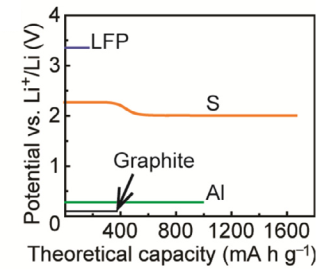
\includegraphics[width=5cm]{figures/I-Fig01}}\\
\subfloat[\label{fig:Corr02}]{\begin{tabular}{ccc}
\toprule
Matériaux & Lithium métal & Graphite \\
\midrule
Capacité spécifique [\si{\milli\ampere\hour\per\gram}] & 3860 & 372\\
\bottomrule
\end{tabular}}
\end{figure}
\end{minipage}\begin{minipage}{0.28\textwidth}
\captionof{figure}{\ref{fig:Corr01} Force électromotrice d'une pile où le pôle $\ominus$ est constitué d'une pseudo-référence $\ce{Li} | \ce{Li^+} (\text{électrolyte})$ et où le pôle $\oplus$ est composé de phosphate de fer \ce{LiFePO4}, soufre \ce{Li2S}, d'un alliage d'aluminium \ce{LiAl} et de graphite ; \ref{fig:Corr02} Calcul de la capacité spécifique massique de deux matériaux}
\end{minipage}

%le soufre S, le graphite GRP ou le LiFePO 4
\question[1] En vous appuyant sur les documents ci-dessus et sur vos connaissances sur les dangers du lithium, justifier l'utilisation d'une anode en graphite, comme pseudo-référence, plutôt que d'une anode en lithium métal. 

\begin{mybox}
\begin{solution}[4cm]
On peut juger une électrode selon deux critères, sa capacité massique qui vaut \SI{9.64}{\percent} de celle de lithium métal et de son potentiel rédox, qui vaut \SI{0.14}{\volt\per{\ce{Li^+}/\ce{Li}}}. De plus, le graphite a un potentiel rédox constant pour toute fraction en lithium dans la structure. 

Par conséquent, on peut s'attendre à avoir des courbes charge/décharge proches, seulement biaisées de \SI{0.14}{\volt\per{\ce{Li^+}/\ce{Li}}}, par rapport au lithium métallique.

~

On sait que le lithium métal réagit violemment au contact de toute molécule protique (comme l'eau) ou gaz (comme les diatomiques). Par conséquent, l'utilisation du graphite permet de travailler dans des conditions sécurisées.
\end{solution}\end{mybox}


\setcounter{foo}{\value{question}}
\end{questions}

\paragraph*{Protocole de préparation du pôle $\oplus$}


%\begin{wrapfigure}{r}{0cm}% r à droite et l pour à gauche
%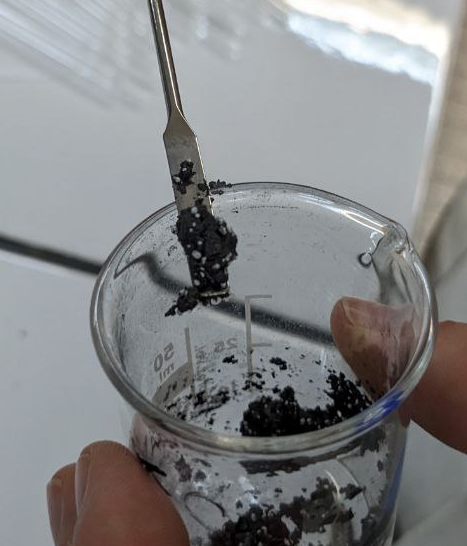
\includegraphics[height=3.5cm]{figures/I-Fig05}
%\captionof{figure}{Suspension}
%\end{wrapfigure}
\begin{enumerate}
\item Mélanger \SI{0.6}{\gram} d'oxyde de manganèse de lithium (\ce{LiMn2O4}) combiné à \SI{0.3}{\gram} de poudre de graphite et \SI{0.1}{\gram} de liant PTFE.
\item Former une suspension aqueuse d'oxyde de manganèse de lithium, de poudre de graphite et de liant PTFE en ajoutant goutte à goutte 1 à \SI{3}{\milli\liter} d'eau à la poudre.
\item Mélangez-la avec une spatule pour former une pâte \textbf{uniforme}.
\end{enumerate}

\begin{minipage}{0.5\textwidth}
\centering
\begin{figure}[H]
\begin{centering}
\subfloat[\label{fig:I-Fig05}]{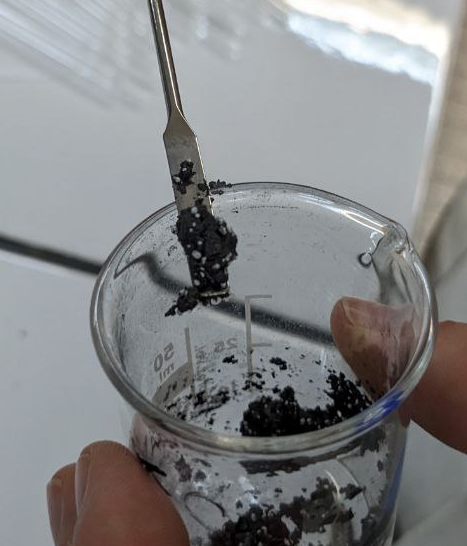
\includegraphics[height=3cm]{figures/I-Fig05}}\hspace{1cm}
\subfloat[\label{fig:I-Fig04}]{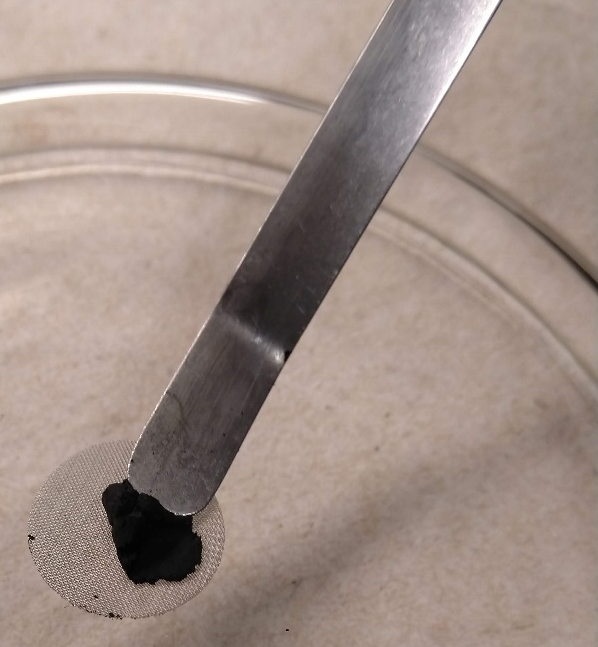
\includegraphics[height=3cm]{figures/I-Fig04}}
\end{centering}
\end{figure}
\end{minipage}\hfill\begin{minipage}{0.5\textwidth}
\captionof{figure}{\ref{fig:I-Fig05} Suspension \ref{fig:I-Fig04} Dépôt des suspensions sur le collecteur de courant, préalablement coupé.}
\end{minipage}

Une fois satisfait des mélanges, les électrodes sont fabriquées en plaçant le matériau d'électrode sur la pièce correspondante de treillis métallique en acier inoxydable et en l'étalant avec une spatule. Ensuite, les électrodes sont séchées pendant \SI{30}{\minute} à \SI{150}{\celsius} dans une étuve.

\paragraph*{Questions}

\begin{comment}
\begin{questions}
\setcounter{question}{\thefoo}

\question[1] Pourquoi mélange-t-on du graphène avec de l'oxydes de manganèse \ce{LiMn2O4} ? Quel est l'intérêt ?

\begin{mybox}\begin{solution}[3cm]
La conductivté du graphène est bien plus grande que celle de l'oxyde de manganèse. Afin que la suspension de la borne $\oplus$ puisse conduire le courant jusqu'au collecteur de courant, on disperse la phase d'intérêt (c.-à-d. l'oxyde) avec des particules dispersées de graphite.
\end{solution}\end{mybox}

\setcounter{foo}{\value{question}}
\end{questions}
\end{comment}
%La cathode est préparée de manière similaire, dans ce cas, nous utilisons de l'oxyde de manganèse de lithium, un composé largement utilisé comme cathode (prix Nobel en 2019). Cependant, pour augmenter l'interface et la conductivité, ce composé est mélangé à de la poudre de graphite (très conductrice et inerte), ce qui donne une meilleure électrode. Par conséquent, le matériau de la cathode est constitué de 0,6 g d'oxyde de manganèse de lithium (LiMn2O4) combiné à 0,3 g de poudre de graphite et 0,1 g de liant PTFE. Une fois de plus, pour faciliter la fabrication de l'électrode en l'étalant sur une pièce de treillis métallique en acier inoxydable, une suspension aqueuse d'oxyde de manganèse de lithium, de poudre de graphite et de liant PTFE est formée en ajoutant progressivement 1 à 3 mL d'eau à la poudre et en mélangeant avec une spatule pour former une pâte uniforme.

%\begin{wrapfigure}{r}{0cm}% r à droite et l pour à gauche
%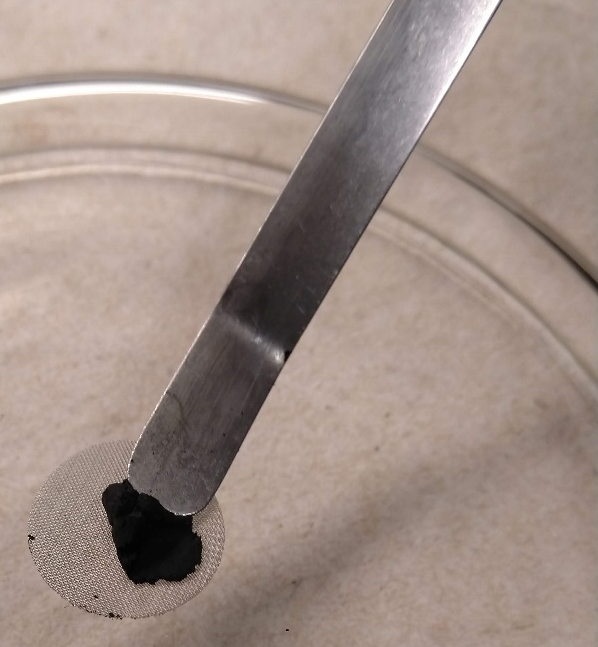
\includegraphics[height=3.5cm]{figures/I-Fig04}
%\captionof{figure}{Dépôt des suspensions sur le collecteur de courant, préalablement coupé}
%\end{wrapfigure}

\begin{questions}
\setcounter{question}{\thefoo}
\question[\half] Quel est le rôle du treillis métallique ?
\begin{mybox}
\begin{solution}[1cm]
Le treillis métallique joue le rôle de collecteur de courant.
\end{solution}\end{mybox}

\question[\half] Pourquoi place-t-on les électrodes dans une étuve ?

\begin{mybox}\begin{solution}[2cm]
Afin d'éviter toute réaction entre le lithium réduit, c'est-à-dire au degré d'oxydation 0, avec d'éventuellement protons, on doit éliminer toute trace d'eau.
\end{solution}\end{mybox}

\setcounter{foo}{\value{question}}
\end{questions}

%\begin{wrapfigure}{r}{0cm}% r à droite et l pour à gauche
%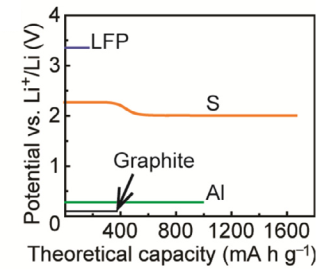
\includegraphics[height=2cm]{figures/I-Fig01}\includegraphics[height=2cm]{figures/I-Fig02}
%\end{wrapfigure}

\subsection{\'{E}lectrolyte \& solvant}
\paragraph*{Protocole}
Prélever préalablement environ \SI{15}{\milli\liter} d'une solution de triflate de lithium \SI{0.1}{\mole\per\liter} dans du carbonate de propylène.

\paragraph*{Questions}


\begin{center}
\begin{minipage}{0.48\textwidth}
\centering
\begin{tabular}{cc}
\toprule
Propriétés & Valeurs \\
\midrule
Moment dipolaire [\si{D}] & 4.94 \\
Permittivité relative [$\emptyset$] & 64.9 \\
\bottomrule
\end{tabular}%https://macro.lsu.edu/howto/solvents/Propylene%20Carbonate.htm
\end{minipage}\begin{minipage}{0.48\textwidth}
\captionof{table}{Propriétés du carbonate de propylène, représenté ci-contre}
\centering
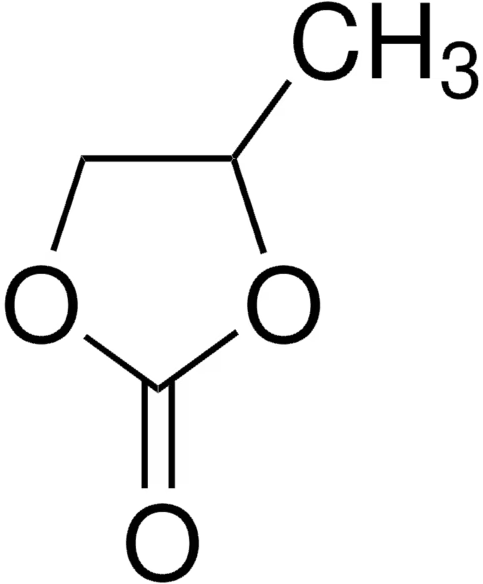
\includegraphics[height=2cm]{figures/I-Fig06}
\end{minipage}
\end{center}


\begin{questions}
\setcounter{question}{\thefoo}
\question[1] Quel est le rôle du triflate de lithium ? \'{E}crire l'équation de dissociation du triflate de lithium. Justifier en quoi la structure du triflate permet d'avoir un équilibre de dissociation qui soit total ?

\begin{mybox}
\begin{solution}[8cm]
Le triflate de lithium joue le rôle d'électrolyte (c.-à-d. un conducteur ionique). 

\underline{\'{E}quation de dissociation}

\begin{center}
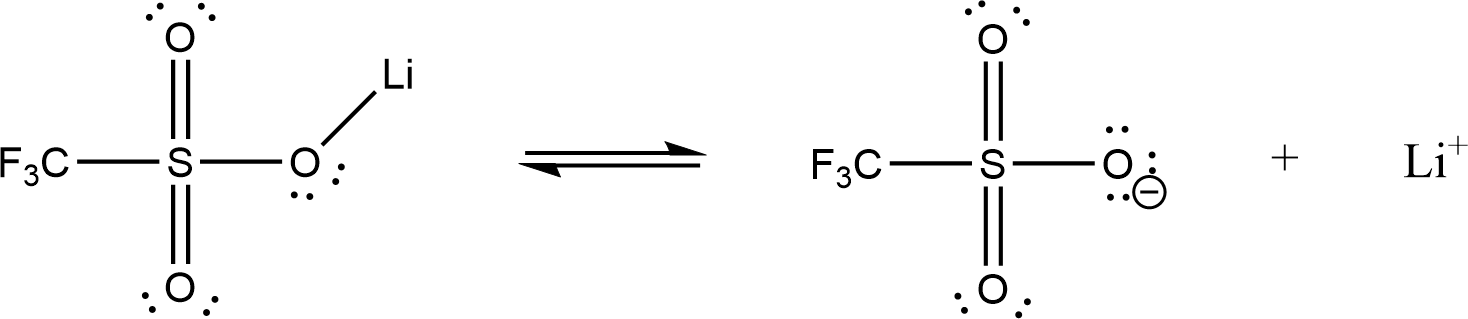
\includegraphics[width=0.9\textwidth]{figures/I-Fig07a}
\end{center}

\underline{Dissociation en milieu polaire} Poisque $\chi(\ce{O}) > \chi (\ce{Li})$, la liaison \ce{O-Li} est polarisée sous la forme : 
\begin{align*}
\ce{O^{-\delta e} - Li^{+\delta e}}
\end{align*}
En milieu/solvant polaire, la liaison \ce{O-Li} va se dissocier préférentiellement de manière hétérolytique. 

La dissociation est favorisée (réaction très exergonique) si et seulement si l'état produit est fortement stabilisé par rapport à l'état réactif. On doit identifier des arguments structuraux attestant de la stabilité de l'anion triflate.

\underline{Stabilisation de la charge}

Le groupement \ce{-CF3} est inductif attracteur, ce qui aura pour effet de stabiliser la charge négative dans l'état produit. De plus, la délocalisation électronique de la charge négative sur les trois oxygènes est possible (effet mésomère attracteur) ce qui renforce la stabilité de l'anion triflate.

\begin{center}
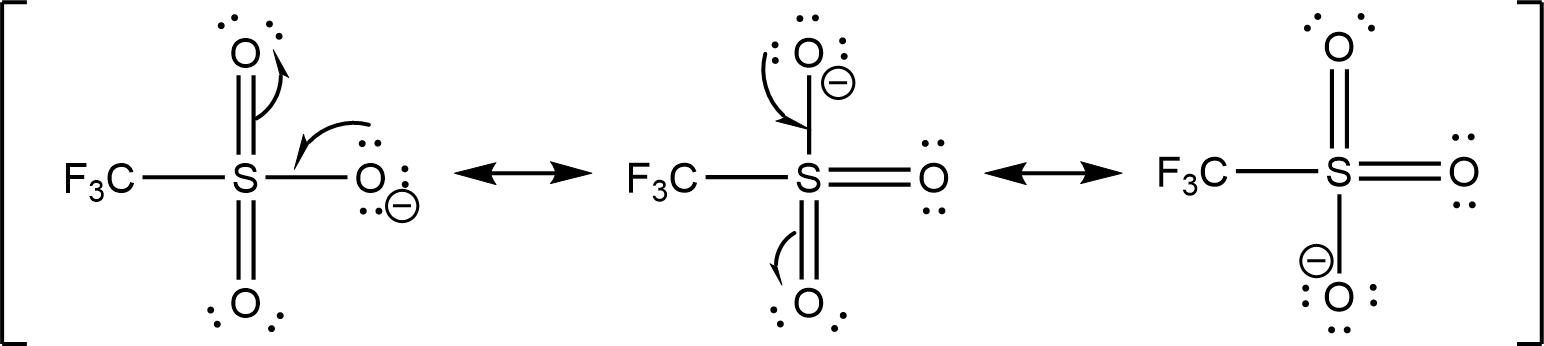
\includegraphics[width=0.9\textwidth]{figures/I-Fig07b}
\end{center}

\end{solution}
\end{mybox}

\question[1] Quelles propriétés physico-chimiques du carbonate de propylène anhydre justifient son utilisation comme solvant d'un accumulateur au lithium ?

\begin{mybox}\begin{solution}[3cm]
Le carbonate de propylène est un solvant aprotique, ce qui évite tout risque d'explosion au contact de traces de lithium métalliques (c'est-à-dire pas de réaction A/B).

De plus, la grande valeur de la permittivité relative de ce solvant (à comparer à d'autres solvants usuels) permet de dire qu'il va être dissociant (c-à-d. facilitant la dissociation de la liaison \ce{O-Li} en écrantant les charges des espèces ioniques). Le moment dipolaire est grand au regard d'autres solvants comme \ce{H2O}, ce qui suffère une bonne solvatation des ions.
\end{solution}\end{mybox}

\question[1] La conductivité ionique de l'anion triflate est mauvaise au regard des autres électrolytes couramment utilisés dans les batteries. Pourquoi ? Quel paramètre macroscopique de la batterie peut être impacté par cette mauvaise conductivité ?

\begin{mybox}\begin{solution}[3cm]
La conductivité d'un ion dépend de sa concentration en solution et de sa mobilité ionique. Or, le "gros volume" de l'anion triflate doit être lié à sa faible mobilité. \\
La résistance interne de la batterie est impactée par la mauvaise conductivité ionique de l'électrolyte, on peut donc s'attendre à avoir une chute ohmique (effet dissipatif) plus important que dans une batterie commerciale actuelle.
\end{solution}\end{mybox}

\setcounter{foo}{\value{question}}
\end{questions}

%L'électrolyte utilisé est du triflate de lithium \SI{0.1}{\mole\per\liter} (électrolyte) dans du carbonate de propylène (solvant). Rappelez-vous que lorsqu'on travaille avec du lithium, il faut éviter les solvants protiques en raison de sa réactivité générant des réactions dangereuses. Dans le cas présent, le polycarbonate est utilisé comme solvant, et le trifluorométhanesulfonate de lithium comme électrolyte à base de lithium. Cet électrolyte a un anion très grand pour faciliter la dissolution d'un sel dans des solvants non polaires. Environ 15 mL de cet électrolyte seront suffisants par binôme.

%\begin{questions}
%\question[1] Le polycarbonate de propylène est anhydre (< \SI{0.005}{\percent} d'eau). Pourquoi ? Commenter la polarité et la proticité du solvant et de l'électrolyte. Justifier.

%Dans les batteries, le solvant est généralement choisi en suivant trois critères : sa conductivité ionique, sa sensibilité à l'hydrolyse et sa stabilité thermique.

%\begin{tabular}{cccc}
%& Conductivité ionique & Structure & Température de décomposition \\
%& [\si{\milli\siemens\per\centi\meter}] & & [\si{\celsius}] \\
%Triflate & 3.1 & & \\
%\ce{PF6^-} & 10.8 & & 125\\
%\ce{ClO4^-} & 10.1 & & \\
%\end{tabular}
%P-F : 439(96), 536(21)
%\question

%\setcounter{foo}{\value{question}}
%\end{questions}

\subsection{Membrane \& Montage de la cellule électrochimique}

\paragraph*{Protocole} 

\begin{minipage}{0.48\textwidth}
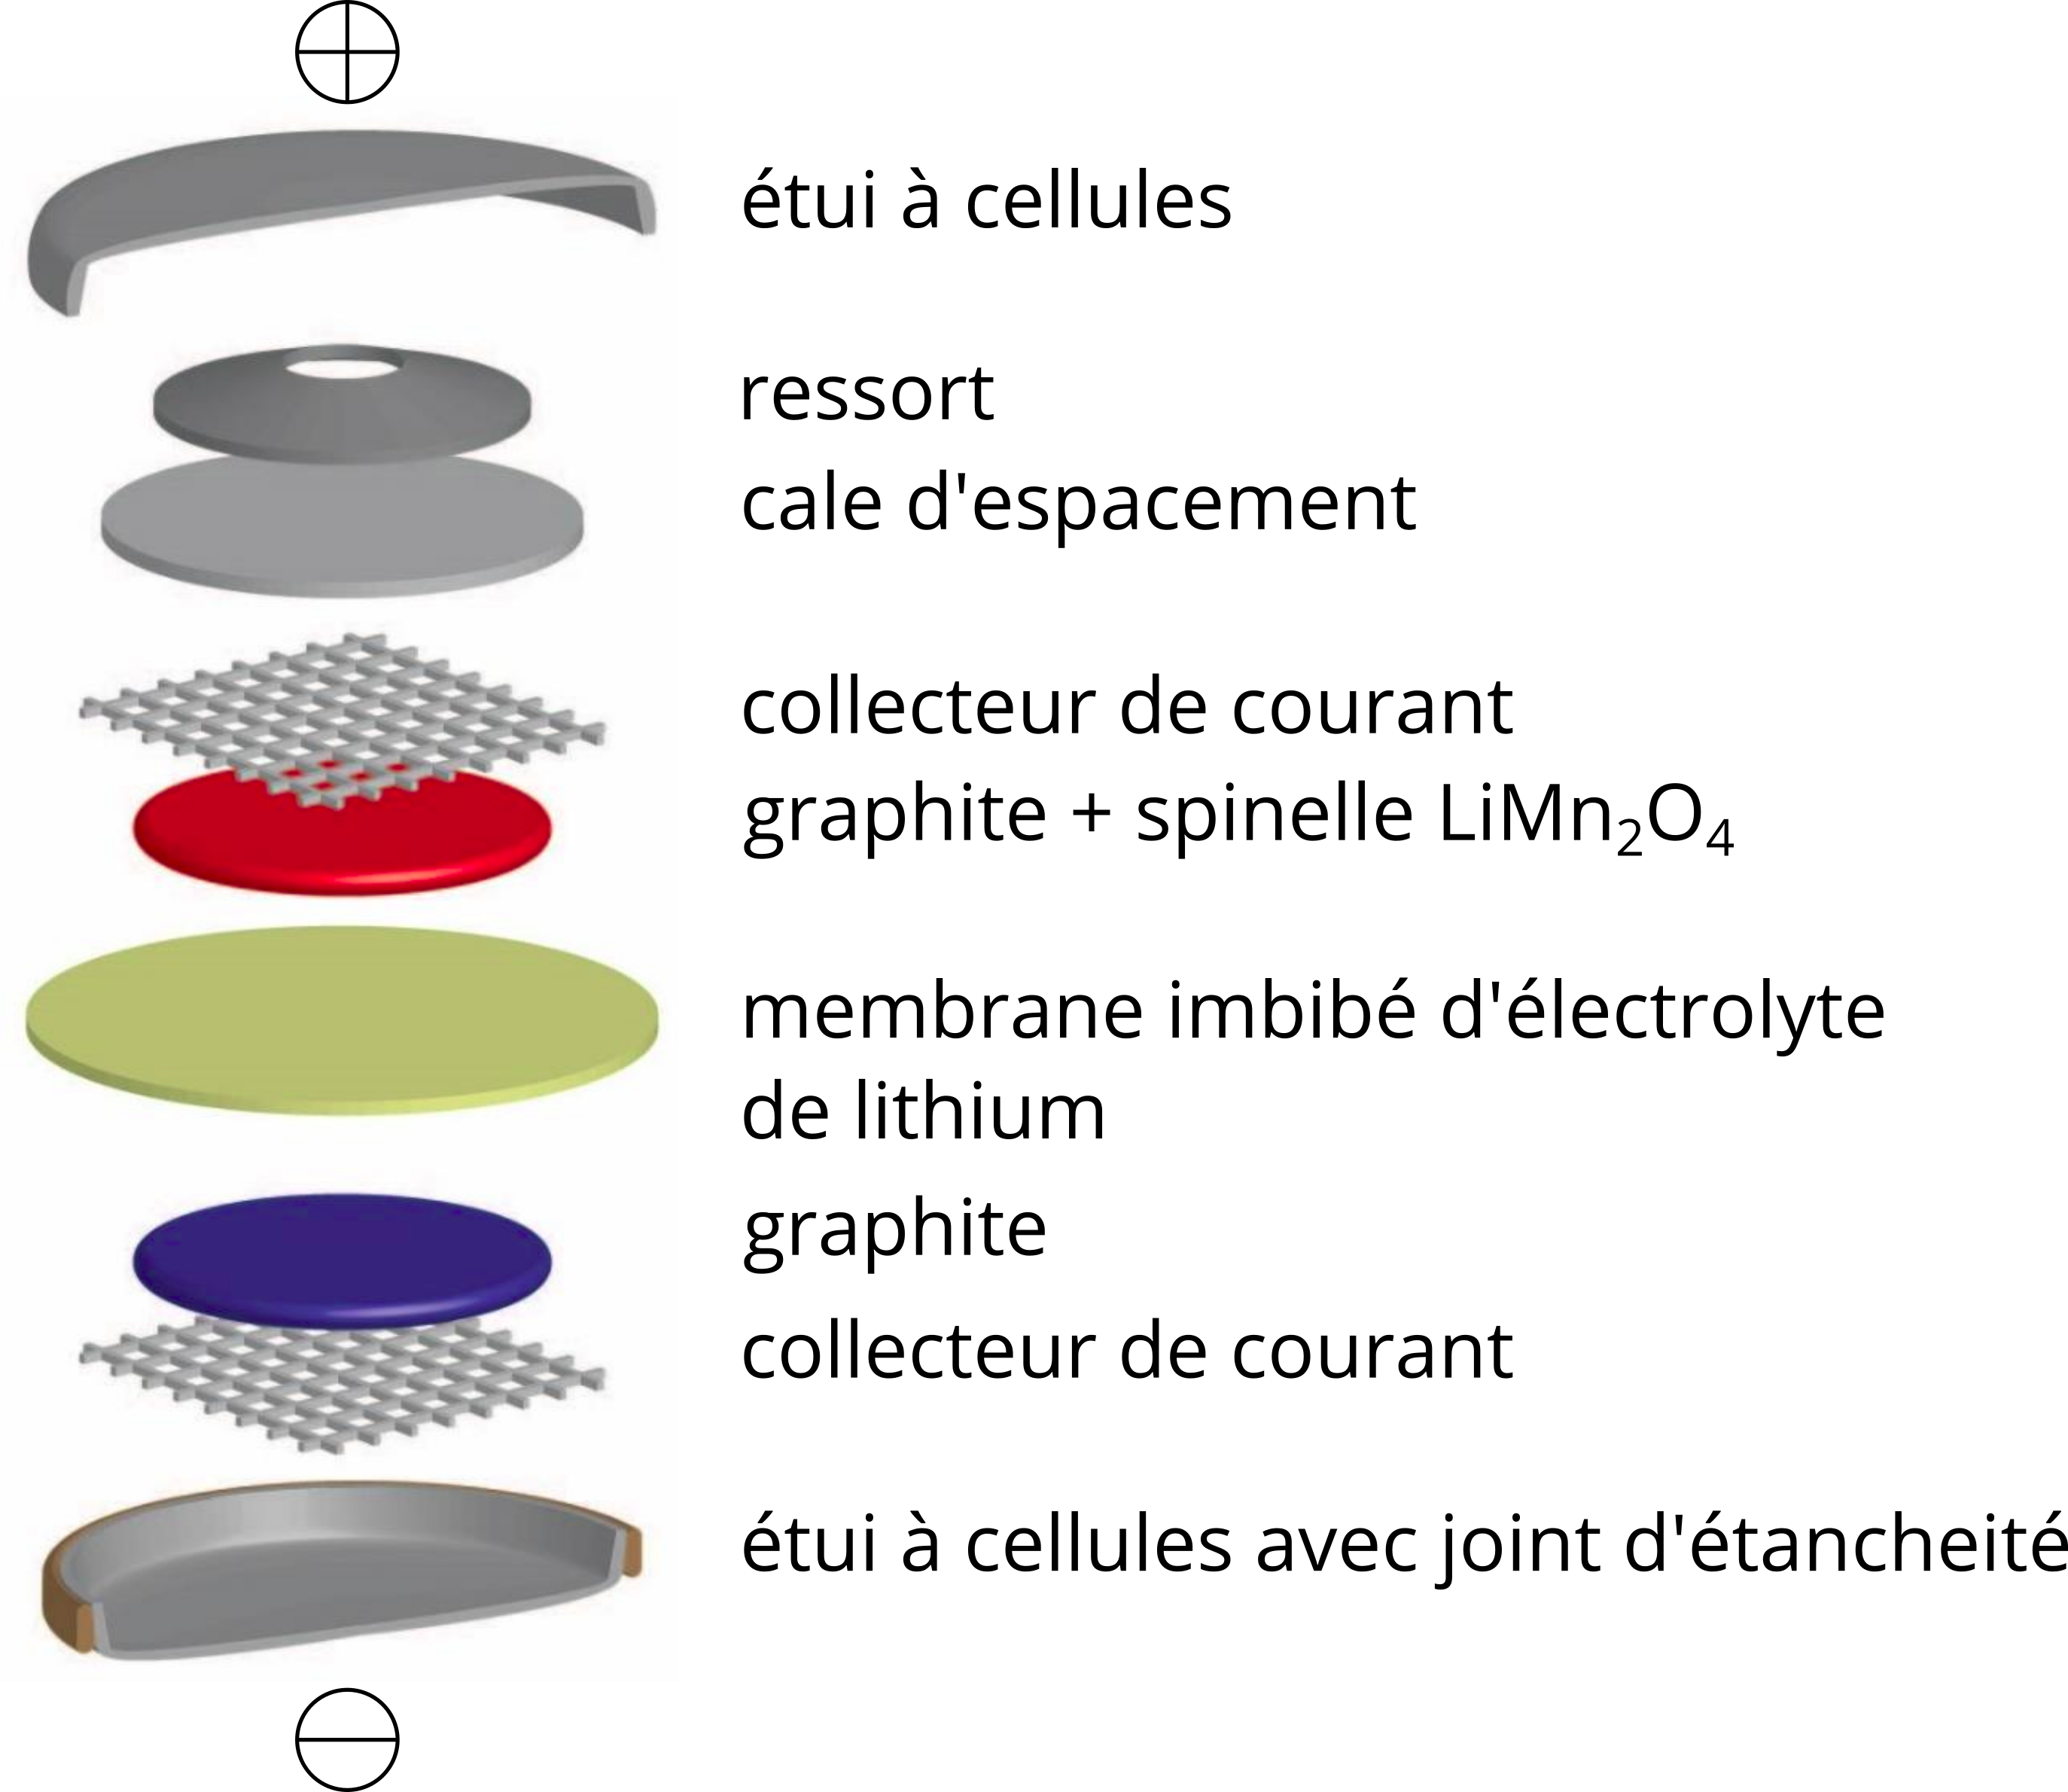
\includegraphics[width=\textwidth]{figures/I-Fig03}
\end{minipage}\begin{minipage}{0.48\textwidth}
\captionof{figure}{Décomposition des composantes d'une batterie lithium CR2032}
\label{fig:03}
\end{minipage}


\begin{enumerate}
\item Découper un cylindre de papier filtre en fibre de verre à la dimension de la pile.
\item Immerger le papier filtre dans l'électrolyte pendant quelques minutes.
\item Assembler avec précaution l'ensemble des pièces en suivant la Fig. \ref{fig:03} et fermer la cellule.
\item Passer la cellule dans la presse hydraulique et soumettez là à une pression de quelques bars.
\end{enumerate}

%Enfin, les électrodes doivent être physiquement séparées (pour éviter les courts-circuits) mais permettre la diffusion des ions, en particulier du lithium. Un papier filtre en fibre de verre ou une membrane sera utilisé à cette fin. Dans ce cas, la membrane est réalisée en découpant du papier filtre en fibre de verre en cercles d'environ 19 mm de diamètre (suffisamment grands pour s'assurer qu'ils recouvrent entièrement la cellule) et en les trempant dans 5 mL d'électrolyte pendant au moins une heure.

\section{Expérience de charge/décharge - \faClockO ~ \SI{2.5}{\hour}}

\subsection{\'{E}tude d'une cellule électrochimique commerciale}

\paragraph*{Protocole}

Vous allez manipuler les données acquis par vos enseignants sur un accumulateur commercial VL2020 de la marque Panasonic{\copyright} déjà usé pendant que vous ferez cycler votre accumulateur. 

L'accumulateur a été étudié avec les paramètres d'acquisition suivant :
\begin{itemize}
\item 5 cycles de charge/décharge ;
\item Courant de charge et décharge : \SI{1}{\milli\ampere} ;
\item Tension de coupure en charge : \SI{3.25}{\volt} ;
\item Tension de coupure en décharge : \SI{2.5}{\volt}.
\end{itemize}

Le fichier sera fourni par votre enseignant.

\paragraph*{Questions}

\begin{questions}
\setcounter{question}{\thefoo}
\question[1] {\color{purple} Démontrer comment convertir le temps d'expérience en quantité de charge, exprimée en \si{\milli\ampere\hour}, puis en quantité de charge par unité de masse (c.-à-d. de la capacité massique) de la cellule exprimée en \si{\milli\ampere\hour\per\gram}.}
\begin{mybox}
\begin{solution}[4cm]
\`{A} courant constant, on peut écrire : 
\begin{align*}
Q [\si{\milli\ampere\hour}] = I [\si{\milli\ampere}] \cdot \Delta t [\si{\hour}]
\end{align*}
donc
\begin{align*}
CS_m [\si{\milli\ampere\hour\per\gram}]= \frac{Q [\si{\milli\ampere\hour}]}{\text{masse batterie} [\si{\gram}]}
\end{align*}
\end{solution}\end{mybox}

\question[1]  {\color{purple} Démontrer que l'efficacité énergétique (Sec. \ref{subsec:efficacite}, Eq. \ref{eq:EE}) peut s'exprimer comme un rapport de deux moyennes dans cette expérience galvanostatique. On rappelle que mathématiquement, la moyenne $\langle f \rangle$ d'une fonction $f$ à un paramètre réel sur un intervalle $[x_1, x_2]$ s'exprime comme : 

\begin{align*}
\langle f \rangle = \frac{1}{x_2 - x_1 }\int_{x_1}^{x_2} f(x) dx
\end{align*}}


\begin{mybox}
\begin{solution}[5cm]

Dans cette expérience galvanostatique, on a $I_c = I_d = cste$. Par conséquent,
\begin{align*}
EE [i] &= \frac{W'_d}{W'_c} \\
&= \frac{\int U_d (t') \cdot I_d (t') dt'}{\int U_c (t') \cdot I_c (t') dt'} \\
&= \frac{\int U_d (t') dt'}{\int U_c (t') dt'} \text{ (car }I_c = I_d\text{)} \\
&= \frac{\Delta t_d \langle U_d \rangle}{\Delta t_c \langle U_c \rangle} \\
&= CE[i] \cdot \frac{\langle U_d \rangle}{\langle U_c \rangle}
\end{align*}
avec $CE[i]$ l'efficacité coulombique du i-ème cycle de charge/décharge.\\
\textbf{NB : $\Delta t_c$ (resp. $\Delta t_d$) indique la durée de la charge (resp. décharge) du cycle $i$.}
\end{solution}
\end{mybox}

\question[3] {\color{purple} Représenter les courbes de charge/décharge en fonction du temps, de la capacité puis de l'état de charge.}

\begin{parts}

\part {\color{purple} Donner l'évolution de la tension en fonction du temps d'acquisition, exprimé en seconde.}

\begin{mybox}
\begin{solution}[6cm]
\begin{center}
\begin{adjustbox}{max width=\textwidth}
%% Creator: Matplotlib, PGF backend
%%
%% To include the figure in your LaTeX document, write
%%   \input{<filename>.pgf}
%%
%% Make sure the required packages are loaded in your preamble
%%   \usepackage{pgf}
%%
%% and, on pdftex
%%   \usepackage[utf8]{inputenc}\DeclareUnicodeCharacter{2212}{-}
%%
%% or, on luatex and xetex
%%   \usepackage{unicode-math}
%%
%% Figures using additional raster images can only be included by \input if
%% they are in the same directory as the main LaTeX file. For loading figures
%% from other directories you can use the `import` package
%%   \usepackage{import}
%%
%% and then include the figures with
%%   \import{<path to file>}{<filename>.pgf}
%%
%% Matplotlib used the following preamble
%%   \usepackage{fontspec}
%%   \setmainfont{DejaVuSerif.ttf}[Path=/home/jeff/anaconda3/envs/teaching/lib/python3.8/site-packages/matplotlib/mpl-data/fonts/ttf/]
%%   \setsansfont{DejaVuSans.ttf}[Path=/home/jeff/anaconda3/envs/teaching/lib/python3.8/site-packages/matplotlib/mpl-data/fonts/ttf/]
%%   \setmonofont{DejaVuSansMono.ttf}[Path=/home/jeff/anaconda3/envs/teaching/lib/python3.8/site-packages/matplotlib/mpl-data/fonts/ttf/]
%%
\begingroup%
\makeatletter%
\begin{pgfpicture}%
\pgfpathrectangle{\pgfpointorigin}{\pgfqpoint{6.000000in}{4.000000in}}%
\pgfusepath{use as bounding box, clip}%
\begin{pgfscope}%
\pgfsetbuttcap%
\pgfsetmiterjoin%
\pgfsetlinewidth{0.000000pt}%
\definecolor{currentstroke}{rgb}{1.000000,1.000000,1.000000}%
\pgfsetstrokecolor{currentstroke}%
\pgfsetstrokeopacity{0.000000}%
\pgfsetdash{}{0pt}%
\pgfpathmoveto{\pgfqpoint{0.000000in}{0.000000in}}%
\pgfpathlineto{\pgfqpoint{6.000000in}{0.000000in}}%
\pgfpathlineto{\pgfqpoint{6.000000in}{4.000000in}}%
\pgfpathlineto{\pgfqpoint{0.000000in}{4.000000in}}%
\pgfpathclose%
\pgfusepath{}%
\end{pgfscope}%
\begin{pgfscope}%
\pgfsetbuttcap%
\pgfsetmiterjoin%
\definecolor{currentfill}{rgb}{1.000000,1.000000,1.000000}%
\pgfsetfillcolor{currentfill}%
\pgfsetlinewidth{0.000000pt}%
\definecolor{currentstroke}{rgb}{0.000000,0.000000,0.000000}%
\pgfsetstrokecolor{currentstroke}%
\pgfsetstrokeopacity{0.000000}%
\pgfsetdash{}{0pt}%
\pgfpathmoveto{\pgfqpoint{0.967606in}{0.892819in}}%
\pgfpathlineto{\pgfqpoint{5.730000in}{0.892819in}}%
\pgfpathlineto{\pgfqpoint{5.730000in}{3.730000in}}%
\pgfpathlineto{\pgfqpoint{0.967606in}{3.730000in}}%
\pgfpathclose%
\pgfusepath{fill}%
\end{pgfscope}%
\begin{pgfscope}%
\pgfsetbuttcap%
\pgfsetroundjoin%
\definecolor{currentfill}{rgb}{0.000000,0.000000,0.000000}%
\pgfsetfillcolor{currentfill}%
\pgfsetlinewidth{0.803000pt}%
\definecolor{currentstroke}{rgb}{0.000000,0.000000,0.000000}%
\pgfsetstrokecolor{currentstroke}%
\pgfsetdash{}{0pt}%
\pgfsys@defobject{currentmarker}{\pgfqpoint{0.000000in}{-0.048611in}}{\pgfqpoint{0.000000in}{0.000000in}}{%
\pgfpathmoveto{\pgfqpoint{0.000000in}{0.000000in}}%
\pgfpathlineto{\pgfqpoint{0.000000in}{-0.048611in}}%
\pgfusepath{stroke,fill}%
}%
\begin{pgfscope}%
\pgfsys@transformshift{1.183835in}{0.892819in}%
\pgfsys@useobject{currentmarker}{}%
\end{pgfscope}%
\end{pgfscope}%
\begin{pgfscope}%
\definecolor{textcolor}{rgb}{0.000000,0.000000,0.000000}%
\pgfsetstrokecolor{textcolor}%
\pgfsetfillcolor{textcolor}%
\pgftext[x=1.183835in,y=0.795597in,,top]{\color{textcolor}\rmfamily\fontsize{18.000000}{21.600000}\selectfont \(\displaystyle {0}\)}%
\end{pgfscope}%
\begin{pgfscope}%
\pgfsetbuttcap%
\pgfsetroundjoin%
\definecolor{currentfill}{rgb}{0.000000,0.000000,0.000000}%
\pgfsetfillcolor{currentfill}%
\pgfsetlinewidth{0.803000pt}%
\definecolor{currentstroke}{rgb}{0.000000,0.000000,0.000000}%
\pgfsetstrokecolor{currentstroke}%
\pgfsetdash{}{0pt}%
\pgfsys@defobject{currentmarker}{\pgfqpoint{0.000000in}{-0.048611in}}{\pgfqpoint{0.000000in}{0.000000in}}{%
\pgfpathmoveto{\pgfqpoint{0.000000in}{0.000000in}}%
\pgfpathlineto{\pgfqpoint{0.000000in}{-0.048611in}}%
\pgfusepath{stroke,fill}%
}%
\begin{pgfscope}%
\pgfsys@transformshift{2.386334in}{0.892819in}%
\pgfsys@useobject{currentmarker}{}%
\end{pgfscope}%
\end{pgfscope}%
\begin{pgfscope}%
\definecolor{textcolor}{rgb}{0.000000,0.000000,0.000000}%
\pgfsetstrokecolor{textcolor}%
\pgfsetfillcolor{textcolor}%
\pgftext[x=2.386334in,y=0.795597in,,top]{\color{textcolor}\rmfamily\fontsize{18.000000}{21.600000}\selectfont \(\displaystyle {100000}\)}%
\end{pgfscope}%
\begin{pgfscope}%
\pgfsetbuttcap%
\pgfsetroundjoin%
\definecolor{currentfill}{rgb}{0.000000,0.000000,0.000000}%
\pgfsetfillcolor{currentfill}%
\pgfsetlinewidth{0.803000pt}%
\definecolor{currentstroke}{rgb}{0.000000,0.000000,0.000000}%
\pgfsetstrokecolor{currentstroke}%
\pgfsetdash{}{0pt}%
\pgfsys@defobject{currentmarker}{\pgfqpoint{0.000000in}{-0.048611in}}{\pgfqpoint{0.000000in}{0.000000in}}{%
\pgfpathmoveto{\pgfqpoint{0.000000in}{0.000000in}}%
\pgfpathlineto{\pgfqpoint{0.000000in}{-0.048611in}}%
\pgfusepath{stroke,fill}%
}%
\begin{pgfscope}%
\pgfsys@transformshift{3.588832in}{0.892819in}%
\pgfsys@useobject{currentmarker}{}%
\end{pgfscope}%
\end{pgfscope}%
\begin{pgfscope}%
\definecolor{textcolor}{rgb}{0.000000,0.000000,0.000000}%
\pgfsetstrokecolor{textcolor}%
\pgfsetfillcolor{textcolor}%
\pgftext[x=3.588832in,y=0.795597in,,top]{\color{textcolor}\rmfamily\fontsize{18.000000}{21.600000}\selectfont \(\displaystyle {200000}\)}%
\end{pgfscope}%
\begin{pgfscope}%
\pgfsetbuttcap%
\pgfsetroundjoin%
\definecolor{currentfill}{rgb}{0.000000,0.000000,0.000000}%
\pgfsetfillcolor{currentfill}%
\pgfsetlinewidth{0.803000pt}%
\definecolor{currentstroke}{rgb}{0.000000,0.000000,0.000000}%
\pgfsetstrokecolor{currentstroke}%
\pgfsetdash{}{0pt}%
\pgfsys@defobject{currentmarker}{\pgfqpoint{0.000000in}{-0.048611in}}{\pgfqpoint{0.000000in}{0.000000in}}{%
\pgfpathmoveto{\pgfqpoint{0.000000in}{0.000000in}}%
\pgfpathlineto{\pgfqpoint{0.000000in}{-0.048611in}}%
\pgfusepath{stroke,fill}%
}%
\begin{pgfscope}%
\pgfsys@transformshift{4.791331in}{0.892819in}%
\pgfsys@useobject{currentmarker}{}%
\end{pgfscope}%
\end{pgfscope}%
\begin{pgfscope}%
\definecolor{textcolor}{rgb}{0.000000,0.000000,0.000000}%
\pgfsetstrokecolor{textcolor}%
\pgfsetfillcolor{textcolor}%
\pgftext[x=4.791331in,y=0.795597in,,top]{\color{textcolor}\rmfamily\fontsize{18.000000}{21.600000}\selectfont \(\displaystyle {300000}\)}%
\end{pgfscope}%
\begin{pgfscope}%
\definecolor{textcolor}{rgb}{0.000000,0.000000,0.000000}%
\pgfsetstrokecolor{textcolor}%
\pgfsetfillcolor{textcolor}%
\pgftext[x=3.348803in,y=0.498098in,,top]{\color{textcolor}\rmfamily\fontsize{18.000000}{21.600000}\selectfont Temps d'acquisition [\(\displaystyle s\)]}%
\end{pgfscope}%
\begin{pgfscope}%
\pgfsetbuttcap%
\pgfsetroundjoin%
\definecolor{currentfill}{rgb}{0.000000,0.000000,0.000000}%
\pgfsetfillcolor{currentfill}%
\pgfsetlinewidth{0.803000pt}%
\definecolor{currentstroke}{rgb}{0.000000,0.000000,0.000000}%
\pgfsetstrokecolor{currentstroke}%
\pgfsetdash{}{0pt}%
\pgfsys@defobject{currentmarker}{\pgfqpoint{-0.048611in}{0.000000in}}{\pgfqpoint{-0.000000in}{0.000000in}}{%
\pgfpathmoveto{\pgfqpoint{-0.000000in}{0.000000in}}%
\pgfpathlineto{\pgfqpoint{-0.048611in}{0.000000in}}%
\pgfusepath{stroke,fill}%
}%
\begin{pgfscope}%
\pgfsys@transformshift{0.967606in}{1.464218in}%
\pgfsys@useobject{currentmarker}{}%
\end{pgfscope}%
\end{pgfscope}%
\begin{pgfscope}%
\definecolor{textcolor}{rgb}{0.000000,0.000000,0.000000}%
\pgfsetstrokecolor{textcolor}%
\pgfsetfillcolor{textcolor}%
\pgftext[x=0.584971in, y=1.369247in, left, base]{\color{textcolor}\rmfamily\fontsize{18.000000}{21.600000}\selectfont \(\displaystyle {2.9}\)}%
\end{pgfscope}%
\begin{pgfscope}%
\pgfsetbuttcap%
\pgfsetroundjoin%
\definecolor{currentfill}{rgb}{0.000000,0.000000,0.000000}%
\pgfsetfillcolor{currentfill}%
\pgfsetlinewidth{0.803000pt}%
\definecolor{currentstroke}{rgb}{0.000000,0.000000,0.000000}%
\pgfsetstrokecolor{currentstroke}%
\pgfsetdash{}{0pt}%
\pgfsys@defobject{currentmarker}{\pgfqpoint{-0.048611in}{0.000000in}}{\pgfqpoint{-0.000000in}{0.000000in}}{%
\pgfpathmoveto{\pgfqpoint{-0.000000in}{0.000000in}}%
\pgfpathlineto{\pgfqpoint{-0.048611in}{0.000000in}}%
\pgfusepath{stroke,fill}%
}%
\begin{pgfscope}%
\pgfsys@transformshift{0.967606in}{2.076660in}%
\pgfsys@useobject{currentmarker}{}%
\end{pgfscope}%
\end{pgfscope}%
\begin{pgfscope}%
\definecolor{textcolor}{rgb}{0.000000,0.000000,0.000000}%
\pgfsetstrokecolor{textcolor}%
\pgfsetfillcolor{textcolor}%
\pgftext[x=0.584971in, y=1.981689in, left, base]{\color{textcolor}\rmfamily\fontsize{18.000000}{21.600000}\selectfont \(\displaystyle {3.0}\)}%
\end{pgfscope}%
\begin{pgfscope}%
\pgfsetbuttcap%
\pgfsetroundjoin%
\definecolor{currentfill}{rgb}{0.000000,0.000000,0.000000}%
\pgfsetfillcolor{currentfill}%
\pgfsetlinewidth{0.803000pt}%
\definecolor{currentstroke}{rgb}{0.000000,0.000000,0.000000}%
\pgfsetstrokecolor{currentstroke}%
\pgfsetdash{}{0pt}%
\pgfsys@defobject{currentmarker}{\pgfqpoint{-0.048611in}{0.000000in}}{\pgfqpoint{-0.000000in}{0.000000in}}{%
\pgfpathmoveto{\pgfqpoint{-0.000000in}{0.000000in}}%
\pgfpathlineto{\pgfqpoint{-0.048611in}{0.000000in}}%
\pgfusepath{stroke,fill}%
}%
\begin{pgfscope}%
\pgfsys@transformshift{0.967606in}{2.689102in}%
\pgfsys@useobject{currentmarker}{}%
\end{pgfscope}%
\end{pgfscope}%
\begin{pgfscope}%
\definecolor{textcolor}{rgb}{0.000000,0.000000,0.000000}%
\pgfsetstrokecolor{textcolor}%
\pgfsetfillcolor{textcolor}%
\pgftext[x=0.584971in, y=2.594132in, left, base]{\color{textcolor}\rmfamily\fontsize{18.000000}{21.600000}\selectfont \(\displaystyle {3.1}\)}%
\end{pgfscope}%
\begin{pgfscope}%
\pgfsetbuttcap%
\pgfsetroundjoin%
\definecolor{currentfill}{rgb}{0.000000,0.000000,0.000000}%
\pgfsetfillcolor{currentfill}%
\pgfsetlinewidth{0.803000pt}%
\definecolor{currentstroke}{rgb}{0.000000,0.000000,0.000000}%
\pgfsetstrokecolor{currentstroke}%
\pgfsetdash{}{0pt}%
\pgfsys@defobject{currentmarker}{\pgfqpoint{-0.048611in}{0.000000in}}{\pgfqpoint{-0.000000in}{0.000000in}}{%
\pgfpathmoveto{\pgfqpoint{-0.000000in}{0.000000in}}%
\pgfpathlineto{\pgfqpoint{-0.048611in}{0.000000in}}%
\pgfusepath{stroke,fill}%
}%
\begin{pgfscope}%
\pgfsys@transformshift{0.967606in}{3.301545in}%
\pgfsys@useobject{currentmarker}{}%
\end{pgfscope}%
\end{pgfscope}%
\begin{pgfscope}%
\definecolor{textcolor}{rgb}{0.000000,0.000000,0.000000}%
\pgfsetstrokecolor{textcolor}%
\pgfsetfillcolor{textcolor}%
\pgftext[x=0.584971in, y=3.206574in, left, base]{\color{textcolor}\rmfamily\fontsize{18.000000}{21.600000}\selectfont \(\displaystyle {3.2}\)}%
\end{pgfscope}%
\begin{pgfscope}%
\definecolor{textcolor}{rgb}{0.000000,0.000000,0.000000}%
\pgfsetstrokecolor{textcolor}%
\pgfsetfillcolor{textcolor}%
\pgftext[x=0.529415in,y=2.311410in,,bottom,rotate=90.000000]{\color{textcolor}\rmfamily\fontsize{18.000000}{21.600000}\selectfont Tension [\(\displaystyle V\)]}%
\end{pgfscope}%
\begin{pgfscope}%
\pgfpathrectangle{\pgfqpoint{0.967606in}{0.892819in}}{\pgfqpoint{4.762394in}{2.837181in}}%
\pgfusepath{clip}%
\pgfsetrectcap%
\pgfsetroundjoin%
\pgfsetlinewidth{2.007500pt}%
\definecolor{currentstroke}{rgb}{1.000000,0.000000,0.000000}%
\pgfsetstrokecolor{currentstroke}%
\pgfsetdash{}{0pt}%
\pgfpathmoveto{\pgfqpoint{1.184079in}{2.380563in}}%
\pgfpathlineto{\pgfqpoint{1.185221in}{2.829130in}}%
\pgfpathlineto{\pgfqpoint{1.185233in}{2.827261in}}%
\pgfpathlineto{\pgfqpoint{1.185269in}{2.825392in}}%
\pgfpathlineto{\pgfqpoint{1.186460in}{2.903891in}}%
\pgfpathlineto{\pgfqpoint{1.186484in}{2.900153in}}%
\pgfpathlineto{\pgfqpoint{1.187338in}{2.937533in}}%
\pgfpathlineto{\pgfqpoint{1.187362in}{2.931926in}}%
\pgfpathlineto{\pgfqpoint{1.188492in}{2.971176in}}%
\pgfpathlineto{\pgfqpoint{1.188576in}{2.965568in}}%
\pgfpathlineto{\pgfqpoint{1.188588in}{2.965568in}}%
\pgfpathlineto{\pgfqpoint{1.188600in}{2.963699in}}%
\pgfpathlineto{\pgfqpoint{1.189394in}{2.987997in}}%
\pgfpathlineto{\pgfqpoint{1.189574in}{2.982390in}}%
\pgfpathlineto{\pgfqpoint{1.190717in}{3.002949in}}%
\pgfpathlineto{\pgfqpoint{1.189659in}{2.980521in}}%
\pgfpathlineto{\pgfqpoint{1.190741in}{3.001080in}}%
\pgfpathlineto{\pgfqpoint{1.190933in}{2.995473in}}%
\pgfpathlineto{\pgfqpoint{1.191607in}{3.012294in}}%
\pgfpathlineto{\pgfqpoint{1.191811in}{3.010425in}}%
\pgfpathlineto{\pgfqpoint{1.191895in}{3.004818in}}%
\pgfpathlineto{\pgfqpoint{1.192977in}{3.021639in}}%
\pgfpathlineto{\pgfqpoint{1.193242in}{3.016032in}}%
\pgfpathlineto{\pgfqpoint{1.193927in}{3.029115in}}%
\pgfpathlineto{\pgfqpoint{1.194072in}{3.021639in}}%
\pgfpathlineto{\pgfqpoint{1.195190in}{3.032853in}}%
\pgfpathlineto{\pgfqpoint{1.195214in}{3.030984in}}%
\pgfpathlineto{\pgfqpoint{1.195226in}{3.023508in}}%
\pgfpathlineto{\pgfqpoint{1.195887in}{3.036591in}}%
\pgfpathlineto{\pgfqpoint{1.196308in}{3.030984in}}%
\pgfpathlineto{\pgfqpoint{1.196958in}{3.038460in}}%
\pgfpathlineto{\pgfqpoint{1.196344in}{3.029115in}}%
\pgfpathlineto{\pgfqpoint{1.197427in}{3.036591in}}%
\pgfpathlineto{\pgfqpoint{1.198208in}{3.030984in}}%
\pgfpathlineto{\pgfqpoint{1.197523in}{3.040330in}}%
\pgfpathlineto{\pgfqpoint{1.198557in}{3.032853in}}%
\pgfpathlineto{\pgfqpoint{1.198581in}{3.032853in}}%
\pgfpathlineto{\pgfqpoint{1.199375in}{3.042199in}}%
\pgfpathlineto{\pgfqpoint{1.199699in}{3.036591in}}%
\pgfpathlineto{\pgfqpoint{1.199711in}{3.036591in}}%
\pgfpathlineto{\pgfqpoint{1.200337in}{3.044068in}}%
\pgfpathlineto{\pgfqpoint{1.199964in}{3.032853in}}%
\pgfpathlineto{\pgfqpoint{1.200818in}{3.036591in}}%
\pgfpathlineto{\pgfqpoint{1.200830in}{3.036591in}}%
\pgfpathlineto{\pgfqpoint{1.201876in}{3.042199in}}%
\pgfpathlineto{\pgfqpoint{1.201130in}{3.032853in}}%
\pgfpathlineto{\pgfqpoint{1.201936in}{3.040330in}}%
\pgfpathlineto{\pgfqpoint{1.202345in}{3.032853in}}%
\pgfpathlineto{\pgfqpoint{1.202790in}{3.045937in}}%
\pgfpathlineto{\pgfqpoint{1.203030in}{3.040330in}}%
\pgfpathlineto{\pgfqpoint{1.203848in}{3.045937in}}%
\pgfpathlineto{\pgfqpoint{1.203199in}{3.034722in}}%
\pgfpathlineto{\pgfqpoint{1.204137in}{3.040330in}}%
\pgfpathlineto{\pgfqpoint{1.204149in}{3.040330in}}%
\pgfpathlineto{\pgfqpoint{1.205099in}{3.045937in}}%
\pgfpathlineto{\pgfqpoint{1.204209in}{3.036591in}}%
\pgfpathlineto{\pgfqpoint{1.205267in}{3.044068in}}%
\pgfpathlineto{\pgfqpoint{1.206229in}{3.038460in}}%
\pgfpathlineto{\pgfqpoint{1.205447in}{3.045937in}}%
\pgfpathlineto{\pgfqpoint{1.206373in}{3.040330in}}%
\pgfpathlineto{\pgfqpoint{1.207299in}{3.047806in}}%
\pgfpathlineto{\pgfqpoint{1.206830in}{3.038460in}}%
\pgfpathlineto{\pgfqpoint{1.207492in}{3.044068in}}%
\pgfpathlineto{\pgfqpoint{1.207528in}{3.044068in}}%
\pgfpathlineto{\pgfqpoint{1.208526in}{3.051544in}}%
\pgfpathlineto{\pgfqpoint{1.207648in}{3.040330in}}%
\pgfpathlineto{\pgfqpoint{1.208658in}{3.047806in}}%
\pgfpathlineto{\pgfqpoint{1.208766in}{3.051544in}}%
\pgfpathlineto{\pgfqpoint{1.209764in}{3.042199in}}%
\pgfpathlineto{\pgfqpoint{1.210883in}{3.051544in}}%
\pgfpathlineto{\pgfqpoint{1.211977in}{3.045937in}}%
\pgfpathlineto{\pgfqpoint{1.210907in}{3.053413in}}%
\pgfpathlineto{\pgfqpoint{1.212001in}{3.047806in}}%
\pgfpathlineto{\pgfqpoint{1.212133in}{3.057151in}}%
\pgfpathlineto{\pgfqpoint{1.212265in}{3.045937in}}%
\pgfpathlineto{\pgfqpoint{1.213131in}{3.051544in}}%
\pgfpathlineto{\pgfqpoint{1.214057in}{3.047806in}}%
\pgfpathlineto{\pgfqpoint{1.213672in}{3.055282in}}%
\pgfpathlineto{\pgfqpoint{1.214238in}{3.051544in}}%
\pgfpathlineto{\pgfqpoint{1.214454in}{3.047806in}}%
\pgfpathlineto{\pgfqpoint{1.214622in}{3.057151in}}%
\pgfpathlineto{\pgfqpoint{1.215320in}{3.053413in}}%
\pgfpathlineto{\pgfqpoint{1.216354in}{3.059020in}}%
\pgfpathlineto{\pgfqpoint{1.215452in}{3.049675in}}%
\pgfpathlineto{\pgfqpoint{1.216426in}{3.055282in}}%
\pgfpathlineto{\pgfqpoint{1.216462in}{3.055282in}}%
\pgfpathlineto{\pgfqpoint{1.217412in}{3.051544in}}%
\pgfpathlineto{\pgfqpoint{1.217448in}{3.060889in}}%
\pgfpathlineto{\pgfqpoint{1.217581in}{3.053413in}}%
\pgfpathlineto{\pgfqpoint{1.217593in}{3.053413in}}%
\pgfpathlineto{\pgfqpoint{1.218531in}{3.060889in}}%
\pgfpathlineto{\pgfqpoint{1.217641in}{3.051544in}}%
\pgfpathlineto{\pgfqpoint{1.218711in}{3.059020in}}%
\pgfpathlineto{\pgfqpoint{1.219132in}{3.049675in}}%
\pgfpathlineto{\pgfqpoint{1.218795in}{3.060889in}}%
\pgfpathlineto{\pgfqpoint{1.219829in}{3.055282in}}%
\pgfpathlineto{\pgfqpoint{1.219877in}{3.053413in}}%
\pgfpathlineto{\pgfqpoint{1.220936in}{3.062758in}}%
\pgfpathlineto{\pgfqpoint{1.221453in}{3.053413in}}%
\pgfpathlineto{\pgfqpoint{1.221465in}{3.066496in}}%
\pgfpathlineto{\pgfqpoint{1.222042in}{3.060889in}}%
\pgfpathlineto{\pgfqpoint{1.222054in}{3.060889in}}%
\pgfpathlineto{\pgfqpoint{1.222198in}{3.055282in}}%
\pgfpathlineto{\pgfqpoint{1.222643in}{3.064627in}}%
\pgfpathlineto{\pgfqpoint{1.223148in}{3.059020in}}%
\pgfpathlineto{\pgfqpoint{1.223954in}{3.068365in}}%
\pgfpathlineto{\pgfqpoint{1.223220in}{3.057151in}}%
\pgfpathlineto{\pgfqpoint{1.224254in}{3.064627in}}%
\pgfpathlineto{\pgfqpoint{1.224952in}{3.057151in}}%
\pgfpathlineto{\pgfqpoint{1.225168in}{3.066496in}}%
\pgfpathlineto{\pgfqpoint{1.225361in}{3.062758in}}%
\pgfpathlineto{\pgfqpoint{1.225373in}{3.062758in}}%
\pgfpathlineto{\pgfqpoint{1.226431in}{3.068365in}}%
\pgfpathlineto{\pgfqpoint{1.225794in}{3.059020in}}%
\pgfpathlineto{\pgfqpoint{1.226491in}{3.064627in}}%
\pgfpathlineto{\pgfqpoint{1.227417in}{3.060889in}}%
\pgfpathlineto{\pgfqpoint{1.226852in}{3.072103in}}%
\pgfpathlineto{\pgfqpoint{1.227573in}{3.066496in}}%
\pgfpathlineto{\pgfqpoint{1.228187in}{3.070234in}}%
\pgfpathlineto{\pgfqpoint{1.228247in}{3.060889in}}%
\pgfpathlineto{\pgfqpoint{1.228656in}{3.064627in}}%
\pgfpathlineto{\pgfqpoint{1.229197in}{3.062758in}}%
\pgfpathlineto{\pgfqpoint{1.228776in}{3.073972in}}%
\pgfpathlineto{\pgfqpoint{1.229738in}{3.064627in}}%
\pgfpathlineto{\pgfqpoint{1.230580in}{3.073972in}}%
\pgfpathlineto{\pgfqpoint{1.230363in}{3.062758in}}%
\pgfpathlineto{\pgfqpoint{1.230856in}{3.070234in}}%
\pgfpathlineto{\pgfqpoint{1.230868in}{3.070234in}}%
\pgfpathlineto{\pgfqpoint{1.231121in}{3.062758in}}%
\pgfpathlineto{\pgfqpoint{1.231265in}{3.073972in}}%
\pgfpathlineto{\pgfqpoint{1.231998in}{3.066496in}}%
\pgfpathlineto{\pgfqpoint{1.232708in}{3.073972in}}%
\pgfpathlineto{\pgfqpoint{1.232347in}{3.062758in}}%
\pgfpathlineto{\pgfqpoint{1.233105in}{3.068365in}}%
\pgfpathlineto{\pgfqpoint{1.234115in}{3.062758in}}%
\pgfpathlineto{\pgfqpoint{1.233778in}{3.073972in}}%
\pgfpathlineto{\pgfqpoint{1.234223in}{3.064627in}}%
\pgfpathlineto{\pgfqpoint{1.235209in}{3.072103in}}%
\pgfpathlineto{\pgfqpoint{1.235017in}{3.062758in}}%
\pgfpathlineto{\pgfqpoint{1.235329in}{3.066496in}}%
\pgfpathlineto{\pgfqpoint{1.236412in}{3.062758in}}%
\pgfpathlineto{\pgfqpoint{1.235594in}{3.072103in}}%
\pgfpathlineto{\pgfqpoint{1.236436in}{3.064627in}}%
\pgfpathlineto{\pgfqpoint{1.237470in}{3.070234in}}%
\pgfpathlineto{\pgfqpoint{1.236833in}{3.057151in}}%
\pgfpathlineto{\pgfqpoint{1.237530in}{3.062758in}}%
\pgfpathlineto{\pgfqpoint{1.238540in}{3.059020in}}%
\pgfpathlineto{\pgfqpoint{1.237963in}{3.068365in}}%
\pgfpathlineto{\pgfqpoint{1.238636in}{3.062758in}}%
\pgfpathlineto{\pgfqpoint{1.238648in}{3.062758in}}%
\pgfpathlineto{\pgfqpoint{1.239298in}{3.066496in}}%
\pgfpathlineto{\pgfqpoint{1.238865in}{3.057151in}}%
\pgfpathlineto{\pgfqpoint{1.239755in}{3.064627in}}%
\pgfpathlineto{\pgfqpoint{1.240536in}{3.055282in}}%
\pgfpathlineto{\pgfqpoint{1.240079in}{3.066496in}}%
\pgfpathlineto{\pgfqpoint{1.240873in}{3.060889in}}%
\pgfpathlineto{\pgfqpoint{1.241811in}{3.055282in}}%
\pgfpathlineto{\pgfqpoint{1.241667in}{3.064627in}}%
\pgfpathlineto{\pgfqpoint{1.241979in}{3.057151in}}%
\pgfpathlineto{\pgfqpoint{1.241991in}{3.064627in}}%
\pgfpathlineto{\pgfqpoint{1.242761in}{3.053413in}}%
\pgfpathlineto{\pgfqpoint{1.243086in}{3.059020in}}%
\pgfpathlineto{\pgfqpoint{1.243098in}{3.059020in}}%
\pgfpathlineto{\pgfqpoint{1.243230in}{3.062758in}}%
\pgfpathlineto{\pgfqpoint{1.243410in}{3.049675in}}%
\pgfpathlineto{\pgfqpoint{1.244180in}{3.057151in}}%
\pgfpathlineto{\pgfqpoint{1.245274in}{3.053413in}}%
\pgfpathlineto{\pgfqpoint{1.244204in}{3.060889in}}%
\pgfpathlineto{\pgfqpoint{1.245298in}{3.055282in}}%
\pgfpathlineto{\pgfqpoint{1.245575in}{3.049675in}}%
\pgfpathlineto{\pgfqpoint{1.246416in}{3.060889in}}%
\pgfpathlineto{\pgfqpoint{1.247222in}{3.049675in}}%
\pgfpathlineto{\pgfqpoint{1.247535in}{3.055282in}}%
\pgfpathlineto{\pgfqpoint{1.247547in}{3.055282in}}%
\pgfpathlineto{\pgfqpoint{1.247715in}{3.049675in}}%
\pgfpathlineto{\pgfqpoint{1.247607in}{3.060889in}}%
\pgfpathlineto{\pgfqpoint{1.248653in}{3.055282in}}%
\pgfpathlineto{\pgfqpoint{1.248665in}{3.055282in}}%
\pgfpathlineto{\pgfqpoint{1.248833in}{3.047806in}}%
\pgfpathlineto{\pgfqpoint{1.248894in}{3.059020in}}%
\pgfpathlineto{\pgfqpoint{1.249783in}{3.049675in}}%
\pgfpathlineto{\pgfqpoint{1.250024in}{3.060889in}}%
\pgfpathlineto{\pgfqpoint{1.250890in}{3.055282in}}%
\pgfpathlineto{\pgfqpoint{1.251912in}{3.047806in}}%
\pgfpathlineto{\pgfqpoint{1.251118in}{3.059020in}}%
\pgfpathlineto{\pgfqpoint{1.251996in}{3.049675in}}%
\pgfpathlineto{\pgfqpoint{1.252934in}{3.059020in}}%
\pgfpathlineto{\pgfqpoint{1.252140in}{3.045937in}}%
\pgfpathlineto{\pgfqpoint{1.253114in}{3.055282in}}%
\pgfpathlineto{\pgfqpoint{1.254088in}{3.047806in}}%
\pgfpathlineto{\pgfqpoint{1.253343in}{3.057151in}}%
\pgfpathlineto{\pgfqpoint{1.254245in}{3.051544in}}%
\pgfpathlineto{\pgfqpoint{1.254257in}{3.051544in}}%
\pgfpathlineto{\pgfqpoint{1.254269in}{3.057151in}}%
\pgfpathlineto{\pgfqpoint{1.254305in}{3.047806in}}%
\pgfpathlineto{\pgfqpoint{1.255363in}{3.049675in}}%
\pgfpathlineto{\pgfqpoint{1.256012in}{3.057151in}}%
\pgfpathlineto{\pgfqpoint{1.255940in}{3.045937in}}%
\pgfpathlineto{\pgfqpoint{1.256469in}{3.053413in}}%
\pgfpathlineto{\pgfqpoint{1.257359in}{3.045937in}}%
\pgfpathlineto{\pgfqpoint{1.256902in}{3.057151in}}%
\pgfpathlineto{\pgfqpoint{1.257576in}{3.053413in}}%
\pgfpathlineto{\pgfqpoint{1.257588in}{3.053413in}}%
\pgfpathlineto{\pgfqpoint{1.258610in}{3.045937in}}%
\pgfpathlineto{\pgfqpoint{1.257648in}{3.057151in}}%
\pgfpathlineto{\pgfqpoint{1.258718in}{3.049675in}}%
\pgfpathlineto{\pgfqpoint{1.259464in}{3.055282in}}%
\pgfpathlineto{\pgfqpoint{1.259536in}{3.044068in}}%
\pgfpathlineto{\pgfqpoint{1.259824in}{3.049675in}}%
\pgfpathlineto{\pgfqpoint{1.260895in}{3.045937in}}%
\pgfpathlineto{\pgfqpoint{1.260762in}{3.055282in}}%
\pgfpathlineto{\pgfqpoint{1.260931in}{3.049675in}}%
\pgfpathlineto{\pgfqpoint{1.260955in}{3.049675in}}%
\pgfpathlineto{\pgfqpoint{1.261015in}{3.044068in}}%
\pgfpathlineto{\pgfqpoint{1.261159in}{3.053413in}}%
\pgfpathlineto{\pgfqpoint{1.262073in}{3.047806in}}%
\pgfpathlineto{\pgfqpoint{1.262855in}{3.053413in}}%
\pgfpathlineto{\pgfqpoint{1.263107in}{3.042199in}}%
\pgfpathlineto{\pgfqpoint{1.263191in}{3.051544in}}%
\pgfpathlineto{\pgfqpoint{1.264009in}{3.042199in}}%
\pgfpathlineto{\pgfqpoint{1.263300in}{3.053413in}}%
\pgfpathlineto{\pgfqpoint{1.264310in}{3.045937in}}%
\pgfpathlineto{\pgfqpoint{1.265368in}{3.051544in}}%
\pgfpathlineto{\pgfqpoint{1.264839in}{3.044068in}}%
\pgfpathlineto{\pgfqpoint{1.265416in}{3.049675in}}%
\pgfpathlineto{\pgfqpoint{1.266498in}{3.042199in}}%
\pgfpathlineto{\pgfqpoint{1.266510in}{3.053413in}}%
\pgfpathlineto{\pgfqpoint{1.266522in}{3.049675in}}%
\pgfpathlineto{\pgfqpoint{1.267448in}{3.042199in}}%
\pgfpathlineto{\pgfqpoint{1.267328in}{3.053413in}}%
\pgfpathlineto{\pgfqpoint{1.267641in}{3.047806in}}%
\pgfpathlineto{\pgfqpoint{1.268530in}{3.051544in}}%
\pgfpathlineto{\pgfqpoint{1.267737in}{3.042199in}}%
\pgfpathlineto{\pgfqpoint{1.268723in}{3.047806in}}%
\pgfpathlineto{\pgfqpoint{1.269120in}{3.040330in}}%
\pgfpathlineto{\pgfqpoint{1.268843in}{3.051544in}}%
\pgfpathlineto{\pgfqpoint{1.269841in}{3.044068in}}%
\pgfpathlineto{\pgfqpoint{1.269853in}{3.044068in}}%
\pgfpathlineto{\pgfqpoint{1.270214in}{3.055282in}}%
\pgfpathlineto{\pgfqpoint{1.270923in}{3.042199in}}%
\pgfpathlineto{\pgfqpoint{1.270971in}{3.047806in}}%
\pgfpathlineto{\pgfqpoint{1.271945in}{3.042199in}}%
\pgfpathlineto{\pgfqpoint{1.271044in}{3.051544in}}%
\pgfpathlineto{\pgfqpoint{1.272078in}{3.047806in}}%
\pgfpathlineto{\pgfqpoint{1.272090in}{3.047806in}}%
\pgfpathlineto{\pgfqpoint{1.273196in}{3.042199in}}%
\pgfpathlineto{\pgfqpoint{1.273172in}{3.051544in}}%
\pgfpathlineto{\pgfqpoint{1.273220in}{3.044068in}}%
\pgfpathlineto{\pgfqpoint{1.274266in}{3.049675in}}%
\pgfpathlineto{\pgfqpoint{1.273617in}{3.038460in}}%
\pgfpathlineto{\pgfqpoint{1.274314in}{3.044068in}}%
\pgfpathlineto{\pgfqpoint{1.274783in}{3.040330in}}%
\pgfpathlineto{\pgfqpoint{1.274615in}{3.049675in}}%
\pgfpathlineto{\pgfqpoint{1.275409in}{3.045937in}}%
\pgfpathlineto{\pgfqpoint{1.275421in}{3.045937in}}%
\pgfpathlineto{\pgfqpoint{1.275541in}{3.049675in}}%
\pgfpathlineto{\pgfqpoint{1.276539in}{3.040330in}}%
\pgfpathlineto{\pgfqpoint{1.277561in}{3.051544in}}%
\pgfpathlineto{\pgfqpoint{1.277369in}{3.038460in}}%
\pgfpathlineto{\pgfqpoint{1.277657in}{3.044068in}}%
\pgfpathlineto{\pgfqpoint{1.277669in}{3.044068in}}%
\pgfpathlineto{\pgfqpoint{1.278752in}{3.049675in}}%
\pgfpathlineto{\pgfqpoint{1.277790in}{3.040330in}}%
\pgfpathlineto{\pgfqpoint{1.278764in}{3.042199in}}%
\pgfpathlineto{\pgfqpoint{1.278776in}{3.042199in}}%
\pgfpathlineto{\pgfqpoint{1.279750in}{3.049675in}}%
\pgfpathlineto{\pgfqpoint{1.279858in}{3.036591in}}%
\pgfpathlineto{\pgfqpoint{1.279882in}{3.045937in}}%
\pgfpathlineto{\pgfqpoint{1.280591in}{3.040330in}}%
\pgfpathlineto{\pgfqpoint{1.279966in}{3.049675in}}%
\pgfpathlineto{\pgfqpoint{1.281000in}{3.044068in}}%
\pgfpathlineto{\pgfqpoint{1.282071in}{3.047806in}}%
\pgfpathlineto{\pgfqpoint{1.281517in}{3.038460in}}%
\pgfpathlineto{\pgfqpoint{1.282095in}{3.042199in}}%
\pgfpathlineto{\pgfqpoint{1.282107in}{3.042199in}}%
\pgfpathlineto{\pgfqpoint{1.282900in}{3.049675in}}%
\pgfpathlineto{\pgfqpoint{1.282215in}{3.038460in}}%
\pgfpathlineto{\pgfqpoint{1.283213in}{3.045937in}}%
\pgfpathlineto{\pgfqpoint{1.284235in}{3.040330in}}%
\pgfpathlineto{\pgfqpoint{1.284091in}{3.049675in}}%
\pgfpathlineto{\pgfqpoint{1.284331in}{3.042199in}}%
\pgfpathlineto{\pgfqpoint{1.285053in}{3.047806in}}%
\pgfpathlineto{\pgfqpoint{1.284776in}{3.038460in}}%
\pgfpathlineto{\pgfqpoint{1.285438in}{3.045937in}}%
\pgfpathlineto{\pgfqpoint{1.286315in}{3.036591in}}%
\pgfpathlineto{\pgfqpoint{1.285919in}{3.047806in}}%
\pgfpathlineto{\pgfqpoint{1.286532in}{3.045937in}}%
\pgfpathlineto{\pgfqpoint{1.286989in}{3.049675in}}%
\pgfpathlineto{\pgfqpoint{1.286772in}{3.038460in}}%
\pgfpathlineto{\pgfqpoint{1.287626in}{3.044068in}}%
\pgfpathlineto{\pgfqpoint{1.287638in}{3.044068in}}%
\pgfpathlineto{\pgfqpoint{1.288708in}{3.038460in}}%
\pgfpathlineto{\pgfqpoint{1.287734in}{3.047806in}}%
\pgfpathlineto{\pgfqpoint{1.288756in}{3.042199in}}%
\pgfpathlineto{\pgfqpoint{1.289550in}{3.049675in}}%
\pgfpathlineto{\pgfqpoint{1.288901in}{3.040330in}}%
\pgfpathlineto{\pgfqpoint{1.289863in}{3.044068in}}%
\pgfpathlineto{\pgfqpoint{1.290572in}{3.036591in}}%
\pgfpathlineto{\pgfqpoint{1.290199in}{3.047806in}}%
\pgfpathlineto{\pgfqpoint{1.290969in}{3.042199in}}%
\pgfpathlineto{\pgfqpoint{1.291715in}{3.047806in}}%
\pgfpathlineto{\pgfqpoint{1.291414in}{3.038460in}}%
\pgfpathlineto{\pgfqpoint{1.292075in}{3.042199in}}%
\pgfpathlineto{\pgfqpoint{1.292099in}{3.042199in}}%
\pgfpathlineto{\pgfqpoint{1.292640in}{3.049675in}}%
\pgfpathlineto{\pgfqpoint{1.292677in}{3.038460in}}%
\pgfpathlineto{\pgfqpoint{1.293206in}{3.042199in}}%
\pgfpathlineto{\pgfqpoint{1.294252in}{3.038460in}}%
\pgfpathlineto{\pgfqpoint{1.293302in}{3.047806in}}%
\pgfpathlineto{\pgfqpoint{1.294312in}{3.042199in}}%
\pgfpathlineto{\pgfqpoint{1.295142in}{3.047806in}}%
\pgfpathlineto{\pgfqpoint{1.294372in}{3.038460in}}%
\pgfpathlineto{\pgfqpoint{1.295418in}{3.044068in}}%
\pgfpathlineto{\pgfqpoint{1.295430in}{3.044068in}}%
\pgfpathlineto{\pgfqpoint{1.296404in}{3.038460in}}%
\pgfpathlineto{\pgfqpoint{1.296236in}{3.047806in}}%
\pgfpathlineto{\pgfqpoint{1.296525in}{3.044068in}}%
\pgfpathlineto{\pgfqpoint{1.297559in}{3.047806in}}%
\pgfpathlineto{\pgfqpoint{1.296825in}{3.038460in}}%
\pgfpathlineto{\pgfqpoint{1.297631in}{3.044068in}}%
\pgfpathlineto{\pgfqpoint{1.298148in}{3.036591in}}%
\pgfpathlineto{\pgfqpoint{1.297691in}{3.047806in}}%
\pgfpathlineto{\pgfqpoint{1.298737in}{3.042199in}}%
\pgfpathlineto{\pgfqpoint{1.299783in}{3.047806in}}%
\pgfpathlineto{\pgfqpoint{1.299711in}{3.038460in}}%
\pgfpathlineto{\pgfqpoint{1.299843in}{3.044068in}}%
\pgfpathlineto{\pgfqpoint{1.300854in}{3.038460in}}%
\pgfpathlineto{\pgfqpoint{1.300529in}{3.049675in}}%
\pgfpathlineto{\pgfqpoint{1.300962in}{3.040330in}}%
\pgfpathlineto{\pgfqpoint{1.302092in}{3.047806in}}%
\pgfpathlineto{\pgfqpoint{1.303138in}{3.040330in}}%
\pgfpathlineto{\pgfqpoint{1.303210in}{3.042199in}}%
\pgfpathlineto{\pgfqpoint{1.303222in}{3.042199in}}%
\pgfpathlineto{\pgfqpoint{1.303427in}{3.038460in}}%
\pgfpathlineto{\pgfqpoint{1.303836in}{3.047806in}}%
\pgfpathlineto{\pgfqpoint{1.304317in}{3.042199in}}%
\pgfpathlineto{\pgfqpoint{1.304942in}{3.049675in}}%
\pgfpathlineto{\pgfqpoint{1.304377in}{3.038460in}}%
\pgfpathlineto{\pgfqpoint{1.305435in}{3.044068in}}%
\pgfpathlineto{\pgfqpoint{1.306108in}{3.036591in}}%
\pgfpathlineto{\pgfqpoint{1.306325in}{3.049675in}}%
\pgfpathlineto{\pgfqpoint{1.306541in}{3.044068in}}%
\pgfpathlineto{\pgfqpoint{1.306553in}{3.044068in}}%
\pgfpathlineto{\pgfqpoint{1.307551in}{3.040330in}}%
\pgfpathlineto{\pgfqpoint{1.306854in}{3.047806in}}%
\pgfpathlineto{\pgfqpoint{1.307660in}{3.042199in}}%
\pgfpathlineto{\pgfqpoint{1.308634in}{3.049675in}}%
\pgfpathlineto{\pgfqpoint{1.308405in}{3.038460in}}%
\pgfpathlineto{\pgfqpoint{1.308766in}{3.047806in}}%
\pgfpathlineto{\pgfqpoint{1.309584in}{3.040330in}}%
\pgfpathlineto{\pgfqpoint{1.309403in}{3.049675in}}%
\pgfpathlineto{\pgfqpoint{1.309884in}{3.042199in}}%
\pgfpathlineto{\pgfqpoint{1.310570in}{3.049675in}}%
\pgfpathlineto{\pgfqpoint{1.310113in}{3.040330in}}%
\pgfpathlineto{\pgfqpoint{1.311003in}{3.045937in}}%
\pgfpathlineto{\pgfqpoint{1.311965in}{3.040330in}}%
\pgfpathlineto{\pgfqpoint{1.311592in}{3.051544in}}%
\pgfpathlineto{\pgfqpoint{1.312097in}{3.045937in}}%
\pgfpathlineto{\pgfqpoint{1.313191in}{3.049675in}}%
\pgfpathlineto{\pgfqpoint{1.312169in}{3.040330in}}%
\pgfpathlineto{\pgfqpoint{1.313203in}{3.045937in}}%
\pgfpathlineto{\pgfqpoint{1.313215in}{3.045937in}}%
\pgfpathlineto{\pgfqpoint{1.313636in}{3.040330in}}%
\pgfpathlineto{\pgfqpoint{1.314129in}{3.053413in}}%
\pgfpathlineto{\pgfqpoint{1.314310in}{3.044068in}}%
\pgfpathlineto{\pgfqpoint{1.314370in}{3.042199in}}%
\pgfpathlineto{\pgfqpoint{1.315428in}{3.049675in}}%
\pgfpathlineto{\pgfqpoint{1.316149in}{3.042199in}}%
\pgfpathlineto{\pgfqpoint{1.316294in}{3.051544in}}%
\pgfpathlineto{\pgfqpoint{1.316546in}{3.047806in}}%
\pgfpathlineto{\pgfqpoint{1.316558in}{3.047806in}}%
\pgfpathlineto{\pgfqpoint{1.317640in}{3.042199in}}%
\pgfpathlineto{\pgfqpoint{1.317039in}{3.051544in}}%
\pgfpathlineto{\pgfqpoint{1.317664in}{3.045937in}}%
\pgfpathlineto{\pgfqpoint{1.318602in}{3.053413in}}%
\pgfpathlineto{\pgfqpoint{1.318651in}{3.042199in}}%
\pgfpathlineto{\pgfqpoint{1.318771in}{3.047806in}}%
\pgfpathlineto{\pgfqpoint{1.319504in}{3.042199in}}%
\pgfpathlineto{\pgfqpoint{1.319673in}{3.053413in}}%
\pgfpathlineto{\pgfqpoint{1.319865in}{3.044068in}}%
\pgfpathlineto{\pgfqpoint{1.319913in}{3.053413in}}%
\pgfpathlineto{\pgfqpoint{1.320346in}{3.042199in}}%
\pgfpathlineto{\pgfqpoint{1.320971in}{3.045937in}}%
\pgfpathlineto{\pgfqpoint{1.320983in}{3.045937in}}%
\pgfpathlineto{\pgfqpoint{1.321969in}{3.053413in}}%
\pgfpathlineto{\pgfqpoint{1.321116in}{3.044068in}}%
\pgfpathlineto{\pgfqpoint{1.322102in}{3.049675in}}%
\pgfpathlineto{\pgfqpoint{1.323160in}{3.045937in}}%
\pgfpathlineto{\pgfqpoint{1.322150in}{3.053413in}}%
\pgfpathlineto{\pgfqpoint{1.323208in}{3.047806in}}%
\pgfpathlineto{\pgfqpoint{1.323220in}{3.047806in}}%
\pgfpathlineto{\pgfqpoint{1.324218in}{3.053413in}}%
\pgfpathlineto{\pgfqpoint{1.323340in}{3.045937in}}%
\pgfpathlineto{\pgfqpoint{1.324314in}{3.045937in}}%
\pgfpathlineto{\pgfqpoint{1.324326in}{3.045937in}}%
\pgfpathlineto{\pgfqpoint{1.325372in}{3.053413in}}%
\pgfpathlineto{\pgfqpoint{1.324398in}{3.044068in}}%
\pgfpathlineto{\pgfqpoint{1.325433in}{3.049675in}}%
\pgfpathlineto{\pgfqpoint{1.326443in}{3.044068in}}%
\pgfpathlineto{\pgfqpoint{1.326467in}{3.055282in}}%
\pgfpathlineto{\pgfqpoint{1.326551in}{3.047806in}}%
\pgfpathlineto{\pgfqpoint{1.326779in}{3.055282in}}%
\pgfpathlineto{\pgfqpoint{1.326587in}{3.045937in}}%
\pgfpathlineto{\pgfqpoint{1.327657in}{3.049675in}}%
\pgfpathlineto{\pgfqpoint{1.328631in}{3.045937in}}%
\pgfpathlineto{\pgfqpoint{1.327958in}{3.057151in}}%
\pgfpathlineto{\pgfqpoint{1.328739in}{3.051544in}}%
\pgfpathlineto{\pgfqpoint{1.329533in}{3.055282in}}%
\pgfpathlineto{\pgfqpoint{1.329605in}{3.045937in}}%
\pgfpathlineto{\pgfqpoint{1.329846in}{3.051544in}}%
\pgfpathlineto{\pgfqpoint{1.329858in}{3.051544in}}%
\pgfpathlineto{\pgfqpoint{1.330375in}{3.045937in}}%
\pgfpathlineto{\pgfqpoint{1.330134in}{3.057151in}}%
\pgfpathlineto{\pgfqpoint{1.330952in}{3.049675in}}%
\pgfpathlineto{\pgfqpoint{1.332010in}{3.057151in}}%
\pgfpathlineto{\pgfqpoint{1.331481in}{3.045937in}}%
\pgfpathlineto{\pgfqpoint{1.332070in}{3.053413in}}%
\pgfpathlineto{\pgfqpoint{1.332912in}{3.047806in}}%
\pgfpathlineto{\pgfqpoint{1.332106in}{3.057151in}}%
\pgfpathlineto{\pgfqpoint{1.333165in}{3.051544in}}%
\pgfpathlineto{\pgfqpoint{1.334067in}{3.057151in}}%
\pgfpathlineto{\pgfqpoint{1.333850in}{3.045937in}}%
\pgfpathlineto{\pgfqpoint{1.334271in}{3.051544in}}%
\pgfpathlineto{\pgfqpoint{1.335365in}{3.060889in}}%
\pgfpathlineto{\pgfqpoint{1.334367in}{3.049675in}}%
\pgfpathlineto{\pgfqpoint{1.335389in}{3.053413in}}%
\pgfpathlineto{\pgfqpoint{1.335425in}{3.053413in}}%
\pgfpathlineto{\pgfqpoint{1.335774in}{3.049675in}}%
\pgfpathlineto{\pgfqpoint{1.335702in}{3.059020in}}%
\pgfpathlineto{\pgfqpoint{1.336508in}{3.055282in}}%
\pgfpathlineto{\pgfqpoint{1.337397in}{3.060889in}}%
\pgfpathlineto{\pgfqpoint{1.336676in}{3.049675in}}%
\pgfpathlineto{\pgfqpoint{1.337614in}{3.055282in}}%
\pgfpathlineto{\pgfqpoint{1.338311in}{3.051544in}}%
\pgfpathlineto{\pgfqpoint{1.337662in}{3.059020in}}%
\pgfpathlineto{\pgfqpoint{1.338720in}{3.053413in}}%
\pgfpathlineto{\pgfqpoint{1.339815in}{3.060889in}}%
\pgfpathlineto{\pgfqpoint{1.338744in}{3.051544in}}%
\pgfpathlineto{\pgfqpoint{1.339839in}{3.057151in}}%
\pgfpathlineto{\pgfqpoint{1.339911in}{3.062758in}}%
\pgfpathlineto{\pgfqpoint{1.340259in}{3.051544in}}%
\pgfpathlineto{\pgfqpoint{1.340933in}{3.055282in}}%
\pgfpathlineto{\pgfqpoint{1.340945in}{3.055282in}}%
\pgfpathlineto{\pgfqpoint{1.341775in}{3.062758in}}%
\pgfpathlineto{\pgfqpoint{1.341149in}{3.051544in}}%
\pgfpathlineto{\pgfqpoint{1.342039in}{3.057151in}}%
\pgfpathlineto{\pgfqpoint{1.342220in}{3.062758in}}%
\pgfpathlineto{\pgfqpoint{1.343133in}{3.051544in}}%
\pgfpathlineto{\pgfqpoint{1.343518in}{3.062758in}}%
\pgfpathlineto{\pgfqpoint{1.344252in}{3.057151in}}%
\pgfpathlineto{\pgfqpoint{1.344264in}{3.057151in}}%
\pgfpathlineto{\pgfqpoint{1.345310in}{3.062758in}}%
\pgfpathlineto{\pgfqpoint{1.344576in}{3.053413in}}%
\pgfpathlineto{\pgfqpoint{1.345370in}{3.057151in}}%
\pgfpathlineto{\pgfqpoint{1.345382in}{3.057151in}}%
\pgfpathlineto{\pgfqpoint{1.346464in}{3.062758in}}%
\pgfpathlineto{\pgfqpoint{1.345490in}{3.053413in}}%
\pgfpathlineto{\pgfqpoint{1.346488in}{3.060889in}}%
\pgfpathlineto{\pgfqpoint{1.347402in}{3.055282in}}%
\pgfpathlineto{\pgfqpoint{1.346609in}{3.064627in}}%
\pgfpathlineto{\pgfqpoint{1.347607in}{3.059020in}}%
\pgfpathlineto{\pgfqpoint{1.348448in}{3.064627in}}%
\pgfpathlineto{\pgfqpoint{1.347931in}{3.055282in}}%
\pgfpathlineto{\pgfqpoint{1.348713in}{3.062758in}}%
\pgfpathlineto{\pgfqpoint{1.349483in}{3.055282in}}%
\pgfpathlineto{\pgfqpoint{1.349026in}{3.066496in}}%
\pgfpathlineto{\pgfqpoint{1.349831in}{3.059020in}}%
\pgfpathlineto{\pgfqpoint{1.349952in}{3.055282in}}%
\pgfpathlineto{\pgfqpoint{1.350974in}{3.064627in}}%
\pgfpathlineto{\pgfqpoint{1.350998in}{3.064627in}}%
\pgfpathlineto{\pgfqpoint{1.351058in}{3.055282in}}%
\pgfpathlineto{\pgfqpoint{1.352116in}{3.060889in}}%
\pgfpathlineto{\pgfqpoint{1.353126in}{3.068365in}}%
\pgfpathlineto{\pgfqpoint{1.352621in}{3.057151in}}%
\pgfpathlineto{\pgfqpoint{1.353222in}{3.064627in}}%
\pgfpathlineto{\pgfqpoint{1.353980in}{3.068365in}}%
\pgfpathlineto{\pgfqpoint{1.354341in}{3.059020in}}%
\pgfpathlineto{\pgfqpoint{1.355399in}{3.068365in}}%
\pgfpathlineto{\pgfqpoint{1.355459in}{3.064627in}}%
\pgfpathlineto{\pgfqpoint{1.355928in}{3.059020in}}%
\pgfpathlineto{\pgfqpoint{1.356144in}{3.070234in}}%
\pgfpathlineto{\pgfqpoint{1.356565in}{3.064627in}}%
\pgfpathlineto{\pgfqpoint{1.356577in}{3.064627in}}%
\pgfpathlineto{\pgfqpoint{1.357311in}{3.070234in}}%
\pgfpathlineto{\pgfqpoint{1.356974in}{3.059020in}}%
\pgfpathlineto{\pgfqpoint{1.357684in}{3.064627in}}%
\pgfpathlineto{\pgfqpoint{1.357720in}{3.064627in}}%
\pgfpathlineto{\pgfqpoint{1.358802in}{3.070234in}}%
\pgfpathlineto{\pgfqpoint{1.357792in}{3.060889in}}%
\pgfpathlineto{\pgfqpoint{1.358826in}{3.066496in}}%
\pgfpathlineto{\pgfqpoint{1.359259in}{3.060889in}}%
\pgfpathlineto{\pgfqpoint{1.359367in}{3.070234in}}%
\pgfpathlineto{\pgfqpoint{1.359932in}{3.064627in}}%
\pgfpathlineto{\pgfqpoint{1.360558in}{3.072103in}}%
\pgfpathlineto{\pgfqpoint{1.360317in}{3.062758in}}%
\pgfpathlineto{\pgfqpoint{1.361039in}{3.064627in}}%
\pgfpathlineto{\pgfqpoint{1.361051in}{3.064627in}}%
\pgfpathlineto{\pgfqpoint{1.362013in}{3.072103in}}%
\pgfpathlineto{\pgfqpoint{1.362001in}{3.062758in}}%
\pgfpathlineto{\pgfqpoint{1.362169in}{3.068365in}}%
\pgfpathlineto{\pgfqpoint{1.362650in}{3.062758in}}%
\pgfpathlineto{\pgfqpoint{1.362674in}{3.073972in}}%
\pgfpathlineto{\pgfqpoint{1.363275in}{3.064627in}}%
\pgfpathlineto{\pgfqpoint{1.363840in}{3.062758in}}%
\pgfpathlineto{\pgfqpoint{1.364406in}{3.072103in}}%
\pgfpathlineto{\pgfqpoint{1.364634in}{3.064627in}}%
\pgfpathlineto{\pgfqpoint{1.364514in}{3.073972in}}%
\pgfpathlineto{\pgfqpoint{1.365512in}{3.068365in}}%
\pgfpathlineto{\pgfqpoint{1.365981in}{3.077710in}}%
\pgfpathlineto{\pgfqpoint{1.365788in}{3.064627in}}%
\pgfpathlineto{\pgfqpoint{1.366618in}{3.068365in}}%
\pgfpathlineto{\pgfqpoint{1.366630in}{3.068365in}}%
\pgfpathlineto{\pgfqpoint{1.366943in}{3.075841in}}%
\pgfpathlineto{\pgfqpoint{1.367207in}{3.064627in}}%
\pgfpathlineto{\pgfqpoint{1.367749in}{3.070234in}}%
\pgfpathlineto{\pgfqpoint{1.368542in}{3.068365in}}%
\pgfpathlineto{\pgfqpoint{1.367821in}{3.075841in}}%
\pgfpathlineto{\pgfqpoint{1.368843in}{3.072103in}}%
\pgfpathlineto{\pgfqpoint{1.369276in}{3.079579in}}%
\pgfpathlineto{\pgfqpoint{1.369709in}{3.068365in}}%
\pgfpathlineto{\pgfqpoint{1.369949in}{3.073972in}}%
\pgfpathlineto{\pgfqpoint{1.370298in}{3.066496in}}%
\pgfpathlineto{\pgfqpoint{1.370178in}{3.077710in}}%
\pgfpathlineto{\pgfqpoint{1.371043in}{3.075841in}}%
\pgfpathlineto{\pgfqpoint{1.372005in}{3.079579in}}%
\pgfpathlineto{\pgfqpoint{1.371284in}{3.068365in}}%
\pgfpathlineto{\pgfqpoint{1.372126in}{3.077710in}}%
\pgfpathlineto{\pgfqpoint{1.373208in}{3.070234in}}%
\pgfpathlineto{\pgfqpoint{1.372667in}{3.079579in}}%
\pgfpathlineto{\pgfqpoint{1.373244in}{3.072103in}}%
\pgfpathlineto{\pgfqpoint{1.374134in}{3.079579in}}%
\pgfpathlineto{\pgfqpoint{1.373352in}{3.070234in}}%
\pgfpathlineto{\pgfqpoint{1.374374in}{3.075841in}}%
\pgfpathlineto{\pgfqpoint{1.374398in}{3.075841in}}%
\pgfpathlineto{\pgfqpoint{1.375420in}{3.081448in}}%
\pgfpathlineto{\pgfqpoint{1.374639in}{3.072103in}}%
\pgfpathlineto{\pgfqpoint{1.375493in}{3.079579in}}%
\pgfpathlineto{\pgfqpoint{1.376395in}{3.070234in}}%
\pgfpathlineto{\pgfqpoint{1.375998in}{3.081448in}}%
\pgfpathlineto{\pgfqpoint{1.376611in}{3.075841in}}%
\pgfpathlineto{\pgfqpoint{1.377549in}{3.083317in}}%
\pgfpathlineto{\pgfqpoint{1.376683in}{3.073972in}}%
\pgfpathlineto{\pgfqpoint{1.377729in}{3.077710in}}%
\pgfpathlineto{\pgfqpoint{1.378006in}{3.072103in}}%
\pgfpathlineto{\pgfqpoint{1.378198in}{3.083317in}}%
\pgfpathlineto{\pgfqpoint{1.378824in}{3.077710in}}%
\pgfpathlineto{\pgfqpoint{1.379232in}{3.085186in}}%
\pgfpathlineto{\pgfqpoint{1.379112in}{3.075841in}}%
\pgfpathlineto{\pgfqpoint{1.379942in}{3.081448in}}%
\pgfpathlineto{\pgfqpoint{1.380675in}{3.075841in}}%
\pgfpathlineto{\pgfqpoint{1.380940in}{3.087055in}}%
\pgfpathlineto{\pgfqpoint{1.381036in}{3.077710in}}%
\pgfpathlineto{\pgfqpoint{1.382082in}{3.087055in}}%
\pgfpathlineto{\pgfqpoint{1.381433in}{3.075841in}}%
\pgfpathlineto{\pgfqpoint{1.382142in}{3.081448in}}%
\pgfpathlineto{\pgfqpoint{1.382167in}{3.081448in}}%
\pgfpathlineto{\pgfqpoint{1.382479in}{3.087055in}}%
\pgfpathlineto{\pgfqpoint{1.382299in}{3.077710in}}%
\pgfpathlineto{\pgfqpoint{1.383273in}{3.081448in}}%
\pgfpathlineto{\pgfqpoint{1.383285in}{3.081448in}}%
\pgfpathlineto{\pgfqpoint{1.384355in}{3.087055in}}%
\pgfpathlineto{\pgfqpoint{1.383393in}{3.077710in}}%
\pgfpathlineto{\pgfqpoint{1.384391in}{3.081448in}}%
\pgfpathlineto{\pgfqpoint{1.384415in}{3.081448in}}%
\pgfpathlineto{\pgfqpoint{1.385401in}{3.088924in}}%
\pgfpathlineto{\pgfqpoint{1.385257in}{3.077710in}}%
\pgfpathlineto{\pgfqpoint{1.385533in}{3.083317in}}%
\pgfpathlineto{\pgfqpoint{1.386002in}{3.077710in}}%
\pgfpathlineto{\pgfqpoint{1.386327in}{3.088924in}}%
\pgfpathlineto{\pgfqpoint{1.386640in}{3.083317in}}%
\pgfpathlineto{\pgfqpoint{1.387193in}{3.079579in}}%
\pgfpathlineto{\pgfqpoint{1.387349in}{3.090793in}}%
\pgfpathlineto{\pgfqpoint{1.387710in}{3.085186in}}%
\pgfpathlineto{\pgfqpoint{1.387746in}{3.081448in}}%
\pgfpathlineto{\pgfqpoint{1.388828in}{3.090793in}}%
\pgfpathlineto{\pgfqpoint{1.389875in}{3.081448in}}%
\pgfpathlineto{\pgfqpoint{1.389935in}{3.087055in}}%
\pgfpathlineto{\pgfqpoint{1.390776in}{3.090793in}}%
\pgfpathlineto{\pgfqpoint{1.390055in}{3.083317in}}%
\pgfpathlineto{\pgfqpoint{1.391029in}{3.085186in}}%
\pgfpathlineto{\pgfqpoint{1.391919in}{3.083317in}}%
\pgfpathlineto{\pgfqpoint{1.391077in}{3.092662in}}%
\pgfpathlineto{\pgfqpoint{1.392111in}{3.088924in}}%
\pgfpathlineto{\pgfqpoint{1.392123in}{3.088924in}}%
\pgfpathlineto{\pgfqpoint{1.392496in}{3.094531in}}%
\pgfpathlineto{\pgfqpoint{1.392147in}{3.085186in}}%
\pgfpathlineto{\pgfqpoint{1.393217in}{3.090793in}}%
\pgfpathlineto{\pgfqpoint{1.394071in}{3.085186in}}%
\pgfpathlineto{\pgfqpoint{1.394179in}{3.094531in}}%
\pgfpathlineto{\pgfqpoint{1.394324in}{3.092662in}}%
\pgfpathlineto{\pgfqpoint{1.395069in}{3.085186in}}%
\pgfpathlineto{\pgfqpoint{1.394949in}{3.096400in}}%
\pgfpathlineto{\pgfqpoint{1.395430in}{3.090793in}}%
\pgfpathlineto{\pgfqpoint{1.395442in}{3.090793in}}%
\pgfpathlineto{\pgfqpoint{1.396200in}{3.096400in}}%
\pgfpathlineto{\pgfqpoint{1.395622in}{3.085186in}}%
\pgfpathlineto{\pgfqpoint{1.396548in}{3.092662in}}%
\pgfpathlineto{\pgfqpoint{1.396801in}{3.087055in}}%
\pgfpathlineto{\pgfqpoint{1.396572in}{3.098269in}}%
\pgfpathlineto{\pgfqpoint{1.397643in}{3.094531in}}%
\pgfpathlineto{\pgfqpoint{1.397655in}{3.094531in}}%
\pgfpathlineto{\pgfqpoint{1.398605in}{3.088924in}}%
\pgfpathlineto{\pgfqpoint{1.398160in}{3.098269in}}%
\pgfpathlineto{\pgfqpoint{1.398761in}{3.094531in}}%
\pgfpathlineto{\pgfqpoint{1.398989in}{3.088924in}}%
\pgfpathlineto{\pgfqpoint{1.398785in}{3.098269in}}%
\pgfpathlineto{\pgfqpoint{1.399867in}{3.094531in}}%
\pgfpathlineto{\pgfqpoint{1.400913in}{3.100138in}}%
\pgfpathlineto{\pgfqpoint{1.399951in}{3.090793in}}%
\pgfpathlineto{\pgfqpoint{1.400974in}{3.094531in}}%
\pgfpathlineto{\pgfqpoint{1.400986in}{3.094531in}}%
\pgfpathlineto{\pgfqpoint{1.402068in}{3.102007in}}%
\pgfpathlineto{\pgfqpoint{1.401551in}{3.090793in}}%
\pgfpathlineto{\pgfqpoint{1.402104in}{3.098269in}}%
\pgfpathlineto{\pgfqpoint{1.402681in}{3.090793in}}%
\pgfpathlineto{\pgfqpoint{1.402573in}{3.102007in}}%
\pgfpathlineto{\pgfqpoint{1.403210in}{3.098269in}}%
\pgfpathlineto{\pgfqpoint{1.404028in}{3.092662in}}%
\pgfpathlineto{\pgfqpoint{1.403306in}{3.102007in}}%
\pgfpathlineto{\pgfqpoint{1.404317in}{3.096400in}}%
\pgfpathlineto{\pgfqpoint{1.405399in}{3.102007in}}%
\pgfpathlineto{\pgfqpoint{1.404449in}{3.094531in}}%
\pgfpathlineto{\pgfqpoint{1.405435in}{3.100138in}}%
\pgfpathlineto{\pgfqpoint{1.405808in}{3.094531in}}%
\pgfpathlineto{\pgfqpoint{1.406373in}{3.105745in}}%
\pgfpathlineto{\pgfqpoint{1.406529in}{3.100138in}}%
\pgfpathlineto{\pgfqpoint{1.407467in}{3.103876in}}%
\pgfpathlineto{\pgfqpoint{1.406697in}{3.096400in}}%
\pgfpathlineto{\pgfqpoint{1.407623in}{3.102007in}}%
\pgfpathlineto{\pgfqpoint{1.408393in}{3.096400in}}%
\pgfpathlineto{\pgfqpoint{1.407684in}{3.103876in}}%
\pgfpathlineto{\pgfqpoint{1.408730in}{3.102007in}}%
\pgfpathlineto{\pgfqpoint{1.409259in}{3.098269in}}%
\pgfpathlineto{\pgfqpoint{1.408838in}{3.105745in}}%
\pgfpathlineto{\pgfqpoint{1.409812in}{3.103876in}}%
\pgfpathlineto{\pgfqpoint{1.410582in}{3.107614in}}%
\pgfpathlineto{\pgfqpoint{1.409896in}{3.098269in}}%
\pgfpathlineto{\pgfqpoint{1.410930in}{3.105745in}}%
\pgfpathlineto{\pgfqpoint{1.410966in}{3.105745in}}%
\pgfpathlineto{\pgfqpoint{1.411880in}{3.100138in}}%
\pgfpathlineto{\pgfqpoint{1.411002in}{3.107614in}}%
\pgfpathlineto{\pgfqpoint{1.412049in}{3.102007in}}%
\pgfpathlineto{\pgfqpoint{1.412445in}{3.111352in}}%
\pgfpathlineto{\pgfqpoint{1.412361in}{3.100138in}}%
\pgfpathlineto{\pgfqpoint{1.413155in}{3.109483in}}%
\pgfpathlineto{\pgfqpoint{1.414009in}{3.100138in}}%
\pgfpathlineto{\pgfqpoint{1.413588in}{3.113222in}}%
\pgfpathlineto{\pgfqpoint{1.414273in}{3.103876in}}%
\pgfpathlineto{\pgfqpoint{1.414562in}{3.100138in}}%
\pgfpathlineto{\pgfqpoint{1.415380in}{3.111352in}}%
\pgfpathlineto{\pgfqpoint{1.416089in}{3.103876in}}%
\pgfpathlineto{\pgfqpoint{1.416486in}{3.107614in}}%
\pgfpathlineto{\pgfqpoint{1.417568in}{3.113222in}}%
\pgfpathlineto{\pgfqpoint{1.416798in}{3.102007in}}%
\pgfpathlineto{\pgfqpoint{1.417604in}{3.111352in}}%
\pgfpathlineto{\pgfqpoint{1.418410in}{3.105745in}}%
\pgfpathlineto{\pgfqpoint{1.418518in}{3.115091in}}%
\pgfpathlineto{\pgfqpoint{1.418710in}{3.111352in}}%
\pgfpathlineto{\pgfqpoint{1.418747in}{3.111352in}}%
\pgfpathlineto{\pgfqpoint{1.419288in}{3.105745in}}%
\pgfpathlineto{\pgfqpoint{1.419372in}{3.116960in}}%
\pgfpathlineto{\pgfqpoint{1.419853in}{3.111352in}}%
\pgfpathlineto{\pgfqpoint{1.420117in}{3.115091in}}%
\pgfpathlineto{\pgfqpoint{1.420947in}{3.107614in}}%
\pgfpathlineto{\pgfqpoint{1.421608in}{3.105745in}}%
\pgfpathlineto{\pgfqpoint{1.422065in}{3.116960in}}%
\pgfpathlineto{\pgfqpoint{1.423112in}{3.109483in}}%
\pgfpathlineto{\pgfqpoint{1.422787in}{3.118829in}}%
\pgfpathlineto{\pgfqpoint{1.423184in}{3.113222in}}%
\pgfpathlineto{\pgfqpoint{1.423232in}{3.113222in}}%
\pgfpathlineto{\pgfqpoint{1.423557in}{3.109483in}}%
\pgfpathlineto{\pgfqpoint{1.423641in}{3.118829in}}%
\pgfpathlineto{\pgfqpoint{1.424314in}{3.111352in}}%
\pgfpathlineto{\pgfqpoint{1.425324in}{3.120698in}}%
\pgfpathlineto{\pgfqpoint{1.424338in}{3.109483in}}%
\pgfpathlineto{\pgfqpoint{1.425432in}{3.116960in}}%
\pgfpathlineto{\pgfqpoint{1.425589in}{3.109483in}}%
\pgfpathlineto{\pgfqpoint{1.425553in}{3.120698in}}%
\pgfpathlineto{\pgfqpoint{1.426539in}{3.115091in}}%
\pgfpathlineto{\pgfqpoint{1.427356in}{3.122567in}}%
\pgfpathlineto{\pgfqpoint{1.426575in}{3.113222in}}%
\pgfpathlineto{\pgfqpoint{1.427657in}{3.120698in}}%
\pgfpathlineto{\pgfqpoint{1.427669in}{3.120698in}}%
\pgfpathlineto{\pgfqpoint{1.428415in}{3.111352in}}%
\pgfpathlineto{\pgfqpoint{1.427717in}{3.122567in}}%
\pgfpathlineto{\pgfqpoint{1.428811in}{3.115091in}}%
\pgfpathlineto{\pgfqpoint{1.428980in}{3.113222in}}%
\pgfpathlineto{\pgfqpoint{1.429930in}{3.124436in}}%
\pgfpathlineto{\pgfqpoint{1.430471in}{3.115091in}}%
\pgfpathlineto{\pgfqpoint{1.431036in}{3.122567in}}%
\pgfpathlineto{\pgfqpoint{1.431060in}{3.122567in}}%
\pgfpathlineto{\pgfqpoint{1.431733in}{3.115091in}}%
\pgfpathlineto{\pgfqpoint{1.431204in}{3.124436in}}%
\pgfpathlineto{\pgfqpoint{1.432166in}{3.118829in}}%
\pgfpathlineto{\pgfqpoint{1.432984in}{3.128174in}}%
\pgfpathlineto{\pgfqpoint{1.432407in}{3.116960in}}%
\pgfpathlineto{\pgfqpoint{1.433285in}{3.122567in}}%
\pgfpathlineto{\pgfqpoint{1.434199in}{3.128174in}}%
\pgfpathlineto{\pgfqpoint{1.433898in}{3.116960in}}%
\pgfpathlineto{\pgfqpoint{1.434415in}{3.126305in}}%
\pgfpathlineto{\pgfqpoint{1.434427in}{3.126305in}}%
\pgfpathlineto{\pgfqpoint{1.434439in}{3.116960in}}%
\pgfpathlineto{\pgfqpoint{1.435064in}{3.130043in}}%
\pgfpathlineto{\pgfqpoint{1.435533in}{3.124436in}}%
\pgfpathlineto{\pgfqpoint{1.435918in}{3.118829in}}%
\pgfpathlineto{\pgfqpoint{1.435678in}{3.130043in}}%
\pgfpathlineto{\pgfqpoint{1.436628in}{3.120698in}}%
\pgfpathlineto{\pgfqpoint{1.437205in}{3.131912in}}%
\pgfpathlineto{\pgfqpoint{1.437734in}{3.130043in}}%
\pgfpathlineto{\pgfqpoint{1.438636in}{3.122567in}}%
\pgfpathlineto{\pgfqpoint{1.438660in}{3.131912in}}%
\pgfpathlineto{\pgfqpoint{1.438840in}{3.131912in}}%
\pgfpathlineto{\pgfqpoint{1.439826in}{3.124436in}}%
\pgfpathlineto{\pgfqpoint{1.439874in}{3.133781in}}%
\pgfpathlineto{\pgfqpoint{1.439947in}{3.131912in}}%
\pgfpathlineto{\pgfqpoint{1.440428in}{3.124436in}}%
\pgfpathlineto{\pgfqpoint{1.439971in}{3.133781in}}%
\pgfpathlineto{\pgfqpoint{1.441053in}{3.131912in}}%
\pgfpathlineto{\pgfqpoint{1.441065in}{3.131912in}}%
\pgfpathlineto{\pgfqpoint{1.441077in}{3.135650in}}%
\pgfpathlineto{\pgfqpoint{1.441161in}{3.126305in}}%
\pgfpathlineto{\pgfqpoint{1.442159in}{3.128174in}}%
\pgfpathlineto{\pgfqpoint{1.443241in}{3.135650in}}%
\pgfpathlineto{\pgfqpoint{1.442328in}{3.126305in}}%
\pgfpathlineto{\pgfqpoint{1.443265in}{3.131912in}}%
\pgfpathlineto{\pgfqpoint{1.444215in}{3.128174in}}%
\pgfpathlineto{\pgfqpoint{1.443783in}{3.139388in}}%
\pgfpathlineto{\pgfqpoint{1.444360in}{3.131912in}}%
\pgfpathlineto{\pgfqpoint{1.445394in}{3.137519in}}%
\pgfpathlineto{\pgfqpoint{1.444997in}{3.128174in}}%
\pgfpathlineto{\pgfqpoint{1.445466in}{3.131912in}}%
\pgfpathlineto{\pgfqpoint{1.445478in}{3.131912in}}%
\pgfpathlineto{\pgfqpoint{1.446200in}{3.139388in}}%
\pgfpathlineto{\pgfqpoint{1.446031in}{3.130043in}}%
\pgfpathlineto{\pgfqpoint{1.446608in}{3.135650in}}%
\pgfpathlineto{\pgfqpoint{1.447606in}{3.130043in}}%
\pgfpathlineto{\pgfqpoint{1.447210in}{3.141257in}}%
\pgfpathlineto{\pgfqpoint{1.447715in}{3.135650in}}%
\pgfpathlineto{\pgfqpoint{1.448328in}{3.131912in}}%
\pgfpathlineto{\pgfqpoint{1.447883in}{3.141257in}}%
\pgfpathlineto{\pgfqpoint{1.448809in}{3.137519in}}%
\pgfpathlineto{\pgfqpoint{1.448821in}{3.137519in}}%
\pgfpathlineto{\pgfqpoint{1.448905in}{3.143126in}}%
\pgfpathlineto{\pgfqpoint{1.449603in}{3.131912in}}%
\pgfpathlineto{\pgfqpoint{1.449951in}{3.141257in}}%
\pgfpathlineto{\pgfqpoint{1.450276in}{3.133781in}}%
\pgfpathlineto{\pgfqpoint{1.450757in}{3.144995in}}%
\pgfpathlineto{\pgfqpoint{1.451058in}{3.139388in}}%
\pgfpathlineto{\pgfqpoint{1.451984in}{3.146864in}}%
\pgfpathlineto{\pgfqpoint{1.451587in}{3.133781in}}%
\pgfpathlineto{\pgfqpoint{1.452152in}{3.137519in}}%
\pgfpathlineto{\pgfqpoint{1.453234in}{3.135650in}}%
\pgfpathlineto{\pgfqpoint{1.453090in}{3.146864in}}%
\pgfpathlineto{\pgfqpoint{1.453246in}{3.139388in}}%
\pgfpathlineto{\pgfqpoint{1.453258in}{3.139388in}}%
\pgfpathlineto{\pgfqpoint{1.453499in}{3.133781in}}%
\pgfpathlineto{\pgfqpoint{1.453403in}{3.146864in}}%
\pgfpathlineto{\pgfqpoint{1.454328in}{3.144995in}}%
\pgfpathlineto{\pgfqpoint{1.454365in}{3.144995in}}%
\pgfpathlineto{\pgfqpoint{1.454821in}{3.137519in}}%
\pgfpathlineto{\pgfqpoint{1.455314in}{3.150602in}}%
\pgfpathlineto{\pgfqpoint{1.455471in}{3.144995in}}%
\pgfpathlineto{\pgfqpoint{1.455483in}{3.144995in}}%
\pgfpathlineto{\pgfqpoint{1.456373in}{3.139388in}}%
\pgfpathlineto{\pgfqpoint{1.455507in}{3.148733in}}%
\pgfpathlineto{\pgfqpoint{1.456601in}{3.141257in}}%
\pgfpathlineto{\pgfqpoint{1.457467in}{3.152471in}}%
\pgfpathlineto{\pgfqpoint{1.457744in}{3.146864in}}%
\pgfpathlineto{\pgfqpoint{1.457816in}{3.141257in}}%
\pgfpathlineto{\pgfqpoint{1.457780in}{3.150602in}}%
\pgfpathlineto{\pgfqpoint{1.458838in}{3.148733in}}%
\pgfpathlineto{\pgfqpoint{1.458850in}{3.148733in}}%
\pgfpathlineto{\pgfqpoint{1.459680in}{3.154340in}}%
\pgfpathlineto{\pgfqpoint{1.459451in}{3.141257in}}%
\pgfpathlineto{\pgfqpoint{1.459956in}{3.148733in}}%
\pgfpathlineto{\pgfqpoint{1.460666in}{3.143126in}}%
\pgfpathlineto{\pgfqpoint{1.460293in}{3.154340in}}%
\pgfpathlineto{\pgfqpoint{1.461038in}{3.148733in}}%
\pgfpathlineto{\pgfqpoint{1.461928in}{3.144995in}}%
\pgfpathlineto{\pgfqpoint{1.462157in}{3.156209in}}%
\pgfpathlineto{\pgfqpoint{1.463191in}{3.146864in}}%
\pgfpathlineto{\pgfqpoint{1.463275in}{3.150602in}}%
\pgfpathlineto{\pgfqpoint{1.464345in}{3.158078in}}%
\pgfpathlineto{\pgfqpoint{1.463467in}{3.146864in}}%
\pgfpathlineto{\pgfqpoint{1.464393in}{3.152471in}}%
\pgfpathlineto{\pgfqpoint{1.464405in}{3.152471in}}%
\pgfpathlineto{\pgfqpoint{1.464910in}{3.148733in}}%
\pgfpathlineto{\pgfqpoint{1.464538in}{3.156209in}}%
\pgfpathlineto{\pgfqpoint{1.465464in}{3.156209in}}%
\pgfpathlineto{\pgfqpoint{1.466498in}{3.159947in}}%
\pgfpathlineto{\pgfqpoint{1.465548in}{3.150602in}}%
\pgfpathlineto{\pgfqpoint{1.466546in}{3.154340in}}%
\pgfpathlineto{\pgfqpoint{1.466558in}{3.148733in}}%
\pgfpathlineto{\pgfqpoint{1.467063in}{3.161816in}}%
\pgfpathlineto{\pgfqpoint{1.467640in}{3.156209in}}%
\pgfpathlineto{\pgfqpoint{1.468494in}{3.161816in}}%
\pgfpathlineto{\pgfqpoint{1.467748in}{3.152471in}}%
\pgfpathlineto{\pgfqpoint{1.468746in}{3.156209in}}%
\pgfpathlineto{\pgfqpoint{1.469468in}{3.152471in}}%
\pgfpathlineto{\pgfqpoint{1.468807in}{3.163685in}}%
\pgfpathlineto{\pgfqpoint{1.469829in}{3.156209in}}%
\pgfpathlineto{\pgfqpoint{1.470682in}{3.163685in}}%
\pgfpathlineto{\pgfqpoint{1.469985in}{3.154340in}}%
\pgfpathlineto{\pgfqpoint{1.470947in}{3.161816in}}%
\pgfpathlineto{\pgfqpoint{1.471765in}{3.156209in}}%
\pgfpathlineto{\pgfqpoint{1.471921in}{3.167423in}}%
\pgfpathlineto{\pgfqpoint{1.472053in}{3.161816in}}%
\pgfpathlineto{\pgfqpoint{1.473027in}{3.154340in}}%
\pgfpathlineto{\pgfqpoint{1.472450in}{3.167423in}}%
\pgfpathlineto{\pgfqpoint{1.473148in}{3.161816in}}%
\pgfpathlineto{\pgfqpoint{1.474025in}{3.167423in}}%
\pgfpathlineto{\pgfqpoint{1.473232in}{3.158078in}}%
\pgfpathlineto{\pgfqpoint{1.474266in}{3.165554in}}%
\pgfpathlineto{\pgfqpoint{1.474434in}{3.158078in}}%
\pgfpathlineto{\pgfqpoint{1.474290in}{3.167423in}}%
\pgfpathlineto{\pgfqpoint{1.475360in}{3.165554in}}%
\pgfpathlineto{\pgfqpoint{1.475925in}{3.159947in}}%
\pgfpathlineto{\pgfqpoint{1.476454in}{3.169292in}}%
\pgfpathlineto{\pgfqpoint{1.477188in}{3.159947in}}%
\pgfpathlineto{\pgfqpoint{1.476683in}{3.173030in}}%
\pgfpathlineto{\pgfqpoint{1.477561in}{3.165554in}}%
\pgfpathlineto{\pgfqpoint{1.477573in}{3.165554in}}%
\pgfpathlineto{\pgfqpoint{1.477813in}{3.174899in}}%
\pgfpathlineto{\pgfqpoint{1.478138in}{3.161816in}}%
\pgfpathlineto{\pgfqpoint{1.478691in}{3.169292in}}%
\pgfpathlineto{\pgfqpoint{1.479641in}{3.165554in}}%
\pgfpathlineto{\pgfqpoint{1.478908in}{3.173030in}}%
\pgfpathlineto{\pgfqpoint{1.479797in}{3.169292in}}%
\pgfpathlineto{\pgfqpoint{1.480110in}{3.165554in}}%
\pgfpathlineto{\pgfqpoint{1.480856in}{3.176768in}}%
\pgfpathlineto{\pgfqpoint{1.480892in}{3.171161in}}%
\pgfpathlineto{\pgfqpoint{1.480904in}{3.171161in}}%
\pgfpathlineto{\pgfqpoint{1.480964in}{3.165554in}}%
\pgfpathlineto{\pgfqpoint{1.482034in}{3.174899in}}%
\pgfpathlineto{\pgfqpoint{1.483068in}{3.169292in}}%
\pgfpathlineto{\pgfqpoint{1.482130in}{3.176768in}}%
\pgfpathlineto{\pgfqpoint{1.483140in}{3.173030in}}%
\pgfpathlineto{\pgfqpoint{1.484186in}{3.180506in}}%
\pgfpathlineto{\pgfqpoint{1.483549in}{3.169292in}}%
\pgfpathlineto{\pgfqpoint{1.484247in}{3.176768in}}%
\pgfpathlineto{\pgfqpoint{1.485136in}{3.171161in}}%
\pgfpathlineto{\pgfqpoint{1.485329in}{3.184244in}}%
\pgfpathlineto{\pgfqpoint{1.485353in}{3.176768in}}%
\pgfpathlineto{\pgfqpoint{1.485365in}{3.176768in}}%
\pgfpathlineto{\pgfqpoint{1.485690in}{3.171161in}}%
\pgfpathlineto{\pgfqpoint{1.485533in}{3.180506in}}%
\pgfpathlineto{\pgfqpoint{1.486471in}{3.174899in}}%
\pgfpathlineto{\pgfqpoint{1.487553in}{3.184244in}}%
\pgfpathlineto{\pgfqpoint{1.486856in}{3.171161in}}%
\pgfpathlineto{\pgfqpoint{1.487614in}{3.180506in}}%
\pgfpathlineto{\pgfqpoint{1.487674in}{3.173030in}}%
\pgfpathlineto{\pgfqpoint{1.488275in}{3.184244in}}%
\pgfpathlineto{\pgfqpoint{1.488720in}{3.178637in}}%
\pgfpathlineto{\pgfqpoint{1.489754in}{3.186114in}}%
\pgfpathlineto{\pgfqpoint{1.489429in}{3.174899in}}%
\pgfpathlineto{\pgfqpoint{1.489838in}{3.184244in}}%
\pgfpathlineto{\pgfqpoint{1.489862in}{3.184244in}}%
\pgfpathlineto{\pgfqpoint{1.490668in}{3.176768in}}%
\pgfpathlineto{\pgfqpoint{1.490319in}{3.187983in}}%
\pgfpathlineto{\pgfqpoint{1.490969in}{3.182375in}}%
\pgfpathlineto{\pgfqpoint{1.490981in}{3.182375in}}%
\pgfpathlineto{\pgfqpoint{1.491943in}{3.187983in}}%
\pgfpathlineto{\pgfqpoint{1.491029in}{3.178637in}}%
\pgfpathlineto{\pgfqpoint{1.492111in}{3.186114in}}%
\pgfpathlineto{\pgfqpoint{1.492123in}{3.186114in}}%
\pgfpathlineto{\pgfqpoint{1.493193in}{3.180506in}}%
\pgfpathlineto{\pgfqpoint{1.493181in}{3.191721in}}%
\pgfpathlineto{\pgfqpoint{1.493205in}{3.184244in}}%
\pgfpathlineto{\pgfqpoint{1.494155in}{3.191721in}}%
\pgfpathlineto{\pgfqpoint{1.493626in}{3.180506in}}%
\pgfpathlineto{\pgfqpoint{1.494324in}{3.189852in}}%
\pgfpathlineto{\pgfqpoint{1.494660in}{3.182375in}}%
\pgfpathlineto{\pgfqpoint{1.494456in}{3.191721in}}%
\pgfpathlineto{\pgfqpoint{1.495442in}{3.187983in}}%
\pgfpathlineto{\pgfqpoint{1.495815in}{3.184244in}}%
\pgfpathlineto{\pgfqpoint{1.496548in}{3.193590in}}%
\pgfpathlineto{\pgfqpoint{1.497570in}{3.186114in}}%
\pgfpathlineto{\pgfqpoint{1.497282in}{3.199197in}}%
\pgfpathlineto{\pgfqpoint{1.497654in}{3.191721in}}%
\pgfpathlineto{\pgfqpoint{1.497679in}{3.191721in}}%
\pgfpathlineto{\pgfqpoint{1.498532in}{3.197328in}}%
\pgfpathlineto{\pgfqpoint{1.497799in}{3.186114in}}%
\pgfpathlineto{\pgfqpoint{1.498797in}{3.193590in}}%
\pgfpathlineto{\pgfqpoint{1.499759in}{3.189852in}}%
\pgfpathlineto{\pgfqpoint{1.498941in}{3.199197in}}%
\pgfpathlineto{\pgfqpoint{1.499903in}{3.193590in}}%
\pgfpathlineto{\pgfqpoint{1.499915in}{3.193590in}}%
\pgfpathlineto{\pgfqpoint{1.500661in}{3.201066in}}%
\pgfpathlineto{\pgfqpoint{1.500492in}{3.189852in}}%
\pgfpathlineto{\pgfqpoint{1.501046in}{3.199197in}}%
\pgfpathlineto{\pgfqpoint{1.501202in}{3.201066in}}%
\pgfpathlineto{\pgfqpoint{1.502176in}{3.191721in}}%
\pgfpathlineto{\pgfqpoint{1.503102in}{3.202935in}}%
\pgfpathlineto{\pgfqpoint{1.503294in}{3.199197in}}%
\pgfpathlineto{\pgfqpoint{1.503547in}{3.204804in}}%
\pgfpathlineto{\pgfqpoint{1.503727in}{3.195459in}}%
\pgfpathlineto{\pgfqpoint{1.504400in}{3.201066in}}%
\pgfpathlineto{\pgfqpoint{1.504569in}{3.195459in}}%
\pgfpathlineto{\pgfqpoint{1.504653in}{3.206673in}}%
\pgfpathlineto{\pgfqpoint{1.505507in}{3.201066in}}%
\pgfpathlineto{\pgfqpoint{1.506505in}{3.206673in}}%
\pgfpathlineto{\pgfqpoint{1.505543in}{3.199197in}}%
\pgfpathlineto{\pgfqpoint{1.506637in}{3.204804in}}%
\pgfpathlineto{\pgfqpoint{1.506673in}{3.204804in}}%
\pgfpathlineto{\pgfqpoint{1.506890in}{3.197328in}}%
\pgfpathlineto{\pgfqpoint{1.507118in}{3.208542in}}%
\pgfpathlineto{\pgfqpoint{1.507779in}{3.202935in}}%
\pgfpathlineto{\pgfqpoint{1.507840in}{3.201066in}}%
\pgfpathlineto{\pgfqpoint{1.508886in}{3.210411in}}%
\pgfpathlineto{\pgfqpoint{1.508898in}{3.201066in}}%
\pgfpathlineto{\pgfqpoint{1.508994in}{3.214149in}}%
\pgfpathlineto{\pgfqpoint{1.510004in}{3.204804in}}%
\pgfpathlineto{\pgfqpoint{1.511098in}{3.212280in}}%
\pgfpathlineto{\pgfqpoint{1.511122in}{3.208542in}}%
\pgfpathlineto{\pgfqpoint{1.511134in}{3.208542in}}%
\pgfpathlineto{\pgfqpoint{1.512133in}{3.204804in}}%
\pgfpathlineto{\pgfqpoint{1.511844in}{3.214149in}}%
\pgfpathlineto{\pgfqpoint{1.512229in}{3.210411in}}%
\pgfpathlineto{\pgfqpoint{1.513311in}{3.216018in}}%
\pgfpathlineto{\pgfqpoint{1.512409in}{3.206673in}}%
\pgfpathlineto{\pgfqpoint{1.513335in}{3.212280in}}%
\pgfpathlineto{\pgfqpoint{1.513876in}{3.206673in}}%
\pgfpathlineto{\pgfqpoint{1.514237in}{3.217887in}}%
\pgfpathlineto{\pgfqpoint{1.514429in}{3.214149in}}%
\pgfpathlineto{\pgfqpoint{1.514465in}{3.214149in}}%
\pgfpathlineto{\pgfqpoint{1.514922in}{3.210411in}}%
\pgfpathlineto{\pgfqpoint{1.515331in}{3.219756in}}%
\pgfpathlineto{\pgfqpoint{1.515572in}{3.212280in}}%
\pgfpathlineto{\pgfqpoint{1.516666in}{3.219756in}}%
\pgfpathlineto{\pgfqpoint{1.516678in}{3.214149in}}%
\pgfpathlineto{\pgfqpoint{1.516690in}{3.214149in}}%
\pgfpathlineto{\pgfqpoint{1.517664in}{3.223494in}}%
\pgfpathlineto{\pgfqpoint{1.516750in}{3.212280in}}%
\pgfpathlineto{\pgfqpoint{1.517808in}{3.217887in}}%
\pgfpathlineto{\pgfqpoint{1.517820in}{3.212280in}}%
\pgfpathlineto{\pgfqpoint{1.518037in}{3.225363in}}%
\pgfpathlineto{\pgfqpoint{1.518915in}{3.217887in}}%
\pgfpathlineto{\pgfqpoint{1.519937in}{3.225363in}}%
\pgfpathlineto{\pgfqpoint{1.519143in}{3.216018in}}%
\pgfpathlineto{\pgfqpoint{1.520045in}{3.221625in}}%
\pgfpathlineto{\pgfqpoint{1.520514in}{3.217887in}}%
\pgfpathlineto{\pgfqpoint{1.520550in}{3.227232in}}%
\pgfpathlineto{\pgfqpoint{1.521127in}{3.225363in}}%
\pgfpathlineto{\pgfqpoint{1.521139in}{3.225363in}}%
\pgfpathlineto{\pgfqpoint{1.521897in}{3.219756in}}%
\pgfpathlineto{\pgfqpoint{1.521272in}{3.229101in}}%
\pgfpathlineto{\pgfqpoint{1.522246in}{3.225363in}}%
\pgfpathlineto{\pgfqpoint{1.522582in}{3.221625in}}%
\pgfpathlineto{\pgfqpoint{1.523352in}{3.232839in}}%
\pgfpathlineto{\pgfqpoint{1.523833in}{3.223494in}}%
\pgfpathlineto{\pgfqpoint{1.524470in}{3.227232in}}%
\pgfpathlineto{\pgfqpoint{1.524482in}{3.227232in}}%
\pgfpathlineto{\pgfqpoint{1.525336in}{3.234708in}}%
\pgfpathlineto{\pgfqpoint{1.524879in}{3.223494in}}%
\pgfpathlineto{\pgfqpoint{1.525601in}{3.232839in}}%
\pgfpathlineto{\pgfqpoint{1.526310in}{3.227232in}}%
\pgfpathlineto{\pgfqpoint{1.525853in}{3.236577in}}%
\pgfpathlineto{\pgfqpoint{1.526707in}{3.230970in}}%
\pgfpathlineto{\pgfqpoint{1.527813in}{3.238446in}}%
\pgfpathlineto{\pgfqpoint{1.527657in}{3.225363in}}%
\pgfpathlineto{\pgfqpoint{1.527837in}{3.236577in}}%
\pgfpathlineto{\pgfqpoint{1.528450in}{3.230970in}}%
\pgfpathlineto{\pgfqpoint{1.528174in}{3.238446in}}%
\pgfpathlineto{\pgfqpoint{1.528943in}{3.234708in}}%
\pgfpathlineto{\pgfqpoint{1.530014in}{3.240315in}}%
\pgfpathlineto{\pgfqpoint{1.528968in}{3.230970in}}%
\pgfpathlineto{\pgfqpoint{1.530050in}{3.236577in}}%
\pgfpathlineto{\pgfqpoint{1.530374in}{3.232839in}}%
\pgfpathlineto{\pgfqpoint{1.530230in}{3.242184in}}%
\pgfpathlineto{\pgfqpoint{1.531132in}{3.240315in}}%
\pgfpathlineto{\pgfqpoint{1.531144in}{3.240315in}}%
\pgfpathlineto{\pgfqpoint{1.531854in}{3.245922in}}%
\pgfpathlineto{\pgfqpoint{1.531565in}{3.234708in}}%
\pgfpathlineto{\pgfqpoint{1.532238in}{3.242184in}}%
\pgfpathlineto{\pgfqpoint{1.532443in}{3.234708in}}%
\pgfpathlineto{\pgfqpoint{1.532479in}{3.245922in}}%
\pgfpathlineto{\pgfqpoint{1.533345in}{3.240315in}}%
\pgfpathlineto{\pgfqpoint{1.534355in}{3.247791in}}%
\pgfpathlineto{\pgfqpoint{1.534054in}{3.238446in}}%
\pgfpathlineto{\pgfqpoint{1.534463in}{3.245922in}}%
\pgfpathlineto{\pgfqpoint{1.534475in}{3.245922in}}%
\pgfpathlineto{\pgfqpoint{1.535160in}{3.240315in}}%
\pgfpathlineto{\pgfqpoint{1.534619in}{3.251529in}}%
\pgfpathlineto{\pgfqpoint{1.535569in}{3.247791in}}%
\pgfpathlineto{\pgfqpoint{1.535581in}{3.247791in}}%
\pgfpathlineto{\pgfqpoint{1.536267in}{3.242184in}}%
\pgfpathlineto{\pgfqpoint{1.535906in}{3.253398in}}%
\pgfpathlineto{\pgfqpoint{1.536688in}{3.247791in}}%
\pgfpathlineto{\pgfqpoint{1.537782in}{3.253398in}}%
\pgfpathlineto{\pgfqpoint{1.536736in}{3.245922in}}%
\pgfpathlineto{\pgfqpoint{1.537806in}{3.251529in}}%
\pgfpathlineto{\pgfqpoint{1.538275in}{3.244053in}}%
\pgfpathlineto{\pgfqpoint{1.538155in}{3.255267in}}%
\pgfpathlineto{\pgfqpoint{1.538900in}{3.251529in}}%
\pgfpathlineto{\pgfqpoint{1.539946in}{3.257137in}}%
\pgfpathlineto{\pgfqpoint{1.538996in}{3.247791in}}%
\pgfpathlineto{\pgfqpoint{1.540031in}{3.255267in}}%
\pgfpathlineto{\pgfqpoint{1.541101in}{3.249660in}}%
\pgfpathlineto{\pgfqpoint{1.540247in}{3.259006in}}%
\pgfpathlineto{\pgfqpoint{1.541125in}{3.253398in}}%
\pgfpathlineto{\pgfqpoint{1.541149in}{3.251529in}}%
\pgfpathlineto{\pgfqpoint{1.542243in}{3.260875in}}%
\pgfpathlineto{\pgfqpoint{1.543301in}{3.251529in}}%
\pgfpathlineto{\pgfqpoint{1.542640in}{3.264613in}}%
\pgfpathlineto{\pgfqpoint{1.543349in}{3.259006in}}%
\pgfpathlineto{\pgfqpoint{1.544444in}{3.264613in}}%
\pgfpathlineto{\pgfqpoint{1.543482in}{3.251529in}}%
\pgfpathlineto{\pgfqpoint{1.544456in}{3.257137in}}%
\pgfpathlineto{\pgfqpoint{1.545514in}{3.266482in}}%
\pgfpathlineto{\pgfqpoint{1.545586in}{3.264613in}}%
\pgfpathlineto{\pgfqpoint{1.545598in}{3.264613in}}%
\pgfpathlineto{\pgfqpoint{1.546043in}{3.257137in}}%
\pgfpathlineto{\pgfqpoint{1.546235in}{3.270220in}}%
\pgfpathlineto{\pgfqpoint{1.546692in}{3.268351in}}%
\pgfpathlineto{\pgfqpoint{1.547690in}{3.260875in}}%
\pgfpathlineto{\pgfqpoint{1.547149in}{3.270220in}}%
\pgfpathlineto{\pgfqpoint{1.547799in}{3.266482in}}%
\pgfpathlineto{\pgfqpoint{1.548917in}{3.273958in}}%
\pgfpathlineto{\pgfqpoint{1.547943in}{3.262744in}}%
\pgfpathlineto{\pgfqpoint{1.548929in}{3.270220in}}%
\pgfpathlineto{\pgfqpoint{1.549157in}{3.264613in}}%
\pgfpathlineto{\pgfqpoint{1.549783in}{3.275827in}}%
\pgfpathlineto{\pgfqpoint{1.550047in}{3.266482in}}%
\pgfpathlineto{\pgfqpoint{1.550059in}{3.266482in}}%
\pgfpathlineto{\pgfqpoint{1.550625in}{3.277696in}}%
\pgfpathlineto{\pgfqpoint{1.551190in}{3.273958in}}%
\pgfpathlineto{\pgfqpoint{1.551214in}{3.273958in}}%
\pgfpathlineto{\pgfqpoint{1.551250in}{3.279565in}}%
\pgfpathlineto{\pgfqpoint{1.551298in}{3.268351in}}%
\pgfpathlineto{\pgfqpoint{1.552332in}{3.275827in}}%
\pgfpathlineto{\pgfqpoint{1.552344in}{3.275827in}}%
\pgfpathlineto{\pgfqpoint{1.552440in}{3.270220in}}%
\pgfpathlineto{\pgfqpoint{1.552645in}{3.283303in}}%
\pgfpathlineto{\pgfqpoint{1.553426in}{3.277696in}}%
\pgfpathlineto{\pgfqpoint{1.554412in}{3.283303in}}%
\pgfpathlineto{\pgfqpoint{1.553498in}{3.273958in}}%
\pgfpathlineto{\pgfqpoint{1.554533in}{3.281434in}}%
\pgfpathlineto{\pgfqpoint{1.554713in}{3.275827in}}%
\pgfpathlineto{\pgfqpoint{1.555134in}{3.285172in}}%
\pgfpathlineto{\pgfqpoint{1.555627in}{3.279565in}}%
\pgfpathlineto{\pgfqpoint{1.556505in}{3.288910in}}%
\pgfpathlineto{\pgfqpoint{1.556745in}{3.283303in}}%
\pgfpathlineto{\pgfqpoint{1.556757in}{3.283303in}}%
\pgfpathlineto{\pgfqpoint{1.557659in}{3.290779in}}%
\pgfpathlineto{\pgfqpoint{1.556829in}{3.279565in}}%
\pgfpathlineto{\pgfqpoint{1.557864in}{3.285172in}}%
\pgfpathlineto{\pgfqpoint{1.558910in}{3.283303in}}%
\pgfpathlineto{\pgfqpoint{1.558681in}{3.294517in}}%
\pgfpathlineto{\pgfqpoint{1.558958in}{3.287041in}}%
\pgfpathlineto{\pgfqpoint{1.558970in}{3.287041in}}%
\pgfpathlineto{\pgfqpoint{1.560004in}{3.296386in}}%
\pgfpathlineto{\pgfqpoint{1.560076in}{3.292648in}}%
\pgfpathlineto{\pgfqpoint{1.560509in}{3.287041in}}%
\pgfpathlineto{\pgfqpoint{1.561002in}{3.296386in}}%
\pgfpathlineto{\pgfqpoint{1.561182in}{3.292648in}}%
\pgfpathlineto{\pgfqpoint{1.561916in}{3.288910in}}%
\pgfpathlineto{\pgfqpoint{1.561928in}{3.300124in}}%
\pgfpathlineto{\pgfqpoint{1.562253in}{3.296386in}}%
\pgfpathlineto{\pgfqpoint{1.562842in}{3.301993in}}%
\pgfpathlineto{\pgfqpoint{1.562421in}{3.288910in}}%
\pgfpathlineto{\pgfqpoint{1.563359in}{3.298255in}}%
\pgfpathlineto{\pgfqpoint{1.563672in}{3.294517in}}%
\pgfpathlineto{\pgfqpoint{1.563936in}{3.305731in}}%
\pgfpathlineto{\pgfqpoint{1.564465in}{3.298255in}}%
\pgfpathlineto{\pgfqpoint{1.565331in}{3.309469in}}%
\pgfpathlineto{\pgfqpoint{1.565584in}{3.303862in}}%
\pgfpathlineto{\pgfqpoint{1.565596in}{3.303862in}}%
\pgfpathlineto{\pgfqpoint{1.566365in}{3.298255in}}%
\pgfpathlineto{\pgfqpoint{1.566606in}{3.309469in}}%
\pgfpathlineto{\pgfqpoint{1.566690in}{3.303862in}}%
\pgfpathlineto{\pgfqpoint{1.567664in}{3.315076in}}%
\pgfpathlineto{\pgfqpoint{1.566966in}{3.301993in}}%
\pgfpathlineto{\pgfqpoint{1.567832in}{3.313207in}}%
\pgfpathlineto{\pgfqpoint{1.568085in}{3.303862in}}%
\pgfpathlineto{\pgfqpoint{1.567965in}{3.315076in}}%
\pgfpathlineto{\pgfqpoint{1.568939in}{3.311338in}}%
\pgfpathlineto{\pgfqpoint{1.568963in}{3.311338in}}%
\pgfpathlineto{\pgfqpoint{1.569275in}{3.318814in}}%
\pgfpathlineto{\pgfqpoint{1.569239in}{3.305731in}}%
\pgfpathlineto{\pgfqpoint{1.570069in}{3.315076in}}%
\pgfpathlineto{\pgfqpoint{1.570682in}{3.309469in}}%
\pgfpathlineto{\pgfqpoint{1.571115in}{3.322552in}}%
\pgfpathlineto{\pgfqpoint{1.571163in}{3.315076in}}%
\pgfpathlineto{\pgfqpoint{1.572197in}{3.322552in}}%
\pgfpathlineto{\pgfqpoint{1.571295in}{3.311338in}}%
\pgfpathlineto{\pgfqpoint{1.572294in}{3.320683in}}%
\pgfpathlineto{\pgfqpoint{1.572799in}{3.315076in}}%
\pgfpathlineto{\pgfqpoint{1.573292in}{3.324421in}}%
\pgfpathlineto{\pgfqpoint{1.573400in}{3.316945in}}%
\pgfpathlineto{\pgfqpoint{1.574350in}{3.330029in}}%
\pgfpathlineto{\pgfqpoint{1.574518in}{3.324421in}}%
\pgfpathlineto{\pgfqpoint{1.574530in}{3.324421in}}%
\pgfpathlineto{\pgfqpoint{1.575576in}{3.330029in}}%
\pgfpathlineto{\pgfqpoint{1.574566in}{3.318814in}}%
\pgfpathlineto{\pgfqpoint{1.575649in}{3.328159in}}%
\pgfpathlineto{\pgfqpoint{1.576238in}{3.324421in}}%
\pgfpathlineto{\pgfqpoint{1.576334in}{3.333767in}}%
\pgfpathlineto{\pgfqpoint{1.576755in}{3.326290in}}%
\pgfpathlineto{\pgfqpoint{1.577188in}{3.337505in}}%
\pgfpathlineto{\pgfqpoint{1.577789in}{3.324421in}}%
\pgfpathlineto{\pgfqpoint{1.577873in}{3.333767in}}%
\pgfpathlineto{\pgfqpoint{1.578198in}{3.328159in}}%
\pgfpathlineto{\pgfqpoint{1.578426in}{3.341243in}}%
\pgfpathlineto{\pgfqpoint{1.578967in}{3.333767in}}%
\pgfpathlineto{\pgfqpoint{1.579016in}{3.330029in}}%
\pgfpathlineto{\pgfqpoint{1.580098in}{3.343112in}}%
\pgfpathlineto{\pgfqpoint{1.580230in}{3.331898in}}%
\pgfpathlineto{\pgfqpoint{1.581036in}{3.346850in}}%
\pgfpathlineto{\pgfqpoint{1.581192in}{3.341243in}}%
\pgfpathlineto{\pgfqpoint{1.581601in}{3.348719in}}%
\pgfpathlineto{\pgfqpoint{1.581372in}{3.335636in}}%
\pgfpathlineto{\pgfqpoint{1.582298in}{3.343112in}}%
\pgfpathlineto{\pgfqpoint{1.582310in}{3.339374in}}%
\pgfpathlineto{\pgfqpoint{1.582743in}{3.352457in}}%
\pgfpathlineto{\pgfqpoint{1.583393in}{3.346850in}}%
\pgfpathlineto{\pgfqpoint{1.583405in}{3.346850in}}%
\pgfpathlineto{\pgfqpoint{1.584403in}{3.356195in}}%
\pgfpathlineto{\pgfqpoint{1.583441in}{3.343112in}}%
\pgfpathlineto{\pgfqpoint{1.584523in}{3.354326in}}%
\pgfpathlineto{\pgfqpoint{1.584968in}{3.344981in}}%
\pgfpathlineto{\pgfqpoint{1.585365in}{3.358064in}}%
\pgfpathlineto{\pgfqpoint{1.585617in}{3.350588in}}%
\pgfpathlineto{\pgfqpoint{1.586736in}{3.359933in}}%
\pgfpathlineto{\pgfqpoint{1.587168in}{3.354326in}}%
\pgfpathlineto{\pgfqpoint{1.587710in}{3.365540in}}%
\pgfpathlineto{\pgfqpoint{1.587842in}{3.358064in}}%
\pgfpathlineto{\pgfqpoint{1.588900in}{3.365540in}}%
\pgfpathlineto{\pgfqpoint{1.588960in}{3.363671in}}%
\pgfpathlineto{\pgfqpoint{1.589201in}{3.359933in}}%
\pgfpathlineto{\pgfqpoint{1.589333in}{3.369278in}}%
\pgfpathlineto{\pgfqpoint{1.590054in}{3.365540in}}%
\pgfpathlineto{\pgfqpoint{1.590788in}{3.373016in}}%
\pgfpathlineto{\pgfqpoint{1.590223in}{3.361802in}}%
\pgfpathlineto{\pgfqpoint{1.591173in}{3.371147in}}%
\pgfpathlineto{\pgfqpoint{1.591185in}{3.371147in}}%
\pgfpathlineto{\pgfqpoint{1.591389in}{3.365540in}}%
\pgfpathlineto{\pgfqpoint{1.592015in}{3.378623in}}%
\pgfpathlineto{\pgfqpoint{1.592267in}{3.371147in}}%
\pgfpathlineto{\pgfqpoint{1.593397in}{3.380492in}}%
\pgfpathlineto{\pgfqpoint{1.593770in}{3.373016in}}%
\pgfpathlineto{\pgfqpoint{1.594456in}{3.386099in}}%
\pgfpathlineto{\pgfqpoint{1.594504in}{3.380492in}}%
\pgfpathlineto{\pgfqpoint{1.594828in}{3.376754in}}%
\pgfpathlineto{\pgfqpoint{1.595646in}{3.387968in}}%
\pgfpathlineto{\pgfqpoint{1.595911in}{3.382361in}}%
\pgfpathlineto{\pgfqpoint{1.596295in}{3.393575in}}%
\pgfpathlineto{\pgfqpoint{1.596740in}{3.387968in}}%
\pgfpathlineto{\pgfqpoint{1.596764in}{3.386099in}}%
\pgfpathlineto{\pgfqpoint{1.597895in}{3.395444in}}%
\pgfpathlineto{\pgfqpoint{1.598099in}{3.387968in}}%
\pgfpathlineto{\pgfqpoint{1.598652in}{3.401051in}}%
\pgfpathlineto{\pgfqpoint{1.598989in}{3.397313in}}%
\pgfpathlineto{\pgfqpoint{1.599867in}{3.404790in}}%
\pgfpathlineto{\pgfqpoint{1.599554in}{3.391706in}}%
\pgfpathlineto{\pgfqpoint{1.600107in}{3.401051in}}%
\pgfpathlineto{\pgfqpoint{1.600204in}{3.399182in}}%
\pgfpathlineto{\pgfqpoint{1.601250in}{3.408528in}}%
\pgfpathlineto{\pgfqpoint{1.601334in}{3.399182in}}%
\pgfpathlineto{\pgfqpoint{1.602019in}{3.416004in}}%
\pgfpathlineto{\pgfqpoint{1.602344in}{3.408528in}}%
\pgfpathlineto{\pgfqpoint{1.602392in}{3.406659in}}%
\pgfpathlineto{\pgfqpoint{1.603486in}{3.417873in}}%
\pgfpathlineto{\pgfqpoint{1.603955in}{3.412266in}}%
\pgfpathlineto{\pgfqpoint{1.603727in}{3.421611in}}%
\pgfpathlineto{\pgfqpoint{1.604593in}{3.416004in}}%
\pgfpathlineto{\pgfqpoint{1.605735in}{3.429087in}}%
\pgfpathlineto{\pgfqpoint{1.606096in}{3.417873in}}%
\pgfpathlineto{\pgfqpoint{1.606336in}{3.430956in}}%
\pgfpathlineto{\pgfqpoint{1.606841in}{3.423480in}}%
\pgfpathlineto{\pgfqpoint{1.607803in}{3.436563in}}%
\pgfpathlineto{\pgfqpoint{1.607972in}{3.432825in}}%
\pgfpathlineto{\pgfqpoint{1.608248in}{3.430956in}}%
\pgfpathlineto{\pgfqpoint{1.608729in}{3.440301in}}%
\pgfpathlineto{\pgfqpoint{1.609042in}{3.436563in}}%
\pgfpathlineto{\pgfqpoint{1.609114in}{3.434694in}}%
\pgfpathlineto{\pgfqpoint{1.610172in}{3.449646in}}%
\pgfpathlineto{\pgfqpoint{1.610268in}{3.440301in}}%
\pgfpathlineto{\pgfqpoint{1.611146in}{3.453384in}}%
\pgfpathlineto{\pgfqpoint{1.611279in}{3.445908in}}%
\pgfpathlineto{\pgfqpoint{1.612385in}{3.457122in}}%
\pgfpathlineto{\pgfqpoint{1.612409in}{3.453384in}}%
\pgfpathlineto{\pgfqpoint{1.612433in}{3.449646in}}%
\pgfpathlineto{\pgfqpoint{1.612746in}{3.462729in}}%
\pgfpathlineto{\pgfqpoint{1.613467in}{3.460860in}}%
\pgfpathlineto{\pgfqpoint{1.613479in}{3.460860in}}%
\pgfpathlineto{\pgfqpoint{1.613575in}{3.457122in}}%
\pgfpathlineto{\pgfqpoint{1.614393in}{3.468336in}}%
\pgfpathlineto{\pgfqpoint{1.614549in}{3.462729in}}%
\pgfpathlineto{\pgfqpoint{1.615511in}{3.475813in}}%
\pgfpathlineto{\pgfqpoint{1.615668in}{3.470205in}}%
\pgfpathlineto{\pgfqpoint{1.616173in}{3.468336in}}%
\pgfpathlineto{\pgfqpoint{1.616834in}{3.481420in}}%
\pgfpathlineto{\pgfqpoint{1.616870in}{3.473943in}}%
\pgfpathlineto{\pgfqpoint{1.616966in}{3.479551in}}%
\pgfusepath{stroke}%
\end{pgfscope}%
\begin{pgfscope}%
\pgfpathrectangle{\pgfqpoint{0.967606in}{0.892819in}}{\pgfqpoint{4.762394in}{2.837181in}}%
\pgfusepath{clip}%
\pgfsetrectcap%
\pgfsetroundjoin%
\pgfsetlinewidth{2.007500pt}%
\definecolor{currentstroke}{rgb}{0.000000,0.000000,1.000000}%
\pgfsetstrokecolor{currentstroke}%
\pgfsetdash{}{0pt}%
\pgfpathmoveto{\pgfqpoint{1.617023in}{3.341243in}}%
\pgfpathlineto{\pgfqpoint{1.618346in}{3.133781in}}%
\pgfpathlineto{\pgfqpoint{1.618358in}{3.133781in}}%
\pgfpathlineto{\pgfqpoint{1.620318in}{3.001080in}}%
\pgfpathlineto{\pgfqpoint{1.620330in}{3.001080in}}%
\pgfpathlineto{\pgfqpoint{1.621965in}{2.918843in}}%
\pgfpathlineto{\pgfqpoint{1.621977in}{2.918843in}}%
\pgfpathlineto{\pgfqpoint{1.623504in}{2.853427in}}%
\pgfpathlineto{\pgfqpoint{1.623528in}{2.853427in}}%
\pgfpathlineto{\pgfqpoint{1.624995in}{2.797356in}}%
\pgfpathlineto{\pgfqpoint{1.625007in}{2.797356in}}%
\pgfpathlineto{\pgfqpoint{1.626426in}{2.748762in}}%
\pgfpathlineto{\pgfqpoint{1.626438in}{2.748762in}}%
\pgfpathlineto{\pgfqpoint{1.627833in}{2.703905in}}%
\pgfpathlineto{\pgfqpoint{1.627857in}{2.703905in}}%
\pgfpathlineto{\pgfqpoint{1.629228in}{2.662786in}}%
\pgfpathlineto{\pgfqpoint{1.629240in}{2.662786in}}%
\pgfpathlineto{\pgfqpoint{1.630599in}{2.623537in}}%
\pgfpathlineto{\pgfqpoint{1.630647in}{2.623537in}}%
\pgfpathlineto{\pgfqpoint{1.631994in}{2.586156in}}%
\pgfpathlineto{\pgfqpoint{1.632054in}{2.586156in}}%
\pgfpathlineto{\pgfqpoint{1.633389in}{2.550645in}}%
\pgfpathlineto{\pgfqpoint{1.633449in}{2.550645in}}%
\pgfpathlineto{\pgfqpoint{1.634760in}{2.518871in}}%
\pgfpathlineto{\pgfqpoint{1.634772in}{2.518871in}}%
\pgfpathlineto{\pgfqpoint{1.636082in}{2.487098in}}%
\pgfpathlineto{\pgfqpoint{1.636155in}{2.487098in}}%
\pgfpathlineto{\pgfqpoint{1.637453in}{2.457194in}}%
\pgfpathlineto{\pgfqpoint{1.637501in}{2.457194in}}%
\pgfpathlineto{\pgfqpoint{1.638788in}{2.429158in}}%
\pgfpathlineto{\pgfqpoint{1.638836in}{2.429158in}}%
\pgfpathlineto{\pgfqpoint{1.640111in}{2.402992in}}%
\pgfpathlineto{\pgfqpoint{1.640123in}{2.402992in}}%
\pgfpathlineto{\pgfqpoint{1.641397in}{2.376825in}}%
\pgfpathlineto{\pgfqpoint{1.641470in}{2.376825in}}%
\pgfpathlineto{\pgfqpoint{1.642732in}{2.352528in}}%
\pgfpathlineto{\pgfqpoint{1.642780in}{2.352528in}}%
\pgfpathlineto{\pgfqpoint{1.644043in}{2.328231in}}%
\pgfpathlineto{\pgfqpoint{1.644139in}{2.328231in}}%
\pgfpathlineto{\pgfqpoint{1.645390in}{2.305802in}}%
\pgfpathlineto{\pgfqpoint{1.645438in}{2.305802in}}%
\pgfpathlineto{\pgfqpoint{1.646676in}{2.285243in}}%
\pgfpathlineto{\pgfqpoint{1.646688in}{2.285243in}}%
\pgfpathlineto{\pgfqpoint{1.647927in}{2.264684in}}%
\pgfpathlineto{\pgfqpoint{1.647987in}{2.264684in}}%
\pgfpathlineto{\pgfqpoint{1.649226in}{2.244125in}}%
\pgfpathlineto{\pgfqpoint{1.649334in}{2.244125in}}%
\pgfpathlineto{\pgfqpoint{1.650561in}{2.225434in}}%
\pgfpathlineto{\pgfqpoint{1.650609in}{2.225434in}}%
\pgfpathlineto{\pgfqpoint{1.651835in}{2.206744in}}%
\pgfpathlineto{\pgfqpoint{1.651967in}{2.206744in}}%
\pgfpathlineto{\pgfqpoint{1.653182in}{2.189923in}}%
\pgfpathlineto{\pgfqpoint{1.653242in}{2.189923in}}%
\pgfpathlineto{\pgfqpoint{1.654457in}{2.173102in}}%
\pgfpathlineto{\pgfqpoint{1.654553in}{2.173102in}}%
\pgfpathlineto{\pgfqpoint{1.655755in}{2.158149in}}%
\pgfpathlineto{\pgfqpoint{1.655791in}{2.158149in}}%
\pgfpathlineto{\pgfqpoint{1.656994in}{2.143197in}}%
\pgfpathlineto{\pgfqpoint{1.657078in}{2.143197in}}%
\pgfpathlineto{\pgfqpoint{1.658281in}{2.128245in}}%
\pgfpathlineto{\pgfqpoint{1.658425in}{2.128245in}}%
\pgfpathlineto{\pgfqpoint{1.659615in}{2.115162in}}%
\pgfpathlineto{\pgfqpoint{1.659651in}{2.115162in}}%
\pgfpathlineto{\pgfqpoint{1.660842in}{2.102079in}}%
\pgfpathlineto{\pgfqpoint{1.660926in}{2.102079in}}%
\pgfpathlineto{\pgfqpoint{1.662117in}{2.088995in}}%
\pgfpathlineto{\pgfqpoint{1.662249in}{2.088995in}}%
\pgfpathlineto{\pgfqpoint{1.663427in}{2.077781in}}%
\pgfpathlineto{\pgfqpoint{1.663439in}{2.077781in}}%
\pgfpathlineto{\pgfqpoint{1.664618in}{2.066567in}}%
\pgfpathlineto{\pgfqpoint{1.664666in}{2.066567in}}%
\pgfpathlineto{\pgfqpoint{1.665844in}{2.055353in}}%
\pgfpathlineto{\pgfqpoint{1.665928in}{2.055353in}}%
\pgfpathlineto{\pgfqpoint{1.667107in}{2.044139in}}%
\pgfpathlineto{\pgfqpoint{1.667287in}{2.044139in}}%
\pgfpathlineto{\pgfqpoint{1.668466in}{2.032925in}}%
\pgfpathlineto{\pgfqpoint{1.668682in}{2.032925in}}%
\pgfpathlineto{\pgfqpoint{1.669849in}{2.023580in}}%
\pgfpathlineto{\pgfqpoint{1.669873in}{2.023580in}}%
\pgfpathlineto{\pgfqpoint{1.671039in}{2.014234in}}%
\pgfpathlineto{\pgfqpoint{1.671123in}{2.014234in}}%
\pgfpathlineto{\pgfqpoint{1.672290in}{2.004889in}}%
\pgfpathlineto{\pgfqpoint{1.672410in}{2.004889in}}%
\pgfpathlineto{\pgfqpoint{1.673576in}{1.995544in}}%
\pgfpathlineto{\pgfqpoint{1.673733in}{1.995544in}}%
\pgfpathlineto{\pgfqpoint{1.674899in}{1.986199in}}%
\pgfpathlineto{\pgfqpoint{1.675128in}{1.986199in}}%
\pgfpathlineto{\pgfqpoint{1.676294in}{1.976854in}}%
\pgfpathlineto{\pgfqpoint{1.676571in}{1.976854in}}%
\pgfpathlineto{\pgfqpoint{1.677725in}{1.969378in}}%
\pgfpathlineto{\pgfqpoint{1.677773in}{1.969378in}}%
\pgfpathlineto{\pgfqpoint{1.678927in}{1.961902in}}%
\pgfpathlineto{\pgfqpoint{1.679024in}{1.961902in}}%
\pgfpathlineto{\pgfqpoint{1.680178in}{1.954426in}}%
\pgfpathlineto{\pgfqpoint{1.680310in}{1.954426in}}%
\pgfpathlineto{\pgfqpoint{1.681465in}{1.946949in}}%
\pgfpathlineto{\pgfqpoint{1.681657in}{1.946949in}}%
\pgfpathlineto{\pgfqpoint{1.682812in}{1.939473in}}%
\pgfpathlineto{\pgfqpoint{1.683100in}{1.939473in}}%
\pgfpathlineto{\pgfqpoint{1.684255in}{1.931997in}}%
\pgfpathlineto{\pgfqpoint{1.684555in}{1.931997in}}%
\pgfpathlineto{\pgfqpoint{1.685698in}{1.926390in}}%
\pgfpathlineto{\pgfqpoint{1.685734in}{1.926390in}}%
\pgfpathlineto{\pgfqpoint{1.686876in}{1.920783in}}%
\pgfpathlineto{\pgfqpoint{1.686948in}{1.920783in}}%
\pgfpathlineto{\pgfqpoint{1.688090in}{1.915176in}}%
\pgfpathlineto{\pgfqpoint{1.688235in}{1.915176in}}%
\pgfpathlineto{\pgfqpoint{1.689377in}{1.909569in}}%
\pgfpathlineto{\pgfqpoint{1.689570in}{1.909569in}}%
\pgfpathlineto{\pgfqpoint{1.690712in}{1.903962in}}%
\pgfpathlineto{\pgfqpoint{1.690976in}{1.903962in}}%
\pgfpathlineto{\pgfqpoint{1.692119in}{1.898355in}}%
\pgfpathlineto{\pgfqpoint{1.692492in}{1.898355in}}%
\pgfpathlineto{\pgfqpoint{1.693634in}{1.892748in}}%
\pgfpathlineto{\pgfqpoint{1.694115in}{1.892748in}}%
\pgfpathlineto{\pgfqpoint{1.695257in}{1.887141in}}%
\pgfpathlineto{\pgfqpoint{1.695750in}{1.887141in}}%
\pgfpathlineto{\pgfqpoint{1.696881in}{1.883403in}}%
\pgfpathlineto{\pgfqpoint{1.696893in}{1.883403in}}%
\pgfpathlineto{\pgfqpoint{1.698023in}{1.879665in}}%
\pgfpathlineto{\pgfqpoint{1.698143in}{1.879665in}}%
\pgfpathlineto{\pgfqpoint{1.699274in}{1.875927in}}%
\pgfpathlineto{\pgfqpoint{1.699478in}{1.875927in}}%
\pgfpathlineto{\pgfqpoint{1.700608in}{1.872188in}}%
\pgfpathlineto{\pgfqpoint{1.700933in}{1.872188in}}%
\pgfpathlineto{\pgfqpoint{1.702064in}{1.868450in}}%
\pgfpathlineto{\pgfqpoint{1.702593in}{1.868450in}}%
\pgfpathlineto{\pgfqpoint{1.703723in}{1.864712in}}%
\pgfpathlineto{\pgfqpoint{1.704312in}{1.864712in}}%
\pgfpathlineto{\pgfqpoint{1.705443in}{1.860974in}}%
\pgfpathlineto{\pgfqpoint{1.706176in}{1.860974in}}%
\pgfpathlineto{\pgfqpoint{1.707306in}{1.857236in}}%
\pgfpathlineto{\pgfqpoint{1.708292in}{1.857236in}}%
\pgfpathlineto{\pgfqpoint{1.709411in}{1.855367in}}%
\pgfpathlineto{\pgfqpoint{1.709483in}{1.855367in}}%
\pgfpathlineto{\pgfqpoint{1.710601in}{1.853498in}}%
\pgfpathlineto{\pgfqpoint{1.710806in}{1.853498in}}%
\pgfpathlineto{\pgfqpoint{1.711924in}{1.851629in}}%
\pgfpathlineto{\pgfqpoint{1.712128in}{1.851629in}}%
\pgfpathlineto{\pgfqpoint{1.713247in}{1.849760in}}%
\pgfpathlineto{\pgfqpoint{1.713451in}{1.849760in}}%
\pgfpathlineto{\pgfqpoint{1.714570in}{1.847891in}}%
\pgfpathlineto{\pgfqpoint{1.714954in}{1.847891in}}%
\pgfpathlineto{\pgfqpoint{1.716073in}{1.846022in}}%
\pgfpathlineto{\pgfqpoint{1.716361in}{1.846022in}}%
\pgfpathlineto{\pgfqpoint{1.717480in}{1.844153in}}%
\pgfpathlineto{\pgfqpoint{1.717937in}{1.844153in}}%
\pgfpathlineto{\pgfqpoint{1.719055in}{1.842284in}}%
\pgfpathlineto{\pgfqpoint{1.719524in}{1.842284in}}%
\pgfpathlineto{\pgfqpoint{1.720642in}{1.840415in}}%
\pgfpathlineto{\pgfqpoint{1.721123in}{1.840415in}}%
\pgfpathlineto{\pgfqpoint{1.722241in}{1.838546in}}%
\pgfpathlineto{\pgfqpoint{1.722759in}{1.838546in}}%
\pgfpathlineto{\pgfqpoint{1.723877in}{1.836677in}}%
\pgfpathlineto{\pgfqpoint{1.724370in}{1.836677in}}%
\pgfpathlineto{\pgfqpoint{1.725488in}{1.834808in}}%
\pgfpathlineto{\pgfqpoint{1.726029in}{1.834808in}}%
\pgfpathlineto{\pgfqpoint{1.727148in}{1.832939in}}%
\pgfpathlineto{\pgfqpoint{1.727593in}{1.832939in}}%
\pgfpathlineto{\pgfqpoint{1.728711in}{1.831070in}}%
\pgfpathlineto{\pgfqpoint{1.729168in}{1.831070in}}%
\pgfpathlineto{\pgfqpoint{1.730286in}{1.829201in}}%
\pgfpathlineto{\pgfqpoint{1.730887in}{1.829201in}}%
\pgfpathlineto{\pgfqpoint{1.732006in}{1.827332in}}%
\pgfpathlineto{\pgfqpoint{1.732511in}{1.827332in}}%
\pgfpathlineto{\pgfqpoint{1.733629in}{1.825463in}}%
\pgfpathlineto{\pgfqpoint{1.734182in}{1.825463in}}%
\pgfpathlineto{\pgfqpoint{1.735301in}{1.823594in}}%
\pgfpathlineto{\pgfqpoint{1.735890in}{1.823594in}}%
\pgfpathlineto{\pgfqpoint{1.737008in}{1.821725in}}%
\pgfpathlineto{\pgfqpoint{1.737585in}{1.821725in}}%
\pgfpathlineto{\pgfqpoint{1.738704in}{1.819856in}}%
\pgfpathlineto{\pgfqpoint{1.739305in}{1.819856in}}%
\pgfpathlineto{\pgfqpoint{1.740423in}{1.817987in}}%
\pgfpathlineto{\pgfqpoint{1.741000in}{1.817987in}}%
\pgfpathlineto{\pgfqpoint{1.742119in}{1.816118in}}%
\pgfpathlineto{\pgfqpoint{1.742768in}{1.816118in}}%
\pgfpathlineto{\pgfqpoint{1.743886in}{1.814249in}}%
\pgfpathlineto{\pgfqpoint{1.744488in}{1.814249in}}%
\pgfpathlineto{\pgfqpoint{1.745606in}{1.812380in}}%
\pgfpathlineto{\pgfqpoint{1.746243in}{1.812380in}}%
\pgfpathlineto{\pgfqpoint{1.747362in}{1.810511in}}%
\pgfpathlineto{\pgfqpoint{1.748059in}{1.810511in}}%
\pgfpathlineto{\pgfqpoint{1.749177in}{1.808642in}}%
\pgfpathlineto{\pgfqpoint{1.749983in}{1.808642in}}%
\pgfpathlineto{\pgfqpoint{1.751101in}{1.806773in}}%
\pgfpathlineto{\pgfqpoint{1.751811in}{1.806773in}}%
\pgfpathlineto{\pgfqpoint{1.752929in}{1.804904in}}%
\pgfpathlineto{\pgfqpoint{1.753555in}{1.804904in}}%
\pgfpathlineto{\pgfqpoint{1.754673in}{1.803035in}}%
\pgfpathlineto{\pgfqpoint{1.755382in}{1.803035in}}%
\pgfpathlineto{\pgfqpoint{1.756501in}{1.801165in}}%
\pgfpathlineto{\pgfqpoint{1.757246in}{1.801165in}}%
\pgfpathlineto{\pgfqpoint{1.758365in}{1.799296in}}%
\pgfpathlineto{\pgfqpoint{1.759122in}{1.799296in}}%
\pgfpathlineto{\pgfqpoint{1.760240in}{1.797427in}}%
\pgfpathlineto{\pgfqpoint{1.760986in}{1.797427in}}%
\pgfpathlineto{\pgfqpoint{1.762104in}{1.795558in}}%
\pgfpathlineto{\pgfqpoint{1.762934in}{1.795558in}}%
\pgfpathlineto{\pgfqpoint{1.764052in}{1.793689in}}%
\pgfpathlineto{\pgfqpoint{1.764942in}{1.793689in}}%
\pgfpathlineto{\pgfqpoint{1.766060in}{1.791820in}}%
\pgfpathlineto{\pgfqpoint{1.766758in}{1.791820in}}%
\pgfpathlineto{\pgfqpoint{1.767876in}{1.789951in}}%
\pgfpathlineto{\pgfqpoint{1.768766in}{1.789951in}}%
\pgfpathlineto{\pgfqpoint{1.769884in}{1.788082in}}%
\pgfpathlineto{\pgfqpoint{1.770702in}{1.788082in}}%
\pgfpathlineto{\pgfqpoint{1.771820in}{1.786213in}}%
\pgfpathlineto{\pgfqpoint{1.772602in}{1.786213in}}%
\pgfpathlineto{\pgfqpoint{1.773720in}{1.784344in}}%
\pgfpathlineto{\pgfqpoint{1.774502in}{1.784344in}}%
\pgfpathlineto{\pgfqpoint{1.775620in}{1.782475in}}%
\pgfpathlineto{\pgfqpoint{1.776462in}{1.782475in}}%
\pgfpathlineto{\pgfqpoint{1.777580in}{1.780606in}}%
\pgfpathlineto{\pgfqpoint{1.778434in}{1.780606in}}%
\pgfpathlineto{\pgfqpoint{1.779553in}{1.778737in}}%
\pgfpathlineto{\pgfqpoint{1.780394in}{1.778737in}}%
\pgfpathlineto{\pgfqpoint{1.781513in}{1.776868in}}%
\pgfpathlineto{\pgfqpoint{1.782342in}{1.776868in}}%
\pgfpathlineto{\pgfqpoint{1.783461in}{1.774999in}}%
\pgfpathlineto{\pgfqpoint{1.784290in}{1.774999in}}%
\pgfpathlineto{\pgfqpoint{1.785409in}{1.773130in}}%
\pgfpathlineto{\pgfqpoint{1.786274in}{1.773130in}}%
\pgfpathlineto{\pgfqpoint{1.787393in}{1.771261in}}%
\pgfpathlineto{\pgfqpoint{1.788102in}{1.771261in}}%
\pgfpathlineto{\pgfqpoint{1.789221in}{1.769392in}}%
\pgfpathlineto{\pgfqpoint{1.790159in}{1.769392in}}%
\pgfpathlineto{\pgfqpoint{1.791277in}{1.767523in}}%
\pgfpathlineto{\pgfqpoint{1.792095in}{1.767523in}}%
\pgfpathlineto{\pgfqpoint{1.793213in}{1.765654in}}%
\pgfpathlineto{\pgfqpoint{1.794007in}{1.765654in}}%
\pgfpathlineto{\pgfqpoint{1.795125in}{1.763785in}}%
\pgfpathlineto{\pgfqpoint{1.795955in}{1.763785in}}%
\pgfpathlineto{\pgfqpoint{1.797073in}{1.761916in}}%
\pgfpathlineto{\pgfqpoint{1.797915in}{1.761916in}}%
\pgfpathlineto{\pgfqpoint{1.799033in}{1.760047in}}%
\pgfpathlineto{\pgfqpoint{1.799742in}{1.760047in}}%
\pgfpathlineto{\pgfqpoint{1.800861in}{1.758178in}}%
\pgfpathlineto{\pgfqpoint{1.801558in}{1.758178in}}%
\pgfpathlineto{\pgfqpoint{1.802677in}{1.756309in}}%
\pgfpathlineto{\pgfqpoint{1.803434in}{1.756309in}}%
\pgfpathlineto{\pgfqpoint{1.804552in}{1.754440in}}%
\pgfpathlineto{\pgfqpoint{1.805286in}{1.754440in}}%
\pgfpathlineto{\pgfqpoint{1.806404in}{1.752571in}}%
\pgfpathlineto{\pgfqpoint{1.807090in}{1.752571in}}%
\pgfpathlineto{\pgfqpoint{1.808208in}{1.750702in}}%
\pgfpathlineto{\pgfqpoint{1.809038in}{1.750702in}}%
\pgfpathlineto{\pgfqpoint{1.810156in}{1.748833in}}%
\pgfpathlineto{\pgfqpoint{1.810974in}{1.748833in}}%
\pgfpathlineto{\pgfqpoint{1.812092in}{1.746964in}}%
\pgfpathlineto{\pgfqpoint{1.812850in}{1.746964in}}%
\pgfpathlineto{\pgfqpoint{1.813968in}{1.745095in}}%
\pgfpathlineto{\pgfqpoint{1.814653in}{1.745095in}}%
\pgfpathlineto{\pgfqpoint{1.815772in}{1.743226in}}%
\pgfpathlineto{\pgfqpoint{1.816553in}{1.743226in}}%
\pgfpathlineto{\pgfqpoint{1.817672in}{1.741357in}}%
\pgfpathlineto{\pgfqpoint{1.818405in}{1.741357in}}%
\pgfpathlineto{\pgfqpoint{1.819524in}{1.739488in}}%
\pgfpathlineto{\pgfqpoint{1.820221in}{1.739488in}}%
\pgfpathlineto{\pgfqpoint{1.821339in}{1.737619in}}%
\pgfpathlineto{\pgfqpoint{1.822073in}{1.737619in}}%
\pgfpathlineto{\pgfqpoint{1.823191in}{1.735750in}}%
\pgfpathlineto{\pgfqpoint{1.823732in}{1.735750in}}%
\pgfpathlineto{\pgfqpoint{1.824851in}{1.733881in}}%
\pgfpathlineto{\pgfqpoint{1.825620in}{1.733881in}}%
\pgfpathlineto{\pgfqpoint{1.826739in}{1.732012in}}%
\pgfpathlineto{\pgfqpoint{1.827436in}{1.732012in}}%
\pgfpathlineto{\pgfqpoint{1.828554in}{1.730143in}}%
\pgfpathlineto{\pgfqpoint{1.829288in}{1.730143in}}%
\pgfpathlineto{\pgfqpoint{1.830406in}{1.728273in}}%
\pgfpathlineto{\pgfqpoint{1.831092in}{1.728273in}}%
\pgfpathlineto{\pgfqpoint{1.832210in}{1.726404in}}%
\pgfpathlineto{\pgfqpoint{1.832907in}{1.726404in}}%
\pgfpathlineto{\pgfqpoint{1.834026in}{1.724535in}}%
\pgfpathlineto{\pgfqpoint{1.834627in}{1.724535in}}%
\pgfpathlineto{\pgfqpoint{1.835745in}{1.722666in}}%
\pgfpathlineto{\pgfqpoint{1.836443in}{1.722666in}}%
\pgfpathlineto{\pgfqpoint{1.837561in}{1.720797in}}%
\pgfpathlineto{\pgfqpoint{1.838234in}{1.720797in}}%
\pgfpathlineto{\pgfqpoint{1.839353in}{1.718928in}}%
\pgfpathlineto{\pgfqpoint{1.839978in}{1.718928in}}%
\pgfpathlineto{\pgfqpoint{1.841096in}{1.717059in}}%
\pgfpathlineto{\pgfqpoint{1.841806in}{1.717059in}}%
\pgfpathlineto{\pgfqpoint{1.842924in}{1.715190in}}%
\pgfpathlineto{\pgfqpoint{1.843549in}{1.715190in}}%
\pgfpathlineto{\pgfqpoint{1.844668in}{1.713321in}}%
\pgfpathlineto{\pgfqpoint{1.845341in}{1.713321in}}%
\pgfpathlineto{\pgfqpoint{1.846460in}{1.711452in}}%
\pgfpathlineto{\pgfqpoint{1.847037in}{1.711452in}}%
\pgfpathlineto{\pgfqpoint{1.848155in}{1.709583in}}%
\pgfpathlineto{\pgfqpoint{1.848816in}{1.709583in}}%
\pgfpathlineto{\pgfqpoint{1.849935in}{1.707714in}}%
\pgfpathlineto{\pgfqpoint{1.850548in}{1.707714in}}%
\pgfpathlineto{\pgfqpoint{1.851666in}{1.705845in}}%
\pgfpathlineto{\pgfqpoint{1.852328in}{1.705845in}}%
\pgfpathlineto{\pgfqpoint{1.853446in}{1.703976in}}%
\pgfpathlineto{\pgfqpoint{1.854059in}{1.703976in}}%
\pgfpathlineto{\pgfqpoint{1.855178in}{1.702107in}}%
\pgfpathlineto{\pgfqpoint{1.855731in}{1.702107in}}%
\pgfpathlineto{\pgfqpoint{1.856849in}{1.700238in}}%
\pgfpathlineto{\pgfqpoint{1.857402in}{1.700238in}}%
\pgfpathlineto{\pgfqpoint{1.858521in}{1.698369in}}%
\pgfpathlineto{\pgfqpoint{1.859038in}{1.698369in}}%
\pgfpathlineto{\pgfqpoint{1.860156in}{1.696500in}}%
\pgfpathlineto{\pgfqpoint{1.860649in}{1.696500in}}%
\pgfpathlineto{\pgfqpoint{1.861767in}{1.694631in}}%
\pgfpathlineto{\pgfqpoint{1.862381in}{1.694631in}}%
\pgfpathlineto{\pgfqpoint{1.863499in}{1.692762in}}%
\pgfpathlineto{\pgfqpoint{1.864016in}{1.692762in}}%
\pgfpathlineto{\pgfqpoint{1.865134in}{1.690893in}}%
\pgfpathlineto{\pgfqpoint{1.865712in}{1.690893in}}%
\pgfpathlineto{\pgfqpoint{1.866830in}{1.689024in}}%
\pgfpathlineto{\pgfqpoint{1.867371in}{1.689024in}}%
\pgfpathlineto{\pgfqpoint{1.868489in}{1.687155in}}%
\pgfpathlineto{\pgfqpoint{1.869018in}{1.687155in}}%
\pgfpathlineto{\pgfqpoint{1.870137in}{1.685286in}}%
\pgfpathlineto{\pgfqpoint{1.870714in}{1.685286in}}%
\pgfpathlineto{\pgfqpoint{1.871832in}{1.683417in}}%
\pgfpathlineto{\pgfqpoint{1.872301in}{1.683417in}}%
\pgfpathlineto{\pgfqpoint{1.873420in}{1.681548in}}%
\pgfpathlineto{\pgfqpoint{1.873864in}{1.681548in}}%
\pgfpathlineto{\pgfqpoint{1.874983in}{1.679679in}}%
\pgfpathlineto{\pgfqpoint{1.875500in}{1.679679in}}%
\pgfpathlineto{\pgfqpoint{1.876618in}{1.677810in}}%
\pgfpathlineto{\pgfqpoint{1.876991in}{1.677810in}}%
\pgfpathlineto{\pgfqpoint{1.878109in}{1.675941in}}%
\pgfpathlineto{\pgfqpoint{1.878687in}{1.675941in}}%
\pgfpathlineto{\pgfqpoint{1.879805in}{1.674072in}}%
\pgfpathlineto{\pgfqpoint{1.880154in}{1.674072in}}%
\pgfpathlineto{\pgfqpoint{1.881272in}{1.672203in}}%
\pgfpathlineto{\pgfqpoint{1.881705in}{1.672203in}}%
\pgfpathlineto{\pgfqpoint{1.882823in}{1.670334in}}%
\pgfpathlineto{\pgfqpoint{1.883136in}{1.670334in}}%
\pgfpathlineto{\pgfqpoint{1.884254in}{1.668465in}}%
\pgfpathlineto{\pgfqpoint{1.884639in}{1.668465in}}%
\pgfpathlineto{\pgfqpoint{1.885757in}{1.666596in}}%
\pgfpathlineto{\pgfqpoint{1.886034in}{1.666596in}}%
\pgfpathlineto{\pgfqpoint{1.887152in}{1.664727in}}%
\pgfpathlineto{\pgfqpoint{1.887429in}{1.664727in}}%
\pgfpathlineto{\pgfqpoint{1.888547in}{1.662858in}}%
\pgfpathlineto{\pgfqpoint{1.888848in}{1.662858in}}%
\pgfpathlineto{\pgfqpoint{1.889966in}{1.660989in}}%
\pgfpathlineto{\pgfqpoint{1.890303in}{1.660989in}}%
\pgfpathlineto{\pgfqpoint{1.891421in}{1.659120in}}%
\pgfpathlineto{\pgfqpoint{1.891758in}{1.659120in}}%
\pgfpathlineto{\pgfqpoint{1.892876in}{1.657251in}}%
\pgfpathlineto{\pgfqpoint{1.893032in}{1.657251in}}%
\pgfpathlineto{\pgfqpoint{1.894151in}{1.655381in}}%
\pgfpathlineto{\pgfqpoint{1.894499in}{1.655381in}}%
\pgfpathlineto{\pgfqpoint{1.895618in}{1.653512in}}%
\pgfpathlineto{\pgfqpoint{1.895882in}{1.653512in}}%
\pgfpathlineto{\pgfqpoint{1.897001in}{1.651643in}}%
\pgfpathlineto{\pgfqpoint{1.897229in}{1.651643in}}%
\pgfpathlineto{\pgfqpoint{1.898347in}{1.649774in}}%
\pgfpathlineto{\pgfqpoint{1.898576in}{1.649774in}}%
\pgfpathlineto{\pgfqpoint{1.899694in}{1.647905in}}%
\pgfpathlineto{\pgfqpoint{1.899959in}{1.647905in}}%
\pgfpathlineto{\pgfqpoint{1.901077in}{1.646036in}}%
\pgfpathlineto{\pgfqpoint{1.901257in}{1.646036in}}%
\pgfpathlineto{\pgfqpoint{1.902376in}{1.644167in}}%
\pgfpathlineto{\pgfqpoint{1.902580in}{1.644167in}}%
\pgfpathlineto{\pgfqpoint{1.903698in}{1.642298in}}%
\pgfpathlineto{\pgfqpoint{1.903903in}{1.642298in}}%
\pgfpathlineto{\pgfqpoint{1.905021in}{1.640429in}}%
\pgfpathlineto{\pgfqpoint{1.905178in}{1.640429in}}%
\pgfpathlineto{\pgfqpoint{1.906296in}{1.638560in}}%
\pgfpathlineto{\pgfqpoint{1.906440in}{1.638560in}}%
\pgfpathlineto{\pgfqpoint{1.907558in}{1.636691in}}%
\pgfpathlineto{\pgfqpoint{1.907643in}{1.636691in}}%
\pgfpathlineto{\pgfqpoint{1.908761in}{1.634822in}}%
\pgfpathlineto{\pgfqpoint{1.908881in}{1.634822in}}%
\pgfpathlineto{\pgfqpoint{1.910000in}{1.632953in}}%
\pgfpathlineto{\pgfqpoint{1.910180in}{1.632953in}}%
\pgfpathlineto{\pgfqpoint{1.911298in}{1.631084in}}%
\pgfpathlineto{\pgfqpoint{1.911443in}{1.631084in}}%
\pgfpathlineto{\pgfqpoint{1.912561in}{1.629215in}}%
\pgfpathlineto{\pgfqpoint{1.912609in}{1.629215in}}%
\pgfpathlineto{\pgfqpoint{1.913727in}{1.627346in}}%
\pgfpathlineto{\pgfqpoint{1.913872in}{1.627346in}}%
\pgfpathlineto{\pgfqpoint{1.914990in}{1.625477in}}%
\pgfpathlineto{\pgfqpoint{1.915074in}{1.625477in}}%
\pgfpathlineto{\pgfqpoint{1.916192in}{1.623608in}}%
\pgfpathlineto{\pgfqpoint{1.916277in}{1.623608in}}%
\pgfpathlineto{\pgfqpoint{1.917395in}{1.621739in}}%
\pgfpathlineto{\pgfqpoint{1.917467in}{1.621739in}}%
\pgfpathlineto{\pgfqpoint{1.918597in}{1.618001in}}%
\pgfpathlineto{\pgfqpoint{1.918646in}{1.619870in}}%
\pgfpathlineto{\pgfqpoint{1.919704in}{1.618001in}}%
\pgfpathlineto{\pgfqpoint{1.919812in}{1.618001in}}%
\pgfpathlineto{\pgfqpoint{1.920930in}{1.616132in}}%
\pgfpathlineto{\pgfqpoint{1.920954in}{1.616132in}}%
\pgfpathlineto{\pgfqpoint{1.922085in}{1.612394in}}%
\pgfpathlineto{\pgfqpoint{1.922097in}{1.614263in}}%
\pgfpathlineto{\pgfqpoint{1.923119in}{1.610525in}}%
\pgfpathlineto{\pgfqpoint{1.923179in}{1.612394in}}%
\pgfpathlineto{\pgfqpoint{1.924309in}{1.608656in}}%
\pgfpathlineto{\pgfqpoint{1.925319in}{1.608656in}}%
\pgfpathlineto{\pgfqpoint{1.926450in}{1.604918in}}%
\pgfpathlineto{\pgfqpoint{1.927508in}{1.604918in}}%
\pgfpathlineto{\pgfqpoint{1.928638in}{1.601180in}}%
\pgfpathlineto{\pgfqpoint{1.929624in}{1.601180in}}%
\pgfpathlineto{\pgfqpoint{1.930755in}{1.597442in}}%
\pgfpathlineto{\pgfqpoint{1.931753in}{1.597442in}}%
\pgfpathlineto{\pgfqpoint{1.932883in}{1.593704in}}%
\pgfpathlineto{\pgfqpoint{1.933797in}{1.593704in}}%
\pgfpathlineto{\pgfqpoint{1.934927in}{1.589966in}}%
\pgfpathlineto{\pgfqpoint{1.935757in}{1.589966in}}%
\pgfpathlineto{\pgfqpoint{1.936887in}{1.586228in}}%
\pgfpathlineto{\pgfqpoint{1.937777in}{1.586228in}}%
\pgfpathlineto{\pgfqpoint{1.938908in}{1.582489in}}%
\pgfpathlineto{\pgfqpoint{1.939737in}{1.582489in}}%
\pgfpathlineto{\pgfqpoint{1.940868in}{1.578751in}}%
\pgfpathlineto{\pgfqpoint{1.941649in}{1.578751in}}%
\pgfpathlineto{\pgfqpoint{1.942780in}{1.575013in}}%
\pgfpathlineto{\pgfqpoint{1.943429in}{1.575013in}}%
\pgfpathlineto{\pgfqpoint{1.944559in}{1.571275in}}%
\pgfpathlineto{\pgfqpoint{1.945293in}{1.571275in}}%
\pgfpathlineto{\pgfqpoint{1.946423in}{1.567537in}}%
\pgfpathlineto{\pgfqpoint{1.947133in}{1.567537in}}%
\pgfpathlineto{\pgfqpoint{1.948263in}{1.563799in}}%
\pgfpathlineto{\pgfqpoint{1.948888in}{1.563799in}}%
\pgfpathlineto{\pgfqpoint{1.950019in}{1.560061in}}%
\pgfpathlineto{\pgfqpoint{1.950632in}{1.560061in}}%
\pgfpathlineto{\pgfqpoint{1.951762in}{1.556323in}}%
\pgfpathlineto{\pgfqpoint{1.952315in}{1.556323in}}%
\pgfpathlineto{\pgfqpoint{1.953446in}{1.552585in}}%
\pgfpathlineto{\pgfqpoint{1.954011in}{1.552585in}}%
\pgfpathlineto{\pgfqpoint{1.955141in}{1.548847in}}%
\pgfpathlineto{\pgfqpoint{1.955658in}{1.548847in}}%
\pgfpathlineto{\pgfqpoint{1.956789in}{1.545109in}}%
\pgfpathlineto{\pgfqpoint{1.957258in}{1.545109in}}%
\pgfpathlineto{\pgfqpoint{1.958388in}{1.541371in}}%
\pgfpathlineto{\pgfqpoint{1.958845in}{1.541371in}}%
\pgfpathlineto{\pgfqpoint{1.959975in}{1.537633in}}%
\pgfpathlineto{\pgfqpoint{1.960432in}{1.537633in}}%
\pgfpathlineto{\pgfqpoint{1.961563in}{1.533895in}}%
\pgfpathlineto{\pgfqpoint{1.961960in}{1.533895in}}%
\pgfpathlineto{\pgfqpoint{1.963090in}{1.530157in}}%
\pgfpathlineto{\pgfqpoint{1.963439in}{1.530157in}}%
\pgfpathlineto{\pgfqpoint{1.964569in}{1.526419in}}%
\pgfpathlineto{\pgfqpoint{1.964930in}{1.526419in}}%
\pgfpathlineto{\pgfqpoint{1.966060in}{1.522681in}}%
\pgfpathlineto{\pgfqpoint{1.966385in}{1.522681in}}%
\pgfpathlineto{\pgfqpoint{1.967515in}{1.518943in}}%
\pgfpathlineto{\pgfqpoint{1.967780in}{1.518943in}}%
\pgfpathlineto{\pgfqpoint{1.968910in}{1.515205in}}%
\pgfpathlineto{\pgfqpoint{1.969078in}{1.515205in}}%
\pgfpathlineto{\pgfqpoint{1.970209in}{1.511467in}}%
\pgfpathlineto{\pgfqpoint{1.970473in}{1.511467in}}%
\pgfpathlineto{\pgfqpoint{1.971604in}{1.507728in}}%
\pgfpathlineto{\pgfqpoint{1.971796in}{1.507728in}}%
\pgfpathlineto{\pgfqpoint{1.972926in}{1.503990in}}%
\pgfpathlineto{\pgfqpoint{1.973071in}{1.503990in}}%
\pgfpathlineto{\pgfqpoint{1.974201in}{1.500252in}}%
\pgfpathlineto{\pgfqpoint{1.974345in}{1.500252in}}%
\pgfpathlineto{\pgfqpoint{1.975476in}{1.496514in}}%
\pgfpathlineto{\pgfqpoint{1.975548in}{1.496514in}}%
\pgfpathlineto{\pgfqpoint{1.976678in}{1.492776in}}%
\pgfpathlineto{\pgfqpoint{1.976786in}{1.492776in}}%
\pgfpathlineto{\pgfqpoint{1.977917in}{1.489038in}}%
\pgfpathlineto{\pgfqpoint{1.977977in}{1.489038in}}%
\pgfpathlineto{\pgfqpoint{1.979107in}{1.485300in}}%
\pgfpathlineto{\pgfqpoint{1.979119in}{1.485300in}}%
\pgfpathlineto{\pgfqpoint{1.980250in}{1.481562in}}%
\pgfpathlineto{\pgfqpoint{1.980262in}{1.481562in}}%
\pgfpathlineto{\pgfqpoint{1.981404in}{1.475955in}}%
\pgfpathlineto{\pgfqpoint{1.981945in}{1.475955in}}%
\pgfpathlineto{\pgfqpoint{1.983087in}{1.470348in}}%
\pgfpathlineto{\pgfqpoint{1.983544in}{1.470348in}}%
\pgfpathlineto{\pgfqpoint{1.984687in}{1.464741in}}%
\pgfpathlineto{\pgfqpoint{1.985096in}{1.464741in}}%
\pgfpathlineto{\pgfqpoint{1.986238in}{1.459134in}}%
\pgfpathlineto{\pgfqpoint{1.986623in}{1.459134in}}%
\pgfpathlineto{\pgfqpoint{1.987765in}{1.453527in}}%
\pgfpathlineto{\pgfqpoint{1.988078in}{1.453527in}}%
\pgfpathlineto{\pgfqpoint{1.989220in}{1.447920in}}%
\pgfpathlineto{\pgfqpoint{1.989521in}{1.447920in}}%
\pgfpathlineto{\pgfqpoint{1.990663in}{1.442313in}}%
\pgfpathlineto{\pgfqpoint{1.990964in}{1.442313in}}%
\pgfpathlineto{\pgfqpoint{1.992106in}{1.436705in}}%
\pgfpathlineto{\pgfqpoint{1.992311in}{1.436705in}}%
\pgfpathlineto{\pgfqpoint{1.993453in}{1.431098in}}%
\pgfpathlineto{\pgfqpoint{1.993645in}{1.431098in}}%
\pgfpathlineto{\pgfqpoint{1.994788in}{1.425491in}}%
\pgfpathlineto{\pgfqpoint{1.994920in}{1.425491in}}%
\pgfpathlineto{\pgfqpoint{1.996062in}{1.419884in}}%
\pgfpathlineto{\pgfqpoint{1.996207in}{1.419884in}}%
\pgfpathlineto{\pgfqpoint{1.997349in}{1.414277in}}%
\pgfpathlineto{\pgfqpoint{1.997469in}{1.414277in}}%
\pgfpathlineto{\pgfqpoint{1.998612in}{1.408670in}}%
\pgfpathlineto{\pgfqpoint{1.998708in}{1.408670in}}%
\pgfpathlineto{\pgfqpoint{1.999850in}{1.403063in}}%
\pgfpathlineto{\pgfqpoint{1.999934in}{1.403063in}}%
\pgfpathlineto{\pgfqpoint{2.001089in}{1.395587in}}%
\pgfpathlineto{\pgfqpoint{2.001426in}{1.395587in}}%
\pgfpathlineto{\pgfqpoint{2.002568in}{1.389980in}}%
\pgfpathlineto{\pgfqpoint{2.002580in}{1.389980in}}%
\pgfpathlineto{\pgfqpoint{2.003734in}{1.382504in}}%
\pgfpathlineto{\pgfqpoint{2.004047in}{1.382504in}}%
\pgfpathlineto{\pgfqpoint{2.005201in}{1.375028in}}%
\pgfpathlineto{\pgfqpoint{2.005502in}{1.375028in}}%
\pgfpathlineto{\pgfqpoint{2.006656in}{1.367552in}}%
\pgfpathlineto{\pgfqpoint{2.006849in}{1.367552in}}%
\pgfpathlineto{\pgfqpoint{2.008003in}{1.360075in}}%
\pgfpathlineto{\pgfqpoint{2.008232in}{1.360075in}}%
\pgfpathlineto{\pgfqpoint{2.009386in}{1.352599in}}%
\pgfpathlineto{\pgfqpoint{2.009554in}{1.352599in}}%
\pgfpathlineto{\pgfqpoint{2.010709in}{1.345123in}}%
\pgfpathlineto{\pgfqpoint{2.010865in}{1.345123in}}%
\pgfpathlineto{\pgfqpoint{2.012020in}{1.337647in}}%
\pgfpathlineto{\pgfqpoint{2.012140in}{1.337647in}}%
\pgfpathlineto{\pgfqpoint{2.013294in}{1.330171in}}%
\pgfpathlineto{\pgfqpoint{2.013414in}{1.330171in}}%
\pgfpathlineto{\pgfqpoint{2.014569in}{1.322695in}}%
\pgfpathlineto{\pgfqpoint{2.014629in}{1.322695in}}%
\pgfpathlineto{\pgfqpoint{2.015783in}{1.315219in}}%
\pgfpathlineto{\pgfqpoint{2.015856in}{1.315219in}}%
\pgfpathlineto{\pgfqpoint{2.017010in}{1.307743in}}%
\pgfpathlineto{\pgfqpoint{2.017022in}{1.307743in}}%
\pgfpathlineto{\pgfqpoint{2.018176in}{1.300267in}}%
\pgfpathlineto{\pgfqpoint{2.018212in}{1.300267in}}%
\pgfpathlineto{\pgfqpoint{2.019379in}{1.290921in}}%
\pgfpathlineto{\pgfqpoint{2.019631in}{1.290921in}}%
\pgfpathlineto{\pgfqpoint{2.020798in}{1.281576in}}%
\pgfpathlineto{\pgfqpoint{2.021026in}{1.281576in}}%
\pgfpathlineto{\pgfqpoint{2.022193in}{1.272231in}}%
\pgfpathlineto{\pgfqpoint{2.022409in}{1.272231in}}%
\pgfpathlineto{\pgfqpoint{2.023576in}{1.262886in}}%
\pgfpathlineto{\pgfqpoint{2.023768in}{1.262886in}}%
\pgfpathlineto{\pgfqpoint{2.024934in}{1.253541in}}%
\pgfpathlineto{\pgfqpoint{2.025115in}{1.253541in}}%
\pgfpathlineto{\pgfqpoint{2.026281in}{1.244196in}}%
\pgfpathlineto{\pgfqpoint{2.026462in}{1.244196in}}%
\pgfpathlineto{\pgfqpoint{2.027628in}{1.234851in}}%
\pgfpathlineto{\pgfqpoint{2.027808in}{1.234851in}}%
\pgfpathlineto{\pgfqpoint{2.028975in}{1.225506in}}%
\pgfpathlineto{\pgfqpoint{2.029119in}{1.225506in}}%
\pgfpathlineto{\pgfqpoint{2.030285in}{1.216160in}}%
\pgfpathlineto{\pgfqpoint{2.030406in}{1.216160in}}%
\pgfpathlineto{\pgfqpoint{2.031572in}{1.206815in}}%
\pgfpathlineto{\pgfqpoint{2.031728in}{1.206815in}}%
\pgfpathlineto{\pgfqpoint{2.032895in}{1.197470in}}%
\pgfpathlineto{\pgfqpoint{2.033027in}{1.197470in}}%
\pgfpathlineto{\pgfqpoint{2.034194in}{1.188125in}}%
\pgfpathlineto{\pgfqpoint{2.034350in}{1.188125in}}%
\pgfpathlineto{\pgfqpoint{2.035516in}{1.178780in}}%
\pgfpathlineto{\pgfqpoint{2.035637in}{1.178780in}}%
\pgfpathlineto{\pgfqpoint{2.036803in}{1.169435in}}%
\pgfpathlineto{\pgfqpoint{2.036923in}{1.169435in}}%
\pgfpathlineto{\pgfqpoint{2.038090in}{1.160090in}}%
\pgfpathlineto{\pgfqpoint{2.038186in}{1.160090in}}%
\pgfpathlineto{\pgfqpoint{2.039352in}{1.150745in}}%
\pgfpathlineto{\pgfqpoint{2.039449in}{1.150745in}}%
\pgfpathlineto{\pgfqpoint{2.040615in}{1.141399in}}%
\pgfpathlineto{\pgfqpoint{2.040711in}{1.141399in}}%
\pgfpathlineto{\pgfqpoint{2.041878in}{1.132054in}}%
\pgfpathlineto{\pgfqpoint{2.041974in}{1.132054in}}%
\pgfpathlineto{\pgfqpoint{2.043140in}{1.122709in}}%
\pgfpathlineto{\pgfqpoint{2.043224in}{1.122709in}}%
\pgfpathlineto{\pgfqpoint{2.044391in}{1.113364in}}%
\pgfpathlineto{\pgfqpoint{2.044511in}{1.113364in}}%
\pgfpathlineto{\pgfqpoint{2.045677in}{1.104019in}}%
\pgfpathlineto{\pgfqpoint{2.045750in}{1.104019in}}%
\pgfpathlineto{\pgfqpoint{2.046916in}{1.094674in}}%
\pgfpathlineto{\pgfqpoint{2.047012in}{1.094674in}}%
\pgfpathlineto{\pgfqpoint{2.048179in}{1.085329in}}%
\pgfpathlineto{\pgfqpoint{2.048263in}{1.085329in}}%
\pgfpathlineto{\pgfqpoint{2.049429in}{1.075984in}}%
\pgfpathlineto{\pgfqpoint{2.049537in}{1.075984in}}%
\pgfpathlineto{\pgfqpoint{2.049910in}{1.072245in}}%
\pgfpathlineto{\pgfqpoint{2.049910in}{1.072245in}}%
\pgfusepath{stroke}%
\end{pgfscope}%
\begin{pgfscope}%
\pgfpathrectangle{\pgfqpoint{0.967606in}{0.892819in}}{\pgfqpoint{4.762394in}{2.837181in}}%
\pgfusepath{clip}%
\pgfsetrectcap%
\pgfsetroundjoin%
\pgfsetlinewidth{2.007500pt}%
\definecolor{currentstroke}{rgb}{1.000000,0.000000,0.000000}%
\pgfsetstrokecolor{currentstroke}%
\pgfsetdash{}{0pt}%
\pgfpathmoveto{\pgfqpoint{2.049983in}{1.451658in}}%
\pgfpathlineto{\pgfqpoint{2.051197in}{1.702107in}}%
\pgfpathlineto{\pgfqpoint{2.051209in}{1.698369in}}%
\pgfpathlineto{\pgfqpoint{2.052075in}{1.765654in}}%
\pgfpathlineto{\pgfqpoint{2.052099in}{1.763785in}}%
\pgfpathlineto{\pgfqpoint{2.053470in}{1.847891in}}%
\pgfpathlineto{\pgfqpoint{2.053494in}{1.846022in}}%
\pgfpathlineto{\pgfqpoint{2.054276in}{1.890879in}}%
\pgfpathlineto{\pgfqpoint{2.054300in}{1.890879in}}%
\pgfpathlineto{\pgfqpoint{2.055598in}{1.956295in}}%
\pgfpathlineto{\pgfqpoint{2.055671in}{1.952557in}}%
\pgfpathlineto{\pgfqpoint{2.056536in}{1.997413in}}%
\pgfpathlineto{\pgfqpoint{2.056560in}{1.995544in}}%
\pgfpathlineto{\pgfqpoint{2.057811in}{2.053484in}}%
\pgfpathlineto{\pgfqpoint{2.056597in}{1.993675in}}%
\pgfpathlineto{\pgfqpoint{2.057835in}{2.047877in}}%
\pgfpathlineto{\pgfqpoint{2.057847in}{2.046008in}}%
\pgfpathlineto{\pgfqpoint{2.058665in}{2.088995in}}%
\pgfpathlineto{\pgfqpoint{2.058689in}{2.085257in}}%
\pgfpathlineto{\pgfqpoint{2.058713in}{2.083388in}}%
\pgfpathlineto{\pgfqpoint{2.059964in}{2.139459in}}%
\pgfpathlineto{\pgfqpoint{2.059976in}{2.133852in}}%
\pgfpathlineto{\pgfqpoint{2.060817in}{2.176840in}}%
\pgfpathlineto{\pgfqpoint{2.060998in}{2.174971in}}%
\pgfpathlineto{\pgfqpoint{2.061010in}{2.174971in}}%
\pgfpathlineto{\pgfqpoint{2.061022in}{2.173102in}}%
\pgfpathlineto{\pgfqpoint{2.061827in}{2.208613in}}%
\pgfpathlineto{\pgfqpoint{2.061900in}{2.208613in}}%
\pgfpathlineto{\pgfqpoint{2.063258in}{2.257208in}}%
\pgfpathlineto{\pgfqpoint{2.061936in}{2.204875in}}%
\pgfpathlineto{\pgfqpoint{2.063282in}{2.255339in}}%
\pgfpathlineto{\pgfqpoint{2.063307in}{2.251601in}}%
\pgfpathlineto{\pgfqpoint{2.064208in}{2.290850in}}%
\pgfpathlineto{\pgfqpoint{2.064281in}{2.288981in}}%
\pgfpathlineto{\pgfqpoint{2.064293in}{2.287112in}}%
\pgfpathlineto{\pgfqpoint{2.065086in}{2.318886in}}%
\pgfpathlineto{\pgfqpoint{2.065182in}{2.318886in}}%
\pgfpathlineto{\pgfqpoint{2.065218in}{2.317017in}}%
\pgfpathlineto{\pgfqpoint{2.066589in}{2.367480in}}%
\pgfpathlineto{\pgfqpoint{2.066661in}{2.361873in}}%
\pgfpathlineto{\pgfqpoint{2.067515in}{2.395516in}}%
\pgfpathlineto{\pgfqpoint{2.067599in}{2.395516in}}%
\pgfpathlineto{\pgfqpoint{2.067611in}{2.395516in}}%
\pgfpathlineto{\pgfqpoint{2.067636in}{2.393647in}}%
\pgfpathlineto{\pgfqpoint{2.068525in}{2.425420in}}%
\pgfpathlineto{\pgfqpoint{2.068537in}{2.423551in}}%
\pgfpathlineto{\pgfqpoint{2.068549in}{2.423551in}}%
\pgfpathlineto{\pgfqpoint{2.068585in}{2.419813in}}%
\pgfpathlineto{\pgfqpoint{2.069427in}{2.449717in}}%
\pgfpathlineto{\pgfqpoint{2.069487in}{2.449717in}}%
\pgfpathlineto{\pgfqpoint{2.069499in}{2.449717in}}%
\pgfpathlineto{\pgfqpoint{2.070786in}{2.487098in}}%
\pgfpathlineto{\pgfqpoint{2.069535in}{2.447848in}}%
\pgfpathlineto{\pgfqpoint{2.070834in}{2.485229in}}%
\pgfpathlineto{\pgfqpoint{2.070846in}{2.485229in}}%
\pgfpathlineto{\pgfqpoint{2.072121in}{2.522609in}}%
\pgfpathlineto{\pgfqpoint{2.072169in}{2.518871in}}%
\pgfpathlineto{\pgfqpoint{2.072181in}{2.517002in}}%
\pgfpathlineto{\pgfqpoint{2.073107in}{2.545038in}}%
\pgfpathlineto{\pgfqpoint{2.073167in}{2.541300in}}%
\pgfpathlineto{\pgfqpoint{2.074406in}{2.578680in}}%
\pgfpathlineto{\pgfqpoint{2.074478in}{2.571204in}}%
\pgfpathlineto{\pgfqpoint{2.075344in}{2.599239in}}%
\pgfpathlineto{\pgfqpoint{2.075440in}{2.597370in}}%
\pgfpathlineto{\pgfqpoint{2.076606in}{2.625406in}}%
\pgfpathlineto{\pgfqpoint{2.075548in}{2.595501in}}%
\pgfpathlineto{\pgfqpoint{2.076630in}{2.623537in}}%
\pgfpathlineto{\pgfqpoint{2.077881in}{2.653441in}}%
\pgfpathlineto{\pgfqpoint{2.076750in}{2.621668in}}%
\pgfpathlineto{\pgfqpoint{2.077905in}{2.649703in}}%
\pgfpathlineto{\pgfqpoint{2.077917in}{2.649703in}}%
\pgfpathlineto{\pgfqpoint{2.077941in}{2.645965in}}%
\pgfpathlineto{\pgfqpoint{2.078879in}{2.672131in}}%
\pgfpathlineto{\pgfqpoint{2.078951in}{2.672131in}}%
\pgfpathlineto{\pgfqpoint{2.079035in}{2.666524in}}%
\pgfpathlineto{\pgfqpoint{2.079829in}{2.690822in}}%
\pgfpathlineto{\pgfqpoint{2.079949in}{2.687084in}}%
\pgfpathlineto{\pgfqpoint{2.080045in}{2.685215in}}%
\pgfpathlineto{\pgfqpoint{2.081212in}{2.713250in}}%
\pgfpathlineto{\pgfqpoint{2.081260in}{2.707643in}}%
\pgfpathlineto{\pgfqpoint{2.082186in}{2.730071in}}%
\pgfpathlineto{\pgfqpoint{2.082270in}{2.726333in}}%
\pgfpathlineto{\pgfqpoint{2.083328in}{2.750631in}}%
\pgfpathlineto{\pgfqpoint{2.083448in}{2.748762in}}%
\pgfpathlineto{\pgfqpoint{2.083641in}{2.745023in}}%
\pgfpathlineto{\pgfqpoint{2.084434in}{2.763714in}}%
\pgfpathlineto{\pgfqpoint{2.084470in}{2.758107in}}%
\pgfpathlineto{\pgfqpoint{2.085601in}{2.780535in}}%
\pgfpathlineto{\pgfqpoint{2.085613in}{2.771190in}}%
\pgfpathlineto{\pgfqpoint{2.086659in}{2.797356in}}%
\pgfpathlineto{\pgfqpoint{2.086695in}{2.789880in}}%
\pgfpathlineto{\pgfqpoint{2.087801in}{2.810439in}}%
\pgfpathlineto{\pgfqpoint{2.087825in}{2.804832in}}%
\pgfpathlineto{\pgfqpoint{2.087934in}{2.802963in}}%
\pgfpathlineto{\pgfqpoint{2.088775in}{2.823523in}}%
\pgfpathlineto{\pgfqpoint{2.088836in}{2.817915in}}%
\pgfpathlineto{\pgfqpoint{2.089834in}{2.834737in}}%
\pgfpathlineto{\pgfqpoint{2.088884in}{2.816046in}}%
\pgfpathlineto{\pgfqpoint{2.089990in}{2.832868in}}%
\pgfpathlineto{\pgfqpoint{2.090086in}{2.829130in}}%
\pgfpathlineto{\pgfqpoint{2.090904in}{2.845951in}}%
\pgfpathlineto{\pgfqpoint{2.091012in}{2.844082in}}%
\pgfpathlineto{\pgfqpoint{2.092058in}{2.859034in}}%
\pgfpathlineto{\pgfqpoint{2.091120in}{2.840344in}}%
\pgfpathlineto{\pgfqpoint{2.092142in}{2.857165in}}%
\pgfpathlineto{\pgfqpoint{2.092335in}{2.851558in}}%
\pgfpathlineto{\pgfqpoint{2.093225in}{2.870248in}}%
\pgfpathlineto{\pgfqpoint{2.093465in}{2.860903in}}%
\pgfpathlineto{\pgfqpoint{2.094295in}{2.877724in}}%
\pgfpathlineto{\pgfqpoint{2.094319in}{2.873986in}}%
\pgfpathlineto{\pgfqpoint{2.094331in}{2.873986in}}%
\pgfpathlineto{\pgfqpoint{2.095473in}{2.887069in}}%
\pgfpathlineto{\pgfqpoint{2.094367in}{2.872117in}}%
\pgfpathlineto{\pgfqpoint{2.095485in}{2.881462in}}%
\pgfpathlineto{\pgfqpoint{2.095497in}{2.881462in}}%
\pgfpathlineto{\pgfqpoint{2.096604in}{2.894546in}}%
\pgfpathlineto{\pgfqpoint{2.096676in}{2.892676in}}%
\pgfpathlineto{\pgfqpoint{2.096916in}{2.888938in}}%
\pgfpathlineto{\pgfqpoint{2.097530in}{2.903891in}}%
\pgfpathlineto{\pgfqpoint{2.097734in}{2.900153in}}%
\pgfpathlineto{\pgfqpoint{2.097746in}{2.900153in}}%
\pgfpathlineto{\pgfqpoint{2.097782in}{2.896415in}}%
\pgfpathlineto{\pgfqpoint{2.098660in}{2.911367in}}%
\pgfpathlineto{\pgfqpoint{2.098804in}{2.905760in}}%
\pgfpathlineto{\pgfqpoint{2.099923in}{2.918843in}}%
\pgfpathlineto{\pgfqpoint{2.098828in}{2.903891in}}%
\pgfpathlineto{\pgfqpoint{2.099971in}{2.915105in}}%
\pgfpathlineto{\pgfqpoint{2.099983in}{2.915105in}}%
\pgfpathlineto{\pgfqpoint{2.100271in}{2.913236in}}%
\pgfpathlineto{\pgfqpoint{2.100476in}{2.924450in}}%
\pgfpathlineto{\pgfqpoint{2.101053in}{2.918843in}}%
\pgfpathlineto{\pgfqpoint{2.102099in}{2.931926in}}%
\pgfpathlineto{\pgfqpoint{2.101113in}{2.916974in}}%
\pgfpathlineto{\pgfqpoint{2.102219in}{2.930057in}}%
\pgfpathlineto{\pgfqpoint{2.102448in}{2.924450in}}%
\pgfpathlineto{\pgfqpoint{2.103302in}{2.937533in}}%
\pgfpathlineto{\pgfqpoint{2.103879in}{2.931926in}}%
\pgfpathlineto{\pgfqpoint{2.103939in}{2.941271in}}%
\pgfpathlineto{\pgfqpoint{2.104396in}{2.935664in}}%
\pgfpathlineto{\pgfqpoint{2.105430in}{2.946878in}}%
\pgfpathlineto{\pgfqpoint{2.105526in}{2.943140in}}%
\pgfpathlineto{\pgfqpoint{2.105610in}{2.939402in}}%
\pgfpathlineto{\pgfqpoint{2.106260in}{2.950616in}}%
\pgfpathlineto{\pgfqpoint{2.106608in}{2.946878in}}%
\pgfpathlineto{\pgfqpoint{2.106645in}{2.946878in}}%
\pgfpathlineto{\pgfqpoint{2.107462in}{2.958092in}}%
\pgfpathlineto{\pgfqpoint{2.106777in}{2.945009in}}%
\pgfpathlineto{\pgfqpoint{2.107775in}{2.952485in}}%
\pgfpathlineto{\pgfqpoint{2.108328in}{2.950616in}}%
\pgfpathlineto{\pgfqpoint{2.108256in}{2.959961in}}%
\pgfpathlineto{\pgfqpoint{2.108869in}{2.954354in}}%
\pgfpathlineto{\pgfqpoint{2.109927in}{2.963699in}}%
\pgfpathlineto{\pgfqpoint{2.109988in}{2.959961in}}%
\pgfpathlineto{\pgfqpoint{2.110012in}{2.959961in}}%
\pgfpathlineto{\pgfqpoint{2.111118in}{2.969307in}}%
\pgfpathlineto{\pgfqpoint{2.110168in}{2.958092in}}%
\pgfpathlineto{\pgfqpoint{2.111130in}{2.965568in}}%
\pgfpathlineto{\pgfqpoint{2.111443in}{2.961830in}}%
\pgfpathlineto{\pgfqpoint{2.112104in}{2.974914in}}%
\pgfpathlineto{\pgfqpoint{2.112212in}{2.965568in}}%
\pgfpathlineto{\pgfqpoint{2.113246in}{2.974914in}}%
\pgfpathlineto{\pgfqpoint{2.113318in}{2.969307in}}%
\pgfpathlineto{\pgfqpoint{2.113330in}{2.965568in}}%
\pgfpathlineto{\pgfqpoint{2.113727in}{2.980521in}}%
\pgfpathlineto{\pgfqpoint{2.114401in}{2.976783in}}%
\pgfpathlineto{\pgfqpoint{2.114425in}{2.976783in}}%
\pgfpathlineto{\pgfqpoint{2.114918in}{2.973045in}}%
\pgfpathlineto{\pgfqpoint{2.115278in}{2.982390in}}%
\pgfpathlineto{\pgfqpoint{2.115507in}{2.978652in}}%
\pgfpathlineto{\pgfqpoint{2.116517in}{2.986128in}}%
\pgfpathlineto{\pgfqpoint{2.115675in}{2.974914in}}%
\pgfpathlineto{\pgfqpoint{2.116613in}{2.982390in}}%
\pgfpathlineto{\pgfqpoint{2.116974in}{2.976783in}}%
\pgfpathlineto{\pgfqpoint{2.116697in}{2.986128in}}%
\pgfpathlineto{\pgfqpoint{2.117720in}{2.980521in}}%
\pgfpathlineto{\pgfqpoint{2.118802in}{2.991735in}}%
\pgfpathlineto{\pgfqpoint{2.118826in}{2.989866in}}%
\pgfpathlineto{\pgfqpoint{2.119776in}{2.982390in}}%
\pgfpathlineto{\pgfqpoint{2.119475in}{2.993604in}}%
\pgfpathlineto{\pgfqpoint{2.119932in}{2.987997in}}%
\pgfpathlineto{\pgfqpoint{2.119956in}{2.987997in}}%
\pgfpathlineto{\pgfqpoint{2.121063in}{2.993604in}}%
\pgfpathlineto{\pgfqpoint{2.120269in}{2.984259in}}%
\pgfpathlineto{\pgfqpoint{2.121087in}{2.991735in}}%
\pgfpathlineto{\pgfqpoint{2.121664in}{2.986128in}}%
\pgfpathlineto{\pgfqpoint{2.121772in}{2.997342in}}%
\pgfpathlineto{\pgfqpoint{2.122169in}{2.991735in}}%
\pgfpathlineto{\pgfqpoint{2.123251in}{2.997342in}}%
\pgfpathlineto{\pgfqpoint{2.122758in}{2.987997in}}%
\pgfpathlineto{\pgfqpoint{2.123287in}{2.995473in}}%
\pgfpathlineto{\pgfqpoint{2.123299in}{2.995473in}}%
\pgfpathlineto{\pgfqpoint{2.123936in}{2.989866in}}%
\pgfpathlineto{\pgfqpoint{2.123540in}{2.999211in}}%
\pgfpathlineto{\pgfqpoint{2.124393in}{2.997342in}}%
\pgfpathlineto{\pgfqpoint{2.124694in}{3.002949in}}%
\pgfpathlineto{\pgfqpoint{2.124526in}{2.991735in}}%
\pgfpathlineto{\pgfqpoint{2.125500in}{2.997342in}}%
\pgfpathlineto{\pgfqpoint{2.125512in}{2.997342in}}%
\pgfpathlineto{\pgfqpoint{2.126582in}{3.002949in}}%
\pgfpathlineto{\pgfqpoint{2.125548in}{2.995473in}}%
\pgfpathlineto{\pgfqpoint{2.126630in}{3.001080in}}%
\pgfpathlineto{\pgfqpoint{2.126943in}{3.004818in}}%
\pgfpathlineto{\pgfqpoint{2.127724in}{2.997342in}}%
\pgfpathlineto{\pgfqpoint{2.128831in}{3.008556in}}%
\pgfpathlineto{\pgfqpoint{2.127760in}{2.995473in}}%
\pgfpathlineto{\pgfqpoint{2.128843in}{3.001080in}}%
\pgfpathlineto{\pgfqpoint{2.128975in}{2.999211in}}%
\pgfpathlineto{\pgfqpoint{2.129985in}{3.008556in}}%
\pgfpathlineto{\pgfqpoint{2.130069in}{2.999211in}}%
\pgfpathlineto{\pgfqpoint{2.130033in}{3.010425in}}%
\pgfpathlineto{\pgfqpoint{2.131115in}{3.004818in}}%
\pgfpathlineto{\pgfqpoint{2.132138in}{3.012294in}}%
\pgfpathlineto{\pgfqpoint{2.131488in}{2.999211in}}%
\pgfpathlineto{\pgfqpoint{2.132222in}{3.006687in}}%
\pgfpathlineto{\pgfqpoint{2.132522in}{3.001080in}}%
\pgfpathlineto{\pgfqpoint{2.132270in}{3.010425in}}%
\pgfpathlineto{\pgfqpoint{2.133328in}{3.004818in}}%
\pgfpathlineto{\pgfqpoint{2.134230in}{3.012294in}}%
\pgfpathlineto{\pgfqpoint{2.133593in}{3.002949in}}%
\pgfpathlineto{\pgfqpoint{2.134434in}{3.008556in}}%
\pgfpathlineto{\pgfqpoint{2.135360in}{3.014163in}}%
\pgfpathlineto{\pgfqpoint{2.135541in}{3.004818in}}%
\pgfpathlineto{\pgfqpoint{2.136382in}{3.016032in}}%
\pgfpathlineto{\pgfqpoint{2.136671in}{3.014163in}}%
\pgfpathlineto{\pgfqpoint{2.137501in}{3.006687in}}%
\pgfpathlineto{\pgfqpoint{2.137404in}{3.016032in}}%
\pgfpathlineto{\pgfqpoint{2.137789in}{3.010425in}}%
\pgfpathlineto{\pgfqpoint{2.138595in}{3.017901in}}%
\pgfpathlineto{\pgfqpoint{2.138198in}{3.008556in}}%
\pgfpathlineto{\pgfqpoint{2.138908in}{3.016032in}}%
\pgfpathlineto{\pgfqpoint{2.139497in}{3.008556in}}%
\pgfpathlineto{\pgfqpoint{2.139954in}{3.017901in}}%
\pgfpathlineto{\pgfqpoint{2.140014in}{3.016032in}}%
\pgfpathlineto{\pgfqpoint{2.140820in}{3.010425in}}%
\pgfpathlineto{\pgfqpoint{2.140507in}{3.019770in}}%
\pgfpathlineto{\pgfqpoint{2.141144in}{3.012294in}}%
\pgfpathlineto{\pgfqpoint{2.141156in}{3.012294in}}%
\pgfpathlineto{\pgfqpoint{2.142202in}{3.023508in}}%
\pgfpathlineto{\pgfqpoint{2.141289in}{3.010425in}}%
\pgfpathlineto{\pgfqpoint{2.142275in}{3.016032in}}%
\pgfpathlineto{\pgfqpoint{2.143164in}{3.019770in}}%
\pgfpathlineto{\pgfqpoint{2.142503in}{3.010425in}}%
\pgfpathlineto{\pgfqpoint{2.143381in}{3.017901in}}%
\pgfpathlineto{\pgfqpoint{2.144078in}{3.012294in}}%
\pgfpathlineto{\pgfqpoint{2.143946in}{3.023508in}}%
\pgfpathlineto{\pgfqpoint{2.144451in}{3.016032in}}%
\pgfpathlineto{\pgfqpoint{2.144463in}{3.023508in}}%
\pgfpathlineto{\pgfqpoint{2.144956in}{3.012294in}}%
\pgfpathlineto{\pgfqpoint{2.145557in}{3.016032in}}%
\pgfpathlineto{\pgfqpoint{2.145569in}{3.016032in}}%
\pgfpathlineto{\pgfqpoint{2.146628in}{3.023508in}}%
\pgfpathlineto{\pgfqpoint{2.145726in}{3.014163in}}%
\pgfpathlineto{\pgfqpoint{2.146688in}{3.019770in}}%
\pgfpathlineto{\pgfqpoint{2.146700in}{3.019770in}}%
\pgfpathlineto{\pgfqpoint{2.147614in}{3.014163in}}%
\pgfpathlineto{\pgfqpoint{2.146952in}{3.023508in}}%
\pgfpathlineto{\pgfqpoint{2.147794in}{3.019770in}}%
\pgfpathlineto{\pgfqpoint{2.148816in}{3.023508in}}%
\pgfpathlineto{\pgfqpoint{2.148035in}{3.014163in}}%
\pgfpathlineto{\pgfqpoint{2.148888in}{3.021639in}}%
\pgfpathlineto{\pgfqpoint{2.149910in}{3.016032in}}%
\pgfpathlineto{\pgfqpoint{2.148948in}{3.023508in}}%
\pgfpathlineto{\pgfqpoint{2.149995in}{3.017901in}}%
\pgfpathlineto{\pgfqpoint{2.150307in}{3.027246in}}%
\pgfpathlineto{\pgfqpoint{2.150259in}{3.016032in}}%
\pgfpathlineto{\pgfqpoint{2.151113in}{3.021639in}}%
\pgfpathlineto{\pgfqpoint{2.151738in}{3.016032in}}%
\pgfpathlineto{\pgfqpoint{2.151979in}{3.027246in}}%
\pgfpathlineto{\pgfqpoint{2.152219in}{3.021639in}}%
\pgfpathlineto{\pgfqpoint{2.152231in}{3.021639in}}%
\pgfpathlineto{\pgfqpoint{2.152664in}{3.027246in}}%
\pgfpathlineto{\pgfqpoint{2.152279in}{3.017901in}}%
\pgfpathlineto{\pgfqpoint{2.153350in}{3.025377in}}%
\pgfpathlineto{\pgfqpoint{2.153542in}{3.016032in}}%
\pgfpathlineto{\pgfqpoint{2.153566in}{3.027246in}}%
\pgfpathlineto{\pgfqpoint{2.154468in}{3.019770in}}%
\pgfpathlineto{\pgfqpoint{2.155526in}{3.027246in}}%
\pgfpathlineto{\pgfqpoint{2.154492in}{3.017901in}}%
\pgfpathlineto{\pgfqpoint{2.155574in}{3.019770in}}%
\pgfpathlineto{\pgfqpoint{2.156019in}{3.029115in}}%
\pgfpathlineto{\pgfqpoint{2.156705in}{3.027246in}}%
\pgfpathlineto{\pgfqpoint{2.156897in}{3.019770in}}%
\pgfpathlineto{\pgfqpoint{2.156945in}{3.029115in}}%
\pgfpathlineto{\pgfqpoint{2.157811in}{3.023508in}}%
\pgfpathlineto{\pgfqpoint{2.158821in}{3.030984in}}%
\pgfpathlineto{\pgfqpoint{2.157967in}{3.019770in}}%
\pgfpathlineto{\pgfqpoint{2.158917in}{3.025377in}}%
\pgfpathlineto{\pgfqpoint{2.159470in}{3.019770in}}%
\pgfpathlineto{\pgfqpoint{2.159446in}{3.030984in}}%
\pgfpathlineto{\pgfqpoint{2.160035in}{3.021639in}}%
\pgfpathlineto{\pgfqpoint{2.161154in}{3.029115in}}%
\pgfpathlineto{\pgfqpoint{2.162212in}{3.021639in}}%
\pgfpathlineto{\pgfqpoint{2.161503in}{3.030984in}}%
\pgfpathlineto{\pgfqpoint{2.162260in}{3.029115in}}%
\pgfpathlineto{\pgfqpoint{2.162272in}{3.029115in}}%
\pgfpathlineto{\pgfqpoint{2.162645in}{3.021639in}}%
\pgfpathlineto{\pgfqpoint{2.162609in}{3.030984in}}%
\pgfpathlineto{\pgfqpoint{2.163378in}{3.027246in}}%
\pgfpathlineto{\pgfqpoint{2.164244in}{3.019770in}}%
\pgfpathlineto{\pgfqpoint{2.163811in}{3.030984in}}%
\pgfpathlineto{\pgfqpoint{2.164497in}{3.025377in}}%
\pgfpathlineto{\pgfqpoint{2.165483in}{3.032853in}}%
\pgfpathlineto{\pgfqpoint{2.164641in}{3.023508in}}%
\pgfpathlineto{\pgfqpoint{2.165603in}{3.029115in}}%
\pgfpathlineto{\pgfqpoint{2.165615in}{3.023508in}}%
\pgfpathlineto{\pgfqpoint{2.165735in}{3.032853in}}%
\pgfpathlineto{\pgfqpoint{2.166709in}{3.027246in}}%
\pgfpathlineto{\pgfqpoint{2.166721in}{3.027246in}}%
\pgfpathlineto{\pgfqpoint{2.167780in}{3.034722in}}%
\pgfpathlineto{\pgfqpoint{2.167022in}{3.023508in}}%
\pgfpathlineto{\pgfqpoint{2.167828in}{3.030984in}}%
\pgfpathlineto{\pgfqpoint{2.168826in}{3.025377in}}%
\pgfpathlineto{\pgfqpoint{2.168237in}{3.034722in}}%
\pgfpathlineto{\pgfqpoint{2.168910in}{3.030984in}}%
\pgfpathlineto{\pgfqpoint{2.169812in}{3.034722in}}%
\pgfpathlineto{\pgfqpoint{2.169607in}{3.023508in}}%
\pgfpathlineto{\pgfqpoint{2.170004in}{3.030984in}}%
\pgfpathlineto{\pgfqpoint{2.170557in}{3.025377in}}%
\pgfpathlineto{\pgfqpoint{2.170185in}{3.034722in}}%
\pgfpathlineto{\pgfqpoint{2.171123in}{3.029115in}}%
\pgfpathlineto{\pgfqpoint{2.172097in}{3.036591in}}%
\pgfpathlineto{\pgfqpoint{2.171483in}{3.025377in}}%
\pgfpathlineto{\pgfqpoint{2.172241in}{3.030984in}}%
\pgfpathlineto{\pgfqpoint{2.173311in}{3.027246in}}%
\pgfpathlineto{\pgfqpoint{2.172962in}{3.036591in}}%
\pgfpathlineto{\pgfqpoint{2.173347in}{3.030984in}}%
\pgfpathlineto{\pgfqpoint{2.173636in}{3.025377in}}%
\pgfpathlineto{\pgfqpoint{2.174453in}{3.034722in}}%
\pgfpathlineto{\pgfqpoint{2.174958in}{3.025377in}}%
\pgfpathlineto{\pgfqpoint{2.174658in}{3.036591in}}%
\pgfpathlineto{\pgfqpoint{2.175560in}{3.030984in}}%
\pgfpathlineto{\pgfqpoint{2.176269in}{3.036591in}}%
\pgfpathlineto{\pgfqpoint{2.175764in}{3.027246in}}%
\pgfpathlineto{\pgfqpoint{2.176666in}{3.034722in}}%
\pgfpathlineto{\pgfqpoint{2.177772in}{3.027246in}}%
\pgfpathlineto{\pgfqpoint{2.177231in}{3.036591in}}%
\pgfpathlineto{\pgfqpoint{2.177784in}{3.032853in}}%
\pgfpathlineto{\pgfqpoint{2.177941in}{3.040330in}}%
\pgfpathlineto{\pgfqpoint{2.178638in}{3.027246in}}%
\pgfpathlineto{\pgfqpoint{2.178891in}{3.034722in}}%
\pgfpathlineto{\pgfqpoint{2.178915in}{3.034722in}}%
\pgfpathlineto{\pgfqpoint{2.179083in}{3.029115in}}%
\pgfpathlineto{\pgfqpoint{2.179612in}{3.038460in}}%
\pgfpathlineto{\pgfqpoint{2.180009in}{3.036591in}}%
\pgfpathlineto{\pgfqpoint{2.180021in}{3.036591in}}%
\pgfpathlineto{\pgfqpoint{2.181079in}{3.029115in}}%
\pgfpathlineto{\pgfqpoint{2.180129in}{3.038460in}}%
\pgfpathlineto{\pgfqpoint{2.181127in}{3.036591in}}%
\pgfpathlineto{\pgfqpoint{2.181717in}{3.040330in}}%
\pgfpathlineto{\pgfqpoint{2.181260in}{3.030984in}}%
\pgfpathlineto{\pgfqpoint{2.182222in}{3.034722in}}%
\pgfpathlineto{\pgfqpoint{2.183220in}{3.030984in}}%
\pgfpathlineto{\pgfqpoint{2.183244in}{3.042199in}}%
\pgfpathlineto{\pgfqpoint{2.183304in}{3.036591in}}%
\pgfpathlineto{\pgfqpoint{2.184073in}{3.040330in}}%
\pgfpathlineto{\pgfqpoint{2.184097in}{3.029115in}}%
\pgfpathlineto{\pgfqpoint{2.184398in}{3.036591in}}%
\pgfpathlineto{\pgfqpoint{2.184446in}{3.030984in}}%
\pgfpathlineto{\pgfqpoint{2.184627in}{3.040330in}}%
\pgfpathlineto{\pgfqpoint{2.185504in}{3.036591in}}%
\pgfpathlineto{\pgfqpoint{2.185516in}{3.036591in}}%
\pgfpathlineto{\pgfqpoint{2.186166in}{3.042199in}}%
\pgfpathlineto{\pgfqpoint{2.185649in}{3.032853in}}%
\pgfpathlineto{\pgfqpoint{2.186647in}{3.040330in}}%
\pgfpathlineto{\pgfqpoint{2.187248in}{3.030984in}}%
\pgfpathlineto{\pgfqpoint{2.187212in}{3.042199in}}%
\pgfpathlineto{\pgfqpoint{2.187765in}{3.038460in}}%
\pgfpathlineto{\pgfqpoint{2.187777in}{3.038460in}}%
\pgfpathlineto{\pgfqpoint{2.188414in}{3.030984in}}%
\pgfpathlineto{\pgfqpoint{2.188102in}{3.042199in}}%
\pgfpathlineto{\pgfqpoint{2.188883in}{3.036591in}}%
\pgfpathlineto{\pgfqpoint{2.189978in}{3.042199in}}%
\pgfpathlineto{\pgfqpoint{2.189629in}{3.032853in}}%
\pgfpathlineto{\pgfqpoint{2.190002in}{3.040330in}}%
\pgfpathlineto{\pgfqpoint{2.190603in}{3.032853in}}%
\pgfpathlineto{\pgfqpoint{2.190326in}{3.044068in}}%
\pgfpathlineto{\pgfqpoint{2.191120in}{3.036591in}}%
\pgfpathlineto{\pgfqpoint{2.192058in}{3.044068in}}%
\pgfpathlineto{\pgfqpoint{2.191228in}{3.034722in}}%
\pgfpathlineto{\pgfqpoint{2.192226in}{3.040330in}}%
\pgfpathlineto{\pgfqpoint{2.193273in}{3.034722in}}%
\pgfpathlineto{\pgfqpoint{2.192250in}{3.044068in}}%
\pgfpathlineto{\pgfqpoint{2.193333in}{3.040330in}}%
\pgfpathlineto{\pgfqpoint{2.193994in}{3.044068in}}%
\pgfpathlineto{\pgfqpoint{2.194391in}{3.034722in}}%
\pgfpathlineto{\pgfqpoint{2.194427in}{3.040330in}}%
\pgfpathlineto{\pgfqpoint{2.195064in}{3.030984in}}%
\pgfpathlineto{\pgfqpoint{2.194716in}{3.045937in}}%
\pgfpathlineto{\pgfqpoint{2.195533in}{3.040330in}}%
\pgfpathlineto{\pgfqpoint{2.196363in}{3.045937in}}%
\pgfpathlineto{\pgfqpoint{2.195617in}{3.036591in}}%
\pgfpathlineto{\pgfqpoint{2.196652in}{3.044068in}}%
\pgfpathlineto{\pgfqpoint{2.197529in}{3.036591in}}%
\pgfpathlineto{\pgfqpoint{2.196676in}{3.045937in}}%
\pgfpathlineto{\pgfqpoint{2.197770in}{3.042199in}}%
\pgfpathlineto{\pgfqpoint{2.198636in}{3.045937in}}%
\pgfpathlineto{\pgfqpoint{2.198034in}{3.034722in}}%
\pgfpathlineto{\pgfqpoint{2.198876in}{3.042199in}}%
\pgfpathlineto{\pgfqpoint{2.198888in}{3.042199in}}%
\pgfpathlineto{\pgfqpoint{2.199658in}{3.047806in}}%
\pgfpathlineto{\pgfqpoint{2.199814in}{3.036591in}}%
\pgfpathlineto{\pgfqpoint{2.199995in}{3.042199in}}%
\pgfpathlineto{\pgfqpoint{2.200019in}{3.042199in}}%
\pgfpathlineto{\pgfqpoint{2.200752in}{3.036591in}}%
\pgfpathlineto{\pgfqpoint{2.200115in}{3.047806in}}%
\pgfpathlineto{\pgfqpoint{2.201113in}{3.038460in}}%
\pgfpathlineto{\pgfqpoint{2.202003in}{3.047806in}}%
\pgfpathlineto{\pgfqpoint{2.201197in}{3.036591in}}%
\pgfpathlineto{\pgfqpoint{2.202231in}{3.045937in}}%
\pgfpathlineto{\pgfqpoint{2.202243in}{3.045937in}}%
\pgfpathlineto{\pgfqpoint{2.202363in}{3.038460in}}%
\pgfpathlineto{\pgfqpoint{2.202544in}{3.049675in}}%
\pgfpathlineto{\pgfqpoint{2.203362in}{3.040330in}}%
\pgfpathlineto{\pgfqpoint{2.204408in}{3.049675in}}%
\pgfpathlineto{\pgfqpoint{2.203662in}{3.038460in}}%
\pgfpathlineto{\pgfqpoint{2.204504in}{3.047806in}}%
\pgfpathlineto{\pgfqpoint{2.204660in}{3.036591in}}%
\pgfpathlineto{\pgfqpoint{2.204961in}{3.049675in}}%
\pgfpathlineto{\pgfqpoint{2.205610in}{3.045937in}}%
\pgfpathlineto{\pgfqpoint{2.206115in}{3.049675in}}%
\pgfpathlineto{\pgfqpoint{2.206043in}{3.040330in}}%
\pgfpathlineto{\pgfqpoint{2.206692in}{3.045937in}}%
\pgfpathlineto{\pgfqpoint{2.207666in}{3.040330in}}%
\pgfpathlineto{\pgfqpoint{2.206957in}{3.049675in}}%
\pgfpathlineto{\pgfqpoint{2.207799in}{3.042199in}}%
\pgfpathlineto{\pgfqpoint{2.208797in}{3.049675in}}%
\pgfpathlineto{\pgfqpoint{2.208244in}{3.040330in}}%
\pgfpathlineto{\pgfqpoint{2.208905in}{3.047806in}}%
\pgfpathlineto{\pgfqpoint{2.208917in}{3.040330in}}%
\pgfpathlineto{\pgfqpoint{2.209001in}{3.049675in}}%
\pgfpathlineto{\pgfqpoint{2.210011in}{3.047806in}}%
\pgfpathlineto{\pgfqpoint{2.210793in}{3.040330in}}%
\pgfpathlineto{\pgfqpoint{2.210456in}{3.051544in}}%
\pgfpathlineto{\pgfqpoint{2.211130in}{3.045937in}}%
\pgfpathlineto{\pgfqpoint{2.211154in}{3.045937in}}%
\pgfpathlineto{\pgfqpoint{2.212032in}{3.051544in}}%
\pgfpathlineto{\pgfqpoint{2.212056in}{3.042199in}}%
\pgfpathlineto{\pgfqpoint{2.212260in}{3.047806in}}%
\pgfpathlineto{\pgfqpoint{2.212296in}{3.047806in}}%
\pgfpathlineto{\pgfqpoint{2.212885in}{3.042199in}}%
\pgfpathlineto{\pgfqpoint{2.213006in}{3.053413in}}%
\pgfpathlineto{\pgfqpoint{2.213390in}{3.047806in}}%
\pgfpathlineto{\pgfqpoint{2.214461in}{3.053413in}}%
\pgfpathlineto{\pgfqpoint{2.213426in}{3.044068in}}%
\pgfpathlineto{\pgfqpoint{2.214497in}{3.049675in}}%
\pgfpathlineto{\pgfqpoint{2.214509in}{3.049675in}}%
\pgfpathlineto{\pgfqpoint{2.215158in}{3.044068in}}%
\pgfpathlineto{\pgfqpoint{2.214653in}{3.055282in}}%
\pgfpathlineto{\pgfqpoint{2.215591in}{3.049675in}}%
\pgfpathlineto{\pgfqpoint{2.215735in}{3.055282in}}%
\pgfpathlineto{\pgfqpoint{2.215807in}{3.044068in}}%
\pgfpathlineto{\pgfqpoint{2.216697in}{3.053413in}}%
\pgfpathlineto{\pgfqpoint{2.217731in}{3.045937in}}%
\pgfpathlineto{\pgfqpoint{2.216745in}{3.055282in}}%
\pgfpathlineto{\pgfqpoint{2.217840in}{3.047806in}}%
\pgfpathlineto{\pgfqpoint{2.218585in}{3.055282in}}%
\pgfpathlineto{\pgfqpoint{2.218958in}{3.051544in}}%
\pgfpathlineto{\pgfqpoint{2.220004in}{3.047806in}}%
\pgfpathlineto{\pgfqpoint{2.219006in}{3.055282in}}%
\pgfpathlineto{\pgfqpoint{2.220040in}{3.053413in}}%
\pgfpathlineto{\pgfqpoint{2.220389in}{3.047806in}}%
\pgfpathlineto{\pgfqpoint{2.221146in}{3.057151in}}%
\pgfpathlineto{\pgfqpoint{2.221531in}{3.045937in}}%
\pgfpathlineto{\pgfqpoint{2.222265in}{3.051544in}}%
\pgfpathlineto{\pgfqpoint{2.222842in}{3.057151in}}%
\pgfpathlineto{\pgfqpoint{2.222577in}{3.047806in}}%
\pgfpathlineto{\pgfqpoint{2.223359in}{3.053413in}}%
\pgfpathlineto{\pgfqpoint{2.224008in}{3.047806in}}%
\pgfpathlineto{\pgfqpoint{2.224093in}{3.059020in}}%
\pgfpathlineto{\pgfqpoint{2.224477in}{3.049675in}}%
\pgfpathlineto{\pgfqpoint{2.225127in}{3.059020in}}%
\pgfpathlineto{\pgfqpoint{2.224562in}{3.047806in}}%
\pgfpathlineto{\pgfqpoint{2.225596in}{3.055282in}}%
\pgfpathlineto{\pgfqpoint{2.225608in}{3.055282in}}%
\pgfpathlineto{\pgfqpoint{2.225632in}{3.060889in}}%
\pgfpathlineto{\pgfqpoint{2.225908in}{3.049675in}}%
\pgfpathlineto{\pgfqpoint{2.226726in}{3.057151in}}%
\pgfpathlineto{\pgfqpoint{2.227267in}{3.049675in}}%
\pgfpathlineto{\pgfqpoint{2.227291in}{3.059020in}}%
\pgfpathlineto{\pgfqpoint{2.227844in}{3.055282in}}%
\pgfpathlineto{\pgfqpoint{2.228253in}{3.060889in}}%
\pgfpathlineto{\pgfqpoint{2.228085in}{3.051544in}}%
\pgfpathlineto{\pgfqpoint{2.228951in}{3.057151in}}%
\pgfpathlineto{\pgfqpoint{2.229191in}{3.049675in}}%
\pgfpathlineto{\pgfqpoint{2.229335in}{3.060889in}}%
\pgfpathlineto{\pgfqpoint{2.230033in}{3.059020in}}%
\pgfpathlineto{\pgfqpoint{2.230791in}{3.062758in}}%
\pgfpathlineto{\pgfqpoint{2.230057in}{3.051544in}}%
\pgfpathlineto{\pgfqpoint{2.231115in}{3.055282in}}%
\pgfpathlineto{\pgfqpoint{2.231127in}{3.055282in}}%
\pgfpathlineto{\pgfqpoint{2.231536in}{3.062758in}}%
\pgfpathlineto{\pgfqpoint{2.231151in}{3.051544in}}%
\pgfpathlineto{\pgfqpoint{2.232246in}{3.057151in}}%
\pgfpathlineto{\pgfqpoint{2.232270in}{3.057151in}}%
\pgfpathlineto{\pgfqpoint{2.232775in}{3.053413in}}%
\pgfpathlineto{\pgfqpoint{2.232642in}{3.062758in}}%
\pgfpathlineto{\pgfqpoint{2.233352in}{3.059020in}}%
\pgfpathlineto{\pgfqpoint{2.234145in}{3.062758in}}%
\pgfpathlineto{\pgfqpoint{2.233436in}{3.053413in}}%
\pgfpathlineto{\pgfqpoint{2.234458in}{3.060889in}}%
\pgfpathlineto{\pgfqpoint{2.235408in}{3.055282in}}%
\pgfpathlineto{\pgfqpoint{2.234963in}{3.064627in}}%
\pgfpathlineto{\pgfqpoint{2.235576in}{3.057151in}}%
\pgfpathlineto{\pgfqpoint{2.236418in}{3.064627in}}%
\pgfpathlineto{\pgfqpoint{2.235709in}{3.055282in}}%
\pgfpathlineto{\pgfqpoint{2.236683in}{3.059020in}}%
\pgfpathlineto{\pgfqpoint{2.236839in}{3.055282in}}%
\pgfpathlineto{\pgfqpoint{2.236911in}{3.064627in}}%
\pgfpathlineto{\pgfqpoint{2.237777in}{3.060889in}}%
\pgfpathlineto{\pgfqpoint{2.238799in}{3.064627in}}%
\pgfpathlineto{\pgfqpoint{2.237837in}{3.057151in}}%
\pgfpathlineto{\pgfqpoint{2.238895in}{3.062758in}}%
\pgfpathlineto{\pgfqpoint{2.239653in}{3.057151in}}%
\pgfpathlineto{\pgfqpoint{2.239244in}{3.066496in}}%
\pgfpathlineto{\pgfqpoint{2.239990in}{3.062758in}}%
\pgfpathlineto{\pgfqpoint{2.241036in}{3.066496in}}%
\pgfpathlineto{\pgfqpoint{2.240495in}{3.057151in}}%
\pgfpathlineto{\pgfqpoint{2.241084in}{3.064627in}}%
\pgfpathlineto{\pgfqpoint{2.241709in}{3.059020in}}%
\pgfpathlineto{\pgfqpoint{2.241204in}{3.068365in}}%
\pgfpathlineto{\pgfqpoint{2.242190in}{3.062758in}}%
\pgfpathlineto{\pgfqpoint{2.242226in}{3.060889in}}%
\pgfpathlineto{\pgfqpoint{2.243296in}{3.070234in}}%
\pgfpathlineto{\pgfqpoint{2.243693in}{3.059020in}}%
\pgfpathlineto{\pgfqpoint{2.244403in}{3.066496in}}%
\pgfpathlineto{\pgfqpoint{2.244427in}{3.066496in}}%
\pgfpathlineto{\pgfqpoint{2.245401in}{3.060889in}}%
\pgfpathlineto{\pgfqpoint{2.244691in}{3.072103in}}%
\pgfpathlineto{\pgfqpoint{2.245521in}{3.062758in}}%
\pgfpathlineto{\pgfqpoint{2.246495in}{3.070234in}}%
\pgfpathlineto{\pgfqpoint{2.246555in}{3.060889in}}%
\pgfpathlineto{\pgfqpoint{2.246639in}{3.066496in}}%
\pgfpathlineto{\pgfqpoint{2.247181in}{3.072103in}}%
\pgfpathlineto{\pgfqpoint{2.247157in}{3.060889in}}%
\pgfpathlineto{\pgfqpoint{2.247734in}{3.064627in}}%
\pgfpathlineto{\pgfqpoint{2.248383in}{3.062758in}}%
\pgfpathlineto{\pgfqpoint{2.248347in}{3.072103in}}%
\pgfpathlineto{\pgfqpoint{2.248804in}{3.068365in}}%
\pgfpathlineto{\pgfqpoint{2.249285in}{3.075841in}}%
\pgfpathlineto{\pgfqpoint{2.249237in}{3.062758in}}%
\pgfpathlineto{\pgfqpoint{2.249922in}{3.070234in}}%
\pgfpathlineto{\pgfqpoint{2.250896in}{3.064627in}}%
\pgfpathlineto{\pgfqpoint{2.250656in}{3.073972in}}%
\pgfpathlineto{\pgfqpoint{2.251041in}{3.066496in}}%
\pgfpathlineto{\pgfqpoint{2.251077in}{3.066496in}}%
\pgfpathlineto{\pgfqpoint{2.252183in}{3.075841in}}%
\pgfpathlineto{\pgfqpoint{2.251269in}{3.064627in}}%
\pgfpathlineto{\pgfqpoint{2.252195in}{3.072103in}}%
\pgfpathlineto{\pgfqpoint{2.252387in}{3.064627in}}%
\pgfpathlineto{\pgfqpoint{2.253253in}{3.075841in}}%
\pgfpathlineto{\pgfqpoint{2.253313in}{3.068365in}}%
\pgfpathlineto{\pgfqpoint{2.254347in}{3.075841in}}%
\pgfpathlineto{\pgfqpoint{2.253638in}{3.066496in}}%
\pgfpathlineto{\pgfqpoint{2.254432in}{3.072103in}}%
\pgfpathlineto{\pgfqpoint{2.255490in}{3.075841in}}%
\pgfpathlineto{\pgfqpoint{2.254588in}{3.066496in}}%
\pgfpathlineto{\pgfqpoint{2.255526in}{3.072103in}}%
\pgfpathlineto{\pgfqpoint{2.256440in}{3.068365in}}%
\pgfpathlineto{\pgfqpoint{2.255646in}{3.077710in}}%
\pgfpathlineto{\pgfqpoint{2.256596in}{3.073972in}}%
\pgfpathlineto{\pgfqpoint{2.257594in}{3.077710in}}%
\pgfpathlineto{\pgfqpoint{2.256620in}{3.070234in}}%
\pgfpathlineto{\pgfqpoint{2.257702in}{3.073972in}}%
\pgfpathlineto{\pgfqpoint{2.257726in}{3.073972in}}%
\pgfpathlineto{\pgfqpoint{2.258219in}{3.081448in}}%
\pgfpathlineto{\pgfqpoint{2.257955in}{3.070234in}}%
\pgfpathlineto{\pgfqpoint{2.258845in}{3.075841in}}%
\pgfpathlineto{\pgfqpoint{2.258857in}{3.075841in}}%
\pgfpathlineto{\pgfqpoint{2.259061in}{3.070234in}}%
\pgfpathlineto{\pgfqpoint{2.259398in}{3.079579in}}%
\pgfpathlineto{\pgfqpoint{2.259951in}{3.075841in}}%
\pgfpathlineto{\pgfqpoint{2.260805in}{3.081448in}}%
\pgfpathlineto{\pgfqpoint{2.260432in}{3.070234in}}%
\pgfpathlineto{\pgfqpoint{2.261081in}{3.079579in}}%
\pgfpathlineto{\pgfqpoint{2.261875in}{3.073972in}}%
\pgfpathlineto{\pgfqpoint{2.261490in}{3.081448in}}%
\pgfpathlineto{\pgfqpoint{2.262212in}{3.075841in}}%
\pgfpathlineto{\pgfqpoint{2.262645in}{3.083317in}}%
\pgfpathlineto{\pgfqpoint{2.262392in}{3.073972in}}%
\pgfpathlineto{\pgfqpoint{2.263330in}{3.079579in}}%
\pgfpathlineto{\pgfqpoint{2.263883in}{3.073972in}}%
\pgfpathlineto{\pgfqpoint{2.264292in}{3.085186in}}%
\pgfpathlineto{\pgfqpoint{2.264424in}{3.079579in}}%
\pgfpathlineto{\pgfqpoint{2.264869in}{3.085186in}}%
\pgfpathlineto{\pgfqpoint{2.264472in}{3.075841in}}%
\pgfpathlineto{\pgfqpoint{2.265531in}{3.079579in}}%
\pgfpathlineto{\pgfqpoint{2.265543in}{3.079579in}}%
\pgfpathlineto{\pgfqpoint{2.266565in}{3.087055in}}%
\pgfpathlineto{\pgfqpoint{2.266661in}{3.075841in}}%
\pgfpathlineto{\pgfqpoint{2.267383in}{3.088924in}}%
\pgfpathlineto{\pgfqpoint{2.267779in}{3.081448in}}%
\pgfpathlineto{\pgfqpoint{2.268850in}{3.087055in}}%
\pgfpathlineto{\pgfqpoint{2.267852in}{3.077710in}}%
\pgfpathlineto{\pgfqpoint{2.268898in}{3.083317in}}%
\pgfpathlineto{\pgfqpoint{2.269331in}{3.077710in}}%
\pgfpathlineto{\pgfqpoint{2.269150in}{3.088924in}}%
\pgfpathlineto{\pgfqpoint{2.270004in}{3.083317in}}%
\pgfpathlineto{\pgfqpoint{2.270798in}{3.088924in}}%
\pgfpathlineto{\pgfqpoint{2.270425in}{3.079579in}}%
\pgfpathlineto{\pgfqpoint{2.271110in}{3.085186in}}%
\pgfpathlineto{\pgfqpoint{2.271832in}{3.081448in}}%
\pgfpathlineto{\pgfqpoint{2.271988in}{3.090793in}}%
\pgfpathlineto{\pgfqpoint{2.272205in}{3.087055in}}%
\pgfpathlineto{\pgfqpoint{2.272217in}{3.087055in}}%
\pgfpathlineto{\pgfqpoint{2.272830in}{3.081448in}}%
\pgfpathlineto{\pgfqpoint{2.272950in}{3.092662in}}%
\pgfpathlineto{\pgfqpoint{2.273311in}{3.088924in}}%
\pgfpathlineto{\pgfqpoint{2.273335in}{3.088924in}}%
\pgfpathlineto{\pgfqpoint{2.274165in}{3.083317in}}%
\pgfpathlineto{\pgfqpoint{2.274345in}{3.092662in}}%
\pgfpathlineto{\pgfqpoint{2.274441in}{3.088924in}}%
\pgfpathlineto{\pgfqpoint{2.274838in}{3.094531in}}%
\pgfpathlineto{\pgfqpoint{2.275079in}{3.083317in}}%
\pgfpathlineto{\pgfqpoint{2.275535in}{3.088924in}}%
\pgfpathlineto{\pgfqpoint{2.275824in}{3.083317in}}%
\pgfpathlineto{\pgfqpoint{2.276449in}{3.094531in}}%
\pgfpathlineto{\pgfqpoint{2.276630in}{3.087055in}}%
\pgfpathlineto{\pgfqpoint{2.277652in}{3.096400in}}%
\pgfpathlineto{\pgfqpoint{2.277375in}{3.085186in}}%
\pgfpathlineto{\pgfqpoint{2.277748in}{3.090793in}}%
\pgfpathlineto{\pgfqpoint{2.277760in}{3.090793in}}%
\pgfpathlineto{\pgfqpoint{2.277892in}{3.085186in}}%
\pgfpathlineto{\pgfqpoint{2.278866in}{3.096400in}}%
\pgfpathlineto{\pgfqpoint{2.279179in}{3.087055in}}%
\pgfpathlineto{\pgfqpoint{2.279973in}{3.090793in}}%
\pgfpathlineto{\pgfqpoint{2.280598in}{3.100138in}}%
\pgfpathlineto{\pgfqpoint{2.280273in}{3.088924in}}%
\pgfpathlineto{\pgfqpoint{2.281079in}{3.092662in}}%
\pgfpathlineto{\pgfqpoint{2.281091in}{3.092662in}}%
\pgfpathlineto{\pgfqpoint{2.281428in}{3.087055in}}%
\pgfpathlineto{\pgfqpoint{2.281608in}{3.098269in}}%
\pgfpathlineto{\pgfqpoint{2.282197in}{3.090793in}}%
\pgfpathlineto{\pgfqpoint{2.283304in}{3.098269in}}%
\pgfpathlineto{\pgfqpoint{2.283316in}{3.094531in}}%
\pgfpathlineto{\pgfqpoint{2.284218in}{3.102007in}}%
\pgfpathlineto{\pgfqpoint{2.283352in}{3.092662in}}%
\pgfpathlineto{\pgfqpoint{2.284434in}{3.100138in}}%
\pgfpathlineto{\pgfqpoint{2.285288in}{3.092662in}}%
\pgfpathlineto{\pgfqpoint{2.285348in}{3.103876in}}%
\pgfpathlineto{\pgfqpoint{2.285552in}{3.096400in}}%
\pgfpathlineto{\pgfqpoint{2.286526in}{3.092662in}}%
\pgfpathlineto{\pgfqpoint{2.286069in}{3.103876in}}%
\pgfpathlineto{\pgfqpoint{2.286659in}{3.096400in}}%
\pgfpathlineto{\pgfqpoint{2.286875in}{3.094531in}}%
\pgfpathlineto{\pgfqpoint{2.287777in}{3.102007in}}%
\pgfpathlineto{\pgfqpoint{2.288727in}{3.096400in}}%
\pgfpathlineto{\pgfqpoint{2.288763in}{3.105745in}}%
\pgfpathlineto{\pgfqpoint{2.288883in}{3.100138in}}%
\pgfpathlineto{\pgfqpoint{2.288895in}{3.100138in}}%
\pgfpathlineto{\pgfqpoint{2.289845in}{3.105745in}}%
\pgfpathlineto{\pgfqpoint{2.289052in}{3.096400in}}%
\pgfpathlineto{\pgfqpoint{2.290002in}{3.100138in}}%
\pgfpathlineto{\pgfqpoint{2.290014in}{3.100138in}}%
\pgfpathlineto{\pgfqpoint{2.291060in}{3.107614in}}%
\pgfpathlineto{\pgfqpoint{2.290495in}{3.098269in}}%
\pgfpathlineto{\pgfqpoint{2.291132in}{3.103876in}}%
\pgfpathlineto{\pgfqpoint{2.291420in}{3.098269in}}%
\pgfpathlineto{\pgfqpoint{2.291697in}{3.107614in}}%
\pgfpathlineto{\pgfqpoint{2.292226in}{3.107614in}}%
\pgfpathlineto{\pgfqpoint{2.293176in}{3.109483in}}%
\pgfpathlineto{\pgfqpoint{2.292262in}{3.100138in}}%
\pgfpathlineto{\pgfqpoint{2.293320in}{3.105745in}}%
\pgfpathlineto{\pgfqpoint{2.293332in}{3.105745in}}%
\pgfpathlineto{\pgfqpoint{2.293513in}{3.111352in}}%
\pgfpathlineto{\pgfqpoint{2.293369in}{3.100138in}}%
\pgfpathlineto{\pgfqpoint{2.294439in}{3.105745in}}%
\pgfpathlineto{\pgfqpoint{2.294475in}{3.105745in}}%
\pgfpathlineto{\pgfqpoint{2.295268in}{3.111352in}}%
\pgfpathlineto{\pgfqpoint{2.294571in}{3.102007in}}%
\pgfpathlineto{\pgfqpoint{2.295593in}{3.107614in}}%
\pgfpathlineto{\pgfqpoint{2.295617in}{3.107614in}}%
\pgfpathlineto{\pgfqpoint{2.296399in}{3.102007in}}%
\pgfpathlineto{\pgfqpoint{2.295966in}{3.115091in}}%
\pgfpathlineto{\pgfqpoint{2.296723in}{3.107614in}}%
\pgfpathlineto{\pgfqpoint{2.297601in}{3.115091in}}%
\pgfpathlineto{\pgfqpoint{2.296940in}{3.103876in}}%
\pgfpathlineto{\pgfqpoint{2.297842in}{3.109483in}}%
\pgfpathlineto{\pgfqpoint{2.297854in}{3.109483in}}%
\pgfpathlineto{\pgfqpoint{2.298022in}{3.103876in}}%
\pgfpathlineto{\pgfqpoint{2.297998in}{3.115091in}}%
\pgfpathlineto{\pgfqpoint{2.298936in}{3.111352in}}%
\pgfpathlineto{\pgfqpoint{2.299658in}{3.116960in}}%
\pgfpathlineto{\pgfqpoint{2.299489in}{3.107614in}}%
\pgfpathlineto{\pgfqpoint{2.300042in}{3.113222in}}%
\pgfpathlineto{\pgfqpoint{2.300812in}{3.107614in}}%
\pgfpathlineto{\pgfqpoint{2.300884in}{3.118829in}}%
\pgfpathlineto{\pgfqpoint{2.301149in}{3.111352in}}%
\pgfpathlineto{\pgfqpoint{2.301161in}{3.111352in}}%
\pgfpathlineto{\pgfqpoint{2.301858in}{3.118829in}}%
\pgfpathlineto{\pgfqpoint{2.301245in}{3.109483in}}%
\pgfpathlineto{\pgfqpoint{2.302279in}{3.113222in}}%
\pgfpathlineto{\pgfqpoint{2.302303in}{3.113222in}}%
\pgfpathlineto{\pgfqpoint{2.303373in}{3.120698in}}%
\pgfpathlineto{\pgfqpoint{2.302592in}{3.111352in}}%
\pgfpathlineto{\pgfqpoint{2.303421in}{3.116960in}}%
\pgfpathlineto{\pgfqpoint{2.303902in}{3.111352in}}%
\pgfpathlineto{\pgfqpoint{2.304287in}{3.122567in}}%
\pgfpathlineto{\pgfqpoint{2.304528in}{3.116960in}}%
\pgfpathlineto{\pgfqpoint{2.304732in}{3.124436in}}%
\pgfpathlineto{\pgfqpoint{2.304564in}{3.113222in}}%
\pgfpathlineto{\pgfqpoint{2.305646in}{3.120698in}}%
\pgfpathlineto{\pgfqpoint{2.305658in}{3.120698in}}%
\pgfpathlineto{\pgfqpoint{2.306608in}{3.115091in}}%
\pgfpathlineto{\pgfqpoint{2.306127in}{3.124436in}}%
\pgfpathlineto{\pgfqpoint{2.306740in}{3.120698in}}%
\pgfpathlineto{\pgfqpoint{2.307414in}{3.126305in}}%
\pgfpathlineto{\pgfqpoint{2.307089in}{3.115091in}}%
\pgfpathlineto{\pgfqpoint{2.307847in}{3.122567in}}%
\pgfpathlineto{\pgfqpoint{2.308917in}{3.116960in}}%
\pgfpathlineto{\pgfqpoint{2.308027in}{3.126305in}}%
\pgfpathlineto{\pgfqpoint{2.308965in}{3.118829in}}%
\pgfpathlineto{\pgfqpoint{2.310047in}{3.130043in}}%
\pgfpathlineto{\pgfqpoint{2.310083in}{3.122567in}}%
\pgfpathlineto{\pgfqpoint{2.310107in}{3.122567in}}%
\pgfpathlineto{\pgfqpoint{2.310480in}{3.130043in}}%
\pgfpathlineto{\pgfqpoint{2.310131in}{3.118829in}}%
\pgfpathlineto{\pgfqpoint{2.311226in}{3.128174in}}%
\pgfpathlineto{\pgfqpoint{2.311334in}{3.118829in}}%
\pgfpathlineto{\pgfqpoint{2.311779in}{3.130043in}}%
\pgfpathlineto{\pgfqpoint{2.312332in}{3.126305in}}%
\pgfpathlineto{\pgfqpoint{2.313414in}{3.131912in}}%
\pgfpathlineto{\pgfqpoint{2.312416in}{3.120698in}}%
\pgfpathlineto{\pgfqpoint{2.313438in}{3.126305in}}%
\pgfpathlineto{\pgfqpoint{2.313979in}{3.124436in}}%
\pgfpathlineto{\pgfqpoint{2.313571in}{3.135650in}}%
\pgfpathlineto{\pgfqpoint{2.314520in}{3.128174in}}%
\pgfpathlineto{\pgfqpoint{2.315591in}{3.135650in}}%
\pgfpathlineto{\pgfqpoint{2.315086in}{3.124436in}}%
\pgfpathlineto{\pgfqpoint{2.315639in}{3.130043in}}%
\pgfpathlineto{\pgfqpoint{2.315795in}{3.124436in}}%
\pgfpathlineto{\pgfqpoint{2.316156in}{3.135650in}}%
\pgfpathlineto{\pgfqpoint{2.316733in}{3.131912in}}%
\pgfpathlineto{\pgfqpoint{2.316986in}{3.137519in}}%
\pgfpathlineto{\pgfqpoint{2.316937in}{3.128174in}}%
\pgfpathlineto{\pgfqpoint{2.317827in}{3.133781in}}%
\pgfpathlineto{\pgfqpoint{2.318513in}{3.128174in}}%
\pgfpathlineto{\pgfqpoint{2.317863in}{3.137519in}}%
\pgfpathlineto{\pgfqpoint{2.318934in}{3.135650in}}%
\pgfpathlineto{\pgfqpoint{2.320004in}{3.139388in}}%
\pgfpathlineto{\pgfqpoint{2.319403in}{3.130043in}}%
\pgfpathlineto{\pgfqpoint{2.320028in}{3.135650in}}%
\pgfpathlineto{\pgfqpoint{2.320292in}{3.130043in}}%
\pgfpathlineto{\pgfqpoint{2.320810in}{3.141257in}}%
\pgfpathlineto{\pgfqpoint{2.321134in}{3.135650in}}%
\pgfpathlineto{\pgfqpoint{2.321146in}{3.135650in}}%
\pgfpathlineto{\pgfqpoint{2.321242in}{3.131912in}}%
\pgfpathlineto{\pgfqpoint{2.321952in}{3.143126in}}%
\pgfpathlineto{\pgfqpoint{2.322241in}{3.137519in}}%
\pgfpathlineto{\pgfqpoint{2.322625in}{3.144995in}}%
\pgfpathlineto{\pgfqpoint{2.322277in}{3.133781in}}%
\pgfpathlineto{\pgfqpoint{2.323347in}{3.139388in}}%
\pgfpathlineto{\pgfqpoint{2.324297in}{3.135650in}}%
\pgfpathlineto{\pgfqpoint{2.323503in}{3.146864in}}%
\pgfpathlineto{\pgfqpoint{2.324429in}{3.139388in}}%
\pgfpathlineto{\pgfqpoint{2.325463in}{3.146864in}}%
\pgfpathlineto{\pgfqpoint{2.324633in}{3.137519in}}%
\pgfpathlineto{\pgfqpoint{2.325535in}{3.143126in}}%
\pgfpathlineto{\pgfqpoint{2.326257in}{3.135650in}}%
\pgfpathlineto{\pgfqpoint{2.326209in}{3.148733in}}%
\pgfpathlineto{\pgfqpoint{2.326630in}{3.144995in}}%
\pgfpathlineto{\pgfqpoint{2.326846in}{3.139388in}}%
\pgfpathlineto{\pgfqpoint{2.327772in}{3.150602in}}%
\pgfpathlineto{\pgfqpoint{2.328385in}{3.141257in}}%
\pgfpathlineto{\pgfqpoint{2.328878in}{3.148733in}}%
\pgfpathlineto{\pgfqpoint{2.329588in}{3.143126in}}%
\pgfpathlineto{\pgfqpoint{2.329071in}{3.152471in}}%
\pgfpathlineto{\pgfqpoint{2.329985in}{3.148733in}}%
\pgfpathlineto{\pgfqpoint{2.330718in}{3.154340in}}%
\pgfpathlineto{\pgfqpoint{2.330081in}{3.143126in}}%
\pgfpathlineto{\pgfqpoint{2.331091in}{3.150602in}}%
\pgfpathlineto{\pgfqpoint{2.331440in}{3.144995in}}%
\pgfpathlineto{\pgfqpoint{2.331632in}{3.156209in}}%
\pgfpathlineto{\pgfqpoint{2.332197in}{3.148733in}}%
\pgfpathlineto{\pgfqpoint{2.332798in}{3.158078in}}%
\pgfpathlineto{\pgfqpoint{2.332233in}{3.146864in}}%
\pgfpathlineto{\pgfqpoint{2.333316in}{3.154340in}}%
\pgfpathlineto{\pgfqpoint{2.334073in}{3.148733in}}%
\pgfpathlineto{\pgfqpoint{2.333809in}{3.158078in}}%
\pgfpathlineto{\pgfqpoint{2.334410in}{3.156209in}}%
\pgfpathlineto{\pgfqpoint{2.335492in}{3.159947in}}%
\pgfpathlineto{\pgfqpoint{2.334795in}{3.150602in}}%
\pgfpathlineto{\pgfqpoint{2.335516in}{3.158078in}}%
\pgfpathlineto{\pgfqpoint{2.336322in}{3.152471in}}%
\pgfpathlineto{\pgfqpoint{2.336418in}{3.163685in}}%
\pgfpathlineto{\pgfqpoint{2.336622in}{3.156209in}}%
\pgfpathlineto{\pgfqpoint{2.337705in}{3.163685in}}%
\pgfpathlineto{\pgfqpoint{2.337236in}{3.152471in}}%
\pgfpathlineto{\pgfqpoint{2.337753in}{3.159947in}}%
\pgfpathlineto{\pgfqpoint{2.337789in}{3.159947in}}%
\pgfpathlineto{\pgfqpoint{2.338763in}{3.154340in}}%
\pgfpathlineto{\pgfqpoint{2.338522in}{3.165554in}}%
\pgfpathlineto{\pgfqpoint{2.338883in}{3.159947in}}%
\pgfpathlineto{\pgfqpoint{2.339953in}{3.165554in}}%
\pgfpathlineto{\pgfqpoint{2.338943in}{3.156209in}}%
\pgfpathlineto{\pgfqpoint{2.340001in}{3.161816in}}%
\pgfpathlineto{\pgfqpoint{2.340615in}{3.158078in}}%
\pgfpathlineto{\pgfqpoint{2.340482in}{3.167423in}}%
\pgfpathlineto{\pgfqpoint{2.341072in}{3.167423in}}%
\pgfpathlineto{\pgfqpoint{2.341084in}{3.167423in}}%
\pgfpathlineto{\pgfqpoint{2.341336in}{3.158078in}}%
\pgfpathlineto{\pgfqpoint{2.341781in}{3.169292in}}%
\pgfpathlineto{\pgfqpoint{2.342190in}{3.167423in}}%
\pgfpathlineto{\pgfqpoint{2.342923in}{3.159947in}}%
\pgfpathlineto{\pgfqpoint{2.343248in}{3.173030in}}%
\pgfpathlineto{\pgfqpoint{2.343296in}{3.163685in}}%
\pgfpathlineto{\pgfqpoint{2.344391in}{3.173030in}}%
\pgfpathlineto{\pgfqpoint{2.343380in}{3.161816in}}%
\pgfpathlineto{\pgfqpoint{2.344415in}{3.165554in}}%
\pgfpathlineto{\pgfqpoint{2.344427in}{3.165554in}}%
\pgfpathlineto{\pgfqpoint{2.345497in}{3.174899in}}%
\pgfpathlineto{\pgfqpoint{2.345184in}{3.163685in}}%
\pgfpathlineto{\pgfqpoint{2.345545in}{3.171161in}}%
\pgfpathlineto{\pgfqpoint{2.345749in}{3.165554in}}%
\pgfpathlineto{\pgfqpoint{2.346603in}{3.176768in}}%
\pgfpathlineto{\pgfqpoint{2.346639in}{3.173030in}}%
\pgfpathlineto{\pgfqpoint{2.346651in}{3.173030in}}%
\pgfpathlineto{\pgfqpoint{2.347541in}{3.167423in}}%
\pgfpathlineto{\pgfqpoint{2.346759in}{3.176768in}}%
\pgfpathlineto{\pgfqpoint{2.347758in}{3.173030in}}%
\pgfpathlineto{\pgfqpoint{2.348816in}{3.180506in}}%
\pgfpathlineto{\pgfqpoint{2.347914in}{3.167423in}}%
\pgfpathlineto{\pgfqpoint{2.348876in}{3.174899in}}%
\pgfpathlineto{\pgfqpoint{2.348888in}{3.174899in}}%
\pgfpathlineto{\pgfqpoint{2.349128in}{3.171161in}}%
\pgfpathlineto{\pgfqpoint{2.349237in}{3.180506in}}%
\pgfpathlineto{\pgfqpoint{2.349982in}{3.176768in}}%
\pgfpathlineto{\pgfqpoint{2.349994in}{3.176768in}}%
\pgfpathlineto{\pgfqpoint{2.350403in}{3.182375in}}%
\pgfpathlineto{\pgfqpoint{2.350030in}{3.171161in}}%
\pgfpathlineto{\pgfqpoint{2.351113in}{3.180506in}}%
\pgfpathlineto{\pgfqpoint{2.351533in}{3.174899in}}%
\pgfpathlineto{\pgfqpoint{2.351930in}{3.184244in}}%
\pgfpathlineto{\pgfqpoint{2.352219in}{3.180506in}}%
\pgfpathlineto{\pgfqpoint{2.352267in}{3.180506in}}%
\pgfpathlineto{\pgfqpoint{2.352916in}{3.187983in}}%
\pgfpathlineto{\pgfqpoint{2.352327in}{3.176768in}}%
\pgfpathlineto{\pgfqpoint{2.353361in}{3.182375in}}%
\pgfpathlineto{\pgfqpoint{2.354179in}{3.176768in}}%
\pgfpathlineto{\pgfqpoint{2.354227in}{3.187983in}}%
\pgfpathlineto{\pgfqpoint{2.354455in}{3.182375in}}%
\pgfpathlineto{\pgfqpoint{2.355081in}{3.189852in}}%
\pgfpathlineto{\pgfqpoint{2.355213in}{3.178637in}}%
\pgfpathlineto{\pgfqpoint{2.355586in}{3.186114in}}%
\pgfpathlineto{\pgfqpoint{2.355598in}{3.186114in}}%
\pgfpathlineto{\pgfqpoint{2.356644in}{3.182375in}}%
\pgfpathlineto{\pgfqpoint{2.356307in}{3.191721in}}%
\pgfpathlineto{\pgfqpoint{2.356704in}{3.184244in}}%
\pgfpathlineto{\pgfqpoint{2.357762in}{3.193590in}}%
\pgfpathlineto{\pgfqpoint{2.357125in}{3.182375in}}%
\pgfpathlineto{\pgfqpoint{2.357810in}{3.186114in}}%
\pgfpathlineto{\pgfqpoint{2.358352in}{3.195459in}}%
\pgfpathlineto{\pgfqpoint{2.357846in}{3.184244in}}%
\pgfpathlineto{\pgfqpoint{2.358917in}{3.186114in}}%
\pgfpathlineto{\pgfqpoint{2.358941in}{3.186114in}}%
\pgfpathlineto{\pgfqpoint{2.359975in}{3.197328in}}%
\pgfpathlineto{\pgfqpoint{2.360059in}{3.189852in}}%
\pgfpathlineto{\pgfqpoint{2.361213in}{3.197328in}}%
\pgfpathlineto{\pgfqpoint{2.361586in}{3.189852in}}%
\pgfpathlineto{\pgfqpoint{2.361238in}{3.199197in}}%
\pgfpathlineto{\pgfqpoint{2.362320in}{3.195459in}}%
\pgfpathlineto{\pgfqpoint{2.362632in}{3.191721in}}%
\pgfpathlineto{\pgfqpoint{2.363462in}{3.202935in}}%
\pgfpathlineto{\pgfqpoint{2.363703in}{3.193590in}}%
\pgfpathlineto{\pgfqpoint{2.364568in}{3.202935in}}%
\pgfpathlineto{\pgfqpoint{2.364580in}{3.202935in}}%
\pgfpathlineto{\pgfqpoint{2.365230in}{3.197328in}}%
\pgfpathlineto{\pgfqpoint{2.365362in}{3.206673in}}%
\pgfpathlineto{\pgfqpoint{2.365687in}{3.201066in}}%
\pgfpathlineto{\pgfqpoint{2.366168in}{3.208542in}}%
\pgfpathlineto{\pgfqpoint{2.365759in}{3.199197in}}%
\pgfpathlineto{\pgfqpoint{2.366817in}{3.204804in}}%
\pgfpathlineto{\pgfqpoint{2.367839in}{3.199197in}}%
\pgfpathlineto{\pgfqpoint{2.367202in}{3.208542in}}%
\pgfpathlineto{\pgfqpoint{2.367923in}{3.206673in}}%
\pgfpathlineto{\pgfqpoint{2.367935in}{3.206673in}}%
\pgfpathlineto{\pgfqpoint{2.368272in}{3.199197in}}%
\pgfpathlineto{\pgfqpoint{2.368248in}{3.210411in}}%
\pgfpathlineto{\pgfqpoint{2.369042in}{3.206673in}}%
\pgfpathlineto{\pgfqpoint{2.369415in}{3.202935in}}%
\pgfpathlineto{\pgfqpoint{2.370028in}{3.214149in}}%
\pgfpathlineto{\pgfqpoint{2.370124in}{3.208542in}}%
\pgfpathlineto{\pgfqpoint{2.371182in}{3.214149in}}%
\pgfpathlineto{\pgfqpoint{2.370256in}{3.204804in}}%
\pgfpathlineto{\pgfqpoint{2.371242in}{3.210411in}}%
\pgfpathlineto{\pgfqpoint{2.371254in}{3.210411in}}%
\pgfpathlineto{\pgfqpoint{2.372337in}{3.216018in}}%
\pgfpathlineto{\pgfqpoint{2.371411in}{3.206673in}}%
\pgfpathlineto{\pgfqpoint{2.372361in}{3.212280in}}%
\pgfpathlineto{\pgfqpoint{2.372577in}{3.208542in}}%
\pgfpathlineto{\pgfqpoint{2.373094in}{3.217887in}}%
\pgfpathlineto{\pgfqpoint{2.373467in}{3.212280in}}%
\pgfpathlineto{\pgfqpoint{2.374104in}{3.219756in}}%
\pgfpathlineto{\pgfqpoint{2.373611in}{3.208542in}}%
\pgfpathlineto{\pgfqpoint{2.374585in}{3.214149in}}%
\pgfpathlineto{\pgfqpoint{2.375199in}{3.212280in}}%
\pgfpathlineto{\pgfqpoint{2.375619in}{3.223494in}}%
\pgfpathlineto{\pgfqpoint{2.375668in}{3.217887in}}%
\pgfpathlineto{\pgfqpoint{2.375680in}{3.217887in}}%
\pgfpathlineto{\pgfqpoint{2.376377in}{3.214149in}}%
\pgfpathlineto{\pgfqpoint{2.375908in}{3.223494in}}%
\pgfpathlineto{\pgfqpoint{2.376774in}{3.217887in}}%
\pgfpathlineto{\pgfqpoint{2.377796in}{3.225363in}}%
\pgfpathlineto{\pgfqpoint{2.377062in}{3.216018in}}%
\pgfpathlineto{\pgfqpoint{2.377892in}{3.219756in}}%
\pgfpathlineto{\pgfqpoint{2.377916in}{3.219756in}}%
\pgfpathlineto{\pgfqpoint{2.378830in}{3.227232in}}%
\pgfpathlineto{\pgfqpoint{2.378000in}{3.217887in}}%
\pgfpathlineto{\pgfqpoint{2.379035in}{3.223494in}}%
\pgfpathlineto{\pgfqpoint{2.379203in}{3.219756in}}%
\pgfpathlineto{\pgfqpoint{2.379684in}{3.229101in}}%
\pgfpathlineto{\pgfqpoint{2.380117in}{3.227232in}}%
\pgfpathlineto{\pgfqpoint{2.381079in}{3.232839in}}%
\pgfpathlineto{\pgfqpoint{2.380453in}{3.221625in}}%
\pgfpathlineto{\pgfqpoint{2.381223in}{3.229101in}}%
\pgfpathlineto{\pgfqpoint{2.381259in}{3.223494in}}%
\pgfpathlineto{\pgfqpoint{2.381391in}{3.234708in}}%
\pgfpathlineto{\pgfqpoint{2.382341in}{3.227232in}}%
\pgfpathlineto{\pgfqpoint{2.382377in}{3.236577in}}%
\pgfpathlineto{\pgfqpoint{2.382678in}{3.225363in}}%
\pgfpathlineto{\pgfqpoint{2.383460in}{3.230970in}}%
\pgfpathlineto{\pgfqpoint{2.384289in}{3.227232in}}%
\pgfpathlineto{\pgfqpoint{2.384253in}{3.236577in}}%
\pgfpathlineto{\pgfqpoint{2.384542in}{3.234708in}}%
\pgfpathlineto{\pgfqpoint{2.384566in}{3.234708in}}%
\pgfpathlineto{\pgfqpoint{2.384867in}{3.229101in}}%
\pgfpathlineto{\pgfqpoint{2.385336in}{3.240315in}}%
\pgfpathlineto{\pgfqpoint{2.385672in}{3.234708in}}%
\pgfpathlineto{\pgfqpoint{2.386622in}{3.242184in}}%
\pgfpathlineto{\pgfqpoint{2.385769in}{3.230970in}}%
\pgfpathlineto{\pgfqpoint{2.386791in}{3.238446in}}%
\pgfpathlineto{\pgfqpoint{2.387777in}{3.234708in}}%
\pgfpathlineto{\pgfqpoint{2.387019in}{3.242184in}}%
\pgfpathlineto{\pgfqpoint{2.387885in}{3.240315in}}%
\pgfpathlineto{\pgfqpoint{2.387897in}{3.240315in}}%
\pgfpathlineto{\pgfqpoint{2.388751in}{3.245922in}}%
\pgfpathlineto{\pgfqpoint{2.387993in}{3.234708in}}%
\pgfpathlineto{\pgfqpoint{2.389003in}{3.240315in}}%
\pgfpathlineto{\pgfqpoint{2.389472in}{3.236577in}}%
\pgfpathlineto{\pgfqpoint{2.389785in}{3.245922in}}%
\pgfpathlineto{\pgfqpoint{2.390098in}{3.244053in}}%
\pgfpathlineto{\pgfqpoint{2.390939in}{3.240315in}}%
\pgfpathlineto{\pgfqpoint{2.390759in}{3.249660in}}%
\pgfpathlineto{\pgfqpoint{2.391204in}{3.244053in}}%
\pgfpathlineto{\pgfqpoint{2.391216in}{3.244053in}}%
\pgfpathlineto{\pgfqpoint{2.392250in}{3.251529in}}%
\pgfpathlineto{\pgfqpoint{2.391276in}{3.240315in}}%
\pgfpathlineto{\pgfqpoint{2.392334in}{3.245922in}}%
\pgfpathlineto{\pgfqpoint{2.392551in}{3.242184in}}%
\pgfpathlineto{\pgfqpoint{2.393380in}{3.255267in}}%
\pgfpathlineto{\pgfqpoint{2.393428in}{3.247791in}}%
\pgfpathlineto{\pgfqpoint{2.393489in}{3.244053in}}%
\pgfpathlineto{\pgfqpoint{2.394535in}{3.253398in}}%
\pgfpathlineto{\pgfqpoint{2.395052in}{3.247791in}}%
\pgfpathlineto{\pgfqpoint{2.394655in}{3.255267in}}%
\pgfpathlineto{\pgfqpoint{2.395653in}{3.249660in}}%
\pgfpathlineto{\pgfqpoint{2.396735in}{3.259006in}}%
\pgfpathlineto{\pgfqpoint{2.396783in}{3.257137in}}%
\pgfpathlineto{\pgfqpoint{2.396940in}{3.249660in}}%
\pgfpathlineto{\pgfqpoint{2.397505in}{3.260875in}}%
\pgfpathlineto{\pgfqpoint{2.397890in}{3.257137in}}%
\pgfpathlineto{\pgfqpoint{2.398118in}{3.251529in}}%
\pgfpathlineto{\pgfqpoint{2.398996in}{3.262744in}}%
\pgfpathlineto{\pgfqpoint{2.399128in}{3.255267in}}%
\pgfpathlineto{\pgfqpoint{2.399693in}{3.266482in}}%
\pgfpathlineto{\pgfqpoint{2.400102in}{3.264613in}}%
\pgfpathlineto{\pgfqpoint{2.400992in}{3.257137in}}%
\pgfpathlineto{\pgfqpoint{2.401028in}{3.268351in}}%
\pgfpathlineto{\pgfqpoint{2.401209in}{3.262744in}}%
\pgfpathlineto{\pgfqpoint{2.402002in}{3.270220in}}%
\pgfpathlineto{\pgfqpoint{2.401245in}{3.257137in}}%
\pgfpathlineto{\pgfqpoint{2.402315in}{3.264613in}}%
\pgfpathlineto{\pgfqpoint{2.402868in}{3.260875in}}%
\pgfpathlineto{\pgfqpoint{2.402628in}{3.273958in}}%
\pgfpathlineto{\pgfqpoint{2.403397in}{3.268351in}}%
\pgfpathlineto{\pgfqpoint{2.403710in}{3.273958in}}%
\pgfpathlineto{\pgfqpoint{2.403662in}{3.264613in}}%
\pgfpathlineto{\pgfqpoint{2.404503in}{3.268351in}}%
\pgfpathlineto{\pgfqpoint{2.404515in}{3.268351in}}%
\pgfpathlineto{\pgfqpoint{2.404792in}{3.264613in}}%
\pgfpathlineto{\pgfqpoint{2.404732in}{3.273958in}}%
\pgfpathlineto{\pgfqpoint{2.405598in}{3.270220in}}%
\pgfpathlineto{\pgfqpoint{2.405814in}{3.266482in}}%
\pgfpathlineto{\pgfqpoint{2.406716in}{3.275827in}}%
\pgfpathlineto{\pgfqpoint{2.406884in}{3.268351in}}%
\pgfpathlineto{\pgfqpoint{2.406848in}{3.279565in}}%
\pgfpathlineto{\pgfqpoint{2.407834in}{3.273958in}}%
\pgfpathlineto{\pgfqpoint{2.408893in}{3.281434in}}%
\pgfpathlineto{\pgfqpoint{2.408303in}{3.270220in}}%
\pgfpathlineto{\pgfqpoint{2.408953in}{3.275827in}}%
\pgfpathlineto{\pgfqpoint{2.408965in}{3.275827in}}%
\pgfpathlineto{\pgfqpoint{2.409855in}{3.283303in}}%
\pgfpathlineto{\pgfqpoint{2.409133in}{3.273958in}}%
\pgfpathlineto{\pgfqpoint{2.410095in}{3.281434in}}%
\pgfpathlineto{\pgfqpoint{2.411069in}{3.275827in}}%
\pgfpathlineto{\pgfqpoint{2.410660in}{3.287041in}}%
\pgfpathlineto{\pgfqpoint{2.411213in}{3.279565in}}%
\pgfpathlineto{\pgfqpoint{2.411225in}{3.279565in}}%
\pgfpathlineto{\pgfqpoint{2.412199in}{3.287041in}}%
\pgfpathlineto{\pgfqpoint{2.411394in}{3.277696in}}%
\pgfpathlineto{\pgfqpoint{2.412344in}{3.281434in}}%
\pgfpathlineto{\pgfqpoint{2.412801in}{3.279565in}}%
\pgfpathlineto{\pgfqpoint{2.412789in}{3.290779in}}%
\pgfpathlineto{\pgfqpoint{2.413426in}{3.285172in}}%
\pgfpathlineto{\pgfqpoint{2.413438in}{3.285172in}}%
\pgfpathlineto{\pgfqpoint{2.414556in}{3.290779in}}%
\pgfpathlineto{\pgfqpoint{2.413546in}{3.283303in}}%
\pgfpathlineto{\pgfqpoint{2.414568in}{3.288910in}}%
\pgfpathlineto{\pgfqpoint{2.414713in}{3.281434in}}%
\pgfpathlineto{\pgfqpoint{2.415134in}{3.292648in}}%
\pgfpathlineto{\pgfqpoint{2.415687in}{3.287041in}}%
\pgfpathlineto{\pgfqpoint{2.416625in}{3.296386in}}%
\pgfpathlineto{\pgfqpoint{2.415723in}{3.285172in}}%
\pgfpathlineto{\pgfqpoint{2.416829in}{3.294517in}}%
\pgfpathlineto{\pgfqpoint{2.417358in}{3.287041in}}%
\pgfpathlineto{\pgfqpoint{2.416925in}{3.298255in}}%
\pgfpathlineto{\pgfqpoint{2.417947in}{3.290779in}}%
\pgfpathlineto{\pgfqpoint{2.418909in}{3.300124in}}%
\pgfpathlineto{\pgfqpoint{2.419066in}{3.294517in}}%
\pgfpathlineto{\pgfqpoint{2.419607in}{3.290779in}}%
\pgfpathlineto{\pgfqpoint{2.419619in}{3.301993in}}%
\pgfpathlineto{\pgfqpoint{2.420160in}{3.298255in}}%
\pgfpathlineto{\pgfqpoint{2.421266in}{3.301993in}}%
\pgfpathlineto{\pgfqpoint{2.420473in}{3.294517in}}%
\pgfpathlineto{\pgfqpoint{2.421278in}{3.300124in}}%
\pgfpathlineto{\pgfqpoint{2.421290in}{3.300124in}}%
\pgfpathlineto{\pgfqpoint{2.422336in}{3.305731in}}%
\pgfpathlineto{\pgfqpoint{2.421819in}{3.296386in}}%
\pgfpathlineto{\pgfqpoint{2.422409in}{3.301993in}}%
\pgfpathlineto{\pgfqpoint{2.423034in}{3.298255in}}%
\pgfpathlineto{\pgfqpoint{2.422505in}{3.307600in}}%
\pgfpathlineto{\pgfqpoint{2.423479in}{3.303862in}}%
\pgfpathlineto{\pgfqpoint{2.423852in}{3.300124in}}%
\pgfpathlineto{\pgfqpoint{2.424597in}{3.309469in}}%
\pgfpathlineto{\pgfqpoint{2.425283in}{3.301993in}}%
\pgfpathlineto{\pgfqpoint{2.425090in}{3.313207in}}%
\pgfpathlineto{\pgfqpoint{2.425703in}{3.307600in}}%
\pgfpathlineto{\pgfqpoint{2.426209in}{3.315076in}}%
\pgfpathlineto{\pgfqpoint{2.426028in}{3.303862in}}%
\pgfpathlineto{\pgfqpoint{2.426834in}{3.311338in}}%
\pgfpathlineto{\pgfqpoint{2.426858in}{3.311338in}}%
\pgfpathlineto{\pgfqpoint{2.427146in}{3.305731in}}%
\pgfpathlineto{\pgfqpoint{2.427880in}{3.318814in}}%
\pgfpathlineto{\pgfqpoint{2.427940in}{3.313207in}}%
\pgfpathlineto{\pgfqpoint{2.429022in}{3.318814in}}%
\pgfpathlineto{\pgfqpoint{2.428000in}{3.309469in}}%
\pgfpathlineto{\pgfqpoint{2.429070in}{3.316945in}}%
\pgfpathlineto{\pgfqpoint{2.429503in}{3.311338in}}%
\pgfpathlineto{\pgfqpoint{2.429960in}{3.320683in}}%
\pgfpathlineto{\pgfqpoint{2.430153in}{3.318814in}}%
\pgfpathlineto{\pgfqpoint{2.431187in}{3.322552in}}%
\pgfpathlineto{\pgfqpoint{2.430201in}{3.313207in}}%
\pgfpathlineto{\pgfqpoint{2.431247in}{3.320683in}}%
\pgfpathlineto{\pgfqpoint{2.431560in}{3.315076in}}%
\pgfpathlineto{\pgfqpoint{2.431307in}{3.324421in}}%
\pgfpathlineto{\pgfqpoint{2.432353in}{3.320683in}}%
\pgfpathlineto{\pgfqpoint{2.432894in}{3.316945in}}%
\pgfpathlineto{\pgfqpoint{2.433496in}{3.326290in}}%
\pgfpathlineto{\pgfqpoint{2.433977in}{3.320683in}}%
\pgfpathlineto{\pgfqpoint{2.434169in}{3.330029in}}%
\pgfpathlineto{\pgfqpoint{2.434590in}{3.328159in}}%
\pgfpathlineto{\pgfqpoint{2.434614in}{3.328159in}}%
\pgfpathlineto{\pgfqpoint{2.434626in}{3.320683in}}%
\pgfpathlineto{\pgfqpoint{2.435456in}{3.331898in}}%
\pgfpathlineto{\pgfqpoint{2.435720in}{3.328159in}}%
\pgfpathlineto{\pgfqpoint{2.435732in}{3.328159in}}%
\pgfpathlineto{\pgfqpoint{2.436418in}{3.335636in}}%
\pgfpathlineto{\pgfqpoint{2.435804in}{3.324421in}}%
\pgfpathlineto{\pgfqpoint{2.436851in}{3.331898in}}%
\pgfpathlineto{\pgfqpoint{2.437308in}{3.328159in}}%
\pgfpathlineto{\pgfqpoint{2.437211in}{3.337505in}}%
\pgfpathlineto{\pgfqpoint{2.437933in}{3.331898in}}%
\pgfpathlineto{\pgfqpoint{2.438907in}{3.341243in}}%
\pgfpathlineto{\pgfqpoint{2.437969in}{3.330029in}}%
\pgfpathlineto{\pgfqpoint{2.439039in}{3.337505in}}%
\pgfpathlineto{\pgfqpoint{2.439208in}{3.331898in}}%
\pgfpathlineto{\pgfqpoint{2.440109in}{3.343112in}}%
\pgfpathlineto{\pgfqpoint{2.440145in}{3.337505in}}%
\pgfpathlineto{\pgfqpoint{2.441120in}{3.344981in}}%
\pgfpathlineto{\pgfqpoint{2.440290in}{3.333767in}}%
\pgfpathlineto{\pgfqpoint{2.441288in}{3.343112in}}%
\pgfpathlineto{\pgfqpoint{2.441312in}{3.343112in}}%
\pgfpathlineto{\pgfqpoint{2.441865in}{3.337505in}}%
\pgfpathlineto{\pgfqpoint{2.441877in}{3.346850in}}%
\pgfpathlineto{\pgfqpoint{2.442406in}{3.343112in}}%
\pgfpathlineto{\pgfqpoint{2.443452in}{3.348719in}}%
\pgfpathlineto{\pgfqpoint{2.442587in}{3.339374in}}%
\pgfpathlineto{\pgfqpoint{2.443512in}{3.343112in}}%
\pgfpathlineto{\pgfqpoint{2.443525in}{3.343112in}}%
\pgfpathlineto{\pgfqpoint{2.444619in}{3.352457in}}%
\pgfpathlineto{\pgfqpoint{2.444655in}{3.350588in}}%
\pgfpathlineto{\pgfqpoint{2.445304in}{3.346850in}}%
\pgfpathlineto{\pgfqpoint{2.445581in}{3.356195in}}%
\pgfpathlineto{\pgfqpoint{2.445749in}{3.350588in}}%
\pgfpathlineto{\pgfqpoint{2.446819in}{3.359933in}}%
\pgfpathlineto{\pgfqpoint{2.445954in}{3.346850in}}%
\pgfpathlineto{\pgfqpoint{2.446855in}{3.354326in}}%
\pgfpathlineto{\pgfqpoint{2.447024in}{3.350588in}}%
\pgfpathlineto{\pgfqpoint{2.447841in}{3.361802in}}%
\pgfpathlineto{\pgfqpoint{2.447962in}{3.354326in}}%
\pgfpathlineto{\pgfqpoint{2.449032in}{3.365540in}}%
\pgfpathlineto{\pgfqpoint{2.449104in}{3.359933in}}%
\pgfpathlineto{\pgfqpoint{2.450162in}{3.358064in}}%
\pgfpathlineto{\pgfqpoint{2.450066in}{3.367409in}}%
\pgfpathlineto{\pgfqpoint{2.450186in}{3.361802in}}%
\pgfpathlineto{\pgfqpoint{2.450715in}{3.371147in}}%
\pgfpathlineto{\pgfqpoint{2.450222in}{3.359933in}}%
\pgfpathlineto{\pgfqpoint{2.451305in}{3.367409in}}%
\pgfpathlineto{\pgfqpoint{2.451317in}{3.367409in}}%
\pgfpathlineto{\pgfqpoint{2.451365in}{3.361802in}}%
\pgfpathlineto{\pgfqpoint{2.451485in}{3.371147in}}%
\pgfpathlineto{\pgfqpoint{2.452423in}{3.367409in}}%
\pgfpathlineto{\pgfqpoint{2.453205in}{3.376754in}}%
\pgfpathlineto{\pgfqpoint{2.452627in}{3.363671in}}%
\pgfpathlineto{\pgfqpoint{2.453577in}{3.374885in}}%
\pgfpathlineto{\pgfqpoint{2.453626in}{3.374885in}}%
\pgfpathlineto{\pgfqpoint{2.453710in}{3.369278in}}%
\pgfpathlineto{\pgfqpoint{2.454010in}{3.378623in}}%
\pgfpathlineto{\pgfqpoint{2.454720in}{3.374885in}}%
\pgfpathlineto{\pgfqpoint{2.455814in}{3.382361in}}%
\pgfpathlineto{\pgfqpoint{2.454768in}{3.371147in}}%
\pgfpathlineto{\pgfqpoint{2.455838in}{3.380492in}}%
\pgfpathlineto{\pgfqpoint{2.456499in}{3.376754in}}%
\pgfpathlineto{\pgfqpoint{2.456740in}{3.387968in}}%
\pgfpathlineto{\pgfqpoint{2.456944in}{3.380492in}}%
\pgfpathlineto{\pgfqpoint{2.457425in}{3.389837in}}%
\pgfpathlineto{\pgfqpoint{2.456992in}{3.378623in}}%
\pgfpathlineto{\pgfqpoint{2.458063in}{3.386099in}}%
\pgfpathlineto{\pgfqpoint{2.458075in}{3.386099in}}%
\pgfpathlineto{\pgfqpoint{2.459133in}{3.393575in}}%
\pgfpathlineto{\pgfqpoint{2.458111in}{3.384230in}}%
\pgfpathlineto{\pgfqpoint{2.459193in}{3.391706in}}%
\pgfpathlineto{\pgfqpoint{2.459205in}{3.384230in}}%
\pgfpathlineto{\pgfqpoint{2.459927in}{3.397313in}}%
\pgfpathlineto{\pgfqpoint{2.460299in}{3.393575in}}%
\pgfpathlineto{\pgfqpoint{2.460396in}{3.387968in}}%
\pgfpathlineto{\pgfqpoint{2.460708in}{3.401051in}}%
\pgfpathlineto{\pgfqpoint{2.461382in}{3.397313in}}%
\pgfpathlineto{\pgfqpoint{2.461394in}{3.397313in}}%
\pgfpathlineto{\pgfqpoint{2.462392in}{3.404790in}}%
\pgfpathlineto{\pgfqpoint{2.461454in}{3.393575in}}%
\pgfpathlineto{\pgfqpoint{2.462512in}{3.401051in}}%
\pgfpathlineto{\pgfqpoint{2.462524in}{3.401051in}}%
\pgfpathlineto{\pgfqpoint{2.463197in}{3.408528in}}%
\pgfpathlineto{\pgfqpoint{2.462801in}{3.399182in}}%
\pgfpathlineto{\pgfqpoint{2.463654in}{3.404790in}}%
\pgfpathlineto{\pgfqpoint{2.463666in}{3.404790in}}%
\pgfpathlineto{\pgfqpoint{2.464520in}{3.401051in}}%
\pgfpathlineto{\pgfqpoint{2.464135in}{3.412266in}}%
\pgfpathlineto{\pgfqpoint{2.464737in}{3.408528in}}%
\pgfpathlineto{\pgfqpoint{2.465831in}{3.416004in}}%
\pgfpathlineto{\pgfqpoint{2.464761in}{3.406659in}}%
\pgfpathlineto{\pgfqpoint{2.465867in}{3.414135in}}%
\pgfpathlineto{\pgfqpoint{2.466432in}{3.410397in}}%
\pgfpathlineto{\pgfqpoint{2.466444in}{3.419742in}}%
\pgfpathlineto{\pgfqpoint{2.466949in}{3.417873in}}%
\pgfpathlineto{\pgfqpoint{2.466961in}{3.417873in}}%
\pgfpathlineto{\pgfqpoint{2.468055in}{3.425349in}}%
\pgfpathlineto{\pgfqpoint{2.466985in}{3.414135in}}%
\pgfpathlineto{\pgfqpoint{2.468104in}{3.423480in}}%
\pgfpathlineto{\pgfqpoint{2.468116in}{3.423480in}}%
\pgfpathlineto{\pgfqpoint{2.468512in}{3.417873in}}%
\pgfpathlineto{\pgfqpoint{2.469186in}{3.429087in}}%
\pgfpathlineto{\pgfqpoint{2.469210in}{3.425349in}}%
\pgfpathlineto{\pgfqpoint{2.469222in}{3.425349in}}%
\pgfpathlineto{\pgfqpoint{2.470352in}{3.434694in}}%
\pgfpathlineto{\pgfqpoint{2.469342in}{3.423480in}}%
\pgfpathlineto{\pgfqpoint{2.470364in}{3.432825in}}%
\pgfpathlineto{\pgfqpoint{2.470978in}{3.427218in}}%
\pgfpathlineto{\pgfqpoint{2.470737in}{3.438432in}}%
\pgfpathlineto{\pgfqpoint{2.471459in}{3.432825in}}%
\pgfpathlineto{\pgfqpoint{2.472517in}{3.444039in}}%
\pgfpathlineto{\pgfqpoint{2.472589in}{3.440301in}}%
\pgfpathlineto{\pgfqpoint{2.472685in}{3.436563in}}%
\pgfpathlineto{\pgfqpoint{2.473407in}{3.447777in}}%
\pgfpathlineto{\pgfqpoint{2.473647in}{3.444039in}}%
\pgfpathlineto{\pgfqpoint{2.473671in}{3.442170in}}%
\pgfpathlineto{\pgfqpoint{2.474765in}{3.451515in}}%
\pgfpathlineto{\pgfqpoint{2.474946in}{3.447777in}}%
\pgfpathlineto{\pgfqpoint{2.475415in}{3.458991in}}%
\pgfpathlineto{\pgfqpoint{2.475860in}{3.451515in}}%
\pgfpathlineto{\pgfqpoint{2.477038in}{3.464598in}}%
\pgfpathlineto{\pgfqpoint{2.477447in}{3.457122in}}%
\pgfpathlineto{\pgfqpoint{2.478072in}{3.470205in}}%
\pgfpathlineto{\pgfqpoint{2.478132in}{3.466467in}}%
\pgfpathlineto{\pgfqpoint{2.478168in}{3.464598in}}%
\pgfpathlineto{\pgfqpoint{2.479287in}{3.475813in}}%
\pgfpathlineto{\pgfqpoint{2.479551in}{3.468336in}}%
\pgfpathlineto{\pgfqpoint{2.479443in}{3.479551in}}%
\pgfpathlineto{\pgfqpoint{2.480357in}{3.477682in}}%
\pgfpathlineto{\pgfqpoint{2.481391in}{3.487027in}}%
\pgfpathlineto{\pgfqpoint{2.480706in}{3.473943in}}%
\pgfpathlineto{\pgfqpoint{2.481475in}{3.483289in}}%
\pgfpathlineto{\pgfqpoint{2.481511in}{3.479551in}}%
\pgfpathlineto{\pgfqpoint{2.482510in}{3.492634in}}%
\pgfpathlineto{\pgfqpoint{2.482522in}{3.487027in}}%
\pgfpathlineto{\pgfqpoint{2.482798in}{3.494503in}}%
\pgfpathlineto{\pgfqpoint{2.482546in}{3.485158in}}%
\pgfpathlineto{\pgfqpoint{2.482870in}{3.490765in}}%
\pgfusepath{stroke}%
\end{pgfscope}%
\begin{pgfscope}%
\pgfpathrectangle{\pgfqpoint{0.967606in}{0.892819in}}{\pgfqpoint{4.762394in}{2.837181in}}%
\pgfusepath{clip}%
\pgfsetrectcap%
\pgfsetroundjoin%
\pgfsetlinewidth{2.007500pt}%
\definecolor{currentstroke}{rgb}{0.000000,0.000000,1.000000}%
\pgfsetstrokecolor{currentstroke}%
\pgfsetdash{}{0pt}%
\pgfpathmoveto{\pgfqpoint{2.482923in}{3.339374in}}%
\pgfpathlineto{\pgfqpoint{2.484306in}{3.126305in}}%
\pgfpathlineto{\pgfqpoint{2.484318in}{3.126305in}}%
\pgfpathlineto{\pgfqpoint{2.486254in}{2.997342in}}%
\pgfpathlineto{\pgfqpoint{2.486266in}{2.997342in}}%
\pgfpathlineto{\pgfqpoint{2.487889in}{2.916974in}}%
\pgfpathlineto{\pgfqpoint{2.487913in}{2.916974in}}%
\pgfpathlineto{\pgfqpoint{2.489428in}{2.853427in}}%
\pgfpathlineto{\pgfqpoint{2.489465in}{2.853427in}}%
\pgfpathlineto{\pgfqpoint{2.490920in}{2.799225in}}%
\pgfpathlineto{\pgfqpoint{2.490944in}{2.799225in}}%
\pgfpathlineto{\pgfqpoint{2.492363in}{2.750631in}}%
\pgfpathlineto{\pgfqpoint{2.492411in}{2.750631in}}%
\pgfpathlineto{\pgfqpoint{2.493794in}{2.707643in}}%
\pgfpathlineto{\pgfqpoint{2.493806in}{2.707643in}}%
\pgfpathlineto{\pgfqpoint{2.495176in}{2.666524in}}%
\pgfpathlineto{\pgfqpoint{2.495225in}{2.666524in}}%
\pgfpathlineto{\pgfqpoint{2.496571in}{2.629144in}}%
\pgfpathlineto{\pgfqpoint{2.496607in}{2.629144in}}%
\pgfpathlineto{\pgfqpoint{2.497942in}{2.593632in}}%
\pgfpathlineto{\pgfqpoint{2.497978in}{2.593632in}}%
\pgfpathlineto{\pgfqpoint{2.499301in}{2.559990in}}%
\pgfpathlineto{\pgfqpoint{2.499349in}{2.559990in}}%
\pgfpathlineto{\pgfqpoint{2.500660in}{2.528216in}}%
\pgfpathlineto{\pgfqpoint{2.500708in}{2.528216in}}%
\pgfpathlineto{\pgfqpoint{2.502007in}{2.498312in}}%
\pgfpathlineto{\pgfqpoint{2.502055in}{2.498312in}}%
\pgfpathlineto{\pgfqpoint{2.503341in}{2.470277in}}%
\pgfpathlineto{\pgfqpoint{2.503365in}{2.470277in}}%
\pgfpathlineto{\pgfqpoint{2.504640in}{2.444110in}}%
\pgfpathlineto{\pgfqpoint{2.504652in}{2.444110in}}%
\pgfpathlineto{\pgfqpoint{2.505927in}{2.417944in}}%
\pgfpathlineto{\pgfqpoint{2.505999in}{2.417944in}}%
\pgfpathlineto{\pgfqpoint{2.507262in}{2.393647in}}%
\pgfpathlineto{\pgfqpoint{2.507298in}{2.393647in}}%
\pgfpathlineto{\pgfqpoint{2.508548in}{2.371218in}}%
\pgfpathlineto{\pgfqpoint{2.508560in}{2.371218in}}%
\pgfpathlineto{\pgfqpoint{2.509811in}{2.348790in}}%
\pgfpathlineto{\pgfqpoint{2.509871in}{2.348790in}}%
\pgfpathlineto{\pgfqpoint{2.511110in}{2.328231in}}%
\pgfpathlineto{\pgfqpoint{2.511134in}{2.328231in}}%
\pgfpathlineto{\pgfqpoint{2.512372in}{2.307671in}}%
\pgfpathlineto{\pgfqpoint{2.512444in}{2.307671in}}%
\pgfpathlineto{\pgfqpoint{2.513683in}{2.287112in}}%
\pgfpathlineto{\pgfqpoint{2.513803in}{2.287112in}}%
\pgfpathlineto{\pgfqpoint{2.515030in}{2.268422in}}%
\pgfpathlineto{\pgfqpoint{2.515102in}{2.268422in}}%
\pgfpathlineto{\pgfqpoint{2.516328in}{2.249732in}}%
\pgfpathlineto{\pgfqpoint{2.516461in}{2.249732in}}%
\pgfpathlineto{\pgfqpoint{2.517675in}{2.232910in}}%
\pgfpathlineto{\pgfqpoint{2.517723in}{2.232910in}}%
\pgfpathlineto{\pgfqpoint{2.518938in}{2.216089in}}%
\pgfpathlineto{\pgfqpoint{2.519046in}{2.216089in}}%
\pgfpathlineto{\pgfqpoint{2.520249in}{2.201137in}}%
\pgfpathlineto{\pgfqpoint{2.520285in}{2.201137in}}%
\pgfpathlineto{\pgfqpoint{2.521487in}{2.186185in}}%
\pgfpathlineto{\pgfqpoint{2.521559in}{2.186185in}}%
\pgfpathlineto{\pgfqpoint{2.522762in}{2.171233in}}%
\pgfpathlineto{\pgfqpoint{2.522894in}{2.171233in}}%
\pgfpathlineto{\pgfqpoint{2.524084in}{2.158149in}}%
\pgfpathlineto{\pgfqpoint{2.524121in}{2.158149in}}%
\pgfpathlineto{\pgfqpoint{2.525311in}{2.145066in}}%
\pgfpathlineto{\pgfqpoint{2.525407in}{2.145066in}}%
\pgfpathlineto{\pgfqpoint{2.526598in}{2.131983in}}%
\pgfpathlineto{\pgfqpoint{2.526742in}{2.131983in}}%
\pgfpathlineto{\pgfqpoint{2.527932in}{2.118900in}}%
\pgfpathlineto{\pgfqpoint{2.528101in}{2.118900in}}%
\pgfpathlineto{\pgfqpoint{2.529279in}{2.107686in}}%
\pgfpathlineto{\pgfqpoint{2.529327in}{2.107686in}}%
\pgfpathlineto{\pgfqpoint{2.530506in}{2.096472in}}%
\pgfpathlineto{\pgfqpoint{2.530614in}{2.096472in}}%
\pgfpathlineto{\pgfqpoint{2.531792in}{2.085257in}}%
\pgfpathlineto{\pgfqpoint{2.531937in}{2.085257in}}%
\pgfpathlineto{\pgfqpoint{2.533115in}{2.074043in}}%
\pgfpathlineto{\pgfqpoint{2.533320in}{2.074043in}}%
\pgfpathlineto{\pgfqpoint{2.534486in}{2.064698in}}%
\pgfpathlineto{\pgfqpoint{2.534534in}{2.064698in}}%
\pgfpathlineto{\pgfqpoint{2.535701in}{2.055353in}}%
\pgfpathlineto{\pgfqpoint{2.535749in}{2.055353in}}%
\pgfpathlineto{\pgfqpoint{2.536915in}{2.046008in}}%
\pgfpathlineto{\pgfqpoint{2.537047in}{2.046008in}}%
\pgfpathlineto{\pgfqpoint{2.538214in}{2.036663in}}%
\pgfpathlineto{\pgfqpoint{2.538370in}{2.036663in}}%
\pgfpathlineto{\pgfqpoint{2.539537in}{2.027318in}}%
\pgfpathlineto{\pgfqpoint{2.539777in}{2.027318in}}%
\pgfpathlineto{\pgfqpoint{2.540944in}{2.017972in}}%
\pgfpathlineto{\pgfqpoint{2.541220in}{2.017972in}}%
\pgfpathlineto{\pgfqpoint{2.542374in}{2.010496in}}%
\pgfpathlineto{\pgfqpoint{2.542399in}{2.010496in}}%
\pgfpathlineto{\pgfqpoint{2.543553in}{2.003020in}}%
\pgfpathlineto{\pgfqpoint{2.543649in}{2.003020in}}%
\pgfpathlineto{\pgfqpoint{2.544804in}{1.995544in}}%
\pgfpathlineto{\pgfqpoint{2.544900in}{1.995544in}}%
\pgfpathlineto{\pgfqpoint{2.546054in}{1.988068in}}%
\pgfpathlineto{\pgfqpoint{2.546198in}{1.988068in}}%
\pgfpathlineto{\pgfqpoint{2.547353in}{1.980592in}}%
\pgfpathlineto{\pgfqpoint{2.547569in}{1.980592in}}%
\pgfpathlineto{\pgfqpoint{2.548724in}{1.973116in}}%
\pgfpathlineto{\pgfqpoint{2.548964in}{1.973116in}}%
\pgfpathlineto{\pgfqpoint{2.550119in}{1.965640in}}%
\pgfpathlineto{\pgfqpoint{2.550407in}{1.965640in}}%
\pgfpathlineto{\pgfqpoint{2.551550in}{1.960033in}}%
\pgfpathlineto{\pgfqpoint{2.551562in}{1.960033in}}%
\pgfpathlineto{\pgfqpoint{2.552704in}{1.954426in}}%
\pgfpathlineto{\pgfqpoint{2.552716in}{1.954426in}}%
\pgfpathlineto{\pgfqpoint{2.553858in}{1.948819in}}%
\pgfpathlineto{\pgfqpoint{2.553918in}{1.948819in}}%
\pgfpathlineto{\pgfqpoint{2.555061in}{1.943211in}}%
\pgfpathlineto{\pgfqpoint{2.555157in}{1.943211in}}%
\pgfpathlineto{\pgfqpoint{2.556299in}{1.937604in}}%
\pgfpathlineto{\pgfqpoint{2.556432in}{1.937604in}}%
\pgfpathlineto{\pgfqpoint{2.557574in}{1.931997in}}%
\pgfpathlineto{\pgfqpoint{2.557754in}{1.931997in}}%
\pgfpathlineto{\pgfqpoint{2.558897in}{1.926390in}}%
\pgfpathlineto{\pgfqpoint{2.559161in}{1.926390in}}%
\pgfpathlineto{\pgfqpoint{2.560304in}{1.920783in}}%
\pgfpathlineto{\pgfqpoint{2.560592in}{1.920783in}}%
\pgfpathlineto{\pgfqpoint{2.561735in}{1.915176in}}%
\pgfpathlineto{\pgfqpoint{2.562132in}{1.915176in}}%
\pgfpathlineto{\pgfqpoint{2.563274in}{1.909569in}}%
\pgfpathlineto{\pgfqpoint{2.563743in}{1.909569in}}%
\pgfpathlineto{\pgfqpoint{2.564885in}{1.903962in}}%
\pgfpathlineto{\pgfqpoint{2.565390in}{1.903962in}}%
\pgfpathlineto{\pgfqpoint{2.566521in}{1.900224in}}%
\pgfpathlineto{\pgfqpoint{2.566545in}{1.900224in}}%
\pgfpathlineto{\pgfqpoint{2.567675in}{1.896486in}}%
\pgfpathlineto{\pgfqpoint{2.567783in}{1.896486in}}%
\pgfpathlineto{\pgfqpoint{2.568914in}{1.892748in}}%
\pgfpathlineto{\pgfqpoint{2.569070in}{1.892748in}}%
\pgfpathlineto{\pgfqpoint{2.570200in}{1.889010in}}%
\pgfpathlineto{\pgfqpoint{2.570345in}{1.889010in}}%
\pgfpathlineto{\pgfqpoint{2.571475in}{1.885272in}}%
\pgfpathlineto{\pgfqpoint{2.571655in}{1.885272in}}%
\pgfpathlineto{\pgfqpoint{2.572786in}{1.881534in}}%
\pgfpathlineto{\pgfqpoint{2.573086in}{1.881534in}}%
\pgfpathlineto{\pgfqpoint{2.574217in}{1.877796in}}%
\pgfpathlineto{\pgfqpoint{2.574613in}{1.877796in}}%
\pgfpathlineto{\pgfqpoint{2.575744in}{1.874057in}}%
\pgfpathlineto{\pgfqpoint{2.576177in}{1.874057in}}%
\pgfpathlineto{\pgfqpoint{2.577307in}{1.870319in}}%
\pgfpathlineto{\pgfqpoint{2.578029in}{1.870319in}}%
\pgfpathlineto{\pgfqpoint{2.579159in}{1.866581in}}%
\pgfpathlineto{\pgfqpoint{2.579953in}{1.866581in}}%
\pgfpathlineto{\pgfqpoint{2.581083in}{1.862843in}}%
\pgfpathlineto{\pgfqpoint{2.582057in}{1.862843in}}%
\pgfpathlineto{\pgfqpoint{2.583187in}{1.859105in}}%
\pgfpathlineto{\pgfqpoint{2.583223in}{1.860974in}}%
\pgfpathlineto{\pgfqpoint{2.584294in}{1.859105in}}%
\pgfpathlineto{\pgfqpoint{2.584378in}{1.859105in}}%
\pgfpathlineto{\pgfqpoint{2.585496in}{1.857236in}}%
\pgfpathlineto{\pgfqpoint{2.585616in}{1.857236in}}%
\pgfpathlineto{\pgfqpoint{2.586735in}{1.855367in}}%
\pgfpathlineto{\pgfqpoint{2.587035in}{1.855367in}}%
\pgfpathlineto{\pgfqpoint{2.588154in}{1.853498in}}%
\pgfpathlineto{\pgfqpoint{2.588430in}{1.853498in}}%
\pgfpathlineto{\pgfqpoint{2.589548in}{1.851629in}}%
\pgfpathlineto{\pgfqpoint{2.590102in}{1.851629in}}%
\pgfpathlineto{\pgfqpoint{2.591220in}{1.849760in}}%
\pgfpathlineto{\pgfqpoint{2.591713in}{1.849760in}}%
\pgfpathlineto{\pgfqpoint{2.592831in}{1.847891in}}%
\pgfpathlineto{\pgfqpoint{2.593505in}{1.847891in}}%
\pgfpathlineto{\pgfqpoint{2.594623in}{1.846022in}}%
\pgfpathlineto{\pgfqpoint{2.595513in}{1.846022in}}%
\pgfpathlineto{\pgfqpoint{2.596631in}{1.844153in}}%
\pgfpathlineto{\pgfqpoint{2.597689in}{1.844153in}}%
\pgfpathlineto{\pgfqpoint{2.598808in}{1.842284in}}%
\pgfpathlineto{\pgfqpoint{2.599686in}{1.842284in}}%
\pgfpathlineto{\pgfqpoint{2.600804in}{1.840415in}}%
\pgfpathlineto{\pgfqpoint{2.601970in}{1.840415in}}%
\pgfpathlineto{\pgfqpoint{2.603089in}{1.838546in}}%
\pgfpathlineto{\pgfqpoint{2.604207in}{1.838546in}}%
\pgfpathlineto{\pgfqpoint{2.605325in}{1.836677in}}%
\pgfpathlineto{\pgfqpoint{2.606251in}{1.836677in}}%
\pgfpathlineto{\pgfqpoint{2.607370in}{1.834808in}}%
\pgfpathlineto{\pgfqpoint{2.608368in}{1.834808in}}%
\pgfpathlineto{\pgfqpoint{2.609486in}{1.832939in}}%
\pgfpathlineto{\pgfqpoint{2.610111in}{1.832939in}}%
\pgfpathlineto{\pgfqpoint{2.611230in}{1.831070in}}%
\pgfpathlineto{\pgfqpoint{2.612071in}{1.831070in}}%
\pgfpathlineto{\pgfqpoint{2.613190in}{1.829201in}}%
\pgfpathlineto{\pgfqpoint{2.613983in}{1.829201in}}%
\pgfpathlineto{\pgfqpoint{2.615102in}{1.827332in}}%
\pgfpathlineto{\pgfqpoint{2.616003in}{1.827332in}}%
\pgfpathlineto{\pgfqpoint{2.617122in}{1.825463in}}%
\pgfpathlineto{\pgfqpoint{2.617843in}{1.825463in}}%
\pgfpathlineto{\pgfqpoint{2.618962in}{1.823594in}}%
\pgfpathlineto{\pgfqpoint{2.619779in}{1.823594in}}%
\pgfpathlineto{\pgfqpoint{2.620898in}{1.821725in}}%
\pgfpathlineto{\pgfqpoint{2.621643in}{1.821725in}}%
\pgfpathlineto{\pgfqpoint{2.622762in}{1.819856in}}%
\pgfpathlineto{\pgfqpoint{2.623483in}{1.819856in}}%
\pgfpathlineto{\pgfqpoint{2.624601in}{1.817987in}}%
\pgfpathlineto{\pgfqpoint{2.625215in}{1.817987in}}%
\pgfpathlineto{\pgfqpoint{2.626333in}{1.816118in}}%
\pgfpathlineto{\pgfqpoint{2.626862in}{1.816118in}}%
\pgfpathlineto{\pgfqpoint{2.627980in}{1.814249in}}%
\pgfpathlineto{\pgfqpoint{2.628774in}{1.814249in}}%
\pgfpathlineto{\pgfqpoint{2.629892in}{1.812380in}}%
\pgfpathlineto{\pgfqpoint{2.630602in}{1.812380in}}%
\pgfpathlineto{\pgfqpoint{2.631720in}{1.810511in}}%
\pgfpathlineto{\pgfqpoint{2.632418in}{1.810511in}}%
\pgfpathlineto{\pgfqpoint{2.633536in}{1.808642in}}%
\pgfpathlineto{\pgfqpoint{2.634221in}{1.808642in}}%
\pgfpathlineto{\pgfqpoint{2.635340in}{1.806773in}}%
\pgfpathlineto{\pgfqpoint{2.635953in}{1.806773in}}%
\pgfpathlineto{\pgfqpoint{2.637071in}{1.804904in}}%
\pgfpathlineto{\pgfqpoint{2.637504in}{1.804904in}}%
\pgfpathlineto{\pgfqpoint{2.638622in}{1.803035in}}%
\pgfpathlineto{\pgfqpoint{2.639296in}{1.803035in}}%
\pgfpathlineto{\pgfqpoint{2.640414in}{1.801165in}}%
\pgfpathlineto{\pgfqpoint{2.641076in}{1.801165in}}%
\pgfpathlineto{\pgfqpoint{2.642194in}{1.799296in}}%
\pgfpathlineto{\pgfqpoint{2.642711in}{1.799296in}}%
\pgfpathlineto{\pgfqpoint{2.643829in}{1.797427in}}%
\pgfpathlineto{\pgfqpoint{2.644515in}{1.797427in}}%
\pgfpathlineto{\pgfqpoint{2.645633in}{1.795558in}}%
\pgfpathlineto{\pgfqpoint{2.646403in}{1.795558in}}%
\pgfpathlineto{\pgfqpoint{2.647521in}{1.793689in}}%
\pgfpathlineto{\pgfqpoint{2.648170in}{1.793689in}}%
\pgfpathlineto{\pgfqpoint{2.649289in}{1.791820in}}%
\pgfpathlineto{\pgfqpoint{2.649926in}{1.791820in}}%
\pgfpathlineto{\pgfqpoint{2.651044in}{1.789951in}}%
\pgfpathlineto{\pgfqpoint{2.651621in}{1.789951in}}%
\pgfpathlineto{\pgfqpoint{2.652740in}{1.788082in}}%
\pgfpathlineto{\pgfqpoint{2.653209in}{1.788082in}}%
\pgfpathlineto{\pgfqpoint{2.654327in}{1.786213in}}%
\pgfpathlineto{\pgfqpoint{2.654880in}{1.786213in}}%
\pgfpathlineto{\pgfqpoint{2.655999in}{1.784344in}}%
\pgfpathlineto{\pgfqpoint{2.656552in}{1.784344in}}%
\pgfpathlineto{\pgfqpoint{2.657670in}{1.782475in}}%
\pgfpathlineto{\pgfqpoint{2.658163in}{1.782475in}}%
\pgfpathlineto{\pgfqpoint{2.659281in}{1.780606in}}%
\pgfpathlineto{\pgfqpoint{2.659774in}{1.780606in}}%
\pgfpathlineto{\pgfqpoint{2.660893in}{1.778737in}}%
\pgfpathlineto{\pgfqpoint{2.661506in}{1.778737in}}%
\pgfpathlineto{\pgfqpoint{2.662624in}{1.776868in}}%
\pgfpathlineto{\pgfqpoint{2.663153in}{1.776868in}}%
\pgfpathlineto{\pgfqpoint{2.664272in}{1.774999in}}%
\pgfpathlineto{\pgfqpoint{2.664705in}{1.774999in}}%
\pgfpathlineto{\pgfqpoint{2.665823in}{1.773130in}}%
\pgfpathlineto{\pgfqpoint{2.666352in}{1.773130in}}%
\pgfpathlineto{\pgfqpoint{2.667470in}{1.771261in}}%
\pgfpathlineto{\pgfqpoint{2.668012in}{1.771261in}}%
\pgfpathlineto{\pgfqpoint{2.669130in}{1.769392in}}%
\pgfpathlineto{\pgfqpoint{2.669479in}{1.769392in}}%
\pgfpathlineto{\pgfqpoint{2.670597in}{1.767523in}}%
\pgfpathlineto{\pgfqpoint{2.671138in}{1.767523in}}%
\pgfpathlineto{\pgfqpoint{2.672256in}{1.765654in}}%
\pgfpathlineto{\pgfqpoint{2.672677in}{1.765654in}}%
\pgfpathlineto{\pgfqpoint{2.673796in}{1.763785in}}%
\pgfpathlineto{\pgfqpoint{2.674349in}{1.763785in}}%
\pgfpathlineto{\pgfqpoint{2.675467in}{1.761916in}}%
\pgfpathlineto{\pgfqpoint{2.675960in}{1.761916in}}%
\pgfpathlineto{\pgfqpoint{2.677078in}{1.760047in}}%
\pgfpathlineto{\pgfqpoint{2.677535in}{1.760047in}}%
\pgfpathlineto{\pgfqpoint{2.678654in}{1.758178in}}%
\pgfpathlineto{\pgfqpoint{2.679026in}{1.758178in}}%
\pgfpathlineto{\pgfqpoint{2.680145in}{1.756309in}}%
\pgfpathlineto{\pgfqpoint{2.680578in}{1.756309in}}%
\pgfpathlineto{\pgfqpoint{2.681696in}{1.754440in}}%
\pgfpathlineto{\pgfqpoint{2.681961in}{1.754440in}}%
\pgfpathlineto{\pgfqpoint{2.683079in}{1.752571in}}%
\pgfpathlineto{\pgfqpoint{2.683572in}{1.752571in}}%
\pgfpathlineto{\pgfqpoint{2.684690in}{1.750702in}}%
\pgfpathlineto{\pgfqpoint{2.685123in}{1.750702in}}%
\pgfpathlineto{\pgfqpoint{2.686241in}{1.748833in}}%
\pgfpathlineto{\pgfqpoint{2.686698in}{1.748833in}}%
\pgfpathlineto{\pgfqpoint{2.687817in}{1.746964in}}%
\pgfpathlineto{\pgfqpoint{2.688201in}{1.746964in}}%
\pgfpathlineto{\pgfqpoint{2.689320in}{1.745095in}}%
\pgfpathlineto{\pgfqpoint{2.689669in}{1.745095in}}%
\pgfpathlineto{\pgfqpoint{2.690787in}{1.743226in}}%
\pgfpathlineto{\pgfqpoint{2.691208in}{1.743226in}}%
\pgfpathlineto{\pgfqpoint{2.692326in}{1.741357in}}%
\pgfpathlineto{\pgfqpoint{2.692723in}{1.741357in}}%
\pgfpathlineto{\pgfqpoint{2.693841in}{1.739488in}}%
\pgfpathlineto{\pgfqpoint{2.694118in}{1.739488in}}%
\pgfpathlineto{\pgfqpoint{2.695236in}{1.737619in}}%
\pgfpathlineto{\pgfqpoint{2.695645in}{1.737619in}}%
\pgfpathlineto{\pgfqpoint{2.696763in}{1.735750in}}%
\pgfpathlineto{\pgfqpoint{2.697124in}{1.735750in}}%
\pgfpathlineto{\pgfqpoint{2.698242in}{1.733881in}}%
\pgfpathlineto{\pgfqpoint{2.698639in}{1.733881in}}%
\pgfpathlineto{\pgfqpoint{2.699757in}{1.732012in}}%
\pgfpathlineto{\pgfqpoint{2.700082in}{1.732012in}}%
\pgfpathlineto{\pgfqpoint{2.701200in}{1.730143in}}%
\pgfpathlineto{\pgfqpoint{2.701489in}{1.730143in}}%
\pgfpathlineto{\pgfqpoint{2.702607in}{1.728273in}}%
\pgfpathlineto{\pgfqpoint{2.702956in}{1.728273in}}%
\pgfpathlineto{\pgfqpoint{2.704074in}{1.726404in}}%
\pgfpathlineto{\pgfqpoint{2.704423in}{1.726404in}}%
\pgfpathlineto{\pgfqpoint{2.705542in}{1.724535in}}%
\pgfpathlineto{\pgfqpoint{2.705842in}{1.724535in}}%
\pgfpathlineto{\pgfqpoint{2.706960in}{1.722666in}}%
\pgfpathlineto{\pgfqpoint{2.707225in}{1.722666in}}%
\pgfpathlineto{\pgfqpoint{2.708343in}{1.720797in}}%
\pgfpathlineto{\pgfqpoint{2.708704in}{1.720797in}}%
\pgfpathlineto{\pgfqpoint{2.709822in}{1.718928in}}%
\pgfpathlineto{\pgfqpoint{2.710051in}{1.718928in}}%
\pgfpathlineto{\pgfqpoint{2.711169in}{1.717059in}}%
\pgfpathlineto{\pgfqpoint{2.711554in}{1.717059in}}%
\pgfpathlineto{\pgfqpoint{2.712672in}{1.715190in}}%
\pgfpathlineto{\pgfqpoint{2.713045in}{1.715190in}}%
\pgfpathlineto{\pgfqpoint{2.714163in}{1.713321in}}%
\pgfpathlineto{\pgfqpoint{2.714404in}{1.713321in}}%
\pgfpathlineto{\pgfqpoint{2.715522in}{1.711452in}}%
\pgfpathlineto{\pgfqpoint{2.715739in}{1.711452in}}%
\pgfpathlineto{\pgfqpoint{2.716857in}{1.709583in}}%
\pgfpathlineto{\pgfqpoint{2.717098in}{1.709583in}}%
\pgfpathlineto{\pgfqpoint{2.718216in}{1.707714in}}%
\pgfpathlineto{\pgfqpoint{2.718444in}{1.707714in}}%
\pgfpathlineto{\pgfqpoint{2.719563in}{1.705845in}}%
\pgfpathlineto{\pgfqpoint{2.719887in}{1.705845in}}%
\pgfpathlineto{\pgfqpoint{2.721006in}{1.703976in}}%
\pgfpathlineto{\pgfqpoint{2.721174in}{1.703976in}}%
\pgfpathlineto{\pgfqpoint{2.722292in}{1.702107in}}%
\pgfpathlineto{\pgfqpoint{2.722605in}{1.702107in}}%
\pgfpathlineto{\pgfqpoint{2.723723in}{1.700238in}}%
\pgfpathlineto{\pgfqpoint{2.724036in}{1.700238in}}%
\pgfpathlineto{\pgfqpoint{2.725154in}{1.698369in}}%
\pgfpathlineto{\pgfqpoint{2.725347in}{1.698369in}}%
\pgfpathlineto{\pgfqpoint{2.726465in}{1.696500in}}%
\pgfpathlineto{\pgfqpoint{2.726742in}{1.696500in}}%
\pgfpathlineto{\pgfqpoint{2.727860in}{1.694631in}}%
\pgfpathlineto{\pgfqpoint{2.728161in}{1.694631in}}%
\pgfpathlineto{\pgfqpoint{2.729279in}{1.692762in}}%
\pgfpathlineto{\pgfqpoint{2.729519in}{1.692762in}}%
\pgfpathlineto{\pgfqpoint{2.730638in}{1.690893in}}%
\pgfpathlineto{\pgfqpoint{2.730902in}{1.690893in}}%
\pgfpathlineto{\pgfqpoint{2.732021in}{1.689024in}}%
\pgfpathlineto{\pgfqpoint{2.732345in}{1.689024in}}%
\pgfpathlineto{\pgfqpoint{2.733464in}{1.687155in}}%
\pgfpathlineto{\pgfqpoint{2.733680in}{1.687155in}}%
\pgfpathlineto{\pgfqpoint{2.734798in}{1.685286in}}%
\pgfpathlineto{\pgfqpoint{2.735087in}{1.685286in}}%
\pgfpathlineto{\pgfqpoint{2.736205in}{1.683417in}}%
\pgfpathlineto{\pgfqpoint{2.736410in}{1.683417in}}%
\pgfpathlineto{\pgfqpoint{2.737528in}{1.681548in}}%
\pgfpathlineto{\pgfqpoint{2.737720in}{1.681548in}}%
\pgfpathlineto{\pgfqpoint{2.738839in}{1.679679in}}%
\pgfpathlineto{\pgfqpoint{2.738971in}{1.679679in}}%
\pgfpathlineto{\pgfqpoint{2.740089in}{1.677810in}}%
\pgfpathlineto{\pgfqpoint{2.740306in}{1.677810in}}%
\pgfpathlineto{\pgfqpoint{2.741424in}{1.675941in}}%
\pgfpathlineto{\pgfqpoint{2.741556in}{1.675941in}}%
\pgfpathlineto{\pgfqpoint{2.742675in}{1.674072in}}%
\pgfpathlineto{\pgfqpoint{2.742843in}{1.674072in}}%
\pgfpathlineto{\pgfqpoint{2.743961in}{1.672203in}}%
\pgfpathlineto{\pgfqpoint{2.744214in}{1.672203in}}%
\pgfpathlineto{\pgfqpoint{2.745332in}{1.670334in}}%
\pgfpathlineto{\pgfqpoint{2.745428in}{1.670334in}}%
\pgfpathlineto{\pgfqpoint{2.746547in}{1.668465in}}%
\pgfpathlineto{\pgfqpoint{2.746751in}{1.668465in}}%
\pgfpathlineto{\pgfqpoint{2.747881in}{1.664727in}}%
\pgfpathlineto{\pgfqpoint{2.747918in}{1.664727in}}%
\pgfpathlineto{\pgfqpoint{2.747930in}{1.666596in}}%
\pgfpathlineto{\pgfqpoint{2.749024in}{1.664727in}}%
\pgfpathlineto{\pgfqpoint{2.749060in}{1.664727in}}%
\pgfpathlineto{\pgfqpoint{2.750178in}{1.662858in}}%
\pgfpathlineto{\pgfqpoint{2.750274in}{1.662858in}}%
\pgfpathlineto{\pgfqpoint{2.751393in}{1.660989in}}%
\pgfpathlineto{\pgfqpoint{2.751501in}{1.660989in}}%
\pgfpathlineto{\pgfqpoint{2.752619in}{1.659120in}}%
\pgfpathlineto{\pgfqpoint{2.752716in}{1.659120in}}%
\pgfpathlineto{\pgfqpoint{2.753834in}{1.657251in}}%
\pgfpathlineto{\pgfqpoint{2.753918in}{1.657251in}}%
\pgfpathlineto{\pgfqpoint{2.755036in}{1.655381in}}%
\pgfpathlineto{\pgfqpoint{2.755084in}{1.655381in}}%
\pgfpathlineto{\pgfqpoint{2.756203in}{1.653512in}}%
\pgfpathlineto{\pgfqpoint{2.756299in}{1.653512in}}%
\pgfpathlineto{\pgfqpoint{2.757417in}{1.649774in}}%
\pgfpathlineto{\pgfqpoint{2.757453in}{1.651643in}}%
\pgfpathlineto{\pgfqpoint{2.758524in}{1.649774in}}%
\pgfpathlineto{\pgfqpoint{2.758596in}{1.649774in}}%
\pgfpathlineto{\pgfqpoint{2.759726in}{1.646036in}}%
\pgfpathlineto{\pgfqpoint{2.760796in}{1.646036in}}%
\pgfpathlineto{\pgfqpoint{2.761915in}{1.644167in}}%
\pgfpathlineto{\pgfqpoint{2.761927in}{1.644167in}}%
\pgfpathlineto{\pgfqpoint{2.763057in}{1.640429in}}%
\pgfpathlineto{\pgfqpoint{2.763081in}{1.640429in}}%
\pgfpathlineto{\pgfqpoint{2.763105in}{1.642298in}}%
\pgfpathlineto{\pgfqpoint{2.764127in}{1.638560in}}%
\pgfpathlineto{\pgfqpoint{2.764175in}{1.640429in}}%
\pgfpathlineto{\pgfqpoint{2.765306in}{1.636691in}}%
\pgfpathlineto{\pgfqpoint{2.766328in}{1.636691in}}%
\pgfpathlineto{\pgfqpoint{2.767458in}{1.632953in}}%
\pgfpathlineto{\pgfqpoint{2.768396in}{1.632953in}}%
\pgfpathlineto{\pgfqpoint{2.769514in}{1.631084in}}%
\pgfpathlineto{\pgfqpoint{2.769563in}{1.631084in}}%
\pgfpathlineto{\pgfqpoint{2.770693in}{1.627346in}}%
\pgfpathlineto{\pgfqpoint{2.771739in}{1.627346in}}%
\pgfpathlineto{\pgfqpoint{2.772869in}{1.623608in}}%
\pgfpathlineto{\pgfqpoint{2.773843in}{1.623608in}}%
\pgfpathlineto{\pgfqpoint{2.774974in}{1.619870in}}%
\pgfpathlineto{\pgfqpoint{2.775803in}{1.619870in}}%
\pgfpathlineto{\pgfqpoint{2.776934in}{1.616132in}}%
\pgfpathlineto{\pgfqpoint{2.777836in}{1.616132in}}%
\pgfpathlineto{\pgfqpoint{2.778966in}{1.612394in}}%
\pgfpathlineto{\pgfqpoint{2.779844in}{1.612394in}}%
\pgfpathlineto{\pgfqpoint{2.780974in}{1.608656in}}%
\pgfpathlineto{\pgfqpoint{2.781792in}{1.608656in}}%
\pgfpathlineto{\pgfqpoint{2.782922in}{1.604918in}}%
\pgfpathlineto{\pgfqpoint{2.783704in}{1.604918in}}%
\pgfpathlineto{\pgfqpoint{2.784834in}{1.601180in}}%
\pgfpathlineto{\pgfqpoint{2.785580in}{1.601180in}}%
\pgfpathlineto{\pgfqpoint{2.786710in}{1.597442in}}%
\pgfpathlineto{\pgfqpoint{2.787588in}{1.597442in}}%
\pgfpathlineto{\pgfqpoint{2.788718in}{1.593704in}}%
\pgfpathlineto{\pgfqpoint{2.789404in}{1.593704in}}%
\pgfpathlineto{\pgfqpoint{2.790534in}{1.589966in}}%
\pgfpathlineto{\pgfqpoint{2.791195in}{1.589966in}}%
\pgfpathlineto{\pgfqpoint{2.792326in}{1.586228in}}%
\pgfpathlineto{\pgfqpoint{2.793011in}{1.586228in}}%
\pgfpathlineto{\pgfqpoint{2.794142in}{1.582489in}}%
\pgfpathlineto{\pgfqpoint{2.794791in}{1.582489in}}%
\pgfpathlineto{\pgfqpoint{2.795921in}{1.578751in}}%
\pgfpathlineto{\pgfqpoint{2.796535in}{1.578751in}}%
\pgfpathlineto{\pgfqpoint{2.797665in}{1.575013in}}%
\pgfpathlineto{\pgfqpoint{2.798194in}{1.575013in}}%
\pgfpathlineto{\pgfqpoint{2.799324in}{1.571275in}}%
\pgfpathlineto{\pgfqpoint{2.799950in}{1.571275in}}%
\pgfpathlineto{\pgfqpoint{2.801080in}{1.567537in}}%
\pgfpathlineto{\pgfqpoint{2.801681in}{1.567537in}}%
\pgfpathlineto{\pgfqpoint{2.802812in}{1.563799in}}%
\pgfpathlineto{\pgfqpoint{2.803317in}{1.563799in}}%
\pgfpathlineto{\pgfqpoint{2.804447in}{1.560061in}}%
\pgfpathlineto{\pgfqpoint{2.804928in}{1.560061in}}%
\pgfpathlineto{\pgfqpoint{2.806058in}{1.556323in}}%
\pgfpathlineto{\pgfqpoint{2.806551in}{1.556323in}}%
\pgfpathlineto{\pgfqpoint{2.807682in}{1.552585in}}%
\pgfpathlineto{\pgfqpoint{2.808187in}{1.552585in}}%
\pgfpathlineto{\pgfqpoint{2.809317in}{1.548847in}}%
\pgfpathlineto{\pgfqpoint{2.809774in}{1.548847in}}%
\pgfpathlineto{\pgfqpoint{2.810904in}{1.545109in}}%
\pgfpathlineto{\pgfqpoint{2.811265in}{1.545109in}}%
\pgfpathlineto{\pgfqpoint{2.812396in}{1.541371in}}%
\pgfpathlineto{\pgfqpoint{2.812768in}{1.541371in}}%
\pgfpathlineto{\pgfqpoint{2.813899in}{1.537633in}}%
\pgfpathlineto{\pgfqpoint{2.814295in}{1.537633in}}%
\pgfpathlineto{\pgfqpoint{2.815426in}{1.533895in}}%
\pgfpathlineto{\pgfqpoint{2.815763in}{1.533895in}}%
\pgfpathlineto{\pgfqpoint{2.816893in}{1.530157in}}%
\pgfpathlineto{\pgfqpoint{2.817218in}{1.530157in}}%
\pgfpathlineto{\pgfqpoint{2.818348in}{1.526419in}}%
\pgfpathlineto{\pgfqpoint{2.818649in}{1.526419in}}%
\pgfpathlineto{\pgfqpoint{2.819779in}{1.522681in}}%
\pgfpathlineto{\pgfqpoint{2.820079in}{1.522681in}}%
\pgfpathlineto{\pgfqpoint{2.821210in}{1.518943in}}%
\pgfpathlineto{\pgfqpoint{2.821486in}{1.518943in}}%
\pgfpathlineto{\pgfqpoint{2.822617in}{1.515205in}}%
\pgfpathlineto{\pgfqpoint{2.822833in}{1.515205in}}%
\pgfpathlineto{\pgfqpoint{2.823964in}{1.511467in}}%
\pgfpathlineto{\pgfqpoint{2.824216in}{1.511467in}}%
\pgfpathlineto{\pgfqpoint{2.825346in}{1.507728in}}%
\pgfpathlineto{\pgfqpoint{2.825539in}{1.507728in}}%
\pgfpathlineto{\pgfqpoint{2.826669in}{1.503990in}}%
\pgfpathlineto{\pgfqpoint{2.826862in}{1.503990in}}%
\pgfpathlineto{\pgfqpoint{2.827992in}{1.500252in}}%
\pgfpathlineto{\pgfqpoint{2.828172in}{1.500252in}}%
\pgfpathlineto{\pgfqpoint{2.829303in}{1.496514in}}%
\pgfpathlineto{\pgfqpoint{2.829435in}{1.496514in}}%
\pgfpathlineto{\pgfqpoint{2.830565in}{1.492776in}}%
\pgfpathlineto{\pgfqpoint{2.830722in}{1.492776in}}%
\pgfpathlineto{\pgfqpoint{2.831852in}{1.489038in}}%
\pgfpathlineto{\pgfqpoint{2.831972in}{1.489038in}}%
\pgfpathlineto{\pgfqpoint{2.833103in}{1.485300in}}%
\pgfpathlineto{\pgfqpoint{2.833187in}{1.485300in}}%
\pgfpathlineto{\pgfqpoint{2.834317in}{1.481562in}}%
\pgfpathlineto{\pgfqpoint{2.834401in}{1.481562in}}%
\pgfpathlineto{\pgfqpoint{2.835532in}{1.477824in}}%
\pgfpathlineto{\pgfqpoint{2.835604in}{1.477824in}}%
\pgfpathlineto{\pgfqpoint{2.836734in}{1.474086in}}%
\pgfpathlineto{\pgfqpoint{2.836818in}{1.474086in}}%
\pgfpathlineto{\pgfqpoint{2.837949in}{1.470348in}}%
\pgfpathlineto{\pgfqpoint{2.837985in}{1.470348in}}%
\pgfpathlineto{\pgfqpoint{2.839115in}{1.466610in}}%
\pgfpathlineto{\pgfqpoint{2.839127in}{1.466610in}}%
\pgfpathlineto{\pgfqpoint{2.840257in}{1.462872in}}%
\pgfpathlineto{\pgfqpoint{2.840269in}{1.462872in}}%
\pgfpathlineto{\pgfqpoint{2.841412in}{1.457265in}}%
\pgfpathlineto{\pgfqpoint{2.841929in}{1.457265in}}%
\pgfpathlineto{\pgfqpoint{2.843071in}{1.451658in}}%
\pgfpathlineto{\pgfqpoint{2.843564in}{1.451658in}}%
\pgfpathlineto{\pgfqpoint{2.844707in}{1.446051in}}%
\pgfpathlineto{\pgfqpoint{2.845176in}{1.446051in}}%
\pgfpathlineto{\pgfqpoint{2.846318in}{1.440444in}}%
\pgfpathlineto{\pgfqpoint{2.846775in}{1.440444in}}%
\pgfpathlineto{\pgfqpoint{2.847917in}{1.434836in}}%
\pgfpathlineto{\pgfqpoint{2.848326in}{1.434836in}}%
\pgfpathlineto{\pgfqpoint{2.849469in}{1.429229in}}%
\pgfpathlineto{\pgfqpoint{2.849805in}{1.429229in}}%
\pgfpathlineto{\pgfqpoint{2.850948in}{1.423622in}}%
\pgfpathlineto{\pgfqpoint{2.851284in}{1.423622in}}%
\pgfpathlineto{\pgfqpoint{2.852427in}{1.418015in}}%
\pgfpathlineto{\pgfqpoint{2.852751in}{1.418015in}}%
\pgfpathlineto{\pgfqpoint{2.853894in}{1.412408in}}%
\pgfpathlineto{\pgfqpoint{2.854170in}{1.412408in}}%
\pgfpathlineto{\pgfqpoint{2.855313in}{1.406801in}}%
\pgfpathlineto{\pgfqpoint{2.855661in}{1.406801in}}%
\pgfpathlineto{\pgfqpoint{2.856804in}{1.401194in}}%
\pgfpathlineto{\pgfqpoint{2.856996in}{1.401194in}}%
\pgfpathlineto{\pgfqpoint{2.858139in}{1.395587in}}%
\pgfpathlineto{\pgfqpoint{2.858307in}{1.395587in}}%
\pgfpathlineto{\pgfqpoint{2.859449in}{1.389980in}}%
\pgfpathlineto{\pgfqpoint{2.859618in}{1.389980in}}%
\pgfpathlineto{\pgfqpoint{2.860760in}{1.384373in}}%
\pgfpathlineto{\pgfqpoint{2.860904in}{1.384373in}}%
\pgfpathlineto{\pgfqpoint{2.862047in}{1.378766in}}%
\pgfpathlineto{\pgfqpoint{2.862143in}{1.378766in}}%
\pgfpathlineto{\pgfqpoint{2.863285in}{1.373159in}}%
\pgfpathlineto{\pgfqpoint{2.863381in}{1.373159in}}%
\pgfpathlineto{\pgfqpoint{2.864524in}{1.367552in}}%
\pgfpathlineto{\pgfqpoint{2.864584in}{1.367552in}}%
\pgfpathlineto{\pgfqpoint{2.865726in}{1.361944in}}%
\pgfpathlineto{\pgfqpoint{2.865762in}{1.361944in}}%
\pgfpathlineto{\pgfqpoint{2.866905in}{1.356337in}}%
\pgfpathlineto{\pgfqpoint{2.866953in}{1.356337in}}%
\pgfpathlineto{\pgfqpoint{2.868095in}{1.350730in}}%
\pgfpathlineto{\pgfqpoint{2.868107in}{1.350730in}}%
\pgfpathlineto{\pgfqpoint{2.869262in}{1.343254in}}%
\pgfpathlineto{\pgfqpoint{2.869622in}{1.343254in}}%
\pgfpathlineto{\pgfqpoint{2.870777in}{1.335778in}}%
\pgfpathlineto{\pgfqpoint{2.871077in}{1.335778in}}%
\pgfpathlineto{\pgfqpoint{2.872232in}{1.328302in}}%
\pgfpathlineto{\pgfqpoint{2.872569in}{1.328302in}}%
\pgfpathlineto{\pgfqpoint{2.873723in}{1.320826in}}%
\pgfpathlineto{\pgfqpoint{2.873963in}{1.320826in}}%
\pgfpathlineto{\pgfqpoint{2.875118in}{1.313350in}}%
\pgfpathlineto{\pgfqpoint{2.875394in}{1.313350in}}%
\pgfpathlineto{\pgfqpoint{2.876549in}{1.305874in}}%
\pgfpathlineto{\pgfqpoint{2.876753in}{1.305874in}}%
\pgfpathlineto{\pgfqpoint{2.877908in}{1.298398in}}%
\pgfpathlineto{\pgfqpoint{2.878112in}{1.298398in}}%
\pgfpathlineto{\pgfqpoint{2.879266in}{1.290921in}}%
\pgfpathlineto{\pgfqpoint{2.879447in}{1.290921in}}%
\pgfpathlineto{\pgfqpoint{2.880601in}{1.283445in}}%
\pgfpathlineto{\pgfqpoint{2.880794in}{1.283445in}}%
\pgfpathlineto{\pgfqpoint{2.881948in}{1.275969in}}%
\pgfpathlineto{\pgfqpoint{2.882044in}{1.275969in}}%
\pgfpathlineto{\pgfqpoint{2.883199in}{1.268493in}}%
\pgfpathlineto{\pgfqpoint{2.883343in}{1.268493in}}%
\pgfpathlineto{\pgfqpoint{2.884497in}{1.261017in}}%
\pgfpathlineto{\pgfqpoint{2.884569in}{1.261017in}}%
\pgfpathlineto{\pgfqpoint{2.885724in}{1.253541in}}%
\pgfpathlineto{\pgfqpoint{2.885832in}{1.253541in}}%
\pgfpathlineto{\pgfqpoint{2.886987in}{1.246065in}}%
\pgfpathlineto{\pgfqpoint{2.887035in}{1.246065in}}%
\pgfpathlineto{\pgfqpoint{2.888189in}{1.238589in}}%
\pgfpathlineto{\pgfqpoint{2.888261in}{1.238589in}}%
\pgfpathlineto{\pgfqpoint{2.889416in}{1.231113in}}%
\pgfpathlineto{\pgfqpoint{2.889440in}{1.231113in}}%
\pgfpathlineto{\pgfqpoint{2.890594in}{1.223637in}}%
\pgfpathlineto{\pgfqpoint{2.890630in}{1.223637in}}%
\pgfpathlineto{\pgfqpoint{2.891784in}{1.214291in}}%
\pgfpathlineto{\pgfqpoint{2.891796in}{1.216160in}}%
\pgfpathlineto{\pgfqpoint{2.892674in}{1.208684in}}%
\pgfpathlineto{\pgfqpoint{2.892855in}{1.208684in}}%
\pgfpathlineto{\pgfqpoint{2.892951in}{1.208684in}}%
\pgfpathlineto{\pgfqpoint{2.894105in}{1.201208in}}%
\pgfpathlineto{\pgfqpoint{2.894141in}{1.201208in}}%
\pgfpathlineto{\pgfqpoint{2.895308in}{1.191863in}}%
\pgfpathlineto{\pgfqpoint{2.895548in}{1.191863in}}%
\pgfpathlineto{\pgfqpoint{2.896715in}{1.182518in}}%
\pgfpathlineto{\pgfqpoint{2.896955in}{1.182518in}}%
\pgfpathlineto{\pgfqpoint{2.898110in}{1.175042in}}%
\pgfpathlineto{\pgfqpoint{2.898122in}{1.175042in}}%
\pgfpathlineto{\pgfqpoint{2.899288in}{1.165697in}}%
\pgfpathlineto{\pgfqpoint{2.899480in}{1.165697in}}%
\pgfpathlineto{\pgfqpoint{2.900647in}{1.156352in}}%
\pgfpathlineto{\pgfqpoint{2.900791in}{1.156352in}}%
\pgfpathlineto{\pgfqpoint{2.901958in}{1.147006in}}%
\pgfpathlineto{\pgfqpoint{2.902210in}{1.147006in}}%
\pgfpathlineto{\pgfqpoint{2.903377in}{1.137661in}}%
\pgfpathlineto{\pgfqpoint{2.903605in}{1.137661in}}%
\pgfpathlineto{\pgfqpoint{2.904771in}{1.128316in}}%
\pgfpathlineto{\pgfqpoint{2.904940in}{1.128316in}}%
\pgfpathlineto{\pgfqpoint{2.906106in}{1.118971in}}%
\pgfpathlineto{\pgfqpoint{2.906299in}{1.118971in}}%
\pgfpathlineto{\pgfqpoint{2.907465in}{1.109626in}}%
\pgfpathlineto{\pgfqpoint{2.907645in}{1.109626in}}%
\pgfpathlineto{\pgfqpoint{2.908812in}{1.100281in}}%
\pgfpathlineto{\pgfqpoint{2.909004in}{1.100281in}}%
\pgfpathlineto{\pgfqpoint{2.910171in}{1.090936in}}%
\pgfpathlineto{\pgfqpoint{2.910363in}{1.090936in}}%
\pgfpathlineto{\pgfqpoint{2.911529in}{1.081591in}}%
\pgfpathlineto{\pgfqpoint{2.911686in}{1.081591in}}%
\pgfpathlineto{\pgfqpoint{2.912852in}{1.072245in}}%
\pgfpathlineto{\pgfqpoint{2.913033in}{1.072245in}}%
\pgfpathlineto{\pgfqpoint{2.914199in}{1.062900in}}%
\pgfpathlineto{\pgfqpoint{2.914343in}{1.062900in}}%
\pgfpathlineto{\pgfqpoint{2.915510in}{1.053555in}}%
\pgfpathlineto{\pgfqpoint{2.915678in}{1.053555in}}%
\pgfpathlineto{\pgfqpoint{2.915810in}{1.051686in}}%
\pgfpathlineto{\pgfqpoint{2.915810in}{1.051686in}}%
\pgfusepath{stroke}%
\end{pgfscope}%
\begin{pgfscope}%
\pgfpathrectangle{\pgfqpoint{0.967606in}{0.892819in}}{\pgfqpoint{4.762394in}{2.837181in}}%
\pgfusepath{clip}%
\pgfsetrectcap%
\pgfsetroundjoin%
\pgfsetlinewidth{2.007500pt}%
\definecolor{currentstroke}{rgb}{1.000000,0.000000,0.000000}%
\pgfsetstrokecolor{currentstroke}%
\pgfsetdash{}{0pt}%
\pgfpathmoveto{\pgfqpoint{2.915887in}{1.470348in}}%
\pgfpathlineto{\pgfqpoint{2.917102in}{1.732012in}}%
\pgfpathlineto{\pgfqpoint{2.917126in}{1.730143in}}%
\pgfpathlineto{\pgfqpoint{2.917823in}{1.788082in}}%
\pgfpathlineto{\pgfqpoint{2.917859in}{1.786213in}}%
\pgfpathlineto{\pgfqpoint{2.919615in}{1.896486in}}%
\pgfpathlineto{\pgfqpoint{2.919627in}{1.887141in}}%
\pgfpathlineto{\pgfqpoint{2.920625in}{1.946949in}}%
\pgfpathlineto{\pgfqpoint{2.920661in}{1.943211in}}%
\pgfpathlineto{\pgfqpoint{2.922248in}{2.019841in}}%
\pgfpathlineto{\pgfqpoint{2.922260in}{2.017972in}}%
\pgfpathlineto{\pgfqpoint{2.923054in}{2.057222in}}%
\pgfpathlineto{\pgfqpoint{2.923114in}{2.057222in}}%
\pgfpathlineto{\pgfqpoint{2.924353in}{2.111424in}}%
\pgfpathlineto{\pgfqpoint{2.924389in}{2.109555in}}%
\pgfpathlineto{\pgfqpoint{2.925820in}{2.167495in}}%
\pgfpathlineto{\pgfqpoint{2.925844in}{2.163756in}}%
\pgfpathlineto{\pgfqpoint{2.925868in}{2.163756in}}%
\pgfpathlineto{\pgfqpoint{2.925916in}{2.161887in}}%
\pgfpathlineto{\pgfqpoint{2.927347in}{2.221696in}}%
\pgfpathlineto{\pgfqpoint{2.927359in}{2.221696in}}%
\pgfpathlineto{\pgfqpoint{2.928754in}{2.272160in}}%
\pgfpathlineto{\pgfqpoint{2.927383in}{2.217958in}}%
\pgfpathlineto{\pgfqpoint{2.928778in}{2.270291in}}%
\pgfpathlineto{\pgfqpoint{2.928838in}{2.268422in}}%
\pgfpathlineto{\pgfqpoint{2.929620in}{2.302064in}}%
\pgfpathlineto{\pgfqpoint{2.929680in}{2.298326in}}%
\pgfpathlineto{\pgfqpoint{2.930870in}{2.337576in}}%
\pgfpathlineto{\pgfqpoint{2.932241in}{2.384302in}}%
\pgfpathlineto{\pgfqpoint{2.932337in}{2.378694in}}%
\pgfpathlineto{\pgfqpoint{2.933251in}{2.412337in}}%
\pgfpathlineto{\pgfqpoint{2.933287in}{2.412337in}}%
\pgfpathlineto{\pgfqpoint{2.933383in}{2.410468in}}%
\pgfpathlineto{\pgfqpoint{2.934201in}{2.438503in}}%
\pgfpathlineto{\pgfqpoint{2.934225in}{2.436634in}}%
\pgfpathlineto{\pgfqpoint{2.935572in}{2.477753in}}%
\pgfpathlineto{\pgfqpoint{2.935632in}{2.474015in}}%
\pgfpathlineto{\pgfqpoint{2.936582in}{2.503919in}}%
\pgfpathlineto{\pgfqpoint{2.936594in}{2.498312in}}%
\pgfpathlineto{\pgfqpoint{2.937797in}{2.535693in}}%
\pgfpathlineto{\pgfqpoint{2.937845in}{2.530086in}}%
\pgfpathlineto{\pgfqpoint{2.938855in}{2.559990in}}%
\pgfpathlineto{\pgfqpoint{2.938999in}{2.558121in}}%
\pgfpathlineto{\pgfqpoint{2.939757in}{2.582418in}}%
\pgfpathlineto{\pgfqpoint{2.939817in}{2.580549in}}%
\pgfpathlineto{\pgfqpoint{2.941116in}{2.610454in}}%
\pgfpathlineto{\pgfqpoint{2.941128in}{2.610454in}}%
\pgfpathlineto{\pgfqpoint{2.941188in}{2.606716in}}%
\pgfpathlineto{\pgfqpoint{2.942078in}{2.632882in}}%
\pgfpathlineto{\pgfqpoint{2.942114in}{2.629144in}}%
\pgfpathlineto{\pgfqpoint{2.943376in}{2.660917in}}%
\pgfpathlineto{\pgfqpoint{2.942162in}{2.627275in}}%
\pgfpathlineto{\pgfqpoint{2.943388in}{2.655310in}}%
\pgfpathlineto{\pgfqpoint{2.943400in}{2.655310in}}%
\pgfpathlineto{\pgfqpoint{2.944663in}{2.683346in}}%
\pgfpathlineto{\pgfqpoint{2.944675in}{2.675870in}}%
\pgfpathlineto{\pgfqpoint{2.945733in}{2.705774in}}%
\pgfpathlineto{\pgfqpoint{2.945769in}{2.698298in}}%
\pgfpathlineto{\pgfqpoint{2.946719in}{2.720726in}}%
\pgfpathlineto{\pgfqpoint{2.946791in}{2.720726in}}%
\pgfpathlineto{\pgfqpoint{2.946851in}{2.716988in}}%
\pgfpathlineto{\pgfqpoint{2.947633in}{2.737547in}}%
\pgfpathlineto{\pgfqpoint{2.947789in}{2.737547in}}%
\pgfpathlineto{\pgfqpoint{2.947801in}{2.737547in}}%
\pgfpathlineto{\pgfqpoint{2.948980in}{2.759976in}}%
\pgfpathlineto{\pgfqpoint{2.947850in}{2.735678in}}%
\pgfpathlineto{\pgfqpoint{2.949004in}{2.754369in}}%
\pgfpathlineto{\pgfqpoint{2.949016in}{2.752500in}}%
\pgfpathlineto{\pgfqpoint{2.949786in}{2.773059in}}%
\pgfpathlineto{\pgfqpoint{2.950002in}{2.769321in}}%
\pgfpathlineto{\pgfqpoint{2.950098in}{2.767452in}}%
\pgfpathlineto{\pgfqpoint{2.951241in}{2.789880in}}%
\pgfpathlineto{\pgfqpoint{2.951301in}{2.786142in}}%
\pgfpathlineto{\pgfqpoint{2.952130in}{2.804832in}}%
\pgfpathlineto{\pgfqpoint{2.952311in}{2.801094in}}%
\pgfpathlineto{\pgfqpoint{2.953381in}{2.821654in}}%
\pgfpathlineto{\pgfqpoint{2.953453in}{2.817915in}}%
\pgfpathlineto{\pgfqpoint{2.953465in}{2.816046in}}%
\pgfpathlineto{\pgfqpoint{2.954223in}{2.832868in}}%
\pgfpathlineto{\pgfqpoint{2.954475in}{2.829130in}}%
\pgfpathlineto{\pgfqpoint{2.955630in}{2.847820in}}%
\pgfpathlineto{\pgfqpoint{2.954632in}{2.827261in}}%
\pgfpathlineto{\pgfqpoint{2.955678in}{2.845951in}}%
\pgfpathlineto{\pgfqpoint{2.955990in}{2.844082in}}%
\pgfpathlineto{\pgfqpoint{2.956616in}{2.860903in}}%
\pgfpathlineto{\pgfqpoint{2.956700in}{2.857165in}}%
\pgfpathlineto{\pgfqpoint{2.957758in}{2.873986in}}%
\pgfpathlineto{\pgfqpoint{2.956724in}{2.855296in}}%
\pgfpathlineto{\pgfqpoint{2.957902in}{2.872117in}}%
\pgfpathlineto{\pgfqpoint{2.958251in}{2.868379in}}%
\pgfpathlineto{\pgfqpoint{2.958648in}{2.883331in}}%
\pgfpathlineto{\pgfqpoint{2.958949in}{2.879593in}}%
\pgfpathlineto{\pgfqpoint{2.960091in}{2.894546in}}%
\pgfpathlineto{\pgfqpoint{2.959045in}{2.877724in}}%
\pgfpathlineto{\pgfqpoint{2.960127in}{2.890807in}}%
\pgfpathlineto{\pgfqpoint{2.960139in}{2.890807in}}%
\pgfpathlineto{\pgfqpoint{2.960259in}{2.888938in}}%
\pgfpathlineto{\pgfqpoint{2.960812in}{2.902022in}}%
\pgfpathlineto{\pgfqpoint{2.961173in}{2.902022in}}%
\pgfpathlineto{\pgfqpoint{2.961185in}{2.902022in}}%
\pgfpathlineto{\pgfqpoint{2.961269in}{2.896415in}}%
\pgfpathlineto{\pgfqpoint{2.962099in}{2.913236in}}%
\pgfpathlineto{\pgfqpoint{2.962231in}{2.909498in}}%
\pgfpathlineto{\pgfqpoint{2.963157in}{2.922581in}}%
\pgfpathlineto{\pgfqpoint{2.962267in}{2.905760in}}%
\pgfpathlineto{\pgfqpoint{2.963386in}{2.916974in}}%
\pgfpathlineto{\pgfqpoint{2.963410in}{2.916974in}}%
\pgfpathlineto{\pgfqpoint{2.964528in}{2.931926in}}%
\pgfpathlineto{\pgfqpoint{2.963434in}{2.915105in}}%
\pgfpathlineto{\pgfqpoint{2.964552in}{2.928188in}}%
\pgfpathlineto{\pgfqpoint{2.964576in}{2.928188in}}%
\pgfpathlineto{\pgfqpoint{2.964745in}{2.924450in}}%
\pgfpathlineto{\pgfqpoint{2.965610in}{2.937533in}}%
\pgfpathlineto{\pgfqpoint{2.965646in}{2.931926in}}%
\pgfpathlineto{\pgfqpoint{2.966596in}{2.945009in}}%
\pgfpathlineto{\pgfqpoint{2.966789in}{2.943140in}}%
\pgfpathlineto{\pgfqpoint{2.966861in}{2.939402in}}%
\pgfpathlineto{\pgfqpoint{2.967811in}{2.952485in}}%
\pgfpathlineto{\pgfqpoint{2.967871in}{2.946878in}}%
\pgfpathlineto{\pgfqpoint{2.968821in}{2.958092in}}%
\pgfpathlineto{\pgfqpoint{2.967919in}{2.945009in}}%
\pgfpathlineto{\pgfqpoint{2.969001in}{2.956223in}}%
\pgfpathlineto{\pgfqpoint{2.970096in}{2.963699in}}%
\pgfpathlineto{\pgfqpoint{2.969218in}{2.954354in}}%
\pgfpathlineto{\pgfqpoint{2.970120in}{2.959961in}}%
\pgfpathlineto{\pgfqpoint{2.970336in}{2.956223in}}%
\pgfpathlineto{\pgfqpoint{2.970998in}{2.969307in}}%
\pgfpathlineto{\pgfqpoint{2.971214in}{2.963699in}}%
\pgfpathlineto{\pgfqpoint{2.972272in}{2.976783in}}%
\pgfpathlineto{\pgfqpoint{2.972380in}{2.973045in}}%
\pgfpathlineto{\pgfqpoint{2.972405in}{2.969307in}}%
\pgfpathlineto{\pgfqpoint{2.973367in}{2.980521in}}%
\pgfpathlineto{\pgfqpoint{2.973427in}{2.976783in}}%
\pgfpathlineto{\pgfqpoint{2.974521in}{2.986128in}}%
\pgfpathlineto{\pgfqpoint{2.973451in}{2.973045in}}%
\pgfpathlineto{\pgfqpoint{2.974545in}{2.984259in}}%
\pgfpathlineto{\pgfqpoint{2.975206in}{2.978652in}}%
\pgfpathlineto{\pgfqpoint{2.974870in}{2.987997in}}%
\pgfpathlineto{\pgfqpoint{2.975639in}{2.986128in}}%
\pgfpathlineto{\pgfqpoint{2.975651in}{2.986128in}}%
\pgfpathlineto{\pgfqpoint{2.975784in}{2.980521in}}%
\pgfpathlineto{\pgfqpoint{2.976493in}{2.993604in}}%
\pgfpathlineto{\pgfqpoint{2.976722in}{2.989866in}}%
\pgfpathlineto{\pgfqpoint{2.976878in}{2.982390in}}%
\pgfpathlineto{\pgfqpoint{2.977852in}{2.995473in}}%
\pgfpathlineto{\pgfqpoint{2.978201in}{2.989866in}}%
\pgfpathlineto{\pgfqpoint{2.978730in}{3.001080in}}%
\pgfpathlineto{\pgfqpoint{2.978946in}{2.995473in}}%
\pgfpathlineto{\pgfqpoint{2.980040in}{3.002949in}}%
\pgfpathlineto{\pgfqpoint{2.978994in}{2.991735in}}%
\pgfpathlineto{\pgfqpoint{2.980064in}{3.001080in}}%
\pgfpathlineto{\pgfqpoint{2.980906in}{2.997342in}}%
\pgfpathlineto{\pgfqpoint{2.980942in}{3.006687in}}%
\pgfpathlineto{\pgfqpoint{2.981171in}{2.999211in}}%
\pgfpathlineto{\pgfqpoint{2.981640in}{3.010425in}}%
\pgfpathlineto{\pgfqpoint{2.982301in}{3.004818in}}%
\pgfpathlineto{\pgfqpoint{2.982842in}{3.001080in}}%
\pgfpathlineto{\pgfqpoint{2.983155in}{3.012294in}}%
\pgfpathlineto{\pgfqpoint{2.983395in}{3.002949in}}%
\pgfpathlineto{\pgfqpoint{2.984478in}{3.017901in}}%
\pgfpathlineto{\pgfqpoint{2.984526in}{3.010425in}}%
\pgfpathlineto{\pgfqpoint{2.984538in}{3.010425in}}%
\pgfpathlineto{\pgfqpoint{2.985151in}{3.017901in}}%
\pgfpathlineto{\pgfqpoint{2.984694in}{3.006687in}}%
\pgfpathlineto{\pgfqpoint{2.985656in}{3.016032in}}%
\pgfpathlineto{\pgfqpoint{2.986750in}{3.008556in}}%
\pgfpathlineto{\pgfqpoint{2.986546in}{3.021639in}}%
\pgfpathlineto{\pgfqpoint{2.986762in}{3.014163in}}%
\pgfpathlineto{\pgfqpoint{2.987857in}{3.021639in}}%
\pgfpathlineto{\pgfqpoint{2.986871in}{3.010425in}}%
\pgfpathlineto{\pgfqpoint{2.987881in}{3.019770in}}%
\pgfpathlineto{\pgfqpoint{2.987893in}{3.019770in}}%
\pgfpathlineto{\pgfqpoint{2.988145in}{3.012294in}}%
\pgfpathlineto{\pgfqpoint{2.988229in}{3.023508in}}%
\pgfpathlineto{\pgfqpoint{2.988987in}{3.021639in}}%
\pgfpathlineto{\pgfqpoint{2.988999in}{3.021639in}}%
\pgfpathlineto{\pgfqpoint{2.989829in}{3.016032in}}%
\pgfpathlineto{\pgfqpoint{2.989961in}{3.025377in}}%
\pgfpathlineto{\pgfqpoint{2.990093in}{3.023508in}}%
\pgfpathlineto{\pgfqpoint{2.990105in}{3.023508in}}%
\pgfpathlineto{\pgfqpoint{2.991164in}{3.017901in}}%
\pgfpathlineto{\pgfqpoint{2.990610in}{3.029115in}}%
\pgfpathlineto{\pgfqpoint{2.991212in}{3.021639in}}%
\pgfpathlineto{\pgfqpoint{2.992174in}{3.029115in}}%
\pgfpathlineto{\pgfqpoint{2.991260in}{3.019770in}}%
\pgfpathlineto{\pgfqpoint{2.992342in}{3.025377in}}%
\pgfpathlineto{\pgfqpoint{2.992354in}{3.025377in}}%
\pgfpathlineto{\pgfqpoint{2.993412in}{3.030984in}}%
\pgfpathlineto{\pgfqpoint{2.992426in}{3.021639in}}%
\pgfpathlineto{\pgfqpoint{2.993436in}{3.025377in}}%
\pgfpathlineto{\pgfqpoint{2.993544in}{3.021639in}}%
\pgfpathlineto{\pgfqpoint{2.994398in}{3.032853in}}%
\pgfpathlineto{\pgfqpoint{2.994531in}{3.027246in}}%
\pgfpathlineto{\pgfqpoint{2.995589in}{3.032853in}}%
\pgfpathlineto{\pgfqpoint{2.994651in}{3.025377in}}%
\pgfpathlineto{\pgfqpoint{2.995649in}{3.030984in}}%
\pgfpathlineto{\pgfqpoint{2.996575in}{3.025377in}}%
\pgfpathlineto{\pgfqpoint{2.995865in}{3.034722in}}%
\pgfpathlineto{\pgfqpoint{2.996755in}{3.030984in}}%
\pgfpathlineto{\pgfqpoint{2.996791in}{3.030984in}}%
\pgfpathlineto{\pgfqpoint{2.997669in}{3.027246in}}%
\pgfpathlineto{\pgfqpoint{2.997453in}{3.036591in}}%
\pgfpathlineto{\pgfqpoint{2.997885in}{3.030984in}}%
\pgfpathlineto{\pgfqpoint{2.998727in}{3.038460in}}%
\pgfpathlineto{\pgfqpoint{2.998210in}{3.029115in}}%
\pgfpathlineto{\pgfqpoint{2.999016in}{3.036591in}}%
\pgfpathlineto{\pgfqpoint{2.999785in}{3.042199in}}%
\pgfpathlineto{\pgfqpoint{3.000146in}{3.029115in}}%
\pgfpathlineto{\pgfqpoint{3.001289in}{3.040330in}}%
\pgfpathlineto{\pgfqpoint{3.001493in}{3.030984in}}%
\pgfpathlineto{\pgfqpoint{3.002395in}{3.038460in}}%
\pgfpathlineto{\pgfqpoint{3.003489in}{3.032853in}}%
\pgfpathlineto{\pgfqpoint{3.003032in}{3.042199in}}%
\pgfpathlineto{\pgfqpoint{3.003501in}{3.036591in}}%
\pgfpathlineto{\pgfqpoint{3.003982in}{3.044068in}}%
\pgfpathlineto{\pgfqpoint{3.003850in}{3.034722in}}%
\pgfpathlineto{\pgfqpoint{3.004607in}{3.038460in}}%
\pgfpathlineto{\pgfqpoint{3.004704in}{3.032853in}}%
\pgfpathlineto{\pgfqpoint{3.005557in}{3.045937in}}%
\pgfpathlineto{\pgfqpoint{3.005690in}{3.038460in}}%
\pgfpathlineto{\pgfqpoint{3.006736in}{3.044068in}}%
\pgfpathlineto{\pgfqpoint{3.006760in}{3.034722in}}%
\pgfpathlineto{\pgfqpoint{3.006784in}{3.040330in}}%
\pgfpathlineto{\pgfqpoint{3.006832in}{3.034722in}}%
\pgfpathlineto{\pgfqpoint{3.006868in}{3.044068in}}%
\pgfpathlineto{\pgfqpoint{3.007878in}{3.042199in}}%
\pgfpathlineto{\pgfqpoint{3.007926in}{3.042199in}}%
\pgfpathlineto{\pgfqpoint{3.008840in}{3.036591in}}%
\pgfpathlineto{\pgfqpoint{3.008600in}{3.047806in}}%
\pgfpathlineto{\pgfqpoint{3.009021in}{3.042199in}}%
\pgfpathlineto{\pgfqpoint{3.009538in}{3.049675in}}%
\pgfpathlineto{\pgfqpoint{3.009898in}{3.038460in}}%
\pgfpathlineto{\pgfqpoint{3.010127in}{3.045937in}}%
\pgfpathlineto{\pgfqpoint{3.010668in}{3.038460in}}%
\pgfpathlineto{\pgfqpoint{3.010247in}{3.047806in}}%
\pgfpathlineto{\pgfqpoint{3.011245in}{3.042199in}}%
\pgfpathlineto{\pgfqpoint{3.012243in}{3.049675in}}%
\pgfpathlineto{\pgfqpoint{3.011606in}{3.038460in}}%
\pgfpathlineto{\pgfqpoint{3.012352in}{3.047806in}}%
\pgfpathlineto{\pgfqpoint{3.012965in}{3.040330in}}%
\pgfpathlineto{\pgfqpoint{3.012845in}{3.049675in}}%
\pgfpathlineto{\pgfqpoint{3.013470in}{3.042199in}}%
\pgfpathlineto{\pgfqpoint{3.014167in}{3.051544in}}%
\pgfpathlineto{\pgfqpoint{3.014612in}{3.047806in}}%
\pgfpathlineto{\pgfqpoint{3.015165in}{3.040330in}}%
\pgfpathlineto{\pgfqpoint{3.015430in}{3.057151in}}%
\pgfpathlineto{\pgfqpoint{3.015719in}{3.049675in}}%
\pgfpathlineto{\pgfqpoint{3.015731in}{3.049675in}}%
\pgfpathlineto{\pgfqpoint{3.016572in}{3.040330in}}%
\pgfpathlineto{\pgfqpoint{3.016163in}{3.051544in}}%
\pgfpathlineto{\pgfqpoint{3.016837in}{3.044068in}}%
\pgfpathlineto{\pgfqpoint{3.017703in}{3.053413in}}%
\pgfpathlineto{\pgfqpoint{3.017955in}{3.051544in}}%
\pgfpathlineto{\pgfqpoint{3.018689in}{3.044068in}}%
\pgfpathlineto{\pgfqpoint{3.018340in}{3.055282in}}%
\pgfpathlineto{\pgfqpoint{3.019074in}{3.047806in}}%
\pgfpathlineto{\pgfqpoint{3.019987in}{3.045937in}}%
\pgfpathlineto{\pgfqpoint{3.019386in}{3.057151in}}%
\pgfpathlineto{\pgfqpoint{3.020168in}{3.047806in}}%
\pgfpathlineto{\pgfqpoint{3.021106in}{3.055282in}}%
\pgfpathlineto{\pgfqpoint{3.020312in}{3.045937in}}%
\pgfpathlineto{\pgfqpoint{3.021274in}{3.049675in}}%
\pgfpathlineto{\pgfqpoint{3.021286in}{3.044068in}}%
\pgfpathlineto{\pgfqpoint{3.022092in}{3.055282in}}%
\pgfpathlineto{\pgfqpoint{3.022380in}{3.051544in}}%
\pgfpathlineto{\pgfqpoint{3.022392in}{3.051544in}}%
\pgfpathlineto{\pgfqpoint{3.023030in}{3.057151in}}%
\pgfpathlineto{\pgfqpoint{3.022537in}{3.045937in}}%
\pgfpathlineto{\pgfqpoint{3.023511in}{3.055282in}}%
\pgfpathlineto{\pgfqpoint{3.024160in}{3.045937in}}%
\pgfpathlineto{\pgfqpoint{3.023715in}{3.057151in}}%
\pgfpathlineto{\pgfqpoint{3.024617in}{3.051544in}}%
\pgfpathlineto{\pgfqpoint{3.025531in}{3.057151in}}%
\pgfpathlineto{\pgfqpoint{3.025158in}{3.044068in}}%
\pgfpathlineto{\pgfqpoint{3.025735in}{3.053413in}}%
\pgfpathlineto{\pgfqpoint{3.025747in}{3.053413in}}%
\pgfpathlineto{\pgfqpoint{3.026830in}{3.049675in}}%
\pgfpathlineto{\pgfqpoint{3.026697in}{3.059020in}}%
\pgfpathlineto{\pgfqpoint{3.026854in}{3.053413in}}%
\pgfpathlineto{\pgfqpoint{3.026890in}{3.053413in}}%
\pgfpathlineto{\pgfqpoint{3.027407in}{3.059020in}}%
\pgfpathlineto{\pgfqpoint{3.026962in}{3.049675in}}%
\pgfpathlineto{\pgfqpoint{3.027984in}{3.053413in}}%
\pgfpathlineto{\pgfqpoint{3.028910in}{3.049675in}}%
\pgfpathlineto{\pgfqpoint{3.028297in}{3.057151in}}%
\pgfpathlineto{\pgfqpoint{3.029078in}{3.055282in}}%
\pgfpathlineto{\pgfqpoint{3.029090in}{3.055282in}}%
\pgfpathlineto{\pgfqpoint{3.030136in}{3.051544in}}%
\pgfpathlineto{\pgfqpoint{3.029800in}{3.060889in}}%
\pgfpathlineto{\pgfqpoint{3.030197in}{3.053413in}}%
\pgfpathlineto{\pgfqpoint{3.031243in}{3.059020in}}%
\pgfpathlineto{\pgfqpoint{3.030293in}{3.051544in}}%
\pgfpathlineto{\pgfqpoint{3.031315in}{3.057151in}}%
\pgfpathlineto{\pgfqpoint{3.032289in}{3.051544in}}%
\pgfpathlineto{\pgfqpoint{3.031531in}{3.060889in}}%
\pgfpathlineto{\pgfqpoint{3.032409in}{3.053413in}}%
\pgfpathlineto{\pgfqpoint{3.033419in}{3.060889in}}%
\pgfpathlineto{\pgfqpoint{3.032481in}{3.051544in}}%
\pgfpathlineto{\pgfqpoint{3.033528in}{3.057151in}}%
\pgfpathlineto{\pgfqpoint{3.033648in}{3.051544in}}%
\pgfpathlineto{\pgfqpoint{3.033720in}{3.060889in}}%
\pgfpathlineto{\pgfqpoint{3.034610in}{3.057151in}}%
\pgfpathlineto{\pgfqpoint{3.034826in}{3.053413in}}%
\pgfpathlineto{\pgfqpoint{3.035728in}{3.060889in}}%
\pgfpathlineto{\pgfqpoint{3.036798in}{3.053413in}}%
\pgfpathlineto{\pgfqpoint{3.036065in}{3.062758in}}%
\pgfpathlineto{\pgfqpoint{3.036846in}{3.057151in}}%
\pgfpathlineto{\pgfqpoint{3.037712in}{3.064627in}}%
\pgfpathlineto{\pgfqpoint{3.037147in}{3.053413in}}%
\pgfpathlineto{\pgfqpoint{3.037941in}{3.057151in}}%
\pgfpathlineto{\pgfqpoint{3.038169in}{3.062758in}}%
\pgfpathlineto{\pgfqpoint{3.039047in}{3.053413in}}%
\pgfpathlineto{\pgfqpoint{3.039696in}{3.064627in}}%
\pgfpathlineto{\pgfqpoint{3.040165in}{3.060889in}}%
\pgfpathlineto{\pgfqpoint{3.040177in}{3.060889in}}%
\pgfpathlineto{\pgfqpoint{3.040791in}{3.055282in}}%
\pgfpathlineto{\pgfqpoint{3.040382in}{3.064627in}}%
\pgfpathlineto{\pgfqpoint{3.041296in}{3.059020in}}%
\pgfpathlineto{\pgfqpoint{3.041308in}{3.059020in}}%
\pgfpathlineto{\pgfqpoint{3.041620in}{3.066496in}}%
\pgfpathlineto{\pgfqpoint{3.041957in}{3.055282in}}%
\pgfpathlineto{\pgfqpoint{3.042414in}{3.062758in}}%
\pgfpathlineto{\pgfqpoint{3.043160in}{3.057151in}}%
\pgfpathlineto{\pgfqpoint{3.042582in}{3.064627in}}%
\pgfpathlineto{\pgfqpoint{3.043544in}{3.059020in}}%
\pgfpathlineto{\pgfqpoint{3.044025in}{3.068365in}}%
\pgfpathlineto{\pgfqpoint{3.043689in}{3.057151in}}%
\pgfpathlineto{\pgfqpoint{3.044651in}{3.062758in}}%
\pgfpathlineto{\pgfqpoint{3.045613in}{3.057151in}}%
\pgfpathlineto{\pgfqpoint{3.044699in}{3.066496in}}%
\pgfpathlineto{\pgfqpoint{3.045757in}{3.060889in}}%
\pgfpathlineto{\pgfqpoint{3.046575in}{3.068365in}}%
\pgfpathlineto{\pgfqpoint{3.046274in}{3.055282in}}%
\pgfpathlineto{\pgfqpoint{3.046863in}{3.064627in}}%
\pgfpathlineto{\pgfqpoint{3.047945in}{3.059020in}}%
\pgfpathlineto{\pgfqpoint{3.047056in}{3.066496in}}%
\pgfpathlineto{\pgfqpoint{3.047982in}{3.062758in}}%
\pgfpathlineto{\pgfqpoint{3.048006in}{3.062758in}}%
\pgfpathlineto{\pgfqpoint{3.049064in}{3.057151in}}%
\pgfpathlineto{\pgfqpoint{3.049124in}{3.066496in}}%
\pgfpathlineto{\pgfqpoint{3.049352in}{3.059020in}}%
\pgfpathlineto{\pgfqpoint{3.049461in}{3.068365in}}%
\pgfpathlineto{\pgfqpoint{3.050242in}{3.062758in}}%
\pgfpathlineto{\pgfqpoint{3.051325in}{3.068365in}}%
\pgfpathlineto{\pgfqpoint{3.050290in}{3.059020in}}%
\pgfpathlineto{\pgfqpoint{3.051361in}{3.064627in}}%
\pgfpathlineto{\pgfqpoint{3.051926in}{3.059020in}}%
\pgfpathlineto{\pgfqpoint{3.051914in}{3.070234in}}%
\pgfpathlineto{\pgfqpoint{3.052467in}{3.064627in}}%
\pgfpathlineto{\pgfqpoint{3.053477in}{3.070234in}}%
\pgfpathlineto{\pgfqpoint{3.053297in}{3.059020in}}%
\pgfpathlineto{\pgfqpoint{3.053573in}{3.068365in}}%
\pgfpathlineto{\pgfqpoint{3.054235in}{3.060889in}}%
\pgfpathlineto{\pgfqpoint{3.054102in}{3.070234in}}%
\pgfpathlineto{\pgfqpoint{3.054692in}{3.064627in}}%
\pgfpathlineto{\pgfqpoint{3.055750in}{3.070234in}}%
\pgfpathlineto{\pgfqpoint{3.055497in}{3.060889in}}%
\pgfpathlineto{\pgfqpoint{3.055810in}{3.068365in}}%
\pgfpathlineto{\pgfqpoint{3.056664in}{3.059020in}}%
\pgfpathlineto{\pgfqpoint{3.055942in}{3.072103in}}%
\pgfpathlineto{\pgfqpoint{3.056928in}{3.066496in}}%
\pgfpathlineto{\pgfqpoint{3.056940in}{3.066496in}}%
\pgfpathlineto{\pgfqpoint{3.057590in}{3.062758in}}%
\pgfpathlineto{\pgfqpoint{3.057722in}{3.072103in}}%
\pgfpathlineto{\pgfqpoint{3.058034in}{3.068365in}}%
\pgfpathlineto{\pgfqpoint{3.058046in}{3.068365in}}%
\pgfpathlineto{\pgfqpoint{3.058119in}{3.062758in}}%
\pgfpathlineto{\pgfqpoint{3.058143in}{3.072103in}}%
\pgfpathlineto{\pgfqpoint{3.059153in}{3.066496in}}%
\pgfpathlineto{\pgfqpoint{3.060175in}{3.072103in}}%
\pgfpathlineto{\pgfqpoint{3.059285in}{3.064627in}}%
\pgfpathlineto{\pgfqpoint{3.060259in}{3.066496in}}%
\pgfpathlineto{\pgfqpoint{3.060271in}{3.066496in}}%
\pgfpathlineto{\pgfqpoint{3.060295in}{3.064627in}}%
\pgfpathlineto{\pgfqpoint{3.061389in}{3.075841in}}%
\pgfpathlineto{\pgfqpoint{3.062363in}{3.064627in}}%
\pgfpathlineto{\pgfqpoint{3.062508in}{3.070234in}}%
\pgfpathlineto{\pgfqpoint{3.062532in}{3.070234in}}%
\pgfpathlineto{\pgfqpoint{3.062628in}{3.062758in}}%
\pgfpathlineto{\pgfqpoint{3.062965in}{3.073972in}}%
\pgfpathlineto{\pgfqpoint{3.063638in}{3.070234in}}%
\pgfpathlineto{\pgfqpoint{3.064600in}{3.075841in}}%
\pgfpathlineto{\pgfqpoint{3.063674in}{3.064627in}}%
\pgfpathlineto{\pgfqpoint{3.064732in}{3.073972in}}%
\pgfpathlineto{\pgfqpoint{3.065093in}{3.064627in}}%
\pgfpathlineto{\pgfqpoint{3.065851in}{3.066496in}}%
\pgfpathlineto{\pgfqpoint{3.066187in}{3.064627in}}%
\pgfpathlineto{\pgfqpoint{3.066969in}{3.073972in}}%
\pgfpathlineto{\pgfqpoint{3.067871in}{3.077710in}}%
\pgfpathlineto{\pgfqpoint{3.068087in}{3.066496in}}%
\pgfpathlineto{\pgfqpoint{3.068989in}{3.075841in}}%
\pgfpathlineto{\pgfqpoint{3.068544in}{3.064627in}}%
\pgfpathlineto{\pgfqpoint{3.069194in}{3.073972in}}%
\pgfpathlineto{\pgfqpoint{3.069206in}{3.066496in}}%
\pgfpathlineto{\pgfqpoint{3.069578in}{3.075841in}}%
\pgfpathlineto{\pgfqpoint{3.070300in}{3.068365in}}%
\pgfpathlineto{\pgfqpoint{3.070649in}{3.066496in}}%
\pgfpathlineto{\pgfqpoint{3.071430in}{3.075841in}}%
\pgfpathlineto{\pgfqpoint{3.072392in}{3.068365in}}%
\pgfpathlineto{\pgfqpoint{3.072464in}{3.079579in}}%
\pgfpathlineto{\pgfqpoint{3.072549in}{3.070234in}}%
\pgfpathlineto{\pgfqpoint{3.073583in}{3.075841in}}%
\pgfpathlineto{\pgfqpoint{3.073414in}{3.066496in}}%
\pgfpathlineto{\pgfqpoint{3.073667in}{3.073972in}}%
\pgfpathlineto{\pgfqpoint{3.074040in}{3.068365in}}%
\pgfpathlineto{\pgfqpoint{3.074220in}{3.079579in}}%
\pgfpathlineto{\pgfqpoint{3.074797in}{3.070234in}}%
\pgfpathlineto{\pgfqpoint{3.075892in}{3.079579in}}%
\pgfpathlineto{\pgfqpoint{3.075086in}{3.068365in}}%
\pgfpathlineto{\pgfqpoint{3.075904in}{3.072103in}}%
\pgfpathlineto{\pgfqpoint{3.075916in}{3.072103in}}%
\pgfpathlineto{\pgfqpoint{3.076637in}{3.079579in}}%
\pgfpathlineto{\pgfqpoint{3.076529in}{3.066496in}}%
\pgfpathlineto{\pgfqpoint{3.077022in}{3.077710in}}%
\pgfpathlineto{\pgfqpoint{3.077695in}{3.068365in}}%
\pgfpathlineto{\pgfqpoint{3.077335in}{3.079579in}}%
\pgfpathlineto{\pgfqpoint{3.078128in}{3.077710in}}%
\pgfpathlineto{\pgfqpoint{3.078224in}{3.068365in}}%
\pgfpathlineto{\pgfqpoint{3.079247in}{3.070234in}}%
\pgfpathlineto{\pgfqpoint{3.079403in}{3.081448in}}%
\pgfpathlineto{\pgfqpoint{3.079271in}{3.068365in}}%
\pgfpathlineto{\pgfqpoint{3.080365in}{3.073972in}}%
\pgfpathlineto{\pgfqpoint{3.081459in}{3.079579in}}%
\pgfpathlineto{\pgfqpoint{3.080401in}{3.070234in}}%
\pgfpathlineto{\pgfqpoint{3.081483in}{3.077710in}}%
\pgfpathlineto{\pgfqpoint{3.082529in}{3.070234in}}%
\pgfpathlineto{\pgfqpoint{3.081700in}{3.079579in}}%
\pgfpathlineto{\pgfqpoint{3.082589in}{3.075841in}}%
\pgfpathlineto{\pgfqpoint{3.082602in}{3.075841in}}%
\pgfpathlineto{\pgfqpoint{3.083227in}{3.070234in}}%
\pgfpathlineto{\pgfqpoint{3.082818in}{3.081448in}}%
\pgfpathlineto{\pgfqpoint{3.083708in}{3.073972in}}%
\pgfpathlineto{\pgfqpoint{3.083924in}{3.081448in}}%
\pgfpathlineto{\pgfqpoint{3.084213in}{3.070234in}}%
\pgfpathlineto{\pgfqpoint{3.084826in}{3.079579in}}%
\pgfpathlineto{\pgfqpoint{3.085391in}{3.072103in}}%
\pgfpathlineto{\pgfqpoint{3.085776in}{3.081448in}}%
\pgfpathlineto{\pgfqpoint{3.085944in}{3.077710in}}%
\pgfpathlineto{\pgfqpoint{3.085956in}{3.077710in}}%
\pgfpathlineto{\pgfqpoint{3.087027in}{3.072103in}}%
\pgfpathlineto{\pgfqpoint{3.086894in}{3.083317in}}%
\pgfpathlineto{\pgfqpoint{3.087063in}{3.077710in}}%
\pgfpathlineto{\pgfqpoint{3.087099in}{3.077710in}}%
\pgfpathlineto{\pgfqpoint{3.087772in}{3.081448in}}%
\pgfpathlineto{\pgfqpoint{3.087219in}{3.072103in}}%
\pgfpathlineto{\pgfqpoint{3.088205in}{3.077710in}}%
\pgfpathlineto{\pgfqpoint{3.088277in}{3.081448in}}%
\pgfpathlineto{\pgfqpoint{3.089311in}{3.073972in}}%
\pgfpathlineto{\pgfqpoint{3.090165in}{3.081448in}}%
\pgfpathlineto{\pgfqpoint{3.089684in}{3.072103in}}%
\pgfpathlineto{\pgfqpoint{3.090430in}{3.077710in}}%
\pgfpathlineto{\pgfqpoint{3.090887in}{3.070234in}}%
\pgfpathlineto{\pgfqpoint{3.091560in}{3.083317in}}%
\pgfpathlineto{\pgfqpoint{3.092450in}{3.073972in}}%
\pgfpathlineto{\pgfqpoint{3.092690in}{3.075841in}}%
\pgfpathlineto{\pgfqpoint{3.093424in}{3.087055in}}%
\pgfpathlineto{\pgfqpoint{3.092727in}{3.073972in}}%
\pgfpathlineto{\pgfqpoint{3.093809in}{3.079579in}}%
\pgfpathlineto{\pgfqpoint{3.093833in}{3.079579in}}%
\pgfpathlineto{\pgfqpoint{3.094891in}{3.085186in}}%
\pgfpathlineto{\pgfqpoint{3.094085in}{3.075841in}}%
\pgfpathlineto{\pgfqpoint{3.094903in}{3.077710in}}%
\pgfpathlineto{\pgfqpoint{3.094915in}{3.073972in}}%
\pgfpathlineto{\pgfqpoint{3.095132in}{3.085186in}}%
\pgfpathlineto{\pgfqpoint{3.095985in}{3.079579in}}%
\pgfpathlineto{\pgfqpoint{3.096599in}{3.087055in}}%
\pgfpathlineto{\pgfqpoint{3.096563in}{3.073972in}}%
\pgfpathlineto{\pgfqpoint{3.097092in}{3.079579in}}%
\pgfpathlineto{\pgfqpoint{3.098054in}{3.085186in}}%
\pgfpathlineto{\pgfqpoint{3.097801in}{3.075841in}}%
\pgfpathlineto{\pgfqpoint{3.098210in}{3.083317in}}%
\pgfpathlineto{\pgfqpoint{3.099316in}{3.077710in}}%
\pgfpathlineto{\pgfqpoint{3.098955in}{3.085186in}}%
\pgfpathlineto{\pgfqpoint{3.099328in}{3.079579in}}%
\pgfpathlineto{\pgfqpoint{3.100170in}{3.088924in}}%
\pgfpathlineto{\pgfqpoint{3.099449in}{3.077710in}}%
\pgfpathlineto{\pgfqpoint{3.100459in}{3.085186in}}%
\pgfpathlineto{\pgfqpoint{3.101397in}{3.075841in}}%
\pgfpathlineto{\pgfqpoint{3.100735in}{3.087055in}}%
\pgfpathlineto{\pgfqpoint{3.101565in}{3.081448in}}%
\pgfpathlineto{\pgfqpoint{3.102491in}{3.087055in}}%
\pgfpathlineto{\pgfqpoint{3.102551in}{3.077710in}}%
\pgfpathlineto{\pgfqpoint{3.102671in}{3.081448in}}%
\pgfpathlineto{\pgfqpoint{3.102683in}{3.081448in}}%
\pgfpathlineto{\pgfqpoint{3.103633in}{3.087055in}}%
\pgfpathlineto{\pgfqpoint{3.103705in}{3.077710in}}%
\pgfpathlineto{\pgfqpoint{3.103790in}{3.081448in}}%
\pgfpathlineto{\pgfqpoint{3.103802in}{3.081448in}}%
\pgfpathlineto{\pgfqpoint{3.104812in}{3.088924in}}%
\pgfpathlineto{\pgfqpoint{3.104667in}{3.077710in}}%
\pgfpathlineto{\pgfqpoint{3.104908in}{3.085186in}}%
\pgfpathlineto{\pgfqpoint{3.105894in}{3.079579in}}%
\pgfpathlineto{\pgfqpoint{3.104968in}{3.088924in}}%
\pgfpathlineto{\pgfqpoint{3.106002in}{3.081448in}}%
\pgfpathlineto{\pgfqpoint{3.106724in}{3.088924in}}%
\pgfpathlineto{\pgfqpoint{3.106243in}{3.079579in}}%
\pgfpathlineto{\pgfqpoint{3.107120in}{3.085186in}}%
\pgfpathlineto{\pgfqpoint{3.107541in}{3.079579in}}%
\pgfpathlineto{\pgfqpoint{3.107229in}{3.090793in}}%
\pgfpathlineto{\pgfqpoint{3.108227in}{3.085186in}}%
\pgfpathlineto{\pgfqpoint{3.108239in}{3.085186in}}%
\pgfpathlineto{\pgfqpoint{3.108491in}{3.090793in}}%
\pgfpathlineto{\pgfqpoint{3.108275in}{3.081448in}}%
\pgfpathlineto{\pgfqpoint{3.109357in}{3.088924in}}%
\pgfpathlineto{\pgfqpoint{3.110223in}{3.081448in}}%
\pgfpathlineto{\pgfqpoint{3.110475in}{3.085186in}}%
\pgfpathlineto{\pgfqpoint{3.111534in}{3.092662in}}%
\pgfpathlineto{\pgfqpoint{3.111161in}{3.079579in}}%
\pgfpathlineto{\pgfqpoint{3.111570in}{3.087055in}}%
\pgfpathlineto{\pgfqpoint{3.111654in}{3.081448in}}%
\pgfpathlineto{\pgfqpoint{3.111618in}{3.092662in}}%
\pgfpathlineto{\pgfqpoint{3.112676in}{3.087055in}}%
\pgfpathlineto{\pgfqpoint{3.113325in}{3.079579in}}%
\pgfpathlineto{\pgfqpoint{3.113770in}{3.092662in}}%
\pgfpathlineto{\pgfqpoint{3.114468in}{3.083317in}}%
\pgfpathlineto{\pgfqpoint{3.114877in}{3.088924in}}%
\pgfpathlineto{\pgfqpoint{3.114889in}{3.088924in}}%
\pgfpathlineto{\pgfqpoint{3.115045in}{3.083317in}}%
\pgfpathlineto{\pgfqpoint{3.115430in}{3.094531in}}%
\pgfpathlineto{\pgfqpoint{3.115995in}{3.087055in}}%
\pgfpathlineto{\pgfqpoint{3.116596in}{3.094531in}}%
\pgfpathlineto{\pgfqpoint{3.117005in}{3.081448in}}%
\pgfpathlineto{\pgfqpoint{3.117101in}{3.087055in}}%
\pgfpathlineto{\pgfqpoint{3.117113in}{3.087055in}}%
\pgfpathlineto{\pgfqpoint{3.118039in}{3.094531in}}%
\pgfpathlineto{\pgfqpoint{3.117847in}{3.085186in}}%
\pgfpathlineto{\pgfqpoint{3.118220in}{3.090793in}}%
\pgfpathlineto{\pgfqpoint{3.119218in}{3.085186in}}%
\pgfpathlineto{\pgfqpoint{3.119037in}{3.096400in}}%
\pgfpathlineto{\pgfqpoint{3.119326in}{3.087055in}}%
\pgfpathlineto{\pgfqpoint{3.120216in}{3.096400in}}%
\pgfpathlineto{\pgfqpoint{3.119687in}{3.085186in}}%
\pgfpathlineto{\pgfqpoint{3.120420in}{3.087055in}}%
\pgfpathlineto{\pgfqpoint{3.120432in}{3.085186in}}%
\pgfpathlineto{\pgfqpoint{3.120913in}{3.096400in}}%
\pgfpathlineto{\pgfqpoint{3.121478in}{3.087055in}}%
\pgfpathlineto{\pgfqpoint{3.122597in}{3.096400in}}%
\pgfpathlineto{\pgfqpoint{3.123655in}{3.087055in}}%
\pgfpathlineto{\pgfqpoint{3.123715in}{3.092662in}}%
\pgfpathlineto{\pgfqpoint{3.124701in}{3.098269in}}%
\pgfpathlineto{\pgfqpoint{3.124316in}{3.087055in}}%
\pgfpathlineto{\pgfqpoint{3.124821in}{3.094531in}}%
\pgfpathlineto{\pgfqpoint{3.124833in}{3.094531in}}%
\pgfpathlineto{\pgfqpoint{3.125747in}{3.088924in}}%
\pgfpathlineto{\pgfqpoint{3.124954in}{3.098269in}}%
\pgfpathlineto{\pgfqpoint{3.125928in}{3.094531in}}%
\pgfpathlineto{\pgfqpoint{3.126769in}{3.098269in}}%
\pgfpathlineto{\pgfqpoint{3.125988in}{3.090793in}}%
\pgfpathlineto{\pgfqpoint{3.127034in}{3.094531in}}%
\pgfpathlineto{\pgfqpoint{3.127767in}{3.088924in}}%
\pgfpathlineto{\pgfqpoint{3.127623in}{3.102007in}}%
\pgfpathlineto{\pgfqpoint{3.128140in}{3.090793in}}%
\pgfpathlineto{\pgfqpoint{3.129066in}{3.102007in}}%
\pgfpathlineto{\pgfqpoint{3.129258in}{3.096400in}}%
\pgfpathlineto{\pgfqpoint{3.129282in}{3.096400in}}%
\pgfpathlineto{\pgfqpoint{3.130305in}{3.092662in}}%
\pgfpathlineto{\pgfqpoint{3.129331in}{3.102007in}}%
\pgfpathlineto{\pgfqpoint{3.130389in}{3.094531in}}%
\pgfpathlineto{\pgfqpoint{3.131447in}{3.100138in}}%
\pgfpathlineto{\pgfqpoint{3.130629in}{3.092662in}}%
\pgfpathlineto{\pgfqpoint{3.131495in}{3.098269in}}%
\pgfpathlineto{\pgfqpoint{3.131615in}{3.102007in}}%
\pgfpathlineto{\pgfqpoint{3.132589in}{3.094531in}}%
\pgfpathlineto{\pgfqpoint{3.133130in}{3.103876in}}%
\pgfpathlineto{\pgfqpoint{3.133708in}{3.098269in}}%
\pgfpathlineto{\pgfqpoint{3.134622in}{3.092662in}}%
\pgfpathlineto{\pgfqpoint{3.134826in}{3.105745in}}%
\pgfpathlineto{\pgfqpoint{3.135475in}{3.094531in}}%
\pgfpathlineto{\pgfqpoint{3.135944in}{3.098269in}}%
\pgfpathlineto{\pgfqpoint{3.135968in}{3.098269in}}%
\pgfpathlineto{\pgfqpoint{3.136810in}{3.103876in}}%
\pgfpathlineto{\pgfqpoint{3.136786in}{3.094531in}}%
\pgfpathlineto{\pgfqpoint{3.137075in}{3.100138in}}%
\pgfpathlineto{\pgfqpoint{3.137087in}{3.100138in}}%
\pgfpathlineto{\pgfqpoint{3.137664in}{3.094531in}}%
\pgfpathlineto{\pgfqpoint{3.137267in}{3.103876in}}%
\pgfpathlineto{\pgfqpoint{3.138181in}{3.102007in}}%
\pgfpathlineto{\pgfqpoint{3.138205in}{3.102007in}}%
\pgfpathlineto{\pgfqpoint{3.139107in}{3.107614in}}%
\pgfpathlineto{\pgfqpoint{3.138229in}{3.096400in}}%
\pgfpathlineto{\pgfqpoint{3.139311in}{3.102007in}}%
\pgfpathlineto{\pgfqpoint{3.139323in}{3.102007in}}%
\pgfpathlineto{\pgfqpoint{3.139444in}{3.098269in}}%
\pgfpathlineto{\pgfqpoint{3.140430in}{3.107614in}}%
\pgfpathlineto{\pgfqpoint{3.141320in}{3.100138in}}%
\pgfpathlineto{\pgfqpoint{3.141139in}{3.109483in}}%
\pgfpathlineto{\pgfqpoint{3.141536in}{3.105745in}}%
\pgfpathlineto{\pgfqpoint{3.142522in}{3.100138in}}%
\pgfpathlineto{\pgfqpoint{3.142005in}{3.111352in}}%
\pgfpathlineto{\pgfqpoint{3.142654in}{3.103876in}}%
\pgfpathlineto{\pgfqpoint{3.143147in}{3.109483in}}%
\pgfpathlineto{\pgfqpoint{3.142967in}{3.098269in}}%
\pgfpathlineto{\pgfqpoint{3.143761in}{3.105745in}}%
\pgfpathlineto{\pgfqpoint{3.144206in}{3.100138in}}%
\pgfpathlineto{\pgfqpoint{3.144314in}{3.111352in}}%
\pgfpathlineto{\pgfqpoint{3.144855in}{3.107614in}}%
\pgfpathlineto{\pgfqpoint{3.144867in}{3.107614in}}%
\pgfpathlineto{\pgfqpoint{3.145865in}{3.102007in}}%
\pgfpathlineto{\pgfqpoint{3.145276in}{3.113222in}}%
\pgfpathlineto{\pgfqpoint{3.145973in}{3.107614in}}%
\pgfpathlineto{\pgfqpoint{3.146803in}{3.113222in}}%
\pgfpathlineto{\pgfqpoint{3.146117in}{3.103876in}}%
\pgfpathlineto{\pgfqpoint{3.147067in}{3.111352in}}%
\pgfpathlineto{\pgfqpoint{3.148041in}{3.103876in}}%
\pgfpathlineto{\pgfqpoint{3.147945in}{3.115091in}}%
\pgfpathlineto{\pgfqpoint{3.148174in}{3.111352in}}%
\pgfpathlineto{\pgfqpoint{3.149232in}{3.105745in}}%
\pgfpathlineto{\pgfqpoint{3.148559in}{3.115091in}}%
\pgfpathlineto{\pgfqpoint{3.149280in}{3.111352in}}%
\pgfpathlineto{\pgfqpoint{3.150170in}{3.103876in}}%
\pgfpathlineto{\pgfqpoint{3.149460in}{3.115091in}}%
\pgfpathlineto{\pgfqpoint{3.150386in}{3.111352in}}%
\pgfpathlineto{\pgfqpoint{3.150398in}{3.111352in}}%
\pgfpathlineto{\pgfqpoint{3.150422in}{3.105745in}}%
\pgfpathlineto{\pgfqpoint{3.150615in}{3.115091in}}%
\pgfpathlineto{\pgfqpoint{3.151517in}{3.109483in}}%
\pgfpathlineto{\pgfqpoint{3.152551in}{3.118829in}}%
\pgfpathlineto{\pgfqpoint{3.151757in}{3.107614in}}%
\pgfpathlineto{\pgfqpoint{3.152635in}{3.113222in}}%
\pgfpathlineto{\pgfqpoint{3.152647in}{3.113222in}}%
\pgfpathlineto{\pgfqpoint{3.152659in}{3.107614in}}%
\pgfpathlineto{\pgfqpoint{3.152731in}{3.116960in}}%
\pgfpathlineto{\pgfqpoint{3.153753in}{3.111352in}}%
\pgfpathlineto{\pgfqpoint{3.153765in}{3.111352in}}%
\pgfpathlineto{\pgfqpoint{3.154270in}{3.120698in}}%
\pgfpathlineto{\pgfqpoint{3.153970in}{3.109483in}}%
\pgfpathlineto{\pgfqpoint{3.154884in}{3.116960in}}%
\pgfpathlineto{\pgfqpoint{3.155713in}{3.111352in}}%
\pgfpathlineto{\pgfqpoint{3.155124in}{3.120698in}}%
\pgfpathlineto{\pgfqpoint{3.155978in}{3.116960in}}%
\pgfpathlineto{\pgfqpoint{3.156543in}{3.122567in}}%
\pgfpathlineto{\pgfqpoint{3.156351in}{3.111352in}}%
\pgfpathlineto{\pgfqpoint{3.157084in}{3.116960in}}%
\pgfpathlineto{\pgfqpoint{3.158022in}{3.113222in}}%
\pgfpathlineto{\pgfqpoint{3.158034in}{3.124436in}}%
\pgfpathlineto{\pgfqpoint{3.158179in}{3.118829in}}%
\pgfpathlineto{\pgfqpoint{3.158599in}{3.113222in}}%
\pgfpathlineto{\pgfqpoint{3.159273in}{3.122567in}}%
\pgfpathlineto{\pgfqpoint{3.159994in}{3.113222in}}%
\pgfpathlineto{\pgfqpoint{3.160018in}{3.124436in}}%
\pgfpathlineto{\pgfqpoint{3.160379in}{3.120698in}}%
\pgfpathlineto{\pgfqpoint{3.160415in}{3.120698in}}%
\pgfpathlineto{\pgfqpoint{3.161377in}{3.115091in}}%
\pgfpathlineto{\pgfqpoint{3.160572in}{3.124436in}}%
\pgfpathlineto{\pgfqpoint{3.161521in}{3.120698in}}%
\pgfpathlineto{\pgfqpoint{3.162604in}{3.124436in}}%
\pgfpathlineto{\pgfqpoint{3.161870in}{3.115091in}}%
\pgfpathlineto{\pgfqpoint{3.162628in}{3.120698in}}%
\pgfpathlineto{\pgfqpoint{3.162664in}{3.120698in}}%
\pgfpathlineto{\pgfqpoint{3.163638in}{3.126305in}}%
\pgfpathlineto{\pgfqpoint{3.163289in}{3.115091in}}%
\pgfpathlineto{\pgfqpoint{3.163794in}{3.124436in}}%
\pgfpathlineto{\pgfqpoint{3.163806in}{3.118829in}}%
\pgfpathlineto{\pgfqpoint{3.163866in}{3.126305in}}%
\pgfpathlineto{\pgfqpoint{3.164901in}{3.122567in}}%
\pgfpathlineto{\pgfqpoint{3.164997in}{3.118829in}}%
\pgfpathlineto{\pgfqpoint{3.166007in}{3.128174in}}%
\pgfpathlineto{\pgfqpoint{3.166764in}{3.122567in}}%
\pgfpathlineto{\pgfqpoint{3.166139in}{3.131912in}}%
\pgfpathlineto{\pgfqpoint{3.167113in}{3.128174in}}%
\pgfpathlineto{\pgfqpoint{3.167125in}{3.128174in}}%
\pgfpathlineto{\pgfqpoint{3.168135in}{3.131912in}}%
\pgfpathlineto{\pgfqpoint{3.167197in}{3.122567in}}%
\pgfpathlineto{\pgfqpoint{3.168243in}{3.130043in}}%
\pgfpathlineto{\pgfqpoint{3.169073in}{3.124436in}}%
\pgfpathlineto{\pgfqpoint{3.168736in}{3.133781in}}%
\pgfpathlineto{\pgfqpoint{3.169338in}{3.128174in}}%
\pgfpathlineto{\pgfqpoint{3.170396in}{3.133781in}}%
\pgfpathlineto{\pgfqpoint{3.169506in}{3.120698in}}%
\pgfpathlineto{\pgfqpoint{3.170444in}{3.130043in}}%
\pgfpathlineto{\pgfqpoint{3.170468in}{3.130043in}}%
\pgfpathlineto{\pgfqpoint{3.171490in}{3.135650in}}%
\pgfpathlineto{\pgfqpoint{3.170528in}{3.124436in}}%
\pgfpathlineto{\pgfqpoint{3.171586in}{3.131912in}}%
\pgfpathlineto{\pgfqpoint{3.171995in}{3.126305in}}%
\pgfpathlineto{\pgfqpoint{3.171695in}{3.135650in}}%
\pgfpathlineto{\pgfqpoint{3.172693in}{3.133781in}}%
\pgfpathlineto{\pgfqpoint{3.172705in}{3.133781in}}%
\pgfpathlineto{\pgfqpoint{3.173342in}{3.126305in}}%
\pgfpathlineto{\pgfqpoint{3.173775in}{3.137519in}}%
\pgfpathlineto{\pgfqpoint{3.173799in}{3.133781in}}%
\pgfpathlineto{\pgfqpoint{3.174881in}{3.137519in}}%
\pgfpathlineto{\pgfqpoint{3.173967in}{3.128174in}}%
\pgfpathlineto{\pgfqpoint{3.174905in}{3.135650in}}%
\pgfpathlineto{\pgfqpoint{3.175759in}{3.130043in}}%
\pgfpathlineto{\pgfqpoint{3.175278in}{3.141257in}}%
\pgfpathlineto{\pgfqpoint{3.176012in}{3.133781in}}%
\pgfpathlineto{\pgfqpoint{3.177010in}{3.139388in}}%
\pgfpathlineto{\pgfqpoint{3.176745in}{3.130043in}}%
\pgfpathlineto{\pgfqpoint{3.177118in}{3.135650in}}%
\pgfpathlineto{\pgfqpoint{3.177142in}{3.135650in}}%
\pgfpathlineto{\pgfqpoint{3.178008in}{3.144995in}}%
\pgfpathlineto{\pgfqpoint{3.177419in}{3.133781in}}%
\pgfpathlineto{\pgfqpoint{3.178272in}{3.141257in}}%
\pgfpathlineto{\pgfqpoint{3.178729in}{3.133781in}}%
\pgfpathlineto{\pgfqpoint{3.178609in}{3.143126in}}%
\pgfpathlineto{\pgfqpoint{3.179379in}{3.139388in}}%
\pgfpathlineto{\pgfqpoint{3.179391in}{3.139388in}}%
\pgfpathlineto{\pgfqpoint{3.180268in}{3.144995in}}%
\pgfpathlineto{\pgfqpoint{3.179751in}{3.133781in}}%
\pgfpathlineto{\pgfqpoint{3.180509in}{3.143126in}}%
\pgfpathlineto{\pgfqpoint{3.180557in}{3.135650in}}%
\pgfpathlineto{\pgfqpoint{3.181122in}{3.146864in}}%
\pgfpathlineto{\pgfqpoint{3.181627in}{3.139388in}}%
\pgfpathlineto{\pgfqpoint{3.182758in}{3.146864in}}%
\pgfpathlineto{\pgfqpoint{3.182770in}{3.144995in}}%
\pgfpathlineto{\pgfqpoint{3.182782in}{3.144995in}}%
\pgfpathlineto{\pgfqpoint{3.183864in}{3.137519in}}%
\pgfpathlineto{\pgfqpoint{3.183227in}{3.150602in}}%
\pgfpathlineto{\pgfqpoint{3.183888in}{3.144995in}}%
\pgfpathlineto{\pgfqpoint{3.183912in}{3.144995in}}%
\pgfpathlineto{\pgfqpoint{3.184994in}{3.150602in}}%
\pgfpathlineto{\pgfqpoint{3.184116in}{3.139388in}}%
\pgfpathlineto{\pgfqpoint{3.185006in}{3.146864in}}%
\pgfpathlineto{\pgfqpoint{3.185535in}{3.141257in}}%
\pgfpathlineto{\pgfqpoint{3.185992in}{3.152471in}}%
\pgfpathlineto{\pgfqpoint{3.186113in}{3.146864in}}%
\pgfpathlineto{\pgfqpoint{3.187123in}{3.152471in}}%
\pgfpathlineto{\pgfqpoint{3.187014in}{3.141257in}}%
\pgfpathlineto{\pgfqpoint{3.187219in}{3.148733in}}%
\pgfpathlineto{\pgfqpoint{3.187664in}{3.143126in}}%
\pgfpathlineto{\pgfqpoint{3.187315in}{3.156209in}}%
\pgfpathlineto{\pgfqpoint{3.188313in}{3.150602in}}%
\pgfpathlineto{\pgfqpoint{3.189059in}{3.156209in}}%
\pgfpathlineto{\pgfqpoint{3.188530in}{3.146864in}}%
\pgfpathlineto{\pgfqpoint{3.189419in}{3.152471in}}%
\pgfpathlineto{\pgfqpoint{3.189768in}{3.146864in}}%
\pgfpathlineto{\pgfqpoint{3.190333in}{3.158078in}}%
\pgfpathlineto{\pgfqpoint{3.190526in}{3.152471in}}%
\pgfpathlineto{\pgfqpoint{3.191404in}{3.159947in}}%
\pgfpathlineto{\pgfqpoint{3.190694in}{3.148733in}}%
\pgfpathlineto{\pgfqpoint{3.191632in}{3.158078in}}%
\pgfpathlineto{\pgfqpoint{3.192077in}{3.148733in}}%
\pgfpathlineto{\pgfqpoint{3.191824in}{3.159947in}}%
\pgfpathlineto{\pgfqpoint{3.192750in}{3.154340in}}%
\pgfpathlineto{\pgfqpoint{3.192762in}{3.154340in}}%
\pgfpathlineto{\pgfqpoint{3.193821in}{3.161816in}}%
\pgfpathlineto{\pgfqpoint{3.192798in}{3.150602in}}%
\pgfpathlineto{\pgfqpoint{3.193869in}{3.156209in}}%
\pgfpathlineto{\pgfqpoint{3.194037in}{3.152471in}}%
\pgfpathlineto{\pgfqpoint{3.193929in}{3.163685in}}%
\pgfpathlineto{\pgfqpoint{3.194951in}{3.156209in}}%
\pgfpathlineto{\pgfqpoint{3.195973in}{3.163685in}}%
\pgfpathlineto{\pgfqpoint{3.195047in}{3.154340in}}%
\pgfpathlineto{\pgfqpoint{3.196069in}{3.159947in}}%
\pgfpathlineto{\pgfqpoint{3.196081in}{3.159947in}}%
\pgfpathlineto{\pgfqpoint{3.196538in}{3.167423in}}%
\pgfpathlineto{\pgfqpoint{3.196214in}{3.156209in}}%
\pgfpathlineto{\pgfqpoint{3.197200in}{3.161816in}}%
\pgfpathlineto{\pgfqpoint{3.197260in}{3.156209in}}%
\pgfpathlineto{\pgfqpoint{3.198089in}{3.167423in}}%
\pgfpathlineto{\pgfqpoint{3.198306in}{3.158078in}}%
\pgfpathlineto{\pgfqpoint{3.199376in}{3.169292in}}%
\pgfpathlineto{\pgfqpoint{3.199424in}{3.163685in}}%
\pgfpathlineto{\pgfqpoint{3.199436in}{3.163685in}}%
\pgfpathlineto{\pgfqpoint{3.200543in}{3.173030in}}%
\pgfpathlineto{\pgfqpoint{3.199833in}{3.159947in}}%
\pgfpathlineto{\pgfqpoint{3.200555in}{3.167423in}}%
\pgfpathlineto{\pgfqpoint{3.201000in}{3.161816in}}%
\pgfpathlineto{\pgfqpoint{3.201348in}{3.173030in}}%
\pgfpathlineto{\pgfqpoint{3.201649in}{3.169292in}}%
\pgfpathlineto{\pgfqpoint{3.201661in}{3.169292in}}%
\pgfpathlineto{\pgfqpoint{3.201685in}{3.161816in}}%
\pgfpathlineto{\pgfqpoint{3.201733in}{3.173030in}}%
\pgfpathlineto{\pgfqpoint{3.202755in}{3.171161in}}%
\pgfpathlineto{\pgfqpoint{3.203681in}{3.176768in}}%
\pgfpathlineto{\pgfqpoint{3.202791in}{3.165554in}}%
\pgfpathlineto{\pgfqpoint{3.203837in}{3.167423in}}%
\pgfpathlineto{\pgfqpoint{3.203849in}{3.167423in}}%
\pgfpathlineto{\pgfqpoint{3.204811in}{3.176768in}}%
\pgfpathlineto{\pgfqpoint{3.204968in}{3.173030in}}%
\pgfpathlineto{\pgfqpoint{3.205028in}{3.167423in}}%
\pgfpathlineto{\pgfqpoint{3.205858in}{3.178637in}}%
\pgfpathlineto{\pgfqpoint{3.206062in}{3.174899in}}%
\pgfpathlineto{\pgfqpoint{3.206074in}{3.174899in}}%
\pgfpathlineto{\pgfqpoint{3.206230in}{3.169292in}}%
\pgfpathlineto{\pgfqpoint{3.207192in}{3.178637in}}%
\pgfpathlineto{\pgfqpoint{3.208034in}{3.171161in}}%
\pgfpathlineto{\pgfqpoint{3.207409in}{3.180506in}}%
\pgfpathlineto{\pgfqpoint{3.208287in}{3.178637in}}%
\pgfpathlineto{\pgfqpoint{3.209369in}{3.182375in}}%
\pgfpathlineto{\pgfqpoint{3.208816in}{3.173030in}}%
\pgfpathlineto{\pgfqpoint{3.209393in}{3.178637in}}%
\pgfpathlineto{\pgfqpoint{3.209417in}{3.178637in}}%
\pgfpathlineto{\pgfqpoint{3.210403in}{3.184244in}}%
\pgfpathlineto{\pgfqpoint{3.209585in}{3.174899in}}%
\pgfpathlineto{\pgfqpoint{3.210523in}{3.178637in}}%
\pgfpathlineto{\pgfqpoint{3.210547in}{3.178637in}}%
\pgfpathlineto{\pgfqpoint{3.211329in}{3.186114in}}%
\pgfpathlineto{\pgfqpoint{3.210716in}{3.176768in}}%
\pgfpathlineto{\pgfqpoint{3.211654in}{3.182375in}}%
\pgfpathlineto{\pgfqpoint{3.212195in}{3.174899in}}%
\pgfpathlineto{\pgfqpoint{3.212026in}{3.187983in}}%
\pgfpathlineto{\pgfqpoint{3.212760in}{3.180506in}}%
\pgfpathlineto{\pgfqpoint{3.213121in}{3.189852in}}%
\pgfpathlineto{\pgfqpoint{3.213133in}{3.178637in}}%
\pgfpathlineto{\pgfqpoint{3.213866in}{3.182375in}}%
\pgfpathlineto{\pgfqpoint{3.213878in}{3.182375in}}%
\pgfpathlineto{\pgfqpoint{3.214804in}{3.191721in}}%
\pgfpathlineto{\pgfqpoint{3.213962in}{3.180506in}}%
\pgfpathlineto{\pgfqpoint{3.214997in}{3.186114in}}%
\pgfpathlineto{\pgfqpoint{3.216031in}{3.191721in}}%
\pgfpathlineto{\pgfqpoint{3.215189in}{3.184244in}}%
\pgfpathlineto{\pgfqpoint{3.216103in}{3.189852in}}%
\pgfpathlineto{\pgfqpoint{3.216115in}{3.184244in}}%
\pgfpathlineto{\pgfqpoint{3.217101in}{3.195459in}}%
\pgfpathlineto{\pgfqpoint{3.217209in}{3.187983in}}%
\pgfpathlineto{\pgfqpoint{3.217834in}{3.197328in}}%
\pgfpathlineto{\pgfqpoint{3.217245in}{3.184244in}}%
\pgfpathlineto{\pgfqpoint{3.218340in}{3.193590in}}%
\pgfpathlineto{\pgfqpoint{3.219362in}{3.186114in}}%
\pgfpathlineto{\pgfqpoint{3.218604in}{3.197328in}}%
\pgfpathlineto{\pgfqpoint{3.219446in}{3.191721in}}%
\pgfpathlineto{\pgfqpoint{3.220516in}{3.199197in}}%
\pgfpathlineto{\pgfqpoint{3.219578in}{3.189852in}}%
\pgfpathlineto{\pgfqpoint{3.220552in}{3.197328in}}%
\pgfpathlineto{\pgfqpoint{3.220588in}{3.189852in}}%
\pgfpathlineto{\pgfqpoint{3.221382in}{3.201066in}}%
\pgfpathlineto{\pgfqpoint{3.221658in}{3.199197in}}%
\pgfpathlineto{\pgfqpoint{3.221743in}{3.193590in}}%
\pgfpathlineto{\pgfqpoint{3.222103in}{3.202935in}}%
\pgfpathlineto{\pgfqpoint{3.222765in}{3.195459in}}%
\pgfpathlineto{\pgfqpoint{3.223606in}{3.206673in}}%
\pgfpathlineto{\pgfqpoint{3.223210in}{3.193590in}}%
\pgfpathlineto{\pgfqpoint{3.223895in}{3.202935in}}%
\pgfpathlineto{\pgfqpoint{3.224701in}{3.197328in}}%
\pgfpathlineto{\pgfqpoint{3.224833in}{3.206673in}}%
\pgfpathlineto{\pgfqpoint{3.225001in}{3.202935in}}%
\pgfpathlineto{\pgfqpoint{3.225037in}{3.202935in}}%
\pgfpathlineto{\pgfqpoint{3.225314in}{3.197328in}}%
\pgfpathlineto{\pgfqpoint{3.226084in}{3.210411in}}%
\pgfpathlineto{\pgfqpoint{3.226144in}{3.201066in}}%
\pgfpathlineto{\pgfqpoint{3.226529in}{3.210411in}}%
\pgfpathlineto{\pgfqpoint{3.227250in}{3.204804in}}%
\pgfpathlineto{\pgfqpoint{3.227911in}{3.201066in}}%
\pgfpathlineto{\pgfqpoint{3.228140in}{3.214149in}}%
\pgfpathlineto{\pgfqpoint{3.228332in}{3.210411in}}%
\pgfpathlineto{\pgfqpoint{3.228801in}{3.214149in}}%
\pgfpathlineto{\pgfqpoint{3.228489in}{3.202935in}}%
\pgfpathlineto{\pgfqpoint{3.229439in}{3.210411in}}%
\pgfpathlineto{\pgfqpoint{3.229487in}{3.210411in}}%
\pgfpathlineto{\pgfqpoint{3.229571in}{3.204804in}}%
\pgfpathlineto{\pgfqpoint{3.230184in}{3.216018in}}%
\pgfpathlineto{\pgfqpoint{3.230593in}{3.210411in}}%
\pgfpathlineto{\pgfqpoint{3.230737in}{3.217887in}}%
\pgfpathlineto{\pgfqpoint{3.230617in}{3.208542in}}%
\pgfpathlineto{\pgfqpoint{3.231711in}{3.212280in}}%
\pgfpathlineto{\pgfqpoint{3.231723in}{3.212280in}}%
\pgfpathlineto{\pgfqpoint{3.232794in}{3.219756in}}%
\pgfpathlineto{\pgfqpoint{3.232084in}{3.208542in}}%
\pgfpathlineto{\pgfqpoint{3.232842in}{3.217887in}}%
\pgfpathlineto{\pgfqpoint{3.233010in}{3.210411in}}%
\pgfpathlineto{\pgfqpoint{3.233792in}{3.221625in}}%
\pgfpathlineto{\pgfqpoint{3.233948in}{3.217887in}}%
\pgfpathlineto{\pgfqpoint{3.235042in}{3.221625in}}%
\pgfpathlineto{\pgfqpoint{3.234032in}{3.212280in}}%
\pgfpathlineto{\pgfqpoint{3.235054in}{3.217887in}}%
\pgfpathlineto{\pgfqpoint{3.235066in}{3.217887in}}%
\pgfpathlineto{\pgfqpoint{3.235547in}{3.225363in}}%
\pgfpathlineto{\pgfqpoint{3.235114in}{3.216018in}}%
\pgfpathlineto{\pgfqpoint{3.236173in}{3.223494in}}%
\pgfpathlineto{\pgfqpoint{3.236557in}{3.216018in}}%
\pgfpathlineto{\pgfqpoint{3.236413in}{3.225363in}}%
\pgfpathlineto{\pgfqpoint{3.237279in}{3.219756in}}%
\pgfpathlineto{\pgfqpoint{3.238289in}{3.230970in}}%
\pgfpathlineto{\pgfqpoint{3.237664in}{3.217887in}}%
\pgfpathlineto{\pgfqpoint{3.238433in}{3.229101in}}%
\pgfpathlineto{\pgfqpoint{3.239407in}{3.221625in}}%
\pgfpathlineto{\pgfqpoint{3.239287in}{3.230970in}}%
\pgfpathlineto{\pgfqpoint{3.239540in}{3.225363in}}%
\pgfpathlineto{\pgfqpoint{3.240466in}{3.232839in}}%
\pgfpathlineto{\pgfqpoint{3.239672in}{3.221625in}}%
\pgfpathlineto{\pgfqpoint{3.240646in}{3.227232in}}%
\pgfpathlineto{\pgfqpoint{3.240886in}{3.221625in}}%
\pgfpathlineto{\pgfqpoint{3.240850in}{3.234708in}}%
\pgfpathlineto{\pgfqpoint{3.241728in}{3.229101in}}%
\pgfpathlineto{\pgfqpoint{3.242762in}{3.236577in}}%
\pgfpathlineto{\pgfqpoint{3.241860in}{3.225363in}}%
\pgfpathlineto{\pgfqpoint{3.242846in}{3.234708in}}%
\pgfpathlineto{\pgfqpoint{3.242858in}{3.234708in}}%
\pgfpathlineto{\pgfqpoint{3.243279in}{3.227232in}}%
\pgfpathlineto{\pgfqpoint{3.243544in}{3.238446in}}%
\pgfpathlineto{\pgfqpoint{3.243965in}{3.230970in}}%
\pgfpathlineto{\pgfqpoint{3.244891in}{3.240315in}}%
\pgfpathlineto{\pgfqpoint{3.245083in}{3.236577in}}%
\pgfpathlineto{\pgfqpoint{3.245095in}{3.236577in}}%
\pgfpathlineto{\pgfqpoint{3.246033in}{3.232839in}}%
\pgfpathlineto{\pgfqpoint{3.245841in}{3.242184in}}%
\pgfpathlineto{\pgfqpoint{3.246201in}{3.236577in}}%
\pgfpathlineto{\pgfqpoint{3.247200in}{3.244053in}}%
\pgfpathlineto{\pgfqpoint{3.246322in}{3.234708in}}%
\pgfpathlineto{\pgfqpoint{3.247320in}{3.238446in}}%
\pgfpathlineto{\pgfqpoint{3.247344in}{3.238446in}}%
\pgfpathlineto{\pgfqpoint{3.248402in}{3.245922in}}%
\pgfpathlineto{\pgfqpoint{3.247596in}{3.234708in}}%
\pgfpathlineto{\pgfqpoint{3.248462in}{3.244053in}}%
\pgfpathlineto{\pgfqpoint{3.248486in}{3.244053in}}%
\pgfpathlineto{\pgfqpoint{3.249280in}{3.238446in}}%
\pgfpathlineto{\pgfqpoint{3.248570in}{3.247791in}}%
\pgfpathlineto{\pgfqpoint{3.249592in}{3.244053in}}%
\pgfpathlineto{\pgfqpoint{3.249604in}{3.244053in}}%
\pgfpathlineto{\pgfqpoint{3.250266in}{3.238446in}}%
\pgfpathlineto{\pgfqpoint{3.249761in}{3.249660in}}%
\pgfpathlineto{\pgfqpoint{3.250699in}{3.245922in}}%
\pgfpathlineto{\pgfqpoint{3.251757in}{3.251529in}}%
\pgfpathlineto{\pgfqpoint{3.250723in}{3.242184in}}%
\pgfpathlineto{\pgfqpoint{3.251817in}{3.249660in}}%
\pgfpathlineto{\pgfqpoint{3.252503in}{3.245922in}}%
\pgfpathlineto{\pgfqpoint{3.252034in}{3.253398in}}%
\pgfpathlineto{\pgfqpoint{3.252899in}{3.247791in}}%
\pgfpathlineto{\pgfqpoint{3.253813in}{3.257137in}}%
\pgfpathlineto{\pgfqpoint{3.253585in}{3.245922in}}%
\pgfpathlineto{\pgfqpoint{3.254018in}{3.251529in}}%
\pgfpathlineto{\pgfqpoint{3.255052in}{3.260875in}}%
\pgfpathlineto{\pgfqpoint{3.254150in}{3.247791in}}%
\pgfpathlineto{\pgfqpoint{3.255136in}{3.257137in}}%
\pgfpathlineto{\pgfqpoint{3.255761in}{3.249660in}}%
\pgfpathlineto{\pgfqpoint{3.255268in}{3.259006in}}%
\pgfpathlineto{\pgfqpoint{3.256254in}{3.251529in}}%
\pgfpathlineto{\pgfqpoint{3.257264in}{3.262744in}}%
\pgfpathlineto{\pgfqpoint{3.257373in}{3.257137in}}%
\pgfpathlineto{\pgfqpoint{3.257385in}{3.257137in}}%
\pgfpathlineto{\pgfqpoint{3.257409in}{3.255267in}}%
\pgfpathlineto{\pgfqpoint{3.258515in}{3.266482in}}%
\pgfpathlineto{\pgfqpoint{3.259116in}{3.255267in}}%
\pgfpathlineto{\pgfqpoint{3.258647in}{3.268351in}}%
\pgfpathlineto{\pgfqpoint{3.259633in}{3.260875in}}%
\pgfpathlineto{\pgfqpoint{3.260367in}{3.270220in}}%
\pgfpathlineto{\pgfqpoint{3.259705in}{3.259006in}}%
\pgfpathlineto{\pgfqpoint{3.260764in}{3.266482in}}%
\pgfpathlineto{\pgfqpoint{3.261533in}{3.260875in}}%
\pgfpathlineto{\pgfqpoint{3.261485in}{3.270220in}}%
\pgfpathlineto{\pgfqpoint{3.261858in}{3.264613in}}%
\pgfpathlineto{\pgfqpoint{3.262916in}{3.273958in}}%
\pgfpathlineto{\pgfqpoint{3.261978in}{3.260875in}}%
\pgfpathlineto{\pgfqpoint{3.262976in}{3.272089in}}%
\pgfpathlineto{\pgfqpoint{3.263060in}{3.262744in}}%
\pgfpathlineto{\pgfqpoint{3.263072in}{3.273958in}}%
\pgfpathlineto{\pgfqpoint{3.264083in}{3.268351in}}%
\pgfpathlineto{\pgfqpoint{3.265117in}{3.277696in}}%
\pgfpathlineto{\pgfqpoint{3.264119in}{3.266482in}}%
\pgfpathlineto{\pgfqpoint{3.265201in}{3.272089in}}%
\pgfpathlineto{\pgfqpoint{3.265237in}{3.272089in}}%
\pgfpathlineto{\pgfqpoint{3.265658in}{3.281434in}}%
\pgfpathlineto{\pgfqpoint{3.265309in}{3.268351in}}%
\pgfpathlineto{\pgfqpoint{3.266355in}{3.273958in}}%
\pgfpathlineto{\pgfqpoint{3.266367in}{3.273958in}}%
\pgfpathlineto{\pgfqpoint{3.266524in}{3.281434in}}%
\pgfpathlineto{\pgfqpoint{3.266560in}{3.270220in}}%
\pgfpathlineto{\pgfqpoint{3.267486in}{3.277696in}}%
\pgfpathlineto{\pgfqpoint{3.267510in}{3.277696in}}%
\pgfpathlineto{\pgfqpoint{3.268027in}{3.273958in}}%
\pgfpathlineto{\pgfqpoint{3.268436in}{3.285172in}}%
\pgfpathlineto{\pgfqpoint{3.268592in}{3.277696in}}%
\pgfpathlineto{\pgfqpoint{3.269121in}{3.287041in}}%
\pgfpathlineto{\pgfqpoint{3.268676in}{3.273958in}}%
\pgfpathlineto{\pgfqpoint{3.269698in}{3.281434in}}%
\pgfpathlineto{\pgfqpoint{3.270071in}{3.277696in}}%
\pgfpathlineto{\pgfqpoint{3.270131in}{3.287041in}}%
\pgfpathlineto{\pgfqpoint{3.270805in}{3.279565in}}%
\pgfpathlineto{\pgfqpoint{3.271935in}{3.288910in}}%
\pgfpathlineto{\pgfqpoint{3.272067in}{3.281434in}}%
\pgfpathlineto{\pgfqpoint{3.272296in}{3.290779in}}%
\pgfpathlineto{\pgfqpoint{3.273041in}{3.287041in}}%
\pgfpathlineto{\pgfqpoint{3.273053in}{3.287041in}}%
\pgfpathlineto{\pgfqpoint{3.274147in}{3.292648in}}%
\pgfpathlineto{\pgfqpoint{3.273149in}{3.285172in}}%
\pgfpathlineto{\pgfqpoint{3.274160in}{3.288910in}}%
\pgfpathlineto{\pgfqpoint{3.275146in}{3.287041in}}%
\pgfpathlineto{\pgfqpoint{3.274364in}{3.294517in}}%
\pgfpathlineto{\pgfqpoint{3.275266in}{3.288910in}}%
\pgfpathlineto{\pgfqpoint{3.276252in}{3.298255in}}%
\pgfpathlineto{\pgfqpoint{3.275398in}{3.287041in}}%
\pgfpathlineto{\pgfqpoint{3.276384in}{3.292648in}}%
\pgfpathlineto{\pgfqpoint{3.276396in}{3.292648in}}%
\pgfpathlineto{\pgfqpoint{3.277418in}{3.300124in}}%
\pgfpathlineto{\pgfqpoint{3.276709in}{3.288910in}}%
\pgfpathlineto{\pgfqpoint{3.277527in}{3.296386in}}%
\pgfpathlineto{\pgfqpoint{3.277539in}{3.296386in}}%
\pgfpathlineto{\pgfqpoint{3.278200in}{3.292648in}}%
\pgfpathlineto{\pgfqpoint{3.278260in}{3.301993in}}%
\pgfpathlineto{\pgfqpoint{3.278645in}{3.296386in}}%
\pgfpathlineto{\pgfqpoint{3.278681in}{3.296386in}}%
\pgfpathlineto{\pgfqpoint{3.279799in}{3.303862in}}%
\pgfpathlineto{\pgfqpoint{3.278765in}{3.292648in}}%
\pgfpathlineto{\pgfqpoint{3.279811in}{3.300124in}}%
\pgfpathlineto{\pgfqpoint{3.279823in}{3.300124in}}%
\pgfpathlineto{\pgfqpoint{3.279871in}{3.296386in}}%
\pgfpathlineto{\pgfqpoint{3.280569in}{3.309469in}}%
\pgfpathlineto{\pgfqpoint{3.280918in}{3.301993in}}%
\pgfpathlineto{\pgfqpoint{3.281976in}{3.307600in}}%
\pgfpathlineto{\pgfqpoint{3.281218in}{3.298255in}}%
\pgfpathlineto{\pgfqpoint{3.282048in}{3.305731in}}%
\pgfpathlineto{\pgfqpoint{3.282144in}{3.298255in}}%
\pgfpathlineto{\pgfqpoint{3.282745in}{3.309469in}}%
\pgfpathlineto{\pgfqpoint{3.283130in}{3.307600in}}%
\pgfpathlineto{\pgfqpoint{3.283755in}{3.313207in}}%
\pgfpathlineto{\pgfqpoint{3.283515in}{3.301993in}}%
\pgfpathlineto{\pgfqpoint{3.284224in}{3.309469in}}%
\pgfpathlineto{\pgfqpoint{3.284561in}{3.303862in}}%
\pgfpathlineto{\pgfqpoint{3.284970in}{3.315076in}}%
\pgfpathlineto{\pgfqpoint{3.285331in}{3.305731in}}%
\pgfpathlineto{\pgfqpoint{3.286269in}{3.316945in}}%
\pgfpathlineto{\pgfqpoint{3.286437in}{3.309469in}}%
\pgfpathlineto{\pgfqpoint{3.286449in}{3.309469in}}%
\pgfpathlineto{\pgfqpoint{3.287050in}{3.320683in}}%
\pgfpathlineto{\pgfqpoint{3.287567in}{3.315076in}}%
\pgfpathlineto{\pgfqpoint{3.287579in}{3.315076in}}%
\pgfpathlineto{\pgfqpoint{3.288517in}{3.322552in}}%
\pgfpathlineto{\pgfqpoint{3.287640in}{3.311338in}}%
\pgfpathlineto{\pgfqpoint{3.288674in}{3.318814in}}%
\pgfpathlineto{\pgfqpoint{3.288686in}{3.311338in}}%
\pgfpathlineto{\pgfqpoint{3.288818in}{3.322552in}}%
\pgfpathlineto{\pgfqpoint{3.289780in}{3.318814in}}%
\pgfpathlineto{\pgfqpoint{3.289792in}{3.318814in}}%
\pgfpathlineto{\pgfqpoint{3.290249in}{3.326290in}}%
\pgfpathlineto{\pgfqpoint{3.290117in}{3.316945in}}%
\pgfpathlineto{\pgfqpoint{3.290922in}{3.322552in}}%
\pgfpathlineto{\pgfqpoint{3.290958in}{3.322552in}}%
\pgfpathlineto{\pgfqpoint{3.291752in}{3.330029in}}%
\pgfpathlineto{\pgfqpoint{3.291043in}{3.318814in}}%
\pgfpathlineto{\pgfqpoint{3.292077in}{3.326290in}}%
\pgfpathlineto{\pgfqpoint{3.293087in}{3.320683in}}%
\pgfpathlineto{\pgfqpoint{3.292906in}{3.330029in}}%
\pgfpathlineto{\pgfqpoint{3.293183in}{3.326290in}}%
\pgfpathlineto{\pgfqpoint{3.293207in}{3.326290in}}%
\pgfpathlineto{\pgfqpoint{3.294241in}{3.322552in}}%
\pgfpathlineto{\pgfqpoint{3.293748in}{3.333767in}}%
\pgfpathlineto{\pgfqpoint{3.294289in}{3.328159in}}%
\pgfpathlineto{\pgfqpoint{3.295396in}{3.333767in}}%
\pgfpathlineto{\pgfqpoint{3.294349in}{3.324421in}}%
\pgfpathlineto{\pgfqpoint{3.295408in}{3.330029in}}%
\pgfpathlineto{\pgfqpoint{3.295432in}{3.330029in}}%
\pgfpathlineto{\pgfqpoint{3.296502in}{3.337505in}}%
\pgfpathlineto{\pgfqpoint{3.295648in}{3.324421in}}%
\pgfpathlineto{\pgfqpoint{3.296562in}{3.333767in}}%
\pgfpathlineto{\pgfqpoint{3.296610in}{3.328159in}}%
\pgfpathlineto{\pgfqpoint{3.296827in}{3.339374in}}%
\pgfpathlineto{\pgfqpoint{3.297668in}{3.335636in}}%
\pgfpathlineto{\pgfqpoint{3.298402in}{3.341243in}}%
\pgfpathlineto{\pgfqpoint{3.297765in}{3.331898in}}%
\pgfpathlineto{\pgfqpoint{3.298775in}{3.335636in}}%
\pgfpathlineto{\pgfqpoint{3.298787in}{3.335636in}}%
\pgfpathlineto{\pgfqpoint{3.299797in}{3.343112in}}%
\pgfpathlineto{\pgfqpoint{3.299905in}{3.341243in}}%
\pgfpathlineto{\pgfqpoint{3.300879in}{3.335636in}}%
\pgfpathlineto{\pgfqpoint{3.300783in}{3.346850in}}%
\pgfpathlineto{\pgfqpoint{3.300999in}{3.339374in}}%
\pgfpathlineto{\pgfqpoint{3.301973in}{3.348719in}}%
\pgfpathlineto{\pgfqpoint{3.302106in}{3.346850in}}%
\pgfpathlineto{\pgfqpoint{3.302118in}{3.339374in}}%
\pgfpathlineto{\pgfqpoint{3.302707in}{3.350588in}}%
\pgfpathlineto{\pgfqpoint{3.303212in}{3.348719in}}%
\pgfpathlineto{\pgfqpoint{3.303224in}{3.348719in}}%
\pgfpathlineto{\pgfqpoint{3.303801in}{3.343112in}}%
\pgfpathlineto{\pgfqpoint{3.304054in}{3.354326in}}%
\pgfpathlineto{\pgfqpoint{3.304330in}{3.348719in}}%
\pgfpathlineto{\pgfqpoint{3.304342in}{3.348719in}}%
\pgfpathlineto{\pgfqpoint{3.305220in}{3.356195in}}%
\pgfpathlineto{\pgfqpoint{3.304378in}{3.346850in}}%
\pgfpathlineto{\pgfqpoint{3.305449in}{3.348719in}}%
\pgfpathlineto{\pgfqpoint{3.305461in}{3.348719in}}%
\pgfpathlineto{\pgfqpoint{3.306254in}{3.359933in}}%
\pgfpathlineto{\pgfqpoint{3.306579in}{3.356195in}}%
\pgfpathlineto{\pgfqpoint{3.307385in}{3.352457in}}%
\pgfpathlineto{\pgfqpoint{3.307216in}{3.359933in}}%
\pgfpathlineto{\pgfqpoint{3.307685in}{3.356195in}}%
\pgfpathlineto{\pgfqpoint{3.308551in}{3.352457in}}%
\pgfpathlineto{\pgfqpoint{3.308250in}{3.363671in}}%
\pgfpathlineto{\pgfqpoint{3.308767in}{3.359933in}}%
\pgfpathlineto{\pgfqpoint{3.309020in}{3.356195in}}%
\pgfpathlineto{\pgfqpoint{3.309886in}{3.367409in}}%
\pgfpathlineto{\pgfqpoint{3.310499in}{3.359933in}}%
\pgfpathlineto{\pgfqpoint{3.310992in}{3.365540in}}%
\pgfpathlineto{\pgfqpoint{3.311834in}{3.371147in}}%
\pgfpathlineto{\pgfqpoint{3.311377in}{3.359933in}}%
\pgfpathlineto{\pgfqpoint{3.312122in}{3.369278in}}%
\pgfpathlineto{\pgfqpoint{3.312219in}{3.363671in}}%
\pgfpathlineto{\pgfqpoint{3.312411in}{3.376754in}}%
\pgfpathlineto{\pgfqpoint{3.313217in}{3.369278in}}%
\pgfpathlineto{\pgfqpoint{3.314239in}{3.376754in}}%
\pgfpathlineto{\pgfqpoint{3.313301in}{3.365540in}}%
\pgfpathlineto{\pgfqpoint{3.314335in}{3.373016in}}%
\pgfpathlineto{\pgfqpoint{3.314347in}{3.373016in}}%
\pgfpathlineto{\pgfqpoint{3.315345in}{3.382361in}}%
\pgfpathlineto{\pgfqpoint{3.314648in}{3.369278in}}%
\pgfpathlineto{\pgfqpoint{3.315465in}{3.376754in}}%
\pgfpathlineto{\pgfqpoint{3.315477in}{3.376754in}}%
\pgfpathlineto{\pgfqpoint{3.315513in}{3.374885in}}%
\pgfpathlineto{\pgfqpoint{3.316620in}{3.382361in}}%
\pgfpathlineto{\pgfqpoint{3.316656in}{3.376754in}}%
\pgfpathlineto{\pgfqpoint{3.317474in}{3.387968in}}%
\pgfpathlineto{\pgfqpoint{3.317714in}{3.378623in}}%
\pgfpathlineto{\pgfqpoint{3.318832in}{3.393575in}}%
\pgfpathlineto{\pgfqpoint{3.319301in}{3.380492in}}%
\pgfpathlineto{\pgfqpoint{3.319939in}{3.387968in}}%
\pgfpathlineto{\pgfqpoint{3.321009in}{3.395444in}}%
\pgfpathlineto{\pgfqpoint{3.320215in}{3.386099in}}%
\pgfpathlineto{\pgfqpoint{3.321057in}{3.393575in}}%
\pgfpathlineto{\pgfqpoint{3.321538in}{3.389837in}}%
\pgfpathlineto{\pgfqpoint{3.321863in}{3.401051in}}%
\pgfpathlineto{\pgfqpoint{3.322151in}{3.393575in}}%
\pgfpathlineto{\pgfqpoint{3.323185in}{3.402921in}}%
\pgfpathlineto{\pgfqpoint{3.322296in}{3.391706in}}%
\pgfpathlineto{\pgfqpoint{3.323270in}{3.401051in}}%
\pgfpathlineto{\pgfqpoint{3.324015in}{3.395444in}}%
\pgfpathlineto{\pgfqpoint{3.323618in}{3.406659in}}%
\pgfpathlineto{\pgfqpoint{3.324352in}{3.404790in}}%
\pgfpathlineto{\pgfqpoint{3.325362in}{3.410397in}}%
\pgfpathlineto{\pgfqpoint{3.324472in}{3.399182in}}%
\pgfpathlineto{\pgfqpoint{3.325482in}{3.408528in}}%
\pgfpathlineto{\pgfqpoint{3.325963in}{3.402921in}}%
\pgfpathlineto{\pgfqpoint{3.326492in}{3.414135in}}%
\pgfpathlineto{\pgfqpoint{3.326576in}{3.410397in}}%
\pgfpathlineto{\pgfqpoint{3.326600in}{3.410397in}}%
\pgfpathlineto{\pgfqpoint{3.327033in}{3.419742in}}%
\pgfpathlineto{\pgfqpoint{3.326637in}{3.406659in}}%
\pgfpathlineto{\pgfqpoint{3.327731in}{3.414135in}}%
\pgfpathlineto{\pgfqpoint{3.327743in}{3.410397in}}%
\pgfpathlineto{\pgfqpoint{3.328801in}{3.423480in}}%
\pgfpathlineto{\pgfqpoint{3.328813in}{3.419742in}}%
\pgfpathlineto{\pgfqpoint{3.328825in}{3.419742in}}%
\pgfpathlineto{\pgfqpoint{3.328837in}{3.414135in}}%
\pgfpathlineto{\pgfqpoint{3.329547in}{3.427218in}}%
\pgfpathlineto{\pgfqpoint{3.329931in}{3.419742in}}%
\pgfpathlineto{\pgfqpoint{3.329943in}{3.419742in}}%
\pgfpathlineto{\pgfqpoint{3.331038in}{3.430956in}}%
\pgfpathlineto{\pgfqpoint{3.329980in}{3.417873in}}%
\pgfpathlineto{\pgfqpoint{3.331074in}{3.427218in}}%
\pgfpathlineto{\pgfqpoint{3.331386in}{3.423480in}}%
\pgfpathlineto{\pgfqpoint{3.331855in}{3.434694in}}%
\pgfpathlineto{\pgfqpoint{3.332132in}{3.430956in}}%
\pgfpathlineto{\pgfqpoint{3.333202in}{3.438432in}}%
\pgfpathlineto{\pgfqpoint{3.332204in}{3.427218in}}%
\pgfpathlineto{\pgfqpoint{3.333250in}{3.436563in}}%
\pgfpathlineto{\pgfqpoint{3.334116in}{3.432825in}}%
\pgfpathlineto{\pgfqpoint{3.334176in}{3.444039in}}%
\pgfpathlineto{\pgfqpoint{3.334345in}{3.440301in}}%
\pgfpathlineto{\pgfqpoint{3.334441in}{3.436563in}}%
\pgfpathlineto{\pgfqpoint{3.334777in}{3.447777in}}%
\pgfpathlineto{\pgfqpoint{3.335427in}{3.444039in}}%
\pgfpathlineto{\pgfqpoint{3.336269in}{3.453384in}}%
\pgfpathlineto{\pgfqpoint{3.335499in}{3.440301in}}%
\pgfpathlineto{\pgfqpoint{3.336545in}{3.447777in}}%
\pgfpathlineto{\pgfqpoint{3.336569in}{3.447777in}}%
\pgfpathlineto{\pgfqpoint{3.337615in}{3.460860in}}%
\pgfpathlineto{\pgfqpoint{3.337700in}{3.455253in}}%
\pgfpathlineto{\pgfqpoint{3.337808in}{3.449646in}}%
\pgfpathlineto{\pgfqpoint{3.338662in}{3.464598in}}%
\pgfpathlineto{\pgfqpoint{3.338770in}{3.458991in}}%
\pgfpathlineto{\pgfqpoint{3.339864in}{3.470205in}}%
\pgfpathlineto{\pgfqpoint{3.338854in}{3.455253in}}%
\pgfpathlineto{\pgfqpoint{3.339924in}{3.466467in}}%
\pgfpathlineto{\pgfqpoint{3.340586in}{3.462729in}}%
\pgfpathlineto{\pgfqpoint{3.339948in}{3.472074in}}%
\pgfpathlineto{\pgfqpoint{3.340982in}{3.470205in}}%
\pgfpathlineto{\pgfqpoint{3.342029in}{3.479551in}}%
\pgfpathlineto{\pgfqpoint{3.341091in}{3.466467in}}%
\pgfpathlineto{\pgfqpoint{3.342101in}{3.475813in}}%
\pgfpathlineto{\pgfqpoint{3.342137in}{3.472074in}}%
\pgfpathlineto{\pgfqpoint{3.342822in}{3.485158in}}%
\pgfpathlineto{\pgfqpoint{3.343183in}{3.479551in}}%
\pgfpathlineto{\pgfqpoint{3.344325in}{3.492634in}}%
\pgfpathlineto{\pgfqpoint{3.344458in}{3.483289in}}%
\pgfpathlineto{\pgfqpoint{3.345359in}{3.498241in}}%
\pgfpathlineto{\pgfqpoint{3.345432in}{3.494503in}}%
\pgfpathlineto{\pgfqpoint{3.345444in}{3.494503in}}%
\pgfpathlineto{\pgfqpoint{3.346538in}{3.503848in}}%
\pgfpathlineto{\pgfqpoint{3.345516in}{3.490765in}}%
\pgfpathlineto{\pgfqpoint{3.346586in}{3.500110in}}%
\pgfpathlineto{\pgfqpoint{3.346610in}{3.496372in}}%
\pgfpathlineto{\pgfqpoint{3.347247in}{3.509455in}}%
\pgfpathlineto{\pgfqpoint{3.347644in}{3.503848in}}%
\pgfpathlineto{\pgfqpoint{3.348546in}{3.518800in}}%
\pgfpathlineto{\pgfqpoint{3.348775in}{3.513193in}}%
\pgfusepath{stroke}%
\end{pgfscope}%
\begin{pgfscope}%
\pgfpathrectangle{\pgfqpoint{0.967606in}{0.892819in}}{\pgfqpoint{4.762394in}{2.837181in}}%
\pgfusepath{clip}%
\pgfsetrectcap%
\pgfsetroundjoin%
\pgfsetlinewidth{2.007500pt}%
\definecolor{currentstroke}{rgb}{0.000000,0.000000,1.000000}%
\pgfsetstrokecolor{currentstroke}%
\pgfsetdash{}{0pt}%
\pgfpathmoveto{\pgfqpoint{3.348827in}{3.344981in}}%
\pgfpathlineto{\pgfqpoint{3.350162in}{3.133781in}}%
\pgfpathlineto{\pgfqpoint{3.352134in}{2.999211in}}%
\pgfpathlineto{\pgfqpoint{3.352146in}{2.999211in}}%
\pgfpathlineto{\pgfqpoint{3.353782in}{2.916974in}}%
\pgfpathlineto{\pgfqpoint{3.353794in}{2.916974in}}%
\pgfpathlineto{\pgfqpoint{3.355321in}{2.851558in}}%
\pgfpathlineto{\pgfqpoint{3.355357in}{2.851558in}}%
\pgfpathlineto{\pgfqpoint{3.356812in}{2.797356in}}%
\pgfpathlineto{\pgfqpoint{3.356824in}{2.797356in}}%
\pgfpathlineto{\pgfqpoint{3.358243in}{2.748762in}}%
\pgfpathlineto{\pgfqpoint{3.358267in}{2.748762in}}%
\pgfpathlineto{\pgfqpoint{3.359650in}{2.705774in}}%
\pgfpathlineto{\pgfqpoint{3.359662in}{2.705774in}}%
\pgfpathlineto{\pgfqpoint{3.361033in}{2.664655in}}%
\pgfpathlineto{\pgfqpoint{3.361069in}{2.664655in}}%
\pgfpathlineto{\pgfqpoint{3.362416in}{2.627275in}}%
\pgfpathlineto{\pgfqpoint{3.362440in}{2.627275in}}%
\pgfpathlineto{\pgfqpoint{3.363774in}{2.591763in}}%
\pgfpathlineto{\pgfqpoint{3.363810in}{2.591763in}}%
\pgfpathlineto{\pgfqpoint{3.365133in}{2.558121in}}%
\pgfpathlineto{\pgfqpoint{3.365181in}{2.558121in}}%
\pgfpathlineto{\pgfqpoint{3.366492in}{2.526347in}}%
\pgfpathlineto{\pgfqpoint{3.366540in}{2.526347in}}%
\pgfpathlineto{\pgfqpoint{3.367839in}{2.496443in}}%
\pgfpathlineto{\pgfqpoint{3.367887in}{2.496443in}}%
\pgfpathlineto{\pgfqpoint{3.369174in}{2.468408in}}%
\pgfpathlineto{\pgfqpoint{3.369210in}{2.468408in}}%
\pgfpathlineto{\pgfqpoint{3.370484in}{2.442241in}}%
\pgfpathlineto{\pgfqpoint{3.370508in}{2.442241in}}%
\pgfpathlineto{\pgfqpoint{3.371783in}{2.416075in}}%
\pgfpathlineto{\pgfqpoint{3.371867in}{2.416075in}}%
\pgfpathlineto{\pgfqpoint{3.373130in}{2.391778in}}%
\pgfpathlineto{\pgfqpoint{3.373190in}{2.391778in}}%
\pgfpathlineto{\pgfqpoint{3.374441in}{2.369349in}}%
\pgfpathlineto{\pgfqpoint{3.374465in}{2.369349in}}%
\pgfpathlineto{\pgfqpoint{3.375715in}{2.346921in}}%
\pgfpathlineto{\pgfqpoint{3.375811in}{2.346921in}}%
\pgfpathlineto{\pgfqpoint{3.377050in}{2.326362in}}%
\pgfpathlineto{\pgfqpoint{3.377086in}{2.326362in}}%
\pgfpathlineto{\pgfqpoint{3.378325in}{2.305802in}}%
\pgfpathlineto{\pgfqpoint{3.378409in}{2.305802in}}%
\pgfpathlineto{\pgfqpoint{3.379635in}{2.287112in}}%
\pgfpathlineto{\pgfqpoint{3.379683in}{2.287112in}}%
\pgfpathlineto{\pgfqpoint{3.380910in}{2.268422in}}%
\pgfpathlineto{\pgfqpoint{3.381006in}{2.268422in}}%
\pgfpathlineto{\pgfqpoint{3.382221in}{2.251601in}}%
\pgfpathlineto{\pgfqpoint{3.382245in}{2.251601in}}%
\pgfpathlineto{\pgfqpoint{3.383459in}{2.234779in}}%
\pgfpathlineto{\pgfqpoint{3.383531in}{2.234779in}}%
\pgfpathlineto{\pgfqpoint{3.384746in}{2.217958in}}%
\pgfpathlineto{\pgfqpoint{3.384878in}{2.217958in}}%
\pgfpathlineto{\pgfqpoint{3.386081in}{2.203006in}}%
\pgfpathlineto{\pgfqpoint{3.386129in}{2.203006in}}%
\pgfpathlineto{\pgfqpoint{3.387331in}{2.188054in}}%
\pgfpathlineto{\pgfqpoint{3.387440in}{2.188054in}}%
\pgfpathlineto{\pgfqpoint{3.388642in}{2.173102in}}%
\pgfpathlineto{\pgfqpoint{3.388810in}{2.173102in}}%
\pgfpathlineto{\pgfqpoint{3.390001in}{2.160018in}}%
\pgfpathlineto{\pgfqpoint{3.390073in}{2.160018in}}%
\pgfpathlineto{\pgfqpoint{3.391264in}{2.146935in}}%
\pgfpathlineto{\pgfqpoint{3.391336in}{2.146935in}}%
\pgfpathlineto{\pgfqpoint{3.392514in}{2.135721in}}%
\pgfpathlineto{\pgfqpoint{3.392526in}{2.135721in}}%
\pgfpathlineto{\pgfqpoint{3.393717in}{2.122638in}}%
\pgfpathlineto{\pgfqpoint{3.393921in}{2.122638in}}%
\pgfpathlineto{\pgfqpoint{3.395100in}{2.111424in}}%
\pgfpathlineto{\pgfqpoint{3.395136in}{2.111424in}}%
\pgfpathlineto{\pgfqpoint{3.396314in}{2.100210in}}%
\pgfpathlineto{\pgfqpoint{3.396458in}{2.100210in}}%
\pgfpathlineto{\pgfqpoint{3.397637in}{2.088995in}}%
\pgfpathlineto{\pgfqpoint{3.397805in}{2.088995in}}%
\pgfpathlineto{\pgfqpoint{3.398984in}{2.077781in}}%
\pgfpathlineto{\pgfqpoint{3.399212in}{2.077781in}}%
\pgfpathlineto{\pgfqpoint{3.400378in}{2.068436in}}%
\pgfpathlineto{\pgfqpoint{3.400415in}{2.068436in}}%
\pgfpathlineto{\pgfqpoint{3.401581in}{2.059091in}}%
\pgfpathlineto{\pgfqpoint{3.401689in}{2.059091in}}%
\pgfpathlineto{\pgfqpoint{3.402856in}{2.049746in}}%
\pgfpathlineto{\pgfqpoint{3.402988in}{2.049746in}}%
\pgfpathlineto{\pgfqpoint{3.404154in}{2.040401in}}%
\pgfpathlineto{\pgfqpoint{3.404359in}{2.040401in}}%
\pgfpathlineto{\pgfqpoint{3.405525in}{2.031056in}}%
\pgfpathlineto{\pgfqpoint{3.405778in}{2.031056in}}%
\pgfpathlineto{\pgfqpoint{3.406944in}{2.021711in}}%
\pgfpathlineto{\pgfqpoint{3.407221in}{2.021711in}}%
\pgfpathlineto{\pgfqpoint{3.408375in}{2.014234in}}%
\pgfpathlineto{\pgfqpoint{3.408471in}{2.014234in}}%
\pgfpathlineto{\pgfqpoint{3.409626in}{2.006758in}}%
\pgfpathlineto{\pgfqpoint{3.409722in}{2.006758in}}%
\pgfpathlineto{\pgfqpoint{3.410876in}{1.999282in}}%
\pgfpathlineto{\pgfqpoint{3.411045in}{1.999282in}}%
\pgfpathlineto{\pgfqpoint{3.412199in}{1.991806in}}%
\pgfpathlineto{\pgfqpoint{3.412343in}{1.991806in}}%
\pgfpathlineto{\pgfqpoint{3.413498in}{1.984330in}}%
\pgfpathlineto{\pgfqpoint{3.413750in}{1.984330in}}%
\pgfpathlineto{\pgfqpoint{3.414905in}{1.976854in}}%
\pgfpathlineto{\pgfqpoint{3.415181in}{1.976854in}}%
\pgfpathlineto{\pgfqpoint{3.416336in}{1.969378in}}%
\pgfpathlineto{\pgfqpoint{3.416672in}{1.969378in}}%
\pgfpathlineto{\pgfqpoint{3.417815in}{1.963771in}}%
\pgfpathlineto{\pgfqpoint{3.417827in}{1.963771in}}%
\pgfpathlineto{\pgfqpoint{3.418969in}{1.958164in}}%
\pgfpathlineto{\pgfqpoint{3.419017in}{1.958164in}}%
\pgfpathlineto{\pgfqpoint{3.420160in}{1.952557in}}%
\pgfpathlineto{\pgfqpoint{3.420256in}{1.952557in}}%
\pgfpathlineto{\pgfqpoint{3.421398in}{1.946949in}}%
\pgfpathlineto{\pgfqpoint{3.421518in}{1.946949in}}%
\pgfpathlineto{\pgfqpoint{3.422661in}{1.941342in}}%
\pgfpathlineto{\pgfqpoint{3.422817in}{1.941342in}}%
\pgfpathlineto{\pgfqpoint{3.423959in}{1.935735in}}%
\pgfpathlineto{\pgfqpoint{3.424176in}{1.935735in}}%
\pgfpathlineto{\pgfqpoint{3.425318in}{1.930128in}}%
\pgfpathlineto{\pgfqpoint{3.425607in}{1.930128in}}%
\pgfpathlineto{\pgfqpoint{3.426749in}{1.924521in}}%
\pgfpathlineto{\pgfqpoint{3.427050in}{1.924521in}}%
\pgfpathlineto{\pgfqpoint{3.428192in}{1.918914in}}%
\pgfpathlineto{\pgfqpoint{3.428565in}{1.918914in}}%
\pgfpathlineto{\pgfqpoint{3.429707in}{1.913307in}}%
\pgfpathlineto{\pgfqpoint{3.430140in}{1.913307in}}%
\pgfpathlineto{\pgfqpoint{3.431271in}{1.909569in}}%
\pgfpathlineto{\pgfqpoint{3.431283in}{1.909569in}}%
\pgfpathlineto{\pgfqpoint{3.432425in}{1.903962in}}%
\pgfpathlineto{\pgfqpoint{3.432437in}{1.905831in}}%
\pgfpathlineto{\pgfqpoint{3.433038in}{1.902093in}}%
\pgfpathlineto{\pgfqpoint{3.433519in}{1.902093in}}%
\pgfpathlineto{\pgfqpoint{3.433628in}{1.902093in}}%
\pgfpathlineto{\pgfqpoint{3.434758in}{1.898355in}}%
\pgfpathlineto{\pgfqpoint{3.434842in}{1.898355in}}%
\pgfpathlineto{\pgfqpoint{3.435972in}{1.894617in}}%
\pgfpathlineto{\pgfqpoint{3.436129in}{1.894617in}}%
\pgfpathlineto{\pgfqpoint{3.437259in}{1.890879in}}%
\pgfpathlineto{\pgfqpoint{3.437439in}{1.890879in}}%
\pgfpathlineto{\pgfqpoint{3.438570in}{1.887141in}}%
\pgfpathlineto{\pgfqpoint{3.438738in}{1.887141in}}%
\pgfpathlineto{\pgfqpoint{3.439869in}{1.883403in}}%
\pgfpathlineto{\pgfqpoint{3.440157in}{1.883403in}}%
\pgfpathlineto{\pgfqpoint{3.441287in}{1.879665in}}%
\pgfpathlineto{\pgfqpoint{3.441588in}{1.879665in}}%
\pgfpathlineto{\pgfqpoint{3.442718in}{1.875927in}}%
\pgfpathlineto{\pgfqpoint{3.443139in}{1.875927in}}%
\pgfpathlineto{\pgfqpoint{3.444270in}{1.872188in}}%
\pgfpathlineto{\pgfqpoint{3.444775in}{1.872188in}}%
\pgfpathlineto{\pgfqpoint{3.445905in}{1.868450in}}%
\pgfpathlineto{\pgfqpoint{3.446603in}{1.868450in}}%
\pgfpathlineto{\pgfqpoint{3.447733in}{1.864712in}}%
\pgfpathlineto{\pgfqpoint{3.448539in}{1.864712in}}%
\pgfpathlineto{\pgfqpoint{3.449669in}{1.860974in}}%
\pgfpathlineto{\pgfqpoint{3.450595in}{1.860974in}}%
\pgfpathlineto{\pgfqpoint{3.451725in}{1.857236in}}%
\pgfpathlineto{\pgfqpoint{3.451773in}{1.859105in}}%
\pgfpathlineto{\pgfqpoint{3.452831in}{1.857236in}}%
\pgfpathlineto{\pgfqpoint{3.452880in}{1.857236in}}%
\pgfpathlineto{\pgfqpoint{3.453998in}{1.855367in}}%
\pgfpathlineto{\pgfqpoint{3.454082in}{1.855367in}}%
\pgfpathlineto{\pgfqpoint{3.455200in}{1.853498in}}%
\pgfpathlineto{\pgfqpoint{3.455369in}{1.853498in}}%
\pgfpathlineto{\pgfqpoint{3.456487in}{1.851629in}}%
\pgfpathlineto{\pgfqpoint{3.456728in}{1.851629in}}%
\pgfpathlineto{\pgfqpoint{3.457846in}{1.849760in}}%
\pgfpathlineto{\pgfqpoint{3.458159in}{1.849760in}}%
\pgfpathlineto{\pgfqpoint{3.459277in}{1.847891in}}%
\pgfpathlineto{\pgfqpoint{3.459698in}{1.847891in}}%
\pgfpathlineto{\pgfqpoint{3.460816in}{1.846022in}}%
\pgfpathlineto{\pgfqpoint{3.461237in}{1.846022in}}%
\pgfpathlineto{\pgfqpoint{3.462355in}{1.844153in}}%
\pgfpathlineto{\pgfqpoint{3.462956in}{1.844153in}}%
\pgfpathlineto{\pgfqpoint{3.464075in}{1.842284in}}%
\pgfpathlineto{\pgfqpoint{3.464917in}{1.842284in}}%
\pgfpathlineto{\pgfqpoint{3.466035in}{1.840415in}}%
\pgfpathlineto{\pgfqpoint{3.467117in}{1.840415in}}%
\pgfpathlineto{\pgfqpoint{3.468235in}{1.838546in}}%
\pgfpathlineto{\pgfqpoint{3.469137in}{1.838546in}}%
\pgfpathlineto{\pgfqpoint{3.470256in}{1.836677in}}%
\pgfpathlineto{\pgfqpoint{3.471651in}{1.836677in}}%
\pgfpathlineto{\pgfqpoint{3.472769in}{1.834808in}}%
\pgfpathlineto{\pgfqpoint{3.474200in}{1.834808in}}%
\pgfpathlineto{\pgfqpoint{3.475318in}{1.832939in}}%
\pgfpathlineto{\pgfqpoint{3.476713in}{1.832939in}}%
\pgfpathlineto{\pgfqpoint{3.477831in}{1.831070in}}%
\pgfpathlineto{\pgfqpoint{3.478841in}{1.831070in}}%
\pgfpathlineto{\pgfqpoint{3.479960in}{1.829201in}}%
\pgfpathlineto{\pgfqpoint{3.481295in}{1.829201in}}%
\pgfpathlineto{\pgfqpoint{3.482413in}{1.827332in}}%
\pgfpathlineto{\pgfqpoint{3.483712in}{1.827332in}}%
\pgfpathlineto{\pgfqpoint{3.484830in}{1.825463in}}%
\pgfpathlineto{\pgfqpoint{3.485804in}{1.825463in}}%
\pgfpathlineto{\pgfqpoint{3.486922in}{1.823594in}}%
\pgfpathlineto{\pgfqpoint{3.487956in}{1.823594in}}%
\pgfpathlineto{\pgfqpoint{3.489075in}{1.821725in}}%
\pgfpathlineto{\pgfqpoint{3.490097in}{1.821725in}}%
\pgfpathlineto{\pgfqpoint{3.491215in}{1.819856in}}%
\pgfpathlineto{\pgfqpoint{3.492033in}{1.819856in}}%
\pgfpathlineto{\pgfqpoint{3.493151in}{1.817987in}}%
\pgfpathlineto{\pgfqpoint{3.493981in}{1.817987in}}%
\pgfpathlineto{\pgfqpoint{3.495099in}{1.816118in}}%
\pgfpathlineto{\pgfqpoint{3.495797in}{1.816118in}}%
\pgfpathlineto{\pgfqpoint{3.496915in}{1.814249in}}%
\pgfpathlineto{\pgfqpoint{3.497637in}{1.814249in}}%
\pgfpathlineto{\pgfqpoint{3.498755in}{1.812380in}}%
\pgfpathlineto{\pgfqpoint{3.499609in}{1.812380in}}%
\pgfpathlineto{\pgfqpoint{3.500727in}{1.810511in}}%
\pgfpathlineto{\pgfqpoint{3.501388in}{1.810511in}}%
\pgfpathlineto{\pgfqpoint{3.502507in}{1.808642in}}%
\pgfpathlineto{\pgfqpoint{3.503204in}{1.808642in}}%
\pgfpathlineto{\pgfqpoint{3.504322in}{1.806773in}}%
\pgfpathlineto{\pgfqpoint{3.505080in}{1.806773in}}%
\pgfpathlineto{\pgfqpoint{3.506198in}{1.804904in}}%
\pgfpathlineto{\pgfqpoint{3.506776in}{1.804904in}}%
\pgfpathlineto{\pgfqpoint{3.507894in}{1.803035in}}%
\pgfpathlineto{\pgfqpoint{3.508531in}{1.803035in}}%
\pgfpathlineto{\pgfqpoint{3.509650in}{1.801165in}}%
\pgfpathlineto{\pgfqpoint{3.510311in}{1.801165in}}%
\pgfpathlineto{\pgfqpoint{3.511429in}{1.799296in}}%
\pgfpathlineto{\pgfqpoint{3.511946in}{1.799296in}}%
\pgfpathlineto{\pgfqpoint{3.513065in}{1.797427in}}%
\pgfpathlineto{\pgfqpoint{3.513654in}{1.797427in}}%
\pgfpathlineto{\pgfqpoint{3.514772in}{1.795558in}}%
\pgfpathlineto{\pgfqpoint{3.515361in}{1.795558in}}%
\pgfpathlineto{\pgfqpoint{3.516480in}{1.793689in}}%
\pgfpathlineto{\pgfqpoint{3.516997in}{1.793689in}}%
\pgfpathlineto{\pgfqpoint{3.518115in}{1.791820in}}%
\pgfpathlineto{\pgfqpoint{3.518656in}{1.791820in}}%
\pgfpathlineto{\pgfqpoint{3.519775in}{1.789951in}}%
\pgfpathlineto{\pgfqpoint{3.520340in}{1.789951in}}%
\pgfpathlineto{\pgfqpoint{3.521458in}{1.788082in}}%
\pgfpathlineto{\pgfqpoint{3.522011in}{1.788082in}}%
\pgfpathlineto{\pgfqpoint{3.523130in}{1.786213in}}%
\pgfpathlineto{\pgfqpoint{3.523623in}{1.786213in}}%
\pgfpathlineto{\pgfqpoint{3.524741in}{1.784344in}}%
\pgfpathlineto{\pgfqpoint{3.525186in}{1.784344in}}%
\pgfpathlineto{\pgfqpoint{3.526304in}{1.782475in}}%
\pgfpathlineto{\pgfqpoint{3.526713in}{1.782475in}}%
\pgfpathlineto{\pgfqpoint{3.527831in}{1.780606in}}%
\pgfpathlineto{\pgfqpoint{3.528324in}{1.780606in}}%
\pgfpathlineto{\pgfqpoint{3.529443in}{1.778737in}}%
\pgfpathlineto{\pgfqpoint{3.529900in}{1.778737in}}%
\pgfpathlineto{\pgfqpoint{3.531018in}{1.776868in}}%
\pgfpathlineto{\pgfqpoint{3.531595in}{1.776868in}}%
\pgfpathlineto{\pgfqpoint{3.532713in}{1.774999in}}%
\pgfpathlineto{\pgfqpoint{3.533098in}{1.774999in}}%
\pgfpathlineto{\pgfqpoint{3.534217in}{1.773130in}}%
\pgfpathlineto{\pgfqpoint{3.534794in}{1.773130in}}%
\pgfpathlineto{\pgfqpoint{3.535912in}{1.771261in}}%
\pgfpathlineto{\pgfqpoint{3.536357in}{1.771261in}}%
\pgfpathlineto{\pgfqpoint{3.537475in}{1.769392in}}%
\pgfpathlineto{\pgfqpoint{3.537764in}{1.769392in}}%
\pgfpathlineto{\pgfqpoint{3.538882in}{1.767523in}}%
\pgfpathlineto{\pgfqpoint{3.539411in}{1.767523in}}%
\pgfpathlineto{\pgfqpoint{3.540530in}{1.765654in}}%
\pgfpathlineto{\pgfqpoint{3.540926in}{1.765654in}}%
\pgfpathlineto{\pgfqpoint{3.542045in}{1.763785in}}%
\pgfpathlineto{\pgfqpoint{3.542466in}{1.763785in}}%
\pgfpathlineto{\pgfqpoint{3.543584in}{1.761916in}}%
\pgfpathlineto{\pgfqpoint{3.543981in}{1.761916in}}%
\pgfpathlineto{\pgfqpoint{3.545099in}{1.760047in}}%
\pgfpathlineto{\pgfqpoint{3.545472in}{1.760047in}}%
\pgfpathlineto{\pgfqpoint{3.546590in}{1.758178in}}%
\pgfpathlineto{\pgfqpoint{3.546903in}{1.758178in}}%
\pgfpathlineto{\pgfqpoint{3.548021in}{1.756309in}}%
\pgfpathlineto{\pgfqpoint{3.548322in}{1.756309in}}%
\pgfpathlineto{\pgfqpoint{3.549440in}{1.754440in}}%
\pgfpathlineto{\pgfqpoint{3.549837in}{1.754440in}}%
\pgfpathlineto{\pgfqpoint{3.550955in}{1.752571in}}%
\pgfpathlineto{\pgfqpoint{3.551268in}{1.752571in}}%
\pgfpathlineto{\pgfqpoint{3.552386in}{1.750702in}}%
\pgfpathlineto{\pgfqpoint{3.552783in}{1.750702in}}%
\pgfpathlineto{\pgfqpoint{3.553901in}{1.748833in}}%
\pgfpathlineto{\pgfqpoint{3.554214in}{1.748833in}}%
\pgfpathlineto{\pgfqpoint{3.555332in}{1.746964in}}%
\pgfpathlineto{\pgfqpoint{3.555693in}{1.746964in}}%
\pgfpathlineto{\pgfqpoint{3.556812in}{1.745095in}}%
\pgfpathlineto{\pgfqpoint{3.557136in}{1.745095in}}%
\pgfpathlineto{\pgfqpoint{3.558255in}{1.743226in}}%
\pgfpathlineto{\pgfqpoint{3.558471in}{1.743226in}}%
\pgfpathlineto{\pgfqpoint{3.559589in}{1.741357in}}%
\pgfpathlineto{\pgfqpoint{3.559902in}{1.741357in}}%
\pgfpathlineto{\pgfqpoint{3.561020in}{1.739488in}}%
\pgfpathlineto{\pgfqpoint{3.561273in}{1.739488in}}%
\pgfpathlineto{\pgfqpoint{3.562391in}{1.737619in}}%
\pgfpathlineto{\pgfqpoint{3.562571in}{1.737619in}}%
\pgfpathlineto{\pgfqpoint{3.563690in}{1.735750in}}%
\pgfpathlineto{\pgfqpoint{3.564135in}{1.735750in}}%
\pgfpathlineto{\pgfqpoint{3.565253in}{1.733881in}}%
\pgfpathlineto{\pgfqpoint{3.565506in}{1.733881in}}%
\pgfpathlineto{\pgfqpoint{3.566624in}{1.732012in}}%
\pgfpathlineto{\pgfqpoint{3.566900in}{1.732012in}}%
\pgfpathlineto{\pgfqpoint{3.568019in}{1.730143in}}%
\pgfpathlineto{\pgfqpoint{3.568247in}{1.730143in}}%
\pgfpathlineto{\pgfqpoint{3.569366in}{1.728273in}}%
\pgfpathlineto{\pgfqpoint{3.569594in}{1.728273in}}%
\pgfpathlineto{\pgfqpoint{3.570712in}{1.726404in}}%
\pgfpathlineto{\pgfqpoint{3.570917in}{1.726404in}}%
\pgfpathlineto{\pgfqpoint{3.572035in}{1.724535in}}%
\pgfpathlineto{\pgfqpoint{3.572276in}{1.724535in}}%
\pgfpathlineto{\pgfqpoint{3.573394in}{1.722666in}}%
\pgfpathlineto{\pgfqpoint{3.573598in}{1.722666in}}%
\pgfpathlineto{\pgfqpoint{3.574717in}{1.720797in}}%
\pgfpathlineto{\pgfqpoint{3.574969in}{1.720797in}}%
\pgfpathlineto{\pgfqpoint{3.576088in}{1.718928in}}%
\pgfpathlineto{\pgfqpoint{3.576376in}{1.718928in}}%
\pgfpathlineto{\pgfqpoint{3.577494in}{1.717059in}}%
\pgfpathlineto{\pgfqpoint{3.577687in}{1.717059in}}%
\pgfpathlineto{\pgfqpoint{3.578805in}{1.715190in}}%
\pgfpathlineto{\pgfqpoint{3.579046in}{1.715190in}}%
\pgfpathlineto{\pgfqpoint{3.580164in}{1.713321in}}%
\pgfpathlineto{\pgfqpoint{3.580392in}{1.713321in}}%
\pgfpathlineto{\pgfqpoint{3.581511in}{1.711452in}}%
\pgfpathlineto{\pgfqpoint{3.581667in}{1.711452in}}%
\pgfpathlineto{\pgfqpoint{3.582785in}{1.709583in}}%
\pgfpathlineto{\pgfqpoint{3.582918in}{1.709583in}}%
\pgfpathlineto{\pgfqpoint{3.584036in}{1.707714in}}%
\pgfpathlineto{\pgfqpoint{3.584108in}{1.707714in}}%
\pgfpathlineto{\pgfqpoint{3.585227in}{1.705845in}}%
\pgfpathlineto{\pgfqpoint{3.585407in}{1.705845in}}%
\pgfpathlineto{\pgfqpoint{3.586525in}{1.703976in}}%
\pgfpathlineto{\pgfqpoint{3.586670in}{1.703976in}}%
\pgfpathlineto{\pgfqpoint{3.587788in}{1.702107in}}%
\pgfpathlineto{\pgfqpoint{3.587932in}{1.702107in}}%
\pgfpathlineto{\pgfqpoint{3.589050in}{1.700238in}}%
\pgfpathlineto{\pgfqpoint{3.589171in}{1.700238in}}%
\pgfpathlineto{\pgfqpoint{3.590289in}{1.696500in}}%
\pgfpathlineto{\pgfqpoint{3.590445in}{1.698369in}}%
\pgfpathlineto{\pgfqpoint{3.591395in}{1.696500in}}%
\pgfpathlineto{\pgfqpoint{3.591552in}{1.696500in}}%
\pgfpathlineto{\pgfqpoint{3.592670in}{1.694631in}}%
\pgfpathlineto{\pgfqpoint{3.592730in}{1.694631in}}%
\pgfpathlineto{\pgfqpoint{3.593848in}{1.692762in}}%
\pgfpathlineto{\pgfqpoint{3.593957in}{1.692762in}}%
\pgfpathlineto{\pgfqpoint{3.595075in}{1.690893in}}%
\pgfpathlineto{\pgfqpoint{3.595135in}{1.690893in}}%
\pgfpathlineto{\pgfqpoint{3.596253in}{1.689024in}}%
\pgfpathlineto{\pgfqpoint{3.596458in}{1.689024in}}%
\pgfpathlineto{\pgfqpoint{3.597588in}{1.685286in}}%
\pgfpathlineto{\pgfqpoint{3.598670in}{1.685286in}}%
\pgfpathlineto{\pgfqpoint{3.599789in}{1.683417in}}%
\pgfpathlineto{\pgfqpoint{3.599873in}{1.683417in}}%
\pgfpathlineto{\pgfqpoint{3.601003in}{1.679679in}}%
\pgfpathlineto{\pgfqpoint{3.602230in}{1.679679in}}%
\pgfpathlineto{\pgfqpoint{3.603348in}{1.677810in}}%
\pgfpathlineto{\pgfqpoint{3.603408in}{1.677810in}}%
\pgfpathlineto{\pgfqpoint{3.604527in}{1.675941in}}%
\pgfpathlineto{\pgfqpoint{3.604551in}{1.675941in}}%
\pgfpathlineto{\pgfqpoint{3.605681in}{1.672203in}}%
\pgfpathlineto{\pgfqpoint{3.606739in}{1.672203in}}%
\pgfpathlineto{\pgfqpoint{3.607870in}{1.668465in}}%
\pgfpathlineto{\pgfqpoint{3.607918in}{1.670334in}}%
\pgfpathlineto{\pgfqpoint{3.608976in}{1.668465in}}%
\pgfpathlineto{\pgfqpoint{3.609000in}{1.668465in}}%
\pgfpathlineto{\pgfqpoint{3.610130in}{1.664727in}}%
\pgfpathlineto{\pgfqpoint{3.611128in}{1.664727in}}%
\pgfpathlineto{\pgfqpoint{3.612247in}{1.660989in}}%
\pgfpathlineto{\pgfqpoint{3.612295in}{1.662858in}}%
\pgfpathlineto{\pgfqpoint{3.613329in}{1.659120in}}%
\pgfpathlineto{\pgfqpoint{3.613341in}{1.660989in}}%
\pgfpathlineto{\pgfqpoint{3.614471in}{1.657251in}}%
\pgfpathlineto{\pgfqpoint{3.615445in}{1.657251in}}%
\pgfpathlineto{\pgfqpoint{3.616576in}{1.653512in}}%
\pgfpathlineto{\pgfqpoint{3.617562in}{1.653512in}}%
\pgfpathlineto{\pgfqpoint{3.618692in}{1.649774in}}%
\pgfpathlineto{\pgfqpoint{3.619666in}{1.649774in}}%
\pgfpathlineto{\pgfqpoint{3.620796in}{1.646036in}}%
\pgfpathlineto{\pgfqpoint{3.621662in}{1.646036in}}%
\pgfpathlineto{\pgfqpoint{3.622793in}{1.642298in}}%
\pgfpathlineto{\pgfqpoint{3.623646in}{1.642298in}}%
\pgfpathlineto{\pgfqpoint{3.624777in}{1.638560in}}%
\pgfpathlineto{\pgfqpoint{3.625643in}{1.638560in}}%
\pgfpathlineto{\pgfqpoint{3.626773in}{1.634822in}}%
\pgfpathlineto{\pgfqpoint{3.627579in}{1.634822in}}%
\pgfpathlineto{\pgfqpoint{3.628709in}{1.631084in}}%
\pgfpathlineto{\pgfqpoint{3.629491in}{1.631084in}}%
\pgfpathlineto{\pgfqpoint{3.630621in}{1.627346in}}%
\pgfpathlineto{\pgfqpoint{3.631487in}{1.627346in}}%
\pgfpathlineto{\pgfqpoint{3.632617in}{1.623608in}}%
\pgfpathlineto{\pgfqpoint{3.633302in}{1.623608in}}%
\pgfpathlineto{\pgfqpoint{3.634433in}{1.619870in}}%
\pgfpathlineto{\pgfqpoint{3.635214in}{1.619870in}}%
\pgfpathlineto{\pgfqpoint{3.636345in}{1.616132in}}%
\pgfpathlineto{\pgfqpoint{3.637102in}{1.616132in}}%
\pgfpathlineto{\pgfqpoint{3.638233in}{1.612394in}}%
\pgfpathlineto{\pgfqpoint{3.638930in}{1.612394in}}%
\pgfpathlineto{\pgfqpoint{3.640060in}{1.608656in}}%
\pgfpathlineto{\pgfqpoint{3.640686in}{1.608656in}}%
\pgfpathlineto{\pgfqpoint{3.641816in}{1.604918in}}%
\pgfpathlineto{\pgfqpoint{3.642465in}{1.604918in}}%
\pgfpathlineto{\pgfqpoint{3.643596in}{1.601180in}}%
\pgfpathlineto{\pgfqpoint{3.644245in}{1.601180in}}%
\pgfpathlineto{\pgfqpoint{3.645376in}{1.597442in}}%
\pgfpathlineto{\pgfqpoint{3.646049in}{1.597442in}}%
\pgfpathlineto{\pgfqpoint{3.647179in}{1.593704in}}%
\pgfpathlineto{\pgfqpoint{3.647732in}{1.593704in}}%
\pgfpathlineto{\pgfqpoint{3.648863in}{1.589966in}}%
\pgfpathlineto{\pgfqpoint{3.649416in}{1.589966in}}%
\pgfpathlineto{\pgfqpoint{3.650546in}{1.586228in}}%
\pgfpathlineto{\pgfqpoint{3.651087in}{1.586228in}}%
\pgfpathlineto{\pgfqpoint{3.652218in}{1.582489in}}%
\pgfpathlineto{\pgfqpoint{3.652783in}{1.582489in}}%
\pgfpathlineto{\pgfqpoint{3.653913in}{1.578751in}}%
\pgfpathlineto{\pgfqpoint{3.654418in}{1.578751in}}%
\pgfpathlineto{\pgfqpoint{3.655549in}{1.575013in}}%
\pgfpathlineto{\pgfqpoint{3.656006in}{1.575013in}}%
\pgfpathlineto{\pgfqpoint{3.657136in}{1.571275in}}%
\pgfpathlineto{\pgfqpoint{3.657629in}{1.571275in}}%
\pgfpathlineto{\pgfqpoint{3.658759in}{1.567537in}}%
\pgfpathlineto{\pgfqpoint{3.659228in}{1.567537in}}%
\pgfpathlineto{\pgfqpoint{3.660359in}{1.563799in}}%
\pgfpathlineto{\pgfqpoint{3.660743in}{1.563799in}}%
\pgfpathlineto{\pgfqpoint{3.661874in}{1.560061in}}%
\pgfpathlineto{\pgfqpoint{3.662283in}{1.560061in}}%
\pgfpathlineto{\pgfqpoint{3.663413in}{1.556323in}}%
\pgfpathlineto{\pgfqpoint{3.663798in}{1.556323in}}%
\pgfpathlineto{\pgfqpoint{3.664928in}{1.552585in}}%
\pgfpathlineto{\pgfqpoint{3.665325in}{1.552585in}}%
\pgfpathlineto{\pgfqpoint{3.666455in}{1.548847in}}%
\pgfpathlineto{\pgfqpoint{3.666804in}{1.548847in}}%
\pgfpathlineto{\pgfqpoint{3.667934in}{1.545109in}}%
\pgfpathlineto{\pgfqpoint{3.668259in}{1.545109in}}%
\pgfpathlineto{\pgfqpoint{3.669389in}{1.541371in}}%
\pgfpathlineto{\pgfqpoint{3.669774in}{1.541371in}}%
\pgfpathlineto{\pgfqpoint{3.670905in}{1.537633in}}%
\pgfpathlineto{\pgfqpoint{3.671217in}{1.537633in}}%
\pgfpathlineto{\pgfqpoint{3.672348in}{1.533895in}}%
\pgfpathlineto{\pgfqpoint{3.672636in}{1.533895in}}%
\pgfpathlineto{\pgfqpoint{3.673767in}{1.530157in}}%
\pgfpathlineto{\pgfqpoint{3.674043in}{1.530157in}}%
\pgfpathlineto{\pgfqpoint{3.675173in}{1.526419in}}%
\pgfpathlineto{\pgfqpoint{3.675414in}{1.526419in}}%
\pgfpathlineto{\pgfqpoint{3.676544in}{1.522681in}}%
\pgfpathlineto{\pgfqpoint{3.676809in}{1.522681in}}%
\pgfpathlineto{\pgfqpoint{3.677939in}{1.518943in}}%
\pgfpathlineto{\pgfqpoint{3.678144in}{1.518943in}}%
\pgfpathlineto{\pgfqpoint{3.679274in}{1.515205in}}%
\pgfpathlineto{\pgfqpoint{3.679490in}{1.515205in}}%
\pgfpathlineto{\pgfqpoint{3.680621in}{1.511467in}}%
\pgfpathlineto{\pgfqpoint{3.680789in}{1.511467in}}%
\pgfpathlineto{\pgfqpoint{3.681919in}{1.507728in}}%
\pgfpathlineto{\pgfqpoint{3.682100in}{1.507728in}}%
\pgfpathlineto{\pgfqpoint{3.683230in}{1.503990in}}%
\pgfpathlineto{\pgfqpoint{3.683374in}{1.503990in}}%
\pgfpathlineto{\pgfqpoint{3.684505in}{1.500252in}}%
\pgfpathlineto{\pgfqpoint{3.684673in}{1.500252in}}%
\pgfpathlineto{\pgfqpoint{3.685804in}{1.496514in}}%
\pgfpathlineto{\pgfqpoint{3.685936in}{1.496514in}}%
\pgfpathlineto{\pgfqpoint{3.687066in}{1.492776in}}%
\pgfpathlineto{\pgfqpoint{3.687210in}{1.492776in}}%
\pgfpathlineto{\pgfqpoint{3.688341in}{1.489038in}}%
\pgfpathlineto{\pgfqpoint{3.688425in}{1.489038in}}%
\pgfpathlineto{\pgfqpoint{3.689555in}{1.485300in}}%
\pgfpathlineto{\pgfqpoint{3.689627in}{1.485300in}}%
\pgfpathlineto{\pgfqpoint{3.690758in}{1.481562in}}%
\pgfpathlineto{\pgfqpoint{3.690890in}{1.481562in}}%
\pgfpathlineto{\pgfqpoint{3.692020in}{1.477824in}}%
\pgfpathlineto{\pgfqpoint{3.692069in}{1.477824in}}%
\pgfpathlineto{\pgfqpoint{3.693199in}{1.474086in}}%
\pgfpathlineto{\pgfqpoint{3.693259in}{1.474086in}}%
\pgfpathlineto{\pgfqpoint{3.694389in}{1.470348in}}%
\pgfpathlineto{\pgfqpoint{3.694449in}{1.470348in}}%
\pgfpathlineto{\pgfqpoint{3.695592in}{1.464741in}}%
\pgfpathlineto{\pgfqpoint{3.695604in}{1.466610in}}%
\pgfpathlineto{\pgfqpoint{3.696181in}{1.462872in}}%
\pgfpathlineto{\pgfqpoint{3.696686in}{1.462872in}}%
\pgfpathlineto{\pgfqpoint{3.696722in}{1.462872in}}%
\pgfpathlineto{\pgfqpoint{3.697853in}{1.457265in}}%
\pgfpathlineto{\pgfqpoint{3.697877in}{1.459134in}}%
\pgfpathlineto{\pgfqpoint{3.698430in}{1.455396in}}%
\pgfpathlineto{\pgfqpoint{3.698947in}{1.455396in}}%
\pgfpathlineto{\pgfqpoint{3.699007in}{1.455396in}}%
\pgfpathlineto{\pgfqpoint{3.700137in}{1.451658in}}%
\pgfpathlineto{\pgfqpoint{3.700161in}{1.451658in}}%
\pgfpathlineto{\pgfqpoint{3.701304in}{1.446051in}}%
\pgfpathlineto{\pgfqpoint{3.701749in}{1.446051in}}%
\pgfpathlineto{\pgfqpoint{3.702891in}{1.440444in}}%
\pgfpathlineto{\pgfqpoint{3.703360in}{1.440444in}}%
\pgfpathlineto{\pgfqpoint{3.704502in}{1.434836in}}%
\pgfpathlineto{\pgfqpoint{3.704959in}{1.434836in}}%
\pgfpathlineto{\pgfqpoint{3.706102in}{1.429229in}}%
\pgfpathlineto{\pgfqpoint{3.706523in}{1.429229in}}%
\pgfpathlineto{\pgfqpoint{3.707665in}{1.423622in}}%
\pgfpathlineto{\pgfqpoint{3.708074in}{1.423622in}}%
\pgfpathlineto{\pgfqpoint{3.709216in}{1.418015in}}%
\pgfpathlineto{\pgfqpoint{3.709601in}{1.418015in}}%
\pgfpathlineto{\pgfqpoint{3.710743in}{1.412408in}}%
\pgfpathlineto{\pgfqpoint{3.711092in}{1.412408in}}%
\pgfpathlineto{\pgfqpoint{3.712234in}{1.406801in}}%
\pgfpathlineto{\pgfqpoint{3.712667in}{1.406801in}}%
\pgfpathlineto{\pgfqpoint{3.713810in}{1.401194in}}%
\pgfpathlineto{\pgfqpoint{3.714074in}{1.401194in}}%
\pgfpathlineto{\pgfqpoint{3.715217in}{1.395587in}}%
\pgfpathlineto{\pgfqpoint{3.715469in}{1.395587in}}%
\pgfpathlineto{\pgfqpoint{3.716612in}{1.389980in}}%
\pgfpathlineto{\pgfqpoint{3.716900in}{1.389980in}}%
\pgfpathlineto{\pgfqpoint{3.718043in}{1.384373in}}%
\pgfpathlineto{\pgfqpoint{3.718271in}{1.384373in}}%
\pgfpathlineto{\pgfqpoint{3.719413in}{1.378766in}}%
\pgfpathlineto{\pgfqpoint{3.719618in}{1.378766in}}%
\pgfpathlineto{\pgfqpoint{3.720760in}{1.373159in}}%
\pgfpathlineto{\pgfqpoint{3.720965in}{1.373159in}}%
\pgfpathlineto{\pgfqpoint{3.722107in}{1.367552in}}%
\pgfpathlineto{\pgfqpoint{3.722287in}{1.367552in}}%
\pgfpathlineto{\pgfqpoint{3.723430in}{1.361944in}}%
\pgfpathlineto{\pgfqpoint{3.723574in}{1.361944in}}%
\pgfpathlineto{\pgfqpoint{3.724716in}{1.356337in}}%
\pgfpathlineto{\pgfqpoint{3.724873in}{1.356337in}}%
\pgfpathlineto{\pgfqpoint{3.726015in}{1.350730in}}%
\pgfpathlineto{\pgfqpoint{3.726099in}{1.350730in}}%
\pgfpathlineto{\pgfqpoint{3.727242in}{1.345123in}}%
\pgfpathlineto{\pgfqpoint{3.727362in}{1.345123in}}%
\pgfpathlineto{\pgfqpoint{3.728504in}{1.339516in}}%
\pgfpathlineto{\pgfqpoint{3.728612in}{1.339516in}}%
\pgfpathlineto{\pgfqpoint{3.729755in}{1.333909in}}%
\pgfpathlineto{\pgfqpoint{3.729839in}{1.333909in}}%
\pgfpathlineto{\pgfqpoint{3.730981in}{1.328302in}}%
\pgfpathlineto{\pgfqpoint{3.731066in}{1.328302in}}%
\pgfpathlineto{\pgfqpoint{3.732208in}{1.322695in}}%
\pgfpathlineto{\pgfqpoint{3.732244in}{1.322695in}}%
\pgfpathlineto{\pgfqpoint{3.733398in}{1.315219in}}%
\pgfpathlineto{\pgfqpoint{3.733410in}{1.317088in}}%
\pgfpathlineto{\pgfqpoint{3.734180in}{1.311481in}}%
\pgfpathlineto{\pgfqpoint{3.734481in}{1.311481in}}%
\pgfpathlineto{\pgfqpoint{3.734553in}{1.311481in}}%
\pgfpathlineto{\pgfqpoint{3.735707in}{1.304005in}}%
\pgfpathlineto{\pgfqpoint{3.736068in}{1.304005in}}%
\pgfpathlineto{\pgfqpoint{3.737210in}{1.296529in}}%
\pgfpathlineto{\pgfqpoint{3.737234in}{1.298398in}}%
\pgfpathlineto{\pgfqpoint{3.737968in}{1.292790in}}%
\pgfpathlineto{\pgfqpoint{3.738293in}{1.292790in}}%
\pgfpathlineto{\pgfqpoint{3.738317in}{1.292790in}}%
\pgfpathlineto{\pgfqpoint{3.739471in}{1.285314in}}%
\pgfpathlineto{\pgfqpoint{3.739772in}{1.285314in}}%
\pgfpathlineto{\pgfqpoint{3.740926in}{1.277838in}}%
\pgfpathlineto{\pgfqpoint{3.741203in}{1.277838in}}%
\pgfpathlineto{\pgfqpoint{3.742357in}{1.270362in}}%
\pgfpathlineto{\pgfqpoint{3.742634in}{1.270362in}}%
\pgfpathlineto{\pgfqpoint{3.743788in}{1.262886in}}%
\pgfpathlineto{\pgfqpoint{3.744028in}{1.262886in}}%
\pgfpathlineto{\pgfqpoint{3.745183in}{1.255410in}}%
\pgfpathlineto{\pgfqpoint{3.745447in}{1.255410in}}%
\pgfpathlineto{\pgfqpoint{3.746602in}{1.247934in}}%
\pgfpathlineto{\pgfqpoint{3.746782in}{1.247934in}}%
\pgfpathlineto{\pgfqpoint{3.747937in}{1.240458in}}%
\pgfpathlineto{\pgfqpoint{3.748141in}{1.240458in}}%
\pgfpathlineto{\pgfqpoint{3.749295in}{1.232982in}}%
\pgfpathlineto{\pgfqpoint{3.749440in}{1.232982in}}%
\pgfpathlineto{\pgfqpoint{3.750594in}{1.225506in}}%
\pgfpathlineto{\pgfqpoint{3.750750in}{1.225506in}}%
\pgfpathlineto{\pgfqpoint{3.751905in}{1.218029in}}%
\pgfpathlineto{\pgfqpoint{3.752037in}{1.218029in}}%
\pgfpathlineto{\pgfqpoint{3.753192in}{1.210553in}}%
\pgfpathlineto{\pgfqpoint{3.753336in}{1.210553in}}%
\pgfpathlineto{\pgfqpoint{3.754490in}{1.203077in}}%
\pgfpathlineto{\pgfqpoint{3.754574in}{1.203077in}}%
\pgfpathlineto{\pgfqpoint{3.755729in}{1.195601in}}%
\pgfpathlineto{\pgfqpoint{3.755837in}{1.195601in}}%
\pgfpathlineto{\pgfqpoint{3.756991in}{1.188125in}}%
\pgfpathlineto{\pgfqpoint{3.757064in}{1.188125in}}%
\pgfpathlineto{\pgfqpoint{3.758218in}{1.180649in}}%
\pgfpathlineto{\pgfqpoint{3.758302in}{1.180649in}}%
\pgfpathlineto{\pgfqpoint{3.759457in}{1.173173in}}%
\pgfpathlineto{\pgfqpoint{3.759529in}{1.173173in}}%
\pgfpathlineto{\pgfqpoint{3.760683in}{1.165697in}}%
\pgfpathlineto{\pgfqpoint{3.760719in}{1.165697in}}%
\pgfpathlineto{\pgfqpoint{3.761886in}{1.156352in}}%
\pgfpathlineto{\pgfqpoint{3.762150in}{1.156352in}}%
\pgfpathlineto{\pgfqpoint{3.763305in}{1.148876in}}%
\pgfpathlineto{\pgfqpoint{3.763317in}{1.148876in}}%
\pgfpathlineto{\pgfqpoint{3.764471in}{1.141399in}}%
\pgfpathlineto{\pgfqpoint{3.764495in}{1.141399in}}%
\pgfpathlineto{\pgfqpoint{3.765649in}{1.133923in}}%
\pgfpathlineto{\pgfqpoint{3.765673in}{1.133923in}}%
\pgfpathlineto{\pgfqpoint{3.766840in}{1.124578in}}%
\pgfpathlineto{\pgfqpoint{3.767080in}{1.124578in}}%
\pgfpathlineto{\pgfqpoint{3.768235in}{1.117102in}}%
\pgfpathlineto{\pgfqpoint{3.768247in}{1.117102in}}%
\pgfpathlineto{\pgfqpoint{3.769413in}{1.107757in}}%
\pgfpathlineto{\pgfqpoint{3.769702in}{1.107757in}}%
\pgfpathlineto{\pgfqpoint{3.770868in}{1.098412in}}%
\pgfpathlineto{\pgfqpoint{3.771097in}{1.098412in}}%
\pgfpathlineto{\pgfqpoint{3.772251in}{1.090936in}}%
\pgfpathlineto{\pgfqpoint{3.772275in}{1.090936in}}%
\pgfpathlineto{\pgfqpoint{3.773442in}{1.081591in}}%
\pgfpathlineto{\pgfqpoint{3.773670in}{1.081591in}}%
\pgfpathlineto{\pgfqpoint{3.774824in}{1.074114in}}%
\pgfpathlineto{\pgfqpoint{3.774837in}{1.074114in}}%
\pgfpathlineto{\pgfqpoint{3.776003in}{1.064769in}}%
\pgfpathlineto{\pgfqpoint{3.776219in}{1.064769in}}%
\pgfpathlineto{\pgfqpoint{3.777386in}{1.055424in}}%
\pgfpathlineto{\pgfqpoint{3.777638in}{1.055424in}}%
\pgfpathlineto{\pgfqpoint{3.778805in}{1.046079in}}%
\pgfpathlineto{\pgfqpoint{3.779033in}{1.046079in}}%
\pgfpathlineto{\pgfqpoint{3.780200in}{1.036734in}}%
\pgfpathlineto{\pgfqpoint{3.780440in}{1.036734in}}%
\pgfpathlineto{\pgfqpoint{3.781607in}{1.027389in}}%
\pgfpathlineto{\pgfqpoint{3.781715in}{1.027389in}}%
\pgfpathlineto{\pgfqpoint{3.781715in}{1.027389in}}%
\pgfusepath{stroke}%
\end{pgfscope}%
\begin{pgfscope}%
\pgfpathrectangle{\pgfqpoint{0.967606in}{0.892819in}}{\pgfqpoint{4.762394in}{2.837181in}}%
\pgfusepath{clip}%
\pgfsetrectcap%
\pgfsetroundjoin%
\pgfsetlinewidth{2.007500pt}%
\definecolor{currentstroke}{rgb}{1.000000,0.000000,0.000000}%
\pgfsetstrokecolor{currentstroke}%
\pgfsetdash{}{0pt}%
\pgfpathmoveto{\pgfqpoint{3.781792in}{1.489038in}}%
\pgfpathlineto{\pgfqpoint{3.782982in}{1.769392in}}%
\pgfpathlineto{\pgfqpoint{3.782994in}{1.767523in}}%
\pgfpathlineto{\pgfqpoint{3.784990in}{1.909569in}}%
\pgfpathlineto{\pgfqpoint{3.785002in}{1.907700in}}%
\pgfpathlineto{\pgfqpoint{3.785014in}{1.905831in}}%
\pgfpathlineto{\pgfqpoint{3.785808in}{1.952557in}}%
\pgfpathlineto{\pgfqpoint{3.787047in}{2.016103in}}%
\pgfpathlineto{\pgfqpoint{3.785868in}{1.950688in}}%
\pgfpathlineto{\pgfqpoint{3.787107in}{2.012365in}}%
\pgfpathlineto{\pgfqpoint{3.787119in}{2.012365in}}%
\pgfpathlineto{\pgfqpoint{3.788670in}{2.085257in}}%
\pgfpathlineto{\pgfqpoint{3.788682in}{2.083388in}}%
\pgfpathlineto{\pgfqpoint{3.788694in}{2.083388in}}%
\pgfpathlineto{\pgfqpoint{3.789969in}{2.137590in}}%
\pgfpathlineto{\pgfqpoint{3.789981in}{2.135721in}}%
\pgfpathlineto{\pgfqpoint{3.790835in}{2.173102in}}%
\pgfpathlineto{\pgfqpoint{3.790859in}{2.171233in}}%
\pgfpathlineto{\pgfqpoint{3.792326in}{2.229172in}}%
\pgfpathlineto{\pgfqpoint{3.792374in}{2.225434in}}%
\pgfpathlineto{\pgfqpoint{3.793312in}{2.264684in}}%
\pgfpathlineto{\pgfqpoint{3.793324in}{2.260946in}}%
\pgfpathlineto{\pgfqpoint{3.793336in}{2.260946in}}%
\pgfpathlineto{\pgfqpoint{3.794466in}{2.302064in}}%
\pgfpathlineto{\pgfqpoint{3.794490in}{2.300195in}}%
\pgfpathlineto{\pgfqpoint{3.794502in}{2.298326in}}%
\pgfpathlineto{\pgfqpoint{3.795380in}{2.333838in}}%
\pgfpathlineto{\pgfqpoint{3.795404in}{2.330100in}}%
\pgfpathlineto{\pgfqpoint{3.796534in}{2.373087in}}%
\pgfpathlineto{\pgfqpoint{3.796631in}{2.369349in}}%
\pgfpathlineto{\pgfqpoint{3.796643in}{2.369349in}}%
\pgfpathlineto{\pgfqpoint{3.797833in}{2.408599in}}%
\pgfpathlineto{\pgfqpoint{3.797929in}{2.406730in}}%
\pgfpathlineto{\pgfqpoint{3.798699in}{2.436634in}}%
\pgfpathlineto{\pgfqpoint{3.798783in}{2.429158in}}%
\pgfpathlineto{\pgfqpoint{3.799974in}{2.466539in}}%
\pgfpathlineto{\pgfqpoint{3.799986in}{2.466539in}}%
\pgfpathlineto{\pgfqpoint{3.801272in}{2.502050in}}%
\pgfpathlineto{\pgfqpoint{3.801296in}{2.500181in}}%
\pgfpathlineto{\pgfqpoint{3.801308in}{2.498312in}}%
\pgfpathlineto{\pgfqpoint{3.802234in}{2.526347in}}%
\pgfpathlineto{\pgfqpoint{3.803533in}{2.559990in}}%
\pgfpathlineto{\pgfqpoint{3.802258in}{2.524478in}}%
\pgfpathlineto{\pgfqpoint{3.803545in}{2.558121in}}%
\pgfpathlineto{\pgfqpoint{3.803557in}{2.558121in}}%
\pgfpathlineto{\pgfqpoint{3.803629in}{2.556252in}}%
\pgfpathlineto{\pgfqpoint{3.804471in}{2.582418in}}%
\pgfpathlineto{\pgfqpoint{3.804483in}{2.580549in}}%
\pgfpathlineto{\pgfqpoint{3.804555in}{2.578680in}}%
\pgfpathlineto{\pgfqpoint{3.805649in}{2.608585in}}%
\pgfpathlineto{\pgfqpoint{3.806900in}{2.636620in}}%
\pgfpathlineto{\pgfqpoint{3.805685in}{2.604847in}}%
\pgfpathlineto{\pgfqpoint{3.806924in}{2.634751in}}%
\pgfpathlineto{\pgfqpoint{3.806960in}{2.631013in}}%
\pgfpathlineto{\pgfqpoint{3.807814in}{2.659048in}}%
\pgfpathlineto{\pgfqpoint{3.807958in}{2.655310in}}%
\pgfpathlineto{\pgfqpoint{3.807970in}{2.655310in}}%
\pgfpathlineto{\pgfqpoint{3.809257in}{2.685215in}}%
\pgfpathlineto{\pgfqpoint{3.809329in}{2.679608in}}%
\pgfpathlineto{\pgfqpoint{3.810050in}{2.702036in}}%
\pgfpathlineto{\pgfqpoint{3.810255in}{2.696429in}}%
\pgfpathlineto{\pgfqpoint{3.811397in}{2.724464in}}%
\pgfpathlineto{\pgfqpoint{3.811409in}{2.722595in}}%
\pgfpathlineto{\pgfqpoint{3.811542in}{2.720726in}}%
\pgfpathlineto{\pgfqpoint{3.812287in}{2.739416in}}%
\pgfpathlineto{\pgfqpoint{3.812407in}{2.739416in}}%
\pgfpathlineto{\pgfqpoint{3.812419in}{2.739416in}}%
\pgfpathlineto{\pgfqpoint{3.813622in}{2.761845in}}%
\pgfpathlineto{\pgfqpoint{3.812467in}{2.737547in}}%
\pgfpathlineto{\pgfqpoint{3.813646in}{2.758107in}}%
\pgfpathlineto{\pgfqpoint{3.813658in}{2.758107in}}%
\pgfpathlineto{\pgfqpoint{3.814788in}{2.780535in}}%
\pgfpathlineto{\pgfqpoint{3.813682in}{2.756238in}}%
\pgfpathlineto{\pgfqpoint{3.814812in}{2.774928in}}%
\pgfpathlineto{\pgfqpoint{3.814824in}{2.774928in}}%
\pgfpathlineto{\pgfqpoint{3.815907in}{2.799225in}}%
\pgfpathlineto{\pgfqpoint{3.815991in}{2.795487in}}%
\pgfpathlineto{\pgfqpoint{3.816003in}{2.795487in}}%
\pgfpathlineto{\pgfqpoint{3.816015in}{2.789880in}}%
\pgfpathlineto{\pgfqpoint{3.817001in}{2.814177in}}%
\pgfpathlineto{\pgfqpoint{3.817073in}{2.814177in}}%
\pgfpathlineto{\pgfqpoint{3.817085in}{2.814177in}}%
\pgfpathlineto{\pgfqpoint{3.817145in}{2.806701in}}%
\pgfpathlineto{\pgfqpoint{3.817951in}{2.825392in}}%
\pgfpathlineto{\pgfqpoint{3.818119in}{2.825392in}}%
\pgfpathlineto{\pgfqpoint{3.818155in}{2.825392in}}%
\pgfpathlineto{\pgfqpoint{3.818252in}{2.821654in}}%
\pgfpathlineto{\pgfqpoint{3.819093in}{2.842213in}}%
\pgfpathlineto{\pgfqpoint{3.819189in}{2.836606in}}%
\pgfpathlineto{\pgfqpoint{3.820308in}{2.855296in}}%
\pgfpathlineto{\pgfqpoint{3.819226in}{2.834737in}}%
\pgfpathlineto{\pgfqpoint{3.820344in}{2.853427in}}%
\pgfpathlineto{\pgfqpoint{3.820356in}{2.853427in}}%
\pgfpathlineto{\pgfqpoint{3.820368in}{2.851558in}}%
\pgfpathlineto{\pgfqpoint{3.821234in}{2.868379in}}%
\pgfpathlineto{\pgfqpoint{3.821390in}{2.864641in}}%
\pgfpathlineto{\pgfqpoint{3.821414in}{2.864641in}}%
\pgfpathlineto{\pgfqpoint{3.822484in}{2.881462in}}%
\pgfpathlineto{\pgfqpoint{3.821570in}{2.862772in}}%
\pgfpathlineto{\pgfqpoint{3.822556in}{2.879593in}}%
\pgfpathlineto{\pgfqpoint{3.822893in}{2.877724in}}%
\pgfpathlineto{\pgfqpoint{3.823482in}{2.892676in}}%
\pgfpathlineto{\pgfqpoint{3.823591in}{2.888938in}}%
\pgfpathlineto{\pgfqpoint{3.824468in}{2.903891in}}%
\pgfpathlineto{\pgfqpoint{3.823627in}{2.887069in}}%
\pgfpathlineto{\pgfqpoint{3.824745in}{2.902022in}}%
\pgfpathlineto{\pgfqpoint{3.824757in}{2.896415in}}%
\pgfpathlineto{\pgfqpoint{3.825791in}{2.915105in}}%
\pgfpathlineto{\pgfqpoint{3.825827in}{2.911367in}}%
\pgfpathlineto{\pgfqpoint{3.826970in}{2.926319in}}%
\pgfpathlineto{\pgfqpoint{3.825851in}{2.909498in}}%
\pgfpathlineto{\pgfqpoint{3.827006in}{2.922581in}}%
\pgfpathlineto{\pgfqpoint{3.827018in}{2.922581in}}%
\pgfpathlineto{\pgfqpoint{3.827114in}{2.918843in}}%
\pgfpathlineto{\pgfqpoint{3.827896in}{2.933795in}}%
\pgfpathlineto{\pgfqpoint{3.828100in}{2.930057in}}%
\pgfpathlineto{\pgfqpoint{3.828148in}{2.928188in}}%
\pgfpathlineto{\pgfqpoint{3.829254in}{2.943140in}}%
\pgfpathlineto{\pgfqpoint{3.829266in}{2.935664in}}%
\pgfpathlineto{\pgfqpoint{3.829976in}{2.950616in}}%
\pgfpathlineto{\pgfqpoint{3.830349in}{2.946878in}}%
\pgfpathlineto{\pgfqpoint{3.831214in}{2.961830in}}%
\pgfpathlineto{\pgfqpoint{3.831479in}{2.956223in}}%
\pgfpathlineto{\pgfqpoint{3.831527in}{2.954354in}}%
\pgfpathlineto{\pgfqpoint{3.832465in}{2.967438in}}%
\pgfpathlineto{\pgfqpoint{3.832537in}{2.963699in}}%
\pgfpathlineto{\pgfqpoint{3.832549in}{2.963699in}}%
\pgfpathlineto{\pgfqpoint{3.833607in}{2.976783in}}%
\pgfpathlineto{\pgfqpoint{3.832609in}{2.961830in}}%
\pgfpathlineto{\pgfqpoint{3.833704in}{2.973045in}}%
\pgfpathlineto{\pgfqpoint{3.833752in}{2.967438in}}%
\pgfpathlineto{\pgfqpoint{3.834593in}{2.980521in}}%
\pgfpathlineto{\pgfqpoint{3.834798in}{2.980521in}}%
\pgfpathlineto{\pgfqpoint{3.835099in}{2.973045in}}%
\pgfpathlineto{\pgfqpoint{3.835676in}{2.986128in}}%
\pgfpathlineto{\pgfqpoint{3.835880in}{2.982390in}}%
\pgfpathlineto{\pgfqpoint{3.835928in}{2.980521in}}%
\pgfpathlineto{\pgfqpoint{3.837035in}{2.993604in}}%
\pgfpathlineto{\pgfqpoint{3.837239in}{2.986128in}}%
\pgfpathlineto{\pgfqpoint{3.837888in}{2.997342in}}%
\pgfpathlineto{\pgfqpoint{3.838141in}{2.995473in}}%
\pgfpathlineto{\pgfqpoint{3.838309in}{2.991735in}}%
\pgfpathlineto{\pgfqpoint{3.839151in}{3.002949in}}%
\pgfpathlineto{\pgfqpoint{3.839235in}{2.999211in}}%
\pgfpathlineto{\pgfqpoint{3.839259in}{2.999211in}}%
\pgfpathlineto{\pgfqpoint{3.840029in}{3.008556in}}%
\pgfpathlineto{\pgfqpoint{3.839415in}{2.995473in}}%
\pgfpathlineto{\pgfqpoint{3.840402in}{3.004818in}}%
\pgfpathlineto{\pgfqpoint{3.840426in}{3.004818in}}%
\pgfpathlineto{\pgfqpoint{3.841508in}{3.010425in}}%
\pgfpathlineto{\pgfqpoint{3.840738in}{3.001080in}}%
\pgfpathlineto{\pgfqpoint{3.841544in}{3.008556in}}%
\pgfpathlineto{\pgfqpoint{3.842121in}{3.004818in}}%
\pgfpathlineto{\pgfqpoint{3.842470in}{3.016032in}}%
\pgfpathlineto{\pgfqpoint{3.842626in}{3.012294in}}%
\pgfpathlineto{\pgfqpoint{3.843528in}{3.019770in}}%
\pgfpathlineto{\pgfqpoint{3.842698in}{3.008556in}}%
\pgfpathlineto{\pgfqpoint{3.843744in}{3.016032in}}%
\pgfpathlineto{\pgfqpoint{3.844093in}{3.012294in}}%
\pgfpathlineto{\pgfqpoint{3.844586in}{3.021639in}}%
\pgfpathlineto{\pgfqpoint{3.844839in}{3.017901in}}%
\pgfpathlineto{\pgfqpoint{3.845861in}{3.027246in}}%
\pgfpathlineto{\pgfqpoint{3.845007in}{3.016032in}}%
\pgfpathlineto{\pgfqpoint{3.845981in}{3.023508in}}%
\pgfpathlineto{\pgfqpoint{3.846222in}{3.017901in}}%
\pgfpathlineto{\pgfqpoint{3.846847in}{3.030984in}}%
\pgfpathlineto{\pgfqpoint{3.847075in}{3.023508in}}%
\pgfpathlineto{\pgfqpoint{3.847725in}{3.032853in}}%
\pgfpathlineto{\pgfqpoint{3.847424in}{3.019770in}}%
\pgfpathlineto{\pgfqpoint{3.848194in}{3.029115in}}%
\pgfpathlineto{\pgfqpoint{3.848795in}{3.025377in}}%
\pgfpathlineto{\pgfqpoint{3.848518in}{3.034722in}}%
\pgfpathlineto{\pgfqpoint{3.849288in}{3.030984in}}%
\pgfpathlineto{\pgfqpoint{3.850358in}{3.038460in}}%
\pgfpathlineto{\pgfqpoint{3.849312in}{3.029115in}}%
\pgfpathlineto{\pgfqpoint{3.850406in}{3.034722in}}%
\pgfpathlineto{\pgfqpoint{3.850767in}{3.030984in}}%
\pgfpathlineto{\pgfqpoint{3.850647in}{3.040330in}}%
\pgfpathlineto{\pgfqpoint{3.851501in}{3.032853in}}%
\pgfpathlineto{\pgfqpoint{3.852595in}{3.044068in}}%
\pgfpathlineto{\pgfqpoint{3.851753in}{3.030984in}}%
\pgfpathlineto{\pgfqpoint{3.852619in}{3.038460in}}%
\pgfpathlineto{\pgfqpoint{3.853040in}{3.045937in}}%
\pgfpathlineto{\pgfqpoint{3.852643in}{3.034722in}}%
\pgfpathlineto{\pgfqpoint{3.853737in}{3.042199in}}%
\pgfpathlineto{\pgfqpoint{3.854783in}{3.036591in}}%
\pgfpathlineto{\pgfqpoint{3.853857in}{3.045937in}}%
\pgfpathlineto{\pgfqpoint{3.854819in}{3.040330in}}%
\pgfpathlineto{\pgfqpoint{3.855733in}{3.049675in}}%
\pgfpathlineto{\pgfqpoint{3.854952in}{3.036591in}}%
\pgfpathlineto{\pgfqpoint{3.855938in}{3.045937in}}%
\pgfpathlineto{\pgfqpoint{3.855998in}{3.036591in}}%
\pgfpathlineto{\pgfqpoint{3.856719in}{3.049675in}}%
\pgfpathlineto{\pgfqpoint{3.857044in}{3.044068in}}%
\pgfpathlineto{\pgfqpoint{3.857982in}{3.051544in}}%
\pgfpathlineto{\pgfqpoint{3.857092in}{3.042199in}}%
\pgfpathlineto{\pgfqpoint{3.858162in}{3.049675in}}%
\pgfpathlineto{\pgfqpoint{3.858271in}{3.042199in}}%
\pgfpathlineto{\pgfqpoint{3.859209in}{3.055282in}}%
\pgfpathlineto{\pgfqpoint{3.859269in}{3.047806in}}%
\pgfpathlineto{\pgfqpoint{3.860135in}{3.044068in}}%
\pgfpathlineto{\pgfqpoint{3.860387in}{3.053413in}}%
\pgfpathlineto{\pgfqpoint{3.860399in}{3.053413in}}%
\pgfpathlineto{\pgfqpoint{3.860904in}{3.045937in}}%
\pgfpathlineto{\pgfqpoint{3.861024in}{3.057151in}}%
\pgfpathlineto{\pgfqpoint{3.861517in}{3.047806in}}%
\pgfpathlineto{\pgfqpoint{3.862612in}{3.057151in}}%
\pgfpathlineto{\pgfqpoint{3.862636in}{3.051544in}}%
\pgfpathlineto{\pgfqpoint{3.863237in}{3.047806in}}%
\pgfpathlineto{\pgfqpoint{3.863093in}{3.057151in}}%
\pgfpathlineto{\pgfqpoint{3.863718in}{3.051544in}}%
\pgfpathlineto{\pgfqpoint{3.864752in}{3.060889in}}%
\pgfpathlineto{\pgfqpoint{3.864319in}{3.047806in}}%
\pgfpathlineto{\pgfqpoint{3.864836in}{3.057151in}}%
\pgfpathlineto{\pgfqpoint{3.864860in}{3.057151in}}%
\pgfpathlineto{\pgfqpoint{3.864884in}{3.049675in}}%
\pgfpathlineto{\pgfqpoint{3.865005in}{3.059020in}}%
\pgfpathlineto{\pgfqpoint{3.865979in}{3.055282in}}%
\pgfpathlineto{\pgfqpoint{3.866784in}{3.060889in}}%
\pgfpathlineto{\pgfqpoint{3.866015in}{3.051544in}}%
\pgfpathlineto{\pgfqpoint{3.867097in}{3.057151in}}%
\pgfpathlineto{\pgfqpoint{3.867109in}{3.057151in}}%
\pgfpathlineto{\pgfqpoint{3.867879in}{3.062758in}}%
\pgfpathlineto{\pgfqpoint{3.867157in}{3.053413in}}%
\pgfpathlineto{\pgfqpoint{3.868215in}{3.059020in}}%
\pgfpathlineto{\pgfqpoint{3.869105in}{3.053413in}}%
\pgfpathlineto{\pgfqpoint{3.869298in}{3.064627in}}%
\pgfpathlineto{\pgfqpoint{3.869310in}{3.059020in}}%
\pgfpathlineto{\pgfqpoint{3.869959in}{3.064627in}}%
\pgfpathlineto{\pgfqpoint{3.869382in}{3.053413in}}%
\pgfpathlineto{\pgfqpoint{3.870428in}{3.060889in}}%
\pgfpathlineto{\pgfqpoint{3.871210in}{3.055282in}}%
\pgfpathlineto{\pgfqpoint{3.870849in}{3.064627in}}%
\pgfpathlineto{\pgfqpoint{3.871534in}{3.060889in}}%
\pgfpathlineto{\pgfqpoint{3.872412in}{3.066496in}}%
\pgfpathlineto{\pgfqpoint{3.871739in}{3.055282in}}%
\pgfpathlineto{\pgfqpoint{3.872653in}{3.064627in}}%
\pgfpathlineto{\pgfqpoint{3.872929in}{3.055282in}}%
\pgfpathlineto{\pgfqpoint{3.873687in}{3.068365in}}%
\pgfpathlineto{\pgfqpoint{3.873771in}{3.059020in}}%
\pgfpathlineto{\pgfqpoint{3.874276in}{3.066496in}}%
\pgfpathlineto{\pgfqpoint{3.873807in}{3.057151in}}%
\pgfpathlineto{\pgfqpoint{3.874889in}{3.062758in}}%
\pgfpathlineto{\pgfqpoint{3.875935in}{3.057151in}}%
\pgfpathlineto{\pgfqpoint{3.875021in}{3.066496in}}%
\pgfpathlineto{\pgfqpoint{3.875971in}{3.062758in}}%
\pgfpathlineto{\pgfqpoint{3.876284in}{3.059020in}}%
\pgfpathlineto{\pgfqpoint{3.877090in}{3.066496in}}%
\pgfpathlineto{\pgfqpoint{3.878160in}{3.059020in}}%
\pgfpathlineto{\pgfqpoint{3.877150in}{3.068365in}}%
\pgfpathlineto{\pgfqpoint{3.878208in}{3.064627in}}%
\pgfpathlineto{\pgfqpoint{3.878340in}{3.059020in}}%
\pgfpathlineto{\pgfqpoint{3.879302in}{3.068365in}}%
\pgfpathlineto{\pgfqpoint{3.880096in}{3.060889in}}%
\pgfpathlineto{\pgfqpoint{3.880409in}{3.062758in}}%
\pgfpathlineto{\pgfqpoint{3.881022in}{3.072103in}}%
\pgfpathlineto{\pgfqpoint{3.881527in}{3.066496in}}%
\pgfpathlineto{\pgfqpoint{3.881539in}{3.066496in}}%
\pgfpathlineto{\pgfqpoint{3.882561in}{3.072103in}}%
\pgfpathlineto{\pgfqpoint{3.881912in}{3.060889in}}%
\pgfpathlineto{\pgfqpoint{3.882633in}{3.066496in}}%
\pgfpathlineto{\pgfqpoint{3.883667in}{3.062758in}}%
\pgfpathlineto{\pgfqpoint{3.882850in}{3.072103in}}%
\pgfpathlineto{\pgfqpoint{3.883728in}{3.068365in}}%
\pgfpathlineto{\pgfqpoint{3.884509in}{3.072103in}}%
\pgfpathlineto{\pgfqpoint{3.884064in}{3.060889in}}%
\pgfpathlineto{\pgfqpoint{3.884822in}{3.066496in}}%
\pgfpathlineto{\pgfqpoint{3.884834in}{3.066496in}}%
\pgfpathlineto{\pgfqpoint{3.885784in}{3.072103in}}%
\pgfpathlineto{\pgfqpoint{3.885062in}{3.062758in}}%
\pgfpathlineto{\pgfqpoint{3.885940in}{3.068365in}}%
\pgfpathlineto{\pgfqpoint{3.886986in}{3.062758in}}%
\pgfpathlineto{\pgfqpoint{3.886577in}{3.073972in}}%
\pgfpathlineto{\pgfqpoint{3.887046in}{3.068365in}}%
\pgfpathlineto{\pgfqpoint{3.887612in}{3.075841in}}%
\pgfpathlineto{\pgfqpoint{3.887443in}{3.064627in}}%
\pgfpathlineto{\pgfqpoint{3.888165in}{3.070234in}}%
\pgfpathlineto{\pgfqpoint{3.888177in}{3.070234in}}%
\pgfpathlineto{\pgfqpoint{3.888706in}{3.064627in}}%
\pgfpathlineto{\pgfqpoint{3.889259in}{3.073972in}}%
\pgfpathlineto{\pgfqpoint{3.889271in}{3.070234in}}%
\pgfpathlineto{\pgfqpoint{3.890233in}{3.075841in}}%
\pgfpathlineto{\pgfqpoint{3.889391in}{3.064627in}}%
\pgfpathlineto{\pgfqpoint{3.890341in}{3.072103in}}%
\pgfpathlineto{\pgfqpoint{3.890353in}{3.062758in}}%
\pgfpathlineto{\pgfqpoint{3.891051in}{3.075841in}}%
\pgfpathlineto{\pgfqpoint{3.891448in}{3.072103in}}%
\pgfpathlineto{\pgfqpoint{3.892506in}{3.066496in}}%
\pgfpathlineto{\pgfqpoint{3.892013in}{3.075841in}}%
\pgfpathlineto{\pgfqpoint{3.892566in}{3.068365in}}%
\pgfpathlineto{\pgfqpoint{3.893299in}{3.077710in}}%
\pgfpathlineto{\pgfqpoint{3.893396in}{3.066496in}}%
\pgfpathlineto{\pgfqpoint{3.893672in}{3.070234in}}%
\pgfpathlineto{\pgfqpoint{3.894658in}{3.066496in}}%
\pgfpathlineto{\pgfqpoint{3.893841in}{3.075841in}}%
\pgfpathlineto{\pgfqpoint{3.894791in}{3.068365in}}%
\pgfpathlineto{\pgfqpoint{3.895584in}{3.079579in}}%
\pgfpathlineto{\pgfqpoint{3.894923in}{3.066496in}}%
\pgfpathlineto{\pgfqpoint{3.895909in}{3.072103in}}%
\pgfpathlineto{\pgfqpoint{3.896883in}{3.075841in}}%
\pgfpathlineto{\pgfqpoint{3.896017in}{3.068365in}}%
\pgfpathlineto{\pgfqpoint{3.897015in}{3.072103in}}%
\pgfpathlineto{\pgfqpoint{3.897027in}{3.072103in}}%
\pgfpathlineto{\pgfqpoint{3.897989in}{3.068365in}}%
\pgfpathlineto{\pgfqpoint{3.897328in}{3.077710in}}%
\pgfpathlineto{\pgfqpoint{3.898121in}{3.075841in}}%
\pgfpathlineto{\pgfqpoint{3.898302in}{3.068365in}}%
\pgfpathlineto{\pgfqpoint{3.898903in}{3.077710in}}%
\pgfpathlineto{\pgfqpoint{3.899252in}{3.072103in}}%
\pgfpathlineto{\pgfqpoint{3.899276in}{3.072103in}}%
\pgfpathlineto{\pgfqpoint{3.900322in}{3.077710in}}%
\pgfpathlineto{\pgfqpoint{3.899709in}{3.068365in}}%
\pgfpathlineto{\pgfqpoint{3.900370in}{3.075841in}}%
\pgfpathlineto{\pgfqpoint{3.900659in}{3.068365in}}%
\pgfpathlineto{\pgfqpoint{3.900442in}{3.077710in}}%
\pgfpathlineto{\pgfqpoint{3.901476in}{3.072103in}}%
\pgfpathlineto{\pgfqpoint{3.901945in}{3.079579in}}%
\pgfpathlineto{\pgfqpoint{3.901549in}{3.070234in}}%
\pgfpathlineto{\pgfqpoint{3.902595in}{3.075841in}}%
\pgfpathlineto{\pgfqpoint{3.903665in}{3.070234in}}%
\pgfpathlineto{\pgfqpoint{3.902859in}{3.077710in}}%
\pgfpathlineto{\pgfqpoint{3.903701in}{3.072103in}}%
\pgfpathlineto{\pgfqpoint{3.904783in}{3.083317in}}%
\pgfpathlineto{\pgfqpoint{3.904326in}{3.070234in}}%
\pgfpathlineto{\pgfqpoint{3.904807in}{3.075841in}}%
\pgfpathlineto{\pgfqpoint{3.905300in}{3.070234in}}%
\pgfpathlineto{\pgfqpoint{3.905156in}{3.081448in}}%
\pgfpathlineto{\pgfqpoint{3.905902in}{3.075841in}}%
\pgfpathlineto{\pgfqpoint{3.906972in}{3.081448in}}%
\pgfpathlineto{\pgfqpoint{3.906527in}{3.070234in}}%
\pgfpathlineto{\pgfqpoint{3.906996in}{3.077710in}}%
\pgfpathlineto{\pgfqpoint{3.907224in}{3.070234in}}%
\pgfpathlineto{\pgfqpoint{3.907104in}{3.079579in}}%
\pgfpathlineto{\pgfqpoint{3.908102in}{3.075841in}}%
\pgfpathlineto{\pgfqpoint{3.908114in}{3.075841in}}%
\pgfpathlineto{\pgfqpoint{3.909160in}{3.079579in}}%
\pgfpathlineto{\pgfqpoint{3.908776in}{3.072103in}}%
\pgfpathlineto{\pgfqpoint{3.909208in}{3.077710in}}%
\pgfpathlineto{\pgfqpoint{3.910002in}{3.072103in}}%
\pgfpathlineto{\pgfqpoint{3.910086in}{3.081448in}}%
\pgfpathlineto{\pgfqpoint{3.910315in}{3.075841in}}%
\pgfpathlineto{\pgfqpoint{3.910700in}{3.083317in}}%
\pgfpathlineto{\pgfqpoint{3.910615in}{3.072103in}}%
\pgfpathlineto{\pgfqpoint{3.911409in}{3.075841in}}%
\pgfpathlineto{\pgfqpoint{3.911445in}{3.072103in}}%
\pgfpathlineto{\pgfqpoint{3.911541in}{3.081448in}}%
\pgfpathlineto{\pgfqpoint{3.912515in}{3.075841in}}%
\pgfpathlineto{\pgfqpoint{3.912527in}{3.075841in}}%
\pgfpathlineto{\pgfqpoint{3.913345in}{3.081448in}}%
\pgfpathlineto{\pgfqpoint{3.913393in}{3.070234in}}%
\pgfpathlineto{\pgfqpoint{3.913646in}{3.077710in}}%
\pgfpathlineto{\pgfqpoint{3.914067in}{3.072103in}}%
\pgfpathlineto{\pgfqpoint{3.914391in}{3.083317in}}%
\pgfpathlineto{\pgfqpoint{3.914740in}{3.077710in}}%
\pgfpathlineto{\pgfqpoint{3.914968in}{3.083317in}}%
\pgfpathlineto{\pgfqpoint{3.914812in}{3.073972in}}%
\pgfpathlineto{\pgfqpoint{3.915834in}{3.075841in}}%
\pgfpathlineto{\pgfqpoint{3.915846in}{3.075841in}}%
\pgfpathlineto{\pgfqpoint{3.916676in}{3.083317in}}%
\pgfpathlineto{\pgfqpoint{3.916099in}{3.073972in}}%
\pgfpathlineto{\pgfqpoint{3.916965in}{3.079579in}}%
\pgfpathlineto{\pgfqpoint{3.916977in}{3.079579in}}%
\pgfpathlineto{\pgfqpoint{3.917037in}{3.075841in}}%
\pgfpathlineto{\pgfqpoint{3.918083in}{3.083317in}}%
\pgfpathlineto{\pgfqpoint{3.919009in}{3.073972in}}%
\pgfpathlineto{\pgfqpoint{3.919201in}{3.077710in}}%
\pgfpathlineto{\pgfqpoint{3.920043in}{3.087055in}}%
\pgfpathlineto{\pgfqpoint{3.920211in}{3.073972in}}%
\pgfpathlineto{\pgfqpoint{3.920296in}{3.075841in}}%
\pgfpathlineto{\pgfqpoint{3.920308in}{3.075841in}}%
\pgfpathlineto{\pgfqpoint{3.921270in}{3.083317in}}%
\pgfpathlineto{\pgfqpoint{3.920837in}{3.073972in}}%
\pgfpathlineto{\pgfqpoint{3.921426in}{3.079579in}}%
\pgfpathlineto{\pgfqpoint{3.921438in}{3.079579in}}%
\pgfpathlineto{\pgfqpoint{3.921678in}{3.087055in}}%
\pgfpathlineto{\pgfqpoint{3.921462in}{3.077710in}}%
\pgfpathlineto{\pgfqpoint{3.922556in}{3.081448in}}%
\pgfpathlineto{\pgfqpoint{3.923398in}{3.075841in}}%
\pgfpathlineto{\pgfqpoint{3.922941in}{3.087055in}}%
\pgfpathlineto{\pgfqpoint{3.923675in}{3.079579in}}%
\pgfpathlineto{\pgfqpoint{3.924528in}{3.087055in}}%
\pgfpathlineto{\pgfqpoint{3.923759in}{3.075841in}}%
\pgfpathlineto{\pgfqpoint{3.924781in}{3.085186in}}%
\pgfpathlineto{\pgfqpoint{3.925430in}{3.075841in}}%
\pgfpathlineto{\pgfqpoint{3.924985in}{3.087055in}}%
\pgfpathlineto{\pgfqpoint{3.925899in}{3.079579in}}%
\pgfpathlineto{\pgfqpoint{3.926597in}{3.087055in}}%
\pgfpathlineto{\pgfqpoint{3.926368in}{3.075841in}}%
\pgfpathlineto{\pgfqpoint{3.927017in}{3.083317in}}%
\pgfpathlineto{\pgfqpoint{3.927030in}{3.083317in}}%
\pgfpathlineto{\pgfqpoint{3.927631in}{3.075841in}}%
\pgfpathlineto{\pgfqpoint{3.927402in}{3.087055in}}%
\pgfpathlineto{\pgfqpoint{3.928136in}{3.081448in}}%
\pgfpathlineto{\pgfqpoint{3.929230in}{3.087055in}}%
\pgfpathlineto{\pgfqpoint{3.928641in}{3.077710in}}%
\pgfpathlineto{\pgfqpoint{3.929254in}{3.083317in}}%
\pgfpathlineto{\pgfqpoint{3.929278in}{3.083317in}}%
\pgfpathlineto{\pgfqpoint{3.930288in}{3.077710in}}%
\pgfpathlineto{\pgfqpoint{3.929459in}{3.087055in}}%
\pgfpathlineto{\pgfqpoint{3.930372in}{3.081448in}}%
\pgfpathlineto{\pgfqpoint{3.931274in}{3.087055in}}%
\pgfpathlineto{\pgfqpoint{3.930397in}{3.079579in}}%
\pgfpathlineto{\pgfqpoint{3.931467in}{3.083317in}}%
\pgfpathlineto{\pgfqpoint{3.932152in}{3.077710in}}%
\pgfpathlineto{\pgfqpoint{3.931888in}{3.088924in}}%
\pgfpathlineto{\pgfqpoint{3.932573in}{3.081448in}}%
\pgfpathlineto{\pgfqpoint{3.932585in}{3.081448in}}%
\pgfpathlineto{\pgfqpoint{3.932645in}{3.088924in}}%
\pgfpathlineto{\pgfqpoint{3.933463in}{3.077710in}}%
\pgfpathlineto{\pgfqpoint{3.933703in}{3.087055in}}%
\pgfpathlineto{\pgfqpoint{3.934641in}{3.077710in}}%
\pgfpathlineto{\pgfqpoint{3.934184in}{3.088924in}}%
\pgfpathlineto{\pgfqpoint{3.934810in}{3.083317in}}%
\pgfpathlineto{\pgfqpoint{3.935688in}{3.088924in}}%
\pgfpathlineto{\pgfqpoint{3.935074in}{3.079579in}}%
\pgfpathlineto{\pgfqpoint{3.935904in}{3.087055in}}%
\pgfpathlineto{\pgfqpoint{3.935928in}{3.077710in}}%
\pgfpathlineto{\pgfqpoint{3.937010in}{3.085186in}}%
\pgfpathlineto{\pgfqpoint{3.938032in}{3.079579in}}%
\pgfpathlineto{\pgfqpoint{3.937539in}{3.088924in}}%
\pgfpathlineto{\pgfqpoint{3.938129in}{3.083317in}}%
\pgfpathlineto{\pgfqpoint{3.938141in}{3.083317in}}%
\pgfpathlineto{\pgfqpoint{3.939030in}{3.090793in}}%
\pgfpathlineto{\pgfqpoint{3.938826in}{3.079579in}}%
\pgfpathlineto{\pgfqpoint{3.939247in}{3.087055in}}%
\pgfpathlineto{\pgfqpoint{3.939932in}{3.079579in}}%
\pgfpathlineto{\pgfqpoint{3.939271in}{3.088924in}}%
\pgfpathlineto{\pgfqpoint{3.940365in}{3.083317in}}%
\pgfpathlineto{\pgfqpoint{3.941255in}{3.090793in}}%
\pgfpathlineto{\pgfqpoint{3.940485in}{3.081448in}}%
\pgfpathlineto{\pgfqpoint{3.941472in}{3.085186in}}%
\pgfpathlineto{\pgfqpoint{3.941556in}{3.090793in}}%
\pgfpathlineto{\pgfqpoint{3.942578in}{3.081448in}}%
\pgfpathlineto{\pgfqpoint{3.943600in}{3.090793in}}%
\pgfpathlineto{\pgfqpoint{3.943672in}{3.079579in}}%
\pgfpathlineto{\pgfqpoint{3.943696in}{3.085186in}}%
\pgfpathlineto{\pgfqpoint{3.943756in}{3.085186in}}%
\pgfpathlineto{\pgfqpoint{3.943913in}{3.079579in}}%
\pgfpathlineto{\pgfqpoint{3.944153in}{3.090793in}}%
\pgfpathlineto{\pgfqpoint{3.944863in}{3.085186in}}%
\pgfpathlineto{\pgfqpoint{3.945957in}{3.090793in}}%
\pgfpathlineto{\pgfqpoint{3.945428in}{3.079579in}}%
\pgfpathlineto{\pgfqpoint{3.945993in}{3.088924in}}%
\pgfpathlineto{\pgfqpoint{3.946895in}{3.081448in}}%
\pgfpathlineto{\pgfqpoint{3.946077in}{3.090793in}}%
\pgfpathlineto{\pgfqpoint{3.947099in}{3.087055in}}%
\pgfpathlineto{\pgfqpoint{3.947628in}{3.092662in}}%
\pgfpathlineto{\pgfqpoint{3.947388in}{3.081448in}}%
\pgfpathlineto{\pgfqpoint{3.948230in}{3.090793in}}%
\pgfpathlineto{\pgfqpoint{3.949071in}{3.083317in}}%
\pgfpathlineto{\pgfqpoint{3.948674in}{3.092662in}}%
\pgfpathlineto{\pgfqpoint{3.949336in}{3.085186in}}%
\pgfpathlineto{\pgfqpoint{3.950226in}{3.090793in}}%
\pgfpathlineto{\pgfqpoint{3.950117in}{3.081448in}}%
\pgfpathlineto{\pgfqpoint{3.950442in}{3.088924in}}%
\pgfpathlineto{\pgfqpoint{3.951536in}{3.083317in}}%
\pgfpathlineto{\pgfqpoint{3.950911in}{3.090793in}}%
\pgfpathlineto{\pgfqpoint{3.951548in}{3.087055in}}%
\pgfpathlineto{\pgfqpoint{3.951560in}{3.092662in}}%
\pgfpathlineto{\pgfqpoint{3.951585in}{3.083317in}}%
\pgfpathlineto{\pgfqpoint{3.952655in}{3.088924in}}%
\pgfpathlineto{\pgfqpoint{3.952667in}{3.088924in}}%
\pgfpathlineto{\pgfqpoint{3.953484in}{3.083317in}}%
\pgfpathlineto{\pgfqpoint{3.953328in}{3.092662in}}%
\pgfpathlineto{\pgfqpoint{3.953785in}{3.087055in}}%
\pgfpathlineto{\pgfqpoint{3.954675in}{3.092662in}}%
\pgfpathlineto{\pgfqpoint{3.954410in}{3.083317in}}%
\pgfpathlineto{\pgfqpoint{3.954915in}{3.090793in}}%
\pgfpathlineto{\pgfqpoint{3.955938in}{3.083317in}}%
\pgfpathlineto{\pgfqpoint{3.955288in}{3.092662in}}%
\pgfpathlineto{\pgfqpoint{3.956022in}{3.088924in}}%
\pgfpathlineto{\pgfqpoint{3.957092in}{3.094531in}}%
\pgfpathlineto{\pgfqpoint{3.956166in}{3.083317in}}%
\pgfpathlineto{\pgfqpoint{3.957128in}{3.090793in}}%
\pgfpathlineto{\pgfqpoint{3.958006in}{3.083317in}}%
\pgfpathlineto{\pgfqpoint{3.957188in}{3.092662in}}%
\pgfpathlineto{\pgfqpoint{3.958246in}{3.087055in}}%
\pgfpathlineto{\pgfqpoint{3.958775in}{3.094531in}}%
\pgfpathlineto{\pgfqpoint{3.958571in}{3.083317in}}%
\pgfpathlineto{\pgfqpoint{3.959365in}{3.090793in}}%
\pgfpathlineto{\pgfqpoint{3.959822in}{3.085186in}}%
\pgfpathlineto{\pgfqpoint{3.959689in}{3.094531in}}%
\pgfpathlineto{\pgfqpoint{3.960471in}{3.090793in}}%
\pgfpathlineto{\pgfqpoint{3.960483in}{3.090793in}}%
\pgfpathlineto{\pgfqpoint{3.961469in}{3.094531in}}%
\pgfpathlineto{\pgfqpoint{3.960615in}{3.085186in}}%
\pgfpathlineto{\pgfqpoint{3.961577in}{3.092662in}}%
\pgfpathlineto{\pgfqpoint{3.962431in}{3.087055in}}%
\pgfpathlineto{\pgfqpoint{3.961830in}{3.094531in}}%
\pgfpathlineto{\pgfqpoint{3.962696in}{3.088924in}}%
\pgfpathlineto{\pgfqpoint{3.963766in}{3.087055in}}%
\pgfpathlineto{\pgfqpoint{3.962744in}{3.094531in}}%
\pgfpathlineto{\pgfqpoint{3.963778in}{3.090793in}}%
\pgfpathlineto{\pgfqpoint{3.964776in}{3.096400in}}%
\pgfpathlineto{\pgfqpoint{3.964199in}{3.085186in}}%
\pgfpathlineto{\pgfqpoint{3.964896in}{3.092662in}}%
\pgfpathlineto{\pgfqpoint{3.965558in}{3.085186in}}%
\pgfpathlineto{\pgfqpoint{3.964920in}{3.094531in}}%
\pgfpathlineto{\pgfqpoint{3.966002in}{3.092662in}}%
\pgfpathlineto{\pgfqpoint{3.966015in}{3.092662in}}%
\pgfpathlineto{\pgfqpoint{3.966195in}{3.085186in}}%
\pgfpathlineto{\pgfqpoint{3.966111in}{3.096400in}}%
\pgfpathlineto{\pgfqpoint{3.967121in}{3.092662in}}%
\pgfpathlineto{\pgfqpoint{3.967133in}{3.092662in}}%
\pgfpathlineto{\pgfqpoint{3.967145in}{3.096400in}}%
\pgfpathlineto{\pgfqpoint{3.967325in}{3.087055in}}%
\pgfpathlineto{\pgfqpoint{3.968215in}{3.090793in}}%
\pgfpathlineto{\pgfqpoint{3.968227in}{3.087055in}}%
\pgfpathlineto{\pgfqpoint{3.968624in}{3.098269in}}%
\pgfpathlineto{\pgfqpoint{3.969321in}{3.090793in}}%
\pgfpathlineto{\pgfqpoint{3.970356in}{3.098269in}}%
\pgfpathlineto{\pgfqpoint{3.969622in}{3.087055in}}%
\pgfpathlineto{\pgfqpoint{3.970428in}{3.094531in}}%
\pgfpathlineto{\pgfqpoint{3.971161in}{3.087055in}}%
\pgfpathlineto{\pgfqpoint{3.970464in}{3.096400in}}%
\pgfpathlineto{\pgfqpoint{3.971558in}{3.090793in}}%
\pgfpathlineto{\pgfqpoint{3.972496in}{3.098269in}}%
\pgfpathlineto{\pgfqpoint{3.971606in}{3.087055in}}%
\pgfpathlineto{\pgfqpoint{3.972676in}{3.094531in}}%
\pgfpathlineto{\pgfqpoint{3.972688in}{3.094531in}}%
\pgfpathlineto{\pgfqpoint{3.973133in}{3.087055in}}%
\pgfpathlineto{\pgfqpoint{3.973314in}{3.098269in}}%
\pgfpathlineto{\pgfqpoint{3.973807in}{3.092662in}}%
\pgfpathlineto{\pgfqpoint{3.974047in}{3.090793in}}%
\pgfpathlineto{\pgfqpoint{3.974937in}{3.096400in}}%
\pgfpathlineto{\pgfqpoint{3.975466in}{3.088924in}}%
\pgfpathlineto{\pgfqpoint{3.975358in}{3.098269in}}%
\pgfpathlineto{\pgfqpoint{3.976055in}{3.092662in}}%
\pgfpathlineto{\pgfqpoint{3.976560in}{3.100138in}}%
\pgfpathlineto{\pgfqpoint{3.976103in}{3.090793in}}%
\pgfpathlineto{\pgfqpoint{3.977174in}{3.094531in}}%
\pgfpathlineto{\pgfqpoint{3.977186in}{3.094531in}}%
\pgfpathlineto{\pgfqpoint{3.977991in}{3.087055in}}%
\pgfpathlineto{\pgfqpoint{3.977775in}{3.100138in}}%
\pgfpathlineto{\pgfqpoint{3.978280in}{3.094531in}}%
\pgfpathlineto{\pgfqpoint{3.979362in}{3.098269in}}%
\pgfpathlineto{\pgfqpoint{3.978328in}{3.090793in}}%
\pgfpathlineto{\pgfqpoint{3.979386in}{3.094531in}}%
\pgfpathlineto{\pgfqpoint{3.979398in}{3.094531in}}%
\pgfpathlineto{\pgfqpoint{3.980276in}{3.100138in}}%
\pgfpathlineto{\pgfqpoint{3.979855in}{3.088924in}}%
\pgfpathlineto{\pgfqpoint{3.980517in}{3.096400in}}%
\pgfpathlineto{\pgfqpoint{3.981226in}{3.090793in}}%
\pgfpathlineto{\pgfqpoint{3.981178in}{3.100138in}}%
\pgfpathlineto{\pgfqpoint{3.981611in}{3.096400in}}%
\pgfpathlineto{\pgfqpoint{3.982633in}{3.100138in}}%
\pgfpathlineto{\pgfqpoint{3.981779in}{3.092662in}}%
\pgfpathlineto{\pgfqpoint{3.982717in}{3.096400in}}%
\pgfpathlineto{\pgfqpoint{3.982741in}{3.096400in}}%
\pgfpathlineto{\pgfqpoint{3.982886in}{3.090793in}}%
\pgfpathlineto{\pgfqpoint{3.983499in}{3.103876in}}%
\pgfpathlineto{\pgfqpoint{3.983836in}{3.096400in}}%
\pgfpathlineto{\pgfqpoint{3.984713in}{3.102007in}}%
\pgfpathlineto{\pgfqpoint{3.984617in}{3.090793in}}%
\pgfpathlineto{\pgfqpoint{3.984942in}{3.096400in}}%
\pgfpathlineto{\pgfqpoint{3.984954in}{3.096400in}}%
\pgfpathlineto{\pgfqpoint{3.985687in}{3.090793in}}%
\pgfpathlineto{\pgfqpoint{3.985279in}{3.102007in}}%
\pgfpathlineto{\pgfqpoint{3.986048in}{3.098269in}}%
\pgfpathlineto{\pgfqpoint{3.987070in}{3.102007in}}%
\pgfpathlineto{\pgfqpoint{3.986072in}{3.092662in}}%
\pgfpathlineto{\pgfqpoint{3.987142in}{3.098269in}}%
\pgfpathlineto{\pgfqpoint{3.988116in}{3.094531in}}%
\pgfpathlineto{\pgfqpoint{3.987191in}{3.102007in}}%
\pgfpathlineto{\pgfqpoint{3.988237in}{3.098269in}}%
\pgfpathlineto{\pgfqpoint{3.988982in}{3.103876in}}%
\pgfpathlineto{\pgfqpoint{3.988537in}{3.092662in}}%
\pgfpathlineto{\pgfqpoint{3.989343in}{3.098269in}}%
\pgfpathlineto{\pgfqpoint{3.989355in}{3.098269in}}%
\pgfpathlineto{\pgfqpoint{3.990329in}{3.103876in}}%
\pgfpathlineto{\pgfqpoint{3.989547in}{3.090793in}}%
\pgfpathlineto{\pgfqpoint{3.990461in}{3.098269in}}%
\pgfpathlineto{\pgfqpoint{3.990990in}{3.094531in}}%
\pgfpathlineto{\pgfqpoint{3.990774in}{3.105745in}}%
\pgfpathlineto{\pgfqpoint{3.991544in}{3.100138in}}%
\pgfpathlineto{\pgfqpoint{3.992602in}{3.103876in}}%
\pgfpathlineto{\pgfqpoint{3.991640in}{3.096400in}}%
\pgfpathlineto{\pgfqpoint{3.992638in}{3.100138in}}%
\pgfpathlineto{\pgfqpoint{3.993672in}{3.096400in}}%
\pgfpathlineto{\pgfqpoint{3.993335in}{3.107614in}}%
\pgfpathlineto{\pgfqpoint{3.993708in}{3.100138in}}%
\pgfpathlineto{\pgfqpoint{3.994730in}{3.105745in}}%
\pgfpathlineto{\pgfqpoint{3.994357in}{3.096400in}}%
\pgfpathlineto{\pgfqpoint{3.994826in}{3.103876in}}%
\pgfpathlineto{\pgfqpoint{3.995692in}{3.096400in}}%
\pgfpathlineto{\pgfqpoint{3.995007in}{3.107614in}}%
\pgfpathlineto{\pgfqpoint{3.995933in}{3.102007in}}%
\pgfpathlineto{\pgfqpoint{3.996967in}{3.107614in}}%
\pgfpathlineto{\pgfqpoint{3.996089in}{3.096400in}}%
\pgfpathlineto{\pgfqpoint{3.997039in}{3.103876in}}%
\pgfpathlineto{\pgfqpoint{3.997628in}{3.096400in}}%
\pgfpathlineto{\pgfqpoint{3.997195in}{3.107614in}}%
\pgfpathlineto{\pgfqpoint{3.998157in}{3.102007in}}%
\pgfpathlineto{\pgfqpoint{3.998169in}{3.102007in}}%
\pgfpathlineto{\pgfqpoint{3.999023in}{3.109483in}}%
\pgfpathlineto{\pgfqpoint{3.998915in}{3.098269in}}%
\pgfpathlineto{\pgfqpoint{3.999276in}{3.102007in}}%
\pgfpathlineto{\pgfqpoint{4.000370in}{3.109483in}}%
\pgfpathlineto{\pgfqpoint{3.999564in}{3.098269in}}%
\pgfpathlineto{\pgfqpoint{4.000406in}{3.107614in}}%
\pgfpathlineto{\pgfqpoint{4.001176in}{3.100138in}}%
\pgfpathlineto{\pgfqpoint{4.001067in}{3.109483in}}%
\pgfpathlineto{\pgfqpoint{4.001536in}{3.103876in}}%
\pgfpathlineto{\pgfqpoint{4.001560in}{3.102007in}}%
\pgfpathlineto{\pgfqpoint{4.002643in}{3.109483in}}%
\pgfpathlineto{\pgfqpoint{4.002943in}{3.111352in}}%
\pgfpathlineto{\pgfqpoint{4.003749in}{3.100138in}}%
\pgfpathlineto{\pgfqpoint{4.004470in}{3.111352in}}%
\pgfpathlineto{\pgfqpoint{4.004867in}{3.107614in}}%
\pgfpathlineto{\pgfqpoint{4.005565in}{3.102007in}}%
\pgfpathlineto{\pgfqpoint{4.005144in}{3.111352in}}%
\pgfpathlineto{\pgfqpoint{4.005986in}{3.105745in}}%
\pgfpathlineto{\pgfqpoint{4.006911in}{3.111352in}}%
\pgfpathlineto{\pgfqpoint{4.007044in}{3.102007in}}%
\pgfpathlineto{\pgfqpoint{4.007092in}{3.109483in}}%
\pgfpathlineto{\pgfqpoint{4.008114in}{3.105745in}}%
\pgfpathlineto{\pgfqpoint{4.007176in}{3.113222in}}%
\pgfpathlineto{\pgfqpoint{4.008198in}{3.109483in}}%
\pgfpathlineto{\pgfqpoint{4.008835in}{3.105745in}}%
\pgfpathlineto{\pgfqpoint{4.008415in}{3.113222in}}%
\pgfpathlineto{\pgfqpoint{4.009292in}{3.109483in}}%
\pgfpathlineto{\pgfqpoint{4.010375in}{3.115091in}}%
\pgfpathlineto{\pgfqpoint{4.009725in}{3.103876in}}%
\pgfpathlineto{\pgfqpoint{4.010399in}{3.111352in}}%
\pgfpathlineto{\pgfqpoint{4.011277in}{3.107614in}}%
\pgfpathlineto{\pgfqpoint{4.010519in}{3.115091in}}%
\pgfpathlineto{\pgfqpoint{4.011517in}{3.109483in}}%
\pgfpathlineto{\pgfqpoint{4.012010in}{3.116960in}}%
\pgfpathlineto{\pgfqpoint{4.011649in}{3.105745in}}%
\pgfpathlineto{\pgfqpoint{4.012635in}{3.113222in}}%
\pgfpathlineto{\pgfqpoint{4.013694in}{3.107614in}}%
\pgfpathlineto{\pgfqpoint{4.012804in}{3.116960in}}%
\pgfpathlineto{\pgfqpoint{4.013742in}{3.111352in}}%
\pgfpathlineto{\pgfqpoint{4.013754in}{3.118829in}}%
\pgfpathlineto{\pgfqpoint{4.013850in}{3.109483in}}%
\pgfpathlineto{\pgfqpoint{4.014848in}{3.113222in}}%
\pgfpathlineto{\pgfqpoint{4.014860in}{3.113222in}}%
\pgfpathlineto{\pgfqpoint{4.015906in}{3.118829in}}%
\pgfpathlineto{\pgfqpoint{4.015930in}{3.107614in}}%
\pgfpathlineto{\pgfqpoint{4.015966in}{3.115091in}}%
\pgfpathlineto{\pgfqpoint{4.016784in}{3.105745in}}%
\pgfpathlineto{\pgfqpoint{4.016111in}{3.120698in}}%
\pgfpathlineto{\pgfqpoint{4.017073in}{3.115091in}}%
\pgfpathlineto{\pgfqpoint{4.017181in}{3.120698in}}%
\pgfpathlineto{\pgfqpoint{4.017169in}{3.111352in}}%
\pgfpathlineto{\pgfqpoint{4.018191in}{3.116960in}}%
\pgfpathlineto{\pgfqpoint{4.019153in}{3.111352in}}%
\pgfpathlineto{\pgfqpoint{4.018973in}{3.122567in}}%
\pgfpathlineto{\pgfqpoint{4.019297in}{3.116960in}}%
\pgfpathlineto{\pgfqpoint{4.020343in}{3.111352in}}%
\pgfpathlineto{\pgfqpoint{4.019381in}{3.120698in}}%
\pgfpathlineto{\pgfqpoint{4.020416in}{3.115091in}}%
\pgfpathlineto{\pgfqpoint{4.021378in}{3.124436in}}%
\pgfpathlineto{\pgfqpoint{4.020548in}{3.113222in}}%
\pgfpathlineto{\pgfqpoint{4.021534in}{3.118829in}}%
\pgfpathlineto{\pgfqpoint{4.022207in}{3.124436in}}%
\pgfpathlineto{\pgfqpoint{4.021582in}{3.115091in}}%
\pgfpathlineto{\pgfqpoint{4.022640in}{3.120698in}}%
\pgfpathlineto{\pgfqpoint{4.023638in}{3.116960in}}%
\pgfpathlineto{\pgfqpoint{4.022977in}{3.124436in}}%
\pgfpathlineto{\pgfqpoint{4.023746in}{3.120698in}}%
\pgfpathlineto{\pgfqpoint{4.023783in}{3.120698in}}%
\pgfpathlineto{\pgfqpoint{4.024817in}{3.116960in}}%
\pgfpathlineto{\pgfqpoint{4.024155in}{3.126305in}}%
\pgfpathlineto{\pgfqpoint{4.024877in}{3.118829in}}%
\pgfpathlineto{\pgfqpoint{4.025911in}{3.126305in}}%
\pgfpathlineto{\pgfqpoint{4.025731in}{3.116960in}}%
\pgfpathlineto{\pgfqpoint{4.025983in}{3.124436in}}%
\pgfpathlineto{\pgfqpoint{4.026777in}{3.118829in}}%
\pgfpathlineto{\pgfqpoint{4.026873in}{3.128174in}}%
\pgfpathlineto{\pgfqpoint{4.027077in}{3.124436in}}%
\pgfpathlineto{\pgfqpoint{4.028087in}{3.128174in}}%
\pgfpathlineto{\pgfqpoint{4.027101in}{3.120698in}}%
\pgfpathlineto{\pgfqpoint{4.028184in}{3.124436in}}%
\pgfpathlineto{\pgfqpoint{4.028196in}{3.124436in}}%
\pgfpathlineto{\pgfqpoint{4.028845in}{3.130043in}}%
\pgfpathlineto{\pgfqpoint{4.028316in}{3.118829in}}%
\pgfpathlineto{\pgfqpoint{4.029314in}{3.126305in}}%
\pgfpathlineto{\pgfqpoint{4.030072in}{3.120698in}}%
\pgfpathlineto{\pgfqpoint{4.030132in}{3.131912in}}%
\pgfpathlineto{\pgfqpoint{4.030420in}{3.122567in}}%
\pgfpathlineto{\pgfqpoint{4.031406in}{3.131912in}}%
\pgfpathlineto{\pgfqpoint{4.030841in}{3.120698in}}%
\pgfpathlineto{\pgfqpoint{4.031551in}{3.126305in}}%
\pgfpathlineto{\pgfqpoint{4.031563in}{3.126305in}}%
\pgfpathlineto{\pgfqpoint{4.032597in}{3.131912in}}%
\pgfpathlineto{\pgfqpoint{4.031599in}{3.124436in}}%
\pgfpathlineto{\pgfqpoint{4.032681in}{3.128174in}}%
\pgfpathlineto{\pgfqpoint{4.032705in}{3.128174in}}%
\pgfpathlineto{\pgfqpoint{4.033667in}{3.133781in}}%
\pgfpathlineto{\pgfqpoint{4.032729in}{3.124436in}}%
\pgfpathlineto{\pgfqpoint{4.033811in}{3.128174in}}%
\pgfpathlineto{\pgfqpoint{4.034894in}{3.135650in}}%
\pgfpathlineto{\pgfqpoint{4.033968in}{3.126305in}}%
\pgfpathlineto{\pgfqpoint{4.034942in}{3.131912in}}%
\pgfpathlineto{\pgfqpoint{4.035327in}{3.126305in}}%
\pgfpathlineto{\pgfqpoint{4.035242in}{3.135650in}}%
\pgfpathlineto{\pgfqpoint{4.036024in}{3.131912in}}%
\pgfpathlineto{\pgfqpoint{4.036950in}{3.139388in}}%
\pgfpathlineto{\pgfqpoint{4.036072in}{3.126305in}}%
\pgfpathlineto{\pgfqpoint{4.037118in}{3.133781in}}%
\pgfpathlineto{\pgfqpoint{4.037671in}{3.128174in}}%
\pgfpathlineto{\pgfqpoint{4.038056in}{3.139388in}}%
\pgfpathlineto{\pgfqpoint{4.038225in}{3.133781in}}%
\pgfpathlineto{\pgfqpoint{4.039235in}{3.139388in}}%
\pgfpathlineto{\pgfqpoint{4.038621in}{3.130043in}}%
\pgfpathlineto{\pgfqpoint{4.039331in}{3.137519in}}%
\pgfpathlineto{\pgfqpoint{4.040221in}{3.131912in}}%
\pgfpathlineto{\pgfqpoint{4.039704in}{3.141257in}}%
\pgfpathlineto{\pgfqpoint{4.040437in}{3.139388in}}%
\pgfpathlineto{\pgfqpoint{4.040473in}{3.131912in}}%
\pgfpathlineto{\pgfqpoint{4.041399in}{3.143126in}}%
\pgfpathlineto{\pgfqpoint{4.041555in}{3.137519in}}%
\pgfpathlineto{\pgfqpoint{4.041567in}{3.137519in}}%
\pgfpathlineto{\pgfqpoint{4.042602in}{3.143126in}}%
\pgfpathlineto{\pgfqpoint{4.042193in}{3.133781in}}%
\pgfpathlineto{\pgfqpoint{4.042662in}{3.139388in}}%
\pgfpathlineto{\pgfqpoint{4.043347in}{3.133781in}}%
\pgfpathlineto{\pgfqpoint{4.042998in}{3.144995in}}%
\pgfpathlineto{\pgfqpoint{4.043756in}{3.141257in}}%
\pgfpathlineto{\pgfqpoint{4.044718in}{3.144995in}}%
\pgfpathlineto{\pgfqpoint{4.043828in}{3.135650in}}%
\pgfpathlineto{\pgfqpoint{4.044838in}{3.139388in}}%
\pgfpathlineto{\pgfqpoint{4.044850in}{3.135650in}}%
\pgfpathlineto{\pgfqpoint{4.044971in}{3.146864in}}%
\pgfpathlineto{\pgfqpoint{4.045945in}{3.139388in}}%
\pgfpathlineto{\pgfqpoint{4.047063in}{3.146864in}}%
\pgfpathlineto{\pgfqpoint{4.045969in}{3.137519in}}%
\pgfpathlineto{\pgfqpoint{4.047087in}{3.144995in}}%
\pgfpathlineto{\pgfqpoint{4.047111in}{3.144995in}}%
\pgfpathlineto{\pgfqpoint{4.047339in}{3.139388in}}%
\pgfpathlineto{\pgfqpoint{4.048013in}{3.150602in}}%
\pgfpathlineto{\pgfqpoint{4.048217in}{3.144995in}}%
\pgfpathlineto{\pgfqpoint{4.049071in}{3.141257in}}%
\pgfpathlineto{\pgfqpoint{4.048494in}{3.150602in}}%
\pgfpathlineto{\pgfqpoint{4.049288in}{3.144995in}}%
\pgfpathlineto{\pgfqpoint{4.049829in}{3.141257in}}%
\pgfpathlineto{\pgfqpoint{4.050406in}{3.150602in}}%
\pgfpathlineto{\pgfqpoint{4.051332in}{3.143126in}}%
\pgfpathlineto{\pgfqpoint{4.051428in}{3.154340in}}%
\pgfpathlineto{\pgfqpoint{4.051524in}{3.146864in}}%
\pgfpathlineto{\pgfqpoint{4.051536in}{3.146864in}}%
\pgfpathlineto{\pgfqpoint{4.052041in}{3.143126in}}%
\pgfpathlineto{\pgfqpoint{4.051572in}{3.154340in}}%
\pgfpathlineto{\pgfqpoint{4.052643in}{3.146864in}}%
\pgfpathlineto{\pgfqpoint{4.053472in}{3.156209in}}%
\pgfpathlineto{\pgfqpoint{4.053376in}{3.144995in}}%
\pgfpathlineto{\pgfqpoint{4.053761in}{3.152471in}}%
\pgfpathlineto{\pgfqpoint{4.054747in}{3.146864in}}%
\pgfpathlineto{\pgfqpoint{4.054025in}{3.156209in}}%
\pgfpathlineto{\pgfqpoint{4.054867in}{3.152471in}}%
\pgfpathlineto{\pgfqpoint{4.054891in}{3.152471in}}%
\pgfpathlineto{\pgfqpoint{4.055060in}{3.148733in}}%
\pgfpathlineto{\pgfqpoint{4.055997in}{3.158078in}}%
\pgfpathlineto{\pgfqpoint{4.056767in}{3.150602in}}%
\pgfpathlineto{\pgfqpoint{4.056611in}{3.159947in}}%
\pgfpathlineto{\pgfqpoint{4.057104in}{3.159947in}}%
\pgfpathlineto{\pgfqpoint{4.058018in}{3.152471in}}%
\pgfpathlineto{\pgfqpoint{4.057681in}{3.161816in}}%
\pgfpathlineto{\pgfqpoint{4.058234in}{3.156209in}}%
\pgfpathlineto{\pgfqpoint{4.059208in}{3.161816in}}%
\pgfpathlineto{\pgfqpoint{4.058282in}{3.154340in}}%
\pgfpathlineto{\pgfqpoint{4.059352in}{3.159947in}}%
\pgfpathlineto{\pgfqpoint{4.059966in}{3.152471in}}%
\pgfpathlineto{\pgfqpoint{4.060399in}{3.165554in}}%
\pgfpathlineto{\pgfqpoint{4.060447in}{3.158078in}}%
\pgfpathlineto{\pgfqpoint{4.061517in}{3.167423in}}%
\pgfpathlineto{\pgfqpoint{4.061553in}{3.163685in}}%
\pgfpathlineto{\pgfqpoint{4.062599in}{3.156209in}}%
\pgfpathlineto{\pgfqpoint{4.062539in}{3.169292in}}%
\pgfpathlineto{\pgfqpoint{4.062647in}{3.163685in}}%
\pgfpathlineto{\pgfqpoint{4.063393in}{3.169292in}}%
\pgfpathlineto{\pgfqpoint{4.062912in}{3.158078in}}%
\pgfpathlineto{\pgfqpoint{4.063730in}{3.165554in}}%
\pgfpathlineto{\pgfqpoint{4.064126in}{3.159947in}}%
\pgfpathlineto{\pgfqpoint{4.064295in}{3.169292in}}%
\pgfpathlineto{\pgfqpoint{4.064848in}{3.161816in}}%
\pgfpathlineto{\pgfqpoint{4.065112in}{3.173030in}}%
\pgfpathlineto{\pgfqpoint{4.065990in}{3.167423in}}%
\pgfpathlineto{\pgfqpoint{4.066267in}{3.163685in}}%
\pgfpathlineto{\pgfqpoint{4.066231in}{3.173030in}}%
\pgfpathlineto{\pgfqpoint{4.067072in}{3.167423in}}%
\pgfpathlineto{\pgfqpoint{4.068059in}{3.174899in}}%
\pgfpathlineto{\pgfqpoint{4.067265in}{3.165554in}}%
\pgfpathlineto{\pgfqpoint{4.068191in}{3.173030in}}%
\pgfpathlineto{\pgfqpoint{4.068984in}{3.167423in}}%
\pgfpathlineto{\pgfqpoint{4.069141in}{3.176768in}}%
\pgfpathlineto{\pgfqpoint{4.069309in}{3.171161in}}%
\pgfpathlineto{\pgfqpoint{4.070343in}{3.178637in}}%
\pgfpathlineto{\pgfqpoint{4.069838in}{3.167423in}}%
\pgfpathlineto{\pgfqpoint{4.070403in}{3.174899in}}%
\pgfpathlineto{\pgfqpoint{4.070680in}{3.169292in}}%
\pgfpathlineto{\pgfqpoint{4.070933in}{3.178637in}}%
\pgfpathlineto{\pgfqpoint{4.071510in}{3.176768in}}%
\pgfpathlineto{\pgfqpoint{4.071522in}{3.176768in}}%
\pgfpathlineto{\pgfqpoint{4.072424in}{3.180506in}}%
\pgfpathlineto{\pgfqpoint{4.072123in}{3.169292in}}%
\pgfpathlineto{\pgfqpoint{4.072616in}{3.176768in}}%
\pgfpathlineto{\pgfqpoint{4.073205in}{3.173030in}}%
\pgfpathlineto{\pgfqpoint{4.073362in}{3.184244in}}%
\pgfpathlineto{\pgfqpoint{4.073710in}{3.178637in}}%
\pgfpathlineto{\pgfqpoint{4.074781in}{3.184244in}}%
\pgfpathlineto{\pgfqpoint{4.074095in}{3.174899in}}%
\pgfpathlineto{\pgfqpoint{4.074817in}{3.182375in}}%
\pgfpathlineto{\pgfqpoint{4.075165in}{3.176768in}}%
\pgfpathlineto{\pgfqpoint{4.075670in}{3.187983in}}%
\pgfpathlineto{\pgfqpoint{4.075911in}{3.184244in}}%
\pgfpathlineto{\pgfqpoint{4.076801in}{3.187983in}}%
\pgfpathlineto{\pgfqpoint{4.075959in}{3.178637in}}%
\pgfpathlineto{\pgfqpoint{4.076981in}{3.184244in}}%
\pgfpathlineto{\pgfqpoint{4.076993in}{3.178637in}}%
\pgfpathlineto{\pgfqpoint{4.077462in}{3.189852in}}%
\pgfpathlineto{\pgfqpoint{4.078087in}{3.184244in}}%
\pgfpathlineto{\pgfqpoint{4.078881in}{3.191721in}}%
\pgfpathlineto{\pgfqpoint{4.078244in}{3.180506in}}%
\pgfpathlineto{\pgfqpoint{4.079218in}{3.187983in}}%
\pgfpathlineto{\pgfqpoint{4.080047in}{3.184244in}}%
\pgfpathlineto{\pgfqpoint{4.079987in}{3.193590in}}%
\pgfpathlineto{\pgfqpoint{4.080336in}{3.186114in}}%
\pgfpathlineto{\pgfqpoint{4.081406in}{3.193590in}}%
\pgfpathlineto{\pgfqpoint{4.080673in}{3.184244in}}%
\pgfpathlineto{\pgfqpoint{4.081454in}{3.189852in}}%
\pgfpathlineto{\pgfqpoint{4.082248in}{3.184244in}}%
\pgfpathlineto{\pgfqpoint{4.081587in}{3.195459in}}%
\pgfpathlineto{\pgfqpoint{4.082537in}{3.193590in}}%
\pgfpathlineto{\pgfqpoint{4.083451in}{3.197328in}}%
\pgfpathlineto{\pgfqpoint{4.082873in}{3.186114in}}%
\pgfpathlineto{\pgfqpoint{4.083643in}{3.195459in}}%
\pgfpathlineto{\pgfqpoint{4.084124in}{3.189852in}}%
\pgfpathlineto{\pgfqpoint{4.084076in}{3.201066in}}%
\pgfpathlineto{\pgfqpoint{4.084761in}{3.193590in}}%
\pgfpathlineto{\pgfqpoint{4.085868in}{3.202935in}}%
\pgfpathlineto{\pgfqpoint{4.084809in}{3.191721in}}%
\pgfpathlineto{\pgfqpoint{4.085892in}{3.199197in}}%
\pgfpathlineto{\pgfqpoint{4.086433in}{3.193590in}}%
\pgfpathlineto{\pgfqpoint{4.086060in}{3.202935in}}%
\pgfpathlineto{\pgfqpoint{4.086998in}{3.199197in}}%
\pgfpathlineto{\pgfqpoint{4.087659in}{3.193590in}}%
\pgfpathlineto{\pgfqpoint{4.087767in}{3.204804in}}%
\pgfpathlineto{\pgfqpoint{4.088104in}{3.197328in}}%
\pgfpathlineto{\pgfqpoint{4.088549in}{3.206673in}}%
\pgfpathlineto{\pgfqpoint{4.089223in}{3.202935in}}%
\pgfpathlineto{\pgfqpoint{4.089607in}{3.197328in}}%
\pgfpathlineto{\pgfqpoint{4.089535in}{3.208542in}}%
\pgfpathlineto{\pgfqpoint{4.090317in}{3.201066in}}%
\pgfpathlineto{\pgfqpoint{4.091423in}{3.210411in}}%
\pgfpathlineto{\pgfqpoint{4.091435in}{3.206673in}}%
\pgfpathlineto{\pgfqpoint{4.091447in}{3.206673in}}%
\pgfpathlineto{\pgfqpoint{4.092253in}{3.201066in}}%
\pgfpathlineto{\pgfqpoint{4.091712in}{3.212280in}}%
\pgfpathlineto{\pgfqpoint{4.092541in}{3.206673in}}%
\pgfpathlineto{\pgfqpoint{4.093167in}{3.216018in}}%
\pgfpathlineto{\pgfqpoint{4.093263in}{3.202935in}}%
\pgfpathlineto{\pgfqpoint{4.093648in}{3.208542in}}%
\pgfpathlineto{\pgfqpoint{4.093660in}{3.208542in}}%
\pgfpathlineto{\pgfqpoint{4.094718in}{3.217887in}}%
\pgfpathlineto{\pgfqpoint{4.093744in}{3.206673in}}%
\pgfpathlineto{\pgfqpoint{4.094778in}{3.212280in}}%
\pgfpathlineto{\pgfqpoint{4.094995in}{3.206673in}}%
\pgfpathlineto{\pgfqpoint{4.095043in}{3.216018in}}%
\pgfpathlineto{\pgfqpoint{4.095872in}{3.212280in}}%
\pgfpathlineto{\pgfqpoint{4.096173in}{3.219756in}}%
\pgfpathlineto{\pgfqpoint{4.095944in}{3.208542in}}%
\pgfpathlineto{\pgfqpoint{4.096991in}{3.216018in}}%
\pgfpathlineto{\pgfqpoint{4.097219in}{3.210411in}}%
\pgfpathlineto{\pgfqpoint{4.097015in}{3.219756in}}%
\pgfpathlineto{\pgfqpoint{4.098097in}{3.214149in}}%
\pgfpathlineto{\pgfqpoint{4.099203in}{3.221625in}}%
\pgfpathlineto{\pgfqpoint{4.098494in}{3.212280in}}%
\pgfpathlineto{\pgfqpoint{4.099215in}{3.219756in}}%
\pgfpathlineto{\pgfqpoint{4.099348in}{3.212280in}}%
\pgfpathlineto{\pgfqpoint{4.100249in}{3.225363in}}%
\pgfpathlineto{\pgfqpoint{4.100310in}{3.221625in}}%
\pgfpathlineto{\pgfqpoint{4.101392in}{3.227232in}}%
\pgfpathlineto{\pgfqpoint{4.100526in}{3.217887in}}%
\pgfpathlineto{\pgfqpoint{4.101416in}{3.221625in}}%
\pgfpathlineto{\pgfqpoint{4.101428in}{3.216018in}}%
\pgfpathlineto{\pgfqpoint{4.101861in}{3.229101in}}%
\pgfpathlineto{\pgfqpoint{4.102510in}{3.225363in}}%
\pgfpathlineto{\pgfqpoint{4.103099in}{3.230970in}}%
\pgfpathlineto{\pgfqpoint{4.102582in}{3.219756in}}%
\pgfpathlineto{\pgfqpoint{4.103628in}{3.229101in}}%
\pgfpathlineto{\pgfqpoint{4.104530in}{3.223494in}}%
\pgfpathlineto{\pgfqpoint{4.104278in}{3.232839in}}%
\pgfpathlineto{\pgfqpoint{4.104723in}{3.229101in}}%
\pgfpathlineto{\pgfqpoint{4.105661in}{3.236577in}}%
\pgfpathlineto{\pgfqpoint{4.104795in}{3.225363in}}%
\pgfpathlineto{\pgfqpoint{4.105841in}{3.232839in}}%
\pgfpathlineto{\pgfqpoint{4.106767in}{3.225363in}}%
\pgfpathlineto{\pgfqpoint{4.106130in}{3.236577in}}%
\pgfpathlineto{\pgfqpoint{4.106947in}{3.232839in}}%
\pgfpathlineto{\pgfqpoint{4.107994in}{3.240315in}}%
\pgfpathlineto{\pgfqpoint{4.107044in}{3.229101in}}%
\pgfpathlineto{\pgfqpoint{4.108078in}{3.236577in}}%
\pgfpathlineto{\pgfqpoint{4.108703in}{3.229101in}}%
\pgfpathlineto{\pgfqpoint{4.108402in}{3.240315in}}%
\pgfpathlineto{\pgfqpoint{4.109172in}{3.232839in}}%
\pgfpathlineto{\pgfqpoint{4.110206in}{3.244053in}}%
\pgfpathlineto{\pgfqpoint{4.110290in}{3.238446in}}%
\pgfpathlineto{\pgfqpoint{4.111204in}{3.244053in}}%
\pgfpathlineto{\pgfqpoint{4.110471in}{3.230970in}}%
\pgfpathlineto{\pgfqpoint{4.111397in}{3.238446in}}%
\pgfpathlineto{\pgfqpoint{4.112491in}{3.245922in}}%
\pgfpathlineto{\pgfqpoint{4.111517in}{3.236577in}}%
\pgfpathlineto{\pgfqpoint{4.112539in}{3.244053in}}%
\pgfpathlineto{\pgfqpoint{4.112551in}{3.244053in}}%
\pgfpathlineto{\pgfqpoint{4.112996in}{3.238446in}}%
\pgfpathlineto{\pgfqpoint{4.113092in}{3.247791in}}%
\pgfpathlineto{\pgfqpoint{4.113657in}{3.240315in}}%
\pgfpathlineto{\pgfqpoint{4.114643in}{3.251529in}}%
\pgfpathlineto{\pgfqpoint{4.114776in}{3.247791in}}%
\pgfpathlineto{\pgfqpoint{4.114788in}{3.247791in}}%
\pgfpathlineto{\pgfqpoint{4.115858in}{3.255267in}}%
\pgfpathlineto{\pgfqpoint{4.114932in}{3.242184in}}%
\pgfpathlineto{\pgfqpoint{4.115906in}{3.251529in}}%
\pgfpathlineto{\pgfqpoint{4.116603in}{3.245922in}}%
\pgfpathlineto{\pgfqpoint{4.116134in}{3.255267in}}%
\pgfpathlineto{\pgfqpoint{4.117012in}{3.247791in}}%
\pgfpathlineto{\pgfqpoint{4.118119in}{3.257137in}}%
\pgfpathlineto{\pgfqpoint{4.117301in}{3.245922in}}%
\pgfpathlineto{\pgfqpoint{4.118131in}{3.253398in}}%
\pgfpathlineto{\pgfqpoint{4.118143in}{3.253398in}}%
\pgfpathlineto{\pgfqpoint{4.119225in}{3.262744in}}%
\pgfpathlineto{\pgfqpoint{4.118600in}{3.247791in}}%
\pgfpathlineto{\pgfqpoint{4.119261in}{3.255267in}}%
\pgfpathlineto{\pgfqpoint{4.119273in}{3.255267in}}%
\pgfpathlineto{\pgfqpoint{4.119670in}{3.251529in}}%
\pgfpathlineto{\pgfqpoint{4.119802in}{3.262744in}}%
\pgfpathlineto{\pgfqpoint{4.120379in}{3.253398in}}%
\pgfpathlineto{\pgfqpoint{4.121113in}{3.264613in}}%
\pgfpathlineto{\pgfqpoint{4.121498in}{3.260875in}}%
\pgfpathlineto{\pgfqpoint{4.121510in}{3.260875in}}%
\pgfpathlineto{\pgfqpoint{4.122375in}{3.266482in}}%
\pgfpathlineto{\pgfqpoint{4.121762in}{3.257137in}}%
\pgfpathlineto{\pgfqpoint{4.122616in}{3.262744in}}%
\pgfpathlineto{\pgfqpoint{4.122736in}{3.257137in}}%
\pgfpathlineto{\pgfqpoint{4.123253in}{3.268351in}}%
\pgfpathlineto{\pgfqpoint{4.123674in}{3.260875in}}%
\pgfpathlineto{\pgfqpoint{4.124660in}{3.270220in}}%
\pgfpathlineto{\pgfqpoint{4.123806in}{3.259006in}}%
\pgfpathlineto{\pgfqpoint{4.124792in}{3.266482in}}%
\pgfpathlineto{\pgfqpoint{4.125899in}{3.272089in}}%
\pgfpathlineto{\pgfqpoint{4.124985in}{3.262744in}}%
\pgfpathlineto{\pgfqpoint{4.125923in}{3.270220in}}%
\pgfpathlineto{\pgfqpoint{4.126163in}{3.264613in}}%
\pgfpathlineto{\pgfqpoint{4.126861in}{3.275827in}}%
\pgfpathlineto{\pgfqpoint{4.127005in}{3.266482in}}%
\pgfpathlineto{\pgfqpoint{4.127943in}{3.277696in}}%
\pgfpathlineto{\pgfqpoint{4.128123in}{3.272089in}}%
\pgfpathlineto{\pgfqpoint{4.128328in}{3.268351in}}%
\pgfpathlineto{\pgfqpoint{4.129145in}{3.279565in}}%
\pgfpathlineto{\pgfqpoint{4.129218in}{3.273958in}}%
\pgfpathlineto{\pgfqpoint{4.130276in}{3.281434in}}%
\pgfpathlineto{\pgfqpoint{4.129458in}{3.270220in}}%
\pgfpathlineto{\pgfqpoint{4.130360in}{3.279565in}}%
\pgfpathlineto{\pgfqpoint{4.130504in}{3.273958in}}%
\pgfpathlineto{\pgfqpoint{4.130901in}{3.285172in}}%
\pgfpathlineto{\pgfqpoint{4.131454in}{3.277696in}}%
\pgfpathlineto{\pgfqpoint{4.132488in}{3.285172in}}%
\pgfpathlineto{\pgfqpoint{4.131526in}{3.275827in}}%
\pgfpathlineto{\pgfqpoint{4.132561in}{3.281434in}}%
\pgfpathlineto{\pgfqpoint{4.132741in}{3.277696in}}%
\pgfpathlineto{\pgfqpoint{4.132693in}{3.288910in}}%
\pgfpathlineto{\pgfqpoint{4.133643in}{3.285172in}}%
\pgfpathlineto{\pgfqpoint{4.133787in}{3.279565in}}%
\pgfpathlineto{\pgfqpoint{4.134737in}{3.288910in}}%
\pgfpathlineto{\pgfqpoint{4.134954in}{3.281434in}}%
\pgfpathlineto{\pgfqpoint{4.135711in}{3.292648in}}%
\pgfpathlineto{\pgfqpoint{4.135843in}{3.288910in}}%
\pgfpathlineto{\pgfqpoint{4.136469in}{3.283303in}}%
\pgfpathlineto{\pgfqpoint{4.136902in}{3.294517in}}%
\pgfpathlineto{\pgfqpoint{4.136926in}{3.287041in}}%
\pgfpathlineto{\pgfqpoint{4.137828in}{3.298255in}}%
\pgfpathlineto{\pgfqpoint{4.138044in}{3.292648in}}%
\pgfpathlineto{\pgfqpoint{4.139078in}{3.298255in}}%
\pgfpathlineto{\pgfqpoint{4.138621in}{3.288910in}}%
\pgfpathlineto{\pgfqpoint{4.139150in}{3.294517in}}%
\pgfpathlineto{\pgfqpoint{4.139162in}{3.294517in}}%
\pgfpathlineto{\pgfqpoint{4.140100in}{3.303862in}}%
\pgfpathlineto{\pgfqpoint{4.139222in}{3.290779in}}%
\pgfpathlineto{\pgfqpoint{4.140281in}{3.300124in}}%
\pgfpathlineto{\pgfqpoint{4.141050in}{3.294517in}}%
\pgfpathlineto{\pgfqpoint{4.141255in}{3.305731in}}%
\pgfpathlineto{\pgfqpoint{4.141375in}{3.300124in}}%
\pgfpathlineto{\pgfqpoint{4.142337in}{3.307600in}}%
\pgfpathlineto{\pgfqpoint{4.141471in}{3.294517in}}%
\pgfpathlineto{\pgfqpoint{4.142493in}{3.303862in}}%
\pgfpathlineto{\pgfqpoint{4.142854in}{3.298255in}}%
\pgfpathlineto{\pgfqpoint{4.142998in}{3.309469in}}%
\pgfpathlineto{\pgfqpoint{4.143599in}{3.303862in}}%
\pgfpathlineto{\pgfqpoint{4.143720in}{3.300124in}}%
\pgfpathlineto{\pgfqpoint{4.144706in}{3.311338in}}%
\pgfpathlineto{\pgfqpoint{4.145403in}{3.303862in}}%
\pgfpathlineto{\pgfqpoint{4.145391in}{3.313207in}}%
\pgfpathlineto{\pgfqpoint{4.145812in}{3.311338in}}%
\pgfpathlineto{\pgfqpoint{4.145884in}{3.305731in}}%
\pgfpathlineto{\pgfqpoint{4.146293in}{3.315076in}}%
\pgfpathlineto{\pgfqpoint{4.146894in}{3.309469in}}%
\pgfpathlineto{\pgfqpoint{4.147568in}{3.318814in}}%
\pgfpathlineto{\pgfqpoint{4.147159in}{3.307600in}}%
\pgfpathlineto{\pgfqpoint{4.148001in}{3.315076in}}%
\pgfpathlineto{\pgfqpoint{4.148349in}{3.311338in}}%
\pgfpathlineto{\pgfqpoint{4.148458in}{3.322552in}}%
\pgfpathlineto{\pgfqpoint{4.149083in}{3.318814in}}%
\pgfpathlineto{\pgfqpoint{4.149107in}{3.318814in}}%
\pgfpathlineto{\pgfqpoint{4.149263in}{3.313207in}}%
\pgfpathlineto{\pgfqpoint{4.149359in}{3.322552in}}%
\pgfpathlineto{\pgfqpoint{4.150213in}{3.316945in}}%
\pgfpathlineto{\pgfqpoint{4.151320in}{3.326290in}}%
\pgfpathlineto{\pgfqpoint{4.151332in}{3.324421in}}%
\pgfpathlineto{\pgfqpoint{4.151608in}{3.316945in}}%
\pgfpathlineto{\pgfqpoint{4.151776in}{3.328159in}}%
\pgfpathlineto{\pgfqpoint{4.152438in}{3.322552in}}%
\pgfpathlineto{\pgfqpoint{4.153472in}{3.330029in}}%
\pgfpathlineto{\pgfqpoint{4.152594in}{3.320683in}}%
\pgfpathlineto{\pgfqpoint{4.153556in}{3.326290in}}%
\pgfpathlineto{\pgfqpoint{4.153568in}{3.326290in}}%
\pgfpathlineto{\pgfqpoint{4.154590in}{3.333767in}}%
\pgfpathlineto{\pgfqpoint{4.153664in}{3.324421in}}%
\pgfpathlineto{\pgfqpoint{4.154687in}{3.330029in}}%
\pgfpathlineto{\pgfqpoint{4.155264in}{3.326290in}}%
\pgfpathlineto{\pgfqpoint{4.155492in}{3.335636in}}%
\pgfpathlineto{\pgfqpoint{4.155769in}{3.331898in}}%
\pgfpathlineto{\pgfqpoint{4.156683in}{3.337505in}}%
\pgfpathlineto{\pgfqpoint{4.155901in}{3.326290in}}%
\pgfpathlineto{\pgfqpoint{4.156887in}{3.333767in}}%
\pgfpathlineto{\pgfqpoint{4.156923in}{3.333767in}}%
\pgfpathlineto{\pgfqpoint{4.157921in}{3.341243in}}%
\pgfpathlineto{\pgfqpoint{4.156971in}{3.330029in}}%
\pgfpathlineto{\pgfqpoint{4.158054in}{3.337505in}}%
\pgfpathlineto{\pgfqpoint{4.158066in}{3.337505in}}%
\pgfpathlineto{\pgfqpoint{4.158078in}{3.331898in}}%
\pgfpathlineto{\pgfqpoint{4.158354in}{3.343112in}}%
\pgfpathlineto{\pgfqpoint{4.159160in}{3.339374in}}%
\pgfpathlineto{\pgfqpoint{4.160218in}{3.344981in}}%
\pgfpathlineto{\pgfqpoint{4.159232in}{3.335636in}}%
\pgfpathlineto{\pgfqpoint{4.160290in}{3.343112in}}%
\pgfpathlineto{\pgfqpoint{4.161180in}{3.339374in}}%
\pgfpathlineto{\pgfqpoint{4.160952in}{3.348719in}}%
\pgfpathlineto{\pgfqpoint{4.161396in}{3.341243in}}%
\pgfpathlineto{\pgfqpoint{4.162346in}{3.350588in}}%
\pgfpathlineto{\pgfqpoint{4.162515in}{3.346850in}}%
\pgfpathlineto{\pgfqpoint{4.162539in}{3.346850in}}%
\pgfpathlineto{\pgfqpoint{4.163405in}{3.354326in}}%
\pgfpathlineto{\pgfqpoint{4.162755in}{3.343112in}}%
\pgfpathlineto{\pgfqpoint{4.163633in}{3.346850in}}%
\pgfpathlineto{\pgfqpoint{4.163645in}{3.344981in}}%
\pgfpathlineto{\pgfqpoint{4.163910in}{3.356195in}}%
\pgfpathlineto{\pgfqpoint{4.164715in}{3.350588in}}%
\pgfpathlineto{\pgfqpoint{4.164727in}{3.350588in}}%
\pgfpathlineto{\pgfqpoint{4.165713in}{3.359933in}}%
\pgfpathlineto{\pgfqpoint{4.165028in}{3.348719in}}%
\pgfpathlineto{\pgfqpoint{4.165846in}{3.356195in}}%
\pgfpathlineto{\pgfqpoint{4.166170in}{3.350588in}}%
\pgfpathlineto{\pgfqpoint{4.166098in}{3.359933in}}%
\pgfpathlineto{\pgfqpoint{4.166952in}{3.356195in}}%
\pgfpathlineto{\pgfqpoint{4.167926in}{3.363671in}}%
\pgfpathlineto{\pgfqpoint{4.167120in}{3.352457in}}%
\pgfpathlineto{\pgfqpoint{4.168082in}{3.359933in}}%
\pgfpathlineto{\pgfqpoint{4.168094in}{3.359933in}}%
\pgfpathlineto{\pgfqpoint{4.169056in}{3.365540in}}%
\pgfpathlineto{\pgfqpoint{4.168203in}{3.358064in}}%
\pgfpathlineto{\pgfqpoint{4.169213in}{3.361802in}}%
\pgfpathlineto{\pgfqpoint{4.169225in}{3.361802in}}%
\pgfpathlineto{\pgfqpoint{4.170331in}{3.369278in}}%
\pgfpathlineto{\pgfqpoint{4.169357in}{3.359933in}}%
\pgfpathlineto{\pgfqpoint{4.170355in}{3.367409in}}%
\pgfpathlineto{\pgfqpoint{4.170896in}{3.361802in}}%
\pgfpathlineto{\pgfqpoint{4.170451in}{3.371147in}}%
\pgfpathlineto{\pgfqpoint{4.171449in}{3.369278in}}%
\pgfpathlineto{\pgfqpoint{4.171546in}{3.365540in}}%
\pgfpathlineto{\pgfqpoint{4.172568in}{3.374885in}}%
\pgfpathlineto{\pgfqpoint{4.172784in}{3.367409in}}%
\pgfpathlineto{\pgfqpoint{4.173013in}{3.378623in}}%
\pgfpathlineto{\pgfqpoint{4.173674in}{3.373016in}}%
\pgfpathlineto{\pgfqpoint{4.174432in}{3.382361in}}%
\pgfpathlineto{\pgfqpoint{4.173854in}{3.371147in}}%
\pgfpathlineto{\pgfqpoint{4.174816in}{3.380492in}}%
\pgfpathlineto{\pgfqpoint{4.175706in}{3.374885in}}%
\pgfpathlineto{\pgfqpoint{4.175778in}{3.384230in}}%
\pgfpathlineto{\pgfqpoint{4.175923in}{3.378623in}}%
\pgfpathlineto{\pgfqpoint{4.176825in}{3.387968in}}%
\pgfpathlineto{\pgfqpoint{4.175959in}{3.376754in}}%
\pgfpathlineto{\pgfqpoint{4.177041in}{3.382361in}}%
\pgfpathlineto{\pgfqpoint{4.178063in}{3.389837in}}%
\pgfpathlineto{\pgfqpoint{4.177269in}{3.378623in}}%
\pgfpathlineto{\pgfqpoint{4.178135in}{3.386099in}}%
\pgfpathlineto{\pgfqpoint{4.178147in}{3.380492in}}%
\pgfpathlineto{\pgfqpoint{4.178929in}{3.393575in}}%
\pgfpathlineto{\pgfqpoint{4.179242in}{3.384230in}}%
\pgfpathlineto{\pgfqpoint{4.180408in}{3.395444in}}%
\pgfpathlineto{\pgfqpoint{4.180661in}{3.387968in}}%
\pgfpathlineto{\pgfqpoint{4.180925in}{3.401051in}}%
\pgfpathlineto{\pgfqpoint{4.181514in}{3.393575in}}%
\pgfpathlineto{\pgfqpoint{4.181526in}{3.393575in}}%
\pgfpathlineto{\pgfqpoint{4.182260in}{3.404790in}}%
\pgfpathlineto{\pgfqpoint{4.181586in}{3.391706in}}%
\pgfpathlineto{\pgfqpoint{4.182657in}{3.401051in}}%
\pgfpathlineto{\pgfqpoint{4.183330in}{3.397313in}}%
\pgfpathlineto{\pgfqpoint{4.183390in}{3.406659in}}%
\pgfpathlineto{\pgfqpoint{4.183739in}{3.404790in}}%
\pgfpathlineto{\pgfqpoint{4.184833in}{3.408528in}}%
\pgfpathlineto{\pgfqpoint{4.183799in}{3.401051in}}%
\pgfpathlineto{\pgfqpoint{4.184845in}{3.404790in}}%
\pgfpathlineto{\pgfqpoint{4.184857in}{3.404790in}}%
\pgfpathlineto{\pgfqpoint{4.184869in}{3.401051in}}%
\pgfpathlineto{\pgfqpoint{4.184893in}{3.412266in}}%
\pgfpathlineto{\pgfqpoint{4.185951in}{3.406659in}}%
\pgfpathlineto{\pgfqpoint{4.187046in}{3.416004in}}%
\pgfpathlineto{\pgfqpoint{4.187070in}{3.412266in}}%
\pgfpathlineto{\pgfqpoint{4.187082in}{3.412266in}}%
\pgfpathlineto{\pgfqpoint{4.187226in}{3.410397in}}%
\pgfpathlineto{\pgfqpoint{4.187370in}{3.419742in}}%
\pgfpathlineto{\pgfqpoint{4.188140in}{3.417873in}}%
\pgfpathlineto{\pgfqpoint{4.188970in}{3.425349in}}%
\pgfpathlineto{\pgfqpoint{4.188705in}{3.414135in}}%
\pgfpathlineto{\pgfqpoint{4.189246in}{3.421611in}}%
\pgfpathlineto{\pgfqpoint{4.189787in}{3.417873in}}%
\pgfpathlineto{\pgfqpoint{4.189727in}{3.427218in}}%
\pgfpathlineto{\pgfqpoint{4.190341in}{3.425349in}}%
\pgfpathlineto{\pgfqpoint{4.190449in}{3.417873in}}%
\pgfpathlineto{\pgfqpoint{4.191158in}{3.430956in}}%
\pgfpathlineto{\pgfqpoint{4.191411in}{3.427218in}}%
\pgfpathlineto{\pgfqpoint{4.191543in}{3.425349in}}%
\pgfpathlineto{\pgfqpoint{4.192541in}{3.434694in}}%
\pgfpathlineto{\pgfqpoint{4.192722in}{3.429087in}}%
\pgfpathlineto{\pgfqpoint{4.193563in}{3.442170in}}%
\pgfpathlineto{\pgfqpoint{4.193611in}{3.438432in}}%
\pgfpathlineto{\pgfqpoint{4.194597in}{3.445908in}}%
\pgfpathlineto{\pgfqpoint{4.193647in}{3.432825in}}%
\pgfpathlineto{\pgfqpoint{4.194730in}{3.442170in}}%
\pgfpathlineto{\pgfqpoint{4.195054in}{3.438432in}}%
\pgfpathlineto{\pgfqpoint{4.195596in}{3.449646in}}%
\pgfpathlineto{\pgfqpoint{4.195812in}{3.445908in}}%
\pgfpathlineto{\pgfqpoint{4.196738in}{3.453384in}}%
\pgfpathlineto{\pgfqpoint{4.196101in}{3.442170in}}%
\pgfpathlineto{\pgfqpoint{4.196942in}{3.451515in}}%
\pgfpathlineto{\pgfqpoint{4.197231in}{3.447777in}}%
\pgfpathlineto{\pgfqpoint{4.197736in}{3.458991in}}%
\pgfpathlineto{\pgfqpoint{4.198025in}{3.455253in}}%
\pgfpathlineto{\pgfqpoint{4.198073in}{3.451515in}}%
\pgfpathlineto{\pgfqpoint{4.199155in}{3.462729in}}%
\pgfpathlineto{\pgfqpoint{4.199456in}{3.455253in}}%
\pgfpathlineto{\pgfqpoint{4.199888in}{3.468336in}}%
\pgfpathlineto{\pgfqpoint{4.200237in}{3.462729in}}%
\pgfpathlineto{\pgfqpoint{4.201319in}{3.473943in}}%
\pgfpathlineto{\pgfqpoint{4.200369in}{3.460860in}}%
\pgfpathlineto{\pgfqpoint{4.201368in}{3.472074in}}%
\pgfpathlineto{\pgfqpoint{4.201764in}{3.466467in}}%
\pgfpathlineto{\pgfqpoint{4.201981in}{3.477682in}}%
\pgfpathlineto{\pgfqpoint{4.202450in}{3.473943in}}%
\pgfpathlineto{\pgfqpoint{4.203508in}{3.483289in}}%
\pgfpathlineto{\pgfqpoint{4.202486in}{3.472074in}}%
\pgfpathlineto{\pgfqpoint{4.203556in}{3.477682in}}%
\pgfpathlineto{\pgfqpoint{4.203592in}{3.475813in}}%
\pgfpathlineto{\pgfqpoint{4.204518in}{3.490765in}}%
\pgfpathlineto{\pgfqpoint{4.204614in}{3.483289in}}%
\pgfpathlineto{\pgfqpoint{4.205697in}{3.494503in}}%
\pgfpathlineto{\pgfqpoint{4.204638in}{3.481420in}}%
\pgfpathlineto{\pgfqpoint{4.205757in}{3.490765in}}%
\pgfpathlineto{\pgfqpoint{4.206153in}{3.487027in}}%
\pgfpathlineto{\pgfqpoint{4.206598in}{3.500110in}}%
\pgfpathlineto{\pgfqpoint{4.206803in}{3.496372in}}%
\pgfpathlineto{\pgfqpoint{4.207921in}{3.505717in}}%
\pgfpathlineto{\pgfqpoint{4.206863in}{3.492634in}}%
\pgfpathlineto{\pgfqpoint{4.207933in}{3.503848in}}%
\pgfpathlineto{\pgfqpoint{4.207969in}{3.500110in}}%
\pgfpathlineto{\pgfqpoint{4.208775in}{3.513193in}}%
\pgfpathlineto{\pgfqpoint{4.208991in}{3.507586in}}%
\pgfpathlineto{\pgfqpoint{4.210098in}{3.520669in}}%
\pgfpathlineto{\pgfqpoint{4.209196in}{3.503848in}}%
\pgfpathlineto{\pgfqpoint{4.210122in}{3.515062in}}%
\pgfpathlineto{\pgfqpoint{4.210134in}{3.515062in}}%
\pgfpathlineto{\pgfqpoint{4.211144in}{3.526276in}}%
\pgfpathlineto{\pgfqpoint{4.210326in}{3.513193in}}%
\pgfpathlineto{\pgfqpoint{4.211288in}{3.522538in}}%
\pgfpathlineto{\pgfqpoint{4.211432in}{3.518800in}}%
\pgfpathlineto{\pgfqpoint{4.212238in}{3.533752in}}%
\pgfpathlineto{\pgfqpoint{4.212346in}{3.528145in}}%
\pgfpathlineto{\pgfqpoint{4.213417in}{3.541228in}}%
\pgfpathlineto{\pgfqpoint{4.212431in}{3.526276in}}%
\pgfpathlineto{\pgfqpoint{4.213489in}{3.539359in}}%
\pgfpathlineto{\pgfqpoint{4.213513in}{3.539359in}}%
\pgfpathlineto{\pgfqpoint{4.213561in}{3.530014in}}%
\pgfpathlineto{\pgfqpoint{4.214415in}{3.548705in}}%
\pgfpathlineto{\pgfqpoint{4.214571in}{3.544966in}}%
\pgfpathlineto{\pgfqpoint{4.214667in}{3.550574in}}%
\pgfpathlineto{\pgfqpoint{4.214619in}{3.543097in}}%
\pgfpathlineto{\pgfqpoint{4.214679in}{3.543097in}}%
\pgfusepath{stroke}%
\end{pgfscope}%
\begin{pgfscope}%
\pgfpathrectangle{\pgfqpoint{0.967606in}{0.892819in}}{\pgfqpoint{4.762394in}{2.837181in}}%
\pgfusepath{clip}%
\pgfsetrectcap%
\pgfsetroundjoin%
\pgfsetlinewidth{2.007500pt}%
\definecolor{currentstroke}{rgb}{0.000000,0.000000,1.000000}%
\pgfsetstrokecolor{currentstroke}%
\pgfsetdash{}{0pt}%
\pgfpathmoveto{\pgfqpoint{4.214732in}{3.363671in}}%
\pgfpathlineto{\pgfqpoint{4.216067in}{3.148733in}}%
\pgfpathlineto{\pgfqpoint{4.216079in}{3.148733in}}%
\pgfpathlineto{\pgfqpoint{4.218099in}{3.006687in}}%
\pgfpathlineto{\pgfqpoint{4.218111in}{3.006687in}}%
\pgfpathlineto{\pgfqpoint{4.219783in}{2.918843in}}%
\pgfpathlineto{\pgfqpoint{4.219819in}{2.918843in}}%
\pgfpathlineto{\pgfqpoint{4.221358in}{2.851558in}}%
\pgfpathlineto{\pgfqpoint{4.221382in}{2.851558in}}%
\pgfpathlineto{\pgfqpoint{4.222849in}{2.795487in}}%
\pgfpathlineto{\pgfqpoint{4.222873in}{2.795487in}}%
\pgfpathlineto{\pgfqpoint{4.224304in}{2.745023in}}%
\pgfpathlineto{\pgfqpoint{4.224352in}{2.745023in}}%
\pgfpathlineto{\pgfqpoint{4.225747in}{2.700167in}}%
\pgfpathlineto{\pgfqpoint{4.225783in}{2.700167in}}%
\pgfpathlineto{\pgfqpoint{4.227154in}{2.659048in}}%
\pgfpathlineto{\pgfqpoint{4.227202in}{2.659048in}}%
\pgfpathlineto{\pgfqpoint{4.228549in}{2.621668in}}%
\pgfpathlineto{\pgfqpoint{4.228573in}{2.621668in}}%
\pgfpathlineto{\pgfqpoint{4.229908in}{2.586156in}}%
\pgfpathlineto{\pgfqpoint{4.229944in}{2.586156in}}%
\pgfpathlineto{\pgfqpoint{4.231267in}{2.552514in}}%
\pgfpathlineto{\pgfqpoint{4.231315in}{2.552514in}}%
\pgfpathlineto{\pgfqpoint{4.232626in}{2.520740in}}%
\pgfpathlineto{\pgfqpoint{4.232674in}{2.520740in}}%
\pgfpathlineto{\pgfqpoint{4.233972in}{2.490836in}}%
\pgfpathlineto{\pgfqpoint{4.234033in}{2.490836in}}%
\pgfpathlineto{\pgfqpoint{4.235319in}{2.462801in}}%
\pgfpathlineto{\pgfqpoint{4.235379in}{2.462801in}}%
\pgfpathlineto{\pgfqpoint{4.236654in}{2.436634in}}%
\pgfpathlineto{\pgfqpoint{4.236678in}{2.436634in}}%
\pgfpathlineto{\pgfqpoint{4.237941in}{2.412337in}}%
\pgfpathlineto{\pgfqpoint{4.237953in}{2.412337in}}%
\pgfpathlineto{\pgfqpoint{4.239215in}{2.388040in}}%
\pgfpathlineto{\pgfqpoint{4.239287in}{2.388040in}}%
\pgfpathlineto{\pgfqpoint{4.240538in}{2.365611in}}%
\pgfpathlineto{\pgfqpoint{4.240586in}{2.365611in}}%
\pgfpathlineto{\pgfqpoint{4.241837in}{2.343183in}}%
\pgfpathlineto{\pgfqpoint{4.241945in}{2.343183in}}%
\pgfpathlineto{\pgfqpoint{4.243184in}{2.322624in}}%
\pgfpathlineto{\pgfqpoint{4.243232in}{2.322624in}}%
\pgfpathlineto{\pgfqpoint{4.244458in}{2.303933in}}%
\pgfpathlineto{\pgfqpoint{4.244470in}{2.303933in}}%
\pgfpathlineto{\pgfqpoint{4.245697in}{2.285243in}}%
\pgfpathlineto{\pgfqpoint{4.245757in}{2.285243in}}%
\pgfpathlineto{\pgfqpoint{4.246983in}{2.266553in}}%
\pgfpathlineto{\pgfqpoint{4.247104in}{2.266553in}}%
\pgfpathlineto{\pgfqpoint{4.248318in}{2.249732in}}%
\pgfpathlineto{\pgfqpoint{4.248366in}{2.249732in}}%
\pgfpathlineto{\pgfqpoint{4.249581in}{2.232910in}}%
\pgfpathlineto{\pgfqpoint{4.249677in}{2.232910in}}%
\pgfpathlineto{\pgfqpoint{4.250880in}{2.217958in}}%
\pgfpathlineto{\pgfqpoint{4.250904in}{2.217958in}}%
\pgfpathlineto{\pgfqpoint{4.252106in}{2.203006in}}%
\pgfpathlineto{\pgfqpoint{4.252178in}{2.203006in}}%
\pgfpathlineto{\pgfqpoint{4.253381in}{2.188054in}}%
\pgfpathlineto{\pgfqpoint{4.253513in}{2.188054in}}%
\pgfpathlineto{\pgfqpoint{4.254703in}{2.174971in}}%
\pgfpathlineto{\pgfqpoint{4.254728in}{2.174971in}}%
\pgfpathlineto{\pgfqpoint{4.255918in}{2.161887in}}%
\pgfpathlineto{\pgfqpoint{4.256002in}{2.161887in}}%
\pgfpathlineto{\pgfqpoint{4.257193in}{2.148804in}}%
\pgfpathlineto{\pgfqpoint{4.257301in}{2.148804in}}%
\pgfpathlineto{\pgfqpoint{4.258491in}{2.135721in}}%
\pgfpathlineto{\pgfqpoint{4.258672in}{2.135721in}}%
\pgfpathlineto{\pgfqpoint{4.259850in}{2.124507in}}%
\pgfpathlineto{\pgfqpoint{4.259898in}{2.124507in}}%
\pgfpathlineto{\pgfqpoint{4.261077in}{2.113293in}}%
\pgfpathlineto{\pgfqpoint{4.261161in}{2.113293in}}%
\pgfpathlineto{\pgfqpoint{4.262339in}{2.102079in}}%
\pgfpathlineto{\pgfqpoint{4.262496in}{2.102079in}}%
\pgfpathlineto{\pgfqpoint{4.263674in}{2.090864in}}%
\pgfpathlineto{\pgfqpoint{4.263867in}{2.090864in}}%
\pgfpathlineto{\pgfqpoint{4.265033in}{2.081519in}}%
\pgfpathlineto{\pgfqpoint{4.265045in}{2.081519in}}%
\pgfpathlineto{\pgfqpoint{4.266211in}{2.072174in}}%
\pgfpathlineto{\pgfqpoint{4.266296in}{2.072174in}}%
\pgfpathlineto{\pgfqpoint{4.267462in}{2.062829in}}%
\pgfpathlineto{\pgfqpoint{4.267582in}{2.062829in}}%
\pgfpathlineto{\pgfqpoint{4.268749in}{2.053484in}}%
\pgfpathlineto{\pgfqpoint{4.268905in}{2.053484in}}%
\pgfpathlineto{\pgfqpoint{4.270071in}{2.044139in}}%
\pgfpathlineto{\pgfqpoint{4.270288in}{2.044139in}}%
\pgfpathlineto{\pgfqpoint{4.271454in}{2.034794in}}%
\pgfpathlineto{\pgfqpoint{4.271755in}{2.034794in}}%
\pgfpathlineto{\pgfqpoint{4.272909in}{2.027318in}}%
\pgfpathlineto{\pgfqpoint{4.272945in}{2.027318in}}%
\pgfpathlineto{\pgfqpoint{4.274100in}{2.019841in}}%
\pgfpathlineto{\pgfqpoint{4.274172in}{2.019841in}}%
\pgfpathlineto{\pgfqpoint{4.275326in}{2.012365in}}%
\pgfpathlineto{\pgfqpoint{4.275471in}{2.012365in}}%
\pgfpathlineto{\pgfqpoint{4.276625in}{2.004889in}}%
\pgfpathlineto{\pgfqpoint{4.276781in}{2.004889in}}%
\pgfpathlineto{\pgfqpoint{4.277936in}{1.997413in}}%
\pgfpathlineto{\pgfqpoint{4.278140in}{1.997413in}}%
\pgfpathlineto{\pgfqpoint{4.279295in}{1.989937in}}%
\pgfpathlineto{\pgfqpoint{4.279547in}{1.989937in}}%
\pgfpathlineto{\pgfqpoint{4.280701in}{1.982461in}}%
\pgfpathlineto{\pgfqpoint{4.281002in}{1.982461in}}%
\pgfpathlineto{\pgfqpoint{4.282157in}{1.974985in}}%
\pgfpathlineto{\pgfqpoint{4.282517in}{1.974985in}}%
\pgfpathlineto{\pgfqpoint{4.283660in}{1.969378in}}%
\pgfpathlineto{\pgfqpoint{4.283720in}{1.969378in}}%
\pgfpathlineto{\pgfqpoint{4.284862in}{1.963771in}}%
\pgfpathlineto{\pgfqpoint{4.284874in}{1.963771in}}%
\pgfpathlineto{\pgfqpoint{4.286017in}{1.958164in}}%
\pgfpathlineto{\pgfqpoint{4.286185in}{1.958164in}}%
\pgfpathlineto{\pgfqpoint{4.287327in}{1.952557in}}%
\pgfpathlineto{\pgfqpoint{4.287460in}{1.952557in}}%
\pgfpathlineto{\pgfqpoint{4.288602in}{1.946949in}}%
\pgfpathlineto{\pgfqpoint{4.288770in}{1.946949in}}%
\pgfpathlineto{\pgfqpoint{4.289913in}{1.941342in}}%
\pgfpathlineto{\pgfqpoint{4.290153in}{1.941342in}}%
\pgfpathlineto{\pgfqpoint{4.291296in}{1.935735in}}%
\pgfpathlineto{\pgfqpoint{4.291596in}{1.935735in}}%
\pgfpathlineto{\pgfqpoint{4.292739in}{1.930128in}}%
\pgfpathlineto{\pgfqpoint{4.293123in}{1.930128in}}%
\pgfpathlineto{\pgfqpoint{4.294266in}{1.924521in}}%
\pgfpathlineto{\pgfqpoint{4.294675in}{1.924521in}}%
\pgfpathlineto{\pgfqpoint{4.295817in}{1.918914in}}%
\pgfpathlineto{\pgfqpoint{4.296286in}{1.918914in}}%
\pgfpathlineto{\pgfqpoint{4.297428in}{1.913307in}}%
\pgfpathlineto{\pgfqpoint{4.297969in}{1.913307in}}%
\pgfpathlineto{\pgfqpoint{4.299100in}{1.909569in}}%
\pgfpathlineto{\pgfqpoint{4.299148in}{1.909569in}}%
\pgfpathlineto{\pgfqpoint{4.300278in}{1.905831in}}%
\pgfpathlineto{\pgfqpoint{4.300350in}{1.905831in}}%
\pgfpathlineto{\pgfqpoint{4.301481in}{1.902093in}}%
\pgfpathlineto{\pgfqpoint{4.301673in}{1.902093in}}%
\pgfpathlineto{\pgfqpoint{4.302803in}{1.898355in}}%
\pgfpathlineto{\pgfqpoint{4.302948in}{1.898355in}}%
\pgfpathlineto{\pgfqpoint{4.304078in}{1.894617in}}%
\pgfpathlineto{\pgfqpoint{4.304343in}{1.894617in}}%
\pgfpathlineto{\pgfqpoint{4.305473in}{1.890879in}}%
\pgfpathlineto{\pgfqpoint{4.305689in}{1.890879in}}%
\pgfpathlineto{\pgfqpoint{4.306820in}{1.887141in}}%
\pgfpathlineto{\pgfqpoint{4.307120in}{1.887141in}}%
\pgfpathlineto{\pgfqpoint{4.308251in}{1.883403in}}%
\pgfpathlineto{\pgfqpoint{4.308648in}{1.883403in}}%
\pgfpathlineto{\pgfqpoint{4.309778in}{1.879665in}}%
\pgfpathlineto{\pgfqpoint{4.310223in}{1.879665in}}%
\pgfpathlineto{\pgfqpoint{4.311353in}{1.875927in}}%
\pgfpathlineto{\pgfqpoint{4.311834in}{1.875927in}}%
\pgfpathlineto{\pgfqpoint{4.312965in}{1.872188in}}%
\pgfpathlineto{\pgfqpoint{4.313710in}{1.872188in}}%
\pgfpathlineto{\pgfqpoint{4.314840in}{1.868450in}}%
\pgfpathlineto{\pgfqpoint{4.315622in}{1.868450in}}%
\pgfpathlineto{\pgfqpoint{4.316752in}{1.864712in}}%
\pgfpathlineto{\pgfqpoint{4.317750in}{1.864712in}}%
\pgfpathlineto{\pgfqpoint{4.318881in}{1.860974in}}%
\pgfpathlineto{\pgfqpoint{4.320131in}{1.860974in}}%
\pgfpathlineto{\pgfqpoint{4.321166in}{1.857236in}}%
\pgfpathlineto{\pgfqpoint{4.321250in}{1.859105in}}%
\pgfpathlineto{\pgfqpoint{4.321262in}{1.859105in}}%
\pgfpathlineto{\pgfqpoint{4.322380in}{1.857236in}}%
\pgfpathlineto{\pgfqpoint{4.322512in}{1.857236in}}%
\pgfpathlineto{\pgfqpoint{4.323631in}{1.855367in}}%
\pgfpathlineto{\pgfqpoint{4.323871in}{1.855367in}}%
\pgfpathlineto{\pgfqpoint{4.324990in}{1.853498in}}%
\pgfpathlineto{\pgfqpoint{4.325290in}{1.853498in}}%
\pgfpathlineto{\pgfqpoint{4.326408in}{1.851629in}}%
\pgfpathlineto{\pgfqpoint{4.326685in}{1.851629in}}%
\pgfpathlineto{\pgfqpoint{4.327803in}{1.849760in}}%
\pgfpathlineto{\pgfqpoint{4.328284in}{1.849760in}}%
\pgfpathlineto{\pgfqpoint{4.329403in}{1.847891in}}%
\pgfpathlineto{\pgfqpoint{4.329715in}{1.847891in}}%
\pgfpathlineto{\pgfqpoint{4.330834in}{1.846022in}}%
\pgfpathlineto{\pgfqpoint{4.331411in}{1.846022in}}%
\pgfpathlineto{\pgfqpoint{4.332529in}{1.844153in}}%
\pgfpathlineto{\pgfqpoint{4.333142in}{1.844153in}}%
\pgfpathlineto{\pgfqpoint{4.334261in}{1.842284in}}%
\pgfpathlineto{\pgfqpoint{4.335223in}{1.842284in}}%
\pgfpathlineto{\pgfqpoint{4.336341in}{1.840415in}}%
\pgfpathlineto{\pgfqpoint{4.337099in}{1.840415in}}%
\pgfpathlineto{\pgfqpoint{4.338217in}{1.838546in}}%
\pgfpathlineto{\pgfqpoint{4.339227in}{1.838546in}}%
\pgfpathlineto{\pgfqpoint{4.340345in}{1.836677in}}%
\pgfpathlineto{\pgfqpoint{4.341632in}{1.836677in}}%
\pgfpathlineto{\pgfqpoint{4.342750in}{1.834808in}}%
\pgfpathlineto{\pgfqpoint{4.344025in}{1.834808in}}%
\pgfpathlineto{\pgfqpoint{4.345143in}{1.832939in}}%
\pgfpathlineto{\pgfqpoint{4.346719in}{1.832939in}}%
\pgfpathlineto{\pgfqpoint{4.347837in}{1.831070in}}%
\pgfpathlineto{\pgfqpoint{4.349027in}{1.831070in}}%
\pgfpathlineto{\pgfqpoint{4.350146in}{1.829201in}}%
\pgfpathlineto{\pgfqpoint{4.351493in}{1.829201in}}%
\pgfpathlineto{\pgfqpoint{4.352611in}{1.827332in}}%
\pgfpathlineto{\pgfqpoint{4.354210in}{1.827332in}}%
\pgfpathlineto{\pgfqpoint{4.355329in}{1.825463in}}%
\pgfpathlineto{\pgfqpoint{4.356435in}{1.825463in}}%
\pgfpathlineto{\pgfqpoint{4.357553in}{1.823594in}}%
\pgfpathlineto{\pgfqpoint{4.358659in}{1.823594in}}%
\pgfpathlineto{\pgfqpoint{4.359778in}{1.821725in}}%
\pgfpathlineto{\pgfqpoint{4.360932in}{1.821725in}}%
\pgfpathlineto{\pgfqpoint{4.362051in}{1.819856in}}%
\pgfpathlineto{\pgfqpoint{4.362964in}{1.819856in}}%
\pgfpathlineto{\pgfqpoint{4.364083in}{1.817987in}}%
\pgfpathlineto{\pgfqpoint{4.364900in}{1.817987in}}%
\pgfpathlineto{\pgfqpoint{4.366019in}{1.816118in}}%
\pgfpathlineto{\pgfqpoint{4.366861in}{1.816118in}}%
\pgfpathlineto{\pgfqpoint{4.367979in}{1.814249in}}%
\pgfpathlineto{\pgfqpoint{4.368929in}{1.814249in}}%
\pgfpathlineto{\pgfqpoint{4.370047in}{1.812380in}}%
\pgfpathlineto{\pgfqpoint{4.371057in}{1.812380in}}%
\pgfpathlineto{\pgfqpoint{4.372176in}{1.810511in}}%
\pgfpathlineto{\pgfqpoint{4.372897in}{1.810511in}}%
\pgfpathlineto{\pgfqpoint{4.374015in}{1.808642in}}%
\pgfpathlineto{\pgfqpoint{4.374713in}{1.808642in}}%
\pgfpathlineto{\pgfqpoint{4.375831in}{1.806773in}}%
\pgfpathlineto{\pgfqpoint{4.376661in}{1.806773in}}%
\pgfpathlineto{\pgfqpoint{4.377779in}{1.804904in}}%
\pgfpathlineto{\pgfqpoint{4.378296in}{1.804904in}}%
\pgfpathlineto{\pgfqpoint{4.379415in}{1.803035in}}%
\pgfpathlineto{\pgfqpoint{4.380028in}{1.803035in}}%
\pgfpathlineto{\pgfqpoint{4.381146in}{1.801165in}}%
\pgfpathlineto{\pgfqpoint{4.381675in}{1.801165in}}%
\pgfpathlineto{\pgfqpoint{4.382794in}{1.799296in}}%
\pgfpathlineto{\pgfqpoint{4.383611in}{1.799296in}}%
\pgfpathlineto{\pgfqpoint{4.384730in}{1.797427in}}%
\pgfpathlineto{\pgfqpoint{4.385223in}{1.797427in}}%
\pgfpathlineto{\pgfqpoint{4.386341in}{1.795558in}}%
\pgfpathlineto{\pgfqpoint{4.386906in}{1.795558in}}%
\pgfpathlineto{\pgfqpoint{4.388024in}{1.793689in}}%
\pgfpathlineto{\pgfqpoint{4.388734in}{1.793689in}}%
\pgfpathlineto{\pgfqpoint{4.389852in}{1.791820in}}%
\pgfpathlineto{\pgfqpoint{4.390502in}{1.791820in}}%
\pgfpathlineto{\pgfqpoint{4.391620in}{1.789951in}}%
\pgfpathlineto{\pgfqpoint{4.392245in}{1.789951in}}%
\pgfpathlineto{\pgfqpoint{4.393364in}{1.788082in}}%
\pgfpathlineto{\pgfqpoint{4.393544in}{1.788082in}}%
\pgfpathlineto{\pgfqpoint{4.394662in}{1.786213in}}%
\pgfpathlineto{\pgfqpoint{4.395252in}{1.786213in}}%
\pgfpathlineto{\pgfqpoint{4.396370in}{1.784344in}}%
\pgfpathlineto{\pgfqpoint{4.396887in}{1.784344in}}%
\pgfpathlineto{\pgfqpoint{4.398005in}{1.782475in}}%
\pgfpathlineto{\pgfqpoint{4.398390in}{1.782475in}}%
\pgfpathlineto{\pgfqpoint{4.399508in}{1.780606in}}%
\pgfpathlineto{\pgfqpoint{4.400206in}{1.780606in}}%
\pgfpathlineto{\pgfqpoint{4.401324in}{1.778737in}}%
\pgfpathlineto{\pgfqpoint{4.401577in}{1.778737in}}%
\pgfpathlineto{\pgfqpoint{4.402695in}{1.776868in}}%
\pgfpathlineto{\pgfqpoint{4.403356in}{1.776868in}}%
\pgfpathlineto{\pgfqpoint{4.404475in}{1.774999in}}%
\pgfpathlineto{\pgfqpoint{4.404956in}{1.774999in}}%
\pgfpathlineto{\pgfqpoint{4.406074in}{1.773130in}}%
\pgfpathlineto{\pgfqpoint{4.406519in}{1.773130in}}%
\pgfpathlineto{\pgfqpoint{4.407637in}{1.771261in}}%
\pgfpathlineto{\pgfqpoint{4.407902in}{1.771261in}}%
\pgfpathlineto{\pgfqpoint{4.409020in}{1.769392in}}%
\pgfpathlineto{\pgfqpoint{4.409429in}{1.769392in}}%
\pgfpathlineto{\pgfqpoint{4.410547in}{1.767523in}}%
\pgfpathlineto{\pgfqpoint{4.410980in}{1.767523in}}%
\pgfpathlineto{\pgfqpoint{4.412099in}{1.765654in}}%
\pgfpathlineto{\pgfqpoint{4.412483in}{1.765654in}}%
\pgfpathlineto{\pgfqpoint{4.413602in}{1.763785in}}%
\pgfpathlineto{\pgfqpoint{4.413950in}{1.763785in}}%
\pgfpathlineto{\pgfqpoint{4.415069in}{1.761916in}}%
\pgfpathlineto{\pgfqpoint{4.415610in}{1.761916in}}%
\pgfpathlineto{\pgfqpoint{4.416728in}{1.760047in}}%
\pgfpathlineto{\pgfqpoint{4.417029in}{1.760047in}}%
\pgfpathlineto{\pgfqpoint{4.418147in}{1.758178in}}%
\pgfpathlineto{\pgfqpoint{4.418640in}{1.758178in}}%
\pgfpathlineto{\pgfqpoint{4.419758in}{1.756309in}}%
\pgfpathlineto{\pgfqpoint{4.419975in}{1.756309in}}%
\pgfpathlineto{\pgfqpoint{4.421093in}{1.754440in}}%
\pgfpathlineto{\pgfqpoint{4.421370in}{1.754440in}}%
\pgfpathlineto{\pgfqpoint{4.422488in}{1.752571in}}%
\pgfpathlineto{\pgfqpoint{4.422885in}{1.752571in}}%
\pgfpathlineto{\pgfqpoint{4.424003in}{1.750702in}}%
\pgfpathlineto{\pgfqpoint{4.424340in}{1.750702in}}%
\pgfpathlineto{\pgfqpoint{4.425458in}{1.748833in}}%
\pgfpathlineto{\pgfqpoint{4.425807in}{1.748833in}}%
\pgfpathlineto{\pgfqpoint{4.426925in}{1.746964in}}%
\pgfpathlineto{\pgfqpoint{4.427178in}{1.746964in}}%
\pgfpathlineto{\pgfqpoint{4.428296in}{1.745095in}}%
\pgfpathlineto{\pgfqpoint{4.428657in}{1.745095in}}%
\pgfpathlineto{\pgfqpoint{4.429775in}{1.743226in}}%
\pgfpathlineto{\pgfqpoint{4.430040in}{1.743226in}}%
\pgfpathlineto{\pgfqpoint{4.431158in}{1.741357in}}%
\pgfpathlineto{\pgfqpoint{4.431519in}{1.741357in}}%
\pgfpathlineto{\pgfqpoint{4.432637in}{1.739488in}}%
\pgfpathlineto{\pgfqpoint{4.432890in}{1.739488in}}%
\pgfpathlineto{\pgfqpoint{4.434008in}{1.737619in}}%
\pgfpathlineto{\pgfqpoint{4.434285in}{1.737619in}}%
\pgfpathlineto{\pgfqpoint{4.435403in}{1.735750in}}%
\pgfpathlineto{\pgfqpoint{4.435728in}{1.735750in}}%
\pgfpathlineto{\pgfqpoint{4.436846in}{1.733881in}}%
\pgfpathlineto{\pgfqpoint{4.437171in}{1.733881in}}%
\pgfpathlineto{\pgfqpoint{4.438289in}{1.732012in}}%
\pgfpathlineto{\pgfqpoint{4.438493in}{1.732012in}}%
\pgfpathlineto{\pgfqpoint{4.439612in}{1.730143in}}%
\pgfpathlineto{\pgfqpoint{4.439816in}{1.730143in}}%
\pgfpathlineto{\pgfqpoint{4.440934in}{1.728273in}}%
\pgfpathlineto{\pgfqpoint{4.441211in}{1.728273in}}%
\pgfpathlineto{\pgfqpoint{4.442329in}{1.726404in}}%
\pgfpathlineto{\pgfqpoint{4.442570in}{1.726404in}}%
\pgfpathlineto{\pgfqpoint{4.443688in}{1.724535in}}%
\pgfpathlineto{\pgfqpoint{4.443832in}{1.724535in}}%
\pgfpathlineto{\pgfqpoint{4.444951in}{1.722666in}}%
\pgfpathlineto{\pgfqpoint{4.445203in}{1.722666in}}%
\pgfpathlineto{\pgfqpoint{4.446322in}{1.720797in}}%
\pgfpathlineto{\pgfqpoint{4.446610in}{1.720797in}}%
\pgfpathlineto{\pgfqpoint{4.447729in}{1.718928in}}%
\pgfpathlineto{\pgfqpoint{4.447873in}{1.718928in}}%
\pgfpathlineto{\pgfqpoint{4.448991in}{1.717059in}}%
\pgfpathlineto{\pgfqpoint{4.449172in}{1.717059in}}%
\pgfpathlineto{\pgfqpoint{4.450290in}{1.715190in}}%
\pgfpathlineto{\pgfqpoint{4.450542in}{1.715190in}}%
\pgfpathlineto{\pgfqpoint{4.451661in}{1.713321in}}%
\pgfpathlineto{\pgfqpoint{4.451865in}{1.713321in}}%
\pgfpathlineto{\pgfqpoint{4.452983in}{1.711452in}}%
\pgfpathlineto{\pgfqpoint{4.453080in}{1.711452in}}%
\pgfpathlineto{\pgfqpoint{4.454198in}{1.709583in}}%
\pgfpathlineto{\pgfqpoint{4.454330in}{1.709583in}}%
\pgfpathlineto{\pgfqpoint{4.455449in}{1.707714in}}%
\pgfpathlineto{\pgfqpoint{4.455593in}{1.707714in}}%
\pgfpathlineto{\pgfqpoint{4.456711in}{1.705845in}}%
\pgfpathlineto{\pgfqpoint{4.456843in}{1.705845in}}%
\pgfpathlineto{\pgfqpoint{4.457962in}{1.703976in}}%
\pgfpathlineto{\pgfqpoint{4.458094in}{1.703976in}}%
\pgfpathlineto{\pgfqpoint{4.459212in}{1.702107in}}%
\pgfpathlineto{\pgfqpoint{4.459321in}{1.702107in}}%
\pgfpathlineto{\pgfqpoint{4.460439in}{1.700238in}}%
\pgfpathlineto{\pgfqpoint{4.460583in}{1.700238in}}%
\pgfpathlineto{\pgfqpoint{4.461702in}{1.698369in}}%
\pgfpathlineto{\pgfqpoint{4.461810in}{1.698369in}}%
\pgfpathlineto{\pgfqpoint{4.462928in}{1.696500in}}%
\pgfpathlineto{\pgfqpoint{4.462976in}{1.696500in}}%
\pgfpathlineto{\pgfqpoint{4.464095in}{1.694631in}}%
\pgfpathlineto{\pgfqpoint{4.464179in}{1.694631in}}%
\pgfpathlineto{\pgfqpoint{4.465297in}{1.692762in}}%
\pgfpathlineto{\pgfqpoint{4.465357in}{1.692762in}}%
\pgfpathlineto{\pgfqpoint{4.466475in}{1.690893in}}%
\pgfpathlineto{\pgfqpoint{4.466584in}{1.690893in}}%
\pgfpathlineto{\pgfqpoint{4.467714in}{1.687155in}}%
\pgfpathlineto{\pgfqpoint{4.467786in}{1.689024in}}%
\pgfpathlineto{\pgfqpoint{4.468820in}{1.687155in}}%
\pgfpathlineto{\pgfqpoint{4.468905in}{1.687155in}}%
\pgfpathlineto{\pgfqpoint{4.470023in}{1.685286in}}%
\pgfpathlineto{\pgfqpoint{4.470119in}{1.685286in}}%
\pgfpathlineto{\pgfqpoint{4.471237in}{1.681548in}}%
\pgfpathlineto{\pgfqpoint{4.471298in}{1.683417in}}%
\pgfpathlineto{\pgfqpoint{4.472344in}{1.681548in}}%
\pgfpathlineto{\pgfqpoint{4.472452in}{1.681548in}}%
\pgfpathlineto{\pgfqpoint{4.473582in}{1.677810in}}%
\pgfpathlineto{\pgfqpoint{4.474689in}{1.677810in}}%
\pgfpathlineto{\pgfqpoint{4.475819in}{1.674072in}}%
\pgfpathlineto{\pgfqpoint{4.475831in}{1.675941in}}%
\pgfpathlineto{\pgfqpoint{4.476889in}{1.672203in}}%
\pgfpathlineto{\pgfqpoint{4.476925in}{1.674072in}}%
\pgfpathlineto{\pgfqpoint{4.476937in}{1.674072in}}%
\pgfpathlineto{\pgfqpoint{4.478056in}{1.672203in}}%
\pgfpathlineto{\pgfqpoint{4.478080in}{1.672203in}}%
\pgfpathlineto{\pgfqpoint{4.479210in}{1.668465in}}%
\pgfpathlineto{\pgfqpoint{4.479222in}{1.668465in}}%
\pgfpathlineto{\pgfqpoint{4.479234in}{1.670334in}}%
\pgfpathlineto{\pgfqpoint{4.480268in}{1.666596in}}%
\pgfpathlineto{\pgfqpoint{4.480316in}{1.666596in}}%
\pgfpathlineto{\pgfqpoint{4.481338in}{1.666596in}}%
\pgfpathlineto{\pgfqpoint{4.482469in}{1.662858in}}%
\pgfpathlineto{\pgfqpoint{4.483467in}{1.662858in}}%
\pgfpathlineto{\pgfqpoint{4.484585in}{1.659120in}}%
\pgfpathlineto{\pgfqpoint{4.484609in}{1.660989in}}%
\pgfpathlineto{\pgfqpoint{4.485607in}{1.657251in}}%
\pgfpathlineto{\pgfqpoint{4.485679in}{1.657251in}}%
\pgfpathlineto{\pgfqpoint{4.486629in}{1.657251in}}%
\pgfpathlineto{\pgfqpoint{4.487760in}{1.653512in}}%
\pgfpathlineto{\pgfqpoint{4.488746in}{1.653512in}}%
\pgfpathlineto{\pgfqpoint{4.489876in}{1.649774in}}%
\pgfpathlineto{\pgfqpoint{4.490742in}{1.649774in}}%
\pgfpathlineto{\pgfqpoint{4.491872in}{1.646036in}}%
\pgfpathlineto{\pgfqpoint{4.492774in}{1.646036in}}%
\pgfpathlineto{\pgfqpoint{4.493904in}{1.642298in}}%
\pgfpathlineto{\pgfqpoint{4.494698in}{1.642298in}}%
\pgfpathlineto{\pgfqpoint{4.495828in}{1.638560in}}%
\pgfpathlineto{\pgfqpoint{4.496610in}{1.638560in}}%
\pgfpathlineto{\pgfqpoint{4.497740in}{1.634822in}}%
\pgfpathlineto{\pgfqpoint{4.498486in}{1.634822in}}%
\pgfpathlineto{\pgfqpoint{4.499616in}{1.631084in}}%
\pgfpathlineto{\pgfqpoint{4.500422in}{1.631084in}}%
\pgfpathlineto{\pgfqpoint{4.501552in}{1.627346in}}%
\pgfpathlineto{\pgfqpoint{4.502322in}{1.627346in}}%
\pgfpathlineto{\pgfqpoint{4.503452in}{1.623608in}}%
\pgfpathlineto{\pgfqpoint{4.504090in}{1.623608in}}%
\pgfpathlineto{\pgfqpoint{4.505220in}{1.619870in}}%
\pgfpathlineto{\pgfqpoint{4.505954in}{1.619870in}}%
\pgfpathlineto{\pgfqpoint{4.507084in}{1.616132in}}%
\pgfpathlineto{\pgfqpoint{4.507673in}{1.616132in}}%
\pgfpathlineto{\pgfqpoint{4.508803in}{1.612394in}}%
\pgfpathlineto{\pgfqpoint{4.509465in}{1.612394in}}%
\pgfpathlineto{\pgfqpoint{4.510595in}{1.608656in}}%
\pgfpathlineto{\pgfqpoint{4.511136in}{1.608656in}}%
\pgfpathlineto{\pgfqpoint{4.512267in}{1.604918in}}%
\pgfpathlineto{\pgfqpoint{4.512820in}{1.604918in}}%
\pgfpathlineto{\pgfqpoint{4.513950in}{1.601180in}}%
\pgfpathlineto{\pgfqpoint{4.514479in}{1.601180in}}%
\pgfpathlineto{\pgfqpoint{4.515610in}{1.597442in}}%
\pgfpathlineto{\pgfqpoint{4.516163in}{1.597442in}}%
\pgfpathlineto{\pgfqpoint{4.517293in}{1.593704in}}%
\pgfpathlineto{\pgfqpoint{4.517798in}{1.593704in}}%
\pgfpathlineto{\pgfqpoint{4.518928in}{1.589966in}}%
\pgfpathlineto{\pgfqpoint{4.519385in}{1.589966in}}%
\pgfpathlineto{\pgfqpoint{4.520516in}{1.586228in}}%
\pgfpathlineto{\pgfqpoint{4.520997in}{1.586228in}}%
\pgfpathlineto{\pgfqpoint{4.522127in}{1.582489in}}%
\pgfpathlineto{\pgfqpoint{4.522584in}{1.582489in}}%
\pgfpathlineto{\pgfqpoint{4.523714in}{1.578751in}}%
\pgfpathlineto{\pgfqpoint{4.524123in}{1.578751in}}%
\pgfpathlineto{\pgfqpoint{4.525254in}{1.575013in}}%
\pgfpathlineto{\pgfqpoint{4.525650in}{1.575013in}}%
\pgfpathlineto{\pgfqpoint{4.526781in}{1.571275in}}%
\pgfpathlineto{\pgfqpoint{4.527166in}{1.571275in}}%
\pgfpathlineto{\pgfqpoint{4.528296in}{1.567537in}}%
\pgfpathlineto{\pgfqpoint{4.528693in}{1.567537in}}%
\pgfpathlineto{\pgfqpoint{4.529823in}{1.563799in}}%
\pgfpathlineto{\pgfqpoint{4.530124in}{1.563799in}}%
\pgfpathlineto{\pgfqpoint{4.531254in}{1.560061in}}%
\pgfpathlineto{\pgfqpoint{4.531567in}{1.560061in}}%
\pgfpathlineto{\pgfqpoint{4.532697in}{1.556323in}}%
\pgfpathlineto{\pgfqpoint{4.533022in}{1.556323in}}%
\pgfpathlineto{\pgfqpoint{4.534152in}{1.552585in}}%
\pgfpathlineto{\pgfqpoint{4.534477in}{1.552585in}}%
\pgfpathlineto{\pgfqpoint{4.535607in}{1.548847in}}%
\pgfpathlineto{\pgfqpoint{4.535860in}{1.548847in}}%
\pgfpathlineto{\pgfqpoint{4.536990in}{1.545109in}}%
\pgfpathlineto{\pgfqpoint{4.537231in}{1.545109in}}%
\pgfpathlineto{\pgfqpoint{4.538361in}{1.541371in}}%
\pgfpathlineto{\pgfqpoint{4.538601in}{1.541371in}}%
\pgfpathlineto{\pgfqpoint{4.539732in}{1.537633in}}%
\pgfpathlineto{\pgfqpoint{4.539972in}{1.537633in}}%
\pgfpathlineto{\pgfqpoint{4.541103in}{1.533895in}}%
\pgfpathlineto{\pgfqpoint{4.541319in}{1.533895in}}%
\pgfpathlineto{\pgfqpoint{4.542449in}{1.530157in}}%
\pgfpathlineto{\pgfqpoint{4.542618in}{1.530157in}}%
\pgfpathlineto{\pgfqpoint{4.543748in}{1.526419in}}%
\pgfpathlineto{\pgfqpoint{4.543952in}{1.526419in}}%
\pgfpathlineto{\pgfqpoint{4.545083in}{1.522681in}}%
\pgfpathlineto{\pgfqpoint{4.545251in}{1.522681in}}%
\pgfpathlineto{\pgfqpoint{4.546382in}{1.518943in}}%
\pgfpathlineto{\pgfqpoint{4.546502in}{1.518943in}}%
\pgfpathlineto{\pgfqpoint{4.547632in}{1.515205in}}%
\pgfpathlineto{\pgfqpoint{4.547728in}{1.515205in}}%
\pgfpathlineto{\pgfqpoint{4.548859in}{1.511467in}}%
\pgfpathlineto{\pgfqpoint{4.549003in}{1.511467in}}%
\pgfpathlineto{\pgfqpoint{4.550133in}{1.507728in}}%
\pgfpathlineto{\pgfqpoint{4.550314in}{1.507728in}}%
\pgfpathlineto{\pgfqpoint{4.551444in}{1.503990in}}%
\pgfpathlineto{\pgfqpoint{4.551516in}{1.503990in}}%
\pgfpathlineto{\pgfqpoint{4.552647in}{1.500252in}}%
\pgfpathlineto{\pgfqpoint{4.552707in}{1.500252in}}%
\pgfpathlineto{\pgfqpoint{4.553837in}{1.496514in}}%
\pgfpathlineto{\pgfqpoint{4.553909in}{1.496514in}}%
\pgfpathlineto{\pgfqpoint{4.555040in}{1.492776in}}%
\pgfpathlineto{\pgfqpoint{4.555100in}{1.492776in}}%
\pgfpathlineto{\pgfqpoint{4.556230in}{1.489038in}}%
\pgfpathlineto{\pgfqpoint{4.556266in}{1.489038in}}%
\pgfpathlineto{\pgfqpoint{4.557396in}{1.485300in}}%
\pgfpathlineto{\pgfqpoint{4.557420in}{1.485300in}}%
\pgfpathlineto{\pgfqpoint{4.558551in}{1.481562in}}%
\pgfpathlineto{\pgfqpoint{4.558563in}{1.481562in}}%
\pgfpathlineto{\pgfqpoint{4.559693in}{1.477824in}}%
\pgfpathlineto{\pgfqpoint{4.559705in}{1.477824in}}%
\pgfpathlineto{\pgfqpoint{4.560848in}{1.472217in}}%
\pgfpathlineto{\pgfqpoint{4.561401in}{1.472217in}}%
\pgfpathlineto{\pgfqpoint{4.562543in}{1.466610in}}%
\pgfpathlineto{\pgfqpoint{4.563036in}{1.466610in}}%
\pgfpathlineto{\pgfqpoint{4.564178in}{1.461003in}}%
\pgfpathlineto{\pgfqpoint{4.564684in}{1.461003in}}%
\pgfpathlineto{\pgfqpoint{4.565826in}{1.455396in}}%
\pgfpathlineto{\pgfqpoint{4.566247in}{1.455396in}}%
\pgfpathlineto{\pgfqpoint{4.567389in}{1.449789in}}%
\pgfpathlineto{\pgfqpoint{4.567822in}{1.449789in}}%
\pgfpathlineto{\pgfqpoint{4.568964in}{1.444182in}}%
\pgfpathlineto{\pgfqpoint{4.569397in}{1.444182in}}%
\pgfpathlineto{\pgfqpoint{4.570540in}{1.438575in}}%
\pgfpathlineto{\pgfqpoint{4.570973in}{1.438575in}}%
\pgfpathlineto{\pgfqpoint{4.572115in}{1.432967in}}%
\pgfpathlineto{\pgfqpoint{4.572464in}{1.432967in}}%
\pgfpathlineto{\pgfqpoint{4.573606in}{1.427360in}}%
\pgfpathlineto{\pgfqpoint{4.573979in}{1.427360in}}%
\pgfpathlineto{\pgfqpoint{4.575121in}{1.421753in}}%
\pgfpathlineto{\pgfqpoint{4.575470in}{1.421753in}}%
\pgfpathlineto{\pgfqpoint{4.576612in}{1.416146in}}%
\pgfpathlineto{\pgfqpoint{4.576937in}{1.416146in}}%
\pgfpathlineto{\pgfqpoint{4.578079in}{1.410539in}}%
\pgfpathlineto{\pgfqpoint{4.578416in}{1.410539in}}%
\pgfpathlineto{\pgfqpoint{4.579558in}{1.404932in}}%
\pgfpathlineto{\pgfqpoint{4.579907in}{1.404932in}}%
\pgfpathlineto{\pgfqpoint{4.581050in}{1.399325in}}%
\pgfpathlineto{\pgfqpoint{4.581266in}{1.399325in}}%
\pgfpathlineto{\pgfqpoint{4.582408in}{1.393718in}}%
\pgfpathlineto{\pgfqpoint{4.582649in}{1.393718in}}%
\pgfpathlineto{\pgfqpoint{4.583791in}{1.388111in}}%
\pgfpathlineto{\pgfqpoint{4.584020in}{1.388111in}}%
\pgfpathlineto{\pgfqpoint{4.585162in}{1.382504in}}%
\pgfpathlineto{\pgfqpoint{4.585367in}{1.382504in}}%
\pgfpathlineto{\pgfqpoint{4.586509in}{1.376897in}}%
\pgfpathlineto{\pgfqpoint{4.586689in}{1.376897in}}%
\pgfpathlineto{\pgfqpoint{4.587832in}{1.371290in}}%
\pgfpathlineto{\pgfqpoint{4.588000in}{1.371290in}}%
\pgfpathlineto{\pgfqpoint{4.589142in}{1.365683in}}%
\pgfpathlineto{\pgfqpoint{4.589239in}{1.365683in}}%
\pgfpathlineto{\pgfqpoint{4.590381in}{1.360075in}}%
\pgfpathlineto{\pgfqpoint{4.590573in}{1.360075in}}%
\pgfpathlineto{\pgfqpoint{4.591716in}{1.354468in}}%
\pgfpathlineto{\pgfqpoint{4.591848in}{1.354468in}}%
\pgfpathlineto{\pgfqpoint{4.592990in}{1.348861in}}%
\pgfpathlineto{\pgfqpoint{4.593075in}{1.348861in}}%
\pgfpathlineto{\pgfqpoint{4.594217in}{1.343254in}}%
\pgfpathlineto{\pgfqpoint{4.594337in}{1.343254in}}%
\pgfpathlineto{\pgfqpoint{4.595480in}{1.337647in}}%
\pgfpathlineto{\pgfqpoint{4.595552in}{1.337647in}}%
\pgfpathlineto{\pgfqpoint{4.596694in}{1.332040in}}%
\pgfpathlineto{\pgfqpoint{4.596754in}{1.332040in}}%
\pgfpathlineto{\pgfqpoint{4.597897in}{1.326433in}}%
\pgfpathlineto{\pgfqpoint{4.597981in}{1.326433in}}%
\pgfpathlineto{\pgfqpoint{4.599123in}{1.320826in}}%
\pgfpathlineto{\pgfqpoint{4.599147in}{1.320826in}}%
\pgfpathlineto{\pgfqpoint{4.600290in}{1.315219in}}%
\pgfpathlineto{\pgfqpoint{4.600338in}{1.315219in}}%
\pgfpathlineto{\pgfqpoint{4.601492in}{1.307743in}}%
\pgfpathlineto{\pgfqpoint{4.601829in}{1.307743in}}%
\pgfpathlineto{\pgfqpoint{4.602983in}{1.300267in}}%
\pgfpathlineto{\pgfqpoint{4.603368in}{1.300267in}}%
\pgfpathlineto{\pgfqpoint{4.604510in}{1.292790in}}%
\pgfpathlineto{\pgfqpoint{4.604522in}{1.294660in}}%
\pgfpathlineto{\pgfqpoint{4.605256in}{1.289052in}}%
\pgfpathlineto{\pgfqpoint{4.605593in}{1.289052in}}%
\pgfpathlineto{\pgfqpoint{4.605605in}{1.289052in}}%
\pgfpathlineto{\pgfqpoint{4.606759in}{1.281576in}}%
\pgfpathlineto{\pgfqpoint{4.607060in}{1.281576in}}%
\pgfpathlineto{\pgfqpoint{4.608214in}{1.274100in}}%
\pgfpathlineto{\pgfqpoint{4.608479in}{1.274100in}}%
\pgfpathlineto{\pgfqpoint{4.609633in}{1.266624in}}%
\pgfpathlineto{\pgfqpoint{4.609922in}{1.266624in}}%
\pgfpathlineto{\pgfqpoint{4.611076in}{1.259148in}}%
\pgfpathlineto{\pgfqpoint{4.611328in}{1.259148in}}%
\pgfpathlineto{\pgfqpoint{4.612483in}{1.251672in}}%
\pgfpathlineto{\pgfqpoint{4.612711in}{1.251672in}}%
\pgfpathlineto{\pgfqpoint{4.613866in}{1.244196in}}%
\pgfpathlineto{\pgfqpoint{4.614106in}{1.244196in}}%
\pgfpathlineto{\pgfqpoint{4.615261in}{1.236720in}}%
\pgfpathlineto{\pgfqpoint{4.615441in}{1.236720in}}%
\pgfpathlineto{\pgfqpoint{4.616595in}{1.229244in}}%
\pgfpathlineto{\pgfqpoint{4.616788in}{1.229244in}}%
\pgfpathlineto{\pgfqpoint{4.617942in}{1.221768in}}%
\pgfpathlineto{\pgfqpoint{4.618123in}{1.221768in}}%
\pgfpathlineto{\pgfqpoint{4.619277in}{1.214291in}}%
\pgfpathlineto{\pgfqpoint{4.619445in}{1.214291in}}%
\pgfpathlineto{\pgfqpoint{4.620600in}{1.206815in}}%
\pgfpathlineto{\pgfqpoint{4.620744in}{1.206815in}}%
\pgfpathlineto{\pgfqpoint{4.621898in}{1.199339in}}%
\pgfpathlineto{\pgfqpoint{4.622019in}{1.199339in}}%
\pgfpathlineto{\pgfqpoint{4.623173in}{1.191863in}}%
\pgfpathlineto{\pgfqpoint{4.623293in}{1.191863in}}%
\pgfpathlineto{\pgfqpoint{4.624448in}{1.184387in}}%
\pgfpathlineto{\pgfqpoint{4.624532in}{1.184387in}}%
\pgfpathlineto{\pgfqpoint{4.625686in}{1.176911in}}%
\pgfpathlineto{\pgfqpoint{4.625770in}{1.176911in}}%
\pgfpathlineto{\pgfqpoint{4.626925in}{1.169435in}}%
\pgfpathlineto{\pgfqpoint{4.627021in}{1.169435in}}%
\pgfpathlineto{\pgfqpoint{4.628175in}{1.161959in}}%
\pgfpathlineto{\pgfqpoint{4.628236in}{1.161959in}}%
\pgfpathlineto{\pgfqpoint{4.629390in}{1.154483in}}%
\pgfpathlineto{\pgfqpoint{4.629426in}{1.154483in}}%
\pgfpathlineto{\pgfqpoint{4.630580in}{1.147006in}}%
\pgfpathlineto{\pgfqpoint{4.630641in}{1.147006in}}%
\pgfpathlineto{\pgfqpoint{4.631795in}{1.139530in}}%
\pgfpathlineto{\pgfqpoint{4.631819in}{1.139530in}}%
\pgfpathlineto{\pgfqpoint{4.632973in}{1.132054in}}%
\pgfpathlineto{\pgfqpoint{4.633010in}{1.132054in}}%
\pgfpathlineto{\pgfqpoint{4.634176in}{1.122709in}}%
\pgfpathlineto{\pgfqpoint{4.634453in}{1.122709in}}%
\pgfpathlineto{\pgfqpoint{4.635607in}{1.115233in}}%
\pgfpathlineto{\pgfqpoint{4.635619in}{1.115233in}}%
\pgfpathlineto{\pgfqpoint{4.636785in}{1.105888in}}%
\pgfpathlineto{\pgfqpoint{4.636797in}{1.107757in}}%
\pgfpathlineto{\pgfqpoint{4.637675in}{1.100281in}}%
\pgfpathlineto{\pgfqpoint{4.637856in}{1.100281in}}%
\pgfpathlineto{\pgfqpoint{4.637940in}{1.100281in}}%
\pgfpathlineto{\pgfqpoint{4.639106in}{1.090936in}}%
\pgfpathlineto{\pgfqpoint{4.639347in}{1.090936in}}%
\pgfpathlineto{\pgfqpoint{4.640513in}{1.081591in}}%
\pgfpathlineto{\pgfqpoint{4.640766in}{1.081591in}}%
\pgfpathlineto{\pgfqpoint{4.641932in}{1.072245in}}%
\pgfpathlineto{\pgfqpoint{4.642197in}{1.072245in}}%
\pgfpathlineto{\pgfqpoint{4.643363in}{1.062900in}}%
\pgfpathlineto{\pgfqpoint{4.643604in}{1.062900in}}%
\pgfpathlineto{\pgfqpoint{4.644770in}{1.053555in}}%
\pgfpathlineto{\pgfqpoint{4.645010in}{1.053555in}}%
\pgfpathlineto{\pgfqpoint{4.646177in}{1.044210in}}%
\pgfpathlineto{\pgfqpoint{4.646429in}{1.044210in}}%
\pgfpathlineto{\pgfqpoint{4.647596in}{1.034865in}}%
\pgfpathlineto{\pgfqpoint{4.647620in}{1.034865in}}%
\pgfpathlineto{\pgfqpoint{4.647620in}{1.034865in}}%
\pgfusepath{stroke}%
\end{pgfscope}%
\begin{pgfscope}%
\pgfpathrectangle{\pgfqpoint{0.967606in}{0.892819in}}{\pgfqpoint{4.762394in}{2.837181in}}%
\pgfusepath{clip}%
\pgfsetrectcap%
\pgfsetroundjoin%
\pgfsetlinewidth{2.007500pt}%
\definecolor{currentstroke}{rgb}{1.000000,0.000000,0.000000}%
\pgfsetstrokecolor{currentstroke}%
\pgfsetdash{}{0pt}%
\pgfpathmoveto{\pgfqpoint{4.647699in}{1.505859in}}%
\pgfpathlineto{\pgfqpoint{4.648890in}{1.797427in}}%
\pgfpathlineto{\pgfqpoint{4.650212in}{1.896486in}}%
\pgfpathlineto{\pgfqpoint{4.650224in}{1.894617in}}%
\pgfpathlineto{\pgfqpoint{4.651006in}{1.943211in}}%
\pgfpathlineto{\pgfqpoint{4.652317in}{2.010496in}}%
\pgfpathlineto{\pgfqpoint{4.652329in}{2.008627in}}%
\pgfpathlineto{\pgfqpoint{4.653122in}{2.051615in}}%
\pgfpathlineto{\pgfqpoint{4.653170in}{2.049746in}}%
\pgfpathlineto{\pgfqpoint{4.653182in}{2.049746in}}%
\pgfpathlineto{\pgfqpoint{4.654746in}{2.120769in}}%
\pgfpathlineto{\pgfqpoint{4.654770in}{2.117031in}}%
\pgfpathlineto{\pgfqpoint{4.655587in}{2.156280in}}%
\pgfpathlineto{\pgfqpoint{4.655624in}{2.156280in}}%
\pgfpathlineto{\pgfqpoint{4.655636in}{2.156280in}}%
\pgfpathlineto{\pgfqpoint{4.655708in}{2.154411in}}%
\pgfpathlineto{\pgfqpoint{4.657103in}{2.212351in}}%
\pgfpathlineto{\pgfqpoint{4.657127in}{2.212351in}}%
\pgfpathlineto{\pgfqpoint{4.657139in}{2.210482in}}%
\pgfpathlineto{\pgfqpoint{4.657992in}{2.247863in}}%
\pgfpathlineto{\pgfqpoint{4.658029in}{2.244125in}}%
\pgfpathlineto{\pgfqpoint{4.658053in}{2.244125in}}%
\pgfpathlineto{\pgfqpoint{4.659472in}{2.296457in}}%
\pgfpathlineto{\pgfqpoint{4.659484in}{2.294588in}}%
\pgfpathlineto{\pgfqpoint{4.659496in}{2.294588in}}%
\pgfpathlineto{\pgfqpoint{4.660710in}{2.339445in}}%
\pgfpathlineto{\pgfqpoint{4.660734in}{2.337576in}}%
\pgfpathlineto{\pgfqpoint{4.660746in}{2.333838in}}%
\pgfpathlineto{\pgfqpoint{4.661672in}{2.371218in}}%
\pgfpathlineto{\pgfqpoint{4.661744in}{2.365611in}}%
\pgfpathlineto{\pgfqpoint{4.663115in}{2.412337in}}%
\pgfpathlineto{\pgfqpoint{4.663127in}{2.408599in}}%
\pgfpathlineto{\pgfqpoint{4.663139in}{2.408599in}}%
\pgfpathlineto{\pgfqpoint{4.664522in}{2.451586in}}%
\pgfpathlineto{\pgfqpoint{4.664570in}{2.447848in}}%
\pgfpathlineto{\pgfqpoint{4.665424in}{2.479622in}}%
\pgfpathlineto{\pgfqpoint{4.665460in}{2.477753in}}%
\pgfpathlineto{\pgfqpoint{4.665484in}{2.477753in}}%
\pgfpathlineto{\pgfqpoint{4.665520in}{2.475884in}}%
\pgfpathlineto{\pgfqpoint{4.666819in}{2.513264in}}%
\pgfpathlineto{\pgfqpoint{4.666891in}{2.513264in}}%
\pgfpathlineto{\pgfqpoint{4.668202in}{2.550645in}}%
\pgfpathlineto{\pgfqpoint{4.666915in}{2.511395in}}%
\pgfpathlineto{\pgfqpoint{4.668226in}{2.548776in}}%
\pgfpathlineto{\pgfqpoint{4.668238in}{2.548776in}}%
\pgfpathlineto{\pgfqpoint{4.668250in}{2.545038in}}%
\pgfpathlineto{\pgfqpoint{4.669188in}{2.576811in}}%
\pgfpathlineto{\pgfqpoint{4.669260in}{2.574942in}}%
\pgfpathlineto{\pgfqpoint{4.670390in}{2.602978in}}%
\pgfpathlineto{\pgfqpoint{4.669284in}{2.573073in}}%
\pgfpathlineto{\pgfqpoint{4.670450in}{2.601108in}}%
\pgfpathlineto{\pgfqpoint{4.670547in}{2.599239in}}%
\pgfpathlineto{\pgfqpoint{4.671749in}{2.631013in}}%
\pgfpathlineto{\pgfqpoint{4.671761in}{2.631013in}}%
\pgfpathlineto{\pgfqpoint{4.671809in}{2.627275in}}%
\pgfpathlineto{\pgfqpoint{4.672699in}{2.653441in}}%
\pgfpathlineto{\pgfqpoint{4.672735in}{2.647834in}}%
\pgfpathlineto{\pgfqpoint{4.673853in}{2.674000in}}%
\pgfpathlineto{\pgfqpoint{4.673877in}{2.670262in}}%
\pgfpathlineto{\pgfqpoint{4.675020in}{2.698298in}}%
\pgfpathlineto{\pgfqpoint{4.675056in}{2.694560in}}%
\pgfpathlineto{\pgfqpoint{4.675068in}{2.692691in}}%
\pgfpathlineto{\pgfqpoint{4.675801in}{2.713250in}}%
\pgfpathlineto{\pgfqpoint{4.676018in}{2.711381in}}%
\pgfpathlineto{\pgfqpoint{4.677088in}{2.733809in}}%
\pgfpathlineto{\pgfqpoint{4.676054in}{2.709512in}}%
\pgfpathlineto{\pgfqpoint{4.677160in}{2.731940in}}%
\pgfpathlineto{\pgfqpoint{4.678315in}{2.756238in}}%
\pgfpathlineto{\pgfqpoint{4.678399in}{2.750631in}}%
\pgfpathlineto{\pgfqpoint{4.679349in}{2.771190in}}%
\pgfpathlineto{\pgfqpoint{4.679373in}{2.767452in}}%
\pgfpathlineto{\pgfqpoint{4.680635in}{2.793618in}}%
\pgfpathlineto{\pgfqpoint{4.680720in}{2.788011in}}%
\pgfpathlineto{\pgfqpoint{4.681441in}{2.806701in}}%
\pgfpathlineto{\pgfqpoint{4.681718in}{2.806701in}}%
\pgfpathlineto{\pgfqpoint{4.681766in}{2.802963in}}%
\pgfpathlineto{\pgfqpoint{4.682932in}{2.825392in}}%
\pgfpathlineto{\pgfqpoint{4.682956in}{2.817915in}}%
\pgfpathlineto{\pgfqpoint{4.683822in}{2.842213in}}%
\pgfpathlineto{\pgfqpoint{4.683954in}{2.836606in}}%
\pgfpathlineto{\pgfqpoint{4.683990in}{2.832868in}}%
\pgfpathlineto{\pgfqpoint{4.685157in}{2.855296in}}%
\pgfpathlineto{\pgfqpoint{4.685205in}{2.849689in}}%
\pgfpathlineto{\pgfqpoint{4.686203in}{2.866510in}}%
\pgfpathlineto{\pgfqpoint{4.686227in}{2.864641in}}%
\pgfpathlineto{\pgfqpoint{4.687357in}{2.879593in}}%
\pgfpathlineto{\pgfqpoint{4.687514in}{2.875855in}}%
\pgfpathlineto{\pgfqpoint{4.688283in}{2.892676in}}%
\pgfpathlineto{\pgfqpoint{4.688428in}{2.890807in}}%
\pgfpathlineto{\pgfqpoint{4.688440in}{2.890807in}}%
\pgfpathlineto{\pgfqpoint{4.688512in}{2.885200in}}%
\pgfpathlineto{\pgfqpoint{4.689462in}{2.903891in}}%
\pgfpathlineto{\pgfqpoint{4.689498in}{2.896415in}}%
\pgfpathlineto{\pgfqpoint{4.690532in}{2.915105in}}%
\pgfpathlineto{\pgfqpoint{4.690628in}{2.913236in}}%
\pgfpathlineto{\pgfqpoint{4.691518in}{2.926319in}}%
\pgfpathlineto{\pgfqpoint{4.690664in}{2.911367in}}%
\pgfpathlineto{\pgfqpoint{4.691795in}{2.922581in}}%
\pgfpathlineto{\pgfqpoint{4.691807in}{2.922581in}}%
\pgfpathlineto{\pgfqpoint{4.692913in}{2.935664in}}%
\pgfpathlineto{\pgfqpoint{4.691915in}{2.920712in}}%
\pgfpathlineto{\pgfqpoint{4.692985in}{2.933795in}}%
\pgfpathlineto{\pgfqpoint{4.693274in}{2.931926in}}%
\pgfpathlineto{\pgfqpoint{4.693899in}{2.945009in}}%
\pgfpathlineto{\pgfqpoint{4.694043in}{2.939402in}}%
\pgfpathlineto{\pgfqpoint{4.695186in}{2.952485in}}%
\pgfpathlineto{\pgfqpoint{4.695198in}{2.948747in}}%
\pgfpathlineto{\pgfqpoint{4.695210in}{2.943140in}}%
\pgfpathlineto{\pgfqpoint{4.696148in}{2.961830in}}%
\pgfpathlineto{\pgfqpoint{4.696280in}{2.959961in}}%
\pgfpathlineto{\pgfqpoint{4.696316in}{2.956223in}}%
\pgfpathlineto{\pgfqpoint{4.697446in}{2.969307in}}%
\pgfpathlineto{\pgfqpoint{4.697603in}{2.965568in}}%
\pgfpathlineto{\pgfqpoint{4.698384in}{2.978652in}}%
\pgfpathlineto{\pgfqpoint{4.698505in}{2.976783in}}%
\pgfpathlineto{\pgfqpoint{4.699587in}{2.984259in}}%
\pgfpathlineto{\pgfqpoint{4.698553in}{2.973045in}}%
\pgfpathlineto{\pgfqpoint{4.699635in}{2.982390in}}%
\pgfpathlineto{\pgfqpoint{4.700260in}{2.980521in}}%
\pgfpathlineto{\pgfqpoint{4.700657in}{2.993604in}}%
\pgfpathlineto{\pgfqpoint{4.700705in}{2.987997in}}%
\pgfpathlineto{\pgfqpoint{4.700717in}{2.987997in}}%
\pgfpathlineto{\pgfqpoint{4.700729in}{2.984259in}}%
\pgfpathlineto{\pgfqpoint{4.701318in}{2.997342in}}%
\pgfpathlineto{\pgfqpoint{4.701811in}{2.991735in}}%
\pgfpathlineto{\pgfqpoint{4.702870in}{3.004818in}}%
\pgfpathlineto{\pgfqpoint{4.701848in}{2.989866in}}%
\pgfpathlineto{\pgfqpoint{4.702930in}{2.999211in}}%
\pgfpathlineto{\pgfqpoint{4.703591in}{2.997342in}}%
\pgfpathlineto{\pgfqpoint{4.703603in}{3.008556in}}%
\pgfpathlineto{\pgfqpoint{4.704024in}{3.001080in}}%
\pgfpathlineto{\pgfqpoint{4.705178in}{3.012294in}}%
\pgfpathlineto{\pgfqpoint{4.705696in}{3.004818in}}%
\pgfpathlineto{\pgfqpoint{4.705659in}{3.017901in}}%
\pgfpathlineto{\pgfqpoint{4.706261in}{3.010425in}}%
\pgfpathlineto{\pgfqpoint{4.707259in}{3.023508in}}%
\pgfpathlineto{\pgfqpoint{4.707379in}{3.017901in}}%
\pgfpathlineto{\pgfqpoint{4.708485in}{3.025377in}}%
\pgfpathlineto{\pgfqpoint{4.707451in}{3.016032in}}%
\pgfpathlineto{\pgfqpoint{4.708497in}{3.023508in}}%
\pgfpathlineto{\pgfqpoint{4.709255in}{3.019770in}}%
\pgfpathlineto{\pgfqpoint{4.708750in}{3.029115in}}%
\pgfpathlineto{\pgfqpoint{4.709592in}{3.023508in}}%
\pgfpathlineto{\pgfqpoint{4.710710in}{3.032853in}}%
\pgfpathlineto{\pgfqpoint{4.710722in}{3.025377in}}%
\pgfpathlineto{\pgfqpoint{4.711311in}{3.036591in}}%
\pgfpathlineto{\pgfqpoint{4.711816in}{3.030984in}}%
\pgfpathlineto{\pgfqpoint{4.712887in}{3.040330in}}%
\pgfpathlineto{\pgfqpoint{4.712947in}{3.036591in}}%
\pgfpathlineto{\pgfqpoint{4.713175in}{3.030984in}}%
\pgfpathlineto{\pgfqpoint{4.713824in}{3.042199in}}%
\pgfpathlineto{\pgfqpoint{4.714017in}{3.038460in}}%
\pgfpathlineto{\pgfqpoint{4.714101in}{3.034722in}}%
\pgfpathlineto{\pgfqpoint{4.715135in}{3.044068in}}%
\pgfpathlineto{\pgfqpoint{4.715388in}{3.036591in}}%
\pgfpathlineto{\pgfqpoint{4.715544in}{3.045937in}}%
\pgfpathlineto{\pgfqpoint{4.716241in}{3.044068in}}%
\pgfpathlineto{\pgfqpoint{4.716266in}{3.044068in}}%
\pgfpathlineto{\pgfqpoint{4.716915in}{3.038460in}}%
\pgfpathlineto{\pgfqpoint{4.717035in}{3.049675in}}%
\pgfpathlineto{\pgfqpoint{4.717360in}{3.042199in}}%
\pgfpathlineto{\pgfqpoint{4.717420in}{3.040330in}}%
\pgfpathlineto{\pgfqpoint{4.718478in}{3.051544in}}%
\pgfpathlineto{\pgfqpoint{4.719224in}{3.053413in}}%
\pgfpathlineto{\pgfqpoint{4.719584in}{3.044068in}}%
\pgfpathlineto{\pgfqpoint{4.720378in}{3.057151in}}%
\pgfpathlineto{\pgfqpoint{4.720703in}{3.053413in}}%
\pgfpathlineto{\pgfqpoint{4.721184in}{3.045937in}}%
\pgfpathlineto{\pgfqpoint{4.720847in}{3.057151in}}%
\pgfpathlineto{\pgfqpoint{4.721809in}{3.053413in}}%
\pgfpathlineto{\pgfqpoint{4.721833in}{3.053413in}}%
\pgfpathlineto{\pgfqpoint{4.722699in}{3.059020in}}%
\pgfpathlineto{\pgfqpoint{4.722062in}{3.047806in}}%
\pgfpathlineto{\pgfqpoint{4.722951in}{3.055282in}}%
\pgfpathlineto{\pgfqpoint{4.722963in}{3.055282in}}%
\pgfpathlineto{\pgfqpoint{4.723841in}{3.049675in}}%
\pgfpathlineto{\pgfqpoint{4.723336in}{3.062758in}}%
\pgfpathlineto{\pgfqpoint{4.724070in}{3.055282in}}%
\pgfpathlineto{\pgfqpoint{4.724936in}{3.060889in}}%
\pgfpathlineto{\pgfqpoint{4.724130in}{3.049675in}}%
\pgfpathlineto{\pgfqpoint{4.725188in}{3.057151in}}%
\pgfpathlineto{\pgfqpoint{4.725224in}{3.057151in}}%
\pgfpathlineto{\pgfqpoint{4.726150in}{3.062758in}}%
\pgfpathlineto{\pgfqpoint{4.726234in}{3.051544in}}%
\pgfpathlineto{\pgfqpoint{4.726330in}{3.059020in}}%
\pgfpathlineto{\pgfqpoint{4.726607in}{3.051544in}}%
\pgfpathlineto{\pgfqpoint{4.726920in}{3.062758in}}%
\pgfpathlineto{\pgfqpoint{4.727425in}{3.057151in}}%
\pgfpathlineto{\pgfqpoint{4.728519in}{3.064627in}}%
\pgfpathlineto{\pgfqpoint{4.727521in}{3.055282in}}%
\pgfpathlineto{\pgfqpoint{4.728543in}{3.060889in}}%
\pgfpathlineto{\pgfqpoint{4.729553in}{3.064627in}}%
\pgfpathlineto{\pgfqpoint{4.729541in}{3.055282in}}%
\pgfpathlineto{\pgfqpoint{4.729649in}{3.060889in}}%
\pgfpathlineto{\pgfqpoint{4.729685in}{3.060889in}}%
\pgfpathlineto{\pgfqpoint{4.730082in}{3.066496in}}%
\pgfpathlineto{\pgfqpoint{4.729830in}{3.057151in}}%
\pgfpathlineto{\pgfqpoint{4.730792in}{3.062758in}}%
\pgfpathlineto{\pgfqpoint{4.731417in}{3.057151in}}%
\pgfpathlineto{\pgfqpoint{4.731393in}{3.066496in}}%
\pgfpathlineto{\pgfqpoint{4.731898in}{3.060889in}}%
\pgfpathlineto{\pgfqpoint{4.732716in}{3.066496in}}%
\pgfpathlineto{\pgfqpoint{4.732102in}{3.059020in}}%
\pgfpathlineto{\pgfqpoint{4.733004in}{3.062758in}}%
\pgfpathlineto{\pgfqpoint{4.733690in}{3.059020in}}%
\pgfpathlineto{\pgfqpoint{4.733798in}{3.068365in}}%
\pgfpathlineto{\pgfqpoint{4.734099in}{3.064627in}}%
\pgfpathlineto{\pgfqpoint{4.734111in}{3.064627in}}%
\pgfpathlineto{\pgfqpoint{4.734183in}{3.072103in}}%
\pgfpathlineto{\pgfqpoint{4.734207in}{3.060889in}}%
\pgfpathlineto{\pgfqpoint{4.735217in}{3.068365in}}%
\pgfpathlineto{\pgfqpoint{4.735878in}{3.060889in}}%
\pgfpathlineto{\pgfqpoint{4.735301in}{3.070234in}}%
\pgfpathlineto{\pgfqpoint{4.736323in}{3.066496in}}%
\pgfpathlineto{\pgfqpoint{4.736335in}{3.066496in}}%
\pgfpathlineto{\pgfqpoint{4.737321in}{3.060889in}}%
\pgfpathlineto{\pgfqpoint{4.737069in}{3.073972in}}%
\pgfpathlineto{\pgfqpoint{4.737442in}{3.066496in}}%
\pgfpathlineto{\pgfqpoint{4.737454in}{3.066496in}}%
\pgfpathlineto{\pgfqpoint{4.737658in}{3.072103in}}%
\pgfpathlineto{\pgfqpoint{4.737622in}{3.060889in}}%
\pgfpathlineto{\pgfqpoint{4.738560in}{3.066496in}}%
\pgfpathlineto{\pgfqpoint{4.738572in}{3.066496in}}%
\pgfpathlineto{\pgfqpoint{4.739197in}{3.072103in}}%
\pgfpathlineto{\pgfqpoint{4.738608in}{3.062758in}}%
\pgfpathlineto{\pgfqpoint{4.739678in}{3.068365in}}%
\pgfpathlineto{\pgfqpoint{4.740099in}{3.062758in}}%
\pgfpathlineto{\pgfqpoint{4.740303in}{3.073972in}}%
\pgfpathlineto{\pgfqpoint{4.740796in}{3.066496in}}%
\pgfpathlineto{\pgfqpoint{4.741566in}{3.073972in}}%
\pgfpathlineto{\pgfqpoint{4.740821in}{3.064627in}}%
\pgfpathlineto{\pgfqpoint{4.741927in}{3.070234in}}%
\pgfpathlineto{\pgfqpoint{4.742769in}{3.064627in}}%
\pgfpathlineto{\pgfqpoint{4.742684in}{3.075841in}}%
\pgfpathlineto{\pgfqpoint{4.743033in}{3.068365in}}%
\pgfpathlineto{\pgfqpoint{4.744103in}{3.075841in}}%
\pgfpathlineto{\pgfqpoint{4.743093in}{3.064627in}}%
\pgfpathlineto{\pgfqpoint{4.744139in}{3.072103in}}%
\pgfpathlineto{\pgfqpoint{4.744849in}{3.064627in}}%
\pgfpathlineto{\pgfqpoint{4.744404in}{3.075841in}}%
\pgfpathlineto{\pgfqpoint{4.745258in}{3.068365in}}%
\pgfpathlineto{\pgfqpoint{4.745270in}{3.075841in}}%
\pgfpathlineto{\pgfqpoint{4.745715in}{3.064627in}}%
\pgfpathlineto{\pgfqpoint{4.746364in}{3.072103in}}%
\pgfpathlineto{\pgfqpoint{4.746376in}{3.072103in}}%
\pgfpathlineto{\pgfqpoint{4.747278in}{3.066496in}}%
\pgfpathlineto{\pgfqpoint{4.746617in}{3.077710in}}%
\pgfpathlineto{\pgfqpoint{4.747470in}{3.070234in}}%
\pgfpathlineto{\pgfqpoint{4.747771in}{3.077710in}}%
\pgfpathlineto{\pgfqpoint{4.747615in}{3.064627in}}%
\pgfpathlineto{\pgfqpoint{4.748577in}{3.073972in}}%
\pgfpathlineto{\pgfqpoint{4.748961in}{3.066496in}}%
\pgfpathlineto{\pgfqpoint{4.748841in}{3.077710in}}%
\pgfpathlineto{\pgfqpoint{4.749671in}{3.070234in}}%
\pgfpathlineto{\pgfqpoint{4.750657in}{3.075841in}}%
\pgfpathlineto{\pgfqpoint{4.749815in}{3.068365in}}%
\pgfpathlineto{\pgfqpoint{4.750777in}{3.070234in}}%
\pgfpathlineto{\pgfqpoint{4.750873in}{3.079579in}}%
\pgfpathlineto{\pgfqpoint{4.751378in}{3.066496in}}%
\pgfpathlineto{\pgfqpoint{4.751896in}{3.072103in}}%
\pgfpathlineto{\pgfqpoint{4.751908in}{3.066496in}}%
\pgfpathlineto{\pgfqpoint{4.752304in}{3.077710in}}%
\pgfpathlineto{\pgfqpoint{4.753002in}{3.073972in}}%
\pgfpathlineto{\pgfqpoint{4.753014in}{3.073972in}}%
\pgfpathlineto{\pgfqpoint{4.753531in}{3.068365in}}%
\pgfpathlineto{\pgfqpoint{4.753315in}{3.079579in}}%
\pgfpathlineto{\pgfqpoint{4.754132in}{3.072103in}}%
\pgfpathlineto{\pgfqpoint{4.754986in}{3.077710in}}%
\pgfpathlineto{\pgfqpoint{4.754373in}{3.068365in}}%
\pgfpathlineto{\pgfqpoint{4.755251in}{3.075841in}}%
\pgfpathlineto{\pgfqpoint{4.755635in}{3.068365in}}%
\pgfpathlineto{\pgfqpoint{4.755575in}{3.079579in}}%
\pgfpathlineto{\pgfqpoint{4.756369in}{3.072103in}}%
\pgfpathlineto{\pgfqpoint{4.757211in}{3.079579in}}%
\pgfpathlineto{\pgfqpoint{4.756669in}{3.070234in}}%
\pgfpathlineto{\pgfqpoint{4.757487in}{3.073972in}}%
\pgfpathlineto{\pgfqpoint{4.758221in}{3.070234in}}%
\pgfpathlineto{\pgfqpoint{4.757716in}{3.079579in}}%
\pgfpathlineto{\pgfqpoint{4.758581in}{3.075841in}}%
\pgfpathlineto{\pgfqpoint{4.758605in}{3.075841in}}%
\pgfpathlineto{\pgfqpoint{4.759014in}{3.079579in}}%
\pgfpathlineto{\pgfqpoint{4.758858in}{3.068365in}}%
\pgfpathlineto{\pgfqpoint{4.759700in}{3.073972in}}%
\pgfpathlineto{\pgfqpoint{4.759724in}{3.073972in}}%
\pgfpathlineto{\pgfqpoint{4.760710in}{3.079579in}}%
\pgfpathlineto{\pgfqpoint{4.760265in}{3.068365in}}%
\pgfpathlineto{\pgfqpoint{4.760830in}{3.075841in}}%
\pgfpathlineto{\pgfqpoint{4.761504in}{3.070234in}}%
\pgfpathlineto{\pgfqpoint{4.761828in}{3.081448in}}%
\pgfpathlineto{\pgfqpoint{4.761936in}{3.072103in}}%
\pgfpathlineto{\pgfqpoint{4.762285in}{3.081448in}}%
\pgfpathlineto{\pgfqpoint{4.762862in}{3.068365in}}%
\pgfpathlineto{\pgfqpoint{4.763055in}{3.079579in}}%
\pgfpathlineto{\pgfqpoint{4.764005in}{3.072103in}}%
\pgfpathlineto{\pgfqpoint{4.764161in}{3.073972in}}%
\pgfpathlineto{\pgfqpoint{4.764450in}{3.085186in}}%
\pgfpathlineto{\pgfqpoint{4.764546in}{3.070234in}}%
\pgfpathlineto{\pgfqpoint{4.765267in}{3.077710in}}%
\pgfpathlineto{\pgfqpoint{4.765412in}{3.072103in}}%
\pgfpathlineto{\pgfqpoint{4.766205in}{3.083317in}}%
\pgfpathlineto{\pgfqpoint{4.766398in}{3.073972in}}%
\pgfpathlineto{\pgfqpoint{4.766987in}{3.081448in}}%
\pgfpathlineto{\pgfqpoint{4.766674in}{3.072103in}}%
\pgfpathlineto{\pgfqpoint{4.767516in}{3.079579in}}%
\pgfpathlineto{\pgfqpoint{4.767708in}{3.072103in}}%
\pgfpathlineto{\pgfqpoint{4.767564in}{3.081448in}}%
\pgfpathlineto{\pgfqpoint{4.768622in}{3.075841in}}%
\pgfpathlineto{\pgfqpoint{4.769320in}{3.081448in}}%
\pgfpathlineto{\pgfqpoint{4.769464in}{3.072103in}}%
\pgfpathlineto{\pgfqpoint{4.769741in}{3.077710in}}%
\pgfpathlineto{\pgfqpoint{4.770727in}{3.073972in}}%
\pgfpathlineto{\pgfqpoint{4.769789in}{3.081448in}}%
\pgfpathlineto{\pgfqpoint{4.770847in}{3.075841in}}%
\pgfpathlineto{\pgfqpoint{4.771015in}{3.083317in}}%
\pgfpathlineto{\pgfqpoint{4.771725in}{3.073972in}}%
\pgfpathlineto{\pgfqpoint{4.771965in}{3.079579in}}%
\pgfpathlineto{\pgfqpoint{4.773035in}{3.083317in}}%
\pgfpathlineto{\pgfqpoint{4.772194in}{3.073972in}}%
\pgfpathlineto{\pgfqpoint{4.773048in}{3.077710in}}%
\pgfpathlineto{\pgfqpoint{4.773697in}{3.073972in}}%
\pgfpathlineto{\pgfqpoint{4.773072in}{3.083317in}}%
\pgfpathlineto{\pgfqpoint{4.774154in}{3.075841in}}%
\pgfpathlineto{\pgfqpoint{4.775164in}{3.083317in}}%
\pgfpathlineto{\pgfqpoint{4.774346in}{3.073972in}}%
\pgfpathlineto{\pgfqpoint{4.775260in}{3.079579in}}%
\pgfpathlineto{\pgfqpoint{4.776126in}{3.073972in}}%
\pgfpathlineto{\pgfqpoint{4.775296in}{3.083317in}}%
\pgfpathlineto{\pgfqpoint{4.776390in}{3.075841in}}%
\pgfpathlineto{\pgfqpoint{4.777172in}{3.083317in}}%
\pgfpathlineto{\pgfqpoint{4.777509in}{3.079579in}}%
\pgfpathlineto{\pgfqpoint{4.777521in}{3.079579in}}%
\pgfpathlineto{\pgfqpoint{4.777725in}{3.073972in}}%
\pgfpathlineto{\pgfqpoint{4.777617in}{3.083317in}}%
\pgfpathlineto{\pgfqpoint{4.778615in}{3.079579in}}%
\pgfpathlineto{\pgfqpoint{4.779601in}{3.085186in}}%
\pgfpathlineto{\pgfqpoint{4.778832in}{3.075841in}}%
\pgfpathlineto{\pgfqpoint{4.779733in}{3.083317in}}%
\pgfpathlineto{\pgfqpoint{4.780407in}{3.075841in}}%
\pgfpathlineto{\pgfqpoint{4.779806in}{3.087055in}}%
\pgfpathlineto{\pgfqpoint{4.780840in}{3.077710in}}%
\pgfpathlineto{\pgfqpoint{4.781886in}{3.087055in}}%
\pgfpathlineto{\pgfqpoint{4.781224in}{3.075841in}}%
\pgfpathlineto{\pgfqpoint{4.781958in}{3.081448in}}%
\pgfpathlineto{\pgfqpoint{4.782980in}{3.077710in}}%
\pgfpathlineto{\pgfqpoint{4.782114in}{3.087055in}}%
\pgfpathlineto{\pgfqpoint{4.783064in}{3.079579in}}%
\pgfpathlineto{\pgfqpoint{4.783425in}{3.087055in}}%
\pgfpathlineto{\pgfqpoint{4.783581in}{3.075841in}}%
\pgfpathlineto{\pgfqpoint{4.784159in}{3.079579in}}%
\pgfpathlineto{\pgfqpoint{4.785169in}{3.077710in}}%
\pgfpathlineto{\pgfqpoint{4.784796in}{3.088924in}}%
\pgfpathlineto{\pgfqpoint{4.785253in}{3.081448in}}%
\pgfpathlineto{\pgfqpoint{4.786191in}{3.085186in}}%
\pgfpathlineto{\pgfqpoint{4.785313in}{3.077710in}}%
\pgfpathlineto{\pgfqpoint{4.786359in}{3.081448in}}%
\pgfpathlineto{\pgfqpoint{4.786371in}{3.081448in}}%
\pgfpathlineto{\pgfqpoint{4.787213in}{3.077710in}}%
\pgfpathlineto{\pgfqpoint{4.786479in}{3.087055in}}%
\pgfpathlineto{\pgfqpoint{4.787465in}{3.081448in}}%
\pgfpathlineto{\pgfqpoint{4.788307in}{3.087055in}}%
\pgfpathlineto{\pgfqpoint{4.787754in}{3.077710in}}%
\pgfpathlineto{\pgfqpoint{4.788560in}{3.081448in}}%
\pgfpathlineto{\pgfqpoint{4.789293in}{3.075841in}}%
\pgfpathlineto{\pgfqpoint{4.789065in}{3.087055in}}%
\pgfpathlineto{\pgfqpoint{4.789642in}{3.085186in}}%
\pgfpathlineto{\pgfqpoint{4.789654in}{3.085186in}}%
\pgfpathlineto{\pgfqpoint{4.790628in}{3.079579in}}%
\pgfpathlineto{\pgfqpoint{4.789762in}{3.087055in}}%
\pgfpathlineto{\pgfqpoint{4.790760in}{3.081448in}}%
\pgfpathlineto{\pgfqpoint{4.791662in}{3.087055in}}%
\pgfpathlineto{\pgfqpoint{4.790784in}{3.075841in}}%
\pgfpathlineto{\pgfqpoint{4.791879in}{3.083317in}}%
\pgfpathlineto{\pgfqpoint{4.791891in}{3.083317in}}%
\pgfpathlineto{\pgfqpoint{4.792444in}{3.077710in}}%
\pgfpathlineto{\pgfqpoint{4.793009in}{3.087055in}}%
\pgfpathlineto{\pgfqpoint{4.793358in}{3.077710in}}%
\pgfpathlineto{\pgfqpoint{4.794127in}{3.085186in}}%
\pgfpathlineto{\pgfqpoint{4.794139in}{3.085186in}}%
\pgfpathlineto{\pgfqpoint{4.795173in}{3.079579in}}%
\pgfpathlineto{\pgfqpoint{4.794861in}{3.088924in}}%
\pgfpathlineto{\pgfqpoint{4.795246in}{3.085186in}}%
\pgfpathlineto{\pgfqpoint{4.796027in}{3.075841in}}%
\pgfpathlineto{\pgfqpoint{4.795679in}{3.088924in}}%
\pgfpathlineto{\pgfqpoint{4.796364in}{3.079579in}}%
\pgfpathlineto{\pgfqpoint{4.796376in}{3.090793in}}%
\pgfpathlineto{\pgfqpoint{4.796761in}{3.077710in}}%
\pgfpathlineto{\pgfqpoint{4.797470in}{3.087055in}}%
\pgfpathlineto{\pgfqpoint{4.798456in}{3.079579in}}%
\pgfpathlineto{\pgfqpoint{4.797506in}{3.088924in}}%
\pgfpathlineto{\pgfqpoint{4.798577in}{3.083317in}}%
\pgfpathlineto{\pgfqpoint{4.799551in}{3.088924in}}%
\pgfpathlineto{\pgfqpoint{4.798805in}{3.079579in}}%
\pgfpathlineto{\pgfqpoint{4.799683in}{3.083317in}}%
\pgfpathlineto{\pgfqpoint{4.799695in}{3.083317in}}%
\pgfpathlineto{\pgfqpoint{4.800452in}{3.088924in}}%
\pgfpathlineto{\pgfqpoint{4.799731in}{3.081448in}}%
\pgfpathlineto{\pgfqpoint{4.800825in}{3.087055in}}%
\pgfpathlineto{\pgfqpoint{4.800837in}{3.087055in}}%
\pgfpathlineto{\pgfqpoint{4.801835in}{3.081448in}}%
\pgfpathlineto{\pgfqpoint{4.801655in}{3.090793in}}%
\pgfpathlineto{\pgfqpoint{4.801944in}{3.085186in}}%
\pgfpathlineto{\pgfqpoint{4.802797in}{3.090793in}}%
\pgfpathlineto{\pgfqpoint{4.802593in}{3.081448in}}%
\pgfpathlineto{\pgfqpoint{4.803050in}{3.083317in}}%
\pgfpathlineto{\pgfqpoint{4.804108in}{3.090793in}}%
\pgfpathlineto{\pgfqpoint{4.803242in}{3.079579in}}%
\pgfpathlineto{\pgfqpoint{4.804156in}{3.087055in}}%
\pgfpathlineto{\pgfqpoint{4.805214in}{3.081448in}}%
\pgfpathlineto{\pgfqpoint{4.804240in}{3.090793in}}%
\pgfpathlineto{\pgfqpoint{4.805262in}{3.085186in}}%
\pgfpathlineto{\pgfqpoint{4.806297in}{3.090793in}}%
\pgfpathlineto{\pgfqpoint{4.805599in}{3.081448in}}%
\pgfpathlineto{\pgfqpoint{4.806369in}{3.088924in}}%
\pgfpathlineto{\pgfqpoint{4.807198in}{3.081448in}}%
\pgfpathlineto{\pgfqpoint{4.807162in}{3.090793in}}%
\pgfpathlineto{\pgfqpoint{4.807487in}{3.085186in}}%
\pgfpathlineto{\pgfqpoint{4.808377in}{3.092662in}}%
\pgfpathlineto{\pgfqpoint{4.808281in}{3.081448in}}%
\pgfpathlineto{\pgfqpoint{4.808593in}{3.085186in}}%
\pgfpathlineto{\pgfqpoint{4.808605in}{3.085186in}}%
\pgfpathlineto{\pgfqpoint{4.809074in}{3.081448in}}%
\pgfpathlineto{\pgfqpoint{4.808702in}{3.090793in}}%
\pgfpathlineto{\pgfqpoint{4.809700in}{3.085186in}}%
\pgfpathlineto{\pgfqpoint{4.810662in}{3.092662in}}%
\pgfpathlineto{\pgfqpoint{4.809820in}{3.079579in}}%
\pgfpathlineto{\pgfqpoint{4.810806in}{3.090793in}}%
\pgfpathlineto{\pgfqpoint{4.810926in}{3.081448in}}%
\pgfpathlineto{\pgfqpoint{4.811912in}{3.087055in}}%
\pgfpathlineto{\pgfqpoint{4.812995in}{3.092662in}}%
\pgfpathlineto{\pgfqpoint{4.812477in}{3.083317in}}%
\pgfpathlineto{\pgfqpoint{4.813031in}{3.088924in}}%
\pgfpathlineto{\pgfqpoint{4.813043in}{3.088924in}}%
\pgfpathlineto{\pgfqpoint{4.813896in}{3.083317in}}%
\pgfpathlineto{\pgfqpoint{4.813307in}{3.092662in}}%
\pgfpathlineto{\pgfqpoint{4.814149in}{3.087055in}}%
\pgfpathlineto{\pgfqpoint{4.815003in}{3.094531in}}%
\pgfpathlineto{\pgfqpoint{4.814233in}{3.083317in}}%
\pgfpathlineto{\pgfqpoint{4.815267in}{3.088924in}}%
\pgfpathlineto{\pgfqpoint{4.816362in}{3.083317in}}%
\pgfpathlineto{\pgfqpoint{4.815844in}{3.094531in}}%
\pgfpathlineto{\pgfqpoint{4.816374in}{3.087055in}}%
\pgfpathlineto{\pgfqpoint{4.816939in}{3.094531in}}%
\pgfpathlineto{\pgfqpoint{4.816458in}{3.085186in}}%
\pgfpathlineto{\pgfqpoint{4.817468in}{3.087055in}}%
\pgfpathlineto{\pgfqpoint{4.818526in}{3.085186in}}%
\pgfpathlineto{\pgfqpoint{4.817853in}{3.094531in}}%
\pgfpathlineto{\pgfqpoint{4.818562in}{3.088924in}}%
\pgfpathlineto{\pgfqpoint{4.818574in}{3.088924in}}%
\pgfpathlineto{\pgfqpoint{4.819235in}{3.083317in}}%
\pgfpathlineto{\pgfqpoint{4.819308in}{3.094531in}}%
\pgfpathlineto{\pgfqpoint{4.819668in}{3.087055in}}%
\pgfpathlineto{\pgfqpoint{4.820294in}{3.094531in}}%
\pgfpathlineto{\pgfqpoint{4.819716in}{3.085186in}}%
\pgfpathlineto{\pgfqpoint{4.820775in}{3.092662in}}%
\pgfpathlineto{\pgfqpoint{4.821665in}{3.085186in}}%
\pgfpathlineto{\pgfqpoint{4.821280in}{3.094531in}}%
\pgfpathlineto{\pgfqpoint{4.821893in}{3.088924in}}%
\pgfpathlineto{\pgfqpoint{4.822001in}{3.096400in}}%
\pgfpathlineto{\pgfqpoint{4.822602in}{3.085186in}}%
\pgfpathlineto{\pgfqpoint{4.823011in}{3.090793in}}%
\pgfpathlineto{\pgfqpoint{4.823023in}{3.090793in}}%
\pgfpathlineto{\pgfqpoint{4.823108in}{3.085186in}}%
\pgfpathlineto{\pgfqpoint{4.823156in}{3.094531in}}%
\pgfpathlineto{\pgfqpoint{4.824142in}{3.088924in}}%
\pgfpathlineto{\pgfqpoint{4.824635in}{3.096400in}}%
\pgfpathlineto{\pgfqpoint{4.824274in}{3.087055in}}%
\pgfpathlineto{\pgfqpoint{4.825248in}{3.090793in}}%
\pgfpathlineto{\pgfqpoint{4.826294in}{3.087055in}}%
\pgfpathlineto{\pgfqpoint{4.825765in}{3.096400in}}%
\pgfpathlineto{\pgfqpoint{4.826354in}{3.090793in}}%
\pgfpathlineto{\pgfqpoint{4.827196in}{3.096400in}}%
\pgfpathlineto{\pgfqpoint{4.826390in}{3.087055in}}%
\pgfpathlineto{\pgfqpoint{4.827437in}{3.087055in}}%
\pgfpathlineto{\pgfqpoint{4.827449in}{3.085186in}}%
\pgfpathlineto{\pgfqpoint{4.827905in}{3.096400in}}%
\pgfpathlineto{\pgfqpoint{4.828507in}{3.088924in}}%
\pgfpathlineto{\pgfqpoint{4.829517in}{3.096400in}}%
\pgfpathlineto{\pgfqpoint{4.828591in}{3.087055in}}%
\pgfpathlineto{\pgfqpoint{4.829625in}{3.094531in}}%
\pgfpathlineto{\pgfqpoint{4.830130in}{3.085186in}}%
\pgfpathlineto{\pgfqpoint{4.829878in}{3.098269in}}%
\pgfpathlineto{\pgfqpoint{4.830731in}{3.090793in}}%
\pgfpathlineto{\pgfqpoint{4.831826in}{3.098269in}}%
\pgfpathlineto{\pgfqpoint{4.831453in}{3.087055in}}%
\pgfpathlineto{\pgfqpoint{4.831838in}{3.092662in}}%
\pgfpathlineto{\pgfqpoint{4.832920in}{3.088924in}}%
\pgfpathlineto{\pgfqpoint{4.832319in}{3.098269in}}%
\pgfpathlineto{\pgfqpoint{4.832932in}{3.090793in}}%
\pgfpathlineto{\pgfqpoint{4.833834in}{3.098269in}}%
\pgfpathlineto{\pgfqpoint{4.833990in}{3.087055in}}%
\pgfpathlineto{\pgfqpoint{4.834038in}{3.092662in}}%
\pgfpathlineto{\pgfqpoint{4.834772in}{3.088924in}}%
\pgfpathlineto{\pgfqpoint{4.834158in}{3.096400in}}%
\pgfpathlineto{\pgfqpoint{4.835133in}{3.090793in}}%
\pgfpathlineto{\pgfqpoint{4.835938in}{3.100138in}}%
\pgfpathlineto{\pgfqpoint{4.835217in}{3.088924in}}%
\pgfpathlineto{\pgfqpoint{4.836239in}{3.094531in}}%
\pgfpathlineto{\pgfqpoint{4.837093in}{3.085186in}}%
\pgfpathlineto{\pgfqpoint{4.836335in}{3.098269in}}%
\pgfpathlineto{\pgfqpoint{4.837333in}{3.092662in}}%
\pgfpathlineto{\pgfqpoint{4.837381in}{3.090793in}}%
\pgfpathlineto{\pgfqpoint{4.838451in}{3.100138in}}%
\pgfpathlineto{\pgfqpoint{4.839257in}{3.088924in}}%
\pgfpathlineto{\pgfqpoint{4.839570in}{3.094531in}}%
\pgfpathlineto{\pgfqpoint{4.840339in}{3.100138in}}%
\pgfpathlineto{\pgfqpoint{4.839690in}{3.090793in}}%
\pgfpathlineto{\pgfqpoint{4.840676in}{3.092662in}}%
\pgfpathlineto{\pgfqpoint{4.841458in}{3.100138in}}%
\pgfpathlineto{\pgfqpoint{4.841289in}{3.090793in}}%
\pgfpathlineto{\pgfqpoint{4.841782in}{3.096400in}}%
\pgfpathlineto{\pgfqpoint{4.842841in}{3.090793in}}%
\pgfpathlineto{\pgfqpoint{4.842408in}{3.100138in}}%
\pgfpathlineto{\pgfqpoint{4.842889in}{3.096400in}}%
\pgfpathlineto{\pgfqpoint{4.842925in}{3.096400in}}%
\pgfpathlineto{\pgfqpoint{4.843634in}{3.090793in}}%
\pgfpathlineto{\pgfqpoint{4.843382in}{3.102007in}}%
\pgfpathlineto{\pgfqpoint{4.843995in}{3.096400in}}%
\pgfpathlineto{\pgfqpoint{4.844921in}{3.102007in}}%
\pgfpathlineto{\pgfqpoint{4.844091in}{3.092662in}}%
\pgfpathlineto{\pgfqpoint{4.845101in}{3.096400in}}%
\pgfpathlineto{\pgfqpoint{4.846171in}{3.102007in}}%
\pgfpathlineto{\pgfqpoint{4.845426in}{3.092662in}}%
\pgfpathlineto{\pgfqpoint{4.846183in}{3.094531in}}%
\pgfpathlineto{\pgfqpoint{4.847013in}{3.090793in}}%
\pgfpathlineto{\pgfqpoint{4.846328in}{3.102007in}}%
\pgfpathlineto{\pgfqpoint{4.847266in}{3.096400in}}%
\pgfpathlineto{\pgfqpoint{4.848023in}{3.102007in}}%
\pgfpathlineto{\pgfqpoint{4.848144in}{3.092662in}}%
\pgfpathlineto{\pgfqpoint{4.848372in}{3.098269in}}%
\pgfpathlineto{\pgfqpoint{4.848985in}{3.094531in}}%
\pgfpathlineto{\pgfqpoint{4.848468in}{3.102007in}}%
\pgfpathlineto{\pgfqpoint{4.849466in}{3.100138in}}%
\pgfpathlineto{\pgfqpoint{4.849478in}{3.100138in}}%
\pgfpathlineto{\pgfqpoint{4.850356in}{3.094531in}}%
\pgfpathlineto{\pgfqpoint{4.849587in}{3.103876in}}%
\pgfpathlineto{\pgfqpoint{4.850585in}{3.100138in}}%
\pgfpathlineto{\pgfqpoint{4.850597in}{3.100138in}}%
\pgfpathlineto{\pgfqpoint{4.851595in}{3.094531in}}%
\pgfpathlineto{\pgfqpoint{4.851186in}{3.103876in}}%
\pgfpathlineto{\pgfqpoint{4.851715in}{3.096400in}}%
\pgfpathlineto{\pgfqpoint{4.852148in}{3.105745in}}%
\pgfpathlineto{\pgfqpoint{4.852497in}{3.094531in}}%
\pgfpathlineto{\pgfqpoint{4.852821in}{3.098269in}}%
\pgfpathlineto{\pgfqpoint{4.852845in}{3.098269in}}%
\pgfpathlineto{\pgfqpoint{4.853940in}{3.105745in}}%
\pgfpathlineto{\pgfqpoint{4.852893in}{3.096400in}}%
\pgfpathlineto{\pgfqpoint{4.853952in}{3.100138in}}%
\pgfpathlineto{\pgfqpoint{4.853964in}{3.100138in}}%
\pgfpathlineto{\pgfqpoint{4.854529in}{3.096400in}}%
\pgfpathlineto{\pgfqpoint{4.853988in}{3.105745in}}%
\pgfpathlineto{\pgfqpoint{4.855070in}{3.100138in}}%
\pgfpathlineto{\pgfqpoint{4.855082in}{3.100138in}}%
\pgfpathlineto{\pgfqpoint{4.856104in}{3.105745in}}%
\pgfpathlineto{\pgfqpoint{4.855383in}{3.096400in}}%
\pgfpathlineto{\pgfqpoint{4.856200in}{3.102007in}}%
\pgfpathlineto{\pgfqpoint{4.856212in}{3.102007in}}%
\pgfpathlineto{\pgfqpoint{4.857246in}{3.105745in}}%
\pgfpathlineto{\pgfqpoint{4.856272in}{3.096400in}}%
\pgfpathlineto{\pgfqpoint{4.857319in}{3.102007in}}%
\pgfpathlineto{\pgfqpoint{4.857415in}{3.107614in}}%
\pgfpathlineto{\pgfqpoint{4.857619in}{3.096400in}}%
\pgfpathlineto{\pgfqpoint{4.858425in}{3.105745in}}%
\pgfpathlineto{\pgfqpoint{4.858641in}{3.096400in}}%
\pgfpathlineto{\pgfqpoint{4.859339in}{3.107614in}}%
\pgfpathlineto{\pgfqpoint{4.859543in}{3.100138in}}%
\pgfpathlineto{\pgfqpoint{4.860601in}{3.107614in}}%
\pgfpathlineto{\pgfqpoint{4.859928in}{3.098269in}}%
\pgfpathlineto{\pgfqpoint{4.860650in}{3.103876in}}%
\pgfpathlineto{\pgfqpoint{4.861106in}{3.100138in}}%
\pgfpathlineto{\pgfqpoint{4.861131in}{3.109483in}}%
\pgfpathlineto{\pgfqpoint{4.861744in}{3.105745in}}%
\pgfpathlineto{\pgfqpoint{4.861768in}{3.105745in}}%
\pgfpathlineto{\pgfqpoint{4.862778in}{3.100138in}}%
\pgfpathlineto{\pgfqpoint{4.862153in}{3.109483in}}%
\pgfpathlineto{\pgfqpoint{4.862862in}{3.103876in}}%
\pgfpathlineto{\pgfqpoint{4.863716in}{3.109483in}}%
\pgfpathlineto{\pgfqpoint{4.863079in}{3.102007in}}%
\pgfpathlineto{\pgfqpoint{4.863968in}{3.105745in}}%
\pgfpathlineto{\pgfqpoint{4.863980in}{3.100138in}}%
\pgfpathlineto{\pgfqpoint{4.864882in}{3.111352in}}%
\pgfpathlineto{\pgfqpoint{4.865075in}{3.107614in}}%
\pgfpathlineto{\pgfqpoint{4.865496in}{3.102007in}}%
\pgfpathlineto{\pgfqpoint{4.865255in}{3.111352in}}%
\pgfpathlineto{\pgfqpoint{4.866169in}{3.105745in}}%
\pgfpathlineto{\pgfqpoint{4.867143in}{3.113222in}}%
\pgfpathlineto{\pgfqpoint{4.866193in}{3.103876in}}%
\pgfpathlineto{\pgfqpoint{4.867275in}{3.107614in}}%
\pgfpathlineto{\pgfqpoint{4.867852in}{3.102007in}}%
\pgfpathlineto{\pgfqpoint{4.867420in}{3.115091in}}%
\pgfpathlineto{\pgfqpoint{4.868358in}{3.105745in}}%
\pgfpathlineto{\pgfqpoint{4.869392in}{3.113222in}}%
\pgfpathlineto{\pgfqpoint{4.869464in}{3.109483in}}%
\pgfpathlineto{\pgfqpoint{4.870233in}{3.105745in}}%
\pgfpathlineto{\pgfqpoint{4.869716in}{3.115091in}}%
\pgfpathlineto{\pgfqpoint{4.870570in}{3.109483in}}%
\pgfpathlineto{\pgfqpoint{4.871652in}{3.116960in}}%
\pgfpathlineto{\pgfqpoint{4.870690in}{3.105745in}}%
\pgfpathlineto{\pgfqpoint{4.871676in}{3.113222in}}%
\pgfpathlineto{\pgfqpoint{4.872638in}{3.105745in}}%
\pgfpathlineto{\pgfqpoint{4.871917in}{3.115091in}}%
\pgfpathlineto{\pgfqpoint{4.872795in}{3.109483in}}%
\pgfpathlineto{\pgfqpoint{4.872807in}{3.109483in}}%
\pgfpathlineto{\pgfqpoint{4.873865in}{3.116960in}}%
\pgfpathlineto{\pgfqpoint{4.873143in}{3.107614in}}%
\pgfpathlineto{\pgfqpoint{4.873925in}{3.113222in}}%
\pgfpathlineto{\pgfqpoint{4.873961in}{3.113222in}}%
\pgfpathlineto{\pgfqpoint{4.874923in}{3.107614in}}%
\pgfpathlineto{\pgfqpoint{4.874166in}{3.116960in}}%
\pgfpathlineto{\pgfqpoint{4.875067in}{3.111352in}}%
\pgfpathlineto{\pgfqpoint{4.876042in}{3.118829in}}%
\pgfpathlineto{\pgfqpoint{4.875717in}{3.107614in}}%
\pgfpathlineto{\pgfqpoint{4.876174in}{3.111352in}}%
\pgfpathlineto{\pgfqpoint{4.877280in}{3.122567in}}%
\pgfpathlineto{\pgfqpoint{4.876282in}{3.109483in}}%
\pgfpathlineto{\pgfqpoint{4.877304in}{3.115091in}}%
\pgfpathlineto{\pgfqpoint{4.877328in}{3.115091in}}%
\pgfpathlineto{\pgfqpoint{4.877929in}{3.109483in}}%
\pgfpathlineto{\pgfqpoint{4.877881in}{3.120698in}}%
\pgfpathlineto{\pgfqpoint{4.878434in}{3.113222in}}%
\pgfpathlineto{\pgfqpoint{4.879348in}{3.120698in}}%
\pgfpathlineto{\pgfqpoint{4.878483in}{3.109483in}}%
\pgfpathlineto{\pgfqpoint{4.879553in}{3.116960in}}%
\pgfpathlineto{\pgfqpoint{4.879733in}{3.111352in}}%
\pgfpathlineto{\pgfqpoint{4.880238in}{3.122567in}}%
\pgfpathlineto{\pgfqpoint{4.880659in}{3.116960in}}%
\pgfpathlineto{\pgfqpoint{4.880695in}{3.116960in}}%
\pgfpathlineto{\pgfqpoint{4.881465in}{3.111352in}}%
\pgfpathlineto{\pgfqpoint{4.881044in}{3.122567in}}%
\pgfpathlineto{\pgfqpoint{4.881777in}{3.120698in}}%
\pgfpathlineto{\pgfqpoint{4.881874in}{3.122567in}}%
\pgfpathlineto{\pgfqpoint{4.881994in}{3.113222in}}%
\pgfpathlineto{\pgfqpoint{4.882872in}{3.120698in}}%
\pgfpathlineto{\pgfqpoint{4.883365in}{3.115091in}}%
\pgfpathlineto{\pgfqpoint{4.883737in}{3.124436in}}%
\pgfpathlineto{\pgfqpoint{4.883978in}{3.120698in}}%
\pgfpathlineto{\pgfqpoint{4.883990in}{3.120698in}}%
\pgfpathlineto{\pgfqpoint{4.885048in}{3.116960in}}%
\pgfpathlineto{\pgfqpoint{4.884916in}{3.126305in}}%
\pgfpathlineto{\pgfqpoint{4.885072in}{3.118829in}}%
\pgfpathlineto{\pgfqpoint{4.886010in}{3.126305in}}%
\pgfpathlineto{\pgfqpoint{4.885902in}{3.115091in}}%
\pgfpathlineto{\pgfqpoint{4.886191in}{3.122567in}}%
\pgfpathlineto{\pgfqpoint{4.886491in}{3.116960in}}%
\pgfpathlineto{\pgfqpoint{4.886599in}{3.126305in}}%
\pgfpathlineto{\pgfqpoint{4.887285in}{3.118829in}}%
\pgfpathlineto{\pgfqpoint{4.888054in}{3.128174in}}%
\pgfpathlineto{\pgfqpoint{4.887754in}{3.116960in}}%
\pgfpathlineto{\pgfqpoint{4.888391in}{3.124436in}}%
\pgfpathlineto{\pgfqpoint{4.889413in}{3.118829in}}%
\pgfpathlineto{\pgfqpoint{4.888608in}{3.128174in}}%
\pgfpathlineto{\pgfqpoint{4.889473in}{3.126305in}}%
\pgfpathlineto{\pgfqpoint{4.889930in}{3.130043in}}%
\pgfpathlineto{\pgfqpoint{4.889582in}{3.118829in}}%
\pgfpathlineto{\pgfqpoint{4.890556in}{3.122567in}}%
\pgfpathlineto{\pgfqpoint{4.890568in}{3.122567in}}%
\pgfpathlineto{\pgfqpoint{4.891554in}{3.131912in}}%
\pgfpathlineto{\pgfqpoint{4.890616in}{3.120698in}}%
\pgfpathlineto{\pgfqpoint{4.891710in}{3.128174in}}%
\pgfpathlineto{\pgfqpoint{4.891722in}{3.120698in}}%
\pgfpathlineto{\pgfqpoint{4.892275in}{3.131912in}}%
\pgfpathlineto{\pgfqpoint{4.892816in}{3.128174in}}%
\pgfpathlineto{\pgfqpoint{4.892840in}{3.128174in}}%
\pgfpathlineto{\pgfqpoint{4.893875in}{3.124436in}}%
\pgfpathlineto{\pgfqpoint{4.892864in}{3.131912in}}%
\pgfpathlineto{\pgfqpoint{4.893935in}{3.128174in}}%
\pgfpathlineto{\pgfqpoint{4.894897in}{3.133781in}}%
\pgfpathlineto{\pgfqpoint{4.894103in}{3.124436in}}%
\pgfpathlineto{\pgfqpoint{4.895041in}{3.131912in}}%
\pgfpathlineto{\pgfqpoint{4.895931in}{3.124436in}}%
\pgfpathlineto{\pgfqpoint{4.895750in}{3.135650in}}%
\pgfpathlineto{\pgfqpoint{4.896147in}{3.130043in}}%
\pgfpathlineto{\pgfqpoint{4.896700in}{3.126305in}}%
\pgfpathlineto{\pgfqpoint{4.897278in}{3.133781in}}%
\pgfpathlineto{\pgfqpoint{4.897650in}{3.126305in}}%
\pgfpathlineto{\pgfqpoint{4.898107in}{3.137519in}}%
\pgfpathlineto{\pgfqpoint{4.898384in}{3.131912in}}%
\pgfpathlineto{\pgfqpoint{4.899358in}{3.139388in}}%
\pgfpathlineto{\pgfqpoint{4.898408in}{3.130043in}}%
\pgfpathlineto{\pgfqpoint{4.899490in}{3.133781in}}%
\pgfpathlineto{\pgfqpoint{4.900236in}{3.130043in}}%
\pgfpathlineto{\pgfqpoint{4.899731in}{3.137519in}}%
\pgfpathlineto{\pgfqpoint{4.900584in}{3.133781in}}%
\pgfpathlineto{\pgfqpoint{4.900609in}{3.130043in}}%
\pgfpathlineto{\pgfqpoint{4.901727in}{3.141257in}}%
\pgfpathlineto{\pgfqpoint{4.902749in}{3.133781in}}%
\pgfpathlineto{\pgfqpoint{4.901943in}{3.143126in}}%
\pgfpathlineto{\pgfqpoint{4.902845in}{3.137519in}}%
\pgfpathlineto{\pgfqpoint{4.903639in}{3.133781in}}%
\pgfpathlineto{\pgfqpoint{4.903651in}{3.143126in}}%
\pgfpathlineto{\pgfqpoint{4.903951in}{3.137519in}}%
\pgfpathlineto{\pgfqpoint{4.904697in}{3.144995in}}%
\pgfpathlineto{\pgfqpoint{4.904324in}{3.131912in}}%
\pgfpathlineto{\pgfqpoint{4.905070in}{3.139388in}}%
\pgfpathlineto{\pgfqpoint{4.905178in}{3.135650in}}%
\pgfpathlineto{\pgfqpoint{4.905743in}{3.146864in}}%
\pgfpathlineto{\pgfqpoint{4.906176in}{3.139388in}}%
\pgfpathlineto{\pgfqpoint{4.906862in}{3.146864in}}%
\pgfpathlineto{\pgfqpoint{4.906344in}{3.135650in}}%
\pgfpathlineto{\pgfqpoint{4.907306in}{3.143126in}}%
\pgfpathlineto{\pgfqpoint{4.907451in}{3.137519in}}%
\pgfpathlineto{\pgfqpoint{4.907487in}{3.146864in}}%
\pgfpathlineto{\pgfqpoint{4.908401in}{3.144995in}}%
\pgfpathlineto{\pgfqpoint{4.909267in}{3.148733in}}%
\pgfpathlineto{\pgfqpoint{4.908449in}{3.139388in}}%
\pgfpathlineto{\pgfqpoint{4.909507in}{3.146864in}}%
\pgfpathlineto{\pgfqpoint{4.910000in}{3.141257in}}%
\pgfpathlineto{\pgfqpoint{4.910108in}{3.150602in}}%
\pgfpathlineto{\pgfqpoint{4.910613in}{3.146864in}}%
\pgfpathlineto{\pgfqpoint{4.910698in}{3.141257in}}%
\pgfpathlineto{\pgfqpoint{4.911106in}{3.152471in}}%
\pgfpathlineto{\pgfqpoint{4.911720in}{3.146864in}}%
\pgfpathlineto{\pgfqpoint{4.912393in}{3.152471in}}%
\pgfpathlineto{\pgfqpoint{4.911864in}{3.141257in}}%
\pgfpathlineto{\pgfqpoint{4.912826in}{3.148733in}}%
\pgfpathlineto{\pgfqpoint{4.913692in}{3.144995in}}%
\pgfpathlineto{\pgfqpoint{4.913307in}{3.154340in}}%
\pgfpathlineto{\pgfqpoint{4.913920in}{3.148733in}}%
\pgfpathlineto{\pgfqpoint{4.914521in}{3.156209in}}%
\pgfpathlineto{\pgfqpoint{4.914016in}{3.144995in}}%
\pgfpathlineto{\pgfqpoint{4.915027in}{3.148733in}}%
\pgfpathlineto{\pgfqpoint{4.915363in}{3.156209in}}%
\pgfpathlineto{\pgfqpoint{4.915087in}{3.146864in}}%
\pgfpathlineto{\pgfqpoint{4.916145in}{3.152471in}}%
\pgfpathlineto{\pgfqpoint{4.916662in}{3.146864in}}%
\pgfpathlineto{\pgfqpoint{4.916361in}{3.158078in}}%
\pgfpathlineto{\pgfqpoint{4.917239in}{3.152471in}}%
\pgfpathlineto{\pgfqpoint{4.918165in}{3.161816in}}%
\pgfpathlineto{\pgfqpoint{4.917925in}{3.148733in}}%
\pgfpathlineto{\pgfqpoint{4.918369in}{3.158078in}}%
\pgfpathlineto{\pgfqpoint{4.919368in}{3.150602in}}%
\pgfpathlineto{\pgfqpoint{4.919331in}{3.161816in}}%
\pgfpathlineto{\pgfqpoint{4.919488in}{3.152471in}}%
\pgfpathlineto{\pgfqpoint{4.920522in}{3.161816in}}%
\pgfpathlineto{\pgfqpoint{4.920606in}{3.156209in}}%
\pgfpathlineto{\pgfqpoint{4.920654in}{3.156209in}}%
\pgfpathlineto{\pgfqpoint{4.920907in}{3.154340in}}%
\pgfpathlineto{\pgfqpoint{4.921773in}{3.161816in}}%
\pgfpathlineto{\pgfqpoint{4.922386in}{3.154340in}}%
\pgfpathlineto{\pgfqpoint{4.922542in}{3.167423in}}%
\pgfpathlineto{\pgfqpoint{4.922879in}{3.156209in}}%
\pgfpathlineto{\pgfqpoint{4.922939in}{3.167423in}}%
\pgfpathlineto{\pgfqpoint{4.923997in}{3.161816in}}%
\pgfpathlineto{\pgfqpoint{4.924719in}{3.158078in}}%
\pgfpathlineto{\pgfqpoint{4.925103in}{3.167423in}}%
\pgfpathlineto{\pgfqpoint{4.925669in}{3.158078in}}%
\pgfpathlineto{\pgfqpoint{4.925969in}{3.173030in}}%
\pgfpathlineto{\pgfqpoint{4.926210in}{3.165554in}}%
\pgfpathlineto{\pgfqpoint{4.927304in}{3.171161in}}%
\pgfpathlineto{\pgfqpoint{4.926270in}{3.161816in}}%
\pgfpathlineto{\pgfqpoint{4.927316in}{3.167423in}}%
\pgfpathlineto{\pgfqpoint{4.927424in}{3.161816in}}%
\pgfpathlineto{\pgfqpoint{4.927400in}{3.171161in}}%
\pgfpathlineto{\pgfqpoint{4.928422in}{3.167423in}}%
\pgfpathlineto{\pgfqpoint{4.928434in}{3.167423in}}%
\pgfpathlineto{\pgfqpoint{4.929517in}{3.163685in}}%
\pgfpathlineto{\pgfqpoint{4.928458in}{3.173030in}}%
\pgfpathlineto{\pgfqpoint{4.929529in}{3.167423in}}%
\pgfpathlineto{\pgfqpoint{4.930034in}{3.176768in}}%
\pgfpathlineto{\pgfqpoint{4.929877in}{3.163685in}}%
\pgfpathlineto{\pgfqpoint{4.930671in}{3.173030in}}%
\pgfpathlineto{\pgfqpoint{4.930743in}{3.165554in}}%
\pgfpathlineto{\pgfqpoint{4.930779in}{3.176768in}}%
\pgfpathlineto{\pgfqpoint{4.931777in}{3.169292in}}%
\pgfpathlineto{\pgfqpoint{4.932848in}{3.178637in}}%
\pgfpathlineto{\pgfqpoint{4.932896in}{3.173030in}}%
\pgfpathlineto{\pgfqpoint{4.933894in}{3.180506in}}%
\pgfpathlineto{\pgfqpoint{4.933280in}{3.169292in}}%
\pgfpathlineto{\pgfqpoint{4.934014in}{3.176768in}}%
\pgfpathlineto{\pgfqpoint{4.935096in}{3.171161in}}%
\pgfpathlineto{\pgfqpoint{4.934483in}{3.180506in}}%
\pgfpathlineto{\pgfqpoint{4.935120in}{3.174899in}}%
\pgfpathlineto{\pgfqpoint{4.936106in}{3.184244in}}%
\pgfpathlineto{\pgfqpoint{4.935265in}{3.173030in}}%
\pgfpathlineto{\pgfqpoint{4.936227in}{3.178637in}}%
\pgfpathlineto{\pgfqpoint{4.936239in}{3.174899in}}%
\pgfpathlineto{\pgfqpoint{4.937068in}{3.186114in}}%
\pgfpathlineto{\pgfqpoint{4.937321in}{3.180506in}}%
\pgfpathlineto{\pgfqpoint{4.937357in}{3.180506in}}%
\pgfpathlineto{\pgfqpoint{4.937417in}{3.176768in}}%
\pgfpathlineto{\pgfqpoint{4.937549in}{3.186114in}}%
\pgfpathlineto{\pgfqpoint{4.938439in}{3.182375in}}%
\pgfpathlineto{\pgfqpoint{4.938980in}{3.187983in}}%
\pgfpathlineto{\pgfqpoint{4.938487in}{3.178637in}}%
\pgfpathlineto{\pgfqpoint{4.939533in}{3.184244in}}%
\pgfpathlineto{\pgfqpoint{4.940123in}{3.180506in}}%
\pgfpathlineto{\pgfqpoint{4.940387in}{3.191721in}}%
\pgfpathlineto{\pgfqpoint{4.940616in}{3.186114in}}%
\pgfpathlineto{\pgfqpoint{4.941409in}{3.191721in}}%
\pgfpathlineto{\pgfqpoint{4.940664in}{3.182375in}}%
\pgfpathlineto{\pgfqpoint{4.941722in}{3.187983in}}%
\pgfpathlineto{\pgfqpoint{4.942600in}{3.184244in}}%
\pgfpathlineto{\pgfqpoint{4.942708in}{3.193590in}}%
\pgfpathlineto{\pgfqpoint{4.942816in}{3.187983in}}%
\pgfpathlineto{\pgfqpoint{4.943898in}{3.195459in}}%
\pgfpathlineto{\pgfqpoint{4.943081in}{3.186114in}}%
\pgfpathlineto{\pgfqpoint{4.943947in}{3.191721in}}%
\pgfpathlineto{\pgfqpoint{4.944211in}{3.186114in}}%
\pgfpathlineto{\pgfqpoint{4.944127in}{3.195459in}}%
\pgfpathlineto{\pgfqpoint{4.945041in}{3.191721in}}%
\pgfpathlineto{\pgfqpoint{4.945378in}{3.201066in}}%
\pgfpathlineto{\pgfqpoint{4.945077in}{3.189852in}}%
\pgfpathlineto{\pgfqpoint{4.946171in}{3.195459in}}%
\pgfpathlineto{\pgfqpoint{4.946279in}{3.189852in}}%
\pgfpathlineto{\pgfqpoint{4.946604in}{3.201066in}}%
\pgfpathlineto{\pgfqpoint{4.947265in}{3.195459in}}%
\pgfpathlineto{\pgfqpoint{4.948083in}{3.202935in}}%
\pgfpathlineto{\pgfqpoint{4.947362in}{3.191721in}}%
\pgfpathlineto{\pgfqpoint{4.948360in}{3.195459in}}%
\pgfpathlineto{\pgfqpoint{4.948492in}{3.191721in}}%
\pgfpathlineto{\pgfqpoint{4.948408in}{3.202935in}}%
\pgfpathlineto{\pgfqpoint{4.949442in}{3.199197in}}%
\pgfpathlineto{\pgfqpoint{4.949454in}{3.199197in}}%
\pgfpathlineto{\pgfqpoint{4.950164in}{3.206673in}}%
\pgfpathlineto{\pgfqpoint{4.949562in}{3.195459in}}%
\pgfpathlineto{\pgfqpoint{4.950584in}{3.202935in}}%
\pgfpathlineto{\pgfqpoint{4.951522in}{3.197328in}}%
\pgfpathlineto{\pgfqpoint{4.951258in}{3.206673in}}%
\pgfpathlineto{\pgfqpoint{4.951679in}{3.206673in}}%
\pgfpathlineto{\pgfqpoint{4.951691in}{3.206673in}}%
\pgfpathlineto{\pgfqpoint{4.952496in}{3.199197in}}%
\pgfpathlineto{\pgfqpoint{4.951943in}{3.208542in}}%
\pgfpathlineto{\pgfqpoint{4.952797in}{3.202935in}}%
\pgfpathlineto{\pgfqpoint{4.952917in}{3.212280in}}%
\pgfpathlineto{\pgfqpoint{4.952881in}{3.201066in}}%
\pgfpathlineto{\pgfqpoint{4.953915in}{3.208542in}}%
\pgfpathlineto{\pgfqpoint{4.954444in}{3.202935in}}%
\pgfpathlineto{\pgfqpoint{4.954733in}{3.212280in}}%
\pgfpathlineto{\pgfqpoint{4.955010in}{3.208542in}}%
\pgfpathlineto{\pgfqpoint{4.956068in}{3.214149in}}%
\pgfpathlineto{\pgfqpoint{4.955094in}{3.204804in}}%
\pgfpathlineto{\pgfqpoint{4.956140in}{3.212280in}}%
\pgfpathlineto{\pgfqpoint{4.956549in}{3.206673in}}%
\pgfpathlineto{\pgfqpoint{4.956885in}{3.216018in}}%
\pgfpathlineto{\pgfqpoint{4.957234in}{3.212280in}}%
\pgfpathlineto{\pgfqpoint{4.958196in}{3.217887in}}%
\pgfpathlineto{\pgfqpoint{4.957282in}{3.208542in}}%
\pgfpathlineto{\pgfqpoint{4.958365in}{3.216018in}}%
\pgfpathlineto{\pgfqpoint{4.958389in}{3.216018in}}%
\pgfpathlineto{\pgfqpoint{4.958521in}{3.208542in}}%
\pgfpathlineto{\pgfqpoint{4.958605in}{3.219756in}}%
\pgfpathlineto{\pgfqpoint{4.959507in}{3.212280in}}%
\pgfpathlineto{\pgfqpoint{4.960565in}{3.221625in}}%
\pgfpathlineto{\pgfqpoint{4.960625in}{3.217887in}}%
\pgfpathlineto{\pgfqpoint{4.960637in}{3.217887in}}%
\pgfpathlineto{\pgfqpoint{4.961335in}{3.223494in}}%
\pgfpathlineto{\pgfqpoint{4.960733in}{3.212280in}}%
\pgfpathlineto{\pgfqpoint{4.961756in}{3.221625in}}%
\pgfpathlineto{\pgfqpoint{4.962225in}{3.216018in}}%
\pgfpathlineto{\pgfqpoint{4.962405in}{3.225363in}}%
\pgfpathlineto{\pgfqpoint{4.962862in}{3.217887in}}%
\pgfpathlineto{\pgfqpoint{4.963908in}{3.227232in}}%
\pgfpathlineto{\pgfqpoint{4.963054in}{3.216018in}}%
\pgfpathlineto{\pgfqpoint{4.963992in}{3.225363in}}%
\pgfpathlineto{\pgfqpoint{4.964533in}{3.219756in}}%
\pgfpathlineto{\pgfqpoint{4.964461in}{3.229101in}}%
\pgfpathlineto{\pgfqpoint{4.965087in}{3.223494in}}%
\pgfpathlineto{\pgfqpoint{4.966181in}{3.232839in}}%
\pgfpathlineto{\pgfqpoint{4.965183in}{3.221625in}}%
\pgfpathlineto{\pgfqpoint{4.966205in}{3.227232in}}%
\pgfpathlineto{\pgfqpoint{4.967215in}{3.232839in}}%
\pgfpathlineto{\pgfqpoint{4.966325in}{3.225363in}}%
\pgfpathlineto{\pgfqpoint{4.967323in}{3.230970in}}%
\pgfpathlineto{\pgfqpoint{4.967624in}{3.225363in}}%
\pgfpathlineto{\pgfqpoint{4.968009in}{3.234708in}}%
\pgfpathlineto{\pgfqpoint{4.968417in}{3.232839in}}%
\pgfpathlineto{\pgfqpoint{4.968790in}{3.238446in}}%
\pgfpathlineto{\pgfqpoint{4.968838in}{3.227232in}}%
\pgfpathlineto{\pgfqpoint{4.969536in}{3.234708in}}%
\pgfpathlineto{\pgfqpoint{4.969596in}{3.229101in}}%
\pgfpathlineto{\pgfqpoint{4.969764in}{3.242184in}}%
\pgfpathlineto{\pgfqpoint{4.970654in}{3.230970in}}%
\pgfpathlineto{\pgfqpoint{4.971784in}{3.240315in}}%
\pgfpathlineto{\pgfqpoint{4.971808in}{3.238446in}}%
\pgfpathlineto{\pgfqpoint{4.971821in}{3.238446in}}%
\pgfpathlineto{\pgfqpoint{4.971953in}{3.234708in}}%
\pgfpathlineto{\pgfqpoint{4.972831in}{3.244053in}}%
\pgfpathlineto{\pgfqpoint{4.972915in}{3.238446in}}%
\pgfpathlineto{\pgfqpoint{4.973829in}{3.245922in}}%
\pgfpathlineto{\pgfqpoint{4.973035in}{3.234708in}}%
\pgfpathlineto{\pgfqpoint{4.974021in}{3.240315in}}%
\pgfpathlineto{\pgfqpoint{4.974033in}{3.236577in}}%
\pgfpathlineto{\pgfqpoint{4.974238in}{3.247791in}}%
\pgfpathlineto{\pgfqpoint{4.975115in}{3.244053in}}%
\pgfpathlineto{\pgfqpoint{4.976017in}{3.251529in}}%
\pgfpathlineto{\pgfqpoint{4.975452in}{3.238446in}}%
\pgfpathlineto{\pgfqpoint{4.976222in}{3.244053in}}%
\pgfpathlineto{\pgfqpoint{4.977316in}{3.253398in}}%
\pgfpathlineto{\pgfqpoint{4.977364in}{3.249660in}}%
\pgfpathlineto{\pgfqpoint{4.977376in}{3.249660in}}%
\pgfpathlineto{\pgfqpoint{4.977833in}{3.244053in}}%
\pgfpathlineto{\pgfqpoint{4.977689in}{3.253398in}}%
\pgfpathlineto{\pgfqpoint{4.978482in}{3.249660in}}%
\pgfpathlineto{\pgfqpoint{4.979096in}{3.247791in}}%
\pgfpathlineto{\pgfqpoint{4.979480in}{3.257137in}}%
\pgfpathlineto{\pgfqpoint{4.979553in}{3.253398in}}%
\pgfpathlineto{\pgfqpoint{4.980358in}{3.259006in}}%
\pgfpathlineto{\pgfqpoint{4.979649in}{3.247791in}}%
\pgfpathlineto{\pgfqpoint{4.980659in}{3.253398in}}%
\pgfpathlineto{\pgfqpoint{4.981308in}{3.249660in}}%
\pgfpathlineto{\pgfqpoint{4.981176in}{3.260875in}}%
\pgfpathlineto{\pgfqpoint{4.981729in}{3.259006in}}%
\pgfpathlineto{\pgfqpoint{4.981741in}{3.259006in}}%
\pgfpathlineto{\pgfqpoint{4.982366in}{3.253398in}}%
\pgfpathlineto{\pgfqpoint{4.982799in}{3.264613in}}%
\pgfpathlineto{\pgfqpoint{4.982835in}{3.259006in}}%
\pgfpathlineto{\pgfqpoint{4.983870in}{3.266482in}}%
\pgfpathlineto{\pgfqpoint{4.983040in}{3.255267in}}%
\pgfpathlineto{\pgfqpoint{4.983942in}{3.262744in}}%
\pgfpathlineto{\pgfqpoint{4.984471in}{3.257137in}}%
\pgfpathlineto{\pgfqpoint{4.984615in}{3.268351in}}%
\pgfpathlineto{\pgfqpoint{4.985036in}{3.262744in}}%
\pgfpathlineto{\pgfqpoint{4.986094in}{3.270220in}}%
\pgfpathlineto{\pgfqpoint{4.985228in}{3.260875in}}%
\pgfpathlineto{\pgfqpoint{4.986166in}{3.268351in}}%
\pgfpathlineto{\pgfqpoint{4.987008in}{3.262744in}}%
\pgfpathlineto{\pgfqpoint{4.986816in}{3.273958in}}%
\pgfpathlineto{\pgfqpoint{4.987273in}{3.268351in}}%
\pgfpathlineto{\pgfqpoint{4.987285in}{3.268351in}}%
\pgfpathlineto{\pgfqpoint{4.988403in}{3.273958in}}%
\pgfpathlineto{\pgfqpoint{4.988138in}{3.264613in}}%
\pgfpathlineto{\pgfqpoint{4.988415in}{3.272089in}}%
\pgfpathlineto{\pgfqpoint{4.988427in}{3.272089in}}%
\pgfpathlineto{\pgfqpoint{4.988523in}{3.266482in}}%
\pgfpathlineto{\pgfqpoint{4.988788in}{3.275827in}}%
\pgfpathlineto{\pgfqpoint{4.989521in}{3.272089in}}%
\pgfpathlineto{\pgfqpoint{4.990507in}{3.279565in}}%
\pgfpathlineto{\pgfqpoint{4.989894in}{3.270220in}}%
\pgfpathlineto{\pgfqpoint{4.990628in}{3.273958in}}%
\pgfpathlineto{\pgfqpoint{4.991373in}{3.272089in}}%
\pgfpathlineto{\pgfqpoint{4.991313in}{3.281434in}}%
\pgfpathlineto{\pgfqpoint{4.991698in}{3.277696in}}%
\pgfpathlineto{\pgfqpoint{4.992612in}{3.285172in}}%
\pgfpathlineto{\pgfqpoint{4.992119in}{3.273958in}}%
\pgfpathlineto{\pgfqpoint{4.992816in}{3.279565in}}%
\pgfpathlineto{\pgfqpoint{4.993165in}{3.275827in}}%
\pgfpathlineto{\pgfqpoint{4.993838in}{3.287041in}}%
\pgfpathlineto{\pgfqpoint{4.993898in}{3.283303in}}%
\pgfpathlineto{\pgfqpoint{4.994933in}{3.288910in}}%
\pgfpathlineto{\pgfqpoint{4.993922in}{3.277696in}}%
\pgfpathlineto{\pgfqpoint{4.995005in}{3.283303in}}%
\pgfpathlineto{\pgfqpoint{4.995053in}{3.283303in}}%
\pgfpathlineto{\pgfqpoint{4.996183in}{3.290779in}}%
\pgfpathlineto{\pgfqpoint{4.995113in}{3.281434in}}%
\pgfpathlineto{\pgfqpoint{4.996195in}{3.288910in}}%
\pgfpathlineto{\pgfqpoint{4.996219in}{3.281434in}}%
\pgfpathlineto{\pgfqpoint{4.996267in}{3.294517in}}%
\pgfpathlineto{\pgfqpoint{4.997301in}{3.288910in}}%
\pgfpathlineto{\pgfqpoint{4.997313in}{3.288910in}}%
\pgfpathlineto{\pgfqpoint{4.998119in}{3.296386in}}%
\pgfpathlineto{\pgfqpoint{4.997338in}{3.285172in}}%
\pgfpathlineto{\pgfqpoint{4.998432in}{3.292648in}}%
\pgfpathlineto{\pgfqpoint{4.999550in}{3.298255in}}%
\pgfpathlineto{\pgfqpoint{4.998528in}{3.287041in}}%
\pgfpathlineto{\pgfqpoint{4.999562in}{3.296386in}}%
\pgfpathlineto{\pgfqpoint{5.000139in}{3.292648in}}%
\pgfpathlineto{\pgfqpoint{4.999706in}{3.300124in}}%
\pgfpathlineto{\pgfqpoint{5.000680in}{3.294517in}}%
\pgfpathlineto{\pgfqpoint{5.001787in}{3.303862in}}%
\pgfpathlineto{\pgfqpoint{5.001799in}{3.300124in}}%
\pgfpathlineto{\pgfqpoint{5.001811in}{3.300124in}}%
\pgfpathlineto{\pgfqpoint{5.002496in}{3.294517in}}%
\pgfpathlineto{\pgfqpoint{5.002665in}{3.307600in}}%
\pgfpathlineto{\pgfqpoint{5.002905in}{3.296386in}}%
\pgfpathlineto{\pgfqpoint{5.003915in}{3.309469in}}%
\pgfpathlineto{\pgfqpoint{5.004023in}{3.303862in}}%
\pgfpathlineto{\pgfqpoint{5.005118in}{3.311338in}}%
\pgfpathlineto{\pgfqpoint{5.004168in}{3.300124in}}%
\pgfpathlineto{\pgfqpoint{5.005142in}{3.307600in}}%
\pgfpathlineto{\pgfqpoint{5.005154in}{3.307600in}}%
\pgfpathlineto{\pgfqpoint{5.005298in}{3.301993in}}%
\pgfpathlineto{\pgfqpoint{5.005370in}{3.313207in}}%
\pgfpathlineto{\pgfqpoint{5.006248in}{3.309469in}}%
\pgfpathlineto{\pgfqpoint{5.007258in}{3.316945in}}%
\pgfpathlineto{\pgfqpoint{5.006537in}{3.305731in}}%
\pgfpathlineto{\pgfqpoint{5.007366in}{3.313207in}}%
\pgfpathlineto{\pgfqpoint{5.008425in}{3.320683in}}%
\pgfpathlineto{\pgfqpoint{5.007595in}{3.307600in}}%
\pgfpathlineto{\pgfqpoint{5.008473in}{3.316945in}}%
\pgfpathlineto{\pgfqpoint{5.009026in}{3.313207in}}%
\pgfpathlineto{\pgfqpoint{5.009399in}{3.322552in}}%
\pgfpathlineto{\pgfqpoint{5.009567in}{3.318814in}}%
\pgfpathlineto{\pgfqpoint{5.009579in}{3.318814in}}%
\pgfpathlineto{\pgfqpoint{5.010036in}{3.315076in}}%
\pgfpathlineto{\pgfqpoint{5.010541in}{3.324421in}}%
\pgfpathlineto{\pgfqpoint{5.010673in}{3.320683in}}%
\pgfpathlineto{\pgfqpoint{5.011118in}{3.328159in}}%
\pgfpathlineto{\pgfqpoint{5.010745in}{3.316945in}}%
\pgfpathlineto{\pgfqpoint{5.011804in}{3.324421in}}%
\pgfpathlineto{\pgfqpoint{5.011816in}{3.324421in}}%
\pgfpathlineto{\pgfqpoint{5.012044in}{3.318814in}}%
\pgfpathlineto{\pgfqpoint{5.012357in}{3.330029in}}%
\pgfpathlineto{\pgfqpoint{5.012898in}{3.326290in}}%
\pgfpathlineto{\pgfqpoint{5.012958in}{3.322552in}}%
\pgfpathlineto{\pgfqpoint{5.014040in}{3.331898in}}%
\pgfpathlineto{\pgfqpoint{5.014353in}{3.324421in}}%
\pgfpathlineto{\pgfqpoint{5.014786in}{3.335636in}}%
\pgfpathlineto{\pgfqpoint{5.015159in}{3.330029in}}%
\pgfpathlineto{\pgfqpoint{5.016084in}{3.339374in}}%
\pgfpathlineto{\pgfqpoint{5.015471in}{3.326290in}}%
\pgfpathlineto{\pgfqpoint{5.016277in}{3.333767in}}%
\pgfpathlineto{\pgfqpoint{5.017179in}{3.341243in}}%
\pgfpathlineto{\pgfqpoint{5.016325in}{3.331898in}}%
\pgfpathlineto{\pgfqpoint{5.017407in}{3.337505in}}%
\pgfpathlineto{\pgfqpoint{5.017431in}{3.337505in}}%
\pgfpathlineto{\pgfqpoint{5.018177in}{3.344981in}}%
\pgfpathlineto{\pgfqpoint{5.018105in}{3.331898in}}%
\pgfpathlineto{\pgfqpoint{5.018538in}{3.339374in}}%
\pgfpathlineto{\pgfqpoint{5.018550in}{3.335636in}}%
\pgfpathlineto{\pgfqpoint{5.019439in}{3.346850in}}%
\pgfpathlineto{\pgfqpoint{5.019632in}{3.341243in}}%
\pgfpathlineto{\pgfqpoint{5.019668in}{3.341243in}}%
\pgfpathlineto{\pgfqpoint{5.020678in}{3.348719in}}%
\pgfpathlineto{\pgfqpoint{5.019740in}{3.339374in}}%
\pgfpathlineto{\pgfqpoint{5.020786in}{3.344981in}}%
\pgfpathlineto{\pgfqpoint{5.020810in}{3.344981in}}%
\pgfpathlineto{\pgfqpoint{5.021760in}{3.354326in}}%
\pgfpathlineto{\pgfqpoint{5.020846in}{3.343112in}}%
\pgfpathlineto{\pgfqpoint{5.021917in}{3.350588in}}%
\pgfpathlineto{\pgfqpoint{5.022758in}{3.346850in}}%
\pgfpathlineto{\pgfqpoint{5.022037in}{3.354326in}}%
\pgfpathlineto{\pgfqpoint{5.023023in}{3.350588in}}%
\pgfpathlineto{\pgfqpoint{5.023035in}{3.350588in}}%
\pgfpathlineto{\pgfqpoint{5.024093in}{3.358064in}}%
\pgfpathlineto{\pgfqpoint{5.023504in}{3.348719in}}%
\pgfpathlineto{\pgfqpoint{5.024153in}{3.356195in}}%
\pgfpathlineto{\pgfqpoint{5.024165in}{3.356195in}}%
\pgfpathlineto{\pgfqpoint{5.025091in}{3.361802in}}%
\pgfpathlineto{\pgfqpoint{5.024478in}{3.350588in}}%
\pgfpathlineto{\pgfqpoint{5.025260in}{3.354326in}}%
\pgfpathlineto{\pgfqpoint{5.025272in}{3.354326in}}%
\pgfpathlineto{\pgfqpoint{5.025957in}{3.365540in}}%
\pgfpathlineto{\pgfqpoint{5.026426in}{3.361802in}}%
\pgfpathlineto{\pgfqpoint{5.026438in}{3.361802in}}%
\pgfpathlineto{\pgfqpoint{5.026450in}{3.356195in}}%
\pgfpathlineto{\pgfqpoint{5.027424in}{3.367409in}}%
\pgfpathlineto{\pgfqpoint{5.027544in}{3.363671in}}%
\pgfpathlineto{\pgfqpoint{5.028230in}{3.359933in}}%
\pgfpathlineto{\pgfqpoint{5.028109in}{3.371147in}}%
\pgfpathlineto{\pgfqpoint{5.028639in}{3.363671in}}%
\pgfpathlineto{\pgfqpoint{5.029745in}{3.373016in}}%
\pgfpathlineto{\pgfqpoint{5.028927in}{3.361802in}}%
\pgfpathlineto{\pgfqpoint{5.029757in}{3.367409in}}%
\pgfpathlineto{\pgfqpoint{5.029769in}{3.367409in}}%
\pgfpathlineto{\pgfqpoint{5.030358in}{3.376754in}}%
\pgfpathlineto{\pgfqpoint{5.030887in}{3.373016in}}%
\pgfpathlineto{\pgfqpoint{5.030899in}{3.369278in}}%
\pgfpathlineto{\pgfqpoint{5.031525in}{3.380492in}}%
\pgfpathlineto{\pgfqpoint{5.031982in}{3.374885in}}%
\pgfpathlineto{\pgfqpoint{5.032895in}{3.384230in}}%
\pgfpathlineto{\pgfqpoint{5.032078in}{3.371147in}}%
\pgfpathlineto{\pgfqpoint{5.033136in}{3.382361in}}%
\pgfpathlineto{\pgfqpoint{5.033785in}{3.374885in}}%
\pgfpathlineto{\pgfqpoint{5.034098in}{3.386099in}}%
\pgfpathlineto{\pgfqpoint{5.034230in}{3.380492in}}%
\pgfpathlineto{\pgfqpoint{5.035216in}{3.389837in}}%
\pgfpathlineto{\pgfqpoint{5.034447in}{3.378623in}}%
\pgfpathlineto{\pgfqpoint{5.035349in}{3.387968in}}%
\pgfpathlineto{\pgfqpoint{5.035361in}{3.380492in}}%
\pgfpathlineto{\pgfqpoint{5.036250in}{3.393575in}}%
\pgfpathlineto{\pgfqpoint{5.036455in}{3.389837in}}%
\pgfpathlineto{\pgfqpoint{5.037369in}{3.395444in}}%
\pgfpathlineto{\pgfqpoint{5.036503in}{3.386099in}}%
\pgfpathlineto{\pgfqpoint{5.037573in}{3.391706in}}%
\pgfpathlineto{\pgfqpoint{5.037597in}{3.391706in}}%
\pgfpathlineto{\pgfqpoint{5.037717in}{3.387968in}}%
\pgfpathlineto{\pgfqpoint{5.038343in}{3.399182in}}%
\pgfpathlineto{\pgfqpoint{5.038679in}{3.397313in}}%
\pgfpathlineto{\pgfqpoint{5.038691in}{3.397313in}}%
\pgfpathlineto{\pgfqpoint{5.039810in}{3.402921in}}%
\pgfpathlineto{\pgfqpoint{5.038764in}{3.393575in}}%
\pgfpathlineto{\pgfqpoint{5.039822in}{3.401051in}}%
\pgfpathlineto{\pgfqpoint{5.040315in}{3.393575in}}%
\pgfpathlineto{\pgfqpoint{5.040856in}{3.408528in}}%
\pgfpathlineto{\pgfqpoint{5.040928in}{3.401051in}}%
\pgfpathlineto{\pgfqpoint{5.042010in}{3.408528in}}%
\pgfpathlineto{\pgfqpoint{5.041060in}{3.397313in}}%
\pgfpathlineto{\pgfqpoint{5.042058in}{3.404790in}}%
\pgfpathlineto{\pgfqpoint{5.042070in}{3.404790in}}%
\pgfpathlineto{\pgfqpoint{5.043069in}{3.414135in}}%
\pgfpathlineto{\pgfqpoint{5.042191in}{3.401051in}}%
\pgfpathlineto{\pgfqpoint{5.043189in}{3.410397in}}%
\pgfpathlineto{\pgfqpoint{5.043201in}{3.410397in}}%
\pgfpathlineto{\pgfqpoint{5.043682in}{3.404790in}}%
\pgfpathlineto{\pgfqpoint{5.044163in}{3.417873in}}%
\pgfpathlineto{\pgfqpoint{5.044295in}{3.410397in}}%
\pgfpathlineto{\pgfqpoint{5.045377in}{3.419742in}}%
\pgfpathlineto{\pgfqpoint{5.045413in}{3.417873in}}%
\pgfpathlineto{\pgfqpoint{5.045762in}{3.410397in}}%
\pgfpathlineto{\pgfqpoint{5.046099in}{3.423480in}}%
\pgfpathlineto{\pgfqpoint{5.046496in}{3.419742in}}%
\pgfpathlineto{\pgfqpoint{5.047337in}{3.427218in}}%
\pgfpathlineto{\pgfqpoint{5.046640in}{3.416004in}}%
\pgfpathlineto{\pgfqpoint{5.047614in}{3.423480in}}%
\pgfpathlineto{\pgfqpoint{5.048155in}{3.419742in}}%
\pgfpathlineto{\pgfqpoint{5.048624in}{3.430956in}}%
\pgfpathlineto{\pgfqpoint{5.048696in}{3.425349in}}%
\pgfpathlineto{\pgfqpoint{5.049009in}{3.423480in}}%
\pgfpathlineto{\pgfqpoint{5.049863in}{3.434694in}}%
\pgfpathlineto{\pgfqpoint{5.050223in}{3.429087in}}%
\pgfpathlineto{\pgfqpoint{5.050404in}{3.438432in}}%
\pgfpathlineto{\pgfqpoint{5.050957in}{3.436563in}}%
\pgfpathlineto{\pgfqpoint{5.050969in}{3.436563in}}%
\pgfpathlineto{\pgfqpoint{5.051642in}{3.432825in}}%
\pgfpathlineto{\pgfqpoint{5.051390in}{3.442170in}}%
\pgfpathlineto{\pgfqpoint{5.052051in}{3.438432in}}%
\pgfpathlineto{\pgfqpoint{5.053001in}{3.449646in}}%
\pgfpathlineto{\pgfqpoint{5.052135in}{3.432825in}}%
\pgfpathlineto{\pgfqpoint{5.053182in}{3.444039in}}%
\pgfpathlineto{\pgfqpoint{5.053939in}{3.440301in}}%
\pgfpathlineto{\pgfqpoint{5.054180in}{3.451515in}}%
\pgfpathlineto{\pgfqpoint{5.054264in}{3.442170in}}%
\pgfpathlineto{\pgfqpoint{5.055082in}{3.455253in}}%
\pgfpathlineto{\pgfqpoint{5.055394in}{3.451515in}}%
\pgfpathlineto{\pgfqpoint{5.055887in}{3.449646in}}%
\pgfpathlineto{\pgfqpoint{5.056080in}{3.458991in}}%
\pgfpathlineto{\pgfqpoint{5.056464in}{3.455253in}}%
\pgfpathlineto{\pgfqpoint{5.057583in}{3.464598in}}%
\pgfpathlineto{\pgfqpoint{5.056717in}{3.449646in}}%
\pgfpathlineto{\pgfqpoint{5.057595in}{3.462729in}}%
\pgfpathlineto{\pgfqpoint{5.058088in}{3.458991in}}%
\pgfpathlineto{\pgfqpoint{5.058244in}{3.468336in}}%
\pgfpathlineto{\pgfqpoint{5.058677in}{3.464598in}}%
\pgfpathlineto{\pgfqpoint{5.059759in}{3.472074in}}%
\pgfpathlineto{\pgfqpoint{5.058701in}{3.462729in}}%
\pgfpathlineto{\pgfqpoint{5.059795in}{3.468336in}}%
\pgfpathlineto{\pgfqpoint{5.059807in}{3.468336in}}%
\pgfpathlineto{\pgfqpoint{5.059843in}{3.466467in}}%
\pgfpathlineto{\pgfqpoint{5.060950in}{3.479551in}}%
\pgfpathlineto{\pgfqpoint{5.061623in}{3.472074in}}%
\pgfpathlineto{\pgfqpoint{5.061888in}{3.485158in}}%
\pgfpathlineto{\pgfqpoint{5.062056in}{3.479551in}}%
\pgfpathlineto{\pgfqpoint{5.062321in}{3.477682in}}%
\pgfpathlineto{\pgfqpoint{5.063198in}{3.490765in}}%
\pgfpathlineto{\pgfqpoint{5.063222in}{3.483289in}}%
\pgfpathlineto{\pgfqpoint{5.063788in}{3.492634in}}%
\pgfpathlineto{\pgfqpoint{5.064317in}{3.487027in}}%
\pgfpathlineto{\pgfqpoint{5.065363in}{3.500110in}}%
\pgfpathlineto{\pgfqpoint{5.065447in}{3.496372in}}%
\pgfpathlineto{\pgfqpoint{5.065459in}{3.496372in}}%
\pgfpathlineto{\pgfqpoint{5.065688in}{3.494503in}}%
\pgfpathlineto{\pgfqpoint{5.066493in}{3.505717in}}%
\pgfpathlineto{\pgfqpoint{5.066541in}{3.500110in}}%
\pgfpathlineto{\pgfqpoint{5.066565in}{3.498241in}}%
\pgfpathlineto{\pgfqpoint{5.067672in}{3.511324in}}%
\pgfpathlineto{\pgfqpoint{5.067900in}{3.503848in}}%
\pgfpathlineto{\pgfqpoint{5.068694in}{3.518800in}}%
\pgfpathlineto{\pgfqpoint{5.068766in}{3.511324in}}%
\pgfpathlineto{\pgfqpoint{5.069584in}{3.524407in}}%
\pgfpathlineto{\pgfqpoint{5.068790in}{3.509455in}}%
\pgfpathlineto{\pgfqpoint{5.069884in}{3.520669in}}%
\pgfpathlineto{\pgfqpoint{5.070041in}{3.516931in}}%
\pgfpathlineto{\pgfqpoint{5.070558in}{3.530014in}}%
\pgfpathlineto{\pgfqpoint{5.070967in}{3.524407in}}%
\pgfpathlineto{\pgfqpoint{5.071051in}{3.522538in}}%
\pgfpathlineto{\pgfqpoint{5.072145in}{3.537490in}}%
\pgfpathlineto{\pgfqpoint{5.072265in}{3.530014in}}%
\pgfpathlineto{\pgfqpoint{5.073179in}{3.546835in}}%
\pgfpathlineto{\pgfqpoint{5.073239in}{3.543097in}}%
\pgfpathlineto{\pgfqpoint{5.073263in}{3.543097in}}%
\pgfpathlineto{\pgfqpoint{5.073492in}{3.537490in}}%
\pgfpathlineto{\pgfqpoint{5.074033in}{3.552443in}}%
\pgfpathlineto{\pgfqpoint{5.074334in}{3.543097in}}%
\pgfpathlineto{\pgfqpoint{5.075404in}{3.559919in}}%
\pgfpathlineto{\pgfqpoint{5.075476in}{3.558050in}}%
\pgfpathlineto{\pgfqpoint{5.075512in}{3.554312in}}%
\pgfpathlineto{\pgfqpoint{5.076606in}{3.569264in}}%
\pgfpathlineto{\pgfqpoint{5.077039in}{3.563657in}}%
\pgfpathlineto{\pgfqpoint{5.077436in}{3.578609in}}%
\pgfpathlineto{\pgfqpoint{5.077676in}{3.573002in}}%
\pgfpathlineto{\pgfqpoint{5.078819in}{3.586085in}}%
\pgfpathlineto{\pgfqpoint{5.077725in}{3.571133in}}%
\pgfpathlineto{\pgfqpoint{5.078843in}{3.584216in}}%
\pgfpathlineto{\pgfqpoint{5.078915in}{3.580478in}}%
\pgfpathlineto{\pgfqpoint{5.079673in}{3.595430in}}%
\pgfpathlineto{\pgfqpoint{5.079925in}{3.591692in}}%
\pgfpathlineto{\pgfqpoint{5.080574in}{3.601037in}}%
\pgfpathlineto{\pgfqpoint{5.079985in}{3.589823in}}%
\pgfpathlineto{\pgfqpoint{5.080587in}{3.597299in}}%
\pgfusepath{stroke}%
\end{pgfscope}%
\begin{pgfscope}%
\pgfpathrectangle{\pgfqpoint{0.967606in}{0.892819in}}{\pgfqpoint{4.762394in}{2.837181in}}%
\pgfusepath{clip}%
\pgfsetrectcap%
\pgfsetroundjoin%
\pgfsetlinewidth{2.007500pt}%
\definecolor{currentstroke}{rgb}{0.000000,0.000000,1.000000}%
\pgfsetstrokecolor{currentstroke}%
\pgfsetdash{}{0pt}%
\pgfpathmoveto{\pgfqpoint{5.080640in}{3.401051in}}%
\pgfpathlineto{\pgfqpoint{5.081987in}{3.178637in}}%
\pgfpathlineto{\pgfqpoint{5.084079in}{3.025377in}}%
\pgfpathlineto{\pgfqpoint{5.084091in}{3.025377in}}%
\pgfpathlineto{\pgfqpoint{5.085811in}{2.930057in}}%
\pgfpathlineto{\pgfqpoint{5.085823in}{2.930057in}}%
\pgfpathlineto{\pgfqpoint{5.087398in}{2.857165in}}%
\pgfpathlineto{\pgfqpoint{5.087434in}{2.857165in}}%
\pgfpathlineto{\pgfqpoint{5.088925in}{2.797356in}}%
\pgfpathlineto{\pgfqpoint{5.088937in}{2.797356in}}%
\pgfpathlineto{\pgfqpoint{5.090380in}{2.745023in}}%
\pgfpathlineto{\pgfqpoint{5.090416in}{2.745023in}}%
\pgfpathlineto{\pgfqpoint{5.091823in}{2.698298in}}%
\pgfpathlineto{\pgfqpoint{5.091871in}{2.698298in}}%
\pgfpathlineto{\pgfqpoint{5.093254in}{2.655310in}}%
\pgfpathlineto{\pgfqpoint{5.093314in}{2.655310in}}%
\pgfpathlineto{\pgfqpoint{5.094673in}{2.616061in}}%
\pgfpathlineto{\pgfqpoint{5.094721in}{2.616061in}}%
\pgfpathlineto{\pgfqpoint{5.096056in}{2.580549in}}%
\pgfpathlineto{\pgfqpoint{5.096068in}{2.580549in}}%
\pgfpathlineto{\pgfqpoint{5.097391in}{2.546907in}}%
\pgfpathlineto{\pgfqpoint{5.097415in}{2.546907in}}%
\pgfpathlineto{\pgfqpoint{5.098726in}{2.515133in}}%
\pgfpathlineto{\pgfqpoint{5.098786in}{2.515133in}}%
\pgfpathlineto{\pgfqpoint{5.100085in}{2.485229in}}%
\pgfpathlineto{\pgfqpoint{5.100121in}{2.485229in}}%
\pgfpathlineto{\pgfqpoint{5.101407in}{2.457194in}}%
\pgfpathlineto{\pgfqpoint{5.101443in}{2.457194in}}%
\pgfpathlineto{\pgfqpoint{5.102718in}{2.431027in}}%
\pgfpathlineto{\pgfqpoint{5.102754in}{2.431027in}}%
\pgfpathlineto{\pgfqpoint{5.104029in}{2.404861in}}%
\pgfpathlineto{\pgfqpoint{5.104113in}{2.404861in}}%
\pgfpathlineto{\pgfqpoint{5.105376in}{2.380563in}}%
\pgfpathlineto{\pgfqpoint{5.105448in}{2.380563in}}%
\pgfpathlineto{\pgfqpoint{5.106698in}{2.358135in}}%
\pgfpathlineto{\pgfqpoint{5.106746in}{2.358135in}}%
\pgfpathlineto{\pgfqpoint{5.107997in}{2.335707in}}%
\pgfpathlineto{\pgfqpoint{5.108105in}{2.335707in}}%
\pgfpathlineto{\pgfqpoint{5.109344in}{2.315148in}}%
\pgfpathlineto{\pgfqpoint{5.109404in}{2.315148in}}%
\pgfpathlineto{\pgfqpoint{5.110630in}{2.296457in}}%
\pgfpathlineto{\pgfqpoint{5.110642in}{2.296457in}}%
\pgfpathlineto{\pgfqpoint{5.111869in}{2.277767in}}%
\pgfpathlineto{\pgfqpoint{5.111941in}{2.277767in}}%
\pgfpathlineto{\pgfqpoint{5.113168in}{2.259077in}}%
\pgfpathlineto{\pgfqpoint{5.113288in}{2.259077in}}%
\pgfpathlineto{\pgfqpoint{5.114502in}{2.242256in}}%
\pgfpathlineto{\pgfqpoint{5.114575in}{2.242256in}}%
\pgfpathlineto{\pgfqpoint{5.115789in}{2.225434in}}%
\pgfpathlineto{\pgfqpoint{5.115897in}{2.225434in}}%
\pgfpathlineto{\pgfqpoint{5.117100in}{2.210482in}}%
\pgfpathlineto{\pgfqpoint{5.117136in}{2.210482in}}%
\pgfpathlineto{\pgfqpoint{5.118338in}{2.195530in}}%
\pgfpathlineto{\pgfqpoint{5.118423in}{2.195530in}}%
\pgfpathlineto{\pgfqpoint{5.119625in}{2.180578in}}%
\pgfpathlineto{\pgfqpoint{5.119769in}{2.180578in}}%
\pgfpathlineto{\pgfqpoint{5.120960in}{2.167495in}}%
\pgfpathlineto{\pgfqpoint{5.120996in}{2.167495in}}%
\pgfpathlineto{\pgfqpoint{5.122186in}{2.154411in}}%
\pgfpathlineto{\pgfqpoint{5.122259in}{2.154411in}}%
\pgfpathlineto{\pgfqpoint{5.123449in}{2.141328in}}%
\pgfpathlineto{\pgfqpoint{5.123593in}{2.141328in}}%
\pgfpathlineto{\pgfqpoint{5.124772in}{2.130114in}}%
\pgfpathlineto{\pgfqpoint{5.124784in}{2.130114in}}%
\pgfpathlineto{\pgfqpoint{5.125962in}{2.118900in}}%
\pgfpathlineto{\pgfqpoint{5.125998in}{2.118900in}}%
\pgfpathlineto{\pgfqpoint{5.127177in}{2.107686in}}%
\pgfpathlineto{\pgfqpoint{5.127273in}{2.107686in}}%
\pgfpathlineto{\pgfqpoint{5.128451in}{2.096472in}}%
\pgfpathlineto{\pgfqpoint{5.128608in}{2.096472in}}%
\pgfpathlineto{\pgfqpoint{5.129786in}{2.085257in}}%
\pgfpathlineto{\pgfqpoint{5.129991in}{2.085257in}}%
\pgfpathlineto{\pgfqpoint{5.131157in}{2.075912in}}%
\pgfpathlineto{\pgfqpoint{5.131205in}{2.075912in}}%
\pgfpathlineto{\pgfqpoint{5.132372in}{2.066567in}}%
\pgfpathlineto{\pgfqpoint{5.132444in}{2.066567in}}%
\pgfpathlineto{\pgfqpoint{5.133610in}{2.057222in}}%
\pgfpathlineto{\pgfqpoint{5.133730in}{2.057222in}}%
\pgfpathlineto{\pgfqpoint{5.134897in}{2.047877in}}%
\pgfpathlineto{\pgfqpoint{5.135089in}{2.047877in}}%
\pgfpathlineto{\pgfqpoint{5.136256in}{2.038532in}}%
\pgfpathlineto{\pgfqpoint{5.136460in}{2.038532in}}%
\pgfpathlineto{\pgfqpoint{5.137615in}{2.031056in}}%
\pgfpathlineto{\pgfqpoint{5.137627in}{2.031056in}}%
\pgfpathlineto{\pgfqpoint{5.138781in}{2.023580in}}%
\pgfpathlineto{\pgfqpoint{5.138829in}{2.023580in}}%
\pgfpathlineto{\pgfqpoint{5.139983in}{2.016103in}}%
\pgfpathlineto{\pgfqpoint{5.140044in}{2.016103in}}%
\pgfpathlineto{\pgfqpoint{5.141198in}{2.008627in}}%
\pgfpathlineto{\pgfqpoint{5.141330in}{2.008627in}}%
\pgfpathlineto{\pgfqpoint{5.142485in}{2.001151in}}%
\pgfpathlineto{\pgfqpoint{5.142653in}{2.001151in}}%
\pgfpathlineto{\pgfqpoint{5.143807in}{1.993675in}}%
\pgfpathlineto{\pgfqpoint{5.144012in}{1.993675in}}%
\pgfpathlineto{\pgfqpoint{5.145166in}{1.986199in}}%
\pgfpathlineto{\pgfqpoint{5.145419in}{1.986199in}}%
\pgfpathlineto{\pgfqpoint{5.146573in}{1.978723in}}%
\pgfpathlineto{\pgfqpoint{5.146898in}{1.978723in}}%
\pgfpathlineto{\pgfqpoint{5.148052in}{1.971247in}}%
\pgfpathlineto{\pgfqpoint{5.148413in}{1.971247in}}%
\pgfpathlineto{\pgfqpoint{5.149555in}{1.965640in}}%
\pgfpathlineto{\pgfqpoint{5.149591in}{1.965640in}}%
\pgfpathlineto{\pgfqpoint{5.150734in}{1.960033in}}%
\pgfpathlineto{\pgfqpoint{5.150818in}{1.960033in}}%
\pgfpathlineto{\pgfqpoint{5.151960in}{1.954426in}}%
\pgfpathlineto{\pgfqpoint{5.152044in}{1.954426in}}%
\pgfpathlineto{\pgfqpoint{5.153187in}{1.948819in}}%
\pgfpathlineto{\pgfqpoint{5.153307in}{1.948819in}}%
\pgfpathlineto{\pgfqpoint{5.154449in}{1.943211in}}%
\pgfpathlineto{\pgfqpoint{5.154666in}{1.943211in}}%
\pgfpathlineto{\pgfqpoint{5.155808in}{1.937604in}}%
\pgfpathlineto{\pgfqpoint{5.156013in}{1.937604in}}%
\pgfpathlineto{\pgfqpoint{5.157155in}{1.931997in}}%
\pgfpathlineto{\pgfqpoint{5.157432in}{1.931997in}}%
\pgfpathlineto{\pgfqpoint{5.158574in}{1.926390in}}%
\pgfpathlineto{\pgfqpoint{5.158887in}{1.926390in}}%
\pgfpathlineto{\pgfqpoint{5.160029in}{1.920783in}}%
\pgfpathlineto{\pgfqpoint{5.160390in}{1.920783in}}%
\pgfpathlineto{\pgfqpoint{5.161532in}{1.915176in}}%
\pgfpathlineto{\pgfqpoint{5.162025in}{1.915176in}}%
\pgfpathlineto{\pgfqpoint{5.163168in}{1.909569in}}%
\pgfpathlineto{\pgfqpoint{5.163637in}{1.909569in}}%
\pgfpathlineto{\pgfqpoint{5.164767in}{1.905831in}}%
\pgfpathlineto{\pgfqpoint{5.164815in}{1.905831in}}%
\pgfpathlineto{\pgfqpoint{5.165957in}{1.900224in}}%
\pgfpathlineto{\pgfqpoint{5.165969in}{1.902093in}}%
\pgfpathlineto{\pgfqpoint{5.166595in}{1.898355in}}%
\pgfpathlineto{\pgfqpoint{5.167052in}{1.898355in}}%
\pgfpathlineto{\pgfqpoint{5.167196in}{1.898355in}}%
\pgfpathlineto{\pgfqpoint{5.168326in}{1.894617in}}%
\pgfpathlineto{\pgfqpoint{5.168447in}{1.894617in}}%
\pgfpathlineto{\pgfqpoint{5.169577in}{1.890879in}}%
\pgfpathlineto{\pgfqpoint{5.169769in}{1.890879in}}%
\pgfpathlineto{\pgfqpoint{5.170900in}{1.887141in}}%
\pgfpathlineto{\pgfqpoint{5.171068in}{1.887141in}}%
\pgfpathlineto{\pgfqpoint{5.172198in}{1.883403in}}%
\pgfpathlineto{\pgfqpoint{5.172403in}{1.883403in}}%
\pgfpathlineto{\pgfqpoint{5.173533in}{1.879665in}}%
\pgfpathlineto{\pgfqpoint{5.173798in}{1.879665in}}%
\pgfpathlineto{\pgfqpoint{5.174928in}{1.875927in}}%
\pgfpathlineto{\pgfqpoint{5.175325in}{1.875927in}}%
\pgfpathlineto{\pgfqpoint{5.176455in}{1.872188in}}%
\pgfpathlineto{\pgfqpoint{5.176876in}{1.872188in}}%
\pgfpathlineto{\pgfqpoint{5.178006in}{1.868450in}}%
\pgfpathlineto{\pgfqpoint{5.178596in}{1.868450in}}%
\pgfpathlineto{\pgfqpoint{5.179726in}{1.864712in}}%
\pgfpathlineto{\pgfqpoint{5.180423in}{1.864712in}}%
\pgfpathlineto{\pgfqpoint{5.181554in}{1.860974in}}%
\pgfpathlineto{\pgfqpoint{5.182299in}{1.860974in}}%
\pgfpathlineto{\pgfqpoint{5.183430in}{1.857236in}}%
\pgfpathlineto{\pgfqpoint{5.184295in}{1.857236in}}%
\pgfpathlineto{\pgfqpoint{5.185414in}{1.853498in}}%
\pgfpathlineto{\pgfqpoint{5.185438in}{1.855367in}}%
\pgfpathlineto{\pgfqpoint{5.186508in}{1.853498in}}%
\pgfpathlineto{\pgfqpoint{5.187626in}{1.851629in}}%
\pgfpathlineto{\pgfqpoint{5.187675in}{1.851629in}}%
\pgfpathlineto{\pgfqpoint{5.188793in}{1.849760in}}%
\pgfpathlineto{\pgfqpoint{5.188841in}{1.849760in}}%
\pgfpathlineto{\pgfqpoint{5.189959in}{1.847891in}}%
\pgfpathlineto{\pgfqpoint{5.190067in}{1.847891in}}%
\pgfpathlineto{\pgfqpoint{5.191186in}{1.846022in}}%
\pgfpathlineto{\pgfqpoint{5.191378in}{1.846022in}}%
\pgfpathlineto{\pgfqpoint{5.192497in}{1.844153in}}%
\pgfpathlineto{\pgfqpoint{5.192689in}{1.844153in}}%
\pgfpathlineto{\pgfqpoint{5.193807in}{1.842284in}}%
\pgfpathlineto{\pgfqpoint{5.194228in}{1.842284in}}%
\pgfpathlineto{\pgfqpoint{5.195346in}{1.840415in}}%
\pgfpathlineto{\pgfqpoint{5.195719in}{1.840415in}}%
\pgfpathlineto{\pgfqpoint{5.196838in}{1.838546in}}%
\pgfpathlineto{\pgfqpoint{5.197415in}{1.838546in}}%
\pgfpathlineto{\pgfqpoint{5.198533in}{1.836677in}}%
\pgfpathlineto{\pgfqpoint{5.199134in}{1.836677in}}%
\pgfpathlineto{\pgfqpoint{5.200253in}{1.834808in}}%
\pgfpathlineto{\pgfqpoint{5.200962in}{1.834808in}}%
\pgfpathlineto{\pgfqpoint{5.202080in}{1.832939in}}%
\pgfpathlineto{\pgfqpoint{5.202694in}{1.832939in}}%
\pgfpathlineto{\pgfqpoint{5.203812in}{1.831070in}}%
\pgfpathlineto{\pgfqpoint{5.204618in}{1.831070in}}%
\pgfpathlineto{\pgfqpoint{5.205736in}{1.829201in}}%
\pgfpathlineto{\pgfqpoint{5.206734in}{1.829201in}}%
\pgfpathlineto{\pgfqpoint{5.207852in}{1.827332in}}%
\pgfpathlineto{\pgfqpoint{5.208947in}{1.827332in}}%
\pgfpathlineto{\pgfqpoint{5.210065in}{1.825463in}}%
\pgfpathlineto{\pgfqpoint{5.211604in}{1.825463in}}%
\pgfpathlineto{\pgfqpoint{5.212723in}{1.823594in}}%
\pgfpathlineto{\pgfqpoint{5.214057in}{1.823594in}}%
\pgfpathlineto{\pgfqpoint{5.215176in}{1.821725in}}%
\pgfpathlineto{\pgfqpoint{5.216667in}{1.821725in}}%
\pgfpathlineto{\pgfqpoint{5.217785in}{1.819856in}}%
\pgfpathlineto{\pgfqpoint{5.219384in}{1.819856in}}%
\pgfpathlineto{\pgfqpoint{5.220503in}{1.817987in}}%
\pgfpathlineto{\pgfqpoint{5.222102in}{1.817987in}}%
\pgfpathlineto{\pgfqpoint{5.223220in}{1.816118in}}%
\pgfpathlineto{\pgfqpoint{5.224639in}{1.816118in}}%
\pgfpathlineto{\pgfqpoint{5.225758in}{1.814249in}}%
\pgfpathlineto{\pgfqpoint{5.226984in}{1.814249in}}%
\pgfpathlineto{\pgfqpoint{5.228103in}{1.812380in}}%
\pgfpathlineto{\pgfqpoint{5.229461in}{1.812380in}}%
\pgfpathlineto{\pgfqpoint{5.230580in}{1.810511in}}%
\pgfpathlineto{\pgfqpoint{5.231770in}{1.810511in}}%
\pgfpathlineto{\pgfqpoint{5.232888in}{1.808642in}}%
\pgfpathlineto{\pgfqpoint{5.234019in}{1.808642in}}%
\pgfpathlineto{\pgfqpoint{5.235137in}{1.806773in}}%
\pgfpathlineto{\pgfqpoint{5.236207in}{1.806773in}}%
\pgfpathlineto{\pgfqpoint{5.237326in}{1.804904in}}%
\pgfpathlineto{\pgfqpoint{5.238372in}{1.804904in}}%
\pgfpathlineto{\pgfqpoint{5.239490in}{1.803035in}}%
\pgfpathlineto{\pgfqpoint{5.240356in}{1.803035in}}%
\pgfpathlineto{\pgfqpoint{5.241474in}{1.801165in}}%
\pgfpathlineto{\pgfqpoint{5.242244in}{1.801165in}}%
\pgfpathlineto{\pgfqpoint{5.243362in}{1.799296in}}%
\pgfpathlineto{\pgfqpoint{5.244252in}{1.799296in}}%
\pgfpathlineto{\pgfqpoint{5.245370in}{1.797427in}}%
\pgfpathlineto{\pgfqpoint{5.246032in}{1.797427in}}%
\pgfpathlineto{\pgfqpoint{5.247150in}{1.795558in}}%
\pgfpathlineto{\pgfqpoint{5.247992in}{1.795558in}}%
\pgfpathlineto{\pgfqpoint{5.249110in}{1.793689in}}%
\pgfpathlineto{\pgfqpoint{5.249747in}{1.793689in}}%
\pgfpathlineto{\pgfqpoint{5.250866in}{1.791820in}}%
\pgfpathlineto{\pgfqpoint{5.251503in}{1.791820in}}%
\pgfpathlineto{\pgfqpoint{5.252621in}{1.789951in}}%
\pgfpathlineto{\pgfqpoint{5.253331in}{1.789951in}}%
\pgfpathlineto{\pgfqpoint{5.254449in}{1.788082in}}%
\pgfpathlineto{\pgfqpoint{5.255135in}{1.788082in}}%
\pgfpathlineto{\pgfqpoint{5.256253in}{1.786213in}}%
\pgfpathlineto{\pgfqpoint{5.256722in}{1.786213in}}%
\pgfpathlineto{\pgfqpoint{5.257840in}{1.784344in}}%
\pgfpathlineto{\pgfqpoint{5.258297in}{1.784344in}}%
\pgfpathlineto{\pgfqpoint{5.259416in}{1.782475in}}%
\pgfpathlineto{\pgfqpoint{5.259873in}{1.782475in}}%
\pgfpathlineto{\pgfqpoint{5.260991in}{1.780606in}}%
\pgfpathlineto{\pgfqpoint{5.261688in}{1.780606in}}%
\pgfpathlineto{\pgfqpoint{5.262807in}{1.778737in}}%
\pgfpathlineto{\pgfqpoint{5.263252in}{1.778737in}}%
\pgfpathlineto{\pgfqpoint{5.264370in}{1.776868in}}%
\pgfpathlineto{\pgfqpoint{5.264971in}{1.776868in}}%
\pgfpathlineto{\pgfqpoint{5.266089in}{1.774999in}}%
\pgfpathlineto{\pgfqpoint{5.266655in}{1.774999in}}%
\pgfpathlineto{\pgfqpoint{5.267773in}{1.773130in}}%
\pgfpathlineto{\pgfqpoint{5.268194in}{1.773130in}}%
\pgfpathlineto{\pgfqpoint{5.269312in}{1.771261in}}%
\pgfpathlineto{\pgfqpoint{5.269877in}{1.771261in}}%
\pgfpathlineto{\pgfqpoint{5.270996in}{1.769392in}}%
\pgfpathlineto{\pgfqpoint{5.271380in}{1.769392in}}%
\pgfpathlineto{\pgfqpoint{5.272499in}{1.767523in}}%
\pgfpathlineto{\pgfqpoint{5.272956in}{1.767523in}}%
\pgfpathlineto{\pgfqpoint{5.274074in}{1.765654in}}%
\pgfpathlineto{\pgfqpoint{5.274483in}{1.765654in}}%
\pgfpathlineto{\pgfqpoint{5.275601in}{1.763785in}}%
\pgfpathlineto{\pgfqpoint{5.276142in}{1.763785in}}%
\pgfpathlineto{\pgfqpoint{5.277261in}{1.761916in}}%
\pgfpathlineto{\pgfqpoint{5.277537in}{1.761916in}}%
\pgfpathlineto{\pgfqpoint{5.278656in}{1.760047in}}%
\pgfpathlineto{\pgfqpoint{5.279052in}{1.760047in}}%
\pgfpathlineto{\pgfqpoint{5.280171in}{1.758178in}}%
\pgfpathlineto{\pgfqpoint{5.280712in}{1.758178in}}%
\pgfpathlineto{\pgfqpoint{5.281830in}{1.756309in}}%
\pgfpathlineto{\pgfqpoint{5.281986in}{1.756309in}}%
\pgfpathlineto{\pgfqpoint{5.283105in}{1.754440in}}%
\pgfpathlineto{\pgfqpoint{5.283393in}{1.754440in}}%
\pgfpathlineto{\pgfqpoint{5.284512in}{1.752571in}}%
\pgfpathlineto{\pgfqpoint{5.284921in}{1.752571in}}%
\pgfpathlineto{\pgfqpoint{5.286039in}{1.750702in}}%
\pgfpathlineto{\pgfqpoint{5.286556in}{1.750702in}}%
\pgfpathlineto{\pgfqpoint{5.287674in}{1.748833in}}%
\pgfpathlineto{\pgfqpoint{5.287939in}{1.748833in}}%
\pgfpathlineto{\pgfqpoint{5.289057in}{1.746964in}}%
\pgfpathlineto{\pgfqpoint{5.289274in}{1.746964in}}%
\pgfpathlineto{\pgfqpoint{5.290392in}{1.745095in}}%
\pgfpathlineto{\pgfqpoint{5.290813in}{1.745095in}}%
\pgfpathlineto{\pgfqpoint{5.291931in}{1.743226in}}%
\pgfpathlineto{\pgfqpoint{5.292280in}{1.743226in}}%
\pgfpathlineto{\pgfqpoint{5.293398in}{1.741357in}}%
\pgfpathlineto{\pgfqpoint{5.293651in}{1.741357in}}%
\pgfpathlineto{\pgfqpoint{5.294769in}{1.739488in}}%
\pgfpathlineto{\pgfqpoint{5.295106in}{1.739488in}}%
\pgfpathlineto{\pgfqpoint{5.296224in}{1.737619in}}%
\pgfpathlineto{\pgfqpoint{5.296441in}{1.737619in}}%
\pgfpathlineto{\pgfqpoint{5.297559in}{1.735750in}}%
\pgfpathlineto{\pgfqpoint{5.297896in}{1.735750in}}%
\pgfpathlineto{\pgfqpoint{5.299014in}{1.733881in}}%
\pgfpathlineto{\pgfqpoint{5.299399in}{1.733881in}}%
\pgfpathlineto{\pgfqpoint{5.300517in}{1.732012in}}%
\pgfpathlineto{\pgfqpoint{5.300565in}{1.732012in}}%
\pgfpathlineto{\pgfqpoint{5.301683in}{1.730143in}}%
\pgfpathlineto{\pgfqpoint{5.302044in}{1.730143in}}%
\pgfpathlineto{\pgfqpoint{5.303162in}{1.728273in}}%
\pgfpathlineto{\pgfqpoint{5.303379in}{1.728273in}}%
\pgfpathlineto{\pgfqpoint{5.304497in}{1.726404in}}%
\pgfpathlineto{\pgfqpoint{5.304666in}{1.726404in}}%
\pgfpathlineto{\pgfqpoint{5.305784in}{1.724535in}}%
\pgfpathlineto{\pgfqpoint{5.306048in}{1.724535in}}%
\pgfpathlineto{\pgfqpoint{5.307167in}{1.722666in}}%
\pgfpathlineto{\pgfqpoint{5.307359in}{1.722666in}}%
\pgfpathlineto{\pgfqpoint{5.308478in}{1.720797in}}%
\pgfpathlineto{\pgfqpoint{5.308922in}{1.720797in}}%
\pgfpathlineto{\pgfqpoint{5.310041in}{1.718928in}}%
\pgfpathlineto{\pgfqpoint{5.310209in}{1.718928in}}%
\pgfpathlineto{\pgfqpoint{5.311327in}{1.717059in}}%
\pgfpathlineto{\pgfqpoint{5.311484in}{1.717059in}}%
\pgfpathlineto{\pgfqpoint{5.312602in}{1.715190in}}%
\pgfpathlineto{\pgfqpoint{5.312927in}{1.715190in}}%
\pgfpathlineto{\pgfqpoint{5.314045in}{1.713321in}}%
\pgfpathlineto{\pgfqpoint{5.314322in}{1.713321in}}%
\pgfpathlineto{\pgfqpoint{5.315452in}{1.709583in}}%
\pgfpathlineto{\pgfqpoint{5.316679in}{1.709583in}}%
\pgfpathlineto{\pgfqpoint{5.317797in}{1.707714in}}%
\pgfpathlineto{\pgfqpoint{5.317917in}{1.707714in}}%
\pgfpathlineto{\pgfqpoint{5.319035in}{1.705845in}}%
\pgfpathlineto{\pgfqpoint{5.319240in}{1.705845in}}%
\pgfpathlineto{\pgfqpoint{5.320358in}{1.703976in}}%
\pgfpathlineto{\pgfqpoint{5.320466in}{1.703976in}}%
\pgfpathlineto{\pgfqpoint{5.321585in}{1.702107in}}%
\pgfpathlineto{\pgfqpoint{5.321897in}{1.702107in}}%
\pgfpathlineto{\pgfqpoint{5.323016in}{1.700238in}}%
\pgfpathlineto{\pgfqpoint{5.323172in}{1.700238in}}%
\pgfpathlineto{\pgfqpoint{5.324290in}{1.698369in}}%
\pgfpathlineto{\pgfqpoint{5.324338in}{1.698369in}}%
\pgfpathlineto{\pgfqpoint{5.325457in}{1.696500in}}%
\pgfpathlineto{\pgfqpoint{5.325757in}{1.696500in}}%
\pgfpathlineto{\pgfqpoint{5.326888in}{1.692762in}}%
\pgfpathlineto{\pgfqpoint{5.326924in}{1.692762in}}%
\pgfpathlineto{\pgfqpoint{5.327008in}{1.694631in}}%
\pgfpathlineto{\pgfqpoint{5.327946in}{1.690893in}}%
\pgfpathlineto{\pgfqpoint{5.328018in}{1.690893in}}%
\pgfpathlineto{\pgfqpoint{5.329136in}{1.690893in}}%
\pgfpathlineto{\pgfqpoint{5.330255in}{1.689024in}}%
\pgfpathlineto{\pgfqpoint{5.330375in}{1.689024in}}%
\pgfpathlineto{\pgfqpoint{5.331493in}{1.687155in}}%
\pgfpathlineto{\pgfqpoint{5.331662in}{1.687155in}}%
\pgfpathlineto{\pgfqpoint{5.332780in}{1.685286in}}%
\pgfpathlineto{\pgfqpoint{5.332792in}{1.685286in}}%
\pgfpathlineto{\pgfqpoint{5.333910in}{1.683417in}}%
\pgfpathlineto{\pgfqpoint{5.334103in}{1.683417in}}%
\pgfpathlineto{\pgfqpoint{5.335233in}{1.679679in}}%
\pgfpathlineto{\pgfqpoint{5.336303in}{1.679679in}}%
\pgfpathlineto{\pgfqpoint{5.337422in}{1.677810in}}%
\pgfpathlineto{\pgfqpoint{5.337530in}{1.677810in}}%
\pgfpathlineto{\pgfqpoint{5.338660in}{1.674072in}}%
\pgfpathlineto{\pgfqpoint{5.339767in}{1.674072in}}%
\pgfpathlineto{\pgfqpoint{5.340885in}{1.672203in}}%
\pgfpathlineto{\pgfqpoint{5.341029in}{1.672203in}}%
\pgfpathlineto{\pgfqpoint{5.342147in}{1.670334in}}%
\pgfpathlineto{\pgfqpoint{5.342256in}{1.670334in}}%
\pgfpathlineto{\pgfqpoint{5.343386in}{1.666596in}}%
\pgfpathlineto{\pgfqpoint{5.344360in}{1.666596in}}%
\pgfpathlineto{\pgfqpoint{5.345490in}{1.662858in}}%
\pgfpathlineto{\pgfqpoint{5.346452in}{1.662858in}}%
\pgfpathlineto{\pgfqpoint{5.347571in}{1.660989in}}%
\pgfpathlineto{\pgfqpoint{5.347595in}{1.660989in}}%
\pgfpathlineto{\pgfqpoint{5.348725in}{1.657251in}}%
\pgfpathlineto{\pgfqpoint{5.349651in}{1.657251in}}%
\pgfpathlineto{\pgfqpoint{5.350769in}{1.655381in}}%
\pgfpathlineto{\pgfqpoint{5.350890in}{1.655381in}}%
\pgfpathlineto{\pgfqpoint{5.352020in}{1.651643in}}%
\pgfpathlineto{\pgfqpoint{5.352898in}{1.651643in}}%
\pgfpathlineto{\pgfqpoint{5.354028in}{1.647905in}}%
\pgfpathlineto{\pgfqpoint{5.354990in}{1.647905in}}%
\pgfpathlineto{\pgfqpoint{5.356121in}{1.644167in}}%
\pgfpathlineto{\pgfqpoint{5.357046in}{1.644167in}}%
\pgfpathlineto{\pgfqpoint{5.358177in}{1.640429in}}%
\pgfpathlineto{\pgfqpoint{5.359043in}{1.640429in}}%
\pgfpathlineto{\pgfqpoint{5.360173in}{1.636691in}}%
\pgfpathlineto{\pgfqpoint{5.360894in}{1.636691in}}%
\pgfpathlineto{\pgfqpoint{5.362025in}{1.632953in}}%
\pgfpathlineto{\pgfqpoint{5.362903in}{1.632953in}}%
\pgfpathlineto{\pgfqpoint{5.364033in}{1.629215in}}%
\pgfpathlineto{\pgfqpoint{5.364045in}{1.629215in}}%
\pgfpathlineto{\pgfqpoint{5.364057in}{1.631084in}}%
\pgfpathlineto{\pgfqpoint{5.364899in}{1.627346in}}%
\pgfpathlineto{\pgfqpoint{5.365139in}{1.627346in}}%
\pgfpathlineto{\pgfqpoint{5.365716in}{1.627346in}}%
\pgfpathlineto{\pgfqpoint{5.366835in}{1.623608in}}%
\pgfpathlineto{\pgfqpoint{5.366847in}{1.625477in}}%
\pgfpathlineto{\pgfqpoint{5.367773in}{1.621739in}}%
\pgfpathlineto{\pgfqpoint{5.367929in}{1.621739in}}%
\pgfpathlineto{\pgfqpoint{5.368663in}{1.621739in}}%
\pgfpathlineto{\pgfqpoint{5.369793in}{1.618001in}}%
\pgfpathlineto{\pgfqpoint{5.370514in}{1.618001in}}%
\pgfpathlineto{\pgfqpoint{5.371645in}{1.614263in}}%
\pgfpathlineto{\pgfqpoint{5.372438in}{1.614263in}}%
\pgfpathlineto{\pgfqpoint{5.373569in}{1.610525in}}%
\pgfpathlineto{\pgfqpoint{5.374230in}{1.610525in}}%
\pgfpathlineto{\pgfqpoint{5.375360in}{1.606787in}}%
\pgfpathlineto{\pgfqpoint{5.375950in}{1.606787in}}%
\pgfpathlineto{\pgfqpoint{5.377080in}{1.603049in}}%
\pgfpathlineto{\pgfqpoint{5.377705in}{1.603049in}}%
\pgfpathlineto{\pgfqpoint{5.378836in}{1.599311in}}%
\pgfpathlineto{\pgfqpoint{5.379437in}{1.599311in}}%
\pgfpathlineto{\pgfqpoint{5.380567in}{1.595573in}}%
\pgfpathlineto{\pgfqpoint{5.381265in}{1.595573in}}%
\pgfpathlineto{\pgfqpoint{5.382395in}{1.591835in}}%
\pgfpathlineto{\pgfqpoint{5.383056in}{1.591835in}}%
\pgfpathlineto{\pgfqpoint{5.384187in}{1.588097in}}%
\pgfpathlineto{\pgfqpoint{5.384487in}{1.588097in}}%
\pgfpathlineto{\pgfqpoint{5.385618in}{1.584359in}}%
\pgfpathlineto{\pgfqpoint{5.386003in}{1.584359in}}%
\pgfpathlineto{\pgfqpoint{5.387133in}{1.580620in}}%
\pgfpathlineto{\pgfqpoint{5.387590in}{1.580620in}}%
\pgfpathlineto{\pgfqpoint{5.388720in}{1.576882in}}%
\pgfpathlineto{\pgfqpoint{5.389189in}{1.576882in}}%
\pgfpathlineto{\pgfqpoint{5.390320in}{1.573144in}}%
\pgfpathlineto{\pgfqpoint{5.390704in}{1.573144in}}%
\pgfpathlineto{\pgfqpoint{5.391835in}{1.569406in}}%
\pgfpathlineto{\pgfqpoint{5.392280in}{1.569406in}}%
\pgfpathlineto{\pgfqpoint{5.393410in}{1.565668in}}%
\pgfpathlineto{\pgfqpoint{5.393915in}{1.565668in}}%
\pgfpathlineto{\pgfqpoint{5.395045in}{1.561930in}}%
\pgfpathlineto{\pgfqpoint{5.395418in}{1.561930in}}%
\pgfpathlineto{\pgfqpoint{5.396549in}{1.558192in}}%
\pgfpathlineto{\pgfqpoint{5.396789in}{1.558192in}}%
\pgfpathlineto{\pgfqpoint{5.397919in}{1.554454in}}%
\pgfpathlineto{\pgfqpoint{5.398172in}{1.554454in}}%
\pgfpathlineto{\pgfqpoint{5.399302in}{1.550716in}}%
\pgfpathlineto{\pgfqpoint{5.399711in}{1.550716in}}%
\pgfpathlineto{\pgfqpoint{5.400841in}{1.546978in}}%
\pgfpathlineto{\pgfqpoint{5.401118in}{1.546978in}}%
\pgfpathlineto{\pgfqpoint{5.402248in}{1.543240in}}%
\pgfpathlineto{\pgfqpoint{5.402525in}{1.543240in}}%
\pgfpathlineto{\pgfqpoint{5.403655in}{1.539502in}}%
\pgfpathlineto{\pgfqpoint{5.403908in}{1.539502in}}%
\pgfpathlineto{\pgfqpoint{5.405038in}{1.535764in}}%
\pgfpathlineto{\pgfqpoint{5.405243in}{1.535764in}}%
\pgfpathlineto{\pgfqpoint{5.406373in}{1.532026in}}%
\pgfpathlineto{\pgfqpoint{5.406565in}{1.532026in}}%
\pgfpathlineto{\pgfqpoint{5.407696in}{1.528288in}}%
\pgfpathlineto{\pgfqpoint{5.407852in}{1.528288in}}%
\pgfpathlineto{\pgfqpoint{5.408982in}{1.524550in}}%
\pgfpathlineto{\pgfqpoint{5.409127in}{1.524550in}}%
\pgfpathlineto{\pgfqpoint{5.410257in}{1.520812in}}%
\pgfpathlineto{\pgfqpoint{5.410353in}{1.520812in}}%
\pgfpathlineto{\pgfqpoint{5.411484in}{1.517074in}}%
\pgfpathlineto{\pgfqpoint{5.411592in}{1.517074in}}%
\pgfpathlineto{\pgfqpoint{5.412722in}{1.513336in}}%
\pgfpathlineto{\pgfqpoint{5.412818in}{1.513336in}}%
\pgfpathlineto{\pgfqpoint{5.413949in}{1.509597in}}%
\pgfpathlineto{\pgfqpoint{5.414057in}{1.509597in}}%
\pgfpathlineto{\pgfqpoint{5.415187in}{1.505859in}}%
\pgfpathlineto{\pgfqpoint{5.415320in}{1.505859in}}%
\pgfpathlineto{\pgfqpoint{5.416450in}{1.502121in}}%
\pgfpathlineto{\pgfqpoint{5.416462in}{1.502121in}}%
\pgfpathlineto{\pgfqpoint{5.417592in}{1.498383in}}%
\pgfpathlineto{\pgfqpoint{5.417640in}{1.498383in}}%
\pgfpathlineto{\pgfqpoint{5.418771in}{1.494645in}}%
\pgfpathlineto{\pgfqpoint{5.418807in}{1.494645in}}%
\pgfpathlineto{\pgfqpoint{5.419937in}{1.490907in}}%
\pgfpathlineto{\pgfqpoint{5.419985in}{1.490907in}}%
\pgfpathlineto{\pgfqpoint{5.421116in}{1.487169in}}%
\pgfpathlineto{\pgfqpoint{5.421128in}{1.487169in}}%
\pgfpathlineto{\pgfqpoint{5.422270in}{1.481562in}}%
\pgfpathlineto{\pgfqpoint{5.422775in}{1.481562in}}%
\pgfpathlineto{\pgfqpoint{5.423905in}{1.477824in}}%
\pgfpathlineto{\pgfqpoint{5.423929in}{1.477824in}}%
\pgfpathlineto{\pgfqpoint{5.425072in}{1.472217in}}%
\pgfpathlineto{\pgfqpoint{5.425517in}{1.472217in}}%
\pgfpathlineto{\pgfqpoint{5.426659in}{1.466610in}}%
\pgfpathlineto{\pgfqpoint{5.427152in}{1.466610in}}%
\pgfpathlineto{\pgfqpoint{5.428294in}{1.461003in}}%
\pgfpathlineto{\pgfqpoint{5.428775in}{1.461003in}}%
\pgfpathlineto{\pgfqpoint{5.429918in}{1.455396in}}%
\pgfpathlineto{\pgfqpoint{5.430351in}{1.455396in}}%
\pgfpathlineto{\pgfqpoint{5.431493in}{1.449789in}}%
\pgfpathlineto{\pgfqpoint{5.431878in}{1.449789in}}%
\pgfpathlineto{\pgfqpoint{5.433020in}{1.444182in}}%
\pgfpathlineto{\pgfqpoint{5.433417in}{1.444182in}}%
\pgfpathlineto{\pgfqpoint{5.434559in}{1.438575in}}%
\pgfpathlineto{\pgfqpoint{5.434896in}{1.438575in}}%
\pgfpathlineto{\pgfqpoint{5.436039in}{1.432967in}}%
\pgfpathlineto{\pgfqpoint{5.436399in}{1.432967in}}%
\pgfpathlineto{\pgfqpoint{5.437542in}{1.427360in}}%
\pgfpathlineto{\pgfqpoint{5.437842in}{1.427360in}}%
\pgfpathlineto{\pgfqpoint{5.438985in}{1.421753in}}%
\pgfpathlineto{\pgfqpoint{5.439309in}{1.421753in}}%
\pgfpathlineto{\pgfqpoint{5.440452in}{1.416146in}}%
\pgfpathlineto{\pgfqpoint{5.440764in}{1.416146in}}%
\pgfpathlineto{\pgfqpoint{5.441907in}{1.410539in}}%
\pgfpathlineto{\pgfqpoint{5.442159in}{1.410539in}}%
\pgfpathlineto{\pgfqpoint{5.443302in}{1.404932in}}%
\pgfpathlineto{\pgfqpoint{5.443638in}{1.404932in}}%
\pgfpathlineto{\pgfqpoint{5.444781in}{1.399325in}}%
\pgfpathlineto{\pgfqpoint{5.444997in}{1.399325in}}%
\pgfpathlineto{\pgfqpoint{5.446140in}{1.393718in}}%
\pgfpathlineto{\pgfqpoint{5.446332in}{1.393718in}}%
\pgfpathlineto{\pgfqpoint{5.447474in}{1.388111in}}%
\pgfpathlineto{\pgfqpoint{5.447727in}{1.388111in}}%
\pgfpathlineto{\pgfqpoint{5.448869in}{1.382504in}}%
\pgfpathlineto{\pgfqpoint{5.449026in}{1.382504in}}%
\pgfpathlineto{\pgfqpoint{5.450168in}{1.376897in}}%
\pgfpathlineto{\pgfqpoint{5.450384in}{1.376897in}}%
\pgfpathlineto{\pgfqpoint{5.451527in}{1.371290in}}%
\pgfpathlineto{\pgfqpoint{5.451731in}{1.371290in}}%
\pgfpathlineto{\pgfqpoint{5.452874in}{1.365683in}}%
\pgfpathlineto{\pgfqpoint{5.452970in}{1.365683in}}%
\pgfpathlineto{\pgfqpoint{5.454112in}{1.360075in}}%
\pgfpathlineto{\pgfqpoint{5.454244in}{1.360075in}}%
\pgfpathlineto{\pgfqpoint{5.455387in}{1.354468in}}%
\pgfpathlineto{\pgfqpoint{5.455459in}{1.354468in}}%
\pgfpathlineto{\pgfqpoint{5.456601in}{1.348861in}}%
\pgfpathlineto{\pgfqpoint{5.456722in}{1.348861in}}%
\pgfpathlineto{\pgfqpoint{5.457864in}{1.343254in}}%
\pgfpathlineto{\pgfqpoint{5.457960in}{1.343254in}}%
\pgfpathlineto{\pgfqpoint{5.459102in}{1.337647in}}%
\pgfpathlineto{\pgfqpoint{5.459163in}{1.337647in}}%
\pgfpathlineto{\pgfqpoint{5.460305in}{1.332040in}}%
\pgfpathlineto{\pgfqpoint{5.460365in}{1.332040in}}%
\pgfpathlineto{\pgfqpoint{5.461507in}{1.326433in}}%
\pgfpathlineto{\pgfqpoint{5.461556in}{1.326433in}}%
\pgfpathlineto{\pgfqpoint{5.462710in}{1.318957in}}%
\pgfpathlineto{\pgfqpoint{5.463107in}{1.318957in}}%
\pgfpathlineto{\pgfqpoint{5.464261in}{1.311481in}}%
\pgfpathlineto{\pgfqpoint{5.464646in}{1.311481in}}%
\pgfpathlineto{\pgfqpoint{5.465800in}{1.304005in}}%
\pgfpathlineto{\pgfqpoint{5.466149in}{1.304005in}}%
\pgfpathlineto{\pgfqpoint{5.467291in}{1.298398in}}%
\pgfpathlineto{\pgfqpoint{5.467316in}{1.298398in}}%
\pgfpathlineto{\pgfqpoint{5.468470in}{1.290921in}}%
\pgfpathlineto{\pgfqpoint{5.468783in}{1.290921in}}%
\pgfpathlineto{\pgfqpoint{5.469937in}{1.283445in}}%
\pgfpathlineto{\pgfqpoint{5.470286in}{1.283445in}}%
\pgfpathlineto{\pgfqpoint{5.471440in}{1.275969in}}%
\pgfpathlineto{\pgfqpoint{5.471705in}{1.275969in}}%
\pgfpathlineto{\pgfqpoint{5.472859in}{1.268493in}}%
\pgfpathlineto{\pgfqpoint{5.473160in}{1.268493in}}%
\pgfpathlineto{\pgfqpoint{5.474314in}{1.261017in}}%
\pgfpathlineto{\pgfqpoint{5.474591in}{1.261017in}}%
\pgfpathlineto{\pgfqpoint{5.475745in}{1.253541in}}%
\pgfpathlineto{\pgfqpoint{5.475998in}{1.253541in}}%
\pgfpathlineto{\pgfqpoint{5.477152in}{1.246065in}}%
\pgfpathlineto{\pgfqpoint{5.477332in}{1.246065in}}%
\pgfpathlineto{\pgfqpoint{5.478487in}{1.238589in}}%
\pgfpathlineto{\pgfqpoint{5.478763in}{1.238589in}}%
\pgfpathlineto{\pgfqpoint{5.479918in}{1.231113in}}%
\pgfpathlineto{\pgfqpoint{5.480122in}{1.231113in}}%
\pgfpathlineto{\pgfqpoint{5.481277in}{1.223637in}}%
\pgfpathlineto{\pgfqpoint{5.481433in}{1.223637in}}%
\pgfpathlineto{\pgfqpoint{5.482587in}{1.216160in}}%
\pgfpathlineto{\pgfqpoint{5.482732in}{1.216160in}}%
\pgfpathlineto{\pgfqpoint{5.483886in}{1.208684in}}%
\pgfpathlineto{\pgfqpoint{5.484066in}{1.208684in}}%
\pgfpathlineto{\pgfqpoint{5.485221in}{1.201208in}}%
\pgfpathlineto{\pgfqpoint{5.485353in}{1.201208in}}%
\pgfpathlineto{\pgfqpoint{5.486507in}{1.193732in}}%
\pgfpathlineto{\pgfqpoint{5.486640in}{1.193732in}}%
\pgfpathlineto{\pgfqpoint{5.487794in}{1.186256in}}%
\pgfpathlineto{\pgfqpoint{5.487902in}{1.186256in}}%
\pgfpathlineto{\pgfqpoint{5.489057in}{1.178780in}}%
\pgfpathlineto{\pgfqpoint{5.489153in}{1.178780in}}%
\pgfpathlineto{\pgfqpoint{5.490307in}{1.171304in}}%
\pgfpathlineto{\pgfqpoint{5.490416in}{1.171304in}}%
\pgfpathlineto{\pgfqpoint{5.491570in}{1.163828in}}%
\pgfpathlineto{\pgfqpoint{5.491702in}{1.163828in}}%
\pgfpathlineto{\pgfqpoint{5.492857in}{1.156352in}}%
\pgfpathlineto{\pgfqpoint{5.492893in}{1.156352in}}%
\pgfpathlineto{\pgfqpoint{5.494047in}{1.148876in}}%
\pgfpathlineto{\pgfqpoint{5.494083in}{1.148876in}}%
\pgfpathlineto{\pgfqpoint{5.495238in}{1.141399in}}%
\pgfpathlineto{\pgfqpoint{5.495286in}{1.141399in}}%
\pgfpathlineto{\pgfqpoint{5.496440in}{1.133923in}}%
\pgfpathlineto{\pgfqpoint{5.496476in}{1.133923in}}%
\pgfpathlineto{\pgfqpoint{5.497631in}{1.126447in}}%
\pgfpathlineto{\pgfqpoint{5.497655in}{1.126447in}}%
\pgfpathlineto{\pgfqpoint{5.498809in}{1.118971in}}%
\pgfpathlineto{\pgfqpoint{5.498821in}{1.118971in}}%
\pgfpathlineto{\pgfqpoint{5.499987in}{1.109626in}}%
\pgfpathlineto{\pgfqpoint{5.499999in}{1.111495in}}%
\pgfpathlineto{\pgfqpoint{5.500937in}{1.104019in}}%
\pgfpathlineto{\pgfqpoint{5.501058in}{1.104019in}}%
\pgfpathlineto{\pgfqpoint{5.501154in}{1.104019in}}%
\pgfpathlineto{\pgfqpoint{5.502308in}{1.094674in}}%
\pgfpathlineto{\pgfqpoint{5.502320in}{1.096543in}}%
\pgfpathlineto{\pgfqpoint{5.503210in}{1.089067in}}%
\pgfpathlineto{\pgfqpoint{5.503378in}{1.089067in}}%
\pgfpathlineto{\pgfqpoint{5.503475in}{1.089067in}}%
\pgfpathlineto{\pgfqpoint{5.504629in}{1.081591in}}%
\pgfpathlineto{\pgfqpoint{5.504641in}{1.081591in}}%
\pgfpathlineto{\pgfqpoint{5.505808in}{1.072245in}}%
\pgfpathlineto{\pgfqpoint{5.506084in}{1.072245in}}%
\pgfpathlineto{\pgfqpoint{5.507251in}{1.062900in}}%
\pgfpathlineto{\pgfqpoint{5.507515in}{1.062900in}}%
\pgfpathlineto{\pgfqpoint{5.508681in}{1.053555in}}%
\pgfpathlineto{\pgfqpoint{5.508934in}{1.053555in}}%
\pgfpathlineto{\pgfqpoint{5.510100in}{1.044210in}}%
\pgfpathlineto{\pgfqpoint{5.510341in}{1.044210in}}%
\pgfpathlineto{\pgfqpoint{5.511507in}{1.034865in}}%
\pgfpathlineto{\pgfqpoint{5.511784in}{1.034865in}}%
\pgfpathlineto{\pgfqpoint{5.512950in}{1.025520in}}%
\pgfpathlineto{\pgfqpoint{5.513203in}{1.025520in}}%
\pgfpathlineto{\pgfqpoint{5.513528in}{1.021782in}}%
\pgfpathlineto{\pgfqpoint{5.513528in}{1.021782in}}%
\pgfusepath{stroke}%
\end{pgfscope}%
\begin{pgfscope}%
\pgfsetrectcap%
\pgfsetmiterjoin%
\pgfsetlinewidth{3.011250pt}%
\definecolor{currentstroke}{rgb}{0.000000,0.000000,0.000000}%
\pgfsetstrokecolor{currentstroke}%
\pgfsetdash{}{0pt}%
\pgfpathmoveto{\pgfqpoint{0.967606in}{0.892819in}}%
\pgfpathlineto{\pgfqpoint{0.967606in}{3.730000in}}%
\pgfusepath{stroke}%
\end{pgfscope}%
\begin{pgfscope}%
\pgfsetrectcap%
\pgfsetmiterjoin%
\pgfsetlinewidth{3.011250pt}%
\definecolor{currentstroke}{rgb}{0.000000,0.000000,0.000000}%
\pgfsetstrokecolor{currentstroke}%
\pgfsetdash{}{0pt}%
\pgfpathmoveto{\pgfqpoint{5.730000in}{0.892819in}}%
\pgfpathlineto{\pgfqpoint{5.730000in}{3.730000in}}%
\pgfusepath{stroke}%
\end{pgfscope}%
\begin{pgfscope}%
\pgfsetrectcap%
\pgfsetmiterjoin%
\pgfsetlinewidth{3.011250pt}%
\definecolor{currentstroke}{rgb}{0.000000,0.000000,0.000000}%
\pgfsetstrokecolor{currentstroke}%
\pgfsetdash{}{0pt}%
\pgfpathmoveto{\pgfqpoint{0.967606in}{0.892819in}}%
\pgfpathlineto{\pgfqpoint{5.730000in}{0.892819in}}%
\pgfusepath{stroke}%
\end{pgfscope}%
\begin{pgfscope}%
\pgfsetrectcap%
\pgfsetmiterjoin%
\pgfsetlinewidth{3.011250pt}%
\definecolor{currentstroke}{rgb}{0.000000,0.000000,0.000000}%
\pgfsetstrokecolor{currentstroke}%
\pgfsetdash{}{0pt}%
\pgfpathmoveto{\pgfqpoint{0.967606in}{3.730000in}}%
\pgfpathlineto{\pgfqpoint{5.730000in}{3.730000in}}%
\pgfusepath{stroke}%
\end{pgfscope}%
\begin{pgfscope}%
\pgfsetbuttcap%
\pgfsetmiterjoin%
\definecolor{currentfill}{rgb}{1.000000,1.000000,1.000000}%
\pgfsetfillcolor{currentfill}%
\pgfsetfillopacity{0.800000}%
\pgfsetlinewidth{1.003750pt}%
\definecolor{currentstroke}{rgb}{0.800000,0.800000,0.800000}%
\pgfsetstrokecolor{currentstroke}%
\pgfsetstrokeopacity{0.800000}%
\pgfsetdash{}{0pt}%
\pgfpathmoveto{\pgfqpoint{3.799048in}{3.049024in}}%
\pgfpathlineto{\pgfqpoint{5.825000in}{3.049024in}}%
\pgfpathquadraticcurveto{\pgfqpoint{5.875000in}{3.049024in}}{\pgfqpoint{5.875000in}{3.099024in}}%
\pgfpathlineto{\pgfqpoint{5.875000in}{3.825000in}}%
\pgfpathquadraticcurveto{\pgfqpoint{5.875000in}{3.875000in}}{\pgfqpoint{5.825000in}{3.875000in}}%
\pgfpathlineto{\pgfqpoint{3.799048in}{3.875000in}}%
\pgfpathquadraticcurveto{\pgfqpoint{3.749048in}{3.875000in}}{\pgfqpoint{3.749048in}{3.825000in}}%
\pgfpathlineto{\pgfqpoint{3.749048in}{3.099024in}}%
\pgfpathquadraticcurveto{\pgfqpoint{3.749048in}{3.049024in}}{\pgfqpoint{3.799048in}{3.049024in}}%
\pgfpathclose%
\pgfusepath{stroke,fill}%
\end{pgfscope}%
\begin{pgfscope}%
\pgfsetrectcap%
\pgfsetroundjoin%
\pgfsetlinewidth{2.007500pt}%
\definecolor{currentstroke}{rgb}{1.000000,0.000000,0.000000}%
\pgfsetstrokecolor{currentstroke}%
\pgfsetdash{}{0pt}%
\pgfpathmoveto{\pgfqpoint{3.849048in}{3.672559in}}%
\pgfpathlineto{\pgfqpoint{4.349048in}{3.672559in}}%
\pgfusepath{stroke}%
\end{pgfscope}%
\begin{pgfscope}%
\definecolor{textcolor}{rgb}{0.000000,0.000000,0.000000}%
\pgfsetstrokecolor{textcolor}%
\pgfsetfillcolor{textcolor}%
\pgftext[x=4.549048in,y=3.585059in,left,base]{\color{textcolor}\rmfamily\fontsize{18.000000}{21.600000}\selectfont Charge}%
\end{pgfscope}%
\begin{pgfscope}%
\pgfsetrectcap%
\pgfsetroundjoin%
\pgfsetlinewidth{2.007500pt}%
\definecolor{currentstroke}{rgb}{0.000000,0.000000,1.000000}%
\pgfsetstrokecolor{currentstroke}%
\pgfsetdash{}{0pt}%
\pgfpathmoveto{\pgfqpoint{3.849048in}{3.292066in}}%
\pgfpathlineto{\pgfqpoint{4.349048in}{3.292066in}}%
\pgfusepath{stroke}%
\end{pgfscope}%
\begin{pgfscope}%
\definecolor{textcolor}{rgb}{0.000000,0.000000,0.000000}%
\pgfsetstrokecolor{textcolor}%
\pgfsetfillcolor{textcolor}%
\pgftext[x=4.549048in,y=3.204566in,left,base]{\color{textcolor}\rmfamily\fontsize{18.000000}{21.600000}\selectfont Décharge}%
\end{pgfscope}%
\end{pgfpicture}%
\makeatother%
\endgroup%

\end{adjustbox}
\captionof{figure}{Courbe de charge-décharge où la tension de l'accumulateur est exprimée en fonction du temps d'acquisition.}
\label{Corr:U-t}
[Galvanostat : Metrohm PGSTAT 101, $I = \SI{1}{\milli\ampere}$, tension seuil de charge : \SI{3.25}{\volt}, tension seuil de décharge : \SI{2.85}{\volt}]
\end{center}
\end{solution}
\end{mybox}

\part {\color{purple} Donner l'évolution de la tension en fonction de la capacité / quantité de charges échangées en \si{\milli\ampere\hour}}
\begin{mybox}
\begin{solution}[6cm]
\begin{center}
\begin{adjustbox}{max width=\textwidth}
\input{datas/U-Q.pgf}
\end{adjustbox}
\captionof{figure}{Courbe de charge-décharge où la tension de l'accumulateur est exprimée en fonction de la capacité de chaque cycle.}
[paramètres Fig. \ref{Corr:U-t}]
\end{center}
\end{solution}
\end{mybox}

\part {\color{purple} Donner l'évolution de la tension en fonction de l'état de charge.}
\begin{mybox}
\begin{solution}[6cm]
\begin{center}
\begin{adjustbox}{max width=\textwidth}
%% Creator: Matplotlib, PGF backend
%%
%% To include the figure in your LaTeX document, write
%%   \input{<filename>.pgf}
%%
%% Make sure the required packages are loaded in your preamble
%%   \usepackage{pgf}
%%
%% and, on pdftex
%%   \usepackage[utf8]{inputenc}\DeclareUnicodeCharacter{2212}{-}
%%
%% or, on luatex and xetex
%%   \usepackage{unicode-math}
%%
%% Figures using additional raster images can only be included by \input if
%% they are in the same directory as the main LaTeX file. For loading figures
%% from other directories you can use the `import` package
%%   \usepackage{import}
%%
%% and then include the figures with
%%   \import{<path to file>}{<filename>.pgf}
%%
%% Matplotlib used the following preamble
%%   \usepackage{fontspec}
%%   \setmainfont{DejaVuSerif.ttf}[Path=/home/jeff/anaconda3/envs/teaching/lib/python3.8/site-packages/matplotlib/mpl-data/fonts/ttf/]
%%   \setsansfont{DejaVuSans.ttf}[Path=/home/jeff/anaconda3/envs/teaching/lib/python3.8/site-packages/matplotlib/mpl-data/fonts/ttf/]
%%   \setmonofont{DejaVuSansMono.ttf}[Path=/home/jeff/anaconda3/envs/teaching/lib/python3.8/site-packages/matplotlib/mpl-data/fonts/ttf/]
%%
\begingroup%
\makeatletter%
\begin{pgfpicture}%
\pgfpathrectangle{\pgfpointorigin}{\pgfqpoint{6.000000in}{4.000000in}}%
\pgfusepath{use as bounding box, clip}%
\begin{pgfscope}%
\pgfsetbuttcap%
\pgfsetmiterjoin%
\pgfsetlinewidth{0.000000pt}%
\definecolor{currentstroke}{rgb}{1.000000,1.000000,1.000000}%
\pgfsetstrokecolor{currentstroke}%
\pgfsetstrokeopacity{0.000000}%
\pgfsetdash{}{0pt}%
\pgfpathmoveto{\pgfqpoint{0.000000in}{0.000000in}}%
\pgfpathlineto{\pgfqpoint{6.000000in}{0.000000in}}%
\pgfpathlineto{\pgfqpoint{6.000000in}{4.000000in}}%
\pgfpathlineto{\pgfqpoint{0.000000in}{4.000000in}}%
\pgfpathclose%
\pgfusepath{}%
\end{pgfscope}%
\begin{pgfscope}%
\pgfsetbuttcap%
\pgfsetmiterjoin%
\definecolor{currentfill}{rgb}{1.000000,1.000000,1.000000}%
\pgfsetfillcolor{currentfill}%
\pgfsetlinewidth{0.000000pt}%
\definecolor{currentstroke}{rgb}{0.000000,0.000000,0.000000}%
\pgfsetstrokecolor{currentstroke}%
\pgfsetstrokeopacity{0.000000}%
\pgfsetdash{}{0pt}%
\pgfpathmoveto{\pgfqpoint{0.967606in}{0.892819in}}%
\pgfpathlineto{\pgfqpoint{5.730000in}{0.892819in}}%
\pgfpathlineto{\pgfqpoint{5.730000in}{3.730000in}}%
\pgfpathlineto{\pgfqpoint{0.967606in}{3.730000in}}%
\pgfpathclose%
\pgfusepath{fill}%
\end{pgfscope}%
\begin{pgfscope}%
\pgfsetbuttcap%
\pgfsetroundjoin%
\definecolor{currentfill}{rgb}{0.000000,0.000000,0.000000}%
\pgfsetfillcolor{currentfill}%
\pgfsetlinewidth{0.803000pt}%
\definecolor{currentstroke}{rgb}{0.000000,0.000000,0.000000}%
\pgfsetstrokecolor{currentstroke}%
\pgfsetdash{}{0pt}%
\pgfsys@defobject{currentmarker}{\pgfqpoint{0.000000in}{-0.048611in}}{\pgfqpoint{0.000000in}{0.000000in}}{%
\pgfpathmoveto{\pgfqpoint{0.000000in}{0.000000in}}%
\pgfpathlineto{\pgfqpoint{0.000000in}{-0.048611in}}%
\pgfusepath{stroke,fill}%
}%
\begin{pgfscope}%
\pgfsys@transformshift{1.184079in}{0.892819in}%
\pgfsys@useobject{currentmarker}{}%
\end{pgfscope}%
\end{pgfscope}%
\begin{pgfscope}%
\definecolor{textcolor}{rgb}{0.000000,0.000000,0.000000}%
\pgfsetstrokecolor{textcolor}%
\pgfsetfillcolor{textcolor}%
\pgftext[x=1.184079in,y=0.795597in,,top]{\color{textcolor}\rmfamily\fontsize{18.000000}{21.600000}\selectfont \(\displaystyle {0}\)}%
\end{pgfscope}%
\begin{pgfscope}%
\pgfsetbuttcap%
\pgfsetroundjoin%
\definecolor{currentfill}{rgb}{0.000000,0.000000,0.000000}%
\pgfsetfillcolor{currentfill}%
\pgfsetlinewidth{0.803000pt}%
\definecolor{currentstroke}{rgb}{0.000000,0.000000,0.000000}%
\pgfsetstrokecolor{currentstroke}%
\pgfsetdash{}{0pt}%
\pgfsys@defobject{currentmarker}{\pgfqpoint{0.000000in}{-0.048611in}}{\pgfqpoint{0.000000in}{0.000000in}}{%
\pgfpathmoveto{\pgfqpoint{0.000000in}{0.000000in}}%
\pgfpathlineto{\pgfqpoint{0.000000in}{-0.048611in}}%
\pgfusepath{stroke,fill}%
}%
\begin{pgfscope}%
\pgfsys@transformshift{2.049969in}{0.892819in}%
\pgfsys@useobject{currentmarker}{}%
\end{pgfscope}%
\end{pgfscope}%
\begin{pgfscope}%
\definecolor{textcolor}{rgb}{0.000000,0.000000,0.000000}%
\pgfsetstrokecolor{textcolor}%
\pgfsetfillcolor{textcolor}%
\pgftext[x=2.049969in,y=0.795597in,,top]{\color{textcolor}\rmfamily\fontsize{18.000000}{21.600000}\selectfont \(\displaystyle {20}\)}%
\end{pgfscope}%
\begin{pgfscope}%
\pgfsetbuttcap%
\pgfsetroundjoin%
\definecolor{currentfill}{rgb}{0.000000,0.000000,0.000000}%
\pgfsetfillcolor{currentfill}%
\pgfsetlinewidth{0.803000pt}%
\definecolor{currentstroke}{rgb}{0.000000,0.000000,0.000000}%
\pgfsetstrokecolor{currentstroke}%
\pgfsetdash{}{0pt}%
\pgfsys@defobject{currentmarker}{\pgfqpoint{0.000000in}{-0.048611in}}{\pgfqpoint{0.000000in}{0.000000in}}{%
\pgfpathmoveto{\pgfqpoint{0.000000in}{0.000000in}}%
\pgfpathlineto{\pgfqpoint{0.000000in}{-0.048611in}}%
\pgfusepath{stroke,fill}%
}%
\begin{pgfscope}%
\pgfsys@transformshift{2.915858in}{0.892819in}%
\pgfsys@useobject{currentmarker}{}%
\end{pgfscope}%
\end{pgfscope}%
\begin{pgfscope}%
\definecolor{textcolor}{rgb}{0.000000,0.000000,0.000000}%
\pgfsetstrokecolor{textcolor}%
\pgfsetfillcolor{textcolor}%
\pgftext[x=2.915858in,y=0.795597in,,top]{\color{textcolor}\rmfamily\fontsize{18.000000}{21.600000}\selectfont \(\displaystyle {40}\)}%
\end{pgfscope}%
\begin{pgfscope}%
\pgfsetbuttcap%
\pgfsetroundjoin%
\definecolor{currentfill}{rgb}{0.000000,0.000000,0.000000}%
\pgfsetfillcolor{currentfill}%
\pgfsetlinewidth{0.803000pt}%
\definecolor{currentstroke}{rgb}{0.000000,0.000000,0.000000}%
\pgfsetstrokecolor{currentstroke}%
\pgfsetdash{}{0pt}%
\pgfsys@defobject{currentmarker}{\pgfqpoint{0.000000in}{-0.048611in}}{\pgfqpoint{0.000000in}{0.000000in}}{%
\pgfpathmoveto{\pgfqpoint{0.000000in}{0.000000in}}%
\pgfpathlineto{\pgfqpoint{0.000000in}{-0.048611in}}%
\pgfusepath{stroke,fill}%
}%
\begin{pgfscope}%
\pgfsys@transformshift{3.781748in}{0.892819in}%
\pgfsys@useobject{currentmarker}{}%
\end{pgfscope}%
\end{pgfscope}%
\begin{pgfscope}%
\definecolor{textcolor}{rgb}{0.000000,0.000000,0.000000}%
\pgfsetstrokecolor{textcolor}%
\pgfsetfillcolor{textcolor}%
\pgftext[x=3.781748in,y=0.795597in,,top]{\color{textcolor}\rmfamily\fontsize{18.000000}{21.600000}\selectfont \(\displaystyle {60}\)}%
\end{pgfscope}%
\begin{pgfscope}%
\pgfsetbuttcap%
\pgfsetroundjoin%
\definecolor{currentfill}{rgb}{0.000000,0.000000,0.000000}%
\pgfsetfillcolor{currentfill}%
\pgfsetlinewidth{0.803000pt}%
\definecolor{currentstroke}{rgb}{0.000000,0.000000,0.000000}%
\pgfsetstrokecolor{currentstroke}%
\pgfsetdash{}{0pt}%
\pgfsys@defobject{currentmarker}{\pgfqpoint{0.000000in}{-0.048611in}}{\pgfqpoint{0.000000in}{0.000000in}}{%
\pgfpathmoveto{\pgfqpoint{0.000000in}{0.000000in}}%
\pgfpathlineto{\pgfqpoint{0.000000in}{-0.048611in}}%
\pgfusepath{stroke,fill}%
}%
\begin{pgfscope}%
\pgfsys@transformshift{4.647638in}{0.892819in}%
\pgfsys@useobject{currentmarker}{}%
\end{pgfscope}%
\end{pgfscope}%
\begin{pgfscope}%
\definecolor{textcolor}{rgb}{0.000000,0.000000,0.000000}%
\pgfsetstrokecolor{textcolor}%
\pgfsetfillcolor{textcolor}%
\pgftext[x=4.647638in,y=0.795597in,,top]{\color{textcolor}\rmfamily\fontsize{18.000000}{21.600000}\selectfont \(\displaystyle {80}\)}%
\end{pgfscope}%
\begin{pgfscope}%
\pgfsetbuttcap%
\pgfsetroundjoin%
\definecolor{currentfill}{rgb}{0.000000,0.000000,0.000000}%
\pgfsetfillcolor{currentfill}%
\pgfsetlinewidth{0.803000pt}%
\definecolor{currentstroke}{rgb}{0.000000,0.000000,0.000000}%
\pgfsetstrokecolor{currentstroke}%
\pgfsetdash{}{0pt}%
\pgfsys@defobject{currentmarker}{\pgfqpoint{0.000000in}{-0.048611in}}{\pgfqpoint{0.000000in}{0.000000in}}{%
\pgfpathmoveto{\pgfqpoint{0.000000in}{0.000000in}}%
\pgfpathlineto{\pgfqpoint{0.000000in}{-0.048611in}}%
\pgfusepath{stroke,fill}%
}%
\begin{pgfscope}%
\pgfsys@transformshift{5.513528in}{0.892819in}%
\pgfsys@useobject{currentmarker}{}%
\end{pgfscope}%
\end{pgfscope}%
\begin{pgfscope}%
\definecolor{textcolor}{rgb}{0.000000,0.000000,0.000000}%
\pgfsetstrokecolor{textcolor}%
\pgfsetfillcolor{textcolor}%
\pgftext[x=5.513528in,y=0.795597in,,top]{\color{textcolor}\rmfamily\fontsize{18.000000}{21.600000}\selectfont \(\displaystyle {100}\)}%
\end{pgfscope}%
\begin{pgfscope}%
\definecolor{textcolor}{rgb}{0.000000,0.000000,0.000000}%
\pgfsetstrokecolor{textcolor}%
\pgfsetfillcolor{textcolor}%
\pgftext[x=3.348803in,y=0.498098in,,top]{\color{textcolor}\rmfamily\fontsize{18.000000}{21.600000}\selectfont State-Of-Charge [\(\displaystyle \%\)]}%
\end{pgfscope}%
\begin{pgfscope}%
\pgfsetbuttcap%
\pgfsetroundjoin%
\definecolor{currentfill}{rgb}{0.000000,0.000000,0.000000}%
\pgfsetfillcolor{currentfill}%
\pgfsetlinewidth{0.803000pt}%
\definecolor{currentstroke}{rgb}{0.000000,0.000000,0.000000}%
\pgfsetstrokecolor{currentstroke}%
\pgfsetdash{}{0pt}%
\pgfsys@defobject{currentmarker}{\pgfqpoint{-0.048611in}{0.000000in}}{\pgfqpoint{-0.000000in}{0.000000in}}{%
\pgfpathmoveto{\pgfqpoint{-0.000000in}{0.000000in}}%
\pgfpathlineto{\pgfqpoint{-0.048611in}{0.000000in}}%
\pgfusepath{stroke,fill}%
}%
\begin{pgfscope}%
\pgfsys@transformshift{0.967606in}{1.464218in}%
\pgfsys@useobject{currentmarker}{}%
\end{pgfscope}%
\end{pgfscope}%
\begin{pgfscope}%
\definecolor{textcolor}{rgb}{0.000000,0.000000,0.000000}%
\pgfsetstrokecolor{textcolor}%
\pgfsetfillcolor{textcolor}%
\pgftext[x=0.584971in, y=1.369247in, left, base]{\color{textcolor}\rmfamily\fontsize{18.000000}{21.600000}\selectfont \(\displaystyle {2.9}\)}%
\end{pgfscope}%
\begin{pgfscope}%
\pgfsetbuttcap%
\pgfsetroundjoin%
\definecolor{currentfill}{rgb}{0.000000,0.000000,0.000000}%
\pgfsetfillcolor{currentfill}%
\pgfsetlinewidth{0.803000pt}%
\definecolor{currentstroke}{rgb}{0.000000,0.000000,0.000000}%
\pgfsetstrokecolor{currentstroke}%
\pgfsetdash{}{0pt}%
\pgfsys@defobject{currentmarker}{\pgfqpoint{-0.048611in}{0.000000in}}{\pgfqpoint{-0.000000in}{0.000000in}}{%
\pgfpathmoveto{\pgfqpoint{-0.000000in}{0.000000in}}%
\pgfpathlineto{\pgfqpoint{-0.048611in}{0.000000in}}%
\pgfusepath{stroke,fill}%
}%
\begin{pgfscope}%
\pgfsys@transformshift{0.967606in}{2.076660in}%
\pgfsys@useobject{currentmarker}{}%
\end{pgfscope}%
\end{pgfscope}%
\begin{pgfscope}%
\definecolor{textcolor}{rgb}{0.000000,0.000000,0.000000}%
\pgfsetstrokecolor{textcolor}%
\pgfsetfillcolor{textcolor}%
\pgftext[x=0.584971in, y=1.981689in, left, base]{\color{textcolor}\rmfamily\fontsize{18.000000}{21.600000}\selectfont \(\displaystyle {3.0}\)}%
\end{pgfscope}%
\begin{pgfscope}%
\pgfsetbuttcap%
\pgfsetroundjoin%
\definecolor{currentfill}{rgb}{0.000000,0.000000,0.000000}%
\pgfsetfillcolor{currentfill}%
\pgfsetlinewidth{0.803000pt}%
\definecolor{currentstroke}{rgb}{0.000000,0.000000,0.000000}%
\pgfsetstrokecolor{currentstroke}%
\pgfsetdash{}{0pt}%
\pgfsys@defobject{currentmarker}{\pgfqpoint{-0.048611in}{0.000000in}}{\pgfqpoint{-0.000000in}{0.000000in}}{%
\pgfpathmoveto{\pgfqpoint{-0.000000in}{0.000000in}}%
\pgfpathlineto{\pgfqpoint{-0.048611in}{0.000000in}}%
\pgfusepath{stroke,fill}%
}%
\begin{pgfscope}%
\pgfsys@transformshift{0.967606in}{2.689102in}%
\pgfsys@useobject{currentmarker}{}%
\end{pgfscope}%
\end{pgfscope}%
\begin{pgfscope}%
\definecolor{textcolor}{rgb}{0.000000,0.000000,0.000000}%
\pgfsetstrokecolor{textcolor}%
\pgfsetfillcolor{textcolor}%
\pgftext[x=0.584971in, y=2.594132in, left, base]{\color{textcolor}\rmfamily\fontsize{18.000000}{21.600000}\selectfont \(\displaystyle {3.1}\)}%
\end{pgfscope}%
\begin{pgfscope}%
\pgfsetbuttcap%
\pgfsetroundjoin%
\definecolor{currentfill}{rgb}{0.000000,0.000000,0.000000}%
\pgfsetfillcolor{currentfill}%
\pgfsetlinewidth{0.803000pt}%
\definecolor{currentstroke}{rgb}{0.000000,0.000000,0.000000}%
\pgfsetstrokecolor{currentstroke}%
\pgfsetdash{}{0pt}%
\pgfsys@defobject{currentmarker}{\pgfqpoint{-0.048611in}{0.000000in}}{\pgfqpoint{-0.000000in}{0.000000in}}{%
\pgfpathmoveto{\pgfqpoint{-0.000000in}{0.000000in}}%
\pgfpathlineto{\pgfqpoint{-0.048611in}{0.000000in}}%
\pgfusepath{stroke,fill}%
}%
\begin{pgfscope}%
\pgfsys@transformshift{0.967606in}{3.301545in}%
\pgfsys@useobject{currentmarker}{}%
\end{pgfscope}%
\end{pgfscope}%
\begin{pgfscope}%
\definecolor{textcolor}{rgb}{0.000000,0.000000,0.000000}%
\pgfsetstrokecolor{textcolor}%
\pgfsetfillcolor{textcolor}%
\pgftext[x=0.584971in, y=3.206574in, left, base]{\color{textcolor}\rmfamily\fontsize{18.000000}{21.600000}\selectfont \(\displaystyle {3.2}\)}%
\end{pgfscope}%
\begin{pgfscope}%
\definecolor{textcolor}{rgb}{0.000000,0.000000,0.000000}%
\pgfsetstrokecolor{textcolor}%
\pgfsetfillcolor{textcolor}%
\pgftext[x=0.529415in,y=2.311410in,,bottom,rotate=90.000000]{\color{textcolor}\rmfamily\fontsize{18.000000}{21.600000}\selectfont Tension [\(\displaystyle V\)]}%
\end{pgfscope}%
\begin{pgfscope}%
\pgfpathrectangle{\pgfqpoint{0.967606in}{0.892819in}}{\pgfqpoint{4.762394in}{2.837181in}}%
\pgfusepath{clip}%
\pgfsetrectcap%
\pgfsetroundjoin%
\pgfsetlinewidth{2.007500pt}%
\definecolor{currentstroke}{rgb}{0.000000,0.000000,0.000000}%
\pgfsetstrokecolor{currentstroke}%
\pgfsetdash{}{0pt}%
\pgfpathmoveto{\pgfqpoint{1.184079in}{2.380563in}}%
\pgfpathlineto{\pgfqpoint{1.186605in}{2.703905in}}%
\pgfpathlineto{\pgfqpoint{1.198030in}{2.847820in}}%
\pgfpathlineto{\pgfqpoint{1.198270in}{2.847820in}}%
\pgfpathlineto{\pgfqpoint{1.200916in}{2.866510in}}%
\pgfpathlineto{\pgfqpoint{1.201036in}{2.862772in}}%
\pgfpathlineto{\pgfqpoint{1.202600in}{2.877724in}}%
\pgfpathlineto{\pgfqpoint{1.202720in}{2.877724in}}%
\pgfpathlineto{\pgfqpoint{1.203201in}{2.879593in}}%
\pgfpathlineto{\pgfqpoint{1.203321in}{2.873986in}}%
\pgfpathlineto{\pgfqpoint{1.205125in}{2.888938in}}%
\pgfpathlineto{\pgfqpoint{1.205246in}{2.887069in}}%
\pgfpathlineto{\pgfqpoint{1.207892in}{2.903891in}}%
\pgfpathlineto{\pgfqpoint{1.208132in}{2.900153in}}%
\pgfpathlineto{\pgfqpoint{1.209335in}{2.913236in}}%
\pgfpathlineto{\pgfqpoint{1.209696in}{2.909498in}}%
\pgfpathlineto{\pgfqpoint{1.212582in}{2.922581in}}%
\pgfpathlineto{\pgfqpoint{1.212702in}{2.918843in}}%
\pgfpathlineto{\pgfqpoint{1.214386in}{2.928188in}}%
\pgfpathlineto{\pgfqpoint{1.214506in}{2.926319in}}%
\pgfpathlineto{\pgfqpoint{1.216671in}{2.937533in}}%
\pgfpathlineto{\pgfqpoint{1.216791in}{2.935664in}}%
\pgfpathlineto{\pgfqpoint{1.216911in}{2.931926in}}%
\pgfpathlineto{\pgfqpoint{1.217994in}{2.941271in}}%
\pgfpathlineto{\pgfqpoint{1.218595in}{2.941271in}}%
\pgfpathlineto{\pgfqpoint{1.219918in}{2.948747in}}%
\pgfpathlineto{\pgfqpoint{1.220880in}{2.945009in}}%
\pgfpathlineto{\pgfqpoint{1.222925in}{2.956223in}}%
\pgfpathlineto{\pgfqpoint{1.223646in}{2.954354in}}%
\pgfpathlineto{\pgfqpoint{1.223767in}{2.952485in}}%
\pgfpathlineto{\pgfqpoint{1.224248in}{2.959961in}}%
\pgfpathlineto{\pgfqpoint{1.225450in}{2.956223in}}%
\pgfpathlineto{\pgfqpoint{1.227856in}{2.965568in}}%
\pgfpathlineto{\pgfqpoint{1.229299in}{2.963699in}}%
\pgfpathlineto{\pgfqpoint{1.228216in}{2.971176in}}%
\pgfpathlineto{\pgfqpoint{1.229539in}{2.965568in}}%
\pgfpathlineto{\pgfqpoint{1.231704in}{2.974914in}}%
\pgfpathlineto{\pgfqpoint{1.231824in}{2.969307in}}%
\pgfpathlineto{\pgfqpoint{1.232907in}{2.978652in}}%
\pgfpathlineto{\pgfqpoint{1.233749in}{2.976783in}}%
\pgfpathlineto{\pgfqpoint{1.235312in}{2.982390in}}%
\pgfpathlineto{\pgfqpoint{1.234109in}{2.973045in}}%
\pgfpathlineto{\pgfqpoint{1.235913in}{2.976783in}}%
\pgfpathlineto{\pgfqpoint{1.236034in}{2.973045in}}%
\pgfpathlineto{\pgfqpoint{1.237236in}{2.987997in}}%
\pgfpathlineto{\pgfqpoint{1.237838in}{2.980521in}}%
\pgfpathlineto{\pgfqpoint{1.239762in}{2.987997in}}%
\pgfpathlineto{\pgfqpoint{1.240123in}{2.986128in}}%
\pgfpathlineto{\pgfqpoint{1.240363in}{2.982390in}}%
\pgfpathlineto{\pgfqpoint{1.241085in}{2.991735in}}%
\pgfpathlineto{\pgfqpoint{1.242047in}{2.989866in}}%
\pgfpathlineto{\pgfqpoint{1.242528in}{2.987997in}}%
\pgfpathlineto{\pgfqpoint{1.244332in}{2.997342in}}%
\pgfpathlineto{\pgfqpoint{1.244693in}{2.993604in}}%
\pgfpathlineto{\pgfqpoint{1.245414in}{2.989866in}}%
\pgfpathlineto{\pgfqpoint{1.246497in}{2.997342in}}%
\pgfpathlineto{\pgfqpoint{1.246737in}{2.995473in}}%
\pgfpathlineto{\pgfqpoint{1.248421in}{2.995473in}}%
\pgfpathlineto{\pgfqpoint{1.250466in}{3.002949in}}%
\pgfpathlineto{\pgfqpoint{1.250706in}{3.001080in}}%
\pgfpathlineto{\pgfqpoint{1.252630in}{2.995473in}}%
\pgfpathlineto{\pgfqpoint{1.252270in}{3.004818in}}%
\pgfpathlineto{\pgfqpoint{1.252751in}{3.001080in}}%
\pgfpathlineto{\pgfqpoint{1.254675in}{3.006687in}}%
\pgfpathlineto{\pgfqpoint{1.253111in}{2.999211in}}%
\pgfpathlineto{\pgfqpoint{1.255156in}{3.004818in}}%
\pgfpathlineto{\pgfqpoint{1.255397in}{3.004818in}}%
\pgfpathlineto{\pgfqpoint{1.255517in}{3.001080in}}%
\pgfpathlineto{\pgfqpoint{1.256238in}{3.008556in}}%
\pgfpathlineto{\pgfqpoint{1.257441in}{3.008556in}}%
\pgfpathlineto{\pgfqpoint{1.257561in}{3.008556in}}%
\pgfpathlineto{\pgfqpoint{1.258403in}{3.002949in}}%
\pgfpathlineto{\pgfqpoint{1.259365in}{3.012294in}}%
\pgfpathlineto{\pgfqpoint{1.259606in}{3.010425in}}%
\pgfpathlineto{\pgfqpoint{1.260087in}{3.010425in}}%
\pgfpathlineto{\pgfqpoint{1.260809in}{3.012294in}}%
\pgfpathlineto{\pgfqpoint{1.262252in}{3.004818in}}%
\pgfpathlineto{\pgfqpoint{1.264296in}{3.016032in}}%
\pgfpathlineto{\pgfqpoint{1.264537in}{3.012294in}}%
\pgfpathlineto{\pgfqpoint{1.264657in}{3.008556in}}%
\pgfpathlineto{\pgfqpoint{1.266100in}{3.017901in}}%
\pgfpathlineto{\pgfqpoint{1.266581in}{3.014163in}}%
\pgfpathlineto{\pgfqpoint{1.267183in}{3.019770in}}%
\pgfpathlineto{\pgfqpoint{1.266942in}{3.010425in}}%
\pgfpathlineto{\pgfqpoint{1.268866in}{3.017901in}}%
\pgfpathlineto{\pgfqpoint{1.270791in}{3.016032in}}%
\pgfpathlineto{\pgfqpoint{1.269468in}{3.019770in}}%
\pgfpathlineto{\pgfqpoint{1.271031in}{3.017901in}}%
\pgfpathlineto{\pgfqpoint{1.273076in}{3.021639in}}%
\pgfpathlineto{\pgfqpoint{1.271392in}{3.012294in}}%
\pgfpathlineto{\pgfqpoint{1.273196in}{3.017901in}}%
\pgfpathlineto{\pgfqpoint{1.273797in}{3.019770in}}%
\pgfpathlineto{\pgfqpoint{1.275842in}{3.021639in}}%
\pgfpathlineto{\pgfqpoint{1.275721in}{3.016032in}}%
\pgfpathlineto{\pgfqpoint{1.275962in}{3.019770in}}%
\pgfpathlineto{\pgfqpoint{1.276082in}{3.017901in}}%
\pgfpathlineto{\pgfqpoint{1.277165in}{3.025377in}}%
\pgfpathlineto{\pgfqpoint{1.277886in}{3.019770in}}%
\pgfpathlineto{\pgfqpoint{1.278007in}{3.027246in}}%
\pgfpathlineto{\pgfqpoint{1.280051in}{3.021639in}}%
\pgfpathlineto{\pgfqpoint{1.280652in}{3.023508in}}%
\pgfpathlineto{\pgfqpoint{1.282577in}{3.029115in}}%
\pgfpathlineto{\pgfqpoint{1.281013in}{3.019770in}}%
\pgfpathlineto{\pgfqpoint{1.282817in}{3.023508in}}%
\pgfpathlineto{\pgfqpoint{1.284381in}{3.021639in}}%
\pgfpathlineto{\pgfqpoint{1.283779in}{3.029115in}}%
\pgfpathlineto{\pgfqpoint{1.284862in}{3.023508in}}%
\pgfpathlineto{\pgfqpoint{1.286185in}{3.021639in}}%
\pgfpathlineto{\pgfqpoint{1.287026in}{3.029115in}}%
\pgfpathlineto{\pgfqpoint{1.287989in}{3.021639in}}%
\pgfpathlineto{\pgfqpoint{1.289071in}{3.027246in}}%
\pgfpathlineto{\pgfqpoint{1.290634in}{3.032853in}}%
\pgfpathlineto{\pgfqpoint{1.290033in}{3.023508in}}%
\pgfpathlineto{\pgfqpoint{1.291356in}{3.030984in}}%
\pgfpathlineto{\pgfqpoint{1.291717in}{3.023508in}}%
\pgfpathlineto{\pgfqpoint{1.293521in}{3.027246in}}%
\pgfpathlineto{\pgfqpoint{1.295205in}{3.032853in}}%
\pgfpathlineto{\pgfqpoint{1.295565in}{3.023508in}}%
\pgfpathlineto{\pgfqpoint{1.295686in}{3.029115in}}%
\pgfpathlineto{\pgfqpoint{1.297009in}{3.030984in}}%
\pgfpathlineto{\pgfqpoint{1.297490in}{3.027246in}}%
\pgfpathlineto{\pgfqpoint{1.299294in}{3.034722in}}%
\pgfpathlineto{\pgfqpoint{1.301458in}{3.029115in}}%
\pgfpathlineto{\pgfqpoint{1.303503in}{3.036591in}}%
\pgfpathlineto{\pgfqpoint{1.301699in}{3.027246in}}%
\pgfpathlineto{\pgfqpoint{1.303743in}{3.032853in}}%
\pgfpathlineto{\pgfqpoint{1.304826in}{3.027246in}}%
\pgfpathlineto{\pgfqpoint{1.304946in}{3.034722in}}%
\pgfpathlineto{\pgfqpoint{1.306028in}{3.030984in}}%
\pgfpathlineto{\pgfqpoint{1.306750in}{3.029115in}}%
\pgfpathlineto{\pgfqpoint{1.308193in}{3.034722in}}%
\pgfpathlineto{\pgfqpoint{1.309035in}{3.036591in}}%
\pgfpathlineto{\pgfqpoint{1.310478in}{3.029115in}}%
\pgfpathlineto{\pgfqpoint{1.310839in}{3.036591in}}%
\pgfpathlineto{\pgfqpoint{1.312643in}{3.032853in}}%
\pgfpathlineto{\pgfqpoint{1.312763in}{3.032853in}}%
\pgfpathlineto{\pgfqpoint{1.312884in}{3.038460in}}%
\pgfpathlineto{\pgfqpoint{1.313485in}{3.030984in}}%
\pgfpathlineto{\pgfqpoint{1.314928in}{3.032853in}}%
\pgfpathlineto{\pgfqpoint{1.316612in}{3.030984in}}%
\pgfpathlineto{\pgfqpoint{1.315650in}{3.036591in}}%
\pgfpathlineto{\pgfqpoint{1.316973in}{3.034722in}}%
\pgfpathlineto{\pgfqpoint{1.318536in}{3.040330in}}%
\pgfpathlineto{\pgfqpoint{1.317935in}{3.030984in}}%
\pgfpathlineto{\pgfqpoint{1.318897in}{3.032853in}}%
\pgfpathlineto{\pgfqpoint{1.320220in}{3.030984in}}%
\pgfpathlineto{\pgfqpoint{1.319739in}{3.038460in}}%
\pgfpathlineto{\pgfqpoint{1.320941in}{3.034722in}}%
\pgfpathlineto{\pgfqpoint{1.321302in}{3.036591in}}%
\pgfpathlineto{\pgfqpoint{1.321422in}{3.038460in}}%
\pgfpathlineto{\pgfqpoint{1.322024in}{3.030984in}}%
\pgfpathlineto{\pgfqpoint{1.323106in}{3.030984in}}%
\pgfpathlineto{\pgfqpoint{1.323226in}{3.030984in}}%
\pgfpathlineto{\pgfqpoint{1.325151in}{3.038460in}}%
\pgfpathlineto{\pgfqpoint{1.325512in}{3.034722in}}%
\pgfpathlineto{\pgfqpoint{1.326353in}{3.040330in}}%
\pgfpathlineto{\pgfqpoint{1.327797in}{3.038460in}}%
\pgfpathlineto{\pgfqpoint{1.330082in}{3.032853in}}%
\pgfpathlineto{\pgfqpoint{1.332006in}{3.038460in}}%
\pgfpathlineto{\pgfqpoint{1.332246in}{3.034722in}}%
\pgfpathlineto{\pgfqpoint{1.332487in}{3.036591in}}%
\pgfpathlineto{\pgfqpoint{1.334050in}{3.040330in}}%
\pgfpathlineto{\pgfqpoint{1.332727in}{3.034722in}}%
\pgfpathlineto{\pgfqpoint{1.334411in}{3.036591in}}%
\pgfpathlineto{\pgfqpoint{1.335133in}{3.032853in}}%
\pgfpathlineto{\pgfqpoint{1.335013in}{3.038460in}}%
\pgfpathlineto{\pgfqpoint{1.336576in}{3.034722in}}%
\pgfpathlineto{\pgfqpoint{1.336937in}{3.036591in}}%
\pgfpathlineto{\pgfqpoint{1.337057in}{3.042199in}}%
\pgfpathlineto{\pgfqpoint{1.337298in}{3.032853in}}%
\pgfpathlineto{\pgfqpoint{1.339102in}{3.034722in}}%
\pgfpathlineto{\pgfqpoint{1.340906in}{3.040330in}}%
\pgfpathlineto{\pgfqpoint{1.341266in}{3.034722in}}%
\pgfpathlineto{\pgfqpoint{1.342589in}{3.042199in}}%
\pgfpathlineto{\pgfqpoint{1.342950in}{3.032853in}}%
\pgfpathlineto{\pgfqpoint{1.343551in}{3.038460in}}%
\pgfpathlineto{\pgfqpoint{1.344995in}{3.032853in}}%
\pgfpathlineto{\pgfqpoint{1.344273in}{3.042199in}}%
\pgfpathlineto{\pgfqpoint{1.345836in}{3.036591in}}%
\pgfpathlineto{\pgfqpoint{1.346678in}{3.044068in}}%
\pgfpathlineto{\pgfqpoint{1.346438in}{3.032853in}}%
\pgfpathlineto{\pgfqpoint{1.347881in}{3.036591in}}%
\pgfpathlineto{\pgfqpoint{1.349565in}{3.034722in}}%
\pgfpathlineto{\pgfqpoint{1.349324in}{3.042199in}}%
\pgfpathlineto{\pgfqpoint{1.349805in}{3.038460in}}%
\pgfpathlineto{\pgfqpoint{1.350527in}{3.034722in}}%
\pgfpathlineto{\pgfqpoint{1.351729in}{3.040330in}}%
\pgfpathlineto{\pgfqpoint{1.352090in}{3.034722in}}%
\pgfpathlineto{\pgfqpoint{1.351970in}{3.042199in}}%
\pgfpathlineto{\pgfqpoint{1.353894in}{3.040330in}}%
\pgfpathlineto{\pgfqpoint{1.354015in}{3.040330in}}%
\pgfpathlineto{\pgfqpoint{1.354856in}{3.042199in}}%
\pgfpathlineto{\pgfqpoint{1.356420in}{3.032853in}}%
\pgfpathlineto{\pgfqpoint{1.356901in}{3.042199in}}%
\pgfpathlineto{\pgfqpoint{1.358585in}{3.036591in}}%
\pgfpathlineto{\pgfqpoint{1.358705in}{3.036591in}}%
\pgfpathlineto{\pgfqpoint{1.359426in}{3.042199in}}%
\pgfpathlineto{\pgfqpoint{1.360870in}{3.038460in}}%
\pgfpathlineto{\pgfqpoint{1.361351in}{3.040330in}}%
\pgfpathlineto{\pgfqpoint{1.362072in}{3.042199in}}%
\pgfpathlineto{\pgfqpoint{1.362914in}{3.034722in}}%
\pgfpathlineto{\pgfqpoint{1.363275in}{3.038460in}}%
\pgfpathlineto{\pgfqpoint{1.365199in}{3.034722in}}%
\pgfpathlineto{\pgfqpoint{1.363756in}{3.042199in}}%
\pgfpathlineto{\pgfqpoint{1.365440in}{3.036591in}}%
\pgfpathlineto{\pgfqpoint{1.367605in}{3.042199in}}%
\pgfpathlineto{\pgfqpoint{1.366763in}{3.032853in}}%
\pgfpathlineto{\pgfqpoint{1.367725in}{3.040330in}}%
\pgfpathlineto{\pgfqpoint{1.368446in}{3.038460in}}%
\pgfpathlineto{\pgfqpoint{1.369769in}{3.036591in}}%
\pgfpathlineto{\pgfqpoint{1.368687in}{3.042199in}}%
\pgfpathlineto{\pgfqpoint{1.370371in}{3.038460in}}%
\pgfpathlineto{\pgfqpoint{1.371213in}{3.045937in}}%
\pgfpathlineto{\pgfqpoint{1.371333in}{3.034722in}}%
\pgfpathlineto{\pgfqpoint{1.372535in}{3.038460in}}%
\pgfpathlineto{\pgfqpoint{1.372656in}{3.038460in}}%
\pgfpathlineto{\pgfqpoint{1.373979in}{3.044068in}}%
\pgfpathlineto{\pgfqpoint{1.373498in}{3.036591in}}%
\pgfpathlineto{\pgfqpoint{1.374700in}{3.038460in}}%
\pgfpathlineto{\pgfqpoint{1.375302in}{3.034722in}}%
\pgfpathlineto{\pgfqpoint{1.376023in}{3.044068in}}%
\pgfpathlineto{\pgfqpoint{1.376745in}{3.036591in}}%
\pgfpathlineto{\pgfqpoint{1.377466in}{3.044068in}}%
\pgfpathlineto{\pgfqpoint{1.379030in}{3.040330in}}%
\pgfpathlineto{\pgfqpoint{1.380834in}{3.044068in}}%
\pgfpathlineto{\pgfqpoint{1.379511in}{3.036591in}}%
\pgfpathlineto{\pgfqpoint{1.381074in}{3.042199in}}%
\pgfpathlineto{\pgfqpoint{1.382638in}{3.036591in}}%
\pgfpathlineto{\pgfqpoint{1.381796in}{3.045937in}}%
\pgfpathlineto{\pgfqpoint{1.383119in}{3.044068in}}%
\pgfpathlineto{\pgfqpoint{1.383239in}{3.044068in}}%
\pgfpathlineto{\pgfqpoint{1.385404in}{3.036591in}}%
\pgfpathlineto{\pgfqpoint{1.385043in}{3.045937in}}%
\pgfpathlineto{\pgfqpoint{1.385524in}{3.040330in}}%
\pgfpathlineto{\pgfqpoint{1.386607in}{3.036591in}}%
\pgfpathlineto{\pgfqpoint{1.387929in}{3.044068in}}%
\pgfpathlineto{\pgfqpoint{1.390094in}{3.036591in}}%
\pgfpathlineto{\pgfqpoint{1.390696in}{3.045937in}}%
\pgfpathlineto{\pgfqpoint{1.392379in}{3.040330in}}%
\pgfpathlineto{\pgfqpoint{1.394304in}{3.045937in}}%
\pgfpathlineto{\pgfqpoint{1.393221in}{3.038460in}}%
\pgfpathlineto{\pgfqpoint{1.394424in}{3.038460in}}%
\pgfpathlineto{\pgfqpoint{1.394544in}{3.038460in}}%
\pgfpathlineto{\pgfqpoint{1.396468in}{3.044068in}}%
\pgfpathlineto{\pgfqpoint{1.396829in}{3.042199in}}%
\pgfpathlineto{\pgfqpoint{1.397791in}{3.045937in}}%
\pgfpathlineto{\pgfqpoint{1.397190in}{3.038460in}}%
\pgfpathlineto{\pgfqpoint{1.398874in}{3.040330in}}%
\pgfpathlineto{\pgfqpoint{1.399355in}{3.045937in}}%
\pgfpathlineto{\pgfqpoint{1.400918in}{3.038460in}}%
\pgfpathlineto{\pgfqpoint{1.402361in}{3.045937in}}%
\pgfpathlineto{\pgfqpoint{1.403203in}{3.044068in}}%
\pgfpathlineto{\pgfqpoint{1.404767in}{3.045937in}}%
\pgfpathlineto{\pgfqpoint{1.405609in}{3.038460in}}%
\pgfpathlineto{\pgfqpoint{1.407292in}{3.045937in}}%
\pgfpathlineto{\pgfqpoint{1.407894in}{3.044068in}}%
\pgfpathlineto{\pgfqpoint{1.408856in}{3.040330in}}%
\pgfpathlineto{\pgfqpoint{1.408254in}{3.045937in}}%
\pgfpathlineto{\pgfqpoint{1.410058in}{3.044068in}}%
\pgfpathlineto{\pgfqpoint{1.411622in}{3.038460in}}%
\pgfpathlineto{\pgfqpoint{1.410299in}{3.045937in}}%
\pgfpathlineto{\pgfqpoint{1.412223in}{3.044068in}}%
\pgfpathlineto{\pgfqpoint{1.412343in}{3.044068in}}%
\pgfpathlineto{\pgfqpoint{1.413185in}{3.040330in}}%
\pgfpathlineto{\pgfqpoint{1.412584in}{3.047806in}}%
\pgfpathlineto{\pgfqpoint{1.414508in}{3.042199in}}%
\pgfpathlineto{\pgfqpoint{1.414628in}{3.042199in}}%
\pgfpathlineto{\pgfqpoint{1.416312in}{3.047806in}}%
\pgfpathlineto{\pgfqpoint{1.415591in}{3.040330in}}%
\pgfpathlineto{\pgfqpoint{1.416793in}{3.044068in}}%
\pgfpathlineto{\pgfqpoint{1.417515in}{3.040330in}}%
\pgfpathlineto{\pgfqpoint{1.417755in}{3.045937in}}%
\pgfpathlineto{\pgfqpoint{1.418838in}{3.042199in}}%
\pgfpathlineto{\pgfqpoint{1.419559in}{3.049675in}}%
\pgfpathlineto{\pgfqpoint{1.419800in}{3.040330in}}%
\pgfpathlineto{\pgfqpoint{1.421003in}{3.045937in}}%
\pgfpathlineto{\pgfqpoint{1.421123in}{3.040330in}}%
\pgfpathlineto{\pgfqpoint{1.421484in}{3.049675in}}%
\pgfpathlineto{\pgfqpoint{1.423167in}{3.045937in}}%
\pgfpathlineto{\pgfqpoint{1.424490in}{3.049675in}}%
\pgfpathlineto{\pgfqpoint{1.423528in}{3.044068in}}%
\pgfpathlineto{\pgfqpoint{1.425212in}{3.045937in}}%
\pgfpathlineto{\pgfqpoint{1.427016in}{3.042199in}}%
\pgfpathlineto{\pgfqpoint{1.425573in}{3.047806in}}%
\pgfpathlineto{\pgfqpoint{1.427256in}{3.045937in}}%
\pgfpathlineto{\pgfqpoint{1.428579in}{3.051544in}}%
\pgfpathlineto{\pgfqpoint{1.428820in}{3.042199in}}%
\pgfpathlineto{\pgfqpoint{1.429301in}{3.045937in}}%
\pgfpathlineto{\pgfqpoint{1.430022in}{3.042199in}}%
\pgfpathlineto{\pgfqpoint{1.430985in}{3.051544in}}%
\pgfpathlineto{\pgfqpoint{1.431345in}{3.045937in}}%
\pgfpathlineto{\pgfqpoint{1.431466in}{3.049675in}}%
\pgfpathlineto{\pgfqpoint{1.431706in}{3.044068in}}%
\pgfpathlineto{\pgfqpoint{1.433510in}{3.047806in}}%
\pgfpathlineto{\pgfqpoint{1.435675in}{3.042199in}}%
\pgfpathlineto{\pgfqpoint{1.434232in}{3.049675in}}%
\pgfpathlineto{\pgfqpoint{1.435916in}{3.044068in}}%
\pgfpathlineto{\pgfqpoint{1.437359in}{3.049675in}}%
\pgfpathlineto{\pgfqpoint{1.438080in}{3.047806in}}%
\pgfpathlineto{\pgfqpoint{1.438802in}{3.042199in}}%
\pgfpathlineto{\pgfqpoint{1.439764in}{3.051544in}}%
\pgfpathlineto{\pgfqpoint{1.440245in}{3.045937in}}%
\pgfpathlineto{\pgfqpoint{1.440365in}{3.045937in}}%
\pgfpathlineto{\pgfqpoint{1.440967in}{3.042199in}}%
\pgfpathlineto{\pgfqpoint{1.442530in}{3.049675in}}%
\pgfpathlineto{\pgfqpoint{1.444454in}{3.044068in}}%
\pgfpathlineto{\pgfqpoint{1.442891in}{3.051544in}}%
\pgfpathlineto{\pgfqpoint{1.444695in}{3.047806in}}%
\pgfpathlineto{\pgfqpoint{1.445296in}{3.047806in}}%
\pgfpathlineto{\pgfqpoint{1.445657in}{3.044068in}}%
\pgfpathlineto{\pgfqpoint{1.445537in}{3.051544in}}%
\pgfpathlineto{\pgfqpoint{1.447461in}{3.047806in}}%
\pgfpathlineto{\pgfqpoint{1.447702in}{3.045937in}}%
\pgfpathlineto{\pgfqpoint{1.449024in}{3.044068in}}%
\pgfpathlineto{\pgfqpoint{1.448062in}{3.049675in}}%
\pgfpathlineto{\pgfqpoint{1.449626in}{3.049675in}}%
\pgfpathlineto{\pgfqpoint{1.449746in}{3.049675in}}%
\pgfpathlineto{\pgfqpoint{1.450949in}{3.051544in}}%
\pgfpathlineto{\pgfqpoint{1.452031in}{3.044068in}}%
\pgfpathlineto{\pgfqpoint{1.453835in}{3.053413in}}%
\pgfpathlineto{\pgfqpoint{1.454196in}{3.045937in}}%
\pgfpathlineto{\pgfqpoint{1.456240in}{3.053413in}}%
\pgfpathlineto{\pgfqpoint{1.456481in}{3.047806in}}%
\pgfpathlineto{\pgfqpoint{1.458165in}{3.045937in}}%
\pgfpathlineto{\pgfqpoint{1.456721in}{3.051544in}}%
\pgfpathlineto{\pgfqpoint{1.458525in}{3.047806in}}%
\pgfpathlineto{\pgfqpoint{1.460209in}{3.051544in}}%
\pgfpathlineto{\pgfqpoint{1.459127in}{3.045937in}}%
\pgfpathlineto{\pgfqpoint{1.460690in}{3.049675in}}%
\pgfpathlineto{\pgfqpoint{1.461171in}{3.053413in}}%
\pgfpathlineto{\pgfqpoint{1.463096in}{3.045937in}}%
\pgfpathlineto{\pgfqpoint{1.464659in}{3.057151in}}%
\pgfpathlineto{\pgfqpoint{1.465501in}{3.051544in}}%
\pgfpathlineto{\pgfqpoint{1.466704in}{3.045937in}}%
\pgfpathlineto{\pgfqpoint{1.467786in}{3.049675in}}%
\pgfpathlineto{\pgfqpoint{1.469830in}{3.055282in}}%
\pgfpathlineto{\pgfqpoint{1.468267in}{3.047806in}}%
\pgfpathlineto{\pgfqpoint{1.469951in}{3.049675in}}%
\pgfpathlineto{\pgfqpoint{1.471755in}{3.053413in}}%
\pgfpathlineto{\pgfqpoint{1.471274in}{3.045937in}}%
\pgfpathlineto{\pgfqpoint{1.471875in}{3.047806in}}%
\pgfpathlineto{\pgfqpoint{1.472356in}{3.045937in}}%
\pgfpathlineto{\pgfqpoint{1.472837in}{3.053413in}}%
\pgfpathlineto{\pgfqpoint{1.473920in}{3.049675in}}%
\pgfpathlineto{\pgfqpoint{1.474401in}{3.053413in}}%
\pgfpathlineto{\pgfqpoint{1.474160in}{3.047806in}}%
\pgfpathlineto{\pgfqpoint{1.476084in}{3.051544in}}%
\pgfpathlineto{\pgfqpoint{1.476325in}{3.047806in}}%
\pgfpathlineto{\pgfqpoint{1.476565in}{3.053413in}}%
\pgfpathlineto{\pgfqpoint{1.478249in}{3.049675in}}%
\pgfpathlineto{\pgfqpoint{1.480053in}{3.055282in}}%
\pgfpathlineto{\pgfqpoint{1.480414in}{3.053413in}}%
\pgfpathlineto{\pgfqpoint{1.481135in}{3.055282in}}%
\pgfpathlineto{\pgfqpoint{1.482699in}{3.047806in}}%
\pgfpathlineto{\pgfqpoint{1.483421in}{3.055282in}}%
\pgfpathlineto{\pgfqpoint{1.484984in}{3.051544in}}%
\pgfpathlineto{\pgfqpoint{1.485946in}{3.049675in}}%
\pgfpathlineto{\pgfqpoint{1.487870in}{3.047806in}}%
\pgfpathlineto{\pgfqpoint{1.488111in}{3.055282in}}%
\pgfpathlineto{\pgfqpoint{1.490155in}{3.049675in}}%
\pgfpathlineto{\pgfqpoint{1.489554in}{3.057151in}}%
\pgfpathlineto{\pgfqpoint{1.490276in}{3.051544in}}%
\pgfpathlineto{\pgfqpoint{1.490757in}{3.057151in}}%
\pgfpathlineto{\pgfqpoint{1.490516in}{3.049675in}}%
\pgfpathlineto{\pgfqpoint{1.492561in}{3.055282in}}%
\pgfpathlineto{\pgfqpoint{1.494365in}{3.049675in}}%
\pgfpathlineto{\pgfqpoint{1.493523in}{3.057151in}}%
\pgfpathlineto{\pgfqpoint{1.494725in}{3.053413in}}%
\pgfpathlineto{\pgfqpoint{1.494846in}{3.053413in}}%
\pgfpathlineto{\pgfqpoint{1.496650in}{3.057151in}}%
\pgfpathlineto{\pgfqpoint{1.495086in}{3.049675in}}%
\pgfpathlineto{\pgfqpoint{1.497011in}{3.055282in}}%
\pgfpathlineto{\pgfqpoint{1.498454in}{3.049675in}}%
\pgfpathlineto{\pgfqpoint{1.499175in}{3.053413in}}%
\pgfpathlineto{\pgfqpoint{1.500137in}{3.057151in}}%
\pgfpathlineto{\pgfqpoint{1.499536in}{3.049675in}}%
\pgfpathlineto{\pgfqpoint{1.501340in}{3.053413in}}%
\pgfpathlineto{\pgfqpoint{1.502302in}{3.051544in}}%
\pgfpathlineto{\pgfqpoint{1.501581in}{3.057151in}}%
\pgfpathlineto{\pgfqpoint{1.503264in}{3.053413in}}%
\pgfpathlineto{\pgfqpoint{1.504587in}{3.049675in}}%
\pgfpathlineto{\pgfqpoint{1.505429in}{3.057151in}}%
\pgfpathlineto{\pgfqpoint{1.507353in}{3.049675in}}%
\pgfpathlineto{\pgfqpoint{1.506872in}{3.059020in}}%
\pgfpathlineto{\pgfqpoint{1.507594in}{3.055282in}}%
\pgfpathlineto{\pgfqpoint{1.508195in}{3.053413in}}%
\pgfpathlineto{\pgfqpoint{1.508316in}{3.051544in}}%
\pgfpathlineto{\pgfqpoint{1.509398in}{3.059020in}}%
\pgfpathlineto{\pgfqpoint{1.510360in}{3.053413in}}%
\pgfpathlineto{\pgfqpoint{1.510721in}{3.051544in}}%
\pgfpathlineto{\pgfqpoint{1.512765in}{3.057151in}}%
\pgfpathlineto{\pgfqpoint{1.514088in}{3.051544in}}%
\pgfpathlineto{\pgfqpoint{1.513246in}{3.059020in}}%
\pgfpathlineto{\pgfqpoint{1.514930in}{3.055282in}}%
\pgfpathlineto{\pgfqpoint{1.515892in}{3.055282in}}%
\pgfpathlineto{\pgfqpoint{1.517817in}{3.060889in}}%
\pgfpathlineto{\pgfqpoint{1.517456in}{3.051544in}}%
\pgfpathlineto{\pgfqpoint{1.518057in}{3.059020in}}%
\pgfpathlineto{\pgfqpoint{1.519741in}{3.051544in}}%
\pgfpathlineto{\pgfqpoint{1.520462in}{3.053413in}}%
\pgfpathlineto{\pgfqpoint{1.521184in}{3.059020in}}%
\pgfpathlineto{\pgfqpoint{1.522747in}{3.057151in}}%
\pgfpathlineto{\pgfqpoint{1.524792in}{3.051544in}}%
\pgfpathlineto{\pgfqpoint{1.524191in}{3.060889in}}%
\pgfpathlineto{\pgfqpoint{1.525032in}{3.055282in}}%
\pgfpathlineto{\pgfqpoint{1.526836in}{3.059020in}}%
\pgfpathlineto{\pgfqpoint{1.526596in}{3.053413in}}%
\pgfpathlineto{\pgfqpoint{1.527197in}{3.055282in}}%
\pgfpathlineto{\pgfqpoint{1.527438in}{3.057151in}}%
\pgfpathlineto{\pgfqpoint{1.528640in}{3.060889in}}%
\pgfpathlineto{\pgfqpoint{1.527799in}{3.053413in}}%
\pgfpathlineto{\pgfqpoint{1.529362in}{3.055282in}}%
\pgfpathlineto{\pgfqpoint{1.530084in}{3.051544in}}%
\pgfpathlineto{\pgfqpoint{1.529723in}{3.059020in}}%
\pgfpathlineto{\pgfqpoint{1.531166in}{3.059020in}}%
\pgfpathlineto{\pgfqpoint{1.532128in}{3.049675in}}%
\pgfpathlineto{\pgfqpoint{1.533331in}{3.060889in}}%
\pgfpathlineto{\pgfqpoint{1.534654in}{3.049675in}}%
\pgfpathlineto{\pgfqpoint{1.535496in}{3.055282in}}%
\pgfpathlineto{\pgfqpoint{1.537179in}{3.060889in}}%
\pgfpathlineto{\pgfqpoint{1.537781in}{3.059020in}}%
\pgfpathlineto{\pgfqpoint{1.538743in}{3.053413in}}%
\pgfpathlineto{\pgfqpoint{1.539825in}{3.060889in}}%
\pgfpathlineto{\pgfqpoint{1.539945in}{3.057151in}}%
\pgfpathlineto{\pgfqpoint{1.541749in}{3.060889in}}%
\pgfpathlineto{\pgfqpoint{1.541509in}{3.053413in}}%
\pgfpathlineto{\pgfqpoint{1.541990in}{3.055282in}}%
\pgfpathlineto{\pgfqpoint{1.542832in}{3.053413in}}%
\pgfpathlineto{\pgfqpoint{1.542230in}{3.062758in}}%
\pgfpathlineto{\pgfqpoint{1.543794in}{3.059020in}}%
\pgfpathlineto{\pgfqpoint{1.543914in}{3.062758in}}%
\pgfpathlineto{\pgfqpoint{1.544997in}{3.055282in}}%
\pgfpathlineto{\pgfqpoint{1.545959in}{3.059020in}}%
\pgfpathlineto{\pgfqpoint{1.546199in}{3.057151in}}%
\pgfpathlineto{\pgfqpoint{1.548124in}{3.055282in}}%
\pgfpathlineto{\pgfqpoint{1.547883in}{3.062758in}}%
\pgfpathlineto{\pgfqpoint{1.548244in}{3.057151in}}%
\pgfpathlineto{\pgfqpoint{1.550048in}{3.060889in}}%
\pgfpathlineto{\pgfqpoint{1.548845in}{3.053413in}}%
\pgfpathlineto{\pgfqpoint{1.550529in}{3.059020in}}%
\pgfpathlineto{\pgfqpoint{1.550890in}{3.060889in}}%
\pgfpathlineto{\pgfqpoint{1.551611in}{3.055282in}}%
\pgfpathlineto{\pgfqpoint{1.552934in}{3.062758in}}%
\pgfpathlineto{\pgfqpoint{1.553054in}{3.055282in}}%
\pgfpathlineto{\pgfqpoint{1.554858in}{3.064627in}}%
\pgfpathlineto{\pgfqpoint{1.555099in}{3.060889in}}%
\pgfpathlineto{\pgfqpoint{1.555460in}{3.055282in}}%
\pgfpathlineto{\pgfqpoint{1.555941in}{3.062758in}}%
\pgfpathlineto{\pgfqpoint{1.557384in}{3.057151in}}%
\pgfpathlineto{\pgfqpoint{1.557985in}{3.066496in}}%
\pgfpathlineto{\pgfqpoint{1.557865in}{3.053413in}}%
\pgfpathlineto{\pgfqpoint{1.559549in}{3.062758in}}%
\pgfpathlineto{\pgfqpoint{1.561714in}{3.055282in}}%
\pgfpathlineto{\pgfqpoint{1.561473in}{3.064627in}}%
\pgfpathlineto{\pgfqpoint{1.561834in}{3.059020in}}%
\pgfpathlineto{\pgfqpoint{1.562315in}{3.057151in}}%
\pgfpathlineto{\pgfqpoint{1.562435in}{3.062758in}}%
\pgfpathlineto{\pgfqpoint{1.564600in}{3.060889in}}%
\pgfpathlineto{\pgfqpoint{1.565322in}{3.055282in}}%
\pgfpathlineto{\pgfqpoint{1.564840in}{3.062758in}}%
\pgfpathlineto{\pgfqpoint{1.566765in}{3.060889in}}%
\pgfpathlineto{\pgfqpoint{1.567607in}{3.059020in}}%
\pgfpathlineto{\pgfqpoint{1.568569in}{3.057151in}}%
\pgfpathlineto{\pgfqpoint{1.567847in}{3.062758in}}%
\pgfpathlineto{\pgfqpoint{1.569531in}{3.060889in}}%
\pgfpathlineto{\pgfqpoint{1.569771in}{3.064627in}}%
\pgfpathlineto{\pgfqpoint{1.569892in}{3.057151in}}%
\pgfpathlineto{\pgfqpoint{1.571816in}{3.062758in}}%
\pgfpathlineto{\pgfqpoint{1.572778in}{3.064627in}}%
\pgfpathlineto{\pgfqpoint{1.574101in}{3.057151in}}%
\pgfpathlineto{\pgfqpoint{1.575183in}{3.066496in}}%
\pgfpathlineto{\pgfqpoint{1.576266in}{3.060889in}}%
\pgfpathlineto{\pgfqpoint{1.576386in}{3.057151in}}%
\pgfpathlineto{\pgfqpoint{1.576987in}{3.064627in}}%
\pgfpathlineto{\pgfqpoint{1.578310in}{3.062758in}}%
\pgfpathlineto{\pgfqpoint{1.579393in}{3.066496in}}%
\pgfpathlineto{\pgfqpoint{1.578912in}{3.059020in}}%
\pgfpathlineto{\pgfqpoint{1.580355in}{3.060889in}}%
\pgfpathlineto{\pgfqpoint{1.581557in}{3.057151in}}%
\pgfpathlineto{\pgfqpoint{1.581076in}{3.064627in}}%
\pgfpathlineto{\pgfqpoint{1.582399in}{3.062758in}}%
\pgfpathlineto{\pgfqpoint{1.582760in}{3.062758in}}%
\pgfpathlineto{\pgfqpoint{1.582880in}{3.068365in}}%
\pgfpathlineto{\pgfqpoint{1.584564in}{3.057151in}}%
\pgfpathlineto{\pgfqpoint{1.584925in}{3.062758in}}%
\pgfpathlineto{\pgfqpoint{1.585646in}{3.064627in}}%
\pgfpathlineto{\pgfqpoint{1.587210in}{3.060889in}}%
\pgfpathlineto{\pgfqpoint{1.587571in}{3.059020in}}%
\pgfpathlineto{\pgfqpoint{1.589735in}{3.064627in}}%
\pgfpathlineto{\pgfqpoint{1.592021in}{3.059020in}}%
\pgfpathlineto{\pgfqpoint{1.592862in}{3.057151in}}%
\pgfpathlineto{\pgfqpoint{1.594185in}{3.064627in}}%
\pgfpathlineto{\pgfqpoint{1.596230in}{3.059020in}}%
\pgfpathlineto{\pgfqpoint{1.595027in}{3.066496in}}%
\pgfpathlineto{\pgfqpoint{1.596350in}{3.064627in}}%
\pgfpathlineto{\pgfqpoint{1.597192in}{3.064627in}}%
\pgfpathlineto{\pgfqpoint{1.598876in}{3.066496in}}%
\pgfpathlineto{\pgfqpoint{1.599357in}{3.060889in}}%
\pgfpathlineto{\pgfqpoint{1.600559in}{3.066496in}}%
\pgfpathlineto{\pgfqpoint{1.601281in}{3.059020in}}%
\pgfpathlineto{\pgfqpoint{1.601642in}{3.064627in}}%
\pgfpathlineto{\pgfqpoint{1.602965in}{3.060889in}}%
\pgfpathlineto{\pgfqpoint{1.602844in}{3.068365in}}%
\pgfpathlineto{\pgfqpoint{1.603807in}{3.064627in}}%
\pgfpathlineto{\pgfqpoint{1.604288in}{3.060889in}}%
\pgfpathlineto{\pgfqpoint{1.605851in}{3.066496in}}%
\pgfpathlineto{\pgfqpoint{1.605971in}{3.060889in}}%
\pgfpathlineto{\pgfqpoint{1.607655in}{3.068365in}}%
\pgfpathlineto{\pgfqpoint{1.608016in}{3.064627in}}%
\pgfpathlineto{\pgfqpoint{1.608978in}{3.064627in}}%
\pgfpathlineto{\pgfqpoint{1.610181in}{3.068365in}}%
\pgfpathlineto{\pgfqpoint{1.609219in}{3.060889in}}%
\pgfpathlineto{\pgfqpoint{1.611143in}{3.066496in}}%
\pgfpathlineto{\pgfqpoint{1.612105in}{3.060889in}}%
\pgfpathlineto{\pgfqpoint{1.611864in}{3.072103in}}%
\pgfpathlineto{\pgfqpoint{1.613308in}{3.064627in}}%
\pgfpathlineto{\pgfqpoint{1.614510in}{3.060889in}}%
\pgfpathlineto{\pgfqpoint{1.615593in}{3.068365in}}%
\pgfpathlineto{\pgfqpoint{1.617517in}{3.060889in}}%
\pgfpathlineto{\pgfqpoint{1.617757in}{3.066496in}}%
\pgfpathlineto{\pgfqpoint{1.618118in}{3.062758in}}%
\pgfpathlineto{\pgfqpoint{1.619922in}{3.070234in}}%
\pgfpathlineto{\pgfqpoint{1.621365in}{3.062758in}}%
\pgfpathlineto{\pgfqpoint{1.622207in}{3.064627in}}%
\pgfpathlineto{\pgfqpoint{1.622328in}{3.064627in}}%
\pgfpathlineto{\pgfqpoint{1.622448in}{3.070234in}}%
\pgfpathlineto{\pgfqpoint{1.622688in}{3.062758in}}%
\pgfpathlineto{\pgfqpoint{1.624492in}{3.066496in}}%
\pgfpathlineto{\pgfqpoint{1.625094in}{3.064627in}}%
\pgfpathlineto{\pgfqpoint{1.625214in}{3.070234in}}%
\pgfpathlineto{\pgfqpoint{1.625815in}{3.060889in}}%
\pgfpathlineto{\pgfqpoint{1.627258in}{3.066496in}}%
\pgfpathlineto{\pgfqpoint{1.629062in}{3.066496in}}%
\pgfpathlineto{\pgfqpoint{1.630025in}{3.062758in}}%
\pgfpathlineto{\pgfqpoint{1.629664in}{3.068365in}}%
\pgfpathlineto{\pgfqpoint{1.630987in}{3.068365in}}%
\pgfpathlineto{\pgfqpoint{1.631107in}{3.073972in}}%
\pgfpathlineto{\pgfqpoint{1.632189in}{3.062758in}}%
\pgfpathlineto{\pgfqpoint{1.633151in}{3.066496in}}%
\pgfpathlineto{\pgfqpoint{1.633753in}{3.070234in}}%
\pgfpathlineto{\pgfqpoint{1.635316in}{3.062758in}}%
\pgfpathlineto{\pgfqpoint{1.636278in}{3.072103in}}%
\pgfpathlineto{\pgfqpoint{1.637601in}{3.070234in}}%
\pgfpathlineto{\pgfqpoint{1.638804in}{3.064627in}}%
\pgfpathlineto{\pgfqpoint{1.639646in}{3.066496in}}%
\pgfpathlineto{\pgfqpoint{1.641209in}{3.072103in}}%
\pgfpathlineto{\pgfqpoint{1.640247in}{3.064627in}}%
\pgfpathlineto{\pgfqpoint{1.641811in}{3.070234in}}%
\pgfpathlineto{\pgfqpoint{1.643975in}{3.066496in}}%
\pgfpathlineto{\pgfqpoint{1.644096in}{3.068365in}}%
\pgfpathlineto{\pgfqpoint{1.645058in}{3.073972in}}%
\pgfpathlineto{\pgfqpoint{1.645178in}{3.064627in}}%
\pgfpathlineto{\pgfqpoint{1.646020in}{3.068365in}}%
\pgfpathlineto{\pgfqpoint{1.646982in}{3.062758in}}%
\pgfpathlineto{\pgfqpoint{1.647223in}{3.073972in}}%
\pgfpathlineto{\pgfqpoint{1.648064in}{3.064627in}}%
\pgfpathlineto{\pgfqpoint{1.649147in}{3.073972in}}%
\pgfpathlineto{\pgfqpoint{1.650349in}{3.072103in}}%
\pgfpathlineto{\pgfqpoint{1.650831in}{3.064627in}}%
\pgfpathlineto{\pgfqpoint{1.652634in}{3.066496in}}%
\pgfpathlineto{\pgfqpoint{1.654679in}{3.072103in}}%
\pgfpathlineto{\pgfqpoint{1.653837in}{3.062758in}}%
\pgfpathlineto{\pgfqpoint{1.654799in}{3.070234in}}%
\pgfpathlineto{\pgfqpoint{1.655761in}{3.064627in}}%
\pgfpathlineto{\pgfqpoint{1.656002in}{3.073972in}}%
\pgfpathlineto{\pgfqpoint{1.656964in}{3.066496in}}%
\pgfpathlineto{\pgfqpoint{1.658528in}{3.073972in}}%
\pgfpathlineto{\pgfqpoint{1.659009in}{3.072103in}}%
\pgfpathlineto{\pgfqpoint{1.659129in}{3.064627in}}%
\pgfpathlineto{\pgfqpoint{1.661294in}{3.066496in}}%
\pgfpathlineto{\pgfqpoint{1.661654in}{3.072103in}}%
\pgfpathlineto{\pgfqpoint{1.662015in}{3.064627in}}%
\pgfpathlineto{\pgfqpoint{1.663699in}{3.070234in}}%
\pgfpathlineto{\pgfqpoint{1.664781in}{3.064627in}}%
\pgfpathlineto{\pgfqpoint{1.665383in}{3.072103in}}%
\pgfpathlineto{\pgfqpoint{1.665743in}{3.068365in}}%
\pgfpathlineto{\pgfqpoint{1.666826in}{3.062758in}}%
\pgfpathlineto{\pgfqpoint{1.667908in}{3.072103in}}%
\pgfpathlineto{\pgfqpoint{1.669472in}{3.073972in}}%
\pgfpathlineto{\pgfqpoint{1.670193in}{3.064627in}}%
\pgfpathlineto{\pgfqpoint{1.670434in}{3.073972in}}%
\pgfpathlineto{\pgfqpoint{1.672478in}{3.072103in}}%
\pgfpathlineto{\pgfqpoint{1.673320in}{3.064627in}}%
\pgfpathlineto{\pgfqpoint{1.674763in}{3.068365in}}%
\pgfpathlineto{\pgfqpoint{1.675966in}{3.072103in}}%
\pgfpathlineto{\pgfqpoint{1.675124in}{3.066496in}}%
\pgfpathlineto{\pgfqpoint{1.676688in}{3.068365in}}%
\pgfpathlineto{\pgfqpoint{1.678011in}{3.062758in}}%
\pgfpathlineto{\pgfqpoint{1.677530in}{3.070234in}}%
\pgfpathlineto{\pgfqpoint{1.678973in}{3.064627in}}%
\pgfpathlineto{\pgfqpoint{1.681137in}{3.073972in}}%
\pgfpathlineto{\pgfqpoint{1.681258in}{3.070234in}}%
\pgfpathlineto{\pgfqpoint{1.682941in}{3.066496in}}%
\pgfpathlineto{\pgfqpoint{1.683543in}{3.068365in}}%
\pgfpathlineto{\pgfqpoint{1.684385in}{3.066496in}}%
\pgfpathlineto{\pgfqpoint{1.684505in}{3.062758in}}%
\pgfpathlineto{\pgfqpoint{1.684986in}{3.072103in}}%
\pgfpathlineto{\pgfqpoint{1.686429in}{3.068365in}}%
\pgfpathlineto{\pgfqpoint{1.686549in}{3.072103in}}%
\pgfpathlineto{\pgfqpoint{1.687391in}{3.064627in}}%
\pgfpathlineto{\pgfqpoint{1.688474in}{3.064627in}}%
\pgfpathlineto{\pgfqpoint{1.690278in}{3.070234in}}%
\pgfpathlineto{\pgfqpoint{1.690879in}{3.068365in}}%
\pgfpathlineto{\pgfqpoint{1.691480in}{3.068365in}}%
\pgfpathlineto{\pgfqpoint{1.693525in}{3.062758in}}%
\pgfpathlineto{\pgfqpoint{1.693645in}{3.066496in}}%
\pgfpathlineto{\pgfqpoint{1.695449in}{3.072103in}}%
\pgfpathlineto{\pgfqpoint{1.693886in}{3.064627in}}%
\pgfpathlineto{\pgfqpoint{1.695690in}{3.066496in}}%
\pgfpathlineto{\pgfqpoint{1.697373in}{3.062758in}}%
\pgfpathlineto{\pgfqpoint{1.697013in}{3.070234in}}%
\pgfpathlineto{\pgfqpoint{1.697734in}{3.066496in}}%
\pgfpathlineto{\pgfqpoint{1.699298in}{3.072103in}}%
\pgfpathlineto{\pgfqpoint{1.698576in}{3.064627in}}%
\pgfpathlineto{\pgfqpoint{1.699779in}{3.066496in}}%
\pgfpathlineto{\pgfqpoint{1.700741in}{3.070234in}}%
\pgfpathlineto{\pgfqpoint{1.701943in}{3.064627in}}%
\pgfpathlineto{\pgfqpoint{1.702785in}{3.072103in}}%
\pgfpathlineto{\pgfqpoint{1.702304in}{3.062758in}}%
\pgfpathlineto{\pgfqpoint{1.704469in}{3.070234in}}%
\pgfpathlineto{\pgfqpoint{1.705792in}{3.062758in}}%
\pgfpathlineto{\pgfqpoint{1.705551in}{3.072103in}}%
\pgfpathlineto{\pgfqpoint{1.706754in}{3.066496in}}%
\pgfpathlineto{\pgfqpoint{1.706995in}{3.070234in}}%
\pgfpathlineto{\pgfqpoint{1.708799in}{3.062758in}}%
\pgfpathlineto{\pgfqpoint{1.710362in}{3.070234in}}%
\pgfpathlineto{\pgfqpoint{1.710723in}{3.060889in}}%
\pgfpathlineto{\pgfqpoint{1.710963in}{3.062758in}}%
\pgfpathlineto{\pgfqpoint{1.713128in}{3.070234in}}%
\pgfpathlineto{\pgfqpoint{1.711685in}{3.057151in}}%
\pgfpathlineto{\pgfqpoint{1.713248in}{3.064627in}}%
\pgfpathlineto{\pgfqpoint{1.716135in}{3.066496in}}%
\pgfpathlineto{\pgfqpoint{1.718059in}{3.070234in}}%
\pgfpathlineto{\pgfqpoint{1.716616in}{3.060889in}}%
\pgfpathlineto{\pgfqpoint{1.718300in}{3.066496in}}%
\pgfpathlineto{\pgfqpoint{1.718781in}{3.059020in}}%
\pgfpathlineto{\pgfqpoint{1.720464in}{3.066496in}}%
\pgfpathlineto{\pgfqpoint{1.720585in}{3.066496in}}%
\pgfpathlineto{\pgfqpoint{1.722268in}{3.059020in}}%
\pgfpathlineto{\pgfqpoint{1.722749in}{3.062758in}}%
\pgfpathlineto{\pgfqpoint{1.722990in}{3.068365in}}%
\pgfpathlineto{\pgfqpoint{1.723471in}{3.060889in}}%
\pgfpathlineto{\pgfqpoint{1.724914in}{3.064627in}}%
\pgfpathlineto{\pgfqpoint{1.725516in}{3.059020in}}%
\pgfpathlineto{\pgfqpoint{1.725395in}{3.066496in}}%
\pgfpathlineto{\pgfqpoint{1.727079in}{3.064627in}}%
\pgfpathlineto{\pgfqpoint{1.727320in}{3.062758in}}%
\pgfpathlineto{\pgfqpoint{1.728763in}{3.059020in}}%
\pgfpathlineto{\pgfqpoint{1.727560in}{3.064627in}}%
\pgfpathlineto{\pgfqpoint{1.729484in}{3.062758in}}%
\pgfpathlineto{\pgfqpoint{1.731529in}{3.066496in}}%
\pgfpathlineto{\pgfqpoint{1.730086in}{3.059020in}}%
\pgfpathlineto{\pgfqpoint{1.731649in}{3.064627in}}%
\pgfpathlineto{\pgfqpoint{1.732010in}{3.057151in}}%
\pgfpathlineto{\pgfqpoint{1.733814in}{3.059020in}}%
\pgfpathlineto{\pgfqpoint{1.735498in}{3.066496in}}%
\pgfpathlineto{\pgfqpoint{1.735979in}{3.062758in}}%
\pgfpathlineto{\pgfqpoint{1.738023in}{3.057151in}}%
\pgfpathlineto{\pgfqpoint{1.736339in}{3.066496in}}%
\pgfpathlineto{\pgfqpoint{1.738143in}{3.060889in}}%
\pgfpathlineto{\pgfqpoint{1.738745in}{3.064627in}}%
\pgfpathlineto{\pgfqpoint{1.739346in}{3.059020in}}%
\pgfpathlineto{\pgfqpoint{1.740308in}{3.060889in}}%
\pgfpathlineto{\pgfqpoint{1.740429in}{3.060889in}}%
\pgfpathlineto{\pgfqpoint{1.742233in}{3.064627in}}%
\pgfpathlineto{\pgfqpoint{1.740669in}{3.059020in}}%
\pgfpathlineto{\pgfqpoint{1.742593in}{3.062758in}}%
\pgfpathlineto{\pgfqpoint{1.742954in}{3.064627in}}%
\pgfpathlineto{\pgfqpoint{1.744157in}{3.066496in}}%
\pgfpathlineto{\pgfqpoint{1.745239in}{3.055282in}}%
\pgfpathlineto{\pgfqpoint{1.747404in}{3.062758in}}%
\pgfpathlineto{\pgfqpoint{1.747524in}{3.060889in}}%
\pgfpathlineto{\pgfqpoint{1.748727in}{3.055282in}}%
\pgfpathlineto{\pgfqpoint{1.748847in}{3.064627in}}%
\pgfpathlineto{\pgfqpoint{1.749689in}{3.059020in}}%
\pgfpathlineto{\pgfqpoint{1.751493in}{3.064627in}}%
\pgfpathlineto{\pgfqpoint{1.751252in}{3.057151in}}%
\pgfpathlineto{\pgfqpoint{1.751974in}{3.060889in}}%
\pgfpathlineto{\pgfqpoint{1.752094in}{3.060889in}}%
\pgfpathlineto{\pgfqpoint{1.753658in}{3.062758in}}%
\pgfpathlineto{\pgfqpoint{1.754379in}{3.057151in}}%
\pgfpathlineto{\pgfqpoint{1.756544in}{3.062758in}}%
\pgfpathlineto{\pgfqpoint{1.756664in}{3.060889in}}%
\pgfpathlineto{\pgfqpoint{1.758228in}{3.057151in}}%
\pgfpathlineto{\pgfqpoint{1.757747in}{3.062758in}}%
\pgfpathlineto{\pgfqpoint{1.758829in}{3.060889in}}%
\pgfpathlineto{\pgfqpoint{1.759912in}{3.062758in}}%
\pgfpathlineto{\pgfqpoint{1.761235in}{3.064627in}}%
\pgfpathlineto{\pgfqpoint{1.760874in}{3.055282in}}%
\pgfpathlineto{\pgfqpoint{1.761836in}{3.060889in}}%
\pgfpathlineto{\pgfqpoint{1.763640in}{3.055282in}}%
\pgfpathlineto{\pgfqpoint{1.763279in}{3.064627in}}%
\pgfpathlineto{\pgfqpoint{1.764001in}{3.057151in}}%
\pgfpathlineto{\pgfqpoint{1.764121in}{3.062758in}}%
\pgfpathlineto{\pgfqpoint{1.764722in}{3.055282in}}%
\pgfpathlineto{\pgfqpoint{1.766165in}{3.057151in}}%
\pgfpathlineto{\pgfqpoint{1.767128in}{3.062758in}}%
\pgfpathlineto{\pgfqpoint{1.766887in}{3.055282in}}%
\pgfpathlineto{\pgfqpoint{1.768330in}{3.059020in}}%
\pgfpathlineto{\pgfqpoint{1.768571in}{3.060889in}}%
\pgfpathlineto{\pgfqpoint{1.770615in}{3.055282in}}%
\pgfpathlineto{\pgfqpoint{1.772179in}{3.060889in}}%
\pgfpathlineto{\pgfqpoint{1.770976in}{3.053413in}}%
\pgfpathlineto{\pgfqpoint{1.772780in}{3.055282in}}%
\pgfpathlineto{\pgfqpoint{1.774584in}{3.060889in}}%
\pgfpathlineto{\pgfqpoint{1.773021in}{3.053413in}}%
\pgfpathlineto{\pgfqpoint{1.775065in}{3.059020in}}%
\pgfpathlineto{\pgfqpoint{1.775666in}{3.062758in}}%
\pgfpathlineto{\pgfqpoint{1.777470in}{3.049675in}}%
\pgfpathlineto{\pgfqpoint{1.778192in}{3.060889in}}%
\pgfpathlineto{\pgfqpoint{1.779755in}{3.059020in}}%
\pgfpathlineto{\pgfqpoint{1.780838in}{3.060889in}}%
\pgfpathlineto{\pgfqpoint{1.781920in}{3.053413in}}%
\pgfpathlineto{\pgfqpoint{1.783724in}{3.060889in}}%
\pgfpathlineto{\pgfqpoint{1.784085in}{3.055282in}}%
\pgfpathlineto{\pgfqpoint{1.786009in}{3.060889in}}%
\pgfpathlineto{\pgfqpoint{1.786370in}{3.057151in}}%
\pgfpathlineto{\pgfqpoint{1.787813in}{3.055282in}}%
\pgfpathlineto{\pgfqpoint{1.786731in}{3.059020in}}%
\pgfpathlineto{\pgfqpoint{1.788294in}{3.057151in}}%
\pgfpathlineto{\pgfqpoint{1.789256in}{3.060889in}}%
\pgfpathlineto{\pgfqpoint{1.789497in}{3.053413in}}%
\pgfpathlineto{\pgfqpoint{1.790459in}{3.059020in}}%
\pgfpathlineto{\pgfqpoint{1.792504in}{3.060889in}}%
\pgfpathlineto{\pgfqpoint{1.792744in}{3.053413in}}%
\pgfpathlineto{\pgfqpoint{1.794067in}{3.059020in}}%
\pgfpathlineto{\pgfqpoint{1.795029in}{3.057151in}}%
\pgfpathlineto{\pgfqpoint{1.795991in}{3.060889in}}%
\pgfpathlineto{\pgfqpoint{1.796112in}{3.053413in}}%
\pgfpathlineto{\pgfqpoint{1.797194in}{3.057151in}}%
\pgfpathlineto{\pgfqpoint{1.798036in}{3.055282in}}%
\pgfpathlineto{\pgfqpoint{1.799118in}{3.049675in}}%
\pgfpathlineto{\pgfqpoint{1.798276in}{3.059020in}}%
\pgfpathlineto{\pgfqpoint{1.799960in}{3.055282in}}%
\pgfpathlineto{\pgfqpoint{1.802005in}{3.060889in}}%
\pgfpathlineto{\pgfqpoint{1.801163in}{3.053413in}}%
\pgfpathlineto{\pgfqpoint{1.802125in}{3.055282in}}%
\pgfpathlineto{\pgfqpoint{1.803688in}{3.053413in}}%
\pgfpathlineto{\pgfqpoint{1.802846in}{3.059020in}}%
\pgfpathlineto{\pgfqpoint{1.804290in}{3.055282in}}%
\pgfpathlineto{\pgfqpoint{1.806094in}{3.059020in}}%
\pgfpathlineto{\pgfqpoint{1.805132in}{3.051544in}}%
\pgfpathlineto{\pgfqpoint{1.806454in}{3.055282in}}%
\pgfpathlineto{\pgfqpoint{1.806575in}{3.055282in}}%
\pgfpathlineto{\pgfqpoint{1.807537in}{3.060889in}}%
\pgfpathlineto{\pgfqpoint{1.807176in}{3.053413in}}%
\pgfpathlineto{\pgfqpoint{1.808740in}{3.057151in}}%
\pgfpathlineto{\pgfqpoint{1.809461in}{3.057151in}}%
\pgfpathlineto{\pgfqpoint{1.809581in}{3.060889in}}%
\pgfpathlineto{\pgfqpoint{1.809942in}{3.051544in}}%
\pgfpathlineto{\pgfqpoint{1.811506in}{3.055282in}}%
\pgfpathlineto{\pgfqpoint{1.812107in}{3.057151in}}%
\pgfpathlineto{\pgfqpoint{1.813069in}{3.059020in}}%
\pgfpathlineto{\pgfqpoint{1.812347in}{3.051544in}}%
\pgfpathlineto{\pgfqpoint{1.814151in}{3.055282in}}%
\pgfpathlineto{\pgfqpoint{1.815474in}{3.057151in}}%
\pgfpathlineto{\pgfqpoint{1.815595in}{3.049675in}}%
\pgfpathlineto{\pgfqpoint{1.817639in}{3.057151in}}%
\pgfpathlineto{\pgfqpoint{1.817880in}{3.057151in}}%
\pgfpathlineto{\pgfqpoint{1.819563in}{3.051544in}}%
\pgfpathlineto{\pgfqpoint{1.819443in}{3.060889in}}%
\pgfpathlineto{\pgfqpoint{1.820165in}{3.053413in}}%
\pgfpathlineto{\pgfqpoint{1.820405in}{3.053413in}}%
\pgfpathlineto{\pgfqpoint{1.820526in}{3.049675in}}%
\pgfpathlineto{\pgfqpoint{1.820766in}{3.059020in}}%
\pgfpathlineto{\pgfqpoint{1.822330in}{3.057151in}}%
\pgfpathlineto{\pgfqpoint{1.822450in}{3.059020in}}%
\pgfpathlineto{\pgfqpoint{1.822690in}{3.051544in}}%
\pgfpathlineto{\pgfqpoint{1.824374in}{3.055282in}}%
\pgfpathlineto{\pgfqpoint{1.825817in}{3.051544in}}%
\pgfpathlineto{\pgfqpoint{1.824735in}{3.057151in}}%
\pgfpathlineto{\pgfqpoint{1.826539in}{3.055282in}}%
\pgfpathlineto{\pgfqpoint{1.828102in}{3.057151in}}%
\pgfpathlineto{\pgfqpoint{1.826900in}{3.051544in}}%
\pgfpathlineto{\pgfqpoint{1.828463in}{3.053413in}}%
\pgfpathlineto{\pgfqpoint{1.830387in}{3.051544in}}%
\pgfpathlineto{\pgfqpoint{1.829185in}{3.059020in}}%
\pgfpathlineto{\pgfqpoint{1.830628in}{3.053413in}}%
\pgfpathlineto{\pgfqpoint{1.830868in}{3.051544in}}%
\pgfpathlineto{\pgfqpoint{1.832312in}{3.059020in}}%
\pgfpathlineto{\pgfqpoint{1.831710in}{3.047806in}}%
\pgfpathlineto{\pgfqpoint{1.833153in}{3.055282in}}%
\pgfpathlineto{\pgfqpoint{1.835078in}{3.057151in}}%
\pgfpathlineto{\pgfqpoint{1.833394in}{3.053413in}}%
\pgfpathlineto{\pgfqpoint{1.835198in}{3.053413in}}%
\pgfpathlineto{\pgfqpoint{1.835318in}{3.053413in}}%
\pgfpathlineto{\pgfqpoint{1.836280in}{3.049675in}}%
\pgfpathlineto{\pgfqpoint{1.835679in}{3.055282in}}%
\pgfpathlineto{\pgfqpoint{1.837483in}{3.053413in}}%
\pgfpathlineto{\pgfqpoint{1.839046in}{3.057151in}}%
\pgfpathlineto{\pgfqpoint{1.838084in}{3.051544in}}%
\pgfpathlineto{\pgfqpoint{1.839648in}{3.055282in}}%
\pgfpathlineto{\pgfqpoint{1.841211in}{3.049675in}}%
\pgfpathlineto{\pgfqpoint{1.840249in}{3.057151in}}%
\pgfpathlineto{\pgfqpoint{1.841933in}{3.051544in}}%
\pgfpathlineto{\pgfqpoint{1.843617in}{3.060889in}}%
\pgfpathlineto{\pgfqpoint{1.843376in}{3.049675in}}%
\pgfpathlineto{\pgfqpoint{1.844218in}{3.057151in}}%
\pgfpathlineto{\pgfqpoint{1.846623in}{3.051544in}}%
\pgfpathlineto{\pgfqpoint{1.848788in}{3.057151in}}%
\pgfpathlineto{\pgfqpoint{1.849029in}{3.055282in}}%
\pgfpathlineto{\pgfqpoint{1.850833in}{3.051544in}}%
\pgfpathlineto{\pgfqpoint{1.849991in}{3.057151in}}%
\pgfpathlineto{\pgfqpoint{1.851193in}{3.053413in}}%
\pgfpathlineto{\pgfqpoint{1.851314in}{3.053413in}}%
\pgfpathlineto{\pgfqpoint{1.853238in}{3.057151in}}%
\pgfpathlineto{\pgfqpoint{1.853118in}{3.049675in}}%
\pgfpathlineto{\pgfqpoint{1.853478in}{3.055282in}}%
\pgfpathlineto{\pgfqpoint{1.854561in}{3.059020in}}%
\pgfpathlineto{\pgfqpoint{1.855763in}{3.047806in}}%
\pgfpathlineto{\pgfqpoint{1.856365in}{3.057151in}}%
\pgfpathlineto{\pgfqpoint{1.858048in}{3.053413in}}%
\pgfpathlineto{\pgfqpoint{1.859612in}{3.053413in}}%
\pgfpathlineto{\pgfqpoint{1.861296in}{3.049675in}}%
\pgfpathlineto{\pgfqpoint{1.860213in}{3.057151in}}%
\pgfpathlineto{\pgfqpoint{1.861656in}{3.055282in}}%
\pgfpathlineto{\pgfqpoint{1.861777in}{3.055282in}}%
\pgfpathlineto{\pgfqpoint{1.861897in}{3.059020in}}%
\pgfpathlineto{\pgfqpoint{1.862498in}{3.047806in}}%
\pgfpathlineto{\pgfqpoint{1.863942in}{3.055282in}}%
\pgfpathlineto{\pgfqpoint{1.864783in}{3.045937in}}%
\pgfpathlineto{\pgfqpoint{1.865144in}{3.057151in}}%
\pgfpathlineto{\pgfqpoint{1.866106in}{3.055282in}}%
\pgfpathlineto{\pgfqpoint{1.867189in}{3.057151in}}%
\pgfpathlineto{\pgfqpoint{1.866828in}{3.047806in}}%
\pgfpathlineto{\pgfqpoint{1.868271in}{3.055282in}}%
\pgfpathlineto{\pgfqpoint{1.870075in}{3.049675in}}%
\pgfpathlineto{\pgfqpoint{1.870436in}{3.053413in}}%
\pgfpathlineto{\pgfqpoint{1.870556in}{3.053413in}}%
\pgfpathlineto{\pgfqpoint{1.870797in}{3.051544in}}%
\pgfpathlineto{\pgfqpoint{1.872721in}{3.059020in}}%
\pgfpathlineto{\pgfqpoint{1.874164in}{3.051544in}}%
\pgfpathlineto{\pgfqpoint{1.875006in}{3.053413in}}%
\pgfpathlineto{\pgfqpoint{1.875246in}{3.053413in}}%
\pgfpathlineto{\pgfqpoint{1.875607in}{3.047806in}}%
\pgfpathlineto{\pgfqpoint{1.876810in}{3.057151in}}%
\pgfpathlineto{\pgfqpoint{1.877411in}{3.053413in}}%
\pgfpathlineto{\pgfqpoint{1.878494in}{3.053413in}}%
\pgfpathlineto{\pgfqpoint{1.879937in}{3.057151in}}%
\pgfpathlineto{\pgfqpoint{1.880779in}{3.049675in}}%
\pgfpathlineto{\pgfqpoint{1.881621in}{3.047806in}}%
\pgfpathlineto{\pgfqpoint{1.883064in}{3.057151in}}%
\pgfpathlineto{\pgfqpoint{1.884266in}{3.047806in}}%
\pgfpathlineto{\pgfqpoint{1.885349in}{3.053413in}}%
\pgfpathlineto{\pgfqpoint{1.886431in}{3.047806in}}%
\pgfpathlineto{\pgfqpoint{1.886070in}{3.057151in}}%
\pgfpathlineto{\pgfqpoint{1.887514in}{3.051544in}}%
\pgfpathlineto{\pgfqpoint{1.888837in}{3.055282in}}%
\pgfpathlineto{\pgfqpoint{1.887874in}{3.049675in}}%
\pgfpathlineto{\pgfqpoint{1.889678in}{3.051544in}}%
\pgfpathlineto{\pgfqpoint{1.889919in}{3.049675in}}%
\pgfpathlineto{\pgfqpoint{1.890039in}{3.047806in}}%
\pgfpathlineto{\pgfqpoint{1.890520in}{3.055282in}}%
\pgfpathlineto{\pgfqpoint{1.891843in}{3.053413in}}%
\pgfpathlineto{\pgfqpoint{1.891963in}{3.053413in}}%
\pgfpathlineto{\pgfqpoint{1.893647in}{3.049675in}}%
\pgfpathlineto{\pgfqpoint{1.893527in}{3.055282in}}%
\pgfpathlineto{\pgfqpoint{1.894128in}{3.051544in}}%
\pgfpathlineto{\pgfqpoint{1.894609in}{3.049675in}}%
\pgfpathlineto{\pgfqpoint{1.896052in}{3.055282in}}%
\pgfpathlineto{\pgfqpoint{1.896534in}{3.047806in}}%
\pgfpathlineto{\pgfqpoint{1.896774in}{3.053413in}}%
\pgfpathlineto{\pgfqpoint{1.898819in}{3.049675in}}%
\pgfpathlineto{\pgfqpoint{1.898458in}{3.055282in}}%
\pgfpathlineto{\pgfqpoint{1.899059in}{3.051544in}}%
\pgfpathlineto{\pgfqpoint{1.900983in}{3.055282in}}%
\pgfpathlineto{\pgfqpoint{1.899660in}{3.047806in}}%
\pgfpathlineto{\pgfqpoint{1.901104in}{3.053413in}}%
\pgfpathlineto{\pgfqpoint{1.902787in}{3.045937in}}%
\pgfpathlineto{\pgfqpoint{1.901705in}{3.055282in}}%
\pgfpathlineto{\pgfqpoint{1.903268in}{3.049675in}}%
\pgfpathlineto{\pgfqpoint{1.903509in}{3.057151in}}%
\pgfpathlineto{\pgfqpoint{1.903749in}{3.047806in}}%
\pgfpathlineto{\pgfqpoint{1.905433in}{3.051544in}}%
\pgfpathlineto{\pgfqpoint{1.906876in}{3.047806in}}%
\pgfpathlineto{\pgfqpoint{1.906035in}{3.055282in}}%
\pgfpathlineto{\pgfqpoint{1.907718in}{3.049675in}}%
\pgfpathlineto{\pgfqpoint{1.907839in}{3.049675in}}%
\pgfpathlineto{\pgfqpoint{1.908079in}{3.053413in}}%
\pgfpathlineto{\pgfqpoint{1.909883in}{3.045937in}}%
\pgfpathlineto{\pgfqpoint{1.911206in}{3.055282in}}%
\pgfpathlineto{\pgfqpoint{1.912168in}{3.049675in}}%
\pgfpathlineto{\pgfqpoint{1.912409in}{3.057151in}}%
\pgfpathlineto{\pgfqpoint{1.912649in}{3.047806in}}%
\pgfpathlineto{\pgfqpoint{1.914333in}{3.051544in}}%
\pgfpathlineto{\pgfqpoint{1.914573in}{3.051544in}}%
\pgfpathlineto{\pgfqpoint{1.915054in}{3.053413in}}%
\pgfpathlineto{\pgfqpoint{1.916858in}{3.045937in}}%
\pgfpathlineto{\pgfqpoint{1.916979in}{3.045937in}}%
\pgfpathlineto{\pgfqpoint{1.918302in}{3.055282in}}%
\pgfpathlineto{\pgfqpoint{1.919264in}{3.053413in}}%
\pgfpathlineto{\pgfqpoint{1.920827in}{3.047806in}}%
\pgfpathlineto{\pgfqpoint{1.919865in}{3.057151in}}%
\pgfpathlineto{\pgfqpoint{1.921549in}{3.049675in}}%
\pgfpathlineto{\pgfqpoint{1.922631in}{3.055282in}}%
\pgfpathlineto{\pgfqpoint{1.923112in}{3.047806in}}%
\pgfpathlineto{\pgfqpoint{1.923714in}{3.051544in}}%
\pgfpathlineto{\pgfqpoint{1.924676in}{3.045937in}}%
\pgfpathlineto{\pgfqpoint{1.924195in}{3.053413in}}%
\pgfpathlineto{\pgfqpoint{1.925878in}{3.053413in}}%
\pgfpathlineto{\pgfqpoint{1.927803in}{3.045937in}}%
\pgfpathlineto{\pgfqpoint{1.927322in}{3.055282in}}%
\pgfpathlineto{\pgfqpoint{1.928043in}{3.047806in}}%
\pgfpathlineto{\pgfqpoint{1.929366in}{3.053413in}}%
\pgfpathlineto{\pgfqpoint{1.929486in}{3.045937in}}%
\pgfpathlineto{\pgfqpoint{1.930328in}{3.051544in}}%
\pgfpathlineto{\pgfqpoint{1.931531in}{3.047806in}}%
\pgfpathlineto{\pgfqpoint{1.931651in}{3.053413in}}%
\pgfpathlineto{\pgfqpoint{1.932613in}{3.049675in}}%
\pgfpathlineto{\pgfqpoint{1.932974in}{3.053413in}}%
\pgfpathlineto{\pgfqpoint{1.933215in}{3.045937in}}%
\pgfpathlineto{\pgfqpoint{1.934898in}{3.051544in}}%
\pgfpathlineto{\pgfqpoint{1.937183in}{3.045937in}}%
\pgfpathlineto{\pgfqpoint{1.936462in}{3.053413in}}%
\pgfpathlineto{\pgfqpoint{1.937304in}{3.047806in}}%
\pgfpathlineto{\pgfqpoint{1.938025in}{3.055282in}}%
\pgfpathlineto{\pgfqpoint{1.938747in}{3.044068in}}%
\pgfpathlineto{\pgfqpoint{1.939468in}{3.049675in}}%
\pgfpathlineto{\pgfqpoint{1.940190in}{3.051544in}}%
\pgfpathlineto{\pgfqpoint{1.941753in}{3.047806in}}%
\pgfpathlineto{\pgfqpoint{1.942716in}{3.053413in}}%
\pgfpathlineto{\pgfqpoint{1.942355in}{3.045937in}}%
\pgfpathlineto{\pgfqpoint{1.944159in}{3.051544in}}%
\pgfpathlineto{\pgfqpoint{1.945482in}{3.051544in}}%
\pgfpathlineto{\pgfqpoint{1.947526in}{3.047806in}}%
\pgfpathlineto{\pgfqpoint{1.946444in}{3.053413in}}%
\pgfpathlineto{\pgfqpoint{1.947647in}{3.049675in}}%
\pgfpathlineto{\pgfqpoint{1.948488in}{3.049675in}}%
\pgfpathlineto{\pgfqpoint{1.948609in}{3.045937in}}%
\pgfpathlineto{\pgfqpoint{1.949330in}{3.051544in}}%
\pgfpathlineto{\pgfqpoint{1.950533in}{3.049675in}}%
\pgfpathlineto{\pgfqpoint{1.951014in}{3.055282in}}%
\pgfpathlineto{\pgfqpoint{1.952337in}{3.045937in}}%
\pgfpathlineto{\pgfqpoint{1.952698in}{3.049675in}}%
\pgfpathlineto{\pgfqpoint{1.953299in}{3.049675in}}%
\pgfpathlineto{\pgfqpoint{1.953540in}{3.044068in}}%
\pgfpathlineto{\pgfqpoint{1.954983in}{3.053413in}}%
\pgfpathlineto{\pgfqpoint{1.955584in}{3.045937in}}%
\pgfpathlineto{\pgfqpoint{1.957388in}{3.051544in}}%
\pgfpathlineto{\pgfqpoint{1.957869in}{3.049675in}}%
\pgfpathlineto{\pgfqpoint{1.959072in}{3.049675in}}%
\pgfpathlineto{\pgfqpoint{1.959192in}{3.045937in}}%
\pgfpathlineto{\pgfqpoint{1.960154in}{3.053413in}}%
\pgfpathlineto{\pgfqpoint{1.961237in}{3.049675in}}%
\pgfpathlineto{\pgfqpoint{1.962680in}{3.047806in}}%
\pgfpathlineto{\pgfqpoint{1.961718in}{3.053413in}}%
\pgfpathlineto{\pgfqpoint{1.963401in}{3.049675in}}%
\pgfpathlineto{\pgfqpoint{1.965326in}{3.051544in}}%
\pgfpathlineto{\pgfqpoint{1.965446in}{3.053413in}}%
\pgfpathlineto{\pgfqpoint{1.966649in}{3.045937in}}%
\pgfpathlineto{\pgfqpoint{1.967250in}{3.047806in}}%
\pgfpathlineto{\pgfqpoint{1.967490in}{3.049675in}}%
\pgfpathlineto{\pgfqpoint{1.968813in}{3.053413in}}%
\pgfpathlineto{\pgfqpoint{1.967971in}{3.044068in}}%
\pgfpathlineto{\pgfqpoint{1.969535in}{3.047806in}}%
\pgfpathlineto{\pgfqpoint{1.971820in}{3.049675in}}%
\pgfpathlineto{\pgfqpoint{1.971940in}{3.053413in}}%
\pgfpathlineto{\pgfqpoint{1.972060in}{3.045937in}}%
\pgfpathlineto{\pgfqpoint{1.973864in}{3.047806in}}%
\pgfpathlineto{\pgfqpoint{1.974346in}{3.049675in}}%
\pgfpathlineto{\pgfqpoint{1.974466in}{3.042199in}}%
\pgfpathlineto{\pgfqpoint{1.976390in}{3.053413in}}%
\pgfpathlineto{\pgfqpoint{1.976510in}{3.051544in}}%
\pgfpathlineto{\pgfqpoint{1.978795in}{3.044068in}}%
\pgfpathlineto{\pgfqpoint{1.980720in}{3.051544in}}%
\pgfpathlineto{\pgfqpoint{1.981080in}{3.047806in}}%
\pgfpathlineto{\pgfqpoint{1.983005in}{3.053413in}}%
\pgfpathlineto{\pgfqpoint{1.981321in}{3.044068in}}%
\pgfpathlineto{\pgfqpoint{1.983365in}{3.051544in}}%
\pgfpathlineto{\pgfqpoint{1.983486in}{3.042199in}}%
\pgfpathlineto{\pgfqpoint{1.984688in}{3.053413in}}%
\pgfpathlineto{\pgfqpoint{1.985530in}{3.049675in}}%
\pgfpathlineto{\pgfqpoint{1.985651in}{3.049675in}}%
\pgfpathlineto{\pgfqpoint{1.985891in}{3.044068in}}%
\pgfpathlineto{\pgfqpoint{1.987454in}{3.051544in}}%
\pgfpathlineto{\pgfqpoint{1.987815in}{3.049675in}}%
\pgfpathlineto{\pgfqpoint{1.987936in}{3.049675in}}%
\pgfpathlineto{\pgfqpoint{1.989138in}{3.051544in}}%
\pgfpathlineto{\pgfqpoint{1.990221in}{3.045937in}}%
\pgfpathlineto{\pgfqpoint{1.990702in}{3.051544in}}%
\pgfpathlineto{\pgfqpoint{1.991784in}{3.044068in}}%
\pgfpathlineto{\pgfqpoint{1.992385in}{3.045937in}}%
\pgfpathlineto{\pgfqpoint{1.994189in}{3.044068in}}%
\pgfpathlineto{\pgfqpoint{1.994911in}{3.051544in}}%
\pgfpathlineto{\pgfqpoint{1.995031in}{3.051544in}}%
\pgfpathlineto{\pgfqpoint{1.996835in}{3.044068in}}%
\pgfpathlineto{\pgfqpoint{1.997316in}{3.047806in}}%
\pgfpathlineto{\pgfqpoint{1.998038in}{3.051544in}}%
\pgfpathlineto{\pgfqpoint{1.997677in}{3.045937in}}%
\pgfpathlineto{\pgfqpoint{1.999481in}{3.047806in}}%
\pgfpathlineto{\pgfqpoint{1.999722in}{3.047806in}}%
\pgfpathlineto{\pgfqpoint{2.001766in}{3.051544in}}%
\pgfpathlineto{\pgfqpoint{1.999962in}{3.042199in}}%
\pgfpathlineto{\pgfqpoint{2.001886in}{3.049675in}}%
\pgfpathlineto{\pgfqpoint{2.002488in}{3.049675in}}%
\pgfpathlineto{\pgfqpoint{2.002849in}{3.042199in}}%
\pgfpathlineto{\pgfqpoint{2.004532in}{3.051544in}}%
\pgfpathlineto{\pgfqpoint{2.004652in}{3.049675in}}%
\pgfpathlineto{\pgfqpoint{2.004773in}{3.049675in}}%
\pgfpathlineto{\pgfqpoint{2.006938in}{3.044068in}}%
\pgfpathlineto{\pgfqpoint{2.005254in}{3.051544in}}%
\pgfpathlineto{\pgfqpoint{2.007058in}{3.045937in}}%
\pgfpathlineto{\pgfqpoint{2.007178in}{3.045937in}}%
\pgfpathlineto{\pgfqpoint{2.008501in}{3.053413in}}%
\pgfpathlineto{\pgfqpoint{2.008381in}{3.042199in}}%
\pgfpathlineto{\pgfqpoint{2.009463in}{3.049675in}}%
\pgfpathlineto{\pgfqpoint{2.010786in}{3.042199in}}%
\pgfpathlineto{\pgfqpoint{2.011027in}{3.051544in}}%
\pgfpathlineto{\pgfqpoint{2.011868in}{3.045937in}}%
\pgfpathlineto{\pgfqpoint{2.012109in}{3.047806in}}%
\pgfpathlineto{\pgfqpoint{2.013793in}{3.051544in}}%
\pgfpathlineto{\pgfqpoint{2.013432in}{3.044068in}}%
\pgfpathlineto{\pgfqpoint{2.014274in}{3.047806in}}%
\pgfpathlineto{\pgfqpoint{2.014514in}{3.047806in}}%
\pgfpathlineto{\pgfqpoint{2.015476in}{3.049675in}}%
\pgfpathlineto{\pgfqpoint{2.016559in}{3.044068in}}%
\pgfpathlineto{\pgfqpoint{2.016679in}{3.053413in}}%
\pgfpathlineto{\pgfqpoint{2.017882in}{3.042199in}}%
\pgfpathlineto{\pgfqpoint{2.018724in}{3.045937in}}%
\pgfpathlineto{\pgfqpoint{2.020407in}{3.049675in}}%
\pgfpathlineto{\pgfqpoint{2.018964in}{3.044068in}}%
\pgfpathlineto{\pgfqpoint{2.020648in}{3.044068in}}%
\pgfpathlineto{\pgfqpoint{2.020768in}{3.042199in}}%
\pgfpathlineto{\pgfqpoint{2.021851in}{3.049675in}}%
\pgfpathlineto{\pgfqpoint{2.022572in}{3.047806in}}%
\pgfpathlineto{\pgfqpoint{2.022813in}{3.051544in}}%
\pgfpathlineto{\pgfqpoint{2.024376in}{3.044068in}}%
\pgfpathlineto{\pgfqpoint{2.024737in}{3.049675in}}%
\pgfpathlineto{\pgfqpoint{2.025218in}{3.042199in}}%
\pgfpathlineto{\pgfqpoint{2.025098in}{3.051544in}}%
\pgfpathlineto{\pgfqpoint{2.027022in}{3.045937in}}%
\pgfpathlineto{\pgfqpoint{2.027383in}{3.047806in}}%
\pgfpathlineto{\pgfqpoint{2.028706in}{3.051544in}}%
\pgfpathlineto{\pgfqpoint{2.028946in}{3.042199in}}%
\pgfpathlineto{\pgfqpoint{2.029427in}{3.047806in}}%
\pgfpathlineto{\pgfqpoint{2.029788in}{3.042199in}}%
\pgfpathlineto{\pgfqpoint{2.030269in}{3.049675in}}%
\pgfpathlineto{\pgfqpoint{2.031592in}{3.045937in}}%
\pgfpathlineto{\pgfqpoint{2.031833in}{3.051544in}}%
\pgfpathlineto{\pgfqpoint{2.032795in}{3.042199in}}%
\pgfpathlineto{\pgfqpoint{2.033757in}{3.045937in}}%
\pgfpathlineto{\pgfqpoint{2.035441in}{3.049675in}}%
\pgfpathlineto{\pgfqpoint{2.034599in}{3.040330in}}%
\pgfpathlineto{\pgfqpoint{2.035922in}{3.047806in}}%
\pgfpathlineto{\pgfqpoint{2.037966in}{3.044068in}}%
\pgfpathlineto{\pgfqpoint{2.037004in}{3.051544in}}%
\pgfpathlineto{\pgfqpoint{2.038086in}{3.045937in}}%
\pgfpathlineto{\pgfqpoint{2.038928in}{3.049675in}}%
\pgfpathlineto{\pgfqpoint{2.040011in}{3.042199in}}%
\pgfpathlineto{\pgfqpoint{2.040131in}{3.047806in}}%
\pgfpathlineto{\pgfqpoint{2.041935in}{3.044068in}}%
\pgfpathlineto{\pgfqpoint{2.040371in}{3.051544in}}%
\pgfpathlineto{\pgfqpoint{2.042296in}{3.045937in}}%
\pgfpathlineto{\pgfqpoint{2.043619in}{3.045937in}}%
\pgfpathlineto{\pgfqpoint{2.045543in}{3.055282in}}%
\pgfpathlineto{\pgfqpoint{2.043859in}{3.044068in}}%
\pgfpathlineto{\pgfqpoint{2.045904in}{3.049675in}}%
\pgfpathlineto{\pgfqpoint{2.048189in}{3.044068in}}%
\pgfpathlineto{\pgfqpoint{2.048429in}{3.045937in}}%
\pgfpathlineto{\pgfqpoint{2.049512in}{3.049675in}}%
\pgfpathlineto{\pgfqpoint{2.049632in}{3.044068in}}%
\pgfpathlineto{\pgfqpoint{2.050594in}{3.045937in}}%
\pgfpathlineto{\pgfqpoint{2.051556in}{3.047806in}}%
\pgfpathlineto{\pgfqpoint{2.052639in}{3.042199in}}%
\pgfpathlineto{\pgfqpoint{2.053841in}{3.051544in}}%
\pgfpathlineto{\pgfqpoint{2.055044in}{3.044068in}}%
\pgfpathlineto{\pgfqpoint{2.056126in}{3.045937in}}%
\pgfpathlineto{\pgfqpoint{2.056367in}{3.045937in}}%
\pgfpathlineto{\pgfqpoint{2.056728in}{3.051544in}}%
\pgfpathlineto{\pgfqpoint{2.057810in}{3.042199in}}%
\pgfpathlineto{\pgfqpoint{2.058652in}{3.049675in}}%
\pgfpathlineto{\pgfqpoint{2.058772in}{3.049675in}}%
\pgfpathlineto{\pgfqpoint{2.060696in}{3.044068in}}%
\pgfpathlineto{\pgfqpoint{2.061057in}{3.045937in}}%
\pgfpathlineto{\pgfqpoint{2.062741in}{3.047806in}}%
\pgfpathlineto{\pgfqpoint{2.062861in}{3.042199in}}%
\pgfpathlineto{\pgfqpoint{2.065026in}{3.044068in}}%
\pgfpathlineto{\pgfqpoint{2.065627in}{3.042199in}}%
\pgfpathlineto{\pgfqpoint{2.065748in}{3.049675in}}%
\pgfpathlineto{\pgfqpoint{2.067070in}{3.045937in}}%
\pgfpathlineto{\pgfqpoint{2.067552in}{3.049675in}}%
\pgfpathlineto{\pgfqpoint{2.067311in}{3.044068in}}%
\pgfpathlineto{\pgfqpoint{2.069115in}{3.045937in}}%
\pgfpathlineto{\pgfqpoint{2.070799in}{3.042199in}}%
\pgfpathlineto{\pgfqpoint{2.069596in}{3.049675in}}%
\pgfpathlineto{\pgfqpoint{2.071159in}{3.047806in}}%
\pgfpathlineto{\pgfqpoint{2.071520in}{3.045937in}}%
\pgfpathlineto{\pgfqpoint{2.073084in}{3.049675in}}%
\pgfpathlineto{\pgfqpoint{2.073926in}{3.042199in}}%
\pgfpathlineto{\pgfqpoint{2.075128in}{3.051544in}}%
\pgfpathlineto{\pgfqpoint{2.076211in}{3.047806in}}%
\pgfpathlineto{\pgfqpoint{2.076692in}{3.045937in}}%
\pgfpathlineto{\pgfqpoint{2.078616in}{3.040330in}}%
\pgfpathlineto{\pgfqpoint{2.077173in}{3.049675in}}%
\pgfpathlineto{\pgfqpoint{2.078736in}{3.044068in}}%
\pgfpathlineto{\pgfqpoint{2.080420in}{3.049675in}}%
\pgfpathlineto{\pgfqpoint{2.079578in}{3.038460in}}%
\pgfpathlineto{\pgfqpoint{2.080901in}{3.047806in}}%
\pgfpathlineto{\pgfqpoint{2.082705in}{3.042199in}}%
\pgfpathlineto{\pgfqpoint{2.081262in}{3.049675in}}%
\pgfpathlineto{\pgfqpoint{2.083066in}{3.044068in}}%
\pgfpathlineto{\pgfqpoint{2.084148in}{3.042199in}}%
\pgfpathlineto{\pgfqpoint{2.085110in}{3.047806in}}%
\pgfpathlineto{\pgfqpoint{2.086674in}{3.042199in}}%
\pgfpathlineto{\pgfqpoint{2.086072in}{3.049675in}}%
\pgfpathlineto{\pgfqpoint{2.087395in}{3.044068in}}%
\pgfpathlineto{\pgfqpoint{2.089199in}{3.042199in}}%
\pgfpathlineto{\pgfqpoint{2.087997in}{3.047806in}}%
\pgfpathlineto{\pgfqpoint{2.089440in}{3.045937in}}%
\pgfpathlineto{\pgfqpoint{2.089560in}{3.049675in}}%
\pgfpathlineto{\pgfqpoint{2.090643in}{3.040330in}}%
\pgfpathlineto{\pgfqpoint{2.091605in}{3.045937in}}%
\pgfpathlineto{\pgfqpoint{2.093529in}{3.042199in}}%
\pgfpathlineto{\pgfqpoint{2.091965in}{3.047806in}}%
\pgfpathlineto{\pgfqpoint{2.093769in}{3.045937in}}%
\pgfpathlineto{\pgfqpoint{2.094732in}{3.049675in}}%
\pgfpathlineto{\pgfqpoint{2.094010in}{3.042199in}}%
\pgfpathlineto{\pgfqpoint{2.095814in}{3.047806in}}%
\pgfpathlineto{\pgfqpoint{2.097257in}{3.042199in}}%
\pgfpathlineto{\pgfqpoint{2.097979in}{3.044068in}}%
\pgfpathlineto{\pgfqpoint{2.098821in}{3.049675in}}%
\pgfpathlineto{\pgfqpoint{2.099783in}{3.042199in}}%
\pgfpathlineto{\pgfqpoint{2.100144in}{3.044068in}}%
\pgfpathlineto{\pgfqpoint{2.100745in}{3.044068in}}%
\pgfpathlineto{\pgfqpoint{2.102429in}{3.049675in}}%
\pgfpathlineto{\pgfqpoint{2.101226in}{3.042199in}}%
\pgfpathlineto{\pgfqpoint{2.102910in}{3.045937in}}%
\pgfpathlineto{\pgfqpoint{2.103030in}{3.045937in}}%
\pgfpathlineto{\pgfqpoint{2.104834in}{3.042199in}}%
\pgfpathlineto{\pgfqpoint{2.104112in}{3.049675in}}%
\pgfpathlineto{\pgfqpoint{2.105195in}{3.044068in}}%
\pgfpathlineto{\pgfqpoint{2.106758in}{3.040330in}}%
\pgfpathlineto{\pgfqpoint{2.107480in}{3.045937in}}%
\pgfpathlineto{\pgfqpoint{2.109524in}{3.040330in}}%
\pgfpathlineto{\pgfqpoint{2.107720in}{3.047806in}}%
\pgfpathlineto{\pgfqpoint{2.109885in}{3.042199in}}%
\pgfpathlineto{\pgfqpoint{2.111208in}{3.044068in}}%
\pgfpathlineto{\pgfqpoint{2.112290in}{3.042199in}}%
\pgfpathlineto{\pgfqpoint{2.113253in}{3.047806in}}%
\pgfpathlineto{\pgfqpoint{2.115177in}{3.042199in}}%
\pgfpathlineto{\pgfqpoint{2.114816in}{3.051544in}}%
\pgfpathlineto{\pgfqpoint{2.115417in}{3.045937in}}%
\pgfpathlineto{\pgfqpoint{2.115898in}{3.045937in}}%
\pgfpathlineto{\pgfqpoint{2.117101in}{3.038460in}}%
\pgfpathlineto{\pgfqpoint{2.116981in}{3.051544in}}%
\pgfpathlineto{\pgfqpoint{2.118063in}{3.045937in}}%
\pgfpathlineto{\pgfqpoint{2.118183in}{3.045937in}}%
\pgfpathlineto{\pgfqpoint{2.119627in}{3.040330in}}%
\pgfpathlineto{\pgfqpoint{2.119025in}{3.051544in}}%
\pgfpathlineto{\pgfqpoint{2.120348in}{3.044068in}}%
\pgfpathlineto{\pgfqpoint{2.121190in}{3.042199in}}%
\pgfpathlineto{\pgfqpoint{2.122272in}{3.040330in}}%
\pgfpathlineto{\pgfqpoint{2.121431in}{3.045937in}}%
\pgfpathlineto{\pgfqpoint{2.123235in}{3.044068in}}%
\pgfpathlineto{\pgfqpoint{2.123475in}{3.042199in}}%
\pgfpathlineto{\pgfqpoint{2.125399in}{3.047806in}}%
\pgfpathlineto{\pgfqpoint{2.127684in}{3.042199in}}%
\pgfpathlineto{\pgfqpoint{2.129007in}{3.049675in}}%
\pgfpathlineto{\pgfqpoint{2.129969in}{3.045937in}}%
\pgfpathlineto{\pgfqpoint{2.130932in}{3.049675in}}%
\pgfpathlineto{\pgfqpoint{2.131653in}{3.038460in}}%
\pgfpathlineto{\pgfqpoint{2.132134in}{3.047806in}}%
\pgfpathlineto{\pgfqpoint{2.134299in}{3.042199in}}%
\pgfpathlineto{\pgfqpoint{2.133337in}{3.049675in}}%
\pgfpathlineto{\pgfqpoint{2.134419in}{3.045937in}}%
\pgfpathlineto{\pgfqpoint{2.135261in}{3.040330in}}%
\pgfpathlineto{\pgfqpoint{2.136464in}{3.049675in}}%
\pgfpathlineto{\pgfqpoint{2.138869in}{3.038460in}}%
\pgfpathlineto{\pgfqpoint{2.140914in}{3.049675in}}%
\pgfpathlineto{\pgfqpoint{2.141274in}{3.045937in}}%
\pgfpathlineto{\pgfqpoint{2.141996in}{3.036591in}}%
\pgfpathlineto{\pgfqpoint{2.143078in}{3.049675in}}%
\pgfpathlineto{\pgfqpoint{2.143439in}{3.045937in}}%
\pgfpathlineto{\pgfqpoint{2.143800in}{3.045937in}}%
\pgfpathlineto{\pgfqpoint{2.144281in}{3.040330in}}%
\pgfpathlineto{\pgfqpoint{2.144642in}{3.049675in}}%
\pgfpathlineto{\pgfqpoint{2.145965in}{3.042199in}}%
\pgfpathlineto{\pgfqpoint{2.146927in}{3.049675in}}%
\pgfpathlineto{\pgfqpoint{2.148250in}{3.045937in}}%
\pgfpathlineto{\pgfqpoint{2.149332in}{3.040330in}}%
\pgfpathlineto{\pgfqpoint{2.149693in}{3.047806in}}%
\pgfpathlineto{\pgfqpoint{2.150415in}{3.044068in}}%
\pgfpathlineto{\pgfqpoint{2.150896in}{3.042199in}}%
\pgfpathlineto{\pgfqpoint{2.152459in}{3.047806in}}%
\pgfpathlineto{\pgfqpoint{2.154143in}{3.040330in}}%
\pgfpathlineto{\pgfqpoint{2.154744in}{3.042199in}}%
\pgfpathlineto{\pgfqpoint{2.156789in}{3.047806in}}%
\pgfpathlineto{\pgfqpoint{2.155466in}{3.040330in}}%
\pgfpathlineto{\pgfqpoint{2.156909in}{3.045937in}}%
\pgfpathlineto{\pgfqpoint{2.158593in}{3.038460in}}%
\pgfpathlineto{\pgfqpoint{2.157871in}{3.047806in}}%
\pgfpathlineto{\pgfqpoint{2.159074in}{3.044068in}}%
\pgfpathlineto{\pgfqpoint{2.161118in}{3.047806in}}%
\pgfpathlineto{\pgfqpoint{2.160998in}{3.040330in}}%
\pgfpathlineto{\pgfqpoint{2.161239in}{3.044068in}}%
\pgfpathlineto{\pgfqpoint{2.162441in}{3.038460in}}%
\pgfpathlineto{\pgfqpoint{2.161960in}{3.047806in}}%
\pgfpathlineto{\pgfqpoint{2.163283in}{3.045937in}}%
\pgfpathlineto{\pgfqpoint{2.163403in}{3.045937in}}%
\pgfpathlineto{\pgfqpoint{2.165568in}{3.038460in}}%
\pgfpathlineto{\pgfqpoint{2.163644in}{3.047806in}}%
\pgfpathlineto{\pgfqpoint{2.165688in}{3.042199in}}%
\pgfpathlineto{\pgfqpoint{2.166530in}{3.040330in}}%
\pgfpathlineto{\pgfqpoint{2.167853in}{3.047806in}}%
\pgfpathlineto{\pgfqpoint{2.170018in}{3.038460in}}%
\pgfpathlineto{\pgfqpoint{2.170860in}{3.047806in}}%
\pgfpathlineto{\pgfqpoint{2.172303in}{3.045937in}}%
\pgfpathlineto{\pgfqpoint{2.172423in}{3.049675in}}%
\pgfpathlineto{\pgfqpoint{2.173025in}{3.042199in}}%
\pgfpathlineto{\pgfqpoint{2.174348in}{3.045937in}}%
\pgfpathlineto{\pgfqpoint{2.175310in}{3.040330in}}%
\pgfpathlineto{\pgfqpoint{2.174708in}{3.047806in}}%
\pgfpathlineto{\pgfqpoint{2.176633in}{3.042199in}}%
\pgfpathlineto{\pgfqpoint{2.176753in}{3.042199in}}%
\pgfpathlineto{\pgfqpoint{2.177715in}{3.040330in}}%
\pgfpathlineto{\pgfqpoint{2.179038in}{3.045937in}}%
\pgfpathlineto{\pgfqpoint{2.180361in}{3.040330in}}%
\pgfpathlineto{\pgfqpoint{2.181203in}{3.045937in}}%
\pgfpathlineto{\pgfqpoint{2.181323in}{3.045937in}}%
\pgfpathlineto{\pgfqpoint{2.182526in}{3.040330in}}%
\pgfpathlineto{\pgfqpoint{2.183608in}{3.042199in}}%
\pgfpathlineto{\pgfqpoint{2.184330in}{3.049675in}}%
\pgfpathlineto{\pgfqpoint{2.183969in}{3.040330in}}%
\pgfpathlineto{\pgfqpoint{2.185653in}{3.045937in}}%
\pgfpathlineto{\pgfqpoint{2.187336in}{3.040330in}}%
\pgfpathlineto{\pgfqpoint{2.186975in}{3.047806in}}%
\pgfpathlineto{\pgfqpoint{2.187817in}{3.045937in}}%
\pgfpathlineto{\pgfqpoint{2.188779in}{3.047806in}}%
\pgfpathlineto{\pgfqpoint{2.191185in}{3.038460in}}%
\pgfpathlineto{\pgfqpoint{2.192989in}{3.047806in}}%
\pgfpathlineto{\pgfqpoint{2.193470in}{3.044068in}}%
\pgfpathlineto{\pgfqpoint{2.195154in}{3.040330in}}%
\pgfpathlineto{\pgfqpoint{2.193951in}{3.047806in}}%
\pgfpathlineto{\pgfqpoint{2.195635in}{3.042199in}}%
\pgfpathlineto{\pgfqpoint{2.196837in}{3.038460in}}%
\pgfpathlineto{\pgfqpoint{2.197799in}{3.045937in}}%
\pgfpathlineto{\pgfqpoint{2.198521in}{3.038460in}}%
\pgfpathlineto{\pgfqpoint{2.200084in}{3.040330in}}%
\pgfpathlineto{\pgfqpoint{2.201888in}{3.045937in}}%
\pgfpathlineto{\pgfqpoint{2.202369in}{3.044068in}}%
\pgfpathlineto{\pgfqpoint{2.204053in}{3.040330in}}%
\pgfpathlineto{\pgfqpoint{2.202610in}{3.047806in}}%
\pgfpathlineto{\pgfqpoint{2.204534in}{3.042199in}}%
\pgfpathlineto{\pgfqpoint{2.206098in}{3.045937in}}%
\pgfpathlineto{\pgfqpoint{2.205737in}{3.040330in}}%
\pgfpathlineto{\pgfqpoint{2.206459in}{3.044068in}}%
\pgfpathlineto{\pgfqpoint{2.206579in}{3.036591in}}%
\pgfpathlineto{\pgfqpoint{2.207421in}{3.047806in}}%
\pgfpathlineto{\pgfqpoint{2.208623in}{3.045937in}}%
\pgfpathlineto{\pgfqpoint{2.209104in}{3.045937in}}%
\pgfpathlineto{\pgfqpoint{2.211149in}{3.038460in}}%
\pgfpathlineto{\pgfqpoint{2.211389in}{3.042199in}}%
\pgfpathlineto{\pgfqpoint{2.213314in}{3.049675in}}%
\pgfpathlineto{\pgfqpoint{2.212231in}{3.038460in}}%
\pgfpathlineto{\pgfqpoint{2.213434in}{3.044068in}}%
\pgfpathlineto{\pgfqpoint{2.215478in}{3.040330in}}%
\pgfpathlineto{\pgfqpoint{2.214516in}{3.045937in}}%
\pgfpathlineto{\pgfqpoint{2.215599in}{3.044068in}}%
\pgfpathlineto{\pgfqpoint{2.215719in}{3.044068in}}%
\pgfpathlineto{\pgfqpoint{2.216801in}{3.038460in}}%
\pgfpathlineto{\pgfqpoint{2.216561in}{3.047806in}}%
\pgfpathlineto{\pgfqpoint{2.217884in}{3.042199in}}%
\pgfpathlineto{\pgfqpoint{2.219567in}{3.045937in}}%
\pgfpathlineto{\pgfqpoint{2.219207in}{3.038460in}}%
\pgfpathlineto{\pgfqpoint{2.219928in}{3.042199in}}%
\pgfpathlineto{\pgfqpoint{2.220770in}{3.047806in}}%
\pgfpathlineto{\pgfqpoint{2.222213in}{3.040330in}}%
\pgfpathlineto{\pgfqpoint{2.222815in}{3.045937in}}%
\pgfpathlineto{\pgfqpoint{2.224378in}{3.042199in}}%
\pgfpathlineto{\pgfqpoint{2.225461in}{3.038460in}}%
\pgfpathlineto{\pgfqpoint{2.224619in}{3.045937in}}%
\pgfpathlineto{\pgfqpoint{2.226302in}{3.042199in}}%
\pgfpathlineto{\pgfqpoint{2.227505in}{3.045937in}}%
\pgfpathlineto{\pgfqpoint{2.228347in}{3.044068in}}%
\pgfpathlineto{\pgfqpoint{2.228708in}{3.045937in}}%
\pgfpathlineto{\pgfqpoint{2.230512in}{3.038460in}}%
\pgfpathlineto{\pgfqpoint{2.232195in}{3.047806in}}%
\pgfpathlineto{\pgfqpoint{2.232797in}{3.042199in}}%
\pgfpathlineto{\pgfqpoint{2.234240in}{3.045937in}}%
\pgfpathlineto{\pgfqpoint{2.233999in}{3.040330in}}%
\pgfpathlineto{\pgfqpoint{2.234962in}{3.044068in}}%
\pgfpathlineto{\pgfqpoint{2.236164in}{3.040330in}}%
\pgfpathlineto{\pgfqpoint{2.235683in}{3.045937in}}%
\pgfpathlineto{\pgfqpoint{2.237126in}{3.042199in}}%
\pgfpathlineto{\pgfqpoint{2.238930in}{3.049675in}}%
\pgfpathlineto{\pgfqpoint{2.237848in}{3.040330in}}%
\pgfpathlineto{\pgfqpoint{2.239171in}{3.044068in}}%
\pgfpathlineto{\pgfqpoint{2.240013in}{3.045937in}}%
\pgfpathlineto{\pgfqpoint{2.241456in}{3.040330in}}%
\pgfpathlineto{\pgfqpoint{2.241817in}{3.040330in}}%
\pgfpathlineto{\pgfqpoint{2.243861in}{3.038460in}}%
\pgfpathlineto{\pgfqpoint{2.244102in}{3.045937in}}%
\pgfpathlineto{\pgfqpoint{2.245545in}{3.038460in}}%
\pgfpathlineto{\pgfqpoint{2.245425in}{3.047806in}}%
\pgfpathlineto{\pgfqpoint{2.246627in}{3.040330in}}%
\pgfpathlineto{\pgfqpoint{2.247589in}{3.045937in}}%
\pgfpathlineto{\pgfqpoint{2.247830in}{3.038460in}}%
\pgfpathlineto{\pgfqpoint{2.248792in}{3.042199in}}%
\pgfpathlineto{\pgfqpoint{2.249033in}{3.042199in}}%
\pgfpathlineto{\pgfqpoint{2.249153in}{3.036591in}}%
\pgfpathlineto{\pgfqpoint{2.249634in}{3.045937in}}%
\pgfpathlineto{\pgfqpoint{2.251197in}{3.040330in}}%
\pgfpathlineto{\pgfqpoint{2.252761in}{3.047806in}}%
\pgfpathlineto{\pgfqpoint{2.253603in}{3.045937in}}%
\pgfpathlineto{\pgfqpoint{2.255407in}{3.040330in}}%
\pgfpathlineto{\pgfqpoint{2.255046in}{3.047806in}}%
\pgfpathlineto{\pgfqpoint{2.255888in}{3.042199in}}%
\pgfpathlineto{\pgfqpoint{2.256609in}{3.047806in}}%
\pgfpathlineto{\pgfqpoint{2.257571in}{3.038460in}}%
\pgfpathlineto{\pgfqpoint{2.258173in}{3.045937in}}%
\pgfpathlineto{\pgfqpoint{2.258293in}{3.045937in}}%
\pgfpathlineto{\pgfqpoint{2.260217in}{3.040330in}}%
\pgfpathlineto{\pgfqpoint{2.259977in}{3.047806in}}%
\pgfpathlineto{\pgfqpoint{2.260458in}{3.044068in}}%
\pgfpathlineto{\pgfqpoint{2.260578in}{3.047806in}}%
\pgfpathlineto{\pgfqpoint{2.261059in}{3.038460in}}%
\pgfpathlineto{\pgfqpoint{2.262502in}{3.045937in}}%
\pgfpathlineto{\pgfqpoint{2.262863in}{3.040330in}}%
\pgfpathlineto{\pgfqpoint{2.264667in}{3.044068in}}%
\pgfpathlineto{\pgfqpoint{2.265629in}{3.044068in}}%
\pgfpathlineto{\pgfqpoint{2.266832in}{3.040330in}}%
\pgfpathlineto{\pgfqpoint{2.267072in}{3.045937in}}%
\pgfpathlineto{\pgfqpoint{2.267794in}{3.042199in}}%
\pgfpathlineto{\pgfqpoint{2.268516in}{3.040330in}}%
\pgfpathlineto{\pgfqpoint{2.269839in}{3.049675in}}%
\pgfpathlineto{\pgfqpoint{2.270199in}{3.038460in}}%
\pgfpathlineto{\pgfqpoint{2.272124in}{3.044068in}}%
\pgfpathlineto{\pgfqpoint{2.273928in}{3.038460in}}%
\pgfpathlineto{\pgfqpoint{2.272966in}{3.045937in}}%
\pgfpathlineto{\pgfqpoint{2.274409in}{3.042199in}}%
\pgfpathlineto{\pgfqpoint{2.276453in}{3.047806in}}%
\pgfpathlineto{\pgfqpoint{2.274769in}{3.038460in}}%
\pgfpathlineto{\pgfqpoint{2.276573in}{3.045937in}}%
\pgfpathlineto{\pgfqpoint{2.277415in}{3.047806in}}%
\pgfpathlineto{\pgfqpoint{2.278859in}{3.038460in}}%
\pgfpathlineto{\pgfqpoint{2.280903in}{3.045937in}}%
\pgfpathlineto{\pgfqpoint{2.281023in}{3.044068in}}%
\pgfpathlineto{\pgfqpoint{2.283068in}{3.040330in}}%
\pgfpathlineto{\pgfqpoint{2.282106in}{3.047806in}}%
\pgfpathlineto{\pgfqpoint{2.283188in}{3.044068in}}%
\pgfpathlineto{\pgfqpoint{2.283549in}{3.044068in}}%
\pgfpathlineto{\pgfqpoint{2.283669in}{3.038460in}}%
\pgfpathlineto{\pgfqpoint{2.285353in}{3.047806in}}%
\pgfpathlineto{\pgfqpoint{2.285714in}{3.045937in}}%
\pgfpathlineto{\pgfqpoint{2.285834in}{3.045937in}}%
\pgfpathlineto{\pgfqpoint{2.287157in}{3.038460in}}%
\pgfpathlineto{\pgfqpoint{2.287999in}{3.044068in}}%
\pgfpathlineto{\pgfqpoint{2.288841in}{3.045937in}}%
\pgfpathlineto{\pgfqpoint{2.290043in}{3.040330in}}%
\pgfpathlineto{\pgfqpoint{2.291486in}{3.047806in}}%
\pgfpathlineto{\pgfqpoint{2.292328in}{3.044068in}}%
\pgfpathlineto{\pgfqpoint{2.294012in}{3.038460in}}%
\pgfpathlineto{\pgfqpoint{2.292689in}{3.045937in}}%
\pgfpathlineto{\pgfqpoint{2.294373in}{3.045937in}}%
\pgfpathlineto{\pgfqpoint{2.295215in}{3.045937in}}%
\pgfpathlineto{\pgfqpoint{2.297139in}{3.040330in}}%
\pgfpathlineto{\pgfqpoint{2.297379in}{3.044068in}}%
\pgfpathlineto{\pgfqpoint{2.298582in}{3.042199in}}%
\pgfpathlineto{\pgfqpoint{2.300506in}{3.038460in}}%
\pgfpathlineto{\pgfqpoint{2.299304in}{3.045937in}}%
\pgfpathlineto{\pgfqpoint{2.300747in}{3.042199in}}%
\pgfpathlineto{\pgfqpoint{2.302310in}{3.045937in}}%
\pgfpathlineto{\pgfqpoint{2.302431in}{3.038460in}}%
\pgfpathlineto{\pgfqpoint{2.302912in}{3.042199in}}%
\pgfpathlineto{\pgfqpoint{2.303152in}{3.045937in}}%
\pgfpathlineto{\pgfqpoint{2.304956in}{3.038460in}}%
\pgfpathlineto{\pgfqpoint{2.305798in}{3.047806in}}%
\pgfpathlineto{\pgfqpoint{2.307241in}{3.044068in}}%
\pgfpathlineto{\pgfqpoint{2.307482in}{3.038460in}}%
\pgfpathlineto{\pgfqpoint{2.307843in}{3.045937in}}%
\pgfpathlineto{\pgfqpoint{2.309406in}{3.044068in}}%
\pgfpathlineto{\pgfqpoint{2.310007in}{3.045937in}}%
\pgfpathlineto{\pgfqpoint{2.311691in}{3.038460in}}%
\pgfpathlineto{\pgfqpoint{2.313736in}{3.045937in}}%
\pgfpathlineto{\pgfqpoint{2.313976in}{3.044068in}}%
\pgfpathlineto{\pgfqpoint{2.315419in}{3.040330in}}%
\pgfpathlineto{\pgfqpoint{2.314818in}{3.045937in}}%
\pgfpathlineto{\pgfqpoint{2.316261in}{3.042199in}}%
\pgfpathlineto{\pgfqpoint{2.316983in}{3.042199in}}%
\pgfpathlineto{\pgfqpoint{2.319027in}{3.047806in}}%
\pgfpathlineto{\pgfqpoint{2.317704in}{3.040330in}}%
\pgfpathlineto{\pgfqpoint{2.319148in}{3.044068in}}%
\pgfpathlineto{\pgfqpoint{2.320952in}{3.040330in}}%
\pgfpathlineto{\pgfqpoint{2.320350in}{3.047806in}}%
\pgfpathlineto{\pgfqpoint{2.321192in}{3.042199in}}%
\pgfpathlineto{\pgfqpoint{2.322395in}{3.047806in}}%
\pgfpathlineto{\pgfqpoint{2.322154in}{3.038460in}}%
\pgfpathlineto{\pgfqpoint{2.323477in}{3.045937in}}%
\pgfpathlineto{\pgfqpoint{2.324920in}{3.036591in}}%
\pgfpathlineto{\pgfqpoint{2.323718in}{3.047806in}}%
\pgfpathlineto{\pgfqpoint{2.325642in}{3.040330in}}%
\pgfpathlineto{\pgfqpoint{2.326243in}{3.047806in}}%
\pgfpathlineto{\pgfqpoint{2.327807in}{3.044068in}}%
\pgfpathlineto{\pgfqpoint{2.328288in}{3.045937in}}%
\pgfpathlineto{\pgfqpoint{2.329851in}{3.040330in}}%
\pgfpathlineto{\pgfqpoint{2.329971in}{3.047806in}}%
\pgfpathlineto{\pgfqpoint{2.332016in}{3.044068in}}%
\pgfpathlineto{\pgfqpoint{2.335624in}{3.042199in}}%
\pgfpathlineto{\pgfqpoint{2.335865in}{3.040330in}}%
\pgfpathlineto{\pgfqpoint{2.336225in}{3.045937in}}%
\pgfpathlineto{\pgfqpoint{2.337669in}{3.044068in}}%
\pgfpathlineto{\pgfqpoint{2.339352in}{3.047806in}}%
\pgfpathlineto{\pgfqpoint{2.338270in}{3.040330in}}%
\pgfpathlineto{\pgfqpoint{2.339833in}{3.044068in}}%
\pgfpathlineto{\pgfqpoint{2.340435in}{3.044068in}}%
\pgfpathlineto{\pgfqpoint{2.340555in}{3.038460in}}%
\pgfpathlineto{\pgfqpoint{2.341276in}{3.047806in}}%
\pgfpathlineto{\pgfqpoint{2.342599in}{3.042199in}}%
\pgfpathlineto{\pgfqpoint{2.343201in}{3.038460in}}%
\pgfpathlineto{\pgfqpoint{2.345005in}{3.045937in}}%
\pgfpathlineto{\pgfqpoint{2.346328in}{3.040330in}}%
\pgfpathlineto{\pgfqpoint{2.347170in}{3.045937in}}%
\pgfpathlineto{\pgfqpoint{2.347530in}{3.045937in}}%
\pgfpathlineto{\pgfqpoint{2.348733in}{3.049675in}}%
\pgfpathlineto{\pgfqpoint{2.349815in}{3.038460in}}%
\pgfpathlineto{\pgfqpoint{2.352221in}{3.045937in}}%
\pgfpathlineto{\pgfqpoint{2.354265in}{3.040330in}}%
\pgfpathlineto{\pgfqpoint{2.353303in}{3.047806in}}%
\pgfpathlineto{\pgfqpoint{2.354385in}{3.042199in}}%
\pgfpathlineto{\pgfqpoint{2.355107in}{3.047806in}}%
\pgfpathlineto{\pgfqpoint{2.355468in}{3.040330in}}%
\pgfpathlineto{\pgfqpoint{2.356671in}{3.045937in}}%
\pgfpathlineto{\pgfqpoint{2.357993in}{3.040330in}}%
\pgfpathlineto{\pgfqpoint{2.358234in}{3.047806in}}%
\pgfpathlineto{\pgfqpoint{2.358835in}{3.044068in}}%
\pgfpathlineto{\pgfqpoint{2.359437in}{3.044068in}}%
\pgfpathlineto{\pgfqpoint{2.361241in}{3.040330in}}%
\pgfpathlineto{\pgfqpoint{2.359918in}{3.047806in}}%
\pgfpathlineto{\pgfqpoint{2.361481in}{3.044068in}}%
\pgfpathlineto{\pgfqpoint{2.363526in}{3.047806in}}%
\pgfpathlineto{\pgfqpoint{2.362684in}{3.040330in}}%
\pgfpathlineto{\pgfqpoint{2.363646in}{3.045937in}}%
\pgfpathlineto{\pgfqpoint{2.365570in}{3.040330in}}%
\pgfpathlineto{\pgfqpoint{2.364127in}{3.047806in}}%
\pgfpathlineto{\pgfqpoint{2.366051in}{3.042199in}}%
\pgfpathlineto{\pgfqpoint{2.366653in}{3.047806in}}%
\pgfpathlineto{\pgfqpoint{2.366893in}{3.040330in}}%
\pgfpathlineto{\pgfqpoint{2.368216in}{3.042199in}}%
\pgfpathlineto{\pgfqpoint{2.368336in}{3.042199in}}%
\pgfpathlineto{\pgfqpoint{2.368457in}{3.047806in}}%
\pgfpathlineto{\pgfqpoint{2.368577in}{3.040330in}}%
\pgfpathlineto{\pgfqpoint{2.370501in}{3.042199in}}%
\pgfpathlineto{\pgfqpoint{2.371944in}{3.040330in}}%
\pgfpathlineto{\pgfqpoint{2.372666in}{3.045937in}}%
\pgfpathlineto{\pgfqpoint{2.374831in}{3.040330in}}%
\pgfpathlineto{\pgfqpoint{2.372906in}{3.047806in}}%
\pgfpathlineto{\pgfqpoint{2.374951in}{3.042199in}}%
\pgfpathlineto{\pgfqpoint{2.375793in}{3.040330in}}%
\pgfpathlineto{\pgfqpoint{2.377236in}{3.045937in}}%
\pgfpathlineto{\pgfqpoint{2.377717in}{3.038460in}}%
\pgfpathlineto{\pgfqpoint{2.379521in}{3.042199in}}%
\pgfpathlineto{\pgfqpoint{2.380002in}{3.044068in}}%
\pgfpathlineto{\pgfqpoint{2.381806in}{3.047806in}}%
\pgfpathlineto{\pgfqpoint{2.380363in}{3.042199in}}%
\pgfpathlineto{\pgfqpoint{2.382167in}{3.044068in}}%
\pgfpathlineto{\pgfqpoint{2.382648in}{3.044068in}}%
\pgfpathlineto{\pgfqpoint{2.384572in}{3.040330in}}%
\pgfpathlineto{\pgfqpoint{2.383490in}{3.047806in}}%
\pgfpathlineto{\pgfqpoint{2.384813in}{3.044068in}}%
\pgfpathlineto{\pgfqpoint{2.387218in}{3.038460in}}%
\pgfpathlineto{\pgfqpoint{2.387940in}{3.049675in}}%
\pgfpathlineto{\pgfqpoint{2.389623in}{3.047806in}}%
\pgfpathlineto{\pgfqpoint{2.392269in}{3.040330in}}%
\pgfpathlineto{\pgfqpoint{2.392389in}{3.040330in}}%
\pgfpathlineto{\pgfqpoint{2.392871in}{3.049675in}}%
\pgfpathlineto{\pgfqpoint{2.394554in}{3.045937in}}%
\pgfpathlineto{\pgfqpoint{2.396478in}{3.042199in}}%
\pgfpathlineto{\pgfqpoint{2.396719in}{3.045937in}}%
\pgfpathlineto{\pgfqpoint{2.396839in}{3.045937in}}%
\pgfpathlineto{\pgfqpoint{2.399004in}{3.047806in}}%
\pgfpathlineto{\pgfqpoint{2.399124in}{3.040330in}}%
\pgfpathlineto{\pgfqpoint{2.399966in}{3.047806in}}%
\pgfpathlineto{\pgfqpoint{2.401530in}{3.044068in}}%
\pgfpathlineto{\pgfqpoint{2.401890in}{3.044068in}}%
\pgfpathlineto{\pgfqpoint{2.402612in}{3.040330in}}%
\pgfpathlineto{\pgfqpoint{2.402372in}{3.047806in}}%
\pgfpathlineto{\pgfqpoint{2.403935in}{3.044068in}}%
\pgfpathlineto{\pgfqpoint{2.404536in}{3.036591in}}%
\pgfpathlineto{\pgfqpoint{2.405739in}{3.047806in}}%
\pgfpathlineto{\pgfqpoint{2.405859in}{3.038460in}}%
\pgfpathlineto{\pgfqpoint{2.406701in}{3.049675in}}%
\pgfpathlineto{\pgfqpoint{2.407904in}{3.044068in}}%
\pgfpathlineto{\pgfqpoint{2.408265in}{3.044068in}}%
\pgfpathlineto{\pgfqpoint{2.408385in}{3.040330in}}%
\pgfpathlineto{\pgfqpoint{2.408625in}{3.045937in}}%
\pgfpathlineto{\pgfqpoint{2.410309in}{3.042199in}}%
\pgfpathlineto{\pgfqpoint{2.412233in}{3.047806in}}%
\pgfpathlineto{\pgfqpoint{2.410790in}{3.040330in}}%
\pgfpathlineto{\pgfqpoint{2.412474in}{3.042199in}}%
\pgfpathlineto{\pgfqpoint{2.413316in}{3.047806in}}%
\pgfpathlineto{\pgfqpoint{2.414759in}{3.045937in}}%
\pgfpathlineto{\pgfqpoint{2.416924in}{3.040330in}}%
\pgfpathlineto{\pgfqpoint{2.416563in}{3.047806in}}%
\pgfpathlineto{\pgfqpoint{2.417044in}{3.042199in}}%
\pgfpathlineto{\pgfqpoint{2.419088in}{3.045937in}}%
\pgfpathlineto{\pgfqpoint{2.418968in}{3.040330in}}%
\pgfpathlineto{\pgfqpoint{2.419209in}{3.044068in}}%
\pgfpathlineto{\pgfqpoint{2.420051in}{3.042199in}}%
\pgfpathlineto{\pgfqpoint{2.420772in}{3.040330in}}%
\pgfpathlineto{\pgfqpoint{2.422336in}{3.047806in}}%
\pgfpathlineto{\pgfqpoint{2.424500in}{3.042199in}}%
\pgfpathlineto{\pgfqpoint{2.424981in}{3.049675in}}%
\pgfpathlineto{\pgfqpoint{2.426425in}{3.040330in}}%
\pgfpathlineto{\pgfqpoint{2.426665in}{3.044068in}}%
\pgfpathlineto{\pgfqpoint{2.427507in}{3.038460in}}%
\pgfpathlineto{\pgfqpoint{2.427026in}{3.047806in}}%
\pgfpathlineto{\pgfqpoint{2.428710in}{3.040330in}}%
\pgfpathlineto{\pgfqpoint{2.429792in}{3.049675in}}%
\pgfpathlineto{\pgfqpoint{2.430995in}{3.044068in}}%
\pgfpathlineto{\pgfqpoint{2.432077in}{3.047806in}}%
\pgfpathlineto{\pgfqpoint{2.431235in}{3.040330in}}%
\pgfpathlineto{\pgfqpoint{2.433160in}{3.045937in}}%
\pgfpathlineto{\pgfqpoint{2.434122in}{3.045937in}}%
\pgfpathlineto{\pgfqpoint{2.435204in}{3.040330in}}%
\pgfpathlineto{\pgfqpoint{2.434843in}{3.047806in}}%
\pgfpathlineto{\pgfqpoint{2.436286in}{3.045937in}}%
\pgfpathlineto{\pgfqpoint{2.437249in}{3.042199in}}%
\pgfpathlineto{\pgfqpoint{2.437489in}{3.049675in}}%
\pgfpathlineto{\pgfqpoint{2.438451in}{3.045937in}}%
\pgfpathlineto{\pgfqpoint{2.438812in}{3.047806in}}%
\pgfpathlineto{\pgfqpoint{2.439293in}{3.040330in}}%
\pgfpathlineto{\pgfqpoint{2.440135in}{3.049675in}}%
\pgfpathlineto{\pgfqpoint{2.441097in}{3.042199in}}%
\pgfpathlineto{\pgfqpoint{2.443502in}{3.047806in}}%
\pgfpathlineto{\pgfqpoint{2.444585in}{3.040330in}}%
\pgfpathlineto{\pgfqpoint{2.444825in}{3.049675in}}%
\pgfpathlineto{\pgfqpoint{2.445787in}{3.042199in}}%
\pgfpathlineto{\pgfqpoint{2.447231in}{3.049675in}}%
\pgfpathlineto{\pgfqpoint{2.448073in}{3.045937in}}%
\pgfpathlineto{\pgfqpoint{2.448794in}{3.040330in}}%
\pgfpathlineto{\pgfqpoint{2.449155in}{3.049675in}}%
\pgfpathlineto{\pgfqpoint{2.450117in}{3.042199in}}%
\pgfpathlineto{\pgfqpoint{2.452282in}{3.047806in}}%
\pgfpathlineto{\pgfqpoint{2.450478in}{3.040330in}}%
\pgfpathlineto{\pgfqpoint{2.452402in}{3.045937in}}%
\pgfpathlineto{\pgfqpoint{2.453244in}{3.040330in}}%
\pgfpathlineto{\pgfqpoint{2.454567in}{3.044068in}}%
\pgfpathlineto{\pgfqpoint{2.456130in}{3.045937in}}%
\pgfpathlineto{\pgfqpoint{2.457092in}{3.047806in}}%
\pgfpathlineto{\pgfqpoint{2.456852in}{3.042199in}}%
\pgfpathlineto{\pgfqpoint{2.458175in}{3.044068in}}%
\pgfpathlineto{\pgfqpoint{2.458295in}{3.044068in}}%
\pgfpathlineto{\pgfqpoint{2.459377in}{3.051544in}}%
\pgfpathlineto{\pgfqpoint{2.458656in}{3.042199in}}%
\pgfpathlineto{\pgfqpoint{2.460340in}{3.045937in}}%
\pgfpathlineto{\pgfqpoint{2.461903in}{3.049675in}}%
\pgfpathlineto{\pgfqpoint{2.462384in}{3.042199in}}%
\pgfpathlineto{\pgfqpoint{2.462504in}{3.049675in}}%
\pgfpathlineto{\pgfqpoint{2.463106in}{3.040330in}}%
\pgfpathlineto{\pgfqpoint{2.464549in}{3.047806in}}%
\pgfpathlineto{\pgfqpoint{2.466233in}{3.040330in}}%
\pgfpathlineto{\pgfqpoint{2.466714in}{3.047806in}}%
\pgfpathlineto{\pgfqpoint{2.468037in}{3.049675in}}%
\pgfpathlineto{\pgfqpoint{2.467075in}{3.044068in}}%
\pgfpathlineto{\pgfqpoint{2.468638in}{3.047806in}}%
\pgfpathlineto{\pgfqpoint{2.469480in}{3.040330in}}%
\pgfpathlineto{\pgfqpoint{2.470803in}{3.044068in}}%
\pgfpathlineto{\pgfqpoint{2.471885in}{3.049675in}}%
\pgfpathlineto{\pgfqpoint{2.472005in}{3.042199in}}%
\pgfpathlineto{\pgfqpoint{2.473208in}{3.047806in}}%
\pgfpathlineto{\pgfqpoint{2.474531in}{3.042199in}}%
\pgfpathlineto{\pgfqpoint{2.473809in}{3.049675in}}%
\pgfpathlineto{\pgfqpoint{2.475253in}{3.044068in}}%
\pgfpathlineto{\pgfqpoint{2.476936in}{3.051544in}}%
\pgfpathlineto{\pgfqpoint{2.477417in}{3.047806in}}%
\pgfpathlineto{\pgfqpoint{2.477538in}{3.042199in}}%
\pgfpathlineto{\pgfqpoint{2.479582in}{3.044068in}}%
\pgfpathlineto{\pgfqpoint{2.480304in}{3.049675in}}%
\pgfpathlineto{\pgfqpoint{2.479823in}{3.040330in}}%
\pgfpathlineto{\pgfqpoint{2.481747in}{3.047806in}}%
\pgfpathlineto{\pgfqpoint{2.483190in}{3.042199in}}%
\pgfpathlineto{\pgfqpoint{2.481987in}{3.049675in}}%
\pgfpathlineto{\pgfqpoint{2.483912in}{3.045937in}}%
\pgfpathlineto{\pgfqpoint{2.484754in}{3.053413in}}%
\pgfpathlineto{\pgfqpoint{2.484393in}{3.044068in}}%
\pgfpathlineto{\pgfqpoint{2.486077in}{3.047806in}}%
\pgfpathlineto{\pgfqpoint{2.487279in}{3.049675in}}%
\pgfpathlineto{\pgfqpoint{2.488362in}{3.042199in}}%
\pgfpathlineto{\pgfqpoint{2.490045in}{3.049675in}}%
\pgfpathlineto{\pgfqpoint{2.490647in}{3.045937in}}%
\pgfpathlineto{\pgfqpoint{2.491368in}{3.047806in}}%
\pgfpathlineto{\pgfqpoint{2.491488in}{3.042199in}}%
\pgfpathlineto{\pgfqpoint{2.491849in}{3.049675in}}%
\pgfpathlineto{\pgfqpoint{2.493533in}{3.045937in}}%
\pgfpathlineto{\pgfqpoint{2.495096in}{3.044068in}}%
\pgfpathlineto{\pgfqpoint{2.495818in}{3.049675in}}%
\pgfpathlineto{\pgfqpoint{2.496900in}{3.042199in}}%
\pgfpathlineto{\pgfqpoint{2.498103in}{3.044068in}}%
\pgfpathlineto{\pgfqpoint{2.498223in}{3.044068in}}%
\pgfpathlineto{\pgfqpoint{2.499426in}{3.049675in}}%
\pgfpathlineto{\pgfqpoint{2.500388in}{3.045937in}}%
\pgfpathlineto{\pgfqpoint{2.501230in}{3.045937in}}%
\pgfpathlineto{\pgfqpoint{2.501471in}{3.044068in}}%
\pgfpathlineto{\pgfqpoint{2.503515in}{3.049675in}}%
\pgfpathlineto{\pgfqpoint{2.504958in}{3.042199in}}%
\pgfpathlineto{\pgfqpoint{2.505680in}{3.047806in}}%
\pgfpathlineto{\pgfqpoint{2.506401in}{3.051544in}}%
\pgfpathlineto{\pgfqpoint{2.506161in}{3.044068in}}%
\pgfpathlineto{\pgfqpoint{2.507604in}{3.049675in}}%
\pgfpathlineto{\pgfqpoint{2.507845in}{3.044068in}}%
\pgfpathlineto{\pgfqpoint{2.509769in}{3.047806in}}%
\pgfpathlineto{\pgfqpoint{2.510851in}{3.049675in}}%
\pgfpathlineto{\pgfqpoint{2.510009in}{3.044068in}}%
\pgfpathlineto{\pgfqpoint{2.511573in}{3.045937in}}%
\pgfpathlineto{\pgfqpoint{2.511934in}{3.047806in}}%
\pgfpathlineto{\pgfqpoint{2.513738in}{3.042199in}}%
\pgfpathlineto{\pgfqpoint{2.513858in}{3.051544in}}%
\pgfpathlineto{\pgfqpoint{2.516023in}{3.047806in}}%
\pgfpathlineto{\pgfqpoint{2.516383in}{3.051544in}}%
\pgfpathlineto{\pgfqpoint{2.518308in}{3.044068in}}%
\pgfpathlineto{\pgfqpoint{2.518909in}{3.042199in}}%
\pgfpathlineto{\pgfqpoint{2.520593in}{3.049675in}}%
\pgfpathlineto{\pgfqpoint{2.520954in}{3.044068in}}%
\pgfpathlineto{\pgfqpoint{2.522637in}{3.045937in}}%
\pgfpathlineto{\pgfqpoint{2.522758in}{3.051544in}}%
\pgfpathlineto{\pgfqpoint{2.523599in}{3.044068in}}%
\pgfpathlineto{\pgfqpoint{2.524802in}{3.044068in}}%
\pgfpathlineto{\pgfqpoint{2.526486in}{3.049675in}}%
\pgfpathlineto{\pgfqpoint{2.526967in}{3.047806in}}%
\pgfpathlineto{\pgfqpoint{2.528651in}{3.044068in}}%
\pgfpathlineto{\pgfqpoint{2.527328in}{3.049675in}}%
\pgfpathlineto{\pgfqpoint{2.529132in}{3.045937in}}%
\pgfpathlineto{\pgfqpoint{2.529492in}{3.053413in}}%
\pgfpathlineto{\pgfqpoint{2.529974in}{3.042199in}}%
\pgfpathlineto{\pgfqpoint{2.531417in}{3.049675in}}%
\pgfpathlineto{\pgfqpoint{2.532018in}{3.051544in}}%
\pgfpathlineto{\pgfqpoint{2.533581in}{3.044068in}}%
\pgfpathlineto{\pgfqpoint{2.534544in}{3.051544in}}%
\pgfpathlineto{\pgfqpoint{2.535746in}{3.047806in}}%
\pgfpathlineto{\pgfqpoint{2.536708in}{3.047806in}}%
\pgfpathlineto{\pgfqpoint{2.538512in}{3.042199in}}%
\pgfpathlineto{\pgfqpoint{2.537310in}{3.051544in}}%
\pgfpathlineto{\pgfqpoint{2.538753in}{3.045937in}}%
\pgfpathlineto{\pgfqpoint{2.540196in}{3.053413in}}%
\pgfpathlineto{\pgfqpoint{2.539114in}{3.044068in}}%
\pgfpathlineto{\pgfqpoint{2.541038in}{3.051544in}}%
\pgfpathlineto{\pgfqpoint{2.542120in}{3.044068in}}%
\pgfpathlineto{\pgfqpoint{2.542601in}{3.053413in}}%
\pgfpathlineto{\pgfqpoint{2.543323in}{3.047806in}}%
\pgfpathlineto{\pgfqpoint{2.544165in}{3.051544in}}%
\pgfpathlineto{\pgfqpoint{2.543804in}{3.044068in}}%
\pgfpathlineto{\pgfqpoint{2.545608in}{3.049675in}}%
\pgfpathlineto{\pgfqpoint{2.545969in}{3.047806in}}%
\pgfpathlineto{\pgfqpoint{2.546931in}{3.042199in}}%
\pgfpathlineto{\pgfqpoint{2.546209in}{3.049675in}}%
\pgfpathlineto{\pgfqpoint{2.548134in}{3.047806in}}%
\pgfpathlineto{\pgfqpoint{2.549096in}{3.045937in}}%
\pgfpathlineto{\pgfqpoint{2.550178in}{3.051544in}}%
\pgfpathlineto{\pgfqpoint{2.552463in}{3.045937in}}%
\pgfpathlineto{\pgfqpoint{2.554628in}{3.044068in}}%
\pgfpathlineto{\pgfqpoint{2.554748in}{3.051544in}}%
\pgfpathlineto{\pgfqpoint{2.556673in}{3.044068in}}%
\pgfpathlineto{\pgfqpoint{2.556191in}{3.053413in}}%
\pgfpathlineto{\pgfqpoint{2.556913in}{3.047806in}}%
\pgfpathlineto{\pgfqpoint{2.558597in}{3.053413in}}%
\pgfpathlineto{\pgfqpoint{2.557394in}{3.045937in}}%
\pgfpathlineto{\pgfqpoint{2.559078in}{3.047806in}}%
\pgfpathlineto{\pgfqpoint{2.560401in}{3.051544in}}%
\pgfpathlineto{\pgfqpoint{2.559920in}{3.044068in}}%
\pgfpathlineto{\pgfqpoint{2.561243in}{3.049675in}}%
\pgfpathlineto{\pgfqpoint{2.561964in}{3.044068in}}%
\pgfpathlineto{\pgfqpoint{2.563167in}{3.053413in}}%
\pgfpathlineto{\pgfqpoint{2.563407in}{3.045937in}}%
\pgfpathlineto{\pgfqpoint{2.564971in}{3.053413in}}%
\pgfpathlineto{\pgfqpoint{2.565692in}{3.049675in}}%
\pgfpathlineto{\pgfqpoint{2.566775in}{3.051544in}}%
\pgfpathlineto{\pgfqpoint{2.567857in}{3.053413in}}%
\pgfpathlineto{\pgfqpoint{2.569060in}{3.045937in}}%
\pgfpathlineto{\pgfqpoint{2.569300in}{3.053413in}}%
\pgfpathlineto{\pgfqpoint{2.571225in}{3.045937in}}%
\pgfpathlineto{\pgfqpoint{2.573269in}{3.051544in}}%
\pgfpathlineto{\pgfqpoint{2.573510in}{3.049675in}}%
\pgfpathlineto{\pgfqpoint{2.575073in}{3.045937in}}%
\pgfpathlineto{\pgfqpoint{2.574712in}{3.051544in}}%
\pgfpathlineto{\pgfqpoint{2.575675in}{3.047806in}}%
\pgfpathlineto{\pgfqpoint{2.577599in}{3.053413in}}%
\pgfpathlineto{\pgfqpoint{2.576877in}{3.045937in}}%
\pgfpathlineto{\pgfqpoint{2.578080in}{3.051544in}}%
\pgfpathlineto{\pgfqpoint{2.579403in}{3.045937in}}%
\pgfpathlineto{\pgfqpoint{2.580245in}{3.049675in}}%
\pgfpathlineto{\pgfqpoint{2.580485in}{3.053413in}}%
\pgfpathlineto{\pgfqpoint{2.581327in}{3.045937in}}%
\pgfpathlineto{\pgfqpoint{2.582169in}{3.049675in}}%
\pgfpathlineto{\pgfqpoint{2.583973in}{3.045937in}}%
\pgfpathlineto{\pgfqpoint{2.583492in}{3.053413in}}%
\pgfpathlineto{\pgfqpoint{2.584334in}{3.049675in}}%
\pgfpathlineto{\pgfqpoint{2.585055in}{3.049675in}}%
\pgfpathlineto{\pgfqpoint{2.586739in}{3.045937in}}%
\pgfpathlineto{\pgfqpoint{2.585657in}{3.053413in}}%
\pgfpathlineto{\pgfqpoint{2.587220in}{3.049675in}}%
\pgfpathlineto{\pgfqpoint{2.587340in}{3.049675in}}%
\pgfpathlineto{\pgfqpoint{2.587461in}{3.044068in}}%
\pgfpathlineto{\pgfqpoint{2.587701in}{3.051544in}}%
\pgfpathlineto{\pgfqpoint{2.589505in}{3.049675in}}%
\pgfpathlineto{\pgfqpoint{2.590227in}{3.051544in}}%
\pgfpathlineto{\pgfqpoint{2.591550in}{3.045937in}}%
\pgfpathlineto{\pgfqpoint{2.590587in}{3.053413in}}%
\pgfpathlineto{\pgfqpoint{2.592512in}{3.047806in}}%
\pgfpathlineto{\pgfqpoint{2.592632in}{3.047806in}}%
\pgfpathlineto{\pgfqpoint{2.592873in}{3.045937in}}%
\pgfpathlineto{\pgfqpoint{2.594917in}{3.053413in}}%
\pgfpathlineto{\pgfqpoint{2.596721in}{3.047806in}}%
\pgfpathlineto{\pgfqpoint{2.597082in}{3.051544in}}%
\pgfpathlineto{\pgfqpoint{2.599126in}{3.053413in}}%
\pgfpathlineto{\pgfqpoint{2.597924in}{3.047806in}}%
\pgfpathlineto{\pgfqpoint{2.599247in}{3.051544in}}%
\pgfpathlineto{\pgfqpoint{2.601532in}{3.047806in}}%
\pgfpathlineto{\pgfqpoint{2.603336in}{3.053413in}}%
\pgfpathlineto{\pgfqpoint{2.602494in}{3.045937in}}%
\pgfpathlineto{\pgfqpoint{2.603696in}{3.047806in}}%
\pgfpathlineto{\pgfqpoint{2.603817in}{3.047806in}}%
\pgfpathlineto{\pgfqpoint{2.605019in}{3.053413in}}%
\pgfpathlineto{\pgfqpoint{2.604178in}{3.045937in}}%
\pgfpathlineto{\pgfqpoint{2.605982in}{3.051544in}}%
\pgfpathlineto{\pgfqpoint{2.607906in}{3.044068in}}%
\pgfpathlineto{\pgfqpoint{2.606583in}{3.053413in}}%
\pgfpathlineto{\pgfqpoint{2.608026in}{3.051544in}}%
\pgfpathlineto{\pgfqpoint{2.608146in}{3.055282in}}%
\pgfpathlineto{\pgfqpoint{2.609349in}{3.045937in}}%
\pgfpathlineto{\pgfqpoint{2.610191in}{3.051544in}}%
\pgfpathlineto{\pgfqpoint{2.612115in}{3.047806in}}%
\pgfpathlineto{\pgfqpoint{2.611273in}{3.055282in}}%
\pgfpathlineto{\pgfqpoint{2.612356in}{3.049675in}}%
\pgfpathlineto{\pgfqpoint{2.612716in}{3.047806in}}%
\pgfpathlineto{\pgfqpoint{2.614641in}{3.053413in}}%
\pgfpathlineto{\pgfqpoint{2.616324in}{3.047806in}}%
\pgfpathlineto{\pgfqpoint{2.616805in}{3.051544in}}%
\pgfpathlineto{\pgfqpoint{2.619572in}{3.049675in}}%
\pgfpathlineto{\pgfqpoint{2.619692in}{3.045937in}}%
\pgfpathlineto{\pgfqpoint{2.621015in}{3.053413in}}%
\pgfpathlineto{\pgfqpoint{2.621496in}{3.053413in}}%
\pgfpathlineto{\pgfqpoint{2.623059in}{3.057151in}}%
\pgfpathlineto{\pgfqpoint{2.622097in}{3.049675in}}%
\pgfpathlineto{\pgfqpoint{2.623540in}{3.055282in}}%
\pgfpathlineto{\pgfqpoint{2.624863in}{3.047806in}}%
\pgfpathlineto{\pgfqpoint{2.625825in}{3.049675in}}%
\pgfpathlineto{\pgfqpoint{2.626186in}{3.047806in}}%
\pgfpathlineto{\pgfqpoint{2.628231in}{3.053413in}}%
\pgfpathlineto{\pgfqpoint{2.628471in}{3.051544in}}%
\pgfpathlineto{\pgfqpoint{2.629794in}{3.045937in}}%
\pgfpathlineto{\pgfqpoint{2.629193in}{3.055282in}}%
\pgfpathlineto{\pgfqpoint{2.630516in}{3.049675in}}%
\pgfpathlineto{\pgfqpoint{2.632320in}{3.055282in}}%
\pgfpathlineto{\pgfqpoint{2.631358in}{3.047806in}}%
\pgfpathlineto{\pgfqpoint{2.632681in}{3.049675in}}%
\pgfpathlineto{\pgfqpoint{2.634845in}{3.055282in}}%
\pgfpathlineto{\pgfqpoint{2.634966in}{3.053413in}}%
\pgfpathlineto{\pgfqpoint{2.636409in}{3.047806in}}%
\pgfpathlineto{\pgfqpoint{2.635206in}{3.055282in}}%
\pgfpathlineto{\pgfqpoint{2.637130in}{3.049675in}}%
\pgfpathlineto{\pgfqpoint{2.638814in}{3.055282in}}%
\pgfpathlineto{\pgfqpoint{2.637852in}{3.047806in}}%
\pgfpathlineto{\pgfqpoint{2.639295in}{3.053413in}}%
\pgfpathlineto{\pgfqpoint{2.641099in}{3.045937in}}%
\pgfpathlineto{\pgfqpoint{2.641460in}{3.051544in}}%
\pgfpathlineto{\pgfqpoint{2.642663in}{3.045937in}}%
\pgfpathlineto{\pgfqpoint{2.643625in}{3.055282in}}%
\pgfpathlineto{\pgfqpoint{2.644827in}{3.057151in}}%
\pgfpathlineto{\pgfqpoint{2.645910in}{3.049675in}}%
\pgfpathlineto{\pgfqpoint{2.646271in}{3.051544in}}%
\pgfpathlineto{\pgfqpoint{2.648075in}{3.057151in}}%
\pgfpathlineto{\pgfqpoint{2.647233in}{3.045937in}}%
\pgfpathlineto{\pgfqpoint{2.648435in}{3.053413in}}%
\pgfpathlineto{\pgfqpoint{2.650480in}{3.049675in}}%
\pgfpathlineto{\pgfqpoint{2.649879in}{3.055282in}}%
\pgfpathlineto{\pgfqpoint{2.650600in}{3.053413in}}%
\pgfpathlineto{\pgfqpoint{2.650841in}{3.051544in}}%
\pgfpathlineto{\pgfqpoint{2.652885in}{3.047806in}}%
\pgfpathlineto{\pgfqpoint{2.651201in}{3.057151in}}%
\pgfpathlineto{\pgfqpoint{2.653005in}{3.049675in}}%
\pgfpathlineto{\pgfqpoint{2.653607in}{3.057151in}}%
\pgfpathlineto{\pgfqpoint{2.654689in}{3.047806in}}%
\pgfpathlineto{\pgfqpoint{2.655290in}{3.053413in}}%
\pgfpathlineto{\pgfqpoint{2.656854in}{3.047806in}}%
\pgfpathlineto{\pgfqpoint{2.655892in}{3.055282in}}%
\pgfpathlineto{\pgfqpoint{2.657696in}{3.049675in}}%
\pgfpathlineto{\pgfqpoint{2.658057in}{3.047806in}}%
\pgfpathlineto{\pgfqpoint{2.659620in}{3.057151in}}%
\pgfpathlineto{\pgfqpoint{2.658297in}{3.045937in}}%
\pgfpathlineto{\pgfqpoint{2.660342in}{3.053413in}}%
\pgfpathlineto{\pgfqpoint{2.661785in}{3.047806in}}%
\pgfpathlineto{\pgfqpoint{2.661304in}{3.057151in}}%
\pgfpathlineto{\pgfqpoint{2.662386in}{3.057151in}}%
\pgfpathlineto{\pgfqpoint{2.662506in}{3.057151in}}%
\pgfpathlineto{\pgfqpoint{2.664310in}{3.049675in}}%
\pgfpathlineto{\pgfqpoint{2.664671in}{3.053413in}}%
\pgfpathlineto{\pgfqpoint{2.664791in}{3.053413in}}%
\pgfpathlineto{\pgfqpoint{2.664912in}{3.057151in}}%
\pgfpathlineto{\pgfqpoint{2.665513in}{3.047806in}}%
\pgfpathlineto{\pgfqpoint{2.666956in}{3.055282in}}%
\pgfpathlineto{\pgfqpoint{2.667077in}{3.047806in}}%
\pgfpathlineto{\pgfqpoint{2.669241in}{3.049675in}}%
\pgfpathlineto{\pgfqpoint{2.670925in}{3.057151in}}%
\pgfpathlineto{\pgfqpoint{2.671526in}{3.053413in}}%
\pgfpathlineto{\pgfqpoint{2.671647in}{3.053413in}}%
\pgfpathlineto{\pgfqpoint{2.672609in}{3.047806in}}%
\pgfpathlineto{\pgfqpoint{2.672007in}{3.055282in}}%
\pgfpathlineto{\pgfqpoint{2.673811in}{3.051544in}}%
\pgfpathlineto{\pgfqpoint{2.673932in}{3.051544in}}%
\pgfpathlineto{\pgfqpoint{2.674052in}{3.057151in}}%
\pgfpathlineto{\pgfqpoint{2.674292in}{3.049675in}}%
\pgfpathlineto{\pgfqpoint{2.676096in}{3.051544in}}%
\pgfpathlineto{\pgfqpoint{2.677419in}{3.055282in}}%
\pgfpathlineto{\pgfqpoint{2.676457in}{3.047806in}}%
\pgfpathlineto{\pgfqpoint{2.678141in}{3.051544in}}%
\pgfpathlineto{\pgfqpoint{2.679344in}{3.057151in}}%
\pgfpathlineto{\pgfqpoint{2.680065in}{3.049675in}}%
\pgfpathlineto{\pgfqpoint{2.682230in}{3.057151in}}%
\pgfpathlineto{\pgfqpoint{2.681990in}{3.045937in}}%
\pgfpathlineto{\pgfqpoint{2.682350in}{3.053413in}}%
\pgfpathlineto{\pgfqpoint{2.683673in}{3.047806in}}%
\pgfpathlineto{\pgfqpoint{2.683553in}{3.057151in}}%
\pgfpathlineto{\pgfqpoint{2.684515in}{3.053413in}}%
\pgfpathlineto{\pgfqpoint{2.686439in}{3.051544in}}%
\pgfpathlineto{\pgfqpoint{2.687522in}{3.057151in}}%
\pgfpathlineto{\pgfqpoint{2.687161in}{3.049675in}}%
\pgfpathlineto{\pgfqpoint{2.688724in}{3.055282in}}%
\pgfpathlineto{\pgfqpoint{2.688965in}{3.053413in}}%
\pgfpathlineto{\pgfqpoint{2.690649in}{3.049675in}}%
\pgfpathlineto{\pgfqpoint{2.690889in}{3.057151in}}%
\pgfpathlineto{\pgfqpoint{2.691009in}{3.057151in}}%
\pgfpathlineto{\pgfqpoint{2.693054in}{3.051544in}}%
\pgfpathlineto{\pgfqpoint{2.691250in}{3.059020in}}%
\pgfpathlineto{\pgfqpoint{2.693294in}{3.053413in}}%
\pgfpathlineto{\pgfqpoint{2.693415in}{3.053413in}}%
\pgfpathlineto{\pgfqpoint{2.693535in}{3.057151in}}%
\pgfpathlineto{\pgfqpoint{2.694377in}{3.049675in}}%
\pgfpathlineto{\pgfqpoint{2.695459in}{3.051544in}}%
\pgfpathlineto{\pgfqpoint{2.695580in}{3.051544in}}%
\pgfpathlineto{\pgfqpoint{2.697143in}{3.060889in}}%
\pgfpathlineto{\pgfqpoint{2.697744in}{3.053413in}}%
\pgfpathlineto{\pgfqpoint{2.697865in}{3.049675in}}%
\pgfpathlineto{\pgfqpoint{2.698827in}{3.057151in}}%
\pgfpathlineto{\pgfqpoint{2.699909in}{3.053413in}}%
\pgfpathlineto{\pgfqpoint{2.700029in}{3.053413in}}%
\pgfpathlineto{\pgfqpoint{2.700510in}{3.059020in}}%
\pgfpathlineto{\pgfqpoint{2.701232in}{3.049675in}}%
\pgfpathlineto{\pgfqpoint{2.702194in}{3.053413in}}%
\pgfpathlineto{\pgfqpoint{2.704118in}{3.051544in}}%
\pgfpathlineto{\pgfqpoint{2.703517in}{3.059020in}}%
\pgfpathlineto{\pgfqpoint{2.704239in}{3.055282in}}%
\pgfpathlineto{\pgfqpoint{2.704479in}{3.055282in}}%
\pgfpathlineto{\pgfqpoint{2.705562in}{3.051544in}}%
\pgfpathlineto{\pgfqpoint{2.705081in}{3.057151in}}%
\pgfpathlineto{\pgfqpoint{2.706644in}{3.053413in}}%
\pgfpathlineto{\pgfqpoint{2.706764in}{3.053413in}}%
\pgfpathlineto{\pgfqpoint{2.708689in}{3.060889in}}%
\pgfpathlineto{\pgfqpoint{2.707366in}{3.051544in}}%
\pgfpathlineto{\pgfqpoint{2.708809in}{3.051544in}}%
\pgfpathlineto{\pgfqpoint{2.708929in}{3.051544in}}%
\pgfpathlineto{\pgfqpoint{2.710252in}{3.049675in}}%
\pgfpathlineto{\pgfqpoint{2.711214in}{3.057151in}}%
\pgfpathlineto{\pgfqpoint{2.711334in}{3.059020in}}%
\pgfpathlineto{\pgfqpoint{2.711695in}{3.051544in}}%
\pgfpathlineto{\pgfqpoint{2.713259in}{3.057151in}}%
\pgfpathlineto{\pgfqpoint{2.715423in}{3.051544in}}%
\pgfpathlineto{\pgfqpoint{2.713980in}{3.060889in}}%
\pgfpathlineto{\pgfqpoint{2.715544in}{3.053413in}}%
\pgfpathlineto{\pgfqpoint{2.715664in}{3.053413in}}%
\pgfpathlineto{\pgfqpoint{2.717468in}{3.060889in}}%
\pgfpathlineto{\pgfqpoint{2.717829in}{3.053413in}}%
\pgfpathlineto{\pgfqpoint{2.719753in}{3.051544in}}%
\pgfpathlineto{\pgfqpoint{2.720114in}{3.059020in}}%
\pgfpathlineto{\pgfqpoint{2.721797in}{3.053413in}}%
\pgfpathlineto{\pgfqpoint{2.722399in}{3.055282in}}%
\pgfpathlineto{\pgfqpoint{2.722639in}{3.055282in}}%
\pgfpathlineto{\pgfqpoint{2.724564in}{3.051544in}}%
\pgfpathlineto{\pgfqpoint{2.723120in}{3.057151in}}%
\pgfpathlineto{\pgfqpoint{2.724804in}{3.055282in}}%
\pgfpathlineto{\pgfqpoint{2.726608in}{3.051544in}}%
\pgfpathlineto{\pgfqpoint{2.725526in}{3.059020in}}%
\pgfpathlineto{\pgfqpoint{2.727089in}{3.053413in}}%
\pgfpathlineto{\pgfqpoint{2.728532in}{3.059020in}}%
\pgfpathlineto{\pgfqpoint{2.729254in}{3.055282in}}%
\pgfpathlineto{\pgfqpoint{2.730938in}{3.051544in}}%
\pgfpathlineto{\pgfqpoint{2.730216in}{3.059020in}}%
\pgfpathlineto{\pgfqpoint{2.731298in}{3.057151in}}%
\pgfpathlineto{\pgfqpoint{2.731419in}{3.057151in}}%
\pgfpathlineto{\pgfqpoint{2.732020in}{3.051544in}}%
\pgfpathlineto{\pgfqpoint{2.733584in}{3.055282in}}%
\pgfpathlineto{\pgfqpoint{2.734185in}{3.055282in}}%
\pgfpathlineto{\pgfqpoint{2.735628in}{3.059020in}}%
\pgfpathlineto{\pgfqpoint{2.735388in}{3.051544in}}%
\pgfpathlineto{\pgfqpoint{2.736229in}{3.055282in}}%
\pgfpathlineto{\pgfqpoint{2.738033in}{3.059020in}}%
\pgfpathlineto{\pgfqpoint{2.738274in}{3.053413in}}%
\pgfpathlineto{\pgfqpoint{2.740198in}{3.060889in}}%
\pgfpathlineto{\pgfqpoint{2.738514in}{3.051544in}}%
\pgfpathlineto{\pgfqpoint{2.740559in}{3.059020in}}%
\pgfpathlineto{\pgfqpoint{2.741762in}{3.053413in}}%
\pgfpathlineto{\pgfqpoint{2.742603in}{3.062758in}}%
\pgfpathlineto{\pgfqpoint{2.742844in}{3.055282in}}%
\pgfpathlineto{\pgfqpoint{2.744889in}{3.059020in}}%
\pgfpathlineto{\pgfqpoint{2.743085in}{3.053413in}}%
\pgfpathlineto{\pgfqpoint{2.745009in}{3.055282in}}%
\pgfpathlineto{\pgfqpoint{2.745971in}{3.055282in}}%
\pgfpathlineto{\pgfqpoint{2.746091in}{3.051544in}}%
\pgfpathlineto{\pgfqpoint{2.747414in}{3.059020in}}%
\pgfpathlineto{\pgfqpoint{2.748015in}{3.059020in}}%
\pgfpathlineto{\pgfqpoint{2.750300in}{3.053413in}}%
\pgfpathlineto{\pgfqpoint{2.750421in}{3.055282in}}%
\pgfpathlineto{\pgfqpoint{2.752465in}{3.059020in}}%
\pgfpathlineto{\pgfqpoint{2.751503in}{3.051544in}}%
\pgfpathlineto{\pgfqpoint{2.752586in}{3.057151in}}%
\pgfpathlineto{\pgfqpoint{2.753788in}{3.053413in}}%
\pgfpathlineto{\pgfqpoint{2.753187in}{3.062758in}}%
\pgfpathlineto{\pgfqpoint{2.754750in}{3.055282in}}%
\pgfpathlineto{\pgfqpoint{2.756434in}{3.059020in}}%
\pgfpathlineto{\pgfqpoint{2.754991in}{3.051544in}}%
\pgfpathlineto{\pgfqpoint{2.756915in}{3.057151in}}%
\pgfpathlineto{\pgfqpoint{2.757997in}{3.060889in}}%
\pgfpathlineto{\pgfqpoint{2.758960in}{3.053413in}}%
\pgfpathlineto{\pgfqpoint{2.760884in}{3.051544in}}%
\pgfpathlineto{\pgfqpoint{2.761245in}{3.062758in}}%
\pgfpathlineto{\pgfqpoint{2.762928in}{3.053413in}}%
\pgfpathlineto{\pgfqpoint{2.763530in}{3.055282in}}%
\pgfpathlineto{\pgfqpoint{2.765694in}{3.062758in}}%
\pgfpathlineto{\pgfqpoint{2.764011in}{3.053413in}}%
\pgfpathlineto{\pgfqpoint{2.765815in}{3.057151in}}%
\pgfpathlineto{\pgfqpoint{2.766296in}{3.059020in}}%
\pgfpathlineto{\pgfqpoint{2.766416in}{3.060889in}}%
\pgfpathlineto{\pgfqpoint{2.766536in}{3.055282in}}%
\pgfpathlineto{\pgfqpoint{2.768340in}{3.057151in}}%
\pgfpathlineto{\pgfqpoint{2.770144in}{3.053413in}}%
\pgfpathlineto{\pgfqpoint{2.768821in}{3.062758in}}%
\pgfpathlineto{\pgfqpoint{2.770385in}{3.057151in}}%
\pgfpathlineto{\pgfqpoint{2.770505in}{3.060889in}}%
\pgfpathlineto{\pgfqpoint{2.770866in}{3.053413in}}%
\pgfpathlineto{\pgfqpoint{2.772550in}{3.057151in}}%
\pgfpathlineto{\pgfqpoint{2.774354in}{3.060889in}}%
\pgfpathlineto{\pgfqpoint{2.774835in}{3.051544in}}%
\pgfpathlineto{\pgfqpoint{2.776639in}{3.060889in}}%
\pgfpathlineto{\pgfqpoint{2.777120in}{3.057151in}}%
\pgfpathlineto{\pgfqpoint{2.777601in}{3.055282in}}%
\pgfpathlineto{\pgfqpoint{2.778683in}{3.062758in}}%
\pgfpathlineto{\pgfqpoint{2.779886in}{3.060889in}}%
\pgfpathlineto{\pgfqpoint{2.782171in}{3.055282in}}%
\pgfpathlineto{\pgfqpoint{2.782532in}{3.055282in}}%
\pgfpathlineto{\pgfqpoint{2.782652in}{3.060889in}}%
\pgfpathlineto{\pgfqpoint{2.784817in}{3.059020in}}%
\pgfpathlineto{\pgfqpoint{2.784937in}{3.059020in}}%
\pgfpathlineto{\pgfqpoint{2.785779in}{3.060889in}}%
\pgfpathlineto{\pgfqpoint{2.786982in}{3.055282in}}%
\pgfpathlineto{\pgfqpoint{2.788786in}{3.060889in}}%
\pgfpathlineto{\pgfqpoint{2.789146in}{3.059020in}}%
\pgfpathlineto{\pgfqpoint{2.789267in}{3.053413in}}%
\pgfpathlineto{\pgfqpoint{2.789387in}{3.060889in}}%
\pgfpathlineto{\pgfqpoint{2.791311in}{3.057151in}}%
\pgfpathlineto{\pgfqpoint{2.792995in}{3.062758in}}%
\pgfpathlineto{\pgfqpoint{2.792875in}{3.055282in}}%
\pgfpathlineto{\pgfqpoint{2.793476in}{3.060889in}}%
\pgfpathlineto{\pgfqpoint{2.794919in}{3.055282in}}%
\pgfpathlineto{\pgfqpoint{2.794197in}{3.062758in}}%
\pgfpathlineto{\pgfqpoint{2.795761in}{3.059020in}}%
\pgfpathlineto{\pgfqpoint{2.796483in}{3.060889in}}%
\pgfpathlineto{\pgfqpoint{2.796603in}{3.062758in}}%
\pgfpathlineto{\pgfqpoint{2.796723in}{3.055282in}}%
\pgfpathlineto{\pgfqpoint{2.798287in}{3.060889in}}%
\pgfpathlineto{\pgfqpoint{2.798407in}{3.053413in}}%
\pgfpathlineto{\pgfqpoint{2.799609in}{3.062758in}}%
\pgfpathlineto{\pgfqpoint{2.800451in}{3.062758in}}%
\pgfpathlineto{\pgfqpoint{2.802857in}{3.055282in}}%
\pgfpathlineto{\pgfqpoint{2.802977in}{3.057151in}}%
\pgfpathlineto{\pgfqpoint{2.803578in}{3.062758in}}%
\pgfpathlineto{\pgfqpoint{2.803698in}{3.055282in}}%
\pgfpathlineto{\pgfqpoint{2.805262in}{3.060889in}}%
\pgfpathlineto{\pgfqpoint{2.806224in}{3.059020in}}%
\pgfpathlineto{\pgfqpoint{2.807667in}{3.053413in}}%
\pgfpathlineto{\pgfqpoint{2.808148in}{3.062758in}}%
\pgfpathlineto{\pgfqpoint{2.808269in}{3.060889in}}%
\pgfpathlineto{\pgfqpoint{2.808870in}{3.059020in}}%
\pgfpathlineto{\pgfqpoint{2.808990in}{3.055282in}}%
\pgfpathlineto{\pgfqpoint{2.809592in}{3.064627in}}%
\pgfpathlineto{\pgfqpoint{2.811035in}{3.057151in}}%
\pgfpathlineto{\pgfqpoint{2.812358in}{3.062758in}}%
\pgfpathlineto{\pgfqpoint{2.813199in}{3.059020in}}%
\pgfpathlineto{\pgfqpoint{2.815003in}{3.057151in}}%
\pgfpathlineto{\pgfqpoint{2.813921in}{3.062758in}}%
\pgfpathlineto{\pgfqpoint{2.815124in}{3.060889in}}%
\pgfpathlineto{\pgfqpoint{2.816807in}{3.055282in}}%
\pgfpathlineto{\pgfqpoint{2.817168in}{3.062758in}}%
\pgfpathlineto{\pgfqpoint{2.817529in}{3.055282in}}%
\pgfpathlineto{\pgfqpoint{2.819453in}{3.059020in}}%
\pgfpathlineto{\pgfqpoint{2.819574in}{3.059020in}}%
\pgfpathlineto{\pgfqpoint{2.820656in}{3.064627in}}%
\pgfpathlineto{\pgfqpoint{2.820415in}{3.057151in}}%
\pgfpathlineto{\pgfqpoint{2.821738in}{3.062758in}}%
\pgfpathlineto{\pgfqpoint{2.822821in}{3.055282in}}%
\pgfpathlineto{\pgfqpoint{2.823182in}{3.064627in}}%
\pgfpathlineto{\pgfqpoint{2.824264in}{3.057151in}}%
\pgfpathlineto{\pgfqpoint{2.825948in}{3.064627in}}%
\pgfpathlineto{\pgfqpoint{2.826308in}{3.055282in}}%
\pgfpathlineto{\pgfqpoint{2.826429in}{3.060889in}}%
\pgfpathlineto{\pgfqpoint{2.828353in}{3.057151in}}%
\pgfpathlineto{\pgfqpoint{2.827992in}{3.064627in}}%
\pgfpathlineto{\pgfqpoint{2.828473in}{3.059020in}}%
\pgfpathlineto{\pgfqpoint{2.828714in}{3.055282in}}%
\pgfpathlineto{\pgfqpoint{2.830638in}{3.062758in}}%
\pgfpathlineto{\pgfqpoint{2.832683in}{3.057151in}}%
\pgfpathlineto{\pgfqpoint{2.832803in}{3.062758in}}%
\pgfpathlineto{\pgfqpoint{2.833765in}{3.066496in}}%
\pgfpathlineto{\pgfqpoint{2.834607in}{3.057151in}}%
\pgfpathlineto{\pgfqpoint{2.834847in}{3.062758in}}%
\pgfpathlineto{\pgfqpoint{2.836772in}{3.057151in}}%
\pgfpathlineto{\pgfqpoint{2.836892in}{3.064627in}}%
\pgfpathlineto{\pgfqpoint{2.837012in}{3.059020in}}%
\pgfpathlineto{\pgfqpoint{2.839057in}{3.064627in}}%
\pgfpathlineto{\pgfqpoint{2.838335in}{3.055282in}}%
\pgfpathlineto{\pgfqpoint{2.839297in}{3.062758in}}%
\pgfpathlineto{\pgfqpoint{2.839417in}{3.057151in}}%
\pgfpathlineto{\pgfqpoint{2.840981in}{3.064627in}}%
\pgfpathlineto{\pgfqpoint{2.841462in}{3.062758in}}%
\pgfpathlineto{\pgfqpoint{2.841702in}{3.062758in}}%
\pgfpathlineto{\pgfqpoint{2.843025in}{3.055282in}}%
\pgfpathlineto{\pgfqpoint{2.842063in}{3.064627in}}%
\pgfpathlineto{\pgfqpoint{2.843988in}{3.059020in}}%
\pgfpathlineto{\pgfqpoint{2.846032in}{3.064627in}}%
\pgfpathlineto{\pgfqpoint{2.846152in}{3.060889in}}%
\pgfpathlineto{\pgfqpoint{2.846513in}{3.060889in}}%
\pgfpathlineto{\pgfqpoint{2.846633in}{3.057151in}}%
\pgfpathlineto{\pgfqpoint{2.847716in}{3.064627in}}%
\pgfpathlineto{\pgfqpoint{2.848678in}{3.060889in}}%
\pgfpathlineto{\pgfqpoint{2.848798in}{3.064627in}}%
\pgfpathlineto{\pgfqpoint{2.849881in}{3.057151in}}%
\pgfpathlineto{\pgfqpoint{2.850722in}{3.062758in}}%
\pgfpathlineto{\pgfqpoint{2.852406in}{3.057151in}}%
\pgfpathlineto{\pgfqpoint{2.851083in}{3.064627in}}%
\pgfpathlineto{\pgfqpoint{2.852887in}{3.060889in}}%
\pgfpathlineto{\pgfqpoint{2.853729in}{3.064627in}}%
\pgfpathlineto{\pgfqpoint{2.854090in}{3.055282in}}%
\pgfpathlineto{\pgfqpoint{2.855052in}{3.062758in}}%
\pgfpathlineto{\pgfqpoint{2.857097in}{3.059020in}}%
\pgfpathlineto{\pgfqpoint{2.855653in}{3.064627in}}%
\pgfpathlineto{\pgfqpoint{2.857217in}{3.062758in}}%
\pgfpathlineto{\pgfqpoint{2.857698in}{3.064627in}}%
\pgfpathlineto{\pgfqpoint{2.857938in}{3.059020in}}%
\pgfpathlineto{\pgfqpoint{2.859141in}{3.059020in}}%
\pgfpathlineto{\pgfqpoint{2.859622in}{3.060889in}}%
\pgfpathlineto{\pgfqpoint{2.860464in}{3.059020in}}%
\pgfpathlineto{\pgfqpoint{2.862027in}{3.064627in}}%
\pgfpathlineto{\pgfqpoint{2.863110in}{3.059020in}}%
\pgfpathlineto{\pgfqpoint{2.864192in}{3.060889in}}%
\pgfpathlineto{\pgfqpoint{2.866477in}{3.064627in}}%
\pgfpathlineto{\pgfqpoint{2.867920in}{3.059020in}}%
\pgfpathlineto{\pgfqpoint{2.868762in}{3.062758in}}%
\pgfpathlineto{\pgfqpoint{2.869243in}{3.062758in}}%
\pgfpathlineto{\pgfqpoint{2.869724in}{3.057151in}}%
\pgfpathlineto{\pgfqpoint{2.869845in}{3.064627in}}%
\pgfpathlineto{\pgfqpoint{2.871528in}{3.059020in}}%
\pgfpathlineto{\pgfqpoint{2.873092in}{3.066496in}}%
\pgfpathlineto{\pgfqpoint{2.873813in}{3.064627in}}%
\pgfpathlineto{\pgfqpoint{2.875858in}{3.060889in}}%
\pgfpathlineto{\pgfqpoint{2.874776in}{3.068365in}}%
\pgfpathlineto{\pgfqpoint{2.876099in}{3.062758in}}%
\pgfpathlineto{\pgfqpoint{2.876700in}{3.062758in}}%
\pgfpathlineto{\pgfqpoint{2.878504in}{3.059020in}}%
\pgfpathlineto{\pgfqpoint{2.877542in}{3.066496in}}%
\pgfpathlineto{\pgfqpoint{2.878865in}{3.062758in}}%
\pgfpathlineto{\pgfqpoint{2.880548in}{3.066496in}}%
\pgfpathlineto{\pgfqpoint{2.881029in}{3.064627in}}%
\pgfpathlineto{\pgfqpoint{2.882473in}{3.066496in}}%
\pgfpathlineto{\pgfqpoint{2.883194in}{3.060889in}}%
\pgfpathlineto{\pgfqpoint{2.883314in}{3.068365in}}%
\pgfpathlineto{\pgfqpoint{2.884156in}{3.059020in}}%
\pgfpathlineto{\pgfqpoint{2.885359in}{3.064627in}}%
\pgfpathlineto{\pgfqpoint{2.886922in}{3.059020in}}%
\pgfpathlineto{\pgfqpoint{2.887043in}{3.068365in}}%
\pgfpathlineto{\pgfqpoint{2.887524in}{3.064627in}}%
\pgfpathlineto{\pgfqpoint{2.889448in}{3.066496in}}%
\pgfpathlineto{\pgfqpoint{2.888245in}{3.060889in}}%
\pgfpathlineto{\pgfqpoint{2.889568in}{3.062758in}}%
\pgfpathlineto{\pgfqpoint{2.889689in}{3.059020in}}%
\pgfpathlineto{\pgfqpoint{2.890530in}{3.068365in}}%
\pgfpathlineto{\pgfqpoint{2.891733in}{3.060889in}}%
\pgfpathlineto{\pgfqpoint{2.894138in}{3.066496in}}%
\pgfpathlineto{\pgfqpoint{2.894259in}{3.059020in}}%
\pgfpathlineto{\pgfqpoint{2.894980in}{3.068365in}}%
\pgfpathlineto{\pgfqpoint{2.896303in}{3.064627in}}%
\pgfpathlineto{\pgfqpoint{2.896664in}{3.062758in}}%
\pgfpathlineto{\pgfqpoint{2.898227in}{3.060889in}}%
\pgfpathlineto{\pgfqpoint{2.897506in}{3.068365in}}%
\pgfpathlineto{\pgfqpoint{2.898708in}{3.062758in}}%
\pgfpathlineto{\pgfqpoint{2.899550in}{3.059020in}}%
\pgfpathlineto{\pgfqpoint{2.900873in}{3.068365in}}%
\pgfpathlineto{\pgfqpoint{2.902798in}{3.059020in}}%
\pgfpathlineto{\pgfqpoint{2.903158in}{3.064627in}}%
\pgfpathlineto{\pgfqpoint{2.904000in}{3.062758in}}%
\pgfpathlineto{\pgfqpoint{2.904962in}{3.070234in}}%
\pgfpathlineto{\pgfqpoint{2.905203in}{3.060889in}}%
\pgfpathlineto{\pgfqpoint{2.906165in}{3.060889in}}%
\pgfpathlineto{\pgfqpoint{2.908330in}{3.068365in}}%
\pgfpathlineto{\pgfqpoint{2.909532in}{3.060889in}}%
\pgfpathlineto{\pgfqpoint{2.910495in}{3.064627in}}%
\pgfpathlineto{\pgfqpoint{2.910855in}{3.068365in}}%
\pgfpathlineto{\pgfqpoint{2.911336in}{3.060889in}}%
\pgfpathlineto{\pgfqpoint{2.912659in}{3.066496in}}%
\pgfpathlineto{\pgfqpoint{2.913381in}{3.059020in}}%
\pgfpathlineto{\pgfqpoint{2.915065in}{3.062758in}}%
\pgfpathlineto{\pgfqpoint{2.916628in}{3.070234in}}%
\pgfpathlineto{\pgfqpoint{2.915425in}{3.060889in}}%
\pgfpathlineto{\pgfqpoint{2.917470in}{3.066496in}}%
\pgfpathlineto{\pgfqpoint{2.919274in}{3.060889in}}%
\pgfpathlineto{\pgfqpoint{2.918432in}{3.068365in}}%
\pgfpathlineto{\pgfqpoint{2.919514in}{3.064627in}}%
\pgfpathlineto{\pgfqpoint{2.920837in}{3.068365in}}%
\pgfpathlineto{\pgfqpoint{2.921439in}{3.060889in}}%
\pgfpathlineto{\pgfqpoint{2.921679in}{3.064627in}}%
\pgfpathlineto{\pgfqpoint{2.922281in}{3.064627in}}%
\pgfpathlineto{\pgfqpoint{2.924205in}{3.068365in}}%
\pgfpathlineto{\pgfqpoint{2.923483in}{3.060889in}}%
\pgfpathlineto{\pgfqpoint{2.924445in}{3.066496in}}%
\pgfpathlineto{\pgfqpoint{2.926249in}{3.062758in}}%
\pgfpathlineto{\pgfqpoint{2.924686in}{3.068365in}}%
\pgfpathlineto{\pgfqpoint{2.926610in}{3.066496in}}%
\pgfpathlineto{\pgfqpoint{2.926730in}{3.066496in}}%
\pgfpathlineto{\pgfqpoint{2.928775in}{3.062758in}}%
\pgfpathlineto{\pgfqpoint{2.928534in}{3.070234in}}%
\pgfpathlineto{\pgfqpoint{2.928895in}{3.064627in}}%
\pgfpathlineto{\pgfqpoint{2.929256in}{3.064627in}}%
\pgfpathlineto{\pgfqpoint{2.930098in}{3.060889in}}%
\pgfpathlineto{\pgfqpoint{2.929497in}{3.068365in}}%
\pgfpathlineto{\pgfqpoint{2.931421in}{3.064627in}}%
\pgfpathlineto{\pgfqpoint{2.931541in}{3.070234in}}%
\pgfpathlineto{\pgfqpoint{2.933104in}{3.062758in}}%
\pgfpathlineto{\pgfqpoint{2.933586in}{3.068365in}}%
\pgfpathlineto{\pgfqpoint{2.934908in}{3.062758in}}%
\pgfpathlineto{\pgfqpoint{2.935871in}{3.066496in}}%
\pgfpathlineto{\pgfqpoint{2.937194in}{3.070234in}}%
\pgfpathlineto{\pgfqpoint{2.936111in}{3.060889in}}%
\pgfpathlineto{\pgfqpoint{2.938035in}{3.066496in}}%
\pgfpathlineto{\pgfqpoint{2.938998in}{3.062758in}}%
\pgfpathlineto{\pgfqpoint{2.939118in}{3.070234in}}%
\pgfpathlineto{\pgfqpoint{2.940080in}{3.066496in}}%
\pgfpathlineto{\pgfqpoint{2.941764in}{3.070234in}}%
\pgfpathlineto{\pgfqpoint{2.941884in}{3.062758in}}%
\pgfpathlineto{\pgfqpoint{2.942245in}{3.068365in}}%
\pgfpathlineto{\pgfqpoint{2.942726in}{3.062758in}}%
\pgfpathlineto{\pgfqpoint{2.944409in}{3.064627in}}%
\pgfpathlineto{\pgfqpoint{2.946334in}{3.070234in}}%
\pgfpathlineto{\pgfqpoint{2.946574in}{3.064627in}}%
\pgfpathlineto{\pgfqpoint{2.948258in}{3.062758in}}%
\pgfpathlineto{\pgfqpoint{2.946935in}{3.070234in}}%
\pgfpathlineto{\pgfqpoint{2.948378in}{3.068365in}}%
\pgfpathlineto{\pgfqpoint{2.949100in}{3.072103in}}%
\pgfpathlineto{\pgfqpoint{2.949220in}{3.062758in}}%
\pgfpathlineto{\pgfqpoint{2.950182in}{3.066496in}}%
\pgfpathlineto{\pgfqpoint{2.951625in}{3.062758in}}%
\pgfpathlineto{\pgfqpoint{2.950423in}{3.070234in}}%
\pgfpathlineto{\pgfqpoint{2.952227in}{3.066496in}}%
\pgfpathlineto{\pgfqpoint{2.952467in}{3.064627in}}%
\pgfpathlineto{\pgfqpoint{2.954392in}{3.070234in}}%
\pgfpathlineto{\pgfqpoint{2.956316in}{3.064627in}}%
\pgfpathlineto{\pgfqpoint{2.956677in}{3.066496in}}%
\pgfpathlineto{\pgfqpoint{2.957759in}{3.064627in}}%
\pgfpathlineto{\pgfqpoint{2.960044in}{3.070234in}}%
\pgfpathlineto{\pgfqpoint{2.961006in}{3.064627in}}%
\pgfpathlineto{\pgfqpoint{2.960645in}{3.072103in}}%
\pgfpathlineto{\pgfqpoint{2.962209in}{3.068365in}}%
\pgfpathlineto{\pgfqpoint{2.962329in}{3.068365in}}%
\pgfpathlineto{\pgfqpoint{2.963532in}{3.062758in}}%
\pgfpathlineto{\pgfqpoint{2.962810in}{3.072103in}}%
\pgfpathlineto{\pgfqpoint{2.964494in}{3.066496in}}%
\pgfpathlineto{\pgfqpoint{2.966298in}{3.072103in}}%
\pgfpathlineto{\pgfqpoint{2.964734in}{3.064627in}}%
\pgfpathlineto{\pgfqpoint{2.966659in}{3.066496in}}%
\pgfpathlineto{\pgfqpoint{2.966899in}{3.068365in}}%
\pgfpathlineto{\pgfqpoint{2.968703in}{3.070234in}}%
\pgfpathlineto{\pgfqpoint{2.967380in}{3.062758in}}%
\pgfpathlineto{\pgfqpoint{2.969064in}{3.068365in}}%
\pgfpathlineto{\pgfqpoint{2.969184in}{3.068365in}}%
\pgfpathlineto{\pgfqpoint{2.970026in}{3.062758in}}%
\pgfpathlineto{\pgfqpoint{2.970267in}{3.073972in}}%
\pgfpathlineto{\pgfqpoint{2.971349in}{3.066496in}}%
\pgfpathlineto{\pgfqpoint{2.973394in}{3.072103in}}%
\pgfpathlineto{\pgfqpoint{2.972552in}{3.064627in}}%
\pgfpathlineto{\pgfqpoint{2.973634in}{3.070234in}}%
\pgfpathlineto{\pgfqpoint{2.974235in}{3.072103in}}%
\pgfpathlineto{\pgfqpoint{2.973875in}{3.066496in}}%
\pgfpathlineto{\pgfqpoint{2.975679in}{3.068365in}}%
\pgfpathlineto{\pgfqpoint{2.976280in}{3.064627in}}%
\pgfpathlineto{\pgfqpoint{2.976520in}{3.072103in}}%
\pgfpathlineto{\pgfqpoint{2.977723in}{3.066496in}}%
\pgfpathlineto{\pgfqpoint{2.977964in}{3.064627in}}%
\pgfpathlineto{\pgfqpoint{2.979888in}{3.070234in}}%
\pgfpathlineto{\pgfqpoint{2.981932in}{3.062758in}}%
\pgfpathlineto{\pgfqpoint{2.980609in}{3.072103in}}%
\pgfpathlineto{\pgfqpoint{2.982173in}{3.066496in}}%
\pgfpathlineto{\pgfqpoint{2.983857in}{3.072103in}}%
\pgfpathlineto{\pgfqpoint{2.982774in}{3.062758in}}%
\pgfpathlineto{\pgfqpoint{2.984458in}{3.068365in}}%
\pgfpathlineto{\pgfqpoint{2.984699in}{3.068365in}}%
\pgfpathlineto{\pgfqpoint{2.986382in}{3.064627in}}%
\pgfpathlineto{\pgfqpoint{2.986743in}{3.072103in}}%
\pgfpathlineto{\pgfqpoint{2.988427in}{3.066496in}}%
\pgfpathlineto{\pgfqpoint{2.988667in}{3.073972in}}%
\pgfpathlineto{\pgfqpoint{2.988908in}{3.068365in}}%
\pgfpathlineto{\pgfqpoint{2.989870in}{3.064627in}}%
\pgfpathlineto{\pgfqpoint{2.991193in}{3.072103in}}%
\pgfpathlineto{\pgfqpoint{2.993478in}{3.066496in}}%
\pgfpathlineto{\pgfqpoint{2.995883in}{3.073972in}}%
\pgfpathlineto{\pgfqpoint{2.996605in}{3.066496in}}%
\pgfpathlineto{\pgfqpoint{2.998168in}{3.070234in}}%
\pgfpathlineto{\pgfqpoint{2.998289in}{3.070234in}}%
\pgfpathlineto{\pgfqpoint{2.999491in}{3.066496in}}%
\pgfpathlineto{\pgfqpoint{2.998529in}{3.072103in}}%
\pgfpathlineto{\pgfqpoint{3.000453in}{3.070234in}}%
\pgfpathlineto{\pgfqpoint{3.001415in}{3.064627in}}%
\pgfpathlineto{\pgfqpoint{3.002137in}{3.073972in}}%
\pgfpathlineto{\pgfqpoint{3.002498in}{3.072103in}}%
\pgfpathlineto{\pgfqpoint{3.003340in}{3.077710in}}%
\pgfpathlineto{\pgfqpoint{3.003701in}{3.066496in}}%
\pgfpathlineto{\pgfqpoint{3.004422in}{3.068365in}}%
\pgfpathlineto{\pgfqpoint{3.005144in}{3.070234in}}%
\pgfpathlineto{\pgfqpoint{3.005865in}{3.075841in}}%
\pgfpathlineto{\pgfqpoint{3.007068in}{3.066496in}}%
\pgfpathlineto{\pgfqpoint{3.007188in}{3.073972in}}%
\pgfpathlineto{\pgfqpoint{3.009233in}{3.068365in}}%
\pgfpathlineto{\pgfqpoint{3.007429in}{3.075841in}}%
\pgfpathlineto{\pgfqpoint{3.009353in}{3.070234in}}%
\pgfpathlineto{\pgfqpoint{3.009473in}{3.073972in}}%
\pgfpathlineto{\pgfqpoint{3.009714in}{3.068365in}}%
\pgfpathlineto{\pgfqpoint{3.011518in}{3.070234in}}%
\pgfpathlineto{\pgfqpoint{3.012841in}{3.070234in}}%
\pgfpathlineto{\pgfqpoint{3.012961in}{3.075841in}}%
\pgfpathlineto{\pgfqpoint{3.013442in}{3.066496in}}%
\pgfpathlineto{\pgfqpoint{3.015006in}{3.072103in}}%
\pgfpathlineto{\pgfqpoint{3.015607in}{3.064627in}}%
\pgfpathlineto{\pgfqpoint{3.015727in}{3.073972in}}%
\pgfpathlineto{\pgfqpoint{3.017170in}{3.068365in}}%
\pgfpathlineto{\pgfqpoint{3.019215in}{3.073972in}}%
\pgfpathlineto{\pgfqpoint{3.017772in}{3.066496in}}%
\pgfpathlineto{\pgfqpoint{3.019335in}{3.068365in}}%
\pgfpathlineto{\pgfqpoint{3.021740in}{3.075841in}}%
\pgfpathlineto{\pgfqpoint{3.023785in}{3.068365in}}%
\pgfpathlineto{\pgfqpoint{3.023905in}{3.072103in}}%
\pgfpathlineto{\pgfqpoint{3.025228in}{3.075841in}}%
\pgfpathlineto{\pgfqpoint{3.024146in}{3.068365in}}%
\pgfpathlineto{\pgfqpoint{3.026190in}{3.073972in}}%
\pgfpathlineto{\pgfqpoint{3.027393in}{3.068365in}}%
\pgfpathlineto{\pgfqpoint{3.028475in}{3.070234in}}%
\pgfpathlineto{\pgfqpoint{3.030159in}{3.075841in}}%
\pgfpathlineto{\pgfqpoint{3.028956in}{3.068365in}}%
\pgfpathlineto{\pgfqpoint{3.030881in}{3.073972in}}%
\pgfpathlineto{\pgfqpoint{3.032083in}{3.073972in}}%
\pgfpathlineto{\pgfqpoint{3.033767in}{3.070234in}}%
\pgfpathlineto{\pgfqpoint{3.033887in}{3.075841in}}%
\pgfpathlineto{\pgfqpoint{3.034128in}{3.072103in}}%
\pgfpathlineto{\pgfqpoint{3.034849in}{3.070234in}}%
\pgfpathlineto{\pgfqpoint{3.036293in}{3.079579in}}%
\pgfpathlineto{\pgfqpoint{3.037495in}{3.070234in}}%
\pgfpathlineto{\pgfqpoint{3.038578in}{3.072103in}}%
\pgfpathlineto{\pgfqpoint{3.038938in}{3.070234in}}%
\pgfpathlineto{\pgfqpoint{3.040502in}{3.075841in}}%
\pgfpathlineto{\pgfqpoint{3.041223in}{3.068365in}}%
\pgfpathlineto{\pgfqpoint{3.042667in}{3.073972in}}%
\pgfpathlineto{\pgfqpoint{3.043027in}{3.073972in}}%
\pgfpathlineto{\pgfqpoint{3.043268in}{3.068365in}}%
\pgfpathlineto{\pgfqpoint{3.043990in}{3.075841in}}%
\pgfpathlineto{\pgfqpoint{3.045192in}{3.072103in}}%
\pgfpathlineto{\pgfqpoint{3.045312in}{3.077710in}}%
\pgfpathlineto{\pgfqpoint{3.046515in}{3.066496in}}%
\pgfpathlineto{\pgfqpoint{3.047477in}{3.075841in}}%
\pgfpathlineto{\pgfqpoint{3.049161in}{3.068365in}}%
\pgfpathlineto{\pgfqpoint{3.047838in}{3.077710in}}%
\pgfpathlineto{\pgfqpoint{3.049762in}{3.070234in}}%
\pgfpathlineto{\pgfqpoint{3.051807in}{3.075841in}}%
\pgfpathlineto{\pgfqpoint{3.051085in}{3.068365in}}%
\pgfpathlineto{\pgfqpoint{3.052168in}{3.073972in}}%
\pgfpathlineto{\pgfqpoint{3.054092in}{3.077710in}}%
\pgfpathlineto{\pgfqpoint{3.054332in}{3.072103in}}%
\pgfpathlineto{\pgfqpoint{3.056016in}{3.077710in}}%
\pgfpathlineto{\pgfqpoint{3.056377in}{3.068365in}}%
\pgfpathlineto{\pgfqpoint{3.056617in}{3.075841in}}%
\pgfpathlineto{\pgfqpoint{3.058903in}{3.070234in}}%
\pgfpathlineto{\pgfqpoint{3.060466in}{3.075841in}}%
\pgfpathlineto{\pgfqpoint{3.061067in}{3.072103in}}%
\pgfpathlineto{\pgfqpoint{3.061188in}{3.072103in}}%
\pgfpathlineto{\pgfqpoint{3.063232in}{3.077710in}}%
\pgfpathlineto{\pgfqpoint{3.062390in}{3.068365in}}%
\pgfpathlineto{\pgfqpoint{3.063352in}{3.072103in}}%
\pgfpathlineto{\pgfqpoint{3.063473in}{3.072103in}}%
\pgfpathlineto{\pgfqpoint{3.063593in}{3.079579in}}%
\pgfpathlineto{\pgfqpoint{3.064194in}{3.068365in}}%
\pgfpathlineto{\pgfqpoint{3.065637in}{3.072103in}}%
\pgfpathlineto{\pgfqpoint{3.067802in}{3.077710in}}%
\pgfpathlineto{\pgfqpoint{3.067321in}{3.070234in}}%
\pgfpathlineto{\pgfqpoint{3.067922in}{3.075841in}}%
\pgfpathlineto{\pgfqpoint{3.069005in}{3.070234in}}%
\pgfpathlineto{\pgfqpoint{3.068764in}{3.077710in}}%
\pgfpathlineto{\pgfqpoint{3.070087in}{3.072103in}}%
\pgfpathlineto{\pgfqpoint{3.070929in}{3.079579in}}%
\pgfpathlineto{\pgfqpoint{3.072252in}{3.075841in}}%
\pgfpathlineto{\pgfqpoint{3.074297in}{3.070234in}}%
\pgfpathlineto{\pgfqpoint{3.073936in}{3.079579in}}%
\pgfpathlineto{\pgfqpoint{3.074537in}{3.073972in}}%
\pgfpathlineto{\pgfqpoint{3.074657in}{3.079579in}}%
\pgfpathlineto{\pgfqpoint{3.075619in}{3.070234in}}%
\pgfpathlineto{\pgfqpoint{3.076702in}{3.072103in}}%
\pgfpathlineto{\pgfqpoint{3.078386in}{3.077710in}}%
\pgfpathlineto{\pgfqpoint{3.077063in}{3.070234in}}%
\pgfpathlineto{\pgfqpoint{3.078746in}{3.075841in}}%
\pgfpathlineto{\pgfqpoint{3.078867in}{3.070234in}}%
\pgfpathlineto{\pgfqpoint{3.080671in}{3.079579in}}%
\pgfpathlineto{\pgfqpoint{3.080911in}{3.072103in}}%
\pgfpathlineto{\pgfqpoint{3.083196in}{3.079579in}}%
\pgfpathlineto{\pgfqpoint{3.083316in}{3.072103in}}%
\pgfpathlineto{\pgfqpoint{3.085361in}{3.077710in}}%
\pgfpathlineto{\pgfqpoint{3.085602in}{3.072103in}}%
\pgfpathlineto{\pgfqpoint{3.087526in}{3.075841in}}%
\pgfpathlineto{\pgfqpoint{3.088488in}{3.077710in}}%
\pgfpathlineto{\pgfqpoint{3.087766in}{3.073972in}}%
\pgfpathlineto{\pgfqpoint{3.089691in}{3.075841in}}%
\pgfpathlineto{\pgfqpoint{3.089811in}{3.075841in}}%
\pgfpathlineto{\pgfqpoint{3.091735in}{3.072103in}}%
\pgfpathlineto{\pgfqpoint{3.091495in}{3.079579in}}%
\pgfpathlineto{\pgfqpoint{3.091976in}{3.073972in}}%
\pgfpathlineto{\pgfqpoint{3.092697in}{3.072103in}}%
\pgfpathlineto{\pgfqpoint{3.094261in}{3.079579in}}%
\pgfpathlineto{\pgfqpoint{3.095824in}{3.072103in}}%
\pgfpathlineto{\pgfqpoint{3.094862in}{3.081448in}}%
\pgfpathlineto{\pgfqpoint{3.096666in}{3.075841in}}%
\pgfpathlineto{\pgfqpoint{3.097628in}{3.075841in}}%
\pgfpathlineto{\pgfqpoint{3.097748in}{3.081448in}}%
\pgfpathlineto{\pgfqpoint{3.097869in}{3.073972in}}%
\pgfpathlineto{\pgfqpoint{3.099793in}{3.079579in}}%
\pgfpathlineto{\pgfqpoint{3.100154in}{3.072103in}}%
\pgfpathlineto{\pgfqpoint{3.101958in}{3.075841in}}%
\pgfpathlineto{\pgfqpoint{3.103521in}{3.081448in}}%
\pgfpathlineto{\pgfqpoint{3.103641in}{3.073972in}}%
\pgfpathlineto{\pgfqpoint{3.104002in}{3.077710in}}%
\pgfpathlineto{\pgfqpoint{3.105566in}{3.073972in}}%
\pgfpathlineto{\pgfqpoint{3.104844in}{3.079579in}}%
\pgfpathlineto{\pgfqpoint{3.106167in}{3.077710in}}%
\pgfpathlineto{\pgfqpoint{3.107490in}{3.070234in}}%
\pgfpathlineto{\pgfqpoint{3.106768in}{3.081448in}}%
\pgfpathlineto{\pgfqpoint{3.108452in}{3.075841in}}%
\pgfpathlineto{\pgfqpoint{3.108813in}{3.073972in}}%
\pgfpathlineto{\pgfqpoint{3.110737in}{3.079579in}}%
\pgfpathlineto{\pgfqpoint{3.112661in}{3.073972in}}%
\pgfpathlineto{\pgfqpoint{3.111940in}{3.083317in}}%
\pgfpathlineto{\pgfqpoint{3.113022in}{3.075841in}}%
\pgfpathlineto{\pgfqpoint{3.113864in}{3.081448in}}%
\pgfpathlineto{\pgfqpoint{3.115427in}{3.079579in}}%
\pgfpathlineto{\pgfqpoint{3.117352in}{3.073972in}}%
\pgfpathlineto{\pgfqpoint{3.117111in}{3.081448in}}%
\pgfpathlineto{\pgfqpoint{3.117833in}{3.075841in}}%
\pgfpathlineto{\pgfqpoint{3.119035in}{3.083317in}}%
\pgfpathlineto{\pgfqpoint{3.119877in}{3.073972in}}%
\pgfpathlineto{\pgfqpoint{3.119998in}{3.079579in}}%
\pgfpathlineto{\pgfqpoint{3.122042in}{3.073972in}}%
\pgfpathlineto{\pgfqpoint{3.122162in}{3.077710in}}%
\pgfpathlineto{\pgfqpoint{3.122643in}{3.079579in}}%
\pgfpathlineto{\pgfqpoint{3.123846in}{3.081448in}}%
\pgfpathlineto{\pgfqpoint{3.123606in}{3.072103in}}%
\pgfpathlineto{\pgfqpoint{3.124568in}{3.075841in}}%
\pgfpathlineto{\pgfqpoint{3.124808in}{3.073972in}}%
\pgfpathlineto{\pgfqpoint{3.125530in}{3.083317in}}%
\pgfpathlineto{\pgfqpoint{3.127093in}{3.081448in}}%
\pgfpathlineto{\pgfqpoint{3.127574in}{3.073972in}}%
\pgfpathlineto{\pgfqpoint{3.128055in}{3.083317in}}%
\pgfpathlineto{\pgfqpoint{3.129378in}{3.077710in}}%
\pgfpathlineto{\pgfqpoint{3.130461in}{3.083317in}}%
\pgfpathlineto{\pgfqpoint{3.129619in}{3.075841in}}%
\pgfpathlineto{\pgfqpoint{3.131543in}{3.079579in}}%
\pgfpathlineto{\pgfqpoint{3.131663in}{3.075841in}}%
\pgfpathlineto{\pgfqpoint{3.132866in}{3.083317in}}%
\pgfpathlineto{\pgfqpoint{3.133708in}{3.079579in}}%
\pgfpathlineto{\pgfqpoint{3.135151in}{3.075841in}}%
\pgfpathlineto{\pgfqpoint{3.134911in}{3.083317in}}%
\pgfpathlineto{\pgfqpoint{3.135632in}{3.077710in}}%
\pgfpathlineto{\pgfqpoint{3.135873in}{3.085186in}}%
\pgfpathlineto{\pgfqpoint{3.136233in}{3.075841in}}%
\pgfpathlineto{\pgfqpoint{3.137797in}{3.077710in}}%
\pgfpathlineto{\pgfqpoint{3.139360in}{3.083317in}}%
\pgfpathlineto{\pgfqpoint{3.138158in}{3.075841in}}%
\pgfpathlineto{\pgfqpoint{3.140202in}{3.081448in}}%
\pgfpathlineto{\pgfqpoint{3.140443in}{3.079579in}}%
\pgfpathlineto{\pgfqpoint{3.141766in}{3.083317in}}%
\pgfpathlineto{\pgfqpoint{3.142487in}{3.075841in}}%
\pgfpathlineto{\pgfqpoint{3.144171in}{3.083317in}}%
\pgfpathlineto{\pgfqpoint{3.144772in}{3.079579in}}%
\pgfpathlineto{\pgfqpoint{3.147057in}{3.079579in}}%
\pgfpathlineto{\pgfqpoint{3.147899in}{3.075841in}}%
\pgfpathlineto{\pgfqpoint{3.147659in}{3.081448in}}%
\pgfpathlineto{\pgfqpoint{3.149102in}{3.077710in}}%
\pgfpathlineto{\pgfqpoint{3.150305in}{3.075841in}}%
\pgfpathlineto{\pgfqpoint{3.151387in}{3.083317in}}%
\pgfpathlineto{\pgfqpoint{3.153431in}{3.077710in}}%
\pgfpathlineto{\pgfqpoint{3.152950in}{3.087055in}}%
\pgfpathlineto{\pgfqpoint{3.153672in}{3.079579in}}%
\pgfpathlineto{\pgfqpoint{3.154033in}{3.087055in}}%
\pgfpathlineto{\pgfqpoint{3.153913in}{3.077710in}}%
\pgfpathlineto{\pgfqpoint{3.155957in}{3.081448in}}%
\pgfpathlineto{\pgfqpoint{3.157881in}{3.075841in}}%
\pgfpathlineto{\pgfqpoint{3.156318in}{3.085186in}}%
\pgfpathlineto{\pgfqpoint{3.158242in}{3.077710in}}%
\pgfpathlineto{\pgfqpoint{3.159806in}{3.075841in}}%
\pgfpathlineto{\pgfqpoint{3.160527in}{3.087055in}}%
\pgfpathlineto{\pgfqpoint{3.162211in}{3.077710in}}%
\pgfpathlineto{\pgfqpoint{3.162812in}{3.083317in}}%
\pgfpathlineto{\pgfqpoint{3.164616in}{3.077710in}}%
\pgfpathlineto{\pgfqpoint{3.164376in}{3.087055in}}%
\pgfpathlineto{\pgfqpoint{3.165097in}{3.081448in}}%
\pgfpathlineto{\pgfqpoint{3.165217in}{3.081448in}}%
\pgfpathlineto{\pgfqpoint{3.165338in}{3.085186in}}%
\pgfpathlineto{\pgfqpoint{3.166540in}{3.077710in}}%
\pgfpathlineto{\pgfqpoint{3.167262in}{3.081448in}}%
\pgfpathlineto{\pgfqpoint{3.167863in}{3.077710in}}%
\pgfpathlineto{\pgfqpoint{3.168344in}{3.087055in}}%
\pgfpathlineto{\pgfqpoint{3.169307in}{3.081448in}}%
\pgfpathlineto{\pgfqpoint{3.170148in}{3.085186in}}%
\pgfpathlineto{\pgfqpoint{3.169547in}{3.077710in}}%
\pgfpathlineto{\pgfqpoint{3.171471in}{3.081448in}}%
\pgfpathlineto{\pgfqpoint{3.171832in}{3.081448in}}%
\pgfpathlineto{\pgfqpoint{3.171952in}{3.077710in}}%
\pgfpathlineto{\pgfqpoint{3.172193in}{3.083317in}}%
\pgfpathlineto{\pgfqpoint{3.173997in}{3.081448in}}%
\pgfpathlineto{\pgfqpoint{3.175320in}{3.077710in}}%
\pgfpathlineto{\pgfqpoint{3.176162in}{3.085186in}}%
\pgfpathlineto{\pgfqpoint{3.177966in}{3.077710in}}%
\pgfpathlineto{\pgfqpoint{3.178326in}{3.083317in}}%
\pgfpathlineto{\pgfqpoint{3.178687in}{3.081448in}}%
\pgfpathlineto{\pgfqpoint{3.180010in}{3.079579in}}%
\pgfpathlineto{\pgfqpoint{3.179409in}{3.085186in}}%
\pgfpathlineto{\pgfqpoint{3.180612in}{3.085186in}}%
\pgfpathlineto{\pgfqpoint{3.180852in}{3.085186in}}%
\pgfpathlineto{\pgfqpoint{3.182295in}{3.079579in}}%
\pgfpathlineto{\pgfqpoint{3.183017in}{3.085186in}}%
\pgfpathlineto{\pgfqpoint{3.183257in}{3.083317in}}%
\pgfpathlineto{\pgfqpoint{3.183859in}{3.085186in}}%
\pgfpathlineto{\pgfqpoint{3.185542in}{3.077710in}}%
\pgfpathlineto{\pgfqpoint{3.187106in}{3.087055in}}%
\pgfpathlineto{\pgfqpoint{3.187827in}{3.083317in}}%
\pgfpathlineto{\pgfqpoint{3.188188in}{3.079579in}}%
\pgfpathlineto{\pgfqpoint{3.188068in}{3.085186in}}%
\pgfpathlineto{\pgfqpoint{3.189992in}{3.083317in}}%
\pgfpathlineto{\pgfqpoint{3.190714in}{3.087055in}}%
\pgfpathlineto{\pgfqpoint{3.192277in}{3.079579in}}%
\pgfpathlineto{\pgfqpoint{3.194081in}{3.085186in}}%
\pgfpathlineto{\pgfqpoint{3.194562in}{3.083317in}}%
\pgfpathlineto{\pgfqpoint{3.196126in}{3.077710in}}%
\pgfpathlineto{\pgfqpoint{3.194803in}{3.087055in}}%
\pgfpathlineto{\pgfqpoint{3.196607in}{3.079579in}}%
\pgfpathlineto{\pgfqpoint{3.197569in}{3.088924in}}%
\pgfpathlineto{\pgfqpoint{3.198892in}{3.083317in}}%
\pgfpathlineto{\pgfqpoint{3.199854in}{3.085186in}}%
\pgfpathlineto{\pgfqpoint{3.201057in}{3.079579in}}%
\pgfpathlineto{\pgfqpoint{3.202620in}{3.087055in}}%
\pgfpathlineto{\pgfqpoint{3.203221in}{3.083317in}}%
\pgfpathlineto{\pgfqpoint{3.203582in}{3.077710in}}%
\pgfpathlineto{\pgfqpoint{3.204184in}{3.087055in}}%
\pgfpathlineto{\pgfqpoint{3.205146in}{3.085186in}}%
\pgfpathlineto{\pgfqpoint{3.206829in}{3.088924in}}%
\pgfpathlineto{\pgfqpoint{3.206228in}{3.081448in}}%
\pgfpathlineto{\pgfqpoint{3.207190in}{3.083317in}}%
\pgfpathlineto{\pgfqpoint{3.207311in}{3.083317in}}%
\pgfpathlineto{\pgfqpoint{3.208032in}{3.081448in}}%
\pgfpathlineto{\pgfqpoint{3.209596in}{3.087055in}}%
\pgfpathlineto{\pgfqpoint{3.211400in}{3.081448in}}%
\pgfpathlineto{\pgfqpoint{3.211881in}{3.083317in}}%
\pgfpathlineto{\pgfqpoint{3.213925in}{3.088924in}}%
\pgfpathlineto{\pgfqpoint{3.214045in}{3.085186in}}%
\pgfpathlineto{\pgfqpoint{3.215489in}{3.079579in}}%
\pgfpathlineto{\pgfqpoint{3.214286in}{3.088924in}}%
\pgfpathlineto{\pgfqpoint{3.215970in}{3.083317in}}%
\pgfpathlineto{\pgfqpoint{3.217052in}{3.090793in}}%
\pgfpathlineto{\pgfqpoint{3.216210in}{3.081448in}}%
\pgfpathlineto{\pgfqpoint{3.218134in}{3.085186in}}%
\pgfpathlineto{\pgfqpoint{3.219217in}{3.087055in}}%
\pgfpathlineto{\pgfqpoint{3.221261in}{3.081448in}}%
\pgfpathlineto{\pgfqpoint{3.220780in}{3.090793in}}%
\pgfpathlineto{\pgfqpoint{3.221382in}{3.083317in}}%
\pgfpathlineto{\pgfqpoint{3.223546in}{3.090793in}}%
\pgfpathlineto{\pgfqpoint{3.225952in}{3.081448in}}%
\pgfpathlineto{\pgfqpoint{3.228117in}{3.087055in}}%
\pgfpathlineto{\pgfqpoint{3.228237in}{3.085186in}}%
\pgfpathlineto{\pgfqpoint{3.230041in}{3.090793in}}%
\pgfpathlineto{\pgfqpoint{3.229920in}{3.081448in}}%
\pgfpathlineto{\pgfqpoint{3.230402in}{3.085186in}}%
\pgfpathlineto{\pgfqpoint{3.230883in}{3.087055in}}%
\pgfpathlineto{\pgfqpoint{3.231845in}{3.090793in}}%
\pgfpathlineto{\pgfqpoint{3.232206in}{3.081448in}}%
\pgfpathlineto{\pgfqpoint{3.232927in}{3.088924in}}%
\pgfpathlineto{\pgfqpoint{3.234731in}{3.081448in}}%
\pgfpathlineto{\pgfqpoint{3.235092in}{3.087055in}}%
\pgfpathlineto{\pgfqpoint{3.235693in}{3.085186in}}%
\pgfpathlineto{\pgfqpoint{3.235814in}{3.090793in}}%
\pgfpathlineto{\pgfqpoint{3.237377in}{3.083317in}}%
\pgfpathlineto{\pgfqpoint{3.237978in}{3.088924in}}%
\pgfpathlineto{\pgfqpoint{3.239903in}{3.083317in}}%
\pgfpathlineto{\pgfqpoint{3.238339in}{3.090793in}}%
\pgfpathlineto{\pgfqpoint{3.240023in}{3.088924in}}%
\pgfpathlineto{\pgfqpoint{3.240143in}{3.090793in}}%
\pgfpathlineto{\pgfqpoint{3.240865in}{3.085186in}}%
\pgfpathlineto{\pgfqpoint{3.242067in}{3.087055in}}%
\pgfpathlineto{\pgfqpoint{3.242188in}{3.087055in}}%
\pgfpathlineto{\pgfqpoint{3.242308in}{3.081448in}}%
\pgfpathlineto{\pgfqpoint{3.243029in}{3.090793in}}%
\pgfpathlineto{\pgfqpoint{3.244352in}{3.085186in}}%
\pgfpathlineto{\pgfqpoint{3.244473in}{3.090793in}}%
\pgfpathlineto{\pgfqpoint{3.244833in}{3.083317in}}%
\pgfpathlineto{\pgfqpoint{3.246517in}{3.087055in}}%
\pgfpathlineto{\pgfqpoint{3.247119in}{3.087055in}}%
\pgfpathlineto{\pgfqpoint{3.248441in}{3.090793in}}%
\pgfpathlineto{\pgfqpoint{3.247960in}{3.085186in}}%
\pgfpathlineto{\pgfqpoint{3.249283in}{3.087055in}}%
\pgfpathlineto{\pgfqpoint{3.250486in}{3.083317in}}%
\pgfpathlineto{\pgfqpoint{3.249764in}{3.090793in}}%
\pgfpathlineto{\pgfqpoint{3.251208in}{3.087055in}}%
\pgfpathlineto{\pgfqpoint{3.251328in}{3.090793in}}%
\pgfpathlineto{\pgfqpoint{3.251448in}{3.083317in}}%
\pgfpathlineto{\pgfqpoint{3.253372in}{3.087055in}}%
\pgfpathlineto{\pgfqpoint{3.253853in}{3.085186in}}%
\pgfpathlineto{\pgfqpoint{3.255056in}{3.083317in}}%
\pgfpathlineto{\pgfqpoint{3.254334in}{3.092662in}}%
\pgfpathlineto{\pgfqpoint{3.255898in}{3.085186in}}%
\pgfpathlineto{\pgfqpoint{3.257702in}{3.090793in}}%
\pgfpathlineto{\pgfqpoint{3.258183in}{3.088924in}}%
\pgfpathlineto{\pgfqpoint{3.259987in}{3.087055in}}%
\pgfpathlineto{\pgfqpoint{3.260107in}{3.092662in}}%
\pgfpathlineto{\pgfqpoint{3.260468in}{3.083317in}}%
\pgfpathlineto{\pgfqpoint{3.262152in}{3.090793in}}%
\pgfpathlineto{\pgfqpoint{3.262753in}{3.083317in}}%
\pgfpathlineto{\pgfqpoint{3.264437in}{3.087055in}}%
\pgfpathlineto{\pgfqpoint{3.265038in}{3.085186in}}%
\pgfpathlineto{\pgfqpoint{3.266722in}{3.090793in}}%
\pgfpathlineto{\pgfqpoint{3.267924in}{3.087055in}}%
\pgfpathlineto{\pgfqpoint{3.268526in}{3.094531in}}%
\pgfpathlineto{\pgfqpoint{3.268766in}{3.088924in}}%
\pgfpathlineto{\pgfqpoint{3.269608in}{3.087055in}}%
\pgfpathlineto{\pgfqpoint{3.271051in}{3.092662in}}%
\pgfpathlineto{\pgfqpoint{3.272615in}{3.087055in}}%
\pgfpathlineto{\pgfqpoint{3.273457in}{3.088924in}}%
\pgfpathlineto{\pgfqpoint{3.273818in}{3.092662in}}%
\pgfpathlineto{\pgfqpoint{3.274058in}{3.087055in}}%
\pgfpathlineto{\pgfqpoint{3.275501in}{3.088924in}}%
\pgfpathlineto{\pgfqpoint{3.275862in}{3.085186in}}%
\pgfpathlineto{\pgfqpoint{3.277185in}{3.092662in}}%
\pgfpathlineto{\pgfqpoint{3.277666in}{3.088924in}}%
\pgfpathlineto{\pgfqpoint{3.278508in}{3.092662in}}%
\pgfpathlineto{\pgfqpoint{3.278628in}{3.085186in}}%
\pgfpathlineto{\pgfqpoint{3.279831in}{3.090793in}}%
\pgfpathlineto{\pgfqpoint{3.281875in}{3.085186in}}%
\pgfpathlineto{\pgfqpoint{3.283319in}{3.092662in}}%
\pgfpathlineto{\pgfqpoint{3.284040in}{3.087055in}}%
\pgfpathlineto{\pgfqpoint{3.284521in}{3.088924in}}%
\pgfpathlineto{\pgfqpoint{3.285363in}{3.094531in}}%
\pgfpathlineto{\pgfqpoint{3.286085in}{3.087055in}}%
\pgfpathlineto{\pgfqpoint{3.286806in}{3.092662in}}%
\pgfpathlineto{\pgfqpoint{3.287768in}{3.085186in}}%
\pgfpathlineto{\pgfqpoint{3.288971in}{3.088924in}}%
\pgfpathlineto{\pgfqpoint{3.289572in}{3.094531in}}%
\pgfpathlineto{\pgfqpoint{3.290655in}{3.087055in}}%
\pgfpathlineto{\pgfqpoint{3.291136in}{3.090793in}}%
\pgfpathlineto{\pgfqpoint{3.292820in}{3.087055in}}%
\pgfpathlineto{\pgfqpoint{3.291617in}{3.092662in}}%
\pgfpathlineto{\pgfqpoint{3.292940in}{3.090793in}}%
\pgfpathlineto{\pgfqpoint{3.293060in}{3.096400in}}%
\pgfpathlineto{\pgfqpoint{3.294263in}{3.085186in}}%
\pgfpathlineto{\pgfqpoint{3.295105in}{3.088924in}}%
\pgfpathlineto{\pgfqpoint{3.297269in}{3.092662in}}%
\pgfpathlineto{\pgfqpoint{3.296909in}{3.087055in}}%
\pgfpathlineto{\pgfqpoint{3.297390in}{3.090793in}}%
\pgfpathlineto{\pgfqpoint{3.297750in}{3.094531in}}%
\pgfpathlineto{\pgfqpoint{3.299434in}{3.087055in}}%
\pgfpathlineto{\pgfqpoint{3.301599in}{3.094531in}}%
\pgfpathlineto{\pgfqpoint{3.299795in}{3.085186in}}%
\pgfpathlineto{\pgfqpoint{3.301719in}{3.092662in}}%
\pgfpathlineto{\pgfqpoint{3.303884in}{3.088924in}}%
\pgfpathlineto{\pgfqpoint{3.303283in}{3.096400in}}%
\pgfpathlineto{\pgfqpoint{3.304004in}{3.090793in}}%
\pgfpathlineto{\pgfqpoint{3.304966in}{3.092662in}}%
\pgfpathlineto{\pgfqpoint{3.305568in}{3.096400in}}%
\pgfpathlineto{\pgfqpoint{3.305207in}{3.088924in}}%
\pgfpathlineto{\pgfqpoint{3.307011in}{3.090793in}}%
\pgfpathlineto{\pgfqpoint{3.308454in}{3.088924in}}%
\pgfpathlineto{\pgfqpoint{3.307372in}{3.094531in}}%
\pgfpathlineto{\pgfqpoint{3.309176in}{3.090793in}}%
\pgfpathlineto{\pgfqpoint{3.309296in}{3.098269in}}%
\pgfpathlineto{\pgfqpoint{3.309536in}{3.088924in}}%
\pgfpathlineto{\pgfqpoint{3.311340in}{3.092662in}}%
\pgfpathlineto{\pgfqpoint{3.311461in}{3.092662in}}%
\pgfpathlineto{\pgfqpoint{3.311581in}{3.087055in}}%
\pgfpathlineto{\pgfqpoint{3.311701in}{3.094531in}}%
\pgfpathlineto{\pgfqpoint{3.313625in}{3.092662in}}%
\pgfpathlineto{\pgfqpoint{3.314107in}{3.094531in}}%
\pgfpathlineto{\pgfqpoint{3.315911in}{3.088924in}}%
\pgfpathlineto{\pgfqpoint{3.317474in}{3.096400in}}%
\pgfpathlineto{\pgfqpoint{3.318075in}{3.090793in}}%
\pgfpathlineto{\pgfqpoint{3.318196in}{3.088924in}}%
\pgfpathlineto{\pgfqpoint{3.318797in}{3.096400in}}%
\pgfpathlineto{\pgfqpoint{3.320000in}{3.094531in}}%
\pgfpathlineto{\pgfqpoint{3.320120in}{3.094531in}}%
\pgfpathlineto{\pgfqpoint{3.321443in}{3.088924in}}%
\pgfpathlineto{\pgfqpoint{3.320841in}{3.096400in}}%
\pgfpathlineto{\pgfqpoint{3.322285in}{3.092662in}}%
\pgfpathlineto{\pgfqpoint{3.323848in}{3.094531in}}%
\pgfpathlineto{\pgfqpoint{3.325171in}{3.098269in}}%
\pgfpathlineto{\pgfqpoint{3.324329in}{3.090793in}}%
\pgfpathlineto{\pgfqpoint{3.325893in}{3.096400in}}%
\pgfpathlineto{\pgfqpoint{3.326734in}{3.088924in}}%
\pgfpathlineto{\pgfqpoint{3.328178in}{3.090793in}}%
\pgfpathlineto{\pgfqpoint{3.328418in}{3.092662in}}%
\pgfpathlineto{\pgfqpoint{3.328538in}{3.096400in}}%
\pgfpathlineto{\pgfqpoint{3.329621in}{3.088924in}}%
\pgfpathlineto{\pgfqpoint{3.330583in}{3.094531in}}%
\pgfpathlineto{\pgfqpoint{3.332507in}{3.090793in}}%
\pgfpathlineto{\pgfqpoint{3.331425in}{3.098269in}}%
\pgfpathlineto{\pgfqpoint{3.332748in}{3.094531in}}%
\pgfpathlineto{\pgfqpoint{3.333469in}{3.088924in}}%
\pgfpathlineto{\pgfqpoint{3.334792in}{3.096400in}}%
\pgfpathlineto{\pgfqpoint{3.336837in}{3.090793in}}%
\pgfpathlineto{\pgfqpoint{3.336957in}{3.094531in}}%
\pgfpathlineto{\pgfqpoint{3.340325in}{3.096400in}}%
\pgfpathlineto{\pgfqpoint{3.340565in}{3.098269in}}%
\pgfpathlineto{\pgfqpoint{3.341768in}{3.090793in}}%
\pgfpathlineto{\pgfqpoint{3.342489in}{3.096400in}}%
\pgfpathlineto{\pgfqpoint{3.343091in}{3.090793in}}%
\pgfpathlineto{\pgfqpoint{3.343812in}{3.098269in}}%
\pgfpathlineto{\pgfqpoint{3.344774in}{3.094531in}}%
\pgfpathlineto{\pgfqpoint{3.345015in}{3.096400in}}%
\pgfpathlineto{\pgfqpoint{3.345135in}{3.090793in}}%
\pgfpathlineto{\pgfqpoint{3.346097in}{3.098269in}}%
\pgfpathlineto{\pgfqpoint{3.347300in}{3.092662in}}%
\pgfpathlineto{\pgfqpoint{3.347420in}{3.098269in}}%
\pgfpathlineto{\pgfqpoint{3.349465in}{3.092662in}}%
\pgfpathlineto{\pgfqpoint{3.350908in}{3.098269in}}%
\pgfpathlineto{\pgfqpoint{3.349946in}{3.090793in}}%
\pgfpathlineto{\pgfqpoint{3.351509in}{3.096400in}}%
\pgfpathlineto{\pgfqpoint{3.351629in}{3.090793in}}%
\pgfpathlineto{\pgfqpoint{3.352712in}{3.100138in}}%
\pgfpathlineto{\pgfqpoint{3.353674in}{3.092662in}}%
\pgfpathlineto{\pgfqpoint{3.355117in}{3.100138in}}%
\pgfpathlineto{\pgfqpoint{3.355839in}{3.094531in}}%
\pgfpathlineto{\pgfqpoint{3.356200in}{3.096400in}}%
\pgfpathlineto{\pgfqpoint{3.358004in}{3.092662in}}%
\pgfpathlineto{\pgfqpoint{3.358244in}{3.100138in}}%
\pgfpathlineto{\pgfqpoint{3.359447in}{3.090793in}}%
\pgfpathlineto{\pgfqpoint{3.360529in}{3.094531in}}%
\pgfpathlineto{\pgfqpoint{3.360770in}{3.094531in}}%
\pgfpathlineto{\pgfqpoint{3.362453in}{3.090793in}}%
\pgfpathlineto{\pgfqpoint{3.362934in}{3.100138in}}%
\pgfpathlineto{\pgfqpoint{3.364738in}{3.092662in}}%
\pgfpathlineto{\pgfqpoint{3.364257in}{3.102007in}}%
\pgfpathlineto{\pgfqpoint{3.365220in}{3.096400in}}%
\pgfpathlineto{\pgfqpoint{3.367384in}{3.100138in}}%
\pgfpathlineto{\pgfqpoint{3.366422in}{3.092662in}}%
\pgfpathlineto{\pgfqpoint{3.367505in}{3.098269in}}%
\pgfpathlineto{\pgfqpoint{3.368226in}{3.092662in}}%
\pgfpathlineto{\pgfqpoint{3.369309in}{3.102007in}}%
\pgfpathlineto{\pgfqpoint{3.369669in}{3.100138in}}%
\pgfpathlineto{\pgfqpoint{3.369910in}{3.100138in}}%
\pgfpathlineto{\pgfqpoint{3.370391in}{3.090793in}}%
\pgfpathlineto{\pgfqpoint{3.370631in}{3.102007in}}%
\pgfpathlineto{\pgfqpoint{3.372075in}{3.094531in}}%
\pgfpathlineto{\pgfqpoint{3.373879in}{3.102007in}}%
\pgfpathlineto{\pgfqpoint{3.374360in}{3.100138in}}%
\pgfpathlineto{\pgfqpoint{3.376404in}{3.094531in}}%
\pgfpathlineto{\pgfqpoint{3.376525in}{3.100138in}}%
\pgfpathlineto{\pgfqpoint{3.377847in}{3.102007in}}%
\pgfpathlineto{\pgfqpoint{3.376885in}{3.094531in}}%
\pgfpathlineto{\pgfqpoint{3.378329in}{3.096400in}}%
\pgfpathlineto{\pgfqpoint{3.380373in}{3.092662in}}%
\pgfpathlineto{\pgfqpoint{3.379291in}{3.100138in}}%
\pgfpathlineto{\pgfqpoint{3.380493in}{3.094531in}}%
\pgfpathlineto{\pgfqpoint{3.382297in}{3.102007in}}%
\pgfpathlineto{\pgfqpoint{3.382658in}{3.094531in}}%
\pgfpathlineto{\pgfqpoint{3.382778in}{3.094531in}}%
\pgfpathlineto{\pgfqpoint{3.384823in}{3.100138in}}%
\pgfpathlineto{\pgfqpoint{3.383861in}{3.092662in}}%
\pgfpathlineto{\pgfqpoint{3.385063in}{3.098269in}}%
\pgfpathlineto{\pgfqpoint{3.386026in}{3.094531in}}%
\pgfpathlineto{\pgfqpoint{3.387348in}{3.102007in}}%
\pgfpathlineto{\pgfqpoint{3.388431in}{3.094531in}}%
\pgfpathlineto{\pgfqpoint{3.389633in}{3.096400in}}%
\pgfpathlineto{\pgfqpoint{3.390115in}{3.098269in}}%
\pgfpathlineto{\pgfqpoint{3.391317in}{3.102007in}}%
\pgfpathlineto{\pgfqpoint{3.390836in}{3.096400in}}%
\pgfpathlineto{\pgfqpoint{3.392279in}{3.098269in}}%
\pgfpathlineto{\pgfqpoint{3.392520in}{3.100138in}}%
\pgfpathlineto{\pgfqpoint{3.394564in}{3.094531in}}%
\pgfpathlineto{\pgfqpoint{3.393843in}{3.102007in}}%
\pgfpathlineto{\pgfqpoint{3.394685in}{3.098269in}}%
\pgfpathlineto{\pgfqpoint{3.395045in}{3.096400in}}%
\pgfpathlineto{\pgfqpoint{3.396609in}{3.102007in}}%
\pgfpathlineto{\pgfqpoint{3.396008in}{3.094531in}}%
\pgfpathlineto{\pgfqpoint{3.397210in}{3.096400in}}%
\pgfpathlineto{\pgfqpoint{3.397451in}{3.098269in}}%
\pgfpathlineto{\pgfqpoint{3.399495in}{3.103876in}}%
\pgfpathlineto{\pgfqpoint{3.398413in}{3.094531in}}%
\pgfpathlineto{\pgfqpoint{3.399616in}{3.100138in}}%
\pgfpathlineto{\pgfqpoint{3.401660in}{3.094531in}}%
\pgfpathlineto{\pgfqpoint{3.400217in}{3.102007in}}%
\pgfpathlineto{\pgfqpoint{3.401780in}{3.096400in}}%
\pgfpathlineto{\pgfqpoint{3.404065in}{3.102007in}}%
\pgfpathlineto{\pgfqpoint{3.404186in}{3.102007in}}%
\pgfpathlineto{\pgfqpoint{3.406110in}{3.096400in}}%
\pgfpathlineto{\pgfqpoint{3.405268in}{3.103876in}}%
\pgfpathlineto{\pgfqpoint{3.406350in}{3.102007in}}%
\pgfpathlineto{\pgfqpoint{3.408275in}{3.096400in}}%
\pgfpathlineto{\pgfqpoint{3.407313in}{3.105745in}}%
\pgfpathlineto{\pgfqpoint{3.408635in}{3.100138in}}%
\pgfpathlineto{\pgfqpoint{3.408876in}{3.100138in}}%
\pgfpathlineto{\pgfqpoint{3.410680in}{3.103876in}}%
\pgfpathlineto{\pgfqpoint{3.410560in}{3.096400in}}%
\pgfpathlineto{\pgfqpoint{3.411041in}{3.102007in}}%
\pgfpathlineto{\pgfqpoint{3.411281in}{3.102007in}}%
\pgfpathlineto{\pgfqpoint{3.413446in}{3.096400in}}%
\pgfpathlineto{\pgfqpoint{3.412243in}{3.103876in}}%
\pgfpathlineto{\pgfqpoint{3.413566in}{3.098269in}}%
\pgfpathlineto{\pgfqpoint{3.414529in}{3.096400in}}%
\pgfpathlineto{\pgfqpoint{3.415731in}{3.102007in}}%
\pgfpathlineto{\pgfqpoint{3.416092in}{3.103876in}}%
\pgfpathlineto{\pgfqpoint{3.418016in}{3.098269in}}%
\pgfpathlineto{\pgfqpoint{3.418257in}{3.103876in}}%
\pgfpathlineto{\pgfqpoint{3.420181in}{3.100138in}}%
\pgfpathlineto{\pgfqpoint{3.420422in}{3.103876in}}%
\pgfpathlineto{\pgfqpoint{3.422466in}{3.098269in}}%
\pgfpathlineto{\pgfqpoint{3.422947in}{3.103876in}}%
\pgfpathlineto{\pgfqpoint{3.423669in}{3.096400in}}%
\pgfpathlineto{\pgfqpoint{3.424631in}{3.102007in}}%
\pgfpathlineto{\pgfqpoint{3.424871in}{3.096400in}}%
\pgfpathlineto{\pgfqpoint{3.425713in}{3.103876in}}%
\pgfpathlineto{\pgfqpoint{3.426796in}{3.102007in}}%
\pgfpathlineto{\pgfqpoint{3.427397in}{3.103876in}}%
\pgfpathlineto{\pgfqpoint{3.427517in}{3.096400in}}%
\pgfpathlineto{\pgfqpoint{3.428960in}{3.102007in}}%
\pgfpathlineto{\pgfqpoint{3.430524in}{3.098269in}}%
\pgfpathlineto{\pgfqpoint{3.429321in}{3.103876in}}%
\pgfpathlineto{\pgfqpoint{3.431125in}{3.102007in}}%
\pgfpathlineto{\pgfqpoint{3.431245in}{3.102007in}}%
\pgfpathlineto{\pgfqpoint{3.431967in}{3.105745in}}%
\pgfpathlineto{\pgfqpoint{3.433410in}{3.098269in}}%
\pgfpathlineto{\pgfqpoint{3.434613in}{3.105745in}}%
\pgfpathlineto{\pgfqpoint{3.435816in}{3.102007in}}%
\pgfpathlineto{\pgfqpoint{3.436056in}{3.100138in}}%
\pgfpathlineto{\pgfqpoint{3.436176in}{3.098269in}}%
\pgfpathlineto{\pgfqpoint{3.436537in}{3.103876in}}%
\pgfpathlineto{\pgfqpoint{3.437860in}{3.100138in}}%
\pgfpathlineto{\pgfqpoint{3.438221in}{3.105745in}}%
\pgfpathlineto{\pgfqpoint{3.440025in}{3.102007in}}%
\pgfpathlineto{\pgfqpoint{3.441949in}{3.100138in}}%
\pgfpathlineto{\pgfqpoint{3.440506in}{3.105745in}}%
\pgfpathlineto{\pgfqpoint{3.442190in}{3.102007in}}%
\pgfpathlineto{\pgfqpoint{3.442430in}{3.103876in}}%
\pgfpathlineto{\pgfqpoint{3.443032in}{3.105745in}}%
\pgfpathlineto{\pgfqpoint{3.444595in}{3.098269in}}%
\pgfpathlineto{\pgfqpoint{3.446519in}{3.105745in}}%
\pgfpathlineto{\pgfqpoint{3.446760in}{3.100138in}}%
\pgfpathlineto{\pgfqpoint{3.448083in}{3.105745in}}%
\pgfpathlineto{\pgfqpoint{3.449045in}{3.102007in}}%
\pgfpathlineto{\pgfqpoint{3.449285in}{3.100138in}}%
\pgfpathlineto{\pgfqpoint{3.449406in}{3.107614in}}%
\pgfpathlineto{\pgfqpoint{3.451330in}{3.098269in}}%
\pgfpathlineto{\pgfqpoint{3.451570in}{3.105745in}}%
\pgfpathlineto{\pgfqpoint{3.452533in}{3.100138in}}%
\pgfpathlineto{\pgfqpoint{3.453615in}{3.107614in}}%
\pgfpathlineto{\pgfqpoint{3.453735in}{3.103876in}}%
\pgfpathlineto{\pgfqpoint{3.454096in}{3.100138in}}%
\pgfpathlineto{\pgfqpoint{3.456020in}{3.105745in}}%
\pgfpathlineto{\pgfqpoint{3.456501in}{3.100138in}}%
\pgfpathlineto{\pgfqpoint{3.457944in}{3.107614in}}%
\pgfpathlineto{\pgfqpoint{3.458305in}{3.103876in}}%
\pgfpathlineto{\pgfqpoint{3.459027in}{3.103876in}}%
\pgfpathlineto{\pgfqpoint{3.459748in}{3.100138in}}%
\pgfpathlineto{\pgfqpoint{3.459267in}{3.107614in}}%
\pgfpathlineto{\pgfqpoint{3.461192in}{3.103876in}}%
\pgfpathlineto{\pgfqpoint{3.462394in}{3.100138in}}%
\pgfpathlineto{\pgfqpoint{3.463597in}{3.107614in}}%
\pgfpathlineto{\pgfqpoint{3.464198in}{3.109483in}}%
\pgfpathlineto{\pgfqpoint{3.466123in}{3.102007in}}%
\pgfpathlineto{\pgfqpoint{3.468047in}{3.111352in}}%
\pgfpathlineto{\pgfqpoint{3.467205in}{3.100138in}}%
\pgfpathlineto{\pgfqpoint{3.468408in}{3.107614in}}%
\pgfpathlineto{\pgfqpoint{3.468768in}{3.100138in}}%
\pgfpathlineto{\pgfqpoint{3.470693in}{3.102007in}}%
\pgfpathlineto{\pgfqpoint{3.472256in}{3.107614in}}%
\pgfpathlineto{\pgfqpoint{3.472857in}{3.105745in}}%
\pgfpathlineto{\pgfqpoint{3.473338in}{3.102007in}}%
\pgfpathlineto{\pgfqpoint{3.473459in}{3.107614in}}%
\pgfpathlineto{\pgfqpoint{3.475022in}{3.103876in}}%
\pgfpathlineto{\pgfqpoint{3.475864in}{3.111352in}}%
\pgfpathlineto{\pgfqpoint{3.475383in}{3.102007in}}%
\pgfpathlineto{\pgfqpoint{3.477187in}{3.103876in}}%
\pgfpathlineto{\pgfqpoint{3.477307in}{3.103876in}}%
\pgfpathlineto{\pgfqpoint{3.479352in}{3.102007in}}%
\pgfpathlineto{\pgfqpoint{3.479472in}{3.113222in}}%
\pgfpathlineto{\pgfqpoint{3.481276in}{3.102007in}}%
\pgfpathlineto{\pgfqpoint{3.481757in}{3.105745in}}%
\pgfpathlineto{\pgfqpoint{3.482719in}{3.103876in}}%
\pgfpathlineto{\pgfqpoint{3.483681in}{3.100138in}}%
\pgfpathlineto{\pgfqpoint{3.483080in}{3.109483in}}%
\pgfpathlineto{\pgfqpoint{3.484643in}{3.103876in}}%
\pgfpathlineto{\pgfqpoint{3.485846in}{3.109483in}}%
\pgfpathlineto{\pgfqpoint{3.484884in}{3.102007in}}%
\pgfpathlineto{\pgfqpoint{3.486929in}{3.107614in}}%
\pgfpathlineto{\pgfqpoint{3.487169in}{3.109483in}}%
\pgfpathlineto{\pgfqpoint{3.489214in}{3.100138in}}%
\pgfpathlineto{\pgfqpoint{3.490536in}{3.111352in}}%
\pgfpathlineto{\pgfqpoint{3.491499in}{3.107614in}}%
\pgfpathlineto{\pgfqpoint{3.491619in}{3.107614in}}%
\pgfpathlineto{\pgfqpoint{3.491980in}{3.100138in}}%
\pgfpathlineto{\pgfqpoint{3.492220in}{3.109483in}}%
\pgfpathlineto{\pgfqpoint{3.493784in}{3.105745in}}%
\pgfpathlineto{\pgfqpoint{3.496069in}{3.109483in}}%
\pgfpathlineto{\pgfqpoint{3.496550in}{3.102007in}}%
\pgfpathlineto{\pgfqpoint{3.497392in}{3.111352in}}%
\pgfpathlineto{\pgfqpoint{3.498354in}{3.107614in}}%
\pgfpathlineto{\pgfqpoint{3.500278in}{3.109483in}}%
\pgfpathlineto{\pgfqpoint{3.499436in}{3.103876in}}%
\pgfpathlineto{\pgfqpoint{3.500398in}{3.107614in}}%
\pgfpathlineto{\pgfqpoint{3.501240in}{3.103876in}}%
\pgfpathlineto{\pgfqpoint{3.501841in}{3.111352in}}%
\pgfpathlineto{\pgfqpoint{3.502683in}{3.105745in}}%
\pgfpathlineto{\pgfqpoint{3.504006in}{3.111352in}}%
\pgfpathlineto{\pgfqpoint{3.504487in}{3.103876in}}%
\pgfpathlineto{\pgfqpoint{3.504848in}{3.107614in}}%
\pgfpathlineto{\pgfqpoint{3.505089in}{3.109483in}}%
\pgfpathlineto{\pgfqpoint{3.506893in}{3.105745in}}%
\pgfpathlineto{\pgfqpoint{3.507253in}{3.111352in}}%
\pgfpathlineto{\pgfqpoint{3.509178in}{3.109483in}}%
\pgfpathlineto{\pgfqpoint{3.509418in}{3.107614in}}%
\pgfpathlineto{\pgfqpoint{3.509659in}{3.109483in}}%
\pgfpathlineto{\pgfqpoint{3.511583in}{3.102007in}}%
\pgfpathlineto{\pgfqpoint{3.513868in}{3.111352in}}%
\pgfpathlineto{\pgfqpoint{3.514469in}{3.105745in}}%
\pgfpathlineto{\pgfqpoint{3.516033in}{3.107614in}}%
\pgfpathlineto{\pgfqpoint{3.517837in}{3.111352in}}%
\pgfpathlineto{\pgfqpoint{3.516273in}{3.105745in}}%
\pgfpathlineto{\pgfqpoint{3.518318in}{3.109483in}}%
\pgfpathlineto{\pgfqpoint{3.518558in}{3.109483in}}%
\pgfpathlineto{\pgfqpoint{3.518679in}{3.103876in}}%
\pgfpathlineto{\pgfqpoint{3.519160in}{3.113222in}}%
\pgfpathlineto{\pgfqpoint{3.520723in}{3.111352in}}%
\pgfpathlineto{\pgfqpoint{3.522166in}{3.105745in}}%
\pgfpathlineto{\pgfqpoint{3.521445in}{3.113222in}}%
\pgfpathlineto{\pgfqpoint{3.522888in}{3.109483in}}%
\pgfpathlineto{\pgfqpoint{3.523129in}{3.109483in}}%
\pgfpathlineto{\pgfqpoint{3.523249in}{3.113222in}}%
\pgfpathlineto{\pgfqpoint{3.523489in}{3.107614in}}%
\pgfpathlineto{\pgfqpoint{3.525293in}{3.109483in}}%
\pgfpathlineto{\pgfqpoint{3.525414in}{3.105745in}}%
\pgfpathlineto{\pgfqpoint{3.525774in}{3.111352in}}%
\pgfpathlineto{\pgfqpoint{3.527338in}{3.111352in}}%
\pgfpathlineto{\pgfqpoint{3.527578in}{3.113222in}}%
\pgfpathlineto{\pgfqpoint{3.527699in}{3.105745in}}%
\pgfpathlineto{\pgfqpoint{3.528781in}{3.115091in}}%
\pgfpathlineto{\pgfqpoint{3.529743in}{3.109483in}}%
\pgfpathlineto{\pgfqpoint{3.529863in}{3.109483in}}%
\pgfpathlineto{\pgfqpoint{3.529984in}{3.113222in}}%
\pgfpathlineto{\pgfqpoint{3.531547in}{3.105745in}}%
\pgfpathlineto{\pgfqpoint{3.532028in}{3.109483in}}%
\pgfpathlineto{\pgfqpoint{3.533712in}{3.107614in}}%
\pgfpathlineto{\pgfqpoint{3.533111in}{3.113222in}}%
\pgfpathlineto{\pgfqpoint{3.533952in}{3.109483in}}%
\pgfpathlineto{\pgfqpoint{3.534915in}{3.113222in}}%
\pgfpathlineto{\pgfqpoint{3.534434in}{3.107614in}}%
\pgfpathlineto{\pgfqpoint{3.536117in}{3.109483in}}%
\pgfpathlineto{\pgfqpoint{3.537320in}{3.116960in}}%
\pgfpathlineto{\pgfqpoint{3.536478in}{3.105745in}}%
\pgfpathlineto{\pgfqpoint{3.538402in}{3.111352in}}%
\pgfpathlineto{\pgfqpoint{3.540206in}{3.107614in}}%
\pgfpathlineto{\pgfqpoint{3.540447in}{3.113222in}}%
\pgfpathlineto{\pgfqpoint{3.540687in}{3.109483in}}%
\pgfpathlineto{\pgfqpoint{3.541289in}{3.109483in}}%
\pgfpathlineto{\pgfqpoint{3.541770in}{3.115091in}}%
\pgfpathlineto{\pgfqpoint{3.543453in}{3.111352in}}%
\pgfpathlineto{\pgfqpoint{3.543694in}{3.111352in}}%
\pgfpathlineto{\pgfqpoint{3.544776in}{3.115091in}}%
\pgfpathlineto{\pgfqpoint{3.545979in}{3.107614in}}%
\pgfpathlineto{\pgfqpoint{3.547903in}{3.113222in}}%
\pgfpathlineto{\pgfqpoint{3.548144in}{3.107614in}}%
\pgfpathlineto{\pgfqpoint{3.550429in}{3.115091in}}%
\pgfpathlineto{\pgfqpoint{3.552113in}{3.109483in}}%
\pgfpathlineto{\pgfqpoint{3.552714in}{3.111352in}}%
\pgfpathlineto{\pgfqpoint{3.552834in}{3.111352in}}%
\pgfpathlineto{\pgfqpoint{3.554277in}{3.115091in}}%
\pgfpathlineto{\pgfqpoint{3.553075in}{3.107614in}}%
\pgfpathlineto{\pgfqpoint{3.554879in}{3.111352in}}%
\pgfpathlineto{\pgfqpoint{3.556923in}{3.109483in}}%
\pgfpathlineto{\pgfqpoint{3.555239in}{3.113222in}}%
\pgfpathlineto{\pgfqpoint{3.557043in}{3.111352in}}%
\pgfpathlineto{\pgfqpoint{3.557404in}{3.113222in}}%
\pgfpathlineto{\pgfqpoint{3.558607in}{3.116960in}}%
\pgfpathlineto{\pgfqpoint{3.558487in}{3.109483in}}%
\pgfpathlineto{\pgfqpoint{3.559569in}{3.115091in}}%
\pgfpathlineto{\pgfqpoint{3.559689in}{3.105745in}}%
\pgfpathlineto{\pgfqpoint{3.561854in}{3.109483in}}%
\pgfpathlineto{\pgfqpoint{3.563658in}{3.105745in}}%
\pgfpathlineto{\pgfqpoint{3.564259in}{3.116960in}}%
\pgfpathlineto{\pgfqpoint{3.566063in}{3.109483in}}%
\pgfpathlineto{\pgfqpoint{3.566424in}{3.111352in}}%
\pgfpathlineto{\pgfqpoint{3.567386in}{3.116960in}}%
\pgfpathlineto{\pgfqpoint{3.567146in}{3.109483in}}%
\pgfpathlineto{\pgfqpoint{3.568469in}{3.109483in}}%
\pgfpathlineto{\pgfqpoint{3.568830in}{3.111352in}}%
\pgfpathlineto{\pgfqpoint{3.570994in}{3.116960in}}%
\pgfpathlineto{\pgfqpoint{3.569070in}{3.109483in}}%
\pgfpathlineto{\pgfqpoint{3.571235in}{3.115091in}}%
\pgfpathlineto{\pgfqpoint{3.572438in}{3.109483in}}%
\pgfpathlineto{\pgfqpoint{3.571475in}{3.118829in}}%
\pgfpathlineto{\pgfqpoint{3.573400in}{3.115091in}}%
\pgfpathlineto{\pgfqpoint{3.573520in}{3.116960in}}%
\pgfpathlineto{\pgfqpoint{3.574602in}{3.109483in}}%
\pgfpathlineto{\pgfqpoint{3.575444in}{3.113222in}}%
\pgfpathlineto{\pgfqpoint{3.577729in}{3.115091in}}%
\pgfpathlineto{\pgfqpoint{3.579172in}{3.109483in}}%
\pgfpathlineto{\pgfqpoint{3.578571in}{3.116960in}}%
\pgfpathlineto{\pgfqpoint{3.579894in}{3.116960in}}%
\pgfpathlineto{\pgfqpoint{3.580014in}{3.118829in}}%
\pgfpathlineto{\pgfqpoint{3.580135in}{3.113222in}}%
\pgfpathlineto{\pgfqpoint{3.581818in}{3.113222in}}%
\pgfpathlineto{\pgfqpoint{3.583502in}{3.111352in}}%
\pgfpathlineto{\pgfqpoint{3.583742in}{3.118829in}}%
\pgfpathlineto{\pgfqpoint{3.585787in}{3.115091in}}%
\pgfpathlineto{\pgfqpoint{3.586990in}{3.109483in}}%
\pgfpathlineto{\pgfqpoint{3.587952in}{3.116960in}}%
\pgfpathlineto{\pgfqpoint{3.589876in}{3.118829in}}%
\pgfpathlineto{\pgfqpoint{3.590117in}{3.111352in}}%
\pgfpathlineto{\pgfqpoint{3.592402in}{3.116960in}}%
\pgfpathlineto{\pgfqpoint{3.594206in}{3.109483in}}%
\pgfpathlineto{\pgfqpoint{3.592762in}{3.118829in}}%
\pgfpathlineto{\pgfqpoint{3.594566in}{3.115091in}}%
\pgfpathlineto{\pgfqpoint{3.595649in}{3.118829in}}%
\pgfpathlineto{\pgfqpoint{3.596010in}{3.113222in}}%
\pgfpathlineto{\pgfqpoint{3.596611in}{3.116960in}}%
\pgfpathlineto{\pgfqpoint{3.598535in}{3.111352in}}%
\pgfpathlineto{\pgfqpoint{3.596851in}{3.120698in}}%
\pgfpathlineto{\pgfqpoint{3.598655in}{3.115091in}}%
\pgfpathlineto{\pgfqpoint{3.599137in}{3.120698in}}%
\pgfpathlineto{\pgfqpoint{3.599497in}{3.109483in}}%
\pgfpathlineto{\pgfqpoint{3.600941in}{3.118829in}}%
\pgfpathlineto{\pgfqpoint{3.601542in}{3.111352in}}%
\pgfpathlineto{\pgfqpoint{3.603466in}{3.113222in}}%
\pgfpathlineto{\pgfqpoint{3.604789in}{3.111352in}}%
\pgfpathlineto{\pgfqpoint{3.605871in}{3.116960in}}%
\pgfpathlineto{\pgfqpoint{3.606112in}{3.116960in}}%
\pgfpathlineto{\pgfqpoint{3.606232in}{3.113222in}}%
\pgfpathlineto{\pgfqpoint{3.607675in}{3.120698in}}%
\pgfpathlineto{\pgfqpoint{3.608277in}{3.115091in}}%
\pgfpathlineto{\pgfqpoint{3.608758in}{3.116960in}}%
\pgfpathlineto{\pgfqpoint{3.609119in}{3.120698in}}%
\pgfpathlineto{\pgfqpoint{3.609359in}{3.113222in}}%
\pgfpathlineto{\pgfqpoint{3.610802in}{3.116960in}}%
\pgfpathlineto{\pgfqpoint{3.612727in}{3.113222in}}%
\pgfpathlineto{\pgfqpoint{3.611283in}{3.122567in}}%
\pgfpathlineto{\pgfqpoint{3.612967in}{3.116960in}}%
\pgfpathlineto{\pgfqpoint{3.614651in}{3.118829in}}%
\pgfpathlineto{\pgfqpoint{3.615974in}{3.120698in}}%
\pgfpathlineto{\pgfqpoint{3.616094in}{3.115091in}}%
\pgfpathlineto{\pgfqpoint{3.616695in}{3.118829in}}%
\pgfpathlineto{\pgfqpoint{3.618018in}{3.115091in}}%
\pgfpathlineto{\pgfqpoint{3.617176in}{3.122567in}}%
\pgfpathlineto{\pgfqpoint{3.618860in}{3.116960in}}%
\pgfpathlineto{\pgfqpoint{3.620784in}{3.122567in}}%
\pgfpathlineto{\pgfqpoint{3.619341in}{3.115091in}}%
\pgfpathlineto{\pgfqpoint{3.621145in}{3.118829in}}%
\pgfpathlineto{\pgfqpoint{3.622588in}{3.115091in}}%
\pgfpathlineto{\pgfqpoint{3.621386in}{3.120698in}}%
\pgfpathlineto{\pgfqpoint{3.623310in}{3.118829in}}%
\pgfpathlineto{\pgfqpoint{3.623430in}{3.122567in}}%
\pgfpathlineto{\pgfqpoint{3.624994in}{3.115091in}}%
\pgfpathlineto{\pgfqpoint{3.625354in}{3.118829in}}%
\pgfpathlineto{\pgfqpoint{3.625475in}{3.113222in}}%
\pgfpathlineto{\pgfqpoint{3.625956in}{3.122567in}}%
\pgfpathlineto{\pgfqpoint{3.627519in}{3.118829in}}%
\pgfpathlineto{\pgfqpoint{3.628121in}{3.122567in}}%
\pgfpathlineto{\pgfqpoint{3.627760in}{3.111352in}}%
\pgfpathlineto{\pgfqpoint{3.629684in}{3.120698in}}%
\pgfpathlineto{\pgfqpoint{3.631729in}{3.115091in}}%
\pgfpathlineto{\pgfqpoint{3.630646in}{3.122567in}}%
\pgfpathlineto{\pgfqpoint{3.631849in}{3.118829in}}%
\pgfpathlineto{\pgfqpoint{3.631969in}{3.118829in}}%
\pgfpathlineto{\pgfqpoint{3.632089in}{3.122567in}}%
\pgfpathlineto{\pgfqpoint{3.633412in}{3.113222in}}%
\pgfpathlineto{\pgfqpoint{3.634134in}{3.120698in}}%
\pgfpathlineto{\pgfqpoint{3.634254in}{3.115091in}}%
\pgfpathlineto{\pgfqpoint{3.634735in}{3.122567in}}%
\pgfpathlineto{\pgfqpoint{3.636299in}{3.116960in}}%
\pgfpathlineto{\pgfqpoint{3.637982in}{3.122567in}}%
\pgfpathlineto{\pgfqpoint{3.638463in}{3.120698in}}%
\pgfpathlineto{\pgfqpoint{3.638824in}{3.115091in}}%
\pgfpathlineto{\pgfqpoint{3.638944in}{3.122567in}}%
\pgfpathlineto{\pgfqpoint{3.640628in}{3.116960in}}%
\pgfpathlineto{\pgfqpoint{3.642913in}{3.124436in}}%
\pgfpathlineto{\pgfqpoint{3.643154in}{3.122567in}}%
\pgfpathlineto{\pgfqpoint{3.643996in}{3.115091in}}%
\pgfpathlineto{\pgfqpoint{3.644958in}{3.124436in}}%
\pgfpathlineto{\pgfqpoint{3.645319in}{3.118829in}}%
\pgfpathlineto{\pgfqpoint{3.645559in}{3.116960in}}%
\pgfpathlineto{\pgfqpoint{3.647363in}{3.124436in}}%
\pgfpathlineto{\pgfqpoint{3.648325in}{3.115091in}}%
\pgfpathlineto{\pgfqpoint{3.649528in}{3.118829in}}%
\pgfpathlineto{\pgfqpoint{3.650009in}{3.124436in}}%
\pgfpathlineto{\pgfqpoint{3.651693in}{3.120698in}}%
\pgfpathlineto{\pgfqpoint{3.651813in}{3.120698in}}%
\pgfpathlineto{\pgfqpoint{3.651933in}{3.116960in}}%
\pgfpathlineto{\pgfqpoint{3.652414in}{3.122567in}}%
\pgfpathlineto{\pgfqpoint{3.653857in}{3.120698in}}%
\pgfpathlineto{\pgfqpoint{3.655661in}{3.124436in}}%
\pgfpathlineto{\pgfqpoint{3.655301in}{3.116960in}}%
\pgfpathlineto{\pgfqpoint{3.656022in}{3.122567in}}%
\pgfpathlineto{\pgfqpoint{3.656624in}{3.116960in}}%
\pgfpathlineto{\pgfqpoint{3.657946in}{3.124436in}}%
\pgfpathlineto{\pgfqpoint{3.658067in}{3.120698in}}%
\pgfpathlineto{\pgfqpoint{3.658187in}{3.124436in}}%
\pgfpathlineto{\pgfqpoint{3.659149in}{3.116960in}}%
\pgfpathlineto{\pgfqpoint{3.660232in}{3.122567in}}%
\pgfpathlineto{\pgfqpoint{3.660352in}{3.122567in}}%
\pgfpathlineto{\pgfqpoint{3.660953in}{3.115091in}}%
\pgfpathlineto{\pgfqpoint{3.661554in}{3.124436in}}%
\pgfpathlineto{\pgfqpoint{3.662517in}{3.122567in}}%
\pgfpathlineto{\pgfqpoint{3.663358in}{3.124436in}}%
\pgfpathlineto{\pgfqpoint{3.664922in}{3.118829in}}%
\pgfpathlineto{\pgfqpoint{3.667087in}{3.126305in}}%
\pgfpathlineto{\pgfqpoint{3.667447in}{3.124436in}}%
\pgfpathlineto{\pgfqpoint{3.668770in}{3.116960in}}%
\pgfpathlineto{\pgfqpoint{3.669372in}{3.126305in}}%
\pgfpathlineto{\pgfqpoint{3.669612in}{3.122567in}}%
\pgfpathlineto{\pgfqpoint{3.669973in}{3.122567in}}%
\pgfpathlineto{\pgfqpoint{3.671897in}{3.118829in}}%
\pgfpathlineto{\pgfqpoint{3.671055in}{3.128174in}}%
\pgfpathlineto{\pgfqpoint{3.672138in}{3.122567in}}%
\pgfpathlineto{\pgfqpoint{3.673461in}{3.128174in}}%
\pgfpathlineto{\pgfqpoint{3.672859in}{3.116960in}}%
\pgfpathlineto{\pgfqpoint{3.674543in}{3.126305in}}%
\pgfpathlineto{\pgfqpoint{3.675746in}{3.116960in}}%
\pgfpathlineto{\pgfqpoint{3.676828in}{3.120698in}}%
\pgfpathlineto{\pgfqpoint{3.677309in}{3.122567in}}%
\pgfpathlineto{\pgfqpoint{3.679234in}{3.118829in}}%
\pgfpathlineto{\pgfqpoint{3.679474in}{3.126305in}}%
\pgfpathlineto{\pgfqpoint{3.680797in}{3.120698in}}%
\pgfpathlineto{\pgfqpoint{3.680075in}{3.128174in}}%
\pgfpathlineto{\pgfqpoint{3.681759in}{3.122567in}}%
\pgfpathlineto{\pgfqpoint{3.683443in}{3.128174in}}%
\pgfpathlineto{\pgfqpoint{3.682601in}{3.116960in}}%
\pgfpathlineto{\pgfqpoint{3.683924in}{3.122567in}}%
\pgfpathlineto{\pgfqpoint{3.684525in}{3.120698in}}%
\pgfpathlineto{\pgfqpoint{3.685608in}{3.128174in}}%
\pgfpathlineto{\pgfqpoint{3.686810in}{3.118829in}}%
\pgfpathlineto{\pgfqpoint{3.688494in}{3.126305in}}%
\pgfpathlineto{\pgfqpoint{3.688013in}{3.116960in}}%
\pgfpathlineto{\pgfqpoint{3.689095in}{3.124436in}}%
\pgfpathlineto{\pgfqpoint{3.689336in}{3.128174in}}%
\pgfpathlineto{\pgfqpoint{3.691260in}{3.120698in}}%
\pgfpathlineto{\pgfqpoint{3.693064in}{3.126305in}}%
\pgfpathlineto{\pgfqpoint{3.693545in}{3.124436in}}%
\pgfpathlineto{\pgfqpoint{3.695349in}{3.130043in}}%
\pgfpathlineto{\pgfqpoint{3.693786in}{3.122567in}}%
\pgfpathlineto{\pgfqpoint{3.695710in}{3.126305in}}%
\pgfpathlineto{\pgfqpoint{3.697394in}{3.122567in}}%
\pgfpathlineto{\pgfqpoint{3.696071in}{3.128174in}}%
\pgfpathlineto{\pgfqpoint{3.697875in}{3.126305in}}%
\pgfpathlineto{\pgfqpoint{3.697995in}{3.126305in}}%
\pgfpathlineto{\pgfqpoint{3.699919in}{3.120698in}}%
\pgfpathlineto{\pgfqpoint{3.698596in}{3.128174in}}%
\pgfpathlineto{\pgfqpoint{3.700160in}{3.124436in}}%
\pgfpathlineto{\pgfqpoint{3.700280in}{3.124436in}}%
\pgfpathlineto{\pgfqpoint{3.700400in}{3.130043in}}%
\pgfpathlineto{\pgfqpoint{3.702445in}{3.122567in}}%
\pgfpathlineto{\pgfqpoint{3.702565in}{3.128174in}}%
\pgfpathlineto{\pgfqpoint{3.702806in}{3.118829in}}%
\pgfpathlineto{\pgfqpoint{3.704489in}{3.130043in}}%
\pgfpathlineto{\pgfqpoint{3.704850in}{3.122567in}}%
\pgfpathlineto{\pgfqpoint{3.706654in}{3.130043in}}%
\pgfpathlineto{\pgfqpoint{3.706293in}{3.120698in}}%
\pgfpathlineto{\pgfqpoint{3.707135in}{3.128174in}}%
\pgfpathlineto{\pgfqpoint{3.707857in}{3.122567in}}%
\pgfpathlineto{\pgfqpoint{3.709420in}{3.124436in}}%
\pgfpathlineto{\pgfqpoint{3.710743in}{3.128174in}}%
\pgfpathlineto{\pgfqpoint{3.709901in}{3.120698in}}%
\pgfpathlineto{\pgfqpoint{3.711585in}{3.126305in}}%
\pgfpathlineto{\pgfqpoint{3.712186in}{3.120698in}}%
\pgfpathlineto{\pgfqpoint{3.712307in}{3.130043in}}%
\pgfpathlineto{\pgfqpoint{3.713750in}{3.126305in}}%
\pgfpathlineto{\pgfqpoint{3.713990in}{3.126305in}}%
\pgfpathlineto{\pgfqpoint{3.714832in}{3.122567in}}%
\pgfpathlineto{\pgfqpoint{3.715674in}{3.131912in}}%
\pgfpathlineto{\pgfqpoint{3.716155in}{3.124436in}}%
\pgfpathlineto{\pgfqpoint{3.716516in}{3.122567in}}%
\pgfpathlineto{\pgfqpoint{3.718440in}{3.128174in}}%
\pgfpathlineto{\pgfqpoint{3.720244in}{3.130043in}}%
\pgfpathlineto{\pgfqpoint{3.720725in}{3.124436in}}%
\pgfpathlineto{\pgfqpoint{3.723010in}{3.130043in}}%
\pgfpathlineto{\pgfqpoint{3.721206in}{3.122567in}}%
\pgfpathlineto{\pgfqpoint{3.723131in}{3.128174in}}%
\pgfpathlineto{\pgfqpoint{3.725175in}{3.122567in}}%
\pgfpathlineto{\pgfqpoint{3.723612in}{3.130043in}}%
\pgfpathlineto{\pgfqpoint{3.725295in}{3.124436in}}%
\pgfpathlineto{\pgfqpoint{3.727460in}{3.130043in}}%
\pgfpathlineto{\pgfqpoint{3.728422in}{3.122567in}}%
\pgfpathlineto{\pgfqpoint{3.729745in}{3.126305in}}%
\pgfpathlineto{\pgfqpoint{3.729986in}{3.122567in}}%
\pgfpathlineto{\pgfqpoint{3.730226in}{3.131912in}}%
\pgfpathlineto{\pgfqpoint{3.731790in}{3.128174in}}%
\pgfpathlineto{\pgfqpoint{3.731910in}{3.128174in}}%
\pgfpathlineto{\pgfqpoint{3.732030in}{3.131912in}}%
\pgfpathlineto{\pgfqpoint{3.732872in}{3.124436in}}%
\pgfpathlineto{\pgfqpoint{3.734075in}{3.128174in}}%
\pgfpathlineto{\pgfqpoint{3.734556in}{3.131912in}}%
\pgfpathlineto{\pgfqpoint{3.734315in}{3.126305in}}%
\pgfpathlineto{\pgfqpoint{3.735999in}{3.128174in}}%
\pgfpathlineto{\pgfqpoint{3.737442in}{3.124436in}}%
\pgfpathlineto{\pgfqpoint{3.736360in}{3.130043in}}%
\pgfpathlineto{\pgfqpoint{3.738164in}{3.126305in}}%
\pgfpathlineto{\pgfqpoint{3.738404in}{3.128174in}}%
\pgfpathlineto{\pgfqpoint{3.739607in}{3.124436in}}%
\pgfpathlineto{\pgfqpoint{3.740810in}{3.131912in}}%
\pgfpathlineto{\pgfqpoint{3.741892in}{3.124436in}}%
\pgfpathlineto{\pgfqpoint{3.742373in}{3.133781in}}%
\pgfpathlineto{\pgfqpoint{3.742974in}{3.128174in}}%
\pgfpathlineto{\pgfqpoint{3.743335in}{3.133781in}}%
\pgfpathlineto{\pgfqpoint{3.745019in}{3.124436in}}%
\pgfpathlineto{\pgfqpoint{3.745139in}{3.130043in}}%
\pgfpathlineto{\pgfqpoint{3.746823in}{3.126305in}}%
\pgfpathlineto{\pgfqpoint{3.745620in}{3.133781in}}%
\pgfpathlineto{\pgfqpoint{3.747184in}{3.128174in}}%
\pgfpathlineto{\pgfqpoint{3.749108in}{3.131912in}}%
\pgfpathlineto{\pgfqpoint{3.747905in}{3.124436in}}%
\pgfpathlineto{\pgfqpoint{3.749349in}{3.130043in}}%
\pgfpathlineto{\pgfqpoint{3.750431in}{3.130043in}}%
\pgfpathlineto{\pgfqpoint{3.751994in}{3.126305in}}%
\pgfpathlineto{\pgfqpoint{3.751874in}{3.131912in}}%
\pgfpathlineto{\pgfqpoint{3.752596in}{3.128174in}}%
\pgfpathlineto{\pgfqpoint{3.754400in}{3.135650in}}%
\pgfpathlineto{\pgfqpoint{3.753317in}{3.126305in}}%
\pgfpathlineto{\pgfqpoint{3.754881in}{3.131912in}}%
\pgfpathlineto{\pgfqpoint{3.756083in}{3.126305in}}%
\pgfpathlineto{\pgfqpoint{3.757046in}{3.131912in}}%
\pgfpathlineto{\pgfqpoint{3.758970in}{3.128174in}}%
\pgfpathlineto{\pgfqpoint{3.758248in}{3.133781in}}%
\pgfpathlineto{\pgfqpoint{3.759210in}{3.130043in}}%
\pgfpathlineto{\pgfqpoint{3.760653in}{3.133781in}}%
\pgfpathlineto{\pgfqpoint{3.760774in}{3.126305in}}%
\pgfpathlineto{\pgfqpoint{3.761375in}{3.130043in}}%
\pgfpathlineto{\pgfqpoint{3.761495in}{3.130043in}}%
\pgfpathlineto{\pgfqpoint{3.762097in}{3.128174in}}%
\pgfpathlineto{\pgfqpoint{3.763780in}{3.133781in}}%
\pgfpathlineto{\pgfqpoint{3.763901in}{3.133781in}}%
\pgfpathlineto{\pgfqpoint{3.764622in}{3.126305in}}%
\pgfpathlineto{\pgfqpoint{3.766186in}{3.128174in}}%
\pgfpathlineto{\pgfqpoint{3.768110in}{3.133781in}}%
\pgfpathlineto{\pgfqpoint{3.766907in}{3.126305in}}%
\pgfpathlineto{\pgfqpoint{3.768350in}{3.130043in}}%
\pgfpathlineto{\pgfqpoint{3.768711in}{3.128174in}}%
\pgfpathlineto{\pgfqpoint{3.769553in}{3.133781in}}%
\pgfpathlineto{\pgfqpoint{3.769673in}{3.126305in}}%
\pgfpathlineto{\pgfqpoint{3.770996in}{3.131912in}}%
\pgfpathlineto{\pgfqpoint{3.771357in}{3.133781in}}%
\pgfpathlineto{\pgfqpoint{3.771477in}{3.126305in}}%
\pgfpathlineto{\pgfqpoint{3.773402in}{3.135650in}}%
\pgfpathlineto{\pgfqpoint{3.773522in}{3.131912in}}%
\pgfpathlineto{\pgfqpoint{3.775446in}{3.131912in}}%
\pgfpathlineto{\pgfqpoint{3.776048in}{3.135650in}}%
\pgfpathlineto{\pgfqpoint{3.776408in}{3.128174in}}%
\pgfpathlineto{\pgfqpoint{3.777611in}{3.131912in}}%
\pgfpathlineto{\pgfqpoint{3.778934in}{3.131912in}}%
\pgfpathlineto{\pgfqpoint{3.779054in}{3.128174in}}%
\pgfpathlineto{\pgfqpoint{3.779415in}{3.135650in}}%
\pgfpathlineto{\pgfqpoint{3.780978in}{3.135650in}}%
\pgfpathlineto{\pgfqpoint{3.781459in}{3.139388in}}%
\pgfpathlineto{\pgfqpoint{3.783624in}{3.128174in}}%
\pgfpathlineto{\pgfqpoint{3.785428in}{3.137519in}}%
\pgfpathlineto{\pgfqpoint{3.786150in}{3.133781in}}%
\pgfpathlineto{\pgfqpoint{3.787954in}{3.130043in}}%
\pgfpathlineto{\pgfqpoint{3.786390in}{3.135650in}}%
\pgfpathlineto{\pgfqpoint{3.788194in}{3.133781in}}%
\pgfpathlineto{\pgfqpoint{3.789036in}{3.135650in}}%
\pgfpathlineto{\pgfqpoint{3.788435in}{3.130043in}}%
\pgfpathlineto{\pgfqpoint{3.790359in}{3.133781in}}%
\pgfpathlineto{\pgfqpoint{3.791201in}{3.137519in}}%
\pgfpathlineto{\pgfqpoint{3.792644in}{3.130043in}}%
\pgfpathlineto{\pgfqpoint{3.792885in}{3.131912in}}%
\pgfpathlineto{\pgfqpoint{3.793727in}{3.135650in}}%
\pgfpathlineto{\pgfqpoint{3.793606in}{3.128174in}}%
\pgfpathlineto{\pgfqpoint{3.795050in}{3.131912in}}%
\pgfpathlineto{\pgfqpoint{3.796252in}{3.135650in}}%
\pgfpathlineto{\pgfqpoint{3.795290in}{3.128174in}}%
\pgfpathlineto{\pgfqpoint{3.797094in}{3.133781in}}%
\pgfpathlineto{\pgfqpoint{3.797214in}{3.128174in}}%
\pgfpathlineto{\pgfqpoint{3.797575in}{3.137519in}}%
\pgfpathlineto{\pgfqpoint{3.799259in}{3.133781in}}%
\pgfpathlineto{\pgfqpoint{3.799980in}{3.133781in}}%
\pgfpathlineto{\pgfqpoint{3.801063in}{3.137519in}}%
\pgfpathlineto{\pgfqpoint{3.801183in}{3.131912in}}%
\pgfpathlineto{\pgfqpoint{3.802145in}{3.135650in}}%
\pgfpathlineto{\pgfqpoint{3.802987in}{3.135650in}}%
\pgfpathlineto{\pgfqpoint{3.803949in}{3.130043in}}%
\pgfpathlineto{\pgfqpoint{3.805032in}{3.139388in}}%
\pgfpathlineto{\pgfqpoint{3.805513in}{3.130043in}}%
\pgfpathlineto{\pgfqpoint{3.807677in}{3.131912in}}%
\pgfpathlineto{\pgfqpoint{3.808880in}{3.130043in}}%
\pgfpathlineto{\pgfqpoint{3.810083in}{3.137519in}}%
\pgfpathlineto{\pgfqpoint{3.810925in}{3.130043in}}%
\pgfpathlineto{\pgfqpoint{3.811766in}{3.139388in}}%
\pgfpathlineto{\pgfqpoint{3.812608in}{3.131912in}}%
\pgfpathlineto{\pgfqpoint{3.812729in}{3.131912in}}%
\pgfpathlineto{\pgfqpoint{3.814533in}{3.139388in}}%
\pgfpathlineto{\pgfqpoint{3.814773in}{3.130043in}}%
\pgfpathlineto{\pgfqpoint{3.815014in}{3.135650in}}%
\pgfpathlineto{\pgfqpoint{3.815735in}{3.141257in}}%
\pgfpathlineto{\pgfqpoint{3.815976in}{3.131912in}}%
\pgfpathlineto{\pgfqpoint{3.817178in}{3.137519in}}%
\pgfpathlineto{\pgfqpoint{3.818742in}{3.131912in}}%
\pgfpathlineto{\pgfqpoint{3.817659in}{3.139388in}}%
\pgfpathlineto{\pgfqpoint{3.819463in}{3.133781in}}%
\pgfpathlineto{\pgfqpoint{3.819704in}{3.130043in}}%
\pgfpathlineto{\pgfqpoint{3.821508in}{3.137519in}}%
\pgfpathlineto{\pgfqpoint{3.823192in}{3.131912in}}%
\pgfpathlineto{\pgfqpoint{3.822470in}{3.141257in}}%
\pgfpathlineto{\pgfqpoint{3.823673in}{3.137519in}}%
\pgfpathlineto{\pgfqpoint{3.825717in}{3.133781in}}%
\pgfpathlineto{\pgfqpoint{3.825838in}{3.135650in}}%
\pgfpathlineto{\pgfqpoint{3.826559in}{3.141257in}}%
\pgfpathlineto{\pgfqpoint{3.826920in}{3.131912in}}%
\pgfpathlineto{\pgfqpoint{3.828002in}{3.137519in}}%
\pgfpathlineto{\pgfqpoint{3.829686in}{3.133781in}}%
\pgfpathlineto{\pgfqpoint{3.829806in}{3.141257in}}%
\pgfpathlineto{\pgfqpoint{3.830167in}{3.137519in}}%
\pgfpathlineto{\pgfqpoint{3.830768in}{3.139388in}}%
\pgfpathlineto{\pgfqpoint{3.832693in}{3.143126in}}%
\pgfpathlineto{\pgfqpoint{3.831009in}{3.133781in}}%
\pgfpathlineto{\pgfqpoint{3.832933in}{3.139388in}}%
\pgfpathlineto{\pgfqpoint{3.834617in}{3.133781in}}%
\pgfpathlineto{\pgfqpoint{3.834376in}{3.141257in}}%
\pgfpathlineto{\pgfqpoint{3.835098in}{3.135650in}}%
\pgfpathlineto{\pgfqpoint{3.837022in}{3.133781in}}%
\pgfpathlineto{\pgfqpoint{3.837503in}{3.141257in}}%
\pgfpathlineto{\pgfqpoint{3.839668in}{3.131912in}}%
\pgfpathlineto{\pgfqpoint{3.839788in}{3.133781in}}%
\pgfpathlineto{\pgfqpoint{3.841592in}{3.141257in}}%
\pgfpathlineto{\pgfqpoint{3.842073in}{3.139388in}}%
\pgfpathlineto{\pgfqpoint{3.844118in}{3.133781in}}%
\pgfpathlineto{\pgfqpoint{3.842915in}{3.141257in}}%
\pgfpathlineto{\pgfqpoint{3.844238in}{3.137519in}}%
\pgfpathlineto{\pgfqpoint{3.846162in}{3.133781in}}%
\pgfpathlineto{\pgfqpoint{3.846283in}{3.141257in}}%
\pgfpathlineto{\pgfqpoint{3.846403in}{3.133781in}}%
\pgfpathlineto{\pgfqpoint{3.848327in}{3.143126in}}%
\pgfpathlineto{\pgfqpoint{3.848448in}{3.137519in}}%
\pgfpathlineto{\pgfqpoint{3.848688in}{3.143126in}}%
\pgfpathlineto{\pgfqpoint{3.848929in}{3.135650in}}%
\pgfpathlineto{\pgfqpoint{3.850492in}{3.137519in}}%
\pgfpathlineto{\pgfqpoint{3.850973in}{3.135650in}}%
\pgfpathlineto{\pgfqpoint{3.851214in}{3.144995in}}%
\pgfpathlineto{\pgfqpoint{3.852537in}{3.139388in}}%
\pgfpathlineto{\pgfqpoint{3.853378in}{3.137519in}}%
\pgfpathlineto{\pgfqpoint{3.854942in}{3.144995in}}%
\pgfpathlineto{\pgfqpoint{3.854581in}{3.135650in}}%
\pgfpathlineto{\pgfqpoint{3.855543in}{3.139388in}}%
\pgfpathlineto{\pgfqpoint{3.856385in}{3.135650in}}%
\pgfpathlineto{\pgfqpoint{3.856265in}{3.141257in}}%
\pgfpathlineto{\pgfqpoint{3.857588in}{3.141257in}}%
\pgfpathlineto{\pgfqpoint{3.858309in}{3.139388in}}%
\pgfpathlineto{\pgfqpoint{3.859512in}{3.133781in}}%
\pgfpathlineto{\pgfqpoint{3.859031in}{3.143126in}}%
\pgfpathlineto{\pgfqpoint{3.860594in}{3.137519in}}%
\pgfpathlineto{\pgfqpoint{3.861436in}{3.143126in}}%
\pgfpathlineto{\pgfqpoint{3.861556in}{3.133781in}}%
\pgfpathlineto{\pgfqpoint{3.862759in}{3.139388in}}%
\pgfpathlineto{\pgfqpoint{3.863360in}{3.141257in}}%
\pgfpathlineto{\pgfqpoint{3.863481in}{3.146864in}}%
\pgfpathlineto{\pgfqpoint{3.865285in}{3.135650in}}%
\pgfpathlineto{\pgfqpoint{3.865525in}{3.141257in}}%
\pgfpathlineto{\pgfqpoint{3.867329in}{3.135650in}}%
\pgfpathlineto{\pgfqpoint{3.865886in}{3.144995in}}%
\pgfpathlineto{\pgfqpoint{3.867810in}{3.137519in}}%
\pgfpathlineto{\pgfqpoint{3.869254in}{3.143126in}}%
\pgfpathlineto{\pgfqpoint{3.870095in}{3.141257in}}%
\pgfpathlineto{\pgfqpoint{3.872140in}{3.143126in}}%
\pgfpathlineto{\pgfqpoint{3.871659in}{3.137519in}}%
\pgfpathlineto{\pgfqpoint{3.872260in}{3.141257in}}%
\pgfpathlineto{\pgfqpoint{3.872501in}{3.141257in}}%
\pgfpathlineto{\pgfqpoint{3.874545in}{3.146864in}}%
\pgfpathlineto{\pgfqpoint{3.872982in}{3.137519in}}%
\pgfpathlineto{\pgfqpoint{3.874665in}{3.143126in}}%
\pgfpathlineto{\pgfqpoint{3.875988in}{3.135650in}}%
\pgfpathlineto{\pgfqpoint{3.876710in}{3.141257in}}%
\pgfpathlineto{\pgfqpoint{3.877672in}{3.146864in}}%
\pgfpathlineto{\pgfqpoint{3.878634in}{3.133781in}}%
\pgfpathlineto{\pgfqpoint{3.878875in}{3.144995in}}%
\pgfpathlineto{\pgfqpoint{3.881280in}{3.139388in}}%
\pgfpathlineto{\pgfqpoint{3.881641in}{3.144995in}}%
\pgfpathlineto{\pgfqpoint{3.883445in}{3.143126in}}%
\pgfpathlineto{\pgfqpoint{3.885369in}{3.139388in}}%
\pgfpathlineto{\pgfqpoint{3.884648in}{3.146864in}}%
\pgfpathlineto{\pgfqpoint{3.885610in}{3.141257in}}%
\pgfpathlineto{\pgfqpoint{3.886572in}{3.146864in}}%
\pgfpathlineto{\pgfqpoint{3.885850in}{3.139388in}}%
\pgfpathlineto{\pgfqpoint{3.887774in}{3.143126in}}%
\pgfpathlineto{\pgfqpoint{3.889699in}{3.137519in}}%
\pgfpathlineto{\pgfqpoint{3.888857in}{3.146864in}}%
\pgfpathlineto{\pgfqpoint{3.890059in}{3.141257in}}%
\pgfpathlineto{\pgfqpoint{3.890541in}{3.146864in}}%
\pgfpathlineto{\pgfqpoint{3.890781in}{3.137519in}}%
\pgfpathlineto{\pgfqpoint{3.892345in}{3.143126in}}%
\pgfpathlineto{\pgfqpoint{3.894149in}{3.139388in}}%
\pgfpathlineto{\pgfqpoint{3.892585in}{3.144995in}}%
\pgfpathlineto{\pgfqpoint{3.894509in}{3.143126in}}%
\pgfpathlineto{\pgfqpoint{3.894750in}{3.141257in}}%
\pgfpathlineto{\pgfqpoint{3.896794in}{3.150602in}}%
\pgfpathlineto{\pgfqpoint{3.897275in}{3.139388in}}%
\pgfpathlineto{\pgfqpoint{3.899079in}{3.144995in}}%
\pgfpathlineto{\pgfqpoint{3.900763in}{3.139388in}}%
\pgfpathlineto{\pgfqpoint{3.899681in}{3.148733in}}%
\pgfpathlineto{\pgfqpoint{3.901244in}{3.144995in}}%
\pgfpathlineto{\pgfqpoint{3.902687in}{3.146864in}}%
\pgfpathlineto{\pgfqpoint{3.901725in}{3.141257in}}%
\pgfpathlineto{\pgfqpoint{3.903289in}{3.143126in}}%
\pgfpathlineto{\pgfqpoint{3.905213in}{3.139388in}}%
\pgfpathlineto{\pgfqpoint{3.903650in}{3.146864in}}%
\pgfpathlineto{\pgfqpoint{3.905454in}{3.143126in}}%
\pgfpathlineto{\pgfqpoint{3.905574in}{3.143126in}}%
\pgfpathlineto{\pgfqpoint{3.907498in}{3.148733in}}%
\pgfpathlineto{\pgfqpoint{3.907378in}{3.139388in}}%
\pgfpathlineto{\pgfqpoint{3.907739in}{3.143126in}}%
\pgfpathlineto{\pgfqpoint{3.907859in}{3.143126in}}%
\pgfpathlineto{\pgfqpoint{3.908220in}{3.141257in}}%
\pgfpathlineto{\pgfqpoint{3.910144in}{3.148733in}}%
\pgfpathlineto{\pgfqpoint{3.910745in}{3.141257in}}%
\pgfpathlineto{\pgfqpoint{3.912309in}{3.143126in}}%
\pgfpathlineto{\pgfqpoint{3.912429in}{3.150602in}}%
\pgfpathlineto{\pgfqpoint{3.912669in}{3.141257in}}%
\pgfpathlineto{\pgfqpoint{3.914473in}{3.144995in}}%
\pgfpathlineto{\pgfqpoint{3.915315in}{3.146864in}}%
\pgfpathlineto{\pgfqpoint{3.916037in}{3.141257in}}%
\pgfpathlineto{\pgfqpoint{3.915796in}{3.148733in}}%
\pgfpathlineto{\pgfqpoint{3.917480in}{3.144995in}}%
\pgfpathlineto{\pgfqpoint{3.917841in}{3.146864in}}%
\pgfpathlineto{\pgfqpoint{3.918322in}{3.152471in}}%
\pgfpathlineto{\pgfqpoint{3.918803in}{3.141257in}}%
\pgfpathlineto{\pgfqpoint{3.920006in}{3.148733in}}%
\pgfpathlineto{\pgfqpoint{3.921810in}{3.141257in}}%
\pgfpathlineto{\pgfqpoint{3.921449in}{3.150602in}}%
\pgfpathlineto{\pgfqpoint{3.922170in}{3.148733in}}%
\pgfpathlineto{\pgfqpoint{3.922411in}{3.146864in}}%
\pgfpathlineto{\pgfqpoint{3.924456in}{3.143126in}}%
\pgfpathlineto{\pgfqpoint{3.923493in}{3.148733in}}%
\pgfpathlineto{\pgfqpoint{3.924576in}{3.144995in}}%
\pgfpathlineto{\pgfqpoint{3.924696in}{3.150602in}}%
\pgfpathlineto{\pgfqpoint{3.925538in}{3.143126in}}%
\pgfpathlineto{\pgfqpoint{3.926741in}{3.143126in}}%
\pgfpathlineto{\pgfqpoint{3.928785in}{3.150602in}}%
\pgfpathlineto{\pgfqpoint{3.929026in}{3.146864in}}%
\pgfpathlineto{\pgfqpoint{3.930950in}{3.144995in}}%
\pgfpathlineto{\pgfqpoint{3.930469in}{3.150602in}}%
\pgfpathlineto{\pgfqpoint{3.931190in}{3.146864in}}%
\pgfpathlineto{\pgfqpoint{3.932153in}{3.148733in}}%
\pgfpathlineto{\pgfqpoint{3.933475in}{3.150602in}}%
\pgfpathlineto{\pgfqpoint{3.932874in}{3.143126in}}%
\pgfpathlineto{\pgfqpoint{3.934077in}{3.144995in}}%
\pgfpathlineto{\pgfqpoint{3.934197in}{3.144995in}}%
\pgfpathlineto{\pgfqpoint{3.936121in}{3.150602in}}%
\pgfpathlineto{\pgfqpoint{3.936482in}{3.148733in}}%
\pgfpathlineto{\pgfqpoint{3.937925in}{3.152471in}}%
\pgfpathlineto{\pgfqpoint{3.938166in}{3.141257in}}%
\pgfpathlineto{\pgfqpoint{3.938647in}{3.150602in}}%
\pgfpathlineto{\pgfqpoint{3.939729in}{3.144995in}}%
\pgfpathlineto{\pgfqpoint{3.940451in}{3.154340in}}%
\pgfpathlineto{\pgfqpoint{3.940932in}{3.146864in}}%
\pgfpathlineto{\pgfqpoint{3.942976in}{3.150602in}}%
\pgfpathlineto{\pgfqpoint{3.941413in}{3.144995in}}%
\pgfpathlineto{\pgfqpoint{3.943097in}{3.148733in}}%
\pgfpathlineto{\pgfqpoint{3.943458in}{3.148733in}}%
\pgfpathlineto{\pgfqpoint{3.943578in}{3.143126in}}%
\pgfpathlineto{\pgfqpoint{3.943818in}{3.150602in}}%
\pgfpathlineto{\pgfqpoint{3.945622in}{3.146864in}}%
\pgfpathlineto{\pgfqpoint{3.946584in}{3.154340in}}%
\pgfpathlineto{\pgfqpoint{3.946103in}{3.143126in}}%
\pgfpathlineto{\pgfqpoint{3.947907in}{3.150602in}}%
\pgfpathlineto{\pgfqpoint{3.949711in}{3.144995in}}%
\pgfpathlineto{\pgfqpoint{3.950072in}{3.148733in}}%
\pgfpathlineto{\pgfqpoint{3.951996in}{3.152471in}}%
\pgfpathlineto{\pgfqpoint{3.950313in}{3.143126in}}%
\pgfpathlineto{\pgfqpoint{3.952117in}{3.150602in}}%
\pgfpathlineto{\pgfqpoint{3.952959in}{3.144995in}}%
\pgfpathlineto{\pgfqpoint{3.952357in}{3.152471in}}%
\pgfpathlineto{\pgfqpoint{3.954281in}{3.148733in}}%
\pgfpathlineto{\pgfqpoint{3.955725in}{3.150602in}}%
\pgfpathlineto{\pgfqpoint{3.956446in}{3.154340in}}%
\pgfpathlineto{\pgfqpoint{3.956687in}{3.146864in}}%
\pgfpathlineto{\pgfqpoint{3.957889in}{3.150602in}}%
\pgfpathlineto{\pgfqpoint{3.958010in}{3.146864in}}%
\pgfpathlineto{\pgfqpoint{3.959092in}{3.154340in}}%
\pgfpathlineto{\pgfqpoint{3.960054in}{3.150602in}}%
\pgfpathlineto{\pgfqpoint{3.961858in}{3.152471in}}%
\pgfpathlineto{\pgfqpoint{3.960535in}{3.146864in}}%
\pgfpathlineto{\pgfqpoint{3.962219in}{3.150602in}}%
\pgfpathlineto{\pgfqpoint{3.962820in}{3.152471in}}%
\pgfpathlineto{\pgfqpoint{3.962941in}{3.144995in}}%
\pgfpathlineto{\pgfqpoint{3.964263in}{3.154340in}}%
\pgfpathlineto{\pgfqpoint{3.964985in}{3.150602in}}%
\pgfpathlineto{\pgfqpoint{3.965226in}{3.156209in}}%
\pgfpathlineto{\pgfqpoint{3.967030in}{3.146864in}}%
\pgfpathlineto{\pgfqpoint{3.969315in}{3.156209in}}%
\pgfpathlineto{\pgfqpoint{3.971479in}{3.146864in}}%
\pgfpathlineto{\pgfqpoint{3.971600in}{3.150602in}}%
\pgfpathlineto{\pgfqpoint{3.971961in}{3.154340in}}%
\pgfpathlineto{\pgfqpoint{3.973644in}{3.148733in}}%
\pgfpathlineto{\pgfqpoint{3.974366in}{3.154340in}}%
\pgfpathlineto{\pgfqpoint{3.975208in}{3.146864in}}%
\pgfpathlineto{\pgfqpoint{3.975809in}{3.152471in}}%
\pgfpathlineto{\pgfqpoint{3.976170in}{3.154340in}}%
\pgfpathlineto{\pgfqpoint{3.978094in}{3.148733in}}%
\pgfpathlineto{\pgfqpoint{3.979176in}{3.156209in}}%
\pgfpathlineto{\pgfqpoint{3.978335in}{3.146864in}}%
\pgfpathlineto{\pgfqpoint{3.980379in}{3.154340in}}%
\pgfpathlineto{\pgfqpoint{3.980499in}{3.154340in}}%
\pgfpathlineto{\pgfqpoint{3.981822in}{3.148733in}}%
\pgfpathlineto{\pgfqpoint{3.982664in}{3.154340in}}%
\pgfpathlineto{\pgfqpoint{3.984588in}{3.148733in}}%
\pgfpathlineto{\pgfqpoint{3.984709in}{3.152471in}}%
\pgfpathlineto{\pgfqpoint{3.985791in}{3.158078in}}%
\pgfpathlineto{\pgfqpoint{3.985190in}{3.148733in}}%
\pgfpathlineto{\pgfqpoint{3.986873in}{3.152471in}}%
\pgfpathlineto{\pgfqpoint{3.988557in}{3.148733in}}%
\pgfpathlineto{\pgfqpoint{3.987114in}{3.158078in}}%
\pgfpathlineto{\pgfqpoint{3.988918in}{3.154340in}}%
\pgfpathlineto{\pgfqpoint{3.990722in}{3.156209in}}%
\pgfpathlineto{\pgfqpoint{3.989279in}{3.150602in}}%
\pgfpathlineto{\pgfqpoint{3.990842in}{3.150602in}}%
\pgfpathlineto{\pgfqpoint{3.992766in}{3.148733in}}%
\pgfpathlineto{\pgfqpoint{3.991083in}{3.156209in}}%
\pgfpathlineto{\pgfqpoint{3.992887in}{3.152471in}}%
\pgfpathlineto{\pgfqpoint{3.994210in}{3.156209in}}%
\pgfpathlineto{\pgfqpoint{3.993127in}{3.150602in}}%
\pgfpathlineto{\pgfqpoint{3.995052in}{3.152471in}}%
\pgfpathlineto{\pgfqpoint{3.995172in}{3.152471in}}%
\pgfpathlineto{\pgfqpoint{3.997096in}{3.156209in}}%
\pgfpathlineto{\pgfqpoint{3.995533in}{3.150602in}}%
\pgfpathlineto{\pgfqpoint{3.997337in}{3.152471in}}%
\pgfpathlineto{\pgfqpoint{3.999141in}{3.150602in}}%
\pgfpathlineto{\pgfqpoint{3.998419in}{3.159947in}}%
\pgfpathlineto{\pgfqpoint{3.999261in}{3.152471in}}%
\pgfpathlineto{\pgfqpoint{4.001305in}{3.150602in}}%
\pgfpathlineto{\pgfqpoint{4.001426in}{3.156209in}}%
\pgfpathlineto{\pgfqpoint{4.002989in}{3.150602in}}%
\pgfpathlineto{\pgfqpoint{4.003470in}{3.156209in}}%
\pgfpathlineto{\pgfqpoint{4.003590in}{3.159947in}}%
\pgfpathlineto{\pgfqpoint{4.003711in}{3.150602in}}%
\pgfpathlineto{\pgfqpoint{4.005635in}{3.158078in}}%
\pgfpathlineto{\pgfqpoint{4.005875in}{3.156209in}}%
\pgfpathlineto{\pgfqpoint{4.007319in}{3.152471in}}%
\pgfpathlineto{\pgfqpoint{4.007078in}{3.158078in}}%
\pgfpathlineto{\pgfqpoint{4.008161in}{3.154340in}}%
\pgfpathlineto{\pgfqpoint{4.008642in}{3.159947in}}%
\pgfpathlineto{\pgfqpoint{4.009243in}{3.148733in}}%
\pgfpathlineto{\pgfqpoint{4.010205in}{3.156209in}}%
\pgfpathlineto{\pgfqpoint{4.010325in}{3.150602in}}%
\pgfpathlineto{\pgfqpoint{4.010566in}{3.158078in}}%
\pgfpathlineto{\pgfqpoint{4.012490in}{3.152471in}}%
\pgfpathlineto{\pgfqpoint{4.012851in}{3.154340in}}%
\pgfpathlineto{\pgfqpoint{4.014294in}{3.161816in}}%
\pgfpathlineto{\pgfqpoint{4.013091in}{3.152471in}}%
\pgfpathlineto{\pgfqpoint{4.014895in}{3.158078in}}%
\pgfpathlineto{\pgfqpoint{4.016820in}{3.152471in}}%
\pgfpathlineto{\pgfqpoint{4.015737in}{3.159947in}}%
\pgfpathlineto{\pgfqpoint{4.017180in}{3.154340in}}%
\pgfpathlineto{\pgfqpoint{4.017902in}{3.152471in}}%
\pgfpathlineto{\pgfqpoint{4.019465in}{3.159947in}}%
\pgfpathlineto{\pgfqpoint{4.021149in}{3.152471in}}%
\pgfpathlineto{\pgfqpoint{4.021751in}{3.156209in}}%
\pgfpathlineto{\pgfqpoint{4.022833in}{3.161816in}}%
\pgfpathlineto{\pgfqpoint{4.023795in}{3.154340in}}%
\pgfpathlineto{\pgfqpoint{4.025719in}{3.159947in}}%
\pgfpathlineto{\pgfqpoint{4.025960in}{3.156209in}}%
\pgfpathlineto{\pgfqpoint{4.027042in}{3.152471in}}%
\pgfpathlineto{\pgfqpoint{4.026441in}{3.159947in}}%
\pgfpathlineto{\pgfqpoint{4.028125in}{3.156209in}}%
\pgfpathlineto{\pgfqpoint{4.028606in}{3.161816in}}%
\pgfpathlineto{\pgfqpoint{4.029087in}{3.154340in}}%
\pgfpathlineto{\pgfqpoint{4.030289in}{3.158078in}}%
\pgfpathlineto{\pgfqpoint{4.031252in}{3.154340in}}%
\pgfpathlineto{\pgfqpoint{4.031733in}{3.163685in}}%
\pgfpathlineto{\pgfqpoint{4.032454in}{3.156209in}}%
\pgfpathlineto{\pgfqpoint{4.033056in}{3.154340in}}%
\pgfpathlineto{\pgfqpoint{4.034739in}{3.161816in}}%
\pgfpathlineto{\pgfqpoint{4.036543in}{3.156209in}}%
\pgfpathlineto{\pgfqpoint{4.037024in}{3.158078in}}%
\pgfpathlineto{\pgfqpoint{4.037265in}{3.156209in}}%
\pgfpathlineto{\pgfqpoint{4.038949in}{3.163685in}}%
\pgfpathlineto{\pgfqpoint{4.038347in}{3.152471in}}%
\pgfpathlineto{\pgfqpoint{4.039550in}{3.159947in}}%
\pgfpathlineto{\pgfqpoint{4.039670in}{3.159947in}}%
\pgfpathlineto{\pgfqpoint{4.040031in}{3.154340in}}%
\pgfpathlineto{\pgfqpoint{4.040512in}{3.163685in}}%
\pgfpathlineto{\pgfqpoint{4.041955in}{3.156209in}}%
\pgfpathlineto{\pgfqpoint{4.043038in}{3.163685in}}%
\pgfpathlineto{\pgfqpoint{4.043519in}{3.154340in}}%
\pgfpathlineto{\pgfqpoint{4.044240in}{3.161816in}}%
\pgfpathlineto{\pgfqpoint{4.045924in}{3.156209in}}%
\pgfpathlineto{\pgfqpoint{4.045443in}{3.163685in}}%
\pgfpathlineto{\pgfqpoint{4.046525in}{3.158078in}}%
\pgfpathlineto{\pgfqpoint{4.046886in}{3.161816in}}%
\pgfpathlineto{\pgfqpoint{4.048810in}{3.156209in}}%
\pgfpathlineto{\pgfqpoint{4.050494in}{3.163685in}}%
\pgfpathlineto{\pgfqpoint{4.049652in}{3.154340in}}%
\pgfpathlineto{\pgfqpoint{4.051216in}{3.159947in}}%
\pgfpathlineto{\pgfqpoint{4.052779in}{3.156209in}}%
\pgfpathlineto{\pgfqpoint{4.051456in}{3.161816in}}%
\pgfpathlineto{\pgfqpoint{4.053380in}{3.159947in}}%
\pgfpathlineto{\pgfqpoint{4.053621in}{3.161816in}}%
\pgfpathlineto{\pgfqpoint{4.054343in}{3.156209in}}%
\pgfpathlineto{\pgfqpoint{4.055545in}{3.163685in}}%
\pgfpathlineto{\pgfqpoint{4.055786in}{3.159947in}}%
\pgfpathlineto{\pgfqpoint{4.056026in}{3.159947in}}%
\pgfpathlineto{\pgfqpoint{4.057590in}{3.156209in}}%
\pgfpathlineto{\pgfqpoint{4.057710in}{3.165554in}}%
\pgfpathlineto{\pgfqpoint{4.058191in}{3.158078in}}%
\pgfpathlineto{\pgfqpoint{4.058311in}{3.158078in}}%
\pgfpathlineto{\pgfqpoint{4.058432in}{3.163685in}}%
\pgfpathlineto{\pgfqpoint{4.060596in}{3.161816in}}%
\pgfpathlineto{\pgfqpoint{4.062160in}{3.165554in}}%
\pgfpathlineto{\pgfqpoint{4.061077in}{3.156209in}}%
\pgfpathlineto{\pgfqpoint{4.062641in}{3.161816in}}%
\pgfpathlineto{\pgfqpoint{4.062881in}{3.167423in}}%
\pgfpathlineto{\pgfqpoint{4.064806in}{3.159947in}}%
\pgfpathlineto{\pgfqpoint{4.064926in}{3.165554in}}%
\pgfpathlineto{\pgfqpoint{4.066610in}{3.154340in}}%
\pgfpathlineto{\pgfqpoint{4.067091in}{3.163685in}}%
\pgfpathlineto{\pgfqpoint{4.067572in}{3.161816in}}%
\pgfpathlineto{\pgfqpoint{4.069135in}{3.156209in}}%
\pgfpathlineto{\pgfqpoint{4.068173in}{3.167423in}}%
\pgfpathlineto{\pgfqpoint{4.069737in}{3.161816in}}%
\pgfpathlineto{\pgfqpoint{4.070218in}{3.161816in}}%
\pgfpathlineto{\pgfqpoint{4.072142in}{3.158078in}}%
\pgfpathlineto{\pgfqpoint{4.071180in}{3.165554in}}%
\pgfpathlineto{\pgfqpoint{4.072382in}{3.159947in}}%
\pgfpathlineto{\pgfqpoint{4.073826in}{3.165554in}}%
\pgfpathlineto{\pgfqpoint{4.073946in}{3.154340in}}%
\pgfpathlineto{\pgfqpoint{4.074547in}{3.161816in}}%
\pgfpathlineto{\pgfqpoint{4.075990in}{3.158078in}}%
\pgfpathlineto{\pgfqpoint{4.075028in}{3.165554in}}%
\pgfpathlineto{\pgfqpoint{4.076592in}{3.163685in}}%
\pgfpathlineto{\pgfqpoint{4.078155in}{3.165554in}}%
\pgfpathlineto{\pgfqpoint{4.077674in}{3.158078in}}%
\pgfpathlineto{\pgfqpoint{4.078636in}{3.163685in}}%
\pgfpathlineto{\pgfqpoint{4.079839in}{3.165554in}}%
\pgfpathlineto{\pgfqpoint{4.080921in}{3.159947in}}%
\pgfpathlineto{\pgfqpoint{4.082966in}{3.167423in}}%
\pgfpathlineto{\pgfqpoint{4.083086in}{3.165554in}}%
\pgfpathlineto{\pgfqpoint{4.084890in}{3.159947in}}%
\pgfpathlineto{\pgfqpoint{4.083928in}{3.167423in}}%
\pgfpathlineto{\pgfqpoint{4.085251in}{3.163685in}}%
\pgfpathlineto{\pgfqpoint{4.087295in}{3.167423in}}%
\pgfpathlineto{\pgfqpoint{4.086935in}{3.159947in}}%
\pgfpathlineto{\pgfqpoint{4.087536in}{3.165554in}}%
\pgfpathlineto{\pgfqpoint{4.088017in}{3.158078in}}%
\pgfpathlineto{\pgfqpoint{4.089580in}{3.167423in}}%
\pgfpathlineto{\pgfqpoint{4.089821in}{3.159947in}}%
\pgfpathlineto{\pgfqpoint{4.089941in}{3.159947in}}%
\pgfpathlineto{\pgfqpoint{4.090062in}{3.167423in}}%
\pgfpathlineto{\pgfqpoint{4.092106in}{3.161816in}}%
\pgfpathlineto{\pgfqpoint{4.093549in}{3.167423in}}%
\pgfpathlineto{\pgfqpoint{4.094271in}{3.163685in}}%
\pgfpathlineto{\pgfqpoint{4.096195in}{3.161816in}}%
\pgfpathlineto{\pgfqpoint{4.095113in}{3.167423in}}%
\pgfpathlineto{\pgfqpoint{4.096436in}{3.163685in}}%
\pgfpathlineto{\pgfqpoint{4.097759in}{3.169292in}}%
\pgfpathlineto{\pgfqpoint{4.096676in}{3.161816in}}%
\pgfpathlineto{\pgfqpoint{4.098721in}{3.167423in}}%
\pgfpathlineto{\pgfqpoint{4.099683in}{3.161816in}}%
\pgfpathlineto{\pgfqpoint{4.099442in}{3.169292in}}%
\pgfpathlineto{\pgfqpoint{4.101006in}{3.163685in}}%
\pgfpathlineto{\pgfqpoint{4.102689in}{3.167423in}}%
\pgfpathlineto{\pgfqpoint{4.102930in}{3.159947in}}%
\pgfpathlineto{\pgfqpoint{4.103291in}{3.165554in}}%
\pgfpathlineto{\pgfqpoint{4.105215in}{3.161816in}}%
\pgfpathlineto{\pgfqpoint{4.104614in}{3.167423in}}%
\pgfpathlineto{\pgfqpoint{4.105456in}{3.163685in}}%
\pgfpathlineto{\pgfqpoint{4.107500in}{3.169292in}}%
\pgfpathlineto{\pgfqpoint{4.106297in}{3.161816in}}%
\pgfpathlineto{\pgfqpoint{4.107620in}{3.165554in}}%
\pgfpathlineto{\pgfqpoint{4.108342in}{3.161816in}}%
\pgfpathlineto{\pgfqpoint{4.108101in}{3.169292in}}%
\pgfpathlineto{\pgfqpoint{4.109665in}{3.165554in}}%
\pgfpathlineto{\pgfqpoint{4.110507in}{3.173030in}}%
\pgfpathlineto{\pgfqpoint{4.110627in}{3.161816in}}%
\pgfpathlineto{\pgfqpoint{4.111950in}{3.167423in}}%
\pgfpathlineto{\pgfqpoint{4.112551in}{3.159947in}}%
\pgfpathlineto{\pgfqpoint{4.112190in}{3.169292in}}%
\pgfpathlineto{\pgfqpoint{4.114115in}{3.167423in}}%
\pgfpathlineto{\pgfqpoint{4.114596in}{3.165554in}}%
\pgfpathlineto{\pgfqpoint{4.115558in}{3.159947in}}%
\pgfpathlineto{\pgfqpoint{4.115678in}{3.171161in}}%
\pgfpathlineto{\pgfqpoint{4.116640in}{3.165554in}}%
\pgfpathlineto{\pgfqpoint{4.118685in}{3.171161in}}%
\pgfpathlineto{\pgfqpoint{4.117723in}{3.163685in}}%
\pgfpathlineto{\pgfqpoint{4.119046in}{3.169292in}}%
\pgfpathlineto{\pgfqpoint{4.121090in}{3.163685in}}%
\pgfpathlineto{\pgfqpoint{4.121451in}{3.165554in}}%
\pgfpathlineto{\pgfqpoint{4.121812in}{3.174899in}}%
\pgfpathlineto{\pgfqpoint{4.122172in}{3.163685in}}%
\pgfpathlineto{\pgfqpoint{4.123736in}{3.169292in}}%
\pgfpathlineto{\pgfqpoint{4.125059in}{3.161816in}}%
\pgfpathlineto{\pgfqpoint{4.125660in}{3.173030in}}%
\pgfpathlineto{\pgfqpoint{4.125901in}{3.165554in}}%
\pgfpathlineto{\pgfqpoint{4.127584in}{3.171161in}}%
\pgfpathlineto{\pgfqpoint{4.128066in}{3.167423in}}%
\pgfpathlineto{\pgfqpoint{4.128186in}{3.163685in}}%
\pgfpathlineto{\pgfqpoint{4.129870in}{3.173030in}}%
\pgfpathlineto{\pgfqpoint{4.130110in}{3.167423in}}%
\pgfpathlineto{\pgfqpoint{4.132155in}{3.171161in}}%
\pgfpathlineto{\pgfqpoint{4.130711in}{3.165554in}}%
\pgfpathlineto{\pgfqpoint{4.132395in}{3.169292in}}%
\pgfpathlineto{\pgfqpoint{4.132515in}{3.165554in}}%
\pgfpathlineto{\pgfqpoint{4.132756in}{3.173030in}}%
\pgfpathlineto{\pgfqpoint{4.134440in}{3.167423in}}%
\pgfpathlineto{\pgfqpoint{4.136364in}{3.171161in}}%
\pgfpathlineto{\pgfqpoint{4.136123in}{3.165554in}}%
\pgfpathlineto{\pgfqpoint{4.136604in}{3.169292in}}%
\pgfpathlineto{\pgfqpoint{4.137326in}{3.173030in}}%
\pgfpathlineto{\pgfqpoint{4.138769in}{3.165554in}}%
\pgfpathlineto{\pgfqpoint{4.141174in}{3.173030in}}%
\pgfpathlineto{\pgfqpoint{4.141295in}{3.173030in}}%
\pgfpathlineto{\pgfqpoint{4.143219in}{3.167423in}}%
\pgfpathlineto{\pgfqpoint{4.143460in}{3.174899in}}%
\pgfpathlineto{\pgfqpoint{4.143580in}{3.169292in}}%
\pgfpathlineto{\pgfqpoint{4.144782in}{3.165554in}}%
\pgfpathlineto{\pgfqpoint{4.143820in}{3.173030in}}%
\pgfpathlineto{\pgfqpoint{4.145624in}{3.171161in}}%
\pgfpathlineto{\pgfqpoint{4.147188in}{3.173030in}}%
\pgfpathlineto{\pgfqpoint{4.148992in}{3.167423in}}%
\pgfpathlineto{\pgfqpoint{4.149353in}{3.173030in}}%
\pgfpathlineto{\pgfqpoint{4.151157in}{3.167423in}}%
\pgfpathlineto{\pgfqpoint{4.151758in}{3.169292in}}%
\pgfpathlineto{\pgfqpoint{4.152239in}{3.176768in}}%
\pgfpathlineto{\pgfqpoint{4.153321in}{3.165554in}}%
\pgfpathlineto{\pgfqpoint{4.153923in}{3.173030in}}%
\pgfpathlineto{\pgfqpoint{4.154644in}{3.169292in}}%
\pgfpathlineto{\pgfqpoint{4.154885in}{3.174899in}}%
\pgfpathlineto{\pgfqpoint{4.156087in}{3.171161in}}%
\pgfpathlineto{\pgfqpoint{4.156448in}{3.169292in}}%
\pgfpathlineto{\pgfqpoint{4.158252in}{3.174899in}}%
\pgfpathlineto{\pgfqpoint{4.160056in}{3.169292in}}%
\pgfpathlineto{\pgfqpoint{4.160537in}{3.173030in}}%
\pgfpathlineto{\pgfqpoint{4.161499in}{3.174899in}}%
\pgfpathlineto{\pgfqpoint{4.162101in}{3.169292in}}%
\pgfpathlineto{\pgfqpoint{4.163784in}{3.171161in}}%
\pgfpathlineto{\pgfqpoint{4.164987in}{3.176768in}}%
\pgfpathlineto{\pgfqpoint{4.165709in}{3.169292in}}%
\pgfpathlineto{\pgfqpoint{4.165949in}{3.171161in}}%
\pgfpathlineto{\pgfqpoint{4.167152in}{3.169292in}}%
\pgfpathlineto{\pgfqpoint{4.167753in}{3.176768in}}%
\pgfpathlineto{\pgfqpoint{4.168114in}{3.174899in}}%
\pgfpathlineto{\pgfqpoint{4.169798in}{3.171161in}}%
\pgfpathlineto{\pgfqpoint{4.169076in}{3.176768in}}%
\pgfpathlineto{\pgfqpoint{4.170279in}{3.173030in}}%
\pgfpathlineto{\pgfqpoint{4.171000in}{3.169292in}}%
\pgfpathlineto{\pgfqpoint{4.172564in}{3.174899in}}%
\pgfpathlineto{\pgfqpoint{4.174368in}{3.169292in}}%
\pgfpathlineto{\pgfqpoint{4.174127in}{3.176768in}}%
\pgfpathlineto{\pgfqpoint{4.174729in}{3.173030in}}%
\pgfpathlineto{\pgfqpoint{4.175691in}{3.171161in}}%
\pgfpathlineto{\pgfqpoint{4.176893in}{3.180506in}}%
\pgfpathlineto{\pgfqpoint{4.179178in}{3.169292in}}%
\pgfpathlineto{\pgfqpoint{4.180982in}{3.178637in}}%
\pgfpathlineto{\pgfqpoint{4.181343in}{3.171161in}}%
\pgfpathlineto{\pgfqpoint{4.181824in}{3.173030in}}%
\pgfpathlineto{\pgfqpoint{4.183869in}{3.178637in}}%
\pgfpathlineto{\pgfqpoint{4.182065in}{3.171161in}}%
\pgfpathlineto{\pgfqpoint{4.184109in}{3.176768in}}%
\pgfpathlineto{\pgfqpoint{4.185673in}{3.169292in}}%
\pgfpathlineto{\pgfqpoint{4.185553in}{3.180506in}}%
\pgfpathlineto{\pgfqpoint{4.186274in}{3.173030in}}%
\pgfpathlineto{\pgfqpoint{4.187958in}{3.178637in}}%
\pgfpathlineto{\pgfqpoint{4.187357in}{3.171161in}}%
\pgfpathlineto{\pgfqpoint{4.188439in}{3.174899in}}%
\pgfpathlineto{\pgfqpoint{4.188920in}{3.173030in}}%
\pgfpathlineto{\pgfqpoint{4.189521in}{3.171161in}}%
\pgfpathlineto{\pgfqpoint{4.189161in}{3.178637in}}%
\pgfpathlineto{\pgfqpoint{4.190844in}{3.173030in}}%
\pgfpathlineto{\pgfqpoint{4.193009in}{3.180506in}}%
\pgfpathlineto{\pgfqpoint{4.191566in}{3.171161in}}%
\pgfpathlineto{\pgfqpoint{4.193129in}{3.178637in}}%
\pgfpathlineto{\pgfqpoint{4.195054in}{3.171161in}}%
\pgfpathlineto{\pgfqpoint{4.194332in}{3.182375in}}%
\pgfpathlineto{\pgfqpoint{4.195294in}{3.176768in}}%
\pgfpathlineto{\pgfqpoint{4.195655in}{3.176768in}}%
\pgfpathlineto{\pgfqpoint{4.197459in}{3.173030in}}%
\pgfpathlineto{\pgfqpoint{4.196978in}{3.184244in}}%
\pgfpathlineto{\pgfqpoint{4.197820in}{3.176768in}}%
\pgfpathlineto{\pgfqpoint{4.198421in}{3.178637in}}%
\pgfpathlineto{\pgfqpoint{4.200586in}{3.171161in}}%
\pgfpathlineto{\pgfqpoint{4.199022in}{3.180506in}}%
\pgfpathlineto{\pgfqpoint{4.200706in}{3.174899in}}%
\pgfpathlineto{\pgfqpoint{4.201548in}{3.173030in}}%
\pgfpathlineto{\pgfqpoint{4.202991in}{3.178637in}}%
\pgfpathlineto{\pgfqpoint{4.203352in}{3.180506in}}%
\pgfpathlineto{\pgfqpoint{4.205396in}{3.174899in}}%
\pgfpathlineto{\pgfqpoint{4.206840in}{3.180506in}}%
\pgfpathlineto{\pgfqpoint{4.207561in}{3.176768in}}%
\pgfpathlineto{\pgfqpoint{4.209485in}{3.174899in}}%
\pgfpathlineto{\pgfqpoint{4.208764in}{3.180506in}}%
\pgfpathlineto{\pgfqpoint{4.209606in}{3.176768in}}%
\pgfpathlineto{\pgfqpoint{4.210207in}{3.182375in}}%
\pgfpathlineto{\pgfqpoint{4.209846in}{3.174899in}}%
\pgfpathlineto{\pgfqpoint{4.211650in}{3.174899in}}%
\pgfpathlineto{\pgfqpoint{4.212252in}{3.171161in}}%
\pgfpathlineto{\pgfqpoint{4.213093in}{3.182375in}}%
\pgfpathlineto{\pgfqpoint{4.213695in}{3.174899in}}%
\pgfpathlineto{\pgfqpoint{4.215619in}{3.180506in}}%
\pgfpathlineto{\pgfqpoint{4.215378in}{3.173030in}}%
\pgfpathlineto{\pgfqpoint{4.215860in}{3.176768in}}%
\pgfpathlineto{\pgfqpoint{4.216100in}{3.178637in}}%
\pgfpathlineto{\pgfqpoint{4.217062in}{3.184244in}}%
\pgfpathlineto{\pgfqpoint{4.216461in}{3.174899in}}%
\pgfpathlineto{\pgfqpoint{4.218145in}{3.178637in}}%
\pgfpathlineto{\pgfqpoint{4.219227in}{3.184244in}}%
\pgfpathlineto{\pgfqpoint{4.220430in}{3.173030in}}%
\pgfpathlineto{\pgfqpoint{4.222715in}{3.180506in}}%
\pgfpathlineto{\pgfqpoint{4.223557in}{3.178637in}}%
\pgfpathlineto{\pgfqpoint{4.223677in}{3.176768in}}%
\pgfpathlineto{\pgfqpoint{4.224879in}{3.182375in}}%
\pgfpathlineto{\pgfqpoint{4.225481in}{3.182375in}}%
\pgfpathlineto{\pgfqpoint{4.225601in}{3.182375in}}%
\pgfpathlineto{\pgfqpoint{4.227285in}{3.176768in}}%
\pgfpathlineto{\pgfqpoint{4.226443in}{3.184244in}}%
\pgfpathlineto{\pgfqpoint{4.227646in}{3.180506in}}%
\pgfpathlineto{\pgfqpoint{4.229690in}{3.184244in}}%
\pgfpathlineto{\pgfqpoint{4.228728in}{3.176768in}}%
\pgfpathlineto{\pgfqpoint{4.229810in}{3.180506in}}%
\pgfpathlineto{\pgfqpoint{4.230051in}{3.180506in}}%
\pgfpathlineto{\pgfqpoint{4.232095in}{3.184244in}}%
\pgfpathlineto{\pgfqpoint{4.230652in}{3.176768in}}%
\pgfpathlineto{\pgfqpoint{4.232216in}{3.182375in}}%
\pgfpathlineto{\pgfqpoint{4.234380in}{3.176768in}}%
\pgfpathlineto{\pgfqpoint{4.236305in}{3.184244in}}%
\pgfpathlineto{\pgfqpoint{4.236545in}{3.178637in}}%
\pgfpathlineto{\pgfqpoint{4.236666in}{3.178637in}}%
\pgfpathlineto{\pgfqpoint{4.237988in}{3.174899in}}%
\pgfpathlineto{\pgfqpoint{4.238830in}{3.182375in}}%
\pgfpathlineto{\pgfqpoint{4.240033in}{3.178637in}}%
\pgfpathlineto{\pgfqpoint{4.239071in}{3.184244in}}%
\pgfpathlineto{\pgfqpoint{4.240995in}{3.180506in}}%
\pgfpathlineto{\pgfqpoint{4.241236in}{3.186114in}}%
\pgfpathlineto{\pgfqpoint{4.241957in}{3.178637in}}%
\pgfpathlineto{\pgfqpoint{4.243160in}{3.180506in}}%
\pgfpathlineto{\pgfqpoint{4.243400in}{3.180506in}}%
\pgfpathlineto{\pgfqpoint{4.244483in}{3.186114in}}%
\pgfpathlineto{\pgfqpoint{4.243641in}{3.178637in}}%
\pgfpathlineto{\pgfqpoint{4.245565in}{3.184244in}}%
\pgfpathlineto{\pgfqpoint{4.247489in}{3.178637in}}%
\pgfpathlineto{\pgfqpoint{4.246888in}{3.187983in}}%
\pgfpathlineto{\pgfqpoint{4.247610in}{3.182375in}}%
\pgfpathlineto{\pgfqpoint{4.249414in}{3.186114in}}%
\pgfpathlineto{\pgfqpoint{4.248211in}{3.176768in}}%
\pgfpathlineto{\pgfqpoint{4.249654in}{3.180506in}}%
\pgfpathlineto{\pgfqpoint{4.249775in}{3.180506in}}%
\pgfpathlineto{\pgfqpoint{4.250256in}{3.176768in}}%
\pgfpathlineto{\pgfqpoint{4.252060in}{3.187983in}}%
\pgfpathlineto{\pgfqpoint{4.254224in}{3.178637in}}%
\pgfpathlineto{\pgfqpoint{4.254345in}{3.184244in}}%
\pgfpathlineto{\pgfqpoint{4.254826in}{3.182375in}}%
\pgfpathlineto{\pgfqpoint{4.256269in}{3.180506in}}%
\pgfpathlineto{\pgfqpoint{4.256028in}{3.187983in}}%
\pgfpathlineto{\pgfqpoint{4.256750in}{3.182375in}}%
\pgfpathlineto{\pgfqpoint{4.258554in}{3.186114in}}%
\pgfpathlineto{\pgfqpoint{4.257111in}{3.180506in}}%
\pgfpathlineto{\pgfqpoint{4.258915in}{3.182375in}}%
\pgfpathlineto{\pgfqpoint{4.259276in}{3.182375in}}%
\pgfpathlineto{\pgfqpoint{4.261561in}{3.187983in}}%
\pgfpathlineto{\pgfqpoint{4.262402in}{3.180506in}}%
\pgfpathlineto{\pgfqpoint{4.263846in}{3.186114in}}%
\pgfpathlineto{\pgfqpoint{4.263966in}{3.186114in}}%
\pgfpathlineto{\pgfqpoint{4.265529in}{3.180506in}}%
\pgfpathlineto{\pgfqpoint{4.266131in}{3.184244in}}%
\pgfpathlineto{\pgfqpoint{4.268055in}{3.189852in}}%
\pgfpathlineto{\pgfqpoint{4.266612in}{3.182375in}}%
\pgfpathlineto{\pgfqpoint{4.268175in}{3.184244in}}%
\pgfpathlineto{\pgfqpoint{4.269979in}{3.180506in}}%
\pgfpathlineto{\pgfqpoint{4.268416in}{3.187983in}}%
\pgfpathlineto{\pgfqpoint{4.270220in}{3.184244in}}%
\pgfpathlineto{\pgfqpoint{4.272264in}{3.187983in}}%
\pgfpathlineto{\pgfqpoint{4.270580in}{3.182375in}}%
\pgfpathlineto{\pgfqpoint{4.272505in}{3.186114in}}%
\pgfpathlineto{\pgfqpoint{4.274068in}{3.180506in}}%
\pgfpathlineto{\pgfqpoint{4.273106in}{3.187983in}}%
\pgfpathlineto{\pgfqpoint{4.274549in}{3.187983in}}%
\pgfpathlineto{\pgfqpoint{4.274910in}{3.186114in}}%
\pgfpathlineto{\pgfqpoint{4.275632in}{3.180506in}}%
\pgfpathlineto{\pgfqpoint{4.275511in}{3.191721in}}%
\pgfpathlineto{\pgfqpoint{4.277195in}{3.184244in}}%
\pgfpathlineto{\pgfqpoint{4.278278in}{3.191721in}}%
\pgfpathlineto{\pgfqpoint{4.278398in}{3.182375in}}%
\pgfpathlineto{\pgfqpoint{4.279600in}{3.187983in}}%
\pgfpathlineto{\pgfqpoint{4.279961in}{3.180506in}}%
\pgfpathlineto{\pgfqpoint{4.280563in}{3.189852in}}%
\pgfpathlineto{\pgfqpoint{4.281885in}{3.184244in}}%
\pgfpathlineto{\pgfqpoint{4.283569in}{3.189852in}}%
\pgfpathlineto{\pgfqpoint{4.284050in}{3.187983in}}%
\pgfpathlineto{\pgfqpoint{4.285614in}{3.182375in}}%
\pgfpathlineto{\pgfqpoint{4.285253in}{3.191721in}}%
\pgfpathlineto{\pgfqpoint{4.286095in}{3.186114in}}%
\pgfpathlineto{\pgfqpoint{4.287297in}{3.182375in}}%
\pgfpathlineto{\pgfqpoint{4.288260in}{3.191721in}}%
\pgfpathlineto{\pgfqpoint{4.290304in}{3.182375in}}%
\pgfpathlineto{\pgfqpoint{4.290545in}{3.186114in}}%
\pgfpathlineto{\pgfqpoint{4.291507in}{3.186114in}}%
\pgfpathlineto{\pgfqpoint{4.293551in}{3.191721in}}%
\pgfpathlineto{\pgfqpoint{4.292108in}{3.184244in}}%
\pgfpathlineto{\pgfqpoint{4.293792in}{3.189852in}}%
\pgfpathlineto{\pgfqpoint{4.294153in}{3.184244in}}%
\pgfpathlineto{\pgfqpoint{4.294273in}{3.191721in}}%
\pgfpathlineto{\pgfqpoint{4.295957in}{3.189852in}}%
\pgfpathlineto{\pgfqpoint{4.296317in}{3.191721in}}%
\pgfpathlineto{\pgfqpoint{4.297280in}{3.184244in}}%
\pgfpathlineto{\pgfqpoint{4.298482in}{3.189852in}}%
\pgfpathlineto{\pgfqpoint{4.300166in}{3.186114in}}%
\pgfpathlineto{\pgfqpoint{4.300406in}{3.193590in}}%
\pgfpathlineto{\pgfqpoint{4.300767in}{3.187983in}}%
\pgfpathlineto{\pgfqpoint{4.302090in}{3.191721in}}%
\pgfpathlineto{\pgfqpoint{4.301850in}{3.184244in}}%
\pgfpathlineto{\pgfqpoint{4.302932in}{3.187983in}}%
\pgfpathlineto{\pgfqpoint{4.303052in}{3.187983in}}%
\pgfpathlineto{\pgfqpoint{4.303173in}{3.184244in}}%
\pgfpathlineto{\pgfqpoint{4.303774in}{3.191721in}}%
\pgfpathlineto{\pgfqpoint{4.305217in}{3.187983in}}%
\pgfpathlineto{\pgfqpoint{4.305939in}{3.193590in}}%
\pgfpathlineto{\pgfqpoint{4.305578in}{3.186114in}}%
\pgfpathlineto{\pgfqpoint{4.307622in}{3.191721in}}%
\pgfpathlineto{\pgfqpoint{4.308464in}{3.186114in}}%
\pgfpathlineto{\pgfqpoint{4.309186in}{3.193590in}}%
\pgfpathlineto{\pgfqpoint{4.309787in}{3.189852in}}%
\pgfpathlineto{\pgfqpoint{4.310388in}{3.186114in}}%
\pgfpathlineto{\pgfqpoint{4.312072in}{3.191721in}}%
\pgfpathlineto{\pgfqpoint{4.313155in}{3.186114in}}%
\pgfpathlineto{\pgfqpoint{4.312914in}{3.193590in}}%
\pgfpathlineto{\pgfqpoint{4.314237in}{3.191721in}}%
\pgfpathlineto{\pgfqpoint{4.314357in}{3.195459in}}%
\pgfpathlineto{\pgfqpoint{4.314478in}{3.187983in}}%
\pgfpathlineto{\pgfqpoint{4.316281in}{3.193590in}}%
\pgfpathlineto{\pgfqpoint{4.317845in}{3.187983in}}%
\pgfpathlineto{\pgfqpoint{4.316522in}{3.199197in}}%
\pgfpathlineto{\pgfqpoint{4.318567in}{3.189852in}}%
\pgfpathlineto{\pgfqpoint{4.319048in}{3.186114in}}%
\pgfpathlineto{\pgfqpoint{4.320972in}{3.195459in}}%
\pgfpathlineto{\pgfqpoint{4.321693in}{3.186114in}}%
\pgfpathlineto{\pgfqpoint{4.323257in}{3.189852in}}%
\pgfpathlineto{\pgfqpoint{4.325181in}{3.193590in}}%
\pgfpathlineto{\pgfqpoint{4.323979in}{3.186114in}}%
\pgfpathlineto{\pgfqpoint{4.325301in}{3.189852in}}%
\pgfpathlineto{\pgfqpoint{4.325422in}{3.186114in}}%
\pgfpathlineto{\pgfqpoint{4.326865in}{3.195459in}}%
\pgfpathlineto{\pgfqpoint{4.327346in}{3.189852in}}%
\pgfpathlineto{\pgfqpoint{4.329030in}{3.197328in}}%
\pgfpathlineto{\pgfqpoint{4.329511in}{3.189852in}}%
\pgfpathlineto{\pgfqpoint{4.330232in}{3.191721in}}%
\pgfpathlineto{\pgfqpoint{4.332397in}{3.197328in}}%
\pgfpathlineto{\pgfqpoint{4.330954in}{3.187983in}}%
\pgfpathlineto{\pgfqpoint{4.332517in}{3.195459in}}%
\pgfpathlineto{\pgfqpoint{4.332878in}{3.189852in}}%
\pgfpathlineto{\pgfqpoint{4.333119in}{3.199197in}}%
\pgfpathlineto{\pgfqpoint{4.334802in}{3.193590in}}%
\pgfpathlineto{\pgfqpoint{4.336366in}{3.193590in}}%
\pgfpathlineto{\pgfqpoint{4.338170in}{3.189852in}}%
\pgfpathlineto{\pgfqpoint{4.336847in}{3.197328in}}%
\pgfpathlineto{\pgfqpoint{4.338531in}{3.193590in}}%
\pgfpathlineto{\pgfqpoint{4.340575in}{3.195459in}}%
\pgfpathlineto{\pgfqpoint{4.341297in}{3.189852in}}%
\pgfpathlineto{\pgfqpoint{4.342740in}{3.193590in}}%
\pgfpathlineto{\pgfqpoint{4.343822in}{3.195459in}}%
\pgfpathlineto{\pgfqpoint{4.345025in}{3.197328in}}%
\pgfpathlineto{\pgfqpoint{4.344063in}{3.191721in}}%
\pgfpathlineto{\pgfqpoint{4.345987in}{3.195459in}}%
\pgfpathlineto{\pgfqpoint{4.348032in}{3.191721in}}%
\pgfpathlineto{\pgfqpoint{4.347190in}{3.199197in}}%
\pgfpathlineto{\pgfqpoint{4.348152in}{3.193590in}}%
\pgfpathlineto{\pgfqpoint{4.350317in}{3.201066in}}%
\pgfpathlineto{\pgfqpoint{4.348633in}{3.189852in}}%
\pgfpathlineto{\pgfqpoint{4.350437in}{3.195459in}}%
\pgfpathlineto{\pgfqpoint{4.352121in}{3.193590in}}%
\pgfpathlineto{\pgfqpoint{4.350798in}{3.199197in}}%
\pgfpathlineto{\pgfqpoint{4.352482in}{3.195459in}}%
\pgfpathlineto{\pgfqpoint{4.354165in}{3.199197in}}%
\pgfpathlineto{\pgfqpoint{4.354406in}{3.197328in}}%
\pgfpathlineto{\pgfqpoint{4.355488in}{3.191721in}}%
\pgfpathlineto{\pgfqpoint{4.355729in}{3.201066in}}%
\pgfpathlineto{\pgfqpoint{4.356571in}{3.195459in}}%
\pgfpathlineto{\pgfqpoint{4.356691in}{3.195459in}}%
\pgfpathlineto{\pgfqpoint{4.358615in}{3.199197in}}%
\pgfpathlineto{\pgfqpoint{4.357172in}{3.193590in}}%
\pgfpathlineto{\pgfqpoint{4.358735in}{3.195459in}}%
\pgfpathlineto{\pgfqpoint{4.360660in}{3.191721in}}%
\pgfpathlineto{\pgfqpoint{4.359577in}{3.199197in}}%
\pgfpathlineto{\pgfqpoint{4.360780in}{3.197328in}}%
\pgfpathlineto{\pgfqpoint{4.361862in}{3.201066in}}%
\pgfpathlineto{\pgfqpoint{4.362223in}{3.193590in}}%
\pgfpathlineto{\pgfqpoint{4.362945in}{3.197328in}}%
\pgfpathlineto{\pgfqpoint{4.363786in}{3.195459in}}%
\pgfpathlineto{\pgfqpoint{4.365470in}{3.191721in}}%
\pgfpathlineto{\pgfqpoint{4.365590in}{3.201066in}}%
\pgfpathlineto{\pgfqpoint{4.365831in}{3.197328in}}%
\pgfpathlineto{\pgfqpoint{4.366072in}{3.201066in}}%
\pgfpathlineto{\pgfqpoint{4.366553in}{3.193590in}}%
\pgfpathlineto{\pgfqpoint{4.367755in}{3.197328in}}%
\pgfpathlineto{\pgfqpoint{4.369439in}{3.191721in}}%
\pgfpathlineto{\pgfqpoint{4.368236in}{3.202935in}}%
\pgfpathlineto{\pgfqpoint{4.370040in}{3.193590in}}%
\pgfpathlineto{\pgfqpoint{4.371844in}{3.202935in}}%
\pgfpathlineto{\pgfqpoint{4.372325in}{3.197328in}}%
\pgfpathlineto{\pgfqpoint{4.372806in}{3.193590in}}%
\pgfpathlineto{\pgfqpoint{4.374731in}{3.202935in}}%
\pgfpathlineto{\pgfqpoint{4.376535in}{3.197328in}}%
\pgfpathlineto{\pgfqpoint{4.377016in}{3.199197in}}%
\pgfpathlineto{\pgfqpoint{4.378579in}{3.197328in}}%
\pgfpathlineto{\pgfqpoint{4.379181in}{3.204804in}}%
\pgfpathlineto{\pgfqpoint{4.380985in}{3.195459in}}%
\pgfpathlineto{\pgfqpoint{4.381466in}{3.199197in}}%
\pgfpathlineto{\pgfqpoint{4.381947in}{3.199197in}}%
\pgfpathlineto{\pgfqpoint{4.383029in}{3.202935in}}%
\pgfpathlineto{\pgfqpoint{4.383510in}{3.195459in}}%
\pgfpathlineto{\pgfqpoint{4.383991in}{3.201066in}}%
\pgfpathlineto{\pgfqpoint{4.384232in}{3.202935in}}%
\pgfpathlineto{\pgfqpoint{4.386276in}{3.195459in}}%
\pgfpathlineto{\pgfqpoint{4.388441in}{3.202935in}}%
\pgfpathlineto{\pgfqpoint{4.388802in}{3.201066in}}%
\pgfpathlineto{\pgfqpoint{4.389403in}{3.195459in}}%
\pgfpathlineto{\pgfqpoint{4.390245in}{3.206673in}}%
\pgfpathlineto{\pgfqpoint{4.391087in}{3.197328in}}%
\pgfpathlineto{\pgfqpoint{4.392771in}{3.204804in}}%
\pgfpathlineto{\pgfqpoint{4.393612in}{3.202935in}}%
\pgfpathlineto{\pgfqpoint{4.395777in}{3.197328in}}%
\pgfpathlineto{\pgfqpoint{4.395897in}{3.199197in}}%
\pgfpathlineto{\pgfqpoint{4.397461in}{3.206673in}}%
\pgfpathlineto{\pgfqpoint{4.396619in}{3.197328in}}%
\pgfpathlineto{\pgfqpoint{4.398303in}{3.202935in}}%
\pgfpathlineto{\pgfqpoint{4.399024in}{3.202935in}}%
\pgfpathlineto{\pgfqpoint{4.400828in}{3.199197in}}%
\pgfpathlineto{\pgfqpoint{4.400107in}{3.206673in}}%
\pgfpathlineto{\pgfqpoint{4.401189in}{3.202935in}}%
\pgfpathlineto{\pgfqpoint{4.403234in}{3.199197in}}%
\pgfpathlineto{\pgfqpoint{4.403113in}{3.206673in}}%
\pgfpathlineto{\pgfqpoint{4.403354in}{3.202935in}}%
\pgfpathlineto{\pgfqpoint{4.403474in}{3.206673in}}%
\pgfpathlineto{\pgfqpoint{4.403955in}{3.199197in}}%
\pgfpathlineto{\pgfqpoint{4.405398in}{3.201066in}}%
\pgfpathlineto{\pgfqpoint{4.405519in}{3.201066in}}%
\pgfpathlineto{\pgfqpoint{4.407323in}{3.204804in}}%
\pgfpathlineto{\pgfqpoint{4.406601in}{3.199197in}}%
\pgfpathlineto{\pgfqpoint{4.407684in}{3.201066in}}%
\pgfpathlineto{\pgfqpoint{4.407804in}{3.201066in}}%
\pgfpathlineto{\pgfqpoint{4.408766in}{3.206673in}}%
\pgfpathlineto{\pgfqpoint{4.408044in}{3.199197in}}%
\pgfpathlineto{\pgfqpoint{4.410089in}{3.204804in}}%
\pgfpathlineto{\pgfqpoint{4.410690in}{3.202935in}}%
\pgfpathlineto{\pgfqpoint{4.412614in}{3.197328in}}%
\pgfpathlineto{\pgfqpoint{4.411291in}{3.206673in}}%
\pgfpathlineto{\pgfqpoint{4.412735in}{3.204804in}}%
\pgfpathlineto{\pgfqpoint{4.413216in}{3.204804in}}%
\pgfpathlineto{\pgfqpoint{4.413817in}{3.201066in}}%
\pgfpathlineto{\pgfqpoint{4.414899in}{3.208542in}}%
\pgfpathlineto{\pgfqpoint{4.415381in}{3.202935in}}%
\pgfpathlineto{\pgfqpoint{4.417185in}{3.208542in}}%
\pgfpathlineto{\pgfqpoint{4.416944in}{3.199197in}}%
\pgfpathlineto{\pgfqpoint{4.417545in}{3.204804in}}%
\pgfpathlineto{\pgfqpoint{4.418988in}{3.204804in}}%
\pgfpathlineto{\pgfqpoint{4.420432in}{3.201066in}}%
\pgfpathlineto{\pgfqpoint{4.419229in}{3.208542in}}%
\pgfpathlineto{\pgfqpoint{4.421033in}{3.204804in}}%
\pgfpathlineto{\pgfqpoint{4.422596in}{3.208542in}}%
\pgfpathlineto{\pgfqpoint{4.422115in}{3.201066in}}%
\pgfpathlineto{\pgfqpoint{4.423078in}{3.204804in}}%
\pgfpathlineto{\pgfqpoint{4.424160in}{3.201066in}}%
\pgfpathlineto{\pgfqpoint{4.424761in}{3.210411in}}%
\pgfpathlineto{\pgfqpoint{4.425002in}{3.208542in}}%
\pgfpathlineto{\pgfqpoint{4.425122in}{3.208542in}}%
\pgfpathlineto{\pgfqpoint{4.425723in}{3.201066in}}%
\pgfpathlineto{\pgfqpoint{4.427407in}{3.204804in}}%
\pgfpathlineto{\pgfqpoint{4.428610in}{3.204804in}}%
\pgfpathlineto{\pgfqpoint{4.428730in}{3.201066in}}%
\pgfpathlineto{\pgfqpoint{4.429211in}{3.208542in}}%
\pgfpathlineto{\pgfqpoint{4.430654in}{3.208542in}}%
\pgfpathlineto{\pgfqpoint{4.432699in}{3.201066in}}%
\pgfpathlineto{\pgfqpoint{4.432579in}{3.210411in}}%
\pgfpathlineto{\pgfqpoint{4.432819in}{3.208542in}}%
\pgfpathlineto{\pgfqpoint{4.433300in}{3.210411in}}%
\pgfpathlineto{\pgfqpoint{4.435465in}{3.204804in}}%
\pgfpathlineto{\pgfqpoint{4.433661in}{3.214149in}}%
\pgfpathlineto{\pgfqpoint{4.435585in}{3.206673in}}%
\pgfpathlineto{\pgfqpoint{4.436066in}{3.210411in}}%
\pgfpathlineto{\pgfqpoint{4.437870in}{3.204804in}}%
\pgfpathlineto{\pgfqpoint{4.439915in}{3.210411in}}%
\pgfpathlineto{\pgfqpoint{4.440155in}{3.208542in}}%
\pgfpathlineto{\pgfqpoint{4.440877in}{3.210411in}}%
\pgfpathlineto{\pgfqpoint{4.442440in}{3.204804in}}%
\pgfpathlineto{\pgfqpoint{4.442921in}{3.212280in}}%
\pgfpathlineto{\pgfqpoint{4.443162in}{3.202935in}}%
\pgfpathlineto{\pgfqpoint{4.444605in}{3.204804in}}%
\pgfpathlineto{\pgfqpoint{4.444966in}{3.212280in}}%
\pgfpathlineto{\pgfqpoint{4.446770in}{3.204804in}}%
\pgfpathlineto{\pgfqpoint{4.446890in}{3.204804in}}%
\pgfpathlineto{\pgfqpoint{4.448814in}{3.212280in}}%
\pgfpathlineto{\pgfqpoint{4.449175in}{3.208542in}}%
\pgfpathlineto{\pgfqpoint{4.450017in}{3.204804in}}%
\pgfpathlineto{\pgfqpoint{4.449656in}{3.210411in}}%
\pgfpathlineto{\pgfqpoint{4.451460in}{3.206673in}}%
\pgfpathlineto{\pgfqpoint{4.452903in}{3.212280in}}%
\pgfpathlineto{\pgfqpoint{4.453625in}{3.210411in}}%
\pgfpathlineto{\pgfqpoint{4.455189in}{3.204804in}}%
\pgfpathlineto{\pgfqpoint{4.454587in}{3.212280in}}%
\pgfpathlineto{\pgfqpoint{4.455790in}{3.208542in}}%
\pgfpathlineto{\pgfqpoint{4.456151in}{3.210411in}}%
\pgfpathlineto{\pgfqpoint{4.456271in}{3.212280in}}%
\pgfpathlineto{\pgfqpoint{4.456391in}{3.206673in}}%
\pgfpathlineto{\pgfqpoint{4.458195in}{3.210411in}}%
\pgfpathlineto{\pgfqpoint{4.458315in}{3.204804in}}%
\pgfpathlineto{\pgfqpoint{4.459398in}{3.212280in}}%
\pgfpathlineto{\pgfqpoint{4.460360in}{3.208542in}}%
\pgfpathlineto{\pgfqpoint{4.462284in}{3.206673in}}%
\pgfpathlineto{\pgfqpoint{4.462645in}{3.214149in}}%
\pgfpathlineto{\pgfqpoint{4.465050in}{3.204804in}}%
\pgfpathlineto{\pgfqpoint{4.466854in}{3.214149in}}%
\pgfpathlineto{\pgfqpoint{4.467215in}{3.208542in}}%
\pgfpathlineto{\pgfqpoint{4.467335in}{3.208542in}}%
\pgfpathlineto{\pgfqpoint{4.467816in}{3.206673in}}%
\pgfpathlineto{\pgfqpoint{4.469620in}{3.214149in}}%
\pgfpathlineto{\pgfqpoint{4.471665in}{3.206673in}}%
\pgfpathlineto{\pgfqpoint{4.471785in}{3.212280in}}%
\pgfpathlineto{\pgfqpoint{4.472266in}{3.206673in}}%
\pgfpathlineto{\pgfqpoint{4.473950in}{3.214149in}}%
\pgfpathlineto{\pgfqpoint{4.474431in}{3.206673in}}%
\pgfpathlineto{\pgfqpoint{4.474311in}{3.216018in}}%
\pgfpathlineto{\pgfqpoint{4.476235in}{3.210411in}}%
\pgfpathlineto{\pgfqpoint{4.477919in}{3.216018in}}%
\pgfpathlineto{\pgfqpoint{4.477197in}{3.208542in}}%
\pgfpathlineto{\pgfqpoint{4.478520in}{3.214149in}}%
\pgfpathlineto{\pgfqpoint{4.480565in}{3.208542in}}%
\pgfpathlineto{\pgfqpoint{4.479482in}{3.216018in}}%
\pgfpathlineto{\pgfqpoint{4.480685in}{3.212280in}}%
\pgfpathlineto{\pgfqpoint{4.480925in}{3.212280in}}%
\pgfpathlineto{\pgfqpoint{4.482369in}{3.216018in}}%
\pgfpathlineto{\pgfqpoint{4.482489in}{3.206673in}}%
\pgfpathlineto{\pgfqpoint{4.483090in}{3.212280in}}%
\pgfpathlineto{\pgfqpoint{4.484894in}{3.210411in}}%
\pgfpathlineto{\pgfqpoint{4.484413in}{3.216018in}}%
\pgfpathlineto{\pgfqpoint{4.485135in}{3.212280in}}%
\pgfpathlineto{\pgfqpoint{4.486818in}{3.217887in}}%
\pgfpathlineto{\pgfqpoint{4.487059in}{3.208542in}}%
\pgfpathlineto{\pgfqpoint{4.487179in}{3.212280in}}%
\pgfpathlineto{\pgfqpoint{4.487781in}{3.210411in}}%
\pgfpathlineto{\pgfqpoint{4.487540in}{3.214149in}}%
\pgfpathlineto{\pgfqpoint{4.489103in}{3.214149in}}%
\pgfpathlineto{\pgfqpoint{4.490066in}{3.217887in}}%
\pgfpathlineto{\pgfqpoint{4.489585in}{3.212280in}}%
\pgfpathlineto{\pgfqpoint{4.491268in}{3.216018in}}%
\pgfpathlineto{\pgfqpoint{4.492952in}{3.210411in}}%
\pgfpathlineto{\pgfqpoint{4.493072in}{3.217887in}}%
\pgfpathlineto{\pgfqpoint{4.493433in}{3.216018in}}%
\pgfpathlineto{\pgfqpoint{4.495478in}{3.217887in}}%
\pgfpathlineto{\pgfqpoint{4.493914in}{3.212280in}}%
\pgfpathlineto{\pgfqpoint{4.495598in}{3.216018in}}%
\pgfpathlineto{\pgfqpoint{4.497041in}{3.219756in}}%
\pgfpathlineto{\pgfqpoint{4.497883in}{3.212280in}}%
\pgfpathlineto{\pgfqpoint{4.500048in}{3.217887in}}%
\pgfpathlineto{\pgfqpoint{4.502212in}{3.212280in}}%
\pgfpathlineto{\pgfqpoint{4.500288in}{3.219756in}}%
\pgfpathlineto{\pgfqpoint{4.502333in}{3.214149in}}%
\pgfpathlineto{\pgfqpoint{4.502453in}{3.219756in}}%
\pgfpathlineto{\pgfqpoint{4.502573in}{3.212280in}}%
\pgfpathlineto{\pgfqpoint{4.504497in}{3.216018in}}%
\pgfpathlineto{\pgfqpoint{4.506301in}{3.212280in}}%
\pgfpathlineto{\pgfqpoint{4.505460in}{3.219756in}}%
\pgfpathlineto{\pgfqpoint{4.506783in}{3.214149in}}%
\pgfpathlineto{\pgfqpoint{4.508827in}{3.219756in}}%
\pgfpathlineto{\pgfqpoint{4.508947in}{3.216018in}}%
\pgfpathlineto{\pgfqpoint{4.509909in}{3.219756in}}%
\pgfpathlineto{\pgfqpoint{4.510992in}{3.214149in}}%
\pgfpathlineto{\pgfqpoint{4.511713in}{3.223494in}}%
\pgfpathlineto{\pgfqpoint{4.511232in}{3.212280in}}%
\pgfpathlineto{\pgfqpoint{4.513277in}{3.219756in}}%
\pgfpathlineto{\pgfqpoint{4.514961in}{3.214149in}}%
\pgfpathlineto{\pgfqpoint{4.515442in}{3.221625in}}%
\pgfpathlineto{\pgfqpoint{4.516524in}{3.214149in}}%
\pgfpathlineto{\pgfqpoint{4.517606in}{3.216018in}}%
\pgfpathlineto{\pgfqpoint{4.517847in}{3.214149in}}%
\pgfpathlineto{\pgfqpoint{4.519771in}{3.219756in}}%
\pgfpathlineto{\pgfqpoint{4.521936in}{3.212280in}}%
\pgfpathlineto{\pgfqpoint{4.520373in}{3.223494in}}%
\pgfpathlineto{\pgfqpoint{4.522177in}{3.216018in}}%
\pgfpathlineto{\pgfqpoint{4.524101in}{3.225363in}}%
\pgfpathlineto{\pgfqpoint{4.524462in}{3.219756in}}%
\pgfpathlineto{\pgfqpoint{4.526386in}{3.223494in}}%
\pgfpathlineto{\pgfqpoint{4.526626in}{3.216018in}}%
\pgfpathlineto{\pgfqpoint{4.528310in}{3.223494in}}%
\pgfpathlineto{\pgfqpoint{4.527107in}{3.214149in}}%
\pgfpathlineto{\pgfqpoint{4.528911in}{3.221625in}}%
\pgfpathlineto{\pgfqpoint{4.529874in}{3.216018in}}%
\pgfpathlineto{\pgfqpoint{4.529152in}{3.225363in}}%
\pgfpathlineto{\pgfqpoint{4.531196in}{3.217887in}}%
\pgfpathlineto{\pgfqpoint{4.531317in}{3.225363in}}%
\pgfpathlineto{\pgfqpoint{4.532399in}{3.214149in}}%
\pgfpathlineto{\pgfqpoint{4.533361in}{3.219756in}}%
\pgfpathlineto{\pgfqpoint{4.535165in}{3.216018in}}%
\pgfpathlineto{\pgfqpoint{4.533963in}{3.225363in}}%
\pgfpathlineto{\pgfqpoint{4.535406in}{3.219756in}}%
\pgfpathlineto{\pgfqpoint{4.537210in}{3.225363in}}%
\pgfpathlineto{\pgfqpoint{4.536127in}{3.217887in}}%
\pgfpathlineto{\pgfqpoint{4.537571in}{3.221625in}}%
\pgfpathlineto{\pgfqpoint{4.538292in}{3.217887in}}%
\pgfpathlineto{\pgfqpoint{4.538412in}{3.223494in}}%
\pgfpathlineto{\pgfqpoint{4.539615in}{3.219756in}}%
\pgfpathlineto{\pgfqpoint{4.541539in}{3.223494in}}%
\pgfpathlineto{\pgfqpoint{4.541780in}{3.219756in}}%
\pgfpathlineto{\pgfqpoint{4.543103in}{3.225363in}}%
\pgfpathlineto{\pgfqpoint{4.544065in}{3.221625in}}%
\pgfpathlineto{\pgfqpoint{4.544305in}{3.219756in}}%
\pgfpathlineto{\pgfqpoint{4.546591in}{3.225363in}}%
\pgfpathlineto{\pgfqpoint{4.548876in}{3.217887in}}%
\pgfpathlineto{\pgfqpoint{4.549597in}{3.227232in}}%
\pgfpathlineto{\pgfqpoint{4.551161in}{3.221625in}}%
\pgfpathlineto{\pgfqpoint{4.553085in}{3.219756in}}%
\pgfpathlineto{\pgfqpoint{4.553446in}{3.227232in}}%
\pgfpathlineto{\pgfqpoint{4.553686in}{3.225363in}}%
\pgfpathlineto{\pgfqpoint{4.555610in}{3.227232in}}%
\pgfpathlineto{\pgfqpoint{4.555971in}{3.221625in}}%
\pgfpathlineto{\pgfqpoint{4.556452in}{3.229101in}}%
\pgfpathlineto{\pgfqpoint{4.558136in}{3.221625in}}%
\pgfpathlineto{\pgfqpoint{4.558256in}{3.221625in}}%
\pgfpathlineto{\pgfqpoint{4.558737in}{3.219756in}}%
\pgfpathlineto{\pgfqpoint{4.560541in}{3.229101in}}%
\pgfpathlineto{\pgfqpoint{4.560662in}{3.229101in}}%
\pgfpathlineto{\pgfqpoint{4.562706in}{3.219756in}}%
\pgfpathlineto{\pgfqpoint{4.562826in}{3.225363in}}%
\pgfpathlineto{\pgfqpoint{4.564029in}{3.221625in}}%
\pgfpathlineto{\pgfqpoint{4.564871in}{3.229101in}}%
\pgfpathlineto{\pgfqpoint{4.566795in}{3.223494in}}%
\pgfpathlineto{\pgfqpoint{4.567156in}{3.225363in}}%
\pgfpathlineto{\pgfqpoint{4.567637in}{3.229101in}}%
\pgfpathlineto{\pgfqpoint{4.569321in}{3.223494in}}%
\pgfpathlineto{\pgfqpoint{4.569561in}{3.221625in}}%
\pgfpathlineto{\pgfqpoint{4.571606in}{3.229101in}}%
\pgfpathlineto{\pgfqpoint{4.571726in}{3.229101in}}%
\pgfpathlineto{\pgfqpoint{4.572207in}{3.221625in}}%
\pgfpathlineto{\pgfqpoint{4.574011in}{3.225363in}}%
\pgfpathlineto{\pgfqpoint{4.576056in}{3.229101in}}%
\pgfpathlineto{\pgfqpoint{4.574492in}{3.223494in}}%
\pgfpathlineto{\pgfqpoint{4.576296in}{3.227232in}}%
\pgfpathlineto{\pgfqpoint{4.576657in}{3.225363in}}%
\pgfpathlineto{\pgfqpoint{4.576777in}{3.221625in}}%
\pgfpathlineto{\pgfqpoint{4.577258in}{3.232839in}}%
\pgfpathlineto{\pgfqpoint{4.578581in}{3.229101in}}%
\pgfpathlineto{\pgfqpoint{4.580265in}{3.230970in}}%
\pgfpathlineto{\pgfqpoint{4.579062in}{3.225363in}}%
\pgfpathlineto{\pgfqpoint{4.580505in}{3.225363in}}%
\pgfpathlineto{\pgfqpoint{4.582069in}{3.223494in}}%
\pgfpathlineto{\pgfqpoint{4.581949in}{3.230970in}}%
\pgfpathlineto{\pgfqpoint{4.582430in}{3.225363in}}%
\pgfpathlineto{\pgfqpoint{4.584595in}{3.232839in}}%
\pgfpathlineto{\pgfqpoint{4.584715in}{3.230970in}}%
\pgfpathlineto{\pgfqpoint{4.587000in}{3.225363in}}%
\pgfpathlineto{\pgfqpoint{4.588684in}{3.232839in}}%
\pgfpathlineto{\pgfqpoint{4.589285in}{3.230970in}}%
\pgfpathlineto{\pgfqpoint{4.589766in}{3.225363in}}%
\pgfpathlineto{\pgfqpoint{4.590127in}{3.232839in}}%
\pgfpathlineto{\pgfqpoint{4.591450in}{3.227232in}}%
\pgfpathlineto{\pgfqpoint{4.592773in}{3.232839in}}%
\pgfpathlineto{\pgfqpoint{4.592532in}{3.223494in}}%
\pgfpathlineto{\pgfqpoint{4.593735in}{3.230970in}}%
\pgfpathlineto{\pgfqpoint{4.593975in}{3.230970in}}%
\pgfpathlineto{\pgfqpoint{4.594216in}{3.223494in}}%
\pgfpathlineto{\pgfqpoint{4.594456in}{3.234708in}}%
\pgfpathlineto{\pgfqpoint{4.596020in}{3.229101in}}%
\pgfpathlineto{\pgfqpoint{4.597102in}{3.234708in}}%
\pgfpathlineto{\pgfqpoint{4.597463in}{3.225363in}}%
\pgfpathlineto{\pgfqpoint{4.598185in}{3.229101in}}%
\pgfpathlineto{\pgfqpoint{4.600229in}{3.232839in}}%
\pgfpathlineto{\pgfqpoint{4.598545in}{3.223494in}}%
\pgfpathlineto{\pgfqpoint{4.600470in}{3.230970in}}%
\pgfpathlineto{\pgfqpoint{4.600710in}{3.232839in}}%
\pgfpathlineto{\pgfqpoint{4.602274in}{3.236577in}}%
\pgfpathlineto{\pgfqpoint{4.601432in}{3.227232in}}%
\pgfpathlineto{\pgfqpoint{4.602634in}{3.232839in}}%
\pgfpathlineto{\pgfqpoint{4.604679in}{3.227232in}}%
\pgfpathlineto{\pgfqpoint{4.603957in}{3.236577in}}%
\pgfpathlineto{\pgfqpoint{4.604919in}{3.229101in}}%
\pgfpathlineto{\pgfqpoint{4.606483in}{3.236577in}}%
\pgfpathlineto{\pgfqpoint{4.605280in}{3.227232in}}%
\pgfpathlineto{\pgfqpoint{4.607325in}{3.232839in}}%
\pgfpathlineto{\pgfqpoint{4.608287in}{3.232839in}}%
\pgfpathlineto{\pgfqpoint{4.610331in}{3.229101in}}%
\pgfpathlineto{\pgfqpoint{4.609369in}{3.234708in}}%
\pgfpathlineto{\pgfqpoint{4.610452in}{3.232839in}}%
\pgfpathlineto{\pgfqpoint{4.611173in}{3.236577in}}%
\pgfpathlineto{\pgfqpoint{4.611294in}{3.227232in}}%
\pgfpathlineto{\pgfqpoint{4.612376in}{3.234708in}}%
\pgfpathlineto{\pgfqpoint{4.614300in}{3.229101in}}%
\pgfpathlineto{\pgfqpoint{4.614541in}{3.236577in}}%
\pgfpathlineto{\pgfqpoint{4.616345in}{3.229101in}}%
\pgfpathlineto{\pgfqpoint{4.616826in}{3.230970in}}%
\pgfpathlineto{\pgfqpoint{4.619111in}{3.236577in}}%
\pgfpathlineto{\pgfqpoint{4.618028in}{3.229101in}}%
\pgfpathlineto{\pgfqpoint{4.619231in}{3.234708in}}%
\pgfpathlineto{\pgfqpoint{4.620313in}{3.225363in}}%
\pgfpathlineto{\pgfqpoint{4.620674in}{3.236577in}}%
\pgfpathlineto{\pgfqpoint{4.621396in}{3.230970in}}%
\pgfpathlineto{\pgfqpoint{4.621877in}{3.238446in}}%
\pgfpathlineto{\pgfqpoint{4.623681in}{3.234708in}}%
\pgfpathlineto{\pgfqpoint{4.624162in}{3.230970in}}%
\pgfpathlineto{\pgfqpoint{4.625485in}{3.238446in}}%
\pgfpathlineto{\pgfqpoint{4.625725in}{3.232839in}}%
\pgfpathlineto{\pgfqpoint{4.627650in}{3.236577in}}%
\pgfpathlineto{\pgfqpoint{4.626688in}{3.230970in}}%
\pgfpathlineto{\pgfqpoint{4.627770in}{3.234708in}}%
\pgfpathlineto{\pgfqpoint{4.628251in}{3.230970in}}%
\pgfpathlineto{\pgfqpoint{4.628010in}{3.236577in}}%
\pgfpathlineto{\pgfqpoint{4.629935in}{3.234708in}}%
\pgfpathlineto{\pgfqpoint{4.631979in}{3.238446in}}%
\pgfpathlineto{\pgfqpoint{4.630656in}{3.232839in}}%
\pgfpathlineto{\pgfqpoint{4.632099in}{3.234708in}}%
\pgfpathlineto{\pgfqpoint{4.633422in}{3.230970in}}%
\pgfpathlineto{\pgfqpoint{4.633302in}{3.240315in}}%
\pgfpathlineto{\pgfqpoint{4.634144in}{3.236577in}}%
\pgfpathlineto{\pgfqpoint{4.634505in}{3.238446in}}%
\pgfpathlineto{\pgfqpoint{4.636670in}{3.232839in}}%
\pgfpathlineto{\pgfqpoint{4.634986in}{3.240315in}}%
\pgfpathlineto{\pgfqpoint{4.636790in}{3.234708in}}%
\pgfpathlineto{\pgfqpoint{4.637030in}{3.240315in}}%
\pgfpathlineto{\pgfqpoint{4.638233in}{3.232839in}}%
\pgfpathlineto{\pgfqpoint{4.639075in}{3.236577in}}%
\pgfpathlineto{\pgfqpoint{4.639436in}{3.238446in}}%
\pgfpathlineto{\pgfqpoint{4.639556in}{3.240315in}}%
\pgfpathlineto{\pgfqpoint{4.640759in}{3.232839in}}%
\pgfpathlineto{\pgfqpoint{4.641480in}{3.238446in}}%
\pgfpathlineto{\pgfqpoint{4.642683in}{3.232839in}}%
\pgfpathlineto{\pgfqpoint{4.641961in}{3.240315in}}%
\pgfpathlineto{\pgfqpoint{4.643765in}{3.236577in}}%
\pgfpathlineto{\pgfqpoint{4.644367in}{3.234708in}}%
\pgfpathlineto{\pgfqpoint{4.646050in}{3.242184in}}%
\pgfpathlineto{\pgfqpoint{4.647494in}{3.232839in}}%
\pgfpathlineto{\pgfqpoint{4.648335in}{3.238446in}}%
\pgfpathlineto{\pgfqpoint{4.648696in}{3.242184in}}%
\pgfpathlineto{\pgfqpoint{4.650500in}{3.234708in}}%
\pgfpathlineto{\pgfqpoint{4.650981in}{3.242184in}}%
\pgfpathlineto{\pgfqpoint{4.652665in}{3.238446in}}%
\pgfpathlineto{\pgfqpoint{4.653747in}{3.242184in}}%
\pgfpathlineto{\pgfqpoint{4.654709in}{3.236577in}}%
\pgfpathlineto{\pgfqpoint{4.655311in}{3.244053in}}%
\pgfpathlineto{\pgfqpoint{4.656874in}{3.238446in}}%
\pgfpathlineto{\pgfqpoint{4.657115in}{3.236577in}}%
\pgfpathlineto{\pgfqpoint{4.659159in}{3.244053in}}%
\pgfpathlineto{\pgfqpoint{4.659280in}{3.238446in}}%
\pgfpathlineto{\pgfqpoint{4.659520in}{3.234708in}}%
\pgfpathlineto{\pgfqpoint{4.659640in}{3.242184in}}%
\pgfpathlineto{\pgfqpoint{4.661324in}{3.238446in}}%
\pgfpathlineto{\pgfqpoint{4.662286in}{3.245922in}}%
\pgfpathlineto{\pgfqpoint{4.661925in}{3.236577in}}%
\pgfpathlineto{\pgfqpoint{4.663609in}{3.242184in}}%
\pgfpathlineto{\pgfqpoint{4.664090in}{3.236577in}}%
\pgfpathlineto{\pgfqpoint{4.665774in}{3.238446in}}%
\pgfpathlineto{\pgfqpoint{4.666375in}{3.244053in}}%
\pgfpathlineto{\pgfqpoint{4.666255in}{3.236577in}}%
\pgfpathlineto{\pgfqpoint{4.667818in}{3.242184in}}%
\pgfpathlineto{\pgfqpoint{4.668179in}{3.234708in}}%
\pgfpathlineto{\pgfqpoint{4.668540in}{3.245922in}}%
\pgfpathlineto{\pgfqpoint{4.669983in}{3.244053in}}%
\pgfpathlineto{\pgfqpoint{4.670103in}{3.244053in}}%
\pgfpathlineto{\pgfqpoint{4.671306in}{3.236577in}}%
\pgfpathlineto{\pgfqpoint{4.672268in}{3.238446in}}%
\pgfpathlineto{\pgfqpoint{4.673230in}{3.245922in}}%
\pgfpathlineto{\pgfqpoint{4.674433in}{3.242184in}}%
\pgfpathlineto{\pgfqpoint{4.675275in}{3.238446in}}%
\pgfpathlineto{\pgfqpoint{4.675515in}{3.245922in}}%
\pgfpathlineto{\pgfqpoint{4.676478in}{3.240315in}}%
\pgfpathlineto{\pgfqpoint{4.678522in}{3.245922in}}%
\pgfpathlineto{\pgfqpoint{4.678642in}{3.242184in}}%
\pgfpathlineto{\pgfqpoint{4.679725in}{3.240315in}}%
\pgfpathlineto{\pgfqpoint{4.680206in}{3.247791in}}%
\pgfpathlineto{\pgfqpoint{4.680687in}{3.242184in}}%
\pgfpathlineto{\pgfqpoint{4.681769in}{3.247791in}}%
\pgfpathlineto{\pgfqpoint{4.681048in}{3.240315in}}%
\pgfpathlineto{\pgfqpoint{4.682731in}{3.242184in}}%
\pgfpathlineto{\pgfqpoint{4.684295in}{3.238446in}}%
\pgfpathlineto{\pgfqpoint{4.683092in}{3.247791in}}%
\pgfpathlineto{\pgfqpoint{4.684896in}{3.240315in}}%
\pgfpathlineto{\pgfqpoint{4.687302in}{3.247791in}}%
\pgfpathlineto{\pgfqpoint{4.688143in}{3.242184in}}%
\pgfpathlineto{\pgfqpoint{4.689587in}{3.244053in}}%
\pgfpathlineto{\pgfqpoint{4.689947in}{3.251529in}}%
\pgfpathlineto{\pgfqpoint{4.689827in}{3.242184in}}%
\pgfpathlineto{\pgfqpoint{4.691872in}{3.247791in}}%
\pgfpathlineto{\pgfqpoint{4.693916in}{3.240315in}}%
\pgfpathlineto{\pgfqpoint{4.694036in}{3.247791in}}%
\pgfpathlineto{\pgfqpoint{4.695359in}{3.240315in}}%
\pgfpathlineto{\pgfqpoint{4.696321in}{3.244053in}}%
\pgfpathlineto{\pgfqpoint{4.697163in}{3.251529in}}%
\pgfpathlineto{\pgfqpoint{4.698486in}{3.245922in}}%
\pgfpathlineto{\pgfqpoint{4.698606in}{3.245922in}}%
\pgfpathlineto{\pgfqpoint{4.698727in}{3.249660in}}%
\pgfpathlineto{\pgfqpoint{4.699809in}{3.244053in}}%
\pgfpathlineto{\pgfqpoint{4.700771in}{3.247791in}}%
\pgfpathlineto{\pgfqpoint{4.700892in}{3.244053in}}%
\pgfpathlineto{\pgfqpoint{4.701974in}{3.249660in}}%
\pgfpathlineto{\pgfqpoint{4.702696in}{3.247791in}}%
\pgfpathlineto{\pgfqpoint{4.702816in}{3.253398in}}%
\pgfpathlineto{\pgfqpoint{4.704259in}{3.242184in}}%
\pgfpathlineto{\pgfqpoint{4.704860in}{3.245922in}}%
\pgfpathlineto{\pgfqpoint{4.705822in}{3.251529in}}%
\pgfpathlineto{\pgfqpoint{4.706424in}{3.242184in}}%
\pgfpathlineto{\pgfqpoint{4.707266in}{3.249660in}}%
\pgfpathlineto{\pgfqpoint{4.709070in}{3.244053in}}%
\pgfpathlineto{\pgfqpoint{4.707867in}{3.251529in}}%
\pgfpathlineto{\pgfqpoint{4.709551in}{3.245922in}}%
\pgfpathlineto{\pgfqpoint{4.710874in}{3.253398in}}%
\pgfpathlineto{\pgfqpoint{4.711836in}{3.249660in}}%
\pgfpathlineto{\pgfqpoint{4.713640in}{3.245922in}}%
\pgfpathlineto{\pgfqpoint{4.712437in}{3.251529in}}%
\pgfpathlineto{\pgfqpoint{4.714001in}{3.247791in}}%
\pgfpathlineto{\pgfqpoint{4.715444in}{3.253398in}}%
\pgfpathlineto{\pgfqpoint{4.714482in}{3.245922in}}%
\pgfpathlineto{\pgfqpoint{4.716165in}{3.249660in}}%
\pgfpathlineto{\pgfqpoint{4.716646in}{3.251529in}}%
\pgfpathlineto{\pgfqpoint{4.718450in}{3.245922in}}%
\pgfpathlineto{\pgfqpoint{4.720976in}{3.253398in}}%
\pgfpathlineto{\pgfqpoint{4.722660in}{3.245922in}}%
\pgfpathlineto{\pgfqpoint{4.723381in}{3.249660in}}%
\pgfpathlineto{\pgfqpoint{4.725426in}{3.255267in}}%
\pgfpathlineto{\pgfqpoint{4.724103in}{3.247791in}}%
\pgfpathlineto{\pgfqpoint{4.725546in}{3.251529in}}%
\pgfpathlineto{\pgfqpoint{4.726508in}{3.244053in}}%
\pgfpathlineto{\pgfqpoint{4.727470in}{3.253398in}}%
\pgfpathlineto{\pgfqpoint{4.727711in}{3.249660in}}%
\pgfpathlineto{\pgfqpoint{4.729755in}{3.253398in}}%
\pgfpathlineto{\pgfqpoint{4.728432in}{3.245922in}}%
\pgfpathlineto{\pgfqpoint{4.729876in}{3.249660in}}%
\pgfpathlineto{\pgfqpoint{4.730838in}{3.245922in}}%
\pgfpathlineto{\pgfqpoint{4.730116in}{3.255267in}}%
\pgfpathlineto{\pgfqpoint{4.732040in}{3.249660in}}%
\pgfpathlineto{\pgfqpoint{4.732281in}{3.251529in}}%
\pgfpathlineto{\pgfqpoint{4.733003in}{3.255267in}}%
\pgfpathlineto{\pgfqpoint{4.732521in}{3.247791in}}%
\pgfpathlineto{\pgfqpoint{4.734446in}{3.251529in}}%
\pgfpathlineto{\pgfqpoint{4.734566in}{3.251529in}}%
\pgfpathlineto{\pgfqpoint{4.734686in}{3.255267in}}%
\pgfpathlineto{\pgfqpoint{4.735528in}{3.249660in}}%
\pgfpathlineto{\pgfqpoint{4.736731in}{3.251529in}}%
\pgfpathlineto{\pgfqpoint{4.740098in}{3.253398in}}%
\pgfpathlineto{\pgfqpoint{4.741782in}{3.255267in}}%
\pgfpathlineto{\pgfqpoint{4.741541in}{3.249660in}}%
\pgfpathlineto{\pgfqpoint{4.742022in}{3.253398in}}%
\pgfpathlineto{\pgfqpoint{4.742143in}{3.249660in}}%
\pgfpathlineto{\pgfqpoint{4.742624in}{3.257137in}}%
\pgfpathlineto{\pgfqpoint{4.744187in}{3.253398in}}%
\pgfpathlineto{\pgfqpoint{4.745270in}{3.253398in}}%
\pgfpathlineto{\pgfqpoint{4.745751in}{3.251529in}}%
\pgfpathlineto{\pgfqpoint{4.747555in}{3.259006in}}%
\pgfpathlineto{\pgfqpoint{4.747915in}{3.251529in}}%
\pgfpathlineto{\pgfqpoint{4.749719in}{3.255267in}}%
\pgfpathlineto{\pgfqpoint{4.750441in}{3.253398in}}%
\pgfpathlineto{\pgfqpoint{4.750561in}{3.249660in}}%
\pgfpathlineto{\pgfqpoint{4.751163in}{3.257137in}}%
\pgfpathlineto{\pgfqpoint{4.752486in}{3.253398in}}%
\pgfpathlineto{\pgfqpoint{4.753568in}{3.259006in}}%
\pgfpathlineto{\pgfqpoint{4.754049in}{3.251529in}}%
\pgfpathlineto{\pgfqpoint{4.754650in}{3.255267in}}%
\pgfpathlineto{\pgfqpoint{4.754771in}{3.249660in}}%
\pgfpathlineto{\pgfqpoint{4.756454in}{3.260875in}}%
\pgfpathlineto{\pgfqpoint{4.756815in}{3.257137in}}%
\pgfpathlineto{\pgfqpoint{4.757296in}{3.257137in}}%
\pgfpathlineto{\pgfqpoint{4.757416in}{3.260875in}}%
\pgfpathlineto{\pgfqpoint{4.757537in}{3.253398in}}%
\pgfpathlineto{\pgfqpoint{4.759461in}{3.257137in}}%
\pgfpathlineto{\pgfqpoint{4.761385in}{3.259006in}}%
\pgfpathlineto{\pgfqpoint{4.760543in}{3.251529in}}%
\pgfpathlineto{\pgfqpoint{4.761506in}{3.255267in}}%
\pgfpathlineto{\pgfqpoint{4.761866in}{3.253398in}}%
\pgfpathlineto{\pgfqpoint{4.764031in}{3.260875in}}%
\pgfpathlineto{\pgfqpoint{4.763309in}{3.251529in}}%
\pgfpathlineto{\pgfqpoint{4.764151in}{3.257137in}}%
\pgfpathlineto{\pgfqpoint{4.765474in}{3.257137in}}%
\pgfpathlineto{\pgfqpoint{4.766316in}{3.253398in}}%
\pgfpathlineto{\pgfqpoint{4.766196in}{3.260875in}}%
\pgfpathlineto{\pgfqpoint{4.767639in}{3.257137in}}%
\pgfpathlineto{\pgfqpoint{4.768842in}{3.259006in}}%
\pgfpathlineto{\pgfqpoint{4.769323in}{3.251529in}}%
\pgfpathlineto{\pgfqpoint{4.770165in}{3.264613in}}%
\pgfpathlineto{\pgfqpoint{4.771006in}{3.255267in}}%
\pgfpathlineto{\pgfqpoint{4.772570in}{3.260875in}}%
\pgfpathlineto{\pgfqpoint{4.773292in}{3.259006in}}%
\pgfpathlineto{\pgfqpoint{4.773652in}{3.259006in}}%
\pgfpathlineto{\pgfqpoint{4.773773in}{3.255267in}}%
\pgfpathlineto{\pgfqpoint{4.774975in}{3.262744in}}%
\pgfpathlineto{\pgfqpoint{4.775817in}{3.257137in}}%
\pgfpathlineto{\pgfqpoint{4.777381in}{3.264613in}}%
\pgfpathlineto{\pgfqpoint{4.776779in}{3.251529in}}%
\pgfpathlineto{\pgfqpoint{4.778102in}{3.260875in}}%
\pgfpathlineto{\pgfqpoint{4.778583in}{3.251529in}}%
\pgfpathlineto{\pgfqpoint{4.779545in}{3.262744in}}%
\pgfpathlineto{\pgfqpoint{4.780387in}{3.259006in}}%
\pgfpathlineto{\pgfqpoint{4.780868in}{3.264613in}}%
\pgfpathlineto{\pgfqpoint{4.782793in}{3.262744in}}%
\pgfpathlineto{\pgfqpoint{4.783033in}{3.260875in}}%
\pgfpathlineto{\pgfqpoint{4.783995in}{3.264613in}}%
\pgfpathlineto{\pgfqpoint{4.785318in}{3.257137in}}%
\pgfpathlineto{\pgfqpoint{4.787483in}{3.262744in}}%
\pgfpathlineto{\pgfqpoint{4.785919in}{3.255267in}}%
\pgfpathlineto{\pgfqpoint{4.787603in}{3.260875in}}%
\pgfpathlineto{\pgfqpoint{4.788686in}{3.257137in}}%
\pgfpathlineto{\pgfqpoint{4.788205in}{3.264613in}}%
\pgfpathlineto{\pgfqpoint{4.789768in}{3.259006in}}%
\pgfpathlineto{\pgfqpoint{4.790369in}{3.264613in}}%
\pgfpathlineto{\pgfqpoint{4.792053in}{3.262744in}}%
\pgfpathlineto{\pgfqpoint{4.792534in}{3.259006in}}%
\pgfpathlineto{\pgfqpoint{4.792775in}{3.264613in}}%
\pgfpathlineto{\pgfqpoint{4.794218in}{3.262744in}}%
\pgfpathlineto{\pgfqpoint{4.794699in}{3.260875in}}%
\pgfpathlineto{\pgfqpoint{4.796262in}{3.266482in}}%
\pgfpathlineto{\pgfqpoint{4.796864in}{3.262744in}}%
\pgfpathlineto{\pgfqpoint{4.798187in}{3.264613in}}%
\pgfpathlineto{\pgfqpoint{4.798547in}{3.260875in}}%
\pgfpathlineto{\pgfqpoint{4.800231in}{3.266482in}}%
\pgfpathlineto{\pgfqpoint{4.800351in}{3.259006in}}%
\pgfpathlineto{\pgfqpoint{4.802396in}{3.266482in}}%
\pgfpathlineto{\pgfqpoint{4.804200in}{3.257137in}}%
\pgfpathlineto{\pgfqpoint{4.804440in}{3.268351in}}%
\pgfpathlineto{\pgfqpoint{4.804681in}{3.264613in}}%
\pgfpathlineto{\pgfqpoint{4.806004in}{3.266482in}}%
\pgfpathlineto{\pgfqpoint{4.806124in}{3.270220in}}%
\pgfpathlineto{\pgfqpoint{4.806244in}{3.260875in}}%
\pgfpathlineto{\pgfqpoint{4.808048in}{3.262744in}}%
\pgfpathlineto{\pgfqpoint{4.808169in}{3.262744in}}%
\pgfpathlineto{\pgfqpoint{4.809973in}{3.270220in}}%
\pgfpathlineto{\pgfqpoint{4.810093in}{3.260875in}}%
\pgfpathlineto{\pgfqpoint{4.810333in}{3.264613in}}%
\pgfpathlineto{\pgfqpoint{4.811897in}{3.260875in}}%
\pgfpathlineto{\pgfqpoint{4.810694in}{3.268351in}}%
\pgfpathlineto{\pgfqpoint{4.812378in}{3.264613in}}%
\pgfpathlineto{\pgfqpoint{4.814062in}{3.268351in}}%
\pgfpathlineto{\pgfqpoint{4.812979in}{3.262744in}}%
\pgfpathlineto{\pgfqpoint{4.814543in}{3.264613in}}%
\pgfpathlineto{\pgfqpoint{4.815264in}{3.270220in}}%
\pgfpathlineto{\pgfqpoint{4.816708in}{3.262744in}}%
\pgfpathlineto{\pgfqpoint{4.818752in}{3.270220in}}%
\pgfpathlineto{\pgfqpoint{4.818993in}{3.266482in}}%
\pgfpathlineto{\pgfqpoint{4.820676in}{3.260875in}}%
\pgfpathlineto{\pgfqpoint{4.820917in}{3.270220in}}%
\pgfpathlineto{\pgfqpoint{4.821157in}{3.266482in}}%
\pgfpathlineto{\pgfqpoint{4.821999in}{3.266482in}}%
\pgfpathlineto{\pgfqpoint{4.822721in}{3.272089in}}%
\pgfpathlineto{\pgfqpoint{4.823202in}{3.262744in}}%
\pgfpathlineto{\pgfqpoint{4.824164in}{3.266482in}}%
\pgfpathlineto{\pgfqpoint{4.826088in}{3.262744in}}%
\pgfpathlineto{\pgfqpoint{4.826569in}{3.272089in}}%
\pgfpathlineto{\pgfqpoint{4.828494in}{3.262744in}}%
\pgfpathlineto{\pgfqpoint{4.828975in}{3.264613in}}%
\pgfpathlineto{\pgfqpoint{4.829095in}{3.264613in}}%
\pgfpathlineto{\pgfqpoint{4.831260in}{3.273958in}}%
\pgfpathlineto{\pgfqpoint{4.831380in}{3.272089in}}%
\pgfpathlineto{\pgfqpoint{4.832102in}{3.264613in}}%
\pgfpathlineto{\pgfqpoint{4.832943in}{3.273958in}}%
\pgfpathlineto{\pgfqpoint{4.833545in}{3.272089in}}%
\pgfpathlineto{\pgfqpoint{4.835349in}{3.264613in}}%
\pgfpathlineto{\pgfqpoint{4.834146in}{3.273958in}}%
\pgfpathlineto{\pgfqpoint{4.835950in}{3.266482in}}%
\pgfpathlineto{\pgfqpoint{4.837513in}{3.272089in}}%
\pgfpathlineto{\pgfqpoint{4.838235in}{3.270220in}}%
\pgfpathlineto{\pgfqpoint{4.838836in}{3.268351in}}%
\pgfpathlineto{\pgfqpoint{4.840520in}{3.272089in}}%
\pgfpathlineto{\pgfqpoint{4.842444in}{3.270220in}}%
\pgfpathlineto{\pgfqpoint{4.841603in}{3.275827in}}%
\pgfpathlineto{\pgfqpoint{4.842685in}{3.272089in}}%
\pgfpathlineto{\pgfqpoint{4.843166in}{3.273958in}}%
\pgfpathlineto{\pgfqpoint{4.844369in}{3.266482in}}%
\pgfpathlineto{\pgfqpoint{4.843888in}{3.275827in}}%
\pgfpathlineto{\pgfqpoint{4.845331in}{3.272089in}}%
\pgfpathlineto{\pgfqpoint{4.846052in}{3.270220in}}%
\pgfpathlineto{\pgfqpoint{4.846173in}{3.268351in}}%
\pgfpathlineto{\pgfqpoint{4.846413in}{3.273958in}}%
\pgfpathlineto{\pgfqpoint{4.847977in}{3.272089in}}%
\pgfpathlineto{\pgfqpoint{4.850021in}{3.277696in}}%
\pgfpathlineto{\pgfqpoint{4.849660in}{3.268351in}}%
\pgfpathlineto{\pgfqpoint{4.850262in}{3.273958in}}%
\pgfpathlineto{\pgfqpoint{4.850382in}{3.273958in}}%
\pgfpathlineto{\pgfqpoint{4.852547in}{3.270220in}}%
\pgfpathlineto{\pgfqpoint{4.854832in}{3.275827in}}%
\pgfpathlineto{\pgfqpoint{4.853749in}{3.268351in}}%
\pgfpathlineto{\pgfqpoint{4.854952in}{3.273958in}}%
\pgfpathlineto{\pgfqpoint{4.855072in}{3.273958in}}%
\pgfpathlineto{\pgfqpoint{4.856756in}{3.268351in}}%
\pgfpathlineto{\pgfqpoint{4.856275in}{3.279565in}}%
\pgfpathlineto{\pgfqpoint{4.857117in}{3.273958in}}%
\pgfpathlineto{\pgfqpoint{4.858801in}{3.268351in}}%
\pgfpathlineto{\pgfqpoint{4.859282in}{3.277696in}}%
\pgfpathlineto{\pgfqpoint{4.861807in}{3.270220in}}%
\pgfpathlineto{\pgfqpoint{4.864092in}{3.275827in}}%
\pgfpathlineto{\pgfqpoint{4.865535in}{3.273958in}}%
\pgfpathlineto{\pgfqpoint{4.866137in}{3.277696in}}%
\pgfpathlineto{\pgfqpoint{4.867580in}{3.272089in}}%
\pgfpathlineto{\pgfqpoint{4.868783in}{3.279565in}}%
\pgfpathlineto{\pgfqpoint{4.868181in}{3.270220in}}%
\pgfpathlineto{\pgfqpoint{4.869745in}{3.277696in}}%
\pgfpathlineto{\pgfqpoint{4.870106in}{3.272089in}}%
\pgfpathlineto{\pgfqpoint{4.870226in}{3.283303in}}%
\pgfpathlineto{\pgfqpoint{4.871910in}{3.273958in}}%
\pgfpathlineto{\pgfqpoint{4.873954in}{3.281434in}}%
\pgfpathlineto{\pgfqpoint{4.872511in}{3.272089in}}%
\pgfpathlineto{\pgfqpoint{4.874074in}{3.275827in}}%
\pgfpathlineto{\pgfqpoint{4.874195in}{3.275827in}}%
\pgfpathlineto{\pgfqpoint{4.875878in}{3.281434in}}%
\pgfpathlineto{\pgfqpoint{4.874916in}{3.272089in}}%
\pgfpathlineto{\pgfqpoint{4.876359in}{3.277696in}}%
\pgfpathlineto{\pgfqpoint{4.876480in}{3.273958in}}%
\pgfpathlineto{\pgfqpoint{4.878163in}{3.283303in}}%
\pgfpathlineto{\pgfqpoint{4.878524in}{3.275827in}}%
\pgfpathlineto{\pgfqpoint{4.879967in}{3.281434in}}%
\pgfpathlineto{\pgfqpoint{4.878765in}{3.273958in}}%
\pgfpathlineto{\pgfqpoint{4.880689in}{3.279565in}}%
\pgfpathlineto{\pgfqpoint{4.882252in}{3.275827in}}%
\pgfpathlineto{\pgfqpoint{4.881411in}{3.283303in}}%
\pgfpathlineto{\pgfqpoint{4.882733in}{3.279565in}}%
\pgfpathlineto{\pgfqpoint{4.884177in}{3.283303in}}%
\pgfpathlineto{\pgfqpoint{4.883455in}{3.275827in}}%
\pgfpathlineto{\pgfqpoint{4.884898in}{3.281434in}}%
\pgfpathlineto{\pgfqpoint{4.886341in}{3.275827in}}%
\pgfpathlineto{\pgfqpoint{4.885500in}{3.283303in}}%
\pgfpathlineto{\pgfqpoint{4.886943in}{3.281434in}}%
\pgfpathlineto{\pgfqpoint{4.887905in}{3.283303in}}%
\pgfpathlineto{\pgfqpoint{4.887304in}{3.275827in}}%
\pgfpathlineto{\pgfqpoint{4.888867in}{3.277696in}}%
\pgfpathlineto{\pgfqpoint{4.888987in}{3.277696in}}%
\pgfpathlineto{\pgfqpoint{4.890551in}{3.283303in}}%
\pgfpathlineto{\pgfqpoint{4.889709in}{3.275827in}}%
\pgfpathlineto{\pgfqpoint{4.891272in}{3.281434in}}%
\pgfpathlineto{\pgfqpoint{4.891393in}{3.281434in}}%
\pgfpathlineto{\pgfqpoint{4.891874in}{3.277696in}}%
\pgfpathlineto{\pgfqpoint{4.892715in}{3.283303in}}%
\pgfpathlineto{\pgfqpoint{4.893557in}{3.281434in}}%
\pgfpathlineto{\pgfqpoint{4.895121in}{3.285172in}}%
\pgfpathlineto{\pgfqpoint{4.895842in}{3.277696in}}%
\pgfpathlineto{\pgfqpoint{4.896925in}{3.283303in}}%
\pgfpathlineto{\pgfqpoint{4.898127in}{3.279565in}}%
\pgfpathlineto{\pgfqpoint{4.898488in}{3.281434in}}%
\pgfpathlineto{\pgfqpoint{4.899210in}{3.279565in}}%
\pgfpathlineto{\pgfqpoint{4.900894in}{3.285172in}}%
\pgfpathlineto{\pgfqpoint{4.903058in}{3.279565in}}%
\pgfpathlineto{\pgfqpoint{4.902216in}{3.288910in}}%
\pgfpathlineto{\pgfqpoint{4.903179in}{3.283303in}}%
\pgfpathlineto{\pgfqpoint{4.904983in}{3.287041in}}%
\pgfpathlineto{\pgfqpoint{4.903780in}{3.279565in}}%
\pgfpathlineto{\pgfqpoint{4.905343in}{3.283303in}}%
\pgfpathlineto{\pgfqpoint{4.905584in}{3.283303in}}%
\pgfpathlineto{\pgfqpoint{4.907147in}{3.288910in}}%
\pgfpathlineto{\pgfqpoint{4.907388in}{3.279565in}}%
\pgfpathlineto{\pgfqpoint{4.907749in}{3.285172in}}%
\pgfpathlineto{\pgfqpoint{4.908831in}{3.288910in}}%
\pgfpathlineto{\pgfqpoint{4.909914in}{3.281434in}}%
\pgfpathlineto{\pgfqpoint{4.910154in}{3.287041in}}%
\pgfpathlineto{\pgfqpoint{4.911958in}{3.285172in}}%
\pgfpathlineto{\pgfqpoint{4.912319in}{3.279565in}}%
\pgfpathlineto{\pgfqpoint{4.912439in}{3.288910in}}%
\pgfpathlineto{\pgfqpoint{4.914123in}{3.283303in}}%
\pgfpathlineto{\pgfqpoint{4.914243in}{3.283303in}}%
\pgfpathlineto{\pgfqpoint{4.914363in}{3.279565in}}%
\pgfpathlineto{\pgfqpoint{4.915085in}{3.288910in}}%
\pgfpathlineto{\pgfqpoint{4.916408in}{3.283303in}}%
\pgfpathlineto{\pgfqpoint{4.916889in}{3.288910in}}%
\pgfpathlineto{\pgfqpoint{4.918693in}{3.287041in}}%
\pgfpathlineto{\pgfqpoint{4.919174in}{3.281434in}}%
\pgfpathlineto{\pgfqpoint{4.920377in}{3.290779in}}%
\pgfpathlineto{\pgfqpoint{4.920858in}{3.287041in}}%
\pgfpathlineto{\pgfqpoint{4.922421in}{3.285172in}}%
\pgfpathlineto{\pgfqpoint{4.922541in}{3.283303in}}%
\pgfpathlineto{\pgfqpoint{4.922782in}{3.288910in}}%
\pgfpathlineto{\pgfqpoint{4.924345in}{3.285172in}}%
\pgfpathlineto{\pgfqpoint{4.926390in}{3.292648in}}%
\pgfpathlineto{\pgfqpoint{4.926510in}{3.285172in}}%
\pgfpathlineto{\pgfqpoint{4.926871in}{3.285172in}}%
\pgfpathlineto{\pgfqpoint{4.928434in}{3.290779in}}%
\pgfpathlineto{\pgfqpoint{4.929156in}{3.288910in}}%
\pgfpathlineto{\pgfqpoint{4.930359in}{3.283303in}}%
\pgfpathlineto{\pgfqpoint{4.930599in}{3.294517in}}%
\pgfpathlineto{\pgfqpoint{4.931321in}{3.288910in}}%
\pgfpathlineto{\pgfqpoint{4.931561in}{3.288910in}}%
\pgfpathlineto{\pgfqpoint{4.931682in}{3.292648in}}%
\pgfpathlineto{\pgfqpoint{4.932884in}{3.283303in}}%
\pgfpathlineto{\pgfqpoint{4.933726in}{3.288910in}}%
\pgfpathlineto{\pgfqpoint{4.935169in}{3.290779in}}%
\pgfpathlineto{\pgfqpoint{4.936011in}{3.292648in}}%
\pgfpathlineto{\pgfqpoint{4.936252in}{3.287041in}}%
\pgfpathlineto{\pgfqpoint{4.937214in}{3.288910in}}%
\pgfpathlineto{\pgfqpoint{4.937575in}{3.290779in}}%
\pgfpathlineto{\pgfqpoint{4.939138in}{3.294517in}}%
\pgfpathlineto{\pgfqpoint{4.938537in}{3.287041in}}%
\pgfpathlineto{\pgfqpoint{4.939619in}{3.290779in}}%
\pgfpathlineto{\pgfqpoint{4.940702in}{3.287041in}}%
\pgfpathlineto{\pgfqpoint{4.940341in}{3.294517in}}%
\pgfpathlineto{\pgfqpoint{4.941664in}{3.290779in}}%
\pgfpathlineto{\pgfqpoint{4.943828in}{3.296386in}}%
\pgfpathlineto{\pgfqpoint{4.942385in}{3.287041in}}%
\pgfpathlineto{\pgfqpoint{4.943949in}{3.294517in}}%
\pgfpathlineto{\pgfqpoint{4.946234in}{3.287041in}}%
\pgfpathlineto{\pgfqpoint{4.947436in}{3.294517in}}%
\pgfpathlineto{\pgfqpoint{4.948519in}{3.292648in}}%
\pgfpathlineto{\pgfqpoint{4.948880in}{3.287041in}}%
\pgfpathlineto{\pgfqpoint{4.949601in}{3.294517in}}%
\pgfpathlineto{\pgfqpoint{4.950684in}{3.292648in}}%
\pgfpathlineto{\pgfqpoint{4.951165in}{3.288910in}}%
\pgfpathlineto{\pgfqpoint{4.952848in}{3.294517in}}%
\pgfpathlineto{\pgfqpoint{4.953209in}{3.290779in}}%
\pgfpathlineto{\pgfqpoint{4.953811in}{3.296386in}}%
\pgfpathlineto{\pgfqpoint{4.955013in}{3.294517in}}%
\pgfpathlineto{\pgfqpoint{4.956336in}{3.290779in}}%
\pgfpathlineto{\pgfqpoint{4.956577in}{3.296386in}}%
\pgfpathlineto{\pgfqpoint{4.957058in}{3.292648in}}%
\pgfpathlineto{\pgfqpoint{4.958741in}{3.298255in}}%
\pgfpathlineto{\pgfqpoint{4.957659in}{3.288910in}}%
\pgfpathlineto{\pgfqpoint{4.959343in}{3.296386in}}%
\pgfpathlineto{\pgfqpoint{4.960906in}{3.290779in}}%
\pgfpathlineto{\pgfqpoint{4.960666in}{3.298255in}}%
\pgfpathlineto{\pgfqpoint{4.961508in}{3.296386in}}%
\pgfpathlineto{\pgfqpoint{4.963071in}{3.300124in}}%
\pgfpathlineto{\pgfqpoint{4.962951in}{3.288910in}}%
\pgfpathlineto{\pgfqpoint{4.963312in}{3.298255in}}%
\pgfpathlineto{\pgfqpoint{4.963432in}{3.290779in}}%
\pgfpathlineto{\pgfqpoint{4.964033in}{3.300124in}}%
\pgfpathlineto{\pgfqpoint{4.965476in}{3.296386in}}%
\pgfpathlineto{\pgfqpoint{4.967401in}{3.292648in}}%
\pgfpathlineto{\pgfqpoint{4.965717in}{3.298255in}}%
\pgfpathlineto{\pgfqpoint{4.967521in}{3.298255in}}%
\pgfpathlineto{\pgfqpoint{4.967641in}{3.298255in}}%
\pgfpathlineto{\pgfqpoint{4.968002in}{3.288910in}}%
\pgfpathlineto{\pgfqpoint{4.969686in}{3.294517in}}%
\pgfpathlineto{\pgfqpoint{4.970888in}{3.301993in}}%
\pgfpathlineto{\pgfqpoint{4.970167in}{3.292648in}}%
\pgfpathlineto{\pgfqpoint{4.971971in}{3.298255in}}%
\pgfpathlineto{\pgfqpoint{4.972091in}{3.298255in}}%
\pgfpathlineto{\pgfqpoint{4.972211in}{3.301993in}}%
\pgfpathlineto{\pgfqpoint{4.973173in}{3.292648in}}%
\pgfpathlineto{\pgfqpoint{4.974256in}{3.298255in}}%
\pgfpathlineto{\pgfqpoint{4.974496in}{3.294517in}}%
\pgfpathlineto{\pgfqpoint{4.976541in}{3.300124in}}%
\pgfpathlineto{\pgfqpoint{4.978465in}{3.294517in}}%
\pgfpathlineto{\pgfqpoint{4.978706in}{3.300124in}}%
\pgfpathlineto{\pgfqpoint{4.980149in}{3.300124in}}%
\pgfpathlineto{\pgfqpoint{4.980510in}{3.294517in}}%
\pgfpathlineto{\pgfqpoint{4.981351in}{3.301993in}}%
\pgfpathlineto{\pgfqpoint{4.982314in}{3.298255in}}%
\pgfpathlineto{\pgfqpoint{4.983155in}{3.305731in}}%
\pgfpathlineto{\pgfqpoint{4.983516in}{3.296386in}}%
\pgfpathlineto{\pgfqpoint{4.984478in}{3.298255in}}%
\pgfpathlineto{\pgfqpoint{4.984959in}{3.298255in}}%
\pgfpathlineto{\pgfqpoint{4.985200in}{3.305731in}}%
\pgfpathlineto{\pgfqpoint{4.985440in}{3.296386in}}%
\pgfpathlineto{\pgfqpoint{4.987124in}{3.303862in}}%
\pgfpathlineto{\pgfqpoint{4.987244in}{3.296386in}}%
\pgfpathlineto{\pgfqpoint{4.989409in}{3.298255in}}%
\pgfpathlineto{\pgfqpoint{4.989770in}{3.305731in}}%
\pgfpathlineto{\pgfqpoint{4.991694in}{3.301993in}}%
\pgfpathlineto{\pgfqpoint{4.991935in}{3.298255in}}%
\pgfpathlineto{\pgfqpoint{4.992296in}{3.305731in}}%
\pgfpathlineto{\pgfqpoint{4.993859in}{3.301993in}}%
\pgfpathlineto{\pgfqpoint{4.994581in}{3.303862in}}%
\pgfpathlineto{\pgfqpoint{4.995663in}{3.300124in}}%
\pgfpathlineto{\pgfqpoint{4.996625in}{3.305731in}}%
\pgfpathlineto{\pgfqpoint{4.998670in}{3.300124in}}%
\pgfpathlineto{\pgfqpoint{4.997106in}{3.309469in}}%
\pgfpathlineto{\pgfqpoint{4.998910in}{3.301993in}}%
\pgfpathlineto{\pgfqpoint{4.999151in}{3.303862in}}%
\pgfpathlineto{\pgfqpoint{5.001075in}{3.305731in}}%
\pgfpathlineto{\pgfqpoint{4.999872in}{3.300124in}}%
\pgfpathlineto{\pgfqpoint{5.001195in}{3.301993in}}%
\pgfpathlineto{\pgfqpoint{5.001917in}{3.301993in}}%
\pgfpathlineto{\pgfqpoint{5.002518in}{3.307600in}}%
\pgfpathlineto{\pgfqpoint{5.003601in}{3.300124in}}%
\pgfpathlineto{\pgfqpoint{5.004202in}{3.305731in}}%
\pgfpathlineto{\pgfqpoint{5.005405in}{3.301993in}}%
\pgfpathlineto{\pgfqpoint{5.005284in}{3.307600in}}%
\pgfpathlineto{\pgfqpoint{5.006487in}{3.303862in}}%
\pgfpathlineto{\pgfqpoint{5.007329in}{3.303862in}}%
\pgfpathlineto{\pgfqpoint{5.007449in}{3.298255in}}%
\pgfpathlineto{\pgfqpoint{5.008171in}{3.307600in}}%
\pgfpathlineto{\pgfqpoint{5.009494in}{3.301993in}}%
\pgfpathlineto{\pgfqpoint{5.012019in}{3.309469in}}%
\pgfpathlineto{\pgfqpoint{5.013462in}{3.301993in}}%
\pgfpathlineto{\pgfqpoint{5.014304in}{3.305731in}}%
\pgfpathlineto{\pgfqpoint{5.014785in}{3.301993in}}%
\pgfpathlineto{\pgfqpoint{5.016469in}{3.311338in}}%
\pgfpathlineto{\pgfqpoint{5.017551in}{3.301993in}}%
\pgfpathlineto{\pgfqpoint{5.018754in}{3.307600in}}%
\pgfpathlineto{\pgfqpoint{5.018874in}{3.303862in}}%
\pgfpathlineto{\pgfqpoint{5.020438in}{3.315076in}}%
\pgfpathlineto{\pgfqpoint{5.020919in}{3.307600in}}%
\pgfpathlineto{\pgfqpoint{5.022121in}{3.313207in}}%
\pgfpathlineto{\pgfqpoint{5.022242in}{3.303862in}}%
\pgfpathlineto{\pgfqpoint{5.023084in}{3.307600in}}%
\pgfpathlineto{\pgfqpoint{5.023324in}{3.307600in}}%
\pgfpathlineto{\pgfqpoint{5.023444in}{3.315076in}}%
\pgfpathlineto{\pgfqpoint{5.024647in}{3.303862in}}%
\pgfpathlineto{\pgfqpoint{5.025489in}{3.311338in}}%
\pgfpathlineto{\pgfqpoint{5.025609in}{3.311338in}}%
\pgfpathlineto{\pgfqpoint{5.025729in}{3.305731in}}%
\pgfpathlineto{\pgfqpoint{5.026812in}{3.315076in}}%
\pgfpathlineto{\pgfqpoint{5.027894in}{3.307600in}}%
\pgfpathlineto{\pgfqpoint{5.029217in}{3.305731in}}%
\pgfpathlineto{\pgfqpoint{5.028977in}{3.313207in}}%
\pgfpathlineto{\pgfqpoint{5.029939in}{3.307600in}}%
\pgfpathlineto{\pgfqpoint{5.031262in}{3.315076in}}%
\pgfpathlineto{\pgfqpoint{5.030901in}{3.305731in}}%
\pgfpathlineto{\pgfqpoint{5.032104in}{3.311338in}}%
\pgfpathlineto{\pgfqpoint{5.033066in}{3.315076in}}%
\pgfpathlineto{\pgfqpoint{5.034268in}{3.307600in}}%
\pgfpathlineto{\pgfqpoint{5.036193in}{3.305731in}}%
\pgfpathlineto{\pgfqpoint{5.036553in}{3.318814in}}%
\pgfpathlineto{\pgfqpoint{5.038718in}{3.309469in}}%
\pgfpathlineto{\pgfqpoint{5.038838in}{3.311338in}}%
\pgfpathlineto{\pgfqpoint{5.040763in}{3.315076in}}%
\pgfpathlineto{\pgfqpoint{5.039199in}{3.309469in}}%
\pgfpathlineto{\pgfqpoint{5.041003in}{3.313207in}}%
\pgfpathlineto{\pgfqpoint{5.041244in}{3.307600in}}%
\pgfpathlineto{\pgfqpoint{5.041605in}{3.315076in}}%
\pgfpathlineto{\pgfqpoint{5.043168in}{3.313207in}}%
\pgfpathlineto{\pgfqpoint{5.044852in}{3.315076in}}%
\pgfpathlineto{\pgfqpoint{5.044972in}{3.309469in}}%
\pgfpathlineto{\pgfqpoint{5.045213in}{3.316945in}}%
\pgfpathlineto{\pgfqpoint{5.047017in}{3.313207in}}%
\pgfpathlineto{\pgfqpoint{5.048700in}{3.318814in}}%
\pgfpathlineto{\pgfqpoint{5.048219in}{3.311338in}}%
\pgfpathlineto{\pgfqpoint{5.049181in}{3.313207in}}%
\pgfpathlineto{\pgfqpoint{5.051106in}{3.318814in}}%
\pgfpathlineto{\pgfqpoint{5.050624in}{3.309469in}}%
\pgfpathlineto{\pgfqpoint{5.051226in}{3.313207in}}%
\pgfpathlineto{\pgfqpoint{5.051346in}{3.311338in}}%
\pgfpathlineto{\pgfqpoint{5.052549in}{3.318814in}}%
\pgfpathlineto{\pgfqpoint{5.053270in}{3.315076in}}%
\pgfpathlineto{\pgfqpoint{5.054954in}{3.322552in}}%
\pgfpathlineto{\pgfqpoint{5.054232in}{3.311338in}}%
\pgfpathlineto{\pgfqpoint{5.055555in}{3.316945in}}%
\pgfpathlineto{\pgfqpoint{5.056758in}{3.311338in}}%
\pgfpathlineto{\pgfqpoint{5.057359in}{3.320683in}}%
\pgfpathlineto{\pgfqpoint{5.057840in}{3.315076in}}%
\pgfpathlineto{\pgfqpoint{5.058442in}{3.315076in}}%
\pgfpathlineto{\pgfqpoint{5.060607in}{3.322552in}}%
\pgfpathlineto{\pgfqpoint{5.061328in}{3.313207in}}%
\pgfpathlineto{\pgfqpoint{5.062771in}{3.316945in}}%
\pgfpathlineto{\pgfqpoint{5.063974in}{3.311338in}}%
\pgfpathlineto{\pgfqpoint{5.064936in}{3.320683in}}%
\pgfpathlineto{\pgfqpoint{5.066500in}{3.315076in}}%
\pgfpathlineto{\pgfqpoint{5.065778in}{3.322552in}}%
\pgfpathlineto{\pgfqpoint{5.067221in}{3.318814in}}%
\pgfpathlineto{\pgfqpoint{5.068183in}{3.318814in}}%
\pgfpathlineto{\pgfqpoint{5.069867in}{3.315076in}}%
\pgfpathlineto{\pgfqpoint{5.069145in}{3.322552in}}%
\pgfpathlineto{\pgfqpoint{5.070228in}{3.320683in}}%
\pgfpathlineto{\pgfqpoint{5.070348in}{3.320683in}}%
\pgfpathlineto{\pgfqpoint{5.071791in}{3.315076in}}%
\pgfpathlineto{\pgfqpoint{5.070589in}{3.322552in}}%
\pgfpathlineto{\pgfqpoint{5.072513in}{3.318814in}}%
\pgfpathlineto{\pgfqpoint{5.072994in}{3.318814in}}%
\pgfpathlineto{\pgfqpoint{5.075159in}{3.322552in}}%
\pgfpathlineto{\pgfqpoint{5.076241in}{3.316945in}}%
\pgfpathlineto{\pgfqpoint{5.076722in}{3.324421in}}%
\pgfpathlineto{\pgfqpoint{5.077324in}{3.322552in}}%
\pgfpathlineto{\pgfqpoint{5.077444in}{3.322552in}}%
\pgfpathlineto{\pgfqpoint{5.077805in}{3.316945in}}%
\pgfpathlineto{\pgfqpoint{5.078286in}{3.324421in}}%
\pgfpathlineto{\pgfqpoint{5.079488in}{3.322552in}}%
\pgfpathlineto{\pgfqpoint{5.079849in}{3.318814in}}%
\pgfpathlineto{\pgfqpoint{5.081413in}{3.326290in}}%
\pgfpathlineto{\pgfqpoint{5.082495in}{3.318814in}}%
\pgfpathlineto{\pgfqpoint{5.083577in}{3.324421in}}%
\pgfpathlineto{\pgfqpoint{5.085141in}{3.318814in}}%
\pgfpathlineto{\pgfqpoint{5.084058in}{3.326290in}}%
\pgfpathlineto{\pgfqpoint{5.085862in}{3.320683in}}%
\pgfpathlineto{\pgfqpoint{5.087306in}{3.330029in}}%
\pgfpathlineto{\pgfqpoint{5.086223in}{3.318814in}}%
\pgfpathlineto{\pgfqpoint{5.088388in}{3.326290in}}%
\pgfpathlineto{\pgfqpoint{5.089591in}{3.318814in}}%
\pgfpathlineto{\pgfqpoint{5.090553in}{3.324421in}}%
\pgfpathlineto{\pgfqpoint{5.091515in}{3.328159in}}%
\pgfpathlineto{\pgfqpoint{5.092236in}{3.320683in}}%
\pgfpathlineto{\pgfqpoint{5.092477in}{3.322552in}}%
\pgfpathlineto{\pgfqpoint{5.092597in}{3.320683in}}%
\pgfpathlineto{\pgfqpoint{5.093920in}{3.330029in}}%
\pgfpathlineto{\pgfqpoint{5.094401in}{3.324421in}}%
\pgfpathlineto{\pgfqpoint{5.095844in}{3.328159in}}%
\pgfpathlineto{\pgfqpoint{5.094642in}{3.322552in}}%
\pgfpathlineto{\pgfqpoint{5.096566in}{3.326290in}}%
\pgfpathlineto{\pgfqpoint{5.098370in}{3.320683in}}%
\pgfpathlineto{\pgfqpoint{5.097047in}{3.328159in}}%
\pgfpathlineto{\pgfqpoint{5.098731in}{3.324421in}}%
\pgfpathlineto{\pgfqpoint{5.099573in}{3.330029in}}%
\pgfpathlineto{\pgfqpoint{5.101136in}{3.328159in}}%
\pgfpathlineto{\pgfqpoint{5.103181in}{3.324421in}}%
\pgfpathlineto{\pgfqpoint{5.102098in}{3.330029in}}%
\pgfpathlineto{\pgfqpoint{5.103301in}{3.328159in}}%
\pgfpathlineto{\pgfqpoint{5.104383in}{3.324421in}}%
\pgfpathlineto{\pgfqpoint{5.105466in}{3.330029in}}%
\pgfpathlineto{\pgfqpoint{5.106187in}{3.324421in}}%
\pgfpathlineto{\pgfqpoint{5.107149in}{3.333767in}}%
\pgfpathlineto{\pgfqpoint{5.107630in}{3.330029in}}%
\pgfpathlineto{\pgfqpoint{5.107991in}{3.328159in}}%
\pgfpathlineto{\pgfqpoint{5.109675in}{3.326290in}}%
\pgfpathlineto{\pgfqpoint{5.108232in}{3.330029in}}%
\pgfpathlineto{\pgfqpoint{5.110036in}{3.330029in}}%
\pgfpathlineto{\pgfqpoint{5.111479in}{3.333767in}}%
\pgfpathlineto{\pgfqpoint{5.110397in}{3.326290in}}%
\pgfpathlineto{\pgfqpoint{5.112201in}{3.330029in}}%
\pgfpathlineto{\pgfqpoint{5.113042in}{3.330029in}}%
\pgfpathlineto{\pgfqpoint{5.114726in}{3.333767in}}%
\pgfpathlineto{\pgfqpoint{5.114245in}{3.326290in}}%
\pgfpathlineto{\pgfqpoint{5.115087in}{3.330029in}}%
\pgfpathlineto{\pgfqpoint{5.115327in}{3.326290in}}%
\pgfpathlineto{\pgfqpoint{5.115688in}{3.337505in}}%
\pgfpathlineto{\pgfqpoint{5.117252in}{3.330029in}}%
\pgfpathlineto{\pgfqpoint{5.118695in}{3.328159in}}%
\pgfpathlineto{\pgfqpoint{5.119417in}{3.333767in}}%
\pgfpathlineto{\pgfqpoint{5.121702in}{3.324421in}}%
\pgfpathlineto{\pgfqpoint{5.123866in}{3.335636in}}%
\pgfpathlineto{\pgfqpoint{5.124107in}{3.333767in}}%
\pgfpathlineto{\pgfqpoint{5.125791in}{3.328159in}}%
\pgfpathlineto{\pgfqpoint{5.124949in}{3.335636in}}%
\pgfpathlineto{\pgfqpoint{5.126392in}{3.331898in}}%
\pgfpathlineto{\pgfqpoint{5.127114in}{3.331898in}}%
\pgfpathlineto{\pgfqpoint{5.128076in}{3.341243in}}%
\pgfpathlineto{\pgfqpoint{5.128677in}{3.330029in}}%
\pgfpathlineto{\pgfqpoint{5.129278in}{3.333767in}}%
\pgfpathlineto{\pgfqpoint{5.129759in}{3.331898in}}%
\pgfpathlineto{\pgfqpoint{5.131804in}{3.337505in}}%
\pgfpathlineto{\pgfqpoint{5.132044in}{3.335636in}}%
\pgfpathlineto{\pgfqpoint{5.133969in}{3.330029in}}%
\pgfpathlineto{\pgfqpoint{5.133608in}{3.337505in}}%
\pgfpathlineto{\pgfqpoint{5.134209in}{3.335636in}}%
\pgfpathlineto{\pgfqpoint{5.136254in}{3.331898in}}%
\pgfpathlineto{\pgfqpoint{5.134570in}{3.337505in}}%
\pgfpathlineto{\pgfqpoint{5.136494in}{3.333767in}}%
\pgfpathlineto{\pgfqpoint{5.138298in}{3.341243in}}%
\pgfpathlineto{\pgfqpoint{5.138659in}{3.335636in}}%
\pgfpathlineto{\pgfqpoint{5.139501in}{3.331898in}}%
\pgfpathlineto{\pgfqpoint{5.139621in}{3.339374in}}%
\pgfpathlineto{\pgfqpoint{5.140704in}{3.337505in}}%
\pgfpathlineto{\pgfqpoint{5.142748in}{3.341243in}}%
\pgfpathlineto{\pgfqpoint{5.142147in}{3.331898in}}%
\pgfpathlineto{\pgfqpoint{5.142868in}{3.337505in}}%
\pgfpathlineto{\pgfqpoint{5.143951in}{3.337505in}}%
\pgfpathlineto{\pgfqpoint{5.144793in}{3.343112in}}%
\pgfpathlineto{\pgfqpoint{5.144191in}{3.335636in}}%
\pgfpathlineto{\pgfqpoint{5.145995in}{3.337505in}}%
\pgfpathlineto{\pgfqpoint{5.146116in}{3.331898in}}%
\pgfpathlineto{\pgfqpoint{5.146476in}{3.341243in}}%
\pgfpathlineto{\pgfqpoint{5.148160in}{3.335636in}}%
\pgfpathlineto{\pgfqpoint{5.150565in}{3.344981in}}%
\pgfpathlineto{\pgfqpoint{5.152850in}{3.337505in}}%
\pgfpathlineto{\pgfqpoint{5.153452in}{3.339374in}}%
\pgfpathlineto{\pgfqpoint{5.154173in}{3.346850in}}%
\pgfpathlineto{\pgfqpoint{5.153933in}{3.337505in}}%
\pgfpathlineto{\pgfqpoint{5.155617in}{3.344981in}}%
\pgfpathlineto{\pgfqpoint{5.157541in}{3.335636in}}%
\pgfpathlineto{\pgfqpoint{5.157781in}{3.337505in}}%
\pgfpathlineto{\pgfqpoint{5.159826in}{3.348719in}}%
\pgfpathlineto{\pgfqpoint{5.160066in}{3.344981in}}%
\pgfpathlineto{\pgfqpoint{5.162111in}{3.339374in}}%
\pgfpathlineto{\pgfqpoint{5.161510in}{3.346850in}}%
\pgfpathlineto{\pgfqpoint{5.162351in}{3.341243in}}%
\pgfpathlineto{\pgfqpoint{5.162712in}{3.346850in}}%
\pgfpathlineto{\pgfqpoint{5.163915in}{3.337505in}}%
\pgfpathlineto{\pgfqpoint{5.164516in}{3.343112in}}%
\pgfpathlineto{\pgfqpoint{5.166080in}{3.339374in}}%
\pgfpathlineto{\pgfqpoint{5.165719in}{3.346850in}}%
\pgfpathlineto{\pgfqpoint{5.166681in}{3.343112in}}%
\pgfpathlineto{\pgfqpoint{5.166801in}{3.343112in}}%
\pgfpathlineto{\pgfqpoint{5.166922in}{3.339374in}}%
\pgfpathlineto{\pgfqpoint{5.168485in}{3.348719in}}%
\pgfpathlineto{\pgfqpoint{5.168966in}{3.343112in}}%
\pgfpathlineto{\pgfqpoint{5.171251in}{3.352457in}}%
\pgfpathlineto{\pgfqpoint{5.171371in}{3.346850in}}%
\pgfpathlineto{\pgfqpoint{5.172333in}{3.344981in}}%
\pgfpathlineto{\pgfqpoint{5.174017in}{3.343112in}}%
\pgfpathlineto{\pgfqpoint{5.172815in}{3.350588in}}%
\pgfpathlineto{\pgfqpoint{5.174378in}{3.344981in}}%
\pgfpathlineto{\pgfqpoint{5.176423in}{3.350588in}}%
\pgfpathlineto{\pgfqpoint{5.176663in}{3.346850in}}%
\pgfpathlineto{\pgfqpoint{5.178227in}{3.343112in}}%
\pgfpathlineto{\pgfqpoint{5.177986in}{3.350588in}}%
\pgfpathlineto{\pgfqpoint{5.178708in}{3.348719in}}%
\pgfpathlineto{\pgfqpoint{5.179309in}{3.346850in}}%
\pgfpathlineto{\pgfqpoint{5.180632in}{3.344981in}}%
\pgfpathlineto{\pgfqpoint{5.180030in}{3.354326in}}%
\pgfpathlineto{\pgfqpoint{5.181233in}{3.348719in}}%
\pgfpathlineto{\pgfqpoint{5.182075in}{3.350588in}}%
\pgfpathlineto{\pgfqpoint{5.181594in}{3.344981in}}%
\pgfpathlineto{\pgfqpoint{5.183398in}{3.348719in}}%
\pgfpathlineto{\pgfqpoint{5.183879in}{3.348719in}}%
\pgfpathlineto{\pgfqpoint{5.184601in}{3.354326in}}%
\pgfpathlineto{\pgfqpoint{5.184120in}{3.346850in}}%
\pgfpathlineto{\pgfqpoint{5.185924in}{3.348719in}}%
\pgfpathlineto{\pgfqpoint{5.187607in}{3.344981in}}%
\pgfpathlineto{\pgfqpoint{5.186886in}{3.352457in}}%
\pgfpathlineto{\pgfqpoint{5.187728in}{3.350588in}}%
\pgfpathlineto{\pgfqpoint{5.187848in}{3.356195in}}%
\pgfpathlineto{\pgfqpoint{5.188930in}{3.346850in}}%
\pgfpathlineto{\pgfqpoint{5.189892in}{3.352457in}}%
\pgfpathlineto{\pgfqpoint{5.192177in}{3.346850in}}%
\pgfpathlineto{\pgfqpoint{5.194222in}{3.354326in}}%
\pgfpathlineto{\pgfqpoint{5.193500in}{3.344981in}}%
\pgfpathlineto{\pgfqpoint{5.194462in}{3.352457in}}%
\pgfpathlineto{\pgfqpoint{5.194703in}{3.352457in}}%
\pgfpathlineto{\pgfqpoint{5.196146in}{3.356195in}}%
\pgfpathlineto{\pgfqpoint{5.195545in}{3.348719in}}%
\pgfpathlineto{\pgfqpoint{5.196747in}{3.352457in}}%
\pgfpathlineto{\pgfqpoint{5.198551in}{3.346850in}}%
\pgfpathlineto{\pgfqpoint{5.197469in}{3.358064in}}%
\pgfpathlineto{\pgfqpoint{5.198792in}{3.350588in}}%
\pgfpathlineto{\pgfqpoint{5.200476in}{3.358064in}}%
\pgfpathlineto{\pgfqpoint{5.201077in}{3.356195in}}%
\pgfpathlineto{\pgfqpoint{5.202039in}{3.356195in}}%
\pgfpathlineto{\pgfqpoint{5.202159in}{3.359933in}}%
\pgfpathlineto{\pgfqpoint{5.202280in}{3.352457in}}%
\pgfpathlineto{\pgfqpoint{5.204204in}{3.358064in}}%
\pgfpathlineto{\pgfqpoint{5.204444in}{3.350588in}}%
\pgfpathlineto{\pgfqpoint{5.205767in}{3.359933in}}%
\pgfpathlineto{\pgfqpoint{5.206609in}{3.354326in}}%
\pgfpathlineto{\pgfqpoint{5.206850in}{3.354326in}}%
\pgfpathlineto{\pgfqpoint{5.208293in}{3.352457in}}%
\pgfpathlineto{\pgfqpoint{5.209015in}{3.359933in}}%
\pgfpathlineto{\pgfqpoint{5.210337in}{3.352457in}}%
\pgfpathlineto{\pgfqpoint{5.211300in}{3.356195in}}%
\pgfpathlineto{\pgfqpoint{5.213104in}{3.361802in}}%
\pgfpathlineto{\pgfqpoint{5.213464in}{3.354326in}}%
\pgfpathlineto{\pgfqpoint{5.215268in}{3.363671in}}%
\pgfpathlineto{\pgfqpoint{5.215749in}{3.359933in}}%
\pgfpathlineto{\pgfqpoint{5.216231in}{3.361802in}}%
\pgfpathlineto{\pgfqpoint{5.218034in}{3.356195in}}%
\pgfpathlineto{\pgfqpoint{5.220680in}{3.363671in}}%
\pgfpathlineto{\pgfqpoint{5.222845in}{3.358064in}}%
\pgfpathlineto{\pgfqpoint{5.220921in}{3.365540in}}%
\pgfpathlineto{\pgfqpoint{5.222965in}{3.359933in}}%
\pgfpathlineto{\pgfqpoint{5.224529in}{3.358064in}}%
\pgfpathlineto{\pgfqpoint{5.224649in}{3.365540in}}%
\pgfpathlineto{\pgfqpoint{5.226694in}{3.359933in}}%
\pgfpathlineto{\pgfqpoint{5.226814in}{3.359933in}}%
\pgfpathlineto{\pgfqpoint{5.228858in}{3.365540in}}%
\pgfpathlineto{\pgfqpoint{5.227295in}{3.358064in}}%
\pgfpathlineto{\pgfqpoint{5.228979in}{3.361802in}}%
\pgfpathlineto{\pgfqpoint{5.229339in}{3.363671in}}%
\pgfpathlineto{\pgfqpoint{5.229700in}{3.358064in}}%
\pgfpathlineto{\pgfqpoint{5.231384in}{3.365540in}}%
\pgfpathlineto{\pgfqpoint{5.231504in}{3.363671in}}%
\pgfpathlineto{\pgfqpoint{5.232947in}{3.363671in}}%
\pgfpathlineto{\pgfqpoint{5.233308in}{3.358064in}}%
\pgfpathlineto{\pgfqpoint{5.234030in}{3.367409in}}%
\pgfpathlineto{\pgfqpoint{5.235112in}{3.363671in}}%
\pgfpathlineto{\pgfqpoint{5.235714in}{3.365540in}}%
\pgfpathlineto{\pgfqpoint{5.235834in}{3.359933in}}%
\pgfpathlineto{\pgfqpoint{5.237157in}{3.369278in}}%
\pgfpathlineto{\pgfqpoint{5.237999in}{3.361802in}}%
\pgfpathlineto{\pgfqpoint{5.239803in}{3.369278in}}%
\pgfpathlineto{\pgfqpoint{5.240284in}{3.367409in}}%
\pgfpathlineto{\pgfqpoint{5.241005in}{3.361802in}}%
\pgfpathlineto{\pgfqpoint{5.242208in}{3.369278in}}%
\pgfpathlineto{\pgfqpoint{5.242328in}{3.365540in}}%
\pgfpathlineto{\pgfqpoint{5.242809in}{3.363671in}}%
\pgfpathlineto{\pgfqpoint{5.244613in}{3.371147in}}%
\pgfpathlineto{\pgfqpoint{5.244854in}{3.369278in}}%
\pgfpathlineto{\pgfqpoint{5.246056in}{3.361802in}}%
\pgfpathlineto{\pgfqpoint{5.245455in}{3.371147in}}%
\pgfpathlineto{\pgfqpoint{5.247019in}{3.365540in}}%
\pgfpathlineto{\pgfqpoint{5.249063in}{3.371147in}}%
\pgfpathlineto{\pgfqpoint{5.247981in}{3.363671in}}%
\pgfpathlineto{\pgfqpoint{5.249183in}{3.365540in}}%
\pgfpathlineto{\pgfqpoint{5.251108in}{3.371147in}}%
\pgfpathlineto{\pgfqpoint{5.251228in}{3.367409in}}%
\pgfpathlineto{\pgfqpoint{5.251348in}{3.363671in}}%
\pgfpathlineto{\pgfqpoint{5.251709in}{3.373016in}}%
\pgfpathlineto{\pgfqpoint{5.253393in}{3.367409in}}%
\pgfpathlineto{\pgfqpoint{5.253633in}{3.367409in}}%
\pgfpathlineto{\pgfqpoint{5.255678in}{3.371147in}}%
\pgfpathlineto{\pgfqpoint{5.254114in}{3.365540in}}%
\pgfpathlineto{\pgfqpoint{5.255798in}{3.369278in}}%
\pgfpathlineto{\pgfqpoint{5.257361in}{3.371147in}}%
\pgfpathlineto{\pgfqpoint{5.257722in}{3.365540in}}%
\pgfpathlineto{\pgfqpoint{5.259286in}{3.373016in}}%
\pgfpathlineto{\pgfqpoint{5.260729in}{3.367409in}}%
\pgfpathlineto{\pgfqpoint{5.259767in}{3.374885in}}%
\pgfpathlineto{\pgfqpoint{5.261571in}{3.369278in}}%
\pgfpathlineto{\pgfqpoint{5.261932in}{3.371147in}}%
\pgfpathlineto{\pgfqpoint{5.263976in}{3.378623in}}%
\pgfpathlineto{\pgfqpoint{5.264337in}{3.374885in}}%
\pgfpathlineto{\pgfqpoint{5.264457in}{3.374885in}}%
\pgfpathlineto{\pgfqpoint{5.265900in}{3.369278in}}%
\pgfpathlineto{\pgfqpoint{5.266742in}{3.378623in}}%
\pgfpathlineto{\pgfqpoint{5.268306in}{3.371147in}}%
\pgfpathlineto{\pgfqpoint{5.268907in}{3.378623in}}%
\pgfpathlineto{\pgfqpoint{5.271192in}{3.371147in}}%
\pgfpathlineto{\pgfqpoint{5.271914in}{3.380492in}}%
\pgfpathlineto{\pgfqpoint{5.273357in}{3.376754in}}%
\pgfpathlineto{\pgfqpoint{5.273477in}{3.373016in}}%
\pgfpathlineto{\pgfqpoint{5.273838in}{3.380492in}}%
\pgfpathlineto{\pgfqpoint{5.275401in}{3.374885in}}%
\pgfpathlineto{\pgfqpoint{5.277686in}{3.380492in}}%
\pgfpathlineto{\pgfqpoint{5.278167in}{3.378623in}}%
\pgfpathlineto{\pgfqpoint{5.280092in}{3.374885in}}%
\pgfpathlineto{\pgfqpoint{5.279731in}{3.382361in}}%
\pgfpathlineto{\pgfqpoint{5.280212in}{3.380492in}}%
\pgfpathlineto{\pgfqpoint{5.280573in}{3.378623in}}%
\pgfpathlineto{\pgfqpoint{5.281535in}{3.373016in}}%
\pgfpathlineto{\pgfqpoint{5.281054in}{3.382361in}}%
\pgfpathlineto{\pgfqpoint{5.282617in}{3.380492in}}%
\pgfpathlineto{\pgfqpoint{5.283219in}{3.378623in}}%
\pgfpathlineto{\pgfqpoint{5.283700in}{3.374885in}}%
\pgfpathlineto{\pgfqpoint{5.284421in}{3.384230in}}%
\pgfpathlineto{\pgfqpoint{5.285143in}{3.382361in}}%
\pgfpathlineto{\pgfqpoint{5.285263in}{3.382361in}}%
\pgfpathlineto{\pgfqpoint{5.285744in}{3.376754in}}%
\pgfpathlineto{\pgfqpoint{5.286947in}{3.384230in}}%
\pgfpathlineto{\pgfqpoint{5.287548in}{3.378623in}}%
\pgfpathlineto{\pgfqpoint{5.287909in}{3.380492in}}%
\pgfpathlineto{\pgfqpoint{5.288390in}{3.386099in}}%
\pgfpathlineto{\pgfqpoint{5.289352in}{3.378623in}}%
\pgfpathlineto{\pgfqpoint{5.290194in}{3.382361in}}%
\pgfpathlineto{\pgfqpoint{5.292118in}{3.376754in}}%
\pgfpathlineto{\pgfqpoint{5.291517in}{3.384230in}}%
\pgfpathlineto{\pgfqpoint{5.292238in}{3.382361in}}%
\pgfpathlineto{\pgfqpoint{5.293441in}{3.378623in}}%
\pgfpathlineto{\pgfqpoint{5.294283in}{3.386099in}}%
\pgfpathlineto{\pgfqpoint{5.294403in}{3.378623in}}%
\pgfpathlineto{\pgfqpoint{5.295846in}{3.387968in}}%
\pgfpathlineto{\pgfqpoint{5.296448in}{3.386099in}}%
\pgfpathlineto{\pgfqpoint{5.296809in}{3.387968in}}%
\pgfpathlineto{\pgfqpoint{5.298613in}{3.380492in}}%
\pgfpathlineto{\pgfqpoint{5.300296in}{3.387968in}}%
\pgfpathlineto{\pgfqpoint{5.300777in}{3.382361in}}%
\pgfpathlineto{\pgfqpoint{5.301499in}{3.391706in}}%
\pgfpathlineto{\pgfqpoint{5.303183in}{3.389837in}}%
\pgfpathlineto{\pgfqpoint{5.304987in}{3.384230in}}%
\pgfpathlineto{\pgfqpoint{5.305468in}{3.386099in}}%
\pgfpathlineto{\pgfqpoint{5.306791in}{3.393575in}}%
\pgfpathlineto{\pgfqpoint{5.307633in}{3.386099in}}%
\pgfpathlineto{\pgfqpoint{5.308835in}{3.384230in}}%
\pgfpathlineto{\pgfqpoint{5.309316in}{3.393575in}}%
\pgfpathlineto{\pgfqpoint{5.309677in}{3.387968in}}%
\pgfpathlineto{\pgfqpoint{5.310399in}{3.386099in}}%
\pgfpathlineto{\pgfqpoint{5.311962in}{3.393575in}}%
\pgfpathlineto{\pgfqpoint{5.314007in}{3.386099in}}%
\pgfpathlineto{\pgfqpoint{5.314127in}{3.395444in}}%
\pgfpathlineto{\pgfqpoint{5.314848in}{3.386099in}}%
\pgfpathlineto{\pgfqpoint{5.316532in}{3.389837in}}%
\pgfpathlineto{\pgfqpoint{5.316773in}{3.387968in}}%
\pgfpathlineto{\pgfqpoint{5.318817in}{3.393575in}}%
\pgfpathlineto{\pgfqpoint{5.320982in}{3.389837in}}%
\pgfpathlineto{\pgfqpoint{5.320020in}{3.395444in}}%
\pgfpathlineto{\pgfqpoint{5.321102in}{3.391706in}}%
\pgfpathlineto{\pgfqpoint{5.323027in}{3.397313in}}%
\pgfpathlineto{\pgfqpoint{5.321343in}{3.389837in}}%
\pgfpathlineto{\pgfqpoint{5.323387in}{3.395444in}}%
\pgfpathlineto{\pgfqpoint{5.324831in}{3.387968in}}%
\pgfpathlineto{\pgfqpoint{5.325793in}{3.391706in}}%
\pgfpathlineto{\pgfqpoint{5.326153in}{3.391706in}}%
\pgfpathlineto{\pgfqpoint{5.328438in}{3.399182in}}%
\pgfpathlineto{\pgfqpoint{5.329761in}{3.393575in}}%
\pgfpathlineto{\pgfqpoint{5.330363in}{3.401051in}}%
\pgfpathlineto{\pgfqpoint{5.330724in}{3.395444in}}%
\pgfpathlineto{\pgfqpoint{5.331565in}{3.401051in}}%
\pgfpathlineto{\pgfqpoint{5.330964in}{3.393575in}}%
\pgfpathlineto{\pgfqpoint{5.332888in}{3.397313in}}%
\pgfpathlineto{\pgfqpoint{5.333369in}{3.401051in}}%
\pgfpathlineto{\pgfqpoint{5.334813in}{3.393575in}}%
\pgfpathlineto{\pgfqpoint{5.335895in}{3.402921in}}%
\pgfpathlineto{\pgfqpoint{5.336977in}{3.397313in}}%
\pgfpathlineto{\pgfqpoint{5.337218in}{3.397313in}}%
\pgfpathlineto{\pgfqpoint{5.337699in}{3.402921in}}%
\pgfpathlineto{\pgfqpoint{5.338781in}{3.395444in}}%
\pgfpathlineto{\pgfqpoint{5.339262in}{3.397313in}}%
\pgfpathlineto{\pgfqpoint{5.339383in}{3.391706in}}%
\pgfpathlineto{\pgfqpoint{5.340465in}{3.402921in}}%
\pgfpathlineto{\pgfqpoint{5.341307in}{3.399182in}}%
\pgfpathlineto{\pgfqpoint{5.342510in}{3.404790in}}%
\pgfpathlineto{\pgfqpoint{5.342389in}{3.397313in}}%
\pgfpathlineto{\pgfqpoint{5.343351in}{3.399182in}}%
\pgfpathlineto{\pgfqpoint{5.343592in}{3.397313in}}%
\pgfpathlineto{\pgfqpoint{5.344193in}{3.402921in}}%
\pgfpathlineto{\pgfqpoint{5.345155in}{3.401051in}}%
\pgfpathlineto{\pgfqpoint{5.345877in}{3.399182in}}%
\pgfpathlineto{\pgfqpoint{5.347320in}{3.404790in}}%
\pgfpathlineto{\pgfqpoint{5.347681in}{3.399182in}}%
\pgfpathlineto{\pgfqpoint{5.348282in}{3.406659in}}%
\pgfpathlineto{\pgfqpoint{5.349605in}{3.401051in}}%
\pgfpathlineto{\pgfqpoint{5.349966in}{3.406659in}}%
\pgfpathlineto{\pgfqpoint{5.351770in}{3.404790in}}%
\pgfpathlineto{\pgfqpoint{5.352492in}{3.401051in}}%
\pgfpathlineto{\pgfqpoint{5.352131in}{3.406659in}}%
\pgfpathlineto{\pgfqpoint{5.353815in}{3.402921in}}%
\pgfpathlineto{\pgfqpoint{5.355619in}{3.408528in}}%
\pgfpathlineto{\pgfqpoint{5.354656in}{3.401051in}}%
\pgfpathlineto{\pgfqpoint{5.355979in}{3.402921in}}%
\pgfpathlineto{\pgfqpoint{5.356340in}{3.408528in}}%
\pgfpathlineto{\pgfqpoint{5.357182in}{3.399182in}}%
\pgfpathlineto{\pgfqpoint{5.358264in}{3.406659in}}%
\pgfpathlineto{\pgfqpoint{5.359828in}{3.401051in}}%
\pgfpathlineto{\pgfqpoint{5.358625in}{3.408528in}}%
\pgfpathlineto{\pgfqpoint{5.360429in}{3.402921in}}%
\pgfpathlineto{\pgfqpoint{5.361632in}{3.412266in}}%
\pgfpathlineto{\pgfqpoint{5.362714in}{3.410397in}}%
\pgfpathlineto{\pgfqpoint{5.364278in}{3.406659in}}%
\pgfpathlineto{\pgfqpoint{5.364037in}{3.416004in}}%
\pgfpathlineto{\pgfqpoint{5.364879in}{3.408528in}}%
\pgfpathlineto{\pgfqpoint{5.366082in}{3.412266in}}%
\pgfpathlineto{\pgfqpoint{5.365480in}{3.406659in}}%
\pgfpathlineto{\pgfqpoint{5.367044in}{3.408528in}}%
\pgfpathlineto{\pgfqpoint{5.367765in}{3.406659in}}%
\pgfpathlineto{\pgfqpoint{5.367525in}{3.414135in}}%
\pgfpathlineto{\pgfqpoint{5.368968in}{3.410397in}}%
\pgfpathlineto{\pgfqpoint{5.370772in}{3.416004in}}%
\pgfpathlineto{\pgfqpoint{5.369449in}{3.406659in}}%
\pgfpathlineto{\pgfqpoint{5.371253in}{3.412266in}}%
\pgfpathlineto{\pgfqpoint{5.371373in}{3.412266in}}%
\pgfpathlineto{\pgfqpoint{5.372215in}{3.406659in}}%
\pgfpathlineto{\pgfqpoint{5.372095in}{3.414135in}}%
\pgfpathlineto{\pgfqpoint{5.373538in}{3.410397in}}%
\pgfpathlineto{\pgfqpoint{5.375703in}{3.416004in}}%
\pgfpathlineto{\pgfqpoint{5.375823in}{3.414135in}}%
\pgfpathlineto{\pgfqpoint{5.376425in}{3.412266in}}%
\pgfpathlineto{\pgfqpoint{5.377026in}{3.410397in}}%
\pgfpathlineto{\pgfqpoint{5.376785in}{3.416004in}}%
\pgfpathlineto{\pgfqpoint{5.378589in}{3.412266in}}%
\pgfpathlineto{\pgfqpoint{5.379912in}{3.417873in}}%
\pgfpathlineto{\pgfqpoint{5.380754in}{3.414135in}}%
\pgfpathlineto{\pgfqpoint{5.380874in}{3.414135in}}%
\pgfpathlineto{\pgfqpoint{5.381115in}{3.421611in}}%
\pgfpathlineto{\pgfqpoint{5.382077in}{3.412266in}}%
\pgfpathlineto{\pgfqpoint{5.383159in}{3.417873in}}%
\pgfpathlineto{\pgfqpoint{5.383280in}{3.417873in}}%
\pgfpathlineto{\pgfqpoint{5.383400in}{3.412266in}}%
\pgfpathlineto{\pgfqpoint{5.385084in}{3.419742in}}%
\pgfpathlineto{\pgfqpoint{5.385444in}{3.416004in}}%
\pgfpathlineto{\pgfqpoint{5.386767in}{3.421611in}}%
\pgfpathlineto{\pgfqpoint{5.385805in}{3.414135in}}%
\pgfpathlineto{\pgfqpoint{5.387730in}{3.417873in}}%
\pgfpathlineto{\pgfqpoint{5.388090in}{3.414135in}}%
\pgfpathlineto{\pgfqpoint{5.388211in}{3.421611in}}%
\pgfpathlineto{\pgfqpoint{5.389774in}{3.416004in}}%
\pgfpathlineto{\pgfqpoint{5.390977in}{3.423480in}}%
\pgfpathlineto{\pgfqpoint{5.392059in}{3.419742in}}%
\pgfpathlineto{\pgfqpoint{5.393021in}{3.421611in}}%
\pgfpathlineto{\pgfqpoint{5.394705in}{3.423480in}}%
\pgfpathlineto{\pgfqpoint{5.393743in}{3.416004in}}%
\pgfpathlineto{\pgfqpoint{5.395066in}{3.421611in}}%
\pgfpathlineto{\pgfqpoint{5.395908in}{3.417873in}}%
\pgfpathlineto{\pgfqpoint{5.396389in}{3.425349in}}%
\pgfpathlineto{\pgfqpoint{5.397110in}{3.421611in}}%
\pgfpathlineto{\pgfqpoint{5.399035in}{3.423480in}}%
\pgfpathlineto{\pgfqpoint{5.397712in}{3.419742in}}%
\pgfpathlineto{\pgfqpoint{5.399275in}{3.421611in}}%
\pgfpathlineto{\pgfqpoint{5.400598in}{3.419742in}}%
\pgfpathlineto{\pgfqpoint{5.399756in}{3.425349in}}%
\pgfpathlineto{\pgfqpoint{5.401079in}{3.423480in}}%
\pgfpathlineto{\pgfqpoint{5.401680in}{3.417873in}}%
\pgfpathlineto{\pgfqpoint{5.403364in}{3.429087in}}%
\pgfpathlineto{\pgfqpoint{5.404807in}{3.417873in}}%
\pgfpathlineto{\pgfqpoint{5.405529in}{3.419742in}}%
\pgfpathlineto{\pgfqpoint{5.407213in}{3.430956in}}%
\pgfpathlineto{\pgfqpoint{5.407814in}{3.429087in}}%
\pgfpathlineto{\pgfqpoint{5.408175in}{3.427218in}}%
\pgfpathlineto{\pgfqpoint{5.409017in}{3.421611in}}%
\pgfpathlineto{\pgfqpoint{5.408776in}{3.430956in}}%
\pgfpathlineto{\pgfqpoint{5.410460in}{3.425349in}}%
\pgfpathlineto{\pgfqpoint{5.412143in}{3.430956in}}%
\pgfpathlineto{\pgfqpoint{5.411662in}{3.423480in}}%
\pgfpathlineto{\pgfqpoint{5.412745in}{3.429087in}}%
\pgfpathlineto{\pgfqpoint{5.413947in}{3.425349in}}%
\pgfpathlineto{\pgfqpoint{5.413466in}{3.434694in}}%
\pgfpathlineto{\pgfqpoint{5.414910in}{3.429087in}}%
\pgfpathlineto{\pgfqpoint{5.416112in}{3.434694in}}%
\pgfpathlineto{\pgfqpoint{5.415872in}{3.427218in}}%
\pgfpathlineto{\pgfqpoint{5.416954in}{3.432825in}}%
\pgfpathlineto{\pgfqpoint{5.417676in}{3.425349in}}%
\pgfpathlineto{\pgfqpoint{5.418157in}{3.434694in}}%
\pgfpathlineto{\pgfqpoint{5.419119in}{3.432825in}}%
\pgfpathlineto{\pgfqpoint{5.419239in}{3.432825in}}%
\pgfpathlineto{\pgfqpoint{5.419600in}{3.429087in}}%
\pgfpathlineto{\pgfqpoint{5.421163in}{3.436563in}}%
\pgfpathlineto{\pgfqpoint{5.421404in}{3.432825in}}%
\pgfpathlineto{\pgfqpoint{5.421885in}{3.436563in}}%
\pgfpathlineto{\pgfqpoint{5.422126in}{3.430956in}}%
\pgfpathlineto{\pgfqpoint{5.423569in}{3.432825in}}%
\pgfpathlineto{\pgfqpoint{5.424651in}{3.430956in}}%
\pgfpathlineto{\pgfqpoint{5.424771in}{3.438432in}}%
\pgfpathlineto{\pgfqpoint{5.425493in}{3.436563in}}%
\pgfpathlineto{\pgfqpoint{5.425613in}{3.436563in}}%
\pgfpathlineto{\pgfqpoint{5.426335in}{3.430956in}}%
\pgfpathlineto{\pgfqpoint{5.426094in}{3.438432in}}%
\pgfpathlineto{\pgfqpoint{5.427778in}{3.434694in}}%
\pgfpathlineto{\pgfqpoint{5.428139in}{3.436563in}}%
\pgfpathlineto{\pgfqpoint{5.428620in}{3.432825in}}%
\pgfpathlineto{\pgfqpoint{5.430424in}{3.438432in}}%
\pgfpathlineto{\pgfqpoint{5.433070in}{3.436563in}}%
\pgfpathlineto{\pgfqpoint{5.434994in}{3.434694in}}%
\pgfpathlineto{\pgfqpoint{5.434393in}{3.442170in}}%
\pgfpathlineto{\pgfqpoint{5.435114in}{3.438432in}}%
\pgfpathlineto{\pgfqpoint{5.436918in}{3.442170in}}%
\pgfpathlineto{\pgfqpoint{5.436197in}{3.434694in}}%
\pgfpathlineto{\pgfqpoint{5.437399in}{3.440301in}}%
\pgfpathlineto{\pgfqpoint{5.439564in}{3.436563in}}%
\pgfpathlineto{\pgfqpoint{5.438241in}{3.444039in}}%
\pgfpathlineto{\pgfqpoint{5.439684in}{3.438432in}}%
\pgfpathlineto{\pgfqpoint{5.441248in}{3.444039in}}%
\pgfpathlineto{\pgfqpoint{5.441368in}{3.436563in}}%
\pgfpathlineto{\pgfqpoint{5.442090in}{3.442170in}}%
\pgfpathlineto{\pgfqpoint{5.442932in}{3.438432in}}%
\pgfpathlineto{\pgfqpoint{5.442571in}{3.445908in}}%
\pgfpathlineto{\pgfqpoint{5.444134in}{3.444039in}}%
\pgfpathlineto{\pgfqpoint{5.444615in}{3.445908in}}%
\pgfpathlineto{\pgfqpoint{5.446540in}{3.440301in}}%
\pgfpathlineto{\pgfqpoint{5.445577in}{3.449646in}}%
\pgfpathlineto{\pgfqpoint{5.446780in}{3.445908in}}%
\pgfpathlineto{\pgfqpoint{5.448223in}{3.442170in}}%
\pgfpathlineto{\pgfqpoint{5.447141in}{3.449646in}}%
\pgfpathlineto{\pgfqpoint{5.448945in}{3.445908in}}%
\pgfpathlineto{\pgfqpoint{5.449065in}{3.445908in}}%
\pgfpathlineto{\pgfqpoint{5.450989in}{3.449646in}}%
\pgfpathlineto{\pgfqpoint{5.449907in}{3.444039in}}%
\pgfpathlineto{\pgfqpoint{5.451230in}{3.445908in}}%
\pgfpathlineto{\pgfqpoint{5.453274in}{3.451515in}}%
\pgfpathlineto{\pgfqpoint{5.451470in}{3.444039in}}%
\pgfpathlineto{\pgfqpoint{5.453515in}{3.449646in}}%
\pgfpathlineto{\pgfqpoint{5.454597in}{3.444039in}}%
\pgfpathlineto{\pgfqpoint{5.455319in}{3.453384in}}%
\pgfpathlineto{\pgfqpoint{5.455559in}{3.449646in}}%
\pgfpathlineto{\pgfqpoint{5.457484in}{3.453384in}}%
\pgfpathlineto{\pgfqpoint{5.455800in}{3.444039in}}%
\pgfpathlineto{\pgfqpoint{5.457604in}{3.447777in}}%
\pgfpathlineto{\pgfqpoint{5.457724in}{3.447777in}}%
\pgfpathlineto{\pgfqpoint{5.459769in}{3.453384in}}%
\pgfpathlineto{\pgfqpoint{5.459047in}{3.445908in}}%
\pgfpathlineto{\pgfqpoint{5.459889in}{3.449646in}}%
\pgfpathlineto{\pgfqpoint{5.461693in}{3.447777in}}%
\pgfpathlineto{\pgfqpoint{5.460370in}{3.453384in}}%
\pgfpathlineto{\pgfqpoint{5.461934in}{3.451515in}}%
\pgfpathlineto{\pgfqpoint{5.464098in}{3.457122in}}%
\pgfpathlineto{\pgfqpoint{5.462294in}{3.445908in}}%
\pgfpathlineto{\pgfqpoint{5.464219in}{3.455253in}}%
\pgfpathlineto{\pgfqpoint{5.464940in}{3.449646in}}%
\pgfpathlineto{\pgfqpoint{5.464459in}{3.457122in}}%
\pgfpathlineto{\pgfqpoint{5.466383in}{3.451515in}}%
\pgfpathlineto{\pgfqpoint{5.467706in}{3.457122in}}%
\pgfpathlineto{\pgfqpoint{5.468187in}{3.449646in}}%
\pgfpathlineto{\pgfqpoint{5.468548in}{3.455253in}}%
\pgfpathlineto{\pgfqpoint{5.469029in}{3.451515in}}%
\pgfpathlineto{\pgfqpoint{5.469390in}{3.457122in}}%
\pgfpathlineto{\pgfqpoint{5.470472in}{3.457122in}}%
\pgfpathlineto{\pgfqpoint{5.471314in}{3.462729in}}%
\pgfpathlineto{\pgfqpoint{5.470713in}{3.453384in}}%
\pgfpathlineto{\pgfqpoint{5.472637in}{3.460860in}}%
\pgfpathlineto{\pgfqpoint{5.474682in}{3.455253in}}%
\pgfpathlineto{\pgfqpoint{5.474802in}{3.457122in}}%
\pgfpathlineto{\pgfqpoint{5.476125in}{3.460860in}}%
\pgfpathlineto{\pgfqpoint{5.475403in}{3.453384in}}%
\pgfpathlineto{\pgfqpoint{5.476967in}{3.458991in}}%
\pgfpathlineto{\pgfqpoint{5.478771in}{3.457122in}}%
\pgfpathlineto{\pgfqpoint{5.477809in}{3.460860in}}%
\pgfpathlineto{\pgfqpoint{5.479011in}{3.460860in}}%
\pgfpathlineto{\pgfqpoint{5.479492in}{3.460860in}}%
\pgfpathlineto{\pgfqpoint{5.479613in}{3.457122in}}%
\pgfpathlineto{\pgfqpoint{5.481537in}{3.464598in}}%
\pgfpathlineto{\pgfqpoint{5.481657in}{3.460860in}}%
\pgfpathlineto{\pgfqpoint{5.483581in}{3.464598in}}%
\pgfpathlineto{\pgfqpoint{5.482138in}{3.458991in}}%
\pgfpathlineto{\pgfqpoint{5.483822in}{3.462729in}}%
\pgfpathlineto{\pgfqpoint{5.484423in}{3.458991in}}%
\pgfpathlineto{\pgfqpoint{5.484664in}{3.466467in}}%
\pgfpathlineto{\pgfqpoint{5.485866in}{3.466467in}}%
\pgfpathlineto{\pgfqpoint{5.486949in}{3.458991in}}%
\pgfpathlineto{\pgfqpoint{5.487791in}{3.468336in}}%
\pgfpathlineto{\pgfqpoint{5.488151in}{3.462729in}}%
\pgfpathlineto{\pgfqpoint{5.489474in}{3.470205in}}%
\pgfpathlineto{\pgfqpoint{5.488392in}{3.460860in}}%
\pgfpathlineto{\pgfqpoint{5.490316in}{3.462729in}}%
\pgfpathlineto{\pgfqpoint{5.492722in}{3.472074in}}%
\pgfpathlineto{\pgfqpoint{5.493924in}{3.464598in}}%
\pgfpathlineto{\pgfqpoint{5.494886in}{3.470205in}}%
\pgfpathlineto{\pgfqpoint{5.495728in}{3.473943in}}%
\pgfpathlineto{\pgfqpoint{5.496690in}{3.468336in}}%
\pgfpathlineto{\pgfqpoint{5.497051in}{3.472074in}}%
\pgfpathlineto{\pgfqpoint{5.498735in}{3.466467in}}%
\pgfpathlineto{\pgfqpoint{5.498975in}{3.475813in}}%
\pgfpathlineto{\pgfqpoint{5.499096in}{3.472074in}}%
\pgfpathlineto{\pgfqpoint{5.499456in}{3.468336in}}%
\pgfpathlineto{\pgfqpoint{5.501381in}{3.475813in}}%
\pgfpathlineto{\pgfqpoint{5.503666in}{3.470205in}}%
\pgfpathlineto{\pgfqpoint{5.505229in}{3.475813in}}%
\pgfpathlineto{\pgfqpoint{5.505590in}{3.468336in}}%
\pgfpathlineto{\pgfqpoint{5.505831in}{3.473943in}}%
\pgfpathlineto{\pgfqpoint{5.505951in}{3.470205in}}%
\pgfpathlineto{\pgfqpoint{5.507274in}{3.477682in}}%
\pgfpathlineto{\pgfqpoint{5.507995in}{3.473943in}}%
\pgfpathlineto{\pgfqpoint{5.510040in}{3.479551in}}%
\pgfpathlineto{\pgfqpoint{5.508837in}{3.472074in}}%
\pgfpathlineto{\pgfqpoint{5.510401in}{3.477682in}}%
\pgfpathlineto{\pgfqpoint{5.511363in}{3.481420in}}%
\pgfpathlineto{\pgfqpoint{5.512565in}{3.473943in}}%
\pgfpathlineto{\pgfqpoint{5.513407in}{3.481420in}}%
\pgfpathlineto{\pgfqpoint{5.513528in}{3.479551in}}%
\pgfusepath{stroke}%
\end{pgfscope}%
\begin{pgfscope}%
\pgfpathrectangle{\pgfqpoint{0.967606in}{0.892819in}}{\pgfqpoint{4.762394in}{2.837181in}}%
\pgfusepath{clip}%
\pgfsetrectcap%
\pgfsetroundjoin%
\pgfsetlinewidth{2.007500pt}%
\definecolor{currentstroke}{rgb}{0.000000,0.000000,0.000000}%
\pgfsetstrokecolor{currentstroke}%
\pgfsetdash{}{0pt}%
\pgfpathmoveto{\pgfqpoint{5.513528in}{3.341243in}}%
\pgfpathlineto{\pgfqpoint{5.510280in}{3.244053in}}%
\pgfpathlineto{\pgfqpoint{5.501862in}{3.146864in}}%
\pgfpathlineto{\pgfqpoint{5.501501in}{3.144995in}}%
\pgfpathlineto{\pgfqpoint{5.496811in}{3.105745in}}%
\pgfpathlineto{\pgfqpoint{5.496450in}{3.103876in}}%
\pgfpathlineto{\pgfqpoint{5.492241in}{3.072103in}}%
\pgfpathlineto{\pgfqpoint{5.491759in}{3.070234in}}%
\pgfpathlineto{\pgfqpoint{5.487911in}{3.044068in}}%
\pgfpathlineto{\pgfqpoint{5.487430in}{3.042199in}}%
\pgfpathlineto{\pgfqpoint{5.483822in}{3.019770in}}%
\pgfpathlineto{\pgfqpoint{5.483461in}{3.017901in}}%
\pgfpathlineto{\pgfqpoint{5.479973in}{2.997342in}}%
\pgfpathlineto{\pgfqpoint{5.479492in}{2.995473in}}%
\pgfpathlineto{\pgfqpoint{5.476125in}{2.976783in}}%
\pgfpathlineto{\pgfqpoint{5.475644in}{2.974914in}}%
\pgfpathlineto{\pgfqpoint{5.472397in}{2.958092in}}%
\pgfpathlineto{\pgfqpoint{5.471916in}{2.956223in}}%
\pgfpathlineto{\pgfqpoint{5.468668in}{2.939402in}}%
\pgfpathlineto{\pgfqpoint{5.468067in}{2.937533in}}%
\pgfpathlineto{\pgfqpoint{5.464940in}{2.922581in}}%
\pgfpathlineto{\pgfqpoint{5.464459in}{2.920712in}}%
\pgfpathlineto{\pgfqpoint{5.461332in}{2.905760in}}%
\pgfpathlineto{\pgfqpoint{5.460731in}{2.903891in}}%
\pgfpathlineto{\pgfqpoint{5.457604in}{2.888938in}}%
\pgfpathlineto{\pgfqpoint{5.456762in}{2.887069in}}%
\pgfpathlineto{\pgfqpoint{5.453755in}{2.873986in}}%
\pgfpathlineto{\pgfqpoint{5.453154in}{2.872117in}}%
\pgfpathlineto{\pgfqpoint{5.450147in}{2.859034in}}%
\pgfpathlineto{\pgfqpoint{5.449426in}{2.857165in}}%
\pgfpathlineto{\pgfqpoint{5.446419in}{2.844082in}}%
\pgfpathlineto{\pgfqpoint{5.445698in}{2.842213in}}%
\pgfpathlineto{\pgfqpoint{5.442691in}{2.829130in}}%
\pgfpathlineto{\pgfqpoint{5.441849in}{2.827261in}}%
\pgfpathlineto{\pgfqpoint{5.438963in}{2.816046in}}%
\pgfpathlineto{\pgfqpoint{5.438361in}{2.814177in}}%
\pgfpathlineto{\pgfqpoint{5.435475in}{2.802963in}}%
\pgfpathlineto{\pgfqpoint{5.434633in}{2.801094in}}%
\pgfpathlineto{\pgfqpoint{5.431747in}{2.789880in}}%
\pgfpathlineto{\pgfqpoint{5.431025in}{2.788011in}}%
\pgfpathlineto{\pgfqpoint{5.428139in}{2.776797in}}%
\pgfpathlineto{\pgfqpoint{5.427177in}{2.774928in}}%
\pgfpathlineto{\pgfqpoint{5.424290in}{2.763714in}}%
\pgfpathlineto{\pgfqpoint{5.423328in}{2.761845in}}%
\pgfpathlineto{\pgfqpoint{5.420442in}{2.750631in}}%
\pgfpathlineto{\pgfqpoint{5.419359in}{2.748762in}}%
\pgfpathlineto{\pgfqpoint{5.416593in}{2.739416in}}%
\pgfpathlineto{\pgfqpoint{5.415992in}{2.737547in}}%
\pgfpathlineto{\pgfqpoint{5.413226in}{2.728202in}}%
\pgfpathlineto{\pgfqpoint{5.412384in}{2.726333in}}%
\pgfpathlineto{\pgfqpoint{5.409618in}{2.716988in}}%
\pgfpathlineto{\pgfqpoint{5.408776in}{2.715119in}}%
\pgfpathlineto{\pgfqpoint{5.406010in}{2.705774in}}%
\pgfpathlineto{\pgfqpoint{5.405168in}{2.703905in}}%
\pgfpathlineto{\pgfqpoint{5.402402in}{2.694560in}}%
\pgfpathlineto{\pgfqpoint{5.401440in}{2.692691in}}%
\pgfpathlineto{\pgfqpoint{5.398674in}{2.683346in}}%
\pgfpathlineto{\pgfqpoint{5.397712in}{2.681477in}}%
\pgfpathlineto{\pgfqpoint{5.394945in}{2.672131in}}%
\pgfpathlineto{\pgfqpoint{5.393863in}{2.670262in}}%
\pgfpathlineto{\pgfqpoint{5.391097in}{2.660917in}}%
\pgfpathlineto{\pgfqpoint{5.390015in}{2.659048in}}%
\pgfpathlineto{\pgfqpoint{5.387248in}{2.649703in}}%
\pgfpathlineto{\pgfqpoint{5.386046in}{2.647834in}}%
\pgfpathlineto{\pgfqpoint{5.383280in}{2.638489in}}%
\pgfpathlineto{\pgfqpoint{5.382077in}{2.636620in}}%
\pgfpathlineto{\pgfqpoint{5.379431in}{2.629144in}}%
\pgfpathlineto{\pgfqpoint{5.378710in}{2.627275in}}%
\pgfpathlineto{\pgfqpoint{5.376064in}{2.619799in}}%
\pgfpathlineto{\pgfqpoint{5.375222in}{2.617930in}}%
\pgfpathlineto{\pgfqpoint{5.372576in}{2.610454in}}%
\pgfpathlineto{\pgfqpoint{5.371734in}{2.608585in}}%
\pgfpathlineto{\pgfqpoint{5.369088in}{2.601108in}}%
\pgfpathlineto{\pgfqpoint{5.368246in}{2.599239in}}%
\pgfpathlineto{\pgfqpoint{5.365601in}{2.591763in}}%
\pgfpathlineto{\pgfqpoint{5.364759in}{2.589894in}}%
\pgfpathlineto{\pgfqpoint{5.362113in}{2.582418in}}%
\pgfpathlineto{\pgfqpoint{5.361151in}{2.580549in}}%
\pgfpathlineto{\pgfqpoint{5.358505in}{2.573073in}}%
\pgfpathlineto{\pgfqpoint{5.357423in}{2.571204in}}%
\pgfpathlineto{\pgfqpoint{5.354777in}{2.563728in}}%
\pgfpathlineto{\pgfqpoint{5.353815in}{2.561859in}}%
\pgfpathlineto{\pgfqpoint{5.351169in}{2.554383in}}%
\pgfpathlineto{\pgfqpoint{5.349966in}{2.552514in}}%
\pgfpathlineto{\pgfqpoint{5.347320in}{2.545038in}}%
\pgfpathlineto{\pgfqpoint{5.346238in}{2.543169in}}%
\pgfpathlineto{\pgfqpoint{5.343592in}{2.535693in}}%
\pgfpathlineto{\pgfqpoint{5.342269in}{2.533824in}}%
\pgfpathlineto{\pgfqpoint{5.339623in}{2.526347in}}%
\pgfpathlineto{\pgfqpoint{5.338421in}{2.524478in}}%
\pgfpathlineto{\pgfqpoint{5.335775in}{2.517002in}}%
\pgfpathlineto{\pgfqpoint{5.334452in}{2.515133in}}%
\pgfpathlineto{\pgfqpoint{5.331806in}{2.507657in}}%
\pgfpathlineto{\pgfqpoint{5.330483in}{2.505788in}}%
\pgfpathlineto{\pgfqpoint{5.327837in}{2.498312in}}%
\pgfpathlineto{\pgfqpoint{5.326394in}{2.496443in}}%
\pgfpathlineto{\pgfqpoint{5.323748in}{2.488967in}}%
\pgfpathlineto{\pgfqpoint{5.322185in}{2.487098in}}%
\pgfpathlineto{\pgfqpoint{5.319539in}{2.479622in}}%
\pgfpathlineto{\pgfqpoint{5.317975in}{2.477753in}}%
\pgfpathlineto{\pgfqpoint{5.315330in}{2.470277in}}%
\pgfpathlineto{\pgfqpoint{5.313886in}{2.468408in}}%
\pgfpathlineto{\pgfqpoint{5.311361in}{2.462801in}}%
\pgfpathlineto{\pgfqpoint{5.310399in}{2.460932in}}%
\pgfpathlineto{\pgfqpoint{5.307753in}{2.453455in}}%
\pgfpathlineto{\pgfqpoint{5.306069in}{2.451586in}}%
\pgfpathlineto{\pgfqpoint{5.303543in}{2.445979in}}%
\pgfpathlineto{\pgfqpoint{5.302581in}{2.444110in}}%
\pgfpathlineto{\pgfqpoint{5.300056in}{2.438503in}}%
\pgfpathlineto{\pgfqpoint{5.298973in}{2.436634in}}%
\pgfpathlineto{\pgfqpoint{5.296448in}{2.431027in}}%
\pgfpathlineto{\pgfqpoint{5.295365in}{2.429158in}}%
\pgfpathlineto{\pgfqpoint{5.292840in}{2.423551in}}%
\pgfpathlineto{\pgfqpoint{5.291757in}{2.421682in}}%
\pgfpathlineto{\pgfqpoint{5.289232in}{2.416075in}}%
\pgfpathlineto{\pgfqpoint{5.288149in}{2.414206in}}%
\pgfpathlineto{\pgfqpoint{5.285624in}{2.408599in}}%
\pgfpathlineto{\pgfqpoint{5.284421in}{2.406730in}}%
\pgfpathlineto{\pgfqpoint{5.281896in}{2.401123in}}%
\pgfpathlineto{\pgfqpoint{5.280573in}{2.399254in}}%
\pgfpathlineto{\pgfqpoint{5.278047in}{2.393647in}}%
\pgfpathlineto{\pgfqpoint{5.276724in}{2.391778in}}%
\pgfpathlineto{\pgfqpoint{5.274199in}{2.386171in}}%
\pgfpathlineto{\pgfqpoint{5.272876in}{2.384302in}}%
\pgfpathlineto{\pgfqpoint{5.270350in}{2.378694in}}%
\pgfpathlineto{\pgfqpoint{5.269027in}{2.376825in}}%
\pgfpathlineto{\pgfqpoint{5.266502in}{2.371218in}}%
\pgfpathlineto{\pgfqpoint{5.265058in}{2.369349in}}%
\pgfpathlineto{\pgfqpoint{5.262533in}{2.363742in}}%
\pgfpathlineto{\pgfqpoint{5.260849in}{2.361873in}}%
\pgfpathlineto{\pgfqpoint{5.258324in}{2.356266in}}%
\pgfpathlineto{\pgfqpoint{5.256880in}{2.354397in}}%
\pgfpathlineto{\pgfqpoint{5.254355in}{2.348790in}}%
\pgfpathlineto{\pgfqpoint{5.252791in}{2.346921in}}%
\pgfpathlineto{\pgfqpoint{5.250266in}{2.341314in}}%
\pgfpathlineto{\pgfqpoint{5.248702in}{2.339445in}}%
\pgfpathlineto{\pgfqpoint{5.246177in}{2.333838in}}%
\pgfpathlineto{\pgfqpoint{5.244493in}{2.331969in}}%
\pgfpathlineto{\pgfqpoint{5.241967in}{2.326362in}}%
\pgfpathlineto{\pgfqpoint{5.240284in}{2.324493in}}%
\pgfpathlineto{\pgfqpoint{5.237758in}{2.318886in}}%
\pgfpathlineto{\pgfqpoint{5.235954in}{2.317017in}}%
\pgfpathlineto{\pgfqpoint{5.233429in}{2.311410in}}%
\pgfpathlineto{\pgfqpoint{5.231504in}{2.309540in}}%
\pgfpathlineto{\pgfqpoint{5.228979in}{2.303933in}}%
\pgfpathlineto{\pgfqpoint{5.227054in}{2.302064in}}%
\pgfpathlineto{\pgfqpoint{5.224529in}{2.296457in}}%
\pgfpathlineto{\pgfqpoint{5.222605in}{2.294588in}}%
\pgfpathlineto{\pgfqpoint{5.220079in}{2.288981in}}%
\pgfpathlineto{\pgfqpoint{5.218034in}{2.287112in}}%
\pgfpathlineto{\pgfqpoint{5.215509in}{2.281505in}}%
\pgfpathlineto{\pgfqpoint{5.213464in}{2.279636in}}%
\pgfpathlineto{\pgfqpoint{5.210939in}{2.274029in}}%
\pgfpathlineto{\pgfqpoint{5.208654in}{2.272160in}}%
\pgfpathlineto{\pgfqpoint{5.206128in}{2.266553in}}%
\pgfpathlineto{\pgfqpoint{5.203843in}{2.264684in}}%
\pgfpathlineto{\pgfqpoint{5.201318in}{2.259077in}}%
\pgfpathlineto{\pgfqpoint{5.199153in}{2.257208in}}%
\pgfpathlineto{\pgfqpoint{5.196747in}{2.253470in}}%
\pgfpathlineto{\pgfqpoint{5.195425in}{2.251601in}}%
\pgfpathlineto{\pgfqpoint{5.193019in}{2.247863in}}%
\pgfpathlineto{\pgfqpoint{5.191576in}{2.245994in}}%
\pgfpathlineto{\pgfqpoint{5.189171in}{2.242256in}}%
\pgfpathlineto{\pgfqpoint{5.187848in}{2.240387in}}%
\pgfpathlineto{\pgfqpoint{5.185442in}{2.236648in}}%
\pgfpathlineto{\pgfqpoint{5.184120in}{2.234779in}}%
\pgfpathlineto{\pgfqpoint{5.181714in}{2.231041in}}%
\pgfpathlineto{\pgfqpoint{5.180151in}{2.229172in}}%
\pgfpathlineto{\pgfqpoint{5.177745in}{2.225434in}}%
\pgfpathlineto{\pgfqpoint{5.176182in}{2.223565in}}%
\pgfpathlineto{\pgfqpoint{5.173777in}{2.219827in}}%
\pgfpathlineto{\pgfqpoint{5.172213in}{2.217958in}}%
\pgfpathlineto{\pgfqpoint{5.169808in}{2.214220in}}%
\pgfpathlineto{\pgfqpoint{5.168124in}{2.212351in}}%
\pgfpathlineto{\pgfqpoint{5.165719in}{2.208613in}}%
\pgfpathlineto{\pgfqpoint{5.164035in}{2.206744in}}%
\pgfpathlineto{\pgfqpoint{5.161630in}{2.203006in}}%
\pgfpathlineto{\pgfqpoint{5.159946in}{2.201137in}}%
\pgfpathlineto{\pgfqpoint{5.157541in}{2.197399in}}%
\pgfpathlineto{\pgfqpoint{5.155617in}{2.195530in}}%
\pgfpathlineto{\pgfqpoint{5.153211in}{2.191792in}}%
\pgfpathlineto{\pgfqpoint{5.151287in}{2.189923in}}%
\pgfpathlineto{\pgfqpoint{5.148882in}{2.186185in}}%
\pgfpathlineto{\pgfqpoint{5.146957in}{2.184316in}}%
\pgfpathlineto{\pgfqpoint{5.144552in}{2.180578in}}%
\pgfpathlineto{\pgfqpoint{5.142508in}{2.178709in}}%
\pgfpathlineto{\pgfqpoint{5.140102in}{2.174971in}}%
\pgfpathlineto{\pgfqpoint{5.138178in}{2.173102in}}%
\pgfpathlineto{\pgfqpoint{5.135773in}{2.169364in}}%
\pgfpathlineto{\pgfqpoint{5.133488in}{2.167495in}}%
\pgfpathlineto{\pgfqpoint{5.131082in}{2.163756in}}%
\pgfpathlineto{\pgfqpoint{5.128918in}{2.161887in}}%
\pgfpathlineto{\pgfqpoint{5.126512in}{2.158149in}}%
\pgfpathlineto{\pgfqpoint{5.124227in}{2.156280in}}%
\pgfpathlineto{\pgfqpoint{5.121822in}{2.152542in}}%
\pgfpathlineto{\pgfqpoint{5.119176in}{2.150673in}}%
\pgfpathlineto{\pgfqpoint{5.116771in}{2.146935in}}%
\pgfpathlineto{\pgfqpoint{5.114486in}{2.145066in}}%
\pgfpathlineto{\pgfqpoint{5.112080in}{2.141328in}}%
\pgfpathlineto{\pgfqpoint{5.109555in}{2.139459in}}%
\pgfpathlineto{\pgfqpoint{5.107149in}{2.135721in}}%
\pgfpathlineto{\pgfqpoint{5.104504in}{2.133852in}}%
\pgfpathlineto{\pgfqpoint{5.102098in}{2.130114in}}%
\pgfpathlineto{\pgfqpoint{5.099452in}{2.128245in}}%
\pgfpathlineto{\pgfqpoint{5.097047in}{2.124507in}}%
\pgfpathlineto{\pgfqpoint{5.094161in}{2.122638in}}%
\pgfpathlineto{\pgfqpoint{5.091755in}{2.118900in}}%
\pgfpathlineto{\pgfqpoint{5.088989in}{2.117031in}}%
\pgfpathlineto{\pgfqpoint{5.086584in}{2.113293in}}%
\pgfpathlineto{\pgfqpoint{5.083698in}{2.111424in}}%
\pgfpathlineto{\pgfqpoint{5.081292in}{2.107686in}}%
\pgfpathlineto{\pgfqpoint{5.078165in}{2.105817in}}%
\pgfpathlineto{\pgfqpoint{5.075760in}{2.102079in}}%
\pgfpathlineto{\pgfqpoint{5.072633in}{2.100210in}}%
\pgfpathlineto{\pgfqpoint{5.070228in}{2.096472in}}%
\pgfpathlineto{\pgfqpoint{5.066981in}{2.094603in}}%
\pgfpathlineto{\pgfqpoint{5.064575in}{2.090864in}}%
\pgfpathlineto{\pgfqpoint{5.061208in}{2.088995in}}%
\pgfpathlineto{\pgfqpoint{5.058803in}{2.085257in}}%
\pgfpathlineto{\pgfqpoint{5.055315in}{2.083388in}}%
\pgfpathlineto{\pgfqpoint{5.052910in}{2.079650in}}%
\pgfpathlineto{\pgfqpoint{5.049302in}{2.077781in}}%
\pgfpathlineto{\pgfqpoint{5.046896in}{2.074043in}}%
\pgfpathlineto{\pgfqpoint{5.043288in}{2.072174in}}%
\pgfpathlineto{\pgfqpoint{5.040883in}{2.068436in}}%
\pgfpathlineto{\pgfqpoint{5.037034in}{2.066567in}}%
\pgfpathlineto{\pgfqpoint{5.034629in}{2.062829in}}%
\pgfpathlineto{\pgfqpoint{5.030660in}{2.060960in}}%
\pgfpathlineto{\pgfqpoint{5.028255in}{2.057222in}}%
\pgfpathlineto{\pgfqpoint{5.024407in}{2.055353in}}%
\pgfpathlineto{\pgfqpoint{5.022001in}{2.051615in}}%
\pgfpathlineto{\pgfqpoint{5.017792in}{2.049746in}}%
\pgfpathlineto{\pgfqpoint{5.015387in}{2.046008in}}%
\pgfpathlineto{\pgfqpoint{5.010817in}{2.044139in}}%
\pgfpathlineto{\pgfqpoint{5.008411in}{2.040401in}}%
\pgfpathlineto{\pgfqpoint{5.003961in}{2.038532in}}%
\pgfpathlineto{\pgfqpoint{5.001556in}{2.034794in}}%
\pgfpathlineto{\pgfqpoint{4.996866in}{2.032925in}}%
\pgfpathlineto{\pgfqpoint{4.994460in}{2.029187in}}%
\pgfpathlineto{\pgfqpoint{4.989650in}{2.027318in}}%
\pgfpathlineto{\pgfqpoint{4.987244in}{2.023580in}}%
\pgfpathlineto{\pgfqpoint{4.982554in}{2.021711in}}%
\pgfpathlineto{\pgfqpoint{4.980269in}{2.019841in}}%
\pgfpathlineto{\pgfqpoint{4.977623in}{2.017972in}}%
\pgfpathlineto{\pgfqpoint{4.975338in}{2.016103in}}%
\pgfpathlineto{\pgfqpoint{4.972452in}{2.014234in}}%
\pgfpathlineto{\pgfqpoint{4.970167in}{2.012365in}}%
\pgfpathlineto{\pgfqpoint{4.967521in}{2.010496in}}%
\pgfpathlineto{\pgfqpoint{4.965236in}{2.008627in}}%
\pgfpathlineto{\pgfqpoint{4.962229in}{2.006758in}}%
\pgfpathlineto{\pgfqpoint{4.959944in}{2.004889in}}%
\pgfpathlineto{\pgfqpoint{4.956937in}{2.003020in}}%
\pgfpathlineto{\pgfqpoint{4.954652in}{2.001151in}}%
\pgfpathlineto{\pgfqpoint{4.951646in}{1.999282in}}%
\pgfpathlineto{\pgfqpoint{4.949361in}{1.997413in}}%
\pgfpathlineto{\pgfqpoint{4.946354in}{1.995544in}}%
\pgfpathlineto{\pgfqpoint{4.944069in}{1.993675in}}%
\pgfpathlineto{\pgfqpoint{4.940822in}{1.991806in}}%
\pgfpathlineto{\pgfqpoint{4.938537in}{1.989937in}}%
\pgfpathlineto{\pgfqpoint{4.935290in}{1.988068in}}%
\pgfpathlineto{\pgfqpoint{4.933005in}{1.986199in}}%
\pgfpathlineto{\pgfqpoint{4.929517in}{1.984330in}}%
\pgfpathlineto{\pgfqpoint{4.927232in}{1.982461in}}%
\pgfpathlineto{\pgfqpoint{4.923744in}{1.980592in}}%
\pgfpathlineto{\pgfqpoint{4.921459in}{1.978723in}}%
\pgfpathlineto{\pgfqpoint{4.917971in}{1.976854in}}%
\pgfpathlineto{\pgfqpoint{4.915686in}{1.974985in}}%
\pgfpathlineto{\pgfqpoint{4.912078in}{1.973116in}}%
\pgfpathlineto{\pgfqpoint{4.909793in}{1.971247in}}%
\pgfpathlineto{\pgfqpoint{4.905945in}{1.969378in}}%
\pgfpathlineto{\pgfqpoint{4.903660in}{1.967509in}}%
\pgfpathlineto{\pgfqpoint{4.899811in}{1.965640in}}%
\pgfpathlineto{\pgfqpoint{4.897526in}{1.963771in}}%
\pgfpathlineto{\pgfqpoint{4.893437in}{1.961902in}}%
\pgfpathlineto{\pgfqpoint{4.891152in}{1.960033in}}%
\pgfpathlineto{\pgfqpoint{4.886943in}{1.958164in}}%
\pgfpathlineto{\pgfqpoint{4.884658in}{1.956295in}}%
\pgfpathlineto{\pgfqpoint{4.880569in}{1.954426in}}%
\pgfpathlineto{\pgfqpoint{4.878284in}{1.952557in}}%
\pgfpathlineto{\pgfqpoint{4.873954in}{1.950688in}}%
\pgfpathlineto{\pgfqpoint{4.871669in}{1.948819in}}%
\pgfpathlineto{\pgfqpoint{4.867099in}{1.946949in}}%
\pgfpathlineto{\pgfqpoint{4.864814in}{1.945080in}}%
\pgfpathlineto{\pgfqpoint{4.859883in}{1.943211in}}%
\pgfpathlineto{\pgfqpoint{4.857598in}{1.941342in}}%
\pgfpathlineto{\pgfqpoint{4.852667in}{1.939473in}}%
\pgfpathlineto{\pgfqpoint{4.850382in}{1.937604in}}%
\pgfpathlineto{\pgfqpoint{4.845571in}{1.935735in}}%
\pgfpathlineto{\pgfqpoint{4.843286in}{1.933866in}}%
\pgfpathlineto{\pgfqpoint{4.838115in}{1.931997in}}%
\pgfpathlineto{\pgfqpoint{4.835830in}{1.930128in}}%
\pgfpathlineto{\pgfqpoint{4.830298in}{1.928259in}}%
\pgfpathlineto{\pgfqpoint{4.828012in}{1.926390in}}%
\pgfpathlineto{\pgfqpoint{4.822360in}{1.924521in}}%
\pgfpathlineto{\pgfqpoint{4.820075in}{1.922652in}}%
\pgfpathlineto{\pgfqpoint{4.814182in}{1.920783in}}%
\pgfpathlineto{\pgfqpoint{4.811897in}{1.918914in}}%
\pgfpathlineto{\pgfqpoint{4.805884in}{1.917045in}}%
\pgfpathlineto{\pgfqpoint{4.803599in}{1.915176in}}%
\pgfpathlineto{\pgfqpoint{4.796864in}{1.913307in}}%
\pgfpathlineto{\pgfqpoint{4.794579in}{1.911438in}}%
\pgfpathlineto{\pgfqpoint{4.787964in}{1.909569in}}%
\pgfpathlineto{\pgfqpoint{4.785679in}{1.907700in}}%
\pgfpathlineto{\pgfqpoint{4.778824in}{1.905831in}}%
\pgfpathlineto{\pgfqpoint{4.776539in}{1.903962in}}%
\pgfpathlineto{\pgfqpoint{4.768962in}{1.902093in}}%
\pgfpathlineto{\pgfqpoint{4.766677in}{1.900224in}}%
\pgfpathlineto{\pgfqpoint{4.758739in}{1.898355in}}%
\pgfpathlineto{\pgfqpoint{4.756454in}{1.896486in}}%
\pgfpathlineto{\pgfqpoint{4.748276in}{1.894617in}}%
\pgfpathlineto{\pgfqpoint{4.745991in}{1.892748in}}%
\pgfpathlineto{\pgfqpoint{4.737212in}{1.890879in}}%
\pgfpathlineto{\pgfqpoint{4.734927in}{1.889010in}}%
\pgfpathlineto{\pgfqpoint{4.726147in}{1.887141in}}%
\pgfpathlineto{\pgfqpoint{4.723862in}{1.885272in}}%
\pgfpathlineto{\pgfqpoint{4.714722in}{1.883403in}}%
\pgfpathlineto{\pgfqpoint{4.712437in}{1.881534in}}%
\pgfpathlineto{\pgfqpoint{4.702214in}{1.879665in}}%
\pgfpathlineto{\pgfqpoint{4.699929in}{1.877796in}}%
\pgfpathlineto{\pgfqpoint{4.688865in}{1.875927in}}%
\pgfpathlineto{\pgfqpoint{4.686580in}{1.874057in}}%
\pgfpathlineto{\pgfqpoint{4.674313in}{1.872188in}}%
\pgfpathlineto{\pgfqpoint{4.672028in}{1.870319in}}%
\pgfpathlineto{\pgfqpoint{4.657716in}{1.868450in}}%
\pgfpathlineto{\pgfqpoint{4.655431in}{1.866581in}}%
\pgfpathlineto{\pgfqpoint{4.640518in}{1.864712in}}%
\pgfpathlineto{\pgfqpoint{4.638233in}{1.862843in}}%
\pgfpathlineto{\pgfqpoint{4.621877in}{1.860974in}}%
\pgfpathlineto{\pgfqpoint{4.619592in}{1.859105in}}%
\pgfpathlineto{\pgfqpoint{4.600710in}{1.857236in}}%
\pgfpathlineto{\pgfqpoint{4.598425in}{1.855367in}}%
\pgfpathlineto{\pgfqpoint{4.575575in}{1.853498in}}%
\pgfpathlineto{\pgfqpoint{4.573290in}{1.851629in}}%
\pgfpathlineto{\pgfqpoint{4.549116in}{1.849760in}}%
\pgfpathlineto{\pgfqpoint{4.546831in}{1.847891in}}%
\pgfpathlineto{\pgfqpoint{4.520012in}{1.846022in}}%
\pgfpathlineto{\pgfqpoint{4.517727in}{1.844153in}}%
\pgfpathlineto{\pgfqpoint{4.488382in}{1.842284in}}%
\pgfpathlineto{\pgfqpoint{4.486097in}{1.840415in}}%
\pgfpathlineto{\pgfqpoint{4.456030in}{1.838546in}}%
\pgfpathlineto{\pgfqpoint{4.453745in}{1.836677in}}%
\pgfpathlineto{\pgfqpoint{4.423318in}{1.834808in}}%
\pgfpathlineto{\pgfqpoint{4.421033in}{1.832939in}}%
\pgfpathlineto{\pgfqpoint{4.391929in}{1.831070in}}%
\pgfpathlineto{\pgfqpoint{4.389644in}{1.829201in}}%
\pgfpathlineto{\pgfqpoint{4.358495in}{1.827332in}}%
\pgfpathlineto{\pgfqpoint{4.356210in}{1.825463in}}%
\pgfpathlineto{\pgfqpoint{4.324700in}{1.823594in}}%
\pgfpathlineto{\pgfqpoint{4.322415in}{1.821725in}}%
\pgfpathlineto{\pgfqpoint{4.290545in}{1.819856in}}%
\pgfpathlineto{\pgfqpoint{4.288260in}{1.817987in}}%
\pgfpathlineto{\pgfqpoint{4.255908in}{1.816118in}}%
\pgfpathlineto{\pgfqpoint{4.253623in}{1.814249in}}%
\pgfpathlineto{\pgfqpoint{4.221151in}{1.812380in}}%
\pgfpathlineto{\pgfqpoint{4.218866in}{1.810511in}}%
\pgfpathlineto{\pgfqpoint{4.183749in}{1.808642in}}%
\pgfpathlineto{\pgfqpoint{4.181464in}{1.806773in}}%
\pgfpathlineto{\pgfqpoint{4.148030in}{1.804904in}}%
\pgfpathlineto{\pgfqpoint{4.145745in}{1.803035in}}%
\pgfpathlineto{\pgfqpoint{4.111108in}{1.801165in}}%
\pgfpathlineto{\pgfqpoint{4.108823in}{1.799296in}}%
\pgfpathlineto{\pgfqpoint{4.073705in}{1.797427in}}%
\pgfpathlineto{\pgfqpoint{4.071420in}{1.795558in}}%
\pgfpathlineto{\pgfqpoint{4.034138in}{1.793689in}}%
\pgfpathlineto{\pgfqpoint{4.031853in}{1.791820in}}%
\pgfpathlineto{\pgfqpoint{3.995893in}{1.789951in}}%
\pgfpathlineto{\pgfqpoint{3.993608in}{1.788082in}}%
\pgfpathlineto{\pgfqpoint{3.957529in}{1.786213in}}%
\pgfpathlineto{\pgfqpoint{3.955244in}{1.784344in}}%
\pgfpathlineto{\pgfqpoint{3.918923in}{1.782475in}}%
\pgfpathlineto{\pgfqpoint{3.916638in}{1.780606in}}%
\pgfpathlineto{\pgfqpoint{3.879596in}{1.778737in}}%
\pgfpathlineto{\pgfqpoint{3.877311in}{1.776868in}}%
\pgfpathlineto{\pgfqpoint{3.840630in}{1.774999in}}%
\pgfpathlineto{\pgfqpoint{3.838345in}{1.773130in}}%
\pgfpathlineto{\pgfqpoint{3.802506in}{1.771261in}}%
\pgfpathlineto{\pgfqpoint{3.800221in}{1.769392in}}%
\pgfpathlineto{\pgfqpoint{3.762578in}{1.767523in}}%
\pgfpathlineto{\pgfqpoint{3.760293in}{1.765654in}}%
\pgfpathlineto{\pgfqpoint{3.723972in}{1.763785in}}%
\pgfpathlineto{\pgfqpoint{3.721687in}{1.761916in}}%
\pgfpathlineto{\pgfqpoint{3.686089in}{1.760047in}}%
\pgfpathlineto{\pgfqpoint{3.683804in}{1.758178in}}%
\pgfpathlineto{\pgfqpoint{3.649167in}{1.756309in}}%
\pgfpathlineto{\pgfqpoint{3.646882in}{1.754440in}}%
\pgfpathlineto{\pgfqpoint{3.612606in}{1.752571in}}%
\pgfpathlineto{\pgfqpoint{3.610321in}{1.750702in}}%
\pgfpathlineto{\pgfqpoint{3.573760in}{1.748833in}}%
\pgfpathlineto{\pgfqpoint{3.571475in}{1.746964in}}%
\pgfpathlineto{\pgfqpoint{3.536959in}{1.745095in}}%
\pgfpathlineto{\pgfqpoint{3.534674in}{1.743226in}}%
\pgfpathlineto{\pgfqpoint{3.499436in}{1.741357in}}%
\pgfpathlineto{\pgfqpoint{3.497151in}{1.739488in}}%
\pgfpathlineto{\pgfqpoint{3.462755in}{1.737619in}}%
\pgfpathlineto{\pgfqpoint{3.460470in}{1.735750in}}%
\pgfpathlineto{\pgfqpoint{3.427277in}{1.733881in}}%
\pgfpathlineto{\pgfqpoint{3.424992in}{1.732012in}}%
\pgfpathlineto{\pgfqpoint{3.390596in}{1.730143in}}%
\pgfpathlineto{\pgfqpoint{3.388311in}{1.728273in}}%
\pgfpathlineto{\pgfqpoint{3.354396in}{1.726404in}}%
\pgfpathlineto{\pgfqpoint{3.352111in}{1.724535in}}%
\pgfpathlineto{\pgfqpoint{3.319037in}{1.722666in}}%
\pgfpathlineto{\pgfqpoint{3.316752in}{1.720797in}}%
\pgfpathlineto{\pgfqpoint{3.283679in}{1.718928in}}%
\pgfpathlineto{\pgfqpoint{3.281394in}{1.717059in}}%
\pgfpathlineto{\pgfqpoint{3.247960in}{1.715190in}}%
\pgfpathlineto{\pgfqpoint{3.245675in}{1.713321in}}%
\pgfpathlineto{\pgfqpoint{3.213083in}{1.711452in}}%
\pgfpathlineto{\pgfqpoint{3.210798in}{1.709583in}}%
\pgfpathlineto{\pgfqpoint{3.177966in}{1.707714in}}%
\pgfpathlineto{\pgfqpoint{3.175681in}{1.705845in}}%
\pgfpathlineto{\pgfqpoint{3.142848in}{1.703976in}}%
\pgfpathlineto{\pgfqpoint{3.140563in}{1.702107in}}%
\pgfpathlineto{\pgfqpoint{3.109414in}{1.700238in}}%
\pgfpathlineto{\pgfqpoint{3.107129in}{1.698369in}}%
\pgfpathlineto{\pgfqpoint{3.076942in}{1.696500in}}%
\pgfpathlineto{\pgfqpoint{3.074657in}{1.694631in}}%
\pgfpathlineto{\pgfqpoint{3.043268in}{1.692762in}}%
\pgfpathlineto{\pgfqpoint{3.040983in}{1.690893in}}%
\pgfpathlineto{\pgfqpoint{3.009714in}{1.689024in}}%
\pgfpathlineto{\pgfqpoint{3.007429in}{1.687155in}}%
\pgfpathlineto{\pgfqpoint{2.976280in}{1.685286in}}%
\pgfpathlineto{\pgfqpoint{2.973995in}{1.683417in}}%
\pgfpathlineto{\pgfqpoint{2.944770in}{1.681548in}}%
\pgfpathlineto{\pgfqpoint{2.942485in}{1.679679in}}%
\pgfpathlineto{\pgfqpoint{2.913501in}{1.677810in}}%
\pgfpathlineto{\pgfqpoint{2.911216in}{1.675941in}}%
\pgfpathlineto{\pgfqpoint{2.881871in}{1.674072in}}%
\pgfpathlineto{\pgfqpoint{2.879586in}{1.672203in}}%
\pgfpathlineto{\pgfqpoint{2.852045in}{1.670334in}}%
\pgfpathlineto{\pgfqpoint{2.849760in}{1.668465in}}%
\pgfpathlineto{\pgfqpoint{2.823061in}{1.666596in}}%
\pgfpathlineto{\pgfqpoint{2.820776in}{1.664727in}}%
\pgfpathlineto{\pgfqpoint{2.794919in}{1.662858in}}%
\pgfpathlineto{\pgfqpoint{2.792634in}{1.660989in}}%
\pgfpathlineto{\pgfqpoint{2.765815in}{1.659120in}}%
\pgfpathlineto{\pgfqpoint{2.763530in}{1.657251in}}%
\pgfpathlineto{\pgfqpoint{2.738394in}{1.655381in}}%
\pgfpathlineto{\pgfqpoint{2.736109in}{1.653512in}}%
\pgfpathlineto{\pgfqpoint{2.711094in}{1.651643in}}%
\pgfpathlineto{\pgfqpoint{2.708809in}{1.649774in}}%
\pgfpathlineto{\pgfqpoint{2.683793in}{1.647905in}}%
\pgfpathlineto{\pgfqpoint{2.681508in}{1.646036in}}%
\pgfpathlineto{\pgfqpoint{2.657576in}{1.644167in}}%
\pgfpathlineto{\pgfqpoint{2.655290in}{1.642298in}}%
\pgfpathlineto{\pgfqpoint{2.631598in}{1.640429in}}%
\pgfpathlineto{\pgfqpoint{2.629313in}{1.638560in}}%
\pgfpathlineto{\pgfqpoint{2.606944in}{1.636691in}}%
\pgfpathlineto{\pgfqpoint{2.604659in}{1.634822in}}%
\pgfpathlineto{\pgfqpoint{2.581568in}{1.632953in}}%
\pgfpathlineto{\pgfqpoint{2.579283in}{1.631084in}}%
\pgfpathlineto{\pgfqpoint{2.557274in}{1.629215in}}%
\pgfpathlineto{\pgfqpoint{2.554989in}{1.627346in}}%
\pgfpathlineto{\pgfqpoint{2.532619in}{1.625477in}}%
\pgfpathlineto{\pgfqpoint{2.530334in}{1.623608in}}%
\pgfpathlineto{\pgfqpoint{2.508686in}{1.621739in}}%
\pgfpathlineto{\pgfqpoint{2.506401in}{1.619870in}}%
\pgfpathlineto{\pgfqpoint{2.485235in}{1.618001in}}%
\pgfpathlineto{\pgfqpoint{2.482950in}{1.616132in}}%
\pgfpathlineto{\pgfqpoint{2.462985in}{1.614263in}}%
\pgfpathlineto{\pgfqpoint{2.460700in}{1.612394in}}%
\pgfpathlineto{\pgfqpoint{2.440736in}{1.610525in}}%
\pgfpathlineto{\pgfqpoint{2.438451in}{1.608656in}}%
\pgfpathlineto{\pgfqpoint{2.418968in}{1.606787in}}%
\pgfpathlineto{\pgfqpoint{2.416683in}{1.604918in}}%
\pgfpathlineto{\pgfqpoint{2.397922in}{1.603049in}}%
\pgfpathlineto{\pgfqpoint{2.395637in}{1.601180in}}%
\pgfpathlineto{\pgfqpoint{2.376755in}{1.599311in}}%
\pgfpathlineto{\pgfqpoint{2.374470in}{1.597442in}}%
\pgfpathlineto{\pgfqpoint{2.355829in}{1.595573in}}%
\pgfpathlineto{\pgfqpoint{2.353544in}{1.593704in}}%
\pgfpathlineto{\pgfqpoint{2.335865in}{1.591835in}}%
\pgfpathlineto{\pgfqpoint{2.333579in}{1.589966in}}%
\pgfpathlineto{\pgfqpoint{2.315660in}{1.588097in}}%
\pgfpathlineto{\pgfqpoint{2.313375in}{1.586228in}}%
\pgfpathlineto{\pgfqpoint{2.295936in}{1.584359in}}%
\pgfpathlineto{\pgfqpoint{2.293651in}{1.582489in}}%
\pgfpathlineto{\pgfqpoint{2.276213in}{1.580620in}}%
\pgfpathlineto{\pgfqpoint{2.273928in}{1.578751in}}%
\pgfpathlineto{\pgfqpoint{2.257571in}{1.576882in}}%
\pgfpathlineto{\pgfqpoint{2.255286in}{1.575013in}}%
\pgfpathlineto{\pgfqpoint{2.239892in}{1.573144in}}%
\pgfpathlineto{\pgfqpoint{2.237607in}{1.571275in}}%
\pgfpathlineto{\pgfqpoint{2.220890in}{1.569406in}}%
\pgfpathlineto{\pgfqpoint{2.218605in}{1.567537in}}%
\pgfpathlineto{\pgfqpoint{2.203332in}{1.565668in}}%
\pgfpathlineto{\pgfqpoint{2.201047in}{1.563799in}}%
\pgfpathlineto{\pgfqpoint{2.186134in}{1.561930in}}%
\pgfpathlineto{\pgfqpoint{2.183849in}{1.560061in}}%
\pgfpathlineto{\pgfqpoint{2.169056in}{1.558192in}}%
\pgfpathlineto{\pgfqpoint{2.166771in}{1.556323in}}%
\pgfpathlineto{\pgfqpoint{2.151978in}{1.554454in}}%
\pgfpathlineto{\pgfqpoint{2.149693in}{1.552585in}}%
\pgfpathlineto{\pgfqpoint{2.135381in}{1.550716in}}%
\pgfpathlineto{\pgfqpoint{2.133096in}{1.548847in}}%
\pgfpathlineto{\pgfqpoint{2.119146in}{1.546978in}}%
\pgfpathlineto{\pgfqpoint{2.116860in}{1.545109in}}%
\pgfpathlineto{\pgfqpoint{2.102910in}{1.543240in}}%
\pgfpathlineto{\pgfqpoint{2.100625in}{1.541371in}}%
\pgfpathlineto{\pgfqpoint{2.087155in}{1.539502in}}%
\pgfpathlineto{\pgfqpoint{2.084870in}{1.537633in}}%
\pgfpathlineto{\pgfqpoint{2.071159in}{1.535764in}}%
\pgfpathlineto{\pgfqpoint{2.068874in}{1.533895in}}%
\pgfpathlineto{\pgfqpoint{2.055886in}{1.532026in}}%
\pgfpathlineto{\pgfqpoint{2.053601in}{1.530157in}}%
\pgfpathlineto{\pgfqpoint{2.041334in}{1.528288in}}%
\pgfpathlineto{\pgfqpoint{2.039049in}{1.526419in}}%
\pgfpathlineto{\pgfqpoint{2.026781in}{1.524550in}}%
\pgfpathlineto{\pgfqpoint{2.024496in}{1.522681in}}%
\pgfpathlineto{\pgfqpoint{2.012350in}{1.520812in}}%
\pgfpathlineto{\pgfqpoint{2.010064in}{1.518943in}}%
\pgfpathlineto{\pgfqpoint{1.998639in}{1.517074in}}%
\pgfpathlineto{\pgfqpoint{1.996354in}{1.515205in}}%
\pgfpathlineto{\pgfqpoint{1.985651in}{1.513336in}}%
\pgfpathlineto{\pgfqpoint{1.983365in}{1.511467in}}%
\pgfpathlineto{\pgfqpoint{1.971940in}{1.509597in}}%
\pgfpathlineto{\pgfqpoint{1.969655in}{1.507728in}}%
\pgfpathlineto{\pgfqpoint{1.958591in}{1.505859in}}%
\pgfpathlineto{\pgfqpoint{1.956306in}{1.503990in}}%
\pgfpathlineto{\pgfqpoint{1.946083in}{1.502121in}}%
\pgfpathlineto{\pgfqpoint{1.943798in}{1.500252in}}%
\pgfpathlineto{\pgfqpoint{1.933696in}{1.498383in}}%
\pgfpathlineto{\pgfqpoint{1.931411in}{1.496514in}}%
\pgfpathlineto{\pgfqpoint{1.921308in}{1.494645in}}%
\pgfpathlineto{\pgfqpoint{1.919023in}{1.492776in}}%
\pgfpathlineto{\pgfqpoint{1.909282in}{1.490907in}}%
\pgfpathlineto{\pgfqpoint{1.906997in}{1.489038in}}%
\pgfpathlineto{\pgfqpoint{1.897496in}{1.487169in}}%
\pgfpathlineto{\pgfqpoint{1.895211in}{1.485300in}}%
\pgfpathlineto{\pgfqpoint{1.886311in}{1.483431in}}%
\pgfpathlineto{\pgfqpoint{1.884026in}{1.481562in}}%
\pgfpathlineto{\pgfqpoint{1.874886in}{1.479693in}}%
\pgfpathlineto{\pgfqpoint{1.872601in}{1.477824in}}%
\pgfpathlineto{\pgfqpoint{1.863821in}{1.475955in}}%
\pgfpathlineto{\pgfqpoint{1.861536in}{1.474086in}}%
\pgfpathlineto{\pgfqpoint{1.853358in}{1.472217in}}%
\pgfpathlineto{\pgfqpoint{1.851073in}{1.470348in}}%
\pgfpathlineto{\pgfqpoint{1.842895in}{1.468479in}}%
\pgfpathlineto{\pgfqpoint{1.840610in}{1.466610in}}%
\pgfpathlineto{\pgfqpoint{1.832312in}{1.464741in}}%
\pgfpathlineto{\pgfqpoint{1.830027in}{1.462872in}}%
\pgfpathlineto{\pgfqpoint{1.822089in}{1.461003in}}%
\pgfpathlineto{\pgfqpoint{1.819804in}{1.459134in}}%
\pgfpathlineto{\pgfqpoint{1.812107in}{1.457265in}}%
\pgfpathlineto{\pgfqpoint{1.809822in}{1.455396in}}%
\pgfpathlineto{\pgfqpoint{1.802486in}{1.453527in}}%
\pgfpathlineto{\pgfqpoint{1.800201in}{1.451658in}}%
\pgfpathlineto{\pgfqpoint{1.792864in}{1.449789in}}%
\pgfpathlineto{\pgfqpoint{1.790579in}{1.447920in}}%
\pgfpathlineto{\pgfqpoint{1.783243in}{1.446051in}}%
\pgfpathlineto{\pgfqpoint{1.780958in}{1.444182in}}%
\pgfpathlineto{\pgfqpoint{1.773622in}{1.442313in}}%
\pgfpathlineto{\pgfqpoint{1.771337in}{1.440444in}}%
\pgfpathlineto{\pgfqpoint{1.764722in}{1.438575in}}%
\pgfpathlineto{\pgfqpoint{1.762437in}{1.436705in}}%
\pgfpathlineto{\pgfqpoint{1.755582in}{1.434836in}}%
\pgfpathlineto{\pgfqpoint{1.753297in}{1.432967in}}%
\pgfpathlineto{\pgfqpoint{1.746803in}{1.431098in}}%
\pgfpathlineto{\pgfqpoint{1.744518in}{1.429229in}}%
\pgfpathlineto{\pgfqpoint{1.738264in}{1.427360in}}%
\pgfpathlineto{\pgfqpoint{1.735979in}{1.425491in}}%
\pgfpathlineto{\pgfqpoint{1.729484in}{1.423622in}}%
\pgfpathlineto{\pgfqpoint{1.727199in}{1.421753in}}%
\pgfpathlineto{\pgfqpoint{1.721186in}{1.419884in}}%
\pgfpathlineto{\pgfqpoint{1.718901in}{1.418015in}}%
\pgfpathlineto{\pgfqpoint{1.712647in}{1.416146in}}%
\pgfpathlineto{\pgfqpoint{1.710362in}{1.414277in}}%
\pgfpathlineto{\pgfqpoint{1.704469in}{1.412408in}}%
\pgfpathlineto{\pgfqpoint{1.702184in}{1.410539in}}%
\pgfpathlineto{\pgfqpoint{1.696171in}{1.408670in}}%
\pgfpathlineto{\pgfqpoint{1.693886in}{1.406801in}}%
\pgfpathlineto{\pgfqpoint{1.687632in}{1.404932in}}%
\pgfpathlineto{\pgfqpoint{1.685347in}{1.403063in}}%
\pgfpathlineto{\pgfqpoint{1.680055in}{1.401194in}}%
\pgfpathlineto{\pgfqpoint{1.677770in}{1.399325in}}%
\pgfpathlineto{\pgfqpoint{1.672599in}{1.397456in}}%
\pgfpathlineto{\pgfqpoint{1.670314in}{1.395587in}}%
\pgfpathlineto{\pgfqpoint{1.664902in}{1.393718in}}%
\pgfpathlineto{\pgfqpoint{1.662617in}{1.391849in}}%
\pgfpathlineto{\pgfqpoint{1.657445in}{1.389980in}}%
\pgfpathlineto{\pgfqpoint{1.655160in}{1.388111in}}%
\pgfpathlineto{\pgfqpoint{1.649868in}{1.386242in}}%
\pgfpathlineto{\pgfqpoint{1.647583in}{1.384373in}}%
\pgfpathlineto{\pgfqpoint{1.642773in}{1.382504in}}%
\pgfpathlineto{\pgfqpoint{1.640488in}{1.380635in}}%
\pgfpathlineto{\pgfqpoint{1.635677in}{1.378766in}}%
\pgfpathlineto{\pgfqpoint{1.633392in}{1.376897in}}%
\pgfpathlineto{\pgfqpoint{1.628221in}{1.375028in}}%
\pgfpathlineto{\pgfqpoint{1.625935in}{1.373159in}}%
\pgfpathlineto{\pgfqpoint{1.621245in}{1.371290in}}%
\pgfpathlineto{\pgfqpoint{1.618960in}{1.369421in}}%
\pgfpathlineto{\pgfqpoint{1.614751in}{1.367552in}}%
\pgfpathlineto{\pgfqpoint{1.612466in}{1.365683in}}%
\pgfpathlineto{\pgfqpoint{1.607655in}{1.363813in}}%
\pgfpathlineto{\pgfqpoint{1.605370in}{1.361944in}}%
\pgfpathlineto{\pgfqpoint{1.600920in}{1.360075in}}%
\pgfpathlineto{\pgfqpoint{1.598635in}{1.358206in}}%
\pgfpathlineto{\pgfqpoint{1.594185in}{1.356337in}}%
\pgfpathlineto{\pgfqpoint{1.591900in}{1.354468in}}%
\pgfpathlineto{\pgfqpoint{1.587691in}{1.352599in}}%
\pgfpathlineto{\pgfqpoint{1.585406in}{1.350730in}}%
\pgfpathlineto{\pgfqpoint{1.581197in}{1.348861in}}%
\pgfpathlineto{\pgfqpoint{1.578912in}{1.346992in}}%
\pgfpathlineto{\pgfqpoint{1.574582in}{1.345123in}}%
\pgfpathlineto{\pgfqpoint{1.572297in}{1.343254in}}%
\pgfpathlineto{\pgfqpoint{1.568208in}{1.341385in}}%
\pgfpathlineto{\pgfqpoint{1.565923in}{1.339516in}}%
\pgfpathlineto{\pgfqpoint{1.561834in}{1.337647in}}%
\pgfpathlineto{\pgfqpoint{1.559549in}{1.335778in}}%
\pgfpathlineto{\pgfqpoint{1.555580in}{1.333909in}}%
\pgfpathlineto{\pgfqpoint{1.553295in}{1.332040in}}%
\pgfpathlineto{\pgfqpoint{1.549086in}{1.330171in}}%
\pgfpathlineto{\pgfqpoint{1.546801in}{1.328302in}}%
\pgfpathlineto{\pgfqpoint{1.543193in}{1.326433in}}%
\pgfpathlineto{\pgfqpoint{1.540908in}{1.324564in}}%
\pgfpathlineto{\pgfqpoint{1.536939in}{1.322695in}}%
\pgfpathlineto{\pgfqpoint{1.534654in}{1.320826in}}%
\pgfpathlineto{\pgfqpoint{1.530805in}{1.318957in}}%
\pgfpathlineto{\pgfqpoint{1.528520in}{1.317088in}}%
\pgfpathlineto{\pgfqpoint{1.524672in}{1.315219in}}%
\pgfpathlineto{\pgfqpoint{1.522387in}{1.313350in}}%
\pgfpathlineto{\pgfqpoint{1.518779in}{1.311481in}}%
\pgfpathlineto{\pgfqpoint{1.516494in}{1.309612in}}%
\pgfpathlineto{\pgfqpoint{1.513006in}{1.307743in}}%
\pgfpathlineto{\pgfqpoint{1.510721in}{1.305874in}}%
\pgfpathlineto{\pgfqpoint{1.506993in}{1.304005in}}%
\pgfpathlineto{\pgfqpoint{1.504708in}{1.302136in}}%
\pgfpathlineto{\pgfqpoint{1.501100in}{1.300267in}}%
\pgfpathlineto{\pgfqpoint{1.498815in}{1.298398in}}%
\pgfpathlineto{\pgfqpoint{1.495447in}{1.296529in}}%
\pgfpathlineto{\pgfqpoint{1.493162in}{1.294660in}}%
\pgfpathlineto{\pgfqpoint{1.489915in}{1.292790in}}%
\pgfpathlineto{\pgfqpoint{1.487630in}{1.290921in}}%
\pgfpathlineto{\pgfqpoint{1.484142in}{1.289052in}}%
\pgfpathlineto{\pgfqpoint{1.481857in}{1.287183in}}%
\pgfpathlineto{\pgfqpoint{1.478369in}{1.285314in}}%
\pgfpathlineto{\pgfqpoint{1.476084in}{1.283445in}}%
\pgfpathlineto{\pgfqpoint{1.472957in}{1.281576in}}%
\pgfpathlineto{\pgfqpoint{1.470672in}{1.279707in}}%
\pgfpathlineto{\pgfqpoint{1.467425in}{1.277838in}}%
\pgfpathlineto{\pgfqpoint{1.465140in}{1.275969in}}%
\pgfpathlineto{\pgfqpoint{1.461773in}{1.274100in}}%
\pgfpathlineto{\pgfqpoint{1.459488in}{1.272231in}}%
\pgfpathlineto{\pgfqpoint{1.456481in}{1.270362in}}%
\pgfpathlineto{\pgfqpoint{1.454196in}{1.268493in}}%
\pgfpathlineto{\pgfqpoint{1.450949in}{1.266624in}}%
\pgfpathlineto{\pgfqpoint{1.448664in}{1.264755in}}%
\pgfpathlineto{\pgfqpoint{1.445537in}{1.262886in}}%
\pgfpathlineto{\pgfqpoint{1.443252in}{1.261017in}}%
\pgfpathlineto{\pgfqpoint{1.440125in}{1.259148in}}%
\pgfpathlineto{\pgfqpoint{1.437840in}{1.257279in}}%
\pgfpathlineto{\pgfqpoint{1.434593in}{1.255410in}}%
\pgfpathlineto{\pgfqpoint{1.432308in}{1.253541in}}%
\pgfpathlineto{\pgfqpoint{1.429181in}{1.251672in}}%
\pgfpathlineto{\pgfqpoint{1.426896in}{1.249803in}}%
\pgfpathlineto{\pgfqpoint{1.424129in}{1.247934in}}%
\pgfpathlineto{\pgfqpoint{1.421844in}{1.246065in}}%
\pgfpathlineto{\pgfqpoint{1.418597in}{1.244196in}}%
\pgfpathlineto{\pgfqpoint{1.416312in}{1.242327in}}%
\pgfpathlineto{\pgfqpoint{1.413185in}{1.240458in}}%
\pgfpathlineto{\pgfqpoint{1.410900in}{1.238589in}}%
\pgfpathlineto{\pgfqpoint{1.408014in}{1.236720in}}%
\pgfpathlineto{\pgfqpoint{1.405729in}{1.234851in}}%
\pgfpathlineto{\pgfqpoint{1.402722in}{1.232982in}}%
\pgfpathlineto{\pgfqpoint{1.400437in}{1.231113in}}%
\pgfpathlineto{\pgfqpoint{1.397430in}{1.229244in}}%
\pgfpathlineto{\pgfqpoint{1.395145in}{1.227375in}}%
\pgfpathlineto{\pgfqpoint{1.392018in}{1.225506in}}%
\pgfpathlineto{\pgfqpoint{1.389733in}{1.223637in}}%
\pgfpathlineto{\pgfqpoint{1.386967in}{1.221768in}}%
\pgfpathlineto{\pgfqpoint{1.384682in}{1.219898in}}%
\pgfpathlineto{\pgfqpoint{1.381676in}{1.218029in}}%
\pgfpathlineto{\pgfqpoint{1.379391in}{1.216160in}}%
\pgfpathlineto{\pgfqpoint{1.376504in}{1.214291in}}%
\pgfpathlineto{\pgfqpoint{1.374219in}{1.212422in}}%
\pgfpathlineto{\pgfqpoint{1.371092in}{1.210553in}}%
\pgfpathlineto{\pgfqpoint{1.368807in}{1.208684in}}%
\pgfpathlineto{\pgfqpoint{1.365921in}{1.206815in}}%
\pgfpathlineto{\pgfqpoint{1.363636in}{1.204946in}}%
\pgfpathlineto{\pgfqpoint{1.360509in}{1.203077in}}%
\pgfpathlineto{\pgfqpoint{1.358224in}{1.201208in}}%
\pgfpathlineto{\pgfqpoint{1.355578in}{1.199339in}}%
\pgfpathlineto{\pgfqpoint{1.353293in}{1.197470in}}%
\pgfpathlineto{\pgfqpoint{1.350166in}{1.195601in}}%
\pgfpathlineto{\pgfqpoint{1.347881in}{1.193732in}}%
\pgfpathlineto{\pgfqpoint{1.344874in}{1.191863in}}%
\pgfpathlineto{\pgfqpoint{1.342589in}{1.189994in}}%
\pgfpathlineto{\pgfqpoint{1.339703in}{1.188125in}}%
\pgfpathlineto{\pgfqpoint{1.337418in}{1.186256in}}%
\pgfpathlineto{\pgfqpoint{1.334531in}{1.184387in}}%
\pgfpathlineto{\pgfqpoint{1.332246in}{1.182518in}}%
\pgfpathlineto{\pgfqpoint{1.329360in}{1.180649in}}%
\pgfpathlineto{\pgfqpoint{1.327075in}{1.178780in}}%
\pgfpathlineto{\pgfqpoint{1.324189in}{1.176911in}}%
\pgfpathlineto{\pgfqpoint{1.321904in}{1.175042in}}%
\pgfpathlineto{\pgfqpoint{1.319017in}{1.173173in}}%
\pgfpathlineto{\pgfqpoint{1.316732in}{1.171304in}}%
\pgfpathlineto{\pgfqpoint{1.313966in}{1.169435in}}%
\pgfpathlineto{\pgfqpoint{1.311681in}{1.167566in}}%
\pgfpathlineto{\pgfqpoint{1.308915in}{1.165697in}}%
\pgfpathlineto{\pgfqpoint{1.306630in}{1.163828in}}%
\pgfpathlineto{\pgfqpoint{1.303743in}{1.161959in}}%
\pgfpathlineto{\pgfqpoint{1.301458in}{1.160090in}}%
\pgfpathlineto{\pgfqpoint{1.299053in}{1.158221in}}%
\pgfpathlineto{\pgfqpoint{1.296768in}{1.156352in}}%
\pgfpathlineto{\pgfqpoint{1.293882in}{1.154483in}}%
\pgfpathlineto{\pgfqpoint{1.291597in}{1.152614in}}%
\pgfpathlineto{\pgfqpoint{1.288710in}{1.150745in}}%
\pgfpathlineto{\pgfqpoint{1.286425in}{1.148876in}}%
\pgfpathlineto{\pgfqpoint{1.283539in}{1.147006in}}%
\pgfpathlineto{\pgfqpoint{1.281254in}{1.145137in}}%
\pgfpathlineto{\pgfqpoint{1.278608in}{1.143268in}}%
\pgfpathlineto{\pgfqpoint{1.276323in}{1.141399in}}%
\pgfpathlineto{\pgfqpoint{1.273436in}{1.139530in}}%
\pgfpathlineto{\pgfqpoint{1.271151in}{1.137661in}}%
\pgfpathlineto{\pgfqpoint{1.268506in}{1.135792in}}%
\pgfpathlineto{\pgfqpoint{1.266220in}{1.133923in}}%
\pgfpathlineto{\pgfqpoint{1.263454in}{1.132054in}}%
\pgfpathlineto{\pgfqpoint{1.261169in}{1.130185in}}%
\pgfpathlineto{\pgfqpoint{1.258523in}{1.128316in}}%
\pgfpathlineto{\pgfqpoint{1.256238in}{1.126447in}}%
\pgfpathlineto{\pgfqpoint{1.253472in}{1.124578in}}%
\pgfpathlineto{\pgfqpoint{1.251187in}{1.122709in}}%
\pgfpathlineto{\pgfqpoint{1.248181in}{1.120840in}}%
\pgfpathlineto{\pgfqpoint{1.245775in}{1.117102in}}%
\pgfpathlineto{\pgfqpoint{1.240724in}{1.115233in}}%
\pgfpathlineto{\pgfqpoint{1.238439in}{1.113364in}}%
\pgfpathlineto{\pgfqpoint{1.235793in}{1.111495in}}%
\pgfpathlineto{\pgfqpoint{1.233508in}{1.109626in}}%
\pgfpathlineto{\pgfqpoint{1.230862in}{1.107757in}}%
\pgfpathlineto{\pgfqpoint{1.228577in}{1.105888in}}%
\pgfpathlineto{\pgfqpoint{1.225691in}{1.104019in}}%
\pgfpathlineto{\pgfqpoint{1.223406in}{1.102150in}}%
\pgfpathlineto{\pgfqpoint{1.220640in}{1.100281in}}%
\pgfpathlineto{\pgfqpoint{1.218355in}{1.098412in}}%
\pgfpathlineto{\pgfqpoint{1.215589in}{1.096543in}}%
\pgfpathlineto{\pgfqpoint{1.213304in}{1.094674in}}%
\pgfpathlineto{\pgfqpoint{1.210537in}{1.092805in}}%
\pgfpathlineto{\pgfqpoint{1.208252in}{1.090936in}}%
\pgfpathlineto{\pgfqpoint{1.205246in}{1.089067in}}%
\pgfpathlineto{\pgfqpoint{1.202961in}{1.087198in}}%
\pgfpathlineto{\pgfqpoint{1.200555in}{1.085329in}}%
\pgfpathlineto{\pgfqpoint{1.198270in}{1.083460in}}%
\pgfpathlineto{\pgfqpoint{1.195384in}{1.081591in}}%
\pgfpathlineto{\pgfqpoint{1.193099in}{1.079722in}}%
\pgfpathlineto{\pgfqpoint{1.190333in}{1.077853in}}%
\pgfpathlineto{\pgfqpoint{1.188048in}{1.075984in}}%
\pgfpathlineto{\pgfqpoint{1.185282in}{1.074114in}}%
\pgfpathlineto{\pgfqpoint{1.184079in}{1.072245in}}%
\pgfpathlineto{\pgfqpoint{1.184079in}{1.072245in}}%
\pgfusepath{stroke}%
\end{pgfscope}%
\begin{pgfscope}%
\pgfpathrectangle{\pgfqpoint{0.967606in}{0.892819in}}{\pgfqpoint{4.762394in}{2.837181in}}%
\pgfusepath{clip}%
\pgfsetrectcap%
\pgfsetroundjoin%
\pgfsetlinewidth{2.007500pt}%
\definecolor{currentstroke}{rgb}{0.308823,0.195300,0.124375}%
\pgfsetstrokecolor{currentstroke}%
\pgfsetdash{}{0pt}%
\pgfpathmoveto{\pgfqpoint{1.184079in}{1.451658in}}%
\pgfpathlineto{\pgfqpoint{1.186845in}{1.586228in}}%
\pgfpathlineto{\pgfqpoint{1.186965in}{1.586228in}}%
\pgfpathlineto{\pgfqpoint{1.190453in}{1.644167in}}%
\pgfpathlineto{\pgfqpoint{1.190814in}{1.640429in}}%
\pgfpathlineto{\pgfqpoint{1.190934in}{1.640429in}}%
\pgfpathlineto{\pgfqpoint{1.193580in}{1.675941in}}%
\pgfpathlineto{\pgfqpoint{1.194061in}{1.674072in}}%
\pgfpathlineto{\pgfqpoint{1.194903in}{1.687155in}}%
\pgfpathlineto{\pgfqpoint{1.195023in}{1.685286in}}%
\pgfpathlineto{\pgfqpoint{1.197909in}{1.713321in}}%
\pgfpathlineto{\pgfqpoint{1.198030in}{1.711452in}}%
\pgfpathlineto{\pgfqpoint{1.198150in}{1.711452in}}%
\pgfpathlineto{\pgfqpoint{1.200796in}{1.735750in}}%
\pgfpathlineto{\pgfqpoint{1.200916in}{1.728273in}}%
\pgfpathlineto{\pgfqpoint{1.202600in}{1.750702in}}%
\pgfpathlineto{\pgfqpoint{1.202720in}{1.750702in}}%
\pgfpathlineto{\pgfqpoint{1.203562in}{1.750702in}}%
\pgfpathlineto{\pgfqpoint{1.205847in}{1.773130in}}%
\pgfpathlineto{\pgfqpoint{1.205967in}{1.771261in}}%
\pgfpathlineto{\pgfqpoint{1.206088in}{1.767523in}}%
\pgfpathlineto{\pgfqpoint{1.207651in}{1.782475in}}%
\pgfpathlineto{\pgfqpoint{1.210177in}{1.797427in}}%
\pgfpathlineto{\pgfqpoint{1.210297in}{1.793689in}}%
\pgfpathlineto{\pgfqpoint{1.211740in}{1.808642in}}%
\pgfpathlineto{\pgfqpoint{1.211981in}{1.804904in}}%
\pgfpathlineto{\pgfqpoint{1.214867in}{1.827332in}}%
\pgfpathlineto{\pgfqpoint{1.215108in}{1.821725in}}%
\pgfpathlineto{\pgfqpoint{1.216671in}{1.838546in}}%
\pgfpathlineto{\pgfqpoint{1.217152in}{1.836677in}}%
\pgfpathlineto{\pgfqpoint{1.217994in}{1.846022in}}%
\pgfpathlineto{\pgfqpoint{1.218475in}{1.844153in}}%
\pgfpathlineto{\pgfqpoint{1.221602in}{1.864712in}}%
\pgfpathlineto{\pgfqpoint{1.221722in}{1.862843in}}%
\pgfpathlineto{\pgfqpoint{1.221842in}{1.859105in}}%
\pgfpathlineto{\pgfqpoint{1.223406in}{1.874057in}}%
\pgfpathlineto{\pgfqpoint{1.223526in}{1.874057in}}%
\pgfpathlineto{\pgfqpoint{1.223887in}{1.870319in}}%
\pgfpathlineto{\pgfqpoint{1.224969in}{1.881534in}}%
\pgfpathlineto{\pgfqpoint{1.225330in}{1.875927in}}%
\pgfpathlineto{\pgfqpoint{1.227735in}{1.896486in}}%
\pgfpathlineto{\pgfqpoint{1.227856in}{1.892748in}}%
\pgfpathlineto{\pgfqpoint{1.228096in}{1.890879in}}%
\pgfpathlineto{\pgfqpoint{1.231103in}{1.909569in}}%
\pgfpathlineto{\pgfqpoint{1.231584in}{1.911438in}}%
\pgfpathlineto{\pgfqpoint{1.231824in}{1.909569in}}%
\pgfpathlineto{\pgfqpoint{1.234951in}{1.930128in}}%
\pgfpathlineto{\pgfqpoint{1.235192in}{1.928259in}}%
\pgfpathlineto{\pgfqpoint{1.236515in}{1.937604in}}%
\pgfpathlineto{\pgfqpoint{1.236635in}{1.935735in}}%
\pgfpathlineto{\pgfqpoint{1.239521in}{1.950688in}}%
\pgfpathlineto{\pgfqpoint{1.239642in}{1.946949in}}%
\pgfpathlineto{\pgfqpoint{1.241325in}{1.960033in}}%
\pgfpathlineto{\pgfqpoint{1.241446in}{1.958164in}}%
\pgfpathlineto{\pgfqpoint{1.241566in}{1.956295in}}%
\pgfpathlineto{\pgfqpoint{1.242769in}{1.967509in}}%
\pgfpathlineto{\pgfqpoint{1.243129in}{1.963771in}}%
\pgfpathlineto{\pgfqpoint{1.245775in}{1.980592in}}%
\pgfpathlineto{\pgfqpoint{1.245896in}{1.980592in}}%
\pgfpathlineto{\pgfqpoint{1.246016in}{1.974985in}}%
\pgfpathlineto{\pgfqpoint{1.247339in}{1.988068in}}%
\pgfpathlineto{\pgfqpoint{1.247940in}{1.988068in}}%
\pgfpathlineto{\pgfqpoint{1.248421in}{1.989937in}}%
\pgfpathlineto{\pgfqpoint{1.248662in}{1.988068in}}%
\pgfpathlineto{\pgfqpoint{1.250947in}{2.004889in}}%
\pgfpathlineto{\pgfqpoint{1.251428in}{2.001151in}}%
\pgfpathlineto{\pgfqpoint{1.252510in}{2.010496in}}%
\pgfpathlineto{\pgfqpoint{1.252871in}{2.006758in}}%
\pgfpathlineto{\pgfqpoint{1.255036in}{2.021711in}}%
\pgfpathlineto{\pgfqpoint{1.255276in}{2.017972in}}%
\pgfpathlineto{\pgfqpoint{1.255397in}{2.016103in}}%
\pgfpathlineto{\pgfqpoint{1.256719in}{2.027318in}}%
\pgfpathlineto{\pgfqpoint{1.259486in}{2.038532in}}%
\pgfpathlineto{\pgfqpoint{1.259606in}{2.034794in}}%
\pgfpathlineto{\pgfqpoint{1.261290in}{2.049746in}}%
\pgfpathlineto{\pgfqpoint{1.261650in}{2.044139in}}%
\pgfpathlineto{\pgfqpoint{1.261771in}{2.053484in}}%
\pgfpathlineto{\pgfqpoint{1.263214in}{2.051615in}}%
\pgfpathlineto{\pgfqpoint{1.265739in}{2.066567in}}%
\pgfpathlineto{\pgfqpoint{1.265860in}{2.062829in}}%
\pgfpathlineto{\pgfqpoint{1.267423in}{2.074043in}}%
\pgfpathlineto{\pgfqpoint{1.267664in}{2.066567in}}%
\pgfpathlineto{\pgfqpoint{1.270069in}{2.081519in}}%
\pgfpathlineto{\pgfqpoint{1.270310in}{2.079650in}}%
\pgfpathlineto{\pgfqpoint{1.270911in}{2.088995in}}%
\pgfpathlineto{\pgfqpoint{1.271753in}{2.085257in}}%
\pgfpathlineto{\pgfqpoint{1.274399in}{2.100210in}}%
\pgfpathlineto{\pgfqpoint{1.275240in}{2.096472in}}%
\pgfpathlineto{\pgfqpoint{1.275962in}{2.107686in}}%
\pgfpathlineto{\pgfqpoint{1.276323in}{2.103948in}}%
\pgfpathlineto{\pgfqpoint{1.279209in}{2.118900in}}%
\pgfpathlineto{\pgfqpoint{1.279329in}{2.115162in}}%
\pgfpathlineto{\pgfqpoint{1.280532in}{2.124507in}}%
\pgfpathlineto{\pgfqpoint{1.281133in}{2.124507in}}%
\pgfpathlineto{\pgfqpoint{1.281374in}{2.122638in}}%
\pgfpathlineto{\pgfqpoint{1.283418in}{2.135721in}}%
\pgfpathlineto{\pgfqpoint{1.283659in}{2.133852in}}%
\pgfpathlineto{\pgfqpoint{1.283779in}{2.133852in}}%
\pgfpathlineto{\pgfqpoint{1.286185in}{2.145066in}}%
\pgfpathlineto{\pgfqpoint{1.286425in}{2.143197in}}%
\pgfpathlineto{\pgfqpoint{1.288830in}{2.154411in}}%
\pgfpathlineto{\pgfqpoint{1.288951in}{2.152542in}}%
\pgfpathlineto{\pgfqpoint{1.290153in}{2.161887in}}%
\pgfpathlineto{\pgfqpoint{1.290634in}{2.158149in}}%
\pgfpathlineto{\pgfqpoint{1.292438in}{2.176840in}}%
\pgfpathlineto{\pgfqpoint{1.293641in}{2.171233in}}%
\pgfpathlineto{\pgfqpoint{1.293761in}{2.171233in}}%
\pgfpathlineto{\pgfqpoint{1.294002in}{2.169364in}}%
\pgfpathlineto{\pgfqpoint{1.296287in}{2.184316in}}%
\pgfpathlineto{\pgfqpoint{1.297129in}{2.182447in}}%
\pgfpathlineto{\pgfqpoint{1.297850in}{2.189923in}}%
\pgfpathlineto{\pgfqpoint{1.298091in}{2.188054in}}%
\pgfpathlineto{\pgfqpoint{1.300496in}{2.197399in}}%
\pgfpathlineto{\pgfqpoint{1.300616in}{2.193661in}}%
\pgfpathlineto{\pgfqpoint{1.300737in}{2.193661in}}%
\pgfpathlineto{\pgfqpoint{1.303262in}{2.208613in}}%
\pgfpathlineto{\pgfqpoint{1.303623in}{2.204875in}}%
\pgfpathlineto{\pgfqpoint{1.305668in}{2.214220in}}%
\pgfpathlineto{\pgfqpoint{1.305788in}{2.212351in}}%
\pgfpathlineto{\pgfqpoint{1.306630in}{2.221696in}}%
\pgfpathlineto{\pgfqpoint{1.307351in}{2.221696in}}%
\pgfpathlineto{\pgfqpoint{1.307712in}{2.219827in}}%
\pgfpathlineto{\pgfqpoint{1.309997in}{2.231041in}}%
\pgfpathlineto{\pgfqpoint{1.310117in}{2.229172in}}%
\pgfpathlineto{\pgfqpoint{1.310719in}{2.236648in}}%
\pgfpathlineto{\pgfqpoint{1.311561in}{2.234779in}}%
\pgfpathlineto{\pgfqpoint{1.313966in}{2.245994in}}%
\pgfpathlineto{\pgfqpoint{1.314327in}{2.242256in}}%
\pgfpathlineto{\pgfqpoint{1.315529in}{2.253470in}}%
\pgfpathlineto{\pgfqpoint{1.315890in}{2.249732in}}%
\pgfpathlineto{\pgfqpoint{1.318296in}{2.262815in}}%
\pgfpathlineto{\pgfqpoint{1.318777in}{2.259077in}}%
\pgfpathlineto{\pgfqpoint{1.319739in}{2.270291in}}%
\pgfpathlineto{\pgfqpoint{1.320340in}{2.264684in}}%
\pgfpathlineto{\pgfqpoint{1.323587in}{2.281505in}}%
\pgfpathlineto{\pgfqpoint{1.323948in}{2.274029in}}%
\pgfpathlineto{\pgfqpoint{1.325632in}{2.287112in}}%
\pgfpathlineto{\pgfqpoint{1.326233in}{2.285243in}}%
\pgfpathlineto{\pgfqpoint{1.328518in}{2.298326in}}%
\pgfpathlineto{\pgfqpoint{1.328638in}{2.294588in}}%
\pgfpathlineto{\pgfqpoint{1.328759in}{2.292719in}}%
\pgfpathlineto{\pgfqpoint{1.330202in}{2.302064in}}%
\pgfpathlineto{\pgfqpoint{1.330442in}{2.298326in}}%
\pgfpathlineto{\pgfqpoint{1.333088in}{2.309540in}}%
\pgfpathlineto{\pgfqpoint{1.333209in}{2.307671in}}%
\pgfpathlineto{\pgfqpoint{1.333329in}{2.305802in}}%
\pgfpathlineto{\pgfqpoint{1.334652in}{2.317017in}}%
\pgfpathlineto{\pgfqpoint{1.335013in}{2.313279in}}%
\pgfpathlineto{\pgfqpoint{1.337418in}{2.324493in}}%
\pgfpathlineto{\pgfqpoint{1.337538in}{2.320755in}}%
\pgfpathlineto{\pgfqpoint{1.339222in}{2.330100in}}%
\pgfpathlineto{\pgfqpoint{1.339462in}{2.328231in}}%
\pgfpathlineto{\pgfqpoint{1.341868in}{2.341314in}}%
\pgfpathlineto{\pgfqpoint{1.341988in}{2.339445in}}%
\pgfpathlineto{\pgfqpoint{1.342589in}{2.337576in}}%
\pgfpathlineto{\pgfqpoint{1.342950in}{2.343183in}}%
\pgfpathlineto{\pgfqpoint{1.343912in}{2.343183in}}%
\pgfpathlineto{\pgfqpoint{1.346799in}{2.354397in}}%
\pgfpathlineto{\pgfqpoint{1.347881in}{2.352528in}}%
\pgfpathlineto{\pgfqpoint{1.347400in}{2.361873in}}%
\pgfpathlineto{\pgfqpoint{1.348723in}{2.354397in}}%
\pgfpathlineto{\pgfqpoint{1.350767in}{2.367480in}}%
\pgfpathlineto{\pgfqpoint{1.351128in}{2.363742in}}%
\pgfpathlineto{\pgfqpoint{1.351489in}{2.365611in}}%
\pgfpathlineto{\pgfqpoint{1.353654in}{2.378694in}}%
\pgfpathlineto{\pgfqpoint{1.351970in}{2.363742in}}%
\pgfpathlineto{\pgfqpoint{1.353894in}{2.374956in}}%
\pgfpathlineto{\pgfqpoint{1.354015in}{2.371218in}}%
\pgfpathlineto{\pgfqpoint{1.355337in}{2.382432in}}%
\pgfpathlineto{\pgfqpoint{1.355818in}{2.380563in}}%
\pgfpathlineto{\pgfqpoint{1.356540in}{2.380563in}}%
\pgfpathlineto{\pgfqpoint{1.358945in}{2.389909in}}%
\pgfpathlineto{\pgfqpoint{1.359186in}{2.389909in}}%
\pgfpathlineto{\pgfqpoint{1.359547in}{2.388040in}}%
\pgfpathlineto{\pgfqpoint{1.361712in}{2.402992in}}%
\pgfpathlineto{\pgfqpoint{1.362553in}{2.399254in}}%
\pgfpathlineto{\pgfqpoint{1.363155in}{2.404861in}}%
\pgfpathlineto{\pgfqpoint{1.363876in}{2.402992in}}%
\pgfpathlineto{\pgfqpoint{1.366642in}{2.414206in}}%
\pgfpathlineto{\pgfqpoint{1.366763in}{2.410468in}}%
\pgfpathlineto{\pgfqpoint{1.368446in}{2.419813in}}%
\pgfpathlineto{\pgfqpoint{1.368687in}{2.416075in}}%
\pgfpathlineto{\pgfqpoint{1.370731in}{2.425420in}}%
\pgfpathlineto{\pgfqpoint{1.370972in}{2.423551in}}%
\pgfpathlineto{\pgfqpoint{1.371213in}{2.423551in}}%
\pgfpathlineto{\pgfqpoint{1.373738in}{2.438503in}}%
\pgfpathlineto{\pgfqpoint{1.374219in}{2.431027in}}%
\pgfpathlineto{\pgfqpoint{1.375422in}{2.440372in}}%
\pgfpathlineto{\pgfqpoint{1.375903in}{2.440372in}}%
\pgfpathlineto{\pgfqpoint{1.376504in}{2.438503in}}%
\pgfpathlineto{\pgfqpoint{1.378910in}{2.449717in}}%
\pgfpathlineto{\pgfqpoint{1.379631in}{2.447848in}}%
\pgfpathlineto{\pgfqpoint{1.380593in}{2.455324in}}%
\pgfpathlineto{\pgfqpoint{1.380834in}{2.453455in}}%
\pgfpathlineto{\pgfqpoint{1.383119in}{2.462801in}}%
\pgfpathlineto{\pgfqpoint{1.383480in}{2.460932in}}%
\pgfpathlineto{\pgfqpoint{1.384201in}{2.459063in}}%
\pgfpathlineto{\pgfqpoint{1.384321in}{2.466539in}}%
\pgfpathlineto{\pgfqpoint{1.385284in}{2.464670in}}%
\pgfpathlineto{\pgfqpoint{1.387448in}{2.475884in}}%
\pgfpathlineto{\pgfqpoint{1.386967in}{2.462801in}}%
\pgfpathlineto{\pgfqpoint{1.388050in}{2.474015in}}%
\pgfpathlineto{\pgfqpoint{1.388170in}{2.474015in}}%
\pgfpathlineto{\pgfqpoint{1.388290in}{2.470277in}}%
\pgfpathlineto{\pgfqpoint{1.389974in}{2.479622in}}%
\pgfpathlineto{\pgfqpoint{1.390094in}{2.474015in}}%
\pgfpathlineto{\pgfqpoint{1.392139in}{2.487098in}}%
\pgfpathlineto{\pgfqpoint{1.392500in}{2.483360in}}%
\pgfpathlineto{\pgfqpoint{1.395266in}{2.492705in}}%
\pgfpathlineto{\pgfqpoint{1.395386in}{2.492705in}}%
\pgfpathlineto{\pgfqpoint{1.397551in}{2.500181in}}%
\pgfpathlineto{\pgfqpoint{1.397671in}{2.498312in}}%
\pgfpathlineto{\pgfqpoint{1.398032in}{2.500181in}}%
\pgfpathlineto{\pgfqpoint{1.400437in}{2.509526in}}%
\pgfpathlineto{\pgfqpoint{1.398633in}{2.498312in}}%
\pgfpathlineto{\pgfqpoint{1.400557in}{2.505788in}}%
\pgfpathlineto{\pgfqpoint{1.401399in}{2.503919in}}%
\pgfpathlineto{\pgfqpoint{1.401038in}{2.511395in}}%
\pgfpathlineto{\pgfqpoint{1.402241in}{2.511395in}}%
\pgfpathlineto{\pgfqpoint{1.404526in}{2.520740in}}%
\pgfpathlineto{\pgfqpoint{1.402482in}{2.507657in}}%
\pgfpathlineto{\pgfqpoint{1.404767in}{2.518871in}}%
\pgfpathlineto{\pgfqpoint{1.404887in}{2.513264in}}%
\pgfpathlineto{\pgfqpoint{1.405488in}{2.522609in}}%
\pgfpathlineto{\pgfqpoint{1.406931in}{2.518871in}}%
\pgfpathlineto{\pgfqpoint{1.408254in}{2.530086in}}%
\pgfpathlineto{\pgfqpoint{1.409217in}{2.526347in}}%
\pgfpathlineto{\pgfqpoint{1.409457in}{2.528216in}}%
\pgfpathlineto{\pgfqpoint{1.409818in}{2.526347in}}%
\pgfpathlineto{\pgfqpoint{1.412103in}{2.537562in}}%
\pgfpathlineto{\pgfqpoint{1.413787in}{2.533824in}}%
\pgfpathlineto{\pgfqpoint{1.413065in}{2.543169in}}%
\pgfpathlineto{\pgfqpoint{1.414147in}{2.537562in}}%
\pgfpathlineto{\pgfqpoint{1.416793in}{2.548776in}}%
\pgfpathlineto{\pgfqpoint{1.416914in}{2.543169in}}%
\pgfpathlineto{\pgfqpoint{1.418838in}{2.556252in}}%
\pgfpathlineto{\pgfqpoint{1.418958in}{2.548776in}}%
\pgfpathlineto{\pgfqpoint{1.421363in}{2.559990in}}%
\pgfpathlineto{\pgfqpoint{1.421965in}{2.558121in}}%
\pgfpathlineto{\pgfqpoint{1.422566in}{2.565597in}}%
\pgfpathlineto{\pgfqpoint{1.423288in}{2.563728in}}%
\pgfpathlineto{\pgfqpoint{1.424490in}{2.563728in}}%
\pgfpathlineto{\pgfqpoint{1.427016in}{2.574942in}}%
\pgfpathlineto{\pgfqpoint{1.427737in}{2.573073in}}%
\pgfpathlineto{\pgfqpoint{1.427858in}{2.569335in}}%
\pgfpathlineto{\pgfqpoint{1.429181in}{2.580549in}}%
\pgfpathlineto{\pgfqpoint{1.429662in}{2.578680in}}%
\pgfpathlineto{\pgfqpoint{1.430263in}{2.578680in}}%
\pgfpathlineto{\pgfqpoint{1.431466in}{2.586156in}}%
\pgfpathlineto{\pgfqpoint{1.430744in}{2.576811in}}%
\pgfpathlineto{\pgfqpoint{1.432548in}{2.584287in}}%
\pgfpathlineto{\pgfqpoint{1.434472in}{2.593632in}}%
\pgfpathlineto{\pgfqpoint{1.434953in}{2.588025in}}%
\pgfpathlineto{\pgfqpoint{1.435434in}{2.588025in}}%
\pgfpathlineto{\pgfqpoint{1.437720in}{2.599239in}}%
\pgfpathlineto{\pgfqpoint{1.437960in}{2.591763in}}%
\pgfpathlineto{\pgfqpoint{1.439403in}{2.604847in}}%
\pgfpathlineto{\pgfqpoint{1.439884in}{2.597370in}}%
\pgfpathlineto{\pgfqpoint{1.442169in}{2.610454in}}%
\pgfpathlineto{\pgfqpoint{1.443131in}{2.601108in}}%
\pgfpathlineto{\pgfqpoint{1.444094in}{2.612323in}}%
\pgfpathlineto{\pgfqpoint{1.444334in}{2.610454in}}%
\pgfpathlineto{\pgfqpoint{1.444695in}{2.608585in}}%
\pgfpathlineto{\pgfqpoint{1.446018in}{2.617930in}}%
\pgfpathlineto{\pgfqpoint{1.446258in}{2.614192in}}%
\pgfpathlineto{\pgfqpoint{1.446499in}{2.616061in}}%
\pgfpathlineto{\pgfqpoint{1.448784in}{2.623537in}}%
\pgfpathlineto{\pgfqpoint{1.447702in}{2.614192in}}%
\pgfpathlineto{\pgfqpoint{1.448904in}{2.619799in}}%
\pgfpathlineto{\pgfqpoint{1.449024in}{2.617930in}}%
\pgfpathlineto{\pgfqpoint{1.449746in}{2.625406in}}%
\pgfpathlineto{\pgfqpoint{1.450828in}{2.623537in}}%
\pgfpathlineto{\pgfqpoint{1.451791in}{2.621668in}}%
\pgfpathlineto{\pgfqpoint{1.453234in}{2.631013in}}%
\pgfpathlineto{\pgfqpoint{1.453474in}{2.629144in}}%
\pgfpathlineto{\pgfqpoint{1.453835in}{2.627275in}}%
\pgfpathlineto{\pgfqpoint{1.454677in}{2.636620in}}%
\pgfpathlineto{\pgfqpoint{1.455278in}{2.634751in}}%
\pgfpathlineto{\pgfqpoint{1.455759in}{2.632882in}}%
\pgfpathlineto{\pgfqpoint{1.457804in}{2.640358in}}%
\pgfpathlineto{\pgfqpoint{1.458044in}{2.638489in}}%
\pgfpathlineto{\pgfqpoint{1.458285in}{2.640358in}}%
\pgfpathlineto{\pgfqpoint{1.458766in}{2.638489in}}%
\pgfpathlineto{\pgfqpoint{1.460690in}{2.644096in}}%
\pgfpathlineto{\pgfqpoint{1.460931in}{2.642227in}}%
\pgfpathlineto{\pgfqpoint{1.462013in}{2.649703in}}%
\pgfpathlineto{\pgfqpoint{1.462494in}{2.645965in}}%
\pgfpathlineto{\pgfqpoint{1.464900in}{2.653441in}}%
\pgfpathlineto{\pgfqpoint{1.465140in}{2.651572in}}%
\pgfpathlineto{\pgfqpoint{1.467305in}{2.660917in}}%
\pgfpathlineto{\pgfqpoint{1.467786in}{2.655310in}}%
\pgfpathlineto{\pgfqpoint{1.468868in}{2.662786in}}%
\pgfpathlineto{\pgfqpoint{1.469470in}{2.660917in}}%
\pgfpathlineto{\pgfqpoint{1.469590in}{2.659048in}}%
\pgfpathlineto{\pgfqpoint{1.470191in}{2.666524in}}%
\pgfpathlineto{\pgfqpoint{1.471274in}{2.666524in}}%
\pgfpathlineto{\pgfqpoint{1.471875in}{2.659048in}}%
\pgfpathlineto{\pgfqpoint{1.473799in}{2.672131in}}%
\pgfpathlineto{\pgfqpoint{1.474641in}{2.666524in}}%
\pgfpathlineto{\pgfqpoint{1.475122in}{2.677739in}}%
\pgfpathlineto{\pgfqpoint{1.475723in}{2.675870in}}%
\pgfpathlineto{\pgfqpoint{1.475844in}{2.675870in}}%
\pgfpathlineto{\pgfqpoint{1.476445in}{2.670262in}}%
\pgfpathlineto{\pgfqpoint{1.476565in}{2.679608in}}%
\pgfpathlineto{\pgfqpoint{1.478009in}{2.675870in}}%
\pgfpathlineto{\pgfqpoint{1.478249in}{2.674000in}}%
\pgfpathlineto{\pgfqpoint{1.480414in}{2.683346in}}%
\pgfpathlineto{\pgfqpoint{1.480534in}{2.675870in}}%
\pgfpathlineto{\pgfqpoint{1.482458in}{2.688953in}}%
\pgfpathlineto{\pgfqpoint{1.484022in}{2.692691in}}%
\pgfpathlineto{\pgfqpoint{1.482939in}{2.685215in}}%
\pgfpathlineto{\pgfqpoint{1.484623in}{2.688953in}}%
\pgfpathlineto{\pgfqpoint{1.484743in}{2.685215in}}%
\pgfpathlineto{\pgfqpoint{1.485826in}{2.696429in}}%
\pgfpathlineto{\pgfqpoint{1.486547in}{2.692691in}}%
\pgfpathlineto{\pgfqpoint{1.487870in}{2.690822in}}%
\pgfpathlineto{\pgfqpoint{1.488832in}{2.700167in}}%
\pgfpathlineto{\pgfqpoint{1.489073in}{2.694560in}}%
\pgfpathlineto{\pgfqpoint{1.490396in}{2.705774in}}%
\pgfpathlineto{\pgfqpoint{1.490877in}{2.702036in}}%
\pgfpathlineto{\pgfqpoint{1.492681in}{2.707643in}}%
\pgfpathlineto{\pgfqpoint{1.491238in}{2.700167in}}%
\pgfpathlineto{\pgfqpoint{1.493162in}{2.705774in}}%
\pgfpathlineto{\pgfqpoint{1.495086in}{2.703905in}}%
\pgfpathlineto{\pgfqpoint{1.494966in}{2.711381in}}%
\pgfpathlineto{\pgfqpoint{1.495207in}{2.707643in}}%
\pgfpathlineto{\pgfqpoint{1.495447in}{2.707643in}}%
\pgfpathlineto{\pgfqpoint{1.497011in}{2.715119in}}%
\pgfpathlineto{\pgfqpoint{1.497732in}{2.711381in}}%
\pgfpathlineto{\pgfqpoint{1.499536in}{2.718857in}}%
\pgfpathlineto{\pgfqpoint{1.498093in}{2.709512in}}%
\pgfpathlineto{\pgfqpoint{1.500017in}{2.715119in}}%
\pgfpathlineto{\pgfqpoint{1.500498in}{2.716988in}}%
\pgfpathlineto{\pgfqpoint{1.502663in}{2.722595in}}%
\pgfpathlineto{\pgfqpoint{1.500979in}{2.715119in}}%
\pgfpathlineto{\pgfqpoint{1.502783in}{2.720726in}}%
\pgfpathlineto{\pgfqpoint{1.505189in}{2.728202in}}%
\pgfpathlineto{\pgfqpoint{1.505670in}{2.718857in}}%
\pgfpathlineto{\pgfqpoint{1.506151in}{2.730071in}}%
\pgfpathlineto{\pgfqpoint{1.507353in}{2.728202in}}%
\pgfpathlineto{\pgfqpoint{1.508436in}{2.728202in}}%
\pgfpathlineto{\pgfqpoint{1.509518in}{2.726333in}}%
\pgfpathlineto{\pgfqpoint{1.510841in}{2.739416in}}%
\pgfpathlineto{\pgfqpoint{1.511803in}{2.731940in}}%
\pgfpathlineto{\pgfqpoint{1.512405in}{2.741285in}}%
\pgfpathlineto{\pgfqpoint{1.513126in}{2.735678in}}%
\pgfpathlineto{\pgfqpoint{1.515050in}{2.743154in}}%
\pgfpathlineto{\pgfqpoint{1.514930in}{2.733809in}}%
\pgfpathlineto{\pgfqpoint{1.515531in}{2.739416in}}%
\pgfpathlineto{\pgfqpoint{1.515652in}{2.739416in}}%
\pgfpathlineto{\pgfqpoint{1.517576in}{2.750631in}}%
\pgfpathlineto{\pgfqpoint{1.517937in}{2.745023in}}%
\pgfpathlineto{\pgfqpoint{1.518298in}{2.743154in}}%
\pgfpathlineto{\pgfqpoint{1.519380in}{2.752500in}}%
\pgfpathlineto{\pgfqpoint{1.519861in}{2.748762in}}%
\pgfpathlineto{\pgfqpoint{1.520342in}{2.745023in}}%
\pgfpathlineto{\pgfqpoint{1.522266in}{2.754369in}}%
\pgfpathlineto{\pgfqpoint{1.523830in}{2.748762in}}%
\pgfpathlineto{\pgfqpoint{1.524070in}{2.758107in}}%
\pgfpathlineto{\pgfqpoint{1.524311in}{2.754369in}}%
\pgfpathlineto{\pgfqpoint{1.525995in}{2.761845in}}%
\pgfpathlineto{\pgfqpoint{1.526115in}{2.752500in}}%
\pgfpathlineto{\pgfqpoint{1.526476in}{2.759976in}}%
\pgfpathlineto{\pgfqpoint{1.527919in}{2.756238in}}%
\pgfpathlineto{\pgfqpoint{1.527438in}{2.761845in}}%
\pgfpathlineto{\pgfqpoint{1.528520in}{2.761845in}}%
\pgfpathlineto{\pgfqpoint{1.529001in}{2.758107in}}%
\pgfpathlineto{\pgfqpoint{1.530925in}{2.765583in}}%
\pgfpathlineto{\pgfqpoint{1.531286in}{2.759976in}}%
\pgfpathlineto{\pgfqpoint{1.532128in}{2.771190in}}%
\pgfpathlineto{\pgfqpoint{1.532850in}{2.767452in}}%
\pgfpathlineto{\pgfqpoint{1.535015in}{2.776797in}}%
\pgfpathlineto{\pgfqpoint{1.533090in}{2.765583in}}%
\pgfpathlineto{\pgfqpoint{1.535375in}{2.773059in}}%
\pgfpathlineto{\pgfqpoint{1.536458in}{2.767452in}}%
\pgfpathlineto{\pgfqpoint{1.536939in}{2.774928in}}%
\pgfpathlineto{\pgfqpoint{1.537420in}{2.773059in}}%
\pgfpathlineto{\pgfqpoint{1.539344in}{2.780535in}}%
\pgfpathlineto{\pgfqpoint{1.539104in}{2.771190in}}%
\pgfpathlineto{\pgfqpoint{1.539825in}{2.778666in}}%
\pgfpathlineto{\pgfqpoint{1.540426in}{2.771190in}}%
\pgfpathlineto{\pgfqpoint{1.541389in}{2.782404in}}%
\pgfpathlineto{\pgfqpoint{1.541870in}{2.782404in}}%
\pgfpathlineto{\pgfqpoint{1.542110in}{2.776797in}}%
\pgfpathlineto{\pgfqpoint{1.542591in}{2.786142in}}%
\pgfpathlineto{\pgfqpoint{1.543794in}{2.780535in}}%
\pgfpathlineto{\pgfqpoint{1.544516in}{2.788011in}}%
\pgfpathlineto{\pgfqpoint{1.546079in}{2.784273in}}%
\pgfpathlineto{\pgfqpoint{1.548364in}{2.789880in}}%
\pgfpathlineto{\pgfqpoint{1.548484in}{2.788011in}}%
\pgfpathlineto{\pgfqpoint{1.548725in}{2.786142in}}%
\pgfpathlineto{\pgfqpoint{1.548845in}{2.795487in}}%
\pgfpathlineto{\pgfqpoint{1.550288in}{2.789880in}}%
\pgfpathlineto{\pgfqpoint{1.552694in}{2.797356in}}%
\pgfpathlineto{\pgfqpoint{1.552814in}{2.797356in}}%
\pgfpathlineto{\pgfqpoint{1.553295in}{2.791749in}}%
\pgfpathlineto{\pgfqpoint{1.553776in}{2.799225in}}%
\pgfpathlineto{\pgfqpoint{1.554858in}{2.799225in}}%
\pgfpathlineto{\pgfqpoint{1.555099in}{2.801094in}}%
\pgfpathlineto{\pgfqpoint{1.555941in}{2.795487in}}%
\pgfpathlineto{\pgfqpoint{1.556542in}{2.804832in}}%
\pgfpathlineto{\pgfqpoint{1.557264in}{2.797356in}}%
\pgfpathlineto{\pgfqpoint{1.559910in}{2.808570in}}%
\pgfpathlineto{\pgfqpoint{1.560030in}{2.806701in}}%
\pgfpathlineto{\pgfqpoint{1.560270in}{2.801094in}}%
\pgfpathlineto{\pgfqpoint{1.561954in}{2.808570in}}%
\pgfpathlineto{\pgfqpoint{1.562195in}{2.806701in}}%
\pgfpathlineto{\pgfqpoint{1.563878in}{2.812308in}}%
\pgfpathlineto{\pgfqpoint{1.562435in}{2.802963in}}%
\pgfpathlineto{\pgfqpoint{1.564359in}{2.808570in}}%
\pgfpathlineto{\pgfqpoint{1.564961in}{2.806701in}}%
\pgfpathlineto{\pgfqpoint{1.567366in}{2.816046in}}%
\pgfpathlineto{\pgfqpoint{1.568328in}{2.810439in}}%
\pgfpathlineto{\pgfqpoint{1.569411in}{2.816046in}}%
\pgfpathlineto{\pgfqpoint{1.570132in}{2.812308in}}%
\pgfpathlineto{\pgfqpoint{1.571575in}{2.819784in}}%
\pgfpathlineto{\pgfqpoint{1.573139in}{2.816046in}}%
\pgfpathlineto{\pgfqpoint{1.572056in}{2.823523in}}%
\pgfpathlineto{\pgfqpoint{1.573620in}{2.819784in}}%
\pgfpathlineto{\pgfqpoint{1.575544in}{2.825392in}}%
\pgfpathlineto{\pgfqpoint{1.574221in}{2.817915in}}%
\pgfpathlineto{\pgfqpoint{1.575905in}{2.823523in}}%
\pgfpathlineto{\pgfqpoint{1.576266in}{2.819784in}}%
\pgfpathlineto{\pgfqpoint{1.577108in}{2.827261in}}%
\pgfpathlineto{\pgfqpoint{1.578070in}{2.823523in}}%
\pgfpathlineto{\pgfqpoint{1.580114in}{2.832868in}}%
\pgfpathlineto{\pgfqpoint{1.578671in}{2.821654in}}%
\pgfpathlineto{\pgfqpoint{1.580234in}{2.823523in}}%
\pgfpathlineto{\pgfqpoint{1.582640in}{2.834737in}}%
\pgfpathlineto{\pgfqpoint{1.582760in}{2.830999in}}%
\pgfpathlineto{\pgfqpoint{1.583482in}{2.827261in}}%
\pgfpathlineto{\pgfqpoint{1.584444in}{2.836606in}}%
\pgfpathlineto{\pgfqpoint{1.584925in}{2.829130in}}%
\pgfpathlineto{\pgfqpoint{1.585646in}{2.838475in}}%
\pgfpathlineto{\pgfqpoint{1.587210in}{2.836606in}}%
\pgfpathlineto{\pgfqpoint{1.588533in}{2.830999in}}%
\pgfpathlineto{\pgfqpoint{1.589014in}{2.842213in}}%
\pgfpathlineto{\pgfqpoint{1.589375in}{2.838475in}}%
\pgfpathlineto{\pgfqpoint{1.589735in}{2.838475in}}%
\pgfpathlineto{\pgfqpoint{1.589856in}{2.844082in}}%
\pgfpathlineto{\pgfqpoint{1.590217in}{2.834737in}}%
\pgfpathlineto{\pgfqpoint{1.592021in}{2.842213in}}%
\pgfpathlineto{\pgfqpoint{1.593223in}{2.838475in}}%
\pgfpathlineto{\pgfqpoint{1.593343in}{2.845951in}}%
\pgfpathlineto{\pgfqpoint{1.594306in}{2.840344in}}%
\pgfpathlineto{\pgfqpoint{1.596591in}{2.847820in}}%
\pgfpathlineto{\pgfqpoint{1.597072in}{2.842213in}}%
\pgfpathlineto{\pgfqpoint{1.596831in}{2.849689in}}%
\pgfpathlineto{\pgfqpoint{1.598876in}{2.844082in}}%
\pgfpathlineto{\pgfqpoint{1.599838in}{2.853427in}}%
\pgfpathlineto{\pgfqpoint{1.601161in}{2.849689in}}%
\pgfpathlineto{\pgfqpoint{1.601522in}{2.847820in}}%
\pgfpathlineto{\pgfqpoint{1.602243in}{2.853427in}}%
\pgfpathlineto{\pgfqpoint{1.603205in}{2.851558in}}%
\pgfpathlineto{\pgfqpoint{1.603566in}{2.853427in}}%
\pgfpathlineto{\pgfqpoint{1.604889in}{2.859034in}}%
\pgfpathlineto{\pgfqpoint{1.603927in}{2.851558in}}%
\pgfpathlineto{\pgfqpoint{1.605731in}{2.857165in}}%
\pgfpathlineto{\pgfqpoint{1.607655in}{2.851558in}}%
\pgfpathlineto{\pgfqpoint{1.606212in}{2.859034in}}%
\pgfpathlineto{\pgfqpoint{1.607896in}{2.857165in}}%
\pgfpathlineto{\pgfqpoint{1.608978in}{2.853427in}}%
\pgfpathlineto{\pgfqpoint{1.608136in}{2.860903in}}%
\pgfpathlineto{\pgfqpoint{1.609940in}{2.859034in}}%
\pgfpathlineto{\pgfqpoint{1.611864in}{2.862772in}}%
\pgfpathlineto{\pgfqpoint{1.611744in}{2.855296in}}%
\pgfpathlineto{\pgfqpoint{1.612105in}{2.859034in}}%
\pgfpathlineto{\pgfqpoint{1.612225in}{2.859034in}}%
\pgfpathlineto{\pgfqpoint{1.614149in}{2.864641in}}%
\pgfpathlineto{\pgfqpoint{1.614510in}{2.862772in}}%
\pgfpathlineto{\pgfqpoint{1.616314in}{2.860903in}}%
\pgfpathlineto{\pgfqpoint{1.615713in}{2.866510in}}%
\pgfpathlineto{\pgfqpoint{1.616434in}{2.862772in}}%
\pgfpathlineto{\pgfqpoint{1.616555in}{2.870248in}}%
\pgfpathlineto{\pgfqpoint{1.617156in}{2.860903in}}%
\pgfpathlineto{\pgfqpoint{1.618720in}{2.868379in}}%
\pgfpathlineto{\pgfqpoint{1.618960in}{2.860903in}}%
\pgfpathlineto{\pgfqpoint{1.620524in}{2.870248in}}%
\pgfpathlineto{\pgfqpoint{1.620884in}{2.868379in}}%
\pgfpathlineto{\pgfqpoint{1.621967in}{2.864641in}}%
\pgfpathlineto{\pgfqpoint{1.623169in}{2.872117in}}%
\pgfpathlineto{\pgfqpoint{1.624973in}{2.868379in}}%
\pgfpathlineto{\pgfqpoint{1.623530in}{2.873986in}}%
\pgfpathlineto{\pgfqpoint{1.625214in}{2.870248in}}%
\pgfpathlineto{\pgfqpoint{1.627258in}{2.877724in}}%
\pgfpathlineto{\pgfqpoint{1.627499in}{2.873986in}}%
\pgfpathlineto{\pgfqpoint{1.628702in}{2.872117in}}%
\pgfpathlineto{\pgfqpoint{1.630145in}{2.881462in}}%
\pgfpathlineto{\pgfqpoint{1.630987in}{2.877724in}}%
\pgfpathlineto{\pgfqpoint{1.632670in}{2.881462in}}%
\pgfpathlineto{\pgfqpoint{1.632069in}{2.873986in}}%
\pgfpathlineto{\pgfqpoint{1.633151in}{2.877724in}}%
\pgfpathlineto{\pgfqpoint{1.633873in}{2.879593in}}%
\pgfpathlineto{\pgfqpoint{1.634234in}{2.877724in}}%
\pgfpathlineto{\pgfqpoint{1.636278in}{2.885200in}}%
\pgfpathlineto{\pgfqpoint{1.637361in}{2.875855in}}%
\pgfpathlineto{\pgfqpoint{1.638443in}{2.883331in}}%
\pgfpathlineto{\pgfqpoint{1.639526in}{2.881462in}}%
\pgfpathlineto{\pgfqpoint{1.638804in}{2.887069in}}%
\pgfpathlineto{\pgfqpoint{1.640488in}{2.885200in}}%
\pgfpathlineto{\pgfqpoint{1.641570in}{2.887069in}}%
\pgfpathlineto{\pgfqpoint{1.641690in}{2.881462in}}%
\pgfpathlineto{\pgfqpoint{1.642292in}{2.888938in}}%
\pgfpathlineto{\pgfqpoint{1.643735in}{2.887069in}}%
\pgfpathlineto{\pgfqpoint{1.644216in}{2.885200in}}%
\pgfpathlineto{\pgfqpoint{1.645659in}{2.894546in}}%
\pgfpathlineto{\pgfqpoint{1.646501in}{2.892676in}}%
\pgfpathlineto{\pgfqpoint{1.646621in}{2.892676in}}%
\pgfpathlineto{\pgfqpoint{1.648666in}{2.887069in}}%
\pgfpathlineto{\pgfqpoint{1.648786in}{2.890807in}}%
\pgfpathlineto{\pgfqpoint{1.649748in}{2.890807in}}%
\pgfpathlineto{\pgfqpoint{1.650109in}{2.888938in}}%
\pgfpathlineto{\pgfqpoint{1.652033in}{2.896415in}}%
\pgfpathlineto{\pgfqpoint{1.653476in}{2.888938in}}%
\pgfpathlineto{\pgfqpoint{1.654438in}{2.892676in}}%
\pgfpathlineto{\pgfqpoint{1.655521in}{2.900153in}}%
\pgfpathlineto{\pgfqpoint{1.656844in}{2.896415in}}%
\pgfpathlineto{\pgfqpoint{1.657084in}{2.896415in}}%
\pgfpathlineto{\pgfqpoint{1.658768in}{2.892676in}}%
\pgfpathlineto{\pgfqpoint{1.659369in}{2.900153in}}%
\pgfpathlineto{\pgfqpoint{1.659610in}{2.903891in}}%
\pgfpathlineto{\pgfqpoint{1.661414in}{2.898284in}}%
\pgfpathlineto{\pgfqpoint{1.662617in}{2.903891in}}%
\pgfpathlineto{\pgfqpoint{1.662135in}{2.896415in}}%
\pgfpathlineto{\pgfqpoint{1.663699in}{2.902022in}}%
\pgfpathlineto{\pgfqpoint{1.663819in}{2.902022in}}%
\pgfpathlineto{\pgfqpoint{1.663939in}{2.898284in}}%
\pgfpathlineto{\pgfqpoint{1.664661in}{2.905760in}}%
\pgfpathlineto{\pgfqpoint{1.665864in}{2.903891in}}%
\pgfpathlineto{\pgfqpoint{1.667788in}{2.907629in}}%
\pgfpathlineto{\pgfqpoint{1.666104in}{2.902022in}}%
\pgfpathlineto{\pgfqpoint{1.668149in}{2.905760in}}%
\pgfpathlineto{\pgfqpoint{1.668389in}{2.900153in}}%
\pgfpathlineto{\pgfqpoint{1.669351in}{2.909498in}}%
\pgfpathlineto{\pgfqpoint{1.670314in}{2.903891in}}%
\pgfpathlineto{\pgfqpoint{1.670915in}{2.911367in}}%
\pgfpathlineto{\pgfqpoint{1.671516in}{2.902022in}}%
\pgfpathlineto{\pgfqpoint{1.672478in}{2.907629in}}%
\pgfpathlineto{\pgfqpoint{1.672839in}{2.903891in}}%
\pgfpathlineto{\pgfqpoint{1.674162in}{2.913236in}}%
\pgfpathlineto{\pgfqpoint{1.674523in}{2.907629in}}%
\pgfpathlineto{\pgfqpoint{1.676567in}{2.915105in}}%
\pgfpathlineto{\pgfqpoint{1.676808in}{2.911367in}}%
\pgfpathlineto{\pgfqpoint{1.677048in}{2.913236in}}%
\pgfpathlineto{\pgfqpoint{1.677770in}{2.907629in}}%
\pgfpathlineto{\pgfqpoint{1.678973in}{2.915105in}}%
\pgfpathlineto{\pgfqpoint{1.679213in}{2.911367in}}%
\pgfpathlineto{\pgfqpoint{1.680175in}{2.916974in}}%
\pgfpathlineto{\pgfqpoint{1.679694in}{2.909498in}}%
\pgfpathlineto{\pgfqpoint{1.681378in}{2.911367in}}%
\pgfpathlineto{\pgfqpoint{1.681619in}{2.909498in}}%
\pgfpathlineto{\pgfqpoint{1.681739in}{2.918843in}}%
\pgfpathlineto{\pgfqpoint{1.683302in}{2.915105in}}%
\pgfpathlineto{\pgfqpoint{1.683423in}{2.915105in}}%
\pgfpathlineto{\pgfqpoint{1.683783in}{2.913236in}}%
\pgfpathlineto{\pgfqpoint{1.685587in}{2.918843in}}%
\pgfpathlineto{\pgfqpoint{1.687031in}{2.913236in}}%
\pgfpathlineto{\pgfqpoint{1.686790in}{2.920712in}}%
\pgfpathlineto{\pgfqpoint{1.687752in}{2.915105in}}%
\pgfpathlineto{\pgfqpoint{1.689075in}{2.924450in}}%
\pgfpathlineto{\pgfqpoint{1.689917in}{2.918843in}}%
\pgfpathlineto{\pgfqpoint{1.690638in}{2.915105in}}%
\pgfpathlineto{\pgfqpoint{1.691480in}{2.922581in}}%
\pgfpathlineto{\pgfqpoint{1.692082in}{2.918843in}}%
\pgfpathlineto{\pgfqpoint{1.693284in}{2.915105in}}%
\pgfpathlineto{\pgfqpoint{1.693044in}{2.922581in}}%
\pgfpathlineto{\pgfqpoint{1.694126in}{2.920712in}}%
\pgfpathlineto{\pgfqpoint{1.695088in}{2.920712in}}%
\pgfpathlineto{\pgfqpoint{1.696652in}{2.924450in}}%
\pgfpathlineto{\pgfqpoint{1.695449in}{2.916974in}}%
\pgfpathlineto{\pgfqpoint{1.697253in}{2.922581in}}%
\pgfpathlineto{\pgfqpoint{1.698937in}{2.920712in}}%
\pgfpathlineto{\pgfqpoint{1.697614in}{2.926319in}}%
\pgfpathlineto{\pgfqpoint{1.699177in}{2.922581in}}%
\pgfpathlineto{\pgfqpoint{1.700861in}{2.928188in}}%
\pgfpathlineto{\pgfqpoint{1.699899in}{2.920712in}}%
\pgfpathlineto{\pgfqpoint{1.701462in}{2.926319in}}%
\pgfpathlineto{\pgfqpoint{1.701943in}{2.920712in}}%
\pgfpathlineto{\pgfqpoint{1.703266in}{2.930057in}}%
\pgfpathlineto{\pgfqpoint{1.703507in}{2.924450in}}%
\pgfpathlineto{\pgfqpoint{1.705311in}{2.931926in}}%
\pgfpathlineto{\pgfqpoint{1.705672in}{2.926319in}}%
\pgfpathlineto{\pgfqpoint{1.705792in}{2.926319in}}%
\pgfpathlineto{\pgfqpoint{1.707476in}{2.931926in}}%
\pgfpathlineto{\pgfqpoint{1.707957in}{2.930057in}}%
\pgfpathlineto{\pgfqpoint{1.708799in}{2.924450in}}%
\pgfpathlineto{\pgfqpoint{1.710122in}{2.928188in}}%
\pgfpathlineto{\pgfqpoint{1.711444in}{2.933795in}}%
\pgfpathlineto{\pgfqpoint{1.712286in}{2.930057in}}%
\pgfpathlineto{\pgfqpoint{1.712767in}{2.928188in}}%
\pgfpathlineto{\pgfqpoint{1.715052in}{2.935664in}}%
\pgfpathlineto{\pgfqpoint{1.716135in}{2.926319in}}%
\pgfpathlineto{\pgfqpoint{1.717217in}{2.930057in}}%
\pgfpathlineto{\pgfqpoint{1.719021in}{2.939402in}}%
\pgfpathlineto{\pgfqpoint{1.719502in}{2.935664in}}%
\pgfpathlineto{\pgfqpoint{1.721186in}{2.931926in}}%
\pgfpathlineto{\pgfqpoint{1.720104in}{2.939402in}}%
\pgfpathlineto{\pgfqpoint{1.721547in}{2.935664in}}%
\pgfpathlineto{\pgfqpoint{1.722028in}{2.931926in}}%
\pgfpathlineto{\pgfqpoint{1.723712in}{2.941271in}}%
\pgfpathlineto{\pgfqpoint{1.725395in}{2.933795in}}%
\pgfpathlineto{\pgfqpoint{1.725997in}{2.937533in}}%
\pgfpathlineto{\pgfqpoint{1.728041in}{2.941271in}}%
\pgfpathlineto{\pgfqpoint{1.727440in}{2.935664in}}%
\pgfpathlineto{\pgfqpoint{1.728161in}{2.939402in}}%
\pgfpathlineto{\pgfqpoint{1.729484in}{2.943140in}}%
\pgfpathlineto{\pgfqpoint{1.730446in}{2.935664in}}%
\pgfpathlineto{\pgfqpoint{1.731769in}{2.945009in}}%
\pgfpathlineto{\pgfqpoint{1.732732in}{2.941271in}}%
\pgfpathlineto{\pgfqpoint{1.732852in}{2.941271in}}%
\pgfpathlineto{\pgfqpoint{1.734295in}{2.939402in}}%
\pgfpathlineto{\pgfqpoint{1.735017in}{2.945009in}}%
\pgfpathlineto{\pgfqpoint{1.736941in}{2.946878in}}%
\pgfpathlineto{\pgfqpoint{1.737422in}{2.939402in}}%
\pgfpathlineto{\pgfqpoint{1.738625in}{2.946878in}}%
\pgfpathlineto{\pgfqpoint{1.739587in}{2.943140in}}%
\pgfpathlineto{\pgfqpoint{1.740429in}{2.939402in}}%
\pgfpathlineto{\pgfqpoint{1.741270in}{2.948747in}}%
\pgfpathlineto{\pgfqpoint{1.741751in}{2.943140in}}%
\pgfpathlineto{\pgfqpoint{1.742112in}{2.945009in}}%
\pgfpathlineto{\pgfqpoint{1.743435in}{2.948747in}}%
\pgfpathlineto{\pgfqpoint{1.742353in}{2.943140in}}%
\pgfpathlineto{\pgfqpoint{1.744277in}{2.946878in}}%
\pgfpathlineto{\pgfqpoint{1.745840in}{2.943140in}}%
\pgfpathlineto{\pgfqpoint{1.744518in}{2.948747in}}%
\pgfpathlineto{\pgfqpoint{1.746442in}{2.945009in}}%
\pgfpathlineto{\pgfqpoint{1.746923in}{2.950616in}}%
\pgfpathlineto{\pgfqpoint{1.748727in}{2.948747in}}%
\pgfpathlineto{\pgfqpoint{1.749809in}{2.946878in}}%
\pgfpathlineto{\pgfqpoint{1.750170in}{2.945009in}}%
\pgfpathlineto{\pgfqpoint{1.751373in}{2.952485in}}%
\pgfpathlineto{\pgfqpoint{1.751613in}{2.950616in}}%
\pgfpathlineto{\pgfqpoint{1.753538in}{2.952485in}}%
\pgfpathlineto{\pgfqpoint{1.752094in}{2.945009in}}%
\pgfpathlineto{\pgfqpoint{1.753658in}{2.948747in}}%
\pgfpathlineto{\pgfqpoint{1.754139in}{2.948747in}}%
\pgfpathlineto{\pgfqpoint{1.754379in}{2.946878in}}%
\pgfpathlineto{\pgfqpoint{1.756424in}{2.952485in}}%
\pgfpathlineto{\pgfqpoint{1.757025in}{2.950616in}}%
\pgfpathlineto{\pgfqpoint{1.757867in}{2.954354in}}%
\pgfpathlineto{\pgfqpoint{1.758829in}{2.948747in}}%
\pgfpathlineto{\pgfqpoint{1.758949in}{2.958092in}}%
\pgfpathlineto{\pgfqpoint{1.760994in}{2.952485in}}%
\pgfpathlineto{\pgfqpoint{1.761235in}{2.956223in}}%
\pgfpathlineto{\pgfqpoint{1.763159in}{2.950616in}}%
\pgfpathlineto{\pgfqpoint{1.765203in}{2.958092in}}%
\pgfpathlineto{\pgfqpoint{1.765444in}{2.956223in}}%
\pgfpathlineto{\pgfqpoint{1.766887in}{2.959961in}}%
\pgfpathlineto{\pgfqpoint{1.767609in}{2.950616in}}%
\pgfpathlineto{\pgfqpoint{1.769172in}{2.959961in}}%
\pgfpathlineto{\pgfqpoint{1.769773in}{2.954354in}}%
\pgfpathlineto{\pgfqpoint{1.770375in}{2.952485in}}%
\pgfpathlineto{\pgfqpoint{1.772058in}{2.959961in}}%
\pgfpathlineto{\pgfqpoint{1.772539in}{2.956223in}}%
\pgfpathlineto{\pgfqpoint{1.773381in}{2.954354in}}%
\pgfpathlineto{\pgfqpoint{1.773261in}{2.959961in}}%
\pgfpathlineto{\pgfqpoint{1.774464in}{2.959961in}}%
\pgfpathlineto{\pgfqpoint{1.774825in}{2.959961in}}%
\pgfpathlineto{\pgfqpoint{1.776268in}{2.956223in}}%
\pgfpathlineto{\pgfqpoint{1.776629in}{2.961830in}}%
\pgfpathlineto{\pgfqpoint{1.776989in}{2.958092in}}%
\pgfpathlineto{\pgfqpoint{1.777350in}{2.959961in}}%
\pgfpathlineto{\pgfqpoint{1.778914in}{2.963699in}}%
\pgfpathlineto{\pgfqpoint{1.778673in}{2.954354in}}%
\pgfpathlineto{\pgfqpoint{1.779395in}{2.961830in}}%
\pgfpathlineto{\pgfqpoint{1.780718in}{2.956223in}}%
\pgfpathlineto{\pgfqpoint{1.780237in}{2.963699in}}%
\pgfpathlineto{\pgfqpoint{1.781559in}{2.958092in}}%
\pgfpathlineto{\pgfqpoint{1.783604in}{2.963699in}}%
\pgfpathlineto{\pgfqpoint{1.783724in}{2.959961in}}%
\pgfpathlineto{\pgfqpoint{1.784446in}{2.959961in}}%
\pgfpathlineto{\pgfqpoint{1.786611in}{2.967438in}}%
\pgfpathlineto{\pgfqpoint{1.786009in}{2.958092in}}%
\pgfpathlineto{\pgfqpoint{1.786731in}{2.965568in}}%
\pgfpathlineto{\pgfqpoint{1.788775in}{2.959961in}}%
\pgfpathlineto{\pgfqpoint{1.788896in}{2.965568in}}%
\pgfpathlineto{\pgfqpoint{1.789136in}{2.961830in}}%
\pgfpathlineto{\pgfqpoint{1.790940in}{2.967438in}}%
\pgfpathlineto{\pgfqpoint{1.791782in}{2.961830in}}%
\pgfpathlineto{\pgfqpoint{1.792263in}{2.969307in}}%
\pgfpathlineto{\pgfqpoint{1.793105in}{2.967438in}}%
\pgfpathlineto{\pgfqpoint{1.794668in}{2.959961in}}%
\pgfpathlineto{\pgfqpoint{1.793345in}{2.969307in}}%
\pgfpathlineto{\pgfqpoint{1.795390in}{2.965568in}}%
\pgfpathlineto{\pgfqpoint{1.796713in}{2.971176in}}%
\pgfpathlineto{\pgfqpoint{1.795751in}{2.961830in}}%
\pgfpathlineto{\pgfqpoint{1.797555in}{2.967438in}}%
\pgfpathlineto{\pgfqpoint{1.798757in}{2.961830in}}%
\pgfpathlineto{\pgfqpoint{1.797916in}{2.969307in}}%
\pgfpathlineto{\pgfqpoint{1.799720in}{2.967438in}}%
\pgfpathlineto{\pgfqpoint{1.800561in}{2.969307in}}%
\pgfpathlineto{\pgfqpoint{1.801884in}{2.963699in}}%
\pgfpathlineto{\pgfqpoint{1.801644in}{2.971176in}}%
\pgfpathlineto{\pgfqpoint{1.802726in}{2.967438in}}%
\pgfpathlineto{\pgfqpoint{1.804530in}{2.971176in}}%
\pgfpathlineto{\pgfqpoint{1.803328in}{2.963699in}}%
\pgfpathlineto{\pgfqpoint{1.804891in}{2.969307in}}%
\pgfpathlineto{\pgfqpoint{1.805252in}{2.967438in}}%
\pgfpathlineto{\pgfqpoint{1.805372in}{2.974914in}}%
\pgfpathlineto{\pgfqpoint{1.806214in}{2.965568in}}%
\pgfpathlineto{\pgfqpoint{1.807417in}{2.967438in}}%
\pgfpathlineto{\pgfqpoint{1.807657in}{2.967438in}}%
\pgfpathlineto{\pgfqpoint{1.809461in}{2.973045in}}%
\pgfpathlineto{\pgfqpoint{1.808138in}{2.965568in}}%
\pgfpathlineto{\pgfqpoint{1.809942in}{2.971176in}}%
\pgfpathlineto{\pgfqpoint{1.810183in}{2.965568in}}%
\pgfpathlineto{\pgfqpoint{1.811866in}{2.974914in}}%
\pgfpathlineto{\pgfqpoint{1.812107in}{2.971176in}}%
\pgfpathlineto{\pgfqpoint{1.813189in}{2.974914in}}%
\pgfpathlineto{\pgfqpoint{1.813310in}{2.969307in}}%
\pgfpathlineto{\pgfqpoint{1.813911in}{2.973045in}}%
\pgfpathlineto{\pgfqpoint{1.814031in}{2.965568in}}%
\pgfpathlineto{\pgfqpoint{1.814392in}{2.974914in}}%
\pgfpathlineto{\pgfqpoint{1.816076in}{2.971176in}}%
\pgfpathlineto{\pgfqpoint{1.816797in}{2.974914in}}%
\pgfpathlineto{\pgfqpoint{1.817639in}{2.965568in}}%
\pgfpathlineto{\pgfqpoint{1.818361in}{2.973045in}}%
\pgfpathlineto{\pgfqpoint{1.819203in}{2.969307in}}%
\pgfpathlineto{\pgfqpoint{1.820044in}{2.976783in}}%
\pgfpathlineto{\pgfqpoint{1.820405in}{2.974914in}}%
\pgfpathlineto{\pgfqpoint{1.820526in}{2.974914in}}%
\pgfpathlineto{\pgfqpoint{1.821608in}{2.980521in}}%
\pgfpathlineto{\pgfqpoint{1.822570in}{2.967438in}}%
\pgfpathlineto{\pgfqpoint{1.824855in}{2.978652in}}%
\pgfpathlineto{\pgfqpoint{1.826419in}{2.971176in}}%
\pgfpathlineto{\pgfqpoint{1.827260in}{2.973045in}}%
\pgfpathlineto{\pgfqpoint{1.828223in}{2.978652in}}%
\pgfpathlineto{\pgfqpoint{1.829545in}{2.976783in}}%
\pgfpathlineto{\pgfqpoint{1.830387in}{2.974914in}}%
\pgfpathlineto{\pgfqpoint{1.831831in}{2.973045in}}%
\pgfpathlineto{\pgfqpoint{1.830628in}{2.978652in}}%
\pgfpathlineto{\pgfqpoint{1.832312in}{2.978652in}}%
\pgfpathlineto{\pgfqpoint{1.832672in}{2.976783in}}%
\pgfpathlineto{\pgfqpoint{1.833514in}{2.973045in}}%
\pgfpathlineto{\pgfqpoint{1.833153in}{2.978652in}}%
\pgfpathlineto{\pgfqpoint{1.834597in}{2.976783in}}%
\pgfpathlineto{\pgfqpoint{1.836160in}{2.980521in}}%
\pgfpathlineto{\pgfqpoint{1.835318in}{2.974914in}}%
\pgfpathlineto{\pgfqpoint{1.836761in}{2.976783in}}%
\pgfpathlineto{\pgfqpoint{1.838565in}{2.974914in}}%
\pgfpathlineto{\pgfqpoint{1.837122in}{2.982390in}}%
\pgfpathlineto{\pgfqpoint{1.838806in}{2.978652in}}%
\pgfpathlineto{\pgfqpoint{1.839167in}{2.974914in}}%
\pgfpathlineto{\pgfqpoint{1.840971in}{2.982390in}}%
\pgfpathlineto{\pgfqpoint{1.841091in}{2.974914in}}%
\pgfpathlineto{\pgfqpoint{1.841452in}{2.984259in}}%
\pgfpathlineto{\pgfqpoint{1.843256in}{2.976783in}}%
\pgfpathlineto{\pgfqpoint{1.845661in}{2.982390in}}%
\pgfpathlineto{\pgfqpoint{1.845902in}{2.974914in}}%
\pgfpathlineto{\pgfqpoint{1.846743in}{2.986128in}}%
\pgfpathlineto{\pgfqpoint{1.847946in}{2.980521in}}%
\pgfpathlineto{\pgfqpoint{1.849510in}{2.986128in}}%
\pgfpathlineto{\pgfqpoint{1.849149in}{2.976783in}}%
\pgfpathlineto{\pgfqpoint{1.850231in}{2.984259in}}%
\pgfpathlineto{\pgfqpoint{1.850472in}{2.982390in}}%
\pgfpathlineto{\pgfqpoint{1.851314in}{2.986128in}}%
\pgfpathlineto{\pgfqpoint{1.852757in}{2.976783in}}%
\pgfpathlineto{\pgfqpoint{1.854922in}{2.986128in}}%
\pgfpathlineto{\pgfqpoint{1.855042in}{2.982390in}}%
\pgfpathlineto{\pgfqpoint{1.855763in}{2.978652in}}%
\pgfpathlineto{\pgfqpoint{1.855282in}{2.986128in}}%
\pgfpathlineto{\pgfqpoint{1.857086in}{2.984259in}}%
\pgfpathlineto{\pgfqpoint{1.857447in}{2.986128in}}%
\pgfpathlineto{\pgfqpoint{1.859011in}{2.978652in}}%
\pgfpathlineto{\pgfqpoint{1.859612in}{2.984259in}}%
\pgfpathlineto{\pgfqpoint{1.859973in}{2.984259in}}%
\pgfpathlineto{\pgfqpoint{1.861536in}{2.980521in}}%
\pgfpathlineto{\pgfqpoint{1.861656in}{2.987997in}}%
\pgfpathlineto{\pgfqpoint{1.862017in}{2.984259in}}%
\pgfpathlineto{\pgfqpoint{1.863942in}{2.986128in}}%
\pgfpathlineto{\pgfqpoint{1.862258in}{2.980521in}}%
\pgfpathlineto{\pgfqpoint{1.864182in}{2.984259in}}%
\pgfpathlineto{\pgfqpoint{1.865866in}{2.982390in}}%
\pgfpathlineto{\pgfqpoint{1.865986in}{2.989866in}}%
\pgfpathlineto{\pgfqpoint{1.866227in}{2.986128in}}%
\pgfpathlineto{\pgfqpoint{1.867910in}{2.986128in}}%
\pgfpathlineto{\pgfqpoint{1.869233in}{2.989866in}}%
\pgfpathlineto{\pgfqpoint{1.870075in}{2.982390in}}%
\pgfpathlineto{\pgfqpoint{1.872360in}{2.991735in}}%
\pgfpathlineto{\pgfqpoint{1.872480in}{2.989866in}}%
\pgfpathlineto{\pgfqpoint{1.872601in}{2.989866in}}%
\pgfpathlineto{\pgfqpoint{1.872721in}{2.982390in}}%
\pgfpathlineto{\pgfqpoint{1.872841in}{2.991735in}}%
\pgfpathlineto{\pgfqpoint{1.874886in}{2.984259in}}%
\pgfpathlineto{\pgfqpoint{1.875126in}{2.986128in}}%
\pgfpathlineto{\pgfqpoint{1.877171in}{2.991735in}}%
\pgfpathlineto{\pgfqpoint{1.876209in}{2.982390in}}%
\pgfpathlineto{\pgfqpoint{1.877291in}{2.989866in}}%
\pgfpathlineto{\pgfqpoint{1.877892in}{2.982390in}}%
\pgfpathlineto{\pgfqpoint{1.879095in}{2.993604in}}%
\pgfpathlineto{\pgfqpoint{1.879576in}{2.987997in}}%
\pgfpathlineto{\pgfqpoint{1.879696in}{2.987997in}}%
\pgfpathlineto{\pgfqpoint{1.880057in}{2.984259in}}%
\pgfpathlineto{\pgfqpoint{1.881380in}{2.991735in}}%
\pgfpathlineto{\pgfqpoint{1.881861in}{2.987997in}}%
\pgfpathlineto{\pgfqpoint{1.881981in}{2.993604in}}%
\pgfpathlineto{\pgfqpoint{1.882102in}{2.982390in}}%
\pgfpathlineto{\pgfqpoint{1.884026in}{2.989866in}}%
\pgfpathlineto{\pgfqpoint{1.884146in}{2.989866in}}%
\pgfpathlineto{\pgfqpoint{1.884266in}{2.986128in}}%
\pgfpathlineto{\pgfqpoint{1.884507in}{2.991735in}}%
\pgfpathlineto{\pgfqpoint{1.886311in}{2.989866in}}%
\pgfpathlineto{\pgfqpoint{1.887033in}{2.984259in}}%
\pgfpathlineto{\pgfqpoint{1.886912in}{2.991735in}}%
\pgfpathlineto{\pgfqpoint{1.888476in}{2.987997in}}%
\pgfpathlineto{\pgfqpoint{1.889318in}{2.984259in}}%
\pgfpathlineto{\pgfqpoint{1.890641in}{2.993604in}}%
\pgfpathlineto{\pgfqpoint{1.892324in}{2.986128in}}%
\pgfpathlineto{\pgfqpoint{1.892805in}{2.991735in}}%
\pgfpathlineto{\pgfqpoint{1.894609in}{2.984259in}}%
\pgfpathlineto{\pgfqpoint{1.893286in}{2.993604in}}%
\pgfpathlineto{\pgfqpoint{1.894850in}{2.993604in}}%
\pgfpathlineto{\pgfqpoint{1.895211in}{2.991735in}}%
\pgfpathlineto{\pgfqpoint{1.896894in}{2.987997in}}%
\pgfpathlineto{\pgfqpoint{1.895571in}{2.995473in}}%
\pgfpathlineto{\pgfqpoint{1.897255in}{2.991735in}}%
\pgfpathlineto{\pgfqpoint{1.898578in}{2.995473in}}%
\pgfpathlineto{\pgfqpoint{1.897496in}{2.989866in}}%
\pgfpathlineto{\pgfqpoint{1.899179in}{2.993604in}}%
\pgfpathlineto{\pgfqpoint{1.900983in}{2.986128in}}%
\pgfpathlineto{\pgfqpoint{1.901344in}{2.989866in}}%
\pgfpathlineto{\pgfqpoint{1.902186in}{2.997342in}}%
\pgfpathlineto{\pgfqpoint{1.903749in}{2.993604in}}%
\pgfpathlineto{\pgfqpoint{1.903990in}{2.991735in}}%
\pgfpathlineto{\pgfqpoint{1.905914in}{2.987997in}}%
\pgfpathlineto{\pgfqpoint{1.904832in}{2.997342in}}%
\pgfpathlineto{\pgfqpoint{1.906035in}{2.991735in}}%
\pgfpathlineto{\pgfqpoint{1.906997in}{2.989866in}}%
\pgfpathlineto{\pgfqpoint{1.908320in}{2.995473in}}%
\pgfpathlineto{\pgfqpoint{1.910244in}{2.989866in}}%
\pgfpathlineto{\pgfqpoint{1.908801in}{2.997342in}}%
\pgfpathlineto{\pgfqpoint{1.910605in}{2.991735in}}%
\pgfpathlineto{\pgfqpoint{1.911086in}{2.991735in}}%
\pgfpathlineto{\pgfqpoint{1.912409in}{2.997342in}}%
\pgfpathlineto{\pgfqpoint{1.911928in}{2.987997in}}%
\pgfpathlineto{\pgfqpoint{1.913250in}{2.993604in}}%
\pgfpathlineto{\pgfqpoint{1.913611in}{2.993604in}}%
\pgfpathlineto{\pgfqpoint{1.915415in}{2.987997in}}%
\pgfpathlineto{\pgfqpoint{1.915896in}{2.997342in}}%
\pgfpathlineto{\pgfqpoint{1.917941in}{2.991735in}}%
\pgfpathlineto{\pgfqpoint{1.918181in}{2.993604in}}%
\pgfpathlineto{\pgfqpoint{1.919745in}{2.999211in}}%
\pgfpathlineto{\pgfqpoint{1.918783in}{2.991735in}}%
\pgfpathlineto{\pgfqpoint{1.920466in}{2.997342in}}%
\pgfpathlineto{\pgfqpoint{1.920587in}{2.989866in}}%
\pgfpathlineto{\pgfqpoint{1.922150in}{2.999211in}}%
\pgfpathlineto{\pgfqpoint{1.922631in}{2.997342in}}%
\pgfpathlineto{\pgfqpoint{1.923714in}{2.989866in}}%
\pgfpathlineto{\pgfqpoint{1.923593in}{2.999211in}}%
\pgfpathlineto{\pgfqpoint{1.924796in}{2.991735in}}%
\pgfpathlineto{\pgfqpoint{1.926841in}{2.999211in}}%
\pgfpathlineto{\pgfqpoint{1.927081in}{2.997342in}}%
\pgfpathlineto{\pgfqpoint{1.929246in}{2.993604in}}%
\pgfpathlineto{\pgfqpoint{1.928404in}{3.002949in}}%
\pgfpathlineto{\pgfqpoint{1.929366in}{2.995473in}}%
\pgfpathlineto{\pgfqpoint{1.931290in}{3.002949in}}%
\pgfpathlineto{\pgfqpoint{1.929607in}{2.991735in}}%
\pgfpathlineto{\pgfqpoint{1.931771in}{2.999211in}}%
\pgfpathlineto{\pgfqpoint{1.932734in}{2.991735in}}%
\pgfpathlineto{\pgfqpoint{1.933936in}{2.995473in}}%
\pgfpathlineto{\pgfqpoint{1.935981in}{3.001080in}}%
\pgfpathlineto{\pgfqpoint{1.935019in}{2.993604in}}%
\pgfpathlineto{\pgfqpoint{1.936221in}{2.999211in}}%
\pgfpathlineto{\pgfqpoint{1.937664in}{2.995473in}}%
\pgfpathlineto{\pgfqpoint{1.936823in}{3.001080in}}%
\pgfpathlineto{\pgfqpoint{1.938506in}{2.997342in}}%
\pgfpathlineto{\pgfqpoint{1.940070in}{2.997342in}}%
\pgfpathlineto{\pgfqpoint{1.941633in}{3.002949in}}%
\pgfpathlineto{\pgfqpoint{1.941513in}{2.995473in}}%
\pgfpathlineto{\pgfqpoint{1.942114in}{2.995473in}}%
\pgfpathlineto{\pgfqpoint{1.942355in}{2.995473in}}%
\pgfpathlineto{\pgfqpoint{1.944520in}{3.002949in}}%
\pgfpathlineto{\pgfqpoint{1.944640in}{3.001080in}}%
\pgfpathlineto{\pgfqpoint{1.945001in}{3.002949in}}%
\pgfpathlineto{\pgfqpoint{1.946805in}{2.995473in}}%
\pgfpathlineto{\pgfqpoint{1.948609in}{3.002949in}}%
\pgfpathlineto{\pgfqpoint{1.949090in}{2.999211in}}%
\pgfpathlineto{\pgfqpoint{1.950894in}{3.002949in}}%
\pgfpathlineto{\pgfqpoint{1.949691in}{2.995473in}}%
\pgfpathlineto{\pgfqpoint{1.951254in}{2.999211in}}%
\pgfpathlineto{\pgfqpoint{1.952577in}{3.002949in}}%
\pgfpathlineto{\pgfqpoint{1.953299in}{2.997342in}}%
\pgfpathlineto{\pgfqpoint{1.955223in}{3.004818in}}%
\pgfpathlineto{\pgfqpoint{1.955464in}{2.999211in}}%
\pgfpathlineto{\pgfqpoint{1.957388in}{2.997342in}}%
\pgfpathlineto{\pgfqpoint{1.955945in}{3.002949in}}%
\pgfpathlineto{\pgfqpoint{1.957629in}{2.999211in}}%
\pgfpathlineto{\pgfqpoint{1.958470in}{3.004818in}}%
\pgfpathlineto{\pgfqpoint{1.958711in}{2.997342in}}%
\pgfpathlineto{\pgfqpoint{1.959793in}{3.001080in}}%
\pgfpathlineto{\pgfqpoint{1.961958in}{2.995473in}}%
\pgfpathlineto{\pgfqpoint{1.960154in}{3.002949in}}%
\pgfpathlineto{\pgfqpoint{1.962078in}{2.997342in}}%
\pgfpathlineto{\pgfqpoint{1.963161in}{3.004818in}}%
\pgfpathlineto{\pgfqpoint{1.964243in}{2.995473in}}%
\pgfpathlineto{\pgfqpoint{1.964363in}{3.001080in}}%
\pgfpathlineto{\pgfqpoint{1.966288in}{3.004818in}}%
\pgfpathlineto{\pgfqpoint{1.964604in}{2.999211in}}%
\pgfpathlineto{\pgfqpoint{1.966528in}{3.001080in}}%
\pgfpathlineto{\pgfqpoint{1.966889in}{2.999211in}}%
\pgfpathlineto{\pgfqpoint{1.967611in}{3.006687in}}%
\pgfpathlineto{\pgfqpoint{1.969174in}{3.004818in}}%
\pgfpathlineto{\pgfqpoint{1.969655in}{2.995473in}}%
\pgfpathlineto{\pgfqpoint{1.969415in}{3.006687in}}%
\pgfpathlineto{\pgfqpoint{1.971459in}{2.999211in}}%
\pgfpathlineto{\pgfqpoint{1.972662in}{3.008556in}}%
\pgfpathlineto{\pgfqpoint{1.973744in}{3.006687in}}%
\pgfpathlineto{\pgfqpoint{1.974947in}{2.999211in}}%
\pgfpathlineto{\pgfqpoint{1.974225in}{3.008556in}}%
\pgfpathlineto{\pgfqpoint{1.976029in}{3.002949in}}%
\pgfpathlineto{\pgfqpoint{1.977833in}{3.006687in}}%
\pgfpathlineto{\pgfqpoint{1.977472in}{2.999211in}}%
\pgfpathlineto{\pgfqpoint{1.977953in}{3.002949in}}%
\pgfpathlineto{\pgfqpoint{1.978074in}{2.999211in}}%
\pgfpathlineto{\pgfqpoint{1.978194in}{3.004818in}}%
\pgfpathlineto{\pgfqpoint{1.980118in}{3.002949in}}%
\pgfpathlineto{\pgfqpoint{1.981201in}{3.002949in}}%
\pgfpathlineto{\pgfqpoint{1.981802in}{3.008556in}}%
\pgfpathlineto{\pgfqpoint{1.981682in}{3.001080in}}%
\pgfpathlineto{\pgfqpoint{1.983486in}{3.006687in}}%
\pgfpathlineto{\pgfqpoint{1.985049in}{2.999211in}}%
\pgfpathlineto{\pgfqpoint{1.984688in}{3.010425in}}%
\pgfpathlineto{\pgfqpoint{1.985651in}{3.004818in}}%
\pgfpathlineto{\pgfqpoint{1.986132in}{3.002949in}}%
\pgfpathlineto{\pgfqpoint{1.986252in}{3.001080in}}%
\pgfpathlineto{\pgfqpoint{1.987815in}{3.010425in}}%
\pgfpathlineto{\pgfqpoint{1.988296in}{3.002949in}}%
\pgfpathlineto{\pgfqpoint{1.988417in}{3.008556in}}%
\pgfpathlineto{\pgfqpoint{1.990461in}{3.006687in}}%
\pgfpathlineto{\pgfqpoint{1.992385in}{3.002949in}}%
\pgfpathlineto{\pgfqpoint{1.992506in}{3.010425in}}%
\pgfpathlineto{\pgfqpoint{1.992866in}{3.001080in}}%
\pgfpathlineto{\pgfqpoint{1.994670in}{3.008556in}}%
\pgfpathlineto{\pgfqpoint{1.997076in}{3.002949in}}%
\pgfpathlineto{\pgfqpoint{1.998880in}{3.008556in}}%
\pgfpathlineto{\pgfqpoint{1.999000in}{3.001080in}}%
\pgfpathlineto{\pgfqpoint{1.999120in}{3.006687in}}%
\pgfpathlineto{\pgfqpoint{1.999241in}{2.999211in}}%
\pgfpathlineto{\pgfqpoint{1.999481in}{3.010425in}}%
\pgfpathlineto{\pgfqpoint{2.001285in}{3.008556in}}%
\pgfpathlineto{\pgfqpoint{2.002969in}{3.002949in}}%
\pgfpathlineto{\pgfqpoint{2.002007in}{3.010425in}}%
\pgfpathlineto{\pgfqpoint{2.003330in}{3.004818in}}%
\pgfpathlineto{\pgfqpoint{2.003450in}{3.010425in}}%
\pgfpathlineto{\pgfqpoint{2.003570in}{3.002949in}}%
\pgfpathlineto{\pgfqpoint{2.005494in}{3.006687in}}%
\pgfpathlineto{\pgfqpoint{2.005615in}{3.006687in}}%
\pgfpathlineto{\pgfqpoint{2.005735in}{3.012294in}}%
\pgfpathlineto{\pgfqpoint{2.005855in}{3.004818in}}%
\pgfpathlineto{\pgfqpoint{2.007779in}{3.004818in}}%
\pgfpathlineto{\pgfqpoint{2.009583in}{3.001080in}}%
\pgfpathlineto{\pgfqpoint{2.010064in}{3.008556in}}%
\pgfpathlineto{\pgfqpoint{2.011989in}{3.002949in}}%
\pgfpathlineto{\pgfqpoint{2.010786in}{3.010425in}}%
\pgfpathlineto{\pgfqpoint{2.012109in}{3.010425in}}%
\pgfpathlineto{\pgfqpoint{2.012229in}{3.010425in}}%
\pgfpathlineto{\pgfqpoint{2.012470in}{3.004818in}}%
\pgfpathlineto{\pgfqpoint{2.014514in}{3.006687in}}%
\pgfpathlineto{\pgfqpoint{2.015236in}{3.002949in}}%
\pgfpathlineto{\pgfqpoint{2.014995in}{3.010425in}}%
\pgfpathlineto{\pgfqpoint{2.016439in}{3.006687in}}%
\pgfpathlineto{\pgfqpoint{2.018363in}{3.010425in}}%
\pgfpathlineto{\pgfqpoint{2.017641in}{3.004818in}}%
\pgfpathlineto{\pgfqpoint{2.018603in}{3.006687in}}%
\pgfpathlineto{\pgfqpoint{2.019205in}{3.006687in}}%
\pgfpathlineto{\pgfqpoint{2.020287in}{3.002949in}}%
\pgfpathlineto{\pgfqpoint{2.021369in}{3.012294in}}%
\pgfpathlineto{\pgfqpoint{2.023294in}{3.004818in}}%
\pgfpathlineto{\pgfqpoint{2.023534in}{3.008556in}}%
\pgfpathlineto{\pgfqpoint{2.024376in}{3.002949in}}%
\pgfpathlineto{\pgfqpoint{2.025579in}{3.012294in}}%
\pgfpathlineto{\pgfqpoint{2.027262in}{3.004818in}}%
\pgfpathlineto{\pgfqpoint{2.027864in}{3.006687in}}%
\pgfpathlineto{\pgfqpoint{2.029668in}{3.012294in}}%
\pgfpathlineto{\pgfqpoint{2.028826in}{3.004818in}}%
\pgfpathlineto{\pgfqpoint{2.030029in}{3.008556in}}%
\pgfpathlineto{\pgfqpoint{2.031231in}{3.004818in}}%
\pgfpathlineto{\pgfqpoint{2.030389in}{3.010425in}}%
\pgfpathlineto{\pgfqpoint{2.032073in}{3.010425in}}%
\pgfpathlineto{\pgfqpoint{2.033757in}{3.012294in}}%
\pgfpathlineto{\pgfqpoint{2.032434in}{3.006687in}}%
\pgfpathlineto{\pgfqpoint{2.034238in}{3.010425in}}%
\pgfpathlineto{\pgfqpoint{2.034719in}{3.012294in}}%
\pgfpathlineto{\pgfqpoint{2.036763in}{3.006687in}}%
\pgfpathlineto{\pgfqpoint{2.036884in}{3.010425in}}%
\pgfpathlineto{\pgfqpoint{2.037966in}{3.014163in}}%
\pgfpathlineto{\pgfqpoint{2.037245in}{3.008556in}}%
\pgfpathlineto{\pgfqpoint{2.038928in}{3.008556in}}%
\pgfpathlineto{\pgfqpoint{2.039169in}{3.006687in}}%
\pgfpathlineto{\pgfqpoint{2.039770in}{3.004818in}}%
\pgfpathlineto{\pgfqpoint{2.041454in}{3.014163in}}%
\pgfpathlineto{\pgfqpoint{2.043619in}{3.008556in}}%
\pgfpathlineto{\pgfqpoint{2.044942in}{3.012294in}}%
\pgfpathlineto{\pgfqpoint{2.044340in}{3.006687in}}%
\pgfpathlineto{\pgfqpoint{2.045783in}{3.010425in}}%
\pgfpathlineto{\pgfqpoint{2.046385in}{3.008556in}}%
\pgfpathlineto{\pgfqpoint{2.048189in}{3.016032in}}%
\pgfpathlineto{\pgfqpoint{2.048670in}{3.012294in}}%
\pgfpathlineto{\pgfqpoint{2.050594in}{3.006687in}}%
\pgfpathlineto{\pgfqpoint{2.049031in}{3.014163in}}%
\pgfpathlineto{\pgfqpoint{2.050835in}{3.012294in}}%
\pgfpathlineto{\pgfqpoint{2.051075in}{3.014163in}}%
\pgfpathlineto{\pgfqpoint{2.052278in}{3.006687in}}%
\pgfpathlineto{\pgfqpoint{2.053240in}{3.008556in}}%
\pgfpathlineto{\pgfqpoint{2.054803in}{3.014163in}}%
\pgfpathlineto{\pgfqpoint{2.055284in}{3.006687in}}%
\pgfpathlineto{\pgfqpoint{2.055405in}{3.008556in}}%
\pgfpathlineto{\pgfqpoint{2.056487in}{3.014163in}}%
\pgfpathlineto{\pgfqpoint{2.056607in}{3.006687in}}%
\pgfpathlineto{\pgfqpoint{2.057810in}{3.012294in}}%
\pgfpathlineto{\pgfqpoint{2.059373in}{3.006687in}}%
\pgfpathlineto{\pgfqpoint{2.058411in}{3.016032in}}%
\pgfpathlineto{\pgfqpoint{2.059975in}{3.012294in}}%
\pgfpathlineto{\pgfqpoint{2.060456in}{3.012294in}}%
\pgfpathlineto{\pgfqpoint{2.061779in}{3.008556in}}%
\pgfpathlineto{\pgfqpoint{2.060937in}{3.014163in}}%
\pgfpathlineto{\pgfqpoint{2.062500in}{3.014163in}}%
\pgfpathlineto{\pgfqpoint{2.062741in}{3.012294in}}%
\pgfpathlineto{\pgfqpoint{2.064425in}{3.010425in}}%
\pgfpathlineto{\pgfqpoint{2.064064in}{3.016032in}}%
\pgfpathlineto{\pgfqpoint{2.064785in}{3.014163in}}%
\pgfpathlineto{\pgfqpoint{2.066229in}{3.012294in}}%
\pgfpathlineto{\pgfqpoint{2.066349in}{3.008556in}}%
\pgfpathlineto{\pgfqpoint{2.066710in}{3.016032in}}%
\pgfpathlineto{\pgfqpoint{2.068393in}{3.012294in}}%
\pgfpathlineto{\pgfqpoint{2.069596in}{3.010425in}}%
\pgfpathlineto{\pgfqpoint{2.068874in}{3.016032in}}%
\pgfpathlineto{\pgfqpoint{2.070197in}{3.012294in}}%
\pgfpathlineto{\pgfqpoint{2.070318in}{3.017901in}}%
\pgfpathlineto{\pgfqpoint{2.071761in}{3.008556in}}%
\pgfpathlineto{\pgfqpoint{2.072362in}{3.016032in}}%
\pgfpathlineto{\pgfqpoint{2.074286in}{3.008556in}}%
\pgfpathlineto{\pgfqpoint{2.074527in}{3.014163in}}%
\pgfpathlineto{\pgfqpoint{2.076211in}{3.016032in}}%
\pgfpathlineto{\pgfqpoint{2.074767in}{3.010425in}}%
\pgfpathlineto{\pgfqpoint{2.076692in}{3.014163in}}%
\pgfpathlineto{\pgfqpoint{2.077774in}{3.016032in}}%
\pgfpathlineto{\pgfqpoint{2.078977in}{3.010425in}}%
\pgfpathlineto{\pgfqpoint{2.079338in}{3.008556in}}%
\pgfpathlineto{\pgfqpoint{2.081262in}{3.016032in}}%
\pgfpathlineto{\pgfqpoint{2.082104in}{3.010425in}}%
\pgfpathlineto{\pgfqpoint{2.083667in}{3.012294in}}%
\pgfpathlineto{\pgfqpoint{2.083787in}{3.012294in}}%
\pgfpathlineto{\pgfqpoint{2.085712in}{3.017901in}}%
\pgfpathlineto{\pgfqpoint{2.084028in}{3.010425in}}%
\pgfpathlineto{\pgfqpoint{2.085952in}{3.014163in}}%
\pgfpathlineto{\pgfqpoint{2.087636in}{3.010425in}}%
\pgfpathlineto{\pgfqpoint{2.086193in}{3.016032in}}%
\pgfpathlineto{\pgfqpoint{2.088117in}{3.012294in}}%
\pgfpathlineto{\pgfqpoint{2.089440in}{3.019770in}}%
\pgfpathlineto{\pgfqpoint{2.090161in}{3.016032in}}%
\pgfpathlineto{\pgfqpoint{2.090282in}{3.010425in}}%
\pgfpathlineto{\pgfqpoint{2.090763in}{3.019770in}}%
\pgfpathlineto{\pgfqpoint{2.092326in}{3.012294in}}%
\pgfpathlineto{\pgfqpoint{2.093649in}{3.017901in}}%
\pgfpathlineto{\pgfqpoint{2.092567in}{3.010425in}}%
\pgfpathlineto{\pgfqpoint{2.094491in}{3.016032in}}%
\pgfpathlineto{\pgfqpoint{2.095934in}{3.012294in}}%
\pgfpathlineto{\pgfqpoint{2.096536in}{3.019770in}}%
\pgfpathlineto{\pgfqpoint{2.096656in}{3.014163in}}%
\pgfpathlineto{\pgfqpoint{2.097137in}{3.012294in}}%
\pgfpathlineto{\pgfqpoint{2.097257in}{3.010425in}}%
\pgfpathlineto{\pgfqpoint{2.097738in}{3.019770in}}%
\pgfpathlineto{\pgfqpoint{2.098941in}{3.016032in}}%
\pgfpathlineto{\pgfqpoint{2.099061in}{3.017901in}}%
\pgfpathlineto{\pgfqpoint{2.099181in}{3.014163in}}%
\pgfpathlineto{\pgfqpoint{2.100985in}{3.014163in}}%
\pgfpathlineto{\pgfqpoint{2.101346in}{3.017901in}}%
\pgfpathlineto{\pgfqpoint{2.103030in}{3.012294in}}%
\pgfpathlineto{\pgfqpoint{2.103270in}{3.019770in}}%
\pgfpathlineto{\pgfqpoint{2.105315in}{3.017901in}}%
\pgfpathlineto{\pgfqpoint{2.106758in}{3.010425in}}%
\pgfpathlineto{\pgfqpoint{2.106397in}{3.023508in}}%
\pgfpathlineto{\pgfqpoint{2.107600in}{3.014163in}}%
\pgfpathlineto{\pgfqpoint{2.108682in}{3.019770in}}%
\pgfpathlineto{\pgfqpoint{2.109404in}{3.010425in}}%
\pgfpathlineto{\pgfqpoint{2.109765in}{3.017901in}}%
\pgfpathlineto{\pgfqpoint{2.111689in}{3.010425in}}%
\pgfpathlineto{\pgfqpoint{2.110126in}{3.019770in}}%
\pgfpathlineto{\pgfqpoint{2.112050in}{3.014163in}}%
\pgfpathlineto{\pgfqpoint{2.113613in}{3.012294in}}%
\pgfpathlineto{\pgfqpoint{2.114215in}{3.019770in}}%
\pgfpathlineto{\pgfqpoint{2.115297in}{3.014163in}}%
\pgfpathlineto{\pgfqpoint{2.116379in}{3.016032in}}%
\pgfpathlineto{\pgfqpoint{2.118424in}{3.017901in}}%
\pgfpathlineto{\pgfqpoint{2.116620in}{3.014163in}}%
\pgfpathlineto{\pgfqpoint{2.118544in}{3.016032in}}%
\pgfpathlineto{\pgfqpoint{2.119146in}{3.016032in}}%
\pgfpathlineto{\pgfqpoint{2.120709in}{3.019770in}}%
\pgfpathlineto{\pgfqpoint{2.121190in}{3.016032in}}%
\pgfpathlineto{\pgfqpoint{2.121310in}{3.012294in}}%
\pgfpathlineto{\pgfqpoint{2.121671in}{3.019770in}}%
\pgfpathlineto{\pgfqpoint{2.123355in}{3.016032in}}%
\pgfpathlineto{\pgfqpoint{2.123836in}{3.023508in}}%
\pgfpathlineto{\pgfqpoint{2.125159in}{3.012294in}}%
\pgfpathlineto{\pgfqpoint{2.125640in}{3.019770in}}%
\pgfpathlineto{\pgfqpoint{2.126482in}{3.021639in}}%
\pgfpathlineto{\pgfqpoint{2.127684in}{3.014163in}}%
\pgfpathlineto{\pgfqpoint{2.129007in}{3.023508in}}%
\pgfpathlineto{\pgfqpoint{2.129969in}{3.019770in}}%
\pgfpathlineto{\pgfqpoint{2.131172in}{3.014163in}}%
\pgfpathlineto{\pgfqpoint{2.132375in}{3.016032in}}%
\pgfpathlineto{\pgfqpoint{2.134419in}{3.021639in}}%
\pgfpathlineto{\pgfqpoint{2.133938in}{3.012294in}}%
\pgfpathlineto{\pgfqpoint{2.134540in}{3.017901in}}%
\pgfpathlineto{\pgfqpoint{2.136223in}{3.019770in}}%
\pgfpathlineto{\pgfqpoint{2.136464in}{3.021639in}}%
\pgfpathlineto{\pgfqpoint{2.136825in}{3.016032in}}%
\pgfpathlineto{\pgfqpoint{2.138268in}{3.017901in}}%
\pgfpathlineto{\pgfqpoint{2.139110in}{3.014163in}}%
\pgfpathlineto{\pgfqpoint{2.138749in}{3.021639in}}%
\pgfpathlineto{\pgfqpoint{2.140433in}{3.017901in}}%
\pgfpathlineto{\pgfqpoint{2.140914in}{3.021639in}}%
\pgfpathlineto{\pgfqpoint{2.141635in}{3.014163in}}%
\pgfpathlineto{\pgfqpoint{2.142597in}{3.017901in}}%
\pgfpathlineto{\pgfqpoint{2.144281in}{3.016032in}}%
\pgfpathlineto{\pgfqpoint{2.143680in}{3.021639in}}%
\pgfpathlineto{\pgfqpoint{2.144762in}{3.017901in}}%
\pgfpathlineto{\pgfqpoint{2.145243in}{3.016032in}}%
\pgfpathlineto{\pgfqpoint{2.146807in}{3.019770in}}%
\pgfpathlineto{\pgfqpoint{2.148009in}{3.014163in}}%
\pgfpathlineto{\pgfqpoint{2.147047in}{3.023508in}}%
\pgfpathlineto{\pgfqpoint{2.148971in}{3.016032in}}%
\pgfpathlineto{\pgfqpoint{2.150655in}{3.023508in}}%
\pgfpathlineto{\pgfqpoint{2.151377in}{3.019770in}}%
\pgfpathlineto{\pgfqpoint{2.153301in}{3.016032in}}%
\pgfpathlineto{\pgfqpoint{2.151617in}{3.021639in}}%
\pgfpathlineto{\pgfqpoint{2.153542in}{3.019770in}}%
\pgfpathlineto{\pgfqpoint{2.153782in}{3.017901in}}%
\pgfpathlineto{\pgfqpoint{2.154023in}{3.023508in}}%
\pgfpathlineto{\pgfqpoint{2.154744in}{3.016032in}}%
\pgfpathlineto{\pgfqpoint{2.155947in}{3.017901in}}%
\pgfpathlineto{\pgfqpoint{2.156187in}{3.016032in}}%
\pgfpathlineto{\pgfqpoint{2.158232in}{3.023508in}}%
\pgfpathlineto{\pgfqpoint{2.157751in}{3.014163in}}%
\pgfpathlineto{\pgfqpoint{2.158352in}{3.016032in}}%
\pgfpathlineto{\pgfqpoint{2.159555in}{3.023508in}}%
\pgfpathlineto{\pgfqpoint{2.158593in}{3.014163in}}%
\pgfpathlineto{\pgfqpoint{2.160397in}{3.019770in}}%
\pgfpathlineto{\pgfqpoint{2.160517in}{3.014163in}}%
\pgfpathlineto{\pgfqpoint{2.160878in}{3.023508in}}%
\pgfpathlineto{\pgfqpoint{2.162561in}{3.017901in}}%
\pgfpathlineto{\pgfqpoint{2.163403in}{3.019770in}}%
\pgfpathlineto{\pgfqpoint{2.164245in}{3.023508in}}%
\pgfpathlineto{\pgfqpoint{2.164726in}{3.014163in}}%
\pgfpathlineto{\pgfqpoint{2.165448in}{3.019770in}}%
\pgfpathlineto{\pgfqpoint{2.166891in}{3.016032in}}%
\pgfpathlineto{\pgfqpoint{2.166049in}{3.023508in}}%
\pgfpathlineto{\pgfqpoint{2.167492in}{3.019770in}}%
\pgfpathlineto{\pgfqpoint{2.167853in}{3.016032in}}%
\pgfpathlineto{\pgfqpoint{2.169898in}{3.023508in}}%
\pgfpathlineto{\pgfqpoint{2.171942in}{3.017901in}}%
\pgfpathlineto{\pgfqpoint{2.172062in}{3.019770in}}%
\pgfpathlineto{\pgfqpoint{2.172423in}{3.016032in}}%
\pgfpathlineto{\pgfqpoint{2.174227in}{3.023508in}}%
\pgfpathlineto{\pgfqpoint{2.175911in}{3.016032in}}%
\pgfpathlineto{\pgfqpoint{2.176392in}{3.017901in}}%
\pgfpathlineto{\pgfqpoint{2.177234in}{3.016032in}}%
\pgfpathlineto{\pgfqpoint{2.178557in}{3.023508in}}%
\pgfpathlineto{\pgfqpoint{2.180241in}{3.016032in}}%
\pgfpathlineto{\pgfqpoint{2.180842in}{3.019770in}}%
\pgfpathlineto{\pgfqpoint{2.180962in}{3.017901in}}%
\pgfpathlineto{\pgfqpoint{2.181323in}{3.023508in}}%
\pgfpathlineto{\pgfqpoint{2.182886in}{3.019770in}}%
\pgfpathlineto{\pgfqpoint{2.184931in}{3.023508in}}%
\pgfpathlineto{\pgfqpoint{2.183488in}{3.016032in}}%
\pgfpathlineto{\pgfqpoint{2.185051in}{3.019770in}}%
\pgfpathlineto{\pgfqpoint{2.185171in}{3.019770in}}%
\pgfpathlineto{\pgfqpoint{2.186975in}{3.016032in}}%
\pgfpathlineto{\pgfqpoint{2.187457in}{3.027246in}}%
\pgfpathlineto{\pgfqpoint{2.188779in}{3.017901in}}%
\pgfpathlineto{\pgfqpoint{2.189621in}{3.019770in}}%
\pgfpathlineto{\pgfqpoint{2.190223in}{3.025377in}}%
\pgfpathlineto{\pgfqpoint{2.190583in}{3.017901in}}%
\pgfpathlineto{\pgfqpoint{2.191786in}{3.019770in}}%
\pgfpathlineto{\pgfqpoint{2.194071in}{3.025377in}}%
\pgfpathlineto{\pgfqpoint{2.192147in}{3.017901in}}%
\pgfpathlineto{\pgfqpoint{2.194191in}{3.023508in}}%
\pgfpathlineto{\pgfqpoint{2.195995in}{3.017901in}}%
\pgfpathlineto{\pgfqpoint{2.196356in}{3.023508in}}%
\pgfpathlineto{\pgfqpoint{2.197439in}{3.025377in}}%
\pgfpathlineto{\pgfqpoint{2.198641in}{3.017901in}}%
\pgfpathlineto{\pgfqpoint{2.199002in}{3.025377in}}%
\pgfpathlineto{\pgfqpoint{2.200445in}{3.016032in}}%
\pgfpathlineto{\pgfqpoint{2.200926in}{3.021639in}}%
\pgfpathlineto{\pgfqpoint{2.202369in}{3.025377in}}%
\pgfpathlineto{\pgfqpoint{2.201768in}{3.016032in}}%
\pgfpathlineto{\pgfqpoint{2.202971in}{3.023508in}}%
\pgfpathlineto{\pgfqpoint{2.204655in}{3.017901in}}%
\pgfpathlineto{\pgfqpoint{2.204173in}{3.027246in}}%
\pgfpathlineto{\pgfqpoint{2.205136in}{3.023508in}}%
\pgfpathlineto{\pgfqpoint{2.205496in}{3.023508in}}%
\pgfpathlineto{\pgfqpoint{2.207180in}{3.017901in}}%
\pgfpathlineto{\pgfqpoint{2.205857in}{3.025377in}}%
\pgfpathlineto{\pgfqpoint{2.207781in}{3.019770in}}%
\pgfpathlineto{\pgfqpoint{2.209225in}{3.025377in}}%
\pgfpathlineto{\pgfqpoint{2.209946in}{3.021639in}}%
\pgfpathlineto{\pgfqpoint{2.210788in}{3.019770in}}%
\pgfpathlineto{\pgfqpoint{2.211029in}{3.027246in}}%
\pgfpathlineto{\pgfqpoint{2.212352in}{3.017901in}}%
\pgfpathlineto{\pgfqpoint{2.212953in}{3.021639in}}%
\pgfpathlineto{\pgfqpoint{2.213795in}{3.023508in}}%
\pgfpathlineto{\pgfqpoint{2.214757in}{3.019770in}}%
\pgfpathlineto{\pgfqpoint{2.215839in}{3.025377in}}%
\pgfpathlineto{\pgfqpoint{2.218004in}{3.017901in}}%
\pgfpathlineto{\pgfqpoint{2.218124in}{3.019770in}}%
\pgfpathlineto{\pgfqpoint{2.220049in}{3.027246in}}%
\pgfpathlineto{\pgfqpoint{2.219808in}{3.016032in}}%
\pgfpathlineto{\pgfqpoint{2.220409in}{3.023508in}}%
\pgfpathlineto{\pgfqpoint{2.222334in}{3.017901in}}%
\pgfpathlineto{\pgfqpoint{2.220650in}{3.025377in}}%
\pgfpathlineto{\pgfqpoint{2.222454in}{3.021639in}}%
\pgfpathlineto{\pgfqpoint{2.223897in}{3.025377in}}%
\pgfpathlineto{\pgfqpoint{2.222815in}{3.019770in}}%
\pgfpathlineto{\pgfqpoint{2.224498in}{3.019770in}}%
\pgfpathlineto{\pgfqpoint{2.224619in}{3.017901in}}%
\pgfpathlineto{\pgfqpoint{2.225340in}{3.025377in}}%
\pgfpathlineto{\pgfqpoint{2.226423in}{3.019770in}}%
\pgfpathlineto{\pgfqpoint{2.228587in}{3.027246in}}%
\pgfpathlineto{\pgfqpoint{2.228708in}{3.023508in}}%
\pgfpathlineto{\pgfqpoint{2.228828in}{3.023508in}}%
\pgfpathlineto{\pgfqpoint{2.229189in}{3.027246in}}%
\pgfpathlineto{\pgfqpoint{2.229309in}{3.017901in}}%
\pgfpathlineto{\pgfqpoint{2.230993in}{3.023508in}}%
\pgfpathlineto{\pgfqpoint{2.232797in}{3.019770in}}%
\pgfpathlineto{\pgfqpoint{2.231233in}{3.025377in}}%
\pgfpathlineto{\pgfqpoint{2.233037in}{3.021639in}}%
\pgfpathlineto{\pgfqpoint{2.234601in}{3.027246in}}%
\pgfpathlineto{\pgfqpoint{2.233278in}{3.017901in}}%
\pgfpathlineto{\pgfqpoint{2.235202in}{3.023508in}}%
\pgfpathlineto{\pgfqpoint{2.235924in}{3.019770in}}%
\pgfpathlineto{\pgfqpoint{2.235563in}{3.025377in}}%
\pgfpathlineto{\pgfqpoint{2.237247in}{3.021639in}}%
\pgfpathlineto{\pgfqpoint{2.238329in}{3.027246in}}%
\pgfpathlineto{\pgfqpoint{2.239291in}{3.019770in}}%
\pgfpathlineto{\pgfqpoint{2.239532in}{3.025377in}}%
\pgfpathlineto{\pgfqpoint{2.240734in}{3.027246in}}%
\pgfpathlineto{\pgfqpoint{2.240133in}{3.019770in}}%
\pgfpathlineto{\pgfqpoint{2.241696in}{3.025377in}}%
\pgfpathlineto{\pgfqpoint{2.241817in}{3.025377in}}%
\pgfpathlineto{\pgfqpoint{2.243260in}{3.019770in}}%
\pgfpathlineto{\pgfqpoint{2.243140in}{3.027246in}}%
\pgfpathlineto{\pgfqpoint{2.243981in}{3.021639in}}%
\pgfpathlineto{\pgfqpoint{2.244583in}{3.029115in}}%
\pgfpathlineto{\pgfqpoint{2.246146in}{3.025377in}}%
\pgfpathlineto{\pgfqpoint{2.246748in}{3.027246in}}%
\pgfpathlineto{\pgfqpoint{2.248191in}{3.021639in}}%
\pgfpathlineto{\pgfqpoint{2.249634in}{3.027246in}}%
\pgfpathlineto{\pgfqpoint{2.250476in}{3.025377in}}%
\pgfpathlineto{\pgfqpoint{2.252280in}{3.021639in}}%
\pgfpathlineto{\pgfqpoint{2.250957in}{3.027246in}}%
\pgfpathlineto{\pgfqpoint{2.252641in}{3.023508in}}%
\pgfpathlineto{\pgfqpoint{2.253843in}{3.029115in}}%
\pgfpathlineto{\pgfqpoint{2.253362in}{3.019770in}}%
\pgfpathlineto{\pgfqpoint{2.254926in}{3.025377in}}%
\pgfpathlineto{\pgfqpoint{2.255527in}{3.023508in}}%
\pgfpathlineto{\pgfqpoint{2.257331in}{3.021639in}}%
\pgfpathlineto{\pgfqpoint{2.256128in}{3.029115in}}%
\pgfpathlineto{\pgfqpoint{2.257692in}{3.023508in}}%
\pgfpathlineto{\pgfqpoint{2.259015in}{3.023508in}}%
\pgfpathlineto{\pgfqpoint{2.261059in}{3.027246in}}%
\pgfpathlineto{\pgfqpoint{2.261179in}{3.023508in}}%
\pgfpathlineto{\pgfqpoint{2.262021in}{3.023508in}}%
\pgfpathlineto{\pgfqpoint{2.263946in}{3.027246in}}%
\pgfpathlineto{\pgfqpoint{2.264066in}{3.019770in}}%
\pgfpathlineto{\pgfqpoint{2.264186in}{3.023508in}}%
\pgfpathlineto{\pgfqpoint{2.265870in}{3.023508in}}%
\pgfpathlineto{\pgfqpoint{2.267794in}{3.029115in}}%
\pgfpathlineto{\pgfqpoint{2.266591in}{3.021639in}}%
\pgfpathlineto{\pgfqpoint{2.268035in}{3.023508in}}%
\pgfpathlineto{\pgfqpoint{2.269718in}{3.029115in}}%
\pgfpathlineto{\pgfqpoint{2.268395in}{3.021639in}}%
\pgfpathlineto{\pgfqpoint{2.269959in}{3.027246in}}%
\pgfpathlineto{\pgfqpoint{2.270079in}{3.019770in}}%
\pgfpathlineto{\pgfqpoint{2.271522in}{3.029115in}}%
\pgfpathlineto{\pgfqpoint{2.272124in}{3.023508in}}%
\pgfpathlineto{\pgfqpoint{2.272364in}{3.025377in}}%
\pgfpathlineto{\pgfqpoint{2.272605in}{3.030984in}}%
\pgfpathlineto{\pgfqpoint{2.272725in}{3.021639in}}%
\pgfpathlineto{\pgfqpoint{2.274409in}{3.027246in}}%
\pgfpathlineto{\pgfqpoint{2.275130in}{3.029115in}}%
\pgfpathlineto{\pgfqpoint{2.276573in}{3.023508in}}%
\pgfpathlineto{\pgfqpoint{2.278859in}{3.030984in}}%
\pgfpathlineto{\pgfqpoint{2.277295in}{3.021639in}}%
\pgfpathlineto{\pgfqpoint{2.278979in}{3.027246in}}%
\pgfpathlineto{\pgfqpoint{2.279099in}{3.019770in}}%
\pgfpathlineto{\pgfqpoint{2.279700in}{3.030984in}}%
\pgfpathlineto{\pgfqpoint{2.281144in}{3.023508in}}%
\pgfpathlineto{\pgfqpoint{2.281745in}{3.030984in}}%
\pgfpathlineto{\pgfqpoint{2.282948in}{3.021639in}}%
\pgfpathlineto{\pgfqpoint{2.283308in}{3.029115in}}%
\pgfpathlineto{\pgfqpoint{2.285353in}{3.021639in}}%
\pgfpathlineto{\pgfqpoint{2.285473in}{3.027246in}}%
\pgfpathlineto{\pgfqpoint{2.286195in}{3.021639in}}%
\pgfpathlineto{\pgfqpoint{2.287878in}{3.023508in}}%
\pgfpathlineto{\pgfqpoint{2.288841in}{3.029115in}}%
\pgfpathlineto{\pgfqpoint{2.290164in}{3.027246in}}%
\pgfpathlineto{\pgfqpoint{2.291727in}{3.021639in}}%
\pgfpathlineto{\pgfqpoint{2.290885in}{3.029115in}}%
\pgfpathlineto{\pgfqpoint{2.292449in}{3.023508in}}%
\pgfpathlineto{\pgfqpoint{2.293170in}{3.029115in}}%
\pgfpathlineto{\pgfqpoint{2.292689in}{3.021639in}}%
\pgfpathlineto{\pgfqpoint{2.294734in}{3.027246in}}%
\pgfpathlineto{\pgfqpoint{2.296658in}{3.021639in}}%
\pgfpathlineto{\pgfqpoint{2.295936in}{3.029115in}}%
\pgfpathlineto{\pgfqpoint{2.296898in}{3.027246in}}%
\pgfpathlineto{\pgfqpoint{2.297740in}{3.027246in}}%
\pgfpathlineto{\pgfqpoint{2.299063in}{3.021639in}}%
\pgfpathlineto{\pgfqpoint{2.299424in}{3.030984in}}%
\pgfpathlineto{\pgfqpoint{2.299905in}{3.025377in}}%
\pgfpathlineto{\pgfqpoint{2.302912in}{3.025377in}}%
\pgfpathlineto{\pgfqpoint{2.303032in}{3.030984in}}%
\pgfpathlineto{\pgfqpoint{2.304235in}{3.023508in}}%
\pgfpathlineto{\pgfqpoint{2.305197in}{3.029115in}}%
\pgfpathlineto{\pgfqpoint{2.305558in}{3.027246in}}%
\pgfpathlineto{\pgfqpoint{2.307241in}{3.021639in}}%
\pgfpathlineto{\pgfqpoint{2.305798in}{3.029115in}}%
\pgfpathlineto{\pgfqpoint{2.307722in}{3.025377in}}%
\pgfpathlineto{\pgfqpoint{2.308684in}{3.023508in}}%
\pgfpathlineto{\pgfqpoint{2.309887in}{3.029115in}}%
\pgfpathlineto{\pgfqpoint{2.310849in}{3.021639in}}%
\pgfpathlineto{\pgfqpoint{2.310488in}{3.030984in}}%
\pgfpathlineto{\pgfqpoint{2.312052in}{3.027246in}}%
\pgfpathlineto{\pgfqpoint{2.312413in}{3.025377in}}%
\pgfpathlineto{\pgfqpoint{2.313255in}{3.023508in}}%
\pgfpathlineto{\pgfqpoint{2.313495in}{3.029115in}}%
\pgfpathlineto{\pgfqpoint{2.314457in}{3.027246in}}%
\pgfpathlineto{\pgfqpoint{2.314577in}{3.027246in}}%
\pgfpathlineto{\pgfqpoint{2.315419in}{3.023508in}}%
\pgfpathlineto{\pgfqpoint{2.316863in}{3.030984in}}%
\pgfpathlineto{\pgfqpoint{2.319027in}{3.023508in}}%
\pgfpathlineto{\pgfqpoint{2.319388in}{3.025377in}}%
\pgfpathlineto{\pgfqpoint{2.319869in}{3.023508in}}%
\pgfpathlineto{\pgfqpoint{2.321673in}{3.029115in}}%
\pgfpathlineto{\pgfqpoint{2.323477in}{3.023508in}}%
\pgfpathlineto{\pgfqpoint{2.322515in}{3.030984in}}%
\pgfpathlineto{\pgfqpoint{2.324078in}{3.025377in}}%
\pgfpathlineto{\pgfqpoint{2.326243in}{3.030984in}}%
\pgfpathlineto{\pgfqpoint{2.324800in}{3.023508in}}%
\pgfpathlineto{\pgfqpoint{2.326364in}{3.029115in}}%
\pgfpathlineto{\pgfqpoint{2.326845in}{3.019770in}}%
\pgfpathlineto{\pgfqpoint{2.326965in}{3.030984in}}%
\pgfpathlineto{\pgfqpoint{2.328408in}{3.027246in}}%
\pgfpathlineto{\pgfqpoint{2.330212in}{3.030984in}}%
\pgfpathlineto{\pgfqpoint{2.328649in}{3.025377in}}%
\pgfpathlineto{\pgfqpoint{2.330453in}{3.029115in}}%
\pgfpathlineto{\pgfqpoint{2.332016in}{3.023508in}}%
\pgfpathlineto{\pgfqpoint{2.332617in}{3.025377in}}%
\pgfpathlineto{\pgfqpoint{2.333339in}{3.032853in}}%
\pgfpathlineto{\pgfqpoint{2.334902in}{3.027246in}}%
\pgfpathlineto{\pgfqpoint{2.336706in}{3.023508in}}%
\pgfpathlineto{\pgfqpoint{2.335383in}{3.030984in}}%
\pgfpathlineto{\pgfqpoint{2.337067in}{3.027246in}}%
\pgfpathlineto{\pgfqpoint{2.337789in}{3.025377in}}%
\pgfpathlineto{\pgfqpoint{2.339232in}{3.032853in}}%
\pgfpathlineto{\pgfqpoint{2.340555in}{3.023508in}}%
\pgfpathlineto{\pgfqpoint{2.341517in}{3.027246in}}%
\pgfpathlineto{\pgfqpoint{2.341758in}{3.032853in}}%
\pgfpathlineto{\pgfqpoint{2.342359in}{3.025377in}}%
\pgfpathlineto{\pgfqpoint{2.343682in}{3.030984in}}%
\pgfpathlineto{\pgfqpoint{2.344884in}{3.025377in}}%
\pgfpathlineto{\pgfqpoint{2.345726in}{3.027246in}}%
\pgfpathlineto{\pgfqpoint{2.345847in}{3.032853in}}%
\pgfpathlineto{\pgfqpoint{2.346448in}{3.025377in}}%
\pgfpathlineto{\pgfqpoint{2.347891in}{3.027246in}}%
\pgfpathlineto{\pgfqpoint{2.348492in}{3.030984in}}%
\pgfpathlineto{\pgfqpoint{2.348973in}{3.025377in}}%
\pgfpathlineto{\pgfqpoint{2.350176in}{3.029115in}}%
\pgfpathlineto{\pgfqpoint{2.351379in}{3.025377in}}%
\pgfpathlineto{\pgfqpoint{2.350898in}{3.032853in}}%
\pgfpathlineto{\pgfqpoint{2.352221in}{3.029115in}}%
\pgfpathlineto{\pgfqpoint{2.352581in}{3.025377in}}%
\pgfpathlineto{\pgfqpoint{2.354145in}{3.030984in}}%
\pgfpathlineto{\pgfqpoint{2.354626in}{3.023508in}}%
\pgfpathlineto{\pgfqpoint{2.355227in}{3.032853in}}%
\pgfpathlineto{\pgfqpoint{2.356310in}{3.027246in}}%
\pgfpathlineto{\pgfqpoint{2.358114in}{3.034722in}}%
\pgfpathlineto{\pgfqpoint{2.358474in}{3.032853in}}%
\pgfpathlineto{\pgfqpoint{2.358956in}{3.023508in}}%
\pgfpathlineto{\pgfqpoint{2.359557in}{3.034722in}}%
\pgfpathlineto{\pgfqpoint{2.360639in}{3.027246in}}%
\pgfpathlineto{\pgfqpoint{2.362203in}{3.034722in}}%
\pgfpathlineto{\pgfqpoint{2.362804in}{3.029115in}}%
\pgfpathlineto{\pgfqpoint{2.363045in}{3.025377in}}%
\pgfpathlineto{\pgfqpoint{2.364728in}{3.032853in}}%
\pgfpathlineto{\pgfqpoint{2.364849in}{3.029115in}}%
\pgfpathlineto{\pgfqpoint{2.366773in}{3.034722in}}%
\pgfpathlineto{\pgfqpoint{2.366412in}{3.025377in}}%
\pgfpathlineto{\pgfqpoint{2.367013in}{3.030984in}}%
\pgfpathlineto{\pgfqpoint{2.368697in}{3.032853in}}%
\pgfpathlineto{\pgfqpoint{2.369298in}{3.027246in}}%
\pgfpathlineto{\pgfqpoint{2.371583in}{3.032853in}}%
\pgfpathlineto{\pgfqpoint{2.369539in}{3.025377in}}%
\pgfpathlineto{\pgfqpoint{2.371704in}{3.030984in}}%
\pgfpathlineto{\pgfqpoint{2.372666in}{3.025377in}}%
\pgfpathlineto{\pgfqpoint{2.373628in}{3.034722in}}%
\pgfpathlineto{\pgfqpoint{2.373989in}{3.029115in}}%
\pgfpathlineto{\pgfqpoint{2.374951in}{3.032853in}}%
\pgfpathlineto{\pgfqpoint{2.375793in}{3.025377in}}%
\pgfpathlineto{\pgfqpoint{2.376274in}{3.030984in}}%
\pgfpathlineto{\pgfqpoint{2.377116in}{3.029115in}}%
\pgfpathlineto{\pgfqpoint{2.377236in}{3.025377in}}%
\pgfpathlineto{\pgfqpoint{2.377356in}{3.032853in}}%
\pgfpathlineto{\pgfqpoint{2.379160in}{3.029115in}}%
\pgfpathlineto{\pgfqpoint{2.381084in}{3.034722in}}%
\pgfpathlineto{\pgfqpoint{2.380483in}{3.023508in}}%
\pgfpathlineto{\pgfqpoint{2.381325in}{3.030984in}}%
\pgfpathlineto{\pgfqpoint{2.382648in}{3.027246in}}%
\pgfpathlineto{\pgfqpoint{2.382528in}{3.034722in}}%
\pgfpathlineto{\pgfqpoint{2.383490in}{3.030984in}}%
\pgfpathlineto{\pgfqpoint{2.383971in}{3.032853in}}%
\pgfpathlineto{\pgfqpoint{2.384933in}{3.027246in}}%
\pgfpathlineto{\pgfqpoint{2.385414in}{3.029115in}}%
\pgfpathlineto{\pgfqpoint{2.386136in}{3.025377in}}%
\pgfpathlineto{\pgfqpoint{2.386256in}{3.034722in}}%
\pgfpathlineto{\pgfqpoint{2.387579in}{3.027246in}}%
\pgfpathlineto{\pgfqpoint{2.388541in}{3.032853in}}%
\pgfpathlineto{\pgfqpoint{2.389623in}{3.025377in}}%
\pgfpathlineto{\pgfqpoint{2.389864in}{3.030984in}}%
\pgfpathlineto{\pgfqpoint{2.389984in}{3.025377in}}%
\pgfpathlineto{\pgfqpoint{2.390225in}{3.034722in}}%
\pgfpathlineto{\pgfqpoint{2.392029in}{3.032853in}}%
\pgfpathlineto{\pgfqpoint{2.392750in}{3.034722in}}%
\pgfpathlineto{\pgfqpoint{2.394795in}{3.027246in}}%
\pgfpathlineto{\pgfqpoint{2.394915in}{3.029115in}}%
\pgfpathlineto{\pgfqpoint{2.395035in}{3.034722in}}%
\pgfpathlineto{\pgfqpoint{2.395516in}{3.027246in}}%
\pgfpathlineto{\pgfqpoint{2.397080in}{3.032853in}}%
\pgfpathlineto{\pgfqpoint{2.399245in}{3.025377in}}%
\pgfpathlineto{\pgfqpoint{2.397801in}{3.034722in}}%
\pgfpathlineto{\pgfqpoint{2.399365in}{3.030984in}}%
\pgfpathlineto{\pgfqpoint{2.399726in}{3.032853in}}%
\pgfpathlineto{\pgfqpoint{2.401530in}{3.034722in}}%
\pgfpathlineto{\pgfqpoint{2.401169in}{3.025377in}}%
\pgfpathlineto{\pgfqpoint{2.401770in}{3.030984in}}%
\pgfpathlineto{\pgfqpoint{2.404657in}{3.029115in}}%
\pgfpathlineto{\pgfqpoint{2.405378in}{3.036591in}}%
\pgfpathlineto{\pgfqpoint{2.405979in}{3.027246in}}%
\pgfpathlineto{\pgfqpoint{2.406821in}{3.030984in}}%
\pgfpathlineto{\pgfqpoint{2.408385in}{3.027246in}}%
\pgfpathlineto{\pgfqpoint{2.408144in}{3.034722in}}%
\pgfpathlineto{\pgfqpoint{2.408986in}{3.029115in}}%
\pgfpathlineto{\pgfqpoint{2.410550in}{3.034722in}}%
\pgfpathlineto{\pgfqpoint{2.409227in}{3.027246in}}%
\pgfpathlineto{\pgfqpoint{2.411151in}{3.030984in}}%
\pgfpathlineto{\pgfqpoint{2.411391in}{3.034722in}}%
\pgfpathlineto{\pgfqpoint{2.413316in}{3.029115in}}%
\pgfpathlineto{\pgfqpoint{2.414037in}{3.036591in}}%
\pgfpathlineto{\pgfqpoint{2.415480in}{3.030984in}}%
\pgfpathlineto{\pgfqpoint{2.416202in}{3.030984in}}%
\pgfpathlineto{\pgfqpoint{2.416563in}{3.034722in}}%
\pgfpathlineto{\pgfqpoint{2.417525in}{3.027246in}}%
\pgfpathlineto{\pgfqpoint{2.418367in}{3.032853in}}%
\pgfpathlineto{\pgfqpoint{2.420171in}{3.027246in}}%
\pgfpathlineto{\pgfqpoint{2.418607in}{3.034722in}}%
\pgfpathlineto{\pgfqpoint{2.420411in}{3.030984in}}%
\pgfpathlineto{\pgfqpoint{2.420772in}{3.025377in}}%
\pgfpathlineto{\pgfqpoint{2.422576in}{3.034722in}}%
\pgfpathlineto{\pgfqpoint{2.424140in}{3.027246in}}%
\pgfpathlineto{\pgfqpoint{2.424861in}{3.030984in}}%
\pgfpathlineto{\pgfqpoint{2.426785in}{3.034722in}}%
\pgfpathlineto{\pgfqpoint{2.425463in}{3.029115in}}%
\pgfpathlineto{\pgfqpoint{2.427026in}{3.032853in}}%
\pgfpathlineto{\pgfqpoint{2.427146in}{3.027246in}}%
\pgfpathlineto{\pgfqpoint{2.427748in}{3.034722in}}%
\pgfpathlineto{\pgfqpoint{2.429191in}{3.030984in}}%
\pgfpathlineto{\pgfqpoint{2.430875in}{3.032853in}}%
\pgfpathlineto{\pgfqpoint{2.432919in}{3.036591in}}%
\pgfpathlineto{\pgfqpoint{2.432197in}{3.029115in}}%
\pgfpathlineto{\pgfqpoint{2.433039in}{3.034722in}}%
\pgfpathlineto{\pgfqpoint{2.434001in}{3.025377in}}%
\pgfpathlineto{\pgfqpoint{2.433881in}{3.036591in}}%
\pgfpathlineto{\pgfqpoint{2.435204in}{3.032853in}}%
\pgfpathlineto{\pgfqpoint{2.435445in}{3.032853in}}%
\pgfpathlineto{\pgfqpoint{2.437489in}{3.029115in}}%
\pgfpathlineto{\pgfqpoint{2.435805in}{3.034722in}}%
\pgfpathlineto{\pgfqpoint{2.437609in}{3.030984in}}%
\pgfpathlineto{\pgfqpoint{2.438692in}{3.036591in}}%
\pgfpathlineto{\pgfqpoint{2.439173in}{3.029115in}}%
\pgfpathlineto{\pgfqpoint{2.439774in}{3.034722in}}%
\pgfpathlineto{\pgfqpoint{2.442059in}{3.027246in}}%
\pgfpathlineto{\pgfqpoint{2.440135in}{3.036591in}}%
\pgfpathlineto{\pgfqpoint{2.442179in}{3.029115in}}%
\pgfpathlineto{\pgfqpoint{2.442781in}{3.027246in}}%
\pgfpathlineto{\pgfqpoint{2.444465in}{3.034722in}}%
\pgfpathlineto{\pgfqpoint{2.445306in}{3.029115in}}%
\pgfpathlineto{\pgfqpoint{2.446629in}{3.034722in}}%
\pgfpathlineto{\pgfqpoint{2.447110in}{3.036591in}}%
\pgfpathlineto{\pgfqpoint{2.447591in}{3.029115in}}%
\pgfpathlineto{\pgfqpoint{2.448554in}{3.030984in}}%
\pgfpathlineto{\pgfqpoint{2.448674in}{3.030984in}}%
\pgfpathlineto{\pgfqpoint{2.450358in}{3.034722in}}%
\pgfpathlineto{\pgfqpoint{2.450478in}{3.027246in}}%
\pgfpathlineto{\pgfqpoint{2.450839in}{3.030984in}}%
\pgfpathlineto{\pgfqpoint{2.451921in}{3.029115in}}%
\pgfpathlineto{\pgfqpoint{2.451079in}{3.034722in}}%
\pgfpathlineto{\pgfqpoint{2.452883in}{3.030984in}}%
\pgfpathlineto{\pgfqpoint{2.453244in}{3.027246in}}%
\pgfpathlineto{\pgfqpoint{2.455288in}{3.034722in}}%
\pgfpathlineto{\pgfqpoint{2.456732in}{3.036591in}}%
\pgfpathlineto{\pgfqpoint{2.457574in}{3.030984in}}%
\pgfpathlineto{\pgfqpoint{2.458175in}{3.029115in}}%
\pgfpathlineto{\pgfqpoint{2.457814in}{3.036591in}}%
\pgfpathlineto{\pgfqpoint{2.459618in}{3.032853in}}%
\pgfpathlineto{\pgfqpoint{2.459979in}{3.032853in}}%
\pgfpathlineto{\pgfqpoint{2.460219in}{3.030984in}}%
\pgfpathlineto{\pgfqpoint{2.462023in}{3.036591in}}%
\pgfpathlineto{\pgfqpoint{2.462144in}{3.027246in}}%
\pgfpathlineto{\pgfqpoint{2.463827in}{3.040330in}}%
\pgfpathlineto{\pgfqpoint{2.464188in}{3.032853in}}%
\pgfpathlineto{\pgfqpoint{2.465631in}{3.030984in}}%
\pgfpathlineto{\pgfqpoint{2.466473in}{3.036591in}}%
\pgfpathlineto{\pgfqpoint{2.468157in}{3.030984in}}%
\pgfpathlineto{\pgfqpoint{2.468878in}{3.032853in}}%
\pgfpathlineto{\pgfqpoint{2.470442in}{3.038460in}}%
\pgfpathlineto{\pgfqpoint{2.470803in}{3.027246in}}%
\pgfpathlineto{\pgfqpoint{2.471043in}{3.036591in}}%
\pgfpathlineto{\pgfqpoint{2.473208in}{3.030984in}}%
\pgfpathlineto{\pgfqpoint{2.474290in}{3.036591in}}%
\pgfpathlineto{\pgfqpoint{2.475253in}{3.029115in}}%
\pgfpathlineto{\pgfqpoint{2.475373in}{3.032853in}}%
\pgfpathlineto{\pgfqpoint{2.475974in}{3.034722in}}%
\pgfpathlineto{\pgfqpoint{2.476335in}{3.030984in}}%
\pgfpathlineto{\pgfqpoint{2.478019in}{3.036591in}}%
\pgfpathlineto{\pgfqpoint{2.480063in}{3.030984in}}%
\pgfpathlineto{\pgfqpoint{2.480183in}{3.032853in}}%
\pgfpathlineto{\pgfqpoint{2.480544in}{3.038460in}}%
\pgfpathlineto{\pgfqpoint{2.481146in}{3.030984in}}%
\pgfpathlineto{\pgfqpoint{2.482589in}{3.036591in}}%
\pgfpathlineto{\pgfqpoint{2.485114in}{3.030984in}}%
\pgfpathlineto{\pgfqpoint{2.485355in}{3.032853in}}%
\pgfpathlineto{\pgfqpoint{2.487159in}{3.038460in}}%
\pgfpathlineto{\pgfqpoint{2.485836in}{3.030984in}}%
\pgfpathlineto{\pgfqpoint{2.487520in}{3.032853in}}%
\pgfpathlineto{\pgfqpoint{2.487760in}{3.038460in}}%
\pgfpathlineto{\pgfqpoint{2.489684in}{3.030984in}}%
\pgfpathlineto{\pgfqpoint{2.491128in}{3.038460in}}%
\pgfpathlineto{\pgfqpoint{2.492090in}{3.034722in}}%
\pgfpathlineto{\pgfqpoint{2.492691in}{3.030984in}}%
\pgfpathlineto{\pgfqpoint{2.493172in}{3.038460in}}%
\pgfpathlineto{\pgfqpoint{2.494255in}{3.034722in}}%
\pgfpathlineto{\pgfqpoint{2.495818in}{3.038460in}}%
\pgfpathlineto{\pgfqpoint{2.495217in}{3.029115in}}%
\pgfpathlineto{\pgfqpoint{2.496419in}{3.034722in}}%
\pgfpathlineto{\pgfqpoint{2.496900in}{3.032853in}}%
\pgfpathlineto{\pgfqpoint{2.497021in}{3.030984in}}%
\pgfpathlineto{\pgfqpoint{2.498103in}{3.036591in}}%
\pgfpathlineto{\pgfqpoint{2.498945in}{3.032853in}}%
\pgfpathlineto{\pgfqpoint{2.499907in}{3.030984in}}%
\pgfpathlineto{\pgfqpoint{2.501110in}{3.036591in}}%
\pgfpathlineto{\pgfqpoint{2.501350in}{3.040330in}}%
\pgfpathlineto{\pgfqpoint{2.503395in}{3.030984in}}%
\pgfpathlineto{\pgfqpoint{2.504718in}{3.038460in}}%
\pgfpathlineto{\pgfqpoint{2.505680in}{3.034722in}}%
\pgfpathlineto{\pgfqpoint{2.507484in}{3.032853in}}%
\pgfpathlineto{\pgfqpoint{2.506281in}{3.036591in}}%
\pgfpathlineto{\pgfqpoint{2.507724in}{3.034722in}}%
\pgfpathlineto{\pgfqpoint{2.509168in}{3.038460in}}%
\pgfpathlineto{\pgfqpoint{2.507965in}{3.030984in}}%
\pgfpathlineto{\pgfqpoint{2.509769in}{3.036591in}}%
\pgfpathlineto{\pgfqpoint{2.509889in}{3.030984in}}%
\pgfpathlineto{\pgfqpoint{2.510611in}{3.040330in}}%
\pgfpathlineto{\pgfqpoint{2.511934in}{3.036591in}}%
\pgfpathlineto{\pgfqpoint{2.512174in}{3.030984in}}%
\pgfpathlineto{\pgfqpoint{2.513016in}{3.038460in}}%
\pgfpathlineto{\pgfqpoint{2.513978in}{3.036591in}}%
\pgfpathlineto{\pgfqpoint{2.514820in}{3.038460in}}%
\pgfpathlineto{\pgfqpoint{2.514580in}{3.030984in}}%
\pgfpathlineto{\pgfqpoint{2.516143in}{3.036591in}}%
\pgfpathlineto{\pgfqpoint{2.516624in}{3.030984in}}%
\pgfpathlineto{\pgfqpoint{2.516865in}{3.042199in}}%
\pgfpathlineto{\pgfqpoint{2.518187in}{3.034722in}}%
\pgfpathlineto{\pgfqpoint{2.519270in}{3.030984in}}%
\pgfpathlineto{\pgfqpoint{2.520473in}{3.038460in}}%
\pgfpathlineto{\pgfqpoint{2.522517in}{3.032853in}}%
\pgfpathlineto{\pgfqpoint{2.520954in}{3.040330in}}%
\pgfpathlineto{\pgfqpoint{2.522637in}{3.036591in}}%
\pgfpathlineto{\pgfqpoint{2.524441in}{3.038460in}}%
\pgfpathlineto{\pgfqpoint{2.523960in}{3.032853in}}%
\pgfpathlineto{\pgfqpoint{2.524682in}{3.036591in}}%
\pgfpathlineto{\pgfqpoint{2.525403in}{3.029115in}}%
\pgfpathlineto{\pgfqpoint{2.525163in}{3.040330in}}%
\pgfpathlineto{\pgfqpoint{2.526967in}{3.034722in}}%
\pgfpathlineto{\pgfqpoint{2.527328in}{3.034722in}}%
\pgfpathlineto{\pgfqpoint{2.529372in}{3.038460in}}%
\pgfpathlineto{\pgfqpoint{2.528891in}{3.030984in}}%
\pgfpathlineto{\pgfqpoint{2.529492in}{3.036591in}}%
\pgfpathlineto{\pgfqpoint{2.531657in}{3.032853in}}%
\pgfpathlineto{\pgfqpoint{2.530695in}{3.040330in}}%
\pgfpathlineto{\pgfqpoint{2.531778in}{3.034722in}}%
\pgfpathlineto{\pgfqpoint{2.531898in}{3.040330in}}%
\pgfpathlineto{\pgfqpoint{2.533942in}{3.038460in}}%
\pgfpathlineto{\pgfqpoint{2.534664in}{3.032853in}}%
\pgfpathlineto{\pgfqpoint{2.536227in}{3.034722in}}%
\pgfpathlineto{\pgfqpoint{2.537791in}{3.040330in}}%
\pgfpathlineto{\pgfqpoint{2.536468in}{3.032853in}}%
\pgfpathlineto{\pgfqpoint{2.538512in}{3.036591in}}%
\pgfpathlineto{\pgfqpoint{2.538753in}{3.038460in}}%
\pgfpathlineto{\pgfqpoint{2.540918in}{3.032853in}}%
\pgfpathlineto{\pgfqpoint{2.541038in}{3.032853in}}%
\pgfpathlineto{\pgfqpoint{2.543443in}{3.040330in}}%
\pgfpathlineto{\pgfqpoint{2.545247in}{3.034722in}}%
\pgfpathlineto{\pgfqpoint{2.544285in}{3.042199in}}%
\pgfpathlineto{\pgfqpoint{2.545608in}{3.036591in}}%
\pgfpathlineto{\pgfqpoint{2.546089in}{3.042199in}}%
\pgfpathlineto{\pgfqpoint{2.546570in}{3.032853in}}%
\pgfpathlineto{\pgfqpoint{2.547653in}{3.036591in}}%
\pgfpathlineto{\pgfqpoint{2.549457in}{3.034722in}}%
\pgfpathlineto{\pgfqpoint{2.548254in}{3.038460in}}%
\pgfpathlineto{\pgfqpoint{2.549817in}{3.036591in}}%
\pgfpathlineto{\pgfqpoint{2.551862in}{3.040330in}}%
\pgfpathlineto{\pgfqpoint{2.550539in}{3.034722in}}%
\pgfpathlineto{\pgfqpoint{2.551982in}{3.038460in}}%
\pgfpathlineto{\pgfqpoint{2.553185in}{3.032853in}}%
\pgfpathlineto{\pgfqpoint{2.554267in}{3.034722in}}%
\pgfpathlineto{\pgfqpoint{2.556552in}{3.042199in}}%
\pgfpathlineto{\pgfqpoint{2.554748in}{3.032853in}}%
\pgfpathlineto{\pgfqpoint{2.556673in}{3.038460in}}%
\pgfpathlineto{\pgfqpoint{2.556913in}{3.030984in}}%
\pgfpathlineto{\pgfqpoint{2.558236in}{3.042199in}}%
\pgfpathlineto{\pgfqpoint{2.559078in}{3.034722in}}%
\pgfpathlineto{\pgfqpoint{2.561363in}{3.038460in}}%
\pgfpathlineto{\pgfqpoint{2.563047in}{3.034722in}}%
\pgfpathlineto{\pgfqpoint{2.563407in}{3.036591in}}%
\pgfpathlineto{\pgfqpoint{2.563768in}{3.034722in}}%
\pgfpathlineto{\pgfqpoint{2.565572in}{3.042199in}}%
\pgfpathlineto{\pgfqpoint{2.566294in}{3.032853in}}%
\pgfpathlineto{\pgfqpoint{2.567737in}{3.038460in}}%
\pgfpathlineto{\pgfqpoint{2.569661in}{3.042199in}}%
\pgfpathlineto{\pgfqpoint{2.568579in}{3.030984in}}%
\pgfpathlineto{\pgfqpoint{2.569902in}{3.040330in}}%
\pgfpathlineto{\pgfqpoint{2.572067in}{3.032853in}}%
\pgfpathlineto{\pgfqpoint{2.573991in}{3.042199in}}%
\pgfpathlineto{\pgfqpoint{2.574352in}{3.038460in}}%
\pgfpathlineto{\pgfqpoint{2.576276in}{3.034722in}}%
\pgfpathlineto{\pgfqpoint{2.574592in}{3.042199in}}%
\pgfpathlineto{\pgfqpoint{2.576516in}{3.036591in}}%
\pgfpathlineto{\pgfqpoint{2.576637in}{3.042199in}}%
\pgfpathlineto{\pgfqpoint{2.577358in}{3.034722in}}%
\pgfpathlineto{\pgfqpoint{2.578681in}{3.034722in}}%
\pgfpathlineto{\pgfqpoint{2.580726in}{3.032853in}}%
\pgfpathlineto{\pgfqpoint{2.580966in}{3.038460in}}%
\pgfpathlineto{\pgfqpoint{2.582650in}{3.036591in}}%
\pgfpathlineto{\pgfqpoint{2.581207in}{3.040330in}}%
\pgfpathlineto{\pgfqpoint{2.582890in}{3.040330in}}%
\pgfpathlineto{\pgfqpoint{2.584213in}{3.042199in}}%
\pgfpathlineto{\pgfqpoint{2.583372in}{3.036591in}}%
\pgfpathlineto{\pgfqpoint{2.584694in}{3.040330in}}%
\pgfpathlineto{\pgfqpoint{2.585055in}{3.034722in}}%
\pgfpathlineto{\pgfqpoint{2.585416in}{3.042199in}}%
\pgfpathlineto{\pgfqpoint{2.586859in}{3.036591in}}%
\pgfpathlineto{\pgfqpoint{2.587701in}{3.044068in}}%
\pgfpathlineto{\pgfqpoint{2.589144in}{3.040330in}}%
\pgfpathlineto{\pgfqpoint{2.590467in}{3.032853in}}%
\pgfpathlineto{\pgfqpoint{2.591429in}{3.036591in}}%
\pgfpathlineto{\pgfqpoint{2.591910in}{3.034722in}}%
\pgfpathlineto{\pgfqpoint{2.593594in}{3.040330in}}%
\pgfpathlineto{\pgfqpoint{2.595639in}{3.036591in}}%
\pgfpathlineto{\pgfqpoint{2.595398in}{3.042199in}}%
\pgfpathlineto{\pgfqpoint{2.595759in}{3.040330in}}%
\pgfpathlineto{\pgfqpoint{2.596120in}{3.040330in}}%
\pgfpathlineto{\pgfqpoint{2.596721in}{3.034722in}}%
\pgfpathlineto{\pgfqpoint{2.597202in}{3.044068in}}%
\pgfpathlineto{\pgfqpoint{2.598164in}{3.042199in}}%
\pgfpathlineto{\pgfqpoint{2.598285in}{3.042199in}}%
\pgfpathlineto{\pgfqpoint{2.599968in}{3.044068in}}%
\pgfpathlineto{\pgfqpoint{2.600570in}{3.034722in}}%
\pgfpathlineto{\pgfqpoint{2.601411in}{3.044068in}}%
\pgfpathlineto{\pgfqpoint{2.602855in}{3.040330in}}%
\pgfpathlineto{\pgfqpoint{2.603336in}{3.034722in}}%
\pgfpathlineto{\pgfqpoint{2.603696in}{3.042199in}}%
\pgfpathlineto{\pgfqpoint{2.604899in}{3.040330in}}%
\pgfpathlineto{\pgfqpoint{2.606944in}{3.044068in}}%
\pgfpathlineto{\pgfqpoint{2.605140in}{3.036591in}}%
\pgfpathlineto{\pgfqpoint{2.607064in}{3.040330in}}%
\pgfpathlineto{\pgfqpoint{2.607545in}{3.040330in}}%
\pgfpathlineto{\pgfqpoint{2.609349in}{3.044068in}}%
\pgfpathlineto{\pgfqpoint{2.609710in}{3.036591in}}%
\pgfpathlineto{\pgfqpoint{2.611875in}{3.044068in}}%
\pgfpathlineto{\pgfqpoint{2.610191in}{3.034722in}}%
\pgfpathlineto{\pgfqpoint{2.611995in}{3.040330in}}%
\pgfpathlineto{\pgfqpoint{2.612476in}{3.034722in}}%
\pgfpathlineto{\pgfqpoint{2.612356in}{3.042199in}}%
\pgfpathlineto{\pgfqpoint{2.614280in}{3.038460in}}%
\pgfpathlineto{\pgfqpoint{2.614761in}{3.044068in}}%
\pgfpathlineto{\pgfqpoint{2.615723in}{3.034722in}}%
\pgfpathlineto{\pgfqpoint{2.616445in}{3.036591in}}%
\pgfpathlineto{\pgfqpoint{2.618489in}{3.042199in}}%
\pgfpathlineto{\pgfqpoint{2.617166in}{3.034722in}}%
\pgfpathlineto{\pgfqpoint{2.618850in}{3.040330in}}%
\pgfpathlineto{\pgfqpoint{2.620413in}{3.036591in}}%
\pgfpathlineto{\pgfqpoint{2.619451in}{3.044068in}}%
\pgfpathlineto{\pgfqpoint{2.621015in}{3.038460in}}%
\pgfpathlineto{\pgfqpoint{2.622939in}{3.044068in}}%
\pgfpathlineto{\pgfqpoint{2.622458in}{3.036591in}}%
\pgfpathlineto{\pgfqpoint{2.623059in}{3.042199in}}%
\pgfpathlineto{\pgfqpoint{2.623901in}{3.044068in}}%
\pgfpathlineto{\pgfqpoint{2.625344in}{3.036591in}}%
\pgfpathlineto{\pgfqpoint{2.627269in}{3.042199in}}%
\pgfpathlineto{\pgfqpoint{2.627629in}{3.038460in}}%
\pgfpathlineto{\pgfqpoint{2.628110in}{3.040330in}}%
\pgfpathlineto{\pgfqpoint{2.628351in}{3.034722in}}%
\pgfpathlineto{\pgfqpoint{2.630275in}{3.044068in}}%
\pgfpathlineto{\pgfqpoint{2.632440in}{3.038460in}}%
\pgfpathlineto{\pgfqpoint{2.631598in}{3.045937in}}%
\pgfpathlineto{\pgfqpoint{2.632560in}{3.040330in}}%
\pgfpathlineto{\pgfqpoint{2.633763in}{3.044068in}}%
\pgfpathlineto{\pgfqpoint{2.633282in}{3.036591in}}%
\pgfpathlineto{\pgfqpoint{2.634725in}{3.040330in}}%
\pgfpathlineto{\pgfqpoint{2.634966in}{3.040330in}}%
\pgfpathlineto{\pgfqpoint{2.635086in}{3.030984in}}%
\pgfpathlineto{\pgfqpoint{2.636770in}{3.044068in}}%
\pgfpathlineto{\pgfqpoint{2.637130in}{3.038460in}}%
\pgfpathlineto{\pgfqpoint{2.637491in}{3.036591in}}%
\pgfpathlineto{\pgfqpoint{2.639295in}{3.044068in}}%
\pgfpathlineto{\pgfqpoint{2.640618in}{3.036591in}}%
\pgfpathlineto{\pgfqpoint{2.641460in}{3.040330in}}%
\pgfpathlineto{\pgfqpoint{2.642182in}{3.040330in}}%
\pgfpathlineto{\pgfqpoint{2.643384in}{3.036591in}}%
\pgfpathlineto{\pgfqpoint{2.644226in}{3.044068in}}%
\pgfpathlineto{\pgfqpoint{2.644346in}{3.038460in}}%
\pgfpathlineto{\pgfqpoint{2.644948in}{3.044068in}}%
\pgfpathlineto{\pgfqpoint{2.645789in}{3.036591in}}%
\pgfpathlineto{\pgfqpoint{2.646511in}{3.042199in}}%
\pgfpathlineto{\pgfqpoint{2.647954in}{3.045937in}}%
\pgfpathlineto{\pgfqpoint{2.649037in}{3.036591in}}%
\pgfpathlineto{\pgfqpoint{2.651201in}{3.045937in}}%
\pgfpathlineto{\pgfqpoint{2.651322in}{3.042199in}}%
\pgfpathlineto{\pgfqpoint{2.651442in}{3.042199in}}%
\pgfpathlineto{\pgfqpoint{2.652043in}{3.044068in}}%
\pgfpathlineto{\pgfqpoint{2.653607in}{3.036591in}}%
\pgfpathlineto{\pgfqpoint{2.655772in}{3.044068in}}%
\pgfpathlineto{\pgfqpoint{2.656613in}{3.036591in}}%
\pgfpathlineto{\pgfqpoint{2.656734in}{3.045937in}}%
\pgfpathlineto{\pgfqpoint{2.658057in}{3.038460in}}%
\pgfpathlineto{\pgfqpoint{2.659620in}{3.044068in}}%
\pgfpathlineto{\pgfqpoint{2.659740in}{3.036591in}}%
\pgfpathlineto{\pgfqpoint{2.660342in}{3.042199in}}%
\pgfpathlineto{\pgfqpoint{2.662386in}{3.036591in}}%
\pgfpathlineto{\pgfqpoint{2.661304in}{3.045937in}}%
\pgfpathlineto{\pgfqpoint{2.662747in}{3.038460in}}%
\pgfpathlineto{\pgfqpoint{2.663469in}{3.044068in}}%
\pgfpathlineto{\pgfqpoint{2.664791in}{3.034722in}}%
\pgfpathlineto{\pgfqpoint{2.664912in}{3.040330in}}%
\pgfpathlineto{\pgfqpoint{2.665152in}{3.042199in}}%
\pgfpathlineto{\pgfqpoint{2.666836in}{3.045937in}}%
\pgfpathlineto{\pgfqpoint{2.665393in}{3.036591in}}%
\pgfpathlineto{\pgfqpoint{2.667197in}{3.040330in}}%
\pgfpathlineto{\pgfqpoint{2.667317in}{3.040330in}}%
\pgfpathlineto{\pgfqpoint{2.668760in}{3.045937in}}%
\pgfpathlineto{\pgfqpoint{2.668279in}{3.038460in}}%
\pgfpathlineto{\pgfqpoint{2.669602in}{3.044068in}}%
\pgfpathlineto{\pgfqpoint{2.670805in}{3.045937in}}%
\pgfpathlineto{\pgfqpoint{2.669963in}{3.038460in}}%
\pgfpathlineto{\pgfqpoint{2.671647in}{3.044068in}}%
\pgfpathlineto{\pgfqpoint{2.671767in}{3.038460in}}%
\pgfpathlineto{\pgfqpoint{2.673451in}{3.045937in}}%
\pgfpathlineto{\pgfqpoint{2.673932in}{3.040330in}}%
\pgfpathlineto{\pgfqpoint{2.674292in}{3.038460in}}%
\pgfpathlineto{\pgfqpoint{2.676217in}{3.045937in}}%
\pgfpathlineto{\pgfqpoint{2.676938in}{3.038460in}}%
\pgfpathlineto{\pgfqpoint{2.678382in}{3.044068in}}%
\pgfpathlineto{\pgfqpoint{2.679103in}{3.042199in}}%
\pgfpathlineto{\pgfqpoint{2.680426in}{3.038460in}}%
\pgfpathlineto{\pgfqpoint{2.680907in}{3.047806in}}%
\pgfpathlineto{\pgfqpoint{2.681148in}{3.045937in}}%
\pgfpathlineto{\pgfqpoint{2.682591in}{3.036591in}}%
\pgfpathlineto{\pgfqpoint{2.683312in}{3.044068in}}%
\pgfpathlineto{\pgfqpoint{2.683673in}{3.045937in}}%
\pgfpathlineto{\pgfqpoint{2.684756in}{3.038460in}}%
\pgfpathlineto{\pgfqpoint{2.685597in}{3.047806in}}%
\pgfpathlineto{\pgfqpoint{2.685838in}{3.042199in}}%
\pgfpathlineto{\pgfqpoint{2.686920in}{3.047806in}}%
\pgfpathlineto{\pgfqpoint{2.686079in}{3.040330in}}%
\pgfpathlineto{\pgfqpoint{2.688003in}{3.042199in}}%
\pgfpathlineto{\pgfqpoint{2.689446in}{3.038460in}}%
\pgfpathlineto{\pgfqpoint{2.688484in}{3.047806in}}%
\pgfpathlineto{\pgfqpoint{2.690047in}{3.042199in}}%
\pgfpathlineto{\pgfqpoint{2.691250in}{3.045937in}}%
\pgfpathlineto{\pgfqpoint{2.690408in}{3.038460in}}%
\pgfpathlineto{\pgfqpoint{2.691851in}{3.042199in}}%
\pgfpathlineto{\pgfqpoint{2.691972in}{3.036591in}}%
\pgfpathlineto{\pgfqpoint{2.692092in}{3.045937in}}%
\pgfpathlineto{\pgfqpoint{2.694016in}{3.044068in}}%
\pgfpathlineto{\pgfqpoint{2.694377in}{3.042199in}}%
\pgfpathlineto{\pgfqpoint{2.696421in}{3.036591in}}%
\pgfpathlineto{\pgfqpoint{2.694617in}{3.047806in}}%
\pgfpathlineto{\pgfqpoint{2.696662in}{3.040330in}}%
\pgfpathlineto{\pgfqpoint{2.698947in}{3.047806in}}%
\pgfpathlineto{\pgfqpoint{2.699909in}{3.038460in}}%
\pgfpathlineto{\pgfqpoint{2.701232in}{3.044068in}}%
\pgfpathlineto{\pgfqpoint{2.703036in}{3.045937in}}%
\pgfpathlineto{\pgfqpoint{2.701593in}{3.040330in}}%
\pgfpathlineto{\pgfqpoint{2.703277in}{3.044068in}}%
\pgfpathlineto{\pgfqpoint{2.704479in}{3.047806in}}%
\pgfpathlineto{\pgfqpoint{2.705562in}{3.038460in}}%
\pgfpathlineto{\pgfqpoint{2.707847in}{3.045937in}}%
\pgfpathlineto{\pgfqpoint{2.708087in}{3.038460in}}%
\pgfpathlineto{\pgfqpoint{2.709771in}{3.040330in}}%
\pgfpathlineto{\pgfqpoint{2.709891in}{3.049675in}}%
\pgfpathlineto{\pgfqpoint{2.711936in}{3.044068in}}%
\pgfpathlineto{\pgfqpoint{2.712296in}{3.042199in}}%
\pgfpathlineto{\pgfqpoint{2.713980in}{3.040330in}}%
\pgfpathlineto{\pgfqpoint{2.713138in}{3.045937in}}%
\pgfpathlineto{\pgfqpoint{2.714461in}{3.042199in}}%
\pgfpathlineto{\pgfqpoint{2.714582in}{3.042199in}}%
\pgfpathlineto{\pgfqpoint{2.716025in}{3.049675in}}%
\pgfpathlineto{\pgfqpoint{2.714942in}{3.040330in}}%
\pgfpathlineto{\pgfqpoint{2.716746in}{3.045937in}}%
\pgfpathlineto{\pgfqpoint{2.718911in}{3.040330in}}%
\pgfpathlineto{\pgfqpoint{2.719031in}{3.042199in}}%
\pgfpathlineto{\pgfqpoint{2.719993in}{3.047806in}}%
\pgfpathlineto{\pgfqpoint{2.719392in}{3.040330in}}%
\pgfpathlineto{\pgfqpoint{2.720956in}{3.040330in}}%
\pgfpathlineto{\pgfqpoint{2.721076in}{3.038460in}}%
\pgfpathlineto{\pgfqpoint{2.721677in}{3.045937in}}%
\pgfpathlineto{\pgfqpoint{2.723000in}{3.042199in}}%
\pgfpathlineto{\pgfqpoint{2.723120in}{3.042199in}}%
\pgfpathlineto{\pgfqpoint{2.724083in}{3.040330in}}%
\pgfpathlineto{\pgfqpoint{2.725285in}{3.045937in}}%
\pgfpathlineto{\pgfqpoint{2.726728in}{3.040330in}}%
\pgfpathlineto{\pgfqpoint{2.725526in}{3.047806in}}%
\pgfpathlineto{\pgfqpoint{2.727450in}{3.045937in}}%
\pgfpathlineto{\pgfqpoint{2.727691in}{3.045937in}}%
\pgfpathlineto{\pgfqpoint{2.728532in}{3.049675in}}%
\pgfpathlineto{\pgfqpoint{2.729976in}{3.040330in}}%
\pgfpathlineto{\pgfqpoint{2.731539in}{3.047806in}}%
\pgfpathlineto{\pgfqpoint{2.731058in}{3.036591in}}%
\pgfpathlineto{\pgfqpoint{2.732381in}{3.045937in}}%
\pgfpathlineto{\pgfqpoint{2.733223in}{3.040330in}}%
\pgfpathlineto{\pgfqpoint{2.734065in}{3.049675in}}%
\pgfpathlineto{\pgfqpoint{2.734546in}{3.045937in}}%
\pgfpathlineto{\pgfqpoint{2.734666in}{3.045937in}}%
\pgfpathlineto{\pgfqpoint{2.736109in}{3.040330in}}%
\pgfpathlineto{\pgfqpoint{2.734906in}{3.047806in}}%
\pgfpathlineto{\pgfqpoint{2.736710in}{3.044068in}}%
\pgfpathlineto{\pgfqpoint{2.736831in}{3.047806in}}%
\pgfpathlineto{\pgfqpoint{2.737913in}{3.040330in}}%
\pgfpathlineto{\pgfqpoint{2.738875in}{3.044068in}}%
\pgfpathlineto{\pgfqpoint{2.739236in}{3.042199in}}%
\pgfpathlineto{\pgfqpoint{2.740920in}{3.047806in}}%
\pgfpathlineto{\pgfqpoint{2.742964in}{3.042199in}}%
\pgfpathlineto{\pgfqpoint{2.743085in}{3.045937in}}%
\pgfpathlineto{\pgfqpoint{2.743686in}{3.045937in}}%
\pgfpathlineto{\pgfqpoint{2.745009in}{3.040330in}}%
\pgfpathlineto{\pgfqpoint{2.745610in}{3.049675in}}%
\pgfpathlineto{\pgfqpoint{2.745851in}{3.045937in}}%
\pgfpathlineto{\pgfqpoint{2.745971in}{3.047806in}}%
\pgfpathlineto{\pgfqpoint{2.746211in}{3.042199in}}%
\pgfpathlineto{\pgfqpoint{2.747895in}{3.045937in}}%
\pgfpathlineto{\pgfqpoint{2.748136in}{3.040330in}}%
\pgfpathlineto{\pgfqpoint{2.749699in}{3.047806in}}%
\pgfpathlineto{\pgfqpoint{2.750060in}{3.047806in}}%
\pgfpathlineto{\pgfqpoint{2.751984in}{3.042199in}}%
\pgfpathlineto{\pgfqpoint{2.752345in}{3.045937in}}%
\pgfpathlineto{\pgfqpoint{2.753908in}{3.044068in}}%
\pgfpathlineto{\pgfqpoint{2.755592in}{3.049675in}}%
\pgfpathlineto{\pgfqpoint{2.754390in}{3.042199in}}%
\pgfpathlineto{\pgfqpoint{2.756073in}{3.045937in}}%
\pgfpathlineto{\pgfqpoint{2.756194in}{3.045937in}}%
\pgfpathlineto{\pgfqpoint{2.756434in}{3.042199in}}%
\pgfpathlineto{\pgfqpoint{2.756675in}{3.047806in}}%
\pgfpathlineto{\pgfqpoint{2.758238in}{3.045937in}}%
\pgfpathlineto{\pgfqpoint{2.759441in}{3.047806in}}%
\pgfpathlineto{\pgfqpoint{2.759681in}{3.042199in}}%
\pgfpathlineto{\pgfqpoint{2.760283in}{3.045937in}}%
\pgfpathlineto{\pgfqpoint{2.761124in}{3.040330in}}%
\pgfpathlineto{\pgfqpoint{2.760884in}{3.049675in}}%
\pgfpathlineto{\pgfqpoint{2.762568in}{3.044068in}}%
\pgfpathlineto{\pgfqpoint{2.764011in}{3.047806in}}%
\pgfpathlineto{\pgfqpoint{2.763169in}{3.042199in}}%
\pgfpathlineto{\pgfqpoint{2.764853in}{3.045937in}}%
\pgfpathlineto{\pgfqpoint{2.765213in}{3.045937in}}%
\pgfpathlineto{\pgfqpoint{2.766897in}{3.040330in}}%
\pgfpathlineto{\pgfqpoint{2.765574in}{3.047806in}}%
\pgfpathlineto{\pgfqpoint{2.767258in}{3.044068in}}%
\pgfpathlineto{\pgfqpoint{2.768461in}{3.042199in}}%
\pgfpathlineto{\pgfqpoint{2.769423in}{3.047806in}}%
\pgfpathlineto{\pgfqpoint{2.769663in}{3.040330in}}%
\pgfpathlineto{\pgfqpoint{2.771227in}{3.049675in}}%
\pgfpathlineto{\pgfqpoint{2.771467in}{3.045937in}}%
\pgfpathlineto{\pgfqpoint{2.772429in}{3.049675in}}%
\pgfpathlineto{\pgfqpoint{2.771948in}{3.042199in}}%
\pgfpathlineto{\pgfqpoint{2.773512in}{3.047806in}}%
\pgfpathlineto{\pgfqpoint{2.773632in}{3.040330in}}%
\pgfpathlineto{\pgfqpoint{2.774474in}{3.049675in}}%
\pgfpathlineto{\pgfqpoint{2.775677in}{3.047806in}}%
\pgfpathlineto{\pgfqpoint{2.777360in}{3.044068in}}%
\pgfpathlineto{\pgfqpoint{2.776518in}{3.049675in}}%
\pgfpathlineto{\pgfqpoint{2.777841in}{3.047806in}}%
\pgfpathlineto{\pgfqpoint{2.780006in}{3.044068in}}%
\pgfpathlineto{\pgfqpoint{2.779525in}{3.049675in}}%
\pgfpathlineto{\pgfqpoint{2.780126in}{3.045937in}}%
\pgfpathlineto{\pgfqpoint{2.782171in}{3.049675in}}%
\pgfpathlineto{\pgfqpoint{2.782051in}{3.042199in}}%
\pgfpathlineto{\pgfqpoint{2.782291in}{3.045937in}}%
\pgfpathlineto{\pgfqpoint{2.783133in}{3.045937in}}%
\pgfpathlineto{\pgfqpoint{2.784937in}{3.049675in}}%
\pgfpathlineto{\pgfqpoint{2.784336in}{3.042199in}}%
\pgfpathlineto{\pgfqpoint{2.785298in}{3.045937in}}%
\pgfpathlineto{\pgfqpoint{2.785538in}{3.047806in}}%
\pgfpathlineto{\pgfqpoint{2.786982in}{3.042199in}}%
\pgfpathlineto{\pgfqpoint{2.787823in}{3.044068in}}%
\pgfpathlineto{\pgfqpoint{2.789026in}{3.051544in}}%
\pgfpathlineto{\pgfqpoint{2.789387in}{3.042199in}}%
\pgfpathlineto{\pgfqpoint{2.789988in}{3.047806in}}%
\pgfpathlineto{\pgfqpoint{2.790469in}{3.049675in}}%
\pgfpathlineto{\pgfqpoint{2.792033in}{3.040330in}}%
\pgfpathlineto{\pgfqpoint{2.793957in}{3.049675in}}%
\pgfpathlineto{\pgfqpoint{2.794318in}{3.047806in}}%
\pgfpathlineto{\pgfqpoint{2.794799in}{3.045937in}}%
\pgfpathlineto{\pgfqpoint{2.796723in}{3.044068in}}%
\pgfpathlineto{\pgfqpoint{2.795039in}{3.049675in}}%
\pgfpathlineto{\pgfqpoint{2.796843in}{3.045937in}}%
\pgfpathlineto{\pgfqpoint{2.797565in}{3.049675in}}%
\pgfpathlineto{\pgfqpoint{2.797926in}{3.044068in}}%
\pgfpathlineto{\pgfqpoint{2.799008in}{3.047806in}}%
\pgfpathlineto{\pgfqpoint{2.800572in}{3.044068in}}%
\pgfpathlineto{\pgfqpoint{2.800812in}{3.051544in}}%
\pgfpathlineto{\pgfqpoint{2.800932in}{3.045937in}}%
\pgfpathlineto{\pgfqpoint{2.801053in}{3.051544in}}%
\pgfpathlineto{\pgfqpoint{2.802857in}{3.044068in}}%
\pgfpathlineto{\pgfqpoint{2.803097in}{3.045937in}}%
\pgfpathlineto{\pgfqpoint{2.804781in}{3.051544in}}%
\pgfpathlineto{\pgfqpoint{2.805021in}{3.042199in}}%
\pgfpathlineto{\pgfqpoint{2.805502in}{3.049675in}}%
\pgfpathlineto{\pgfqpoint{2.806465in}{3.044068in}}%
\pgfpathlineto{\pgfqpoint{2.807667in}{3.047806in}}%
\pgfpathlineto{\pgfqpoint{2.809110in}{3.049675in}}%
\pgfpathlineto{\pgfqpoint{2.807908in}{3.044068in}}%
\pgfpathlineto{\pgfqpoint{2.809592in}{3.047806in}}%
\pgfpathlineto{\pgfqpoint{2.811275in}{3.042199in}}%
\pgfpathlineto{\pgfqpoint{2.809952in}{3.049675in}}%
\pgfpathlineto{\pgfqpoint{2.811636in}{3.045937in}}%
\pgfpathlineto{\pgfqpoint{2.812598in}{3.051544in}}%
\pgfpathlineto{\pgfqpoint{2.812478in}{3.042199in}}%
\pgfpathlineto{\pgfqpoint{2.813801in}{3.047806in}}%
\pgfpathlineto{\pgfqpoint{2.814522in}{3.053413in}}%
\pgfpathlineto{\pgfqpoint{2.815845in}{3.045937in}}%
\pgfpathlineto{\pgfqpoint{2.817890in}{3.044068in}}%
\pgfpathlineto{\pgfqpoint{2.818130in}{3.049675in}}%
\pgfpathlineto{\pgfqpoint{2.818732in}{3.044068in}}%
\pgfpathlineto{\pgfqpoint{2.818491in}{3.051544in}}%
\pgfpathlineto{\pgfqpoint{2.820295in}{3.047806in}}%
\pgfpathlineto{\pgfqpoint{2.821137in}{3.053413in}}%
\pgfpathlineto{\pgfqpoint{2.821378in}{3.045937in}}%
\pgfpathlineto{\pgfqpoint{2.822460in}{3.047806in}}%
\pgfpathlineto{\pgfqpoint{2.823663in}{3.045937in}}%
\pgfpathlineto{\pgfqpoint{2.825106in}{3.051544in}}%
\pgfpathlineto{\pgfqpoint{2.823903in}{3.044068in}}%
\pgfpathlineto{\pgfqpoint{2.825948in}{3.049675in}}%
\pgfpathlineto{\pgfqpoint{2.826188in}{3.049675in}}%
\pgfpathlineto{\pgfqpoint{2.826308in}{3.053413in}}%
\pgfpathlineto{\pgfqpoint{2.827030in}{3.045937in}}%
\pgfpathlineto{\pgfqpoint{2.828353in}{3.051544in}}%
\pgfpathlineto{\pgfqpoint{2.829796in}{3.045937in}}%
\pgfpathlineto{\pgfqpoint{2.829075in}{3.053413in}}%
\pgfpathlineto{\pgfqpoint{2.830518in}{3.047806in}}%
\pgfpathlineto{\pgfqpoint{2.830999in}{3.055282in}}%
\pgfpathlineto{\pgfqpoint{2.831360in}{3.044068in}}%
\pgfpathlineto{\pgfqpoint{2.832923in}{3.053413in}}%
\pgfpathlineto{\pgfqpoint{2.834847in}{3.045937in}}%
\pgfpathlineto{\pgfqpoint{2.835088in}{3.049675in}}%
\pgfpathlineto{\pgfqpoint{2.836291in}{3.053413in}}%
\pgfpathlineto{\pgfqpoint{2.836050in}{3.044068in}}%
\pgfpathlineto{\pgfqpoint{2.837132in}{3.047806in}}%
\pgfpathlineto{\pgfqpoint{2.837734in}{3.047806in}}%
\pgfpathlineto{\pgfqpoint{2.838936in}{3.053413in}}%
\pgfpathlineto{\pgfqpoint{2.838095in}{3.045937in}}%
\pgfpathlineto{\pgfqpoint{2.839898in}{3.049675in}}%
\pgfpathlineto{\pgfqpoint{2.841582in}{3.045937in}}%
\pgfpathlineto{\pgfqpoint{2.840500in}{3.053413in}}%
\pgfpathlineto{\pgfqpoint{2.841702in}{3.049675in}}%
\pgfpathlineto{\pgfqpoint{2.841823in}{3.055282in}}%
\pgfpathlineto{\pgfqpoint{2.842544in}{3.044068in}}%
\pgfpathlineto{\pgfqpoint{2.843867in}{3.047806in}}%
\pgfpathlineto{\pgfqpoint{2.844228in}{3.049675in}}%
\pgfpathlineto{\pgfqpoint{2.845551in}{3.051544in}}%
\pgfpathlineto{\pgfqpoint{2.846032in}{3.044068in}}%
\pgfpathlineto{\pgfqpoint{2.846152in}{3.044068in}}%
\pgfpathlineto{\pgfqpoint{2.848437in}{3.051544in}}%
\pgfpathlineto{\pgfqpoint{2.848798in}{3.053413in}}%
\pgfpathlineto{\pgfqpoint{2.850843in}{3.045937in}}%
\pgfpathlineto{\pgfqpoint{2.851083in}{3.047806in}}%
\pgfpathlineto{\pgfqpoint{2.851925in}{3.055282in}}%
\pgfpathlineto{\pgfqpoint{2.851805in}{3.045937in}}%
\pgfpathlineto{\pgfqpoint{2.853248in}{3.051544in}}%
\pgfpathlineto{\pgfqpoint{2.854691in}{3.045937in}}%
\pgfpathlineto{\pgfqpoint{2.855413in}{3.047806in}}%
\pgfpathlineto{\pgfqpoint{2.856976in}{3.053413in}}%
\pgfpathlineto{\pgfqpoint{2.856255in}{3.045937in}}%
\pgfpathlineto{\pgfqpoint{2.857578in}{3.051544in}}%
\pgfpathlineto{\pgfqpoint{2.858059in}{3.055282in}}%
\pgfpathlineto{\pgfqpoint{2.859863in}{3.045937in}}%
\pgfpathlineto{\pgfqpoint{2.861907in}{3.053413in}}%
\pgfpathlineto{\pgfqpoint{2.862148in}{3.051544in}}%
\pgfpathlineto{\pgfqpoint{2.864192in}{3.047806in}}%
\pgfpathlineto{\pgfqpoint{2.863110in}{3.053413in}}%
\pgfpathlineto{\pgfqpoint{2.864312in}{3.049675in}}%
\pgfpathlineto{\pgfqpoint{2.864914in}{3.047806in}}%
\pgfpathlineto{\pgfqpoint{2.866116in}{3.053413in}}%
\pgfpathlineto{\pgfqpoint{2.867079in}{3.051544in}}%
\pgfpathlineto{\pgfqpoint{2.869123in}{3.047806in}}%
\pgfpathlineto{\pgfqpoint{2.867319in}{3.053413in}}%
\pgfpathlineto{\pgfqpoint{2.869364in}{3.049675in}}%
\pgfpathlineto{\pgfqpoint{2.869604in}{3.049675in}}%
\pgfpathlineto{\pgfqpoint{2.870326in}{3.055282in}}%
\pgfpathlineto{\pgfqpoint{2.870085in}{3.047806in}}%
\pgfpathlineto{\pgfqpoint{2.871769in}{3.049675in}}%
\pgfpathlineto{\pgfqpoint{2.872009in}{3.047806in}}%
\pgfpathlineto{\pgfqpoint{2.874054in}{3.051544in}}%
\pgfpathlineto{\pgfqpoint{2.874535in}{3.055282in}}%
\pgfpathlineto{\pgfqpoint{2.876339in}{3.049675in}}%
\pgfpathlineto{\pgfqpoint{2.877542in}{3.055282in}}%
\pgfpathlineto{\pgfqpoint{2.877421in}{3.047806in}}%
\pgfpathlineto{\pgfqpoint{2.878504in}{3.051544in}}%
\pgfpathlineto{\pgfqpoint{2.880428in}{3.047806in}}%
\pgfpathlineto{\pgfqpoint{2.879105in}{3.055282in}}%
\pgfpathlineto{\pgfqpoint{2.880669in}{3.051544in}}%
\pgfpathlineto{\pgfqpoint{2.880789in}{3.051544in}}%
\pgfpathlineto{\pgfqpoint{2.882473in}{3.055282in}}%
\pgfpathlineto{\pgfqpoint{2.881150in}{3.047806in}}%
\pgfpathlineto{\pgfqpoint{2.882954in}{3.053413in}}%
\pgfpathlineto{\pgfqpoint{2.884517in}{3.047806in}}%
\pgfpathlineto{\pgfqpoint{2.884998in}{3.055282in}}%
\pgfpathlineto{\pgfqpoint{2.885239in}{3.049675in}}%
\pgfpathlineto{\pgfqpoint{2.887283in}{3.055282in}}%
\pgfpathlineto{\pgfqpoint{2.887644in}{3.053413in}}%
\pgfpathlineto{\pgfqpoint{2.889689in}{3.047806in}}%
\pgfpathlineto{\pgfqpoint{2.889087in}{3.055282in}}%
\pgfpathlineto{\pgfqpoint{2.889929in}{3.049675in}}%
\pgfpathlineto{\pgfqpoint{2.890530in}{3.047806in}}%
\pgfpathlineto{\pgfqpoint{2.892214in}{3.055282in}}%
\pgfpathlineto{\pgfqpoint{2.894619in}{3.047806in}}%
\pgfpathlineto{\pgfqpoint{2.895942in}{3.057151in}}%
\pgfpathlineto{\pgfqpoint{2.896904in}{3.051544in}}%
\pgfpathlineto{\pgfqpoint{2.898588in}{3.051544in}}%
\pgfpathlineto{\pgfqpoint{2.899791in}{3.045937in}}%
\pgfpathlineto{\pgfqpoint{2.899190in}{3.055282in}}%
\pgfpathlineto{\pgfqpoint{2.900753in}{3.051544in}}%
\pgfpathlineto{\pgfqpoint{2.901956in}{3.057151in}}%
\pgfpathlineto{\pgfqpoint{2.900994in}{3.047806in}}%
\pgfpathlineto{\pgfqpoint{2.902798in}{3.055282in}}%
\pgfpathlineto{\pgfqpoint{2.902918in}{3.047806in}}%
\pgfpathlineto{\pgfqpoint{2.905083in}{3.049675in}}%
\pgfpathlineto{\pgfqpoint{2.905564in}{3.051544in}}%
\pgfpathlineto{\pgfqpoint{2.907368in}{3.057151in}}%
\pgfpathlineto{\pgfqpoint{2.906045in}{3.049675in}}%
\pgfpathlineto{\pgfqpoint{2.907728in}{3.055282in}}%
\pgfpathlineto{\pgfqpoint{2.908330in}{3.049675in}}%
\pgfpathlineto{\pgfqpoint{2.910013in}{3.051544in}}%
\pgfpathlineto{\pgfqpoint{2.910134in}{3.051544in}}%
\pgfpathlineto{\pgfqpoint{2.910254in}{3.047806in}}%
\pgfpathlineto{\pgfqpoint{2.910374in}{3.057151in}}%
\pgfpathlineto{\pgfqpoint{2.912299in}{3.051544in}}%
\pgfpathlineto{\pgfqpoint{2.912900in}{3.057151in}}%
\pgfpathlineto{\pgfqpoint{2.914463in}{3.051544in}}%
\pgfpathlineto{\pgfqpoint{2.914824in}{3.051544in}}%
\pgfpathlineto{\pgfqpoint{2.916027in}{3.047806in}}%
\pgfpathlineto{\pgfqpoint{2.916989in}{3.055282in}}%
\pgfpathlineto{\pgfqpoint{2.917831in}{3.047806in}}%
\pgfpathlineto{\pgfqpoint{2.919033in}{3.053413in}}%
\pgfpathlineto{\pgfqpoint{2.919154in}{3.057151in}}%
\pgfpathlineto{\pgfqpoint{2.919875in}{3.049675in}}%
\pgfpathlineto{\pgfqpoint{2.921198in}{3.053413in}}%
\pgfpathlineto{\pgfqpoint{2.922160in}{3.049675in}}%
\pgfpathlineto{\pgfqpoint{2.921920in}{3.057151in}}%
\pgfpathlineto{\pgfqpoint{2.923122in}{3.057151in}}%
\pgfpathlineto{\pgfqpoint{2.923243in}{3.057151in}}%
\pgfpathlineto{\pgfqpoint{2.924566in}{3.047806in}}%
\pgfpathlineto{\pgfqpoint{2.925287in}{3.053413in}}%
\pgfpathlineto{\pgfqpoint{2.925407in}{3.059020in}}%
\pgfpathlineto{\pgfqpoint{2.926730in}{3.049675in}}%
\pgfpathlineto{\pgfqpoint{2.927452in}{3.051544in}}%
\pgfpathlineto{\pgfqpoint{2.927693in}{3.053413in}}%
\pgfpathlineto{\pgfqpoint{2.928895in}{3.057151in}}%
\pgfpathlineto{\pgfqpoint{2.929256in}{3.049675in}}%
\pgfpathlineto{\pgfqpoint{2.929737in}{3.049675in}}%
\pgfpathlineto{\pgfqpoint{2.929978in}{3.057151in}}%
\pgfpathlineto{\pgfqpoint{2.930098in}{3.047806in}}%
\pgfpathlineto{\pgfqpoint{2.932142in}{3.055282in}}%
\pgfpathlineto{\pgfqpoint{2.932623in}{3.059020in}}%
\pgfpathlineto{\pgfqpoint{2.934427in}{3.051544in}}%
\pgfpathlineto{\pgfqpoint{2.935750in}{3.059020in}}%
\pgfpathlineto{\pgfqpoint{2.935510in}{3.049675in}}%
\pgfpathlineto{\pgfqpoint{2.936592in}{3.055282in}}%
\pgfpathlineto{\pgfqpoint{2.938396in}{3.049675in}}%
\pgfpathlineto{\pgfqpoint{2.938998in}{3.051544in}}%
\pgfpathlineto{\pgfqpoint{2.939118in}{3.051544in}}%
\pgfpathlineto{\pgfqpoint{2.940802in}{3.060889in}}%
\pgfpathlineto{\pgfqpoint{2.940200in}{3.049675in}}%
\pgfpathlineto{\pgfqpoint{2.941403in}{3.055282in}}%
\pgfpathlineto{\pgfqpoint{2.943568in}{3.049675in}}%
\pgfpathlineto{\pgfqpoint{2.942004in}{3.057151in}}%
\pgfpathlineto{\pgfqpoint{2.943688in}{3.053413in}}%
\pgfpathlineto{\pgfqpoint{2.945612in}{3.057151in}}%
\pgfpathlineto{\pgfqpoint{2.944049in}{3.051544in}}%
\pgfpathlineto{\pgfqpoint{2.945853in}{3.055282in}}%
\pgfpathlineto{\pgfqpoint{2.948017in}{3.051544in}}%
\pgfpathlineto{\pgfqpoint{2.946454in}{3.057151in}}%
\pgfpathlineto{\pgfqpoint{2.948138in}{3.053413in}}%
\pgfpathlineto{\pgfqpoint{2.949942in}{3.059020in}}%
\pgfpathlineto{\pgfqpoint{2.948499in}{3.051544in}}%
\pgfpathlineto{\pgfqpoint{2.950543in}{3.057151in}}%
\pgfpathlineto{\pgfqpoint{2.952588in}{3.051544in}}%
\pgfpathlineto{\pgfqpoint{2.952828in}{3.053413in}}%
\pgfpathlineto{\pgfqpoint{2.954752in}{3.057151in}}%
\pgfpathlineto{\pgfqpoint{2.954031in}{3.049675in}}%
\pgfpathlineto{\pgfqpoint{2.954873in}{3.053413in}}%
\pgfpathlineto{\pgfqpoint{2.954993in}{3.049675in}}%
\pgfpathlineto{\pgfqpoint{2.956556in}{3.057151in}}%
\pgfpathlineto{\pgfqpoint{2.956917in}{3.055282in}}%
\pgfpathlineto{\pgfqpoint{2.957037in}{3.055282in}}%
\pgfpathlineto{\pgfqpoint{2.957158in}{3.049675in}}%
\pgfpathlineto{\pgfqpoint{2.957398in}{3.059020in}}%
\pgfpathlineto{\pgfqpoint{2.959202in}{3.055282in}}%
\pgfpathlineto{\pgfqpoint{2.961006in}{3.051544in}}%
\pgfpathlineto{\pgfqpoint{2.961126in}{3.059020in}}%
\pgfpathlineto{\pgfqpoint{2.961367in}{3.053413in}}%
\pgfpathlineto{\pgfqpoint{2.961728in}{3.051544in}}%
\pgfpathlineto{\pgfqpoint{2.963652in}{3.059020in}}%
\pgfpathlineto{\pgfqpoint{2.965336in}{3.051544in}}%
\pgfpathlineto{\pgfqpoint{2.963893in}{3.060889in}}%
\pgfpathlineto{\pgfqpoint{2.966057in}{3.053413in}}%
\pgfpathlineto{\pgfqpoint{2.967019in}{3.060889in}}%
\pgfpathlineto{\pgfqpoint{2.967140in}{3.051544in}}%
\pgfpathlineto{\pgfqpoint{2.968102in}{3.059020in}}%
\pgfpathlineto{\pgfqpoint{2.969665in}{3.051544in}}%
\pgfpathlineto{\pgfqpoint{2.970267in}{3.055282in}}%
\pgfpathlineto{\pgfqpoint{2.971950in}{3.059020in}}%
\pgfpathlineto{\pgfqpoint{2.971108in}{3.053413in}}%
\pgfpathlineto{\pgfqpoint{2.972431in}{3.055282in}}%
\pgfpathlineto{\pgfqpoint{2.972552in}{3.051544in}}%
\pgfpathlineto{\pgfqpoint{2.973273in}{3.059020in}}%
\pgfpathlineto{\pgfqpoint{2.974476in}{3.055282in}}%
\pgfpathlineto{\pgfqpoint{2.976400in}{3.049675in}}%
\pgfpathlineto{\pgfqpoint{2.976641in}{3.059020in}}%
\pgfpathlineto{\pgfqpoint{2.977122in}{3.051544in}}%
\pgfpathlineto{\pgfqpoint{2.977843in}{3.060889in}}%
\pgfpathlineto{\pgfqpoint{2.978926in}{3.055282in}}%
\pgfpathlineto{\pgfqpoint{2.979166in}{3.060889in}}%
\pgfpathlineto{\pgfqpoint{2.980128in}{3.053413in}}%
\pgfpathlineto{\pgfqpoint{2.981091in}{3.055282in}}%
\pgfpathlineto{\pgfqpoint{2.981211in}{3.055282in}}%
\pgfpathlineto{\pgfqpoint{2.983015in}{3.059020in}}%
\pgfpathlineto{\pgfqpoint{2.982895in}{3.051544in}}%
\pgfpathlineto{\pgfqpoint{2.983255in}{3.053413in}}%
\pgfpathlineto{\pgfqpoint{2.985059in}{3.051544in}}%
\pgfpathlineto{\pgfqpoint{2.984939in}{3.060889in}}%
\pgfpathlineto{\pgfqpoint{2.985180in}{3.053413in}}%
\pgfpathlineto{\pgfqpoint{2.985781in}{3.060889in}}%
\pgfpathlineto{\pgfqpoint{2.986743in}{3.051544in}}%
\pgfpathlineto{\pgfqpoint{2.987465in}{3.057151in}}%
\pgfpathlineto{\pgfqpoint{2.988307in}{3.060889in}}%
\pgfpathlineto{\pgfqpoint{2.989269in}{3.053413in}}%
\pgfpathlineto{\pgfqpoint{2.989509in}{3.055282in}}%
\pgfpathlineto{\pgfqpoint{2.989870in}{3.055282in}}%
\pgfpathlineto{\pgfqpoint{2.991794in}{3.062758in}}%
\pgfpathlineto{\pgfqpoint{2.992035in}{3.057151in}}%
\pgfpathlineto{\pgfqpoint{2.992275in}{3.057151in}}%
\pgfpathlineto{\pgfqpoint{2.992396in}{3.062758in}}%
\pgfpathlineto{\pgfqpoint{2.992756in}{3.055282in}}%
\pgfpathlineto{\pgfqpoint{2.994320in}{3.057151in}}%
\pgfpathlineto{\pgfqpoint{2.996004in}{3.051544in}}%
\pgfpathlineto{\pgfqpoint{2.994921in}{3.060889in}}%
\pgfpathlineto{\pgfqpoint{2.996485in}{3.057151in}}%
\pgfpathlineto{\pgfqpoint{2.996845in}{3.060889in}}%
\pgfpathlineto{\pgfqpoint{2.996966in}{3.053413in}}%
\pgfpathlineto{\pgfqpoint{2.998649in}{3.057151in}}%
\pgfpathlineto{\pgfqpoint{2.999732in}{3.059020in}}%
\pgfpathlineto{\pgfqpoint{2.999852in}{3.062758in}}%
\pgfpathlineto{\pgfqpoint{3.001536in}{3.053413in}}%
\pgfpathlineto{\pgfqpoint{3.001776in}{3.057151in}}%
\pgfpathlineto{\pgfqpoint{3.003219in}{3.053413in}}%
\pgfpathlineto{\pgfqpoint{3.002257in}{3.060889in}}%
\pgfpathlineto{\pgfqpoint{3.003821in}{3.055282in}}%
\pgfpathlineto{\pgfqpoint{3.005023in}{3.060889in}}%
\pgfpathlineto{\pgfqpoint{3.004182in}{3.053413in}}%
\pgfpathlineto{\pgfqpoint{3.005865in}{3.057151in}}%
\pgfpathlineto{\pgfqpoint{3.005986in}{3.053413in}}%
\pgfpathlineto{\pgfqpoint{3.006106in}{3.060889in}}%
\pgfpathlineto{\pgfqpoint{3.008030in}{3.057151in}}%
\pgfpathlineto{\pgfqpoint{3.008872in}{3.057151in}}%
\pgfpathlineto{\pgfqpoint{3.010916in}{3.062758in}}%
\pgfpathlineto{\pgfqpoint{3.012239in}{3.053413in}}%
\pgfpathlineto{\pgfqpoint{3.013081in}{3.057151in}}%
\pgfpathlineto{\pgfqpoint{3.015126in}{3.060889in}}%
\pgfpathlineto{\pgfqpoint{3.013923in}{3.055282in}}%
\pgfpathlineto{\pgfqpoint{3.015246in}{3.059020in}}%
\pgfpathlineto{\pgfqpoint{3.015607in}{3.060889in}}%
\pgfpathlineto{\pgfqpoint{3.015727in}{3.055282in}}%
\pgfpathlineto{\pgfqpoint{3.016208in}{3.062758in}}%
\pgfpathlineto{\pgfqpoint{3.017892in}{3.057151in}}%
\pgfpathlineto{\pgfqpoint{3.018974in}{3.062758in}}%
\pgfpathlineto{\pgfqpoint{3.018854in}{3.053413in}}%
\pgfpathlineto{\pgfqpoint{3.020177in}{3.059020in}}%
\pgfpathlineto{\pgfqpoint{3.021981in}{3.055282in}}%
\pgfpathlineto{\pgfqpoint{3.020899in}{3.062758in}}%
\pgfpathlineto{\pgfqpoint{3.022342in}{3.057151in}}%
\pgfpathlineto{\pgfqpoint{3.024507in}{3.062758in}}%
\pgfpathlineto{\pgfqpoint{3.023063in}{3.055282in}}%
\pgfpathlineto{\pgfqpoint{3.024627in}{3.060889in}}%
\pgfpathlineto{\pgfqpoint{3.025950in}{3.062758in}}%
\pgfpathlineto{\pgfqpoint{3.026912in}{3.053413in}}%
\pgfpathlineto{\pgfqpoint{3.029077in}{3.060889in}}%
\pgfpathlineto{\pgfqpoint{3.029197in}{3.057151in}}%
\pgfpathlineto{\pgfqpoint{3.030520in}{3.055282in}}%
\pgfpathlineto{\pgfqpoint{3.029918in}{3.062758in}}%
\pgfpathlineto{\pgfqpoint{3.031241in}{3.059020in}}%
\pgfpathlineto{\pgfqpoint{3.032083in}{3.060889in}}%
\pgfpathlineto{\pgfqpoint{3.033286in}{3.055282in}}%
\pgfpathlineto{\pgfqpoint{3.034128in}{3.064627in}}%
\pgfpathlineto{\pgfqpoint{3.034248in}{3.057151in}}%
\pgfpathlineto{\pgfqpoint{3.034368in}{3.062758in}}%
\pgfpathlineto{\pgfqpoint{3.036413in}{3.057151in}}%
\pgfpathlineto{\pgfqpoint{3.036774in}{3.057151in}}%
\pgfpathlineto{\pgfqpoint{3.037375in}{3.055282in}}%
\pgfpathlineto{\pgfqpoint{3.039059in}{3.060889in}}%
\pgfpathlineto{\pgfqpoint{3.039540in}{3.064627in}}%
\pgfpathlineto{\pgfqpoint{3.041223in}{3.057151in}}%
\pgfpathlineto{\pgfqpoint{3.043268in}{3.064627in}}%
\pgfpathlineto{\pgfqpoint{3.041584in}{3.055282in}}%
\pgfpathlineto{\pgfqpoint{3.043509in}{3.060889in}}%
\pgfpathlineto{\pgfqpoint{3.045312in}{3.062758in}}%
\pgfpathlineto{\pgfqpoint{3.044591in}{3.057151in}}%
\pgfpathlineto{\pgfqpoint{3.045433in}{3.060889in}}%
\pgfpathlineto{\pgfqpoint{3.047237in}{3.057151in}}%
\pgfpathlineto{\pgfqpoint{3.046275in}{3.064627in}}%
\pgfpathlineto{\pgfqpoint{3.047598in}{3.060889in}}%
\pgfpathlineto{\pgfqpoint{3.048560in}{3.060889in}}%
\pgfpathlineto{\pgfqpoint{3.048680in}{3.064627in}}%
\pgfpathlineto{\pgfqpoint{3.049762in}{3.055282in}}%
\pgfpathlineto{\pgfqpoint{3.050724in}{3.060889in}}%
\pgfpathlineto{\pgfqpoint{3.052889in}{3.055282in}}%
\pgfpathlineto{\pgfqpoint{3.050965in}{3.062758in}}%
\pgfpathlineto{\pgfqpoint{3.053010in}{3.059020in}}%
\pgfpathlineto{\pgfqpoint{3.054092in}{3.064627in}}%
\pgfpathlineto{\pgfqpoint{3.053731in}{3.057151in}}%
\pgfpathlineto{\pgfqpoint{3.055295in}{3.060889in}}%
\pgfpathlineto{\pgfqpoint{3.056497in}{3.059020in}}%
\pgfpathlineto{\pgfqpoint{3.056617in}{3.057151in}}%
\pgfpathlineto{\pgfqpoint{3.056978in}{3.064627in}}%
\pgfpathlineto{\pgfqpoint{3.058662in}{3.059020in}}%
\pgfpathlineto{\pgfqpoint{3.060346in}{3.064627in}}%
\pgfpathlineto{\pgfqpoint{3.060225in}{3.057151in}}%
\pgfpathlineto{\pgfqpoint{3.060827in}{3.059020in}}%
\pgfpathlineto{\pgfqpoint{3.060947in}{3.059020in}}%
\pgfpathlineto{\pgfqpoint{3.062992in}{3.064627in}}%
\pgfpathlineto{\pgfqpoint{3.062871in}{3.057151in}}%
\pgfpathlineto{\pgfqpoint{3.063112in}{3.060889in}}%
\pgfpathlineto{\pgfqpoint{3.064555in}{3.060889in}}%
\pgfpathlineto{\pgfqpoint{3.066359in}{3.064627in}}%
\pgfpathlineto{\pgfqpoint{3.065036in}{3.057151in}}%
\pgfpathlineto{\pgfqpoint{3.066600in}{3.062758in}}%
\pgfpathlineto{\pgfqpoint{3.068043in}{3.057151in}}%
\pgfpathlineto{\pgfqpoint{3.068404in}{3.064627in}}%
\pgfpathlineto{\pgfqpoint{3.068764in}{3.059020in}}%
\pgfpathlineto{\pgfqpoint{3.070568in}{3.064627in}}%
\pgfpathlineto{\pgfqpoint{3.071049in}{3.062758in}}%
\pgfpathlineto{\pgfqpoint{3.072853in}{3.057151in}}%
\pgfpathlineto{\pgfqpoint{3.072493in}{3.064627in}}%
\pgfpathlineto{\pgfqpoint{3.073214in}{3.060889in}}%
\pgfpathlineto{\pgfqpoint{3.073695in}{3.060889in}}%
\pgfpathlineto{\pgfqpoint{3.073815in}{3.064627in}}%
\pgfpathlineto{\pgfqpoint{3.074176in}{3.059020in}}%
\pgfpathlineto{\pgfqpoint{3.075740in}{3.060889in}}%
\pgfpathlineto{\pgfqpoint{3.076942in}{3.066496in}}%
\pgfpathlineto{\pgfqpoint{3.078025in}{3.057151in}}%
\pgfpathlineto{\pgfqpoint{3.079227in}{3.066496in}}%
\pgfpathlineto{\pgfqpoint{3.080310in}{3.062758in}}%
\pgfpathlineto{\pgfqpoint{3.081031in}{3.057151in}}%
\pgfpathlineto{\pgfqpoint{3.080671in}{3.066496in}}%
\pgfpathlineto{\pgfqpoint{3.082475in}{3.062758in}}%
\pgfpathlineto{\pgfqpoint{3.082595in}{3.062758in}}%
\pgfpathlineto{\pgfqpoint{3.083196in}{3.064627in}}%
\pgfpathlineto{\pgfqpoint{3.084760in}{3.059020in}}%
\pgfpathlineto{\pgfqpoint{3.086443in}{3.064627in}}%
\pgfpathlineto{\pgfqpoint{3.086924in}{3.060889in}}%
\pgfpathlineto{\pgfqpoint{3.088247in}{3.059020in}}%
\pgfpathlineto{\pgfqpoint{3.087165in}{3.064627in}}%
\pgfpathlineto{\pgfqpoint{3.088969in}{3.060889in}}%
\pgfpathlineto{\pgfqpoint{3.091013in}{3.066496in}}%
\pgfpathlineto{\pgfqpoint{3.089450in}{3.057151in}}%
\pgfpathlineto{\pgfqpoint{3.091134in}{3.062758in}}%
\pgfpathlineto{\pgfqpoint{3.091254in}{3.057151in}}%
\pgfpathlineto{\pgfqpoint{3.091374in}{3.066496in}}%
\pgfpathlineto{\pgfqpoint{3.093178in}{3.060889in}}%
\pgfpathlineto{\pgfqpoint{3.094862in}{3.066496in}}%
\pgfpathlineto{\pgfqpoint{3.093659in}{3.059020in}}%
\pgfpathlineto{\pgfqpoint{3.095343in}{3.064627in}}%
\pgfpathlineto{\pgfqpoint{3.096546in}{3.068365in}}%
\pgfpathlineto{\pgfqpoint{3.097628in}{3.060889in}}%
\pgfpathlineto{\pgfqpoint{3.099673in}{3.059020in}}%
\pgfpathlineto{\pgfqpoint{3.099793in}{3.064627in}}%
\pgfpathlineto{\pgfqpoint{3.101597in}{3.059020in}}%
\pgfpathlineto{\pgfqpoint{3.101958in}{3.062758in}}%
\pgfpathlineto{\pgfqpoint{3.103281in}{3.060889in}}%
\pgfpathlineto{\pgfqpoint{3.104363in}{3.066496in}}%
\pgfpathlineto{\pgfqpoint{3.106047in}{3.060889in}}%
\pgfpathlineto{\pgfqpoint{3.105806in}{3.068365in}}%
\pgfpathlineto{\pgfqpoint{3.106648in}{3.062758in}}%
\pgfpathlineto{\pgfqpoint{3.106889in}{3.060889in}}%
\pgfpathlineto{\pgfqpoint{3.107490in}{3.068365in}}%
\pgfpathlineto{\pgfqpoint{3.108813in}{3.062758in}}%
\pgfpathlineto{\pgfqpoint{3.110857in}{3.068365in}}%
\pgfpathlineto{\pgfqpoint{3.109655in}{3.060889in}}%
\pgfpathlineto{\pgfqpoint{3.111098in}{3.066496in}}%
\pgfpathlineto{\pgfqpoint{3.113142in}{3.060889in}}%
\pgfpathlineto{\pgfqpoint{3.113383in}{3.062758in}}%
\pgfpathlineto{\pgfqpoint{3.114826in}{3.068365in}}%
\pgfpathlineto{\pgfqpoint{3.113623in}{3.060889in}}%
\pgfpathlineto{\pgfqpoint{3.115668in}{3.064627in}}%
\pgfpathlineto{\pgfqpoint{3.117592in}{3.060889in}}%
\pgfpathlineto{\pgfqpoint{3.117472in}{3.070234in}}%
\pgfpathlineto{\pgfqpoint{3.117713in}{3.066496in}}%
\pgfpathlineto{\pgfqpoint{3.118194in}{3.066496in}}%
\pgfpathlineto{\pgfqpoint{3.120238in}{3.060889in}}%
\pgfpathlineto{\pgfqpoint{3.120358in}{3.064627in}}%
\pgfpathlineto{\pgfqpoint{3.120479in}{3.064627in}}%
\pgfpathlineto{\pgfqpoint{3.122283in}{3.068365in}}%
\pgfpathlineto{\pgfqpoint{3.121441in}{3.059020in}}%
\pgfpathlineto{\pgfqpoint{3.122643in}{3.066496in}}%
\pgfpathlineto{\pgfqpoint{3.122884in}{3.066496in}}%
\pgfpathlineto{\pgfqpoint{3.123485in}{3.060889in}}%
\pgfpathlineto{\pgfqpoint{3.125049in}{3.064627in}}%
\pgfpathlineto{\pgfqpoint{3.125530in}{3.062758in}}%
\pgfpathlineto{\pgfqpoint{3.126492in}{3.068365in}}%
\pgfpathlineto{\pgfqpoint{3.127695in}{3.062758in}}%
\pgfpathlineto{\pgfqpoint{3.129138in}{3.068365in}}%
\pgfpathlineto{\pgfqpoint{3.127935in}{3.060889in}}%
\pgfpathlineto{\pgfqpoint{3.129859in}{3.062758in}}%
\pgfpathlineto{\pgfqpoint{3.129980in}{3.062758in}}%
\pgfpathlineto{\pgfqpoint{3.131423in}{3.072103in}}%
\pgfpathlineto{\pgfqpoint{3.130701in}{3.060889in}}%
\pgfpathlineto{\pgfqpoint{3.132144in}{3.066496in}}%
\pgfpathlineto{\pgfqpoint{3.134309in}{3.062758in}}%
\pgfpathlineto{\pgfqpoint{3.134429in}{3.064627in}}%
\pgfpathlineto{\pgfqpoint{3.135031in}{3.064627in}}%
\pgfpathlineto{\pgfqpoint{3.135271in}{3.060889in}}%
\pgfpathlineto{\pgfqpoint{3.135392in}{3.066496in}}%
\pgfpathlineto{\pgfqpoint{3.137075in}{3.064627in}}%
\pgfpathlineto{\pgfqpoint{3.138879in}{3.068365in}}%
\pgfpathlineto{\pgfqpoint{3.138518in}{3.060889in}}%
\pgfpathlineto{\pgfqpoint{3.139120in}{3.064627in}}%
\pgfpathlineto{\pgfqpoint{3.141044in}{3.062758in}}%
\pgfpathlineto{\pgfqpoint{3.139841in}{3.068365in}}%
\pgfpathlineto{\pgfqpoint{3.141285in}{3.064627in}}%
\pgfpathlineto{\pgfqpoint{3.142728in}{3.066496in}}%
\pgfpathlineto{\pgfqpoint{3.144412in}{3.070234in}}%
\pgfpathlineto{\pgfqpoint{3.143089in}{3.064627in}}%
\pgfpathlineto{\pgfqpoint{3.144652in}{3.066496in}}%
\pgfpathlineto{\pgfqpoint{3.146576in}{3.062758in}}%
\pgfpathlineto{\pgfqpoint{3.145494in}{3.068365in}}%
\pgfpathlineto{\pgfqpoint{3.146697in}{3.068365in}}%
\pgfpathlineto{\pgfqpoint{3.146937in}{3.068365in}}%
\pgfpathlineto{\pgfqpoint{3.148741in}{3.062758in}}%
\pgfpathlineto{\pgfqpoint{3.149102in}{3.064627in}}%
\pgfpathlineto{\pgfqpoint{3.150064in}{3.060889in}}%
\pgfpathlineto{\pgfqpoint{3.151627in}{3.070234in}}%
\pgfpathlineto{\pgfqpoint{3.152830in}{3.062758in}}%
\pgfpathlineto{\pgfqpoint{3.153913in}{3.066496in}}%
\pgfpathlineto{\pgfqpoint{3.156077in}{3.060889in}}%
\pgfpathlineto{\pgfqpoint{3.154754in}{3.070234in}}%
\pgfpathlineto{\pgfqpoint{3.156198in}{3.064627in}}%
\pgfpathlineto{\pgfqpoint{3.156318in}{3.072103in}}%
\pgfpathlineto{\pgfqpoint{3.157400in}{3.062758in}}%
\pgfpathlineto{\pgfqpoint{3.158362in}{3.064627in}}%
\pgfpathlineto{\pgfqpoint{3.159565in}{3.070234in}}%
\pgfpathlineto{\pgfqpoint{3.159685in}{3.062758in}}%
\pgfpathlineto{\pgfqpoint{3.160647in}{3.066496in}}%
\pgfpathlineto{\pgfqpoint{3.161850in}{3.064627in}}%
\pgfpathlineto{\pgfqpoint{3.162812in}{3.062758in}}%
\pgfpathlineto{\pgfqpoint{3.163173in}{3.070234in}}%
\pgfpathlineto{\pgfqpoint{3.163895in}{3.064627in}}%
\pgfpathlineto{\pgfqpoint{3.165819in}{3.070234in}}%
\pgfpathlineto{\pgfqpoint{3.165217in}{3.062758in}}%
\pgfpathlineto{\pgfqpoint{3.166180in}{3.066496in}}%
\pgfpathlineto{\pgfqpoint{3.166661in}{3.064627in}}%
\pgfpathlineto{\pgfqpoint{3.168585in}{3.072103in}}%
\pgfpathlineto{\pgfqpoint{3.168344in}{3.062758in}}%
\pgfpathlineto{\pgfqpoint{3.168946in}{3.070234in}}%
\pgfpathlineto{\pgfqpoint{3.171111in}{3.064627in}}%
\pgfpathlineto{\pgfqpoint{3.172915in}{3.070234in}}%
\pgfpathlineto{\pgfqpoint{3.173275in}{3.068365in}}%
\pgfpathlineto{\pgfqpoint{3.174237in}{3.070234in}}%
\pgfpathlineto{\pgfqpoint{3.175440in}{3.064627in}}%
\pgfpathlineto{\pgfqpoint{3.177364in}{3.075841in}}%
\pgfpathlineto{\pgfqpoint{3.176883in}{3.062758in}}%
\pgfpathlineto{\pgfqpoint{3.177605in}{3.068365in}}%
\pgfpathlineto{\pgfqpoint{3.178928in}{3.062758in}}%
\pgfpathlineto{\pgfqpoint{3.178086in}{3.070234in}}%
\pgfpathlineto{\pgfqpoint{3.179890in}{3.066496in}}%
\pgfpathlineto{\pgfqpoint{3.181093in}{3.072103in}}%
\pgfpathlineto{\pgfqpoint{3.181213in}{3.064627in}}%
\pgfpathlineto{\pgfqpoint{3.181934in}{3.068365in}}%
\pgfpathlineto{\pgfqpoint{3.183378in}{3.064627in}}%
\pgfpathlineto{\pgfqpoint{3.182175in}{3.072103in}}%
\pgfpathlineto{\pgfqpoint{3.184099in}{3.066496in}}%
\pgfpathlineto{\pgfqpoint{3.184701in}{3.064627in}}%
\pgfpathlineto{\pgfqpoint{3.186264in}{3.072103in}}%
\pgfpathlineto{\pgfqpoint{3.188188in}{3.064627in}}%
\pgfpathlineto{\pgfqpoint{3.188549in}{3.066496in}}%
\pgfpathlineto{\pgfqpoint{3.189872in}{3.072103in}}%
\pgfpathlineto{\pgfqpoint{3.189030in}{3.064627in}}%
\pgfpathlineto{\pgfqpoint{3.190834in}{3.070234in}}%
\pgfpathlineto{\pgfqpoint{3.191075in}{3.073972in}}%
\pgfpathlineto{\pgfqpoint{3.192999in}{3.066496in}}%
\pgfpathlineto{\pgfqpoint{3.194442in}{3.072103in}}%
\pgfpathlineto{\pgfqpoint{3.193480in}{3.064627in}}%
\pgfpathlineto{\pgfqpoint{3.195164in}{3.066496in}}%
\pgfpathlineto{\pgfqpoint{3.195284in}{3.066496in}}%
\pgfpathlineto{\pgfqpoint{3.197449in}{3.072103in}}%
\pgfpathlineto{\pgfqpoint{3.197208in}{3.064627in}}%
\pgfpathlineto{\pgfqpoint{3.197569in}{3.070234in}}%
\pgfpathlineto{\pgfqpoint{3.197810in}{3.072103in}}%
\pgfpathlineto{\pgfqpoint{3.199734in}{3.066496in}}%
\pgfpathlineto{\pgfqpoint{3.201177in}{3.075841in}}%
\pgfpathlineto{\pgfqpoint{3.202139in}{3.070234in}}%
\pgfpathlineto{\pgfqpoint{3.203703in}{3.064627in}}%
\pgfpathlineto{\pgfqpoint{3.202861in}{3.072103in}}%
\pgfpathlineto{\pgfqpoint{3.204304in}{3.070234in}}%
\pgfpathlineto{\pgfqpoint{3.206348in}{3.075841in}}%
\pgfpathlineto{\pgfqpoint{3.206108in}{3.066496in}}%
\pgfpathlineto{\pgfqpoint{3.206469in}{3.072103in}}%
\pgfpathlineto{\pgfqpoint{3.208393in}{3.064627in}}%
\pgfpathlineto{\pgfqpoint{3.206950in}{3.073972in}}%
\pgfpathlineto{\pgfqpoint{3.208754in}{3.070234in}}%
\pgfpathlineto{\pgfqpoint{3.208874in}{3.073972in}}%
\pgfpathlineto{\pgfqpoint{3.210919in}{3.070234in}}%
\pgfpathlineto{\pgfqpoint{3.211279in}{3.066496in}}%
\pgfpathlineto{\pgfqpoint{3.211760in}{3.073972in}}%
\pgfpathlineto{\pgfqpoint{3.212963in}{3.072103in}}%
\pgfpathlineto{\pgfqpoint{3.213925in}{3.072103in}}%
\pgfpathlineto{\pgfqpoint{3.215970in}{3.068365in}}%
\pgfpathlineto{\pgfqpoint{3.215248in}{3.073972in}}%
\pgfpathlineto{\pgfqpoint{3.216090in}{3.072103in}}%
\pgfpathlineto{\pgfqpoint{3.216812in}{3.070234in}}%
\pgfpathlineto{\pgfqpoint{3.217293in}{3.066496in}}%
\pgfpathlineto{\pgfqpoint{3.217052in}{3.075841in}}%
\pgfpathlineto{\pgfqpoint{3.218976in}{3.068365in}}%
\pgfpathlineto{\pgfqpoint{3.220540in}{3.073972in}}%
\pgfpathlineto{\pgfqpoint{3.220901in}{3.066496in}}%
\pgfpathlineto{\pgfqpoint{3.221141in}{3.070234in}}%
\pgfpathlineto{\pgfqpoint{3.223065in}{3.066496in}}%
\pgfpathlineto{\pgfqpoint{3.221622in}{3.073972in}}%
\pgfpathlineto{\pgfqpoint{3.223186in}{3.072103in}}%
\pgfpathlineto{\pgfqpoint{3.224990in}{3.075841in}}%
\pgfpathlineto{\pgfqpoint{3.223426in}{3.066496in}}%
\pgfpathlineto{\pgfqpoint{3.225350in}{3.072103in}}%
\pgfpathlineto{\pgfqpoint{3.227034in}{3.068365in}}%
\pgfpathlineto{\pgfqpoint{3.225591in}{3.073972in}}%
\pgfpathlineto{\pgfqpoint{3.227515in}{3.070234in}}%
\pgfpathlineto{\pgfqpoint{3.227996in}{3.075841in}}%
\pgfpathlineto{\pgfqpoint{3.228237in}{3.068365in}}%
\pgfpathlineto{\pgfqpoint{3.229680in}{3.072103in}}%
\pgfpathlineto{\pgfqpoint{3.229800in}{3.072103in}}%
\pgfpathlineto{\pgfqpoint{3.230402in}{3.066496in}}%
\pgfpathlineto{\pgfqpoint{3.231243in}{3.073972in}}%
\pgfpathlineto{\pgfqpoint{3.231965in}{3.072103in}}%
\pgfpathlineto{\pgfqpoint{3.233649in}{3.070234in}}%
\pgfpathlineto{\pgfqpoint{3.232206in}{3.073972in}}%
\pgfpathlineto{\pgfqpoint{3.234010in}{3.072103in}}%
\pgfpathlineto{\pgfqpoint{3.235453in}{3.075841in}}%
\pgfpathlineto{\pgfqpoint{3.234250in}{3.070234in}}%
\pgfpathlineto{\pgfqpoint{3.235934in}{3.072103in}}%
\pgfpathlineto{\pgfqpoint{3.237377in}{3.068365in}}%
\pgfpathlineto{\pgfqpoint{3.237858in}{3.075841in}}%
\pgfpathlineto{\pgfqpoint{3.238099in}{3.072103in}}%
\pgfpathlineto{\pgfqpoint{3.238219in}{3.072103in}}%
\pgfpathlineto{\pgfqpoint{3.239421in}{3.075841in}}%
\pgfpathlineto{\pgfqpoint{3.238700in}{3.068365in}}%
\pgfpathlineto{\pgfqpoint{3.240384in}{3.072103in}}%
\pgfpathlineto{\pgfqpoint{3.241707in}{3.070234in}}%
\pgfpathlineto{\pgfqpoint{3.242669in}{3.077710in}}%
\pgfpathlineto{\pgfqpoint{3.244833in}{3.070234in}}%
\pgfpathlineto{\pgfqpoint{3.244954in}{3.072103in}}%
\pgfpathlineto{\pgfqpoint{3.245435in}{3.073972in}}%
\pgfpathlineto{\pgfqpoint{3.246998in}{3.075841in}}%
\pgfpathlineto{\pgfqpoint{3.247119in}{3.070234in}}%
\pgfpathlineto{\pgfqpoint{3.247479in}{3.073972in}}%
\pgfpathlineto{\pgfqpoint{3.248922in}{3.068365in}}%
\pgfpathlineto{\pgfqpoint{3.247720in}{3.075841in}}%
\pgfpathlineto{\pgfqpoint{3.249644in}{3.075841in}}%
\pgfpathlineto{\pgfqpoint{3.250606in}{3.077710in}}%
\pgfpathlineto{\pgfqpoint{3.252049in}{3.070234in}}%
\pgfpathlineto{\pgfqpoint{3.254094in}{3.075841in}}%
\pgfpathlineto{\pgfqpoint{3.254334in}{3.073972in}}%
\pgfpathlineto{\pgfqpoint{3.255657in}{3.072103in}}%
\pgfpathlineto{\pgfqpoint{3.255778in}{3.077710in}}%
\pgfpathlineto{\pgfqpoint{3.256259in}{3.077710in}}%
\pgfpathlineto{\pgfqpoint{3.256499in}{3.075841in}}%
\pgfpathlineto{\pgfqpoint{3.257582in}{3.070234in}}%
\pgfpathlineto{\pgfqpoint{3.258063in}{3.077710in}}%
\pgfpathlineto{\pgfqpoint{3.258664in}{3.073972in}}%
\pgfpathlineto{\pgfqpoint{3.259626in}{3.073972in}}%
\pgfpathlineto{\pgfqpoint{3.260709in}{3.070234in}}%
\pgfpathlineto{\pgfqpoint{3.260468in}{3.077710in}}%
\pgfpathlineto{\pgfqpoint{3.261791in}{3.073972in}}%
\pgfpathlineto{\pgfqpoint{3.262392in}{3.079579in}}%
\pgfpathlineto{\pgfqpoint{3.262152in}{3.072103in}}%
\pgfpathlineto{\pgfqpoint{3.263956in}{3.073972in}}%
\pgfpathlineto{\pgfqpoint{3.264677in}{3.079579in}}%
\pgfpathlineto{\pgfqpoint{3.266121in}{3.070234in}}%
\pgfpathlineto{\pgfqpoint{3.266722in}{3.081448in}}%
\pgfpathlineto{\pgfqpoint{3.268285in}{3.075841in}}%
\pgfpathlineto{\pgfqpoint{3.270330in}{3.072103in}}%
\pgfpathlineto{\pgfqpoint{3.268526in}{3.079579in}}%
\pgfpathlineto{\pgfqpoint{3.270570in}{3.073972in}}%
\pgfpathlineto{\pgfqpoint{3.270811in}{3.075841in}}%
\pgfpathlineto{\pgfqpoint{3.271412in}{3.079579in}}%
\pgfpathlineto{\pgfqpoint{3.272495in}{3.070234in}}%
\pgfpathlineto{\pgfqpoint{3.272976in}{3.075841in}}%
\pgfpathlineto{\pgfqpoint{3.273697in}{3.075841in}}%
\pgfpathlineto{\pgfqpoint{3.275140in}{3.070234in}}%
\pgfpathlineto{\pgfqpoint{3.273938in}{3.077710in}}%
\pgfpathlineto{\pgfqpoint{3.275862in}{3.075841in}}%
\pgfpathlineto{\pgfqpoint{3.277907in}{3.072103in}}%
\pgfpathlineto{\pgfqpoint{3.276824in}{3.077710in}}%
\pgfpathlineto{\pgfqpoint{3.278147in}{3.073972in}}%
\pgfpathlineto{\pgfqpoint{3.279590in}{3.079579in}}%
\pgfpathlineto{\pgfqpoint{3.279229in}{3.072103in}}%
\pgfpathlineto{\pgfqpoint{3.280192in}{3.075841in}}%
\pgfpathlineto{\pgfqpoint{3.281875in}{3.072103in}}%
\pgfpathlineto{\pgfqpoint{3.281635in}{3.079579in}}%
\pgfpathlineto{\pgfqpoint{3.282356in}{3.073972in}}%
\pgfpathlineto{\pgfqpoint{3.282717in}{3.072103in}}%
\pgfpathlineto{\pgfqpoint{3.284641in}{3.079579in}}%
\pgfpathlineto{\pgfqpoint{3.286926in}{3.072103in}}%
\pgfpathlineto{\pgfqpoint{3.288370in}{3.079579in}}%
\pgfpathlineto{\pgfqpoint{3.288851in}{3.070234in}}%
\pgfpathlineto{\pgfqpoint{3.289091in}{3.072103in}}%
\pgfpathlineto{\pgfqpoint{3.291136in}{3.079579in}}%
\pgfpathlineto{\pgfqpoint{3.291376in}{3.077710in}}%
\pgfpathlineto{\pgfqpoint{3.291857in}{3.073972in}}%
\pgfpathlineto{\pgfqpoint{3.292218in}{3.081448in}}%
\pgfpathlineto{\pgfqpoint{3.293541in}{3.075841in}}%
\pgfpathlineto{\pgfqpoint{3.293661in}{3.075841in}}%
\pgfpathlineto{\pgfqpoint{3.294383in}{3.073972in}}%
\pgfpathlineto{\pgfqpoint{3.295826in}{3.079579in}}%
\pgfpathlineto{\pgfqpoint{3.297630in}{3.073972in}}%
\pgfpathlineto{\pgfqpoint{3.297991in}{3.075841in}}%
\pgfpathlineto{\pgfqpoint{3.299434in}{3.081448in}}%
\pgfpathlineto{\pgfqpoint{3.298231in}{3.073972in}}%
\pgfpathlineto{\pgfqpoint{3.300276in}{3.079579in}}%
\pgfpathlineto{\pgfqpoint{3.302200in}{3.073972in}}%
\pgfpathlineto{\pgfqpoint{3.302561in}{3.077710in}}%
\pgfpathlineto{\pgfqpoint{3.303042in}{3.077710in}}%
\pgfpathlineto{\pgfqpoint{3.303283in}{3.073972in}}%
\pgfpathlineto{\pgfqpoint{3.303643in}{3.079579in}}%
\pgfpathlineto{\pgfqpoint{3.305207in}{3.075841in}}%
\pgfpathlineto{\pgfqpoint{3.305447in}{3.081448in}}%
\pgfpathlineto{\pgfqpoint{3.307492in}{3.079579in}}%
\pgfpathlineto{\pgfqpoint{3.308695in}{3.073972in}}%
\pgfpathlineto{\pgfqpoint{3.309777in}{3.077710in}}%
\pgfpathlineto{\pgfqpoint{3.310980in}{3.083317in}}%
\pgfpathlineto{\pgfqpoint{3.311461in}{3.073972in}}%
\pgfpathlineto{\pgfqpoint{3.311822in}{3.077710in}}%
\pgfpathlineto{\pgfqpoint{3.312663in}{3.081448in}}%
\pgfpathlineto{\pgfqpoint{3.313746in}{3.075841in}}%
\pgfpathlineto{\pgfqpoint{3.316031in}{3.081448in}}%
\pgfpathlineto{\pgfqpoint{3.318316in}{3.075841in}}%
\pgfpathlineto{\pgfqpoint{3.319398in}{3.081448in}}%
\pgfpathlineto{\pgfqpoint{3.320601in}{3.079579in}}%
\pgfpathlineto{\pgfqpoint{3.322645in}{3.075841in}}%
\pgfpathlineto{\pgfqpoint{3.320962in}{3.083317in}}%
\pgfpathlineto{\pgfqpoint{3.322766in}{3.077710in}}%
\pgfpathlineto{\pgfqpoint{3.323367in}{3.073972in}}%
\pgfpathlineto{\pgfqpoint{3.324810in}{3.083317in}}%
\pgfpathlineto{\pgfqpoint{3.325412in}{3.075841in}}%
\pgfpathlineto{\pgfqpoint{3.326975in}{3.081448in}}%
\pgfpathlineto{\pgfqpoint{3.327095in}{3.081448in}}%
\pgfpathlineto{\pgfqpoint{3.327456in}{3.085186in}}%
\pgfpathlineto{\pgfqpoint{3.329260in}{3.075841in}}%
\pgfpathlineto{\pgfqpoint{3.331305in}{3.081448in}}%
\pgfpathlineto{\pgfqpoint{3.331545in}{3.079579in}}%
\pgfpathlineto{\pgfqpoint{3.331786in}{3.079579in}}%
\pgfpathlineto{\pgfqpoint{3.333229in}{3.085186in}}%
\pgfpathlineto{\pgfqpoint{3.332026in}{3.077710in}}%
\pgfpathlineto{\pgfqpoint{3.333950in}{3.081448in}}%
\pgfpathlineto{\pgfqpoint{3.335394in}{3.075841in}}%
\pgfpathlineto{\pgfqpoint{3.336115in}{3.081448in}}%
\pgfpathlineto{\pgfqpoint{3.336356in}{3.081448in}}%
\pgfpathlineto{\pgfqpoint{3.338641in}{3.075841in}}%
\pgfpathlineto{\pgfqpoint{3.340926in}{3.081448in}}%
\pgfpathlineto{\pgfqpoint{3.342128in}{3.077710in}}%
\pgfpathlineto{\pgfqpoint{3.342008in}{3.083317in}}%
\pgfpathlineto{\pgfqpoint{3.343091in}{3.081448in}}%
\pgfpathlineto{\pgfqpoint{3.343331in}{3.075841in}}%
\pgfpathlineto{\pgfqpoint{3.343572in}{3.083317in}}%
\pgfpathlineto{\pgfqpoint{3.345255in}{3.079579in}}%
\pgfpathlineto{\pgfqpoint{3.347059in}{3.085186in}}%
\pgfpathlineto{\pgfqpoint{3.345616in}{3.077710in}}%
\pgfpathlineto{\pgfqpoint{3.347420in}{3.081448in}}%
\pgfpathlineto{\pgfqpoint{3.347540in}{3.075841in}}%
\pgfpathlineto{\pgfqpoint{3.348022in}{3.085186in}}%
\pgfpathlineto{\pgfqpoint{3.349585in}{3.083317in}}%
\pgfpathlineto{\pgfqpoint{3.351148in}{3.075841in}}%
\pgfpathlineto{\pgfqpoint{3.350186in}{3.087055in}}%
\pgfpathlineto{\pgfqpoint{3.351750in}{3.079579in}}%
\pgfpathlineto{\pgfqpoint{3.352351in}{3.087055in}}%
\pgfpathlineto{\pgfqpoint{3.353313in}{3.077710in}}%
\pgfpathlineto{\pgfqpoint{3.354035in}{3.085186in}}%
\pgfpathlineto{\pgfqpoint{3.355719in}{3.087055in}}%
\pgfpathlineto{\pgfqpoint{3.356320in}{3.079579in}}%
\pgfpathlineto{\pgfqpoint{3.358364in}{3.088924in}}%
\pgfpathlineto{\pgfqpoint{3.356560in}{3.077710in}}%
\pgfpathlineto{\pgfqpoint{3.358605in}{3.083317in}}%
\pgfpathlineto{\pgfqpoint{3.360529in}{3.085186in}}%
\pgfpathlineto{\pgfqpoint{3.360649in}{3.079579in}}%
\pgfpathlineto{\pgfqpoint{3.361732in}{3.085186in}}%
\pgfpathlineto{\pgfqpoint{3.362814in}{3.081448in}}%
\pgfpathlineto{\pgfqpoint{3.363776in}{3.077710in}}%
\pgfpathlineto{\pgfqpoint{3.363295in}{3.083317in}}%
\pgfpathlineto{\pgfqpoint{3.364979in}{3.081448in}}%
\pgfpathlineto{\pgfqpoint{3.365821in}{3.087055in}}%
\pgfpathlineto{\pgfqpoint{3.366783in}{3.079579in}}%
\pgfpathlineto{\pgfqpoint{3.367024in}{3.085186in}}%
\pgfpathlineto{\pgfqpoint{3.367986in}{3.077710in}}%
\pgfpathlineto{\pgfqpoint{3.367745in}{3.087055in}}%
\pgfpathlineto{\pgfqpoint{3.369309in}{3.081448in}}%
\pgfpathlineto{\pgfqpoint{3.369549in}{3.083317in}}%
\pgfpathlineto{\pgfqpoint{3.369669in}{3.077710in}}%
\pgfpathlineto{\pgfqpoint{3.371594in}{3.085186in}}%
\pgfpathlineto{\pgfqpoint{3.371714in}{3.085186in}}%
\pgfpathlineto{\pgfqpoint{3.373157in}{3.077710in}}%
\pgfpathlineto{\pgfqpoint{3.372556in}{3.087055in}}%
\pgfpathlineto{\pgfqpoint{3.373879in}{3.085186in}}%
\pgfpathlineto{\pgfqpoint{3.373999in}{3.085186in}}%
\pgfpathlineto{\pgfqpoint{3.376043in}{3.088924in}}%
\pgfpathlineto{\pgfqpoint{3.376284in}{3.081448in}}%
\pgfpathlineto{\pgfqpoint{3.376525in}{3.087055in}}%
\pgfpathlineto{\pgfqpoint{3.377607in}{3.077710in}}%
\pgfpathlineto{\pgfqpoint{3.378569in}{3.083317in}}%
\pgfpathlineto{\pgfqpoint{3.380253in}{3.079579in}}%
\pgfpathlineto{\pgfqpoint{3.379291in}{3.087055in}}%
\pgfpathlineto{\pgfqpoint{3.380734in}{3.083317in}}%
\pgfpathlineto{\pgfqpoint{3.382778in}{3.079579in}}%
\pgfpathlineto{\pgfqpoint{3.383019in}{3.087055in}}%
\pgfpathlineto{\pgfqpoint{3.384342in}{3.079579in}}%
\pgfpathlineto{\pgfqpoint{3.385304in}{3.083317in}}%
\pgfpathlineto{\pgfqpoint{3.386507in}{3.081448in}}%
\pgfpathlineto{\pgfqpoint{3.386266in}{3.088924in}}%
\pgfpathlineto{\pgfqpoint{3.387228in}{3.083317in}}%
\pgfpathlineto{\pgfqpoint{3.387348in}{3.088924in}}%
\pgfpathlineto{\pgfqpoint{3.388792in}{3.079579in}}%
\pgfpathlineto{\pgfqpoint{3.389393in}{3.085186in}}%
\pgfpathlineto{\pgfqpoint{3.391077in}{3.079579in}}%
\pgfpathlineto{\pgfqpoint{3.390235in}{3.087055in}}%
\pgfpathlineto{\pgfqpoint{3.391558in}{3.083317in}}%
\pgfpathlineto{\pgfqpoint{3.392520in}{3.088924in}}%
\pgfpathlineto{\pgfqpoint{3.392039in}{3.081448in}}%
\pgfpathlineto{\pgfqpoint{3.393843in}{3.087055in}}%
\pgfpathlineto{\pgfqpoint{3.394805in}{3.079579in}}%
\pgfpathlineto{\pgfqpoint{3.396128in}{3.081448in}}%
\pgfpathlineto{\pgfqpoint{3.397812in}{3.088924in}}%
\pgfpathlineto{\pgfqpoint{3.398533in}{3.085186in}}%
\pgfpathlineto{\pgfqpoint{3.399134in}{3.085186in}}%
\pgfpathlineto{\pgfqpoint{3.401179in}{3.081448in}}%
\pgfpathlineto{\pgfqpoint{3.399616in}{3.087055in}}%
\pgfpathlineto{\pgfqpoint{3.401299in}{3.083317in}}%
\pgfpathlineto{\pgfqpoint{3.402983in}{3.088924in}}%
\pgfpathlineto{\pgfqpoint{3.401660in}{3.081448in}}%
\pgfpathlineto{\pgfqpoint{3.403464in}{3.085186in}}%
\pgfpathlineto{\pgfqpoint{3.403584in}{3.083317in}}%
\pgfpathlineto{\pgfqpoint{3.404426in}{3.090793in}}%
\pgfpathlineto{\pgfqpoint{3.405388in}{3.087055in}}%
\pgfpathlineto{\pgfqpoint{3.405749in}{3.083317in}}%
\pgfpathlineto{\pgfqpoint{3.407553in}{3.088924in}}%
\pgfpathlineto{\pgfqpoint{3.409958in}{3.083317in}}%
\pgfpathlineto{\pgfqpoint{3.411522in}{3.090793in}}%
\pgfpathlineto{\pgfqpoint{3.412364in}{3.087055in}}%
\pgfpathlineto{\pgfqpoint{3.412484in}{3.087055in}}%
\pgfpathlineto{\pgfqpoint{3.412845in}{3.081448in}}%
\pgfpathlineto{\pgfqpoint{3.414047in}{3.092662in}}%
\pgfpathlineto{\pgfqpoint{3.414529in}{3.087055in}}%
\pgfpathlineto{\pgfqpoint{3.415130in}{3.090793in}}%
\pgfpathlineto{\pgfqpoint{3.414769in}{3.083317in}}%
\pgfpathlineto{\pgfqpoint{3.416573in}{3.085186in}}%
\pgfpathlineto{\pgfqpoint{3.417415in}{3.087055in}}%
\pgfpathlineto{\pgfqpoint{3.419459in}{3.090793in}}%
\pgfpathlineto{\pgfqpoint{3.418136in}{3.085186in}}%
\pgfpathlineto{\pgfqpoint{3.419580in}{3.087055in}}%
\pgfpathlineto{\pgfqpoint{3.420301in}{3.083317in}}%
\pgfpathlineto{\pgfqpoint{3.420542in}{3.090793in}}%
\pgfpathlineto{\pgfqpoint{3.421504in}{3.090793in}}%
\pgfpathlineto{\pgfqpoint{3.421624in}{3.090793in}}%
\pgfpathlineto{\pgfqpoint{3.423789in}{3.085186in}}%
\pgfpathlineto{\pgfqpoint{3.423909in}{3.087055in}}%
\pgfpathlineto{\pgfqpoint{3.424390in}{3.088924in}}%
\pgfpathlineto{\pgfqpoint{3.425112in}{3.083317in}}%
\pgfpathlineto{\pgfqpoint{3.426555in}{3.090793in}}%
\pgfpathlineto{\pgfqpoint{3.428239in}{3.085186in}}%
\pgfpathlineto{\pgfqpoint{3.427998in}{3.092662in}}%
\pgfpathlineto{\pgfqpoint{3.428720in}{3.090793in}}%
\pgfpathlineto{\pgfqpoint{3.430163in}{3.092662in}}%
\pgfpathlineto{\pgfqpoint{3.431005in}{3.085186in}}%
\pgfpathlineto{\pgfqpoint{3.432929in}{3.094531in}}%
\pgfpathlineto{\pgfqpoint{3.433170in}{3.085186in}}%
\pgfpathlineto{\pgfqpoint{3.435094in}{3.092662in}}%
\pgfpathlineto{\pgfqpoint{3.435214in}{3.085186in}}%
\pgfpathlineto{\pgfqpoint{3.435334in}{3.083317in}}%
\pgfpathlineto{\pgfqpoint{3.436537in}{3.092662in}}%
\pgfpathlineto{\pgfqpoint{3.437138in}{3.087055in}}%
\pgfpathlineto{\pgfqpoint{3.438221in}{3.085186in}}%
\pgfpathlineto{\pgfqpoint{3.439424in}{3.090793in}}%
\pgfpathlineto{\pgfqpoint{3.439905in}{3.088924in}}%
\pgfpathlineto{\pgfqpoint{3.441829in}{3.087055in}}%
\pgfpathlineto{\pgfqpoint{3.441228in}{3.092662in}}%
\pgfpathlineto{\pgfqpoint{3.442069in}{3.088924in}}%
\pgfpathlineto{\pgfqpoint{3.442190in}{3.088924in}}%
\pgfpathlineto{\pgfqpoint{3.443753in}{3.092662in}}%
\pgfpathlineto{\pgfqpoint{3.442791in}{3.083317in}}%
\pgfpathlineto{\pgfqpoint{3.444234in}{3.085186in}}%
\pgfpathlineto{\pgfqpoint{3.446038in}{3.092662in}}%
\pgfpathlineto{\pgfqpoint{3.446760in}{3.090793in}}%
\pgfpathlineto{\pgfqpoint{3.447962in}{3.085186in}}%
\pgfpathlineto{\pgfqpoint{3.447241in}{3.092662in}}%
\pgfpathlineto{\pgfqpoint{3.448925in}{3.090793in}}%
\pgfpathlineto{\pgfqpoint{3.449045in}{3.094531in}}%
\pgfpathlineto{\pgfqpoint{3.449526in}{3.085186in}}%
\pgfpathlineto{\pgfqpoint{3.450969in}{3.090793in}}%
\pgfpathlineto{\pgfqpoint{3.451330in}{3.094531in}}%
\pgfpathlineto{\pgfqpoint{3.453134in}{3.087055in}}%
\pgfpathlineto{\pgfqpoint{3.454818in}{3.092662in}}%
\pgfpathlineto{\pgfqpoint{3.455419in}{3.090793in}}%
\pgfpathlineto{\pgfqpoint{3.457463in}{3.087055in}}%
\pgfpathlineto{\pgfqpoint{3.457223in}{3.094531in}}%
\pgfpathlineto{\pgfqpoint{3.457584in}{3.090793in}}%
\pgfpathlineto{\pgfqpoint{3.458666in}{3.094531in}}%
\pgfpathlineto{\pgfqpoint{3.458305in}{3.085186in}}%
\pgfpathlineto{\pgfqpoint{3.459628in}{3.088924in}}%
\pgfpathlineto{\pgfqpoint{3.459989in}{3.090793in}}%
\pgfpathlineto{\pgfqpoint{3.461071in}{3.096400in}}%
\pgfpathlineto{\pgfqpoint{3.460831in}{3.087055in}}%
\pgfpathlineto{\pgfqpoint{3.462274in}{3.092662in}}%
\pgfpathlineto{\pgfqpoint{3.462875in}{3.092662in}}%
\pgfpathlineto{\pgfqpoint{3.463717in}{3.085186in}}%
\pgfpathlineto{\pgfqpoint{3.464198in}{3.094531in}}%
\pgfpathlineto{\pgfqpoint{3.465040in}{3.092662in}}%
\pgfpathlineto{\pgfqpoint{3.467205in}{3.087055in}}%
\pgfpathlineto{\pgfqpoint{3.467325in}{3.088924in}}%
\pgfpathlineto{\pgfqpoint{3.468287in}{3.087055in}}%
\pgfpathlineto{\pgfqpoint{3.469490in}{3.094531in}}%
\pgfpathlineto{\pgfqpoint{3.469610in}{3.085186in}}%
\pgfpathlineto{\pgfqpoint{3.470693in}{3.096400in}}%
\pgfpathlineto{\pgfqpoint{3.471655in}{3.092662in}}%
\pgfpathlineto{\pgfqpoint{3.473218in}{3.096400in}}%
\pgfpathlineto{\pgfqpoint{3.472256in}{3.088924in}}%
\pgfpathlineto{\pgfqpoint{3.473820in}{3.092662in}}%
\pgfpathlineto{\pgfqpoint{3.474180in}{3.092662in}}%
\pgfpathlineto{\pgfqpoint{3.475383in}{3.096400in}}%
\pgfpathlineto{\pgfqpoint{3.476345in}{3.087055in}}%
\pgfpathlineto{\pgfqpoint{3.478269in}{3.096400in}}%
\pgfpathlineto{\pgfqpoint{3.478630in}{3.090793in}}%
\pgfpathlineto{\pgfqpoint{3.480194in}{3.094531in}}%
\pgfpathlineto{\pgfqpoint{3.480795in}{3.092662in}}%
\pgfpathlineto{\pgfqpoint{3.481396in}{3.090793in}}%
\pgfpathlineto{\pgfqpoint{3.483080in}{3.096400in}}%
\pgfpathlineto{\pgfqpoint{3.482118in}{3.088924in}}%
\pgfpathlineto{\pgfqpoint{3.483561in}{3.094531in}}%
\pgfpathlineto{\pgfqpoint{3.485485in}{3.090793in}}%
\pgfpathlineto{\pgfqpoint{3.484884in}{3.098269in}}%
\pgfpathlineto{\pgfqpoint{3.485726in}{3.094531in}}%
\pgfpathlineto{\pgfqpoint{3.485846in}{3.094531in}}%
\pgfpathlineto{\pgfqpoint{3.487289in}{3.088924in}}%
\pgfpathlineto{\pgfqpoint{3.486447in}{3.096400in}}%
\pgfpathlineto{\pgfqpoint{3.488011in}{3.090793in}}%
\pgfpathlineto{\pgfqpoint{3.489214in}{3.098269in}}%
\pgfpathlineto{\pgfqpoint{3.490055in}{3.094531in}}%
\pgfpathlineto{\pgfqpoint{3.491980in}{3.088924in}}%
\pgfpathlineto{\pgfqpoint{3.490536in}{3.100138in}}%
\pgfpathlineto{\pgfqpoint{3.492220in}{3.090793in}}%
\pgfpathlineto{\pgfqpoint{3.494265in}{3.098269in}}%
\pgfpathlineto{\pgfqpoint{3.494385in}{3.094531in}}%
\pgfpathlineto{\pgfqpoint{3.495227in}{3.096400in}}%
\pgfpathlineto{\pgfqpoint{3.496670in}{3.088924in}}%
\pgfpathlineto{\pgfqpoint{3.498113in}{3.096400in}}%
\pgfpathlineto{\pgfqpoint{3.497151in}{3.087055in}}%
\pgfpathlineto{\pgfqpoint{3.498715in}{3.092662in}}%
\pgfpathlineto{\pgfqpoint{3.498835in}{3.087055in}}%
\pgfpathlineto{\pgfqpoint{3.500639in}{3.098269in}}%
\pgfpathlineto{\pgfqpoint{3.500879in}{3.092662in}}%
\pgfpathlineto{\pgfqpoint{3.501962in}{3.090793in}}%
\pgfpathlineto{\pgfqpoint{3.503044in}{3.098269in}}%
\pgfpathlineto{\pgfqpoint{3.505209in}{3.090793in}}%
\pgfpathlineto{\pgfqpoint{3.505329in}{3.094531in}}%
\pgfpathlineto{\pgfqpoint{3.506772in}{3.098269in}}%
\pgfpathlineto{\pgfqpoint{3.506412in}{3.090793in}}%
\pgfpathlineto{\pgfqpoint{3.507374in}{3.092662in}}%
\pgfpathlineto{\pgfqpoint{3.507494in}{3.092662in}}%
\pgfpathlineto{\pgfqpoint{3.507735in}{3.090793in}}%
\pgfpathlineto{\pgfqpoint{3.509659in}{3.098269in}}%
\pgfpathlineto{\pgfqpoint{3.511583in}{3.090793in}}%
\pgfpathlineto{\pgfqpoint{3.511824in}{3.096400in}}%
\pgfpathlineto{\pgfqpoint{3.512305in}{3.096400in}}%
\pgfpathlineto{\pgfqpoint{3.513988in}{3.092662in}}%
\pgfpathlineto{\pgfqpoint{3.512906in}{3.098269in}}%
\pgfpathlineto{\pgfqpoint{3.514469in}{3.094531in}}%
\pgfpathlineto{\pgfqpoint{3.514710in}{3.094531in}}%
\pgfpathlineto{\pgfqpoint{3.515672in}{3.098269in}}%
\pgfpathlineto{\pgfqpoint{3.514950in}{3.092662in}}%
\pgfpathlineto{\pgfqpoint{3.516875in}{3.096400in}}%
\pgfpathlineto{\pgfqpoint{3.517236in}{3.090793in}}%
\pgfpathlineto{\pgfqpoint{3.517596in}{3.098269in}}%
\pgfpathlineto{\pgfqpoint{3.518799in}{3.096400in}}%
\pgfpathlineto{\pgfqpoint{3.519881in}{3.102007in}}%
\pgfpathlineto{\pgfqpoint{3.519160in}{3.092662in}}%
\pgfpathlineto{\pgfqpoint{3.520843in}{3.092662in}}%
\pgfpathlineto{\pgfqpoint{3.523249in}{3.100138in}}%
\pgfpathlineto{\pgfqpoint{3.524812in}{3.092662in}}%
\pgfpathlineto{\pgfqpoint{3.525534in}{3.096400in}}%
\pgfpathlineto{\pgfqpoint{3.526737in}{3.102007in}}%
\pgfpathlineto{\pgfqpoint{3.525774in}{3.094531in}}%
\pgfpathlineto{\pgfqpoint{3.527699in}{3.096400in}}%
\pgfpathlineto{\pgfqpoint{3.528781in}{3.094531in}}%
\pgfpathlineto{\pgfqpoint{3.529743in}{3.100138in}}%
\pgfpathlineto{\pgfqpoint{3.530465in}{3.092662in}}%
\pgfpathlineto{\pgfqpoint{3.530946in}{3.096400in}}%
\pgfpathlineto{\pgfqpoint{3.532269in}{3.098269in}}%
\pgfpathlineto{\pgfqpoint{3.533111in}{3.094531in}}%
\pgfpathlineto{\pgfqpoint{3.534794in}{3.100138in}}%
\pgfpathlineto{\pgfqpoint{3.535275in}{3.098269in}}%
\pgfpathlineto{\pgfqpoint{3.535997in}{3.100138in}}%
\pgfpathlineto{\pgfqpoint{3.537440in}{3.092662in}}%
\pgfpathlineto{\pgfqpoint{3.538041in}{3.103876in}}%
\pgfpathlineto{\pgfqpoint{3.539725in}{3.100138in}}%
\pgfpathlineto{\pgfqpoint{3.542010in}{3.094531in}}%
\pgfpathlineto{\pgfqpoint{3.544295in}{3.100138in}}%
\pgfpathlineto{\pgfqpoint{3.545257in}{3.103876in}}%
\pgfpathlineto{\pgfqpoint{3.546580in}{3.094531in}}%
\pgfpathlineto{\pgfqpoint{3.548384in}{3.102007in}}%
\pgfpathlineto{\pgfqpoint{3.548865in}{3.098269in}}%
\pgfpathlineto{\pgfqpoint{3.550549in}{3.103876in}}%
\pgfpathlineto{\pgfqpoint{3.549828in}{3.092662in}}%
\pgfpathlineto{\pgfqpoint{3.551030in}{3.098269in}}%
\pgfpathlineto{\pgfqpoint{3.552594in}{3.096400in}}%
\pgfpathlineto{\pgfqpoint{3.551752in}{3.102007in}}%
\pgfpathlineto{\pgfqpoint{3.552954in}{3.100138in}}%
\pgfpathlineto{\pgfqpoint{3.553315in}{3.094531in}}%
\pgfpathlineto{\pgfqpoint{3.554999in}{3.102007in}}%
\pgfpathlineto{\pgfqpoint{3.555721in}{3.094531in}}%
\pgfpathlineto{\pgfqpoint{3.557284in}{3.096400in}}%
\pgfpathlineto{\pgfqpoint{3.559088in}{3.102007in}}%
\pgfpathlineto{\pgfqpoint{3.557645in}{3.094531in}}%
\pgfpathlineto{\pgfqpoint{3.559569in}{3.100138in}}%
\pgfpathlineto{\pgfqpoint{3.561373in}{3.096400in}}%
\pgfpathlineto{\pgfqpoint{3.560892in}{3.102007in}}%
\pgfpathlineto{\pgfqpoint{3.561734in}{3.098269in}}%
\pgfpathlineto{\pgfqpoint{3.562335in}{3.102007in}}%
\pgfpathlineto{\pgfqpoint{3.563778in}{3.096400in}}%
\pgfpathlineto{\pgfqpoint{3.563899in}{3.100138in}}%
\pgfpathlineto{\pgfqpoint{3.564139in}{3.098269in}}%
\pgfpathlineto{\pgfqpoint{3.565582in}{3.103876in}}%
\pgfpathlineto{\pgfqpoint{3.566304in}{3.096400in}}%
\pgfpathlineto{\pgfqpoint{3.567867in}{3.103876in}}%
\pgfpathlineto{\pgfqpoint{3.568589in}{3.102007in}}%
\pgfpathlineto{\pgfqpoint{3.570513in}{3.096400in}}%
\pgfpathlineto{\pgfqpoint{3.570152in}{3.103876in}}%
\pgfpathlineto{\pgfqpoint{3.570874in}{3.098269in}}%
\pgfpathlineto{\pgfqpoint{3.572197in}{3.105745in}}%
\pgfpathlineto{\pgfqpoint{3.571836in}{3.096400in}}%
\pgfpathlineto{\pgfqpoint{3.573159in}{3.100138in}}%
\pgfpathlineto{\pgfqpoint{3.575083in}{3.096400in}}%
\pgfpathlineto{\pgfqpoint{3.573640in}{3.103876in}}%
\pgfpathlineto{\pgfqpoint{3.575204in}{3.098269in}}%
\pgfpathlineto{\pgfqpoint{3.575324in}{3.105745in}}%
\pgfpathlineto{\pgfqpoint{3.577368in}{3.100138in}}%
\pgfpathlineto{\pgfqpoint{3.577609in}{3.100138in}}%
\pgfpathlineto{\pgfqpoint{3.579052in}{3.105745in}}%
\pgfpathlineto{\pgfqpoint{3.577849in}{3.098269in}}%
\pgfpathlineto{\pgfqpoint{3.579774in}{3.102007in}}%
\pgfpathlineto{\pgfqpoint{3.580135in}{3.102007in}}%
\pgfpathlineto{\pgfqpoint{3.580736in}{3.098269in}}%
\pgfpathlineto{\pgfqpoint{3.581097in}{3.105745in}}%
\pgfpathlineto{\pgfqpoint{3.582299in}{3.102007in}}%
\pgfpathlineto{\pgfqpoint{3.582780in}{3.103876in}}%
\pgfpathlineto{\pgfqpoint{3.583742in}{3.098269in}}%
\pgfpathlineto{\pgfqpoint{3.583021in}{3.105745in}}%
\pgfpathlineto{\pgfqpoint{3.584825in}{3.105745in}}%
\pgfpathlineto{\pgfqpoint{3.584945in}{3.107614in}}%
\pgfpathlineto{\pgfqpoint{3.585426in}{3.100138in}}%
\pgfpathlineto{\pgfqpoint{3.586869in}{3.105745in}}%
\pgfpathlineto{\pgfqpoint{3.588673in}{3.100138in}}%
\pgfpathlineto{\pgfqpoint{3.589154in}{3.102007in}}%
\pgfpathlineto{\pgfqpoint{3.589515in}{3.098269in}}%
\pgfpathlineto{\pgfqpoint{3.591440in}{3.107614in}}%
\pgfpathlineto{\pgfqpoint{3.593364in}{3.100138in}}%
\pgfpathlineto{\pgfqpoint{3.593725in}{3.102007in}}%
\pgfpathlineto{\pgfqpoint{3.595168in}{3.107614in}}%
\pgfpathlineto{\pgfqpoint{3.593965in}{3.100138in}}%
\pgfpathlineto{\pgfqpoint{3.595889in}{3.103876in}}%
\pgfpathlineto{\pgfqpoint{3.597573in}{3.100138in}}%
\pgfpathlineto{\pgfqpoint{3.596611in}{3.105745in}}%
\pgfpathlineto{\pgfqpoint{3.598054in}{3.103876in}}%
\pgfpathlineto{\pgfqpoint{3.598655in}{3.105745in}}%
\pgfpathlineto{\pgfqpoint{3.598776in}{3.098269in}}%
\pgfpathlineto{\pgfqpoint{3.600820in}{3.102007in}}%
\pgfpathlineto{\pgfqpoint{3.601662in}{3.107614in}}%
\pgfpathlineto{\pgfqpoint{3.602985in}{3.102007in}}%
\pgfpathlineto{\pgfqpoint{3.603346in}{3.103876in}}%
\pgfpathlineto{\pgfqpoint{3.603586in}{3.107614in}}%
\pgfpathlineto{\pgfqpoint{3.604308in}{3.100138in}}%
\pgfpathlineto{\pgfqpoint{3.605511in}{3.105745in}}%
\pgfpathlineto{\pgfqpoint{3.607194in}{3.100138in}}%
\pgfpathlineto{\pgfqpoint{3.606954in}{3.109483in}}%
\pgfpathlineto{\pgfqpoint{3.607796in}{3.102007in}}%
\pgfpathlineto{\pgfqpoint{3.610201in}{3.105745in}}%
\pgfpathlineto{\pgfqpoint{3.612245in}{3.100138in}}%
\pgfpathlineto{\pgfqpoint{3.611283in}{3.107614in}}%
\pgfpathlineto{\pgfqpoint{3.612366in}{3.102007in}}%
\pgfpathlineto{\pgfqpoint{3.614049in}{3.109483in}}%
\pgfpathlineto{\pgfqpoint{3.614531in}{3.105745in}}%
\pgfpathlineto{\pgfqpoint{3.614651in}{3.100138in}}%
\pgfpathlineto{\pgfqpoint{3.616335in}{3.109483in}}%
\pgfpathlineto{\pgfqpoint{3.616695in}{3.107614in}}%
\pgfpathlineto{\pgfqpoint{3.618259in}{3.100138in}}%
\pgfpathlineto{\pgfqpoint{3.618499in}{3.111352in}}%
\pgfpathlineto{\pgfqpoint{3.619101in}{3.102007in}}%
\pgfpathlineto{\pgfqpoint{3.619702in}{3.111352in}}%
\pgfpathlineto{\pgfqpoint{3.621386in}{3.105745in}}%
\pgfpathlineto{\pgfqpoint{3.621626in}{3.103876in}}%
\pgfpathlineto{\pgfqpoint{3.623550in}{3.109483in}}%
\pgfpathlineto{\pgfqpoint{3.625475in}{3.102007in}}%
\pgfpathlineto{\pgfqpoint{3.625715in}{3.105745in}}%
\pgfpathlineto{\pgfqpoint{3.626557in}{3.102007in}}%
\pgfpathlineto{\pgfqpoint{3.627760in}{3.109483in}}%
\pgfpathlineto{\pgfqpoint{3.627880in}{3.103876in}}%
\pgfpathlineto{\pgfqpoint{3.630045in}{3.105745in}}%
\pgfpathlineto{\pgfqpoint{3.631969in}{3.102007in}}%
\pgfpathlineto{\pgfqpoint{3.631127in}{3.111352in}}%
\pgfpathlineto{\pgfqpoint{3.632089in}{3.107614in}}%
\pgfpathlineto{\pgfqpoint{3.632811in}{3.105745in}}%
\pgfpathlineto{\pgfqpoint{3.633172in}{3.109483in}}%
\pgfpathlineto{\pgfqpoint{3.634976in}{3.103876in}}%
\pgfpathlineto{\pgfqpoint{3.636178in}{3.102007in}}%
\pgfpathlineto{\pgfqpoint{3.637261in}{3.111352in}}%
\pgfpathlineto{\pgfqpoint{3.639546in}{3.105745in}}%
\pgfpathlineto{\pgfqpoint{3.640027in}{3.105745in}}%
\pgfpathlineto{\pgfqpoint{3.642071in}{3.111352in}}%
\pgfpathlineto{\pgfqpoint{3.642192in}{3.109483in}}%
\pgfpathlineto{\pgfqpoint{3.643996in}{3.103876in}}%
\pgfpathlineto{\pgfqpoint{3.644116in}{3.105745in}}%
\pgfpathlineto{\pgfqpoint{3.644236in}{3.115091in}}%
\pgfpathlineto{\pgfqpoint{3.646281in}{3.107614in}}%
\pgfpathlineto{\pgfqpoint{3.647123in}{3.113222in}}%
\pgfpathlineto{\pgfqpoint{3.646521in}{3.105745in}}%
\pgfpathlineto{\pgfqpoint{3.648445in}{3.107614in}}%
\pgfpathlineto{\pgfqpoint{3.648566in}{3.102007in}}%
\pgfpathlineto{\pgfqpoint{3.648686in}{3.109483in}}%
\pgfpathlineto{\pgfqpoint{3.650610in}{3.107614in}}%
\pgfpathlineto{\pgfqpoint{3.651332in}{3.109483in}}%
\pgfpathlineto{\pgfqpoint{3.652535in}{3.113222in}}%
\pgfpathlineto{\pgfqpoint{3.652294in}{3.105745in}}%
\pgfpathlineto{\pgfqpoint{3.653497in}{3.109483in}}%
\pgfpathlineto{\pgfqpoint{3.653978in}{3.103876in}}%
\pgfpathlineto{\pgfqpoint{3.654820in}{3.115091in}}%
\pgfpathlineto{\pgfqpoint{3.655782in}{3.107614in}}%
\pgfpathlineto{\pgfqpoint{3.656864in}{3.105745in}}%
\pgfpathlineto{\pgfqpoint{3.658067in}{3.111352in}}%
\pgfpathlineto{\pgfqpoint{3.659149in}{3.105745in}}%
\pgfpathlineto{\pgfqpoint{3.658548in}{3.113222in}}%
\pgfpathlineto{\pgfqpoint{3.660232in}{3.109483in}}%
\pgfpathlineto{\pgfqpoint{3.660472in}{3.111352in}}%
\pgfpathlineto{\pgfqpoint{3.660592in}{3.115091in}}%
\pgfpathlineto{\pgfqpoint{3.662396in}{3.105745in}}%
\pgfpathlineto{\pgfqpoint{3.662517in}{3.105745in}}%
\pgfpathlineto{\pgfqpoint{3.664561in}{3.115091in}}%
\pgfpathlineto{\pgfqpoint{3.664681in}{3.113222in}}%
\pgfpathlineto{\pgfqpoint{3.664802in}{3.103876in}}%
\pgfpathlineto{\pgfqpoint{3.666846in}{3.109483in}}%
\pgfpathlineto{\pgfqpoint{3.668169in}{3.115091in}}%
\pgfpathlineto{\pgfqpoint{3.668289in}{3.107614in}}%
\pgfpathlineto{\pgfqpoint{3.669011in}{3.113222in}}%
\pgfpathlineto{\pgfqpoint{3.671176in}{3.107614in}}%
\pgfpathlineto{\pgfqpoint{3.671416in}{3.109483in}}%
\pgfpathlineto{\pgfqpoint{3.671897in}{3.109483in}}%
\pgfpathlineto{\pgfqpoint{3.672499in}{3.107614in}}%
\pgfpathlineto{\pgfqpoint{3.674062in}{3.113222in}}%
\pgfpathlineto{\pgfqpoint{3.675986in}{3.115091in}}%
\pgfpathlineto{\pgfqpoint{3.676467in}{3.109483in}}%
\pgfpathlineto{\pgfqpoint{3.677189in}{3.109483in}}%
\pgfpathlineto{\pgfqpoint{3.677670in}{3.115091in}}%
\pgfpathlineto{\pgfqpoint{3.679354in}{3.109483in}}%
\pgfpathlineto{\pgfqpoint{3.679474in}{3.107614in}}%
\pgfpathlineto{\pgfqpoint{3.680316in}{3.116960in}}%
\pgfpathlineto{\pgfqpoint{3.681038in}{3.113222in}}%
\pgfpathlineto{\pgfqpoint{3.681158in}{3.116960in}}%
\pgfpathlineto{\pgfqpoint{3.681398in}{3.109483in}}%
\pgfpathlineto{\pgfqpoint{3.683202in}{3.113222in}}%
\pgfpathlineto{\pgfqpoint{3.683683in}{3.113222in}}%
\pgfpathlineto{\pgfqpoint{3.685127in}{3.109483in}}%
\pgfpathlineto{\pgfqpoint{3.685487in}{3.115091in}}%
\pgfpathlineto{\pgfqpoint{3.685728in}{3.111352in}}%
\pgfpathlineto{\pgfqpoint{3.686089in}{3.116960in}}%
\pgfpathlineto{\pgfqpoint{3.687051in}{3.107614in}}%
\pgfpathlineto{\pgfqpoint{3.687893in}{3.111352in}}%
\pgfpathlineto{\pgfqpoint{3.688253in}{3.109483in}}%
\pgfpathlineto{\pgfqpoint{3.690178in}{3.115091in}}%
\pgfpathlineto{\pgfqpoint{3.691861in}{3.109483in}}%
\pgfpathlineto{\pgfqpoint{3.690539in}{3.116960in}}%
\pgfpathlineto{\pgfqpoint{3.692343in}{3.113222in}}%
\pgfpathlineto{\pgfqpoint{3.692463in}{3.113222in}}%
\pgfpathlineto{\pgfqpoint{3.693425in}{3.118829in}}%
\pgfpathlineto{\pgfqpoint{3.692703in}{3.107614in}}%
\pgfpathlineto{\pgfqpoint{3.694628in}{3.113222in}}%
\pgfpathlineto{\pgfqpoint{3.695229in}{3.116960in}}%
\pgfpathlineto{\pgfqpoint{3.695590in}{3.111352in}}%
\pgfpathlineto{\pgfqpoint{3.696672in}{3.113222in}}%
\pgfpathlineto{\pgfqpoint{3.697514in}{3.109483in}}%
\pgfpathlineto{\pgfqpoint{3.697153in}{3.116960in}}%
\pgfpathlineto{\pgfqpoint{3.698837in}{3.111352in}}%
\pgfpathlineto{\pgfqpoint{3.701002in}{3.116960in}}%
\pgfpathlineto{\pgfqpoint{3.700400in}{3.109483in}}%
\pgfpathlineto{\pgfqpoint{3.701242in}{3.115091in}}%
\pgfpathlineto{\pgfqpoint{3.702685in}{3.115091in}}%
\pgfpathlineto{\pgfqpoint{3.704610in}{3.111352in}}%
\pgfpathlineto{\pgfqpoint{3.703166in}{3.118829in}}%
\pgfpathlineto{\pgfqpoint{3.704850in}{3.115091in}}%
\pgfpathlineto{\pgfqpoint{3.706414in}{3.111352in}}%
\pgfpathlineto{\pgfqpoint{3.705812in}{3.116960in}}%
\pgfpathlineto{\pgfqpoint{3.707015in}{3.113222in}}%
\pgfpathlineto{\pgfqpoint{3.709420in}{3.118829in}}%
\pgfpathlineto{\pgfqpoint{3.710503in}{3.111352in}}%
\pgfpathlineto{\pgfqpoint{3.711826in}{3.113222in}}%
\pgfpathlineto{\pgfqpoint{3.713990in}{3.120698in}}%
\pgfpathlineto{\pgfqpoint{3.712186in}{3.111352in}}%
\pgfpathlineto{\pgfqpoint{3.714111in}{3.116960in}}%
\pgfpathlineto{\pgfqpoint{3.716155in}{3.118829in}}%
\pgfpathlineto{\pgfqpoint{3.715073in}{3.111352in}}%
\pgfpathlineto{\pgfqpoint{3.716275in}{3.116960in}}%
\pgfpathlineto{\pgfqpoint{3.717117in}{3.116960in}}%
\pgfpathlineto{\pgfqpoint{3.718440in}{3.111352in}}%
\pgfpathlineto{\pgfqpoint{3.718320in}{3.120698in}}%
\pgfpathlineto{\pgfqpoint{3.719282in}{3.116960in}}%
\pgfpathlineto{\pgfqpoint{3.720485in}{3.113222in}}%
\pgfpathlineto{\pgfqpoint{3.720004in}{3.120698in}}%
\pgfpathlineto{\pgfqpoint{3.721447in}{3.116960in}}%
\pgfpathlineto{\pgfqpoint{3.722048in}{3.120698in}}%
\pgfpathlineto{\pgfqpoint{3.723131in}{3.111352in}}%
\pgfpathlineto{\pgfqpoint{3.723491in}{3.116960in}}%
\pgfpathlineto{\pgfqpoint{3.723612in}{3.111352in}}%
\pgfpathlineto{\pgfqpoint{3.723972in}{3.120698in}}%
\pgfpathlineto{\pgfqpoint{3.725656in}{3.113222in}}%
\pgfpathlineto{\pgfqpoint{3.727460in}{3.122567in}}%
\pgfpathlineto{\pgfqpoint{3.727941in}{3.116960in}}%
\pgfpathlineto{\pgfqpoint{3.729024in}{3.116960in}}%
\pgfpathlineto{\pgfqpoint{3.729264in}{3.122567in}}%
\pgfpathlineto{\pgfqpoint{3.730226in}{3.113222in}}%
\pgfpathlineto{\pgfqpoint{3.731188in}{3.115091in}}%
\pgfpathlineto{\pgfqpoint{3.731309in}{3.115091in}}%
\pgfpathlineto{\pgfqpoint{3.731910in}{3.124436in}}%
\pgfpathlineto{\pgfqpoint{3.732150in}{3.113222in}}%
\pgfpathlineto{\pgfqpoint{3.733473in}{3.116960in}}%
\pgfpathlineto{\pgfqpoint{3.734796in}{3.113222in}}%
\pgfpathlineto{\pgfqpoint{3.734315in}{3.120698in}}%
\pgfpathlineto{\pgfqpoint{3.735518in}{3.116960in}}%
\pgfpathlineto{\pgfqpoint{3.737322in}{3.122567in}}%
\pgfpathlineto{\pgfqpoint{3.735999in}{3.115091in}}%
\pgfpathlineto{\pgfqpoint{3.737803in}{3.120698in}}%
\pgfpathlineto{\pgfqpoint{3.739607in}{3.115091in}}%
\pgfpathlineto{\pgfqpoint{3.739968in}{3.116960in}}%
\pgfpathlineto{\pgfqpoint{3.742012in}{3.122567in}}%
\pgfpathlineto{\pgfqpoint{3.741772in}{3.115091in}}%
\pgfpathlineto{\pgfqpoint{3.742133in}{3.118829in}}%
\pgfpathlineto{\pgfqpoint{3.743696in}{3.115091in}}%
\pgfpathlineto{\pgfqpoint{3.742493in}{3.120698in}}%
\pgfpathlineto{\pgfqpoint{3.744297in}{3.118829in}}%
\pgfpathlineto{\pgfqpoint{3.744538in}{3.120698in}}%
\pgfpathlineto{\pgfqpoint{3.745380in}{3.115091in}}%
\pgfpathlineto{\pgfqpoint{3.745861in}{3.124436in}}%
\pgfpathlineto{\pgfqpoint{3.746703in}{3.116960in}}%
\pgfpathlineto{\pgfqpoint{3.748266in}{3.124436in}}%
\pgfpathlineto{\pgfqpoint{3.747063in}{3.115091in}}%
\pgfpathlineto{\pgfqpoint{3.748988in}{3.122567in}}%
\pgfpathlineto{\pgfqpoint{3.750671in}{3.115091in}}%
\pgfpathlineto{\pgfqpoint{3.751152in}{3.118829in}}%
\pgfpathlineto{\pgfqpoint{3.752956in}{3.116960in}}%
\pgfpathlineto{\pgfqpoint{3.753438in}{3.124436in}}%
\pgfpathlineto{\pgfqpoint{3.755482in}{3.115091in}}%
\pgfpathlineto{\pgfqpoint{3.755121in}{3.126305in}}%
\pgfpathlineto{\pgfqpoint{3.755602in}{3.124436in}}%
\pgfpathlineto{\pgfqpoint{3.757046in}{3.116960in}}%
\pgfpathlineto{\pgfqpoint{3.757887in}{3.120698in}}%
\pgfpathlineto{\pgfqpoint{3.758729in}{3.126305in}}%
\pgfpathlineto{\pgfqpoint{3.759691in}{3.115091in}}%
\pgfpathlineto{\pgfqpoint{3.759932in}{3.120698in}}%
\pgfpathlineto{\pgfqpoint{3.762097in}{3.116960in}}%
\pgfpathlineto{\pgfqpoint{3.760533in}{3.124436in}}%
\pgfpathlineto{\pgfqpoint{3.762217in}{3.118829in}}%
\pgfpathlineto{\pgfqpoint{3.764261in}{3.124436in}}%
\pgfpathlineto{\pgfqpoint{3.762457in}{3.116960in}}%
\pgfpathlineto{\pgfqpoint{3.764382in}{3.120698in}}%
\pgfpathlineto{\pgfqpoint{3.764502in}{3.120698in}}%
\pgfpathlineto{\pgfqpoint{3.764863in}{3.126305in}}%
\pgfpathlineto{\pgfqpoint{3.766426in}{3.116960in}}%
\pgfpathlineto{\pgfqpoint{3.766667in}{3.120698in}}%
\pgfpathlineto{\pgfqpoint{3.767749in}{3.120698in}}%
\pgfpathlineto{\pgfqpoint{3.768471in}{3.124436in}}%
\pgfpathlineto{\pgfqpoint{3.768591in}{3.116960in}}%
\pgfpathlineto{\pgfqpoint{3.769914in}{3.122567in}}%
\pgfpathlineto{\pgfqpoint{3.771598in}{3.116960in}}%
\pgfpathlineto{\pgfqpoint{3.771357in}{3.126305in}}%
\pgfpathlineto{\pgfqpoint{3.772079in}{3.122567in}}%
\pgfpathlineto{\pgfqpoint{3.773642in}{3.122567in}}%
\pgfpathlineto{\pgfqpoint{3.773762in}{3.116960in}}%
\pgfpathlineto{\pgfqpoint{3.773883in}{3.124436in}}%
\pgfpathlineto{\pgfqpoint{3.775927in}{3.118829in}}%
\pgfpathlineto{\pgfqpoint{3.777370in}{3.126305in}}%
\pgfpathlineto{\pgfqpoint{3.778092in}{3.120698in}}%
\pgfpathlineto{\pgfqpoint{3.778573in}{3.122567in}}%
\pgfpathlineto{\pgfqpoint{3.779415in}{3.126305in}}%
\pgfpathlineto{\pgfqpoint{3.778934in}{3.118829in}}%
\pgfpathlineto{\pgfqpoint{3.780618in}{3.124436in}}%
\pgfpathlineto{\pgfqpoint{3.782301in}{3.120698in}}%
\pgfpathlineto{\pgfqpoint{3.782782in}{3.124436in}}%
\pgfpathlineto{\pgfqpoint{3.783023in}{3.124436in}}%
\pgfpathlineto{\pgfqpoint{3.784105in}{3.118829in}}%
\pgfpathlineto{\pgfqpoint{3.783263in}{3.126305in}}%
\pgfpathlineto{\pgfqpoint{3.784947in}{3.124436in}}%
\pgfpathlineto{\pgfqpoint{3.785067in}{3.130043in}}%
\pgfpathlineto{\pgfqpoint{3.785909in}{3.118829in}}%
\pgfpathlineto{\pgfqpoint{3.787112in}{3.122567in}}%
\pgfpathlineto{\pgfqpoint{3.787352in}{3.122567in}}%
\pgfpathlineto{\pgfqpoint{3.789397in}{3.130043in}}%
\pgfpathlineto{\pgfqpoint{3.788555in}{3.118829in}}%
\pgfpathlineto{\pgfqpoint{3.789517in}{3.124436in}}%
\pgfpathlineto{\pgfqpoint{3.790960in}{3.122567in}}%
\pgfpathlineto{\pgfqpoint{3.791562in}{3.128174in}}%
\pgfpathlineto{\pgfqpoint{3.793005in}{3.118829in}}%
\pgfpathlineto{\pgfqpoint{3.794448in}{3.128174in}}%
\pgfpathlineto{\pgfqpoint{3.795290in}{3.124436in}}%
\pgfpathlineto{\pgfqpoint{3.796853in}{3.128174in}}%
\pgfpathlineto{\pgfqpoint{3.795771in}{3.122567in}}%
\pgfpathlineto{\pgfqpoint{3.797455in}{3.124436in}}%
\pgfpathlineto{\pgfqpoint{3.797575in}{3.124436in}}%
\pgfpathlineto{\pgfqpoint{3.798297in}{3.128174in}}%
\pgfpathlineto{\pgfqpoint{3.797936in}{3.118829in}}%
\pgfpathlineto{\pgfqpoint{3.799740in}{3.124436in}}%
\pgfpathlineto{\pgfqpoint{3.800582in}{3.126305in}}%
\pgfpathlineto{\pgfqpoint{3.802386in}{3.130043in}}%
\pgfpathlineto{\pgfqpoint{3.801544in}{3.122567in}}%
\pgfpathlineto{\pgfqpoint{3.802506in}{3.126305in}}%
\pgfpathlineto{\pgfqpoint{3.803228in}{3.122567in}}%
\pgfpathlineto{\pgfqpoint{3.803588in}{3.130043in}}%
\pgfpathlineto{\pgfqpoint{3.804671in}{3.126305in}}%
\pgfpathlineto{\pgfqpoint{3.805873in}{3.130043in}}%
\pgfpathlineto{\pgfqpoint{3.806836in}{3.124436in}}%
\pgfpathlineto{\pgfqpoint{3.809000in}{3.128174in}}%
\pgfpathlineto{\pgfqpoint{3.808760in}{3.120698in}}%
\pgfpathlineto{\pgfqpoint{3.809121in}{3.126305in}}%
\pgfpathlineto{\pgfqpoint{3.809842in}{3.126305in}}%
\pgfpathlineto{\pgfqpoint{3.811887in}{3.122567in}}%
\pgfpathlineto{\pgfqpoint{3.811646in}{3.130043in}}%
\pgfpathlineto{\pgfqpoint{3.812007in}{3.124436in}}%
\pgfpathlineto{\pgfqpoint{3.813330in}{3.130043in}}%
\pgfpathlineto{\pgfqpoint{3.812368in}{3.122567in}}%
\pgfpathlineto{\pgfqpoint{3.814292in}{3.128174in}}%
\pgfpathlineto{\pgfqpoint{3.814773in}{3.126305in}}%
\pgfpathlineto{\pgfqpoint{3.816577in}{3.131912in}}%
\pgfpathlineto{\pgfqpoint{3.816938in}{3.124436in}}%
\pgfpathlineto{\pgfqpoint{3.818742in}{3.131912in}}%
\pgfpathlineto{\pgfqpoint{3.819223in}{3.130043in}}%
\pgfpathlineto{\pgfqpoint{3.821267in}{3.124436in}}%
\pgfpathlineto{\pgfqpoint{3.820305in}{3.135650in}}%
\pgfpathlineto{\pgfqpoint{3.821388in}{3.126305in}}%
\pgfpathlineto{\pgfqpoint{3.821989in}{3.133781in}}%
\pgfpathlineto{\pgfqpoint{3.823553in}{3.130043in}}%
\pgfpathlineto{\pgfqpoint{3.824394in}{3.124436in}}%
\pgfpathlineto{\pgfqpoint{3.825717in}{3.128174in}}%
\pgfpathlineto{\pgfqpoint{3.827040in}{3.131912in}}%
\pgfpathlineto{\pgfqpoint{3.826439in}{3.126305in}}%
\pgfpathlineto{\pgfqpoint{3.828002in}{3.130043in}}%
\pgfpathlineto{\pgfqpoint{3.828964in}{3.130043in}}%
\pgfpathlineto{\pgfqpoint{3.830167in}{3.126305in}}%
\pgfpathlineto{\pgfqpoint{3.830408in}{3.131912in}}%
\pgfpathlineto{\pgfqpoint{3.831129in}{3.128174in}}%
\pgfpathlineto{\pgfqpoint{3.833174in}{3.133781in}}%
\pgfpathlineto{\pgfqpoint{3.831731in}{3.126305in}}%
\pgfpathlineto{\pgfqpoint{3.833535in}{3.131912in}}%
\pgfpathlineto{\pgfqpoint{3.835459in}{3.124436in}}%
\pgfpathlineto{\pgfqpoint{3.834737in}{3.133781in}}%
\pgfpathlineto{\pgfqpoint{3.835699in}{3.131912in}}%
\pgfpathlineto{\pgfqpoint{3.837503in}{3.126305in}}%
\pgfpathlineto{\pgfqpoint{3.838105in}{3.128174in}}%
\pgfpathlineto{\pgfqpoint{3.839187in}{3.126305in}}%
\pgfpathlineto{\pgfqpoint{3.840510in}{3.135650in}}%
\pgfpathlineto{\pgfqpoint{3.842555in}{3.124436in}}%
\pgfpathlineto{\pgfqpoint{3.842795in}{3.130043in}}%
\pgfpathlineto{\pgfqpoint{3.845200in}{3.133781in}}%
\pgfpathlineto{\pgfqpoint{3.846644in}{3.126305in}}%
\pgfpathlineto{\pgfqpoint{3.846162in}{3.135650in}}%
\pgfpathlineto{\pgfqpoint{3.847606in}{3.130043in}}%
\pgfpathlineto{\pgfqpoint{3.848929in}{3.131912in}}%
\pgfpathlineto{\pgfqpoint{3.850131in}{3.135650in}}%
\pgfpathlineto{\pgfqpoint{3.849169in}{3.130043in}}%
\pgfpathlineto{\pgfqpoint{3.851093in}{3.133781in}}%
\pgfpathlineto{\pgfqpoint{3.851574in}{3.128174in}}%
\pgfpathlineto{\pgfqpoint{3.852296in}{3.135650in}}%
\pgfpathlineto{\pgfqpoint{3.853378in}{3.130043in}}%
\pgfpathlineto{\pgfqpoint{3.853739in}{3.130043in}}%
\pgfpathlineto{\pgfqpoint{3.854461in}{3.137519in}}%
\pgfpathlineto{\pgfqpoint{3.853980in}{3.128174in}}%
\pgfpathlineto{\pgfqpoint{3.855904in}{3.130043in}}%
\pgfpathlineto{\pgfqpoint{3.856746in}{3.131912in}}%
\pgfpathlineto{\pgfqpoint{3.858550in}{3.135650in}}%
\pgfpathlineto{\pgfqpoint{3.857588in}{3.128174in}}%
\pgfpathlineto{\pgfqpoint{3.859031in}{3.133781in}}%
\pgfpathlineto{\pgfqpoint{3.861196in}{3.133781in}}%
\pgfpathlineto{\pgfqpoint{3.863000in}{3.128174in}}%
\pgfpathlineto{\pgfqpoint{3.863240in}{3.137519in}}%
\pgfpathlineto{\pgfqpoint{3.863360in}{3.133781in}}%
\pgfpathlineto{\pgfqpoint{3.864563in}{3.128174in}}%
\pgfpathlineto{\pgfqpoint{3.863601in}{3.135650in}}%
\pgfpathlineto{\pgfqpoint{3.865405in}{3.135650in}}%
\pgfpathlineto{\pgfqpoint{3.865525in}{3.135650in}}%
\pgfpathlineto{\pgfqpoint{3.867690in}{3.128174in}}%
\pgfpathlineto{\pgfqpoint{3.866127in}{3.137519in}}%
\pgfpathlineto{\pgfqpoint{3.867810in}{3.131912in}}%
\pgfpathlineto{\pgfqpoint{3.869494in}{3.137519in}}%
\pgfpathlineto{\pgfqpoint{3.869735in}{3.128174in}}%
\pgfpathlineto{\pgfqpoint{3.870095in}{3.133781in}}%
\pgfpathlineto{\pgfqpoint{3.870456in}{3.135650in}}%
\pgfpathlineto{\pgfqpoint{3.870576in}{3.137519in}}%
\pgfpathlineto{\pgfqpoint{3.872020in}{3.130043in}}%
\pgfpathlineto{\pgfqpoint{3.872260in}{3.131912in}}%
\pgfpathlineto{\pgfqpoint{3.872380in}{3.130043in}}%
\pgfpathlineto{\pgfqpoint{3.872741in}{3.135650in}}%
\pgfpathlineto{\pgfqpoint{3.873944in}{3.135650in}}%
\pgfpathlineto{\pgfqpoint{3.874064in}{3.139388in}}%
\pgfpathlineto{\pgfqpoint{3.874305in}{3.131912in}}%
\pgfpathlineto{\pgfqpoint{3.875988in}{3.131912in}}%
\pgfpathlineto{\pgfqpoint{3.877672in}{3.139388in}}%
\pgfpathlineto{\pgfqpoint{3.878273in}{3.137519in}}%
\pgfpathlineto{\pgfqpoint{3.880438in}{3.130043in}}%
\pgfpathlineto{\pgfqpoint{3.879957in}{3.139388in}}%
\pgfpathlineto{\pgfqpoint{3.880558in}{3.133781in}}%
\pgfpathlineto{\pgfqpoint{3.880799in}{3.139388in}}%
\pgfpathlineto{\pgfqpoint{3.882362in}{3.130043in}}%
\pgfpathlineto{\pgfqpoint{3.882723in}{3.135650in}}%
\pgfpathlineto{\pgfqpoint{3.882844in}{3.135650in}}%
\pgfpathlineto{\pgfqpoint{3.883806in}{3.130043in}}%
\pgfpathlineto{\pgfqpoint{3.883926in}{3.139388in}}%
\pgfpathlineto{\pgfqpoint{3.885008in}{3.133781in}}%
\pgfpathlineto{\pgfqpoint{3.885369in}{3.139388in}}%
\pgfpathlineto{\pgfqpoint{3.887173in}{3.133781in}}%
\pgfpathlineto{\pgfqpoint{3.887414in}{3.133781in}}%
\pgfpathlineto{\pgfqpoint{3.887534in}{3.130043in}}%
\pgfpathlineto{\pgfqpoint{3.887895in}{3.139388in}}%
\pgfpathlineto{\pgfqpoint{3.889578in}{3.133781in}}%
\pgfpathlineto{\pgfqpoint{3.889699in}{3.133781in}}%
\pgfpathlineto{\pgfqpoint{3.891743in}{3.139388in}}%
\pgfpathlineto{\pgfqpoint{3.891262in}{3.131912in}}%
\pgfpathlineto{\pgfqpoint{3.891863in}{3.133781in}}%
\pgfpathlineto{\pgfqpoint{3.891984in}{3.131912in}}%
\pgfpathlineto{\pgfqpoint{3.892705in}{3.141257in}}%
\pgfpathlineto{\pgfqpoint{3.893667in}{3.135650in}}%
\pgfpathlineto{\pgfqpoint{3.894990in}{3.141257in}}%
\pgfpathlineto{\pgfqpoint{3.894269in}{3.133781in}}%
\pgfpathlineto{\pgfqpoint{3.895832in}{3.137519in}}%
\pgfpathlineto{\pgfqpoint{3.897035in}{3.131912in}}%
\pgfpathlineto{\pgfqpoint{3.896313in}{3.139388in}}%
\pgfpathlineto{\pgfqpoint{3.897997in}{3.133781in}}%
\pgfpathlineto{\pgfqpoint{3.900282in}{3.139388in}}%
\pgfpathlineto{\pgfqpoint{3.900523in}{3.133781in}}%
\pgfpathlineto{\pgfqpoint{3.901124in}{3.141257in}}%
\pgfpathlineto{\pgfqpoint{3.902447in}{3.137519in}}%
\pgfpathlineto{\pgfqpoint{3.904131in}{3.143126in}}%
\pgfpathlineto{\pgfqpoint{3.902808in}{3.133781in}}%
\pgfpathlineto{\pgfqpoint{3.904491in}{3.141257in}}%
\pgfpathlineto{\pgfqpoint{3.905454in}{3.133781in}}%
\pgfpathlineto{\pgfqpoint{3.906776in}{3.135650in}}%
\pgfpathlineto{\pgfqpoint{3.908941in}{3.141257in}}%
\pgfpathlineto{\pgfqpoint{3.907378in}{3.133781in}}%
\pgfpathlineto{\pgfqpoint{3.909182in}{3.139388in}}%
\pgfpathlineto{\pgfqpoint{3.910745in}{3.135650in}}%
\pgfpathlineto{\pgfqpoint{3.910865in}{3.144995in}}%
\pgfpathlineto{\pgfqpoint{3.911226in}{3.139388in}}%
\pgfpathlineto{\pgfqpoint{3.913151in}{3.143126in}}%
\pgfpathlineto{\pgfqpoint{3.911587in}{3.135650in}}%
\pgfpathlineto{\pgfqpoint{3.913391in}{3.139388in}}%
\pgfpathlineto{\pgfqpoint{3.913511in}{3.139388in}}%
\pgfpathlineto{\pgfqpoint{3.913632in}{3.135650in}}%
\pgfpathlineto{\pgfqpoint{3.915195in}{3.143126in}}%
\pgfpathlineto{\pgfqpoint{3.915556in}{3.141257in}}%
\pgfpathlineto{\pgfqpoint{3.916277in}{3.139388in}}%
\pgfpathlineto{\pgfqpoint{3.917961in}{3.135650in}}%
\pgfpathlineto{\pgfqpoint{3.916518in}{3.143126in}}%
\pgfpathlineto{\pgfqpoint{3.918202in}{3.137519in}}%
\pgfpathlineto{\pgfqpoint{3.919645in}{3.146864in}}%
\pgfpathlineto{\pgfqpoint{3.920126in}{3.135650in}}%
\pgfpathlineto{\pgfqpoint{3.920487in}{3.141257in}}%
\pgfpathlineto{\pgfqpoint{3.920727in}{3.141257in}}%
\pgfpathlineto{\pgfqpoint{3.920848in}{3.144995in}}%
\pgfpathlineto{\pgfqpoint{3.921208in}{3.137519in}}%
\pgfpathlineto{\pgfqpoint{3.922772in}{3.139388in}}%
\pgfpathlineto{\pgfqpoint{3.922892in}{3.137519in}}%
\pgfpathlineto{\pgfqpoint{3.923012in}{3.141257in}}%
\pgfpathlineto{\pgfqpoint{3.924696in}{3.139388in}}%
\pgfpathlineto{\pgfqpoint{3.926019in}{3.144995in}}%
\pgfpathlineto{\pgfqpoint{3.924937in}{3.135650in}}%
\pgfpathlineto{\pgfqpoint{3.926741in}{3.143126in}}%
\pgfpathlineto{\pgfqpoint{3.927582in}{3.135650in}}%
\pgfpathlineto{\pgfqpoint{3.928905in}{3.139388in}}%
\pgfpathlineto{\pgfqpoint{3.930950in}{3.137519in}}%
\pgfpathlineto{\pgfqpoint{3.931190in}{3.143126in}}%
\pgfpathlineto{\pgfqpoint{3.932273in}{3.146864in}}%
\pgfpathlineto{\pgfqpoint{3.932994in}{3.137519in}}%
\pgfpathlineto{\pgfqpoint{3.933355in}{3.143126in}}%
\pgfpathlineto{\pgfqpoint{3.934197in}{3.141257in}}%
\pgfpathlineto{\pgfqpoint{3.936242in}{3.137519in}}%
\pgfpathlineto{\pgfqpoint{3.934438in}{3.143126in}}%
\pgfpathlineto{\pgfqpoint{3.936362in}{3.139388in}}%
\pgfpathlineto{\pgfqpoint{3.936723in}{3.146864in}}%
\pgfpathlineto{\pgfqpoint{3.938767in}{3.143126in}}%
\pgfpathlineto{\pgfqpoint{3.939729in}{3.137519in}}%
\pgfpathlineto{\pgfqpoint{3.939248in}{3.146864in}}%
\pgfpathlineto{\pgfqpoint{3.940932in}{3.143126in}}%
\pgfpathlineto{\pgfqpoint{3.941654in}{3.141257in}}%
\pgfpathlineto{\pgfqpoint{3.942736in}{3.139388in}}%
\pgfpathlineto{\pgfqpoint{3.943818in}{3.146864in}}%
\pgfpathlineto{\pgfqpoint{3.945141in}{3.137519in}}%
\pgfpathlineto{\pgfqpoint{3.945983in}{3.141257in}}%
\pgfpathlineto{\pgfqpoint{3.946705in}{3.148733in}}%
\pgfpathlineto{\pgfqpoint{3.947186in}{3.135650in}}%
\pgfpathlineto{\pgfqpoint{3.948268in}{3.144995in}}%
\pgfpathlineto{\pgfqpoint{3.948509in}{3.144995in}}%
\pgfpathlineto{\pgfqpoint{3.948869in}{3.148733in}}%
\pgfpathlineto{\pgfqpoint{3.950673in}{3.141257in}}%
\pgfpathlineto{\pgfqpoint{3.951395in}{3.148733in}}%
\pgfpathlineto{\pgfqpoint{3.952959in}{3.144995in}}%
\pgfpathlineto{\pgfqpoint{3.953079in}{3.139388in}}%
\pgfpathlineto{\pgfqpoint{3.953319in}{3.146864in}}%
\pgfpathlineto{\pgfqpoint{3.955123in}{3.143126in}}%
\pgfpathlineto{\pgfqpoint{3.956687in}{3.146864in}}%
\pgfpathlineto{\pgfqpoint{3.957168in}{3.141257in}}%
\pgfpathlineto{\pgfqpoint{3.957408in}{3.144995in}}%
\pgfpathlineto{\pgfqpoint{3.958010in}{3.148733in}}%
\pgfpathlineto{\pgfqpoint{3.959693in}{3.141257in}}%
\pgfpathlineto{\pgfqpoint{3.962339in}{3.150602in}}%
\pgfpathlineto{\pgfqpoint{3.964143in}{3.143126in}}%
\pgfpathlineto{\pgfqpoint{3.964504in}{3.144995in}}%
\pgfpathlineto{\pgfqpoint{3.966308in}{3.150602in}}%
\pgfpathlineto{\pgfqpoint{3.964745in}{3.143126in}}%
\pgfpathlineto{\pgfqpoint{3.966789in}{3.146864in}}%
\pgfpathlineto{\pgfqpoint{3.967390in}{3.146864in}}%
\pgfpathlineto{\pgfqpoint{3.968473in}{3.141257in}}%
\pgfpathlineto{\pgfqpoint{3.968112in}{3.148733in}}%
\pgfpathlineto{\pgfqpoint{3.969555in}{3.146864in}}%
\pgfpathlineto{\pgfqpoint{3.969675in}{3.150602in}}%
\pgfpathlineto{\pgfqpoint{3.969796in}{3.143126in}}%
\pgfpathlineto{\pgfqpoint{3.971600in}{3.146864in}}%
\pgfpathlineto{\pgfqpoint{3.971961in}{3.143126in}}%
\pgfpathlineto{\pgfqpoint{3.972442in}{3.150602in}}%
\pgfpathlineto{\pgfqpoint{3.973764in}{3.146864in}}%
\pgfpathlineto{\pgfqpoint{3.975328in}{3.152471in}}%
\pgfpathlineto{\pgfqpoint{3.975689in}{3.143126in}}%
\pgfpathlineto{\pgfqpoint{3.976050in}{3.150602in}}%
\pgfpathlineto{\pgfqpoint{3.978335in}{3.144995in}}%
\pgfpathlineto{\pgfqpoint{3.979658in}{3.152471in}}%
\pgfpathlineto{\pgfqpoint{3.980379in}{3.148733in}}%
\pgfpathlineto{\pgfqpoint{3.980499in}{3.143126in}}%
\pgfpathlineto{\pgfqpoint{3.980740in}{3.152471in}}%
\pgfpathlineto{\pgfqpoint{3.982664in}{3.144995in}}%
\pgfpathlineto{\pgfqpoint{3.984709in}{3.152471in}}%
\pgfpathlineto{\pgfqpoint{3.985069in}{3.148733in}}%
\pgfpathlineto{\pgfqpoint{3.985430in}{3.143126in}}%
\pgfpathlineto{\pgfqpoint{3.986633in}{3.150602in}}%
\pgfpathlineto{\pgfqpoint{3.987234in}{3.146864in}}%
\pgfpathlineto{\pgfqpoint{3.987595in}{3.144995in}}%
\pgfpathlineto{\pgfqpoint{3.989399in}{3.152471in}}%
\pgfpathlineto{\pgfqpoint{3.990121in}{3.144995in}}%
\pgfpathlineto{\pgfqpoint{3.991684in}{3.148733in}}%
\pgfpathlineto{\pgfqpoint{3.991804in}{3.154340in}}%
\pgfpathlineto{\pgfqpoint{3.992406in}{3.146864in}}%
\pgfpathlineto{\pgfqpoint{3.993849in}{3.150602in}}%
\pgfpathlineto{\pgfqpoint{3.995292in}{3.144995in}}%
\pgfpathlineto{\pgfqpoint{3.994811in}{3.152471in}}%
\pgfpathlineto{\pgfqpoint{3.996134in}{3.146864in}}%
\pgfpathlineto{\pgfqpoint{3.997938in}{3.154340in}}%
\pgfpathlineto{\pgfqpoint{3.998299in}{3.146864in}}%
\pgfpathlineto{\pgfqpoint{3.999862in}{3.154340in}}%
\pgfpathlineto{\pgfqpoint{3.999020in}{3.144995in}}%
\pgfpathlineto{\pgfqpoint{4.000584in}{3.152471in}}%
\pgfpathlineto{\pgfqpoint{4.002628in}{3.148733in}}%
\pgfpathlineto{\pgfqpoint{4.000945in}{3.156209in}}%
\pgfpathlineto{\pgfqpoint{4.002749in}{3.150602in}}%
\pgfpathlineto{\pgfqpoint{4.003470in}{3.156209in}}%
\pgfpathlineto{\pgfqpoint{4.003350in}{3.146864in}}%
\pgfpathlineto{\pgfqpoint{4.004913in}{3.152471in}}%
\pgfpathlineto{\pgfqpoint{4.006958in}{3.146864in}}%
\pgfpathlineto{\pgfqpoint{4.007078in}{3.152471in}}%
\pgfpathlineto{\pgfqpoint{4.007679in}{3.150602in}}%
\pgfpathlineto{\pgfqpoint{4.009604in}{3.154340in}}%
\pgfpathlineto{\pgfqpoint{4.009964in}{3.146864in}}%
\pgfpathlineto{\pgfqpoint{4.012129in}{3.156209in}}%
\pgfpathlineto{\pgfqpoint{4.012250in}{3.152471in}}%
\pgfpathlineto{\pgfqpoint{4.012490in}{3.152471in}}%
\pgfpathlineto{\pgfqpoint{4.012610in}{3.158078in}}%
\pgfpathlineto{\pgfqpoint{4.012971in}{3.150602in}}%
\pgfpathlineto{\pgfqpoint{4.014655in}{3.150602in}}%
\pgfpathlineto{\pgfqpoint{4.015136in}{3.148733in}}%
\pgfpathlineto{\pgfqpoint{4.017180in}{3.156209in}}%
\pgfpathlineto{\pgfqpoint{4.017301in}{3.156209in}}%
\pgfpathlineto{\pgfqpoint{4.018744in}{3.148733in}}%
\pgfpathlineto{\pgfqpoint{4.019586in}{3.152471in}}%
\pgfpathlineto{\pgfqpoint{4.021510in}{3.152471in}}%
\pgfpathlineto{\pgfqpoint{4.022713in}{3.158078in}}%
\pgfpathlineto{\pgfqpoint{4.023434in}{3.148733in}}%
\pgfpathlineto{\pgfqpoint{4.023675in}{3.152471in}}%
\pgfpathlineto{\pgfqpoint{4.025359in}{3.148733in}}%
\pgfpathlineto{\pgfqpoint{4.025719in}{3.156209in}}%
\pgfpathlineto{\pgfqpoint{4.025840in}{3.150602in}}%
\pgfpathlineto{\pgfqpoint{4.027884in}{3.152471in}}%
\pgfpathlineto{\pgfqpoint{4.029568in}{3.158078in}}%
\pgfpathlineto{\pgfqpoint{4.030049in}{3.156209in}}%
\pgfpathlineto{\pgfqpoint{4.031973in}{3.152471in}}%
\pgfpathlineto{\pgfqpoint{4.031252in}{3.158078in}}%
\pgfpathlineto{\pgfqpoint{4.032334in}{3.154340in}}%
\pgfpathlineto{\pgfqpoint{4.034018in}{3.158078in}}%
\pgfpathlineto{\pgfqpoint{4.032574in}{3.150602in}}%
\pgfpathlineto{\pgfqpoint{4.034378in}{3.154340in}}%
\pgfpathlineto{\pgfqpoint{4.034739in}{3.158078in}}%
\pgfpathlineto{\pgfqpoint{4.036664in}{3.152471in}}%
\pgfpathlineto{\pgfqpoint{4.037265in}{3.159947in}}%
\pgfpathlineto{\pgfqpoint{4.038828in}{3.156209in}}%
\pgfpathlineto{\pgfqpoint{4.039911in}{3.154340in}}%
\pgfpathlineto{\pgfqpoint{4.039550in}{3.159947in}}%
\pgfpathlineto{\pgfqpoint{4.040753in}{3.158078in}}%
\pgfpathlineto{\pgfqpoint{4.040873in}{3.161816in}}%
\pgfpathlineto{\pgfqpoint{4.041354in}{3.154340in}}%
\pgfpathlineto{\pgfqpoint{4.042677in}{3.158078in}}%
\pgfpathlineto{\pgfqpoint{4.043639in}{3.152471in}}%
\pgfpathlineto{\pgfqpoint{4.043278in}{3.159947in}}%
\pgfpathlineto{\pgfqpoint{4.044842in}{3.158078in}}%
\pgfpathlineto{\pgfqpoint{4.045563in}{3.159947in}}%
\pgfpathlineto{\pgfqpoint{4.047127in}{3.154340in}}%
\pgfpathlineto{\pgfqpoint{4.048810in}{3.163685in}}%
\pgfpathlineto{\pgfqpoint{4.047848in}{3.152471in}}%
\pgfpathlineto{\pgfqpoint{4.049291in}{3.158078in}}%
\pgfpathlineto{\pgfqpoint{4.049652in}{3.159947in}}%
\pgfpathlineto{\pgfqpoint{4.051576in}{3.154340in}}%
\pgfpathlineto{\pgfqpoint{4.053020in}{3.161816in}}%
\pgfpathlineto{\pgfqpoint{4.053741in}{3.158078in}}%
\pgfpathlineto{\pgfqpoint{4.053982in}{3.154340in}}%
\pgfpathlineto{\pgfqpoint{4.054102in}{3.159947in}}%
\pgfpathlineto{\pgfqpoint{4.056026in}{3.156209in}}%
\pgfpathlineto{\pgfqpoint{4.057830in}{3.163685in}}%
\pgfpathlineto{\pgfqpoint{4.056988in}{3.152471in}}%
\pgfpathlineto{\pgfqpoint{4.058191in}{3.158078in}}%
\pgfpathlineto{\pgfqpoint{4.059394in}{3.154340in}}%
\pgfpathlineto{\pgfqpoint{4.058792in}{3.161816in}}%
\pgfpathlineto{\pgfqpoint{4.060115in}{3.161816in}}%
\pgfpathlineto{\pgfqpoint{4.060476in}{3.159947in}}%
\pgfpathlineto{\pgfqpoint{4.061559in}{3.156209in}}%
\pgfpathlineto{\pgfqpoint{4.061077in}{3.163685in}}%
\pgfpathlineto{\pgfqpoint{4.062641in}{3.158078in}}%
\pgfpathlineto{\pgfqpoint{4.062761in}{3.158078in}}%
\pgfpathlineto{\pgfqpoint{4.063483in}{3.163685in}}%
\pgfpathlineto{\pgfqpoint{4.063723in}{3.154340in}}%
\pgfpathlineto{\pgfqpoint{4.064926in}{3.158078in}}%
\pgfpathlineto{\pgfqpoint{4.065046in}{3.158078in}}%
\pgfpathlineto{\pgfqpoint{4.066008in}{3.154340in}}%
\pgfpathlineto{\pgfqpoint{4.067211in}{3.161816in}}%
\pgfpathlineto{\pgfqpoint{4.067331in}{3.156209in}}%
\pgfpathlineto{\pgfqpoint{4.067812in}{3.163685in}}%
\pgfpathlineto{\pgfqpoint{4.069376in}{3.159947in}}%
\pgfpathlineto{\pgfqpoint{4.069857in}{3.165554in}}%
\pgfpathlineto{\pgfqpoint{4.069616in}{3.156209in}}%
\pgfpathlineto{\pgfqpoint{4.071541in}{3.159947in}}%
\pgfpathlineto{\pgfqpoint{4.072142in}{3.161816in}}%
\pgfpathlineto{\pgfqpoint{4.072262in}{3.154340in}}%
\pgfpathlineto{\pgfqpoint{4.073104in}{3.165554in}}%
\pgfpathlineto{\pgfqpoint{4.074307in}{3.159947in}}%
\pgfpathlineto{\pgfqpoint{4.076111in}{3.163685in}}%
\pgfpathlineto{\pgfqpoint{4.074908in}{3.156209in}}%
\pgfpathlineto{\pgfqpoint{4.076592in}{3.161816in}}%
\pgfpathlineto{\pgfqpoint{4.077794in}{3.156209in}}%
\pgfpathlineto{\pgfqpoint{4.077915in}{3.165554in}}%
\pgfpathlineto{\pgfqpoint{4.078636in}{3.159947in}}%
\pgfpathlineto{\pgfqpoint{4.080440in}{3.163685in}}%
\pgfpathlineto{\pgfqpoint{4.079358in}{3.156209in}}%
\pgfpathlineto{\pgfqpoint{4.080681in}{3.161816in}}%
\pgfpathlineto{\pgfqpoint{4.082244in}{3.156209in}}%
\pgfpathlineto{\pgfqpoint{4.080921in}{3.165554in}}%
\pgfpathlineto{\pgfqpoint{4.082846in}{3.161816in}}%
\pgfpathlineto{\pgfqpoint{4.084770in}{3.159947in}}%
\pgfpathlineto{\pgfqpoint{4.083086in}{3.165554in}}%
\pgfpathlineto{\pgfqpoint{4.085010in}{3.161816in}}%
\pgfpathlineto{\pgfqpoint{4.085131in}{3.161816in}}%
\pgfpathlineto{\pgfqpoint{4.086454in}{3.165554in}}%
\pgfpathlineto{\pgfqpoint{4.085371in}{3.159947in}}%
\pgfpathlineto{\pgfqpoint{4.087175in}{3.163685in}}%
\pgfpathlineto{\pgfqpoint{4.087295in}{3.158078in}}%
\pgfpathlineto{\pgfqpoint{4.087897in}{3.165554in}}%
\pgfpathlineto{\pgfqpoint{4.089340in}{3.163685in}}%
\pgfpathlineto{\pgfqpoint{4.090783in}{3.158078in}}%
\pgfpathlineto{\pgfqpoint{4.091384in}{3.167423in}}%
\pgfpathlineto{\pgfqpoint{4.092467in}{3.159947in}}%
\pgfpathlineto{\pgfqpoint{4.093549in}{3.165554in}}%
\pgfpathlineto{\pgfqpoint{4.093669in}{3.165554in}}%
\pgfpathlineto{\pgfqpoint{4.094271in}{3.167423in}}%
\pgfpathlineto{\pgfqpoint{4.095955in}{3.159947in}}%
\pgfpathlineto{\pgfqpoint{4.097999in}{3.158078in}}%
\pgfpathlineto{\pgfqpoint{4.098240in}{3.167423in}}%
\pgfpathlineto{\pgfqpoint{4.098480in}{3.167423in}}%
\pgfpathlineto{\pgfqpoint{4.100765in}{3.159947in}}%
\pgfpathlineto{\pgfqpoint{4.102449in}{3.169292in}}%
\pgfpathlineto{\pgfqpoint{4.103050in}{3.165554in}}%
\pgfpathlineto{\pgfqpoint{4.103652in}{3.159947in}}%
\pgfpathlineto{\pgfqpoint{4.103411in}{3.167423in}}%
\pgfpathlineto{\pgfqpoint{4.105215in}{3.165554in}}%
\pgfpathlineto{\pgfqpoint{4.105816in}{3.159947in}}%
\pgfpathlineto{\pgfqpoint{4.105456in}{3.169292in}}%
\pgfpathlineto{\pgfqpoint{4.107500in}{3.163685in}}%
\pgfpathlineto{\pgfqpoint{4.109545in}{3.169292in}}%
\pgfpathlineto{\pgfqpoint{4.109064in}{3.161816in}}%
\pgfpathlineto{\pgfqpoint{4.109785in}{3.167423in}}%
\pgfpathlineto{\pgfqpoint{4.110146in}{3.165554in}}%
\pgfpathlineto{\pgfqpoint{4.110386in}{3.169292in}}%
\pgfpathlineto{\pgfqpoint{4.112190in}{3.163685in}}%
\pgfpathlineto{\pgfqpoint{4.114115in}{3.169292in}}%
\pgfpathlineto{\pgfqpoint{4.113874in}{3.159947in}}%
\pgfpathlineto{\pgfqpoint{4.114235in}{3.167423in}}%
\pgfpathlineto{\pgfqpoint{4.114355in}{3.161816in}}%
\pgfpathlineto{\pgfqpoint{4.114957in}{3.169292in}}%
\pgfpathlineto{\pgfqpoint{4.116400in}{3.163685in}}%
\pgfpathlineto{\pgfqpoint{4.117121in}{3.173030in}}%
\pgfpathlineto{\pgfqpoint{4.118444in}{3.161816in}}%
\pgfpathlineto{\pgfqpoint{4.118685in}{3.167423in}}%
\pgfpathlineto{\pgfqpoint{4.119647in}{3.161816in}}%
\pgfpathlineto{\pgfqpoint{4.120489in}{3.171161in}}%
\pgfpathlineto{\pgfqpoint{4.120729in}{3.165554in}}%
\pgfpathlineto{\pgfqpoint{4.121691in}{3.171161in}}%
\pgfpathlineto{\pgfqpoint{4.122894in}{3.167423in}}%
\pgfpathlineto{\pgfqpoint{4.124578in}{3.163685in}}%
\pgfpathlineto{\pgfqpoint{4.123495in}{3.171161in}}%
\pgfpathlineto{\pgfqpoint{4.125059in}{3.167423in}}%
\pgfpathlineto{\pgfqpoint{4.126622in}{3.171161in}}%
\pgfpathlineto{\pgfqpoint{4.126382in}{3.165554in}}%
\pgfpathlineto{\pgfqpoint{4.127103in}{3.169292in}}%
\pgfpathlineto{\pgfqpoint{4.127584in}{3.173030in}}%
\pgfpathlineto{\pgfqpoint{4.129388in}{3.165554in}}%
\pgfpathlineto{\pgfqpoint{4.129629in}{3.167423in}}%
\pgfpathlineto{\pgfqpoint{4.131914in}{3.174899in}}%
\pgfpathlineto{\pgfqpoint{4.133598in}{3.165554in}}%
\pgfpathlineto{\pgfqpoint{4.134079in}{3.171161in}}%
\pgfpathlineto{\pgfqpoint{4.135763in}{3.173030in}}%
\pgfpathlineto{\pgfqpoint{4.135281in}{3.165554in}}%
\pgfpathlineto{\pgfqpoint{4.136123in}{3.169292in}}%
\pgfpathlineto{\pgfqpoint{4.136364in}{3.171161in}}%
\pgfpathlineto{\pgfqpoint{4.136484in}{3.163685in}}%
\pgfpathlineto{\pgfqpoint{4.138649in}{3.165554in}}%
\pgfpathlineto{\pgfqpoint{4.139611in}{3.174899in}}%
\pgfpathlineto{\pgfqpoint{4.141054in}{3.169292in}}%
\pgfpathlineto{\pgfqpoint{4.141415in}{3.167423in}}%
\pgfpathlineto{\pgfqpoint{4.142137in}{3.165554in}}%
\pgfpathlineto{\pgfqpoint{4.141656in}{3.173030in}}%
\pgfpathlineto{\pgfqpoint{4.143460in}{3.167423in}}%
\pgfpathlineto{\pgfqpoint{4.145504in}{3.173030in}}%
\pgfpathlineto{\pgfqpoint{4.145624in}{3.169292in}}%
\pgfpathlineto{\pgfqpoint{4.146947in}{3.171161in}}%
\pgfpathlineto{\pgfqpoint{4.147068in}{3.174899in}}%
\pgfpathlineto{\pgfqpoint{4.147188in}{3.169292in}}%
\pgfpathlineto{\pgfqpoint{4.149112in}{3.171161in}}%
\pgfpathlineto{\pgfqpoint{4.150675in}{3.176768in}}%
\pgfpathlineto{\pgfqpoint{4.150435in}{3.167423in}}%
\pgfpathlineto{\pgfqpoint{4.151157in}{3.173030in}}%
\pgfpathlineto{\pgfqpoint{4.151998in}{3.169292in}}%
\pgfpathlineto{\pgfqpoint{4.152239in}{3.176768in}}%
\pgfpathlineto{\pgfqpoint{4.153321in}{3.173030in}}%
\pgfpathlineto{\pgfqpoint{4.153562in}{3.174899in}}%
\pgfpathlineto{\pgfqpoint{4.155366in}{3.167423in}}%
\pgfpathlineto{\pgfqpoint{4.155606in}{3.176768in}}%
\pgfpathlineto{\pgfqpoint{4.157531in}{3.173030in}}%
\pgfpathlineto{\pgfqpoint{4.159094in}{3.169292in}}%
\pgfpathlineto{\pgfqpoint{4.157771in}{3.174899in}}%
\pgfpathlineto{\pgfqpoint{4.159575in}{3.174899in}}%
\pgfpathlineto{\pgfqpoint{4.159816in}{3.176768in}}%
\pgfpathlineto{\pgfqpoint{4.160056in}{3.167423in}}%
\pgfpathlineto{\pgfqpoint{4.161740in}{3.174899in}}%
\pgfpathlineto{\pgfqpoint{4.163784in}{3.167423in}}%
\pgfpathlineto{\pgfqpoint{4.163664in}{3.176768in}}%
\pgfpathlineto{\pgfqpoint{4.163905in}{3.173030in}}%
\pgfpathlineto{\pgfqpoint{4.165588in}{3.176768in}}%
\pgfpathlineto{\pgfqpoint{4.164626in}{3.171161in}}%
\pgfpathlineto{\pgfqpoint{4.166070in}{3.173030in}}%
\pgfpathlineto{\pgfqpoint{4.166310in}{3.174899in}}%
\pgfpathlineto{\pgfqpoint{4.167272in}{3.169292in}}%
\pgfpathlineto{\pgfqpoint{4.168595in}{3.176768in}}%
\pgfpathlineto{\pgfqpoint{4.169557in}{3.171161in}}%
\pgfpathlineto{\pgfqpoint{4.170519in}{3.180506in}}%
\pgfpathlineto{\pgfqpoint{4.170880in}{3.173030in}}%
\pgfpathlineto{\pgfqpoint{4.172804in}{3.180506in}}%
\pgfpathlineto{\pgfqpoint{4.173045in}{3.174899in}}%
\pgfpathlineto{\pgfqpoint{4.173646in}{3.171161in}}%
\pgfpathlineto{\pgfqpoint{4.174368in}{3.176768in}}%
\pgfpathlineto{\pgfqpoint{4.175089in}{3.176768in}}%
\pgfpathlineto{\pgfqpoint{4.177014in}{3.180506in}}%
\pgfpathlineto{\pgfqpoint{4.175931in}{3.171161in}}%
\pgfpathlineto{\pgfqpoint{4.177254in}{3.178637in}}%
\pgfpathlineto{\pgfqpoint{4.178697in}{3.173030in}}%
\pgfpathlineto{\pgfqpoint{4.177856in}{3.180506in}}%
\pgfpathlineto{\pgfqpoint{4.179539in}{3.176768in}}%
\pgfpathlineto{\pgfqpoint{4.179780in}{3.176768in}}%
\pgfpathlineto{\pgfqpoint{4.179900in}{3.173030in}}%
\pgfpathlineto{\pgfqpoint{4.181223in}{3.180506in}}%
\pgfpathlineto{\pgfqpoint{4.181824in}{3.176768in}}%
\pgfpathlineto{\pgfqpoint{4.183869in}{3.180506in}}%
\pgfpathlineto{\pgfqpoint{4.182426in}{3.173030in}}%
\pgfpathlineto{\pgfqpoint{4.183989in}{3.176768in}}%
\pgfpathlineto{\pgfqpoint{4.184831in}{3.176768in}}%
\pgfpathlineto{\pgfqpoint{4.184951in}{3.171161in}}%
\pgfpathlineto{\pgfqpoint{4.185553in}{3.180506in}}%
\pgfpathlineto{\pgfqpoint{4.186996in}{3.174899in}}%
\pgfpathlineto{\pgfqpoint{4.188679in}{3.182375in}}%
\pgfpathlineto{\pgfqpoint{4.189281in}{3.180506in}}%
\pgfpathlineto{\pgfqpoint{4.189642in}{3.173030in}}%
\pgfpathlineto{\pgfqpoint{4.191446in}{3.176768in}}%
\pgfpathlineto{\pgfqpoint{4.192648in}{3.180506in}}%
\pgfpathlineto{\pgfqpoint{4.193009in}{3.174899in}}%
\pgfpathlineto{\pgfqpoint{4.193490in}{3.178637in}}%
\pgfpathlineto{\pgfqpoint{4.193971in}{3.171161in}}%
\pgfpathlineto{\pgfqpoint{4.194693in}{3.180506in}}%
\pgfpathlineto{\pgfqpoint{4.195655in}{3.178637in}}%
\pgfpathlineto{\pgfqpoint{4.197699in}{3.180506in}}%
\pgfpathlineto{\pgfqpoint{4.195895in}{3.176768in}}%
\pgfpathlineto{\pgfqpoint{4.197820in}{3.178637in}}%
\pgfpathlineto{\pgfqpoint{4.198180in}{3.178637in}}%
\pgfpathlineto{\pgfqpoint{4.199984in}{3.174899in}}%
\pgfpathlineto{\pgfqpoint{4.198421in}{3.180506in}}%
\pgfpathlineto{\pgfqpoint{4.200225in}{3.180506in}}%
\pgfpathlineto{\pgfqpoint{4.201187in}{3.180506in}}%
\pgfpathlineto{\pgfqpoint{4.202390in}{3.176768in}}%
\pgfpathlineto{\pgfqpoint{4.201428in}{3.182375in}}%
\pgfpathlineto{\pgfqpoint{4.203232in}{3.178637in}}%
\pgfpathlineto{\pgfqpoint{4.203953in}{3.184244in}}%
\pgfpathlineto{\pgfqpoint{4.205396in}{3.178637in}}%
\pgfpathlineto{\pgfqpoint{4.207561in}{3.184244in}}%
\pgfpathlineto{\pgfqpoint{4.207681in}{3.182375in}}%
\pgfpathlineto{\pgfqpoint{4.209365in}{3.186114in}}%
\pgfpathlineto{\pgfqpoint{4.209967in}{3.176768in}}%
\pgfpathlineto{\pgfqpoint{4.212131in}{3.184244in}}%
\pgfpathlineto{\pgfqpoint{4.212252in}{3.180506in}}%
\pgfpathlineto{\pgfqpoint{4.213695in}{3.178637in}}%
\pgfpathlineto{\pgfqpoint{4.213815in}{3.187983in}}%
\pgfpathlineto{\pgfqpoint{4.214296in}{3.180506in}}%
\pgfpathlineto{\pgfqpoint{4.216461in}{3.184244in}}%
\pgfpathlineto{\pgfqpoint{4.214537in}{3.178637in}}%
\pgfpathlineto{\pgfqpoint{4.216581in}{3.182375in}}%
\pgfpathlineto{\pgfqpoint{4.217182in}{3.180506in}}%
\pgfpathlineto{\pgfqpoint{4.217543in}{3.184244in}}%
\pgfpathlineto{\pgfqpoint{4.218986in}{3.178637in}}%
\pgfpathlineto{\pgfqpoint{4.220189in}{3.186114in}}%
\pgfpathlineto{\pgfqpoint{4.221151in}{3.180506in}}%
\pgfpathlineto{\pgfqpoint{4.221272in}{3.180506in}}%
\pgfpathlineto{\pgfqpoint{4.223196in}{3.186114in}}%
\pgfpathlineto{\pgfqpoint{4.221512in}{3.178637in}}%
\pgfpathlineto{\pgfqpoint{4.223436in}{3.182375in}}%
\pgfpathlineto{\pgfqpoint{4.224879in}{3.182375in}}%
\pgfpathlineto{\pgfqpoint{4.226924in}{3.187983in}}%
\pgfpathlineto{\pgfqpoint{4.226443in}{3.176768in}}%
\pgfpathlineto{\pgfqpoint{4.227165in}{3.186114in}}%
\pgfpathlineto{\pgfqpoint{4.229450in}{3.180506in}}%
\pgfpathlineto{\pgfqpoint{4.229570in}{3.182375in}}%
\pgfpathlineto{\pgfqpoint{4.230051in}{3.182375in}}%
\pgfpathlineto{\pgfqpoint{4.232216in}{3.187983in}}%
\pgfpathlineto{\pgfqpoint{4.231374in}{3.180506in}}%
\pgfpathlineto{\pgfqpoint{4.232336in}{3.186114in}}%
\pgfpathlineto{\pgfqpoint{4.233899in}{3.180506in}}%
\pgfpathlineto{\pgfqpoint{4.232817in}{3.189852in}}%
\pgfpathlineto{\pgfqpoint{4.234501in}{3.186114in}}%
\pgfpathlineto{\pgfqpoint{4.234982in}{3.186114in}}%
\pgfpathlineto{\pgfqpoint{4.236786in}{3.178637in}}%
\pgfpathlineto{\pgfqpoint{4.235463in}{3.189852in}}%
\pgfpathlineto{\pgfqpoint{4.237147in}{3.182375in}}%
\pgfpathlineto{\pgfqpoint{4.238951in}{3.187983in}}%
\pgfpathlineto{\pgfqpoint{4.239432in}{3.184244in}}%
\pgfpathlineto{\pgfqpoint{4.239792in}{3.180506in}}%
\pgfpathlineto{\pgfqpoint{4.240274in}{3.186114in}}%
\pgfpathlineto{\pgfqpoint{4.241356in}{3.184244in}}%
\pgfpathlineto{\pgfqpoint{4.242318in}{3.182375in}}%
\pgfpathlineto{\pgfqpoint{4.243521in}{3.187983in}}%
\pgfpathlineto{\pgfqpoint{4.244242in}{3.182375in}}%
\pgfpathlineto{\pgfqpoint{4.243881in}{3.189852in}}%
\pgfpathlineto{\pgfqpoint{4.245806in}{3.184244in}}%
\pgfpathlineto{\pgfqpoint{4.247730in}{3.191721in}}%
\pgfpathlineto{\pgfqpoint{4.247850in}{3.186114in}}%
\pgfpathlineto{\pgfqpoint{4.247971in}{3.182375in}}%
\pgfpathlineto{\pgfqpoint{4.248812in}{3.187983in}}%
\pgfpathlineto{\pgfqpoint{4.249895in}{3.187983in}}%
\pgfpathlineto{\pgfqpoint{4.251819in}{3.191721in}}%
\pgfpathlineto{\pgfqpoint{4.251097in}{3.182375in}}%
\pgfpathlineto{\pgfqpoint{4.252180in}{3.189852in}}%
\pgfpathlineto{\pgfqpoint{4.253864in}{3.184244in}}%
\pgfpathlineto{\pgfqpoint{4.254345in}{3.186114in}}%
\pgfpathlineto{\pgfqpoint{4.256389in}{3.191721in}}%
\pgfpathlineto{\pgfqpoint{4.255908in}{3.182375in}}%
\pgfpathlineto{\pgfqpoint{4.256630in}{3.189852in}}%
\pgfpathlineto{\pgfqpoint{4.257231in}{3.184244in}}%
\pgfpathlineto{\pgfqpoint{4.257351in}{3.191721in}}%
\pgfpathlineto{\pgfqpoint{4.258915in}{3.187983in}}%
\pgfpathlineto{\pgfqpoint{4.259396in}{3.187983in}}%
\pgfpathlineto{\pgfqpoint{4.261440in}{3.184244in}}%
\pgfpathlineto{\pgfqpoint{4.261681in}{3.191721in}}%
\pgfpathlineto{\pgfqpoint{4.263124in}{3.184244in}}%
\pgfpathlineto{\pgfqpoint{4.262282in}{3.193590in}}%
\pgfpathlineto{\pgfqpoint{4.264086in}{3.187983in}}%
\pgfpathlineto{\pgfqpoint{4.265890in}{3.195459in}}%
\pgfpathlineto{\pgfqpoint{4.265650in}{3.186114in}}%
\pgfpathlineto{\pgfqpoint{4.266251in}{3.191721in}}%
\pgfpathlineto{\pgfqpoint{4.266973in}{3.186114in}}%
\pgfpathlineto{\pgfqpoint{4.268175in}{3.195459in}}%
\pgfpathlineto{\pgfqpoint{4.268536in}{3.187983in}}%
\pgfpathlineto{\pgfqpoint{4.268656in}{3.187983in}}%
\pgfpathlineto{\pgfqpoint{4.270701in}{3.191721in}}%
\pgfpathlineto{\pgfqpoint{4.269017in}{3.186114in}}%
\pgfpathlineto{\pgfqpoint{4.270821in}{3.189852in}}%
\pgfpathlineto{\pgfqpoint{4.272144in}{3.187983in}}%
\pgfpathlineto{\pgfqpoint{4.271543in}{3.193590in}}%
\pgfpathlineto{\pgfqpoint{4.272866in}{3.191721in}}%
\pgfpathlineto{\pgfqpoint{4.273467in}{3.186114in}}%
\pgfpathlineto{\pgfqpoint{4.275030in}{3.195459in}}%
\pgfpathlineto{\pgfqpoint{4.276955in}{3.186114in}}%
\pgfpathlineto{\pgfqpoint{4.277315in}{3.189852in}}%
\pgfpathlineto{\pgfqpoint{4.277796in}{3.187983in}}%
\pgfpathlineto{\pgfqpoint{4.279721in}{3.193590in}}%
\pgfpathlineto{\pgfqpoint{4.281645in}{3.187983in}}%
\pgfpathlineto{\pgfqpoint{4.281885in}{3.191721in}}%
\pgfpathlineto{\pgfqpoint{4.283569in}{3.195459in}}%
\pgfpathlineto{\pgfqpoint{4.282487in}{3.189852in}}%
\pgfpathlineto{\pgfqpoint{4.284171in}{3.193590in}}%
\pgfpathlineto{\pgfqpoint{4.285133in}{3.187983in}}%
\pgfpathlineto{\pgfqpoint{4.284411in}{3.197328in}}%
\pgfpathlineto{\pgfqpoint{4.286335in}{3.193590in}}%
\pgfpathlineto{\pgfqpoint{4.286937in}{3.193590in}}%
\pgfpathlineto{\pgfqpoint{4.288981in}{3.189852in}}%
\pgfpathlineto{\pgfqpoint{4.287418in}{3.195459in}}%
\pgfpathlineto{\pgfqpoint{4.289101in}{3.191721in}}%
\pgfpathlineto{\pgfqpoint{4.289462in}{3.193590in}}%
\pgfpathlineto{\pgfqpoint{4.291026in}{3.197328in}}%
\pgfpathlineto{\pgfqpoint{4.289703in}{3.191721in}}%
\pgfpathlineto{\pgfqpoint{4.291507in}{3.195459in}}%
\pgfpathlineto{\pgfqpoint{4.291868in}{3.189852in}}%
\pgfpathlineto{\pgfqpoint{4.292589in}{3.197328in}}%
\pgfpathlineto{\pgfqpoint{4.293672in}{3.191721in}}%
\pgfpathlineto{\pgfqpoint{4.294874in}{3.197328in}}%
\pgfpathlineto{\pgfqpoint{4.295836in}{3.195459in}}%
\pgfpathlineto{\pgfqpoint{4.295957in}{3.189852in}}%
\pgfpathlineto{\pgfqpoint{4.297039in}{3.199197in}}%
\pgfpathlineto{\pgfqpoint{4.298001in}{3.195459in}}%
\pgfpathlineto{\pgfqpoint{4.299805in}{3.189852in}}%
\pgfpathlineto{\pgfqpoint{4.298482in}{3.197328in}}%
\pgfpathlineto{\pgfqpoint{4.300046in}{3.191721in}}%
\pgfpathlineto{\pgfqpoint{4.300887in}{3.199197in}}%
\pgfpathlineto{\pgfqpoint{4.300527in}{3.189852in}}%
\pgfpathlineto{\pgfqpoint{4.302331in}{3.195459in}}%
\pgfpathlineto{\pgfqpoint{4.302571in}{3.191721in}}%
\pgfpathlineto{\pgfqpoint{4.302812in}{3.199197in}}%
\pgfpathlineto{\pgfqpoint{4.304495in}{3.195459in}}%
\pgfpathlineto{\pgfqpoint{4.304736in}{3.193590in}}%
\pgfpathlineto{\pgfqpoint{4.305578in}{3.191721in}}%
\pgfpathlineto{\pgfqpoint{4.306059in}{3.199197in}}%
\pgfpathlineto{\pgfqpoint{4.306540in}{3.195459in}}%
\pgfpathlineto{\pgfqpoint{4.308584in}{3.199197in}}%
\pgfpathlineto{\pgfqpoint{4.308705in}{3.197328in}}%
\pgfpathlineto{\pgfqpoint{4.309186in}{3.193590in}}%
\pgfpathlineto{\pgfqpoint{4.308945in}{3.199197in}}%
\pgfpathlineto{\pgfqpoint{4.310749in}{3.197328in}}%
\pgfpathlineto{\pgfqpoint{4.310990in}{3.191721in}}%
\pgfpathlineto{\pgfqpoint{4.313034in}{3.199197in}}%
\pgfpathlineto{\pgfqpoint{4.313395in}{3.199197in}}%
\pgfpathlineto{\pgfqpoint{4.315560in}{3.195459in}}%
\pgfpathlineto{\pgfqpoint{4.317364in}{3.199197in}}%
\pgfpathlineto{\pgfqpoint{4.317244in}{3.193590in}}%
\pgfpathlineto{\pgfqpoint{4.317725in}{3.197328in}}%
\pgfpathlineto{\pgfqpoint{4.319288in}{3.202935in}}%
\pgfpathlineto{\pgfqpoint{4.319769in}{3.195459in}}%
\pgfpathlineto{\pgfqpoint{4.321453in}{3.202935in}}%
\pgfpathlineto{\pgfqpoint{4.321693in}{3.193590in}}%
\pgfpathlineto{\pgfqpoint{4.321934in}{3.199197in}}%
\pgfpathlineto{\pgfqpoint{4.323738in}{3.195459in}}%
\pgfpathlineto{\pgfqpoint{4.322175in}{3.201066in}}%
\pgfpathlineto{\pgfqpoint{4.324099in}{3.197328in}}%
\pgfpathlineto{\pgfqpoint{4.325181in}{3.202935in}}%
\pgfpathlineto{\pgfqpoint{4.325422in}{3.195459in}}%
\pgfpathlineto{\pgfqpoint{4.326384in}{3.199197in}}%
\pgfpathlineto{\pgfqpoint{4.327947in}{3.195459in}}%
\pgfpathlineto{\pgfqpoint{4.328188in}{3.202935in}}%
\pgfpathlineto{\pgfqpoint{4.328669in}{3.197328in}}%
\pgfpathlineto{\pgfqpoint{4.329150in}{3.197328in}}%
\pgfpathlineto{\pgfqpoint{4.330473in}{3.202935in}}%
\pgfpathlineto{\pgfqpoint{4.329751in}{3.195459in}}%
\pgfpathlineto{\pgfqpoint{4.331315in}{3.197328in}}%
\pgfpathlineto{\pgfqpoint{4.333239in}{3.204804in}}%
\pgfpathlineto{\pgfqpoint{4.333720in}{3.201066in}}%
\pgfpathlineto{\pgfqpoint{4.335644in}{3.197328in}}%
\pgfpathlineto{\pgfqpoint{4.334923in}{3.204804in}}%
\pgfpathlineto{\pgfqpoint{4.335885in}{3.199197in}}%
\pgfpathlineto{\pgfqpoint{4.336125in}{3.197328in}}%
\pgfpathlineto{\pgfqpoint{4.338290in}{3.206673in}}%
\pgfpathlineto{\pgfqpoint{4.340575in}{3.199197in}}%
\pgfpathlineto{\pgfqpoint{4.342018in}{3.204804in}}%
\pgfpathlineto{\pgfqpoint{4.342740in}{3.202935in}}%
\pgfpathlineto{\pgfqpoint{4.343582in}{3.204804in}}%
\pgfpathlineto{\pgfqpoint{4.345145in}{3.199197in}}%
\pgfpathlineto{\pgfqpoint{4.346348in}{3.208542in}}%
\pgfpathlineto{\pgfqpoint{4.347310in}{3.202935in}}%
\pgfpathlineto{\pgfqpoint{4.348753in}{3.199197in}}%
\pgfpathlineto{\pgfqpoint{4.348874in}{3.206673in}}%
\pgfpathlineto{\pgfqpoint{4.349475in}{3.202935in}}%
\pgfpathlineto{\pgfqpoint{4.349595in}{3.202935in}}%
\pgfpathlineto{\pgfqpoint{4.351159in}{3.206673in}}%
\pgfpathlineto{\pgfqpoint{4.350678in}{3.199197in}}%
\pgfpathlineto{\pgfqpoint{4.351760in}{3.202935in}}%
\pgfpathlineto{\pgfqpoint{4.353083in}{3.206673in}}%
\pgfpathlineto{\pgfqpoint{4.352963in}{3.199197in}}%
\pgfpathlineto{\pgfqpoint{4.353804in}{3.202935in}}%
\pgfpathlineto{\pgfqpoint{4.355127in}{3.199197in}}%
\pgfpathlineto{\pgfqpoint{4.354285in}{3.206673in}}%
\pgfpathlineto{\pgfqpoint{4.355729in}{3.206673in}}%
\pgfpathlineto{\pgfqpoint{4.355849in}{3.206673in}}%
\pgfpathlineto{\pgfqpoint{4.357653in}{3.199197in}}%
\pgfpathlineto{\pgfqpoint{4.356691in}{3.208542in}}%
\pgfpathlineto{\pgfqpoint{4.358014in}{3.201066in}}%
\pgfpathlineto{\pgfqpoint{4.360419in}{3.208542in}}%
\pgfpathlineto{\pgfqpoint{4.360660in}{3.201066in}}%
\pgfpathlineto{\pgfqpoint{4.362704in}{3.202935in}}%
\pgfpathlineto{\pgfqpoint{4.362824in}{3.208542in}}%
\pgfpathlineto{\pgfqpoint{4.363065in}{3.199197in}}%
\pgfpathlineto{\pgfqpoint{4.364869in}{3.204804in}}%
\pgfpathlineto{\pgfqpoint{4.366553in}{3.202935in}}%
\pgfpathlineto{\pgfqpoint{4.366312in}{3.208542in}}%
\pgfpathlineto{\pgfqpoint{4.366913in}{3.206673in}}%
\pgfpathlineto{\pgfqpoint{4.367034in}{3.206673in}}%
\pgfpathlineto{\pgfqpoint{4.367154in}{3.210411in}}%
\pgfpathlineto{\pgfqpoint{4.367394in}{3.199197in}}%
\pgfpathlineto{\pgfqpoint{4.369198in}{3.208542in}}%
\pgfpathlineto{\pgfqpoint{4.370882in}{3.201066in}}%
\pgfpathlineto{\pgfqpoint{4.371363in}{3.206673in}}%
\pgfpathlineto{\pgfqpoint{4.372205in}{3.208542in}}%
\pgfpathlineto{\pgfqpoint{4.373047in}{3.201066in}}%
\pgfpathlineto{\pgfqpoint{4.373408in}{3.210411in}}%
\pgfpathlineto{\pgfqpoint{4.374490in}{3.204804in}}%
\pgfpathlineto{\pgfqpoint{4.374851in}{3.210411in}}%
\pgfpathlineto{\pgfqpoint{4.375693in}{3.202935in}}%
\pgfpathlineto{\pgfqpoint{4.376775in}{3.208542in}}%
\pgfpathlineto{\pgfqpoint{4.378820in}{3.202935in}}%
\pgfpathlineto{\pgfqpoint{4.377737in}{3.210411in}}%
\pgfpathlineto{\pgfqpoint{4.378940in}{3.204804in}}%
\pgfpathlineto{\pgfqpoint{4.381466in}{3.210411in}}%
\pgfpathlineto{\pgfqpoint{4.383390in}{3.204804in}}%
\pgfpathlineto{\pgfqpoint{4.383270in}{3.212280in}}%
\pgfpathlineto{\pgfqpoint{4.383751in}{3.206673in}}%
\pgfpathlineto{\pgfqpoint{4.384953in}{3.214149in}}%
\pgfpathlineto{\pgfqpoint{4.386036in}{3.210411in}}%
\pgfpathlineto{\pgfqpoint{4.388321in}{3.204804in}}%
\pgfpathlineto{\pgfqpoint{4.386757in}{3.214149in}}%
\pgfpathlineto{\pgfqpoint{4.388441in}{3.206673in}}%
\pgfpathlineto{\pgfqpoint{4.390365in}{3.214149in}}%
\pgfpathlineto{\pgfqpoint{4.389403in}{3.204804in}}%
\pgfpathlineto{\pgfqpoint{4.390606in}{3.212280in}}%
\pgfpathlineto{\pgfqpoint{4.392049in}{3.206673in}}%
\pgfpathlineto{\pgfqpoint{4.392771in}{3.208542in}}%
\pgfpathlineto{\pgfqpoint{4.393131in}{3.206673in}}%
\pgfpathlineto{\pgfqpoint{4.395056in}{3.212280in}}%
\pgfpathlineto{\pgfqpoint{4.396018in}{3.206673in}}%
\pgfpathlineto{\pgfqpoint{4.395296in}{3.214149in}}%
\pgfpathlineto{\pgfqpoint{4.397220in}{3.210411in}}%
\pgfpathlineto{\pgfqpoint{4.399145in}{3.214149in}}%
\pgfpathlineto{\pgfqpoint{4.398784in}{3.206673in}}%
\pgfpathlineto{\pgfqpoint{4.399385in}{3.210411in}}%
\pgfpathlineto{\pgfqpoint{4.401430in}{3.208542in}}%
\pgfpathlineto{\pgfqpoint{4.401550in}{3.216018in}}%
\pgfpathlineto{\pgfqpoint{4.403715in}{3.214149in}}%
\pgfpathlineto{\pgfqpoint{4.404436in}{3.206673in}}%
\pgfpathlineto{\pgfqpoint{4.404917in}{3.216018in}}%
\pgfpathlineto{\pgfqpoint{4.406120in}{3.208542in}}%
\pgfpathlineto{\pgfqpoint{4.408044in}{3.216018in}}%
\pgfpathlineto{\pgfqpoint{4.406842in}{3.206673in}}%
\pgfpathlineto{\pgfqpoint{4.408285in}{3.212280in}}%
\pgfpathlineto{\pgfqpoint{4.408646in}{3.216018in}}%
\pgfpathlineto{\pgfqpoint{4.410450in}{3.208542in}}%
\pgfpathlineto{\pgfqpoint{4.411893in}{3.216018in}}%
\pgfpathlineto{\pgfqpoint{4.412614in}{3.214149in}}%
\pgfpathlineto{\pgfqpoint{4.414779in}{3.210411in}}%
\pgfpathlineto{\pgfqpoint{4.413937in}{3.216018in}}%
\pgfpathlineto{\pgfqpoint{4.414899in}{3.212280in}}%
\pgfpathlineto{\pgfqpoint{4.416703in}{3.217887in}}%
\pgfpathlineto{\pgfqpoint{4.415140in}{3.210411in}}%
\pgfpathlineto{\pgfqpoint{4.417185in}{3.216018in}}%
\pgfpathlineto{\pgfqpoint{4.418387in}{3.210411in}}%
\pgfpathlineto{\pgfqpoint{4.419470in}{3.214149in}}%
\pgfpathlineto{\pgfqpoint{4.420071in}{3.216018in}}%
\pgfpathlineto{\pgfqpoint{4.420792in}{3.208542in}}%
\pgfpathlineto{\pgfqpoint{4.421875in}{3.217887in}}%
\pgfpathlineto{\pgfqpoint{4.422236in}{3.217887in}}%
\pgfpathlineto{\pgfqpoint{4.424160in}{3.212280in}}%
\pgfpathlineto{\pgfqpoint{4.423679in}{3.219756in}}%
\pgfpathlineto{\pgfqpoint{4.424400in}{3.216018in}}%
\pgfpathlineto{\pgfqpoint{4.425242in}{3.216018in}}%
\pgfpathlineto{\pgfqpoint{4.426926in}{3.210411in}}%
\pgfpathlineto{\pgfqpoint{4.425723in}{3.219756in}}%
\pgfpathlineto{\pgfqpoint{4.427407in}{3.214149in}}%
\pgfpathlineto{\pgfqpoint{4.428129in}{3.212280in}}%
\pgfpathlineto{\pgfqpoint{4.429812in}{3.217887in}}%
\pgfpathlineto{\pgfqpoint{4.431376in}{3.219756in}}%
\pgfpathlineto{\pgfqpoint{4.432097in}{3.212280in}}%
\pgfpathlineto{\pgfqpoint{4.433781in}{3.221625in}}%
\pgfpathlineto{\pgfqpoint{4.434383in}{3.217887in}}%
\pgfpathlineto{\pgfqpoint{4.435826in}{3.221625in}}%
\pgfpathlineto{\pgfqpoint{4.436668in}{3.212280in}}%
\pgfpathlineto{\pgfqpoint{4.438351in}{3.221625in}}%
\pgfpathlineto{\pgfqpoint{4.438832in}{3.217887in}}%
\pgfpathlineto{\pgfqpoint{4.439313in}{3.221625in}}%
\pgfpathlineto{\pgfqpoint{4.440757in}{3.214149in}}%
\pgfpathlineto{\pgfqpoint{4.440877in}{3.223494in}}%
\pgfpathlineto{\pgfqpoint{4.442921in}{3.219756in}}%
\pgfpathlineto{\pgfqpoint{4.443763in}{3.223494in}}%
\pgfpathlineto{\pgfqpoint{4.445206in}{3.214149in}}%
\pgfpathlineto{\pgfqpoint{4.447371in}{3.221625in}}%
\pgfpathlineto{\pgfqpoint{4.448454in}{3.214149in}}%
\pgfpathlineto{\pgfqpoint{4.449536in}{3.221625in}}%
\pgfpathlineto{\pgfqpoint{4.450378in}{3.216018in}}%
\pgfpathlineto{\pgfqpoint{4.450258in}{3.223494in}}%
\pgfpathlineto{\pgfqpoint{4.451821in}{3.219756in}}%
\pgfpathlineto{\pgfqpoint{4.452062in}{3.217887in}}%
\pgfpathlineto{\pgfqpoint{4.452182in}{3.216018in}}%
\pgfpathlineto{\pgfqpoint{4.452783in}{3.221625in}}%
\pgfpathlineto{\pgfqpoint{4.454106in}{3.219756in}}%
\pgfpathlineto{\pgfqpoint{4.455790in}{3.221625in}}%
\pgfpathlineto{\pgfqpoint{4.455309in}{3.216018in}}%
\pgfpathlineto{\pgfqpoint{4.456271in}{3.219756in}}%
\pgfpathlineto{\pgfqpoint{4.457474in}{3.216018in}}%
\pgfpathlineto{\pgfqpoint{4.456752in}{3.225363in}}%
\pgfpathlineto{\pgfqpoint{4.458315in}{3.219756in}}%
\pgfpathlineto{\pgfqpoint{4.459759in}{3.225363in}}%
\pgfpathlineto{\pgfqpoint{4.458556in}{3.217887in}}%
\pgfpathlineto{\pgfqpoint{4.460480in}{3.219756in}}%
\pgfpathlineto{\pgfqpoint{4.462645in}{3.225363in}}%
\pgfpathlineto{\pgfqpoint{4.461442in}{3.217887in}}%
\pgfpathlineto{\pgfqpoint{4.462765in}{3.223494in}}%
\pgfpathlineto{\pgfqpoint{4.464689in}{3.217887in}}%
\pgfpathlineto{\pgfqpoint{4.465050in}{3.221625in}}%
\pgfpathlineto{\pgfqpoint{4.467095in}{3.223494in}}%
\pgfpathlineto{\pgfqpoint{4.467816in}{3.217887in}}%
\pgfpathlineto{\pgfqpoint{4.467696in}{3.227232in}}%
\pgfpathlineto{\pgfqpoint{4.469260in}{3.221625in}}%
\pgfpathlineto{\pgfqpoint{4.469500in}{3.219756in}}%
\pgfpathlineto{\pgfqpoint{4.471545in}{3.227232in}}%
\pgfpathlineto{\pgfqpoint{4.473349in}{3.219756in}}%
\pgfpathlineto{\pgfqpoint{4.473830in}{3.221625in}}%
\pgfpathlineto{\pgfqpoint{4.475393in}{3.225363in}}%
\pgfpathlineto{\pgfqpoint{4.474311in}{3.219756in}}%
\pgfpathlineto{\pgfqpoint{4.476115in}{3.223494in}}%
\pgfpathlineto{\pgfqpoint{4.476716in}{3.219756in}}%
\pgfpathlineto{\pgfqpoint{4.477678in}{3.227232in}}%
\pgfpathlineto{\pgfqpoint{4.478280in}{3.221625in}}%
\pgfpathlineto{\pgfqpoint{4.479121in}{3.227232in}}%
\pgfpathlineto{\pgfqpoint{4.480444in}{3.225363in}}%
\pgfpathlineto{\pgfqpoint{4.481286in}{3.221625in}}%
\pgfpathlineto{\pgfqpoint{4.481527in}{3.229101in}}%
\pgfpathlineto{\pgfqpoint{4.482609in}{3.225363in}}%
\pgfpathlineto{\pgfqpoint{4.484293in}{3.227232in}}%
\pgfpathlineto{\pgfqpoint{4.485977in}{3.229101in}}%
\pgfpathlineto{\pgfqpoint{4.484654in}{3.223494in}}%
\pgfpathlineto{\pgfqpoint{4.486337in}{3.227232in}}%
\pgfpathlineto{\pgfqpoint{4.486698in}{3.223494in}}%
\pgfpathlineto{\pgfqpoint{4.487660in}{3.230970in}}%
\pgfpathlineto{\pgfqpoint{4.488622in}{3.225363in}}%
\pgfpathlineto{\pgfqpoint{4.490547in}{3.229101in}}%
\pgfpathlineto{\pgfqpoint{4.489224in}{3.221625in}}%
\pgfpathlineto{\pgfqpoint{4.490667in}{3.223494in}}%
\pgfpathlineto{\pgfqpoint{4.490787in}{3.223494in}}%
\pgfpathlineto{\pgfqpoint{4.492832in}{3.230970in}}%
\pgfpathlineto{\pgfqpoint{4.492952in}{3.225363in}}%
\pgfpathlineto{\pgfqpoint{4.493192in}{3.227232in}}%
\pgfpathlineto{\pgfqpoint{4.493433in}{3.223494in}}%
\pgfpathlineto{\pgfqpoint{4.495478in}{3.232839in}}%
\pgfpathlineto{\pgfqpoint{4.497282in}{3.223494in}}%
\pgfpathlineto{\pgfqpoint{4.497642in}{3.225363in}}%
\pgfpathlineto{\pgfqpoint{4.498604in}{3.234708in}}%
\pgfpathlineto{\pgfqpoint{4.499807in}{3.227232in}}%
\pgfpathlineto{\pgfqpoint{4.499927in}{3.225363in}}%
\pgfpathlineto{\pgfqpoint{4.501130in}{3.230970in}}%
\pgfpathlineto{\pgfqpoint{4.501731in}{3.229101in}}%
\pgfpathlineto{\pgfqpoint{4.503054in}{3.230970in}}%
\pgfpathlineto{\pgfqpoint{4.502333in}{3.225363in}}%
\pgfpathlineto{\pgfqpoint{4.503656in}{3.227232in}}%
\pgfpathlineto{\pgfqpoint{4.503776in}{3.225363in}}%
\pgfpathlineto{\pgfqpoint{4.503896in}{3.232839in}}%
\pgfpathlineto{\pgfqpoint{4.505580in}{3.229101in}}%
\pgfpathlineto{\pgfqpoint{4.506542in}{3.232839in}}%
\pgfpathlineto{\pgfqpoint{4.505820in}{3.227232in}}%
\pgfpathlineto{\pgfqpoint{4.507624in}{3.229101in}}%
\pgfpathlineto{\pgfqpoint{4.509188in}{3.227232in}}%
\pgfpathlineto{\pgfqpoint{4.508466in}{3.236577in}}%
\pgfpathlineto{\pgfqpoint{4.509669in}{3.230970in}}%
\pgfpathlineto{\pgfqpoint{4.509789in}{3.230970in}}%
\pgfpathlineto{\pgfqpoint{4.511473in}{3.225363in}}%
\pgfpathlineto{\pgfqpoint{4.511954in}{3.227232in}}%
\pgfpathlineto{\pgfqpoint{4.512796in}{3.234708in}}%
\pgfpathlineto{\pgfqpoint{4.514119in}{3.232839in}}%
\pgfpathlineto{\pgfqpoint{4.515321in}{3.225363in}}%
\pgfpathlineto{\pgfqpoint{4.516284in}{3.229101in}}%
\pgfpathlineto{\pgfqpoint{4.516644in}{3.227232in}}%
\pgfpathlineto{\pgfqpoint{4.518689in}{3.232839in}}%
\pgfpathlineto{\pgfqpoint{4.519651in}{3.227232in}}%
\pgfpathlineto{\pgfqpoint{4.519771in}{3.234708in}}%
\pgfpathlineto{\pgfqpoint{4.520974in}{3.229101in}}%
\pgfpathlineto{\pgfqpoint{4.522417in}{3.234708in}}%
\pgfpathlineto{\pgfqpoint{4.523259in}{3.232839in}}%
\pgfpathlineto{\pgfqpoint{4.523379in}{3.232839in}}%
\pgfpathlineto{\pgfqpoint{4.523620in}{3.234708in}}%
\pgfpathlineto{\pgfqpoint{4.525544in}{3.227232in}}%
\pgfpathlineto{\pgfqpoint{4.527709in}{3.236577in}}%
\pgfpathlineto{\pgfqpoint{4.527829in}{3.232839in}}%
\pgfpathlineto{\pgfqpoint{4.529753in}{3.230970in}}%
\pgfpathlineto{\pgfqpoint{4.528310in}{3.234708in}}%
\pgfpathlineto{\pgfqpoint{4.529994in}{3.232839in}}%
\pgfpathlineto{\pgfqpoint{4.530475in}{3.230970in}}%
\pgfpathlineto{\pgfqpoint{4.532159in}{3.238446in}}%
\pgfpathlineto{\pgfqpoint{4.533361in}{3.229101in}}%
\pgfpathlineto{\pgfqpoint{4.534444in}{3.230970in}}%
\pgfpathlineto{\pgfqpoint{4.536729in}{3.236577in}}%
\pgfpathlineto{\pgfqpoint{4.538052in}{3.240315in}}%
\pgfpathlineto{\pgfqpoint{4.538893in}{3.230970in}}%
\pgfpathlineto{\pgfqpoint{4.540818in}{3.238446in}}%
\pgfpathlineto{\pgfqpoint{4.541179in}{3.234708in}}%
\pgfpathlineto{\pgfqpoint{4.541660in}{3.236577in}}%
\pgfpathlineto{\pgfqpoint{4.542742in}{3.240315in}}%
\pgfpathlineto{\pgfqpoint{4.542381in}{3.230970in}}%
\pgfpathlineto{\pgfqpoint{4.543704in}{3.234708in}}%
\pgfpathlineto{\pgfqpoint{4.543945in}{3.234708in}}%
\pgfpathlineto{\pgfqpoint{4.545628in}{3.240315in}}%
\pgfpathlineto{\pgfqpoint{4.544185in}{3.230970in}}%
\pgfpathlineto{\pgfqpoint{4.545989in}{3.234708in}}%
\pgfpathlineto{\pgfqpoint{4.547913in}{3.232839in}}%
\pgfpathlineto{\pgfqpoint{4.546470in}{3.238446in}}%
\pgfpathlineto{\pgfqpoint{4.548034in}{3.236577in}}%
\pgfpathlineto{\pgfqpoint{4.548996in}{3.238446in}}%
\pgfpathlineto{\pgfqpoint{4.550920in}{3.242184in}}%
\pgfpathlineto{\pgfqpoint{4.550800in}{3.232839in}}%
\pgfpathlineto{\pgfqpoint{4.551040in}{3.236577in}}%
\pgfpathlineto{\pgfqpoint{4.552724in}{3.234708in}}%
\pgfpathlineto{\pgfqpoint{4.552002in}{3.240315in}}%
\pgfpathlineto{\pgfqpoint{4.553205in}{3.236577in}}%
\pgfpathlineto{\pgfqpoint{4.553686in}{3.236577in}}%
\pgfpathlineto{\pgfqpoint{4.554889in}{3.242184in}}%
\pgfpathlineto{\pgfqpoint{4.554528in}{3.234708in}}%
\pgfpathlineto{\pgfqpoint{4.555851in}{3.236577in}}%
\pgfpathlineto{\pgfqpoint{4.556933in}{3.234708in}}%
\pgfpathlineto{\pgfqpoint{4.558016in}{3.240315in}}%
\pgfpathlineto{\pgfqpoint{4.559940in}{3.234708in}}%
\pgfpathlineto{\pgfqpoint{4.559098in}{3.242184in}}%
\pgfpathlineto{\pgfqpoint{4.560181in}{3.236577in}}%
\pgfpathlineto{\pgfqpoint{4.562105in}{3.242184in}}%
\pgfpathlineto{\pgfqpoint{4.561143in}{3.234708in}}%
\pgfpathlineto{\pgfqpoint{4.562345in}{3.240315in}}%
\pgfpathlineto{\pgfqpoint{4.563187in}{3.242184in}}%
\pgfpathlineto{\pgfqpoint{4.564630in}{3.234708in}}%
\pgfpathlineto{\pgfqpoint{4.566194in}{3.244053in}}%
\pgfpathlineto{\pgfqpoint{4.566915in}{3.238446in}}%
\pgfpathlineto{\pgfqpoint{4.567276in}{3.238446in}}%
\pgfpathlineto{\pgfqpoint{4.569080in}{3.242184in}}%
\pgfpathlineto{\pgfqpoint{4.568118in}{3.236577in}}%
\pgfpathlineto{\pgfqpoint{4.569441in}{3.240315in}}%
\pgfpathlineto{\pgfqpoint{4.570884in}{3.236577in}}%
\pgfpathlineto{\pgfqpoint{4.570283in}{3.244053in}}%
\pgfpathlineto{\pgfqpoint{4.571606in}{3.238446in}}%
\pgfpathlineto{\pgfqpoint{4.572207in}{3.245922in}}%
\pgfpathlineto{\pgfqpoint{4.571967in}{3.236577in}}%
\pgfpathlineto{\pgfqpoint{4.573891in}{3.242184in}}%
\pgfpathlineto{\pgfqpoint{4.574853in}{3.236577in}}%
\pgfpathlineto{\pgfqpoint{4.574492in}{3.244053in}}%
\pgfpathlineto{\pgfqpoint{4.576176in}{3.240315in}}%
\pgfpathlineto{\pgfqpoint{4.576897in}{3.236577in}}%
\pgfpathlineto{\pgfqpoint{4.578461in}{3.244053in}}%
\pgfpathlineto{\pgfqpoint{4.579423in}{3.236577in}}%
\pgfpathlineto{\pgfqpoint{4.580626in}{3.242184in}}%
\pgfpathlineto{\pgfqpoint{4.581227in}{3.244053in}}%
\pgfpathlineto{\pgfqpoint{4.582309in}{3.238446in}}%
\pgfpathlineto{\pgfqpoint{4.582550in}{3.245922in}}%
\pgfpathlineto{\pgfqpoint{4.583392in}{3.244053in}}%
\pgfpathlineto{\pgfqpoint{4.584835in}{3.238446in}}%
\pgfpathlineto{\pgfqpoint{4.583632in}{3.245922in}}%
\pgfpathlineto{\pgfqpoint{4.585557in}{3.244053in}}%
\pgfpathlineto{\pgfqpoint{4.585797in}{3.242184in}}%
\pgfpathlineto{\pgfqpoint{4.586519in}{3.240315in}}%
\pgfpathlineto{\pgfqpoint{4.586278in}{3.245922in}}%
\pgfpathlineto{\pgfqpoint{4.587721in}{3.242184in}}%
\pgfpathlineto{\pgfqpoint{4.588804in}{3.247791in}}%
\pgfpathlineto{\pgfqpoint{4.588202in}{3.240315in}}%
\pgfpathlineto{\pgfqpoint{4.589886in}{3.244053in}}%
\pgfpathlineto{\pgfqpoint{4.590247in}{3.240315in}}%
\pgfpathlineto{\pgfqpoint{4.590608in}{3.247791in}}%
\pgfpathlineto{\pgfqpoint{4.592171in}{3.242184in}}%
\pgfpathlineto{\pgfqpoint{4.592292in}{3.249660in}}%
\pgfpathlineto{\pgfqpoint{4.592532in}{3.240315in}}%
\pgfpathlineto{\pgfqpoint{4.594336in}{3.245922in}}%
\pgfpathlineto{\pgfqpoint{4.596260in}{3.242184in}}%
\pgfpathlineto{\pgfqpoint{4.594817in}{3.249660in}}%
\pgfpathlineto{\pgfqpoint{4.596381in}{3.245922in}}%
\pgfpathlineto{\pgfqpoint{4.597583in}{3.251529in}}%
\pgfpathlineto{\pgfqpoint{4.597463in}{3.240315in}}%
\pgfpathlineto{\pgfqpoint{4.598425in}{3.245922in}}%
\pgfpathlineto{\pgfqpoint{4.599507in}{3.242184in}}%
\pgfpathlineto{\pgfqpoint{4.599989in}{3.249660in}}%
\pgfpathlineto{\pgfqpoint{4.600470in}{3.244053in}}%
\pgfpathlineto{\pgfqpoint{4.602394in}{3.247791in}}%
\pgfpathlineto{\pgfqpoint{4.601432in}{3.242184in}}%
\pgfpathlineto{\pgfqpoint{4.602634in}{3.245922in}}%
\pgfpathlineto{\pgfqpoint{4.604318in}{3.242184in}}%
\pgfpathlineto{\pgfqpoint{4.602995in}{3.247791in}}%
\pgfpathlineto{\pgfqpoint{4.604799in}{3.245922in}}%
\pgfpathlineto{\pgfqpoint{4.605160in}{3.242184in}}%
\pgfpathlineto{\pgfqpoint{4.607204in}{3.251529in}}%
\pgfpathlineto{\pgfqpoint{4.609008in}{3.244053in}}%
\pgfpathlineto{\pgfqpoint{4.609369in}{3.245922in}}%
\pgfpathlineto{\pgfqpoint{4.610091in}{3.251529in}}%
\pgfpathlineto{\pgfqpoint{4.609610in}{3.242184in}}%
\pgfpathlineto{\pgfqpoint{4.611534in}{3.247791in}}%
\pgfpathlineto{\pgfqpoint{4.612857in}{3.247791in}}%
\pgfpathlineto{\pgfqpoint{4.614781in}{3.244053in}}%
\pgfpathlineto{\pgfqpoint{4.613098in}{3.249660in}}%
\pgfpathlineto{\pgfqpoint{4.615022in}{3.245922in}}%
\pgfpathlineto{\pgfqpoint{4.616826in}{3.251529in}}%
\pgfpathlineto{\pgfqpoint{4.617187in}{3.247791in}}%
\pgfpathlineto{\pgfqpoint{4.617547in}{3.244053in}}%
\pgfpathlineto{\pgfqpoint{4.618509in}{3.255267in}}%
\pgfpathlineto{\pgfqpoint{4.619351in}{3.247791in}}%
\pgfpathlineto{\pgfqpoint{4.619472in}{3.247791in}}%
\pgfpathlineto{\pgfqpoint{4.620193in}{3.251529in}}%
\pgfpathlineto{\pgfqpoint{4.621396in}{3.244053in}}%
\pgfpathlineto{\pgfqpoint{4.622117in}{3.253398in}}%
\pgfpathlineto{\pgfqpoint{4.623561in}{3.249660in}}%
\pgfpathlineto{\pgfqpoint{4.625365in}{3.247791in}}%
\pgfpathlineto{\pgfqpoint{4.623921in}{3.253398in}}%
\pgfpathlineto{\pgfqpoint{4.625605in}{3.249660in}}%
\pgfpathlineto{\pgfqpoint{4.626327in}{3.245922in}}%
\pgfpathlineto{\pgfqpoint{4.627529in}{3.253398in}}%
\pgfpathlineto{\pgfqpoint{4.629093in}{3.245922in}}%
\pgfpathlineto{\pgfqpoint{4.629694in}{3.249660in}}%
\pgfpathlineto{\pgfqpoint{4.629814in}{3.249660in}}%
\pgfpathlineto{\pgfqpoint{4.631258in}{3.255267in}}%
\pgfpathlineto{\pgfqpoint{4.630175in}{3.247791in}}%
\pgfpathlineto{\pgfqpoint{4.631979in}{3.251529in}}%
\pgfpathlineto{\pgfqpoint{4.632581in}{3.255267in}}%
\pgfpathlineto{\pgfqpoint{4.634144in}{3.247791in}}%
\pgfpathlineto{\pgfqpoint{4.636309in}{3.255267in}}%
\pgfpathlineto{\pgfqpoint{4.638233in}{3.249660in}}%
\pgfpathlineto{\pgfqpoint{4.638474in}{3.251529in}}%
\pgfpathlineto{\pgfqpoint{4.638955in}{3.249660in}}%
\pgfpathlineto{\pgfqpoint{4.640518in}{3.255267in}}%
\pgfpathlineto{\pgfqpoint{4.641240in}{3.249660in}}%
\pgfpathlineto{\pgfqpoint{4.642803in}{3.251529in}}%
\pgfpathlineto{\pgfqpoint{4.643886in}{3.249660in}}%
\pgfpathlineto{\pgfqpoint{4.644607in}{3.257137in}}%
\pgfpathlineto{\pgfqpoint{4.644727in}{3.253398in}}%
\pgfpathlineto{\pgfqpoint{4.646652in}{3.249660in}}%
\pgfpathlineto{\pgfqpoint{4.647012in}{3.257137in}}%
\pgfpathlineto{\pgfqpoint{4.649057in}{3.259006in}}%
\pgfpathlineto{\pgfqpoint{4.649298in}{3.251529in}}%
\pgfpathlineto{\pgfqpoint{4.650981in}{3.259006in}}%
\pgfpathlineto{\pgfqpoint{4.649779in}{3.249660in}}%
\pgfpathlineto{\pgfqpoint{4.651583in}{3.257137in}}%
\pgfpathlineto{\pgfqpoint{4.653146in}{3.251529in}}%
\pgfpathlineto{\pgfqpoint{4.652064in}{3.259006in}}%
\pgfpathlineto{\pgfqpoint{4.653868in}{3.253398in}}%
\pgfpathlineto{\pgfqpoint{4.654830in}{3.259006in}}%
\pgfpathlineto{\pgfqpoint{4.654108in}{3.249660in}}%
\pgfpathlineto{\pgfqpoint{4.656153in}{3.257137in}}%
\pgfpathlineto{\pgfqpoint{4.656874in}{3.259006in}}%
\pgfpathlineto{\pgfqpoint{4.658317in}{3.253398in}}%
\pgfpathlineto{\pgfqpoint{4.660602in}{3.260875in}}%
\pgfpathlineto{\pgfqpoint{4.662527in}{3.253398in}}%
\pgfpathlineto{\pgfqpoint{4.662767in}{3.255267in}}%
\pgfpathlineto{\pgfqpoint{4.663850in}{3.260875in}}%
\pgfpathlineto{\pgfqpoint{4.664571in}{3.253398in}}%
\pgfpathlineto{\pgfqpoint{4.664932in}{3.255267in}}%
\pgfpathlineto{\pgfqpoint{4.665533in}{3.255267in}}%
\pgfpathlineto{\pgfqpoint{4.666375in}{3.262744in}}%
\pgfpathlineto{\pgfqpoint{4.665894in}{3.251529in}}%
\pgfpathlineto{\pgfqpoint{4.667698in}{3.255267in}}%
\pgfpathlineto{\pgfqpoint{4.669502in}{3.262744in}}%
\pgfpathlineto{\pgfqpoint{4.669983in}{3.259006in}}%
\pgfpathlineto{\pgfqpoint{4.672148in}{3.255267in}}%
\pgfpathlineto{\pgfqpoint{4.670825in}{3.260875in}}%
\pgfpathlineto{\pgfqpoint{4.672268in}{3.257137in}}%
\pgfpathlineto{\pgfqpoint{4.673351in}{3.262744in}}%
\pgfpathlineto{\pgfqpoint{4.673230in}{3.253398in}}%
\pgfpathlineto{\pgfqpoint{4.674433in}{3.260875in}}%
\pgfpathlineto{\pgfqpoint{4.675997in}{3.255267in}}%
\pgfpathlineto{\pgfqpoint{4.674674in}{3.262744in}}%
\pgfpathlineto{\pgfqpoint{4.676598in}{3.259006in}}%
\pgfpathlineto{\pgfqpoint{4.677079in}{3.260875in}}%
\pgfpathlineto{\pgfqpoint{4.678282in}{3.262744in}}%
\pgfpathlineto{\pgfqpoint{4.677319in}{3.257137in}}%
\pgfpathlineto{\pgfqpoint{4.679244in}{3.260875in}}%
\pgfpathlineto{\pgfqpoint{4.679725in}{3.262744in}}%
\pgfpathlineto{\pgfqpoint{4.681408in}{3.257137in}}%
\pgfpathlineto{\pgfqpoint{4.681649in}{3.266482in}}%
\pgfpathlineto{\pgfqpoint{4.683694in}{3.262744in}}%
\pgfpathlineto{\pgfqpoint{4.685257in}{3.264613in}}%
\pgfpathlineto{\pgfqpoint{4.685979in}{3.259006in}}%
\pgfpathlineto{\pgfqpoint{4.687903in}{3.264613in}}%
\pgfpathlineto{\pgfqpoint{4.688143in}{3.259006in}}%
\pgfpathlineto{\pgfqpoint{4.688504in}{3.257137in}}%
\pgfpathlineto{\pgfqpoint{4.688985in}{3.264613in}}%
\pgfpathlineto{\pgfqpoint{4.690068in}{3.262744in}}%
\pgfpathlineto{\pgfqpoint{4.691751in}{3.266482in}}%
\pgfpathlineto{\pgfqpoint{4.690428in}{3.260875in}}%
\pgfpathlineto{\pgfqpoint{4.692232in}{3.262744in}}%
\pgfpathlineto{\pgfqpoint{4.693435in}{3.259006in}}%
\pgfpathlineto{\pgfqpoint{4.694277in}{3.266482in}}%
\pgfpathlineto{\pgfqpoint{4.694638in}{3.257137in}}%
\pgfpathlineto{\pgfqpoint{4.694999in}{3.268351in}}%
\pgfpathlineto{\pgfqpoint{4.696682in}{3.260875in}}%
\pgfpathlineto{\pgfqpoint{4.698366in}{3.266482in}}%
\pgfpathlineto{\pgfqpoint{4.697163in}{3.257137in}}%
\pgfpathlineto{\pgfqpoint{4.698847in}{3.264613in}}%
\pgfpathlineto{\pgfqpoint{4.700531in}{3.259006in}}%
\pgfpathlineto{\pgfqpoint{4.699569in}{3.268351in}}%
\pgfpathlineto{\pgfqpoint{4.701012in}{3.262744in}}%
\pgfpathlineto{\pgfqpoint{4.702214in}{3.268351in}}%
\pgfpathlineto{\pgfqpoint{4.702696in}{3.260875in}}%
\pgfpathlineto{\pgfqpoint{4.703297in}{3.266482in}}%
\pgfpathlineto{\pgfqpoint{4.704740in}{3.270220in}}%
\pgfpathlineto{\pgfqpoint{4.705462in}{3.262744in}}%
\pgfpathlineto{\pgfqpoint{4.706424in}{3.268351in}}%
\pgfpathlineto{\pgfqpoint{4.706183in}{3.260875in}}%
\pgfpathlineto{\pgfqpoint{4.707626in}{3.266482in}}%
\pgfpathlineto{\pgfqpoint{4.709070in}{3.260875in}}%
\pgfpathlineto{\pgfqpoint{4.708228in}{3.268351in}}%
\pgfpathlineto{\pgfqpoint{4.709791in}{3.262744in}}%
\pgfpathlineto{\pgfqpoint{4.710994in}{3.273958in}}%
\pgfpathlineto{\pgfqpoint{4.712197in}{3.266482in}}%
\pgfpathlineto{\pgfqpoint{4.713399in}{3.260875in}}%
\pgfpathlineto{\pgfqpoint{4.713519in}{3.272089in}}%
\pgfpathlineto{\pgfqpoint{4.714241in}{3.264613in}}%
\pgfpathlineto{\pgfqpoint{4.715564in}{3.270220in}}%
\pgfpathlineto{\pgfqpoint{4.716406in}{3.266482in}}%
\pgfpathlineto{\pgfqpoint{4.718450in}{3.262744in}}%
\pgfpathlineto{\pgfqpoint{4.717368in}{3.270220in}}%
\pgfpathlineto{\pgfqpoint{4.718571in}{3.266482in}}%
\pgfpathlineto{\pgfqpoint{4.720615in}{3.270220in}}%
\pgfpathlineto{\pgfqpoint{4.720856in}{3.268351in}}%
\pgfpathlineto{\pgfqpoint{4.721337in}{3.264613in}}%
\pgfpathlineto{\pgfqpoint{4.721818in}{3.273958in}}%
\pgfpathlineto{\pgfqpoint{4.723020in}{3.266482in}}%
\pgfpathlineto{\pgfqpoint{4.723742in}{3.272089in}}%
\pgfpathlineto{\pgfqpoint{4.723862in}{3.264613in}}%
\pgfpathlineto{\pgfqpoint{4.725305in}{3.270220in}}%
\pgfpathlineto{\pgfqpoint{4.726989in}{3.266482in}}%
\pgfpathlineto{\pgfqpoint{4.727109in}{3.272089in}}%
\pgfpathlineto{\pgfqpoint{4.727591in}{3.268351in}}%
\pgfpathlineto{\pgfqpoint{4.728553in}{3.268351in}}%
\pgfpathlineto{\pgfqpoint{4.729154in}{3.272089in}}%
\pgfpathlineto{\pgfqpoint{4.729274in}{3.266482in}}%
\pgfpathlineto{\pgfqpoint{4.730597in}{3.270220in}}%
\pgfpathlineto{\pgfqpoint{4.732040in}{3.273958in}}%
\pgfpathlineto{\pgfqpoint{4.732642in}{3.264613in}}%
\pgfpathlineto{\pgfqpoint{4.734806in}{3.273958in}}%
\pgfpathlineto{\pgfqpoint{4.734927in}{3.270220in}}%
\pgfpathlineto{\pgfqpoint{4.735288in}{3.268351in}}%
\pgfpathlineto{\pgfqpoint{4.736971in}{3.272089in}}%
\pgfpathlineto{\pgfqpoint{4.738655in}{3.266482in}}%
\pgfpathlineto{\pgfqpoint{4.737332in}{3.273958in}}%
\pgfpathlineto{\pgfqpoint{4.739136in}{3.270220in}}%
\pgfpathlineto{\pgfqpoint{4.739858in}{3.270220in}}%
\pgfpathlineto{\pgfqpoint{4.741301in}{3.273958in}}%
\pgfpathlineto{\pgfqpoint{4.741421in}{3.268351in}}%
\pgfpathlineto{\pgfqpoint{4.742022in}{3.272089in}}%
\pgfpathlineto{\pgfqpoint{4.742864in}{3.266482in}}%
\pgfpathlineto{\pgfqpoint{4.742263in}{3.273958in}}%
\pgfpathlineto{\pgfqpoint{4.744187in}{3.268351in}}%
\pgfpathlineto{\pgfqpoint{4.745390in}{3.273958in}}%
\pgfpathlineto{\pgfqpoint{4.745029in}{3.266482in}}%
\pgfpathlineto{\pgfqpoint{4.746352in}{3.272089in}}%
\pgfpathlineto{\pgfqpoint{4.748397in}{3.270220in}}%
\pgfpathlineto{\pgfqpoint{4.746593in}{3.275827in}}%
\pgfpathlineto{\pgfqpoint{4.748517in}{3.272089in}}%
\pgfpathlineto{\pgfqpoint{4.748998in}{3.270220in}}%
\pgfpathlineto{\pgfqpoint{4.750561in}{3.275827in}}%
\pgfpathlineto{\pgfqpoint{4.752365in}{3.270220in}}%
\pgfpathlineto{\pgfqpoint{4.752846in}{3.272089in}}%
\pgfpathlineto{\pgfqpoint{4.753087in}{3.270220in}}%
\pgfpathlineto{\pgfqpoint{4.753207in}{3.279565in}}%
\pgfpathlineto{\pgfqpoint{4.753568in}{3.268351in}}%
\pgfpathlineto{\pgfqpoint{4.755372in}{3.277696in}}%
\pgfpathlineto{\pgfqpoint{4.755733in}{3.270220in}}%
\pgfpathlineto{\pgfqpoint{4.757657in}{3.272089in}}%
\pgfpathlineto{\pgfqpoint{4.759220in}{3.277696in}}%
\pgfpathlineto{\pgfqpoint{4.760062in}{3.275827in}}%
\pgfpathlineto{\pgfqpoint{4.760183in}{3.275827in}}%
\pgfpathlineto{\pgfqpoint{4.760303in}{3.272089in}}%
\pgfpathlineto{\pgfqpoint{4.761265in}{3.277696in}}%
\pgfpathlineto{\pgfqpoint{4.762347in}{3.275827in}}%
\pgfpathlineto{\pgfqpoint{4.762588in}{3.277696in}}%
\pgfpathlineto{\pgfqpoint{4.764512in}{3.272089in}}%
\pgfpathlineto{\pgfqpoint{4.763911in}{3.279565in}}%
\pgfpathlineto{\pgfqpoint{4.764753in}{3.275827in}}%
\pgfpathlineto{\pgfqpoint{4.766677in}{3.281434in}}%
\pgfpathlineto{\pgfqpoint{4.766436in}{3.272089in}}%
\pgfpathlineto{\pgfqpoint{4.766797in}{3.275827in}}%
\pgfpathlineto{\pgfqpoint{4.767759in}{3.270220in}}%
\pgfpathlineto{\pgfqpoint{4.767278in}{3.277696in}}%
\pgfpathlineto{\pgfqpoint{4.768721in}{3.275827in}}%
\pgfpathlineto{\pgfqpoint{4.768962in}{3.281434in}}%
\pgfpathlineto{\pgfqpoint{4.769684in}{3.272089in}}%
\pgfpathlineto{\pgfqpoint{4.770766in}{3.275827in}}%
\pgfpathlineto{\pgfqpoint{4.770886in}{3.272089in}}%
\pgfpathlineto{\pgfqpoint{4.771728in}{3.281434in}}%
\pgfpathlineto{\pgfqpoint{4.772931in}{3.275827in}}%
\pgfpathlineto{\pgfqpoint{4.773412in}{3.275827in}}%
\pgfpathlineto{\pgfqpoint{4.773652in}{3.281434in}}%
\pgfpathlineto{\pgfqpoint{4.775577in}{3.277696in}}%
\pgfpathlineto{\pgfqpoint{4.775937in}{3.279565in}}%
\pgfpathlineto{\pgfqpoint{4.777501in}{3.273958in}}%
\pgfpathlineto{\pgfqpoint{4.779545in}{3.281434in}}%
\pgfpathlineto{\pgfqpoint{4.779786in}{3.279565in}}%
\pgfpathlineto{\pgfqpoint{4.781710in}{3.275827in}}%
\pgfpathlineto{\pgfqpoint{4.780026in}{3.281434in}}%
\pgfpathlineto{\pgfqpoint{4.781830in}{3.277696in}}%
\pgfpathlineto{\pgfqpoint{4.783274in}{3.283303in}}%
\pgfpathlineto{\pgfqpoint{4.784115in}{3.281434in}}%
\pgfpathlineto{\pgfqpoint{4.786160in}{3.275827in}}%
\pgfpathlineto{\pgfqpoint{4.786280in}{3.285172in}}%
\pgfpathlineto{\pgfqpoint{4.788325in}{3.279565in}}%
\pgfpathlineto{\pgfqpoint{4.788565in}{3.281434in}}%
\pgfpathlineto{\pgfqpoint{4.788686in}{3.275827in}}%
\pgfpathlineto{\pgfqpoint{4.789407in}{3.283303in}}%
\pgfpathlineto{\pgfqpoint{4.790730in}{3.281434in}}%
\pgfpathlineto{\pgfqpoint{4.791211in}{3.281434in}}%
\pgfpathlineto{\pgfqpoint{4.791331in}{3.287041in}}%
\pgfpathlineto{\pgfqpoint{4.791933in}{3.275827in}}%
\pgfpathlineto{\pgfqpoint{4.793376in}{3.279565in}}%
\pgfpathlineto{\pgfqpoint{4.795060in}{3.285172in}}%
\pgfpathlineto{\pgfqpoint{4.794218in}{3.277696in}}%
\pgfpathlineto{\pgfqpoint{4.795300in}{3.279565in}}%
\pgfpathlineto{\pgfqpoint{4.795420in}{3.275827in}}%
\pgfpathlineto{\pgfqpoint{4.795902in}{3.285172in}}%
\pgfpathlineto{\pgfqpoint{4.797345in}{3.281434in}}%
\pgfpathlineto{\pgfqpoint{4.797826in}{3.285172in}}%
\pgfpathlineto{\pgfqpoint{4.798668in}{3.277696in}}%
\pgfpathlineto{\pgfqpoint{4.799509in}{3.281434in}}%
\pgfpathlineto{\pgfqpoint{4.799750in}{3.279565in}}%
\pgfpathlineto{\pgfqpoint{4.799870in}{3.277696in}}%
\pgfpathlineto{\pgfqpoint{4.799991in}{3.285172in}}%
\pgfpathlineto{\pgfqpoint{4.801795in}{3.279565in}}%
\pgfpathlineto{\pgfqpoint{4.803839in}{3.277696in}}%
\pgfpathlineto{\pgfqpoint{4.804200in}{3.285172in}}%
\pgfpathlineto{\pgfqpoint{4.805042in}{3.279565in}}%
\pgfpathlineto{\pgfqpoint{4.805523in}{3.287041in}}%
\pgfpathlineto{\pgfqpoint{4.806485in}{3.281434in}}%
\pgfpathlineto{\pgfqpoint{4.808529in}{3.287041in}}%
\pgfpathlineto{\pgfqpoint{4.808289in}{3.279565in}}%
\pgfpathlineto{\pgfqpoint{4.808770in}{3.285172in}}%
\pgfpathlineto{\pgfqpoint{4.808890in}{3.279565in}}%
\pgfpathlineto{\pgfqpoint{4.809010in}{3.288910in}}%
\pgfpathlineto{\pgfqpoint{4.810935in}{3.281434in}}%
\pgfpathlineto{\pgfqpoint{4.812618in}{3.290779in}}%
\pgfpathlineto{\pgfqpoint{4.812739in}{3.279565in}}%
\pgfpathlineto{\pgfqpoint{4.813340in}{3.285172in}}%
\pgfpathlineto{\pgfqpoint{4.813821in}{3.283303in}}%
\pgfpathlineto{\pgfqpoint{4.815745in}{3.281434in}}%
\pgfpathlineto{\pgfqpoint{4.814302in}{3.288910in}}%
\pgfpathlineto{\pgfqpoint{4.815866in}{3.285172in}}%
\pgfpathlineto{\pgfqpoint{4.817549in}{3.287041in}}%
\pgfpathlineto{\pgfqpoint{4.819353in}{3.288910in}}%
\pgfpathlineto{\pgfqpoint{4.817910in}{3.283303in}}%
\pgfpathlineto{\pgfqpoint{4.819714in}{3.287041in}}%
\pgfpathlineto{\pgfqpoint{4.820195in}{3.283303in}}%
\pgfpathlineto{\pgfqpoint{4.820436in}{3.288910in}}%
\pgfpathlineto{\pgfqpoint{4.821879in}{3.285172in}}%
\pgfpathlineto{\pgfqpoint{4.823563in}{3.283303in}}%
\pgfpathlineto{\pgfqpoint{4.824044in}{3.288910in}}%
\pgfpathlineto{\pgfqpoint{4.825487in}{3.283303in}}%
\pgfpathlineto{\pgfqpoint{4.826209in}{3.287041in}}%
\pgfpathlineto{\pgfqpoint{4.826449in}{3.285172in}}%
\pgfpathlineto{\pgfqpoint{4.828494in}{3.288910in}}%
\pgfpathlineto{\pgfqpoint{4.829696in}{3.283303in}}%
\pgfpathlineto{\pgfqpoint{4.830057in}{3.290779in}}%
\pgfpathlineto{\pgfqpoint{4.830779in}{3.285172in}}%
\pgfpathlineto{\pgfqpoint{4.831019in}{3.290779in}}%
\pgfpathlineto{\pgfqpoint{4.831861in}{3.281434in}}%
\pgfpathlineto{\pgfqpoint{4.833064in}{3.287041in}}%
\pgfpathlineto{\pgfqpoint{4.833906in}{3.287041in}}%
\pgfpathlineto{\pgfqpoint{4.834387in}{3.285172in}}%
\pgfpathlineto{\pgfqpoint{4.836070in}{3.292648in}}%
\pgfpathlineto{\pgfqpoint{4.838115in}{3.283303in}}%
\pgfpathlineto{\pgfqpoint{4.838355in}{3.288910in}}%
\pgfpathlineto{\pgfqpoint{4.838836in}{3.292648in}}%
\pgfpathlineto{\pgfqpoint{4.840400in}{3.285172in}}%
\pgfpathlineto{\pgfqpoint{4.842444in}{3.290779in}}%
\pgfpathlineto{\pgfqpoint{4.842685in}{3.288910in}}%
\pgfpathlineto{\pgfqpoint{4.842925in}{3.287041in}}%
\pgfpathlineto{\pgfqpoint{4.845090in}{3.294517in}}%
\pgfpathlineto{\pgfqpoint{4.843767in}{3.285172in}}%
\pgfpathlineto{\pgfqpoint{4.845211in}{3.290779in}}%
\pgfpathlineto{\pgfqpoint{4.846654in}{3.287041in}}%
\pgfpathlineto{\pgfqpoint{4.846533in}{3.296386in}}%
\pgfpathlineto{\pgfqpoint{4.847135in}{3.292648in}}%
\pgfpathlineto{\pgfqpoint{4.847496in}{3.296386in}}%
\pgfpathlineto{\pgfqpoint{4.847375in}{3.288910in}}%
\pgfpathlineto{\pgfqpoint{4.848939in}{3.292648in}}%
\pgfpathlineto{\pgfqpoint{4.849781in}{3.287041in}}%
\pgfpathlineto{\pgfqpoint{4.850983in}{3.296386in}}%
\pgfpathlineto{\pgfqpoint{4.851104in}{3.294517in}}%
\pgfpathlineto{\pgfqpoint{4.853268in}{3.288910in}}%
\pgfpathlineto{\pgfqpoint{4.853990in}{3.298255in}}%
\pgfpathlineto{\pgfqpoint{4.855553in}{3.294517in}}%
\pgfpathlineto{\pgfqpoint{4.856395in}{3.288910in}}%
\pgfpathlineto{\pgfqpoint{4.857718in}{3.292648in}}%
\pgfpathlineto{\pgfqpoint{4.858199in}{3.292648in}}%
\pgfpathlineto{\pgfqpoint{4.858319in}{3.287041in}}%
\pgfpathlineto{\pgfqpoint{4.858560in}{3.296386in}}%
\pgfpathlineto{\pgfqpoint{4.860364in}{3.290779in}}%
\pgfpathlineto{\pgfqpoint{4.861326in}{3.288910in}}%
\pgfpathlineto{\pgfqpoint{4.862529in}{3.296386in}}%
\pgfpathlineto{\pgfqpoint{4.864212in}{3.290779in}}%
\pgfpathlineto{\pgfqpoint{4.863731in}{3.298255in}}%
\pgfpathlineto{\pgfqpoint{4.864814in}{3.292648in}}%
\pgfpathlineto{\pgfqpoint{4.865776in}{3.300124in}}%
\pgfpathlineto{\pgfqpoint{4.865896in}{3.290779in}}%
\pgfpathlineto{\pgfqpoint{4.866979in}{3.298255in}}%
\pgfpathlineto{\pgfqpoint{4.868302in}{3.290779in}}%
\pgfpathlineto{\pgfqpoint{4.869143in}{3.296386in}}%
\pgfpathlineto{\pgfqpoint{4.869264in}{3.300124in}}%
\pgfpathlineto{\pgfqpoint{4.869624in}{3.290779in}}%
\pgfpathlineto{\pgfqpoint{4.871188in}{3.296386in}}%
\pgfpathlineto{\pgfqpoint{4.871910in}{3.300124in}}%
\pgfpathlineto{\pgfqpoint{4.873353in}{3.292648in}}%
\pgfpathlineto{\pgfqpoint{4.873834in}{3.300124in}}%
\pgfpathlineto{\pgfqpoint{4.875397in}{3.294517in}}%
\pgfpathlineto{\pgfqpoint{4.875517in}{3.290779in}}%
\pgfpathlineto{\pgfqpoint{4.875758in}{3.298255in}}%
\pgfpathlineto{\pgfqpoint{4.877442in}{3.296386in}}%
\pgfpathlineto{\pgfqpoint{4.879366in}{3.300124in}}%
\pgfpathlineto{\pgfqpoint{4.879125in}{3.292648in}}%
\pgfpathlineto{\pgfqpoint{4.879607in}{3.298255in}}%
\pgfpathlineto{\pgfqpoint{4.880809in}{3.290779in}}%
\pgfpathlineto{\pgfqpoint{4.880929in}{3.301993in}}%
\pgfpathlineto{\pgfqpoint{4.881531in}{3.298255in}}%
\pgfpathlineto{\pgfqpoint{4.882613in}{3.301993in}}%
\pgfpathlineto{\pgfqpoint{4.882012in}{3.294517in}}%
\pgfpathlineto{\pgfqpoint{4.883575in}{3.296386in}}%
\pgfpathlineto{\pgfqpoint{4.883936in}{3.294517in}}%
\pgfpathlineto{\pgfqpoint{4.885259in}{3.301993in}}%
\pgfpathlineto{\pgfqpoint{4.884537in}{3.292648in}}%
\pgfpathlineto{\pgfqpoint{4.886221in}{3.298255in}}%
\pgfpathlineto{\pgfqpoint{4.887785in}{3.296386in}}%
\pgfpathlineto{\pgfqpoint{4.889348in}{3.301993in}}%
\pgfpathlineto{\pgfqpoint{4.889468in}{3.294517in}}%
\pgfpathlineto{\pgfqpoint{4.889949in}{3.298255in}}%
\pgfpathlineto{\pgfqpoint{4.891032in}{3.300124in}}%
\pgfpathlineto{\pgfqpoint{4.891753in}{3.301993in}}%
\pgfpathlineto{\pgfqpoint{4.891272in}{3.294517in}}%
\pgfpathlineto{\pgfqpoint{4.893076in}{3.300124in}}%
\pgfpathlineto{\pgfqpoint{4.893678in}{3.294517in}}%
\pgfpathlineto{\pgfqpoint{4.893557in}{3.301993in}}%
\pgfpathlineto{\pgfqpoint{4.895121in}{3.298255in}}%
\pgfpathlineto{\pgfqpoint{4.896805in}{3.294517in}}%
\pgfpathlineto{\pgfqpoint{4.897406in}{3.301993in}}%
\pgfpathlineto{\pgfqpoint{4.898849in}{3.298255in}}%
\pgfpathlineto{\pgfqpoint{4.898248in}{3.303862in}}%
\pgfpathlineto{\pgfqpoint{4.899450in}{3.300124in}}%
\pgfpathlineto{\pgfqpoint{4.900172in}{3.305731in}}%
\pgfpathlineto{\pgfqpoint{4.899931in}{3.298255in}}%
\pgfpathlineto{\pgfqpoint{4.901495in}{3.301993in}}%
\pgfpathlineto{\pgfqpoint{4.902938in}{3.296386in}}%
\pgfpathlineto{\pgfqpoint{4.902337in}{3.303862in}}%
\pgfpathlineto{\pgfqpoint{4.903660in}{3.300124in}}%
\pgfpathlineto{\pgfqpoint{4.904020in}{3.301993in}}%
\pgfpathlineto{\pgfqpoint{4.904862in}{3.298255in}}%
\pgfpathlineto{\pgfqpoint{4.906306in}{3.305731in}}%
\pgfpathlineto{\pgfqpoint{4.908470in}{3.300124in}}%
\pgfpathlineto{\pgfqpoint{4.909793in}{3.307600in}}%
\pgfpathlineto{\pgfqpoint{4.910274in}{3.298255in}}%
\pgfpathlineto{\pgfqpoint{4.910635in}{3.303862in}}%
\pgfpathlineto{\pgfqpoint{4.911477in}{3.298255in}}%
\pgfpathlineto{\pgfqpoint{4.911597in}{3.305731in}}%
\pgfpathlineto{\pgfqpoint{4.912559in}{3.301993in}}%
\pgfpathlineto{\pgfqpoint{4.912680in}{3.307600in}}%
\pgfpathlineto{\pgfqpoint{4.913642in}{3.298255in}}%
\pgfpathlineto{\pgfqpoint{4.914724in}{3.303862in}}%
\pgfpathlineto{\pgfqpoint{4.915085in}{3.298255in}}%
\pgfpathlineto{\pgfqpoint{4.915205in}{3.307600in}}%
\pgfpathlineto{\pgfqpoint{4.916769in}{3.300124in}}%
\pgfpathlineto{\pgfqpoint{4.918452in}{3.305731in}}%
\pgfpathlineto{\pgfqpoint{4.918933in}{3.303862in}}%
\pgfpathlineto{\pgfqpoint{4.920497in}{3.301993in}}%
\pgfpathlineto{\pgfqpoint{4.919655in}{3.309469in}}%
\pgfpathlineto{\pgfqpoint{4.920858in}{3.305731in}}%
\pgfpathlineto{\pgfqpoint{4.921218in}{3.309469in}}%
\pgfpathlineto{\pgfqpoint{4.921098in}{3.301993in}}%
\pgfpathlineto{\pgfqpoint{4.922782in}{3.301993in}}%
\pgfpathlineto{\pgfqpoint{4.923263in}{3.300124in}}%
\pgfpathlineto{\pgfqpoint{4.923864in}{3.309469in}}%
\pgfpathlineto{\pgfqpoint{4.925548in}{3.307600in}}%
\pgfpathlineto{\pgfqpoint{4.927352in}{3.301993in}}%
\pgfpathlineto{\pgfqpoint{4.926149in}{3.309469in}}%
\pgfpathlineto{\pgfqpoint{4.927713in}{3.303862in}}%
\pgfpathlineto{\pgfqpoint{4.929757in}{3.309469in}}%
\pgfpathlineto{\pgfqpoint{4.928194in}{3.301993in}}%
\pgfpathlineto{\pgfqpoint{4.930118in}{3.307600in}}%
\pgfpathlineto{\pgfqpoint{4.930960in}{3.311338in}}%
\pgfpathlineto{\pgfqpoint{4.932403in}{3.301993in}}%
\pgfpathlineto{\pgfqpoint{4.934809in}{3.311338in}}%
\pgfpathlineto{\pgfqpoint{4.935650in}{3.313207in}}%
\pgfpathlineto{\pgfqpoint{4.937334in}{3.305731in}}%
\pgfpathlineto{\pgfqpoint{4.938777in}{3.313207in}}%
\pgfpathlineto{\pgfqpoint{4.937575in}{3.301993in}}%
\pgfpathlineto{\pgfqpoint{4.939499in}{3.309469in}}%
\pgfpathlineto{\pgfqpoint{4.941423in}{3.305731in}}%
\pgfpathlineto{\pgfqpoint{4.939739in}{3.311338in}}%
\pgfpathlineto{\pgfqpoint{4.941664in}{3.307600in}}%
\pgfpathlineto{\pgfqpoint{4.942265in}{3.309469in}}%
\pgfpathlineto{\pgfqpoint{4.944069in}{3.313207in}}%
\pgfpathlineto{\pgfqpoint{4.942506in}{3.305731in}}%
\pgfpathlineto{\pgfqpoint{4.944310in}{3.307600in}}%
\pgfpathlineto{\pgfqpoint{4.944550in}{3.307600in}}%
\pgfpathlineto{\pgfqpoint{4.945031in}{3.303862in}}%
\pgfpathlineto{\pgfqpoint{4.946835in}{3.315076in}}%
\pgfpathlineto{\pgfqpoint{4.948519in}{3.305731in}}%
\pgfpathlineto{\pgfqpoint{4.949120in}{3.311338in}}%
\pgfpathlineto{\pgfqpoint{4.950323in}{3.303862in}}%
\pgfpathlineto{\pgfqpoint{4.949601in}{3.313207in}}%
\pgfpathlineto{\pgfqpoint{4.951405in}{3.309469in}}%
\pgfpathlineto{\pgfqpoint{4.952848in}{3.311338in}}%
\pgfpathlineto{\pgfqpoint{4.954893in}{3.313207in}}%
\pgfpathlineto{\pgfqpoint{4.954292in}{3.307600in}}%
\pgfpathlineto{\pgfqpoint{4.955013in}{3.311338in}}%
\pgfpathlineto{\pgfqpoint{4.956216in}{3.305731in}}%
\pgfpathlineto{\pgfqpoint{4.956336in}{3.316945in}}%
\pgfpathlineto{\pgfqpoint{4.957058in}{3.311338in}}%
\pgfpathlineto{\pgfqpoint{4.958020in}{3.316945in}}%
\pgfpathlineto{\pgfqpoint{4.957779in}{3.307600in}}%
\pgfpathlineto{\pgfqpoint{4.959343in}{3.313207in}}%
\pgfpathlineto{\pgfqpoint{4.959704in}{3.315076in}}%
\pgfpathlineto{\pgfqpoint{4.961628in}{3.307600in}}%
\pgfpathlineto{\pgfqpoint{4.963552in}{3.318814in}}%
\pgfpathlineto{\pgfqpoint{4.963913in}{3.315076in}}%
\pgfpathlineto{\pgfqpoint{4.964394in}{3.315076in}}%
\pgfpathlineto{\pgfqpoint{4.964995in}{3.309469in}}%
\pgfpathlineto{\pgfqpoint{4.965597in}{3.316945in}}%
\pgfpathlineto{\pgfqpoint{4.966438in}{3.311338in}}%
\pgfpathlineto{\pgfqpoint{4.966919in}{3.316945in}}%
\pgfpathlineto{\pgfqpoint{4.968002in}{3.309469in}}%
\pgfpathlineto{\pgfqpoint{4.968603in}{3.315076in}}%
\pgfpathlineto{\pgfqpoint{4.970287in}{3.309469in}}%
\pgfpathlineto{\pgfqpoint{4.969205in}{3.316945in}}%
\pgfpathlineto{\pgfqpoint{4.970648in}{3.315076in}}%
\pgfpathlineto{\pgfqpoint{4.972452in}{3.318814in}}%
\pgfpathlineto{\pgfqpoint{4.971971in}{3.311338in}}%
\pgfpathlineto{\pgfqpoint{4.972813in}{3.316945in}}%
\pgfpathlineto{\pgfqpoint{4.973895in}{3.318814in}}%
\pgfpathlineto{\pgfqpoint{4.974737in}{3.311338in}}%
\pgfpathlineto{\pgfqpoint{4.976060in}{3.316945in}}%
\pgfpathlineto{\pgfqpoint{4.976781in}{3.316945in}}%
\pgfpathlineto{\pgfqpoint{4.978465in}{3.318814in}}%
\pgfpathlineto{\pgfqpoint{4.978946in}{3.311338in}}%
\pgfpathlineto{\pgfqpoint{4.980269in}{3.318814in}}%
\pgfpathlineto{\pgfqpoint{4.981231in}{3.316945in}}%
\pgfpathlineto{\pgfqpoint{4.981953in}{3.318814in}}%
\pgfpathlineto{\pgfqpoint{4.983877in}{3.313207in}}%
\pgfpathlineto{\pgfqpoint{4.984118in}{3.318814in}}%
\pgfpathlineto{\pgfqpoint{4.984358in}{3.320683in}}%
\pgfpathlineto{\pgfqpoint{4.986162in}{3.313207in}}%
\pgfpathlineto{\pgfqpoint{4.986643in}{3.315076in}}%
\pgfpathlineto{\pgfqpoint{4.987004in}{3.313207in}}%
\pgfpathlineto{\pgfqpoint{4.987244in}{3.320683in}}%
\pgfpathlineto{\pgfqpoint{4.988567in}{3.318814in}}%
\pgfpathlineto{\pgfqpoint{4.988808in}{3.318814in}}%
\pgfpathlineto{\pgfqpoint{4.989770in}{3.313207in}}%
\pgfpathlineto{\pgfqpoint{4.989409in}{3.322552in}}%
\pgfpathlineto{\pgfqpoint{4.990973in}{3.318814in}}%
\pgfpathlineto{\pgfqpoint{4.991093in}{3.318814in}}%
\pgfpathlineto{\pgfqpoint{4.992416in}{3.322552in}}%
\pgfpathlineto{\pgfqpoint{4.991815in}{3.313207in}}%
\pgfpathlineto{\pgfqpoint{4.993258in}{3.318814in}}%
\pgfpathlineto{\pgfqpoint{4.995062in}{3.315076in}}%
\pgfpathlineto{\pgfqpoint{4.994220in}{3.320683in}}%
\pgfpathlineto{\pgfqpoint{4.995422in}{3.318814in}}%
\pgfpathlineto{\pgfqpoint{4.995783in}{3.316945in}}%
\pgfpathlineto{\pgfqpoint{4.997828in}{3.324421in}}%
\pgfpathlineto{\pgfqpoint{4.998549in}{3.315076in}}%
\pgfpathlineto{\pgfqpoint{5.000113in}{3.318814in}}%
\pgfpathlineto{\pgfqpoint{5.001556in}{3.324421in}}%
\pgfpathlineto{\pgfqpoint{5.000353in}{3.315076in}}%
\pgfpathlineto{\pgfqpoint{5.002157in}{3.320683in}}%
\pgfpathlineto{\pgfqpoint{5.003961in}{3.316945in}}%
\pgfpathlineto{\pgfqpoint{5.002518in}{3.324421in}}%
\pgfpathlineto{\pgfqpoint{5.004322in}{3.320683in}}%
\pgfpathlineto{\pgfqpoint{5.005164in}{3.320683in}}%
\pgfpathlineto{\pgfqpoint{5.006246in}{3.316945in}}%
\pgfpathlineto{\pgfqpoint{5.005525in}{3.324421in}}%
\pgfpathlineto{\pgfqpoint{5.007329in}{3.320683in}}%
\pgfpathlineto{\pgfqpoint{5.007569in}{3.318814in}}%
\pgfpathlineto{\pgfqpoint{5.009253in}{3.324421in}}%
\pgfpathlineto{\pgfqpoint{5.009854in}{3.322552in}}%
\pgfpathlineto{\pgfqpoint{5.011418in}{3.318814in}}%
\pgfpathlineto{\pgfqpoint{5.011658in}{3.326290in}}%
\pgfpathlineto{\pgfqpoint{5.011899in}{3.322552in}}%
\pgfpathlineto{\pgfqpoint{5.013703in}{3.316945in}}%
\pgfpathlineto{\pgfqpoint{5.014184in}{3.326290in}}%
\pgfpathlineto{\pgfqpoint{5.015627in}{3.318814in}}%
\pgfpathlineto{\pgfqpoint{5.016469in}{3.324421in}}%
\pgfpathlineto{\pgfqpoint{5.016950in}{3.322552in}}%
\pgfpathlineto{\pgfqpoint{5.018514in}{3.316945in}}%
\pgfpathlineto{\pgfqpoint{5.017191in}{3.326290in}}%
\pgfpathlineto{\pgfqpoint{5.018995in}{3.326290in}}%
\pgfpathlineto{\pgfqpoint{5.019355in}{3.320683in}}%
\pgfpathlineto{\pgfqpoint{5.021039in}{3.328159in}}%
\pgfpathlineto{\pgfqpoint{5.021280in}{3.324421in}}%
\pgfpathlineto{\pgfqpoint{5.021761in}{3.322552in}}%
\pgfpathlineto{\pgfqpoint{5.023324in}{3.328159in}}%
\pgfpathlineto{\pgfqpoint{5.024527in}{3.320683in}}%
\pgfpathlineto{\pgfqpoint{5.025489in}{3.326290in}}%
\pgfpathlineto{\pgfqpoint{5.026331in}{3.328159in}}%
\pgfpathlineto{\pgfqpoint{5.026451in}{3.330029in}}%
\pgfpathlineto{\pgfqpoint{5.027173in}{3.322552in}}%
\pgfpathlineto{\pgfqpoint{5.028496in}{3.328159in}}%
\pgfpathlineto{\pgfqpoint{5.030540in}{3.322552in}}%
\pgfpathlineto{\pgfqpoint{5.028736in}{3.330029in}}%
\pgfpathlineto{\pgfqpoint{5.030660in}{3.328159in}}%
\pgfpathlineto{\pgfqpoint{5.030901in}{3.328159in}}%
\pgfpathlineto{\pgfqpoint{5.031021in}{3.320683in}}%
\pgfpathlineto{\pgfqpoint{5.031622in}{3.330029in}}%
\pgfpathlineto{\pgfqpoint{5.033066in}{3.324421in}}%
\pgfpathlineto{\pgfqpoint{5.033426in}{3.326290in}}%
\pgfpathlineto{\pgfqpoint{5.034509in}{3.330029in}}%
\pgfpathlineto{\pgfqpoint{5.035351in}{3.322552in}}%
\pgfpathlineto{\pgfqpoint{5.035591in}{3.328159in}}%
\pgfpathlineto{\pgfqpoint{5.036674in}{3.326290in}}%
\pgfpathlineto{\pgfqpoint{5.037756in}{3.322552in}}%
\pgfpathlineto{\pgfqpoint{5.036914in}{3.330029in}}%
\pgfpathlineto{\pgfqpoint{5.038718in}{3.326290in}}%
\pgfpathlineto{\pgfqpoint{5.040642in}{3.331898in}}%
\pgfpathlineto{\pgfqpoint{5.039560in}{3.324421in}}%
\pgfpathlineto{\pgfqpoint{5.041003in}{3.330029in}}%
\pgfpathlineto{\pgfqpoint{5.042807in}{3.324421in}}%
\pgfpathlineto{\pgfqpoint{5.041605in}{3.331898in}}%
\pgfpathlineto{\pgfqpoint{5.043168in}{3.328159in}}%
\pgfpathlineto{\pgfqpoint{5.043769in}{3.335636in}}%
\pgfpathlineto{\pgfqpoint{5.045092in}{3.324421in}}%
\pgfpathlineto{\pgfqpoint{5.045453in}{3.330029in}}%
\pgfpathlineto{\pgfqpoint{5.046295in}{3.326290in}}%
\pgfpathlineto{\pgfqpoint{5.045814in}{3.333767in}}%
\pgfpathlineto{\pgfqpoint{5.047618in}{3.330029in}}%
\pgfpathlineto{\pgfqpoint{5.048941in}{3.335636in}}%
\pgfpathlineto{\pgfqpoint{5.049422in}{3.326290in}}%
\pgfpathlineto{\pgfqpoint{5.049783in}{3.331898in}}%
\pgfpathlineto{\pgfqpoint{5.050143in}{3.326290in}}%
\pgfpathlineto{\pgfqpoint{5.052068in}{3.328159in}}%
\pgfpathlineto{\pgfqpoint{5.053992in}{3.333767in}}%
\pgfpathlineto{\pgfqpoint{5.054232in}{3.331898in}}%
\pgfpathlineto{\pgfqpoint{5.054353in}{3.328159in}}%
\pgfpathlineto{\pgfqpoint{5.054834in}{3.335636in}}%
\pgfpathlineto{\pgfqpoint{5.056397in}{3.330029in}}%
\pgfpathlineto{\pgfqpoint{5.056878in}{3.337505in}}%
\pgfpathlineto{\pgfqpoint{5.057840in}{3.328159in}}%
\pgfpathlineto{\pgfqpoint{5.058682in}{3.331898in}}%
\pgfpathlineto{\pgfqpoint{5.060125in}{3.330029in}}%
\pgfpathlineto{\pgfqpoint{5.062290in}{3.337505in}}%
\pgfpathlineto{\pgfqpoint{5.064455in}{3.330029in}}%
\pgfpathlineto{\pgfqpoint{5.066620in}{3.337505in}}%
\pgfpathlineto{\pgfqpoint{5.066740in}{3.335636in}}%
\pgfpathlineto{\pgfqpoint{5.068664in}{3.333767in}}%
\pgfpathlineto{\pgfqpoint{5.067823in}{3.337505in}}%
\pgfpathlineto{\pgfqpoint{5.068905in}{3.335636in}}%
\pgfpathlineto{\pgfqpoint{5.069506in}{3.335636in}}%
\pgfpathlineto{\pgfqpoint{5.069747in}{3.330029in}}%
\pgfpathlineto{\pgfqpoint{5.070348in}{3.337505in}}%
\pgfpathlineto{\pgfqpoint{5.071551in}{3.335636in}}%
\pgfpathlineto{\pgfqpoint{5.073475in}{3.337505in}}%
\pgfpathlineto{\pgfqpoint{5.072152in}{3.331898in}}%
\pgfpathlineto{\pgfqpoint{5.073595in}{3.335636in}}%
\pgfpathlineto{\pgfqpoint{5.075399in}{3.331898in}}%
\pgfpathlineto{\pgfqpoint{5.073836in}{3.341243in}}%
\pgfpathlineto{\pgfqpoint{5.075640in}{3.335636in}}%
\pgfpathlineto{\pgfqpoint{5.076842in}{3.331898in}}%
\pgfpathlineto{\pgfqpoint{5.078045in}{3.339374in}}%
\pgfpathlineto{\pgfqpoint{5.080090in}{3.333767in}}%
\pgfpathlineto{\pgfqpoint{5.080330in}{3.337505in}}%
\pgfpathlineto{\pgfqpoint{5.080811in}{3.335636in}}%
\pgfpathlineto{\pgfqpoint{5.080931in}{3.333767in}}%
\pgfpathlineto{\pgfqpoint{5.081172in}{3.341243in}}%
\pgfpathlineto{\pgfqpoint{5.082856in}{3.335636in}}%
\pgfpathlineto{\pgfqpoint{5.084660in}{3.341243in}}%
\pgfpathlineto{\pgfqpoint{5.083096in}{3.333767in}}%
\pgfpathlineto{\pgfqpoint{5.085021in}{3.335636in}}%
\pgfpathlineto{\pgfqpoint{5.085862in}{3.343112in}}%
\pgfpathlineto{\pgfqpoint{5.087426in}{3.341243in}}%
\pgfpathlineto{\pgfqpoint{5.087666in}{3.333767in}}%
\pgfpathlineto{\pgfqpoint{5.088749in}{3.344981in}}%
\pgfpathlineto{\pgfqpoint{5.089831in}{3.337505in}}%
\pgfpathlineto{\pgfqpoint{5.090673in}{3.339374in}}%
\pgfpathlineto{\pgfqpoint{5.092357in}{3.343112in}}%
\pgfpathlineto{\pgfqpoint{5.091034in}{3.337505in}}%
\pgfpathlineto{\pgfqpoint{5.092958in}{3.341243in}}%
\pgfpathlineto{\pgfqpoint{5.093680in}{3.335636in}}%
\pgfpathlineto{\pgfqpoint{5.093319in}{3.343112in}}%
\pgfpathlineto{\pgfqpoint{5.095123in}{3.341243in}}%
\pgfpathlineto{\pgfqpoint{5.095363in}{3.341243in}}%
\pgfpathlineto{\pgfqpoint{5.096085in}{3.335636in}}%
\pgfpathlineto{\pgfqpoint{5.095965in}{3.344981in}}%
\pgfpathlineto{\pgfqpoint{5.097408in}{3.343112in}}%
\pgfpathlineto{\pgfqpoint{5.098009in}{3.341243in}}%
\pgfpathlineto{\pgfqpoint{5.099092in}{3.339374in}}%
\pgfpathlineto{\pgfqpoint{5.099573in}{3.344981in}}%
\pgfpathlineto{\pgfqpoint{5.100174in}{3.341243in}}%
\pgfpathlineto{\pgfqpoint{5.101256in}{3.341243in}}%
\pgfpathlineto{\pgfqpoint{5.101377in}{3.344981in}}%
\pgfpathlineto{\pgfqpoint{5.102459in}{3.339374in}}%
\pgfpathlineto{\pgfqpoint{5.103301in}{3.341243in}}%
\pgfpathlineto{\pgfqpoint{5.103421in}{3.337505in}}%
\pgfpathlineto{\pgfqpoint{5.103541in}{3.346850in}}%
\pgfpathlineto{\pgfqpoint{5.105345in}{3.341243in}}%
\pgfpathlineto{\pgfqpoint{5.107149in}{3.339374in}}%
\pgfpathlineto{\pgfqpoint{5.107510in}{3.344981in}}%
\pgfpathlineto{\pgfqpoint{5.108713in}{3.341243in}}%
\pgfpathlineto{\pgfqpoint{5.108352in}{3.346850in}}%
\pgfpathlineto{\pgfqpoint{5.109675in}{3.344981in}}%
\pgfpathlineto{\pgfqpoint{5.109795in}{3.344981in}}%
\pgfpathlineto{\pgfqpoint{5.110757in}{3.339374in}}%
\pgfpathlineto{\pgfqpoint{5.110397in}{3.348719in}}%
\pgfpathlineto{\pgfqpoint{5.111960in}{3.343112in}}%
\pgfpathlineto{\pgfqpoint{5.112682in}{3.344981in}}%
\pgfpathlineto{\pgfqpoint{5.112802in}{3.346850in}}%
\pgfpathlineto{\pgfqpoint{5.112922in}{3.339374in}}%
\pgfpathlineto{\pgfqpoint{5.114846in}{3.344981in}}%
\pgfpathlineto{\pgfqpoint{5.115809in}{3.348719in}}%
\pgfpathlineto{\pgfqpoint{5.116891in}{3.343112in}}%
\pgfpathlineto{\pgfqpoint{5.117492in}{3.348719in}}%
\pgfpathlineto{\pgfqpoint{5.119056in}{3.344981in}}%
\pgfpathlineto{\pgfqpoint{5.119176in}{3.344981in}}%
\pgfpathlineto{\pgfqpoint{5.119296in}{3.348719in}}%
\pgfpathlineto{\pgfqpoint{5.119898in}{3.343112in}}%
\pgfpathlineto{\pgfqpoint{5.121341in}{3.346850in}}%
\pgfpathlineto{\pgfqpoint{5.123025in}{3.346850in}}%
\pgfpathlineto{\pgfqpoint{5.123987in}{3.343112in}}%
\pgfpathlineto{\pgfqpoint{5.123385in}{3.350588in}}%
\pgfpathlineto{\pgfqpoint{5.125189in}{3.346850in}}%
\pgfpathlineto{\pgfqpoint{5.125911in}{3.348719in}}%
\pgfpathlineto{\pgfqpoint{5.126512in}{3.352457in}}%
\pgfpathlineto{\pgfqpoint{5.126151in}{3.346850in}}%
\pgfpathlineto{\pgfqpoint{5.127835in}{3.348719in}}%
\pgfpathlineto{\pgfqpoint{5.129158in}{3.344981in}}%
\pgfpathlineto{\pgfqpoint{5.128797in}{3.350588in}}%
\pgfpathlineto{\pgfqpoint{5.130000in}{3.346850in}}%
\pgfpathlineto{\pgfqpoint{5.132405in}{3.352457in}}%
\pgfpathlineto{\pgfqpoint{5.134570in}{3.346850in}}%
\pgfpathlineto{\pgfqpoint{5.134690in}{3.348719in}}%
\pgfpathlineto{\pgfqpoint{5.136133in}{3.354326in}}%
\pgfpathlineto{\pgfqpoint{5.135171in}{3.346850in}}%
\pgfpathlineto{\pgfqpoint{5.136975in}{3.350588in}}%
\pgfpathlineto{\pgfqpoint{5.137096in}{3.350588in}}%
\pgfpathlineto{\pgfqpoint{5.137817in}{3.346850in}}%
\pgfpathlineto{\pgfqpoint{5.137577in}{3.354326in}}%
\pgfpathlineto{\pgfqpoint{5.139140in}{3.352457in}}%
\pgfpathlineto{\pgfqpoint{5.139260in}{3.352457in}}%
\pgfpathlineto{\pgfqpoint{5.141305in}{3.348719in}}%
\pgfpathlineto{\pgfqpoint{5.140583in}{3.356195in}}%
\pgfpathlineto{\pgfqpoint{5.141425in}{3.352457in}}%
\pgfpathlineto{\pgfqpoint{5.141906in}{3.352457in}}%
\pgfpathlineto{\pgfqpoint{5.143710in}{3.348719in}}%
\pgfpathlineto{\pgfqpoint{5.142628in}{3.354326in}}%
\pgfpathlineto{\pgfqpoint{5.144071in}{3.352457in}}%
\pgfpathlineto{\pgfqpoint{5.144191in}{3.352457in}}%
\pgfpathlineto{\pgfqpoint{5.145394in}{3.346850in}}%
\pgfpathlineto{\pgfqpoint{5.145274in}{3.356195in}}%
\pgfpathlineto{\pgfqpoint{5.146356in}{3.354326in}}%
\pgfpathlineto{\pgfqpoint{5.148401in}{3.348719in}}%
\pgfpathlineto{\pgfqpoint{5.146717in}{3.356195in}}%
\pgfpathlineto{\pgfqpoint{5.148641in}{3.352457in}}%
\pgfpathlineto{\pgfqpoint{5.149844in}{3.358064in}}%
\pgfpathlineto{\pgfqpoint{5.148882in}{3.350588in}}%
\pgfpathlineto{\pgfqpoint{5.150926in}{3.356195in}}%
\pgfpathlineto{\pgfqpoint{5.151287in}{3.350588in}}%
\pgfpathlineto{\pgfqpoint{5.152249in}{3.358064in}}%
\pgfpathlineto{\pgfqpoint{5.152850in}{3.352457in}}%
\pgfpathlineto{\pgfqpoint{5.152971in}{3.359933in}}%
\pgfpathlineto{\pgfqpoint{5.153452in}{3.350588in}}%
\pgfpathlineto{\pgfqpoint{5.155015in}{3.350588in}}%
\pgfpathlineto{\pgfqpoint{5.157180in}{3.359933in}}%
\pgfpathlineto{\pgfqpoint{5.157300in}{3.358064in}}%
\pgfpathlineto{\pgfqpoint{5.159225in}{3.354326in}}%
\pgfpathlineto{\pgfqpoint{5.158383in}{3.359933in}}%
\pgfpathlineto{\pgfqpoint{5.159465in}{3.356195in}}%
\pgfpathlineto{\pgfqpoint{5.160187in}{3.358064in}}%
\pgfpathlineto{\pgfqpoint{5.161630in}{3.359933in}}%
\pgfpathlineto{\pgfqpoint{5.160668in}{3.354326in}}%
\pgfpathlineto{\pgfqpoint{5.162111in}{3.356195in}}%
\pgfpathlineto{\pgfqpoint{5.163193in}{3.361802in}}%
\pgfpathlineto{\pgfqpoint{5.164396in}{3.354326in}}%
\pgfpathlineto{\pgfqpoint{5.165959in}{3.361802in}}%
\pgfpathlineto{\pgfqpoint{5.166801in}{3.359933in}}%
\pgfpathlineto{\pgfqpoint{5.167162in}{3.354326in}}%
\pgfpathlineto{\pgfqpoint{5.167282in}{3.361802in}}%
\pgfpathlineto{\pgfqpoint{5.168966in}{3.359933in}}%
\pgfpathlineto{\pgfqpoint{5.169567in}{3.356195in}}%
\pgfpathlineto{\pgfqpoint{5.171011in}{3.361802in}}%
\pgfpathlineto{\pgfqpoint{5.171131in}{3.356195in}}%
\pgfpathlineto{\pgfqpoint{5.172454in}{3.363671in}}%
\pgfpathlineto{\pgfqpoint{5.173175in}{3.358064in}}%
\pgfpathlineto{\pgfqpoint{5.175100in}{3.365540in}}%
\pgfpathlineto{\pgfqpoint{5.173536in}{3.356195in}}%
\pgfpathlineto{\pgfqpoint{5.175340in}{3.361802in}}%
\pgfpathlineto{\pgfqpoint{5.177505in}{3.358064in}}%
\pgfpathlineto{\pgfqpoint{5.175701in}{3.363671in}}%
\pgfpathlineto{\pgfqpoint{5.177625in}{3.359933in}}%
\pgfpathlineto{\pgfqpoint{5.179429in}{3.363671in}}%
\pgfpathlineto{\pgfqpoint{5.179790in}{3.361802in}}%
\pgfpathlineto{\pgfqpoint{5.181353in}{3.361802in}}%
\pgfpathlineto{\pgfqpoint{5.181474in}{3.365540in}}%
\pgfpathlineto{\pgfqpoint{5.181714in}{3.359933in}}%
\pgfpathlineto{\pgfqpoint{5.183518in}{3.363671in}}%
\pgfpathlineto{\pgfqpoint{5.183879in}{3.363671in}}%
\pgfpathlineto{\pgfqpoint{5.185442in}{3.367409in}}%
\pgfpathlineto{\pgfqpoint{5.185924in}{3.359933in}}%
\pgfpathlineto{\pgfqpoint{5.187487in}{3.367409in}}%
\pgfpathlineto{\pgfqpoint{5.186405in}{3.358064in}}%
\pgfpathlineto{\pgfqpoint{5.188209in}{3.365540in}}%
\pgfpathlineto{\pgfqpoint{5.188690in}{3.359933in}}%
\pgfpathlineto{\pgfqpoint{5.189892in}{3.369278in}}%
\pgfpathlineto{\pgfqpoint{5.190373in}{3.363671in}}%
\pgfpathlineto{\pgfqpoint{5.191937in}{3.371147in}}%
\pgfpathlineto{\pgfqpoint{5.190854in}{3.361802in}}%
\pgfpathlineto{\pgfqpoint{5.192538in}{3.367409in}}%
\pgfpathlineto{\pgfqpoint{5.193260in}{3.361802in}}%
\pgfpathlineto{\pgfqpoint{5.193019in}{3.369278in}}%
\pgfpathlineto{\pgfqpoint{5.194823in}{3.363671in}}%
\pgfpathlineto{\pgfqpoint{5.195425in}{3.369278in}}%
\pgfpathlineto{\pgfqpoint{5.197108in}{3.367409in}}%
\pgfpathlineto{\pgfqpoint{5.198311in}{3.369278in}}%
\pgfpathlineto{\pgfqpoint{5.198431in}{3.361802in}}%
\pgfpathlineto{\pgfqpoint{5.199634in}{3.371147in}}%
\pgfpathlineto{\pgfqpoint{5.200476in}{3.367409in}}%
\pgfpathlineto{\pgfqpoint{5.201799in}{3.363671in}}%
\pgfpathlineto{\pgfqpoint{5.200716in}{3.369278in}}%
\pgfpathlineto{\pgfqpoint{5.202520in}{3.367409in}}%
\pgfpathlineto{\pgfqpoint{5.204444in}{3.371147in}}%
\pgfpathlineto{\pgfqpoint{5.203723in}{3.363671in}}%
\pgfpathlineto{\pgfqpoint{5.204805in}{3.369278in}}%
\pgfpathlineto{\pgfqpoint{5.204926in}{3.369278in}}%
\pgfpathlineto{\pgfqpoint{5.206128in}{3.371147in}}%
\pgfpathlineto{\pgfqpoint{5.206970in}{3.365540in}}%
\pgfpathlineto{\pgfqpoint{5.208173in}{3.371147in}}%
\pgfpathlineto{\pgfqpoint{5.209255in}{3.369278in}}%
\pgfpathlineto{\pgfqpoint{5.209856in}{3.371147in}}%
\pgfpathlineto{\pgfqpoint{5.211059in}{3.363671in}}%
\pgfpathlineto{\pgfqpoint{5.210337in}{3.373016in}}%
\pgfpathlineto{\pgfqpoint{5.212141in}{3.367409in}}%
\pgfpathlineto{\pgfqpoint{5.214667in}{3.376754in}}%
\pgfpathlineto{\pgfqpoint{5.215389in}{3.367409in}}%
\pgfpathlineto{\pgfqpoint{5.216952in}{3.373016in}}%
\pgfpathlineto{\pgfqpoint{5.218395in}{3.369278in}}%
\pgfpathlineto{\pgfqpoint{5.218756in}{3.374885in}}%
\pgfpathlineto{\pgfqpoint{5.219117in}{3.373016in}}%
\pgfpathlineto{\pgfqpoint{5.221041in}{3.374885in}}%
\pgfpathlineto{\pgfqpoint{5.219357in}{3.371147in}}%
\pgfpathlineto{\pgfqpoint{5.221282in}{3.373016in}}%
\pgfpathlineto{\pgfqpoint{5.221763in}{3.373016in}}%
\pgfpathlineto{\pgfqpoint{5.221883in}{3.369278in}}%
\pgfpathlineto{\pgfqpoint{5.222845in}{3.376754in}}%
\pgfpathlineto{\pgfqpoint{5.223928in}{3.373016in}}%
\pgfpathlineto{\pgfqpoint{5.224529in}{3.371147in}}%
\pgfpathlineto{\pgfqpoint{5.226814in}{3.378623in}}%
\pgfpathlineto{\pgfqpoint{5.228618in}{3.373016in}}%
\pgfpathlineto{\pgfqpoint{5.228979in}{3.378623in}}%
\pgfpathlineto{\pgfqpoint{5.230783in}{3.371147in}}%
\pgfpathlineto{\pgfqpoint{5.231264in}{3.374885in}}%
\pgfpathlineto{\pgfqpoint{5.232346in}{3.380492in}}%
\pgfpathlineto{\pgfqpoint{5.232466in}{3.371147in}}%
\pgfpathlineto{\pgfqpoint{5.233549in}{3.378623in}}%
\pgfpathlineto{\pgfqpoint{5.234150in}{3.374885in}}%
\pgfpathlineto{\pgfqpoint{5.234751in}{3.382361in}}%
\pgfpathlineto{\pgfqpoint{5.235714in}{3.378623in}}%
\pgfpathlineto{\pgfqpoint{5.235834in}{3.378623in}}%
\pgfpathlineto{\pgfqpoint{5.237277in}{3.374885in}}%
\pgfpathlineto{\pgfqpoint{5.236315in}{3.380492in}}%
\pgfpathlineto{\pgfqpoint{5.237999in}{3.376754in}}%
\pgfpathlineto{\pgfqpoint{5.239923in}{3.380492in}}%
\pgfpathlineto{\pgfqpoint{5.240163in}{3.378623in}}%
\pgfpathlineto{\pgfqpoint{5.240885in}{3.382361in}}%
\pgfpathlineto{\pgfqpoint{5.242328in}{3.376754in}}%
\pgfpathlineto{\pgfqpoint{5.243651in}{3.384230in}}%
\pgfpathlineto{\pgfqpoint{5.244613in}{3.380492in}}%
\pgfpathlineto{\pgfqpoint{5.245575in}{3.376754in}}%
\pgfpathlineto{\pgfqpoint{5.245816in}{3.386099in}}%
\pgfpathlineto{\pgfqpoint{5.246658in}{3.382361in}}%
\pgfpathlineto{\pgfqpoint{5.247019in}{3.380492in}}%
\pgfpathlineto{\pgfqpoint{5.247500in}{3.384230in}}%
\pgfpathlineto{\pgfqpoint{5.249063in}{3.376754in}}%
\pgfpathlineto{\pgfqpoint{5.249664in}{3.386099in}}%
\pgfpathlineto{\pgfqpoint{5.251348in}{3.382361in}}%
\pgfpathlineto{\pgfqpoint{5.251949in}{3.382361in}}%
\pgfpathlineto{\pgfqpoint{5.252190in}{3.387968in}}%
\pgfpathlineto{\pgfqpoint{5.253152in}{3.380492in}}%
\pgfpathlineto{\pgfqpoint{5.254114in}{3.384230in}}%
\pgfpathlineto{\pgfqpoint{5.254716in}{3.378623in}}%
\pgfpathlineto{\pgfqpoint{5.254956in}{3.387968in}}%
\pgfpathlineto{\pgfqpoint{5.256279in}{3.380492in}}%
\pgfpathlineto{\pgfqpoint{5.258805in}{3.387968in}}%
\pgfpathlineto{\pgfqpoint{5.260849in}{3.378623in}}%
\pgfpathlineto{\pgfqpoint{5.259045in}{3.389837in}}%
\pgfpathlineto{\pgfqpoint{5.261090in}{3.382361in}}%
\pgfpathlineto{\pgfqpoint{5.261210in}{3.382361in}}%
\pgfpathlineto{\pgfqpoint{5.263254in}{3.387968in}}%
\pgfpathlineto{\pgfqpoint{5.263375in}{3.382361in}}%
\pgfpathlineto{\pgfqpoint{5.265660in}{3.389837in}}%
\pgfpathlineto{\pgfqpoint{5.265780in}{3.386099in}}%
\pgfpathlineto{\pgfqpoint{5.266983in}{3.393575in}}%
\pgfpathlineto{\pgfqpoint{5.267945in}{3.384230in}}%
\pgfpathlineto{\pgfqpoint{5.270110in}{3.391706in}}%
\pgfpathlineto{\pgfqpoint{5.270230in}{3.387968in}}%
\pgfpathlineto{\pgfqpoint{5.271914in}{3.387968in}}%
\pgfpathlineto{\pgfqpoint{5.273357in}{3.391706in}}%
\pgfpathlineto{\pgfqpoint{5.273477in}{3.384230in}}%
\pgfpathlineto{\pgfqpoint{5.274078in}{3.387968in}}%
\pgfpathlineto{\pgfqpoint{5.276123in}{3.393575in}}%
\pgfpathlineto{\pgfqpoint{5.275040in}{3.386099in}}%
\pgfpathlineto{\pgfqpoint{5.276243in}{3.389837in}}%
\pgfpathlineto{\pgfqpoint{5.276844in}{3.384230in}}%
\pgfpathlineto{\pgfqpoint{5.277326in}{3.393575in}}%
\pgfpathlineto{\pgfqpoint{5.278528in}{3.387968in}}%
\pgfpathlineto{\pgfqpoint{5.280092in}{3.395444in}}%
\pgfpathlineto{\pgfqpoint{5.279611in}{3.386099in}}%
\pgfpathlineto{\pgfqpoint{5.280934in}{3.391706in}}%
\pgfpathlineto{\pgfqpoint{5.282377in}{3.391706in}}%
\pgfpathlineto{\pgfqpoint{5.284301in}{3.387968in}}%
\pgfpathlineto{\pgfqpoint{5.284060in}{3.397313in}}%
\pgfpathlineto{\pgfqpoint{5.284421in}{3.393575in}}%
\pgfpathlineto{\pgfqpoint{5.284782in}{3.393575in}}%
\pgfpathlineto{\pgfqpoint{5.284902in}{3.397313in}}%
\pgfpathlineto{\pgfqpoint{5.285143in}{3.389837in}}%
\pgfpathlineto{\pgfqpoint{5.286947in}{3.393575in}}%
\pgfpathlineto{\pgfqpoint{5.288751in}{3.387968in}}%
\pgfpathlineto{\pgfqpoint{5.288029in}{3.397313in}}%
\pgfpathlineto{\pgfqpoint{5.289112in}{3.395444in}}%
\pgfpathlineto{\pgfqpoint{5.289593in}{3.389837in}}%
\pgfpathlineto{\pgfqpoint{5.289472in}{3.397313in}}%
\pgfpathlineto{\pgfqpoint{5.291276in}{3.393575in}}%
\pgfpathlineto{\pgfqpoint{5.291878in}{3.401051in}}%
\pgfpathlineto{\pgfqpoint{5.292118in}{3.391706in}}%
\pgfpathlineto{\pgfqpoint{5.293561in}{3.395444in}}%
\pgfpathlineto{\pgfqpoint{5.295005in}{3.397313in}}%
\pgfpathlineto{\pgfqpoint{5.295125in}{3.391706in}}%
\pgfpathlineto{\pgfqpoint{5.295365in}{3.401051in}}%
\pgfpathlineto{\pgfqpoint{5.297169in}{3.395444in}}%
\pgfpathlineto{\pgfqpoint{5.298853in}{3.401051in}}%
\pgfpathlineto{\pgfqpoint{5.297771in}{3.393575in}}%
\pgfpathlineto{\pgfqpoint{5.299214in}{3.395444in}}%
\pgfpathlineto{\pgfqpoint{5.300898in}{3.393575in}}%
\pgfpathlineto{\pgfqpoint{5.299575in}{3.401051in}}%
\pgfpathlineto{\pgfqpoint{5.301258in}{3.397313in}}%
\pgfpathlineto{\pgfqpoint{5.303183in}{3.402921in}}%
\pgfpathlineto{\pgfqpoint{5.302100in}{3.395444in}}%
\pgfpathlineto{\pgfqpoint{5.303543in}{3.401051in}}%
\pgfpathlineto{\pgfqpoint{5.305227in}{3.393575in}}%
\pgfpathlineto{\pgfqpoint{5.305829in}{3.399182in}}%
\pgfpathlineto{\pgfqpoint{5.307392in}{3.404790in}}%
\pgfpathlineto{\pgfqpoint{5.306911in}{3.395444in}}%
\pgfpathlineto{\pgfqpoint{5.307993in}{3.401051in}}%
\pgfpathlineto{\pgfqpoint{5.309677in}{3.399182in}}%
\pgfpathlineto{\pgfqpoint{5.308595in}{3.404790in}}%
\pgfpathlineto{\pgfqpoint{5.310038in}{3.401051in}}%
\pgfpathlineto{\pgfqpoint{5.311481in}{3.404790in}}%
\pgfpathlineto{\pgfqpoint{5.312323in}{3.402921in}}%
\pgfpathlineto{\pgfqpoint{5.312563in}{3.401051in}}%
\pgfpathlineto{\pgfqpoint{5.312684in}{3.406659in}}%
\pgfpathlineto{\pgfqpoint{5.312804in}{3.399182in}}%
\pgfpathlineto{\pgfqpoint{5.314848in}{3.404790in}}%
\pgfpathlineto{\pgfqpoint{5.316292in}{3.401051in}}%
\pgfpathlineto{\pgfqpoint{5.316773in}{3.408528in}}%
\pgfpathlineto{\pgfqpoint{5.317013in}{3.404790in}}%
\pgfpathlineto{\pgfqpoint{5.319178in}{3.401051in}}%
\pgfpathlineto{\pgfqpoint{5.319058in}{3.406659in}}%
\pgfpathlineto{\pgfqpoint{5.319298in}{3.402921in}}%
\pgfpathlineto{\pgfqpoint{5.321102in}{3.406659in}}%
\pgfpathlineto{\pgfqpoint{5.319659in}{3.401051in}}%
\pgfpathlineto{\pgfqpoint{5.321463in}{3.404790in}}%
\pgfpathlineto{\pgfqpoint{5.322906in}{3.401051in}}%
\pgfpathlineto{\pgfqpoint{5.322305in}{3.408528in}}%
\pgfpathlineto{\pgfqpoint{5.323628in}{3.404790in}}%
\pgfpathlineto{\pgfqpoint{5.325071in}{3.410397in}}%
\pgfpathlineto{\pgfqpoint{5.324470in}{3.402921in}}%
\pgfpathlineto{\pgfqpoint{5.325913in}{3.406659in}}%
\pgfpathlineto{\pgfqpoint{5.326033in}{3.406659in}}%
\pgfpathlineto{\pgfqpoint{5.326153in}{3.412266in}}%
\pgfpathlineto{\pgfqpoint{5.326514in}{3.402921in}}%
\pgfpathlineto{\pgfqpoint{5.328198in}{3.410397in}}%
\pgfpathlineto{\pgfqpoint{5.330002in}{3.401051in}}%
\pgfpathlineto{\pgfqpoint{5.330483in}{3.406659in}}%
\pgfpathlineto{\pgfqpoint{5.332888in}{3.412266in}}%
\pgfpathlineto{\pgfqpoint{5.334572in}{3.406659in}}%
\pgfpathlineto{\pgfqpoint{5.334332in}{3.414135in}}%
\pgfpathlineto{\pgfqpoint{5.335053in}{3.410397in}}%
\pgfpathlineto{\pgfqpoint{5.336376in}{3.408528in}}%
\pgfpathlineto{\pgfqpoint{5.338300in}{3.416004in}}%
\pgfpathlineto{\pgfqpoint{5.338541in}{3.408528in}}%
\pgfpathlineto{\pgfqpoint{5.340706in}{3.416004in}}%
\pgfpathlineto{\pgfqpoint{5.340826in}{3.412266in}}%
\pgfpathlineto{\pgfqpoint{5.341547in}{3.416004in}}%
\pgfpathlineto{\pgfqpoint{5.342870in}{3.410397in}}%
\pgfpathlineto{\pgfqpoint{5.345155in}{3.416004in}}%
\pgfpathlineto{\pgfqpoint{5.345997in}{3.416004in}}%
\pgfpathlineto{\pgfqpoint{5.347922in}{3.417873in}}%
\pgfpathlineto{\pgfqpoint{5.348162in}{3.410397in}}%
\pgfpathlineto{\pgfqpoint{5.350567in}{3.419742in}}%
\pgfpathlineto{\pgfqpoint{5.351409in}{3.412266in}}%
\pgfpathlineto{\pgfqpoint{5.352852in}{3.414135in}}%
\pgfpathlineto{\pgfqpoint{5.355017in}{3.421611in}}%
\pgfpathlineto{\pgfqpoint{5.355138in}{3.417873in}}%
\pgfpathlineto{\pgfqpoint{5.356220in}{3.414135in}}%
\pgfpathlineto{\pgfqpoint{5.355979in}{3.419742in}}%
\pgfpathlineto{\pgfqpoint{5.357302in}{3.417873in}}%
\pgfpathlineto{\pgfqpoint{5.358144in}{3.419742in}}%
\pgfpathlineto{\pgfqpoint{5.358264in}{3.423480in}}%
\pgfpathlineto{\pgfqpoint{5.358505in}{3.417873in}}%
\pgfpathlineto{\pgfqpoint{5.360189in}{3.421611in}}%
\pgfpathlineto{\pgfqpoint{5.360429in}{3.423480in}}%
\pgfpathlineto{\pgfqpoint{5.362353in}{3.417873in}}%
\pgfpathlineto{\pgfqpoint{5.362955in}{3.414135in}}%
\pgfpathlineto{\pgfqpoint{5.364639in}{3.423480in}}%
\pgfpathlineto{\pgfqpoint{5.364759in}{3.423480in}}%
\pgfpathlineto{\pgfqpoint{5.364879in}{3.419742in}}%
\pgfpathlineto{\pgfqpoint{5.365360in}{3.425349in}}%
\pgfpathlineto{\pgfqpoint{5.366924in}{3.421611in}}%
\pgfpathlineto{\pgfqpoint{5.367044in}{3.427218in}}%
\pgfpathlineto{\pgfqpoint{5.367284in}{3.419742in}}%
\pgfpathlineto{\pgfqpoint{5.369209in}{3.425349in}}%
\pgfpathlineto{\pgfqpoint{5.369449in}{3.425349in}}%
\pgfpathlineto{\pgfqpoint{5.369930in}{3.417873in}}%
\pgfpathlineto{\pgfqpoint{5.370050in}{3.427218in}}%
\pgfpathlineto{\pgfqpoint{5.371614in}{3.423480in}}%
\pgfpathlineto{\pgfqpoint{5.373298in}{3.427218in}}%
\pgfpathlineto{\pgfqpoint{5.372095in}{3.421611in}}%
\pgfpathlineto{\pgfqpoint{5.373538in}{3.421611in}}%
\pgfpathlineto{\pgfqpoint{5.373658in}{3.419742in}}%
\pgfpathlineto{\pgfqpoint{5.373899in}{3.427218in}}%
\pgfpathlineto{\pgfqpoint{5.375583in}{3.423480in}}%
\pgfpathlineto{\pgfqpoint{5.377507in}{3.430956in}}%
\pgfpathlineto{\pgfqpoint{5.377868in}{3.427218in}}%
\pgfpathlineto{\pgfqpoint{5.379070in}{3.423480in}}%
\pgfpathlineto{\pgfqpoint{5.378710in}{3.430956in}}%
\pgfpathlineto{\pgfqpoint{5.379912in}{3.427218in}}%
\pgfpathlineto{\pgfqpoint{5.381476in}{3.432825in}}%
\pgfpathlineto{\pgfqpoint{5.382197in}{3.430956in}}%
\pgfpathlineto{\pgfqpoint{5.384242in}{3.425349in}}%
\pgfpathlineto{\pgfqpoint{5.384362in}{3.429087in}}%
\pgfpathlineto{\pgfqpoint{5.385926in}{3.432825in}}%
\pgfpathlineto{\pgfqpoint{5.384963in}{3.425349in}}%
\pgfpathlineto{\pgfqpoint{5.386407in}{3.430956in}}%
\pgfpathlineto{\pgfqpoint{5.387970in}{3.427218in}}%
\pgfpathlineto{\pgfqpoint{5.388331in}{3.434694in}}%
\pgfpathlineto{\pgfqpoint{5.388571in}{3.429087in}}%
\pgfpathlineto{\pgfqpoint{5.388692in}{3.429087in}}%
\pgfpathlineto{\pgfqpoint{5.390736in}{3.436563in}}%
\pgfpathlineto{\pgfqpoint{5.388932in}{3.427218in}}%
\pgfpathlineto{\pgfqpoint{5.390856in}{3.432825in}}%
\pgfpathlineto{\pgfqpoint{5.392059in}{3.427218in}}%
\pgfpathlineto{\pgfqpoint{5.392179in}{3.438432in}}%
\pgfpathlineto{\pgfqpoint{5.393021in}{3.432825in}}%
\pgfpathlineto{\pgfqpoint{5.394705in}{3.438432in}}%
\pgfpathlineto{\pgfqpoint{5.394585in}{3.427218in}}%
\pgfpathlineto{\pgfqpoint{5.395306in}{3.434694in}}%
\pgfpathlineto{\pgfqpoint{5.395427in}{3.430956in}}%
\pgfpathlineto{\pgfqpoint{5.395547in}{3.436563in}}%
\pgfpathlineto{\pgfqpoint{5.397471in}{3.434694in}}%
\pgfpathlineto{\pgfqpoint{5.398433in}{3.430956in}}%
\pgfpathlineto{\pgfqpoint{5.398914in}{3.438432in}}%
\pgfpathlineto{\pgfqpoint{5.399756in}{3.432825in}}%
\pgfpathlineto{\pgfqpoint{5.401921in}{3.440301in}}%
\pgfpathlineto{\pgfqpoint{5.402522in}{3.432825in}}%
\pgfpathlineto{\pgfqpoint{5.402402in}{3.442170in}}%
\pgfpathlineto{\pgfqpoint{5.404206in}{3.434694in}}%
\pgfpathlineto{\pgfqpoint{5.404807in}{3.432825in}}%
\pgfpathlineto{\pgfqpoint{5.406611in}{3.440301in}}%
\pgfpathlineto{\pgfqpoint{5.408415in}{3.436563in}}%
\pgfpathlineto{\pgfqpoint{5.408776in}{3.438432in}}%
\pgfpathlineto{\pgfqpoint{5.409979in}{3.444039in}}%
\pgfpathlineto{\pgfqpoint{5.410580in}{3.436563in}}%
\pgfpathlineto{\pgfqpoint{5.410821in}{3.438432in}}%
\pgfpathlineto{\pgfqpoint{5.411662in}{3.436563in}}%
\pgfpathlineto{\pgfqpoint{5.411061in}{3.444039in}}%
\pgfpathlineto{\pgfqpoint{5.412745in}{3.440301in}}%
\pgfpathlineto{\pgfqpoint{5.413226in}{3.445908in}}%
\pgfpathlineto{\pgfqpoint{5.413827in}{3.438432in}}%
\pgfpathlineto{\pgfqpoint{5.414910in}{3.440301in}}%
\pgfpathlineto{\pgfqpoint{5.416714in}{3.445908in}}%
\pgfpathlineto{\pgfqpoint{5.417074in}{3.442170in}}%
\pgfpathlineto{\pgfqpoint{5.418518in}{3.440301in}}%
\pgfpathlineto{\pgfqpoint{5.418878in}{3.447777in}}%
\pgfpathlineto{\pgfqpoint{5.419119in}{3.444039in}}%
\pgfpathlineto{\pgfqpoint{5.419239in}{3.444039in}}%
\pgfpathlineto{\pgfqpoint{5.419359in}{3.440301in}}%
\pgfpathlineto{\pgfqpoint{5.419720in}{3.445908in}}%
\pgfpathlineto{\pgfqpoint{5.421284in}{3.444039in}}%
\pgfpathlineto{\pgfqpoint{5.422366in}{3.449646in}}%
\pgfpathlineto{\pgfqpoint{5.421524in}{3.442170in}}%
\pgfpathlineto{\pgfqpoint{5.423448in}{3.445908in}}%
\pgfpathlineto{\pgfqpoint{5.423689in}{3.445908in}}%
\pgfpathlineto{\pgfqpoint{5.424411in}{3.442170in}}%
\pgfpathlineto{\pgfqpoint{5.425373in}{3.449646in}}%
\pgfpathlineto{\pgfqpoint{5.425854in}{3.445908in}}%
\pgfpathlineto{\pgfqpoint{5.426335in}{3.445908in}}%
\pgfpathlineto{\pgfqpoint{5.428500in}{3.451515in}}%
\pgfpathlineto{\pgfqpoint{5.430544in}{3.445908in}}%
\pgfpathlineto{\pgfqpoint{5.430664in}{3.451515in}}%
\pgfpathlineto{\pgfqpoint{5.432108in}{3.445908in}}%
\pgfpathlineto{\pgfqpoint{5.432949in}{3.447777in}}%
\pgfpathlineto{\pgfqpoint{5.434994in}{3.455253in}}%
\pgfpathlineto{\pgfqpoint{5.435235in}{3.451515in}}%
\pgfpathlineto{\pgfqpoint{5.437880in}{3.453384in}}%
\pgfpathlineto{\pgfqpoint{5.438963in}{3.458991in}}%
\pgfpathlineto{\pgfqpoint{5.439083in}{3.449646in}}%
\pgfpathlineto{\pgfqpoint{5.439925in}{3.451515in}}%
\pgfpathlineto{\pgfqpoint{5.440165in}{3.453384in}}%
\pgfpathlineto{\pgfqpoint{5.440767in}{3.451515in}}%
\pgfpathlineto{\pgfqpoint{5.442330in}{3.457122in}}%
\pgfpathlineto{\pgfqpoint{5.444375in}{3.451515in}}%
\pgfpathlineto{\pgfqpoint{5.444495in}{3.455253in}}%
\pgfpathlineto{\pgfqpoint{5.444736in}{3.455253in}}%
\pgfpathlineto{\pgfqpoint{5.446419in}{3.458991in}}%
\pgfpathlineto{\pgfqpoint{5.445096in}{3.453384in}}%
\pgfpathlineto{\pgfqpoint{5.446780in}{3.457122in}}%
\pgfpathlineto{\pgfqpoint{5.447502in}{3.453384in}}%
\pgfpathlineto{\pgfqpoint{5.447141in}{3.460860in}}%
\pgfpathlineto{\pgfqpoint{5.448945in}{3.457122in}}%
\pgfpathlineto{\pgfqpoint{5.450869in}{3.453384in}}%
\pgfpathlineto{\pgfqpoint{5.449907in}{3.460860in}}%
\pgfpathlineto{\pgfqpoint{5.450989in}{3.457122in}}%
\pgfpathlineto{\pgfqpoint{5.452793in}{3.462729in}}%
\pgfpathlineto{\pgfqpoint{5.451350in}{3.455253in}}%
\pgfpathlineto{\pgfqpoint{5.453274in}{3.460860in}}%
\pgfpathlineto{\pgfqpoint{5.453755in}{3.455253in}}%
\pgfpathlineto{\pgfqpoint{5.455078in}{3.464598in}}%
\pgfpathlineto{\pgfqpoint{5.455439in}{3.460860in}}%
\pgfpathlineto{\pgfqpoint{5.457003in}{3.464598in}}%
\pgfpathlineto{\pgfqpoint{5.455680in}{3.457122in}}%
\pgfpathlineto{\pgfqpoint{5.457724in}{3.462729in}}%
\pgfpathlineto{\pgfqpoint{5.459288in}{3.457122in}}%
\pgfpathlineto{\pgfqpoint{5.458085in}{3.464598in}}%
\pgfpathlineto{\pgfqpoint{5.460009in}{3.460860in}}%
\pgfpathlineto{\pgfqpoint{5.460731in}{3.458991in}}%
\pgfpathlineto{\pgfqpoint{5.462294in}{3.466467in}}%
\pgfpathlineto{\pgfqpoint{5.462415in}{3.460860in}}%
\pgfpathlineto{\pgfqpoint{5.462775in}{3.468336in}}%
\pgfpathlineto{\pgfqpoint{5.464459in}{3.468336in}}%
\pgfpathlineto{\pgfqpoint{5.465662in}{3.462729in}}%
\pgfpathlineto{\pgfqpoint{5.465542in}{3.470205in}}%
\pgfpathlineto{\pgfqpoint{5.466624in}{3.466467in}}%
\pgfpathlineto{\pgfqpoint{5.468187in}{3.466467in}}%
\pgfpathlineto{\pgfqpoint{5.468548in}{3.464598in}}%
\pgfpathlineto{\pgfqpoint{5.470352in}{3.472074in}}%
\pgfpathlineto{\pgfqpoint{5.471916in}{3.464598in}}%
\pgfpathlineto{\pgfqpoint{5.472637in}{3.468336in}}%
\pgfpathlineto{\pgfqpoint{5.474201in}{3.466467in}}%
\pgfpathlineto{\pgfqpoint{5.474922in}{3.473943in}}%
\pgfpathlineto{\pgfqpoint{5.475163in}{3.466467in}}%
\pgfpathlineto{\pgfqpoint{5.477207in}{3.468336in}}%
\pgfpathlineto{\pgfqpoint{5.479252in}{3.479551in}}%
\pgfpathlineto{\pgfqpoint{5.479733in}{3.473943in}}%
\pgfpathlineto{\pgfqpoint{5.480334in}{3.468336in}}%
\pgfpathlineto{\pgfqpoint{5.481537in}{3.477682in}}%
\pgfpathlineto{\pgfqpoint{5.482018in}{3.470205in}}%
\pgfpathlineto{\pgfqpoint{5.482860in}{3.477682in}}%
\pgfpathlineto{\pgfqpoint{5.484303in}{3.473943in}}%
\pgfpathlineto{\pgfqpoint{5.484664in}{3.472074in}}%
\pgfpathlineto{\pgfqpoint{5.486588in}{3.477682in}}%
\pgfpathlineto{\pgfqpoint{5.488272in}{3.475813in}}%
\pgfpathlineto{\pgfqpoint{5.487069in}{3.479551in}}%
\pgfpathlineto{\pgfqpoint{5.488392in}{3.477682in}}%
\pgfpathlineto{\pgfqpoint{5.488512in}{3.485158in}}%
\pgfpathlineto{\pgfqpoint{5.488873in}{3.475813in}}%
\pgfpathlineto{\pgfqpoint{5.490557in}{3.479551in}}%
\pgfpathlineto{\pgfqpoint{5.491038in}{3.479551in}}%
\pgfpathlineto{\pgfqpoint{5.491880in}{3.473943in}}%
\pgfpathlineto{\pgfqpoint{5.493203in}{3.483289in}}%
\pgfpathlineto{\pgfqpoint{5.494886in}{3.475813in}}%
\pgfpathlineto{\pgfqpoint{5.495367in}{3.481420in}}%
\pgfpathlineto{\pgfqpoint{5.496089in}{3.485158in}}%
\pgfpathlineto{\pgfqpoint{5.495969in}{3.477682in}}%
\pgfpathlineto{\pgfqpoint{5.497532in}{3.483289in}}%
\pgfpathlineto{\pgfqpoint{5.498855in}{3.479551in}}%
\pgfpathlineto{\pgfqpoint{5.498735in}{3.487027in}}%
\pgfpathlineto{\pgfqpoint{5.499697in}{3.481420in}}%
\pgfpathlineto{\pgfqpoint{5.499938in}{3.479551in}}%
\pgfpathlineto{\pgfqpoint{5.502102in}{3.488896in}}%
\pgfpathlineto{\pgfqpoint{5.502704in}{3.481420in}}%
\pgfpathlineto{\pgfqpoint{5.504387in}{3.483289in}}%
\pgfpathlineto{\pgfqpoint{5.505831in}{3.490765in}}%
\pgfpathlineto{\pgfqpoint{5.506672in}{3.487027in}}%
\pgfpathlineto{\pgfqpoint{5.506913in}{3.488896in}}%
\pgfpathlineto{\pgfqpoint{5.508957in}{3.490765in}}%
\pgfpathlineto{\pgfqpoint{5.507394in}{3.483289in}}%
\pgfpathlineto{\pgfqpoint{5.509078in}{3.488896in}}%
\pgfpathlineto{\pgfqpoint{5.510280in}{3.485158in}}%
\pgfpathlineto{\pgfqpoint{5.510160in}{3.494503in}}%
\pgfpathlineto{\pgfqpoint{5.511243in}{3.488896in}}%
\pgfpathlineto{\pgfqpoint{5.512806in}{3.494503in}}%
\pgfpathlineto{\pgfqpoint{5.512084in}{3.487027in}}%
\pgfpathlineto{\pgfqpoint{5.513407in}{3.490765in}}%
\pgfpathlineto{\pgfqpoint{5.513528in}{3.490765in}}%
\pgfpathlineto{\pgfqpoint{5.513528in}{3.490765in}}%
\pgfusepath{stroke}%
\end{pgfscope}%
\begin{pgfscope}%
\pgfpathrectangle{\pgfqpoint{0.967606in}{0.892819in}}{\pgfqpoint{4.762394in}{2.837181in}}%
\pgfusepath{clip}%
\pgfsetrectcap%
\pgfsetroundjoin%
\pgfsetlinewidth{2.007500pt}%
\definecolor{currentstroke}{rgb}{0.308823,0.195300,0.124375}%
\pgfsetstrokecolor{currentstroke}%
\pgfsetdash{}{0pt}%
\pgfpathmoveto{\pgfqpoint{5.513528in}{3.339374in}}%
\pgfpathlineto{\pgfqpoint{5.510040in}{3.238446in}}%
\pgfpathlineto{\pgfqpoint{5.501862in}{3.144995in}}%
\pgfpathlineto{\pgfqpoint{5.501621in}{3.143126in}}%
\pgfpathlineto{\pgfqpoint{5.496931in}{3.103876in}}%
\pgfpathlineto{\pgfqpoint{5.496570in}{3.102007in}}%
\pgfpathlineto{\pgfqpoint{5.492361in}{3.070234in}}%
\pgfpathlineto{\pgfqpoint{5.491880in}{3.068365in}}%
\pgfpathlineto{\pgfqpoint{5.488031in}{3.042199in}}%
\pgfpathlineto{\pgfqpoint{5.487550in}{3.040330in}}%
\pgfpathlineto{\pgfqpoint{5.483942in}{3.017901in}}%
\pgfpathlineto{\pgfqpoint{5.483461in}{3.016032in}}%
\pgfpathlineto{\pgfqpoint{5.479973in}{2.995473in}}%
\pgfpathlineto{\pgfqpoint{5.479492in}{2.993604in}}%
\pgfpathlineto{\pgfqpoint{5.476125in}{2.974914in}}%
\pgfpathlineto{\pgfqpoint{5.475524in}{2.973045in}}%
\pgfpathlineto{\pgfqpoint{5.472276in}{2.956223in}}%
\pgfpathlineto{\pgfqpoint{5.471675in}{2.954354in}}%
\pgfpathlineto{\pgfqpoint{5.468428in}{2.937533in}}%
\pgfpathlineto{\pgfqpoint{5.467706in}{2.935664in}}%
\pgfpathlineto{\pgfqpoint{5.464579in}{2.920712in}}%
\pgfpathlineto{\pgfqpoint{5.464098in}{2.918843in}}%
\pgfpathlineto{\pgfqpoint{5.460971in}{2.903891in}}%
\pgfpathlineto{\pgfqpoint{5.460130in}{2.902022in}}%
\pgfpathlineto{\pgfqpoint{5.457003in}{2.887069in}}%
\pgfpathlineto{\pgfqpoint{5.456161in}{2.885200in}}%
\pgfpathlineto{\pgfqpoint{5.453154in}{2.872117in}}%
\pgfpathlineto{\pgfqpoint{5.452433in}{2.870248in}}%
\pgfpathlineto{\pgfqpoint{5.449426in}{2.857165in}}%
\pgfpathlineto{\pgfqpoint{5.448584in}{2.855296in}}%
\pgfpathlineto{\pgfqpoint{5.445577in}{2.842213in}}%
\pgfpathlineto{\pgfqpoint{5.444736in}{2.840344in}}%
\pgfpathlineto{\pgfqpoint{5.441849in}{2.829130in}}%
\pgfpathlineto{\pgfqpoint{5.441248in}{2.827261in}}%
\pgfpathlineto{\pgfqpoint{5.438361in}{2.816046in}}%
\pgfpathlineto{\pgfqpoint{5.437640in}{2.814177in}}%
\pgfpathlineto{\pgfqpoint{5.434753in}{2.802963in}}%
\pgfpathlineto{\pgfqpoint{5.433912in}{2.801094in}}%
\pgfpathlineto{\pgfqpoint{5.431025in}{2.789880in}}%
\pgfpathlineto{\pgfqpoint{5.430063in}{2.788011in}}%
\pgfpathlineto{\pgfqpoint{5.427177in}{2.776797in}}%
\pgfpathlineto{\pgfqpoint{5.426215in}{2.774928in}}%
\pgfpathlineto{\pgfqpoint{5.423448in}{2.765583in}}%
\pgfpathlineto{\pgfqpoint{5.422727in}{2.763714in}}%
\pgfpathlineto{\pgfqpoint{5.419961in}{2.754369in}}%
\pgfpathlineto{\pgfqpoint{5.419239in}{2.752500in}}%
\pgfpathlineto{\pgfqpoint{5.416473in}{2.743154in}}%
\pgfpathlineto{\pgfqpoint{5.415751in}{2.741285in}}%
\pgfpathlineto{\pgfqpoint{5.412985in}{2.731940in}}%
\pgfpathlineto{\pgfqpoint{5.412143in}{2.730071in}}%
\pgfpathlineto{\pgfqpoint{5.409377in}{2.720726in}}%
\pgfpathlineto{\pgfqpoint{5.408415in}{2.718857in}}%
\pgfpathlineto{\pgfqpoint{5.405649in}{2.709512in}}%
\pgfpathlineto{\pgfqpoint{5.404687in}{2.707643in}}%
\pgfpathlineto{\pgfqpoint{5.401921in}{2.698298in}}%
\pgfpathlineto{\pgfqpoint{5.400959in}{2.696429in}}%
\pgfpathlineto{\pgfqpoint{5.398193in}{2.687084in}}%
\pgfpathlineto{\pgfqpoint{5.396990in}{2.685215in}}%
\pgfpathlineto{\pgfqpoint{5.394224in}{2.675870in}}%
\pgfpathlineto{\pgfqpoint{5.393141in}{2.674000in}}%
\pgfpathlineto{\pgfqpoint{5.390375in}{2.664655in}}%
\pgfpathlineto{\pgfqpoint{5.389052in}{2.662786in}}%
\pgfpathlineto{\pgfqpoint{5.386286in}{2.653441in}}%
\pgfpathlineto{\pgfqpoint{5.385084in}{2.651572in}}%
\pgfpathlineto{\pgfqpoint{5.382438in}{2.644096in}}%
\pgfpathlineto{\pgfqpoint{5.381596in}{2.642227in}}%
\pgfpathlineto{\pgfqpoint{5.378950in}{2.634751in}}%
\pgfpathlineto{\pgfqpoint{5.378108in}{2.632882in}}%
\pgfpathlineto{\pgfqpoint{5.375462in}{2.625406in}}%
\pgfpathlineto{\pgfqpoint{5.374621in}{2.623537in}}%
\pgfpathlineto{\pgfqpoint{5.371975in}{2.616061in}}%
\pgfpathlineto{\pgfqpoint{5.371013in}{2.614192in}}%
\pgfpathlineto{\pgfqpoint{5.368367in}{2.606716in}}%
\pgfpathlineto{\pgfqpoint{5.367405in}{2.604847in}}%
\pgfpathlineto{\pgfqpoint{5.364759in}{2.597370in}}%
\pgfpathlineto{\pgfqpoint{5.363676in}{2.595501in}}%
\pgfpathlineto{\pgfqpoint{5.361031in}{2.588025in}}%
\pgfpathlineto{\pgfqpoint{5.359948in}{2.586156in}}%
\pgfpathlineto{\pgfqpoint{5.357302in}{2.578680in}}%
\pgfpathlineto{\pgfqpoint{5.356220in}{2.576811in}}%
\pgfpathlineto{\pgfqpoint{5.353574in}{2.569335in}}%
\pgfpathlineto{\pgfqpoint{5.352371in}{2.567466in}}%
\pgfpathlineto{\pgfqpoint{5.349726in}{2.559990in}}%
\pgfpathlineto{\pgfqpoint{5.348403in}{2.558121in}}%
\pgfpathlineto{\pgfqpoint{5.345757in}{2.550645in}}%
\pgfpathlineto{\pgfqpoint{5.344434in}{2.548776in}}%
\pgfpathlineto{\pgfqpoint{5.341788in}{2.541300in}}%
\pgfpathlineto{\pgfqpoint{5.340465in}{2.539431in}}%
\pgfpathlineto{\pgfqpoint{5.337819in}{2.531955in}}%
\pgfpathlineto{\pgfqpoint{5.336496in}{2.530086in}}%
\pgfpathlineto{\pgfqpoint{5.333850in}{2.522609in}}%
\pgfpathlineto{\pgfqpoint{5.332407in}{2.520740in}}%
\pgfpathlineto{\pgfqpoint{5.329882in}{2.515133in}}%
\pgfpathlineto{\pgfqpoint{5.328920in}{2.513264in}}%
\pgfpathlineto{\pgfqpoint{5.326274in}{2.505788in}}%
\pgfpathlineto{\pgfqpoint{5.324831in}{2.503919in}}%
\pgfpathlineto{\pgfqpoint{5.322305in}{2.498312in}}%
\pgfpathlineto{\pgfqpoint{5.321343in}{2.496443in}}%
\pgfpathlineto{\pgfqpoint{5.318817in}{2.490836in}}%
\pgfpathlineto{\pgfqpoint{5.317855in}{2.488967in}}%
\pgfpathlineto{\pgfqpoint{5.315330in}{2.483360in}}%
\pgfpathlineto{\pgfqpoint{5.314367in}{2.481491in}}%
\pgfpathlineto{\pgfqpoint{5.311842in}{2.475884in}}%
\pgfpathlineto{\pgfqpoint{5.310880in}{2.474015in}}%
\pgfpathlineto{\pgfqpoint{5.308354in}{2.468408in}}%
\pgfpathlineto{\pgfqpoint{5.307272in}{2.466539in}}%
\pgfpathlineto{\pgfqpoint{5.304746in}{2.460932in}}%
\pgfpathlineto{\pgfqpoint{5.303664in}{2.459063in}}%
\pgfpathlineto{\pgfqpoint{5.301138in}{2.453455in}}%
\pgfpathlineto{\pgfqpoint{5.299936in}{2.451586in}}%
\pgfpathlineto{\pgfqpoint{5.297410in}{2.445979in}}%
\pgfpathlineto{\pgfqpoint{5.296207in}{2.444110in}}%
\pgfpathlineto{\pgfqpoint{5.293682in}{2.438503in}}%
\pgfpathlineto{\pgfqpoint{5.292359in}{2.436634in}}%
\pgfpathlineto{\pgfqpoint{5.289833in}{2.431027in}}%
\pgfpathlineto{\pgfqpoint{5.288510in}{2.429158in}}%
\pgfpathlineto{\pgfqpoint{5.285985in}{2.423551in}}%
\pgfpathlineto{\pgfqpoint{5.284662in}{2.421682in}}%
\pgfpathlineto{\pgfqpoint{5.282136in}{2.416075in}}%
\pgfpathlineto{\pgfqpoint{5.280813in}{2.414206in}}%
\pgfpathlineto{\pgfqpoint{5.278288in}{2.408599in}}%
\pgfpathlineto{\pgfqpoint{5.276724in}{2.406730in}}%
\pgfpathlineto{\pgfqpoint{5.274199in}{2.401123in}}%
\pgfpathlineto{\pgfqpoint{5.272755in}{2.399254in}}%
\pgfpathlineto{\pgfqpoint{5.270230in}{2.393647in}}%
\pgfpathlineto{\pgfqpoint{5.268666in}{2.391778in}}%
\pgfpathlineto{\pgfqpoint{5.266141in}{2.386171in}}%
\pgfpathlineto{\pgfqpoint{5.264577in}{2.384302in}}%
\pgfpathlineto{\pgfqpoint{5.262052in}{2.378694in}}%
\pgfpathlineto{\pgfqpoint{5.260248in}{2.376825in}}%
\pgfpathlineto{\pgfqpoint{5.257722in}{2.371218in}}%
\pgfpathlineto{\pgfqpoint{5.256038in}{2.369349in}}%
\pgfpathlineto{\pgfqpoint{5.253513in}{2.363742in}}%
\pgfpathlineto{\pgfqpoint{5.251589in}{2.361873in}}%
\pgfpathlineto{\pgfqpoint{5.249063in}{2.356266in}}%
\pgfpathlineto{\pgfqpoint{5.247259in}{2.354397in}}%
\pgfpathlineto{\pgfqpoint{5.244733in}{2.348790in}}%
\pgfpathlineto{\pgfqpoint{5.242809in}{2.346921in}}%
\pgfpathlineto{\pgfqpoint{5.240284in}{2.341314in}}%
\pgfpathlineto{\pgfqpoint{5.238239in}{2.339445in}}%
\pgfpathlineto{\pgfqpoint{5.235714in}{2.333838in}}%
\pgfpathlineto{\pgfqpoint{5.233669in}{2.331969in}}%
\pgfpathlineto{\pgfqpoint{5.231143in}{2.326362in}}%
\pgfpathlineto{\pgfqpoint{5.229099in}{2.324493in}}%
\pgfpathlineto{\pgfqpoint{5.226573in}{2.318886in}}%
\pgfpathlineto{\pgfqpoint{5.224409in}{2.317017in}}%
\pgfpathlineto{\pgfqpoint{5.222003in}{2.313279in}}%
\pgfpathlineto{\pgfqpoint{5.220680in}{2.311410in}}%
\pgfpathlineto{\pgfqpoint{5.218155in}{2.305802in}}%
\pgfpathlineto{\pgfqpoint{5.215870in}{2.303933in}}%
\pgfpathlineto{\pgfqpoint{5.213464in}{2.300195in}}%
\pgfpathlineto{\pgfqpoint{5.212141in}{2.298326in}}%
\pgfpathlineto{\pgfqpoint{5.209736in}{2.294588in}}%
\pgfpathlineto{\pgfqpoint{5.208413in}{2.292719in}}%
\pgfpathlineto{\pgfqpoint{5.205888in}{2.287112in}}%
\pgfpathlineto{\pgfqpoint{5.203362in}{2.285243in}}%
\pgfpathlineto{\pgfqpoint{5.200957in}{2.281505in}}%
\pgfpathlineto{\pgfqpoint{5.199514in}{2.279636in}}%
\pgfpathlineto{\pgfqpoint{5.197108in}{2.275898in}}%
\pgfpathlineto{\pgfqpoint{5.195665in}{2.274029in}}%
\pgfpathlineto{\pgfqpoint{5.193260in}{2.270291in}}%
\pgfpathlineto{\pgfqpoint{5.191696in}{2.268422in}}%
\pgfpathlineto{\pgfqpoint{5.189291in}{2.264684in}}%
\pgfpathlineto{\pgfqpoint{5.187728in}{2.262815in}}%
\pgfpathlineto{\pgfqpoint{5.185322in}{2.259077in}}%
\pgfpathlineto{\pgfqpoint{5.183638in}{2.257208in}}%
\pgfpathlineto{\pgfqpoint{5.181233in}{2.253470in}}%
\pgfpathlineto{\pgfqpoint{5.179549in}{2.251601in}}%
\pgfpathlineto{\pgfqpoint{5.177144in}{2.247863in}}%
\pgfpathlineto{\pgfqpoint{5.175460in}{2.245994in}}%
\pgfpathlineto{\pgfqpoint{5.173055in}{2.242256in}}%
\pgfpathlineto{\pgfqpoint{5.171131in}{2.240387in}}%
\pgfpathlineto{\pgfqpoint{5.168726in}{2.236648in}}%
\pgfpathlineto{\pgfqpoint{5.166922in}{2.234779in}}%
\pgfpathlineto{\pgfqpoint{5.164516in}{2.231041in}}%
\pgfpathlineto{\pgfqpoint{5.162592in}{2.229172in}}%
\pgfpathlineto{\pgfqpoint{5.160187in}{2.225434in}}%
\pgfpathlineto{\pgfqpoint{5.158142in}{2.223565in}}%
\pgfpathlineto{\pgfqpoint{5.155737in}{2.219827in}}%
\pgfpathlineto{\pgfqpoint{5.153692in}{2.217958in}}%
\pgfpathlineto{\pgfqpoint{5.151287in}{2.214220in}}%
\pgfpathlineto{\pgfqpoint{5.149122in}{2.212351in}}%
\pgfpathlineto{\pgfqpoint{5.146717in}{2.208613in}}%
\pgfpathlineto{\pgfqpoint{5.144552in}{2.206744in}}%
\pgfpathlineto{\pgfqpoint{5.142147in}{2.203006in}}%
\pgfpathlineto{\pgfqpoint{5.139862in}{2.201137in}}%
\pgfpathlineto{\pgfqpoint{5.137456in}{2.197399in}}%
\pgfpathlineto{\pgfqpoint{5.135292in}{2.195530in}}%
\pgfpathlineto{\pgfqpoint{5.132886in}{2.191792in}}%
\pgfpathlineto{\pgfqpoint{5.130361in}{2.189923in}}%
\pgfpathlineto{\pgfqpoint{5.127955in}{2.186185in}}%
\pgfpathlineto{\pgfqpoint{5.125430in}{2.184316in}}%
\pgfpathlineto{\pgfqpoint{5.123025in}{2.180578in}}%
\pgfpathlineto{\pgfqpoint{5.120379in}{2.178709in}}%
\pgfpathlineto{\pgfqpoint{5.117973in}{2.174971in}}%
\pgfpathlineto{\pgfqpoint{5.115448in}{2.173102in}}%
\pgfpathlineto{\pgfqpoint{5.113042in}{2.169364in}}%
\pgfpathlineto{\pgfqpoint{5.110276in}{2.167495in}}%
\pgfpathlineto{\pgfqpoint{5.107871in}{2.163756in}}%
\pgfpathlineto{\pgfqpoint{5.104985in}{2.161887in}}%
\pgfpathlineto{\pgfqpoint{5.102579in}{2.158149in}}%
\pgfpathlineto{\pgfqpoint{5.099693in}{2.156280in}}%
\pgfpathlineto{\pgfqpoint{5.097288in}{2.152542in}}%
\pgfpathlineto{\pgfqpoint{5.094281in}{2.150673in}}%
\pgfpathlineto{\pgfqpoint{5.091876in}{2.146935in}}%
\pgfpathlineto{\pgfqpoint{5.088628in}{2.145066in}}%
\pgfpathlineto{\pgfqpoint{5.086223in}{2.141328in}}%
\pgfpathlineto{\pgfqpoint{5.083096in}{2.139459in}}%
\pgfpathlineto{\pgfqpoint{5.080691in}{2.135721in}}%
\pgfpathlineto{\pgfqpoint{5.077203in}{2.133852in}}%
\pgfpathlineto{\pgfqpoint{5.074798in}{2.130114in}}%
\pgfpathlineto{\pgfqpoint{5.071430in}{2.128245in}}%
\pgfpathlineto{\pgfqpoint{5.069025in}{2.124507in}}%
\pgfpathlineto{\pgfqpoint{5.065537in}{2.122638in}}%
\pgfpathlineto{\pgfqpoint{5.063132in}{2.118900in}}%
\pgfpathlineto{\pgfqpoint{5.059644in}{2.117031in}}%
\pgfpathlineto{\pgfqpoint{5.057239in}{2.113293in}}%
\pgfpathlineto{\pgfqpoint{5.053631in}{2.111424in}}%
\pgfpathlineto{\pgfqpoint{5.051226in}{2.107686in}}%
\pgfpathlineto{\pgfqpoint{5.047257in}{2.105817in}}%
\pgfpathlineto{\pgfqpoint{5.044852in}{2.102079in}}%
\pgfpathlineto{\pgfqpoint{5.040883in}{2.100210in}}%
\pgfpathlineto{\pgfqpoint{5.038478in}{2.096472in}}%
\pgfpathlineto{\pgfqpoint{5.034268in}{2.094603in}}%
\pgfpathlineto{\pgfqpoint{5.031863in}{2.090864in}}%
\pgfpathlineto{\pgfqpoint{5.027654in}{2.088995in}}%
\pgfpathlineto{\pgfqpoint{5.025248in}{2.085257in}}%
\pgfpathlineto{\pgfqpoint{5.021039in}{2.083388in}}%
\pgfpathlineto{\pgfqpoint{5.018634in}{2.079650in}}%
\pgfpathlineto{\pgfqpoint{5.013943in}{2.077781in}}%
\pgfpathlineto{\pgfqpoint{5.011538in}{2.074043in}}%
\pgfpathlineto{\pgfqpoint{5.006968in}{2.072174in}}%
\pgfpathlineto{\pgfqpoint{5.004563in}{2.068436in}}%
\pgfpathlineto{\pgfqpoint{4.999872in}{2.066567in}}%
\pgfpathlineto{\pgfqpoint{4.997587in}{2.064698in}}%
\pgfpathlineto{\pgfqpoint{4.995062in}{2.062829in}}%
\pgfpathlineto{\pgfqpoint{4.992777in}{2.060960in}}%
\pgfpathlineto{\pgfqpoint{4.990131in}{2.059091in}}%
\pgfpathlineto{\pgfqpoint{4.987846in}{2.057222in}}%
\pgfpathlineto{\pgfqpoint{4.985200in}{2.055353in}}%
\pgfpathlineto{\pgfqpoint{4.982915in}{2.053484in}}%
\pgfpathlineto{\pgfqpoint{4.980028in}{2.051615in}}%
\pgfpathlineto{\pgfqpoint{4.977743in}{2.049746in}}%
\pgfpathlineto{\pgfqpoint{4.974857in}{2.047877in}}%
\pgfpathlineto{\pgfqpoint{4.972572in}{2.046008in}}%
\pgfpathlineto{\pgfqpoint{4.969565in}{2.044139in}}%
\pgfpathlineto{\pgfqpoint{4.967280in}{2.042270in}}%
\pgfpathlineto{\pgfqpoint{4.964274in}{2.040401in}}%
\pgfpathlineto{\pgfqpoint{4.961989in}{2.038532in}}%
\pgfpathlineto{\pgfqpoint{4.958982in}{2.036663in}}%
\pgfpathlineto{\pgfqpoint{4.956697in}{2.034794in}}%
\pgfpathlineto{\pgfqpoint{4.953329in}{2.032925in}}%
\pgfpathlineto{\pgfqpoint{4.951044in}{2.031056in}}%
\pgfpathlineto{\pgfqpoint{4.947917in}{2.029187in}}%
\pgfpathlineto{\pgfqpoint{4.945632in}{2.027318in}}%
\pgfpathlineto{\pgfqpoint{4.942145in}{2.025449in}}%
\pgfpathlineto{\pgfqpoint{4.939860in}{2.023580in}}%
\pgfpathlineto{\pgfqpoint{4.936252in}{2.021711in}}%
\pgfpathlineto{\pgfqpoint{4.933967in}{2.019841in}}%
\pgfpathlineto{\pgfqpoint{4.930479in}{2.017972in}}%
\pgfpathlineto{\pgfqpoint{4.928194in}{2.016103in}}%
\pgfpathlineto{\pgfqpoint{4.924706in}{2.014234in}}%
\pgfpathlineto{\pgfqpoint{4.922421in}{2.012365in}}%
\pgfpathlineto{\pgfqpoint{4.918693in}{2.010496in}}%
\pgfpathlineto{\pgfqpoint{4.916408in}{2.008627in}}%
\pgfpathlineto{\pgfqpoint{4.912559in}{2.006758in}}%
\pgfpathlineto{\pgfqpoint{4.910274in}{2.004889in}}%
\pgfpathlineto{\pgfqpoint{4.906185in}{2.003020in}}%
\pgfpathlineto{\pgfqpoint{4.903900in}{2.001151in}}%
\pgfpathlineto{\pgfqpoint{4.899931in}{1.999282in}}%
\pgfpathlineto{\pgfqpoint{4.897646in}{1.997413in}}%
\pgfpathlineto{\pgfqpoint{4.893678in}{1.995544in}}%
\pgfpathlineto{\pgfqpoint{4.891393in}{1.993675in}}%
\pgfpathlineto{\pgfqpoint{4.887304in}{1.991806in}}%
\pgfpathlineto{\pgfqpoint{4.885018in}{1.989937in}}%
\pgfpathlineto{\pgfqpoint{4.880689in}{1.988068in}}%
\pgfpathlineto{\pgfqpoint{4.878404in}{1.986199in}}%
\pgfpathlineto{\pgfqpoint{4.873954in}{1.984330in}}%
\pgfpathlineto{\pgfqpoint{4.871669in}{1.982461in}}%
\pgfpathlineto{\pgfqpoint{4.866979in}{1.980592in}}%
\pgfpathlineto{\pgfqpoint{4.864694in}{1.978723in}}%
\pgfpathlineto{\pgfqpoint{4.860364in}{1.976854in}}%
\pgfpathlineto{\pgfqpoint{4.858079in}{1.974985in}}%
\pgfpathlineto{\pgfqpoint{4.853028in}{1.973116in}}%
\pgfpathlineto{\pgfqpoint{4.850743in}{1.971247in}}%
\pgfpathlineto{\pgfqpoint{4.845812in}{1.969378in}}%
\pgfpathlineto{\pgfqpoint{4.843527in}{1.967509in}}%
\pgfpathlineto{\pgfqpoint{4.838596in}{1.965640in}}%
\pgfpathlineto{\pgfqpoint{4.836311in}{1.963771in}}%
\pgfpathlineto{\pgfqpoint{4.831019in}{1.961902in}}%
\pgfpathlineto{\pgfqpoint{4.828734in}{1.960033in}}%
\pgfpathlineto{\pgfqpoint{4.823202in}{1.958164in}}%
\pgfpathlineto{\pgfqpoint{4.820917in}{1.956295in}}%
\pgfpathlineto{\pgfqpoint{4.815505in}{1.954426in}}%
\pgfpathlineto{\pgfqpoint{4.813220in}{1.952557in}}%
\pgfpathlineto{\pgfqpoint{4.807327in}{1.950688in}}%
\pgfpathlineto{\pgfqpoint{4.805042in}{1.948819in}}%
\pgfpathlineto{\pgfqpoint{4.799509in}{1.946949in}}%
\pgfpathlineto{\pgfqpoint{4.797224in}{1.945080in}}%
\pgfpathlineto{\pgfqpoint{4.791091in}{1.943211in}}%
\pgfpathlineto{\pgfqpoint{4.788806in}{1.941342in}}%
\pgfpathlineto{\pgfqpoint{4.782432in}{1.939473in}}%
\pgfpathlineto{\pgfqpoint{4.780147in}{1.937604in}}%
\pgfpathlineto{\pgfqpoint{4.773773in}{1.935735in}}%
\pgfpathlineto{\pgfqpoint{4.771488in}{1.933866in}}%
\pgfpathlineto{\pgfqpoint{4.765113in}{1.931997in}}%
\pgfpathlineto{\pgfqpoint{4.762828in}{1.930128in}}%
\pgfpathlineto{\pgfqpoint{4.755612in}{1.928259in}}%
\pgfpathlineto{\pgfqpoint{4.753327in}{1.926390in}}%
\pgfpathlineto{\pgfqpoint{4.746472in}{1.924521in}}%
\pgfpathlineto{\pgfqpoint{4.744187in}{1.922652in}}%
\pgfpathlineto{\pgfqpoint{4.736731in}{1.920783in}}%
\pgfpathlineto{\pgfqpoint{4.734446in}{1.918914in}}%
\pgfpathlineto{\pgfqpoint{4.726388in}{1.917045in}}%
\pgfpathlineto{\pgfqpoint{4.724103in}{1.915176in}}%
\pgfpathlineto{\pgfqpoint{4.716045in}{1.913307in}}%
\pgfpathlineto{\pgfqpoint{4.713760in}{1.911438in}}%
\pgfpathlineto{\pgfqpoint{4.705221in}{1.909569in}}%
\pgfpathlineto{\pgfqpoint{4.702936in}{1.907700in}}%
\pgfpathlineto{\pgfqpoint{4.694397in}{1.905831in}}%
\pgfpathlineto{\pgfqpoint{4.692112in}{1.903962in}}%
\pgfpathlineto{\pgfqpoint{4.682972in}{1.902093in}}%
\pgfpathlineto{\pgfqpoint{4.680687in}{1.900224in}}%
\pgfpathlineto{\pgfqpoint{4.670945in}{1.898355in}}%
\pgfpathlineto{\pgfqpoint{4.668660in}{1.896486in}}%
\pgfpathlineto{\pgfqpoint{4.658678in}{1.894617in}}%
\pgfpathlineto{\pgfqpoint{4.656393in}{1.892748in}}%
\pgfpathlineto{\pgfqpoint{4.645690in}{1.890879in}}%
\pgfpathlineto{\pgfqpoint{4.643404in}{1.889010in}}%
\pgfpathlineto{\pgfqpoint{4.632220in}{1.887141in}}%
\pgfpathlineto{\pgfqpoint{4.629935in}{1.885272in}}%
\pgfpathlineto{\pgfqpoint{4.618870in}{1.883403in}}%
\pgfpathlineto{\pgfqpoint{4.616585in}{1.881534in}}%
\pgfpathlineto{\pgfqpoint{4.604559in}{1.879665in}}%
\pgfpathlineto{\pgfqpoint{4.602274in}{1.877796in}}%
\pgfpathlineto{\pgfqpoint{4.588924in}{1.875927in}}%
\pgfpathlineto{\pgfqpoint{4.586639in}{1.874057in}}%
\pgfpathlineto{\pgfqpoint{4.571846in}{1.872188in}}%
\pgfpathlineto{\pgfqpoint{4.569561in}{1.870319in}}%
\pgfpathlineto{\pgfqpoint{4.553205in}{1.868450in}}%
\pgfpathlineto{\pgfqpoint{4.550920in}{1.866581in}}%
\pgfpathlineto{\pgfqpoint{4.532760in}{1.864712in}}%
\pgfpathlineto{\pgfqpoint{4.530475in}{1.862843in}}%
\pgfpathlineto{\pgfqpoint{4.510872in}{1.860974in}}%
\pgfpathlineto{\pgfqpoint{4.508587in}{1.859105in}}%
\pgfpathlineto{\pgfqpoint{4.486458in}{1.857236in}}%
\pgfpathlineto{\pgfqpoint{4.484173in}{1.855367in}}%
\pgfpathlineto{\pgfqpoint{4.458315in}{1.853498in}}%
\pgfpathlineto{\pgfqpoint{4.456030in}{1.851629in}}%
\pgfpathlineto{\pgfqpoint{4.425483in}{1.849760in}}%
\pgfpathlineto{\pgfqpoint{4.423198in}{1.847891in}}%
\pgfpathlineto{\pgfqpoint{4.387479in}{1.846022in}}%
\pgfpathlineto{\pgfqpoint{4.385194in}{1.844153in}}%
\pgfpathlineto{\pgfqpoint{4.345747in}{1.842284in}}%
\pgfpathlineto{\pgfqpoint{4.343462in}{1.840415in}}%
\pgfpathlineto{\pgfqpoint{4.343221in}{1.842284in}}%
\pgfpathlineto{\pgfqpoint{4.341297in}{1.840415in}}%
\pgfpathlineto{\pgfqpoint{4.300527in}{1.838546in}}%
\pgfpathlineto{\pgfqpoint{4.298242in}{1.836677in}}%
\pgfpathlineto{\pgfqpoint{4.258915in}{1.834808in}}%
\pgfpathlineto{\pgfqpoint{4.256630in}{1.832939in}}%
\pgfpathlineto{\pgfqpoint{4.221873in}{1.831070in}}%
\pgfpathlineto{\pgfqpoint{4.219708in}{1.829201in}}%
\pgfpathlineto{\pgfqpoint{4.219588in}{1.831070in}}%
\pgfpathlineto{\pgfqpoint{4.217543in}{1.829201in}}%
\pgfpathlineto{\pgfqpoint{4.182546in}{1.827332in}}%
\pgfpathlineto{\pgfqpoint{4.180261in}{1.825463in}}%
\pgfpathlineto{\pgfqpoint{4.144782in}{1.823594in}}%
\pgfpathlineto{\pgfqpoint{4.142497in}{1.821725in}}%
\pgfpathlineto{\pgfqpoint{4.107741in}{1.819856in}}%
\pgfpathlineto{\pgfqpoint{4.105456in}{1.817987in}}%
\pgfpathlineto{\pgfqpoint{4.073946in}{1.816118in}}%
\pgfpathlineto{\pgfqpoint{4.071661in}{1.814249in}}%
\pgfpathlineto{\pgfqpoint{4.036543in}{1.812380in}}%
\pgfpathlineto{\pgfqpoint{4.034258in}{1.810511in}}%
\pgfpathlineto{\pgfqpoint{4.000343in}{1.808642in}}%
\pgfpathlineto{\pgfqpoint{3.998058in}{1.806773in}}%
\pgfpathlineto{\pgfqpoint{3.967511in}{1.804904in}}%
\pgfpathlineto{\pgfqpoint{3.965226in}{1.803035in}}%
\pgfpathlineto{\pgfqpoint{3.931792in}{1.801165in}}%
\pgfpathlineto{\pgfqpoint{3.929507in}{1.799296in}}%
\pgfpathlineto{\pgfqpoint{3.897396in}{1.797427in}}%
\pgfpathlineto{\pgfqpoint{3.895111in}{1.795558in}}%
\pgfpathlineto{\pgfqpoint{3.860835in}{1.793689in}}%
\pgfpathlineto{\pgfqpoint{3.858550in}{1.791820in}}%
\pgfpathlineto{\pgfqpoint{3.826319in}{1.789951in}}%
\pgfpathlineto{\pgfqpoint{3.824034in}{1.788082in}}%
\pgfpathlineto{\pgfqpoint{3.793727in}{1.786213in}}%
\pgfpathlineto{\pgfqpoint{3.791442in}{1.784344in}}%
\pgfpathlineto{\pgfqpoint{3.760894in}{1.782475in}}%
\pgfpathlineto{\pgfqpoint{3.758609in}{1.780606in}}%
\pgfpathlineto{\pgfqpoint{3.727460in}{1.778737in}}%
\pgfpathlineto{\pgfqpoint{3.725175in}{1.776868in}}%
\pgfpathlineto{\pgfqpoint{3.695469in}{1.774999in}}%
\pgfpathlineto{\pgfqpoint{3.693184in}{1.773130in}}%
\pgfpathlineto{\pgfqpoint{3.662396in}{1.771261in}}%
\pgfpathlineto{\pgfqpoint{3.660111in}{1.769392in}}%
\pgfpathlineto{\pgfqpoint{3.631127in}{1.767523in}}%
\pgfpathlineto{\pgfqpoint{3.628842in}{1.765654in}}%
\pgfpathlineto{\pgfqpoint{3.599016in}{1.763785in}}%
\pgfpathlineto{\pgfqpoint{3.596731in}{1.761916in}}%
\pgfpathlineto{\pgfqpoint{3.567146in}{1.760047in}}%
\pgfpathlineto{\pgfqpoint{3.564861in}{1.758178in}}%
\pgfpathlineto{\pgfqpoint{3.536719in}{1.756309in}}%
\pgfpathlineto{\pgfqpoint{3.534434in}{1.754440in}}%
\pgfpathlineto{\pgfqpoint{3.506772in}{1.752571in}}%
\pgfpathlineto{\pgfqpoint{3.504487in}{1.750702in}}%
\pgfpathlineto{\pgfqpoint{3.475503in}{1.748833in}}%
\pgfpathlineto{\pgfqpoint{3.473218in}{1.746964in}}%
\pgfpathlineto{\pgfqpoint{3.445798in}{1.745095in}}%
\pgfpathlineto{\pgfqpoint{3.443513in}{1.743226in}}%
\pgfpathlineto{\pgfqpoint{3.415250in}{1.741357in}}%
\pgfpathlineto{\pgfqpoint{3.412965in}{1.739488in}}%
\pgfpathlineto{\pgfqpoint{3.386026in}{1.737619in}}%
\pgfpathlineto{\pgfqpoint{3.383740in}{1.735750in}}%
\pgfpathlineto{\pgfqpoint{3.356079in}{1.733881in}}%
\pgfpathlineto{\pgfqpoint{3.353794in}{1.732012in}}%
\pgfpathlineto{\pgfqpoint{3.327576in}{1.730143in}}%
\pgfpathlineto{\pgfqpoint{3.325291in}{1.728273in}}%
\pgfpathlineto{\pgfqpoint{3.298231in}{1.726404in}}%
\pgfpathlineto{\pgfqpoint{3.295946in}{1.724535in}}%
\pgfpathlineto{\pgfqpoint{3.270210in}{1.722666in}}%
\pgfpathlineto{\pgfqpoint{3.267924in}{1.720797in}}%
\pgfpathlineto{\pgfqpoint{3.241947in}{1.718928in}}%
\pgfpathlineto{\pgfqpoint{3.239662in}{1.717059in}}%
\pgfpathlineto{\pgfqpoint{3.212001in}{1.715190in}}%
\pgfpathlineto{\pgfqpoint{3.209716in}{1.713321in}}%
\pgfpathlineto{\pgfqpoint{3.185061in}{1.711452in}}%
\pgfpathlineto{\pgfqpoint{3.182776in}{1.709583in}}%
\pgfpathlineto{\pgfqpoint{3.158002in}{1.707714in}}%
\pgfpathlineto{\pgfqpoint{3.155716in}{1.705845in}}%
\pgfpathlineto{\pgfqpoint{3.130701in}{1.703976in}}%
\pgfpathlineto{\pgfqpoint{3.128416in}{1.702107in}}%
\pgfpathlineto{\pgfqpoint{3.102078in}{1.700238in}}%
\pgfpathlineto{\pgfqpoint{3.099793in}{1.698369in}}%
\pgfpathlineto{\pgfqpoint{3.075018in}{1.696500in}}%
\pgfpathlineto{\pgfqpoint{3.072733in}{1.694631in}}%
\pgfpathlineto{\pgfqpoint{3.047237in}{1.692762in}}%
\pgfpathlineto{\pgfqpoint{3.044952in}{1.690893in}}%
\pgfpathlineto{\pgfqpoint{3.018974in}{1.689024in}}%
\pgfpathlineto{\pgfqpoint{3.016689in}{1.687155in}}%
\pgfpathlineto{\pgfqpoint{2.991554in}{1.685286in}}%
\pgfpathlineto{\pgfqpoint{2.989269in}{1.683417in}}%
\pgfpathlineto{\pgfqpoint{2.965215in}{1.681548in}}%
\pgfpathlineto{\pgfqpoint{2.962930in}{1.679679in}}%
\pgfpathlineto{\pgfqpoint{2.939358in}{1.677810in}}%
\pgfpathlineto{\pgfqpoint{2.937073in}{1.675941in}}%
\pgfpathlineto{\pgfqpoint{2.913982in}{1.674072in}}%
\pgfpathlineto{\pgfqpoint{2.911697in}{1.672203in}}%
\pgfpathlineto{\pgfqpoint{2.888125in}{1.670334in}}%
\pgfpathlineto{\pgfqpoint{2.885840in}{1.668465in}}%
\pgfpathlineto{\pgfqpoint{2.863711in}{1.666596in}}%
\pgfpathlineto{\pgfqpoint{2.861426in}{1.664727in}}%
\pgfpathlineto{\pgfqpoint{2.839658in}{1.662858in}}%
\pgfpathlineto{\pgfqpoint{2.837373in}{1.660989in}}%
\pgfpathlineto{\pgfqpoint{2.815244in}{1.659120in}}%
\pgfpathlineto{\pgfqpoint{2.812959in}{1.657251in}}%
\pgfpathlineto{\pgfqpoint{2.791552in}{1.655381in}}%
\pgfpathlineto{\pgfqpoint{2.789267in}{1.653512in}}%
\pgfpathlineto{\pgfqpoint{2.768340in}{1.651643in}}%
\pgfpathlineto{\pgfqpoint{2.766055in}{1.649774in}}%
\pgfpathlineto{\pgfqpoint{2.745610in}{1.647905in}}%
\pgfpathlineto{\pgfqpoint{2.743325in}{1.646036in}}%
\pgfpathlineto{\pgfqpoint{2.723120in}{1.644167in}}%
\pgfpathlineto{\pgfqpoint{2.720835in}{1.642298in}}%
\pgfpathlineto{\pgfqpoint{2.701232in}{1.640429in}}%
\pgfpathlineto{\pgfqpoint{2.698947in}{1.638560in}}%
\pgfpathlineto{\pgfqpoint{2.679103in}{1.636691in}}%
\pgfpathlineto{\pgfqpoint{2.676818in}{1.634822in}}%
\pgfpathlineto{\pgfqpoint{2.658417in}{1.632953in}}%
\pgfpathlineto{\pgfqpoint{2.656132in}{1.631084in}}%
\pgfpathlineto{\pgfqpoint{2.635928in}{1.629215in}}%
\pgfpathlineto{\pgfqpoint{2.633643in}{1.627346in}}%
\pgfpathlineto{\pgfqpoint{2.614881in}{1.625477in}}%
\pgfpathlineto{\pgfqpoint{2.612596in}{1.623608in}}%
\pgfpathlineto{\pgfqpoint{2.594436in}{1.621739in}}%
\pgfpathlineto{\pgfqpoint{2.592151in}{1.619870in}}%
\pgfpathlineto{\pgfqpoint{2.573750in}{1.618001in}}%
\pgfpathlineto{\pgfqpoint{2.571465in}{1.616132in}}%
\pgfpathlineto{\pgfqpoint{2.553666in}{1.614263in}}%
\pgfpathlineto{\pgfqpoint{2.551381in}{1.612394in}}%
\pgfpathlineto{\pgfqpoint{2.533702in}{1.610525in}}%
\pgfpathlineto{\pgfqpoint{2.531417in}{1.608656in}}%
\pgfpathlineto{\pgfqpoint{2.514339in}{1.606787in}}%
\pgfpathlineto{\pgfqpoint{2.512054in}{1.604918in}}%
\pgfpathlineto{\pgfqpoint{2.495938in}{1.603049in}}%
\pgfpathlineto{\pgfqpoint{2.493653in}{1.601180in}}%
\pgfpathlineto{\pgfqpoint{2.476094in}{1.599311in}}%
\pgfpathlineto{\pgfqpoint{2.473809in}{1.597442in}}%
\pgfpathlineto{\pgfqpoint{2.458295in}{1.595573in}}%
\pgfpathlineto{\pgfqpoint{2.456010in}{1.593704in}}%
\pgfpathlineto{\pgfqpoint{2.439173in}{1.591835in}}%
\pgfpathlineto{\pgfqpoint{2.436888in}{1.589966in}}%
\pgfpathlineto{\pgfqpoint{2.421374in}{1.588097in}}%
\pgfpathlineto{\pgfqpoint{2.419088in}{1.586228in}}%
\pgfpathlineto{\pgfqpoint{2.403334in}{1.584359in}}%
\pgfpathlineto{\pgfqpoint{2.401049in}{1.582489in}}%
\pgfpathlineto{\pgfqpoint{2.385655in}{1.580620in}}%
\pgfpathlineto{\pgfqpoint{2.383370in}{1.578751in}}%
\pgfpathlineto{\pgfqpoint{2.368096in}{1.576882in}}%
\pgfpathlineto{\pgfqpoint{2.365811in}{1.575013in}}%
\pgfpathlineto{\pgfqpoint{2.351379in}{1.573144in}}%
\pgfpathlineto{\pgfqpoint{2.349094in}{1.571275in}}%
\pgfpathlineto{\pgfqpoint{2.334181in}{1.569406in}}%
\pgfpathlineto{\pgfqpoint{2.331896in}{1.567537in}}%
\pgfpathlineto{\pgfqpoint{2.317223in}{1.565668in}}%
\pgfpathlineto{\pgfqpoint{2.314938in}{1.563799in}}%
\pgfpathlineto{\pgfqpoint{2.301108in}{1.561930in}}%
\pgfpathlineto{\pgfqpoint{2.298823in}{1.560061in}}%
\pgfpathlineto{\pgfqpoint{2.284992in}{1.558192in}}%
\pgfpathlineto{\pgfqpoint{2.282707in}{1.556323in}}%
\pgfpathlineto{\pgfqpoint{2.268636in}{1.554454in}}%
\pgfpathlineto{\pgfqpoint{2.266351in}{1.552585in}}%
\pgfpathlineto{\pgfqpoint{2.252881in}{1.550716in}}%
\pgfpathlineto{\pgfqpoint{2.250596in}{1.548847in}}%
\pgfpathlineto{\pgfqpoint{2.237367in}{1.546978in}}%
\pgfpathlineto{\pgfqpoint{2.235082in}{1.545109in}}%
\pgfpathlineto{\pgfqpoint{2.222213in}{1.543240in}}%
\pgfpathlineto{\pgfqpoint{2.219928in}{1.541371in}}%
\pgfpathlineto{\pgfqpoint{2.206699in}{1.539502in}}%
\pgfpathlineto{\pgfqpoint{2.204414in}{1.537633in}}%
\pgfpathlineto{\pgfqpoint{2.191786in}{1.535764in}}%
\pgfpathlineto{\pgfqpoint{2.189501in}{1.533895in}}%
\pgfpathlineto{\pgfqpoint{2.177474in}{1.532026in}}%
\pgfpathlineto{\pgfqpoint{2.175189in}{1.530157in}}%
\pgfpathlineto{\pgfqpoint{2.162922in}{1.528288in}}%
\pgfpathlineto{\pgfqpoint{2.160637in}{1.526419in}}%
\pgfpathlineto{\pgfqpoint{2.148611in}{1.524550in}}%
\pgfpathlineto{\pgfqpoint{2.146326in}{1.522681in}}%
\pgfpathlineto{\pgfqpoint{2.134540in}{1.520812in}}%
\pgfpathlineto{\pgfqpoint{2.132255in}{1.518943in}}%
\pgfpathlineto{\pgfqpoint{2.120829in}{1.517074in}}%
\pgfpathlineto{\pgfqpoint{2.118544in}{1.515205in}}%
\pgfpathlineto{\pgfqpoint{2.106878in}{1.513336in}}%
\pgfpathlineto{\pgfqpoint{2.104593in}{1.511467in}}%
\pgfpathlineto{\pgfqpoint{2.093769in}{1.509597in}}%
\pgfpathlineto{\pgfqpoint{2.091484in}{1.507728in}}%
\pgfpathlineto{\pgfqpoint{2.079939in}{1.505859in}}%
\pgfpathlineto{\pgfqpoint{2.077654in}{1.503990in}}%
\pgfpathlineto{\pgfqpoint{2.067311in}{1.502121in}}%
\pgfpathlineto{\pgfqpoint{2.065026in}{1.500252in}}%
\pgfpathlineto{\pgfqpoint{2.054683in}{1.498383in}}%
\pgfpathlineto{\pgfqpoint{2.052398in}{1.496514in}}%
\pgfpathlineto{\pgfqpoint{2.041454in}{1.494645in}}%
\pgfpathlineto{\pgfqpoint{2.039169in}{1.492776in}}%
\pgfpathlineto{\pgfqpoint{2.029066in}{1.490907in}}%
\pgfpathlineto{\pgfqpoint{2.026781in}{1.489038in}}%
\pgfpathlineto{\pgfqpoint{2.016559in}{1.487169in}}%
\pgfpathlineto{\pgfqpoint{2.014274in}{1.485300in}}%
\pgfpathlineto{\pgfqpoint{2.004532in}{1.483431in}}%
\pgfpathlineto{\pgfqpoint{2.002247in}{1.481562in}}%
\pgfpathlineto{\pgfqpoint{1.992385in}{1.479693in}}%
\pgfpathlineto{\pgfqpoint{1.990100in}{1.477824in}}%
\pgfpathlineto{\pgfqpoint{1.980359in}{1.475955in}}%
\pgfpathlineto{\pgfqpoint{1.978074in}{1.474086in}}%
\pgfpathlineto{\pgfqpoint{1.968212in}{1.472217in}}%
\pgfpathlineto{\pgfqpoint{1.965927in}{1.470348in}}%
\pgfpathlineto{\pgfqpoint{1.956426in}{1.468479in}}%
\pgfpathlineto{\pgfqpoint{1.954141in}{1.466610in}}%
\pgfpathlineto{\pgfqpoint{1.945241in}{1.464741in}}%
\pgfpathlineto{\pgfqpoint{1.942956in}{1.462872in}}%
\pgfpathlineto{\pgfqpoint{1.934056in}{1.461003in}}%
\pgfpathlineto{\pgfqpoint{1.931771in}{1.459134in}}%
\pgfpathlineto{\pgfqpoint{1.922992in}{1.457265in}}%
\pgfpathlineto{\pgfqpoint{1.920707in}{1.455396in}}%
\pgfpathlineto{\pgfqpoint{1.912288in}{1.453527in}}%
\pgfpathlineto{\pgfqpoint{1.910003in}{1.451658in}}%
\pgfpathlineto{\pgfqpoint{1.901104in}{1.449789in}}%
\pgfpathlineto{\pgfqpoint{1.898819in}{1.447920in}}%
\pgfpathlineto{\pgfqpoint{1.890520in}{1.446051in}}%
\pgfpathlineto{\pgfqpoint{1.888235in}{1.444182in}}%
\pgfpathlineto{\pgfqpoint{1.879817in}{1.442313in}}%
\pgfpathlineto{\pgfqpoint{1.877532in}{1.440444in}}%
\pgfpathlineto{\pgfqpoint{1.869474in}{1.438575in}}%
\pgfpathlineto{\pgfqpoint{1.867189in}{1.436705in}}%
\pgfpathlineto{\pgfqpoint{1.859011in}{1.434836in}}%
\pgfpathlineto{\pgfqpoint{1.856726in}{1.432967in}}%
\pgfpathlineto{\pgfqpoint{1.848908in}{1.431098in}}%
\pgfpathlineto{\pgfqpoint{1.846623in}{1.429229in}}%
\pgfpathlineto{\pgfqpoint{1.839167in}{1.427360in}}%
\pgfpathlineto{\pgfqpoint{1.836882in}{1.425491in}}%
\pgfpathlineto{\pgfqpoint{1.829425in}{1.423622in}}%
\pgfpathlineto{\pgfqpoint{1.827140in}{1.421753in}}%
\pgfpathlineto{\pgfqpoint{1.819323in}{1.419884in}}%
\pgfpathlineto{\pgfqpoint{1.817038in}{1.418015in}}%
\pgfpathlineto{\pgfqpoint{1.809822in}{1.416146in}}%
\pgfpathlineto{\pgfqpoint{1.807537in}{1.414277in}}%
\pgfpathlineto{\pgfqpoint{1.800561in}{1.412408in}}%
\pgfpathlineto{\pgfqpoint{1.798276in}{1.410539in}}%
\pgfpathlineto{\pgfqpoint{1.790700in}{1.408670in}}%
\pgfpathlineto{\pgfqpoint{1.788415in}{1.406801in}}%
\pgfpathlineto{\pgfqpoint{1.781078in}{1.404932in}}%
\pgfpathlineto{\pgfqpoint{1.778793in}{1.403063in}}%
\pgfpathlineto{\pgfqpoint{1.772299in}{1.401194in}}%
\pgfpathlineto{\pgfqpoint{1.770014in}{1.399325in}}%
\pgfpathlineto{\pgfqpoint{1.763520in}{1.397456in}}%
\pgfpathlineto{\pgfqpoint{1.761235in}{1.395587in}}%
\pgfpathlineto{\pgfqpoint{1.754740in}{1.393718in}}%
\pgfpathlineto{\pgfqpoint{1.752455in}{1.391849in}}%
\pgfpathlineto{\pgfqpoint{1.746081in}{1.389980in}}%
\pgfpathlineto{\pgfqpoint{1.743796in}{1.388111in}}%
\pgfpathlineto{\pgfqpoint{1.737542in}{1.386242in}}%
\pgfpathlineto{\pgfqpoint{1.735257in}{1.384373in}}%
\pgfpathlineto{\pgfqpoint{1.729124in}{1.382504in}}%
\pgfpathlineto{\pgfqpoint{1.726838in}{1.380635in}}%
\pgfpathlineto{\pgfqpoint{1.720825in}{1.378766in}}%
\pgfpathlineto{\pgfqpoint{1.718540in}{1.376897in}}%
\pgfpathlineto{\pgfqpoint{1.712527in}{1.375028in}}%
\pgfpathlineto{\pgfqpoint{1.710242in}{1.373159in}}%
\pgfpathlineto{\pgfqpoint{1.704349in}{1.371290in}}%
\pgfpathlineto{\pgfqpoint{1.702064in}{1.369421in}}%
\pgfpathlineto{\pgfqpoint{1.696411in}{1.367552in}}%
\pgfpathlineto{\pgfqpoint{1.694126in}{1.365683in}}%
\pgfpathlineto{\pgfqpoint{1.688594in}{1.363813in}}%
\pgfpathlineto{\pgfqpoint{1.686309in}{1.361944in}}%
\pgfpathlineto{\pgfqpoint{1.680656in}{1.360075in}}%
\pgfpathlineto{\pgfqpoint{1.678371in}{1.358206in}}%
\pgfpathlineto{\pgfqpoint{1.672719in}{1.356337in}}%
\pgfpathlineto{\pgfqpoint{1.670434in}{1.354468in}}%
\pgfpathlineto{\pgfqpoint{1.665022in}{1.352599in}}%
\pgfpathlineto{\pgfqpoint{1.662737in}{1.350730in}}%
\pgfpathlineto{\pgfqpoint{1.657565in}{1.348861in}}%
\pgfpathlineto{\pgfqpoint{1.655280in}{1.346992in}}%
\pgfpathlineto{\pgfqpoint{1.649868in}{1.345123in}}%
\pgfpathlineto{\pgfqpoint{1.647583in}{1.343254in}}%
\pgfpathlineto{\pgfqpoint{1.642532in}{1.341385in}}%
\pgfpathlineto{\pgfqpoint{1.640247in}{1.339516in}}%
\pgfpathlineto{\pgfqpoint{1.634835in}{1.337647in}}%
\pgfpathlineto{\pgfqpoint{1.632550in}{1.335778in}}%
\pgfpathlineto{\pgfqpoint{1.627739in}{1.333909in}}%
\pgfpathlineto{\pgfqpoint{1.625454in}{1.332040in}}%
\pgfpathlineto{\pgfqpoint{1.620283in}{1.330171in}}%
\pgfpathlineto{\pgfqpoint{1.617998in}{1.328302in}}%
\pgfpathlineto{\pgfqpoint{1.613067in}{1.326433in}}%
\pgfpathlineto{\pgfqpoint{1.610782in}{1.324564in}}%
\pgfpathlineto{\pgfqpoint{1.605971in}{1.322695in}}%
\pgfpathlineto{\pgfqpoint{1.603686in}{1.320826in}}%
\pgfpathlineto{\pgfqpoint{1.598996in}{1.318957in}}%
\pgfpathlineto{\pgfqpoint{1.596711in}{1.317088in}}%
\pgfpathlineto{\pgfqpoint{1.592021in}{1.315219in}}%
\pgfpathlineto{\pgfqpoint{1.589735in}{1.313350in}}%
\pgfpathlineto{\pgfqpoint{1.584925in}{1.311481in}}%
\pgfpathlineto{\pgfqpoint{1.582640in}{1.309612in}}%
\pgfpathlineto{\pgfqpoint{1.577949in}{1.307743in}}%
\pgfpathlineto{\pgfqpoint{1.575664in}{1.305874in}}%
\pgfpathlineto{\pgfqpoint{1.571455in}{1.304005in}}%
\pgfpathlineto{\pgfqpoint{1.569170in}{1.302136in}}%
\pgfpathlineto{\pgfqpoint{1.564359in}{1.300267in}}%
\pgfpathlineto{\pgfqpoint{1.562074in}{1.298398in}}%
\pgfpathlineto{\pgfqpoint{1.557745in}{1.296529in}}%
\pgfpathlineto{\pgfqpoint{1.555460in}{1.294660in}}%
\pgfpathlineto{\pgfqpoint{1.551130in}{1.292790in}}%
\pgfpathlineto{\pgfqpoint{1.548845in}{1.290921in}}%
\pgfpathlineto{\pgfqpoint{1.544395in}{1.289052in}}%
\pgfpathlineto{\pgfqpoint{1.542110in}{1.287183in}}%
\pgfpathlineto{\pgfqpoint{1.537660in}{1.285314in}}%
\pgfpathlineto{\pgfqpoint{1.535375in}{1.283445in}}%
\pgfpathlineto{\pgfqpoint{1.531166in}{1.281576in}}%
\pgfpathlineto{\pgfqpoint{1.528881in}{1.279707in}}%
\pgfpathlineto{\pgfqpoint{1.525032in}{1.277838in}}%
\pgfpathlineto{\pgfqpoint{1.522747in}{1.275969in}}%
\pgfpathlineto{\pgfqpoint{1.518418in}{1.274100in}}%
\pgfpathlineto{\pgfqpoint{1.516133in}{1.272231in}}%
\pgfpathlineto{\pgfqpoint{1.512044in}{1.270362in}}%
\pgfpathlineto{\pgfqpoint{1.509759in}{1.268493in}}%
\pgfpathlineto{\pgfqpoint{1.505549in}{1.266624in}}%
\pgfpathlineto{\pgfqpoint{1.503264in}{1.264755in}}%
\pgfpathlineto{\pgfqpoint{1.499536in}{1.262886in}}%
\pgfpathlineto{\pgfqpoint{1.497251in}{1.261017in}}%
\pgfpathlineto{\pgfqpoint{1.493282in}{1.259148in}}%
\pgfpathlineto{\pgfqpoint{1.490997in}{1.257279in}}%
\pgfpathlineto{\pgfqpoint{1.487028in}{1.255410in}}%
\pgfpathlineto{\pgfqpoint{1.484743in}{1.253541in}}%
\pgfpathlineto{\pgfqpoint{1.480895in}{1.251672in}}%
\pgfpathlineto{\pgfqpoint{1.478610in}{1.249803in}}%
\pgfpathlineto{\pgfqpoint{1.474761in}{1.247934in}}%
\pgfpathlineto{\pgfqpoint{1.472476in}{1.246065in}}%
\pgfpathlineto{\pgfqpoint{1.468748in}{1.244196in}}%
\pgfpathlineto{\pgfqpoint{1.466463in}{1.242327in}}%
\pgfpathlineto{\pgfqpoint{1.462374in}{1.240458in}}%
\pgfpathlineto{\pgfqpoint{1.460089in}{1.238589in}}%
\pgfpathlineto{\pgfqpoint{1.456601in}{1.236720in}}%
\pgfpathlineto{\pgfqpoint{1.454316in}{1.234851in}}%
\pgfpathlineto{\pgfqpoint{1.450828in}{1.232982in}}%
\pgfpathlineto{\pgfqpoint{1.448543in}{1.231113in}}%
\pgfpathlineto{\pgfqpoint{1.444815in}{1.229244in}}%
\pgfpathlineto{\pgfqpoint{1.442530in}{1.227375in}}%
\pgfpathlineto{\pgfqpoint{1.438922in}{1.225506in}}%
\pgfpathlineto{\pgfqpoint{1.436637in}{1.223637in}}%
\pgfpathlineto{\pgfqpoint{1.433029in}{1.221768in}}%
\pgfpathlineto{\pgfqpoint{1.430744in}{1.219898in}}%
\pgfpathlineto{\pgfqpoint{1.427136in}{1.218029in}}%
\pgfpathlineto{\pgfqpoint{1.424851in}{1.216160in}}%
\pgfpathlineto{\pgfqpoint{1.421484in}{1.214291in}}%
\pgfpathlineto{\pgfqpoint{1.419199in}{1.212422in}}%
\pgfpathlineto{\pgfqpoint{1.415591in}{1.210553in}}%
\pgfpathlineto{\pgfqpoint{1.413306in}{1.208684in}}%
\pgfpathlineto{\pgfqpoint{1.409577in}{1.206815in}}%
\pgfpathlineto{\pgfqpoint{1.407292in}{1.204946in}}%
\pgfpathlineto{\pgfqpoint{1.403805in}{1.203077in}}%
\pgfpathlineto{\pgfqpoint{1.401519in}{1.201208in}}%
\pgfpathlineto{\pgfqpoint{1.398032in}{1.199339in}}%
\pgfpathlineto{\pgfqpoint{1.395747in}{1.197470in}}%
\pgfpathlineto{\pgfqpoint{1.392379in}{1.195601in}}%
\pgfpathlineto{\pgfqpoint{1.390094in}{1.193732in}}%
\pgfpathlineto{\pgfqpoint{1.386727in}{1.191863in}}%
\pgfpathlineto{\pgfqpoint{1.384442in}{1.189994in}}%
\pgfpathlineto{\pgfqpoint{1.381195in}{1.188125in}}%
\pgfpathlineto{\pgfqpoint{1.378910in}{1.186256in}}%
\pgfpathlineto{\pgfqpoint{1.375422in}{1.184387in}}%
\pgfpathlineto{\pgfqpoint{1.373137in}{1.182518in}}%
\pgfpathlineto{\pgfqpoint{1.369769in}{1.180649in}}%
\pgfpathlineto{\pgfqpoint{1.367484in}{1.178780in}}%
\pgfpathlineto{\pgfqpoint{1.363997in}{1.176911in}}%
\pgfpathlineto{\pgfqpoint{1.361712in}{1.175042in}}%
\pgfpathlineto{\pgfqpoint{1.358344in}{1.173173in}}%
\pgfpathlineto{\pgfqpoint{1.356059in}{1.171304in}}%
\pgfpathlineto{\pgfqpoint{1.353052in}{1.169435in}}%
\pgfpathlineto{\pgfqpoint{1.350767in}{1.167566in}}%
\pgfpathlineto{\pgfqpoint{1.347400in}{1.165697in}}%
\pgfpathlineto{\pgfqpoint{1.345115in}{1.163828in}}%
\pgfpathlineto{\pgfqpoint{1.342228in}{1.161959in}}%
\pgfpathlineto{\pgfqpoint{1.339943in}{1.160090in}}%
\pgfpathlineto{\pgfqpoint{1.336937in}{1.158221in}}%
\pgfpathlineto{\pgfqpoint{1.334652in}{1.156352in}}%
\pgfpathlineto{\pgfqpoint{1.331284in}{1.154483in}}%
\pgfpathlineto{\pgfqpoint{1.328999in}{1.152614in}}%
\pgfpathlineto{\pgfqpoint{1.325271in}{1.150745in}}%
\pgfpathlineto{\pgfqpoint{1.322866in}{1.147006in}}%
\pgfpathlineto{\pgfqpoint{1.317574in}{1.145137in}}%
\pgfpathlineto{\pgfqpoint{1.315289in}{1.143268in}}%
\pgfpathlineto{\pgfqpoint{1.312162in}{1.141399in}}%
\pgfpathlineto{\pgfqpoint{1.309877in}{1.139530in}}%
\pgfpathlineto{\pgfqpoint{1.306149in}{1.137661in}}%
\pgfpathlineto{\pgfqpoint{1.303864in}{1.135792in}}%
\pgfpathlineto{\pgfqpoint{1.300977in}{1.133923in}}%
\pgfpathlineto{\pgfqpoint{1.298692in}{1.132054in}}%
\pgfpathlineto{\pgfqpoint{1.295686in}{1.130185in}}%
\pgfpathlineto{\pgfqpoint{1.293401in}{1.128316in}}%
\pgfpathlineto{\pgfqpoint{1.290274in}{1.126447in}}%
\pgfpathlineto{\pgfqpoint{1.287989in}{1.124578in}}%
\pgfpathlineto{\pgfqpoint{1.284741in}{1.122709in}}%
\pgfpathlineto{\pgfqpoint{1.282456in}{1.120840in}}%
\pgfpathlineto{\pgfqpoint{1.279209in}{1.118971in}}%
\pgfpathlineto{\pgfqpoint{1.276924in}{1.117102in}}%
\pgfpathlineto{\pgfqpoint{1.273917in}{1.115233in}}%
\pgfpathlineto{\pgfqpoint{1.271632in}{1.113364in}}%
\pgfpathlineto{\pgfqpoint{1.268626in}{1.111495in}}%
\pgfpathlineto{\pgfqpoint{1.266341in}{1.109626in}}%
\pgfpathlineto{\pgfqpoint{1.263094in}{1.107757in}}%
\pgfpathlineto{\pgfqpoint{1.260809in}{1.105888in}}%
\pgfpathlineto{\pgfqpoint{1.257080in}{1.104019in}}%
\pgfpathlineto{\pgfqpoint{1.254675in}{1.100281in}}%
\pgfpathlineto{\pgfqpoint{1.249624in}{1.098412in}}%
\pgfpathlineto{\pgfqpoint{1.247339in}{1.096543in}}%
\pgfpathlineto{\pgfqpoint{1.244212in}{1.094674in}}%
\pgfpathlineto{\pgfqpoint{1.241927in}{1.092805in}}%
\pgfpathlineto{\pgfqpoint{1.238559in}{1.090936in}}%
\pgfpathlineto{\pgfqpoint{1.236274in}{1.089067in}}%
\pgfpathlineto{\pgfqpoint{1.233268in}{1.087198in}}%
\pgfpathlineto{\pgfqpoint{1.230983in}{1.085329in}}%
\pgfpathlineto{\pgfqpoint{1.227976in}{1.083460in}}%
\pgfpathlineto{\pgfqpoint{1.225691in}{1.081591in}}%
\pgfpathlineto{\pgfqpoint{1.222684in}{1.079722in}}%
\pgfpathlineto{\pgfqpoint{1.220399in}{1.077853in}}%
\pgfpathlineto{\pgfqpoint{1.217393in}{1.075984in}}%
\pgfpathlineto{\pgfqpoint{1.215108in}{1.074114in}}%
\pgfpathlineto{\pgfqpoint{1.211860in}{1.072245in}}%
\pgfpathlineto{\pgfqpoint{1.209575in}{1.070376in}}%
\pgfpathlineto{\pgfqpoint{1.206689in}{1.068507in}}%
\pgfpathlineto{\pgfqpoint{1.204404in}{1.066638in}}%
\pgfpathlineto{\pgfqpoint{1.201517in}{1.064769in}}%
\pgfpathlineto{\pgfqpoint{1.199232in}{1.062900in}}%
\pgfpathlineto{\pgfqpoint{1.196106in}{1.061031in}}%
\pgfpathlineto{\pgfqpoint{1.193820in}{1.059162in}}%
\pgfpathlineto{\pgfqpoint{1.190694in}{1.057293in}}%
\pgfpathlineto{\pgfqpoint{1.188408in}{1.055424in}}%
\pgfpathlineto{\pgfqpoint{1.185402in}{1.053555in}}%
\pgfpathlineto{\pgfqpoint{1.184079in}{1.051686in}}%
\pgfpathlineto{\pgfqpoint{1.184079in}{1.051686in}}%
\pgfusepath{stroke}%
\end{pgfscope}%
\begin{pgfscope}%
\pgfpathrectangle{\pgfqpoint{0.967606in}{0.892819in}}{\pgfqpoint{4.762394in}{2.837181in}}%
\pgfusepath{clip}%
\pgfsetrectcap%
\pgfsetroundjoin%
\pgfsetlinewidth{2.007500pt}%
\definecolor{currentstroke}{rgb}{0.617647,0.390600,0.248750}%
\pgfsetstrokecolor{currentstroke}%
\pgfsetdash{}{0pt}%
\pgfpathmoveto{\pgfqpoint{1.184079in}{1.470348in}}%
\pgfpathlineto{\pgfqpoint{1.186845in}{1.610525in}}%
\pgfpathlineto{\pgfqpoint{1.190333in}{1.672203in}}%
\pgfpathlineto{\pgfqpoint{1.190573in}{1.668465in}}%
\pgfpathlineto{\pgfqpoint{1.191415in}{1.679679in}}%
\pgfpathlineto{\pgfqpoint{1.191656in}{1.679679in}}%
\pgfpathlineto{\pgfqpoint{1.194542in}{1.711452in}}%
\pgfpathlineto{\pgfqpoint{1.199713in}{1.760047in}}%
\pgfpathlineto{\pgfqpoint{1.200195in}{1.758178in}}%
\pgfpathlineto{\pgfqpoint{1.201036in}{1.769392in}}%
\pgfpathlineto{\pgfqpoint{1.201277in}{1.769392in}}%
\pgfpathlineto{\pgfqpoint{1.204043in}{1.788082in}}%
\pgfpathlineto{\pgfqpoint{1.208132in}{1.819856in}}%
\pgfpathlineto{\pgfqpoint{1.208854in}{1.817987in}}%
\pgfpathlineto{\pgfqpoint{1.209094in}{1.825463in}}%
\pgfpathlineto{\pgfqpoint{1.209696in}{1.825463in}}%
\pgfpathlineto{\pgfqpoint{1.212462in}{1.844153in}}%
\pgfpathlineto{\pgfqpoint{1.213183in}{1.842284in}}%
\pgfpathlineto{\pgfqpoint{1.213905in}{1.855367in}}%
\pgfpathlineto{\pgfqpoint{1.214266in}{1.849760in}}%
\pgfpathlineto{\pgfqpoint{1.217994in}{1.875927in}}%
\pgfpathlineto{\pgfqpoint{1.218114in}{1.870319in}}%
\pgfpathlineto{\pgfqpoint{1.219918in}{1.889010in}}%
\pgfpathlineto{\pgfqpoint{1.220038in}{1.881534in}}%
\pgfpathlineto{\pgfqpoint{1.222564in}{1.902093in}}%
\pgfpathlineto{\pgfqpoint{1.222925in}{1.896486in}}%
\pgfpathlineto{\pgfqpoint{1.224248in}{1.909569in}}%
\pgfpathlineto{\pgfqpoint{1.224488in}{1.907700in}}%
\pgfpathlineto{\pgfqpoint{1.224849in}{1.909569in}}%
\pgfpathlineto{\pgfqpoint{1.227495in}{1.926390in}}%
\pgfpathlineto{\pgfqpoint{1.227856in}{1.924521in}}%
\pgfpathlineto{\pgfqpoint{1.230381in}{1.943211in}}%
\pgfpathlineto{\pgfqpoint{1.230742in}{1.937604in}}%
\pgfpathlineto{\pgfqpoint{1.232065in}{1.948819in}}%
\pgfpathlineto{\pgfqpoint{1.232306in}{1.946949in}}%
\pgfpathlineto{\pgfqpoint{1.235673in}{1.965640in}}%
\pgfpathlineto{\pgfqpoint{1.236154in}{1.963771in}}%
\pgfpathlineto{\pgfqpoint{1.236876in}{1.971247in}}%
\pgfpathlineto{\pgfqpoint{1.237357in}{1.971247in}}%
\pgfpathlineto{\pgfqpoint{1.240363in}{1.988068in}}%
\pgfpathlineto{\pgfqpoint{1.240484in}{1.986199in}}%
\pgfpathlineto{\pgfqpoint{1.240604in}{1.986199in}}%
\pgfpathlineto{\pgfqpoint{1.243250in}{2.001151in}}%
\pgfpathlineto{\pgfqpoint{1.243731in}{1.997413in}}%
\pgfpathlineto{\pgfqpoint{1.246136in}{2.014234in}}%
\pgfpathlineto{\pgfqpoint{1.247098in}{2.012365in}}%
\pgfpathlineto{\pgfqpoint{1.247339in}{2.019841in}}%
\pgfpathlineto{\pgfqpoint{1.247820in}{2.017972in}}%
\pgfpathlineto{\pgfqpoint{1.250466in}{2.032925in}}%
\pgfpathlineto{\pgfqpoint{1.250947in}{2.032925in}}%
\pgfpathlineto{\pgfqpoint{1.253111in}{2.047877in}}%
\pgfpathlineto{\pgfqpoint{1.251187in}{2.027318in}}%
\pgfpathlineto{\pgfqpoint{1.253352in}{2.046008in}}%
\pgfpathlineto{\pgfqpoint{1.253472in}{2.042270in}}%
\pgfpathlineto{\pgfqpoint{1.254795in}{2.053484in}}%
\pgfpathlineto{\pgfqpoint{1.255276in}{2.051615in}}%
\pgfpathlineto{\pgfqpoint{1.255397in}{2.051615in}}%
\pgfpathlineto{\pgfqpoint{1.255998in}{2.047877in}}%
\pgfpathlineto{\pgfqpoint{1.257922in}{2.062829in}}%
\pgfpathlineto{\pgfqpoint{1.258644in}{2.064698in}}%
\pgfpathlineto{\pgfqpoint{1.261891in}{2.081519in}}%
\pgfpathlineto{\pgfqpoint{1.262011in}{2.075912in}}%
\pgfpathlineto{\pgfqpoint{1.263695in}{2.088995in}}%
\pgfpathlineto{\pgfqpoint{1.263815in}{2.087126in}}%
\pgfpathlineto{\pgfqpoint{1.265980in}{2.098341in}}%
\pgfpathlineto{\pgfqpoint{1.266100in}{2.094603in}}%
\pgfpathlineto{\pgfqpoint{1.266341in}{2.092733in}}%
\pgfpathlineto{\pgfqpoint{1.267423in}{2.103948in}}%
\pgfpathlineto{\pgfqpoint{1.267664in}{2.102079in}}%
\pgfpathlineto{\pgfqpoint{1.267904in}{2.100210in}}%
\pgfpathlineto{\pgfqpoint{1.270430in}{2.115162in}}%
\pgfpathlineto{\pgfqpoint{1.270550in}{2.111424in}}%
\pgfpathlineto{\pgfqpoint{1.272113in}{2.124507in}}%
\pgfpathlineto{\pgfqpoint{1.272354in}{2.120769in}}%
\pgfpathlineto{\pgfqpoint{1.274519in}{2.133852in}}%
\pgfpathlineto{\pgfqpoint{1.275240in}{2.131983in}}%
\pgfpathlineto{\pgfqpoint{1.275361in}{2.130114in}}%
\pgfpathlineto{\pgfqpoint{1.276563in}{2.141328in}}%
\pgfpathlineto{\pgfqpoint{1.276924in}{2.139459in}}%
\pgfpathlineto{\pgfqpoint{1.279931in}{2.152542in}}%
\pgfpathlineto{\pgfqpoint{1.280292in}{2.148804in}}%
\pgfpathlineto{\pgfqpoint{1.280893in}{2.158149in}}%
\pgfpathlineto{\pgfqpoint{1.281735in}{2.158149in}}%
\pgfpathlineto{\pgfqpoint{1.282216in}{2.160018in}}%
\pgfpathlineto{\pgfqpoint{1.284621in}{2.173102in}}%
\pgfpathlineto{\pgfqpoint{1.284982in}{2.171233in}}%
\pgfpathlineto{\pgfqpoint{1.285102in}{2.167495in}}%
\pgfpathlineto{\pgfqpoint{1.286906in}{2.178709in}}%
\pgfpathlineto{\pgfqpoint{1.288229in}{2.174971in}}%
\pgfpathlineto{\pgfqpoint{1.288470in}{2.186185in}}%
\pgfpathlineto{\pgfqpoint{1.288710in}{2.182447in}}%
\pgfpathlineto{\pgfqpoint{1.290755in}{2.197399in}}%
\pgfpathlineto{\pgfqpoint{1.289191in}{2.180578in}}%
\pgfpathlineto{\pgfqpoint{1.291115in}{2.193661in}}%
\pgfpathlineto{\pgfqpoint{1.291597in}{2.188054in}}%
\pgfpathlineto{\pgfqpoint{1.292318in}{2.199268in}}%
\pgfpathlineto{\pgfqpoint{1.292799in}{2.195530in}}%
\pgfpathlineto{\pgfqpoint{1.294844in}{2.208613in}}%
\pgfpathlineto{\pgfqpoint{1.295084in}{2.206744in}}%
\pgfpathlineto{\pgfqpoint{1.295205in}{2.203006in}}%
\pgfpathlineto{\pgfqpoint{1.296768in}{2.216089in}}%
\pgfpathlineto{\pgfqpoint{1.297009in}{2.214220in}}%
\pgfpathlineto{\pgfqpoint{1.297369in}{2.216089in}}%
\pgfpathlineto{\pgfqpoint{1.299895in}{2.227303in}}%
\pgfpathlineto{\pgfqpoint{1.300135in}{2.225434in}}%
\pgfpathlineto{\pgfqpoint{1.300496in}{2.223565in}}%
\pgfpathlineto{\pgfqpoint{1.301819in}{2.232910in}}%
\pgfpathlineto{\pgfqpoint{1.302781in}{2.234779in}}%
\pgfpathlineto{\pgfqpoint{1.303022in}{2.232910in}}%
\pgfpathlineto{\pgfqpoint{1.305307in}{2.245994in}}%
\pgfpathlineto{\pgfqpoint{1.305788in}{2.242256in}}%
\pgfpathlineto{\pgfqpoint{1.306870in}{2.251601in}}%
\pgfpathlineto{\pgfqpoint{1.307231in}{2.244125in}}%
\pgfpathlineto{\pgfqpoint{1.309636in}{2.260946in}}%
\pgfpathlineto{\pgfqpoint{1.310478in}{2.257208in}}%
\pgfpathlineto{\pgfqpoint{1.311561in}{2.268422in}}%
\pgfpathlineto{\pgfqpoint{1.311801in}{2.260946in}}%
\pgfpathlineto{\pgfqpoint{1.314086in}{2.275898in}}%
\pgfpathlineto{\pgfqpoint{1.314928in}{2.272160in}}%
\pgfpathlineto{\pgfqpoint{1.315650in}{2.281505in}}%
\pgfpathlineto{\pgfqpoint{1.316011in}{2.281505in}}%
\pgfpathlineto{\pgfqpoint{1.318296in}{2.290850in}}%
\pgfpathlineto{\pgfqpoint{1.316371in}{2.279636in}}%
\pgfpathlineto{\pgfqpoint{1.318536in}{2.288981in}}%
\pgfpathlineto{\pgfqpoint{1.319137in}{2.287112in}}%
\pgfpathlineto{\pgfqpoint{1.319618in}{2.296457in}}%
\pgfpathlineto{\pgfqpoint{1.320340in}{2.290850in}}%
\pgfpathlineto{\pgfqpoint{1.322144in}{2.303933in}}%
\pgfpathlineto{\pgfqpoint{1.322745in}{2.302064in}}%
\pgfpathlineto{\pgfqpoint{1.322986in}{2.300195in}}%
\pgfpathlineto{\pgfqpoint{1.324068in}{2.309540in}}%
\pgfpathlineto{\pgfqpoint{1.324549in}{2.307671in}}%
\pgfpathlineto{\pgfqpoint{1.324790in}{2.307671in}}%
\pgfpathlineto{\pgfqpoint{1.327195in}{2.317017in}}%
\pgfpathlineto{\pgfqpoint{1.327315in}{2.315148in}}%
\pgfpathlineto{\pgfqpoint{1.328518in}{2.324493in}}%
\pgfpathlineto{\pgfqpoint{1.329119in}{2.320755in}}%
\pgfpathlineto{\pgfqpoint{1.329601in}{2.318886in}}%
\pgfpathlineto{\pgfqpoint{1.332006in}{2.333838in}}%
\pgfpathlineto{\pgfqpoint{1.332367in}{2.330100in}}%
\pgfpathlineto{\pgfqpoint{1.333209in}{2.337576in}}%
\pgfpathlineto{\pgfqpoint{1.333930in}{2.337576in}}%
\pgfpathlineto{\pgfqpoint{1.336335in}{2.346921in}}%
\pgfpathlineto{\pgfqpoint{1.336576in}{2.345052in}}%
\pgfpathlineto{\pgfqpoint{1.336816in}{2.346921in}}%
\pgfpathlineto{\pgfqpoint{1.337177in}{2.345052in}}%
\pgfpathlineto{\pgfqpoint{1.339342in}{2.356266in}}%
\pgfpathlineto{\pgfqpoint{1.339703in}{2.352528in}}%
\pgfpathlineto{\pgfqpoint{1.340545in}{2.363742in}}%
\pgfpathlineto{\pgfqpoint{1.341266in}{2.363742in}}%
\pgfpathlineto{\pgfqpoint{1.341868in}{2.363742in}}%
\pgfpathlineto{\pgfqpoint{1.342349in}{2.358135in}}%
\pgfpathlineto{\pgfqpoint{1.344273in}{2.371218in}}%
\pgfpathlineto{\pgfqpoint{1.345115in}{2.371218in}}%
\pgfpathlineto{\pgfqpoint{1.345476in}{2.369349in}}%
\pgfpathlineto{\pgfqpoint{1.347640in}{2.384302in}}%
\pgfpathlineto{\pgfqpoint{1.348603in}{2.378694in}}%
\pgfpathlineto{\pgfqpoint{1.349444in}{2.388040in}}%
\pgfpathlineto{\pgfqpoint{1.349805in}{2.386171in}}%
\pgfpathlineto{\pgfqpoint{1.351850in}{2.397385in}}%
\pgfpathlineto{\pgfqpoint{1.352331in}{2.391778in}}%
\pgfpathlineto{\pgfqpoint{1.352451in}{2.389909in}}%
\pgfpathlineto{\pgfqpoint{1.353413in}{2.401123in}}%
\pgfpathlineto{\pgfqpoint{1.353774in}{2.399254in}}%
\pgfpathlineto{\pgfqpoint{1.354015in}{2.395516in}}%
\pgfpathlineto{\pgfqpoint{1.356179in}{2.406730in}}%
\pgfpathlineto{\pgfqpoint{1.356300in}{2.404861in}}%
\pgfpathlineto{\pgfqpoint{1.357743in}{2.412337in}}%
\pgfpathlineto{\pgfqpoint{1.357983in}{2.408599in}}%
\pgfpathlineto{\pgfqpoint{1.360509in}{2.421682in}}%
\pgfpathlineto{\pgfqpoint{1.360629in}{2.414206in}}%
\pgfpathlineto{\pgfqpoint{1.362072in}{2.425420in}}%
\pgfpathlineto{\pgfqpoint{1.362674in}{2.423551in}}%
\pgfpathlineto{\pgfqpoint{1.362794in}{2.421682in}}%
\pgfpathlineto{\pgfqpoint{1.363155in}{2.431027in}}%
\pgfpathlineto{\pgfqpoint{1.364357in}{2.431027in}}%
\pgfpathlineto{\pgfqpoint{1.364838in}{2.432896in}}%
\pgfpathlineto{\pgfqpoint{1.364959in}{2.427289in}}%
\pgfpathlineto{\pgfqpoint{1.366883in}{2.436634in}}%
\pgfpathlineto{\pgfqpoint{1.367003in}{2.434765in}}%
\pgfpathlineto{\pgfqpoint{1.367123in}{2.434765in}}%
\pgfpathlineto{\pgfqpoint{1.369409in}{2.444110in}}%
\pgfpathlineto{\pgfqpoint{1.369529in}{2.442241in}}%
\pgfpathlineto{\pgfqpoint{1.371694in}{2.453455in}}%
\pgfpathlineto{\pgfqpoint{1.372175in}{2.451586in}}%
\pgfpathlineto{\pgfqpoint{1.372295in}{2.447848in}}%
\pgfpathlineto{\pgfqpoint{1.373858in}{2.459063in}}%
\pgfpathlineto{\pgfqpoint{1.374099in}{2.457194in}}%
\pgfpathlineto{\pgfqpoint{1.376624in}{2.466539in}}%
\pgfpathlineto{\pgfqpoint{1.374820in}{2.453455in}}%
\pgfpathlineto{\pgfqpoint{1.376745in}{2.464670in}}%
\pgfpathlineto{\pgfqpoint{1.376865in}{2.462801in}}%
\pgfpathlineto{\pgfqpoint{1.377947in}{2.470277in}}%
\pgfpathlineto{\pgfqpoint{1.378549in}{2.466539in}}%
\pgfpathlineto{\pgfqpoint{1.380954in}{2.477753in}}%
\pgfpathlineto{\pgfqpoint{1.381555in}{2.474015in}}%
\pgfpathlineto{\pgfqpoint{1.382517in}{2.483360in}}%
\pgfpathlineto{\pgfqpoint{1.382878in}{2.479622in}}%
\pgfpathlineto{\pgfqpoint{1.385163in}{2.488967in}}%
\pgfpathlineto{\pgfqpoint{1.385885in}{2.485229in}}%
\pgfpathlineto{\pgfqpoint{1.387088in}{2.496443in}}%
\pgfpathlineto{\pgfqpoint{1.387208in}{2.490836in}}%
\pgfpathlineto{\pgfqpoint{1.389132in}{2.498312in}}%
\pgfpathlineto{\pgfqpoint{1.389493in}{2.496443in}}%
\pgfpathlineto{\pgfqpoint{1.392018in}{2.505788in}}%
\pgfpathlineto{\pgfqpoint{1.392139in}{2.498312in}}%
\pgfpathlineto{\pgfqpoint{1.393221in}{2.511395in}}%
\pgfpathlineto{\pgfqpoint{1.394063in}{2.509526in}}%
\pgfpathlineto{\pgfqpoint{1.394304in}{2.507657in}}%
\pgfpathlineto{\pgfqpoint{1.395987in}{2.517002in}}%
\pgfpathlineto{\pgfqpoint{1.396589in}{2.513264in}}%
\pgfpathlineto{\pgfqpoint{1.399114in}{2.526347in}}%
\pgfpathlineto{\pgfqpoint{1.399234in}{2.522609in}}%
\pgfpathlineto{\pgfqpoint{1.399595in}{2.518871in}}%
\pgfpathlineto{\pgfqpoint{1.400918in}{2.530086in}}%
\pgfpathlineto{\pgfqpoint{1.401279in}{2.526347in}}%
\pgfpathlineto{\pgfqpoint{1.403444in}{2.535693in}}%
\pgfpathlineto{\pgfqpoint{1.403564in}{2.533824in}}%
\pgfpathlineto{\pgfqpoint{1.403684in}{2.530086in}}%
\pgfpathlineto{\pgfqpoint{1.405368in}{2.539431in}}%
\pgfpathlineto{\pgfqpoint{1.405609in}{2.537562in}}%
\pgfpathlineto{\pgfqpoint{1.406931in}{2.545038in}}%
\pgfpathlineto{\pgfqpoint{1.406691in}{2.533824in}}%
\pgfpathlineto{\pgfqpoint{1.407894in}{2.541300in}}%
\pgfpathlineto{\pgfqpoint{1.408014in}{2.539431in}}%
\pgfpathlineto{\pgfqpoint{1.408976in}{2.550645in}}%
\pgfpathlineto{\pgfqpoint{1.409698in}{2.546907in}}%
\pgfpathlineto{\pgfqpoint{1.411983in}{2.556252in}}%
\pgfpathlineto{\pgfqpoint{1.413065in}{2.552514in}}%
\pgfpathlineto{\pgfqpoint{1.413787in}{2.559990in}}%
\pgfpathlineto{\pgfqpoint{1.414027in}{2.558121in}}%
\pgfpathlineto{\pgfqpoint{1.414268in}{2.559990in}}%
\pgfpathlineto{\pgfqpoint{1.414508in}{2.558121in}}%
\pgfpathlineto{\pgfqpoint{1.416673in}{2.567466in}}%
\pgfpathlineto{\pgfqpoint{1.417395in}{2.561859in}}%
\pgfpathlineto{\pgfqpoint{1.418236in}{2.571204in}}%
\pgfpathlineto{\pgfqpoint{1.418718in}{2.569335in}}%
\pgfpathlineto{\pgfqpoint{1.421243in}{2.578680in}}%
\pgfpathlineto{\pgfqpoint{1.419319in}{2.567466in}}%
\pgfpathlineto{\pgfqpoint{1.421363in}{2.576811in}}%
\pgfpathlineto{\pgfqpoint{1.421604in}{2.573073in}}%
\pgfpathlineto{\pgfqpoint{1.422807in}{2.582418in}}%
\pgfpathlineto{\pgfqpoint{1.423288in}{2.580549in}}%
\pgfpathlineto{\pgfqpoint{1.423769in}{2.580549in}}%
\pgfpathlineto{\pgfqpoint{1.426174in}{2.588025in}}%
\pgfpathlineto{\pgfqpoint{1.426294in}{2.588025in}}%
\pgfpathlineto{\pgfqpoint{1.426775in}{2.584287in}}%
\pgfpathlineto{\pgfqpoint{1.427016in}{2.593632in}}%
\pgfpathlineto{\pgfqpoint{1.428339in}{2.591763in}}%
\pgfpathlineto{\pgfqpoint{1.430864in}{2.601108in}}%
\pgfpathlineto{\pgfqpoint{1.431947in}{2.595501in}}%
\pgfpathlineto{\pgfqpoint{1.432668in}{2.604847in}}%
\pgfpathlineto{\pgfqpoint{1.432909in}{2.597370in}}%
\pgfpathlineto{\pgfqpoint{1.435314in}{2.610454in}}%
\pgfpathlineto{\pgfqpoint{1.436036in}{2.604847in}}%
\pgfpathlineto{\pgfqpoint{1.436878in}{2.614192in}}%
\pgfpathlineto{\pgfqpoint{1.437479in}{2.608585in}}%
\pgfpathlineto{\pgfqpoint{1.439523in}{2.619799in}}%
\pgfpathlineto{\pgfqpoint{1.439764in}{2.616061in}}%
\pgfpathlineto{\pgfqpoint{1.440125in}{2.616061in}}%
\pgfpathlineto{\pgfqpoint{1.442169in}{2.623537in}}%
\pgfpathlineto{\pgfqpoint{1.440726in}{2.614192in}}%
\pgfpathlineto{\pgfqpoint{1.442410in}{2.621668in}}%
\pgfpathlineto{\pgfqpoint{1.443131in}{2.619799in}}%
\pgfpathlineto{\pgfqpoint{1.444935in}{2.629144in}}%
\pgfpathlineto{\pgfqpoint{1.445056in}{2.625406in}}%
\pgfpathlineto{\pgfqpoint{1.446018in}{2.632882in}}%
\pgfpathlineto{\pgfqpoint{1.446980in}{2.632882in}}%
\pgfpathlineto{\pgfqpoint{1.449024in}{2.638489in}}%
\pgfpathlineto{\pgfqpoint{1.447702in}{2.631013in}}%
\pgfpathlineto{\pgfqpoint{1.449385in}{2.636620in}}%
\pgfpathlineto{\pgfqpoint{1.450708in}{2.638489in}}%
\pgfpathlineto{\pgfqpoint{1.453114in}{2.645965in}}%
\pgfpathlineto{\pgfqpoint{1.451069in}{2.636620in}}%
\pgfpathlineto{\pgfqpoint{1.453234in}{2.644096in}}%
\pgfpathlineto{\pgfqpoint{1.453835in}{2.645965in}}%
\pgfpathlineto{\pgfqpoint{1.454436in}{2.644096in}}%
\pgfpathlineto{\pgfqpoint{1.456361in}{2.653441in}}%
\pgfpathlineto{\pgfqpoint{1.457082in}{2.647834in}}%
\pgfpathlineto{\pgfqpoint{1.457323in}{2.657179in}}%
\pgfpathlineto{\pgfqpoint{1.458405in}{2.655310in}}%
\pgfpathlineto{\pgfqpoint{1.458886in}{2.653441in}}%
\pgfpathlineto{\pgfqpoint{1.461171in}{2.662786in}}%
\pgfpathlineto{\pgfqpoint{1.461292in}{2.657179in}}%
\pgfpathlineto{\pgfqpoint{1.462855in}{2.666524in}}%
\pgfpathlineto{\pgfqpoint{1.463336in}{2.664655in}}%
\pgfpathlineto{\pgfqpoint{1.464178in}{2.672131in}}%
\pgfpathlineto{\pgfqpoint{1.463817in}{2.662786in}}%
\pgfpathlineto{\pgfqpoint{1.465621in}{2.668393in}}%
\pgfpathlineto{\pgfqpoint{1.466222in}{2.664655in}}%
\pgfpathlineto{\pgfqpoint{1.467185in}{2.675870in}}%
\pgfpathlineto{\pgfqpoint{1.467425in}{2.674000in}}%
\pgfpathlineto{\pgfqpoint{1.469590in}{2.679608in}}%
\pgfpathlineto{\pgfqpoint{1.467666in}{2.670262in}}%
\pgfpathlineto{\pgfqpoint{1.469710in}{2.675870in}}%
\pgfpathlineto{\pgfqpoint{1.469951in}{2.674000in}}%
\pgfpathlineto{\pgfqpoint{1.470191in}{2.681477in}}%
\pgfpathlineto{\pgfqpoint{1.471755in}{2.677739in}}%
\pgfpathlineto{\pgfqpoint{1.471995in}{2.675870in}}%
\pgfpathlineto{\pgfqpoint{1.474160in}{2.687084in}}%
\pgfpathlineto{\pgfqpoint{1.475363in}{2.690822in}}%
\pgfpathlineto{\pgfqpoint{1.475242in}{2.681477in}}%
\pgfpathlineto{\pgfqpoint{1.476205in}{2.687084in}}%
\pgfpathlineto{\pgfqpoint{1.476325in}{2.685215in}}%
\pgfpathlineto{\pgfqpoint{1.476565in}{2.694560in}}%
\pgfpathlineto{\pgfqpoint{1.477888in}{2.690822in}}%
\pgfpathlineto{\pgfqpoint{1.479452in}{2.698298in}}%
\pgfpathlineto{\pgfqpoint{1.478971in}{2.688953in}}%
\pgfpathlineto{\pgfqpoint{1.480173in}{2.694560in}}%
\pgfpathlineto{\pgfqpoint{1.480294in}{2.692691in}}%
\pgfpathlineto{\pgfqpoint{1.480654in}{2.700167in}}%
\pgfpathlineto{\pgfqpoint{1.481977in}{2.698298in}}%
\pgfpathlineto{\pgfqpoint{1.483661in}{2.705774in}}%
\pgfpathlineto{\pgfqpoint{1.484262in}{2.702036in}}%
\pgfpathlineto{\pgfqpoint{1.486307in}{2.709512in}}%
\pgfpathlineto{\pgfqpoint{1.486788in}{2.707643in}}%
\pgfpathlineto{\pgfqpoint{1.487028in}{2.707643in}}%
\pgfpathlineto{\pgfqpoint{1.489193in}{2.715119in}}%
\pgfpathlineto{\pgfqpoint{1.487269in}{2.703905in}}%
\pgfpathlineto{\pgfqpoint{1.489314in}{2.711381in}}%
\pgfpathlineto{\pgfqpoint{1.489915in}{2.718857in}}%
\pgfpathlineto{\pgfqpoint{1.491719in}{2.716988in}}%
\pgfpathlineto{\pgfqpoint{1.491839in}{2.713250in}}%
\pgfpathlineto{\pgfqpoint{1.493523in}{2.722595in}}%
\pgfpathlineto{\pgfqpoint{1.493763in}{2.716988in}}%
\pgfpathlineto{\pgfqpoint{1.496529in}{2.728202in}}%
\pgfpathlineto{\pgfqpoint{1.496890in}{2.722595in}}%
\pgfpathlineto{\pgfqpoint{1.497011in}{2.730071in}}%
\pgfpathlineto{\pgfqpoint{1.498574in}{2.726333in}}%
\pgfpathlineto{\pgfqpoint{1.500137in}{2.735678in}}%
\pgfpathlineto{\pgfqpoint{1.500739in}{2.731940in}}%
\pgfpathlineto{\pgfqpoint{1.500859in}{2.728202in}}%
\pgfpathlineto{\pgfqpoint{1.501581in}{2.737547in}}%
\pgfpathlineto{\pgfqpoint{1.502783in}{2.735678in}}%
\pgfpathlineto{\pgfqpoint{1.502904in}{2.733809in}}%
\pgfpathlineto{\pgfqpoint{1.504106in}{2.741285in}}%
\pgfpathlineto{\pgfqpoint{1.504708in}{2.739416in}}%
\pgfpathlineto{\pgfqpoint{1.507113in}{2.746892in}}%
\pgfpathlineto{\pgfqpoint{1.504948in}{2.735678in}}%
\pgfpathlineto{\pgfqpoint{1.507233in}{2.745023in}}%
\pgfpathlineto{\pgfqpoint{1.507474in}{2.737547in}}%
\pgfpathlineto{\pgfqpoint{1.508316in}{2.748762in}}%
\pgfpathlineto{\pgfqpoint{1.509398in}{2.745023in}}%
\pgfpathlineto{\pgfqpoint{1.511322in}{2.752500in}}%
\pgfpathlineto{\pgfqpoint{1.511683in}{2.750631in}}%
\pgfpathlineto{\pgfqpoint{1.511803in}{2.745023in}}%
\pgfpathlineto{\pgfqpoint{1.513367in}{2.754369in}}%
\pgfpathlineto{\pgfqpoint{1.513727in}{2.752500in}}%
\pgfpathlineto{\pgfqpoint{1.515050in}{2.759976in}}%
\pgfpathlineto{\pgfqpoint{1.514209in}{2.750631in}}%
\pgfpathlineto{\pgfqpoint{1.516253in}{2.758107in}}%
\pgfpathlineto{\pgfqpoint{1.516494in}{2.759976in}}%
\pgfpathlineto{\pgfqpoint{1.516614in}{2.754369in}}%
\pgfpathlineto{\pgfqpoint{1.517095in}{2.761845in}}%
\pgfpathlineto{\pgfqpoint{1.518658in}{2.759976in}}%
\pgfpathlineto{\pgfqpoint{1.519139in}{2.758107in}}%
\pgfpathlineto{\pgfqpoint{1.520943in}{2.767452in}}%
\pgfpathlineto{\pgfqpoint{1.521184in}{2.759976in}}%
\pgfpathlineto{\pgfqpoint{1.522747in}{2.769321in}}%
\pgfpathlineto{\pgfqpoint{1.522988in}{2.767452in}}%
\pgfpathlineto{\pgfqpoint{1.524551in}{2.773059in}}%
\pgfpathlineto{\pgfqpoint{1.523228in}{2.765583in}}%
\pgfpathlineto{\pgfqpoint{1.525153in}{2.771190in}}%
\pgfpathlineto{\pgfqpoint{1.526957in}{2.767452in}}%
\pgfpathlineto{\pgfqpoint{1.526716in}{2.776797in}}%
\pgfpathlineto{\pgfqpoint{1.527077in}{2.773059in}}%
\pgfpathlineto{\pgfqpoint{1.529001in}{2.780535in}}%
\pgfpathlineto{\pgfqpoint{1.527558in}{2.771190in}}%
\pgfpathlineto{\pgfqpoint{1.529482in}{2.776797in}}%
\pgfpathlineto{\pgfqpoint{1.530324in}{2.774928in}}%
\pgfpathlineto{\pgfqpoint{1.532248in}{2.782404in}}%
\pgfpathlineto{\pgfqpoint{1.532609in}{2.780535in}}%
\pgfpathlineto{\pgfqpoint{1.534293in}{2.778666in}}%
\pgfpathlineto{\pgfqpoint{1.533692in}{2.786142in}}%
\pgfpathlineto{\pgfqpoint{1.534413in}{2.784273in}}%
\pgfpathlineto{\pgfqpoint{1.535856in}{2.789880in}}%
\pgfpathlineto{\pgfqpoint{1.535496in}{2.782404in}}%
\pgfpathlineto{\pgfqpoint{1.536578in}{2.786142in}}%
\pgfpathlineto{\pgfqpoint{1.536698in}{2.782404in}}%
\pgfpathlineto{\pgfqpoint{1.538382in}{2.791749in}}%
\pgfpathlineto{\pgfqpoint{1.538623in}{2.789880in}}%
\pgfpathlineto{\pgfqpoint{1.540066in}{2.791749in}}%
\pgfpathlineto{\pgfqpoint{1.540306in}{2.789880in}}%
\pgfpathlineto{\pgfqpoint{1.542230in}{2.799225in}}%
\pgfpathlineto{\pgfqpoint{1.542351in}{2.791749in}}%
\pgfpathlineto{\pgfqpoint{1.544395in}{2.797356in}}%
\pgfpathlineto{\pgfqpoint{1.546560in}{2.804832in}}%
\pgfpathlineto{\pgfqpoint{1.546921in}{2.802963in}}%
\pgfpathlineto{\pgfqpoint{1.548244in}{2.799225in}}%
\pgfpathlineto{\pgfqpoint{1.548484in}{2.806701in}}%
\pgfpathlineto{\pgfqpoint{1.549086in}{2.801094in}}%
\pgfpathlineto{\pgfqpoint{1.549446in}{2.810439in}}%
\pgfpathlineto{\pgfqpoint{1.551371in}{2.808570in}}%
\pgfpathlineto{\pgfqpoint{1.552092in}{2.802963in}}%
\pgfpathlineto{\pgfqpoint{1.552453in}{2.810439in}}%
\pgfpathlineto{\pgfqpoint{1.553415in}{2.810439in}}%
\pgfpathlineto{\pgfqpoint{1.553896in}{2.808570in}}%
\pgfpathlineto{\pgfqpoint{1.556181in}{2.816046in}}%
\pgfpathlineto{\pgfqpoint{1.556662in}{2.810439in}}%
\pgfpathlineto{\pgfqpoint{1.557143in}{2.819784in}}%
\pgfpathlineto{\pgfqpoint{1.558346in}{2.812308in}}%
\pgfpathlineto{\pgfqpoint{1.560631in}{2.823523in}}%
\pgfpathlineto{\pgfqpoint{1.562435in}{2.817915in}}%
\pgfpathlineto{\pgfqpoint{1.562676in}{2.823523in}}%
\pgfpathlineto{\pgfqpoint{1.563157in}{2.819784in}}%
\pgfpathlineto{\pgfqpoint{1.564961in}{2.829130in}}%
\pgfpathlineto{\pgfqpoint{1.565322in}{2.819784in}}%
\pgfpathlineto{\pgfqpoint{1.566284in}{2.830999in}}%
\pgfpathlineto{\pgfqpoint{1.567126in}{2.825392in}}%
\pgfpathlineto{\pgfqpoint{1.567366in}{2.821654in}}%
\pgfpathlineto{\pgfqpoint{1.569531in}{2.832868in}}%
\pgfpathlineto{\pgfqpoint{1.569771in}{2.825392in}}%
\pgfpathlineto{\pgfqpoint{1.570252in}{2.834737in}}%
\pgfpathlineto{\pgfqpoint{1.571696in}{2.830999in}}%
\pgfpathlineto{\pgfqpoint{1.573620in}{2.838475in}}%
\pgfpathlineto{\pgfqpoint{1.573860in}{2.836606in}}%
\pgfpathlineto{\pgfqpoint{1.574462in}{2.830999in}}%
\pgfpathlineto{\pgfqpoint{1.574582in}{2.840344in}}%
\pgfpathlineto{\pgfqpoint{1.575905in}{2.838475in}}%
\pgfpathlineto{\pgfqpoint{1.576506in}{2.840344in}}%
\pgfpathlineto{\pgfqpoint{1.578190in}{2.834737in}}%
\pgfpathlineto{\pgfqpoint{1.578791in}{2.845951in}}%
\pgfpathlineto{\pgfqpoint{1.578912in}{2.838475in}}%
\pgfpathlineto{\pgfqpoint{1.580475in}{2.847820in}}%
\pgfpathlineto{\pgfqpoint{1.580956in}{2.845951in}}%
\pgfpathlineto{\pgfqpoint{1.582880in}{2.849689in}}%
\pgfpathlineto{\pgfqpoint{1.583001in}{2.844082in}}%
\pgfpathlineto{\pgfqpoint{1.585406in}{2.853427in}}%
\pgfpathlineto{\pgfqpoint{1.586729in}{2.845951in}}%
\pgfpathlineto{\pgfqpoint{1.587691in}{2.851558in}}%
\pgfpathlineto{\pgfqpoint{1.588292in}{2.851558in}}%
\pgfpathlineto{\pgfqpoint{1.590577in}{2.859034in}}%
\pgfpathlineto{\pgfqpoint{1.591660in}{2.851558in}}%
\pgfpathlineto{\pgfqpoint{1.591419in}{2.860903in}}%
\pgfpathlineto{\pgfqpoint{1.592742in}{2.855296in}}%
\pgfpathlineto{\pgfqpoint{1.595027in}{2.862772in}}%
\pgfpathlineto{\pgfqpoint{1.596350in}{2.857165in}}%
\pgfpathlineto{\pgfqpoint{1.595629in}{2.866510in}}%
\pgfpathlineto{\pgfqpoint{1.597192in}{2.864641in}}%
\pgfpathlineto{\pgfqpoint{1.599236in}{2.859034in}}%
\pgfpathlineto{\pgfqpoint{1.597673in}{2.866510in}}%
\pgfpathlineto{\pgfqpoint{1.599477in}{2.862772in}}%
\pgfpathlineto{\pgfqpoint{1.600319in}{2.870248in}}%
\pgfpathlineto{\pgfqpoint{1.601762in}{2.868379in}}%
\pgfpathlineto{\pgfqpoint{1.602123in}{2.862772in}}%
\pgfpathlineto{\pgfqpoint{1.602844in}{2.873986in}}%
\pgfpathlineto{\pgfqpoint{1.603927in}{2.868379in}}%
\pgfpathlineto{\pgfqpoint{1.606092in}{2.873986in}}%
\pgfpathlineto{\pgfqpoint{1.606212in}{2.870248in}}%
\pgfpathlineto{\pgfqpoint{1.606573in}{2.870248in}}%
\pgfpathlineto{\pgfqpoint{1.608617in}{2.875855in}}%
\pgfpathlineto{\pgfqpoint{1.607775in}{2.868379in}}%
\pgfpathlineto{\pgfqpoint{1.608858in}{2.873986in}}%
\pgfpathlineto{\pgfqpoint{1.609579in}{2.872117in}}%
\pgfpathlineto{\pgfqpoint{1.609940in}{2.877724in}}%
\pgfpathlineto{\pgfqpoint{1.610782in}{2.873986in}}%
\pgfpathlineto{\pgfqpoint{1.611744in}{2.883331in}}%
\pgfpathlineto{\pgfqpoint{1.613067in}{2.877724in}}%
\pgfpathlineto{\pgfqpoint{1.613548in}{2.875855in}}%
\pgfpathlineto{\pgfqpoint{1.615472in}{2.883331in}}%
\pgfpathlineto{\pgfqpoint{1.615713in}{2.877724in}}%
\pgfpathlineto{\pgfqpoint{1.616916in}{2.885200in}}%
\pgfpathlineto{\pgfqpoint{1.617517in}{2.885200in}}%
\pgfpathlineto{\pgfqpoint{1.617757in}{2.885200in}}%
\pgfpathlineto{\pgfqpoint{1.618238in}{2.879593in}}%
\pgfpathlineto{\pgfqpoint{1.619080in}{2.892676in}}%
\pgfpathlineto{\pgfqpoint{1.619922in}{2.883331in}}%
\pgfpathlineto{\pgfqpoint{1.621846in}{2.888938in}}%
\pgfpathlineto{\pgfqpoint{1.621365in}{2.881462in}}%
\pgfpathlineto{\pgfqpoint{1.622087in}{2.887069in}}%
\pgfpathlineto{\pgfqpoint{1.622568in}{2.885200in}}%
\pgfpathlineto{\pgfqpoint{1.623771in}{2.892676in}}%
\pgfpathlineto{\pgfqpoint{1.624011in}{2.890807in}}%
\pgfpathlineto{\pgfqpoint{1.624372in}{2.887069in}}%
\pgfpathlineto{\pgfqpoint{1.626176in}{2.894546in}}%
\pgfpathlineto{\pgfqpoint{1.627860in}{2.888938in}}%
\pgfpathlineto{\pgfqpoint{1.628341in}{2.894546in}}%
\pgfpathlineto{\pgfqpoint{1.629183in}{2.890807in}}%
\pgfpathlineto{\pgfqpoint{1.629664in}{2.898284in}}%
\pgfpathlineto{\pgfqpoint{1.630265in}{2.892676in}}%
\pgfpathlineto{\pgfqpoint{1.632310in}{2.900153in}}%
\pgfpathlineto{\pgfqpoint{1.632550in}{2.896415in}}%
\pgfpathlineto{\pgfqpoint{1.632791in}{2.898284in}}%
\pgfpathlineto{\pgfqpoint{1.633031in}{2.892676in}}%
\pgfpathlineto{\pgfqpoint{1.635076in}{2.902022in}}%
\pgfpathlineto{\pgfqpoint{1.636278in}{2.898284in}}%
\pgfpathlineto{\pgfqpoint{1.637240in}{2.900153in}}%
\pgfpathlineto{\pgfqpoint{1.638563in}{2.905760in}}%
\pgfpathlineto{\pgfqpoint{1.637962in}{2.896415in}}%
\pgfpathlineto{\pgfqpoint{1.639526in}{2.903891in}}%
\pgfpathlineto{\pgfqpoint{1.640007in}{2.898284in}}%
\pgfpathlineto{\pgfqpoint{1.639886in}{2.905760in}}%
\pgfpathlineto{\pgfqpoint{1.641811in}{2.900153in}}%
\pgfpathlineto{\pgfqpoint{1.644577in}{2.909498in}}%
\pgfpathlineto{\pgfqpoint{1.644697in}{2.905760in}}%
\pgfpathlineto{\pgfqpoint{1.646260in}{2.913236in}}%
\pgfpathlineto{\pgfqpoint{1.646741in}{2.907629in}}%
\pgfpathlineto{\pgfqpoint{1.646982in}{2.905760in}}%
\pgfpathlineto{\pgfqpoint{1.649147in}{2.913236in}}%
\pgfpathlineto{\pgfqpoint{1.650831in}{2.907629in}}%
\pgfpathlineto{\pgfqpoint{1.651191in}{2.915105in}}%
\pgfpathlineto{\pgfqpoint{1.651312in}{2.915105in}}%
\pgfpathlineto{\pgfqpoint{1.652875in}{2.918843in}}%
\pgfpathlineto{\pgfqpoint{1.653356in}{2.911367in}}%
\pgfpathlineto{\pgfqpoint{1.653717in}{2.920712in}}%
\pgfpathlineto{\pgfqpoint{1.655641in}{2.916974in}}%
\pgfpathlineto{\pgfqpoint{1.657565in}{2.915105in}}%
\pgfpathlineto{\pgfqpoint{1.656844in}{2.922581in}}%
\pgfpathlineto{\pgfqpoint{1.657806in}{2.916974in}}%
\pgfpathlineto{\pgfqpoint{1.658528in}{2.918843in}}%
\pgfpathlineto{\pgfqpoint{1.658768in}{2.915105in}}%
\pgfpathlineto{\pgfqpoint{1.660813in}{2.922581in}}%
\pgfpathlineto{\pgfqpoint{1.662617in}{2.918843in}}%
\pgfpathlineto{\pgfqpoint{1.662737in}{2.926319in}}%
\pgfpathlineto{\pgfqpoint{1.662857in}{2.922581in}}%
\pgfpathlineto{\pgfqpoint{1.664300in}{2.926319in}}%
\pgfpathlineto{\pgfqpoint{1.663098in}{2.920712in}}%
\pgfpathlineto{\pgfqpoint{1.665142in}{2.924450in}}%
\pgfpathlineto{\pgfqpoint{1.667066in}{2.922581in}}%
\pgfpathlineto{\pgfqpoint{1.665984in}{2.926319in}}%
\pgfpathlineto{\pgfqpoint{1.667187in}{2.924450in}}%
\pgfpathlineto{\pgfqpoint{1.669351in}{2.930057in}}%
\pgfpathlineto{\pgfqpoint{1.667427in}{2.922581in}}%
\pgfpathlineto{\pgfqpoint{1.669592in}{2.928188in}}%
\pgfpathlineto{\pgfqpoint{1.670554in}{2.931926in}}%
\pgfpathlineto{\pgfqpoint{1.671877in}{2.924450in}}%
\pgfpathlineto{\pgfqpoint{1.673440in}{2.933795in}}%
\pgfpathlineto{\pgfqpoint{1.674162in}{2.928188in}}%
\pgfpathlineto{\pgfqpoint{1.674403in}{2.928188in}}%
\pgfpathlineto{\pgfqpoint{1.674643in}{2.926319in}}%
\pgfpathlineto{\pgfqpoint{1.676688in}{2.933795in}}%
\pgfpathlineto{\pgfqpoint{1.676928in}{2.928188in}}%
\pgfpathlineto{\pgfqpoint{1.678011in}{2.935664in}}%
\pgfpathlineto{\pgfqpoint{1.678852in}{2.931926in}}%
\pgfpathlineto{\pgfqpoint{1.679093in}{2.933795in}}%
\pgfpathlineto{\pgfqpoint{1.681378in}{2.937533in}}%
\pgfpathlineto{\pgfqpoint{1.682460in}{2.931926in}}%
\pgfpathlineto{\pgfqpoint{1.683543in}{2.933795in}}%
\pgfpathlineto{\pgfqpoint{1.685828in}{2.939402in}}%
\pgfpathlineto{\pgfqpoint{1.685948in}{2.933795in}}%
\pgfpathlineto{\pgfqpoint{1.687391in}{2.943140in}}%
\pgfpathlineto{\pgfqpoint{1.687993in}{2.939402in}}%
\pgfpathlineto{\pgfqpoint{1.689195in}{2.941271in}}%
\pgfpathlineto{\pgfqpoint{1.691240in}{2.945009in}}%
\pgfpathlineto{\pgfqpoint{1.690518in}{2.935664in}}%
\pgfpathlineto{\pgfqpoint{1.691480in}{2.943140in}}%
\pgfpathlineto{\pgfqpoint{1.691721in}{2.935664in}}%
\pgfpathlineto{\pgfqpoint{1.693645in}{2.945009in}}%
\pgfpathlineto{\pgfqpoint{1.693765in}{2.945009in}}%
\pgfpathlineto{\pgfqpoint{1.693886in}{2.939402in}}%
\pgfpathlineto{\pgfqpoint{1.694246in}{2.948747in}}%
\pgfpathlineto{\pgfqpoint{1.695930in}{2.943140in}}%
\pgfpathlineto{\pgfqpoint{1.696772in}{2.945009in}}%
\pgfpathlineto{\pgfqpoint{1.697734in}{2.948747in}}%
\pgfpathlineto{\pgfqpoint{1.697133in}{2.943140in}}%
\pgfpathlineto{\pgfqpoint{1.699057in}{2.946878in}}%
\pgfpathlineto{\pgfqpoint{1.699658in}{2.945009in}}%
\pgfpathlineto{\pgfqpoint{1.699899in}{2.943140in}}%
\pgfpathlineto{\pgfqpoint{1.700139in}{2.948747in}}%
\pgfpathlineto{\pgfqpoint{1.701583in}{2.946878in}}%
\pgfpathlineto{\pgfqpoint{1.703507in}{2.952485in}}%
\pgfpathlineto{\pgfqpoint{1.701943in}{2.945009in}}%
\pgfpathlineto{\pgfqpoint{1.703627in}{2.950616in}}%
\pgfpathlineto{\pgfqpoint{1.705672in}{2.945009in}}%
\pgfpathlineto{\pgfqpoint{1.704229in}{2.954354in}}%
\pgfpathlineto{\pgfqpoint{1.705912in}{2.946878in}}%
\pgfpathlineto{\pgfqpoint{1.708318in}{2.954354in}}%
\pgfpathlineto{\pgfqpoint{1.709881in}{2.950616in}}%
\pgfpathlineto{\pgfqpoint{1.708919in}{2.956223in}}%
\pgfpathlineto{\pgfqpoint{1.710482in}{2.952485in}}%
\pgfpathlineto{\pgfqpoint{1.712527in}{2.958092in}}%
\pgfpathlineto{\pgfqpoint{1.710843in}{2.950616in}}%
\pgfpathlineto{\pgfqpoint{1.712647in}{2.952485in}}%
\pgfpathlineto{\pgfqpoint{1.712767in}{2.952485in}}%
\pgfpathlineto{\pgfqpoint{1.713489in}{2.958092in}}%
\pgfpathlineto{\pgfqpoint{1.715052in}{2.956223in}}%
\pgfpathlineto{\pgfqpoint{1.715173in}{2.952485in}}%
\pgfpathlineto{\pgfqpoint{1.715534in}{2.959961in}}%
\pgfpathlineto{\pgfqpoint{1.717217in}{2.956223in}}%
\pgfpathlineto{\pgfqpoint{1.719502in}{2.963699in}}%
\pgfpathlineto{\pgfqpoint{1.717458in}{2.954354in}}%
\pgfpathlineto{\pgfqpoint{1.719623in}{2.959961in}}%
\pgfpathlineto{\pgfqpoint{1.721547in}{2.963699in}}%
\pgfpathlineto{\pgfqpoint{1.721908in}{2.956223in}}%
\pgfpathlineto{\pgfqpoint{1.723471in}{2.954354in}}%
\pgfpathlineto{\pgfqpoint{1.724072in}{2.963699in}}%
\pgfpathlineto{\pgfqpoint{1.724433in}{2.956223in}}%
\pgfpathlineto{\pgfqpoint{1.726237in}{2.963699in}}%
\pgfpathlineto{\pgfqpoint{1.728642in}{2.956223in}}%
\pgfpathlineto{\pgfqpoint{1.730446in}{2.965568in}}%
\pgfpathlineto{\pgfqpoint{1.731048in}{2.963699in}}%
\pgfpathlineto{\pgfqpoint{1.731168in}{2.963699in}}%
\pgfpathlineto{\pgfqpoint{1.733333in}{2.967438in}}%
\pgfpathlineto{\pgfqpoint{1.734656in}{2.958092in}}%
\pgfpathlineto{\pgfqpoint{1.735257in}{2.969307in}}%
\pgfpathlineto{\pgfqpoint{1.735738in}{2.963699in}}%
\pgfpathlineto{\pgfqpoint{1.737783in}{2.971176in}}%
\pgfpathlineto{\pgfqpoint{1.738023in}{2.969307in}}%
\pgfpathlineto{\pgfqpoint{1.739226in}{2.963699in}}%
\pgfpathlineto{\pgfqpoint{1.738625in}{2.971176in}}%
\pgfpathlineto{\pgfqpoint{1.740188in}{2.965568in}}%
\pgfpathlineto{\pgfqpoint{1.741751in}{2.963699in}}%
\pgfpathlineto{\pgfqpoint{1.742473in}{2.971176in}}%
\pgfpathlineto{\pgfqpoint{1.742954in}{2.971176in}}%
\pgfpathlineto{\pgfqpoint{1.744999in}{2.965568in}}%
\pgfpathlineto{\pgfqpoint{1.745119in}{2.969307in}}%
\pgfpathlineto{\pgfqpoint{1.746562in}{2.967438in}}%
\pgfpathlineto{\pgfqpoint{1.747284in}{2.973045in}}%
\pgfpathlineto{\pgfqpoint{1.749328in}{2.969307in}}%
\pgfpathlineto{\pgfqpoint{1.748005in}{2.976783in}}%
\pgfpathlineto{\pgfqpoint{1.749448in}{2.971176in}}%
\pgfpathlineto{\pgfqpoint{1.751132in}{2.976783in}}%
\pgfpathlineto{\pgfqpoint{1.751734in}{2.974914in}}%
\pgfpathlineto{\pgfqpoint{1.751854in}{2.974914in}}%
\pgfpathlineto{\pgfqpoint{1.751974in}{2.971176in}}%
\pgfpathlineto{\pgfqpoint{1.752094in}{2.976783in}}%
\pgfpathlineto{\pgfqpoint{1.754019in}{2.974914in}}%
\pgfpathlineto{\pgfqpoint{1.756063in}{2.971176in}}%
\pgfpathlineto{\pgfqpoint{1.755702in}{2.978652in}}%
\pgfpathlineto{\pgfqpoint{1.756304in}{2.973045in}}%
\pgfpathlineto{\pgfqpoint{1.756424in}{2.973045in}}%
\pgfpathlineto{\pgfqpoint{1.757987in}{2.978652in}}%
\pgfpathlineto{\pgfqpoint{1.758589in}{2.974914in}}%
\pgfpathlineto{\pgfqpoint{1.760152in}{2.973045in}}%
\pgfpathlineto{\pgfqpoint{1.759671in}{2.982390in}}%
\pgfpathlineto{\pgfqpoint{1.760513in}{2.974914in}}%
\pgfpathlineto{\pgfqpoint{1.762197in}{2.982390in}}%
\pgfpathlineto{\pgfqpoint{1.762678in}{2.978652in}}%
\pgfpathlineto{\pgfqpoint{1.764482in}{2.976783in}}%
\pgfpathlineto{\pgfqpoint{1.763159in}{2.982390in}}%
\pgfpathlineto{\pgfqpoint{1.764722in}{2.980521in}}%
\pgfpathlineto{\pgfqpoint{1.765083in}{2.978652in}}%
\pgfpathlineto{\pgfqpoint{1.767007in}{2.974914in}}%
\pgfpathlineto{\pgfqpoint{1.765324in}{2.980521in}}%
\pgfpathlineto{\pgfqpoint{1.767248in}{2.978652in}}%
\pgfpathlineto{\pgfqpoint{1.769533in}{2.982390in}}%
\pgfpathlineto{\pgfqpoint{1.770254in}{2.980521in}}%
\pgfpathlineto{\pgfqpoint{1.771938in}{2.978652in}}%
\pgfpathlineto{\pgfqpoint{1.770495in}{2.986128in}}%
\pgfpathlineto{\pgfqpoint{1.772058in}{2.982390in}}%
\pgfpathlineto{\pgfqpoint{1.773983in}{2.987997in}}%
\pgfpathlineto{\pgfqpoint{1.773261in}{2.978652in}}%
\pgfpathlineto{\pgfqpoint{1.774343in}{2.986128in}}%
\pgfpathlineto{\pgfqpoint{1.774825in}{2.978652in}}%
\pgfpathlineto{\pgfqpoint{1.776508in}{2.984259in}}%
\pgfpathlineto{\pgfqpoint{1.777350in}{2.978652in}}%
\pgfpathlineto{\pgfqpoint{1.778192in}{2.987997in}}%
\pgfpathlineto{\pgfqpoint{1.778553in}{2.982390in}}%
\pgfpathlineto{\pgfqpoint{1.779635in}{2.980521in}}%
\pgfpathlineto{\pgfqpoint{1.780838in}{2.987997in}}%
\pgfpathlineto{\pgfqpoint{1.783123in}{2.980521in}}%
\pgfpathlineto{\pgfqpoint{1.783243in}{2.982390in}}%
\pgfpathlineto{\pgfqpoint{1.785408in}{2.989866in}}%
\pgfpathlineto{\pgfqpoint{1.786370in}{2.984259in}}%
\pgfpathlineto{\pgfqpoint{1.787573in}{2.986128in}}%
\pgfpathlineto{\pgfqpoint{1.787934in}{2.991735in}}%
\pgfpathlineto{\pgfqpoint{1.789617in}{2.987997in}}%
\pgfpathlineto{\pgfqpoint{1.789738in}{2.984259in}}%
\pgfpathlineto{\pgfqpoint{1.790219in}{2.993604in}}%
\pgfpathlineto{\pgfqpoint{1.791662in}{2.991735in}}%
\pgfpathlineto{\pgfqpoint{1.792744in}{2.986128in}}%
\pgfpathlineto{\pgfqpoint{1.793827in}{2.991735in}}%
\pgfpathlineto{\pgfqpoint{1.793947in}{2.991735in}}%
\pgfpathlineto{\pgfqpoint{1.794067in}{2.982390in}}%
\pgfpathlineto{\pgfqpoint{1.794187in}{2.993604in}}%
\pgfpathlineto{\pgfqpoint{1.796112in}{2.991735in}}%
\pgfpathlineto{\pgfqpoint{1.797314in}{2.993604in}}%
\pgfpathlineto{\pgfqpoint{1.797916in}{2.987997in}}%
\pgfpathlineto{\pgfqpoint{1.798156in}{2.991735in}}%
\pgfpathlineto{\pgfqpoint{1.799118in}{2.987997in}}%
\pgfpathlineto{\pgfqpoint{1.798998in}{2.993604in}}%
\pgfpathlineto{\pgfqpoint{1.800201in}{2.991735in}}%
\pgfpathlineto{\pgfqpoint{1.802245in}{2.995473in}}%
\pgfpathlineto{\pgfqpoint{1.800802in}{2.987997in}}%
\pgfpathlineto{\pgfqpoint{1.802365in}{2.991735in}}%
\pgfpathlineto{\pgfqpoint{1.802726in}{2.989866in}}%
\pgfpathlineto{\pgfqpoint{1.804771in}{2.995473in}}%
\pgfpathlineto{\pgfqpoint{1.805613in}{2.989866in}}%
\pgfpathlineto{\pgfqpoint{1.805973in}{2.997342in}}%
\pgfpathlineto{\pgfqpoint{1.807056in}{2.993604in}}%
\pgfpathlineto{\pgfqpoint{1.807176in}{2.993604in}}%
\pgfpathlineto{\pgfqpoint{1.807296in}{2.989866in}}%
\pgfpathlineto{\pgfqpoint{1.807898in}{2.997342in}}%
\pgfpathlineto{\pgfqpoint{1.809341in}{2.993604in}}%
\pgfpathlineto{\pgfqpoint{1.809581in}{2.995473in}}%
\pgfpathlineto{\pgfqpoint{1.811025in}{2.999211in}}%
\pgfpathlineto{\pgfqpoint{1.810303in}{2.993604in}}%
\pgfpathlineto{\pgfqpoint{1.811866in}{2.997342in}}%
\pgfpathlineto{\pgfqpoint{1.813310in}{2.991735in}}%
\pgfpathlineto{\pgfqpoint{1.812588in}{3.001080in}}%
\pgfpathlineto{\pgfqpoint{1.814031in}{2.993604in}}%
\pgfpathlineto{\pgfqpoint{1.814272in}{3.001080in}}%
\pgfpathlineto{\pgfqpoint{1.815234in}{2.991735in}}%
\pgfpathlineto{\pgfqpoint{1.816437in}{2.997342in}}%
\pgfpathlineto{\pgfqpoint{1.817519in}{2.993604in}}%
\pgfpathlineto{\pgfqpoint{1.818120in}{3.001080in}}%
\pgfpathlineto{\pgfqpoint{1.818601in}{2.995473in}}%
\pgfpathlineto{\pgfqpoint{1.819804in}{3.001080in}}%
\pgfpathlineto{\pgfqpoint{1.819203in}{2.993604in}}%
\pgfpathlineto{\pgfqpoint{1.820766in}{2.999211in}}%
\pgfpathlineto{\pgfqpoint{1.822570in}{2.995473in}}%
\pgfpathlineto{\pgfqpoint{1.822450in}{3.002949in}}%
\pgfpathlineto{\pgfqpoint{1.822811in}{2.997342in}}%
\pgfpathlineto{\pgfqpoint{1.824975in}{3.001080in}}%
\pgfpathlineto{\pgfqpoint{1.826178in}{3.004818in}}%
\pgfpathlineto{\pgfqpoint{1.827260in}{2.997342in}}%
\pgfpathlineto{\pgfqpoint{1.829545in}{3.004818in}}%
\pgfpathlineto{\pgfqpoint{1.829786in}{3.002949in}}%
\pgfpathlineto{\pgfqpoint{1.831710in}{2.997342in}}%
\pgfpathlineto{\pgfqpoint{1.832071in}{2.999211in}}%
\pgfpathlineto{\pgfqpoint{1.832191in}{2.999211in}}%
\pgfpathlineto{\pgfqpoint{1.832672in}{3.004818in}}%
\pgfpathlineto{\pgfqpoint{1.834236in}{2.999211in}}%
\pgfpathlineto{\pgfqpoint{1.834356in}{2.997342in}}%
\pgfpathlineto{\pgfqpoint{1.834717in}{3.006687in}}%
\pgfpathlineto{\pgfqpoint{1.836280in}{2.999211in}}%
\pgfpathlineto{\pgfqpoint{1.837483in}{3.006687in}}%
\pgfpathlineto{\pgfqpoint{1.838445in}{3.004818in}}%
\pgfpathlineto{\pgfqpoint{1.838806in}{3.006687in}}%
\pgfpathlineto{\pgfqpoint{1.840730in}{2.999211in}}%
\pgfpathlineto{\pgfqpoint{1.841692in}{3.010425in}}%
\pgfpathlineto{\pgfqpoint{1.842895in}{3.002949in}}%
\pgfpathlineto{\pgfqpoint{1.843015in}{2.999211in}}%
\pgfpathlineto{\pgfqpoint{1.843977in}{3.006687in}}%
\pgfpathlineto{\pgfqpoint{1.844940in}{3.004818in}}%
\pgfpathlineto{\pgfqpoint{1.845781in}{3.006687in}}%
\pgfpathlineto{\pgfqpoint{1.845902in}{3.001080in}}%
\pgfpathlineto{\pgfqpoint{1.846623in}{3.008556in}}%
\pgfpathlineto{\pgfqpoint{1.847946in}{3.002949in}}%
\pgfpathlineto{\pgfqpoint{1.848427in}{3.001080in}}%
\pgfpathlineto{\pgfqpoint{1.850111in}{3.008556in}}%
\pgfpathlineto{\pgfqpoint{1.850472in}{3.010425in}}%
\pgfpathlineto{\pgfqpoint{1.852276in}{3.002949in}}%
\pgfpathlineto{\pgfqpoint{1.854200in}{3.010425in}}%
\pgfpathlineto{\pgfqpoint{1.853719in}{3.001080in}}%
\pgfpathlineto{\pgfqpoint{1.854561in}{3.008556in}}%
\pgfpathlineto{\pgfqpoint{1.855282in}{3.006687in}}%
\pgfpathlineto{\pgfqpoint{1.856966in}{3.002949in}}%
\pgfpathlineto{\pgfqpoint{1.856846in}{3.012294in}}%
\pgfpathlineto{\pgfqpoint{1.857086in}{3.006687in}}%
\pgfpathlineto{\pgfqpoint{1.857207in}{3.012294in}}%
\pgfpathlineto{\pgfqpoint{1.859131in}{3.008556in}}%
\pgfpathlineto{\pgfqpoint{1.859251in}{3.002949in}}%
\pgfpathlineto{\pgfqpoint{1.859612in}{3.012294in}}%
\pgfpathlineto{\pgfqpoint{1.861296in}{3.010425in}}%
\pgfpathlineto{\pgfqpoint{1.862739in}{3.014163in}}%
\pgfpathlineto{\pgfqpoint{1.863581in}{3.006687in}}%
\pgfpathlineto{\pgfqpoint{1.865866in}{3.014163in}}%
\pgfpathlineto{\pgfqpoint{1.864062in}{3.004818in}}%
\pgfpathlineto{\pgfqpoint{1.865986in}{3.012294in}}%
\pgfpathlineto{\pgfqpoint{1.867429in}{3.004818in}}%
\pgfpathlineto{\pgfqpoint{1.868151in}{3.012294in}}%
\pgfpathlineto{\pgfqpoint{1.869714in}{3.006687in}}%
\pgfpathlineto{\pgfqpoint{1.868752in}{3.014163in}}%
\pgfpathlineto{\pgfqpoint{1.869955in}{3.010425in}}%
\pgfpathlineto{\pgfqpoint{1.870075in}{3.017901in}}%
\pgfpathlineto{\pgfqpoint{1.871398in}{3.008556in}}%
\pgfpathlineto{\pgfqpoint{1.872120in}{3.010425in}}%
\pgfpathlineto{\pgfqpoint{1.872240in}{3.006687in}}%
\pgfpathlineto{\pgfqpoint{1.873082in}{3.014163in}}%
\pgfpathlineto{\pgfqpoint{1.874284in}{3.010425in}}%
\pgfpathlineto{\pgfqpoint{1.875728in}{3.016032in}}%
\pgfpathlineto{\pgfqpoint{1.874645in}{3.008556in}}%
\pgfpathlineto{\pgfqpoint{1.876569in}{3.014163in}}%
\pgfpathlineto{\pgfqpoint{1.878373in}{3.008556in}}%
\pgfpathlineto{\pgfqpoint{1.876810in}{3.017901in}}%
\pgfpathlineto{\pgfqpoint{1.878734in}{3.014163in}}%
\pgfpathlineto{\pgfqpoint{1.878975in}{3.010425in}}%
\pgfpathlineto{\pgfqpoint{1.881019in}{3.016032in}}%
\pgfpathlineto{\pgfqpoint{1.882583in}{3.008556in}}%
\pgfpathlineto{\pgfqpoint{1.883184in}{3.012294in}}%
\pgfpathlineto{\pgfqpoint{1.884747in}{3.017901in}}%
\pgfpathlineto{\pgfqpoint{1.883425in}{3.010425in}}%
\pgfpathlineto{\pgfqpoint{1.885469in}{3.016032in}}%
\pgfpathlineto{\pgfqpoint{1.887033in}{3.010425in}}%
\pgfpathlineto{\pgfqpoint{1.887634in}{3.014163in}}%
\pgfpathlineto{\pgfqpoint{1.887995in}{3.014163in}}%
\pgfpathlineto{\pgfqpoint{1.888115in}{3.010425in}}%
\pgfpathlineto{\pgfqpoint{1.888957in}{3.019770in}}%
\pgfpathlineto{\pgfqpoint{1.890159in}{3.014163in}}%
\pgfpathlineto{\pgfqpoint{1.890761in}{3.021639in}}%
\pgfpathlineto{\pgfqpoint{1.892204in}{3.012294in}}%
\pgfpathlineto{\pgfqpoint{1.892324in}{3.019770in}}%
\pgfpathlineto{\pgfqpoint{1.892805in}{3.008556in}}%
\pgfpathlineto{\pgfqpoint{1.894609in}{3.016032in}}%
\pgfpathlineto{\pgfqpoint{1.895090in}{3.016032in}}%
\pgfpathlineto{\pgfqpoint{1.896894in}{3.012294in}}%
\pgfpathlineto{\pgfqpoint{1.895812in}{3.019770in}}%
\pgfpathlineto{\pgfqpoint{1.897135in}{3.019770in}}%
\pgfpathlineto{\pgfqpoint{1.899300in}{3.014163in}}%
\pgfpathlineto{\pgfqpoint{1.899420in}{3.016032in}}%
\pgfpathlineto{\pgfqpoint{1.901464in}{3.019770in}}%
\pgfpathlineto{\pgfqpoint{1.900262in}{3.014163in}}%
\pgfpathlineto{\pgfqpoint{1.901705in}{3.017901in}}%
\pgfpathlineto{\pgfqpoint{1.903268in}{3.012294in}}%
\pgfpathlineto{\pgfqpoint{1.903028in}{3.021639in}}%
\pgfpathlineto{\pgfqpoint{1.903749in}{3.016032in}}%
\pgfpathlineto{\pgfqpoint{1.903870in}{3.021639in}}%
\pgfpathlineto{\pgfqpoint{1.906035in}{3.019770in}}%
\pgfpathlineto{\pgfqpoint{1.906756in}{3.012294in}}%
\pgfpathlineto{\pgfqpoint{1.907598in}{3.023508in}}%
\pgfpathlineto{\pgfqpoint{1.908199in}{3.016032in}}%
\pgfpathlineto{\pgfqpoint{1.910124in}{3.021639in}}%
\pgfpathlineto{\pgfqpoint{1.909883in}{3.014163in}}%
\pgfpathlineto{\pgfqpoint{1.910364in}{3.019770in}}%
\pgfpathlineto{\pgfqpoint{1.912048in}{3.016032in}}%
\pgfpathlineto{\pgfqpoint{1.911447in}{3.021639in}}%
\pgfpathlineto{\pgfqpoint{1.912288in}{3.017901in}}%
\pgfpathlineto{\pgfqpoint{1.913250in}{3.023508in}}%
\pgfpathlineto{\pgfqpoint{1.913491in}{3.014163in}}%
\pgfpathlineto{\pgfqpoint{1.914573in}{3.021639in}}%
\pgfpathlineto{\pgfqpoint{1.915054in}{3.017901in}}%
\pgfpathlineto{\pgfqpoint{1.916137in}{3.023508in}}%
\pgfpathlineto{\pgfqpoint{1.916738in}{3.021639in}}%
\pgfpathlineto{\pgfqpoint{1.919023in}{3.017901in}}%
\pgfpathlineto{\pgfqpoint{1.920707in}{3.023508in}}%
\pgfpathlineto{\pgfqpoint{1.919264in}{3.016032in}}%
\pgfpathlineto{\pgfqpoint{1.921308in}{3.021639in}}%
\pgfpathlineto{\pgfqpoint{1.922030in}{3.023508in}}%
\pgfpathlineto{\pgfqpoint{1.923593in}{3.016032in}}%
\pgfpathlineto{\pgfqpoint{1.925518in}{3.025377in}}%
\pgfpathlineto{\pgfqpoint{1.925758in}{3.019770in}}%
\pgfpathlineto{\pgfqpoint{1.925878in}{3.017901in}}%
\pgfpathlineto{\pgfqpoint{1.925999in}{3.023508in}}%
\pgfpathlineto{\pgfqpoint{1.927562in}{3.021639in}}%
\pgfpathlineto{\pgfqpoint{1.928765in}{3.025377in}}%
\pgfpathlineto{\pgfqpoint{1.927803in}{3.017901in}}%
\pgfpathlineto{\pgfqpoint{1.929607in}{3.023508in}}%
\pgfpathlineto{\pgfqpoint{1.931170in}{3.019770in}}%
\pgfpathlineto{\pgfqpoint{1.931411in}{3.029115in}}%
\pgfpathlineto{\pgfqpoint{1.931771in}{3.021639in}}%
\pgfpathlineto{\pgfqpoint{1.933215in}{3.027246in}}%
\pgfpathlineto{\pgfqpoint{1.932734in}{3.017901in}}%
\pgfpathlineto{\pgfqpoint{1.933696in}{3.025377in}}%
\pgfpathlineto{\pgfqpoint{1.933816in}{3.017901in}}%
\pgfpathlineto{\pgfqpoint{1.935860in}{3.019770in}}%
\pgfpathlineto{\pgfqpoint{1.937664in}{3.027246in}}%
\pgfpathlineto{\pgfqpoint{1.936943in}{3.017901in}}%
\pgfpathlineto{\pgfqpoint{1.938386in}{3.025377in}}%
\pgfpathlineto{\pgfqpoint{1.940431in}{3.019770in}}%
\pgfpathlineto{\pgfqpoint{1.939949in}{3.027246in}}%
\pgfpathlineto{\pgfqpoint{1.940791in}{3.021639in}}%
\pgfpathlineto{\pgfqpoint{1.940912in}{3.021639in}}%
\pgfpathlineto{\pgfqpoint{1.941994in}{3.027246in}}%
\pgfpathlineto{\pgfqpoint{1.943197in}{3.025377in}}%
\pgfpathlineto{\pgfqpoint{1.944279in}{3.019770in}}%
\pgfpathlineto{\pgfqpoint{1.944399in}{3.027246in}}%
\pgfpathlineto{\pgfqpoint{1.945361in}{3.025377in}}%
\pgfpathlineto{\pgfqpoint{1.947045in}{3.029115in}}%
\pgfpathlineto{\pgfqpoint{1.945602in}{3.019770in}}%
\pgfpathlineto{\pgfqpoint{1.947406in}{3.023508in}}%
\pgfpathlineto{\pgfqpoint{1.948849in}{3.025377in}}%
\pgfpathlineto{\pgfqpoint{1.950172in}{3.029115in}}%
\pgfpathlineto{\pgfqpoint{1.949571in}{3.021639in}}%
\pgfpathlineto{\pgfqpoint{1.950894in}{3.023508in}}%
\pgfpathlineto{\pgfqpoint{1.951254in}{3.023508in}}%
\pgfpathlineto{\pgfqpoint{1.953299in}{3.029115in}}%
\pgfpathlineto{\pgfqpoint{1.953419in}{3.025377in}}%
\pgfpathlineto{\pgfqpoint{1.953900in}{3.025377in}}%
\pgfpathlineto{\pgfqpoint{1.954622in}{3.023508in}}%
\pgfpathlineto{\pgfqpoint{1.956065in}{3.029115in}}%
\pgfpathlineto{\pgfqpoint{1.956907in}{3.021639in}}%
\pgfpathlineto{\pgfqpoint{1.958470in}{3.025377in}}%
\pgfpathlineto{\pgfqpoint{1.960034in}{3.030984in}}%
\pgfpathlineto{\pgfqpoint{1.959793in}{3.021639in}}%
\pgfpathlineto{\pgfqpoint{1.960635in}{3.029115in}}%
\pgfpathlineto{\pgfqpoint{1.960755in}{3.021639in}}%
\pgfpathlineto{\pgfqpoint{1.962800in}{3.029115in}}%
\pgfpathlineto{\pgfqpoint{1.963041in}{3.030984in}}%
\pgfpathlineto{\pgfqpoint{1.963161in}{3.023508in}}%
\pgfpathlineto{\pgfqpoint{1.964724in}{3.025377in}}%
\pgfpathlineto{\pgfqpoint{1.965205in}{3.023508in}}%
\pgfpathlineto{\pgfqpoint{1.966167in}{3.030984in}}%
\pgfpathlineto{\pgfqpoint{1.966528in}{3.027246in}}%
\pgfpathlineto{\pgfqpoint{1.966769in}{3.030984in}}%
\pgfpathlineto{\pgfqpoint{1.966889in}{3.025377in}}%
\pgfpathlineto{\pgfqpoint{1.968693in}{3.027246in}}%
\pgfpathlineto{\pgfqpoint{1.970136in}{3.025377in}}%
\pgfpathlineto{\pgfqpoint{1.969294in}{3.032853in}}%
\pgfpathlineto{\pgfqpoint{1.970738in}{3.029115in}}%
\pgfpathlineto{\pgfqpoint{1.971700in}{3.030984in}}%
\pgfpathlineto{\pgfqpoint{1.973624in}{3.025377in}}%
\pgfpathlineto{\pgfqpoint{1.973985in}{3.027246in}}%
\pgfpathlineto{\pgfqpoint{1.974225in}{3.029115in}}%
\pgfpathlineto{\pgfqpoint{1.975187in}{3.032853in}}%
\pgfpathlineto{\pgfqpoint{1.974827in}{3.025377in}}%
\pgfpathlineto{\pgfqpoint{1.976150in}{3.030984in}}%
\pgfpathlineto{\pgfqpoint{1.978074in}{3.025377in}}%
\pgfpathlineto{\pgfqpoint{1.978194in}{3.032853in}}%
\pgfpathlineto{\pgfqpoint{1.978314in}{3.029115in}}%
\pgfpathlineto{\pgfqpoint{1.981080in}{3.027246in}}%
\pgfpathlineto{\pgfqpoint{1.981201in}{3.032853in}}%
\pgfpathlineto{\pgfqpoint{1.981922in}{3.025377in}}%
\pgfpathlineto{\pgfqpoint{1.983245in}{3.029115in}}%
\pgfpathlineto{\pgfqpoint{1.983847in}{3.029115in}}%
\pgfpathlineto{\pgfqpoint{1.983967in}{3.034722in}}%
\pgfpathlineto{\pgfqpoint{1.984328in}{3.027246in}}%
\pgfpathlineto{\pgfqpoint{1.986011in}{3.030984in}}%
\pgfpathlineto{\pgfqpoint{1.987334in}{3.027246in}}%
\pgfpathlineto{\pgfqpoint{1.986252in}{3.032853in}}%
\pgfpathlineto{\pgfqpoint{1.988056in}{3.030984in}}%
\pgfpathlineto{\pgfqpoint{1.988657in}{3.029115in}}%
\pgfpathlineto{\pgfqpoint{1.990341in}{3.034722in}}%
\pgfpathlineto{\pgfqpoint{1.991062in}{3.025377in}}%
\pgfpathlineto{\pgfqpoint{1.992626in}{3.027246in}}%
\pgfpathlineto{\pgfqpoint{1.994911in}{3.032853in}}%
\pgfpathlineto{\pgfqpoint{1.996234in}{3.029115in}}%
\pgfpathlineto{\pgfqpoint{1.996955in}{3.032853in}}%
\pgfpathlineto{\pgfqpoint{1.998880in}{3.034722in}}%
\pgfpathlineto{\pgfqpoint{1.997437in}{3.027246in}}%
\pgfpathlineto{\pgfqpoint{1.999000in}{3.032853in}}%
\pgfpathlineto{\pgfqpoint{2.000563in}{3.029115in}}%
\pgfpathlineto{\pgfqpoint{1.999842in}{3.036591in}}%
\pgfpathlineto{\pgfqpoint{2.001285in}{3.030984in}}%
\pgfpathlineto{\pgfqpoint{2.001526in}{3.036591in}}%
\pgfpathlineto{\pgfqpoint{2.002007in}{3.027246in}}%
\pgfpathlineto{\pgfqpoint{2.003690in}{3.034722in}}%
\pgfpathlineto{\pgfqpoint{2.005855in}{3.030984in}}%
\pgfpathlineto{\pgfqpoint{2.004412in}{3.036591in}}%
\pgfpathlineto{\pgfqpoint{2.005975in}{3.032853in}}%
\pgfpathlineto{\pgfqpoint{2.006938in}{3.032853in}}%
\pgfpathlineto{\pgfqpoint{2.007419in}{3.029115in}}%
\pgfpathlineto{\pgfqpoint{2.008982in}{3.036591in}}%
\pgfpathlineto{\pgfqpoint{2.010064in}{3.030984in}}%
\pgfpathlineto{\pgfqpoint{2.011147in}{3.034722in}}%
\pgfpathlineto{\pgfqpoint{2.011748in}{3.032853in}}%
\pgfpathlineto{\pgfqpoint{2.013071in}{3.029115in}}%
\pgfpathlineto{\pgfqpoint{2.012590in}{3.038460in}}%
\pgfpathlineto{\pgfqpoint{2.013793in}{3.034722in}}%
\pgfpathlineto{\pgfqpoint{2.014875in}{3.034722in}}%
\pgfpathlineto{\pgfqpoint{2.016318in}{3.030984in}}%
\pgfpathlineto{\pgfqpoint{2.015476in}{3.036591in}}%
\pgfpathlineto{\pgfqpoint{2.017040in}{3.032853in}}%
\pgfpathlineto{\pgfqpoint{2.017761in}{3.032853in}}%
\pgfpathlineto{\pgfqpoint{2.017882in}{3.029115in}}%
\pgfpathlineto{\pgfqpoint{2.018964in}{3.038460in}}%
\pgfpathlineto{\pgfqpoint{2.019926in}{3.032853in}}%
\pgfpathlineto{\pgfqpoint{2.020167in}{3.034722in}}%
\pgfpathlineto{\pgfqpoint{2.021730in}{3.030984in}}%
\pgfpathlineto{\pgfqpoint{2.022211in}{3.036591in}}%
\pgfpathlineto{\pgfqpoint{2.023654in}{3.030984in}}%
\pgfpathlineto{\pgfqpoint{2.023173in}{3.042199in}}%
\pgfpathlineto{\pgfqpoint{2.024376in}{3.036591in}}%
\pgfpathlineto{\pgfqpoint{2.024496in}{3.038460in}}%
\pgfpathlineto{\pgfqpoint{2.024857in}{3.030984in}}%
\pgfpathlineto{\pgfqpoint{2.026421in}{3.036591in}}%
\pgfpathlineto{\pgfqpoint{2.026781in}{3.029115in}}%
\pgfpathlineto{\pgfqpoint{2.028585in}{3.034722in}}%
\pgfpathlineto{\pgfqpoint{2.030510in}{3.038460in}}%
\pgfpathlineto{\pgfqpoint{2.028826in}{3.032853in}}%
\pgfpathlineto{\pgfqpoint{2.030630in}{3.034722in}}%
\pgfpathlineto{\pgfqpoint{2.032073in}{3.032853in}}%
\pgfpathlineto{\pgfqpoint{2.030991in}{3.036591in}}%
\pgfpathlineto{\pgfqpoint{2.032795in}{3.034722in}}%
\pgfpathlineto{\pgfqpoint{2.032915in}{3.034722in}}%
\pgfpathlineto{\pgfqpoint{2.034118in}{3.030984in}}%
\pgfpathlineto{\pgfqpoint{2.035200in}{3.038460in}}%
\pgfpathlineto{\pgfqpoint{2.037365in}{3.032853in}}%
\pgfpathlineto{\pgfqpoint{2.035441in}{3.040330in}}%
\pgfpathlineto{\pgfqpoint{2.037485in}{3.034722in}}%
\pgfpathlineto{\pgfqpoint{2.038207in}{3.040330in}}%
\pgfpathlineto{\pgfqpoint{2.038327in}{3.032853in}}%
\pgfpathlineto{\pgfqpoint{2.039650in}{3.036591in}}%
\pgfpathlineto{\pgfqpoint{2.040251in}{3.030984in}}%
\pgfpathlineto{\pgfqpoint{2.040492in}{3.040330in}}%
\pgfpathlineto{\pgfqpoint{2.041815in}{3.034722in}}%
\pgfpathlineto{\pgfqpoint{2.042777in}{3.036591in}}%
\pgfpathlineto{\pgfqpoint{2.043378in}{3.034722in}}%
\pgfpathlineto{\pgfqpoint{2.045062in}{3.040330in}}%
\pgfpathlineto{\pgfqpoint{2.046986in}{3.032853in}}%
\pgfpathlineto{\pgfqpoint{2.047347in}{3.036591in}}%
\pgfpathlineto{\pgfqpoint{2.047587in}{3.034722in}}%
\pgfpathlineto{\pgfqpoint{2.049512in}{3.040330in}}%
\pgfpathlineto{\pgfqpoint{2.051676in}{3.034722in}}%
\pgfpathlineto{\pgfqpoint{2.053721in}{3.040330in}}%
\pgfpathlineto{\pgfqpoint{2.053480in}{3.032853in}}%
\pgfpathlineto{\pgfqpoint{2.053841in}{3.036591in}}%
\pgfpathlineto{\pgfqpoint{2.054563in}{3.036591in}}%
\pgfpathlineto{\pgfqpoint{2.055645in}{3.042199in}}%
\pgfpathlineto{\pgfqpoint{2.055164in}{3.034722in}}%
\pgfpathlineto{\pgfqpoint{2.056607in}{3.036591in}}%
\pgfpathlineto{\pgfqpoint{2.057209in}{3.032853in}}%
\pgfpathlineto{\pgfqpoint{2.056848in}{3.042199in}}%
\pgfpathlineto{\pgfqpoint{2.058772in}{3.036591in}}%
\pgfpathlineto{\pgfqpoint{2.059133in}{3.036591in}}%
\pgfpathlineto{\pgfqpoint{2.060696in}{3.042199in}}%
\pgfpathlineto{\pgfqpoint{2.060215in}{3.032853in}}%
\pgfpathlineto{\pgfqpoint{2.061298in}{3.036591in}}%
\pgfpathlineto{\pgfqpoint{2.063583in}{3.040330in}}%
\pgfpathlineto{\pgfqpoint{2.063823in}{3.034722in}}%
\pgfpathlineto{\pgfqpoint{2.065146in}{3.044068in}}%
\pgfpathlineto{\pgfqpoint{2.065748in}{3.038460in}}%
\pgfpathlineto{\pgfqpoint{2.066108in}{3.042199in}}%
\pgfpathlineto{\pgfqpoint{2.067070in}{3.034722in}}%
\pgfpathlineto{\pgfqpoint{2.067792in}{3.040330in}}%
\pgfpathlineto{\pgfqpoint{2.069957in}{3.036591in}}%
\pgfpathlineto{\pgfqpoint{2.071159in}{3.042199in}}%
\pgfpathlineto{\pgfqpoint{2.072242in}{3.038460in}}%
\pgfpathlineto{\pgfqpoint{2.072362in}{3.032853in}}%
\pgfpathlineto{\pgfqpoint{2.073324in}{3.042199in}}%
\pgfpathlineto{\pgfqpoint{2.074407in}{3.040330in}}%
\pgfpathlineto{\pgfqpoint{2.074647in}{3.042199in}}%
\pgfpathlineto{\pgfqpoint{2.076692in}{3.036591in}}%
\pgfpathlineto{\pgfqpoint{2.078736in}{3.042199in}}%
\pgfpathlineto{\pgfqpoint{2.078135in}{3.034722in}}%
\pgfpathlineto{\pgfqpoint{2.078977in}{3.040330in}}%
\pgfpathlineto{\pgfqpoint{2.079097in}{3.034722in}}%
\pgfpathlineto{\pgfqpoint{2.080901in}{3.045937in}}%
\pgfpathlineto{\pgfqpoint{2.081142in}{3.040330in}}%
\pgfpathlineto{\pgfqpoint{2.082705in}{3.036591in}}%
\pgfpathlineto{\pgfqpoint{2.082104in}{3.042199in}}%
\pgfpathlineto{\pgfqpoint{2.083306in}{3.038460in}}%
\pgfpathlineto{\pgfqpoint{2.085231in}{3.042199in}}%
\pgfpathlineto{\pgfqpoint{2.084750in}{3.036591in}}%
\pgfpathlineto{\pgfqpoint{2.085351in}{3.036591in}}%
\pgfpathlineto{\pgfqpoint{2.085471in}{3.036591in}}%
\pgfpathlineto{\pgfqpoint{2.087636in}{3.042199in}}%
\pgfpathlineto{\pgfqpoint{2.088718in}{3.036591in}}%
\pgfpathlineto{\pgfqpoint{2.089320in}{3.044068in}}%
\pgfpathlineto{\pgfqpoint{2.089801in}{3.040330in}}%
\pgfpathlineto{\pgfqpoint{2.091605in}{3.044068in}}%
\pgfpathlineto{\pgfqpoint{2.090041in}{3.036591in}}%
\pgfpathlineto{\pgfqpoint{2.091965in}{3.042199in}}%
\pgfpathlineto{\pgfqpoint{2.093649in}{3.034722in}}%
\pgfpathlineto{\pgfqpoint{2.092447in}{3.044068in}}%
\pgfpathlineto{\pgfqpoint{2.094130in}{3.042199in}}%
\pgfpathlineto{\pgfqpoint{2.095213in}{3.040330in}}%
\pgfpathlineto{\pgfqpoint{2.095814in}{3.036591in}}%
\pgfpathlineto{\pgfqpoint{2.095694in}{3.044068in}}%
\pgfpathlineto{\pgfqpoint{2.097257in}{3.042199in}}%
\pgfpathlineto{\pgfqpoint{2.098821in}{3.044068in}}%
\pgfpathlineto{\pgfqpoint{2.098099in}{3.038460in}}%
\pgfpathlineto{\pgfqpoint{2.099302in}{3.040330in}}%
\pgfpathlineto{\pgfqpoint{2.099783in}{3.036591in}}%
\pgfpathlineto{\pgfqpoint{2.099542in}{3.044068in}}%
\pgfpathlineto{\pgfqpoint{2.101226in}{3.038460in}}%
\pgfpathlineto{\pgfqpoint{2.103270in}{3.044068in}}%
\pgfpathlineto{\pgfqpoint{2.103391in}{3.042199in}}%
\pgfpathlineto{\pgfqpoint{2.103752in}{3.038460in}}%
\pgfpathlineto{\pgfqpoint{2.104834in}{3.044068in}}%
\pgfpathlineto{\pgfqpoint{2.105556in}{3.042199in}}%
\pgfpathlineto{\pgfqpoint{2.106999in}{3.044068in}}%
\pgfpathlineto{\pgfqpoint{2.108562in}{3.036591in}}%
\pgfpathlineto{\pgfqpoint{2.108201in}{3.045937in}}%
\pgfpathlineto{\pgfqpoint{2.109163in}{3.042199in}}%
\pgfpathlineto{\pgfqpoint{2.110366in}{3.044068in}}%
\pgfpathlineto{\pgfqpoint{2.111328in}{3.047806in}}%
\pgfpathlineto{\pgfqpoint{2.110727in}{3.038460in}}%
\pgfpathlineto{\pgfqpoint{2.112290in}{3.042199in}}%
\pgfpathlineto{\pgfqpoint{2.113734in}{3.036591in}}%
\pgfpathlineto{\pgfqpoint{2.113974in}{3.045937in}}%
\pgfpathlineto{\pgfqpoint{2.114575in}{3.040330in}}%
\pgfpathlineto{\pgfqpoint{2.115658in}{3.045937in}}%
\pgfpathlineto{\pgfqpoint{2.114816in}{3.038460in}}%
\pgfpathlineto{\pgfqpoint{2.116860in}{3.044068in}}%
\pgfpathlineto{\pgfqpoint{2.118544in}{3.040330in}}%
\pgfpathlineto{\pgfqpoint{2.118905in}{3.042199in}}%
\pgfpathlineto{\pgfqpoint{2.120709in}{3.049675in}}%
\pgfpathlineto{\pgfqpoint{2.119146in}{3.040330in}}%
\pgfpathlineto{\pgfqpoint{2.121070in}{3.044068in}}%
\pgfpathlineto{\pgfqpoint{2.121431in}{3.045937in}}%
\pgfpathlineto{\pgfqpoint{2.123355in}{3.040330in}}%
\pgfpathlineto{\pgfqpoint{2.125159in}{3.045937in}}%
\pgfpathlineto{\pgfqpoint{2.124317in}{3.038460in}}%
\pgfpathlineto{\pgfqpoint{2.125640in}{3.044068in}}%
\pgfpathlineto{\pgfqpoint{2.126121in}{3.040330in}}%
\pgfpathlineto{\pgfqpoint{2.127805in}{3.047806in}}%
\pgfpathlineto{\pgfqpoint{2.129969in}{3.042199in}}%
\pgfpathlineto{\pgfqpoint{2.130451in}{3.047806in}}%
\pgfpathlineto{\pgfqpoint{2.132014in}{3.038460in}}%
\pgfpathlineto{\pgfqpoint{2.132255in}{3.045937in}}%
\pgfpathlineto{\pgfqpoint{2.133698in}{3.040330in}}%
\pgfpathlineto{\pgfqpoint{2.132495in}{3.047806in}}%
\pgfpathlineto{\pgfqpoint{2.134419in}{3.042199in}}%
\pgfpathlineto{\pgfqpoint{2.136103in}{3.040330in}}%
\pgfpathlineto{\pgfqpoint{2.136704in}{3.047806in}}%
\pgfpathlineto{\pgfqpoint{2.138508in}{3.042199in}}%
\pgfpathlineto{\pgfqpoint{2.138869in}{3.044068in}}%
\pgfpathlineto{\pgfqpoint{2.140553in}{3.049675in}}%
\pgfpathlineto{\pgfqpoint{2.139470in}{3.040330in}}%
\pgfpathlineto{\pgfqpoint{2.141034in}{3.047806in}}%
\pgfpathlineto{\pgfqpoint{2.141395in}{3.038460in}}%
\pgfpathlineto{\pgfqpoint{2.143199in}{3.045937in}}%
\pgfpathlineto{\pgfqpoint{2.143920in}{3.044068in}}%
\pgfpathlineto{\pgfqpoint{2.145965in}{3.042199in}}%
\pgfpathlineto{\pgfqpoint{2.144161in}{3.047806in}}%
\pgfpathlineto{\pgfqpoint{2.146085in}{3.044068in}}%
\pgfpathlineto{\pgfqpoint{2.147769in}{3.049675in}}%
\pgfpathlineto{\pgfqpoint{2.146807in}{3.042199in}}%
\pgfpathlineto{\pgfqpoint{2.148370in}{3.047806in}}%
\pgfpathlineto{\pgfqpoint{2.148971in}{3.042199in}}%
\pgfpathlineto{\pgfqpoint{2.150655in}{3.044068in}}%
\pgfpathlineto{\pgfqpoint{2.151738in}{3.047806in}}%
\pgfpathlineto{\pgfqpoint{2.152339in}{3.042199in}}%
\pgfpathlineto{\pgfqpoint{2.152820in}{3.045937in}}%
\pgfpathlineto{\pgfqpoint{2.153181in}{3.045937in}}%
\pgfpathlineto{\pgfqpoint{2.154985in}{3.040330in}}%
\pgfpathlineto{\pgfqpoint{2.153782in}{3.049675in}}%
\pgfpathlineto{\pgfqpoint{2.155346in}{3.045937in}}%
\pgfpathlineto{\pgfqpoint{2.156668in}{3.044068in}}%
\pgfpathlineto{\pgfqpoint{2.157270in}{3.042199in}}%
\pgfpathlineto{\pgfqpoint{2.158954in}{3.049675in}}%
\pgfpathlineto{\pgfqpoint{2.160036in}{3.042199in}}%
\pgfpathlineto{\pgfqpoint{2.161118in}{3.047806in}}%
\pgfpathlineto{\pgfqpoint{2.162682in}{3.042199in}}%
\pgfpathlineto{\pgfqpoint{2.163403in}{3.045937in}}%
\pgfpathlineto{\pgfqpoint{2.164005in}{3.045937in}}%
\pgfpathlineto{\pgfqpoint{2.165809in}{3.049675in}}%
\pgfpathlineto{\pgfqpoint{2.164606in}{3.042199in}}%
\pgfpathlineto{\pgfqpoint{2.166169in}{3.045937in}}%
\pgfpathlineto{\pgfqpoint{2.166891in}{3.045937in}}%
\pgfpathlineto{\pgfqpoint{2.167011in}{3.051544in}}%
\pgfpathlineto{\pgfqpoint{2.167613in}{3.042199in}}%
\pgfpathlineto{\pgfqpoint{2.169056in}{3.044068in}}%
\pgfpathlineto{\pgfqpoint{2.171221in}{3.049675in}}%
\pgfpathlineto{\pgfqpoint{2.169296in}{3.042199in}}%
\pgfpathlineto{\pgfqpoint{2.171461in}{3.047806in}}%
\pgfpathlineto{\pgfqpoint{2.171581in}{3.042199in}}%
\pgfpathlineto{\pgfqpoint{2.171702in}{3.049675in}}%
\pgfpathlineto{\pgfqpoint{2.173626in}{3.045937in}}%
\pgfpathlineto{\pgfqpoint{2.175791in}{3.051544in}}%
\pgfpathlineto{\pgfqpoint{2.173987in}{3.044068in}}%
\pgfpathlineto{\pgfqpoint{2.175911in}{3.047806in}}%
\pgfpathlineto{\pgfqpoint{2.176993in}{3.040330in}}%
\pgfpathlineto{\pgfqpoint{2.176272in}{3.049675in}}%
\pgfpathlineto{\pgfqpoint{2.178196in}{3.045937in}}%
\pgfpathlineto{\pgfqpoint{2.178316in}{3.045937in}}%
\pgfpathlineto{\pgfqpoint{2.179639in}{3.057151in}}%
\pgfpathlineto{\pgfqpoint{2.180361in}{3.044068in}}%
\pgfpathlineto{\pgfqpoint{2.180481in}{3.047806in}}%
\pgfpathlineto{\pgfqpoint{2.181323in}{3.049675in}}%
\pgfpathlineto{\pgfqpoint{2.183127in}{3.044068in}}%
\pgfpathlineto{\pgfqpoint{2.183488in}{3.045937in}}%
\pgfpathlineto{\pgfqpoint{2.184570in}{3.049675in}}%
\pgfpathlineto{\pgfqpoint{2.184931in}{3.044068in}}%
\pgfpathlineto{\pgfqpoint{2.185653in}{3.045937in}}%
\pgfpathlineto{\pgfqpoint{2.186855in}{3.045937in}}%
\pgfpathlineto{\pgfqpoint{2.188178in}{3.051544in}}%
\pgfpathlineto{\pgfqpoint{2.188419in}{3.044068in}}%
\pgfpathlineto{\pgfqpoint{2.189020in}{3.045937in}}%
\pgfpathlineto{\pgfqpoint{2.190583in}{3.049675in}}%
\pgfpathlineto{\pgfqpoint{2.189381in}{3.044068in}}%
\pgfpathlineto{\pgfqpoint{2.190944in}{3.047806in}}%
\pgfpathlineto{\pgfqpoint{2.191064in}{3.040330in}}%
\pgfpathlineto{\pgfqpoint{2.191425in}{3.049675in}}%
\pgfpathlineto{\pgfqpoint{2.193109in}{3.047806in}}%
\pgfpathlineto{\pgfqpoint{2.194312in}{3.051544in}}%
\pgfpathlineto{\pgfqpoint{2.193590in}{3.044068in}}%
\pgfpathlineto{\pgfqpoint{2.195154in}{3.049675in}}%
\pgfpathlineto{\pgfqpoint{2.196717in}{3.044068in}}%
\pgfpathlineto{\pgfqpoint{2.197439in}{3.045937in}}%
\pgfpathlineto{\pgfqpoint{2.199243in}{3.051544in}}%
\pgfpathlineto{\pgfqpoint{2.197679in}{3.044068in}}%
\pgfpathlineto{\pgfqpoint{2.199724in}{3.047806in}}%
\pgfpathlineto{\pgfqpoint{2.201287in}{3.047806in}}%
\pgfpathlineto{\pgfqpoint{2.202369in}{3.053413in}}%
\pgfpathlineto{\pgfqpoint{2.201648in}{3.045937in}}%
\pgfpathlineto{\pgfqpoint{2.203572in}{3.051544in}}%
\pgfpathlineto{\pgfqpoint{2.203933in}{3.049675in}}%
\pgfpathlineto{\pgfqpoint{2.204895in}{3.051544in}}%
\pgfpathlineto{\pgfqpoint{2.206218in}{3.045937in}}%
\pgfpathlineto{\pgfqpoint{2.207661in}{3.053413in}}%
\pgfpathlineto{\pgfqpoint{2.208383in}{3.051544in}}%
\pgfpathlineto{\pgfqpoint{2.208744in}{3.055282in}}%
\pgfpathlineto{\pgfqpoint{2.210548in}{3.045937in}}%
\pgfpathlineto{\pgfqpoint{2.212472in}{3.051544in}}%
\pgfpathlineto{\pgfqpoint{2.212231in}{3.044068in}}%
\pgfpathlineto{\pgfqpoint{2.212833in}{3.049675in}}%
\pgfpathlineto{\pgfqpoint{2.214035in}{3.045937in}}%
\pgfpathlineto{\pgfqpoint{2.214997in}{3.051544in}}%
\pgfpathlineto{\pgfqpoint{2.216801in}{3.045937in}}%
\pgfpathlineto{\pgfqpoint{2.217162in}{3.049675in}}%
\pgfpathlineto{\pgfqpoint{2.219207in}{3.057151in}}%
\pgfpathlineto{\pgfqpoint{2.217884in}{3.045937in}}%
\pgfpathlineto{\pgfqpoint{2.219327in}{3.053413in}}%
\pgfpathlineto{\pgfqpoint{2.221251in}{3.045937in}}%
\pgfpathlineto{\pgfqpoint{2.221612in}{3.049675in}}%
\pgfpathlineto{\pgfqpoint{2.221973in}{3.045937in}}%
\pgfpathlineto{\pgfqpoint{2.222093in}{3.051544in}}%
\pgfpathlineto{\pgfqpoint{2.223897in}{3.047806in}}%
\pgfpathlineto{\pgfqpoint{2.225220in}{3.045937in}}%
\pgfpathlineto{\pgfqpoint{2.227505in}{3.053413in}}%
\pgfpathlineto{\pgfqpoint{2.228467in}{3.045937in}}%
\pgfpathlineto{\pgfqpoint{2.229670in}{3.047806in}}%
\pgfpathlineto{\pgfqpoint{2.231354in}{3.053413in}}%
\pgfpathlineto{\pgfqpoint{2.230872in}{3.045937in}}%
\pgfpathlineto{\pgfqpoint{2.231835in}{3.049675in}}%
\pgfpathlineto{\pgfqpoint{2.232195in}{3.049675in}}%
\pgfpathlineto{\pgfqpoint{2.233759in}{3.053413in}}%
\pgfpathlineto{\pgfqpoint{2.232556in}{3.045937in}}%
\pgfpathlineto{\pgfqpoint{2.234360in}{3.049675in}}%
\pgfpathlineto{\pgfqpoint{2.235683in}{3.047806in}}%
\pgfpathlineto{\pgfqpoint{2.236405in}{3.055282in}}%
\pgfpathlineto{\pgfqpoint{2.238209in}{3.044068in}}%
\pgfpathlineto{\pgfqpoint{2.238569in}{3.047806in}}%
\pgfpathlineto{\pgfqpoint{2.240734in}{3.053413in}}%
\pgfpathlineto{\pgfqpoint{2.240855in}{3.051544in}}%
\pgfpathlineto{\pgfqpoint{2.243140in}{3.045937in}}%
\pgfpathlineto{\pgfqpoint{2.241576in}{3.053413in}}%
\pgfpathlineto{\pgfqpoint{2.243260in}{3.047806in}}%
\pgfpathlineto{\pgfqpoint{2.245184in}{3.053413in}}%
\pgfpathlineto{\pgfqpoint{2.245545in}{3.049675in}}%
\pgfpathlineto{\pgfqpoint{2.246266in}{3.055282in}}%
\pgfpathlineto{\pgfqpoint{2.247830in}{3.047806in}}%
\pgfpathlineto{\pgfqpoint{2.249033in}{3.045937in}}%
\pgfpathlineto{\pgfqpoint{2.250356in}{3.053413in}}%
\pgfpathlineto{\pgfqpoint{2.250716in}{3.045937in}}%
\pgfpathlineto{\pgfqpoint{2.252400in}{3.055282in}}%
\pgfpathlineto{\pgfqpoint{2.252520in}{3.049675in}}%
\pgfpathlineto{\pgfqpoint{2.252881in}{3.047806in}}%
\pgfpathlineto{\pgfqpoint{2.254926in}{3.053413in}}%
\pgfpathlineto{\pgfqpoint{2.256609in}{3.045937in}}%
\pgfpathlineto{\pgfqpoint{2.255647in}{3.057151in}}%
\pgfpathlineto{\pgfqpoint{2.257090in}{3.051544in}}%
\pgfpathlineto{\pgfqpoint{2.257812in}{3.051544in}}%
\pgfpathlineto{\pgfqpoint{2.258894in}{3.047806in}}%
\pgfpathlineto{\pgfqpoint{2.259255in}{3.055282in}}%
\pgfpathlineto{\pgfqpoint{2.259977in}{3.049675in}}%
\pgfpathlineto{\pgfqpoint{2.260338in}{3.051544in}}%
\pgfpathlineto{\pgfqpoint{2.260939in}{3.045937in}}%
\pgfpathlineto{\pgfqpoint{2.262502in}{3.057151in}}%
\pgfpathlineto{\pgfqpoint{2.264667in}{3.047806in}}%
\pgfpathlineto{\pgfqpoint{2.264787in}{3.049675in}}%
\pgfpathlineto{\pgfqpoint{2.265990in}{3.057151in}}%
\pgfpathlineto{\pgfqpoint{2.266832in}{3.051544in}}%
\pgfpathlineto{\pgfqpoint{2.266952in}{3.045937in}}%
\pgfpathlineto{\pgfqpoint{2.267193in}{3.055282in}}%
\pgfpathlineto{\pgfqpoint{2.268997in}{3.053413in}}%
\pgfpathlineto{\pgfqpoint{2.271282in}{3.049675in}}%
\pgfpathlineto{\pgfqpoint{2.272244in}{3.055282in}}%
\pgfpathlineto{\pgfqpoint{2.272966in}{3.047806in}}%
\pgfpathlineto{\pgfqpoint{2.273567in}{3.051544in}}%
\pgfpathlineto{\pgfqpoint{2.274409in}{3.045937in}}%
\pgfpathlineto{\pgfqpoint{2.275371in}{3.055282in}}%
\pgfpathlineto{\pgfqpoint{2.275611in}{3.053413in}}%
\pgfpathlineto{\pgfqpoint{2.276453in}{3.053413in}}%
\pgfpathlineto{\pgfqpoint{2.277656in}{3.057151in}}%
\pgfpathlineto{\pgfqpoint{2.276934in}{3.044068in}}%
\pgfpathlineto{\pgfqpoint{2.278498in}{3.053413in}}%
\pgfpathlineto{\pgfqpoint{2.278618in}{3.047806in}}%
\pgfpathlineto{\pgfqpoint{2.278979in}{3.057151in}}%
\pgfpathlineto{\pgfqpoint{2.280542in}{3.049675in}}%
\pgfpathlineto{\pgfqpoint{2.280663in}{3.057151in}}%
\pgfpathlineto{\pgfqpoint{2.281985in}{3.047806in}}%
\pgfpathlineto{\pgfqpoint{2.282707in}{3.053413in}}%
\pgfpathlineto{\pgfqpoint{2.284030in}{3.055282in}}%
\pgfpathlineto{\pgfqpoint{2.284150in}{3.049675in}}%
\pgfpathlineto{\pgfqpoint{2.286195in}{3.051544in}}%
\pgfpathlineto{\pgfqpoint{2.288720in}{3.057151in}}%
\pgfpathlineto{\pgfqpoint{2.290524in}{3.049675in}}%
\pgfpathlineto{\pgfqpoint{2.291246in}{3.051544in}}%
\pgfpathlineto{\pgfqpoint{2.292328in}{3.059020in}}%
\pgfpathlineto{\pgfqpoint{2.291486in}{3.049675in}}%
\pgfpathlineto{\pgfqpoint{2.293411in}{3.053413in}}%
\pgfpathlineto{\pgfqpoint{2.294974in}{3.049675in}}%
\pgfpathlineto{\pgfqpoint{2.294373in}{3.055282in}}%
\pgfpathlineto{\pgfqpoint{2.295696in}{3.051544in}}%
\pgfpathlineto{\pgfqpoint{2.295936in}{3.049675in}}%
\pgfpathlineto{\pgfqpoint{2.298101in}{3.057151in}}%
\pgfpathlineto{\pgfqpoint{2.298462in}{3.049675in}}%
\pgfpathlineto{\pgfqpoint{2.299424in}{3.059020in}}%
\pgfpathlineto{\pgfqpoint{2.300266in}{3.055282in}}%
\pgfpathlineto{\pgfqpoint{2.302190in}{3.057151in}}%
\pgfpathlineto{\pgfqpoint{2.301348in}{3.049675in}}%
\pgfpathlineto{\pgfqpoint{2.302310in}{3.055282in}}%
\pgfpathlineto{\pgfqpoint{2.303633in}{3.049675in}}%
\pgfpathlineto{\pgfqpoint{2.302551in}{3.057151in}}%
\pgfpathlineto{\pgfqpoint{2.304475in}{3.055282in}}%
\pgfpathlineto{\pgfqpoint{2.305197in}{3.053413in}}%
\pgfpathlineto{\pgfqpoint{2.306159in}{3.049675in}}%
\pgfpathlineto{\pgfqpoint{2.305558in}{3.055282in}}%
\pgfpathlineto{\pgfqpoint{2.307362in}{3.053413in}}%
\pgfpathlineto{\pgfqpoint{2.308203in}{3.051544in}}%
\pgfpathlineto{\pgfqpoint{2.310007in}{3.057151in}}%
\pgfpathlineto{\pgfqpoint{2.310368in}{3.049675in}}%
\pgfpathlineto{\pgfqpoint{2.310488in}{3.055282in}}%
\pgfpathlineto{\pgfqpoint{2.311811in}{3.049675in}}%
\pgfpathlineto{\pgfqpoint{2.311451in}{3.057151in}}%
\pgfpathlineto{\pgfqpoint{2.312653in}{3.053413in}}%
\pgfpathlineto{\pgfqpoint{2.313856in}{3.051544in}}%
\pgfpathlineto{\pgfqpoint{2.315780in}{3.057151in}}%
\pgfpathlineto{\pgfqpoint{2.314457in}{3.049675in}}%
\pgfpathlineto{\pgfqpoint{2.316141in}{3.055282in}}%
\pgfpathlineto{\pgfqpoint{2.316622in}{3.055282in}}%
\pgfpathlineto{\pgfqpoint{2.318306in}{3.051544in}}%
\pgfpathlineto{\pgfqpoint{2.317825in}{3.057151in}}%
\pgfpathlineto{\pgfqpoint{2.318667in}{3.053413in}}%
\pgfpathlineto{\pgfqpoint{2.318787in}{3.059020in}}%
\pgfpathlineto{\pgfqpoint{2.320110in}{3.051544in}}%
\pgfpathlineto{\pgfqpoint{2.320831in}{3.053413in}}%
\pgfpathlineto{\pgfqpoint{2.323357in}{3.060889in}}%
\pgfpathlineto{\pgfqpoint{2.325642in}{3.051544in}}%
\pgfpathlineto{\pgfqpoint{2.328047in}{3.057151in}}%
\pgfpathlineto{\pgfqpoint{2.328288in}{3.051544in}}%
\pgfpathlineto{\pgfqpoint{2.329490in}{3.059020in}}%
\pgfpathlineto{\pgfqpoint{2.330212in}{3.055282in}}%
\pgfpathlineto{\pgfqpoint{2.330813in}{3.055282in}}%
\pgfpathlineto{\pgfqpoint{2.332136in}{3.051544in}}%
\pgfpathlineto{\pgfqpoint{2.331415in}{3.059020in}}%
\pgfpathlineto{\pgfqpoint{2.332858in}{3.053413in}}%
\pgfpathlineto{\pgfqpoint{2.333098in}{3.051544in}}%
\pgfpathlineto{\pgfqpoint{2.335143in}{3.059020in}}%
\pgfpathlineto{\pgfqpoint{2.335383in}{3.057151in}}%
\pgfpathlineto{\pgfqpoint{2.335865in}{3.051544in}}%
\pgfpathlineto{\pgfqpoint{2.337067in}{3.059020in}}%
\pgfpathlineto{\pgfqpoint{2.337669in}{3.053413in}}%
\pgfpathlineto{\pgfqpoint{2.339112in}{3.059020in}}%
\pgfpathlineto{\pgfqpoint{2.339833in}{3.055282in}}%
\pgfpathlineto{\pgfqpoint{2.340555in}{3.055282in}}%
\pgfpathlineto{\pgfqpoint{2.341998in}{3.060889in}}%
\pgfpathlineto{\pgfqpoint{2.341517in}{3.053413in}}%
\pgfpathlineto{\pgfqpoint{2.342840in}{3.059020in}}%
\pgfpathlineto{\pgfqpoint{2.344524in}{3.051544in}}%
\pgfpathlineto{\pgfqpoint{2.343321in}{3.060889in}}%
\pgfpathlineto{\pgfqpoint{2.345125in}{3.053413in}}%
\pgfpathlineto{\pgfqpoint{2.345366in}{3.055282in}}%
\pgfpathlineto{\pgfqpoint{2.346328in}{3.060889in}}%
\pgfpathlineto{\pgfqpoint{2.346207in}{3.051544in}}%
\pgfpathlineto{\pgfqpoint{2.347410in}{3.055282in}}%
\pgfpathlineto{\pgfqpoint{2.348252in}{3.051544in}}%
\pgfpathlineto{\pgfqpoint{2.347891in}{3.060889in}}%
\pgfpathlineto{\pgfqpoint{2.349455in}{3.053413in}}%
\pgfpathlineto{\pgfqpoint{2.350657in}{3.059020in}}%
\pgfpathlineto{\pgfqpoint{2.350176in}{3.051544in}}%
\pgfpathlineto{\pgfqpoint{2.351619in}{3.055282in}}%
\pgfpathlineto{\pgfqpoint{2.353303in}{3.053413in}}%
\pgfpathlineto{\pgfqpoint{2.352100in}{3.057151in}}%
\pgfpathlineto{\pgfqpoint{2.353784in}{3.055282in}}%
\pgfpathlineto{\pgfqpoint{2.355829in}{3.060889in}}%
\pgfpathlineto{\pgfqpoint{2.356189in}{3.059020in}}%
\pgfpathlineto{\pgfqpoint{2.356671in}{3.060889in}}%
\pgfpathlineto{\pgfqpoint{2.358595in}{3.051544in}}%
\pgfpathlineto{\pgfqpoint{2.359557in}{3.060889in}}%
\pgfpathlineto{\pgfqpoint{2.360880in}{3.055282in}}%
\pgfpathlineto{\pgfqpoint{2.361722in}{3.055282in}}%
\pgfpathlineto{\pgfqpoint{2.361842in}{3.051544in}}%
\pgfpathlineto{\pgfqpoint{2.362564in}{3.060889in}}%
\pgfpathlineto{\pgfqpoint{2.363766in}{3.053413in}}%
\pgfpathlineto{\pgfqpoint{2.365330in}{3.060889in}}%
\pgfpathlineto{\pgfqpoint{2.366051in}{3.057151in}}%
\pgfpathlineto{\pgfqpoint{2.366172in}{3.057151in}}%
\pgfpathlineto{\pgfqpoint{2.367374in}{3.060889in}}%
\pgfpathlineto{\pgfqpoint{2.366412in}{3.055282in}}%
\pgfpathlineto{\pgfqpoint{2.368336in}{3.057151in}}%
\pgfpathlineto{\pgfqpoint{2.370140in}{3.060889in}}%
\pgfpathlineto{\pgfqpoint{2.369659in}{3.053413in}}%
\pgfpathlineto{\pgfqpoint{2.370621in}{3.059020in}}%
\pgfpathlineto{\pgfqpoint{2.371223in}{3.057151in}}%
\pgfpathlineto{\pgfqpoint{2.371343in}{3.053413in}}%
\pgfpathlineto{\pgfqpoint{2.371583in}{3.060889in}}%
\pgfpathlineto{\pgfqpoint{2.373387in}{3.057151in}}%
\pgfpathlineto{\pgfqpoint{2.373508in}{3.057151in}}%
\pgfpathlineto{\pgfqpoint{2.373628in}{3.053413in}}%
\pgfpathlineto{\pgfqpoint{2.373869in}{3.060889in}}%
\pgfpathlineto{\pgfqpoint{2.375673in}{3.057151in}}%
\pgfpathlineto{\pgfqpoint{2.376274in}{3.057151in}}%
\pgfpathlineto{\pgfqpoint{2.376755in}{3.060889in}}%
\pgfpathlineto{\pgfqpoint{2.376514in}{3.053413in}}%
\pgfpathlineto{\pgfqpoint{2.378318in}{3.059020in}}%
\pgfpathlineto{\pgfqpoint{2.379160in}{3.060889in}}%
\pgfpathlineto{\pgfqpoint{2.380603in}{3.055282in}}%
\pgfpathlineto{\pgfqpoint{2.380724in}{3.055282in}}%
\pgfpathlineto{\pgfqpoint{2.382648in}{3.060889in}}%
\pgfpathlineto{\pgfqpoint{2.381084in}{3.053413in}}%
\pgfpathlineto{\pgfqpoint{2.382888in}{3.057151in}}%
\pgfpathlineto{\pgfqpoint{2.384933in}{3.053413in}}%
\pgfpathlineto{\pgfqpoint{2.384332in}{3.060889in}}%
\pgfpathlineto{\pgfqpoint{2.385053in}{3.057151in}}%
\pgfpathlineto{\pgfqpoint{2.386015in}{3.062758in}}%
\pgfpathlineto{\pgfqpoint{2.387338in}{3.059020in}}%
\pgfpathlineto{\pgfqpoint{2.388421in}{3.062758in}}%
\pgfpathlineto{\pgfqpoint{2.389503in}{3.055282in}}%
\pgfpathlineto{\pgfqpoint{2.391307in}{3.060889in}}%
\pgfpathlineto{\pgfqpoint{2.391668in}{3.059020in}}%
\pgfpathlineto{\pgfqpoint{2.393352in}{3.053413in}}%
\pgfpathlineto{\pgfqpoint{2.392149in}{3.060889in}}%
\pgfpathlineto{\pgfqpoint{2.393833in}{3.057151in}}%
\pgfpathlineto{\pgfqpoint{2.395516in}{3.062758in}}%
\pgfpathlineto{\pgfqpoint{2.396118in}{3.059020in}}%
\pgfpathlineto{\pgfqpoint{2.396839in}{3.053413in}}%
\pgfpathlineto{\pgfqpoint{2.398162in}{3.059020in}}%
\pgfpathlineto{\pgfqpoint{2.399966in}{3.060889in}}%
\pgfpathlineto{\pgfqpoint{2.398764in}{3.055282in}}%
\pgfpathlineto{\pgfqpoint{2.400207in}{3.059020in}}%
\pgfpathlineto{\pgfqpoint{2.402011in}{3.055282in}}%
\pgfpathlineto{\pgfqpoint{2.400568in}{3.062758in}}%
\pgfpathlineto{\pgfqpoint{2.402372in}{3.059020in}}%
\pgfpathlineto{\pgfqpoint{2.402492in}{3.064627in}}%
\pgfpathlineto{\pgfqpoint{2.402612in}{3.055282in}}%
\pgfpathlineto{\pgfqpoint{2.404536in}{3.059020in}}%
\pgfpathlineto{\pgfqpoint{2.404897in}{3.053413in}}%
\pgfpathlineto{\pgfqpoint{2.406701in}{3.060889in}}%
\pgfpathlineto{\pgfqpoint{2.408986in}{3.055282in}}%
\pgfpathlineto{\pgfqpoint{2.407062in}{3.062758in}}%
\pgfpathlineto{\pgfqpoint{2.409106in}{3.057151in}}%
\pgfpathlineto{\pgfqpoint{2.411271in}{3.060889in}}%
\pgfpathlineto{\pgfqpoint{2.409708in}{3.053413in}}%
\pgfpathlineto{\pgfqpoint{2.411391in}{3.059020in}}%
\pgfpathlineto{\pgfqpoint{2.411512in}{3.059020in}}%
\pgfpathlineto{\pgfqpoint{2.411632in}{3.062758in}}%
\pgfpathlineto{\pgfqpoint{2.411752in}{3.057151in}}%
\pgfpathlineto{\pgfqpoint{2.413676in}{3.060889in}}%
\pgfpathlineto{\pgfqpoint{2.415841in}{3.053413in}}%
\pgfpathlineto{\pgfqpoint{2.415240in}{3.062758in}}%
\pgfpathlineto{\pgfqpoint{2.415962in}{3.059020in}}%
\pgfpathlineto{\pgfqpoint{2.416082in}{3.059020in}}%
\pgfpathlineto{\pgfqpoint{2.417044in}{3.055282in}}%
\pgfpathlineto{\pgfqpoint{2.418126in}{3.062758in}}%
\pgfpathlineto{\pgfqpoint{2.419449in}{3.057151in}}%
\pgfpathlineto{\pgfqpoint{2.418607in}{3.064627in}}%
\pgfpathlineto{\pgfqpoint{2.420291in}{3.060889in}}%
\pgfpathlineto{\pgfqpoint{2.420892in}{3.055282in}}%
\pgfpathlineto{\pgfqpoint{2.422336in}{3.064627in}}%
\pgfpathlineto{\pgfqpoint{2.422576in}{3.055282in}}%
\pgfpathlineto{\pgfqpoint{2.424621in}{3.057151in}}%
\pgfpathlineto{\pgfqpoint{2.424861in}{3.059020in}}%
\pgfpathlineto{\pgfqpoint{2.425944in}{3.062758in}}%
\pgfpathlineto{\pgfqpoint{2.426665in}{3.057151in}}%
\pgfpathlineto{\pgfqpoint{2.427026in}{3.060889in}}%
\pgfpathlineto{\pgfqpoint{2.427507in}{3.059020in}}%
\pgfpathlineto{\pgfqpoint{2.428349in}{3.057151in}}%
\pgfpathlineto{\pgfqpoint{2.429191in}{3.064627in}}%
\pgfpathlineto{\pgfqpoint{2.429431in}{3.060889in}}%
\pgfpathlineto{\pgfqpoint{2.430875in}{3.064627in}}%
\pgfpathlineto{\pgfqpoint{2.429672in}{3.057151in}}%
\pgfpathlineto{\pgfqpoint{2.431476in}{3.062758in}}%
\pgfpathlineto{\pgfqpoint{2.433280in}{3.055282in}}%
\pgfpathlineto{\pgfqpoint{2.431716in}{3.064627in}}%
\pgfpathlineto{\pgfqpoint{2.433641in}{3.062758in}}%
\pgfpathlineto{\pgfqpoint{2.436166in}{3.057151in}}%
\pgfpathlineto{\pgfqpoint{2.437850in}{3.062758in}}%
\pgfpathlineto{\pgfqpoint{2.438331in}{3.059020in}}%
\pgfpathlineto{\pgfqpoint{2.438451in}{3.059020in}}%
\pgfpathlineto{\pgfqpoint{2.440135in}{3.057151in}}%
\pgfpathlineto{\pgfqpoint{2.440736in}{3.064627in}}%
\pgfpathlineto{\pgfqpoint{2.441578in}{3.066496in}}%
\pgfpathlineto{\pgfqpoint{2.443142in}{3.057151in}}%
\pgfpathlineto{\pgfqpoint{2.444946in}{3.055282in}}%
\pgfpathlineto{\pgfqpoint{2.445667in}{3.062758in}}%
\pgfpathlineto{\pgfqpoint{2.446389in}{3.064627in}}%
\pgfpathlineto{\pgfqpoint{2.447952in}{3.059020in}}%
\pgfpathlineto{\pgfqpoint{2.449155in}{3.064627in}}%
\pgfpathlineto{\pgfqpoint{2.450117in}{3.062758in}}%
\pgfpathlineto{\pgfqpoint{2.451199in}{3.064627in}}%
\pgfpathlineto{\pgfqpoint{2.452402in}{3.059020in}}%
\pgfpathlineto{\pgfqpoint{2.452763in}{3.057151in}}%
\pgfpathlineto{\pgfqpoint{2.454567in}{3.062758in}}%
\pgfpathlineto{\pgfqpoint{2.456611in}{3.059020in}}%
\pgfpathlineto{\pgfqpoint{2.455529in}{3.064627in}}%
\pgfpathlineto{\pgfqpoint{2.456732in}{3.062758in}}%
\pgfpathlineto{\pgfqpoint{2.458776in}{3.064627in}}%
\pgfpathlineto{\pgfqpoint{2.456972in}{3.057151in}}%
\pgfpathlineto{\pgfqpoint{2.458896in}{3.062758in}}%
\pgfpathlineto{\pgfqpoint{2.459137in}{3.060889in}}%
\pgfpathlineto{\pgfqpoint{2.460821in}{3.059020in}}%
\pgfpathlineto{\pgfqpoint{2.459377in}{3.064627in}}%
\pgfpathlineto{\pgfqpoint{2.461181in}{3.062758in}}%
\pgfpathlineto{\pgfqpoint{2.461422in}{3.064627in}}%
\pgfpathlineto{\pgfqpoint{2.462264in}{3.057151in}}%
\pgfpathlineto{\pgfqpoint{2.463346in}{3.062758in}}%
\pgfpathlineto{\pgfqpoint{2.465150in}{3.059020in}}%
\pgfpathlineto{\pgfqpoint{2.464910in}{3.066496in}}%
\pgfpathlineto{\pgfqpoint{2.465511in}{3.060889in}}%
\pgfpathlineto{\pgfqpoint{2.465631in}{3.068365in}}%
\pgfpathlineto{\pgfqpoint{2.466593in}{3.059020in}}%
\pgfpathlineto{\pgfqpoint{2.467676in}{3.059020in}}%
\pgfpathlineto{\pgfqpoint{2.469119in}{3.064627in}}%
\pgfpathlineto{\pgfqpoint{2.469841in}{3.062758in}}%
\pgfpathlineto{\pgfqpoint{2.470201in}{3.064627in}}%
\pgfpathlineto{\pgfqpoint{2.472005in}{3.059020in}}%
\pgfpathlineto{\pgfqpoint{2.472366in}{3.066496in}}%
\pgfpathlineto{\pgfqpoint{2.474290in}{3.064627in}}%
\pgfpathlineto{\pgfqpoint{2.476215in}{3.057151in}}%
\pgfpathlineto{\pgfqpoint{2.476576in}{3.060889in}}%
\pgfpathlineto{\pgfqpoint{2.478500in}{3.064627in}}%
\pgfpathlineto{\pgfqpoint{2.477778in}{3.057151in}}%
\pgfpathlineto{\pgfqpoint{2.478620in}{3.059020in}}%
\pgfpathlineto{\pgfqpoint{2.478740in}{3.059020in}}%
\pgfpathlineto{\pgfqpoint{2.479582in}{3.066496in}}%
\pgfpathlineto{\pgfqpoint{2.479101in}{3.057151in}}%
\pgfpathlineto{\pgfqpoint{2.481025in}{3.062758in}}%
\pgfpathlineto{\pgfqpoint{2.481386in}{3.064627in}}%
\pgfpathlineto{\pgfqpoint{2.481506in}{3.057151in}}%
\pgfpathlineto{\pgfqpoint{2.483551in}{3.066496in}}%
\pgfpathlineto{\pgfqpoint{2.484152in}{3.059020in}}%
\pgfpathlineto{\pgfqpoint{2.485716in}{3.064627in}}%
\pgfpathlineto{\pgfqpoint{2.486197in}{3.064627in}}%
\pgfpathlineto{\pgfqpoint{2.488121in}{3.055282in}}%
\pgfpathlineto{\pgfqpoint{2.488362in}{3.064627in}}%
\pgfpathlineto{\pgfqpoint{2.488722in}{3.062758in}}%
\pgfpathlineto{\pgfqpoint{2.489203in}{3.055282in}}%
\pgfpathlineto{\pgfqpoint{2.489324in}{3.064627in}}%
\pgfpathlineto{\pgfqpoint{2.490767in}{3.062758in}}%
\pgfpathlineto{\pgfqpoint{2.491128in}{3.068365in}}%
\pgfpathlineto{\pgfqpoint{2.491729in}{3.059020in}}%
\pgfpathlineto{\pgfqpoint{2.492811in}{3.060889in}}%
\pgfpathlineto{\pgfqpoint{2.492932in}{3.059020in}}%
\pgfpathlineto{\pgfqpoint{2.493533in}{3.064627in}}%
\pgfpathlineto{\pgfqpoint{2.494856in}{3.060889in}}%
\pgfpathlineto{\pgfqpoint{2.495938in}{3.066496in}}%
\pgfpathlineto{\pgfqpoint{2.495457in}{3.059020in}}%
\pgfpathlineto{\pgfqpoint{2.497021in}{3.060889in}}%
\pgfpathlineto{\pgfqpoint{2.497863in}{3.066496in}}%
\pgfpathlineto{\pgfqpoint{2.498344in}{3.059020in}}%
\pgfpathlineto{\pgfqpoint{2.499185in}{3.062758in}}%
\pgfpathlineto{\pgfqpoint{2.500749in}{3.059020in}}%
\pgfpathlineto{\pgfqpoint{2.499667in}{3.066496in}}%
\pgfpathlineto{\pgfqpoint{2.501471in}{3.060889in}}%
\pgfpathlineto{\pgfqpoint{2.501831in}{3.066496in}}%
\pgfpathlineto{\pgfqpoint{2.503635in}{3.062758in}}%
\pgfpathlineto{\pgfqpoint{2.504838in}{3.059020in}}%
\pgfpathlineto{\pgfqpoint{2.503996in}{3.066496in}}%
\pgfpathlineto{\pgfqpoint{2.505800in}{3.062758in}}%
\pgfpathlineto{\pgfqpoint{2.505920in}{3.062758in}}%
\pgfpathlineto{\pgfqpoint{2.506041in}{3.066496in}}%
\pgfpathlineto{\pgfqpoint{2.506401in}{3.060889in}}%
\pgfpathlineto{\pgfqpoint{2.507965in}{3.064627in}}%
\pgfpathlineto{\pgfqpoint{2.508085in}{3.059020in}}%
\pgfpathlineto{\pgfqpoint{2.509528in}{3.066496in}}%
\pgfpathlineto{\pgfqpoint{2.510130in}{3.064627in}}%
\pgfpathlineto{\pgfqpoint{2.510731in}{3.066496in}}%
\pgfpathlineto{\pgfqpoint{2.510370in}{3.060889in}}%
\pgfpathlineto{\pgfqpoint{2.512294in}{3.064627in}}%
\pgfpathlineto{\pgfqpoint{2.512415in}{3.064627in}}%
\pgfpathlineto{\pgfqpoint{2.513497in}{3.059020in}}%
\pgfpathlineto{\pgfqpoint{2.513136in}{3.066496in}}%
\pgfpathlineto{\pgfqpoint{2.514580in}{3.062758in}}%
\pgfpathlineto{\pgfqpoint{2.516023in}{3.057151in}}%
\pgfpathlineto{\pgfqpoint{2.516624in}{3.066496in}}%
\pgfpathlineto{\pgfqpoint{2.518909in}{3.059020in}}%
\pgfpathlineto{\pgfqpoint{2.519991in}{3.068365in}}%
\pgfpathlineto{\pgfqpoint{2.521194in}{3.064627in}}%
\pgfpathlineto{\pgfqpoint{2.521555in}{3.060889in}}%
\pgfpathlineto{\pgfqpoint{2.521675in}{3.068365in}}%
\pgfpathlineto{\pgfqpoint{2.523359in}{3.062758in}}%
\pgfpathlineto{\pgfqpoint{2.523720in}{3.068365in}}%
\pgfpathlineto{\pgfqpoint{2.524201in}{3.060889in}}%
\pgfpathlineto{\pgfqpoint{2.525524in}{3.064627in}}%
\pgfpathlineto{\pgfqpoint{2.527688in}{3.060889in}}%
\pgfpathlineto{\pgfqpoint{2.525764in}{3.066496in}}%
\pgfpathlineto{\pgfqpoint{2.527809in}{3.062758in}}%
\pgfpathlineto{\pgfqpoint{2.528290in}{3.059020in}}%
\pgfpathlineto{\pgfqpoint{2.529974in}{3.066496in}}%
\pgfpathlineto{\pgfqpoint{2.531056in}{3.062758in}}%
\pgfpathlineto{\pgfqpoint{2.531898in}{3.068365in}}%
\pgfpathlineto{\pgfqpoint{2.532138in}{3.066496in}}%
\pgfpathlineto{\pgfqpoint{2.532259in}{3.066496in}}%
\pgfpathlineto{\pgfqpoint{2.533100in}{3.068365in}}%
\pgfpathlineto{\pgfqpoint{2.534423in}{3.062758in}}%
\pgfpathlineto{\pgfqpoint{2.535987in}{3.068365in}}%
\pgfpathlineto{\pgfqpoint{2.536227in}{3.059020in}}%
\pgfpathlineto{\pgfqpoint{2.536588in}{3.064627in}}%
\pgfpathlineto{\pgfqpoint{2.537791in}{3.068365in}}%
\pgfpathlineto{\pgfqpoint{2.538512in}{3.062758in}}%
\pgfpathlineto{\pgfqpoint{2.539234in}{3.068365in}}%
\pgfpathlineto{\pgfqpoint{2.538753in}{3.060889in}}%
\pgfpathlineto{\pgfqpoint{2.540677in}{3.066496in}}%
\pgfpathlineto{\pgfqpoint{2.541880in}{3.068365in}}%
\pgfpathlineto{\pgfqpoint{2.542962in}{3.062758in}}%
\pgfpathlineto{\pgfqpoint{2.544526in}{3.070234in}}%
\pgfpathlineto{\pgfqpoint{2.544646in}{3.059020in}}%
\pgfpathlineto{\pgfqpoint{2.545127in}{3.062758in}}%
\pgfpathlineto{\pgfqpoint{2.547172in}{3.068365in}}%
\pgfpathlineto{\pgfqpoint{2.546089in}{3.060889in}}%
\pgfpathlineto{\pgfqpoint{2.547532in}{3.066496in}}%
\pgfpathlineto{\pgfqpoint{2.548374in}{3.068365in}}%
\pgfpathlineto{\pgfqpoint{2.549697in}{3.060889in}}%
\pgfpathlineto{\pgfqpoint{2.551862in}{3.068365in}}%
\pgfpathlineto{\pgfqpoint{2.551982in}{3.064627in}}%
\pgfpathlineto{\pgfqpoint{2.552102in}{3.064627in}}%
\pgfpathlineto{\pgfqpoint{2.553065in}{3.060889in}}%
\pgfpathlineto{\pgfqpoint{2.553666in}{3.070234in}}%
\pgfpathlineto{\pgfqpoint{2.554147in}{3.066496in}}%
\pgfpathlineto{\pgfqpoint{2.554989in}{3.070234in}}%
\pgfpathlineto{\pgfqpoint{2.554508in}{3.062758in}}%
\pgfpathlineto{\pgfqpoint{2.556191in}{3.064627in}}%
\pgfpathlineto{\pgfqpoint{2.556432in}{3.066496in}}%
\pgfpathlineto{\pgfqpoint{2.557394in}{3.070234in}}%
\pgfpathlineto{\pgfqpoint{2.557033in}{3.062758in}}%
\pgfpathlineto{\pgfqpoint{2.558236in}{3.068365in}}%
\pgfpathlineto{\pgfqpoint{2.558356in}{3.059020in}}%
\pgfpathlineto{\pgfqpoint{2.560160in}{3.070234in}}%
\pgfpathlineto{\pgfqpoint{2.560521in}{3.062758in}}%
\pgfpathlineto{\pgfqpoint{2.560762in}{3.064627in}}%
\pgfpathlineto{\pgfqpoint{2.562686in}{3.068365in}}%
\pgfpathlineto{\pgfqpoint{2.561483in}{3.060889in}}%
\pgfpathlineto{\pgfqpoint{2.562926in}{3.064627in}}%
\pgfpathlineto{\pgfqpoint{2.564249in}{3.062758in}}%
\pgfpathlineto{\pgfqpoint{2.563648in}{3.066496in}}%
\pgfpathlineto{\pgfqpoint{2.564971in}{3.064627in}}%
\pgfpathlineto{\pgfqpoint{2.566414in}{3.070234in}}%
\pgfpathlineto{\pgfqpoint{2.565332in}{3.060889in}}%
\pgfpathlineto{\pgfqpoint{2.567136in}{3.068365in}}%
\pgfpathlineto{\pgfqpoint{2.567737in}{3.060889in}}%
\pgfpathlineto{\pgfqpoint{2.569300in}{3.064627in}}%
\pgfpathlineto{\pgfqpoint{2.571104in}{3.070234in}}%
\pgfpathlineto{\pgfqpoint{2.570263in}{3.062758in}}%
\pgfpathlineto{\pgfqpoint{2.571465in}{3.064627in}}%
\pgfpathlineto{\pgfqpoint{2.573149in}{3.062758in}}%
\pgfpathlineto{\pgfqpoint{2.573389in}{3.070234in}}%
\pgfpathlineto{\pgfqpoint{2.575434in}{3.066496in}}%
\pgfpathlineto{\pgfqpoint{2.576877in}{3.070234in}}%
\pgfpathlineto{\pgfqpoint{2.576637in}{3.062758in}}%
\pgfpathlineto{\pgfqpoint{2.577479in}{3.066496in}}%
\pgfpathlineto{\pgfqpoint{2.578080in}{3.070234in}}%
\pgfpathlineto{\pgfqpoint{2.579643in}{3.064627in}}%
\pgfpathlineto{\pgfqpoint{2.580485in}{3.070234in}}%
\pgfpathlineto{\pgfqpoint{2.580365in}{3.060889in}}%
\pgfpathlineto{\pgfqpoint{2.581808in}{3.064627in}}%
\pgfpathlineto{\pgfqpoint{2.582409in}{3.066496in}}%
\pgfpathlineto{\pgfqpoint{2.584213in}{3.070234in}}%
\pgfpathlineto{\pgfqpoint{2.582770in}{3.064627in}}%
\pgfpathlineto{\pgfqpoint{2.584574in}{3.066496in}}%
\pgfpathlineto{\pgfqpoint{2.584815in}{3.072103in}}%
\pgfpathlineto{\pgfqpoint{2.586739in}{3.062758in}}%
\pgfpathlineto{\pgfqpoint{2.586859in}{3.070234in}}%
\pgfpathlineto{\pgfqpoint{2.586980in}{3.060889in}}%
\pgfpathlineto{\pgfqpoint{2.588904in}{3.064627in}}%
\pgfpathlineto{\pgfqpoint{2.589385in}{3.066496in}}%
\pgfpathlineto{\pgfqpoint{2.591069in}{3.070234in}}%
\pgfpathlineto{\pgfqpoint{2.589625in}{3.064627in}}%
\pgfpathlineto{\pgfqpoint{2.591550in}{3.066496in}}%
\pgfpathlineto{\pgfqpoint{2.591910in}{3.066496in}}%
\pgfpathlineto{\pgfqpoint{2.592031in}{3.059020in}}%
\pgfpathlineto{\pgfqpoint{2.592151in}{3.070234in}}%
\pgfpathlineto{\pgfqpoint{2.594075in}{3.064627in}}%
\pgfpathlineto{\pgfqpoint{2.595759in}{3.070234in}}%
\pgfpathlineto{\pgfqpoint{2.596240in}{3.068365in}}%
\pgfpathlineto{\pgfqpoint{2.598285in}{3.064627in}}%
\pgfpathlineto{\pgfqpoint{2.596601in}{3.070234in}}%
\pgfpathlineto{\pgfqpoint{2.598405in}{3.068365in}}%
\pgfpathlineto{\pgfqpoint{2.598886in}{3.068365in}}%
\pgfpathlineto{\pgfqpoint{2.600209in}{3.070234in}}%
\pgfpathlineto{\pgfqpoint{2.600930in}{3.064627in}}%
\pgfpathlineto{\pgfqpoint{2.602614in}{3.072103in}}%
\pgfpathlineto{\pgfqpoint{2.601291in}{3.062758in}}%
\pgfpathlineto{\pgfqpoint{2.603215in}{3.070234in}}%
\pgfpathlineto{\pgfqpoint{2.605019in}{3.064627in}}%
\pgfpathlineto{\pgfqpoint{2.605380in}{3.066496in}}%
\pgfpathlineto{\pgfqpoint{2.606823in}{3.072103in}}%
\pgfpathlineto{\pgfqpoint{2.606583in}{3.062758in}}%
\pgfpathlineto{\pgfqpoint{2.607665in}{3.070234in}}%
\pgfpathlineto{\pgfqpoint{2.609589in}{3.064627in}}%
\pgfpathlineto{\pgfqpoint{2.608868in}{3.072103in}}%
\pgfpathlineto{\pgfqpoint{2.610071in}{3.066496in}}%
\pgfpathlineto{\pgfqpoint{2.611033in}{3.070234in}}%
\pgfpathlineto{\pgfqpoint{2.611514in}{3.064627in}}%
\pgfpathlineto{\pgfqpoint{2.612235in}{3.068365in}}%
\pgfpathlineto{\pgfqpoint{2.612837in}{3.072103in}}%
\pgfpathlineto{\pgfqpoint{2.614520in}{3.064627in}}%
\pgfpathlineto{\pgfqpoint{2.616445in}{3.070234in}}%
\pgfpathlineto{\pgfqpoint{2.616805in}{3.066496in}}%
\pgfpathlineto{\pgfqpoint{2.617046in}{3.068365in}}%
\pgfpathlineto{\pgfqpoint{2.618609in}{3.070234in}}%
\pgfpathlineto{\pgfqpoint{2.618249in}{3.064627in}}%
\pgfpathlineto{\pgfqpoint{2.619211in}{3.068365in}}%
\pgfpathlineto{\pgfqpoint{2.620894in}{3.064627in}}%
\pgfpathlineto{\pgfqpoint{2.619451in}{3.072103in}}%
\pgfpathlineto{\pgfqpoint{2.621255in}{3.068365in}}%
\pgfpathlineto{\pgfqpoint{2.623180in}{3.072103in}}%
\pgfpathlineto{\pgfqpoint{2.622698in}{3.064627in}}%
\pgfpathlineto{\pgfqpoint{2.623420in}{3.068365in}}%
\pgfpathlineto{\pgfqpoint{2.624623in}{3.070234in}}%
\pgfpathlineto{\pgfqpoint{2.626547in}{3.072103in}}%
\pgfpathlineto{\pgfqpoint{2.625104in}{3.066496in}}%
\pgfpathlineto{\pgfqpoint{2.626667in}{3.070234in}}%
\pgfpathlineto{\pgfqpoint{2.628351in}{3.064627in}}%
\pgfpathlineto{\pgfqpoint{2.626908in}{3.072103in}}%
\pgfpathlineto{\pgfqpoint{2.628952in}{3.066496in}}%
\pgfpathlineto{\pgfqpoint{2.629073in}{3.075841in}}%
\pgfpathlineto{\pgfqpoint{2.630756in}{3.064627in}}%
\pgfpathlineto{\pgfqpoint{2.631117in}{3.066496in}}%
\pgfpathlineto{\pgfqpoint{2.633041in}{3.072103in}}%
\pgfpathlineto{\pgfqpoint{2.632681in}{3.064627in}}%
\pgfpathlineto{\pgfqpoint{2.633282in}{3.066496in}}%
\pgfpathlineto{\pgfqpoint{2.635206in}{3.072103in}}%
\pgfpathlineto{\pgfqpoint{2.633643in}{3.064627in}}%
\pgfpathlineto{\pgfqpoint{2.635567in}{3.070234in}}%
\pgfpathlineto{\pgfqpoint{2.636890in}{3.064627in}}%
\pgfpathlineto{\pgfqpoint{2.635928in}{3.072103in}}%
\pgfpathlineto{\pgfqpoint{2.637852in}{3.068365in}}%
\pgfpathlineto{\pgfqpoint{2.638694in}{3.066496in}}%
\pgfpathlineto{\pgfqpoint{2.639295in}{3.075841in}}%
\pgfpathlineto{\pgfqpoint{2.640378in}{3.064627in}}%
\pgfpathlineto{\pgfqpoint{2.640859in}{3.072103in}}%
\pgfpathlineto{\pgfqpoint{2.642903in}{3.066496in}}%
\pgfpathlineto{\pgfqpoint{2.643023in}{3.068365in}}%
\pgfpathlineto{\pgfqpoint{2.644587in}{3.072103in}}%
\pgfpathlineto{\pgfqpoint{2.643264in}{3.064627in}}%
\pgfpathlineto{\pgfqpoint{2.645068in}{3.070234in}}%
\pgfpathlineto{\pgfqpoint{2.646511in}{3.064627in}}%
\pgfpathlineto{\pgfqpoint{2.645308in}{3.072103in}}%
\pgfpathlineto{\pgfqpoint{2.647233in}{3.066496in}}%
\pgfpathlineto{\pgfqpoint{2.648916in}{3.072103in}}%
\pgfpathlineto{\pgfqpoint{2.647714in}{3.064627in}}%
\pgfpathlineto{\pgfqpoint{2.649518in}{3.068365in}}%
\pgfpathlineto{\pgfqpoint{2.649638in}{3.068365in}}%
\pgfpathlineto{\pgfqpoint{2.651322in}{3.072103in}}%
\pgfpathlineto{\pgfqpoint{2.649999in}{3.066496in}}%
\pgfpathlineto{\pgfqpoint{2.651562in}{3.066496in}}%
\pgfpathlineto{\pgfqpoint{2.651683in}{3.062758in}}%
\pgfpathlineto{\pgfqpoint{2.651803in}{3.072103in}}%
\pgfpathlineto{\pgfqpoint{2.653487in}{3.068365in}}%
\pgfpathlineto{\pgfqpoint{2.655531in}{3.073972in}}%
\pgfpathlineto{\pgfqpoint{2.653847in}{3.066496in}}%
\pgfpathlineto{\pgfqpoint{2.655651in}{3.070234in}}%
\pgfpathlineto{\pgfqpoint{2.657215in}{3.066496in}}%
\pgfpathlineto{\pgfqpoint{2.655892in}{3.072103in}}%
\pgfpathlineto{\pgfqpoint{2.657936in}{3.068365in}}%
\pgfpathlineto{\pgfqpoint{2.658057in}{3.068365in}}%
\pgfpathlineto{\pgfqpoint{2.658658in}{3.073972in}}%
\pgfpathlineto{\pgfqpoint{2.658538in}{3.064627in}}%
\pgfpathlineto{\pgfqpoint{2.660101in}{3.064627in}}%
\pgfpathlineto{\pgfqpoint{2.661905in}{3.072103in}}%
\pgfpathlineto{\pgfqpoint{2.662386in}{3.068365in}}%
\pgfpathlineto{\pgfqpoint{2.662988in}{3.072103in}}%
\pgfpathlineto{\pgfqpoint{2.664671in}{3.066496in}}%
\pgfpathlineto{\pgfqpoint{2.665152in}{3.073972in}}%
\pgfpathlineto{\pgfqpoint{2.664912in}{3.064627in}}%
\pgfpathlineto{\pgfqpoint{2.666956in}{3.068365in}}%
\pgfpathlineto{\pgfqpoint{2.667798in}{3.066496in}}%
\pgfpathlineto{\pgfqpoint{2.669963in}{3.073972in}}%
\pgfpathlineto{\pgfqpoint{2.672007in}{3.066496in}}%
\pgfpathlineto{\pgfqpoint{2.671406in}{3.075841in}}%
\pgfpathlineto{\pgfqpoint{2.672128in}{3.072103in}}%
\pgfpathlineto{\pgfqpoint{2.672729in}{3.073972in}}%
\pgfpathlineto{\pgfqpoint{2.672849in}{3.066496in}}%
\pgfpathlineto{\pgfqpoint{2.674052in}{3.070234in}}%
\pgfpathlineto{\pgfqpoint{2.675976in}{3.068365in}}%
\pgfpathlineto{\pgfqpoint{2.674653in}{3.072103in}}%
\pgfpathlineto{\pgfqpoint{2.676096in}{3.072103in}}%
\pgfpathlineto{\pgfqpoint{2.676217in}{3.072103in}}%
\pgfpathlineto{\pgfqpoint{2.676337in}{3.064627in}}%
\pgfpathlineto{\pgfqpoint{2.676938in}{3.073972in}}%
\pgfpathlineto{\pgfqpoint{2.678382in}{3.070234in}}%
\pgfpathlineto{\pgfqpoint{2.678742in}{3.072103in}}%
\pgfpathlineto{\pgfqpoint{2.680546in}{3.066496in}}%
\pgfpathlineto{\pgfqpoint{2.682350in}{3.073972in}}%
\pgfpathlineto{\pgfqpoint{2.682711in}{3.068365in}}%
\pgfpathlineto{\pgfqpoint{2.683914in}{3.066496in}}%
\pgfpathlineto{\pgfqpoint{2.683312in}{3.072103in}}%
\pgfpathlineto{\pgfqpoint{2.684635in}{3.068365in}}%
\pgfpathlineto{\pgfqpoint{2.686319in}{3.072103in}}%
\pgfpathlineto{\pgfqpoint{2.686800in}{3.068365in}}%
\pgfpathlineto{\pgfqpoint{2.687281in}{3.064627in}}%
\pgfpathlineto{\pgfqpoint{2.689085in}{3.072103in}}%
\pgfpathlineto{\pgfqpoint{2.690528in}{3.066496in}}%
\pgfpathlineto{\pgfqpoint{2.689807in}{3.073972in}}%
\pgfpathlineto{\pgfqpoint{2.691250in}{3.068365in}}%
\pgfpathlineto{\pgfqpoint{2.692813in}{3.073972in}}%
\pgfpathlineto{\pgfqpoint{2.691731in}{3.066496in}}%
\pgfpathlineto{\pgfqpoint{2.693415in}{3.068365in}}%
\pgfpathlineto{\pgfqpoint{2.693535in}{3.068365in}}%
\pgfpathlineto{\pgfqpoint{2.695339in}{3.073972in}}%
\pgfpathlineto{\pgfqpoint{2.695459in}{3.066496in}}%
\pgfpathlineto{\pgfqpoint{2.695700in}{3.068365in}}%
\pgfpathlineto{\pgfqpoint{2.695820in}{3.068365in}}%
\pgfpathlineto{\pgfqpoint{2.696421in}{3.073972in}}%
\pgfpathlineto{\pgfqpoint{2.696782in}{3.066496in}}%
\pgfpathlineto{\pgfqpoint{2.697985in}{3.072103in}}%
\pgfpathlineto{\pgfqpoint{2.700150in}{3.068365in}}%
\pgfpathlineto{\pgfqpoint{2.701954in}{3.073972in}}%
\pgfpathlineto{\pgfqpoint{2.702314in}{3.072103in}}%
\pgfpathlineto{\pgfqpoint{2.704118in}{3.077710in}}%
\pgfpathlineto{\pgfqpoint{2.704479in}{3.066496in}}%
\pgfpathlineto{\pgfqpoint{2.705682in}{3.075841in}}%
\pgfpathlineto{\pgfqpoint{2.706764in}{3.073972in}}%
\pgfpathlineto{\pgfqpoint{2.708809in}{3.068365in}}%
\pgfpathlineto{\pgfqpoint{2.707125in}{3.075841in}}%
\pgfpathlineto{\pgfqpoint{2.709049in}{3.070234in}}%
\pgfpathlineto{\pgfqpoint{2.709530in}{3.075841in}}%
\pgfpathlineto{\pgfqpoint{2.710853in}{3.064627in}}%
\pgfpathlineto{\pgfqpoint{2.711214in}{3.072103in}}%
\pgfpathlineto{\pgfqpoint{2.713259in}{3.066496in}}%
\pgfpathlineto{\pgfqpoint{2.711695in}{3.073972in}}%
\pgfpathlineto{\pgfqpoint{2.713379in}{3.072103in}}%
\pgfpathlineto{\pgfqpoint{2.714221in}{3.075841in}}%
\pgfpathlineto{\pgfqpoint{2.715544in}{3.068365in}}%
\pgfpathlineto{\pgfqpoint{2.717107in}{3.064627in}}%
\pgfpathlineto{\pgfqpoint{2.717829in}{3.073972in}}%
\pgfpathlineto{\pgfqpoint{2.719993in}{3.068365in}}%
\pgfpathlineto{\pgfqpoint{2.721196in}{3.075841in}}%
\pgfpathlineto{\pgfqpoint{2.722279in}{3.072103in}}%
\pgfpathlineto{\pgfqpoint{2.723241in}{3.075841in}}%
\pgfpathlineto{\pgfqpoint{2.722639in}{3.068365in}}%
\pgfpathlineto{\pgfqpoint{2.724323in}{3.070234in}}%
\pgfpathlineto{\pgfqpoint{2.725887in}{3.068365in}}%
\pgfpathlineto{\pgfqpoint{2.724684in}{3.075841in}}%
\pgfpathlineto{\pgfqpoint{2.726127in}{3.072103in}}%
\pgfpathlineto{\pgfqpoint{2.727811in}{3.075841in}}%
\pgfpathlineto{\pgfqpoint{2.727450in}{3.068365in}}%
\pgfpathlineto{\pgfqpoint{2.728172in}{3.070234in}}%
\pgfpathlineto{\pgfqpoint{2.728773in}{3.070234in}}%
\pgfpathlineto{\pgfqpoint{2.729494in}{3.068365in}}%
\pgfpathlineto{\pgfqpoint{2.731058in}{3.075841in}}%
\pgfpathlineto{\pgfqpoint{2.731900in}{3.066496in}}%
\pgfpathlineto{\pgfqpoint{2.733463in}{3.068365in}}%
\pgfpathlineto{\pgfqpoint{2.735267in}{3.075841in}}%
\pgfpathlineto{\pgfqpoint{2.735748in}{3.072103in}}%
\pgfpathlineto{\pgfqpoint{2.737673in}{3.068365in}}%
\pgfpathlineto{\pgfqpoint{2.736229in}{3.073972in}}%
\pgfpathlineto{\pgfqpoint{2.737793in}{3.072103in}}%
\pgfpathlineto{\pgfqpoint{2.739717in}{3.075841in}}%
\pgfpathlineto{\pgfqpoint{2.739236in}{3.068365in}}%
\pgfpathlineto{\pgfqpoint{2.739958in}{3.073972in}}%
\pgfpathlineto{\pgfqpoint{2.742002in}{3.070234in}}%
\pgfpathlineto{\pgfqpoint{2.742122in}{3.073972in}}%
\pgfpathlineto{\pgfqpoint{2.743085in}{3.072103in}}%
\pgfpathlineto{\pgfqpoint{2.744167in}{3.068365in}}%
\pgfpathlineto{\pgfqpoint{2.743926in}{3.073972in}}%
\pgfpathlineto{\pgfqpoint{2.745249in}{3.070234in}}%
\pgfpathlineto{\pgfqpoint{2.745971in}{3.075841in}}%
\pgfpathlineto{\pgfqpoint{2.747534in}{3.073972in}}%
\pgfpathlineto{\pgfqpoint{2.749338in}{3.068365in}}%
\pgfpathlineto{\pgfqpoint{2.748256in}{3.075841in}}%
\pgfpathlineto{\pgfqpoint{2.749819in}{3.070234in}}%
\pgfpathlineto{\pgfqpoint{2.750060in}{3.079579in}}%
\pgfpathlineto{\pgfqpoint{2.752225in}{3.073972in}}%
\pgfpathlineto{\pgfqpoint{2.754510in}{3.068365in}}%
\pgfpathlineto{\pgfqpoint{2.756795in}{3.075841in}}%
\pgfpathlineto{\pgfqpoint{2.756915in}{3.072103in}}%
\pgfpathlineto{\pgfqpoint{2.757156in}{3.073972in}}%
\pgfpathlineto{\pgfqpoint{2.758719in}{3.075841in}}%
\pgfpathlineto{\pgfqpoint{2.757997in}{3.070234in}}%
\pgfpathlineto{\pgfqpoint{2.759200in}{3.072103in}}%
\pgfpathlineto{\pgfqpoint{2.759441in}{3.072103in}}%
\pgfpathlineto{\pgfqpoint{2.759561in}{3.066496in}}%
\pgfpathlineto{\pgfqpoint{2.761245in}{3.075841in}}%
\pgfpathlineto{\pgfqpoint{2.761726in}{3.068365in}}%
\pgfpathlineto{\pgfqpoint{2.762568in}{3.075841in}}%
\pgfpathlineto{\pgfqpoint{2.763891in}{3.072103in}}%
\pgfpathlineto{\pgfqpoint{2.765815in}{3.068365in}}%
\pgfpathlineto{\pgfqpoint{2.765454in}{3.075841in}}%
\pgfpathlineto{\pgfqpoint{2.765935in}{3.072103in}}%
\pgfpathlineto{\pgfqpoint{2.767619in}{3.079579in}}%
\pgfpathlineto{\pgfqpoint{2.766777in}{3.070234in}}%
\pgfpathlineto{\pgfqpoint{2.768100in}{3.073972in}}%
\pgfpathlineto{\pgfqpoint{2.768821in}{3.072103in}}%
\pgfpathlineto{\pgfqpoint{2.770144in}{3.070234in}}%
\pgfpathlineto{\pgfqpoint{2.769062in}{3.073972in}}%
\pgfpathlineto{\pgfqpoint{2.770746in}{3.072103in}}%
\pgfpathlineto{\pgfqpoint{2.772670in}{3.079579in}}%
\pgfpathlineto{\pgfqpoint{2.772910in}{3.075841in}}%
\pgfpathlineto{\pgfqpoint{2.773392in}{3.070234in}}%
\pgfpathlineto{\pgfqpoint{2.775316in}{3.072103in}}%
\pgfpathlineto{\pgfqpoint{2.776879in}{3.075841in}}%
\pgfpathlineto{\pgfqpoint{2.776278in}{3.068365in}}%
\pgfpathlineto{\pgfqpoint{2.777481in}{3.072103in}}%
\pgfpathlineto{\pgfqpoint{2.777601in}{3.072103in}}%
\pgfpathlineto{\pgfqpoint{2.778202in}{3.077710in}}%
\pgfpathlineto{\pgfqpoint{2.777962in}{3.068365in}}%
\pgfpathlineto{\pgfqpoint{2.779766in}{3.075841in}}%
\pgfpathlineto{\pgfqpoint{2.781089in}{3.072103in}}%
\pgfpathlineto{\pgfqpoint{2.781930in}{3.073972in}}%
\pgfpathlineto{\pgfqpoint{2.782051in}{3.073972in}}%
\pgfpathlineto{\pgfqpoint{2.782171in}{3.070234in}}%
\pgfpathlineto{\pgfqpoint{2.783975in}{3.079579in}}%
\pgfpathlineto{\pgfqpoint{2.784215in}{3.073972in}}%
\pgfpathlineto{\pgfqpoint{2.784336in}{3.079579in}}%
\pgfpathlineto{\pgfqpoint{2.785779in}{3.070234in}}%
\pgfpathlineto{\pgfqpoint{2.786380in}{3.072103in}}%
\pgfpathlineto{\pgfqpoint{2.786861in}{3.077710in}}%
\pgfpathlineto{\pgfqpoint{2.787703in}{3.070234in}}%
\pgfpathlineto{\pgfqpoint{2.788545in}{3.073972in}}%
\pgfpathlineto{\pgfqpoint{2.788906in}{3.075841in}}%
\pgfpathlineto{\pgfqpoint{2.790710in}{3.066496in}}%
\pgfpathlineto{\pgfqpoint{2.791792in}{3.079579in}}%
\pgfpathlineto{\pgfqpoint{2.792995in}{3.073972in}}%
\pgfpathlineto{\pgfqpoint{2.794799in}{3.077710in}}%
\pgfpathlineto{\pgfqpoint{2.793596in}{3.070234in}}%
\pgfpathlineto{\pgfqpoint{2.795039in}{3.072103in}}%
\pgfpathlineto{\pgfqpoint{2.795280in}{3.073972in}}%
\pgfpathlineto{\pgfqpoint{2.797084in}{3.077710in}}%
\pgfpathlineto{\pgfqpoint{2.795761in}{3.070234in}}%
\pgfpathlineto{\pgfqpoint{2.797324in}{3.073972in}}%
\pgfpathlineto{\pgfqpoint{2.798647in}{3.070234in}}%
\pgfpathlineto{\pgfqpoint{2.798768in}{3.079579in}}%
\pgfpathlineto{\pgfqpoint{2.799249in}{3.072103in}}%
\pgfpathlineto{\pgfqpoint{2.800211in}{3.079579in}}%
\pgfpathlineto{\pgfqpoint{2.801413in}{3.072103in}}%
\pgfpathlineto{\pgfqpoint{2.802376in}{3.068365in}}%
\pgfpathlineto{\pgfqpoint{2.802135in}{3.077710in}}%
\pgfpathlineto{\pgfqpoint{2.803338in}{3.073972in}}%
\pgfpathlineto{\pgfqpoint{2.803458in}{3.077710in}}%
\pgfpathlineto{\pgfqpoint{2.803819in}{3.070234in}}%
\pgfpathlineto{\pgfqpoint{2.805502in}{3.075841in}}%
\pgfpathlineto{\pgfqpoint{2.805623in}{3.075841in}}%
\pgfpathlineto{\pgfqpoint{2.807667in}{3.068365in}}%
\pgfpathlineto{\pgfqpoint{2.806705in}{3.077710in}}%
\pgfpathlineto{\pgfqpoint{2.807788in}{3.072103in}}%
\pgfpathlineto{\pgfqpoint{2.808148in}{3.070234in}}%
\pgfpathlineto{\pgfqpoint{2.809952in}{3.077710in}}%
\pgfpathlineto{\pgfqpoint{2.812117in}{3.072103in}}%
\pgfpathlineto{\pgfqpoint{2.812237in}{3.073972in}}%
\pgfpathlineto{\pgfqpoint{2.813079in}{3.077710in}}%
\pgfpathlineto{\pgfqpoint{2.813921in}{3.070234in}}%
\pgfpathlineto{\pgfqpoint{2.814282in}{3.073972in}}%
\pgfpathlineto{\pgfqpoint{2.815485in}{3.077710in}}%
\pgfpathlineto{\pgfqpoint{2.816447in}{3.070234in}}%
\pgfpathlineto{\pgfqpoint{2.818130in}{3.068365in}}%
\pgfpathlineto{\pgfqpoint{2.818972in}{3.077710in}}%
\pgfpathlineto{\pgfqpoint{2.820175in}{3.072103in}}%
\pgfpathlineto{\pgfqpoint{2.819453in}{3.081448in}}%
\pgfpathlineto{\pgfqpoint{2.821378in}{3.073972in}}%
\pgfpathlineto{\pgfqpoint{2.821979in}{3.070234in}}%
\pgfpathlineto{\pgfqpoint{2.823783in}{3.077710in}}%
\pgfpathlineto{\pgfqpoint{2.825707in}{3.070234in}}%
\pgfpathlineto{\pgfqpoint{2.826308in}{3.072103in}}%
\pgfpathlineto{\pgfqpoint{2.828112in}{3.077710in}}%
\pgfpathlineto{\pgfqpoint{2.828473in}{3.075841in}}%
\pgfpathlineto{\pgfqpoint{2.829435in}{3.070234in}}%
\pgfpathlineto{\pgfqpoint{2.828834in}{3.077710in}}%
\pgfpathlineto{\pgfqpoint{2.830518in}{3.075841in}}%
\pgfpathlineto{\pgfqpoint{2.830638in}{3.077710in}}%
\pgfpathlineto{\pgfqpoint{2.831119in}{3.072103in}}%
\pgfpathlineto{\pgfqpoint{2.832562in}{3.075841in}}%
\pgfpathlineto{\pgfqpoint{2.834487in}{3.070234in}}%
\pgfpathlineto{\pgfqpoint{2.833404in}{3.079579in}}%
\pgfpathlineto{\pgfqpoint{2.834727in}{3.075841in}}%
\pgfpathlineto{\pgfqpoint{2.834968in}{3.075841in}}%
\pgfpathlineto{\pgfqpoint{2.835208in}{3.072103in}}%
\pgfpathlineto{\pgfqpoint{2.835809in}{3.077710in}}%
\pgfpathlineto{\pgfqpoint{2.837012in}{3.077710in}}%
\pgfpathlineto{\pgfqpoint{2.837132in}{3.077710in}}%
\pgfpathlineto{\pgfqpoint{2.839297in}{3.072103in}}%
\pgfpathlineto{\pgfqpoint{2.839417in}{3.073972in}}%
\pgfpathlineto{\pgfqpoint{2.839778in}{3.073972in}}%
\pgfpathlineto{\pgfqpoint{2.840019in}{3.079579in}}%
\pgfpathlineto{\pgfqpoint{2.840620in}{3.070234in}}%
\pgfpathlineto{\pgfqpoint{2.841823in}{3.073972in}}%
\pgfpathlineto{\pgfqpoint{2.843747in}{3.072103in}}%
\pgfpathlineto{\pgfqpoint{2.842424in}{3.079579in}}%
\pgfpathlineto{\pgfqpoint{2.843867in}{3.075841in}}%
\pgfpathlineto{\pgfqpoint{2.844108in}{3.075841in}}%
\pgfpathlineto{\pgfqpoint{2.845792in}{3.072103in}}%
\pgfpathlineto{\pgfqpoint{2.844950in}{3.077710in}}%
\pgfpathlineto{\pgfqpoint{2.846152in}{3.075841in}}%
\pgfpathlineto{\pgfqpoint{2.847235in}{3.077710in}}%
\pgfpathlineto{\pgfqpoint{2.847596in}{3.070234in}}%
\pgfpathlineto{\pgfqpoint{2.848197in}{3.075841in}}%
\pgfpathlineto{\pgfqpoint{2.850121in}{3.079579in}}%
\pgfpathlineto{\pgfqpoint{2.850482in}{3.072103in}}%
\pgfpathlineto{\pgfqpoint{2.851805in}{3.077710in}}%
\pgfpathlineto{\pgfqpoint{2.850722in}{3.070234in}}%
\pgfpathlineto{\pgfqpoint{2.852887in}{3.075841in}}%
\pgfpathlineto{\pgfqpoint{2.853007in}{3.075841in}}%
\pgfpathlineto{\pgfqpoint{2.853609in}{3.081448in}}%
\pgfpathlineto{\pgfqpoint{2.853489in}{3.070234in}}%
\pgfpathlineto{\pgfqpoint{2.855172in}{3.077710in}}%
\pgfpathlineto{\pgfqpoint{2.856495in}{3.072103in}}%
\pgfpathlineto{\pgfqpoint{2.856615in}{3.079579in}}%
\pgfpathlineto{\pgfqpoint{2.857337in}{3.075841in}}%
\pgfpathlineto{\pgfqpoint{2.858299in}{3.079579in}}%
\pgfpathlineto{\pgfqpoint{2.857698in}{3.070234in}}%
\pgfpathlineto{\pgfqpoint{2.859622in}{3.077710in}}%
\pgfpathlineto{\pgfqpoint{2.861546in}{3.073972in}}%
\pgfpathlineto{\pgfqpoint{2.861667in}{3.075841in}}%
\pgfpathlineto{\pgfqpoint{2.861907in}{3.072103in}}%
\pgfpathlineto{\pgfqpoint{2.863831in}{3.081448in}}%
\pgfpathlineto{\pgfqpoint{2.865395in}{3.072103in}}%
\pgfpathlineto{\pgfqpoint{2.866116in}{3.075841in}}%
\pgfpathlineto{\pgfqpoint{2.867439in}{3.073972in}}%
\pgfpathlineto{\pgfqpoint{2.867560in}{3.070234in}}%
\pgfpathlineto{\pgfqpoint{2.868281in}{3.079579in}}%
\pgfpathlineto{\pgfqpoint{2.869484in}{3.072103in}}%
\pgfpathlineto{\pgfqpoint{2.871649in}{3.079579in}}%
\pgfpathlineto{\pgfqpoint{2.871769in}{3.075841in}}%
\pgfpathlineto{\pgfqpoint{2.872851in}{3.073972in}}%
\pgfpathlineto{\pgfqpoint{2.872370in}{3.079579in}}%
\pgfpathlineto{\pgfqpoint{2.873934in}{3.075841in}}%
\pgfpathlineto{\pgfqpoint{2.876099in}{3.079579in}}%
\pgfpathlineto{\pgfqpoint{2.875377in}{3.072103in}}%
\pgfpathlineto{\pgfqpoint{2.876219in}{3.077710in}}%
\pgfpathlineto{\pgfqpoint{2.876339in}{3.077710in}}%
\pgfpathlineto{\pgfqpoint{2.877782in}{3.073972in}}%
\pgfpathlineto{\pgfqpoint{2.876940in}{3.079579in}}%
\pgfpathlineto{\pgfqpoint{2.878504in}{3.075841in}}%
\pgfpathlineto{\pgfqpoint{2.879346in}{3.072103in}}%
\pgfpathlineto{\pgfqpoint{2.880548in}{3.079579in}}%
\pgfpathlineto{\pgfqpoint{2.882713in}{3.073972in}}%
\pgfpathlineto{\pgfqpoint{2.882833in}{3.075841in}}%
\pgfpathlineto{\pgfqpoint{2.883074in}{3.075841in}}%
\pgfpathlineto{\pgfqpoint{2.884156in}{3.081448in}}%
\pgfpathlineto{\pgfqpoint{2.884036in}{3.073972in}}%
\pgfpathlineto{\pgfqpoint{2.885359in}{3.079579in}}%
\pgfpathlineto{\pgfqpoint{2.886682in}{3.072103in}}%
\pgfpathlineto{\pgfqpoint{2.887524in}{3.081448in}}%
\pgfpathlineto{\pgfqpoint{2.889207in}{3.073972in}}%
\pgfpathlineto{\pgfqpoint{2.890049in}{3.075841in}}%
\pgfpathlineto{\pgfqpoint{2.891853in}{3.081448in}}%
\pgfpathlineto{\pgfqpoint{2.890290in}{3.072103in}}%
\pgfpathlineto{\pgfqpoint{2.892214in}{3.075841in}}%
\pgfpathlineto{\pgfqpoint{2.892936in}{3.073972in}}%
\pgfpathlineto{\pgfqpoint{2.894379in}{3.083317in}}%
\pgfpathlineto{\pgfqpoint{2.895702in}{3.072103in}}%
\pgfpathlineto{\pgfqpoint{2.896664in}{3.075841in}}%
\pgfpathlineto{\pgfqpoint{2.897506in}{3.073972in}}%
\pgfpathlineto{\pgfqpoint{2.897987in}{3.079579in}}%
\pgfpathlineto{\pgfqpoint{2.899550in}{3.072103in}}%
\pgfpathlineto{\pgfqpoint{2.901475in}{3.079579in}}%
\pgfpathlineto{\pgfqpoint{2.901715in}{3.075841in}}%
\pgfpathlineto{\pgfqpoint{2.903519in}{3.073972in}}%
\pgfpathlineto{\pgfqpoint{2.901956in}{3.081448in}}%
\pgfpathlineto{\pgfqpoint{2.903880in}{3.075841in}}%
\pgfpathlineto{\pgfqpoint{2.904361in}{3.073972in}}%
\pgfpathlineto{\pgfqpoint{2.906646in}{3.079579in}}%
\pgfpathlineto{\pgfqpoint{2.908450in}{3.075841in}}%
\pgfpathlineto{\pgfqpoint{2.908209in}{3.081448in}}%
\pgfpathlineto{\pgfqpoint{2.908811in}{3.077710in}}%
\pgfpathlineto{\pgfqpoint{2.909412in}{3.079579in}}%
\pgfpathlineto{\pgfqpoint{2.910134in}{3.073972in}}%
\pgfpathlineto{\pgfqpoint{2.910855in}{3.077710in}}%
\pgfpathlineto{\pgfqpoint{2.912539in}{3.073972in}}%
\pgfpathlineto{\pgfqpoint{2.912058in}{3.081448in}}%
\pgfpathlineto{\pgfqpoint{2.913020in}{3.075841in}}%
\pgfpathlineto{\pgfqpoint{2.913501in}{3.073972in}}%
\pgfpathlineto{\pgfqpoint{2.915305in}{3.079579in}}%
\pgfpathlineto{\pgfqpoint{2.916147in}{3.073972in}}%
\pgfpathlineto{\pgfqpoint{2.917470in}{3.077710in}}%
\pgfpathlineto{\pgfqpoint{2.917951in}{3.073972in}}%
\pgfpathlineto{\pgfqpoint{2.919635in}{3.079579in}}%
\pgfpathlineto{\pgfqpoint{2.920116in}{3.081448in}}%
\pgfpathlineto{\pgfqpoint{2.921920in}{3.075841in}}%
\pgfpathlineto{\pgfqpoint{2.922882in}{3.081448in}}%
\pgfpathlineto{\pgfqpoint{2.922281in}{3.072103in}}%
\pgfpathlineto{\pgfqpoint{2.924085in}{3.079579in}}%
\pgfpathlineto{\pgfqpoint{2.926249in}{3.073972in}}%
\pgfpathlineto{\pgfqpoint{2.925528in}{3.081448in}}%
\pgfpathlineto{\pgfqpoint{2.926370in}{3.075841in}}%
\pgfpathlineto{\pgfqpoint{2.927091in}{3.081448in}}%
\pgfpathlineto{\pgfqpoint{2.928655in}{3.077710in}}%
\pgfpathlineto{\pgfqpoint{2.930098in}{3.079579in}}%
\pgfpathlineto{\pgfqpoint{2.931902in}{3.081448in}}%
\pgfpathlineto{\pgfqpoint{2.930819in}{3.075841in}}%
\pgfpathlineto{\pgfqpoint{2.932142in}{3.079579in}}%
\pgfpathlineto{\pgfqpoint{2.933345in}{3.081448in}}%
\pgfpathlineto{\pgfqpoint{2.934307in}{3.070234in}}%
\pgfpathlineto{\pgfqpoint{2.936472in}{3.081448in}}%
\pgfpathlineto{\pgfqpoint{2.936592in}{3.077710in}}%
\pgfpathlineto{\pgfqpoint{2.937675in}{3.079579in}}%
\pgfpathlineto{\pgfqpoint{2.939479in}{3.081448in}}%
\pgfpathlineto{\pgfqpoint{2.939358in}{3.073972in}}%
\pgfpathlineto{\pgfqpoint{2.939719in}{3.079579in}}%
\pgfpathlineto{\pgfqpoint{2.940320in}{3.075841in}}%
\pgfpathlineto{\pgfqpoint{2.941042in}{3.083317in}}%
\pgfpathlineto{\pgfqpoint{2.942004in}{3.077710in}}%
\pgfpathlineto{\pgfqpoint{2.943568in}{3.081448in}}%
\pgfpathlineto{\pgfqpoint{2.944289in}{3.079579in}}%
\pgfpathlineto{\pgfqpoint{2.944409in}{3.073972in}}%
\pgfpathlineto{\pgfqpoint{2.944891in}{3.083317in}}%
\pgfpathlineto{\pgfqpoint{2.946454in}{3.081448in}}%
\pgfpathlineto{\pgfqpoint{2.948859in}{3.075841in}}%
\pgfpathlineto{\pgfqpoint{2.950543in}{3.081448in}}%
\pgfpathlineto{\pgfqpoint{2.949942in}{3.073972in}}%
\pgfpathlineto{\pgfqpoint{2.951144in}{3.079579in}}%
\pgfpathlineto{\pgfqpoint{2.952708in}{3.073972in}}%
\pgfpathlineto{\pgfqpoint{2.953189in}{3.083317in}}%
\pgfpathlineto{\pgfqpoint{2.954873in}{3.075841in}}%
\pgfpathlineto{\pgfqpoint{2.955354in}{3.077710in}}%
\pgfpathlineto{\pgfqpoint{2.957158in}{3.083317in}}%
\pgfpathlineto{\pgfqpoint{2.955594in}{3.073972in}}%
\pgfpathlineto{\pgfqpoint{2.957518in}{3.081448in}}%
\pgfpathlineto{\pgfqpoint{2.959443in}{3.075841in}}%
\pgfpathlineto{\pgfqpoint{2.958000in}{3.083317in}}%
\pgfpathlineto{\pgfqpoint{2.959563in}{3.079579in}}%
\pgfpathlineto{\pgfqpoint{2.959683in}{3.087055in}}%
\pgfpathlineto{\pgfqpoint{2.960766in}{3.075841in}}%
\pgfpathlineto{\pgfqpoint{2.961728in}{3.079579in}}%
\pgfpathlineto{\pgfqpoint{2.962810in}{3.075841in}}%
\pgfpathlineto{\pgfqpoint{2.964013in}{3.081448in}}%
\pgfpathlineto{\pgfqpoint{2.964975in}{3.083317in}}%
\pgfpathlineto{\pgfqpoint{2.966298in}{3.075841in}}%
\pgfpathlineto{\pgfqpoint{2.967260in}{3.079579in}}%
\pgfpathlineto{\pgfqpoint{2.968102in}{3.077710in}}%
\pgfpathlineto{\pgfqpoint{2.969545in}{3.083317in}}%
\pgfpathlineto{\pgfqpoint{2.971349in}{3.075841in}}%
\pgfpathlineto{\pgfqpoint{2.971950in}{3.079579in}}%
\pgfpathlineto{\pgfqpoint{2.973634in}{3.077710in}}%
\pgfpathlineto{\pgfqpoint{2.974356in}{3.085186in}}%
\pgfpathlineto{\pgfqpoint{2.974596in}{3.073972in}}%
\pgfpathlineto{\pgfqpoint{2.975919in}{3.081448in}}%
\pgfpathlineto{\pgfqpoint{2.976160in}{3.083317in}}%
\pgfpathlineto{\pgfqpoint{2.977843in}{3.075841in}}%
\pgfpathlineto{\pgfqpoint{2.976761in}{3.085186in}}%
\pgfpathlineto{\pgfqpoint{2.978445in}{3.079579in}}%
\pgfpathlineto{\pgfqpoint{2.978806in}{3.075841in}}%
\pgfpathlineto{\pgfqpoint{2.980609in}{3.083317in}}%
\pgfpathlineto{\pgfqpoint{2.981091in}{3.075841in}}%
\pgfpathlineto{\pgfqpoint{2.982774in}{3.079579in}}%
\pgfpathlineto{\pgfqpoint{2.983135in}{3.083317in}}%
\pgfpathlineto{\pgfqpoint{2.983857in}{3.075841in}}%
\pgfpathlineto{\pgfqpoint{2.984939in}{3.079579in}}%
\pgfpathlineto{\pgfqpoint{2.985059in}{3.079579in}}%
\pgfpathlineto{\pgfqpoint{2.987104in}{3.083317in}}%
\pgfpathlineto{\pgfqpoint{2.986382in}{3.075841in}}%
\pgfpathlineto{\pgfqpoint{2.987224in}{3.081448in}}%
\pgfpathlineto{\pgfqpoint{2.989148in}{3.077710in}}%
\pgfpathlineto{\pgfqpoint{2.988667in}{3.083317in}}%
\pgfpathlineto{\pgfqpoint{2.989389in}{3.081448in}}%
\pgfpathlineto{\pgfqpoint{2.989509in}{3.081448in}}%
\pgfpathlineto{\pgfqpoint{2.991073in}{3.073972in}}%
\pgfpathlineto{\pgfqpoint{2.991433in}{3.087055in}}%
\pgfpathlineto{\pgfqpoint{2.991674in}{3.081448in}}%
\pgfpathlineto{\pgfqpoint{2.992997in}{3.085186in}}%
\pgfpathlineto{\pgfqpoint{2.993358in}{3.077710in}}%
\pgfpathlineto{\pgfqpoint{2.993839in}{3.083317in}}%
\pgfpathlineto{\pgfqpoint{2.996004in}{3.077710in}}%
\pgfpathlineto{\pgfqpoint{2.997567in}{3.085186in}}%
\pgfpathlineto{\pgfqpoint{2.998289in}{3.083317in}}%
\pgfpathlineto{\pgfqpoint{2.998409in}{3.083317in}}%
\pgfpathlineto{\pgfqpoint{3.000213in}{3.077710in}}%
\pgfpathlineto{\pgfqpoint{3.000453in}{3.083317in}}%
\pgfpathlineto{\pgfqpoint{3.000574in}{3.085186in}}%
\pgfpathlineto{\pgfqpoint{3.001055in}{3.077710in}}%
\pgfpathlineto{\pgfqpoint{3.002498in}{3.083317in}}%
\pgfpathlineto{\pgfqpoint{3.003460in}{3.075841in}}%
\pgfpathlineto{\pgfqpoint{3.003219in}{3.085186in}}%
\pgfpathlineto{\pgfqpoint{3.004783in}{3.077710in}}%
\pgfpathlineto{\pgfqpoint{3.005986in}{3.085186in}}%
\pgfpathlineto{\pgfqpoint{3.005865in}{3.075841in}}%
\pgfpathlineto{\pgfqpoint{3.007188in}{3.081448in}}%
\pgfpathlineto{\pgfqpoint{3.008631in}{3.079579in}}%
\pgfpathlineto{\pgfqpoint{3.010075in}{3.077710in}}%
\pgfpathlineto{\pgfqpoint{3.009233in}{3.083317in}}%
\pgfpathlineto{\pgfqpoint{3.010676in}{3.081448in}}%
\pgfpathlineto{\pgfqpoint{3.011758in}{3.077710in}}%
\pgfpathlineto{\pgfqpoint{3.012961in}{3.083317in}}%
\pgfpathlineto{\pgfqpoint{3.014284in}{3.077710in}}%
\pgfpathlineto{\pgfqpoint{3.015006in}{3.085186in}}%
\pgfpathlineto{\pgfqpoint{3.015126in}{3.079579in}}%
\pgfpathlineto{\pgfqpoint{3.015487in}{3.085186in}}%
\pgfpathlineto{\pgfqpoint{3.017170in}{3.077710in}}%
\pgfpathlineto{\pgfqpoint{3.017291in}{3.079579in}}%
\pgfpathlineto{\pgfqpoint{3.019215in}{3.085186in}}%
\pgfpathlineto{\pgfqpoint{3.018613in}{3.077710in}}%
\pgfpathlineto{\pgfqpoint{3.019576in}{3.083317in}}%
\pgfpathlineto{\pgfqpoint{3.019936in}{3.077710in}}%
\pgfpathlineto{\pgfqpoint{3.020177in}{3.087055in}}%
\pgfpathlineto{\pgfqpoint{3.021620in}{3.081448in}}%
\pgfpathlineto{\pgfqpoint{3.022943in}{3.087055in}}%
\pgfpathlineto{\pgfqpoint{3.022342in}{3.079579in}}%
\pgfpathlineto{\pgfqpoint{3.023785in}{3.083317in}}%
\pgfpathlineto{\pgfqpoint{3.024025in}{3.081448in}}%
\pgfpathlineto{\pgfqpoint{3.025709in}{3.085186in}}%
\pgfpathlineto{\pgfqpoint{3.026190in}{3.079579in}}%
\pgfpathlineto{\pgfqpoint{3.027152in}{3.088924in}}%
\pgfpathlineto{\pgfqpoint{3.028475in}{3.081448in}}%
\pgfpathlineto{\pgfqpoint{3.028956in}{3.083317in}}%
\pgfpathlineto{\pgfqpoint{3.029077in}{3.077710in}}%
\pgfpathlineto{\pgfqpoint{3.030039in}{3.085186in}}%
\pgfpathlineto{\pgfqpoint{3.031121in}{3.081448in}}%
\pgfpathlineto{\pgfqpoint{3.031362in}{3.079579in}}%
\pgfpathlineto{\pgfqpoint{3.032805in}{3.087055in}}%
\pgfpathlineto{\pgfqpoint{3.033166in}{3.077710in}}%
\pgfpathlineto{\pgfqpoint{3.033647in}{3.083317in}}%
\pgfpathlineto{\pgfqpoint{3.033887in}{3.075841in}}%
\pgfpathlineto{\pgfqpoint{3.034729in}{3.085186in}}%
\pgfpathlineto{\pgfqpoint{3.035691in}{3.083317in}}%
\pgfpathlineto{\pgfqpoint{3.036533in}{3.085186in}}%
\pgfpathlineto{\pgfqpoint{3.037134in}{3.079579in}}%
\pgfpathlineto{\pgfqpoint{3.037736in}{3.081448in}}%
\pgfpathlineto{\pgfqpoint{3.039059in}{3.081448in}}%
\pgfpathlineto{\pgfqpoint{3.040261in}{3.087055in}}%
\pgfpathlineto{\pgfqpoint{3.039299in}{3.075841in}}%
\pgfpathlineto{\pgfqpoint{3.041223in}{3.083317in}}%
\pgfpathlineto{\pgfqpoint{3.042065in}{3.083317in}}%
\pgfpathlineto{\pgfqpoint{3.043990in}{3.079579in}}%
\pgfpathlineto{\pgfqpoint{3.043268in}{3.087055in}}%
\pgfpathlineto{\pgfqpoint{3.044230in}{3.081448in}}%
\pgfpathlineto{\pgfqpoint{3.044952in}{3.083317in}}%
\pgfpathlineto{\pgfqpoint{3.046876in}{3.087055in}}%
\pgfpathlineto{\pgfqpoint{3.046515in}{3.079579in}}%
\pgfpathlineto{\pgfqpoint{3.046996in}{3.083317in}}%
\pgfpathlineto{\pgfqpoint{3.048319in}{3.085186in}}%
\pgfpathlineto{\pgfqpoint{3.049041in}{3.079579in}}%
\pgfpathlineto{\pgfqpoint{3.050364in}{3.087055in}}%
\pgfpathlineto{\pgfqpoint{3.050965in}{3.077710in}}%
\pgfpathlineto{\pgfqpoint{3.051206in}{3.083317in}}%
\pgfpathlineto{\pgfqpoint{3.053250in}{3.081448in}}%
\pgfpathlineto{\pgfqpoint{3.053130in}{3.087055in}}%
\pgfpathlineto{\pgfqpoint{3.053370in}{3.083317in}}%
\pgfpathlineto{\pgfqpoint{3.055054in}{3.087055in}}%
\pgfpathlineto{\pgfqpoint{3.054092in}{3.079579in}}%
\pgfpathlineto{\pgfqpoint{3.055655in}{3.085186in}}%
\pgfpathlineto{\pgfqpoint{3.055896in}{3.085186in}}%
\pgfpathlineto{\pgfqpoint{3.057700in}{3.087055in}}%
\pgfpathlineto{\pgfqpoint{3.058181in}{3.079579in}}%
\pgfpathlineto{\pgfqpoint{3.058301in}{3.079579in}}%
\pgfpathlineto{\pgfqpoint{3.058903in}{3.087055in}}%
\pgfpathlineto{\pgfqpoint{3.060466in}{3.083317in}}%
\pgfpathlineto{\pgfqpoint{3.062511in}{3.077710in}}%
\pgfpathlineto{\pgfqpoint{3.060707in}{3.087055in}}%
\pgfpathlineto{\pgfqpoint{3.062631in}{3.083317in}}%
\pgfpathlineto{\pgfqpoint{3.063713in}{3.083317in}}%
\pgfpathlineto{\pgfqpoint{3.065277in}{3.087055in}}%
\pgfpathlineto{\pgfqpoint{3.064194in}{3.081448in}}%
\pgfpathlineto{\pgfqpoint{3.065878in}{3.083317in}}%
\pgfpathlineto{\pgfqpoint{3.067802in}{3.081448in}}%
\pgfpathlineto{\pgfqpoint{3.066479in}{3.085186in}}%
\pgfpathlineto{\pgfqpoint{3.067922in}{3.083317in}}%
\pgfpathlineto{\pgfqpoint{3.069125in}{3.079579in}}%
\pgfpathlineto{\pgfqpoint{3.070328in}{3.087055in}}%
\pgfpathlineto{\pgfqpoint{3.072132in}{3.077710in}}%
\pgfpathlineto{\pgfqpoint{3.072613in}{3.083317in}}%
\pgfpathlineto{\pgfqpoint{3.073455in}{3.081448in}}%
\pgfpathlineto{\pgfqpoint{3.075138in}{3.088924in}}%
\pgfpathlineto{\pgfqpoint{3.074056in}{3.079579in}}%
\pgfpathlineto{\pgfqpoint{3.075619in}{3.085186in}}%
\pgfpathlineto{\pgfqpoint{3.075980in}{3.083317in}}%
\pgfpathlineto{\pgfqpoint{3.077303in}{3.081448in}}%
\pgfpathlineto{\pgfqpoint{3.076221in}{3.087055in}}%
\pgfpathlineto{\pgfqpoint{3.078025in}{3.085186in}}%
\pgfpathlineto{\pgfqpoint{3.078145in}{3.088924in}}%
\pgfpathlineto{\pgfqpoint{3.079227in}{3.081448in}}%
\pgfpathlineto{\pgfqpoint{3.080069in}{3.083317in}}%
\pgfpathlineto{\pgfqpoint{3.080310in}{3.081448in}}%
\pgfpathlineto{\pgfqpoint{3.081633in}{3.088924in}}%
\pgfpathlineto{\pgfqpoint{3.081753in}{3.079579in}}%
\pgfpathlineto{\pgfqpoint{3.082475in}{3.087055in}}%
\pgfpathlineto{\pgfqpoint{3.084399in}{3.079579in}}%
\pgfpathlineto{\pgfqpoint{3.084639in}{3.085186in}}%
\pgfpathlineto{\pgfqpoint{3.084760in}{3.085186in}}%
\pgfpathlineto{\pgfqpoint{3.086684in}{3.081448in}}%
\pgfpathlineto{\pgfqpoint{3.085602in}{3.087055in}}%
\pgfpathlineto{\pgfqpoint{3.086924in}{3.083317in}}%
\pgfpathlineto{\pgfqpoint{3.088849in}{3.087055in}}%
\pgfpathlineto{\pgfqpoint{3.087887in}{3.079579in}}%
\pgfpathlineto{\pgfqpoint{3.089089in}{3.085186in}}%
\pgfpathlineto{\pgfqpoint{3.090653in}{3.081448in}}%
\pgfpathlineto{\pgfqpoint{3.090893in}{3.088924in}}%
\pgfpathlineto{\pgfqpoint{3.091134in}{3.083317in}}%
\pgfpathlineto{\pgfqpoint{3.092697in}{3.088924in}}%
\pgfpathlineto{\pgfqpoint{3.091374in}{3.081448in}}%
\pgfpathlineto{\pgfqpoint{3.093299in}{3.083317in}}%
\pgfpathlineto{\pgfqpoint{3.093419in}{3.083317in}}%
\pgfpathlineto{\pgfqpoint{3.093659in}{3.079579in}}%
\pgfpathlineto{\pgfqpoint{3.095704in}{3.087055in}}%
\pgfpathlineto{\pgfqpoint{3.095824in}{3.087055in}}%
\pgfpathlineto{\pgfqpoint{3.097748in}{3.090793in}}%
\pgfpathlineto{\pgfqpoint{3.098109in}{3.081448in}}%
\pgfpathlineto{\pgfqpoint{3.100154in}{3.087055in}}%
\pgfpathlineto{\pgfqpoint{3.100274in}{3.083317in}}%
\pgfpathlineto{\pgfqpoint{3.100755in}{3.083317in}}%
\pgfpathlineto{\pgfqpoint{3.100875in}{3.079579in}}%
\pgfpathlineto{\pgfqpoint{3.100996in}{3.087055in}}%
\pgfpathlineto{\pgfqpoint{3.102800in}{3.085186in}}%
\pgfpathlineto{\pgfqpoint{3.103040in}{3.088924in}}%
\pgfpathlineto{\pgfqpoint{3.104243in}{3.081448in}}%
\pgfpathlineto{\pgfqpoint{3.104844in}{3.087055in}}%
\pgfpathlineto{\pgfqpoint{3.105445in}{3.088924in}}%
\pgfpathlineto{\pgfqpoint{3.107009in}{3.083317in}}%
\pgfpathlineto{\pgfqpoint{3.107129in}{3.088924in}}%
\pgfpathlineto{\pgfqpoint{3.108212in}{3.081448in}}%
\pgfpathlineto{\pgfqpoint{3.109174in}{3.085186in}}%
\pgfpathlineto{\pgfqpoint{3.110256in}{3.083317in}}%
\pgfpathlineto{\pgfqpoint{3.110376in}{3.090793in}}%
\pgfpathlineto{\pgfqpoint{3.111098in}{3.081448in}}%
\pgfpathlineto{\pgfqpoint{3.112421in}{3.085186in}}%
\pgfpathlineto{\pgfqpoint{3.113383in}{3.087055in}}%
\pgfpathlineto{\pgfqpoint{3.114465in}{3.088924in}}%
\pgfpathlineto{\pgfqpoint{3.114225in}{3.081448in}}%
\pgfpathlineto{\pgfqpoint{3.115548in}{3.087055in}}%
\pgfpathlineto{\pgfqpoint{3.116750in}{3.087055in}}%
\pgfpathlineto{\pgfqpoint{3.118795in}{3.083317in}}%
\pgfpathlineto{\pgfqpoint{3.117592in}{3.088924in}}%
\pgfpathlineto{\pgfqpoint{3.118915in}{3.085186in}}%
\pgfpathlineto{\pgfqpoint{3.119156in}{3.083317in}}%
\pgfpathlineto{\pgfqpoint{3.121200in}{3.088924in}}%
\pgfpathlineto{\pgfqpoint{3.123365in}{3.083317in}}%
\pgfpathlineto{\pgfqpoint{3.125530in}{3.088924in}}%
\pgfpathlineto{\pgfqpoint{3.127695in}{3.081448in}}%
\pgfpathlineto{\pgfqpoint{3.129980in}{3.088924in}}%
\pgfpathlineto{\pgfqpoint{3.130461in}{3.081448in}}%
\pgfpathlineto{\pgfqpoint{3.131663in}{3.090793in}}%
\pgfpathlineto{\pgfqpoint{3.132505in}{3.083317in}}%
\pgfpathlineto{\pgfqpoint{3.134069in}{3.090793in}}%
\pgfpathlineto{\pgfqpoint{3.134670in}{3.083317in}}%
\pgfpathlineto{\pgfqpoint{3.134790in}{3.083317in}}%
\pgfpathlineto{\pgfqpoint{3.135392in}{3.090793in}}%
\pgfpathlineto{\pgfqpoint{3.136955in}{3.087055in}}%
\pgfpathlineto{\pgfqpoint{3.137075in}{3.079579in}}%
\pgfpathlineto{\pgfqpoint{3.138037in}{3.088924in}}%
\pgfpathlineto{\pgfqpoint{3.139120in}{3.088924in}}%
\pgfpathlineto{\pgfqpoint{3.141285in}{3.083317in}}%
\pgfpathlineto{\pgfqpoint{3.140804in}{3.092662in}}%
\pgfpathlineto{\pgfqpoint{3.141405in}{3.087055in}}%
\pgfpathlineto{\pgfqpoint{3.141645in}{3.092662in}}%
\pgfpathlineto{\pgfqpoint{3.142006in}{3.081448in}}%
\pgfpathlineto{\pgfqpoint{3.143570in}{3.087055in}}%
\pgfpathlineto{\pgfqpoint{3.144171in}{3.087055in}}%
\pgfpathlineto{\pgfqpoint{3.146095in}{3.090793in}}%
\pgfpathlineto{\pgfqpoint{3.144532in}{3.083317in}}%
\pgfpathlineto{\pgfqpoint{3.146336in}{3.088924in}}%
\pgfpathlineto{\pgfqpoint{3.148019in}{3.083317in}}%
\pgfpathlineto{\pgfqpoint{3.146576in}{3.090793in}}%
\pgfpathlineto{\pgfqpoint{3.148621in}{3.087055in}}%
\pgfpathlineto{\pgfqpoint{3.150425in}{3.092662in}}%
\pgfpathlineto{\pgfqpoint{3.150064in}{3.083317in}}%
\pgfpathlineto{\pgfqpoint{3.150906in}{3.090793in}}%
\pgfpathlineto{\pgfqpoint{3.152710in}{3.085186in}}%
\pgfpathlineto{\pgfqpoint{3.153071in}{3.087055in}}%
\pgfpathlineto{\pgfqpoint{3.155115in}{3.092662in}}%
\pgfpathlineto{\pgfqpoint{3.154033in}{3.083317in}}%
\pgfpathlineto{\pgfqpoint{3.155356in}{3.090793in}}%
\pgfpathlineto{\pgfqpoint{3.157400in}{3.083317in}}%
\pgfpathlineto{\pgfqpoint{3.157520in}{3.087055in}}%
\pgfpathlineto{\pgfqpoint{3.157881in}{3.090793in}}%
\pgfpathlineto{\pgfqpoint{3.158723in}{3.079579in}}%
\pgfpathlineto{\pgfqpoint{3.159685in}{3.087055in}}%
\pgfpathlineto{\pgfqpoint{3.160888in}{3.090793in}}%
\pgfpathlineto{\pgfqpoint{3.161850in}{3.085186in}}%
\pgfpathlineto{\pgfqpoint{3.163173in}{3.092662in}}%
\pgfpathlineto{\pgfqpoint{3.162451in}{3.083317in}}%
\pgfpathlineto{\pgfqpoint{3.164015in}{3.088924in}}%
\pgfpathlineto{\pgfqpoint{3.165578in}{3.083317in}}%
\pgfpathlineto{\pgfqpoint{3.164977in}{3.090793in}}%
\pgfpathlineto{\pgfqpoint{3.166180in}{3.087055in}}%
\pgfpathlineto{\pgfqpoint{3.166661in}{3.083317in}}%
\pgfpathlineto{\pgfqpoint{3.168465in}{3.090793in}}%
\pgfpathlineto{\pgfqpoint{3.170148in}{3.083317in}}%
\pgfpathlineto{\pgfqpoint{3.170629in}{3.087055in}}%
\pgfpathlineto{\pgfqpoint{3.172674in}{3.090793in}}%
\pgfpathlineto{\pgfqpoint{3.171712in}{3.085186in}}%
\pgfpathlineto{\pgfqpoint{3.172794in}{3.087055in}}%
\pgfpathlineto{\pgfqpoint{3.172915in}{3.087055in}}%
\pgfpathlineto{\pgfqpoint{3.174959in}{3.092662in}}%
\pgfpathlineto{\pgfqpoint{3.173155in}{3.085186in}}%
\pgfpathlineto{\pgfqpoint{3.175079in}{3.090793in}}%
\pgfpathlineto{\pgfqpoint{3.175921in}{3.083317in}}%
\pgfpathlineto{\pgfqpoint{3.176282in}{3.092662in}}%
\pgfpathlineto{\pgfqpoint{3.177364in}{3.085186in}}%
\pgfpathlineto{\pgfqpoint{3.178928in}{3.090793in}}%
\pgfpathlineto{\pgfqpoint{3.179529in}{3.088924in}}%
\pgfpathlineto{\pgfqpoint{3.180972in}{3.085186in}}%
\pgfpathlineto{\pgfqpoint{3.179770in}{3.094531in}}%
\pgfpathlineto{\pgfqpoint{3.181694in}{3.087055in}}%
\pgfpathlineto{\pgfqpoint{3.183378in}{3.085186in}}%
\pgfpathlineto{\pgfqpoint{3.184099in}{3.090793in}}%
\pgfpathlineto{\pgfqpoint{3.184340in}{3.088924in}}%
\pgfpathlineto{\pgfqpoint{3.185783in}{3.087055in}}%
\pgfpathlineto{\pgfqpoint{3.184821in}{3.090793in}}%
\pgfpathlineto{\pgfqpoint{3.186264in}{3.090793in}}%
\pgfpathlineto{\pgfqpoint{3.186384in}{3.092662in}}%
\pgfpathlineto{\pgfqpoint{3.187226in}{3.085186in}}%
\pgfpathlineto{\pgfqpoint{3.188309in}{3.090793in}}%
\pgfpathlineto{\pgfqpoint{3.189150in}{3.085186in}}%
\pgfpathlineto{\pgfqpoint{3.189511in}{3.092662in}}%
\pgfpathlineto{\pgfqpoint{3.190473in}{3.090793in}}%
\pgfpathlineto{\pgfqpoint{3.191435in}{3.094531in}}%
\pgfpathlineto{\pgfqpoint{3.192758in}{3.087055in}}%
\pgfpathlineto{\pgfqpoint{3.195043in}{3.092662in}}%
\pgfpathlineto{\pgfqpoint{3.195524in}{3.081448in}}%
\pgfpathlineto{\pgfqpoint{3.197328in}{3.087055in}}%
\pgfpathlineto{\pgfqpoint{3.197569in}{3.087055in}}%
\pgfpathlineto{\pgfqpoint{3.198892in}{3.094531in}}%
\pgfpathlineto{\pgfqpoint{3.199854in}{3.092662in}}%
\pgfpathlineto{\pgfqpoint{3.202259in}{3.087055in}}%
\pgfpathlineto{\pgfqpoint{3.202981in}{3.092662in}}%
\pgfpathlineto{\pgfqpoint{3.203943in}{3.085186in}}%
\pgfpathlineto{\pgfqpoint{3.204544in}{3.090793in}}%
\pgfpathlineto{\pgfqpoint{3.205747in}{3.090793in}}%
\pgfpathlineto{\pgfqpoint{3.205867in}{3.094531in}}%
\pgfpathlineto{\pgfqpoint{3.206108in}{3.087055in}}%
\pgfpathlineto{\pgfqpoint{3.207792in}{3.087055in}}%
\pgfpathlineto{\pgfqpoint{3.209596in}{3.094531in}}%
\pgfpathlineto{\pgfqpoint{3.210077in}{3.092662in}}%
\pgfpathlineto{\pgfqpoint{3.211520in}{3.087055in}}%
\pgfpathlineto{\pgfqpoint{3.211760in}{3.094531in}}%
\pgfpathlineto{\pgfqpoint{3.212362in}{3.088924in}}%
\pgfpathlineto{\pgfqpoint{3.213805in}{3.094531in}}%
\pgfpathlineto{\pgfqpoint{3.213083in}{3.087055in}}%
\pgfpathlineto{\pgfqpoint{3.214647in}{3.090793in}}%
\pgfpathlineto{\pgfqpoint{3.216571in}{3.087055in}}%
\pgfpathlineto{\pgfqpoint{3.215849in}{3.096400in}}%
\pgfpathlineto{\pgfqpoint{3.216812in}{3.088924in}}%
\pgfpathlineto{\pgfqpoint{3.217894in}{3.094531in}}%
\pgfpathlineto{\pgfqpoint{3.217653in}{3.085186in}}%
\pgfpathlineto{\pgfqpoint{3.218856in}{3.090793in}}%
\pgfpathlineto{\pgfqpoint{3.220420in}{3.096400in}}%
\pgfpathlineto{\pgfqpoint{3.221021in}{3.087055in}}%
\pgfpathlineto{\pgfqpoint{3.222344in}{3.085186in}}%
\pgfpathlineto{\pgfqpoint{3.223306in}{3.094531in}}%
\pgfpathlineto{\pgfqpoint{3.224869in}{3.096400in}}%
\pgfpathlineto{\pgfqpoint{3.225711in}{3.087055in}}%
\pgfpathlineto{\pgfqpoint{3.227635in}{3.096400in}}%
\pgfpathlineto{\pgfqpoint{3.227996in}{3.090793in}}%
\pgfpathlineto{\pgfqpoint{3.228477in}{3.085186in}}%
\pgfpathlineto{\pgfqpoint{3.230281in}{3.094531in}}%
\pgfpathlineto{\pgfqpoint{3.232085in}{3.088924in}}%
\pgfpathlineto{\pgfqpoint{3.232446in}{3.090793in}}%
\pgfpathlineto{\pgfqpoint{3.234611in}{3.096400in}}%
\pgfpathlineto{\pgfqpoint{3.232807in}{3.087055in}}%
\pgfpathlineto{\pgfqpoint{3.234731in}{3.092662in}}%
\pgfpathlineto{\pgfqpoint{3.234851in}{3.092662in}}%
\pgfpathlineto{\pgfqpoint{3.236415in}{3.088924in}}%
\pgfpathlineto{\pgfqpoint{3.236295in}{3.094531in}}%
\pgfpathlineto{\pgfqpoint{3.237016in}{3.090793in}}%
\pgfpathlineto{\pgfqpoint{3.237377in}{3.090793in}}%
\pgfpathlineto{\pgfqpoint{3.238459in}{3.087055in}}%
\pgfpathlineto{\pgfqpoint{3.238099in}{3.092662in}}%
\pgfpathlineto{\pgfqpoint{3.239542in}{3.088924in}}%
\pgfpathlineto{\pgfqpoint{3.240263in}{3.087055in}}%
\pgfpathlineto{\pgfqpoint{3.242067in}{3.094531in}}%
\pgfpathlineto{\pgfqpoint{3.242669in}{3.087055in}}%
\pgfpathlineto{\pgfqpoint{3.244232in}{3.088924in}}%
\pgfpathlineto{\pgfqpoint{3.246156in}{3.094531in}}%
\pgfpathlineto{\pgfqpoint{3.246397in}{3.090793in}}%
\pgfpathlineto{\pgfqpoint{3.248441in}{3.090793in}}%
\pgfpathlineto{\pgfqpoint{3.250366in}{3.096400in}}%
\pgfpathlineto{\pgfqpoint{3.249283in}{3.088924in}}%
\pgfpathlineto{\pgfqpoint{3.250486in}{3.092662in}}%
\pgfpathlineto{\pgfqpoint{3.250726in}{3.087055in}}%
\pgfpathlineto{\pgfqpoint{3.250847in}{3.096400in}}%
\pgfpathlineto{\pgfqpoint{3.252651in}{3.090793in}}%
\pgfpathlineto{\pgfqpoint{3.252771in}{3.090793in}}%
\pgfpathlineto{\pgfqpoint{3.252891in}{3.087055in}}%
\pgfpathlineto{\pgfqpoint{3.253372in}{3.094531in}}%
\pgfpathlineto{\pgfqpoint{3.254936in}{3.090793in}}%
\pgfpathlineto{\pgfqpoint{3.256018in}{3.094531in}}%
\pgfpathlineto{\pgfqpoint{3.255778in}{3.088924in}}%
\pgfpathlineto{\pgfqpoint{3.257221in}{3.092662in}}%
\pgfpathlineto{\pgfqpoint{3.257702in}{3.087055in}}%
\pgfpathlineto{\pgfqpoint{3.257582in}{3.094531in}}%
\pgfpathlineto{\pgfqpoint{3.259265in}{3.090793in}}%
\pgfpathlineto{\pgfqpoint{3.260348in}{3.096400in}}%
\pgfpathlineto{\pgfqpoint{3.259506in}{3.088924in}}%
\pgfpathlineto{\pgfqpoint{3.261430in}{3.090793in}}%
\pgfpathlineto{\pgfqpoint{3.263354in}{3.096400in}}%
\pgfpathlineto{\pgfqpoint{3.262031in}{3.087055in}}%
\pgfpathlineto{\pgfqpoint{3.263715in}{3.094531in}}%
\pgfpathlineto{\pgfqpoint{3.265639in}{3.088924in}}%
\pgfpathlineto{\pgfqpoint{3.265038in}{3.096400in}}%
\pgfpathlineto{\pgfqpoint{3.266000in}{3.090793in}}%
\pgfpathlineto{\pgfqpoint{3.267443in}{3.096400in}}%
\pgfpathlineto{\pgfqpoint{3.267323in}{3.088924in}}%
\pgfpathlineto{\pgfqpoint{3.268165in}{3.090793in}}%
\pgfpathlineto{\pgfqpoint{3.269728in}{3.096400in}}%
\pgfpathlineto{\pgfqpoint{3.268646in}{3.087055in}}%
\pgfpathlineto{\pgfqpoint{3.270450in}{3.092662in}}%
\pgfpathlineto{\pgfqpoint{3.270931in}{3.088924in}}%
\pgfpathlineto{\pgfqpoint{3.272374in}{3.096400in}}%
\pgfpathlineto{\pgfqpoint{3.272495in}{3.098269in}}%
\pgfpathlineto{\pgfqpoint{3.272855in}{3.090793in}}%
\pgfpathlineto{\pgfqpoint{3.274299in}{3.094531in}}%
\pgfpathlineto{\pgfqpoint{3.275020in}{3.098269in}}%
\pgfpathlineto{\pgfqpoint{3.276584in}{3.090793in}}%
\pgfpathlineto{\pgfqpoint{3.277907in}{3.096400in}}%
\pgfpathlineto{\pgfqpoint{3.278869in}{3.092662in}}%
\pgfpathlineto{\pgfqpoint{3.279109in}{3.094531in}}%
\pgfpathlineto{\pgfqpoint{3.280913in}{3.096400in}}%
\pgfpathlineto{\pgfqpoint{3.279711in}{3.092662in}}%
\pgfpathlineto{\pgfqpoint{3.281033in}{3.092662in}}%
\pgfpathlineto{\pgfqpoint{3.281755in}{3.096400in}}%
\pgfpathlineto{\pgfqpoint{3.282958in}{3.088924in}}%
\pgfpathlineto{\pgfqpoint{3.285002in}{3.098269in}}%
\pgfpathlineto{\pgfqpoint{3.285123in}{3.092662in}}%
\pgfpathlineto{\pgfqpoint{3.285483in}{3.090793in}}%
\pgfpathlineto{\pgfqpoint{3.286806in}{3.098269in}}%
\pgfpathlineto{\pgfqpoint{3.287768in}{3.094531in}}%
\pgfpathlineto{\pgfqpoint{3.288610in}{3.090793in}}%
\pgfpathlineto{\pgfqpoint{3.288129in}{3.096400in}}%
\pgfpathlineto{\pgfqpoint{3.289933in}{3.092662in}}%
\pgfpathlineto{\pgfqpoint{3.291978in}{3.098269in}}%
\pgfpathlineto{\pgfqpoint{3.290775in}{3.090793in}}%
\pgfpathlineto{\pgfqpoint{3.292098in}{3.094531in}}%
\pgfpathlineto{\pgfqpoint{3.293782in}{3.090793in}}%
\pgfpathlineto{\pgfqpoint{3.293180in}{3.098269in}}%
\pgfpathlineto{\pgfqpoint{3.294142in}{3.092662in}}%
\pgfpathlineto{\pgfqpoint{3.295946in}{3.088924in}}%
\pgfpathlineto{\pgfqpoint{3.296427in}{3.096400in}}%
\pgfpathlineto{\pgfqpoint{3.297149in}{3.094531in}}%
\pgfpathlineto{\pgfqpoint{3.298953in}{3.090793in}}%
\pgfpathlineto{\pgfqpoint{3.297991in}{3.100138in}}%
\pgfpathlineto{\pgfqpoint{3.299314in}{3.092662in}}%
\pgfpathlineto{\pgfqpoint{3.300637in}{3.098269in}}%
\pgfpathlineto{\pgfqpoint{3.300998in}{3.090793in}}%
\pgfpathlineto{\pgfqpoint{3.301479in}{3.094531in}}%
\pgfpathlineto{\pgfqpoint{3.303162in}{3.088924in}}%
\pgfpathlineto{\pgfqpoint{3.301719in}{3.102007in}}%
\pgfpathlineto{\pgfqpoint{3.303643in}{3.094531in}}%
\pgfpathlineto{\pgfqpoint{3.305688in}{3.100138in}}%
\pgfpathlineto{\pgfqpoint{3.303884in}{3.092662in}}%
\pgfpathlineto{\pgfqpoint{3.305808in}{3.094531in}}%
\pgfpathlineto{\pgfqpoint{3.306049in}{3.094531in}}%
\pgfpathlineto{\pgfqpoint{3.306891in}{3.090793in}}%
\pgfpathlineto{\pgfqpoint{3.308214in}{3.098269in}}%
\pgfpathlineto{\pgfqpoint{3.310258in}{3.090793in}}%
\pgfpathlineto{\pgfqpoint{3.309777in}{3.100138in}}%
\pgfpathlineto{\pgfqpoint{3.310378in}{3.094531in}}%
\pgfpathlineto{\pgfqpoint{3.311340in}{3.102007in}}%
\pgfpathlineto{\pgfqpoint{3.311100in}{3.092662in}}%
\pgfpathlineto{\pgfqpoint{3.312543in}{3.096400in}}%
\pgfpathlineto{\pgfqpoint{3.313024in}{3.096400in}}%
\pgfpathlineto{\pgfqpoint{3.313265in}{3.090793in}}%
\pgfpathlineto{\pgfqpoint{3.314107in}{3.100138in}}%
\pgfpathlineto{\pgfqpoint{3.315189in}{3.096400in}}%
\pgfpathlineto{\pgfqpoint{3.317233in}{3.092662in}}%
\pgfpathlineto{\pgfqpoint{3.316151in}{3.102007in}}%
\pgfpathlineto{\pgfqpoint{3.317354in}{3.096400in}}%
\pgfpathlineto{\pgfqpoint{3.318797in}{3.102007in}}%
\pgfpathlineto{\pgfqpoint{3.317594in}{3.092662in}}%
\pgfpathlineto{\pgfqpoint{3.319519in}{3.096400in}}%
\pgfpathlineto{\pgfqpoint{3.321082in}{3.092662in}}%
\pgfpathlineto{\pgfqpoint{3.319759in}{3.098269in}}%
\pgfpathlineto{\pgfqpoint{3.321683in}{3.094531in}}%
\pgfpathlineto{\pgfqpoint{3.322766in}{3.100138in}}%
\pgfpathlineto{\pgfqpoint{3.322164in}{3.092662in}}%
\pgfpathlineto{\pgfqpoint{3.323848in}{3.096400in}}%
\pgfpathlineto{\pgfqpoint{3.325532in}{3.092662in}}%
\pgfpathlineto{\pgfqpoint{3.324329in}{3.100138in}}%
\pgfpathlineto{\pgfqpoint{3.326013in}{3.096400in}}%
\pgfpathlineto{\pgfqpoint{3.326734in}{3.094531in}}%
\pgfpathlineto{\pgfqpoint{3.328538in}{3.092662in}}%
\pgfpathlineto{\pgfqpoint{3.327216in}{3.098269in}}%
\pgfpathlineto{\pgfqpoint{3.328659in}{3.094531in}}%
\pgfpathlineto{\pgfqpoint{3.329140in}{3.100138in}}%
\pgfpathlineto{\pgfqpoint{3.330824in}{3.098269in}}%
\pgfpathlineto{\pgfqpoint{3.331786in}{3.092662in}}%
\pgfpathlineto{\pgfqpoint{3.333109in}{3.094531in}}%
\pgfpathlineto{\pgfqpoint{3.335033in}{3.098269in}}%
\pgfpathlineto{\pgfqpoint{3.335273in}{3.096400in}}%
\pgfpathlineto{\pgfqpoint{3.335394in}{3.094531in}}%
\pgfpathlineto{\pgfqpoint{3.335995in}{3.100138in}}%
\pgfpathlineto{\pgfqpoint{3.337198in}{3.098269in}}%
\pgfpathlineto{\pgfqpoint{3.338761in}{3.100138in}}%
\pgfpathlineto{\pgfqpoint{3.338160in}{3.092662in}}%
\pgfpathlineto{\pgfqpoint{3.339362in}{3.098269in}}%
\pgfpathlineto{\pgfqpoint{3.339483in}{3.092662in}}%
\pgfpathlineto{\pgfqpoint{3.339964in}{3.100138in}}%
\pgfpathlineto{\pgfqpoint{3.341527in}{3.094531in}}%
\pgfpathlineto{\pgfqpoint{3.342128in}{3.102007in}}%
\pgfpathlineto{\pgfqpoint{3.343692in}{3.098269in}}%
\pgfpathlineto{\pgfqpoint{3.344293in}{3.102007in}}%
\pgfpathlineto{\pgfqpoint{3.345977in}{3.094531in}}%
\pgfpathlineto{\pgfqpoint{3.347661in}{3.100138in}}%
\pgfpathlineto{\pgfqpoint{3.348382in}{3.098269in}}%
\pgfpathlineto{\pgfqpoint{3.349104in}{3.098269in}}%
\pgfpathlineto{\pgfqpoint{3.349705in}{3.102007in}}%
\pgfpathlineto{\pgfqpoint{3.349946in}{3.094531in}}%
\pgfpathlineto{\pgfqpoint{3.351269in}{3.098269in}}%
\pgfpathlineto{\pgfqpoint{3.353073in}{3.094531in}}%
\pgfpathlineto{\pgfqpoint{3.353313in}{3.102007in}}%
\pgfpathlineto{\pgfqpoint{3.353433in}{3.096400in}}%
\pgfpathlineto{\pgfqpoint{3.353554in}{3.096400in}}%
\pgfpathlineto{\pgfqpoint{3.353674in}{3.102007in}}%
\pgfpathlineto{\pgfqpoint{3.354396in}{3.094531in}}%
\pgfpathlineto{\pgfqpoint{3.355839in}{3.100138in}}%
\pgfpathlineto{\pgfqpoint{3.357523in}{3.094531in}}%
\pgfpathlineto{\pgfqpoint{3.356801in}{3.103876in}}%
\pgfpathlineto{\pgfqpoint{3.358244in}{3.096400in}}%
\pgfpathlineto{\pgfqpoint{3.359206in}{3.098269in}}%
\pgfpathlineto{\pgfqpoint{3.360409in}{3.102007in}}%
\pgfpathlineto{\pgfqpoint{3.359808in}{3.094531in}}%
\pgfpathlineto{\pgfqpoint{3.361251in}{3.100138in}}%
\pgfpathlineto{\pgfqpoint{3.362093in}{3.102007in}}%
\pgfpathlineto{\pgfqpoint{3.363416in}{3.094531in}}%
\pgfpathlineto{\pgfqpoint{3.363536in}{3.103876in}}%
\pgfpathlineto{\pgfqpoint{3.365701in}{3.102007in}}%
\pgfpathlineto{\pgfqpoint{3.367986in}{3.096400in}}%
\pgfpathlineto{\pgfqpoint{3.368346in}{3.103876in}}%
\pgfpathlineto{\pgfqpoint{3.369309in}{3.094531in}}%
\pgfpathlineto{\pgfqpoint{3.370271in}{3.098269in}}%
\pgfpathlineto{\pgfqpoint{3.371594in}{3.096400in}}%
\pgfpathlineto{\pgfqpoint{3.371714in}{3.092662in}}%
\pgfpathlineto{\pgfqpoint{3.372676in}{3.102007in}}%
\pgfpathlineto{\pgfqpoint{3.373518in}{3.098269in}}%
\pgfpathlineto{\pgfqpoint{3.374600in}{3.105745in}}%
\pgfpathlineto{\pgfqpoint{3.375081in}{3.094531in}}%
\pgfpathlineto{\pgfqpoint{3.375803in}{3.102007in}}%
\pgfpathlineto{\pgfqpoint{3.377607in}{3.096400in}}%
\pgfpathlineto{\pgfqpoint{3.377487in}{3.103876in}}%
\pgfpathlineto{\pgfqpoint{3.377968in}{3.100138in}}%
\pgfpathlineto{\pgfqpoint{3.379772in}{3.105745in}}%
\pgfpathlineto{\pgfqpoint{3.378208in}{3.094531in}}%
\pgfpathlineto{\pgfqpoint{3.380132in}{3.100138in}}%
\pgfpathlineto{\pgfqpoint{3.380253in}{3.094531in}}%
\pgfpathlineto{\pgfqpoint{3.381455in}{3.102007in}}%
\pgfpathlineto{\pgfqpoint{3.382297in}{3.100138in}}%
\pgfpathlineto{\pgfqpoint{3.382538in}{3.100138in}}%
\pgfpathlineto{\pgfqpoint{3.382658in}{3.096400in}}%
\pgfpathlineto{\pgfqpoint{3.383139in}{3.102007in}}%
\pgfpathlineto{\pgfqpoint{3.384582in}{3.098269in}}%
\pgfpathlineto{\pgfqpoint{3.386146in}{3.103876in}}%
\pgfpathlineto{\pgfqpoint{3.386627in}{3.098269in}}%
\pgfpathlineto{\pgfqpoint{3.386988in}{3.096400in}}%
\pgfpathlineto{\pgfqpoint{3.387469in}{3.102007in}}%
\pgfpathlineto{\pgfqpoint{3.388671in}{3.100138in}}%
\pgfpathlineto{\pgfqpoint{3.389152in}{3.098269in}}%
\pgfpathlineto{\pgfqpoint{3.390836in}{3.096400in}}%
\pgfpathlineto{\pgfqpoint{3.389994in}{3.103876in}}%
\pgfpathlineto{\pgfqpoint{3.391077in}{3.100138in}}%
\pgfpathlineto{\pgfqpoint{3.391437in}{3.103876in}}%
\pgfpathlineto{\pgfqpoint{3.392279in}{3.096400in}}%
\pgfpathlineto{\pgfqpoint{3.393121in}{3.098269in}}%
\pgfpathlineto{\pgfqpoint{3.393241in}{3.098269in}}%
\pgfpathlineto{\pgfqpoint{3.393362in}{3.094531in}}%
\pgfpathlineto{\pgfqpoint{3.393602in}{3.103876in}}%
\pgfpathlineto{\pgfqpoint{3.395286in}{3.102007in}}%
\pgfpathlineto{\pgfqpoint{3.395527in}{3.100138in}}%
\pgfpathlineto{\pgfqpoint{3.395647in}{3.096400in}}%
\pgfpathlineto{\pgfqpoint{3.395767in}{3.102007in}}%
\pgfpathlineto{\pgfqpoint{3.397691in}{3.100138in}}%
\pgfpathlineto{\pgfqpoint{3.398052in}{3.102007in}}%
\pgfpathlineto{\pgfqpoint{3.399255in}{3.103876in}}%
\pgfpathlineto{\pgfqpoint{3.398774in}{3.098269in}}%
\pgfpathlineto{\pgfqpoint{3.400217in}{3.102007in}}%
\pgfpathlineto{\pgfqpoint{3.400457in}{3.102007in}}%
\pgfpathlineto{\pgfqpoint{3.402141in}{3.094531in}}%
\pgfpathlineto{\pgfqpoint{3.402622in}{3.098269in}}%
\pgfpathlineto{\pgfqpoint{3.402863in}{3.096400in}}%
\pgfpathlineto{\pgfqpoint{3.404907in}{3.103876in}}%
\pgfpathlineto{\pgfqpoint{3.406831in}{3.100138in}}%
\pgfpathlineto{\pgfqpoint{3.407072in}{3.102007in}}%
\pgfpathlineto{\pgfqpoint{3.407673in}{3.103876in}}%
\pgfpathlineto{\pgfqpoint{3.407794in}{3.096400in}}%
\pgfpathlineto{\pgfqpoint{3.407914in}{3.105745in}}%
\pgfpathlineto{\pgfqpoint{3.409838in}{3.102007in}}%
\pgfpathlineto{\pgfqpoint{3.410921in}{3.102007in}}%
\pgfpathlineto{\pgfqpoint{3.411041in}{3.096400in}}%
\pgfpathlineto{\pgfqpoint{3.411281in}{3.105745in}}%
\pgfpathlineto{\pgfqpoint{3.412965in}{3.103876in}}%
\pgfpathlineto{\pgfqpoint{3.413687in}{3.105745in}}%
\pgfpathlineto{\pgfqpoint{3.414288in}{3.098269in}}%
\pgfpathlineto{\pgfqpoint{3.415130in}{3.103876in}}%
\pgfpathlineto{\pgfqpoint{3.417054in}{3.098269in}}%
\pgfpathlineto{\pgfqpoint{3.416573in}{3.107614in}}%
\pgfpathlineto{\pgfqpoint{3.417174in}{3.100138in}}%
\pgfpathlineto{\pgfqpoint{3.418858in}{3.105745in}}%
\pgfpathlineto{\pgfqpoint{3.417415in}{3.098269in}}%
\pgfpathlineto{\pgfqpoint{3.419459in}{3.103876in}}%
\pgfpathlineto{\pgfqpoint{3.419940in}{3.098269in}}%
\pgfpathlineto{\pgfqpoint{3.420422in}{3.105745in}}%
\pgfpathlineto{\pgfqpoint{3.421504in}{3.105745in}}%
\pgfpathlineto{\pgfqpoint{3.421744in}{3.105745in}}%
\pgfpathlineto{\pgfqpoint{3.422226in}{3.098269in}}%
\pgfpathlineto{\pgfqpoint{3.424030in}{3.102007in}}%
\pgfpathlineto{\pgfqpoint{3.425713in}{3.098269in}}%
\pgfpathlineto{\pgfqpoint{3.424390in}{3.105745in}}%
\pgfpathlineto{\pgfqpoint{3.426194in}{3.100138in}}%
\pgfpathlineto{\pgfqpoint{3.428119in}{3.105745in}}%
\pgfpathlineto{\pgfqpoint{3.427637in}{3.098269in}}%
\pgfpathlineto{\pgfqpoint{3.428479in}{3.103876in}}%
\pgfpathlineto{\pgfqpoint{3.429802in}{3.107614in}}%
\pgfpathlineto{\pgfqpoint{3.428720in}{3.100138in}}%
\pgfpathlineto{\pgfqpoint{3.430524in}{3.102007in}}%
\pgfpathlineto{\pgfqpoint{3.430644in}{3.100138in}}%
\pgfpathlineto{\pgfqpoint{3.430764in}{3.105745in}}%
\pgfpathlineto{\pgfqpoint{3.432568in}{3.102007in}}%
\pgfpathlineto{\pgfqpoint{3.432929in}{3.107614in}}%
\pgfpathlineto{\pgfqpoint{3.433771in}{3.100138in}}%
\pgfpathlineto{\pgfqpoint{3.434733in}{3.105745in}}%
\pgfpathlineto{\pgfqpoint{3.436176in}{3.107614in}}%
\pgfpathlineto{\pgfqpoint{3.436778in}{3.102007in}}%
\pgfpathlineto{\pgfqpoint{3.436898in}{3.109483in}}%
\pgfpathlineto{\pgfqpoint{3.438702in}{3.100138in}}%
\pgfpathlineto{\pgfqpoint{3.438942in}{3.103876in}}%
\pgfpathlineto{\pgfqpoint{3.440145in}{3.102007in}}%
\pgfpathlineto{\pgfqpoint{3.441228in}{3.107614in}}%
\pgfpathlineto{\pgfqpoint{3.442310in}{3.103876in}}%
\pgfpathlineto{\pgfqpoint{3.442671in}{3.100138in}}%
\pgfpathlineto{\pgfqpoint{3.442550in}{3.105745in}}%
\pgfpathlineto{\pgfqpoint{3.444595in}{3.102007in}}%
\pgfpathlineto{\pgfqpoint{3.445076in}{3.103876in}}%
\pgfpathlineto{\pgfqpoint{3.445557in}{3.111352in}}%
\pgfpathlineto{\pgfqpoint{3.445437in}{3.100138in}}%
\pgfpathlineto{\pgfqpoint{3.447241in}{3.102007in}}%
\pgfpathlineto{\pgfqpoint{3.448684in}{3.109483in}}%
\pgfpathlineto{\pgfqpoint{3.449406in}{3.103876in}}%
\pgfpathlineto{\pgfqpoint{3.450127in}{3.105745in}}%
\pgfpathlineto{\pgfqpoint{3.450729in}{3.100138in}}%
\pgfpathlineto{\pgfqpoint{3.451570in}{3.109483in}}%
\pgfpathlineto{\pgfqpoint{3.452292in}{3.102007in}}%
\pgfpathlineto{\pgfqpoint{3.454096in}{3.107614in}}%
\pgfpathlineto{\pgfqpoint{3.452653in}{3.100138in}}%
\pgfpathlineto{\pgfqpoint{3.454577in}{3.105745in}}%
\pgfpathlineto{\pgfqpoint{3.454697in}{3.105745in}}%
\pgfpathlineto{\pgfqpoint{3.455178in}{3.098269in}}%
\pgfpathlineto{\pgfqpoint{3.456020in}{3.109483in}}%
\pgfpathlineto{\pgfqpoint{3.456862in}{3.103876in}}%
\pgfpathlineto{\pgfqpoint{3.456982in}{3.109483in}}%
\pgfpathlineto{\pgfqpoint{3.457824in}{3.102007in}}%
\pgfpathlineto{\pgfqpoint{3.459027in}{3.105745in}}%
\pgfpathlineto{\pgfqpoint{3.459628in}{3.107614in}}%
\pgfpathlineto{\pgfqpoint{3.461312in}{3.102007in}}%
\pgfpathlineto{\pgfqpoint{3.461913in}{3.107614in}}%
\pgfpathlineto{\pgfqpoint{3.463597in}{3.105745in}}%
\pgfpathlineto{\pgfqpoint{3.464439in}{3.107614in}}%
\pgfpathlineto{\pgfqpoint{3.465882in}{3.103876in}}%
\pgfpathlineto{\pgfqpoint{3.467566in}{3.100138in}}%
\pgfpathlineto{\pgfqpoint{3.468287in}{3.109483in}}%
\pgfpathlineto{\pgfqpoint{3.470212in}{3.102007in}}%
\pgfpathlineto{\pgfqpoint{3.468648in}{3.111352in}}%
\pgfpathlineto{\pgfqpoint{3.470572in}{3.105745in}}%
\pgfpathlineto{\pgfqpoint{3.470813in}{3.107614in}}%
\pgfpathlineto{\pgfqpoint{3.471294in}{3.109483in}}%
\pgfpathlineto{\pgfqpoint{3.472497in}{3.102007in}}%
\pgfpathlineto{\pgfqpoint{3.472857in}{3.105745in}}%
\pgfpathlineto{\pgfqpoint{3.475984in}{3.107614in}}%
\pgfpathlineto{\pgfqpoint{3.477788in}{3.102007in}}%
\pgfpathlineto{\pgfqpoint{3.477307in}{3.111352in}}%
\pgfpathlineto{\pgfqpoint{3.478149in}{3.105745in}}%
\pgfpathlineto{\pgfqpoint{3.478269in}{3.113222in}}%
\pgfpathlineto{\pgfqpoint{3.479111in}{3.103876in}}%
\pgfpathlineto{\pgfqpoint{3.480314in}{3.107614in}}%
\pgfpathlineto{\pgfqpoint{3.480795in}{3.109483in}}%
\pgfpathlineto{\pgfqpoint{3.482358in}{3.103876in}}%
\pgfpathlineto{\pgfqpoint{3.484403in}{3.109483in}}%
\pgfpathlineto{\pgfqpoint{3.483200in}{3.102007in}}%
\pgfpathlineto{\pgfqpoint{3.484643in}{3.107614in}}%
\pgfpathlineto{\pgfqpoint{3.484884in}{3.105745in}}%
\pgfpathlineto{\pgfqpoint{3.486568in}{3.109483in}}%
\pgfpathlineto{\pgfqpoint{3.488492in}{3.103876in}}%
\pgfpathlineto{\pgfqpoint{3.487650in}{3.113222in}}%
\pgfpathlineto{\pgfqpoint{3.488733in}{3.109483in}}%
\pgfpathlineto{\pgfqpoint{3.488853in}{3.111352in}}%
\pgfpathlineto{\pgfqpoint{3.490055in}{3.103876in}}%
\pgfpathlineto{\pgfqpoint{3.490777in}{3.107614in}}%
\pgfpathlineto{\pgfqpoint{3.492461in}{3.113222in}}%
\pgfpathlineto{\pgfqpoint{3.492822in}{3.103876in}}%
\pgfpathlineto{\pgfqpoint{3.493543in}{3.113222in}}%
\pgfpathlineto{\pgfqpoint{3.494986in}{3.109483in}}%
\pgfpathlineto{\pgfqpoint{3.496309in}{3.103876in}}%
\pgfpathlineto{\pgfqpoint{3.496189in}{3.111352in}}%
\pgfpathlineto{\pgfqpoint{3.497151in}{3.109483in}}%
\pgfpathlineto{\pgfqpoint{3.497392in}{3.109483in}}%
\pgfpathlineto{\pgfqpoint{3.499196in}{3.103876in}}%
\pgfpathlineto{\pgfqpoint{3.497752in}{3.111352in}}%
\pgfpathlineto{\pgfqpoint{3.499556in}{3.105745in}}%
\pgfpathlineto{\pgfqpoint{3.501360in}{3.113222in}}%
\pgfpathlineto{\pgfqpoint{3.501841in}{3.109483in}}%
\pgfpathlineto{\pgfqpoint{3.502563in}{3.105745in}}%
\pgfpathlineto{\pgfqpoint{3.502082in}{3.113222in}}%
\pgfpathlineto{\pgfqpoint{3.504006in}{3.109483in}}%
\pgfpathlineto{\pgfqpoint{3.504608in}{3.107614in}}%
\pgfpathlineto{\pgfqpoint{3.504968in}{3.115091in}}%
\pgfpathlineto{\pgfqpoint{3.505931in}{3.103876in}}%
\pgfpathlineto{\pgfqpoint{3.506772in}{3.109483in}}%
\pgfpathlineto{\pgfqpoint{3.507614in}{3.109483in}}%
\pgfpathlineto{\pgfqpoint{3.509057in}{3.111352in}}%
\pgfpathlineto{\pgfqpoint{3.509779in}{3.105745in}}%
\pgfpathlineto{\pgfqpoint{3.511102in}{3.115091in}}%
\pgfpathlineto{\pgfqpoint{3.512184in}{3.113222in}}%
\pgfpathlineto{\pgfqpoint{3.512545in}{3.105745in}}%
\pgfpathlineto{\pgfqpoint{3.514349in}{3.109483in}}%
\pgfpathlineto{\pgfqpoint{3.514830in}{3.105745in}}%
\pgfpathlineto{\pgfqpoint{3.516514in}{3.115091in}}%
\pgfpathlineto{\pgfqpoint{3.518558in}{3.105745in}}%
\pgfpathlineto{\pgfqpoint{3.518679in}{3.109483in}}%
\pgfpathlineto{\pgfqpoint{3.520122in}{3.115091in}}%
\pgfpathlineto{\pgfqpoint{3.520002in}{3.105745in}}%
\pgfpathlineto{\pgfqpoint{3.520843in}{3.109483in}}%
\pgfpathlineto{\pgfqpoint{3.521806in}{3.109483in}}%
\pgfpathlineto{\pgfqpoint{3.523850in}{3.113222in}}%
\pgfpathlineto{\pgfqpoint{3.522166in}{3.107614in}}%
\pgfpathlineto{\pgfqpoint{3.523970in}{3.111352in}}%
\pgfpathlineto{\pgfqpoint{3.525293in}{3.109483in}}%
\pgfpathlineto{\pgfqpoint{3.527218in}{3.103876in}}%
\pgfpathlineto{\pgfqpoint{3.526496in}{3.113222in}}%
\pgfpathlineto{\pgfqpoint{3.527338in}{3.109483in}}%
\pgfpathlineto{\pgfqpoint{3.528901in}{3.113222in}}%
\pgfpathlineto{\pgfqpoint{3.528300in}{3.107614in}}%
\pgfpathlineto{\pgfqpoint{3.529503in}{3.111352in}}%
\pgfpathlineto{\pgfqpoint{3.529743in}{3.105745in}}%
\pgfpathlineto{\pgfqpoint{3.530705in}{3.113222in}}%
\pgfpathlineto{\pgfqpoint{3.531547in}{3.113222in}}%
\pgfpathlineto{\pgfqpoint{3.531667in}{3.115091in}}%
\pgfpathlineto{\pgfqpoint{3.531908in}{3.109483in}}%
\pgfpathlineto{\pgfqpoint{3.533592in}{3.111352in}}%
\pgfpathlineto{\pgfqpoint{3.533832in}{3.115091in}}%
\pgfpathlineto{\pgfqpoint{3.535877in}{3.109483in}}%
\pgfpathlineto{\pgfqpoint{3.535997in}{3.109483in}}%
\pgfpathlineto{\pgfqpoint{3.538041in}{3.115091in}}%
\pgfpathlineto{\pgfqpoint{3.537320in}{3.107614in}}%
\pgfpathlineto{\pgfqpoint{3.538282in}{3.113222in}}%
\pgfpathlineto{\pgfqpoint{3.538883in}{3.115091in}}%
\pgfpathlineto{\pgfqpoint{3.540687in}{3.109483in}}%
\pgfpathlineto{\pgfqpoint{3.542010in}{3.115091in}}%
\pgfpathlineto{\pgfqpoint{3.542972in}{3.113222in}}%
\pgfpathlineto{\pgfqpoint{3.545017in}{3.107614in}}%
\pgfpathlineto{\pgfqpoint{3.544175in}{3.115091in}}%
\pgfpathlineto{\pgfqpoint{3.545137in}{3.113222in}}%
\pgfpathlineto{\pgfqpoint{3.546340in}{3.107614in}}%
\pgfpathlineto{\pgfqpoint{3.546821in}{3.115091in}}%
\pgfpathlineto{\pgfqpoint{3.547422in}{3.109483in}}%
\pgfpathlineto{\pgfqpoint{3.547903in}{3.115091in}}%
\pgfpathlineto{\pgfqpoint{3.549707in}{3.113222in}}%
\pgfpathlineto{\pgfqpoint{3.550309in}{3.107614in}}%
\pgfpathlineto{\pgfqpoint{3.551030in}{3.118829in}}%
\pgfpathlineto{\pgfqpoint{3.551872in}{3.113222in}}%
\pgfpathlineto{\pgfqpoint{3.551992in}{3.113222in}}%
\pgfpathlineto{\pgfqpoint{3.552113in}{3.107614in}}%
\pgfpathlineto{\pgfqpoint{3.552834in}{3.116960in}}%
\pgfpathlineto{\pgfqpoint{3.554037in}{3.113222in}}%
\pgfpathlineto{\pgfqpoint{3.555600in}{3.116960in}}%
\pgfpathlineto{\pgfqpoint{3.555239in}{3.109483in}}%
\pgfpathlineto{\pgfqpoint{3.556202in}{3.113222in}}%
\pgfpathlineto{\pgfqpoint{3.557525in}{3.116960in}}%
\pgfpathlineto{\pgfqpoint{3.558246in}{3.111352in}}%
\pgfpathlineto{\pgfqpoint{3.559569in}{3.116960in}}%
\pgfpathlineto{\pgfqpoint{3.558847in}{3.109483in}}%
\pgfpathlineto{\pgfqpoint{3.560411in}{3.115091in}}%
\pgfpathlineto{\pgfqpoint{3.561974in}{3.111352in}}%
\pgfpathlineto{\pgfqpoint{3.560651in}{3.116960in}}%
\pgfpathlineto{\pgfqpoint{3.562576in}{3.115091in}}%
\pgfpathlineto{\pgfqpoint{3.562816in}{3.109483in}}%
\pgfpathlineto{\pgfqpoint{3.563297in}{3.116960in}}%
\pgfpathlineto{\pgfqpoint{3.564861in}{3.113222in}}%
\pgfpathlineto{\pgfqpoint{3.564981in}{3.113222in}}%
\pgfpathlineto{\pgfqpoint{3.567026in}{3.116960in}}%
\pgfpathlineto{\pgfqpoint{3.565222in}{3.109483in}}%
\pgfpathlineto{\pgfqpoint{3.567146in}{3.115091in}}%
\pgfpathlineto{\pgfqpoint{3.568108in}{3.109483in}}%
\pgfpathlineto{\pgfqpoint{3.568228in}{3.120698in}}%
\pgfpathlineto{\pgfqpoint{3.569190in}{3.115091in}}%
\pgfpathlineto{\pgfqpoint{3.570513in}{3.109483in}}%
\pgfpathlineto{\pgfqpoint{3.571355in}{3.116960in}}%
\pgfpathlineto{\pgfqpoint{3.572798in}{3.111352in}}%
\pgfpathlineto{\pgfqpoint{3.573520in}{3.115091in}}%
\pgfpathlineto{\pgfqpoint{3.575324in}{3.118829in}}%
\pgfpathlineto{\pgfqpoint{3.573881in}{3.111352in}}%
\pgfpathlineto{\pgfqpoint{3.575564in}{3.115091in}}%
\pgfpathlineto{\pgfqpoint{3.576286in}{3.111352in}}%
\pgfpathlineto{\pgfqpoint{3.576767in}{3.120698in}}%
\pgfpathlineto{\pgfqpoint{3.577729in}{3.115091in}}%
\pgfpathlineto{\pgfqpoint{3.577970in}{3.115091in}}%
\pgfpathlineto{\pgfqpoint{3.578812in}{3.111352in}}%
\pgfpathlineto{\pgfqpoint{3.578451in}{3.120698in}}%
\pgfpathlineto{\pgfqpoint{3.580135in}{3.115091in}}%
\pgfpathlineto{\pgfqpoint{3.581217in}{3.120698in}}%
\pgfpathlineto{\pgfqpoint{3.580495in}{3.111352in}}%
\pgfpathlineto{\pgfqpoint{3.582299in}{3.115091in}}%
\pgfpathlineto{\pgfqpoint{3.582660in}{3.111352in}}%
\pgfpathlineto{\pgfqpoint{3.583502in}{3.118829in}}%
\pgfpathlineto{\pgfqpoint{3.584344in}{3.113222in}}%
\pgfpathlineto{\pgfqpoint{3.585667in}{3.118829in}}%
\pgfpathlineto{\pgfqpoint{3.586629in}{3.116960in}}%
\pgfpathlineto{\pgfqpoint{3.588553in}{3.120698in}}%
\pgfpathlineto{\pgfqpoint{3.587591in}{3.113222in}}%
\pgfpathlineto{\pgfqpoint{3.588794in}{3.116960in}}%
\pgfpathlineto{\pgfqpoint{3.588914in}{3.116960in}}%
\pgfpathlineto{\pgfqpoint{3.589034in}{3.111352in}}%
\pgfpathlineto{\pgfqpoint{3.590958in}{3.122567in}}%
\pgfpathlineto{\pgfqpoint{3.591079in}{3.116960in}}%
\pgfpathlineto{\pgfqpoint{3.591921in}{3.111352in}}%
\pgfpathlineto{\pgfqpoint{3.591440in}{3.120698in}}%
\pgfpathlineto{\pgfqpoint{3.593364in}{3.115091in}}%
\pgfpathlineto{\pgfqpoint{3.593845in}{3.113222in}}%
\pgfpathlineto{\pgfqpoint{3.595769in}{3.118829in}}%
\pgfpathlineto{\pgfqpoint{3.596130in}{3.113222in}}%
\pgfpathlineto{\pgfqpoint{3.597693in}{3.120698in}}%
\pgfpathlineto{\pgfqpoint{3.597934in}{3.118829in}}%
\pgfpathlineto{\pgfqpoint{3.598054in}{3.120698in}}%
\pgfpathlineto{\pgfqpoint{3.599016in}{3.113222in}}%
\pgfpathlineto{\pgfqpoint{3.599738in}{3.113222in}}%
\pgfpathlineto{\pgfqpoint{3.599978in}{3.115091in}}%
\pgfpathlineto{\pgfqpoint{3.601542in}{3.120698in}}%
\pgfpathlineto{\pgfqpoint{3.601903in}{3.113222in}}%
\pgfpathlineto{\pgfqpoint{3.602263in}{3.118829in}}%
\pgfpathlineto{\pgfqpoint{3.603947in}{3.115091in}}%
\pgfpathlineto{\pgfqpoint{3.603466in}{3.120698in}}%
\pgfpathlineto{\pgfqpoint{3.604428in}{3.118829in}}%
\pgfpathlineto{\pgfqpoint{3.604548in}{3.118829in}}%
\pgfpathlineto{\pgfqpoint{3.605751in}{3.113222in}}%
\pgfpathlineto{\pgfqpoint{3.605871in}{3.124436in}}%
\pgfpathlineto{\pgfqpoint{3.606593in}{3.116960in}}%
\pgfpathlineto{\pgfqpoint{3.608277in}{3.122567in}}%
\pgfpathlineto{\pgfqpoint{3.607074in}{3.115091in}}%
\pgfpathlineto{\pgfqpoint{3.608758in}{3.116960in}}%
\pgfpathlineto{\pgfqpoint{3.609600in}{3.115091in}}%
\pgfpathlineto{\pgfqpoint{3.609479in}{3.120698in}}%
\pgfpathlineto{\pgfqpoint{3.610802in}{3.118829in}}%
\pgfpathlineto{\pgfqpoint{3.610923in}{3.122567in}}%
\pgfpathlineto{\pgfqpoint{3.611524in}{3.113222in}}%
\pgfpathlineto{\pgfqpoint{3.612847in}{3.118829in}}%
\pgfpathlineto{\pgfqpoint{3.614891in}{3.116960in}}%
\pgfpathlineto{\pgfqpoint{3.615012in}{3.118829in}}%
\pgfpathlineto{\pgfqpoint{3.615252in}{3.116960in}}%
\pgfpathlineto{\pgfqpoint{3.616695in}{3.122567in}}%
\pgfpathlineto{\pgfqpoint{3.616214in}{3.113222in}}%
\pgfpathlineto{\pgfqpoint{3.617537in}{3.120698in}}%
\pgfpathlineto{\pgfqpoint{3.619582in}{3.116960in}}%
\pgfpathlineto{\pgfqpoint{3.618259in}{3.122567in}}%
\pgfpathlineto{\pgfqpoint{3.619702in}{3.118829in}}%
\pgfpathlineto{\pgfqpoint{3.619822in}{3.118829in}}%
\pgfpathlineto{\pgfqpoint{3.619942in}{3.115091in}}%
\pgfpathlineto{\pgfqpoint{3.620424in}{3.122567in}}%
\pgfpathlineto{\pgfqpoint{3.621987in}{3.118829in}}%
\pgfpathlineto{\pgfqpoint{3.623310in}{3.116960in}}%
\pgfpathlineto{\pgfqpoint{3.624272in}{3.122567in}}%
\pgfpathlineto{\pgfqpoint{3.625475in}{3.113222in}}%
\pgfpathlineto{\pgfqpoint{3.625715in}{3.124436in}}%
\pgfpathlineto{\pgfqpoint{3.626557in}{3.120698in}}%
\pgfpathlineto{\pgfqpoint{3.626918in}{3.120698in}}%
\pgfpathlineto{\pgfqpoint{3.628962in}{3.116960in}}%
\pgfpathlineto{\pgfqpoint{3.628722in}{3.124436in}}%
\pgfpathlineto{\pgfqpoint{3.629083in}{3.120698in}}%
\pgfpathlineto{\pgfqpoint{3.630285in}{3.116960in}}%
\pgfpathlineto{\pgfqpoint{3.630646in}{3.122567in}}%
\pgfpathlineto{\pgfqpoint{3.631127in}{3.120698in}}%
\pgfpathlineto{\pgfqpoint{3.631247in}{3.124436in}}%
\pgfpathlineto{\pgfqpoint{3.631488in}{3.116960in}}%
\pgfpathlineto{\pgfqpoint{3.633172in}{3.122567in}}%
\pgfpathlineto{\pgfqpoint{3.634976in}{3.116960in}}%
\pgfpathlineto{\pgfqpoint{3.633412in}{3.124436in}}%
\pgfpathlineto{\pgfqpoint{3.635337in}{3.122567in}}%
\pgfpathlineto{\pgfqpoint{3.635457in}{3.122567in}}%
\pgfpathlineto{\pgfqpoint{3.637742in}{3.116960in}}%
\pgfpathlineto{\pgfqpoint{3.638824in}{3.124436in}}%
\pgfpathlineto{\pgfqpoint{3.639305in}{3.115091in}}%
\pgfpathlineto{\pgfqpoint{3.639907in}{3.118829in}}%
\pgfpathlineto{\pgfqpoint{3.640508in}{3.118829in}}%
\pgfpathlineto{\pgfqpoint{3.642432in}{3.116960in}}%
\pgfpathlineto{\pgfqpoint{3.642793in}{3.124436in}}%
\pgfpathlineto{\pgfqpoint{3.642913in}{3.124436in}}%
\pgfpathlineto{\pgfqpoint{3.644236in}{3.115091in}}%
\pgfpathlineto{\pgfqpoint{3.645198in}{3.116960in}}%
\pgfpathlineto{\pgfqpoint{3.647483in}{3.122567in}}%
\pgfpathlineto{\pgfqpoint{3.647604in}{3.120698in}}%
\pgfpathlineto{\pgfqpoint{3.649768in}{3.120698in}}%
\pgfpathlineto{\pgfqpoint{3.651572in}{3.124436in}}%
\pgfpathlineto{\pgfqpoint{3.650731in}{3.116960in}}%
\pgfpathlineto{\pgfqpoint{3.651933in}{3.120698in}}%
\pgfpathlineto{\pgfqpoint{3.652775in}{3.122567in}}%
\pgfpathlineto{\pgfqpoint{3.653497in}{3.124436in}}%
\pgfpathlineto{\pgfqpoint{3.654339in}{3.118829in}}%
\pgfpathlineto{\pgfqpoint{3.654699in}{3.120698in}}%
\pgfpathlineto{\pgfqpoint{3.655180in}{3.116960in}}%
\pgfpathlineto{\pgfqpoint{3.656383in}{3.126305in}}%
\pgfpathlineto{\pgfqpoint{3.656624in}{3.124436in}}%
\pgfpathlineto{\pgfqpoint{3.656744in}{3.124436in}}%
\pgfpathlineto{\pgfqpoint{3.658428in}{3.115091in}}%
\pgfpathlineto{\pgfqpoint{3.659029in}{3.120698in}}%
\pgfpathlineto{\pgfqpoint{3.659269in}{3.120698in}}%
\pgfpathlineto{\pgfqpoint{3.659630in}{3.118829in}}%
\pgfpathlineto{\pgfqpoint{3.661554in}{3.126305in}}%
\pgfpathlineto{\pgfqpoint{3.662396in}{3.116960in}}%
\pgfpathlineto{\pgfqpoint{3.663840in}{3.120698in}}%
\pgfpathlineto{\pgfqpoint{3.663960in}{3.120698in}}%
\pgfpathlineto{\pgfqpoint{3.664681in}{3.126305in}}%
\pgfpathlineto{\pgfqpoint{3.666245in}{3.124436in}}%
\pgfpathlineto{\pgfqpoint{3.668410in}{3.120698in}}%
\pgfpathlineto{\pgfqpoint{3.666485in}{3.126305in}}%
\pgfpathlineto{\pgfqpoint{3.668530in}{3.122567in}}%
\pgfpathlineto{\pgfqpoint{3.670695in}{3.126305in}}%
\pgfpathlineto{\pgfqpoint{3.671777in}{3.120698in}}%
\pgfpathlineto{\pgfqpoint{3.673100in}{3.122567in}}%
\pgfpathlineto{\pgfqpoint{3.674303in}{3.126305in}}%
\pgfpathlineto{\pgfqpoint{3.674182in}{3.120698in}}%
\pgfpathlineto{\pgfqpoint{3.675145in}{3.122567in}}%
\pgfpathlineto{\pgfqpoint{3.675505in}{3.118829in}}%
\pgfpathlineto{\pgfqpoint{3.675626in}{3.128174in}}%
\pgfpathlineto{\pgfqpoint{3.677189in}{3.124436in}}%
\pgfpathlineto{\pgfqpoint{3.678271in}{3.124436in}}%
\pgfpathlineto{\pgfqpoint{3.680316in}{3.120698in}}%
\pgfpathlineto{\pgfqpoint{3.680075in}{3.128174in}}%
\pgfpathlineto{\pgfqpoint{3.680436in}{3.122567in}}%
\pgfpathlineto{\pgfqpoint{3.682721in}{3.128174in}}%
\pgfpathlineto{\pgfqpoint{3.682842in}{3.128174in}}%
\pgfpathlineto{\pgfqpoint{3.682962in}{3.118829in}}%
\pgfpathlineto{\pgfqpoint{3.685127in}{3.122567in}}%
\pgfpathlineto{\pgfqpoint{3.686931in}{3.131912in}}%
\pgfpathlineto{\pgfqpoint{3.687412in}{3.126305in}}%
\pgfpathlineto{\pgfqpoint{3.687652in}{3.122567in}}%
\pgfpathlineto{\pgfqpoint{3.689576in}{3.128174in}}%
\pgfpathlineto{\pgfqpoint{3.690659in}{3.130043in}}%
\pgfpathlineto{\pgfqpoint{3.691861in}{3.122567in}}%
\pgfpathlineto{\pgfqpoint{3.694387in}{3.128174in}}%
\pgfpathlineto{\pgfqpoint{3.694628in}{3.130043in}}%
\pgfpathlineto{\pgfqpoint{3.696552in}{3.124436in}}%
\pgfpathlineto{\pgfqpoint{3.697514in}{3.122567in}}%
\pgfpathlineto{\pgfqpoint{3.698717in}{3.130043in}}%
\pgfpathlineto{\pgfqpoint{3.700761in}{3.131912in}}%
\pgfpathlineto{\pgfqpoint{3.700881in}{3.122567in}}%
\pgfpathlineto{\pgfqpoint{3.703046in}{3.128174in}}%
\pgfpathlineto{\pgfqpoint{3.703166in}{3.122567in}}%
\pgfpathlineto{\pgfqpoint{3.704489in}{3.130043in}}%
\pgfpathlineto{\pgfqpoint{3.705211in}{3.126305in}}%
\pgfpathlineto{\pgfqpoint{3.705572in}{3.126305in}}%
\pgfpathlineto{\pgfqpoint{3.706895in}{3.131912in}}%
\pgfpathlineto{\pgfqpoint{3.706414in}{3.124436in}}%
\pgfpathlineto{\pgfqpoint{3.707737in}{3.126305in}}%
\pgfpathlineto{\pgfqpoint{3.708338in}{3.124436in}}%
\pgfpathlineto{\pgfqpoint{3.710142in}{3.130043in}}%
\pgfpathlineto{\pgfqpoint{3.710382in}{3.131912in}}%
\pgfpathlineto{\pgfqpoint{3.712427in}{3.126305in}}%
\pgfpathlineto{\pgfqpoint{3.712788in}{3.126305in}}%
\pgfpathlineto{\pgfqpoint{3.712908in}{3.133781in}}%
\pgfpathlineto{\pgfqpoint{3.713028in}{3.124436in}}%
\pgfpathlineto{\pgfqpoint{3.714952in}{3.128174in}}%
\pgfpathlineto{\pgfqpoint{3.716275in}{3.124436in}}%
\pgfpathlineto{\pgfqpoint{3.715554in}{3.131912in}}%
\pgfpathlineto{\pgfqpoint{3.716997in}{3.130043in}}%
\pgfpathlineto{\pgfqpoint{3.717719in}{3.130043in}}%
\pgfpathlineto{\pgfqpoint{3.719523in}{3.124436in}}%
\pgfpathlineto{\pgfqpoint{3.718320in}{3.131912in}}%
\pgfpathlineto{\pgfqpoint{3.720004in}{3.126305in}}%
\pgfpathlineto{\pgfqpoint{3.720485in}{3.124436in}}%
\pgfpathlineto{\pgfqpoint{3.720605in}{3.120698in}}%
\pgfpathlineto{\pgfqpoint{3.721447in}{3.131912in}}%
\pgfpathlineto{\pgfqpoint{3.722529in}{3.126305in}}%
\pgfpathlineto{\pgfqpoint{3.724093in}{3.131912in}}%
\pgfpathlineto{\pgfqpoint{3.724694in}{3.128174in}}%
\pgfpathlineto{\pgfqpoint{3.726498in}{3.130043in}}%
\pgfpathlineto{\pgfqpoint{3.727701in}{3.131912in}}%
\pgfpathlineto{\pgfqpoint{3.726859in}{3.126305in}}%
\pgfpathlineto{\pgfqpoint{3.728543in}{3.128174in}}%
\pgfpathlineto{\pgfqpoint{3.728663in}{3.124436in}}%
\pgfpathlineto{\pgfqpoint{3.729505in}{3.133781in}}%
\pgfpathlineto{\pgfqpoint{3.730587in}{3.128174in}}%
\pgfpathlineto{\pgfqpoint{3.732752in}{3.131912in}}%
\pgfpathlineto{\pgfqpoint{3.730828in}{3.124436in}}%
\pgfpathlineto{\pgfqpoint{3.732872in}{3.130043in}}%
\pgfpathlineto{\pgfqpoint{3.733473in}{3.131912in}}%
\pgfpathlineto{\pgfqpoint{3.734676in}{3.133781in}}%
\pgfpathlineto{\pgfqpoint{3.733714in}{3.126305in}}%
\pgfpathlineto{\pgfqpoint{3.735518in}{3.130043in}}%
\pgfpathlineto{\pgfqpoint{3.735638in}{3.126305in}}%
\pgfpathlineto{\pgfqpoint{3.735879in}{3.131912in}}%
\pgfpathlineto{\pgfqpoint{3.737562in}{3.130043in}}%
\pgfpathlineto{\pgfqpoint{3.738885in}{3.135650in}}%
\pgfpathlineto{\pgfqpoint{3.738164in}{3.128174in}}%
\pgfpathlineto{\pgfqpoint{3.739727in}{3.133781in}}%
\pgfpathlineto{\pgfqpoint{3.741531in}{3.126305in}}%
\pgfpathlineto{\pgfqpoint{3.740449in}{3.135650in}}%
\pgfpathlineto{\pgfqpoint{3.742012in}{3.128174in}}%
\pgfpathlineto{\pgfqpoint{3.742493in}{3.135650in}}%
\pgfpathlineto{\pgfqpoint{3.743215in}{3.126305in}}%
\pgfpathlineto{\pgfqpoint{3.744297in}{3.131912in}}%
\pgfpathlineto{\pgfqpoint{3.745500in}{3.126305in}}%
\pgfpathlineto{\pgfqpoint{3.745620in}{3.135650in}}%
\pgfpathlineto{\pgfqpoint{3.746222in}{3.131912in}}%
\pgfpathlineto{\pgfqpoint{3.747424in}{3.135650in}}%
\pgfpathlineto{\pgfqpoint{3.747665in}{3.128174in}}%
\pgfpathlineto{\pgfqpoint{3.748386in}{3.131912in}}%
\pgfpathlineto{\pgfqpoint{3.748747in}{3.135650in}}%
\pgfpathlineto{\pgfqpoint{3.750431in}{3.130043in}}%
\pgfpathlineto{\pgfqpoint{3.752235in}{3.135650in}}%
\pgfpathlineto{\pgfqpoint{3.752596in}{3.133781in}}%
\pgfpathlineto{\pgfqpoint{3.753798in}{3.135650in}}%
\pgfpathlineto{\pgfqpoint{3.754760in}{3.130043in}}%
\pgfpathlineto{\pgfqpoint{3.756083in}{3.135650in}}%
\pgfpathlineto{\pgfqpoint{3.756564in}{3.128174in}}%
\pgfpathlineto{\pgfqpoint{3.756925in}{3.131912in}}%
\pgfpathlineto{\pgfqpoint{3.758970in}{3.126305in}}%
\pgfpathlineto{\pgfqpoint{3.758368in}{3.135650in}}%
\pgfpathlineto{\pgfqpoint{3.759090in}{3.131912in}}%
\pgfpathlineto{\pgfqpoint{3.759691in}{3.133781in}}%
\pgfpathlineto{\pgfqpoint{3.760894in}{3.135650in}}%
\pgfpathlineto{\pgfqpoint{3.760052in}{3.128174in}}%
\pgfpathlineto{\pgfqpoint{3.761736in}{3.131912in}}%
\pgfpathlineto{\pgfqpoint{3.761976in}{3.133781in}}%
\pgfpathlineto{\pgfqpoint{3.763660in}{3.137519in}}%
\pgfpathlineto{\pgfqpoint{3.762578in}{3.128174in}}%
\pgfpathlineto{\pgfqpoint{3.764141in}{3.133781in}}%
\pgfpathlineto{\pgfqpoint{3.765103in}{3.131912in}}%
\pgfpathlineto{\pgfqpoint{3.765224in}{3.128174in}}%
\pgfpathlineto{\pgfqpoint{3.766787in}{3.137519in}}%
\pgfpathlineto{\pgfqpoint{3.767148in}{3.135650in}}%
\pgfpathlineto{\pgfqpoint{3.767268in}{3.135650in}}%
\pgfpathlineto{\pgfqpoint{3.769433in}{3.128174in}}%
\pgfpathlineto{\pgfqpoint{3.767990in}{3.137519in}}%
\pgfpathlineto{\pgfqpoint{3.769553in}{3.130043in}}%
\pgfpathlineto{\pgfqpoint{3.771598in}{3.137519in}}%
\pgfpathlineto{\pgfqpoint{3.771838in}{3.135650in}}%
\pgfpathlineto{\pgfqpoint{3.772199in}{3.135650in}}%
\pgfpathlineto{\pgfqpoint{3.773883in}{3.131912in}}%
\pgfpathlineto{\pgfqpoint{3.774244in}{3.137519in}}%
\pgfpathlineto{\pgfqpoint{3.774604in}{3.135650in}}%
\pgfpathlineto{\pgfqpoint{3.776649in}{3.131912in}}%
\pgfpathlineto{\pgfqpoint{3.775927in}{3.139388in}}%
\pgfpathlineto{\pgfqpoint{3.776769in}{3.135650in}}%
\pgfpathlineto{\pgfqpoint{3.777010in}{3.135650in}}%
\pgfpathlineto{\pgfqpoint{3.778333in}{3.141257in}}%
\pgfpathlineto{\pgfqpoint{3.778573in}{3.131912in}}%
\pgfpathlineto{\pgfqpoint{3.779174in}{3.135650in}}%
\pgfpathlineto{\pgfqpoint{3.780618in}{3.139388in}}%
\pgfpathlineto{\pgfqpoint{3.780738in}{3.131912in}}%
\pgfpathlineto{\pgfqpoint{3.781219in}{3.133781in}}%
\pgfpathlineto{\pgfqpoint{3.783143in}{3.130043in}}%
\pgfpathlineto{\pgfqpoint{3.782422in}{3.139388in}}%
\pgfpathlineto{\pgfqpoint{3.783384in}{3.133781in}}%
\pgfpathlineto{\pgfqpoint{3.783624in}{3.131912in}}%
\pgfpathlineto{\pgfqpoint{3.785789in}{3.139388in}}%
\pgfpathlineto{\pgfqpoint{3.785909in}{3.135650in}}%
\pgfpathlineto{\pgfqpoint{3.786390in}{3.135650in}}%
\pgfpathlineto{\pgfqpoint{3.787473in}{3.139388in}}%
\pgfpathlineto{\pgfqpoint{3.786751in}{3.133781in}}%
\pgfpathlineto{\pgfqpoint{3.788555in}{3.135650in}}%
\pgfpathlineto{\pgfqpoint{3.790119in}{3.133781in}}%
\pgfpathlineto{\pgfqpoint{3.790239in}{3.139388in}}%
\pgfpathlineto{\pgfqpoint{3.790720in}{3.135650in}}%
\pgfpathlineto{\pgfqpoint{3.792524in}{3.139388in}}%
\pgfpathlineto{\pgfqpoint{3.791081in}{3.133781in}}%
\pgfpathlineto{\pgfqpoint{3.792885in}{3.135650in}}%
\pgfpathlineto{\pgfqpoint{3.793005in}{3.130043in}}%
\pgfpathlineto{\pgfqpoint{3.794208in}{3.139388in}}%
\pgfpathlineto{\pgfqpoint{3.795050in}{3.137519in}}%
\pgfpathlineto{\pgfqpoint{3.796372in}{3.131912in}}%
\pgfpathlineto{\pgfqpoint{3.795651in}{3.139388in}}%
\pgfpathlineto{\pgfqpoint{3.797094in}{3.137519in}}%
\pgfpathlineto{\pgfqpoint{3.797695in}{3.135650in}}%
\pgfpathlineto{\pgfqpoint{3.799379in}{3.141257in}}%
\pgfpathlineto{\pgfqpoint{3.799860in}{3.133781in}}%
\pgfpathlineto{\pgfqpoint{3.801784in}{3.135650in}}%
\pgfpathlineto{\pgfqpoint{3.802506in}{3.133781in}}%
\pgfpathlineto{\pgfqpoint{3.804310in}{3.141257in}}%
\pgfpathlineto{\pgfqpoint{3.805633in}{3.144995in}}%
\pgfpathlineto{\pgfqpoint{3.806715in}{3.135650in}}%
\pgfpathlineto{\pgfqpoint{3.808279in}{3.141257in}}%
\pgfpathlineto{\pgfqpoint{3.809121in}{3.139388in}}%
\pgfpathlineto{\pgfqpoint{3.809842in}{3.141257in}}%
\pgfpathlineto{\pgfqpoint{3.809962in}{3.135650in}}%
\pgfpathlineto{\pgfqpoint{3.811646in}{3.143126in}}%
\pgfpathlineto{\pgfqpoint{3.812127in}{3.137519in}}%
\pgfpathlineto{\pgfqpoint{3.813570in}{3.143126in}}%
\pgfpathlineto{\pgfqpoint{3.812849in}{3.133781in}}%
\pgfpathlineto{\pgfqpoint{3.814412in}{3.141257in}}%
\pgfpathlineto{\pgfqpoint{3.816337in}{3.135650in}}%
\pgfpathlineto{\pgfqpoint{3.816457in}{3.139388in}}%
\pgfpathlineto{\pgfqpoint{3.817539in}{3.143126in}}%
\pgfpathlineto{\pgfqpoint{3.817780in}{3.135650in}}%
\pgfpathlineto{\pgfqpoint{3.818501in}{3.141257in}}%
\pgfpathlineto{\pgfqpoint{3.819704in}{3.135650in}}%
\pgfpathlineto{\pgfqpoint{3.819824in}{3.143126in}}%
\pgfpathlineto{\pgfqpoint{3.820666in}{3.141257in}}%
\pgfpathlineto{\pgfqpoint{3.821388in}{3.141257in}}%
\pgfpathlineto{\pgfqpoint{3.823071in}{3.133781in}}%
\pgfpathlineto{\pgfqpoint{3.822831in}{3.143126in}}%
\pgfpathlineto{\pgfqpoint{3.823553in}{3.137519in}}%
\pgfpathlineto{\pgfqpoint{3.825597in}{3.144995in}}%
\pgfpathlineto{\pgfqpoint{3.825838in}{3.141257in}}%
\pgfpathlineto{\pgfqpoint{3.826679in}{3.144995in}}%
\pgfpathlineto{\pgfqpoint{3.827160in}{3.135650in}}%
\pgfpathlineto{\pgfqpoint{3.827882in}{3.139388in}}%
\pgfpathlineto{\pgfqpoint{3.828002in}{3.139388in}}%
\pgfpathlineto{\pgfqpoint{3.828243in}{3.144995in}}%
\pgfpathlineto{\pgfqpoint{3.828483in}{3.137519in}}%
\pgfpathlineto{\pgfqpoint{3.830167in}{3.139388in}}%
\pgfpathlineto{\pgfqpoint{3.831490in}{3.144995in}}%
\pgfpathlineto{\pgfqpoint{3.831129in}{3.135650in}}%
\pgfpathlineto{\pgfqpoint{3.832572in}{3.143126in}}%
\pgfpathlineto{\pgfqpoint{3.834857in}{3.139388in}}%
\pgfpathlineto{\pgfqpoint{3.836782in}{3.146864in}}%
\pgfpathlineto{\pgfqpoint{3.837143in}{3.144995in}}%
\pgfpathlineto{\pgfqpoint{3.837624in}{3.137519in}}%
\pgfpathlineto{\pgfqpoint{3.837383in}{3.146864in}}%
\pgfpathlineto{\pgfqpoint{3.839428in}{3.139388in}}%
\pgfpathlineto{\pgfqpoint{3.839548in}{3.139388in}}%
\pgfpathlineto{\pgfqpoint{3.841232in}{3.143126in}}%
\pgfpathlineto{\pgfqpoint{3.841713in}{3.141257in}}%
\pgfpathlineto{\pgfqpoint{3.843036in}{3.144995in}}%
\pgfpathlineto{\pgfqpoint{3.843757in}{3.139388in}}%
\pgfpathlineto{\pgfqpoint{3.844840in}{3.146864in}}%
\pgfpathlineto{\pgfqpoint{3.845922in}{3.143126in}}%
\pgfpathlineto{\pgfqpoint{3.846403in}{3.146864in}}%
\pgfpathlineto{\pgfqpoint{3.848087in}{3.139388in}}%
\pgfpathlineto{\pgfqpoint{3.849650in}{3.146864in}}%
\pgfpathlineto{\pgfqpoint{3.850372in}{3.143126in}}%
\pgfpathlineto{\pgfqpoint{3.852296in}{3.139388in}}%
\pgfpathlineto{\pgfqpoint{3.851214in}{3.146864in}}%
\pgfpathlineto{\pgfqpoint{3.852537in}{3.143126in}}%
\pgfpathlineto{\pgfqpoint{3.853138in}{3.146864in}}%
\pgfpathlineto{\pgfqpoint{3.852777in}{3.141257in}}%
\pgfpathlineto{\pgfqpoint{3.854822in}{3.144995in}}%
\pgfpathlineto{\pgfqpoint{3.854942in}{3.144995in}}%
\pgfpathlineto{\pgfqpoint{3.856505in}{3.137519in}}%
\pgfpathlineto{\pgfqpoint{3.855182in}{3.146864in}}%
\pgfpathlineto{\pgfqpoint{3.857227in}{3.141257in}}%
\pgfpathlineto{\pgfqpoint{3.857828in}{3.150602in}}%
\pgfpathlineto{\pgfqpoint{3.859512in}{3.144995in}}%
\pgfpathlineto{\pgfqpoint{3.861316in}{3.148733in}}%
\pgfpathlineto{\pgfqpoint{3.860234in}{3.141257in}}%
\pgfpathlineto{\pgfqpoint{3.861556in}{3.143126in}}%
\pgfpathlineto{\pgfqpoint{3.861797in}{3.141257in}}%
\pgfpathlineto{\pgfqpoint{3.861917in}{3.146864in}}%
\pgfpathlineto{\pgfqpoint{3.863481in}{3.143126in}}%
\pgfpathlineto{\pgfqpoint{3.865525in}{3.146864in}}%
\pgfpathlineto{\pgfqpoint{3.864202in}{3.137519in}}%
\pgfpathlineto{\pgfqpoint{3.865646in}{3.143126in}}%
\pgfpathlineto{\pgfqpoint{3.866127in}{3.144995in}}%
\pgfpathlineto{\pgfqpoint{3.866487in}{3.150602in}}%
\pgfpathlineto{\pgfqpoint{3.866728in}{3.139388in}}%
\pgfpathlineto{\pgfqpoint{3.868291in}{3.144995in}}%
\pgfpathlineto{\pgfqpoint{3.868412in}{3.144995in}}%
\pgfpathlineto{\pgfqpoint{3.869735in}{3.150602in}}%
\pgfpathlineto{\pgfqpoint{3.869254in}{3.139388in}}%
\pgfpathlineto{\pgfqpoint{3.870576in}{3.144995in}}%
\pgfpathlineto{\pgfqpoint{3.872621in}{3.148733in}}%
\pgfpathlineto{\pgfqpoint{3.871057in}{3.141257in}}%
\pgfpathlineto{\pgfqpoint{3.872741in}{3.146864in}}%
\pgfpathlineto{\pgfqpoint{3.873703in}{3.148733in}}%
\pgfpathlineto{\pgfqpoint{3.875026in}{3.141257in}}%
\pgfpathlineto{\pgfqpoint{3.876229in}{3.150602in}}%
\pgfpathlineto{\pgfqpoint{3.877311in}{3.148733in}}%
\pgfpathlineto{\pgfqpoint{3.877672in}{3.146864in}}%
\pgfpathlineto{\pgfqpoint{3.877913in}{3.143126in}}%
\pgfpathlineto{\pgfqpoint{3.879476in}{3.150602in}}%
\pgfpathlineto{\pgfqpoint{3.879837in}{3.146864in}}%
\pgfpathlineto{\pgfqpoint{3.880919in}{3.141257in}}%
\pgfpathlineto{\pgfqpoint{3.882122in}{3.150602in}}%
\pgfpathlineto{\pgfqpoint{3.884527in}{3.143126in}}%
\pgfpathlineto{\pgfqpoint{3.885489in}{3.152471in}}%
\pgfpathlineto{\pgfqpoint{3.886812in}{3.148733in}}%
\pgfpathlineto{\pgfqpoint{3.887053in}{3.146864in}}%
\pgfpathlineto{\pgfqpoint{3.887173in}{3.152471in}}%
\pgfpathlineto{\pgfqpoint{3.888857in}{3.144995in}}%
\pgfpathlineto{\pgfqpoint{3.889218in}{3.148733in}}%
\pgfpathlineto{\pgfqpoint{3.889699in}{3.144995in}}%
\pgfpathlineto{\pgfqpoint{3.889458in}{3.150602in}}%
\pgfpathlineto{\pgfqpoint{3.891262in}{3.150602in}}%
\pgfpathlineto{\pgfqpoint{3.891623in}{3.148733in}}%
\pgfpathlineto{\pgfqpoint{3.892224in}{3.143126in}}%
\pgfpathlineto{\pgfqpoint{3.893667in}{3.152471in}}%
\pgfpathlineto{\pgfqpoint{3.895712in}{3.141257in}}%
\pgfpathlineto{\pgfqpoint{3.896073in}{3.148733in}}%
\pgfpathlineto{\pgfqpoint{3.896794in}{3.152471in}}%
\pgfpathlineto{\pgfqpoint{3.896674in}{3.146864in}}%
\pgfpathlineto{\pgfqpoint{3.898117in}{3.146864in}}%
\pgfpathlineto{\pgfqpoint{3.898358in}{3.144995in}}%
\pgfpathlineto{\pgfqpoint{3.898719in}{3.156209in}}%
\pgfpathlineto{\pgfqpoint{3.900643in}{3.150602in}}%
\pgfpathlineto{\pgfqpoint{3.902206in}{3.143126in}}%
\pgfpathlineto{\pgfqpoint{3.902808in}{3.150602in}}%
\pgfpathlineto{\pgfqpoint{3.903289in}{3.148733in}}%
\pgfpathlineto{\pgfqpoint{3.903650in}{3.154340in}}%
\pgfpathlineto{\pgfqpoint{3.905454in}{3.144995in}}%
\pgfpathlineto{\pgfqpoint{3.907017in}{3.154340in}}%
\pgfpathlineto{\pgfqpoint{3.907739in}{3.150602in}}%
\pgfpathlineto{\pgfqpoint{3.908460in}{3.154340in}}%
\pgfpathlineto{\pgfqpoint{3.908099in}{3.146864in}}%
\pgfpathlineto{\pgfqpoint{3.909783in}{3.152471in}}%
\pgfpathlineto{\pgfqpoint{3.910865in}{3.146864in}}%
\pgfpathlineto{\pgfqpoint{3.910024in}{3.156209in}}%
\pgfpathlineto{\pgfqpoint{3.912068in}{3.148733in}}%
\pgfpathlineto{\pgfqpoint{3.912669in}{3.154340in}}%
\pgfpathlineto{\pgfqpoint{3.912790in}{3.146864in}}%
\pgfpathlineto{\pgfqpoint{3.914353in}{3.152471in}}%
\pgfpathlineto{\pgfqpoint{3.916037in}{3.148733in}}%
\pgfpathlineto{\pgfqpoint{3.916157in}{3.156209in}}%
\pgfpathlineto{\pgfqpoint{3.916398in}{3.150602in}}%
\pgfpathlineto{\pgfqpoint{3.917360in}{3.154340in}}%
\pgfpathlineto{\pgfqpoint{3.917600in}{3.146864in}}%
\pgfpathlineto{\pgfqpoint{3.918442in}{3.148733in}}%
\pgfpathlineto{\pgfqpoint{3.918562in}{3.146864in}}%
\pgfpathlineto{\pgfqpoint{3.919284in}{3.154340in}}%
\pgfpathlineto{\pgfqpoint{3.920366in}{3.152471in}}%
\pgfpathlineto{\pgfqpoint{3.922170in}{3.156209in}}%
\pgfpathlineto{\pgfqpoint{3.920607in}{3.148733in}}%
\pgfpathlineto{\pgfqpoint{3.922411in}{3.150602in}}%
\pgfpathlineto{\pgfqpoint{3.922892in}{3.150602in}}%
\pgfpathlineto{\pgfqpoint{3.924696in}{3.154340in}}%
\pgfpathlineto{\pgfqpoint{3.923253in}{3.146864in}}%
\pgfpathlineto{\pgfqpoint{3.925057in}{3.152471in}}%
\pgfpathlineto{\pgfqpoint{3.926620in}{3.148733in}}%
\pgfpathlineto{\pgfqpoint{3.926380in}{3.156209in}}%
\pgfpathlineto{\pgfqpoint{3.927222in}{3.152471in}}%
\pgfpathlineto{\pgfqpoint{3.927943in}{3.152471in}}%
\pgfpathlineto{\pgfqpoint{3.929266in}{3.148733in}}%
\pgfpathlineto{\pgfqpoint{3.928905in}{3.158078in}}%
\pgfpathlineto{\pgfqpoint{3.929988in}{3.156209in}}%
\pgfpathlineto{\pgfqpoint{3.930108in}{3.156209in}}%
\pgfpathlineto{\pgfqpoint{3.931671in}{3.150602in}}%
\pgfpathlineto{\pgfqpoint{3.932153in}{3.158078in}}%
\pgfpathlineto{\pgfqpoint{3.932273in}{3.154340in}}%
\pgfpathlineto{\pgfqpoint{3.932393in}{3.154340in}}%
\pgfpathlineto{\pgfqpoint{3.932513in}{3.148733in}}%
\pgfpathlineto{\pgfqpoint{3.933355in}{3.158078in}}%
\pgfpathlineto{\pgfqpoint{3.934558in}{3.154340in}}%
\pgfpathlineto{\pgfqpoint{3.936121in}{3.154340in}}%
\pgfpathlineto{\pgfqpoint{3.936362in}{3.156209in}}%
\pgfpathlineto{\pgfqpoint{3.938406in}{3.150602in}}%
\pgfpathlineto{\pgfqpoint{3.939609in}{3.159947in}}%
\pgfpathlineto{\pgfqpoint{3.940691in}{3.156209in}}%
\pgfpathlineto{\pgfqpoint{3.942616in}{3.148733in}}%
\pgfpathlineto{\pgfqpoint{3.941533in}{3.158078in}}%
\pgfpathlineto{\pgfqpoint{3.942856in}{3.154340in}}%
\pgfpathlineto{\pgfqpoint{3.943818in}{3.159947in}}%
\pgfpathlineto{\pgfqpoint{3.944540in}{3.150602in}}%
\pgfpathlineto{\pgfqpoint{3.945141in}{3.158078in}}%
\pgfpathlineto{\pgfqpoint{3.946344in}{3.148733in}}%
\pgfpathlineto{\pgfqpoint{3.947306in}{3.154340in}}%
\pgfpathlineto{\pgfqpoint{3.948869in}{3.159947in}}%
\pgfpathlineto{\pgfqpoint{3.947667in}{3.152471in}}%
\pgfpathlineto{\pgfqpoint{3.949471in}{3.154340in}}%
\pgfpathlineto{\pgfqpoint{3.949711in}{3.154340in}}%
\pgfpathlineto{\pgfqpoint{3.951395in}{3.158078in}}%
\pgfpathlineto{\pgfqpoint{3.951756in}{3.154340in}}%
\pgfpathlineto{\pgfqpoint{3.953560in}{3.150602in}}%
\pgfpathlineto{\pgfqpoint{3.951996in}{3.158078in}}%
\pgfpathlineto{\pgfqpoint{3.953800in}{3.154340in}}%
\pgfpathlineto{\pgfqpoint{3.954762in}{3.152471in}}%
\pgfpathlineto{\pgfqpoint{3.956085in}{3.158078in}}%
\pgfpathlineto{\pgfqpoint{3.956566in}{3.161816in}}%
\pgfpathlineto{\pgfqpoint{3.958370in}{3.154340in}}%
\pgfpathlineto{\pgfqpoint{3.959092in}{3.152471in}}%
\pgfpathlineto{\pgfqpoint{3.960656in}{3.158078in}}%
\pgfpathlineto{\pgfqpoint{3.961257in}{3.152471in}}%
\pgfpathlineto{\pgfqpoint{3.961377in}{3.161816in}}%
\pgfpathlineto{\pgfqpoint{3.962941in}{3.154340in}}%
\pgfpathlineto{\pgfqpoint{3.963061in}{3.154340in}}%
\pgfpathlineto{\pgfqpoint{3.964865in}{3.163685in}}%
\pgfpathlineto{\pgfqpoint{3.965226in}{3.159947in}}%
\pgfpathlineto{\pgfqpoint{3.965947in}{3.152471in}}%
\pgfpathlineto{\pgfqpoint{3.966669in}{3.161816in}}%
\pgfpathlineto{\pgfqpoint{3.967390in}{3.158078in}}%
\pgfpathlineto{\pgfqpoint{3.967631in}{3.156209in}}%
\pgfpathlineto{\pgfqpoint{3.968473in}{3.154340in}}%
\pgfpathlineto{\pgfqpoint{3.968232in}{3.161816in}}%
\pgfpathlineto{\pgfqpoint{3.969675in}{3.158078in}}%
\pgfpathlineto{\pgfqpoint{3.969916in}{3.156209in}}%
\pgfpathlineto{\pgfqpoint{3.970036in}{3.154340in}}%
\pgfpathlineto{\pgfqpoint{3.970397in}{3.161816in}}%
\pgfpathlineto{\pgfqpoint{3.971961in}{3.156209in}}%
\pgfpathlineto{\pgfqpoint{3.974486in}{3.163685in}}%
\pgfpathlineto{\pgfqpoint{3.976050in}{3.154340in}}%
\pgfpathlineto{\pgfqpoint{3.976651in}{3.161816in}}%
\pgfpathlineto{\pgfqpoint{3.976891in}{3.161816in}}%
\pgfpathlineto{\pgfqpoint{3.978094in}{3.156209in}}%
\pgfpathlineto{\pgfqpoint{3.979176in}{3.158078in}}%
\pgfpathlineto{\pgfqpoint{3.979778in}{3.156209in}}%
\pgfpathlineto{\pgfqpoint{3.981341in}{3.161816in}}%
\pgfpathlineto{\pgfqpoint{3.981702in}{3.154340in}}%
\pgfpathlineto{\pgfqpoint{3.983506in}{3.159947in}}%
\pgfpathlineto{\pgfqpoint{3.985310in}{3.163685in}}%
\pgfpathlineto{\pgfqpoint{3.983987in}{3.156209in}}%
\pgfpathlineto{\pgfqpoint{3.985671in}{3.161816in}}%
\pgfpathlineto{\pgfqpoint{3.987715in}{3.156209in}}%
\pgfpathlineto{\pgfqpoint{3.987595in}{3.163685in}}%
\pgfpathlineto{\pgfqpoint{3.987956in}{3.159947in}}%
\pgfpathlineto{\pgfqpoint{3.989519in}{3.158078in}}%
\pgfpathlineto{\pgfqpoint{3.990963in}{3.167423in}}%
\pgfpathlineto{\pgfqpoint{3.991804in}{3.161816in}}%
\pgfpathlineto{\pgfqpoint{3.992045in}{3.161816in}}%
\pgfpathlineto{\pgfqpoint{3.993849in}{3.158078in}}%
\pgfpathlineto{\pgfqpoint{3.992766in}{3.165554in}}%
\pgfpathlineto{\pgfqpoint{3.994210in}{3.161816in}}%
\pgfpathlineto{\pgfqpoint{3.995893in}{3.159947in}}%
\pgfpathlineto{\pgfqpoint{3.994691in}{3.163685in}}%
\pgfpathlineto{\pgfqpoint{3.996134in}{3.161816in}}%
\pgfpathlineto{\pgfqpoint{3.997938in}{3.158078in}}%
\pgfpathlineto{\pgfqpoint{3.998058in}{3.165554in}}%
\pgfpathlineto{\pgfqpoint{3.998178in}{3.156209in}}%
\pgfpathlineto{\pgfqpoint{4.000343in}{3.159947in}}%
\pgfpathlineto{\pgfqpoint{4.002508in}{3.165554in}}%
\pgfpathlineto{\pgfqpoint{4.002628in}{3.161816in}}%
\pgfpathlineto{\pgfqpoint{4.004312in}{3.159947in}}%
\pgfpathlineto{\pgfqpoint{4.002989in}{3.165554in}}%
\pgfpathlineto{\pgfqpoint{4.004673in}{3.161816in}}%
\pgfpathlineto{\pgfqpoint{4.006477in}{3.167423in}}%
\pgfpathlineto{\pgfqpoint{4.006838in}{3.163685in}}%
\pgfpathlineto{\pgfqpoint{4.008642in}{3.158078in}}%
\pgfpathlineto{\pgfqpoint{4.007319in}{3.167423in}}%
\pgfpathlineto{\pgfqpoint{4.009002in}{3.163685in}}%
\pgfpathlineto{\pgfqpoint{4.010325in}{3.159947in}}%
\pgfpathlineto{\pgfqpoint{4.009964in}{3.167423in}}%
\pgfpathlineto{\pgfqpoint{4.011047in}{3.163685in}}%
\pgfpathlineto{\pgfqpoint{4.012129in}{3.169292in}}%
\pgfpathlineto{\pgfqpoint{4.011648in}{3.159947in}}%
\pgfpathlineto{\pgfqpoint{4.013091in}{3.163685in}}%
\pgfpathlineto{\pgfqpoint{4.014895in}{3.159947in}}%
\pgfpathlineto{\pgfqpoint{4.014174in}{3.167423in}}%
\pgfpathlineto{\pgfqpoint{4.015256in}{3.161816in}}%
\pgfpathlineto{\pgfqpoint{4.016940in}{3.167423in}}%
\pgfpathlineto{\pgfqpoint{4.017541in}{3.165554in}}%
\pgfpathlineto{\pgfqpoint{4.017782in}{3.163685in}}%
\pgfpathlineto{\pgfqpoint{4.018864in}{3.159947in}}%
\pgfpathlineto{\pgfqpoint{4.018022in}{3.169292in}}%
\pgfpathlineto{\pgfqpoint{4.019947in}{3.163685in}}%
\pgfpathlineto{\pgfqpoint{4.020788in}{3.169292in}}%
\pgfpathlineto{\pgfqpoint{4.022111in}{3.167423in}}%
\pgfpathlineto{\pgfqpoint{4.023915in}{3.159947in}}%
\pgfpathlineto{\pgfqpoint{4.023314in}{3.171161in}}%
\pgfpathlineto{\pgfqpoint{4.024276in}{3.165554in}}%
\pgfpathlineto{\pgfqpoint{4.024517in}{3.165554in}}%
\pgfpathlineto{\pgfqpoint{4.026200in}{3.169292in}}%
\pgfpathlineto{\pgfqpoint{4.024757in}{3.163685in}}%
\pgfpathlineto{\pgfqpoint{4.026681in}{3.165554in}}%
\pgfpathlineto{\pgfqpoint{4.026922in}{3.163685in}}%
\pgfpathlineto{\pgfqpoint{4.028966in}{3.169292in}}%
\pgfpathlineto{\pgfqpoint{4.029448in}{3.161816in}}%
\pgfpathlineto{\pgfqpoint{4.031011in}{3.173030in}}%
\pgfpathlineto{\pgfqpoint{4.031252in}{3.163685in}}%
\pgfpathlineto{\pgfqpoint{4.032093in}{3.171161in}}%
\pgfpathlineto{\pgfqpoint{4.033416in}{3.165554in}}%
\pgfpathlineto{\pgfqpoint{4.033777in}{3.169292in}}%
\pgfpathlineto{\pgfqpoint{4.035581in}{3.161816in}}%
\pgfpathlineto{\pgfqpoint{4.037746in}{3.169292in}}%
\pgfpathlineto{\pgfqpoint{4.037866in}{3.165554in}}%
\pgfpathlineto{\pgfqpoint{4.039069in}{3.173030in}}%
\pgfpathlineto{\pgfqpoint{4.038708in}{3.163685in}}%
\pgfpathlineto{\pgfqpoint{4.040031in}{3.167423in}}%
\pgfpathlineto{\pgfqpoint{4.040632in}{3.167423in}}%
\pgfpathlineto{\pgfqpoint{4.042436in}{3.161816in}}%
\pgfpathlineto{\pgfqpoint{4.042917in}{3.173030in}}%
\pgfpathlineto{\pgfqpoint{4.045202in}{3.165554in}}%
\pgfpathlineto{\pgfqpoint{4.047487in}{3.171161in}}%
\pgfpathlineto{\pgfqpoint{4.047608in}{3.169292in}}%
\pgfpathlineto{\pgfqpoint{4.049291in}{3.165554in}}%
\pgfpathlineto{\pgfqpoint{4.047968in}{3.171161in}}%
\pgfpathlineto{\pgfqpoint{4.049772in}{3.169292in}}%
\pgfpathlineto{\pgfqpoint{4.050494in}{3.171161in}}%
\pgfpathlineto{\pgfqpoint{4.051937in}{3.163685in}}%
\pgfpathlineto{\pgfqpoint{4.052178in}{3.173030in}}%
\pgfpathlineto{\pgfqpoint{4.052659in}{3.173030in}}%
\pgfpathlineto{\pgfqpoint{4.053621in}{3.165554in}}%
\pgfpathlineto{\pgfqpoint{4.054703in}{3.174899in}}%
\pgfpathlineto{\pgfqpoint{4.054944in}{3.167423in}}%
\pgfpathlineto{\pgfqpoint{4.056147in}{3.174899in}}%
\pgfpathlineto{\pgfqpoint{4.057469in}{3.173030in}}%
\pgfpathlineto{\pgfqpoint{4.059153in}{3.167423in}}%
\pgfpathlineto{\pgfqpoint{4.059634in}{3.171161in}}%
\pgfpathlineto{\pgfqpoint{4.061438in}{3.169292in}}%
\pgfpathlineto{\pgfqpoint{4.062400in}{3.176768in}}%
\pgfpathlineto{\pgfqpoint{4.062040in}{3.165554in}}%
\pgfpathlineto{\pgfqpoint{4.063603in}{3.171161in}}%
\pgfpathlineto{\pgfqpoint{4.065287in}{3.167423in}}%
\pgfpathlineto{\pgfqpoint{4.063844in}{3.173030in}}%
\pgfpathlineto{\pgfqpoint{4.065768in}{3.171161in}}%
\pgfpathlineto{\pgfqpoint{4.066730in}{3.169292in}}%
\pgfpathlineto{\pgfqpoint{4.066249in}{3.173030in}}%
\pgfpathlineto{\pgfqpoint{4.067933in}{3.171161in}}%
\pgfpathlineto{\pgfqpoint{4.068534in}{3.173030in}}%
\pgfpathlineto{\pgfqpoint{4.069135in}{3.167423in}}%
\pgfpathlineto{\pgfqpoint{4.070699in}{3.174899in}}%
\pgfpathlineto{\pgfqpoint{4.072382in}{3.169292in}}%
\pgfpathlineto{\pgfqpoint{4.070939in}{3.176768in}}%
\pgfpathlineto{\pgfqpoint{4.072864in}{3.173030in}}%
\pgfpathlineto{\pgfqpoint{4.072984in}{3.173030in}}%
\pgfpathlineto{\pgfqpoint{4.074066in}{3.169292in}}%
\pgfpathlineto{\pgfqpoint{4.073705in}{3.176768in}}%
\pgfpathlineto{\pgfqpoint{4.075149in}{3.173030in}}%
\pgfpathlineto{\pgfqpoint{4.075269in}{3.173030in}}%
\pgfpathlineto{\pgfqpoint{4.075870in}{3.167423in}}%
\pgfpathlineto{\pgfqpoint{4.076471in}{3.176768in}}%
\pgfpathlineto{\pgfqpoint{4.077434in}{3.173030in}}%
\pgfpathlineto{\pgfqpoint{4.079358in}{3.171161in}}%
\pgfpathlineto{\pgfqpoint{4.078155in}{3.174899in}}%
\pgfpathlineto{\pgfqpoint{4.079478in}{3.174899in}}%
\pgfpathlineto{\pgfqpoint{4.081042in}{3.176768in}}%
\pgfpathlineto{\pgfqpoint{4.080079in}{3.169292in}}%
\pgfpathlineto{\pgfqpoint{4.081643in}{3.174899in}}%
\pgfpathlineto{\pgfqpoint{4.082846in}{3.169292in}}%
\pgfpathlineto{\pgfqpoint{4.083327in}{3.176768in}}%
\pgfpathlineto{\pgfqpoint{4.083808in}{3.173030in}}%
\pgfpathlineto{\pgfqpoint{4.084168in}{3.178637in}}%
\pgfpathlineto{\pgfqpoint{4.084770in}{3.171161in}}%
\pgfpathlineto{\pgfqpoint{4.085972in}{3.176768in}}%
\pgfpathlineto{\pgfqpoint{4.087897in}{3.169292in}}%
\pgfpathlineto{\pgfqpoint{4.088258in}{3.174899in}}%
\pgfpathlineto{\pgfqpoint{4.089220in}{3.171161in}}%
\pgfpathlineto{\pgfqpoint{4.090663in}{3.178637in}}%
\pgfpathlineto{\pgfqpoint{4.092948in}{3.173030in}}%
\pgfpathlineto{\pgfqpoint{4.095233in}{3.178637in}}%
\pgfpathlineto{\pgfqpoint{4.096917in}{3.171161in}}%
\pgfpathlineto{\pgfqpoint{4.097398in}{3.174899in}}%
\pgfpathlineto{\pgfqpoint{4.098360in}{3.171161in}}%
\pgfpathlineto{\pgfqpoint{4.099683in}{3.180506in}}%
\pgfpathlineto{\pgfqpoint{4.099803in}{3.171161in}}%
\pgfpathlineto{\pgfqpoint{4.101848in}{3.174899in}}%
\pgfpathlineto{\pgfqpoint{4.102569in}{3.173030in}}%
\pgfpathlineto{\pgfqpoint{4.104373in}{3.180506in}}%
\pgfpathlineto{\pgfqpoint{4.105937in}{3.171161in}}%
\pgfpathlineto{\pgfqpoint{4.106658in}{3.174899in}}%
\pgfpathlineto{\pgfqpoint{4.108582in}{3.180506in}}%
\pgfpathlineto{\pgfqpoint{4.108823in}{3.174899in}}%
\pgfpathlineto{\pgfqpoint{4.109064in}{3.176768in}}%
\pgfpathlineto{\pgfqpoint{4.110266in}{3.180506in}}%
\pgfpathlineto{\pgfqpoint{4.109545in}{3.174899in}}%
\pgfpathlineto{\pgfqpoint{4.111108in}{3.176768in}}%
\pgfpathlineto{\pgfqpoint{4.112912in}{3.174899in}}%
\pgfpathlineto{\pgfqpoint{4.112671in}{3.182375in}}%
\pgfpathlineto{\pgfqpoint{4.113273in}{3.176768in}}%
\pgfpathlineto{\pgfqpoint{4.113754in}{3.173030in}}%
\pgfpathlineto{\pgfqpoint{4.115438in}{3.180506in}}%
\pgfpathlineto{\pgfqpoint{4.116279in}{3.174899in}}%
\pgfpathlineto{\pgfqpoint{4.117723in}{3.178637in}}%
\pgfpathlineto{\pgfqpoint{4.118083in}{3.178637in}}%
\pgfpathlineto{\pgfqpoint{4.118204in}{3.174899in}}%
\pgfpathlineto{\pgfqpoint{4.118324in}{3.182375in}}%
\pgfpathlineto{\pgfqpoint{4.120128in}{3.178637in}}%
\pgfpathlineto{\pgfqpoint{4.121812in}{3.182375in}}%
\pgfpathlineto{\pgfqpoint{4.121451in}{3.174899in}}%
\pgfpathlineto{\pgfqpoint{4.122413in}{3.180506in}}%
\pgfpathlineto{\pgfqpoint{4.124458in}{3.176768in}}%
\pgfpathlineto{\pgfqpoint{4.123255in}{3.182375in}}%
\pgfpathlineto{\pgfqpoint{4.124698in}{3.178637in}}%
\pgfpathlineto{\pgfqpoint{4.128907in}{3.180506in}}%
\pgfpathlineto{\pgfqpoint{4.129629in}{3.184244in}}%
\pgfpathlineto{\pgfqpoint{4.129990in}{3.176768in}}%
\pgfpathlineto{\pgfqpoint{4.130952in}{3.178637in}}%
\pgfpathlineto{\pgfqpoint{4.131072in}{3.178637in}}%
\pgfpathlineto{\pgfqpoint{4.132756in}{3.176768in}}%
\pgfpathlineto{\pgfqpoint{4.133357in}{3.184244in}}%
\pgfpathlineto{\pgfqpoint{4.135642in}{3.176768in}}%
\pgfpathlineto{\pgfqpoint{4.137807in}{3.184244in}}%
\pgfpathlineto{\pgfqpoint{4.138889in}{3.186114in}}%
\pgfpathlineto{\pgfqpoint{4.139972in}{3.178637in}}%
\pgfpathlineto{\pgfqpoint{4.141174in}{3.184244in}}%
\pgfpathlineto{\pgfqpoint{4.140333in}{3.176768in}}%
\pgfpathlineto{\pgfqpoint{4.142137in}{3.182375in}}%
\pgfpathlineto{\pgfqpoint{4.144061in}{3.178637in}}%
\pgfpathlineto{\pgfqpoint{4.142978in}{3.186114in}}%
\pgfpathlineto{\pgfqpoint{4.144301in}{3.182375in}}%
\pgfpathlineto{\pgfqpoint{4.145264in}{3.184244in}}%
\pgfpathlineto{\pgfqpoint{4.145865in}{3.187983in}}%
\pgfpathlineto{\pgfqpoint{4.147549in}{3.174899in}}%
\pgfpathlineto{\pgfqpoint{4.149353in}{3.186114in}}%
\pgfpathlineto{\pgfqpoint{4.149834in}{3.180506in}}%
\pgfpathlineto{\pgfqpoint{4.149954in}{3.176768in}}%
\pgfpathlineto{\pgfqpoint{4.151157in}{3.186114in}}%
\pgfpathlineto{\pgfqpoint{4.151878in}{3.180506in}}%
\pgfpathlineto{\pgfqpoint{4.152720in}{3.187983in}}%
\pgfpathlineto{\pgfqpoint{4.154043in}{3.182375in}}%
\pgfpathlineto{\pgfqpoint{4.154283in}{3.182375in}}%
\pgfpathlineto{\pgfqpoint{4.155606in}{3.187983in}}%
\pgfpathlineto{\pgfqpoint{4.156448in}{3.186114in}}%
\pgfpathlineto{\pgfqpoint{4.156929in}{3.178637in}}%
\pgfpathlineto{\pgfqpoint{4.156809in}{3.189852in}}%
\pgfpathlineto{\pgfqpoint{4.158733in}{3.180506in}}%
\pgfpathlineto{\pgfqpoint{4.159214in}{3.187983in}}%
\pgfpathlineto{\pgfqpoint{4.160898in}{3.184244in}}%
\pgfpathlineto{\pgfqpoint{4.162582in}{3.182375in}}%
\pgfpathlineto{\pgfqpoint{4.161379in}{3.187983in}}%
\pgfpathlineto{\pgfqpoint{4.162943in}{3.184244in}}%
\pgfpathlineto{\pgfqpoint{4.164987in}{3.187983in}}%
\pgfpathlineto{\pgfqpoint{4.163424in}{3.182375in}}%
\pgfpathlineto{\pgfqpoint{4.165107in}{3.186114in}}%
\pgfpathlineto{\pgfqpoint{4.165468in}{3.180506in}}%
\pgfpathlineto{\pgfqpoint{4.167152in}{3.184244in}}%
\pgfpathlineto{\pgfqpoint{4.167272in}{3.189852in}}%
\pgfpathlineto{\pgfqpoint{4.167513in}{3.180506in}}%
\pgfpathlineto{\pgfqpoint{4.169317in}{3.186114in}}%
\pgfpathlineto{\pgfqpoint{4.171241in}{3.182375in}}%
\pgfpathlineto{\pgfqpoint{4.171361in}{3.189852in}}%
\pgfpathlineto{\pgfqpoint{4.173406in}{3.182375in}}%
\pgfpathlineto{\pgfqpoint{4.173526in}{3.186114in}}%
\pgfpathlineto{\pgfqpoint{4.173646in}{3.191721in}}%
\pgfpathlineto{\pgfqpoint{4.175210in}{3.184244in}}%
\pgfpathlineto{\pgfqpoint{4.175811in}{3.189852in}}%
\pgfpathlineto{\pgfqpoint{4.177495in}{3.184244in}}%
\pgfpathlineto{\pgfqpoint{4.178096in}{3.186114in}}%
\pgfpathlineto{\pgfqpoint{4.180141in}{3.191721in}}%
\pgfpathlineto{\pgfqpoint{4.178697in}{3.184244in}}%
\pgfpathlineto{\pgfqpoint{4.180261in}{3.186114in}}%
\pgfpathlineto{\pgfqpoint{4.182065in}{3.191721in}}%
\pgfpathlineto{\pgfqpoint{4.180501in}{3.184244in}}%
\pgfpathlineto{\pgfqpoint{4.182546in}{3.187983in}}%
\pgfpathlineto{\pgfqpoint{4.183869in}{3.184244in}}%
\pgfpathlineto{\pgfqpoint{4.183388in}{3.189852in}}%
\pgfpathlineto{\pgfqpoint{4.184711in}{3.187983in}}%
\pgfpathlineto{\pgfqpoint{4.184831in}{3.187983in}}%
\pgfpathlineto{\pgfqpoint{4.185913in}{3.191721in}}%
\pgfpathlineto{\pgfqpoint{4.185312in}{3.184244in}}%
\pgfpathlineto{\pgfqpoint{4.186875in}{3.189852in}}%
\pgfpathlineto{\pgfqpoint{4.188198in}{3.186114in}}%
\pgfpathlineto{\pgfqpoint{4.187236in}{3.191721in}}%
\pgfpathlineto{\pgfqpoint{4.188920in}{3.189852in}}%
\pgfpathlineto{\pgfqpoint{4.190965in}{3.191721in}}%
\pgfpathlineto{\pgfqpoint{4.189401in}{3.186114in}}%
\pgfpathlineto{\pgfqpoint{4.191085in}{3.189852in}}%
\pgfpathlineto{\pgfqpoint{4.191205in}{3.189852in}}%
\pgfpathlineto{\pgfqpoint{4.192528in}{3.186114in}}%
\pgfpathlineto{\pgfqpoint{4.192769in}{3.191721in}}%
\pgfpathlineto{\pgfqpoint{4.193370in}{3.189852in}}%
\pgfpathlineto{\pgfqpoint{4.196497in}{3.189852in}}%
\pgfpathlineto{\pgfqpoint{4.198060in}{3.184244in}}%
\pgfpathlineto{\pgfqpoint{4.198782in}{3.195459in}}%
\pgfpathlineto{\pgfqpoint{4.199864in}{3.187983in}}%
\pgfpathlineto{\pgfqpoint{4.201067in}{3.191721in}}%
\pgfpathlineto{\pgfqpoint{4.201187in}{3.191721in}}%
\pgfpathlineto{\pgfqpoint{4.202510in}{3.186114in}}%
\pgfpathlineto{\pgfqpoint{4.201668in}{3.193590in}}%
\pgfpathlineto{\pgfqpoint{4.203232in}{3.191721in}}%
\pgfpathlineto{\pgfqpoint{4.203953in}{3.197328in}}%
\pgfpathlineto{\pgfqpoint{4.203472in}{3.189852in}}%
\pgfpathlineto{\pgfqpoint{4.205276in}{3.189852in}}%
\pgfpathlineto{\pgfqpoint{4.205396in}{3.189852in}}%
\pgfpathlineto{\pgfqpoint{4.207200in}{3.195459in}}%
\pgfpathlineto{\pgfqpoint{4.207561in}{3.193590in}}%
\pgfpathlineto{\pgfqpoint{4.208644in}{3.189852in}}%
\pgfpathlineto{\pgfqpoint{4.209726in}{3.193590in}}%
\pgfpathlineto{\pgfqpoint{4.210448in}{3.195459in}}%
\pgfpathlineto{\pgfqpoint{4.211771in}{3.189852in}}%
\pgfpathlineto{\pgfqpoint{4.211650in}{3.197328in}}%
\pgfpathlineto{\pgfqpoint{4.212612in}{3.195459in}}%
\pgfpathlineto{\pgfqpoint{4.212853in}{3.189852in}}%
\pgfpathlineto{\pgfqpoint{4.215018in}{3.191721in}}%
\pgfpathlineto{\pgfqpoint{4.216942in}{3.197328in}}%
\pgfpathlineto{\pgfqpoint{4.217182in}{3.195459in}}%
\pgfpathlineto{\pgfqpoint{4.219227in}{3.186114in}}%
\pgfpathlineto{\pgfqpoint{4.217543in}{3.197328in}}%
\pgfpathlineto{\pgfqpoint{4.219347in}{3.193590in}}%
\pgfpathlineto{\pgfqpoint{4.220189in}{3.195459in}}%
\pgfpathlineto{\pgfqpoint{4.221873in}{3.197328in}}%
\pgfpathlineto{\pgfqpoint{4.221392in}{3.189852in}}%
\pgfpathlineto{\pgfqpoint{4.222234in}{3.193590in}}%
\pgfpathlineto{\pgfqpoint{4.222715in}{3.189852in}}%
\pgfpathlineto{\pgfqpoint{4.222955in}{3.199197in}}%
\pgfpathlineto{\pgfqpoint{4.224158in}{3.193590in}}%
\pgfpathlineto{\pgfqpoint{4.226202in}{3.199197in}}%
\pgfpathlineto{\pgfqpoint{4.225962in}{3.189852in}}%
\pgfpathlineto{\pgfqpoint{4.226323in}{3.193590in}}%
\pgfpathlineto{\pgfqpoint{4.227525in}{3.199197in}}%
\pgfpathlineto{\pgfqpoint{4.226804in}{3.189852in}}%
\pgfpathlineto{\pgfqpoint{4.228487in}{3.195459in}}%
\pgfpathlineto{\pgfqpoint{4.230412in}{3.191721in}}%
\pgfpathlineto{\pgfqpoint{4.229570in}{3.199197in}}%
\pgfpathlineto{\pgfqpoint{4.230652in}{3.193590in}}%
\pgfpathlineto{\pgfqpoint{4.231494in}{3.189852in}}%
\pgfpathlineto{\pgfqpoint{4.232937in}{3.199197in}}%
\pgfpathlineto{\pgfqpoint{4.234862in}{3.191721in}}%
\pgfpathlineto{\pgfqpoint{4.235102in}{3.197328in}}%
\pgfpathlineto{\pgfqpoint{4.235222in}{3.197328in}}%
\pgfpathlineto{\pgfqpoint{4.236184in}{3.191721in}}%
\pgfpathlineto{\pgfqpoint{4.235463in}{3.199197in}}%
\pgfpathlineto{\pgfqpoint{4.237387in}{3.193590in}}%
\pgfpathlineto{\pgfqpoint{4.239432in}{3.201066in}}%
\pgfpathlineto{\pgfqpoint{4.239672in}{3.199197in}}%
\pgfpathlineto{\pgfqpoint{4.241476in}{3.201066in}}%
\pgfpathlineto{\pgfqpoint{4.241957in}{3.193590in}}%
\pgfpathlineto{\pgfqpoint{4.244483in}{3.199197in}}%
\pgfpathlineto{\pgfqpoint{4.246046in}{3.195459in}}%
\pgfpathlineto{\pgfqpoint{4.245204in}{3.201066in}}%
\pgfpathlineto{\pgfqpoint{4.246527in}{3.199197in}}%
\pgfpathlineto{\pgfqpoint{4.246648in}{3.202935in}}%
\pgfpathlineto{\pgfqpoint{4.247008in}{3.195459in}}%
\pgfpathlineto{\pgfqpoint{4.248692in}{3.201066in}}%
\pgfpathlineto{\pgfqpoint{4.249293in}{3.195459in}}%
\pgfpathlineto{\pgfqpoint{4.250015in}{3.202935in}}%
\pgfpathlineto{\pgfqpoint{4.250737in}{3.197328in}}%
\pgfpathlineto{\pgfqpoint{4.250857in}{3.202935in}}%
\pgfpathlineto{\pgfqpoint{4.251458in}{3.195459in}}%
\pgfpathlineto{\pgfqpoint{4.252901in}{3.197328in}}%
\pgfpathlineto{\pgfqpoint{4.253262in}{3.195459in}}%
\pgfpathlineto{\pgfqpoint{4.255066in}{3.202935in}}%
\pgfpathlineto{\pgfqpoint{4.256269in}{3.195459in}}%
\pgfpathlineto{\pgfqpoint{4.256389in}{3.204804in}}%
\pgfpathlineto{\pgfqpoint{4.257231in}{3.201066in}}%
\pgfpathlineto{\pgfqpoint{4.257712in}{3.193590in}}%
\pgfpathlineto{\pgfqpoint{4.259396in}{3.201066in}}%
\pgfpathlineto{\pgfqpoint{4.260117in}{3.195459in}}%
\pgfpathlineto{\pgfqpoint{4.261681in}{3.206673in}}%
\pgfpathlineto{\pgfqpoint{4.263244in}{3.197328in}}%
\pgfpathlineto{\pgfqpoint{4.263966in}{3.201066in}}%
\pgfpathlineto{\pgfqpoint{4.265650in}{3.202935in}}%
\pgfpathlineto{\pgfqpoint{4.265048in}{3.197328in}}%
\pgfpathlineto{\pgfqpoint{4.265890in}{3.201066in}}%
\pgfpathlineto{\pgfqpoint{4.266732in}{3.197328in}}%
\pgfpathlineto{\pgfqpoint{4.266251in}{3.202935in}}%
\pgfpathlineto{\pgfqpoint{4.268055in}{3.199197in}}%
\pgfpathlineto{\pgfqpoint{4.270340in}{3.204804in}}%
\pgfpathlineto{\pgfqpoint{4.272625in}{3.197328in}}%
\pgfpathlineto{\pgfqpoint{4.272866in}{3.199197in}}%
\pgfpathlineto{\pgfqpoint{4.273948in}{3.206673in}}%
\pgfpathlineto{\pgfqpoint{4.275151in}{3.201066in}}%
\pgfpathlineto{\pgfqpoint{4.276955in}{3.202935in}}%
\pgfpathlineto{\pgfqpoint{4.278278in}{3.206673in}}%
\pgfpathlineto{\pgfqpoint{4.278518in}{3.197328in}}%
\pgfpathlineto{\pgfqpoint{4.279240in}{3.204804in}}%
\pgfpathlineto{\pgfqpoint{4.279961in}{3.206673in}}%
\pgfpathlineto{\pgfqpoint{4.281645in}{3.201066in}}%
\pgfpathlineto{\pgfqpoint{4.283088in}{3.208542in}}%
\pgfpathlineto{\pgfqpoint{4.282607in}{3.199197in}}%
\pgfpathlineto{\pgfqpoint{4.283930in}{3.204804in}}%
\pgfpathlineto{\pgfqpoint{4.284291in}{3.201066in}}%
\pgfpathlineto{\pgfqpoint{4.284171in}{3.208542in}}%
\pgfpathlineto{\pgfqpoint{4.285975in}{3.204804in}}%
\pgfpathlineto{\pgfqpoint{4.286456in}{3.210411in}}%
\pgfpathlineto{\pgfqpoint{4.287057in}{3.201066in}}%
\pgfpathlineto{\pgfqpoint{4.288380in}{3.208542in}}%
\pgfpathlineto{\pgfqpoint{4.289703in}{3.201066in}}%
\pgfpathlineto{\pgfqpoint{4.290665in}{3.206673in}}%
\pgfpathlineto{\pgfqpoint{4.290905in}{3.210411in}}%
\pgfpathlineto{\pgfqpoint{4.291146in}{3.201066in}}%
\pgfpathlineto{\pgfqpoint{4.292589in}{3.204804in}}%
\pgfpathlineto{\pgfqpoint{4.293311in}{3.201066in}}%
\pgfpathlineto{\pgfqpoint{4.293070in}{3.208542in}}%
\pgfpathlineto{\pgfqpoint{4.294754in}{3.204804in}}%
\pgfpathlineto{\pgfqpoint{4.296798in}{3.208542in}}%
\pgfpathlineto{\pgfqpoint{4.296197in}{3.201066in}}%
\pgfpathlineto{\pgfqpoint{4.296919in}{3.204804in}}%
\pgfpathlineto{\pgfqpoint{4.297039in}{3.204804in}}%
\pgfpathlineto{\pgfqpoint{4.297280in}{3.201066in}}%
\pgfpathlineto{\pgfqpoint{4.299324in}{3.208542in}}%
\pgfpathlineto{\pgfqpoint{4.301008in}{3.202935in}}%
\pgfpathlineto{\pgfqpoint{4.301609in}{3.204804in}}%
\pgfpathlineto{\pgfqpoint{4.303774in}{3.210411in}}%
\pgfpathlineto{\pgfqpoint{4.302210in}{3.202935in}}%
\pgfpathlineto{\pgfqpoint{4.304014in}{3.208542in}}%
\pgfpathlineto{\pgfqpoint{4.304736in}{3.201066in}}%
\pgfpathlineto{\pgfqpoint{4.304616in}{3.212280in}}%
\pgfpathlineto{\pgfqpoint{4.306179in}{3.208542in}}%
\pgfpathlineto{\pgfqpoint{4.307021in}{3.214149in}}%
\pgfpathlineto{\pgfqpoint{4.308344in}{3.204804in}}%
\pgfpathlineto{\pgfqpoint{4.309066in}{3.212280in}}%
\pgfpathlineto{\pgfqpoint{4.310509in}{3.202935in}}%
\pgfpathlineto{\pgfqpoint{4.311351in}{3.212280in}}%
\pgfpathlineto{\pgfqpoint{4.312914in}{3.210411in}}%
\pgfpathlineto{\pgfqpoint{4.313756in}{3.204804in}}%
\pgfpathlineto{\pgfqpoint{4.313636in}{3.214149in}}%
\pgfpathlineto{\pgfqpoint{4.315079in}{3.208542in}}%
\pgfpathlineto{\pgfqpoint{4.317123in}{3.212280in}}%
\pgfpathlineto{\pgfqpoint{4.315319in}{3.206673in}}%
\pgfpathlineto{\pgfqpoint{4.317244in}{3.210411in}}%
\pgfpathlineto{\pgfqpoint{4.319168in}{3.204804in}}%
\pgfpathlineto{\pgfqpoint{4.318567in}{3.212280in}}%
\pgfpathlineto{\pgfqpoint{4.319529in}{3.208542in}}%
\pgfpathlineto{\pgfqpoint{4.321092in}{3.208542in}}%
\pgfpathlineto{\pgfqpoint{4.322896in}{3.214149in}}%
\pgfpathlineto{\pgfqpoint{4.321333in}{3.204804in}}%
\pgfpathlineto{\pgfqpoint{4.323257in}{3.208542in}}%
\pgfpathlineto{\pgfqpoint{4.325542in}{3.214149in}}%
\pgfpathlineto{\pgfqpoint{4.326745in}{3.206673in}}%
\pgfpathlineto{\pgfqpoint{4.327466in}{3.216018in}}%
\pgfpathlineto{\pgfqpoint{4.327707in}{3.208542in}}%
\pgfpathlineto{\pgfqpoint{4.329872in}{3.214149in}}%
\pgfpathlineto{\pgfqpoint{4.329390in}{3.206673in}}%
\pgfpathlineto{\pgfqpoint{4.329992in}{3.212280in}}%
\pgfpathlineto{\pgfqpoint{4.330593in}{3.214149in}}%
\pgfpathlineto{\pgfqpoint{4.332157in}{3.208542in}}%
\pgfpathlineto{\pgfqpoint{4.332998in}{3.217887in}}%
\pgfpathlineto{\pgfqpoint{4.334442in}{3.214149in}}%
\pgfpathlineto{\pgfqpoint{4.334562in}{3.214149in}}%
\pgfpathlineto{\pgfqpoint{4.334923in}{3.208542in}}%
\pgfpathlineto{\pgfqpoint{4.336727in}{3.212280in}}%
\pgfpathlineto{\pgfqpoint{4.337569in}{3.214149in}}%
\pgfpathlineto{\pgfqpoint{4.339132in}{3.216018in}}%
\pgfpathlineto{\pgfqpoint{4.338290in}{3.210411in}}%
\pgfpathlineto{\pgfqpoint{4.339733in}{3.214149in}}%
\pgfpathlineto{\pgfqpoint{4.341417in}{3.210411in}}%
\pgfpathlineto{\pgfqpoint{4.341898in}{3.214149in}}%
\pgfpathlineto{\pgfqpoint{4.342499in}{3.212280in}}%
\pgfpathlineto{\pgfqpoint{4.343943in}{3.217887in}}%
\pgfpathlineto{\pgfqpoint{4.344424in}{3.210411in}}%
\pgfpathlineto{\pgfqpoint{4.346468in}{3.208542in}}%
\pgfpathlineto{\pgfqpoint{4.346709in}{3.217887in}}%
\pgfpathlineto{\pgfqpoint{4.347551in}{3.210411in}}%
\pgfpathlineto{\pgfqpoint{4.348994in}{3.214149in}}%
\pgfpathlineto{\pgfqpoint{4.350557in}{3.219756in}}%
\pgfpathlineto{\pgfqpoint{4.350196in}{3.212280in}}%
\pgfpathlineto{\pgfqpoint{4.351038in}{3.216018in}}%
\pgfpathlineto{\pgfqpoint{4.352842in}{3.212280in}}%
\pgfpathlineto{\pgfqpoint{4.352000in}{3.219756in}}%
\pgfpathlineto{\pgfqpoint{4.353083in}{3.214149in}}%
\pgfpathlineto{\pgfqpoint{4.353564in}{3.219756in}}%
\pgfpathlineto{\pgfqpoint{4.354406in}{3.210411in}}%
\pgfpathlineto{\pgfqpoint{4.355248in}{3.214149in}}%
\pgfpathlineto{\pgfqpoint{4.355488in}{3.216018in}}%
\pgfpathlineto{\pgfqpoint{4.356571in}{3.219756in}}%
\pgfpathlineto{\pgfqpoint{4.355729in}{3.210411in}}%
\pgfpathlineto{\pgfqpoint{4.357653in}{3.216018in}}%
\pgfpathlineto{\pgfqpoint{4.358014in}{3.216018in}}%
\pgfpathlineto{\pgfqpoint{4.358615in}{3.219756in}}%
\pgfpathlineto{\pgfqpoint{4.358735in}{3.212280in}}%
\pgfpathlineto{\pgfqpoint{4.360179in}{3.216018in}}%
\pgfpathlineto{\pgfqpoint{4.361862in}{3.212280in}}%
\pgfpathlineto{\pgfqpoint{4.361501in}{3.219756in}}%
\pgfpathlineto{\pgfqpoint{4.362464in}{3.214149in}}%
\pgfpathlineto{\pgfqpoint{4.363546in}{3.221625in}}%
\pgfpathlineto{\pgfqpoint{4.364508in}{3.217887in}}%
\pgfpathlineto{\pgfqpoint{4.365951in}{3.212280in}}%
\pgfpathlineto{\pgfqpoint{4.364989in}{3.219756in}}%
\pgfpathlineto{\pgfqpoint{4.366673in}{3.217887in}}%
\pgfpathlineto{\pgfqpoint{4.366913in}{3.221625in}}%
\pgfpathlineto{\pgfqpoint{4.368838in}{3.216018in}}%
\pgfpathlineto{\pgfqpoint{4.370161in}{3.221625in}}%
\pgfpathlineto{\pgfqpoint{4.369800in}{3.214149in}}%
\pgfpathlineto{\pgfqpoint{4.371123in}{3.219756in}}%
\pgfpathlineto{\pgfqpoint{4.371724in}{3.221625in}}%
\pgfpathlineto{\pgfqpoint{4.373287in}{3.216018in}}%
\pgfpathlineto{\pgfqpoint{4.375091in}{3.221625in}}%
\pgfpathlineto{\pgfqpoint{4.375573in}{3.219756in}}%
\pgfpathlineto{\pgfqpoint{4.376414in}{3.223494in}}%
\pgfpathlineto{\pgfqpoint{4.377737in}{3.216018in}}%
\pgfpathlineto{\pgfqpoint{4.378820in}{3.221625in}}%
\pgfpathlineto{\pgfqpoint{4.380022in}{3.219756in}}%
\pgfpathlineto{\pgfqpoint{4.380985in}{3.217887in}}%
\pgfpathlineto{\pgfqpoint{4.381105in}{3.225363in}}%
\pgfpathlineto{\pgfqpoint{4.383149in}{3.223494in}}%
\pgfpathlineto{\pgfqpoint{4.385074in}{3.217887in}}%
\pgfpathlineto{\pgfqpoint{4.385434in}{3.219756in}}%
\pgfpathlineto{\pgfqpoint{4.387359in}{3.223494in}}%
\pgfpathlineto{\pgfqpoint{4.385675in}{3.217887in}}%
\pgfpathlineto{\pgfqpoint{4.387599in}{3.221625in}}%
\pgfpathlineto{\pgfqpoint{4.388080in}{3.223494in}}%
\pgfpathlineto{\pgfqpoint{4.388561in}{3.216018in}}%
\pgfpathlineto{\pgfqpoint{4.389764in}{3.225363in}}%
\pgfpathlineto{\pgfqpoint{4.390365in}{3.219756in}}%
\pgfpathlineto{\pgfqpoint{4.391568in}{3.225363in}}%
\pgfpathlineto{\pgfqpoint{4.391207in}{3.216018in}}%
\pgfpathlineto{\pgfqpoint{4.392650in}{3.221625in}}%
\pgfpathlineto{\pgfqpoint{4.393252in}{3.221625in}}%
\pgfpathlineto{\pgfqpoint{4.393372in}{3.225363in}}%
\pgfpathlineto{\pgfqpoint{4.395296in}{3.217887in}}%
\pgfpathlineto{\pgfqpoint{4.397942in}{3.225363in}}%
\pgfpathlineto{\pgfqpoint{4.399145in}{3.227232in}}%
\pgfpathlineto{\pgfqpoint{4.400107in}{3.219756in}}%
\pgfpathlineto{\pgfqpoint{4.401911in}{3.225363in}}%
\pgfpathlineto{\pgfqpoint{4.402151in}{3.223494in}}%
\pgfpathlineto{\pgfqpoint{4.402272in}{3.217887in}}%
\pgfpathlineto{\pgfqpoint{4.403594in}{3.229101in}}%
\pgfpathlineto{\pgfqpoint{4.404316in}{3.225363in}}%
\pgfpathlineto{\pgfqpoint{4.404797in}{3.219756in}}%
\pgfpathlineto{\pgfqpoint{4.404917in}{3.227232in}}%
\pgfpathlineto{\pgfqpoint{4.406481in}{3.225363in}}%
\pgfpathlineto{\pgfqpoint{4.407082in}{3.225363in}}%
\pgfpathlineto{\pgfqpoint{4.407563in}{3.230970in}}%
\pgfpathlineto{\pgfqpoint{4.409367in}{3.221625in}}%
\pgfpathlineto{\pgfqpoint{4.410931in}{3.229101in}}%
\pgfpathlineto{\pgfqpoint{4.411773in}{3.225363in}}%
\pgfpathlineto{\pgfqpoint{4.413817in}{3.221625in}}%
\pgfpathlineto{\pgfqpoint{4.412975in}{3.229101in}}%
\pgfpathlineto{\pgfqpoint{4.413937in}{3.223494in}}%
\pgfpathlineto{\pgfqpoint{4.415381in}{3.221625in}}%
\pgfpathlineto{\pgfqpoint{4.416463in}{3.229101in}}%
\pgfpathlineto{\pgfqpoint{4.418147in}{3.223494in}}%
\pgfpathlineto{\pgfqpoint{4.418507in}{3.230970in}}%
\pgfpathlineto{\pgfqpoint{4.418748in}{3.225363in}}%
\pgfpathlineto{\pgfqpoint{4.418868in}{3.230970in}}%
\pgfpathlineto{\pgfqpoint{4.419710in}{3.221625in}}%
\pgfpathlineto{\pgfqpoint{4.420913in}{3.229101in}}%
\pgfpathlineto{\pgfqpoint{4.422356in}{3.221625in}}%
\pgfpathlineto{\pgfqpoint{4.423078in}{3.225363in}}%
\pgfpathlineto{\pgfqpoint{4.424882in}{3.230970in}}%
\pgfpathlineto{\pgfqpoint{4.425242in}{3.225363in}}%
\pgfpathlineto{\pgfqpoint{4.425363in}{3.225363in}}%
\pgfpathlineto{\pgfqpoint{4.427287in}{3.229101in}}%
\pgfpathlineto{\pgfqpoint{4.426204in}{3.223494in}}%
\pgfpathlineto{\pgfqpoint{4.427407in}{3.227232in}}%
\pgfpathlineto{\pgfqpoint{4.427768in}{3.223494in}}%
\pgfpathlineto{\pgfqpoint{4.429091in}{3.232839in}}%
\pgfpathlineto{\pgfqpoint{4.429452in}{3.227232in}}%
\pgfpathlineto{\pgfqpoint{4.430293in}{3.232839in}}%
\pgfpathlineto{\pgfqpoint{4.429933in}{3.225363in}}%
\pgfpathlineto{\pgfqpoint{4.431616in}{3.227232in}}%
\pgfpathlineto{\pgfqpoint{4.433300in}{3.225363in}}%
\pgfpathlineto{\pgfqpoint{4.431857in}{3.230970in}}%
\pgfpathlineto{\pgfqpoint{4.433420in}{3.227232in}}%
\pgfpathlineto{\pgfqpoint{4.434142in}{3.234708in}}%
\pgfpathlineto{\pgfqpoint{4.434503in}{3.221625in}}%
\pgfpathlineto{\pgfqpoint{4.435585in}{3.227232in}}%
\pgfpathlineto{\pgfqpoint{4.437389in}{3.232839in}}%
\pgfpathlineto{\pgfqpoint{4.435946in}{3.225363in}}%
\pgfpathlineto{\pgfqpoint{4.437990in}{3.230970in}}%
\pgfpathlineto{\pgfqpoint{4.439434in}{3.225363in}}%
\pgfpathlineto{\pgfqpoint{4.439794in}{3.234708in}}%
\pgfpathlineto{\pgfqpoint{4.440155in}{3.229101in}}%
\pgfpathlineto{\pgfqpoint{4.440997in}{3.232839in}}%
\pgfpathlineto{\pgfqpoint{4.441238in}{3.223494in}}%
\pgfpathlineto{\pgfqpoint{4.442320in}{3.229101in}}%
\pgfpathlineto{\pgfqpoint{4.442440in}{3.229101in}}%
\pgfpathlineto{\pgfqpoint{4.443042in}{3.234708in}}%
\pgfpathlineto{\pgfqpoint{4.444244in}{3.225363in}}%
\pgfpathlineto{\pgfqpoint{4.444485in}{3.232839in}}%
\pgfpathlineto{\pgfqpoint{4.444605in}{3.225363in}}%
\pgfpathlineto{\pgfqpoint{4.446650in}{3.227232in}}%
\pgfpathlineto{\pgfqpoint{4.447371in}{3.234708in}}%
\pgfpathlineto{\pgfqpoint{4.448935in}{3.232839in}}%
\pgfpathlineto{\pgfqpoint{4.449055in}{3.232839in}}%
\pgfpathlineto{\pgfqpoint{4.449175in}{3.236577in}}%
\pgfpathlineto{\pgfqpoint{4.449656in}{3.229101in}}%
\pgfpathlineto{\pgfqpoint{4.451099in}{3.230970in}}%
\pgfpathlineto{\pgfqpoint{4.451581in}{3.229101in}}%
\pgfpathlineto{\pgfqpoint{4.452903in}{3.234708in}}%
\pgfpathlineto{\pgfqpoint{4.453264in}{3.236577in}}%
\pgfpathlineto{\pgfqpoint{4.453505in}{3.229101in}}%
\pgfpathlineto{\pgfqpoint{4.454828in}{3.230970in}}%
\pgfpathlineto{\pgfqpoint{4.455068in}{3.232839in}}%
\pgfpathlineto{\pgfqpoint{4.456511in}{3.236577in}}%
\pgfpathlineto{\pgfqpoint{4.455309in}{3.227232in}}%
\pgfpathlineto{\pgfqpoint{4.457353in}{3.234708in}}%
\pgfpathlineto{\pgfqpoint{4.457474in}{3.234708in}}%
\pgfpathlineto{\pgfqpoint{4.458436in}{3.227232in}}%
\pgfpathlineto{\pgfqpoint{4.458556in}{3.236577in}}%
\pgfpathlineto{\pgfqpoint{4.459638in}{3.230970in}}%
\pgfpathlineto{\pgfqpoint{4.461442in}{3.238446in}}%
\pgfpathlineto{\pgfqpoint{4.460600in}{3.229101in}}%
\pgfpathlineto{\pgfqpoint{4.461923in}{3.232839in}}%
\pgfpathlineto{\pgfqpoint{4.462164in}{3.234708in}}%
\pgfpathlineto{\pgfqpoint{4.462645in}{3.238446in}}%
\pgfpathlineto{\pgfqpoint{4.463246in}{3.232839in}}%
\pgfpathlineto{\pgfqpoint{4.464329in}{3.236577in}}%
\pgfpathlineto{\pgfqpoint{4.465652in}{3.230970in}}%
\pgfpathlineto{\pgfqpoint{4.465531in}{3.240315in}}%
\pgfpathlineto{\pgfqpoint{4.466493in}{3.238446in}}%
\pgfpathlineto{\pgfqpoint{4.468057in}{3.230970in}}%
\pgfpathlineto{\pgfqpoint{4.467335in}{3.240315in}}%
\pgfpathlineto{\pgfqpoint{4.469019in}{3.232839in}}%
\pgfpathlineto{\pgfqpoint{4.470583in}{3.240315in}}%
\pgfpathlineto{\pgfqpoint{4.471304in}{3.234708in}}%
\pgfpathlineto{\pgfqpoint{4.471545in}{3.234708in}}%
\pgfpathlineto{\pgfqpoint{4.471665in}{3.240315in}}%
\pgfpathlineto{\pgfqpoint{4.472747in}{3.232839in}}%
\pgfpathlineto{\pgfqpoint{4.473709in}{3.232839in}}%
\pgfpathlineto{\pgfqpoint{4.473830in}{3.232839in}}%
\pgfpathlineto{\pgfqpoint{4.474551in}{3.240315in}}%
\pgfpathlineto{\pgfqpoint{4.476115in}{3.236577in}}%
\pgfpathlineto{\pgfqpoint{4.480084in}{3.236577in}}%
\pgfpathlineto{\pgfqpoint{4.481166in}{3.232839in}}%
\pgfpathlineto{\pgfqpoint{4.480925in}{3.240315in}}%
\pgfpathlineto{\pgfqpoint{4.482128in}{3.238446in}}%
\pgfpathlineto{\pgfqpoint{4.484052in}{3.242184in}}%
\pgfpathlineto{\pgfqpoint{4.483090in}{3.234708in}}%
\pgfpathlineto{\pgfqpoint{4.484173in}{3.236577in}}%
\pgfpathlineto{\pgfqpoint{4.484774in}{3.238446in}}%
\pgfpathlineto{\pgfqpoint{4.486097in}{3.242184in}}%
\pgfpathlineto{\pgfqpoint{4.485977in}{3.232839in}}%
\pgfpathlineto{\pgfqpoint{4.486939in}{3.240315in}}%
\pgfpathlineto{\pgfqpoint{4.488863in}{3.234708in}}%
\pgfpathlineto{\pgfqpoint{4.488141in}{3.242184in}}%
\pgfpathlineto{\pgfqpoint{4.489224in}{3.238446in}}%
\pgfpathlineto{\pgfqpoint{4.489705in}{3.238446in}}%
\pgfpathlineto{\pgfqpoint{4.489825in}{3.244053in}}%
\pgfpathlineto{\pgfqpoint{4.490066in}{3.234708in}}%
\pgfpathlineto{\pgfqpoint{4.491870in}{3.238446in}}%
\pgfpathlineto{\pgfqpoint{4.492832in}{3.234708in}}%
\pgfpathlineto{\pgfqpoint{4.494275in}{3.242184in}}%
\pgfpathlineto{\pgfqpoint{4.494395in}{3.242184in}}%
\pgfpathlineto{\pgfqpoint{4.496440in}{3.234708in}}%
\pgfpathlineto{\pgfqpoint{4.494996in}{3.244053in}}%
\pgfpathlineto{\pgfqpoint{4.496560in}{3.242184in}}%
\pgfpathlineto{\pgfqpoint{4.498604in}{3.236577in}}%
\pgfpathlineto{\pgfqpoint{4.497642in}{3.244053in}}%
\pgfpathlineto{\pgfqpoint{4.498965in}{3.238446in}}%
\pgfpathlineto{\pgfqpoint{4.499086in}{3.238446in}}%
\pgfpathlineto{\pgfqpoint{4.501130in}{3.244053in}}%
\pgfpathlineto{\pgfqpoint{4.499687in}{3.236577in}}%
\pgfpathlineto{\pgfqpoint{4.501250in}{3.240315in}}%
\pgfpathlineto{\pgfqpoint{4.501611in}{3.234708in}}%
\pgfpathlineto{\pgfqpoint{4.501731in}{3.244053in}}%
\pgfpathlineto{\pgfqpoint{4.503535in}{3.238446in}}%
\pgfpathlineto{\pgfqpoint{4.505339in}{3.245922in}}%
\pgfpathlineto{\pgfqpoint{4.505820in}{3.242184in}}%
\pgfpathlineto{\pgfqpoint{4.505941in}{3.236577in}}%
\pgfpathlineto{\pgfqpoint{4.507143in}{3.244053in}}%
\pgfpathlineto{\pgfqpoint{4.507985in}{3.240315in}}%
\pgfpathlineto{\pgfqpoint{4.509669in}{3.245922in}}%
\pgfpathlineto{\pgfqpoint{4.508346in}{3.238446in}}%
\pgfpathlineto{\pgfqpoint{4.510391in}{3.244053in}}%
\pgfpathlineto{\pgfqpoint{4.510751in}{3.245922in}}%
\pgfpathlineto{\pgfqpoint{4.512435in}{3.238446in}}%
\pgfpathlineto{\pgfqpoint{4.511353in}{3.247791in}}%
\pgfpathlineto{\pgfqpoint{4.512916in}{3.245922in}}%
\pgfpathlineto{\pgfqpoint{4.513036in}{3.247791in}}%
\pgfpathlineto{\pgfqpoint{4.513157in}{3.240315in}}%
\pgfpathlineto{\pgfqpoint{4.514720in}{3.244053in}}%
\pgfpathlineto{\pgfqpoint{4.516163in}{3.240315in}}%
\pgfpathlineto{\pgfqpoint{4.515321in}{3.245922in}}%
\pgfpathlineto{\pgfqpoint{4.516885in}{3.242184in}}%
\pgfpathlineto{\pgfqpoint{4.517847in}{3.245922in}}%
\pgfpathlineto{\pgfqpoint{4.518448in}{3.238446in}}%
\pgfpathlineto{\pgfqpoint{4.519050in}{3.244053in}}%
\pgfpathlineto{\pgfqpoint{4.519771in}{3.240315in}}%
\pgfpathlineto{\pgfqpoint{4.519290in}{3.247791in}}%
\pgfpathlineto{\pgfqpoint{4.521214in}{3.244053in}}%
\pgfpathlineto{\pgfqpoint{4.522297in}{3.244053in}}%
\pgfpathlineto{\pgfqpoint{4.523259in}{3.249660in}}%
\pgfpathlineto{\pgfqpoint{4.523139in}{3.240315in}}%
\pgfpathlineto{\pgfqpoint{4.524462in}{3.247791in}}%
\pgfpathlineto{\pgfqpoint{4.526747in}{3.242184in}}%
\pgfpathlineto{\pgfqpoint{4.528430in}{3.247791in}}%
\pgfpathlineto{\pgfqpoint{4.528310in}{3.238446in}}%
\pgfpathlineto{\pgfqpoint{4.528911in}{3.244053in}}%
\pgfpathlineto{\pgfqpoint{4.529152in}{3.245922in}}%
\pgfpathlineto{\pgfqpoint{4.531076in}{3.249660in}}%
\pgfpathlineto{\pgfqpoint{4.529393in}{3.244053in}}%
\pgfpathlineto{\pgfqpoint{4.531196in}{3.247791in}}%
\pgfpathlineto{\pgfqpoint{4.532880in}{3.242184in}}%
\pgfpathlineto{\pgfqpoint{4.533361in}{3.244053in}}%
\pgfpathlineto{\pgfqpoint{4.534564in}{3.249660in}}%
\pgfpathlineto{\pgfqpoint{4.533602in}{3.242184in}}%
\pgfpathlineto{\pgfqpoint{4.535526in}{3.244053in}}%
\pgfpathlineto{\pgfqpoint{4.537330in}{3.251529in}}%
\pgfpathlineto{\pgfqpoint{4.537210in}{3.242184in}}%
\pgfpathlineto{\pgfqpoint{4.537931in}{3.247791in}}%
\pgfpathlineto{\pgfqpoint{4.538773in}{3.247791in}}%
\pgfpathlineto{\pgfqpoint{4.539735in}{3.242184in}}%
\pgfpathlineto{\pgfqpoint{4.539495in}{3.249660in}}%
\pgfpathlineto{\pgfqpoint{4.540938in}{3.247791in}}%
\pgfpathlineto{\pgfqpoint{4.541179in}{3.245922in}}%
\pgfpathlineto{\pgfqpoint{4.543223in}{3.251529in}}%
\pgfpathlineto{\pgfqpoint{4.544907in}{3.245922in}}%
\pgfpathlineto{\pgfqpoint{4.545508in}{3.247791in}}%
\pgfpathlineto{\pgfqpoint{4.545989in}{3.253398in}}%
\pgfpathlineto{\pgfqpoint{4.546230in}{3.245922in}}%
\pgfpathlineto{\pgfqpoint{4.547673in}{3.249660in}}%
\pgfpathlineto{\pgfqpoint{4.549116in}{3.247791in}}%
\pgfpathlineto{\pgfqpoint{4.548154in}{3.251529in}}%
\pgfpathlineto{\pgfqpoint{4.549717in}{3.251529in}}%
\pgfpathlineto{\pgfqpoint{4.549958in}{3.249660in}}%
\pgfpathlineto{\pgfqpoint{4.550680in}{3.245922in}}%
\pgfpathlineto{\pgfqpoint{4.550198in}{3.251529in}}%
\pgfpathlineto{\pgfqpoint{4.552123in}{3.249660in}}%
\pgfpathlineto{\pgfqpoint{4.552724in}{3.249660in}}%
\pgfpathlineto{\pgfqpoint{4.553205in}{3.247791in}}%
\pgfpathlineto{\pgfqpoint{4.554769in}{3.253398in}}%
\pgfpathlineto{\pgfqpoint{4.556813in}{3.247791in}}%
\pgfpathlineto{\pgfqpoint{4.556933in}{3.251529in}}%
\pgfpathlineto{\pgfqpoint{4.557535in}{3.249660in}}%
\pgfpathlineto{\pgfqpoint{4.559339in}{3.247791in}}%
\pgfpathlineto{\pgfqpoint{4.558737in}{3.255267in}}%
\pgfpathlineto{\pgfqpoint{4.559699in}{3.249660in}}%
\pgfpathlineto{\pgfqpoint{4.561624in}{3.255267in}}%
\pgfpathlineto{\pgfqpoint{4.561503in}{3.245922in}}%
\pgfpathlineto{\pgfqpoint{4.561985in}{3.251529in}}%
\pgfpathlineto{\pgfqpoint{4.562105in}{3.251529in}}%
\pgfpathlineto{\pgfqpoint{4.562225in}{3.247791in}}%
\pgfpathlineto{\pgfqpoint{4.563789in}{3.257137in}}%
\pgfpathlineto{\pgfqpoint{4.564270in}{3.251529in}}%
\pgfpathlineto{\pgfqpoint{4.564871in}{3.249660in}}%
\pgfpathlineto{\pgfqpoint{4.566675in}{3.255267in}}%
\pgfpathlineto{\pgfqpoint{4.566915in}{3.253398in}}%
\pgfpathlineto{\pgfqpoint{4.567156in}{3.247791in}}%
\pgfpathlineto{\pgfqpoint{4.567998in}{3.255267in}}%
\pgfpathlineto{\pgfqpoint{4.568960in}{3.255267in}}%
\pgfpathlineto{\pgfqpoint{4.569321in}{3.253398in}}%
\pgfpathlineto{\pgfqpoint{4.570644in}{3.249660in}}%
\pgfpathlineto{\pgfqpoint{4.571245in}{3.257137in}}%
\pgfpathlineto{\pgfqpoint{4.571365in}{3.255267in}}%
\pgfpathlineto{\pgfqpoint{4.572568in}{3.259006in}}%
\pgfpathlineto{\pgfqpoint{4.571846in}{3.249660in}}%
\pgfpathlineto{\pgfqpoint{4.573290in}{3.255267in}}%
\pgfpathlineto{\pgfqpoint{4.574853in}{3.249660in}}%
\pgfpathlineto{\pgfqpoint{4.574011in}{3.259006in}}%
\pgfpathlineto{\pgfqpoint{4.575454in}{3.255267in}}%
\pgfpathlineto{\pgfqpoint{4.575935in}{3.257137in}}%
\pgfpathlineto{\pgfqpoint{4.576176in}{3.260875in}}%
\pgfpathlineto{\pgfqpoint{4.576416in}{3.249660in}}%
\pgfpathlineto{\pgfqpoint{4.577980in}{3.255267in}}%
\pgfpathlineto{\pgfqpoint{4.578220in}{3.257137in}}%
\pgfpathlineto{\pgfqpoint{4.578942in}{3.259006in}}%
\pgfpathlineto{\pgfqpoint{4.579543in}{3.251529in}}%
\pgfpathlineto{\pgfqpoint{4.580265in}{3.255267in}}%
\pgfpathlineto{\pgfqpoint{4.581227in}{3.251529in}}%
\pgfpathlineto{\pgfqpoint{4.580626in}{3.259006in}}%
\pgfpathlineto{\pgfqpoint{4.582430in}{3.255267in}}%
\pgfpathlineto{\pgfqpoint{4.584234in}{3.259006in}}%
\pgfpathlineto{\pgfqpoint{4.583272in}{3.249660in}}%
\pgfpathlineto{\pgfqpoint{4.584595in}{3.257137in}}%
\pgfpathlineto{\pgfqpoint{4.585436in}{3.257137in}}%
\pgfpathlineto{\pgfqpoint{4.587240in}{3.251529in}}%
\pgfpathlineto{\pgfqpoint{4.585677in}{3.259006in}}%
\pgfpathlineto{\pgfqpoint{4.587601in}{3.255267in}}%
\pgfpathlineto{\pgfqpoint{4.588202in}{3.251529in}}%
\pgfpathlineto{\pgfqpoint{4.589766in}{3.260875in}}%
\pgfpathlineto{\pgfqpoint{4.591931in}{3.251529in}}%
\pgfpathlineto{\pgfqpoint{4.592051in}{3.253398in}}%
\pgfpathlineto{\pgfqpoint{4.593975in}{3.260875in}}%
\pgfpathlineto{\pgfqpoint{4.594336in}{3.257137in}}%
\pgfpathlineto{\pgfqpoint{4.595659in}{3.260875in}}%
\pgfpathlineto{\pgfqpoint{4.596621in}{3.255267in}}%
\pgfpathlineto{\pgfqpoint{4.598305in}{3.262744in}}%
\pgfpathlineto{\pgfqpoint{4.598906in}{3.260875in}}%
\pgfpathlineto{\pgfqpoint{4.600830in}{3.255267in}}%
\pgfpathlineto{\pgfqpoint{4.600710in}{3.262744in}}%
\pgfpathlineto{\pgfqpoint{4.601071in}{3.257137in}}%
\pgfpathlineto{\pgfqpoint{4.603115in}{3.262744in}}%
\pgfpathlineto{\pgfqpoint{4.601793in}{3.255267in}}%
\pgfpathlineto{\pgfqpoint{4.603236in}{3.257137in}}%
\pgfpathlineto{\pgfqpoint{4.603356in}{3.255267in}}%
\pgfpathlineto{\pgfqpoint{4.603957in}{3.262744in}}%
\pgfpathlineto{\pgfqpoint{4.605160in}{3.260875in}}%
\pgfpathlineto{\pgfqpoint{4.605761in}{3.259006in}}%
\pgfpathlineto{\pgfqpoint{4.605882in}{3.255267in}}%
\pgfpathlineto{\pgfqpoint{4.607686in}{3.264613in}}%
\pgfpathlineto{\pgfqpoint{4.607926in}{3.259006in}}%
\pgfpathlineto{\pgfqpoint{4.608167in}{3.259006in}}%
\pgfpathlineto{\pgfqpoint{4.610211in}{3.255267in}}%
\pgfpathlineto{\pgfqpoint{4.610452in}{3.264613in}}%
\pgfpathlineto{\pgfqpoint{4.612496in}{3.257137in}}%
\pgfpathlineto{\pgfqpoint{4.612135in}{3.268351in}}%
\pgfpathlineto{\pgfqpoint{4.612737in}{3.260875in}}%
\pgfpathlineto{\pgfqpoint{4.612977in}{3.260875in}}%
\pgfpathlineto{\pgfqpoint{4.614300in}{3.264613in}}%
\pgfpathlineto{\pgfqpoint{4.613338in}{3.255267in}}%
\pgfpathlineto{\pgfqpoint{4.615142in}{3.260875in}}%
\pgfpathlineto{\pgfqpoint{4.616946in}{3.264613in}}%
\pgfpathlineto{\pgfqpoint{4.616826in}{3.255267in}}%
\pgfpathlineto{\pgfqpoint{4.617187in}{3.259006in}}%
\pgfpathlineto{\pgfqpoint{4.617547in}{3.260875in}}%
\pgfpathlineto{\pgfqpoint{4.618389in}{3.257137in}}%
\pgfpathlineto{\pgfqpoint{4.619712in}{3.264613in}}%
\pgfpathlineto{\pgfqpoint{4.621396in}{3.259006in}}%
\pgfpathlineto{\pgfqpoint{4.620434in}{3.266482in}}%
\pgfpathlineto{\pgfqpoint{4.621997in}{3.260875in}}%
\pgfpathlineto{\pgfqpoint{4.623921in}{3.266482in}}%
\pgfpathlineto{\pgfqpoint{4.622719in}{3.259006in}}%
\pgfpathlineto{\pgfqpoint{4.624282in}{3.262744in}}%
\pgfpathlineto{\pgfqpoint{4.624402in}{3.259006in}}%
\pgfpathlineto{\pgfqpoint{4.625725in}{3.268351in}}%
\pgfpathlineto{\pgfqpoint{4.626327in}{3.262744in}}%
\pgfpathlineto{\pgfqpoint{4.627890in}{3.266482in}}%
\pgfpathlineto{\pgfqpoint{4.628131in}{3.259006in}}%
\pgfpathlineto{\pgfqpoint{4.628371in}{3.264613in}}%
\pgfpathlineto{\pgfqpoint{4.630416in}{3.259006in}}%
\pgfpathlineto{\pgfqpoint{4.629333in}{3.270220in}}%
\pgfpathlineto{\pgfqpoint{4.630536in}{3.262744in}}%
\pgfpathlineto{\pgfqpoint{4.631739in}{3.260875in}}%
\pgfpathlineto{\pgfqpoint{4.632821in}{3.268351in}}%
\pgfpathlineto{\pgfqpoint{4.634745in}{3.260875in}}%
\pgfpathlineto{\pgfqpoint{4.634986in}{3.262744in}}%
\pgfpathlineto{\pgfqpoint{4.636910in}{3.268351in}}%
\pgfpathlineto{\pgfqpoint{4.637271in}{3.266482in}}%
\pgfpathlineto{\pgfqpoint{4.639315in}{3.260875in}}%
\pgfpathlineto{\pgfqpoint{4.637752in}{3.268351in}}%
\pgfpathlineto{\pgfqpoint{4.639436in}{3.264613in}}%
\pgfpathlineto{\pgfqpoint{4.640518in}{3.270220in}}%
\pgfpathlineto{\pgfqpoint{4.640999in}{3.260875in}}%
\pgfpathlineto{\pgfqpoint{4.641721in}{3.268351in}}%
\pgfpathlineto{\pgfqpoint{4.643525in}{3.262744in}}%
\pgfpathlineto{\pgfqpoint{4.642202in}{3.270220in}}%
\pgfpathlineto{\pgfqpoint{4.643765in}{3.268351in}}%
\pgfpathlineto{\pgfqpoint{4.644126in}{3.270220in}}%
\pgfpathlineto{\pgfqpoint{4.645449in}{3.260875in}}%
\pgfpathlineto{\pgfqpoint{4.645810in}{3.268351in}}%
\pgfpathlineto{\pgfqpoint{4.647614in}{3.264613in}}%
\pgfpathlineto{\pgfqpoint{4.646171in}{3.270220in}}%
\pgfpathlineto{\pgfqpoint{4.647975in}{3.266482in}}%
\pgfpathlineto{\pgfqpoint{4.648456in}{3.266482in}}%
\pgfpathlineto{\pgfqpoint{4.648576in}{3.272089in}}%
\pgfpathlineto{\pgfqpoint{4.649899in}{3.264613in}}%
\pgfpathlineto{\pgfqpoint{4.650620in}{3.266482in}}%
\pgfpathlineto{\pgfqpoint{4.652785in}{3.270220in}}%
\pgfpathlineto{\pgfqpoint{4.653387in}{3.264613in}}%
\pgfpathlineto{\pgfqpoint{4.654830in}{3.273958in}}%
\pgfpathlineto{\pgfqpoint{4.655070in}{3.266482in}}%
\pgfpathlineto{\pgfqpoint{4.656513in}{3.273958in}}%
\pgfpathlineto{\pgfqpoint{4.656273in}{3.262744in}}%
\pgfpathlineto{\pgfqpoint{4.657355in}{3.272089in}}%
\pgfpathlineto{\pgfqpoint{4.658438in}{3.266482in}}%
\pgfpathlineto{\pgfqpoint{4.658558in}{3.273958in}}%
\pgfpathlineto{\pgfqpoint{4.659640in}{3.268351in}}%
\pgfpathlineto{\pgfqpoint{4.660723in}{3.273958in}}%
\pgfpathlineto{\pgfqpoint{4.660482in}{3.266482in}}%
\pgfpathlineto{\pgfqpoint{4.661925in}{3.270220in}}%
\pgfpathlineto{\pgfqpoint{4.662286in}{3.270220in}}%
\pgfpathlineto{\pgfqpoint{4.663729in}{3.272089in}}%
\pgfpathlineto{\pgfqpoint{4.664331in}{3.266482in}}%
\pgfpathlineto{\pgfqpoint{4.666135in}{3.273958in}}%
\pgfpathlineto{\pgfqpoint{4.666616in}{3.272089in}}%
\pgfpathlineto{\pgfqpoint{4.666856in}{3.266482in}}%
\pgfpathlineto{\pgfqpoint{4.667217in}{3.273958in}}%
\pgfpathlineto{\pgfqpoint{4.668781in}{3.272089in}}%
\pgfpathlineto{\pgfqpoint{4.672148in}{3.272089in}}%
\pgfpathlineto{\pgfqpoint{4.672629in}{3.266482in}}%
\pgfpathlineto{\pgfqpoint{4.673110in}{3.275827in}}%
\pgfpathlineto{\pgfqpoint{4.674193in}{3.272089in}}%
\pgfpathlineto{\pgfqpoint{4.674433in}{3.277696in}}%
\pgfpathlineto{\pgfqpoint{4.676117in}{3.270220in}}%
\pgfpathlineto{\pgfqpoint{4.676357in}{3.272089in}}%
\pgfpathlineto{\pgfqpoint{4.676718in}{3.272089in}}%
\pgfpathlineto{\pgfqpoint{4.678282in}{3.277696in}}%
\pgfpathlineto{\pgfqpoint{4.678763in}{3.268351in}}%
\pgfpathlineto{\pgfqpoint{4.678883in}{3.272089in}}%
\pgfpathlineto{\pgfqpoint{4.680567in}{3.279565in}}%
\pgfpathlineto{\pgfqpoint{4.679604in}{3.270220in}}%
\pgfpathlineto{\pgfqpoint{4.681168in}{3.273958in}}%
\pgfpathlineto{\pgfqpoint{4.681288in}{3.273958in}}%
\pgfpathlineto{\pgfqpoint{4.682250in}{3.281434in}}%
\pgfpathlineto{\pgfqpoint{4.681769in}{3.268351in}}%
\pgfpathlineto{\pgfqpoint{4.683453in}{3.275827in}}%
\pgfpathlineto{\pgfqpoint{4.685137in}{3.270220in}}%
\pgfpathlineto{\pgfqpoint{4.685738in}{3.272089in}}%
\pgfpathlineto{\pgfqpoint{4.687783in}{3.277696in}}%
\pgfpathlineto{\pgfqpoint{4.687903in}{3.273958in}}%
\pgfpathlineto{\pgfqpoint{4.689105in}{3.272089in}}%
\pgfpathlineto{\pgfqpoint{4.688865in}{3.277696in}}%
\pgfpathlineto{\pgfqpoint{4.690068in}{3.273958in}}%
\pgfpathlineto{\pgfqpoint{4.690549in}{3.275827in}}%
\pgfpathlineto{\pgfqpoint{4.690909in}{3.281434in}}%
\pgfpathlineto{\pgfqpoint{4.691270in}{3.270220in}}%
\pgfpathlineto{\pgfqpoint{4.692713in}{3.277696in}}%
\pgfpathlineto{\pgfqpoint{4.694758in}{3.279565in}}%
\pgfpathlineto{\pgfqpoint{4.694878in}{3.273958in}}%
\pgfpathlineto{\pgfqpoint{4.696923in}{3.279565in}}%
\pgfpathlineto{\pgfqpoint{4.697043in}{3.275827in}}%
\pgfpathlineto{\pgfqpoint{4.697284in}{3.273958in}}%
\pgfpathlineto{\pgfqpoint{4.699088in}{3.279565in}}%
\pgfpathlineto{\pgfqpoint{4.699448in}{3.275827in}}%
\pgfpathlineto{\pgfqpoint{4.700290in}{3.277696in}}%
\pgfpathlineto{\pgfqpoint{4.701854in}{3.279565in}}%
\pgfpathlineto{\pgfqpoint{4.700892in}{3.275827in}}%
\pgfpathlineto{\pgfqpoint{4.702335in}{3.277696in}}%
\pgfpathlineto{\pgfqpoint{4.703658in}{3.273958in}}%
\pgfpathlineto{\pgfqpoint{4.703778in}{3.281434in}}%
\pgfpathlineto{\pgfqpoint{4.704259in}{3.275827in}}%
\pgfpathlineto{\pgfqpoint{4.706183in}{3.281434in}}%
\pgfpathlineto{\pgfqpoint{4.704500in}{3.273958in}}%
\pgfpathlineto{\pgfqpoint{4.706424in}{3.275827in}}%
\pgfpathlineto{\pgfqpoint{4.708829in}{3.283303in}}%
\pgfpathlineto{\pgfqpoint{4.710753in}{3.275827in}}%
\pgfpathlineto{\pgfqpoint{4.710032in}{3.285172in}}%
\pgfpathlineto{\pgfqpoint{4.711114in}{3.277696in}}%
\pgfpathlineto{\pgfqpoint{4.713038in}{3.283303in}}%
\pgfpathlineto{\pgfqpoint{4.712437in}{3.273958in}}%
\pgfpathlineto{\pgfqpoint{4.713159in}{3.279565in}}%
\pgfpathlineto{\pgfqpoint{4.714482in}{3.275827in}}%
\pgfpathlineto{\pgfqpoint{4.713640in}{3.281434in}}%
\pgfpathlineto{\pgfqpoint{4.715323in}{3.279565in}}%
\pgfpathlineto{\pgfqpoint{4.716887in}{3.287041in}}%
\pgfpathlineto{\pgfqpoint{4.716045in}{3.275827in}}%
\pgfpathlineto{\pgfqpoint{4.717488in}{3.281434in}}%
\pgfpathlineto{\pgfqpoint{4.718450in}{3.277696in}}%
\pgfpathlineto{\pgfqpoint{4.718330in}{3.285172in}}%
\pgfpathlineto{\pgfqpoint{4.719412in}{3.283303in}}%
\pgfpathlineto{\pgfqpoint{4.720976in}{3.285172in}}%
\pgfpathlineto{\pgfqpoint{4.719653in}{3.279565in}}%
\pgfpathlineto{\pgfqpoint{4.721216in}{3.279565in}}%
\pgfpathlineto{\pgfqpoint{4.722299in}{3.277696in}}%
\pgfpathlineto{\pgfqpoint{4.722419in}{3.285172in}}%
\pgfpathlineto{\pgfqpoint{4.723141in}{3.283303in}}%
\pgfpathlineto{\pgfqpoint{4.723381in}{3.283303in}}%
\pgfpathlineto{\pgfqpoint{4.725065in}{3.279565in}}%
\pgfpathlineto{\pgfqpoint{4.725546in}{3.281434in}}%
\pgfpathlineto{\pgfqpoint{4.726989in}{3.287041in}}%
\pgfpathlineto{\pgfqpoint{4.726388in}{3.277696in}}%
\pgfpathlineto{\pgfqpoint{4.727711in}{3.281434in}}%
\pgfpathlineto{\pgfqpoint{4.728673in}{3.283303in}}%
\pgfpathlineto{\pgfqpoint{4.729635in}{3.287041in}}%
\pgfpathlineto{\pgfqpoint{4.729154in}{3.279565in}}%
\pgfpathlineto{\pgfqpoint{4.730838in}{3.285172in}}%
\pgfpathlineto{\pgfqpoint{4.732642in}{3.279565in}}%
\pgfpathlineto{\pgfqpoint{4.733003in}{3.285172in}}%
\pgfpathlineto{\pgfqpoint{4.733724in}{3.279565in}}%
\pgfpathlineto{\pgfqpoint{4.735408in}{3.281434in}}%
\pgfpathlineto{\pgfqpoint{4.736610in}{3.287041in}}%
\pgfpathlineto{\pgfqpoint{4.735769in}{3.279565in}}%
\pgfpathlineto{\pgfqpoint{4.737693in}{3.285172in}}%
\pgfpathlineto{\pgfqpoint{4.737933in}{3.287041in}}%
\pgfpathlineto{\pgfqpoint{4.739737in}{3.281434in}}%
\pgfpathlineto{\pgfqpoint{4.740098in}{3.285172in}}%
\pgfpathlineto{\pgfqpoint{4.741541in}{3.281434in}}%
\pgfpathlineto{\pgfqpoint{4.742383in}{3.288910in}}%
\pgfpathlineto{\pgfqpoint{4.744067in}{3.281434in}}%
\pgfpathlineto{\pgfqpoint{4.744668in}{3.283303in}}%
\pgfpathlineto{\pgfqpoint{4.746352in}{3.281434in}}%
\pgfpathlineto{\pgfqpoint{4.747194in}{3.288910in}}%
\pgfpathlineto{\pgfqpoint{4.748156in}{3.283303in}}%
\pgfpathlineto{\pgfqpoint{4.748637in}{3.290779in}}%
\pgfpathlineto{\pgfqpoint{4.749479in}{3.285172in}}%
\pgfpathlineto{\pgfqpoint{4.751403in}{3.290779in}}%
\pgfpathlineto{\pgfqpoint{4.751644in}{3.288910in}}%
\pgfpathlineto{\pgfqpoint{4.753087in}{3.283303in}}%
\pgfpathlineto{\pgfqpoint{4.752606in}{3.290779in}}%
\pgfpathlineto{\pgfqpoint{4.753808in}{3.285172in}}%
\pgfpathlineto{\pgfqpoint{4.755612in}{3.290779in}}%
\pgfpathlineto{\pgfqpoint{4.754771in}{3.283303in}}%
\pgfpathlineto{\pgfqpoint{4.755973in}{3.288910in}}%
\pgfpathlineto{\pgfqpoint{4.757296in}{3.285172in}}%
\pgfpathlineto{\pgfqpoint{4.757537in}{3.290779in}}%
\pgfpathlineto{\pgfqpoint{4.758018in}{3.287041in}}%
\pgfpathlineto{\pgfqpoint{4.759100in}{3.290779in}}%
\pgfpathlineto{\pgfqpoint{4.758499in}{3.285172in}}%
\pgfpathlineto{\pgfqpoint{4.760183in}{3.288910in}}%
\pgfpathlineto{\pgfqpoint{4.761265in}{3.285172in}}%
\pgfpathlineto{\pgfqpoint{4.761626in}{3.292648in}}%
\pgfpathlineto{\pgfqpoint{4.762347in}{3.287041in}}%
\pgfpathlineto{\pgfqpoint{4.764753in}{3.292648in}}%
\pgfpathlineto{\pgfqpoint{4.765955in}{3.287041in}}%
\pgfpathlineto{\pgfqpoint{4.766917in}{3.290779in}}%
\pgfpathlineto{\pgfqpoint{4.767278in}{3.288910in}}%
\pgfpathlineto{\pgfqpoint{4.768120in}{3.292648in}}%
\pgfpathlineto{\pgfqpoint{4.769203in}{3.287041in}}%
\pgfpathlineto{\pgfqpoint{4.769323in}{3.294517in}}%
\pgfpathlineto{\pgfqpoint{4.771367in}{3.290779in}}%
\pgfpathlineto{\pgfqpoint{4.772570in}{3.290779in}}%
\pgfpathlineto{\pgfqpoint{4.772690in}{3.294517in}}%
\pgfpathlineto{\pgfqpoint{4.773652in}{3.287041in}}%
\pgfpathlineto{\pgfqpoint{4.774735in}{3.290779in}}%
\pgfpathlineto{\pgfqpoint{4.776178in}{3.287041in}}%
\pgfpathlineto{\pgfqpoint{4.775697in}{3.294517in}}%
\pgfpathlineto{\pgfqpoint{4.776900in}{3.290779in}}%
\pgfpathlineto{\pgfqpoint{4.778944in}{3.296386in}}%
\pgfpathlineto{\pgfqpoint{4.777140in}{3.287041in}}%
\pgfpathlineto{\pgfqpoint{4.779064in}{3.292648in}}%
\pgfpathlineto{\pgfqpoint{4.780026in}{3.294517in}}%
\pgfpathlineto{\pgfqpoint{4.781470in}{3.287041in}}%
\pgfpathlineto{\pgfqpoint{4.782311in}{3.296386in}}%
\pgfpathlineto{\pgfqpoint{4.783875in}{3.292648in}}%
\pgfpathlineto{\pgfqpoint{4.784837in}{3.288910in}}%
\pgfpathlineto{\pgfqpoint{4.785198in}{3.296386in}}%
\pgfpathlineto{\pgfqpoint{4.786040in}{3.292648in}}%
\pgfpathlineto{\pgfqpoint{4.786401in}{3.292648in}}%
\pgfpathlineto{\pgfqpoint{4.788205in}{3.298255in}}%
\pgfpathlineto{\pgfqpoint{4.786641in}{3.290779in}}%
\pgfpathlineto{\pgfqpoint{4.788565in}{3.294517in}}%
\pgfpathlineto{\pgfqpoint{4.788926in}{3.294517in}}%
\pgfpathlineto{\pgfqpoint{4.790850in}{3.300124in}}%
\pgfpathlineto{\pgfqpoint{4.791091in}{3.290779in}}%
\pgfpathlineto{\pgfqpoint{4.792775in}{3.288910in}}%
\pgfpathlineto{\pgfqpoint{4.793376in}{3.296386in}}%
\pgfpathlineto{\pgfqpoint{4.793616in}{3.296386in}}%
\pgfpathlineto{\pgfqpoint{4.795541in}{3.290779in}}%
\pgfpathlineto{\pgfqpoint{4.795420in}{3.300124in}}%
\pgfpathlineto{\pgfqpoint{4.795781in}{3.292648in}}%
\pgfpathlineto{\pgfqpoint{4.796262in}{3.298255in}}%
\pgfpathlineto{\pgfqpoint{4.796743in}{3.290779in}}%
\pgfpathlineto{\pgfqpoint{4.798066in}{3.294517in}}%
\pgfpathlineto{\pgfqpoint{4.798547in}{3.294517in}}%
\pgfpathlineto{\pgfqpoint{4.799870in}{3.300124in}}%
\pgfpathlineto{\pgfqpoint{4.799750in}{3.290779in}}%
\pgfpathlineto{\pgfqpoint{4.800592in}{3.294517in}}%
\pgfpathlineto{\pgfqpoint{4.801193in}{3.292648in}}%
\pgfpathlineto{\pgfqpoint{4.801795in}{3.298255in}}%
\pgfpathlineto{\pgfqpoint{4.802516in}{3.298255in}}%
\pgfpathlineto{\pgfqpoint{4.802877in}{3.300124in}}%
\pgfpathlineto{\pgfqpoint{4.804681in}{3.292648in}}%
\pgfpathlineto{\pgfqpoint{4.805042in}{3.294517in}}%
\pgfpathlineto{\pgfqpoint{4.807327in}{3.300124in}}%
\pgfpathlineto{\pgfqpoint{4.807688in}{3.292648in}}%
\pgfpathlineto{\pgfqpoint{4.808289in}{3.301993in}}%
\pgfpathlineto{\pgfqpoint{4.809492in}{3.300124in}}%
\pgfpathlineto{\pgfqpoint{4.811055in}{3.294517in}}%
\pgfpathlineto{\pgfqpoint{4.809973in}{3.301993in}}%
\pgfpathlineto{\pgfqpoint{4.811777in}{3.298255in}}%
\pgfpathlineto{\pgfqpoint{4.813340in}{3.292648in}}%
\pgfpathlineto{\pgfqpoint{4.814062in}{3.300124in}}%
\pgfpathlineto{\pgfqpoint{4.815866in}{3.298255in}}%
\pgfpathlineto{\pgfqpoint{4.816708in}{3.303862in}}%
\pgfpathlineto{\pgfqpoint{4.818271in}{3.294517in}}%
\pgfpathlineto{\pgfqpoint{4.819474in}{3.301993in}}%
\pgfpathlineto{\pgfqpoint{4.820556in}{3.298255in}}%
\pgfpathlineto{\pgfqpoint{4.821278in}{3.298255in}}%
\pgfpathlineto{\pgfqpoint{4.822240in}{3.296386in}}%
\pgfpathlineto{\pgfqpoint{4.823563in}{3.303862in}}%
\pgfpathlineto{\pgfqpoint{4.823683in}{3.303862in}}%
\pgfpathlineto{\pgfqpoint{4.824405in}{3.296386in}}%
\pgfpathlineto{\pgfqpoint{4.824284in}{3.307600in}}%
\pgfpathlineto{\pgfqpoint{4.825848in}{3.303862in}}%
\pgfpathlineto{\pgfqpoint{4.827531in}{3.298255in}}%
\pgfpathlineto{\pgfqpoint{4.828253in}{3.300124in}}%
\pgfpathlineto{\pgfqpoint{4.829696in}{3.303862in}}%
\pgfpathlineto{\pgfqpoint{4.829816in}{3.298255in}}%
\pgfpathlineto{\pgfqpoint{4.830538in}{3.301993in}}%
\pgfpathlineto{\pgfqpoint{4.832703in}{3.298255in}}%
\pgfpathlineto{\pgfqpoint{4.831380in}{3.309469in}}%
\pgfpathlineto{\pgfqpoint{4.832823in}{3.300124in}}%
\pgfpathlineto{\pgfqpoint{4.834507in}{3.305731in}}%
\pgfpathlineto{\pgfqpoint{4.834988in}{3.303862in}}%
\pgfpathlineto{\pgfqpoint{4.835589in}{3.300124in}}%
\pgfpathlineto{\pgfqpoint{4.835710in}{3.307600in}}%
\pgfpathlineto{\pgfqpoint{4.837153in}{3.303862in}}%
\pgfpathlineto{\pgfqpoint{4.837754in}{3.301993in}}%
\pgfpathlineto{\pgfqpoint{4.838836in}{3.298255in}}%
\pgfpathlineto{\pgfqpoint{4.838235in}{3.303862in}}%
\pgfpathlineto{\pgfqpoint{4.839799in}{3.303862in}}%
\pgfpathlineto{\pgfqpoint{4.841603in}{3.307600in}}%
\pgfpathlineto{\pgfqpoint{4.840520in}{3.300124in}}%
\pgfpathlineto{\pgfqpoint{4.841963in}{3.305731in}}%
\pgfpathlineto{\pgfqpoint{4.842204in}{3.300124in}}%
\pgfpathlineto{\pgfqpoint{4.844248in}{3.303862in}}%
\pgfpathlineto{\pgfqpoint{4.845451in}{3.307600in}}%
\pgfpathlineto{\pgfqpoint{4.844850in}{3.300124in}}%
\pgfpathlineto{\pgfqpoint{4.846413in}{3.303862in}}%
\pgfpathlineto{\pgfqpoint{4.847135in}{3.298255in}}%
\pgfpathlineto{\pgfqpoint{4.847375in}{3.305731in}}%
\pgfpathlineto{\pgfqpoint{4.848578in}{3.303862in}}%
\pgfpathlineto{\pgfqpoint{4.849300in}{3.300124in}}%
\pgfpathlineto{\pgfqpoint{4.850863in}{3.307600in}}%
\pgfpathlineto{\pgfqpoint{4.852908in}{3.303862in}}%
\pgfpathlineto{\pgfqpoint{4.853028in}{3.307600in}}%
\pgfpathlineto{\pgfqpoint{4.854471in}{3.309469in}}%
\pgfpathlineto{\pgfqpoint{4.853389in}{3.303862in}}%
\pgfpathlineto{\pgfqpoint{4.855072in}{3.307600in}}%
\pgfpathlineto{\pgfqpoint{4.856636in}{3.303862in}}%
\pgfpathlineto{\pgfqpoint{4.855674in}{3.309469in}}%
\pgfpathlineto{\pgfqpoint{4.857237in}{3.305731in}}%
\pgfpathlineto{\pgfqpoint{4.857478in}{3.303862in}}%
\pgfpathlineto{\pgfqpoint{4.859522in}{3.309469in}}%
\pgfpathlineto{\pgfqpoint{4.859642in}{3.311338in}}%
\pgfpathlineto{\pgfqpoint{4.860845in}{3.301993in}}%
\pgfpathlineto{\pgfqpoint{4.861446in}{3.309469in}}%
\pgfpathlineto{\pgfqpoint{4.862168in}{3.303862in}}%
\pgfpathlineto{\pgfqpoint{4.863250in}{3.313207in}}%
\pgfpathlineto{\pgfqpoint{4.863611in}{3.309469in}}%
\pgfpathlineto{\pgfqpoint{4.865776in}{3.303862in}}%
\pgfpathlineto{\pgfqpoint{4.864092in}{3.311338in}}%
\pgfpathlineto{\pgfqpoint{4.865896in}{3.307600in}}%
\pgfpathlineto{\pgfqpoint{4.866979in}{3.311338in}}%
\pgfpathlineto{\pgfqpoint{4.867339in}{3.303862in}}%
\pgfpathlineto{\pgfqpoint{4.867941in}{3.309469in}}%
\pgfpathlineto{\pgfqpoint{4.869624in}{3.305731in}}%
\pgfpathlineto{\pgfqpoint{4.869504in}{3.311338in}}%
\pgfpathlineto{\pgfqpoint{4.870106in}{3.307600in}}%
\pgfpathlineto{\pgfqpoint{4.870226in}{3.307600in}}%
\pgfpathlineto{\pgfqpoint{4.871669in}{3.313207in}}%
\pgfpathlineto{\pgfqpoint{4.871308in}{3.303862in}}%
\pgfpathlineto{\pgfqpoint{4.872511in}{3.311338in}}%
\pgfpathlineto{\pgfqpoint{4.874195in}{3.313207in}}%
\pgfpathlineto{\pgfqpoint{4.872992in}{3.305731in}}%
\pgfpathlineto{\pgfqpoint{4.874435in}{3.311338in}}%
\pgfpathlineto{\pgfqpoint{4.875397in}{3.315076in}}%
\pgfpathlineto{\pgfqpoint{4.876600in}{3.307600in}}%
\pgfpathlineto{\pgfqpoint{4.878885in}{3.313207in}}%
\pgfpathlineto{\pgfqpoint{4.879005in}{3.305731in}}%
\pgfpathlineto{\pgfqpoint{4.879847in}{3.315076in}}%
\pgfpathlineto{\pgfqpoint{4.881050in}{3.315076in}}%
\pgfpathlineto{\pgfqpoint{4.882252in}{3.307600in}}%
\pgfpathlineto{\pgfqpoint{4.883214in}{3.311338in}}%
\pgfpathlineto{\pgfqpoint{4.884417in}{3.316945in}}%
\pgfpathlineto{\pgfqpoint{4.883816in}{3.309469in}}%
\pgfpathlineto{\pgfqpoint{4.885500in}{3.313207in}}%
\pgfpathlineto{\pgfqpoint{4.885620in}{3.307600in}}%
\pgfpathlineto{\pgfqpoint{4.886943in}{3.316945in}}%
\pgfpathlineto{\pgfqpoint{4.887785in}{3.309469in}}%
\pgfpathlineto{\pgfqpoint{4.888386in}{3.316945in}}%
\pgfpathlineto{\pgfqpoint{4.889949in}{3.311338in}}%
\pgfpathlineto{\pgfqpoint{4.890430in}{3.309469in}}%
\pgfpathlineto{\pgfqpoint{4.890671in}{3.315076in}}%
\pgfpathlineto{\pgfqpoint{4.891874in}{3.313207in}}%
\pgfpathlineto{\pgfqpoint{4.892234in}{3.320683in}}%
\pgfpathlineto{\pgfqpoint{4.892114in}{3.309469in}}%
\pgfpathlineto{\pgfqpoint{4.894038in}{3.316945in}}%
\pgfpathlineto{\pgfqpoint{4.894640in}{3.318814in}}%
\pgfpathlineto{\pgfqpoint{4.896083in}{3.311338in}}%
\pgfpathlineto{\pgfqpoint{4.896203in}{3.320683in}}%
\pgfpathlineto{\pgfqpoint{4.897165in}{3.309469in}}%
\pgfpathlineto{\pgfqpoint{4.898248in}{3.315076in}}%
\pgfpathlineto{\pgfqpoint{4.899931in}{3.311338in}}%
\pgfpathlineto{\pgfqpoint{4.898849in}{3.316945in}}%
\pgfpathlineto{\pgfqpoint{4.900292in}{3.316945in}}%
\pgfpathlineto{\pgfqpoint{4.900894in}{3.316945in}}%
\pgfpathlineto{\pgfqpoint{4.902096in}{3.311338in}}%
\pgfpathlineto{\pgfqpoint{4.901615in}{3.318814in}}%
\pgfpathlineto{\pgfqpoint{4.903058in}{3.316945in}}%
\pgfpathlineto{\pgfqpoint{4.903179in}{3.316945in}}%
\pgfpathlineto{\pgfqpoint{4.904742in}{3.313207in}}%
\pgfpathlineto{\pgfqpoint{4.903900in}{3.318814in}}%
\pgfpathlineto{\pgfqpoint{4.905343in}{3.316945in}}%
\pgfpathlineto{\pgfqpoint{4.906306in}{3.320683in}}%
\pgfpathlineto{\pgfqpoint{4.906065in}{3.311338in}}%
\pgfpathlineto{\pgfqpoint{4.907508in}{3.316945in}}%
\pgfpathlineto{\pgfqpoint{4.907628in}{3.316945in}}%
\pgfpathlineto{\pgfqpoint{4.908110in}{3.313207in}}%
\pgfpathlineto{\pgfqpoint{4.909673in}{3.320683in}}%
\pgfpathlineto{\pgfqpoint{4.911477in}{3.315076in}}%
\pgfpathlineto{\pgfqpoint{4.910876in}{3.322552in}}%
\pgfpathlineto{\pgfqpoint{4.911958in}{3.316945in}}%
\pgfpathlineto{\pgfqpoint{4.912559in}{3.311338in}}%
\pgfpathlineto{\pgfqpoint{4.913882in}{3.322552in}}%
\pgfpathlineto{\pgfqpoint{4.914003in}{3.313207in}}%
\pgfpathlineto{\pgfqpoint{4.916167in}{3.316945in}}%
\pgfpathlineto{\pgfqpoint{4.916288in}{3.315076in}}%
\pgfpathlineto{\pgfqpoint{4.916408in}{3.320683in}}%
\pgfpathlineto{\pgfqpoint{4.918212in}{3.318814in}}%
\pgfpathlineto{\pgfqpoint{4.918452in}{3.316945in}}%
\pgfpathlineto{\pgfqpoint{4.920497in}{3.322552in}}%
\pgfpathlineto{\pgfqpoint{4.921339in}{3.316945in}}%
\pgfpathlineto{\pgfqpoint{4.922662in}{3.320683in}}%
\pgfpathlineto{\pgfqpoint{4.922902in}{3.318814in}}%
\pgfpathlineto{\pgfqpoint{4.923022in}{3.315076in}}%
\pgfpathlineto{\pgfqpoint{4.924105in}{3.322552in}}%
\pgfpathlineto{\pgfqpoint{4.925067in}{3.318814in}}%
\pgfpathlineto{\pgfqpoint{4.926871in}{3.316945in}}%
\pgfpathlineto{\pgfqpoint{4.927232in}{3.322552in}}%
\pgfpathlineto{\pgfqpoint{4.928314in}{3.316945in}}%
\pgfpathlineto{\pgfqpoint{4.928194in}{3.326290in}}%
\pgfpathlineto{\pgfqpoint{4.929397in}{3.320683in}}%
\pgfpathlineto{\pgfqpoint{4.929878in}{3.322552in}}%
\pgfpathlineto{\pgfqpoint{4.929998in}{3.316945in}}%
\pgfpathlineto{\pgfqpoint{4.931080in}{3.324421in}}%
\pgfpathlineto{\pgfqpoint{4.932042in}{3.322552in}}%
\pgfpathlineto{\pgfqpoint{4.934087in}{3.318814in}}%
\pgfpathlineto{\pgfqpoint{4.933005in}{3.324421in}}%
\pgfpathlineto{\pgfqpoint{4.934207in}{3.320683in}}%
\pgfpathlineto{\pgfqpoint{4.935771in}{3.324421in}}%
\pgfpathlineto{\pgfqpoint{4.936131in}{3.318814in}}%
\pgfpathlineto{\pgfqpoint{4.936372in}{3.322552in}}%
\pgfpathlineto{\pgfqpoint{4.937094in}{3.326290in}}%
\pgfpathlineto{\pgfqpoint{4.938537in}{3.320683in}}%
\pgfpathlineto{\pgfqpoint{4.938777in}{3.326290in}}%
\pgfpathlineto{\pgfqpoint{4.940822in}{3.324421in}}%
\pgfpathlineto{\pgfqpoint{4.941423in}{3.322552in}}%
\pgfpathlineto{\pgfqpoint{4.941543in}{3.318814in}}%
\pgfpathlineto{\pgfqpoint{4.943227in}{3.330029in}}%
\pgfpathlineto{\pgfqpoint{4.943468in}{3.322552in}}%
\pgfpathlineto{\pgfqpoint{4.945392in}{3.326290in}}%
\pgfpathlineto{\pgfqpoint{4.944310in}{3.320683in}}%
\pgfpathlineto{\pgfqpoint{4.945512in}{3.324421in}}%
\pgfpathlineto{\pgfqpoint{4.945632in}{3.320683in}}%
\pgfpathlineto{\pgfqpoint{4.947557in}{3.328159in}}%
\pgfpathlineto{\pgfqpoint{4.947677in}{3.324421in}}%
\pgfpathlineto{\pgfqpoint{4.948880in}{3.322552in}}%
\pgfpathlineto{\pgfqpoint{4.949000in}{3.326290in}}%
\pgfpathlineto{\pgfqpoint{4.949842in}{3.324421in}}%
\pgfpathlineto{\pgfqpoint{4.950804in}{3.328159in}}%
\pgfpathlineto{\pgfqpoint{4.950924in}{3.322552in}}%
\pgfpathlineto{\pgfqpoint{4.951886in}{3.322552in}}%
\pgfpathlineto{\pgfqpoint{4.952007in}{3.320683in}}%
\pgfpathlineto{\pgfqpoint{4.952488in}{3.328159in}}%
\pgfpathlineto{\pgfqpoint{4.953811in}{3.326290in}}%
\pgfpathlineto{\pgfqpoint{4.954171in}{3.324421in}}%
\pgfpathlineto{\pgfqpoint{4.954773in}{3.330029in}}%
\pgfpathlineto{\pgfqpoint{4.956336in}{3.322552in}}%
\pgfpathlineto{\pgfqpoint{4.958741in}{3.330029in}}%
\pgfpathlineto{\pgfqpoint{4.956577in}{3.320683in}}%
\pgfpathlineto{\pgfqpoint{4.958862in}{3.328159in}}%
\pgfpathlineto{\pgfqpoint{4.960786in}{3.324421in}}%
\pgfpathlineto{\pgfqpoint{4.959824in}{3.331898in}}%
\pgfpathlineto{\pgfqpoint{4.961147in}{3.326290in}}%
\pgfpathlineto{\pgfqpoint{4.963191in}{3.333767in}}%
\pgfpathlineto{\pgfqpoint{4.962349in}{3.324421in}}%
\pgfpathlineto{\pgfqpoint{4.963312in}{3.328159in}}%
\pgfpathlineto{\pgfqpoint{4.963552in}{3.324421in}}%
\pgfpathlineto{\pgfqpoint{4.964394in}{3.330029in}}%
\pgfpathlineto{\pgfqpoint{4.965597in}{3.326290in}}%
\pgfpathlineto{\pgfqpoint{4.966198in}{3.324421in}}%
\pgfpathlineto{\pgfqpoint{4.967882in}{3.330029in}}%
\pgfpathlineto{\pgfqpoint{4.968122in}{3.322552in}}%
\pgfpathlineto{\pgfqpoint{4.968483in}{3.331898in}}%
\pgfpathlineto{\pgfqpoint{4.970046in}{3.326290in}}%
\pgfpathlineto{\pgfqpoint{4.971610in}{3.331898in}}%
\pgfpathlineto{\pgfqpoint{4.972331in}{3.330029in}}%
\pgfpathlineto{\pgfqpoint{4.973895in}{3.331898in}}%
\pgfpathlineto{\pgfqpoint{4.974496in}{3.326290in}}%
\pgfpathlineto{\pgfqpoint{4.975819in}{3.324421in}}%
\pgfpathlineto{\pgfqpoint{4.976661in}{3.333767in}}%
\pgfpathlineto{\pgfqpoint{4.978826in}{3.328159in}}%
\pgfpathlineto{\pgfqpoint{4.978946in}{3.330029in}}%
\pgfpathlineto{\pgfqpoint{4.979668in}{3.333767in}}%
\pgfpathlineto{\pgfqpoint{4.980991in}{3.326290in}}%
\pgfpathlineto{\pgfqpoint{4.983155in}{3.333767in}}%
\pgfpathlineto{\pgfqpoint{4.982193in}{3.324421in}}%
\pgfpathlineto{\pgfqpoint{4.983276in}{3.331898in}}%
\pgfpathlineto{\pgfqpoint{4.986884in}{3.330029in}}%
\pgfpathlineto{\pgfqpoint{4.987365in}{3.335636in}}%
\pgfpathlineto{\pgfqpoint{4.987124in}{3.328159in}}%
\pgfpathlineto{\pgfqpoint{4.989169in}{3.333767in}}%
\pgfpathlineto{\pgfqpoint{4.990732in}{3.337505in}}%
\pgfpathlineto{\pgfqpoint{4.991454in}{3.328159in}}%
\pgfpathlineto{\pgfqpoint{4.993739in}{3.337505in}}%
\pgfpathlineto{\pgfqpoint{4.995302in}{3.330029in}}%
\pgfpathlineto{\pgfqpoint{4.993979in}{3.339374in}}%
\pgfpathlineto{\pgfqpoint{4.995904in}{3.335636in}}%
\pgfpathlineto{\pgfqpoint{4.997226in}{3.330029in}}%
\pgfpathlineto{\pgfqpoint{4.997347in}{3.337505in}}%
\pgfpathlineto{\pgfqpoint{4.998068in}{3.333767in}}%
\pgfpathlineto{\pgfqpoint{4.998790in}{3.337505in}}%
\pgfpathlineto{\pgfqpoint{4.999271in}{3.331898in}}%
\pgfpathlineto{\pgfqpoint{5.000353in}{3.335636in}}%
\pgfpathlineto{\pgfqpoint{5.000834in}{3.331898in}}%
\pgfpathlineto{\pgfqpoint{5.000955in}{3.337505in}}%
\pgfpathlineto{\pgfqpoint{5.002398in}{3.335636in}}%
\pgfpathlineto{\pgfqpoint{5.003961in}{3.339374in}}%
\pgfpathlineto{\pgfqpoint{5.003360in}{3.331898in}}%
\pgfpathlineto{\pgfqpoint{5.004683in}{3.337505in}}%
\pgfpathlineto{\pgfqpoint{5.006367in}{3.333767in}}%
\pgfpathlineto{\pgfqpoint{5.004923in}{3.341243in}}%
\pgfpathlineto{\pgfqpoint{5.006848in}{3.335636in}}%
\pgfpathlineto{\pgfqpoint{5.007329in}{3.337505in}}%
\pgfpathlineto{\pgfqpoint{5.007810in}{3.341243in}}%
\pgfpathlineto{\pgfqpoint{5.009253in}{3.331898in}}%
\pgfpathlineto{\pgfqpoint{5.009373in}{3.337505in}}%
\pgfpathlineto{\pgfqpoint{5.009494in}{3.331898in}}%
\pgfpathlineto{\pgfqpoint{5.009734in}{3.341243in}}%
\pgfpathlineto{\pgfqpoint{5.011658in}{3.333767in}}%
\pgfpathlineto{\pgfqpoint{5.013703in}{3.341243in}}%
\pgfpathlineto{\pgfqpoint{5.013943in}{3.339374in}}%
\pgfpathlineto{\pgfqpoint{5.015868in}{3.335636in}}%
\pgfpathlineto{\pgfqpoint{5.015627in}{3.341243in}}%
\pgfpathlineto{\pgfqpoint{5.016108in}{3.337505in}}%
\pgfpathlineto{\pgfqpoint{5.017070in}{3.335636in}}%
\pgfpathlineto{\pgfqpoint{5.018153in}{3.343112in}}%
\pgfpathlineto{\pgfqpoint{5.018273in}{3.335636in}}%
\pgfpathlineto{\pgfqpoint{5.020318in}{3.337505in}}%
\pgfpathlineto{\pgfqpoint{5.022242in}{3.343112in}}%
\pgfpathlineto{\pgfqpoint{5.020678in}{3.335636in}}%
\pgfpathlineto{\pgfqpoint{5.022482in}{3.337505in}}%
\pgfpathlineto{\pgfqpoint{5.023685in}{3.343112in}}%
\pgfpathlineto{\pgfqpoint{5.022723in}{3.335636in}}%
\pgfpathlineto{\pgfqpoint{5.024767in}{3.341243in}}%
\pgfpathlineto{\pgfqpoint{5.026211in}{3.335636in}}%
\pgfpathlineto{\pgfqpoint{5.026692in}{3.343112in}}%
\pgfpathlineto{\pgfqpoint{5.026932in}{3.341243in}}%
\pgfpathlineto{\pgfqpoint{5.027533in}{3.339374in}}%
\pgfpathlineto{\pgfqpoint{5.027654in}{3.344981in}}%
\pgfpathlineto{\pgfqpoint{5.029698in}{3.337505in}}%
\pgfpathlineto{\pgfqpoint{5.030660in}{3.335636in}}%
\pgfpathlineto{\pgfqpoint{5.031983in}{3.344981in}}%
\pgfpathlineto{\pgfqpoint{5.033306in}{3.337505in}}%
\pgfpathlineto{\pgfqpoint{5.033547in}{3.346850in}}%
\pgfpathlineto{\pgfqpoint{5.034148in}{3.341243in}}%
\pgfpathlineto{\pgfqpoint{5.035832in}{3.344981in}}%
\pgfpathlineto{\pgfqpoint{5.034509in}{3.335636in}}%
\pgfpathlineto{\pgfqpoint{5.036313in}{3.341243in}}%
\pgfpathlineto{\pgfqpoint{5.037516in}{3.339374in}}%
\pgfpathlineto{\pgfqpoint{5.037756in}{3.344981in}}%
\pgfpathlineto{\pgfqpoint{5.038237in}{3.341243in}}%
\pgfpathlineto{\pgfqpoint{5.039199in}{3.348719in}}%
\pgfpathlineto{\pgfqpoint{5.039801in}{3.339374in}}%
\pgfpathlineto{\pgfqpoint{5.040522in}{3.344981in}}%
\pgfpathlineto{\pgfqpoint{5.042326in}{3.341243in}}%
\pgfpathlineto{\pgfqpoint{5.042687in}{3.343112in}}%
\pgfpathlineto{\pgfqpoint{5.043048in}{3.346850in}}%
\pgfpathlineto{\pgfqpoint{5.043649in}{3.341243in}}%
\pgfpathlineto{\pgfqpoint{5.044731in}{3.343112in}}%
\pgfpathlineto{\pgfqpoint{5.045453in}{3.348719in}}%
\pgfpathlineto{\pgfqpoint{5.046896in}{3.339374in}}%
\pgfpathlineto{\pgfqpoint{5.048821in}{3.348719in}}%
\pgfpathlineto{\pgfqpoint{5.049181in}{3.346850in}}%
\pgfpathlineto{\pgfqpoint{5.049302in}{3.346850in}}%
\pgfpathlineto{\pgfqpoint{5.050624in}{3.341243in}}%
\pgfpathlineto{\pgfqpoint{5.049903in}{3.348719in}}%
\pgfpathlineto{\pgfqpoint{5.051466in}{3.344981in}}%
\pgfpathlineto{\pgfqpoint{5.052789in}{3.350588in}}%
\pgfpathlineto{\pgfqpoint{5.051827in}{3.343112in}}%
\pgfpathlineto{\pgfqpoint{5.053751in}{3.346850in}}%
\pgfpathlineto{\pgfqpoint{5.055796in}{3.343112in}}%
\pgfpathlineto{\pgfqpoint{5.054473in}{3.350588in}}%
\pgfpathlineto{\pgfqpoint{5.055916in}{3.344981in}}%
\pgfpathlineto{\pgfqpoint{5.056157in}{3.343112in}}%
\pgfpathlineto{\pgfqpoint{5.057961in}{3.348719in}}%
\pgfpathlineto{\pgfqpoint{5.059163in}{3.343112in}}%
\pgfpathlineto{\pgfqpoint{5.058803in}{3.350588in}}%
\pgfpathlineto{\pgfqpoint{5.060125in}{3.346850in}}%
\pgfpathlineto{\pgfqpoint{5.060366in}{3.344981in}}%
\pgfpathlineto{\pgfqpoint{5.062170in}{3.350588in}}%
\pgfpathlineto{\pgfqpoint{5.062531in}{3.344981in}}%
\pgfpathlineto{\pgfqpoint{5.063733in}{3.343112in}}%
\pgfpathlineto{\pgfqpoint{5.065056in}{3.352457in}}%
\pgfpathlineto{\pgfqpoint{5.066259in}{3.354326in}}%
\pgfpathlineto{\pgfqpoint{5.067462in}{3.344981in}}%
\pgfpathlineto{\pgfqpoint{5.069987in}{3.352457in}}%
\pgfpathlineto{\pgfqpoint{5.072272in}{3.346850in}}%
\pgfpathlineto{\pgfqpoint{5.074076in}{3.354326in}}%
\pgfpathlineto{\pgfqpoint{5.074678in}{3.350588in}}%
\pgfpathlineto{\pgfqpoint{5.074798in}{3.350588in}}%
\pgfpathlineto{\pgfqpoint{5.076602in}{3.354326in}}%
\pgfpathlineto{\pgfqpoint{5.076482in}{3.346850in}}%
\pgfpathlineto{\pgfqpoint{5.076842in}{3.350588in}}%
\pgfpathlineto{\pgfqpoint{5.077203in}{3.346850in}}%
\pgfpathlineto{\pgfqpoint{5.077925in}{3.356195in}}%
\pgfpathlineto{\pgfqpoint{5.079007in}{3.350588in}}%
\pgfpathlineto{\pgfqpoint{5.079127in}{3.350588in}}%
\pgfpathlineto{\pgfqpoint{5.080210in}{3.348719in}}%
\pgfpathlineto{\pgfqpoint{5.081413in}{3.354326in}}%
\pgfpathlineto{\pgfqpoint{5.082856in}{3.356195in}}%
\pgfpathlineto{\pgfqpoint{5.083577in}{3.348719in}}%
\pgfpathlineto{\pgfqpoint{5.085502in}{3.356195in}}%
\pgfpathlineto{\pgfqpoint{5.085742in}{3.352457in}}%
\pgfpathlineto{\pgfqpoint{5.087426in}{3.350588in}}%
\pgfpathlineto{\pgfqpoint{5.087065in}{3.358064in}}%
\pgfpathlineto{\pgfqpoint{5.087666in}{3.356195in}}%
\pgfpathlineto{\pgfqpoint{5.088268in}{3.359933in}}%
\pgfpathlineto{\pgfqpoint{5.088388in}{3.352457in}}%
\pgfpathlineto{\pgfqpoint{5.089831in}{3.356195in}}%
\pgfpathlineto{\pgfqpoint{5.090192in}{3.356195in}}%
\pgfpathlineto{\pgfqpoint{5.091395in}{3.350588in}}%
\pgfpathlineto{\pgfqpoint{5.091034in}{3.358064in}}%
\pgfpathlineto{\pgfqpoint{5.092236in}{3.354326in}}%
\pgfpathlineto{\pgfqpoint{5.093920in}{3.358064in}}%
\pgfpathlineto{\pgfqpoint{5.092718in}{3.352457in}}%
\pgfpathlineto{\pgfqpoint{5.094281in}{3.352457in}}%
\pgfpathlineto{\pgfqpoint{5.094522in}{3.354326in}}%
\pgfpathlineto{\pgfqpoint{5.094762in}{3.352457in}}%
\pgfpathlineto{\pgfqpoint{5.096807in}{3.358064in}}%
\pgfpathlineto{\pgfqpoint{5.097889in}{3.359933in}}%
\pgfpathlineto{\pgfqpoint{5.099092in}{3.354326in}}%
\pgfpathlineto{\pgfqpoint{5.099573in}{3.352457in}}%
\pgfpathlineto{\pgfqpoint{5.101377in}{3.359933in}}%
\pgfpathlineto{\pgfqpoint{5.103662in}{3.354326in}}%
\pgfpathlineto{\pgfqpoint{5.105466in}{3.361802in}}%
\pgfpathlineto{\pgfqpoint{5.105826in}{3.356195in}}%
\pgfpathlineto{\pgfqpoint{5.106308in}{3.356195in}}%
\pgfpathlineto{\pgfqpoint{5.108232in}{3.363671in}}%
\pgfpathlineto{\pgfqpoint{5.108593in}{3.359933in}}%
\pgfpathlineto{\pgfqpoint{5.108833in}{3.354326in}}%
\pgfpathlineto{\pgfqpoint{5.110276in}{3.361802in}}%
\pgfpathlineto{\pgfqpoint{5.110757in}{3.359933in}}%
\pgfpathlineto{\pgfqpoint{5.111118in}{3.359933in}}%
\pgfpathlineto{\pgfqpoint{5.111238in}{3.352457in}}%
\pgfpathlineto{\pgfqpoint{5.111840in}{3.363671in}}%
\pgfpathlineto{\pgfqpoint{5.113283in}{3.356195in}}%
\pgfpathlineto{\pgfqpoint{5.114967in}{3.363671in}}%
\pgfpathlineto{\pgfqpoint{5.115568in}{3.359933in}}%
\pgfpathlineto{\pgfqpoint{5.115809in}{3.359933in}}%
\pgfpathlineto{\pgfqpoint{5.117733in}{3.356195in}}%
\pgfpathlineto{\pgfqpoint{5.116169in}{3.363671in}}%
\pgfpathlineto{\pgfqpoint{5.117853in}{3.359933in}}%
\pgfpathlineto{\pgfqpoint{5.118695in}{3.363671in}}%
\pgfpathlineto{\pgfqpoint{5.119056in}{3.358064in}}%
\pgfpathlineto{\pgfqpoint{5.119898in}{3.358064in}}%
\pgfpathlineto{\pgfqpoint{5.120018in}{3.358064in}}%
\pgfpathlineto{\pgfqpoint{5.121461in}{3.365540in}}%
\pgfpathlineto{\pgfqpoint{5.122303in}{3.361802in}}%
\pgfpathlineto{\pgfqpoint{5.122423in}{3.361802in}}%
\pgfpathlineto{\pgfqpoint{5.122664in}{3.358064in}}%
\pgfpathlineto{\pgfqpoint{5.124588in}{3.367409in}}%
\pgfpathlineto{\pgfqpoint{5.126753in}{3.359933in}}%
\pgfpathlineto{\pgfqpoint{5.126873in}{3.361802in}}%
\pgfpathlineto{\pgfqpoint{5.127114in}{3.361802in}}%
\pgfpathlineto{\pgfqpoint{5.128557in}{3.367409in}}%
\pgfpathlineto{\pgfqpoint{5.128436in}{3.359933in}}%
\pgfpathlineto{\pgfqpoint{5.129278in}{3.359933in}}%
\pgfpathlineto{\pgfqpoint{5.131443in}{3.367409in}}%
\pgfpathlineto{\pgfqpoint{5.131563in}{3.365540in}}%
\pgfpathlineto{\pgfqpoint{5.131924in}{3.365540in}}%
\pgfpathlineto{\pgfqpoint{5.132044in}{3.361802in}}%
\pgfpathlineto{\pgfqpoint{5.132886in}{3.367409in}}%
\pgfpathlineto{\pgfqpoint{5.134089in}{3.365540in}}%
\pgfpathlineto{\pgfqpoint{5.134209in}{3.365540in}}%
\pgfpathlineto{\pgfqpoint{5.134811in}{3.361802in}}%
\pgfpathlineto{\pgfqpoint{5.134570in}{3.367409in}}%
\pgfpathlineto{\pgfqpoint{5.136254in}{3.365540in}}%
\pgfpathlineto{\pgfqpoint{5.137336in}{3.371147in}}%
\pgfpathlineto{\pgfqpoint{5.136735in}{3.363671in}}%
\pgfpathlineto{\pgfqpoint{5.138539in}{3.367409in}}%
\pgfpathlineto{\pgfqpoint{5.139501in}{3.359933in}}%
\pgfpathlineto{\pgfqpoint{5.138779in}{3.369278in}}%
\pgfpathlineto{\pgfqpoint{5.140824in}{3.365540in}}%
\pgfpathlineto{\pgfqpoint{5.141305in}{3.367409in}}%
\pgfpathlineto{\pgfqpoint{5.142027in}{3.371147in}}%
\pgfpathlineto{\pgfqpoint{5.141906in}{3.363671in}}%
\pgfpathlineto{\pgfqpoint{5.143470in}{3.369278in}}%
\pgfpathlineto{\pgfqpoint{5.145634in}{3.365540in}}%
\pgfpathlineto{\pgfqpoint{5.144071in}{3.371147in}}%
\pgfpathlineto{\pgfqpoint{5.145755in}{3.367409in}}%
\pgfpathlineto{\pgfqpoint{5.146116in}{3.365540in}}%
\pgfpathlineto{\pgfqpoint{5.147799in}{3.371147in}}%
\pgfpathlineto{\pgfqpoint{5.147920in}{3.363671in}}%
\pgfpathlineto{\pgfqpoint{5.149844in}{3.376754in}}%
\pgfpathlineto{\pgfqpoint{5.150084in}{3.365540in}}%
\pgfpathlineto{\pgfqpoint{5.151888in}{3.373016in}}%
\pgfpathlineto{\pgfqpoint{5.152249in}{3.371147in}}%
\pgfpathlineto{\pgfqpoint{5.152850in}{3.365540in}}%
\pgfpathlineto{\pgfqpoint{5.153572in}{3.374885in}}%
\pgfpathlineto{\pgfqpoint{5.154414in}{3.371147in}}%
\pgfpathlineto{\pgfqpoint{5.154654in}{3.373016in}}%
\pgfpathlineto{\pgfqpoint{5.155376in}{3.365540in}}%
\pgfpathlineto{\pgfqpoint{5.156819in}{3.371147in}}%
\pgfpathlineto{\pgfqpoint{5.157902in}{3.369278in}}%
\pgfpathlineto{\pgfqpoint{5.159465in}{3.376754in}}%
\pgfpathlineto{\pgfqpoint{5.158743in}{3.365540in}}%
\pgfpathlineto{\pgfqpoint{5.160187in}{3.374885in}}%
\pgfpathlineto{\pgfqpoint{5.162472in}{3.367409in}}%
\pgfpathlineto{\pgfqpoint{5.162832in}{3.374885in}}%
\pgfpathlineto{\pgfqpoint{5.164757in}{3.371147in}}%
\pgfpathlineto{\pgfqpoint{5.164877in}{3.369278in}}%
\pgfpathlineto{\pgfqpoint{5.166080in}{3.376754in}}%
\pgfpathlineto{\pgfqpoint{5.166922in}{3.371147in}}%
\pgfpathlineto{\pgfqpoint{5.168124in}{3.376754in}}%
\pgfpathlineto{\pgfqpoint{5.169086in}{3.373016in}}%
\pgfpathlineto{\pgfqpoint{5.169207in}{3.373016in}}%
\pgfpathlineto{\pgfqpoint{5.169567in}{3.378623in}}%
\pgfpathlineto{\pgfqpoint{5.170650in}{3.371147in}}%
\pgfpathlineto{\pgfqpoint{5.171371in}{3.374885in}}%
\pgfpathlineto{\pgfqpoint{5.172213in}{3.369278in}}%
\pgfpathlineto{\pgfqpoint{5.172333in}{3.378623in}}%
\pgfpathlineto{\pgfqpoint{5.173536in}{3.374885in}}%
\pgfpathlineto{\pgfqpoint{5.174137in}{3.373016in}}%
\pgfpathlineto{\pgfqpoint{5.174258in}{3.382361in}}%
\pgfpathlineto{\pgfqpoint{5.175340in}{3.371147in}}%
\pgfpathlineto{\pgfqpoint{5.176302in}{3.378623in}}%
\pgfpathlineto{\pgfqpoint{5.177024in}{3.371147in}}%
\pgfpathlineto{\pgfqpoint{5.178467in}{3.374885in}}%
\pgfpathlineto{\pgfqpoint{5.179189in}{3.382361in}}%
\pgfpathlineto{\pgfqpoint{5.178948in}{3.373016in}}%
\pgfpathlineto{\pgfqpoint{5.180632in}{3.378623in}}%
\pgfpathlineto{\pgfqpoint{5.180993in}{3.382361in}}%
\pgfpathlineto{\pgfqpoint{5.182917in}{3.374885in}}%
\pgfpathlineto{\pgfqpoint{5.185202in}{3.382361in}}%
\pgfpathlineto{\pgfqpoint{5.186886in}{3.374885in}}%
\pgfpathlineto{\pgfqpoint{5.187487in}{3.376754in}}%
\pgfpathlineto{\pgfqpoint{5.187607in}{3.376754in}}%
\pgfpathlineto{\pgfqpoint{5.188088in}{3.374885in}}%
\pgfpathlineto{\pgfqpoint{5.189652in}{3.382361in}}%
\pgfpathlineto{\pgfqpoint{5.191215in}{3.374885in}}%
\pgfpathlineto{\pgfqpoint{5.191817in}{3.380492in}}%
\pgfpathlineto{\pgfqpoint{5.192538in}{3.384230in}}%
\pgfpathlineto{\pgfqpoint{5.192298in}{3.376754in}}%
\pgfpathlineto{\pgfqpoint{5.193861in}{3.378623in}}%
\pgfpathlineto{\pgfqpoint{5.194222in}{3.378623in}}%
\pgfpathlineto{\pgfqpoint{5.196387in}{3.384230in}}%
\pgfpathlineto{\pgfqpoint{5.198191in}{3.386099in}}%
\pgfpathlineto{\pgfqpoint{5.198672in}{3.378623in}}%
\pgfpathlineto{\pgfqpoint{5.200476in}{3.387968in}}%
\pgfpathlineto{\pgfqpoint{5.200957in}{3.382361in}}%
\pgfpathlineto{\pgfqpoint{5.202881in}{3.378623in}}%
\pgfpathlineto{\pgfqpoint{5.202640in}{3.387968in}}%
\pgfpathlineto{\pgfqpoint{5.203122in}{3.382361in}}%
\pgfpathlineto{\pgfqpoint{5.203963in}{3.382361in}}%
\pgfpathlineto{\pgfqpoint{5.205647in}{3.387968in}}%
\pgfpathlineto{\pgfqpoint{5.206128in}{3.382361in}}%
\pgfpathlineto{\pgfqpoint{5.207331in}{3.387968in}}%
\pgfpathlineto{\pgfqpoint{5.207451in}{3.380492in}}%
\pgfpathlineto{\pgfqpoint{5.208413in}{3.384230in}}%
\pgfpathlineto{\pgfqpoint{5.208654in}{3.384230in}}%
\pgfpathlineto{\pgfqpoint{5.210698in}{3.387968in}}%
\pgfpathlineto{\pgfqpoint{5.208894in}{3.380492in}}%
\pgfpathlineto{\pgfqpoint{5.210819in}{3.386099in}}%
\pgfpathlineto{\pgfqpoint{5.211179in}{3.380492in}}%
\pgfpathlineto{\pgfqpoint{5.211540in}{3.387968in}}%
\pgfpathlineto{\pgfqpoint{5.212983in}{3.386099in}}%
\pgfpathlineto{\pgfqpoint{5.213224in}{3.384230in}}%
\pgfpathlineto{\pgfqpoint{5.214066in}{3.393575in}}%
\pgfpathlineto{\pgfqpoint{5.215389in}{3.386099in}}%
\pgfpathlineto{\pgfqpoint{5.216351in}{3.382361in}}%
\pgfpathlineto{\pgfqpoint{5.216231in}{3.391706in}}%
\pgfpathlineto{\pgfqpoint{5.217313in}{3.386099in}}%
\pgfpathlineto{\pgfqpoint{5.218876in}{3.391706in}}%
\pgfpathlineto{\pgfqpoint{5.218756in}{3.380492in}}%
\pgfpathlineto{\pgfqpoint{5.219478in}{3.387968in}}%
\pgfpathlineto{\pgfqpoint{5.220680in}{3.384230in}}%
\pgfpathlineto{\pgfqpoint{5.220199in}{3.393575in}}%
\pgfpathlineto{\pgfqpoint{5.221522in}{3.386099in}}%
\pgfpathlineto{\pgfqpoint{5.222725in}{3.393575in}}%
\pgfpathlineto{\pgfqpoint{5.223807in}{3.389837in}}%
\pgfpathlineto{\pgfqpoint{5.224168in}{3.389837in}}%
\pgfpathlineto{\pgfqpoint{5.224529in}{3.386099in}}%
\pgfpathlineto{\pgfqpoint{5.226333in}{3.393575in}}%
\pgfpathlineto{\pgfqpoint{5.227896in}{3.386099in}}%
\pgfpathlineto{\pgfqpoint{5.228498in}{3.389837in}}%
\pgfpathlineto{\pgfqpoint{5.229099in}{3.393575in}}%
\pgfpathlineto{\pgfqpoint{5.229219in}{3.387968in}}%
\pgfpathlineto{\pgfqpoint{5.230662in}{3.391706in}}%
\pgfpathlineto{\pgfqpoint{5.231985in}{3.389837in}}%
\pgfpathlineto{\pgfqpoint{5.232466in}{3.395444in}}%
\pgfpathlineto{\pgfqpoint{5.232587in}{3.391706in}}%
\pgfpathlineto{\pgfqpoint{5.234030in}{3.395444in}}%
\pgfpathlineto{\pgfqpoint{5.232827in}{3.387968in}}%
\pgfpathlineto{\pgfqpoint{5.234751in}{3.391706in}}%
\pgfpathlineto{\pgfqpoint{5.235112in}{3.391706in}}%
\pgfpathlineto{\pgfqpoint{5.235353in}{3.389837in}}%
\pgfpathlineto{\pgfqpoint{5.237397in}{3.395444in}}%
\pgfpathlineto{\pgfqpoint{5.237999in}{3.397313in}}%
\pgfpathlineto{\pgfqpoint{5.237758in}{3.389837in}}%
\pgfpathlineto{\pgfqpoint{5.239442in}{3.395444in}}%
\pgfpathlineto{\pgfqpoint{5.241126in}{3.389837in}}%
\pgfpathlineto{\pgfqpoint{5.241486in}{3.393575in}}%
\pgfpathlineto{\pgfqpoint{5.242689in}{3.399182in}}%
\pgfpathlineto{\pgfqpoint{5.241847in}{3.391706in}}%
\pgfpathlineto{\pgfqpoint{5.243651in}{3.393575in}}%
\pgfpathlineto{\pgfqpoint{5.243892in}{3.391706in}}%
\pgfpathlineto{\pgfqpoint{5.244373in}{3.401051in}}%
\pgfpathlineto{\pgfqpoint{5.246056in}{3.397313in}}%
\pgfpathlineto{\pgfqpoint{5.248101in}{3.393575in}}%
\pgfpathlineto{\pgfqpoint{5.246537in}{3.401051in}}%
\pgfpathlineto{\pgfqpoint{5.248221in}{3.395444in}}%
\pgfpathlineto{\pgfqpoint{5.248582in}{3.397313in}}%
\pgfpathlineto{\pgfqpoint{5.248702in}{3.391706in}}%
\pgfpathlineto{\pgfqpoint{5.250627in}{3.397313in}}%
\pgfpathlineto{\pgfqpoint{5.251108in}{3.395444in}}%
\pgfpathlineto{\pgfqpoint{5.252912in}{3.401051in}}%
\pgfpathlineto{\pgfqpoint{5.253874in}{3.393575in}}%
\pgfpathlineto{\pgfqpoint{5.254114in}{3.402921in}}%
\pgfpathlineto{\pgfqpoint{5.255197in}{3.397313in}}%
\pgfpathlineto{\pgfqpoint{5.255317in}{3.397313in}}%
\pgfpathlineto{\pgfqpoint{5.257001in}{3.395444in}}%
\pgfpathlineto{\pgfqpoint{5.257602in}{3.402921in}}%
\pgfpathlineto{\pgfqpoint{5.257842in}{3.395444in}}%
\pgfpathlineto{\pgfqpoint{5.258805in}{3.404790in}}%
\pgfpathlineto{\pgfqpoint{5.259887in}{3.401051in}}%
\pgfpathlineto{\pgfqpoint{5.261450in}{3.399182in}}%
\pgfpathlineto{\pgfqpoint{5.261932in}{3.406659in}}%
\pgfpathlineto{\pgfqpoint{5.263735in}{3.402921in}}%
\pgfpathlineto{\pgfqpoint{5.263976in}{3.404790in}}%
\pgfpathlineto{\pgfqpoint{5.264698in}{3.399182in}}%
\pgfpathlineto{\pgfqpoint{5.265660in}{3.402921in}}%
\pgfpathlineto{\pgfqpoint{5.265900in}{3.395444in}}%
\pgfpathlineto{\pgfqpoint{5.266021in}{3.406659in}}%
\pgfpathlineto{\pgfqpoint{5.267825in}{3.401051in}}%
\pgfpathlineto{\pgfqpoint{5.269388in}{3.406659in}}%
\pgfpathlineto{\pgfqpoint{5.270110in}{3.404790in}}%
\pgfpathlineto{\pgfqpoint{5.271192in}{3.399182in}}%
\pgfpathlineto{\pgfqpoint{5.270951in}{3.408528in}}%
\pgfpathlineto{\pgfqpoint{5.272154in}{3.404790in}}%
\pgfpathlineto{\pgfqpoint{5.273597in}{3.408528in}}%
\pgfpathlineto{\pgfqpoint{5.273116in}{3.401051in}}%
\pgfpathlineto{\pgfqpoint{5.274319in}{3.404790in}}%
\pgfpathlineto{\pgfqpoint{5.276243in}{3.408528in}}%
\pgfpathlineto{\pgfqpoint{5.275281in}{3.401051in}}%
\pgfpathlineto{\pgfqpoint{5.276604in}{3.406659in}}%
\pgfpathlineto{\pgfqpoint{5.277326in}{3.408528in}}%
\pgfpathlineto{\pgfqpoint{5.277566in}{3.402921in}}%
\pgfpathlineto{\pgfqpoint{5.279370in}{3.410397in}}%
\pgfpathlineto{\pgfqpoint{5.279490in}{3.406659in}}%
\pgfpathlineto{\pgfqpoint{5.279851in}{3.401051in}}%
\pgfpathlineto{\pgfqpoint{5.281775in}{3.408528in}}%
\pgfpathlineto{\pgfqpoint{5.283339in}{3.404790in}}%
\pgfpathlineto{\pgfqpoint{5.283820in}{3.412266in}}%
\pgfpathlineto{\pgfqpoint{5.285383in}{3.402921in}}%
\pgfpathlineto{\pgfqpoint{5.286105in}{3.408528in}}%
\pgfpathlineto{\pgfqpoint{5.287548in}{3.412266in}}%
\pgfpathlineto{\pgfqpoint{5.286345in}{3.406659in}}%
\pgfpathlineto{\pgfqpoint{5.288270in}{3.410397in}}%
\pgfpathlineto{\pgfqpoint{5.290314in}{3.406659in}}%
\pgfpathlineto{\pgfqpoint{5.288510in}{3.412266in}}%
\pgfpathlineto{\pgfqpoint{5.290555in}{3.408528in}}%
\pgfpathlineto{\pgfqpoint{5.292118in}{3.406659in}}%
\pgfpathlineto{\pgfqpoint{5.292840in}{3.414135in}}%
\pgfpathlineto{\pgfqpoint{5.294644in}{3.408528in}}%
\pgfpathlineto{\pgfqpoint{5.293802in}{3.416004in}}%
\pgfpathlineto{\pgfqpoint{5.295005in}{3.412266in}}%
\pgfpathlineto{\pgfqpoint{5.295967in}{3.414135in}}%
\pgfpathlineto{\pgfqpoint{5.296087in}{3.419742in}}%
\pgfpathlineto{\pgfqpoint{5.296809in}{3.406659in}}%
\pgfpathlineto{\pgfqpoint{5.298132in}{3.414135in}}%
\pgfpathlineto{\pgfqpoint{5.299334in}{3.408528in}}%
\pgfpathlineto{\pgfqpoint{5.298372in}{3.416004in}}%
\pgfpathlineto{\pgfqpoint{5.300417in}{3.410397in}}%
\pgfpathlineto{\pgfqpoint{5.302822in}{3.417873in}}%
\pgfpathlineto{\pgfqpoint{5.302942in}{3.417873in}}%
\pgfpathlineto{\pgfqpoint{5.303183in}{3.410397in}}%
\pgfpathlineto{\pgfqpoint{5.305227in}{3.414135in}}%
\pgfpathlineto{\pgfqpoint{5.307272in}{3.417873in}}%
\pgfpathlineto{\pgfqpoint{5.305829in}{3.412266in}}%
\pgfpathlineto{\pgfqpoint{5.307392in}{3.416004in}}%
\pgfpathlineto{\pgfqpoint{5.308955in}{3.414135in}}%
\pgfpathlineto{\pgfqpoint{5.307873in}{3.421611in}}%
\pgfpathlineto{\pgfqpoint{5.309436in}{3.416004in}}%
\pgfpathlineto{\pgfqpoint{5.311000in}{3.421611in}}%
\pgfpathlineto{\pgfqpoint{5.310880in}{3.414135in}}%
\pgfpathlineto{\pgfqpoint{5.311481in}{3.419742in}}%
\pgfpathlineto{\pgfqpoint{5.312804in}{3.414135in}}%
\pgfpathlineto{\pgfqpoint{5.312323in}{3.421611in}}%
\pgfpathlineto{\pgfqpoint{5.313646in}{3.419742in}}%
\pgfpathlineto{\pgfqpoint{5.313766in}{3.423480in}}%
\pgfpathlineto{\pgfqpoint{5.314127in}{3.414135in}}%
\pgfpathlineto{\pgfqpoint{5.315811in}{3.419742in}}%
\pgfpathlineto{\pgfqpoint{5.316893in}{3.423480in}}%
\pgfpathlineto{\pgfqpoint{5.316773in}{3.416004in}}%
\pgfpathlineto{\pgfqpoint{5.317855in}{3.417873in}}%
\pgfpathlineto{\pgfqpoint{5.318577in}{3.419742in}}%
\pgfpathlineto{\pgfqpoint{5.318937in}{3.417873in}}%
\pgfpathlineto{\pgfqpoint{5.320982in}{3.423480in}}%
\pgfpathlineto{\pgfqpoint{5.321102in}{3.423480in}}%
\pgfpathlineto{\pgfqpoint{5.321223in}{3.427218in}}%
\pgfpathlineto{\pgfqpoint{5.321824in}{3.417873in}}%
\pgfpathlineto{\pgfqpoint{5.323147in}{3.421611in}}%
\pgfpathlineto{\pgfqpoint{5.323989in}{3.417873in}}%
\pgfpathlineto{\pgfqpoint{5.323387in}{3.427218in}}%
\pgfpathlineto{\pgfqpoint{5.325191in}{3.419742in}}%
\pgfpathlineto{\pgfqpoint{5.327356in}{3.425349in}}%
\pgfpathlineto{\pgfqpoint{5.325552in}{3.417873in}}%
\pgfpathlineto{\pgfqpoint{5.327476in}{3.423480in}}%
\pgfpathlineto{\pgfqpoint{5.328078in}{3.421611in}}%
\pgfpathlineto{\pgfqpoint{5.329160in}{3.429087in}}%
\pgfpathlineto{\pgfqpoint{5.330122in}{3.419742in}}%
\pgfpathlineto{\pgfqpoint{5.331926in}{3.429087in}}%
\pgfpathlineto{\pgfqpoint{5.332287in}{3.423480in}}%
\pgfpathlineto{\pgfqpoint{5.333610in}{3.419742in}}%
\pgfpathlineto{\pgfqpoint{5.333129in}{3.430956in}}%
\pgfpathlineto{\pgfqpoint{5.334211in}{3.425349in}}%
\pgfpathlineto{\pgfqpoint{5.336136in}{3.430956in}}%
\pgfpathlineto{\pgfqpoint{5.335534in}{3.419742in}}%
\pgfpathlineto{\pgfqpoint{5.336376in}{3.429087in}}%
\pgfpathlineto{\pgfqpoint{5.337218in}{3.423480in}}%
\pgfpathlineto{\pgfqpoint{5.337338in}{3.430956in}}%
\pgfpathlineto{\pgfqpoint{5.338541in}{3.425349in}}%
\pgfpathlineto{\pgfqpoint{5.339022in}{3.423480in}}%
\pgfpathlineto{\pgfqpoint{5.340826in}{3.432825in}}%
\pgfpathlineto{\pgfqpoint{5.342510in}{3.427218in}}%
\pgfpathlineto{\pgfqpoint{5.343231in}{3.429087in}}%
\pgfpathlineto{\pgfqpoint{5.344314in}{3.434694in}}%
\pgfpathlineto{\pgfqpoint{5.343592in}{3.427218in}}%
\pgfpathlineto{\pgfqpoint{5.345396in}{3.430956in}}%
\pgfpathlineto{\pgfqpoint{5.345516in}{3.430956in}}%
\pgfpathlineto{\pgfqpoint{5.345637in}{3.425349in}}%
\pgfpathlineto{\pgfqpoint{5.346719in}{3.434694in}}%
\pgfpathlineto{\pgfqpoint{5.347561in}{3.430956in}}%
\pgfpathlineto{\pgfqpoint{5.348042in}{3.436563in}}%
\pgfpathlineto{\pgfqpoint{5.347801in}{3.427218in}}%
\pgfpathlineto{\pgfqpoint{5.349726in}{3.434694in}}%
\pgfpathlineto{\pgfqpoint{5.351289in}{3.429087in}}%
\pgfpathlineto{\pgfqpoint{5.351169in}{3.436563in}}%
\pgfpathlineto{\pgfqpoint{5.351890in}{3.432825in}}%
\pgfpathlineto{\pgfqpoint{5.353454in}{3.438432in}}%
\pgfpathlineto{\pgfqpoint{5.353213in}{3.427218in}}%
\pgfpathlineto{\pgfqpoint{5.354055in}{3.432825in}}%
\pgfpathlineto{\pgfqpoint{5.354296in}{3.434694in}}%
\pgfpathlineto{\pgfqpoint{5.354777in}{3.438432in}}%
\pgfpathlineto{\pgfqpoint{5.354897in}{3.430956in}}%
\pgfpathlineto{\pgfqpoint{5.356460in}{3.436563in}}%
\pgfpathlineto{\pgfqpoint{5.358385in}{3.432825in}}%
\pgfpathlineto{\pgfqpoint{5.357423in}{3.438432in}}%
\pgfpathlineto{\pgfqpoint{5.358505in}{3.434694in}}%
\pgfpathlineto{\pgfqpoint{5.360670in}{3.440301in}}%
\pgfpathlineto{\pgfqpoint{5.360790in}{3.438432in}}%
\pgfpathlineto{\pgfqpoint{5.361151in}{3.432825in}}%
\pgfpathlineto{\pgfqpoint{5.361271in}{3.440301in}}%
\pgfpathlineto{\pgfqpoint{5.362835in}{3.436563in}}%
\pgfpathlineto{\pgfqpoint{5.364879in}{3.442170in}}%
\pgfpathlineto{\pgfqpoint{5.364999in}{3.438432in}}%
\pgfpathlineto{\pgfqpoint{5.365961in}{3.438432in}}%
\pgfpathlineto{\pgfqpoint{5.366924in}{3.432825in}}%
\pgfpathlineto{\pgfqpoint{5.368246in}{3.444039in}}%
\pgfpathlineto{\pgfqpoint{5.368848in}{3.434694in}}%
\pgfpathlineto{\pgfqpoint{5.370532in}{3.440301in}}%
\pgfpathlineto{\pgfqpoint{5.372456in}{3.438432in}}%
\pgfpathlineto{\pgfqpoint{5.372095in}{3.444039in}}%
\pgfpathlineto{\pgfqpoint{5.372576in}{3.442170in}}%
\pgfpathlineto{\pgfqpoint{5.372937in}{3.444039in}}%
\pgfpathlineto{\pgfqpoint{5.375102in}{3.438432in}}%
\pgfpathlineto{\pgfqpoint{5.373538in}{3.447777in}}%
\pgfpathlineto{\pgfqpoint{5.375222in}{3.440301in}}%
\pgfpathlineto{\pgfqpoint{5.376184in}{3.447777in}}%
\pgfpathlineto{\pgfqpoint{5.376665in}{3.438432in}}%
\pgfpathlineto{\pgfqpoint{5.377507in}{3.445908in}}%
\pgfpathlineto{\pgfqpoint{5.377627in}{3.445908in}}%
\pgfpathlineto{\pgfqpoint{5.377988in}{3.440301in}}%
\pgfpathlineto{\pgfqpoint{5.379191in}{3.447777in}}%
\pgfpathlineto{\pgfqpoint{5.379792in}{3.442170in}}%
\pgfpathlineto{\pgfqpoint{5.380754in}{3.440301in}}%
\pgfpathlineto{\pgfqpoint{5.382197in}{3.449646in}}%
\pgfpathlineto{\pgfqpoint{5.384122in}{3.442170in}}%
\pgfpathlineto{\pgfqpoint{5.384362in}{3.447777in}}%
\pgfpathlineto{\pgfqpoint{5.385926in}{3.444039in}}%
\pgfpathlineto{\pgfqpoint{5.386647in}{3.449646in}}%
\pgfpathlineto{\pgfqpoint{5.386767in}{3.449646in}}%
\pgfpathlineto{\pgfqpoint{5.387850in}{3.444039in}}%
\pgfpathlineto{\pgfqpoint{5.387489in}{3.453384in}}%
\pgfpathlineto{\pgfqpoint{5.388932in}{3.447777in}}%
\pgfpathlineto{\pgfqpoint{5.390375in}{3.451515in}}%
\pgfpathlineto{\pgfqpoint{5.389293in}{3.445908in}}%
\pgfpathlineto{\pgfqpoint{5.391097in}{3.449646in}}%
\pgfpathlineto{\pgfqpoint{5.392540in}{3.447777in}}%
\pgfpathlineto{\pgfqpoint{5.392059in}{3.453384in}}%
\pgfpathlineto{\pgfqpoint{5.393141in}{3.451515in}}%
\pgfpathlineto{\pgfqpoint{5.395667in}{3.453384in}}%
\pgfpathlineto{\pgfqpoint{5.397231in}{3.455253in}}%
\pgfpathlineto{\pgfqpoint{5.396870in}{3.447777in}}%
\pgfpathlineto{\pgfqpoint{5.397832in}{3.453384in}}%
\pgfpathlineto{\pgfqpoint{5.398914in}{3.449646in}}%
\pgfpathlineto{\pgfqpoint{5.398193in}{3.455253in}}%
\pgfpathlineto{\pgfqpoint{5.399997in}{3.451515in}}%
\pgfpathlineto{\pgfqpoint{5.401921in}{3.460860in}}%
\pgfpathlineto{\pgfqpoint{5.402041in}{3.455253in}}%
\pgfpathlineto{\pgfqpoint{5.403845in}{3.449646in}}%
\pgfpathlineto{\pgfqpoint{5.402642in}{3.457122in}}%
\pgfpathlineto{\pgfqpoint{5.404206in}{3.451515in}}%
\pgfpathlineto{\pgfqpoint{5.406611in}{3.460860in}}%
\pgfpathlineto{\pgfqpoint{5.406732in}{3.457122in}}%
\pgfpathlineto{\pgfqpoint{5.408415in}{3.453384in}}%
\pgfpathlineto{\pgfqpoint{5.407213in}{3.460860in}}%
\pgfpathlineto{\pgfqpoint{5.408896in}{3.457122in}}%
\pgfpathlineto{\pgfqpoint{5.409498in}{3.455253in}}%
\pgfpathlineto{\pgfqpoint{5.411181in}{3.462729in}}%
\pgfpathlineto{\pgfqpoint{5.413106in}{3.457122in}}%
\pgfpathlineto{\pgfqpoint{5.412384in}{3.464598in}}%
\pgfpathlineto{\pgfqpoint{5.413466in}{3.458991in}}%
\pgfpathlineto{\pgfqpoint{5.414308in}{3.455253in}}%
\pgfpathlineto{\pgfqpoint{5.415751in}{3.464598in}}%
\pgfpathlineto{\pgfqpoint{5.417315in}{3.458991in}}%
\pgfpathlineto{\pgfqpoint{5.417916in}{3.460860in}}%
\pgfpathlineto{\pgfqpoint{5.418878in}{3.466467in}}%
\pgfpathlineto{\pgfqpoint{5.419720in}{3.458991in}}%
\pgfpathlineto{\pgfqpoint{5.420201in}{3.464598in}}%
\pgfpathlineto{\pgfqpoint{5.422246in}{3.458991in}}%
\pgfpathlineto{\pgfqpoint{5.422005in}{3.466467in}}%
\pgfpathlineto{\pgfqpoint{5.422366in}{3.464598in}}%
\pgfpathlineto{\pgfqpoint{5.423208in}{3.460860in}}%
\pgfpathlineto{\pgfqpoint{5.423689in}{3.468336in}}%
\pgfpathlineto{\pgfqpoint{5.424290in}{3.468336in}}%
\pgfpathlineto{\pgfqpoint{5.425252in}{3.472074in}}%
\pgfpathlineto{\pgfqpoint{5.425854in}{3.462729in}}%
\pgfpathlineto{\pgfqpoint{5.426215in}{3.468336in}}%
\pgfpathlineto{\pgfqpoint{5.427778in}{3.462729in}}%
\pgfpathlineto{\pgfqpoint{5.427177in}{3.470205in}}%
\pgfpathlineto{\pgfqpoint{5.428379in}{3.464598in}}%
\pgfpathlineto{\pgfqpoint{5.430424in}{3.462729in}}%
\pgfpathlineto{\pgfqpoint{5.430905in}{3.470205in}}%
\pgfpathlineto{\pgfqpoint{5.431627in}{3.462729in}}%
\pgfpathlineto{\pgfqpoint{5.432589in}{3.472074in}}%
\pgfpathlineto{\pgfqpoint{5.433070in}{3.464598in}}%
\pgfpathlineto{\pgfqpoint{5.435355in}{3.472074in}}%
\pgfpathlineto{\pgfqpoint{5.436678in}{3.466467in}}%
\pgfpathlineto{\pgfqpoint{5.435716in}{3.475813in}}%
\pgfpathlineto{\pgfqpoint{5.437640in}{3.470205in}}%
\pgfpathlineto{\pgfqpoint{5.439324in}{3.475813in}}%
\pgfpathlineto{\pgfqpoint{5.438241in}{3.468336in}}%
\pgfpathlineto{\pgfqpoint{5.440045in}{3.473943in}}%
\pgfpathlineto{\pgfqpoint{5.440165in}{3.468336in}}%
\pgfpathlineto{\pgfqpoint{5.440286in}{3.475813in}}%
\pgfpathlineto{\pgfqpoint{5.442210in}{3.473943in}}%
\pgfpathlineto{\pgfqpoint{5.443413in}{3.470205in}}%
\pgfpathlineto{\pgfqpoint{5.443172in}{3.477682in}}%
\pgfpathlineto{\pgfqpoint{5.444375in}{3.472074in}}%
\pgfpathlineto{\pgfqpoint{5.446058in}{3.479551in}}%
\pgfpathlineto{\pgfqpoint{5.446660in}{3.475813in}}%
\pgfpathlineto{\pgfqpoint{5.446900in}{3.473943in}}%
\pgfpathlineto{\pgfqpoint{5.448464in}{3.481420in}}%
\pgfpathlineto{\pgfqpoint{5.447141in}{3.472074in}}%
\pgfpathlineto{\pgfqpoint{5.449065in}{3.475813in}}%
\pgfpathlineto{\pgfqpoint{5.451350in}{3.479551in}}%
\pgfpathlineto{\pgfqpoint{5.452433in}{3.475813in}}%
\pgfpathlineto{\pgfqpoint{5.452914in}{3.483289in}}%
\pgfpathlineto{\pgfqpoint{5.453395in}{3.481420in}}%
\pgfpathlineto{\pgfqpoint{5.453996in}{3.485158in}}%
\pgfpathlineto{\pgfqpoint{5.454116in}{3.479551in}}%
\pgfpathlineto{\pgfqpoint{5.455319in}{3.483289in}}%
\pgfpathlineto{\pgfqpoint{5.457243in}{3.477682in}}%
\pgfpathlineto{\pgfqpoint{5.455559in}{3.485158in}}%
\pgfpathlineto{\pgfqpoint{5.457604in}{3.479551in}}%
\pgfpathlineto{\pgfqpoint{5.458927in}{3.487027in}}%
\pgfpathlineto{\pgfqpoint{5.459889in}{3.481420in}}%
\pgfpathlineto{\pgfqpoint{5.460130in}{3.483289in}}%
\pgfpathlineto{\pgfqpoint{5.460731in}{3.479551in}}%
\pgfpathlineto{\pgfqpoint{5.462415in}{3.488896in}}%
\pgfpathlineto{\pgfqpoint{5.463377in}{3.481420in}}%
\pgfpathlineto{\pgfqpoint{5.464579in}{3.483289in}}%
\pgfpathlineto{\pgfqpoint{5.465421in}{3.481420in}}%
\pgfpathlineto{\pgfqpoint{5.466744in}{3.490765in}}%
\pgfpathlineto{\pgfqpoint{5.468548in}{3.481420in}}%
\pgfpathlineto{\pgfqpoint{5.468909in}{3.490765in}}%
\pgfpathlineto{\pgfqpoint{5.469029in}{3.492634in}}%
\pgfpathlineto{\pgfqpoint{5.470352in}{3.483289in}}%
\pgfpathlineto{\pgfqpoint{5.470833in}{3.488896in}}%
\pgfpathlineto{\pgfqpoint{5.471555in}{3.485158in}}%
\pgfpathlineto{\pgfqpoint{5.472276in}{3.496372in}}%
\pgfpathlineto{\pgfqpoint{5.472998in}{3.488896in}}%
\pgfpathlineto{\pgfqpoint{5.475163in}{3.494503in}}%
\pgfpathlineto{\pgfqpoint{5.475283in}{3.492634in}}%
\pgfpathlineto{\pgfqpoint{5.476846in}{3.487027in}}%
\pgfpathlineto{\pgfqpoint{5.476967in}{3.496372in}}%
\pgfpathlineto{\pgfqpoint{5.477568in}{3.490765in}}%
\pgfpathlineto{\pgfqpoint{5.479372in}{3.498241in}}%
\pgfpathlineto{\pgfqpoint{5.479733in}{3.496372in}}%
\pgfpathlineto{\pgfqpoint{5.480936in}{3.490765in}}%
\pgfpathlineto{\pgfqpoint{5.482018in}{3.492634in}}%
\pgfpathlineto{\pgfqpoint{5.483942in}{3.500110in}}%
\pgfpathlineto{\pgfqpoint{5.484183in}{3.496372in}}%
\pgfpathlineto{\pgfqpoint{5.485145in}{3.494503in}}%
\pgfpathlineto{\pgfqpoint{5.485987in}{3.501979in}}%
\pgfpathlineto{\pgfqpoint{5.486107in}{3.496372in}}%
\pgfpathlineto{\pgfqpoint{5.487189in}{3.501979in}}%
\pgfpathlineto{\pgfqpoint{5.488272in}{3.500110in}}%
\pgfpathlineto{\pgfqpoint{5.488753in}{3.496372in}}%
\pgfpathlineto{\pgfqpoint{5.489835in}{3.503848in}}%
\pgfpathlineto{\pgfqpoint{5.490437in}{3.500110in}}%
\pgfpathlineto{\pgfqpoint{5.492120in}{3.505717in}}%
\pgfpathlineto{\pgfqpoint{5.491880in}{3.496372in}}%
\pgfpathlineto{\pgfqpoint{5.492481in}{3.503848in}}%
\pgfpathlineto{\pgfqpoint{5.492601in}{3.498241in}}%
\pgfpathlineto{\pgfqpoint{5.492842in}{3.505717in}}%
\pgfpathlineto{\pgfqpoint{5.494766in}{3.500110in}}%
\pgfpathlineto{\pgfqpoint{5.497292in}{3.505717in}}%
\pgfpathlineto{\pgfqpoint{5.497412in}{3.505717in}}%
\pgfpathlineto{\pgfqpoint{5.497532in}{3.501979in}}%
\pgfpathlineto{\pgfqpoint{5.498254in}{3.509455in}}%
\pgfpathlineto{\pgfqpoint{5.499577in}{3.503848in}}%
\pgfpathlineto{\pgfqpoint{5.499938in}{3.503848in}}%
\pgfpathlineto{\pgfqpoint{5.500298in}{3.501979in}}%
\pgfpathlineto{\pgfqpoint{5.502102in}{3.507586in}}%
\pgfpathlineto{\pgfqpoint{5.502223in}{3.503848in}}%
\pgfpathlineto{\pgfqpoint{5.502583in}{3.511324in}}%
\pgfpathlineto{\pgfqpoint{5.504147in}{3.511324in}}%
\pgfpathlineto{\pgfqpoint{5.506071in}{3.503848in}}%
\pgfpathlineto{\pgfqpoint{5.504989in}{3.515062in}}%
\pgfpathlineto{\pgfqpoint{5.506312in}{3.509455in}}%
\pgfpathlineto{\pgfqpoint{5.506552in}{3.507586in}}%
\pgfpathlineto{\pgfqpoint{5.508717in}{3.515062in}}%
\pgfpathlineto{\pgfqpoint{5.509318in}{3.507586in}}%
\pgfpathlineto{\pgfqpoint{5.511002in}{3.513193in}}%
\pgfpathlineto{\pgfqpoint{5.511122in}{3.513193in}}%
\pgfpathlineto{\pgfqpoint{5.511243in}{3.518800in}}%
\pgfpathlineto{\pgfqpoint{5.511964in}{3.507586in}}%
\pgfpathlineto{\pgfqpoint{5.513287in}{3.515062in}}%
\pgfpathlineto{\pgfqpoint{5.513528in}{3.513193in}}%
\pgfpathlineto{\pgfqpoint{5.513528in}{3.513193in}}%
\pgfusepath{stroke}%
\end{pgfscope}%
\begin{pgfscope}%
\pgfpathrectangle{\pgfqpoint{0.967606in}{0.892819in}}{\pgfqpoint{4.762394in}{2.837181in}}%
\pgfusepath{clip}%
\pgfsetrectcap%
\pgfsetroundjoin%
\pgfsetlinewidth{2.007500pt}%
\definecolor{currentstroke}{rgb}{0.617647,0.390600,0.248750}%
\pgfsetstrokecolor{currentstroke}%
\pgfsetdash{}{0pt}%
\pgfpathmoveto{\pgfqpoint{5.513528in}{3.344981in}}%
\pgfpathlineto{\pgfqpoint{5.510280in}{3.247791in}}%
\pgfpathlineto{\pgfqpoint{5.506432in}{3.195459in}}%
\pgfpathlineto{\pgfqpoint{5.500419in}{3.135650in}}%
\pgfpathlineto{\pgfqpoint{5.500178in}{3.133781in}}%
\pgfpathlineto{\pgfqpoint{5.495608in}{3.096400in}}%
\pgfpathlineto{\pgfqpoint{5.495247in}{3.094531in}}%
\pgfpathlineto{\pgfqpoint{5.491158in}{3.064627in}}%
\pgfpathlineto{\pgfqpoint{5.490677in}{3.062758in}}%
\pgfpathlineto{\pgfqpoint{5.486829in}{3.036591in}}%
\pgfpathlineto{\pgfqpoint{5.486347in}{3.034722in}}%
\pgfpathlineto{\pgfqpoint{5.482740in}{3.012294in}}%
\pgfpathlineto{\pgfqpoint{5.482379in}{3.010425in}}%
\pgfpathlineto{\pgfqpoint{5.478891in}{2.989866in}}%
\pgfpathlineto{\pgfqpoint{5.478290in}{2.987997in}}%
\pgfpathlineto{\pgfqpoint{5.474922in}{2.969307in}}%
\pgfpathlineto{\pgfqpoint{5.474441in}{2.967438in}}%
\pgfpathlineto{\pgfqpoint{5.471194in}{2.950616in}}%
\pgfpathlineto{\pgfqpoint{5.470713in}{2.948747in}}%
\pgfpathlineto{\pgfqpoint{5.467466in}{2.931926in}}%
\pgfpathlineto{\pgfqpoint{5.466744in}{2.930057in}}%
\pgfpathlineto{\pgfqpoint{5.463617in}{2.915105in}}%
\pgfpathlineto{\pgfqpoint{5.463016in}{2.913236in}}%
\pgfpathlineto{\pgfqpoint{5.459889in}{2.898284in}}%
\pgfpathlineto{\pgfqpoint{5.459167in}{2.896415in}}%
\pgfpathlineto{\pgfqpoint{5.456041in}{2.881462in}}%
\pgfpathlineto{\pgfqpoint{5.455199in}{2.879593in}}%
\pgfpathlineto{\pgfqpoint{5.452192in}{2.866510in}}%
\pgfpathlineto{\pgfqpoint{5.451470in}{2.864641in}}%
\pgfpathlineto{\pgfqpoint{5.448464in}{2.851558in}}%
\pgfpathlineto{\pgfqpoint{5.447742in}{2.849689in}}%
\pgfpathlineto{\pgfqpoint{5.444736in}{2.836606in}}%
\pgfpathlineto{\pgfqpoint{5.443894in}{2.834737in}}%
\pgfpathlineto{\pgfqpoint{5.441007in}{2.823523in}}%
\pgfpathlineto{\pgfqpoint{5.440406in}{2.821654in}}%
\pgfpathlineto{\pgfqpoint{5.437520in}{2.810439in}}%
\pgfpathlineto{\pgfqpoint{5.436678in}{2.808570in}}%
\pgfpathlineto{\pgfqpoint{5.433791in}{2.797356in}}%
\pgfpathlineto{\pgfqpoint{5.433070in}{2.795487in}}%
\pgfpathlineto{\pgfqpoint{5.430183in}{2.784273in}}%
\pgfpathlineto{\pgfqpoint{5.429221in}{2.782404in}}%
\pgfpathlineto{\pgfqpoint{5.426335in}{2.771190in}}%
\pgfpathlineto{\pgfqpoint{5.425373in}{2.769321in}}%
\pgfpathlineto{\pgfqpoint{5.422486in}{2.758107in}}%
\pgfpathlineto{\pgfqpoint{5.421404in}{2.756238in}}%
\pgfpathlineto{\pgfqpoint{5.418638in}{2.746892in}}%
\pgfpathlineto{\pgfqpoint{5.417916in}{2.745023in}}%
\pgfpathlineto{\pgfqpoint{5.415150in}{2.735678in}}%
\pgfpathlineto{\pgfqpoint{5.414429in}{2.733809in}}%
\pgfpathlineto{\pgfqpoint{5.411662in}{2.724464in}}%
\pgfpathlineto{\pgfqpoint{5.410821in}{2.722595in}}%
\pgfpathlineto{\pgfqpoint{5.408054in}{2.713250in}}%
\pgfpathlineto{\pgfqpoint{5.407092in}{2.711381in}}%
\pgfpathlineto{\pgfqpoint{5.404326in}{2.702036in}}%
\pgfpathlineto{\pgfqpoint{5.403364in}{2.700167in}}%
\pgfpathlineto{\pgfqpoint{5.400598in}{2.690822in}}%
\pgfpathlineto{\pgfqpoint{5.399516in}{2.688953in}}%
\pgfpathlineto{\pgfqpoint{5.396749in}{2.679608in}}%
\pgfpathlineto{\pgfqpoint{5.395667in}{2.677739in}}%
\pgfpathlineto{\pgfqpoint{5.392901in}{2.668393in}}%
\pgfpathlineto{\pgfqpoint{5.391698in}{2.666524in}}%
\pgfpathlineto{\pgfqpoint{5.388932in}{2.657179in}}%
\pgfpathlineto{\pgfqpoint{5.387730in}{2.655310in}}%
\pgfpathlineto{\pgfqpoint{5.385084in}{2.647834in}}%
\pgfpathlineto{\pgfqpoint{5.384362in}{2.645965in}}%
\pgfpathlineto{\pgfqpoint{5.381716in}{2.638489in}}%
\pgfpathlineto{\pgfqpoint{5.380874in}{2.636620in}}%
\pgfpathlineto{\pgfqpoint{5.378229in}{2.629144in}}%
\pgfpathlineto{\pgfqpoint{5.377387in}{2.627275in}}%
\pgfpathlineto{\pgfqpoint{5.374741in}{2.619799in}}%
\pgfpathlineto{\pgfqpoint{5.373779in}{2.617930in}}%
\pgfpathlineto{\pgfqpoint{5.371133in}{2.610454in}}%
\pgfpathlineto{\pgfqpoint{5.370291in}{2.608585in}}%
\pgfpathlineto{\pgfqpoint{5.367645in}{2.601108in}}%
\pgfpathlineto{\pgfqpoint{5.366683in}{2.599239in}}%
\pgfpathlineto{\pgfqpoint{5.364037in}{2.591763in}}%
\pgfpathlineto{\pgfqpoint{5.362955in}{2.589894in}}%
\pgfpathlineto{\pgfqpoint{5.360309in}{2.582418in}}%
\pgfpathlineto{\pgfqpoint{5.359227in}{2.580549in}}%
\pgfpathlineto{\pgfqpoint{5.356581in}{2.573073in}}%
\pgfpathlineto{\pgfqpoint{5.355378in}{2.571204in}}%
\pgfpathlineto{\pgfqpoint{5.352732in}{2.563728in}}%
\pgfpathlineto{\pgfqpoint{5.351530in}{2.561859in}}%
\pgfpathlineto{\pgfqpoint{5.348884in}{2.554383in}}%
\pgfpathlineto{\pgfqpoint{5.347561in}{2.552514in}}%
\pgfpathlineto{\pgfqpoint{5.344915in}{2.545038in}}%
\pgfpathlineto{\pgfqpoint{5.343712in}{2.543169in}}%
\pgfpathlineto{\pgfqpoint{5.341066in}{2.535693in}}%
\pgfpathlineto{\pgfqpoint{5.339623in}{2.533824in}}%
\pgfpathlineto{\pgfqpoint{5.336977in}{2.526347in}}%
\pgfpathlineto{\pgfqpoint{5.335534in}{2.524478in}}%
\pgfpathlineto{\pgfqpoint{5.332888in}{2.517002in}}%
\pgfpathlineto{\pgfqpoint{5.331325in}{2.515133in}}%
\pgfpathlineto{\pgfqpoint{5.328679in}{2.507657in}}%
\pgfpathlineto{\pgfqpoint{5.327116in}{2.505788in}}%
\pgfpathlineto{\pgfqpoint{5.324470in}{2.498312in}}%
\pgfpathlineto{\pgfqpoint{5.322906in}{2.496443in}}%
\pgfpathlineto{\pgfqpoint{5.320381in}{2.490836in}}%
\pgfpathlineto{\pgfqpoint{5.319419in}{2.488967in}}%
\pgfpathlineto{\pgfqpoint{5.316893in}{2.483360in}}%
\pgfpathlineto{\pgfqpoint{5.315811in}{2.481491in}}%
\pgfpathlineto{\pgfqpoint{5.313285in}{2.475884in}}%
\pgfpathlineto{\pgfqpoint{5.312323in}{2.474015in}}%
\pgfpathlineto{\pgfqpoint{5.309797in}{2.468408in}}%
\pgfpathlineto{\pgfqpoint{5.308715in}{2.466539in}}%
\pgfpathlineto{\pgfqpoint{5.306189in}{2.460932in}}%
\pgfpathlineto{\pgfqpoint{5.304987in}{2.459063in}}%
\pgfpathlineto{\pgfqpoint{5.302461in}{2.453455in}}%
\pgfpathlineto{\pgfqpoint{5.301379in}{2.451586in}}%
\pgfpathlineto{\pgfqpoint{5.298853in}{2.445979in}}%
\pgfpathlineto{\pgfqpoint{5.297650in}{2.444110in}}%
\pgfpathlineto{\pgfqpoint{5.295125in}{2.438503in}}%
\pgfpathlineto{\pgfqpoint{5.293922in}{2.436634in}}%
\pgfpathlineto{\pgfqpoint{5.291397in}{2.431027in}}%
\pgfpathlineto{\pgfqpoint{5.289953in}{2.429158in}}%
\pgfpathlineto{\pgfqpoint{5.287428in}{2.423551in}}%
\pgfpathlineto{\pgfqpoint{5.285985in}{2.421682in}}%
\pgfpathlineto{\pgfqpoint{5.283459in}{2.416075in}}%
\pgfpathlineto{\pgfqpoint{5.282136in}{2.414206in}}%
\pgfpathlineto{\pgfqpoint{5.279611in}{2.408599in}}%
\pgfpathlineto{\pgfqpoint{5.278047in}{2.406730in}}%
\pgfpathlineto{\pgfqpoint{5.275522in}{2.401123in}}%
\pgfpathlineto{\pgfqpoint{5.274078in}{2.399254in}}%
\pgfpathlineto{\pgfqpoint{5.271553in}{2.393647in}}%
\pgfpathlineto{\pgfqpoint{5.269869in}{2.391778in}}%
\pgfpathlineto{\pgfqpoint{5.267343in}{2.386171in}}%
\pgfpathlineto{\pgfqpoint{5.265660in}{2.384302in}}%
\pgfpathlineto{\pgfqpoint{5.263134in}{2.378694in}}%
\pgfpathlineto{\pgfqpoint{5.261450in}{2.376825in}}%
\pgfpathlineto{\pgfqpoint{5.258925in}{2.371218in}}%
\pgfpathlineto{\pgfqpoint{5.257121in}{2.369349in}}%
\pgfpathlineto{\pgfqpoint{5.254595in}{2.363742in}}%
\pgfpathlineto{\pgfqpoint{5.252551in}{2.361873in}}%
\pgfpathlineto{\pgfqpoint{5.250025in}{2.356266in}}%
\pgfpathlineto{\pgfqpoint{5.248221in}{2.354397in}}%
\pgfpathlineto{\pgfqpoint{5.245696in}{2.348790in}}%
\pgfpathlineto{\pgfqpoint{5.243651in}{2.346921in}}%
\pgfpathlineto{\pgfqpoint{5.241126in}{2.341314in}}%
\pgfpathlineto{\pgfqpoint{5.239201in}{2.339445in}}%
\pgfpathlineto{\pgfqpoint{5.236676in}{2.333838in}}%
\pgfpathlineto{\pgfqpoint{5.234511in}{2.331969in}}%
\pgfpathlineto{\pgfqpoint{5.231985in}{2.326362in}}%
\pgfpathlineto{\pgfqpoint{5.229821in}{2.324493in}}%
\pgfpathlineto{\pgfqpoint{5.227295in}{2.318886in}}%
\pgfpathlineto{\pgfqpoint{5.224890in}{2.317017in}}%
\pgfpathlineto{\pgfqpoint{5.222364in}{2.311410in}}%
\pgfpathlineto{\pgfqpoint{5.220079in}{2.309540in}}%
\pgfpathlineto{\pgfqpoint{5.217553in}{2.303933in}}%
\pgfpathlineto{\pgfqpoint{5.215148in}{2.302064in}}%
\pgfpathlineto{\pgfqpoint{5.212743in}{2.298326in}}%
\pgfpathlineto{\pgfqpoint{5.211300in}{2.296457in}}%
\pgfpathlineto{\pgfqpoint{5.208774in}{2.290850in}}%
\pgfpathlineto{\pgfqpoint{5.206248in}{2.288981in}}%
\pgfpathlineto{\pgfqpoint{5.203843in}{2.285243in}}%
\pgfpathlineto{\pgfqpoint{5.202280in}{2.283374in}}%
\pgfpathlineto{\pgfqpoint{5.199874in}{2.279636in}}%
\pgfpathlineto{\pgfqpoint{5.198431in}{2.277767in}}%
\pgfpathlineto{\pgfqpoint{5.196026in}{2.274029in}}%
\pgfpathlineto{\pgfqpoint{5.194342in}{2.272160in}}%
\pgfpathlineto{\pgfqpoint{5.191937in}{2.268422in}}%
\pgfpathlineto{\pgfqpoint{5.190494in}{2.266553in}}%
\pgfpathlineto{\pgfqpoint{5.188088in}{2.262815in}}%
\pgfpathlineto{\pgfqpoint{5.186405in}{2.260946in}}%
\pgfpathlineto{\pgfqpoint{5.183999in}{2.257208in}}%
\pgfpathlineto{\pgfqpoint{5.182075in}{2.255339in}}%
\pgfpathlineto{\pgfqpoint{5.179670in}{2.251601in}}%
\pgfpathlineto{\pgfqpoint{5.177866in}{2.249732in}}%
\pgfpathlineto{\pgfqpoint{5.175460in}{2.245994in}}%
\pgfpathlineto{\pgfqpoint{5.173536in}{2.244125in}}%
\pgfpathlineto{\pgfqpoint{5.171131in}{2.240387in}}%
\pgfpathlineto{\pgfqpoint{5.169327in}{2.238517in}}%
\pgfpathlineto{\pgfqpoint{5.166922in}{2.234779in}}%
\pgfpathlineto{\pgfqpoint{5.165118in}{2.232910in}}%
\pgfpathlineto{\pgfqpoint{5.162712in}{2.229172in}}%
\pgfpathlineto{\pgfqpoint{5.160427in}{2.227303in}}%
\pgfpathlineto{\pgfqpoint{5.158022in}{2.223565in}}%
\pgfpathlineto{\pgfqpoint{5.155977in}{2.221696in}}%
\pgfpathlineto{\pgfqpoint{5.153572in}{2.217958in}}%
\pgfpathlineto{\pgfqpoint{5.151407in}{2.216089in}}%
\pgfpathlineto{\pgfqpoint{5.149002in}{2.212351in}}%
\pgfpathlineto{\pgfqpoint{5.146717in}{2.210482in}}%
\pgfpathlineto{\pgfqpoint{5.144312in}{2.206744in}}%
\pgfpathlineto{\pgfqpoint{5.142027in}{2.204875in}}%
\pgfpathlineto{\pgfqpoint{5.139621in}{2.201137in}}%
\pgfpathlineto{\pgfqpoint{5.137216in}{2.199268in}}%
\pgfpathlineto{\pgfqpoint{5.134811in}{2.195530in}}%
\pgfpathlineto{\pgfqpoint{5.132285in}{2.193661in}}%
\pgfpathlineto{\pgfqpoint{5.129880in}{2.189923in}}%
\pgfpathlineto{\pgfqpoint{5.127354in}{2.188054in}}%
\pgfpathlineto{\pgfqpoint{5.124949in}{2.184316in}}%
\pgfpathlineto{\pgfqpoint{5.122183in}{2.182447in}}%
\pgfpathlineto{\pgfqpoint{5.119777in}{2.178709in}}%
\pgfpathlineto{\pgfqpoint{5.117131in}{2.176840in}}%
\pgfpathlineto{\pgfqpoint{5.114726in}{2.173102in}}%
\pgfpathlineto{\pgfqpoint{5.111960in}{2.171233in}}%
\pgfpathlineto{\pgfqpoint{5.109555in}{2.167495in}}%
\pgfpathlineto{\pgfqpoint{5.106548in}{2.165625in}}%
\pgfpathlineto{\pgfqpoint{5.104143in}{2.161887in}}%
\pgfpathlineto{\pgfqpoint{5.101016in}{2.160018in}}%
\pgfpathlineto{\pgfqpoint{5.098611in}{2.156280in}}%
\pgfpathlineto{\pgfqpoint{5.095724in}{2.154411in}}%
\pgfpathlineto{\pgfqpoint{5.093319in}{2.150673in}}%
\pgfpathlineto{\pgfqpoint{5.090192in}{2.148804in}}%
\pgfpathlineto{\pgfqpoint{5.087787in}{2.145066in}}%
\pgfpathlineto{\pgfqpoint{5.084539in}{2.143197in}}%
\pgfpathlineto{\pgfqpoint{5.082134in}{2.139459in}}%
\pgfpathlineto{\pgfqpoint{5.078646in}{2.137590in}}%
\pgfpathlineto{\pgfqpoint{5.076241in}{2.133852in}}%
\pgfpathlineto{\pgfqpoint{5.072633in}{2.131983in}}%
\pgfpathlineto{\pgfqpoint{5.070228in}{2.128245in}}%
\pgfpathlineto{\pgfqpoint{5.066860in}{2.126376in}}%
\pgfpathlineto{\pgfqpoint{5.064455in}{2.122638in}}%
\pgfpathlineto{\pgfqpoint{5.060607in}{2.120769in}}%
\pgfpathlineto{\pgfqpoint{5.058201in}{2.117031in}}%
\pgfpathlineto{\pgfqpoint{5.054593in}{2.115162in}}%
\pgfpathlineto{\pgfqpoint{5.052188in}{2.111424in}}%
\pgfpathlineto{\pgfqpoint{5.048339in}{2.109555in}}%
\pgfpathlineto{\pgfqpoint{5.045934in}{2.105817in}}%
\pgfpathlineto{\pgfqpoint{5.041725in}{2.103948in}}%
\pgfpathlineto{\pgfqpoint{5.039320in}{2.100210in}}%
\pgfpathlineto{\pgfqpoint{5.035110in}{2.098341in}}%
\pgfpathlineto{\pgfqpoint{5.032825in}{2.096472in}}%
\pgfpathlineto{\pgfqpoint{5.030781in}{2.094603in}}%
\pgfpathlineto{\pgfqpoint{5.028496in}{2.092733in}}%
\pgfpathlineto{\pgfqpoint{5.026090in}{2.090864in}}%
\pgfpathlineto{\pgfqpoint{5.023805in}{2.088995in}}%
\pgfpathlineto{\pgfqpoint{5.021520in}{2.087126in}}%
\pgfpathlineto{\pgfqpoint{5.019115in}{2.083388in}}%
\pgfpathlineto{\pgfqpoint{5.014545in}{2.081519in}}%
\pgfpathlineto{\pgfqpoint{5.012260in}{2.079650in}}%
\pgfpathlineto{\pgfqpoint{5.009614in}{2.077781in}}%
\pgfpathlineto{\pgfqpoint{5.007209in}{2.074043in}}%
\pgfpathlineto{\pgfqpoint{5.002518in}{2.072174in}}%
\pgfpathlineto{\pgfqpoint{5.000233in}{2.070305in}}%
\pgfpathlineto{\pgfqpoint{4.997587in}{2.068436in}}%
\pgfpathlineto{\pgfqpoint{4.995302in}{2.066567in}}%
\pgfpathlineto{\pgfqpoint{4.992656in}{2.064698in}}%
\pgfpathlineto{\pgfqpoint{4.990371in}{2.062829in}}%
\pgfpathlineto{\pgfqpoint{4.987244in}{2.060960in}}%
\pgfpathlineto{\pgfqpoint{4.984959in}{2.059091in}}%
\pgfpathlineto{\pgfqpoint{4.982314in}{2.057222in}}%
\pgfpathlineto{\pgfqpoint{4.980028in}{2.055353in}}%
\pgfpathlineto{\pgfqpoint{4.977022in}{2.053484in}}%
\pgfpathlineto{\pgfqpoint{4.974737in}{2.051615in}}%
\pgfpathlineto{\pgfqpoint{4.971850in}{2.049746in}}%
\pgfpathlineto{\pgfqpoint{4.969565in}{2.047877in}}%
\pgfpathlineto{\pgfqpoint{4.966438in}{2.046008in}}%
\pgfpathlineto{\pgfqpoint{4.964153in}{2.044139in}}%
\pgfpathlineto{\pgfqpoint{4.960906in}{2.042270in}}%
\pgfpathlineto{\pgfqpoint{4.958621in}{2.040401in}}%
\pgfpathlineto{\pgfqpoint{4.955254in}{2.038532in}}%
\pgfpathlineto{\pgfqpoint{4.952969in}{2.036663in}}%
\pgfpathlineto{\pgfqpoint{4.949721in}{2.034794in}}%
\pgfpathlineto{\pgfqpoint{4.947436in}{2.032925in}}%
\pgfpathlineto{\pgfqpoint{4.943949in}{2.031056in}}%
\pgfpathlineto{\pgfqpoint{4.941664in}{2.029187in}}%
\pgfpathlineto{\pgfqpoint{4.938416in}{2.027318in}}%
\pgfpathlineto{\pgfqpoint{4.936131in}{2.025449in}}%
\pgfpathlineto{\pgfqpoint{4.932403in}{2.023580in}}%
\pgfpathlineto{\pgfqpoint{4.930118in}{2.021711in}}%
\pgfpathlineto{\pgfqpoint{4.926390in}{2.019841in}}%
\pgfpathlineto{\pgfqpoint{4.924105in}{2.017972in}}%
\pgfpathlineto{\pgfqpoint{4.920136in}{2.016103in}}%
\pgfpathlineto{\pgfqpoint{4.917851in}{2.014234in}}%
\pgfpathlineto{\pgfqpoint{4.913882in}{2.012365in}}%
\pgfpathlineto{\pgfqpoint{4.911597in}{2.010496in}}%
\pgfpathlineto{\pgfqpoint{4.907628in}{2.008627in}}%
\pgfpathlineto{\pgfqpoint{4.905343in}{2.006758in}}%
\pgfpathlineto{\pgfqpoint{4.901375in}{2.004889in}}%
\pgfpathlineto{\pgfqpoint{4.899090in}{2.003020in}}%
\pgfpathlineto{\pgfqpoint{4.894640in}{2.001151in}}%
\pgfpathlineto{\pgfqpoint{4.892355in}{1.999282in}}%
\pgfpathlineto{\pgfqpoint{4.888025in}{1.997413in}}%
\pgfpathlineto{\pgfqpoint{4.885740in}{1.995544in}}%
\pgfpathlineto{\pgfqpoint{4.881531in}{1.993675in}}%
\pgfpathlineto{\pgfqpoint{4.879246in}{1.991806in}}%
\pgfpathlineto{\pgfqpoint{4.874676in}{1.989937in}}%
\pgfpathlineto{\pgfqpoint{4.872391in}{1.988068in}}%
\pgfpathlineto{\pgfqpoint{4.867580in}{1.986199in}}%
\pgfpathlineto{\pgfqpoint{4.865295in}{1.984330in}}%
\pgfpathlineto{\pgfqpoint{4.860605in}{1.982461in}}%
\pgfpathlineto{\pgfqpoint{4.858319in}{1.980592in}}%
\pgfpathlineto{\pgfqpoint{4.853509in}{1.978723in}}%
\pgfpathlineto{\pgfqpoint{4.851224in}{1.976854in}}%
\pgfpathlineto{\pgfqpoint{4.845932in}{1.974985in}}%
\pgfpathlineto{\pgfqpoint{4.843647in}{1.973116in}}%
\pgfpathlineto{\pgfqpoint{4.838596in}{1.971247in}}%
\pgfpathlineto{\pgfqpoint{4.836311in}{1.969378in}}%
\pgfpathlineto{\pgfqpoint{4.831139in}{1.967509in}}%
\pgfpathlineto{\pgfqpoint{4.828854in}{1.965640in}}%
\pgfpathlineto{\pgfqpoint{4.823442in}{1.963771in}}%
\pgfpathlineto{\pgfqpoint{4.821157in}{1.961902in}}%
\pgfpathlineto{\pgfqpoint{4.815264in}{1.960033in}}%
\pgfpathlineto{\pgfqpoint{4.812979in}{1.958164in}}%
\pgfpathlineto{\pgfqpoint{4.807447in}{1.956295in}}%
\pgfpathlineto{\pgfqpoint{4.805162in}{1.954426in}}%
\pgfpathlineto{\pgfqpoint{4.799149in}{1.952557in}}%
\pgfpathlineto{\pgfqpoint{4.796864in}{1.950688in}}%
\pgfpathlineto{\pgfqpoint{4.790850in}{1.948819in}}%
\pgfpathlineto{\pgfqpoint{4.788565in}{1.946949in}}%
\pgfpathlineto{\pgfqpoint{4.782191in}{1.945080in}}%
\pgfpathlineto{\pgfqpoint{4.779906in}{1.943211in}}%
\pgfpathlineto{\pgfqpoint{4.773532in}{1.941342in}}%
\pgfpathlineto{\pgfqpoint{4.771247in}{1.939473in}}%
\pgfpathlineto{\pgfqpoint{4.764632in}{1.937604in}}%
\pgfpathlineto{\pgfqpoint{4.762347in}{1.935735in}}%
\pgfpathlineto{\pgfqpoint{4.755252in}{1.933866in}}%
\pgfpathlineto{\pgfqpoint{4.752967in}{1.931997in}}%
\pgfpathlineto{\pgfqpoint{4.745630in}{1.930128in}}%
\pgfpathlineto{\pgfqpoint{4.743345in}{1.928259in}}%
\pgfpathlineto{\pgfqpoint{4.736009in}{1.926390in}}%
\pgfpathlineto{\pgfqpoint{4.733724in}{1.924521in}}%
\pgfpathlineto{\pgfqpoint{4.726147in}{1.922652in}}%
\pgfpathlineto{\pgfqpoint{4.723862in}{1.920783in}}%
\pgfpathlineto{\pgfqpoint{4.716045in}{1.918914in}}%
\pgfpathlineto{\pgfqpoint{4.713760in}{1.917045in}}%
\pgfpathlineto{\pgfqpoint{4.705462in}{1.915176in}}%
\pgfpathlineto{\pgfqpoint{4.703177in}{1.913307in}}%
\pgfpathlineto{\pgfqpoint{4.694517in}{1.911438in}}%
\pgfpathlineto{\pgfqpoint{4.692232in}{1.909569in}}%
\pgfpathlineto{\pgfqpoint{4.683453in}{1.907700in}}%
\pgfpathlineto{\pgfqpoint{4.681168in}{1.905831in}}%
\pgfpathlineto{\pgfqpoint{4.671426in}{1.903962in}}%
\pgfpathlineto{\pgfqpoint{4.669141in}{1.902093in}}%
\pgfpathlineto{\pgfqpoint{4.659520in}{1.900224in}}%
\pgfpathlineto{\pgfqpoint{4.657235in}{1.898355in}}%
\pgfpathlineto{\pgfqpoint{4.647253in}{1.896486in}}%
\pgfpathlineto{\pgfqpoint{4.644968in}{1.894617in}}%
\pgfpathlineto{\pgfqpoint{4.633783in}{1.892748in}}%
\pgfpathlineto{\pgfqpoint{4.631498in}{1.890879in}}%
\pgfpathlineto{\pgfqpoint{4.620795in}{1.889010in}}%
\pgfpathlineto{\pgfqpoint{4.618509in}{1.887141in}}%
\pgfpathlineto{\pgfqpoint{4.607445in}{1.885272in}}%
\pgfpathlineto{\pgfqpoint{4.605160in}{1.883403in}}%
\pgfpathlineto{\pgfqpoint{4.593133in}{1.881534in}}%
\pgfpathlineto{\pgfqpoint{4.590848in}{1.879665in}}%
\pgfpathlineto{\pgfqpoint{4.577980in}{1.877796in}}%
\pgfpathlineto{\pgfqpoint{4.575695in}{1.875927in}}%
\pgfpathlineto{\pgfqpoint{4.562345in}{1.874057in}}%
\pgfpathlineto{\pgfqpoint{4.560060in}{1.872188in}}%
\pgfpathlineto{\pgfqpoint{4.544907in}{1.870319in}}%
\pgfpathlineto{\pgfqpoint{4.542622in}{1.868450in}}%
\pgfpathlineto{\pgfqpoint{4.526145in}{1.866581in}}%
\pgfpathlineto{\pgfqpoint{4.523860in}{1.864712in}}%
\pgfpathlineto{\pgfqpoint{4.506301in}{1.862843in}}%
\pgfpathlineto{\pgfqpoint{4.504016in}{1.860974in}}%
\pgfpathlineto{\pgfqpoint{4.484533in}{1.859105in}}%
\pgfpathlineto{\pgfqpoint{4.482248in}{1.857236in}}%
\pgfpathlineto{\pgfqpoint{4.460841in}{1.855367in}}%
\pgfpathlineto{\pgfqpoint{4.458556in}{1.853498in}}%
\pgfpathlineto{\pgfqpoint{4.434383in}{1.851629in}}%
\pgfpathlineto{\pgfqpoint{4.432097in}{1.849760in}}%
\pgfpathlineto{\pgfqpoint{4.404677in}{1.847891in}}%
\pgfpathlineto{\pgfqpoint{4.402392in}{1.846022in}}%
\pgfpathlineto{\pgfqpoint{4.372085in}{1.844153in}}%
\pgfpathlineto{\pgfqpoint{4.369800in}{1.842284in}}%
\pgfpathlineto{\pgfqpoint{4.330473in}{1.840415in}}%
\pgfpathlineto{\pgfqpoint{4.328188in}{1.838546in}}%
\pgfpathlineto{\pgfqpoint{4.285133in}{1.836677in}}%
\pgfpathlineto{\pgfqpoint{4.282848in}{1.834808in}}%
\pgfpathlineto{\pgfqpoint{4.234501in}{1.832939in}}%
\pgfpathlineto{\pgfqpoint{4.232216in}{1.831070in}}%
\pgfpathlineto{\pgfqpoint{4.188679in}{1.829201in}}%
\pgfpathlineto{\pgfqpoint{4.186394in}{1.827332in}}%
\pgfpathlineto{\pgfqpoint{4.143580in}{1.825463in}}%
\pgfpathlineto{\pgfqpoint{4.141295in}{1.823594in}}%
\pgfpathlineto{\pgfqpoint{4.100645in}{1.821725in}}%
\pgfpathlineto{\pgfqpoint{4.098360in}{1.819856in}}%
\pgfpathlineto{\pgfqpoint{4.061799in}{1.817987in}}%
\pgfpathlineto{\pgfqpoint{4.059514in}{1.816118in}}%
\pgfpathlineto{\pgfqpoint{4.025238in}{1.814249in}}%
\pgfpathlineto{\pgfqpoint{4.022953in}{1.812380in}}%
\pgfpathlineto{\pgfqpoint{3.987715in}{1.810511in}}%
\pgfpathlineto{\pgfqpoint{3.985430in}{1.808642in}}%
\pgfpathlineto{\pgfqpoint{3.950794in}{1.806773in}}%
\pgfpathlineto{\pgfqpoint{3.948509in}{1.804904in}}%
\pgfpathlineto{\pgfqpoint{3.916277in}{1.803035in}}%
\pgfpathlineto{\pgfqpoint{3.913992in}{1.801165in}}%
\pgfpathlineto{\pgfqpoint{3.882122in}{1.799296in}}%
\pgfpathlineto{\pgfqpoint{3.879837in}{1.797427in}}%
\pgfpathlineto{\pgfqpoint{3.847966in}{1.795558in}}%
\pgfpathlineto{\pgfqpoint{3.845681in}{1.793689in}}%
\pgfpathlineto{\pgfqpoint{3.815014in}{1.791820in}}%
\pgfpathlineto{\pgfqpoint{3.812729in}{1.789951in}}%
\pgfpathlineto{\pgfqpoint{3.781459in}{1.788082in}}%
\pgfpathlineto{\pgfqpoint{3.779174in}{1.786213in}}%
\pgfpathlineto{\pgfqpoint{3.749709in}{1.784344in}}%
\pgfpathlineto{\pgfqpoint{3.747424in}{1.782475in}}%
\pgfpathlineto{\pgfqpoint{3.718320in}{1.780606in}}%
\pgfpathlineto{\pgfqpoint{3.716035in}{1.778737in}}%
\pgfpathlineto{\pgfqpoint{3.685608in}{1.776868in}}%
\pgfpathlineto{\pgfqpoint{3.683323in}{1.774999in}}%
\pgfpathlineto{\pgfqpoint{3.653617in}{1.773130in}}%
\pgfpathlineto{\pgfqpoint{3.651332in}{1.771261in}}%
\pgfpathlineto{\pgfqpoint{3.623911in}{1.769392in}}%
\pgfpathlineto{\pgfqpoint{3.621626in}{1.767523in}}%
\pgfpathlineto{\pgfqpoint{3.592281in}{1.765654in}}%
\pgfpathlineto{\pgfqpoint{3.589996in}{1.763785in}}%
\pgfpathlineto{\pgfqpoint{3.561734in}{1.761916in}}%
\pgfpathlineto{\pgfqpoint{3.559449in}{1.760047in}}%
\pgfpathlineto{\pgfqpoint{3.532509in}{1.758178in}}%
\pgfpathlineto{\pgfqpoint{3.530224in}{1.756309in}}%
\pgfpathlineto{\pgfqpoint{3.503164in}{1.754440in}}%
\pgfpathlineto{\pgfqpoint{3.500879in}{1.752571in}}%
\pgfpathlineto{\pgfqpoint{3.473699in}{1.750702in}}%
\pgfpathlineto{\pgfqpoint{3.471414in}{1.748833in}}%
\pgfpathlineto{\pgfqpoint{3.444595in}{1.746964in}}%
\pgfpathlineto{\pgfqpoint{3.442310in}{1.745095in}}%
\pgfpathlineto{\pgfqpoint{3.416814in}{1.743226in}}%
\pgfpathlineto{\pgfqpoint{3.414529in}{1.741357in}}%
\pgfpathlineto{\pgfqpoint{3.388792in}{1.739488in}}%
\pgfpathlineto{\pgfqpoint{3.386507in}{1.737619in}}%
\pgfpathlineto{\pgfqpoint{3.360168in}{1.735750in}}%
\pgfpathlineto{\pgfqpoint{3.357883in}{1.733881in}}%
\pgfpathlineto{\pgfqpoint{3.332507in}{1.732012in}}%
\pgfpathlineto{\pgfqpoint{3.330222in}{1.730143in}}%
\pgfpathlineto{\pgfqpoint{3.305568in}{1.728273in}}%
\pgfpathlineto{\pgfqpoint{3.303283in}{1.726404in}}%
\pgfpathlineto{\pgfqpoint{3.278748in}{1.724535in}}%
\pgfpathlineto{\pgfqpoint{3.276463in}{1.722666in}}%
\pgfpathlineto{\pgfqpoint{3.251809in}{1.720797in}}%
\pgfpathlineto{\pgfqpoint{3.249524in}{1.718928in}}%
\pgfpathlineto{\pgfqpoint{3.224629in}{1.717059in}}%
\pgfpathlineto{\pgfqpoint{3.222344in}{1.715190in}}%
\pgfpathlineto{\pgfqpoint{3.197569in}{1.713321in}}%
\pgfpathlineto{\pgfqpoint{3.195284in}{1.711452in}}%
\pgfpathlineto{\pgfqpoint{3.172313in}{1.709583in}}%
\pgfpathlineto{\pgfqpoint{3.170028in}{1.707714in}}%
\pgfpathlineto{\pgfqpoint{3.147418in}{1.705845in}}%
\pgfpathlineto{\pgfqpoint{3.145133in}{1.703976in}}%
\pgfpathlineto{\pgfqpoint{3.122162in}{1.702107in}}%
\pgfpathlineto{\pgfqpoint{3.119877in}{1.700238in}}%
\pgfpathlineto{\pgfqpoint{3.098711in}{1.698369in}}%
\pgfpathlineto{\pgfqpoint{3.096425in}{1.696500in}}%
\pgfpathlineto{\pgfqpoint{3.074176in}{1.694631in}}%
\pgfpathlineto{\pgfqpoint{3.071891in}{1.692762in}}%
\pgfpathlineto{\pgfqpoint{3.050123in}{1.690893in}}%
\pgfpathlineto{\pgfqpoint{3.047838in}{1.689024in}}%
\pgfpathlineto{\pgfqpoint{3.026310in}{1.687155in}}%
\pgfpathlineto{\pgfqpoint{3.024025in}{1.685286in}}%
\pgfpathlineto{\pgfqpoint{3.002738in}{1.683417in}}%
\pgfpathlineto{\pgfqpoint{3.000453in}{1.681548in}}%
\pgfpathlineto{\pgfqpoint{2.979166in}{1.679679in}}%
\pgfpathlineto{\pgfqpoint{2.976881in}{1.677810in}}%
\pgfpathlineto{\pgfqpoint{2.955955in}{1.675941in}}%
\pgfpathlineto{\pgfqpoint{2.953670in}{1.674072in}}%
\pgfpathlineto{\pgfqpoint{2.934067in}{1.672203in}}%
\pgfpathlineto{\pgfqpoint{2.931782in}{1.670334in}}%
\pgfpathlineto{\pgfqpoint{2.911457in}{1.668465in}}%
\pgfpathlineto{\pgfqpoint{2.909172in}{1.666596in}}%
\pgfpathlineto{\pgfqpoint{2.890170in}{1.664727in}}%
\pgfpathlineto{\pgfqpoint{2.887885in}{1.662858in}}%
\pgfpathlineto{\pgfqpoint{2.868281in}{1.660989in}}%
\pgfpathlineto{\pgfqpoint{2.865996in}{1.659120in}}%
\pgfpathlineto{\pgfqpoint{2.846994in}{1.657251in}}%
\pgfpathlineto{\pgfqpoint{2.844709in}{1.655381in}}%
\pgfpathlineto{\pgfqpoint{2.825827in}{1.653512in}}%
\pgfpathlineto{\pgfqpoint{2.823542in}{1.651643in}}%
\pgfpathlineto{\pgfqpoint{2.804781in}{1.649774in}}%
\pgfpathlineto{\pgfqpoint{2.802496in}{1.647905in}}%
\pgfpathlineto{\pgfqpoint{2.784817in}{1.646036in}}%
\pgfpathlineto{\pgfqpoint{2.782532in}{1.644167in}}%
\pgfpathlineto{\pgfqpoint{2.764973in}{1.642298in}}%
\pgfpathlineto{\pgfqpoint{2.762688in}{1.640429in}}%
\pgfpathlineto{\pgfqpoint{2.745009in}{1.638560in}}%
\pgfpathlineto{\pgfqpoint{2.742724in}{1.636691in}}%
\pgfpathlineto{\pgfqpoint{2.725646in}{1.634822in}}%
\pgfpathlineto{\pgfqpoint{2.723361in}{1.632953in}}%
\pgfpathlineto{\pgfqpoint{2.706524in}{1.631084in}}%
\pgfpathlineto{\pgfqpoint{2.704239in}{1.629215in}}%
\pgfpathlineto{\pgfqpoint{2.686560in}{1.627346in}}%
\pgfpathlineto{\pgfqpoint{2.684275in}{1.625477in}}%
\pgfpathlineto{\pgfqpoint{2.668399in}{1.623608in}}%
\pgfpathlineto{\pgfqpoint{2.666114in}{1.621739in}}%
\pgfpathlineto{\pgfqpoint{2.649277in}{1.619870in}}%
\pgfpathlineto{\pgfqpoint{2.646992in}{1.618001in}}%
\pgfpathlineto{\pgfqpoint{2.630395in}{1.616132in}}%
\pgfpathlineto{\pgfqpoint{2.628110in}{1.614263in}}%
\pgfpathlineto{\pgfqpoint{2.612115in}{1.612394in}}%
\pgfpathlineto{\pgfqpoint{2.609830in}{1.610525in}}%
\pgfpathlineto{\pgfqpoint{2.594556in}{1.608656in}}%
\pgfpathlineto{\pgfqpoint{2.592271in}{1.606787in}}%
\pgfpathlineto{\pgfqpoint{2.576757in}{1.604918in}}%
\pgfpathlineto{\pgfqpoint{2.574472in}{1.603049in}}%
\pgfpathlineto{\pgfqpoint{2.558958in}{1.601180in}}%
\pgfpathlineto{\pgfqpoint{2.556673in}{1.599311in}}%
\pgfpathlineto{\pgfqpoint{2.540918in}{1.597442in}}%
\pgfpathlineto{\pgfqpoint{2.538633in}{1.595573in}}%
\pgfpathlineto{\pgfqpoint{2.524081in}{1.593704in}}%
\pgfpathlineto{\pgfqpoint{2.521795in}{1.591835in}}%
\pgfpathlineto{\pgfqpoint{2.507243in}{1.589966in}}%
\pgfpathlineto{\pgfqpoint{2.504958in}{1.588097in}}%
\pgfpathlineto{\pgfqpoint{2.490526in}{1.586228in}}%
\pgfpathlineto{\pgfqpoint{2.488241in}{1.584359in}}%
\pgfpathlineto{\pgfqpoint{2.473569in}{1.582489in}}%
\pgfpathlineto{\pgfqpoint{2.471284in}{1.580620in}}%
\pgfpathlineto{\pgfqpoint{2.457213in}{1.578751in}}%
\pgfpathlineto{\pgfqpoint{2.454928in}{1.576882in}}%
\pgfpathlineto{\pgfqpoint{2.441338in}{1.575013in}}%
\pgfpathlineto{\pgfqpoint{2.439053in}{1.573144in}}%
\pgfpathlineto{\pgfqpoint{2.425102in}{1.571275in}}%
\pgfpathlineto{\pgfqpoint{2.422817in}{1.569406in}}%
\pgfpathlineto{\pgfqpoint{2.409106in}{1.567537in}}%
\pgfpathlineto{\pgfqpoint{2.406821in}{1.565668in}}%
\pgfpathlineto{\pgfqpoint{2.393953in}{1.563799in}}%
\pgfpathlineto{\pgfqpoint{2.391668in}{1.561930in}}%
\pgfpathlineto{\pgfqpoint{2.378559in}{1.560061in}}%
\pgfpathlineto{\pgfqpoint{2.376274in}{1.558192in}}%
\pgfpathlineto{\pgfqpoint{2.363405in}{1.556323in}}%
\pgfpathlineto{\pgfqpoint{2.361120in}{1.554454in}}%
\pgfpathlineto{\pgfqpoint{2.348132in}{1.552585in}}%
\pgfpathlineto{\pgfqpoint{2.345847in}{1.550716in}}%
\pgfpathlineto{\pgfqpoint{2.333339in}{1.548847in}}%
\pgfpathlineto{\pgfqpoint{2.331054in}{1.546978in}}%
\pgfpathlineto{\pgfqpoint{2.318787in}{1.545109in}}%
\pgfpathlineto{\pgfqpoint{2.316502in}{1.543240in}}%
\pgfpathlineto{\pgfqpoint{2.303633in}{1.541371in}}%
\pgfpathlineto{\pgfqpoint{2.301348in}{1.539502in}}%
\pgfpathlineto{\pgfqpoint{2.289201in}{1.537633in}}%
\pgfpathlineto{\pgfqpoint{2.286916in}{1.535764in}}%
\pgfpathlineto{\pgfqpoint{2.275010in}{1.533895in}}%
\pgfpathlineto{\pgfqpoint{2.272725in}{1.532026in}}%
\pgfpathlineto{\pgfqpoint{2.260939in}{1.530157in}}%
\pgfpathlineto{\pgfqpoint{2.258654in}{1.528288in}}%
\pgfpathlineto{\pgfqpoint{2.247229in}{1.526419in}}%
\pgfpathlineto{\pgfqpoint{2.244944in}{1.524550in}}%
\pgfpathlineto{\pgfqpoint{2.233278in}{1.522681in}}%
\pgfpathlineto{\pgfqpoint{2.230993in}{1.520812in}}%
\pgfpathlineto{\pgfqpoint{2.219928in}{1.518943in}}%
\pgfpathlineto{\pgfqpoint{2.217643in}{1.517074in}}%
\pgfpathlineto{\pgfqpoint{2.206459in}{1.515205in}}%
\pgfpathlineto{\pgfqpoint{2.204173in}{1.513336in}}%
\pgfpathlineto{\pgfqpoint{2.193470in}{1.511467in}}%
\pgfpathlineto{\pgfqpoint{2.191185in}{1.509597in}}%
\pgfpathlineto{\pgfqpoint{2.180361in}{1.507728in}}%
\pgfpathlineto{\pgfqpoint{2.178076in}{1.505859in}}%
\pgfpathlineto{\pgfqpoint{2.167613in}{1.503990in}}%
\pgfpathlineto{\pgfqpoint{2.165328in}{1.502121in}}%
\pgfpathlineto{\pgfqpoint{2.154624in}{1.500252in}}%
\pgfpathlineto{\pgfqpoint{2.152339in}{1.498383in}}%
\pgfpathlineto{\pgfqpoint{2.141996in}{1.496514in}}%
\pgfpathlineto{\pgfqpoint{2.139711in}{1.494645in}}%
\pgfpathlineto{\pgfqpoint{2.129248in}{1.492776in}}%
\pgfpathlineto{\pgfqpoint{2.126963in}{1.490907in}}%
\pgfpathlineto{\pgfqpoint{2.117101in}{1.489038in}}%
\pgfpathlineto{\pgfqpoint{2.114816in}{1.487169in}}%
\pgfpathlineto{\pgfqpoint{2.105074in}{1.485300in}}%
\pgfpathlineto{\pgfqpoint{2.102789in}{1.483431in}}%
\pgfpathlineto{\pgfqpoint{2.092447in}{1.481562in}}%
\pgfpathlineto{\pgfqpoint{2.090161in}{1.479693in}}%
\pgfpathlineto{\pgfqpoint{2.080660in}{1.477824in}}%
\pgfpathlineto{\pgfqpoint{2.078375in}{1.475955in}}%
\pgfpathlineto{\pgfqpoint{2.068754in}{1.474086in}}%
\pgfpathlineto{\pgfqpoint{2.066469in}{1.472217in}}%
\pgfpathlineto{\pgfqpoint{2.056848in}{1.470348in}}%
\pgfpathlineto{\pgfqpoint{2.054563in}{1.468479in}}%
\pgfpathlineto{\pgfqpoint{2.045543in}{1.466610in}}%
\pgfpathlineto{\pgfqpoint{2.043258in}{1.464741in}}%
\pgfpathlineto{\pgfqpoint{2.034118in}{1.462872in}}%
\pgfpathlineto{\pgfqpoint{2.031833in}{1.461003in}}%
\pgfpathlineto{\pgfqpoint{2.022933in}{1.459134in}}%
\pgfpathlineto{\pgfqpoint{2.020648in}{1.457265in}}%
\pgfpathlineto{\pgfqpoint{2.011267in}{1.455396in}}%
\pgfpathlineto{\pgfqpoint{2.008982in}{1.453527in}}%
\pgfpathlineto{\pgfqpoint{1.999722in}{1.451658in}}%
\pgfpathlineto{\pgfqpoint{1.997437in}{1.449789in}}%
\pgfpathlineto{\pgfqpoint{1.989138in}{1.447920in}}%
\pgfpathlineto{\pgfqpoint{1.986853in}{1.446051in}}%
\pgfpathlineto{\pgfqpoint{1.978194in}{1.444182in}}%
\pgfpathlineto{\pgfqpoint{1.975909in}{1.442313in}}%
\pgfpathlineto{\pgfqpoint{1.967731in}{1.440444in}}%
\pgfpathlineto{\pgfqpoint{1.965446in}{1.438575in}}%
\pgfpathlineto{\pgfqpoint{1.957148in}{1.436705in}}%
\pgfpathlineto{\pgfqpoint{1.954862in}{1.434836in}}%
\pgfpathlineto{\pgfqpoint{1.946324in}{1.432967in}}%
\pgfpathlineto{\pgfqpoint{1.944039in}{1.431098in}}%
\pgfpathlineto{\pgfqpoint{1.936101in}{1.429229in}}%
\pgfpathlineto{\pgfqpoint{1.933816in}{1.427360in}}%
\pgfpathlineto{\pgfqpoint{1.925758in}{1.425491in}}%
\pgfpathlineto{\pgfqpoint{1.923473in}{1.423622in}}%
\pgfpathlineto{\pgfqpoint{1.915295in}{1.421753in}}%
\pgfpathlineto{\pgfqpoint{1.913010in}{1.419884in}}%
\pgfpathlineto{\pgfqpoint{1.905313in}{1.418015in}}%
\pgfpathlineto{\pgfqpoint{1.903028in}{1.416146in}}%
\pgfpathlineto{\pgfqpoint{1.895331in}{1.414277in}}%
\pgfpathlineto{\pgfqpoint{1.893046in}{1.412408in}}%
\pgfpathlineto{\pgfqpoint{1.885108in}{1.410539in}}%
\pgfpathlineto{\pgfqpoint{1.882823in}{1.408670in}}%
\pgfpathlineto{\pgfqpoint{1.874645in}{1.406801in}}%
\pgfpathlineto{\pgfqpoint{1.872360in}{1.404932in}}%
\pgfpathlineto{\pgfqpoint{1.865024in}{1.403063in}}%
\pgfpathlineto{\pgfqpoint{1.862739in}{1.401194in}}%
\pgfpathlineto{\pgfqpoint{1.855884in}{1.399325in}}%
\pgfpathlineto{\pgfqpoint{1.853599in}{1.397456in}}%
\pgfpathlineto{\pgfqpoint{1.846623in}{1.395587in}}%
\pgfpathlineto{\pgfqpoint{1.844338in}{1.393718in}}%
\pgfpathlineto{\pgfqpoint{1.837242in}{1.391849in}}%
\pgfpathlineto{\pgfqpoint{1.834957in}{1.389980in}}%
\pgfpathlineto{\pgfqpoint{1.827742in}{1.388111in}}%
\pgfpathlineto{\pgfqpoint{1.825456in}{1.386242in}}%
\pgfpathlineto{\pgfqpoint{1.818601in}{1.384373in}}%
\pgfpathlineto{\pgfqpoint{1.816316in}{1.382504in}}%
\pgfpathlineto{\pgfqpoint{1.809702in}{1.380635in}}%
\pgfpathlineto{\pgfqpoint{1.807417in}{1.378766in}}%
\pgfpathlineto{\pgfqpoint{1.800922in}{1.376897in}}%
\pgfpathlineto{\pgfqpoint{1.798637in}{1.375028in}}%
\pgfpathlineto{\pgfqpoint{1.791662in}{1.373159in}}%
\pgfpathlineto{\pgfqpoint{1.789377in}{1.371290in}}%
\pgfpathlineto{\pgfqpoint{1.783003in}{1.369421in}}%
\pgfpathlineto{\pgfqpoint{1.780718in}{1.367552in}}%
\pgfpathlineto{\pgfqpoint{1.774464in}{1.365683in}}%
\pgfpathlineto{\pgfqpoint{1.772179in}{1.363813in}}%
\pgfpathlineto{\pgfqpoint{1.765564in}{1.361944in}}%
\pgfpathlineto{\pgfqpoint{1.763279in}{1.360075in}}%
\pgfpathlineto{\pgfqpoint{1.757025in}{1.358206in}}%
\pgfpathlineto{\pgfqpoint{1.754740in}{1.356337in}}%
\pgfpathlineto{\pgfqpoint{1.748246in}{1.354468in}}%
\pgfpathlineto{\pgfqpoint{1.745961in}{1.352599in}}%
\pgfpathlineto{\pgfqpoint{1.740308in}{1.350730in}}%
\pgfpathlineto{\pgfqpoint{1.738023in}{1.348861in}}%
\pgfpathlineto{\pgfqpoint{1.731769in}{1.346992in}}%
\pgfpathlineto{\pgfqpoint{1.729484in}{1.345123in}}%
\pgfpathlineto{\pgfqpoint{1.723351in}{1.343254in}}%
\pgfpathlineto{\pgfqpoint{1.721066in}{1.341385in}}%
\pgfpathlineto{\pgfqpoint{1.715173in}{1.339516in}}%
\pgfpathlineto{\pgfqpoint{1.712888in}{1.337647in}}%
\pgfpathlineto{\pgfqpoint{1.707115in}{1.335778in}}%
\pgfpathlineto{\pgfqpoint{1.704830in}{1.333909in}}%
\pgfpathlineto{\pgfqpoint{1.698817in}{1.332040in}}%
\pgfpathlineto{\pgfqpoint{1.696532in}{1.330171in}}%
\pgfpathlineto{\pgfqpoint{1.690638in}{1.328302in}}%
\pgfpathlineto{\pgfqpoint{1.688353in}{1.326433in}}%
\pgfpathlineto{\pgfqpoint{1.682821in}{1.324564in}}%
\pgfpathlineto{\pgfqpoint{1.680536in}{1.322695in}}%
\pgfpathlineto{\pgfqpoint{1.675004in}{1.320826in}}%
\pgfpathlineto{\pgfqpoint{1.672719in}{1.318957in}}%
\pgfpathlineto{\pgfqpoint{1.667427in}{1.317088in}}%
\pgfpathlineto{\pgfqpoint{1.665142in}{1.315219in}}%
\pgfpathlineto{\pgfqpoint{1.659610in}{1.313350in}}%
\pgfpathlineto{\pgfqpoint{1.657325in}{1.311481in}}%
\pgfpathlineto{\pgfqpoint{1.651913in}{1.309612in}}%
\pgfpathlineto{\pgfqpoint{1.649628in}{1.307743in}}%
\pgfpathlineto{\pgfqpoint{1.644456in}{1.305874in}}%
\pgfpathlineto{\pgfqpoint{1.642171in}{1.304005in}}%
\pgfpathlineto{\pgfqpoint{1.636759in}{1.302136in}}%
\pgfpathlineto{\pgfqpoint{1.634474in}{1.300267in}}%
\pgfpathlineto{\pgfqpoint{1.629303in}{1.298398in}}%
\pgfpathlineto{\pgfqpoint{1.627018in}{1.296529in}}%
\pgfpathlineto{\pgfqpoint{1.621726in}{1.294660in}}%
\pgfpathlineto{\pgfqpoint{1.619441in}{1.292790in}}%
\pgfpathlineto{\pgfqpoint{1.614270in}{1.290921in}}%
\pgfpathlineto{\pgfqpoint{1.611985in}{1.289052in}}%
\pgfpathlineto{\pgfqpoint{1.607294in}{1.287183in}}%
\pgfpathlineto{\pgfqpoint{1.605009in}{1.285314in}}%
\pgfpathlineto{\pgfqpoint{1.599958in}{1.283445in}}%
\pgfpathlineto{\pgfqpoint{1.597673in}{1.281576in}}%
\pgfpathlineto{\pgfqpoint{1.592742in}{1.279707in}}%
\pgfpathlineto{\pgfqpoint{1.590457in}{1.277838in}}%
\pgfpathlineto{\pgfqpoint{1.585887in}{1.275969in}}%
\pgfpathlineto{\pgfqpoint{1.583602in}{1.274100in}}%
\pgfpathlineto{\pgfqpoint{1.578791in}{1.272231in}}%
\pgfpathlineto{\pgfqpoint{1.576506in}{1.270362in}}%
\pgfpathlineto{\pgfqpoint{1.571335in}{1.268493in}}%
\pgfpathlineto{\pgfqpoint{1.569050in}{1.266624in}}%
\pgfpathlineto{\pgfqpoint{1.564359in}{1.264755in}}%
\pgfpathlineto{\pgfqpoint{1.562074in}{1.262886in}}%
\pgfpathlineto{\pgfqpoint{1.557504in}{1.261017in}}%
\pgfpathlineto{\pgfqpoint{1.555219in}{1.259148in}}%
\pgfpathlineto{\pgfqpoint{1.550529in}{1.257279in}}%
\pgfpathlineto{\pgfqpoint{1.548244in}{1.255410in}}%
\pgfpathlineto{\pgfqpoint{1.543674in}{1.253541in}}%
\pgfpathlineto{\pgfqpoint{1.541389in}{1.251672in}}%
\pgfpathlineto{\pgfqpoint{1.537059in}{1.249803in}}%
\pgfpathlineto{\pgfqpoint{1.534774in}{1.247934in}}%
\pgfpathlineto{\pgfqpoint{1.530324in}{1.246065in}}%
\pgfpathlineto{\pgfqpoint{1.528039in}{1.244196in}}%
\pgfpathlineto{\pgfqpoint{1.523589in}{1.242327in}}%
\pgfpathlineto{\pgfqpoint{1.521304in}{1.240458in}}%
\pgfpathlineto{\pgfqpoint{1.516494in}{1.238589in}}%
\pgfpathlineto{\pgfqpoint{1.514209in}{1.236720in}}%
\pgfpathlineto{\pgfqpoint{1.510120in}{1.234851in}}%
\pgfpathlineto{\pgfqpoint{1.507834in}{1.232982in}}%
\pgfpathlineto{\pgfqpoint{1.503625in}{1.231113in}}%
\pgfpathlineto{\pgfqpoint{1.501340in}{1.229244in}}%
\pgfpathlineto{\pgfqpoint{1.496770in}{1.227375in}}%
\pgfpathlineto{\pgfqpoint{1.494485in}{1.225506in}}%
\pgfpathlineto{\pgfqpoint{1.490396in}{1.223637in}}%
\pgfpathlineto{\pgfqpoint{1.488111in}{1.221768in}}%
\pgfpathlineto{\pgfqpoint{1.484022in}{1.219898in}}%
\pgfpathlineto{\pgfqpoint{1.481737in}{1.218029in}}%
\pgfpathlineto{\pgfqpoint{1.477888in}{1.216160in}}%
\pgfpathlineto{\pgfqpoint{1.475603in}{1.214291in}}%
\pgfpathlineto{\pgfqpoint{1.471274in}{1.212422in}}%
\pgfpathlineto{\pgfqpoint{1.468989in}{1.210553in}}%
\pgfpathlineto{\pgfqpoint{1.464900in}{1.208684in}}%
\pgfpathlineto{\pgfqpoint{1.462615in}{1.206815in}}%
\pgfpathlineto{\pgfqpoint{1.458525in}{1.204946in}}%
\pgfpathlineto{\pgfqpoint{1.456240in}{1.203077in}}%
\pgfpathlineto{\pgfqpoint{1.452151in}{1.201208in}}%
\pgfpathlineto{\pgfqpoint{1.449866in}{1.199339in}}%
\pgfpathlineto{\pgfqpoint{1.446258in}{1.197470in}}%
\pgfpathlineto{\pgfqpoint{1.443973in}{1.195601in}}%
\pgfpathlineto{\pgfqpoint{1.439884in}{1.193732in}}%
\pgfpathlineto{\pgfqpoint{1.437599in}{1.191863in}}%
\pgfpathlineto{\pgfqpoint{1.433630in}{1.189994in}}%
\pgfpathlineto{\pgfqpoint{1.431345in}{1.188125in}}%
\pgfpathlineto{\pgfqpoint{1.427497in}{1.186256in}}%
\pgfpathlineto{\pgfqpoint{1.425212in}{1.184387in}}%
\pgfpathlineto{\pgfqpoint{1.421243in}{1.182518in}}%
\pgfpathlineto{\pgfqpoint{1.418958in}{1.180649in}}%
\pgfpathlineto{\pgfqpoint{1.415230in}{1.178780in}}%
\pgfpathlineto{\pgfqpoint{1.412945in}{1.176911in}}%
\pgfpathlineto{\pgfqpoint{1.409096in}{1.175042in}}%
\pgfpathlineto{\pgfqpoint{1.406811in}{1.173173in}}%
\pgfpathlineto{\pgfqpoint{1.402963in}{1.171304in}}%
\pgfpathlineto{\pgfqpoint{1.400678in}{1.169435in}}%
\pgfpathlineto{\pgfqpoint{1.397070in}{1.167566in}}%
\pgfpathlineto{\pgfqpoint{1.394785in}{1.165697in}}%
\pgfpathlineto{\pgfqpoint{1.391297in}{1.163828in}}%
\pgfpathlineto{\pgfqpoint{1.389012in}{1.161959in}}%
\pgfpathlineto{\pgfqpoint{1.385284in}{1.160090in}}%
\pgfpathlineto{\pgfqpoint{1.382999in}{1.158221in}}%
\pgfpathlineto{\pgfqpoint{1.379751in}{1.156352in}}%
\pgfpathlineto{\pgfqpoint{1.377466in}{1.154483in}}%
\pgfpathlineto{\pgfqpoint{1.373979in}{1.152614in}}%
\pgfpathlineto{\pgfqpoint{1.371694in}{1.150745in}}%
\pgfpathlineto{\pgfqpoint{1.368086in}{1.148876in}}%
\pgfpathlineto{\pgfqpoint{1.365801in}{1.147006in}}%
\pgfpathlineto{\pgfqpoint{1.362193in}{1.145137in}}%
\pgfpathlineto{\pgfqpoint{1.359908in}{1.143268in}}%
\pgfpathlineto{\pgfqpoint{1.356300in}{1.141399in}}%
\pgfpathlineto{\pgfqpoint{1.354015in}{1.139530in}}%
\pgfpathlineto{\pgfqpoint{1.350166in}{1.137661in}}%
\pgfpathlineto{\pgfqpoint{1.347881in}{1.135792in}}%
\pgfpathlineto{\pgfqpoint{1.344514in}{1.133923in}}%
\pgfpathlineto{\pgfqpoint{1.342228in}{1.132054in}}%
\pgfpathlineto{\pgfqpoint{1.338981in}{1.130185in}}%
\pgfpathlineto{\pgfqpoint{1.336696in}{1.128316in}}%
\pgfpathlineto{\pgfqpoint{1.333449in}{1.126447in}}%
\pgfpathlineto{\pgfqpoint{1.331164in}{1.124578in}}%
\pgfpathlineto{\pgfqpoint{1.327556in}{1.122709in}}%
\pgfpathlineto{\pgfqpoint{1.325271in}{1.120840in}}%
\pgfpathlineto{\pgfqpoint{1.321783in}{1.118971in}}%
\pgfpathlineto{\pgfqpoint{1.319498in}{1.117102in}}%
\pgfpathlineto{\pgfqpoint{1.315770in}{1.115233in}}%
\pgfpathlineto{\pgfqpoint{1.313485in}{1.113364in}}%
\pgfpathlineto{\pgfqpoint{1.310238in}{1.111495in}}%
\pgfpathlineto{\pgfqpoint{1.307953in}{1.109626in}}%
\pgfpathlineto{\pgfqpoint{1.304224in}{1.107757in}}%
\pgfpathlineto{\pgfqpoint{1.301939in}{1.105888in}}%
\pgfpathlineto{\pgfqpoint{1.298452in}{1.104019in}}%
\pgfpathlineto{\pgfqpoint{1.296167in}{1.102150in}}%
\pgfpathlineto{\pgfqpoint{1.292919in}{1.100281in}}%
\pgfpathlineto{\pgfqpoint{1.290634in}{1.098412in}}%
\pgfpathlineto{\pgfqpoint{1.287267in}{1.096543in}}%
\pgfpathlineto{\pgfqpoint{1.284982in}{1.094674in}}%
\pgfpathlineto{\pgfqpoint{1.281494in}{1.092805in}}%
\pgfpathlineto{\pgfqpoint{1.279209in}{1.090936in}}%
\pgfpathlineto{\pgfqpoint{1.275842in}{1.089067in}}%
\pgfpathlineto{\pgfqpoint{1.273557in}{1.087198in}}%
\pgfpathlineto{\pgfqpoint{1.270189in}{1.085329in}}%
\pgfpathlineto{\pgfqpoint{1.267904in}{1.083460in}}%
\pgfpathlineto{\pgfqpoint{1.264537in}{1.081591in}}%
\pgfpathlineto{\pgfqpoint{1.262252in}{1.079722in}}%
\pgfpathlineto{\pgfqpoint{1.258764in}{1.077853in}}%
\pgfpathlineto{\pgfqpoint{1.256479in}{1.075984in}}%
\pgfpathlineto{\pgfqpoint{1.252871in}{1.074114in}}%
\pgfpathlineto{\pgfqpoint{1.250586in}{1.072245in}}%
\pgfpathlineto{\pgfqpoint{1.247339in}{1.070376in}}%
\pgfpathlineto{\pgfqpoint{1.245054in}{1.068507in}}%
\pgfpathlineto{\pgfqpoint{1.241807in}{1.066638in}}%
\pgfpathlineto{\pgfqpoint{1.239521in}{1.064769in}}%
\pgfpathlineto{\pgfqpoint{1.236154in}{1.062900in}}%
\pgfpathlineto{\pgfqpoint{1.233869in}{1.061031in}}%
\pgfpathlineto{\pgfqpoint{1.230502in}{1.059162in}}%
\pgfpathlineto{\pgfqpoint{1.228216in}{1.057293in}}%
\pgfpathlineto{\pgfqpoint{1.224849in}{1.055424in}}%
\pgfpathlineto{\pgfqpoint{1.222564in}{1.053555in}}%
\pgfpathlineto{\pgfqpoint{1.219437in}{1.051686in}}%
\pgfpathlineto{\pgfqpoint{1.217152in}{1.049817in}}%
\pgfpathlineto{\pgfqpoint{1.213664in}{1.047948in}}%
\pgfpathlineto{\pgfqpoint{1.211379in}{1.046079in}}%
\pgfpathlineto{\pgfqpoint{1.208012in}{1.044210in}}%
\pgfpathlineto{\pgfqpoint{1.205727in}{1.042341in}}%
\pgfpathlineto{\pgfqpoint{1.202480in}{1.040472in}}%
\pgfpathlineto{\pgfqpoint{1.200195in}{1.038603in}}%
\pgfpathlineto{\pgfqpoint{1.196827in}{1.036734in}}%
\pgfpathlineto{\pgfqpoint{1.194542in}{1.034865in}}%
\pgfpathlineto{\pgfqpoint{1.191295in}{1.032996in}}%
\pgfpathlineto{\pgfqpoint{1.189010in}{1.031127in}}%
\pgfpathlineto{\pgfqpoint{1.185522in}{1.029258in}}%
\pgfpathlineto{\pgfqpoint{1.184079in}{1.027389in}}%
\pgfpathlineto{\pgfqpoint{1.184079in}{1.027389in}}%
\pgfusepath{stroke}%
\end{pgfscope}%
\begin{pgfscope}%
\pgfpathrectangle{\pgfqpoint{0.967606in}{0.892819in}}{\pgfqpoint{4.762394in}{2.837181in}}%
\pgfusepath{clip}%
\pgfsetrectcap%
\pgfsetroundjoin%
\pgfsetlinewidth{2.007500pt}%
\definecolor{currentstroke}{rgb}{0.926470,0.585900,0.373125}%
\pgfsetstrokecolor{currentstroke}%
\pgfsetdash{}{0pt}%
\pgfpathmoveto{\pgfqpoint{1.184079in}{1.489038in}}%
\pgfpathlineto{\pgfqpoint{1.186845in}{1.651643in}}%
\pgfpathlineto{\pgfqpoint{1.197188in}{1.778737in}}%
\pgfpathlineto{\pgfqpoint{1.197428in}{1.780606in}}%
\pgfpathlineto{\pgfqpoint{1.201758in}{1.814249in}}%
\pgfpathlineto{\pgfqpoint{1.201999in}{1.816118in}}%
\pgfpathlineto{\pgfqpoint{1.205607in}{1.842284in}}%
\pgfpathlineto{\pgfqpoint{1.205727in}{1.838546in}}%
\pgfpathlineto{\pgfqpoint{1.207050in}{1.853498in}}%
\pgfpathlineto{\pgfqpoint{1.207410in}{1.853498in}}%
\pgfpathlineto{\pgfqpoint{1.210177in}{1.875927in}}%
\pgfpathlineto{\pgfqpoint{1.210778in}{1.874057in}}%
\pgfpathlineto{\pgfqpoint{1.210898in}{1.872188in}}%
\pgfpathlineto{\pgfqpoint{1.211860in}{1.883403in}}%
\pgfpathlineto{\pgfqpoint{1.212462in}{1.879665in}}%
\pgfpathlineto{\pgfqpoint{1.215108in}{1.900224in}}%
\pgfpathlineto{\pgfqpoint{1.218355in}{1.922652in}}%
\pgfpathlineto{\pgfqpoint{1.218595in}{1.920783in}}%
\pgfpathlineto{\pgfqpoint{1.219317in}{1.918914in}}%
\pgfpathlineto{\pgfqpoint{1.220159in}{1.928259in}}%
\pgfpathlineto{\pgfqpoint{1.222564in}{1.945080in}}%
\pgfpathlineto{\pgfqpoint{1.222805in}{1.943211in}}%
\pgfpathlineto{\pgfqpoint{1.225931in}{1.961902in}}%
\pgfpathlineto{\pgfqpoint{1.226052in}{1.960033in}}%
\pgfpathlineto{\pgfqpoint{1.226412in}{1.961902in}}%
\pgfpathlineto{\pgfqpoint{1.229419in}{1.976854in}}%
\pgfpathlineto{\pgfqpoint{1.229660in}{1.974985in}}%
\pgfpathlineto{\pgfqpoint{1.230261in}{1.986199in}}%
\pgfpathlineto{\pgfqpoint{1.231103in}{1.982461in}}%
\pgfpathlineto{\pgfqpoint{1.234230in}{2.001151in}}%
\pgfpathlineto{\pgfqpoint{1.234350in}{1.999282in}}%
\pgfpathlineto{\pgfqpoint{1.234470in}{1.993675in}}%
\pgfpathlineto{\pgfqpoint{1.236154in}{2.012365in}}%
\pgfpathlineto{\pgfqpoint{1.236274in}{2.008627in}}%
\pgfpathlineto{\pgfqpoint{1.237958in}{2.021711in}}%
\pgfpathlineto{\pgfqpoint{1.238680in}{2.017972in}}%
\pgfpathlineto{\pgfqpoint{1.238800in}{2.017972in}}%
\pgfpathlineto{\pgfqpoint{1.241446in}{2.032925in}}%
\pgfpathlineto{\pgfqpoint{1.244332in}{2.047877in}}%
\pgfpathlineto{\pgfqpoint{1.244452in}{2.044139in}}%
\pgfpathlineto{\pgfqpoint{1.245896in}{2.053484in}}%
\pgfpathlineto{\pgfqpoint{1.246136in}{2.051615in}}%
\pgfpathlineto{\pgfqpoint{1.248662in}{2.066567in}}%
\pgfpathlineto{\pgfqpoint{1.248782in}{2.064698in}}%
\pgfpathlineto{\pgfqpoint{1.250345in}{2.074043in}}%
\pgfpathlineto{\pgfqpoint{1.250466in}{2.072174in}}%
\pgfpathlineto{\pgfqpoint{1.253352in}{2.090864in}}%
\pgfpathlineto{\pgfqpoint{1.253713in}{2.088995in}}%
\pgfpathlineto{\pgfqpoint{1.253953in}{2.088995in}}%
\pgfpathlineto{\pgfqpoint{1.254795in}{2.087126in}}%
\pgfpathlineto{\pgfqpoint{1.256479in}{2.102079in}}%
\pgfpathlineto{\pgfqpoint{1.256719in}{2.098341in}}%
\pgfpathlineto{\pgfqpoint{1.257682in}{2.105817in}}%
\pgfpathlineto{\pgfqpoint{1.258403in}{2.105817in}}%
\pgfpathlineto{\pgfqpoint{1.261169in}{2.122638in}}%
\pgfpathlineto{\pgfqpoint{1.258644in}{2.102079in}}%
\pgfpathlineto{\pgfqpoint{1.261290in}{2.117031in}}%
\pgfpathlineto{\pgfqpoint{1.261530in}{2.117031in}}%
\pgfpathlineto{\pgfqpoint{1.263935in}{2.131983in}}%
\pgfpathlineto{\pgfqpoint{1.264056in}{2.128245in}}%
\pgfpathlineto{\pgfqpoint{1.265379in}{2.137590in}}%
\pgfpathlineto{\pgfqpoint{1.265980in}{2.135721in}}%
\pgfpathlineto{\pgfqpoint{1.268866in}{2.148804in}}%
\pgfpathlineto{\pgfqpoint{1.268987in}{2.146935in}}%
\pgfpathlineto{\pgfqpoint{1.270189in}{2.158149in}}%
\pgfpathlineto{\pgfqpoint{1.270550in}{2.154411in}}%
\pgfpathlineto{\pgfqpoint{1.273677in}{2.169364in}}%
\pgfpathlineto{\pgfqpoint{1.273797in}{2.167495in}}%
\pgfpathlineto{\pgfqpoint{1.275120in}{2.174971in}}%
\pgfpathlineto{\pgfqpoint{1.275361in}{2.174971in}}%
\pgfpathlineto{\pgfqpoint{1.275721in}{2.171233in}}%
\pgfpathlineto{\pgfqpoint{1.278007in}{2.186185in}}%
\pgfpathlineto{\pgfqpoint{1.278127in}{2.182447in}}%
\pgfpathlineto{\pgfqpoint{1.279690in}{2.195530in}}%
\pgfpathlineto{\pgfqpoint{1.280051in}{2.186185in}}%
\pgfpathlineto{\pgfqpoint{1.281735in}{2.203006in}}%
\pgfpathlineto{\pgfqpoint{1.282456in}{2.201137in}}%
\pgfpathlineto{\pgfqpoint{1.282697in}{2.199268in}}%
\pgfpathlineto{\pgfqpoint{1.283539in}{2.206744in}}%
\pgfpathlineto{\pgfqpoint{1.284260in}{2.206744in}}%
\pgfpathlineto{\pgfqpoint{1.284501in}{2.204875in}}%
\pgfpathlineto{\pgfqpoint{1.287026in}{2.219827in}}%
\pgfpathlineto{\pgfqpoint{1.287147in}{2.216089in}}%
\pgfpathlineto{\pgfqpoint{1.288830in}{2.225434in}}%
\pgfpathlineto{\pgfqpoint{1.289071in}{2.223565in}}%
\pgfpathlineto{\pgfqpoint{1.291476in}{2.238517in}}%
\pgfpathlineto{\pgfqpoint{1.291597in}{2.231041in}}%
\pgfpathlineto{\pgfqpoint{1.292919in}{2.242256in}}%
\pgfpathlineto{\pgfqpoint{1.293641in}{2.238517in}}%
\pgfpathlineto{\pgfqpoint{1.296287in}{2.249732in}}%
\pgfpathlineto{\pgfqpoint{1.296407in}{2.247863in}}%
\pgfpathlineto{\pgfqpoint{1.296527in}{2.247863in}}%
\pgfpathlineto{\pgfqpoint{1.298933in}{2.259077in}}%
\pgfpathlineto{\pgfqpoint{1.299053in}{2.257208in}}%
\pgfpathlineto{\pgfqpoint{1.299654in}{2.270291in}}%
\pgfpathlineto{\pgfqpoint{1.300737in}{2.264684in}}%
\pgfpathlineto{\pgfqpoint{1.303383in}{2.275898in}}%
\pgfpathlineto{\pgfqpoint{1.303503in}{2.272160in}}%
\pgfpathlineto{\pgfqpoint{1.304946in}{2.285243in}}%
\pgfpathlineto{\pgfqpoint{1.305307in}{2.277767in}}%
\pgfpathlineto{\pgfqpoint{1.307592in}{2.288981in}}%
\pgfpathlineto{\pgfqpoint{1.307712in}{2.287112in}}%
\pgfpathlineto{\pgfqpoint{1.309155in}{2.298326in}}%
\pgfpathlineto{\pgfqpoint{1.309276in}{2.298326in}}%
\pgfpathlineto{\pgfqpoint{1.309396in}{2.290850in}}%
\pgfpathlineto{\pgfqpoint{1.310839in}{2.302064in}}%
\pgfpathlineto{\pgfqpoint{1.311320in}{2.302064in}}%
\pgfpathlineto{\pgfqpoint{1.313244in}{2.315148in}}%
\pgfpathlineto{\pgfqpoint{1.313966in}{2.309540in}}%
\pgfpathlineto{\pgfqpoint{1.314207in}{2.309540in}}%
\pgfpathlineto{\pgfqpoint{1.316732in}{2.324493in}}%
\pgfpathlineto{\pgfqpoint{1.316852in}{2.318886in}}%
\pgfpathlineto{\pgfqpoint{1.318296in}{2.328231in}}%
\pgfpathlineto{\pgfqpoint{1.318777in}{2.328231in}}%
\pgfpathlineto{\pgfqpoint{1.319859in}{2.328231in}}%
\pgfpathlineto{\pgfqpoint{1.322144in}{2.339445in}}%
\pgfpathlineto{\pgfqpoint{1.322986in}{2.335707in}}%
\pgfpathlineto{\pgfqpoint{1.323948in}{2.346921in}}%
\pgfpathlineto{\pgfqpoint{1.324189in}{2.341314in}}%
\pgfpathlineto{\pgfqpoint{1.326474in}{2.352528in}}%
\pgfpathlineto{\pgfqpoint{1.326594in}{2.348790in}}%
\pgfpathlineto{\pgfqpoint{1.328278in}{2.358135in}}%
\pgfpathlineto{\pgfqpoint{1.328518in}{2.354397in}}%
\pgfpathlineto{\pgfqpoint{1.330923in}{2.363742in}}%
\pgfpathlineto{\pgfqpoint{1.333449in}{2.374956in}}%
\pgfpathlineto{\pgfqpoint{1.333690in}{2.373087in}}%
\pgfpathlineto{\pgfqpoint{1.333810in}{2.371218in}}%
\pgfpathlineto{\pgfqpoint{1.335133in}{2.378694in}}%
\pgfpathlineto{\pgfqpoint{1.335373in}{2.378694in}}%
\pgfpathlineto{\pgfqpoint{1.338139in}{2.391778in}}%
\pgfpathlineto{\pgfqpoint{1.338380in}{2.382432in}}%
\pgfpathlineto{\pgfqpoint{1.340184in}{2.395516in}}%
\pgfpathlineto{\pgfqpoint{1.340304in}{2.393647in}}%
\pgfpathlineto{\pgfqpoint{1.342228in}{2.401123in}}%
\pgfpathlineto{\pgfqpoint{1.342710in}{2.399254in}}%
\pgfpathlineto{\pgfqpoint{1.342830in}{2.397385in}}%
\pgfpathlineto{\pgfqpoint{1.342950in}{2.406730in}}%
\pgfpathlineto{\pgfqpoint{1.344393in}{2.402992in}}%
\pgfpathlineto{\pgfqpoint{1.345716in}{2.416075in}}%
\pgfpathlineto{\pgfqpoint{1.346678in}{2.408599in}}%
\pgfpathlineto{\pgfqpoint{1.349444in}{2.421682in}}%
\pgfpathlineto{\pgfqpoint{1.349565in}{2.419813in}}%
\pgfpathlineto{\pgfqpoint{1.350767in}{2.417944in}}%
\pgfpathlineto{\pgfqpoint{1.351008in}{2.429158in}}%
\pgfpathlineto{\pgfqpoint{1.351248in}{2.425420in}}%
\pgfpathlineto{\pgfqpoint{1.353173in}{2.436634in}}%
\pgfpathlineto{\pgfqpoint{1.353774in}{2.434765in}}%
\pgfpathlineto{\pgfqpoint{1.354015in}{2.429158in}}%
\pgfpathlineto{\pgfqpoint{1.355097in}{2.440372in}}%
\pgfpathlineto{\pgfqpoint{1.355818in}{2.440372in}}%
\pgfpathlineto{\pgfqpoint{1.356901in}{2.440372in}}%
\pgfpathlineto{\pgfqpoint{1.358585in}{2.449717in}}%
\pgfpathlineto{\pgfqpoint{1.359306in}{2.447848in}}%
\pgfpathlineto{\pgfqpoint{1.359908in}{2.449717in}}%
\pgfpathlineto{\pgfqpoint{1.361832in}{2.457194in}}%
\pgfpathlineto{\pgfqpoint{1.360268in}{2.447848in}}%
\pgfpathlineto{\pgfqpoint{1.362193in}{2.455324in}}%
\pgfpathlineto{\pgfqpoint{1.362674in}{2.457194in}}%
\pgfpathlineto{\pgfqpoint{1.363155in}{2.455324in}}%
\pgfpathlineto{\pgfqpoint{1.365199in}{2.466539in}}%
\pgfpathlineto{\pgfqpoint{1.365319in}{2.460932in}}%
\pgfpathlineto{\pgfqpoint{1.366883in}{2.474015in}}%
\pgfpathlineto{\pgfqpoint{1.367244in}{2.468408in}}%
\pgfpathlineto{\pgfqpoint{1.369529in}{2.477753in}}%
\pgfpathlineto{\pgfqpoint{1.369769in}{2.474015in}}%
\pgfpathlineto{\pgfqpoint{1.371213in}{2.483360in}}%
\pgfpathlineto{\pgfqpoint{1.371453in}{2.483360in}}%
\pgfpathlineto{\pgfqpoint{1.371934in}{2.483360in}}%
\pgfpathlineto{\pgfqpoint{1.372054in}{2.479622in}}%
\pgfpathlineto{\pgfqpoint{1.373738in}{2.492705in}}%
\pgfpathlineto{\pgfqpoint{1.373858in}{2.488967in}}%
\pgfpathlineto{\pgfqpoint{1.374460in}{2.488967in}}%
\pgfpathlineto{\pgfqpoint{1.376384in}{2.500181in}}%
\pgfpathlineto{\pgfqpoint{1.374700in}{2.487098in}}%
\pgfpathlineto{\pgfqpoint{1.376865in}{2.496443in}}%
\pgfpathlineto{\pgfqpoint{1.377346in}{2.494574in}}%
\pgfpathlineto{\pgfqpoint{1.378308in}{2.502050in}}%
\pgfpathlineto{\pgfqpoint{1.378669in}{2.502050in}}%
\pgfpathlineto{\pgfqpoint{1.379150in}{2.500181in}}%
\pgfpathlineto{\pgfqpoint{1.379270in}{2.498312in}}%
\pgfpathlineto{\pgfqpoint{1.380112in}{2.507657in}}%
\pgfpathlineto{\pgfqpoint{1.380954in}{2.505788in}}%
\pgfpathlineto{\pgfqpoint{1.383239in}{2.513264in}}%
\pgfpathlineto{\pgfqpoint{1.383359in}{2.513264in}}%
\pgfpathlineto{\pgfqpoint{1.385644in}{2.518871in}}%
\pgfpathlineto{\pgfqpoint{1.386005in}{2.517002in}}%
\pgfpathlineto{\pgfqpoint{1.388290in}{2.524478in}}%
\pgfpathlineto{\pgfqpoint{1.388411in}{2.522609in}}%
\pgfpathlineto{\pgfqpoint{1.389132in}{2.531955in}}%
\pgfpathlineto{\pgfqpoint{1.389974in}{2.530086in}}%
\pgfpathlineto{\pgfqpoint{1.392018in}{2.537562in}}%
\pgfpathlineto{\pgfqpoint{1.390575in}{2.528216in}}%
\pgfpathlineto{\pgfqpoint{1.392259in}{2.535693in}}%
\pgfpathlineto{\pgfqpoint{1.392379in}{2.531955in}}%
\pgfpathlineto{\pgfqpoint{1.393943in}{2.541300in}}%
\pgfpathlineto{\pgfqpoint{1.394183in}{2.537562in}}%
\pgfpathlineto{\pgfqpoint{1.396589in}{2.545038in}}%
\pgfpathlineto{\pgfqpoint{1.397310in}{2.545038in}}%
\pgfpathlineto{\pgfqpoint{1.399355in}{2.556252in}}%
\pgfpathlineto{\pgfqpoint{1.399716in}{2.554383in}}%
\pgfpathlineto{\pgfqpoint{1.400678in}{2.554383in}}%
\pgfpathlineto{\pgfqpoint{1.403083in}{2.563728in}}%
\pgfpathlineto{\pgfqpoint{1.403684in}{2.569335in}}%
\pgfpathlineto{\pgfqpoint{1.405248in}{2.561859in}}%
\pgfpathlineto{\pgfqpoint{1.407413in}{2.574942in}}%
\pgfpathlineto{\pgfqpoint{1.407533in}{2.573073in}}%
\pgfpathlineto{\pgfqpoint{1.408735in}{2.574942in}}%
\pgfpathlineto{\pgfqpoint{1.411141in}{2.586156in}}%
\pgfpathlineto{\pgfqpoint{1.411983in}{2.578680in}}%
\pgfpathlineto{\pgfqpoint{1.412464in}{2.588025in}}%
\pgfpathlineto{\pgfqpoint{1.413306in}{2.588025in}}%
\pgfpathlineto{\pgfqpoint{1.414869in}{2.582418in}}%
\pgfpathlineto{\pgfqpoint{1.414388in}{2.593632in}}%
\pgfpathlineto{\pgfqpoint{1.415230in}{2.591763in}}%
\pgfpathlineto{\pgfqpoint{1.415591in}{2.593632in}}%
\pgfpathlineto{\pgfqpoint{1.417635in}{2.599239in}}%
\pgfpathlineto{\pgfqpoint{1.415951in}{2.589894in}}%
\pgfpathlineto{\pgfqpoint{1.417755in}{2.595501in}}%
\pgfpathlineto{\pgfqpoint{1.418236in}{2.591763in}}%
\pgfpathlineto{\pgfqpoint{1.419319in}{2.604847in}}%
\pgfpathlineto{\pgfqpoint{1.419559in}{2.601108in}}%
\pgfpathlineto{\pgfqpoint{1.419800in}{2.599239in}}%
\pgfpathlineto{\pgfqpoint{1.419920in}{2.597370in}}%
\pgfpathlineto{\pgfqpoint{1.421243in}{2.606716in}}%
\pgfpathlineto{\pgfqpoint{1.421484in}{2.604847in}}%
\pgfpathlineto{\pgfqpoint{1.422325in}{2.602978in}}%
\pgfpathlineto{\pgfqpoint{1.424009in}{2.610454in}}%
\pgfpathlineto{\pgfqpoint{1.425693in}{2.608585in}}%
\pgfpathlineto{\pgfqpoint{1.425092in}{2.616061in}}%
\pgfpathlineto{\pgfqpoint{1.425813in}{2.616061in}}%
\pgfpathlineto{\pgfqpoint{1.426174in}{2.616061in}}%
\pgfpathlineto{\pgfqpoint{1.426294in}{2.612323in}}%
\pgfpathlineto{\pgfqpoint{1.427497in}{2.619799in}}%
\pgfpathlineto{\pgfqpoint{1.428219in}{2.619799in}}%
\pgfpathlineto{\pgfqpoint{1.429060in}{2.617930in}}%
\pgfpathlineto{\pgfqpoint{1.430504in}{2.627275in}}%
\pgfpathlineto{\pgfqpoint{1.431225in}{2.621668in}}%
\pgfpathlineto{\pgfqpoint{1.432428in}{2.632882in}}%
\pgfpathlineto{\pgfqpoint{1.432668in}{2.627275in}}%
\pgfpathlineto{\pgfqpoint{1.432909in}{2.625406in}}%
\pgfpathlineto{\pgfqpoint{1.435194in}{2.636620in}}%
\pgfpathlineto{\pgfqpoint{1.435795in}{2.631013in}}%
\pgfpathlineto{\pgfqpoint{1.436036in}{2.638489in}}%
\pgfpathlineto{\pgfqpoint{1.437238in}{2.636620in}}%
\pgfpathlineto{\pgfqpoint{1.439283in}{2.645965in}}%
\pgfpathlineto{\pgfqpoint{1.439523in}{2.642227in}}%
\pgfpathlineto{\pgfqpoint{1.440005in}{2.640358in}}%
\pgfpathlineto{\pgfqpoint{1.442169in}{2.649703in}}%
\pgfpathlineto{\pgfqpoint{1.442530in}{2.647834in}}%
\pgfpathlineto{\pgfqpoint{1.444334in}{2.659048in}}%
\pgfpathlineto{\pgfqpoint{1.444815in}{2.653441in}}%
\pgfpathlineto{\pgfqpoint{1.447221in}{2.662786in}}%
\pgfpathlineto{\pgfqpoint{1.447341in}{2.660917in}}%
\pgfpathlineto{\pgfqpoint{1.448423in}{2.657179in}}%
\pgfpathlineto{\pgfqpoint{1.448543in}{2.664655in}}%
\pgfpathlineto{\pgfqpoint{1.449265in}{2.662786in}}%
\pgfpathlineto{\pgfqpoint{1.451670in}{2.672131in}}%
\pgfpathlineto{\pgfqpoint{1.449626in}{2.660917in}}%
\pgfpathlineto{\pgfqpoint{1.451791in}{2.670262in}}%
\pgfpathlineto{\pgfqpoint{1.451911in}{2.666524in}}%
\pgfpathlineto{\pgfqpoint{1.452873in}{2.674000in}}%
\pgfpathlineto{\pgfqpoint{1.453835in}{2.670262in}}%
\pgfpathlineto{\pgfqpoint{1.454677in}{2.668393in}}%
\pgfpathlineto{\pgfqpoint{1.456240in}{2.679608in}}%
\pgfpathlineto{\pgfqpoint{1.456962in}{2.674000in}}%
\pgfpathlineto{\pgfqpoint{1.458044in}{2.683346in}}%
\pgfpathlineto{\pgfqpoint{1.458405in}{2.679608in}}%
\pgfpathlineto{\pgfqpoint{1.460931in}{2.688953in}}%
\pgfpathlineto{\pgfqpoint{1.461292in}{2.685215in}}%
\pgfpathlineto{\pgfqpoint{1.462615in}{2.692691in}}%
\pgfpathlineto{\pgfqpoint{1.463096in}{2.687084in}}%
\pgfpathlineto{\pgfqpoint{1.465140in}{2.694560in}}%
\pgfpathlineto{\pgfqpoint{1.465381in}{2.692691in}}%
\pgfpathlineto{\pgfqpoint{1.466222in}{2.690822in}}%
\pgfpathlineto{\pgfqpoint{1.468026in}{2.702036in}}%
\pgfpathlineto{\pgfqpoint{1.468748in}{2.696429in}}%
\pgfpathlineto{\pgfqpoint{1.470071in}{2.707643in}}%
\pgfpathlineto{\pgfqpoint{1.471634in}{2.702036in}}%
\pgfpathlineto{\pgfqpoint{1.472356in}{2.703905in}}%
\pgfpathlineto{\pgfqpoint{1.474280in}{2.715119in}}%
\pgfpathlineto{\pgfqpoint{1.474882in}{2.711381in}}%
\pgfpathlineto{\pgfqpoint{1.475002in}{2.707643in}}%
\pgfpathlineto{\pgfqpoint{1.475603in}{2.716988in}}%
\pgfpathlineto{\pgfqpoint{1.476926in}{2.713250in}}%
\pgfpathlineto{\pgfqpoint{1.479211in}{2.720726in}}%
\pgfpathlineto{\pgfqpoint{1.479933in}{2.718857in}}%
\pgfpathlineto{\pgfqpoint{1.480173in}{2.724464in}}%
\pgfpathlineto{\pgfqpoint{1.481135in}{2.724464in}}%
\pgfpathlineto{\pgfqpoint{1.481496in}{2.726333in}}%
\pgfpathlineto{\pgfqpoint{1.481617in}{2.720726in}}%
\pgfpathlineto{\pgfqpoint{1.482699in}{2.728202in}}%
\pgfpathlineto{\pgfqpoint{1.483661in}{2.728202in}}%
\pgfpathlineto{\pgfqpoint{1.485224in}{2.726333in}}%
\pgfpathlineto{\pgfqpoint{1.483902in}{2.731940in}}%
\pgfpathlineto{\pgfqpoint{1.485585in}{2.731940in}}%
\pgfpathlineto{\pgfqpoint{1.485946in}{2.731940in}}%
\pgfpathlineto{\pgfqpoint{1.486066in}{2.726333in}}%
\pgfpathlineto{\pgfqpoint{1.487028in}{2.737547in}}%
\pgfpathlineto{\pgfqpoint{1.487991in}{2.735678in}}%
\pgfpathlineto{\pgfqpoint{1.488351in}{2.733809in}}%
\pgfpathlineto{\pgfqpoint{1.488472in}{2.730071in}}%
\pgfpathlineto{\pgfqpoint{1.489073in}{2.739416in}}%
\pgfpathlineto{\pgfqpoint{1.490276in}{2.739416in}}%
\pgfpathlineto{\pgfqpoint{1.491839in}{2.739416in}}%
\pgfpathlineto{\pgfqpoint{1.493643in}{2.748762in}}%
\pgfpathlineto{\pgfqpoint{1.494124in}{2.745023in}}%
\pgfpathlineto{\pgfqpoint{1.494365in}{2.745023in}}%
\pgfpathlineto{\pgfqpoint{1.496409in}{2.750631in}}%
\pgfpathlineto{\pgfqpoint{1.495086in}{2.743154in}}%
\pgfpathlineto{\pgfqpoint{1.496529in}{2.746892in}}%
\pgfpathlineto{\pgfqpoint{1.496770in}{2.748762in}}%
\pgfpathlineto{\pgfqpoint{1.498935in}{2.756238in}}%
\pgfpathlineto{\pgfqpoint{1.497492in}{2.745023in}}%
\pgfpathlineto{\pgfqpoint{1.499055in}{2.754369in}}%
\pgfpathlineto{\pgfqpoint{1.500498in}{2.756238in}}%
\pgfpathlineto{\pgfqpoint{1.500859in}{2.754369in}}%
\pgfpathlineto{\pgfqpoint{1.502904in}{2.761845in}}%
\pgfpathlineto{\pgfqpoint{1.504708in}{2.756238in}}%
\pgfpathlineto{\pgfqpoint{1.504347in}{2.765583in}}%
\pgfpathlineto{\pgfqpoint{1.505068in}{2.759976in}}%
\pgfpathlineto{\pgfqpoint{1.506872in}{2.767452in}}%
\pgfpathlineto{\pgfqpoint{1.507353in}{2.763714in}}%
\pgfpathlineto{\pgfqpoint{1.507955in}{2.761845in}}%
\pgfpathlineto{\pgfqpoint{1.510120in}{2.774928in}}%
\pgfpathlineto{\pgfqpoint{1.510601in}{2.767452in}}%
\pgfpathlineto{\pgfqpoint{1.510360in}{2.776797in}}%
\pgfpathlineto{\pgfqpoint{1.512284in}{2.773059in}}%
\pgfpathlineto{\pgfqpoint{1.514810in}{2.780535in}}%
\pgfpathlineto{\pgfqpoint{1.515050in}{2.776797in}}%
\pgfpathlineto{\pgfqpoint{1.515652in}{2.784273in}}%
\pgfpathlineto{\pgfqpoint{1.516854in}{2.784273in}}%
\pgfpathlineto{\pgfqpoint{1.517095in}{2.776797in}}%
\pgfpathlineto{\pgfqpoint{1.518177in}{2.788011in}}%
\pgfpathlineto{\pgfqpoint{1.518899in}{2.780535in}}%
\pgfpathlineto{\pgfqpoint{1.520943in}{2.791749in}}%
\pgfpathlineto{\pgfqpoint{1.521304in}{2.789880in}}%
\pgfpathlineto{\pgfqpoint{1.521425in}{2.789880in}}%
\pgfpathlineto{\pgfqpoint{1.521785in}{2.784273in}}%
\pgfpathlineto{\pgfqpoint{1.522387in}{2.795487in}}%
\pgfpathlineto{\pgfqpoint{1.523469in}{2.791749in}}%
\pgfpathlineto{\pgfqpoint{1.524431in}{2.793618in}}%
\pgfpathlineto{\pgfqpoint{1.524792in}{2.789880in}}%
\pgfpathlineto{\pgfqpoint{1.526716in}{2.799225in}}%
\pgfpathlineto{\pgfqpoint{1.528280in}{2.793618in}}%
\pgfpathlineto{\pgfqpoint{1.528881in}{2.795487in}}%
\pgfpathlineto{\pgfqpoint{1.531407in}{2.806701in}}%
\pgfpathlineto{\pgfqpoint{1.531888in}{2.797356in}}%
\pgfpathlineto{\pgfqpoint{1.533571in}{2.806701in}}%
\pgfpathlineto{\pgfqpoint{1.533812in}{2.806701in}}%
\pgfpathlineto{\pgfqpoint{1.534173in}{2.802963in}}%
\pgfpathlineto{\pgfqpoint{1.535015in}{2.810439in}}%
\pgfpathlineto{\pgfqpoint{1.535856in}{2.810439in}}%
\pgfpathlineto{\pgfqpoint{1.537660in}{2.806701in}}%
\pgfpathlineto{\pgfqpoint{1.536217in}{2.814177in}}%
\pgfpathlineto{\pgfqpoint{1.538021in}{2.810439in}}%
\pgfpathlineto{\pgfqpoint{1.538141in}{2.810439in}}%
\pgfpathlineto{\pgfqpoint{1.540426in}{2.816046in}}%
\pgfpathlineto{\pgfqpoint{1.540787in}{2.816046in}}%
\pgfpathlineto{\pgfqpoint{1.540908in}{2.810439in}}%
\pgfpathlineto{\pgfqpoint{1.541629in}{2.819784in}}%
\pgfpathlineto{\pgfqpoint{1.542832in}{2.816046in}}%
\pgfpathlineto{\pgfqpoint{1.544997in}{2.821654in}}%
\pgfpathlineto{\pgfqpoint{1.545117in}{2.819784in}}%
\pgfpathlineto{\pgfqpoint{1.547642in}{2.825392in}}%
\pgfpathlineto{\pgfqpoint{1.548605in}{2.827261in}}%
\pgfpathlineto{\pgfqpoint{1.548725in}{2.821654in}}%
\pgfpathlineto{\pgfqpoint{1.550168in}{2.830999in}}%
\pgfpathlineto{\pgfqpoint{1.550649in}{2.827261in}}%
\pgfpathlineto{\pgfqpoint{1.550890in}{2.823523in}}%
\pgfpathlineto{\pgfqpoint{1.553054in}{2.836606in}}%
\pgfpathlineto{\pgfqpoint{1.554738in}{2.830999in}}%
\pgfpathlineto{\pgfqpoint{1.554618in}{2.838475in}}%
\pgfpathlineto{\pgfqpoint{1.555219in}{2.834737in}}%
\pgfpathlineto{\pgfqpoint{1.557143in}{2.842213in}}%
\pgfpathlineto{\pgfqpoint{1.555821in}{2.829130in}}%
\pgfpathlineto{\pgfqpoint{1.557625in}{2.840344in}}%
\pgfpathlineto{\pgfqpoint{1.558466in}{2.834737in}}%
\pgfpathlineto{\pgfqpoint{1.559188in}{2.844082in}}%
\pgfpathlineto{\pgfqpoint{1.559789in}{2.840344in}}%
\pgfpathlineto{\pgfqpoint{1.560030in}{2.842213in}}%
\pgfpathlineto{\pgfqpoint{1.560150in}{2.836606in}}%
\pgfpathlineto{\pgfqpoint{1.561714in}{2.849689in}}%
\pgfpathlineto{\pgfqpoint{1.562195in}{2.844082in}}%
\pgfpathlineto{\pgfqpoint{1.563638in}{2.845951in}}%
\pgfpathlineto{\pgfqpoint{1.565682in}{2.851558in}}%
\pgfpathlineto{\pgfqpoint{1.563999in}{2.844082in}}%
\pgfpathlineto{\pgfqpoint{1.565923in}{2.847820in}}%
\pgfpathlineto{\pgfqpoint{1.567126in}{2.849689in}}%
\pgfpathlineto{\pgfqpoint{1.568569in}{2.844082in}}%
\pgfpathlineto{\pgfqpoint{1.567967in}{2.855296in}}%
\pgfpathlineto{\pgfqpoint{1.569170in}{2.855296in}}%
\pgfpathlineto{\pgfqpoint{1.569290in}{2.855296in}}%
\pgfpathlineto{\pgfqpoint{1.569411in}{2.849689in}}%
\pgfpathlineto{\pgfqpoint{1.570493in}{2.857165in}}%
\pgfpathlineto{\pgfqpoint{1.571335in}{2.855296in}}%
\pgfpathlineto{\pgfqpoint{1.571816in}{2.853427in}}%
\pgfpathlineto{\pgfqpoint{1.573620in}{2.862772in}}%
\pgfpathlineto{\pgfqpoint{1.573740in}{2.855296in}}%
\pgfpathlineto{\pgfqpoint{1.575785in}{2.860903in}}%
\pgfpathlineto{\pgfqpoint{1.576506in}{2.859034in}}%
\pgfpathlineto{\pgfqpoint{1.578070in}{2.866510in}}%
\pgfpathlineto{\pgfqpoint{1.579633in}{2.862772in}}%
\pgfpathlineto{\pgfqpoint{1.578551in}{2.868379in}}%
\pgfpathlineto{\pgfqpoint{1.580234in}{2.864641in}}%
\pgfpathlineto{\pgfqpoint{1.580355in}{2.864641in}}%
\pgfpathlineto{\pgfqpoint{1.581918in}{2.862772in}}%
\pgfpathlineto{\pgfqpoint{1.582520in}{2.872117in}}%
\pgfpathlineto{\pgfqpoint{1.582640in}{2.864641in}}%
\pgfpathlineto{\pgfqpoint{1.584444in}{2.873986in}}%
\pgfpathlineto{\pgfqpoint{1.584684in}{2.872117in}}%
\pgfpathlineto{\pgfqpoint{1.585286in}{2.870248in}}%
\pgfpathlineto{\pgfqpoint{1.586729in}{2.868379in}}%
\pgfpathlineto{\pgfqpoint{1.585767in}{2.873986in}}%
\pgfpathlineto{\pgfqpoint{1.587330in}{2.872117in}}%
\pgfpathlineto{\pgfqpoint{1.587931in}{2.868379in}}%
\pgfpathlineto{\pgfqpoint{1.589615in}{2.877724in}}%
\pgfpathlineto{\pgfqpoint{1.589735in}{2.877724in}}%
\pgfpathlineto{\pgfqpoint{1.590096in}{2.872117in}}%
\pgfpathlineto{\pgfqpoint{1.591058in}{2.881462in}}%
\pgfpathlineto{\pgfqpoint{1.591900in}{2.877724in}}%
\pgfpathlineto{\pgfqpoint{1.593704in}{2.883331in}}%
\pgfpathlineto{\pgfqpoint{1.594185in}{2.881462in}}%
\pgfpathlineto{\pgfqpoint{1.595147in}{2.877724in}}%
\pgfpathlineto{\pgfqpoint{1.595869in}{2.887069in}}%
\pgfpathlineto{\pgfqpoint{1.596230in}{2.883331in}}%
\pgfpathlineto{\pgfqpoint{1.597914in}{2.888938in}}%
\pgfpathlineto{\pgfqpoint{1.597312in}{2.879593in}}%
\pgfpathlineto{\pgfqpoint{1.598395in}{2.885200in}}%
\pgfpathlineto{\pgfqpoint{1.599838in}{2.881462in}}%
\pgfpathlineto{\pgfqpoint{1.600319in}{2.890807in}}%
\pgfpathlineto{\pgfqpoint{1.600439in}{2.883331in}}%
\pgfpathlineto{\pgfqpoint{1.602844in}{2.892676in}}%
\pgfpathlineto{\pgfqpoint{1.604769in}{2.888938in}}%
\pgfpathlineto{\pgfqpoint{1.604889in}{2.894546in}}%
\pgfpathlineto{\pgfqpoint{1.605009in}{2.894546in}}%
\pgfpathlineto{\pgfqpoint{1.606092in}{2.888938in}}%
\pgfpathlineto{\pgfqpoint{1.605851in}{2.896415in}}%
\pgfpathlineto{\pgfqpoint{1.607174in}{2.894546in}}%
\pgfpathlineto{\pgfqpoint{1.608737in}{2.890807in}}%
\pgfpathlineto{\pgfqpoint{1.607655in}{2.898284in}}%
\pgfpathlineto{\pgfqpoint{1.609098in}{2.896415in}}%
\pgfpathlineto{\pgfqpoint{1.610902in}{2.903891in}}%
\pgfpathlineto{\pgfqpoint{1.609339in}{2.894546in}}%
\pgfpathlineto{\pgfqpoint{1.611383in}{2.900153in}}%
\pgfpathlineto{\pgfqpoint{1.612466in}{2.896415in}}%
\pgfpathlineto{\pgfqpoint{1.611864in}{2.902022in}}%
\pgfpathlineto{\pgfqpoint{1.613428in}{2.902022in}}%
\pgfpathlineto{\pgfqpoint{1.613668in}{2.902022in}}%
\pgfpathlineto{\pgfqpoint{1.613789in}{2.896415in}}%
\pgfpathlineto{\pgfqpoint{1.615352in}{2.905760in}}%
\pgfpathlineto{\pgfqpoint{1.615713in}{2.903891in}}%
\pgfpathlineto{\pgfqpoint{1.616434in}{2.907629in}}%
\pgfpathlineto{\pgfqpoint{1.616675in}{2.900153in}}%
\pgfpathlineto{\pgfqpoint{1.617757in}{2.903891in}}%
\pgfpathlineto{\pgfqpoint{1.618118in}{2.909498in}}%
\pgfpathlineto{\pgfqpoint{1.619922in}{2.902022in}}%
\pgfpathlineto{\pgfqpoint{1.621486in}{2.911367in}}%
\pgfpathlineto{\pgfqpoint{1.622207in}{2.909498in}}%
\pgfpathlineto{\pgfqpoint{1.624131in}{2.915105in}}%
\pgfpathlineto{\pgfqpoint{1.622448in}{2.907629in}}%
\pgfpathlineto{\pgfqpoint{1.624252in}{2.911367in}}%
\pgfpathlineto{\pgfqpoint{1.624372in}{2.907629in}}%
\pgfpathlineto{\pgfqpoint{1.624613in}{2.913236in}}%
\pgfpathlineto{\pgfqpoint{1.626296in}{2.913236in}}%
\pgfpathlineto{\pgfqpoint{1.627739in}{2.915105in}}%
\pgfpathlineto{\pgfqpoint{1.627860in}{2.909498in}}%
\pgfpathlineto{\pgfqpoint{1.628221in}{2.918843in}}%
\pgfpathlineto{\pgfqpoint{1.629904in}{2.916974in}}%
\pgfpathlineto{\pgfqpoint{1.631588in}{2.913236in}}%
\pgfpathlineto{\pgfqpoint{1.631829in}{2.920712in}}%
\pgfpathlineto{\pgfqpoint{1.631949in}{2.918843in}}%
\pgfpathlineto{\pgfqpoint{1.632069in}{2.918843in}}%
\pgfpathlineto{\pgfqpoint{1.632189in}{2.911367in}}%
\pgfpathlineto{\pgfqpoint{1.633512in}{2.924450in}}%
\pgfpathlineto{\pgfqpoint{1.634234in}{2.920712in}}%
\pgfpathlineto{\pgfqpoint{1.635557in}{2.915105in}}%
\pgfpathlineto{\pgfqpoint{1.635918in}{2.926319in}}%
\pgfpathlineto{\pgfqpoint{1.636278in}{2.922581in}}%
\pgfpathlineto{\pgfqpoint{1.636399in}{2.922581in}}%
\pgfpathlineto{\pgfqpoint{1.637361in}{2.918843in}}%
\pgfpathlineto{\pgfqpoint{1.638443in}{2.926319in}}%
\pgfpathlineto{\pgfqpoint{1.639285in}{2.920712in}}%
\pgfpathlineto{\pgfqpoint{1.638804in}{2.928188in}}%
\pgfpathlineto{\pgfqpoint{1.640488in}{2.922581in}}%
\pgfpathlineto{\pgfqpoint{1.642773in}{2.930057in}}%
\pgfpathlineto{\pgfqpoint{1.642893in}{2.930057in}}%
\pgfpathlineto{\pgfqpoint{1.643013in}{2.922581in}}%
\pgfpathlineto{\pgfqpoint{1.643615in}{2.931926in}}%
\pgfpathlineto{\pgfqpoint{1.645058in}{2.928188in}}%
\pgfpathlineto{\pgfqpoint{1.646381in}{2.933795in}}%
\pgfpathlineto{\pgfqpoint{1.645659in}{2.926319in}}%
\pgfpathlineto{\pgfqpoint{1.647343in}{2.931926in}}%
\pgfpathlineto{\pgfqpoint{1.649027in}{2.935664in}}%
\pgfpathlineto{\pgfqpoint{1.647704in}{2.928188in}}%
\pgfpathlineto{\pgfqpoint{1.649387in}{2.931926in}}%
\pgfpathlineto{\pgfqpoint{1.649508in}{2.930057in}}%
\pgfpathlineto{\pgfqpoint{1.649989in}{2.937533in}}%
\pgfpathlineto{\pgfqpoint{1.651312in}{2.935664in}}%
\pgfpathlineto{\pgfqpoint{1.653476in}{2.939402in}}%
\pgfpathlineto{\pgfqpoint{1.652634in}{2.931926in}}%
\pgfpathlineto{\pgfqpoint{1.653597in}{2.937533in}}%
\pgfpathlineto{\pgfqpoint{1.655401in}{2.941271in}}%
\pgfpathlineto{\pgfqpoint{1.655761in}{2.935664in}}%
\pgfpathlineto{\pgfqpoint{1.656844in}{2.943140in}}%
\pgfpathlineto{\pgfqpoint{1.657926in}{2.939402in}}%
\pgfpathlineto{\pgfqpoint{1.658888in}{2.935664in}}%
\pgfpathlineto{\pgfqpoint{1.659730in}{2.945009in}}%
\pgfpathlineto{\pgfqpoint{1.659971in}{2.941271in}}%
\pgfpathlineto{\pgfqpoint{1.662135in}{2.945009in}}%
\pgfpathlineto{\pgfqpoint{1.662977in}{2.939402in}}%
\pgfpathlineto{\pgfqpoint{1.664300in}{2.943140in}}%
\pgfpathlineto{\pgfqpoint{1.665984in}{2.950616in}}%
\pgfpathlineto{\pgfqpoint{1.666465in}{2.943140in}}%
\pgfpathlineto{\pgfqpoint{1.666706in}{2.945009in}}%
\pgfpathlineto{\pgfqpoint{1.668389in}{2.950616in}}%
\pgfpathlineto{\pgfqpoint{1.667307in}{2.943140in}}%
\pgfpathlineto{\pgfqpoint{1.668991in}{2.948747in}}%
\pgfpathlineto{\pgfqpoint{1.669111in}{2.945009in}}%
\pgfpathlineto{\pgfqpoint{1.671035in}{2.952485in}}%
\pgfpathlineto{\pgfqpoint{1.671155in}{2.948747in}}%
\pgfpathlineto{\pgfqpoint{1.671396in}{2.948747in}}%
\pgfpathlineto{\pgfqpoint{1.672959in}{2.954354in}}%
\pgfpathlineto{\pgfqpoint{1.672599in}{2.946878in}}%
\pgfpathlineto{\pgfqpoint{1.673561in}{2.948747in}}%
\pgfpathlineto{\pgfqpoint{1.675124in}{2.956223in}}%
\pgfpathlineto{\pgfqpoint{1.675846in}{2.952485in}}%
\pgfpathlineto{\pgfqpoint{1.676928in}{2.950616in}}%
\pgfpathlineto{\pgfqpoint{1.676207in}{2.958092in}}%
\pgfpathlineto{\pgfqpoint{1.677650in}{2.954354in}}%
\pgfpathlineto{\pgfqpoint{1.678371in}{2.961830in}}%
\pgfpathlineto{\pgfqpoint{1.678011in}{2.950616in}}%
\pgfpathlineto{\pgfqpoint{1.679935in}{2.958092in}}%
\pgfpathlineto{\pgfqpoint{1.680897in}{2.952485in}}%
\pgfpathlineto{\pgfqpoint{1.681979in}{2.959961in}}%
\pgfpathlineto{\pgfqpoint{1.682100in}{2.958092in}}%
\pgfpathlineto{\pgfqpoint{1.683302in}{2.959961in}}%
\pgfpathlineto{\pgfqpoint{1.682340in}{2.956223in}}%
\pgfpathlineto{\pgfqpoint{1.684264in}{2.958092in}}%
\pgfpathlineto{\pgfqpoint{1.685227in}{2.959961in}}%
\pgfpathlineto{\pgfqpoint{1.686790in}{2.963699in}}%
\pgfpathlineto{\pgfqpoint{1.685708in}{2.956223in}}%
\pgfpathlineto{\pgfqpoint{1.687512in}{2.961830in}}%
\pgfpathlineto{\pgfqpoint{1.688353in}{2.961830in}}%
\pgfpathlineto{\pgfqpoint{1.688474in}{2.958092in}}%
\pgfpathlineto{\pgfqpoint{1.689556in}{2.965568in}}%
\pgfpathlineto{\pgfqpoint{1.690398in}{2.961830in}}%
\pgfpathlineto{\pgfqpoint{1.692442in}{2.967438in}}%
\pgfpathlineto{\pgfqpoint{1.692683in}{2.965568in}}%
\pgfpathlineto{\pgfqpoint{1.694246in}{2.969307in}}%
\pgfpathlineto{\pgfqpoint{1.694848in}{2.961830in}}%
\pgfpathlineto{\pgfqpoint{1.695088in}{2.971176in}}%
\pgfpathlineto{\pgfqpoint{1.697013in}{2.967438in}}%
\pgfpathlineto{\pgfqpoint{1.697133in}{2.963699in}}%
\pgfpathlineto{\pgfqpoint{1.697373in}{2.971176in}}%
\pgfpathlineto{\pgfqpoint{1.699057in}{2.971176in}}%
\pgfpathlineto{\pgfqpoint{1.700500in}{2.965568in}}%
\pgfpathlineto{\pgfqpoint{1.701102in}{2.971176in}}%
\pgfpathlineto{\pgfqpoint{1.702304in}{2.976783in}}%
\pgfpathlineto{\pgfqpoint{1.701583in}{2.967438in}}%
\pgfpathlineto{\pgfqpoint{1.703266in}{2.973045in}}%
\pgfpathlineto{\pgfqpoint{1.703747in}{2.967438in}}%
\pgfpathlineto{\pgfqpoint{1.704589in}{2.974914in}}%
\pgfpathlineto{\pgfqpoint{1.705431in}{2.974914in}}%
\pgfpathlineto{\pgfqpoint{1.705792in}{2.969307in}}%
\pgfpathlineto{\pgfqpoint{1.705672in}{2.976783in}}%
\pgfpathlineto{\pgfqpoint{1.707716in}{2.971176in}}%
\pgfpathlineto{\pgfqpoint{1.707957in}{2.969307in}}%
\pgfpathlineto{\pgfqpoint{1.710122in}{2.976783in}}%
\pgfpathlineto{\pgfqpoint{1.711685in}{2.973045in}}%
\pgfpathlineto{\pgfqpoint{1.710362in}{2.978652in}}%
\pgfpathlineto{\pgfqpoint{1.712046in}{2.974914in}}%
\pgfpathlineto{\pgfqpoint{1.714211in}{2.980521in}}%
\pgfpathlineto{\pgfqpoint{1.714331in}{2.978652in}}%
\pgfpathlineto{\pgfqpoint{1.714692in}{2.973045in}}%
\pgfpathlineto{\pgfqpoint{1.714932in}{2.982390in}}%
\pgfpathlineto{\pgfqpoint{1.716496in}{2.978652in}}%
\pgfpathlineto{\pgfqpoint{1.717217in}{2.973045in}}%
\pgfpathlineto{\pgfqpoint{1.718781in}{2.984259in}}%
\pgfpathlineto{\pgfqpoint{1.718901in}{2.974914in}}%
\pgfpathlineto{\pgfqpoint{1.720945in}{2.978652in}}%
\pgfpathlineto{\pgfqpoint{1.723231in}{2.986128in}}%
\pgfpathlineto{\pgfqpoint{1.723471in}{2.984259in}}%
\pgfpathlineto{\pgfqpoint{1.725516in}{2.980521in}}%
\pgfpathlineto{\pgfqpoint{1.725636in}{2.982390in}}%
\pgfpathlineto{\pgfqpoint{1.727440in}{2.987997in}}%
\pgfpathlineto{\pgfqpoint{1.725997in}{2.980521in}}%
\pgfpathlineto{\pgfqpoint{1.727921in}{2.986128in}}%
\pgfpathlineto{\pgfqpoint{1.729244in}{2.982390in}}%
\pgfpathlineto{\pgfqpoint{1.729725in}{2.989866in}}%
\pgfpathlineto{\pgfqpoint{1.730086in}{2.986128in}}%
\pgfpathlineto{\pgfqpoint{1.731529in}{2.982390in}}%
\pgfpathlineto{\pgfqpoint{1.731168in}{2.989866in}}%
\pgfpathlineto{\pgfqpoint{1.732371in}{2.984259in}}%
\pgfpathlineto{\pgfqpoint{1.733934in}{2.993604in}}%
\pgfpathlineto{\pgfqpoint{1.734536in}{2.989866in}}%
\pgfpathlineto{\pgfqpoint{1.736580in}{2.993604in}}%
\pgfpathlineto{\pgfqpoint{1.736700in}{2.986128in}}%
\pgfpathlineto{\pgfqpoint{1.737302in}{2.993604in}}%
\pgfpathlineto{\pgfqpoint{1.739226in}{2.991735in}}%
\pgfpathlineto{\pgfqpoint{1.740429in}{2.987997in}}%
\pgfpathlineto{\pgfqpoint{1.740068in}{2.995473in}}%
\pgfpathlineto{\pgfqpoint{1.741391in}{2.991735in}}%
\pgfpathlineto{\pgfqpoint{1.741992in}{2.993604in}}%
\pgfpathlineto{\pgfqpoint{1.742714in}{2.987997in}}%
\pgfpathlineto{\pgfqpoint{1.743315in}{2.995473in}}%
\pgfpathlineto{\pgfqpoint{1.744157in}{2.995473in}}%
\pgfpathlineto{\pgfqpoint{1.744397in}{2.993604in}}%
\pgfpathlineto{\pgfqpoint{1.745119in}{2.997342in}}%
\pgfpathlineto{\pgfqpoint{1.746442in}{2.991735in}}%
\pgfpathlineto{\pgfqpoint{1.748246in}{2.997342in}}%
\pgfpathlineto{\pgfqpoint{1.748727in}{2.995473in}}%
\pgfpathlineto{\pgfqpoint{1.749328in}{2.991735in}}%
\pgfpathlineto{\pgfqpoint{1.750290in}{2.999211in}}%
\pgfpathlineto{\pgfqpoint{1.750651in}{2.995473in}}%
\pgfpathlineto{\pgfqpoint{1.750771in}{3.001080in}}%
\pgfpathlineto{\pgfqpoint{1.751252in}{2.993604in}}%
\pgfpathlineto{\pgfqpoint{1.752816in}{2.999211in}}%
\pgfpathlineto{\pgfqpoint{1.753778in}{3.001080in}}%
\pgfpathlineto{\pgfqpoint{1.755101in}{2.995473in}}%
\pgfpathlineto{\pgfqpoint{1.756785in}{3.001080in}}%
\pgfpathlineto{\pgfqpoint{1.755582in}{2.993604in}}%
\pgfpathlineto{\pgfqpoint{1.757145in}{2.999211in}}%
\pgfpathlineto{\pgfqpoint{1.757506in}{2.993604in}}%
\pgfpathlineto{\pgfqpoint{1.757747in}{3.002949in}}%
\pgfpathlineto{\pgfqpoint{1.759310in}{2.999211in}}%
\pgfpathlineto{\pgfqpoint{1.760272in}{3.001080in}}%
\pgfpathlineto{\pgfqpoint{1.760393in}{2.995473in}}%
\pgfpathlineto{\pgfqpoint{1.761595in}{3.002949in}}%
\pgfpathlineto{\pgfqpoint{1.762437in}{2.997342in}}%
\pgfpathlineto{\pgfqpoint{1.764121in}{3.004818in}}%
\pgfpathlineto{\pgfqpoint{1.764722in}{3.001080in}}%
\pgfpathlineto{\pgfqpoint{1.764842in}{3.001080in}}%
\pgfpathlineto{\pgfqpoint{1.764963in}{2.997342in}}%
\pgfpathlineto{\pgfqpoint{1.766526in}{3.008556in}}%
\pgfpathlineto{\pgfqpoint{1.766887in}{3.002949in}}%
\pgfpathlineto{\pgfqpoint{1.767368in}{3.001080in}}%
\pgfpathlineto{\pgfqpoint{1.768571in}{3.006687in}}%
\pgfpathlineto{\pgfqpoint{1.769413in}{2.999211in}}%
\pgfpathlineto{\pgfqpoint{1.770615in}{3.010425in}}%
\pgfpathlineto{\pgfqpoint{1.771698in}{3.002949in}}%
\pgfpathlineto{\pgfqpoint{1.772179in}{3.010425in}}%
\pgfpathlineto{\pgfqpoint{1.773622in}{3.001080in}}%
\pgfpathlineto{\pgfqpoint{1.773862in}{3.006687in}}%
\pgfpathlineto{\pgfqpoint{1.775787in}{3.002949in}}%
\pgfpathlineto{\pgfqpoint{1.775185in}{3.010425in}}%
\pgfpathlineto{\pgfqpoint{1.776027in}{3.006687in}}%
\pgfpathlineto{\pgfqpoint{1.776268in}{3.004818in}}%
\pgfpathlineto{\pgfqpoint{1.776388in}{3.002949in}}%
\pgfpathlineto{\pgfqpoint{1.776629in}{3.010425in}}%
\pgfpathlineto{\pgfqpoint{1.778312in}{3.006687in}}%
\pgfpathlineto{\pgfqpoint{1.780237in}{3.010425in}}%
\pgfpathlineto{\pgfqpoint{1.778673in}{3.002949in}}%
\pgfpathlineto{\pgfqpoint{1.780477in}{3.008556in}}%
\pgfpathlineto{\pgfqpoint{1.782040in}{3.006687in}}%
\pgfpathlineto{\pgfqpoint{1.782401in}{3.004818in}}%
\pgfpathlineto{\pgfqpoint{1.784326in}{3.014163in}}%
\pgfpathlineto{\pgfqpoint{1.786250in}{3.006687in}}%
\pgfpathlineto{\pgfqpoint{1.786611in}{3.008556in}}%
\pgfpathlineto{\pgfqpoint{1.788535in}{3.014163in}}%
\pgfpathlineto{\pgfqpoint{1.787452in}{3.004818in}}%
\pgfpathlineto{\pgfqpoint{1.788775in}{3.010425in}}%
\pgfpathlineto{\pgfqpoint{1.789136in}{3.006687in}}%
\pgfpathlineto{\pgfqpoint{1.789738in}{3.014163in}}%
\pgfpathlineto{\pgfqpoint{1.790820in}{3.010425in}}%
\pgfpathlineto{\pgfqpoint{1.792624in}{3.016032in}}%
\pgfpathlineto{\pgfqpoint{1.791301in}{3.008556in}}%
\pgfpathlineto{\pgfqpoint{1.793105in}{3.014163in}}%
\pgfpathlineto{\pgfqpoint{1.793466in}{3.008556in}}%
\pgfpathlineto{\pgfqpoint{1.793586in}{3.016032in}}%
\pgfpathlineto{\pgfqpoint{1.795270in}{3.016032in}}%
\pgfpathlineto{\pgfqpoint{1.797435in}{3.012294in}}%
\pgfpathlineto{\pgfqpoint{1.796953in}{3.017901in}}%
\pgfpathlineto{\pgfqpoint{1.797555in}{3.014163in}}%
\pgfpathlineto{\pgfqpoint{1.797675in}{3.014163in}}%
\pgfpathlineto{\pgfqpoint{1.799359in}{3.019770in}}%
\pgfpathlineto{\pgfqpoint{1.798998in}{3.010425in}}%
\pgfpathlineto{\pgfqpoint{1.799840in}{3.014163in}}%
\pgfpathlineto{\pgfqpoint{1.800561in}{3.012294in}}%
\pgfpathlineto{\pgfqpoint{1.801524in}{3.019770in}}%
\pgfpathlineto{\pgfqpoint{1.802846in}{3.017901in}}%
\pgfpathlineto{\pgfqpoint{1.803087in}{3.016032in}}%
\pgfpathlineto{\pgfqpoint{1.803929in}{3.012294in}}%
\pgfpathlineto{\pgfqpoint{1.804410in}{3.019770in}}%
\pgfpathlineto{\pgfqpoint{1.805252in}{3.016032in}}%
\pgfpathlineto{\pgfqpoint{1.805733in}{3.014163in}}%
\pgfpathlineto{\pgfqpoint{1.807777in}{3.019770in}}%
\pgfpathlineto{\pgfqpoint{1.806334in}{3.012294in}}%
\pgfpathlineto{\pgfqpoint{1.807898in}{3.017901in}}%
\pgfpathlineto{\pgfqpoint{1.809702in}{3.014163in}}%
\pgfpathlineto{\pgfqpoint{1.808619in}{3.019770in}}%
\pgfpathlineto{\pgfqpoint{1.810062in}{3.017901in}}%
\pgfpathlineto{\pgfqpoint{1.812107in}{3.021639in}}%
\pgfpathlineto{\pgfqpoint{1.811025in}{3.014163in}}%
\pgfpathlineto{\pgfqpoint{1.812347in}{3.019770in}}%
\pgfpathlineto{\pgfqpoint{1.814272in}{3.016032in}}%
\pgfpathlineto{\pgfqpoint{1.813189in}{3.021639in}}%
\pgfpathlineto{\pgfqpoint{1.814633in}{3.017901in}}%
\pgfpathlineto{\pgfqpoint{1.815595in}{3.025377in}}%
\pgfpathlineto{\pgfqpoint{1.816316in}{3.016032in}}%
\pgfpathlineto{\pgfqpoint{1.816918in}{3.021639in}}%
\pgfpathlineto{\pgfqpoint{1.817519in}{3.023508in}}%
\pgfpathlineto{\pgfqpoint{1.818962in}{3.017901in}}%
\pgfpathlineto{\pgfqpoint{1.820405in}{3.023508in}}%
\pgfpathlineto{\pgfqpoint{1.820766in}{3.016032in}}%
\pgfpathlineto{\pgfqpoint{1.821127in}{3.021639in}}%
\pgfpathlineto{\pgfqpoint{1.821367in}{3.017901in}}%
\pgfpathlineto{\pgfqpoint{1.821488in}{3.023508in}}%
\pgfpathlineto{\pgfqpoint{1.823171in}{3.023508in}}%
\pgfpathlineto{\pgfqpoint{1.823292in}{3.023508in}}%
\pgfpathlineto{\pgfqpoint{1.823412in}{3.017901in}}%
\pgfpathlineto{\pgfqpoint{1.824735in}{3.027246in}}%
\pgfpathlineto{\pgfqpoint{1.825456in}{3.021639in}}%
\pgfpathlineto{\pgfqpoint{1.827260in}{3.023508in}}%
\pgfpathlineto{\pgfqpoint{1.828223in}{3.027246in}}%
\pgfpathlineto{\pgfqpoint{1.828463in}{3.017901in}}%
\pgfpathlineto{\pgfqpoint{1.829425in}{3.023508in}}%
\pgfpathlineto{\pgfqpoint{1.830267in}{3.023508in}}%
\pgfpathlineto{\pgfqpoint{1.832071in}{3.027246in}}%
\pgfpathlineto{\pgfqpoint{1.830748in}{3.019770in}}%
\pgfpathlineto{\pgfqpoint{1.832432in}{3.025377in}}%
\pgfpathlineto{\pgfqpoint{1.832672in}{3.025377in}}%
\pgfpathlineto{\pgfqpoint{1.834476in}{3.021639in}}%
\pgfpathlineto{\pgfqpoint{1.833755in}{3.029115in}}%
\pgfpathlineto{\pgfqpoint{1.834597in}{3.023508in}}%
\pgfpathlineto{\pgfqpoint{1.834717in}{3.030984in}}%
\pgfpathlineto{\pgfqpoint{1.835559in}{3.021639in}}%
\pgfpathlineto{\pgfqpoint{1.836761in}{3.027246in}}%
\pgfpathlineto{\pgfqpoint{1.838686in}{3.023508in}}%
\pgfpathlineto{\pgfqpoint{1.837242in}{3.029115in}}%
\pgfpathlineto{\pgfqpoint{1.838926in}{3.027246in}}%
\pgfpathlineto{\pgfqpoint{1.839046in}{3.027246in}}%
\pgfpathlineto{\pgfqpoint{1.840490in}{3.019770in}}%
\pgfpathlineto{\pgfqpoint{1.840369in}{3.029115in}}%
\pgfpathlineto{\pgfqpoint{1.841332in}{3.023508in}}%
\pgfpathlineto{\pgfqpoint{1.843496in}{3.032853in}}%
\pgfpathlineto{\pgfqpoint{1.843617in}{3.030984in}}%
\pgfpathlineto{\pgfqpoint{1.845781in}{3.025377in}}%
\pgfpathlineto{\pgfqpoint{1.847826in}{3.030984in}}%
\pgfpathlineto{\pgfqpoint{1.848066in}{3.029115in}}%
\pgfpathlineto{\pgfqpoint{1.848187in}{3.029115in}}%
\pgfpathlineto{\pgfqpoint{1.848307in}{3.025377in}}%
\pgfpathlineto{\pgfqpoint{1.849870in}{3.032853in}}%
\pgfpathlineto{\pgfqpoint{1.850351in}{3.029115in}}%
\pgfpathlineto{\pgfqpoint{1.850472in}{3.029115in}}%
\pgfpathlineto{\pgfqpoint{1.851434in}{3.034722in}}%
\pgfpathlineto{\pgfqpoint{1.850833in}{3.027246in}}%
\pgfpathlineto{\pgfqpoint{1.852637in}{3.030984in}}%
\pgfpathlineto{\pgfqpoint{1.854200in}{3.025377in}}%
\pgfpathlineto{\pgfqpoint{1.854681in}{3.034722in}}%
\pgfpathlineto{\pgfqpoint{1.854801in}{3.034722in}}%
\pgfpathlineto{\pgfqpoint{1.855763in}{3.027246in}}%
\pgfpathlineto{\pgfqpoint{1.857086in}{3.029115in}}%
\pgfpathlineto{\pgfqpoint{1.857327in}{3.030984in}}%
\pgfpathlineto{\pgfqpoint{1.859251in}{3.032853in}}%
\pgfpathlineto{\pgfqpoint{1.857808in}{3.029115in}}%
\pgfpathlineto{\pgfqpoint{1.859492in}{3.030984in}}%
\pgfpathlineto{\pgfqpoint{1.861416in}{3.029115in}}%
\pgfpathlineto{\pgfqpoint{1.859973in}{3.034722in}}%
\pgfpathlineto{\pgfqpoint{1.861656in}{3.030984in}}%
\pgfpathlineto{\pgfqpoint{1.862017in}{3.032853in}}%
\pgfpathlineto{\pgfqpoint{1.862138in}{3.036591in}}%
\pgfpathlineto{\pgfqpoint{1.862258in}{3.029115in}}%
\pgfpathlineto{\pgfqpoint{1.864182in}{3.034722in}}%
\pgfpathlineto{\pgfqpoint{1.864543in}{3.036591in}}%
\pgfpathlineto{\pgfqpoint{1.866467in}{3.029115in}}%
\pgfpathlineto{\pgfqpoint{1.868391in}{3.036591in}}%
\pgfpathlineto{\pgfqpoint{1.868632in}{3.034722in}}%
\pgfpathlineto{\pgfqpoint{1.869233in}{3.029115in}}%
\pgfpathlineto{\pgfqpoint{1.869835in}{3.038460in}}%
\pgfpathlineto{\pgfqpoint{1.870676in}{3.030984in}}%
\pgfpathlineto{\pgfqpoint{1.872721in}{3.040330in}}%
\pgfpathlineto{\pgfqpoint{1.872841in}{3.034722in}}%
\pgfpathlineto{\pgfqpoint{1.873924in}{3.030984in}}%
\pgfpathlineto{\pgfqpoint{1.874765in}{3.038460in}}%
\pgfpathlineto{\pgfqpoint{1.875126in}{3.032853in}}%
\pgfpathlineto{\pgfqpoint{1.877532in}{3.036591in}}%
\pgfpathlineto{\pgfqpoint{1.879095in}{3.034722in}}%
\pgfpathlineto{\pgfqpoint{1.879336in}{3.040330in}}%
\pgfpathlineto{\pgfqpoint{1.879696in}{3.036591in}}%
\pgfpathlineto{\pgfqpoint{1.880298in}{3.036591in}}%
\pgfpathlineto{\pgfqpoint{1.881861in}{3.032853in}}%
\pgfpathlineto{\pgfqpoint{1.881380in}{3.038460in}}%
\pgfpathlineto{\pgfqpoint{1.882462in}{3.036591in}}%
\pgfpathlineto{\pgfqpoint{1.883064in}{3.038460in}}%
\pgfpathlineto{\pgfqpoint{1.884266in}{3.040330in}}%
\pgfpathlineto{\pgfqpoint{1.883785in}{3.030984in}}%
\pgfpathlineto{\pgfqpoint{1.885229in}{3.038460in}}%
\pgfpathlineto{\pgfqpoint{1.885830in}{3.042199in}}%
\pgfpathlineto{\pgfqpoint{1.887393in}{3.034722in}}%
\pgfpathlineto{\pgfqpoint{1.888957in}{3.042199in}}%
\pgfpathlineto{\pgfqpoint{1.889678in}{3.038460in}}%
\pgfpathlineto{\pgfqpoint{1.890881in}{3.042199in}}%
\pgfpathlineto{\pgfqpoint{1.891001in}{3.034722in}}%
\pgfpathlineto{\pgfqpoint{1.891723in}{3.038460in}}%
\pgfpathlineto{\pgfqpoint{1.892685in}{3.034722in}}%
\pgfpathlineto{\pgfqpoint{1.892204in}{3.044068in}}%
\pgfpathlineto{\pgfqpoint{1.893767in}{3.036591in}}%
\pgfpathlineto{\pgfqpoint{1.895692in}{3.042199in}}%
\pgfpathlineto{\pgfqpoint{1.894008in}{3.034722in}}%
\pgfpathlineto{\pgfqpoint{1.895932in}{3.036591in}}%
\pgfpathlineto{\pgfqpoint{1.896052in}{3.036591in}}%
\pgfpathlineto{\pgfqpoint{1.896654in}{3.045937in}}%
\pgfpathlineto{\pgfqpoint{1.898217in}{3.036591in}}%
\pgfpathlineto{\pgfqpoint{1.899781in}{3.044068in}}%
\pgfpathlineto{\pgfqpoint{1.900502in}{3.040330in}}%
\pgfpathlineto{\pgfqpoint{1.901705in}{3.044068in}}%
\pgfpathlineto{\pgfqpoint{1.902908in}{3.036591in}}%
\pgfpathlineto{\pgfqpoint{1.904832in}{3.045937in}}%
\pgfpathlineto{\pgfqpoint{1.905193in}{3.040330in}}%
\pgfpathlineto{\pgfqpoint{1.905313in}{3.040330in}}%
\pgfpathlineto{\pgfqpoint{1.906516in}{3.045937in}}%
\pgfpathlineto{\pgfqpoint{1.905674in}{3.036591in}}%
\pgfpathlineto{\pgfqpoint{1.907357in}{3.040330in}}%
\pgfpathlineto{\pgfqpoint{1.907959in}{3.045937in}}%
\pgfpathlineto{\pgfqpoint{1.909643in}{3.038460in}}%
\pgfpathlineto{\pgfqpoint{1.910725in}{3.036591in}}%
\pgfpathlineto{\pgfqpoint{1.911928in}{3.045937in}}%
\pgfpathlineto{\pgfqpoint{1.914092in}{3.036591in}}%
\pgfpathlineto{\pgfqpoint{1.914213in}{3.040330in}}%
\pgfpathlineto{\pgfqpoint{1.916137in}{3.047806in}}%
\pgfpathlineto{\pgfqpoint{1.915776in}{3.036591in}}%
\pgfpathlineto{\pgfqpoint{1.916498in}{3.045937in}}%
\pgfpathlineto{\pgfqpoint{1.918662in}{3.040330in}}%
\pgfpathlineto{\pgfqpoint{1.918783in}{3.042199in}}%
\pgfpathlineto{\pgfqpoint{1.918903in}{3.042199in}}%
\pgfpathlineto{\pgfqpoint{1.919144in}{3.047806in}}%
\pgfpathlineto{\pgfqpoint{1.920466in}{3.036591in}}%
\pgfpathlineto{\pgfqpoint{1.921068in}{3.042199in}}%
\pgfpathlineto{\pgfqpoint{1.921188in}{3.038460in}}%
\pgfpathlineto{\pgfqpoint{1.922992in}{3.047806in}}%
\pgfpathlineto{\pgfqpoint{1.923112in}{3.047806in}}%
\pgfpathlineto{\pgfqpoint{1.924195in}{3.038460in}}%
\pgfpathlineto{\pgfqpoint{1.923593in}{3.049675in}}%
\pgfpathlineto{\pgfqpoint{1.925277in}{3.044068in}}%
\pgfpathlineto{\pgfqpoint{1.926119in}{3.045937in}}%
\pgfpathlineto{\pgfqpoint{1.926239in}{3.036591in}}%
\pgfpathlineto{\pgfqpoint{1.927682in}{3.047806in}}%
\pgfpathlineto{\pgfqpoint{1.928284in}{3.045937in}}%
\pgfpathlineto{\pgfqpoint{1.928404in}{3.045937in}}%
\pgfpathlineto{\pgfqpoint{1.930208in}{3.042199in}}%
\pgfpathlineto{\pgfqpoint{1.928645in}{3.047806in}}%
\pgfpathlineto{\pgfqpoint{1.930569in}{3.045937in}}%
\pgfpathlineto{\pgfqpoint{1.930930in}{3.044068in}}%
\pgfpathlineto{\pgfqpoint{1.932012in}{3.040330in}}%
\pgfpathlineto{\pgfqpoint{1.931531in}{3.047806in}}%
\pgfpathlineto{\pgfqpoint{1.933094in}{3.044068in}}%
\pgfpathlineto{\pgfqpoint{1.935379in}{3.049675in}}%
\pgfpathlineto{\pgfqpoint{1.937183in}{3.042199in}}%
\pgfpathlineto{\pgfqpoint{1.937544in}{3.045937in}}%
\pgfpathlineto{\pgfqpoint{1.939228in}{3.049675in}}%
\pgfpathlineto{\pgfqpoint{1.937905in}{3.044068in}}%
\pgfpathlineto{\pgfqpoint{1.939709in}{3.045937in}}%
\pgfpathlineto{\pgfqpoint{1.941633in}{3.051544in}}%
\pgfpathlineto{\pgfqpoint{1.940310in}{3.042199in}}%
\pgfpathlineto{\pgfqpoint{1.941753in}{3.044068in}}%
\pgfpathlineto{\pgfqpoint{1.941994in}{3.044068in}}%
\pgfpathlineto{\pgfqpoint{1.943918in}{3.049675in}}%
\pgfpathlineto{\pgfqpoint{1.944159in}{3.044068in}}%
\pgfpathlineto{\pgfqpoint{1.944520in}{3.045937in}}%
\pgfpathlineto{\pgfqpoint{1.946083in}{3.051544in}}%
\pgfpathlineto{\pgfqpoint{1.946564in}{3.044068in}}%
\pgfpathlineto{\pgfqpoint{1.946684in}{3.044068in}}%
\pgfpathlineto{\pgfqpoint{1.948488in}{3.049675in}}%
\pgfpathlineto{\pgfqpoint{1.948849in}{3.045937in}}%
\pgfpathlineto{\pgfqpoint{1.948969in}{3.042199in}}%
\pgfpathlineto{\pgfqpoint{1.949691in}{3.053413in}}%
\pgfpathlineto{\pgfqpoint{1.950894in}{3.045937in}}%
\pgfpathlineto{\pgfqpoint{1.953058in}{3.051544in}}%
\pgfpathlineto{\pgfqpoint{1.953299in}{3.049675in}}%
\pgfpathlineto{\pgfqpoint{1.955223in}{3.045937in}}%
\pgfpathlineto{\pgfqpoint{1.954261in}{3.053413in}}%
\pgfpathlineto{\pgfqpoint{1.955464in}{3.049675in}}%
\pgfpathlineto{\pgfqpoint{1.956306in}{3.051544in}}%
\pgfpathlineto{\pgfqpoint{1.957869in}{3.045937in}}%
\pgfpathlineto{\pgfqpoint{1.958350in}{3.055282in}}%
\pgfpathlineto{\pgfqpoint{1.958470in}{3.049675in}}%
\pgfpathlineto{\pgfqpoint{1.959312in}{3.051544in}}%
\pgfpathlineto{\pgfqpoint{1.960755in}{3.045937in}}%
\pgfpathlineto{\pgfqpoint{1.961477in}{3.053413in}}%
\pgfpathlineto{\pgfqpoint{1.961718in}{3.045937in}}%
\pgfpathlineto{\pgfqpoint{1.963762in}{3.047806in}}%
\pgfpathlineto{\pgfqpoint{1.965927in}{3.053413in}}%
\pgfpathlineto{\pgfqpoint{1.967611in}{3.044068in}}%
\pgfpathlineto{\pgfqpoint{1.968212in}{3.049675in}}%
\pgfpathlineto{\pgfqpoint{1.970256in}{3.053413in}}%
\pgfpathlineto{\pgfqpoint{1.969174in}{3.045937in}}%
\pgfpathlineto{\pgfqpoint{1.970377in}{3.049675in}}%
\pgfpathlineto{\pgfqpoint{1.970497in}{3.049675in}}%
\pgfpathlineto{\pgfqpoint{1.972542in}{3.053413in}}%
\pgfpathlineto{\pgfqpoint{1.971820in}{3.045937in}}%
\pgfpathlineto{\pgfqpoint{1.972662in}{3.051544in}}%
\pgfpathlineto{\pgfqpoint{1.973504in}{3.051544in}}%
\pgfpathlineto{\pgfqpoint{1.975308in}{3.045937in}}%
\pgfpathlineto{\pgfqpoint{1.973744in}{3.053413in}}%
\pgfpathlineto{\pgfqpoint{1.975668in}{3.051544in}}%
\pgfpathlineto{\pgfqpoint{1.975909in}{3.049675in}}%
\pgfpathlineto{\pgfqpoint{1.976871in}{3.047806in}}%
\pgfpathlineto{\pgfqpoint{1.976510in}{3.057151in}}%
\pgfpathlineto{\pgfqpoint{1.977833in}{3.051544in}}%
\pgfpathlineto{\pgfqpoint{1.977953in}{3.057151in}}%
\pgfpathlineto{\pgfqpoint{1.978795in}{3.047806in}}%
\pgfpathlineto{\pgfqpoint{1.979998in}{3.053413in}}%
\pgfpathlineto{\pgfqpoint{1.981441in}{3.047806in}}%
\pgfpathlineto{\pgfqpoint{1.981922in}{3.055282in}}%
\pgfpathlineto{\pgfqpoint{1.982283in}{3.051544in}}%
\pgfpathlineto{\pgfqpoint{1.982524in}{3.053413in}}%
\pgfpathlineto{\pgfqpoint{1.982644in}{3.047806in}}%
\pgfpathlineto{\pgfqpoint{1.982764in}{3.055282in}}%
\pgfpathlineto{\pgfqpoint{1.984688in}{3.051544in}}%
\pgfpathlineto{\pgfqpoint{1.986252in}{3.057151in}}%
\pgfpathlineto{\pgfqpoint{1.984929in}{3.049675in}}%
\pgfpathlineto{\pgfqpoint{1.986853in}{3.051544in}}%
\pgfpathlineto{\pgfqpoint{1.988657in}{3.055282in}}%
\pgfpathlineto{\pgfqpoint{1.989018in}{3.049675in}}%
\pgfpathlineto{\pgfqpoint{1.989258in}{3.057151in}}%
\pgfpathlineto{\pgfqpoint{1.991183in}{3.051544in}}%
\pgfpathlineto{\pgfqpoint{1.992025in}{3.053413in}}%
\pgfpathlineto{\pgfqpoint{1.992385in}{3.057151in}}%
\pgfpathlineto{\pgfqpoint{1.992746in}{3.049675in}}%
\pgfpathlineto{\pgfqpoint{1.994189in}{3.053413in}}%
\pgfpathlineto{\pgfqpoint{1.994430in}{3.055282in}}%
\pgfpathlineto{\pgfqpoint{1.996474in}{3.051544in}}%
\pgfpathlineto{\pgfqpoint{1.998399in}{3.057151in}}%
\pgfpathlineto{\pgfqpoint{1.998519in}{3.055282in}}%
\pgfpathlineto{\pgfqpoint{1.998639in}{3.047806in}}%
\pgfpathlineto{\pgfqpoint{1.999842in}{3.057151in}}%
\pgfpathlineto{\pgfqpoint{2.000684in}{3.051544in}}%
\pgfpathlineto{\pgfqpoint{2.000804in}{3.057151in}}%
\pgfpathlineto{\pgfqpoint{2.001285in}{3.049675in}}%
\pgfpathlineto{\pgfqpoint{2.002849in}{3.051544in}}%
\pgfpathlineto{\pgfqpoint{2.003089in}{3.053413in}}%
\pgfpathlineto{\pgfqpoint{2.005254in}{3.059020in}}%
\pgfpathlineto{\pgfqpoint{2.003330in}{3.051544in}}%
\pgfpathlineto{\pgfqpoint{2.005374in}{3.055282in}}%
\pgfpathlineto{\pgfqpoint{2.006938in}{3.049675in}}%
\pgfpathlineto{\pgfqpoint{2.005735in}{3.060889in}}%
\pgfpathlineto{\pgfqpoint{2.007539in}{3.053413in}}%
\pgfpathlineto{\pgfqpoint{2.007779in}{3.051544in}}%
\pgfpathlineto{\pgfqpoint{2.008020in}{3.059020in}}%
\pgfpathlineto{\pgfqpoint{2.009463in}{3.047806in}}%
\pgfpathlineto{\pgfqpoint{2.010064in}{3.057151in}}%
\pgfpathlineto{\pgfqpoint{2.011628in}{3.051544in}}%
\pgfpathlineto{\pgfqpoint{2.012229in}{3.055282in}}%
\pgfpathlineto{\pgfqpoint{2.013793in}{3.060889in}}%
\pgfpathlineto{\pgfqpoint{2.012470in}{3.051544in}}%
\pgfpathlineto{\pgfqpoint{2.014274in}{3.055282in}}%
\pgfpathlineto{\pgfqpoint{2.015116in}{3.049675in}}%
\pgfpathlineto{\pgfqpoint{2.014514in}{3.059020in}}%
\pgfpathlineto{\pgfqpoint{2.016198in}{3.053413in}}%
\pgfpathlineto{\pgfqpoint{2.018122in}{3.059020in}}%
\pgfpathlineto{\pgfqpoint{2.018002in}{3.051544in}}%
\pgfpathlineto{\pgfqpoint{2.018483in}{3.057151in}}%
\pgfpathlineto{\pgfqpoint{2.019445in}{3.055282in}}%
\pgfpathlineto{\pgfqpoint{2.020888in}{3.051544in}}%
\pgfpathlineto{\pgfqpoint{2.020047in}{3.059020in}}%
\pgfpathlineto{\pgfqpoint{2.021610in}{3.055282in}}%
\pgfpathlineto{\pgfqpoint{2.022452in}{3.059020in}}%
\pgfpathlineto{\pgfqpoint{2.023414in}{3.051544in}}%
\pgfpathlineto{\pgfqpoint{2.023654in}{3.055282in}}%
\pgfpathlineto{\pgfqpoint{2.025699in}{3.051544in}}%
\pgfpathlineto{\pgfqpoint{2.024977in}{3.059020in}}%
\pgfpathlineto{\pgfqpoint{2.025819in}{3.055282in}}%
\pgfpathlineto{\pgfqpoint{2.027623in}{3.059020in}}%
\pgfpathlineto{\pgfqpoint{2.026421in}{3.051544in}}%
\pgfpathlineto{\pgfqpoint{2.027984in}{3.055282in}}%
\pgfpathlineto{\pgfqpoint{2.028946in}{3.057151in}}%
\pgfpathlineto{\pgfqpoint{2.029187in}{3.053413in}}%
\pgfpathlineto{\pgfqpoint{2.030991in}{3.059020in}}%
\pgfpathlineto{\pgfqpoint{2.033035in}{3.053413in}}%
\pgfpathlineto{\pgfqpoint{2.031231in}{3.060889in}}%
\pgfpathlineto{\pgfqpoint{2.033155in}{3.059020in}}%
\pgfpathlineto{\pgfqpoint{2.033516in}{3.060889in}}%
\pgfpathlineto{\pgfqpoint{2.035320in}{3.051544in}}%
\pgfpathlineto{\pgfqpoint{2.035801in}{3.057151in}}%
\pgfpathlineto{\pgfqpoint{2.037846in}{3.053413in}}%
\pgfpathlineto{\pgfqpoint{2.037485in}{3.060889in}}%
\pgfpathlineto{\pgfqpoint{2.038086in}{3.055282in}}%
\pgfpathlineto{\pgfqpoint{2.038928in}{3.053413in}}%
\pgfpathlineto{\pgfqpoint{2.040371in}{3.059020in}}%
\pgfpathlineto{\pgfqpoint{2.041454in}{3.053413in}}%
\pgfpathlineto{\pgfqpoint{2.041093in}{3.060889in}}%
\pgfpathlineto{\pgfqpoint{2.042656in}{3.055282in}}%
\pgfpathlineto{\pgfqpoint{2.044100in}{3.053413in}}%
\pgfpathlineto{\pgfqpoint{2.045062in}{3.062758in}}%
\pgfpathlineto{\pgfqpoint{2.046746in}{3.055282in}}%
\pgfpathlineto{\pgfqpoint{2.047347in}{3.057151in}}%
\pgfpathlineto{\pgfqpoint{2.048910in}{3.062758in}}%
\pgfpathlineto{\pgfqpoint{2.047708in}{3.055282in}}%
\pgfpathlineto{\pgfqpoint{2.049632in}{3.060889in}}%
\pgfpathlineto{\pgfqpoint{2.051316in}{3.053413in}}%
\pgfpathlineto{\pgfqpoint{2.051797in}{3.055282in}}%
\pgfpathlineto{\pgfqpoint{2.051917in}{3.062758in}}%
\pgfpathlineto{\pgfqpoint{2.052999in}{3.053413in}}%
\pgfpathlineto{\pgfqpoint{2.053961in}{3.055282in}}%
\pgfpathlineto{\pgfqpoint{2.055645in}{3.062758in}}%
\pgfpathlineto{\pgfqpoint{2.056126in}{3.055282in}}%
\pgfpathlineto{\pgfqpoint{2.056247in}{3.055282in}}%
\pgfpathlineto{\pgfqpoint{2.058291in}{3.062758in}}%
\pgfpathlineto{\pgfqpoint{2.057329in}{3.053413in}}%
\pgfpathlineto{\pgfqpoint{2.058532in}{3.059020in}}%
\pgfpathlineto{\pgfqpoint{2.059133in}{3.059020in}}%
\pgfpathlineto{\pgfqpoint{2.059253in}{3.064627in}}%
\pgfpathlineto{\pgfqpoint{2.060095in}{3.053413in}}%
\pgfpathlineto{\pgfqpoint{2.061298in}{3.062758in}}%
\pgfpathlineto{\pgfqpoint{2.063583in}{3.055282in}}%
\pgfpathlineto{\pgfqpoint{2.065868in}{3.064627in}}%
\pgfpathlineto{\pgfqpoint{2.066349in}{3.055282in}}%
\pgfpathlineto{\pgfqpoint{2.068153in}{3.059020in}}%
\pgfpathlineto{\pgfqpoint{2.068634in}{3.055282in}}%
\pgfpathlineto{\pgfqpoint{2.070318in}{3.060889in}}%
\pgfpathlineto{\pgfqpoint{2.071400in}{3.062758in}}%
\pgfpathlineto{\pgfqpoint{2.072603in}{3.057151in}}%
\pgfpathlineto{\pgfqpoint{2.073565in}{3.055282in}}%
\pgfpathlineto{\pgfqpoint{2.074767in}{3.064627in}}%
\pgfpathlineto{\pgfqpoint{2.076331in}{3.055282in}}%
\pgfpathlineto{\pgfqpoint{2.077053in}{3.059020in}}%
\pgfpathlineto{\pgfqpoint{2.078375in}{3.055282in}}%
\pgfpathlineto{\pgfqpoint{2.077774in}{3.064627in}}%
\pgfpathlineto{\pgfqpoint{2.079097in}{3.057151in}}%
\pgfpathlineto{\pgfqpoint{2.080901in}{3.062758in}}%
\pgfpathlineto{\pgfqpoint{2.081262in}{3.060889in}}%
\pgfpathlineto{\pgfqpoint{2.082224in}{3.059020in}}%
\pgfpathlineto{\pgfqpoint{2.082104in}{3.064627in}}%
\pgfpathlineto{\pgfqpoint{2.083427in}{3.060889in}}%
\pgfpathlineto{\pgfqpoint{2.083547in}{3.064627in}}%
\pgfpathlineto{\pgfqpoint{2.083667in}{3.055282in}}%
\pgfpathlineto{\pgfqpoint{2.085591in}{3.062758in}}%
\pgfpathlineto{\pgfqpoint{2.085832in}{3.064627in}}%
\pgfpathlineto{\pgfqpoint{2.087997in}{3.057151in}}%
\pgfpathlineto{\pgfqpoint{2.089199in}{3.062758in}}%
\pgfpathlineto{\pgfqpoint{2.090161in}{3.059020in}}%
\pgfpathlineto{\pgfqpoint{2.090282in}{3.059020in}}%
\pgfpathlineto{\pgfqpoint{2.090402in}{3.066496in}}%
\pgfpathlineto{\pgfqpoint{2.092086in}{3.057151in}}%
\pgfpathlineto{\pgfqpoint{2.092447in}{3.059020in}}%
\pgfpathlineto{\pgfqpoint{2.092687in}{3.060889in}}%
\pgfpathlineto{\pgfqpoint{2.093168in}{3.057151in}}%
\pgfpathlineto{\pgfqpoint{2.094852in}{3.064627in}}%
\pgfpathlineto{\pgfqpoint{2.095573in}{3.055282in}}%
\pgfpathlineto{\pgfqpoint{2.097257in}{3.057151in}}%
\pgfpathlineto{\pgfqpoint{2.099302in}{3.064627in}}%
\pgfpathlineto{\pgfqpoint{2.099422in}{3.062758in}}%
\pgfpathlineto{\pgfqpoint{2.099542in}{3.057151in}}%
\pgfpathlineto{\pgfqpoint{2.100745in}{3.064627in}}%
\pgfpathlineto{\pgfqpoint{2.101587in}{3.060889in}}%
\pgfpathlineto{\pgfqpoint{2.103150in}{3.068365in}}%
\pgfpathlineto{\pgfqpoint{2.101948in}{3.057151in}}%
\pgfpathlineto{\pgfqpoint{2.103752in}{3.064627in}}%
\pgfpathlineto{\pgfqpoint{2.104353in}{3.057151in}}%
\pgfpathlineto{\pgfqpoint{2.105916in}{3.062758in}}%
\pgfpathlineto{\pgfqpoint{2.106758in}{3.062758in}}%
\pgfpathlineto{\pgfqpoint{2.107239in}{3.066496in}}%
\pgfpathlineto{\pgfqpoint{2.107480in}{3.059020in}}%
\pgfpathlineto{\pgfqpoint{2.108803in}{3.062758in}}%
\pgfpathlineto{\pgfqpoint{2.110486in}{3.059020in}}%
\pgfpathlineto{\pgfqpoint{2.109043in}{3.066496in}}%
\pgfpathlineto{\pgfqpoint{2.111088in}{3.060889in}}%
\pgfpathlineto{\pgfqpoint{2.112050in}{3.059020in}}%
\pgfpathlineto{\pgfqpoint{2.113253in}{3.064627in}}%
\pgfpathlineto{\pgfqpoint{2.113373in}{3.057151in}}%
\pgfpathlineto{\pgfqpoint{2.115417in}{3.062758in}}%
\pgfpathlineto{\pgfqpoint{2.116500in}{3.066496in}}%
\pgfpathlineto{\pgfqpoint{2.116139in}{3.059020in}}%
\pgfpathlineto{\pgfqpoint{2.117582in}{3.062758in}}%
\pgfpathlineto{\pgfqpoint{2.119627in}{3.059020in}}%
\pgfpathlineto{\pgfqpoint{2.118304in}{3.066496in}}%
\pgfpathlineto{\pgfqpoint{2.119867in}{3.060889in}}%
\pgfpathlineto{\pgfqpoint{2.120468in}{3.059020in}}%
\pgfpathlineto{\pgfqpoint{2.122032in}{3.064627in}}%
\pgfpathlineto{\pgfqpoint{2.124076in}{3.060889in}}%
\pgfpathlineto{\pgfqpoint{2.123475in}{3.066496in}}%
\pgfpathlineto{\pgfqpoint{2.124197in}{3.062758in}}%
\pgfpathlineto{\pgfqpoint{2.126121in}{3.066496in}}%
\pgfpathlineto{\pgfqpoint{2.125640in}{3.057151in}}%
\pgfpathlineto{\pgfqpoint{2.126361in}{3.062758in}}%
\pgfpathlineto{\pgfqpoint{2.128165in}{3.060889in}}%
\pgfpathlineto{\pgfqpoint{2.126602in}{3.066496in}}%
\pgfpathlineto{\pgfqpoint{2.128406in}{3.064627in}}%
\pgfpathlineto{\pgfqpoint{2.129488in}{3.066496in}}%
\pgfpathlineto{\pgfqpoint{2.129128in}{3.059020in}}%
\pgfpathlineto{\pgfqpoint{2.130451in}{3.064627in}}%
\pgfpathlineto{\pgfqpoint{2.132375in}{3.059020in}}%
\pgfpathlineto{\pgfqpoint{2.131052in}{3.066496in}}%
\pgfpathlineto{\pgfqpoint{2.132615in}{3.062758in}}%
\pgfpathlineto{\pgfqpoint{2.134299in}{3.066496in}}%
\pgfpathlineto{\pgfqpoint{2.133337in}{3.059020in}}%
\pgfpathlineto{\pgfqpoint{2.134780in}{3.062758in}}%
\pgfpathlineto{\pgfqpoint{2.135502in}{3.060889in}}%
\pgfpathlineto{\pgfqpoint{2.136344in}{3.059020in}}%
\pgfpathlineto{\pgfqpoint{2.137787in}{3.068365in}}%
\pgfpathlineto{\pgfqpoint{2.139831in}{3.060889in}}%
\pgfpathlineto{\pgfqpoint{2.139952in}{3.064627in}}%
\pgfpathlineto{\pgfqpoint{2.140673in}{3.062758in}}%
\pgfpathlineto{\pgfqpoint{2.141034in}{3.060889in}}%
\pgfpathlineto{\pgfqpoint{2.141515in}{3.068365in}}%
\pgfpathlineto{\pgfqpoint{2.142718in}{3.062758in}}%
\pgfpathlineto{\pgfqpoint{2.143800in}{3.068365in}}%
\pgfpathlineto{\pgfqpoint{2.143560in}{3.060889in}}%
\pgfpathlineto{\pgfqpoint{2.145123in}{3.066496in}}%
\pgfpathlineto{\pgfqpoint{2.147047in}{3.060889in}}%
\pgfpathlineto{\pgfqpoint{2.146085in}{3.068365in}}%
\pgfpathlineto{\pgfqpoint{2.147288in}{3.064627in}}%
\pgfpathlineto{\pgfqpoint{2.147889in}{3.059020in}}%
\pgfpathlineto{\pgfqpoint{2.149332in}{3.066496in}}%
\pgfpathlineto{\pgfqpoint{2.149693in}{3.059020in}}%
\pgfpathlineto{\pgfqpoint{2.151497in}{3.064627in}}%
\pgfpathlineto{\pgfqpoint{2.152579in}{3.068365in}}%
\pgfpathlineto{\pgfqpoint{2.151738in}{3.062758in}}%
\pgfpathlineto{\pgfqpoint{2.153662in}{3.064627in}}%
\pgfpathlineto{\pgfqpoint{2.155827in}{3.068365in}}%
\pgfpathlineto{\pgfqpoint{2.153902in}{3.060889in}}%
\pgfpathlineto{\pgfqpoint{2.155947in}{3.066496in}}%
\pgfpathlineto{\pgfqpoint{2.156428in}{3.060889in}}%
\pgfpathlineto{\pgfqpoint{2.158232in}{3.062758in}}%
\pgfpathlineto{\pgfqpoint{2.159314in}{3.068365in}}%
\pgfpathlineto{\pgfqpoint{2.158833in}{3.060889in}}%
\pgfpathlineto{\pgfqpoint{2.160397in}{3.064627in}}%
\pgfpathlineto{\pgfqpoint{2.160637in}{3.062758in}}%
\pgfpathlineto{\pgfqpoint{2.160878in}{3.060889in}}%
\pgfpathlineto{\pgfqpoint{2.162922in}{3.068365in}}%
\pgfpathlineto{\pgfqpoint{2.164847in}{3.062758in}}%
\pgfpathlineto{\pgfqpoint{2.165087in}{3.064627in}}%
\pgfpathlineto{\pgfqpoint{2.165207in}{3.068365in}}%
\pgfpathlineto{\pgfqpoint{2.166530in}{3.060889in}}%
\pgfpathlineto{\pgfqpoint{2.167132in}{3.066496in}}%
\pgfpathlineto{\pgfqpoint{2.167252in}{3.060889in}}%
\pgfpathlineto{\pgfqpoint{2.167372in}{3.068365in}}%
\pgfpathlineto{\pgfqpoint{2.169296in}{3.066496in}}%
\pgfpathlineto{\pgfqpoint{2.170259in}{3.066496in}}%
\pgfpathlineto{\pgfqpoint{2.170860in}{3.068365in}}%
\pgfpathlineto{\pgfqpoint{2.172544in}{3.062758in}}%
\pgfpathlineto{\pgfqpoint{2.172664in}{3.070234in}}%
\pgfpathlineto{\pgfqpoint{2.174708in}{3.064627in}}%
\pgfpathlineto{\pgfqpoint{2.174949in}{3.066496in}}%
\pgfpathlineto{\pgfqpoint{2.176512in}{3.072103in}}%
\pgfpathlineto{\pgfqpoint{2.175310in}{3.062758in}}%
\pgfpathlineto{\pgfqpoint{2.177114in}{3.068365in}}%
\pgfpathlineto{\pgfqpoint{2.177835in}{3.070234in}}%
\pgfpathlineto{\pgfqpoint{2.179519in}{3.062758in}}%
\pgfpathlineto{\pgfqpoint{2.181804in}{3.068365in}}%
\pgfpathlineto{\pgfqpoint{2.183969in}{3.064627in}}%
\pgfpathlineto{\pgfqpoint{2.185292in}{3.070234in}}%
\pgfpathlineto{\pgfqpoint{2.185412in}{3.060889in}}%
\pgfpathlineto{\pgfqpoint{2.186134in}{3.066496in}}%
\pgfpathlineto{\pgfqpoint{2.186855in}{3.060889in}}%
\pgfpathlineto{\pgfqpoint{2.186494in}{3.068365in}}%
\pgfpathlineto{\pgfqpoint{2.188178in}{3.066496in}}%
\pgfpathlineto{\pgfqpoint{2.189140in}{3.070234in}}%
\pgfpathlineto{\pgfqpoint{2.188900in}{3.062758in}}%
\pgfpathlineto{\pgfqpoint{2.190343in}{3.066496in}}%
\pgfpathlineto{\pgfqpoint{2.191786in}{3.068365in}}%
\pgfpathlineto{\pgfqpoint{2.191906in}{3.072103in}}%
\pgfpathlineto{\pgfqpoint{2.192748in}{3.062758in}}%
\pgfpathlineto{\pgfqpoint{2.193951in}{3.068365in}}%
\pgfpathlineto{\pgfqpoint{2.195875in}{3.062758in}}%
\pgfpathlineto{\pgfqpoint{2.194793in}{3.072103in}}%
\pgfpathlineto{\pgfqpoint{2.196116in}{3.066496in}}%
\pgfpathlineto{\pgfqpoint{2.196597in}{3.062758in}}%
\pgfpathlineto{\pgfqpoint{2.198280in}{3.068365in}}%
\pgfpathlineto{\pgfqpoint{2.199122in}{3.062758in}}%
\pgfpathlineto{\pgfqpoint{2.199363in}{3.072103in}}%
\pgfpathlineto{\pgfqpoint{2.200445in}{3.068365in}}%
\pgfpathlineto{\pgfqpoint{2.200565in}{3.068365in}}%
\pgfpathlineto{\pgfqpoint{2.200686in}{3.062758in}}%
\pgfpathlineto{\pgfqpoint{2.202369in}{3.070234in}}%
\pgfpathlineto{\pgfqpoint{2.202730in}{3.068365in}}%
\pgfpathlineto{\pgfqpoint{2.202851in}{3.068365in}}%
\pgfpathlineto{\pgfqpoint{2.202971in}{3.062758in}}%
\pgfpathlineto{\pgfqpoint{2.203692in}{3.072103in}}%
\pgfpathlineto{\pgfqpoint{2.205015in}{3.068365in}}%
\pgfpathlineto{\pgfqpoint{2.206940in}{3.060889in}}%
\pgfpathlineto{\pgfqpoint{2.205496in}{3.070234in}}%
\pgfpathlineto{\pgfqpoint{2.207180in}{3.068365in}}%
\pgfpathlineto{\pgfqpoint{2.207300in}{3.068365in}}%
\pgfpathlineto{\pgfqpoint{2.208984in}{3.072103in}}%
\pgfpathlineto{\pgfqpoint{2.209585in}{3.062758in}}%
\pgfpathlineto{\pgfqpoint{2.211389in}{3.072103in}}%
\pgfpathlineto{\pgfqpoint{2.211750in}{3.068365in}}%
\pgfpathlineto{\pgfqpoint{2.212592in}{3.062758in}}%
\pgfpathlineto{\pgfqpoint{2.211991in}{3.070234in}}%
\pgfpathlineto{\pgfqpoint{2.213915in}{3.068365in}}%
\pgfpathlineto{\pgfqpoint{2.214877in}{3.066496in}}%
\pgfpathlineto{\pgfqpoint{2.216441in}{3.072103in}}%
\pgfpathlineto{\pgfqpoint{2.216922in}{3.062758in}}%
\pgfpathlineto{\pgfqpoint{2.218004in}{3.070234in}}%
\pgfpathlineto{\pgfqpoint{2.219086in}{3.066496in}}%
\pgfpathlineto{\pgfqpoint{2.219928in}{3.068365in}}%
\pgfpathlineto{\pgfqpoint{2.221011in}{3.072103in}}%
\pgfpathlineto{\pgfqpoint{2.220169in}{3.064627in}}%
\pgfpathlineto{\pgfqpoint{2.221973in}{3.068365in}}%
\pgfpathlineto{\pgfqpoint{2.222093in}{3.062758in}}%
\pgfpathlineto{\pgfqpoint{2.222815in}{3.072103in}}%
\pgfpathlineto{\pgfqpoint{2.224017in}{3.070234in}}%
\pgfpathlineto{\pgfqpoint{2.224138in}{3.072103in}}%
\pgfpathlineto{\pgfqpoint{2.224619in}{3.062758in}}%
\pgfpathlineto{\pgfqpoint{2.225942in}{3.068365in}}%
\pgfpathlineto{\pgfqpoint{2.227385in}{3.064627in}}%
\pgfpathlineto{\pgfqpoint{2.227625in}{3.072103in}}%
\pgfpathlineto{\pgfqpoint{2.228106in}{3.068365in}}%
\pgfpathlineto{\pgfqpoint{2.229189in}{3.072103in}}%
\pgfpathlineto{\pgfqpoint{2.228828in}{3.064627in}}%
\pgfpathlineto{\pgfqpoint{2.230391in}{3.070234in}}%
\pgfpathlineto{\pgfqpoint{2.232075in}{3.073972in}}%
\pgfpathlineto{\pgfqpoint{2.232797in}{3.066496in}}%
\pgfpathlineto{\pgfqpoint{2.234841in}{3.073972in}}%
\pgfpathlineto{\pgfqpoint{2.236164in}{3.062758in}}%
\pgfpathlineto{\pgfqpoint{2.237006in}{3.068365in}}%
\pgfpathlineto{\pgfqpoint{2.237848in}{3.066496in}}%
\pgfpathlineto{\pgfqpoint{2.239171in}{3.072103in}}%
\pgfpathlineto{\pgfqpoint{2.240734in}{3.064627in}}%
\pgfpathlineto{\pgfqpoint{2.241456in}{3.066496in}}%
\pgfpathlineto{\pgfqpoint{2.242418in}{3.075841in}}%
\pgfpathlineto{\pgfqpoint{2.242538in}{3.064627in}}%
\pgfpathlineto{\pgfqpoint{2.243741in}{3.070234in}}%
\pgfpathlineto{\pgfqpoint{2.245304in}{3.066496in}}%
\pgfpathlineto{\pgfqpoint{2.244102in}{3.072103in}}%
\pgfpathlineto{\pgfqpoint{2.245906in}{3.070234in}}%
\pgfpathlineto{\pgfqpoint{2.246026in}{3.070234in}}%
\pgfpathlineto{\pgfqpoint{2.247349in}{3.066496in}}%
\pgfpathlineto{\pgfqpoint{2.246507in}{3.072103in}}%
\pgfpathlineto{\pgfqpoint{2.248191in}{3.068365in}}%
\pgfpathlineto{\pgfqpoint{2.248792in}{3.066496in}}%
\pgfpathlineto{\pgfqpoint{2.250356in}{3.072103in}}%
\pgfpathlineto{\pgfqpoint{2.250957in}{3.068365in}}%
\pgfpathlineto{\pgfqpoint{2.251438in}{3.066496in}}%
\pgfpathlineto{\pgfqpoint{2.253242in}{3.072103in}}%
\pgfpathlineto{\pgfqpoint{2.253362in}{3.064627in}}%
\pgfpathlineto{\pgfqpoint{2.253723in}{3.070234in}}%
\pgfpathlineto{\pgfqpoint{2.254204in}{3.072103in}}%
\pgfpathlineto{\pgfqpoint{2.256249in}{3.066496in}}%
\pgfpathlineto{\pgfqpoint{2.256489in}{3.068365in}}%
\pgfpathlineto{\pgfqpoint{2.256970in}{3.066496in}}%
\pgfpathlineto{\pgfqpoint{2.257090in}{3.072103in}}%
\pgfpathlineto{\pgfqpoint{2.258534in}{3.068365in}}%
\pgfpathlineto{\pgfqpoint{2.260698in}{3.073972in}}%
\pgfpathlineto{\pgfqpoint{2.260217in}{3.064627in}}%
\pgfpathlineto{\pgfqpoint{2.260819in}{3.072103in}}%
\pgfpathlineto{\pgfqpoint{2.262623in}{3.066496in}}%
\pgfpathlineto{\pgfqpoint{2.261420in}{3.073972in}}%
\pgfpathlineto{\pgfqpoint{2.262983in}{3.070234in}}%
\pgfpathlineto{\pgfqpoint{2.264186in}{3.073972in}}%
\pgfpathlineto{\pgfqpoint{2.263224in}{3.066496in}}%
\pgfpathlineto{\pgfqpoint{2.265148in}{3.072103in}}%
\pgfpathlineto{\pgfqpoint{2.266832in}{3.064627in}}%
\pgfpathlineto{\pgfqpoint{2.267433in}{3.066496in}}%
\pgfpathlineto{\pgfqpoint{2.268636in}{3.075841in}}%
\pgfpathlineto{\pgfqpoint{2.267674in}{3.064627in}}%
\pgfpathlineto{\pgfqpoint{2.269718in}{3.072103in}}%
\pgfpathlineto{\pgfqpoint{2.269839in}{3.062758in}}%
\pgfpathlineto{\pgfqpoint{2.272003in}{3.066496in}}%
\pgfpathlineto{\pgfqpoint{2.272966in}{3.073972in}}%
\pgfpathlineto{\pgfqpoint{2.274168in}{3.072103in}}%
\pgfpathlineto{\pgfqpoint{2.274288in}{3.066496in}}%
\pgfpathlineto{\pgfqpoint{2.276333in}{3.072103in}}%
\pgfpathlineto{\pgfqpoint{2.276573in}{3.072103in}}%
\pgfpathlineto{\pgfqpoint{2.277656in}{3.066496in}}%
\pgfpathlineto{\pgfqpoint{2.276814in}{3.075841in}}%
\pgfpathlineto{\pgfqpoint{2.278859in}{3.068365in}}%
\pgfpathlineto{\pgfqpoint{2.279099in}{3.066496in}}%
\pgfpathlineto{\pgfqpoint{2.281144in}{3.072103in}}%
\pgfpathlineto{\pgfqpoint{2.282587in}{3.073972in}}%
\pgfpathlineto{\pgfqpoint{2.283308in}{3.066496in}}%
\pgfpathlineto{\pgfqpoint{2.285233in}{3.073972in}}%
\pgfpathlineto{\pgfqpoint{2.285593in}{3.072103in}}%
\pgfpathlineto{\pgfqpoint{2.286556in}{3.068365in}}%
\pgfpathlineto{\pgfqpoint{2.286435in}{3.075841in}}%
\pgfpathlineto{\pgfqpoint{2.287758in}{3.070234in}}%
\pgfpathlineto{\pgfqpoint{2.287999in}{3.075841in}}%
\pgfpathlineto{\pgfqpoint{2.288239in}{3.066496in}}%
\pgfpathlineto{\pgfqpoint{2.289803in}{3.070234in}}%
\pgfpathlineto{\pgfqpoint{2.291366in}{3.066496in}}%
\pgfpathlineto{\pgfqpoint{2.290404in}{3.073972in}}%
\pgfpathlineto{\pgfqpoint{2.291968in}{3.068365in}}%
\pgfpathlineto{\pgfqpoint{2.294253in}{3.073972in}}%
\pgfpathlineto{\pgfqpoint{2.296417in}{3.068365in}}%
\pgfpathlineto{\pgfqpoint{2.298823in}{3.075841in}}%
\pgfpathlineto{\pgfqpoint{2.299304in}{3.077710in}}%
\pgfpathlineto{\pgfqpoint{2.301108in}{3.066496in}}%
\pgfpathlineto{\pgfqpoint{2.302671in}{3.073972in}}%
\pgfpathlineto{\pgfqpoint{2.303393in}{3.070234in}}%
\pgfpathlineto{\pgfqpoint{2.304716in}{3.075841in}}%
\pgfpathlineto{\pgfqpoint{2.303874in}{3.068365in}}%
\pgfpathlineto{\pgfqpoint{2.305558in}{3.073972in}}%
\pgfpathlineto{\pgfqpoint{2.307001in}{3.066496in}}%
\pgfpathlineto{\pgfqpoint{2.307121in}{3.075841in}}%
\pgfpathlineto{\pgfqpoint{2.307843in}{3.068365in}}%
\pgfpathlineto{\pgfqpoint{2.310128in}{3.073972in}}%
\pgfpathlineto{\pgfqpoint{2.312292in}{3.068365in}}%
\pgfpathlineto{\pgfqpoint{2.310729in}{3.075841in}}%
\pgfpathlineto{\pgfqpoint{2.312413in}{3.072103in}}%
\pgfpathlineto{\pgfqpoint{2.312533in}{3.073972in}}%
\pgfpathlineto{\pgfqpoint{2.312894in}{3.066496in}}%
\pgfpathlineto{\pgfqpoint{2.314457in}{3.072103in}}%
\pgfpathlineto{\pgfqpoint{2.315540in}{3.066496in}}%
\pgfpathlineto{\pgfqpoint{2.314818in}{3.075841in}}%
\pgfpathlineto{\pgfqpoint{2.316742in}{3.070234in}}%
\pgfpathlineto{\pgfqpoint{2.316863in}{3.070234in}}%
\pgfpathlineto{\pgfqpoint{2.318065in}{3.075841in}}%
\pgfpathlineto{\pgfqpoint{2.317464in}{3.068365in}}%
\pgfpathlineto{\pgfqpoint{2.319027in}{3.070234in}}%
\pgfpathlineto{\pgfqpoint{2.321192in}{3.073972in}}%
\pgfpathlineto{\pgfqpoint{2.319989in}{3.068365in}}%
\pgfpathlineto{\pgfqpoint{2.321312in}{3.072103in}}%
\pgfpathlineto{\pgfqpoint{2.321433in}{3.072103in}}%
\pgfpathlineto{\pgfqpoint{2.322154in}{3.079579in}}%
\pgfpathlineto{\pgfqpoint{2.321673in}{3.068365in}}%
\pgfpathlineto{\pgfqpoint{2.323477in}{3.075841in}}%
\pgfpathlineto{\pgfqpoint{2.323597in}{3.068365in}}%
\pgfpathlineto{\pgfqpoint{2.325642in}{3.075841in}}%
\pgfpathlineto{\pgfqpoint{2.327326in}{3.068365in}}%
\pgfpathlineto{\pgfqpoint{2.327807in}{3.070234in}}%
\pgfpathlineto{\pgfqpoint{2.329851in}{3.075841in}}%
\pgfpathlineto{\pgfqpoint{2.329009in}{3.068365in}}%
\pgfpathlineto{\pgfqpoint{2.329971in}{3.073972in}}%
\pgfpathlineto{\pgfqpoint{2.331054in}{3.068365in}}%
\pgfpathlineto{\pgfqpoint{2.330212in}{3.075841in}}%
\pgfpathlineto{\pgfqpoint{2.332136in}{3.070234in}}%
\pgfpathlineto{\pgfqpoint{2.333700in}{3.075841in}}%
\pgfpathlineto{\pgfqpoint{2.332617in}{3.068365in}}%
\pgfpathlineto{\pgfqpoint{2.334301in}{3.072103in}}%
\pgfpathlineto{\pgfqpoint{2.334782in}{3.070234in}}%
\pgfpathlineto{\pgfqpoint{2.335143in}{3.075841in}}%
\pgfpathlineto{\pgfqpoint{2.335263in}{3.068365in}}%
\pgfpathlineto{\pgfqpoint{2.336947in}{3.068365in}}%
\pgfpathlineto{\pgfqpoint{2.339112in}{3.075841in}}%
\pgfpathlineto{\pgfqpoint{2.339232in}{3.073972in}}%
\pgfpathlineto{\pgfqpoint{2.340916in}{3.068365in}}%
\pgfpathlineto{\pgfqpoint{2.339593in}{3.077710in}}%
\pgfpathlineto{\pgfqpoint{2.341517in}{3.070234in}}%
\pgfpathlineto{\pgfqpoint{2.342599in}{3.075841in}}%
\pgfpathlineto{\pgfqpoint{2.342479in}{3.068365in}}%
\pgfpathlineto{\pgfqpoint{2.343802in}{3.073972in}}%
\pgfpathlineto{\pgfqpoint{2.344283in}{3.075841in}}%
\pgfpathlineto{\pgfqpoint{2.346207in}{3.068365in}}%
\pgfpathlineto{\pgfqpoint{2.348492in}{3.075841in}}%
\pgfpathlineto{\pgfqpoint{2.349334in}{3.068365in}}%
\pgfpathlineto{\pgfqpoint{2.350657in}{3.070234in}}%
\pgfpathlineto{\pgfqpoint{2.352942in}{3.075841in}}%
\pgfpathlineto{\pgfqpoint{2.354506in}{3.070234in}}%
\pgfpathlineto{\pgfqpoint{2.355227in}{3.072103in}}%
\pgfpathlineto{\pgfqpoint{2.356069in}{3.077710in}}%
\pgfpathlineto{\pgfqpoint{2.356430in}{3.070234in}}%
\pgfpathlineto{\pgfqpoint{2.357392in}{3.073972in}}%
\pgfpathlineto{\pgfqpoint{2.359437in}{3.070234in}}%
\pgfpathlineto{\pgfqpoint{2.358114in}{3.075841in}}%
\pgfpathlineto{\pgfqpoint{2.359557in}{3.073972in}}%
\pgfpathlineto{\pgfqpoint{2.359677in}{3.073972in}}%
\pgfpathlineto{\pgfqpoint{2.360158in}{3.075841in}}%
\pgfpathlineto{\pgfqpoint{2.361962in}{3.070234in}}%
\pgfpathlineto{\pgfqpoint{2.363766in}{3.075841in}}%
\pgfpathlineto{\pgfqpoint{2.363405in}{3.068365in}}%
\pgfpathlineto{\pgfqpoint{2.364368in}{3.073972in}}%
\pgfpathlineto{\pgfqpoint{2.366051in}{3.077710in}}%
\pgfpathlineto{\pgfqpoint{2.366532in}{3.072103in}}%
\pgfpathlineto{\pgfqpoint{2.368577in}{3.075841in}}%
\pgfpathlineto{\pgfqpoint{2.367013in}{3.068365in}}%
\pgfpathlineto{\pgfqpoint{2.368697in}{3.073972in}}%
\pgfpathlineto{\pgfqpoint{2.370261in}{3.068365in}}%
\pgfpathlineto{\pgfqpoint{2.369539in}{3.077710in}}%
\pgfpathlineto{\pgfqpoint{2.370621in}{3.073972in}}%
\pgfpathlineto{\pgfqpoint{2.371463in}{3.077710in}}%
\pgfpathlineto{\pgfqpoint{2.370982in}{3.070234in}}%
\pgfpathlineto{\pgfqpoint{2.372666in}{3.072103in}}%
\pgfpathlineto{\pgfqpoint{2.372786in}{3.072103in}}%
\pgfpathlineto{\pgfqpoint{2.372906in}{3.068365in}}%
\pgfpathlineto{\pgfqpoint{2.373989in}{3.077710in}}%
\pgfpathlineto{\pgfqpoint{2.374831in}{3.072103in}}%
\pgfpathlineto{\pgfqpoint{2.376875in}{3.070234in}}%
\pgfpathlineto{\pgfqpoint{2.377116in}{3.077710in}}%
\pgfpathlineto{\pgfqpoint{2.379521in}{3.070234in}}%
\pgfpathlineto{\pgfqpoint{2.381686in}{3.075841in}}%
\pgfpathlineto{\pgfqpoint{2.381806in}{3.070234in}}%
\pgfpathlineto{\pgfqpoint{2.382047in}{3.079579in}}%
\pgfpathlineto{\pgfqpoint{2.383851in}{3.072103in}}%
\pgfpathlineto{\pgfqpoint{2.385775in}{3.079579in}}%
\pgfpathlineto{\pgfqpoint{2.386015in}{3.073972in}}%
\pgfpathlineto{\pgfqpoint{2.386136in}{3.073972in}}%
\pgfpathlineto{\pgfqpoint{2.386617in}{3.070234in}}%
\pgfpathlineto{\pgfqpoint{2.386857in}{3.077710in}}%
\pgfpathlineto{\pgfqpoint{2.388300in}{3.072103in}}%
\pgfpathlineto{\pgfqpoint{2.388421in}{3.072103in}}%
\pgfpathlineto{\pgfqpoint{2.388541in}{3.077710in}}%
\pgfpathlineto{\pgfqpoint{2.389503in}{3.070234in}}%
\pgfpathlineto{\pgfqpoint{2.390706in}{3.075841in}}%
\pgfpathlineto{\pgfqpoint{2.391067in}{3.077710in}}%
\pgfpathlineto{\pgfqpoint{2.391187in}{3.072103in}}%
\pgfpathlineto{\pgfqpoint{2.392871in}{3.075841in}}%
\pgfpathlineto{\pgfqpoint{2.393953in}{3.070234in}}%
\pgfpathlineto{\pgfqpoint{2.394915in}{3.077710in}}%
\pgfpathlineto{\pgfqpoint{2.395156in}{3.073972in}}%
\pgfpathlineto{\pgfqpoint{2.395516in}{3.075841in}}%
\pgfpathlineto{\pgfqpoint{2.395637in}{3.070234in}}%
\pgfpathlineto{\pgfqpoint{2.397681in}{3.073972in}}%
\pgfpathlineto{\pgfqpoint{2.398042in}{3.077710in}}%
\pgfpathlineto{\pgfqpoint{2.397922in}{3.072103in}}%
\pgfpathlineto{\pgfqpoint{2.399605in}{3.073972in}}%
\pgfpathlineto{\pgfqpoint{2.399726in}{3.070234in}}%
\pgfpathlineto{\pgfqpoint{2.399846in}{3.077710in}}%
\pgfpathlineto{\pgfqpoint{2.401770in}{3.072103in}}%
\pgfpathlineto{\pgfqpoint{2.403574in}{3.079579in}}%
\pgfpathlineto{\pgfqpoint{2.402973in}{3.070234in}}%
\pgfpathlineto{\pgfqpoint{2.404175in}{3.077710in}}%
\pgfpathlineto{\pgfqpoint{2.406220in}{3.073972in}}%
\pgfpathlineto{\pgfqpoint{2.404897in}{3.079579in}}%
\pgfpathlineto{\pgfqpoint{2.406461in}{3.075841in}}%
\pgfpathlineto{\pgfqpoint{2.406581in}{3.075841in}}%
\pgfpathlineto{\pgfqpoint{2.408385in}{3.072103in}}%
\pgfpathlineto{\pgfqpoint{2.408505in}{3.079579in}}%
\pgfpathlineto{\pgfqpoint{2.408746in}{3.073972in}}%
\pgfpathlineto{\pgfqpoint{2.408866in}{3.073972in}}%
\pgfpathlineto{\pgfqpoint{2.410189in}{3.079579in}}%
\pgfpathlineto{\pgfqpoint{2.409587in}{3.070234in}}%
\pgfpathlineto{\pgfqpoint{2.411031in}{3.073972in}}%
\pgfpathlineto{\pgfqpoint{2.412955in}{3.072103in}}%
\pgfpathlineto{\pgfqpoint{2.411512in}{3.077710in}}%
\pgfpathlineto{\pgfqpoint{2.413075in}{3.075841in}}%
\pgfpathlineto{\pgfqpoint{2.414158in}{3.083317in}}%
\pgfpathlineto{\pgfqpoint{2.413436in}{3.072103in}}%
\pgfpathlineto{\pgfqpoint{2.415360in}{3.077710in}}%
\pgfpathlineto{\pgfqpoint{2.415841in}{3.070234in}}%
\pgfpathlineto{\pgfqpoint{2.416202in}{3.079579in}}%
\pgfpathlineto{\pgfqpoint{2.417525in}{3.077710in}}%
\pgfpathlineto{\pgfqpoint{2.419329in}{3.070234in}}%
\pgfpathlineto{\pgfqpoint{2.417886in}{3.081448in}}%
\pgfpathlineto{\pgfqpoint{2.419810in}{3.075841in}}%
\pgfpathlineto{\pgfqpoint{2.419930in}{3.079579in}}%
\pgfpathlineto{\pgfqpoint{2.421253in}{3.072103in}}%
\pgfpathlineto{\pgfqpoint{2.421975in}{3.075841in}}%
\pgfpathlineto{\pgfqpoint{2.423418in}{3.073972in}}%
\pgfpathlineto{\pgfqpoint{2.424741in}{3.072103in}}%
\pgfpathlineto{\pgfqpoint{2.424861in}{3.079579in}}%
\pgfpathlineto{\pgfqpoint{2.425342in}{3.075841in}}%
\pgfpathlineto{\pgfqpoint{2.426785in}{3.079579in}}%
\pgfpathlineto{\pgfqpoint{2.426304in}{3.072103in}}%
\pgfpathlineto{\pgfqpoint{2.427507in}{3.075841in}}%
\pgfpathlineto{\pgfqpoint{2.429552in}{3.075841in}}%
\pgfpathlineto{\pgfqpoint{2.430875in}{3.079579in}}%
\pgfpathlineto{\pgfqpoint{2.431115in}{3.072103in}}%
\pgfpathlineto{\pgfqpoint{2.431476in}{3.072103in}}%
\pgfpathlineto{\pgfqpoint{2.431596in}{3.070234in}}%
\pgfpathlineto{\pgfqpoint{2.431837in}{3.077710in}}%
\pgfpathlineto{\pgfqpoint{2.433280in}{3.077710in}}%
\pgfpathlineto{\pgfqpoint{2.433400in}{3.077710in}}%
\pgfpathlineto{\pgfqpoint{2.435204in}{3.070234in}}%
\pgfpathlineto{\pgfqpoint{2.434362in}{3.079579in}}%
\pgfpathlineto{\pgfqpoint{2.435565in}{3.075841in}}%
\pgfpathlineto{\pgfqpoint{2.436046in}{3.081448in}}%
\pgfpathlineto{\pgfqpoint{2.436407in}{3.072103in}}%
\pgfpathlineto{\pgfqpoint{2.437730in}{3.077710in}}%
\pgfpathlineto{\pgfqpoint{2.438451in}{3.077710in}}%
\pgfpathlineto{\pgfqpoint{2.438572in}{3.070234in}}%
\pgfpathlineto{\pgfqpoint{2.440616in}{3.079579in}}%
\pgfpathlineto{\pgfqpoint{2.441458in}{3.072103in}}%
\pgfpathlineto{\pgfqpoint{2.443021in}{3.075841in}}%
\pgfpathlineto{\pgfqpoint{2.443142in}{3.079579in}}%
\pgfpathlineto{\pgfqpoint{2.443262in}{3.073972in}}%
\pgfpathlineto{\pgfqpoint{2.445186in}{3.075841in}}%
\pgfpathlineto{\pgfqpoint{2.445427in}{3.079579in}}%
\pgfpathlineto{\pgfqpoint{2.445908in}{3.072103in}}%
\pgfpathlineto{\pgfqpoint{2.447351in}{3.075841in}}%
\pgfpathlineto{\pgfqpoint{2.447591in}{3.077710in}}%
\pgfpathlineto{\pgfqpoint{2.448794in}{3.079579in}}%
\pgfpathlineto{\pgfqpoint{2.447832in}{3.073972in}}%
\pgfpathlineto{\pgfqpoint{2.449756in}{3.077710in}}%
\pgfpathlineto{\pgfqpoint{2.450117in}{3.079579in}}%
\pgfpathlineto{\pgfqpoint{2.452162in}{3.073972in}}%
\pgfpathlineto{\pgfqpoint{2.454447in}{3.079579in}}%
\pgfpathlineto{\pgfqpoint{2.454086in}{3.072103in}}%
\pgfpathlineto{\pgfqpoint{2.454567in}{3.077710in}}%
\pgfpathlineto{\pgfqpoint{2.456611in}{3.079579in}}%
\pgfpathlineto{\pgfqpoint{2.456852in}{3.073972in}}%
\pgfpathlineto{\pgfqpoint{2.458896in}{3.079579in}}%
\pgfpathlineto{\pgfqpoint{2.458175in}{3.072103in}}%
\pgfpathlineto{\pgfqpoint{2.459137in}{3.077710in}}%
\pgfpathlineto{\pgfqpoint{2.461422in}{3.073972in}}%
\pgfpathlineto{\pgfqpoint{2.463346in}{3.079579in}}%
\pgfpathlineto{\pgfqpoint{2.463587in}{3.073972in}}%
\pgfpathlineto{\pgfqpoint{2.463707in}{3.073972in}}%
\pgfpathlineto{\pgfqpoint{2.465511in}{3.079579in}}%
\pgfpathlineto{\pgfqpoint{2.465872in}{3.077710in}}%
\pgfpathlineto{\pgfqpoint{2.466353in}{3.072103in}}%
\pgfpathlineto{\pgfqpoint{2.467195in}{3.081448in}}%
\pgfpathlineto{\pgfqpoint{2.468037in}{3.077710in}}%
\pgfpathlineto{\pgfqpoint{2.468397in}{3.079579in}}%
\pgfpathlineto{\pgfqpoint{2.470201in}{3.073972in}}%
\pgfpathlineto{\pgfqpoint{2.471524in}{3.081448in}}%
\pgfpathlineto{\pgfqpoint{2.472366in}{3.077710in}}%
\pgfpathlineto{\pgfqpoint{2.472486in}{3.072103in}}%
\pgfpathlineto{\pgfqpoint{2.473328in}{3.083317in}}%
\pgfpathlineto{\pgfqpoint{2.474531in}{3.079579in}}%
\pgfpathlineto{\pgfqpoint{2.476816in}{3.072103in}}%
\pgfpathlineto{\pgfqpoint{2.479101in}{3.079579in}}%
\pgfpathlineto{\pgfqpoint{2.480785in}{3.072103in}}%
\pgfpathlineto{\pgfqpoint{2.481386in}{3.073972in}}%
\pgfpathlineto{\pgfqpoint{2.483431in}{3.081448in}}%
\pgfpathlineto{\pgfqpoint{2.483551in}{3.077710in}}%
\pgfpathlineto{\pgfqpoint{2.484633in}{3.081448in}}%
\pgfpathlineto{\pgfqpoint{2.485836in}{3.073972in}}%
\pgfpathlineto{\pgfqpoint{2.487399in}{3.079579in}}%
\pgfpathlineto{\pgfqpoint{2.488001in}{3.077710in}}%
\pgfpathlineto{\pgfqpoint{2.488482in}{3.073972in}}%
\pgfpathlineto{\pgfqpoint{2.489564in}{3.081448in}}%
\pgfpathlineto{\pgfqpoint{2.490045in}{3.077710in}}%
\pgfpathlineto{\pgfqpoint{2.491849in}{3.079579in}}%
\pgfpathlineto{\pgfqpoint{2.490406in}{3.073972in}}%
\pgfpathlineto{\pgfqpoint{2.492210in}{3.077710in}}%
\pgfpathlineto{\pgfqpoint{2.493172in}{3.079579in}}%
\pgfpathlineto{\pgfqpoint{2.493292in}{3.073972in}}%
\pgfpathlineto{\pgfqpoint{2.494976in}{3.081448in}}%
\pgfpathlineto{\pgfqpoint{2.495337in}{3.075841in}}%
\pgfpathlineto{\pgfqpoint{2.496419in}{3.081448in}}%
\pgfpathlineto{\pgfqpoint{2.497381in}{3.077710in}}%
\pgfpathlineto{\pgfqpoint{2.498344in}{3.073972in}}%
\pgfpathlineto{\pgfqpoint{2.498825in}{3.081448in}}%
\pgfpathlineto{\pgfqpoint{2.499546in}{3.077710in}}%
\pgfpathlineto{\pgfqpoint{2.500268in}{3.070234in}}%
\pgfpathlineto{\pgfqpoint{2.499787in}{3.081448in}}%
\pgfpathlineto{\pgfqpoint{2.501711in}{3.077710in}}%
\pgfpathlineto{\pgfqpoint{2.502192in}{3.073972in}}%
\pgfpathlineto{\pgfqpoint{2.503876in}{3.079579in}}%
\pgfpathlineto{\pgfqpoint{2.506161in}{3.075841in}}%
\pgfpathlineto{\pgfqpoint{2.506762in}{3.081448in}}%
\pgfpathlineto{\pgfqpoint{2.507003in}{3.072103in}}%
\pgfpathlineto{\pgfqpoint{2.508326in}{3.079579in}}%
\pgfpathlineto{\pgfqpoint{2.510130in}{3.075841in}}%
\pgfpathlineto{\pgfqpoint{2.510250in}{3.083317in}}%
\pgfpathlineto{\pgfqpoint{2.510611in}{3.077710in}}%
\pgfpathlineto{\pgfqpoint{2.510972in}{3.077710in}}%
\pgfpathlineto{\pgfqpoint{2.511934in}{3.073972in}}%
\pgfpathlineto{\pgfqpoint{2.513257in}{3.081448in}}%
\pgfpathlineto{\pgfqpoint{2.514459in}{3.073972in}}%
\pgfpathlineto{\pgfqpoint{2.515421in}{3.083317in}}%
\pgfpathlineto{\pgfqpoint{2.516383in}{3.075841in}}%
\pgfpathlineto{\pgfqpoint{2.517706in}{3.079579in}}%
\pgfpathlineto{\pgfqpoint{2.517947in}{3.079579in}}%
\pgfpathlineto{\pgfqpoint{2.519270in}{3.073972in}}%
\pgfpathlineto{\pgfqpoint{2.518428in}{3.081448in}}%
\pgfpathlineto{\pgfqpoint{2.520112in}{3.079579in}}%
\pgfpathlineto{\pgfqpoint{2.521074in}{3.075841in}}%
\pgfpathlineto{\pgfqpoint{2.520352in}{3.081448in}}%
\pgfpathlineto{\pgfqpoint{2.522277in}{3.077710in}}%
\pgfpathlineto{\pgfqpoint{2.524081in}{3.081448in}}%
\pgfpathlineto{\pgfqpoint{2.523118in}{3.075841in}}%
\pgfpathlineto{\pgfqpoint{2.524441in}{3.077710in}}%
\pgfpathlineto{\pgfqpoint{2.524922in}{3.079579in}}%
\pgfpathlineto{\pgfqpoint{2.526245in}{3.083317in}}%
\pgfpathlineto{\pgfqpoint{2.526366in}{3.075841in}}%
\pgfpathlineto{\pgfqpoint{2.526847in}{3.079579in}}%
\pgfpathlineto{\pgfqpoint{2.527328in}{3.073972in}}%
\pgfpathlineto{\pgfqpoint{2.528530in}{3.083317in}}%
\pgfpathlineto{\pgfqpoint{2.529011in}{3.077710in}}%
\pgfpathlineto{\pgfqpoint{2.530695in}{3.083317in}}%
\pgfpathlineto{\pgfqpoint{2.529252in}{3.075841in}}%
\pgfpathlineto{\pgfqpoint{2.531176in}{3.077710in}}%
\pgfpathlineto{\pgfqpoint{2.531417in}{3.077710in}}%
\pgfpathlineto{\pgfqpoint{2.533100in}{3.083317in}}%
\pgfpathlineto{\pgfqpoint{2.532018in}{3.073972in}}%
\pgfpathlineto{\pgfqpoint{2.533581in}{3.079579in}}%
\pgfpathlineto{\pgfqpoint{2.535265in}{3.073972in}}%
\pgfpathlineto{\pgfqpoint{2.535385in}{3.081448in}}%
\pgfpathlineto{\pgfqpoint{2.535746in}{3.077710in}}%
\pgfpathlineto{\pgfqpoint{2.536949in}{3.083317in}}%
\pgfpathlineto{\pgfqpoint{2.536708in}{3.075841in}}%
\pgfpathlineto{\pgfqpoint{2.538031in}{3.081448in}}%
\pgfpathlineto{\pgfqpoint{2.539835in}{3.075841in}}%
\pgfpathlineto{\pgfqpoint{2.539715in}{3.083317in}}%
\pgfpathlineto{\pgfqpoint{2.540196in}{3.079579in}}%
\pgfpathlineto{\pgfqpoint{2.540316in}{3.079579in}}%
\pgfpathlineto{\pgfqpoint{2.541158in}{3.075841in}}%
\pgfpathlineto{\pgfqpoint{2.542241in}{3.083317in}}%
\pgfpathlineto{\pgfqpoint{2.542361in}{3.081448in}}%
\pgfpathlineto{\pgfqpoint{2.542481in}{3.081448in}}%
\pgfpathlineto{\pgfqpoint{2.543323in}{3.083317in}}%
\pgfpathlineto{\pgfqpoint{2.544646in}{3.075841in}}%
\pgfpathlineto{\pgfqpoint{2.547051in}{3.083317in}}%
\pgfpathlineto{\pgfqpoint{2.547172in}{3.083317in}}%
\pgfpathlineto{\pgfqpoint{2.548615in}{3.075841in}}%
\pgfpathlineto{\pgfqpoint{2.549457in}{3.077710in}}%
\pgfpathlineto{\pgfqpoint{2.549938in}{3.075841in}}%
\pgfpathlineto{\pgfqpoint{2.550780in}{3.083317in}}%
\pgfpathlineto{\pgfqpoint{2.552223in}{3.081448in}}%
\pgfpathlineto{\pgfqpoint{2.552343in}{3.081448in}}%
\pgfpathlineto{\pgfqpoint{2.554147in}{3.077710in}}%
\pgfpathlineto{\pgfqpoint{2.553906in}{3.083317in}}%
\pgfpathlineto{\pgfqpoint{2.554508in}{3.079579in}}%
\pgfpathlineto{\pgfqpoint{2.554989in}{3.079579in}}%
\pgfpathlineto{\pgfqpoint{2.556552in}{3.083317in}}%
\pgfpathlineto{\pgfqpoint{2.556432in}{3.073972in}}%
\pgfpathlineto{\pgfqpoint{2.557154in}{3.081448in}}%
\pgfpathlineto{\pgfqpoint{2.557635in}{3.083317in}}%
\pgfpathlineto{\pgfqpoint{2.559439in}{3.077710in}}%
\pgfpathlineto{\pgfqpoint{2.560762in}{3.075841in}}%
\pgfpathlineto{\pgfqpoint{2.561844in}{3.083317in}}%
\pgfpathlineto{\pgfqpoint{2.563648in}{3.085186in}}%
\pgfpathlineto{\pgfqpoint{2.564129in}{3.075841in}}%
\pgfpathlineto{\pgfqpoint{2.566775in}{3.087055in}}%
\pgfpathlineto{\pgfqpoint{2.568459in}{3.073972in}}%
\pgfpathlineto{\pgfqpoint{2.568940in}{3.077710in}}%
\pgfpathlineto{\pgfqpoint{2.569902in}{3.083317in}}%
\pgfpathlineto{\pgfqpoint{2.569300in}{3.075841in}}%
\pgfpathlineto{\pgfqpoint{2.571104in}{3.079579in}}%
\pgfpathlineto{\pgfqpoint{2.571826in}{3.077710in}}%
\pgfpathlineto{\pgfqpoint{2.571345in}{3.083317in}}%
\pgfpathlineto{\pgfqpoint{2.573149in}{3.079579in}}%
\pgfpathlineto{\pgfqpoint{2.574953in}{3.083317in}}%
\pgfpathlineto{\pgfqpoint{2.574712in}{3.073972in}}%
\pgfpathlineto{\pgfqpoint{2.575193in}{3.077710in}}%
\pgfpathlineto{\pgfqpoint{2.575314in}{3.077710in}}%
\pgfpathlineto{\pgfqpoint{2.577358in}{3.083317in}}%
\pgfpathlineto{\pgfqpoint{2.576997in}{3.075841in}}%
\pgfpathlineto{\pgfqpoint{2.577599in}{3.081448in}}%
\pgfpathlineto{\pgfqpoint{2.579283in}{3.075841in}}%
\pgfpathlineto{\pgfqpoint{2.578320in}{3.083317in}}%
\pgfpathlineto{\pgfqpoint{2.579884in}{3.077710in}}%
\pgfpathlineto{\pgfqpoint{2.581688in}{3.085186in}}%
\pgfpathlineto{\pgfqpoint{2.582169in}{3.081448in}}%
\pgfpathlineto{\pgfqpoint{2.583131in}{3.087055in}}%
\pgfpathlineto{\pgfqpoint{2.582409in}{3.077710in}}%
\pgfpathlineto{\pgfqpoint{2.584334in}{3.083317in}}%
\pgfpathlineto{\pgfqpoint{2.586017in}{3.077710in}}%
\pgfpathlineto{\pgfqpoint{2.586619in}{3.079579in}}%
\pgfpathlineto{\pgfqpoint{2.587821in}{3.077710in}}%
\pgfpathlineto{\pgfqpoint{2.587581in}{3.085186in}}%
\pgfpathlineto{\pgfqpoint{2.588543in}{3.083317in}}%
\pgfpathlineto{\pgfqpoint{2.589024in}{3.085186in}}%
\pgfpathlineto{\pgfqpoint{2.591309in}{3.079579in}}%
\pgfpathlineto{\pgfqpoint{2.593354in}{3.085186in}}%
\pgfpathlineto{\pgfqpoint{2.593594in}{3.083317in}}%
\pgfpathlineto{\pgfqpoint{2.593714in}{3.075841in}}%
\pgfpathlineto{\pgfqpoint{2.595518in}{3.085186in}}%
\pgfpathlineto{\pgfqpoint{2.595639in}{3.081448in}}%
\pgfpathlineto{\pgfqpoint{2.595759in}{3.087055in}}%
\pgfpathlineto{\pgfqpoint{2.595999in}{3.079579in}}%
\pgfpathlineto{\pgfqpoint{2.597803in}{3.083317in}}%
\pgfpathlineto{\pgfqpoint{2.598044in}{3.083317in}}%
\pgfpathlineto{\pgfqpoint{2.600329in}{3.075841in}}%
\pgfpathlineto{\pgfqpoint{2.602614in}{3.085186in}}%
\pgfpathlineto{\pgfqpoint{2.603937in}{3.075841in}}%
\pgfpathlineto{\pgfqpoint{2.604899in}{3.079579in}}%
\pgfpathlineto{\pgfqpoint{2.607184in}{3.083317in}}%
\pgfpathlineto{\pgfqpoint{2.608267in}{3.077710in}}%
\pgfpathlineto{\pgfqpoint{2.608988in}{3.087055in}}%
\pgfpathlineto{\pgfqpoint{2.609349in}{3.083317in}}%
\pgfpathlineto{\pgfqpoint{2.609469in}{3.083317in}}%
\pgfpathlineto{\pgfqpoint{2.610431in}{3.077710in}}%
\pgfpathlineto{\pgfqpoint{2.610912in}{3.085186in}}%
\pgfpathlineto{\pgfqpoint{2.611514in}{3.079579in}}%
\pgfpathlineto{\pgfqpoint{2.611634in}{3.087055in}}%
\pgfpathlineto{\pgfqpoint{2.612957in}{3.075841in}}%
\pgfpathlineto{\pgfqpoint{2.613799in}{3.085186in}}%
\pgfpathlineto{\pgfqpoint{2.615001in}{3.077710in}}%
\pgfpathlineto{\pgfqpoint{2.616084in}{3.081448in}}%
\pgfpathlineto{\pgfqpoint{2.616204in}{3.087055in}}%
\pgfpathlineto{\pgfqpoint{2.616324in}{3.077710in}}%
\pgfpathlineto{\pgfqpoint{2.618249in}{3.083317in}}%
\pgfpathlineto{\pgfqpoint{2.620293in}{3.075841in}}%
\pgfpathlineto{\pgfqpoint{2.620413in}{3.077710in}}%
\pgfpathlineto{\pgfqpoint{2.622097in}{3.085186in}}%
\pgfpathlineto{\pgfqpoint{2.620654in}{3.075841in}}%
\pgfpathlineto{\pgfqpoint{2.622578in}{3.079579in}}%
\pgfpathlineto{\pgfqpoint{2.622939in}{3.081448in}}%
\pgfpathlineto{\pgfqpoint{2.624863in}{3.085186in}}%
\pgfpathlineto{\pgfqpoint{2.623540in}{3.079579in}}%
\pgfpathlineto{\pgfqpoint{2.625224in}{3.083317in}}%
\pgfpathlineto{\pgfqpoint{2.625705in}{3.085186in}}%
\pgfpathlineto{\pgfqpoint{2.627389in}{3.079579in}}%
\pgfpathlineto{\pgfqpoint{2.627750in}{3.087055in}}%
\pgfpathlineto{\pgfqpoint{2.629674in}{3.081448in}}%
\pgfpathlineto{\pgfqpoint{2.629794in}{3.081448in}}%
\pgfpathlineto{\pgfqpoint{2.631478in}{3.085186in}}%
\pgfpathlineto{\pgfqpoint{2.630035in}{3.075841in}}%
\pgfpathlineto{\pgfqpoint{2.631959in}{3.081448in}}%
\pgfpathlineto{\pgfqpoint{2.632320in}{3.087055in}}%
\pgfpathlineto{\pgfqpoint{2.632801in}{3.077710in}}%
\pgfpathlineto{\pgfqpoint{2.634124in}{3.081448in}}%
\pgfpathlineto{\pgfqpoint{2.635928in}{3.077710in}}%
\pgfpathlineto{\pgfqpoint{2.635447in}{3.085186in}}%
\pgfpathlineto{\pgfqpoint{2.636168in}{3.081448in}}%
\pgfpathlineto{\pgfqpoint{2.636890in}{3.077710in}}%
\pgfpathlineto{\pgfqpoint{2.638333in}{3.083317in}}%
\pgfpathlineto{\pgfqpoint{2.640137in}{3.079579in}}%
\pgfpathlineto{\pgfqpoint{2.640378in}{3.087055in}}%
\pgfpathlineto{\pgfqpoint{2.642663in}{3.075841in}}%
\pgfpathlineto{\pgfqpoint{2.644587in}{3.085186in}}%
\pgfpathlineto{\pgfqpoint{2.644948in}{3.081448in}}%
\pgfpathlineto{\pgfqpoint{2.645789in}{3.079579in}}%
\pgfpathlineto{\pgfqpoint{2.645910in}{3.085186in}}%
\pgfpathlineto{\pgfqpoint{2.646511in}{3.077710in}}%
\pgfpathlineto{\pgfqpoint{2.647954in}{3.083317in}}%
\pgfpathlineto{\pgfqpoint{2.649638in}{3.079579in}}%
\pgfpathlineto{\pgfqpoint{2.648556in}{3.087055in}}%
\pgfpathlineto{\pgfqpoint{2.649999in}{3.083317in}}%
\pgfpathlineto{\pgfqpoint{2.651803in}{3.085186in}}%
\pgfpathlineto{\pgfqpoint{2.650961in}{3.079579in}}%
\pgfpathlineto{\pgfqpoint{2.652043in}{3.083317in}}%
\pgfpathlineto{\pgfqpoint{2.653847in}{3.077710in}}%
\pgfpathlineto{\pgfqpoint{2.653126in}{3.085186in}}%
\pgfpathlineto{\pgfqpoint{2.654208in}{3.083317in}}%
\pgfpathlineto{\pgfqpoint{2.654328in}{3.083317in}}%
\pgfpathlineto{\pgfqpoint{2.655892in}{3.077710in}}%
\pgfpathlineto{\pgfqpoint{2.656493in}{3.079579in}}%
\pgfpathlineto{\pgfqpoint{2.658658in}{3.087055in}}%
\pgfpathlineto{\pgfqpoint{2.660342in}{3.077710in}}%
\pgfpathlineto{\pgfqpoint{2.660823in}{3.083317in}}%
\pgfpathlineto{\pgfqpoint{2.662386in}{3.087055in}}%
\pgfpathlineto{\pgfqpoint{2.661905in}{3.077710in}}%
\pgfpathlineto{\pgfqpoint{2.662867in}{3.081448in}}%
\pgfpathlineto{\pgfqpoint{2.663228in}{3.081448in}}%
\pgfpathlineto{\pgfqpoint{2.663589in}{3.087055in}}%
\pgfpathlineto{\pgfqpoint{2.664791in}{3.077710in}}%
\pgfpathlineto{\pgfqpoint{2.665273in}{3.085186in}}%
\pgfpathlineto{\pgfqpoint{2.665633in}{3.079579in}}%
\pgfpathlineto{\pgfqpoint{2.665754in}{3.087055in}}%
\pgfpathlineto{\pgfqpoint{2.667437in}{3.083317in}}%
\pgfpathlineto{\pgfqpoint{2.667678in}{3.077710in}}%
\pgfpathlineto{\pgfqpoint{2.669602in}{3.085186in}}%
\pgfpathlineto{\pgfqpoint{2.671166in}{3.079579in}}%
\pgfpathlineto{\pgfqpoint{2.671887in}{3.081448in}}%
\pgfpathlineto{\pgfqpoint{2.673691in}{3.087055in}}%
\pgfpathlineto{\pgfqpoint{2.672849in}{3.079579in}}%
\pgfpathlineto{\pgfqpoint{2.674052in}{3.085186in}}%
\pgfpathlineto{\pgfqpoint{2.676096in}{3.079579in}}%
\pgfpathlineto{\pgfqpoint{2.674292in}{3.087055in}}%
\pgfpathlineto{\pgfqpoint{2.676217in}{3.081448in}}%
\pgfpathlineto{\pgfqpoint{2.678141in}{3.085186in}}%
\pgfpathlineto{\pgfqpoint{2.676578in}{3.079579in}}%
\pgfpathlineto{\pgfqpoint{2.678261in}{3.083317in}}%
\pgfpathlineto{\pgfqpoint{2.679223in}{3.079579in}}%
\pgfpathlineto{\pgfqpoint{2.679103in}{3.087055in}}%
\pgfpathlineto{\pgfqpoint{2.680426in}{3.083317in}}%
\pgfpathlineto{\pgfqpoint{2.681388in}{3.077710in}}%
\pgfpathlineto{\pgfqpoint{2.682230in}{3.085186in}}%
\pgfpathlineto{\pgfqpoint{2.682591in}{3.083317in}}%
\pgfpathlineto{\pgfqpoint{2.684756in}{3.081448in}}%
\pgfpathlineto{\pgfqpoint{2.685237in}{3.088924in}}%
\pgfpathlineto{\pgfqpoint{2.685477in}{3.079579in}}%
\pgfpathlineto{\pgfqpoint{2.686920in}{3.085186in}}%
\pgfpathlineto{\pgfqpoint{2.687883in}{3.077710in}}%
\pgfpathlineto{\pgfqpoint{2.688123in}{3.087055in}}%
\pgfpathlineto{\pgfqpoint{2.689085in}{3.083317in}}%
\pgfpathlineto{\pgfqpoint{2.689807in}{3.087055in}}%
\pgfpathlineto{\pgfqpoint{2.689566in}{3.079579in}}%
\pgfpathlineto{\pgfqpoint{2.691250in}{3.083317in}}%
\pgfpathlineto{\pgfqpoint{2.692212in}{3.081448in}}%
\pgfpathlineto{\pgfqpoint{2.692813in}{3.088924in}}%
\pgfpathlineto{\pgfqpoint{2.692693in}{3.079579in}}%
\pgfpathlineto{\pgfqpoint{2.694377in}{3.083317in}}%
\pgfpathlineto{\pgfqpoint{2.694738in}{3.083317in}}%
\pgfpathlineto{\pgfqpoint{2.694858in}{3.087055in}}%
\pgfpathlineto{\pgfqpoint{2.695940in}{3.079579in}}%
\pgfpathlineto{\pgfqpoint{2.696902in}{3.083317in}}%
\pgfpathlineto{\pgfqpoint{2.698105in}{3.085186in}}%
\pgfpathlineto{\pgfqpoint{2.697744in}{3.079579in}}%
\pgfpathlineto{\pgfqpoint{2.699067in}{3.083317in}}%
\pgfpathlineto{\pgfqpoint{2.699428in}{3.083317in}}%
\pgfpathlineto{\pgfqpoint{2.700991in}{3.077710in}}%
\pgfpathlineto{\pgfqpoint{2.700150in}{3.087055in}}%
\pgfpathlineto{\pgfqpoint{2.701473in}{3.081448in}}%
\pgfpathlineto{\pgfqpoint{2.703397in}{3.087055in}}%
\pgfpathlineto{\pgfqpoint{2.701713in}{3.079579in}}%
\pgfpathlineto{\pgfqpoint{2.703517in}{3.083317in}}%
\pgfpathlineto{\pgfqpoint{2.703637in}{3.077710in}}%
\pgfpathlineto{\pgfqpoint{2.704960in}{3.087055in}}%
\pgfpathlineto{\pgfqpoint{2.705682in}{3.083317in}}%
\pgfpathlineto{\pgfqpoint{2.706403in}{3.087055in}}%
\pgfpathlineto{\pgfqpoint{2.706163in}{3.079579in}}%
\pgfpathlineto{\pgfqpoint{2.707726in}{3.085186in}}%
\pgfpathlineto{\pgfqpoint{2.709771in}{3.079579in}}%
\pgfpathlineto{\pgfqpoint{2.708207in}{3.088924in}}%
\pgfpathlineto{\pgfqpoint{2.709891in}{3.085186in}}%
\pgfpathlineto{\pgfqpoint{2.710853in}{3.087055in}}%
\pgfpathlineto{\pgfqpoint{2.712056in}{3.079579in}}%
\pgfpathlineto{\pgfqpoint{2.713259in}{3.087055in}}%
\pgfpathlineto{\pgfqpoint{2.712778in}{3.077710in}}%
\pgfpathlineto{\pgfqpoint{2.714221in}{3.081448in}}%
\pgfpathlineto{\pgfqpoint{2.714341in}{3.079579in}}%
\pgfpathlineto{\pgfqpoint{2.715784in}{3.088924in}}%
\pgfpathlineto{\pgfqpoint{2.716265in}{3.083317in}}%
\pgfpathlineto{\pgfqpoint{2.716506in}{3.081448in}}%
\pgfpathlineto{\pgfqpoint{2.717107in}{3.079579in}}%
\pgfpathlineto{\pgfqpoint{2.718791in}{3.087055in}}%
\pgfpathlineto{\pgfqpoint{2.720835in}{3.081448in}}%
\pgfpathlineto{\pgfqpoint{2.720956in}{3.083317in}}%
\pgfpathlineto{\pgfqpoint{2.721918in}{3.081448in}}%
\pgfpathlineto{\pgfqpoint{2.723241in}{3.088924in}}%
\pgfpathlineto{\pgfqpoint{2.725646in}{3.077710in}}%
\pgfpathlineto{\pgfqpoint{2.725766in}{3.083317in}}%
\pgfpathlineto{\pgfqpoint{2.726969in}{3.087055in}}%
\pgfpathlineto{\pgfqpoint{2.726007in}{3.081448in}}%
\pgfpathlineto{\pgfqpoint{2.727931in}{3.083317in}}%
\pgfpathlineto{\pgfqpoint{2.729254in}{3.079579in}}%
\pgfpathlineto{\pgfqpoint{2.728653in}{3.087055in}}%
\pgfpathlineto{\pgfqpoint{2.729976in}{3.085186in}}%
\pgfpathlineto{\pgfqpoint{2.730577in}{3.083317in}}%
\pgfpathlineto{\pgfqpoint{2.731419in}{3.079579in}}%
\pgfpathlineto{\pgfqpoint{2.731298in}{3.087055in}}%
\pgfpathlineto{\pgfqpoint{2.732742in}{3.083317in}}%
\pgfpathlineto{\pgfqpoint{2.733102in}{3.087055in}}%
\pgfpathlineto{\pgfqpoint{2.733343in}{3.081448in}}%
\pgfpathlineto{\pgfqpoint{2.735027in}{3.085186in}}%
\pgfpathlineto{\pgfqpoint{2.736229in}{3.081448in}}%
\pgfpathlineto{\pgfqpoint{2.735388in}{3.087055in}}%
\pgfpathlineto{\pgfqpoint{2.737192in}{3.083317in}}%
\pgfpathlineto{\pgfqpoint{2.738514in}{3.081448in}}%
\pgfpathlineto{\pgfqpoint{2.740679in}{3.087055in}}%
\pgfpathlineto{\pgfqpoint{2.740799in}{3.085186in}}%
\pgfpathlineto{\pgfqpoint{2.741762in}{3.088924in}}%
\pgfpathlineto{\pgfqpoint{2.742964in}{3.081448in}}%
\pgfpathlineto{\pgfqpoint{2.744648in}{3.088924in}}%
\pgfpathlineto{\pgfqpoint{2.745129in}{3.079579in}}%
\pgfpathlineto{\pgfqpoint{2.746211in}{3.088924in}}%
\pgfpathlineto{\pgfqpoint{2.747414in}{3.085186in}}%
\pgfpathlineto{\pgfqpoint{2.749459in}{3.081448in}}%
\pgfpathlineto{\pgfqpoint{2.748617in}{3.088924in}}%
\pgfpathlineto{\pgfqpoint{2.749579in}{3.085186in}}%
\pgfpathlineto{\pgfqpoint{2.751263in}{3.087055in}}%
\pgfpathlineto{\pgfqpoint{2.750300in}{3.081448in}}%
\pgfpathlineto{\pgfqpoint{2.751623in}{3.083317in}}%
\pgfpathlineto{\pgfqpoint{2.753427in}{3.081448in}}%
\pgfpathlineto{\pgfqpoint{2.751864in}{3.087055in}}%
\pgfpathlineto{\pgfqpoint{2.753548in}{3.087055in}}%
\pgfpathlineto{\pgfqpoint{2.753668in}{3.087055in}}%
\pgfpathlineto{\pgfqpoint{2.755472in}{3.079579in}}%
\pgfpathlineto{\pgfqpoint{2.755833in}{3.085186in}}%
\pgfpathlineto{\pgfqpoint{2.756073in}{3.085186in}}%
\pgfpathlineto{\pgfqpoint{2.757637in}{3.081448in}}%
\pgfpathlineto{\pgfqpoint{2.756675in}{3.090793in}}%
\pgfpathlineto{\pgfqpoint{2.758238in}{3.083317in}}%
\pgfpathlineto{\pgfqpoint{2.760162in}{3.088924in}}%
\pgfpathlineto{\pgfqpoint{2.759681in}{3.081448in}}%
\pgfpathlineto{\pgfqpoint{2.760403in}{3.085186in}}%
\pgfpathlineto{\pgfqpoint{2.760643in}{3.085186in}}%
\pgfpathlineto{\pgfqpoint{2.761485in}{3.088924in}}%
\pgfpathlineto{\pgfqpoint{2.760884in}{3.081448in}}%
\pgfpathlineto{\pgfqpoint{2.762808in}{3.085186in}}%
\pgfpathlineto{\pgfqpoint{2.763891in}{3.088924in}}%
\pgfpathlineto{\pgfqpoint{2.765213in}{3.081448in}}%
\pgfpathlineto{\pgfqpoint{2.765334in}{3.088924in}}%
\pgfpathlineto{\pgfqpoint{2.765694in}{3.079579in}}%
\pgfpathlineto{\pgfqpoint{2.767378in}{3.085186in}}%
\pgfpathlineto{\pgfqpoint{2.767739in}{3.085186in}}%
\pgfpathlineto{\pgfqpoint{2.767859in}{3.081448in}}%
\pgfpathlineto{\pgfqpoint{2.768581in}{3.087055in}}%
\pgfpathlineto{\pgfqpoint{2.769784in}{3.085186in}}%
\pgfpathlineto{\pgfqpoint{2.771708in}{3.087055in}}%
\pgfpathlineto{\pgfqpoint{2.771227in}{3.081448in}}%
\pgfpathlineto{\pgfqpoint{2.771948in}{3.085186in}}%
\pgfpathlineto{\pgfqpoint{2.772309in}{3.087055in}}%
\pgfpathlineto{\pgfqpoint{2.773993in}{3.081448in}}%
\pgfpathlineto{\pgfqpoint{2.773873in}{3.088924in}}%
\pgfpathlineto{\pgfqpoint{2.774474in}{3.085186in}}%
\pgfpathlineto{\pgfqpoint{2.774594in}{3.085186in}}%
\pgfpathlineto{\pgfqpoint{2.774714in}{3.090793in}}%
\pgfpathlineto{\pgfqpoint{2.774835in}{3.083317in}}%
\pgfpathlineto{\pgfqpoint{2.776759in}{3.083317in}}%
\pgfpathlineto{\pgfqpoint{2.778924in}{3.090793in}}%
\pgfpathlineto{\pgfqpoint{2.776999in}{3.081448in}}%
\pgfpathlineto{\pgfqpoint{2.779164in}{3.087055in}}%
\pgfpathlineto{\pgfqpoint{2.781449in}{3.081448in}}%
\pgfpathlineto{\pgfqpoint{2.783133in}{3.090793in}}%
\pgfpathlineto{\pgfqpoint{2.783734in}{3.085186in}}%
\pgfpathlineto{\pgfqpoint{2.787102in}{3.087055in}}%
\pgfpathlineto{\pgfqpoint{2.787703in}{3.088924in}}%
\pgfpathlineto{\pgfqpoint{2.787342in}{3.081448in}}%
\pgfpathlineto{\pgfqpoint{2.789146in}{3.087055in}}%
\pgfpathlineto{\pgfqpoint{2.790950in}{3.083317in}}%
\pgfpathlineto{\pgfqpoint{2.789507in}{3.088924in}}%
\pgfpathlineto{\pgfqpoint{2.791311in}{3.085186in}}%
\pgfpathlineto{\pgfqpoint{2.792394in}{3.090793in}}%
\pgfpathlineto{\pgfqpoint{2.792153in}{3.081448in}}%
\pgfpathlineto{\pgfqpoint{2.793476in}{3.087055in}}%
\pgfpathlineto{\pgfqpoint{2.793957in}{3.081448in}}%
\pgfpathlineto{\pgfqpoint{2.794077in}{3.090793in}}%
\pgfpathlineto{\pgfqpoint{2.795761in}{3.083317in}}%
\pgfpathlineto{\pgfqpoint{2.797685in}{3.088924in}}%
\pgfpathlineto{\pgfqpoint{2.797084in}{3.081448in}}%
\pgfpathlineto{\pgfqpoint{2.797926in}{3.085186in}}%
\pgfpathlineto{\pgfqpoint{2.798768in}{3.085186in}}%
\pgfpathlineto{\pgfqpoint{2.799730in}{3.081448in}}%
\pgfpathlineto{\pgfqpoint{2.799489in}{3.090793in}}%
\pgfpathlineto{\pgfqpoint{2.800932in}{3.085186in}}%
\pgfpathlineto{\pgfqpoint{2.801053in}{3.085186in}}%
\pgfpathlineto{\pgfqpoint{2.803097in}{3.079579in}}%
\pgfpathlineto{\pgfqpoint{2.801413in}{3.090793in}}%
\pgfpathlineto{\pgfqpoint{2.803217in}{3.081448in}}%
\pgfpathlineto{\pgfqpoint{2.805021in}{3.088924in}}%
\pgfpathlineto{\pgfqpoint{2.805382in}{3.087055in}}%
\pgfpathlineto{\pgfqpoint{2.805502in}{3.079579in}}%
\pgfpathlineto{\pgfqpoint{2.806104in}{3.088924in}}%
\pgfpathlineto{\pgfqpoint{2.807547in}{3.085186in}}%
\pgfpathlineto{\pgfqpoint{2.807788in}{3.083317in}}%
\pgfpathlineto{\pgfqpoint{2.808870in}{3.090793in}}%
\pgfpathlineto{\pgfqpoint{2.809952in}{3.081448in}}%
\pgfpathlineto{\pgfqpoint{2.812358in}{3.088924in}}%
\pgfpathlineto{\pgfqpoint{2.813560in}{3.081448in}}%
\pgfpathlineto{\pgfqpoint{2.814763in}{3.085186in}}%
\pgfpathlineto{\pgfqpoint{2.815124in}{3.087055in}}%
\pgfpathlineto{\pgfqpoint{2.816206in}{3.081448in}}%
\pgfpathlineto{\pgfqpoint{2.816326in}{3.088924in}}%
\pgfpathlineto{\pgfqpoint{2.817289in}{3.087055in}}%
\pgfpathlineto{\pgfqpoint{2.817890in}{3.081448in}}%
\pgfpathlineto{\pgfqpoint{2.818130in}{3.090793in}}%
\pgfpathlineto{\pgfqpoint{2.819333in}{3.087055in}}%
\pgfpathlineto{\pgfqpoint{2.819814in}{3.090793in}}%
\pgfpathlineto{\pgfqpoint{2.820656in}{3.079579in}}%
\pgfpathlineto{\pgfqpoint{2.821498in}{3.087055in}}%
\pgfpathlineto{\pgfqpoint{2.822580in}{3.087055in}}%
\pgfpathlineto{\pgfqpoint{2.823302in}{3.090793in}}%
\pgfpathlineto{\pgfqpoint{2.824745in}{3.083317in}}%
\pgfpathlineto{\pgfqpoint{2.827150in}{3.090793in}}%
\pgfpathlineto{\pgfqpoint{2.827271in}{3.088924in}}%
\pgfpathlineto{\pgfqpoint{2.827872in}{3.090793in}}%
\pgfpathlineto{\pgfqpoint{2.829556in}{3.083317in}}%
\pgfpathlineto{\pgfqpoint{2.831360in}{3.081448in}}%
\pgfpathlineto{\pgfqpoint{2.831841in}{3.090793in}}%
\pgfpathlineto{\pgfqpoint{2.832442in}{3.081448in}}%
\pgfpathlineto{\pgfqpoint{2.834126in}{3.087055in}}%
\pgfpathlineto{\pgfqpoint{2.835328in}{3.081448in}}%
\pgfpathlineto{\pgfqpoint{2.835809in}{3.090793in}}%
\pgfpathlineto{\pgfqpoint{2.836291in}{3.087055in}}%
\pgfpathlineto{\pgfqpoint{2.837854in}{3.088924in}}%
\pgfpathlineto{\pgfqpoint{2.839538in}{3.083317in}}%
\pgfpathlineto{\pgfqpoint{2.838936in}{3.090793in}}%
\pgfpathlineto{\pgfqpoint{2.840019in}{3.085186in}}%
\pgfpathlineto{\pgfqpoint{2.840259in}{3.081448in}}%
\pgfpathlineto{\pgfqpoint{2.842424in}{3.090793in}}%
\pgfpathlineto{\pgfqpoint{2.844108in}{3.081448in}}%
\pgfpathlineto{\pgfqpoint{2.842665in}{3.092662in}}%
\pgfpathlineto{\pgfqpoint{2.844709in}{3.085186in}}%
\pgfpathlineto{\pgfqpoint{2.846633in}{3.088924in}}%
\pgfpathlineto{\pgfqpoint{2.845671in}{3.083317in}}%
\pgfpathlineto{\pgfqpoint{2.846874in}{3.085186in}}%
\pgfpathlineto{\pgfqpoint{2.846994in}{3.085186in}}%
\pgfpathlineto{\pgfqpoint{2.848918in}{3.090793in}}%
\pgfpathlineto{\pgfqpoint{2.848197in}{3.083317in}}%
\pgfpathlineto{\pgfqpoint{2.849159in}{3.087055in}}%
\pgfpathlineto{\pgfqpoint{2.850482in}{3.085186in}}%
\pgfpathlineto{\pgfqpoint{2.849881in}{3.090793in}}%
\pgfpathlineto{\pgfqpoint{2.851203in}{3.088924in}}%
\pgfpathlineto{\pgfqpoint{2.852166in}{3.083317in}}%
\pgfpathlineto{\pgfqpoint{2.853128in}{3.092662in}}%
\pgfpathlineto{\pgfqpoint{2.855293in}{3.085186in}}%
\pgfpathlineto{\pgfqpoint{2.856615in}{3.090793in}}%
\pgfpathlineto{\pgfqpoint{2.857097in}{3.083317in}}%
\pgfpathlineto{\pgfqpoint{2.857457in}{3.088924in}}%
\pgfpathlineto{\pgfqpoint{2.858179in}{3.090793in}}%
\pgfpathlineto{\pgfqpoint{2.859742in}{3.085186in}}%
\pgfpathlineto{\pgfqpoint{2.860464in}{3.090793in}}%
\pgfpathlineto{\pgfqpoint{2.859983in}{3.083317in}}%
\pgfpathlineto{\pgfqpoint{2.862027in}{3.088924in}}%
\pgfpathlineto{\pgfqpoint{2.863230in}{3.083317in}}%
\pgfpathlineto{\pgfqpoint{2.864072in}{3.087055in}}%
\pgfpathlineto{\pgfqpoint{2.865635in}{3.090793in}}%
\pgfpathlineto{\pgfqpoint{2.865876in}{3.083317in}}%
\pgfpathlineto{\pgfqpoint{2.866237in}{3.087055in}}%
\pgfpathlineto{\pgfqpoint{2.867560in}{3.081448in}}%
\pgfpathlineto{\pgfqpoint{2.868642in}{3.090793in}}%
\pgfpathlineto{\pgfqpoint{2.870085in}{3.083317in}}%
\pgfpathlineto{\pgfqpoint{2.870927in}{3.087055in}}%
\pgfpathlineto{\pgfqpoint{2.872130in}{3.085186in}}%
\pgfpathlineto{\pgfqpoint{2.873212in}{3.088924in}}%
\pgfpathlineto{\pgfqpoint{2.874174in}{3.083317in}}%
\pgfpathlineto{\pgfqpoint{2.875377in}{3.088924in}}%
\pgfpathlineto{\pgfqpoint{2.875497in}{3.090793in}}%
\pgfpathlineto{\pgfqpoint{2.876459in}{3.083317in}}%
\pgfpathlineto{\pgfqpoint{2.877181in}{3.087055in}}%
\pgfpathlineto{\pgfqpoint{2.877301in}{3.083317in}}%
\pgfpathlineto{\pgfqpoint{2.878023in}{3.090793in}}%
\pgfpathlineto{\pgfqpoint{2.879225in}{3.088924in}}%
\pgfpathlineto{\pgfqpoint{2.880067in}{3.090793in}}%
\pgfpathlineto{\pgfqpoint{2.880548in}{3.083317in}}%
\pgfpathlineto{\pgfqpoint{2.881270in}{3.088924in}}%
\pgfpathlineto{\pgfqpoint{2.882232in}{3.083317in}}%
\pgfpathlineto{\pgfqpoint{2.881992in}{3.092662in}}%
\pgfpathlineto{\pgfqpoint{2.883435in}{3.087055in}}%
\pgfpathlineto{\pgfqpoint{2.885239in}{3.090793in}}%
\pgfpathlineto{\pgfqpoint{2.883916in}{3.083317in}}%
\pgfpathlineto{\pgfqpoint{2.885600in}{3.087055in}}%
\pgfpathlineto{\pgfqpoint{2.887764in}{3.087055in}}%
\pgfpathlineto{\pgfqpoint{2.887885in}{3.090793in}}%
\pgfpathlineto{\pgfqpoint{2.889568in}{3.083317in}}%
\pgfpathlineto{\pgfqpoint{2.889929in}{3.088924in}}%
\pgfpathlineto{\pgfqpoint{2.891493in}{3.085186in}}%
\pgfpathlineto{\pgfqpoint{2.890410in}{3.090793in}}%
\pgfpathlineto{\pgfqpoint{2.892094in}{3.088924in}}%
\pgfpathlineto{\pgfqpoint{2.892455in}{3.090793in}}%
\pgfpathlineto{\pgfqpoint{2.894619in}{3.085186in}}%
\pgfpathlineto{\pgfqpoint{2.894740in}{3.087055in}}%
\pgfpathlineto{\pgfqpoint{2.896423in}{3.090793in}}%
\pgfpathlineto{\pgfqpoint{2.895101in}{3.085186in}}%
\pgfpathlineto{\pgfqpoint{2.896904in}{3.088924in}}%
\pgfpathlineto{\pgfqpoint{2.898107in}{3.083317in}}%
\pgfpathlineto{\pgfqpoint{2.898227in}{3.090793in}}%
\pgfpathlineto{\pgfqpoint{2.899069in}{3.087055in}}%
\pgfpathlineto{\pgfqpoint{2.899671in}{3.092662in}}%
\pgfpathlineto{\pgfqpoint{2.900272in}{3.083317in}}%
\pgfpathlineto{\pgfqpoint{2.901114in}{3.088924in}}%
\pgfpathlineto{\pgfqpoint{2.901234in}{3.083317in}}%
\pgfpathlineto{\pgfqpoint{2.902557in}{3.090793in}}%
\pgfpathlineto{\pgfqpoint{2.903279in}{3.087055in}}%
\pgfpathlineto{\pgfqpoint{2.903880in}{3.085186in}}%
\pgfpathlineto{\pgfqpoint{2.905443in}{3.090793in}}%
\pgfpathlineto{\pgfqpoint{2.907007in}{3.085186in}}%
\pgfpathlineto{\pgfqpoint{2.907608in}{3.088924in}}%
\pgfpathlineto{\pgfqpoint{2.907849in}{3.088924in}}%
\pgfpathlineto{\pgfqpoint{2.909653in}{3.085186in}}%
\pgfpathlineto{\pgfqpoint{2.908450in}{3.090793in}}%
\pgfpathlineto{\pgfqpoint{2.910013in}{3.087055in}}%
\pgfpathlineto{\pgfqpoint{2.911938in}{3.092662in}}%
\pgfpathlineto{\pgfqpoint{2.910495in}{3.083317in}}%
\pgfpathlineto{\pgfqpoint{2.912419in}{3.090793in}}%
\pgfpathlineto{\pgfqpoint{2.913140in}{3.092662in}}%
\pgfpathlineto{\pgfqpoint{2.914704in}{3.083317in}}%
\pgfpathlineto{\pgfqpoint{2.916628in}{3.090793in}}%
\pgfpathlineto{\pgfqpoint{2.916869in}{3.087055in}}%
\pgfpathlineto{\pgfqpoint{2.916989in}{3.085186in}}%
\pgfpathlineto{\pgfqpoint{2.917229in}{3.090793in}}%
\pgfpathlineto{\pgfqpoint{2.918793in}{3.090793in}}%
\pgfpathlineto{\pgfqpoint{2.918913in}{3.090793in}}%
\pgfpathlineto{\pgfqpoint{2.919514in}{3.083317in}}%
\pgfpathlineto{\pgfqpoint{2.919274in}{3.092662in}}%
\pgfpathlineto{\pgfqpoint{2.921078in}{3.090793in}}%
\pgfpathlineto{\pgfqpoint{2.921439in}{3.085186in}}%
\pgfpathlineto{\pgfqpoint{2.921679in}{3.092662in}}%
\pgfpathlineto{\pgfqpoint{2.923363in}{3.087055in}}%
\pgfpathlineto{\pgfqpoint{2.924806in}{3.092662in}}%
\pgfpathlineto{\pgfqpoint{2.923603in}{3.085186in}}%
\pgfpathlineto{\pgfqpoint{2.925407in}{3.090793in}}%
\pgfpathlineto{\pgfqpoint{2.925768in}{3.083317in}}%
\pgfpathlineto{\pgfqpoint{2.926129in}{3.092662in}}%
\pgfpathlineto{\pgfqpoint{2.927693in}{3.087055in}}%
\pgfpathlineto{\pgfqpoint{2.929857in}{3.090793in}}%
\pgfpathlineto{\pgfqpoint{2.928053in}{3.083317in}}%
\pgfpathlineto{\pgfqpoint{2.929978in}{3.088924in}}%
\pgfpathlineto{\pgfqpoint{2.930098in}{3.085186in}}%
\pgfpathlineto{\pgfqpoint{2.931902in}{3.092662in}}%
\pgfpathlineto{\pgfqpoint{2.932142in}{3.088924in}}%
\pgfpathlineto{\pgfqpoint{2.932623in}{3.087055in}}%
\pgfpathlineto{\pgfqpoint{2.933586in}{3.085186in}}%
\pgfpathlineto{\pgfqpoint{2.932864in}{3.092662in}}%
\pgfpathlineto{\pgfqpoint{2.934427in}{3.088924in}}%
\pgfpathlineto{\pgfqpoint{2.936111in}{3.092662in}}%
\pgfpathlineto{\pgfqpoint{2.934788in}{3.087055in}}%
\pgfpathlineto{\pgfqpoint{2.936592in}{3.088924in}}%
\pgfpathlineto{\pgfqpoint{2.938035in}{3.085186in}}%
\pgfpathlineto{\pgfqpoint{2.937314in}{3.094531in}}%
\pgfpathlineto{\pgfqpoint{2.938637in}{3.090793in}}%
\pgfpathlineto{\pgfqpoint{2.938877in}{3.088924in}}%
\pgfpathlineto{\pgfqpoint{2.940681in}{3.085186in}}%
\pgfpathlineto{\pgfqpoint{2.939839in}{3.092662in}}%
\pgfpathlineto{\pgfqpoint{2.940802in}{3.090793in}}%
\pgfpathlineto{\pgfqpoint{2.942726in}{3.092662in}}%
\pgfpathlineto{\pgfqpoint{2.942245in}{3.085186in}}%
\pgfpathlineto{\pgfqpoint{2.942846in}{3.090793in}}%
\pgfpathlineto{\pgfqpoint{2.945131in}{3.087055in}}%
\pgfpathlineto{\pgfqpoint{2.946695in}{3.092662in}}%
\pgfpathlineto{\pgfqpoint{2.946454in}{3.083317in}}%
\pgfpathlineto{\pgfqpoint{2.947176in}{3.088924in}}%
\pgfpathlineto{\pgfqpoint{2.947296in}{3.085186in}}%
\pgfpathlineto{\pgfqpoint{2.947536in}{3.092662in}}%
\pgfpathlineto{\pgfqpoint{2.949340in}{3.087055in}}%
\pgfpathlineto{\pgfqpoint{2.950182in}{3.094531in}}%
\pgfpathlineto{\pgfqpoint{2.949821in}{3.085186in}}%
\pgfpathlineto{\pgfqpoint{2.951505in}{3.088924in}}%
\pgfpathlineto{\pgfqpoint{2.952106in}{3.083317in}}%
\pgfpathlineto{\pgfqpoint{2.951866in}{3.092662in}}%
\pgfpathlineto{\pgfqpoint{2.953429in}{3.090793in}}%
\pgfpathlineto{\pgfqpoint{2.954151in}{3.094531in}}%
\pgfpathlineto{\pgfqpoint{2.954392in}{3.085186in}}%
\pgfpathlineto{\pgfqpoint{2.955474in}{3.088924in}}%
\pgfpathlineto{\pgfqpoint{2.955714in}{3.087055in}}%
\pgfpathlineto{\pgfqpoint{2.957639in}{3.092662in}}%
\pgfpathlineto{\pgfqpoint{2.955955in}{3.085186in}}%
\pgfpathlineto{\pgfqpoint{2.957879in}{3.090793in}}%
\pgfpathlineto{\pgfqpoint{2.958240in}{3.092662in}}%
\pgfpathlineto{\pgfqpoint{2.960164in}{3.085186in}}%
\pgfpathlineto{\pgfqpoint{2.961367in}{3.092662in}}%
\pgfpathlineto{\pgfqpoint{2.962449in}{3.090793in}}%
\pgfpathlineto{\pgfqpoint{2.963291in}{3.094531in}}%
\pgfpathlineto{\pgfqpoint{2.964614in}{3.085186in}}%
\pgfpathlineto{\pgfqpoint{2.966779in}{3.092662in}}%
\pgfpathlineto{\pgfqpoint{2.966899in}{3.090793in}}%
\pgfpathlineto{\pgfqpoint{2.967260in}{3.088924in}}%
\pgfpathlineto{\pgfqpoint{2.968102in}{3.094531in}}%
\pgfpathlineto{\pgfqpoint{2.968222in}{3.087055in}}%
\pgfpathlineto{\pgfqpoint{2.969425in}{3.088924in}}%
\pgfpathlineto{\pgfqpoint{2.970988in}{3.087055in}}%
\pgfpathlineto{\pgfqpoint{2.970026in}{3.092662in}}%
\pgfpathlineto{\pgfqpoint{2.971469in}{3.088924in}}%
\pgfpathlineto{\pgfqpoint{2.972431in}{3.094531in}}%
\pgfpathlineto{\pgfqpoint{2.972552in}{3.085186in}}%
\pgfpathlineto{\pgfqpoint{2.973634in}{3.090793in}}%
\pgfpathlineto{\pgfqpoint{2.975679in}{3.087055in}}%
\pgfpathlineto{\pgfqpoint{2.977002in}{3.092662in}}%
\pgfpathlineto{\pgfqpoint{2.976400in}{3.085186in}}%
\pgfpathlineto{\pgfqpoint{2.977843in}{3.088924in}}%
\pgfpathlineto{\pgfqpoint{2.978324in}{3.090793in}}%
\pgfpathlineto{\pgfqpoint{2.979046in}{3.094531in}}%
\pgfpathlineto{\pgfqpoint{2.979647in}{3.085186in}}%
\pgfpathlineto{\pgfqpoint{2.980369in}{3.090793in}}%
\pgfpathlineto{\pgfqpoint{2.981572in}{3.085186in}}%
\pgfpathlineto{\pgfqpoint{2.981091in}{3.094531in}}%
\pgfpathlineto{\pgfqpoint{2.982534in}{3.088924in}}%
\pgfpathlineto{\pgfqpoint{2.983015in}{3.087055in}}%
\pgfpathlineto{\pgfqpoint{2.984819in}{3.094531in}}%
\pgfpathlineto{\pgfqpoint{2.986382in}{3.087055in}}%
\pgfpathlineto{\pgfqpoint{2.986984in}{3.090793in}}%
\pgfpathlineto{\pgfqpoint{2.988427in}{3.092662in}}%
\pgfpathlineto{\pgfqpoint{2.987705in}{3.087055in}}%
\pgfpathlineto{\pgfqpoint{2.988908in}{3.090793in}}%
\pgfpathlineto{\pgfqpoint{2.990712in}{3.087055in}}%
\pgfpathlineto{\pgfqpoint{2.990110in}{3.094531in}}%
\pgfpathlineto{\pgfqpoint{2.990952in}{3.090793in}}%
\pgfpathlineto{\pgfqpoint{2.992636in}{3.094531in}}%
\pgfpathlineto{\pgfqpoint{2.991313in}{3.088924in}}%
\pgfpathlineto{\pgfqpoint{2.993117in}{3.090793in}}%
\pgfpathlineto{\pgfqpoint{2.993478in}{3.087055in}}%
\pgfpathlineto{\pgfqpoint{2.993839in}{3.094531in}}%
\pgfpathlineto{\pgfqpoint{2.995041in}{3.092662in}}%
\pgfpathlineto{\pgfqpoint{2.995643in}{3.087055in}}%
\pgfpathlineto{\pgfqpoint{2.997086in}{3.094531in}}%
\pgfpathlineto{\pgfqpoint{2.998890in}{3.087055in}}%
\pgfpathlineto{\pgfqpoint{2.999371in}{3.090793in}}%
\pgfpathlineto{\pgfqpoint{3.001415in}{3.092662in}}%
\pgfpathlineto{\pgfqpoint{2.999611in}{3.087055in}}%
\pgfpathlineto{\pgfqpoint{3.001536in}{3.090793in}}%
\pgfpathlineto{\pgfqpoint{3.002257in}{3.090793in}}%
\pgfpathlineto{\pgfqpoint{3.003460in}{3.087055in}}%
\pgfpathlineto{\pgfqpoint{3.004422in}{3.094531in}}%
\pgfpathlineto{\pgfqpoint{3.005986in}{3.088924in}}%
\pgfpathlineto{\pgfqpoint{3.006587in}{3.090793in}}%
\pgfpathlineto{\pgfqpoint{3.007188in}{3.094531in}}%
\pgfpathlineto{\pgfqpoint{3.008391in}{3.085186in}}%
\pgfpathlineto{\pgfqpoint{3.008631in}{3.092662in}}%
\pgfpathlineto{\pgfqpoint{3.010315in}{3.087055in}}%
\pgfpathlineto{\pgfqpoint{3.010556in}{3.096400in}}%
\pgfpathlineto{\pgfqpoint{3.010796in}{3.092662in}}%
\pgfpathlineto{\pgfqpoint{3.011157in}{3.094531in}}%
\pgfpathlineto{\pgfqpoint{3.011518in}{3.088924in}}%
\pgfpathlineto{\pgfqpoint{3.012600in}{3.088924in}}%
\pgfpathlineto{\pgfqpoint{3.012720in}{3.087055in}}%
\pgfpathlineto{\pgfqpoint{3.014164in}{3.096400in}}%
\pgfpathlineto{\pgfqpoint{3.014645in}{3.090793in}}%
\pgfpathlineto{\pgfqpoint{3.014885in}{3.092662in}}%
\pgfpathlineto{\pgfqpoint{3.015006in}{3.087055in}}%
\pgfpathlineto{\pgfqpoint{3.015607in}{3.094531in}}%
\pgfpathlineto{\pgfqpoint{3.017050in}{3.094531in}}%
\pgfpathlineto{\pgfqpoint{3.019335in}{3.090793in}}%
\pgfpathlineto{\pgfqpoint{3.020057in}{3.085186in}}%
\pgfpathlineto{\pgfqpoint{3.021500in}{3.094531in}}%
\pgfpathlineto{\pgfqpoint{3.021981in}{3.085186in}}%
\pgfpathlineto{\pgfqpoint{3.023665in}{3.090793in}}%
\pgfpathlineto{\pgfqpoint{3.024146in}{3.088924in}}%
\pgfpathlineto{\pgfqpoint{3.025950in}{3.094531in}}%
\pgfpathlineto{\pgfqpoint{3.027513in}{3.096400in}}%
\pgfpathlineto{\pgfqpoint{3.028355in}{3.085186in}}%
\pgfpathlineto{\pgfqpoint{3.030760in}{3.094531in}}%
\pgfpathlineto{\pgfqpoint{3.031843in}{3.087055in}}%
\pgfpathlineto{\pgfqpoint{3.033045in}{3.090793in}}%
\pgfpathlineto{\pgfqpoint{3.033166in}{3.094531in}}%
\pgfpathlineto{\pgfqpoint{3.034008in}{3.088924in}}%
\pgfpathlineto{\pgfqpoint{3.035210in}{3.090793in}}%
\pgfpathlineto{\pgfqpoint{3.035330in}{3.090793in}}%
\pgfpathlineto{\pgfqpoint{3.037255in}{3.094531in}}%
\pgfpathlineto{\pgfqpoint{3.036413in}{3.087055in}}%
\pgfpathlineto{\pgfqpoint{3.037495in}{3.090793in}}%
\pgfpathlineto{\pgfqpoint{3.037856in}{3.096400in}}%
\pgfpathlineto{\pgfqpoint{3.039540in}{3.090793in}}%
\pgfpathlineto{\pgfqpoint{3.039660in}{3.087055in}}%
\pgfpathlineto{\pgfqpoint{3.039780in}{3.094531in}}%
\pgfpathlineto{\pgfqpoint{3.041705in}{3.088924in}}%
\pgfpathlineto{\pgfqpoint{3.043869in}{3.094531in}}%
\pgfpathlineto{\pgfqpoint{3.043990in}{3.090793in}}%
\pgfpathlineto{\pgfqpoint{3.044350in}{3.090793in}}%
\pgfpathlineto{\pgfqpoint{3.044711in}{3.088924in}}%
\pgfpathlineto{\pgfqpoint{3.046635in}{3.094531in}}%
\pgfpathlineto{\pgfqpoint{3.048680in}{3.087055in}}%
\pgfpathlineto{\pgfqpoint{3.048920in}{3.090793in}}%
\pgfpathlineto{\pgfqpoint{3.049883in}{3.088924in}}%
\pgfpathlineto{\pgfqpoint{3.051446in}{3.096400in}}%
\pgfpathlineto{\pgfqpoint{3.053491in}{3.088924in}}%
\pgfpathlineto{\pgfqpoint{3.052649in}{3.098269in}}%
\pgfpathlineto{\pgfqpoint{3.053972in}{3.090793in}}%
\pgfpathlineto{\pgfqpoint{3.055776in}{3.096400in}}%
\pgfpathlineto{\pgfqpoint{3.055535in}{3.088924in}}%
\pgfpathlineto{\pgfqpoint{3.056257in}{3.092662in}}%
\pgfpathlineto{\pgfqpoint{3.056978in}{3.092662in}}%
\pgfpathlineto{\pgfqpoint{3.057219in}{3.096400in}}%
\pgfpathlineto{\pgfqpoint{3.059143in}{3.088924in}}%
\pgfpathlineto{\pgfqpoint{3.059744in}{3.098269in}}%
\pgfpathlineto{\pgfqpoint{3.061428in}{3.092662in}}%
\pgfpathlineto{\pgfqpoint{3.062631in}{3.087055in}}%
\pgfpathlineto{\pgfqpoint{3.061909in}{3.094531in}}%
\pgfpathlineto{\pgfqpoint{3.063593in}{3.092662in}}%
\pgfpathlineto{\pgfqpoint{3.065036in}{3.096400in}}%
\pgfpathlineto{\pgfqpoint{3.063954in}{3.088924in}}%
\pgfpathlineto{\pgfqpoint{3.065758in}{3.092662in}}%
\pgfpathlineto{\pgfqpoint{3.067081in}{3.088924in}}%
\pgfpathlineto{\pgfqpoint{3.065998in}{3.094531in}}%
\pgfpathlineto{\pgfqpoint{3.067922in}{3.090793in}}%
\pgfpathlineto{\pgfqpoint{3.069967in}{3.098269in}}%
\pgfpathlineto{\pgfqpoint{3.068163in}{3.088924in}}%
\pgfpathlineto{\pgfqpoint{3.070208in}{3.092662in}}%
\pgfpathlineto{\pgfqpoint{3.071410in}{3.088924in}}%
\pgfpathlineto{\pgfqpoint{3.071049in}{3.096400in}}%
\pgfpathlineto{\pgfqpoint{3.072252in}{3.094531in}}%
\pgfpathlineto{\pgfqpoint{3.072733in}{3.092662in}}%
\pgfpathlineto{\pgfqpoint{3.074537in}{3.094531in}}%
\pgfpathlineto{\pgfqpoint{3.074898in}{3.090793in}}%
\pgfpathlineto{\pgfqpoint{3.076942in}{3.096400in}}%
\pgfpathlineto{\pgfqpoint{3.075138in}{3.088924in}}%
\pgfpathlineto{\pgfqpoint{3.077063in}{3.090793in}}%
\pgfpathlineto{\pgfqpoint{3.077544in}{3.090793in}}%
\pgfpathlineto{\pgfqpoint{3.078025in}{3.087055in}}%
\pgfpathlineto{\pgfqpoint{3.079829in}{3.094531in}}%
\pgfpathlineto{\pgfqpoint{3.080671in}{3.096400in}}%
\pgfpathlineto{\pgfqpoint{3.081994in}{3.090793in}}%
\pgfpathlineto{\pgfqpoint{3.082835in}{3.098269in}}%
\pgfpathlineto{\pgfqpoint{3.082475in}{3.087055in}}%
\pgfpathlineto{\pgfqpoint{3.084158in}{3.090793in}}%
\pgfpathlineto{\pgfqpoint{3.084519in}{3.092662in}}%
\pgfpathlineto{\pgfqpoint{3.086323in}{3.096400in}}%
\pgfpathlineto{\pgfqpoint{3.086203in}{3.088924in}}%
\pgfpathlineto{\pgfqpoint{3.086684in}{3.094531in}}%
\pgfpathlineto{\pgfqpoint{3.088849in}{3.090793in}}%
\pgfpathlineto{\pgfqpoint{3.088368in}{3.098269in}}%
\pgfpathlineto{\pgfqpoint{3.088969in}{3.092662in}}%
\pgfpathlineto{\pgfqpoint{3.090773in}{3.094531in}}%
\pgfpathlineto{\pgfqpoint{3.089210in}{3.090793in}}%
\pgfpathlineto{\pgfqpoint{3.091134in}{3.092662in}}%
\pgfpathlineto{\pgfqpoint{3.091254in}{3.092662in}}%
\pgfpathlineto{\pgfqpoint{3.091374in}{3.098269in}}%
\pgfpathlineto{\pgfqpoint{3.092577in}{3.088924in}}%
\pgfpathlineto{\pgfqpoint{3.093419in}{3.092662in}}%
\pgfpathlineto{\pgfqpoint{3.094020in}{3.092662in}}%
\pgfpathlineto{\pgfqpoint{3.094381in}{3.096400in}}%
\pgfpathlineto{\pgfqpoint{3.094621in}{3.088924in}}%
\pgfpathlineto{\pgfqpoint{3.096185in}{3.092662in}}%
\pgfpathlineto{\pgfqpoint{3.097748in}{3.087055in}}%
\pgfpathlineto{\pgfqpoint{3.098470in}{3.096400in}}%
\pgfpathlineto{\pgfqpoint{3.100635in}{3.088924in}}%
\pgfpathlineto{\pgfqpoint{3.099552in}{3.098269in}}%
\pgfpathlineto{\pgfqpoint{3.100755in}{3.090793in}}%
\pgfpathlineto{\pgfqpoint{3.102198in}{3.096400in}}%
\pgfpathlineto{\pgfqpoint{3.100996in}{3.088924in}}%
\pgfpathlineto{\pgfqpoint{3.102920in}{3.092662in}}%
\pgfpathlineto{\pgfqpoint{3.103882in}{3.088924in}}%
\pgfpathlineto{\pgfqpoint{3.103160in}{3.096400in}}%
\pgfpathlineto{\pgfqpoint{3.104844in}{3.094531in}}%
\pgfpathlineto{\pgfqpoint{3.106167in}{3.096400in}}%
\pgfpathlineto{\pgfqpoint{3.105205in}{3.092662in}}%
\pgfpathlineto{\pgfqpoint{3.106768in}{3.094531in}}%
\pgfpathlineto{\pgfqpoint{3.107249in}{3.090793in}}%
\pgfpathlineto{\pgfqpoint{3.107370in}{3.096400in}}%
\pgfpathlineto{\pgfqpoint{3.108933in}{3.092662in}}%
\pgfpathlineto{\pgfqpoint{3.110978in}{3.096400in}}%
\pgfpathlineto{\pgfqpoint{3.110256in}{3.090793in}}%
\pgfpathlineto{\pgfqpoint{3.111098in}{3.092662in}}%
\pgfpathlineto{\pgfqpoint{3.112180in}{3.094531in}}%
\pgfpathlineto{\pgfqpoint{3.113503in}{3.096400in}}%
\pgfpathlineto{\pgfqpoint{3.112661in}{3.090793in}}%
\pgfpathlineto{\pgfqpoint{3.114225in}{3.092662in}}%
\pgfpathlineto{\pgfqpoint{3.114706in}{3.092662in}}%
\pgfpathlineto{\pgfqpoint{3.116630in}{3.096400in}}%
\pgfpathlineto{\pgfqpoint{3.114946in}{3.090793in}}%
\pgfpathlineto{\pgfqpoint{3.116871in}{3.094531in}}%
\pgfpathlineto{\pgfqpoint{3.118675in}{3.090793in}}%
\pgfpathlineto{\pgfqpoint{3.119035in}{3.092662in}}%
\pgfpathlineto{\pgfqpoint{3.119998in}{3.098269in}}%
\pgfpathlineto{\pgfqpoint{3.121080in}{3.088924in}}%
\pgfpathlineto{\pgfqpoint{3.121200in}{3.092662in}}%
\pgfpathlineto{\pgfqpoint{3.123124in}{3.090793in}}%
\pgfpathlineto{\pgfqpoint{3.122162in}{3.096400in}}%
\pgfpathlineto{\pgfqpoint{3.123245in}{3.092662in}}%
\pgfpathlineto{\pgfqpoint{3.124808in}{3.098269in}}%
\pgfpathlineto{\pgfqpoint{3.124087in}{3.090793in}}%
\pgfpathlineto{\pgfqpoint{3.125530in}{3.096400in}}%
\pgfpathlineto{\pgfqpoint{3.127334in}{3.100138in}}%
\pgfpathlineto{\pgfqpoint{3.127815in}{3.090793in}}%
\pgfpathlineto{\pgfqpoint{3.129378in}{3.096400in}}%
\pgfpathlineto{\pgfqpoint{3.130100in}{3.094531in}}%
\pgfpathlineto{\pgfqpoint{3.131303in}{3.092662in}}%
\pgfpathlineto{\pgfqpoint{3.130581in}{3.098269in}}%
\pgfpathlineto{\pgfqpoint{3.131904in}{3.094531in}}%
\pgfpathlineto{\pgfqpoint{3.132024in}{3.100138in}}%
\pgfpathlineto{\pgfqpoint{3.132625in}{3.092662in}}%
\pgfpathlineto{\pgfqpoint{3.134069in}{3.094531in}}%
\pgfpathlineto{\pgfqpoint{3.135151in}{3.090793in}}%
\pgfpathlineto{\pgfqpoint{3.134429in}{3.098269in}}%
\pgfpathlineto{\pgfqpoint{3.136233in}{3.094531in}}%
\pgfpathlineto{\pgfqpoint{3.137556in}{3.096400in}}%
\pgfpathlineto{\pgfqpoint{3.136835in}{3.092662in}}%
\pgfpathlineto{\pgfqpoint{3.138278in}{3.094531in}}%
\pgfpathlineto{\pgfqpoint{3.139481in}{3.098269in}}%
\pgfpathlineto{\pgfqpoint{3.140683in}{3.090793in}}%
\pgfpathlineto{\pgfqpoint{3.142848in}{3.098269in}}%
\pgfpathlineto{\pgfqpoint{3.142968in}{3.094531in}}%
\pgfpathlineto{\pgfqpoint{3.144171in}{3.100138in}}%
\pgfpathlineto{\pgfqpoint{3.143329in}{3.090793in}}%
\pgfpathlineto{\pgfqpoint{3.145374in}{3.098269in}}%
\pgfpathlineto{\pgfqpoint{3.146336in}{3.087055in}}%
\pgfpathlineto{\pgfqpoint{3.147538in}{3.094531in}}%
\pgfpathlineto{\pgfqpoint{3.149463in}{3.098269in}}%
\pgfpathlineto{\pgfqpoint{3.147779in}{3.090793in}}%
\pgfpathlineto{\pgfqpoint{3.149583in}{3.094531in}}%
\pgfpathlineto{\pgfqpoint{3.151507in}{3.090793in}}%
\pgfpathlineto{\pgfqpoint{3.150545in}{3.096400in}}%
\pgfpathlineto{\pgfqpoint{3.151627in}{3.094531in}}%
\pgfpathlineto{\pgfqpoint{3.152349in}{3.092662in}}%
\pgfpathlineto{\pgfqpoint{3.153792in}{3.098269in}}%
\pgfpathlineto{\pgfqpoint{3.156077in}{3.090793in}}%
\pgfpathlineto{\pgfqpoint{3.158242in}{3.098269in}}%
\pgfpathlineto{\pgfqpoint{3.158603in}{3.096400in}}%
\pgfpathlineto{\pgfqpoint{3.158723in}{3.096400in}}%
\pgfpathlineto{\pgfqpoint{3.158843in}{3.092662in}}%
\pgfpathlineto{\pgfqpoint{3.160647in}{3.100138in}}%
\pgfpathlineto{\pgfqpoint{3.160768in}{3.096400in}}%
\pgfpathlineto{\pgfqpoint{3.161610in}{3.098269in}}%
\pgfpathlineto{\pgfqpoint{3.162451in}{3.090793in}}%
\pgfpathlineto{\pgfqpoint{3.162932in}{3.096400in}}%
\pgfpathlineto{\pgfqpoint{3.164135in}{3.096400in}}%
\pgfpathlineto{\pgfqpoint{3.164977in}{3.088924in}}%
\pgfpathlineto{\pgfqpoint{3.164736in}{3.098269in}}%
\pgfpathlineto{\pgfqpoint{3.166300in}{3.096400in}}%
\pgfpathlineto{\pgfqpoint{3.168104in}{3.092662in}}%
\pgfpathlineto{\pgfqpoint{3.167021in}{3.100138in}}%
\pgfpathlineto{\pgfqpoint{3.168344in}{3.094531in}}%
\pgfpathlineto{\pgfqpoint{3.169186in}{3.100138in}}%
\pgfpathlineto{\pgfqpoint{3.170269in}{3.090793in}}%
\pgfpathlineto{\pgfqpoint{3.170509in}{3.094531in}}%
\pgfpathlineto{\pgfqpoint{3.171712in}{3.092662in}}%
\pgfpathlineto{\pgfqpoint{3.173997in}{3.098269in}}%
\pgfpathlineto{\pgfqpoint{3.174358in}{3.098269in}}%
\pgfpathlineto{\pgfqpoint{3.176282in}{3.092662in}}%
\pgfpathlineto{\pgfqpoint{3.176522in}{3.094531in}}%
\pgfpathlineto{\pgfqpoint{3.178206in}{3.100138in}}%
\pgfpathlineto{\pgfqpoint{3.178447in}{3.090793in}}%
\pgfpathlineto{\pgfqpoint{3.178567in}{3.094531in}}%
\pgfpathlineto{\pgfqpoint{3.178687in}{3.090793in}}%
\pgfpathlineto{\pgfqpoint{3.179048in}{3.098269in}}%
\pgfpathlineto{\pgfqpoint{3.180732in}{3.094531in}}%
\pgfpathlineto{\pgfqpoint{3.182175in}{3.094531in}}%
\pgfpathlineto{\pgfqpoint{3.184219in}{3.092662in}}%
\pgfpathlineto{\pgfqpoint{3.184340in}{3.098269in}}%
\pgfpathlineto{\pgfqpoint{3.186384in}{3.092662in}}%
\pgfpathlineto{\pgfqpoint{3.186505in}{3.096400in}}%
\pgfpathlineto{\pgfqpoint{3.188068in}{3.100138in}}%
\pgfpathlineto{\pgfqpoint{3.187346in}{3.092662in}}%
\pgfpathlineto{\pgfqpoint{3.188549in}{3.096400in}}%
\pgfpathlineto{\pgfqpoint{3.189511in}{3.092662in}}%
\pgfpathlineto{\pgfqpoint{3.188910in}{3.100138in}}%
\pgfpathlineto{\pgfqpoint{3.190594in}{3.096400in}}%
\pgfpathlineto{\pgfqpoint{3.192758in}{3.100138in}}%
\pgfpathlineto{\pgfqpoint{3.192277in}{3.092662in}}%
\pgfpathlineto{\pgfqpoint{3.192879in}{3.098269in}}%
\pgfpathlineto{\pgfqpoint{3.194442in}{3.092662in}}%
\pgfpathlineto{\pgfqpoint{3.194562in}{3.100138in}}%
\pgfpathlineto{\pgfqpoint{3.195043in}{3.094531in}}%
\pgfpathlineto{\pgfqpoint{3.197208in}{3.098269in}}%
\pgfpathlineto{\pgfqpoint{3.195284in}{3.090793in}}%
\pgfpathlineto{\pgfqpoint{3.197328in}{3.096400in}}%
\pgfpathlineto{\pgfqpoint{3.199132in}{3.094531in}}%
\pgfpathlineto{\pgfqpoint{3.199493in}{3.092662in}}%
\pgfpathlineto{\pgfqpoint{3.201418in}{3.103876in}}%
\pgfpathlineto{\pgfqpoint{3.202380in}{3.092662in}}%
\pgfpathlineto{\pgfqpoint{3.203703in}{3.098269in}}%
\pgfpathlineto{\pgfqpoint{3.203943in}{3.098269in}}%
\pgfpathlineto{\pgfqpoint{3.205988in}{3.094531in}}%
\pgfpathlineto{\pgfqpoint{3.206108in}{3.096400in}}%
\pgfpathlineto{\pgfqpoint{3.206589in}{3.098269in}}%
\pgfpathlineto{\pgfqpoint{3.206709in}{3.102007in}}%
\pgfpathlineto{\pgfqpoint{3.207070in}{3.094531in}}%
\pgfpathlineto{\pgfqpoint{3.208633in}{3.094531in}}%
\pgfpathlineto{\pgfqpoint{3.208754in}{3.094531in}}%
\pgfpathlineto{\pgfqpoint{3.210197in}{3.100138in}}%
\pgfpathlineto{\pgfqpoint{3.210558in}{3.092662in}}%
\pgfpathlineto{\pgfqpoint{3.211039in}{3.098269in}}%
\pgfpathlineto{\pgfqpoint{3.212602in}{3.090793in}}%
\pgfpathlineto{\pgfqpoint{3.213083in}{3.100138in}}%
\pgfpathlineto{\pgfqpoint{3.213204in}{3.098269in}}%
\pgfpathlineto{\pgfqpoint{3.213324in}{3.098269in}}%
\pgfpathlineto{\pgfqpoint{3.215368in}{3.092662in}}%
\pgfpathlineto{\pgfqpoint{3.213564in}{3.102007in}}%
\pgfpathlineto{\pgfqpoint{3.215489in}{3.096400in}}%
\pgfpathlineto{\pgfqpoint{3.216210in}{3.094531in}}%
\pgfpathlineto{\pgfqpoint{3.217653in}{3.100138in}}%
\pgfpathlineto{\pgfqpoint{3.218375in}{3.096400in}}%
\pgfpathlineto{\pgfqpoint{3.219578in}{3.092662in}}%
\pgfpathlineto{\pgfqpoint{3.219217in}{3.102007in}}%
\pgfpathlineto{\pgfqpoint{3.220540in}{3.096400in}}%
\pgfpathlineto{\pgfqpoint{3.221983in}{3.098269in}}%
\pgfpathlineto{\pgfqpoint{3.223667in}{3.102007in}}%
\pgfpathlineto{\pgfqpoint{3.223306in}{3.090793in}}%
\pgfpathlineto{\pgfqpoint{3.224027in}{3.100138in}}%
\pgfpathlineto{\pgfqpoint{3.226313in}{3.094531in}}%
\pgfpathlineto{\pgfqpoint{3.227154in}{3.092662in}}%
\pgfpathlineto{\pgfqpoint{3.228598in}{3.100138in}}%
\pgfpathlineto{\pgfqpoint{3.229680in}{3.102007in}}%
\pgfpathlineto{\pgfqpoint{3.230281in}{3.094531in}}%
\pgfpathlineto{\pgfqpoint{3.230762in}{3.100138in}}%
\pgfpathlineto{\pgfqpoint{3.232927in}{3.096400in}}%
\pgfpathlineto{\pgfqpoint{3.231123in}{3.102007in}}%
\pgfpathlineto{\pgfqpoint{3.233047in}{3.098269in}}%
\pgfpathlineto{\pgfqpoint{3.234851in}{3.098269in}}%
\pgfpathlineto{\pgfqpoint{3.235212in}{3.092662in}}%
\pgfpathlineto{\pgfqpoint{3.237136in}{3.102007in}}%
\pgfpathlineto{\pgfqpoint{3.237497in}{3.092662in}}%
\pgfpathlineto{\pgfqpoint{3.239421in}{3.098269in}}%
\pgfpathlineto{\pgfqpoint{3.239542in}{3.102007in}}%
\pgfpathlineto{\pgfqpoint{3.240384in}{3.094531in}}%
\pgfpathlineto{\pgfqpoint{3.241466in}{3.100138in}}%
\pgfpathlineto{\pgfqpoint{3.241827in}{3.094531in}}%
\pgfpathlineto{\pgfqpoint{3.242308in}{3.102007in}}%
\pgfpathlineto{\pgfqpoint{3.243631in}{3.096400in}}%
\pgfpathlineto{\pgfqpoint{3.245916in}{3.102007in}}%
\pgfpathlineto{\pgfqpoint{3.247600in}{3.094531in}}%
\pgfpathlineto{\pgfqpoint{3.248201in}{3.098269in}}%
\pgfpathlineto{\pgfqpoint{3.248802in}{3.098269in}}%
\pgfpathlineto{\pgfqpoint{3.248922in}{3.103876in}}%
\pgfpathlineto{\pgfqpoint{3.249404in}{3.094531in}}%
\pgfpathlineto{\pgfqpoint{3.250967in}{3.096400in}}%
\pgfpathlineto{\pgfqpoint{3.251809in}{3.092662in}}%
\pgfpathlineto{\pgfqpoint{3.253252in}{3.102007in}}%
\pgfpathlineto{\pgfqpoint{3.255537in}{3.094531in}}%
\pgfpathlineto{\pgfqpoint{3.256259in}{3.103876in}}%
\pgfpathlineto{\pgfqpoint{3.257942in}{3.098269in}}%
\pgfpathlineto{\pgfqpoint{3.258063in}{3.098269in}}%
\pgfpathlineto{\pgfqpoint{3.258905in}{3.094531in}}%
\pgfpathlineto{\pgfqpoint{3.258303in}{3.102007in}}%
\pgfpathlineto{\pgfqpoint{3.260107in}{3.100138in}}%
\pgfpathlineto{\pgfqpoint{3.260588in}{3.100138in}}%
\pgfpathlineto{\pgfqpoint{3.261911in}{3.090793in}}%
\pgfpathlineto{\pgfqpoint{3.261671in}{3.103876in}}%
\pgfpathlineto{\pgfqpoint{3.262753in}{3.098269in}}%
\pgfpathlineto{\pgfqpoint{3.263715in}{3.102007in}}%
\pgfpathlineto{\pgfqpoint{3.263835in}{3.094531in}}%
\pgfpathlineto{\pgfqpoint{3.264798in}{3.094531in}}%
\pgfpathlineto{\pgfqpoint{3.267443in}{3.102007in}}%
\pgfpathlineto{\pgfqpoint{3.269488in}{3.098269in}}%
\pgfpathlineto{\pgfqpoint{3.269608in}{3.100138in}}%
\pgfpathlineto{\pgfqpoint{3.271412in}{3.103876in}}%
\pgfpathlineto{\pgfqpoint{3.271172in}{3.094531in}}%
\pgfpathlineto{\pgfqpoint{3.271773in}{3.100138in}}%
\pgfpathlineto{\pgfqpoint{3.272735in}{3.103876in}}%
\pgfpathlineto{\pgfqpoint{3.272134in}{3.096400in}}%
\pgfpathlineto{\pgfqpoint{3.273938in}{3.100138in}}%
\pgfpathlineto{\pgfqpoint{3.274058in}{3.094531in}}%
\pgfpathlineto{\pgfqpoint{3.274178in}{3.105745in}}%
\pgfpathlineto{\pgfqpoint{3.276103in}{3.100138in}}%
\pgfpathlineto{\pgfqpoint{3.276223in}{3.100138in}}%
\pgfpathlineto{\pgfqpoint{3.276343in}{3.094531in}}%
\pgfpathlineto{\pgfqpoint{3.276824in}{3.105745in}}%
\pgfpathlineto{\pgfqpoint{3.278267in}{3.100138in}}%
\pgfpathlineto{\pgfqpoint{3.280071in}{3.103876in}}%
\pgfpathlineto{\pgfqpoint{3.278748in}{3.098269in}}%
\pgfpathlineto{\pgfqpoint{3.280432in}{3.100138in}}%
\pgfpathlineto{\pgfqpoint{3.280793in}{3.102007in}}%
\pgfpathlineto{\pgfqpoint{3.282837in}{3.096400in}}%
\pgfpathlineto{\pgfqpoint{3.281996in}{3.103876in}}%
\pgfpathlineto{\pgfqpoint{3.282958in}{3.098269in}}%
\pgfpathlineto{\pgfqpoint{3.284521in}{3.103876in}}%
\pgfpathlineto{\pgfqpoint{3.283319in}{3.096400in}}%
\pgfpathlineto{\pgfqpoint{3.285123in}{3.098269in}}%
\pgfpathlineto{\pgfqpoint{3.285243in}{3.096400in}}%
\pgfpathlineto{\pgfqpoint{3.285844in}{3.103876in}}%
\pgfpathlineto{\pgfqpoint{3.287167in}{3.098269in}}%
\pgfpathlineto{\pgfqpoint{3.289332in}{3.102007in}}%
\pgfpathlineto{\pgfqpoint{3.288129in}{3.096400in}}%
\pgfpathlineto{\pgfqpoint{3.289452in}{3.100138in}}%
\pgfpathlineto{\pgfqpoint{3.290294in}{3.098269in}}%
\pgfpathlineto{\pgfqpoint{3.290775in}{3.096400in}}%
\pgfpathlineto{\pgfqpoint{3.292459in}{3.103876in}}%
\pgfpathlineto{\pgfqpoint{3.294503in}{3.098269in}}%
\pgfpathlineto{\pgfqpoint{3.294624in}{3.102007in}}%
\pgfpathlineto{\pgfqpoint{3.295105in}{3.100138in}}%
\pgfpathlineto{\pgfqpoint{3.296427in}{3.096400in}}%
\pgfpathlineto{\pgfqpoint{3.295465in}{3.103876in}}%
\pgfpathlineto{\pgfqpoint{3.297149in}{3.102007in}}%
\pgfpathlineto{\pgfqpoint{3.297630in}{3.100138in}}%
\pgfpathlineto{\pgfqpoint{3.299314in}{3.096400in}}%
\pgfpathlineto{\pgfqpoint{3.299194in}{3.105745in}}%
\pgfpathlineto{\pgfqpoint{3.299675in}{3.098269in}}%
\pgfpathlineto{\pgfqpoint{3.299795in}{3.107614in}}%
\pgfpathlineto{\pgfqpoint{3.301839in}{3.096400in}}%
\pgfpathlineto{\pgfqpoint{3.303764in}{3.105745in}}%
\pgfpathlineto{\pgfqpoint{3.304124in}{3.100138in}}%
\pgfpathlineto{\pgfqpoint{3.304365in}{3.098269in}}%
\pgfpathlineto{\pgfqpoint{3.306530in}{3.103876in}}%
\pgfpathlineto{\pgfqpoint{3.307011in}{3.102007in}}%
\pgfpathlineto{\pgfqpoint{3.308935in}{3.098269in}}%
\pgfpathlineto{\pgfqpoint{3.307853in}{3.103876in}}%
\pgfpathlineto{\pgfqpoint{3.309176in}{3.100138in}}%
\pgfpathlineto{\pgfqpoint{3.311220in}{3.105745in}}%
\pgfpathlineto{\pgfqpoint{3.310018in}{3.096400in}}%
\pgfpathlineto{\pgfqpoint{3.311340in}{3.103876in}}%
\pgfpathlineto{\pgfqpoint{3.312784in}{3.096400in}}%
\pgfpathlineto{\pgfqpoint{3.313505in}{3.100138in}}%
\pgfpathlineto{\pgfqpoint{3.313746in}{3.105745in}}%
\pgfpathlineto{\pgfqpoint{3.313866in}{3.098269in}}%
\pgfpathlineto{\pgfqpoint{3.315670in}{3.103876in}}%
\pgfpathlineto{\pgfqpoint{3.315790in}{3.096400in}}%
\pgfpathlineto{\pgfqpoint{3.316512in}{3.107614in}}%
\pgfpathlineto{\pgfqpoint{3.317835in}{3.103876in}}%
\pgfpathlineto{\pgfqpoint{3.317955in}{3.103876in}}%
\pgfpathlineto{\pgfqpoint{3.319398in}{3.098269in}}%
\pgfpathlineto{\pgfqpoint{3.319639in}{3.105745in}}%
\pgfpathlineto{\pgfqpoint{3.320240in}{3.100138in}}%
\pgfpathlineto{\pgfqpoint{3.320360in}{3.100138in}}%
\pgfpathlineto{\pgfqpoint{3.322164in}{3.105745in}}%
\pgfpathlineto{\pgfqpoint{3.321563in}{3.098269in}}%
\pgfpathlineto{\pgfqpoint{3.322405in}{3.103876in}}%
\pgfpathlineto{\pgfqpoint{3.323367in}{3.096400in}}%
\pgfpathlineto{\pgfqpoint{3.323247in}{3.107614in}}%
\pgfpathlineto{\pgfqpoint{3.324570in}{3.103876in}}%
\pgfpathlineto{\pgfqpoint{3.325412in}{3.098269in}}%
\pgfpathlineto{\pgfqpoint{3.325652in}{3.105745in}}%
\pgfpathlineto{\pgfqpoint{3.326855in}{3.102007in}}%
\pgfpathlineto{\pgfqpoint{3.327697in}{3.105745in}}%
\pgfpathlineto{\pgfqpoint{3.327336in}{3.096400in}}%
\pgfpathlineto{\pgfqpoint{3.329020in}{3.103876in}}%
\pgfpathlineto{\pgfqpoint{3.331184in}{3.100138in}}%
\pgfpathlineto{\pgfqpoint{3.330342in}{3.105745in}}%
\pgfpathlineto{\pgfqpoint{3.331305in}{3.102007in}}%
\pgfpathlineto{\pgfqpoint{3.331786in}{3.105745in}}%
\pgfpathlineto{\pgfqpoint{3.331545in}{3.100138in}}%
\pgfpathlineto{\pgfqpoint{3.333590in}{3.103876in}}%
\pgfpathlineto{\pgfqpoint{3.334431in}{3.105745in}}%
\pgfpathlineto{\pgfqpoint{3.335875in}{3.096400in}}%
\pgfpathlineto{\pgfqpoint{3.336115in}{3.107614in}}%
\pgfpathlineto{\pgfqpoint{3.338160in}{3.102007in}}%
\pgfpathlineto{\pgfqpoint{3.338280in}{3.098269in}}%
\pgfpathlineto{\pgfqpoint{3.338400in}{3.107614in}}%
\pgfpathlineto{\pgfqpoint{3.340204in}{3.103876in}}%
\pgfpathlineto{\pgfqpoint{3.342128in}{3.107614in}}%
\pgfpathlineto{\pgfqpoint{3.341046in}{3.098269in}}%
\pgfpathlineto{\pgfqpoint{3.342249in}{3.103876in}}%
\pgfpathlineto{\pgfqpoint{3.342730in}{3.096400in}}%
\pgfpathlineto{\pgfqpoint{3.342489in}{3.105745in}}%
\pgfpathlineto{\pgfqpoint{3.344414in}{3.102007in}}%
\pgfpathlineto{\pgfqpoint{3.346458in}{3.107614in}}%
\pgfpathlineto{\pgfqpoint{3.345736in}{3.098269in}}%
\pgfpathlineto{\pgfqpoint{3.346578in}{3.103876in}}%
\pgfpathlineto{\pgfqpoint{3.347661in}{3.107614in}}%
\pgfpathlineto{\pgfqpoint{3.348863in}{3.100138in}}%
\pgfpathlineto{\pgfqpoint{3.350788in}{3.105745in}}%
\pgfpathlineto{\pgfqpoint{3.351148in}{3.103876in}}%
\pgfpathlineto{\pgfqpoint{3.352832in}{3.100138in}}%
\pgfpathlineto{\pgfqpoint{3.351629in}{3.107614in}}%
\pgfpathlineto{\pgfqpoint{3.353313in}{3.102007in}}%
\pgfpathlineto{\pgfqpoint{3.354636in}{3.107614in}}%
\pgfpathlineto{\pgfqpoint{3.354275in}{3.100138in}}%
\pgfpathlineto{\pgfqpoint{3.355478in}{3.105745in}}%
\pgfpathlineto{\pgfqpoint{3.355598in}{3.098269in}}%
\pgfpathlineto{\pgfqpoint{3.356681in}{3.109483in}}%
\pgfpathlineto{\pgfqpoint{3.357643in}{3.105745in}}%
\pgfpathlineto{\pgfqpoint{3.358725in}{3.103876in}}%
\pgfpathlineto{\pgfqpoint{3.359447in}{3.100138in}}%
\pgfpathlineto{\pgfqpoint{3.359687in}{3.105745in}}%
\pgfpathlineto{\pgfqpoint{3.360890in}{3.102007in}}%
\pgfpathlineto{\pgfqpoint{3.362093in}{3.098269in}}%
\pgfpathlineto{\pgfqpoint{3.363175in}{3.109483in}}%
\pgfpathlineto{\pgfqpoint{3.364137in}{3.100138in}}%
\pgfpathlineto{\pgfqpoint{3.365460in}{3.103876in}}%
\pgfpathlineto{\pgfqpoint{3.365701in}{3.105745in}}%
\pgfpathlineto{\pgfqpoint{3.365821in}{3.109483in}}%
\pgfpathlineto{\pgfqpoint{3.366061in}{3.102007in}}%
\pgfpathlineto{\pgfqpoint{3.367865in}{3.107614in}}%
\pgfpathlineto{\pgfqpoint{3.368948in}{3.100138in}}%
\pgfpathlineto{\pgfqpoint{3.369429in}{3.109483in}}%
\pgfpathlineto{\pgfqpoint{3.370030in}{3.107614in}}%
\pgfpathlineto{\pgfqpoint{3.370150in}{3.109483in}}%
\pgfpathlineto{\pgfqpoint{3.370872in}{3.102007in}}%
\pgfpathlineto{\pgfqpoint{3.371954in}{3.103876in}}%
\pgfpathlineto{\pgfqpoint{3.373879in}{3.105745in}}%
\pgfpathlineto{\pgfqpoint{3.375562in}{3.107614in}}%
\pgfpathlineto{\pgfqpoint{3.374119in}{3.102007in}}%
\pgfpathlineto{\pgfqpoint{3.375803in}{3.103876in}}%
\pgfpathlineto{\pgfqpoint{3.377366in}{3.102007in}}%
\pgfpathlineto{\pgfqpoint{3.377126in}{3.109483in}}%
\pgfpathlineto{\pgfqpoint{3.377847in}{3.105745in}}%
\pgfpathlineto{\pgfqpoint{3.379892in}{3.107614in}}%
\pgfpathlineto{\pgfqpoint{3.378208in}{3.100138in}}%
\pgfpathlineto{\pgfqpoint{3.380012in}{3.105745in}}%
\pgfpathlineto{\pgfqpoint{3.380132in}{3.105745in}}%
\pgfpathlineto{\pgfqpoint{3.382057in}{3.102007in}}%
\pgfpathlineto{\pgfqpoint{3.380373in}{3.107614in}}%
\pgfpathlineto{\pgfqpoint{3.382297in}{3.103876in}}%
\pgfpathlineto{\pgfqpoint{3.383019in}{3.105745in}}%
\pgfpathlineto{\pgfqpoint{3.383740in}{3.102007in}}%
\pgfpathlineto{\pgfqpoint{3.385304in}{3.109483in}}%
\pgfpathlineto{\pgfqpoint{3.386627in}{3.102007in}}%
\pgfpathlineto{\pgfqpoint{3.387589in}{3.105745in}}%
\pgfpathlineto{\pgfqpoint{3.387709in}{3.105745in}}%
\pgfpathlineto{\pgfqpoint{3.389393in}{3.109483in}}%
\pgfpathlineto{\pgfqpoint{3.389994in}{3.102007in}}%
\pgfpathlineto{\pgfqpoint{3.391678in}{3.107614in}}%
\pgfpathlineto{\pgfqpoint{3.392279in}{3.103876in}}%
\pgfpathlineto{\pgfqpoint{3.392520in}{3.105745in}}%
\pgfpathlineto{\pgfqpoint{3.393723in}{3.109483in}}%
\pgfpathlineto{\pgfqpoint{3.393001in}{3.102007in}}%
\pgfpathlineto{\pgfqpoint{3.394685in}{3.105745in}}%
\pgfpathlineto{\pgfqpoint{3.395045in}{3.103876in}}%
\pgfpathlineto{\pgfqpoint{3.395887in}{3.111352in}}%
\pgfpathlineto{\pgfqpoint{3.396970in}{3.102007in}}%
\pgfpathlineto{\pgfqpoint{3.397210in}{3.111352in}}%
\pgfpathlineto{\pgfqpoint{3.399134in}{3.107614in}}%
\pgfpathlineto{\pgfqpoint{3.400217in}{3.100138in}}%
\pgfpathlineto{\pgfqpoint{3.399856in}{3.109483in}}%
\pgfpathlineto{\pgfqpoint{3.401299in}{3.109483in}}%
\pgfpathlineto{\pgfqpoint{3.401540in}{3.102007in}}%
\pgfpathlineto{\pgfqpoint{3.403584in}{3.103876in}}%
\pgfpathlineto{\pgfqpoint{3.404426in}{3.109483in}}%
\pgfpathlineto{\pgfqpoint{3.403945in}{3.100138in}}%
\pgfpathlineto{\pgfqpoint{3.405869in}{3.107614in}}%
\pgfpathlineto{\pgfqpoint{3.406110in}{3.109483in}}%
\pgfpathlineto{\pgfqpoint{3.408154in}{3.102007in}}%
\pgfpathlineto{\pgfqpoint{3.410560in}{3.109483in}}%
\pgfpathlineto{\pgfqpoint{3.410680in}{3.109483in}}%
\pgfpathlineto{\pgfqpoint{3.411041in}{3.103876in}}%
\pgfpathlineto{\pgfqpoint{3.411161in}{3.111352in}}%
\pgfpathlineto{\pgfqpoint{3.412845in}{3.107614in}}%
\pgfpathlineto{\pgfqpoint{3.414047in}{3.102007in}}%
\pgfpathlineto{\pgfqpoint{3.415010in}{3.109483in}}%
\pgfpathlineto{\pgfqpoint{3.417535in}{3.103876in}}%
\pgfpathlineto{\pgfqpoint{3.419099in}{3.111352in}}%
\pgfpathlineto{\pgfqpoint{3.419820in}{3.107614in}}%
\pgfpathlineto{\pgfqpoint{3.420662in}{3.109483in}}%
\pgfpathlineto{\pgfqpoint{3.422105in}{3.102007in}}%
\pgfpathlineto{\pgfqpoint{3.421143in}{3.111352in}}%
\pgfpathlineto{\pgfqpoint{3.422827in}{3.105745in}}%
\pgfpathlineto{\pgfqpoint{3.423548in}{3.111352in}}%
\pgfpathlineto{\pgfqpoint{3.424992in}{3.105745in}}%
\pgfpathlineto{\pgfqpoint{3.425473in}{3.103876in}}%
\pgfpathlineto{\pgfqpoint{3.425232in}{3.109483in}}%
\pgfpathlineto{\pgfqpoint{3.426916in}{3.109483in}}%
\pgfpathlineto{\pgfqpoint{3.427517in}{3.107614in}}%
\pgfpathlineto{\pgfqpoint{3.427998in}{3.111352in}}%
\pgfpathlineto{\pgfqpoint{3.429562in}{3.105745in}}%
\pgfpathlineto{\pgfqpoint{3.430404in}{3.111352in}}%
\pgfpathlineto{\pgfqpoint{3.431606in}{3.107614in}}%
\pgfpathlineto{\pgfqpoint{3.431727in}{3.103876in}}%
\pgfpathlineto{\pgfqpoint{3.431967in}{3.111352in}}%
\pgfpathlineto{\pgfqpoint{3.433651in}{3.109483in}}%
\pgfpathlineto{\pgfqpoint{3.434252in}{3.109483in}}%
\pgfpathlineto{\pgfqpoint{3.434613in}{3.111352in}}%
\pgfpathlineto{\pgfqpoint{3.436417in}{3.105745in}}%
\pgfpathlineto{\pgfqpoint{3.438341in}{3.113222in}}%
\pgfpathlineto{\pgfqpoint{3.436898in}{3.102007in}}%
\pgfpathlineto{\pgfqpoint{3.438702in}{3.109483in}}%
\pgfpathlineto{\pgfqpoint{3.439183in}{3.113222in}}%
\pgfpathlineto{\pgfqpoint{3.440867in}{3.105745in}}%
\pgfpathlineto{\pgfqpoint{3.442671in}{3.111352in}}%
\pgfpathlineto{\pgfqpoint{3.443032in}{3.107614in}}%
\pgfpathlineto{\pgfqpoint{3.444114in}{3.109483in}}%
\pgfpathlineto{\pgfqpoint{3.445798in}{3.111352in}}%
\pgfpathlineto{\pgfqpoint{3.444475in}{3.105745in}}%
\pgfpathlineto{\pgfqpoint{3.446279in}{3.109483in}}%
\pgfpathlineto{\pgfqpoint{3.446760in}{3.109483in}}%
\pgfpathlineto{\pgfqpoint{3.447602in}{3.105745in}}%
\pgfpathlineto{\pgfqpoint{3.447000in}{3.111352in}}%
\pgfpathlineto{\pgfqpoint{3.448925in}{3.109483in}}%
\pgfpathlineto{\pgfqpoint{3.450488in}{3.107614in}}%
\pgfpathlineto{\pgfqpoint{3.451691in}{3.113222in}}%
\pgfpathlineto{\pgfqpoint{3.451330in}{3.105745in}}%
\pgfpathlineto{\pgfqpoint{3.452653in}{3.111352in}}%
\pgfpathlineto{\pgfqpoint{3.454818in}{3.105745in}}%
\pgfpathlineto{\pgfqpoint{3.454938in}{3.107614in}}%
\pgfpathlineto{\pgfqpoint{3.456261in}{3.113222in}}%
\pgfpathlineto{\pgfqpoint{3.457223in}{3.111352in}}%
\pgfpathlineto{\pgfqpoint{3.459267in}{3.107614in}}%
\pgfpathlineto{\pgfqpoint{3.459388in}{3.109483in}}%
\pgfpathlineto{\pgfqpoint{3.460590in}{3.113222in}}%
\pgfpathlineto{\pgfqpoint{3.459628in}{3.107614in}}%
\pgfpathlineto{\pgfqpoint{3.461552in}{3.111352in}}%
\pgfpathlineto{\pgfqpoint{3.462274in}{3.113222in}}%
\pgfpathlineto{\pgfqpoint{3.463717in}{3.103876in}}%
\pgfpathlineto{\pgfqpoint{3.464078in}{3.115091in}}%
\pgfpathlineto{\pgfqpoint{3.466002in}{3.111352in}}%
\pgfpathlineto{\pgfqpoint{3.467205in}{3.107614in}}%
\pgfpathlineto{\pgfqpoint{3.466243in}{3.115091in}}%
\pgfpathlineto{\pgfqpoint{3.468167in}{3.111352in}}%
\pgfpathlineto{\pgfqpoint{3.468648in}{3.109483in}}%
\pgfpathlineto{\pgfqpoint{3.470212in}{3.115091in}}%
\pgfpathlineto{\pgfqpoint{3.469009in}{3.107614in}}%
\pgfpathlineto{\pgfqpoint{3.470813in}{3.109483in}}%
\pgfpathlineto{\pgfqpoint{3.472737in}{3.115091in}}%
\pgfpathlineto{\pgfqpoint{3.472376in}{3.107614in}}%
\pgfpathlineto{\pgfqpoint{3.473098in}{3.111352in}}%
\pgfpathlineto{\pgfqpoint{3.473218in}{3.111352in}}%
\pgfpathlineto{\pgfqpoint{3.473338in}{3.107614in}}%
\pgfpathlineto{\pgfqpoint{3.473699in}{3.113222in}}%
\pgfpathlineto{\pgfqpoint{3.475383in}{3.111352in}}%
\pgfpathlineto{\pgfqpoint{3.476946in}{3.113222in}}%
\pgfpathlineto{\pgfqpoint{3.476345in}{3.107614in}}%
\pgfpathlineto{\pgfqpoint{3.477548in}{3.111352in}}%
\pgfpathlineto{\pgfqpoint{3.479232in}{3.107614in}}%
\pgfpathlineto{\pgfqpoint{3.478029in}{3.113222in}}%
\pgfpathlineto{\pgfqpoint{3.479833in}{3.109483in}}%
\pgfpathlineto{\pgfqpoint{3.479953in}{3.109483in}}%
\pgfpathlineto{\pgfqpoint{3.481156in}{3.115091in}}%
\pgfpathlineto{\pgfqpoint{3.482118in}{3.109483in}}%
\pgfpathlineto{\pgfqpoint{3.483681in}{3.116960in}}%
\pgfpathlineto{\pgfqpoint{3.482960in}{3.105745in}}%
\pgfpathlineto{\pgfqpoint{3.484283in}{3.113222in}}%
\pgfpathlineto{\pgfqpoint{3.485365in}{3.107614in}}%
\pgfpathlineto{\pgfqpoint{3.484643in}{3.116960in}}%
\pgfpathlineto{\pgfqpoint{3.486447in}{3.111352in}}%
\pgfpathlineto{\pgfqpoint{3.486568in}{3.116960in}}%
\pgfpathlineto{\pgfqpoint{3.487169in}{3.109483in}}%
\pgfpathlineto{\pgfqpoint{3.488612in}{3.113222in}}%
\pgfpathlineto{\pgfqpoint{3.489214in}{3.115091in}}%
\pgfpathlineto{\pgfqpoint{3.490777in}{3.107614in}}%
\pgfpathlineto{\pgfqpoint{3.493062in}{3.115091in}}%
\pgfpathlineto{\pgfqpoint{3.493784in}{3.107614in}}%
\pgfpathlineto{\pgfqpoint{3.494505in}{3.116960in}}%
\pgfpathlineto{\pgfqpoint{3.495347in}{3.111352in}}%
\pgfpathlineto{\pgfqpoint{3.495467in}{3.116960in}}%
\pgfpathlineto{\pgfqpoint{3.496670in}{3.107614in}}%
\pgfpathlineto{\pgfqpoint{3.497512in}{3.113222in}}%
\pgfpathlineto{\pgfqpoint{3.497752in}{3.115091in}}%
\pgfpathlineto{\pgfqpoint{3.499917in}{3.107614in}}%
\pgfpathlineto{\pgfqpoint{3.501962in}{3.116960in}}%
\pgfpathlineto{\pgfqpoint{3.502202in}{3.111352in}}%
\pgfpathlineto{\pgfqpoint{3.503405in}{3.107614in}}%
\pgfpathlineto{\pgfqpoint{3.502563in}{3.113222in}}%
\pgfpathlineto{\pgfqpoint{3.503886in}{3.111352in}}%
\pgfpathlineto{\pgfqpoint{3.504006in}{3.118829in}}%
\pgfpathlineto{\pgfqpoint{3.504968in}{3.109483in}}%
\pgfpathlineto{\pgfqpoint{3.506051in}{3.113222in}}%
\pgfpathlineto{\pgfqpoint{3.507133in}{3.116960in}}%
\pgfpathlineto{\pgfqpoint{3.507855in}{3.109483in}}%
\pgfpathlineto{\pgfqpoint{3.508095in}{3.113222in}}%
\pgfpathlineto{\pgfqpoint{3.509899in}{3.111352in}}%
\pgfpathlineto{\pgfqpoint{3.508937in}{3.116960in}}%
\pgfpathlineto{\pgfqpoint{3.510020in}{3.113222in}}%
\pgfpathlineto{\pgfqpoint{3.510140in}{3.116960in}}%
\pgfpathlineto{\pgfqpoint{3.510741in}{3.111352in}}%
\pgfpathlineto{\pgfqpoint{3.512184in}{3.113222in}}%
\pgfpathlineto{\pgfqpoint{3.514229in}{3.109483in}}%
\pgfpathlineto{\pgfqpoint{3.512425in}{3.116960in}}%
\pgfpathlineto{\pgfqpoint{3.514349in}{3.113222in}}%
\pgfpathlineto{\pgfqpoint{3.514830in}{3.109483in}}%
\pgfpathlineto{\pgfqpoint{3.515552in}{3.116960in}}%
\pgfpathlineto{\pgfqpoint{3.516514in}{3.113222in}}%
\pgfpathlineto{\pgfqpoint{3.518438in}{3.116960in}}%
\pgfpathlineto{\pgfqpoint{3.516995in}{3.111352in}}%
\pgfpathlineto{\pgfqpoint{3.518679in}{3.115091in}}%
\pgfpathlineto{\pgfqpoint{3.520242in}{3.111352in}}%
\pgfpathlineto{\pgfqpoint{3.519881in}{3.118829in}}%
\pgfpathlineto{\pgfqpoint{3.520964in}{3.113222in}}%
\pgfpathlineto{\pgfqpoint{3.521445in}{3.118829in}}%
\pgfpathlineto{\pgfqpoint{3.521325in}{3.111352in}}%
\pgfpathlineto{\pgfqpoint{3.522888in}{3.113222in}}%
\pgfpathlineto{\pgfqpoint{3.523008in}{3.109483in}}%
\pgfpathlineto{\pgfqpoint{3.523249in}{3.116960in}}%
\pgfpathlineto{\pgfqpoint{3.524933in}{3.113222in}}%
\pgfpathlineto{\pgfqpoint{3.527097in}{3.118829in}}%
\pgfpathlineto{\pgfqpoint{3.525774in}{3.107614in}}%
\pgfpathlineto{\pgfqpoint{3.527218in}{3.116960in}}%
\pgfpathlineto{\pgfqpoint{3.527578in}{3.120698in}}%
\pgfpathlineto{\pgfqpoint{3.529382in}{3.111352in}}%
\pgfpathlineto{\pgfqpoint{3.530826in}{3.120698in}}%
\pgfpathlineto{\pgfqpoint{3.531667in}{3.115091in}}%
\pgfpathlineto{\pgfqpoint{3.531908in}{3.120698in}}%
\pgfpathlineto{\pgfqpoint{3.532148in}{3.111352in}}%
\pgfpathlineto{\pgfqpoint{3.533832in}{3.115091in}}%
\pgfpathlineto{\pgfqpoint{3.534193in}{3.115091in}}%
\pgfpathlineto{\pgfqpoint{3.534313in}{3.105745in}}%
\pgfpathlineto{\pgfqpoint{3.535155in}{3.118829in}}%
\pgfpathlineto{\pgfqpoint{3.536358in}{3.115091in}}%
\pgfpathlineto{\pgfqpoint{3.538041in}{3.113222in}}%
\pgfpathlineto{\pgfqpoint{3.538523in}{3.111352in}}%
\pgfpathlineto{\pgfqpoint{3.538282in}{3.120698in}}%
\pgfpathlineto{\pgfqpoint{3.540206in}{3.113222in}}%
\pgfpathlineto{\pgfqpoint{3.541048in}{3.118829in}}%
\pgfpathlineto{\pgfqpoint{3.540447in}{3.111352in}}%
\pgfpathlineto{\pgfqpoint{3.542371in}{3.113222in}}%
\pgfpathlineto{\pgfqpoint{3.544295in}{3.118829in}}%
\pgfpathlineto{\pgfqpoint{3.542612in}{3.111352in}}%
\pgfpathlineto{\pgfqpoint{3.544776in}{3.116960in}}%
\pgfpathlineto{\pgfqpoint{3.545137in}{3.111352in}}%
\pgfpathlineto{\pgfqpoint{3.545257in}{3.118829in}}%
\pgfpathlineto{\pgfqpoint{3.547061in}{3.113222in}}%
\pgfpathlineto{\pgfqpoint{3.549346in}{3.118829in}}%
\pgfpathlineto{\pgfqpoint{3.548505in}{3.111352in}}%
\pgfpathlineto{\pgfqpoint{3.549467in}{3.116960in}}%
\pgfpathlineto{\pgfqpoint{3.549587in}{3.116960in}}%
\pgfpathlineto{\pgfqpoint{3.551391in}{3.120698in}}%
\pgfpathlineto{\pgfqpoint{3.550429in}{3.113222in}}%
\pgfpathlineto{\pgfqpoint{3.551632in}{3.116960in}}%
\pgfpathlineto{\pgfqpoint{3.553195in}{3.113222in}}%
\pgfpathlineto{\pgfqpoint{3.551872in}{3.118829in}}%
\pgfpathlineto{\pgfqpoint{3.553796in}{3.115091in}}%
\pgfpathlineto{\pgfqpoint{3.555239in}{3.113222in}}%
\pgfpathlineto{\pgfqpoint{3.556202in}{3.122567in}}%
\pgfpathlineto{\pgfqpoint{3.558006in}{3.111352in}}%
\pgfpathlineto{\pgfqpoint{3.558487in}{3.115091in}}%
\pgfpathlineto{\pgfqpoint{3.558847in}{3.113222in}}%
\pgfpathlineto{\pgfqpoint{3.561133in}{3.120698in}}%
\pgfpathlineto{\pgfqpoint{3.561253in}{3.111352in}}%
\pgfpathlineto{\pgfqpoint{3.563297in}{3.116960in}}%
\pgfpathlineto{\pgfqpoint{3.564740in}{3.118829in}}%
\pgfpathlineto{\pgfqpoint{3.566544in}{3.120698in}}%
\pgfpathlineto{\pgfqpoint{3.565101in}{3.113222in}}%
\pgfpathlineto{\pgfqpoint{3.566785in}{3.116960in}}%
\pgfpathlineto{\pgfqpoint{3.567988in}{3.118829in}}%
\pgfpathlineto{\pgfqpoint{3.568469in}{3.113222in}}%
\pgfpathlineto{\pgfqpoint{3.569792in}{3.120698in}}%
\pgfpathlineto{\pgfqpoint{3.569912in}{3.111352in}}%
\pgfpathlineto{\pgfqpoint{3.571716in}{3.124436in}}%
\pgfpathlineto{\pgfqpoint{3.571956in}{3.113222in}}%
\pgfpathlineto{\pgfqpoint{3.574001in}{3.120698in}}%
\pgfpathlineto{\pgfqpoint{3.574121in}{3.116960in}}%
\pgfpathlineto{\pgfqpoint{3.575925in}{3.115091in}}%
\pgfpathlineto{\pgfqpoint{3.574963in}{3.122567in}}%
\pgfpathlineto{\pgfqpoint{3.576166in}{3.116960in}}%
\pgfpathlineto{\pgfqpoint{3.577248in}{3.122567in}}%
\pgfpathlineto{\pgfqpoint{3.576527in}{3.115091in}}%
\pgfpathlineto{\pgfqpoint{3.578571in}{3.120698in}}%
\pgfpathlineto{\pgfqpoint{3.578932in}{3.120698in}}%
\pgfpathlineto{\pgfqpoint{3.579293in}{3.113222in}}%
\pgfpathlineto{\pgfqpoint{3.580255in}{3.124436in}}%
\pgfpathlineto{\pgfqpoint{3.580976in}{3.116960in}}%
\pgfpathlineto{\pgfqpoint{3.581337in}{3.122567in}}%
\pgfpathlineto{\pgfqpoint{3.582299in}{3.115091in}}%
\pgfpathlineto{\pgfqpoint{3.583141in}{3.116960in}}%
\pgfpathlineto{\pgfqpoint{3.585065in}{3.115091in}}%
\pgfpathlineto{\pgfqpoint{3.583983in}{3.120698in}}%
\pgfpathlineto{\pgfqpoint{3.585306in}{3.116960in}}%
\pgfpathlineto{\pgfqpoint{3.586148in}{3.124436in}}%
\pgfpathlineto{\pgfqpoint{3.587471in}{3.120698in}}%
\pgfpathlineto{\pgfqpoint{3.588794in}{3.115091in}}%
\pgfpathlineto{\pgfqpoint{3.588553in}{3.124436in}}%
\pgfpathlineto{\pgfqpoint{3.589636in}{3.118829in}}%
\pgfpathlineto{\pgfqpoint{3.589996in}{3.116960in}}%
\pgfpathlineto{\pgfqpoint{3.591921in}{3.122567in}}%
\pgfpathlineto{\pgfqpoint{3.592642in}{3.115091in}}%
\pgfpathlineto{\pgfqpoint{3.594206in}{3.116960in}}%
\pgfpathlineto{\pgfqpoint{3.596250in}{3.124436in}}%
\pgfpathlineto{\pgfqpoint{3.596491in}{3.122567in}}%
\pgfpathlineto{\pgfqpoint{3.597573in}{3.116960in}}%
\pgfpathlineto{\pgfqpoint{3.598776in}{3.118829in}}%
\pgfpathlineto{\pgfqpoint{3.600941in}{3.124436in}}%
\pgfpathlineto{\pgfqpoint{3.602865in}{3.116960in}}%
\pgfpathlineto{\pgfqpoint{3.603226in}{3.120698in}}%
\pgfpathlineto{\pgfqpoint{3.604789in}{3.116960in}}%
\pgfpathlineto{\pgfqpoint{3.603466in}{3.124436in}}%
\pgfpathlineto{\pgfqpoint{3.605390in}{3.118829in}}%
\pgfpathlineto{\pgfqpoint{3.606954in}{3.124436in}}%
\pgfpathlineto{\pgfqpoint{3.605871in}{3.116960in}}%
\pgfpathlineto{\pgfqpoint{3.607555in}{3.118829in}}%
\pgfpathlineto{\pgfqpoint{3.607675in}{3.118829in}}%
\pgfpathlineto{\pgfqpoint{3.608036in}{3.126305in}}%
\pgfpathlineto{\pgfqpoint{3.609960in}{3.122567in}}%
\pgfpathlineto{\pgfqpoint{3.610201in}{3.120698in}}%
\pgfpathlineto{\pgfqpoint{3.612005in}{3.116960in}}%
\pgfpathlineto{\pgfqpoint{3.611524in}{3.124436in}}%
\pgfpathlineto{\pgfqpoint{3.612245in}{3.120698in}}%
\pgfpathlineto{\pgfqpoint{3.613809in}{3.124436in}}%
\pgfpathlineto{\pgfqpoint{3.613208in}{3.116960in}}%
\pgfpathlineto{\pgfqpoint{3.614410in}{3.122567in}}%
\pgfpathlineto{\pgfqpoint{3.614651in}{3.116960in}}%
\pgfpathlineto{\pgfqpoint{3.614891in}{3.124436in}}%
\pgfpathlineto{\pgfqpoint{3.616575in}{3.120698in}}%
\pgfpathlineto{\pgfqpoint{3.618499in}{3.124436in}}%
\pgfpathlineto{\pgfqpoint{3.617537in}{3.118829in}}%
\pgfpathlineto{\pgfqpoint{3.618860in}{3.122567in}}%
\pgfpathlineto{\pgfqpoint{3.620303in}{3.118829in}}%
\pgfpathlineto{\pgfqpoint{3.619341in}{3.124436in}}%
\pgfpathlineto{\pgfqpoint{3.621145in}{3.120698in}}%
\pgfpathlineto{\pgfqpoint{3.621626in}{3.122567in}}%
\pgfpathlineto{\pgfqpoint{3.623190in}{3.124436in}}%
\pgfpathlineto{\pgfqpoint{3.622588in}{3.118829in}}%
\pgfpathlineto{\pgfqpoint{3.623671in}{3.120698in}}%
\pgfpathlineto{\pgfqpoint{3.623791in}{3.116960in}}%
\pgfpathlineto{\pgfqpoint{3.624873in}{3.126305in}}%
\pgfpathlineto{\pgfqpoint{3.625836in}{3.120698in}}%
\pgfpathlineto{\pgfqpoint{3.627399in}{3.118829in}}%
\pgfpathlineto{\pgfqpoint{3.627038in}{3.126305in}}%
\pgfpathlineto{\pgfqpoint{3.628000in}{3.120698in}}%
\pgfpathlineto{\pgfqpoint{3.628361in}{3.126305in}}%
\pgfpathlineto{\pgfqpoint{3.630165in}{3.124436in}}%
\pgfpathlineto{\pgfqpoint{3.631488in}{3.118829in}}%
\pgfpathlineto{\pgfqpoint{3.631247in}{3.126305in}}%
\pgfpathlineto{\pgfqpoint{3.632450in}{3.120698in}}%
\pgfpathlineto{\pgfqpoint{3.633412in}{3.126305in}}%
\pgfpathlineto{\pgfqpoint{3.634254in}{3.118829in}}%
\pgfpathlineto{\pgfqpoint{3.634735in}{3.124436in}}%
\pgfpathlineto{\pgfqpoint{3.636419in}{3.120698in}}%
\pgfpathlineto{\pgfqpoint{3.635216in}{3.128174in}}%
\pgfpathlineto{\pgfqpoint{3.636780in}{3.126305in}}%
\pgfpathlineto{\pgfqpoint{3.637381in}{3.126305in}}%
\pgfpathlineto{\pgfqpoint{3.639185in}{3.128174in}}%
\pgfpathlineto{\pgfqpoint{3.639666in}{3.120698in}}%
\pgfpathlineto{\pgfqpoint{3.641230in}{3.128174in}}%
\pgfpathlineto{\pgfqpoint{3.641951in}{3.124436in}}%
\pgfpathlineto{\pgfqpoint{3.643635in}{3.124436in}}%
\pgfpathlineto{\pgfqpoint{3.643875in}{3.122567in}}%
\pgfpathlineto{\pgfqpoint{3.645800in}{3.128174in}}%
\pgfpathlineto{\pgfqpoint{3.646281in}{3.120698in}}%
\pgfpathlineto{\pgfqpoint{3.647964in}{3.124436in}}%
\pgfpathlineto{\pgfqpoint{3.648806in}{3.128174in}}%
\pgfpathlineto{\pgfqpoint{3.649648in}{3.118829in}}%
\pgfpathlineto{\pgfqpoint{3.650129in}{3.124436in}}%
\pgfpathlineto{\pgfqpoint{3.650610in}{3.122567in}}%
\pgfpathlineto{\pgfqpoint{3.652655in}{3.128174in}}%
\pgfpathlineto{\pgfqpoint{3.650851in}{3.120698in}}%
\pgfpathlineto{\pgfqpoint{3.652775in}{3.126305in}}%
\pgfpathlineto{\pgfqpoint{3.654218in}{3.120698in}}%
\pgfpathlineto{\pgfqpoint{3.653376in}{3.128174in}}%
\pgfpathlineto{\pgfqpoint{3.654820in}{3.124436in}}%
\pgfpathlineto{\pgfqpoint{3.654940in}{3.130043in}}%
\pgfpathlineto{\pgfqpoint{3.655782in}{3.118829in}}%
\pgfpathlineto{\pgfqpoint{3.656984in}{3.126305in}}%
\pgfpathlineto{\pgfqpoint{3.657105in}{3.126305in}}%
\pgfpathlineto{\pgfqpoint{3.657706in}{3.128174in}}%
\pgfpathlineto{\pgfqpoint{3.659269in}{3.122567in}}%
\pgfpathlineto{\pgfqpoint{3.659991in}{3.120698in}}%
\pgfpathlineto{\pgfqpoint{3.661795in}{3.128174in}}%
\pgfpathlineto{\pgfqpoint{3.663238in}{3.122567in}}%
\pgfpathlineto{\pgfqpoint{3.662998in}{3.130043in}}%
\pgfpathlineto{\pgfqpoint{3.664080in}{3.124436in}}%
\pgfpathlineto{\pgfqpoint{3.665283in}{3.122567in}}%
\pgfpathlineto{\pgfqpoint{3.664561in}{3.130043in}}%
\pgfpathlineto{\pgfqpoint{3.665884in}{3.126305in}}%
\pgfpathlineto{\pgfqpoint{3.667808in}{3.131912in}}%
\pgfpathlineto{\pgfqpoint{3.666485in}{3.120698in}}%
\pgfpathlineto{\pgfqpoint{3.668049in}{3.130043in}}%
\pgfpathlineto{\pgfqpoint{3.669733in}{3.122567in}}%
\pgfpathlineto{\pgfqpoint{3.670214in}{3.128174in}}%
\pgfpathlineto{\pgfqpoint{3.670695in}{3.122567in}}%
\pgfpathlineto{\pgfqpoint{3.672018in}{3.131912in}}%
\pgfpathlineto{\pgfqpoint{3.672138in}{3.124436in}}%
\pgfpathlineto{\pgfqpoint{3.672258in}{3.131912in}}%
\pgfpathlineto{\pgfqpoint{3.674303in}{3.128174in}}%
\pgfpathlineto{\pgfqpoint{3.674784in}{3.126305in}}%
\pgfpathlineto{\pgfqpoint{3.674904in}{3.120698in}}%
\pgfpathlineto{\pgfqpoint{3.675385in}{3.130043in}}%
\pgfpathlineto{\pgfqpoint{3.676948in}{3.128174in}}%
\pgfpathlineto{\pgfqpoint{3.678031in}{3.131912in}}%
\pgfpathlineto{\pgfqpoint{3.678873in}{3.124436in}}%
\pgfpathlineto{\pgfqpoint{3.680556in}{3.131912in}}%
\pgfpathlineto{\pgfqpoint{3.681038in}{3.128174in}}%
\pgfpathlineto{\pgfqpoint{3.681519in}{3.122567in}}%
\pgfpathlineto{\pgfqpoint{3.681639in}{3.130043in}}%
\pgfpathlineto{\pgfqpoint{3.683082in}{3.128174in}}%
\pgfpathlineto{\pgfqpoint{3.684044in}{3.131912in}}%
\pgfpathlineto{\pgfqpoint{3.683804in}{3.124436in}}%
\pgfpathlineto{\pgfqpoint{3.685127in}{3.128174in}}%
\pgfpathlineto{\pgfqpoint{3.687051in}{3.126305in}}%
\pgfpathlineto{\pgfqpoint{3.686931in}{3.131912in}}%
\pgfpathlineto{\pgfqpoint{3.687291in}{3.128174in}}%
\pgfpathlineto{\pgfqpoint{3.689216in}{3.130043in}}%
\pgfpathlineto{\pgfqpoint{3.688253in}{3.124436in}}%
\pgfpathlineto{\pgfqpoint{3.689336in}{3.128174in}}%
\pgfpathlineto{\pgfqpoint{3.690298in}{3.124436in}}%
\pgfpathlineto{\pgfqpoint{3.689576in}{3.131912in}}%
\pgfpathlineto{\pgfqpoint{3.691621in}{3.126305in}}%
\pgfpathlineto{\pgfqpoint{3.693665in}{3.131912in}}%
\pgfpathlineto{\pgfqpoint{3.693786in}{3.124436in}}%
\pgfpathlineto{\pgfqpoint{3.695830in}{3.130043in}}%
\pgfpathlineto{\pgfqpoint{3.697153in}{3.124436in}}%
\pgfpathlineto{\pgfqpoint{3.696071in}{3.131912in}}%
\pgfpathlineto{\pgfqpoint{3.698115in}{3.126305in}}%
\pgfpathlineto{\pgfqpoint{3.700160in}{3.131912in}}%
\pgfpathlineto{\pgfqpoint{3.700400in}{3.130043in}}%
\pgfpathlineto{\pgfqpoint{3.702204in}{3.126305in}}%
\pgfpathlineto{\pgfqpoint{3.701964in}{3.133781in}}%
\pgfpathlineto{\pgfqpoint{3.702445in}{3.131912in}}%
\pgfpathlineto{\pgfqpoint{3.702685in}{3.133781in}}%
\pgfpathlineto{\pgfqpoint{3.704369in}{3.126305in}}%
\pgfpathlineto{\pgfqpoint{3.704970in}{3.130043in}}%
\pgfpathlineto{\pgfqpoint{3.705091in}{3.130043in}}%
\pgfpathlineto{\pgfqpoint{3.706173in}{3.126305in}}%
\pgfpathlineto{\pgfqpoint{3.707135in}{3.135650in}}%
\pgfpathlineto{\pgfqpoint{3.708458in}{3.126305in}}%
\pgfpathlineto{\pgfqpoint{3.709420in}{3.128174in}}%
\pgfpathlineto{\pgfqpoint{3.710142in}{3.133781in}}%
\pgfpathlineto{\pgfqpoint{3.711585in}{3.131912in}}%
\pgfpathlineto{\pgfqpoint{3.711946in}{3.133781in}}%
\pgfpathlineto{\pgfqpoint{3.713870in}{3.126305in}}%
\pgfpathlineto{\pgfqpoint{3.715434in}{3.135650in}}%
\pgfpathlineto{\pgfqpoint{3.716035in}{3.130043in}}%
\pgfpathlineto{\pgfqpoint{3.716155in}{3.128174in}}%
\pgfpathlineto{\pgfqpoint{3.716396in}{3.133781in}}%
\pgfpathlineto{\pgfqpoint{3.718200in}{3.130043in}}%
\pgfpathlineto{\pgfqpoint{3.718921in}{3.135650in}}%
\pgfpathlineto{\pgfqpoint{3.719763in}{3.126305in}}%
\pgfpathlineto{\pgfqpoint{3.720485in}{3.133781in}}%
\pgfpathlineto{\pgfqpoint{3.722289in}{3.128174in}}%
\pgfpathlineto{\pgfqpoint{3.720846in}{3.135650in}}%
\pgfpathlineto{\pgfqpoint{3.722770in}{3.131912in}}%
\pgfpathlineto{\pgfqpoint{3.724694in}{3.135650in}}%
\pgfpathlineto{\pgfqpoint{3.723251in}{3.128174in}}%
\pgfpathlineto{\pgfqpoint{3.724935in}{3.131912in}}%
\pgfpathlineto{\pgfqpoint{3.725776in}{3.131912in}}%
\pgfpathlineto{\pgfqpoint{3.727821in}{3.135650in}}%
\pgfpathlineto{\pgfqpoint{3.727220in}{3.126305in}}%
\pgfpathlineto{\pgfqpoint{3.727941in}{3.133781in}}%
\pgfpathlineto{\pgfqpoint{3.729264in}{3.128174in}}%
\pgfpathlineto{\pgfqpoint{3.730106in}{3.131912in}}%
\pgfpathlineto{\pgfqpoint{3.731790in}{3.135650in}}%
\pgfpathlineto{\pgfqpoint{3.732150in}{3.128174in}}%
\pgfpathlineto{\pgfqpoint{3.732271in}{3.133781in}}%
\pgfpathlineto{\pgfqpoint{3.732511in}{3.133781in}}%
\pgfpathlineto{\pgfqpoint{3.733954in}{3.128174in}}%
\pgfpathlineto{\pgfqpoint{3.734436in}{3.137519in}}%
\pgfpathlineto{\pgfqpoint{3.734556in}{3.131912in}}%
\pgfpathlineto{\pgfqpoint{3.735999in}{3.139388in}}%
\pgfpathlineto{\pgfqpoint{3.736600in}{3.128174in}}%
\pgfpathlineto{\pgfqpoint{3.736721in}{3.135650in}}%
\pgfpathlineto{\pgfqpoint{3.737803in}{3.130043in}}%
\pgfpathlineto{\pgfqpoint{3.738885in}{3.131912in}}%
\pgfpathlineto{\pgfqpoint{3.739848in}{3.128174in}}%
\pgfpathlineto{\pgfqpoint{3.741050in}{3.135650in}}%
\pgfpathlineto{\pgfqpoint{3.742373in}{3.137519in}}%
\pgfpathlineto{\pgfqpoint{3.743215in}{3.128174in}}%
\pgfpathlineto{\pgfqpoint{3.745500in}{3.137519in}}%
\pgfpathlineto{\pgfqpoint{3.746222in}{3.130043in}}%
\pgfpathlineto{\pgfqpoint{3.747063in}{3.139388in}}%
\pgfpathlineto{\pgfqpoint{3.747785in}{3.133781in}}%
\pgfpathlineto{\pgfqpoint{3.748988in}{3.139388in}}%
\pgfpathlineto{\pgfqpoint{3.749108in}{3.131912in}}%
\pgfpathlineto{\pgfqpoint{3.749950in}{3.137519in}}%
\pgfpathlineto{\pgfqpoint{3.751994in}{3.131912in}}%
\pgfpathlineto{\pgfqpoint{3.752235in}{3.133781in}}%
\pgfpathlineto{\pgfqpoint{3.752475in}{3.131912in}}%
\pgfpathlineto{\pgfqpoint{3.753438in}{3.139388in}}%
\pgfpathlineto{\pgfqpoint{3.752716in}{3.130043in}}%
\pgfpathlineto{\pgfqpoint{3.754760in}{3.135650in}}%
\pgfpathlineto{\pgfqpoint{3.755843in}{3.137519in}}%
\pgfpathlineto{\pgfqpoint{3.755723in}{3.131912in}}%
\pgfpathlineto{\pgfqpoint{3.756685in}{3.135650in}}%
\pgfpathlineto{\pgfqpoint{3.758128in}{3.130043in}}%
\pgfpathlineto{\pgfqpoint{3.757046in}{3.137519in}}%
\pgfpathlineto{\pgfqpoint{3.758729in}{3.137519in}}%
\pgfpathlineto{\pgfqpoint{3.760533in}{3.139388in}}%
\pgfpathlineto{\pgfqpoint{3.759571in}{3.131912in}}%
\pgfpathlineto{\pgfqpoint{3.760774in}{3.137519in}}%
\pgfpathlineto{\pgfqpoint{3.762939in}{3.133781in}}%
\pgfpathlineto{\pgfqpoint{3.761255in}{3.139388in}}%
\pgfpathlineto{\pgfqpoint{3.763059in}{3.135650in}}%
\pgfpathlineto{\pgfqpoint{3.763420in}{3.137519in}}%
\pgfpathlineto{\pgfqpoint{3.763540in}{3.141257in}}%
\pgfpathlineto{\pgfqpoint{3.764502in}{3.133781in}}%
\pgfpathlineto{\pgfqpoint{3.765584in}{3.137519in}}%
\pgfpathlineto{\pgfqpoint{3.767629in}{3.133781in}}%
\pgfpathlineto{\pgfqpoint{3.766306in}{3.139388in}}%
\pgfpathlineto{\pgfqpoint{3.767749in}{3.137519in}}%
\pgfpathlineto{\pgfqpoint{3.768711in}{3.131912in}}%
\pgfpathlineto{\pgfqpoint{3.769914in}{3.139388in}}%
\pgfpathlineto{\pgfqpoint{3.771237in}{3.131912in}}%
\pgfpathlineto{\pgfqpoint{3.772199in}{3.133781in}}%
\pgfpathlineto{\pgfqpoint{3.774484in}{3.141257in}}%
\pgfpathlineto{\pgfqpoint{3.774725in}{3.139388in}}%
\pgfpathlineto{\pgfqpoint{3.774845in}{3.139388in}}%
\pgfpathlineto{\pgfqpoint{3.777010in}{3.133781in}}%
\pgfpathlineto{\pgfqpoint{3.777130in}{3.135650in}}%
\pgfpathlineto{\pgfqpoint{3.777250in}{3.133781in}}%
\pgfpathlineto{\pgfqpoint{3.777370in}{3.141257in}}%
\pgfpathlineto{\pgfqpoint{3.779054in}{3.137519in}}%
\pgfpathlineto{\pgfqpoint{3.780497in}{3.143126in}}%
\pgfpathlineto{\pgfqpoint{3.779535in}{3.133781in}}%
\pgfpathlineto{\pgfqpoint{3.781219in}{3.139388in}}%
\pgfpathlineto{\pgfqpoint{3.781820in}{3.133781in}}%
\pgfpathlineto{\pgfqpoint{3.783504in}{3.137519in}}%
\pgfpathlineto{\pgfqpoint{3.783865in}{3.137519in}}%
\pgfpathlineto{\pgfqpoint{3.785669in}{3.141257in}}%
\pgfpathlineto{\pgfqpoint{3.784105in}{3.135650in}}%
\pgfpathlineto{\pgfqpoint{3.785909in}{3.139388in}}%
\pgfpathlineto{\pgfqpoint{3.787352in}{3.135650in}}%
\pgfpathlineto{\pgfqpoint{3.787593in}{3.143126in}}%
\pgfpathlineto{\pgfqpoint{3.787954in}{3.137519in}}%
\pgfpathlineto{\pgfqpoint{3.789998in}{3.141257in}}%
\pgfpathlineto{\pgfqpoint{3.788435in}{3.133781in}}%
\pgfpathlineto{\pgfqpoint{3.790119in}{3.139388in}}%
\pgfpathlineto{\pgfqpoint{3.790239in}{3.139388in}}%
\pgfpathlineto{\pgfqpoint{3.791562in}{3.135650in}}%
\pgfpathlineto{\pgfqpoint{3.791321in}{3.143126in}}%
\pgfpathlineto{\pgfqpoint{3.792404in}{3.139388in}}%
\pgfpathlineto{\pgfqpoint{3.792524in}{3.143126in}}%
\pgfpathlineto{\pgfqpoint{3.793246in}{3.135650in}}%
\pgfpathlineto{\pgfqpoint{3.794448in}{3.139388in}}%
\pgfpathlineto{\pgfqpoint{3.796132in}{3.137519in}}%
\pgfpathlineto{\pgfqpoint{3.794689in}{3.141257in}}%
\pgfpathlineto{\pgfqpoint{3.796372in}{3.139388in}}%
\pgfpathlineto{\pgfqpoint{3.796493in}{3.144995in}}%
\pgfpathlineto{\pgfqpoint{3.797094in}{3.135650in}}%
\pgfpathlineto{\pgfqpoint{3.798537in}{3.141257in}}%
\pgfpathlineto{\pgfqpoint{3.799980in}{3.133781in}}%
\pgfpathlineto{\pgfqpoint{3.798898in}{3.143126in}}%
\pgfpathlineto{\pgfqpoint{3.800582in}{3.137519in}}%
\pgfpathlineto{\pgfqpoint{3.800702in}{3.144995in}}%
\pgfpathlineto{\pgfqpoint{3.802747in}{3.141257in}}%
\pgfpathlineto{\pgfqpoint{3.804791in}{3.135650in}}%
\pgfpathlineto{\pgfqpoint{3.803107in}{3.143126in}}%
\pgfpathlineto{\pgfqpoint{3.804911in}{3.141257in}}%
\pgfpathlineto{\pgfqpoint{3.805152in}{3.139388in}}%
\pgfpathlineto{\pgfqpoint{3.805633in}{3.137519in}}%
\pgfpathlineto{\pgfqpoint{3.806114in}{3.143126in}}%
\pgfpathlineto{\pgfqpoint{3.807196in}{3.141257in}}%
\pgfpathlineto{\pgfqpoint{3.807317in}{3.141257in}}%
\pgfpathlineto{\pgfqpoint{3.808038in}{3.143126in}}%
\pgfpathlineto{\pgfqpoint{3.809602in}{3.137519in}}%
\pgfpathlineto{\pgfqpoint{3.809842in}{3.143126in}}%
\pgfpathlineto{\pgfqpoint{3.812007in}{3.141257in}}%
\pgfpathlineto{\pgfqpoint{3.813691in}{3.144995in}}%
\pgfpathlineto{\pgfqpoint{3.814172in}{3.137519in}}%
\pgfpathlineto{\pgfqpoint{3.816216in}{3.146864in}}%
\pgfpathlineto{\pgfqpoint{3.814533in}{3.135650in}}%
\pgfpathlineto{\pgfqpoint{3.816457in}{3.141257in}}%
\pgfpathlineto{\pgfqpoint{3.817900in}{3.137519in}}%
\pgfpathlineto{\pgfqpoint{3.817178in}{3.144995in}}%
\pgfpathlineto{\pgfqpoint{3.818501in}{3.143126in}}%
\pgfpathlineto{\pgfqpoint{3.819223in}{3.141257in}}%
\pgfpathlineto{\pgfqpoint{3.819463in}{3.146864in}}%
\pgfpathlineto{\pgfqpoint{3.821267in}{3.137519in}}%
\pgfpathlineto{\pgfqpoint{3.821388in}{3.139388in}}%
\pgfpathlineto{\pgfqpoint{3.823553in}{3.144995in}}%
\pgfpathlineto{\pgfqpoint{3.824274in}{3.146864in}}%
\pgfpathlineto{\pgfqpoint{3.825838in}{3.139388in}}%
\pgfpathlineto{\pgfqpoint{3.826198in}{3.137519in}}%
\pgfpathlineto{\pgfqpoint{3.828002in}{3.146864in}}%
\pgfpathlineto{\pgfqpoint{3.828483in}{3.144995in}}%
\pgfpathlineto{\pgfqpoint{3.828604in}{3.144995in}}%
\pgfpathlineto{\pgfqpoint{3.829085in}{3.146864in}}%
\pgfpathlineto{\pgfqpoint{3.830768in}{3.139388in}}%
\pgfpathlineto{\pgfqpoint{3.833054in}{3.146864in}}%
\pgfpathlineto{\pgfqpoint{3.835218in}{3.141257in}}%
\pgfpathlineto{\pgfqpoint{3.835339in}{3.143126in}}%
\pgfpathlineto{\pgfqpoint{3.837143in}{3.146864in}}%
\pgfpathlineto{\pgfqpoint{3.835579in}{3.139388in}}%
\pgfpathlineto{\pgfqpoint{3.837624in}{3.144995in}}%
\pgfpathlineto{\pgfqpoint{3.838586in}{3.146864in}}%
\pgfpathlineto{\pgfqpoint{3.839909in}{3.139388in}}%
\pgfpathlineto{\pgfqpoint{3.842314in}{3.148733in}}%
\pgfpathlineto{\pgfqpoint{3.844358in}{3.141257in}}%
\pgfpathlineto{\pgfqpoint{3.844479in}{3.148733in}}%
\pgfpathlineto{\pgfqpoint{3.846042in}{3.141257in}}%
\pgfpathlineto{\pgfqpoint{3.846523in}{3.144995in}}%
\pgfpathlineto{\pgfqpoint{3.847485in}{3.150602in}}%
\pgfpathlineto{\pgfqpoint{3.846764in}{3.141257in}}%
\pgfpathlineto{\pgfqpoint{3.848688in}{3.144995in}}%
\pgfpathlineto{\pgfqpoint{3.849049in}{3.146864in}}%
\pgfpathlineto{\pgfqpoint{3.850733in}{3.143126in}}%
\pgfpathlineto{\pgfqpoint{3.851454in}{3.150602in}}%
\pgfpathlineto{\pgfqpoint{3.852537in}{3.141257in}}%
\pgfpathlineto{\pgfqpoint{3.852897in}{3.144995in}}%
\pgfpathlineto{\pgfqpoint{3.853499in}{3.143126in}}%
\pgfpathlineto{\pgfqpoint{3.853619in}{3.141257in}}%
\pgfpathlineto{\pgfqpoint{3.854220in}{3.148733in}}%
\pgfpathlineto{\pgfqpoint{3.855423in}{3.143126in}}%
\pgfpathlineto{\pgfqpoint{3.856986in}{3.148733in}}%
\pgfpathlineto{\pgfqpoint{3.857227in}{3.141257in}}%
\pgfpathlineto{\pgfqpoint{3.857708in}{3.146864in}}%
\pgfpathlineto{\pgfqpoint{3.858069in}{3.143126in}}%
\pgfpathlineto{\pgfqpoint{3.857949in}{3.150602in}}%
\pgfpathlineto{\pgfqpoint{3.859873in}{3.146864in}}%
\pgfpathlineto{\pgfqpoint{3.860354in}{3.143126in}}%
\pgfpathlineto{\pgfqpoint{3.860594in}{3.150602in}}%
\pgfpathlineto{\pgfqpoint{3.861917in}{3.146864in}}%
\pgfpathlineto{\pgfqpoint{3.862038in}{3.150602in}}%
\pgfpathlineto{\pgfqpoint{3.862158in}{3.143126in}}%
\pgfpathlineto{\pgfqpoint{3.864082in}{3.148733in}}%
\pgfpathlineto{\pgfqpoint{3.864804in}{3.141257in}}%
\pgfpathlineto{\pgfqpoint{3.865164in}{3.150602in}}%
\pgfpathlineto{\pgfqpoint{3.866367in}{3.144995in}}%
\pgfpathlineto{\pgfqpoint{3.866487in}{3.150602in}}%
\pgfpathlineto{\pgfqpoint{3.866728in}{3.143126in}}%
\pgfpathlineto{\pgfqpoint{3.868652in}{3.148733in}}%
\pgfpathlineto{\pgfqpoint{3.869494in}{3.146864in}}%
\pgfpathlineto{\pgfqpoint{3.871057in}{3.144995in}}%
\pgfpathlineto{\pgfqpoint{3.869735in}{3.150602in}}%
\pgfpathlineto{\pgfqpoint{3.871659in}{3.146864in}}%
\pgfpathlineto{\pgfqpoint{3.872741in}{3.150602in}}%
\pgfpathlineto{\pgfqpoint{3.873583in}{3.143126in}}%
\pgfpathlineto{\pgfqpoint{3.873703in}{3.148733in}}%
\pgfpathlineto{\pgfqpoint{3.873824in}{3.143126in}}%
\pgfpathlineto{\pgfqpoint{3.874786in}{3.152471in}}%
\pgfpathlineto{\pgfqpoint{3.875868in}{3.150602in}}%
\pgfpathlineto{\pgfqpoint{3.877191in}{3.144995in}}%
\pgfpathlineto{\pgfqpoint{3.878153in}{3.148733in}}%
\pgfpathlineto{\pgfqpoint{3.879236in}{3.152471in}}%
\pgfpathlineto{\pgfqpoint{3.879837in}{3.143126in}}%
\pgfpathlineto{\pgfqpoint{3.880077in}{3.148733in}}%
\pgfpathlineto{\pgfqpoint{3.882002in}{3.144995in}}%
\pgfpathlineto{\pgfqpoint{3.880799in}{3.154340in}}%
\pgfpathlineto{\pgfqpoint{3.882122in}{3.150602in}}%
\pgfpathlineto{\pgfqpoint{3.882242in}{3.154340in}}%
\pgfpathlineto{\pgfqpoint{3.882483in}{3.144995in}}%
\pgfpathlineto{\pgfqpoint{3.884166in}{3.148733in}}%
\pgfpathlineto{\pgfqpoint{3.885008in}{3.150602in}}%
\pgfpathlineto{\pgfqpoint{3.886331in}{3.154340in}}%
\pgfpathlineto{\pgfqpoint{3.885850in}{3.146864in}}%
\pgfpathlineto{\pgfqpoint{3.886812in}{3.146864in}}%
\pgfpathlineto{\pgfqpoint{3.886933in}{3.143126in}}%
\pgfpathlineto{\pgfqpoint{3.888376in}{3.152471in}}%
\pgfpathlineto{\pgfqpoint{3.888737in}{3.148733in}}%
\pgfpathlineto{\pgfqpoint{3.890781in}{3.144995in}}%
\pgfpathlineto{\pgfqpoint{3.891022in}{3.152471in}}%
\pgfpathlineto{\pgfqpoint{3.892946in}{3.146864in}}%
\pgfpathlineto{\pgfqpoint{3.891503in}{3.154340in}}%
\pgfpathlineto{\pgfqpoint{3.893186in}{3.150602in}}%
\pgfpathlineto{\pgfqpoint{3.893788in}{3.154340in}}%
\pgfpathlineto{\pgfqpoint{3.893427in}{3.146864in}}%
\pgfpathlineto{\pgfqpoint{3.895111in}{3.146864in}}%
\pgfpathlineto{\pgfqpoint{3.895231in}{3.146864in}}%
\pgfpathlineto{\pgfqpoint{3.897155in}{3.154340in}}%
\pgfpathlineto{\pgfqpoint{3.897396in}{3.150602in}}%
\pgfpathlineto{\pgfqpoint{3.898959in}{3.146864in}}%
\pgfpathlineto{\pgfqpoint{3.898358in}{3.154340in}}%
\pgfpathlineto{\pgfqpoint{3.899320in}{3.154340in}}%
\pgfpathlineto{\pgfqpoint{3.899560in}{3.152471in}}%
\pgfpathlineto{\pgfqpoint{3.900282in}{3.144995in}}%
\pgfpathlineto{\pgfqpoint{3.901004in}{3.156209in}}%
\pgfpathlineto{\pgfqpoint{3.901966in}{3.148733in}}%
\pgfpathlineto{\pgfqpoint{3.902206in}{3.150602in}}%
\pgfpathlineto{\pgfqpoint{3.902447in}{3.148733in}}%
\pgfpathlineto{\pgfqpoint{3.904491in}{3.154340in}}%
\pgfpathlineto{\pgfqpoint{3.905694in}{3.146864in}}%
\pgfpathlineto{\pgfqpoint{3.906656in}{3.152471in}}%
\pgfpathlineto{\pgfqpoint{3.908220in}{3.156209in}}%
\pgfpathlineto{\pgfqpoint{3.908340in}{3.148733in}}%
\pgfpathlineto{\pgfqpoint{3.908821in}{3.154340in}}%
\pgfpathlineto{\pgfqpoint{3.910264in}{3.148733in}}%
\pgfpathlineto{\pgfqpoint{3.909182in}{3.156209in}}%
\pgfpathlineto{\pgfqpoint{3.911106in}{3.150602in}}%
\pgfpathlineto{\pgfqpoint{3.913151in}{3.156209in}}%
\pgfpathlineto{\pgfqpoint{3.913391in}{3.154340in}}%
\pgfpathlineto{\pgfqpoint{3.913992in}{3.146864in}}%
\pgfpathlineto{\pgfqpoint{3.913872in}{3.156209in}}%
\pgfpathlineto{\pgfqpoint{3.915556in}{3.154340in}}%
\pgfpathlineto{\pgfqpoint{3.915917in}{3.154340in}}%
\pgfpathlineto{\pgfqpoint{3.917119in}{3.148733in}}%
\pgfpathlineto{\pgfqpoint{3.916638in}{3.156209in}}%
\pgfpathlineto{\pgfqpoint{3.918081in}{3.152471in}}%
\pgfpathlineto{\pgfqpoint{3.919044in}{3.158078in}}%
\pgfpathlineto{\pgfqpoint{3.919765in}{3.148733in}}%
\pgfpathlineto{\pgfqpoint{3.920246in}{3.154340in}}%
\pgfpathlineto{\pgfqpoint{3.920848in}{3.158078in}}%
\pgfpathlineto{\pgfqpoint{3.922531in}{3.150602in}}%
\pgfpathlineto{\pgfqpoint{3.923974in}{3.156209in}}%
\pgfpathlineto{\pgfqpoint{3.924576in}{3.154340in}}%
\pgfpathlineto{\pgfqpoint{3.924696in}{3.148733in}}%
\pgfpathlineto{\pgfqpoint{3.926019in}{3.158078in}}%
\pgfpathlineto{\pgfqpoint{3.926741in}{3.154340in}}%
\pgfpathlineto{\pgfqpoint{3.928665in}{3.156209in}}%
\pgfpathlineto{\pgfqpoint{3.927101in}{3.152471in}}%
\pgfpathlineto{\pgfqpoint{3.928785in}{3.152471in}}%
\pgfpathlineto{\pgfqpoint{3.929026in}{3.154340in}}%
\pgfpathlineto{\pgfqpoint{3.930349in}{3.152471in}}%
\pgfpathlineto{\pgfqpoint{3.931190in}{3.158078in}}%
\pgfpathlineto{\pgfqpoint{3.932754in}{3.152471in}}%
\pgfpathlineto{\pgfqpoint{3.932634in}{3.159947in}}%
\pgfpathlineto{\pgfqpoint{3.933475in}{3.154340in}}%
\pgfpathlineto{\pgfqpoint{3.933957in}{3.156209in}}%
\pgfpathlineto{\pgfqpoint{3.935159in}{3.158078in}}%
\pgfpathlineto{\pgfqpoint{3.934197in}{3.150602in}}%
\pgfpathlineto{\pgfqpoint{3.936121in}{3.156209in}}%
\pgfpathlineto{\pgfqpoint{3.937564in}{3.159947in}}%
\pgfpathlineto{\pgfqpoint{3.938166in}{3.152471in}}%
\pgfpathlineto{\pgfqpoint{3.940451in}{3.158078in}}%
\pgfpathlineto{\pgfqpoint{3.940571in}{3.158078in}}%
\pgfpathlineto{\pgfqpoint{3.942375in}{3.154340in}}%
\pgfpathlineto{\pgfqpoint{3.941654in}{3.159947in}}%
\pgfpathlineto{\pgfqpoint{3.942736in}{3.156209in}}%
\pgfpathlineto{\pgfqpoint{3.943337in}{3.161816in}}%
\pgfpathlineto{\pgfqpoint{3.943458in}{3.154340in}}%
\pgfpathlineto{\pgfqpoint{3.944901in}{3.156209in}}%
\pgfpathlineto{\pgfqpoint{3.946464in}{3.159947in}}%
\pgfpathlineto{\pgfqpoint{3.946705in}{3.152471in}}%
\pgfpathlineto{\pgfqpoint{3.948028in}{3.161816in}}%
\pgfpathlineto{\pgfqpoint{3.948990in}{3.159947in}}%
\pgfpathlineto{\pgfqpoint{3.950673in}{3.154340in}}%
\pgfpathlineto{\pgfqpoint{3.950553in}{3.161816in}}%
\pgfpathlineto{\pgfqpoint{3.951155in}{3.158078in}}%
\pgfpathlineto{\pgfqpoint{3.951395in}{3.154340in}}%
\pgfpathlineto{\pgfqpoint{3.953440in}{3.159947in}}%
\pgfpathlineto{\pgfqpoint{3.953680in}{3.161816in}}%
\pgfpathlineto{\pgfqpoint{3.955725in}{3.156209in}}%
\pgfpathlineto{\pgfqpoint{3.957408in}{3.161816in}}%
\pgfpathlineto{\pgfqpoint{3.956927in}{3.154340in}}%
\pgfpathlineto{\pgfqpoint{3.957769in}{3.158078in}}%
\pgfpathlineto{\pgfqpoint{3.957889in}{3.154340in}}%
\pgfpathlineto{\pgfqpoint{3.958491in}{3.161816in}}%
\pgfpathlineto{\pgfqpoint{3.959934in}{3.156209in}}%
\pgfpathlineto{\pgfqpoint{3.962099in}{3.161816in}}%
\pgfpathlineto{\pgfqpoint{3.962941in}{3.156209in}}%
\pgfpathlineto{\pgfqpoint{3.963181in}{3.163685in}}%
\pgfpathlineto{\pgfqpoint{3.964263in}{3.158078in}}%
\pgfpathlineto{\pgfqpoint{3.965707in}{3.161816in}}%
\pgfpathlineto{\pgfqpoint{3.964745in}{3.154340in}}%
\pgfpathlineto{\pgfqpoint{3.966067in}{3.159947in}}%
\pgfpathlineto{\pgfqpoint{3.966188in}{3.152471in}}%
\pgfpathlineto{\pgfqpoint{3.966789in}{3.163685in}}%
\pgfpathlineto{\pgfqpoint{3.968232in}{3.161816in}}%
\pgfpathlineto{\pgfqpoint{3.969796in}{3.156209in}}%
\pgfpathlineto{\pgfqpoint{3.970397in}{3.161816in}}%
\pgfpathlineto{\pgfqpoint{3.972442in}{3.165554in}}%
\pgfpathlineto{\pgfqpoint{3.970998in}{3.158078in}}%
\pgfpathlineto{\pgfqpoint{3.972562in}{3.161816in}}%
\pgfpathlineto{\pgfqpoint{3.973163in}{3.161816in}}%
\pgfpathlineto{\pgfqpoint{3.974486in}{3.158078in}}%
\pgfpathlineto{\pgfqpoint{3.975448in}{3.165554in}}%
\pgfpathlineto{\pgfqpoint{3.977252in}{3.158078in}}%
\pgfpathlineto{\pgfqpoint{3.977733in}{3.161816in}}%
\pgfpathlineto{\pgfqpoint{3.979417in}{3.158078in}}%
\pgfpathlineto{\pgfqpoint{3.978575in}{3.163685in}}%
\pgfpathlineto{\pgfqpoint{3.979778in}{3.159947in}}%
\pgfpathlineto{\pgfqpoint{3.981702in}{3.167423in}}%
\pgfpathlineto{\pgfqpoint{3.980018in}{3.158078in}}%
\pgfpathlineto{\pgfqpoint{3.981943in}{3.163685in}}%
\pgfpathlineto{\pgfqpoint{3.982063in}{3.163685in}}%
\pgfpathlineto{\pgfqpoint{3.983506in}{3.158078in}}%
\pgfpathlineto{\pgfqpoint{3.984107in}{3.165554in}}%
\pgfpathlineto{\pgfqpoint{3.984228in}{3.159947in}}%
\pgfpathlineto{\pgfqpoint{3.986152in}{3.165554in}}%
\pgfpathlineto{\pgfqpoint{3.986513in}{3.161816in}}%
\pgfpathlineto{\pgfqpoint{3.986753in}{3.159947in}}%
\pgfpathlineto{\pgfqpoint{3.988557in}{3.167423in}}%
\pgfpathlineto{\pgfqpoint{3.988918in}{3.163685in}}%
\pgfpathlineto{\pgfqpoint{3.990000in}{3.158078in}}%
\pgfpathlineto{\pgfqpoint{3.989399in}{3.165554in}}%
\pgfpathlineto{\pgfqpoint{3.991083in}{3.165554in}}%
\pgfpathlineto{\pgfqpoint{3.992526in}{3.156209in}}%
\pgfpathlineto{\pgfqpoint{3.991925in}{3.169292in}}%
\pgfpathlineto{\pgfqpoint{3.993368in}{3.161816in}}%
\pgfpathlineto{\pgfqpoint{3.994330in}{3.167423in}}%
\pgfpathlineto{\pgfqpoint{3.995533in}{3.163685in}}%
\pgfpathlineto{\pgfqpoint{3.995653in}{3.158078in}}%
\pgfpathlineto{\pgfqpoint{3.997216in}{3.167423in}}%
\pgfpathlineto{\pgfqpoint{3.997697in}{3.165554in}}%
\pgfpathlineto{\pgfqpoint{3.999622in}{3.161816in}}%
\pgfpathlineto{\pgfqpoint{3.999862in}{3.165554in}}%
\pgfpathlineto{\pgfqpoint{3.999982in}{3.165554in}}%
\pgfpathlineto{\pgfqpoint{4.001666in}{3.159947in}}%
\pgfpathlineto{\pgfqpoint{4.000463in}{3.169292in}}%
\pgfpathlineto{\pgfqpoint{4.002027in}{3.165554in}}%
\pgfpathlineto{\pgfqpoint{4.003711in}{3.167423in}}%
\pgfpathlineto{\pgfqpoint{4.003470in}{3.159947in}}%
\pgfpathlineto{\pgfqpoint{4.003831in}{3.165554in}}%
\pgfpathlineto{\pgfqpoint{4.003951in}{3.159947in}}%
\pgfpathlineto{\pgfqpoint{4.004192in}{3.167423in}}%
\pgfpathlineto{\pgfqpoint{4.005996in}{3.165554in}}%
\pgfpathlineto{\pgfqpoint{4.007800in}{3.159947in}}%
\pgfpathlineto{\pgfqpoint{4.006236in}{3.167423in}}%
\pgfpathlineto{\pgfqpoint{4.008161in}{3.165554in}}%
\pgfpathlineto{\pgfqpoint{4.008762in}{3.165554in}}%
\pgfpathlineto{\pgfqpoint{4.010686in}{3.161816in}}%
\pgfpathlineto{\pgfqpoint{4.009483in}{3.169292in}}%
\pgfpathlineto{\pgfqpoint{4.010806in}{3.169292in}}%
\pgfpathlineto{\pgfqpoint{4.013091in}{3.163685in}}%
\pgfpathlineto{\pgfqpoint{4.014414in}{3.169292in}}%
\pgfpathlineto{\pgfqpoint{4.015016in}{3.161816in}}%
\pgfpathlineto{\pgfqpoint{4.015256in}{3.167423in}}%
\pgfpathlineto{\pgfqpoint{4.016940in}{3.161816in}}%
\pgfpathlineto{\pgfqpoint{4.015737in}{3.169292in}}%
\pgfpathlineto{\pgfqpoint{4.017421in}{3.167423in}}%
\pgfpathlineto{\pgfqpoint{4.017541in}{3.167423in}}%
\pgfpathlineto{\pgfqpoint{4.017662in}{3.173030in}}%
\pgfpathlineto{\pgfqpoint{4.018022in}{3.163685in}}%
\pgfpathlineto{\pgfqpoint{4.019706in}{3.167423in}}%
\pgfpathlineto{\pgfqpoint{4.020428in}{3.167423in}}%
\pgfpathlineto{\pgfqpoint{4.022232in}{3.163685in}}%
\pgfpathlineto{\pgfqpoint{4.020909in}{3.169292in}}%
\pgfpathlineto{\pgfqpoint{4.022472in}{3.165554in}}%
\pgfpathlineto{\pgfqpoint{4.023555in}{3.171161in}}%
\pgfpathlineto{\pgfqpoint{4.024156in}{3.163685in}}%
\pgfpathlineto{\pgfqpoint{4.024637in}{3.165554in}}%
\pgfpathlineto{\pgfqpoint{4.024757in}{3.165554in}}%
\pgfpathlineto{\pgfqpoint{4.025840in}{3.171161in}}%
\pgfpathlineto{\pgfqpoint{4.025719in}{3.163685in}}%
\pgfpathlineto{\pgfqpoint{4.027042in}{3.169292in}}%
\pgfpathlineto{\pgfqpoint{4.029207in}{3.163685in}}%
\pgfpathlineto{\pgfqpoint{4.028846in}{3.173030in}}%
\pgfpathlineto{\pgfqpoint{4.029327in}{3.165554in}}%
\pgfpathlineto{\pgfqpoint{4.029448in}{3.165554in}}%
\pgfpathlineto{\pgfqpoint{4.030770in}{3.173030in}}%
\pgfpathlineto{\pgfqpoint{4.031733in}{3.171161in}}%
\pgfpathlineto{\pgfqpoint{4.033416in}{3.165554in}}%
\pgfpathlineto{\pgfqpoint{4.032334in}{3.173030in}}%
\pgfpathlineto{\pgfqpoint{4.034018in}{3.167423in}}%
\pgfpathlineto{\pgfqpoint{4.035100in}{3.165554in}}%
\pgfpathlineto{\pgfqpoint{4.034378in}{3.171161in}}%
\pgfpathlineto{\pgfqpoint{4.036182in}{3.167423in}}%
\pgfpathlineto{\pgfqpoint{4.036543in}{3.165554in}}%
\pgfpathlineto{\pgfqpoint{4.038588in}{3.173030in}}%
\pgfpathlineto{\pgfqpoint{4.039550in}{3.165554in}}%
\pgfpathlineto{\pgfqpoint{4.040753in}{3.173030in}}%
\pgfpathlineto{\pgfqpoint{4.042557in}{3.167423in}}%
\pgfpathlineto{\pgfqpoint{4.041955in}{3.174899in}}%
\pgfpathlineto{\pgfqpoint{4.043158in}{3.169292in}}%
\pgfpathlineto{\pgfqpoint{4.043278in}{3.169292in}}%
\pgfpathlineto{\pgfqpoint{4.043639in}{3.173030in}}%
\pgfpathlineto{\pgfqpoint{4.043879in}{3.167423in}}%
\pgfpathlineto{\pgfqpoint{4.045443in}{3.169292in}}%
\pgfpathlineto{\pgfqpoint{4.047127in}{3.174899in}}%
\pgfpathlineto{\pgfqpoint{4.045804in}{3.165554in}}%
\pgfpathlineto{\pgfqpoint{4.047848in}{3.173030in}}%
\pgfpathlineto{\pgfqpoint{4.049772in}{3.169292in}}%
\pgfpathlineto{\pgfqpoint{4.049171in}{3.174899in}}%
\pgfpathlineto{\pgfqpoint{4.050013in}{3.171161in}}%
\pgfpathlineto{\pgfqpoint{4.050133in}{3.171161in}}%
\pgfpathlineto{\pgfqpoint{4.051336in}{3.174899in}}%
\pgfpathlineto{\pgfqpoint{4.052178in}{3.167423in}}%
\pgfpathlineto{\pgfqpoint{4.053501in}{3.174899in}}%
\pgfpathlineto{\pgfqpoint{4.054343in}{3.171161in}}%
\pgfpathlineto{\pgfqpoint{4.055666in}{3.174899in}}%
\pgfpathlineto{\pgfqpoint{4.056387in}{3.167423in}}%
\pgfpathlineto{\pgfqpoint{4.058672in}{3.176768in}}%
\pgfpathlineto{\pgfqpoint{4.060957in}{3.169292in}}%
\pgfpathlineto{\pgfqpoint{4.061438in}{3.176768in}}%
\pgfpathlineto{\pgfqpoint{4.063122in}{3.173030in}}%
\pgfpathlineto{\pgfqpoint{4.064926in}{3.167423in}}%
\pgfpathlineto{\pgfqpoint{4.064806in}{3.176768in}}%
\pgfpathlineto{\pgfqpoint{4.065167in}{3.169292in}}%
\pgfpathlineto{\pgfqpoint{4.066850in}{3.176768in}}%
\pgfpathlineto{\pgfqpoint{4.067452in}{3.174899in}}%
\pgfpathlineto{\pgfqpoint{4.068173in}{3.169292in}}%
\pgfpathlineto{\pgfqpoint{4.068053in}{3.176768in}}%
\pgfpathlineto{\pgfqpoint{4.069496in}{3.173030in}}%
\pgfpathlineto{\pgfqpoint{4.069977in}{3.178637in}}%
\pgfpathlineto{\pgfqpoint{4.070699in}{3.169292in}}%
\pgfpathlineto{\pgfqpoint{4.071661in}{3.174899in}}%
\pgfpathlineto{\pgfqpoint{4.073345in}{3.169292in}}%
\pgfpathlineto{\pgfqpoint{4.072142in}{3.176768in}}%
\pgfpathlineto{\pgfqpoint{4.073705in}{3.174899in}}%
\pgfpathlineto{\pgfqpoint{4.074427in}{3.171161in}}%
\pgfpathlineto{\pgfqpoint{4.075870in}{3.178637in}}%
\pgfpathlineto{\pgfqpoint{4.076712in}{3.171161in}}%
\pgfpathlineto{\pgfqpoint{4.078155in}{3.174899in}}%
\pgfpathlineto{\pgfqpoint{4.079358in}{3.178637in}}%
\pgfpathlineto{\pgfqpoint{4.078757in}{3.171161in}}%
\pgfpathlineto{\pgfqpoint{4.080320in}{3.174899in}}%
\pgfpathlineto{\pgfqpoint{4.080921in}{3.171161in}}%
\pgfpathlineto{\pgfqpoint{4.081042in}{3.178637in}}%
\pgfpathlineto{\pgfqpoint{4.082365in}{3.174899in}}%
\pgfpathlineto{\pgfqpoint{4.082605in}{3.180506in}}%
\pgfpathlineto{\pgfqpoint{4.083086in}{3.171161in}}%
\pgfpathlineto{\pgfqpoint{4.084529in}{3.176768in}}%
\pgfpathlineto{\pgfqpoint{4.086333in}{3.173030in}}%
\pgfpathlineto{\pgfqpoint{4.084890in}{3.178637in}}%
\pgfpathlineto{\pgfqpoint{4.086694in}{3.176768in}}%
\pgfpathlineto{\pgfqpoint{4.088618in}{3.178637in}}%
\pgfpathlineto{\pgfqpoint{4.087776in}{3.169292in}}%
\pgfpathlineto{\pgfqpoint{4.088859in}{3.176768in}}%
\pgfpathlineto{\pgfqpoint{4.090663in}{3.174899in}}%
\pgfpathlineto{\pgfqpoint{4.090783in}{3.180506in}}%
\pgfpathlineto{\pgfqpoint{4.091505in}{3.171161in}}%
\pgfpathlineto{\pgfqpoint{4.092828in}{3.173030in}}%
\pgfpathlineto{\pgfqpoint{4.095353in}{3.180506in}}%
\pgfpathlineto{\pgfqpoint{4.097518in}{3.174899in}}%
\pgfpathlineto{\pgfqpoint{4.095714in}{3.182375in}}%
\pgfpathlineto{\pgfqpoint{4.097759in}{3.176768in}}%
\pgfpathlineto{\pgfqpoint{4.098600in}{3.173030in}}%
\pgfpathlineto{\pgfqpoint{4.100164in}{3.184244in}}%
\pgfpathlineto{\pgfqpoint{4.100645in}{3.174899in}}%
\pgfpathlineto{\pgfqpoint{4.102329in}{3.180506in}}%
\pgfpathlineto{\pgfqpoint{4.102449in}{3.180506in}}%
\pgfpathlineto{\pgfqpoint{4.102689in}{3.174899in}}%
\pgfpathlineto{\pgfqpoint{4.103772in}{3.184244in}}%
\pgfpathlineto{\pgfqpoint{4.104734in}{3.176768in}}%
\pgfpathlineto{\pgfqpoint{4.104854in}{3.176768in}}%
\pgfpathlineto{\pgfqpoint{4.106778in}{3.180506in}}%
\pgfpathlineto{\pgfqpoint{4.107019in}{3.178637in}}%
\pgfpathlineto{\pgfqpoint{4.107380in}{3.178637in}}%
\pgfpathlineto{\pgfqpoint{4.109064in}{3.182375in}}%
\pgfpathlineto{\pgfqpoint{4.109545in}{3.174899in}}%
\pgfpathlineto{\pgfqpoint{4.111469in}{3.182375in}}%
\pgfpathlineto{\pgfqpoint{4.111709in}{3.178637in}}%
\pgfpathlineto{\pgfqpoint{4.113153in}{3.174899in}}%
\pgfpathlineto{\pgfqpoint{4.112311in}{3.182375in}}%
\pgfpathlineto{\pgfqpoint{4.113754in}{3.178637in}}%
\pgfpathlineto{\pgfqpoint{4.115438in}{3.184244in}}%
\pgfpathlineto{\pgfqpoint{4.114115in}{3.176768in}}%
\pgfpathlineto{\pgfqpoint{4.116039in}{3.182375in}}%
\pgfpathlineto{\pgfqpoint{4.118204in}{3.176768in}}%
\pgfpathlineto{\pgfqpoint{4.116279in}{3.184244in}}%
\pgfpathlineto{\pgfqpoint{4.118324in}{3.178637in}}%
\pgfpathlineto{\pgfqpoint{4.120609in}{3.184244in}}%
\pgfpathlineto{\pgfqpoint{4.120850in}{3.178637in}}%
\pgfpathlineto{\pgfqpoint{4.122774in}{3.184244in}}%
\pgfpathlineto{\pgfqpoint{4.122894in}{3.184244in}}%
\pgfpathlineto{\pgfqpoint{4.124458in}{3.178637in}}%
\pgfpathlineto{\pgfqpoint{4.123255in}{3.187983in}}%
\pgfpathlineto{\pgfqpoint{4.125059in}{3.180506in}}%
\pgfpathlineto{\pgfqpoint{4.125780in}{3.186114in}}%
\pgfpathlineto{\pgfqpoint{4.125299in}{3.178637in}}%
\pgfpathlineto{\pgfqpoint{4.127103in}{3.178637in}}%
\pgfpathlineto{\pgfqpoint{4.127224in}{3.178637in}}%
\pgfpathlineto{\pgfqpoint{4.129388in}{3.186114in}}%
\pgfpathlineto{\pgfqpoint{4.129509in}{3.182375in}}%
\pgfpathlineto{\pgfqpoint{4.131433in}{3.186114in}}%
\pgfpathlineto{\pgfqpoint{4.129749in}{3.180506in}}%
\pgfpathlineto{\pgfqpoint{4.131794in}{3.184244in}}%
\pgfpathlineto{\pgfqpoint{4.133237in}{3.180506in}}%
\pgfpathlineto{\pgfqpoint{4.132395in}{3.186114in}}%
\pgfpathlineto{\pgfqpoint{4.133959in}{3.182375in}}%
\pgfpathlineto{\pgfqpoint{4.134560in}{3.187983in}}%
\pgfpathlineto{\pgfqpoint{4.134800in}{3.180506in}}%
\pgfpathlineto{\pgfqpoint{4.136123in}{3.180506in}}%
\pgfpathlineto{\pgfqpoint{4.137687in}{3.186114in}}%
\pgfpathlineto{\pgfqpoint{4.136484in}{3.178637in}}%
\pgfpathlineto{\pgfqpoint{4.138288in}{3.182375in}}%
\pgfpathlineto{\pgfqpoint{4.138408in}{3.180506in}}%
\pgfpathlineto{\pgfqpoint{4.139130in}{3.186114in}}%
\pgfpathlineto{\pgfqpoint{4.140092in}{3.184244in}}%
\pgfpathlineto{\pgfqpoint{4.141174in}{3.189852in}}%
\pgfpathlineto{\pgfqpoint{4.140573in}{3.180506in}}%
\pgfpathlineto{\pgfqpoint{4.142257in}{3.184244in}}%
\pgfpathlineto{\pgfqpoint{4.143820in}{3.187983in}}%
\pgfpathlineto{\pgfqpoint{4.143460in}{3.182375in}}%
\pgfpathlineto{\pgfqpoint{4.144422in}{3.184244in}}%
\pgfpathlineto{\pgfqpoint{4.144782in}{3.180506in}}%
\pgfpathlineto{\pgfqpoint{4.145985in}{3.189852in}}%
\pgfpathlineto{\pgfqpoint{4.146586in}{3.184244in}}%
\pgfpathlineto{\pgfqpoint{4.146707in}{3.184244in}}%
\pgfpathlineto{\pgfqpoint{4.147188in}{3.182375in}}%
\pgfpathlineto{\pgfqpoint{4.148872in}{3.191721in}}%
\pgfpathlineto{\pgfqpoint{4.149713in}{3.180506in}}%
\pgfpathlineto{\pgfqpoint{4.151036in}{3.186114in}}%
\pgfpathlineto{\pgfqpoint{4.151517in}{3.186114in}}%
\pgfpathlineto{\pgfqpoint{4.151758in}{3.184244in}}%
\pgfpathlineto{\pgfqpoint{4.153802in}{3.189852in}}%
\pgfpathlineto{\pgfqpoint{4.155005in}{3.184244in}}%
\pgfpathlineto{\pgfqpoint{4.155246in}{3.191721in}}%
\pgfpathlineto{\pgfqpoint{4.156087in}{3.187983in}}%
\pgfpathlineto{\pgfqpoint{4.156569in}{3.187983in}}%
\pgfpathlineto{\pgfqpoint{4.157771in}{3.184244in}}%
\pgfpathlineto{\pgfqpoint{4.157290in}{3.189852in}}%
\pgfpathlineto{\pgfqpoint{4.158733in}{3.187983in}}%
\pgfpathlineto{\pgfqpoint{4.159575in}{3.191721in}}%
\pgfpathlineto{\pgfqpoint{4.161018in}{3.186114in}}%
\pgfpathlineto{\pgfqpoint{4.161620in}{3.191721in}}%
\pgfpathlineto{\pgfqpoint{4.161740in}{3.184244in}}%
\pgfpathlineto{\pgfqpoint{4.163183in}{3.189852in}}%
\pgfpathlineto{\pgfqpoint{4.164506in}{3.184244in}}%
\pgfpathlineto{\pgfqpoint{4.165468in}{3.186114in}}%
\pgfpathlineto{\pgfqpoint{4.165588in}{3.186114in}}%
\pgfpathlineto{\pgfqpoint{4.166430in}{3.193590in}}%
\pgfpathlineto{\pgfqpoint{4.166911in}{3.184244in}}%
\pgfpathlineto{\pgfqpoint{4.167753in}{3.186114in}}%
\pgfpathlineto{\pgfqpoint{4.167994in}{3.191721in}}%
\pgfpathlineto{\pgfqpoint{4.170038in}{3.189852in}}%
\pgfpathlineto{\pgfqpoint{4.171481in}{3.193590in}}%
\pgfpathlineto{\pgfqpoint{4.172203in}{3.186114in}}%
\pgfpathlineto{\pgfqpoint{4.174368in}{3.193590in}}%
\pgfpathlineto{\pgfqpoint{4.173285in}{3.184244in}}%
\pgfpathlineto{\pgfqpoint{4.174488in}{3.189852in}}%
\pgfpathlineto{\pgfqpoint{4.175691in}{3.184244in}}%
\pgfpathlineto{\pgfqpoint{4.176773in}{3.193590in}}%
\pgfpathlineto{\pgfqpoint{4.177615in}{3.186114in}}%
\pgfpathlineto{\pgfqpoint{4.179058in}{3.187983in}}%
\pgfpathlineto{\pgfqpoint{4.180622in}{3.193590in}}%
\pgfpathlineto{\pgfqpoint{4.180020in}{3.186114in}}%
\pgfpathlineto{\pgfqpoint{4.181103in}{3.189852in}}%
\pgfpathlineto{\pgfqpoint{4.182426in}{3.195459in}}%
\pgfpathlineto{\pgfqpoint{4.183268in}{3.186114in}}%
\pgfpathlineto{\pgfqpoint{4.185432in}{3.193590in}}%
\pgfpathlineto{\pgfqpoint{4.185793in}{3.191721in}}%
\pgfpathlineto{\pgfqpoint{4.187116in}{3.186114in}}%
\pgfpathlineto{\pgfqpoint{4.186875in}{3.193590in}}%
\pgfpathlineto{\pgfqpoint{4.187838in}{3.189852in}}%
\pgfpathlineto{\pgfqpoint{4.189281in}{3.195459in}}%
\pgfpathlineto{\pgfqpoint{4.188800in}{3.184244in}}%
\pgfpathlineto{\pgfqpoint{4.190123in}{3.193590in}}%
\pgfpathlineto{\pgfqpoint{4.190604in}{3.191721in}}%
\pgfpathlineto{\pgfqpoint{4.191085in}{3.186114in}}%
\pgfpathlineto{\pgfqpoint{4.192047in}{3.195459in}}%
\pgfpathlineto{\pgfqpoint{4.192648in}{3.189852in}}%
\pgfpathlineto{\pgfqpoint{4.193370in}{3.197328in}}%
\pgfpathlineto{\pgfqpoint{4.194933in}{3.193590in}}%
\pgfpathlineto{\pgfqpoint{4.195054in}{3.197328in}}%
\pgfpathlineto{\pgfqpoint{4.195294in}{3.186114in}}%
\pgfpathlineto{\pgfqpoint{4.196978in}{3.193590in}}%
\pgfpathlineto{\pgfqpoint{4.198180in}{3.187983in}}%
\pgfpathlineto{\pgfqpoint{4.198902in}{3.197328in}}%
\pgfpathlineto{\pgfqpoint{4.199143in}{3.195459in}}%
\pgfpathlineto{\pgfqpoint{4.199624in}{3.189852in}}%
\pgfpathlineto{\pgfqpoint{4.199864in}{3.197328in}}%
\pgfpathlineto{\pgfqpoint{4.201428in}{3.191721in}}%
\pgfpathlineto{\pgfqpoint{4.203232in}{3.195459in}}%
\pgfpathlineto{\pgfqpoint{4.203472in}{3.189852in}}%
\pgfpathlineto{\pgfqpoint{4.203592in}{3.193590in}}%
\pgfpathlineto{\pgfqpoint{4.204074in}{3.189852in}}%
\pgfpathlineto{\pgfqpoint{4.205156in}{3.197328in}}%
\pgfpathlineto{\pgfqpoint{4.205757in}{3.193590in}}%
\pgfpathlineto{\pgfqpoint{4.206118in}{3.195459in}}%
\pgfpathlineto{\pgfqpoint{4.207321in}{3.201066in}}%
\pgfpathlineto{\pgfqpoint{4.206840in}{3.189852in}}%
\pgfpathlineto{\pgfqpoint{4.208163in}{3.195459in}}%
\pgfpathlineto{\pgfqpoint{4.208884in}{3.191721in}}%
\pgfpathlineto{\pgfqpoint{4.209245in}{3.197328in}}%
\pgfpathlineto{\pgfqpoint{4.210448in}{3.193590in}}%
\pgfpathlineto{\pgfqpoint{4.211169in}{3.193590in}}%
\pgfpathlineto{\pgfqpoint{4.213214in}{3.199197in}}%
\pgfpathlineto{\pgfqpoint{4.212492in}{3.191721in}}%
\pgfpathlineto{\pgfqpoint{4.213334in}{3.197328in}}%
\pgfpathlineto{\pgfqpoint{4.214657in}{3.191721in}}%
\pgfpathlineto{\pgfqpoint{4.215138in}{3.199197in}}%
\pgfpathlineto{\pgfqpoint{4.215619in}{3.195459in}}%
\pgfpathlineto{\pgfqpoint{4.216581in}{3.193590in}}%
\pgfpathlineto{\pgfqpoint{4.217904in}{3.197328in}}%
\pgfpathlineto{\pgfqpoint{4.219227in}{3.193590in}}%
\pgfpathlineto{\pgfqpoint{4.218626in}{3.199197in}}%
\pgfpathlineto{\pgfqpoint{4.220069in}{3.195459in}}%
\pgfpathlineto{\pgfqpoint{4.220430in}{3.193590in}}%
\pgfpathlineto{\pgfqpoint{4.222234in}{3.199197in}}%
\pgfpathlineto{\pgfqpoint{4.222715in}{3.191721in}}%
\pgfpathlineto{\pgfqpoint{4.224398in}{3.195459in}}%
\pgfpathlineto{\pgfqpoint{4.225240in}{3.202935in}}%
\pgfpathlineto{\pgfqpoint{4.225721in}{3.193590in}}%
\pgfpathlineto{\pgfqpoint{4.226563in}{3.199197in}}%
\pgfpathlineto{\pgfqpoint{4.227165in}{3.202935in}}%
\pgfpathlineto{\pgfqpoint{4.228848in}{3.195459in}}%
\pgfpathlineto{\pgfqpoint{4.229209in}{3.193590in}}%
\pgfpathlineto{\pgfqpoint{4.231013in}{3.199197in}}%
\pgfpathlineto{\pgfqpoint{4.233178in}{3.195459in}}%
\pgfpathlineto{\pgfqpoint{4.231735in}{3.201066in}}%
\pgfpathlineto{\pgfqpoint{4.233298in}{3.197328in}}%
\pgfpathlineto{\pgfqpoint{4.234621in}{3.195459in}}%
\pgfpathlineto{\pgfqpoint{4.235703in}{3.202935in}}%
\pgfpathlineto{\pgfqpoint{4.237628in}{3.195459in}}%
\pgfpathlineto{\pgfqpoint{4.237868in}{3.201066in}}%
\pgfpathlineto{\pgfqpoint{4.237988in}{3.201066in}}%
\pgfpathlineto{\pgfqpoint{4.239191in}{3.197328in}}%
\pgfpathlineto{\pgfqpoint{4.240153in}{3.199197in}}%
\pgfpathlineto{\pgfqpoint{4.240514in}{3.197328in}}%
\pgfpathlineto{\pgfqpoint{4.242318in}{3.202935in}}%
\pgfpathlineto{\pgfqpoint{4.243160in}{3.193590in}}%
\pgfpathlineto{\pgfqpoint{4.244242in}{3.204804in}}%
\pgfpathlineto{\pgfqpoint{4.244483in}{3.199197in}}%
\pgfpathlineto{\pgfqpoint{4.246167in}{3.202935in}}%
\pgfpathlineto{\pgfqpoint{4.246287in}{3.195459in}}%
\pgfpathlineto{\pgfqpoint{4.246768in}{3.201066in}}%
\pgfpathlineto{\pgfqpoint{4.248091in}{3.197328in}}%
\pgfpathlineto{\pgfqpoint{4.247008in}{3.202935in}}%
\pgfpathlineto{\pgfqpoint{4.248933in}{3.201066in}}%
\pgfpathlineto{\pgfqpoint{4.250857in}{3.197328in}}%
\pgfpathlineto{\pgfqpoint{4.249654in}{3.202935in}}%
\pgfpathlineto{\pgfqpoint{4.250977in}{3.199197in}}%
\pgfpathlineto{\pgfqpoint{4.252060in}{3.206673in}}%
\pgfpathlineto{\pgfqpoint{4.253142in}{3.201066in}}%
\pgfpathlineto{\pgfqpoint{4.253262in}{3.197328in}}%
\pgfpathlineto{\pgfqpoint{4.253864in}{3.204804in}}%
\pgfpathlineto{\pgfqpoint{4.255307in}{3.201066in}}%
\pgfpathlineto{\pgfqpoint{4.256149in}{3.199197in}}%
\pgfpathlineto{\pgfqpoint{4.256269in}{3.204804in}}%
\pgfpathlineto{\pgfqpoint{4.257231in}{3.197328in}}%
\pgfpathlineto{\pgfqpoint{4.258434in}{3.202935in}}%
\pgfpathlineto{\pgfqpoint{4.260478in}{3.199197in}}%
\pgfpathlineto{\pgfqpoint{4.259636in}{3.206673in}}%
\pgfpathlineto{\pgfqpoint{4.260598in}{3.202935in}}%
\pgfpathlineto{\pgfqpoint{4.261079in}{3.201066in}}%
\pgfpathlineto{\pgfqpoint{4.262643in}{3.197328in}}%
\pgfpathlineto{\pgfqpoint{4.261921in}{3.208542in}}%
\pgfpathlineto{\pgfqpoint{4.263124in}{3.202935in}}%
\pgfpathlineto{\pgfqpoint{4.265409in}{3.202935in}}%
\pgfpathlineto{\pgfqpoint{4.267454in}{3.208542in}}%
\pgfpathlineto{\pgfqpoint{4.266010in}{3.199197in}}%
\pgfpathlineto{\pgfqpoint{4.267574in}{3.202935in}}%
\pgfpathlineto{\pgfqpoint{4.268055in}{3.201066in}}%
\pgfpathlineto{\pgfqpoint{4.269618in}{3.208542in}}%
\pgfpathlineto{\pgfqpoint{4.270340in}{3.204804in}}%
\pgfpathlineto{\pgfqpoint{4.272505in}{3.201066in}}%
\pgfpathlineto{\pgfqpoint{4.270821in}{3.206673in}}%
\pgfpathlineto{\pgfqpoint{4.272625in}{3.202935in}}%
\pgfpathlineto{\pgfqpoint{4.272866in}{3.210411in}}%
\pgfpathlineto{\pgfqpoint{4.273347in}{3.201066in}}%
\pgfpathlineto{\pgfqpoint{4.274790in}{3.206673in}}%
\pgfpathlineto{\pgfqpoint{4.275992in}{3.201066in}}%
\pgfpathlineto{\pgfqpoint{4.275151in}{3.208542in}}%
\pgfpathlineto{\pgfqpoint{4.276955in}{3.204804in}}%
\pgfpathlineto{\pgfqpoint{4.278638in}{3.208542in}}%
\pgfpathlineto{\pgfqpoint{4.277676in}{3.202935in}}%
\pgfpathlineto{\pgfqpoint{4.278999in}{3.204804in}}%
\pgfpathlineto{\pgfqpoint{4.280563in}{3.202935in}}%
\pgfpathlineto{\pgfqpoint{4.280803in}{3.210411in}}%
\pgfpathlineto{\pgfqpoint{4.281164in}{3.204804in}}%
\pgfpathlineto{\pgfqpoint{4.281525in}{3.202935in}}%
\pgfpathlineto{\pgfqpoint{4.283689in}{3.212280in}}%
\pgfpathlineto{\pgfqpoint{4.285493in}{3.204804in}}%
\pgfpathlineto{\pgfqpoint{4.285975in}{3.208542in}}%
\pgfpathlineto{\pgfqpoint{4.287658in}{3.204804in}}%
\pgfpathlineto{\pgfqpoint{4.286576in}{3.210411in}}%
\pgfpathlineto{\pgfqpoint{4.288260in}{3.206673in}}%
\pgfpathlineto{\pgfqpoint{4.290184in}{3.210411in}}%
\pgfpathlineto{\pgfqpoint{4.289101in}{3.201066in}}%
\pgfpathlineto{\pgfqpoint{4.290424in}{3.206673in}}%
\pgfpathlineto{\pgfqpoint{4.290665in}{3.206673in}}%
\pgfpathlineto{\pgfqpoint{4.290785in}{3.212280in}}%
\pgfpathlineto{\pgfqpoint{4.290905in}{3.204804in}}%
\pgfpathlineto{\pgfqpoint{4.292830in}{3.204804in}}%
\pgfpathlineto{\pgfqpoint{4.293792in}{3.212280in}}%
\pgfpathlineto{\pgfqpoint{4.294994in}{3.206673in}}%
\pgfpathlineto{\pgfqpoint{4.295596in}{3.206673in}}%
\pgfpathlineto{\pgfqpoint{4.296919in}{3.212280in}}%
\pgfpathlineto{\pgfqpoint{4.297761in}{3.210411in}}%
\pgfpathlineto{\pgfqpoint{4.299204in}{3.202935in}}%
\pgfpathlineto{\pgfqpoint{4.298242in}{3.216018in}}%
\pgfpathlineto{\pgfqpoint{4.299925in}{3.206673in}}%
\pgfpathlineto{\pgfqpoint{4.301489in}{3.212280in}}%
\pgfpathlineto{\pgfqpoint{4.301128in}{3.204804in}}%
\pgfpathlineto{\pgfqpoint{4.302090in}{3.206673in}}%
\pgfpathlineto{\pgfqpoint{4.302210in}{3.206673in}}%
\pgfpathlineto{\pgfqpoint{4.303894in}{3.214149in}}%
\pgfpathlineto{\pgfqpoint{4.304495in}{3.212280in}}%
\pgfpathlineto{\pgfqpoint{4.304977in}{3.214149in}}%
\pgfpathlineto{\pgfqpoint{4.306780in}{3.206673in}}%
\pgfpathlineto{\pgfqpoint{4.309186in}{3.214149in}}%
\pgfpathlineto{\pgfqpoint{4.311351in}{3.206673in}}%
\pgfpathlineto{\pgfqpoint{4.311471in}{3.216018in}}%
\pgfpathlineto{\pgfqpoint{4.313636in}{3.212280in}}%
\pgfpathlineto{\pgfqpoint{4.313756in}{3.217887in}}%
\pgfpathlineto{\pgfqpoint{4.314959in}{3.208542in}}%
\pgfpathlineto{\pgfqpoint{4.315800in}{3.210411in}}%
\pgfpathlineto{\pgfqpoint{4.317003in}{3.216018in}}%
\pgfpathlineto{\pgfqpoint{4.316522in}{3.206673in}}%
\pgfpathlineto{\pgfqpoint{4.317845in}{3.212280in}}%
\pgfpathlineto{\pgfqpoint{4.319288in}{3.208542in}}%
\pgfpathlineto{\pgfqpoint{4.318687in}{3.214149in}}%
\pgfpathlineto{\pgfqpoint{4.320010in}{3.210411in}}%
\pgfpathlineto{\pgfqpoint{4.322054in}{3.216018in}}%
\pgfpathlineto{\pgfqpoint{4.322175in}{3.214149in}}%
\pgfpathlineto{\pgfqpoint{4.324339in}{3.210411in}}%
\pgfpathlineto{\pgfqpoint{4.325782in}{3.217887in}}%
\pgfpathlineto{\pgfqpoint{4.326023in}{3.208542in}}%
\pgfpathlineto{\pgfqpoint{4.326504in}{3.210411in}}%
\pgfpathlineto{\pgfqpoint{4.328308in}{3.219756in}}%
\pgfpathlineto{\pgfqpoint{4.328789in}{3.214149in}}%
\pgfpathlineto{\pgfqpoint{4.329390in}{3.210411in}}%
\pgfpathlineto{\pgfqpoint{4.329030in}{3.216018in}}%
\pgfpathlineto{\pgfqpoint{4.331074in}{3.212280in}}%
\pgfpathlineto{\pgfqpoint{4.331194in}{3.212280in}}%
\pgfpathlineto{\pgfqpoint{4.331555in}{3.210411in}}%
\pgfpathlineto{\pgfqpoint{4.333480in}{3.217887in}}%
\pgfpathlineto{\pgfqpoint{4.333961in}{3.210411in}}%
\pgfpathlineto{\pgfqpoint{4.335765in}{3.214149in}}%
\pgfpathlineto{\pgfqpoint{4.336606in}{3.214149in}}%
\pgfpathlineto{\pgfqpoint{4.336727in}{3.219756in}}%
\pgfpathlineto{\pgfqpoint{4.337929in}{3.212280in}}%
\pgfpathlineto{\pgfqpoint{4.338651in}{3.214149in}}%
\pgfpathlineto{\pgfqpoint{4.338771in}{3.210411in}}%
\pgfpathlineto{\pgfqpoint{4.338891in}{3.217887in}}%
\pgfpathlineto{\pgfqpoint{4.340695in}{3.216018in}}%
\pgfpathlineto{\pgfqpoint{4.342139in}{3.219756in}}%
\pgfpathlineto{\pgfqpoint{4.341417in}{3.214149in}}%
\pgfpathlineto{\pgfqpoint{4.342740in}{3.216018in}}%
\pgfpathlineto{\pgfqpoint{4.343702in}{3.219756in}}%
\pgfpathlineto{\pgfqpoint{4.345025in}{3.214149in}}%
\pgfpathlineto{\pgfqpoint{4.345987in}{3.212280in}}%
\pgfpathlineto{\pgfqpoint{4.347190in}{3.219756in}}%
\pgfpathlineto{\pgfqpoint{4.348874in}{3.214149in}}%
\pgfpathlineto{\pgfqpoint{4.347671in}{3.221625in}}%
\pgfpathlineto{\pgfqpoint{4.349355in}{3.216018in}}%
\pgfpathlineto{\pgfqpoint{4.349595in}{3.221625in}}%
\pgfpathlineto{\pgfqpoint{4.350317in}{3.214149in}}%
\pgfpathlineto{\pgfqpoint{4.351399in}{3.217887in}}%
\pgfpathlineto{\pgfqpoint{4.351519in}{3.212280in}}%
\pgfpathlineto{\pgfqpoint{4.352000in}{3.221625in}}%
\pgfpathlineto{\pgfqpoint{4.353564in}{3.217887in}}%
\pgfpathlineto{\pgfqpoint{4.354526in}{3.212280in}}%
\pgfpathlineto{\pgfqpoint{4.354767in}{3.219756in}}%
\pgfpathlineto{\pgfqpoint{4.355488in}{3.216018in}}%
\pgfpathlineto{\pgfqpoint{4.357412in}{3.221625in}}%
\pgfpathlineto{\pgfqpoint{4.355969in}{3.214149in}}%
\pgfpathlineto{\pgfqpoint{4.357653in}{3.219756in}}%
\pgfpathlineto{\pgfqpoint{4.359216in}{3.216018in}}%
\pgfpathlineto{\pgfqpoint{4.358134in}{3.221625in}}%
\pgfpathlineto{\pgfqpoint{4.359697in}{3.217887in}}%
\pgfpathlineto{\pgfqpoint{4.360058in}{3.212280in}}%
\pgfpathlineto{\pgfqpoint{4.361742in}{3.221625in}}%
\pgfpathlineto{\pgfqpoint{4.361862in}{3.216018in}}%
\pgfpathlineto{\pgfqpoint{4.362464in}{3.223494in}}%
\pgfpathlineto{\pgfqpoint{4.363907in}{3.221625in}}%
\pgfpathlineto{\pgfqpoint{4.364268in}{3.219756in}}%
\pgfpathlineto{\pgfqpoint{4.364508in}{3.216018in}}%
\pgfpathlineto{\pgfqpoint{4.365109in}{3.223494in}}%
\pgfpathlineto{\pgfqpoint{4.366432in}{3.217887in}}%
\pgfpathlineto{\pgfqpoint{4.367755in}{3.223494in}}%
\pgfpathlineto{\pgfqpoint{4.367515in}{3.216018in}}%
\pgfpathlineto{\pgfqpoint{4.368597in}{3.219756in}}%
\pgfpathlineto{\pgfqpoint{4.368717in}{3.216018in}}%
\pgfpathlineto{\pgfqpoint{4.369078in}{3.225363in}}%
\pgfpathlineto{\pgfqpoint{4.370642in}{3.221625in}}%
\pgfpathlineto{\pgfqpoint{4.371724in}{3.221625in}}%
\pgfpathlineto{\pgfqpoint{4.372806in}{3.217887in}}%
\pgfpathlineto{\pgfqpoint{4.372566in}{3.225363in}}%
\pgfpathlineto{\pgfqpoint{4.373889in}{3.219756in}}%
\pgfpathlineto{\pgfqpoint{4.375091in}{3.225363in}}%
\pgfpathlineto{\pgfqpoint{4.376054in}{3.219756in}}%
\pgfpathlineto{\pgfqpoint{4.376174in}{3.219756in}}%
\pgfpathlineto{\pgfqpoint{4.377978in}{3.225363in}}%
\pgfpathlineto{\pgfqpoint{4.378459in}{3.223494in}}%
\pgfpathlineto{\pgfqpoint{4.379541in}{3.219756in}}%
\pgfpathlineto{\pgfqpoint{4.380503in}{3.227232in}}%
\pgfpathlineto{\pgfqpoint{4.380864in}{3.216018in}}%
\pgfpathlineto{\pgfqpoint{4.382909in}{3.223494in}}%
\pgfpathlineto{\pgfqpoint{4.384592in}{3.223494in}}%
\pgfpathlineto{\pgfqpoint{4.384833in}{3.217887in}}%
\pgfpathlineto{\pgfqpoint{4.385194in}{3.229101in}}%
\pgfpathlineto{\pgfqpoint{4.386637in}{3.225363in}}%
\pgfpathlineto{\pgfqpoint{4.388441in}{3.229101in}}%
\pgfpathlineto{\pgfqpoint{4.386878in}{3.221625in}}%
\pgfpathlineto{\pgfqpoint{4.388922in}{3.227232in}}%
\pgfpathlineto{\pgfqpoint{4.390606in}{3.219756in}}%
\pgfpathlineto{\pgfqpoint{4.391087in}{3.225363in}}%
\pgfpathlineto{\pgfqpoint{4.393131in}{3.229101in}}%
\pgfpathlineto{\pgfqpoint{4.392410in}{3.219756in}}%
\pgfpathlineto{\pgfqpoint{4.393252in}{3.225363in}}%
\pgfpathlineto{\pgfqpoint{4.393492in}{3.223494in}}%
\pgfpathlineto{\pgfqpoint{4.395296in}{3.229101in}}%
\pgfpathlineto{\pgfqpoint{4.395777in}{3.227232in}}%
\pgfpathlineto{\pgfqpoint{4.396018in}{3.219756in}}%
\pgfpathlineto{\pgfqpoint{4.396138in}{3.230970in}}%
\pgfpathlineto{\pgfqpoint{4.398183in}{3.221625in}}%
\pgfpathlineto{\pgfqpoint{4.399746in}{3.229101in}}%
\pgfpathlineto{\pgfqpoint{4.400468in}{3.227232in}}%
\pgfpathlineto{\pgfqpoint{4.401790in}{3.223494in}}%
\pgfpathlineto{\pgfqpoint{4.401670in}{3.229101in}}%
\pgfpathlineto{\pgfqpoint{4.402632in}{3.227232in}}%
\pgfpathlineto{\pgfqpoint{4.403474in}{3.225363in}}%
\pgfpathlineto{\pgfqpoint{4.405278in}{3.223494in}}%
\pgfpathlineto{\pgfqpoint{4.404677in}{3.230970in}}%
\pgfpathlineto{\pgfqpoint{4.405639in}{3.225363in}}%
\pgfpathlineto{\pgfqpoint{4.406240in}{3.227232in}}%
\pgfpathlineto{\pgfqpoint{4.407563in}{3.230970in}}%
\pgfpathlineto{\pgfqpoint{4.407323in}{3.223494in}}%
\pgfpathlineto{\pgfqpoint{4.408405in}{3.227232in}}%
\pgfpathlineto{\pgfqpoint{4.408886in}{3.229101in}}%
\pgfpathlineto{\pgfqpoint{4.409006in}{3.223494in}}%
\pgfpathlineto{\pgfqpoint{4.409367in}{3.232839in}}%
\pgfpathlineto{\pgfqpoint{4.411051in}{3.229101in}}%
\pgfpathlineto{\pgfqpoint{4.411412in}{3.229101in}}%
\pgfpathlineto{\pgfqpoint{4.411893in}{3.223494in}}%
\pgfpathlineto{\pgfqpoint{4.412374in}{3.232839in}}%
\pgfpathlineto{\pgfqpoint{4.413577in}{3.227232in}}%
\pgfpathlineto{\pgfqpoint{4.413817in}{3.229101in}}%
\pgfpathlineto{\pgfqpoint{4.415501in}{3.230970in}}%
\pgfpathlineto{\pgfqpoint{4.414539in}{3.225363in}}%
\pgfpathlineto{\pgfqpoint{4.415741in}{3.225363in}}%
\pgfpathlineto{\pgfqpoint{4.415862in}{3.225363in}}%
\pgfpathlineto{\pgfqpoint{4.418147in}{3.234708in}}%
\pgfpathlineto{\pgfqpoint{4.418267in}{3.225363in}}%
\pgfpathlineto{\pgfqpoint{4.420311in}{3.230970in}}%
\pgfpathlineto{\pgfqpoint{4.421153in}{3.227232in}}%
\pgfpathlineto{\pgfqpoint{4.422356in}{3.232839in}}%
\pgfpathlineto{\pgfqpoint{4.424040in}{3.227232in}}%
\pgfpathlineto{\pgfqpoint{4.423198in}{3.236577in}}%
\pgfpathlineto{\pgfqpoint{4.424521in}{3.230970in}}%
\pgfpathlineto{\pgfqpoint{4.425723in}{3.230970in}}%
\pgfpathlineto{\pgfqpoint{4.426926in}{3.227232in}}%
\pgfpathlineto{\pgfqpoint{4.426686in}{3.234708in}}%
\pgfpathlineto{\pgfqpoint{4.427768in}{3.230970in}}%
\pgfpathlineto{\pgfqpoint{4.427888in}{3.236577in}}%
\pgfpathlineto{\pgfqpoint{4.429452in}{3.225363in}}%
\pgfpathlineto{\pgfqpoint{4.429933in}{3.230970in}}%
\pgfpathlineto{\pgfqpoint{4.430053in}{3.230970in}}%
\pgfpathlineto{\pgfqpoint{4.430895in}{3.234708in}}%
\pgfpathlineto{\pgfqpoint{4.431015in}{3.229101in}}%
\pgfpathlineto{\pgfqpoint{4.432218in}{3.232839in}}%
\pgfpathlineto{\pgfqpoint{4.432699in}{3.230970in}}%
\pgfpathlineto{\pgfqpoint{4.434262in}{3.225363in}}%
\pgfpathlineto{\pgfqpoint{4.433300in}{3.236577in}}%
\pgfpathlineto{\pgfqpoint{4.434623in}{3.230970in}}%
\pgfpathlineto{\pgfqpoint{4.436187in}{3.234708in}}%
\pgfpathlineto{\pgfqpoint{4.435826in}{3.229101in}}%
\pgfpathlineto{\pgfqpoint{4.436788in}{3.232839in}}%
\pgfpathlineto{\pgfqpoint{4.438712in}{3.229101in}}%
\pgfpathlineto{\pgfqpoint{4.437149in}{3.234708in}}%
\pgfpathlineto{\pgfqpoint{4.438832in}{3.232839in}}%
\pgfpathlineto{\pgfqpoint{4.439073in}{3.229101in}}%
\pgfpathlineto{\pgfqpoint{4.441238in}{3.238446in}}%
\pgfpathlineto{\pgfqpoint{4.443402in}{3.230970in}}%
\pgfpathlineto{\pgfqpoint{4.444365in}{3.236577in}}%
\pgfpathlineto{\pgfqpoint{4.443763in}{3.229101in}}%
\pgfpathlineto{\pgfqpoint{4.445567in}{3.230970in}}%
\pgfpathlineto{\pgfqpoint{4.446529in}{3.240315in}}%
\pgfpathlineto{\pgfqpoint{4.447852in}{3.232839in}}%
\pgfpathlineto{\pgfqpoint{4.448333in}{3.234708in}}%
\pgfpathlineto{\pgfqpoint{4.448935in}{3.230970in}}%
\pgfpathlineto{\pgfqpoint{4.450618in}{3.240315in}}%
\pgfpathlineto{\pgfqpoint{4.452543in}{3.230970in}}%
\pgfpathlineto{\pgfqpoint{4.452783in}{3.236577in}}%
\pgfpathlineto{\pgfqpoint{4.453625in}{3.229101in}}%
\pgfpathlineto{\pgfqpoint{4.455068in}{3.240315in}}%
\pgfpathlineto{\pgfqpoint{4.455309in}{3.238446in}}%
\pgfpathlineto{\pgfqpoint{4.457113in}{3.240315in}}%
\pgfpathlineto{\pgfqpoint{4.457714in}{3.230970in}}%
\pgfpathlineto{\pgfqpoint{4.458436in}{3.240315in}}%
\pgfpathlineto{\pgfqpoint{4.459999in}{3.238446in}}%
\pgfpathlineto{\pgfqpoint{4.460119in}{3.238446in}}%
\pgfpathlineto{\pgfqpoint{4.461322in}{3.234708in}}%
\pgfpathlineto{\pgfqpoint{4.462284in}{3.236577in}}%
\pgfpathlineto{\pgfqpoint{4.462404in}{3.236577in}}%
\pgfpathlineto{\pgfqpoint{4.464449in}{3.240315in}}%
\pgfpathlineto{\pgfqpoint{4.462765in}{3.234708in}}%
\pgfpathlineto{\pgfqpoint{4.464569in}{3.238446in}}%
\pgfpathlineto{\pgfqpoint{4.465171in}{3.240315in}}%
\pgfpathlineto{\pgfqpoint{4.466854in}{3.234708in}}%
\pgfpathlineto{\pgfqpoint{4.468658in}{3.244053in}}%
\pgfpathlineto{\pgfqpoint{4.469139in}{3.242184in}}%
\pgfpathlineto{\pgfqpoint{4.471304in}{3.230970in}}%
\pgfpathlineto{\pgfqpoint{4.471424in}{3.238446in}}%
\pgfpathlineto{\pgfqpoint{4.472868in}{3.232839in}}%
\pgfpathlineto{\pgfqpoint{4.473589in}{3.244053in}}%
\pgfpathlineto{\pgfqpoint{4.474672in}{3.236577in}}%
\pgfpathlineto{\pgfqpoint{4.475754in}{3.240315in}}%
\pgfpathlineto{\pgfqpoint{4.477678in}{3.244053in}}%
\pgfpathlineto{\pgfqpoint{4.475994in}{3.236577in}}%
\pgfpathlineto{\pgfqpoint{4.477919in}{3.240315in}}%
\pgfpathlineto{\pgfqpoint{4.478039in}{3.240315in}}%
\pgfpathlineto{\pgfqpoint{4.479723in}{3.236577in}}%
\pgfpathlineto{\pgfqpoint{4.478280in}{3.244053in}}%
\pgfpathlineto{\pgfqpoint{4.480084in}{3.240315in}}%
\pgfpathlineto{\pgfqpoint{4.482008in}{3.244053in}}%
\pgfpathlineto{\pgfqpoint{4.481767in}{3.236577in}}%
\pgfpathlineto{\pgfqpoint{4.482248in}{3.240315in}}%
\pgfpathlineto{\pgfqpoint{4.483090in}{3.242184in}}%
\pgfpathlineto{\pgfqpoint{4.483210in}{3.236577in}}%
\pgfpathlineto{\pgfqpoint{4.483451in}{3.244053in}}%
\pgfpathlineto{\pgfqpoint{4.485255in}{3.242184in}}%
\pgfpathlineto{\pgfqpoint{4.486818in}{3.238446in}}%
\pgfpathlineto{\pgfqpoint{4.485736in}{3.244053in}}%
\pgfpathlineto{\pgfqpoint{4.487299in}{3.240315in}}%
\pgfpathlineto{\pgfqpoint{4.488262in}{3.245922in}}%
\pgfpathlineto{\pgfqpoint{4.487660in}{3.236577in}}%
\pgfpathlineto{\pgfqpoint{4.489464in}{3.242184in}}%
\pgfpathlineto{\pgfqpoint{4.490306in}{3.244053in}}%
\pgfpathlineto{\pgfqpoint{4.490426in}{3.238446in}}%
\pgfpathlineto{\pgfqpoint{4.491509in}{3.245922in}}%
\pgfpathlineto{\pgfqpoint{4.492471in}{3.240315in}}%
\pgfpathlineto{\pgfqpoint{4.492952in}{3.245922in}}%
\pgfpathlineto{\pgfqpoint{4.494636in}{3.242184in}}%
\pgfpathlineto{\pgfqpoint{4.496440in}{3.244053in}}%
\pgfpathlineto{\pgfqpoint{4.496560in}{3.238446in}}%
\pgfpathlineto{\pgfqpoint{4.497522in}{3.247791in}}%
\pgfpathlineto{\pgfqpoint{4.498604in}{3.242184in}}%
\pgfpathlineto{\pgfqpoint{4.499326in}{3.247791in}}%
\pgfpathlineto{\pgfqpoint{4.500649in}{3.240315in}}%
\pgfpathlineto{\pgfqpoint{4.500769in}{3.244053in}}%
\pgfpathlineto{\pgfqpoint{4.501250in}{3.242184in}}%
\pgfpathlineto{\pgfqpoint{4.501972in}{3.247791in}}%
\pgfpathlineto{\pgfqpoint{4.502934in}{3.240315in}}%
\pgfpathlineto{\pgfqpoint{4.503415in}{3.242184in}}%
\pgfpathlineto{\pgfqpoint{4.503776in}{3.242184in}}%
\pgfpathlineto{\pgfqpoint{4.504377in}{3.251529in}}%
\pgfpathlineto{\pgfqpoint{4.505941in}{3.242184in}}%
\pgfpathlineto{\pgfqpoint{4.506061in}{3.242184in}}%
\pgfpathlineto{\pgfqpoint{4.507384in}{3.247791in}}%
\pgfpathlineto{\pgfqpoint{4.508226in}{3.244053in}}%
\pgfpathlineto{\pgfqpoint{4.508827in}{3.245922in}}%
\pgfpathlineto{\pgfqpoint{4.508947in}{3.249660in}}%
\pgfpathlineto{\pgfqpoint{4.509669in}{3.242184in}}%
\pgfpathlineto{\pgfqpoint{4.510872in}{3.245922in}}%
\pgfpathlineto{\pgfqpoint{4.511593in}{3.251529in}}%
\pgfpathlineto{\pgfqpoint{4.512916in}{3.242184in}}%
\pgfpathlineto{\pgfqpoint{4.513036in}{3.251529in}}%
\pgfpathlineto{\pgfqpoint{4.515081in}{3.249660in}}%
\pgfpathlineto{\pgfqpoint{4.515923in}{3.242184in}}%
\pgfpathlineto{\pgfqpoint{4.515802in}{3.251529in}}%
\pgfpathlineto{\pgfqpoint{4.517246in}{3.245922in}}%
\pgfpathlineto{\pgfqpoint{4.519170in}{3.251529in}}%
\pgfpathlineto{\pgfqpoint{4.518448in}{3.242184in}}%
\pgfpathlineto{\pgfqpoint{4.519410in}{3.247791in}}%
\pgfpathlineto{\pgfqpoint{4.519531in}{3.247791in}}%
\pgfpathlineto{\pgfqpoint{4.519651in}{3.253398in}}%
\pgfpathlineto{\pgfqpoint{4.519771in}{3.245922in}}%
\pgfpathlineto{\pgfqpoint{4.521695in}{3.245922in}}%
\pgfpathlineto{\pgfqpoint{4.522297in}{3.245922in}}%
\pgfpathlineto{\pgfqpoint{4.524462in}{3.253398in}}%
\pgfpathlineto{\pgfqpoint{4.524822in}{3.245922in}}%
\pgfpathlineto{\pgfqpoint{4.525183in}{3.255267in}}%
\pgfpathlineto{\pgfqpoint{4.526747in}{3.249660in}}%
\pgfpathlineto{\pgfqpoint{4.527829in}{3.247791in}}%
\pgfpathlineto{\pgfqpoint{4.527949in}{3.255267in}}%
\pgfpathlineto{\pgfqpoint{4.529994in}{3.247791in}}%
\pgfpathlineto{\pgfqpoint{4.531437in}{3.245922in}}%
\pgfpathlineto{\pgfqpoint{4.532279in}{3.251529in}}%
\pgfpathlineto{\pgfqpoint{4.532640in}{3.245922in}}%
\pgfpathlineto{\pgfqpoint{4.533121in}{3.253398in}}%
\pgfpathlineto{\pgfqpoint{4.534444in}{3.249660in}}%
\pgfpathlineto{\pgfqpoint{4.536608in}{3.253398in}}%
\pgfpathlineto{\pgfqpoint{4.536729in}{3.247791in}}%
\pgfpathlineto{\pgfqpoint{4.537210in}{3.255267in}}%
\pgfpathlineto{\pgfqpoint{4.538773in}{3.253398in}}%
\pgfpathlineto{\pgfqpoint{4.539615in}{3.245922in}}%
\pgfpathlineto{\pgfqpoint{4.540096in}{3.257137in}}%
\pgfpathlineto{\pgfqpoint{4.541179in}{3.249660in}}%
\pgfpathlineto{\pgfqpoint{4.541299in}{3.257137in}}%
\pgfpathlineto{\pgfqpoint{4.541900in}{3.247791in}}%
\pgfpathlineto{\pgfqpoint{4.543464in}{3.255267in}}%
\pgfpathlineto{\pgfqpoint{4.545388in}{3.247791in}}%
\pgfpathlineto{\pgfqpoint{4.545749in}{3.251529in}}%
\pgfpathlineto{\pgfqpoint{4.546591in}{3.247791in}}%
\pgfpathlineto{\pgfqpoint{4.547312in}{3.255267in}}%
\pgfpathlineto{\pgfqpoint{4.547673in}{3.255267in}}%
\pgfpathlineto{\pgfqpoint{4.547793in}{3.257137in}}%
\pgfpathlineto{\pgfqpoint{4.548274in}{3.249660in}}%
\pgfpathlineto{\pgfqpoint{4.549717in}{3.255267in}}%
\pgfpathlineto{\pgfqpoint{4.551161in}{3.251529in}}%
\pgfpathlineto{\pgfqpoint{4.551040in}{3.257137in}}%
\pgfpathlineto{\pgfqpoint{4.552002in}{3.253398in}}%
\pgfpathlineto{\pgfqpoint{4.554047in}{3.255267in}}%
\pgfpathlineto{\pgfqpoint{4.552604in}{3.247791in}}%
\pgfpathlineto{\pgfqpoint{4.554167in}{3.253398in}}%
\pgfpathlineto{\pgfqpoint{4.555009in}{3.249660in}}%
\pgfpathlineto{\pgfqpoint{4.554408in}{3.259006in}}%
\pgfpathlineto{\pgfqpoint{4.556332in}{3.251529in}}%
\pgfpathlineto{\pgfqpoint{4.557294in}{3.259006in}}%
\pgfpathlineto{\pgfqpoint{4.558617in}{3.255267in}}%
\pgfpathlineto{\pgfqpoint{4.558737in}{3.255267in}}%
\pgfpathlineto{\pgfqpoint{4.558858in}{3.262744in}}%
\pgfpathlineto{\pgfqpoint{4.560301in}{3.251529in}}%
\pgfpathlineto{\pgfqpoint{4.560902in}{3.255267in}}%
\pgfpathlineto{\pgfqpoint{4.561744in}{3.259006in}}%
\pgfpathlineto{\pgfqpoint{4.561383in}{3.253398in}}%
\pgfpathlineto{\pgfqpoint{4.563067in}{3.255267in}}%
\pgfpathlineto{\pgfqpoint{4.564630in}{3.262744in}}%
\pgfpathlineto{\pgfqpoint{4.563307in}{3.251529in}}%
\pgfpathlineto{\pgfqpoint{4.565472in}{3.259006in}}%
\pgfpathlineto{\pgfqpoint{4.566915in}{3.253398in}}%
\pgfpathlineto{\pgfqpoint{4.566675in}{3.260875in}}%
\pgfpathlineto{\pgfqpoint{4.567757in}{3.257137in}}%
\pgfpathlineto{\pgfqpoint{4.568238in}{3.255267in}}%
\pgfpathlineto{\pgfqpoint{4.570403in}{3.253398in}}%
\pgfpathlineto{\pgfqpoint{4.570523in}{3.260875in}}%
\pgfpathlineto{\pgfqpoint{4.572808in}{3.253398in}}%
\pgfpathlineto{\pgfqpoint{4.575094in}{3.262744in}}%
\pgfpathlineto{\pgfqpoint{4.575935in}{3.255267in}}%
\pgfpathlineto{\pgfqpoint{4.577258in}{3.259006in}}%
\pgfpathlineto{\pgfqpoint{4.577739in}{3.264613in}}%
\pgfpathlineto{\pgfqpoint{4.578581in}{3.255267in}}%
\pgfpathlineto{\pgfqpoint{4.579543in}{3.262744in}}%
\pgfpathlineto{\pgfqpoint{4.581107in}{3.255267in}}%
\pgfpathlineto{\pgfqpoint{4.581708in}{3.260875in}}%
\pgfpathlineto{\pgfqpoint{4.582189in}{3.259006in}}%
\pgfpathlineto{\pgfqpoint{4.583753in}{3.264613in}}%
\pgfpathlineto{\pgfqpoint{4.586038in}{3.257137in}}%
\pgfpathlineto{\pgfqpoint{4.587721in}{3.266482in}}%
\pgfpathlineto{\pgfqpoint{4.588443in}{3.262744in}}%
\pgfpathlineto{\pgfqpoint{4.589405in}{3.257137in}}%
\pgfpathlineto{\pgfqpoint{4.590367in}{3.266482in}}%
\pgfpathlineto{\pgfqpoint{4.590608in}{3.260875in}}%
\pgfpathlineto{\pgfqpoint{4.590728in}{3.260875in}}%
\pgfpathlineto{\pgfqpoint{4.591810in}{3.264613in}}%
\pgfpathlineto{\pgfqpoint{4.591329in}{3.257137in}}%
\pgfpathlineto{\pgfqpoint{4.592893in}{3.260875in}}%
\pgfpathlineto{\pgfqpoint{4.593614in}{3.266482in}}%
\pgfpathlineto{\pgfqpoint{4.593975in}{3.257137in}}%
\pgfpathlineto{\pgfqpoint{4.595178in}{3.262744in}}%
\pgfpathlineto{\pgfqpoint{4.595539in}{3.264613in}}%
\pgfpathlineto{\pgfqpoint{4.597222in}{3.259006in}}%
\pgfpathlineto{\pgfqpoint{4.599147in}{3.268351in}}%
\pgfpathlineto{\pgfqpoint{4.599387in}{3.259006in}}%
\pgfpathlineto{\pgfqpoint{4.599507in}{3.259006in}}%
\pgfpathlineto{\pgfqpoint{4.601071in}{3.266482in}}%
\pgfpathlineto{\pgfqpoint{4.601793in}{3.262744in}}%
\pgfpathlineto{\pgfqpoint{4.601913in}{3.262744in}}%
\pgfpathlineto{\pgfqpoint{4.603476in}{3.270220in}}%
\pgfpathlineto{\pgfqpoint{4.602514in}{3.260875in}}%
\pgfpathlineto{\pgfqpoint{4.604078in}{3.268351in}}%
\pgfpathlineto{\pgfqpoint{4.605040in}{3.259006in}}%
\pgfpathlineto{\pgfqpoint{4.606483in}{3.260875in}}%
\pgfpathlineto{\pgfqpoint{4.607806in}{3.268351in}}%
\pgfpathlineto{\pgfqpoint{4.606723in}{3.259006in}}%
\pgfpathlineto{\pgfqpoint{4.608768in}{3.266482in}}%
\pgfpathlineto{\pgfqpoint{4.609008in}{3.268351in}}%
\pgfpathlineto{\pgfqpoint{4.611173in}{3.262744in}}%
\pgfpathlineto{\pgfqpoint{4.613218in}{3.270220in}}%
\pgfpathlineto{\pgfqpoint{4.613458in}{3.266482in}}%
\pgfpathlineto{\pgfqpoint{4.614180in}{3.264613in}}%
\pgfpathlineto{\pgfqpoint{4.614300in}{3.260875in}}%
\pgfpathlineto{\pgfqpoint{4.615864in}{3.270220in}}%
\pgfpathlineto{\pgfqpoint{4.616224in}{3.264613in}}%
\pgfpathlineto{\pgfqpoint{4.618389in}{3.270220in}}%
\pgfpathlineto{\pgfqpoint{4.616465in}{3.262744in}}%
\pgfpathlineto{\pgfqpoint{4.618630in}{3.268351in}}%
\pgfpathlineto{\pgfqpoint{4.619592in}{3.262744in}}%
\pgfpathlineto{\pgfqpoint{4.618870in}{3.270220in}}%
\pgfpathlineto{\pgfqpoint{4.620795in}{3.266482in}}%
\pgfpathlineto{\pgfqpoint{4.621516in}{3.264613in}}%
\pgfpathlineto{\pgfqpoint{4.622959in}{3.272089in}}%
\pgfpathlineto{\pgfqpoint{4.624884in}{3.266482in}}%
\pgfpathlineto{\pgfqpoint{4.625244in}{3.268351in}}%
\pgfpathlineto{\pgfqpoint{4.627289in}{3.272089in}}%
\pgfpathlineto{\pgfqpoint{4.625485in}{3.266482in}}%
\pgfpathlineto{\pgfqpoint{4.627529in}{3.270220in}}%
\pgfpathlineto{\pgfqpoint{4.628010in}{3.268351in}}%
\pgfpathlineto{\pgfqpoint{4.628251in}{3.264613in}}%
\pgfpathlineto{\pgfqpoint{4.628973in}{3.272089in}}%
\pgfpathlineto{\pgfqpoint{4.630055in}{3.268351in}}%
\pgfpathlineto{\pgfqpoint{4.631137in}{3.273958in}}%
\pgfpathlineto{\pgfqpoint{4.630296in}{3.266482in}}%
\pgfpathlineto{\pgfqpoint{4.632340in}{3.270220in}}%
\pgfpathlineto{\pgfqpoint{4.633783in}{3.266482in}}%
\pgfpathlineto{\pgfqpoint{4.633302in}{3.272089in}}%
\pgfpathlineto{\pgfqpoint{4.634385in}{3.270220in}}%
\pgfpathlineto{\pgfqpoint{4.635226in}{3.275827in}}%
\pgfpathlineto{\pgfqpoint{4.634745in}{3.266482in}}%
\pgfpathlineto{\pgfqpoint{4.636549in}{3.270220in}}%
\pgfpathlineto{\pgfqpoint{4.636670in}{3.266482in}}%
\pgfpathlineto{\pgfqpoint{4.638474in}{3.275827in}}%
\pgfpathlineto{\pgfqpoint{4.638594in}{3.270220in}}%
\pgfpathlineto{\pgfqpoint{4.640398in}{3.273958in}}%
\pgfpathlineto{\pgfqpoint{4.638955in}{3.268351in}}%
\pgfpathlineto{\pgfqpoint{4.640759in}{3.272089in}}%
\pgfpathlineto{\pgfqpoint{4.640879in}{3.272089in}}%
\pgfpathlineto{\pgfqpoint{4.640999in}{3.268351in}}%
\pgfpathlineto{\pgfqpoint{4.641240in}{3.275827in}}%
\pgfpathlineto{\pgfqpoint{4.642923in}{3.273958in}}%
\pgfpathlineto{\pgfqpoint{4.643044in}{3.273958in}}%
\pgfpathlineto{\pgfqpoint{4.644727in}{3.268351in}}%
\pgfpathlineto{\pgfqpoint{4.645208in}{3.272089in}}%
\pgfpathlineto{\pgfqpoint{4.646050in}{3.277696in}}%
\pgfpathlineto{\pgfqpoint{4.645569in}{3.268351in}}%
\pgfpathlineto{\pgfqpoint{4.647494in}{3.273958in}}%
\pgfpathlineto{\pgfqpoint{4.647854in}{3.272089in}}%
\pgfpathlineto{\pgfqpoint{4.649057in}{3.275827in}}%
\pgfpathlineto{\pgfqpoint{4.649899in}{3.268351in}}%
\pgfpathlineto{\pgfqpoint{4.651703in}{3.277696in}}%
\pgfpathlineto{\pgfqpoint{4.652184in}{3.273958in}}%
\pgfpathlineto{\pgfqpoint{4.652785in}{3.273958in}}%
\pgfpathlineto{\pgfqpoint{4.652905in}{3.277696in}}%
\pgfpathlineto{\pgfqpoint{4.654589in}{3.270220in}}%
\pgfpathlineto{\pgfqpoint{4.654830in}{3.273958in}}%
\pgfpathlineto{\pgfqpoint{4.656032in}{3.277696in}}%
\pgfpathlineto{\pgfqpoint{4.656995in}{3.270220in}}%
\pgfpathlineto{\pgfqpoint{4.658077in}{3.279565in}}%
\pgfpathlineto{\pgfqpoint{4.659280in}{3.275827in}}%
\pgfpathlineto{\pgfqpoint{4.661204in}{3.270220in}}%
\pgfpathlineto{\pgfqpoint{4.659881in}{3.281434in}}%
\pgfpathlineto{\pgfqpoint{4.661324in}{3.275827in}}%
\pgfpathlineto{\pgfqpoint{4.663008in}{3.279565in}}%
\pgfpathlineto{\pgfqpoint{4.662527in}{3.272089in}}%
\pgfpathlineto{\pgfqpoint{4.663248in}{3.275827in}}%
\pgfpathlineto{\pgfqpoint{4.665293in}{3.272089in}}%
\pgfpathlineto{\pgfqpoint{4.665413in}{3.275827in}}%
\pgfpathlineto{\pgfqpoint{4.667939in}{3.275827in}}%
\pgfpathlineto{\pgfqpoint{4.669382in}{3.281434in}}%
\pgfpathlineto{\pgfqpoint{4.669021in}{3.272089in}}%
\pgfpathlineto{\pgfqpoint{4.670224in}{3.279565in}}%
\pgfpathlineto{\pgfqpoint{4.671667in}{3.273958in}}%
\pgfpathlineto{\pgfqpoint{4.671306in}{3.283303in}}%
\pgfpathlineto{\pgfqpoint{4.672629in}{3.275827in}}%
\pgfpathlineto{\pgfqpoint{4.673711in}{3.283303in}}%
\pgfpathlineto{\pgfqpoint{4.674794in}{3.281434in}}%
\pgfpathlineto{\pgfqpoint{4.675636in}{3.285172in}}%
\pgfpathlineto{\pgfqpoint{4.676959in}{3.275827in}}%
\pgfpathlineto{\pgfqpoint{4.678883in}{3.281434in}}%
\pgfpathlineto{\pgfqpoint{4.679123in}{3.275827in}}%
\pgfpathlineto{\pgfqpoint{4.681288in}{3.283303in}}%
\pgfpathlineto{\pgfqpoint{4.681649in}{3.281434in}}%
\pgfpathlineto{\pgfqpoint{4.681769in}{3.281434in}}%
\pgfpathlineto{\pgfqpoint{4.682731in}{3.275827in}}%
\pgfpathlineto{\pgfqpoint{4.682972in}{3.283303in}}%
\pgfpathlineto{\pgfqpoint{4.684054in}{3.277696in}}%
\pgfpathlineto{\pgfqpoint{4.684535in}{3.275827in}}%
\pgfpathlineto{\pgfqpoint{4.686339in}{3.283303in}}%
\pgfpathlineto{\pgfqpoint{4.686460in}{3.275827in}}%
\pgfpathlineto{\pgfqpoint{4.688504in}{3.279565in}}%
\pgfpathlineto{\pgfqpoint{4.689827in}{3.285172in}}%
\pgfpathlineto{\pgfqpoint{4.689947in}{3.277696in}}%
\pgfpathlineto{\pgfqpoint{4.690549in}{3.281434in}}%
\pgfpathlineto{\pgfqpoint{4.690669in}{3.277696in}}%
\pgfpathlineto{\pgfqpoint{4.690909in}{3.285172in}}%
\pgfpathlineto{\pgfqpoint{4.692713in}{3.279565in}}%
\pgfpathlineto{\pgfqpoint{4.692954in}{3.281434in}}%
\pgfpathlineto{\pgfqpoint{4.693555in}{3.288910in}}%
\pgfpathlineto{\pgfqpoint{4.694036in}{3.277696in}}%
\pgfpathlineto{\pgfqpoint{4.695119in}{3.279565in}}%
\pgfpathlineto{\pgfqpoint{4.697284in}{3.285172in}}%
\pgfpathlineto{\pgfqpoint{4.697404in}{3.283303in}}%
\pgfpathlineto{\pgfqpoint{4.698125in}{3.285172in}}%
\pgfpathlineto{\pgfqpoint{4.699689in}{3.281434in}}%
\pgfpathlineto{\pgfqpoint{4.701012in}{3.288910in}}%
\pgfpathlineto{\pgfqpoint{4.700531in}{3.279565in}}%
\pgfpathlineto{\pgfqpoint{4.701974in}{3.287041in}}%
\pgfpathlineto{\pgfqpoint{4.703898in}{3.281434in}}%
\pgfpathlineto{\pgfqpoint{4.704139in}{3.283303in}}%
\pgfpathlineto{\pgfqpoint{4.704500in}{3.279565in}}%
\pgfpathlineto{\pgfqpoint{4.706424in}{3.288910in}}%
\pgfpathlineto{\pgfqpoint{4.707145in}{3.279565in}}%
\pgfpathlineto{\pgfqpoint{4.708709in}{3.285172in}}%
\pgfpathlineto{\pgfqpoint{4.710874in}{3.288910in}}%
\pgfpathlineto{\pgfqpoint{4.709911in}{3.281434in}}%
\pgfpathlineto{\pgfqpoint{4.710994in}{3.287041in}}%
\pgfpathlineto{\pgfqpoint{4.712678in}{3.279565in}}%
\pgfpathlineto{\pgfqpoint{4.711234in}{3.288910in}}%
\pgfpathlineto{\pgfqpoint{4.713038in}{3.283303in}}%
\pgfpathlineto{\pgfqpoint{4.714963in}{3.290779in}}%
\pgfpathlineto{\pgfqpoint{4.715203in}{3.287041in}}%
\pgfpathlineto{\pgfqpoint{4.716165in}{3.281434in}}%
\pgfpathlineto{\pgfqpoint{4.715925in}{3.290779in}}%
\pgfpathlineto{\pgfqpoint{4.717248in}{3.287041in}}%
\pgfpathlineto{\pgfqpoint{4.718811in}{3.290779in}}%
\pgfpathlineto{\pgfqpoint{4.717608in}{3.285172in}}%
\pgfpathlineto{\pgfqpoint{4.719292in}{3.288910in}}%
\pgfpathlineto{\pgfqpoint{4.721096in}{3.285172in}}%
\pgfpathlineto{\pgfqpoint{4.719533in}{3.290779in}}%
\pgfpathlineto{\pgfqpoint{4.721457in}{3.287041in}}%
\pgfpathlineto{\pgfqpoint{4.721577in}{3.287041in}}%
\pgfpathlineto{\pgfqpoint{4.721818in}{3.285172in}}%
\pgfpathlineto{\pgfqpoint{4.723742in}{3.292648in}}%
\pgfpathlineto{\pgfqpoint{4.724223in}{3.285172in}}%
\pgfpathlineto{\pgfqpoint{4.725907in}{3.288910in}}%
\pgfpathlineto{\pgfqpoint{4.727591in}{3.292648in}}%
\pgfpathlineto{\pgfqpoint{4.727470in}{3.285172in}}%
\pgfpathlineto{\pgfqpoint{4.728072in}{3.288910in}}%
\pgfpathlineto{\pgfqpoint{4.728312in}{3.285172in}}%
\pgfpathlineto{\pgfqpoint{4.728432in}{3.292648in}}%
\pgfpathlineto{\pgfqpoint{4.730116in}{3.288910in}}%
\pgfpathlineto{\pgfqpoint{4.731319in}{3.283303in}}%
\pgfpathlineto{\pgfqpoint{4.732401in}{3.290779in}}%
\pgfpathlineto{\pgfqpoint{4.734806in}{3.288910in}}%
\pgfpathlineto{\pgfqpoint{4.735648in}{3.294517in}}%
\pgfpathlineto{\pgfqpoint{4.736851in}{3.287041in}}%
\pgfpathlineto{\pgfqpoint{4.739136in}{3.294517in}}%
\pgfpathlineto{\pgfqpoint{4.741181in}{3.288910in}}%
\pgfpathlineto{\pgfqpoint{4.739737in}{3.296386in}}%
\pgfpathlineto{\pgfqpoint{4.741301in}{3.292648in}}%
\pgfpathlineto{\pgfqpoint{4.741421in}{3.292648in}}%
\pgfpathlineto{\pgfqpoint{4.743225in}{3.288910in}}%
\pgfpathlineto{\pgfqpoint{4.742022in}{3.294517in}}%
\pgfpathlineto{\pgfqpoint{4.743586in}{3.290779in}}%
\pgfpathlineto{\pgfqpoint{4.744909in}{3.298255in}}%
\pgfpathlineto{\pgfqpoint{4.744067in}{3.288910in}}%
\pgfpathlineto{\pgfqpoint{4.745871in}{3.294517in}}%
\pgfpathlineto{\pgfqpoint{4.747915in}{3.290779in}}%
\pgfpathlineto{\pgfqpoint{4.746352in}{3.296386in}}%
\pgfpathlineto{\pgfqpoint{4.748156in}{3.292648in}}%
\pgfpathlineto{\pgfqpoint{4.748517in}{3.292648in}}%
\pgfpathlineto{\pgfqpoint{4.750321in}{3.298255in}}%
\pgfpathlineto{\pgfqpoint{4.748878in}{3.290779in}}%
\pgfpathlineto{\pgfqpoint{4.750682in}{3.294517in}}%
\pgfpathlineto{\pgfqpoint{4.752245in}{3.298255in}}%
\pgfpathlineto{\pgfqpoint{4.752846in}{3.288910in}}%
\pgfpathlineto{\pgfqpoint{4.755131in}{3.298255in}}%
\pgfpathlineto{\pgfqpoint{4.756575in}{3.290779in}}%
\pgfpathlineto{\pgfqpoint{4.757296in}{3.294517in}}%
\pgfpathlineto{\pgfqpoint{4.758499in}{3.300124in}}%
\pgfpathlineto{\pgfqpoint{4.758860in}{3.290779in}}%
\pgfpathlineto{\pgfqpoint{4.759461in}{3.296386in}}%
\pgfpathlineto{\pgfqpoint{4.760423in}{3.300124in}}%
\pgfpathlineto{\pgfqpoint{4.761626in}{3.294517in}}%
\pgfpathlineto{\pgfqpoint{4.761987in}{3.290779in}}%
\pgfpathlineto{\pgfqpoint{4.763911in}{3.300124in}}%
\pgfpathlineto{\pgfqpoint{4.766196in}{3.292648in}}%
\pgfpathlineto{\pgfqpoint{4.767639in}{3.303862in}}%
\pgfpathlineto{\pgfqpoint{4.768481in}{3.298255in}}%
\pgfpathlineto{\pgfqpoint{4.768842in}{3.294517in}}%
\pgfpathlineto{\pgfqpoint{4.769203in}{3.301993in}}%
\pgfpathlineto{\pgfqpoint{4.770525in}{3.300124in}}%
\pgfpathlineto{\pgfqpoint{4.770646in}{3.300124in}}%
\pgfpathlineto{\pgfqpoint{4.772690in}{3.294517in}}%
\pgfpathlineto{\pgfqpoint{4.771848in}{3.303862in}}%
\pgfpathlineto{\pgfqpoint{4.772810in}{3.300124in}}%
\pgfpathlineto{\pgfqpoint{4.773171in}{3.300124in}}%
\pgfpathlineto{\pgfqpoint{4.775216in}{3.294517in}}%
\pgfpathlineto{\pgfqpoint{4.774735in}{3.303862in}}%
\pgfpathlineto{\pgfqpoint{4.775336in}{3.298255in}}%
\pgfpathlineto{\pgfqpoint{4.777501in}{3.303862in}}%
\pgfpathlineto{\pgfqpoint{4.777140in}{3.294517in}}%
\pgfpathlineto{\pgfqpoint{4.777621in}{3.301993in}}%
\pgfpathlineto{\pgfqpoint{4.779185in}{3.305731in}}%
\pgfpathlineto{\pgfqpoint{4.778463in}{3.298255in}}%
\pgfpathlineto{\pgfqpoint{4.779906in}{3.303862in}}%
\pgfpathlineto{\pgfqpoint{4.780147in}{3.301993in}}%
\pgfpathlineto{\pgfqpoint{4.781349in}{3.294517in}}%
\pgfpathlineto{\pgfqpoint{4.780507in}{3.303862in}}%
\pgfpathlineto{\pgfqpoint{4.782432in}{3.298255in}}%
\pgfpathlineto{\pgfqpoint{4.784597in}{3.303862in}}%
\pgfpathlineto{\pgfqpoint{4.784115in}{3.296386in}}%
\pgfpathlineto{\pgfqpoint{4.784717in}{3.301993in}}%
\pgfpathlineto{\pgfqpoint{4.786761in}{3.300124in}}%
\pgfpathlineto{\pgfqpoint{4.785438in}{3.305731in}}%
\pgfpathlineto{\pgfqpoint{4.786882in}{3.301993in}}%
\pgfpathlineto{\pgfqpoint{4.788565in}{3.307600in}}%
\pgfpathlineto{\pgfqpoint{4.787122in}{3.300124in}}%
\pgfpathlineto{\pgfqpoint{4.788806in}{3.300124in}}%
\pgfpathlineto{\pgfqpoint{4.788926in}{3.298255in}}%
\pgfpathlineto{\pgfqpoint{4.790008in}{3.307600in}}%
\pgfpathlineto{\pgfqpoint{4.790730in}{3.301993in}}%
\pgfpathlineto{\pgfqpoint{4.792775in}{3.307600in}}%
\pgfpathlineto{\pgfqpoint{4.792294in}{3.298255in}}%
\pgfpathlineto{\pgfqpoint{4.793015in}{3.303862in}}%
\pgfpathlineto{\pgfqpoint{4.795060in}{3.307600in}}%
\pgfpathlineto{\pgfqpoint{4.795180in}{3.298255in}}%
\pgfpathlineto{\pgfqpoint{4.796623in}{3.309469in}}%
\pgfpathlineto{\pgfqpoint{4.797585in}{3.305731in}}%
\pgfpathlineto{\pgfqpoint{4.797826in}{3.303862in}}%
\pgfpathlineto{\pgfqpoint{4.797946in}{3.300124in}}%
\pgfpathlineto{\pgfqpoint{4.799750in}{3.307600in}}%
\pgfpathlineto{\pgfqpoint{4.799991in}{3.303862in}}%
\pgfpathlineto{\pgfqpoint{4.800351in}{3.307600in}}%
\pgfpathlineto{\pgfqpoint{4.800231in}{3.301993in}}%
\pgfpathlineto{\pgfqpoint{4.802155in}{3.303862in}}%
\pgfpathlineto{\pgfqpoint{4.802276in}{3.303862in}}%
\pgfpathlineto{\pgfqpoint{4.803839in}{3.300124in}}%
\pgfpathlineto{\pgfqpoint{4.802757in}{3.307600in}}%
\pgfpathlineto{\pgfqpoint{4.804200in}{3.307600in}}%
\pgfpathlineto{\pgfqpoint{4.804320in}{3.309469in}}%
\pgfpathlineto{\pgfqpoint{4.805884in}{3.300124in}}%
\pgfpathlineto{\pgfqpoint{4.806004in}{3.303862in}}%
\pgfpathlineto{\pgfqpoint{4.806365in}{3.301993in}}%
\pgfpathlineto{\pgfqpoint{4.806605in}{3.309469in}}%
\pgfpathlineto{\pgfqpoint{4.808169in}{3.303862in}}%
\pgfpathlineto{\pgfqpoint{4.808770in}{3.311338in}}%
\pgfpathlineto{\pgfqpoint{4.810454in}{3.309469in}}%
\pgfpathlineto{\pgfqpoint{4.811897in}{3.303862in}}%
\pgfpathlineto{\pgfqpoint{4.812498in}{3.305731in}}%
\pgfpathlineto{\pgfqpoint{4.813701in}{3.311338in}}%
\pgfpathlineto{\pgfqpoint{4.813581in}{3.303862in}}%
\pgfpathlineto{\pgfqpoint{4.814663in}{3.309469in}}%
\pgfpathlineto{\pgfqpoint{4.815625in}{3.303862in}}%
\pgfpathlineto{\pgfqpoint{4.816587in}{3.311338in}}%
\pgfpathlineto{\pgfqpoint{4.816828in}{3.307600in}}%
\pgfpathlineto{\pgfqpoint{4.817068in}{3.305731in}}%
\pgfpathlineto{\pgfqpoint{4.819113in}{3.311338in}}%
\pgfpathlineto{\pgfqpoint{4.820676in}{3.303862in}}%
\pgfpathlineto{\pgfqpoint{4.820556in}{3.313207in}}%
\pgfpathlineto{\pgfqpoint{4.821398in}{3.307600in}}%
\pgfpathlineto{\pgfqpoint{4.821518in}{3.307600in}}%
\pgfpathlineto{\pgfqpoint{4.823442in}{3.313207in}}%
\pgfpathlineto{\pgfqpoint{4.822601in}{3.305731in}}%
\pgfpathlineto{\pgfqpoint{4.823803in}{3.311338in}}%
\pgfpathlineto{\pgfqpoint{4.825367in}{3.313207in}}%
\pgfpathlineto{\pgfqpoint{4.824645in}{3.305731in}}%
\pgfpathlineto{\pgfqpoint{4.825968in}{3.311338in}}%
\pgfpathlineto{\pgfqpoint{4.827050in}{3.307600in}}%
\pgfpathlineto{\pgfqpoint{4.828012in}{3.309469in}}%
\pgfpathlineto{\pgfqpoint{4.829816in}{3.315076in}}%
\pgfpathlineto{\pgfqpoint{4.828373in}{3.307600in}}%
\pgfpathlineto{\pgfqpoint{4.830298in}{3.313207in}}%
\pgfpathlineto{\pgfqpoint{4.831981in}{3.307600in}}%
\pgfpathlineto{\pgfqpoint{4.830538in}{3.315076in}}%
\pgfpathlineto{\pgfqpoint{4.832583in}{3.311338in}}%
\pgfpathlineto{\pgfqpoint{4.834146in}{3.315076in}}%
\pgfpathlineto{\pgfqpoint{4.834627in}{3.307600in}}%
\pgfpathlineto{\pgfqpoint{4.834747in}{3.313207in}}%
\pgfpathlineto{\pgfqpoint{4.836191in}{3.309469in}}%
\pgfpathlineto{\pgfqpoint{4.835710in}{3.316945in}}%
\pgfpathlineto{\pgfqpoint{4.836792in}{3.311338in}}%
\pgfpathlineto{\pgfqpoint{4.837393in}{3.316945in}}%
\pgfpathlineto{\pgfqpoint{4.838235in}{3.307600in}}%
\pgfpathlineto{\pgfqpoint{4.838957in}{3.315076in}}%
\pgfpathlineto{\pgfqpoint{4.840400in}{3.309469in}}%
\pgfpathlineto{\pgfqpoint{4.840520in}{3.318814in}}%
\pgfpathlineto{\pgfqpoint{4.841121in}{3.315076in}}%
\pgfpathlineto{\pgfqpoint{4.842324in}{3.318814in}}%
\pgfpathlineto{\pgfqpoint{4.841843in}{3.309469in}}%
\pgfpathlineto{\pgfqpoint{4.843286in}{3.315076in}}%
\pgfpathlineto{\pgfqpoint{4.843527in}{3.316945in}}%
\pgfpathlineto{\pgfqpoint{4.845571in}{3.309469in}}%
\pgfpathlineto{\pgfqpoint{4.847616in}{3.318814in}}%
\pgfpathlineto{\pgfqpoint{4.847736in}{3.315076in}}%
\pgfpathlineto{\pgfqpoint{4.848578in}{3.311338in}}%
\pgfpathlineto{\pgfqpoint{4.848698in}{3.318814in}}%
\pgfpathlineto{\pgfqpoint{4.849901in}{3.315076in}}%
\pgfpathlineto{\pgfqpoint{4.850021in}{3.315076in}}%
\pgfpathlineto{\pgfqpoint{4.850141in}{3.311338in}}%
\pgfpathlineto{\pgfqpoint{4.851224in}{3.322552in}}%
\pgfpathlineto{\pgfqpoint{4.852066in}{3.316945in}}%
\pgfpathlineto{\pgfqpoint{4.854952in}{3.315076in}}%
\pgfpathlineto{\pgfqpoint{4.856275in}{3.313207in}}%
\pgfpathlineto{\pgfqpoint{4.855313in}{3.320683in}}%
\pgfpathlineto{\pgfqpoint{4.856876in}{3.315076in}}%
\pgfpathlineto{\pgfqpoint{4.856997in}{3.322552in}}%
\pgfpathlineto{\pgfqpoint{4.857237in}{3.313207in}}%
\pgfpathlineto{\pgfqpoint{4.859041in}{3.316945in}}%
\pgfpathlineto{\pgfqpoint{4.859161in}{3.316945in}}%
\pgfpathlineto{\pgfqpoint{4.859282in}{3.313207in}}%
\pgfpathlineto{\pgfqpoint{4.860244in}{3.322552in}}%
\pgfpathlineto{\pgfqpoint{4.861206in}{3.320683in}}%
\pgfpathlineto{\pgfqpoint{4.862890in}{3.315076in}}%
\pgfpathlineto{\pgfqpoint{4.862048in}{3.322552in}}%
\pgfpathlineto{\pgfqpoint{4.863250in}{3.316945in}}%
\pgfpathlineto{\pgfqpoint{4.863852in}{3.322552in}}%
\pgfpathlineto{\pgfqpoint{4.865535in}{3.320683in}}%
\pgfpathlineto{\pgfqpoint{4.867219in}{3.316945in}}%
\pgfpathlineto{\pgfqpoint{4.867700in}{3.320683in}}%
\pgfpathlineto{\pgfqpoint{4.868903in}{3.322552in}}%
\pgfpathlineto{\pgfqpoint{4.869865in}{3.316945in}}%
\pgfpathlineto{\pgfqpoint{4.871428in}{3.324421in}}%
\pgfpathlineto{\pgfqpoint{4.872030in}{3.318814in}}%
\pgfpathlineto{\pgfqpoint{4.872150in}{3.318814in}}%
\pgfpathlineto{\pgfqpoint{4.873954in}{3.316945in}}%
\pgfpathlineto{\pgfqpoint{4.874315in}{3.322552in}}%
\pgfpathlineto{\pgfqpoint{4.875277in}{3.324421in}}%
\pgfpathlineto{\pgfqpoint{4.876480in}{3.318814in}}%
\pgfpathlineto{\pgfqpoint{4.877321in}{3.316945in}}%
\pgfpathlineto{\pgfqpoint{4.878765in}{3.326290in}}%
\pgfpathlineto{\pgfqpoint{4.880328in}{3.316945in}}%
\pgfpathlineto{\pgfqpoint{4.880929in}{3.324421in}}%
\pgfpathlineto{\pgfqpoint{4.881050in}{3.324421in}}%
\pgfpathlineto{\pgfqpoint{4.882733in}{3.316945in}}%
\pgfpathlineto{\pgfqpoint{4.883094in}{3.320683in}}%
\pgfpathlineto{\pgfqpoint{4.884417in}{3.328159in}}%
\pgfpathlineto{\pgfqpoint{4.883455in}{3.318814in}}%
\pgfpathlineto{\pgfqpoint{4.885379in}{3.324421in}}%
\pgfpathlineto{\pgfqpoint{4.886462in}{3.318814in}}%
\pgfpathlineto{\pgfqpoint{4.885860in}{3.328159in}}%
\pgfpathlineto{\pgfqpoint{4.887544in}{3.324421in}}%
\pgfpathlineto{\pgfqpoint{4.888867in}{3.320683in}}%
\pgfpathlineto{\pgfqpoint{4.889108in}{3.328159in}}%
\pgfpathlineto{\pgfqpoint{4.889829in}{3.322552in}}%
\pgfpathlineto{\pgfqpoint{4.891874in}{3.330029in}}%
\pgfpathlineto{\pgfqpoint{4.892114in}{3.326290in}}%
\pgfpathlineto{\pgfqpoint{4.893076in}{3.320683in}}%
\pgfpathlineto{\pgfqpoint{4.892715in}{3.328159in}}%
\pgfpathlineto{\pgfqpoint{4.894279in}{3.322552in}}%
\pgfpathlineto{\pgfqpoint{4.896083in}{3.328159in}}%
\pgfpathlineto{\pgfqpoint{4.896444in}{3.324421in}}%
\pgfpathlineto{\pgfqpoint{4.897767in}{3.324421in}}%
\pgfpathlineto{\pgfqpoint{4.898969in}{3.330029in}}%
\pgfpathlineto{\pgfqpoint{4.899931in}{3.328159in}}%
\pgfpathlineto{\pgfqpoint{4.901856in}{3.324421in}}%
\pgfpathlineto{\pgfqpoint{4.901375in}{3.330029in}}%
\pgfpathlineto{\pgfqpoint{4.902216in}{3.326290in}}%
\pgfpathlineto{\pgfqpoint{4.903299in}{3.324421in}}%
\pgfpathlineto{\pgfqpoint{4.905584in}{3.330029in}}%
\pgfpathlineto{\pgfqpoint{4.907268in}{3.324421in}}%
\pgfpathlineto{\pgfqpoint{4.907749in}{3.328159in}}%
\pgfpathlineto{\pgfqpoint{4.908831in}{3.328159in}}%
\pgfpathlineto{\pgfqpoint{4.910154in}{3.331898in}}%
\pgfpathlineto{\pgfqpoint{4.909432in}{3.326290in}}%
\pgfpathlineto{\pgfqpoint{4.910876in}{3.328159in}}%
\pgfpathlineto{\pgfqpoint{4.912559in}{3.333767in}}%
\pgfpathlineto{\pgfqpoint{4.913040in}{3.326290in}}%
\pgfpathlineto{\pgfqpoint{4.913281in}{3.324421in}}%
\pgfpathlineto{\pgfqpoint{4.915325in}{3.333767in}}%
\pgfpathlineto{\pgfqpoint{4.916889in}{3.326290in}}%
\pgfpathlineto{\pgfqpoint{4.917490in}{3.333767in}}%
\pgfpathlineto{\pgfqpoint{4.917611in}{3.333767in}}%
\pgfpathlineto{\pgfqpoint{4.919294in}{3.326290in}}%
\pgfpathlineto{\pgfqpoint{4.919775in}{3.331898in}}%
\pgfpathlineto{\pgfqpoint{4.919896in}{3.331898in}}%
\pgfpathlineto{\pgfqpoint{4.921820in}{3.328159in}}%
\pgfpathlineto{\pgfqpoint{4.921579in}{3.335636in}}%
\pgfpathlineto{\pgfqpoint{4.922060in}{3.330029in}}%
\pgfpathlineto{\pgfqpoint{4.922181in}{3.330029in}}%
\pgfpathlineto{\pgfqpoint{4.922541in}{3.328159in}}%
\pgfpathlineto{\pgfqpoint{4.924466in}{3.333767in}}%
\pgfpathlineto{\pgfqpoint{4.925668in}{3.326290in}}%
\pgfpathlineto{\pgfqpoint{4.924826in}{3.335636in}}%
\pgfpathlineto{\pgfqpoint{4.926751in}{3.330029in}}%
\pgfpathlineto{\pgfqpoint{4.926991in}{3.335636in}}%
\pgfpathlineto{\pgfqpoint{4.928795in}{3.328159in}}%
\pgfpathlineto{\pgfqpoint{4.929637in}{3.326290in}}%
\pgfpathlineto{\pgfqpoint{4.931080in}{3.333767in}}%
\pgfpathlineto{\pgfqpoint{4.932403in}{3.333767in}}%
\pgfpathlineto{\pgfqpoint{4.932523in}{3.330029in}}%
\pgfpathlineto{\pgfqpoint{4.933486in}{3.337505in}}%
\pgfpathlineto{\pgfqpoint{4.934568in}{3.333767in}}%
\pgfpathlineto{\pgfqpoint{4.936372in}{3.330029in}}%
\pgfpathlineto{\pgfqpoint{4.936131in}{3.337505in}}%
\pgfpathlineto{\pgfqpoint{4.936613in}{3.333767in}}%
\pgfpathlineto{\pgfqpoint{4.937695in}{3.337505in}}%
\pgfpathlineto{\pgfqpoint{4.937094in}{3.331898in}}%
\pgfpathlineto{\pgfqpoint{4.938777in}{3.335636in}}%
\pgfpathlineto{\pgfqpoint{4.940822in}{3.331898in}}%
\pgfpathlineto{\pgfqpoint{4.940461in}{3.339374in}}%
\pgfpathlineto{\pgfqpoint{4.940942in}{3.333767in}}%
\pgfpathlineto{\pgfqpoint{4.942024in}{3.339374in}}%
\pgfpathlineto{\pgfqpoint{4.941784in}{3.331898in}}%
\pgfpathlineto{\pgfqpoint{4.943107in}{3.335636in}}%
\pgfpathlineto{\pgfqpoint{4.944791in}{3.331898in}}%
\pgfpathlineto{\pgfqpoint{4.943347in}{3.339374in}}%
\pgfpathlineto{\pgfqpoint{4.945272in}{3.333767in}}%
\pgfpathlineto{\pgfqpoint{4.945873in}{3.341243in}}%
\pgfpathlineto{\pgfqpoint{4.947316in}{3.337505in}}%
\pgfpathlineto{\pgfqpoint{4.947436in}{3.331898in}}%
\pgfpathlineto{\pgfqpoint{4.947677in}{3.341243in}}%
\pgfpathlineto{\pgfqpoint{4.949481in}{3.339374in}}%
\pgfpathlineto{\pgfqpoint{4.951044in}{3.335636in}}%
\pgfpathlineto{\pgfqpoint{4.950203in}{3.343112in}}%
\pgfpathlineto{\pgfqpoint{4.951646in}{3.337505in}}%
\pgfpathlineto{\pgfqpoint{4.952969in}{3.341243in}}%
\pgfpathlineto{\pgfqpoint{4.953450in}{3.333767in}}%
\pgfpathlineto{\pgfqpoint{4.953931in}{3.339374in}}%
\pgfpathlineto{\pgfqpoint{4.955133in}{3.337505in}}%
\pgfpathlineto{\pgfqpoint{4.955254in}{3.333767in}}%
\pgfpathlineto{\pgfqpoint{4.955494in}{3.343112in}}%
\pgfpathlineto{\pgfqpoint{4.957178in}{3.339374in}}%
\pgfpathlineto{\pgfqpoint{4.958862in}{3.341243in}}%
\pgfpathlineto{\pgfqpoint{4.958982in}{3.335636in}}%
\pgfpathlineto{\pgfqpoint{4.959704in}{3.343112in}}%
\pgfpathlineto{\pgfqpoint{4.961026in}{3.341243in}}%
\pgfpathlineto{\pgfqpoint{4.961989in}{3.344981in}}%
\pgfpathlineto{\pgfqpoint{4.961508in}{3.337505in}}%
\pgfpathlineto{\pgfqpoint{4.963191in}{3.343112in}}%
\pgfpathlineto{\pgfqpoint{4.964153in}{3.337505in}}%
\pgfpathlineto{\pgfqpoint{4.965356in}{3.341243in}}%
\pgfpathlineto{\pgfqpoint{4.965717in}{3.339374in}}%
\pgfpathlineto{\pgfqpoint{4.965837in}{3.335636in}}%
\pgfpathlineto{\pgfqpoint{4.966078in}{3.344981in}}%
\pgfpathlineto{\pgfqpoint{4.967761in}{3.341243in}}%
\pgfpathlineto{\pgfqpoint{4.968242in}{3.341243in}}%
\pgfpathlineto{\pgfqpoint{4.968483in}{3.337505in}}%
\pgfpathlineto{\pgfqpoint{4.968844in}{3.344981in}}%
\pgfpathlineto{\pgfqpoint{4.970407in}{3.341243in}}%
\pgfpathlineto{\pgfqpoint{4.970768in}{3.339374in}}%
\pgfpathlineto{\pgfqpoint{4.972692in}{3.346850in}}%
\pgfpathlineto{\pgfqpoint{4.974135in}{3.339374in}}%
\pgfpathlineto{\pgfqpoint{4.974977in}{3.343112in}}%
\pgfpathlineto{\pgfqpoint{4.977022in}{3.348719in}}%
\pgfpathlineto{\pgfqpoint{4.976902in}{3.339374in}}%
\pgfpathlineto{\pgfqpoint{4.977262in}{3.344981in}}%
\pgfpathlineto{\pgfqpoint{4.977743in}{3.344981in}}%
\pgfpathlineto{\pgfqpoint{4.978465in}{3.339374in}}%
\pgfpathlineto{\pgfqpoint{4.978345in}{3.346850in}}%
\pgfpathlineto{\pgfqpoint{4.979908in}{3.344981in}}%
\pgfpathlineto{\pgfqpoint{4.981351in}{3.341243in}}%
\pgfpathlineto{\pgfqpoint{4.980750in}{3.346850in}}%
\pgfpathlineto{\pgfqpoint{4.982073in}{3.344981in}}%
\pgfpathlineto{\pgfqpoint{4.982314in}{3.343112in}}%
\pgfpathlineto{\pgfqpoint{4.982434in}{3.341243in}}%
\pgfpathlineto{\pgfqpoint{4.982795in}{3.348719in}}%
\pgfpathlineto{\pgfqpoint{4.984358in}{3.344981in}}%
\pgfpathlineto{\pgfqpoint{4.986403in}{3.348719in}}%
\pgfpathlineto{\pgfqpoint{4.984959in}{3.341243in}}%
\pgfpathlineto{\pgfqpoint{4.986523in}{3.344981in}}%
\pgfpathlineto{\pgfqpoint{4.986643in}{3.344981in}}%
\pgfpathlineto{\pgfqpoint{4.988327in}{3.348719in}}%
\pgfpathlineto{\pgfqpoint{4.987485in}{3.343112in}}%
\pgfpathlineto{\pgfqpoint{4.988808in}{3.346850in}}%
\pgfpathlineto{\pgfqpoint{4.990011in}{3.344981in}}%
\pgfpathlineto{\pgfqpoint{4.990131in}{3.350588in}}%
\pgfpathlineto{\pgfqpoint{4.990732in}{3.343112in}}%
\pgfpathlineto{\pgfqpoint{4.992175in}{3.348719in}}%
\pgfpathlineto{\pgfqpoint{4.994220in}{3.343112in}}%
\pgfpathlineto{\pgfqpoint{4.992777in}{3.350588in}}%
\pgfpathlineto{\pgfqpoint{4.994340in}{3.348719in}}%
\pgfpathlineto{\pgfqpoint{4.994701in}{3.348719in}}%
\pgfpathlineto{\pgfqpoint{4.996385in}{3.344981in}}%
\pgfpathlineto{\pgfqpoint{4.995062in}{3.352457in}}%
\pgfpathlineto{\pgfqpoint{4.996745in}{3.348719in}}%
\pgfpathlineto{\pgfqpoint{4.998670in}{3.352457in}}%
\pgfpathlineto{\pgfqpoint{4.997467in}{3.346850in}}%
\pgfpathlineto{\pgfqpoint{4.998790in}{3.346850in}}%
\pgfpathlineto{\pgfqpoint{5.000113in}{3.344981in}}%
\pgfpathlineto{\pgfqpoint{4.999271in}{3.350588in}}%
\pgfpathlineto{\pgfqpoint{5.000594in}{3.350588in}}%
\pgfpathlineto{\pgfqpoint{5.000714in}{3.354326in}}%
\pgfpathlineto{\pgfqpoint{5.001075in}{3.348719in}}%
\pgfpathlineto{\pgfqpoint{5.002638in}{3.350588in}}%
\pgfpathlineto{\pgfqpoint{5.003119in}{3.344981in}}%
\pgfpathlineto{\pgfqpoint{5.004322in}{3.354326in}}%
\pgfpathlineto{\pgfqpoint{5.004803in}{3.348719in}}%
\pgfpathlineto{\pgfqpoint{5.005765in}{3.356195in}}%
\pgfpathlineto{\pgfqpoint{5.005044in}{3.346850in}}%
\pgfpathlineto{\pgfqpoint{5.006968in}{3.350588in}}%
\pgfpathlineto{\pgfqpoint{5.008050in}{3.346850in}}%
\pgfpathlineto{\pgfqpoint{5.008652in}{3.354326in}}%
\pgfpathlineto{\pgfqpoint{5.009013in}{3.352457in}}%
\pgfpathlineto{\pgfqpoint{5.009734in}{3.354326in}}%
\pgfpathlineto{\pgfqpoint{5.011418in}{3.346850in}}%
\pgfpathlineto{\pgfqpoint{5.011899in}{3.350588in}}%
\pgfpathlineto{\pgfqpoint{5.013462in}{3.354326in}}%
\pgfpathlineto{\pgfqpoint{5.014064in}{3.352457in}}%
\pgfpathlineto{\pgfqpoint{5.015387in}{3.352457in}}%
\pgfpathlineto{\pgfqpoint{5.017191in}{3.356195in}}%
\pgfpathlineto{\pgfqpoint{5.016950in}{3.348719in}}%
\pgfpathlineto{\pgfqpoint{5.017551in}{3.352457in}}%
\pgfpathlineto{\pgfqpoint{5.017792in}{3.352457in}}%
\pgfpathlineto{\pgfqpoint{5.019716in}{3.358064in}}%
\pgfpathlineto{\pgfqpoint{5.019115in}{3.350588in}}%
\pgfpathlineto{\pgfqpoint{5.020077in}{3.356195in}}%
\pgfpathlineto{\pgfqpoint{5.020197in}{3.356195in}}%
\pgfpathlineto{\pgfqpoint{5.020678in}{3.348719in}}%
\pgfpathlineto{\pgfqpoint{5.020438in}{3.358064in}}%
\pgfpathlineto{\pgfqpoint{5.022362in}{3.356195in}}%
\pgfpathlineto{\pgfqpoint{5.024407in}{3.352457in}}%
\pgfpathlineto{\pgfqpoint{5.023805in}{3.359933in}}%
\pgfpathlineto{\pgfqpoint{5.024647in}{3.354326in}}%
\pgfpathlineto{\pgfqpoint{5.027052in}{3.356195in}}%
\pgfpathlineto{\pgfqpoint{5.028015in}{3.359933in}}%
\pgfpathlineto{\pgfqpoint{5.028375in}{3.350588in}}%
\pgfpathlineto{\pgfqpoint{5.029097in}{3.356195in}}%
\pgfpathlineto{\pgfqpoint{5.030660in}{3.352457in}}%
\pgfpathlineto{\pgfqpoint{5.029698in}{3.359933in}}%
\pgfpathlineto{\pgfqpoint{5.031262in}{3.356195in}}%
\pgfpathlineto{\pgfqpoint{5.032945in}{3.359933in}}%
\pgfpathlineto{\pgfqpoint{5.032224in}{3.354326in}}%
\pgfpathlineto{\pgfqpoint{5.033426in}{3.358064in}}%
\pgfpathlineto{\pgfqpoint{5.034749in}{3.352457in}}%
\pgfpathlineto{\pgfqpoint{5.034509in}{3.359933in}}%
\pgfpathlineto{\pgfqpoint{5.035471in}{3.354326in}}%
\pgfpathlineto{\pgfqpoint{5.037034in}{3.363671in}}%
\pgfpathlineto{\pgfqpoint{5.037756in}{3.358064in}}%
\pgfpathlineto{\pgfqpoint{5.037876in}{3.352457in}}%
\pgfpathlineto{\pgfqpoint{5.038598in}{3.363671in}}%
\pgfpathlineto{\pgfqpoint{5.039921in}{3.359933in}}%
\pgfpathlineto{\pgfqpoint{5.041364in}{3.363671in}}%
\pgfpathlineto{\pgfqpoint{5.040161in}{3.356195in}}%
\pgfpathlineto{\pgfqpoint{5.041845in}{3.359933in}}%
\pgfpathlineto{\pgfqpoint{5.043048in}{3.354326in}}%
\pgfpathlineto{\pgfqpoint{5.043409in}{3.361802in}}%
\pgfpathlineto{\pgfqpoint{5.044010in}{3.358064in}}%
\pgfpathlineto{\pgfqpoint{5.045934in}{3.363671in}}%
\pgfpathlineto{\pgfqpoint{5.045213in}{3.354326in}}%
\pgfpathlineto{\pgfqpoint{5.046054in}{3.361802in}}%
\pgfpathlineto{\pgfqpoint{5.046175in}{3.356195in}}%
\pgfpathlineto{\pgfqpoint{5.048219in}{3.361802in}}%
\pgfpathlineto{\pgfqpoint{5.048580in}{3.359933in}}%
\pgfpathlineto{\pgfqpoint{5.050264in}{3.358064in}}%
\pgfpathlineto{\pgfqpoint{5.048941in}{3.361802in}}%
\pgfpathlineto{\pgfqpoint{5.050624in}{3.361802in}}%
\pgfpathlineto{\pgfqpoint{5.050865in}{3.359933in}}%
\pgfpathlineto{\pgfqpoint{5.051106in}{3.363671in}}%
\pgfpathlineto{\pgfqpoint{5.052910in}{3.358064in}}%
\pgfpathlineto{\pgfqpoint{5.054112in}{3.365540in}}%
\pgfpathlineto{\pgfqpoint{5.055195in}{3.363671in}}%
\pgfpathlineto{\pgfqpoint{5.057239in}{3.365540in}}%
\pgfpathlineto{\pgfqpoint{5.057600in}{3.358064in}}%
\pgfpathlineto{\pgfqpoint{5.059885in}{3.365540in}}%
\pgfpathlineto{\pgfqpoint{5.060246in}{3.359933in}}%
\pgfpathlineto{\pgfqpoint{5.062050in}{3.363671in}}%
\pgfpathlineto{\pgfqpoint{5.063974in}{3.365540in}}%
\pgfpathlineto{\pgfqpoint{5.062651in}{3.361802in}}%
\pgfpathlineto{\pgfqpoint{5.064094in}{3.363671in}}%
\pgfpathlineto{\pgfqpoint{5.065898in}{3.361802in}}%
\pgfpathlineto{\pgfqpoint{5.064335in}{3.367409in}}%
\pgfpathlineto{\pgfqpoint{5.066259in}{3.363671in}}%
\pgfpathlineto{\pgfqpoint{5.067943in}{3.359933in}}%
\pgfpathlineto{\pgfqpoint{5.068544in}{3.369278in}}%
\pgfpathlineto{\pgfqpoint{5.069266in}{3.361802in}}%
\pgfpathlineto{\pgfqpoint{5.070709in}{3.363671in}}%
\pgfpathlineto{\pgfqpoint{5.072633in}{3.371147in}}%
\pgfpathlineto{\pgfqpoint{5.071070in}{3.361802in}}%
\pgfpathlineto{\pgfqpoint{5.072874in}{3.365540in}}%
\pgfpathlineto{\pgfqpoint{5.072994in}{3.365540in}}%
\pgfpathlineto{\pgfqpoint{5.074076in}{3.371147in}}%
\pgfpathlineto{\pgfqpoint{5.075159in}{3.367409in}}%
\pgfpathlineto{\pgfqpoint{5.075640in}{3.361802in}}%
\pgfpathlineto{\pgfqpoint{5.076482in}{3.371147in}}%
\pgfpathlineto{\pgfqpoint{5.077203in}{3.367409in}}%
\pgfpathlineto{\pgfqpoint{5.078646in}{3.371147in}}%
\pgfpathlineto{\pgfqpoint{5.078165in}{3.365540in}}%
\pgfpathlineto{\pgfqpoint{5.079368in}{3.369278in}}%
\pgfpathlineto{\pgfqpoint{5.080330in}{3.365540in}}%
\pgfpathlineto{\pgfqpoint{5.079969in}{3.371147in}}%
\pgfpathlineto{\pgfqpoint{5.081533in}{3.367409in}}%
\pgfpathlineto{\pgfqpoint{5.082134in}{3.365540in}}%
\pgfpathlineto{\pgfqpoint{5.083818in}{3.373016in}}%
\pgfpathlineto{\pgfqpoint{5.085021in}{3.365540in}}%
\pgfpathlineto{\pgfqpoint{5.085742in}{3.374885in}}%
\pgfpathlineto{\pgfqpoint{5.086103in}{3.369278in}}%
\pgfpathlineto{\pgfqpoint{5.086343in}{3.374885in}}%
\pgfpathlineto{\pgfqpoint{5.087426in}{3.367409in}}%
\pgfpathlineto{\pgfqpoint{5.088388in}{3.371147in}}%
\pgfpathlineto{\pgfqpoint{5.088989in}{3.371147in}}%
\pgfpathlineto{\pgfqpoint{5.089110in}{3.374885in}}%
\pgfpathlineto{\pgfqpoint{5.089230in}{3.369278in}}%
\pgfpathlineto{\pgfqpoint{5.091154in}{3.371147in}}%
\pgfpathlineto{\pgfqpoint{5.092357in}{3.374885in}}%
\pgfpathlineto{\pgfqpoint{5.093078in}{3.367409in}}%
\pgfpathlineto{\pgfqpoint{5.093199in}{3.373016in}}%
\pgfpathlineto{\pgfqpoint{5.094522in}{3.367409in}}%
\pgfpathlineto{\pgfqpoint{5.094040in}{3.376754in}}%
\pgfpathlineto{\pgfqpoint{5.095243in}{3.374885in}}%
\pgfpathlineto{\pgfqpoint{5.095724in}{3.373016in}}%
\pgfpathlineto{\pgfqpoint{5.097408in}{3.369278in}}%
\pgfpathlineto{\pgfqpoint{5.096807in}{3.378623in}}%
\pgfpathlineto{\pgfqpoint{5.097889in}{3.371147in}}%
\pgfpathlineto{\pgfqpoint{5.099212in}{3.376754in}}%
\pgfpathlineto{\pgfqpoint{5.100294in}{3.374885in}}%
\pgfpathlineto{\pgfqpoint{5.101016in}{3.369278in}}%
\pgfpathlineto{\pgfqpoint{5.102459in}{3.373016in}}%
\pgfpathlineto{\pgfqpoint{5.102940in}{3.371147in}}%
\pgfpathlineto{\pgfqpoint{5.104744in}{3.378623in}}%
\pgfpathlineto{\pgfqpoint{5.105225in}{3.371147in}}%
\pgfpathlineto{\pgfqpoint{5.106909in}{3.378623in}}%
\pgfpathlineto{\pgfqpoint{5.107029in}{3.378623in}}%
\pgfpathlineto{\pgfqpoint{5.108593in}{3.373016in}}%
\pgfpathlineto{\pgfqpoint{5.109194in}{3.376754in}}%
\pgfpathlineto{\pgfqpoint{5.110998in}{3.382361in}}%
\pgfpathlineto{\pgfqpoint{5.110276in}{3.373016in}}%
\pgfpathlineto{\pgfqpoint{5.111118in}{3.376754in}}%
\pgfpathlineto{\pgfqpoint{5.111599in}{3.373016in}}%
\pgfpathlineto{\pgfqpoint{5.111840in}{3.380492in}}%
\pgfpathlineto{\pgfqpoint{5.113283in}{3.374885in}}%
\pgfpathlineto{\pgfqpoint{5.114005in}{3.373016in}}%
\pgfpathlineto{\pgfqpoint{5.115568in}{3.380492in}}%
\pgfpathlineto{\pgfqpoint{5.115929in}{3.374885in}}%
\pgfpathlineto{\pgfqpoint{5.116049in}{3.382361in}}%
\pgfpathlineto{\pgfqpoint{5.117733in}{3.378623in}}%
\pgfpathlineto{\pgfqpoint{5.118094in}{3.378623in}}%
\pgfpathlineto{\pgfqpoint{5.118214in}{3.374885in}}%
\pgfpathlineto{\pgfqpoint{5.118935in}{3.382361in}}%
\pgfpathlineto{\pgfqpoint{5.120138in}{3.380492in}}%
\pgfpathlineto{\pgfqpoint{5.120258in}{3.382361in}}%
\pgfpathlineto{\pgfqpoint{5.121100in}{3.374885in}}%
\pgfpathlineto{\pgfqpoint{5.122303in}{3.380492in}}%
\pgfpathlineto{\pgfqpoint{5.123746in}{3.374885in}}%
\pgfpathlineto{\pgfqpoint{5.122664in}{3.382361in}}%
\pgfpathlineto{\pgfqpoint{5.124347in}{3.380492in}}%
\pgfpathlineto{\pgfqpoint{5.125310in}{3.384230in}}%
\pgfpathlineto{\pgfqpoint{5.124949in}{3.376754in}}%
\pgfpathlineto{\pgfqpoint{5.126512in}{3.380492in}}%
\pgfpathlineto{\pgfqpoint{5.127715in}{3.378623in}}%
\pgfpathlineto{\pgfqpoint{5.128797in}{3.382361in}}%
\pgfpathlineto{\pgfqpoint{5.129519in}{3.376754in}}%
\pgfpathlineto{\pgfqpoint{5.129278in}{3.386099in}}%
\pgfpathlineto{\pgfqpoint{5.130842in}{3.382361in}}%
\pgfpathlineto{\pgfqpoint{5.130962in}{3.386099in}}%
\pgfpathlineto{\pgfqpoint{5.131804in}{3.380492in}}%
\pgfpathlineto{\pgfqpoint{5.132886in}{3.384230in}}%
\pgfpathlineto{\pgfqpoint{5.134570in}{3.380492in}}%
\pgfpathlineto{\pgfqpoint{5.133367in}{3.387968in}}%
\pgfpathlineto{\pgfqpoint{5.134931in}{3.387968in}}%
\pgfpathlineto{\pgfqpoint{5.135292in}{3.378623in}}%
\pgfpathlineto{\pgfqpoint{5.137336in}{3.382361in}}%
\pgfpathlineto{\pgfqpoint{5.139260in}{3.386099in}}%
\pgfpathlineto{\pgfqpoint{5.139381in}{3.378623in}}%
\pgfpathlineto{\pgfqpoint{5.139501in}{3.384230in}}%
\pgfpathlineto{\pgfqpoint{5.140102in}{3.386099in}}%
\pgfpathlineto{\pgfqpoint{5.141545in}{3.380492in}}%
\pgfpathlineto{\pgfqpoint{5.140944in}{3.387968in}}%
\pgfpathlineto{\pgfqpoint{5.142267in}{3.386099in}}%
\pgfpathlineto{\pgfqpoint{5.142508in}{3.384230in}}%
\pgfpathlineto{\pgfqpoint{5.142628in}{3.389837in}}%
\pgfpathlineto{\pgfqpoint{5.142748in}{3.382361in}}%
\pgfpathlineto{\pgfqpoint{5.144672in}{3.382361in}}%
\pgfpathlineto{\pgfqpoint{5.145153in}{3.389837in}}%
\pgfpathlineto{\pgfqpoint{5.145033in}{3.380492in}}%
\pgfpathlineto{\pgfqpoint{5.146717in}{3.386099in}}%
\pgfpathlineto{\pgfqpoint{5.148160in}{3.380492in}}%
\pgfpathlineto{\pgfqpoint{5.147198in}{3.389837in}}%
\pgfpathlineto{\pgfqpoint{5.148882in}{3.386099in}}%
\pgfpathlineto{\pgfqpoint{5.150445in}{3.384230in}}%
\pgfpathlineto{\pgfqpoint{5.149363in}{3.389837in}}%
\pgfpathlineto{\pgfqpoint{5.150806in}{3.387968in}}%
\pgfpathlineto{\pgfqpoint{5.152850in}{3.391706in}}%
\pgfpathlineto{\pgfqpoint{5.152009in}{3.384230in}}%
\pgfpathlineto{\pgfqpoint{5.152971in}{3.389837in}}%
\pgfpathlineto{\pgfqpoint{5.153211in}{3.384230in}}%
\pgfpathlineto{\pgfqpoint{5.154654in}{3.391706in}}%
\pgfpathlineto{\pgfqpoint{5.155135in}{3.389837in}}%
\pgfpathlineto{\pgfqpoint{5.155617in}{3.391706in}}%
\pgfpathlineto{\pgfqpoint{5.157541in}{3.386099in}}%
\pgfpathlineto{\pgfqpoint{5.155977in}{3.393575in}}%
\pgfpathlineto{\pgfqpoint{5.157902in}{3.387968in}}%
\pgfpathlineto{\pgfqpoint{5.159104in}{3.384230in}}%
\pgfpathlineto{\pgfqpoint{5.159585in}{3.393575in}}%
\pgfpathlineto{\pgfqpoint{5.159946in}{3.386099in}}%
\pgfpathlineto{\pgfqpoint{5.162231in}{3.393575in}}%
\pgfpathlineto{\pgfqpoint{5.163915in}{3.387968in}}%
\pgfpathlineto{\pgfqpoint{5.164396in}{3.391706in}}%
\pgfpathlineto{\pgfqpoint{5.164997in}{3.395444in}}%
\pgfpathlineto{\pgfqpoint{5.164636in}{3.387968in}}%
\pgfpathlineto{\pgfqpoint{5.166561in}{3.393575in}}%
\pgfpathlineto{\pgfqpoint{5.168365in}{3.391706in}}%
\pgfpathlineto{\pgfqpoint{5.166801in}{3.395444in}}%
\pgfpathlineto{\pgfqpoint{5.168726in}{3.393575in}}%
\pgfpathlineto{\pgfqpoint{5.169086in}{3.386099in}}%
\pgfpathlineto{\pgfqpoint{5.170770in}{3.395444in}}%
\pgfpathlineto{\pgfqpoint{5.172694in}{3.389837in}}%
\pgfpathlineto{\pgfqpoint{5.172935in}{3.393575in}}%
\pgfpathlineto{\pgfqpoint{5.173175in}{3.395444in}}%
\pgfpathlineto{\pgfqpoint{5.173296in}{3.387968in}}%
\pgfpathlineto{\pgfqpoint{5.175340in}{3.393575in}}%
\pgfpathlineto{\pgfqpoint{5.175581in}{3.395444in}}%
\pgfpathlineto{\pgfqpoint{5.175941in}{3.401051in}}%
\pgfpathlineto{\pgfqpoint{5.177745in}{3.389837in}}%
\pgfpathlineto{\pgfqpoint{5.179910in}{3.397313in}}%
\pgfpathlineto{\pgfqpoint{5.180030in}{3.391706in}}%
\pgfpathlineto{\pgfqpoint{5.181113in}{3.401051in}}%
\pgfpathlineto{\pgfqpoint{5.182075in}{3.395444in}}%
\pgfpathlineto{\pgfqpoint{5.182436in}{3.395444in}}%
\pgfpathlineto{\pgfqpoint{5.182556in}{3.391706in}}%
\pgfpathlineto{\pgfqpoint{5.182676in}{3.399182in}}%
\pgfpathlineto{\pgfqpoint{5.184601in}{3.395444in}}%
\pgfpathlineto{\pgfqpoint{5.186164in}{3.401051in}}%
\pgfpathlineto{\pgfqpoint{5.185322in}{3.393575in}}%
\pgfpathlineto{\pgfqpoint{5.186886in}{3.399182in}}%
\pgfpathlineto{\pgfqpoint{5.187968in}{3.393575in}}%
\pgfpathlineto{\pgfqpoint{5.188329in}{3.401051in}}%
\pgfpathlineto{\pgfqpoint{5.189050in}{3.395444in}}%
\pgfpathlineto{\pgfqpoint{5.189291in}{3.404790in}}%
\pgfpathlineto{\pgfqpoint{5.189411in}{3.393575in}}%
\pgfpathlineto{\pgfqpoint{5.191215in}{3.399182in}}%
\pgfpathlineto{\pgfqpoint{5.192899in}{3.402921in}}%
\pgfpathlineto{\pgfqpoint{5.193380in}{3.397313in}}%
\pgfpathlineto{\pgfqpoint{5.194102in}{3.404790in}}%
\pgfpathlineto{\pgfqpoint{5.195665in}{3.401051in}}%
\pgfpathlineto{\pgfqpoint{5.197589in}{3.399182in}}%
\pgfpathlineto{\pgfqpoint{5.196146in}{3.404790in}}%
\pgfpathlineto{\pgfqpoint{5.197830in}{3.401051in}}%
\pgfpathlineto{\pgfqpoint{5.199393in}{3.404790in}}%
\pgfpathlineto{\pgfqpoint{5.199032in}{3.397313in}}%
\pgfpathlineto{\pgfqpoint{5.199874in}{3.401051in}}%
\pgfpathlineto{\pgfqpoint{5.199995in}{3.397313in}}%
\pgfpathlineto{\pgfqpoint{5.200596in}{3.406659in}}%
\pgfpathlineto{\pgfqpoint{5.201919in}{3.402921in}}%
\pgfpathlineto{\pgfqpoint{5.203362in}{3.399182in}}%
\pgfpathlineto{\pgfqpoint{5.204204in}{3.406659in}}%
\pgfpathlineto{\pgfqpoint{5.206248in}{3.401051in}}%
\pgfpathlineto{\pgfqpoint{5.206369in}{3.406659in}}%
\pgfpathlineto{\pgfqpoint{5.208533in}{3.401051in}}%
\pgfpathlineto{\pgfqpoint{5.208654in}{3.402921in}}%
\pgfpathlineto{\pgfqpoint{5.209856in}{3.401051in}}%
\pgfpathlineto{\pgfqpoint{5.210939in}{3.406659in}}%
\pgfpathlineto{\pgfqpoint{5.212863in}{3.408528in}}%
\pgfpathlineto{\pgfqpoint{5.213344in}{3.401051in}}%
\pgfpathlineto{\pgfqpoint{5.215629in}{3.412266in}}%
\pgfpathlineto{\pgfqpoint{5.216471in}{3.404790in}}%
\pgfpathlineto{\pgfqpoint{5.217794in}{3.408528in}}%
\pgfpathlineto{\pgfqpoint{5.219357in}{3.412266in}}%
\pgfpathlineto{\pgfqpoint{5.218395in}{3.404790in}}%
\pgfpathlineto{\pgfqpoint{5.219838in}{3.408528in}}%
\pgfpathlineto{\pgfqpoint{5.221763in}{3.404790in}}%
\pgfpathlineto{\pgfqpoint{5.220199in}{3.410397in}}%
\pgfpathlineto{\pgfqpoint{5.221883in}{3.406659in}}%
\pgfpathlineto{\pgfqpoint{5.223687in}{3.412266in}}%
\pgfpathlineto{\pgfqpoint{5.222484in}{3.404790in}}%
\pgfpathlineto{\pgfqpoint{5.224168in}{3.410397in}}%
\pgfpathlineto{\pgfqpoint{5.226213in}{3.406659in}}%
\pgfpathlineto{\pgfqpoint{5.224529in}{3.412266in}}%
\pgfpathlineto{\pgfqpoint{5.226453in}{3.408528in}}%
\pgfpathlineto{\pgfqpoint{5.228137in}{3.412266in}}%
\pgfpathlineto{\pgfqpoint{5.227776in}{3.406659in}}%
\pgfpathlineto{\pgfqpoint{5.228738in}{3.410397in}}%
\pgfpathlineto{\pgfqpoint{5.229099in}{3.414135in}}%
\pgfpathlineto{\pgfqpoint{5.230903in}{3.408528in}}%
\pgfpathlineto{\pgfqpoint{5.232827in}{3.414135in}}%
\pgfpathlineto{\pgfqpoint{5.233188in}{3.412266in}}%
\pgfpathlineto{\pgfqpoint{5.233910in}{3.416004in}}%
\pgfpathlineto{\pgfqpoint{5.235232in}{3.408528in}}%
\pgfpathlineto{\pgfqpoint{5.237157in}{3.416004in}}%
\pgfpathlineto{\pgfqpoint{5.237518in}{3.412266in}}%
\pgfpathlineto{\pgfqpoint{5.238961in}{3.410397in}}%
\pgfpathlineto{\pgfqpoint{5.239322in}{3.417873in}}%
\pgfpathlineto{\pgfqpoint{5.239442in}{3.414135in}}%
\pgfpathlineto{\pgfqpoint{5.240404in}{3.419742in}}%
\pgfpathlineto{\pgfqpoint{5.241607in}{3.416004in}}%
\pgfpathlineto{\pgfqpoint{5.242930in}{3.419742in}}%
\pgfpathlineto{\pgfqpoint{5.243892in}{3.412266in}}%
\pgfpathlineto{\pgfqpoint{5.246177in}{3.419742in}}%
\pgfpathlineto{\pgfqpoint{5.246537in}{3.414135in}}%
\pgfpathlineto{\pgfqpoint{5.248221in}{3.421611in}}%
\pgfpathlineto{\pgfqpoint{5.248462in}{3.417873in}}%
\pgfpathlineto{\pgfqpoint{5.248943in}{3.419742in}}%
\pgfpathlineto{\pgfqpoint{5.250627in}{3.421611in}}%
\pgfpathlineto{\pgfqpoint{5.249664in}{3.416004in}}%
\pgfpathlineto{\pgfqpoint{5.250867in}{3.419742in}}%
\pgfpathlineto{\pgfqpoint{5.252431in}{3.416004in}}%
\pgfpathlineto{\pgfqpoint{5.251468in}{3.421611in}}%
\pgfpathlineto{\pgfqpoint{5.253032in}{3.419742in}}%
\pgfpathlineto{\pgfqpoint{5.253393in}{3.421611in}}%
\pgfpathlineto{\pgfqpoint{5.255678in}{3.414135in}}%
\pgfpathlineto{\pgfqpoint{5.256399in}{3.425349in}}%
\pgfpathlineto{\pgfqpoint{5.258203in}{3.419742in}}%
\pgfpathlineto{\pgfqpoint{5.258925in}{3.419742in}}%
\pgfpathlineto{\pgfqpoint{5.259406in}{3.425349in}}%
\pgfpathlineto{\pgfqpoint{5.259286in}{3.417873in}}%
\pgfpathlineto{\pgfqpoint{5.261090in}{3.423480in}}%
\pgfpathlineto{\pgfqpoint{5.262894in}{3.419742in}}%
\pgfpathlineto{\pgfqpoint{5.263254in}{3.421611in}}%
\pgfpathlineto{\pgfqpoint{5.263856in}{3.419742in}}%
\pgfpathlineto{\pgfqpoint{5.265058in}{3.427218in}}%
\pgfpathlineto{\pgfqpoint{5.264577in}{3.417873in}}%
\pgfpathlineto{\pgfqpoint{5.266021in}{3.423480in}}%
\pgfpathlineto{\pgfqpoint{5.267825in}{3.419742in}}%
\pgfpathlineto{\pgfqpoint{5.266622in}{3.427218in}}%
\pgfpathlineto{\pgfqpoint{5.268065in}{3.423480in}}%
\pgfpathlineto{\pgfqpoint{5.268907in}{3.427218in}}%
\pgfpathlineto{\pgfqpoint{5.269027in}{3.421611in}}%
\pgfpathlineto{\pgfqpoint{5.270350in}{3.425349in}}%
\pgfpathlineto{\pgfqpoint{5.271192in}{3.417873in}}%
\pgfpathlineto{\pgfqpoint{5.271072in}{3.427218in}}%
\pgfpathlineto{\pgfqpoint{5.272395in}{3.427218in}}%
\pgfpathlineto{\pgfqpoint{5.272876in}{3.427218in}}%
\pgfpathlineto{\pgfqpoint{5.274680in}{3.423480in}}%
\pgfpathlineto{\pgfqpoint{5.273357in}{3.429087in}}%
\pgfpathlineto{\pgfqpoint{5.274920in}{3.427218in}}%
\pgfpathlineto{\pgfqpoint{5.276484in}{3.423480in}}%
\pgfpathlineto{\pgfqpoint{5.277205in}{3.429087in}}%
\pgfpathlineto{\pgfqpoint{5.277326in}{3.423480in}}%
\pgfpathlineto{\pgfqpoint{5.278288in}{3.430956in}}%
\pgfpathlineto{\pgfqpoint{5.279370in}{3.425349in}}%
\pgfpathlineto{\pgfqpoint{5.281655in}{3.430956in}}%
\pgfpathlineto{\pgfqpoint{5.282978in}{3.425349in}}%
\pgfpathlineto{\pgfqpoint{5.281896in}{3.432825in}}%
\pgfpathlineto{\pgfqpoint{5.283820in}{3.430956in}}%
\pgfpathlineto{\pgfqpoint{5.284541in}{3.425349in}}%
\pgfpathlineto{\pgfqpoint{5.285744in}{3.434694in}}%
\pgfpathlineto{\pgfqpoint{5.286105in}{3.427218in}}%
\pgfpathlineto{\pgfqpoint{5.287909in}{3.434694in}}%
\pgfpathlineto{\pgfqpoint{5.288390in}{3.432825in}}%
\pgfpathlineto{\pgfqpoint{5.290314in}{3.429087in}}%
\pgfpathlineto{\pgfqpoint{5.289112in}{3.434694in}}%
\pgfpathlineto{\pgfqpoint{5.290435in}{3.432825in}}%
\pgfpathlineto{\pgfqpoint{5.292118in}{3.434694in}}%
\pgfpathlineto{\pgfqpoint{5.291757in}{3.427218in}}%
\pgfpathlineto{\pgfqpoint{5.292359in}{3.429087in}}%
\pgfpathlineto{\pgfqpoint{5.292599in}{3.429087in}}%
\pgfpathlineto{\pgfqpoint{5.293682in}{3.438432in}}%
\pgfpathlineto{\pgfqpoint{5.294884in}{3.436563in}}%
\pgfpathlineto{\pgfqpoint{5.295726in}{3.430956in}}%
\pgfpathlineto{\pgfqpoint{5.295846in}{3.438432in}}%
\pgfpathlineto{\pgfqpoint{5.297169in}{3.432825in}}%
\pgfpathlineto{\pgfqpoint{5.298011in}{3.440301in}}%
\pgfpathlineto{\pgfqpoint{5.297410in}{3.430956in}}%
\pgfpathlineto{\pgfqpoint{5.299334in}{3.434694in}}%
\pgfpathlineto{\pgfqpoint{5.299815in}{3.438432in}}%
\pgfpathlineto{\pgfqpoint{5.301258in}{3.430956in}}%
\pgfpathlineto{\pgfqpoint{5.302341in}{3.442170in}}%
\pgfpathlineto{\pgfqpoint{5.303543in}{3.438432in}}%
\pgfpathlineto{\pgfqpoint{5.304145in}{3.436563in}}%
\pgfpathlineto{\pgfqpoint{5.304265in}{3.434694in}}%
\pgfpathlineto{\pgfqpoint{5.304746in}{3.442170in}}%
\pgfpathlineto{\pgfqpoint{5.306189in}{3.438432in}}%
\pgfpathlineto{\pgfqpoint{5.307512in}{3.436563in}}%
\pgfpathlineto{\pgfqpoint{5.308595in}{3.442170in}}%
\pgfpathlineto{\pgfqpoint{5.309196in}{3.444039in}}%
\pgfpathlineto{\pgfqpoint{5.311120in}{3.436563in}}%
\pgfpathlineto{\pgfqpoint{5.311240in}{3.436563in}}%
\pgfpathlineto{\pgfqpoint{5.312684in}{3.445908in}}%
\pgfpathlineto{\pgfqpoint{5.313526in}{3.444039in}}%
\pgfpathlineto{\pgfqpoint{5.314608in}{3.438432in}}%
\pgfpathlineto{\pgfqpoint{5.315811in}{3.440301in}}%
\pgfpathlineto{\pgfqpoint{5.317494in}{3.445908in}}%
\pgfpathlineto{\pgfqpoint{5.317254in}{3.438432in}}%
\pgfpathlineto{\pgfqpoint{5.317975in}{3.444039in}}%
\pgfpathlineto{\pgfqpoint{5.319419in}{3.440301in}}%
\pgfpathlineto{\pgfqpoint{5.318817in}{3.447777in}}%
\pgfpathlineto{\pgfqpoint{5.320020in}{3.442170in}}%
\pgfpathlineto{\pgfqpoint{5.321944in}{3.447777in}}%
\pgfpathlineto{\pgfqpoint{5.321223in}{3.440301in}}%
\pgfpathlineto{\pgfqpoint{5.322185in}{3.442170in}}%
\pgfpathlineto{\pgfqpoint{5.322545in}{3.444039in}}%
\pgfpathlineto{\pgfqpoint{5.322666in}{3.449646in}}%
\pgfpathlineto{\pgfqpoint{5.323387in}{3.440301in}}%
\pgfpathlineto{\pgfqpoint{5.324710in}{3.444039in}}%
\pgfpathlineto{\pgfqpoint{5.326995in}{3.447777in}}%
\pgfpathlineto{\pgfqpoint{5.327717in}{3.442170in}}%
\pgfpathlineto{\pgfqpoint{5.328318in}{3.449646in}}%
\pgfpathlineto{\pgfqpoint{5.329160in}{3.445908in}}%
\pgfpathlineto{\pgfqpoint{5.329761in}{3.444039in}}%
\pgfpathlineto{\pgfqpoint{5.331325in}{3.453384in}}%
\pgfpathlineto{\pgfqpoint{5.332407in}{3.445908in}}%
\pgfpathlineto{\pgfqpoint{5.333490in}{3.453384in}}%
\pgfpathlineto{\pgfqpoint{5.335173in}{3.445908in}}%
\pgfpathlineto{\pgfqpoint{5.335775in}{3.449646in}}%
\pgfpathlineto{\pgfqpoint{5.336376in}{3.449646in}}%
\pgfpathlineto{\pgfqpoint{5.338661in}{3.453384in}}%
\pgfpathlineto{\pgfqpoint{5.339022in}{3.447777in}}%
\pgfpathlineto{\pgfqpoint{5.339743in}{3.457122in}}%
\pgfpathlineto{\pgfqpoint{5.340826in}{3.451515in}}%
\pgfpathlineto{\pgfqpoint{5.342870in}{3.455253in}}%
\pgfpathlineto{\pgfqpoint{5.341427in}{3.449646in}}%
\pgfpathlineto{\pgfqpoint{5.342991in}{3.453384in}}%
\pgfpathlineto{\pgfqpoint{5.344073in}{3.458991in}}%
\pgfpathlineto{\pgfqpoint{5.345035in}{3.451515in}}%
\pgfpathlineto{\pgfqpoint{5.347080in}{3.458991in}}%
\pgfpathlineto{\pgfqpoint{5.345516in}{3.449646in}}%
\pgfpathlineto{\pgfqpoint{5.347320in}{3.455253in}}%
\pgfpathlineto{\pgfqpoint{5.348643in}{3.451515in}}%
\pgfpathlineto{\pgfqpoint{5.347681in}{3.460860in}}%
\pgfpathlineto{\pgfqpoint{5.349365in}{3.455253in}}%
\pgfpathlineto{\pgfqpoint{5.350086in}{3.453384in}}%
\pgfpathlineto{\pgfqpoint{5.351770in}{3.460860in}}%
\pgfpathlineto{\pgfqpoint{5.353334in}{3.451515in}}%
\pgfpathlineto{\pgfqpoint{5.353935in}{3.455253in}}%
\pgfpathlineto{\pgfqpoint{5.355739in}{3.462729in}}%
\pgfpathlineto{\pgfqpoint{5.356220in}{3.460860in}}%
\pgfpathlineto{\pgfqpoint{5.356821in}{3.455253in}}%
\pgfpathlineto{\pgfqpoint{5.357904in}{3.462729in}}%
\pgfpathlineto{\pgfqpoint{5.358505in}{3.457122in}}%
\pgfpathlineto{\pgfqpoint{5.360429in}{3.462729in}}%
\pgfpathlineto{\pgfqpoint{5.360790in}{3.460860in}}%
\pgfpathlineto{\pgfqpoint{5.361271in}{3.455253in}}%
\pgfpathlineto{\pgfqpoint{5.362113in}{3.464598in}}%
\pgfpathlineto{\pgfqpoint{5.362835in}{3.460860in}}%
\pgfpathlineto{\pgfqpoint{5.363195in}{3.466467in}}%
\pgfpathlineto{\pgfqpoint{5.363556in}{3.458991in}}%
\pgfpathlineto{\pgfqpoint{5.365120in}{3.464598in}}%
\pgfpathlineto{\pgfqpoint{5.367044in}{3.468336in}}%
\pgfpathlineto{\pgfqpoint{5.365841in}{3.460860in}}%
\pgfpathlineto{\pgfqpoint{5.367284in}{3.464598in}}%
\pgfpathlineto{\pgfqpoint{5.368487in}{3.464598in}}%
\pgfpathlineto{\pgfqpoint{5.370411in}{3.460860in}}%
\pgfpathlineto{\pgfqpoint{5.370291in}{3.468336in}}%
\pgfpathlineto{\pgfqpoint{5.370652in}{3.464598in}}%
\pgfpathlineto{\pgfqpoint{5.370772in}{3.464598in}}%
\pgfpathlineto{\pgfqpoint{5.370892in}{3.460860in}}%
\pgfpathlineto{\pgfqpoint{5.371253in}{3.470205in}}%
\pgfpathlineto{\pgfqpoint{5.372817in}{3.468336in}}%
\pgfpathlineto{\pgfqpoint{5.374019in}{3.472074in}}%
\pgfpathlineto{\pgfqpoint{5.373538in}{3.462729in}}%
\pgfpathlineto{\pgfqpoint{5.374861in}{3.468336in}}%
\pgfpathlineto{\pgfqpoint{5.377026in}{3.462729in}}%
\pgfpathlineto{\pgfqpoint{5.376184in}{3.472074in}}%
\pgfpathlineto{\pgfqpoint{5.377146in}{3.464598in}}%
\pgfpathlineto{\pgfqpoint{5.379551in}{3.472074in}}%
\pgfpathlineto{\pgfqpoint{5.380634in}{3.466467in}}%
\pgfpathlineto{\pgfqpoint{5.379912in}{3.473943in}}%
\pgfpathlineto{\pgfqpoint{5.381716in}{3.468336in}}%
\pgfpathlineto{\pgfqpoint{5.383641in}{3.473943in}}%
\pgfpathlineto{\pgfqpoint{5.382318in}{3.466467in}}%
\pgfpathlineto{\pgfqpoint{5.384001in}{3.472074in}}%
\pgfpathlineto{\pgfqpoint{5.384362in}{3.466467in}}%
\pgfpathlineto{\pgfqpoint{5.385685in}{3.475813in}}%
\pgfpathlineto{\pgfqpoint{5.386166in}{3.470205in}}%
\pgfpathlineto{\pgfqpoint{5.386527in}{3.477682in}}%
\pgfpathlineto{\pgfqpoint{5.386767in}{3.468336in}}%
\pgfpathlineto{\pgfqpoint{5.388331in}{3.475813in}}%
\pgfpathlineto{\pgfqpoint{5.389534in}{3.470205in}}%
\pgfpathlineto{\pgfqpoint{5.389413in}{3.477682in}}%
\pgfpathlineto{\pgfqpoint{5.390496in}{3.473943in}}%
\pgfpathlineto{\pgfqpoint{5.391217in}{3.473943in}}%
\pgfpathlineto{\pgfqpoint{5.392781in}{3.481420in}}%
\pgfpathlineto{\pgfqpoint{5.391578in}{3.472074in}}%
\pgfpathlineto{\pgfqpoint{5.393382in}{3.475813in}}%
\pgfpathlineto{\pgfqpoint{5.394585in}{3.472074in}}%
\pgfpathlineto{\pgfqpoint{5.393623in}{3.479551in}}%
\pgfpathlineto{\pgfqpoint{5.395306in}{3.479551in}}%
\pgfpathlineto{\pgfqpoint{5.395547in}{3.479551in}}%
\pgfpathlineto{\pgfqpoint{5.397231in}{3.475813in}}%
\pgfpathlineto{\pgfqpoint{5.396629in}{3.481420in}}%
\pgfpathlineto{\pgfqpoint{5.397712in}{3.477682in}}%
\pgfpathlineto{\pgfqpoint{5.398072in}{3.477682in}}%
\pgfpathlineto{\pgfqpoint{5.398553in}{3.473943in}}%
\pgfpathlineto{\pgfqpoint{5.400237in}{3.481420in}}%
\pgfpathlineto{\pgfqpoint{5.402402in}{3.475813in}}%
\pgfpathlineto{\pgfqpoint{5.401801in}{3.483289in}}%
\pgfpathlineto{\pgfqpoint{5.402522in}{3.477682in}}%
\pgfpathlineto{\pgfqpoint{5.402642in}{3.475813in}}%
\pgfpathlineto{\pgfqpoint{5.403965in}{3.485158in}}%
\pgfpathlineto{\pgfqpoint{5.404326in}{3.483289in}}%
\pgfpathlineto{\pgfqpoint{5.406130in}{3.488896in}}%
\pgfpathlineto{\pgfqpoint{5.405409in}{3.477682in}}%
\pgfpathlineto{\pgfqpoint{5.406491in}{3.483289in}}%
\pgfpathlineto{\pgfqpoint{5.407333in}{3.485158in}}%
\pgfpathlineto{\pgfqpoint{5.408656in}{3.479551in}}%
\pgfpathlineto{\pgfqpoint{5.410460in}{3.487027in}}%
\pgfpathlineto{\pgfqpoint{5.410821in}{3.483289in}}%
\pgfpathlineto{\pgfqpoint{5.412745in}{3.481420in}}%
\pgfpathlineto{\pgfqpoint{5.411903in}{3.490765in}}%
\pgfpathlineto{\pgfqpoint{5.412865in}{3.483289in}}%
\pgfpathlineto{\pgfqpoint{5.414188in}{3.488896in}}%
\pgfpathlineto{\pgfqpoint{5.413106in}{3.481420in}}%
\pgfpathlineto{\pgfqpoint{5.415030in}{3.483289in}}%
\pgfpathlineto{\pgfqpoint{5.415150in}{3.483289in}}%
\pgfpathlineto{\pgfqpoint{5.416112in}{3.490765in}}%
\pgfpathlineto{\pgfqpoint{5.417435in}{3.488896in}}%
\pgfpathlineto{\pgfqpoint{5.419119in}{3.492634in}}%
\pgfpathlineto{\pgfqpoint{5.419720in}{3.487027in}}%
\pgfpathlineto{\pgfqpoint{5.421404in}{3.494503in}}%
\pgfpathlineto{\pgfqpoint{5.420081in}{3.485158in}}%
\pgfpathlineto{\pgfqpoint{5.421885in}{3.490765in}}%
\pgfpathlineto{\pgfqpoint{5.422246in}{3.487027in}}%
\pgfpathlineto{\pgfqpoint{5.423569in}{3.494503in}}%
\pgfpathlineto{\pgfqpoint{5.424050in}{3.488896in}}%
\pgfpathlineto{\pgfqpoint{5.426094in}{3.494503in}}%
\pgfpathlineto{\pgfqpoint{5.425734in}{3.487027in}}%
\pgfpathlineto{\pgfqpoint{5.426455in}{3.492634in}}%
\pgfpathlineto{\pgfqpoint{5.428259in}{3.487027in}}%
\pgfpathlineto{\pgfqpoint{5.427898in}{3.498241in}}%
\pgfpathlineto{\pgfqpoint{5.428740in}{3.488896in}}%
\pgfpathlineto{\pgfqpoint{5.428981in}{3.498241in}}%
\pgfpathlineto{\pgfqpoint{5.431025in}{3.496372in}}%
\pgfpathlineto{\pgfqpoint{5.432709in}{3.500110in}}%
\pgfpathlineto{\pgfqpoint{5.433070in}{3.492634in}}%
\pgfpathlineto{\pgfqpoint{5.434994in}{3.500110in}}%
\pgfpathlineto{\pgfqpoint{5.435235in}{3.496372in}}%
\pgfpathlineto{\pgfqpoint{5.435355in}{3.492634in}}%
\pgfpathlineto{\pgfqpoint{5.435956in}{3.501979in}}%
\pgfpathlineto{\pgfqpoint{5.437279in}{3.496372in}}%
\pgfpathlineto{\pgfqpoint{5.438843in}{3.503848in}}%
\pgfpathlineto{\pgfqpoint{5.439444in}{3.498241in}}%
\pgfpathlineto{\pgfqpoint{5.439805in}{3.500110in}}%
\pgfpathlineto{\pgfqpoint{5.441368in}{3.503848in}}%
\pgfpathlineto{\pgfqpoint{5.440887in}{3.496372in}}%
\pgfpathlineto{\pgfqpoint{5.441849in}{3.501979in}}%
\pgfpathlineto{\pgfqpoint{5.443533in}{3.498241in}}%
\pgfpathlineto{\pgfqpoint{5.442330in}{3.505717in}}%
\pgfpathlineto{\pgfqpoint{5.444014in}{3.500110in}}%
\pgfpathlineto{\pgfqpoint{5.445938in}{3.505717in}}%
\pgfpathlineto{\pgfqpoint{5.444615in}{3.498241in}}%
\pgfpathlineto{\pgfqpoint{5.446299in}{3.503848in}}%
\pgfpathlineto{\pgfqpoint{5.446419in}{3.500110in}}%
\pgfpathlineto{\pgfqpoint{5.447381in}{3.507586in}}%
\pgfpathlineto{\pgfqpoint{5.448464in}{3.501979in}}%
\pgfpathlineto{\pgfqpoint{5.450629in}{3.511324in}}%
\pgfpathlineto{\pgfqpoint{5.450749in}{3.507586in}}%
\pgfpathlineto{\pgfqpoint{5.451230in}{3.501979in}}%
\pgfpathlineto{\pgfqpoint{5.452192in}{3.511324in}}%
\pgfpathlineto{\pgfqpoint{5.453034in}{3.503848in}}%
\pgfpathlineto{\pgfqpoint{5.455439in}{3.513193in}}%
\pgfpathlineto{\pgfqpoint{5.456281in}{3.505717in}}%
\pgfpathlineto{\pgfqpoint{5.457604in}{3.509455in}}%
\pgfpathlineto{\pgfqpoint{5.458205in}{3.509455in}}%
\pgfpathlineto{\pgfqpoint{5.458686in}{3.503848in}}%
\pgfpathlineto{\pgfqpoint{5.460370in}{3.515062in}}%
\pgfpathlineto{\pgfqpoint{5.461693in}{3.507586in}}%
\pgfpathlineto{\pgfqpoint{5.462655in}{3.509455in}}%
\pgfpathlineto{\pgfqpoint{5.462775in}{3.509455in}}%
\pgfpathlineto{\pgfqpoint{5.464700in}{3.518800in}}%
\pgfpathlineto{\pgfqpoint{5.465181in}{3.516931in}}%
\pgfpathlineto{\pgfqpoint{5.466383in}{3.509455in}}%
\pgfpathlineto{\pgfqpoint{5.467466in}{3.513193in}}%
\pgfpathlineto{\pgfqpoint{5.469029in}{3.520669in}}%
\pgfpathlineto{\pgfqpoint{5.469871in}{3.516931in}}%
\pgfpathlineto{\pgfqpoint{5.469991in}{3.513193in}}%
\pgfpathlineto{\pgfqpoint{5.471435in}{3.520669in}}%
\pgfpathlineto{\pgfqpoint{5.472036in}{3.516931in}}%
\pgfpathlineto{\pgfqpoint{5.473118in}{3.518800in}}%
\pgfpathlineto{\pgfqpoint{5.473479in}{3.524407in}}%
\pgfpathlineto{\pgfqpoint{5.473359in}{3.515062in}}%
\pgfpathlineto{\pgfqpoint{5.475283in}{3.518800in}}%
\pgfpathlineto{\pgfqpoint{5.475403in}{3.518800in}}%
\pgfpathlineto{\pgfqpoint{5.476967in}{3.526276in}}%
\pgfpathlineto{\pgfqpoint{5.477688in}{3.522538in}}%
\pgfpathlineto{\pgfqpoint{5.478169in}{3.526276in}}%
\pgfpathlineto{\pgfqpoint{5.478290in}{3.520669in}}%
\pgfpathlineto{\pgfqpoint{5.479973in}{3.524407in}}%
\pgfpathlineto{\pgfqpoint{5.481056in}{3.518800in}}%
\pgfpathlineto{\pgfqpoint{5.481417in}{3.528145in}}%
\pgfpathlineto{\pgfqpoint{5.481898in}{3.524407in}}%
\pgfpathlineto{\pgfqpoint{5.482980in}{3.520669in}}%
\pgfpathlineto{\pgfqpoint{5.484062in}{3.528145in}}%
\pgfpathlineto{\pgfqpoint{5.485987in}{3.522538in}}%
\pgfpathlineto{\pgfqpoint{5.484784in}{3.531883in}}%
\pgfpathlineto{\pgfqpoint{5.486347in}{3.524407in}}%
\pgfpathlineto{\pgfqpoint{5.488633in}{3.530014in}}%
\pgfpathlineto{\pgfqpoint{5.489835in}{3.526276in}}%
\pgfpathlineto{\pgfqpoint{5.489114in}{3.533752in}}%
\pgfpathlineto{\pgfqpoint{5.490677in}{3.531883in}}%
\pgfpathlineto{\pgfqpoint{5.491038in}{3.526276in}}%
\pgfpathlineto{\pgfqpoint{5.492962in}{3.535621in}}%
\pgfpathlineto{\pgfqpoint{5.494045in}{3.526276in}}%
\pgfpathlineto{\pgfqpoint{5.495127in}{3.535621in}}%
\pgfpathlineto{\pgfqpoint{5.497171in}{3.531883in}}%
\pgfpathlineto{\pgfqpoint{5.496330in}{3.539359in}}%
\pgfpathlineto{\pgfqpoint{5.497292in}{3.535621in}}%
\pgfpathlineto{\pgfqpoint{5.497773in}{3.535621in}}%
\pgfpathlineto{\pgfqpoint{5.498615in}{3.531883in}}%
\pgfpathlineto{\pgfqpoint{5.499456in}{3.539359in}}%
\pgfpathlineto{\pgfqpoint{5.499938in}{3.535621in}}%
\pgfpathlineto{\pgfqpoint{5.500900in}{3.541228in}}%
\pgfpathlineto{\pgfqpoint{5.500419in}{3.531883in}}%
\pgfpathlineto{\pgfqpoint{5.502102in}{3.537490in}}%
\pgfpathlineto{\pgfqpoint{5.502343in}{3.530014in}}%
\pgfpathlineto{\pgfqpoint{5.502944in}{3.541228in}}%
\pgfpathlineto{\pgfqpoint{5.504147in}{3.537490in}}%
\pgfpathlineto{\pgfqpoint{5.505951in}{3.543097in}}%
\pgfpathlineto{\pgfqpoint{5.505831in}{3.535621in}}%
\pgfpathlineto{\pgfqpoint{5.506432in}{3.541228in}}%
\pgfpathlineto{\pgfqpoint{5.507274in}{3.539359in}}%
\pgfpathlineto{\pgfqpoint{5.508717in}{3.546835in}}%
\pgfpathlineto{\pgfqpoint{5.507875in}{3.537490in}}%
\pgfpathlineto{\pgfqpoint{5.509439in}{3.544966in}}%
\pgfpathlineto{\pgfqpoint{5.509679in}{3.539359in}}%
\pgfpathlineto{\pgfqpoint{5.510882in}{3.548705in}}%
\pgfpathlineto{\pgfqpoint{5.511603in}{3.541228in}}%
\pgfpathlineto{\pgfqpoint{5.513407in}{3.550574in}}%
\pgfpathlineto{\pgfqpoint{5.513528in}{3.543097in}}%
\pgfusepath{stroke}%
\end{pgfscope}%
\begin{pgfscope}%
\pgfpathrectangle{\pgfqpoint{0.967606in}{0.892819in}}{\pgfqpoint{4.762394in}{2.837181in}}%
\pgfusepath{clip}%
\pgfsetrectcap%
\pgfsetroundjoin%
\pgfsetlinewidth{2.007500pt}%
\definecolor{currentstroke}{rgb}{0.926470,0.585900,0.373125}%
\pgfsetstrokecolor{currentstroke}%
\pgfsetdash{}{0pt}%
\pgfpathmoveto{\pgfqpoint{5.513528in}{3.363671in}}%
\pgfpathlineto{\pgfqpoint{5.510280in}{3.264613in}}%
\pgfpathlineto{\pgfqpoint{5.501260in}{3.158078in}}%
\pgfpathlineto{\pgfqpoint{5.500900in}{3.156209in}}%
\pgfpathlineto{\pgfqpoint{5.496089in}{3.115091in}}%
\pgfpathlineto{\pgfqpoint{5.495728in}{3.113222in}}%
\pgfpathlineto{\pgfqpoint{5.491519in}{3.081448in}}%
\pgfpathlineto{\pgfqpoint{5.491158in}{3.079579in}}%
\pgfpathlineto{\pgfqpoint{5.487189in}{3.051544in}}%
\pgfpathlineto{\pgfqpoint{5.486708in}{3.049675in}}%
\pgfpathlineto{\pgfqpoint{5.482980in}{3.025377in}}%
\pgfpathlineto{\pgfqpoint{5.482499in}{3.023508in}}%
\pgfpathlineto{\pgfqpoint{5.478891in}{3.001080in}}%
\pgfpathlineto{\pgfqpoint{5.478410in}{2.999211in}}%
\pgfpathlineto{\pgfqpoint{5.474922in}{2.978652in}}%
\pgfpathlineto{\pgfqpoint{5.474321in}{2.976783in}}%
\pgfpathlineto{\pgfqpoint{5.470953in}{2.958092in}}%
\pgfpathlineto{\pgfqpoint{5.470352in}{2.956223in}}%
\pgfpathlineto{\pgfqpoint{5.467105in}{2.939402in}}%
\pgfpathlineto{\pgfqpoint{5.466624in}{2.937533in}}%
\pgfpathlineto{\pgfqpoint{5.463377in}{2.920712in}}%
\pgfpathlineto{\pgfqpoint{5.462655in}{2.918843in}}%
\pgfpathlineto{\pgfqpoint{5.459528in}{2.903891in}}%
\pgfpathlineto{\pgfqpoint{5.459047in}{2.902022in}}%
\pgfpathlineto{\pgfqpoint{5.455920in}{2.887069in}}%
\pgfpathlineto{\pgfqpoint{5.455078in}{2.885200in}}%
\pgfpathlineto{\pgfqpoint{5.451951in}{2.870248in}}%
\pgfpathlineto{\pgfqpoint{5.451110in}{2.868379in}}%
\pgfpathlineto{\pgfqpoint{5.448103in}{2.855296in}}%
\pgfpathlineto{\pgfqpoint{5.447502in}{2.853427in}}%
\pgfpathlineto{\pgfqpoint{5.444495in}{2.840344in}}%
\pgfpathlineto{\pgfqpoint{5.443653in}{2.838475in}}%
\pgfpathlineto{\pgfqpoint{5.440646in}{2.825392in}}%
\pgfpathlineto{\pgfqpoint{5.439805in}{2.823523in}}%
\pgfpathlineto{\pgfqpoint{5.436918in}{2.812308in}}%
\pgfpathlineto{\pgfqpoint{5.436317in}{2.810439in}}%
\pgfpathlineto{\pgfqpoint{5.433431in}{2.799225in}}%
\pgfpathlineto{\pgfqpoint{5.432709in}{2.797356in}}%
\pgfpathlineto{\pgfqpoint{5.429823in}{2.786142in}}%
\pgfpathlineto{\pgfqpoint{5.428981in}{2.784273in}}%
\pgfpathlineto{\pgfqpoint{5.426094in}{2.773059in}}%
\pgfpathlineto{\pgfqpoint{5.425132in}{2.771190in}}%
\pgfpathlineto{\pgfqpoint{5.422246in}{2.759976in}}%
\pgfpathlineto{\pgfqpoint{5.421284in}{2.758107in}}%
\pgfpathlineto{\pgfqpoint{5.418518in}{2.748762in}}%
\pgfpathlineto{\pgfqpoint{5.417916in}{2.746892in}}%
\pgfpathlineto{\pgfqpoint{5.415150in}{2.737547in}}%
\pgfpathlineto{\pgfqpoint{5.414429in}{2.735678in}}%
\pgfpathlineto{\pgfqpoint{5.411662in}{2.726333in}}%
\pgfpathlineto{\pgfqpoint{5.410821in}{2.724464in}}%
\pgfpathlineto{\pgfqpoint{5.408054in}{2.715119in}}%
\pgfpathlineto{\pgfqpoint{5.407213in}{2.713250in}}%
\pgfpathlineto{\pgfqpoint{5.404446in}{2.703905in}}%
\pgfpathlineto{\pgfqpoint{5.403605in}{2.702036in}}%
\pgfpathlineto{\pgfqpoint{5.400839in}{2.692691in}}%
\pgfpathlineto{\pgfqpoint{5.399876in}{2.690822in}}%
\pgfpathlineto{\pgfqpoint{5.397110in}{2.681477in}}%
\pgfpathlineto{\pgfqpoint{5.396028in}{2.679608in}}%
\pgfpathlineto{\pgfqpoint{5.393262in}{2.670262in}}%
\pgfpathlineto{\pgfqpoint{5.392059in}{2.668393in}}%
\pgfpathlineto{\pgfqpoint{5.389293in}{2.659048in}}%
\pgfpathlineto{\pgfqpoint{5.388211in}{2.657179in}}%
\pgfpathlineto{\pgfqpoint{5.385444in}{2.647834in}}%
\pgfpathlineto{\pgfqpoint{5.384122in}{2.645965in}}%
\pgfpathlineto{\pgfqpoint{5.381355in}{2.636620in}}%
\pgfpathlineto{\pgfqpoint{5.380033in}{2.634751in}}%
\pgfpathlineto{\pgfqpoint{5.377387in}{2.627275in}}%
\pgfpathlineto{\pgfqpoint{5.376545in}{2.625406in}}%
\pgfpathlineto{\pgfqpoint{5.373899in}{2.617930in}}%
\pgfpathlineto{\pgfqpoint{5.373057in}{2.616061in}}%
\pgfpathlineto{\pgfqpoint{5.370411in}{2.608585in}}%
\pgfpathlineto{\pgfqpoint{5.369449in}{2.606716in}}%
\pgfpathlineto{\pgfqpoint{5.366803in}{2.599239in}}%
\pgfpathlineto{\pgfqpoint{5.365841in}{2.597370in}}%
\pgfpathlineto{\pgfqpoint{5.363195in}{2.589894in}}%
\pgfpathlineto{\pgfqpoint{5.362113in}{2.588025in}}%
\pgfpathlineto{\pgfqpoint{5.359467in}{2.580549in}}%
\pgfpathlineto{\pgfqpoint{5.358505in}{2.578680in}}%
\pgfpathlineto{\pgfqpoint{5.355859in}{2.571204in}}%
\pgfpathlineto{\pgfqpoint{5.354777in}{2.569335in}}%
\pgfpathlineto{\pgfqpoint{5.352131in}{2.561859in}}%
\pgfpathlineto{\pgfqpoint{5.350808in}{2.559990in}}%
\pgfpathlineto{\pgfqpoint{5.348162in}{2.552514in}}%
\pgfpathlineto{\pgfqpoint{5.346959in}{2.550645in}}%
\pgfpathlineto{\pgfqpoint{5.344314in}{2.543169in}}%
\pgfpathlineto{\pgfqpoint{5.342991in}{2.541300in}}%
\pgfpathlineto{\pgfqpoint{5.340345in}{2.533824in}}%
\pgfpathlineto{\pgfqpoint{5.339022in}{2.531955in}}%
\pgfpathlineto{\pgfqpoint{5.336376in}{2.524478in}}%
\pgfpathlineto{\pgfqpoint{5.334933in}{2.522609in}}%
\pgfpathlineto{\pgfqpoint{5.332287in}{2.515133in}}%
\pgfpathlineto{\pgfqpoint{5.330724in}{2.513264in}}%
\pgfpathlineto{\pgfqpoint{5.328078in}{2.505788in}}%
\pgfpathlineto{\pgfqpoint{5.326514in}{2.503919in}}%
\pgfpathlineto{\pgfqpoint{5.323868in}{2.496443in}}%
\pgfpathlineto{\pgfqpoint{5.322185in}{2.494574in}}%
\pgfpathlineto{\pgfqpoint{5.319539in}{2.487098in}}%
\pgfpathlineto{\pgfqpoint{5.317855in}{2.485229in}}%
\pgfpathlineto{\pgfqpoint{5.315330in}{2.479622in}}%
\pgfpathlineto{\pgfqpoint{5.314247in}{2.477753in}}%
\pgfpathlineto{\pgfqpoint{5.311601in}{2.470277in}}%
\pgfpathlineto{\pgfqpoint{5.309918in}{2.468408in}}%
\pgfpathlineto{\pgfqpoint{5.307392in}{2.462801in}}%
\pgfpathlineto{\pgfqpoint{5.306189in}{2.460932in}}%
\pgfpathlineto{\pgfqpoint{5.303664in}{2.455324in}}%
\pgfpathlineto{\pgfqpoint{5.302461in}{2.453455in}}%
\pgfpathlineto{\pgfqpoint{5.299936in}{2.447848in}}%
\pgfpathlineto{\pgfqpoint{5.298733in}{2.445979in}}%
\pgfpathlineto{\pgfqpoint{5.296207in}{2.440372in}}%
\pgfpathlineto{\pgfqpoint{5.295005in}{2.438503in}}%
\pgfpathlineto{\pgfqpoint{5.292479in}{2.432896in}}%
\pgfpathlineto{\pgfqpoint{5.291156in}{2.431027in}}%
\pgfpathlineto{\pgfqpoint{5.288631in}{2.425420in}}%
\pgfpathlineto{\pgfqpoint{5.287308in}{2.423551in}}%
\pgfpathlineto{\pgfqpoint{5.284782in}{2.417944in}}%
\pgfpathlineto{\pgfqpoint{5.283339in}{2.416075in}}%
\pgfpathlineto{\pgfqpoint{5.280813in}{2.410468in}}%
\pgfpathlineto{\pgfqpoint{5.279250in}{2.408599in}}%
\pgfpathlineto{\pgfqpoint{5.276724in}{2.402992in}}%
\pgfpathlineto{\pgfqpoint{5.275281in}{2.401123in}}%
\pgfpathlineto{\pgfqpoint{5.272755in}{2.395516in}}%
\pgfpathlineto{\pgfqpoint{5.271072in}{2.393647in}}%
\pgfpathlineto{\pgfqpoint{5.268546in}{2.388040in}}%
\pgfpathlineto{\pgfqpoint{5.266983in}{2.386171in}}%
\pgfpathlineto{\pgfqpoint{5.264457in}{2.380563in}}%
\pgfpathlineto{\pgfqpoint{5.262653in}{2.378694in}}%
\pgfpathlineto{\pgfqpoint{5.260128in}{2.373087in}}%
\pgfpathlineto{\pgfqpoint{5.258324in}{2.371218in}}%
\pgfpathlineto{\pgfqpoint{5.255798in}{2.365611in}}%
\pgfpathlineto{\pgfqpoint{5.253753in}{2.363742in}}%
\pgfpathlineto{\pgfqpoint{5.251228in}{2.358135in}}%
\pgfpathlineto{\pgfqpoint{5.249424in}{2.356266in}}%
\pgfpathlineto{\pgfqpoint{5.246898in}{2.350659in}}%
\pgfpathlineto{\pgfqpoint{5.244854in}{2.348790in}}%
\pgfpathlineto{\pgfqpoint{5.242328in}{2.343183in}}%
\pgfpathlineto{\pgfqpoint{5.240284in}{2.341314in}}%
\pgfpathlineto{\pgfqpoint{5.237758in}{2.335707in}}%
\pgfpathlineto{\pgfqpoint{5.235593in}{2.333838in}}%
\pgfpathlineto{\pgfqpoint{5.233068in}{2.328231in}}%
\pgfpathlineto{\pgfqpoint{5.230783in}{2.326362in}}%
\pgfpathlineto{\pgfqpoint{5.228257in}{2.320755in}}%
\pgfpathlineto{\pgfqpoint{5.226092in}{2.318886in}}%
\pgfpathlineto{\pgfqpoint{5.223687in}{2.315148in}}%
\pgfpathlineto{\pgfqpoint{5.222364in}{2.313279in}}%
\pgfpathlineto{\pgfqpoint{5.219838in}{2.307671in}}%
\pgfpathlineto{\pgfqpoint{5.217433in}{2.305802in}}%
\pgfpathlineto{\pgfqpoint{5.215028in}{2.302064in}}%
\pgfpathlineto{\pgfqpoint{5.213464in}{2.300195in}}%
\pgfpathlineto{\pgfqpoint{5.211059in}{2.296457in}}%
\pgfpathlineto{\pgfqpoint{5.209736in}{2.294588in}}%
\pgfpathlineto{\pgfqpoint{5.207331in}{2.290850in}}%
\pgfpathlineto{\pgfqpoint{5.205888in}{2.288981in}}%
\pgfpathlineto{\pgfqpoint{5.203482in}{2.285243in}}%
\pgfpathlineto{\pgfqpoint{5.201919in}{2.283374in}}%
\pgfpathlineto{\pgfqpoint{5.199514in}{2.279636in}}%
\pgfpathlineto{\pgfqpoint{5.198070in}{2.277767in}}%
\pgfpathlineto{\pgfqpoint{5.195665in}{2.274029in}}%
\pgfpathlineto{\pgfqpoint{5.193861in}{2.272160in}}%
\pgfpathlineto{\pgfqpoint{5.191456in}{2.268422in}}%
\pgfpathlineto{\pgfqpoint{5.189772in}{2.266553in}}%
\pgfpathlineto{\pgfqpoint{5.187367in}{2.262815in}}%
\pgfpathlineto{\pgfqpoint{5.185683in}{2.260946in}}%
\pgfpathlineto{\pgfqpoint{5.183278in}{2.257208in}}%
\pgfpathlineto{\pgfqpoint{5.181474in}{2.255339in}}%
\pgfpathlineto{\pgfqpoint{5.179068in}{2.251601in}}%
\pgfpathlineto{\pgfqpoint{5.177144in}{2.249732in}}%
\pgfpathlineto{\pgfqpoint{5.174739in}{2.245994in}}%
\pgfpathlineto{\pgfqpoint{5.172815in}{2.244125in}}%
\pgfpathlineto{\pgfqpoint{5.170409in}{2.240387in}}%
\pgfpathlineto{\pgfqpoint{5.168365in}{2.238517in}}%
\pgfpathlineto{\pgfqpoint{5.165959in}{2.234779in}}%
\pgfpathlineto{\pgfqpoint{5.164035in}{2.232910in}}%
\pgfpathlineto{\pgfqpoint{5.161630in}{2.229172in}}%
\pgfpathlineto{\pgfqpoint{5.159345in}{2.227303in}}%
\pgfpathlineto{\pgfqpoint{5.156939in}{2.223565in}}%
\pgfpathlineto{\pgfqpoint{5.154775in}{2.221696in}}%
\pgfpathlineto{\pgfqpoint{5.152369in}{2.217958in}}%
\pgfpathlineto{\pgfqpoint{5.150205in}{2.216089in}}%
\pgfpathlineto{\pgfqpoint{5.147799in}{2.212351in}}%
\pgfpathlineto{\pgfqpoint{5.145514in}{2.210482in}}%
\pgfpathlineto{\pgfqpoint{5.143109in}{2.206744in}}%
\pgfpathlineto{\pgfqpoint{5.140704in}{2.204875in}}%
\pgfpathlineto{\pgfqpoint{5.138298in}{2.201137in}}%
\pgfpathlineto{\pgfqpoint{5.135773in}{2.199268in}}%
\pgfpathlineto{\pgfqpoint{5.133367in}{2.195530in}}%
\pgfpathlineto{\pgfqpoint{5.130722in}{2.193661in}}%
\pgfpathlineto{\pgfqpoint{5.128316in}{2.189923in}}%
\pgfpathlineto{\pgfqpoint{5.125670in}{2.188054in}}%
\pgfpathlineto{\pgfqpoint{5.123265in}{2.184316in}}%
\pgfpathlineto{\pgfqpoint{5.120499in}{2.182447in}}%
\pgfpathlineto{\pgfqpoint{5.118094in}{2.178709in}}%
\pgfpathlineto{\pgfqpoint{5.115327in}{2.176840in}}%
\pgfpathlineto{\pgfqpoint{5.112922in}{2.173102in}}%
\pgfpathlineto{\pgfqpoint{5.110156in}{2.171233in}}%
\pgfpathlineto{\pgfqpoint{5.107751in}{2.167495in}}%
\pgfpathlineto{\pgfqpoint{5.104383in}{2.165625in}}%
\pgfpathlineto{\pgfqpoint{5.101978in}{2.161887in}}%
\pgfpathlineto{\pgfqpoint{5.099092in}{2.160018in}}%
\pgfpathlineto{\pgfqpoint{5.096686in}{2.156280in}}%
\pgfpathlineto{\pgfqpoint{5.093559in}{2.154411in}}%
\pgfpathlineto{\pgfqpoint{5.091154in}{2.150673in}}%
\pgfpathlineto{\pgfqpoint{5.087787in}{2.148804in}}%
\pgfpathlineto{\pgfqpoint{5.085381in}{2.145066in}}%
\pgfpathlineto{\pgfqpoint{5.082014in}{2.143197in}}%
\pgfpathlineto{\pgfqpoint{5.079609in}{2.139459in}}%
\pgfpathlineto{\pgfqpoint{5.076001in}{2.137590in}}%
\pgfpathlineto{\pgfqpoint{5.073595in}{2.133852in}}%
\pgfpathlineto{\pgfqpoint{5.069987in}{2.131983in}}%
\pgfpathlineto{\pgfqpoint{5.067582in}{2.128245in}}%
\pgfpathlineto{\pgfqpoint{5.063854in}{2.126376in}}%
\pgfpathlineto{\pgfqpoint{5.061448in}{2.122638in}}%
\pgfpathlineto{\pgfqpoint{5.057600in}{2.120769in}}%
\pgfpathlineto{\pgfqpoint{5.055195in}{2.117031in}}%
\pgfpathlineto{\pgfqpoint{5.051346in}{2.115162in}}%
\pgfpathlineto{\pgfqpoint{5.048941in}{2.111424in}}%
\pgfpathlineto{\pgfqpoint{5.044731in}{2.109555in}}%
\pgfpathlineto{\pgfqpoint{5.042326in}{2.105817in}}%
\pgfpathlineto{\pgfqpoint{5.038117in}{2.103948in}}%
\pgfpathlineto{\pgfqpoint{5.035712in}{2.100210in}}%
\pgfpathlineto{\pgfqpoint{5.031382in}{2.098341in}}%
\pgfpathlineto{\pgfqpoint{5.028977in}{2.094603in}}%
\pgfpathlineto{\pgfqpoint{5.024407in}{2.092733in}}%
\pgfpathlineto{\pgfqpoint{5.022001in}{2.088995in}}%
\pgfpathlineto{\pgfqpoint{5.017431in}{2.087126in}}%
\pgfpathlineto{\pgfqpoint{5.015146in}{2.085257in}}%
\pgfpathlineto{\pgfqpoint{5.012741in}{2.083388in}}%
\pgfpathlineto{\pgfqpoint{5.010456in}{2.081519in}}%
\pgfpathlineto{\pgfqpoint{5.007810in}{2.079650in}}%
\pgfpathlineto{\pgfqpoint{5.005525in}{2.077781in}}%
\pgfpathlineto{\pgfqpoint{5.002759in}{2.075912in}}%
\pgfpathlineto{\pgfqpoint{5.000474in}{2.074043in}}%
\pgfpathlineto{\pgfqpoint{4.997828in}{2.072174in}}%
\pgfpathlineto{\pgfqpoint{4.995543in}{2.070305in}}%
\pgfpathlineto{\pgfqpoint{4.992777in}{2.068436in}}%
\pgfpathlineto{\pgfqpoint{4.990492in}{2.066567in}}%
\pgfpathlineto{\pgfqpoint{4.987725in}{2.064698in}}%
\pgfpathlineto{\pgfqpoint{4.985440in}{2.062829in}}%
\pgfpathlineto{\pgfqpoint{4.982434in}{2.060960in}}%
\pgfpathlineto{\pgfqpoint{4.980149in}{2.059091in}}%
\pgfpathlineto{\pgfqpoint{4.977142in}{2.057222in}}%
\pgfpathlineto{\pgfqpoint{4.974857in}{2.055353in}}%
\pgfpathlineto{\pgfqpoint{4.971730in}{2.053484in}}%
\pgfpathlineto{\pgfqpoint{4.969445in}{2.051615in}}%
\pgfpathlineto{\pgfqpoint{4.966318in}{2.049746in}}%
\pgfpathlineto{\pgfqpoint{4.964033in}{2.047877in}}%
\pgfpathlineto{\pgfqpoint{4.960786in}{2.046008in}}%
\pgfpathlineto{\pgfqpoint{4.958501in}{2.044139in}}%
\pgfpathlineto{\pgfqpoint{4.955013in}{2.042270in}}%
\pgfpathlineto{\pgfqpoint{4.952728in}{2.040401in}}%
\pgfpathlineto{\pgfqpoint{4.949481in}{2.038532in}}%
\pgfpathlineto{\pgfqpoint{4.947196in}{2.036663in}}%
\pgfpathlineto{\pgfqpoint{4.943227in}{2.034794in}}%
\pgfpathlineto{\pgfqpoint{4.940942in}{2.032925in}}%
\pgfpathlineto{\pgfqpoint{4.937454in}{2.031056in}}%
\pgfpathlineto{\pgfqpoint{4.935169in}{2.029187in}}%
\pgfpathlineto{\pgfqpoint{4.931321in}{2.027318in}}%
\pgfpathlineto{\pgfqpoint{4.929036in}{2.025449in}}%
\pgfpathlineto{\pgfqpoint{4.925428in}{2.023580in}}%
\pgfpathlineto{\pgfqpoint{4.923143in}{2.021711in}}%
\pgfpathlineto{\pgfqpoint{4.919054in}{2.019841in}}%
\pgfpathlineto{\pgfqpoint{4.916769in}{2.017972in}}%
\pgfpathlineto{\pgfqpoint{4.912559in}{2.016103in}}%
\pgfpathlineto{\pgfqpoint{4.910274in}{2.014234in}}%
\pgfpathlineto{\pgfqpoint{4.906065in}{2.012365in}}%
\pgfpathlineto{\pgfqpoint{4.903780in}{2.010496in}}%
\pgfpathlineto{\pgfqpoint{4.899931in}{2.008627in}}%
\pgfpathlineto{\pgfqpoint{4.897646in}{2.006758in}}%
\pgfpathlineto{\pgfqpoint{4.892956in}{2.004889in}}%
\pgfpathlineto{\pgfqpoint{4.890671in}{2.003020in}}%
\pgfpathlineto{\pgfqpoint{4.886101in}{2.001151in}}%
\pgfpathlineto{\pgfqpoint{4.883816in}{1.999282in}}%
\pgfpathlineto{\pgfqpoint{4.879366in}{1.997413in}}%
\pgfpathlineto{\pgfqpoint{4.877081in}{1.995544in}}%
\pgfpathlineto{\pgfqpoint{4.872631in}{1.993675in}}%
\pgfpathlineto{\pgfqpoint{4.870346in}{1.991806in}}%
\pgfpathlineto{\pgfqpoint{4.865295in}{1.989937in}}%
\pgfpathlineto{\pgfqpoint{4.863010in}{1.988068in}}%
\pgfpathlineto{\pgfqpoint{4.858199in}{1.986199in}}%
\pgfpathlineto{\pgfqpoint{4.855914in}{1.984330in}}%
\pgfpathlineto{\pgfqpoint{4.850743in}{1.982461in}}%
\pgfpathlineto{\pgfqpoint{4.848458in}{1.980592in}}%
\pgfpathlineto{\pgfqpoint{4.843166in}{1.978723in}}%
\pgfpathlineto{\pgfqpoint{4.840881in}{1.976854in}}%
\pgfpathlineto{\pgfqpoint{4.835589in}{1.974985in}}%
\pgfpathlineto{\pgfqpoint{4.833304in}{1.973116in}}%
\pgfpathlineto{\pgfqpoint{4.828012in}{1.971247in}}%
\pgfpathlineto{\pgfqpoint{4.825727in}{1.969378in}}%
\pgfpathlineto{\pgfqpoint{4.819955in}{1.967509in}}%
\pgfpathlineto{\pgfqpoint{4.817670in}{1.965640in}}%
\pgfpathlineto{\pgfqpoint{4.812017in}{1.963771in}}%
\pgfpathlineto{\pgfqpoint{4.809732in}{1.961902in}}%
\pgfpathlineto{\pgfqpoint{4.803358in}{1.960033in}}%
\pgfpathlineto{\pgfqpoint{4.801073in}{1.958164in}}%
\pgfpathlineto{\pgfqpoint{4.794939in}{1.956295in}}%
\pgfpathlineto{\pgfqpoint{4.792654in}{1.954426in}}%
\pgfpathlineto{\pgfqpoint{4.786160in}{1.952557in}}%
\pgfpathlineto{\pgfqpoint{4.783875in}{1.950688in}}%
\pgfpathlineto{\pgfqpoint{4.777501in}{1.948819in}}%
\pgfpathlineto{\pgfqpoint{4.775216in}{1.946949in}}%
\pgfpathlineto{\pgfqpoint{4.768601in}{1.945080in}}%
\pgfpathlineto{\pgfqpoint{4.766316in}{1.943211in}}%
\pgfpathlineto{\pgfqpoint{4.759220in}{1.941342in}}%
\pgfpathlineto{\pgfqpoint{4.756935in}{1.939473in}}%
\pgfpathlineto{\pgfqpoint{4.749359in}{1.937604in}}%
\pgfpathlineto{\pgfqpoint{4.747074in}{1.935735in}}%
\pgfpathlineto{\pgfqpoint{4.739617in}{1.933866in}}%
\pgfpathlineto{\pgfqpoint{4.737332in}{1.931997in}}%
\pgfpathlineto{\pgfqpoint{4.729515in}{1.930128in}}%
\pgfpathlineto{\pgfqpoint{4.727230in}{1.928259in}}%
\pgfpathlineto{\pgfqpoint{4.719292in}{1.926390in}}%
\pgfpathlineto{\pgfqpoint{4.717007in}{1.924521in}}%
\pgfpathlineto{\pgfqpoint{4.708468in}{1.922652in}}%
\pgfpathlineto{\pgfqpoint{4.706183in}{1.920783in}}%
\pgfpathlineto{\pgfqpoint{4.697885in}{1.918914in}}%
\pgfpathlineto{\pgfqpoint{4.695600in}{1.917045in}}%
\pgfpathlineto{\pgfqpoint{4.686820in}{1.915176in}}%
\pgfpathlineto{\pgfqpoint{4.684535in}{1.913307in}}%
\pgfpathlineto{\pgfqpoint{4.675155in}{1.911438in}}%
\pgfpathlineto{\pgfqpoint{4.672870in}{1.909569in}}%
\pgfpathlineto{\pgfqpoint{4.663128in}{1.907700in}}%
\pgfpathlineto{\pgfqpoint{4.660843in}{1.905831in}}%
\pgfpathlineto{\pgfqpoint{4.650741in}{1.903962in}}%
\pgfpathlineto{\pgfqpoint{4.648456in}{1.902093in}}%
\pgfpathlineto{\pgfqpoint{4.637632in}{1.900224in}}%
\pgfpathlineto{\pgfqpoint{4.635347in}{1.898355in}}%
\pgfpathlineto{\pgfqpoint{4.624402in}{1.896486in}}%
\pgfpathlineto{\pgfqpoint{4.622117in}{1.894617in}}%
\pgfpathlineto{\pgfqpoint{4.610572in}{1.892748in}}%
\pgfpathlineto{\pgfqpoint{4.608287in}{1.890879in}}%
\pgfpathlineto{\pgfqpoint{4.596260in}{1.889010in}}%
\pgfpathlineto{\pgfqpoint{4.593975in}{1.887141in}}%
\pgfpathlineto{\pgfqpoint{4.581828in}{1.885272in}}%
\pgfpathlineto{\pgfqpoint{4.579543in}{1.883403in}}%
\pgfpathlineto{\pgfqpoint{4.566434in}{1.881534in}}%
\pgfpathlineto{\pgfqpoint{4.564149in}{1.879665in}}%
\pgfpathlineto{\pgfqpoint{4.550439in}{1.877796in}}%
\pgfpathlineto{\pgfqpoint{4.548154in}{1.875927in}}%
\pgfpathlineto{\pgfqpoint{4.533722in}{1.874057in}}%
\pgfpathlineto{\pgfqpoint{4.531437in}{1.872188in}}%
\pgfpathlineto{\pgfqpoint{4.514359in}{1.870319in}}%
\pgfpathlineto{\pgfqpoint{4.512074in}{1.868450in}}%
\pgfpathlineto{\pgfqpoint{4.494515in}{1.866581in}}%
\pgfpathlineto{\pgfqpoint{4.492230in}{1.864712in}}%
\pgfpathlineto{\pgfqpoint{4.472026in}{1.862843in}}%
\pgfpathlineto{\pgfqpoint{4.469741in}{1.860974in}}%
\pgfpathlineto{\pgfqpoint{4.449175in}{1.859105in}}%
\pgfpathlineto{\pgfqpoint{4.446890in}{1.857236in}}%
\pgfpathlineto{\pgfqpoint{4.421995in}{1.855367in}}%
\pgfpathlineto{\pgfqpoint{4.419710in}{1.853498in}}%
\pgfpathlineto{\pgfqpoint{4.393853in}{1.851629in}}%
\pgfpathlineto{\pgfqpoint{4.391568in}{1.849760in}}%
\pgfpathlineto{\pgfqpoint{4.363546in}{1.847891in}}%
\pgfpathlineto{\pgfqpoint{4.361261in}{1.846022in}}%
\pgfpathlineto{\pgfqpoint{4.329270in}{1.844153in}}%
\pgfpathlineto{\pgfqpoint{4.326985in}{1.842284in}}%
\pgfpathlineto{\pgfqpoint{4.289703in}{1.840415in}}%
\pgfpathlineto{\pgfqpoint{4.288019in}{1.838546in}}%
\pgfpathlineto{\pgfqpoint{4.287538in}{1.840415in}}%
\pgfpathlineto{\pgfqpoint{4.268416in}{1.838546in}}%
\pgfpathlineto{\pgfqpoint{4.266371in}{1.836677in}}%
\pgfpathlineto{\pgfqpoint{4.266251in}{1.838546in}}%
\pgfpathlineto{\pgfqpoint{4.244363in}{1.836677in}}%
\pgfpathlineto{\pgfqpoint{4.242077in}{1.834808in}}%
\pgfpathlineto{\pgfqpoint{4.193490in}{1.832939in}}%
\pgfpathlineto{\pgfqpoint{4.191205in}{1.831070in}}%
\pgfpathlineto{\pgfqpoint{4.145745in}{1.829201in}}%
\pgfpathlineto{\pgfqpoint{4.143460in}{1.827332in}}%
\pgfpathlineto{\pgfqpoint{4.096315in}{1.825463in}}%
\pgfpathlineto{\pgfqpoint{4.094030in}{1.823594in}}%
\pgfpathlineto{\pgfqpoint{4.051336in}{1.821725in}}%
\pgfpathlineto{\pgfqpoint{4.049051in}{1.819856in}}%
\pgfpathlineto{\pgfqpoint{4.011648in}{1.817987in}}%
\pgfpathlineto{\pgfqpoint{4.009363in}{1.816118in}}%
\pgfpathlineto{\pgfqpoint{3.971359in}{1.814249in}}%
\pgfpathlineto{\pgfqpoint{3.969074in}{1.812380in}}%
\pgfpathlineto{\pgfqpoint{3.931671in}{1.810511in}}%
\pgfpathlineto{\pgfqpoint{3.929386in}{1.808642in}}%
\pgfpathlineto{\pgfqpoint{3.894028in}{1.806773in}}%
\pgfpathlineto{\pgfqpoint{3.891743in}{1.804904in}}%
\pgfpathlineto{\pgfqpoint{3.860354in}{1.803035in}}%
\pgfpathlineto{\pgfqpoint{3.858069in}{1.801165in}}%
\pgfpathlineto{\pgfqpoint{3.824515in}{1.799296in}}%
\pgfpathlineto{\pgfqpoint{3.822230in}{1.797427in}}%
\pgfpathlineto{\pgfqpoint{3.791562in}{1.795558in}}%
\pgfpathlineto{\pgfqpoint{3.789277in}{1.793689in}}%
\pgfpathlineto{\pgfqpoint{3.755602in}{1.791820in}}%
\pgfpathlineto{\pgfqpoint{3.753317in}{1.789951in}}%
\pgfpathlineto{\pgfqpoint{3.725175in}{1.788082in}}%
\pgfpathlineto{\pgfqpoint{3.722890in}{1.786213in}}%
\pgfpathlineto{\pgfqpoint{3.691741in}{1.784344in}}%
\pgfpathlineto{\pgfqpoint{3.689456in}{1.782475in}}%
\pgfpathlineto{\pgfqpoint{3.658548in}{1.780606in}}%
\pgfpathlineto{\pgfqpoint{3.656263in}{1.778737in}}%
\pgfpathlineto{\pgfqpoint{3.627038in}{1.776868in}}%
\pgfpathlineto{\pgfqpoint{3.624753in}{1.774999in}}%
\pgfpathlineto{\pgfqpoint{3.595408in}{1.773130in}}%
\pgfpathlineto{\pgfqpoint{3.593123in}{1.771261in}}%
\pgfpathlineto{\pgfqpoint{3.566304in}{1.769392in}}%
\pgfpathlineto{\pgfqpoint{3.564019in}{1.767523in}}%
\pgfpathlineto{\pgfqpoint{3.535756in}{1.765654in}}%
\pgfpathlineto{\pgfqpoint{3.533471in}{1.763785in}}%
\pgfpathlineto{\pgfqpoint{3.504487in}{1.761916in}}%
\pgfpathlineto{\pgfqpoint{3.502202in}{1.760047in}}%
\pgfpathlineto{\pgfqpoint{3.474180in}{1.758178in}}%
\pgfpathlineto{\pgfqpoint{3.471895in}{1.756309in}}%
\pgfpathlineto{\pgfqpoint{3.446880in}{1.754440in}}%
\pgfpathlineto{\pgfqpoint{3.444595in}{1.752571in}}%
\pgfpathlineto{\pgfqpoint{3.417174in}{1.750702in}}%
\pgfpathlineto{\pgfqpoint{3.414889in}{1.748833in}}%
\pgfpathlineto{\pgfqpoint{3.388792in}{1.746964in}}%
\pgfpathlineto{\pgfqpoint{3.386507in}{1.745095in}}%
\pgfpathlineto{\pgfqpoint{3.360168in}{1.743226in}}%
\pgfpathlineto{\pgfqpoint{3.357883in}{1.741357in}}%
\pgfpathlineto{\pgfqpoint{3.331665in}{1.739488in}}%
\pgfpathlineto{\pgfqpoint{3.329380in}{1.737619in}}%
\pgfpathlineto{\pgfqpoint{3.303283in}{1.735750in}}%
\pgfpathlineto{\pgfqpoint{3.300998in}{1.733881in}}%
\pgfpathlineto{\pgfqpoint{3.275622in}{1.732012in}}%
\pgfpathlineto{\pgfqpoint{3.273336in}{1.730143in}}%
\pgfpathlineto{\pgfqpoint{3.248441in}{1.728273in}}%
\pgfpathlineto{\pgfqpoint{3.246156in}{1.726404in}}%
\pgfpathlineto{\pgfqpoint{3.222223in}{1.724535in}}%
\pgfpathlineto{\pgfqpoint{3.219938in}{1.722666in}}%
\pgfpathlineto{\pgfqpoint{3.194442in}{1.720797in}}%
\pgfpathlineto{\pgfqpoint{3.192157in}{1.718928in}}%
\pgfpathlineto{\pgfqpoint{3.168825in}{1.717059in}}%
\pgfpathlineto{\pgfqpoint{3.166540in}{1.715190in}}%
\pgfpathlineto{\pgfqpoint{3.141886in}{1.713321in}}%
\pgfpathlineto{\pgfqpoint{3.139601in}{1.711452in}}%
\pgfpathlineto{\pgfqpoint{3.117231in}{1.709583in}}%
\pgfpathlineto{\pgfqpoint{3.114946in}{1.707714in}}%
\pgfpathlineto{\pgfqpoint{3.092096in}{1.705845in}}%
\pgfpathlineto{\pgfqpoint{3.089811in}{1.703976in}}%
\pgfpathlineto{\pgfqpoint{3.067321in}{1.702107in}}%
\pgfpathlineto{\pgfqpoint{3.065036in}{1.700238in}}%
\pgfpathlineto{\pgfqpoint{3.042426in}{1.698369in}}%
\pgfpathlineto{\pgfqpoint{3.040141in}{1.696500in}}%
\pgfpathlineto{\pgfqpoint{3.018734in}{1.694631in}}%
\pgfpathlineto{\pgfqpoint{3.016449in}{1.692762in}}%
\pgfpathlineto{\pgfqpoint{2.994681in}{1.690893in}}%
\pgfpathlineto{\pgfqpoint{2.992396in}{1.689024in}}%
\pgfpathlineto{\pgfqpoint{2.971469in}{1.687155in}}%
\pgfpathlineto{\pgfqpoint{2.969184in}{1.685286in}}%
\pgfpathlineto{\pgfqpoint{2.948258in}{1.683417in}}%
\pgfpathlineto{\pgfqpoint{2.945973in}{1.681548in}}%
\pgfpathlineto{\pgfqpoint{2.925648in}{1.679679in}}%
\pgfpathlineto{\pgfqpoint{2.923363in}{1.677810in}}%
\pgfpathlineto{\pgfqpoint{2.902437in}{1.675941in}}%
\pgfpathlineto{\pgfqpoint{2.900152in}{1.674072in}}%
\pgfpathlineto{\pgfqpoint{2.879706in}{1.672203in}}%
\pgfpathlineto{\pgfqpoint{2.877421in}{1.670334in}}%
\pgfpathlineto{\pgfqpoint{2.857938in}{1.668465in}}%
\pgfpathlineto{\pgfqpoint{2.855653in}{1.666596in}}%
\pgfpathlineto{\pgfqpoint{2.836651in}{1.664727in}}%
\pgfpathlineto{\pgfqpoint{2.834366in}{1.662858in}}%
\pgfpathlineto{\pgfqpoint{2.815003in}{1.660989in}}%
\pgfpathlineto{\pgfqpoint{2.812718in}{1.659120in}}%
\pgfpathlineto{\pgfqpoint{2.794197in}{1.657251in}}%
\pgfpathlineto{\pgfqpoint{2.791912in}{1.655381in}}%
\pgfpathlineto{\pgfqpoint{2.773031in}{1.653512in}}%
\pgfpathlineto{\pgfqpoint{2.770746in}{1.651643in}}%
\pgfpathlineto{\pgfqpoint{2.753067in}{1.649774in}}%
\pgfpathlineto{\pgfqpoint{2.750782in}{1.647905in}}%
\pgfpathlineto{\pgfqpoint{2.732742in}{1.646036in}}%
\pgfpathlineto{\pgfqpoint{2.730457in}{1.644167in}}%
\pgfpathlineto{\pgfqpoint{2.713499in}{1.642298in}}%
\pgfpathlineto{\pgfqpoint{2.711214in}{1.640429in}}%
\pgfpathlineto{\pgfqpoint{2.694377in}{1.638560in}}%
\pgfpathlineto{\pgfqpoint{2.692092in}{1.636691in}}%
\pgfpathlineto{\pgfqpoint{2.675615in}{1.634822in}}%
\pgfpathlineto{\pgfqpoint{2.673330in}{1.632953in}}%
\pgfpathlineto{\pgfqpoint{2.656253in}{1.631084in}}%
\pgfpathlineto{\pgfqpoint{2.653968in}{1.629215in}}%
\pgfpathlineto{\pgfqpoint{2.637251in}{1.627346in}}%
\pgfpathlineto{\pgfqpoint{2.634966in}{1.625477in}}%
\pgfpathlineto{\pgfqpoint{2.619572in}{1.623608in}}%
\pgfpathlineto{\pgfqpoint{2.617286in}{1.621739in}}%
\pgfpathlineto{\pgfqpoint{2.600930in}{1.619870in}}%
\pgfpathlineto{\pgfqpoint{2.598645in}{1.618001in}}%
\pgfpathlineto{\pgfqpoint{2.583732in}{1.616132in}}%
\pgfpathlineto{\pgfqpoint{2.581447in}{1.614263in}}%
\pgfpathlineto{\pgfqpoint{2.565813in}{1.612394in}}%
\pgfpathlineto{\pgfqpoint{2.563528in}{1.610525in}}%
\pgfpathlineto{\pgfqpoint{2.549096in}{1.608656in}}%
\pgfpathlineto{\pgfqpoint{2.546811in}{1.606787in}}%
\pgfpathlineto{\pgfqpoint{2.532259in}{1.604918in}}%
\pgfpathlineto{\pgfqpoint{2.529974in}{1.603049in}}%
\pgfpathlineto{\pgfqpoint{2.515662in}{1.601180in}}%
\pgfpathlineto{\pgfqpoint{2.513377in}{1.599311in}}%
\pgfpathlineto{\pgfqpoint{2.498825in}{1.597442in}}%
\pgfpathlineto{\pgfqpoint{2.496540in}{1.595573in}}%
\pgfpathlineto{\pgfqpoint{2.482469in}{1.593704in}}%
\pgfpathlineto{\pgfqpoint{2.480183in}{1.591835in}}%
\pgfpathlineto{\pgfqpoint{2.466593in}{1.589966in}}%
\pgfpathlineto{\pgfqpoint{2.464308in}{1.588097in}}%
\pgfpathlineto{\pgfqpoint{2.450478in}{1.586228in}}%
\pgfpathlineto{\pgfqpoint{2.448193in}{1.584359in}}%
\pgfpathlineto{\pgfqpoint{2.434603in}{1.582489in}}%
\pgfpathlineto{\pgfqpoint{2.432318in}{1.580620in}}%
\pgfpathlineto{\pgfqpoint{2.419209in}{1.578751in}}%
\pgfpathlineto{\pgfqpoint{2.416924in}{1.576882in}}%
\pgfpathlineto{\pgfqpoint{2.403935in}{1.575013in}}%
\pgfpathlineto{\pgfqpoint{2.401650in}{1.573144in}}%
\pgfpathlineto{\pgfqpoint{2.388781in}{1.571275in}}%
\pgfpathlineto{\pgfqpoint{2.386496in}{1.569406in}}%
\pgfpathlineto{\pgfqpoint{2.373508in}{1.567537in}}%
\pgfpathlineto{\pgfqpoint{2.371223in}{1.565668in}}%
\pgfpathlineto{\pgfqpoint{2.359196in}{1.563799in}}%
\pgfpathlineto{\pgfqpoint{2.356911in}{1.561930in}}%
\pgfpathlineto{\pgfqpoint{2.344764in}{1.560061in}}%
\pgfpathlineto{\pgfqpoint{2.342479in}{1.558192in}}%
\pgfpathlineto{\pgfqpoint{2.330212in}{1.556323in}}%
\pgfpathlineto{\pgfqpoint{2.327927in}{1.554454in}}%
\pgfpathlineto{\pgfqpoint{2.315660in}{1.552585in}}%
\pgfpathlineto{\pgfqpoint{2.313375in}{1.550716in}}%
\pgfpathlineto{\pgfqpoint{2.301829in}{1.548847in}}%
\pgfpathlineto{\pgfqpoint{2.299544in}{1.546978in}}%
\pgfpathlineto{\pgfqpoint{2.288119in}{1.545109in}}%
\pgfpathlineto{\pgfqpoint{2.285834in}{1.543240in}}%
\pgfpathlineto{\pgfqpoint{2.274409in}{1.541371in}}%
\pgfpathlineto{\pgfqpoint{2.272124in}{1.539502in}}%
\pgfpathlineto{\pgfqpoint{2.260698in}{1.537633in}}%
\pgfpathlineto{\pgfqpoint{2.258413in}{1.535764in}}%
\pgfpathlineto{\pgfqpoint{2.247229in}{1.533895in}}%
\pgfpathlineto{\pgfqpoint{2.244944in}{1.532026in}}%
\pgfpathlineto{\pgfqpoint{2.234240in}{1.530157in}}%
\pgfpathlineto{\pgfqpoint{2.231955in}{1.528288in}}%
\pgfpathlineto{\pgfqpoint{2.220890in}{1.526419in}}%
\pgfpathlineto{\pgfqpoint{2.218605in}{1.524550in}}%
\pgfpathlineto{\pgfqpoint{2.207902in}{1.522681in}}%
\pgfpathlineto{\pgfqpoint{2.205617in}{1.520812in}}%
\pgfpathlineto{\pgfqpoint{2.195394in}{1.518943in}}%
\pgfpathlineto{\pgfqpoint{2.193109in}{1.517074in}}%
\pgfpathlineto{\pgfqpoint{2.183127in}{1.515205in}}%
\pgfpathlineto{\pgfqpoint{2.180842in}{1.513336in}}%
\pgfpathlineto{\pgfqpoint{2.170379in}{1.511467in}}%
\pgfpathlineto{\pgfqpoint{2.168094in}{1.509597in}}%
\pgfpathlineto{\pgfqpoint{2.157270in}{1.507728in}}%
\pgfpathlineto{\pgfqpoint{2.154985in}{1.505859in}}%
\pgfpathlineto{\pgfqpoint{2.145243in}{1.503990in}}%
\pgfpathlineto{\pgfqpoint{2.142958in}{1.502121in}}%
\pgfpathlineto{\pgfqpoint{2.133337in}{1.500252in}}%
\pgfpathlineto{\pgfqpoint{2.131052in}{1.498383in}}%
\pgfpathlineto{\pgfqpoint{2.121310in}{1.496514in}}%
\pgfpathlineto{\pgfqpoint{2.119025in}{1.494645in}}%
\pgfpathlineto{\pgfqpoint{2.109404in}{1.492776in}}%
\pgfpathlineto{\pgfqpoint{2.107119in}{1.490907in}}%
\pgfpathlineto{\pgfqpoint{2.097738in}{1.489038in}}%
\pgfpathlineto{\pgfqpoint{2.095453in}{1.487169in}}%
\pgfpathlineto{\pgfqpoint{2.086193in}{1.485300in}}%
\pgfpathlineto{\pgfqpoint{2.083908in}{1.483431in}}%
\pgfpathlineto{\pgfqpoint{2.074767in}{1.481562in}}%
\pgfpathlineto{\pgfqpoint{2.072482in}{1.479693in}}%
\pgfpathlineto{\pgfqpoint{2.063342in}{1.477824in}}%
\pgfpathlineto{\pgfqpoint{2.061057in}{1.475955in}}%
\pgfpathlineto{\pgfqpoint{2.052278in}{1.474086in}}%
\pgfpathlineto{\pgfqpoint{2.049993in}{1.472217in}}%
\pgfpathlineto{\pgfqpoint{2.041454in}{1.470348in}}%
\pgfpathlineto{\pgfqpoint{2.039169in}{1.468479in}}%
\pgfpathlineto{\pgfqpoint{2.030029in}{1.466610in}}%
\pgfpathlineto{\pgfqpoint{2.027744in}{1.464741in}}%
\pgfpathlineto{\pgfqpoint{2.019205in}{1.462872in}}%
\pgfpathlineto{\pgfqpoint{2.016920in}{1.461003in}}%
\pgfpathlineto{\pgfqpoint{2.008140in}{1.459134in}}%
\pgfpathlineto{\pgfqpoint{2.005855in}{1.457265in}}%
\pgfpathlineto{\pgfqpoint{1.997918in}{1.455396in}}%
\pgfpathlineto{\pgfqpoint{1.995633in}{1.453527in}}%
\pgfpathlineto{\pgfqpoint{1.986973in}{1.451658in}}%
\pgfpathlineto{\pgfqpoint{1.984688in}{1.449789in}}%
\pgfpathlineto{\pgfqpoint{1.976631in}{1.447920in}}%
\pgfpathlineto{\pgfqpoint{1.974346in}{1.446051in}}%
\pgfpathlineto{\pgfqpoint{1.966408in}{1.444182in}}%
\pgfpathlineto{\pgfqpoint{1.964123in}{1.442313in}}%
\pgfpathlineto{\pgfqpoint{1.956185in}{1.440444in}}%
\pgfpathlineto{\pgfqpoint{1.953900in}{1.438575in}}%
\pgfpathlineto{\pgfqpoint{1.945602in}{1.436705in}}%
\pgfpathlineto{\pgfqpoint{1.943317in}{1.434836in}}%
\pgfpathlineto{\pgfqpoint{1.935740in}{1.432967in}}%
\pgfpathlineto{\pgfqpoint{1.933455in}{1.431098in}}%
\pgfpathlineto{\pgfqpoint{1.925518in}{1.429229in}}%
\pgfpathlineto{\pgfqpoint{1.923233in}{1.427360in}}%
\pgfpathlineto{\pgfqpoint{1.915536in}{1.425491in}}%
\pgfpathlineto{\pgfqpoint{1.913250in}{1.423622in}}%
\pgfpathlineto{\pgfqpoint{1.905674in}{1.421753in}}%
\pgfpathlineto{\pgfqpoint{1.903389in}{1.419884in}}%
\pgfpathlineto{\pgfqpoint{1.895571in}{1.418015in}}%
\pgfpathlineto{\pgfqpoint{1.893286in}{1.416146in}}%
\pgfpathlineto{\pgfqpoint{1.886070in}{1.414277in}}%
\pgfpathlineto{\pgfqpoint{1.883785in}{1.412408in}}%
\pgfpathlineto{\pgfqpoint{1.876209in}{1.410539in}}%
\pgfpathlineto{\pgfqpoint{1.873924in}{1.408670in}}%
\pgfpathlineto{\pgfqpoint{1.866227in}{1.406801in}}%
\pgfpathlineto{\pgfqpoint{1.863942in}{1.404932in}}%
\pgfpathlineto{\pgfqpoint{1.856846in}{1.403063in}}%
\pgfpathlineto{\pgfqpoint{1.854561in}{1.401194in}}%
\pgfpathlineto{\pgfqpoint{1.847706in}{1.399325in}}%
\pgfpathlineto{\pgfqpoint{1.845421in}{1.397456in}}%
\pgfpathlineto{\pgfqpoint{1.838325in}{1.395587in}}%
\pgfpathlineto{\pgfqpoint{1.836040in}{1.393718in}}%
\pgfpathlineto{\pgfqpoint{1.829185in}{1.391849in}}%
\pgfpathlineto{\pgfqpoint{1.826900in}{1.389980in}}%
\pgfpathlineto{\pgfqpoint{1.820165in}{1.388111in}}%
\pgfpathlineto{\pgfqpoint{1.817880in}{1.386242in}}%
\pgfpathlineto{\pgfqpoint{1.811145in}{1.384373in}}%
\pgfpathlineto{\pgfqpoint{1.808860in}{1.382504in}}%
\pgfpathlineto{\pgfqpoint{1.802365in}{1.380635in}}%
\pgfpathlineto{\pgfqpoint{1.800080in}{1.378766in}}%
\pgfpathlineto{\pgfqpoint{1.793466in}{1.376897in}}%
\pgfpathlineto{\pgfqpoint{1.791181in}{1.375028in}}%
\pgfpathlineto{\pgfqpoint{1.784566in}{1.373159in}}%
\pgfpathlineto{\pgfqpoint{1.782281in}{1.371290in}}%
\pgfpathlineto{\pgfqpoint{1.776147in}{1.369421in}}%
\pgfpathlineto{\pgfqpoint{1.773862in}{1.367552in}}%
\pgfpathlineto{\pgfqpoint{1.767969in}{1.365683in}}%
\pgfpathlineto{\pgfqpoint{1.765684in}{1.363813in}}%
\pgfpathlineto{\pgfqpoint{1.759070in}{1.361944in}}%
\pgfpathlineto{\pgfqpoint{1.756785in}{1.360075in}}%
\pgfpathlineto{\pgfqpoint{1.750531in}{1.358206in}}%
\pgfpathlineto{\pgfqpoint{1.748246in}{1.356337in}}%
\pgfpathlineto{\pgfqpoint{1.741872in}{1.354468in}}%
\pgfpathlineto{\pgfqpoint{1.739587in}{1.352599in}}%
\pgfpathlineto{\pgfqpoint{1.733573in}{1.350730in}}%
\pgfpathlineto{\pgfqpoint{1.731288in}{1.348861in}}%
\pgfpathlineto{\pgfqpoint{1.725275in}{1.346992in}}%
\pgfpathlineto{\pgfqpoint{1.722990in}{1.345123in}}%
\pgfpathlineto{\pgfqpoint{1.716977in}{1.343254in}}%
\pgfpathlineto{\pgfqpoint{1.714692in}{1.341385in}}%
\pgfpathlineto{\pgfqpoint{1.708799in}{1.339516in}}%
\pgfpathlineto{\pgfqpoint{1.706514in}{1.337647in}}%
\pgfpathlineto{\pgfqpoint{1.700981in}{1.335778in}}%
\pgfpathlineto{\pgfqpoint{1.698696in}{1.333909in}}%
\pgfpathlineto{\pgfqpoint{1.692803in}{1.332040in}}%
\pgfpathlineto{\pgfqpoint{1.690518in}{1.330171in}}%
\pgfpathlineto{\pgfqpoint{1.684745in}{1.328302in}}%
\pgfpathlineto{\pgfqpoint{1.682460in}{1.326433in}}%
\pgfpathlineto{\pgfqpoint{1.676567in}{1.324564in}}%
\pgfpathlineto{\pgfqpoint{1.674282in}{1.322695in}}%
\pgfpathlineto{\pgfqpoint{1.668870in}{1.320826in}}%
\pgfpathlineto{\pgfqpoint{1.666585in}{1.318957in}}%
\pgfpathlineto{\pgfqpoint{1.661053in}{1.317088in}}%
\pgfpathlineto{\pgfqpoint{1.658768in}{1.315219in}}%
\pgfpathlineto{\pgfqpoint{1.653356in}{1.313350in}}%
\pgfpathlineto{\pgfqpoint{1.651071in}{1.311481in}}%
\pgfpathlineto{\pgfqpoint{1.645659in}{1.309612in}}%
\pgfpathlineto{\pgfqpoint{1.643374in}{1.307743in}}%
\pgfpathlineto{\pgfqpoint{1.638323in}{1.305874in}}%
\pgfpathlineto{\pgfqpoint{1.636038in}{1.304005in}}%
\pgfpathlineto{\pgfqpoint{1.630746in}{1.302136in}}%
\pgfpathlineto{\pgfqpoint{1.628461in}{1.300267in}}%
\pgfpathlineto{\pgfqpoint{1.622929in}{1.298398in}}%
\pgfpathlineto{\pgfqpoint{1.620644in}{1.296529in}}%
\pgfpathlineto{\pgfqpoint{1.615593in}{1.294660in}}%
\pgfpathlineto{\pgfqpoint{1.613308in}{1.292790in}}%
\pgfpathlineto{\pgfqpoint{1.607896in}{1.290921in}}%
\pgfpathlineto{\pgfqpoint{1.605611in}{1.289052in}}%
\pgfpathlineto{\pgfqpoint{1.600920in}{1.287183in}}%
\pgfpathlineto{\pgfqpoint{1.598635in}{1.285314in}}%
\pgfpathlineto{\pgfqpoint{1.593223in}{1.283445in}}%
\pgfpathlineto{\pgfqpoint{1.590938in}{1.281576in}}%
\pgfpathlineto{\pgfqpoint{1.586007in}{1.279707in}}%
\pgfpathlineto{\pgfqpoint{1.583722in}{1.277838in}}%
\pgfpathlineto{\pgfqpoint{1.579152in}{1.275969in}}%
\pgfpathlineto{\pgfqpoint{1.576867in}{1.274100in}}%
\pgfpathlineto{\pgfqpoint{1.571816in}{1.272231in}}%
\pgfpathlineto{\pgfqpoint{1.569531in}{1.270362in}}%
\pgfpathlineto{\pgfqpoint{1.564359in}{1.268493in}}%
\pgfpathlineto{\pgfqpoint{1.562074in}{1.266624in}}%
\pgfpathlineto{\pgfqpoint{1.557625in}{1.264755in}}%
\pgfpathlineto{\pgfqpoint{1.555339in}{1.262886in}}%
\pgfpathlineto{\pgfqpoint{1.550529in}{1.261017in}}%
\pgfpathlineto{\pgfqpoint{1.548244in}{1.259148in}}%
\pgfpathlineto{\pgfqpoint{1.543794in}{1.257279in}}%
\pgfpathlineto{\pgfqpoint{1.541509in}{1.255410in}}%
\pgfpathlineto{\pgfqpoint{1.536698in}{1.253541in}}%
\pgfpathlineto{\pgfqpoint{1.534413in}{1.251672in}}%
\pgfpathlineto{\pgfqpoint{1.529963in}{1.249803in}}%
\pgfpathlineto{\pgfqpoint{1.527678in}{1.247934in}}%
\pgfpathlineto{\pgfqpoint{1.522988in}{1.246065in}}%
\pgfpathlineto{\pgfqpoint{1.520703in}{1.244196in}}%
\pgfpathlineto{\pgfqpoint{1.515892in}{1.242327in}}%
\pgfpathlineto{\pgfqpoint{1.513607in}{1.240458in}}%
\pgfpathlineto{\pgfqpoint{1.509278in}{1.238589in}}%
\pgfpathlineto{\pgfqpoint{1.506993in}{1.236720in}}%
\pgfpathlineto{\pgfqpoint{1.502663in}{1.234851in}}%
\pgfpathlineto{\pgfqpoint{1.500378in}{1.232982in}}%
\pgfpathlineto{\pgfqpoint{1.495928in}{1.231113in}}%
\pgfpathlineto{\pgfqpoint{1.493643in}{1.229244in}}%
\pgfpathlineto{\pgfqpoint{1.489193in}{1.227375in}}%
\pgfpathlineto{\pgfqpoint{1.486908in}{1.225506in}}%
\pgfpathlineto{\pgfqpoint{1.482338in}{1.223637in}}%
\pgfpathlineto{\pgfqpoint{1.480053in}{1.221768in}}%
\pgfpathlineto{\pgfqpoint{1.475844in}{1.219898in}}%
\pgfpathlineto{\pgfqpoint{1.473559in}{1.218029in}}%
\pgfpathlineto{\pgfqpoint{1.469109in}{1.216160in}}%
\pgfpathlineto{\pgfqpoint{1.466824in}{1.214291in}}%
\pgfpathlineto{\pgfqpoint{1.462494in}{1.212422in}}%
\pgfpathlineto{\pgfqpoint{1.460209in}{1.210553in}}%
\pgfpathlineto{\pgfqpoint{1.456120in}{1.208684in}}%
\pgfpathlineto{\pgfqpoint{1.453835in}{1.206815in}}%
\pgfpathlineto{\pgfqpoint{1.449626in}{1.204946in}}%
\pgfpathlineto{\pgfqpoint{1.447341in}{1.203077in}}%
\pgfpathlineto{\pgfqpoint{1.443613in}{1.201208in}}%
\pgfpathlineto{\pgfqpoint{1.441327in}{1.199339in}}%
\pgfpathlineto{\pgfqpoint{1.436757in}{1.197470in}}%
\pgfpathlineto{\pgfqpoint{1.434472in}{1.195601in}}%
\pgfpathlineto{\pgfqpoint{1.430263in}{1.193732in}}%
\pgfpathlineto{\pgfqpoint{1.427978in}{1.191863in}}%
\pgfpathlineto{\pgfqpoint{1.424129in}{1.189994in}}%
\pgfpathlineto{\pgfqpoint{1.421844in}{1.188125in}}%
\pgfpathlineto{\pgfqpoint{1.417996in}{1.186256in}}%
\pgfpathlineto{\pgfqpoint{1.415711in}{1.184387in}}%
\pgfpathlineto{\pgfqpoint{1.411622in}{1.182518in}}%
\pgfpathlineto{\pgfqpoint{1.409337in}{1.180649in}}%
\pgfpathlineto{\pgfqpoint{1.405488in}{1.178780in}}%
\pgfpathlineto{\pgfqpoint{1.403203in}{1.176911in}}%
\pgfpathlineto{\pgfqpoint{1.399234in}{1.175042in}}%
\pgfpathlineto{\pgfqpoint{1.396949in}{1.173173in}}%
\pgfpathlineto{\pgfqpoint{1.393341in}{1.171304in}}%
\pgfpathlineto{\pgfqpoint{1.391056in}{1.169435in}}%
\pgfpathlineto{\pgfqpoint{1.387208in}{1.167566in}}%
\pgfpathlineto{\pgfqpoint{1.384923in}{1.165697in}}%
\pgfpathlineto{\pgfqpoint{1.381074in}{1.163828in}}%
\pgfpathlineto{\pgfqpoint{1.378789in}{1.161959in}}%
\pgfpathlineto{\pgfqpoint{1.374941in}{1.160090in}}%
\pgfpathlineto{\pgfqpoint{1.372656in}{1.158221in}}%
\pgfpathlineto{\pgfqpoint{1.369048in}{1.156352in}}%
\pgfpathlineto{\pgfqpoint{1.366763in}{1.154483in}}%
\pgfpathlineto{\pgfqpoint{1.362674in}{1.152614in}}%
\pgfpathlineto{\pgfqpoint{1.360389in}{1.150745in}}%
\pgfpathlineto{\pgfqpoint{1.356901in}{1.148876in}}%
\pgfpathlineto{\pgfqpoint{1.354616in}{1.147006in}}%
\pgfpathlineto{\pgfqpoint{1.350888in}{1.145137in}}%
\pgfpathlineto{\pgfqpoint{1.348603in}{1.143268in}}%
\pgfpathlineto{\pgfqpoint{1.345115in}{1.141399in}}%
\pgfpathlineto{\pgfqpoint{1.342830in}{1.139530in}}%
\pgfpathlineto{\pgfqpoint{1.339222in}{1.137661in}}%
\pgfpathlineto{\pgfqpoint{1.336937in}{1.135792in}}%
\pgfpathlineto{\pgfqpoint{1.333329in}{1.133923in}}%
\pgfpathlineto{\pgfqpoint{1.331044in}{1.132054in}}%
\pgfpathlineto{\pgfqpoint{1.327436in}{1.130185in}}%
\pgfpathlineto{\pgfqpoint{1.325151in}{1.128316in}}%
\pgfpathlineto{\pgfqpoint{1.321663in}{1.126447in}}%
\pgfpathlineto{\pgfqpoint{1.319378in}{1.124578in}}%
\pgfpathlineto{\pgfqpoint{1.315770in}{1.122709in}}%
\pgfpathlineto{\pgfqpoint{1.313485in}{1.120840in}}%
\pgfpathlineto{\pgfqpoint{1.309997in}{1.118971in}}%
\pgfpathlineto{\pgfqpoint{1.307712in}{1.117102in}}%
\pgfpathlineto{\pgfqpoint{1.304104in}{1.115233in}}%
\pgfpathlineto{\pgfqpoint{1.301819in}{1.113364in}}%
\pgfpathlineto{\pgfqpoint{1.298331in}{1.111495in}}%
\pgfpathlineto{\pgfqpoint{1.296046in}{1.109626in}}%
\pgfpathlineto{\pgfqpoint{1.292559in}{1.107757in}}%
\pgfpathlineto{\pgfqpoint{1.290274in}{1.105888in}}%
\pgfpathlineto{\pgfqpoint{1.286545in}{1.104019in}}%
\pgfpathlineto{\pgfqpoint{1.284260in}{1.102150in}}%
\pgfpathlineto{\pgfqpoint{1.280893in}{1.100281in}}%
\pgfpathlineto{\pgfqpoint{1.278608in}{1.098412in}}%
\pgfpathlineto{\pgfqpoint{1.275481in}{1.096543in}}%
\pgfpathlineto{\pgfqpoint{1.273196in}{1.094674in}}%
\pgfpathlineto{\pgfqpoint{1.269588in}{1.092805in}}%
\pgfpathlineto{\pgfqpoint{1.267303in}{1.090936in}}%
\pgfpathlineto{\pgfqpoint{1.263815in}{1.089067in}}%
\pgfpathlineto{\pgfqpoint{1.261530in}{1.087198in}}%
\pgfpathlineto{\pgfqpoint{1.258163in}{1.085329in}}%
\pgfpathlineto{\pgfqpoint{1.255878in}{1.083460in}}%
\pgfpathlineto{\pgfqpoint{1.252630in}{1.081591in}}%
\pgfpathlineto{\pgfqpoint{1.250345in}{1.079722in}}%
\pgfpathlineto{\pgfqpoint{1.246737in}{1.077853in}}%
\pgfpathlineto{\pgfqpoint{1.244452in}{1.075984in}}%
\pgfpathlineto{\pgfqpoint{1.241085in}{1.074114in}}%
\pgfpathlineto{\pgfqpoint{1.238800in}{1.072245in}}%
\pgfpathlineto{\pgfqpoint{1.235553in}{1.070376in}}%
\pgfpathlineto{\pgfqpoint{1.233268in}{1.068507in}}%
\pgfpathlineto{\pgfqpoint{1.229780in}{1.066638in}}%
\pgfpathlineto{\pgfqpoint{1.227495in}{1.064769in}}%
\pgfpathlineto{\pgfqpoint{1.224248in}{1.062900in}}%
\pgfpathlineto{\pgfqpoint{1.221963in}{1.061031in}}%
\pgfpathlineto{\pgfqpoint{1.218595in}{1.059162in}}%
\pgfpathlineto{\pgfqpoint{1.216310in}{1.057293in}}%
\pgfpathlineto{\pgfqpoint{1.213063in}{1.055424in}}%
\pgfpathlineto{\pgfqpoint{1.210778in}{1.053555in}}%
\pgfpathlineto{\pgfqpoint{1.207410in}{1.051686in}}%
\pgfpathlineto{\pgfqpoint{1.205125in}{1.049817in}}%
\pgfpathlineto{\pgfqpoint{1.201638in}{1.047948in}}%
\pgfpathlineto{\pgfqpoint{1.199353in}{1.046079in}}%
\pgfpathlineto{\pgfqpoint{1.195985in}{1.044210in}}%
\pgfpathlineto{\pgfqpoint{1.193700in}{1.042341in}}%
\pgfpathlineto{\pgfqpoint{1.190453in}{1.040472in}}%
\pgfpathlineto{\pgfqpoint{1.188168in}{1.038603in}}%
\pgfpathlineto{\pgfqpoint{1.184921in}{1.036734in}}%
\pgfpathlineto{\pgfqpoint{1.184079in}{1.034865in}}%
\pgfpathlineto{\pgfqpoint{1.184079in}{1.034865in}}%
\pgfusepath{stroke}%
\end{pgfscope}%
\begin{pgfscope}%
\pgfpathrectangle{\pgfqpoint{0.967606in}{0.892819in}}{\pgfqpoint{4.762394in}{2.837181in}}%
\pgfusepath{clip}%
\pgfsetrectcap%
\pgfsetroundjoin%
\pgfsetlinewidth{2.007500pt}%
\definecolor{currentstroke}{rgb}{1.000000,0.781200,0.497500}%
\pgfsetstrokecolor{currentstroke}%
\pgfsetdash{}{0pt}%
\pgfpathmoveto{\pgfqpoint{1.184079in}{1.505859in}}%
\pgfpathlineto{\pgfqpoint{1.186725in}{1.681548in}}%
\pgfpathlineto{\pgfqpoint{1.186845in}{1.681548in}}%
\pgfpathlineto{\pgfqpoint{1.191054in}{1.745095in}}%
\pgfpathlineto{\pgfqpoint{1.197188in}{1.806773in}}%
\pgfpathlineto{\pgfqpoint{1.197308in}{1.806773in}}%
\pgfpathlineto{\pgfqpoint{1.199954in}{1.832939in}}%
\pgfpathlineto{\pgfqpoint{1.200315in}{1.831070in}}%
\pgfpathlineto{\pgfqpoint{1.200676in}{1.842284in}}%
\pgfpathlineto{\pgfqpoint{1.201517in}{1.840415in}}%
\pgfpathlineto{\pgfqpoint{1.205125in}{1.870319in}}%
\pgfpathlineto{\pgfqpoint{1.205246in}{1.868450in}}%
\pgfpathlineto{\pgfqpoint{1.205366in}{1.864712in}}%
\pgfpathlineto{\pgfqpoint{1.206569in}{1.881534in}}%
\pgfpathlineto{\pgfqpoint{1.207050in}{1.879665in}}%
\pgfpathlineto{\pgfqpoint{1.207410in}{1.881534in}}%
\pgfpathlineto{\pgfqpoint{1.210177in}{1.902093in}}%
\pgfpathlineto{\pgfqpoint{1.210537in}{1.903962in}}%
\pgfpathlineto{\pgfqpoint{1.213905in}{1.924521in}}%
\pgfpathlineto{\pgfqpoint{1.214025in}{1.922652in}}%
\pgfpathlineto{\pgfqpoint{1.215228in}{1.933866in}}%
\pgfpathlineto{\pgfqpoint{1.215468in}{1.933866in}}%
\pgfpathlineto{\pgfqpoint{1.217874in}{1.948819in}}%
\pgfpathlineto{\pgfqpoint{1.215709in}{1.931997in}}%
\pgfpathlineto{\pgfqpoint{1.217994in}{1.946949in}}%
\pgfpathlineto{\pgfqpoint{1.218114in}{1.945080in}}%
\pgfpathlineto{\pgfqpoint{1.219557in}{1.956295in}}%
\pgfpathlineto{\pgfqpoint{1.219798in}{1.954426in}}%
\pgfpathlineto{\pgfqpoint{1.222925in}{1.974985in}}%
\pgfpathlineto{\pgfqpoint{1.223165in}{1.971247in}}%
\pgfpathlineto{\pgfqpoint{1.223646in}{1.980592in}}%
\pgfpathlineto{\pgfqpoint{1.224608in}{1.980592in}}%
\pgfpathlineto{\pgfqpoint{1.226773in}{1.995544in}}%
\pgfpathlineto{\pgfqpoint{1.227134in}{1.991806in}}%
\pgfpathlineto{\pgfqpoint{1.230742in}{2.016103in}}%
\pgfpathlineto{\pgfqpoint{1.231103in}{2.012365in}}%
\pgfpathlineto{\pgfqpoint{1.232306in}{2.023580in}}%
\pgfpathlineto{\pgfqpoint{1.232546in}{2.021711in}}%
\pgfpathlineto{\pgfqpoint{1.234951in}{2.034794in}}%
\pgfpathlineto{\pgfqpoint{1.232787in}{2.019841in}}%
\pgfpathlineto{\pgfqpoint{1.235072in}{2.032925in}}%
\pgfpathlineto{\pgfqpoint{1.238319in}{2.051615in}}%
\pgfpathlineto{\pgfqpoint{1.238439in}{2.046008in}}%
\pgfpathlineto{\pgfqpoint{1.240243in}{2.060960in}}%
\pgfpathlineto{\pgfqpoint{1.240363in}{2.060960in}}%
\pgfpathlineto{\pgfqpoint{1.240484in}{2.055353in}}%
\pgfpathlineto{\pgfqpoint{1.241686in}{2.066567in}}%
\pgfpathlineto{\pgfqpoint{1.242288in}{2.066567in}}%
\pgfpathlineto{\pgfqpoint{1.244813in}{2.079650in}}%
\pgfpathlineto{\pgfqpoint{1.245294in}{2.077781in}}%
\pgfpathlineto{\pgfqpoint{1.245896in}{2.085257in}}%
\pgfpathlineto{\pgfqpoint{1.246617in}{2.085257in}}%
\pgfpathlineto{\pgfqpoint{1.249624in}{2.100210in}}%
\pgfpathlineto{\pgfqpoint{1.249985in}{2.098341in}}%
\pgfpathlineto{\pgfqpoint{1.250586in}{2.107686in}}%
\pgfpathlineto{\pgfqpoint{1.251308in}{2.105817in}}%
\pgfpathlineto{\pgfqpoint{1.253352in}{2.118900in}}%
\pgfpathlineto{\pgfqpoint{1.253713in}{2.115162in}}%
\pgfpathlineto{\pgfqpoint{1.253833in}{2.113293in}}%
\pgfpathlineto{\pgfqpoint{1.255036in}{2.124507in}}%
\pgfpathlineto{\pgfqpoint{1.255276in}{2.122638in}}%
\pgfpathlineto{\pgfqpoint{1.258163in}{2.137590in}}%
\pgfpathlineto{\pgfqpoint{1.258403in}{2.131983in}}%
\pgfpathlineto{\pgfqpoint{1.259846in}{2.143197in}}%
\pgfpathlineto{\pgfqpoint{1.260087in}{2.141328in}}%
\pgfpathlineto{\pgfqpoint{1.262973in}{2.156280in}}%
\pgfpathlineto{\pgfqpoint{1.263094in}{2.154411in}}%
\pgfpathlineto{\pgfqpoint{1.263214in}{2.150673in}}%
\pgfpathlineto{\pgfqpoint{1.264296in}{2.163756in}}%
\pgfpathlineto{\pgfqpoint{1.264898in}{2.160018in}}%
\pgfpathlineto{\pgfqpoint{1.267423in}{2.171233in}}%
\pgfpathlineto{\pgfqpoint{1.270550in}{2.186185in}}%
\pgfpathlineto{\pgfqpoint{1.271873in}{2.184316in}}%
\pgfpathlineto{\pgfqpoint{1.271392in}{2.189923in}}%
\pgfpathlineto{\pgfqpoint{1.272474in}{2.189923in}}%
\pgfpathlineto{\pgfqpoint{1.275120in}{2.201137in}}%
\pgfpathlineto{\pgfqpoint{1.275240in}{2.199268in}}%
\pgfpathlineto{\pgfqpoint{1.275361in}{2.199268in}}%
\pgfpathlineto{\pgfqpoint{1.277285in}{2.212351in}}%
\pgfpathlineto{\pgfqpoint{1.277766in}{2.210482in}}%
\pgfpathlineto{\pgfqpoint{1.280532in}{2.221696in}}%
\pgfpathlineto{\pgfqpoint{1.280652in}{2.216089in}}%
\pgfpathlineto{\pgfqpoint{1.282456in}{2.231041in}}%
\pgfpathlineto{\pgfqpoint{1.282577in}{2.227303in}}%
\pgfpathlineto{\pgfqpoint{1.283058in}{2.229172in}}%
\pgfpathlineto{\pgfqpoint{1.285463in}{2.238517in}}%
\pgfpathlineto{\pgfqpoint{1.285704in}{2.238517in}}%
\pgfpathlineto{\pgfqpoint{1.285824in}{2.234779in}}%
\pgfpathlineto{\pgfqpoint{1.287026in}{2.247863in}}%
\pgfpathlineto{\pgfqpoint{1.287628in}{2.244125in}}%
\pgfpathlineto{\pgfqpoint{1.290514in}{2.257208in}}%
\pgfpathlineto{\pgfqpoint{1.291115in}{2.253470in}}%
\pgfpathlineto{\pgfqpoint{1.291476in}{2.264684in}}%
\pgfpathlineto{\pgfqpoint{1.292318in}{2.260946in}}%
\pgfpathlineto{\pgfqpoint{1.294483in}{2.274029in}}%
\pgfpathlineto{\pgfqpoint{1.294844in}{2.272160in}}%
\pgfpathlineto{\pgfqpoint{1.295445in}{2.274029in}}%
\pgfpathlineto{\pgfqpoint{1.297490in}{2.285243in}}%
\pgfpathlineto{\pgfqpoint{1.297971in}{2.283374in}}%
\pgfpathlineto{\pgfqpoint{1.298331in}{2.279636in}}%
\pgfpathlineto{\pgfqpoint{1.298933in}{2.290850in}}%
\pgfpathlineto{\pgfqpoint{1.299895in}{2.290850in}}%
\pgfpathlineto{\pgfqpoint{1.302541in}{2.302064in}}%
\pgfpathlineto{\pgfqpoint{1.303262in}{2.298326in}}%
\pgfpathlineto{\pgfqpoint{1.303142in}{2.303933in}}%
\pgfpathlineto{\pgfqpoint{1.304465in}{2.303933in}}%
\pgfpathlineto{\pgfqpoint{1.306870in}{2.315148in}}%
\pgfpathlineto{\pgfqpoint{1.307231in}{2.311410in}}%
\pgfpathlineto{\pgfqpoint{1.308313in}{2.320755in}}%
\pgfpathlineto{\pgfqpoint{1.308795in}{2.317017in}}%
\pgfpathlineto{\pgfqpoint{1.311320in}{2.328231in}}%
\pgfpathlineto{\pgfqpoint{1.311801in}{2.326362in}}%
\pgfpathlineto{\pgfqpoint{1.314207in}{2.339445in}}%
\pgfpathlineto{\pgfqpoint{1.314567in}{2.333838in}}%
\pgfpathlineto{\pgfqpoint{1.315770in}{2.345052in}}%
\pgfpathlineto{\pgfqpoint{1.316251in}{2.341314in}}%
\pgfpathlineto{\pgfqpoint{1.318777in}{2.356266in}}%
\pgfpathlineto{\pgfqpoint{1.319137in}{2.346921in}}%
\pgfpathlineto{\pgfqpoint{1.320220in}{2.360004in}}%
\pgfpathlineto{\pgfqpoint{1.320821in}{2.358135in}}%
\pgfpathlineto{\pgfqpoint{1.321543in}{2.356266in}}%
\pgfpathlineto{\pgfqpoint{1.323587in}{2.369349in}}%
\pgfpathlineto{\pgfqpoint{1.323708in}{2.363742in}}%
\pgfpathlineto{\pgfqpoint{1.325632in}{2.374956in}}%
\pgfpathlineto{\pgfqpoint{1.325752in}{2.371218in}}%
\pgfpathlineto{\pgfqpoint{1.326113in}{2.373087in}}%
\pgfpathlineto{\pgfqpoint{1.329119in}{2.386171in}}%
\pgfpathlineto{\pgfqpoint{1.329841in}{2.378694in}}%
\pgfpathlineto{\pgfqpoint{1.331044in}{2.393647in}}%
\pgfpathlineto{\pgfqpoint{1.331164in}{2.388040in}}%
\pgfpathlineto{\pgfqpoint{1.333209in}{2.399254in}}%
\pgfpathlineto{\pgfqpoint{1.333569in}{2.395516in}}%
\pgfpathlineto{\pgfqpoint{1.333690in}{2.395516in}}%
\pgfpathlineto{\pgfqpoint{1.335975in}{2.406730in}}%
\pgfpathlineto{\pgfqpoint{1.336335in}{2.402992in}}%
\pgfpathlineto{\pgfqpoint{1.336576in}{2.410468in}}%
\pgfpathlineto{\pgfqpoint{1.338019in}{2.406730in}}%
\pgfpathlineto{\pgfqpoint{1.340545in}{2.419813in}}%
\pgfpathlineto{\pgfqpoint{1.340785in}{2.416075in}}%
\pgfpathlineto{\pgfqpoint{1.341868in}{2.425420in}}%
\pgfpathlineto{\pgfqpoint{1.342469in}{2.423551in}}%
\pgfpathlineto{\pgfqpoint{1.343311in}{2.421682in}}%
\pgfpathlineto{\pgfqpoint{1.345115in}{2.436634in}}%
\pgfpathlineto{\pgfqpoint{1.346317in}{2.429158in}}%
\pgfpathlineto{\pgfqpoint{1.347280in}{2.436634in}}%
\pgfpathlineto{\pgfqpoint{1.348121in}{2.434765in}}%
\pgfpathlineto{\pgfqpoint{1.349805in}{2.445979in}}%
\pgfpathlineto{\pgfqpoint{1.349925in}{2.442241in}}%
\pgfpathlineto{\pgfqpoint{1.350407in}{2.449717in}}%
\pgfpathlineto{\pgfqpoint{1.351850in}{2.449717in}}%
\pgfpathlineto{\pgfqpoint{1.352812in}{2.447848in}}%
\pgfpathlineto{\pgfqpoint{1.354616in}{2.459063in}}%
\pgfpathlineto{\pgfqpoint{1.355337in}{2.460932in}}%
\pgfpathlineto{\pgfqpoint{1.355578in}{2.457194in}}%
\pgfpathlineto{\pgfqpoint{1.357622in}{2.468408in}}%
\pgfpathlineto{\pgfqpoint{1.357743in}{2.462801in}}%
\pgfpathlineto{\pgfqpoint{1.359667in}{2.474015in}}%
\pgfpathlineto{\pgfqpoint{1.360389in}{2.470277in}}%
\pgfpathlineto{\pgfqpoint{1.361351in}{2.479622in}}%
\pgfpathlineto{\pgfqpoint{1.361591in}{2.477753in}}%
\pgfpathlineto{\pgfqpoint{1.362433in}{2.477753in}}%
\pgfpathlineto{\pgfqpoint{1.364598in}{2.487098in}}%
\pgfpathlineto{\pgfqpoint{1.364718in}{2.485229in}}%
\pgfpathlineto{\pgfqpoint{1.364838in}{2.485229in}}%
\pgfpathlineto{\pgfqpoint{1.366883in}{2.494574in}}%
\pgfpathlineto{\pgfqpoint{1.367123in}{2.488967in}}%
\pgfpathlineto{\pgfqpoint{1.370010in}{2.500181in}}%
\pgfpathlineto{\pgfqpoint{1.371453in}{2.498312in}}%
\pgfpathlineto{\pgfqpoint{1.370491in}{2.503919in}}%
\pgfpathlineto{\pgfqpoint{1.371573in}{2.500181in}}%
\pgfpathlineto{\pgfqpoint{1.373738in}{2.513264in}}%
\pgfpathlineto{\pgfqpoint{1.373858in}{2.507657in}}%
\pgfpathlineto{\pgfqpoint{1.376504in}{2.515133in}}%
\pgfpathlineto{\pgfqpoint{1.376624in}{2.515133in}}%
\pgfpathlineto{\pgfqpoint{1.379030in}{2.524478in}}%
\pgfpathlineto{\pgfqpoint{1.379511in}{2.518871in}}%
\pgfpathlineto{\pgfqpoint{1.380593in}{2.530086in}}%
\pgfpathlineto{\pgfqpoint{1.380834in}{2.528216in}}%
\pgfpathlineto{\pgfqpoint{1.381074in}{2.526347in}}%
\pgfpathlineto{\pgfqpoint{1.383480in}{2.537562in}}%
\pgfpathlineto{\pgfqpoint{1.384923in}{2.531955in}}%
\pgfpathlineto{\pgfqpoint{1.385043in}{2.543169in}}%
\pgfpathlineto{\pgfqpoint{1.385644in}{2.539431in}}%
\pgfpathlineto{\pgfqpoint{1.385765in}{2.535693in}}%
\pgfpathlineto{\pgfqpoint{1.386727in}{2.545038in}}%
\pgfpathlineto{\pgfqpoint{1.387569in}{2.545038in}}%
\pgfpathlineto{\pgfqpoint{1.387809in}{2.545038in}}%
\pgfpathlineto{\pgfqpoint{1.387929in}{2.541300in}}%
\pgfpathlineto{\pgfqpoint{1.388531in}{2.550645in}}%
\pgfpathlineto{\pgfqpoint{1.389733in}{2.548776in}}%
\pgfpathlineto{\pgfqpoint{1.390215in}{2.546907in}}%
\pgfpathlineto{\pgfqpoint{1.392500in}{2.558121in}}%
\pgfpathlineto{\pgfqpoint{1.394063in}{2.554383in}}%
\pgfpathlineto{\pgfqpoint{1.392860in}{2.561859in}}%
\pgfpathlineto{\pgfqpoint{1.394544in}{2.561859in}}%
\pgfpathlineto{\pgfqpoint{1.395266in}{2.559990in}}%
\pgfpathlineto{\pgfqpoint{1.395867in}{2.567466in}}%
\pgfpathlineto{\pgfqpoint{1.396348in}{2.563728in}}%
\pgfpathlineto{\pgfqpoint{1.398874in}{2.574942in}}%
\pgfpathlineto{\pgfqpoint{1.399234in}{2.571204in}}%
\pgfpathlineto{\pgfqpoint{1.401279in}{2.578680in}}%
\pgfpathlineto{\pgfqpoint{1.402241in}{2.574942in}}%
\pgfpathlineto{\pgfqpoint{1.402722in}{2.582418in}}%
\pgfpathlineto{\pgfqpoint{1.403323in}{2.580549in}}%
\pgfpathlineto{\pgfqpoint{1.403444in}{2.580549in}}%
\pgfpathlineto{\pgfqpoint{1.405488in}{2.589894in}}%
\pgfpathlineto{\pgfqpoint{1.405729in}{2.588025in}}%
\pgfpathlineto{\pgfqpoint{1.405849in}{2.588025in}}%
\pgfpathlineto{\pgfqpoint{1.406330in}{2.586156in}}%
\pgfpathlineto{\pgfqpoint{1.408014in}{2.593632in}}%
\pgfpathlineto{\pgfqpoint{1.408735in}{2.589894in}}%
\pgfpathlineto{\pgfqpoint{1.409217in}{2.599239in}}%
\pgfpathlineto{\pgfqpoint{1.410058in}{2.597370in}}%
\pgfpathlineto{\pgfqpoint{1.410419in}{2.595501in}}%
\pgfpathlineto{\pgfqpoint{1.412464in}{2.606716in}}%
\pgfpathlineto{\pgfqpoint{1.413666in}{2.599239in}}%
\pgfpathlineto{\pgfqpoint{1.413185in}{2.608585in}}%
\pgfpathlineto{\pgfqpoint{1.414508in}{2.608585in}}%
\pgfpathlineto{\pgfqpoint{1.415711in}{2.614192in}}%
\pgfpathlineto{\pgfqpoint{1.414749in}{2.604847in}}%
\pgfpathlineto{\pgfqpoint{1.416914in}{2.612323in}}%
\pgfpathlineto{\pgfqpoint{1.417755in}{2.612323in}}%
\pgfpathlineto{\pgfqpoint{1.420161in}{2.623537in}}%
\pgfpathlineto{\pgfqpoint{1.420401in}{2.619799in}}%
\pgfpathlineto{\pgfqpoint{1.421003in}{2.625406in}}%
\pgfpathlineto{\pgfqpoint{1.422205in}{2.623537in}}%
\pgfpathlineto{\pgfqpoint{1.422446in}{2.621668in}}%
\pgfpathlineto{\pgfqpoint{1.424731in}{2.631013in}}%
\pgfpathlineto{\pgfqpoint{1.425212in}{2.627275in}}%
\pgfpathlineto{\pgfqpoint{1.426054in}{2.636620in}}%
\pgfpathlineto{\pgfqpoint{1.426775in}{2.632882in}}%
\pgfpathlineto{\pgfqpoint{1.428940in}{2.640358in}}%
\pgfpathlineto{\pgfqpoint{1.429060in}{2.638489in}}%
\pgfpathlineto{\pgfqpoint{1.429301in}{2.638489in}}%
\pgfpathlineto{\pgfqpoint{1.430383in}{2.647834in}}%
\pgfpathlineto{\pgfqpoint{1.429662in}{2.636620in}}%
\pgfpathlineto{\pgfqpoint{1.431586in}{2.642227in}}%
\pgfpathlineto{\pgfqpoint{1.434112in}{2.653441in}}%
\pgfpathlineto{\pgfqpoint{1.434472in}{2.647834in}}%
\pgfpathlineto{\pgfqpoint{1.434593in}{2.655310in}}%
\pgfpathlineto{\pgfqpoint{1.436276in}{2.653441in}}%
\pgfpathlineto{\pgfqpoint{1.438080in}{2.660917in}}%
\pgfpathlineto{\pgfqpoint{1.438561in}{2.657179in}}%
\pgfpathlineto{\pgfqpoint{1.438682in}{2.653441in}}%
\pgfpathlineto{\pgfqpoint{1.439884in}{2.664655in}}%
\pgfpathlineto{\pgfqpoint{1.440486in}{2.662786in}}%
\pgfpathlineto{\pgfqpoint{1.440606in}{2.662786in}}%
\pgfpathlineto{\pgfqpoint{1.442049in}{2.668393in}}%
\pgfpathlineto{\pgfqpoint{1.442771in}{2.666524in}}%
\pgfpathlineto{\pgfqpoint{1.442891in}{2.664655in}}%
\pgfpathlineto{\pgfqpoint{1.443131in}{2.672131in}}%
\pgfpathlineto{\pgfqpoint{1.444575in}{2.672131in}}%
\pgfpathlineto{\pgfqpoint{1.446379in}{2.672131in}}%
\pgfpathlineto{\pgfqpoint{1.448784in}{2.679608in}}%
\pgfpathlineto{\pgfqpoint{1.450107in}{2.674000in}}%
\pgfpathlineto{\pgfqpoint{1.450468in}{2.687084in}}%
\pgfpathlineto{\pgfqpoint{1.450708in}{2.677739in}}%
\pgfpathlineto{\pgfqpoint{1.451911in}{2.688953in}}%
\pgfpathlineto{\pgfqpoint{1.453114in}{2.687084in}}%
\pgfpathlineto{\pgfqpoint{1.455158in}{2.692691in}}%
\pgfpathlineto{\pgfqpoint{1.453354in}{2.685215in}}%
\pgfpathlineto{\pgfqpoint{1.455399in}{2.690822in}}%
\pgfpathlineto{\pgfqpoint{1.456962in}{2.688953in}}%
\pgfpathlineto{\pgfqpoint{1.457082in}{2.698298in}}%
\pgfpathlineto{\pgfqpoint{1.457203in}{2.696429in}}%
\pgfpathlineto{\pgfqpoint{1.457443in}{2.690822in}}%
\pgfpathlineto{\pgfqpoint{1.459488in}{2.700167in}}%
\pgfpathlineto{\pgfqpoint{1.460089in}{2.698298in}}%
\pgfpathlineto{\pgfqpoint{1.460811in}{2.705774in}}%
\pgfpathlineto{\pgfqpoint{1.461412in}{2.702036in}}%
\pgfpathlineto{\pgfqpoint{1.463096in}{2.700167in}}%
\pgfpathlineto{\pgfqpoint{1.463817in}{2.707643in}}%
\pgfpathlineto{\pgfqpoint{1.464539in}{2.703905in}}%
\pgfpathlineto{\pgfqpoint{1.465140in}{2.713250in}}%
\pgfpathlineto{\pgfqpoint{1.465862in}{2.711381in}}%
\pgfpathlineto{\pgfqpoint{1.467305in}{2.711381in}}%
\pgfpathlineto{\pgfqpoint{1.469349in}{2.718857in}}%
\pgfpathlineto{\pgfqpoint{1.467666in}{2.709512in}}%
\pgfpathlineto{\pgfqpoint{1.469590in}{2.716988in}}%
\pgfpathlineto{\pgfqpoint{1.471755in}{2.726333in}}%
\pgfpathlineto{\pgfqpoint{1.470793in}{2.715119in}}%
\pgfpathlineto{\pgfqpoint{1.471875in}{2.720726in}}%
\pgfpathlineto{\pgfqpoint{1.471995in}{2.718857in}}%
\pgfpathlineto{\pgfqpoint{1.473438in}{2.728202in}}%
\pgfpathlineto{\pgfqpoint{1.473799in}{2.724464in}}%
\pgfpathlineto{\pgfqpoint{1.475844in}{2.733809in}}%
\pgfpathlineto{\pgfqpoint{1.474882in}{2.720726in}}%
\pgfpathlineto{\pgfqpoint{1.475964in}{2.730071in}}%
\pgfpathlineto{\pgfqpoint{1.476084in}{2.724464in}}%
\pgfpathlineto{\pgfqpoint{1.477768in}{2.733809in}}%
\pgfpathlineto{\pgfqpoint{1.478129in}{2.728202in}}%
\pgfpathlineto{\pgfqpoint{1.480414in}{2.739416in}}%
\pgfpathlineto{\pgfqpoint{1.480534in}{2.735678in}}%
\pgfpathlineto{\pgfqpoint{1.481256in}{2.741285in}}%
\pgfpathlineto{\pgfqpoint{1.482579in}{2.733809in}}%
\pgfpathlineto{\pgfqpoint{1.484623in}{2.746892in}}%
\pgfpathlineto{\pgfqpoint{1.484864in}{2.745023in}}%
\pgfpathlineto{\pgfqpoint{1.486066in}{2.746892in}}%
\pgfpathlineto{\pgfqpoint{1.487269in}{2.752500in}}%
\pgfpathlineto{\pgfqpoint{1.486307in}{2.745023in}}%
\pgfpathlineto{\pgfqpoint{1.488351in}{2.750631in}}%
\pgfpathlineto{\pgfqpoint{1.490035in}{2.748762in}}%
\pgfpathlineto{\pgfqpoint{1.488592in}{2.756238in}}%
\pgfpathlineto{\pgfqpoint{1.490155in}{2.752500in}}%
\pgfpathlineto{\pgfqpoint{1.490636in}{2.750631in}}%
\pgfpathlineto{\pgfqpoint{1.492440in}{2.759976in}}%
\pgfpathlineto{\pgfqpoint{1.493042in}{2.752500in}}%
\pgfpathlineto{\pgfqpoint{1.493523in}{2.763714in}}%
\pgfpathlineto{\pgfqpoint{1.494846in}{2.756238in}}%
\pgfpathlineto{\pgfqpoint{1.496770in}{2.767452in}}%
\pgfpathlineto{\pgfqpoint{1.497131in}{2.759976in}}%
\pgfpathlineto{\pgfqpoint{1.499656in}{2.769321in}}%
\pgfpathlineto{\pgfqpoint{1.499777in}{2.767452in}}%
\pgfpathlineto{\pgfqpoint{1.500498in}{2.769321in}}%
\pgfpathlineto{\pgfqpoint{1.502423in}{2.774928in}}%
\pgfpathlineto{\pgfqpoint{1.500859in}{2.767452in}}%
\pgfpathlineto{\pgfqpoint{1.502783in}{2.773059in}}%
\pgfpathlineto{\pgfqpoint{1.503144in}{2.769321in}}%
\pgfpathlineto{\pgfqpoint{1.504106in}{2.780535in}}%
\pgfpathlineto{\pgfqpoint{1.504587in}{2.774928in}}%
\pgfpathlineto{\pgfqpoint{1.506632in}{2.782404in}}%
\pgfpathlineto{\pgfqpoint{1.505068in}{2.773059in}}%
\pgfpathlineto{\pgfqpoint{1.506872in}{2.778666in}}%
\pgfpathlineto{\pgfqpoint{1.507594in}{2.780535in}}%
\pgfpathlineto{\pgfqpoint{1.509037in}{2.786142in}}%
\pgfpathlineto{\pgfqpoint{1.507834in}{2.778666in}}%
\pgfpathlineto{\pgfqpoint{1.509759in}{2.784273in}}%
\pgfpathlineto{\pgfqpoint{1.509879in}{2.780535in}}%
\pgfpathlineto{\pgfqpoint{1.511082in}{2.791749in}}%
\pgfpathlineto{\pgfqpoint{1.511803in}{2.788011in}}%
\pgfpathlineto{\pgfqpoint{1.513006in}{2.786142in}}%
\pgfpathlineto{\pgfqpoint{1.513487in}{2.793618in}}%
\pgfpathlineto{\pgfqpoint{1.513968in}{2.788011in}}%
\pgfpathlineto{\pgfqpoint{1.516133in}{2.795487in}}%
\pgfpathlineto{\pgfqpoint{1.516253in}{2.791749in}}%
\pgfpathlineto{\pgfqpoint{1.516373in}{2.791749in}}%
\pgfpathlineto{\pgfqpoint{1.518057in}{2.799225in}}%
\pgfpathlineto{\pgfqpoint{1.518538in}{2.793618in}}%
\pgfpathlineto{\pgfqpoint{1.518658in}{2.793618in}}%
\pgfpathlineto{\pgfqpoint{1.521064in}{2.802963in}}%
\pgfpathlineto{\pgfqpoint{1.521184in}{2.802963in}}%
\pgfpathlineto{\pgfqpoint{1.522868in}{2.797356in}}%
\pgfpathlineto{\pgfqpoint{1.521545in}{2.806701in}}%
\pgfpathlineto{\pgfqpoint{1.523228in}{2.806701in}}%
\pgfpathlineto{\pgfqpoint{1.523830in}{2.804832in}}%
\pgfpathlineto{\pgfqpoint{1.524792in}{2.802963in}}%
\pgfpathlineto{\pgfqpoint{1.524912in}{2.810439in}}%
\pgfpathlineto{\pgfqpoint{1.525634in}{2.804832in}}%
\pgfpathlineto{\pgfqpoint{1.527919in}{2.812308in}}%
\pgfpathlineto{\pgfqpoint{1.528520in}{2.810439in}}%
\pgfpathlineto{\pgfqpoint{1.529242in}{2.808570in}}%
\pgfpathlineto{\pgfqpoint{1.528761in}{2.814177in}}%
\pgfpathlineto{\pgfqpoint{1.530444in}{2.814177in}}%
\pgfpathlineto{\pgfqpoint{1.531888in}{2.814177in}}%
\pgfpathlineto{\pgfqpoint{1.534052in}{2.821654in}}%
\pgfpathlineto{\pgfqpoint{1.533211in}{2.812308in}}%
\pgfpathlineto{\pgfqpoint{1.534173in}{2.819784in}}%
\pgfpathlineto{\pgfqpoint{1.535015in}{2.821654in}}%
\pgfpathlineto{\pgfqpoint{1.536819in}{2.827261in}}%
\pgfpathlineto{\pgfqpoint{1.536698in}{2.817915in}}%
\pgfpathlineto{\pgfqpoint{1.537300in}{2.823523in}}%
\pgfpathlineto{\pgfqpoint{1.537540in}{2.825392in}}%
\pgfpathlineto{\pgfqpoint{1.539464in}{2.829130in}}%
\pgfpathlineto{\pgfqpoint{1.537781in}{2.823523in}}%
\pgfpathlineto{\pgfqpoint{1.539705in}{2.825392in}}%
\pgfpathlineto{\pgfqpoint{1.539825in}{2.825392in}}%
\pgfpathlineto{\pgfqpoint{1.541870in}{2.832868in}}%
\pgfpathlineto{\pgfqpoint{1.540066in}{2.823523in}}%
\pgfpathlineto{\pgfqpoint{1.541990in}{2.830999in}}%
\pgfpathlineto{\pgfqpoint{1.542110in}{2.825392in}}%
\pgfpathlineto{\pgfqpoint{1.543553in}{2.834737in}}%
\pgfpathlineto{\pgfqpoint{1.544034in}{2.834737in}}%
\pgfpathlineto{\pgfqpoint{1.545357in}{2.842213in}}%
\pgfpathlineto{\pgfqpoint{1.544275in}{2.830999in}}%
\pgfpathlineto{\pgfqpoint{1.546320in}{2.838475in}}%
\pgfpathlineto{\pgfqpoint{1.548244in}{2.832868in}}%
\pgfpathlineto{\pgfqpoint{1.547642in}{2.840344in}}%
\pgfpathlineto{\pgfqpoint{1.548484in}{2.836606in}}%
\pgfpathlineto{\pgfqpoint{1.551130in}{2.845951in}}%
\pgfpathlineto{\pgfqpoint{1.552213in}{2.838475in}}%
\pgfpathlineto{\pgfqpoint{1.553054in}{2.847820in}}%
\pgfpathlineto{\pgfqpoint{1.553415in}{2.844082in}}%
\pgfpathlineto{\pgfqpoint{1.554498in}{2.851558in}}%
\pgfpathlineto{\pgfqpoint{1.553656in}{2.842213in}}%
\pgfpathlineto{\pgfqpoint{1.555700in}{2.849689in}}%
\pgfpathlineto{\pgfqpoint{1.557143in}{2.842213in}}%
\pgfpathlineto{\pgfqpoint{1.556061in}{2.851558in}}%
\pgfpathlineto{\pgfqpoint{1.557865in}{2.847820in}}%
\pgfpathlineto{\pgfqpoint{1.560150in}{2.855296in}}%
\pgfpathlineto{\pgfqpoint{1.560751in}{2.855296in}}%
\pgfpathlineto{\pgfqpoint{1.560872in}{2.851558in}}%
\pgfpathlineto{\pgfqpoint{1.560992in}{2.859034in}}%
\pgfpathlineto{\pgfqpoint{1.562796in}{2.859034in}}%
\pgfpathlineto{\pgfqpoint{1.564480in}{2.855296in}}%
\pgfpathlineto{\pgfqpoint{1.563036in}{2.860903in}}%
\pgfpathlineto{\pgfqpoint{1.564840in}{2.860903in}}%
\pgfpathlineto{\pgfqpoint{1.565201in}{2.860903in}}%
\pgfpathlineto{\pgfqpoint{1.567126in}{2.857165in}}%
\pgfpathlineto{\pgfqpoint{1.566885in}{2.864641in}}%
\pgfpathlineto{\pgfqpoint{1.567246in}{2.859034in}}%
\pgfpathlineto{\pgfqpoint{1.569531in}{2.870248in}}%
\pgfpathlineto{\pgfqpoint{1.571575in}{2.864641in}}%
\pgfpathlineto{\pgfqpoint{1.571696in}{2.868379in}}%
\pgfpathlineto{\pgfqpoint{1.572658in}{2.870248in}}%
\pgfpathlineto{\pgfqpoint{1.572778in}{2.873986in}}%
\pgfpathlineto{\pgfqpoint{1.573139in}{2.864641in}}%
\pgfpathlineto{\pgfqpoint{1.574823in}{2.870248in}}%
\pgfpathlineto{\pgfqpoint{1.574943in}{2.866510in}}%
\pgfpathlineto{\pgfqpoint{1.575544in}{2.877724in}}%
\pgfpathlineto{\pgfqpoint{1.576867in}{2.872117in}}%
\pgfpathlineto{\pgfqpoint{1.577468in}{2.877724in}}%
\pgfpathlineto{\pgfqpoint{1.577108in}{2.870248in}}%
\pgfpathlineto{\pgfqpoint{1.579152in}{2.875855in}}%
\pgfpathlineto{\pgfqpoint{1.579272in}{2.872117in}}%
\pgfpathlineto{\pgfqpoint{1.580956in}{2.881462in}}%
\pgfpathlineto{\pgfqpoint{1.581317in}{2.875855in}}%
\pgfpathlineto{\pgfqpoint{1.583602in}{2.883331in}}%
\pgfpathlineto{\pgfqpoint{1.584324in}{2.879593in}}%
\pgfpathlineto{\pgfqpoint{1.584805in}{2.885200in}}%
\pgfpathlineto{\pgfqpoint{1.585646in}{2.881462in}}%
\pgfpathlineto{\pgfqpoint{1.587931in}{2.888938in}}%
\pgfpathlineto{\pgfqpoint{1.589495in}{2.885200in}}%
\pgfpathlineto{\pgfqpoint{1.589014in}{2.890807in}}%
\pgfpathlineto{\pgfqpoint{1.589856in}{2.890807in}}%
\pgfpathlineto{\pgfqpoint{1.590096in}{2.883331in}}%
\pgfpathlineto{\pgfqpoint{1.592141in}{2.892676in}}%
\pgfpathlineto{\pgfqpoint{1.592261in}{2.885200in}}%
\pgfpathlineto{\pgfqpoint{1.593103in}{2.894546in}}%
\pgfpathlineto{\pgfqpoint{1.594426in}{2.887069in}}%
\pgfpathlineto{\pgfqpoint{1.596951in}{2.900153in}}%
\pgfpathlineto{\pgfqpoint{1.597553in}{2.888938in}}%
\pgfpathlineto{\pgfqpoint{1.599236in}{2.896415in}}%
\pgfpathlineto{\pgfqpoint{1.599477in}{2.896415in}}%
\pgfpathlineto{\pgfqpoint{1.601762in}{2.903891in}}%
\pgfpathlineto{\pgfqpoint{1.603085in}{2.896415in}}%
\pgfpathlineto{\pgfqpoint{1.603927in}{2.900153in}}%
\pgfpathlineto{\pgfqpoint{1.606452in}{2.905760in}}%
\pgfpathlineto{\pgfqpoint{1.607655in}{2.903891in}}%
\pgfpathlineto{\pgfqpoint{1.606813in}{2.909498in}}%
\pgfpathlineto{\pgfqpoint{1.608256in}{2.907629in}}%
\pgfpathlineto{\pgfqpoint{1.608377in}{2.913236in}}%
\pgfpathlineto{\pgfqpoint{1.609098in}{2.903891in}}%
\pgfpathlineto{\pgfqpoint{1.610421in}{2.907629in}}%
\pgfpathlineto{\pgfqpoint{1.612466in}{2.915105in}}%
\pgfpathlineto{\pgfqpoint{1.610662in}{2.905760in}}%
\pgfpathlineto{\pgfqpoint{1.612706in}{2.911367in}}%
\pgfpathlineto{\pgfqpoint{1.613308in}{2.909498in}}%
\pgfpathlineto{\pgfqpoint{1.613548in}{2.915105in}}%
\pgfpathlineto{\pgfqpoint{1.614751in}{2.911367in}}%
\pgfpathlineto{\pgfqpoint{1.617156in}{2.915105in}}%
\pgfpathlineto{\pgfqpoint{1.617276in}{2.911367in}}%
\pgfpathlineto{\pgfqpoint{1.617757in}{2.918843in}}%
\pgfpathlineto{\pgfqpoint{1.619080in}{2.915105in}}%
\pgfpathlineto{\pgfqpoint{1.619321in}{2.922581in}}%
\pgfpathlineto{\pgfqpoint{1.621365in}{2.918843in}}%
\pgfpathlineto{\pgfqpoint{1.622328in}{2.926319in}}%
\pgfpathlineto{\pgfqpoint{1.622087in}{2.915105in}}%
\pgfpathlineto{\pgfqpoint{1.623530in}{2.922581in}}%
\pgfpathlineto{\pgfqpoint{1.624372in}{2.918843in}}%
\pgfpathlineto{\pgfqpoint{1.625575in}{2.926319in}}%
\pgfpathlineto{\pgfqpoint{1.627018in}{2.920712in}}%
\pgfpathlineto{\pgfqpoint{1.627860in}{2.924450in}}%
\pgfpathlineto{\pgfqpoint{1.630025in}{2.931926in}}%
\pgfpathlineto{\pgfqpoint{1.630145in}{2.930057in}}%
\pgfpathlineto{\pgfqpoint{1.631949in}{2.926319in}}%
\pgfpathlineto{\pgfqpoint{1.630385in}{2.931926in}}%
\pgfpathlineto{\pgfqpoint{1.632189in}{2.930057in}}%
\pgfpathlineto{\pgfqpoint{1.634354in}{2.935664in}}%
\pgfpathlineto{\pgfqpoint{1.632550in}{2.926319in}}%
\pgfpathlineto{\pgfqpoint{1.634474in}{2.933795in}}%
\pgfpathlineto{\pgfqpoint{1.634595in}{2.933795in}}%
\pgfpathlineto{\pgfqpoint{1.635076in}{2.928188in}}%
\pgfpathlineto{\pgfqpoint{1.635436in}{2.935664in}}%
\pgfpathlineto{\pgfqpoint{1.636759in}{2.930057in}}%
\pgfpathlineto{\pgfqpoint{1.638924in}{2.939402in}}%
\pgfpathlineto{\pgfqpoint{1.639044in}{2.935664in}}%
\pgfpathlineto{\pgfqpoint{1.639886in}{2.931926in}}%
\pgfpathlineto{\pgfqpoint{1.639285in}{2.937533in}}%
\pgfpathlineto{\pgfqpoint{1.641089in}{2.937533in}}%
\pgfpathlineto{\pgfqpoint{1.641570in}{2.937533in}}%
\pgfpathlineto{\pgfqpoint{1.643735in}{2.941271in}}%
\pgfpathlineto{\pgfqpoint{1.645539in}{2.937533in}}%
\pgfpathlineto{\pgfqpoint{1.643975in}{2.943140in}}%
\pgfpathlineto{\pgfqpoint{1.645900in}{2.941271in}}%
\pgfpathlineto{\pgfqpoint{1.646020in}{2.941271in}}%
\pgfpathlineto{\pgfqpoint{1.646140in}{2.945009in}}%
\pgfpathlineto{\pgfqpoint{1.646862in}{2.937533in}}%
\pgfpathlineto{\pgfqpoint{1.648185in}{2.943140in}}%
\pgfpathlineto{\pgfqpoint{1.649267in}{2.943140in}}%
\pgfpathlineto{\pgfqpoint{1.649387in}{2.939402in}}%
\pgfpathlineto{\pgfqpoint{1.649748in}{2.948747in}}%
\pgfpathlineto{\pgfqpoint{1.651312in}{2.943140in}}%
\pgfpathlineto{\pgfqpoint{1.651432in}{2.950616in}}%
\pgfpathlineto{\pgfqpoint{1.651672in}{2.941271in}}%
\pgfpathlineto{\pgfqpoint{1.653476in}{2.946878in}}%
\pgfpathlineto{\pgfqpoint{1.653717in}{2.946878in}}%
\pgfpathlineto{\pgfqpoint{1.654559in}{2.952485in}}%
\pgfpathlineto{\pgfqpoint{1.653957in}{2.945009in}}%
\pgfpathlineto{\pgfqpoint{1.656002in}{2.950616in}}%
\pgfpathlineto{\pgfqpoint{1.657205in}{2.945009in}}%
\pgfpathlineto{\pgfqpoint{1.656483in}{2.952485in}}%
\pgfpathlineto{\pgfqpoint{1.658167in}{2.950616in}}%
\pgfpathlineto{\pgfqpoint{1.659249in}{2.943140in}}%
\pgfpathlineto{\pgfqpoint{1.659369in}{2.954354in}}%
\pgfpathlineto{\pgfqpoint{1.660452in}{2.948747in}}%
\pgfpathlineto{\pgfqpoint{1.662857in}{2.956223in}}%
\pgfpathlineto{\pgfqpoint{1.663939in}{2.952485in}}%
\pgfpathlineto{\pgfqpoint{1.663458in}{2.959961in}}%
\pgfpathlineto{\pgfqpoint{1.664902in}{2.954354in}}%
\pgfpathlineto{\pgfqpoint{1.667187in}{2.958092in}}%
\pgfpathlineto{\pgfqpoint{1.668510in}{2.956223in}}%
\pgfpathlineto{\pgfqpoint{1.670554in}{2.963699in}}%
\pgfpathlineto{\pgfqpoint{1.670674in}{2.959961in}}%
\pgfpathlineto{\pgfqpoint{1.671636in}{2.958092in}}%
\pgfpathlineto{\pgfqpoint{1.670915in}{2.965568in}}%
\pgfpathlineto{\pgfqpoint{1.672478in}{2.959961in}}%
\pgfpathlineto{\pgfqpoint{1.674763in}{2.967438in}}%
\pgfpathlineto{\pgfqpoint{1.675365in}{2.959961in}}%
\pgfpathlineto{\pgfqpoint{1.676928in}{2.963699in}}%
\pgfpathlineto{\pgfqpoint{1.679334in}{2.969307in}}%
\pgfpathlineto{\pgfqpoint{1.681258in}{2.965568in}}%
\pgfpathlineto{\pgfqpoint{1.681498in}{2.967438in}}%
\pgfpathlineto{\pgfqpoint{1.682100in}{2.965568in}}%
\pgfpathlineto{\pgfqpoint{1.683663in}{2.971176in}}%
\pgfpathlineto{\pgfqpoint{1.685708in}{2.967438in}}%
\pgfpathlineto{\pgfqpoint{1.684625in}{2.973045in}}%
\pgfpathlineto{\pgfqpoint{1.685828in}{2.969307in}}%
\pgfpathlineto{\pgfqpoint{1.686068in}{2.967438in}}%
\pgfpathlineto{\pgfqpoint{1.688113in}{2.974914in}}%
\pgfpathlineto{\pgfqpoint{1.688233in}{2.973045in}}%
\pgfpathlineto{\pgfqpoint{1.689676in}{2.969307in}}%
\pgfpathlineto{\pgfqpoint{1.688474in}{2.974914in}}%
\pgfpathlineto{\pgfqpoint{1.690398in}{2.971176in}}%
\pgfpathlineto{\pgfqpoint{1.692322in}{2.978652in}}%
\pgfpathlineto{\pgfqpoint{1.692683in}{2.973045in}}%
\pgfpathlineto{\pgfqpoint{1.692803in}{2.973045in}}%
\pgfpathlineto{\pgfqpoint{1.693284in}{2.980521in}}%
\pgfpathlineto{\pgfqpoint{1.695088in}{2.976783in}}%
\pgfpathlineto{\pgfqpoint{1.695569in}{2.980521in}}%
\pgfpathlineto{\pgfqpoint{1.697133in}{2.973045in}}%
\pgfpathlineto{\pgfqpoint{1.699298in}{2.982390in}}%
\pgfpathlineto{\pgfqpoint{1.699418in}{2.980521in}}%
\pgfpathlineto{\pgfqpoint{1.700019in}{2.982390in}}%
\pgfpathlineto{\pgfqpoint{1.701102in}{2.976783in}}%
\pgfpathlineto{\pgfqpoint{1.701342in}{2.984259in}}%
\pgfpathlineto{\pgfqpoint{1.702184in}{2.982390in}}%
\pgfpathlineto{\pgfqpoint{1.702425in}{2.984259in}}%
\pgfpathlineto{\pgfqpoint{1.703387in}{2.978652in}}%
\pgfpathlineto{\pgfqpoint{1.703747in}{2.987997in}}%
\pgfpathlineto{\pgfqpoint{1.704589in}{2.980521in}}%
\pgfpathlineto{\pgfqpoint{1.706995in}{2.987997in}}%
\pgfpathlineto{\pgfqpoint{1.708799in}{2.980521in}}%
\pgfpathlineto{\pgfqpoint{1.709280in}{2.982390in}}%
\pgfpathlineto{\pgfqpoint{1.709520in}{2.984259in}}%
\pgfpathlineto{\pgfqpoint{1.709761in}{2.980521in}}%
\pgfpathlineto{\pgfqpoint{1.711805in}{2.989866in}}%
\pgfpathlineto{\pgfqpoint{1.711926in}{2.982390in}}%
\pgfpathlineto{\pgfqpoint{1.713730in}{2.993604in}}%
\pgfpathlineto{\pgfqpoint{1.713970in}{2.987997in}}%
\pgfpathlineto{\pgfqpoint{1.714451in}{2.984259in}}%
\pgfpathlineto{\pgfqpoint{1.715534in}{2.991735in}}%
\pgfpathlineto{\pgfqpoint{1.716015in}{2.987997in}}%
\pgfpathlineto{\pgfqpoint{1.716616in}{2.995473in}}%
\pgfpathlineto{\pgfqpoint{1.717458in}{2.986128in}}%
\pgfpathlineto{\pgfqpoint{1.718300in}{2.989866in}}%
\pgfpathlineto{\pgfqpoint{1.720104in}{2.986128in}}%
\pgfpathlineto{\pgfqpoint{1.718660in}{2.991735in}}%
\pgfpathlineto{\pgfqpoint{1.720224in}{2.991735in}}%
\pgfpathlineto{\pgfqpoint{1.720344in}{2.997342in}}%
\pgfpathlineto{\pgfqpoint{1.722148in}{2.986128in}}%
\pgfpathlineto{\pgfqpoint{1.722389in}{2.995473in}}%
\pgfpathlineto{\pgfqpoint{1.723712in}{2.987997in}}%
\pgfpathlineto{\pgfqpoint{1.724553in}{2.993604in}}%
\pgfpathlineto{\pgfqpoint{1.724794in}{2.995473in}}%
\pgfpathlineto{\pgfqpoint{1.724914in}{2.987997in}}%
\pgfpathlineto{\pgfqpoint{1.725756in}{2.997342in}}%
\pgfpathlineto{\pgfqpoint{1.726959in}{2.991735in}}%
\pgfpathlineto{\pgfqpoint{1.727560in}{2.999211in}}%
\pgfpathlineto{\pgfqpoint{1.729244in}{2.997342in}}%
\pgfpathlineto{\pgfqpoint{1.731288in}{2.999211in}}%
\pgfpathlineto{\pgfqpoint{1.730446in}{2.991735in}}%
\pgfpathlineto{\pgfqpoint{1.731409in}{2.997342in}}%
\pgfpathlineto{\pgfqpoint{1.733092in}{2.997342in}}%
\pgfpathlineto{\pgfqpoint{1.733814in}{3.002949in}}%
\pgfpathlineto{\pgfqpoint{1.733694in}{2.993604in}}%
\pgfpathlineto{\pgfqpoint{1.735257in}{2.997342in}}%
\pgfpathlineto{\pgfqpoint{1.735377in}{2.995473in}}%
\pgfpathlineto{\pgfqpoint{1.735858in}{3.004818in}}%
\pgfpathlineto{\pgfqpoint{1.737181in}{2.999211in}}%
\pgfpathlineto{\pgfqpoint{1.737662in}{2.997342in}}%
\pgfpathlineto{\pgfqpoint{1.739466in}{3.002949in}}%
\pgfpathlineto{\pgfqpoint{1.740669in}{2.997342in}}%
\pgfpathlineto{\pgfqpoint{1.741270in}{3.006687in}}%
\pgfpathlineto{\pgfqpoint{1.741751in}{3.001080in}}%
\pgfpathlineto{\pgfqpoint{1.742233in}{2.999211in}}%
\pgfpathlineto{\pgfqpoint{1.743195in}{3.008556in}}%
\pgfpathlineto{\pgfqpoint{1.742834in}{2.997342in}}%
\pgfpathlineto{\pgfqpoint{1.744518in}{3.002949in}}%
\pgfpathlineto{\pgfqpoint{1.746081in}{3.008556in}}%
\pgfpathlineto{\pgfqpoint{1.744758in}{3.001080in}}%
\pgfpathlineto{\pgfqpoint{1.746562in}{3.004818in}}%
\pgfpathlineto{\pgfqpoint{1.748366in}{3.001080in}}%
\pgfpathlineto{\pgfqpoint{1.746923in}{3.006687in}}%
\pgfpathlineto{\pgfqpoint{1.748607in}{3.004818in}}%
\pgfpathlineto{\pgfqpoint{1.750531in}{3.010425in}}%
\pgfpathlineto{\pgfqpoint{1.749208in}{3.001080in}}%
\pgfpathlineto{\pgfqpoint{1.750892in}{3.006687in}}%
\pgfpathlineto{\pgfqpoint{1.751493in}{3.010425in}}%
\pgfpathlineto{\pgfqpoint{1.752936in}{3.004818in}}%
\pgfpathlineto{\pgfqpoint{1.755101in}{3.012294in}}%
\pgfpathlineto{\pgfqpoint{1.755221in}{3.008556in}}%
\pgfpathlineto{\pgfqpoint{1.755582in}{3.010425in}}%
\pgfpathlineto{\pgfqpoint{1.756183in}{3.004818in}}%
\pgfpathlineto{\pgfqpoint{1.757867in}{3.006687in}}%
\pgfpathlineto{\pgfqpoint{1.760152in}{3.014163in}}%
\pgfpathlineto{\pgfqpoint{1.760393in}{3.012294in}}%
\pgfpathlineto{\pgfqpoint{1.761956in}{3.006687in}}%
\pgfpathlineto{\pgfqpoint{1.761355in}{3.014163in}}%
\pgfpathlineto{\pgfqpoint{1.762437in}{3.014163in}}%
\pgfpathlineto{\pgfqpoint{1.763760in}{3.017901in}}%
\pgfpathlineto{\pgfqpoint{1.763399in}{3.006687in}}%
\pgfpathlineto{\pgfqpoint{1.764001in}{3.012294in}}%
\pgfpathlineto{\pgfqpoint{1.764121in}{3.004818in}}%
\pgfpathlineto{\pgfqpoint{1.764241in}{3.014163in}}%
\pgfpathlineto{\pgfqpoint{1.766165in}{3.012294in}}%
\pgfpathlineto{\pgfqpoint{1.766406in}{3.012294in}}%
\pgfpathlineto{\pgfqpoint{1.767007in}{3.010425in}}%
\pgfpathlineto{\pgfqpoint{1.768691in}{3.016032in}}%
\pgfpathlineto{\pgfqpoint{1.768811in}{3.016032in}}%
\pgfpathlineto{\pgfqpoint{1.769773in}{3.010425in}}%
\pgfpathlineto{\pgfqpoint{1.770495in}{3.019770in}}%
\pgfpathlineto{\pgfqpoint{1.770976in}{3.014163in}}%
\pgfpathlineto{\pgfqpoint{1.772419in}{3.017901in}}%
\pgfpathlineto{\pgfqpoint{1.771217in}{3.010425in}}%
\pgfpathlineto{\pgfqpoint{1.773141in}{3.016032in}}%
\pgfpathlineto{\pgfqpoint{1.773862in}{3.012294in}}%
\pgfpathlineto{\pgfqpoint{1.774343in}{3.019770in}}%
\pgfpathlineto{\pgfqpoint{1.775065in}{3.019770in}}%
\pgfpathlineto{\pgfqpoint{1.775185in}{3.019770in}}%
\pgfpathlineto{\pgfqpoint{1.775787in}{3.012294in}}%
\pgfpathlineto{\pgfqpoint{1.776629in}{3.021639in}}%
\pgfpathlineto{\pgfqpoint{1.777350in}{3.021639in}}%
\pgfpathlineto{\pgfqpoint{1.777591in}{3.012294in}}%
\pgfpathlineto{\pgfqpoint{1.779635in}{3.016032in}}%
\pgfpathlineto{\pgfqpoint{1.779755in}{3.023508in}}%
\pgfpathlineto{\pgfqpoint{1.781920in}{3.021639in}}%
\pgfpathlineto{\pgfqpoint{1.783123in}{3.023508in}}%
\pgfpathlineto{\pgfqpoint{1.784085in}{3.017901in}}%
\pgfpathlineto{\pgfqpoint{1.785167in}{3.016032in}}%
\pgfpathlineto{\pgfqpoint{1.786250in}{3.023508in}}%
\pgfpathlineto{\pgfqpoint{1.788415in}{3.017901in}}%
\pgfpathlineto{\pgfqpoint{1.790579in}{3.025377in}}%
\pgfpathlineto{\pgfqpoint{1.790700in}{3.021639in}}%
\pgfpathlineto{\pgfqpoint{1.791541in}{3.025377in}}%
\pgfpathlineto{\pgfqpoint{1.792744in}{3.019770in}}%
\pgfpathlineto{\pgfqpoint{1.794668in}{3.029115in}}%
\pgfpathlineto{\pgfqpoint{1.795029in}{3.023508in}}%
\pgfpathlineto{\pgfqpoint{1.796112in}{3.019770in}}%
\pgfpathlineto{\pgfqpoint{1.795751in}{3.027246in}}%
\pgfpathlineto{\pgfqpoint{1.797074in}{3.023508in}}%
\pgfpathlineto{\pgfqpoint{1.797795in}{3.029115in}}%
\pgfpathlineto{\pgfqpoint{1.798156in}{3.019770in}}%
\pgfpathlineto{\pgfqpoint{1.799239in}{3.023508in}}%
\pgfpathlineto{\pgfqpoint{1.799720in}{3.019770in}}%
\pgfpathlineto{\pgfqpoint{1.800080in}{3.029115in}}%
\pgfpathlineto{\pgfqpoint{1.801403in}{3.023508in}}%
\pgfpathlineto{\pgfqpoint{1.801764in}{3.025377in}}%
\pgfpathlineto{\pgfqpoint{1.802846in}{3.023508in}}%
\pgfpathlineto{\pgfqpoint{1.803929in}{3.029115in}}%
\pgfpathlineto{\pgfqpoint{1.804410in}{3.023508in}}%
\pgfpathlineto{\pgfqpoint{1.805372in}{3.030984in}}%
\pgfpathlineto{\pgfqpoint{1.806214in}{3.025377in}}%
\pgfpathlineto{\pgfqpoint{1.806454in}{3.025377in}}%
\pgfpathlineto{\pgfqpoint{1.807777in}{3.030984in}}%
\pgfpathlineto{\pgfqpoint{1.808018in}{3.023508in}}%
\pgfpathlineto{\pgfqpoint{1.808740in}{3.029115in}}%
\pgfpathlineto{\pgfqpoint{1.810543in}{3.027246in}}%
\pgfpathlineto{\pgfqpoint{1.810183in}{3.032853in}}%
\pgfpathlineto{\pgfqpoint{1.810784in}{3.029115in}}%
\pgfpathlineto{\pgfqpoint{1.812949in}{3.032853in}}%
\pgfpathlineto{\pgfqpoint{1.811626in}{3.023508in}}%
\pgfpathlineto{\pgfqpoint{1.813069in}{3.030984in}}%
\pgfpathlineto{\pgfqpoint{1.814392in}{3.025377in}}%
\pgfpathlineto{\pgfqpoint{1.814993in}{3.034722in}}%
\pgfpathlineto{\pgfqpoint{1.815234in}{3.032853in}}%
\pgfpathlineto{\pgfqpoint{1.815595in}{3.034722in}}%
\pgfpathlineto{\pgfqpoint{1.816677in}{3.027246in}}%
\pgfpathlineto{\pgfqpoint{1.817759in}{3.029115in}}%
\pgfpathlineto{\pgfqpoint{1.820285in}{3.036591in}}%
\pgfpathlineto{\pgfqpoint{1.820646in}{3.027246in}}%
\pgfpathlineto{\pgfqpoint{1.822570in}{3.032853in}}%
\pgfpathlineto{\pgfqpoint{1.823773in}{3.027246in}}%
\pgfpathlineto{\pgfqpoint{1.824134in}{3.036591in}}%
\pgfpathlineto{\pgfqpoint{1.824855in}{3.030984in}}%
\pgfpathlineto{\pgfqpoint{1.826178in}{3.032853in}}%
\pgfpathlineto{\pgfqpoint{1.826539in}{3.030984in}}%
\pgfpathlineto{\pgfqpoint{1.828583in}{3.036591in}}%
\pgfpathlineto{\pgfqpoint{1.829064in}{3.030984in}}%
\pgfpathlineto{\pgfqpoint{1.829666in}{3.038460in}}%
\pgfpathlineto{\pgfqpoint{1.830628in}{3.032853in}}%
\pgfpathlineto{\pgfqpoint{1.831229in}{3.040330in}}%
\pgfpathlineto{\pgfqpoint{1.832432in}{3.030984in}}%
\pgfpathlineto{\pgfqpoint{1.832793in}{3.036591in}}%
\pgfpathlineto{\pgfqpoint{1.833875in}{3.030984in}}%
\pgfpathlineto{\pgfqpoint{1.833755in}{3.040330in}}%
\pgfpathlineto{\pgfqpoint{1.835078in}{3.032853in}}%
\pgfpathlineto{\pgfqpoint{1.835439in}{3.030984in}}%
\pgfpathlineto{\pgfqpoint{1.837363in}{3.040330in}}%
\pgfpathlineto{\pgfqpoint{1.838926in}{3.030984in}}%
\pgfpathlineto{\pgfqpoint{1.839528in}{3.036591in}}%
\pgfpathlineto{\pgfqpoint{1.840249in}{3.034722in}}%
\pgfpathlineto{\pgfqpoint{1.841813in}{3.038460in}}%
\pgfpathlineto{\pgfqpoint{1.843617in}{3.034722in}}%
\pgfpathlineto{\pgfqpoint{1.842534in}{3.040330in}}%
\pgfpathlineto{\pgfqpoint{1.843977in}{3.036591in}}%
\pgfpathlineto{\pgfqpoint{1.845421in}{3.042199in}}%
\pgfpathlineto{\pgfqpoint{1.845180in}{3.034722in}}%
\pgfpathlineto{\pgfqpoint{1.845902in}{3.038460in}}%
\pgfpathlineto{\pgfqpoint{1.846022in}{3.032853in}}%
\pgfpathlineto{\pgfqpoint{1.847465in}{3.042199in}}%
\pgfpathlineto{\pgfqpoint{1.848187in}{3.034722in}}%
\pgfpathlineto{\pgfqpoint{1.850231in}{3.044068in}}%
\pgfpathlineto{\pgfqpoint{1.850472in}{3.040330in}}%
\pgfpathlineto{\pgfqpoint{1.852155in}{3.034722in}}%
\pgfpathlineto{\pgfqpoint{1.851314in}{3.042199in}}%
\pgfpathlineto{\pgfqpoint{1.852637in}{3.038460in}}%
\pgfpathlineto{\pgfqpoint{1.854801in}{3.044068in}}%
\pgfpathlineto{\pgfqpoint{1.853478in}{3.036591in}}%
\pgfpathlineto{\pgfqpoint{1.854922in}{3.042199in}}%
\pgfpathlineto{\pgfqpoint{1.856004in}{3.044068in}}%
\pgfpathlineto{\pgfqpoint{1.857207in}{3.038460in}}%
\pgfpathlineto{\pgfqpoint{1.859371in}{3.044068in}}%
\pgfpathlineto{\pgfqpoint{1.861055in}{3.036591in}}%
\pgfpathlineto{\pgfqpoint{1.861536in}{3.040330in}}%
\pgfpathlineto{\pgfqpoint{1.862619in}{3.045937in}}%
\pgfpathlineto{\pgfqpoint{1.863701in}{3.042199in}}%
\pgfpathlineto{\pgfqpoint{1.863821in}{3.042199in}}%
\pgfpathlineto{\pgfqpoint{1.865866in}{3.045937in}}%
\pgfpathlineto{\pgfqpoint{1.865745in}{3.038460in}}%
\pgfpathlineto{\pgfqpoint{1.865986in}{3.042199in}}%
\pgfpathlineto{\pgfqpoint{1.866106in}{3.038460in}}%
\pgfpathlineto{\pgfqpoint{1.867189in}{3.045937in}}%
\pgfpathlineto{\pgfqpoint{1.868151in}{3.042199in}}%
\pgfpathlineto{\pgfqpoint{1.868872in}{3.042199in}}%
\pgfpathlineto{\pgfqpoint{1.871157in}{3.047806in}}%
\pgfpathlineto{\pgfqpoint{1.872721in}{3.040330in}}%
\pgfpathlineto{\pgfqpoint{1.873322in}{3.044068in}}%
\pgfpathlineto{\pgfqpoint{1.875246in}{3.047806in}}%
\pgfpathlineto{\pgfqpoint{1.873803in}{3.042199in}}%
\pgfpathlineto{\pgfqpoint{1.875607in}{3.045937in}}%
\pgfpathlineto{\pgfqpoint{1.876329in}{3.038460in}}%
\pgfpathlineto{\pgfqpoint{1.877532in}{3.049675in}}%
\pgfpathlineto{\pgfqpoint{1.877772in}{3.044068in}}%
\pgfpathlineto{\pgfqpoint{1.879215in}{3.042199in}}%
\pgfpathlineto{\pgfqpoint{1.880057in}{3.047806in}}%
\pgfpathlineto{\pgfqpoint{1.881380in}{3.040330in}}%
\pgfpathlineto{\pgfqpoint{1.881861in}{3.051544in}}%
\pgfpathlineto{\pgfqpoint{1.882222in}{3.045937in}}%
\pgfpathlineto{\pgfqpoint{1.882703in}{3.047806in}}%
\pgfpathlineto{\pgfqpoint{1.884507in}{3.042199in}}%
\pgfpathlineto{\pgfqpoint{1.883184in}{3.049675in}}%
\pgfpathlineto{\pgfqpoint{1.884988in}{3.044068in}}%
\pgfpathlineto{\pgfqpoint{1.885229in}{3.042199in}}%
\pgfpathlineto{\pgfqpoint{1.887273in}{3.051544in}}%
\pgfpathlineto{\pgfqpoint{1.889438in}{3.044068in}}%
\pgfpathlineto{\pgfqpoint{1.891482in}{3.049675in}}%
\pgfpathlineto{\pgfqpoint{1.891603in}{3.045937in}}%
\pgfpathlineto{\pgfqpoint{1.891843in}{3.044068in}}%
\pgfpathlineto{\pgfqpoint{1.893527in}{3.051544in}}%
\pgfpathlineto{\pgfqpoint{1.894008in}{3.045937in}}%
\pgfpathlineto{\pgfqpoint{1.895571in}{3.051544in}}%
\pgfpathlineto{\pgfqpoint{1.894850in}{3.044068in}}%
\pgfpathlineto{\pgfqpoint{1.896293in}{3.049675in}}%
\pgfpathlineto{\pgfqpoint{1.897856in}{3.045937in}}%
\pgfpathlineto{\pgfqpoint{1.896774in}{3.051544in}}%
\pgfpathlineto{\pgfqpoint{1.898458in}{3.049675in}}%
\pgfpathlineto{\pgfqpoint{1.899901in}{3.045937in}}%
\pgfpathlineto{\pgfqpoint{1.899420in}{3.053413in}}%
\pgfpathlineto{\pgfqpoint{1.900623in}{3.049675in}}%
\pgfpathlineto{\pgfqpoint{1.902547in}{3.051544in}}%
\pgfpathlineto{\pgfqpoint{1.900863in}{3.045937in}}%
\pgfpathlineto{\pgfqpoint{1.902667in}{3.049675in}}%
\pgfpathlineto{\pgfqpoint{1.903028in}{3.044068in}}%
\pgfpathlineto{\pgfqpoint{1.903629in}{3.053413in}}%
\pgfpathlineto{\pgfqpoint{1.904712in}{3.049675in}}%
\pgfpathlineto{\pgfqpoint{1.906275in}{3.053413in}}%
\pgfpathlineto{\pgfqpoint{1.905193in}{3.045937in}}%
\pgfpathlineto{\pgfqpoint{1.906997in}{3.051544in}}%
\pgfpathlineto{\pgfqpoint{1.908199in}{3.045937in}}%
\pgfpathlineto{\pgfqpoint{1.908801in}{3.055282in}}%
\pgfpathlineto{\pgfqpoint{1.909161in}{3.047806in}}%
\pgfpathlineto{\pgfqpoint{1.910965in}{3.057151in}}%
\pgfpathlineto{\pgfqpoint{1.911326in}{3.051544in}}%
\pgfpathlineto{\pgfqpoint{1.912769in}{3.045937in}}%
\pgfpathlineto{\pgfqpoint{1.911687in}{3.053413in}}%
\pgfpathlineto{\pgfqpoint{1.913491in}{3.051544in}}%
\pgfpathlineto{\pgfqpoint{1.913732in}{3.053413in}}%
\pgfpathlineto{\pgfqpoint{1.915295in}{3.047806in}}%
\pgfpathlineto{\pgfqpoint{1.915656in}{3.057151in}}%
\pgfpathlineto{\pgfqpoint{1.915776in}{3.051544in}}%
\pgfpathlineto{\pgfqpoint{1.915896in}{3.057151in}}%
\pgfpathlineto{\pgfqpoint{1.916377in}{3.045937in}}%
\pgfpathlineto{\pgfqpoint{1.917941in}{3.049675in}}%
\pgfpathlineto{\pgfqpoint{1.918061in}{3.049675in}}%
\pgfpathlineto{\pgfqpoint{1.919023in}{3.045937in}}%
\pgfpathlineto{\pgfqpoint{1.920226in}{3.055282in}}%
\pgfpathlineto{\pgfqpoint{1.921910in}{3.049675in}}%
\pgfpathlineto{\pgfqpoint{1.922391in}{3.051544in}}%
\pgfpathlineto{\pgfqpoint{1.923473in}{3.057151in}}%
\pgfpathlineto{\pgfqpoint{1.923112in}{3.049675in}}%
\pgfpathlineto{\pgfqpoint{1.924555in}{3.053413in}}%
\pgfpathlineto{\pgfqpoint{1.926359in}{3.049675in}}%
\pgfpathlineto{\pgfqpoint{1.925157in}{3.055282in}}%
\pgfpathlineto{\pgfqpoint{1.926720in}{3.051544in}}%
\pgfpathlineto{\pgfqpoint{1.927803in}{3.047806in}}%
\pgfpathlineto{\pgfqpoint{1.929005in}{3.057151in}}%
\pgfpathlineto{\pgfqpoint{1.930208in}{3.051544in}}%
\pgfpathlineto{\pgfqpoint{1.931290in}{3.053413in}}%
\pgfpathlineto{\pgfqpoint{1.932012in}{3.057151in}}%
\pgfpathlineto{\pgfqpoint{1.932734in}{3.049675in}}%
\pgfpathlineto{\pgfqpoint{1.933455in}{3.055282in}}%
\pgfpathlineto{\pgfqpoint{1.934177in}{3.059020in}}%
\pgfpathlineto{\pgfqpoint{1.935740in}{3.051544in}}%
\pgfpathlineto{\pgfqpoint{1.937905in}{3.057151in}}%
\pgfpathlineto{\pgfqpoint{1.938025in}{3.055282in}}%
\pgfpathlineto{\pgfqpoint{1.938506in}{3.051544in}}%
\pgfpathlineto{\pgfqpoint{1.938386in}{3.057151in}}%
\pgfpathlineto{\pgfqpoint{1.940190in}{3.053413in}}%
\pgfpathlineto{\pgfqpoint{1.940551in}{3.062758in}}%
\pgfpathlineto{\pgfqpoint{1.940791in}{3.051544in}}%
\pgfpathlineto{\pgfqpoint{1.942355in}{3.055282in}}%
\pgfpathlineto{\pgfqpoint{1.942836in}{3.049675in}}%
\pgfpathlineto{\pgfqpoint{1.943798in}{3.060889in}}%
\pgfpathlineto{\pgfqpoint{1.944520in}{3.055282in}}%
\pgfpathlineto{\pgfqpoint{1.944640in}{3.055282in}}%
\pgfpathlineto{\pgfqpoint{1.944760in}{3.060889in}}%
\pgfpathlineto{\pgfqpoint{1.945602in}{3.049675in}}%
\pgfpathlineto{\pgfqpoint{1.946805in}{3.053413in}}%
\pgfpathlineto{\pgfqpoint{1.948128in}{3.059020in}}%
\pgfpathlineto{\pgfqpoint{1.948488in}{3.049675in}}%
\pgfpathlineto{\pgfqpoint{1.949090in}{3.055282in}}%
\pgfpathlineto{\pgfqpoint{1.949691in}{3.057151in}}%
\pgfpathlineto{\pgfqpoint{1.949811in}{3.051544in}}%
\pgfpathlineto{\pgfqpoint{1.950653in}{3.060889in}}%
\pgfpathlineto{\pgfqpoint{1.951856in}{3.057151in}}%
\pgfpathlineto{\pgfqpoint{1.954021in}{3.053413in}}%
\pgfpathlineto{\pgfqpoint{1.952217in}{3.059020in}}%
\pgfpathlineto{\pgfqpoint{1.954141in}{3.055282in}}%
\pgfpathlineto{\pgfqpoint{1.955704in}{3.060889in}}%
\pgfpathlineto{\pgfqpoint{1.954862in}{3.053413in}}%
\pgfpathlineto{\pgfqpoint{1.956306in}{3.055282in}}%
\pgfpathlineto{\pgfqpoint{1.957508in}{3.053413in}}%
\pgfpathlineto{\pgfqpoint{1.956546in}{3.060889in}}%
\pgfpathlineto{\pgfqpoint{1.958230in}{3.057151in}}%
\pgfpathlineto{\pgfqpoint{1.960154in}{3.060889in}}%
\pgfpathlineto{\pgfqpoint{1.958831in}{3.055282in}}%
\pgfpathlineto{\pgfqpoint{1.960274in}{3.059020in}}%
\pgfpathlineto{\pgfqpoint{1.960395in}{3.053413in}}%
\pgfpathlineto{\pgfqpoint{1.961116in}{3.060889in}}%
\pgfpathlineto{\pgfqpoint{1.962559in}{3.055282in}}%
\pgfpathlineto{\pgfqpoint{1.964003in}{3.062758in}}%
\pgfpathlineto{\pgfqpoint{1.964845in}{3.060889in}}%
\pgfpathlineto{\pgfqpoint{1.965326in}{3.062758in}}%
\pgfpathlineto{\pgfqpoint{1.967130in}{3.055282in}}%
\pgfpathlineto{\pgfqpoint{1.968693in}{3.062758in}}%
\pgfpathlineto{\pgfqpoint{1.969415in}{3.059020in}}%
\pgfpathlineto{\pgfqpoint{1.969535in}{3.051544in}}%
\pgfpathlineto{\pgfqpoint{1.970978in}{3.060889in}}%
\pgfpathlineto{\pgfqpoint{1.971579in}{3.060889in}}%
\pgfpathlineto{\pgfqpoint{1.973263in}{3.051544in}}%
\pgfpathlineto{\pgfqpoint{1.973864in}{3.059020in}}%
\pgfpathlineto{\pgfqpoint{1.975187in}{3.053413in}}%
\pgfpathlineto{\pgfqpoint{1.976150in}{3.060889in}}%
\pgfpathlineto{\pgfqpoint{1.977232in}{3.053413in}}%
\pgfpathlineto{\pgfqpoint{1.976390in}{3.062758in}}%
\pgfpathlineto{\pgfqpoint{1.978314in}{3.057151in}}%
\pgfpathlineto{\pgfqpoint{1.980239in}{3.055282in}}%
\pgfpathlineto{\pgfqpoint{1.980359in}{3.062758in}}%
\pgfpathlineto{\pgfqpoint{1.980479in}{3.053413in}}%
\pgfpathlineto{\pgfqpoint{1.982524in}{3.059020in}}%
\pgfpathlineto{\pgfqpoint{1.983726in}{3.060889in}}%
\pgfpathlineto{\pgfqpoint{1.984087in}{3.057151in}}%
\pgfpathlineto{\pgfqpoint{1.985771in}{3.062758in}}%
\pgfpathlineto{\pgfqpoint{1.987815in}{3.057151in}}%
\pgfpathlineto{\pgfqpoint{1.988056in}{3.059020in}}%
\pgfpathlineto{\pgfqpoint{1.990100in}{3.064627in}}%
\pgfpathlineto{\pgfqpoint{1.988417in}{3.057151in}}%
\pgfpathlineto{\pgfqpoint{1.990221in}{3.060889in}}%
\pgfpathlineto{\pgfqpoint{1.992025in}{3.057151in}}%
\pgfpathlineto{\pgfqpoint{1.991544in}{3.064627in}}%
\pgfpathlineto{\pgfqpoint{1.992265in}{3.060889in}}%
\pgfpathlineto{\pgfqpoint{1.992385in}{3.064627in}}%
\pgfpathlineto{\pgfqpoint{1.993588in}{3.057151in}}%
\pgfpathlineto{\pgfqpoint{1.994430in}{3.060889in}}%
\pgfpathlineto{\pgfqpoint{1.995392in}{3.057151in}}%
\pgfpathlineto{\pgfqpoint{1.994791in}{3.064627in}}%
\pgfpathlineto{\pgfqpoint{1.996474in}{3.064627in}}%
\pgfpathlineto{\pgfqpoint{1.998880in}{3.057151in}}%
\pgfpathlineto{\pgfqpoint{2.000563in}{3.064627in}}%
\pgfpathlineto{\pgfqpoint{2.001165in}{3.060889in}}%
\pgfpathlineto{\pgfqpoint{2.002608in}{3.055282in}}%
\pgfpathlineto{\pgfqpoint{2.002728in}{3.064627in}}%
\pgfpathlineto{\pgfqpoint{2.003330in}{3.059020in}}%
\pgfpathlineto{\pgfqpoint{2.004893in}{3.064627in}}%
\pgfpathlineto{\pgfqpoint{2.005374in}{3.060889in}}%
\pgfpathlineto{\pgfqpoint{2.005494in}{3.057151in}}%
\pgfpathlineto{\pgfqpoint{2.006216in}{3.064627in}}%
\pgfpathlineto{\pgfqpoint{2.007419in}{3.062758in}}%
\pgfpathlineto{\pgfqpoint{2.007900in}{3.060889in}}%
\pgfpathlineto{\pgfqpoint{2.008020in}{3.066496in}}%
\pgfpathlineto{\pgfqpoint{2.008862in}{3.059020in}}%
\pgfpathlineto{\pgfqpoint{2.010064in}{3.059020in}}%
\pgfpathlineto{\pgfqpoint{2.012229in}{3.064627in}}%
\pgfpathlineto{\pgfqpoint{2.010305in}{3.057151in}}%
\pgfpathlineto{\pgfqpoint{2.012350in}{3.062758in}}%
\pgfpathlineto{\pgfqpoint{2.012470in}{3.059020in}}%
\pgfpathlineto{\pgfqpoint{2.012590in}{3.064627in}}%
\pgfpathlineto{\pgfqpoint{2.014394in}{3.062758in}}%
\pgfpathlineto{\pgfqpoint{2.016198in}{3.064627in}}%
\pgfpathlineto{\pgfqpoint{2.015356in}{3.059020in}}%
\pgfpathlineto{\pgfqpoint{2.016318in}{3.062758in}}%
\pgfpathlineto{\pgfqpoint{2.018243in}{3.057151in}}%
\pgfpathlineto{\pgfqpoint{2.016920in}{3.064627in}}%
\pgfpathlineto{\pgfqpoint{2.018483in}{3.060889in}}%
\pgfpathlineto{\pgfqpoint{2.020287in}{3.064627in}}%
\pgfpathlineto{\pgfqpoint{2.018724in}{3.057151in}}%
\pgfpathlineto{\pgfqpoint{2.020648in}{3.062758in}}%
\pgfpathlineto{\pgfqpoint{2.021369in}{3.057151in}}%
\pgfpathlineto{\pgfqpoint{2.021129in}{3.066496in}}%
\pgfpathlineto{\pgfqpoint{2.022813in}{3.062758in}}%
\pgfpathlineto{\pgfqpoint{2.023173in}{3.060889in}}%
\pgfpathlineto{\pgfqpoint{2.023294in}{3.066496in}}%
\pgfpathlineto{\pgfqpoint{2.025338in}{3.064627in}}%
\pgfpathlineto{\pgfqpoint{2.027262in}{3.060889in}}%
\pgfpathlineto{\pgfqpoint{2.026902in}{3.066496in}}%
\pgfpathlineto{\pgfqpoint{2.027623in}{3.062758in}}%
\pgfpathlineto{\pgfqpoint{2.028225in}{3.059020in}}%
\pgfpathlineto{\pgfqpoint{2.029908in}{3.066496in}}%
\pgfpathlineto{\pgfqpoint{2.032193in}{3.060889in}}%
\pgfpathlineto{\pgfqpoint{2.032434in}{3.059020in}}%
\pgfpathlineto{\pgfqpoint{2.034358in}{3.066496in}}%
\pgfpathlineto{\pgfqpoint{2.036403in}{3.060889in}}%
\pgfpathlineto{\pgfqpoint{2.036643in}{3.062758in}}%
\pgfpathlineto{\pgfqpoint{2.038567in}{3.064627in}}%
\pgfpathlineto{\pgfqpoint{2.038688in}{3.059020in}}%
\pgfpathlineto{\pgfqpoint{2.040251in}{3.066496in}}%
\pgfpathlineto{\pgfqpoint{2.040732in}{3.060889in}}%
\pgfpathlineto{\pgfqpoint{2.040853in}{3.066496in}}%
\pgfpathlineto{\pgfqpoint{2.042897in}{3.064627in}}%
\pgfpathlineto{\pgfqpoint{2.044100in}{3.059020in}}%
\pgfpathlineto{\pgfqpoint{2.043378in}{3.066496in}}%
\pgfpathlineto{\pgfqpoint{2.045062in}{3.064627in}}%
\pgfpathlineto{\pgfqpoint{2.045663in}{3.068365in}}%
\pgfpathlineto{\pgfqpoint{2.045543in}{3.060889in}}%
\pgfpathlineto{\pgfqpoint{2.047227in}{3.064627in}}%
\pgfpathlineto{\pgfqpoint{2.047708in}{3.062758in}}%
\pgfpathlineto{\pgfqpoint{2.049031in}{3.072103in}}%
\pgfpathlineto{\pgfqpoint{2.049632in}{3.060889in}}%
\pgfpathlineto{\pgfqpoint{2.051917in}{3.066496in}}%
\pgfpathlineto{\pgfqpoint{2.052398in}{3.068365in}}%
\pgfpathlineto{\pgfqpoint{2.054202in}{3.062758in}}%
\pgfpathlineto{\pgfqpoint{2.055886in}{3.068365in}}%
\pgfpathlineto{\pgfqpoint{2.055284in}{3.060889in}}%
\pgfpathlineto{\pgfqpoint{2.056487in}{3.066496in}}%
\pgfpathlineto{\pgfqpoint{2.057449in}{3.060889in}}%
\pgfpathlineto{\pgfqpoint{2.058892in}{3.062758in}}%
\pgfpathlineto{\pgfqpoint{2.060215in}{3.070234in}}%
\pgfpathlineto{\pgfqpoint{2.060937in}{3.060889in}}%
\pgfpathlineto{\pgfqpoint{2.061057in}{3.064627in}}%
\pgfpathlineto{\pgfqpoint{2.061177in}{3.060889in}}%
\pgfpathlineto{\pgfqpoint{2.062741in}{3.068365in}}%
\pgfpathlineto{\pgfqpoint{2.063222in}{3.062758in}}%
\pgfpathlineto{\pgfqpoint{2.065266in}{3.068365in}}%
\pgfpathlineto{\pgfqpoint{2.065387in}{3.064627in}}%
\pgfpathlineto{\pgfqpoint{2.065748in}{3.064627in}}%
\pgfpathlineto{\pgfqpoint{2.065988in}{3.060889in}}%
\pgfpathlineto{\pgfqpoint{2.067431in}{3.070234in}}%
\pgfpathlineto{\pgfqpoint{2.067792in}{3.062758in}}%
\pgfpathlineto{\pgfqpoint{2.069837in}{3.070234in}}%
\pgfpathlineto{\pgfqpoint{2.070077in}{3.066496in}}%
\pgfpathlineto{\pgfqpoint{2.071039in}{3.066496in}}%
\pgfpathlineto{\pgfqpoint{2.071280in}{3.068365in}}%
\pgfpathlineto{\pgfqpoint{2.073084in}{3.062758in}}%
\pgfpathlineto{\pgfqpoint{2.074888in}{3.072103in}}%
\pgfpathlineto{\pgfqpoint{2.075369in}{3.068365in}}%
\pgfpathlineto{\pgfqpoint{2.076571in}{3.062758in}}%
\pgfpathlineto{\pgfqpoint{2.076331in}{3.070234in}}%
\pgfpathlineto{\pgfqpoint{2.077654in}{3.064627in}}%
\pgfpathlineto{\pgfqpoint{2.077894in}{3.073972in}}%
\pgfpathlineto{\pgfqpoint{2.079217in}{3.062758in}}%
\pgfpathlineto{\pgfqpoint{2.079819in}{3.068365in}}%
\pgfpathlineto{\pgfqpoint{2.080420in}{3.060889in}}%
\pgfpathlineto{\pgfqpoint{2.081142in}{3.070234in}}%
\pgfpathlineto{\pgfqpoint{2.081983in}{3.062758in}}%
\pgfpathlineto{\pgfqpoint{2.083787in}{3.072103in}}%
\pgfpathlineto{\pgfqpoint{2.083427in}{3.060889in}}%
\pgfpathlineto{\pgfqpoint{2.084268in}{3.070234in}}%
\pgfpathlineto{\pgfqpoint{2.086433in}{3.062758in}}%
\pgfpathlineto{\pgfqpoint{2.088598in}{3.070234in}}%
\pgfpathlineto{\pgfqpoint{2.086794in}{3.060889in}}%
\pgfpathlineto{\pgfqpoint{2.088718in}{3.066496in}}%
\pgfpathlineto{\pgfqpoint{2.090763in}{3.062758in}}%
\pgfpathlineto{\pgfqpoint{2.089320in}{3.070234in}}%
\pgfpathlineto{\pgfqpoint{2.090883in}{3.066496in}}%
\pgfpathlineto{\pgfqpoint{2.092326in}{3.066496in}}%
\pgfpathlineto{\pgfqpoint{2.093048in}{3.070234in}}%
\pgfpathlineto{\pgfqpoint{2.093288in}{3.062758in}}%
\pgfpathlineto{\pgfqpoint{2.094371in}{3.068365in}}%
\pgfpathlineto{\pgfqpoint{2.095213in}{3.064627in}}%
\pgfpathlineto{\pgfqpoint{2.094852in}{3.070234in}}%
\pgfpathlineto{\pgfqpoint{2.096536in}{3.066496in}}%
\pgfpathlineto{\pgfqpoint{2.098700in}{3.072103in}}%
\pgfpathlineto{\pgfqpoint{2.096776in}{3.064627in}}%
\pgfpathlineto{\pgfqpoint{2.098821in}{3.068365in}}%
\pgfpathlineto{\pgfqpoint{2.099061in}{3.066496in}}%
\pgfpathlineto{\pgfqpoint{2.099181in}{3.072103in}}%
\pgfpathlineto{\pgfqpoint{2.100625in}{3.062758in}}%
\pgfpathlineto{\pgfqpoint{2.101226in}{3.066496in}}%
\pgfpathlineto{\pgfqpoint{2.101466in}{3.068365in}}%
\pgfpathlineto{\pgfqpoint{2.103270in}{3.070234in}}%
\pgfpathlineto{\pgfqpoint{2.101707in}{3.064627in}}%
\pgfpathlineto{\pgfqpoint{2.103511in}{3.066496in}}%
\pgfpathlineto{\pgfqpoint{2.104112in}{3.066496in}}%
\pgfpathlineto{\pgfqpoint{2.104714in}{3.072103in}}%
\pgfpathlineto{\pgfqpoint{2.104954in}{3.062758in}}%
\pgfpathlineto{\pgfqpoint{2.106277in}{3.068365in}}%
\pgfpathlineto{\pgfqpoint{2.106397in}{3.068365in}}%
\pgfpathlineto{\pgfqpoint{2.108201in}{3.062758in}}%
\pgfpathlineto{\pgfqpoint{2.106999in}{3.072103in}}%
\pgfpathlineto{\pgfqpoint{2.108562in}{3.066496in}}%
\pgfpathlineto{\pgfqpoint{2.110246in}{3.073972in}}%
\pgfpathlineto{\pgfqpoint{2.109284in}{3.064627in}}%
\pgfpathlineto{\pgfqpoint{2.110727in}{3.070234in}}%
\pgfpathlineto{\pgfqpoint{2.112290in}{3.064627in}}%
\pgfpathlineto{\pgfqpoint{2.112892in}{3.070234in}}%
\pgfpathlineto{\pgfqpoint{2.114936in}{3.064627in}}%
\pgfpathlineto{\pgfqpoint{2.113493in}{3.072103in}}%
\pgfpathlineto{\pgfqpoint{2.115177in}{3.066496in}}%
\pgfpathlineto{\pgfqpoint{2.115417in}{3.064627in}}%
\pgfpathlineto{\pgfqpoint{2.117582in}{3.072103in}}%
\pgfpathlineto{\pgfqpoint{2.119627in}{3.064627in}}%
\pgfpathlineto{\pgfqpoint{2.119747in}{3.068365in}}%
\pgfpathlineto{\pgfqpoint{2.121671in}{3.072103in}}%
\pgfpathlineto{\pgfqpoint{2.120709in}{3.066496in}}%
\pgfpathlineto{\pgfqpoint{2.121912in}{3.070234in}}%
\pgfpathlineto{\pgfqpoint{2.122633in}{3.064627in}}%
\pgfpathlineto{\pgfqpoint{2.122874in}{3.073972in}}%
\pgfpathlineto{\pgfqpoint{2.124197in}{3.066496in}}%
\pgfpathlineto{\pgfqpoint{2.125640in}{3.072103in}}%
\pgfpathlineto{\pgfqpoint{2.126482in}{3.070234in}}%
\pgfpathlineto{\pgfqpoint{2.128526in}{3.066496in}}%
\pgfpathlineto{\pgfqpoint{2.128165in}{3.073972in}}%
\pgfpathlineto{\pgfqpoint{2.128647in}{3.070234in}}%
\pgfpathlineto{\pgfqpoint{2.129488in}{3.072103in}}%
\pgfpathlineto{\pgfqpoint{2.128887in}{3.064627in}}%
\pgfpathlineto{\pgfqpoint{2.130571in}{3.068365in}}%
\pgfpathlineto{\pgfqpoint{2.132375in}{3.064627in}}%
\pgfpathlineto{\pgfqpoint{2.130932in}{3.072103in}}%
\pgfpathlineto{\pgfqpoint{2.132736in}{3.068365in}}%
\pgfpathlineto{\pgfqpoint{2.134059in}{3.075841in}}%
\pgfpathlineto{\pgfqpoint{2.133457in}{3.064627in}}%
\pgfpathlineto{\pgfqpoint{2.134780in}{3.066496in}}%
\pgfpathlineto{\pgfqpoint{2.134900in}{3.064627in}}%
\pgfpathlineto{\pgfqpoint{2.135021in}{3.072103in}}%
\pgfpathlineto{\pgfqpoint{2.136584in}{3.070234in}}%
\pgfpathlineto{\pgfqpoint{2.138508in}{3.073972in}}%
\pgfpathlineto{\pgfqpoint{2.138148in}{3.064627in}}%
\pgfpathlineto{\pgfqpoint{2.138749in}{3.070234in}}%
\pgfpathlineto{\pgfqpoint{2.140553in}{3.064627in}}%
\pgfpathlineto{\pgfqpoint{2.139350in}{3.073972in}}%
\pgfpathlineto{\pgfqpoint{2.141034in}{3.066496in}}%
\pgfpathlineto{\pgfqpoint{2.142357in}{3.073972in}}%
\pgfpathlineto{\pgfqpoint{2.143439in}{3.070234in}}%
\pgfpathlineto{\pgfqpoint{2.143560in}{3.064627in}}%
\pgfpathlineto{\pgfqpoint{2.143920in}{3.072103in}}%
\pgfpathlineto{\pgfqpoint{2.145604in}{3.068365in}}%
\pgfpathlineto{\pgfqpoint{2.146205in}{3.068365in}}%
\pgfpathlineto{\pgfqpoint{2.148250in}{3.075841in}}%
\pgfpathlineto{\pgfqpoint{2.146927in}{3.066496in}}%
\pgfpathlineto{\pgfqpoint{2.148490in}{3.072103in}}%
\pgfpathlineto{\pgfqpoint{2.148611in}{3.072103in}}%
\pgfpathlineto{\pgfqpoint{2.150415in}{3.066496in}}%
\pgfpathlineto{\pgfqpoint{2.148851in}{3.073972in}}%
\pgfpathlineto{\pgfqpoint{2.150775in}{3.068365in}}%
\pgfpathlineto{\pgfqpoint{2.151257in}{3.075841in}}%
\pgfpathlineto{\pgfqpoint{2.151016in}{3.066496in}}%
\pgfpathlineto{\pgfqpoint{2.152940in}{3.068365in}}%
\pgfpathlineto{\pgfqpoint{2.154985in}{3.072103in}}%
\pgfpathlineto{\pgfqpoint{2.153421in}{3.066496in}}%
\pgfpathlineto{\pgfqpoint{2.155225in}{3.070234in}}%
\pgfpathlineto{\pgfqpoint{2.155706in}{3.064627in}}%
\pgfpathlineto{\pgfqpoint{2.155947in}{3.072103in}}%
\pgfpathlineto{\pgfqpoint{2.157390in}{3.070234in}}%
\pgfpathlineto{\pgfqpoint{2.158352in}{3.075841in}}%
\pgfpathlineto{\pgfqpoint{2.157991in}{3.066496in}}%
\pgfpathlineto{\pgfqpoint{2.159555in}{3.072103in}}%
\pgfpathlineto{\pgfqpoint{2.161239in}{3.066496in}}%
\pgfpathlineto{\pgfqpoint{2.159916in}{3.075841in}}%
\pgfpathlineto{\pgfqpoint{2.161720in}{3.072103in}}%
\pgfpathlineto{\pgfqpoint{2.161960in}{3.073972in}}%
\pgfpathlineto{\pgfqpoint{2.164365in}{3.064627in}}%
\pgfpathlineto{\pgfqpoint{2.167011in}{3.072103in}}%
\pgfpathlineto{\pgfqpoint{2.168094in}{3.066496in}}%
\pgfpathlineto{\pgfqpoint{2.167733in}{3.073972in}}%
\pgfpathlineto{\pgfqpoint{2.169296in}{3.068365in}}%
\pgfpathlineto{\pgfqpoint{2.169537in}{3.070234in}}%
\pgfpathlineto{\pgfqpoint{2.171461in}{3.066496in}}%
\pgfpathlineto{\pgfqpoint{2.171702in}{3.075841in}}%
\pgfpathlineto{\pgfqpoint{2.173025in}{3.068365in}}%
\pgfpathlineto{\pgfqpoint{2.173385in}{3.077710in}}%
\pgfpathlineto{\pgfqpoint{2.173987in}{3.070234in}}%
\pgfpathlineto{\pgfqpoint{2.174348in}{3.066496in}}%
\pgfpathlineto{\pgfqpoint{2.176392in}{3.075841in}}%
\pgfpathlineto{\pgfqpoint{2.178557in}{3.066496in}}%
\pgfpathlineto{\pgfqpoint{2.177835in}{3.077710in}}%
\pgfpathlineto{\pgfqpoint{2.178677in}{3.072103in}}%
\pgfpathlineto{\pgfqpoint{2.179880in}{3.073972in}}%
\pgfpathlineto{\pgfqpoint{2.180000in}{3.066496in}}%
\pgfpathlineto{\pgfqpoint{2.180601in}{3.070234in}}%
\pgfpathlineto{\pgfqpoint{2.182526in}{3.068365in}}%
\pgfpathlineto{\pgfqpoint{2.182045in}{3.075841in}}%
\pgfpathlineto{\pgfqpoint{2.182646in}{3.072103in}}%
\pgfpathlineto{\pgfqpoint{2.184450in}{3.073972in}}%
\pgfpathlineto{\pgfqpoint{2.183367in}{3.064627in}}%
\pgfpathlineto{\pgfqpoint{2.184690in}{3.070234in}}%
\pgfpathlineto{\pgfqpoint{2.185773in}{3.068365in}}%
\pgfpathlineto{\pgfqpoint{2.184931in}{3.077710in}}%
\pgfpathlineto{\pgfqpoint{2.186735in}{3.070234in}}%
\pgfpathlineto{\pgfqpoint{2.187938in}{3.075841in}}%
\pgfpathlineto{\pgfqpoint{2.188178in}{3.068365in}}%
\pgfpathlineto{\pgfqpoint{2.189020in}{3.072103in}}%
\pgfpathlineto{\pgfqpoint{2.189140in}{3.072103in}}%
\pgfpathlineto{\pgfqpoint{2.190223in}{3.066496in}}%
\pgfpathlineto{\pgfqpoint{2.189862in}{3.075841in}}%
\pgfpathlineto{\pgfqpoint{2.191305in}{3.070234in}}%
\pgfpathlineto{\pgfqpoint{2.191666in}{3.070234in}}%
\pgfpathlineto{\pgfqpoint{2.192989in}{3.073972in}}%
\pgfpathlineto{\pgfqpoint{2.193350in}{3.068365in}}%
\pgfpathlineto{\pgfqpoint{2.193831in}{3.070234in}}%
\pgfpathlineto{\pgfqpoint{2.194432in}{3.068365in}}%
\pgfpathlineto{\pgfqpoint{2.195394in}{3.075841in}}%
\pgfpathlineto{\pgfqpoint{2.195514in}{3.072103in}}%
\pgfpathlineto{\pgfqpoint{2.195635in}{3.077710in}}%
\pgfpathlineto{\pgfqpoint{2.196837in}{3.066496in}}%
\pgfpathlineto{\pgfqpoint{2.197679in}{3.073972in}}%
\pgfpathlineto{\pgfqpoint{2.198521in}{3.068365in}}%
\pgfpathlineto{\pgfqpoint{2.199844in}{3.073972in}}%
\pgfpathlineto{\pgfqpoint{2.199964in}{3.073972in}}%
\pgfpathlineto{\pgfqpoint{2.201167in}{3.068365in}}%
\pgfpathlineto{\pgfqpoint{2.200205in}{3.075841in}}%
\pgfpathlineto{\pgfqpoint{2.202129in}{3.070234in}}%
\pgfpathlineto{\pgfqpoint{2.204053in}{3.075841in}}%
\pgfpathlineto{\pgfqpoint{2.204414in}{3.073972in}}%
\pgfpathlineto{\pgfqpoint{2.206218in}{3.068365in}}%
\pgfpathlineto{\pgfqpoint{2.204775in}{3.075841in}}%
\pgfpathlineto{\pgfqpoint{2.206579in}{3.072103in}}%
\pgfpathlineto{\pgfqpoint{2.207180in}{3.070234in}}%
\pgfpathlineto{\pgfqpoint{2.208744in}{3.073972in}}%
\pgfpathlineto{\pgfqpoint{2.210427in}{3.070234in}}%
\pgfpathlineto{\pgfqpoint{2.210788in}{3.072103in}}%
\pgfpathlineto{\pgfqpoint{2.212231in}{3.075841in}}%
\pgfpathlineto{\pgfqpoint{2.211149in}{3.068365in}}%
\pgfpathlineto{\pgfqpoint{2.212953in}{3.072103in}}%
\pgfpathlineto{\pgfqpoint{2.213795in}{3.075841in}}%
\pgfpathlineto{\pgfqpoint{2.214396in}{3.068365in}}%
\pgfpathlineto{\pgfqpoint{2.215118in}{3.072103in}}%
\pgfpathlineto{\pgfqpoint{2.216441in}{3.068365in}}%
\pgfpathlineto{\pgfqpoint{2.215960in}{3.079579in}}%
\pgfpathlineto{\pgfqpoint{2.217282in}{3.072103in}}%
\pgfpathlineto{\pgfqpoint{2.218365in}{3.070234in}}%
\pgfpathlineto{\pgfqpoint{2.218004in}{3.073972in}}%
\pgfpathlineto{\pgfqpoint{2.219327in}{3.073972in}}%
\pgfpathlineto{\pgfqpoint{2.219447in}{3.073972in}}%
\pgfpathlineto{\pgfqpoint{2.221011in}{3.066496in}}%
\pgfpathlineto{\pgfqpoint{2.221612in}{3.072103in}}%
\pgfpathlineto{\pgfqpoint{2.222454in}{3.070234in}}%
\pgfpathlineto{\pgfqpoint{2.223897in}{3.075841in}}%
\pgfpathlineto{\pgfqpoint{2.224138in}{3.073972in}}%
\pgfpathlineto{\pgfqpoint{2.226302in}{3.066496in}}%
\pgfpathlineto{\pgfqpoint{2.225340in}{3.075841in}}%
\pgfpathlineto{\pgfqpoint{2.226423in}{3.070234in}}%
\pgfpathlineto{\pgfqpoint{2.228227in}{3.075841in}}%
\pgfpathlineto{\pgfqpoint{2.228587in}{3.072103in}}%
\pgfpathlineto{\pgfqpoint{2.228708in}{3.072103in}}%
\pgfpathlineto{\pgfqpoint{2.230271in}{3.077710in}}%
\pgfpathlineto{\pgfqpoint{2.229910in}{3.068365in}}%
\pgfpathlineto{\pgfqpoint{2.230872in}{3.075841in}}%
\pgfpathlineto{\pgfqpoint{2.231474in}{3.068365in}}%
\pgfpathlineto{\pgfqpoint{2.231233in}{3.077710in}}%
\pgfpathlineto{\pgfqpoint{2.233037in}{3.073972in}}%
\pgfpathlineto{\pgfqpoint{2.234841in}{3.075841in}}%
\pgfpathlineto{\pgfqpoint{2.234601in}{3.068365in}}%
\pgfpathlineto{\pgfqpoint{2.234962in}{3.072103in}}%
\pgfpathlineto{\pgfqpoint{2.236886in}{3.068365in}}%
\pgfpathlineto{\pgfqpoint{2.236164in}{3.077710in}}%
\pgfpathlineto{\pgfqpoint{2.237126in}{3.072103in}}%
\pgfpathlineto{\pgfqpoint{2.239051in}{3.075841in}}%
\pgfpathlineto{\pgfqpoint{2.237968in}{3.068365in}}%
\pgfpathlineto{\pgfqpoint{2.239291in}{3.073972in}}%
\pgfpathlineto{\pgfqpoint{2.240614in}{3.070234in}}%
\pgfpathlineto{\pgfqpoint{2.240373in}{3.079579in}}%
\pgfpathlineto{\pgfqpoint{2.241576in}{3.072103in}}%
\pgfpathlineto{\pgfqpoint{2.242057in}{3.070234in}}%
\pgfpathlineto{\pgfqpoint{2.243981in}{3.075841in}}%
\pgfpathlineto{\pgfqpoint{2.242538in}{3.068365in}}%
\pgfpathlineto{\pgfqpoint{2.244222in}{3.070234in}}%
\pgfpathlineto{\pgfqpoint{2.246387in}{3.075841in}}%
\pgfpathlineto{\pgfqpoint{2.246507in}{3.072103in}}%
\pgfpathlineto{\pgfqpoint{2.246627in}{3.072103in}}%
\pgfpathlineto{\pgfqpoint{2.247229in}{3.077710in}}%
\pgfpathlineto{\pgfqpoint{2.247830in}{3.070234in}}%
\pgfpathlineto{\pgfqpoint{2.248792in}{3.072103in}}%
\pgfpathlineto{\pgfqpoint{2.249273in}{3.075841in}}%
\pgfpathlineto{\pgfqpoint{2.250957in}{3.068365in}}%
\pgfpathlineto{\pgfqpoint{2.252280in}{3.075841in}}%
\pgfpathlineto{\pgfqpoint{2.253122in}{3.072103in}}%
\pgfpathlineto{\pgfqpoint{2.253362in}{3.073972in}}%
\pgfpathlineto{\pgfqpoint{2.254565in}{3.077710in}}%
\pgfpathlineto{\pgfqpoint{2.253843in}{3.072103in}}%
\pgfpathlineto{\pgfqpoint{2.255407in}{3.072103in}}%
\pgfpathlineto{\pgfqpoint{2.255527in}{3.072103in}}%
\pgfpathlineto{\pgfqpoint{2.257090in}{3.077710in}}%
\pgfpathlineto{\pgfqpoint{2.255888in}{3.070234in}}%
\pgfpathlineto{\pgfqpoint{2.257692in}{3.075841in}}%
\pgfpathlineto{\pgfqpoint{2.260097in}{3.072103in}}%
\pgfpathlineto{\pgfqpoint{2.260458in}{3.070234in}}%
\pgfpathlineto{\pgfqpoint{2.262502in}{3.075841in}}%
\pgfpathlineto{\pgfqpoint{2.262863in}{3.075841in}}%
\pgfpathlineto{\pgfqpoint{2.262983in}{3.079579in}}%
\pgfpathlineto{\pgfqpoint{2.263585in}{3.068365in}}%
\pgfpathlineto{\pgfqpoint{2.265028in}{3.075841in}}%
\pgfpathlineto{\pgfqpoint{2.265389in}{3.070234in}}%
\pgfpathlineto{\pgfqpoint{2.266231in}{3.077710in}}%
\pgfpathlineto{\pgfqpoint{2.267193in}{3.072103in}}%
\pgfpathlineto{\pgfqpoint{2.267674in}{3.079579in}}%
\pgfpathlineto{\pgfqpoint{2.267433in}{3.070234in}}%
\pgfpathlineto{\pgfqpoint{2.269358in}{3.073972in}}%
\pgfpathlineto{\pgfqpoint{2.271162in}{3.077710in}}%
\pgfpathlineto{\pgfqpoint{2.270199in}{3.070234in}}%
\pgfpathlineto{\pgfqpoint{2.271522in}{3.075841in}}%
\pgfpathlineto{\pgfqpoint{2.273447in}{3.077710in}}%
\pgfpathlineto{\pgfqpoint{2.273928in}{3.070234in}}%
\pgfpathlineto{\pgfqpoint{2.274168in}{3.077710in}}%
\pgfpathlineto{\pgfqpoint{2.276213in}{3.073972in}}%
\pgfpathlineto{\pgfqpoint{2.276934in}{3.070234in}}%
\pgfpathlineto{\pgfqpoint{2.277295in}{3.077710in}}%
\pgfpathlineto{\pgfqpoint{2.278257in}{3.075841in}}%
\pgfpathlineto{\pgfqpoint{2.278377in}{3.075841in}}%
\pgfpathlineto{\pgfqpoint{2.279941in}{3.070234in}}%
\pgfpathlineto{\pgfqpoint{2.279340in}{3.079579in}}%
\pgfpathlineto{\pgfqpoint{2.280542in}{3.075841in}}%
\pgfpathlineto{\pgfqpoint{2.281504in}{3.073972in}}%
\pgfpathlineto{\pgfqpoint{2.283308in}{3.070234in}}%
\pgfpathlineto{\pgfqpoint{2.282948in}{3.077710in}}%
\pgfpathlineto{\pgfqpoint{2.283549in}{3.073972in}}%
\pgfpathlineto{\pgfqpoint{2.284391in}{3.079579in}}%
\pgfpathlineto{\pgfqpoint{2.284150in}{3.072103in}}%
\pgfpathlineto{\pgfqpoint{2.285714in}{3.073972in}}%
\pgfpathlineto{\pgfqpoint{2.285954in}{3.075841in}}%
\pgfpathlineto{\pgfqpoint{2.287878in}{3.070234in}}%
\pgfpathlineto{\pgfqpoint{2.286315in}{3.077710in}}%
\pgfpathlineto{\pgfqpoint{2.288119in}{3.075841in}}%
\pgfpathlineto{\pgfqpoint{2.289442in}{3.070234in}}%
\pgfpathlineto{\pgfqpoint{2.290164in}{3.077710in}}%
\pgfpathlineto{\pgfqpoint{2.291486in}{3.072103in}}%
\pgfpathlineto{\pgfqpoint{2.290885in}{3.079579in}}%
\pgfpathlineto{\pgfqpoint{2.292328in}{3.073972in}}%
\pgfpathlineto{\pgfqpoint{2.294012in}{3.077710in}}%
\pgfpathlineto{\pgfqpoint{2.294373in}{3.070234in}}%
\pgfpathlineto{\pgfqpoint{2.294493in}{3.075841in}}%
\pgfpathlineto{\pgfqpoint{2.295816in}{3.068365in}}%
\pgfpathlineto{\pgfqpoint{2.295215in}{3.077710in}}%
\pgfpathlineto{\pgfqpoint{2.296538in}{3.075841in}}%
\pgfpathlineto{\pgfqpoint{2.297379in}{3.079579in}}%
\pgfpathlineto{\pgfqpoint{2.297019in}{3.070234in}}%
\pgfpathlineto{\pgfqpoint{2.298702in}{3.077710in}}%
\pgfpathlineto{\pgfqpoint{2.300386in}{3.072103in}}%
\pgfpathlineto{\pgfqpoint{2.300867in}{3.077710in}}%
\pgfpathlineto{\pgfqpoint{2.301709in}{3.070234in}}%
\pgfpathlineto{\pgfqpoint{2.303272in}{3.073972in}}%
\pgfpathlineto{\pgfqpoint{2.305197in}{3.079579in}}%
\pgfpathlineto{\pgfqpoint{2.303633in}{3.072103in}}%
\pgfpathlineto{\pgfqpoint{2.305437in}{3.073972in}}%
\pgfpathlineto{\pgfqpoint{2.305918in}{3.072103in}}%
\pgfpathlineto{\pgfqpoint{2.307722in}{3.079579in}}%
\pgfpathlineto{\pgfqpoint{2.309887in}{3.068365in}}%
\pgfpathlineto{\pgfqpoint{2.310007in}{3.073972in}}%
\pgfpathlineto{\pgfqpoint{2.310128in}{3.079579in}}%
\pgfpathlineto{\pgfqpoint{2.311451in}{3.072103in}}%
\pgfpathlineto{\pgfqpoint{2.312292in}{3.077710in}}%
\pgfpathlineto{\pgfqpoint{2.314457in}{3.070234in}}%
\pgfpathlineto{\pgfqpoint{2.314096in}{3.079579in}}%
\pgfpathlineto{\pgfqpoint{2.314698in}{3.073972in}}%
\pgfpathlineto{\pgfqpoint{2.315179in}{3.072103in}}%
\pgfpathlineto{\pgfqpoint{2.316622in}{3.079579in}}%
\pgfpathlineto{\pgfqpoint{2.317344in}{3.077710in}}%
\pgfpathlineto{\pgfqpoint{2.319148in}{3.070234in}}%
\pgfpathlineto{\pgfqpoint{2.317825in}{3.079579in}}%
\pgfpathlineto{\pgfqpoint{2.319629in}{3.072103in}}%
\pgfpathlineto{\pgfqpoint{2.321673in}{3.077710in}}%
\pgfpathlineto{\pgfqpoint{2.321914in}{3.075841in}}%
\pgfpathlineto{\pgfqpoint{2.322274in}{3.070234in}}%
\pgfpathlineto{\pgfqpoint{2.324199in}{3.079579in}}%
\pgfpathlineto{\pgfqpoint{2.326123in}{3.073972in}}%
\pgfpathlineto{\pgfqpoint{2.325522in}{3.081448in}}%
\pgfpathlineto{\pgfqpoint{2.326364in}{3.077710in}}%
\pgfpathlineto{\pgfqpoint{2.326484in}{3.077710in}}%
\pgfpathlineto{\pgfqpoint{2.326604in}{3.072103in}}%
\pgfpathlineto{\pgfqpoint{2.326965in}{3.079579in}}%
\pgfpathlineto{\pgfqpoint{2.328769in}{3.073972in}}%
\pgfpathlineto{\pgfqpoint{2.330092in}{3.081448in}}%
\pgfpathlineto{\pgfqpoint{2.330813in}{3.072103in}}%
\pgfpathlineto{\pgfqpoint{2.330934in}{3.075841in}}%
\pgfpathlineto{\pgfqpoint{2.331655in}{3.075841in}}%
\pgfpathlineto{\pgfqpoint{2.331775in}{3.070234in}}%
\pgfpathlineto{\pgfqpoint{2.332016in}{3.079579in}}%
\pgfpathlineto{\pgfqpoint{2.333820in}{3.077710in}}%
\pgfpathlineto{\pgfqpoint{2.335865in}{3.068365in}}%
\pgfpathlineto{\pgfqpoint{2.336225in}{3.073972in}}%
\pgfpathlineto{\pgfqpoint{2.338510in}{3.079579in}}%
\pgfpathlineto{\pgfqpoint{2.339593in}{3.073972in}}%
\pgfpathlineto{\pgfqpoint{2.340795in}{3.075841in}}%
\pgfpathlineto{\pgfqpoint{2.341637in}{3.075841in}}%
\pgfpathlineto{\pgfqpoint{2.341758in}{3.072103in}}%
\pgfpathlineto{\pgfqpoint{2.341878in}{3.079579in}}%
\pgfpathlineto{\pgfqpoint{2.343682in}{3.073972in}}%
\pgfpathlineto{\pgfqpoint{2.345726in}{3.079579in}}%
\pgfpathlineto{\pgfqpoint{2.345967in}{3.077710in}}%
\pgfpathlineto{\pgfqpoint{2.346448in}{3.077710in}}%
\pgfpathlineto{\pgfqpoint{2.347290in}{3.072103in}}%
\pgfpathlineto{\pgfqpoint{2.346688in}{3.079579in}}%
\pgfpathlineto{\pgfqpoint{2.348613in}{3.077710in}}%
\pgfpathlineto{\pgfqpoint{2.348733in}{3.077710in}}%
\pgfpathlineto{\pgfqpoint{2.350537in}{3.072103in}}%
\pgfpathlineto{\pgfqpoint{2.350417in}{3.081448in}}%
\pgfpathlineto{\pgfqpoint{2.350898in}{3.075841in}}%
\pgfpathlineto{\pgfqpoint{2.351138in}{3.075841in}}%
\pgfpathlineto{\pgfqpoint{2.351740in}{3.085186in}}%
\pgfpathlineto{\pgfqpoint{2.352702in}{3.070234in}}%
\pgfpathlineto{\pgfqpoint{2.353303in}{3.075841in}}%
\pgfpathlineto{\pgfqpoint{2.353423in}{3.072103in}}%
\pgfpathlineto{\pgfqpoint{2.354025in}{3.079579in}}%
\pgfpathlineto{\pgfqpoint{2.355348in}{3.075841in}}%
\pgfpathlineto{\pgfqpoint{2.355468in}{3.079579in}}%
\pgfpathlineto{\pgfqpoint{2.356671in}{3.073972in}}%
\pgfpathlineto{\pgfqpoint{2.357512in}{3.077710in}}%
\pgfpathlineto{\pgfqpoint{2.358956in}{3.072103in}}%
\pgfpathlineto{\pgfqpoint{2.359076in}{3.081448in}}%
\pgfpathlineto{\pgfqpoint{2.359677in}{3.075841in}}%
\pgfpathlineto{\pgfqpoint{2.361241in}{3.079579in}}%
\pgfpathlineto{\pgfqpoint{2.361361in}{3.072103in}}%
\pgfpathlineto{\pgfqpoint{2.361842in}{3.077710in}}%
\pgfpathlineto{\pgfqpoint{2.362443in}{3.073972in}}%
\pgfpathlineto{\pgfqpoint{2.362684in}{3.081448in}}%
\pgfpathlineto{\pgfqpoint{2.364007in}{3.075841in}}%
\pgfpathlineto{\pgfqpoint{2.364969in}{3.079579in}}%
\pgfpathlineto{\pgfqpoint{2.366172in}{3.075841in}}%
\pgfpathlineto{\pgfqpoint{2.366653in}{3.073972in}}%
\pgfpathlineto{\pgfqpoint{2.368457in}{3.079579in}}%
\pgfpathlineto{\pgfqpoint{2.369298in}{3.083317in}}%
\pgfpathlineto{\pgfqpoint{2.370742in}{3.073972in}}%
\pgfpathlineto{\pgfqpoint{2.370862in}{3.073972in}}%
\pgfpathlineto{\pgfqpoint{2.372305in}{3.081448in}}%
\pgfpathlineto{\pgfqpoint{2.373027in}{3.073972in}}%
\pgfpathlineto{\pgfqpoint{2.373147in}{3.073972in}}%
\pgfpathlineto{\pgfqpoint{2.374470in}{3.081448in}}%
\pgfpathlineto{\pgfqpoint{2.373989in}{3.072103in}}%
\pgfpathlineto{\pgfqpoint{2.375312in}{3.075841in}}%
\pgfpathlineto{\pgfqpoint{2.376274in}{3.077710in}}%
\pgfpathlineto{\pgfqpoint{2.377116in}{3.081448in}}%
\pgfpathlineto{\pgfqpoint{2.376875in}{3.073972in}}%
\pgfpathlineto{\pgfqpoint{2.378439in}{3.079579in}}%
\pgfpathlineto{\pgfqpoint{2.379280in}{3.072103in}}%
\pgfpathlineto{\pgfqpoint{2.380724in}{3.075841in}}%
\pgfpathlineto{\pgfqpoint{2.382528in}{3.072103in}}%
\pgfpathlineto{\pgfqpoint{2.382888in}{3.081448in}}%
\pgfpathlineto{\pgfqpoint{2.384332in}{3.072103in}}%
\pgfpathlineto{\pgfqpoint{2.385053in}{3.079579in}}%
\pgfpathlineto{\pgfqpoint{2.385173in}{3.079579in}}%
\pgfpathlineto{\pgfqpoint{2.386015in}{3.073972in}}%
\pgfpathlineto{\pgfqpoint{2.387338in}{3.075841in}}%
\pgfpathlineto{\pgfqpoint{2.387459in}{3.081448in}}%
\pgfpathlineto{\pgfqpoint{2.388060in}{3.073972in}}%
\pgfpathlineto{\pgfqpoint{2.389623in}{3.079579in}}%
\pgfpathlineto{\pgfqpoint{2.389984in}{3.073972in}}%
\pgfpathlineto{\pgfqpoint{2.390225in}{3.081448in}}%
\pgfpathlineto{\pgfqpoint{2.392029in}{3.075841in}}%
\pgfpathlineto{\pgfqpoint{2.392630in}{3.075841in}}%
\pgfpathlineto{\pgfqpoint{2.394434in}{3.079579in}}%
\pgfpathlineto{\pgfqpoint{2.394554in}{3.073972in}}%
\pgfpathlineto{\pgfqpoint{2.394795in}{3.077710in}}%
\pgfpathlineto{\pgfqpoint{2.395035in}{3.079579in}}%
\pgfpathlineto{\pgfqpoint{2.396238in}{3.081448in}}%
\pgfpathlineto{\pgfqpoint{2.395997in}{3.073972in}}%
\pgfpathlineto{\pgfqpoint{2.397080in}{3.079579in}}%
\pgfpathlineto{\pgfqpoint{2.399245in}{3.073972in}}%
\pgfpathlineto{\pgfqpoint{2.398162in}{3.081448in}}%
\pgfpathlineto{\pgfqpoint{2.399365in}{3.077710in}}%
\pgfpathlineto{\pgfqpoint{2.400447in}{3.081448in}}%
\pgfpathlineto{\pgfqpoint{2.399605in}{3.075841in}}%
\pgfpathlineto{\pgfqpoint{2.401530in}{3.079579in}}%
\pgfpathlineto{\pgfqpoint{2.401770in}{3.077710in}}%
\pgfpathlineto{\pgfqpoint{2.401890in}{3.072103in}}%
\pgfpathlineto{\pgfqpoint{2.402131in}{3.079579in}}%
\pgfpathlineto{\pgfqpoint{2.403935in}{3.077710in}}%
\pgfpathlineto{\pgfqpoint{2.404296in}{3.075841in}}%
\pgfpathlineto{\pgfqpoint{2.404416in}{3.073972in}}%
\pgfpathlineto{\pgfqpoint{2.405138in}{3.081448in}}%
\pgfpathlineto{\pgfqpoint{2.406340in}{3.075841in}}%
\pgfpathlineto{\pgfqpoint{2.406942in}{3.073972in}}%
\pgfpathlineto{\pgfqpoint{2.408625in}{3.081448in}}%
\pgfpathlineto{\pgfqpoint{2.408986in}{3.073972in}}%
\pgfpathlineto{\pgfqpoint{2.410790in}{3.079579in}}%
\pgfpathlineto{\pgfqpoint{2.411151in}{3.077710in}}%
\pgfpathlineto{\pgfqpoint{2.412955in}{3.075841in}}%
\pgfpathlineto{\pgfqpoint{2.411391in}{3.081448in}}%
\pgfpathlineto{\pgfqpoint{2.413075in}{3.081448in}}%
\pgfpathlineto{\pgfqpoint{2.413195in}{3.081448in}}%
\pgfpathlineto{\pgfqpoint{2.414518in}{3.073972in}}%
\pgfpathlineto{\pgfqpoint{2.415360in}{3.077710in}}%
\pgfpathlineto{\pgfqpoint{2.417405in}{3.083317in}}%
\pgfpathlineto{\pgfqpoint{2.415721in}{3.075841in}}%
\pgfpathlineto{\pgfqpoint{2.417645in}{3.081448in}}%
\pgfpathlineto{\pgfqpoint{2.419570in}{3.075841in}}%
\pgfpathlineto{\pgfqpoint{2.419810in}{3.079579in}}%
\pgfpathlineto{\pgfqpoint{2.420411in}{3.077710in}}%
\pgfpathlineto{\pgfqpoint{2.420652in}{3.081448in}}%
\pgfpathlineto{\pgfqpoint{2.422576in}{3.075841in}}%
\pgfpathlineto{\pgfqpoint{2.424621in}{3.081448in}}%
\pgfpathlineto{\pgfqpoint{2.424500in}{3.073972in}}%
\pgfpathlineto{\pgfqpoint{2.424741in}{3.079579in}}%
\pgfpathlineto{\pgfqpoint{2.426665in}{3.075841in}}%
\pgfpathlineto{\pgfqpoint{2.425703in}{3.081448in}}%
\pgfpathlineto{\pgfqpoint{2.426906in}{3.079579in}}%
\pgfpathlineto{\pgfqpoint{2.428469in}{3.081448in}}%
\pgfpathlineto{\pgfqpoint{2.427507in}{3.075841in}}%
\pgfpathlineto{\pgfqpoint{2.428830in}{3.077710in}}%
\pgfpathlineto{\pgfqpoint{2.429311in}{3.073972in}}%
\pgfpathlineto{\pgfqpoint{2.429071in}{3.083317in}}%
\pgfpathlineto{\pgfqpoint{2.430995in}{3.077710in}}%
\pgfpathlineto{\pgfqpoint{2.432558in}{3.081448in}}%
\pgfpathlineto{\pgfqpoint{2.432678in}{3.075841in}}%
\pgfpathlineto{\pgfqpoint{2.433160in}{3.079579in}}%
\pgfpathlineto{\pgfqpoint{2.435204in}{3.075841in}}%
\pgfpathlineto{\pgfqpoint{2.434001in}{3.083317in}}%
\pgfpathlineto{\pgfqpoint{2.435445in}{3.077710in}}%
\pgfpathlineto{\pgfqpoint{2.435685in}{3.077710in}}%
\pgfpathlineto{\pgfqpoint{2.435926in}{3.075841in}}%
\pgfpathlineto{\pgfqpoint{2.437970in}{3.083317in}}%
\pgfpathlineto{\pgfqpoint{2.440255in}{3.077710in}}%
\pgfpathlineto{\pgfqpoint{2.440736in}{3.075841in}}%
\pgfpathlineto{\pgfqpoint{2.442420in}{3.081448in}}%
\pgfpathlineto{\pgfqpoint{2.444224in}{3.073972in}}%
\pgfpathlineto{\pgfqpoint{2.443142in}{3.083317in}}%
\pgfpathlineto{\pgfqpoint{2.444585in}{3.079579in}}%
\pgfpathlineto{\pgfqpoint{2.444946in}{3.079579in}}%
\pgfpathlineto{\pgfqpoint{2.445547in}{3.081448in}}%
\pgfpathlineto{\pgfqpoint{2.447110in}{3.075841in}}%
\pgfpathlineto{\pgfqpoint{2.449275in}{3.081448in}}%
\pgfpathlineto{\pgfqpoint{2.449395in}{3.079579in}}%
\pgfpathlineto{\pgfqpoint{2.450718in}{3.073972in}}%
\pgfpathlineto{\pgfqpoint{2.450478in}{3.081448in}}%
\pgfpathlineto{\pgfqpoint{2.451680in}{3.077710in}}%
\pgfpathlineto{\pgfqpoint{2.452763in}{3.083317in}}%
\pgfpathlineto{\pgfqpoint{2.454086in}{3.081448in}}%
\pgfpathlineto{\pgfqpoint{2.455288in}{3.083317in}}%
\pgfpathlineto{\pgfqpoint{2.456371in}{3.075841in}}%
\pgfpathlineto{\pgfqpoint{2.457574in}{3.083317in}}%
\pgfpathlineto{\pgfqpoint{2.458656in}{3.081448in}}%
\pgfpathlineto{\pgfqpoint{2.460099in}{3.073972in}}%
\pgfpathlineto{\pgfqpoint{2.458896in}{3.083317in}}%
\pgfpathlineto{\pgfqpoint{2.460941in}{3.079579in}}%
\pgfpathlineto{\pgfqpoint{2.461061in}{3.079579in}}%
\pgfpathlineto{\pgfqpoint{2.463106in}{3.083317in}}%
\pgfpathlineto{\pgfqpoint{2.461783in}{3.077710in}}%
\pgfpathlineto{\pgfqpoint{2.463226in}{3.079579in}}%
\pgfpathlineto{\pgfqpoint{2.463707in}{3.079579in}}%
\pgfpathlineto{\pgfqpoint{2.465511in}{3.083317in}}%
\pgfpathlineto{\pgfqpoint{2.464789in}{3.075841in}}%
\pgfpathlineto{\pgfqpoint{2.465872in}{3.079579in}}%
\pgfpathlineto{\pgfqpoint{2.465992in}{3.079579in}}%
\pgfpathlineto{\pgfqpoint{2.466714in}{3.083317in}}%
\pgfpathlineto{\pgfqpoint{2.468157in}{3.075841in}}%
\pgfpathlineto{\pgfqpoint{2.469961in}{3.083317in}}%
\pgfpathlineto{\pgfqpoint{2.468518in}{3.073972in}}%
\pgfpathlineto{\pgfqpoint{2.470442in}{3.079579in}}%
\pgfpathlineto{\pgfqpoint{2.471765in}{3.083317in}}%
\pgfpathlineto{\pgfqpoint{2.471164in}{3.075841in}}%
\pgfpathlineto{\pgfqpoint{2.472727in}{3.081448in}}%
\pgfpathlineto{\pgfqpoint{2.472847in}{3.075841in}}%
\pgfpathlineto{\pgfqpoint{2.473328in}{3.083317in}}%
\pgfpathlineto{\pgfqpoint{2.474892in}{3.079579in}}%
\pgfpathlineto{\pgfqpoint{2.475493in}{3.077710in}}%
\pgfpathlineto{\pgfqpoint{2.476696in}{3.083317in}}%
\pgfpathlineto{\pgfqpoint{2.477177in}{3.075841in}}%
\pgfpathlineto{\pgfqpoint{2.477778in}{3.081448in}}%
\pgfpathlineto{\pgfqpoint{2.478139in}{3.075841in}}%
\pgfpathlineto{\pgfqpoint{2.478981in}{3.083317in}}%
\pgfpathlineto{\pgfqpoint{2.479943in}{3.079579in}}%
\pgfpathlineto{\pgfqpoint{2.481506in}{3.081448in}}%
\pgfpathlineto{\pgfqpoint{2.481987in}{3.079579in}}%
\pgfpathlineto{\pgfqpoint{2.483551in}{3.075841in}}%
\pgfpathlineto{\pgfqpoint{2.483431in}{3.083317in}}%
\pgfpathlineto{\pgfqpoint{2.484152in}{3.077710in}}%
\pgfpathlineto{\pgfqpoint{2.486077in}{3.083317in}}%
\pgfpathlineto{\pgfqpoint{2.484513in}{3.073972in}}%
\pgfpathlineto{\pgfqpoint{2.486437in}{3.081448in}}%
\pgfpathlineto{\pgfqpoint{2.487399in}{3.081448in}}%
\pgfpathlineto{\pgfqpoint{2.487880in}{3.083317in}}%
\pgfpathlineto{\pgfqpoint{2.489684in}{3.075841in}}%
\pgfpathlineto{\pgfqpoint{2.490887in}{3.083317in}}%
\pgfpathlineto{\pgfqpoint{2.491970in}{3.079579in}}%
\pgfpathlineto{\pgfqpoint{2.492571in}{3.075841in}}%
\pgfpathlineto{\pgfqpoint{2.492451in}{3.081448in}}%
\pgfpathlineto{\pgfqpoint{2.494014in}{3.081448in}}%
\pgfpathlineto{\pgfqpoint{2.495337in}{3.079579in}}%
\pgfpathlineto{\pgfqpoint{2.497502in}{3.075841in}}%
\pgfpathlineto{\pgfqpoint{2.496419in}{3.083317in}}%
\pgfpathlineto{\pgfqpoint{2.497622in}{3.077710in}}%
\pgfpathlineto{\pgfqpoint{2.497863in}{3.079579in}}%
\pgfpathlineto{\pgfqpoint{2.499787in}{3.085186in}}%
\pgfpathlineto{\pgfqpoint{2.498223in}{3.077710in}}%
\pgfpathlineto{\pgfqpoint{2.500148in}{3.083317in}}%
\pgfpathlineto{\pgfqpoint{2.500508in}{3.075841in}}%
\pgfpathlineto{\pgfqpoint{2.502433in}{3.079579in}}%
\pgfpathlineto{\pgfqpoint{2.503275in}{3.085186in}}%
\pgfpathlineto{\pgfqpoint{2.503756in}{3.077710in}}%
\pgfpathlineto{\pgfqpoint{2.504597in}{3.083317in}}%
\pgfpathlineto{\pgfqpoint{2.505319in}{3.087055in}}%
\pgfpathlineto{\pgfqpoint{2.506762in}{3.077710in}}%
\pgfpathlineto{\pgfqpoint{2.507243in}{3.083317in}}%
\pgfpathlineto{\pgfqpoint{2.509047in}{3.081448in}}%
\pgfpathlineto{\pgfqpoint{2.509649in}{3.083317in}}%
\pgfpathlineto{\pgfqpoint{2.510731in}{3.077710in}}%
\pgfpathlineto{\pgfqpoint{2.511212in}{3.081448in}}%
\pgfpathlineto{\pgfqpoint{2.511332in}{3.075841in}}%
\pgfpathlineto{\pgfqpoint{2.511573in}{3.083317in}}%
\pgfpathlineto{\pgfqpoint{2.513377in}{3.079579in}}%
\pgfpathlineto{\pgfqpoint{2.513497in}{3.079579in}}%
\pgfpathlineto{\pgfqpoint{2.515301in}{3.085186in}}%
\pgfpathlineto{\pgfqpoint{2.514459in}{3.077710in}}%
\pgfpathlineto{\pgfqpoint{2.515542in}{3.083317in}}%
\pgfpathlineto{\pgfqpoint{2.517346in}{3.077710in}}%
\pgfpathlineto{\pgfqpoint{2.517706in}{3.079579in}}%
\pgfpathlineto{\pgfqpoint{2.519510in}{3.075841in}}%
\pgfpathlineto{\pgfqpoint{2.519991in}{3.083317in}}%
\pgfpathlineto{\pgfqpoint{2.521074in}{3.087055in}}%
\pgfpathlineto{\pgfqpoint{2.522517in}{3.077710in}}%
\pgfpathlineto{\pgfqpoint{2.524562in}{3.083317in}}%
\pgfpathlineto{\pgfqpoint{2.524682in}{3.081448in}}%
\pgfpathlineto{\pgfqpoint{2.526005in}{3.077710in}}%
\pgfpathlineto{\pgfqpoint{2.526125in}{3.087055in}}%
\pgfpathlineto{\pgfqpoint{2.526967in}{3.079579in}}%
\pgfpathlineto{\pgfqpoint{2.528410in}{3.087055in}}%
\pgfpathlineto{\pgfqpoint{2.528290in}{3.077710in}}%
\pgfpathlineto{\pgfqpoint{2.529372in}{3.083317in}}%
\pgfpathlineto{\pgfqpoint{2.530334in}{3.077710in}}%
\pgfpathlineto{\pgfqpoint{2.529613in}{3.087055in}}%
\pgfpathlineto{\pgfqpoint{2.531537in}{3.079579in}}%
\pgfpathlineto{\pgfqpoint{2.533221in}{3.083317in}}%
\pgfpathlineto{\pgfqpoint{2.532018in}{3.077710in}}%
\pgfpathlineto{\pgfqpoint{2.533822in}{3.081448in}}%
\pgfpathlineto{\pgfqpoint{2.534303in}{3.077710in}}%
\pgfpathlineto{\pgfqpoint{2.534183in}{3.085186in}}%
\pgfpathlineto{\pgfqpoint{2.535987in}{3.081448in}}%
\pgfpathlineto{\pgfqpoint{2.536107in}{3.081448in}}%
\pgfpathlineto{\pgfqpoint{2.537069in}{3.077710in}}%
\pgfpathlineto{\pgfqpoint{2.536829in}{3.083317in}}%
\pgfpathlineto{\pgfqpoint{2.538272in}{3.081448in}}%
\pgfpathlineto{\pgfqpoint{2.538753in}{3.081448in}}%
\pgfpathlineto{\pgfqpoint{2.540677in}{3.077710in}}%
\pgfpathlineto{\pgfqpoint{2.539715in}{3.085186in}}%
\pgfpathlineto{\pgfqpoint{2.540797in}{3.081448in}}%
\pgfpathlineto{\pgfqpoint{2.541519in}{3.087055in}}%
\pgfpathlineto{\pgfqpoint{2.541158in}{3.079579in}}%
\pgfpathlineto{\pgfqpoint{2.542842in}{3.079579in}}%
\pgfpathlineto{\pgfqpoint{2.542962in}{3.079579in}}%
\pgfpathlineto{\pgfqpoint{2.543082in}{3.075841in}}%
\pgfpathlineto{\pgfqpoint{2.543203in}{3.083317in}}%
\pgfpathlineto{\pgfqpoint{2.545007in}{3.079579in}}%
\pgfpathlineto{\pgfqpoint{2.545969in}{3.085186in}}%
\pgfpathlineto{\pgfqpoint{2.545368in}{3.077710in}}%
\pgfpathlineto{\pgfqpoint{2.547172in}{3.081448in}}%
\pgfpathlineto{\pgfqpoint{2.548976in}{3.077710in}}%
\pgfpathlineto{\pgfqpoint{2.548013in}{3.085186in}}%
\pgfpathlineto{\pgfqpoint{2.549216in}{3.081448in}}%
\pgfpathlineto{\pgfqpoint{2.550419in}{3.085186in}}%
\pgfpathlineto{\pgfqpoint{2.549817in}{3.079579in}}%
\pgfpathlineto{\pgfqpoint{2.551261in}{3.081448in}}%
\pgfpathlineto{\pgfqpoint{2.551381in}{3.077710in}}%
\pgfpathlineto{\pgfqpoint{2.551742in}{3.083317in}}%
\pgfpathlineto{\pgfqpoint{2.553425in}{3.079579in}}%
\pgfpathlineto{\pgfqpoint{2.555229in}{3.088924in}}%
\pgfpathlineto{\pgfqpoint{2.555831in}{3.087055in}}%
\pgfpathlineto{\pgfqpoint{2.557514in}{3.077710in}}%
\pgfpathlineto{\pgfqpoint{2.558116in}{3.081448in}}%
\pgfpathlineto{\pgfqpoint{2.559920in}{3.085186in}}%
\pgfpathlineto{\pgfqpoint{2.558958in}{3.077710in}}%
\pgfpathlineto{\pgfqpoint{2.560281in}{3.083317in}}%
\pgfpathlineto{\pgfqpoint{2.560762in}{3.077710in}}%
\pgfpathlineto{\pgfqpoint{2.561122in}{3.085186in}}%
\pgfpathlineto{\pgfqpoint{2.562445in}{3.083317in}}%
\pgfpathlineto{\pgfqpoint{2.564129in}{3.085186in}}%
\pgfpathlineto{\pgfqpoint{2.563047in}{3.077710in}}%
\pgfpathlineto{\pgfqpoint{2.564490in}{3.081448in}}%
\pgfpathlineto{\pgfqpoint{2.565452in}{3.077710in}}%
\pgfpathlineto{\pgfqpoint{2.565332in}{3.085186in}}%
\pgfpathlineto{\pgfqpoint{2.566534in}{3.081448in}}%
\pgfpathlineto{\pgfqpoint{2.567978in}{3.085186in}}%
\pgfpathlineto{\pgfqpoint{2.567136in}{3.077710in}}%
\pgfpathlineto{\pgfqpoint{2.568699in}{3.081448in}}%
\pgfpathlineto{\pgfqpoint{2.569060in}{3.081448in}}%
\pgfpathlineto{\pgfqpoint{2.569180in}{3.085186in}}%
\pgfpathlineto{\pgfqpoint{2.570503in}{3.077710in}}%
\pgfpathlineto{\pgfqpoint{2.571225in}{3.083317in}}%
\pgfpathlineto{\pgfqpoint{2.572788in}{3.079579in}}%
\pgfpathlineto{\pgfqpoint{2.572067in}{3.087055in}}%
\pgfpathlineto{\pgfqpoint{2.573389in}{3.083317in}}%
\pgfpathlineto{\pgfqpoint{2.573630in}{3.081448in}}%
\pgfpathlineto{\pgfqpoint{2.574953in}{3.077710in}}%
\pgfpathlineto{\pgfqpoint{2.575193in}{3.087055in}}%
\pgfpathlineto{\pgfqpoint{2.575915in}{3.079579in}}%
\pgfpathlineto{\pgfqpoint{2.577118in}{3.087055in}}%
\pgfpathlineto{\pgfqpoint{2.576997in}{3.077710in}}%
\pgfpathlineto{\pgfqpoint{2.578200in}{3.083317in}}%
\pgfpathlineto{\pgfqpoint{2.579403in}{3.077710in}}%
\pgfpathlineto{\pgfqpoint{2.578561in}{3.085186in}}%
\pgfpathlineto{\pgfqpoint{2.580485in}{3.079579in}}%
\pgfpathlineto{\pgfqpoint{2.583011in}{3.085186in}}%
\pgfpathlineto{\pgfqpoint{2.585055in}{3.077710in}}%
\pgfpathlineto{\pgfqpoint{2.585296in}{3.081448in}}%
\pgfpathlineto{\pgfqpoint{2.586619in}{3.085186in}}%
\pgfpathlineto{\pgfqpoint{2.587100in}{3.077710in}}%
\pgfpathlineto{\pgfqpoint{2.587461in}{3.083317in}}%
\pgfpathlineto{\pgfqpoint{2.589625in}{3.079579in}}%
\pgfpathlineto{\pgfqpoint{2.588062in}{3.085186in}}%
\pgfpathlineto{\pgfqpoint{2.589746in}{3.081448in}}%
\pgfpathlineto{\pgfqpoint{2.590347in}{3.087055in}}%
\pgfpathlineto{\pgfqpoint{2.590587in}{3.079579in}}%
\pgfpathlineto{\pgfqpoint{2.591910in}{3.081448in}}%
\pgfpathlineto{\pgfqpoint{2.592151in}{3.081448in}}%
\pgfpathlineto{\pgfqpoint{2.593714in}{3.077710in}}%
\pgfpathlineto{\pgfqpoint{2.594316in}{3.085186in}}%
\pgfpathlineto{\pgfqpoint{2.596601in}{3.079579in}}%
\pgfpathlineto{\pgfqpoint{2.597924in}{3.087055in}}%
\pgfpathlineto{\pgfqpoint{2.598886in}{3.083317in}}%
\pgfpathlineto{\pgfqpoint{2.599006in}{3.083317in}}%
\pgfpathlineto{\pgfqpoint{2.600209in}{3.075841in}}%
\pgfpathlineto{\pgfqpoint{2.599848in}{3.087055in}}%
\pgfpathlineto{\pgfqpoint{2.601171in}{3.083317in}}%
\pgfpathlineto{\pgfqpoint{2.602494in}{3.077710in}}%
\pgfpathlineto{\pgfqpoint{2.601892in}{3.087055in}}%
\pgfpathlineto{\pgfqpoint{2.603215in}{3.079579in}}%
\pgfpathlineto{\pgfqpoint{2.605380in}{3.087055in}}%
\pgfpathlineto{\pgfqpoint{2.605500in}{3.085186in}}%
\pgfpathlineto{\pgfqpoint{2.607304in}{3.079579in}}%
\pgfpathlineto{\pgfqpoint{2.605861in}{3.087055in}}%
\pgfpathlineto{\pgfqpoint{2.607545in}{3.081448in}}%
\pgfpathlineto{\pgfqpoint{2.609108in}{3.087055in}}%
\pgfpathlineto{\pgfqpoint{2.609710in}{3.083317in}}%
\pgfpathlineto{\pgfqpoint{2.609830in}{3.083317in}}%
\pgfpathlineto{\pgfqpoint{2.609950in}{3.079579in}}%
\pgfpathlineto{\pgfqpoint{2.611153in}{3.087055in}}%
\pgfpathlineto{\pgfqpoint{2.611995in}{3.083317in}}%
\pgfpathlineto{\pgfqpoint{2.612115in}{3.083317in}}%
\pgfpathlineto{\pgfqpoint{2.612235in}{3.087055in}}%
\pgfpathlineto{\pgfqpoint{2.613558in}{3.079579in}}%
\pgfpathlineto{\pgfqpoint{2.614280in}{3.083317in}}%
\pgfpathlineto{\pgfqpoint{2.615122in}{3.075841in}}%
\pgfpathlineto{\pgfqpoint{2.615242in}{3.085186in}}%
\pgfpathlineto{\pgfqpoint{2.616204in}{3.081448in}}%
\pgfpathlineto{\pgfqpoint{2.617527in}{3.087055in}}%
\pgfpathlineto{\pgfqpoint{2.616805in}{3.079579in}}%
\pgfpathlineto{\pgfqpoint{2.618369in}{3.081448in}}%
\pgfpathlineto{\pgfqpoint{2.620173in}{3.087055in}}%
\pgfpathlineto{\pgfqpoint{2.618730in}{3.079579in}}%
\pgfpathlineto{\pgfqpoint{2.620654in}{3.083317in}}%
\pgfpathlineto{\pgfqpoint{2.621736in}{3.079579in}}%
\pgfpathlineto{\pgfqpoint{2.621977in}{3.087055in}}%
\pgfpathlineto{\pgfqpoint{2.622819in}{3.083317in}}%
\pgfpathlineto{\pgfqpoint{2.623901in}{3.087055in}}%
\pgfpathlineto{\pgfqpoint{2.623661in}{3.079579in}}%
\pgfpathlineto{\pgfqpoint{2.624984in}{3.083317in}}%
\pgfpathlineto{\pgfqpoint{2.626427in}{3.079579in}}%
\pgfpathlineto{\pgfqpoint{2.626306in}{3.087055in}}%
\pgfpathlineto{\pgfqpoint{2.627148in}{3.081448in}}%
\pgfpathlineto{\pgfqpoint{2.629073in}{3.087055in}}%
\pgfpathlineto{\pgfqpoint{2.627990in}{3.079579in}}%
\pgfpathlineto{\pgfqpoint{2.629313in}{3.081448in}}%
\pgfpathlineto{\pgfqpoint{2.629433in}{3.081448in}}%
\pgfpathlineto{\pgfqpoint{2.631358in}{3.087055in}}%
\pgfpathlineto{\pgfqpoint{2.631598in}{3.081448in}}%
\pgfpathlineto{\pgfqpoint{2.631718in}{3.077710in}}%
\pgfpathlineto{\pgfqpoint{2.632199in}{3.087055in}}%
\pgfpathlineto{\pgfqpoint{2.633643in}{3.083317in}}%
\pgfpathlineto{\pgfqpoint{2.634845in}{3.087055in}}%
\pgfpathlineto{\pgfqpoint{2.635086in}{3.079579in}}%
\pgfpathlineto{\pgfqpoint{2.635807in}{3.083317in}}%
\pgfpathlineto{\pgfqpoint{2.637611in}{3.081448in}}%
\pgfpathlineto{\pgfqpoint{2.637371in}{3.087055in}}%
\pgfpathlineto{\pgfqpoint{2.637972in}{3.083317in}}%
\pgfpathlineto{\pgfqpoint{2.640017in}{3.085186in}}%
\pgfpathlineto{\pgfqpoint{2.639055in}{3.081448in}}%
\pgfpathlineto{\pgfqpoint{2.640137in}{3.083317in}}%
\pgfpathlineto{\pgfqpoint{2.640618in}{3.081448in}}%
\pgfpathlineto{\pgfqpoint{2.641700in}{3.087055in}}%
\pgfpathlineto{\pgfqpoint{2.640859in}{3.077710in}}%
\pgfpathlineto{\pgfqpoint{2.642783in}{3.085186in}}%
\pgfpathlineto{\pgfqpoint{2.644587in}{3.081448in}}%
\pgfpathlineto{\pgfqpoint{2.643504in}{3.087055in}}%
\pgfpathlineto{\pgfqpoint{2.644948in}{3.085186in}}%
\pgfpathlineto{\pgfqpoint{2.646511in}{3.087055in}}%
\pgfpathlineto{\pgfqpoint{2.646150in}{3.079579in}}%
\pgfpathlineto{\pgfqpoint{2.646872in}{3.081448in}}%
\pgfpathlineto{\pgfqpoint{2.647112in}{3.083317in}}%
\pgfpathlineto{\pgfqpoint{2.647473in}{3.079579in}}%
\pgfpathlineto{\pgfqpoint{2.649277in}{3.087055in}}%
\pgfpathlineto{\pgfqpoint{2.651201in}{3.081448in}}%
\pgfpathlineto{\pgfqpoint{2.651442in}{3.083317in}}%
\pgfpathlineto{\pgfqpoint{2.652645in}{3.087055in}}%
\pgfpathlineto{\pgfqpoint{2.651803in}{3.081448in}}%
\pgfpathlineto{\pgfqpoint{2.653487in}{3.083317in}}%
\pgfpathlineto{\pgfqpoint{2.654208in}{3.087055in}}%
\pgfpathlineto{\pgfqpoint{2.655411in}{3.081448in}}%
\pgfpathlineto{\pgfqpoint{2.655892in}{3.088924in}}%
\pgfpathlineto{\pgfqpoint{2.657696in}{3.085186in}}%
\pgfpathlineto{\pgfqpoint{2.658538in}{3.087055in}}%
\pgfpathlineto{\pgfqpoint{2.659019in}{3.079579in}}%
\pgfpathlineto{\pgfqpoint{2.659740in}{3.085186in}}%
\pgfpathlineto{\pgfqpoint{2.661665in}{3.081448in}}%
\pgfpathlineto{\pgfqpoint{2.661063in}{3.087055in}}%
\pgfpathlineto{\pgfqpoint{2.661905in}{3.083317in}}%
\pgfpathlineto{\pgfqpoint{2.662146in}{3.081448in}}%
\pgfpathlineto{\pgfqpoint{2.664070in}{3.088924in}}%
\pgfpathlineto{\pgfqpoint{2.665032in}{3.079579in}}%
\pgfpathlineto{\pgfqpoint{2.666355in}{3.085186in}}%
\pgfpathlineto{\pgfqpoint{2.667558in}{3.075841in}}%
\pgfpathlineto{\pgfqpoint{2.667798in}{3.087055in}}%
\pgfpathlineto{\pgfqpoint{2.668520in}{3.081448in}}%
\pgfpathlineto{\pgfqpoint{2.670564in}{3.088924in}}%
\pgfpathlineto{\pgfqpoint{2.670685in}{3.081448in}}%
\pgfpathlineto{\pgfqpoint{2.671045in}{3.090793in}}%
\pgfpathlineto{\pgfqpoint{2.670925in}{3.079579in}}%
\pgfpathlineto{\pgfqpoint{2.673090in}{3.087055in}}%
\pgfpathlineto{\pgfqpoint{2.674894in}{3.077710in}}%
\pgfpathlineto{\pgfqpoint{2.675375in}{3.081448in}}%
\pgfpathlineto{\pgfqpoint{2.677660in}{3.087055in}}%
\pgfpathlineto{\pgfqpoint{2.679103in}{3.081448in}}%
\pgfpathlineto{\pgfqpoint{2.678382in}{3.088924in}}%
\pgfpathlineto{\pgfqpoint{2.679825in}{3.085186in}}%
\pgfpathlineto{\pgfqpoint{2.680546in}{3.085186in}}%
\pgfpathlineto{\pgfqpoint{2.680907in}{3.079579in}}%
\pgfpathlineto{\pgfqpoint{2.682831in}{3.088924in}}%
\pgfpathlineto{\pgfqpoint{2.685116in}{3.079579in}}%
\pgfpathlineto{\pgfqpoint{2.687401in}{3.087055in}}%
\pgfpathlineto{\pgfqpoint{2.688845in}{3.079579in}}%
\pgfpathlineto{\pgfqpoint{2.689085in}{3.088924in}}%
\pgfpathlineto{\pgfqpoint{2.689687in}{3.081448in}}%
\pgfpathlineto{\pgfqpoint{2.691370in}{3.088924in}}%
\pgfpathlineto{\pgfqpoint{2.691851in}{3.079579in}}%
\pgfpathlineto{\pgfqpoint{2.691972in}{3.085186in}}%
\pgfpathlineto{\pgfqpoint{2.693174in}{3.087055in}}%
\pgfpathlineto{\pgfqpoint{2.695339in}{3.079579in}}%
\pgfpathlineto{\pgfqpoint{2.695459in}{3.083317in}}%
\pgfpathlineto{\pgfqpoint{2.696902in}{3.088924in}}%
\pgfpathlineto{\pgfqpoint{2.695940in}{3.081448in}}%
\pgfpathlineto{\pgfqpoint{2.697504in}{3.085186in}}%
\pgfpathlineto{\pgfqpoint{2.699428in}{3.081448in}}%
\pgfpathlineto{\pgfqpoint{2.698105in}{3.088924in}}%
\pgfpathlineto{\pgfqpoint{2.699548in}{3.085186in}}%
\pgfpathlineto{\pgfqpoint{2.700751in}{3.079579in}}%
\pgfpathlineto{\pgfqpoint{2.701713in}{3.088924in}}%
\pgfpathlineto{\pgfqpoint{2.702675in}{3.079579in}}%
\pgfpathlineto{\pgfqpoint{2.703878in}{3.081448in}}%
\pgfpathlineto{\pgfqpoint{2.705922in}{3.087055in}}%
\pgfpathlineto{\pgfqpoint{2.706163in}{3.085186in}}%
\pgfpathlineto{\pgfqpoint{2.707245in}{3.083317in}}%
\pgfpathlineto{\pgfqpoint{2.708929in}{3.081448in}}%
\pgfpathlineto{\pgfqpoint{2.709410in}{3.088924in}}%
\pgfpathlineto{\pgfqpoint{2.709771in}{3.081448in}}%
\pgfpathlineto{\pgfqpoint{2.711695in}{3.083317in}}%
\pgfpathlineto{\pgfqpoint{2.711815in}{3.088924in}}%
\pgfpathlineto{\pgfqpoint{2.713860in}{3.087055in}}%
\pgfpathlineto{\pgfqpoint{2.713980in}{3.081448in}}%
\pgfpathlineto{\pgfqpoint{2.715904in}{3.088924in}}%
\pgfpathlineto{\pgfqpoint{2.716145in}{3.083317in}}%
\pgfpathlineto{\pgfqpoint{2.716506in}{3.081448in}}%
\pgfpathlineto{\pgfqpoint{2.716626in}{3.088924in}}%
\pgfpathlineto{\pgfqpoint{2.718791in}{3.087055in}}%
\pgfpathlineto{\pgfqpoint{2.719753in}{3.081448in}}%
\pgfpathlineto{\pgfqpoint{2.720234in}{3.088924in}}%
\pgfpathlineto{\pgfqpoint{2.721076in}{3.085186in}}%
\pgfpathlineto{\pgfqpoint{2.722880in}{3.088924in}}%
\pgfpathlineto{\pgfqpoint{2.722760in}{3.081448in}}%
\pgfpathlineto{\pgfqpoint{2.723241in}{3.085186in}}%
\pgfpathlineto{\pgfqpoint{2.723722in}{3.087055in}}%
\pgfpathlineto{\pgfqpoint{2.723842in}{3.090793in}}%
\pgfpathlineto{\pgfqpoint{2.725646in}{3.081448in}}%
\pgfpathlineto{\pgfqpoint{2.725887in}{3.087055in}}%
\pgfpathlineto{\pgfqpoint{2.728051in}{3.083317in}}%
\pgfpathlineto{\pgfqpoint{2.726849in}{3.090793in}}%
\pgfpathlineto{\pgfqpoint{2.728172in}{3.085186in}}%
\pgfpathlineto{\pgfqpoint{2.730457in}{3.085186in}}%
\pgfpathlineto{\pgfqpoint{2.731900in}{3.088924in}}%
\pgfpathlineto{\pgfqpoint{2.730697in}{3.083317in}}%
\pgfpathlineto{\pgfqpoint{2.732621in}{3.085186in}}%
\pgfpathlineto{\pgfqpoint{2.733102in}{3.087055in}}%
\pgfpathlineto{\pgfqpoint{2.733704in}{3.081448in}}%
\pgfpathlineto{\pgfqpoint{2.733584in}{3.088924in}}%
\pgfpathlineto{\pgfqpoint{2.735147in}{3.087055in}}%
\pgfpathlineto{\pgfqpoint{2.735267in}{3.090793in}}%
\pgfpathlineto{\pgfqpoint{2.735508in}{3.085186in}}%
\pgfpathlineto{\pgfqpoint{2.737192in}{3.087055in}}%
\pgfpathlineto{\pgfqpoint{2.739116in}{3.083317in}}%
\pgfpathlineto{\pgfqpoint{2.739356in}{3.087055in}}%
\pgfpathlineto{\pgfqpoint{2.739717in}{3.079579in}}%
\pgfpathlineto{\pgfqpoint{2.741281in}{3.090793in}}%
\pgfpathlineto{\pgfqpoint{2.741401in}{3.085186in}}%
\pgfpathlineto{\pgfqpoint{2.742603in}{3.081448in}}%
\pgfpathlineto{\pgfqpoint{2.743445in}{3.088924in}}%
\pgfpathlineto{\pgfqpoint{2.743566in}{3.081448in}}%
\pgfpathlineto{\pgfqpoint{2.745730in}{3.083317in}}%
\pgfpathlineto{\pgfqpoint{2.746452in}{3.088924in}}%
\pgfpathlineto{\pgfqpoint{2.748015in}{3.087055in}}%
\pgfpathlineto{\pgfqpoint{2.748136in}{3.081448in}}%
\pgfpathlineto{\pgfqpoint{2.748376in}{3.090793in}}%
\pgfpathlineto{\pgfqpoint{2.750060in}{3.088924in}}%
\pgfpathlineto{\pgfqpoint{2.750180in}{3.090793in}}%
\pgfpathlineto{\pgfqpoint{2.750300in}{3.083317in}}%
\pgfpathlineto{\pgfqpoint{2.751984in}{3.085186in}}%
\pgfpathlineto{\pgfqpoint{2.752225in}{3.085186in}}%
\pgfpathlineto{\pgfqpoint{2.753067in}{3.081448in}}%
\pgfpathlineto{\pgfqpoint{2.753307in}{3.088924in}}%
\pgfpathlineto{\pgfqpoint{2.754390in}{3.085186in}}%
\pgfpathlineto{\pgfqpoint{2.755472in}{3.081448in}}%
\pgfpathlineto{\pgfqpoint{2.755352in}{3.087055in}}%
\pgfpathlineto{\pgfqpoint{2.756434in}{3.087055in}}%
\pgfpathlineto{\pgfqpoint{2.757035in}{3.087055in}}%
\pgfpathlineto{\pgfqpoint{2.757156in}{3.090793in}}%
\pgfpathlineto{\pgfqpoint{2.757997in}{3.081448in}}%
\pgfpathlineto{\pgfqpoint{2.759080in}{3.087055in}}%
\pgfpathlineto{\pgfqpoint{2.759441in}{3.081448in}}%
\pgfpathlineto{\pgfqpoint{2.760042in}{3.090793in}}%
\pgfpathlineto{\pgfqpoint{2.761245in}{3.087055in}}%
\pgfpathlineto{\pgfqpoint{2.761966in}{3.083317in}}%
\pgfpathlineto{\pgfqpoint{2.763169in}{3.088924in}}%
\pgfpathlineto{\pgfqpoint{2.763289in}{3.081448in}}%
\pgfpathlineto{\pgfqpoint{2.765093in}{3.090793in}}%
\pgfpathlineto{\pgfqpoint{2.765334in}{3.087055in}}%
\pgfpathlineto{\pgfqpoint{2.765454in}{3.090793in}}%
\pgfpathlineto{\pgfqpoint{2.765935in}{3.083317in}}%
\pgfpathlineto{\pgfqpoint{2.767378in}{3.087055in}}%
\pgfpathlineto{\pgfqpoint{2.768821in}{3.083317in}}%
\pgfpathlineto{\pgfqpoint{2.769062in}{3.090793in}}%
\pgfpathlineto{\pgfqpoint{2.769543in}{3.085186in}}%
\pgfpathlineto{\pgfqpoint{2.770265in}{3.090793in}}%
\pgfpathlineto{\pgfqpoint{2.770385in}{3.083317in}}%
\pgfpathlineto{\pgfqpoint{2.771708in}{3.087055in}}%
\pgfpathlineto{\pgfqpoint{2.773632in}{3.081448in}}%
\pgfpathlineto{\pgfqpoint{2.772550in}{3.088924in}}%
\pgfpathlineto{\pgfqpoint{2.773752in}{3.083317in}}%
\pgfpathlineto{\pgfqpoint{2.775556in}{3.088924in}}%
\pgfpathlineto{\pgfqpoint{2.774233in}{3.081448in}}%
\pgfpathlineto{\pgfqpoint{2.776037in}{3.087055in}}%
\pgfpathlineto{\pgfqpoint{2.776278in}{3.085186in}}%
\pgfpathlineto{\pgfqpoint{2.777721in}{3.083317in}}%
\pgfpathlineto{\pgfqpoint{2.777962in}{3.088924in}}%
\pgfpathlineto{\pgfqpoint{2.778322in}{3.085186in}}%
\pgfpathlineto{\pgfqpoint{2.780006in}{3.090793in}}%
\pgfpathlineto{\pgfqpoint{2.779285in}{3.081448in}}%
\pgfpathlineto{\pgfqpoint{2.780367in}{3.085186in}}%
\pgfpathlineto{\pgfqpoint{2.781930in}{3.083317in}}%
\pgfpathlineto{\pgfqpoint{2.780848in}{3.088924in}}%
\pgfpathlineto{\pgfqpoint{2.782411in}{3.087055in}}%
\pgfpathlineto{\pgfqpoint{2.782532in}{3.087055in}}%
\pgfpathlineto{\pgfqpoint{2.783975in}{3.083317in}}%
\pgfpathlineto{\pgfqpoint{2.783855in}{3.088924in}}%
\pgfpathlineto{\pgfqpoint{2.784576in}{3.087055in}}%
\pgfpathlineto{\pgfqpoint{2.786140in}{3.090793in}}%
\pgfpathlineto{\pgfqpoint{2.785418in}{3.083317in}}%
\pgfpathlineto{\pgfqpoint{2.786741in}{3.088924in}}%
\pgfpathlineto{\pgfqpoint{2.788665in}{3.083317in}}%
\pgfpathlineto{\pgfqpoint{2.788906in}{3.085186in}}%
\pgfpathlineto{\pgfqpoint{2.791071in}{3.092662in}}%
\pgfpathlineto{\pgfqpoint{2.790108in}{3.081448in}}%
\pgfpathlineto{\pgfqpoint{2.791191in}{3.090793in}}%
\pgfpathlineto{\pgfqpoint{2.793476in}{3.083317in}}%
\pgfpathlineto{\pgfqpoint{2.795400in}{3.090793in}}%
\pgfpathlineto{\pgfqpoint{2.795881in}{3.087055in}}%
\pgfpathlineto{\pgfqpoint{2.796723in}{3.088924in}}%
\pgfpathlineto{\pgfqpoint{2.798046in}{3.081448in}}%
\pgfpathlineto{\pgfqpoint{2.799008in}{3.085186in}}%
\pgfpathlineto{\pgfqpoint{2.800572in}{3.083317in}}%
\pgfpathlineto{\pgfqpoint{2.799730in}{3.088924in}}%
\pgfpathlineto{\pgfqpoint{2.800812in}{3.085186in}}%
\pgfpathlineto{\pgfqpoint{2.801895in}{3.090793in}}%
\pgfpathlineto{\pgfqpoint{2.802977in}{3.088924in}}%
\pgfpathlineto{\pgfqpoint{2.804420in}{3.090793in}}%
\pgfpathlineto{\pgfqpoint{2.805502in}{3.079579in}}%
\pgfpathlineto{\pgfqpoint{2.806705in}{3.092662in}}%
\pgfpathlineto{\pgfqpoint{2.807788in}{3.087055in}}%
\pgfpathlineto{\pgfqpoint{2.809471in}{3.083317in}}%
\pgfpathlineto{\pgfqpoint{2.808148in}{3.088924in}}%
\pgfpathlineto{\pgfqpoint{2.809832in}{3.085186in}}%
\pgfpathlineto{\pgfqpoint{2.810433in}{3.081448in}}%
\pgfpathlineto{\pgfqpoint{2.812117in}{3.092662in}}%
\pgfpathlineto{\pgfqpoint{2.812839in}{3.081448in}}%
\pgfpathlineto{\pgfqpoint{2.814522in}{3.083317in}}%
\pgfpathlineto{\pgfqpoint{2.815966in}{3.090793in}}%
\pgfpathlineto{\pgfqpoint{2.816567in}{3.081448in}}%
\pgfpathlineto{\pgfqpoint{2.816807in}{3.088924in}}%
\pgfpathlineto{\pgfqpoint{2.818251in}{3.083317in}}%
\pgfpathlineto{\pgfqpoint{2.817409in}{3.090793in}}%
\pgfpathlineto{\pgfqpoint{2.819213in}{3.085186in}}%
\pgfpathlineto{\pgfqpoint{2.821137in}{3.090793in}}%
\pgfpathlineto{\pgfqpoint{2.819694in}{3.083317in}}%
\pgfpathlineto{\pgfqpoint{2.821378in}{3.085186in}}%
\pgfpathlineto{\pgfqpoint{2.822099in}{3.083317in}}%
\pgfpathlineto{\pgfqpoint{2.821738in}{3.090793in}}%
\pgfpathlineto{\pgfqpoint{2.823422in}{3.085186in}}%
\pgfpathlineto{\pgfqpoint{2.825226in}{3.083317in}}%
\pgfpathlineto{\pgfqpoint{2.825827in}{3.088924in}}%
\pgfpathlineto{\pgfqpoint{2.825948in}{3.088924in}}%
\pgfpathlineto{\pgfqpoint{2.827872in}{3.085186in}}%
\pgfpathlineto{\pgfqpoint{2.827992in}{3.090793in}}%
\pgfpathlineto{\pgfqpoint{2.828233in}{3.090793in}}%
\pgfpathlineto{\pgfqpoint{2.830518in}{3.085186in}}%
\pgfpathlineto{\pgfqpoint{2.831841in}{3.092662in}}%
\pgfpathlineto{\pgfqpoint{2.832081in}{3.083317in}}%
\pgfpathlineto{\pgfqpoint{2.832683in}{3.087055in}}%
\pgfpathlineto{\pgfqpoint{2.832923in}{3.085186in}}%
\pgfpathlineto{\pgfqpoint{2.833043in}{3.090793in}}%
\pgfpathlineto{\pgfqpoint{2.835208in}{3.088924in}}%
\pgfpathlineto{\pgfqpoint{2.836892in}{3.083317in}}%
\pgfpathlineto{\pgfqpoint{2.837253in}{3.092662in}}%
\pgfpathlineto{\pgfqpoint{2.837373in}{3.088924in}}%
\pgfpathlineto{\pgfqpoint{2.838335in}{3.083317in}}%
\pgfpathlineto{\pgfqpoint{2.839658in}{3.085186in}}%
\pgfpathlineto{\pgfqpoint{2.840380in}{3.092662in}}%
\pgfpathlineto{\pgfqpoint{2.840139in}{3.083317in}}%
\pgfpathlineto{\pgfqpoint{2.841823in}{3.087055in}}%
\pgfpathlineto{\pgfqpoint{2.842184in}{3.083317in}}%
\pgfpathlineto{\pgfqpoint{2.842785in}{3.092662in}}%
\pgfpathlineto{\pgfqpoint{2.843867in}{3.088924in}}%
\pgfpathlineto{\pgfqpoint{2.844108in}{3.085186in}}%
\pgfpathlineto{\pgfqpoint{2.845792in}{3.090793in}}%
\pgfpathlineto{\pgfqpoint{2.846273in}{3.083317in}}%
\pgfpathlineto{\pgfqpoint{2.847956in}{3.087055in}}%
\pgfpathlineto{\pgfqpoint{2.849881in}{3.090793in}}%
\pgfpathlineto{\pgfqpoint{2.849640in}{3.083317in}}%
\pgfpathlineto{\pgfqpoint{2.850121in}{3.087055in}}%
\pgfpathlineto{\pgfqpoint{2.850241in}{3.087055in}}%
\pgfpathlineto{\pgfqpoint{2.851083in}{3.083317in}}%
\pgfpathlineto{\pgfqpoint{2.852526in}{3.090793in}}%
\pgfpathlineto{\pgfqpoint{2.852767in}{3.088924in}}%
\pgfpathlineto{\pgfqpoint{2.853368in}{3.083317in}}%
\pgfpathlineto{\pgfqpoint{2.853248in}{3.090793in}}%
\pgfpathlineto{\pgfqpoint{2.854932in}{3.087055in}}%
\pgfpathlineto{\pgfqpoint{2.855533in}{3.092662in}}%
\pgfpathlineto{\pgfqpoint{2.855653in}{3.083317in}}%
\pgfpathlineto{\pgfqpoint{2.856976in}{3.088924in}}%
\pgfpathlineto{\pgfqpoint{2.858059in}{3.083317in}}%
\pgfpathlineto{\pgfqpoint{2.857337in}{3.094531in}}%
\pgfpathlineto{\pgfqpoint{2.859141in}{3.085186in}}%
\pgfpathlineto{\pgfqpoint{2.861426in}{3.090793in}}%
\pgfpathlineto{\pgfqpoint{2.862388in}{3.083317in}}%
\pgfpathlineto{\pgfqpoint{2.861907in}{3.092662in}}%
\pgfpathlineto{\pgfqpoint{2.863711in}{3.085186in}}%
\pgfpathlineto{\pgfqpoint{2.865756in}{3.094531in}}%
\pgfpathlineto{\pgfqpoint{2.865996in}{3.090793in}}%
\pgfpathlineto{\pgfqpoint{2.868161in}{3.085186in}}%
\pgfpathlineto{\pgfqpoint{2.869724in}{3.090793in}}%
\pgfpathlineto{\pgfqpoint{2.870446in}{3.088924in}}%
\pgfpathlineto{\pgfqpoint{2.871649in}{3.092662in}}%
\pgfpathlineto{\pgfqpoint{2.870927in}{3.083317in}}%
\pgfpathlineto{\pgfqpoint{2.872491in}{3.090793in}}%
\pgfpathlineto{\pgfqpoint{2.873092in}{3.085186in}}%
\pgfpathlineto{\pgfqpoint{2.874655in}{3.088924in}}%
\pgfpathlineto{\pgfqpoint{2.875377in}{3.085186in}}%
\pgfpathlineto{\pgfqpoint{2.876700in}{3.094531in}}%
\pgfpathlineto{\pgfqpoint{2.878023in}{3.085186in}}%
\pgfpathlineto{\pgfqpoint{2.878985in}{3.087055in}}%
\pgfpathlineto{\pgfqpoint{2.879466in}{3.085186in}}%
\pgfpathlineto{\pgfqpoint{2.881270in}{3.092662in}}%
\pgfpathlineto{\pgfqpoint{2.883314in}{3.085186in}}%
\pgfpathlineto{\pgfqpoint{2.883555in}{3.087055in}}%
\pgfpathlineto{\pgfqpoint{2.884036in}{3.085186in}}%
\pgfpathlineto{\pgfqpoint{2.885840in}{3.094531in}}%
\pgfpathlineto{\pgfqpoint{2.887764in}{3.087055in}}%
\pgfpathlineto{\pgfqpoint{2.888125in}{3.088924in}}%
\pgfpathlineto{\pgfqpoint{2.888486in}{3.092662in}}%
\pgfpathlineto{\pgfqpoint{2.890049in}{3.085186in}}%
\pgfpathlineto{\pgfqpoint{2.890290in}{3.092662in}}%
\pgfpathlineto{\pgfqpoint{2.892334in}{3.090793in}}%
\pgfpathlineto{\pgfqpoint{2.893898in}{3.092662in}}%
\pgfpathlineto{\pgfqpoint{2.892575in}{3.085186in}}%
\pgfpathlineto{\pgfqpoint{2.894259in}{3.090793in}}%
\pgfpathlineto{\pgfqpoint{2.894740in}{3.092662in}}%
\pgfpathlineto{\pgfqpoint{2.896423in}{3.085186in}}%
\pgfpathlineto{\pgfqpoint{2.898708in}{3.092662in}}%
\pgfpathlineto{\pgfqpoint{2.899671in}{3.083317in}}%
\pgfpathlineto{\pgfqpoint{2.900392in}{3.094531in}}%
\pgfpathlineto{\pgfqpoint{2.900873in}{3.088924in}}%
\pgfpathlineto{\pgfqpoint{2.902316in}{3.092662in}}%
\pgfpathlineto{\pgfqpoint{2.901354in}{3.085186in}}%
\pgfpathlineto{\pgfqpoint{2.903038in}{3.088924in}}%
\pgfpathlineto{\pgfqpoint{2.904120in}{3.094531in}}%
\pgfpathlineto{\pgfqpoint{2.904481in}{3.085186in}}%
\pgfpathlineto{\pgfqpoint{2.905083in}{3.087055in}}%
\pgfpathlineto{\pgfqpoint{2.906165in}{3.092662in}}%
\pgfpathlineto{\pgfqpoint{2.907247in}{3.085186in}}%
\pgfpathlineto{\pgfqpoint{2.908089in}{3.092662in}}%
\pgfpathlineto{\pgfqpoint{2.909532in}{3.090793in}}%
\pgfpathlineto{\pgfqpoint{2.910855in}{3.087055in}}%
\pgfpathlineto{\pgfqpoint{2.910254in}{3.094531in}}%
\pgfpathlineto{\pgfqpoint{2.911817in}{3.088924in}}%
\pgfpathlineto{\pgfqpoint{2.912419in}{3.092662in}}%
\pgfpathlineto{\pgfqpoint{2.912299in}{3.085186in}}%
\pgfpathlineto{\pgfqpoint{2.913982in}{3.090793in}}%
\pgfpathlineto{\pgfqpoint{2.916147in}{3.085186in}}%
\pgfpathlineto{\pgfqpoint{2.914704in}{3.092662in}}%
\pgfpathlineto{\pgfqpoint{2.916267in}{3.087055in}}%
\pgfpathlineto{\pgfqpoint{2.917470in}{3.092662in}}%
\pgfpathlineto{\pgfqpoint{2.916748in}{3.085186in}}%
\pgfpathlineto{\pgfqpoint{2.918552in}{3.090793in}}%
\pgfpathlineto{\pgfqpoint{2.919274in}{3.088924in}}%
\pgfpathlineto{\pgfqpoint{2.920837in}{3.087055in}}%
\pgfpathlineto{\pgfqpoint{2.920116in}{3.094531in}}%
\pgfpathlineto{\pgfqpoint{2.921318in}{3.088924in}}%
\pgfpathlineto{\pgfqpoint{2.922762in}{3.092662in}}%
\pgfpathlineto{\pgfqpoint{2.923002in}{3.087055in}}%
\pgfpathlineto{\pgfqpoint{2.923483in}{3.088924in}}%
\pgfpathlineto{\pgfqpoint{2.923964in}{3.085186in}}%
\pgfpathlineto{\pgfqpoint{2.923844in}{3.092662in}}%
\pgfpathlineto{\pgfqpoint{2.925528in}{3.087055in}}%
\pgfpathlineto{\pgfqpoint{2.927332in}{3.096400in}}%
\pgfpathlineto{\pgfqpoint{2.927693in}{3.090793in}}%
\pgfpathlineto{\pgfqpoint{2.928414in}{3.092662in}}%
\pgfpathlineto{\pgfqpoint{2.929978in}{3.087055in}}%
\pgfpathlineto{\pgfqpoint{2.931541in}{3.094531in}}%
\pgfpathlineto{\pgfqpoint{2.932263in}{3.090793in}}%
\pgfpathlineto{\pgfqpoint{2.932984in}{3.090793in}}%
\pgfpathlineto{\pgfqpoint{2.933345in}{3.085186in}}%
\pgfpathlineto{\pgfqpoint{2.935149in}{3.094531in}}%
\pgfpathlineto{\pgfqpoint{2.935630in}{3.085186in}}%
\pgfpathlineto{\pgfqpoint{2.937434in}{3.090793in}}%
\pgfpathlineto{\pgfqpoint{2.938035in}{3.092662in}}%
\pgfpathlineto{\pgfqpoint{2.938396in}{3.085186in}}%
\pgfpathlineto{\pgfqpoint{2.938877in}{3.094531in}}%
\pgfpathlineto{\pgfqpoint{2.940320in}{3.088924in}}%
\pgfpathlineto{\pgfqpoint{2.940441in}{3.088924in}}%
\pgfpathlineto{\pgfqpoint{2.940561in}{3.094531in}}%
\pgfpathlineto{\pgfqpoint{2.942605in}{3.087055in}}%
\pgfpathlineto{\pgfqpoint{2.944409in}{3.092662in}}%
\pgfpathlineto{\pgfqpoint{2.944891in}{3.090793in}}%
\pgfpathlineto{\pgfqpoint{2.945131in}{3.094531in}}%
\pgfpathlineto{\pgfqpoint{2.947176in}{3.087055in}}%
\pgfpathlineto{\pgfqpoint{2.949581in}{3.092662in}}%
\pgfpathlineto{\pgfqpoint{2.951385in}{3.087055in}}%
\pgfpathlineto{\pgfqpoint{2.951746in}{3.090793in}}%
\pgfpathlineto{\pgfqpoint{2.953670in}{3.096400in}}%
\pgfpathlineto{\pgfqpoint{2.951986in}{3.088924in}}%
\pgfpathlineto{\pgfqpoint{2.953910in}{3.094531in}}%
\pgfpathlineto{\pgfqpoint{2.954271in}{3.087055in}}%
\pgfpathlineto{\pgfqpoint{2.956075in}{3.090793in}}%
\pgfpathlineto{\pgfqpoint{2.957518in}{3.092662in}}%
\pgfpathlineto{\pgfqpoint{2.958000in}{3.087055in}}%
\pgfpathlineto{\pgfqpoint{2.958240in}{3.090793in}}%
\pgfpathlineto{\pgfqpoint{2.958721in}{3.088924in}}%
\pgfpathlineto{\pgfqpoint{2.959322in}{3.092662in}}%
\pgfpathlineto{\pgfqpoint{2.960886in}{3.087055in}}%
\pgfpathlineto{\pgfqpoint{2.961126in}{3.094531in}}%
\pgfpathlineto{\pgfqpoint{2.963171in}{3.090793in}}%
\pgfpathlineto{\pgfqpoint{2.965215in}{3.087055in}}%
\pgfpathlineto{\pgfqpoint{2.964975in}{3.096400in}}%
\pgfpathlineto{\pgfqpoint{2.965336in}{3.090793in}}%
\pgfpathlineto{\pgfqpoint{2.965576in}{3.090793in}}%
\pgfpathlineto{\pgfqpoint{2.965697in}{3.094531in}}%
\pgfpathlineto{\pgfqpoint{2.966779in}{3.087055in}}%
\pgfpathlineto{\pgfqpoint{2.967741in}{3.092662in}}%
\pgfpathlineto{\pgfqpoint{2.969786in}{3.087055in}}%
\pgfpathlineto{\pgfqpoint{2.968823in}{3.094531in}}%
\pgfpathlineto{\pgfqpoint{2.969906in}{3.092662in}}%
\pgfpathlineto{\pgfqpoint{2.971229in}{3.087055in}}%
\pgfpathlineto{\pgfqpoint{2.970387in}{3.094531in}}%
\pgfpathlineto{\pgfqpoint{2.972071in}{3.088924in}}%
\pgfpathlineto{\pgfqpoint{2.973995in}{3.094531in}}%
\pgfpathlineto{\pgfqpoint{2.973394in}{3.087055in}}%
\pgfpathlineto{\pgfqpoint{2.974235in}{3.090793in}}%
\pgfpathlineto{\pgfqpoint{2.974596in}{3.090793in}}%
\pgfpathlineto{\pgfqpoint{2.974957in}{3.094531in}}%
\pgfpathlineto{\pgfqpoint{2.975558in}{3.087055in}}%
\pgfpathlineto{\pgfqpoint{2.976761in}{3.090793in}}%
\pgfpathlineto{\pgfqpoint{2.976881in}{3.088924in}}%
\pgfpathlineto{\pgfqpoint{2.977122in}{3.094531in}}%
\pgfpathlineto{\pgfqpoint{2.978926in}{3.090793in}}%
\pgfpathlineto{\pgfqpoint{2.979287in}{3.096400in}}%
\pgfpathlineto{\pgfqpoint{2.980730in}{3.087055in}}%
\pgfpathlineto{\pgfqpoint{2.980970in}{3.094531in}}%
\pgfpathlineto{\pgfqpoint{2.981812in}{3.085186in}}%
\pgfpathlineto{\pgfqpoint{2.983255in}{3.090793in}}%
\pgfpathlineto{\pgfqpoint{2.983736in}{3.090793in}}%
\pgfpathlineto{\pgfqpoint{2.984458in}{3.094531in}}%
\pgfpathlineto{\pgfqpoint{2.984217in}{3.087055in}}%
\pgfpathlineto{\pgfqpoint{2.985901in}{3.090793in}}%
\pgfpathlineto{\pgfqpoint{2.986021in}{3.090793in}}%
\pgfpathlineto{\pgfqpoint{2.986142in}{3.087055in}}%
\pgfpathlineto{\pgfqpoint{2.986382in}{3.096400in}}%
\pgfpathlineto{\pgfqpoint{2.988186in}{3.090793in}}%
\pgfpathlineto{\pgfqpoint{2.988307in}{3.090793in}}%
\pgfpathlineto{\pgfqpoint{2.988788in}{3.088924in}}%
\pgfpathlineto{\pgfqpoint{2.990471in}{3.094531in}}%
\pgfpathlineto{\pgfqpoint{2.991433in}{3.087055in}}%
\pgfpathlineto{\pgfqpoint{2.992516in}{3.096400in}}%
\pgfpathlineto{\pgfqpoint{2.992756in}{3.088924in}}%
\pgfpathlineto{\pgfqpoint{2.992877in}{3.096400in}}%
\pgfpathlineto{\pgfqpoint{2.993237in}{3.087055in}}%
\pgfpathlineto{\pgfqpoint{2.994921in}{3.090793in}}%
\pgfpathlineto{\pgfqpoint{2.996364in}{3.094531in}}%
\pgfpathlineto{\pgfqpoint{2.995402in}{3.087055in}}%
\pgfpathlineto{\pgfqpoint{2.996966in}{3.090793in}}%
\pgfpathlineto{\pgfqpoint{2.997928in}{3.094531in}}%
\pgfpathlineto{\pgfqpoint{2.999251in}{3.088924in}}%
\pgfpathlineto{\pgfqpoint{3.001175in}{3.096400in}}%
\pgfpathlineto{\pgfqpoint{3.000574in}{3.087055in}}%
\pgfpathlineto{\pgfqpoint{3.001536in}{3.092662in}}%
\pgfpathlineto{\pgfqpoint{3.001656in}{3.088924in}}%
\pgfpathlineto{\pgfqpoint{3.002498in}{3.096400in}}%
\pgfpathlineto{\pgfqpoint{3.003701in}{3.090793in}}%
\pgfpathlineto{\pgfqpoint{3.004061in}{3.092662in}}%
\pgfpathlineto{\pgfqpoint{3.006106in}{3.098269in}}%
\pgfpathlineto{\pgfqpoint{3.004783in}{3.088924in}}%
\pgfpathlineto{\pgfqpoint{3.006226in}{3.094531in}}%
\pgfpathlineto{\pgfqpoint{3.008271in}{3.090793in}}%
\pgfpathlineto{\pgfqpoint{3.006587in}{3.098269in}}%
\pgfpathlineto{\pgfqpoint{3.008391in}{3.092662in}}%
\pgfpathlineto{\pgfqpoint{3.008992in}{3.098269in}}%
\pgfpathlineto{\pgfqpoint{3.008631in}{3.085186in}}%
\pgfpathlineto{\pgfqpoint{3.010435in}{3.092662in}}%
\pgfpathlineto{\pgfqpoint{3.011037in}{3.088924in}}%
\pgfpathlineto{\pgfqpoint{3.010676in}{3.096400in}}%
\pgfpathlineto{\pgfqpoint{3.012480in}{3.092662in}}%
\pgfpathlineto{\pgfqpoint{3.013683in}{3.098269in}}%
\pgfpathlineto{\pgfqpoint{3.013803in}{3.088924in}}%
\pgfpathlineto{\pgfqpoint{3.014524in}{3.092662in}}%
\pgfpathlineto{\pgfqpoint{3.016449in}{3.088924in}}%
\pgfpathlineto{\pgfqpoint{3.015487in}{3.098269in}}%
\pgfpathlineto{\pgfqpoint{3.016689in}{3.090793in}}%
\pgfpathlineto{\pgfqpoint{3.018613in}{3.096400in}}%
\pgfpathlineto{\pgfqpoint{3.017050in}{3.088924in}}%
\pgfpathlineto{\pgfqpoint{3.018854in}{3.094531in}}%
\pgfpathlineto{\pgfqpoint{3.019936in}{3.096400in}}%
\pgfpathlineto{\pgfqpoint{3.021019in}{3.088924in}}%
\pgfpathlineto{\pgfqpoint{3.021139in}{3.098269in}}%
\pgfpathlineto{\pgfqpoint{3.021861in}{3.087055in}}%
\pgfpathlineto{\pgfqpoint{3.023184in}{3.094531in}}%
\pgfpathlineto{\pgfqpoint{3.024146in}{3.088924in}}%
\pgfpathlineto{\pgfqpoint{3.023544in}{3.098269in}}%
\pgfpathlineto{\pgfqpoint{3.025469in}{3.092662in}}%
\pgfpathlineto{\pgfqpoint{3.025589in}{3.098269in}}%
\pgfpathlineto{\pgfqpoint{3.025829in}{3.090793in}}%
\pgfpathlineto{\pgfqpoint{3.027633in}{3.096400in}}%
\pgfpathlineto{\pgfqpoint{3.029918in}{3.090793in}}%
\pgfpathlineto{\pgfqpoint{3.030520in}{3.098269in}}%
\pgfpathlineto{\pgfqpoint{3.032204in}{3.094531in}}%
\pgfpathlineto{\pgfqpoint{3.032564in}{3.094531in}}%
\pgfpathlineto{\pgfqpoint{3.034008in}{3.096400in}}%
\pgfpathlineto{\pgfqpoint{3.034849in}{3.088924in}}%
\pgfpathlineto{\pgfqpoint{3.037134in}{3.098269in}}%
\pgfpathlineto{\pgfqpoint{3.037255in}{3.098269in}}%
\pgfpathlineto{\pgfqpoint{3.039179in}{3.090793in}}%
\pgfpathlineto{\pgfqpoint{3.039540in}{3.092662in}}%
\pgfpathlineto{\pgfqpoint{3.040622in}{3.088924in}}%
\pgfpathlineto{\pgfqpoint{3.040983in}{3.096400in}}%
\pgfpathlineto{\pgfqpoint{3.041705in}{3.090793in}}%
\pgfpathlineto{\pgfqpoint{3.041945in}{3.088924in}}%
\pgfpathlineto{\pgfqpoint{3.043990in}{3.094531in}}%
\pgfpathlineto{\pgfqpoint{3.044952in}{3.088924in}}%
\pgfpathlineto{\pgfqpoint{3.045673in}{3.098269in}}%
\pgfpathlineto{\pgfqpoint{3.046034in}{3.094531in}}%
\pgfpathlineto{\pgfqpoint{3.047598in}{3.096400in}}%
\pgfpathlineto{\pgfqpoint{3.047237in}{3.087055in}}%
\pgfpathlineto{\pgfqpoint{3.048199in}{3.094531in}}%
\pgfpathlineto{\pgfqpoint{3.049402in}{3.090793in}}%
\pgfpathlineto{\pgfqpoint{3.048920in}{3.096400in}}%
\pgfpathlineto{\pgfqpoint{3.050364in}{3.092662in}}%
\pgfpathlineto{\pgfqpoint{3.052288in}{3.094531in}}%
\pgfpathlineto{\pgfqpoint{3.052649in}{3.088924in}}%
\pgfpathlineto{\pgfqpoint{3.054332in}{3.096400in}}%
\pgfpathlineto{\pgfqpoint{3.055054in}{3.088924in}}%
\pgfpathlineto{\pgfqpoint{3.056617in}{3.092662in}}%
\pgfpathlineto{\pgfqpoint{3.056978in}{3.090793in}}%
\pgfpathlineto{\pgfqpoint{3.058782in}{3.098269in}}%
\pgfpathlineto{\pgfqpoint{3.059504in}{3.088924in}}%
\pgfpathlineto{\pgfqpoint{3.060947in}{3.090793in}}%
\pgfpathlineto{\pgfqpoint{3.063232in}{3.096400in}}%
\pgfpathlineto{\pgfqpoint{3.063593in}{3.094531in}}%
\pgfpathlineto{\pgfqpoint{3.065758in}{3.090793in}}%
\pgfpathlineto{\pgfqpoint{3.064555in}{3.096400in}}%
\pgfpathlineto{\pgfqpoint{3.065878in}{3.092662in}}%
\pgfpathlineto{\pgfqpoint{3.066239in}{3.094531in}}%
\pgfpathlineto{\pgfqpoint{3.066720in}{3.100138in}}%
\pgfpathlineto{\pgfqpoint{3.066479in}{3.092662in}}%
\pgfpathlineto{\pgfqpoint{3.068404in}{3.094531in}}%
\pgfpathlineto{\pgfqpoint{3.069125in}{3.096400in}}%
\pgfpathlineto{\pgfqpoint{3.070448in}{3.090793in}}%
\pgfpathlineto{\pgfqpoint{3.070689in}{3.098269in}}%
\pgfpathlineto{\pgfqpoint{3.072613in}{3.094531in}}%
\pgfpathlineto{\pgfqpoint{3.074778in}{3.088924in}}%
\pgfpathlineto{\pgfqpoint{3.074537in}{3.098269in}}%
\pgfpathlineto{\pgfqpoint{3.074898in}{3.092662in}}%
\pgfpathlineto{\pgfqpoint{3.075018in}{3.092662in}}%
\pgfpathlineto{\pgfqpoint{3.075740in}{3.090793in}}%
\pgfpathlineto{\pgfqpoint{3.077303in}{3.096400in}}%
\pgfpathlineto{\pgfqpoint{3.077664in}{3.094531in}}%
\pgfpathlineto{\pgfqpoint{3.078265in}{3.085186in}}%
\pgfpathlineto{\pgfqpoint{3.078145in}{3.098269in}}%
\pgfpathlineto{\pgfqpoint{3.079829in}{3.094531in}}%
\pgfpathlineto{\pgfqpoint{3.080069in}{3.096400in}}%
\pgfpathlineto{\pgfqpoint{3.080190in}{3.098269in}}%
\pgfpathlineto{\pgfqpoint{3.081152in}{3.090793in}}%
\pgfpathlineto{\pgfqpoint{3.082114in}{3.094531in}}%
\pgfpathlineto{\pgfqpoint{3.082835in}{3.090793in}}%
\pgfpathlineto{\pgfqpoint{3.082956in}{3.098269in}}%
\pgfpathlineto{\pgfqpoint{3.084279in}{3.094531in}}%
\pgfpathlineto{\pgfqpoint{3.084880in}{3.096400in}}%
\pgfpathlineto{\pgfqpoint{3.085120in}{3.100138in}}%
\pgfpathlineto{\pgfqpoint{3.087045in}{3.090793in}}%
\pgfpathlineto{\pgfqpoint{3.088247in}{3.098269in}}%
\pgfpathlineto{\pgfqpoint{3.089330in}{3.096400in}}%
\pgfpathlineto{\pgfqpoint{3.091013in}{3.092662in}}%
\pgfpathlineto{\pgfqpoint{3.090172in}{3.100138in}}%
\pgfpathlineto{\pgfqpoint{3.091615in}{3.094531in}}%
\pgfpathlineto{\pgfqpoint{3.091855in}{3.100138in}}%
\pgfpathlineto{\pgfqpoint{3.091976in}{3.090793in}}%
\pgfpathlineto{\pgfqpoint{3.093659in}{3.092662in}}%
\pgfpathlineto{\pgfqpoint{3.093900in}{3.090793in}}%
\pgfpathlineto{\pgfqpoint{3.095824in}{3.098269in}}%
\pgfpathlineto{\pgfqpoint{3.096185in}{3.096400in}}%
\pgfpathlineto{\pgfqpoint{3.096305in}{3.090793in}}%
\pgfpathlineto{\pgfqpoint{3.097869in}{3.100138in}}%
\pgfpathlineto{\pgfqpoint{3.098350in}{3.094531in}}%
\pgfpathlineto{\pgfqpoint{3.099192in}{3.094531in}}%
\pgfpathlineto{\pgfqpoint{3.099913in}{3.088924in}}%
\pgfpathlineto{\pgfqpoint{3.099673in}{3.098269in}}%
\pgfpathlineto{\pgfqpoint{3.101356in}{3.090793in}}%
\pgfpathlineto{\pgfqpoint{3.103160in}{3.100138in}}%
\pgfpathlineto{\pgfqpoint{3.103762in}{3.098269in}}%
\pgfpathlineto{\pgfqpoint{3.104243in}{3.090793in}}%
\pgfpathlineto{\pgfqpoint{3.105926in}{3.098269in}}%
\pgfpathlineto{\pgfqpoint{3.106768in}{3.092662in}}%
\pgfpathlineto{\pgfqpoint{3.107730in}{3.100138in}}%
\pgfpathlineto{\pgfqpoint{3.108212in}{3.094531in}}%
\pgfpathlineto{\pgfqpoint{3.108933in}{3.098269in}}%
\pgfpathlineto{\pgfqpoint{3.109294in}{3.090793in}}%
\pgfpathlineto{\pgfqpoint{3.110376in}{3.096400in}}%
\pgfpathlineto{\pgfqpoint{3.110737in}{3.100138in}}%
\pgfpathlineto{\pgfqpoint{3.112541in}{3.092662in}}%
\pgfpathlineto{\pgfqpoint{3.114706in}{3.098269in}}%
\pgfpathlineto{\pgfqpoint{3.114826in}{3.094531in}}%
\pgfpathlineto{\pgfqpoint{3.115788in}{3.092662in}}%
\pgfpathlineto{\pgfqpoint{3.117592in}{3.098269in}}%
\pgfpathlineto{\pgfqpoint{3.117953in}{3.094531in}}%
\pgfpathlineto{\pgfqpoint{3.118434in}{3.094531in}}%
\pgfpathlineto{\pgfqpoint{3.120479in}{3.100138in}}%
\pgfpathlineto{\pgfqpoint{3.120238in}{3.090793in}}%
\pgfpathlineto{\pgfqpoint{3.120599in}{3.096400in}}%
\pgfpathlineto{\pgfqpoint{3.122764in}{3.090793in}}%
\pgfpathlineto{\pgfqpoint{3.121922in}{3.100138in}}%
\pgfpathlineto{\pgfqpoint{3.122884in}{3.094531in}}%
\pgfpathlineto{\pgfqpoint{3.124568in}{3.092662in}}%
\pgfpathlineto{\pgfqpoint{3.126011in}{3.098269in}}%
\pgfpathlineto{\pgfqpoint{3.126853in}{3.096400in}}%
\pgfpathlineto{\pgfqpoint{3.127093in}{3.094531in}}%
\pgfpathlineto{\pgfqpoint{3.127454in}{3.090793in}}%
\pgfpathlineto{\pgfqpoint{3.128296in}{3.098269in}}%
\pgfpathlineto{\pgfqpoint{3.129017in}{3.094531in}}%
\pgfpathlineto{\pgfqpoint{3.130701in}{3.098269in}}%
\pgfpathlineto{\pgfqpoint{3.130942in}{3.092662in}}%
\pgfpathlineto{\pgfqpoint{3.131182in}{3.096400in}}%
\pgfpathlineto{\pgfqpoint{3.132505in}{3.090793in}}%
\pgfpathlineto{\pgfqpoint{3.131423in}{3.100138in}}%
\pgfpathlineto{\pgfqpoint{3.133347in}{3.094531in}}%
\pgfpathlineto{\pgfqpoint{3.134790in}{3.100138in}}%
\pgfpathlineto{\pgfqpoint{3.135151in}{3.092662in}}%
\pgfpathlineto{\pgfqpoint{3.135632in}{3.098269in}}%
\pgfpathlineto{\pgfqpoint{3.137556in}{3.090793in}}%
\pgfpathlineto{\pgfqpoint{3.135873in}{3.100138in}}%
\pgfpathlineto{\pgfqpoint{3.137797in}{3.094531in}}%
\pgfpathlineto{\pgfqpoint{3.138518in}{3.100138in}}%
\pgfpathlineto{\pgfqpoint{3.138158in}{3.092662in}}%
\pgfpathlineto{\pgfqpoint{3.139962in}{3.098269in}}%
\pgfpathlineto{\pgfqpoint{3.141044in}{3.092662in}}%
\pgfpathlineto{\pgfqpoint{3.141164in}{3.102007in}}%
\pgfpathlineto{\pgfqpoint{3.142126in}{3.094531in}}%
\pgfpathlineto{\pgfqpoint{3.142728in}{3.100138in}}%
\pgfpathlineto{\pgfqpoint{3.143690in}{3.090793in}}%
\pgfpathlineto{\pgfqpoint{3.144291in}{3.098269in}}%
\pgfpathlineto{\pgfqpoint{3.145734in}{3.094531in}}%
\pgfpathlineto{\pgfqpoint{3.145374in}{3.100138in}}%
\pgfpathlineto{\pgfqpoint{3.146456in}{3.098269in}}%
\pgfpathlineto{\pgfqpoint{3.146697in}{3.096400in}}%
\pgfpathlineto{\pgfqpoint{3.148260in}{3.092662in}}%
\pgfpathlineto{\pgfqpoint{3.147418in}{3.102007in}}%
\pgfpathlineto{\pgfqpoint{3.148861in}{3.096400in}}%
\pgfpathlineto{\pgfqpoint{3.149944in}{3.102007in}}%
\pgfpathlineto{\pgfqpoint{3.150064in}{3.092662in}}%
\pgfpathlineto{\pgfqpoint{3.151146in}{3.098269in}}%
\pgfpathlineto{\pgfqpoint{3.153552in}{3.094531in}}%
\pgfpathlineto{\pgfqpoint{3.155115in}{3.102007in}}%
\pgfpathlineto{\pgfqpoint{3.155716in}{3.098269in}}%
\pgfpathlineto{\pgfqpoint{3.157761in}{3.092662in}}%
\pgfpathlineto{\pgfqpoint{3.156558in}{3.102007in}}%
\pgfpathlineto{\pgfqpoint{3.157881in}{3.096400in}}%
\pgfpathlineto{\pgfqpoint{3.158843in}{3.100138in}}%
\pgfpathlineto{\pgfqpoint{3.158723in}{3.094531in}}%
\pgfpathlineto{\pgfqpoint{3.160166in}{3.098269in}}%
\pgfpathlineto{\pgfqpoint{3.161249in}{3.100138in}}%
\pgfpathlineto{\pgfqpoint{3.161610in}{3.092662in}}%
\pgfpathlineto{\pgfqpoint{3.163414in}{3.098269in}}%
\pgfpathlineto{\pgfqpoint{3.163895in}{3.102007in}}%
\pgfpathlineto{\pgfqpoint{3.163774in}{3.094531in}}%
\pgfpathlineto{\pgfqpoint{3.165578in}{3.098269in}}%
\pgfpathlineto{\pgfqpoint{3.167623in}{3.094531in}}%
\pgfpathlineto{\pgfqpoint{3.166661in}{3.100138in}}%
\pgfpathlineto{\pgfqpoint{3.167743in}{3.098269in}}%
\pgfpathlineto{\pgfqpoint{3.169307in}{3.092662in}}%
\pgfpathlineto{\pgfqpoint{3.169066in}{3.102007in}}%
\pgfpathlineto{\pgfqpoint{3.169908in}{3.096400in}}%
\pgfpathlineto{\pgfqpoint{3.170629in}{3.102007in}}%
\pgfpathlineto{\pgfqpoint{3.170269in}{3.092662in}}%
\pgfpathlineto{\pgfqpoint{3.171952in}{3.096400in}}%
\pgfpathlineto{\pgfqpoint{3.173756in}{3.090793in}}%
\pgfpathlineto{\pgfqpoint{3.172674in}{3.100138in}}%
\pgfpathlineto{\pgfqpoint{3.174117in}{3.096400in}}%
\pgfpathlineto{\pgfqpoint{3.174839in}{3.092662in}}%
\pgfpathlineto{\pgfqpoint{3.176522in}{3.100138in}}%
\pgfpathlineto{\pgfqpoint{3.177485in}{3.090793in}}%
\pgfpathlineto{\pgfqpoint{3.177364in}{3.102007in}}%
\pgfpathlineto{\pgfqpoint{3.178928in}{3.094531in}}%
\pgfpathlineto{\pgfqpoint{3.179289in}{3.102007in}}%
\pgfpathlineto{\pgfqpoint{3.181453in}{3.100138in}}%
\pgfpathlineto{\pgfqpoint{3.182295in}{3.094531in}}%
\pgfpathlineto{\pgfqpoint{3.183738in}{3.096400in}}%
\pgfpathlineto{\pgfqpoint{3.184580in}{3.102007in}}%
\pgfpathlineto{\pgfqpoint{3.185903in}{3.098269in}}%
\pgfpathlineto{\pgfqpoint{3.186023in}{3.094531in}}%
\pgfpathlineto{\pgfqpoint{3.187587in}{3.102007in}}%
\pgfpathlineto{\pgfqpoint{3.188068in}{3.098269in}}%
\pgfpathlineto{\pgfqpoint{3.189992in}{3.100138in}}%
\pgfpathlineto{\pgfqpoint{3.188790in}{3.092662in}}%
\pgfpathlineto{\pgfqpoint{3.190233in}{3.098269in}}%
\pgfpathlineto{\pgfqpoint{3.191435in}{3.100138in}}%
\pgfpathlineto{\pgfqpoint{3.192037in}{3.102007in}}%
\pgfpathlineto{\pgfqpoint{3.193600in}{3.094531in}}%
\pgfpathlineto{\pgfqpoint{3.195885in}{3.102007in}}%
\pgfpathlineto{\pgfqpoint{3.197208in}{3.094531in}}%
\pgfpathlineto{\pgfqpoint{3.198170in}{3.098269in}}%
\pgfpathlineto{\pgfqpoint{3.200095in}{3.096400in}}%
\pgfpathlineto{\pgfqpoint{3.199854in}{3.102007in}}%
\pgfpathlineto{\pgfqpoint{3.200215in}{3.100138in}}%
\pgfpathlineto{\pgfqpoint{3.201297in}{3.098269in}}%
\pgfpathlineto{\pgfqpoint{3.202620in}{3.094531in}}%
\pgfpathlineto{\pgfqpoint{3.201538in}{3.102007in}}%
\pgfpathlineto{\pgfqpoint{3.203101in}{3.096400in}}%
\pgfpathlineto{\pgfqpoint{3.203221in}{3.103876in}}%
\pgfpathlineto{\pgfqpoint{3.205386in}{3.102007in}}%
\pgfpathlineto{\pgfqpoint{3.206829in}{3.096400in}}%
\pgfpathlineto{\pgfqpoint{3.207671in}{3.098269in}}%
\pgfpathlineto{\pgfqpoint{3.208273in}{3.100138in}}%
\pgfpathlineto{\pgfqpoint{3.208994in}{3.094531in}}%
\pgfpathlineto{\pgfqpoint{3.210437in}{3.102007in}}%
\pgfpathlineto{\pgfqpoint{3.210919in}{3.094531in}}%
\pgfpathlineto{\pgfqpoint{3.212602in}{3.098269in}}%
\pgfpathlineto{\pgfqpoint{3.213685in}{3.100138in}}%
\pgfpathlineto{\pgfqpoint{3.214406in}{3.094531in}}%
\pgfpathlineto{\pgfqpoint{3.214526in}{3.098269in}}%
\pgfpathlineto{\pgfqpoint{3.214647in}{3.094531in}}%
\pgfpathlineto{\pgfqpoint{3.215008in}{3.102007in}}%
\pgfpathlineto{\pgfqpoint{3.216571in}{3.098269in}}%
\pgfpathlineto{\pgfqpoint{3.218014in}{3.102007in}}%
\pgfpathlineto{\pgfqpoint{3.218616in}{3.094531in}}%
\pgfpathlineto{\pgfqpoint{3.218736in}{3.098269in}}%
\pgfpathlineto{\pgfqpoint{3.219217in}{3.103876in}}%
\pgfpathlineto{\pgfqpoint{3.220059in}{3.096400in}}%
\pgfpathlineto{\pgfqpoint{3.220780in}{3.100138in}}%
\pgfpathlineto{\pgfqpoint{3.222825in}{3.096400in}}%
\pgfpathlineto{\pgfqpoint{3.221261in}{3.103876in}}%
\pgfpathlineto{\pgfqpoint{3.222945in}{3.100138in}}%
\pgfpathlineto{\pgfqpoint{3.223306in}{3.094531in}}%
\pgfpathlineto{\pgfqpoint{3.223907in}{3.103876in}}%
\pgfpathlineto{\pgfqpoint{3.225110in}{3.098269in}}%
\pgfpathlineto{\pgfqpoint{3.226553in}{3.103876in}}%
\pgfpathlineto{\pgfqpoint{3.225831in}{3.096400in}}%
\pgfpathlineto{\pgfqpoint{3.227275in}{3.100138in}}%
\pgfpathlineto{\pgfqpoint{3.227395in}{3.096400in}}%
\pgfpathlineto{\pgfqpoint{3.228838in}{3.105745in}}%
\pgfpathlineto{\pgfqpoint{3.229439in}{3.098269in}}%
\pgfpathlineto{\pgfqpoint{3.230522in}{3.102007in}}%
\pgfpathlineto{\pgfqpoint{3.231724in}{3.100138in}}%
\pgfpathlineto{\pgfqpoint{3.232206in}{3.100138in}}%
\pgfpathlineto{\pgfqpoint{3.233649in}{3.103876in}}%
\pgfpathlineto{\pgfqpoint{3.234491in}{3.094531in}}%
\pgfpathlineto{\pgfqpoint{3.235934in}{3.105745in}}%
\pgfpathlineto{\pgfqpoint{3.236776in}{3.102007in}}%
\pgfpathlineto{\pgfqpoint{3.238099in}{3.096400in}}%
\pgfpathlineto{\pgfqpoint{3.237257in}{3.103876in}}%
\pgfpathlineto{\pgfqpoint{3.238940in}{3.102007in}}%
\pgfpathlineto{\pgfqpoint{3.240865in}{3.096400in}}%
\pgfpathlineto{\pgfqpoint{3.239542in}{3.105745in}}%
\pgfpathlineto{\pgfqpoint{3.241105in}{3.098269in}}%
\pgfpathlineto{\pgfqpoint{3.242909in}{3.103876in}}%
\pgfpathlineto{\pgfqpoint{3.243390in}{3.102007in}}%
\pgfpathlineto{\pgfqpoint{3.244954in}{3.100138in}}%
\pgfpathlineto{\pgfqpoint{3.246517in}{3.105745in}}%
\pgfpathlineto{\pgfqpoint{3.247119in}{3.098269in}}%
\pgfpathlineto{\pgfqpoint{3.249404in}{3.105745in}}%
\pgfpathlineto{\pgfqpoint{3.251568in}{3.098269in}}%
\pgfpathlineto{\pgfqpoint{3.251689in}{3.100138in}}%
\pgfpathlineto{\pgfqpoint{3.252290in}{3.100138in}}%
\pgfpathlineto{\pgfqpoint{3.252651in}{3.096400in}}%
\pgfpathlineto{\pgfqpoint{3.254094in}{3.105745in}}%
\pgfpathlineto{\pgfqpoint{3.254455in}{3.098269in}}%
\pgfpathlineto{\pgfqpoint{3.256138in}{3.103876in}}%
\pgfpathlineto{\pgfqpoint{3.256620in}{3.102007in}}%
\pgfpathlineto{\pgfqpoint{3.257582in}{3.103876in}}%
\pgfpathlineto{\pgfqpoint{3.258905in}{3.098269in}}%
\pgfpathlineto{\pgfqpoint{3.260949in}{3.105745in}}%
\pgfpathlineto{\pgfqpoint{3.261069in}{3.103876in}}%
\pgfpathlineto{\pgfqpoint{3.263354in}{3.096400in}}%
\pgfpathlineto{\pgfqpoint{3.265880in}{3.105745in}}%
\pgfpathlineto{\pgfqpoint{3.266000in}{3.103876in}}%
\pgfpathlineto{\pgfqpoint{3.267684in}{3.098269in}}%
\pgfpathlineto{\pgfqpoint{3.268165in}{3.102007in}}%
\pgfpathlineto{\pgfqpoint{3.269608in}{3.105745in}}%
\pgfpathlineto{\pgfqpoint{3.268526in}{3.098269in}}%
\pgfpathlineto{\pgfqpoint{3.269969in}{3.102007in}}%
\pgfpathlineto{\pgfqpoint{3.270089in}{3.096400in}}%
\pgfpathlineto{\pgfqpoint{3.271893in}{3.105745in}}%
\pgfpathlineto{\pgfqpoint{3.272134in}{3.102007in}}%
\pgfpathlineto{\pgfqpoint{3.273216in}{3.105745in}}%
\pgfpathlineto{\pgfqpoint{3.272374in}{3.100138in}}%
\pgfpathlineto{\pgfqpoint{3.274178in}{3.103876in}}%
\pgfpathlineto{\pgfqpoint{3.275501in}{3.096400in}}%
\pgfpathlineto{\pgfqpoint{3.275982in}{3.105745in}}%
\pgfpathlineto{\pgfqpoint{3.276463in}{3.100138in}}%
\pgfpathlineto{\pgfqpoint{3.278628in}{3.105745in}}%
\pgfpathlineto{\pgfqpoint{3.277305in}{3.098269in}}%
\pgfpathlineto{\pgfqpoint{3.278748in}{3.103876in}}%
\pgfpathlineto{\pgfqpoint{3.280312in}{3.098269in}}%
\pgfpathlineto{\pgfqpoint{3.279470in}{3.105745in}}%
\pgfpathlineto{\pgfqpoint{3.281154in}{3.100138in}}%
\pgfpathlineto{\pgfqpoint{3.281515in}{3.107614in}}%
\pgfpathlineto{\pgfqpoint{3.282236in}{3.098269in}}%
\pgfpathlineto{\pgfqpoint{3.283319in}{3.103876in}}%
\pgfpathlineto{\pgfqpoint{3.283559in}{3.096400in}}%
\pgfpathlineto{\pgfqpoint{3.283679in}{3.105745in}}%
\pgfpathlineto{\pgfqpoint{3.285483in}{3.103876in}}%
\pgfpathlineto{\pgfqpoint{3.286085in}{3.103876in}}%
\pgfpathlineto{\pgfqpoint{3.287528in}{3.098269in}}%
\pgfpathlineto{\pgfqpoint{3.287408in}{3.105745in}}%
\pgfpathlineto{\pgfqpoint{3.288249in}{3.105745in}}%
\pgfpathlineto{\pgfqpoint{3.288971in}{3.098269in}}%
\pgfpathlineto{\pgfqpoint{3.290414in}{3.100138in}}%
\pgfpathlineto{\pgfqpoint{3.291617in}{3.105745in}}%
\pgfpathlineto{\pgfqpoint{3.292459in}{3.103876in}}%
\pgfpathlineto{\pgfqpoint{3.293782in}{3.096400in}}%
\pgfpathlineto{\pgfqpoint{3.293180in}{3.105745in}}%
\pgfpathlineto{\pgfqpoint{3.294624in}{3.105745in}}%
\pgfpathlineto{\pgfqpoint{3.296788in}{3.098269in}}%
\pgfpathlineto{\pgfqpoint{3.296909in}{3.102007in}}%
\pgfpathlineto{\pgfqpoint{3.297029in}{3.102007in}}%
\pgfpathlineto{\pgfqpoint{3.297871in}{3.100138in}}%
\pgfpathlineto{\pgfqpoint{3.299314in}{3.105745in}}%
\pgfpathlineto{\pgfqpoint{3.301358in}{3.102007in}}%
\pgfpathlineto{\pgfqpoint{3.300757in}{3.107614in}}%
\pgfpathlineto{\pgfqpoint{3.301479in}{3.105745in}}%
\pgfpathlineto{\pgfqpoint{3.301599in}{3.105745in}}%
\pgfpathlineto{\pgfqpoint{3.303523in}{3.100138in}}%
\pgfpathlineto{\pgfqpoint{3.303884in}{3.102007in}}%
\pgfpathlineto{\pgfqpoint{3.304004in}{3.102007in}}%
\pgfpathlineto{\pgfqpoint{3.304245in}{3.107614in}}%
\pgfpathlineto{\pgfqpoint{3.306049in}{3.102007in}}%
\pgfpathlineto{\pgfqpoint{3.306650in}{3.098269in}}%
\pgfpathlineto{\pgfqpoint{3.306770in}{3.105745in}}%
\pgfpathlineto{\pgfqpoint{3.308093in}{3.102007in}}%
\pgfpathlineto{\pgfqpoint{3.308935in}{3.107614in}}%
\pgfpathlineto{\pgfqpoint{3.310258in}{3.105745in}}%
\pgfpathlineto{\pgfqpoint{3.311581in}{3.107614in}}%
\pgfpathlineto{\pgfqpoint{3.312543in}{3.100138in}}%
\pgfpathlineto{\pgfqpoint{3.313385in}{3.107614in}}%
\pgfpathlineto{\pgfqpoint{3.314828in}{3.103876in}}%
\pgfpathlineto{\pgfqpoint{3.316151in}{3.107614in}}%
\pgfpathlineto{\pgfqpoint{3.316993in}{3.102007in}}%
\pgfpathlineto{\pgfqpoint{3.318677in}{3.109483in}}%
\pgfpathlineto{\pgfqpoint{3.317354in}{3.100138in}}%
\pgfpathlineto{\pgfqpoint{3.319158in}{3.105745in}}%
\pgfpathlineto{\pgfqpoint{3.319879in}{3.107614in}}%
\pgfpathlineto{\pgfqpoint{3.321443in}{3.102007in}}%
\pgfpathlineto{\pgfqpoint{3.321563in}{3.102007in}}%
\pgfpathlineto{\pgfqpoint{3.323247in}{3.109483in}}%
\pgfpathlineto{\pgfqpoint{3.323848in}{3.105745in}}%
\pgfpathlineto{\pgfqpoint{3.324449in}{3.109483in}}%
\pgfpathlineto{\pgfqpoint{3.324089in}{3.102007in}}%
\pgfpathlineto{\pgfqpoint{3.325893in}{3.103876in}}%
\pgfpathlineto{\pgfqpoint{3.326013in}{3.103876in}}%
\pgfpathlineto{\pgfqpoint{3.326494in}{3.107614in}}%
\pgfpathlineto{\pgfqpoint{3.327817in}{3.102007in}}%
\pgfpathlineto{\pgfqpoint{3.328057in}{3.105745in}}%
\pgfpathlineto{\pgfqpoint{3.328899in}{3.109483in}}%
\pgfpathlineto{\pgfqpoint{3.330222in}{3.102007in}}%
\pgfpathlineto{\pgfqpoint{3.330342in}{3.109483in}}%
\pgfpathlineto{\pgfqpoint{3.332387in}{3.102007in}}%
\pgfpathlineto{\pgfqpoint{3.334311in}{3.109483in}}%
\pgfpathlineto{\pgfqpoint{3.334552in}{3.105745in}}%
\pgfpathlineto{\pgfqpoint{3.335153in}{3.100138in}}%
\pgfpathlineto{\pgfqpoint{3.336115in}{3.109483in}}%
\pgfpathlineto{\pgfqpoint{3.336717in}{3.105745in}}%
\pgfpathlineto{\pgfqpoint{3.337077in}{3.105745in}}%
\pgfpathlineto{\pgfqpoint{3.338881in}{3.109483in}}%
\pgfpathlineto{\pgfqpoint{3.338160in}{3.102007in}}%
\pgfpathlineto{\pgfqpoint{3.339242in}{3.105745in}}%
\pgfpathlineto{\pgfqpoint{3.341287in}{3.109483in}}%
\pgfpathlineto{\pgfqpoint{3.340565in}{3.102007in}}%
\pgfpathlineto{\pgfqpoint{3.341527in}{3.107614in}}%
\pgfpathlineto{\pgfqpoint{3.343091in}{3.102007in}}%
\pgfpathlineto{\pgfqpoint{3.342249in}{3.109483in}}%
\pgfpathlineto{\pgfqpoint{3.343572in}{3.105745in}}%
\pgfpathlineto{\pgfqpoint{3.344534in}{3.109483in}}%
\pgfpathlineto{\pgfqpoint{3.345496in}{3.102007in}}%
\pgfpathlineto{\pgfqpoint{3.345616in}{3.103876in}}%
\pgfpathlineto{\pgfqpoint{3.345736in}{3.103876in}}%
\pgfpathlineto{\pgfqpoint{3.347180in}{3.100138in}}%
\pgfpathlineto{\pgfqpoint{3.347901in}{3.107614in}}%
\pgfpathlineto{\pgfqpoint{3.349705in}{3.102007in}}%
\pgfpathlineto{\pgfqpoint{3.350186in}{3.105745in}}%
\pgfpathlineto{\pgfqpoint{3.350307in}{3.105745in}}%
\pgfpathlineto{\pgfqpoint{3.351990in}{3.109483in}}%
\pgfpathlineto{\pgfqpoint{3.350908in}{3.102007in}}%
\pgfpathlineto{\pgfqpoint{3.352471in}{3.107614in}}%
\pgfpathlineto{\pgfqpoint{3.353313in}{3.102007in}}%
\pgfpathlineto{\pgfqpoint{3.352832in}{3.109483in}}%
\pgfpathlineto{\pgfqpoint{3.354756in}{3.105745in}}%
\pgfpathlineto{\pgfqpoint{3.356079in}{3.105745in}}%
\pgfpathlineto{\pgfqpoint{3.356200in}{3.111352in}}%
\pgfpathlineto{\pgfqpoint{3.357282in}{3.103876in}}%
\pgfpathlineto{\pgfqpoint{3.358244in}{3.105745in}}%
\pgfpathlineto{\pgfqpoint{3.360289in}{3.102007in}}%
\pgfpathlineto{\pgfqpoint{3.359928in}{3.111352in}}%
\pgfpathlineto{\pgfqpoint{3.360409in}{3.105745in}}%
\pgfpathlineto{\pgfqpoint{3.360649in}{3.107614in}}%
\pgfpathlineto{\pgfqpoint{3.362333in}{3.102007in}}%
\pgfpathlineto{\pgfqpoint{3.361130in}{3.111352in}}%
\pgfpathlineto{\pgfqpoint{3.362814in}{3.105745in}}%
\pgfpathlineto{\pgfqpoint{3.363055in}{3.111352in}}%
\pgfpathlineto{\pgfqpoint{3.363416in}{3.103876in}}%
\pgfpathlineto{\pgfqpoint{3.364859in}{3.105745in}}%
\pgfpathlineto{\pgfqpoint{3.365941in}{3.103876in}}%
\pgfpathlineto{\pgfqpoint{3.365099in}{3.109483in}}%
\pgfpathlineto{\pgfqpoint{3.366903in}{3.105745in}}%
\pgfpathlineto{\pgfqpoint{3.368106in}{3.111352in}}%
\pgfpathlineto{\pgfqpoint{3.368828in}{3.103876in}}%
\pgfpathlineto{\pgfqpoint{3.369188in}{3.109483in}}%
\pgfpathlineto{\pgfqpoint{3.369309in}{3.103876in}}%
\pgfpathlineto{\pgfqpoint{3.371473in}{3.105745in}}%
\pgfpathlineto{\pgfqpoint{3.372075in}{3.107614in}}%
\pgfpathlineto{\pgfqpoint{3.373518in}{3.109483in}}%
\pgfpathlineto{\pgfqpoint{3.373638in}{3.103876in}}%
\pgfpathlineto{\pgfqpoint{3.374239in}{3.107614in}}%
\pgfpathlineto{\pgfqpoint{3.376043in}{3.105745in}}%
\pgfpathlineto{\pgfqpoint{3.375442in}{3.113222in}}%
\pgfpathlineto{\pgfqpoint{3.376284in}{3.109483in}}%
\pgfpathlineto{\pgfqpoint{3.376404in}{3.109483in}}%
\pgfpathlineto{\pgfqpoint{3.376525in}{3.113222in}}%
\pgfpathlineto{\pgfqpoint{3.376645in}{3.105745in}}%
\pgfpathlineto{\pgfqpoint{3.378569in}{3.109483in}}%
\pgfpathlineto{\pgfqpoint{3.378810in}{3.113222in}}%
\pgfpathlineto{\pgfqpoint{3.380012in}{3.103876in}}%
\pgfpathlineto{\pgfqpoint{3.380493in}{3.109483in}}%
\pgfpathlineto{\pgfqpoint{3.381335in}{3.103876in}}%
\pgfpathlineto{\pgfqpoint{3.381576in}{3.115091in}}%
\pgfpathlineto{\pgfqpoint{3.382658in}{3.109483in}}%
\pgfpathlineto{\pgfqpoint{3.383500in}{3.107614in}}%
\pgfpathlineto{\pgfqpoint{3.384222in}{3.103876in}}%
\pgfpathlineto{\pgfqpoint{3.383740in}{3.109483in}}%
\pgfpathlineto{\pgfqpoint{3.385544in}{3.109483in}}%
\pgfpathlineto{\pgfqpoint{3.385905in}{3.102007in}}%
\pgfpathlineto{\pgfqpoint{3.387829in}{3.111352in}}%
\pgfpathlineto{\pgfqpoint{3.387950in}{3.111352in}}%
\pgfpathlineto{\pgfqpoint{3.389633in}{3.105745in}}%
\pgfpathlineto{\pgfqpoint{3.390115in}{3.109483in}}%
\pgfpathlineto{\pgfqpoint{3.390235in}{3.109483in}}%
\pgfpathlineto{\pgfqpoint{3.392279in}{3.105745in}}%
\pgfpathlineto{\pgfqpoint{3.391077in}{3.111352in}}%
\pgfpathlineto{\pgfqpoint{3.392400in}{3.109483in}}%
\pgfpathlineto{\pgfqpoint{3.392520in}{3.109483in}}%
\pgfpathlineto{\pgfqpoint{3.394444in}{3.111352in}}%
\pgfpathlineto{\pgfqpoint{3.394805in}{3.105745in}}%
\pgfpathlineto{\pgfqpoint{3.396849in}{3.111352in}}%
\pgfpathlineto{\pgfqpoint{3.396970in}{3.107614in}}%
\pgfpathlineto{\pgfqpoint{3.397812in}{3.109483in}}%
\pgfpathlineto{\pgfqpoint{3.399375in}{3.113222in}}%
\pgfpathlineto{\pgfqpoint{3.398172in}{3.107614in}}%
\pgfpathlineto{\pgfqpoint{3.399856in}{3.109483in}}%
\pgfpathlineto{\pgfqpoint{3.400818in}{3.105745in}}%
\pgfpathlineto{\pgfqpoint{3.400217in}{3.113222in}}%
\pgfpathlineto{\pgfqpoint{3.402141in}{3.107614in}}%
\pgfpathlineto{\pgfqpoint{3.404065in}{3.111352in}}%
\pgfpathlineto{\pgfqpoint{3.403344in}{3.105745in}}%
\pgfpathlineto{\pgfqpoint{3.404306in}{3.109483in}}%
\pgfpathlineto{\pgfqpoint{3.404426in}{3.109483in}}%
\pgfpathlineto{\pgfqpoint{3.404546in}{3.115091in}}%
\pgfpathlineto{\pgfqpoint{3.404787in}{3.105745in}}%
\pgfpathlineto{\pgfqpoint{3.406591in}{3.109483in}}%
\pgfpathlineto{\pgfqpoint{3.408275in}{3.105745in}}%
\pgfpathlineto{\pgfqpoint{3.407914in}{3.113222in}}%
\pgfpathlineto{\pgfqpoint{3.408756in}{3.109483in}}%
\pgfpathlineto{\pgfqpoint{3.409598in}{3.109483in}}%
\pgfpathlineto{\pgfqpoint{3.409718in}{3.105745in}}%
\pgfpathlineto{\pgfqpoint{3.410199in}{3.113222in}}%
\pgfpathlineto{\pgfqpoint{3.411762in}{3.109483in}}%
\pgfpathlineto{\pgfqpoint{3.411883in}{3.115091in}}%
\pgfpathlineto{\pgfqpoint{3.412965in}{3.107614in}}%
\pgfpathlineto{\pgfqpoint{3.413927in}{3.109483in}}%
\pgfpathlineto{\pgfqpoint{3.415731in}{3.113222in}}%
\pgfpathlineto{\pgfqpoint{3.414288in}{3.105745in}}%
\pgfpathlineto{\pgfqpoint{3.415972in}{3.109483in}}%
\pgfpathlineto{\pgfqpoint{3.418016in}{3.105745in}}%
\pgfpathlineto{\pgfqpoint{3.416212in}{3.113222in}}%
\pgfpathlineto{\pgfqpoint{3.418257in}{3.107614in}}%
\pgfpathlineto{\pgfqpoint{3.419700in}{3.113222in}}%
\pgfpathlineto{\pgfqpoint{3.418858in}{3.105745in}}%
\pgfpathlineto{\pgfqpoint{3.420422in}{3.111352in}}%
\pgfpathlineto{\pgfqpoint{3.421865in}{3.107614in}}%
\pgfpathlineto{\pgfqpoint{3.421143in}{3.115091in}}%
\pgfpathlineto{\pgfqpoint{3.422586in}{3.111352in}}%
\pgfpathlineto{\pgfqpoint{3.423909in}{3.116960in}}%
\pgfpathlineto{\pgfqpoint{3.423308in}{3.109483in}}%
\pgfpathlineto{\pgfqpoint{3.424631in}{3.109483in}}%
\pgfpathlineto{\pgfqpoint{3.426435in}{3.109483in}}%
\pgfpathlineto{\pgfqpoint{3.426555in}{3.115091in}}%
\pgfpathlineto{\pgfqpoint{3.427036in}{3.107614in}}%
\pgfpathlineto{\pgfqpoint{3.428600in}{3.113222in}}%
\pgfpathlineto{\pgfqpoint{3.430283in}{3.107614in}}%
\pgfpathlineto{\pgfqpoint{3.429802in}{3.115091in}}%
\pgfpathlineto{\pgfqpoint{3.431005in}{3.109483in}}%
\pgfpathlineto{\pgfqpoint{3.433049in}{3.113222in}}%
\pgfpathlineto{\pgfqpoint{3.431486in}{3.105745in}}%
\pgfpathlineto{\pgfqpoint{3.433170in}{3.109483in}}%
\pgfpathlineto{\pgfqpoint{3.434733in}{3.113222in}}%
\pgfpathlineto{\pgfqpoint{3.433771in}{3.105745in}}%
\pgfpathlineto{\pgfqpoint{3.435334in}{3.109483in}}%
\pgfpathlineto{\pgfqpoint{3.435455in}{3.109483in}}%
\pgfpathlineto{\pgfqpoint{3.436537in}{3.115091in}}%
\pgfpathlineto{\pgfqpoint{3.437620in}{3.109483in}}%
\pgfpathlineto{\pgfqpoint{3.437740in}{3.109483in}}%
\pgfpathlineto{\pgfqpoint{3.438702in}{3.116960in}}%
\pgfpathlineto{\pgfqpoint{3.438822in}{3.107614in}}%
\pgfpathlineto{\pgfqpoint{3.439905in}{3.113222in}}%
\pgfpathlineto{\pgfqpoint{3.442069in}{3.107614in}}%
\pgfpathlineto{\pgfqpoint{3.440987in}{3.115091in}}%
\pgfpathlineto{\pgfqpoint{3.442190in}{3.111352in}}%
\pgfpathlineto{\pgfqpoint{3.443994in}{3.115091in}}%
\pgfpathlineto{\pgfqpoint{3.444114in}{3.107614in}}%
\pgfpathlineto{\pgfqpoint{3.444234in}{3.111352in}}%
\pgfpathlineto{\pgfqpoint{3.445076in}{3.109483in}}%
\pgfpathlineto{\pgfqpoint{3.446038in}{3.116960in}}%
\pgfpathlineto{\pgfqpoint{3.446399in}{3.111352in}}%
\pgfpathlineto{\pgfqpoint{3.447361in}{3.113222in}}%
\pgfpathlineto{\pgfqpoint{3.447602in}{3.107614in}}%
\pgfpathlineto{\pgfqpoint{3.449045in}{3.116960in}}%
\pgfpathlineto{\pgfqpoint{3.449526in}{3.115091in}}%
\pgfpathlineto{\pgfqpoint{3.451570in}{3.109483in}}%
\pgfpathlineto{\pgfqpoint{3.450127in}{3.116960in}}%
\pgfpathlineto{\pgfqpoint{3.451691in}{3.115091in}}%
\pgfpathlineto{\pgfqpoint{3.452051in}{3.116960in}}%
\pgfpathlineto{\pgfqpoint{3.454096in}{3.109483in}}%
\pgfpathlineto{\pgfqpoint{3.456381in}{3.115091in}}%
\pgfpathlineto{\pgfqpoint{3.454457in}{3.107614in}}%
\pgfpathlineto{\pgfqpoint{3.456501in}{3.113222in}}%
\pgfpathlineto{\pgfqpoint{3.456622in}{3.107614in}}%
\pgfpathlineto{\pgfqpoint{3.457103in}{3.116960in}}%
\pgfpathlineto{\pgfqpoint{3.458666in}{3.111352in}}%
\pgfpathlineto{\pgfqpoint{3.459027in}{3.111352in}}%
\pgfpathlineto{\pgfqpoint{3.459748in}{3.109483in}}%
\pgfpathlineto{\pgfqpoint{3.461192in}{3.116960in}}%
\pgfpathlineto{\pgfqpoint{3.462635in}{3.111352in}}%
\pgfpathlineto{\pgfqpoint{3.463477in}{3.113222in}}%
\pgfpathlineto{\pgfqpoint{3.464439in}{3.115091in}}%
\pgfpathlineto{\pgfqpoint{3.464559in}{3.107614in}}%
\pgfpathlineto{\pgfqpoint{3.465762in}{3.116960in}}%
\pgfpathlineto{\pgfqpoint{3.466604in}{3.113222in}}%
\pgfpathlineto{\pgfqpoint{3.467806in}{3.118829in}}%
\pgfpathlineto{\pgfqpoint{3.467205in}{3.109483in}}%
\pgfpathlineto{\pgfqpoint{3.468648in}{3.116960in}}%
\pgfpathlineto{\pgfqpoint{3.470212in}{3.109483in}}%
\pgfpathlineto{\pgfqpoint{3.470933in}{3.113222in}}%
\pgfpathlineto{\pgfqpoint{3.472857in}{3.116960in}}%
\pgfpathlineto{\pgfqpoint{3.472978in}{3.115091in}}%
\pgfpathlineto{\pgfqpoint{3.473098in}{3.109483in}}%
\pgfpathlineto{\pgfqpoint{3.473218in}{3.116960in}}%
\pgfpathlineto{\pgfqpoint{3.475142in}{3.113222in}}%
\pgfpathlineto{\pgfqpoint{3.475864in}{3.111352in}}%
\pgfpathlineto{\pgfqpoint{3.477548in}{3.116960in}}%
\pgfpathlineto{\pgfqpoint{3.479713in}{3.109483in}}%
\pgfpathlineto{\pgfqpoint{3.479953in}{3.113222in}}%
\pgfpathlineto{\pgfqpoint{3.480194in}{3.122567in}}%
\pgfpathlineto{\pgfqpoint{3.481998in}{3.109483in}}%
\pgfpathlineto{\pgfqpoint{3.482118in}{3.111352in}}%
\pgfpathlineto{\pgfqpoint{3.484042in}{3.118829in}}%
\pgfpathlineto{\pgfqpoint{3.484403in}{3.116960in}}%
\pgfpathlineto{\pgfqpoint{3.486207in}{3.120698in}}%
\pgfpathlineto{\pgfqpoint{3.486688in}{3.109483in}}%
\pgfpathlineto{\pgfqpoint{3.488733in}{3.118829in}}%
\pgfpathlineto{\pgfqpoint{3.488973in}{3.116960in}}%
\pgfpathlineto{\pgfqpoint{3.490055in}{3.111352in}}%
\pgfpathlineto{\pgfqpoint{3.491138in}{3.115091in}}%
\pgfpathlineto{\pgfqpoint{3.492100in}{3.115091in}}%
\pgfpathlineto{\pgfqpoint{3.492220in}{3.109483in}}%
\pgfpathlineto{\pgfqpoint{3.493663in}{3.118829in}}%
\pgfpathlineto{\pgfqpoint{3.494265in}{3.115091in}}%
\pgfpathlineto{\pgfqpoint{3.495467in}{3.118829in}}%
\pgfpathlineto{\pgfqpoint{3.494626in}{3.111352in}}%
\pgfpathlineto{\pgfqpoint{3.496309in}{3.111352in}}%
\pgfpathlineto{\pgfqpoint{3.498594in}{3.118829in}}%
\pgfpathlineto{\pgfqpoint{3.498715in}{3.116960in}}%
\pgfpathlineto{\pgfqpoint{3.500519in}{3.113222in}}%
\pgfpathlineto{\pgfqpoint{3.499316in}{3.118829in}}%
\pgfpathlineto{\pgfqpoint{3.500759in}{3.116960in}}%
\pgfpathlineto{\pgfqpoint{3.500879in}{3.120698in}}%
\pgfpathlineto{\pgfqpoint{3.501481in}{3.111352in}}%
\pgfpathlineto{\pgfqpoint{3.502924in}{3.116960in}}%
\pgfpathlineto{\pgfqpoint{3.504728in}{3.111352in}}%
\pgfpathlineto{\pgfqpoint{3.504968in}{3.120698in}}%
\pgfpathlineto{\pgfqpoint{3.505089in}{3.116960in}}%
\pgfpathlineto{\pgfqpoint{3.506532in}{3.113222in}}%
\pgfpathlineto{\pgfqpoint{3.506652in}{3.120698in}}%
\pgfpathlineto{\pgfqpoint{3.507253in}{3.116960in}}%
\pgfpathlineto{\pgfqpoint{3.507374in}{3.116960in}}%
\pgfpathlineto{\pgfqpoint{3.507975in}{3.120698in}}%
\pgfpathlineto{\pgfqpoint{3.509659in}{3.113222in}}%
\pgfpathlineto{\pgfqpoint{3.509779in}{3.122567in}}%
\pgfpathlineto{\pgfqpoint{3.511824in}{3.118829in}}%
\pgfpathlineto{\pgfqpoint{3.512906in}{3.113222in}}%
\pgfpathlineto{\pgfqpoint{3.513988in}{3.116960in}}%
\pgfpathlineto{\pgfqpoint{3.514590in}{3.118829in}}%
\pgfpathlineto{\pgfqpoint{3.515311in}{3.120698in}}%
\pgfpathlineto{\pgfqpoint{3.515552in}{3.113222in}}%
\pgfpathlineto{\pgfqpoint{3.516634in}{3.116960in}}%
\pgfpathlineto{\pgfqpoint{3.517356in}{3.113222in}}%
\pgfpathlineto{\pgfqpoint{3.517837in}{3.122567in}}%
\pgfpathlineto{\pgfqpoint{3.518679in}{3.118829in}}%
\pgfpathlineto{\pgfqpoint{3.519400in}{3.118829in}}%
\pgfpathlineto{\pgfqpoint{3.520362in}{3.113222in}}%
\pgfpathlineto{\pgfqpoint{3.520002in}{3.120698in}}%
\pgfpathlineto{\pgfqpoint{3.521565in}{3.118829in}}%
\pgfpathlineto{\pgfqpoint{3.521926in}{3.116960in}}%
\pgfpathlineto{\pgfqpoint{3.522046in}{3.111352in}}%
\pgfpathlineto{\pgfqpoint{3.523249in}{3.122567in}}%
\pgfpathlineto{\pgfqpoint{3.524091in}{3.116960in}}%
\pgfpathlineto{\pgfqpoint{3.526135in}{3.122567in}}%
\pgfpathlineto{\pgfqpoint{3.525053in}{3.113222in}}%
\pgfpathlineto{\pgfqpoint{3.526376in}{3.120698in}}%
\pgfpathlineto{\pgfqpoint{3.527338in}{3.113222in}}%
\pgfpathlineto{\pgfqpoint{3.528661in}{3.116960in}}%
\pgfpathlineto{\pgfqpoint{3.529743in}{3.120698in}}%
\pgfpathlineto{\pgfqpoint{3.529623in}{3.115091in}}%
\pgfpathlineto{\pgfqpoint{3.530705in}{3.115091in}}%
\pgfpathlineto{\pgfqpoint{3.530826in}{3.115091in}}%
\pgfpathlineto{\pgfqpoint{3.533111in}{3.120698in}}%
\pgfpathlineto{\pgfqpoint{3.535396in}{3.115091in}}%
\pgfpathlineto{\pgfqpoint{3.537681in}{3.122567in}}%
\pgfpathlineto{\pgfqpoint{3.537801in}{3.120698in}}%
\pgfpathlineto{\pgfqpoint{3.539845in}{3.115091in}}%
\pgfpathlineto{\pgfqpoint{3.538282in}{3.122567in}}%
\pgfpathlineto{\pgfqpoint{3.540086in}{3.116960in}}%
\pgfpathlineto{\pgfqpoint{3.541048in}{3.115091in}}%
\pgfpathlineto{\pgfqpoint{3.542491in}{3.122567in}}%
\pgfpathlineto{\pgfqpoint{3.544536in}{3.116960in}}%
\pgfpathlineto{\pgfqpoint{3.544656in}{3.118829in}}%
\pgfpathlineto{\pgfqpoint{3.544776in}{3.124436in}}%
\pgfpathlineto{\pgfqpoint{3.546821in}{3.118829in}}%
\pgfpathlineto{\pgfqpoint{3.550068in}{3.120698in}}%
\pgfpathlineto{\pgfqpoint{3.551632in}{3.124436in}}%
\pgfpathlineto{\pgfqpoint{3.550309in}{3.116960in}}%
\pgfpathlineto{\pgfqpoint{3.552233in}{3.120698in}}%
\pgfpathlineto{\pgfqpoint{3.554037in}{3.116960in}}%
\pgfpathlineto{\pgfqpoint{3.553676in}{3.124436in}}%
\pgfpathlineto{\pgfqpoint{3.554398in}{3.120698in}}%
\pgfpathlineto{\pgfqpoint{3.555480in}{3.116960in}}%
\pgfpathlineto{\pgfqpoint{3.556562in}{3.126305in}}%
\pgfpathlineto{\pgfqpoint{3.557885in}{3.116960in}}%
\pgfpathlineto{\pgfqpoint{3.558727in}{3.120698in}}%
\pgfpathlineto{\pgfqpoint{3.559329in}{3.124436in}}%
\pgfpathlineto{\pgfqpoint{3.560050in}{3.116960in}}%
\pgfpathlineto{\pgfqpoint{3.561012in}{3.122567in}}%
\pgfpathlineto{\pgfqpoint{3.562335in}{3.118829in}}%
\pgfpathlineto{\pgfqpoint{3.561614in}{3.124436in}}%
\pgfpathlineto{\pgfqpoint{3.563297in}{3.120698in}}%
\pgfpathlineto{\pgfqpoint{3.565342in}{3.124436in}}%
\pgfpathlineto{\pgfqpoint{3.563538in}{3.116960in}}%
\pgfpathlineto{\pgfqpoint{3.565462in}{3.122567in}}%
\pgfpathlineto{\pgfqpoint{3.566424in}{3.115091in}}%
\pgfpathlineto{\pgfqpoint{3.566184in}{3.126305in}}%
\pgfpathlineto{\pgfqpoint{3.567386in}{3.118829in}}%
\pgfpathlineto{\pgfqpoint{3.567507in}{3.126305in}}%
\pgfpathlineto{\pgfqpoint{3.569551in}{3.118829in}}%
\pgfpathlineto{\pgfqpoint{3.569671in}{3.118829in}}%
\pgfpathlineto{\pgfqpoint{3.571596in}{3.124436in}}%
\pgfpathlineto{\pgfqpoint{3.570152in}{3.116960in}}%
\pgfpathlineto{\pgfqpoint{3.571836in}{3.122567in}}%
\pgfpathlineto{\pgfqpoint{3.572317in}{3.116960in}}%
\pgfpathlineto{\pgfqpoint{3.573400in}{3.126305in}}%
\pgfpathlineto{\pgfqpoint{3.574001in}{3.122567in}}%
\pgfpathlineto{\pgfqpoint{3.574121in}{3.122567in}}%
\pgfpathlineto{\pgfqpoint{3.574241in}{3.118829in}}%
\pgfpathlineto{\pgfqpoint{3.574482in}{3.124436in}}%
\pgfpathlineto{\pgfqpoint{3.576286in}{3.120698in}}%
\pgfpathlineto{\pgfqpoint{3.576647in}{3.120698in}}%
\pgfpathlineto{\pgfqpoint{3.578451in}{3.124436in}}%
\pgfpathlineto{\pgfqpoint{3.576887in}{3.118829in}}%
\pgfpathlineto{\pgfqpoint{3.578812in}{3.122567in}}%
\pgfpathlineto{\pgfqpoint{3.579774in}{3.124436in}}%
\pgfpathlineto{\pgfqpoint{3.581457in}{3.126305in}}%
\pgfpathlineto{\pgfqpoint{3.580135in}{3.118829in}}%
\pgfpathlineto{\pgfqpoint{3.581939in}{3.124436in}}%
\pgfpathlineto{\pgfqpoint{3.582299in}{3.122567in}}%
\pgfpathlineto{\pgfqpoint{3.583141in}{3.118829in}}%
\pgfpathlineto{\pgfqpoint{3.582901in}{3.124436in}}%
\pgfpathlineto{\pgfqpoint{3.584464in}{3.122567in}}%
\pgfpathlineto{\pgfqpoint{3.584825in}{3.122567in}}%
\pgfpathlineto{\pgfqpoint{3.584945in}{3.116960in}}%
\pgfpathlineto{\pgfqpoint{3.586148in}{3.126305in}}%
\pgfpathlineto{\pgfqpoint{3.586869in}{3.120698in}}%
\pgfpathlineto{\pgfqpoint{3.587952in}{3.128174in}}%
\pgfpathlineto{\pgfqpoint{3.589034in}{3.126305in}}%
\pgfpathlineto{\pgfqpoint{3.590357in}{3.118829in}}%
\pgfpathlineto{\pgfqpoint{3.591199in}{3.124436in}}%
\pgfpathlineto{\pgfqpoint{3.591440in}{3.122567in}}%
\pgfpathlineto{\pgfqpoint{3.591560in}{3.120698in}}%
\pgfpathlineto{\pgfqpoint{3.591680in}{3.126305in}}%
\pgfpathlineto{\pgfqpoint{3.593364in}{3.126305in}}%
\pgfpathlineto{\pgfqpoint{3.593604in}{3.128174in}}%
\pgfpathlineto{\pgfqpoint{3.593845in}{3.120698in}}%
\pgfpathlineto{\pgfqpoint{3.595288in}{3.124436in}}%
\pgfpathlineto{\pgfqpoint{3.595889in}{3.120698in}}%
\pgfpathlineto{\pgfqpoint{3.595769in}{3.128174in}}%
\pgfpathlineto{\pgfqpoint{3.597333in}{3.124436in}}%
\pgfpathlineto{\pgfqpoint{3.598174in}{3.128174in}}%
\pgfpathlineto{\pgfqpoint{3.597573in}{3.122567in}}%
\pgfpathlineto{\pgfqpoint{3.599257in}{3.122567in}}%
\pgfpathlineto{\pgfqpoint{3.600820in}{3.120698in}}%
\pgfpathlineto{\pgfqpoint{3.600700in}{3.126305in}}%
\pgfpathlineto{\pgfqpoint{3.601181in}{3.122567in}}%
\pgfpathlineto{\pgfqpoint{3.602263in}{3.128174in}}%
\pgfpathlineto{\pgfqpoint{3.601542in}{3.118829in}}%
\pgfpathlineto{\pgfqpoint{3.603346in}{3.124436in}}%
\pgfpathlineto{\pgfqpoint{3.604308in}{3.120698in}}%
\pgfpathlineto{\pgfqpoint{3.604789in}{3.130043in}}%
\pgfpathlineto{\pgfqpoint{3.605511in}{3.124436in}}%
\pgfpathlineto{\pgfqpoint{3.606713in}{3.130043in}}%
\pgfpathlineto{\pgfqpoint{3.606232in}{3.122567in}}%
\pgfpathlineto{\pgfqpoint{3.607675in}{3.124436in}}%
\pgfpathlineto{\pgfqpoint{3.607796in}{3.124436in}}%
\pgfpathlineto{\pgfqpoint{3.609479in}{3.128174in}}%
\pgfpathlineto{\pgfqpoint{3.609239in}{3.120698in}}%
\pgfpathlineto{\pgfqpoint{3.609960in}{3.124436in}}%
\pgfpathlineto{\pgfqpoint{3.610802in}{3.128174in}}%
\pgfpathlineto{\pgfqpoint{3.610562in}{3.122567in}}%
\pgfpathlineto{\pgfqpoint{3.612005in}{3.124436in}}%
\pgfpathlineto{\pgfqpoint{3.613568in}{3.120698in}}%
\pgfpathlineto{\pgfqpoint{3.612245in}{3.128174in}}%
\pgfpathlineto{\pgfqpoint{3.613929in}{3.128174in}}%
\pgfpathlineto{\pgfqpoint{3.614049in}{3.128174in}}%
\pgfpathlineto{\pgfqpoint{3.615132in}{3.122567in}}%
\pgfpathlineto{\pgfqpoint{3.616214in}{3.124436in}}%
\pgfpathlineto{\pgfqpoint{3.617898in}{3.131912in}}%
\pgfpathlineto{\pgfqpoint{3.616575in}{3.122567in}}%
\pgfpathlineto{\pgfqpoint{3.618379in}{3.124436in}}%
\pgfpathlineto{\pgfqpoint{3.619101in}{3.124436in}}%
\pgfpathlineto{\pgfqpoint{3.620905in}{3.122567in}}%
\pgfpathlineto{\pgfqpoint{3.621265in}{3.130043in}}%
\pgfpathlineto{\pgfqpoint{3.622949in}{3.131912in}}%
\pgfpathlineto{\pgfqpoint{3.623550in}{3.122567in}}%
\pgfpathlineto{\pgfqpoint{3.625354in}{3.130043in}}%
\pgfpathlineto{\pgfqpoint{3.624633in}{3.120698in}}%
\pgfpathlineto{\pgfqpoint{3.625715in}{3.122567in}}%
\pgfpathlineto{\pgfqpoint{3.628121in}{3.130043in}}%
\pgfpathlineto{\pgfqpoint{3.630165in}{3.131912in}}%
\pgfpathlineto{\pgfqpoint{3.630406in}{3.124436in}}%
\pgfpathlineto{\pgfqpoint{3.631969in}{3.130043in}}%
\pgfpathlineto{\pgfqpoint{3.632691in}{3.128174in}}%
\pgfpathlineto{\pgfqpoint{3.634855in}{3.122567in}}%
\pgfpathlineto{\pgfqpoint{3.633292in}{3.130043in}}%
\pgfpathlineto{\pgfqpoint{3.635096in}{3.124436in}}%
\pgfpathlineto{\pgfqpoint{3.636058in}{3.131912in}}%
\pgfpathlineto{\pgfqpoint{3.637381in}{3.128174in}}%
\pgfpathlineto{\pgfqpoint{3.638584in}{3.124436in}}%
\pgfpathlineto{\pgfqpoint{3.638103in}{3.130043in}}%
\pgfpathlineto{\pgfqpoint{3.639426in}{3.126305in}}%
\pgfpathlineto{\pgfqpoint{3.640989in}{3.131912in}}%
\pgfpathlineto{\pgfqpoint{3.640628in}{3.124436in}}%
\pgfpathlineto{\pgfqpoint{3.641470in}{3.130043in}}%
\pgfpathlineto{\pgfqpoint{3.643515in}{3.124436in}}%
\pgfpathlineto{\pgfqpoint{3.642192in}{3.131912in}}%
\pgfpathlineto{\pgfqpoint{3.643635in}{3.128174in}}%
\pgfpathlineto{\pgfqpoint{3.644356in}{3.130043in}}%
\pgfpathlineto{\pgfqpoint{3.645559in}{3.131912in}}%
\pgfpathlineto{\pgfqpoint{3.646160in}{3.124436in}}%
\pgfpathlineto{\pgfqpoint{3.646281in}{3.130043in}}%
\pgfpathlineto{\pgfqpoint{3.647123in}{3.131912in}}%
\pgfpathlineto{\pgfqpoint{3.648445in}{3.124436in}}%
\pgfpathlineto{\pgfqpoint{3.649528in}{3.133781in}}%
\pgfpathlineto{\pgfqpoint{3.650610in}{3.128174in}}%
\pgfpathlineto{\pgfqpoint{3.650731in}{3.128174in}}%
\pgfpathlineto{\pgfqpoint{3.651091in}{3.124436in}}%
\pgfpathlineto{\pgfqpoint{3.651212in}{3.131912in}}%
\pgfpathlineto{\pgfqpoint{3.652895in}{3.126305in}}%
\pgfpathlineto{\pgfqpoint{3.655060in}{3.131912in}}%
\pgfpathlineto{\pgfqpoint{3.656383in}{3.133781in}}%
\pgfpathlineto{\pgfqpoint{3.657345in}{3.126305in}}%
\pgfpathlineto{\pgfqpoint{3.657586in}{3.124436in}}%
\pgfpathlineto{\pgfqpoint{3.659630in}{3.131912in}}%
\pgfpathlineto{\pgfqpoint{3.661915in}{3.128174in}}%
\pgfpathlineto{\pgfqpoint{3.664080in}{3.131912in}}%
\pgfpathlineto{\pgfqpoint{3.664922in}{3.135650in}}%
\pgfpathlineto{\pgfqpoint{3.666365in}{3.128174in}}%
\pgfpathlineto{\pgfqpoint{3.668530in}{3.133781in}}%
\pgfpathlineto{\pgfqpoint{3.666726in}{3.124436in}}%
\pgfpathlineto{\pgfqpoint{3.668770in}{3.131912in}}%
\pgfpathlineto{\pgfqpoint{3.670695in}{3.128174in}}%
\pgfpathlineto{\pgfqpoint{3.671055in}{3.130043in}}%
\pgfpathlineto{\pgfqpoint{3.672859in}{3.131912in}}%
\pgfpathlineto{\pgfqpoint{3.673100in}{3.133781in}}%
\pgfpathlineto{\pgfqpoint{3.674423in}{3.126305in}}%
\pgfpathlineto{\pgfqpoint{3.674904in}{3.131912in}}%
\pgfpathlineto{\pgfqpoint{3.676948in}{3.126305in}}%
\pgfpathlineto{\pgfqpoint{3.675145in}{3.133781in}}%
\pgfpathlineto{\pgfqpoint{3.677189in}{3.130043in}}%
\pgfpathlineto{\pgfqpoint{3.679474in}{3.133781in}}%
\pgfpathlineto{\pgfqpoint{3.679715in}{3.128174in}}%
\pgfpathlineto{\pgfqpoint{3.681278in}{3.135650in}}%
\pgfpathlineto{\pgfqpoint{3.681759in}{3.130043in}}%
\pgfpathlineto{\pgfqpoint{3.683563in}{3.135650in}}%
\pgfpathlineto{\pgfqpoint{3.682842in}{3.128174in}}%
\pgfpathlineto{\pgfqpoint{3.683804in}{3.131912in}}%
\pgfpathlineto{\pgfqpoint{3.683924in}{3.126305in}}%
\pgfpathlineto{\pgfqpoint{3.684525in}{3.133781in}}%
\pgfpathlineto{\pgfqpoint{3.685968in}{3.128174in}}%
\pgfpathlineto{\pgfqpoint{3.687051in}{3.135650in}}%
\pgfpathlineto{\pgfqpoint{3.688253in}{3.133781in}}%
\pgfpathlineto{\pgfqpoint{3.688374in}{3.133781in}}%
\pgfpathlineto{\pgfqpoint{3.688494in}{3.137519in}}%
\pgfpathlineto{\pgfqpoint{3.689576in}{3.128174in}}%
\pgfpathlineto{\pgfqpoint{3.690418in}{3.133781in}}%
\pgfpathlineto{\pgfqpoint{3.691380in}{3.139388in}}%
\pgfpathlineto{\pgfqpoint{3.692583in}{3.130043in}}%
\pgfpathlineto{\pgfqpoint{3.694628in}{3.139388in}}%
\pgfpathlineto{\pgfqpoint{3.694748in}{3.131912in}}%
\pgfpathlineto{\pgfqpoint{3.696071in}{3.133781in}}%
\pgfpathlineto{\pgfqpoint{3.696792in}{3.130043in}}%
\pgfpathlineto{\pgfqpoint{3.698115in}{3.137519in}}%
\pgfpathlineto{\pgfqpoint{3.700280in}{3.130043in}}%
\pgfpathlineto{\pgfqpoint{3.700400in}{3.133781in}}%
\pgfpathlineto{\pgfqpoint{3.702565in}{3.130043in}}%
\pgfpathlineto{\pgfqpoint{3.701002in}{3.139388in}}%
\pgfpathlineto{\pgfqpoint{3.702685in}{3.131912in}}%
\pgfpathlineto{\pgfqpoint{3.703407in}{3.131912in}}%
\pgfpathlineto{\pgfqpoint{3.704730in}{3.137519in}}%
\pgfpathlineto{\pgfqpoint{3.703647in}{3.130043in}}%
\pgfpathlineto{\pgfqpoint{3.705692in}{3.135650in}}%
\pgfpathlineto{\pgfqpoint{3.706774in}{3.130043in}}%
\pgfpathlineto{\pgfqpoint{3.706053in}{3.137519in}}%
\pgfpathlineto{\pgfqpoint{3.707857in}{3.135650in}}%
\pgfpathlineto{\pgfqpoint{3.708097in}{3.135650in}}%
\pgfpathlineto{\pgfqpoint{3.709781in}{3.130043in}}%
\pgfpathlineto{\pgfqpoint{3.709059in}{3.137519in}}%
\pgfpathlineto{\pgfqpoint{3.710382in}{3.131912in}}%
\pgfpathlineto{\pgfqpoint{3.712667in}{3.135650in}}%
\pgfpathlineto{\pgfqpoint{3.713630in}{3.130043in}}%
\pgfpathlineto{\pgfqpoint{3.714351in}{3.139388in}}%
\pgfpathlineto{\pgfqpoint{3.714832in}{3.133781in}}%
\pgfpathlineto{\pgfqpoint{3.716275in}{3.137519in}}%
\pgfpathlineto{\pgfqpoint{3.715794in}{3.130043in}}%
\pgfpathlineto{\pgfqpoint{3.716756in}{3.135650in}}%
\pgfpathlineto{\pgfqpoint{3.717358in}{3.130043in}}%
\pgfpathlineto{\pgfqpoint{3.718560in}{3.139388in}}%
\pgfpathlineto{\pgfqpoint{3.718921in}{3.135650in}}%
\pgfpathlineto{\pgfqpoint{3.720244in}{3.133781in}}%
\pgfpathlineto{\pgfqpoint{3.722168in}{3.131912in}}%
\pgfpathlineto{\pgfqpoint{3.721206in}{3.139388in}}%
\pgfpathlineto{\pgfqpoint{3.722289in}{3.135650in}}%
\pgfpathlineto{\pgfqpoint{3.723131in}{3.137519in}}%
\pgfpathlineto{\pgfqpoint{3.723251in}{3.131912in}}%
\pgfpathlineto{\pgfqpoint{3.724694in}{3.141257in}}%
\pgfpathlineto{\pgfqpoint{3.725295in}{3.137519in}}%
\pgfpathlineto{\pgfqpoint{3.725536in}{3.139388in}}%
\pgfpathlineto{\pgfqpoint{3.726859in}{3.143126in}}%
\pgfpathlineto{\pgfqpoint{3.727821in}{3.133781in}}%
\pgfpathlineto{\pgfqpoint{3.729625in}{3.139388in}}%
\pgfpathlineto{\pgfqpoint{3.730226in}{3.137519in}}%
\pgfpathlineto{\pgfqpoint{3.730707in}{3.137519in}}%
\pgfpathlineto{\pgfqpoint{3.731309in}{3.133781in}}%
\pgfpathlineto{\pgfqpoint{3.732752in}{3.141257in}}%
\pgfpathlineto{\pgfqpoint{3.732872in}{3.135650in}}%
\pgfpathlineto{\pgfqpoint{3.733714in}{3.133781in}}%
\pgfpathlineto{\pgfqpoint{3.735157in}{3.141257in}}%
\pgfpathlineto{\pgfqpoint{3.737322in}{3.133781in}}%
\pgfpathlineto{\pgfqpoint{3.739607in}{3.141257in}}%
\pgfpathlineto{\pgfqpoint{3.741411in}{3.133781in}}%
\pgfpathlineto{\pgfqpoint{3.741892in}{3.135650in}}%
\pgfpathlineto{\pgfqpoint{3.743937in}{3.143126in}}%
\pgfpathlineto{\pgfqpoint{3.743816in}{3.133781in}}%
\pgfpathlineto{\pgfqpoint{3.744057in}{3.139388in}}%
\pgfpathlineto{\pgfqpoint{3.744177in}{3.135650in}}%
\pgfpathlineto{\pgfqpoint{3.744297in}{3.143126in}}%
\pgfpathlineto{\pgfqpoint{3.746222in}{3.137519in}}%
\pgfpathlineto{\pgfqpoint{3.747184in}{3.139388in}}%
\pgfpathlineto{\pgfqpoint{3.748627in}{3.143126in}}%
\pgfpathlineto{\pgfqpoint{3.749108in}{3.133781in}}%
\pgfpathlineto{\pgfqpoint{3.749349in}{3.139388in}}%
\pgfpathlineto{\pgfqpoint{3.750671in}{3.131912in}}%
\pgfpathlineto{\pgfqpoint{3.750912in}{3.141257in}}%
\pgfpathlineto{\pgfqpoint{3.751513in}{3.135650in}}%
\pgfpathlineto{\pgfqpoint{3.753197in}{3.141257in}}%
\pgfpathlineto{\pgfqpoint{3.753438in}{3.133781in}}%
\pgfpathlineto{\pgfqpoint{3.753678in}{3.139388in}}%
\pgfpathlineto{\pgfqpoint{3.753798in}{3.131912in}}%
\pgfpathlineto{\pgfqpoint{3.754159in}{3.144995in}}%
\pgfpathlineto{\pgfqpoint{3.755843in}{3.141257in}}%
\pgfpathlineto{\pgfqpoint{3.756444in}{3.141257in}}%
\pgfpathlineto{\pgfqpoint{3.757166in}{3.133781in}}%
\pgfpathlineto{\pgfqpoint{3.757887in}{3.143126in}}%
\pgfpathlineto{\pgfqpoint{3.758609in}{3.141257in}}%
\pgfpathlineto{\pgfqpoint{3.759210in}{3.135650in}}%
\pgfpathlineto{\pgfqpoint{3.759812in}{3.143126in}}%
\pgfpathlineto{\pgfqpoint{3.760774in}{3.137519in}}%
\pgfpathlineto{\pgfqpoint{3.761976in}{3.144995in}}%
\pgfpathlineto{\pgfqpoint{3.762939in}{3.143126in}}%
\pgfpathlineto{\pgfqpoint{3.764983in}{3.137519in}}%
\pgfpathlineto{\pgfqpoint{3.764863in}{3.146864in}}%
\pgfpathlineto{\pgfqpoint{3.765103in}{3.141257in}}%
\pgfpathlineto{\pgfqpoint{3.767028in}{3.143126in}}%
\pgfpathlineto{\pgfqpoint{3.765945in}{3.137519in}}%
\pgfpathlineto{\pgfqpoint{3.767148in}{3.139388in}}%
\pgfpathlineto{\pgfqpoint{3.768230in}{3.141257in}}%
\pgfpathlineto{\pgfqpoint{3.770154in}{3.143126in}}%
\pgfpathlineto{\pgfqpoint{3.769553in}{3.137519in}}%
\pgfpathlineto{\pgfqpoint{3.770275in}{3.139388in}}%
\pgfpathlineto{\pgfqpoint{3.770395in}{3.139388in}}%
\pgfpathlineto{\pgfqpoint{3.771718in}{3.144995in}}%
\pgfpathlineto{\pgfqpoint{3.770876in}{3.135650in}}%
\pgfpathlineto{\pgfqpoint{3.772560in}{3.141257in}}%
\pgfpathlineto{\pgfqpoint{3.772680in}{3.141257in}}%
\pgfpathlineto{\pgfqpoint{3.773762in}{3.137519in}}%
\pgfpathlineto{\pgfqpoint{3.772921in}{3.143126in}}%
\pgfpathlineto{\pgfqpoint{3.774604in}{3.139388in}}%
\pgfpathlineto{\pgfqpoint{3.776048in}{3.146864in}}%
\pgfpathlineto{\pgfqpoint{3.775446in}{3.135650in}}%
\pgfpathlineto{\pgfqpoint{3.776769in}{3.141257in}}%
\pgfpathlineto{\pgfqpoint{3.778573in}{3.137519in}}%
\pgfpathlineto{\pgfqpoint{3.777731in}{3.144995in}}%
\pgfpathlineto{\pgfqpoint{3.778814in}{3.143126in}}%
\pgfpathlineto{\pgfqpoint{3.779655in}{3.144995in}}%
\pgfpathlineto{\pgfqpoint{3.779535in}{3.139388in}}%
\pgfpathlineto{\pgfqpoint{3.780738in}{3.141257in}}%
\pgfpathlineto{\pgfqpoint{3.781941in}{3.137519in}}%
\pgfpathlineto{\pgfqpoint{3.782301in}{3.146864in}}%
\pgfpathlineto{\pgfqpoint{3.782662in}{3.143126in}}%
\pgfpathlineto{\pgfqpoint{3.782782in}{3.146864in}}%
\pgfpathlineto{\pgfqpoint{3.783023in}{3.139388in}}%
\pgfpathlineto{\pgfqpoint{3.784707in}{3.144995in}}%
\pgfpathlineto{\pgfqpoint{3.785308in}{3.139388in}}%
\pgfpathlineto{\pgfqpoint{3.786390in}{3.146864in}}%
\pgfpathlineto{\pgfqpoint{3.786992in}{3.141257in}}%
\pgfpathlineto{\pgfqpoint{3.787593in}{3.141257in}}%
\pgfpathlineto{\pgfqpoint{3.788916in}{3.139388in}}%
\pgfpathlineto{\pgfqpoint{3.789878in}{3.146864in}}%
\pgfpathlineto{\pgfqpoint{3.791923in}{3.139388in}}%
\pgfpathlineto{\pgfqpoint{3.792283in}{3.143126in}}%
\pgfpathlineto{\pgfqpoint{3.793486in}{3.144995in}}%
\pgfpathlineto{\pgfqpoint{3.794568in}{3.141257in}}%
\pgfpathlineto{\pgfqpoint{3.795410in}{3.146864in}}%
\pgfpathlineto{\pgfqpoint{3.796252in}{3.139388in}}%
\pgfpathlineto{\pgfqpoint{3.796012in}{3.148733in}}%
\pgfpathlineto{\pgfqpoint{3.797575in}{3.141257in}}%
\pgfpathlineto{\pgfqpoint{3.798417in}{3.148733in}}%
\pgfpathlineto{\pgfqpoint{3.798657in}{3.139388in}}%
\pgfpathlineto{\pgfqpoint{3.799740in}{3.144995in}}%
\pgfpathlineto{\pgfqpoint{3.800702in}{3.141257in}}%
\pgfpathlineto{\pgfqpoint{3.799980in}{3.148733in}}%
\pgfpathlineto{\pgfqpoint{3.801784in}{3.146864in}}%
\pgfpathlineto{\pgfqpoint{3.802265in}{3.146864in}}%
\pgfpathlineto{\pgfqpoint{3.803829in}{3.141257in}}%
\pgfpathlineto{\pgfqpoint{3.804430in}{3.144995in}}%
\pgfpathlineto{\pgfqpoint{3.804671in}{3.144995in}}%
\pgfpathlineto{\pgfqpoint{3.805272in}{3.141257in}}%
\pgfpathlineto{\pgfqpoint{3.804911in}{3.146864in}}%
\pgfpathlineto{\pgfqpoint{3.806836in}{3.143126in}}%
\pgfpathlineto{\pgfqpoint{3.807437in}{3.141257in}}%
\pgfpathlineto{\pgfqpoint{3.808519in}{3.150602in}}%
\pgfpathlineto{\pgfqpoint{3.809722in}{3.146864in}}%
\pgfpathlineto{\pgfqpoint{3.811646in}{3.143126in}}%
\pgfpathlineto{\pgfqpoint{3.811406in}{3.150602in}}%
\pgfpathlineto{\pgfqpoint{3.812007in}{3.144995in}}%
\pgfpathlineto{\pgfqpoint{3.812729in}{3.150602in}}%
\pgfpathlineto{\pgfqpoint{3.813811in}{3.141257in}}%
\pgfpathlineto{\pgfqpoint{3.814172in}{3.144995in}}%
\pgfpathlineto{\pgfqpoint{3.814292in}{3.144995in}}%
\pgfpathlineto{\pgfqpoint{3.814412in}{3.141257in}}%
\pgfpathlineto{\pgfqpoint{3.815254in}{3.150602in}}%
\pgfpathlineto{\pgfqpoint{3.816457in}{3.143126in}}%
\pgfpathlineto{\pgfqpoint{3.818501in}{3.152471in}}%
\pgfpathlineto{\pgfqpoint{3.818742in}{3.146864in}}%
\pgfpathlineto{\pgfqpoint{3.819824in}{3.143126in}}%
\pgfpathlineto{\pgfqpoint{3.820907in}{3.148733in}}%
\pgfpathlineto{\pgfqpoint{3.821508in}{3.150602in}}%
\pgfpathlineto{\pgfqpoint{3.823071in}{3.144995in}}%
\pgfpathlineto{\pgfqpoint{3.825236in}{3.150602in}}%
\pgfpathlineto{\pgfqpoint{3.826078in}{3.141257in}}%
\pgfpathlineto{\pgfqpoint{3.827521in}{3.146864in}}%
\pgfpathlineto{\pgfqpoint{3.828604in}{3.146864in}}%
\pgfpathlineto{\pgfqpoint{3.830047in}{3.152471in}}%
\pgfpathlineto{\pgfqpoint{3.830167in}{3.144995in}}%
\pgfpathlineto{\pgfqpoint{3.830768in}{3.150602in}}%
\pgfpathlineto{\pgfqpoint{3.832813in}{3.143126in}}%
\pgfpathlineto{\pgfqpoint{3.831370in}{3.152471in}}%
\pgfpathlineto{\pgfqpoint{3.832933in}{3.146864in}}%
\pgfpathlineto{\pgfqpoint{3.833895in}{3.144995in}}%
\pgfpathlineto{\pgfqpoint{3.835218in}{3.150602in}}%
\pgfpathlineto{\pgfqpoint{3.836541in}{3.144995in}}%
\pgfpathlineto{\pgfqpoint{3.837383in}{3.146864in}}%
\pgfpathlineto{\pgfqpoint{3.839428in}{3.150602in}}%
\pgfpathlineto{\pgfqpoint{3.839067in}{3.144995in}}%
\pgfpathlineto{\pgfqpoint{3.839548in}{3.146864in}}%
\pgfpathlineto{\pgfqpoint{3.840510in}{3.154340in}}%
\pgfpathlineto{\pgfqpoint{3.841592in}{3.150602in}}%
\pgfpathlineto{\pgfqpoint{3.842434in}{3.144995in}}%
\pgfpathlineto{\pgfqpoint{3.842555in}{3.154340in}}%
\pgfpathlineto{\pgfqpoint{3.843757in}{3.150602in}}%
\pgfpathlineto{\pgfqpoint{3.844358in}{3.144995in}}%
\pgfpathlineto{\pgfqpoint{3.844599in}{3.152471in}}%
\pgfpathlineto{\pgfqpoint{3.845922in}{3.150602in}}%
\pgfpathlineto{\pgfqpoint{3.846162in}{3.150602in}}%
\pgfpathlineto{\pgfqpoint{3.847606in}{3.144995in}}%
\pgfpathlineto{\pgfqpoint{3.846764in}{3.154340in}}%
\pgfpathlineto{\pgfqpoint{3.848327in}{3.150602in}}%
\pgfpathlineto{\pgfqpoint{3.848568in}{3.148733in}}%
\pgfpathlineto{\pgfqpoint{3.849289in}{3.154340in}}%
\pgfpathlineto{\pgfqpoint{3.850492in}{3.144995in}}%
\pgfpathlineto{\pgfqpoint{3.850733in}{3.148733in}}%
\pgfpathlineto{\pgfqpoint{3.852657in}{3.156209in}}%
\pgfpathlineto{\pgfqpoint{3.852897in}{3.150602in}}%
\pgfpathlineto{\pgfqpoint{3.853980in}{3.146864in}}%
\pgfpathlineto{\pgfqpoint{3.853378in}{3.152471in}}%
\pgfpathlineto{\pgfqpoint{3.855062in}{3.150602in}}%
\pgfpathlineto{\pgfqpoint{3.856385in}{3.154340in}}%
\pgfpathlineto{\pgfqpoint{3.855423in}{3.146864in}}%
\pgfpathlineto{\pgfqpoint{3.857227in}{3.152471in}}%
\pgfpathlineto{\pgfqpoint{3.858670in}{3.146864in}}%
\pgfpathlineto{\pgfqpoint{3.858069in}{3.156209in}}%
\pgfpathlineto{\pgfqpoint{3.859512in}{3.150602in}}%
\pgfpathlineto{\pgfqpoint{3.861075in}{3.156209in}}%
\pgfpathlineto{\pgfqpoint{3.860594in}{3.146864in}}%
\pgfpathlineto{\pgfqpoint{3.861677in}{3.150602in}}%
\pgfpathlineto{\pgfqpoint{3.863601in}{3.148733in}}%
\pgfpathlineto{\pgfqpoint{3.862398in}{3.154340in}}%
\pgfpathlineto{\pgfqpoint{3.863842in}{3.150602in}}%
\pgfpathlineto{\pgfqpoint{3.864202in}{3.152471in}}%
\pgfpathlineto{\pgfqpoint{3.866127in}{3.148733in}}%
\pgfpathlineto{\pgfqpoint{3.866487in}{3.154340in}}%
\pgfpathlineto{\pgfqpoint{3.868291in}{3.150602in}}%
\pgfpathlineto{\pgfqpoint{3.868772in}{3.152471in}}%
\pgfpathlineto{\pgfqpoint{3.869614in}{3.150602in}}%
\pgfpathlineto{\pgfqpoint{3.870095in}{3.146864in}}%
\pgfpathlineto{\pgfqpoint{3.871057in}{3.158078in}}%
\pgfpathlineto{\pgfqpoint{3.871659in}{3.150602in}}%
\pgfpathlineto{\pgfqpoint{3.873463in}{3.156209in}}%
\pgfpathlineto{\pgfqpoint{3.872741in}{3.146864in}}%
\pgfpathlineto{\pgfqpoint{3.873824in}{3.154340in}}%
\pgfpathlineto{\pgfqpoint{3.874064in}{3.146864in}}%
\pgfpathlineto{\pgfqpoint{3.874425in}{3.156209in}}%
\pgfpathlineto{\pgfqpoint{3.876229in}{3.150602in}}%
\pgfpathlineto{\pgfqpoint{3.878273in}{3.156209in}}%
\pgfpathlineto{\pgfqpoint{3.878394in}{3.152471in}}%
\pgfpathlineto{\pgfqpoint{3.878875in}{3.148733in}}%
\pgfpathlineto{\pgfqpoint{3.879476in}{3.156209in}}%
\pgfpathlineto{\pgfqpoint{3.880318in}{3.154340in}}%
\pgfpathlineto{\pgfqpoint{3.881280in}{3.158078in}}%
\pgfpathlineto{\pgfqpoint{3.880679in}{3.150602in}}%
\pgfpathlineto{\pgfqpoint{3.882362in}{3.152471in}}%
\pgfpathlineto{\pgfqpoint{3.882483in}{3.150602in}}%
\pgfpathlineto{\pgfqpoint{3.884166in}{3.158078in}}%
\pgfpathlineto{\pgfqpoint{3.884407in}{3.152471in}}%
\pgfpathlineto{\pgfqpoint{3.885970in}{3.150602in}}%
\pgfpathlineto{\pgfqpoint{3.886572in}{3.158078in}}%
\pgfpathlineto{\pgfqpoint{3.886692in}{3.148733in}}%
\pgfpathlineto{\pgfqpoint{3.888616in}{3.159947in}}%
\pgfpathlineto{\pgfqpoint{3.888737in}{3.156209in}}%
\pgfpathlineto{\pgfqpoint{3.890781in}{3.152471in}}%
\pgfpathlineto{\pgfqpoint{3.889097in}{3.161816in}}%
\pgfpathlineto{\pgfqpoint{3.890901in}{3.156209in}}%
\pgfpathlineto{\pgfqpoint{3.891142in}{3.158078in}}%
\pgfpathlineto{\pgfqpoint{3.891984in}{3.150602in}}%
\pgfpathlineto{\pgfqpoint{3.893427in}{3.154340in}}%
\pgfpathlineto{\pgfqpoint{3.894750in}{3.158078in}}%
\pgfpathlineto{\pgfqpoint{3.895592in}{3.156209in}}%
\pgfpathlineto{\pgfqpoint{3.897396in}{3.154340in}}%
\pgfpathlineto{\pgfqpoint{3.898478in}{3.158078in}}%
\pgfpathlineto{\pgfqpoint{3.899681in}{3.152471in}}%
\pgfpathlineto{\pgfqpoint{3.900763in}{3.161816in}}%
\pgfpathlineto{\pgfqpoint{3.901124in}{3.150602in}}%
\pgfpathlineto{\pgfqpoint{3.901966in}{3.156209in}}%
\pgfpathlineto{\pgfqpoint{3.903409in}{3.159947in}}%
\pgfpathlineto{\pgfqpoint{3.902327in}{3.152471in}}%
\pgfpathlineto{\pgfqpoint{3.904010in}{3.154340in}}%
\pgfpathlineto{\pgfqpoint{3.904491in}{3.154340in}}%
\pgfpathlineto{\pgfqpoint{3.906295in}{3.159947in}}%
\pgfpathlineto{\pgfqpoint{3.904852in}{3.152471in}}%
\pgfpathlineto{\pgfqpoint{3.906776in}{3.158078in}}%
\pgfpathlineto{\pgfqpoint{3.907258in}{3.161816in}}%
\pgfpathlineto{\pgfqpoint{3.907017in}{3.154340in}}%
\pgfpathlineto{\pgfqpoint{3.908821in}{3.156209in}}%
\pgfpathlineto{\pgfqpoint{3.909061in}{3.158078in}}%
\pgfpathlineto{\pgfqpoint{3.909182in}{3.161816in}}%
\pgfpathlineto{\pgfqpoint{3.910024in}{3.154340in}}%
\pgfpathlineto{\pgfqpoint{3.911226in}{3.158078in}}%
\pgfpathlineto{\pgfqpoint{3.913151in}{3.154340in}}%
\pgfpathlineto{\pgfqpoint{3.912188in}{3.161816in}}%
\pgfpathlineto{\pgfqpoint{3.913271in}{3.159947in}}%
\pgfpathlineto{\pgfqpoint{3.913391in}{3.159947in}}%
\pgfpathlineto{\pgfqpoint{3.914113in}{3.161816in}}%
\pgfpathlineto{\pgfqpoint{3.915676in}{3.156209in}}%
\pgfpathlineto{\pgfqpoint{3.916037in}{3.158078in}}%
\pgfpathlineto{\pgfqpoint{3.917600in}{3.161816in}}%
\pgfpathlineto{\pgfqpoint{3.916518in}{3.154340in}}%
\pgfpathlineto{\pgfqpoint{3.918081in}{3.156209in}}%
\pgfpathlineto{\pgfqpoint{3.918322in}{3.158078in}}%
\pgfpathlineto{\pgfqpoint{3.920126in}{3.161816in}}%
\pgfpathlineto{\pgfqpoint{3.918683in}{3.156209in}}%
\pgfpathlineto{\pgfqpoint{3.920607in}{3.159947in}}%
\pgfpathlineto{\pgfqpoint{3.922291in}{3.156209in}}%
\pgfpathlineto{\pgfqpoint{3.920848in}{3.161816in}}%
\pgfpathlineto{\pgfqpoint{3.922772in}{3.159947in}}%
\pgfpathlineto{\pgfqpoint{3.923493in}{3.154340in}}%
\pgfpathlineto{\pgfqpoint{3.923253in}{3.161816in}}%
\pgfpathlineto{\pgfqpoint{3.924937in}{3.159947in}}%
\pgfpathlineto{\pgfqpoint{3.925418in}{3.159947in}}%
\pgfpathlineto{\pgfqpoint{3.925538in}{3.156209in}}%
\pgfpathlineto{\pgfqpoint{3.926500in}{3.163685in}}%
\pgfpathlineto{\pgfqpoint{3.927582in}{3.158078in}}%
\pgfpathlineto{\pgfqpoint{3.929627in}{3.165554in}}%
\pgfpathlineto{\pgfqpoint{3.927823in}{3.156209in}}%
\pgfpathlineto{\pgfqpoint{3.929747in}{3.163685in}}%
\pgfpathlineto{\pgfqpoint{3.931311in}{3.154340in}}%
\pgfpathlineto{\pgfqpoint{3.932153in}{3.156209in}}%
\pgfpathlineto{\pgfqpoint{3.932874in}{3.167423in}}%
\pgfpathlineto{\pgfqpoint{3.934317in}{3.161816in}}%
\pgfpathlineto{\pgfqpoint{3.936242in}{3.156209in}}%
\pgfpathlineto{\pgfqpoint{3.935640in}{3.165554in}}%
\pgfpathlineto{\pgfqpoint{3.936362in}{3.161816in}}%
\pgfpathlineto{\pgfqpoint{3.936843in}{3.167423in}}%
\pgfpathlineto{\pgfqpoint{3.936723in}{3.158078in}}%
\pgfpathlineto{\pgfqpoint{3.938527in}{3.161816in}}%
\pgfpathlineto{\pgfqpoint{3.939489in}{3.161816in}}%
\pgfpathlineto{\pgfqpoint{3.940691in}{3.165554in}}%
\pgfpathlineto{\pgfqpoint{3.941654in}{3.156209in}}%
\pgfpathlineto{\pgfqpoint{3.942495in}{3.165554in}}%
\pgfpathlineto{\pgfqpoint{3.944059in}{3.163685in}}%
\pgfpathlineto{\pgfqpoint{3.945261in}{3.158078in}}%
\pgfpathlineto{\pgfqpoint{3.944780in}{3.165554in}}%
\pgfpathlineto{\pgfqpoint{3.946224in}{3.161816in}}%
\pgfpathlineto{\pgfqpoint{3.948148in}{3.167423in}}%
\pgfpathlineto{\pgfqpoint{3.947667in}{3.159947in}}%
\pgfpathlineto{\pgfqpoint{3.948268in}{3.161816in}}%
\pgfpathlineto{\pgfqpoint{3.950313in}{3.159947in}}%
\pgfpathlineto{\pgfqpoint{3.948509in}{3.165554in}}%
\pgfpathlineto{\pgfqpoint{3.950433in}{3.161816in}}%
\pgfpathlineto{\pgfqpoint{3.951034in}{3.161816in}}%
\pgfpathlineto{\pgfqpoint{3.951155in}{3.167423in}}%
\pgfpathlineto{\pgfqpoint{3.952237in}{3.159947in}}%
\pgfpathlineto{\pgfqpoint{3.953199in}{3.161816in}}%
\pgfpathlineto{\pgfqpoint{3.953440in}{3.159947in}}%
\pgfpathlineto{\pgfqpoint{3.955484in}{3.167423in}}%
\pgfpathlineto{\pgfqpoint{3.954642in}{3.158078in}}%
\pgfpathlineto{\pgfqpoint{3.955725in}{3.165554in}}%
\pgfpathlineto{\pgfqpoint{3.957529in}{3.161816in}}%
\pgfpathlineto{\pgfqpoint{3.958010in}{3.163685in}}%
\pgfpathlineto{\pgfqpoint{3.958370in}{3.161816in}}%
\pgfpathlineto{\pgfqpoint{3.959092in}{3.159947in}}%
\pgfpathlineto{\pgfqpoint{3.960656in}{3.167423in}}%
\pgfpathlineto{\pgfqpoint{3.962099in}{3.159947in}}%
\pgfpathlineto{\pgfqpoint{3.961016in}{3.169292in}}%
\pgfpathlineto{\pgfqpoint{3.962820in}{3.163685in}}%
\pgfpathlineto{\pgfqpoint{3.964745in}{3.165554in}}%
\pgfpathlineto{\pgfqpoint{3.964143in}{3.158078in}}%
\pgfpathlineto{\pgfqpoint{3.964985in}{3.163685in}}%
\pgfpathlineto{\pgfqpoint{3.965707in}{3.163685in}}%
\pgfpathlineto{\pgfqpoint{3.967150in}{3.173030in}}%
\pgfpathlineto{\pgfqpoint{3.965947in}{3.161816in}}%
\pgfpathlineto{\pgfqpoint{3.967751in}{3.167423in}}%
\pgfpathlineto{\pgfqpoint{3.968834in}{3.161816in}}%
\pgfpathlineto{\pgfqpoint{3.967992in}{3.169292in}}%
\pgfpathlineto{\pgfqpoint{3.969916in}{3.169292in}}%
\pgfpathlineto{\pgfqpoint{3.971600in}{3.161816in}}%
\pgfpathlineto{\pgfqpoint{3.972442in}{3.163685in}}%
\pgfpathlineto{\pgfqpoint{3.973764in}{3.169292in}}%
\pgfpathlineto{\pgfqpoint{3.974847in}{3.167423in}}%
\pgfpathlineto{\pgfqpoint{3.976891in}{3.163685in}}%
\pgfpathlineto{\pgfqpoint{3.976050in}{3.171161in}}%
\pgfpathlineto{\pgfqpoint{3.977012in}{3.165554in}}%
\pgfpathlineto{\pgfqpoint{3.978455in}{3.171161in}}%
\pgfpathlineto{\pgfqpoint{3.978335in}{3.161816in}}%
\pgfpathlineto{\pgfqpoint{3.979297in}{3.167423in}}%
\pgfpathlineto{\pgfqpoint{3.980259in}{3.161816in}}%
\pgfpathlineto{\pgfqpoint{3.980499in}{3.171161in}}%
\pgfpathlineto{\pgfqpoint{3.981341in}{3.167423in}}%
\pgfpathlineto{\pgfqpoint{3.981462in}{3.171161in}}%
\pgfpathlineto{\pgfqpoint{3.981702in}{3.161816in}}%
\pgfpathlineto{\pgfqpoint{3.983506in}{3.169292in}}%
\pgfpathlineto{\pgfqpoint{3.984107in}{3.163685in}}%
\pgfpathlineto{\pgfqpoint{3.983747in}{3.171161in}}%
\pgfpathlineto{\pgfqpoint{3.985791in}{3.165554in}}%
\pgfpathlineto{\pgfqpoint{3.986032in}{3.165554in}}%
\pgfpathlineto{\pgfqpoint{3.986753in}{3.171161in}}%
\pgfpathlineto{\pgfqpoint{3.988317in}{3.169292in}}%
\pgfpathlineto{\pgfqpoint{3.989399in}{3.163685in}}%
\pgfpathlineto{\pgfqpoint{3.988677in}{3.171161in}}%
\pgfpathlineto{\pgfqpoint{3.990481in}{3.165554in}}%
\pgfpathlineto{\pgfqpoint{3.992045in}{3.173030in}}%
\pgfpathlineto{\pgfqpoint{3.992646in}{3.167423in}}%
\pgfpathlineto{\pgfqpoint{3.994811in}{3.169292in}}%
\pgfpathlineto{\pgfqpoint{3.996374in}{3.173030in}}%
\pgfpathlineto{\pgfqpoint{3.995893in}{3.167423in}}%
\pgfpathlineto{\pgfqpoint{3.996856in}{3.167423in}}%
\pgfpathlineto{\pgfqpoint{3.997216in}{3.167423in}}%
\pgfpathlineto{\pgfqpoint{3.998299in}{3.173030in}}%
\pgfpathlineto{\pgfqpoint{3.999501in}{3.171161in}}%
\pgfpathlineto{\pgfqpoint{4.000824in}{3.173030in}}%
\pgfpathlineto{\pgfqpoint{4.000223in}{3.165554in}}%
\pgfpathlineto{\pgfqpoint{4.001546in}{3.171161in}}%
\pgfpathlineto{\pgfqpoint{4.002628in}{3.163685in}}%
\pgfpathlineto{\pgfqpoint{4.003951in}{3.167423in}}%
\pgfpathlineto{\pgfqpoint{4.004071in}{3.167423in}}%
\pgfpathlineto{\pgfqpoint{4.006116in}{3.171161in}}%
\pgfpathlineto{\pgfqpoint{4.006236in}{3.163685in}}%
\pgfpathlineto{\pgfqpoint{4.007800in}{3.176768in}}%
\pgfpathlineto{\pgfqpoint{4.008281in}{3.173030in}}%
\pgfpathlineto{\pgfqpoint{4.008762in}{3.165554in}}%
\pgfpathlineto{\pgfqpoint{4.009363in}{3.174899in}}%
\pgfpathlineto{\pgfqpoint{4.010446in}{3.171161in}}%
\pgfpathlineto{\pgfqpoint{4.012490in}{3.173030in}}%
\pgfpathlineto{\pgfqpoint{4.011287in}{3.167423in}}%
\pgfpathlineto{\pgfqpoint{4.012610in}{3.171161in}}%
\pgfpathlineto{\pgfqpoint{4.013212in}{3.173030in}}%
\pgfpathlineto{\pgfqpoint{4.014655in}{3.169292in}}%
\pgfpathlineto{\pgfqpoint{4.015256in}{3.176768in}}%
\pgfpathlineto{\pgfqpoint{4.014895in}{3.165554in}}%
\pgfpathlineto{\pgfqpoint{4.016820in}{3.173030in}}%
\pgfpathlineto{\pgfqpoint{4.017180in}{3.167423in}}%
\pgfpathlineto{\pgfqpoint{4.018744in}{3.173030in}}%
\pgfpathlineto{\pgfqpoint{4.018864in}{3.176768in}}%
\pgfpathlineto{\pgfqpoint{4.018984in}{3.167423in}}%
\pgfpathlineto{\pgfqpoint{4.020909in}{3.174899in}}%
\pgfpathlineto{\pgfqpoint{4.023073in}{3.169292in}}%
\pgfpathlineto{\pgfqpoint{4.023194in}{3.173030in}}%
\pgfpathlineto{\pgfqpoint{4.024276in}{3.176768in}}%
\pgfpathlineto{\pgfqpoint{4.023915in}{3.169292in}}%
\pgfpathlineto{\pgfqpoint{4.025118in}{3.173030in}}%
\pgfpathlineto{\pgfqpoint{4.025238in}{3.169292in}}%
\pgfpathlineto{\pgfqpoint{4.025359in}{3.174899in}}%
\pgfpathlineto{\pgfqpoint{4.027042in}{3.173030in}}%
\pgfpathlineto{\pgfqpoint{4.027163in}{3.178637in}}%
\pgfpathlineto{\pgfqpoint{4.027764in}{3.169292in}}%
\pgfpathlineto{\pgfqpoint{4.029207in}{3.173030in}}%
\pgfpathlineto{\pgfqpoint{4.029327in}{3.169292in}}%
\pgfpathlineto{\pgfqpoint{4.029929in}{3.176768in}}%
\pgfpathlineto{\pgfqpoint{4.031372in}{3.173030in}}%
\pgfpathlineto{\pgfqpoint{4.031733in}{3.173030in}}%
\pgfpathlineto{\pgfqpoint{4.031853in}{3.169292in}}%
\pgfpathlineto{\pgfqpoint{4.032454in}{3.176768in}}%
\pgfpathlineto{\pgfqpoint{4.033777in}{3.173030in}}%
\pgfpathlineto{\pgfqpoint{4.035942in}{3.178637in}}%
\pgfpathlineto{\pgfqpoint{4.034258in}{3.171161in}}%
\pgfpathlineto{\pgfqpoint{4.036062in}{3.174899in}}%
\pgfpathlineto{\pgfqpoint{4.036664in}{3.171161in}}%
\pgfpathlineto{\pgfqpoint{4.036904in}{3.178637in}}%
\pgfpathlineto{\pgfqpoint{4.038107in}{3.174899in}}%
\pgfpathlineto{\pgfqpoint{4.040031in}{3.178637in}}%
\pgfpathlineto{\pgfqpoint{4.039309in}{3.171161in}}%
\pgfpathlineto{\pgfqpoint{4.040151in}{3.171161in}}%
\pgfpathlineto{\pgfqpoint{4.040271in}{3.169292in}}%
\pgfpathlineto{\pgfqpoint{4.041113in}{3.178637in}}%
\pgfpathlineto{\pgfqpoint{4.042075in}{3.174899in}}%
\pgfpathlineto{\pgfqpoint{4.042436in}{3.174899in}}%
\pgfpathlineto{\pgfqpoint{4.043639in}{3.171161in}}%
\pgfpathlineto{\pgfqpoint{4.044481in}{3.178637in}}%
\pgfpathlineto{\pgfqpoint{4.045804in}{3.169292in}}%
\pgfpathlineto{\pgfqpoint{4.046405in}{3.180506in}}%
\pgfpathlineto{\pgfqpoint{4.046766in}{3.174899in}}%
\pgfpathlineto{\pgfqpoint{4.048690in}{3.173030in}}%
\pgfpathlineto{\pgfqpoint{4.047608in}{3.176768in}}%
\pgfpathlineto{\pgfqpoint{4.048931in}{3.174899in}}%
\pgfpathlineto{\pgfqpoint{4.049291in}{3.176768in}}%
\pgfpathlineto{\pgfqpoint{4.051336in}{3.178637in}}%
\pgfpathlineto{\pgfqpoint{4.049893in}{3.174899in}}%
\pgfpathlineto{\pgfqpoint{4.051456in}{3.176768in}}%
\pgfpathlineto{\pgfqpoint{4.052178in}{3.171161in}}%
\pgfpathlineto{\pgfqpoint{4.052298in}{3.180506in}}%
\pgfpathlineto{\pgfqpoint{4.053741in}{3.173030in}}%
\pgfpathlineto{\pgfqpoint{4.055906in}{3.180506in}}%
\pgfpathlineto{\pgfqpoint{4.055305in}{3.171161in}}%
\pgfpathlineto{\pgfqpoint{4.056026in}{3.178637in}}%
\pgfpathlineto{\pgfqpoint{4.056868in}{3.173030in}}%
\pgfpathlineto{\pgfqpoint{4.056628in}{3.180506in}}%
\pgfpathlineto{\pgfqpoint{4.058191in}{3.176768in}}%
\pgfpathlineto{\pgfqpoint{4.058432in}{3.171161in}}%
\pgfpathlineto{\pgfqpoint{4.060596in}{3.180506in}}%
\pgfpathlineto{\pgfqpoint{4.062280in}{3.174899in}}%
\pgfpathlineto{\pgfqpoint{4.062881in}{3.176768in}}%
\pgfpathlineto{\pgfqpoint{4.063844in}{3.182375in}}%
\pgfpathlineto{\pgfqpoint{4.063363in}{3.174899in}}%
\pgfpathlineto{\pgfqpoint{4.064926in}{3.176768in}}%
\pgfpathlineto{\pgfqpoint{4.065287in}{3.174899in}}%
\pgfpathlineto{\pgfqpoint{4.066249in}{3.182375in}}%
\pgfpathlineto{\pgfqpoint{4.066970in}{3.178637in}}%
\pgfpathlineto{\pgfqpoint{4.067692in}{3.176768in}}%
\pgfpathlineto{\pgfqpoint{4.068534in}{3.184244in}}%
\pgfpathlineto{\pgfqpoint{4.069857in}{3.174899in}}%
\pgfpathlineto{\pgfqpoint{4.069977in}{3.180506in}}%
\pgfpathlineto{\pgfqpoint{4.071420in}{3.184244in}}%
\pgfpathlineto{\pgfqpoint{4.072262in}{3.176768in}}%
\pgfpathlineto{\pgfqpoint{4.073345in}{3.184244in}}%
\pgfpathlineto{\pgfqpoint{4.074547in}{3.180506in}}%
\pgfpathlineto{\pgfqpoint{4.074908in}{3.182375in}}%
\pgfpathlineto{\pgfqpoint{4.076832in}{3.176768in}}%
\pgfpathlineto{\pgfqpoint{4.078155in}{3.186114in}}%
\pgfpathlineto{\pgfqpoint{4.079117in}{3.180506in}}%
\pgfpathlineto{\pgfqpoint{4.080079in}{3.180506in}}%
\pgfpathlineto{\pgfqpoint{4.081643in}{3.176768in}}%
\pgfpathlineto{\pgfqpoint{4.081282in}{3.184244in}}%
\pgfpathlineto{\pgfqpoint{4.082244in}{3.180506in}}%
\pgfpathlineto{\pgfqpoint{4.082485in}{3.178637in}}%
\pgfpathlineto{\pgfqpoint{4.083327in}{3.186114in}}%
\pgfpathlineto{\pgfqpoint{4.084770in}{3.182375in}}%
\pgfpathlineto{\pgfqpoint{4.086454in}{3.184244in}}%
\pgfpathlineto{\pgfqpoint{4.085251in}{3.178637in}}%
\pgfpathlineto{\pgfqpoint{4.086935in}{3.182375in}}%
\pgfpathlineto{\pgfqpoint{4.087897in}{3.178637in}}%
\pgfpathlineto{\pgfqpoint{4.087656in}{3.186114in}}%
\pgfpathlineto{\pgfqpoint{4.089099in}{3.182375in}}%
\pgfpathlineto{\pgfqpoint{4.090663in}{3.186114in}}%
\pgfpathlineto{\pgfqpoint{4.089340in}{3.178637in}}%
\pgfpathlineto{\pgfqpoint{4.091384in}{3.184244in}}%
\pgfpathlineto{\pgfqpoint{4.092226in}{3.184244in}}%
\pgfpathlineto{\pgfqpoint{4.093309in}{3.178637in}}%
\pgfpathlineto{\pgfqpoint{4.093669in}{3.186114in}}%
\pgfpathlineto{\pgfqpoint{4.094391in}{3.184244in}}%
\pgfpathlineto{\pgfqpoint{4.096315in}{3.180506in}}%
\pgfpathlineto{\pgfqpoint{4.096676in}{3.182375in}}%
\pgfpathlineto{\pgfqpoint{4.097277in}{3.187983in}}%
\pgfpathlineto{\pgfqpoint{4.096917in}{3.180506in}}%
\pgfpathlineto{\pgfqpoint{4.098961in}{3.186114in}}%
\pgfpathlineto{\pgfqpoint{4.100284in}{3.178637in}}%
\pgfpathlineto{\pgfqpoint{4.101246in}{3.184244in}}%
\pgfpathlineto{\pgfqpoint{4.102930in}{3.180506in}}%
\pgfpathlineto{\pgfqpoint{4.103531in}{3.186114in}}%
\pgfpathlineto{\pgfqpoint{4.105456in}{3.189852in}}%
\pgfpathlineto{\pgfqpoint{4.105937in}{3.180506in}}%
\pgfpathlineto{\pgfqpoint{4.107139in}{3.187983in}}%
\pgfpathlineto{\pgfqpoint{4.108222in}{3.184244in}}%
\pgfpathlineto{\pgfqpoint{4.110026in}{3.189852in}}%
\pgfpathlineto{\pgfqpoint{4.108703in}{3.180506in}}%
\pgfpathlineto{\pgfqpoint{4.110507in}{3.187983in}}%
\pgfpathlineto{\pgfqpoint{4.112431in}{3.182375in}}%
\pgfpathlineto{\pgfqpoint{4.111349in}{3.191721in}}%
\pgfpathlineto{\pgfqpoint{4.112671in}{3.186114in}}%
\pgfpathlineto{\pgfqpoint{4.113634in}{3.186114in}}%
\pgfpathlineto{\pgfqpoint{4.113754in}{3.189852in}}%
\pgfpathlineto{\pgfqpoint{4.114115in}{3.182375in}}%
\pgfpathlineto{\pgfqpoint{4.115678in}{3.186114in}}%
\pgfpathlineto{\pgfqpoint{4.116881in}{3.184244in}}%
\pgfpathlineto{\pgfqpoint{4.116159in}{3.191721in}}%
\pgfpathlineto{\pgfqpoint{4.117723in}{3.186114in}}%
\pgfpathlineto{\pgfqpoint{4.118925in}{3.189852in}}%
\pgfpathlineto{\pgfqpoint{4.118204in}{3.184244in}}%
\pgfpathlineto{\pgfqpoint{4.119887in}{3.186114in}}%
\pgfpathlineto{\pgfqpoint{4.120248in}{3.184244in}}%
\pgfpathlineto{\pgfqpoint{4.121571in}{3.191721in}}%
\pgfpathlineto{\pgfqpoint{4.122533in}{3.187983in}}%
\pgfpathlineto{\pgfqpoint{4.123976in}{3.189852in}}%
\pgfpathlineto{\pgfqpoint{4.124818in}{3.184244in}}%
\pgfpathlineto{\pgfqpoint{4.126382in}{3.191721in}}%
\pgfpathlineto{\pgfqpoint{4.127103in}{3.189852in}}%
\pgfpathlineto{\pgfqpoint{4.128306in}{3.186114in}}%
\pgfpathlineto{\pgfqpoint{4.129148in}{3.191721in}}%
\pgfpathlineto{\pgfqpoint{4.129268in}{3.189852in}}%
\pgfpathlineto{\pgfqpoint{4.129990in}{3.189852in}}%
\pgfpathlineto{\pgfqpoint{4.131192in}{3.184244in}}%
\pgfpathlineto{\pgfqpoint{4.130711in}{3.191721in}}%
\pgfpathlineto{\pgfqpoint{4.132155in}{3.186114in}}%
\pgfpathlineto{\pgfqpoint{4.134560in}{3.193590in}}%
\pgfpathlineto{\pgfqpoint{4.133477in}{3.184244in}}%
\pgfpathlineto{\pgfqpoint{4.134680in}{3.191721in}}%
\pgfpathlineto{\pgfqpoint{4.135161in}{3.189852in}}%
\pgfpathlineto{\pgfqpoint{4.136845in}{3.187983in}}%
\pgfpathlineto{\pgfqpoint{4.136003in}{3.191721in}}%
\pgfpathlineto{\pgfqpoint{4.137206in}{3.191721in}}%
\pgfpathlineto{\pgfqpoint{4.137446in}{3.191721in}}%
\pgfpathlineto{\pgfqpoint{4.138769in}{3.193590in}}%
\pgfpathlineto{\pgfqpoint{4.139611in}{3.186114in}}%
\pgfpathlineto{\pgfqpoint{4.140573in}{3.195459in}}%
\pgfpathlineto{\pgfqpoint{4.141896in}{3.189852in}}%
\pgfpathlineto{\pgfqpoint{4.142858in}{3.193590in}}%
\pgfpathlineto{\pgfqpoint{4.143219in}{3.186114in}}%
\pgfpathlineto{\pgfqpoint{4.144181in}{3.191721in}}%
\pgfpathlineto{\pgfqpoint{4.144662in}{3.191721in}}%
\pgfpathlineto{\pgfqpoint{4.145745in}{3.186114in}}%
\pgfpathlineto{\pgfqpoint{4.146466in}{3.195459in}}%
\pgfpathlineto{\pgfqpoint{4.146827in}{3.189852in}}%
\pgfpathlineto{\pgfqpoint{4.148751in}{3.195459in}}%
\pgfpathlineto{\pgfqpoint{4.147308in}{3.187983in}}%
\pgfpathlineto{\pgfqpoint{4.149112in}{3.191721in}}%
\pgfpathlineto{\pgfqpoint{4.149593in}{3.186114in}}%
\pgfpathlineto{\pgfqpoint{4.150555in}{3.193590in}}%
\pgfpathlineto{\pgfqpoint{4.151277in}{3.187983in}}%
\pgfpathlineto{\pgfqpoint{4.153442in}{3.195459in}}%
\pgfpathlineto{\pgfqpoint{4.154524in}{3.189852in}}%
\pgfpathlineto{\pgfqpoint{4.155606in}{3.191721in}}%
\pgfpathlineto{\pgfqpoint{4.157170in}{3.189852in}}%
\pgfpathlineto{\pgfqpoint{4.157771in}{3.193590in}}%
\pgfpathlineto{\pgfqpoint{4.158252in}{3.189852in}}%
\pgfpathlineto{\pgfqpoint{4.158854in}{3.195459in}}%
\pgfpathlineto{\pgfqpoint{4.159936in}{3.191721in}}%
\pgfpathlineto{\pgfqpoint{4.161259in}{3.201066in}}%
\pgfpathlineto{\pgfqpoint{4.160658in}{3.189852in}}%
\pgfpathlineto{\pgfqpoint{4.162101in}{3.195459in}}%
\pgfpathlineto{\pgfqpoint{4.163784in}{3.189852in}}%
\pgfpathlineto{\pgfqpoint{4.164266in}{3.195459in}}%
\pgfpathlineto{\pgfqpoint{4.164626in}{3.189852in}}%
\pgfpathlineto{\pgfqpoint{4.165468in}{3.199197in}}%
\pgfpathlineto{\pgfqpoint{4.166430in}{3.195459in}}%
\pgfpathlineto{\pgfqpoint{4.168355in}{3.197328in}}%
\pgfpathlineto{\pgfqpoint{4.168114in}{3.189852in}}%
\pgfpathlineto{\pgfqpoint{4.168595in}{3.195459in}}%
\pgfpathlineto{\pgfqpoint{4.170279in}{3.189852in}}%
\pgfpathlineto{\pgfqpoint{4.169076in}{3.197328in}}%
\pgfpathlineto{\pgfqpoint{4.170880in}{3.193590in}}%
\pgfpathlineto{\pgfqpoint{4.172203in}{3.191721in}}%
\pgfpathlineto{\pgfqpoint{4.173285in}{3.197328in}}%
\pgfpathlineto{\pgfqpoint{4.173526in}{3.201066in}}%
\pgfpathlineto{\pgfqpoint{4.175691in}{3.191721in}}%
\pgfpathlineto{\pgfqpoint{4.177495in}{3.199197in}}%
\pgfpathlineto{\pgfqpoint{4.177856in}{3.193590in}}%
\pgfpathlineto{\pgfqpoint{4.177976in}{3.193590in}}%
\pgfpathlineto{\pgfqpoint{4.179299in}{3.199197in}}%
\pgfpathlineto{\pgfqpoint{4.178337in}{3.191721in}}%
\pgfpathlineto{\pgfqpoint{4.180261in}{3.197328in}}%
\pgfpathlineto{\pgfqpoint{4.180622in}{3.197328in}}%
\pgfpathlineto{\pgfqpoint{4.181103in}{3.191721in}}%
\pgfpathlineto{\pgfqpoint{4.180862in}{3.199197in}}%
\pgfpathlineto{\pgfqpoint{4.182786in}{3.197328in}}%
\pgfpathlineto{\pgfqpoint{4.183027in}{3.191721in}}%
\pgfpathlineto{\pgfqpoint{4.184350in}{3.201066in}}%
\pgfpathlineto{\pgfqpoint{4.184831in}{3.199197in}}%
\pgfpathlineto{\pgfqpoint{4.185072in}{3.197328in}}%
\pgfpathlineto{\pgfqpoint{4.185673in}{3.193590in}}%
\pgfpathlineto{\pgfqpoint{4.185553in}{3.199197in}}%
\pgfpathlineto{\pgfqpoint{4.187236in}{3.197328in}}%
\pgfpathlineto{\pgfqpoint{4.188319in}{3.202935in}}%
\pgfpathlineto{\pgfqpoint{4.188439in}{3.193590in}}%
\pgfpathlineto{\pgfqpoint{4.189161in}{3.195459in}}%
\pgfpathlineto{\pgfqpoint{4.189281in}{3.191721in}}%
\pgfpathlineto{\pgfqpoint{4.190123in}{3.201066in}}%
\pgfpathlineto{\pgfqpoint{4.191205in}{3.193590in}}%
\pgfpathlineto{\pgfqpoint{4.191566in}{3.202935in}}%
\pgfpathlineto{\pgfqpoint{4.192408in}{3.191721in}}%
\pgfpathlineto{\pgfqpoint{4.193610in}{3.201066in}}%
\pgfpathlineto{\pgfqpoint{4.194091in}{3.199197in}}%
\pgfpathlineto{\pgfqpoint{4.194573in}{3.193590in}}%
\pgfpathlineto{\pgfqpoint{4.195054in}{3.201066in}}%
\pgfpathlineto{\pgfqpoint{4.196136in}{3.199197in}}%
\pgfpathlineto{\pgfqpoint{4.198060in}{3.201066in}}%
\pgfpathlineto{\pgfqpoint{4.196617in}{3.195459in}}%
\pgfpathlineto{\pgfqpoint{4.198301in}{3.199197in}}%
\pgfpathlineto{\pgfqpoint{4.200225in}{3.195459in}}%
\pgfpathlineto{\pgfqpoint{4.198782in}{3.202935in}}%
\pgfpathlineto{\pgfqpoint{4.200345in}{3.197328in}}%
\pgfpathlineto{\pgfqpoint{4.201428in}{3.202935in}}%
\pgfpathlineto{\pgfqpoint{4.200706in}{3.195459in}}%
\pgfpathlineto{\pgfqpoint{4.202510in}{3.199197in}}%
\pgfpathlineto{\pgfqpoint{4.202991in}{3.199197in}}%
\pgfpathlineto{\pgfqpoint{4.204194in}{3.195459in}}%
\pgfpathlineto{\pgfqpoint{4.203592in}{3.202935in}}%
\pgfpathlineto{\pgfqpoint{4.205156in}{3.197328in}}%
\pgfpathlineto{\pgfqpoint{4.207321in}{3.202935in}}%
\pgfpathlineto{\pgfqpoint{4.207441in}{3.201066in}}%
\pgfpathlineto{\pgfqpoint{4.209365in}{3.195459in}}%
\pgfpathlineto{\pgfqpoint{4.209125in}{3.206673in}}%
\pgfpathlineto{\pgfqpoint{4.209726in}{3.197328in}}%
\pgfpathlineto{\pgfqpoint{4.211410in}{3.204804in}}%
\pgfpathlineto{\pgfqpoint{4.211289in}{3.195459in}}%
\pgfpathlineto{\pgfqpoint{4.212011in}{3.201066in}}%
\pgfpathlineto{\pgfqpoint{4.212131in}{3.195459in}}%
\pgfpathlineto{\pgfqpoint{4.213935in}{3.204804in}}%
\pgfpathlineto{\pgfqpoint{4.214176in}{3.201066in}}%
\pgfpathlineto{\pgfqpoint{4.214657in}{3.202935in}}%
\pgfpathlineto{\pgfqpoint{4.216701in}{3.197328in}}%
\pgfpathlineto{\pgfqpoint{4.215018in}{3.204804in}}%
\pgfpathlineto{\pgfqpoint{4.216822in}{3.202935in}}%
\pgfpathlineto{\pgfqpoint{4.218505in}{3.199197in}}%
\pgfpathlineto{\pgfqpoint{4.217182in}{3.204804in}}%
\pgfpathlineto{\pgfqpoint{4.218986in}{3.202935in}}%
\pgfpathlineto{\pgfqpoint{4.219949in}{3.204804in}}%
\pgfpathlineto{\pgfqpoint{4.220189in}{3.206673in}}%
\pgfpathlineto{\pgfqpoint{4.220430in}{3.201066in}}%
\pgfpathlineto{\pgfqpoint{4.222113in}{3.204804in}}%
\pgfpathlineto{\pgfqpoint{4.222715in}{3.197328in}}%
\pgfpathlineto{\pgfqpoint{4.222354in}{3.206673in}}%
\pgfpathlineto{\pgfqpoint{4.224158in}{3.202935in}}%
\pgfpathlineto{\pgfqpoint{4.225601in}{3.206673in}}%
\pgfpathlineto{\pgfqpoint{4.225240in}{3.199197in}}%
\pgfpathlineto{\pgfqpoint{4.226323in}{3.202935in}}%
\pgfpathlineto{\pgfqpoint{4.226804in}{3.202935in}}%
\pgfpathlineto{\pgfqpoint{4.226924in}{3.208542in}}%
\pgfpathlineto{\pgfqpoint{4.227646in}{3.201066in}}%
\pgfpathlineto{\pgfqpoint{4.228969in}{3.206673in}}%
\pgfpathlineto{\pgfqpoint{4.230773in}{3.199197in}}%
\pgfpathlineto{\pgfqpoint{4.231254in}{3.202935in}}%
\pgfpathlineto{\pgfqpoint{4.231374in}{3.202935in}}%
\pgfpathlineto{\pgfqpoint{4.232095in}{3.208542in}}%
\pgfpathlineto{\pgfqpoint{4.232456in}{3.199197in}}%
\pgfpathlineto{\pgfqpoint{4.233539in}{3.202935in}}%
\pgfpathlineto{\pgfqpoint{4.234862in}{3.208542in}}%
\pgfpathlineto{\pgfqpoint{4.234621in}{3.201066in}}%
\pgfpathlineto{\pgfqpoint{4.235824in}{3.204804in}}%
\pgfpathlineto{\pgfqpoint{4.236666in}{3.212280in}}%
\pgfpathlineto{\pgfqpoint{4.237988in}{3.201066in}}%
\pgfpathlineto{\pgfqpoint{4.238590in}{3.210411in}}%
\pgfpathlineto{\pgfqpoint{4.240153in}{3.206673in}}%
\pgfpathlineto{\pgfqpoint{4.241236in}{3.208542in}}%
\pgfpathlineto{\pgfqpoint{4.242318in}{3.201066in}}%
\pgfpathlineto{\pgfqpoint{4.243400in}{3.210411in}}%
\pgfpathlineto{\pgfqpoint{4.244483in}{3.208542in}}%
\pgfpathlineto{\pgfqpoint{4.245445in}{3.210411in}}%
\pgfpathlineto{\pgfqpoint{4.246768in}{3.204804in}}%
\pgfpathlineto{\pgfqpoint{4.247249in}{3.202935in}}%
\pgfpathlineto{\pgfqpoint{4.249293in}{3.210411in}}%
\pgfpathlineto{\pgfqpoint{4.249414in}{3.206673in}}%
\pgfpathlineto{\pgfqpoint{4.249775in}{3.202935in}}%
\pgfpathlineto{\pgfqpoint{4.250977in}{3.210411in}}%
\pgfpathlineto{\pgfqpoint{4.251458in}{3.206673in}}%
\pgfpathlineto{\pgfqpoint{4.252541in}{3.210411in}}%
\pgfpathlineto{\pgfqpoint{4.251939in}{3.202935in}}%
\pgfpathlineto{\pgfqpoint{4.253743in}{3.208542in}}%
\pgfpathlineto{\pgfqpoint{4.253864in}{3.204804in}}%
\pgfpathlineto{\pgfqpoint{4.254826in}{3.212280in}}%
\pgfpathlineto{\pgfqpoint{4.255908in}{3.206673in}}%
\pgfpathlineto{\pgfqpoint{4.258193in}{3.212280in}}%
\pgfpathlineto{\pgfqpoint{4.259636in}{3.204804in}}%
\pgfpathlineto{\pgfqpoint{4.260478in}{3.208542in}}%
\pgfpathlineto{\pgfqpoint{4.260719in}{3.206673in}}%
\pgfpathlineto{\pgfqpoint{4.262763in}{3.212280in}}%
\pgfpathlineto{\pgfqpoint{4.261320in}{3.204804in}}%
\pgfpathlineto{\pgfqpoint{4.262883in}{3.210411in}}%
\pgfpathlineto{\pgfqpoint{4.263124in}{3.204804in}}%
\pgfpathlineto{\pgfqpoint{4.263244in}{3.212280in}}%
\pgfpathlineto{\pgfqpoint{4.265169in}{3.206673in}}%
\pgfpathlineto{\pgfqpoint{4.266973in}{3.212280in}}%
\pgfpathlineto{\pgfqpoint{4.267213in}{3.204804in}}%
\pgfpathlineto{\pgfqpoint{4.267333in}{3.210411in}}%
\pgfpathlineto{\pgfqpoint{4.268175in}{3.214149in}}%
\pgfpathlineto{\pgfqpoint{4.269378in}{3.208542in}}%
\pgfpathlineto{\pgfqpoint{4.271302in}{3.214149in}}%
\pgfpathlineto{\pgfqpoint{4.271422in}{3.206673in}}%
\pgfpathlineto{\pgfqpoint{4.271543in}{3.210411in}}%
\pgfpathlineto{\pgfqpoint{4.272986in}{3.206673in}}%
\pgfpathlineto{\pgfqpoint{4.272866in}{3.214149in}}%
\pgfpathlineto{\pgfqpoint{4.273587in}{3.210411in}}%
\pgfpathlineto{\pgfqpoint{4.274309in}{3.214149in}}%
\pgfpathlineto{\pgfqpoint{4.274790in}{3.208542in}}%
\pgfpathlineto{\pgfqpoint{4.275632in}{3.210411in}}%
\pgfpathlineto{\pgfqpoint{4.276955in}{3.208542in}}%
\pgfpathlineto{\pgfqpoint{4.276353in}{3.216018in}}%
\pgfpathlineto{\pgfqpoint{4.277556in}{3.212280in}}%
\pgfpathlineto{\pgfqpoint{4.277676in}{3.216018in}}%
\pgfpathlineto{\pgfqpoint{4.277917in}{3.208542in}}%
\pgfpathlineto{\pgfqpoint{4.279721in}{3.214149in}}%
\pgfpathlineto{\pgfqpoint{4.280322in}{3.208542in}}%
\pgfpathlineto{\pgfqpoint{4.280803in}{3.216018in}}%
\pgfpathlineto{\pgfqpoint{4.282126in}{3.210411in}}%
\pgfpathlineto{\pgfqpoint{4.282367in}{3.212280in}}%
\pgfpathlineto{\pgfqpoint{4.283449in}{3.216018in}}%
\pgfpathlineto{\pgfqpoint{4.282607in}{3.210411in}}%
\pgfpathlineto{\pgfqpoint{4.284531in}{3.212280in}}%
\pgfpathlineto{\pgfqpoint{4.284772in}{3.212280in}}%
\pgfpathlineto{\pgfqpoint{4.286335in}{3.216018in}}%
\pgfpathlineto{\pgfqpoint{4.285854in}{3.208542in}}%
\pgfpathlineto{\pgfqpoint{4.286937in}{3.212280in}}%
\pgfpathlineto{\pgfqpoint{4.287297in}{3.210411in}}%
\pgfpathlineto{\pgfqpoint{4.289462in}{3.217887in}}%
\pgfpathlineto{\pgfqpoint{4.289582in}{3.214149in}}%
\pgfpathlineto{\pgfqpoint{4.291386in}{3.216018in}}%
\pgfpathlineto{\pgfqpoint{4.292709in}{3.208542in}}%
\pgfpathlineto{\pgfqpoint{4.292469in}{3.217887in}}%
\pgfpathlineto{\pgfqpoint{4.293431in}{3.212280in}}%
\pgfpathlineto{\pgfqpoint{4.293551in}{3.219756in}}%
\pgfpathlineto{\pgfqpoint{4.294032in}{3.210411in}}%
\pgfpathlineto{\pgfqpoint{4.295596in}{3.214149in}}%
\pgfpathlineto{\pgfqpoint{4.295716in}{3.214149in}}%
\pgfpathlineto{\pgfqpoint{4.297520in}{3.217887in}}%
\pgfpathlineto{\pgfqpoint{4.296798in}{3.210411in}}%
\pgfpathlineto{\pgfqpoint{4.297881in}{3.216018in}}%
\pgfpathlineto{\pgfqpoint{4.298001in}{3.212280in}}%
\pgfpathlineto{\pgfqpoint{4.299204in}{3.219756in}}%
\pgfpathlineto{\pgfqpoint{4.300046in}{3.214149in}}%
\pgfpathlineto{\pgfqpoint{4.301128in}{3.212280in}}%
\pgfpathlineto{\pgfqpoint{4.302090in}{3.219756in}}%
\pgfpathlineto{\pgfqpoint{4.302571in}{3.212280in}}%
\pgfpathlineto{\pgfqpoint{4.304255in}{3.217887in}}%
\pgfpathlineto{\pgfqpoint{4.305458in}{3.212280in}}%
\pgfpathlineto{\pgfqpoint{4.306540in}{3.216018in}}%
\pgfpathlineto{\pgfqpoint{4.306780in}{3.216018in}}%
\pgfpathlineto{\pgfqpoint{4.308344in}{3.219756in}}%
\pgfpathlineto{\pgfqpoint{4.307262in}{3.214149in}}%
\pgfpathlineto{\pgfqpoint{4.308945in}{3.217887in}}%
\pgfpathlineto{\pgfqpoint{4.310388in}{3.212280in}}%
\pgfpathlineto{\pgfqpoint{4.309907in}{3.221625in}}%
\pgfpathlineto{\pgfqpoint{4.311110in}{3.217887in}}%
\pgfpathlineto{\pgfqpoint{4.313155in}{3.221625in}}%
\pgfpathlineto{\pgfqpoint{4.311952in}{3.214149in}}%
\pgfpathlineto{\pgfqpoint{4.313275in}{3.217887in}}%
\pgfpathlineto{\pgfqpoint{4.314838in}{3.212280in}}%
\pgfpathlineto{\pgfqpoint{4.313996in}{3.221625in}}%
\pgfpathlineto{\pgfqpoint{4.315319in}{3.216018in}}%
\pgfpathlineto{\pgfqpoint{4.315921in}{3.221625in}}%
\pgfpathlineto{\pgfqpoint{4.315680in}{3.214149in}}%
\pgfpathlineto{\pgfqpoint{4.317484in}{3.217887in}}%
\pgfpathlineto{\pgfqpoint{4.317965in}{3.214149in}}%
\pgfpathlineto{\pgfqpoint{4.317845in}{3.223494in}}%
\pgfpathlineto{\pgfqpoint{4.319649in}{3.217887in}}%
\pgfpathlineto{\pgfqpoint{4.320852in}{3.223494in}}%
\pgfpathlineto{\pgfqpoint{4.321814in}{3.216018in}}%
\pgfpathlineto{\pgfqpoint{4.323858in}{3.221625in}}%
\pgfpathlineto{\pgfqpoint{4.323618in}{3.214149in}}%
\pgfpathlineto{\pgfqpoint{4.323979in}{3.217887in}}%
\pgfpathlineto{\pgfqpoint{4.325782in}{3.216018in}}%
\pgfpathlineto{\pgfqpoint{4.325542in}{3.223494in}}%
\pgfpathlineto{\pgfqpoint{4.325903in}{3.217887in}}%
\pgfpathlineto{\pgfqpoint{4.327947in}{3.223494in}}%
\pgfpathlineto{\pgfqpoint{4.326384in}{3.216018in}}%
\pgfpathlineto{\pgfqpoint{4.328188in}{3.221625in}}%
\pgfpathlineto{\pgfqpoint{4.329751in}{3.216018in}}%
\pgfpathlineto{\pgfqpoint{4.329631in}{3.223494in}}%
\pgfpathlineto{\pgfqpoint{4.330473in}{3.219756in}}%
\pgfpathlineto{\pgfqpoint{4.331555in}{3.225363in}}%
\pgfpathlineto{\pgfqpoint{4.332878in}{3.223494in}}%
\pgfpathlineto{\pgfqpoint{4.334081in}{3.217887in}}%
\pgfpathlineto{\pgfqpoint{4.333359in}{3.225363in}}%
\pgfpathlineto{\pgfqpoint{4.335163in}{3.219756in}}%
\pgfpathlineto{\pgfqpoint{4.336847in}{3.225363in}}%
\pgfpathlineto{\pgfqpoint{4.336125in}{3.217887in}}%
\pgfpathlineto{\pgfqpoint{4.337569in}{3.223494in}}%
\pgfpathlineto{\pgfqpoint{4.337689in}{3.223494in}}%
\pgfpathlineto{\pgfqpoint{4.338050in}{3.216018in}}%
\pgfpathlineto{\pgfqpoint{4.338651in}{3.225363in}}%
\pgfpathlineto{\pgfqpoint{4.339854in}{3.223494in}}%
\pgfpathlineto{\pgfqpoint{4.340094in}{3.221625in}}%
\pgfpathlineto{\pgfqpoint{4.340214in}{3.217887in}}%
\pgfpathlineto{\pgfqpoint{4.340335in}{3.225363in}}%
\pgfpathlineto{\pgfqpoint{4.342139in}{3.221625in}}%
\pgfpathlineto{\pgfqpoint{4.343582in}{3.227232in}}%
\pgfpathlineto{\pgfqpoint{4.343221in}{3.217887in}}%
\pgfpathlineto{\pgfqpoint{4.344544in}{3.225363in}}%
\pgfpathlineto{\pgfqpoint{4.344905in}{3.227232in}}%
\pgfpathlineto{\pgfqpoint{4.347070in}{3.219756in}}%
\pgfpathlineto{\pgfqpoint{4.348753in}{3.227232in}}%
\pgfpathlineto{\pgfqpoint{4.349355in}{3.225363in}}%
\pgfpathlineto{\pgfqpoint{4.350196in}{3.227232in}}%
\pgfpathlineto{\pgfqpoint{4.351519in}{3.221625in}}%
\pgfpathlineto{\pgfqpoint{4.353564in}{3.229101in}}%
\pgfpathlineto{\pgfqpoint{4.352842in}{3.219756in}}%
\pgfpathlineto{\pgfqpoint{4.353804in}{3.225363in}}%
\pgfpathlineto{\pgfqpoint{4.355127in}{3.227232in}}%
\pgfpathlineto{\pgfqpoint{4.355969in}{3.221625in}}%
\pgfpathlineto{\pgfqpoint{4.356330in}{3.227232in}}%
\pgfpathlineto{\pgfqpoint{4.358254in}{3.225363in}}%
\pgfpathlineto{\pgfqpoint{4.359337in}{3.221625in}}%
\pgfpathlineto{\pgfqpoint{4.358495in}{3.229101in}}%
\pgfpathlineto{\pgfqpoint{4.360299in}{3.225363in}}%
\pgfpathlineto{\pgfqpoint{4.361983in}{3.230970in}}%
\pgfpathlineto{\pgfqpoint{4.360660in}{3.223494in}}%
\pgfpathlineto{\pgfqpoint{4.362464in}{3.225363in}}%
\pgfpathlineto{\pgfqpoint{4.362584in}{3.225363in}}%
\pgfpathlineto{\pgfqpoint{4.364388in}{3.230970in}}%
\pgfpathlineto{\pgfqpoint{4.363426in}{3.223494in}}%
\pgfpathlineto{\pgfqpoint{4.364749in}{3.229101in}}%
\pgfpathlineto{\pgfqpoint{4.366913in}{3.223494in}}%
\pgfpathlineto{\pgfqpoint{4.365711in}{3.232839in}}%
\pgfpathlineto{\pgfqpoint{4.367034in}{3.225363in}}%
\pgfpathlineto{\pgfqpoint{4.368477in}{3.223494in}}%
\pgfpathlineto{\pgfqpoint{4.369319in}{3.232839in}}%
\pgfpathlineto{\pgfqpoint{4.370762in}{3.225363in}}%
\pgfpathlineto{\pgfqpoint{4.371604in}{3.227232in}}%
\pgfpathlineto{\pgfqpoint{4.371965in}{3.232839in}}%
\pgfpathlineto{\pgfqpoint{4.371844in}{3.225363in}}%
\pgfpathlineto{\pgfqpoint{4.373889in}{3.230970in}}%
\pgfpathlineto{\pgfqpoint{4.375693in}{3.225363in}}%
\pgfpathlineto{\pgfqpoint{4.374971in}{3.232839in}}%
\pgfpathlineto{\pgfqpoint{4.376054in}{3.229101in}}%
\pgfpathlineto{\pgfqpoint{4.376174in}{3.229101in}}%
\pgfpathlineto{\pgfqpoint{4.376775in}{3.230970in}}%
\pgfpathlineto{\pgfqpoint{4.378218in}{3.225363in}}%
\pgfpathlineto{\pgfqpoint{4.379662in}{3.232839in}}%
\pgfpathlineto{\pgfqpoint{4.380503in}{3.229101in}}%
\pgfpathlineto{\pgfqpoint{4.381466in}{3.227232in}}%
\pgfpathlineto{\pgfqpoint{4.381706in}{3.232839in}}%
\pgfpathlineto{\pgfqpoint{4.382909in}{3.225363in}}%
\pgfpathlineto{\pgfqpoint{4.383630in}{3.230970in}}%
\pgfpathlineto{\pgfqpoint{4.383751in}{3.225363in}}%
\pgfpathlineto{\pgfqpoint{4.383871in}{3.232839in}}%
\pgfpathlineto{\pgfqpoint{4.385795in}{3.230970in}}%
\pgfpathlineto{\pgfqpoint{4.387599in}{3.234708in}}%
\pgfpathlineto{\pgfqpoint{4.386276in}{3.227232in}}%
\pgfpathlineto{\pgfqpoint{4.387960in}{3.230970in}}%
\pgfpathlineto{\pgfqpoint{4.389884in}{3.232839in}}%
\pgfpathlineto{\pgfqpoint{4.390846in}{3.229101in}}%
\pgfpathlineto{\pgfqpoint{4.391929in}{3.234708in}}%
\pgfpathlineto{\pgfqpoint{4.393733in}{3.229101in}}%
\pgfpathlineto{\pgfqpoint{4.394093in}{3.232839in}}%
\pgfpathlineto{\pgfqpoint{4.395296in}{3.234708in}}%
\pgfpathlineto{\pgfqpoint{4.395416in}{3.238446in}}%
\pgfpathlineto{\pgfqpoint{4.395897in}{3.227232in}}%
\pgfpathlineto{\pgfqpoint{4.397341in}{3.232839in}}%
\pgfpathlineto{\pgfqpoint{4.398543in}{3.230970in}}%
\pgfpathlineto{\pgfqpoint{4.400588in}{3.236577in}}%
\pgfpathlineto{\pgfqpoint{4.400227in}{3.227232in}}%
\pgfpathlineto{\pgfqpoint{4.400708in}{3.232839in}}%
\pgfpathlineto{\pgfqpoint{4.400949in}{3.234708in}}%
\pgfpathlineto{\pgfqpoint{4.402272in}{3.236577in}}%
\pgfpathlineto{\pgfqpoint{4.401309in}{3.230970in}}%
\pgfpathlineto{\pgfqpoint{4.402873in}{3.234708in}}%
\pgfpathlineto{\pgfqpoint{4.403474in}{3.229101in}}%
\pgfpathlineto{\pgfqpoint{4.403113in}{3.236577in}}%
\pgfpathlineto{\pgfqpoint{4.405038in}{3.236577in}}%
\pgfpathlineto{\pgfqpoint{4.405158in}{3.242184in}}%
\pgfpathlineto{\pgfqpoint{4.405278in}{3.230970in}}%
\pgfpathlineto{\pgfqpoint{4.407202in}{3.234708in}}%
\pgfpathlineto{\pgfqpoint{4.408405in}{3.232839in}}%
\pgfpathlineto{\pgfqpoint{4.408525in}{3.238446in}}%
\pgfpathlineto{\pgfqpoint{4.409247in}{3.230970in}}%
\pgfpathlineto{\pgfqpoint{4.410690in}{3.236577in}}%
\pgfpathlineto{\pgfqpoint{4.411532in}{3.230970in}}%
\pgfpathlineto{\pgfqpoint{4.411412in}{3.238446in}}%
\pgfpathlineto{\pgfqpoint{4.412855in}{3.234708in}}%
\pgfpathlineto{\pgfqpoint{4.414659in}{3.240315in}}%
\pgfpathlineto{\pgfqpoint{4.414058in}{3.230970in}}%
\pgfpathlineto{\pgfqpoint{4.415260in}{3.238446in}}%
\pgfpathlineto{\pgfqpoint{4.415862in}{3.232839in}}%
\pgfpathlineto{\pgfqpoint{4.417545in}{3.236577in}}%
\pgfpathlineto{\pgfqpoint{4.418988in}{3.240315in}}%
\pgfpathlineto{\pgfqpoint{4.418748in}{3.232839in}}%
\pgfpathlineto{\pgfqpoint{4.419470in}{3.238446in}}%
\pgfpathlineto{\pgfqpoint{4.419590in}{3.232839in}}%
\pgfpathlineto{\pgfqpoint{4.421033in}{3.240315in}}%
\pgfpathlineto{\pgfqpoint{4.421755in}{3.234708in}}%
\pgfpathlineto{\pgfqpoint{4.423078in}{3.240315in}}%
\pgfpathlineto{\pgfqpoint{4.423919in}{3.236577in}}%
\pgfpathlineto{\pgfqpoint{4.424040in}{3.232839in}}%
\pgfpathlineto{\pgfqpoint{4.425363in}{3.240315in}}%
\pgfpathlineto{\pgfqpoint{4.425964in}{3.238446in}}%
\pgfpathlineto{\pgfqpoint{4.427407in}{3.242184in}}%
\pgfpathlineto{\pgfqpoint{4.427046in}{3.234708in}}%
\pgfpathlineto{\pgfqpoint{4.428129in}{3.238446in}}%
\pgfpathlineto{\pgfqpoint{4.430173in}{3.236577in}}%
\pgfpathlineto{\pgfqpoint{4.428730in}{3.242184in}}%
\pgfpathlineto{\pgfqpoint{4.430293in}{3.238446in}}%
\pgfpathlineto{\pgfqpoint{4.431857in}{3.236577in}}%
\pgfpathlineto{\pgfqpoint{4.432699in}{3.242184in}}%
\pgfpathlineto{\pgfqpoint{4.433420in}{3.236577in}}%
\pgfpathlineto{\pgfqpoint{4.434864in}{3.242184in}}%
\pgfpathlineto{\pgfqpoint{4.435705in}{3.236577in}}%
\pgfpathlineto{\pgfqpoint{4.435826in}{3.244053in}}%
\pgfpathlineto{\pgfqpoint{4.437028in}{3.242184in}}%
\pgfpathlineto{\pgfqpoint{4.437269in}{3.245922in}}%
\pgfpathlineto{\pgfqpoint{4.437870in}{3.234708in}}%
\pgfpathlineto{\pgfqpoint{4.438953in}{3.240315in}}%
\pgfpathlineto{\pgfqpoint{4.440877in}{3.234708in}}%
\pgfpathlineto{\pgfqpoint{4.439313in}{3.245922in}}%
\pgfpathlineto{\pgfqpoint{4.441117in}{3.238446in}}%
\pgfpathlineto{\pgfqpoint{4.442681in}{3.236577in}}%
\pgfpathlineto{\pgfqpoint{4.443282in}{3.245922in}}%
\pgfpathlineto{\pgfqpoint{4.444124in}{3.234708in}}%
\pgfpathlineto{\pgfqpoint{4.445567in}{3.240315in}}%
\pgfpathlineto{\pgfqpoint{4.445808in}{3.245922in}}%
\pgfpathlineto{\pgfqpoint{4.446650in}{3.236577in}}%
\pgfpathlineto{\pgfqpoint{4.447732in}{3.240315in}}%
\pgfpathlineto{\pgfqpoint{4.447852in}{3.236577in}}%
\pgfpathlineto{\pgfqpoint{4.447973in}{3.245922in}}%
\pgfpathlineto{\pgfqpoint{4.449777in}{3.238446in}}%
\pgfpathlineto{\pgfqpoint{4.449897in}{3.247791in}}%
\pgfpathlineto{\pgfqpoint{4.451941in}{3.238446in}}%
\pgfpathlineto{\pgfqpoint{4.454226in}{3.247791in}}%
\pgfpathlineto{\pgfqpoint{4.454347in}{3.245922in}}%
\pgfpathlineto{\pgfqpoint{4.455429in}{3.240315in}}%
\pgfpathlineto{\pgfqpoint{4.454707in}{3.247791in}}%
\pgfpathlineto{\pgfqpoint{4.456511in}{3.244053in}}%
\pgfpathlineto{\pgfqpoint{4.456632in}{3.244053in}}%
\pgfpathlineto{\pgfqpoint{4.457834in}{3.240315in}}%
\pgfpathlineto{\pgfqpoint{4.458917in}{3.247791in}}%
\pgfpathlineto{\pgfqpoint{4.459879in}{3.240315in}}%
\pgfpathlineto{\pgfqpoint{4.461202in}{3.244053in}}%
\pgfpathlineto{\pgfqpoint{4.462044in}{3.238446in}}%
\pgfpathlineto{\pgfqpoint{4.463487in}{3.249660in}}%
\pgfpathlineto{\pgfqpoint{4.465772in}{3.242184in}}%
\pgfpathlineto{\pgfqpoint{4.467696in}{3.251529in}}%
\pgfpathlineto{\pgfqpoint{4.468057in}{3.249660in}}%
\pgfpathlineto{\pgfqpoint{4.469500in}{3.242184in}}%
\pgfpathlineto{\pgfqpoint{4.470222in}{3.245922in}}%
\pgfpathlineto{\pgfqpoint{4.471064in}{3.251529in}}%
\pgfpathlineto{\pgfqpoint{4.470583in}{3.244053in}}%
\pgfpathlineto{\pgfqpoint{4.472266in}{3.244053in}}%
\pgfpathlineto{\pgfqpoint{4.472387in}{3.244053in}}%
\pgfpathlineto{\pgfqpoint{4.474551in}{3.251529in}}%
\pgfpathlineto{\pgfqpoint{4.474672in}{3.247791in}}%
\pgfpathlineto{\pgfqpoint{4.475754in}{3.251529in}}%
\pgfpathlineto{\pgfqpoint{4.476957in}{3.245922in}}%
\pgfpathlineto{\pgfqpoint{4.477197in}{3.253398in}}%
\pgfpathlineto{\pgfqpoint{4.477798in}{3.244053in}}%
\pgfpathlineto{\pgfqpoint{4.479242in}{3.251529in}}%
\pgfpathlineto{\pgfqpoint{4.480565in}{3.244053in}}%
\pgfpathlineto{\pgfqpoint{4.480204in}{3.253398in}}%
\pgfpathlineto{\pgfqpoint{4.481527in}{3.245922in}}%
\pgfpathlineto{\pgfqpoint{4.482729in}{3.251529in}}%
\pgfpathlineto{\pgfqpoint{4.483691in}{3.249660in}}%
\pgfpathlineto{\pgfqpoint{4.485856in}{3.244053in}}%
\pgfpathlineto{\pgfqpoint{4.484413in}{3.253398in}}%
\pgfpathlineto{\pgfqpoint{4.486097in}{3.245922in}}%
\pgfpathlineto{\pgfqpoint{4.487660in}{3.251529in}}%
\pgfpathlineto{\pgfqpoint{4.488382in}{3.249660in}}%
\pgfpathlineto{\pgfqpoint{4.489705in}{3.253398in}}%
\pgfpathlineto{\pgfqpoint{4.488863in}{3.247791in}}%
\pgfpathlineto{\pgfqpoint{4.490547in}{3.251529in}}%
\pgfpathlineto{\pgfqpoint{4.491148in}{3.251529in}}%
\pgfpathlineto{\pgfqpoint{4.491990in}{3.245922in}}%
\pgfpathlineto{\pgfqpoint{4.491749in}{3.253398in}}%
\pgfpathlineto{\pgfqpoint{4.493433in}{3.247791in}}%
\pgfpathlineto{\pgfqpoint{4.495959in}{3.253398in}}%
\pgfpathlineto{\pgfqpoint{4.497161in}{3.247791in}}%
\pgfpathlineto{\pgfqpoint{4.497041in}{3.255267in}}%
\pgfpathlineto{\pgfqpoint{4.498123in}{3.251529in}}%
\pgfpathlineto{\pgfqpoint{4.498484in}{3.247791in}}%
\pgfpathlineto{\pgfqpoint{4.500288in}{3.253398in}}%
\pgfpathlineto{\pgfqpoint{4.501611in}{3.249660in}}%
\pgfpathlineto{\pgfqpoint{4.502333in}{3.257137in}}%
\pgfpathlineto{\pgfqpoint{4.502453in}{3.253398in}}%
\pgfpathlineto{\pgfqpoint{4.504016in}{3.247791in}}%
\pgfpathlineto{\pgfqpoint{4.502814in}{3.257137in}}%
\pgfpathlineto{\pgfqpoint{4.504618in}{3.251529in}}%
\pgfpathlineto{\pgfqpoint{4.506422in}{3.247791in}}%
\pgfpathlineto{\pgfqpoint{4.506903in}{3.255267in}}%
\pgfpathlineto{\pgfqpoint{4.507624in}{3.249660in}}%
\pgfpathlineto{\pgfqpoint{4.507264in}{3.259006in}}%
\pgfpathlineto{\pgfqpoint{4.509068in}{3.251529in}}%
\pgfpathlineto{\pgfqpoint{4.511112in}{3.259006in}}%
\pgfpathlineto{\pgfqpoint{4.509909in}{3.249660in}}%
\pgfpathlineto{\pgfqpoint{4.511232in}{3.251529in}}%
\pgfpathlineto{\pgfqpoint{4.513397in}{3.257137in}}%
\pgfpathlineto{\pgfqpoint{4.512555in}{3.249660in}}%
\pgfpathlineto{\pgfqpoint{4.513638in}{3.255267in}}%
\pgfpathlineto{\pgfqpoint{4.514239in}{3.251529in}}%
\pgfpathlineto{\pgfqpoint{4.514720in}{3.257137in}}%
\pgfpathlineto{\pgfqpoint{4.515802in}{3.255267in}}%
\pgfpathlineto{\pgfqpoint{4.516885in}{3.253398in}}%
\pgfpathlineto{\pgfqpoint{4.518809in}{3.259006in}}%
\pgfpathlineto{\pgfqpoint{4.518088in}{3.251529in}}%
\pgfpathlineto{\pgfqpoint{4.519050in}{3.253398in}}%
\pgfpathlineto{\pgfqpoint{4.519410in}{3.260875in}}%
\pgfpathlineto{\pgfqpoint{4.520613in}{3.249660in}}%
\pgfpathlineto{\pgfqpoint{4.521455in}{3.257137in}}%
\pgfpathlineto{\pgfqpoint{4.522778in}{3.251529in}}%
\pgfpathlineto{\pgfqpoint{4.522898in}{3.260875in}}%
\pgfpathlineto{\pgfqpoint{4.523620in}{3.257137in}}%
\pgfpathlineto{\pgfqpoint{4.524462in}{3.253398in}}%
\pgfpathlineto{\pgfqpoint{4.525905in}{3.260875in}}%
\pgfpathlineto{\pgfqpoint{4.528070in}{3.253398in}}%
\pgfpathlineto{\pgfqpoint{4.528190in}{3.257137in}}%
\pgfpathlineto{\pgfqpoint{4.528671in}{3.255267in}}%
\pgfpathlineto{\pgfqpoint{4.530355in}{3.260875in}}%
\pgfpathlineto{\pgfqpoint{4.531196in}{3.253398in}}%
\pgfpathlineto{\pgfqpoint{4.532519in}{3.260875in}}%
\pgfpathlineto{\pgfqpoint{4.532880in}{3.257137in}}%
\pgfpathlineto{\pgfqpoint{4.534684in}{3.262744in}}%
\pgfpathlineto{\pgfqpoint{4.535646in}{3.255267in}}%
\pgfpathlineto{\pgfqpoint{4.535526in}{3.264613in}}%
\pgfpathlineto{\pgfqpoint{4.536849in}{3.259006in}}%
\pgfpathlineto{\pgfqpoint{4.537450in}{3.264613in}}%
\pgfpathlineto{\pgfqpoint{4.537931in}{3.255267in}}%
\pgfpathlineto{\pgfqpoint{4.538893in}{3.257137in}}%
\pgfpathlineto{\pgfqpoint{4.539134in}{3.259006in}}%
\pgfpathlineto{\pgfqpoint{4.540337in}{3.257137in}}%
\pgfpathlineto{\pgfqpoint{4.541539in}{3.266482in}}%
\pgfpathlineto{\pgfqpoint{4.542862in}{3.257137in}}%
\pgfpathlineto{\pgfqpoint{4.543824in}{3.259006in}}%
\pgfpathlineto{\pgfqpoint{4.546230in}{3.266482in}}%
\pgfpathlineto{\pgfqpoint{4.548034in}{3.259006in}}%
\pgfpathlineto{\pgfqpoint{4.548635in}{3.262744in}}%
\pgfpathlineto{\pgfqpoint{4.548755in}{3.262744in}}%
\pgfpathlineto{\pgfqpoint{4.549958in}{3.266482in}}%
\pgfpathlineto{\pgfqpoint{4.550198in}{3.257137in}}%
\pgfpathlineto{\pgfqpoint{4.550800in}{3.262744in}}%
\pgfpathlineto{\pgfqpoint{4.552243in}{3.257137in}}%
\pgfpathlineto{\pgfqpoint{4.552965in}{3.260875in}}%
\pgfpathlineto{\pgfqpoint{4.553686in}{3.268351in}}%
\pgfpathlineto{\pgfqpoint{4.555129in}{3.264613in}}%
\pgfpathlineto{\pgfqpoint{4.555370in}{3.259006in}}%
\pgfpathlineto{\pgfqpoint{4.555731in}{3.268351in}}%
\pgfpathlineto{\pgfqpoint{4.557294in}{3.264613in}}%
\pgfpathlineto{\pgfqpoint{4.557414in}{3.264613in}}%
\pgfpathlineto{\pgfqpoint{4.557535in}{3.259006in}}%
\pgfpathlineto{\pgfqpoint{4.557655in}{3.266482in}}%
\pgfpathlineto{\pgfqpoint{4.559579in}{3.266482in}}%
\pgfpathlineto{\pgfqpoint{4.559820in}{3.260875in}}%
\pgfpathlineto{\pgfqpoint{4.561864in}{3.264613in}}%
\pgfpathlineto{\pgfqpoint{4.562466in}{3.270220in}}%
\pgfpathlineto{\pgfqpoint{4.562225in}{3.260875in}}%
\pgfpathlineto{\pgfqpoint{4.564029in}{3.264613in}}%
\pgfpathlineto{\pgfqpoint{4.565713in}{3.262744in}}%
\pgfpathlineto{\pgfqpoint{4.564270in}{3.268351in}}%
\pgfpathlineto{\pgfqpoint{4.566074in}{3.264613in}}%
\pgfpathlineto{\pgfqpoint{4.567276in}{3.270220in}}%
\pgfpathlineto{\pgfqpoint{4.566314in}{3.262744in}}%
\pgfpathlineto{\pgfqpoint{4.568238in}{3.266482in}}%
\pgfpathlineto{\pgfqpoint{4.568960in}{3.262744in}}%
\pgfpathlineto{\pgfqpoint{4.568479in}{3.270220in}}%
\pgfpathlineto{\pgfqpoint{4.570283in}{3.264613in}}%
\pgfpathlineto{\pgfqpoint{4.570884in}{3.270220in}}%
\pgfpathlineto{\pgfqpoint{4.572207in}{3.262744in}}%
\pgfpathlineto{\pgfqpoint{4.572568in}{3.268351in}}%
\pgfpathlineto{\pgfqpoint{4.572688in}{3.262744in}}%
\pgfpathlineto{\pgfqpoint{4.574733in}{3.268351in}}%
\pgfpathlineto{\pgfqpoint{4.575695in}{3.273958in}}%
\pgfpathlineto{\pgfqpoint{4.577138in}{3.264613in}}%
\pgfpathlineto{\pgfqpoint{4.577379in}{3.273958in}}%
\pgfpathlineto{\pgfqpoint{4.577619in}{3.262744in}}%
\pgfpathlineto{\pgfqpoint{4.579423in}{3.270220in}}%
\pgfpathlineto{\pgfqpoint{4.579543in}{3.264613in}}%
\pgfpathlineto{\pgfqpoint{4.580626in}{3.272089in}}%
\pgfpathlineto{\pgfqpoint{4.581588in}{3.266482in}}%
\pgfpathlineto{\pgfqpoint{4.583753in}{3.272089in}}%
\pgfpathlineto{\pgfqpoint{4.585436in}{3.266482in}}%
\pgfpathlineto{\pgfqpoint{4.585316in}{3.273958in}}%
\pgfpathlineto{\pgfqpoint{4.585917in}{3.272089in}}%
\pgfpathlineto{\pgfqpoint{4.586278in}{3.272089in}}%
\pgfpathlineto{\pgfqpoint{4.587842in}{3.266482in}}%
\pgfpathlineto{\pgfqpoint{4.588202in}{3.273958in}}%
\pgfpathlineto{\pgfqpoint{4.588563in}{3.268351in}}%
\pgfpathlineto{\pgfqpoint{4.590608in}{3.273958in}}%
\pgfpathlineto{\pgfqpoint{4.588924in}{3.264613in}}%
\pgfpathlineto{\pgfqpoint{4.590728in}{3.268351in}}%
\pgfpathlineto{\pgfqpoint{4.592773in}{3.266482in}}%
\pgfpathlineto{\pgfqpoint{4.593013in}{3.273958in}}%
\pgfpathlineto{\pgfqpoint{4.594096in}{3.268351in}}%
\pgfpathlineto{\pgfqpoint{4.595178in}{3.272089in}}%
\pgfpathlineto{\pgfqpoint{4.595298in}{3.272089in}}%
\pgfpathlineto{\pgfqpoint{4.596140in}{3.275827in}}%
\pgfpathlineto{\pgfqpoint{4.596982in}{3.268351in}}%
\pgfpathlineto{\pgfqpoint{4.597343in}{3.272089in}}%
\pgfpathlineto{\pgfqpoint{4.598786in}{3.268351in}}%
\pgfpathlineto{\pgfqpoint{4.598185in}{3.273958in}}%
\pgfpathlineto{\pgfqpoint{4.599507in}{3.270220in}}%
\pgfpathlineto{\pgfqpoint{4.601793in}{3.275827in}}%
\pgfpathlineto{\pgfqpoint{4.602394in}{3.270220in}}%
\pgfpathlineto{\pgfqpoint{4.604198in}{3.272089in}}%
\pgfpathlineto{\pgfqpoint{4.604438in}{3.273958in}}%
\pgfpathlineto{\pgfqpoint{4.606122in}{3.277696in}}%
\pgfpathlineto{\pgfqpoint{4.604799in}{3.272089in}}%
\pgfpathlineto{\pgfqpoint{4.606363in}{3.272089in}}%
\pgfpathlineto{\pgfqpoint{4.608167in}{3.270220in}}%
\pgfpathlineto{\pgfqpoint{4.606603in}{3.277696in}}%
\pgfpathlineto{\pgfqpoint{4.608407in}{3.273958in}}%
\pgfpathlineto{\pgfqpoint{4.609850in}{3.273958in}}%
\pgfpathlineto{\pgfqpoint{4.611294in}{3.277696in}}%
\pgfpathlineto{\pgfqpoint{4.610211in}{3.270220in}}%
\pgfpathlineto{\pgfqpoint{4.612015in}{3.275827in}}%
\pgfpathlineto{\pgfqpoint{4.612496in}{3.273958in}}%
\pgfpathlineto{\pgfqpoint{4.612616in}{3.279565in}}%
\pgfpathlineto{\pgfqpoint{4.612857in}{3.272089in}}%
\pgfpathlineto{\pgfqpoint{4.614661in}{3.272089in}}%
\pgfpathlineto{\pgfqpoint{4.614901in}{3.273958in}}%
\pgfpathlineto{\pgfqpoint{4.616104in}{3.279565in}}%
\pgfpathlineto{\pgfqpoint{4.617187in}{3.277696in}}%
\pgfpathlineto{\pgfqpoint{4.618149in}{3.272089in}}%
\pgfpathlineto{\pgfqpoint{4.618028in}{3.279565in}}%
\pgfpathlineto{\pgfqpoint{4.619472in}{3.273958in}}%
\pgfpathlineto{\pgfqpoint{4.620674in}{3.281434in}}%
\pgfpathlineto{\pgfqpoint{4.621276in}{3.272089in}}%
\pgfpathlineto{\pgfqpoint{4.621636in}{3.275827in}}%
\pgfpathlineto{\pgfqpoint{4.622478in}{3.277696in}}%
\pgfpathlineto{\pgfqpoint{4.624402in}{3.281434in}}%
\pgfpathlineto{\pgfqpoint{4.622839in}{3.273958in}}%
\pgfpathlineto{\pgfqpoint{4.624763in}{3.279565in}}%
\pgfpathlineto{\pgfqpoint{4.624884in}{3.279565in}}%
\pgfpathlineto{\pgfqpoint{4.626327in}{3.281434in}}%
\pgfpathlineto{\pgfqpoint{4.627048in}{3.275827in}}%
\pgfpathlineto{\pgfqpoint{4.628492in}{3.283303in}}%
\pgfpathlineto{\pgfqpoint{4.628732in}{3.273958in}}%
\pgfpathlineto{\pgfqpoint{4.629213in}{3.275827in}}%
\pgfpathlineto{\pgfqpoint{4.630897in}{3.285172in}}%
\pgfpathlineto{\pgfqpoint{4.629454in}{3.273958in}}%
\pgfpathlineto{\pgfqpoint{4.631739in}{3.281434in}}%
\pgfpathlineto{\pgfqpoint{4.631859in}{3.281434in}}%
\pgfpathlineto{\pgfqpoint{4.633422in}{3.275827in}}%
\pgfpathlineto{\pgfqpoint{4.633182in}{3.285172in}}%
\pgfpathlineto{\pgfqpoint{4.634024in}{3.279565in}}%
\pgfpathlineto{\pgfqpoint{4.635347in}{3.283303in}}%
\pgfpathlineto{\pgfqpoint{4.635828in}{3.275827in}}%
\pgfpathlineto{\pgfqpoint{4.636068in}{3.277696in}}%
\pgfpathlineto{\pgfqpoint{4.636189in}{3.277696in}}%
\pgfpathlineto{\pgfqpoint{4.636670in}{3.285172in}}%
\pgfpathlineto{\pgfqpoint{4.638233in}{3.275827in}}%
\pgfpathlineto{\pgfqpoint{4.638353in}{3.283303in}}%
\pgfpathlineto{\pgfqpoint{4.639195in}{3.275827in}}%
\pgfpathlineto{\pgfqpoint{4.640157in}{3.285172in}}%
\pgfpathlineto{\pgfqpoint{4.640518in}{3.279565in}}%
\pgfpathlineto{\pgfqpoint{4.641600in}{3.285172in}}%
\pgfpathlineto{\pgfqpoint{4.642923in}{3.283303in}}%
\pgfpathlineto{\pgfqpoint{4.643404in}{3.281434in}}%
\pgfpathlineto{\pgfqpoint{4.643645in}{3.277696in}}%
\pgfpathlineto{\pgfqpoint{4.643765in}{3.285172in}}%
\pgfpathlineto{\pgfqpoint{4.645449in}{3.281434in}}%
\pgfpathlineto{\pgfqpoint{4.645930in}{3.287041in}}%
\pgfpathlineto{\pgfqpoint{4.646772in}{3.277696in}}%
\pgfpathlineto{\pgfqpoint{4.647494in}{3.281434in}}%
\pgfpathlineto{\pgfqpoint{4.647614in}{3.279565in}}%
\pgfpathlineto{\pgfqpoint{4.647734in}{3.287041in}}%
\pgfpathlineto{\pgfqpoint{4.649298in}{3.281434in}}%
\pgfpathlineto{\pgfqpoint{4.649418in}{3.287041in}}%
\pgfpathlineto{\pgfqpoint{4.650620in}{3.277696in}}%
\pgfpathlineto{\pgfqpoint{4.651462in}{3.285172in}}%
\pgfpathlineto{\pgfqpoint{4.653146in}{3.279565in}}%
\pgfpathlineto{\pgfqpoint{4.653266in}{3.288910in}}%
\pgfpathlineto{\pgfqpoint{4.653627in}{3.285172in}}%
\pgfpathlineto{\pgfqpoint{4.654228in}{3.281434in}}%
\pgfpathlineto{\pgfqpoint{4.654950in}{3.288910in}}%
\pgfpathlineto{\pgfqpoint{4.655912in}{3.283303in}}%
\pgfpathlineto{\pgfqpoint{4.656032in}{3.283303in}}%
\pgfpathlineto{\pgfqpoint{4.656874in}{3.288910in}}%
\pgfpathlineto{\pgfqpoint{4.656634in}{3.281434in}}%
\pgfpathlineto{\pgfqpoint{4.658197in}{3.285172in}}%
\pgfpathlineto{\pgfqpoint{4.659400in}{3.281434in}}%
\pgfpathlineto{\pgfqpoint{4.658799in}{3.287041in}}%
\pgfpathlineto{\pgfqpoint{4.660362in}{3.283303in}}%
\pgfpathlineto{\pgfqpoint{4.662406in}{3.288910in}}%
\pgfpathlineto{\pgfqpoint{4.662647in}{3.287041in}}%
\pgfpathlineto{\pgfqpoint{4.663729in}{3.281434in}}%
\pgfpathlineto{\pgfqpoint{4.664210in}{3.288910in}}%
\pgfpathlineto{\pgfqpoint{4.664812in}{3.287041in}}%
\pgfpathlineto{\pgfqpoint{4.665533in}{3.288910in}}%
\pgfpathlineto{\pgfqpoint{4.665654in}{3.281434in}}%
\pgfpathlineto{\pgfqpoint{4.666856in}{3.290779in}}%
\pgfpathlineto{\pgfqpoint{4.667698in}{3.287041in}}%
\pgfpathlineto{\pgfqpoint{4.669021in}{3.287041in}}%
\pgfpathlineto{\pgfqpoint{4.670224in}{3.294517in}}%
\pgfpathlineto{\pgfqpoint{4.669743in}{3.281434in}}%
\pgfpathlineto{\pgfqpoint{4.671066in}{3.287041in}}%
\pgfpathlineto{\pgfqpoint{4.671787in}{3.292648in}}%
\pgfpathlineto{\pgfqpoint{4.673351in}{3.283303in}}%
\pgfpathlineto{\pgfqpoint{4.675155in}{3.292648in}}%
\pgfpathlineto{\pgfqpoint{4.675756in}{3.287041in}}%
\pgfpathlineto{\pgfqpoint{4.675876in}{3.287041in}}%
\pgfpathlineto{\pgfqpoint{4.677921in}{3.292648in}}%
\pgfpathlineto{\pgfqpoint{4.677079in}{3.285172in}}%
\pgfpathlineto{\pgfqpoint{4.678041in}{3.288910in}}%
\pgfpathlineto{\pgfqpoint{4.679725in}{3.287041in}}%
\pgfpathlineto{\pgfqpoint{4.678522in}{3.294517in}}%
\pgfpathlineto{\pgfqpoint{4.680086in}{3.290779in}}%
\pgfpathlineto{\pgfqpoint{4.680807in}{3.292648in}}%
\pgfpathlineto{\pgfqpoint{4.680927in}{3.285172in}}%
\pgfpathlineto{\pgfqpoint{4.681048in}{3.294517in}}%
\pgfpathlineto{\pgfqpoint{4.682972in}{3.290779in}}%
\pgfpathlineto{\pgfqpoint{4.683814in}{3.287041in}}%
\pgfpathlineto{\pgfqpoint{4.684054in}{3.296386in}}%
\pgfpathlineto{\pgfqpoint{4.685137in}{3.290779in}}%
\pgfpathlineto{\pgfqpoint{4.686219in}{3.285172in}}%
\pgfpathlineto{\pgfqpoint{4.687302in}{3.296386in}}%
\pgfpathlineto{\pgfqpoint{4.687662in}{3.287041in}}%
\pgfpathlineto{\pgfqpoint{4.689587in}{3.292648in}}%
\pgfpathlineto{\pgfqpoint{4.691631in}{3.288910in}}%
\pgfpathlineto{\pgfqpoint{4.690308in}{3.294517in}}%
\pgfpathlineto{\pgfqpoint{4.691751in}{3.292648in}}%
\pgfpathlineto{\pgfqpoint{4.692112in}{3.294517in}}%
\pgfpathlineto{\pgfqpoint{4.693676in}{3.296386in}}%
\pgfpathlineto{\pgfqpoint{4.692834in}{3.287041in}}%
\pgfpathlineto{\pgfqpoint{4.694157in}{3.294517in}}%
\pgfpathlineto{\pgfqpoint{4.695600in}{3.290779in}}%
\pgfpathlineto{\pgfqpoint{4.695480in}{3.296386in}}%
\pgfpathlineto{\pgfqpoint{4.696321in}{3.292648in}}%
\pgfpathlineto{\pgfqpoint{4.696562in}{3.288910in}}%
\pgfpathlineto{\pgfqpoint{4.698606in}{3.296386in}}%
\pgfpathlineto{\pgfqpoint{4.699689in}{3.290779in}}%
\pgfpathlineto{\pgfqpoint{4.700050in}{3.298255in}}%
\pgfpathlineto{\pgfqpoint{4.700771in}{3.294517in}}%
\pgfpathlineto{\pgfqpoint{4.701493in}{3.298255in}}%
\pgfpathlineto{\pgfqpoint{4.701974in}{3.290779in}}%
\pgfpathlineto{\pgfqpoint{4.702816in}{3.294517in}}%
\pgfpathlineto{\pgfqpoint{4.704620in}{3.300124in}}%
\pgfpathlineto{\pgfqpoint{4.704981in}{3.292648in}}%
\pgfpathlineto{\pgfqpoint{4.705462in}{3.300124in}}%
\pgfpathlineto{\pgfqpoint{4.707386in}{3.296386in}}%
\pgfpathlineto{\pgfqpoint{4.708949in}{3.292648in}}%
\pgfpathlineto{\pgfqpoint{4.708709in}{3.298255in}}%
\pgfpathlineto{\pgfqpoint{4.709430in}{3.296386in}}%
\pgfpathlineto{\pgfqpoint{4.709671in}{3.294517in}}%
\pgfpathlineto{\pgfqpoint{4.711595in}{3.300124in}}%
\pgfpathlineto{\pgfqpoint{4.713519in}{3.294517in}}%
\pgfpathlineto{\pgfqpoint{4.713880in}{3.296386in}}%
\pgfpathlineto{\pgfqpoint{4.715323in}{3.301993in}}%
\pgfpathlineto{\pgfqpoint{4.714241in}{3.294517in}}%
\pgfpathlineto{\pgfqpoint{4.716045in}{3.296386in}}%
\pgfpathlineto{\pgfqpoint{4.716887in}{3.298255in}}%
\pgfpathlineto{\pgfqpoint{4.718210in}{3.301993in}}%
\pgfpathlineto{\pgfqpoint{4.717488in}{3.294517in}}%
\pgfpathlineto{\pgfqpoint{4.719172in}{3.300124in}}%
\pgfpathlineto{\pgfqpoint{4.719653in}{3.294517in}}%
\pgfpathlineto{\pgfqpoint{4.721577in}{3.296386in}}%
\pgfpathlineto{\pgfqpoint{4.721698in}{3.296386in}}%
\pgfpathlineto{\pgfqpoint{4.723261in}{3.301993in}}%
\pgfpathlineto{\pgfqpoint{4.722419in}{3.294517in}}%
\pgfpathlineto{\pgfqpoint{4.723862in}{3.296386in}}%
\pgfpathlineto{\pgfqpoint{4.725426in}{3.303862in}}%
\pgfpathlineto{\pgfqpoint{4.724103in}{3.294517in}}%
\pgfpathlineto{\pgfqpoint{4.726147in}{3.301993in}}%
\pgfpathlineto{\pgfqpoint{4.727350in}{3.303862in}}%
\pgfpathlineto{\pgfqpoint{4.728312in}{3.298255in}}%
\pgfpathlineto{\pgfqpoint{4.730477in}{3.303862in}}%
\pgfpathlineto{\pgfqpoint{4.732521in}{3.294517in}}%
\pgfpathlineto{\pgfqpoint{4.732642in}{3.300124in}}%
\pgfpathlineto{\pgfqpoint{4.732762in}{3.300124in}}%
\pgfpathlineto{\pgfqpoint{4.734205in}{3.307600in}}%
\pgfpathlineto{\pgfqpoint{4.733363in}{3.296386in}}%
\pgfpathlineto{\pgfqpoint{4.734927in}{3.301993in}}%
\pgfpathlineto{\pgfqpoint{4.735047in}{3.301993in}}%
\pgfpathlineto{\pgfqpoint{4.736731in}{3.305731in}}%
\pgfpathlineto{\pgfqpoint{4.736610in}{3.296386in}}%
\pgfpathlineto{\pgfqpoint{4.737212in}{3.303862in}}%
\pgfpathlineto{\pgfqpoint{4.738535in}{3.307600in}}%
\pgfpathlineto{\pgfqpoint{4.739256in}{3.300124in}}%
\pgfpathlineto{\pgfqpoint{4.739858in}{3.307600in}}%
\pgfpathlineto{\pgfqpoint{4.739978in}{3.298255in}}%
\pgfpathlineto{\pgfqpoint{4.741541in}{3.303862in}}%
\pgfpathlineto{\pgfqpoint{4.743466in}{3.307600in}}%
\pgfpathlineto{\pgfqpoint{4.743225in}{3.301993in}}%
\pgfpathlineto{\pgfqpoint{4.743826in}{3.305731in}}%
\pgfpathlineto{\pgfqpoint{4.744187in}{3.301993in}}%
\pgfpathlineto{\pgfqpoint{4.744428in}{3.307600in}}%
\pgfpathlineto{\pgfqpoint{4.745991in}{3.303862in}}%
\pgfpathlineto{\pgfqpoint{4.748276in}{3.311338in}}%
\pgfpathlineto{\pgfqpoint{4.749238in}{3.300124in}}%
\pgfpathlineto{\pgfqpoint{4.750561in}{3.305731in}}%
\pgfpathlineto{\pgfqpoint{4.751884in}{3.309469in}}%
\pgfpathlineto{\pgfqpoint{4.752365in}{3.301993in}}%
\pgfpathlineto{\pgfqpoint{4.752726in}{3.307600in}}%
\pgfpathlineto{\pgfqpoint{4.752846in}{3.301993in}}%
\pgfpathlineto{\pgfqpoint{4.753929in}{3.311338in}}%
\pgfpathlineto{\pgfqpoint{4.754771in}{3.303862in}}%
\pgfpathlineto{\pgfqpoint{4.756815in}{3.311338in}}%
\pgfpathlineto{\pgfqpoint{4.756454in}{3.301993in}}%
\pgfpathlineto{\pgfqpoint{4.756935in}{3.307600in}}%
\pgfpathlineto{\pgfqpoint{4.757056in}{3.307600in}}%
\pgfpathlineto{\pgfqpoint{4.758739in}{3.311338in}}%
\pgfpathlineto{\pgfqpoint{4.757416in}{3.305731in}}%
\pgfpathlineto{\pgfqpoint{4.759100in}{3.307600in}}%
\pgfpathlineto{\pgfqpoint{4.760543in}{3.301993in}}%
\pgfpathlineto{\pgfqpoint{4.759822in}{3.311338in}}%
\pgfpathlineto{\pgfqpoint{4.761145in}{3.303862in}}%
\pgfpathlineto{\pgfqpoint{4.761265in}{3.313207in}}%
\pgfpathlineto{\pgfqpoint{4.763430in}{3.309469in}}%
\pgfpathlineto{\pgfqpoint{4.763791in}{3.307600in}}%
\pgfpathlineto{\pgfqpoint{4.763911in}{3.303862in}}%
\pgfpathlineto{\pgfqpoint{4.764031in}{3.311338in}}%
\pgfpathlineto{\pgfqpoint{4.765955in}{3.307600in}}%
\pgfpathlineto{\pgfqpoint{4.767399in}{3.313207in}}%
\pgfpathlineto{\pgfqpoint{4.766316in}{3.305731in}}%
\pgfpathlineto{\pgfqpoint{4.768000in}{3.307600in}}%
\pgfpathlineto{\pgfqpoint{4.768120in}{3.305731in}}%
\pgfpathlineto{\pgfqpoint{4.769323in}{3.313207in}}%
\pgfpathlineto{\pgfqpoint{4.770044in}{3.309469in}}%
\pgfpathlineto{\pgfqpoint{4.771848in}{3.315076in}}%
\pgfpathlineto{\pgfqpoint{4.770646in}{3.307600in}}%
\pgfpathlineto{\pgfqpoint{4.772209in}{3.311338in}}%
\pgfpathlineto{\pgfqpoint{4.772931in}{3.305731in}}%
\pgfpathlineto{\pgfqpoint{4.773773in}{3.315076in}}%
\pgfpathlineto{\pgfqpoint{4.774374in}{3.309469in}}%
\pgfpathlineto{\pgfqpoint{4.776178in}{3.315076in}}%
\pgfpathlineto{\pgfqpoint{4.775336in}{3.307600in}}%
\pgfpathlineto{\pgfqpoint{4.776659in}{3.313207in}}%
\pgfpathlineto{\pgfqpoint{4.777020in}{3.307600in}}%
\pgfpathlineto{\pgfqpoint{4.778222in}{3.315076in}}%
\pgfpathlineto{\pgfqpoint{4.778704in}{3.313207in}}%
\pgfpathlineto{\pgfqpoint{4.780147in}{3.316945in}}%
\pgfpathlineto{\pgfqpoint{4.779064in}{3.311338in}}%
\pgfpathlineto{\pgfqpoint{4.780868in}{3.315076in}}%
\pgfpathlineto{\pgfqpoint{4.781109in}{3.309469in}}%
\pgfpathlineto{\pgfqpoint{4.781951in}{3.318814in}}%
\pgfpathlineto{\pgfqpoint{4.783033in}{3.311338in}}%
\pgfpathlineto{\pgfqpoint{4.784115in}{3.318814in}}%
\pgfpathlineto{\pgfqpoint{4.783514in}{3.307600in}}%
\pgfpathlineto{\pgfqpoint{4.785198in}{3.315076in}}%
\pgfpathlineto{\pgfqpoint{4.786040in}{3.309469in}}%
\pgfpathlineto{\pgfqpoint{4.786280in}{3.316945in}}%
\pgfpathlineto{\pgfqpoint{4.787242in}{3.316945in}}%
\pgfpathlineto{\pgfqpoint{4.787363in}{3.316945in}}%
\pgfpathlineto{\pgfqpoint{4.789167in}{3.313207in}}%
\pgfpathlineto{\pgfqpoint{4.789407in}{3.315076in}}%
\pgfpathlineto{\pgfqpoint{4.790249in}{3.318814in}}%
\pgfpathlineto{\pgfqpoint{4.789648in}{3.313207in}}%
\pgfpathlineto{\pgfqpoint{4.791572in}{3.316945in}}%
\pgfpathlineto{\pgfqpoint{4.791692in}{3.316945in}}%
\pgfpathlineto{\pgfqpoint{4.791812in}{3.320683in}}%
\pgfpathlineto{\pgfqpoint{4.792053in}{3.313207in}}%
\pgfpathlineto{\pgfqpoint{4.793737in}{3.313207in}}%
\pgfpathlineto{\pgfqpoint{4.795902in}{3.318814in}}%
\pgfpathlineto{\pgfqpoint{4.796022in}{3.316945in}}%
\pgfpathlineto{\pgfqpoint{4.797826in}{3.313207in}}%
\pgfpathlineto{\pgfqpoint{4.796383in}{3.318814in}}%
\pgfpathlineto{\pgfqpoint{4.798066in}{3.318814in}}%
\pgfpathlineto{\pgfqpoint{4.798668in}{3.316945in}}%
\pgfpathlineto{\pgfqpoint{4.800351in}{3.315076in}}%
\pgfpathlineto{\pgfqpoint{4.799149in}{3.320683in}}%
\pgfpathlineto{\pgfqpoint{4.800592in}{3.316945in}}%
\pgfpathlineto{\pgfqpoint{4.800953in}{3.315076in}}%
\pgfpathlineto{\pgfqpoint{4.802757in}{3.322552in}}%
\pgfpathlineto{\pgfqpoint{4.803599in}{3.315076in}}%
\pgfpathlineto{\pgfqpoint{4.805042in}{3.318814in}}%
\pgfpathlineto{\pgfqpoint{4.806605in}{3.318814in}}%
\pgfpathlineto{\pgfqpoint{4.807567in}{3.315076in}}%
\pgfpathlineto{\pgfqpoint{4.808770in}{3.322552in}}%
\pgfpathlineto{\pgfqpoint{4.809973in}{3.316945in}}%
\pgfpathlineto{\pgfqpoint{4.811055in}{3.318814in}}%
\pgfpathlineto{\pgfqpoint{4.811296in}{3.320683in}}%
\pgfpathlineto{\pgfqpoint{4.812498in}{3.316945in}}%
\pgfpathlineto{\pgfqpoint{4.813340in}{3.324421in}}%
\pgfpathlineto{\pgfqpoint{4.815024in}{3.316945in}}%
\pgfpathlineto{\pgfqpoint{4.815505in}{3.322552in}}%
\pgfpathlineto{\pgfqpoint{4.815625in}{3.322552in}}%
\pgfpathlineto{\pgfqpoint{4.817429in}{3.318814in}}%
\pgfpathlineto{\pgfqpoint{4.816948in}{3.324421in}}%
\pgfpathlineto{\pgfqpoint{4.817790in}{3.322552in}}%
\pgfpathlineto{\pgfqpoint{4.817910in}{3.322552in}}%
\pgfpathlineto{\pgfqpoint{4.818030in}{3.318814in}}%
\pgfpathlineto{\pgfqpoint{4.818752in}{3.328159in}}%
\pgfpathlineto{\pgfqpoint{4.820075in}{3.322552in}}%
\pgfpathlineto{\pgfqpoint{4.821759in}{3.318814in}}%
\pgfpathlineto{\pgfqpoint{4.820436in}{3.326290in}}%
\pgfpathlineto{\pgfqpoint{4.822240in}{3.322552in}}%
\pgfpathlineto{\pgfqpoint{4.823202in}{3.320683in}}%
\pgfpathlineto{\pgfqpoint{4.824525in}{3.326290in}}%
\pgfpathlineto{\pgfqpoint{4.826329in}{3.328159in}}%
\pgfpathlineto{\pgfqpoint{4.826810in}{3.322552in}}%
\pgfpathlineto{\pgfqpoint{4.827531in}{3.328159in}}%
\pgfpathlineto{\pgfqpoint{4.827171in}{3.318814in}}%
\pgfpathlineto{\pgfqpoint{4.829095in}{3.324421in}}%
\pgfpathlineto{\pgfqpoint{4.830538in}{3.322552in}}%
\pgfpathlineto{\pgfqpoint{4.829696in}{3.328159in}}%
\pgfpathlineto{\pgfqpoint{4.831019in}{3.324421in}}%
\pgfpathlineto{\pgfqpoint{4.831139in}{3.330029in}}%
\pgfpathlineto{\pgfqpoint{4.831380in}{3.320683in}}%
\pgfpathlineto{\pgfqpoint{4.833064in}{3.324421in}}%
\pgfpathlineto{\pgfqpoint{4.833184in}{3.320683in}}%
\pgfpathlineto{\pgfqpoint{4.833304in}{3.330029in}}%
\pgfpathlineto{\pgfqpoint{4.834988in}{3.322552in}}%
\pgfpathlineto{\pgfqpoint{4.836191in}{3.330029in}}%
\pgfpathlineto{\pgfqpoint{4.837153in}{3.322552in}}%
\pgfpathlineto{\pgfqpoint{4.837393in}{3.331898in}}%
\pgfpathlineto{\pgfqpoint{4.839438in}{3.326290in}}%
\pgfpathlineto{\pgfqpoint{4.841121in}{3.324421in}}%
\pgfpathlineto{\pgfqpoint{4.841242in}{3.330029in}}%
\pgfpathlineto{\pgfqpoint{4.841603in}{3.326290in}}%
\pgfpathlineto{\pgfqpoint{4.842685in}{3.331898in}}%
\pgfpathlineto{\pgfqpoint{4.842805in}{3.324421in}}%
\pgfpathlineto{\pgfqpoint{4.843767in}{3.328159in}}%
\pgfpathlineto{\pgfqpoint{4.845571in}{3.324421in}}%
\pgfpathlineto{\pgfqpoint{4.844008in}{3.331898in}}%
\pgfpathlineto{\pgfqpoint{4.845932in}{3.328159in}}%
\pgfpathlineto{\pgfqpoint{4.847977in}{3.331898in}}%
\pgfpathlineto{\pgfqpoint{4.846533in}{3.324421in}}%
\pgfpathlineto{\pgfqpoint{4.848097in}{3.330029in}}%
\pgfpathlineto{\pgfqpoint{4.849179in}{3.328159in}}%
\pgfpathlineto{\pgfqpoint{4.851104in}{3.324421in}}%
\pgfpathlineto{\pgfqpoint{4.849420in}{3.331898in}}%
\pgfpathlineto{\pgfqpoint{4.851224in}{3.330029in}}%
\pgfpathlineto{\pgfqpoint{4.852066in}{3.331898in}}%
\pgfpathlineto{\pgfqpoint{4.853749in}{3.326290in}}%
\pgfpathlineto{\pgfqpoint{4.854351in}{3.328159in}}%
\pgfpathlineto{\pgfqpoint{4.855433in}{3.335636in}}%
\pgfpathlineto{\pgfqpoint{4.856275in}{3.326290in}}%
\pgfpathlineto{\pgfqpoint{4.856515in}{3.330029in}}%
\pgfpathlineto{\pgfqpoint{4.856997in}{3.328159in}}%
\pgfpathlineto{\pgfqpoint{4.856756in}{3.333767in}}%
\pgfpathlineto{\pgfqpoint{4.858680in}{3.330029in}}%
\pgfpathlineto{\pgfqpoint{4.859161in}{3.330029in}}%
\pgfpathlineto{\pgfqpoint{4.860605in}{3.335636in}}%
\pgfpathlineto{\pgfqpoint{4.859883in}{3.328159in}}%
\pgfpathlineto{\pgfqpoint{4.861326in}{3.333767in}}%
\pgfpathlineto{\pgfqpoint{4.862288in}{3.326290in}}%
\pgfpathlineto{\pgfqpoint{4.862529in}{3.335636in}}%
\pgfpathlineto{\pgfqpoint{4.863611in}{3.331898in}}%
\pgfpathlineto{\pgfqpoint{4.864814in}{3.337505in}}%
\pgfpathlineto{\pgfqpoint{4.865896in}{3.335636in}}%
\pgfpathlineto{\pgfqpoint{4.867460in}{3.328159in}}%
\pgfpathlineto{\pgfqpoint{4.867700in}{3.337505in}}%
\pgfpathlineto{\pgfqpoint{4.868302in}{3.331898in}}%
\pgfpathlineto{\pgfqpoint{4.868422in}{3.339374in}}%
\pgfpathlineto{\pgfqpoint{4.868783in}{3.330029in}}%
\pgfpathlineto{\pgfqpoint{4.870587in}{3.337505in}}%
\pgfpathlineto{\pgfqpoint{4.872391in}{3.331898in}}%
\pgfpathlineto{\pgfqpoint{4.871188in}{3.339374in}}%
\pgfpathlineto{\pgfqpoint{4.872751in}{3.335636in}}%
\pgfpathlineto{\pgfqpoint{4.874195in}{3.337505in}}%
\pgfpathlineto{\pgfqpoint{4.873112in}{3.333767in}}%
\pgfpathlineto{\pgfqpoint{4.874796in}{3.333767in}}%
\pgfpathlineto{\pgfqpoint{4.874916in}{3.333767in}}%
\pgfpathlineto{\pgfqpoint{4.875397in}{3.331898in}}%
\pgfpathlineto{\pgfqpoint{4.877201in}{3.337505in}}%
\pgfpathlineto{\pgfqpoint{4.877442in}{3.335636in}}%
\pgfpathlineto{\pgfqpoint{4.879125in}{3.333767in}}%
\pgfpathlineto{\pgfqpoint{4.878043in}{3.341243in}}%
\pgfpathlineto{\pgfqpoint{4.879246in}{3.339374in}}%
\pgfpathlineto{\pgfqpoint{4.879366in}{3.341243in}}%
\pgfpathlineto{\pgfqpoint{4.880088in}{3.335636in}}%
\pgfpathlineto{\pgfqpoint{4.881170in}{3.337505in}}%
\pgfpathlineto{\pgfqpoint{4.882012in}{3.341243in}}%
\pgfpathlineto{\pgfqpoint{4.883094in}{3.335636in}}%
\pgfpathlineto{\pgfqpoint{4.884778in}{3.341243in}}%
\pgfpathlineto{\pgfqpoint{4.885018in}{3.333767in}}%
\pgfpathlineto{\pgfqpoint{4.885379in}{3.339374in}}%
\pgfpathlineto{\pgfqpoint{4.886462in}{3.333767in}}%
\pgfpathlineto{\pgfqpoint{4.885740in}{3.341243in}}%
\pgfpathlineto{\pgfqpoint{4.887664in}{3.337505in}}%
\pgfpathlineto{\pgfqpoint{4.888025in}{3.337505in}}%
\pgfpathlineto{\pgfqpoint{4.889348in}{3.344981in}}%
\pgfpathlineto{\pgfqpoint{4.888626in}{3.331898in}}%
\pgfpathlineto{\pgfqpoint{4.890190in}{3.339374in}}%
\pgfpathlineto{\pgfqpoint{4.890310in}{3.339374in}}%
\pgfpathlineto{\pgfqpoint{4.891874in}{3.335636in}}%
\pgfpathlineto{\pgfqpoint{4.890791in}{3.341243in}}%
\pgfpathlineto{\pgfqpoint{4.892475in}{3.339374in}}%
\pgfpathlineto{\pgfqpoint{4.894159in}{3.344981in}}%
\pgfpathlineto{\pgfqpoint{4.893076in}{3.335636in}}%
\pgfpathlineto{\pgfqpoint{4.894640in}{3.341243in}}%
\pgfpathlineto{\pgfqpoint{4.894760in}{3.341243in}}%
\pgfpathlineto{\pgfqpoint{4.896684in}{3.337505in}}%
\pgfpathlineto{\pgfqpoint{4.896564in}{3.344981in}}%
\pgfpathlineto{\pgfqpoint{4.896925in}{3.341243in}}%
\pgfpathlineto{\pgfqpoint{4.897286in}{3.339374in}}%
\pgfpathlineto{\pgfqpoint{4.899210in}{3.344981in}}%
\pgfpathlineto{\pgfqpoint{4.897646in}{3.337505in}}%
\pgfpathlineto{\pgfqpoint{4.899450in}{3.339374in}}%
\pgfpathlineto{\pgfqpoint{4.901976in}{3.346850in}}%
\pgfpathlineto{\pgfqpoint{4.904261in}{3.341243in}}%
\pgfpathlineto{\pgfqpoint{4.904983in}{3.339374in}}%
\pgfpathlineto{\pgfqpoint{4.906546in}{3.346850in}}%
\pgfpathlineto{\pgfqpoint{4.908350in}{3.339374in}}%
\pgfpathlineto{\pgfqpoint{4.907147in}{3.348719in}}%
\pgfpathlineto{\pgfqpoint{4.908951in}{3.343112in}}%
\pgfpathlineto{\pgfqpoint{4.911116in}{3.348719in}}%
\pgfpathlineto{\pgfqpoint{4.910515in}{3.339374in}}%
\pgfpathlineto{\pgfqpoint{4.911236in}{3.346850in}}%
\pgfpathlineto{\pgfqpoint{4.913161in}{3.348719in}}%
\pgfpathlineto{\pgfqpoint{4.913401in}{3.343112in}}%
\pgfpathlineto{\pgfqpoint{4.914363in}{3.348719in}}%
\pgfpathlineto{\pgfqpoint{4.915566in}{3.344981in}}%
\pgfpathlineto{\pgfqpoint{4.915686in}{3.344981in}}%
\pgfpathlineto{\pgfqpoint{4.917370in}{3.352457in}}%
\pgfpathlineto{\pgfqpoint{4.916047in}{3.343112in}}%
\pgfpathlineto{\pgfqpoint{4.917971in}{3.348719in}}%
\pgfpathlineto{\pgfqpoint{4.918092in}{3.348719in}}%
\pgfpathlineto{\pgfqpoint{4.918212in}{3.343112in}}%
\pgfpathlineto{\pgfqpoint{4.920136in}{3.350588in}}%
\pgfpathlineto{\pgfqpoint{4.920377in}{3.344981in}}%
\pgfpathlineto{\pgfqpoint{4.922421in}{3.352457in}}%
\pgfpathlineto{\pgfqpoint{4.921940in}{3.343112in}}%
\pgfpathlineto{\pgfqpoint{4.922782in}{3.348719in}}%
\pgfpathlineto{\pgfqpoint{4.923383in}{3.348719in}}%
\pgfpathlineto{\pgfqpoint{4.923504in}{3.343112in}}%
\pgfpathlineto{\pgfqpoint{4.924225in}{3.354326in}}%
\pgfpathlineto{\pgfqpoint{4.925548in}{3.344981in}}%
\pgfpathlineto{\pgfqpoint{4.927953in}{3.354326in}}%
\pgfpathlineto{\pgfqpoint{4.929517in}{3.346850in}}%
\pgfpathlineto{\pgfqpoint{4.930118in}{3.350588in}}%
\pgfpathlineto{\pgfqpoint{4.931080in}{3.352457in}}%
\pgfpathlineto{\pgfqpoint{4.931201in}{3.346850in}}%
\pgfpathlineto{\pgfqpoint{4.931321in}{3.354326in}}%
\pgfpathlineto{\pgfqpoint{4.933245in}{3.352457in}}%
\pgfpathlineto{\pgfqpoint{4.935169in}{3.346850in}}%
\pgfpathlineto{\pgfqpoint{4.933846in}{3.354326in}}%
\pgfpathlineto{\pgfqpoint{4.935410in}{3.352457in}}%
\pgfpathlineto{\pgfqpoint{4.935891in}{3.352457in}}%
\pgfpathlineto{\pgfqpoint{4.936973in}{3.348719in}}%
\pgfpathlineto{\pgfqpoint{4.936492in}{3.354326in}}%
\pgfpathlineto{\pgfqpoint{4.937935in}{3.350588in}}%
\pgfpathlineto{\pgfqpoint{4.938176in}{3.356195in}}%
\pgfpathlineto{\pgfqpoint{4.940220in}{3.354326in}}%
\pgfpathlineto{\pgfqpoint{4.942145in}{3.356195in}}%
\pgfpathlineto{\pgfqpoint{4.940461in}{3.350588in}}%
\pgfpathlineto{\pgfqpoint{4.942265in}{3.354326in}}%
\pgfpathlineto{\pgfqpoint{4.942987in}{3.348719in}}%
\pgfpathlineto{\pgfqpoint{4.943227in}{3.356195in}}%
\pgfpathlineto{\pgfqpoint{4.944430in}{3.352457in}}%
\pgfpathlineto{\pgfqpoint{4.944670in}{3.350588in}}%
\pgfpathlineto{\pgfqpoint{4.946715in}{3.356195in}}%
\pgfpathlineto{\pgfqpoint{4.946835in}{3.350588in}}%
\pgfpathlineto{\pgfqpoint{4.948519in}{3.358064in}}%
\pgfpathlineto{\pgfqpoint{4.949000in}{3.352457in}}%
\pgfpathlineto{\pgfqpoint{4.951285in}{3.359933in}}%
\pgfpathlineto{\pgfqpoint{4.953329in}{3.350588in}}%
\pgfpathlineto{\pgfqpoint{4.953570in}{3.356195in}}%
\pgfpathlineto{\pgfqpoint{4.954412in}{3.354326in}}%
\pgfpathlineto{\pgfqpoint{4.955735in}{3.359933in}}%
\pgfpathlineto{\pgfqpoint{4.957539in}{3.352457in}}%
\pgfpathlineto{\pgfqpoint{4.958020in}{3.354326in}}%
\pgfpathlineto{\pgfqpoint{4.958501in}{3.361802in}}%
\pgfpathlineto{\pgfqpoint{4.960185in}{3.354326in}}%
\pgfpathlineto{\pgfqpoint{4.960425in}{3.356195in}}%
\pgfpathlineto{\pgfqpoint{4.961628in}{3.361802in}}%
\pgfpathlineto{\pgfqpoint{4.962830in}{3.359933in}}%
\pgfpathlineto{\pgfqpoint{4.963071in}{3.359933in}}%
\pgfpathlineto{\pgfqpoint{4.964875in}{3.354326in}}%
\pgfpathlineto{\pgfqpoint{4.963432in}{3.361802in}}%
\pgfpathlineto{\pgfqpoint{4.965356in}{3.356195in}}%
\pgfpathlineto{\pgfqpoint{4.967160in}{3.365540in}}%
\pgfpathlineto{\pgfqpoint{4.967641in}{3.359933in}}%
\pgfpathlineto{\pgfqpoint{4.969205in}{3.356195in}}%
\pgfpathlineto{\pgfqpoint{4.968242in}{3.363671in}}%
\pgfpathlineto{\pgfqpoint{4.969806in}{3.359933in}}%
\pgfpathlineto{\pgfqpoint{4.970648in}{3.361802in}}%
\pgfpathlineto{\pgfqpoint{4.972091in}{3.356195in}}%
\pgfpathlineto{\pgfqpoint{4.972813in}{3.363671in}}%
\pgfpathlineto{\pgfqpoint{4.974135in}{3.358064in}}%
\pgfpathlineto{\pgfqpoint{4.974256in}{3.365540in}}%
\pgfpathlineto{\pgfqpoint{4.974977in}{3.363671in}}%
\pgfpathlineto{\pgfqpoint{4.977142in}{3.359933in}}%
\pgfpathlineto{\pgfqpoint{4.975579in}{3.365540in}}%
\pgfpathlineto{\pgfqpoint{4.977262in}{3.361802in}}%
\pgfpathlineto{\pgfqpoint{4.977984in}{3.358064in}}%
\pgfpathlineto{\pgfqpoint{4.979668in}{3.365540in}}%
\pgfpathlineto{\pgfqpoint{4.980870in}{3.359933in}}%
\pgfpathlineto{\pgfqpoint{4.981712in}{3.363671in}}%
\pgfpathlineto{\pgfqpoint{4.983276in}{3.369278in}}%
\pgfpathlineto{\pgfqpoint{4.982314in}{3.359933in}}%
\pgfpathlineto{\pgfqpoint{4.983997in}{3.367409in}}%
\pgfpathlineto{\pgfqpoint{4.985921in}{3.363671in}}%
\pgfpathlineto{\pgfqpoint{4.984478in}{3.369278in}}%
\pgfpathlineto{\pgfqpoint{4.986162in}{3.367409in}}%
\pgfpathlineto{\pgfqpoint{4.986403in}{3.361802in}}%
\pgfpathlineto{\pgfqpoint{4.988086in}{3.369278in}}%
\pgfpathlineto{\pgfqpoint{4.988447in}{3.363671in}}%
\pgfpathlineto{\pgfqpoint{4.988688in}{3.371147in}}%
\pgfpathlineto{\pgfqpoint{4.989890in}{3.359933in}}%
\pgfpathlineto{\pgfqpoint{4.990852in}{3.367409in}}%
\pgfpathlineto{\pgfqpoint{4.992897in}{3.363671in}}%
\pgfpathlineto{\pgfqpoint{4.992536in}{3.371147in}}%
\pgfpathlineto{\pgfqpoint{4.993137in}{3.365540in}}%
\pgfpathlineto{\pgfqpoint{4.993258in}{3.365540in}}%
\pgfpathlineto{\pgfqpoint{4.994220in}{3.373016in}}%
\pgfpathlineto{\pgfqpoint{4.993979in}{3.363671in}}%
\pgfpathlineto{\pgfqpoint{4.995422in}{3.365540in}}%
\pgfpathlineto{\pgfqpoint{4.995783in}{3.367409in}}%
\pgfpathlineto{\pgfqpoint{4.996264in}{3.371147in}}%
\pgfpathlineto{\pgfqpoint{4.996866in}{3.361802in}}%
\pgfpathlineto{\pgfqpoint{4.997948in}{3.367409in}}%
\pgfpathlineto{\pgfqpoint{4.998189in}{3.363671in}}%
\pgfpathlineto{\pgfqpoint{4.998429in}{3.371147in}}%
\pgfpathlineto{\pgfqpoint{4.999872in}{3.369278in}}%
\pgfpathlineto{\pgfqpoint{5.001195in}{3.373016in}}%
\pgfpathlineto{\pgfqpoint{5.000714in}{3.365540in}}%
\pgfpathlineto{\pgfqpoint{5.001917in}{3.369278in}}%
\pgfpathlineto{\pgfqpoint{5.002759in}{3.365540in}}%
\pgfpathlineto{\pgfqpoint{5.003601in}{3.373016in}}%
\pgfpathlineto{\pgfqpoint{5.003961in}{3.371147in}}%
\pgfpathlineto{\pgfqpoint{5.004082in}{3.371147in}}%
\pgfpathlineto{\pgfqpoint{5.005645in}{3.367409in}}%
\pgfpathlineto{\pgfqpoint{5.004683in}{3.373016in}}%
\pgfpathlineto{\pgfqpoint{5.006246in}{3.371147in}}%
\pgfpathlineto{\pgfqpoint{5.008171in}{3.369278in}}%
\pgfpathlineto{\pgfqpoint{5.010215in}{3.374885in}}%
\pgfpathlineto{\pgfqpoint{5.008772in}{3.367409in}}%
\pgfpathlineto{\pgfqpoint{5.010335in}{3.371147in}}%
\pgfpathlineto{\pgfqpoint{5.010576in}{3.371147in}}%
\pgfpathlineto{\pgfqpoint{5.011177in}{3.376754in}}%
\pgfpathlineto{\pgfqpoint{5.011658in}{3.367409in}}%
\pgfpathlineto{\pgfqpoint{5.012741in}{3.373016in}}%
\pgfpathlineto{\pgfqpoint{5.012981in}{3.374885in}}%
\pgfpathlineto{\pgfqpoint{5.013102in}{3.369278in}}%
\pgfpathlineto{\pgfqpoint{5.015146in}{3.371147in}}%
\pgfpathlineto{\pgfqpoint{5.017070in}{3.374885in}}%
\pgfpathlineto{\pgfqpoint{5.016589in}{3.369278in}}%
\pgfpathlineto{\pgfqpoint{5.017431in}{3.373016in}}%
\pgfpathlineto{\pgfqpoint{5.018995in}{3.371147in}}%
\pgfpathlineto{\pgfqpoint{5.018514in}{3.378623in}}%
\pgfpathlineto{\pgfqpoint{5.019476in}{3.373016in}}%
\pgfpathlineto{\pgfqpoint{5.021640in}{3.378623in}}%
\pgfpathlineto{\pgfqpoint{5.022723in}{3.371147in}}%
\pgfpathlineto{\pgfqpoint{5.022843in}{3.380492in}}%
\pgfpathlineto{\pgfqpoint{5.023925in}{3.374885in}}%
\pgfpathlineto{\pgfqpoint{5.026090in}{3.380492in}}%
\pgfpathlineto{\pgfqpoint{5.025489in}{3.371147in}}%
\pgfpathlineto{\pgfqpoint{5.026211in}{3.378623in}}%
\pgfpathlineto{\pgfqpoint{5.026812in}{3.380492in}}%
\pgfpathlineto{\pgfqpoint{5.028375in}{3.371147in}}%
\pgfpathlineto{\pgfqpoint{5.028736in}{3.380492in}}%
\pgfpathlineto{\pgfqpoint{5.030660in}{3.376754in}}%
\pgfpathlineto{\pgfqpoint{5.031622in}{3.382361in}}%
\pgfpathlineto{\pgfqpoint{5.032344in}{3.374885in}}%
\pgfpathlineto{\pgfqpoint{5.032825in}{3.376754in}}%
\pgfpathlineto{\pgfqpoint{5.033186in}{3.374885in}}%
\pgfpathlineto{\pgfqpoint{5.035351in}{3.380492in}}%
\pgfpathlineto{\pgfqpoint{5.036674in}{3.374885in}}%
\pgfpathlineto{\pgfqpoint{5.036553in}{3.384230in}}%
\pgfpathlineto{\pgfqpoint{5.037516in}{3.376754in}}%
\pgfpathlineto{\pgfqpoint{5.038959in}{3.382361in}}%
\pgfpathlineto{\pgfqpoint{5.039680in}{3.380492in}}%
\pgfpathlineto{\pgfqpoint{5.040161in}{3.382361in}}%
\pgfpathlineto{\pgfqpoint{5.042086in}{3.374885in}}%
\pgfpathlineto{\pgfqpoint{5.043769in}{3.384230in}}%
\pgfpathlineto{\pgfqpoint{5.044371in}{3.380492in}}%
\pgfpathlineto{\pgfqpoint{5.044972in}{3.384230in}}%
\pgfpathlineto{\pgfqpoint{5.045453in}{3.374885in}}%
\pgfpathlineto{\pgfqpoint{5.046535in}{3.380492in}}%
\pgfpathlineto{\pgfqpoint{5.047738in}{3.378623in}}%
\pgfpathlineto{\pgfqpoint{5.047017in}{3.384230in}}%
\pgfpathlineto{\pgfqpoint{5.048460in}{3.380492in}}%
\pgfpathlineto{\pgfqpoint{5.050023in}{3.386099in}}%
\pgfpathlineto{\pgfqpoint{5.050624in}{3.384230in}}%
\pgfpathlineto{\pgfqpoint{5.052068in}{3.378623in}}%
\pgfpathlineto{\pgfqpoint{5.050865in}{3.386099in}}%
\pgfpathlineto{\pgfqpoint{5.052669in}{3.382361in}}%
\pgfpathlineto{\pgfqpoint{5.052789in}{3.387968in}}%
\pgfpathlineto{\pgfqpoint{5.053992in}{3.378623in}}%
\pgfpathlineto{\pgfqpoint{5.054834in}{3.384230in}}%
\pgfpathlineto{\pgfqpoint{5.055074in}{3.386099in}}%
\pgfpathlineto{\pgfqpoint{5.056758in}{3.382361in}}%
\pgfpathlineto{\pgfqpoint{5.058803in}{3.387968in}}%
\pgfpathlineto{\pgfqpoint{5.059043in}{3.386099in}}%
\pgfpathlineto{\pgfqpoint{5.061208in}{3.380492in}}%
\pgfpathlineto{\pgfqpoint{5.059765in}{3.389837in}}%
\pgfpathlineto{\pgfqpoint{5.061328in}{3.382361in}}%
\pgfpathlineto{\pgfqpoint{5.061809in}{3.389837in}}%
\pgfpathlineto{\pgfqpoint{5.063613in}{3.386099in}}%
\pgfpathlineto{\pgfqpoint{5.064816in}{3.382361in}}%
\pgfpathlineto{\pgfqpoint{5.064094in}{3.389837in}}%
\pgfpathlineto{\pgfqpoint{5.065658in}{3.387968in}}%
\pgfpathlineto{\pgfqpoint{5.066139in}{3.391706in}}%
\pgfpathlineto{\pgfqpoint{5.066620in}{3.382361in}}%
\pgfpathlineto{\pgfqpoint{5.067943in}{3.389837in}}%
\pgfpathlineto{\pgfqpoint{5.068183in}{3.382361in}}%
\pgfpathlineto{\pgfqpoint{5.069987in}{3.386099in}}%
\pgfpathlineto{\pgfqpoint{5.070108in}{3.393575in}}%
\pgfpathlineto{\pgfqpoint{5.072272in}{3.391706in}}%
\pgfpathlineto{\pgfqpoint{5.072753in}{3.386099in}}%
\pgfpathlineto{\pgfqpoint{5.074437in}{3.391706in}}%
\pgfpathlineto{\pgfqpoint{5.074678in}{3.389837in}}%
\pgfpathlineto{\pgfqpoint{5.075880in}{3.386099in}}%
\pgfpathlineto{\pgfqpoint{5.075520in}{3.393575in}}%
\pgfpathlineto{\pgfqpoint{5.076842in}{3.387968in}}%
\pgfpathlineto{\pgfqpoint{5.078286in}{3.395444in}}%
\pgfpathlineto{\pgfqpoint{5.079127in}{3.389837in}}%
\pgfpathlineto{\pgfqpoint{5.079488in}{3.391706in}}%
\pgfpathlineto{\pgfqpoint{5.081292in}{3.395444in}}%
\pgfpathlineto{\pgfqpoint{5.079969in}{3.387968in}}%
\pgfpathlineto{\pgfqpoint{5.081533in}{3.391706in}}%
\pgfpathlineto{\pgfqpoint{5.081894in}{3.393575in}}%
\pgfpathlineto{\pgfqpoint{5.083818in}{3.387968in}}%
\pgfpathlineto{\pgfqpoint{5.085742in}{3.395444in}}%
\pgfpathlineto{\pgfqpoint{5.086103in}{3.393575in}}%
\pgfpathlineto{\pgfqpoint{5.087306in}{3.393575in}}%
\pgfpathlineto{\pgfqpoint{5.087426in}{3.389837in}}%
\pgfpathlineto{\pgfqpoint{5.088027in}{3.397313in}}%
\pgfpathlineto{\pgfqpoint{5.089350in}{3.391706in}}%
\pgfpathlineto{\pgfqpoint{5.091034in}{3.399182in}}%
\pgfpathlineto{\pgfqpoint{5.091274in}{3.389837in}}%
\pgfpathlineto{\pgfqpoint{5.091635in}{3.395444in}}%
\pgfpathlineto{\pgfqpoint{5.093319in}{3.397313in}}%
\pgfpathlineto{\pgfqpoint{5.093199in}{3.389837in}}%
\pgfpathlineto{\pgfqpoint{5.093800in}{3.395444in}}%
\pgfpathlineto{\pgfqpoint{5.094040in}{3.391706in}}%
\pgfpathlineto{\pgfqpoint{5.094642in}{3.399182in}}%
\pgfpathlineto{\pgfqpoint{5.095844in}{3.393575in}}%
\pgfpathlineto{\pgfqpoint{5.098129in}{3.401051in}}%
\pgfpathlineto{\pgfqpoint{5.099452in}{3.393575in}}%
\pgfpathlineto{\pgfqpoint{5.100294in}{3.399182in}}%
\pgfpathlineto{\pgfqpoint{5.101737in}{3.393575in}}%
\pgfpathlineto{\pgfqpoint{5.102579in}{3.401051in}}%
\pgfpathlineto{\pgfqpoint{5.102820in}{3.399182in}}%
\pgfpathlineto{\pgfqpoint{5.104744in}{3.397313in}}%
\pgfpathlineto{\pgfqpoint{5.103060in}{3.401051in}}%
\pgfpathlineto{\pgfqpoint{5.104864in}{3.399182in}}%
\pgfpathlineto{\pgfqpoint{5.106308in}{3.402921in}}%
\pgfpathlineto{\pgfqpoint{5.105225in}{3.395444in}}%
\pgfpathlineto{\pgfqpoint{5.106789in}{3.401051in}}%
\pgfpathlineto{\pgfqpoint{5.108472in}{3.395444in}}%
\pgfpathlineto{\pgfqpoint{5.108953in}{3.399182in}}%
\pgfpathlineto{\pgfqpoint{5.110757in}{3.393575in}}%
\pgfpathlineto{\pgfqpoint{5.111118in}{3.402921in}}%
\pgfpathlineto{\pgfqpoint{5.111238in}{3.397313in}}%
\pgfpathlineto{\pgfqpoint{5.112441in}{3.404790in}}%
\pgfpathlineto{\pgfqpoint{5.113283in}{3.401051in}}%
\pgfpathlineto{\pgfqpoint{5.113644in}{3.399182in}}%
\pgfpathlineto{\pgfqpoint{5.113764in}{3.397313in}}%
\pgfpathlineto{\pgfqpoint{5.114005in}{3.404790in}}%
\pgfpathlineto{\pgfqpoint{5.115688in}{3.401051in}}%
\pgfpathlineto{\pgfqpoint{5.116169in}{3.408528in}}%
\pgfpathlineto{\pgfqpoint{5.115929in}{3.399182in}}%
\pgfpathlineto{\pgfqpoint{5.117853in}{3.401051in}}%
\pgfpathlineto{\pgfqpoint{5.118214in}{3.397313in}}%
\pgfpathlineto{\pgfqpoint{5.119537in}{3.406659in}}%
\pgfpathlineto{\pgfqpoint{5.119898in}{3.402921in}}%
\pgfpathlineto{\pgfqpoint{5.120739in}{3.406659in}}%
\pgfpathlineto{\pgfqpoint{5.120499in}{3.401051in}}%
\pgfpathlineto{\pgfqpoint{5.122062in}{3.404790in}}%
\pgfpathlineto{\pgfqpoint{5.122303in}{3.406659in}}%
\pgfpathlineto{\pgfqpoint{5.124347in}{3.401051in}}%
\pgfpathlineto{\pgfqpoint{5.126392in}{3.406659in}}%
\pgfpathlineto{\pgfqpoint{5.125310in}{3.399182in}}%
\pgfpathlineto{\pgfqpoint{5.126512in}{3.404790in}}%
\pgfpathlineto{\pgfqpoint{5.126993in}{3.401051in}}%
\pgfpathlineto{\pgfqpoint{5.126753in}{3.408528in}}%
\pgfpathlineto{\pgfqpoint{5.128557in}{3.408528in}}%
\pgfpathlineto{\pgfqpoint{5.129519in}{3.401051in}}%
\pgfpathlineto{\pgfqpoint{5.130601in}{3.410397in}}%
\pgfpathlineto{\pgfqpoint{5.130722in}{3.410397in}}%
\pgfpathlineto{\pgfqpoint{5.132165in}{3.404790in}}%
\pgfpathlineto{\pgfqpoint{5.133007in}{3.406659in}}%
\pgfpathlineto{\pgfqpoint{5.134570in}{3.402921in}}%
\pgfpathlineto{\pgfqpoint{5.134209in}{3.414135in}}%
\pgfpathlineto{\pgfqpoint{5.135051in}{3.406659in}}%
\pgfpathlineto{\pgfqpoint{5.137336in}{3.412266in}}%
\pgfpathlineto{\pgfqpoint{5.139260in}{3.406659in}}%
\pgfpathlineto{\pgfqpoint{5.138298in}{3.414135in}}%
\pgfpathlineto{\pgfqpoint{5.139501in}{3.410397in}}%
\pgfpathlineto{\pgfqpoint{5.139741in}{3.408528in}}%
\pgfpathlineto{\pgfqpoint{5.140704in}{3.404790in}}%
\pgfpathlineto{\pgfqpoint{5.140463in}{3.412266in}}%
\pgfpathlineto{\pgfqpoint{5.141545in}{3.412266in}}%
\pgfpathlineto{\pgfqpoint{5.142989in}{3.414135in}}%
\pgfpathlineto{\pgfqpoint{5.142508in}{3.404790in}}%
\pgfpathlineto{\pgfqpoint{5.143590in}{3.412266in}}%
\pgfpathlineto{\pgfqpoint{5.144432in}{3.404790in}}%
\pgfpathlineto{\pgfqpoint{5.144191in}{3.414135in}}%
\pgfpathlineto{\pgfqpoint{5.145514in}{3.414135in}}%
\pgfpathlineto{\pgfqpoint{5.146356in}{3.416004in}}%
\pgfpathlineto{\pgfqpoint{5.146476in}{3.410397in}}%
\pgfpathlineto{\pgfqpoint{5.147438in}{3.412266in}}%
\pgfpathlineto{\pgfqpoint{5.147559in}{3.406659in}}%
\pgfpathlineto{\pgfqpoint{5.149242in}{3.417873in}}%
\pgfpathlineto{\pgfqpoint{5.149603in}{3.412266in}}%
\pgfpathlineto{\pgfqpoint{5.150686in}{3.416004in}}%
\pgfpathlineto{\pgfqpoint{5.149964in}{3.410397in}}%
\pgfpathlineto{\pgfqpoint{5.151888in}{3.414135in}}%
\pgfpathlineto{\pgfqpoint{5.152129in}{3.414135in}}%
\pgfpathlineto{\pgfqpoint{5.152249in}{3.419742in}}%
\pgfpathlineto{\pgfqpoint{5.152490in}{3.412266in}}%
\pgfpathlineto{\pgfqpoint{5.154173in}{3.414135in}}%
\pgfpathlineto{\pgfqpoint{5.156098in}{3.410397in}}%
\pgfpathlineto{\pgfqpoint{5.154534in}{3.416004in}}%
\pgfpathlineto{\pgfqpoint{5.156218in}{3.416004in}}%
\pgfpathlineto{\pgfqpoint{5.156819in}{3.419742in}}%
\pgfpathlineto{\pgfqpoint{5.156579in}{3.414135in}}%
\pgfpathlineto{\pgfqpoint{5.158383in}{3.417873in}}%
\pgfpathlineto{\pgfqpoint{5.160066in}{3.412266in}}%
\pgfpathlineto{\pgfqpoint{5.160547in}{3.414135in}}%
\pgfpathlineto{\pgfqpoint{5.161028in}{3.412266in}}%
\pgfpathlineto{\pgfqpoint{5.162832in}{3.421611in}}%
\pgfpathlineto{\pgfqpoint{5.164276in}{3.412266in}}%
\pgfpathlineto{\pgfqpoint{5.165118in}{3.416004in}}%
\pgfpathlineto{\pgfqpoint{5.165238in}{3.410397in}}%
\pgfpathlineto{\pgfqpoint{5.165719in}{3.421611in}}%
\pgfpathlineto{\pgfqpoint{5.167162in}{3.419742in}}%
\pgfpathlineto{\pgfqpoint{5.167282in}{3.419742in}}%
\pgfpathlineto{\pgfqpoint{5.168365in}{3.414135in}}%
\pgfpathlineto{\pgfqpoint{5.168605in}{3.423480in}}%
\pgfpathlineto{\pgfqpoint{5.169327in}{3.419742in}}%
\pgfpathlineto{\pgfqpoint{5.169567in}{3.423480in}}%
\pgfpathlineto{\pgfqpoint{5.169688in}{3.416004in}}%
\pgfpathlineto{\pgfqpoint{5.171612in}{3.421611in}}%
\pgfpathlineto{\pgfqpoint{5.173656in}{3.417873in}}%
\pgfpathlineto{\pgfqpoint{5.172093in}{3.423480in}}%
\pgfpathlineto{\pgfqpoint{5.173777in}{3.419742in}}%
\pgfpathlineto{\pgfqpoint{5.174017in}{3.416004in}}%
\pgfpathlineto{\pgfqpoint{5.175941in}{3.425349in}}%
\pgfpathlineto{\pgfqpoint{5.176423in}{3.417873in}}%
\pgfpathlineto{\pgfqpoint{5.178227in}{3.421611in}}%
\pgfpathlineto{\pgfqpoint{5.180271in}{3.425349in}}%
\pgfpathlineto{\pgfqpoint{5.178828in}{3.417873in}}%
\pgfpathlineto{\pgfqpoint{5.180512in}{3.423480in}}%
\pgfpathlineto{\pgfqpoint{5.181955in}{3.419742in}}%
\pgfpathlineto{\pgfqpoint{5.180993in}{3.427218in}}%
\pgfpathlineto{\pgfqpoint{5.182676in}{3.421611in}}%
\pgfpathlineto{\pgfqpoint{5.184961in}{3.427218in}}%
\pgfpathlineto{\pgfqpoint{5.183638in}{3.419742in}}%
\pgfpathlineto{\pgfqpoint{5.185082in}{3.425349in}}%
\pgfpathlineto{\pgfqpoint{5.185322in}{3.423480in}}%
\pgfpathlineto{\pgfqpoint{5.187126in}{3.419742in}}%
\pgfpathlineto{\pgfqpoint{5.185563in}{3.427218in}}%
\pgfpathlineto{\pgfqpoint{5.187487in}{3.423480in}}%
\pgfpathlineto{\pgfqpoint{5.189171in}{3.419742in}}%
\pgfpathlineto{\pgfqpoint{5.189772in}{3.427218in}}%
\pgfpathlineto{\pgfqpoint{5.190494in}{3.421611in}}%
\pgfpathlineto{\pgfqpoint{5.192177in}{3.423480in}}%
\pgfpathlineto{\pgfqpoint{5.193861in}{3.430956in}}%
\pgfpathlineto{\pgfqpoint{5.192538in}{3.421611in}}%
\pgfpathlineto{\pgfqpoint{5.194462in}{3.425349in}}%
\pgfpathlineto{\pgfqpoint{5.194823in}{3.427218in}}%
\pgfpathlineto{\pgfqpoint{5.195425in}{3.425349in}}%
\pgfpathlineto{\pgfqpoint{5.196988in}{3.430956in}}%
\pgfpathlineto{\pgfqpoint{5.197710in}{3.423480in}}%
\pgfpathlineto{\pgfqpoint{5.199273in}{3.427218in}}%
\pgfpathlineto{\pgfqpoint{5.201197in}{3.432825in}}%
\pgfpathlineto{\pgfqpoint{5.199874in}{3.425349in}}%
\pgfpathlineto{\pgfqpoint{5.201558in}{3.430956in}}%
\pgfpathlineto{\pgfqpoint{5.202761in}{3.427218in}}%
\pgfpathlineto{\pgfqpoint{5.202159in}{3.434694in}}%
\pgfpathlineto{\pgfqpoint{5.203723in}{3.430956in}}%
\pgfpathlineto{\pgfqpoint{5.205286in}{3.427218in}}%
\pgfpathlineto{\pgfqpoint{5.204565in}{3.434694in}}%
\pgfpathlineto{\pgfqpoint{5.205888in}{3.430956in}}%
\pgfpathlineto{\pgfqpoint{5.207812in}{3.434694in}}%
\pgfpathlineto{\pgfqpoint{5.206970in}{3.429087in}}%
\pgfpathlineto{\pgfqpoint{5.208052in}{3.430956in}}%
\pgfpathlineto{\pgfqpoint{5.208774in}{3.432825in}}%
\pgfpathlineto{\pgfqpoint{5.209856in}{3.429087in}}%
\pgfpathlineto{\pgfqpoint{5.210939in}{3.436563in}}%
\pgfpathlineto{\pgfqpoint{5.211179in}{3.430956in}}%
\pgfpathlineto{\pgfqpoint{5.211660in}{3.438432in}}%
\pgfpathlineto{\pgfqpoint{5.213224in}{3.432825in}}%
\pgfpathlineto{\pgfqpoint{5.213344in}{3.432825in}}%
\pgfpathlineto{\pgfqpoint{5.214186in}{3.430956in}}%
\pgfpathlineto{\pgfqpoint{5.215629in}{3.438432in}}%
\pgfpathlineto{\pgfqpoint{5.217072in}{3.430956in}}%
\pgfpathlineto{\pgfqpoint{5.217794in}{3.434694in}}%
\pgfpathlineto{\pgfqpoint{5.218636in}{3.440301in}}%
\pgfpathlineto{\pgfqpoint{5.218997in}{3.432825in}}%
\pgfpathlineto{\pgfqpoint{5.219959in}{3.438432in}}%
\pgfpathlineto{\pgfqpoint{5.220320in}{3.432825in}}%
\pgfpathlineto{\pgfqpoint{5.221522in}{3.442170in}}%
\pgfpathlineto{\pgfqpoint{5.222003in}{3.438432in}}%
\pgfpathlineto{\pgfqpoint{5.223687in}{3.442170in}}%
\pgfpathlineto{\pgfqpoint{5.222725in}{3.432825in}}%
\pgfpathlineto{\pgfqpoint{5.223928in}{3.440301in}}%
\pgfpathlineto{\pgfqpoint{5.224048in}{3.432825in}}%
\pgfpathlineto{\pgfqpoint{5.225371in}{3.442170in}}%
\pgfpathlineto{\pgfqpoint{5.226092in}{3.436563in}}%
\pgfpathlineto{\pgfqpoint{5.226934in}{3.434694in}}%
\pgfpathlineto{\pgfqpoint{5.228257in}{3.440301in}}%
\pgfpathlineto{\pgfqpoint{5.228979in}{3.432825in}}%
\pgfpathlineto{\pgfqpoint{5.228858in}{3.444039in}}%
\pgfpathlineto{\pgfqpoint{5.230302in}{3.440301in}}%
\pgfpathlineto{\pgfqpoint{5.232346in}{3.442170in}}%
\pgfpathlineto{\pgfqpoint{5.231985in}{3.438432in}}%
\pgfpathlineto{\pgfqpoint{5.232466in}{3.440301in}}%
\pgfpathlineto{\pgfqpoint{5.233188in}{3.436563in}}%
\pgfpathlineto{\pgfqpoint{5.233068in}{3.444039in}}%
\pgfpathlineto{\pgfqpoint{5.234511in}{3.438432in}}%
\pgfpathlineto{\pgfqpoint{5.235954in}{3.445908in}}%
\pgfpathlineto{\pgfqpoint{5.236796in}{3.444039in}}%
\pgfpathlineto{\pgfqpoint{5.238600in}{3.440301in}}%
\pgfpathlineto{\pgfqpoint{5.237638in}{3.449646in}}%
\pgfpathlineto{\pgfqpoint{5.238961in}{3.444039in}}%
\pgfpathlineto{\pgfqpoint{5.239081in}{3.444039in}}%
\pgfpathlineto{\pgfqpoint{5.239201in}{3.447777in}}%
\pgfpathlineto{\pgfqpoint{5.239682in}{3.440301in}}%
\pgfpathlineto{\pgfqpoint{5.241246in}{3.444039in}}%
\pgfpathlineto{\pgfqpoint{5.242208in}{3.444039in}}%
\pgfpathlineto{\pgfqpoint{5.242809in}{3.442170in}}%
\pgfpathlineto{\pgfqpoint{5.244373in}{3.449646in}}%
\pgfpathlineto{\pgfqpoint{5.246177in}{3.444039in}}%
\pgfpathlineto{\pgfqpoint{5.246537in}{3.447777in}}%
\pgfpathlineto{\pgfqpoint{5.247019in}{3.440301in}}%
\pgfpathlineto{\pgfqpoint{5.248823in}{3.449646in}}%
\pgfpathlineto{\pgfqpoint{5.250266in}{3.442170in}}%
\pgfpathlineto{\pgfqpoint{5.249424in}{3.451515in}}%
\pgfpathlineto{\pgfqpoint{5.251108in}{3.445908in}}%
\pgfpathlineto{\pgfqpoint{5.251589in}{3.444039in}}%
\pgfpathlineto{\pgfqpoint{5.252310in}{3.451515in}}%
\pgfpathlineto{\pgfqpoint{5.253874in}{3.447777in}}%
\pgfpathlineto{\pgfqpoint{5.255197in}{3.445908in}}%
\pgfpathlineto{\pgfqpoint{5.254475in}{3.453384in}}%
\pgfpathlineto{\pgfqpoint{5.255798in}{3.449646in}}%
\pgfpathlineto{\pgfqpoint{5.257482in}{3.455253in}}%
\pgfpathlineto{\pgfqpoint{5.256279in}{3.447777in}}%
\pgfpathlineto{\pgfqpoint{5.258083in}{3.451515in}}%
\pgfpathlineto{\pgfqpoint{5.259526in}{3.447777in}}%
\pgfpathlineto{\pgfqpoint{5.258444in}{3.455253in}}%
\pgfpathlineto{\pgfqpoint{5.260128in}{3.451515in}}%
\pgfpathlineto{\pgfqpoint{5.261330in}{3.447777in}}%
\pgfpathlineto{\pgfqpoint{5.262413in}{3.453384in}}%
\pgfpathlineto{\pgfqpoint{5.262894in}{3.451515in}}%
\pgfpathlineto{\pgfqpoint{5.264337in}{3.449646in}}%
\pgfpathlineto{\pgfqpoint{5.263615in}{3.457122in}}%
\pgfpathlineto{\pgfqpoint{5.264938in}{3.451515in}}%
\pgfpathlineto{\pgfqpoint{5.267103in}{3.457122in}}%
\pgfpathlineto{\pgfqpoint{5.265419in}{3.449646in}}%
\pgfpathlineto{\pgfqpoint{5.267223in}{3.453384in}}%
\pgfpathlineto{\pgfqpoint{5.267704in}{3.451515in}}%
\pgfpathlineto{\pgfqpoint{5.268426in}{3.458991in}}%
\pgfpathlineto{\pgfqpoint{5.269268in}{3.455253in}}%
\pgfpathlineto{\pgfqpoint{5.269749in}{3.458991in}}%
\pgfpathlineto{\pgfqpoint{5.269508in}{3.451515in}}%
\pgfpathlineto{\pgfqpoint{5.271433in}{3.455253in}}%
\pgfpathlineto{\pgfqpoint{5.272154in}{3.451515in}}%
\pgfpathlineto{\pgfqpoint{5.273236in}{3.458991in}}%
\pgfpathlineto{\pgfqpoint{5.273477in}{3.455253in}}%
\pgfpathlineto{\pgfqpoint{5.274800in}{3.449646in}}%
\pgfpathlineto{\pgfqpoint{5.275522in}{3.460860in}}%
\pgfpathlineto{\pgfqpoint{5.275642in}{3.453384in}}%
\pgfpathlineto{\pgfqpoint{5.276965in}{3.462729in}}%
\pgfpathlineto{\pgfqpoint{5.277686in}{3.460860in}}%
\pgfpathlineto{\pgfqpoint{5.277927in}{3.462729in}}%
\pgfpathlineto{\pgfqpoint{5.278167in}{3.457122in}}%
\pgfpathlineto{\pgfqpoint{5.279611in}{3.457122in}}%
\pgfpathlineto{\pgfqpoint{5.279851in}{3.457122in}}%
\pgfpathlineto{\pgfqpoint{5.281896in}{3.462729in}}%
\pgfpathlineto{\pgfqpoint{5.280092in}{3.453384in}}%
\pgfpathlineto{\pgfqpoint{5.282016in}{3.458991in}}%
\pgfpathlineto{\pgfqpoint{5.282617in}{3.460860in}}%
\pgfpathlineto{\pgfqpoint{5.283459in}{3.464598in}}%
\pgfpathlineto{\pgfqpoint{5.283098in}{3.457122in}}%
\pgfpathlineto{\pgfqpoint{5.284782in}{3.460860in}}%
\pgfpathlineto{\pgfqpoint{5.285143in}{3.458991in}}%
\pgfpathlineto{\pgfqpoint{5.287067in}{3.464598in}}%
\pgfpathlineto{\pgfqpoint{5.288510in}{3.458991in}}%
\pgfpathlineto{\pgfqpoint{5.289472in}{3.460860in}}%
\pgfpathlineto{\pgfqpoint{5.289833in}{3.462729in}}%
\pgfpathlineto{\pgfqpoint{5.290074in}{3.468336in}}%
\pgfpathlineto{\pgfqpoint{5.291998in}{3.462729in}}%
\pgfpathlineto{\pgfqpoint{5.292118in}{3.462729in}}%
\pgfpathlineto{\pgfqpoint{5.294283in}{3.468336in}}%
\pgfpathlineto{\pgfqpoint{5.296207in}{3.462729in}}%
\pgfpathlineto{\pgfqpoint{5.296568in}{3.464598in}}%
\pgfpathlineto{\pgfqpoint{5.298132in}{3.470205in}}%
\pgfpathlineto{\pgfqpoint{5.297771in}{3.462729in}}%
\pgfpathlineto{\pgfqpoint{5.298853in}{3.468336in}}%
\pgfpathlineto{\pgfqpoint{5.298973in}{3.468336in}}%
\pgfpathlineto{\pgfqpoint{5.299094in}{3.462729in}}%
\pgfpathlineto{\pgfqpoint{5.300777in}{3.470205in}}%
\pgfpathlineto{\pgfqpoint{5.301138in}{3.466467in}}%
\pgfpathlineto{\pgfqpoint{5.301499in}{3.472074in}}%
\pgfpathlineto{\pgfqpoint{5.303423in}{3.470205in}}%
\pgfpathlineto{\pgfqpoint{5.304746in}{3.466467in}}%
\pgfpathlineto{\pgfqpoint{5.303664in}{3.472074in}}%
\pgfpathlineto{\pgfqpoint{5.305708in}{3.468336in}}%
\pgfpathlineto{\pgfqpoint{5.307993in}{3.475813in}}%
\pgfpathlineto{\pgfqpoint{5.306069in}{3.466467in}}%
\pgfpathlineto{\pgfqpoint{5.308114in}{3.472074in}}%
\pgfpathlineto{\pgfqpoint{5.308835in}{3.472074in}}%
\pgfpathlineto{\pgfqpoint{5.309557in}{3.468336in}}%
\pgfpathlineto{\pgfqpoint{5.309196in}{3.475813in}}%
\pgfpathlineto{\pgfqpoint{5.311000in}{3.472074in}}%
\pgfpathlineto{\pgfqpoint{5.311481in}{3.468336in}}%
\pgfpathlineto{\pgfqpoint{5.311601in}{3.477682in}}%
\pgfpathlineto{\pgfqpoint{5.312924in}{3.473943in}}%
\pgfpathlineto{\pgfqpoint{5.313526in}{3.470205in}}%
\pgfpathlineto{\pgfqpoint{5.315209in}{3.475813in}}%
\pgfpathlineto{\pgfqpoint{5.315330in}{3.475813in}}%
\pgfpathlineto{\pgfqpoint{5.315570in}{3.470205in}}%
\pgfpathlineto{\pgfqpoint{5.316412in}{3.479551in}}%
\pgfpathlineto{\pgfqpoint{5.317494in}{3.473943in}}%
\pgfpathlineto{\pgfqpoint{5.319058in}{3.479551in}}%
\pgfpathlineto{\pgfqpoint{5.318096in}{3.472074in}}%
\pgfpathlineto{\pgfqpoint{5.319779in}{3.477682in}}%
\pgfpathlineto{\pgfqpoint{5.320982in}{3.473943in}}%
\pgfpathlineto{\pgfqpoint{5.320741in}{3.479551in}}%
\pgfpathlineto{\pgfqpoint{5.321824in}{3.479551in}}%
\pgfpathlineto{\pgfqpoint{5.321944in}{3.479551in}}%
\pgfpathlineto{\pgfqpoint{5.323868in}{3.472074in}}%
\pgfpathlineto{\pgfqpoint{5.323989in}{3.477682in}}%
\pgfpathlineto{\pgfqpoint{5.325913in}{3.481420in}}%
\pgfpathlineto{\pgfqpoint{5.324590in}{3.475813in}}%
\pgfpathlineto{\pgfqpoint{5.326033in}{3.477682in}}%
\pgfpathlineto{\pgfqpoint{5.326153in}{3.475813in}}%
\pgfpathlineto{\pgfqpoint{5.326514in}{3.485158in}}%
\pgfpathlineto{\pgfqpoint{5.327837in}{3.479551in}}%
\pgfpathlineto{\pgfqpoint{5.330122in}{3.483289in}}%
\pgfpathlineto{\pgfqpoint{5.330724in}{3.485158in}}%
\pgfpathlineto{\pgfqpoint{5.330844in}{3.477682in}}%
\pgfpathlineto{\pgfqpoint{5.331325in}{3.487027in}}%
\pgfpathlineto{\pgfqpoint{5.332888in}{3.483289in}}%
\pgfpathlineto{\pgfqpoint{5.333249in}{3.483289in}}%
\pgfpathlineto{\pgfqpoint{5.333369in}{3.479551in}}%
\pgfpathlineto{\pgfqpoint{5.335173in}{3.487027in}}%
\pgfpathlineto{\pgfqpoint{5.335294in}{3.483289in}}%
\pgfpathlineto{\pgfqpoint{5.335895in}{3.487027in}}%
\pgfpathlineto{\pgfqpoint{5.336376in}{3.481420in}}%
\pgfpathlineto{\pgfqpoint{5.337458in}{3.485158in}}%
\pgfpathlineto{\pgfqpoint{5.339142in}{3.483289in}}%
\pgfpathlineto{\pgfqpoint{5.339262in}{3.481420in}}%
\pgfpathlineto{\pgfqpoint{5.339623in}{3.490765in}}%
\pgfpathlineto{\pgfqpoint{5.340946in}{3.485158in}}%
\pgfpathlineto{\pgfqpoint{5.342630in}{3.490765in}}%
\pgfpathlineto{\pgfqpoint{5.343111in}{3.487027in}}%
\pgfpathlineto{\pgfqpoint{5.344314in}{3.485158in}}%
\pgfpathlineto{\pgfqpoint{5.345516in}{3.492634in}}%
\pgfpathlineto{\pgfqpoint{5.346599in}{3.490765in}}%
\pgfpathlineto{\pgfqpoint{5.347922in}{3.487027in}}%
\pgfpathlineto{\pgfqpoint{5.346839in}{3.492634in}}%
\pgfpathlineto{\pgfqpoint{5.348763in}{3.490765in}}%
\pgfpathlineto{\pgfqpoint{5.350688in}{3.490765in}}%
\pgfpathlineto{\pgfqpoint{5.351169in}{3.487027in}}%
\pgfpathlineto{\pgfqpoint{5.351289in}{3.494503in}}%
\pgfpathlineto{\pgfqpoint{5.352852in}{3.488896in}}%
\pgfpathlineto{\pgfqpoint{5.355258in}{3.498241in}}%
\pgfpathlineto{\pgfqpoint{5.356941in}{3.490765in}}%
\pgfpathlineto{\pgfqpoint{5.357423in}{3.494503in}}%
\pgfpathlineto{\pgfqpoint{5.357663in}{3.496372in}}%
\pgfpathlineto{\pgfqpoint{5.359106in}{3.490765in}}%
\pgfpathlineto{\pgfqpoint{5.359587in}{3.500110in}}%
\pgfpathlineto{\pgfqpoint{5.359828in}{3.492634in}}%
\pgfpathlineto{\pgfqpoint{5.361271in}{3.500110in}}%
\pgfpathlineto{\pgfqpoint{5.362233in}{3.496372in}}%
\pgfpathlineto{\pgfqpoint{5.364037in}{3.500110in}}%
\pgfpathlineto{\pgfqpoint{5.364518in}{3.494503in}}%
\pgfpathlineto{\pgfqpoint{5.366563in}{3.500110in}}%
\pgfpathlineto{\pgfqpoint{5.366803in}{3.498241in}}%
\pgfpathlineto{\pgfqpoint{5.367044in}{3.500110in}}%
\pgfpathlineto{\pgfqpoint{5.369088in}{3.501979in}}%
\pgfpathlineto{\pgfqpoint{5.368728in}{3.496372in}}%
\pgfpathlineto{\pgfqpoint{5.369209in}{3.500110in}}%
\pgfpathlineto{\pgfqpoint{5.370892in}{3.496372in}}%
\pgfpathlineto{\pgfqpoint{5.369930in}{3.501979in}}%
\pgfpathlineto{\pgfqpoint{5.371133in}{3.501979in}}%
\pgfpathlineto{\pgfqpoint{5.372576in}{3.505717in}}%
\pgfpathlineto{\pgfqpoint{5.372215in}{3.500110in}}%
\pgfpathlineto{\pgfqpoint{5.373177in}{3.503848in}}%
\pgfpathlineto{\pgfqpoint{5.373298in}{3.498241in}}%
\pgfpathlineto{\pgfqpoint{5.373779in}{3.505717in}}%
\pgfpathlineto{\pgfqpoint{5.375342in}{3.501979in}}%
\pgfpathlineto{\pgfqpoint{5.376665in}{3.509455in}}%
\pgfpathlineto{\pgfqpoint{5.377266in}{3.500110in}}%
\pgfpathlineto{\pgfqpoint{5.377627in}{3.507586in}}%
\pgfpathlineto{\pgfqpoint{5.378469in}{3.501979in}}%
\pgfpathlineto{\pgfqpoint{5.379551in}{3.509455in}}%
\pgfpathlineto{\pgfqpoint{5.379912in}{3.505717in}}%
\pgfpathlineto{\pgfqpoint{5.381596in}{3.507586in}}%
\pgfpathlineto{\pgfqpoint{5.383039in}{3.511324in}}%
\pgfpathlineto{\pgfqpoint{5.382197in}{3.503848in}}%
\pgfpathlineto{\pgfqpoint{5.383641in}{3.509455in}}%
\pgfpathlineto{\pgfqpoint{5.384723in}{3.503848in}}%
\pgfpathlineto{\pgfqpoint{5.384362in}{3.511324in}}%
\pgfpathlineto{\pgfqpoint{5.385685in}{3.511324in}}%
\pgfpathlineto{\pgfqpoint{5.386166in}{3.513193in}}%
\pgfpathlineto{\pgfqpoint{5.386647in}{3.503848in}}%
\pgfpathlineto{\pgfqpoint{5.387008in}{3.515062in}}%
\pgfpathlineto{\pgfqpoint{5.388451in}{3.509455in}}%
\pgfpathlineto{\pgfqpoint{5.389052in}{3.511324in}}%
\pgfpathlineto{\pgfqpoint{5.390977in}{3.513193in}}%
\pgfpathlineto{\pgfqpoint{5.389654in}{3.507586in}}%
\pgfpathlineto{\pgfqpoint{5.391217in}{3.511324in}}%
\pgfpathlineto{\pgfqpoint{5.391338in}{3.511324in}}%
\pgfpathlineto{\pgfqpoint{5.391578in}{3.509455in}}%
\pgfpathlineto{\pgfqpoint{5.393623in}{3.516931in}}%
\pgfpathlineto{\pgfqpoint{5.395547in}{3.509455in}}%
\pgfpathlineto{\pgfqpoint{5.394585in}{3.518800in}}%
\pgfpathlineto{\pgfqpoint{5.395667in}{3.513193in}}%
\pgfpathlineto{\pgfqpoint{5.396629in}{3.520669in}}%
\pgfpathlineto{\pgfqpoint{5.396509in}{3.511324in}}%
\pgfpathlineto{\pgfqpoint{5.397832in}{3.515062in}}%
\pgfpathlineto{\pgfqpoint{5.398674in}{3.520669in}}%
\pgfpathlineto{\pgfqpoint{5.399876in}{3.518800in}}%
\pgfpathlineto{\pgfqpoint{5.400598in}{3.511324in}}%
\pgfpathlineto{\pgfqpoint{5.401199in}{3.520669in}}%
\pgfpathlineto{\pgfqpoint{5.401921in}{3.518800in}}%
\pgfpathlineto{\pgfqpoint{5.403484in}{3.524407in}}%
\pgfpathlineto{\pgfqpoint{5.402282in}{3.515062in}}%
\pgfpathlineto{\pgfqpoint{5.403965in}{3.520669in}}%
\pgfpathlineto{\pgfqpoint{5.405890in}{3.516931in}}%
\pgfpathlineto{\pgfqpoint{5.404687in}{3.522538in}}%
\pgfpathlineto{\pgfqpoint{5.406130in}{3.520669in}}%
\pgfpathlineto{\pgfqpoint{5.407694in}{3.522538in}}%
\pgfpathlineto{\pgfqpoint{5.409377in}{3.526276in}}%
\pgfpathlineto{\pgfqpoint{5.408054in}{3.516931in}}%
\pgfpathlineto{\pgfqpoint{5.409618in}{3.522538in}}%
\pgfpathlineto{\pgfqpoint{5.411181in}{3.518800in}}%
\pgfpathlineto{\pgfqpoint{5.410821in}{3.528145in}}%
\pgfpathlineto{\pgfqpoint{5.411783in}{3.522538in}}%
\pgfpathlineto{\pgfqpoint{5.413346in}{3.520669in}}%
\pgfpathlineto{\pgfqpoint{5.413226in}{3.530014in}}%
\pgfpathlineto{\pgfqpoint{5.413827in}{3.522538in}}%
\pgfpathlineto{\pgfqpoint{5.414910in}{3.530014in}}%
\pgfpathlineto{\pgfqpoint{5.416112in}{3.526276in}}%
\pgfpathlineto{\pgfqpoint{5.418157in}{3.522538in}}%
\pgfpathlineto{\pgfqpoint{5.417555in}{3.531883in}}%
\pgfpathlineto{\pgfqpoint{5.418397in}{3.524407in}}%
\pgfpathlineto{\pgfqpoint{5.420682in}{3.531883in}}%
\pgfpathlineto{\pgfqpoint{5.420803in}{3.528145in}}%
\pgfpathlineto{\pgfqpoint{5.421404in}{3.526276in}}%
\pgfpathlineto{\pgfqpoint{5.421163in}{3.533752in}}%
\pgfpathlineto{\pgfqpoint{5.422847in}{3.528145in}}%
\pgfpathlineto{\pgfqpoint{5.424651in}{3.535621in}}%
\pgfpathlineto{\pgfqpoint{5.425132in}{3.533752in}}%
\pgfpathlineto{\pgfqpoint{5.427056in}{3.528145in}}%
\pgfpathlineto{\pgfqpoint{5.425613in}{3.535621in}}%
\pgfpathlineto{\pgfqpoint{5.427538in}{3.530014in}}%
\pgfpathlineto{\pgfqpoint{5.429101in}{3.537490in}}%
\pgfpathlineto{\pgfqpoint{5.429823in}{3.531883in}}%
\pgfpathlineto{\pgfqpoint{5.430304in}{3.530014in}}%
\pgfpathlineto{\pgfqpoint{5.431025in}{3.539359in}}%
\pgfpathlineto{\pgfqpoint{5.431627in}{3.535621in}}%
\pgfpathlineto{\pgfqpoint{5.432348in}{3.533752in}}%
\pgfpathlineto{\pgfqpoint{5.434152in}{3.541228in}}%
\pgfpathlineto{\pgfqpoint{5.434272in}{3.541228in}}%
\pgfpathlineto{\pgfqpoint{5.435836in}{3.535621in}}%
\pgfpathlineto{\pgfqpoint{5.436437in}{3.541228in}}%
\pgfpathlineto{\pgfqpoint{5.436798in}{3.537490in}}%
\pgfpathlineto{\pgfqpoint{5.437399in}{3.544966in}}%
\pgfpathlineto{\pgfqpoint{5.438722in}{3.539359in}}%
\pgfpathlineto{\pgfqpoint{5.439324in}{3.539359in}}%
\pgfpathlineto{\pgfqpoint{5.441248in}{3.546835in}}%
\pgfpathlineto{\pgfqpoint{5.441488in}{3.543097in}}%
\pgfpathlineto{\pgfqpoint{5.442571in}{3.537490in}}%
\pgfpathlineto{\pgfqpoint{5.442811in}{3.546835in}}%
\pgfpathlineto{\pgfqpoint{5.443533in}{3.543097in}}%
\pgfpathlineto{\pgfqpoint{5.445698in}{3.546835in}}%
\pgfpathlineto{\pgfqpoint{5.446179in}{3.550574in}}%
\pgfpathlineto{\pgfqpoint{5.447862in}{3.541228in}}%
\pgfpathlineto{\pgfqpoint{5.449546in}{3.552443in}}%
\pgfpathlineto{\pgfqpoint{5.450147in}{3.548705in}}%
\pgfpathlineto{\pgfqpoint{5.451470in}{3.552443in}}%
\pgfpathlineto{\pgfqpoint{5.450989in}{3.543097in}}%
\pgfpathlineto{\pgfqpoint{5.452312in}{3.550574in}}%
\pgfpathlineto{\pgfqpoint{5.453274in}{3.546835in}}%
\pgfpathlineto{\pgfqpoint{5.454116in}{3.556181in}}%
\pgfpathlineto{\pgfqpoint{5.454357in}{3.550574in}}%
\pgfpathlineto{\pgfqpoint{5.454838in}{3.548705in}}%
\pgfpathlineto{\pgfqpoint{5.456882in}{3.558050in}}%
\pgfpathlineto{\pgfqpoint{5.458205in}{3.550574in}}%
\pgfpathlineto{\pgfqpoint{5.459047in}{3.556181in}}%
\pgfpathlineto{\pgfqpoint{5.460971in}{3.552443in}}%
\pgfpathlineto{\pgfqpoint{5.461332in}{3.559919in}}%
\pgfpathlineto{\pgfqpoint{5.462775in}{3.554312in}}%
\pgfpathlineto{\pgfqpoint{5.462535in}{3.561788in}}%
\pgfpathlineto{\pgfqpoint{5.463497in}{3.559919in}}%
\pgfpathlineto{\pgfqpoint{5.463858in}{3.558050in}}%
\pgfpathlineto{\pgfqpoint{5.465421in}{3.554312in}}%
\pgfpathlineto{\pgfqpoint{5.464219in}{3.561788in}}%
\pgfpathlineto{\pgfqpoint{5.465782in}{3.561788in}}%
\pgfpathlineto{\pgfqpoint{5.465902in}{3.561788in}}%
\pgfpathlineto{\pgfqpoint{5.467586in}{3.558050in}}%
\pgfpathlineto{\pgfqpoint{5.466504in}{3.563657in}}%
\pgfpathlineto{\pgfqpoint{5.468067in}{3.559919in}}%
\pgfpathlineto{\pgfqpoint{5.468428in}{3.561788in}}%
\pgfpathlineto{\pgfqpoint{5.469390in}{3.565526in}}%
\pgfpathlineto{\pgfqpoint{5.469510in}{3.558050in}}%
\pgfpathlineto{\pgfqpoint{5.470593in}{3.563657in}}%
\pgfpathlineto{\pgfqpoint{5.470953in}{3.565526in}}%
\pgfpathlineto{\pgfqpoint{5.471194in}{3.561788in}}%
\pgfpathlineto{\pgfqpoint{5.473239in}{3.569264in}}%
\pgfpathlineto{\pgfqpoint{5.473599in}{3.563657in}}%
\pgfpathlineto{\pgfqpoint{5.475403in}{3.567395in}}%
\pgfpathlineto{\pgfqpoint{5.476365in}{3.573002in}}%
\pgfpathlineto{\pgfqpoint{5.477328in}{3.563657in}}%
\pgfpathlineto{\pgfqpoint{5.477568in}{3.569264in}}%
\pgfpathlineto{\pgfqpoint{5.477688in}{3.569264in}}%
\pgfpathlineto{\pgfqpoint{5.478169in}{3.574871in}}%
\pgfpathlineto{\pgfqpoint{5.478049in}{3.563657in}}%
\pgfpathlineto{\pgfqpoint{5.479853in}{3.569264in}}%
\pgfpathlineto{\pgfqpoint{5.480214in}{3.571133in}}%
\pgfpathlineto{\pgfqpoint{5.482018in}{3.578609in}}%
\pgfpathlineto{\pgfqpoint{5.480575in}{3.569264in}}%
\pgfpathlineto{\pgfqpoint{5.482379in}{3.571133in}}%
\pgfpathlineto{\pgfqpoint{5.482619in}{3.569264in}}%
\pgfpathlineto{\pgfqpoint{5.482740in}{3.574871in}}%
\pgfpathlineto{\pgfqpoint{5.484183in}{3.574871in}}%
\pgfpathlineto{\pgfqpoint{5.486107in}{3.578609in}}%
\pgfpathlineto{\pgfqpoint{5.484904in}{3.571133in}}%
\pgfpathlineto{\pgfqpoint{5.486227in}{3.574871in}}%
\pgfpathlineto{\pgfqpoint{5.487430in}{3.573002in}}%
\pgfpathlineto{\pgfqpoint{5.488031in}{3.580478in}}%
\pgfpathlineto{\pgfqpoint{5.488272in}{3.576740in}}%
\pgfpathlineto{\pgfqpoint{5.488633in}{3.574871in}}%
\pgfpathlineto{\pgfqpoint{5.490557in}{3.580478in}}%
\pgfpathlineto{\pgfqpoint{5.490797in}{3.580478in}}%
\pgfpathlineto{\pgfqpoint{5.490918in}{3.574871in}}%
\pgfpathlineto{\pgfqpoint{5.491278in}{3.582347in}}%
\pgfpathlineto{\pgfqpoint{5.492962in}{3.576740in}}%
\pgfpathlineto{\pgfqpoint{5.495007in}{3.586085in}}%
\pgfpathlineto{\pgfqpoint{5.495367in}{3.584216in}}%
\pgfpathlineto{\pgfqpoint{5.496931in}{3.589823in}}%
\pgfpathlineto{\pgfqpoint{5.496209in}{3.580478in}}%
\pgfpathlineto{\pgfqpoint{5.497532in}{3.584216in}}%
\pgfpathlineto{\pgfqpoint{5.498134in}{3.582347in}}%
\pgfpathlineto{\pgfqpoint{5.498615in}{3.589823in}}%
\pgfpathlineto{\pgfqpoint{5.499456in}{3.586085in}}%
\pgfpathlineto{\pgfqpoint{5.500298in}{3.584216in}}%
\pgfpathlineto{\pgfqpoint{5.501742in}{3.589823in}}%
\pgfpathlineto{\pgfqpoint{5.502343in}{3.586085in}}%
\pgfpathlineto{\pgfqpoint{5.502704in}{3.591692in}}%
\pgfpathlineto{\pgfqpoint{5.503906in}{3.589823in}}%
\pgfpathlineto{\pgfqpoint{5.505590in}{3.586085in}}%
\pgfpathlineto{\pgfqpoint{5.504387in}{3.595430in}}%
\pgfpathlineto{\pgfqpoint{5.505831in}{3.589823in}}%
\pgfpathlineto{\pgfqpoint{5.508116in}{3.595430in}}%
\pgfpathlineto{\pgfqpoint{5.508837in}{3.589823in}}%
\pgfpathlineto{\pgfqpoint{5.509198in}{3.597299in}}%
\pgfpathlineto{\pgfqpoint{5.510280in}{3.593561in}}%
\pgfpathlineto{\pgfqpoint{5.512686in}{3.601037in}}%
\pgfpathlineto{\pgfqpoint{5.513528in}{3.597299in}}%
\pgfpathlineto{\pgfqpoint{5.513528in}{3.597299in}}%
\pgfusepath{stroke}%
\end{pgfscope}%
\begin{pgfscope}%
\pgfpathrectangle{\pgfqpoint{0.967606in}{0.892819in}}{\pgfqpoint{4.762394in}{2.837181in}}%
\pgfusepath{clip}%
\pgfsetrectcap%
\pgfsetroundjoin%
\pgfsetlinewidth{2.007500pt}%
\definecolor{currentstroke}{rgb}{1.000000,0.781200,0.497500}%
\pgfsetstrokecolor{currentstroke}%
\pgfsetdash{}{0pt}%
\pgfpathmoveto{\pgfqpoint{5.513528in}{3.401051in}}%
\pgfpathlineto{\pgfqpoint{5.510280in}{3.298255in}}%
\pgfpathlineto{\pgfqpoint{5.500779in}{3.184244in}}%
\pgfpathlineto{\pgfqpoint{5.500539in}{3.182375in}}%
\pgfpathlineto{\pgfqpoint{5.495728in}{3.141257in}}%
\pgfpathlineto{\pgfqpoint{5.495367in}{3.139388in}}%
\pgfpathlineto{\pgfqpoint{5.491038in}{3.105745in}}%
\pgfpathlineto{\pgfqpoint{5.490677in}{3.103876in}}%
\pgfpathlineto{\pgfqpoint{5.486588in}{3.073972in}}%
\pgfpathlineto{\pgfqpoint{5.486227in}{3.072103in}}%
\pgfpathlineto{\pgfqpoint{5.482379in}{3.045937in}}%
\pgfpathlineto{\pgfqpoint{5.481898in}{3.044068in}}%
\pgfpathlineto{\pgfqpoint{5.478169in}{3.019770in}}%
\pgfpathlineto{\pgfqpoint{5.477809in}{3.017901in}}%
\pgfpathlineto{\pgfqpoint{5.474201in}{2.995473in}}%
\pgfpathlineto{\pgfqpoint{5.473599in}{2.993604in}}%
\pgfpathlineto{\pgfqpoint{5.470112in}{2.973045in}}%
\pgfpathlineto{\pgfqpoint{5.469631in}{2.971176in}}%
\pgfpathlineto{\pgfqpoint{5.466263in}{2.952485in}}%
\pgfpathlineto{\pgfqpoint{5.465782in}{2.950616in}}%
\pgfpathlineto{\pgfqpoint{5.462535in}{2.933795in}}%
\pgfpathlineto{\pgfqpoint{5.462054in}{2.931926in}}%
\pgfpathlineto{\pgfqpoint{5.458807in}{2.915105in}}%
\pgfpathlineto{\pgfqpoint{5.458205in}{2.913236in}}%
\pgfpathlineto{\pgfqpoint{5.455078in}{2.898284in}}%
\pgfpathlineto{\pgfqpoint{5.454597in}{2.896415in}}%
\pgfpathlineto{\pgfqpoint{5.451470in}{2.881462in}}%
\pgfpathlineto{\pgfqpoint{5.450869in}{2.879593in}}%
\pgfpathlineto{\pgfqpoint{5.447742in}{2.864641in}}%
\pgfpathlineto{\pgfqpoint{5.447021in}{2.862772in}}%
\pgfpathlineto{\pgfqpoint{5.444014in}{2.849689in}}%
\pgfpathlineto{\pgfqpoint{5.443413in}{2.847820in}}%
\pgfpathlineto{\pgfqpoint{5.440406in}{2.834737in}}%
\pgfpathlineto{\pgfqpoint{5.439805in}{2.832868in}}%
\pgfpathlineto{\pgfqpoint{5.436798in}{2.819784in}}%
\pgfpathlineto{\pgfqpoint{5.435956in}{2.817915in}}%
\pgfpathlineto{\pgfqpoint{5.432949in}{2.804832in}}%
\pgfpathlineto{\pgfqpoint{5.431987in}{2.802963in}}%
\pgfpathlineto{\pgfqpoint{5.429101in}{2.791749in}}%
\pgfpathlineto{\pgfqpoint{5.428500in}{2.789880in}}%
\pgfpathlineto{\pgfqpoint{5.425613in}{2.778666in}}%
\pgfpathlineto{\pgfqpoint{5.424892in}{2.776797in}}%
\pgfpathlineto{\pgfqpoint{5.422005in}{2.765583in}}%
\pgfpathlineto{\pgfqpoint{5.421163in}{2.763714in}}%
\pgfpathlineto{\pgfqpoint{5.418277in}{2.752500in}}%
\pgfpathlineto{\pgfqpoint{5.417315in}{2.750631in}}%
\pgfpathlineto{\pgfqpoint{5.414429in}{2.739416in}}%
\pgfpathlineto{\pgfqpoint{5.413466in}{2.737547in}}%
\pgfpathlineto{\pgfqpoint{5.410700in}{2.728202in}}%
\pgfpathlineto{\pgfqpoint{5.410099in}{2.726333in}}%
\pgfpathlineto{\pgfqpoint{5.407333in}{2.716988in}}%
\pgfpathlineto{\pgfqpoint{5.406611in}{2.715119in}}%
\pgfpathlineto{\pgfqpoint{5.403845in}{2.705774in}}%
\pgfpathlineto{\pgfqpoint{5.403003in}{2.703905in}}%
\pgfpathlineto{\pgfqpoint{5.400237in}{2.694560in}}%
\pgfpathlineto{\pgfqpoint{5.399395in}{2.692691in}}%
\pgfpathlineto{\pgfqpoint{5.396629in}{2.683346in}}%
\pgfpathlineto{\pgfqpoint{5.395667in}{2.681477in}}%
\pgfpathlineto{\pgfqpoint{5.392901in}{2.672131in}}%
\pgfpathlineto{\pgfqpoint{5.391939in}{2.670262in}}%
\pgfpathlineto{\pgfqpoint{5.389173in}{2.660917in}}%
\pgfpathlineto{\pgfqpoint{5.388090in}{2.659048in}}%
\pgfpathlineto{\pgfqpoint{5.385324in}{2.649703in}}%
\pgfpathlineto{\pgfqpoint{5.384122in}{2.647834in}}%
\pgfpathlineto{\pgfqpoint{5.381355in}{2.638489in}}%
\pgfpathlineto{\pgfqpoint{5.380273in}{2.636620in}}%
\pgfpathlineto{\pgfqpoint{5.377627in}{2.629144in}}%
\pgfpathlineto{\pgfqpoint{5.376906in}{2.627275in}}%
\pgfpathlineto{\pgfqpoint{5.374260in}{2.619799in}}%
\pgfpathlineto{\pgfqpoint{5.373418in}{2.617930in}}%
\pgfpathlineto{\pgfqpoint{5.370772in}{2.610454in}}%
\pgfpathlineto{\pgfqpoint{5.369930in}{2.608585in}}%
\pgfpathlineto{\pgfqpoint{5.367284in}{2.601108in}}%
\pgfpathlineto{\pgfqpoint{5.366442in}{2.599239in}}%
\pgfpathlineto{\pgfqpoint{5.363797in}{2.591763in}}%
\pgfpathlineto{\pgfqpoint{5.362955in}{2.589894in}}%
\pgfpathlineto{\pgfqpoint{5.360309in}{2.582418in}}%
\pgfpathlineto{\pgfqpoint{5.359227in}{2.580549in}}%
\pgfpathlineto{\pgfqpoint{5.356581in}{2.573073in}}%
\pgfpathlineto{\pgfqpoint{5.355498in}{2.571204in}}%
\pgfpathlineto{\pgfqpoint{5.352852in}{2.563728in}}%
\pgfpathlineto{\pgfqpoint{5.351770in}{2.561859in}}%
\pgfpathlineto{\pgfqpoint{5.349124in}{2.554383in}}%
\pgfpathlineto{\pgfqpoint{5.348042in}{2.552514in}}%
\pgfpathlineto{\pgfqpoint{5.345396in}{2.545038in}}%
\pgfpathlineto{\pgfqpoint{5.344193in}{2.543169in}}%
\pgfpathlineto{\pgfqpoint{5.341547in}{2.535693in}}%
\pgfpathlineto{\pgfqpoint{5.340225in}{2.533824in}}%
\pgfpathlineto{\pgfqpoint{5.337579in}{2.526347in}}%
\pgfpathlineto{\pgfqpoint{5.336136in}{2.524478in}}%
\pgfpathlineto{\pgfqpoint{5.333490in}{2.517002in}}%
\pgfpathlineto{\pgfqpoint{5.332046in}{2.515133in}}%
\pgfpathlineto{\pgfqpoint{5.329401in}{2.507657in}}%
\pgfpathlineto{\pgfqpoint{5.327957in}{2.505788in}}%
\pgfpathlineto{\pgfqpoint{5.325312in}{2.498312in}}%
\pgfpathlineto{\pgfqpoint{5.323868in}{2.496443in}}%
\pgfpathlineto{\pgfqpoint{5.321343in}{2.490836in}}%
\pgfpathlineto{\pgfqpoint{5.320381in}{2.488967in}}%
\pgfpathlineto{\pgfqpoint{5.317855in}{2.483360in}}%
\pgfpathlineto{\pgfqpoint{5.316893in}{2.481491in}}%
\pgfpathlineto{\pgfqpoint{5.314247in}{2.474015in}}%
\pgfpathlineto{\pgfqpoint{5.312563in}{2.472146in}}%
\pgfpathlineto{\pgfqpoint{5.310038in}{2.466539in}}%
\pgfpathlineto{\pgfqpoint{5.308955in}{2.464670in}}%
\pgfpathlineto{\pgfqpoint{5.306430in}{2.459063in}}%
\pgfpathlineto{\pgfqpoint{5.305468in}{2.457194in}}%
\pgfpathlineto{\pgfqpoint{5.302942in}{2.451586in}}%
\pgfpathlineto{\pgfqpoint{5.301739in}{2.449717in}}%
\pgfpathlineto{\pgfqpoint{5.299214in}{2.444110in}}%
\pgfpathlineto{\pgfqpoint{5.298132in}{2.442241in}}%
\pgfpathlineto{\pgfqpoint{5.295606in}{2.436634in}}%
\pgfpathlineto{\pgfqpoint{5.294283in}{2.434765in}}%
\pgfpathlineto{\pgfqpoint{5.291757in}{2.429158in}}%
\pgfpathlineto{\pgfqpoint{5.290555in}{2.427289in}}%
\pgfpathlineto{\pgfqpoint{5.288029in}{2.421682in}}%
\pgfpathlineto{\pgfqpoint{5.286706in}{2.419813in}}%
\pgfpathlineto{\pgfqpoint{5.284181in}{2.414206in}}%
\pgfpathlineto{\pgfqpoint{5.282737in}{2.412337in}}%
\pgfpathlineto{\pgfqpoint{5.280212in}{2.406730in}}%
\pgfpathlineto{\pgfqpoint{5.278769in}{2.404861in}}%
\pgfpathlineto{\pgfqpoint{5.276243in}{2.399254in}}%
\pgfpathlineto{\pgfqpoint{5.274680in}{2.397385in}}%
\pgfpathlineto{\pgfqpoint{5.272154in}{2.391778in}}%
\pgfpathlineto{\pgfqpoint{5.270591in}{2.389909in}}%
\pgfpathlineto{\pgfqpoint{5.268065in}{2.384302in}}%
\pgfpathlineto{\pgfqpoint{5.266502in}{2.382432in}}%
\pgfpathlineto{\pgfqpoint{5.263976in}{2.376825in}}%
\pgfpathlineto{\pgfqpoint{5.262292in}{2.374956in}}%
\pgfpathlineto{\pgfqpoint{5.259767in}{2.369349in}}%
\pgfpathlineto{\pgfqpoint{5.257963in}{2.367480in}}%
\pgfpathlineto{\pgfqpoint{5.255437in}{2.361873in}}%
\pgfpathlineto{\pgfqpoint{5.253393in}{2.360004in}}%
\pgfpathlineto{\pgfqpoint{5.250867in}{2.354397in}}%
\pgfpathlineto{\pgfqpoint{5.249063in}{2.352528in}}%
\pgfpathlineto{\pgfqpoint{5.246537in}{2.346921in}}%
\pgfpathlineto{\pgfqpoint{5.244613in}{2.345052in}}%
\pgfpathlineto{\pgfqpoint{5.242088in}{2.339445in}}%
\pgfpathlineto{\pgfqpoint{5.240043in}{2.337576in}}%
\pgfpathlineto{\pgfqpoint{5.237518in}{2.331969in}}%
\pgfpathlineto{\pgfqpoint{5.235353in}{2.330100in}}%
\pgfpathlineto{\pgfqpoint{5.232827in}{2.324493in}}%
\pgfpathlineto{\pgfqpoint{5.230662in}{2.322624in}}%
\pgfpathlineto{\pgfqpoint{5.228137in}{2.317017in}}%
\pgfpathlineto{\pgfqpoint{5.225852in}{2.315148in}}%
\pgfpathlineto{\pgfqpoint{5.223446in}{2.311410in}}%
\pgfpathlineto{\pgfqpoint{5.222244in}{2.309540in}}%
\pgfpathlineto{\pgfqpoint{5.219838in}{2.305802in}}%
\pgfpathlineto{\pgfqpoint{5.218516in}{2.303933in}}%
\pgfpathlineto{\pgfqpoint{5.216110in}{2.300195in}}%
\pgfpathlineto{\pgfqpoint{5.214667in}{2.298326in}}%
\pgfpathlineto{\pgfqpoint{5.212262in}{2.294588in}}%
\pgfpathlineto{\pgfqpoint{5.210939in}{2.292719in}}%
\pgfpathlineto{\pgfqpoint{5.208533in}{2.288981in}}%
\pgfpathlineto{\pgfqpoint{5.207090in}{2.287112in}}%
\pgfpathlineto{\pgfqpoint{5.204685in}{2.283374in}}%
\pgfpathlineto{\pgfqpoint{5.203122in}{2.281505in}}%
\pgfpathlineto{\pgfqpoint{5.200716in}{2.277767in}}%
\pgfpathlineto{\pgfqpoint{5.199153in}{2.275898in}}%
\pgfpathlineto{\pgfqpoint{5.196747in}{2.272160in}}%
\pgfpathlineto{\pgfqpoint{5.195184in}{2.270291in}}%
\pgfpathlineto{\pgfqpoint{5.192779in}{2.266553in}}%
\pgfpathlineto{\pgfqpoint{5.191095in}{2.264684in}}%
\pgfpathlineto{\pgfqpoint{5.188690in}{2.260946in}}%
\pgfpathlineto{\pgfqpoint{5.187006in}{2.259077in}}%
\pgfpathlineto{\pgfqpoint{5.184601in}{2.255339in}}%
\pgfpathlineto{\pgfqpoint{5.182797in}{2.253470in}}%
\pgfpathlineto{\pgfqpoint{5.180391in}{2.249732in}}%
\pgfpathlineto{\pgfqpoint{5.178587in}{2.247863in}}%
\pgfpathlineto{\pgfqpoint{5.176182in}{2.244125in}}%
\pgfpathlineto{\pgfqpoint{5.174137in}{2.242256in}}%
\pgfpathlineto{\pgfqpoint{5.171732in}{2.238517in}}%
\pgfpathlineto{\pgfqpoint{5.169808in}{2.236648in}}%
\pgfpathlineto{\pgfqpoint{5.167403in}{2.232910in}}%
\pgfpathlineto{\pgfqpoint{5.165478in}{2.231041in}}%
\pgfpathlineto{\pgfqpoint{5.163073in}{2.227303in}}%
\pgfpathlineto{\pgfqpoint{5.160908in}{2.225434in}}%
\pgfpathlineto{\pgfqpoint{5.158503in}{2.221696in}}%
\pgfpathlineto{\pgfqpoint{5.156338in}{2.219827in}}%
\pgfpathlineto{\pgfqpoint{5.153933in}{2.216089in}}%
\pgfpathlineto{\pgfqpoint{5.151768in}{2.214220in}}%
\pgfpathlineto{\pgfqpoint{5.149363in}{2.210482in}}%
\pgfpathlineto{\pgfqpoint{5.146957in}{2.208613in}}%
\pgfpathlineto{\pgfqpoint{5.144552in}{2.204875in}}%
\pgfpathlineto{\pgfqpoint{5.142267in}{2.203006in}}%
\pgfpathlineto{\pgfqpoint{5.139862in}{2.199268in}}%
\pgfpathlineto{\pgfqpoint{5.137336in}{2.197399in}}%
\pgfpathlineto{\pgfqpoint{5.134931in}{2.193661in}}%
\pgfpathlineto{\pgfqpoint{5.132285in}{2.191792in}}%
\pgfpathlineto{\pgfqpoint{5.129880in}{2.188054in}}%
\pgfpathlineto{\pgfqpoint{5.127354in}{2.186185in}}%
\pgfpathlineto{\pgfqpoint{5.124949in}{2.182447in}}%
\pgfpathlineto{\pgfqpoint{5.122183in}{2.180578in}}%
\pgfpathlineto{\pgfqpoint{5.119777in}{2.176840in}}%
\pgfpathlineto{\pgfqpoint{5.117131in}{2.174971in}}%
\pgfpathlineto{\pgfqpoint{5.114726in}{2.171233in}}%
\pgfpathlineto{\pgfqpoint{5.111720in}{2.169364in}}%
\pgfpathlineto{\pgfqpoint{5.109314in}{2.165625in}}%
\pgfpathlineto{\pgfqpoint{5.106428in}{2.163756in}}%
\pgfpathlineto{\pgfqpoint{5.104023in}{2.160018in}}%
\pgfpathlineto{\pgfqpoint{5.101016in}{2.158149in}}%
\pgfpathlineto{\pgfqpoint{5.098611in}{2.154411in}}%
\pgfpathlineto{\pgfqpoint{5.095363in}{2.152542in}}%
\pgfpathlineto{\pgfqpoint{5.092958in}{2.148804in}}%
\pgfpathlineto{\pgfqpoint{5.089711in}{2.146935in}}%
\pgfpathlineto{\pgfqpoint{5.087306in}{2.143197in}}%
\pgfpathlineto{\pgfqpoint{5.083938in}{2.141328in}}%
\pgfpathlineto{\pgfqpoint{5.081533in}{2.137590in}}%
\pgfpathlineto{\pgfqpoint{5.077925in}{2.135721in}}%
\pgfpathlineto{\pgfqpoint{5.075520in}{2.131983in}}%
\pgfpathlineto{\pgfqpoint{5.072032in}{2.130114in}}%
\pgfpathlineto{\pgfqpoint{5.069626in}{2.126376in}}%
\pgfpathlineto{\pgfqpoint{5.066019in}{2.124507in}}%
\pgfpathlineto{\pgfqpoint{5.063613in}{2.120769in}}%
\pgfpathlineto{\pgfqpoint{5.059885in}{2.118900in}}%
\pgfpathlineto{\pgfqpoint{5.057480in}{2.115162in}}%
\pgfpathlineto{\pgfqpoint{5.053511in}{2.113293in}}%
\pgfpathlineto{\pgfqpoint{5.051106in}{2.109555in}}%
\pgfpathlineto{\pgfqpoint{5.047137in}{2.107686in}}%
\pgfpathlineto{\pgfqpoint{5.044731in}{2.103948in}}%
\pgfpathlineto{\pgfqpoint{5.040402in}{2.102079in}}%
\pgfpathlineto{\pgfqpoint{5.037997in}{2.098341in}}%
\pgfpathlineto{\pgfqpoint{5.033787in}{2.096472in}}%
\pgfpathlineto{\pgfqpoint{5.031382in}{2.092733in}}%
\pgfpathlineto{\pgfqpoint{5.026812in}{2.090864in}}%
\pgfpathlineto{\pgfqpoint{5.024407in}{2.087126in}}%
\pgfpathlineto{\pgfqpoint{5.019957in}{2.085257in}}%
\pgfpathlineto{\pgfqpoint{5.017551in}{2.081519in}}%
\pgfpathlineto{\pgfqpoint{5.012861in}{2.079650in}}%
\pgfpathlineto{\pgfqpoint{5.010576in}{2.077781in}}%
\pgfpathlineto{\pgfqpoint{5.007810in}{2.075912in}}%
\pgfpathlineto{\pgfqpoint{5.005525in}{2.074043in}}%
\pgfpathlineto{\pgfqpoint{5.002999in}{2.072174in}}%
\pgfpathlineto{\pgfqpoint{5.000714in}{2.070305in}}%
\pgfpathlineto{\pgfqpoint{4.998189in}{2.068436in}}%
\pgfpathlineto{\pgfqpoint{4.995904in}{2.066567in}}%
\pgfpathlineto{\pgfqpoint{4.992777in}{2.064698in}}%
\pgfpathlineto{\pgfqpoint{4.990492in}{2.062829in}}%
\pgfpathlineto{\pgfqpoint{4.987725in}{2.060960in}}%
\pgfpathlineto{\pgfqpoint{4.985440in}{2.059091in}}%
\pgfpathlineto{\pgfqpoint{4.982554in}{2.057222in}}%
\pgfpathlineto{\pgfqpoint{4.980269in}{2.055353in}}%
\pgfpathlineto{\pgfqpoint{4.977383in}{2.053484in}}%
\pgfpathlineto{\pgfqpoint{4.975098in}{2.051615in}}%
\pgfpathlineto{\pgfqpoint{4.971730in}{2.049746in}}%
\pgfpathlineto{\pgfqpoint{4.969445in}{2.047877in}}%
\pgfpathlineto{\pgfqpoint{4.966318in}{2.046008in}}%
\pgfpathlineto{\pgfqpoint{4.964033in}{2.044139in}}%
\pgfpathlineto{\pgfqpoint{4.960666in}{2.042270in}}%
\pgfpathlineto{\pgfqpoint{4.958381in}{2.040401in}}%
\pgfpathlineto{\pgfqpoint{4.955254in}{2.038532in}}%
\pgfpathlineto{\pgfqpoint{4.952969in}{2.036663in}}%
\pgfpathlineto{\pgfqpoint{4.949361in}{2.034794in}}%
\pgfpathlineto{\pgfqpoint{4.947076in}{2.032925in}}%
\pgfpathlineto{\pgfqpoint{4.943588in}{2.031056in}}%
\pgfpathlineto{\pgfqpoint{4.941303in}{2.029187in}}%
\pgfpathlineto{\pgfqpoint{4.937575in}{2.027318in}}%
\pgfpathlineto{\pgfqpoint{4.935290in}{2.025449in}}%
\pgfpathlineto{\pgfqpoint{4.931561in}{2.023580in}}%
\pgfpathlineto{\pgfqpoint{4.929276in}{2.021711in}}%
\pgfpathlineto{\pgfqpoint{4.925668in}{2.019841in}}%
\pgfpathlineto{\pgfqpoint{4.923383in}{2.017972in}}%
\pgfpathlineto{\pgfqpoint{4.919415in}{2.016103in}}%
\pgfpathlineto{\pgfqpoint{4.917129in}{2.014234in}}%
\pgfpathlineto{\pgfqpoint{4.912920in}{2.012365in}}%
\pgfpathlineto{\pgfqpoint{4.910635in}{2.010496in}}%
\pgfpathlineto{\pgfqpoint{4.906546in}{2.008627in}}%
\pgfpathlineto{\pgfqpoint{4.904261in}{2.006758in}}%
\pgfpathlineto{\pgfqpoint{4.900052in}{2.004889in}}%
\pgfpathlineto{\pgfqpoint{4.897767in}{2.003020in}}%
\pgfpathlineto{\pgfqpoint{4.893317in}{2.001151in}}%
\pgfpathlineto{\pgfqpoint{4.891032in}{1.999282in}}%
\pgfpathlineto{\pgfqpoint{4.886462in}{1.997413in}}%
\pgfpathlineto{\pgfqpoint{4.884177in}{1.995544in}}%
\pgfpathlineto{\pgfqpoint{4.879727in}{1.993675in}}%
\pgfpathlineto{\pgfqpoint{4.877442in}{1.991806in}}%
\pgfpathlineto{\pgfqpoint{4.872751in}{1.989937in}}%
\pgfpathlineto{\pgfqpoint{4.870466in}{1.988068in}}%
\pgfpathlineto{\pgfqpoint{4.865656in}{1.986199in}}%
\pgfpathlineto{\pgfqpoint{4.863371in}{1.984330in}}%
\pgfpathlineto{\pgfqpoint{4.858319in}{1.982461in}}%
\pgfpathlineto{\pgfqpoint{4.856034in}{1.980592in}}%
\pgfpathlineto{\pgfqpoint{4.850863in}{1.978723in}}%
\pgfpathlineto{\pgfqpoint{4.848578in}{1.976854in}}%
\pgfpathlineto{\pgfqpoint{4.843286in}{1.974985in}}%
\pgfpathlineto{\pgfqpoint{4.841001in}{1.973116in}}%
\pgfpathlineto{\pgfqpoint{4.835710in}{1.971247in}}%
\pgfpathlineto{\pgfqpoint{4.833424in}{1.969378in}}%
\pgfpathlineto{\pgfqpoint{4.827892in}{1.967509in}}%
\pgfpathlineto{\pgfqpoint{4.825607in}{1.965640in}}%
\pgfpathlineto{\pgfqpoint{4.820075in}{1.963771in}}%
\pgfpathlineto{\pgfqpoint{4.817790in}{1.961902in}}%
\pgfpathlineto{\pgfqpoint{4.811656in}{1.960033in}}%
\pgfpathlineto{\pgfqpoint{4.809371in}{1.958164in}}%
\pgfpathlineto{\pgfqpoint{4.803478in}{1.956295in}}%
\pgfpathlineto{\pgfqpoint{4.801193in}{1.954426in}}%
\pgfpathlineto{\pgfqpoint{4.794939in}{1.952557in}}%
\pgfpathlineto{\pgfqpoint{4.792654in}{1.950688in}}%
\pgfpathlineto{\pgfqpoint{4.786761in}{1.948819in}}%
\pgfpathlineto{\pgfqpoint{4.784476in}{1.946949in}}%
\pgfpathlineto{\pgfqpoint{4.777621in}{1.945080in}}%
\pgfpathlineto{\pgfqpoint{4.775336in}{1.943211in}}%
\pgfpathlineto{\pgfqpoint{4.768601in}{1.941342in}}%
\pgfpathlineto{\pgfqpoint{4.766316in}{1.939473in}}%
\pgfpathlineto{\pgfqpoint{4.759702in}{1.937604in}}%
\pgfpathlineto{\pgfqpoint{4.757416in}{1.935735in}}%
\pgfpathlineto{\pgfqpoint{4.750561in}{1.933866in}}%
\pgfpathlineto{\pgfqpoint{4.748276in}{1.931997in}}%
\pgfpathlineto{\pgfqpoint{4.740579in}{1.930128in}}%
\pgfpathlineto{\pgfqpoint{4.738294in}{1.928259in}}%
\pgfpathlineto{\pgfqpoint{4.730958in}{1.926390in}}%
\pgfpathlineto{\pgfqpoint{4.728673in}{1.924521in}}%
\pgfpathlineto{\pgfqpoint{4.720976in}{1.922652in}}%
\pgfpathlineto{\pgfqpoint{4.718691in}{1.920783in}}%
\pgfpathlineto{\pgfqpoint{4.710753in}{1.918914in}}%
\pgfpathlineto{\pgfqpoint{4.708468in}{1.917045in}}%
\pgfpathlineto{\pgfqpoint{4.699569in}{1.915176in}}%
\pgfpathlineto{\pgfqpoint{4.697284in}{1.913307in}}%
\pgfpathlineto{\pgfqpoint{4.688865in}{1.911438in}}%
\pgfpathlineto{\pgfqpoint{4.686580in}{1.909569in}}%
\pgfpathlineto{\pgfqpoint{4.677680in}{1.907700in}}%
\pgfpathlineto{\pgfqpoint{4.675395in}{1.905831in}}%
\pgfpathlineto{\pgfqpoint{4.665894in}{1.903962in}}%
\pgfpathlineto{\pgfqpoint{4.663609in}{1.902093in}}%
\pgfpathlineto{\pgfqpoint{4.653988in}{1.900224in}}%
\pgfpathlineto{\pgfqpoint{4.651703in}{1.898355in}}%
\pgfpathlineto{\pgfqpoint{4.641841in}{1.896486in}}%
\pgfpathlineto{\pgfqpoint{4.639556in}{1.894617in}}%
\pgfpathlineto{\pgfqpoint{4.628732in}{1.892748in}}%
\pgfpathlineto{\pgfqpoint{4.626447in}{1.890879in}}%
\pgfpathlineto{\pgfqpoint{4.615743in}{1.889010in}}%
\pgfpathlineto{\pgfqpoint{4.613458in}{1.887141in}}%
\pgfpathlineto{\pgfqpoint{4.602634in}{1.885272in}}%
\pgfpathlineto{\pgfqpoint{4.600349in}{1.883403in}}%
\pgfpathlineto{\pgfqpoint{4.588684in}{1.881534in}}%
\pgfpathlineto{\pgfqpoint{4.586398in}{1.879665in}}%
\pgfpathlineto{\pgfqpoint{4.574492in}{1.877796in}}%
\pgfpathlineto{\pgfqpoint{4.572207in}{1.875927in}}%
\pgfpathlineto{\pgfqpoint{4.558737in}{1.874057in}}%
\pgfpathlineto{\pgfqpoint{4.556452in}{1.872188in}}%
\pgfpathlineto{\pgfqpoint{4.542381in}{1.870319in}}%
\pgfpathlineto{\pgfqpoint{4.540096in}{1.868450in}}%
\pgfpathlineto{\pgfqpoint{4.524462in}{1.866581in}}%
\pgfpathlineto{\pgfqpoint{4.522177in}{1.864712in}}%
\pgfpathlineto{\pgfqpoint{4.506542in}{1.862843in}}%
\pgfpathlineto{\pgfqpoint{4.504257in}{1.860974in}}%
\pgfpathlineto{\pgfqpoint{4.487179in}{1.859105in}}%
\pgfpathlineto{\pgfqpoint{4.484894in}{1.857236in}}%
\pgfpathlineto{\pgfqpoint{4.466012in}{1.855367in}}%
\pgfpathlineto{\pgfqpoint{4.463727in}{1.853498in}}%
\pgfpathlineto{\pgfqpoint{4.443042in}{1.851629in}}%
\pgfpathlineto{\pgfqpoint{4.440757in}{1.849760in}}%
\pgfpathlineto{\pgfqpoint{4.419109in}{1.847891in}}%
\pgfpathlineto{\pgfqpoint{4.416824in}{1.846022in}}%
\pgfpathlineto{\pgfqpoint{4.392891in}{1.844153in}}%
\pgfpathlineto{\pgfqpoint{4.390606in}{1.842284in}}%
\pgfpathlineto{\pgfqpoint{4.362584in}{1.840415in}}%
\pgfpathlineto{\pgfqpoint{4.360299in}{1.838546in}}%
\pgfpathlineto{\pgfqpoint{4.328428in}{1.836677in}}%
\pgfpathlineto{\pgfqpoint{4.326143in}{1.834808in}}%
\pgfpathlineto{\pgfqpoint{4.292830in}{1.832939in}}%
\pgfpathlineto{\pgfqpoint{4.290545in}{1.831070in}}%
\pgfpathlineto{\pgfqpoint{4.252420in}{1.829201in}}%
\pgfpathlineto{\pgfqpoint{4.250135in}{1.827332in}}%
\pgfpathlineto{\pgfqpoint{4.203713in}{1.825463in}}%
\pgfpathlineto{\pgfqpoint{4.201428in}{1.823594in}}%
\pgfpathlineto{\pgfqpoint{4.153081in}{1.821725in}}%
\pgfpathlineto{\pgfqpoint{4.150796in}{1.819856in}}%
\pgfpathlineto{\pgfqpoint{4.098721in}{1.817987in}}%
\pgfpathlineto{\pgfqpoint{4.096436in}{1.816118in}}%
\pgfpathlineto{\pgfqpoint{4.049893in}{1.814249in}}%
\pgfpathlineto{\pgfqpoint{4.047728in}{1.812380in}}%
\pgfpathlineto{\pgfqpoint{4.047487in}{1.814249in}}%
\pgfpathlineto{\pgfqpoint{4.045563in}{1.812380in}}%
\pgfpathlineto{\pgfqpoint{4.002027in}{1.810511in}}%
\pgfpathlineto{\pgfqpoint{3.999742in}{1.808642in}}%
\pgfpathlineto{\pgfqpoint{3.957649in}{1.806773in}}%
\pgfpathlineto{\pgfqpoint{3.955364in}{1.804904in}}%
\pgfpathlineto{\pgfqpoint{3.916157in}{1.803035in}}%
\pgfpathlineto{\pgfqpoint{3.913872in}{1.801165in}}%
\pgfpathlineto{\pgfqpoint{3.877191in}{1.799296in}}%
\pgfpathlineto{\pgfqpoint{3.874906in}{1.797427in}}%
\pgfpathlineto{\pgfqpoint{3.839788in}{1.795558in}}%
\pgfpathlineto{\pgfqpoint{3.837503in}{1.793689in}}%
\pgfpathlineto{\pgfqpoint{3.804671in}{1.791820in}}%
\pgfpathlineto{\pgfqpoint{3.802386in}{1.789951in}}%
\pgfpathlineto{\pgfqpoint{3.768350in}{1.788082in}}%
\pgfpathlineto{\pgfqpoint{3.766065in}{1.786213in}}%
\pgfpathlineto{\pgfqpoint{3.736721in}{1.784344in}}%
\pgfpathlineto{\pgfqpoint{3.734436in}{1.782475in}}%
\pgfpathlineto{\pgfqpoint{3.702806in}{1.780606in}}%
\pgfpathlineto{\pgfqpoint{3.700521in}{1.778737in}}%
\pgfpathlineto{\pgfqpoint{3.669973in}{1.776868in}}%
\pgfpathlineto{\pgfqpoint{3.667688in}{1.774999in}}%
\pgfpathlineto{\pgfqpoint{3.667568in}{1.776868in}}%
\pgfpathlineto{\pgfqpoint{3.665523in}{1.774999in}}%
\pgfpathlineto{\pgfqpoint{3.637742in}{1.773130in}}%
\pgfpathlineto{\pgfqpoint{3.635457in}{1.771261in}}%
\pgfpathlineto{\pgfqpoint{3.605871in}{1.769392in}}%
\pgfpathlineto{\pgfqpoint{3.603586in}{1.767523in}}%
\pgfpathlineto{\pgfqpoint{3.574843in}{1.765654in}}%
\pgfpathlineto{\pgfqpoint{3.572558in}{1.763785in}}%
\pgfpathlineto{\pgfqpoint{3.544295in}{1.761916in}}%
\pgfpathlineto{\pgfqpoint{3.542010in}{1.760047in}}%
\pgfpathlineto{\pgfqpoint{3.512545in}{1.758178in}}%
\pgfpathlineto{\pgfqpoint{3.510260in}{1.756309in}}%
\pgfpathlineto{\pgfqpoint{3.485726in}{1.754440in}}%
\pgfpathlineto{\pgfqpoint{3.483441in}{1.752571in}}%
\pgfpathlineto{\pgfqpoint{3.454096in}{1.750702in}}%
\pgfpathlineto{\pgfqpoint{3.451811in}{1.748833in}}%
\pgfpathlineto{\pgfqpoint{3.426916in}{1.746964in}}%
\pgfpathlineto{\pgfqpoint{3.424631in}{1.745095in}}%
\pgfpathlineto{\pgfqpoint{3.396849in}{1.743226in}}%
\pgfpathlineto{\pgfqpoint{3.394564in}{1.741357in}}%
\pgfpathlineto{\pgfqpoint{3.368587in}{1.739488in}}%
\pgfpathlineto{\pgfqpoint{3.366302in}{1.737619in}}%
\pgfpathlineto{\pgfqpoint{3.340685in}{1.735750in}}%
\pgfpathlineto{\pgfqpoint{3.338400in}{1.733881in}}%
\pgfpathlineto{\pgfqpoint{3.313986in}{1.732012in}}%
\pgfpathlineto{\pgfqpoint{3.311701in}{1.730143in}}%
\pgfpathlineto{\pgfqpoint{3.285844in}{1.728273in}}%
\pgfpathlineto{\pgfqpoint{3.283559in}{1.726404in}}%
\pgfpathlineto{\pgfqpoint{3.259145in}{1.724535in}}%
\pgfpathlineto{\pgfqpoint{3.256860in}{1.722666in}}%
\pgfpathlineto{\pgfqpoint{3.230402in}{1.720797in}}%
\pgfpathlineto{\pgfqpoint{3.228117in}{1.718928in}}%
\pgfpathlineto{\pgfqpoint{3.204785in}{1.717059in}}%
\pgfpathlineto{\pgfqpoint{3.202500in}{1.715190in}}%
\pgfpathlineto{\pgfqpoint{3.176402in}{1.713321in}}%
\pgfpathlineto{\pgfqpoint{3.174117in}{1.711452in}}%
\pgfpathlineto{\pgfqpoint{3.152830in}{1.709583in}}%
\pgfpathlineto{\pgfqpoint{3.150545in}{1.707714in}}%
\pgfpathlineto{\pgfqpoint{3.127214in}{1.705845in}}%
\pgfpathlineto{\pgfqpoint{3.124928in}{1.703976in}}%
\pgfpathlineto{\pgfqpoint{3.100635in}{1.702107in}}%
\pgfpathlineto{\pgfqpoint{3.098350in}{1.700238in}}%
\pgfpathlineto{\pgfqpoint{3.076221in}{1.698369in}}%
\pgfpathlineto{\pgfqpoint{3.073936in}{1.696500in}}%
\pgfpathlineto{\pgfqpoint{3.050845in}{1.694631in}}%
\pgfpathlineto{\pgfqpoint{3.048560in}{1.692762in}}%
\pgfpathlineto{\pgfqpoint{3.028235in}{1.690893in}}%
\pgfpathlineto{\pgfqpoint{3.025950in}{1.689024in}}%
\pgfpathlineto{\pgfqpoint{3.002979in}{1.687155in}}%
\pgfpathlineto{\pgfqpoint{3.000694in}{1.685286in}}%
\pgfpathlineto{\pgfqpoint{2.978565in}{1.683417in}}%
\pgfpathlineto{\pgfqpoint{2.976280in}{1.681548in}}%
\pgfpathlineto{\pgfqpoint{2.956556in}{1.679679in}}%
\pgfpathlineto{\pgfqpoint{2.954271in}{1.677810in}}%
\pgfpathlineto{\pgfqpoint{2.933345in}{1.675941in}}%
\pgfpathlineto{\pgfqpoint{2.931060in}{1.674072in}}%
\pgfpathlineto{\pgfqpoint{2.909292in}{1.672203in}}%
\pgfpathlineto{\pgfqpoint{2.907007in}{1.670334in}}%
\pgfpathlineto{\pgfqpoint{2.888366in}{1.668465in}}%
\pgfpathlineto{\pgfqpoint{2.886081in}{1.666596in}}%
\pgfpathlineto{\pgfqpoint{2.866838in}{1.664727in}}%
\pgfpathlineto{\pgfqpoint{2.864553in}{1.662858in}}%
\pgfpathlineto{\pgfqpoint{2.843627in}{1.660989in}}%
\pgfpathlineto{\pgfqpoint{2.841342in}{1.659120in}}%
\pgfpathlineto{\pgfqpoint{2.823061in}{1.657251in}}%
\pgfpathlineto{\pgfqpoint{2.820776in}{1.655381in}}%
\pgfpathlineto{\pgfqpoint{2.801534in}{1.653512in}}%
\pgfpathlineto{\pgfqpoint{2.799249in}{1.651643in}}%
\pgfpathlineto{\pgfqpoint{2.780487in}{1.649774in}}%
\pgfpathlineto{\pgfqpoint{2.778202in}{1.647905in}}%
\pgfpathlineto{\pgfqpoint{2.758839in}{1.646036in}}%
\pgfpathlineto{\pgfqpoint{2.756554in}{1.644167in}}%
\pgfpathlineto{\pgfqpoint{2.740679in}{1.642298in}}%
\pgfpathlineto{\pgfqpoint{2.738394in}{1.640429in}}%
\pgfpathlineto{\pgfqpoint{2.720354in}{1.638560in}}%
\pgfpathlineto{\pgfqpoint{2.718069in}{1.636691in}}%
\pgfpathlineto{\pgfqpoint{2.701352in}{1.634822in}}%
\pgfpathlineto{\pgfqpoint{2.699067in}{1.632953in}}%
\pgfpathlineto{\pgfqpoint{2.679344in}{1.631084in}}%
\pgfpathlineto{\pgfqpoint{2.677059in}{1.629215in}}%
\pgfpathlineto{\pgfqpoint{2.662386in}{1.627346in}}%
\pgfpathlineto{\pgfqpoint{2.660101in}{1.625477in}}%
\pgfpathlineto{\pgfqpoint{2.641941in}{1.623608in}}%
\pgfpathlineto{\pgfqpoint{2.639656in}{1.621739in}}%
\pgfpathlineto{\pgfqpoint{2.623540in}{1.619870in}}%
\pgfpathlineto{\pgfqpoint{2.621255in}{1.618001in}}%
\pgfpathlineto{\pgfqpoint{2.605741in}{1.616132in}}%
\pgfpathlineto{\pgfqpoint{2.603456in}{1.614263in}}%
\pgfpathlineto{\pgfqpoint{2.586017in}{1.612394in}}%
\pgfpathlineto{\pgfqpoint{2.583732in}{1.610525in}}%
\pgfpathlineto{\pgfqpoint{2.568940in}{1.608656in}}%
\pgfpathlineto{\pgfqpoint{2.566655in}{1.606787in}}%
\pgfpathlineto{\pgfqpoint{2.551140in}{1.604918in}}%
\pgfpathlineto{\pgfqpoint{2.548855in}{1.603049in}}%
\pgfpathlineto{\pgfqpoint{2.533822in}{1.601180in}}%
\pgfpathlineto{\pgfqpoint{2.531537in}{1.599311in}}%
\pgfpathlineto{\pgfqpoint{2.516624in}{1.597442in}}%
\pgfpathlineto{\pgfqpoint{2.514339in}{1.595573in}}%
\pgfpathlineto{\pgfqpoint{2.497622in}{1.593704in}}%
\pgfpathlineto{\pgfqpoint{2.495337in}{1.591835in}}%
\pgfpathlineto{\pgfqpoint{2.482228in}{1.589966in}}%
\pgfpathlineto{\pgfqpoint{2.479943in}{1.588097in}}%
\pgfpathlineto{\pgfqpoint{2.467435in}{1.586228in}}%
\pgfpathlineto{\pgfqpoint{2.465150in}{1.584359in}}%
\pgfpathlineto{\pgfqpoint{2.451680in}{1.582489in}}%
\pgfpathlineto{\pgfqpoint{2.449395in}{1.580620in}}%
\pgfpathlineto{\pgfqpoint{2.435324in}{1.578751in}}%
\pgfpathlineto{\pgfqpoint{2.433039in}{1.576882in}}%
\pgfpathlineto{\pgfqpoint{2.420291in}{1.575013in}}%
\pgfpathlineto{\pgfqpoint{2.418006in}{1.573144in}}%
\pgfpathlineto{\pgfqpoint{2.404536in}{1.571275in}}%
\pgfpathlineto{\pgfqpoint{2.402251in}{1.569406in}}%
\pgfpathlineto{\pgfqpoint{2.388902in}{1.567537in}}%
\pgfpathlineto{\pgfqpoint{2.386617in}{1.565668in}}%
\pgfpathlineto{\pgfqpoint{2.373147in}{1.563799in}}%
\pgfpathlineto{\pgfqpoint{2.370862in}{1.561930in}}%
\pgfpathlineto{\pgfqpoint{2.358715in}{1.560061in}}%
\pgfpathlineto{\pgfqpoint{2.356430in}{1.558192in}}%
\pgfpathlineto{\pgfqpoint{2.344283in}{1.556323in}}%
\pgfpathlineto{\pgfqpoint{2.341998in}{1.554454in}}%
\pgfpathlineto{\pgfqpoint{2.329731in}{1.552585in}}%
\pgfpathlineto{\pgfqpoint{2.327446in}{1.550716in}}%
\pgfpathlineto{\pgfqpoint{2.315540in}{1.548847in}}%
\pgfpathlineto{\pgfqpoint{2.313255in}{1.546978in}}%
\pgfpathlineto{\pgfqpoint{2.301709in}{1.545109in}}%
\pgfpathlineto{\pgfqpoint{2.299424in}{1.543240in}}%
\pgfpathlineto{\pgfqpoint{2.287037in}{1.541371in}}%
\pgfpathlineto{\pgfqpoint{2.284752in}{1.539502in}}%
\pgfpathlineto{\pgfqpoint{2.273807in}{1.537633in}}%
\pgfpathlineto{\pgfqpoint{2.271522in}{1.535764in}}%
\pgfpathlineto{\pgfqpoint{2.260458in}{1.533895in}}%
\pgfpathlineto{\pgfqpoint{2.258173in}{1.532026in}}%
\pgfpathlineto{\pgfqpoint{2.247229in}{1.530157in}}%
\pgfpathlineto{\pgfqpoint{2.244944in}{1.528288in}}%
\pgfpathlineto{\pgfqpoint{2.234601in}{1.526419in}}%
\pgfpathlineto{\pgfqpoint{2.232316in}{1.524550in}}%
\pgfpathlineto{\pgfqpoint{2.222093in}{1.522681in}}%
\pgfpathlineto{\pgfqpoint{2.219808in}{1.520812in}}%
\pgfpathlineto{\pgfqpoint{2.209585in}{1.518943in}}%
\pgfpathlineto{\pgfqpoint{2.207300in}{1.517074in}}%
\pgfpathlineto{\pgfqpoint{2.197198in}{1.515205in}}%
\pgfpathlineto{\pgfqpoint{2.194913in}{1.513336in}}%
\pgfpathlineto{\pgfqpoint{2.184811in}{1.511467in}}%
\pgfpathlineto{\pgfqpoint{2.182526in}{1.509597in}}%
\pgfpathlineto{\pgfqpoint{2.172544in}{1.507728in}}%
\pgfpathlineto{\pgfqpoint{2.170259in}{1.505859in}}%
\pgfpathlineto{\pgfqpoint{2.160637in}{1.503990in}}%
\pgfpathlineto{\pgfqpoint{2.158352in}{1.502121in}}%
\pgfpathlineto{\pgfqpoint{2.148851in}{1.500252in}}%
\pgfpathlineto{\pgfqpoint{2.146566in}{1.498383in}}%
\pgfpathlineto{\pgfqpoint{2.137306in}{1.496514in}}%
\pgfpathlineto{\pgfqpoint{2.135021in}{1.494645in}}%
\pgfpathlineto{\pgfqpoint{2.125520in}{1.492776in}}%
\pgfpathlineto{\pgfqpoint{2.123235in}{1.490907in}}%
\pgfpathlineto{\pgfqpoint{2.113613in}{1.489038in}}%
\pgfpathlineto{\pgfqpoint{2.111328in}{1.487169in}}%
\pgfpathlineto{\pgfqpoint{2.102549in}{1.485300in}}%
\pgfpathlineto{\pgfqpoint{2.100264in}{1.483431in}}%
\pgfpathlineto{\pgfqpoint{2.091725in}{1.481562in}}%
\pgfpathlineto{\pgfqpoint{2.089440in}{1.479693in}}%
\pgfpathlineto{\pgfqpoint{2.080179in}{1.477824in}}%
\pgfpathlineto{\pgfqpoint{2.077894in}{1.475955in}}%
\pgfpathlineto{\pgfqpoint{2.069476in}{1.474086in}}%
\pgfpathlineto{\pgfqpoint{2.067191in}{1.472217in}}%
\pgfpathlineto{\pgfqpoint{2.058411in}{1.470348in}}%
\pgfpathlineto{\pgfqpoint{2.056126in}{1.468479in}}%
\pgfpathlineto{\pgfqpoint{2.047948in}{1.466610in}}%
\pgfpathlineto{\pgfqpoint{2.045663in}{1.464741in}}%
\pgfpathlineto{\pgfqpoint{2.037004in}{1.462872in}}%
\pgfpathlineto{\pgfqpoint{2.034719in}{1.461003in}}%
\pgfpathlineto{\pgfqpoint{2.026300in}{1.459134in}}%
\pgfpathlineto{\pgfqpoint{2.024015in}{1.457265in}}%
\pgfpathlineto{\pgfqpoint{2.015957in}{1.455396in}}%
\pgfpathlineto{\pgfqpoint{2.013672in}{1.453527in}}%
\pgfpathlineto{\pgfqpoint{2.005855in}{1.451658in}}%
\pgfpathlineto{\pgfqpoint{2.003570in}{1.449789in}}%
\pgfpathlineto{\pgfqpoint{1.995512in}{1.447920in}}%
\pgfpathlineto{\pgfqpoint{1.993227in}{1.446051in}}%
\pgfpathlineto{\pgfqpoint{1.985290in}{1.444182in}}%
\pgfpathlineto{\pgfqpoint{1.983005in}{1.442313in}}%
\pgfpathlineto{\pgfqpoint{1.975308in}{1.440444in}}%
\pgfpathlineto{\pgfqpoint{1.973023in}{1.438575in}}%
\pgfpathlineto{\pgfqpoint{1.965446in}{1.436705in}}%
\pgfpathlineto{\pgfqpoint{1.963161in}{1.434836in}}%
\pgfpathlineto{\pgfqpoint{1.955464in}{1.432967in}}%
\pgfpathlineto{\pgfqpoint{1.953179in}{1.431098in}}%
\pgfpathlineto{\pgfqpoint{1.945361in}{1.429229in}}%
\pgfpathlineto{\pgfqpoint{1.943076in}{1.427360in}}%
\pgfpathlineto{\pgfqpoint{1.936101in}{1.425491in}}%
\pgfpathlineto{\pgfqpoint{1.933816in}{1.423622in}}%
\pgfpathlineto{\pgfqpoint{1.926359in}{1.421753in}}%
\pgfpathlineto{\pgfqpoint{1.924074in}{1.419884in}}%
\pgfpathlineto{\pgfqpoint{1.916618in}{1.418015in}}%
\pgfpathlineto{\pgfqpoint{1.914333in}{1.416146in}}%
\pgfpathlineto{\pgfqpoint{1.907117in}{1.414277in}}%
\pgfpathlineto{\pgfqpoint{1.904832in}{1.412408in}}%
\pgfpathlineto{\pgfqpoint{1.897856in}{1.410539in}}%
\pgfpathlineto{\pgfqpoint{1.895571in}{1.408670in}}%
\pgfpathlineto{\pgfqpoint{1.887754in}{1.406801in}}%
\pgfpathlineto{\pgfqpoint{1.885469in}{1.404932in}}%
\pgfpathlineto{\pgfqpoint{1.878494in}{1.403063in}}%
\pgfpathlineto{\pgfqpoint{1.876209in}{1.401194in}}%
\pgfpathlineto{\pgfqpoint{1.869474in}{1.399325in}}%
\pgfpathlineto{\pgfqpoint{1.867189in}{1.397456in}}%
\pgfpathlineto{\pgfqpoint{1.860694in}{1.395587in}}%
\pgfpathlineto{\pgfqpoint{1.858409in}{1.393718in}}%
\pgfpathlineto{\pgfqpoint{1.851554in}{1.391849in}}%
\pgfpathlineto{\pgfqpoint{1.849269in}{1.389980in}}%
\pgfpathlineto{\pgfqpoint{1.842173in}{1.388111in}}%
\pgfpathlineto{\pgfqpoint{1.839888in}{1.386242in}}%
\pgfpathlineto{\pgfqpoint{1.832793in}{1.384373in}}%
\pgfpathlineto{\pgfqpoint{1.830508in}{1.382504in}}%
\pgfpathlineto{\pgfqpoint{1.824855in}{1.380635in}}%
\pgfpathlineto{\pgfqpoint{1.822570in}{1.378766in}}%
\pgfpathlineto{\pgfqpoint{1.815595in}{1.376897in}}%
\pgfpathlineto{\pgfqpoint{1.813310in}{1.375028in}}%
\pgfpathlineto{\pgfqpoint{1.806815in}{1.373159in}}%
\pgfpathlineto{\pgfqpoint{1.804530in}{1.371290in}}%
\pgfpathlineto{\pgfqpoint{1.798036in}{1.369421in}}%
\pgfpathlineto{\pgfqpoint{1.795751in}{1.367552in}}%
\pgfpathlineto{\pgfqpoint{1.789738in}{1.365683in}}%
\pgfpathlineto{\pgfqpoint{1.787452in}{1.363813in}}%
\pgfpathlineto{\pgfqpoint{1.780958in}{1.361944in}}%
\pgfpathlineto{\pgfqpoint{1.778673in}{1.360075in}}%
\pgfpathlineto{\pgfqpoint{1.772660in}{1.358206in}}%
\pgfpathlineto{\pgfqpoint{1.770375in}{1.356337in}}%
\pgfpathlineto{\pgfqpoint{1.764842in}{1.354468in}}%
\pgfpathlineto{\pgfqpoint{1.762557in}{1.352599in}}%
\pgfpathlineto{\pgfqpoint{1.756304in}{1.350730in}}%
\pgfpathlineto{\pgfqpoint{1.754019in}{1.348861in}}%
\pgfpathlineto{\pgfqpoint{1.748005in}{1.346992in}}%
\pgfpathlineto{\pgfqpoint{1.745720in}{1.345123in}}%
\pgfpathlineto{\pgfqpoint{1.739827in}{1.343254in}}%
\pgfpathlineto{\pgfqpoint{1.737542in}{1.341385in}}%
\pgfpathlineto{\pgfqpoint{1.731890in}{1.339516in}}%
\pgfpathlineto{\pgfqpoint{1.729605in}{1.337647in}}%
\pgfpathlineto{\pgfqpoint{1.724072in}{1.335778in}}%
\pgfpathlineto{\pgfqpoint{1.721787in}{1.333909in}}%
\pgfpathlineto{\pgfqpoint{1.715774in}{1.332040in}}%
\pgfpathlineto{\pgfqpoint{1.713489in}{1.330171in}}%
\pgfpathlineto{\pgfqpoint{1.708197in}{1.328302in}}%
\pgfpathlineto{\pgfqpoint{1.705912in}{1.326433in}}%
\pgfpathlineto{\pgfqpoint{1.700019in}{1.324564in}}%
\pgfpathlineto{\pgfqpoint{1.697734in}{1.322695in}}%
\pgfpathlineto{\pgfqpoint{1.692563in}{1.320826in}}%
\pgfpathlineto{\pgfqpoint{1.690278in}{1.318957in}}%
\pgfpathlineto{\pgfqpoint{1.684745in}{1.317088in}}%
\pgfpathlineto{\pgfqpoint{1.682460in}{1.315219in}}%
\pgfpathlineto{\pgfqpoint{1.676928in}{1.313350in}}%
\pgfpathlineto{\pgfqpoint{1.674643in}{1.311481in}}%
\pgfpathlineto{\pgfqpoint{1.668991in}{1.309612in}}%
\pgfpathlineto{\pgfqpoint{1.666706in}{1.307743in}}%
\pgfpathlineto{\pgfqpoint{1.661654in}{1.305874in}}%
\pgfpathlineto{\pgfqpoint{1.659369in}{1.304005in}}%
\pgfpathlineto{\pgfqpoint{1.653957in}{1.302136in}}%
\pgfpathlineto{\pgfqpoint{1.651672in}{1.300267in}}%
\pgfpathlineto{\pgfqpoint{1.646260in}{1.298398in}}%
\pgfpathlineto{\pgfqpoint{1.643975in}{1.296529in}}%
\pgfpathlineto{\pgfqpoint{1.638804in}{1.294660in}}%
\pgfpathlineto{\pgfqpoint{1.636519in}{1.292790in}}%
\pgfpathlineto{\pgfqpoint{1.631588in}{1.290921in}}%
\pgfpathlineto{\pgfqpoint{1.629303in}{1.289052in}}%
\pgfpathlineto{\pgfqpoint{1.624131in}{1.287183in}}%
\pgfpathlineto{\pgfqpoint{1.621846in}{1.285314in}}%
\pgfpathlineto{\pgfqpoint{1.616555in}{1.283445in}}%
\pgfpathlineto{\pgfqpoint{1.614270in}{1.281576in}}%
\pgfpathlineto{\pgfqpoint{1.609579in}{1.279707in}}%
\pgfpathlineto{\pgfqpoint{1.607294in}{1.277838in}}%
\pgfpathlineto{\pgfqpoint{1.602363in}{1.275969in}}%
\pgfpathlineto{\pgfqpoint{1.600078in}{1.274100in}}%
\pgfpathlineto{\pgfqpoint{1.595268in}{1.272231in}}%
\pgfpathlineto{\pgfqpoint{1.592983in}{1.270362in}}%
\pgfpathlineto{\pgfqpoint{1.587811in}{1.268493in}}%
\pgfpathlineto{\pgfqpoint{1.585526in}{1.266624in}}%
\pgfpathlineto{\pgfqpoint{1.580836in}{1.264755in}}%
\pgfpathlineto{\pgfqpoint{1.578551in}{1.262886in}}%
\pgfpathlineto{\pgfqpoint{1.573500in}{1.261017in}}%
\pgfpathlineto{\pgfqpoint{1.571215in}{1.259148in}}%
\pgfpathlineto{\pgfqpoint{1.566765in}{1.257279in}}%
\pgfpathlineto{\pgfqpoint{1.564480in}{1.255410in}}%
\pgfpathlineto{\pgfqpoint{1.559428in}{1.253541in}}%
\pgfpathlineto{\pgfqpoint{1.557143in}{1.251672in}}%
\pgfpathlineto{\pgfqpoint{1.552573in}{1.249803in}}%
\pgfpathlineto{\pgfqpoint{1.550288in}{1.247934in}}%
\pgfpathlineto{\pgfqpoint{1.546079in}{1.246065in}}%
\pgfpathlineto{\pgfqpoint{1.543794in}{1.244196in}}%
\pgfpathlineto{\pgfqpoint{1.538983in}{1.242327in}}%
\pgfpathlineto{\pgfqpoint{1.536698in}{1.240458in}}%
\pgfpathlineto{\pgfqpoint{1.531767in}{1.238589in}}%
\pgfpathlineto{\pgfqpoint{1.529482in}{1.236720in}}%
\pgfpathlineto{\pgfqpoint{1.525032in}{1.234851in}}%
\pgfpathlineto{\pgfqpoint{1.522747in}{1.232982in}}%
\pgfpathlineto{\pgfqpoint{1.518177in}{1.231113in}}%
\pgfpathlineto{\pgfqpoint{1.515892in}{1.229244in}}%
\pgfpathlineto{\pgfqpoint{1.511563in}{1.227375in}}%
\pgfpathlineto{\pgfqpoint{1.509278in}{1.225506in}}%
\pgfpathlineto{\pgfqpoint{1.505068in}{1.223637in}}%
\pgfpathlineto{\pgfqpoint{1.502783in}{1.221768in}}%
\pgfpathlineto{\pgfqpoint{1.498333in}{1.219898in}}%
\pgfpathlineto{\pgfqpoint{1.496048in}{1.218029in}}%
\pgfpathlineto{\pgfqpoint{1.492080in}{1.216160in}}%
\pgfpathlineto{\pgfqpoint{1.489795in}{1.214291in}}%
\pgfpathlineto{\pgfqpoint{1.485224in}{1.212422in}}%
\pgfpathlineto{\pgfqpoint{1.482939in}{1.210553in}}%
\pgfpathlineto{\pgfqpoint{1.478730in}{1.208684in}}%
\pgfpathlineto{\pgfqpoint{1.476445in}{1.206815in}}%
\pgfpathlineto{\pgfqpoint{1.472116in}{1.204946in}}%
\pgfpathlineto{\pgfqpoint{1.469830in}{1.203077in}}%
\pgfpathlineto{\pgfqpoint{1.465862in}{1.201208in}}%
\pgfpathlineto{\pgfqpoint{1.463577in}{1.199339in}}%
\pgfpathlineto{\pgfqpoint{1.459488in}{1.197470in}}%
\pgfpathlineto{\pgfqpoint{1.457203in}{1.195601in}}%
\pgfpathlineto{\pgfqpoint{1.452993in}{1.193732in}}%
\pgfpathlineto{\pgfqpoint{1.450708in}{1.191863in}}%
\pgfpathlineto{\pgfqpoint{1.446739in}{1.189994in}}%
\pgfpathlineto{\pgfqpoint{1.444454in}{1.188125in}}%
\pgfpathlineto{\pgfqpoint{1.440365in}{1.186256in}}%
\pgfpathlineto{\pgfqpoint{1.438080in}{1.184387in}}%
\pgfpathlineto{\pgfqpoint{1.434112in}{1.182518in}}%
\pgfpathlineto{\pgfqpoint{1.431826in}{1.180649in}}%
\pgfpathlineto{\pgfqpoint{1.427858in}{1.178780in}}%
\pgfpathlineto{\pgfqpoint{1.425573in}{1.176911in}}%
\pgfpathlineto{\pgfqpoint{1.421604in}{1.175042in}}%
\pgfpathlineto{\pgfqpoint{1.419319in}{1.173173in}}%
\pgfpathlineto{\pgfqpoint{1.415230in}{1.171304in}}%
\pgfpathlineto{\pgfqpoint{1.412945in}{1.169435in}}%
\pgfpathlineto{\pgfqpoint{1.409096in}{1.167566in}}%
\pgfpathlineto{\pgfqpoint{1.406811in}{1.165697in}}%
\pgfpathlineto{\pgfqpoint{1.402361in}{1.163828in}}%
\pgfpathlineto{\pgfqpoint{1.400076in}{1.161959in}}%
\pgfpathlineto{\pgfqpoint{1.396348in}{1.160090in}}%
\pgfpathlineto{\pgfqpoint{1.394063in}{1.158221in}}%
\pgfpathlineto{\pgfqpoint{1.390455in}{1.156352in}}%
\pgfpathlineto{\pgfqpoint{1.388170in}{1.154483in}}%
\pgfpathlineto{\pgfqpoint{1.383961in}{1.152614in}}%
\pgfpathlineto{\pgfqpoint{1.381676in}{1.150745in}}%
\pgfpathlineto{\pgfqpoint{1.378549in}{1.148876in}}%
\pgfpathlineto{\pgfqpoint{1.376264in}{1.147006in}}%
\pgfpathlineto{\pgfqpoint{1.372656in}{1.145137in}}%
\pgfpathlineto{\pgfqpoint{1.370371in}{1.143268in}}%
\pgfpathlineto{\pgfqpoint{1.366522in}{1.141399in}}%
\pgfpathlineto{\pgfqpoint{1.364237in}{1.139530in}}%
\pgfpathlineto{\pgfqpoint{1.360389in}{1.137661in}}%
\pgfpathlineto{\pgfqpoint{1.358104in}{1.135792in}}%
\pgfpathlineto{\pgfqpoint{1.354616in}{1.133923in}}%
\pgfpathlineto{\pgfqpoint{1.352331in}{1.132054in}}%
\pgfpathlineto{\pgfqpoint{1.348723in}{1.130185in}}%
\pgfpathlineto{\pgfqpoint{1.346438in}{1.128316in}}%
\pgfpathlineto{\pgfqpoint{1.342830in}{1.126447in}}%
\pgfpathlineto{\pgfqpoint{1.340545in}{1.124578in}}%
\pgfpathlineto{\pgfqpoint{1.336937in}{1.122709in}}%
\pgfpathlineto{\pgfqpoint{1.334652in}{1.120840in}}%
\pgfpathlineto{\pgfqpoint{1.331164in}{1.118971in}}%
\pgfpathlineto{\pgfqpoint{1.328879in}{1.117102in}}%
\pgfpathlineto{\pgfqpoint{1.325271in}{1.115233in}}%
\pgfpathlineto{\pgfqpoint{1.322986in}{1.113364in}}%
\pgfpathlineto{\pgfqpoint{1.319618in}{1.111495in}}%
\pgfpathlineto{\pgfqpoint{1.317333in}{1.109626in}}%
\pgfpathlineto{\pgfqpoint{1.312884in}{1.107757in}}%
\pgfpathlineto{\pgfqpoint{1.310599in}{1.105888in}}%
\pgfpathlineto{\pgfqpoint{1.307832in}{1.104019in}}%
\pgfpathlineto{\pgfqpoint{1.305547in}{1.102150in}}%
\pgfpathlineto{\pgfqpoint{1.301819in}{1.100281in}}%
\pgfpathlineto{\pgfqpoint{1.299534in}{1.098412in}}%
\pgfpathlineto{\pgfqpoint{1.296407in}{1.096543in}}%
\pgfpathlineto{\pgfqpoint{1.294122in}{1.094674in}}%
\pgfpathlineto{\pgfqpoint{1.290394in}{1.092805in}}%
\pgfpathlineto{\pgfqpoint{1.288109in}{1.090936in}}%
\pgfpathlineto{\pgfqpoint{1.284621in}{1.089067in}}%
\pgfpathlineto{\pgfqpoint{1.282336in}{1.087198in}}%
\pgfpathlineto{\pgfqpoint{1.278728in}{1.085329in}}%
\pgfpathlineto{\pgfqpoint{1.276443in}{1.083460in}}%
\pgfpathlineto{\pgfqpoint{1.272955in}{1.081591in}}%
\pgfpathlineto{\pgfqpoint{1.270670in}{1.079722in}}%
\pgfpathlineto{\pgfqpoint{1.267303in}{1.077853in}}%
\pgfpathlineto{\pgfqpoint{1.265018in}{1.075984in}}%
\pgfpathlineto{\pgfqpoint{1.261410in}{1.074114in}}%
\pgfpathlineto{\pgfqpoint{1.259125in}{1.072245in}}%
\pgfpathlineto{\pgfqpoint{1.255637in}{1.070376in}}%
\pgfpathlineto{\pgfqpoint{1.253352in}{1.068507in}}%
\pgfpathlineto{\pgfqpoint{1.249985in}{1.066638in}}%
\pgfpathlineto{\pgfqpoint{1.247700in}{1.064769in}}%
\pgfpathlineto{\pgfqpoint{1.244212in}{1.062900in}}%
\pgfpathlineto{\pgfqpoint{1.241927in}{1.061031in}}%
\pgfpathlineto{\pgfqpoint{1.238319in}{1.059162in}}%
\pgfpathlineto{\pgfqpoint{1.236034in}{1.057293in}}%
\pgfpathlineto{\pgfqpoint{1.232907in}{1.055424in}}%
\pgfpathlineto{\pgfqpoint{1.230622in}{1.053555in}}%
\pgfpathlineto{\pgfqpoint{1.227254in}{1.051686in}}%
\pgfpathlineto{\pgfqpoint{1.224969in}{1.049817in}}%
\pgfpathlineto{\pgfqpoint{1.221602in}{1.047948in}}%
\pgfpathlineto{\pgfqpoint{1.219317in}{1.046079in}}%
\pgfpathlineto{\pgfqpoint{1.215949in}{1.044210in}}%
\pgfpathlineto{\pgfqpoint{1.213664in}{1.042341in}}%
\pgfpathlineto{\pgfqpoint{1.209936in}{1.040472in}}%
\pgfpathlineto{\pgfqpoint{1.207651in}{1.038603in}}%
\pgfpathlineto{\pgfqpoint{1.204404in}{1.036734in}}%
\pgfpathlineto{\pgfqpoint{1.202119in}{1.034865in}}%
\pgfpathlineto{\pgfqpoint{1.198511in}{1.032996in}}%
\pgfpathlineto{\pgfqpoint{1.196226in}{1.031127in}}%
\pgfpathlineto{\pgfqpoint{1.192979in}{1.029258in}}%
\pgfpathlineto{\pgfqpoint{1.190694in}{1.027389in}}%
\pgfpathlineto{\pgfqpoint{1.187326in}{1.025520in}}%
\pgfpathlineto{\pgfqpoint{1.185041in}{1.023651in}}%
\pgfpathlineto{\pgfqpoint{1.184079in}{1.021782in}}%
\pgfpathlineto{\pgfqpoint{1.184079in}{1.021782in}}%
\pgfusepath{stroke}%
\end{pgfscope}%
\begin{pgfscope}%
\pgfsetrectcap%
\pgfsetmiterjoin%
\pgfsetlinewidth{3.011250pt}%
\definecolor{currentstroke}{rgb}{0.000000,0.000000,0.000000}%
\pgfsetstrokecolor{currentstroke}%
\pgfsetdash{}{0pt}%
\pgfpathmoveto{\pgfqpoint{0.967606in}{0.892819in}}%
\pgfpathlineto{\pgfqpoint{0.967606in}{3.730000in}}%
\pgfusepath{stroke}%
\end{pgfscope}%
\begin{pgfscope}%
\pgfsetrectcap%
\pgfsetmiterjoin%
\pgfsetlinewidth{3.011250pt}%
\definecolor{currentstroke}{rgb}{0.000000,0.000000,0.000000}%
\pgfsetstrokecolor{currentstroke}%
\pgfsetdash{}{0pt}%
\pgfpathmoveto{\pgfqpoint{5.730000in}{0.892819in}}%
\pgfpathlineto{\pgfqpoint{5.730000in}{3.730000in}}%
\pgfusepath{stroke}%
\end{pgfscope}%
\begin{pgfscope}%
\pgfsetrectcap%
\pgfsetmiterjoin%
\pgfsetlinewidth{3.011250pt}%
\definecolor{currentstroke}{rgb}{0.000000,0.000000,0.000000}%
\pgfsetstrokecolor{currentstroke}%
\pgfsetdash{}{0pt}%
\pgfpathmoveto{\pgfqpoint{0.967606in}{0.892819in}}%
\pgfpathlineto{\pgfqpoint{5.730000in}{0.892819in}}%
\pgfusepath{stroke}%
\end{pgfscope}%
\begin{pgfscope}%
\pgfsetrectcap%
\pgfsetmiterjoin%
\pgfsetlinewidth{3.011250pt}%
\definecolor{currentstroke}{rgb}{0.000000,0.000000,0.000000}%
\pgfsetstrokecolor{currentstroke}%
\pgfsetdash{}{0pt}%
\pgfpathmoveto{\pgfqpoint{0.967606in}{3.730000in}}%
\pgfpathlineto{\pgfqpoint{5.730000in}{3.730000in}}%
\pgfusepath{stroke}%
\end{pgfscope}%
\begin{pgfscope}%
\pgfpathrectangle{\pgfqpoint{5.040000in}{2.000000in}}{\pgfqpoint{0.120000in}{1.000000in}}%
\pgfusepath{clip}%
\pgfsetbuttcap%
\pgfsetmiterjoin%
\definecolor{currentfill}{rgb}{1.000000,1.000000,1.000000}%
\pgfsetfillcolor{currentfill}%
\pgfsetlinewidth{0.010037pt}%
\definecolor{currentstroke}{rgb}{1.000000,1.000000,1.000000}%
\pgfsetstrokecolor{currentstroke}%
\pgfsetdash{}{0pt}%
\pgfpathmoveto{\pgfqpoint{5.040000in}{2.000000in}}%
\pgfpathlineto{\pgfqpoint{5.040000in}{2.200000in}}%
\pgfpathlineto{\pgfqpoint{5.040000in}{2.800000in}}%
\pgfpathlineto{\pgfqpoint{5.040000in}{3.000000in}}%
\pgfpathlineto{\pgfqpoint{5.160000in}{3.000000in}}%
\pgfpathlineto{\pgfqpoint{5.160000in}{2.800000in}}%
\pgfpathlineto{\pgfqpoint{5.160000in}{2.200000in}}%
\pgfpathlineto{\pgfqpoint{5.160000in}{2.000000in}}%
\pgfpathclose%
\pgfusepath{stroke,fill}%
\end{pgfscope}%
\begin{pgfscope}%
\pgfpathrectangle{\pgfqpoint{5.040000in}{2.000000in}}{\pgfqpoint{0.120000in}{1.000000in}}%
\pgfusepath{clip}%
\pgfsetbuttcap%
\pgfsetroundjoin%
\definecolor{currentfill}{rgb}{0.000000,0.000000,0.000000}%
\pgfsetfillcolor{currentfill}%
\pgfsetlinewidth{0.000000pt}%
\definecolor{currentstroke}{rgb}{0.000000,0.000000,0.000000}%
\pgfsetstrokecolor{currentstroke}%
\pgfsetdash{}{0pt}%
\pgfpathmoveto{\pgfqpoint{5.040000in}{2.000000in}}%
\pgfpathlineto{\pgfqpoint{5.160000in}{2.000000in}}%
\pgfpathlineto{\pgfqpoint{5.160000in}{2.200000in}}%
\pgfpathlineto{\pgfqpoint{5.040000in}{2.200000in}}%
\pgfpathlineto{\pgfqpoint{5.040000in}{2.000000in}}%
\pgfusepath{fill}%
\end{pgfscope}%
\begin{pgfscope}%
\pgfpathrectangle{\pgfqpoint{5.040000in}{2.000000in}}{\pgfqpoint{0.120000in}{1.000000in}}%
\pgfusepath{clip}%
\pgfsetbuttcap%
\pgfsetroundjoin%
\definecolor{currentfill}{rgb}{0.308823,0.195300,0.124375}%
\pgfsetfillcolor{currentfill}%
\pgfsetlinewidth{0.000000pt}%
\definecolor{currentstroke}{rgb}{0.000000,0.000000,0.000000}%
\pgfsetstrokecolor{currentstroke}%
\pgfsetdash{}{0pt}%
\pgfpathmoveto{\pgfqpoint{5.040000in}{2.200000in}}%
\pgfpathlineto{\pgfqpoint{5.160000in}{2.200000in}}%
\pgfpathlineto{\pgfqpoint{5.160000in}{2.400000in}}%
\pgfpathlineto{\pgfqpoint{5.040000in}{2.400000in}}%
\pgfpathlineto{\pgfqpoint{5.040000in}{2.200000in}}%
\pgfusepath{fill}%
\end{pgfscope}%
\begin{pgfscope}%
\pgfpathrectangle{\pgfqpoint{5.040000in}{2.000000in}}{\pgfqpoint{0.120000in}{1.000000in}}%
\pgfusepath{clip}%
\pgfsetbuttcap%
\pgfsetroundjoin%
\definecolor{currentfill}{rgb}{0.617647,0.390600,0.248750}%
\pgfsetfillcolor{currentfill}%
\pgfsetlinewidth{0.000000pt}%
\definecolor{currentstroke}{rgb}{0.000000,0.000000,0.000000}%
\pgfsetstrokecolor{currentstroke}%
\pgfsetdash{}{0pt}%
\pgfpathmoveto{\pgfqpoint{5.040000in}{2.400000in}}%
\pgfpathlineto{\pgfqpoint{5.160000in}{2.400000in}}%
\pgfpathlineto{\pgfqpoint{5.160000in}{2.600000in}}%
\pgfpathlineto{\pgfqpoint{5.040000in}{2.600000in}}%
\pgfpathlineto{\pgfqpoint{5.040000in}{2.400000in}}%
\pgfusepath{fill}%
\end{pgfscope}%
\begin{pgfscope}%
\pgfpathrectangle{\pgfqpoint{5.040000in}{2.000000in}}{\pgfqpoint{0.120000in}{1.000000in}}%
\pgfusepath{clip}%
\pgfsetbuttcap%
\pgfsetroundjoin%
\definecolor{currentfill}{rgb}{0.926470,0.585900,0.373125}%
\pgfsetfillcolor{currentfill}%
\pgfsetlinewidth{0.000000pt}%
\definecolor{currentstroke}{rgb}{0.000000,0.000000,0.000000}%
\pgfsetstrokecolor{currentstroke}%
\pgfsetdash{}{0pt}%
\pgfpathmoveto{\pgfqpoint{5.040000in}{2.600000in}}%
\pgfpathlineto{\pgfqpoint{5.160000in}{2.600000in}}%
\pgfpathlineto{\pgfqpoint{5.160000in}{2.800000in}}%
\pgfpathlineto{\pgfqpoint{5.040000in}{2.800000in}}%
\pgfpathlineto{\pgfqpoint{5.040000in}{2.600000in}}%
\pgfusepath{fill}%
\end{pgfscope}%
\begin{pgfscope}%
\pgfpathrectangle{\pgfqpoint{5.040000in}{2.000000in}}{\pgfqpoint{0.120000in}{1.000000in}}%
\pgfusepath{clip}%
\pgfsetbuttcap%
\pgfsetroundjoin%
\definecolor{currentfill}{rgb}{1.000000,0.781200,0.497500}%
\pgfsetfillcolor{currentfill}%
\pgfsetlinewidth{0.000000pt}%
\definecolor{currentstroke}{rgb}{0.000000,0.000000,0.000000}%
\pgfsetstrokecolor{currentstroke}%
\pgfsetdash{}{0pt}%
\pgfpathmoveto{\pgfqpoint{5.040000in}{2.800000in}}%
\pgfpathlineto{\pgfqpoint{5.160000in}{2.800000in}}%
\pgfpathlineto{\pgfqpoint{5.160000in}{3.000000in}}%
\pgfpathlineto{\pgfqpoint{5.040000in}{3.000000in}}%
\pgfpathlineto{\pgfqpoint{5.040000in}{2.800000in}}%
\pgfusepath{fill}%
\end{pgfscope}%
\begin{pgfscope}%
\pgfsetbuttcap%
\pgfsetroundjoin%
\definecolor{currentfill}{rgb}{0.000000,0.000000,0.000000}%
\pgfsetfillcolor{currentfill}%
\pgfsetlinewidth{0.803000pt}%
\definecolor{currentstroke}{rgb}{0.000000,0.000000,0.000000}%
\pgfsetstrokecolor{currentstroke}%
\pgfsetdash{}{0pt}%
\pgfsys@defobject{currentmarker}{\pgfqpoint{0.000000in}{0.000000in}}{\pgfqpoint{0.048611in}{0.000000in}}{%
\pgfpathmoveto{\pgfqpoint{0.000000in}{0.000000in}}%
\pgfpathlineto{\pgfqpoint{0.048611in}{0.000000in}}%
\pgfusepath{stroke,fill}%
}%
\begin{pgfscope}%
\pgfsys@transformshift{5.160000in}{2.100000in}%
\pgfsys@useobject{currentmarker}{}%
\end{pgfscope}%
\end{pgfscope}%
\begin{pgfscope}%
\definecolor{textcolor}{rgb}{0.000000,0.000000,0.000000}%
\pgfsetstrokecolor{textcolor}%
\pgfsetfillcolor{textcolor}%
\pgftext[x=5.257222in, y=2.005029in, left, base]{\color{textcolor}\rmfamily\fontsize{18.000000}{21.600000}\selectfont \(\displaystyle {1}\)}%
\end{pgfscope}%
\begin{pgfscope}%
\pgfsetbuttcap%
\pgfsetroundjoin%
\definecolor{currentfill}{rgb}{0.000000,0.000000,0.000000}%
\pgfsetfillcolor{currentfill}%
\pgfsetlinewidth{0.803000pt}%
\definecolor{currentstroke}{rgb}{0.000000,0.000000,0.000000}%
\pgfsetstrokecolor{currentstroke}%
\pgfsetdash{}{0pt}%
\pgfsys@defobject{currentmarker}{\pgfqpoint{0.000000in}{0.000000in}}{\pgfqpoint{0.048611in}{0.000000in}}{%
\pgfpathmoveto{\pgfqpoint{0.000000in}{0.000000in}}%
\pgfpathlineto{\pgfqpoint{0.048611in}{0.000000in}}%
\pgfusepath{stroke,fill}%
}%
\begin{pgfscope}%
\pgfsys@transformshift{5.160000in}{2.300000in}%
\pgfsys@useobject{currentmarker}{}%
\end{pgfscope}%
\end{pgfscope}%
\begin{pgfscope}%
\definecolor{textcolor}{rgb}{0.000000,0.000000,0.000000}%
\pgfsetstrokecolor{textcolor}%
\pgfsetfillcolor{textcolor}%
\pgftext[x=5.257222in, y=2.205029in, left, base]{\color{textcolor}\rmfamily\fontsize{18.000000}{21.600000}\selectfont \(\displaystyle {2}\)}%
\end{pgfscope}%
\begin{pgfscope}%
\pgfsetbuttcap%
\pgfsetroundjoin%
\definecolor{currentfill}{rgb}{0.000000,0.000000,0.000000}%
\pgfsetfillcolor{currentfill}%
\pgfsetlinewidth{0.803000pt}%
\definecolor{currentstroke}{rgb}{0.000000,0.000000,0.000000}%
\pgfsetstrokecolor{currentstroke}%
\pgfsetdash{}{0pt}%
\pgfsys@defobject{currentmarker}{\pgfqpoint{0.000000in}{0.000000in}}{\pgfqpoint{0.048611in}{0.000000in}}{%
\pgfpathmoveto{\pgfqpoint{0.000000in}{0.000000in}}%
\pgfpathlineto{\pgfqpoint{0.048611in}{0.000000in}}%
\pgfusepath{stroke,fill}%
}%
\begin{pgfscope}%
\pgfsys@transformshift{5.160000in}{2.500000in}%
\pgfsys@useobject{currentmarker}{}%
\end{pgfscope}%
\end{pgfscope}%
\begin{pgfscope}%
\definecolor{textcolor}{rgb}{0.000000,0.000000,0.000000}%
\pgfsetstrokecolor{textcolor}%
\pgfsetfillcolor{textcolor}%
\pgftext[x=5.257222in, y=2.405029in, left, base]{\color{textcolor}\rmfamily\fontsize{18.000000}{21.600000}\selectfont \(\displaystyle {3}\)}%
\end{pgfscope}%
\begin{pgfscope}%
\pgfsetbuttcap%
\pgfsetroundjoin%
\definecolor{currentfill}{rgb}{0.000000,0.000000,0.000000}%
\pgfsetfillcolor{currentfill}%
\pgfsetlinewidth{0.803000pt}%
\definecolor{currentstroke}{rgb}{0.000000,0.000000,0.000000}%
\pgfsetstrokecolor{currentstroke}%
\pgfsetdash{}{0pt}%
\pgfsys@defobject{currentmarker}{\pgfqpoint{0.000000in}{0.000000in}}{\pgfqpoint{0.048611in}{0.000000in}}{%
\pgfpathmoveto{\pgfqpoint{0.000000in}{0.000000in}}%
\pgfpathlineto{\pgfqpoint{0.048611in}{0.000000in}}%
\pgfusepath{stroke,fill}%
}%
\begin{pgfscope}%
\pgfsys@transformshift{5.160000in}{2.700000in}%
\pgfsys@useobject{currentmarker}{}%
\end{pgfscope}%
\end{pgfscope}%
\begin{pgfscope}%
\definecolor{textcolor}{rgb}{0.000000,0.000000,0.000000}%
\pgfsetstrokecolor{textcolor}%
\pgfsetfillcolor{textcolor}%
\pgftext[x=5.257222in, y=2.605029in, left, base]{\color{textcolor}\rmfamily\fontsize{18.000000}{21.600000}\selectfont \(\displaystyle {4}\)}%
\end{pgfscope}%
\begin{pgfscope}%
\pgfsetbuttcap%
\pgfsetroundjoin%
\definecolor{currentfill}{rgb}{0.000000,0.000000,0.000000}%
\pgfsetfillcolor{currentfill}%
\pgfsetlinewidth{0.803000pt}%
\definecolor{currentstroke}{rgb}{0.000000,0.000000,0.000000}%
\pgfsetstrokecolor{currentstroke}%
\pgfsetdash{}{0pt}%
\pgfsys@defobject{currentmarker}{\pgfqpoint{0.000000in}{0.000000in}}{\pgfqpoint{0.048611in}{0.000000in}}{%
\pgfpathmoveto{\pgfqpoint{0.000000in}{0.000000in}}%
\pgfpathlineto{\pgfqpoint{0.048611in}{0.000000in}}%
\pgfusepath{stroke,fill}%
}%
\begin{pgfscope}%
\pgfsys@transformshift{5.160000in}{2.900000in}%
\pgfsys@useobject{currentmarker}{}%
\end{pgfscope}%
\end{pgfscope}%
\begin{pgfscope}%
\definecolor{textcolor}{rgb}{0.000000,0.000000,0.000000}%
\pgfsetstrokecolor{textcolor}%
\pgfsetfillcolor{textcolor}%
\pgftext[x=5.257222in, y=2.805029in, left, base]{\color{textcolor}\rmfamily\fontsize{18.000000}{21.600000}\selectfont \(\displaystyle {5}\)}%
\end{pgfscope}%
\begin{pgfscope}%
\definecolor{textcolor}{rgb}{0.000000,0.000000,0.000000}%
\pgfsetstrokecolor{textcolor}%
\pgfsetfillcolor{textcolor}%
\pgftext[x=5.422846in,y=2.500000in,,top,rotate=90.000000]{\color{textcolor}\rmfamily\fontsize{18.000000}{21.600000}\selectfont Numéro du cycle}%
\end{pgfscope}%
\begin{pgfscope}%
\pgfsetbuttcap%
\pgfsetmiterjoin%
\pgfsetlinewidth{3.011250pt}%
\definecolor{currentstroke}{rgb}{0.000000,0.000000,0.000000}%
\pgfsetstrokecolor{currentstroke}%
\pgfsetdash{}{0pt}%
\pgfpathmoveto{\pgfqpoint{5.040000in}{2.000000in}}%
\pgfpathlineto{\pgfqpoint{5.040000in}{2.200000in}}%
\pgfpathlineto{\pgfqpoint{5.040000in}{2.800000in}}%
\pgfpathlineto{\pgfqpoint{5.040000in}{3.000000in}}%
\pgfpathlineto{\pgfqpoint{5.160000in}{3.000000in}}%
\pgfpathlineto{\pgfqpoint{5.160000in}{2.800000in}}%
\pgfpathlineto{\pgfqpoint{5.160000in}{2.200000in}}%
\pgfpathlineto{\pgfqpoint{5.160000in}{2.000000in}}%
\pgfpathclose%
\pgfusepath{stroke}%
\end{pgfscope}%
\end{pgfpicture}%
\makeatother%
\endgroup%

\end{adjustbox}
\captionof{figure}{Courbe de charge-décharge où la tension de l'accumulateur est exprimée en fonction de l'état de charge.}
[paramètres Fig. \ref{Corr:U-t}]
\end{center}
\end{solution}
\end{mybox}
\end{parts}

%\end{solution}

\question[1] {\color{purple} Calculer l'efficacité coulombique (Sec. \ref{subsec:efficacite}, Eq. \ref{eq:CE}) de chacun des cycles. Mettre en relation la valeur obtenue avec les processus physico-chimiques ayant lieu au sein de l'accumulateur.}

\begin{mybox}\begin{solution}[4cm]
\underline{Calcul de l'efficacité coulombique} Pour un cycle de charge (c) / décharge (d) i donné, on peut évaluer l'efficacité coulombique comme le ratio : 
\begin{align*}
CE (i)= \frac{Q_d (i)}{Q_c (i)}
\end{align*}

La capacité en charge et en décharge sont identiques et valent dans les deux cas : \SI{9.9997}{\milli\ampere\hour}. Par conséquent, pour ces 6 cycles, l'efficacité coulombique vaut 1.0.

Par conséquent, on constate que tous les lithiums inséré au pôle $\ominus$ lors de la charge, est desinséré lors de la décharge. Il n'existe aucune perte irréversible d'ions lithium.
\end{solution}\end{mybox}

\question[1] {\color{purple} Calculer l'efficacité énergétique (Sec. \ref{subsec:efficacite}, Eq. \ref{eq:EE}) de chacun des cycles. Mettre en relation la valeur obtenue avec les processus physico-chimiques ayant lieu au sein de l'accumulateur.}
\begin{mybox}\begin{solution}[6cm]
\underline{Calcul de l'efficacité énergétique}
\begin{align*}
EE(i) = \frac{\int U_d (t') dt'}{\int U_c (t') dt'} = \frac{\langle U_d \rangle_i}{\langle U_c \rangle_i}
\end{align*}

\underline{Représentation graphique des résultats}
\begin{center}
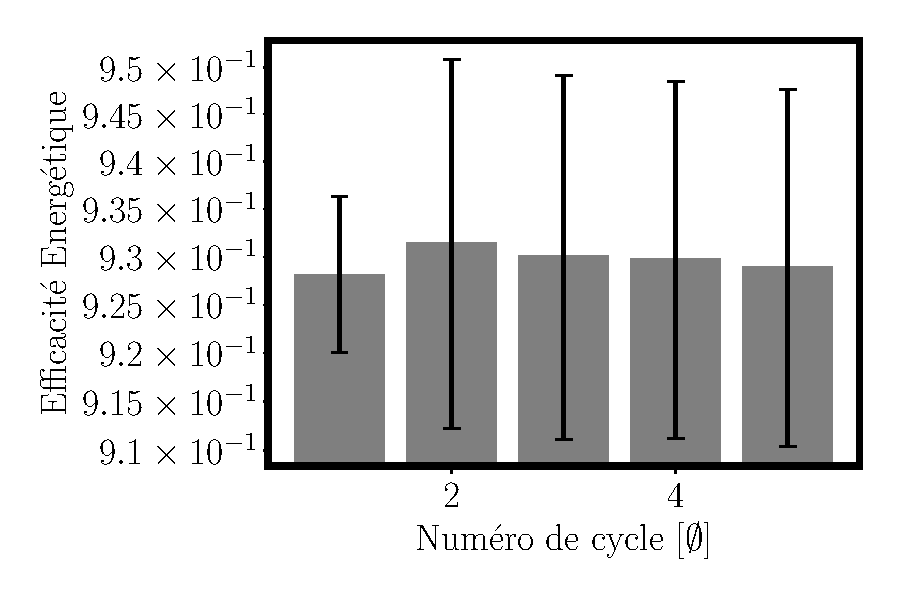
\includegraphics[width=0.5\textwidth]{datas/EE.pdf}
\captionof{figure}{Courbe de charge-décharge}
\end{center}

\underline{Application numérique}
\begin{center}
\begin{tabular}{cccccc}
\toprule
Numéro de cycle & 1 & 2 & 3 & 4 & 5  \\
\midrule
E.E. & 0.92817979 & 0.93152515 & 0.93015212 & 0.92981041 & 0.92903065 \\
\bottomrule
\end{tabular}
\end{center}

On constate dans tous les cas, que l'efficacité énergétique est très proche entre les 6 cycles (recoupement des barres d'erreurs). On ne constate pas de dégradation de l'accumulateur sur un si petit nombre de cycle. 

Toutefois, on observe qu'en moyenne, cet accumulateur a un rendement énergétique de \SI{93}{\percent}. Ceci est à mettre en relation avec le phénomène d'\textbf{hystérèse} et les phénomènes \textbf{dissipatifs}. 
\end{solution}\end{mybox}

\begin{comment}
\question[1] Calculer puis représenter l'évolution de l'état de santé de cette batterie en fonction du nombre de cycle de décharge réalisé. En proposant une démarche d'inverstigation, chercher combien de cycle cette batterie pourrait faire au maximum avant d'obtenir un $SoH$ de \SI{10}{\percent}.

\begin{mybox}\begin{solution}[6cm]
\underline{Calcul de l'état de santé en utilisant les décharges}
\begin{align*}
SoH = \frac{Q_d (i)}{Q_d (0)}
\end{align*}

\underline{Application numérique}
\begin{center}
\begin{tabular}{ccccccc}
\toprule
Numéro de cycle & 1 & 2 & 3 & 4 & 5 & 6 \\
\midrule
SoH & & & & & & \\
\bottomrule
\end{tabular}
\end{center}

\end{solution}\end{mybox}
\end{comment}

\setcounter{foo}{\value{question}}
\end{questions}

\subsection{\'{E}tude de votre cellule électrochimique}

\paragraph*{Protocole}
Avant de commencer l'expérience, vous allez chercher à trouver les paramètres expérimentaux de la procédure sur Nova 2.1.5. Pour cela, vous allez dans {\faHome $\to$ \emph{Open library} $\to$ \emph{My Procedures} $\to$ \emph{Batterie} $\to$ \emph{Cyclage Batterie}}.


Vous pouvez lancer l'acquisition en cliquant sur \faPlay. Une fois vos courbes de charge imprimées, vous devez les imprimer et les rendre de manière documentées dans votre compte rendu !

\faWarning ~ En cas de problème, veuillez immédiatement arrêter la séquence en cliquant sur l'icône stop \faStop !

\paragraph*{Questions}

\begin{questions}
\setcounter{question}{\thefoo}

\question[\half] Quels sont les paramètres réglables par l'expérimentateur dans ce programme ?

\begin{mybox}
\begin{solution}[1cm]
Les paramètres réglables sont les suivants : le courant de charge $I_c$, le courant de décharge $I_d$ et le nombre de cycle de charge/décharge, la tension maximale de charge et la tension minimale de décharge.
\end{solution}\end{mybox}

\question[1] Relever dans le programme les valeurs par défaut :
\begin{itemize}
    \item la plage de courant du galvanostat,
    \item la tension maximale et minimale de charge,
    \item la tension maximale et minimale de décharge.
\end{itemize}
Indiquer le sens de ces valeurs.

\begin{mybox}
\begin{solution}[2cm]
La place de courant est autour de 1-10 \si{\milli\ampere}, au delà de cette plage, le galvanostat n'agit pas. La tension de charge (resp. décharge) est comprise dans l'intervalle $[0.0, 3.8] ~ \si{\volt}$  (resp. $[2.8, \infty [ ~ \si{\volt}$).

Dès que la tension de charge (resp. décharge) atteint \SI{3.8}{\volt} (resp. \SI{2.8}{\volt}), la charge (resp. décharge) s'arrête.

~

\faWarning ~ Les valeurs ci-dessus doivent être ajustées en fonction de l'accumulateur de l'étudiant. Ici les valeurs sont tirées des donnés trouvées chez des constructeurs pour des accumulateurs équivalents.

\end{solution}\end{mybox}

\question[\half] Une étiquette s'appelle l'OCP (Open-Circuit Potential équivalent à l'Open-Circuit Voltage). Pourquoi est-il normal que la valeur mesurée initialement sur votre batterie est nulle ?

\begin{mybox}
\begin{solution}[2cm]
La tension à circuit ouvert correspond à la force électromotrice, laquelle est nulle lorsque la batterie est complètement à sec (c.-à-d. déchargée à \SI{100}{\percent}).

Initialement, tout le lithium se trouve à la borne $\oplus$, la batterie est donc complètement déchargée (à vide).
\end{solution}\end{mybox}

\question[1] En vous appuyant sur la masse expérimentale de \ce{LiMn2O4}, calculer la capacité theorique de la batterie en \si{\milli\ampere\hour}.
\begin{mybox}
\begin{solution}[6cm]
En décharge, le pôle $\oplus$ a pour avancement :  
\begin{center}
\begin{tabular}{cccccccc}
\toprule
$\xi ~ [\si{\mole}]$ & \ce{Li^+} & \ce{+} & \ce{e^-} & \ce{+} & \ce{Mn2O4}  & = & \ce{LiMn2O4} \\
\midrule
$t = 0$ & $n_e$ & & $n_e$ & & $\frac{m_{exp}}{M}$ & & 0 \\
$t = \infty$ & $n_e - \xi_\infty$ & & $n_e - \xi_\infty$ & & $\frac{m_{exp}}{M} - \xi_\infty$ & &  $\xi_\infty$ \\
\bottomrule
\end{tabular}
\end{center}

\underline{Formule de la capacité et application numérique}
\begin{align*}
Q_{theo} [\si{\milli\ampere\hour}] = \frac{F \cdot n_e}{3.6}= \frac{F m_{exp}}{3.6 M (\ce{LiMn2O4})} \\
\stackrel{AN}{=} \SI{88.9}{\milli\ampere\hour}
\end{align*}


\textbf{NB} Le calcul ci-dessus ne prend pas en compte le fait que les étudiants n'ont pas utilisé l'intégralité de leur préparation pour réaliser l'accumulateur. Un facteur de correction peut avoir été appliqué par les étudiants pour estimer la capacité théorique réelle de leurs préparations. Toute démarche en ce sens doit être valorisée.
\end{solution}\end{mybox}

\question[1] Calculer l'efficacité coulombique et énergétique de votre cycle de charge/décharge. 

\begin{mybox}
\begin{solution}[3cm]
Valeur de l'efficacité coulombique et énergétique sur un cycle : 
\begin{center}
\begin{tabular}{cc}
\toprule
Efficacités & Valeurs obtenues \\
\midrule
$C.E.$ & \\
$E.E.$ & \\
\bottomrule
\end{tabular}
\end{center}

\end{solution}\end{mybox}

\question[\half] Comparer la capacité de décharge mesurée à la valeur théorique.

\begin{mybox}
\begin{solution}[3cm]
\underline{Calcul de l'écart-relatif}
\begin{align*}
\%_Q &=  \frac{Q_d - Q_{theo}}{Q_{theo}} \\
&\stackrel{AN}{=}
\end{align*}

\underline{Interpretation}

\end{solution}\end{mybox}

\question[1] Comparer les performances de votre batterie avec la batterie commerciale.

\begin{mybox}
\begin{solution}[8cm]


\end{solution}\end{mybox}

\setcounter{foo}{\value{question}}
\end{questions}

\begin{comment}
\Q Une valeur caractéristique du générateur est mesurée à l'étiquette OCP. Quelle grandeur physique est mesurée ? De quoi sa valeur dependra-t-elle ?

~

Au vu des temps de l'expérience, vous réaliserez entre 2 et 3 cycles. Trouver les courants qu'il faut appliquer pour faire trois mesures d'une durée respective de 1 heure, 30 minutes et 15 minutes.

\Q Donner le nombre de cycle et le courant appliqué pour chacune de vos mesures.
\end{comment}

\paragraph*{Données}
\begin{itemize}
\item Masses molaires : $M(\ce{O}) = 15.999 ~ \si{\gram\per\mole}$ ; $M(\ce{Mn}) = 54.938 ~ \si{\gram\per\mole}; M(\ce{Li}) = 6.941 ~ \si{\gram\per\mole}$
\item Constante de Faraday : $F = 96485 ~ \si{\coulomb\per\mole}$

\end{itemize}

\newpage

\appendix

\section{Produits chimiques}
\label{sec:produits_chimiques}

\begin{center}
\begin{tabular}{|C{4cm}|C{3cm}|C{2cm}|C{6cm}|}
\hline
Produit & Données & Pictogrammes & Mention de danger \\
\hline
Carbonate de propylène anhydre & \SI{99.7}{\percent}, < \SI{0.002}{\percent} d'eau & 
\includegraphics[width=1cm]{pictos/exclam.pdf} & H319 Provoque une sévère irritation des yeux.\\
\hline
Graphite & \SI{99.95}{\percent}, particules sphériques de 15-30 \si{\micro\meter},  & - & -\\
\hline
Lithium Trifluoromethanesulfonate & \SI{156.01}{\gram\per\mole}, \SI{99.995}{\percent} de pureté en métaux & 
\includegraphics[width=1cm]{pictos/exclam.pdf} & H315 Provoque une irritation cutanée ; H319 Provoque une sévère irritation des yeux ; H335 Peut irriter les voies respiratoires.\\
\hline
Poly(tetrafluoroethylene) PTFE & > \SI{40}{\micro\meter} & - & -\\
\hline
\end{tabular}
\end{center}


\section{Potentiostat galvanostat}
\label{sec:potentiostat}

En électrochimie analytique, nous utilisons trois observables : le temps $t$, la tension $U$ et le courant électrique $I$ pour caractériser un dispositif. Afin de mesurer ces observables, nous utilisons un dispositif à trois électrodes détaillé par la suite.

\subsection{Définition}

Comme vous le savez, en électricité, on ne peut pas imposer un courant $I$ et une tension simultanément $U$. Développé en 1942 par Archie Hickling, scientifique anglais, le potentiostat galvanostat peut être exploité selon deux modes : 
\begin{itemize}
\item mode \textbf{potentiostat} : l'expérimentateur impose une tension $U$ et mesure un courant $I$ ;
\item mode \textbf{galvanostat} : l'expérimentateur impose un courant $I$ et mesure une tension $U$.
\end{itemize}

\subsection{Expérience d'essais de cyclage}

Afin d'évaluer les performances électrochimiques des matériaux utilisés dans les électrodes, on a besoin de mesurer plusieurs choses : 
\begin{itemize}
\item capacité spécifique ;
\item tension ;
\item cyclabilité.
\end{itemize}
Il est aussi possible d'étudier la tenue en température d'une batterie.

\begin{center}

\includegraphics[width=\textwidth]{figures/Ann01}
\captionof{figure}{Une demi-cellule électrochimique peut-être étudiée en utilisant une pile bouton (a), un cellule Swagelok\copyright (b) et peuvent être installé sur un cycleur capable d'évaluer en parallèle les performances de cyclage de dizaines de batteries (c \& d).}
\label{fig:Ann01}
\end{center}


Afin de tester les propriétés électrochimiques d'un matériau d'électode, on assemble la demi-cellule d'intérêt avec une demi-cellule de propriété connu sous forme de pile bouton, de cellules Swagelock\copyright ou \og pouch \fg{}. Ensuite, on charge/décharge à plusieurs reprises soit en mode potentiostat, soit en mode galvanostat. 

\begin{center}

\includegraphics[width=\textwidth]{figures/Ann02}
\captionof{figure}{Courbe intensité-potentiel montrant la charge/décharge sur 2 cycles (noir puis rouge) d'un matériau spinelle \ce{LiMn2O4} en mode potentiostatique (a) et en mode garvanostatique (b)}
[Par convention, en Europe, le courant d'oxydation (resp. de réduction) est positif (resp. négatif).]
\label{fig:Ann02}
\end{center}

En mode potentiostatique, en balayant avec une rampe constante de potentiel, on peut aisément visualiser les potentiels thermodynamiques correspondant aux différents processus redox, par exemple la transformation du manganèse du degré d'oxydation +III en +IV au sein du matériau spinelle.

Les deux pics de courant en oxydation (et en réduction) peuvent s’expliquer par un \textbf{changement de structure} (polymorphisme) du spinelle lors de la délithiation. 

En mode galvanostatique, on peut aisément avoir une information sur la cinétique des processus chimiques (c.-à-d. quantité de lithium extrait ou inséré par seconde) puisque la variation de potentiel du matériau au cours du temps renseigne sur le taux de lithiation du matériau.

La présence de deux \textbf{plateaux} nous renseigne bien sur un \textbf{changement de structure} du spinelle (lors de la délithiation), et est la manifestation en mode galvanostatique, des pics de courant observés en mode potentiostatique.

\begin{center}
\begin{tabular}{ccc}
\toprule
Mode & galvanostat & potentiostat \\
\midrule
Noms des courbes & courant-potentiel ou I-E & charge/décharge \\ 
Potentiels thermodynamiques & \faClose & \faCheck \\
Cinétique processus rédox & \faCheck & \faClose \\
\bottomrule
\end{tabular}
\captionof{table}{Choisir le mode le plus approprié du potentiostat en fonction des phénomènes que l'on souhaite observer.}
\end{center}

Les courbes I-E renseignent difficilement sur la cinétique des processus (quantité de lithium extraite ou insérée par seconde), on préfère donc utiliser les courbes de charge/décharge à courant constant (c'est le mode galvanostatique, qui permettent de lier la variation de la tension au taux de lithiation du matériau.

Lors de la réalisation des courbes de charge/décharge, il est important d'indiquer en plus des informations chimiques précises sur la cellule : le modèle du galvanostat utilisé, le courant appliqué, la tension minimale de décharge (c.-à-d. la tension à partir de laquelle vous considérez que l'accumulateur est déchargé), la tension maximale de charge (c.-à-d. la tension à partir de laquelle vous considérez que l'accumulateur est chargé) et le nombre de cycle réalisé.

Si vous en avez connaissance, il est important d'indiquer le taux d'usure de votre batterie (comme vu en cours, c'est un paramètre assez critique pour l'évaluation des performances).

%Le temps représenté en abscisse peut être converti en charge électrique échangée Q = i(mA) × t(h) par gramme ou litre de matière active, c’est-à-dire en capacité spécifique massique C = Q/m (m.A.h.g -1 ) ou volumique C = Q/V (m.A.h.L -1 ). La représentation de la variation de potentiel en fonction de la capacité mesurée permet de visualiser si la capacité théorique du matériau est atteinte et si elle diminue au cours des cycles de charge et décharge. Cette diminution, qui représente la capacité perdue, dite « irréversible », peut être liée à une perte de matière active (dissoute ou bien isolée électriquement), ou à une consommation de charge de façon irréversible associée à l’oxydation ou à la réduction de l’électrolyte.

\subsection{Evaluer l'efficacité d'un cycle}
\label{subsec:efficacite}
Afin de quantifier l'efficacité du $i$-ème cycle de charge/décharge, vous pouvez utiliser deux grandeurs : 
\begin{enumerate}
\item l'\textbf{efficacité coulombique}, notée $CE$ définit comme : 
\begin{align}
CE [i] &= \frac{Q_d [i] }{Q_c [i]} \label{eq:CE}\\
&= \frac{\int_{\text{durée de décharge}} I_d (t') dt'}{\int_{\text{durée de la charge}} I_c (t') dt'}
\end{align}
où $Q_c$ (resp. $Q_d$) désigne la charge stockée (resp. délivrée) au pôle $\ominus$ et $I_c$ (resp. $I_d$) l'intensité de courant en charge (resp. décharge).

\item l'\textbf{efficacité énergétique}, notée $EE$, définit comme :
\begin{align}
EE [i] &= \frac{W'_d}{W'_c} \label{eq:EE}\\
&= \frac{\int_{\text{durée de décharge}} U_d (t') \cdot I_d (t') dt'}{\int_{\text{durée de la charge}} U_c (t') \cdot I_c (t') dt'} \
\end{align}
où $\langle X\rangle$ désigne la moyenne d'une grandeur $X$. $W'_d$ (resp. $W'_c$) désigne le travail électrique cédé (resp. reçu) en décharge (resp. charge).



\end{enumerate}

%\begin{align*}
%CE [i] &= \frac{Q_d [i] }{Q_c [i]} \\
%&= \frac{\int I_d (t') dt'}{\int I_c (t') dt'} \\
%&= \frac{\Delta t_d}{\Delta t_c} \text{ (car }I_c = I_d\text{)} 
%\end{align*}

%efficacité énergétique

%\begin{align*}
%EE [i] &= \frac{W'_d}{W'_c} \\
%&= \frac{\int U_d (t') \cdot I_d (t') dt'}{\int U_c (t') \cdot I_c (t') dt'} \\
%&= \frac{\int U_d (t') dt'}{\int U_c (t') dt'} \text{ (car }I_c = I_d\text{)} \\
%&= \frac{\langle U_d \rangle}{\langle U_c \rangle}
%\end{align*}
%où $\langle X\rangle$ désigne la moyenne d'une grandeur $X$.


\subsection{Montage à trois électrodes}

Afin de mesurer la tension, nous utilisons un dispositif complexe : un galvanostat. Comme représenté à la Fig. \ref{fig:pot_sch}, dans le cadre de nos expériences, le galvanostat peut-être vu comme un voltmètre, un ampère et un générateur de courant.

\begin{figure}[H]
\begin{centering}
\subfloat[\label{fig:pot_sch}]{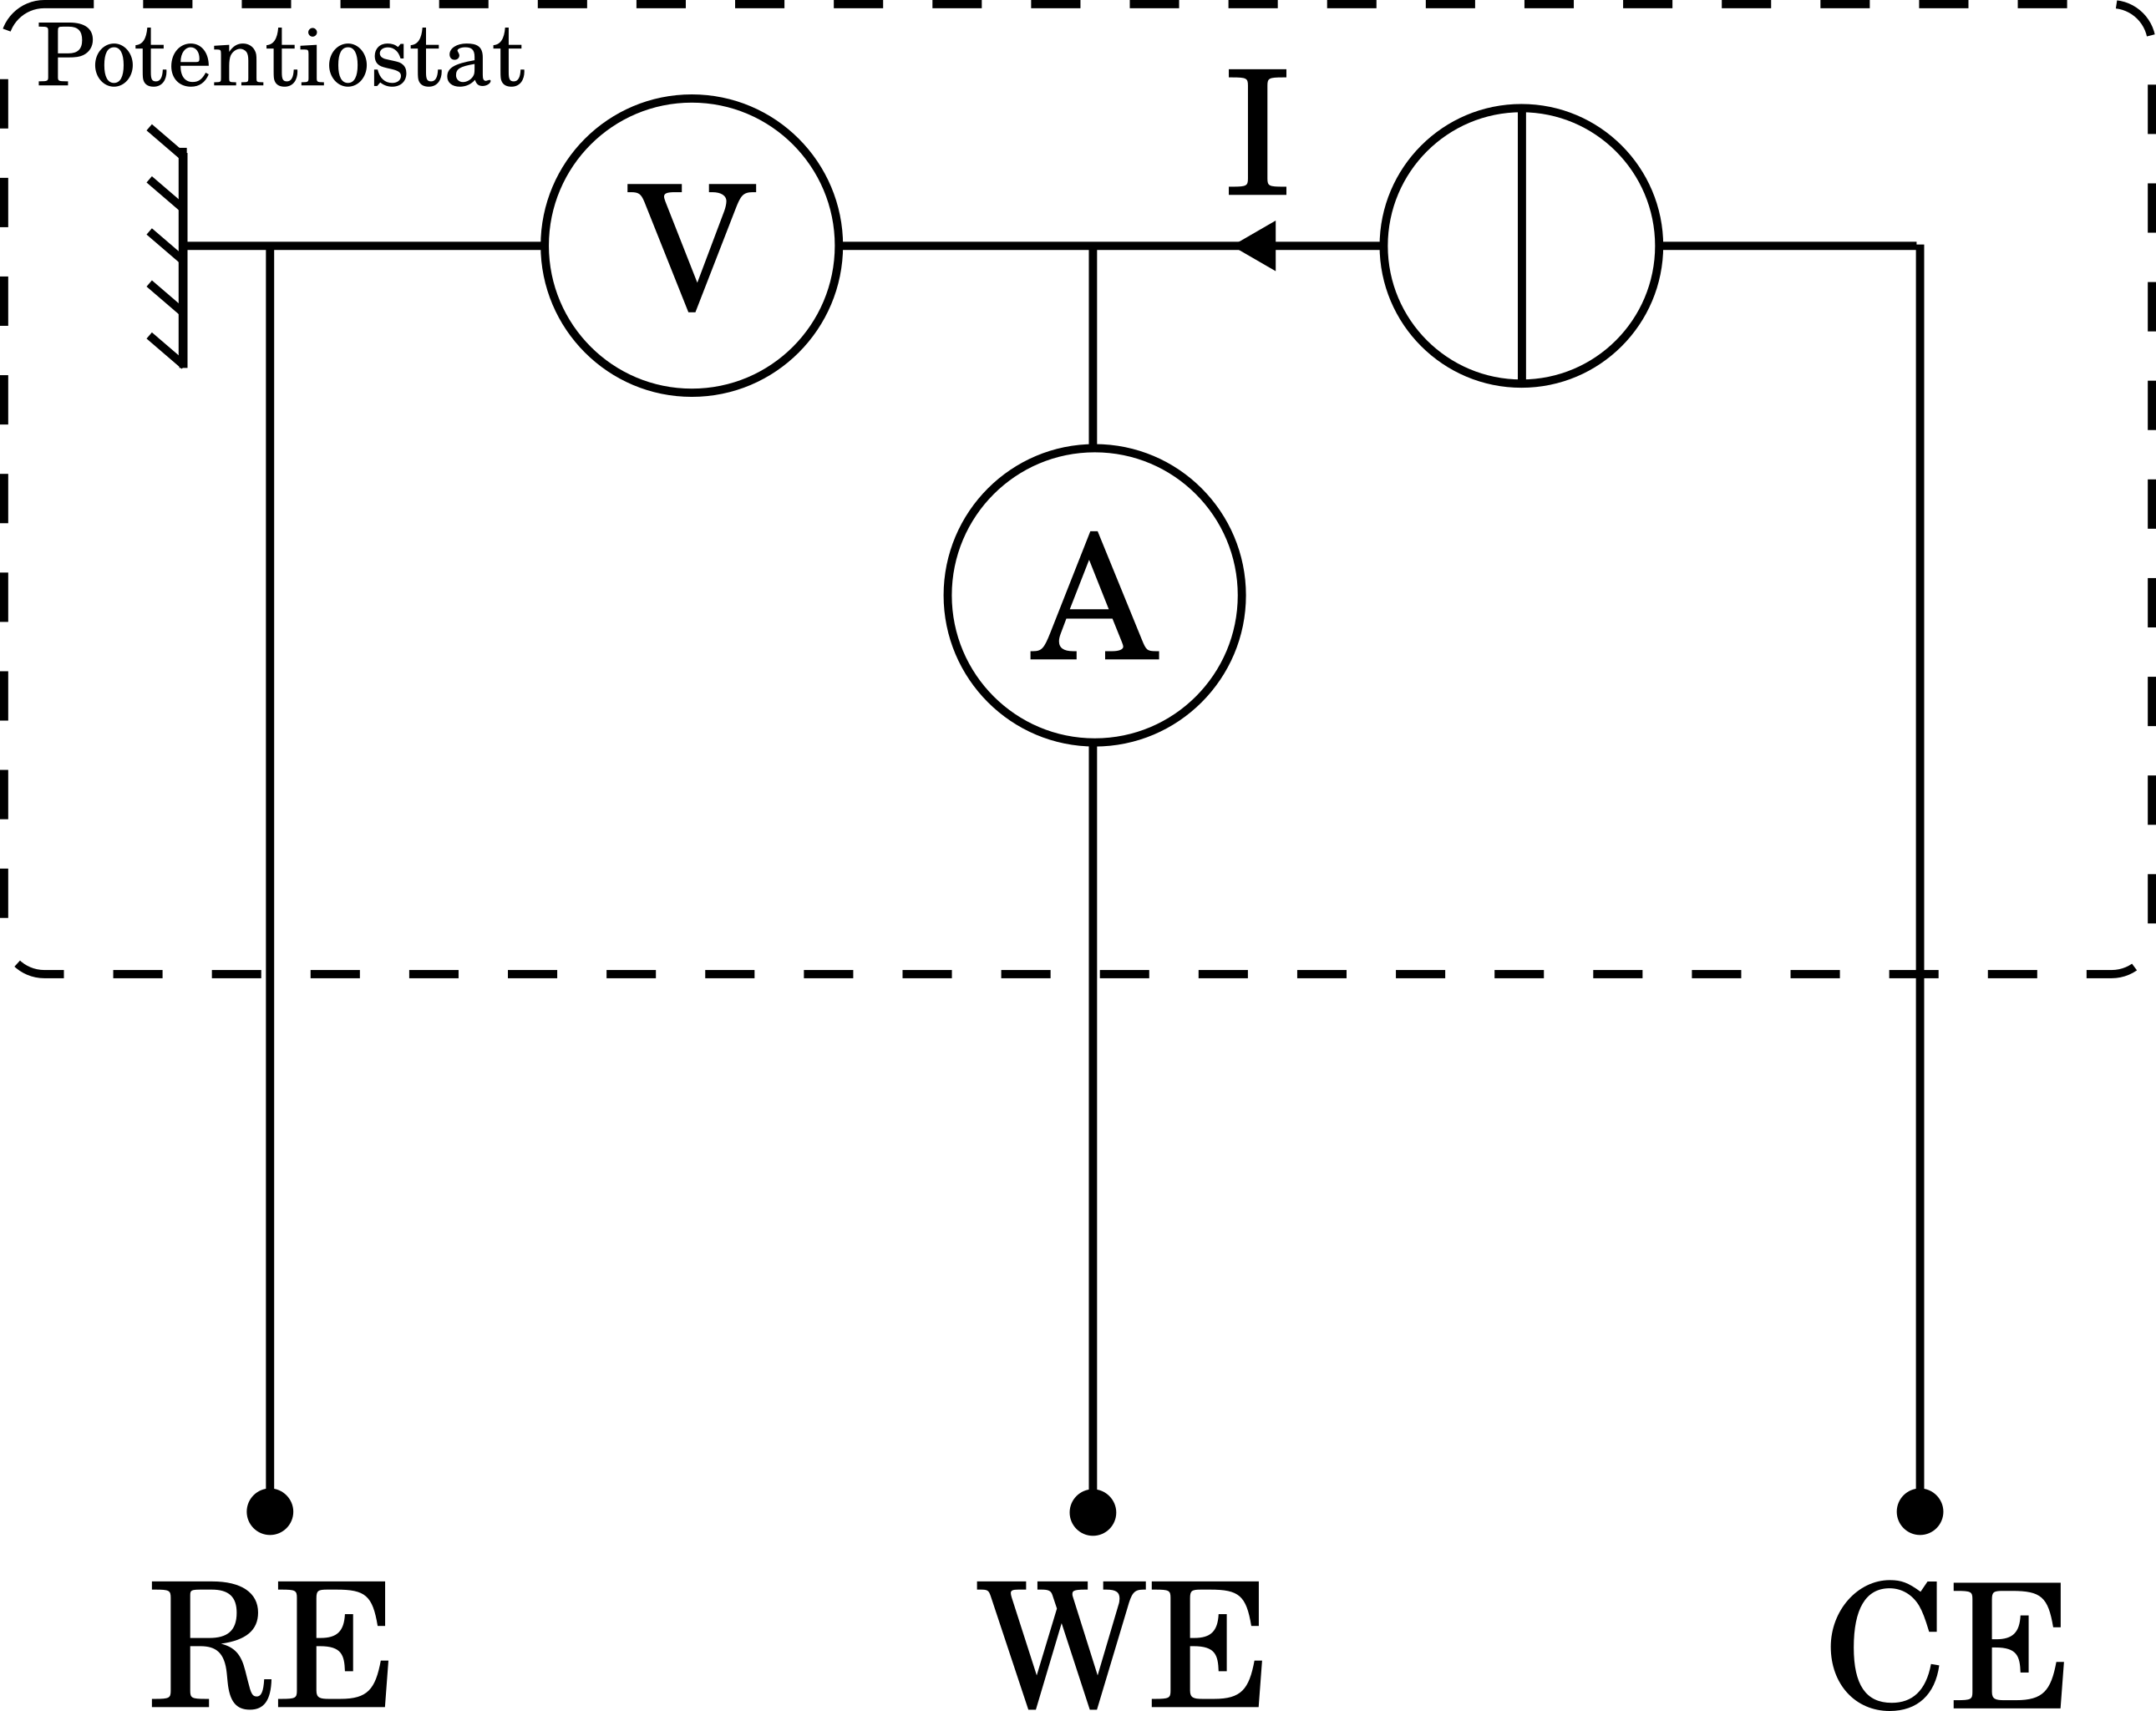
\includegraphics[width=5cm]{figures/Ann03}}\hspace*{1cm}\subfloat[\label{fig:pot_portecell}]{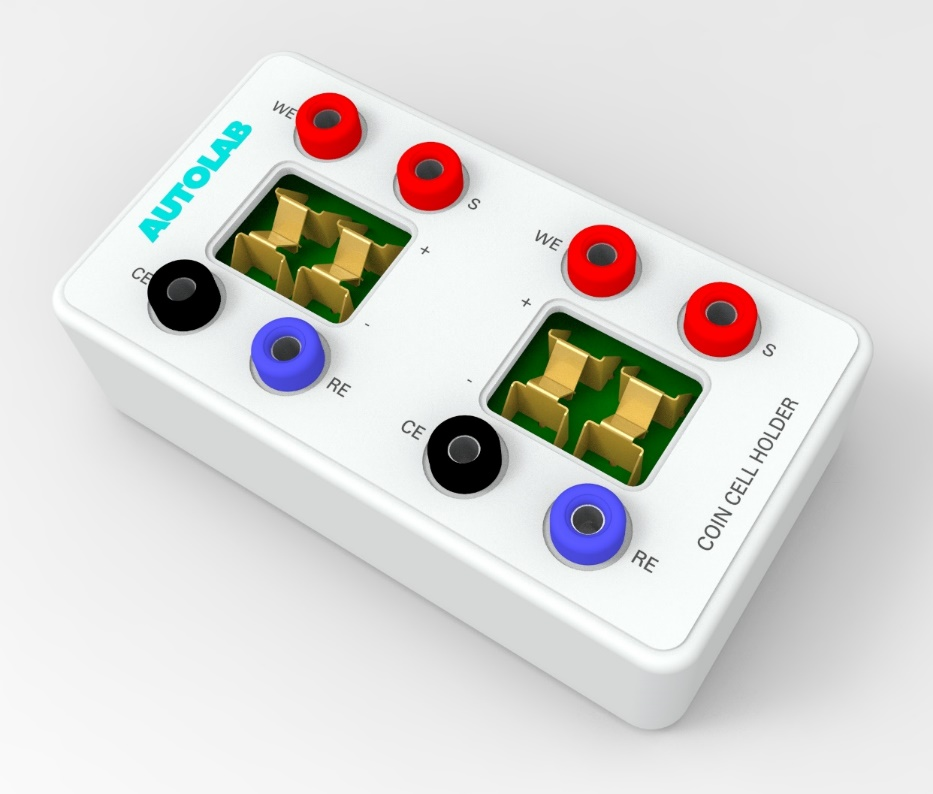
\includegraphics[width=5cm]{figures/Ann04.jpg}}
\par\end{centering}
{\tiny{}\caption{{\small{} Fig. \ref{fig:pot_sch}) Représentation schématique d'un galvanostat ; Fig. \ref{fig:pot_portecell}) Boîtier autolab pouvant accueillir deux piles boutons.}}
}{\tiny\par}
\end{figure}%WARNING : ajouter I


%Lors de la manipulation du galvanostat, le courant $I$ sera imposé par l'expérimentateur (générateur de courant).

Afin de mesurer la tension d'une pile-bouton, un boitier autolab peut être utilisé afin de brancher la pile aux trois entrées du potentiostat. Vous pourrez alors mesurer la tension et le courant aux bornes de la pile à l'aide de trois électrodes :
\begin{itemize}
    \item[\textbf{WE}] entrée pour le câble conduisant à l'\textbf{électrode de travail} (Work Electrode) ;
    \item[\textbf{CE}] entrée pour le câble conduisant à \textbf{la contre-électrode} (Counter Electrode) ; 
    \item[\textbf{RE}] entrée pour le câble conduisant à l'\textbf{électrode de référence} (Reference Electrode). 
\end{itemize}

Basiquement, le montage à trois électrodes permet de séparer la mesure de la tension et du courant. Le courant, imposé par le galvanostat, circule entre l'électrode \textbf{WE} et la contre-électrode \textbf{CE}, tandis que la tension est mesurée entre l'électode \textbf{WE} et \textbf{RE}.

En séparant ces deux mesures, on est capable de connaître le potentiel à \textbf{WE} par rapport à \textbf{RE}, puisqu'en absence de courant circulant dans \textbf{RE}, son potentiel reste constant (surtension de la référence nulle).

~

{\Large \faWarning} L'utilisation d'un montage à trois électrodes plutôt que deux électrodes comme vous avez fait en première année sera vu avec Alireza Ranjbari en cours d'électrochimie.


\newpage

\section*{Barême}

\begin{minipage}{0.33\textwidth}
Noms-Prénoms du binôme
\end{minipage}\begin{minipage}{0.33\textwidth}
$n^\circ 1$ :
\end{minipage}\begin{minipage}{0.33\textwidth}
$n^\circ 2$ :
\end{minipage}

\begin{questions}
\setcounter{question}{\thefoo}

\titledquestion{Graphes}[1] Qualité des graphes

\titledquestion{Investissement}[2] Variable d'ajustement à la liberté du correcteur en fonction de l'investissement, de la qualité des raisonnements et de la démarche d'investigation du binôme.
\end{questions}

\begin{center}
\gradetable
\end{center}

\end{document}
